% 本文件定位：两性综合百科全书（侧重共通内容 + 关系/社会层面）
% 男性专项详见 male.tex，女性专项详见 female.tex

\documentclass[12pt,UTF8]{ctexbook}

% 设置纸张信息
\usepackage[a4paper]{geometry}
\geometry{
    inner=2cm,
    outer=2cm,
    top=2.5cm,
    bottom=2.5cm
}

% 设置字体
\usepackage{xeCJK}
\setCJKmainfont{SimSun}[BoldFont=SimHei, ItalicFont=KaiTi]
\setCJKsansfont{SimHei}
\setCJKmonofont{SimSun}

% ===== 符号字体回退（r75）：带圈数字 / 罗马数字 / 希腊字母 / 数学符号 / 制表符 ----
%   背景：西文主字体 Latin Modern 与中文字体 SimSun 均不覆盖下列字符，
%   不回退则 xelatex 报 Missing character，PDF 对应位置留白（等于丢知识点）。
%   自检：编译后统计 <file>.log 中 Missing character 条数，应为 0。
\usepackage{newunicodechar}
\newfontfamily\symbolfallback{SimSun}           % 带圈数字/罗马数字/希腊字母/数学符号/制表符/几何图形
\newfontfamily\symbolfallbackx{Segoe UI Symbol} % 警告三角等符号
\newunicodechar{①}{{\symbolfallback\char"2460}}
\newunicodechar{②}{{\symbolfallback\char"2461}}
\newunicodechar{③}{{\symbolfallback\char"2462}}
\newunicodechar{④}{{\symbolfallback\char"2463}}
\newunicodechar{⑤}{{\symbolfallback\char"2464}}
\newunicodechar{⑥}{{\symbolfallback\char"2465}}
\newunicodechar{⑦}{{\symbolfallback\char"2466}}
\newunicodechar{⑧}{{\symbolfallback\char"2467}}
\newunicodechar{⑨}{{\symbolfallback\char"2468}}
\newunicodechar{⑩}{{\symbolfallback\char"2469}}
\newunicodechar{Ⅰ}{{\symbolfallback\char"2160}}
\newunicodechar{Ⅱ}{{\symbolfallback\char"2161}}
\newunicodechar{Ⅲ}{{\symbolfallback\char"2162}}
\newunicodechar{Ⅳ}{{\symbolfallback\char"2163}}
\newunicodechar{Ⅴ}{{\symbolfallback\char"2164}}
\newunicodechar{Ⅵ}{{\symbolfallback\char"2165}}
\newunicodechar{Ⅶ}{{\symbolfallback\char"2166}}
\newunicodechar{Ⅷ}{{\symbolfallback\char"2167}}
\newunicodechar{Ⅸ}{{\symbolfallback\char"2168}}
\newunicodechar{Ⅹ}{{\symbolfallback\char"2169}}
\newunicodechar{Ⅺ}{{\symbolfallback\char"216A}}
\newunicodechar{Ⅻ}{{\symbolfallback\char"216B}}
\newunicodechar{α}{{\symbolfallback\char"03B1}}
\newunicodechar{β}{{\symbolfallback\char"03B2}}
\newunicodechar{γ}{{\symbolfallback\char"03B3}}
\newunicodechar{δ}{{\symbolfallback\char"03B4}}
\newunicodechar{ε}{{\symbolfallback\char"03B5}}
\newunicodechar{ζ}{{\symbolfallback\char"03B6}}
\newunicodechar{η}{{\symbolfallback\char"03B7}}
\newunicodechar{θ}{{\symbolfallback\char"03B8}}
\newunicodechar{ι}{{\symbolfallback\char"03B9}}
\newunicodechar{κ}{{\symbolfallback\char"03BA}}
\newunicodechar{λ}{{\symbolfallback\char"03BB}}
\newunicodechar{μ}{{\symbolfallback\char"03BC}}
\newunicodechar{ν}{{\symbolfallback\char"03BD}}
\newunicodechar{ξ}{{\symbolfallback\char"03BE}}
\newunicodechar{ο}{{\symbolfallback\char"03BF}}
\newunicodechar{π}{{\symbolfallback\char"03C0}}
\newunicodechar{ρ}{{\symbolfallback\char"03C1}}
\newunicodechar{ς}{{\symbolfallback\char"03C2}}
\newunicodechar{σ}{{\symbolfallback\char"03C3}}
\newunicodechar{τ}{{\symbolfallback\char"03C4}}
\newunicodechar{υ}{{\symbolfallback\char"03C5}}
\newunicodechar{φ}{{\symbolfallback\char"03C6}}
\newunicodechar{χ}{{\symbolfallback\char"03C7}}
\newunicodechar{ψ}{{\symbolfallback\char"03C8}}
\newunicodechar{ω}{{\symbolfallback\char"03C9}}
\newunicodechar{≠}{{\symbolfallback\char"2260}}
\newunicodechar{≈}{{\symbolfallback\char"2248}}
\newunicodechar{≤}{{\symbolfallback\char"2264}}
\newunicodechar{≥}{{\symbolfallback\char"2265}}
\newunicodechar{─}{{\symbolfallback\char"2500}}
\newunicodechar{■}{{\symbolfallback\char"25A0}}
\newunicodechar{⚠}{{\symbolfallbackx\char"26A0}}

% 目录格式
\usepackage{titletoc}
\titlecontents{chapter}[0pt]{\vspace{3mm}\bf}{\contentspush{\thecontentslabel\hspace{1em}}}{}{\titlerule*[8pt]{.}\contentspage}

% 图片相关设置
\usepackage{graphicx}
\usepackage{float}
\graphicspath{{Images/}}

% 颜色支持
\usepackage{color}

% 绘制流程图
\usepackage{tikz}
\usetikzlibrary{shapes,arrows,positioning,calc}

% 表格相关设置
\usepackage{tabularx}
\usepackage{booktabs}

% 彩色盒子环境
\usepackage{tcolorbox}

% 术语表和索引
\usepackage{glossaries}
\usepackage{makeidx}
\makeindex
\makeglossaries

% BibTeX参考文献支持
\usepackage{natbib}
\bibliographystyle{plainnat}

% 页眉页脚
\usepackage{fancyhdr}
\pagestyle{fancy}
\lhead{}
\chead{}
\rhead{\bfseries \leftmark}
\lfoot{}
\cfoot{\thepage}
\rfoot{}
\renewcommand{\headrulewidth}{0.4pt}
\renewcommand{\footrulewidth}{0pt}

% 段落间距
\setlength{\parskip}{0.5em}
\setlength{\parindent}{2em}

% 目录格式设置
\usepackage{titletoc}
\usepackage{enumitem}% 支持 \begin{itemize}[leftmargin=2cm] 等带可选参数的列表（与 male.tex 一致）
\titlecontents{chapter}[0pt]{\vspace{3mm}\bfseries}{\thecontentslabel\hspace{1em}}{}{\titlerule*[8pt]{.}\contentspage}[\vspace{2mm}]
\titlecontents{section}[3em]{\contentslabel[\thecontentslabel]{2em}\hspace{1em}}{}{}{\titlerule*[6pt]{.}\contentspage}
\titlecontents{subsection}[5em]{\contentslabel[\thecontentslabel]{3em}\hspace{1em}}{}{}{\titlerule*[4pt]{.}\contentspage}

% 标题格式
\ctexset{
    part/name={第,篇},
    part/number={\chinese{part}},
    chapter/name={第,章},
    chapter/number={\chinese{chapter}}
}

% 章节摘要环境
\newenvironment{chapterabstract}[1][摘要]{
    \vspace{0.5em}
    \begin{center}\bfseries{#1}\end{center}
    \vspace{0.5em}
    \begin{quote}
    }{
    \end{quote}
    \vspace{0.5em}
}

% 重点标记
\newcommand{\keyterm}[1]{{\bfseries #1}}
\newcommand{\important}[1]{{\color{red} \bfseries #1}}

% 关键论断/关键词强调（《两性研究导论》章使用；视觉同 \keyterm，语义上作区分）
\newcommand{\keyword}[1]{\textbf{#1}}

\title{\heiti\zihao{0} 性学大全指南}
\author{}
\date{}

\begin{document}

\maketitle

\frontmatter

\tableofcontents

\listoffigures
\listoftables

\chapter{前言}

这是一本关于性的科学指南，旨在帮助读者建立健康的性观念和性行为。

性健康是人类整体健康的重要组成部分，涵盖了身体、心理和社会层面的福祉。然而，由于传统观念的束缚和性教育的缺失，许多人对两性健康知识存在误解或缺乏正确认识。本书希望通过科学、客观、全面的内容，帮助读者更好地了解自己和伴侣的身体，掌握健康的性爱技巧，选择合适的避孕方法，预防性传播疾病，从而提升性生活质量和整体健康水平。

本书特色：

\begin{itemize}
    \item 基于最新科学研究成果
    \item 兼顾科学性与可读性
    \item 提供切实可行的建议与方法
\end{itemize}

本书适合所有关注两性健康的读者，无论是未婚青年、已婚夫妇还是中老年人群，都能从中获得实用的知识和建议。内容涵盖了两性生殖系统结构与功能、性生理与性心理、性爱技巧与沟通、常见性问题与解决方案、避孕方法、性传播疾病与预防、生殖健康检查等方面，力求全面、深入、实用。

让我们以科学的态度、开放的心态，共同探索性健康的奥秘。

\vfill
{\itshape\zihao{5}
本书仅供科普参考，不能替代专业医疗建议。如有健康问题，请咨询专业医生。}

\mainmatter

% ════════════════════════════════════════════════════════════════════════
%            全书目录结构（2026-09-21 重构版，供手动迁移内容用）
% ════════════════════════════════════════════════════════════════════════
% 使用说明：
%   1. 本结构为全书按主题去重后的目标目录，共八篇 53 章，另设独立的「结语」「附录」两篇。
%      本卷定位「两性共通」；性别专属的章/节已按卷拆分到 female.tex / male.tex，
%      原位一律留下「⇒ [已移出]」标记，可在原地看到去向。
%      篇 / 章 / 节 / 小节四层，小节即该节的学习要点，可直接作为写作或迁移的提纲。
%   2. 每章/节下的注释标明其内容来源，一律以旧区的标题为锚——
%      直接搜索引号里的标题即可定位（L#### 行号会随文件改动失效，故不再使用）。
%   3. 标注"去重"处存在两份以上近似内容，移入时择优保留一份。重复内容主要来自：
%      \part{旧内容}、\part{避孕与性健康}后半部分，
%      以及"生殖健康检查"章下的一批散落节。
%   4. 一节未附注释者，表示按该节标题直接在旧区搜索即可定位。
%   6. 全部内容移入后：删除旧的 \part / \chapter / \section 标题行，
%      最后删除本骨架上方的说明注释。
% ════════════════════════════════════════════════════════════════════════

% ==================== 第一篇 ====================
\part{基础与生理}

\chapter{两性研究导论}

性、性别与性欲，是人类社会中最基本、也最容易被“自然化”的范畴之一。我们通常以为“男人”“女人”“异性恋”“同性恋”这些分类古已有之、天经地义，但若把目光投向不同历史时期与不同文化，就会发现：\keyword{哪些差异被看见、被命名、被制度化，以及这些差异被赋予何种意义，本身就是一个社会过程}。两性研究正是对这一过程的系统考察。

作为全书导论，本章不急于展开具体议题，而是先为后续讨论搭建共同的知识地基。

我们将依次回答四个问题：

第一，两性研究究竟研究什么，它与心理学、社会学、人类学、生物学等邻近学科是什么关系，它的意义与边界何在；

第二，这一领域如何从古代的性别决定论与神学秩序，经近代性学的科学化，走向现代性别研究的形成与当代转向；

第三，生理性别、社会性别、性别认同、性取向、性别表达与性脚本这几个核心概念各自指什么、彼此如何区分；

第四，研究者在方法上可以选择哪些路径，又必须遵守哪些伦理约束，以及科学传播中常见的误区有哪些。

明确这些问题之后，我们再从\keyword{研究范畴与意义}入手，看看两性研究作为一个跨学科领域，其内部的问题意识是如何组织的。

\section{研究范畴与意义}

\subsection{什么是两性研究}

两性研究（Gender and Sexuality Studies）是一个跨学科领域，旨在系统考察生理性别、社会性别、性别认同、性取向及性行为在人类社会中的形成、变迁与影响。它不局限于单一学科，而是整合生物学、心理学、社会学、人类学、历史学、法学与人文科学的视角，追问一个根本问题：\keyword{“性”与“性别”在多大程度上是自然的，又在多大程度上是社会的？}

这一领域的研究对象涵盖广泛：从两性心理差异的经验证据，到性别角色在不同文化中的建构方式；从性倾向的成因与表达，到性别暴力与健康不平等的结构性根源。其核心关切在于，\keyword{性别并非仅是个人属性，更是组织社会资源、权力与意义的基本范畴}。

\subsection{与相关学科的关系}

两性研究与多个学科形成交叉与对话。

\paragraph{心理学} 关注个体层面的性别差异、性动机、亲密关系与性功能障碍。研究发现，情境因素可反向影响生理指标——如睾酮水平在竞争失败后下降，提示社会文化事件与生物反应之间存在双向关系。发展心理学研究父母与同伴对青少年性行为的影响，社会心理学则关注吸引力、关系维持与暴力等议题。

\paragraph{社会学} 将性别与性视为与阶级、族群同等重要的社会矛盾范畴。没有考虑性别与性的社会学研究必然存在盲点，难以深刻理解社会结构。女性主义社会学不仅开辟了新领域，也对传统议题和方法学提出了挑战。

\paragraph{人类学} 提供跨文化、贯通历史的视角。人类学长期将性局限于亲属关系与婚姻禁忌的讨论，直到1961年才正式认可跨文化性研究的重要性。当代人类学关注性实践如何嵌入宗教、经济、政治与人权之中，“性行为昭示着更广泛的社会关切”。

\paragraph{生物学与医学} 则从激素、染色体、神经结构等层面解释性别分化。研究显示，女性掌管听觉和语言的大脑部位神经细胞密度与数量多于男性，而男性掌管空间处理的部位比例更大。但生物学解释始终需要与社会文化因素交互考量。

\subsection{研究的意义与边界}

两性研究的意义首先在于\keyword{解构“自然化”的性别秩序}。许多被视为“天生”的性别差异、角色期待与性规范，实则是历史与文化的产物。揭示这一建构过程，有助于理解不平等如何被生产与维系。

其次，该领域具有\keyword{公共政策意涵}。联合国1979年通过《消除对妇女一切形式歧视公约》，1985年首次提出“性别主流化”概念，要求所有政策在设计与评估时考量其对男女的不同影响。1995年北京世界妇女大会进一步将性别平等界定为人权议题。

研究的边界同样需要明确。两性研究\keyword{不等于女性研究}，也不等于单纯的“性教育”。它既关注女性处境，也分析男性气质的社会建构；既研究性行为，也研究性如何被话语、制度与知识所组织。同时，研究者在介入性议题时须保持\keyword{方法论的审慎与伦理的自觉}，避免以研究之名行猎奇或规训之实。

\section{历史演进}

\subsection{古代与中世纪的相关论述}

西方古代对两性与身体的思考集中于\keyword{性别决定论}与\keyword{性秩序}两大主题。亚里士多德认为雌雄二元是自然的必然选择，双性人属“怪胎”，源于精子混合的偶然因素。希波克拉底与盖伦传统则认为胎儿性别取决于精子属性与子宫位置的共同作用，左睾右宫生“男性化的女人”，右睾左宫生“女性化的男人”。

中世纪将这些古典观念整合入基督教神学框架。伊斯兰学者阿维森纳（980—1037）传承并修正了希波克拉底—盖伦传统，其著作12世纪译为拉丁文后影响西方。大阿尔伯特（约1193—1280）一方面接受亚里士多德关于双性人为“怪物”的判断，另一方面将其纳入神学解释：双性人应依据“主要性征”归入二元性别秩序，另一性征为“多余的附着物”。中世纪早期，双性人甚至被视为灾祸的预兆，罗马城中出现双性人随即暴发瘟疫的叙事被纳入基督教“儆效尤”的阐释模式。

值得注意的是，古代与中世纪的论述并非单纯的“迷信”。13世纪萨莱诺医学学校的教师群体已对胎儿性别决定因素形成共识，赋予双性人一种当时的“科学”解释。理性的医学探索与神学的秩序焦虑并存。

\subsection{近代性学的科学化}

19世纪末，\keyword{性学（sexology）} 作为一门科学正式形成。其根源在于自然知识在分类学、进化论与种族框架下的重组。1886年，克拉夫特-埃宾出版《性心理病态》，呼吁“科学地考察”性欲对感受、思想与行为的强大影响。据估计，1886至1933年间仅德语世界就发表了超过一万种性相关专著与文章，1898至1908年间关于同性恋的出版物达一千种。

性学的先驱者——克拉夫特-埃宾、哈夫洛克·埃利斯、马格努斯·赫希菲尔德与弗洛伊德——被后世视为现代科学性理解的奠基人。然而，早期的性学也深陷于其时代局限：它区分“正常”与“病态”性行为的标准服务于民族现代化议程，在全球范围内汇聚于诊断“同性恋”等“文化病症”。遗传学热潮催生了优生学运动，生物医学（尤其是精神分析与内分泌学）的兴趣转向控制变异、解锁灵魂秘密。

\subsection{现代性别研究的形成}

“社会性别”（gender）概念的兴起是20世纪后半叶的关键转折。1960年代，对少数群体、被压迫者与殖民地人民历史的兴趣增长，推动了女性史与女性主义人类学的发展。1972年，安·奥克利在《性、性别与社会》中提出影响深远的区分：\keyword{“性”指男女的生物差异，“社会性别”指“男性气质”与“女性气质”的社会分类}。

1975年，盖尔·卢宾发表《女人交易》，提出\keyword{“性/性别系统”} 概念，论证这一系统内含异性恋规范，而后者同样是社会起源而非自然的。同年出版的《女性、文化与社会》与《女性人类学》汇集了不同取向的人类学研究，成为理论勃兴的标志。

这一时期的核心成就在于：\keyword{将性别从“自然事实”转化为“分析范畴”}。女性主义理论批判了以往的研究范式，改变了人们思考性别、性欲与性别压迫的方式。

\subsection{当代发展趋势}

当代两性研究呈现几个显著趋势。

\paragraph{其一，从“性别二元”走向“性别多元”。} 性别认同被重新定义为个体对自身性别的内在感知，可能与出生指派性别一致或不一致。非二元性别、性别酷儿、性别流动等身份获得日益增长的文化认可，“性别不一致本身不被视为障碍，而被认为是人类性别认同与表达的正常变异”。

\paragraph{其二，交叉性（intersectionality）成为核心分析框架。} 1977年，康比河集体（Combahee River Collective）的宣言首次理论化了种族、性别、阶级与异性恋压迫的“交织”关系。1990年代起，交叉性视角在社会科学中广泛传播，强调性别经验不能脱离种族、阶级、族裔、性取向、残障等因素孤立理解。

\paragraph{其三，性别主流化与全球政策议程深度绑定。} 1995年北京《行动纲领》倡导将性别视角纳入所有政策与方案；2000年联合国千年发展目标将“促进性别平等与赋权妇女”列为第三目标；2015年可持续发展议程延续这一方向。

\paragraph{其四，去殖民化与研究者反身性。} 移民与性别研究中，全球北方的认识论、财政与经验偏见被视为学科进步的最大障碍。研究者被要求以反身性与透明度审视自身身份如何塑造研究过程。


\section{核心概念界定}

\subsection{生理性别}

生理性别（sex）指基于染色体、激素、生殖器官与第二性征的生物学分类，通常分为男性与女性。双性状况（intersex conditions）指身体性征出现异常发育的各种状况的统称。生理性别在不同文化中大致相同，但\keyword{如何对待生理差异}则因文化而异。

\subsection{社会性别}

社会性别（gender）指社会文化规范所定义的男性或女性的角色、行为、活动与特质。美国人类学家盖尔·卢宾最早提出这一概念，强调它是\keyword{文化构成物}，因时间、民族、地域而异。社会性别是动态发展的概念，具有历史阶段性、社会性与共塑性——即两性相互塑造的结果。其核心洞见在于：\keyword{社会基于生理差异所赋予的期望、要求与限制，并非生理差异的必然延伸。}

\subsection{性别认同}

性别认同指一个人对自己是男性、女性或其他性别的\keyword{内在感知}，可能与出生时被指派的性别一致或不一致。“顺性别”（cisgender）指性别认同与出生指派性别相符者；“跨性别”（transgender）为统称，指性别认同或性别表达与出生性别不符的人。非二元性别认同指不认同西方典型男女二元框架的个人，包括不认同任何性别、认同多种性别或性别流动者。

\subsection{性取向}

性取向指一个人在情感与性方面对男性、女性或其他性别者的\keyword{持久吸引与爱恋}。大致分为异性恋、同性恋、双性恋，以及无性恋。性取向同时包含性行为与性欲，但不等同于二者——禁欲者未必是“无性恋”，与同性发生性行为者未必是同性恋，关键在于\keyword{情感吸引与依附的内在需求}。晚近研究将性取向视为程度渐进的连续概念，个体位于从“只对异性感”到“只对同性感”之间的某个位置。没有科学研究证明“改变性倾向”的治疗安全或有效。

\subsection{性别表达}

性别表达指一个人通过行为、衣着、发型、声音或身体特征等方式，向他人\keyword{传达自己所认同的性别}。易服（cross-dress）是一种性别表达方式，易服者通常对自己的性别感到自在，不希望改变性别，且易服与性取向无关。变装皇后与变装国王是特定场合中的表演性性别表达。性别表达未必与性别认同一致，也未必指向特定的性取向。

\subsection{性脚本}

性脚本（sexual script）理论认为，人的性发育不仅是生理成长过程，更是\keyword{个人认同并归化于所处社会的性文化的过程}。性脚本从性社会化出发，系统阐释个体的性行为、性观念、性态度及性的外部表征。它解释的是：为何生物学上相似的性冲动，在不同社会中被组织为截然不同的实践与意义。作为性社会学的基础理论之一，性脚本将“性”从纯粹的生物驱力中解放出来，置于文化与互动的分析框架之中。

\section{方法论与伦理}

\subsection{定量研究方法}

定量方法在两性研究中用于测量态度、行为与心理特征的分布与关联。常用工具包括量表（如性满意度量表、爱情态度量表）与心理测量学指标（如Cronbach's $\alpha$）。统计方法涵盖描述性分析、回归分析、验证性因子分析（CFA）与潜在剖面分析（LPA）。当数据不满足正态假设时，需采用非参数检验，如Dwass-Steel-Critchlow-Fligner法进行事后比较。

定量研究的优势在于可比较性与可推广性，但局限同样显著。以两性心理差异的经典研究为例，麦科比与杰克林总结1600多项研究归纳出四方面差异，但批评者指出其结论程序不准确、忽略显著研究、概念不清，且四分之三被试局限于13岁前。\keyword{“差异”的发现高度依赖于测量工具、样本特征与分析策略。}

\subsection{定性研究方法}

定性方法关注意义、过程与经验。深度访谈、参与观察、话语分析与传记研究等方法用于理解性别与性如何被体验、叙述与实践。人类学的跨文化田野调查尤为关键，它揭示同一生物行为在不同文化中的意义差异——性实践嵌入宗教、经济、亲属制度与人权之中，“性与性别的文化建构不可能被推至人类学的边缘”。

定性研究的核心原则是\keyword{情境化}：不将“性别”或“性”视为可脱离具体社会历史条件的变量，而是在特定语境中理解其生产与运作。

\subsection{混合研究方法}

混合方法整合定量与定性路径，常用于复杂议题。例如，研究性脚本时，可用量表测量态度的分布，同时以访谈理解脚本如何被个体内化与协商。性医学领域呼吁超越以大学生短期关系为样本的研究局限，将生物学、心理学与社会标准整合于临床实践。

\subsection{研究伦理与隐私保护}

两性研究涉及高度敏感的个人信息，伦理要求严格。知情同意须充分说明研究目的、数据用途与潜在风险。匿名化处理是基本要求，但在小样本或独特身份群体中，匿名本身可能不足以保护隐私。研究者须警惕\keyword{二次伤害}：某些提问可能唤起创伤记忆，或使参与者因诚实作答而面临社会污名。

在跨文化研究中，还需避免将西方伦理框架强加于不同文化语境。研究者自身的立场性与权力位置须以反身性态度审视。

\subsection{科学传播中的常见误区}

\begin{enumerate}[leftmargin=2em, itemsep=0.6em]
	\item \keyword{误区一：“两性差异有确凿的科学定论。”} 神经科学发现男女大脑存在某些结构差异，但“差异”不等于“本质”或“不可改变”，且环境因素与大脑可塑性使因果方向难以确定。
	\item \keyword{误区二：“社会性别概念否认生理差异。”} 社会性别理论不否认生理差异的存在，而是反对将社会角色与期望\keyword{直接等同于}生理差异的必然结果。
	\item \keyword{误区三：“性取向是一种选择，可以改变。”} 性取向的成因尚难定论，先天与后天因素可能共同作用，但“改变性倾向”的治疗已被证明不安全且无效。
	\item \keyword{误区四：“性别认同只是心理感受，与身体无关。”} 性别认同是内在感知，但性别不一致者可能经历显著的痛苦，且性别表达涉及身体呈现与社会互动。
	\item \keyword{误区五：“跨性别者就是同性恋者。”} 性别认同（关于“我是谁”）与性取向（关于“我被谁吸引”）是不同维度。跨性别女性可能被男性吸引、被女性吸引或被多性别者吸引，其性取向独立于性别认同。
	\item \keyword{误区六：“两性研究只关心女性。”} 该领域同时分析男性气质的社会建构、男性在性别秩序中的位置，以及性别暴力中男性作为施害者与受害者的复杂现实。
\end{enumerate}

\chapter{性科学的沧桑}

\noindent\textit{【编者注】}本章回顾性科学的发展历程——从19世纪末的早期性学家先驱（克拉夫特-埃宾、布洛赫、赫希菲尔德、弗洛伊德、埃利斯）奠定学科基础，到20世纪金赛的问卷调查法、玛斯特斯和约翰逊的实验室观察、海特的女权主义视角、劳曼的科学抽样，再到康福特的科普经典；最后补充中国现代性科学的起步与发展。理解这些研究的历史脉络，有助于我们以科学的态度看待性问题。

\section{早期性学家与学科奠基}

性科学，作为科学研究领域里相对崭新的一个学科，最初的萌芽出现在 19 世纪末 20 世纪初，其研究成果主要记录在理查·冯·克拉夫特-埃宾、伊万·伯劳奇、麦格纳斯·赫希菲尔德、西蒙·弗洛伊德和亨利·哈夫洛克·埃利斯等人的著作中。这些早期的性科学家们积极收集和整理有关性行为的资料和数据，大力开展对真实案例的研究，从中得出广义的结论，为当代性科学研究方法的建立奠定了基础。

这几位奠基者的贡献各有侧重：克拉夫特-埃宾 1886 年出版《性精神病态》，首次把"性"作为医学科学的研究对象系统分类，尽管书中带有当时的道德判断色彩；布洛赫把性问题的研究从临床扩展到人类学与社会学，提出"整个性生活史就是文明史的一部分"；赫希菲尔德 1897 年在柏林创立科学人道主义委员会，是世界上最早的性权益组织之一，并率先大规模调查同性恋人群；弗雷尔 1907 年创造了"性学"（Sexologie）一词，主张建立独立学科；霭理士的《性心理学研究录》则以冷静的资料收集著称，把自慰、女性性欲等"禁忌话题"纳入正常范围讨论；弗洛伊德 1905 年的《性学三论》虽属精神分析传统，却让"幼儿期性发展"成为学术议题。

理解这段历史的意义在于：今天被视为常识的许多观念——如同性恋不是疾病、女性的性欲是正当的——都始于这些早期研究者顶住社会压力的记录与辩护。

\subsection{克拉夫特-艾宾的临床分类}

现代性学的起点不是解放，而是分类。19 世纪后半叶的精神病学家相信，唯有先把"异常"逐条命名、逐条描述，医学才有资格谈论它。克拉夫特-艾宾（Richard von Krafft-Ebing）1886 年出版的《性心理病态》（\textit{Psychopathia Sexualis}）正是这一思路的集大成者：他把当时临床与法庭上见到的各类性现象整理为一部系统目录，并为性反常（他称为"性倒错"）建立了病理解释框架。

他的核心概念是\keyword{性反常}——即性冲动偏离了"以生殖为目的的异性交合"这一被认为的自然轨道。在此框架下，性欲指向同性、指向器物、指向痛苦或被痛苦唤起，都被归入同一类病理条目。

\begin{itemize}
	\item \keyword{贡献}：首次把大量此前只能以道德或宗教语言谈论的现象，转为可描述、可比较、可记录的临床对象。今日许多术语（如受虐、施虐）即源自他的命名。
	\item \keyword{方法}：材料主要来自精神病院病例、司法鉴定案卷与患者自述，因此样本高度偏向"被送来诊治或审判的人"。
	\item \keyword{局限}：以"生殖目的"作为判定正常的唯一标尺，把统计上的少数直接等同于病理；对同性性行为的病理化，其影响一直延续到 20 世纪。
\end{itemize}

从今天的眼光看，这本书的意义有两层。作为文献，它是了解 19 世纪性观念的珍贵记录；作为方法，它留下了一个长久的教训——\keyword{把"偏离多数"直接判为"疾病"，是分类学最容易犯的错误}。此后一百余年，性学正是沿着纠正这一点的方向逐渐展开。

\begin{tcolorbox}[colback=pink!5!white,colframe=red!50!black,title=贴心小叮咛]
	读到"某某行为曾被列为精神疾病"时，不必急着惊讶于过去的愚昧。更值得追问的是：今天我们对"正常"的判断，依据的是数据、是习惯，还是别的什么？分类标准从来不是中立的。
\end{tcolorbox}
\subsection{埃利斯的心理学转向}

如果说克拉夫特-艾宾把性交给了精神病学，那么哈夫洛克·埃利斯（Havelock Ellis）把它交还给了生活本身。他耗时数十年完成的七卷本《性心理学研究》（\textit{Studies in the Psychology of Sex}，1896–1928）刻意避开了"病态目录"的写法，转而把性视为人类经验的正常组成部分，值得以人类学、文学与临床材料共同呈现。

埃利斯的关键转变在于\keyword{视角的置换}：他研究的不是"性出了什么问题"，而是"性在不同人身上是什么样子"。为此他大量引用自述、文学与跨文化材料，并首次较系统地讨论了性别差异、性反应的个体差异与女性性经验。

\begin{itemize}
	\item \keyword{去病理化的尝试}：他认为同性性行为更接近一种天生的取向差异，而非道德堕落或精神疾病——这一立场在当时极为罕见。
	\item \keyword{对象与方法的扩展}：把女性性欲、性反应与性满足纳入研究视野，而非仅以男性经验为默认模板。
	\item \keyword{写作方式的争议}：他主张面向普通读者的坦率讨论，多次遭遇出版审查，在英国与美国都被禁过。
	\item \keyword{遗留问题}：他的材料多来自个案与自述，缺少后来意义上的抽样与统计，因此结论常被批评为"文采胜于证据"。
\end{itemize}

埃利斯与克拉夫特-艾宾的这一对照，构成了性学最初的方法论分歧：\keyword{一边是临床分类，一边是经验描述}。两者各有价值，也各有盲区——前者容易把差异病理化，后者容易把个案普遍化。

\begin{tcolorbox}[colback=pink!5!white,colframe=red!50!black,title=贴心小叮咛]
	埃利斯的著作曾被当作"禁书"私下流传。这段历史提醒我们：对性的知识封锁，往往并不能减少性的存在，只会让可靠的知识更难被普通人找到，把空间让给谣言与商业宣传。
\end{tcolorbox}
\subsection{赫希菲尔德与性学研究所}

马格努斯·赫希菲尔德（Magnus Hirschfeld）是性学从书斋走向制度的第一人。他本人是同性恋者，长期行医于柏林，1897 年发起"科学人道委员会"，主张以科学证据反对刑法中惩罚同性性行为的条款。

1896 年他创办《性学年鉴》，1919 年在柏林建立\keyword{性学研究所}——世界上第一所以性学为专业的研究与诊疗机构。它同时承担研究、门诊、档案与法律咨询四重职能，是"性学作为独立学科"第一次拥有自己的屋檐。

\begin{itemize}
	\item \keyword{研究}：收集了大量性史自述与问卷，形成当时规模最大的性行为档案；创办期刊并组织国际会议。
	\item \keyword{门诊}：为性功能障碍、性困惑者提供医学与心理帮助，也包括为跨性别者提供诊疗与证明文书。
	\item \keyword{社会行动}：参与推动废除惩罚同性性行为的法律条款，并为当事人出庭作证。
	\item \keyword{跨性别诊疗的先声}：该所较早开展性别肯定相关的医学评估与手术转介，是这一领域的早期实践场所。
\end{itemize}

1933 年，纳粹上台后焚毁性学研究所的藏书与档案，赫希菲尔德被迫流亡，四年后在法国去世。这场焚毁不仅是财产损失——\keyword{它使性学的一整段经验一度从公共记忆中消失}，许多研究材料永久散失。

\begin{tcolorbox}[colback=pink!5!white,colframe=red!50!black,title=贴心小叮咛]
	科学机构并非天然安全。当政治力量认为某些知识不该存在时，最先被攻击的往往正是积累这些知识的地方。赫希菲尔德的经历说明，性学从诞生起就与公民权利纠缠在一起，无法也不应完全"中立"。
\end{tcolorbox}
\subsection{从病理视角到正常性研究}

把克拉夫特-艾宾、埃利斯与赫希菲尔德三人放在一起看，可以看到一条清晰的转向：\keyword{性学的研究对象，从"异常的人"变成了"所有的人"}。这一转向不是一蹴而就的，它经历了大约半个世纪的反复。

\begin{itemize}
	\item \keyword{第一阶段（病理视角）}：性学研究的是被判为反常或有罪的个案，材料来自医院与法庭，正常性行为被视为不言自明的背景，无需研究。
	\item \keyword{第二阶段（描述视角）}：埃利斯等人开始记录普通人的性经验，包括女性的、非婚的、不被当时道德认可的部分，承认性经验本身具有多样性。
	\item \keyword{第三阶段（人群视角）}：赫希菲尔德之后，问卷与档案让"多数人实际上怎么做"成为可测量的问题，统计意义上的普通行为开始进入研究视野。
\end{itemize}

这一转向带来两个直接后果。其一是\keyword{正常范围被大幅拓宽}——许多曾被列为病症的行为，只是分布较少的常见现象。其二是\keyword{"正常"本身成为问题}：既然多数与少数都只是分布，那么用多数去规定正确，就缺乏科学依据。

这一认识要到 20 世纪中后期才真正牢固——金赛的人群调查与马斯特斯、约翰逊的实验室观察，正是沿着这个方向完成的关键两步。后续几节将逐一展开。

\begin{tcolorbox}[colback=pink!5!white,colframe=red!50!black,title=贴心小叮咛]
	"这正常吗"是读者问得最多的问题。历史上性学为回答它走了很长一段弯路：先是拿病症去定义正常，后来才明白正常是一条由多数与少数共同铺成的连续带。本卷沿用后一种立场——描述差异，而不裁判差异。
\end{tcolorbox}

\section{研究者的转向与动机}

从事生物学研究工作的人，常常会由此转入性科学领域，这是因为他们在研究中总是会发现，人类对于自身如此重要的行为以及动物的行为，都知之甚少。以金赛为例，当年他当教授时，学校让他给学生讲一讲性问题，而他却找不到这方面的确切资料，这使他很受刺激，才决心去完成那部专著。


促成这一转向的，是几代研究者方法的更新。金赛（Alfred Kinsey）团队在 1948 年与 1953 年发表的两份报告，用上万余例访谈把人类性行为从"应然"拉回"实然"，动摇了当时关于正常与异常的许多假设；马斯特斯与约翰逊从 1966 年起把性行为首次带入生理实验室，直接测量人体在性反应中的真实变化，奠定了现代性医学的基础；此后艾滋病疫情又迫使流行病学、病毒学加入，性学进一步成为多学科交叉领域。
在中国，这一学科转向同样有迹可循：20 世纪 20 年代张竞生在北京大学开设性心理与爱情的讲座、编印《性史》，尽管命运多舛，却是本土性学自觉的早期尝试。今天回望，研究者的动机始终围绕一个核心问题：如何用证据而非偏见来理解人类的性与亲密。

\subsection{研究者的个人经历影响}

性学史上有一个反复出现的现象：\keyword{开创这一领域的人，往往带着强烈的个人经验}。这不是巧合，也不必然是缺陷——但它确实塑造了研究的选题与立场。

\begin{itemize}
	\item \keyword{赫希菲尔德}：本人是同性恋者，他的研究议程从一开始就包含为同性性行为去罪化的目标。这使他格外关注法律与医学的交叉，也可能低估了其他群体的议题。
	\item \keyword{埃利斯}：婚姻关系长期特殊，对女性性经验的关注与其个人处境不无关联。
	\item \keyword{金赛}：出身严格的宗教家庭，成年后转向彻底的经验主义，对一切道德说教式的性论述都抱有怀疑。
	\item \keyword{马斯特斯}：作为妇产科医生，他对当时医学界回避性问题的态度感到不满，选择以实验室观察正面突破。
\end{itemize}

研究者带着个人动机并不自动使结论失效——\keyword{关键看结论能否被独立检验}。但了解这些动机，有助于读者判断一项研究为何选择某些问题、又忽略了哪些问题。

这一节的意义在于提醒：性学研究从来不是"价值中立"的。今天的读者面对任何一项性学结论，都可以多问一句——这项研究的问题意识来自哪里？

\begin{tcolorbox}[colback=pink!5!white,colframe=red!50!black,title=贴心小叮咛]
	把研究者的个人经历当作理解其研究的背景，而不是否定其工作的理由。科学的可靠性来自可重复、可质疑、可修正，而不是要求研究者没有立场。
\end{tcolorbox}
\subsection{从治疗实践到人群调查}

性学研究的方法，走过了一条从诊室到人群的路线。理解这条路线，有助于判断不同类型的性学结论各自能支持什么、不能支持什么。

\begin{itemize}
	\item \keyword{诊室阶段}：材料来自求诊者，样本天然偏向"觉得自己有问题的人"。由此得出的"性功能障碍发生率"会严重高估，因为分母只是患者。
	\item \keyword{人群阶段}：通过抽样调查，把分母换成了普通人。金赛的访谈正是这一转变的标志——研究第一次试图描述"一般人在做什么"，而不只是"病人怎么了"。
	\item \keyword{实验室阶段}：马斯特斯与约翰逊把生理测量引入研究，直接观察性反应过程中的身体变化，使"性反应"成为可测量的生理事件。
	\item \keyword{多方法阶段}：当代研究通常并用问卷、访谈、生理测量与大数据，各自承担不同的论证任务。
\end{itemize}

这条路线带来一个重要的方法学教训：\keyword{样本决定结论的适用范围}。诊室样本适合描述病症，人群样本适合描述分布，实验室数据适合描述机制——把三者混用，就会得出夸大的结论。

\begin{tcolorbox}[colback=pink!5!white,colframe=red!50!black,title=贴心小叮咛]
	看到一个"百分之多少的人有某某问题"的说法，先问它的分母是谁：是求诊者、是网络投票参与者，还是随机抽样的一般人。同样一个数字，分母不同，含义可以差出几倍。
\end{tcolorbox}
\subsection{研究动机的伦理审视}

性学研究的动机值得单独审视，因为这一领域的知识一旦产出，往往直接关系到当事人的处境：一项结论可能影响法律、影响诊断标准、影响一个人是否被当作病人。

\begin{itemize}
	\item \keyword{去罪化的动机}：为受歧视群体提供科学证据，其正当性争议较小，但也要警惕为了反驳污名而过度强调"天生""不可改变"的论证方式。
	\item \keyword{治疗化的动机}：把某种行为定义为疾病，会直接带来医疗权力与商业利益。历史上同性性行为长期被列入精神疾病分类，直到 1973 年（美国）与 1990 年（世界卫生组织）才先后移除。
	\item \keyword{代言的边界}：研究者研究某个群体时，是否让该群体参与研究设计，是一个伦理问题，也影响结论的准确性。
	\item \keyword{发表的压力}：性学研究容易获得媒体关注，这既推动了议题的可见度，也助长了以耸动结论换取传播的倾向。
\end{itemize}

一条通行的伦理底线是\keyword{不伤害}：研究不应把参与者置于法律或社会风险之中，也不应产出加剧污名的结论。当代研究伦理审查制度正是为处理这类问题而建立。

\begin{tcolorbox}[colback=pink!5!white,colframe=red!50!black,title=贴心小叮咛]
	读性学研究时，除了看结论，也值得看一眼它的经费来源与问题设定者。谁出资、谁提问，往往决定了研究会看到什么、看不到什么。
\end{tcolorbox}

\section{研究方法与争议}

如今，人们对于书刊杂志上登载的性研究文章或调查报告已经是司空见惯了，但就在几十年前，从事性科学研究的人还被视为别有用心，甚至是道德败坏。性科学家玛斯特斯和约翰逊所采用的直观法，就曾引起过极大的争议——他们用一根中空的透明塑料阴茎，配备上动力和照明设备以及照相机，插入女性阴道，模拟性交过程，观察并记录其间出现的生理反应。金赛于 1948 年出版的《男性性行为》一书，是最早利用大规模收集数据的方法写成的性学专著。为了完成这部专著，金赛用了 10 年时间，先后采访了将近 11000 人次。在性科学的发展史上，这部专著迈出了极为重要的一步——用科学的方法来研究性行为。

\vspace{0.5em}
\noindent\textit{【编者注】}性科学家与研究方法说明：
\begin{itemize}
	\item \textbf{阿尔弗雷德·金赛（Alfred C. Kinsey, 1894-1956）}：美国生物学家与性学家，1948 年出版《男性性行为》，1953 年出版《女性性行为》，采用大规模访谈法（共访谈约 18000 人次）收集数据，开创了现代性行为科学研究的先河，被称为"性学之父"；详细研究过程见本章后续内容
	\item \textbf{理查·冯·克拉夫特-埃宾（Richard von Krafft-Ebing, 1840-1902）}：奥地利精神病学家，1886 年出版《性心理病》（Psychopathia Sexualis），是早期性病理学的奠基著作，系统分类了各种性心理障碍
	\item \textbf{伊万·布洛赫（Iwan Bloch, 1872-1922）}：德国皮肤病学家与性学家，被誉为"现代性学的创立者"，倡导从医学、心理学、社会学、人类学等多学科角度研究性问题，1906 年首创"Sexualwissenschaft（性科学）"一词
	\item \textbf{马格努斯·赫希菲尔德（Magnus Hirschfeld, 1868-1935）}：德国性学家，同性恋权利先驱，1897 年创建世界上第一个同性恋组织（科学人道主义委员会），1919 年在柏林建立世界上第一所性学研究所（Institut für Sexualwissenschaft），后被纳粹摧毁
	\item \textbf{西格蒙德·弗洛伊德（Sigmund Freud, 1856-1939）}：奥地利精神分析学家，虽然他的性心理发展理论（口唇期、肛门期、性器期、潜伏期、生殖期）在当代学界争议很大，但他将"性"引入心理学研究，对后世性学研究产生了深远影响
	\item \textbf{亨利·哈夫洛克·埃利斯（Henry Havelock Ellis, 1859-1939）}：英国性心理学家与作家，7 卷本《性心理学研究录》的作者，倡导对性持客观、科学而非道德评判的态度，对维多利亚时代的性保守观念产生了冲击
	\item \textbf{威廉·玛斯特斯（William H. Masters, 1915-2001）与弗吉尼亚·约翰逊（Virginia E. Johnson, 1925-2013）}：美国性学家，1966 年出版《人类性反应》，首次在实验室条件下系统观察记录人类性生理反应，提出经典的"性反应四阶段模型"；他们的研究方法（人体实验、直接观察）在当时确实引起了巨大争议，但奠定了现代性治疗的科学基础；详细研究过程见本章后续内容
	\item \textbf{关于"透明塑料阴茎"的描述}：这是玛斯特斯与约翰逊早期研究中使用过的一种实验装置（人造阴茎），装有光源和摄影设备，用于观察阴道内部的性反应过程，是早期性生理学实验室研究的一部分，随着科技进步，现代性学研究更多采用非侵入性方法
	\item \textbf{性学研究的科学方法演进}：从早期的案例研究（克拉夫特-埃宾）→ 大规模问卷调查与访谈（金赛）→ 实验室生理观察（玛斯特斯与约翰逊）→ 当代的流行病学调查、神经影像学、分子生物学研究，性科学已成为一门多学科交叉的成熟研究领域
	\item \textbf{中国性科学发展}：中国现代性学起步较晚，吴阶平教授编译的《性医学》（1982）是重要的早期中文性学著作，潘绥铭、刘达临等学者在当代中国性学调查和研究领域做出了开拓性贡献
\end{itemize}

\subsection{访谈与问卷的早期运用}

在统计抽样成熟之前，性研究主要依赖访谈与问卷。这两种工具至今仍是主力，只是当年用得更为原始，也更依赖研究者的个人判断。

\begin{itemize}
	\item \keyword{访谈}：由研究者与受访者当面交谈，逐项记录。优点是可以追问、可以澄清，能触及问卷问不到的内容；缺点是耗时极长，样本量因此受限，且受访者对研究者的信任程度直接影响回答质量。
	\item \keyword{问卷}：一次发放、批量回收。优点是覆盖面广；缺点是自制力，无法追问矛盾回答，且匿名程度不足时，受访者容易给出符合社会期待的答案。
	\item \keyword{记录方式}：早期研究多为研究者手记与事后整理，缺少录音与标准化编码，可比性较差。
	\item \keyword{受访者招募}：常通过熟人网络、社团与刊物广告展开，形成连锁式的样本结构——这正是后来被批评的偏倚来源。
\end{itemize}

当时的访谈还有一个常被忽略的正面价值：\keyword{它让此前完全不被记录的经验第一次留下文字}。许多关于女性性经验、同性关系与少数偏好的早期资料，正来自这些访谈。

\begin{tcolorbox}[colback=pink!5!white,colframe=red!50!black,title=贴心小叮咛]
	问卷与访谈各有所长。涉及性这一类敏感议题时，一个常被验证的经验是：面对面提问会压低"非常规"回答的比例，而自填、匿名的方式更容易得到真实分布。这解释了为什么不同方式的调查，结果常常相差很大。
\end{tcolorbox}
\subsection{样本偏倚与代表性问题}

样本偏倚是性学研究最顽固的技术难题，直到今天仍然存在。经典时代的几次著名偏差，至今仍是方法学课程上的案例。

\begin{itemize}
	\item \keyword{自愿参与偏倚}：愿意谈性的人与不愿谈的人不同。前者往往对性持更开放态度、经验更丰富，这会系统性抬高调查中"性活跃""性多元"的比例。
	\item \keyword{招募渠道偏倚}：通过特定刊物或社团招募，会带入与该渠道相关的人群特征。样本因此更像"某种人的集合"，而非"一般人的缩影"。
	\item \keyword{社会期待偏倚}：受访者倾向于给出自己认为"应该"的答案——男性可能夸大性伴侣数与性能力，女性可能少报。
	\item \keyword{回忆偏倚}：自述性史依赖记忆，时间跨度越长，误差越大，且误差方向并不随机。
\end{itemize}

这些偏倚并不意味着早期研究没有价值，而是意味着\keyword{结论的适用范围必须谨慎}。一份来自社团成员的问卷，可以描述该社团，不能代表全民。

当代应对办法包括：采用概率抽样、使用匿名自填、以生理或档案数据交叉验证、以及明确报告样本构成与局限。

\begin{tcolorbox}[colback=pink!5!white,colframe=red!50!black,title=贴心小叮咛]
	读到一个惊人的百分比时，可以在心里做一次"分母体检"：这些人是怎么被找到的？他们为何愿意参与？如果答案与你想了解的人群不同，这个数字就不能直接搬用。
\end{tcolorbox}
\subsection{性研究的伦理争议}

性研究从诞生起就伴随着伦理争议，且争议从未真正平息——因为它触及的是"研究者的知情权"与"当事人的隐私、尊严与安全"之间的边界。

\begin{itemize}
	\item \keyword{知情同意}：受访者是否真正理解研究目的与信息用途？在性议题上，这一点尤其重要，因为一旦信息外泄，后果可能是失业、家庭破裂或法律追责。
	\item \keyword{隐私保护}：早期研究常以个案故事形式发表，细节足以让当事人被认出。当代规范要求去除可识别信息，并限制原始资料的查阅。
	\item \keyword{对弱势群体的责任}：研究儿童、囚犯、性工作者、性少数群体时，权力不对等使"自愿"难以保证。
	\item \keyword{成果的用途}：同一份数据，既可用于改善医疗，也可用于污名化或监控。研究者是否应为成果的后续使用负责，是持续的争论。
	\item \keyword{研究者的立场}：完全"价值中立"在性研究中几乎不可能，问题在于是否公开自己的立场并接受检验。
\end{itemize}

当代的主流做法是建立\keyword{伦理审查制度}：研究方案须经独立委员会评估，重点考察知情同意、隐私保护与风险收益比。这一制度并不完美，但它把伦理考量从研究者的个人自觉，变成了可被外部追问的程序。

\begin{tcolorbox}[colback=pink!5!white,colframe=red!50!black,title=贴心小叮咛]
	如果参与一项涉及性的调查或研究，你有权知道：数据存在哪里、谁能看到、会不会被用于其他用途、以及如何撤回。对方回避这些问题，本身就是值得注意的信号。
\end{tcolorbox}

\section{20世纪中后期的性科学研究历程}

即使进入到20世纪中叶，性的科学研究仍然受到很大限制。举凡20世纪上半叶出版的有关性生活的小册子，自慰都是受到强烈谴责的对象，至于婚前性行为、通奸、同性恋等，则被视为仅仅发生在极少数成年人中间的伤风败俗行为。

从事性研究有两个基本方法：一是向受调查者询问他们的性习惯和性爱好——正像金赛所做的那样；二是对人们的性交过程进行实地观察——正像玛斯特斯和约翰逊所做的那样。直接观察人们的做爱过程，有助于了解人的性生理反应，获得确定的性信息。

借助性行为的研究制造轰动、耸人听闻者，从来不乏其人，但同时也有不少人态度极为严肃，他们运用一切可利用的手段去收集资料、分析数据。应该说，大部分性行为研究者的名字都很快被人淡忘了，但是像金赛、玛斯特斯和约翰逊这些名字却是不会被忘记的，他们对性科学和公众态度的影响将是永久的。

\paragraph{金赛的开创性研究}

阿尔弗莱德·查理·金赛是性科学研究的先驱者。他刚开始进行性调查时，是向他身边的学生询问其性生活状况，后来才扩展到社会上的其他人群。当时，他的工作引起了洛克菲勒基金会的兴趣，于1942年起向他提供经济援助，到了1952年，接受过金赛及其助手们调查的人数已经接近18000名。

金赛开展性调查和研究所依据的原理是，某一种性行为（比如自慰）在样本调查人群中所发生的频率，应该与这种性行为在整个人群中所发生的频率相同。在他之前，无数次的性行为调查也都是依据这个原理进行的，但要想获得可以信赖的结论，就必须具备两个前提：一是样本调查人群要有相当程度的代表性，二是接受调查的人能够如实地描述出他们性行为的隐秘细节。

尽管调查的规模很大，却未能使金赛由此得出与大多数成年人的性行为完全吻合的结论来。这里的原因还是出在接受调查的人群不够广泛上，不是社会上什么阶层的人都有，而只是局限于那些对金赛及其助手们来说好接近的一些人（如学生等）。另外，他们所倚重的都是志愿接受调查的人，而凡是能志愿袒露其性生活秘密的人，总要比那些选择保密的人在性生活方面更开放、更富有经验。

1948年，金赛出版了《男性性行为》一书，指出大多数美国男人都有过自慰，都发生过婚前性行为，40\%的已婚男人有过婚外情，还有37\%的男人搞过同性恋还达到了性高潮。这立刻在全社会范围内引来一场轩然大波，政治家、宗教领袖、各种媒体纷纷站出来批评金赛使用的研究方法，责难他得出的结论，谴责他无视道德，把人类的性行为完全降低到动物的水平上。由于《男性性行为》一书的出版引来了极大的争议，洛克菲勒基金会于1952年停止了经济援助。

尽管有这样那样的不足，金赛的两部专著——《男性性行为》（1948）、《女性性行为》（1953）——还是比以前的出版物更加真实地描绘出了人类性生活的现实状况。1953年出版的《女性性行为》引起的争议比前一本书还要大，而争论的焦点就在于，金赛居然认为女人和男人一样都有享受性的能力。此言一出，当即引发了一场关于性的大讨论，同时也推动了社会观念的进步，促进了性科学的迅速成长壮大。

金赛并没有因为资助的停止而放弃他的研究，到他去世之前，已经着手通过观察真人自慰和做爱的画面，来研究性生理方面的一些问题，而这正是其后玛斯特斯和约翰逊将要大显身手的研究领域。

\paragraph{玛斯特斯和约翰逊的实验室研究}

在此期间，性科学的重点主要放在性行为的研究上，而有两位学者却另辟蹊径，把目光放到了性生理这个方面上来，他们就是玛斯特斯和约翰逊。1966年，他们出版了第一部专著《人类性反应》，详尽地描述了人体在受到性刺激时所发生的所有生理反应。

与金赛当年的遭遇一样，这部专著也引来了一片叫骂声，这不光是因为这本书的内容和结论，主要是因为他们所使用的研究方法让许多人接受不了。为了研究性兴奋与性高潮的生理机制，玛斯特斯和约翰逊居然花钱找来一些男女志愿者，让他们在实验室里一边自慰、性交，一边接受观察。

威廉·玛斯特斯和弗吉妮娅·约翰逊用了11年的时间，研究了694个人的性反应——其中382人是女的，年龄最小的18岁，最大的78岁；312人是男的，最小的21岁，最大的89岁。这些人所接受的是有偿调查，不仅要讲清楚他们的的性行为，还要介绍自己的身体、社会关系状况。接下来他们进入实验室，用自慰的方法让自己达到性高潮，或者当着观察人员的面性交。玛斯特斯和约翰逊通过摄影和监测设备，记录下这些人的心跳、呼吸及血压。据他们俩自己估计，总共记录到了7500例女性性高潮、2500例男性性高潮。达到性高潮的手段有自慰、乳房刺激、性交以及使用"人造性交工具"。

他们使用心电图描记器来监测人在性生活中的心跳速度——在性生活开始之前，人的心跳是缓慢而有规律的，而在性接触开始后，心跳的速度就会明显加快。

根据玛斯特斯和约翰逊的记录，刺激阴蒂是开启女性性高潮的"钥匙"，这跟金赛通过调查得出的结论不谋而合；据那些女性志愿者称，她们通过自慰获得的性高潮一般都比性交获得的性高潮感觉强烈。阴蒂刺激给女性带来的生理快感为什么会比阴茎插入更强烈呢？这个问题恰恰成了日后女权主义作家谢丽·海特等人所要研究的主题。

《人类性反应》这本书初版只印了1000册，本想只供医生和一些专业人士阅读，没想到美国公众对于那些准确的数据也极有兴趣，结果在几个月的时间里，这本书就卖出去25万册。1970年，玛斯特斯和约翰逊又出版了《人类性机能失调》一书，阐述了运用性治疗手段来消除性功能障碍的基本方法。

\paragraph{海特的调查报告}

谢丽·海特早年毕业于佛罗里达大学，获得了历史学学士学位，随后进入纽约的哥伦比亚大学，攻读社会历史学博士学位。她没有完成学业就离开了哥伦比亚大学，先是干了一阵儿时装模特，后来就专门致力于女权运动。

从1972年开始，她着手进行自己的第一次性调查。她先找来全美妇女组织等团体的通信录，然后照着上边的名单邮寄调查问卷。问卷回收后，她把自己所做的分析，再补充上随问卷寄来的回信，编成一本书，名叫《海特报告——关于女性的性欲》（1976）。这本书中有这样一组统计数字：在填写调查问卷的女性中，有29\%的人从未在性交中获得过性高潮，而95\%的人通过自慰能够达到性高潮。

海特的这份报告一经出版，就遭到了广泛的批评，其矛头直指她的要害——样本调查人群根本代表不了女性整个群体（她所分析的调查问卷还不足2000份）。另外，她从中得出的结论富有强烈的女权主义色彩，这也是她遭致指责的一个原因。

\subsection{金赛调查与统计方法}

阿尔弗雷德·金赛（Alfred Kinsey）1948 年出版的《男性性行为》与 1953 年的《女性性行为》，第一次把大规模人群调查的方法引入性研究，其结果在当时引发了巨大震动。

\begin{itemize}
	\item \keyword{方法}：采用面对面访谈，由受过训练的访谈者按统一编码记录，覆盖数百个项目。访谈人数超过一万，是此前任何性研究无法相比的规模。
	\item \keyword{访谈技术}：金赛设计了快速提问与"交叉检验"式问法，用以降低受访者的回避与谎报。这套技术在当时相当先进。
	\item \keyword{核心发现}：同性性行为、婚前性行为、自慰等此前被认为少见或"异常"的行为，在人群中的发生率远高于公众想象。
	\item \keyword{样本问题}：样本大量来自志愿者、大学生与特定社团，缺少严格概率抽样，因此在绝对比例上受到批评。
\end{itemize}

金赛的贡献与其争议同样重要。\keyword{他确立了"用数据描述性行为"的合法性}，也把抽样偏倚这一难题清楚地摆在了后续研究者面前。

\begin{tcolorbox}[colback=pink!5!white,colframe=red!50!black,title=贴心小叮咛]
	金赛报告中流传最广的几个百分比，今天多数已被认为偏高。但"偏高"与"错误"不是一回事——它的方向性结论（这些行为远比想象的常见）经后续研究反复证实。读经典研究时，分清"数据"与"结论"各自的可信度很重要。
\end{tcolorbox}
\subsection{马斯特斯与约翰逊的实验室研究}

1957 年起，妇产科医生马斯特斯（William Masters）与心理学家约翰逊（Virginia Johnson）在华盛顿大学开展了一项当时颇具争议的工作——在实验室中直接观察并测量人类的性反应。

\begin{itemize}
	\item \keyword{测量手段}：心率、呼吸、血压、阴道光体积描记（测阴道血流）、阴茎体积描记、肌电等，用以客观记录性反应的生理过程。
	\item \keyword{主要成果}：1966 年的《人类性反应》提出四期模型；1970 年的《人类性功能失调》把性功能障碍系统分类，并建立了以伴侣共同参与为核心的治疗方法。
	\item \keyword{治疗方法的贡献}：他们提出的"性感集中训练""停-动技术"等，至今仍是以行为取向为主的性治疗的基础。
	\item \keyword{伦理争议}：研究涉及对志愿者性活动的直接观察，在当时与后世都受到伦理层面的质疑；后来的调查也对其部分数据的完整性提出了批评。
\end{itemize}

他们的意义在于\keyword{把性功能从道德问题变成了可诊断、可治疗的医学问题}。今天性医学的分类与治疗框架，仍大量沿用他们确立的基础。

\begin{tcolorbox}[colback=pink!5!white,colframe=red!50!black,title=贴心小叮咛]
	马斯特斯与约翰逊最实用的遗产，是"伴侣共同参与"这一原则：性功能问题很少只属于一个人，把它当作"我们的问题"来处理，比单方面"治疗"更有效。这一条至今没有过时。
\end{tcolorbox}
\subsection{海蒂报告与女性视角}

1976 年起，社会学家雪儿·海蒂（Shere Hite）陆续发表《海蒂性学报告》，其中 1976 年的女性卷与 1981 年的男性卷影响最大。它带来的是一个此前被系统忽略的视角。

\begin{itemize}
	\item \keyword{方法}：以开放式问卷为主，通过女性团体、杂志与邮件渠道发放，收集大量详尽的个人叙述，而非只统计选项。
	\item \keyword{核心发现}：多数女性报告难以在单纯性交中获得高潮，阴蒂刺激是关键；同时，大量女性描述了对情感联结与沟通的重视高于技术本身。
	\item \keyword{方法争议}：问卷通过特定渠道自愿参与，样本严重偏向受访意愿高、教育程度高的女性，且回收率与总体代表性受到严重批评。
	\item \keyword{独特价值}：它留下了大量第一人称叙述，使"女性如何描述自己的性体验"第一次成为可见的材料，而不仅是被统计的对象。
\end{itemize}

海蒂报告提醒研究者一件事：\keyword{统计可以描述分布，但叙述才能呈现经验}。两者的关系是互补，而非互替。

\begin{tcolorbox}[colback=pink!5!white,colframe=red!50!black,title=贴心小叮咛]
	海蒂报告的数据不应被当作精确的比例来引用，但它对"以男性经验为默认模板"的纠正是持久的贡献。读到关于女性性体验的说法时，值得多问一句：这个结论是基于男性的样本，还是真的问过女性。
\end{tcolorbox}

\paragraph{社会观念的变迁：从性禁忌到性开放}

同居，曾被称作"罪恶中的生活"，远在30年前，两个人要是不结婚就住到一起，那简直是闻所未闻，哪怕是20年前出了这种事情，也会让人嗤之以鼻。可如今，同居已经成了婚姻的序曲或变奏，很多人对此已是司空见惯，即便从道德的角度也能欣然接受。那些选择同居而不是结婚的人，即使两个人的关系发展到了戴结婚戒指的地步，表面上也要保持各自的独立。对于很多人来说，同居实际上就是用一两年的共同生活来"试婚"。还有一些同居者只是对婚姻这种风俗习惯感到反感，认为它太过时了，太没有必要了。

性调查可以影响到整个社会对性的态度，还可以在性问题上造成普遍的开放氛围。当年，金赛、玛斯特斯和约翰逊等人之所以让社会感到震惊，不仅是因为他们通过调查发现了口交、相互自慰这样一些性行为，要比人们此前的预想普遍得多，还因为这些发现的弦外之音就等于说，这些行为应该得到普遍接受。

当年，让性调查人员最感头痛的，就是怎样让接受调查的人开口说话。而事隔多年后，当劳曼等人进行调查时，大多数人都乐于探讨自己的性偏爱，他们认为，不管在性生活中玩什么花样，不管他们自己是否那样做过，只要两个人同意，那么就跟道德败坏毫无关系。

劳曼等人发现，在调查之日前的一年时间里，有90\%的男性和86\%的女性进行过阴道性交，而进行过口交的男性只有27\%，女性不过19\%。在接受调查的人当中，大多数人都认为口交是一种常见的性行为，其普遍程度比"看配偶脱衣服"也差不了多少。至于购买带性刺激内容的录象带来给自己性生活调味增色的人就更少了，男性只有23\%，女性则只有11\%。另外，做过肛交的男性只有10\%，女性只有9\%。

\paragraph{其他性发泄途径：自慰的普遍性}

按照传统的观点，自慰不过是一种替代品，常常被那些不常有性交机会的人（尤其是青少年和年龄不大的成年人）用来消除自身的性紧张。而当劳曼等人就自慰这个行为向公众展开调查后，得到的结果却不免让人吃惊不小。那些年龄在30岁左右，而且已经结了婚，经常能体验到性愉悦的人，竟然也会经常自慰。

在接受劳曼等人调查的已婚男女中，有85\%的男性和45\%的女性承认他们有过自慰。劳曼等人通过调查还发现，女性在建立起了稳定的性关系后，反倒比以前更容易自慰了。

\paragraph{女性的性高潮：现实与媒体的差距}

劳曼等人发现，虽然许多杂志连篇累牍地发表文章，不厌其详地大讲女性获得性愉悦的诀窍，但实际上大部分女性并不能在做爱中经常地达到性高潮。在接受调查的男人中，85\%的人说他们能在做爱中获得性高潮，有此幸运的女性不过29\%。而认为自己能在性生活中获得快感的人（这里既包括已婚者也包括同居者），女性超过了40\%，男性则降到了50\%。这组数据说明，媒体上说的那些东西常常是骗人的假话，人们过性生活绝不仅仅只是为了达到性高潮。

\paragraph{性科学研究的发展与意义}

性科学的实用价值，在于解除夫妻生活中的烦恼。随着研究方法的不断改进，性科学研究也日益严谨。

\paragraph{劳曼的报告}

1987年，全美健康学会公开承认，由于不知道人们的性行为最近发生了什么样的变化，这就使得他们在制定有效防范爱滋病蔓延的计划方面遭遇到重重阻力。在这个背景下，芝加哥大学成立了一个由爱德华·劳曼领导的小组，他们拿到了美国政府提供的资金，还有一份协议，计划在全国范围内开展一次性调查。

然而，这项计划遭到了政界人士的反对。1991年，美国政府决定不再为这项调查提供资金。不过，在一些私人组织的经济支持下，劳曼领导的小组得以继续进行工作，并与1992年正式开始调查。从这一年的2月到9月间，在全美民意研究中心的监督下，一支由220名调查人员组成的队伍，完成了3432例调查，接受调查者全都经过认真挑选，有男有女，年龄在18-59岁之间。

相形之下，那些由商业杂志组织的性行为调查就马虎多了，得出的结论也就没什么意义。同年在英伦三岛也完成了一项性调查，名为"英国人的性行为"，参与调查工作的人员同样不惜花费气力，以确保样本调查人群尽可能地具有代表性。

\paragraph{康福特的《性快乐》}

一个世纪以来，各种各样的性图书层出不穷，它们不仅为人们的性生活提供了重要的信息，还提供了许多有益的指导。在这一类图书中，最成功的要数《性快乐》了，它以率直的口吻、口语的风格、风趣机智的笔调对性生活做了全面的描写，从性生理的解剖知识，到马背上如何做爱，所涉及的方面极为广泛。这本书的作者亚历克斯·康福特是一位英国医生，还是美国精神病学会的会员；这本书自1972年出版以来，至今已在全世界销售了800万册。

亚历克斯·康福特——诗人、医生、老年学家、小说家、哲学家。在他的一生中，出版了将近50部书，其中有小说、教科书、诗集、剧本。《性快乐》是他最著名的作品。

\subsection{后续研究的方法论反思}

20 世纪后半叶的性研究取得了大量成果，也留下了一批方法学教训。这些教训在今天依然适用。

\begin{itemize}
	\item \keyword{样本代表性}：金赛与海蒂的样本都因招募方式而偏倚。此后概率抽样成为人群调查的基本要求，但难度很高——性议题的拒答率显著高于其他主题。
	\item \keyword{社会期待偏倚}：受访者会给出自己认为"应该"的答案。当代研究因此更依赖匿名自填、计算机辅助访谈，以降低面对面压力。
	\item \keyword{测量口径不统一}：不同研究对"性活跃""高潮""性伴侣数"的定义各不相同，导致结果难以直接比较。
	\item \keyword{生理与主观的分离}：实验室测量与自述常不一致，提示不应把生理指标当作性体验的唯一标准。
	\item \keyword{伦理规范的建立}：从早期的直接观察到现在普遍实行的伦理审查与知情同意，研究规范本身也是这几十年逐步建立起来的。
\end{itemize}

这些反思的共同结论是：\keyword{性研究的方法问题不是技术细节，而是结论可靠性的前提}。读到一个数字时，先问它是怎么收集来的，往往比记住数字本身更有价值。

\begin{tcolorbox}[colback=pink!5!white,colframe=red!50!black,title=贴心小叮咛]
一个跨时代都适用的阅读习惯：看到"调查显示，XX\% 的人……"，先找三样东西——多少人、怎么招募的、问题怎么问的。这三样决定了这个数字能说明什么。找不到时，把它当作谈资而非依据。
\end{tcolorbox}

\chapter{性生理基础}

% ⇒ [r81 并入] 自旧区（章前导言）
性生理基础是理解人类性行为与性功能的重要起点。本章将围绕性反应周期、性激素调节、生殖系统功能等问题展开，并首先讨论性反应周期，以说明性欲唤起、兴奋、高潮与消退的基本过程。
性生理与性心理是人类性健康的核心组成部分，它们相互影响、相互作用，共同构成了完整的性体验。性生理反应是身体对性刺激的自然反应，而性心理则涉及到性欲望、性情感、性观念等心理层面的内容。理解性生理与性心理的关系，有助于个体建立健康的性观念，提高性体验的满意度，促进性健康和整体福祉。
% [完整章] 原仅作空壳，本章独立承载性生理通识；"体位与姿势"等章只取体位相关小节
% 移入："性生理基础"整章（性反应周期 / 高潮差距 / 性激素 / 胚胎发育 / 梦交 / 自慰生理等）
% 去重："性生理反应"（与"性反应周期"重复，择优并入）
\section{性反应周期}

\subsection{四期模型的由来}

在 20 世纪 60 年代之前，人类对性反应过程的认识几乎全部来自主观描述。1966 年，马斯特斯（William Masters）与约翰逊（Virginia Johnson）出版《人类性反应》，第一次以实验室观察的方式，系统记录了性活动过程中身体的可测量变化——这标志着\keyword{性反应从传闻变成了数据}。

他们的研究招募了数百名志愿者，在实验室中通过心率、血压、肌电、阴道光体积描记等手段，同步记录性唤起至高潮再到消退的全过程。

\begin{itemize}
\item \keyword{四期的划分}：兴奋期（excitement）、平台期（plateau）、高潮期（orgasm）、消退期（resolution）。
\item \keyword{核心发现}：性反应是一系列有规律的生理事件，男女性在多数环节上共享同一套基本过程，差异主要在时间与强度。
\item \keyword{最重要的概念突破}：\keyword{高潮之后存在不应期}（男性尤为明显），而在此之前，“不应期”只是经验之谈。
\end{itemize}

这套模型的价值不在于穷尽了真相，而在于确立了\keyword{“性反应可以被客观研究”}这一前提。此后所有关于性功能的分类、诊断与治疗，几乎都以它为出发点。今天看来，它的分期方式已有不少修正，但它开创的研究路径仍是当代性医学的基石。

\begin{tcolorbox}[colback=pink!5!white,colframe=red!50!black,title=贴心小叮咛]
四期模型是描述工具，不是标准答案。它描述的是“通常的规律”，而不是“你应该有的样子”。当自己的体验与模型不符时，需要修正的是对模型的期待，而不是对自己的评价。
\end{tcolorbox}

\subsection{兴奋期与平台期}

兴奋期是性反应的起点，平台期是高潮之前的持续阶段。两者在主观体验上往往连成一片，在生理上则各有特征。

\keyword{兴奋期}的主要变化：

\begin{itemize}
\item \keyword{血管充血}：生殖器区域血流增加。男性表现为阴茎勃起；女性表现为阴道壁充血、阴蒂增大、小阴唇展开变厚。
\item \keyword{阴道润滑}：性兴奋后数十秒内出现，是女性唤起最可靠的早期生理指标之一。
\item \keyword{全身反应}：心率、血压与呼吸加快；乳头可能勃起；部分人出现“性红晕”，即胸前与颈部的淡红斑。
\item \keyword{肌肉张力}升高，尤其在四肢与腹壁。
\end{itemize}

\keyword{平台期}紧接其后，是唤起水平的持续高位：

\begin{itemize}
\item 血管充血达到较高程度，男性阴茎进一步增大、睾丸上提；女性阴道外三分之一充血形成"性高潮平台"。
\item 心跳与呼吸进一步加快，肌肉张力继续升高。
\item 主观上“临近高潮”的感觉增强，此时对刺激的节奏与力度往往变得敏感而挑剔。
\item 平台期可长可短，取决于刺激方式与个体状态。
\end{itemize}

需要强调的是，\keyword{兴奋与平台并不是必须先经过的关卡}。唤起可以停滞，也可以不经明显的平台期而直接进入高潮；这些都属正常范围。

\begin{tcolorbox}[colback=pink!5!white,colframe=red!50!black,title=贴心小叮咛]
如果唤起来得慢，或中途停顿，不必立刻解读为“我不行”或“对方没吸引力”。唤起受疲劳、压力、药物、情境的影响极大，一次的状态并不说明什么。真正值得留意的是长期模式，而非单次起伏。
\end{tcolorbox}

\subsection{高潮期与消退期}

高潮期是整个过程的高峰，也是持续时间最短的一段；消退期则是身体回到基线水平的过程。以下描述的是典型生理反应，个体差异很大。

\keyword{高潮期}：

\begin{itemize}
\item \keyword{节律性收缩}：盆底肌群、阴道外三分之一及肛门括约肌出现有节律的收缩，间隔约 0.8 秒，通常 3--12 次。
\item \keyword{男性}：射精由两步构成——先是精液汇集于尿道球部（“发射感”），随后由肌肉收缩将精液排出。
\item \keyword{全身反应}：血压与心率达到峰值；部分人出现短暂的不自主发声或肌肉强直。
\item \keyword{主观体验}：从强烈快感到短暂的感官空白，描述差异极大，并不存在统一的“标准感受”。
\end{itemize}

\keyword{消退期}：

\begin{itemize}
\item 充血逐步消退，生殖器回到常态。若已高潮，消退通常较快；若未高潮，消退可能较慢，并伴随胀痛或不适感。
\item 男性进入\keyword{不应期}——此期内无论何种刺激都难以再次勃起，时长从数分钟到数小时不等，随年龄延长。
\item 女性通常没有明显不应期，可连续多次高潮，但个体差异极大，且并非能力指标。
\item 情绪上可能出现放松、困倦，也可能出现短暂的低落。
\end{itemize}

\begin{tcolorbox}[colback=pink!5!white,colframe=red!50!black,title=贴心小叮咛]
不应期的长短、高潮的次数、强度的高低，都不代表性功能的好坏。把它当作个体差异的一部分，远比当作成绩单更能减少不必要的压力——而压力本身恰恰是影响性反应最常见的因素之一。
\end{tcolorbox}

\subsection{男女反应模式的差异}

马斯特斯与约翰逊的重要结论之一是：男女的性反应在\keyword{生理机制上高度相似}，差异主要不在“种类”而在“时间与节奏”。这一结论在当时颇具颠覆性，因为它否定了“男女的性是两种东西”的流行看法。

\begin{itemize}
\item \keyword{相似之处}：血管充血、肌肉张力升高、节律性收缩、心率与血压上升——这些核心环节两性共享同一套机制。
\item \keyword{时间差异}：就群体而言，女性从唤起到高潮的所需时间通常更长，且更依赖持续、稳定的刺激；男性的唤起与高潮过程通常较短。
\item \keyword{波动性}：女性的唤起水平在过程中起伏更大，容易因干扰而回落；男性一旦进入平台期，相对更“线性”。
\item \keyword{不应期}：男性高潮后有明显不应期，女性通常没有——这是最稳定的性别差异之一，但个体差异远大于群体差异。
\end{itemize}

需要特别提醒的是，以上都是\keyword{统计意义上的群体趋势}。个体之间的差异往往大于两性平均值的差异——也就是说，一个具体的人是否符合“男性模式”或“女性模式”，完全无法由性别推断。

这一节的实践含义是：不必用自己或伴侣的性别去预测反应方式。观察具体的人，远比套用性别模板有效。

\begin{tcolorbox}[colback=pink!5!white,colframe=red!50!black,title=贴心小叮咛]
“男人都是这样”和“女人都那样”这类说法，在性这件事上几乎总是错的。群体差异确实存在，但它描述的是两个分布的重叠部分很少——而你和你的伴侣，各自都只是分布中的一个点。
\end{tcolorbox}

\subsection{四期模型的局限}

四期模型奠定了现代性学的基础，但它并非没有缺陷。自 1970 年代以来，研究者从不同角度指出了它的问题，其中一些已被后来的模型吸收。

\begin{itemize}
\item \keyword{以生理反应为核心}：模型描述的是身体变化，对主观感受、情绪与关系情境着墨很少，而后者对性体验的影响并不亚于生理过程。
\item \keyword{以男性经验为默认路径}：四期的线性推进（兴奋→平台→高潮→消退）与男性反应吻合度更高。女性的唤起常不呈现这种线性，可能反复起伏，也可能“身体湿润但主观并不想要”。
\item \keyword{未纳入“欲望”环节}：模型从“兴奋”开始，默认欲望已经存在。但临床上许多人主诉的恰恰是“没有开始的欲望”。卡普兰（Helen Singer Kaplan）因此提出\keyword{三阶段模型}：欲望—兴奋—高潮，把欲望置于首位。
\item \keyword{忽视情境与关系}：当代研究强调“响应型欲望”与伴侣互动的作用，这些在四期模型中无处安放。
\end{itemize}

这些批评并没有推翻四期模型，而是为它划定了边界：\keyword{它适合描述生理过程，不适合解释性的全部}。当代性医学通常把生理模型与心理、关系模型并列使用。

\begin{tcolorbox}[colback=pink!5!white,colframe=red!50!black,title=贴心小叮咛]
如果照四期模型去对照自己的体验，发现自己“少了某一期”，先别下结论。更可能的情况是：模型不够用，而不是你不够正常。描述性工具的价值在于帮助沟通，不在于给人贴标签。
\end{tcolorbox}

性生理反应是指在性刺激下，身体发生的一系列生理变化，是性兴奋和性行为的基础。目前最具影响力的框架来自性学家马斯特斯（William Masters）和约翰逊（Virginia Johnson）在20世纪60年代的研究，他们将性反应分为四个连续阶段：兴奋期、平台期、高潮期和消退期。后来，性治疗学家卡普兰（Helen Singer Kaplan）提出了三阶段模型，加入了"性欲"（desire）这一心理维度，对前者进行了补充。

这一过程涉及神经系统、内分泌系统、循环系统与生殖系统的协同工作，同时伴随心理与主观体验层面的变化。性反应的具体表现存在明显个体差异，男女两性在生理细节上也有所不同——以下各节将分别展开。

\subsection{阶段性的性反应}

关于性反应的阶段性，存在不同的理论模型。其中，性学家玛斯特斯和约翰逊夫妇最早系统地从生理细节上解释了人类的性反应过程。他们把人类的性反应周期分为四个阶段：兴奋期、平台期、高潮期和消退期。按照他们的理论，在性欲最初萌发之后，男女两性都会经历这些阶段。

当大脑对性吸引产生意识或潜意识层面的感知时，身体上的性反应往往也会随之出现。性治疗学家大卫·理德（David Reed）对性反应的解释，强调大脑对性刺激的接收与反射，并将其命名为\textbf{性反应小道模型}（Sexual Response Pathway Model）。根据这一模型，男女两性在性反应过程中的心理反应几乎完全相同。

进入“诱惑”阶段后，人们会在意识或潜意识层面被某个自己觉得有吸引力或感兴趣的人所吸引，此人既可能是旧交，也可能是新相识。在“激动”阶段，视觉、听觉、味觉、触觉和嗅觉五种感官将性愉悦信号传至大脑；这些信号经加工后进入人的意识。在“放任”阶段，人的精神完全放松，而这是达到性高潮所必需的状态。最后进入“回想”阶段，刚刚发生过的生理变化会重新涌入脑海；若这些回想带来积极感受，人便会在意识或潜意识中渴望再次经历这一循环。

下图中的两条线分别显示出男女两性的性反应周期。由于人们的性体验每次都不相同，所以用在兴奋期和平台期上的时间也不尽相同。

兴奋期是性生理反应的第一阶段，是由性刺激引起的性兴奋的开始。这一阶段的持续时间因人而异，从几秒钟到几分钟不等，取决于刺激的强度、个体的状态和环境因素。兴奋期的主要特征是身体对性刺激产生积极反应，准备进入更深入的性活动。

\begin{figure}[htbp]
  \centering
  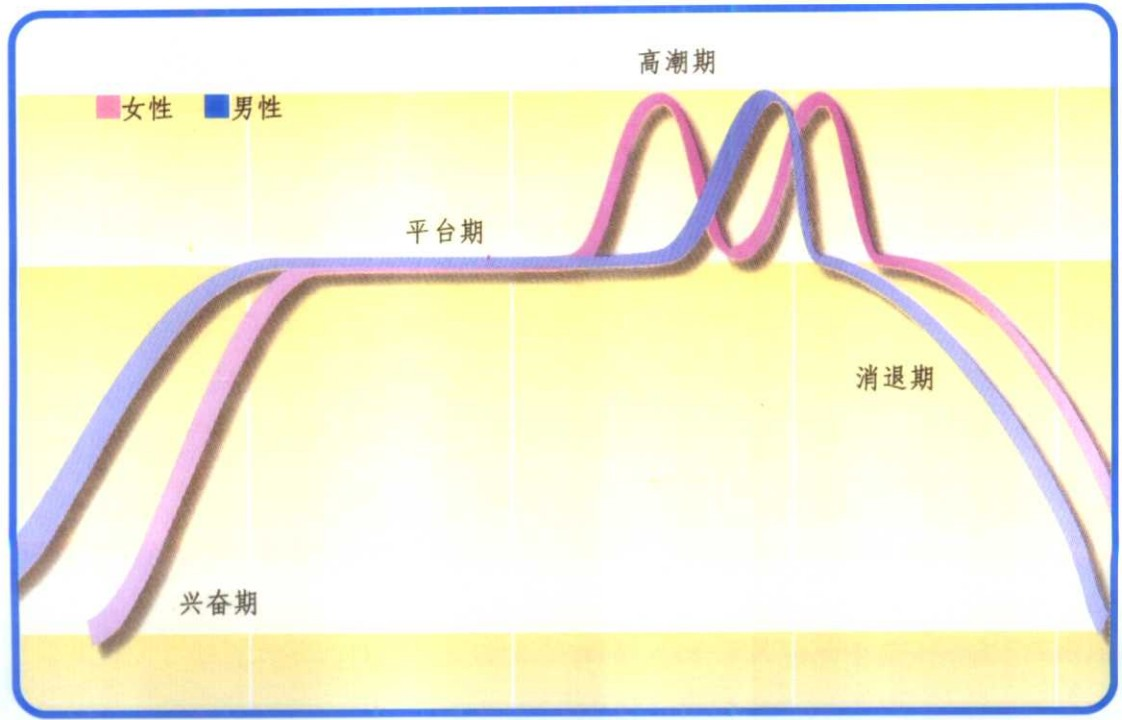
\includegraphics[width=0.8\textwidth]{sexual-response-cycle-mj.jpg}
  \caption{性反应周期示意图（马斯特斯和约翰逊模型）}
  \label{fig:sexual-response-cycle}
\end{figure}

四个阶段在两性之间是同构的，差别只在于以哪套器官为中心；各期在两性身上的具体变化，分别在本章后两节中展开。

需要强调的是，\textbf{生殖器反应与主观感受未必同步}：即使身体已经出现润滑或勃起，本人也可能并不感到被唤起，甚至感到不适——这一现象在性侵受害者身上尤其常见，也常被误解为"同意"或"享受"。

\subsection{女性的性反应}

在玛斯特斯和约翰逊提出的四阶段框架下，女性在兴奋期、平台期、高潮期和消退期中会发生如下身体变化。

其中最先出现、也最容易观察到的变化是阴道润滑：性刺激开始后约 10--30 秒即会出现，其速度受情绪与安全感影响远大于受物理刺激影响。

与男性相比，女性的反应对情境的依赖更明显——被理解、被看见、无被打扰的紧张，往往比技巧本身更能决定反应的完整程度；这也解释了为什么：“同样的做法，昨天有效今天却不行”是常见而非异常。

\subsubsection{兴奋期}

女性进入兴奋期后，最早出现的标志之一是阴道开口处变得湿润，这为后续性交插入创造了条件。

在性刺激下，阴道壁的血管充血，渗出大量清亮的液体，使阴道湿润，为阴茎插入做好准备，减少摩擦和疼痛。阴道润滑通常在性刺激后10--30秒内开始，其产生速度和量因人而异，受年龄、激素水平、情绪状态等因素影响。

阴蒂会充血勃起，体积增大（可增大2--3倍），阴蒂头暴露，敏感性增加。阴蒂的勃起是由于阴蒂海绵体内的血管充血引起的，类似于男性阴茎的勃起。

大阴唇分开、充血肿胀，失去褶皱；小阴唇充血肿胀，颜色变深（从粉红色变为深红色或紫红色），体积增大2--3倍，甚至可延伸到阴道口外，这有助于保护阴道口，同时增加性刺激的感受。

阴道上部（内2/3）扩张，形成"精液池"，为精子的停留和存活创造条件；阴道下部（外1/3）收缩，增加对阴茎的紧握感。阴道的长度也会增加（可增加1/3），以适应阴茎的插入。

子宫充血、体积增大，向上提升，子宫颈也会分泌黏液，为精子的通过提供润滑和保护。

乳房充血肿胀，体积增大（可增大20--30\%），乳头勃起，乳晕肿胀，颜色变深，乳房表面的静脉清晰可见。

有些女性的皮肤上会出现红晕，这是一种类似于麻疹的粉红色疹子，被称为“性红晕”，它在性反应过程中均可能出现。

心率加快、血压升高、呼吸加深加快、肌张力升高、皮肤敏感性增加等。

兴奋期持续时间因人而异，有的人会由此进入平台期，而有的人则会退回到原先的状态。

\begin{figure}[htbp]
  \centering
  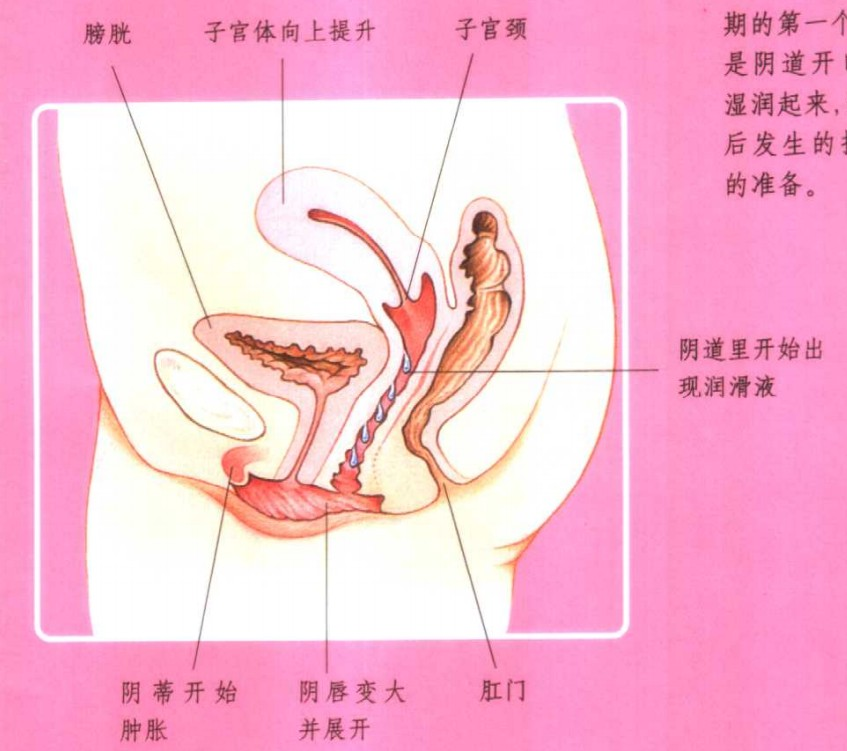
\includegraphics[width=0.8\textwidth]{excitement-phase-organ-state.jpg}
  \caption{兴奋期：生殖器官状态}
  \label{fig:excitement-phase-organ-state}
\end{figure}

\begin{figure}[htbp]
  \centering
  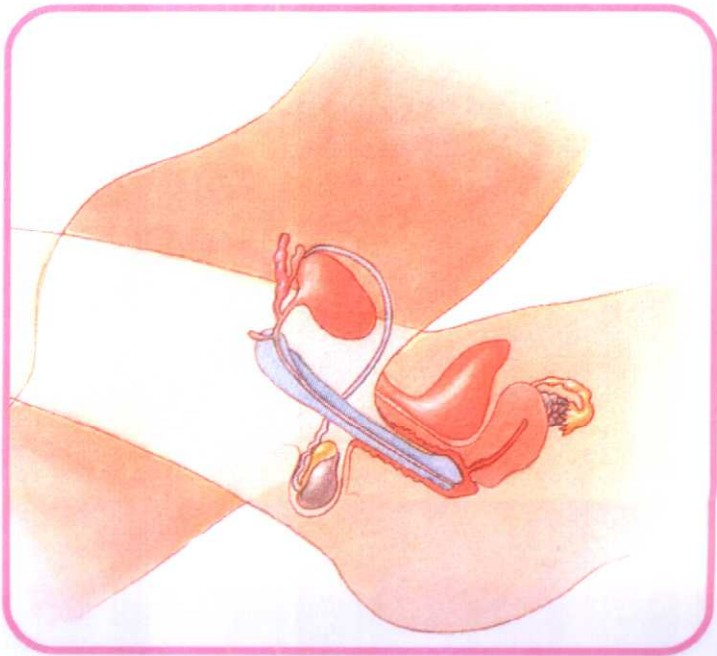
\includegraphics[width=0.8\textwidth]{sexual-intercourse-insertion.jpg}
  \caption{性交插入}
  \label{fig:sexual-intercourse-insertion}
\end{figure}

\subsubsection{平台期}

随着性兴奋和性刺激的继续，女性就会进入平台期。在这个阶段里，女性的整个生殖器官都会进一步充血。阴道的外1/3段直径变小，这有助于在性交中包裹阴茎，而阴道的内2/3段则开始扩张，为精液进入提供空间。这个时候还会发生“嵌进”现象，即原先位于骨盆腔里的子宫向上提升，突进腹腔里。“嵌进”为阴道扩张提供了空间，使男性射入阴道的精液有了活动空间。子宫的提升还能把阴道、子宫与输卵管之间的通道趋于直线，这样就方便了精子进入女性的生殖系统。有证据表明，刺激阴蒂可促使子宫提升。

\begin{figure}[htbp]
  \centering
  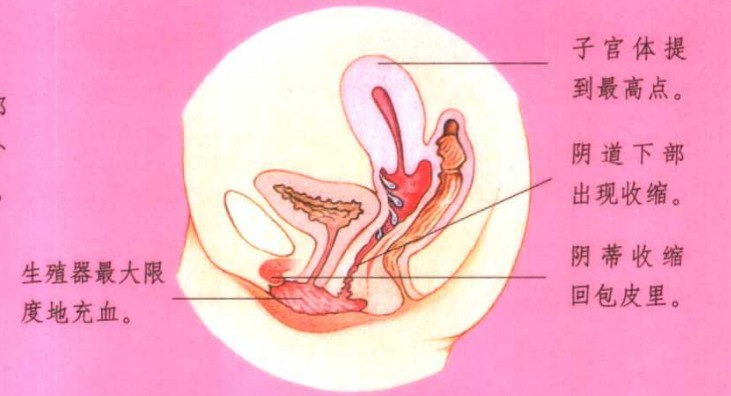
\includegraphics[width=0.8\textwidth]{plateau-phase-vaginal-changes.jpg}
  \caption{平台期：阴道变化（内2/3扩张，外1/3紧缩）}
  \label{fig:plateau-phase-vaginal-changes}
\end{figure}

在平台期中，小阴唇的颜色会变深，阴蒂体缩短，缩回阴唇后方。分布在阴道前庭的腺体还会分泌出少量润滑液。

平台期的持续时间取决于性刺激的强度和方式。平台期达到顶点后，可能进入高潮期——这是性反应周期四个阶段中的第三个阶段，也是持续时间最短的阶段——也可能缓慢消退。不经过高潮期就直接进入消退期，会让一些人感到失望，但也有一些觉得这样很不错。

\subsubsection{高潮期}

当性刺激和性唤起逐渐积累的性紧张得到强烈释放时，女性的性感觉会主要集中在生殖器官上，但与此同时，身体上的其他部分也会受到影响。女性的性高潮是一种强烈的主观体验，持续时间通常不超过10--15秒。性高潮开始时，阴道外1/3段会出现节律性收缩。最先出现的几次收缩，间隔为0.8秒——这与男性射精的收缩频率相同。收缩过几次后，间隔时间就会逐渐变长。

性高潮的收缩先是出现在阴道外1/3段，紧接着波及阴道内2/3段，最后上升到子宫。子宫的收缩起于子宫颈，一直传到子宫顶部。与此同时，骨盆、会阴部、膀胱口及直肠周围的肌肉也会出现收缩。这些收缩有助于精子进入子宫和输卵管，从而可能受孕。

\begin{figure}[htbp]
  \centering
  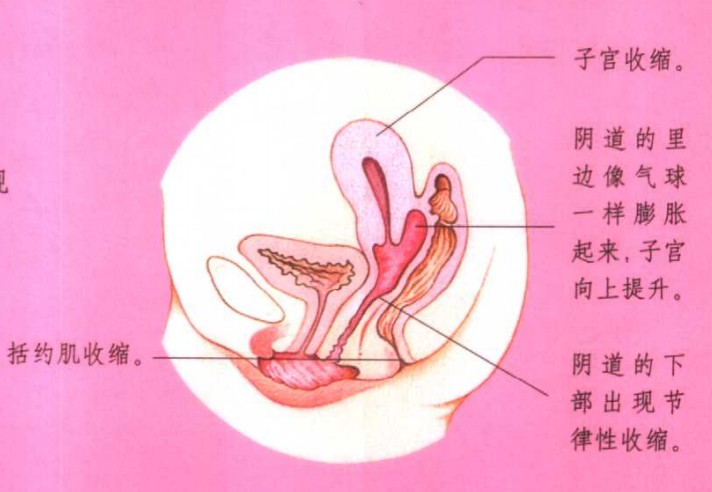
\includegraphics[width=0.8\textwidth]{orgasm-phase-rhythmic-contractions.jpg}
  \caption{高潮期}
  \label{fig:orgasm-phase-rhythmic-contractions}
\end{figure}

有些女性会随着骨盆肌肉的收缩向上挺起臀部。单次性高潮中，阴道外 1/3 的节律性收缩次数随性高潮的强度而异：轻微的高潮约 3--5 次，一般的高潮约 5--8 次，强烈的高潮可达 8--12 次，这一分级出自玛斯特斯和约翰逊的观察。在性高潮中阴蒂会缩回到包皮里，但可感觉到类似脉动的感觉，只是不同于阴茎的节律性收缩。

收缩的次数与性高潮的强烈程度之间，其实并没有可靠的对应关系。用阴道内压力记录所做的生理研究，未能建立起收缩次数与主观快感强度之间的关联；玛斯特斯和约翰逊提出的上述分级，在后来的综述中也被注明缺乏数据支持。

阴道与骨盆的节律性收缩也不是每次性高潮都会出现。有研究在持续时间较长的性高潮中记录到十几次、最多三十余次的不规则骨盆收缩，也有受试者完全没有收缩；在一项针对数百名女性的问卷调查中，约六成受访者自述在高潮时感受到收缩或搏动。可见收缩虽然常见，却并非性高潮的必要条件。

性高潮出现后，女性背部和足部的肌肉都会出现不自主痉挛，从而造成后背弓起，脚趾弯曲。心率可加快至每分钟180次，呼吸频率可达每分钟40次，血压也会升高。瞳孔扩大，鼻孔扩张。在性高潮过程中，有的女性大口喘气，有的女性则会屏住呼吸。性高潮越强烈，全身反应通常也越明显。根据玛斯特斯和约翰逊夫妇的报告，性高潮刚过去，乳头周围的皮肤就会收缩、出现皱褶。

性高潮中不同的女性会做出不同的身体表现。有的女性脸部表情扭曲，看似痛苦，可能发出呻吟，甚至是尖叫。有的女性可能抓握身边的人或物品，如枕头。而有的女性则可能一声不响、几乎没有明显动作，但但这并不一定意味着其性高潮体验不强烈。

关于女性性高潮不同类型的争论，最早是由奥地利心理学家西格蒙德·弗洛伊德（Sigmund Freud）引发的，他提出女性可以体验到两种性高潮，即阴蒂性高潮（被视为不成熟）和阴道性高潮（被视为成熟）。他认为，仅能体验阴蒂性高潮的女性在性心理方面是不成熟的。

这一学说曾长期流行，后来被玛斯特斯和约翰逊夫妇否定，他们在志愿者的配合下，使用科学仪器分别研究由阴蒂刺激获得的性高潮和由阴茎插入刺激所获得的性高潮，结果发现二者在生理上没有本质差异。

接下来，他们又对G点所在区域进行了研究，发现有些女性似乎能体验到两种不同的性高潮：一种由直接或间接刺激阴蒂获得，另一种由刺激G点获得。

由阴蒂刺激所激发的性高潮通常被归于“嵌进式”性高潮一类，伴随耻尾肌收缩；而G点性高潮则通常被归于“子宫式”性高潮一类，以子宫为中心。这两类性高潮所依赖的性刺激均通过骨盆神经传至脊髓反射中枢。骨盆和子宫深部肌肉都会发生收缩。大多数女性体验到的很可能是两种性高潮的混合形式。有些女性能够体验到多重性高潮。

\subsubsection{消退期}

性高潮后，女性最终会进入消退期。若达到性高潮，消退期通常在高潮的最后收缩停止后开始；若未达到性高潮，则从平台期逐渐消退。这是性反应周期的最后一个阶段，女性的身体会逐渐恢复到性唤起前的状态。乳房体积恢复，全身肌肉放松，心率和呼吸频率恢复到正常状态，皮肤上的红晕也开始消退。阴蒂通常在高潮后10--20秒内恢复到兴奋期之前的状态，但生殖器官其余部分却需要15--30分钟才能完全恢复常态。阴道和子宫的大小、形状和位置都会恢复原状，小阴唇的颜色也会变淡。消退期持续时间因人而异，但女性的消退期通常比男性长。

\begin{figure}[htbp]
  \centering
  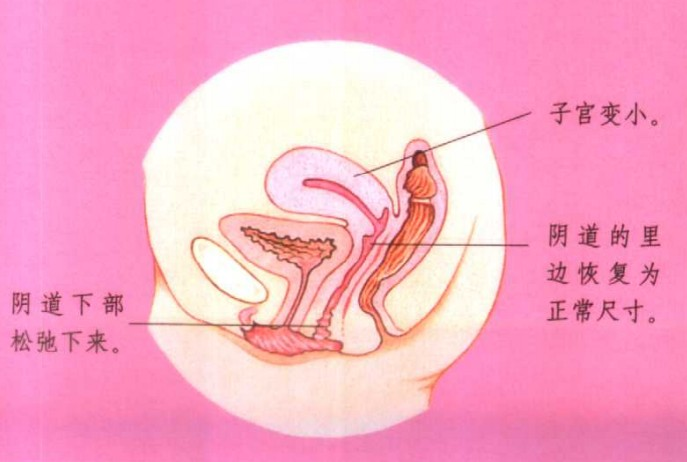
\includegraphics[width=0.8\textwidth]{resolution-phase-body-recovery.jpg}
  \caption{消退期：身体恢复}
  \label{fig:resolution-phase-body-recovery}
\end{figure}

此阶段，女性可能会感到倦意，也可能希望再次接受性刺激。与男性不同，女性通常没有明显的不应期。

假如在性高潮后继续进行刺激，女性可能重新回到平台期，而非直接进入消退期。这意味着女性有能力再次体验性高潮。

\subsection{男性的性反应}

按照玛斯特斯和约翰逊夫妇的理论，男性与女性一样，要经历兴奋期、平台期、高潮期、消退期这四个阶段。所不同的是，男性的变化以阴茎、阴囊和内生殖器官为中心，并波及全身的肌肉与血液循环。在性欲有了最初的萌发后，男性的身体会发生如下变化。

男性的性反应以“集中而快速”为特点：兴奋期勃起在数十秒内完成，平台期伴随睾丸提升、尿道球腺分泌少量清亮液体（其中可能含精子，也是“体外排精不安全”的原因之一）；高潮期射精分为两个阶段——精液先汇集于尿道前列腺部并伴随不可逆的“发射感”，随后由会阴肌肉收缩排出；此后进入不应期，无法立即再次勃起。

值得强调的是交感神经的角色：焦虑、紧张会让交感兴奋，反而干扰勃起与射精控制，这也是“越想表现好越容易出状况”的生理原因。此外，男性同样可以体验到非射精的高潮感，只是常因聚焦于射精而被忽略——把注意力从“结果”挪回过程，对伴侣双方都有帮助。

\subsubsection{兴奋期}

男性进入性兴奋期最直接的标志，就是阴茎勃起，也是性活动的必要条件之一。在性刺激下，大脑释放神经递质（如 NO ），使阴茎海绵体内的血管扩张，动脉血大量流入，同时静脉回流受阻，导致阴茎体积增大、硬度增加。勃起可以在性意念、对生殖器的直接触摸，或是其他感觉刺激下发生。勃起的速度和程度因人而异，一般在数秒至数分钟内完成。阴茎勃起的硬度可分为四级：一级（增大但不硬）、二级（硬但不足以插入）、三级（足够硬可以插入但不完全坚硬）、四级（完全坚硬）。

进入兴奋期后，肾上腺释放肾上腺素，使得心跳加快（可从静息时的60--80次/分钟增加到80--100次/分钟）、血压升高（收缩压可升高10--20mmHg，舒张压可升高5--10mmHg）、呼吸加深加快、肌肉紧张度增加（尤其是腹部、臀部和大腿肌肉）、乳头可能勃起。有些男性的皮肤上同样会出现红晕。

阴囊皮肤收缩，使阴囊变厚、变小，提睾肌收缩，睾丸上提靠近身体，这有助于减少运动时的摩擦和损伤，同时提高睾丸的温度，促进精子的成熟。

除了阴茎外，前列腺、精囊腺等生殖器官的血液供应也增加，为后续的射精过程做准备。

\subsubsection{平台期}

随着性刺激的继续，阴茎进一步充血，达到完全勃起，龟头的颜色加深，变成深红色或紫色。尿道口会有少量清亮的分泌物流出——这是尿道球腺（考珀腺）的液体，俗称“前液”。前液在排出时可能混有少量精子，这正是“体外射精并不保险”的原因之一。

睾丸因充血而胀大，大约能增加一半，并紧紧地贴向身体。精子沿着输精管向外侧出口运动，精囊与前列腺的分泌液汇入尿道。这一系列变化意味着射精已进入准备阶段：男性开始体验到一种“射精不可避免”的感觉——即使对阴茎的刺激完全停止，射精仍然要发生。这种迫切感大约持续 3 秒钟。

\subsubsection{高潮期}

射精分两步完成：先是尿道内口的括约肌收紧，精液被压入阴茎根部的尿道膨大处，此刻男性会感到一种压迫般的快感；随后尿道和环绕在阴茎根部的肌肉出现强烈收缩，把精液节律性地挤出体外。射出时收缩的力量可以很大，精液最远能射出约 28 厘米——当然，排出力度的个体差异极大，距离与快感强弱并不相关。

通常会发生 3—5 次强烈收缩，间隔约为 0.8 秒——与女性性高潮中阴道收缩的间隔完全一样。随着收缩的持续，力度渐渐变弱，间隔也失去规律。骨盆底部与大腿内侧的肌肉也会不自觉地收缩。男性性高潮的持续时间很少超过 15 秒，一般在 4—10 秒之间，比大部分女性的高潮略短。

\subsubsection{消退期}

高潮过后，男性的身体逐渐回到未唤起的状态。玛斯特斯和约翰逊夫妇观察到，男性的消退分两个阶段：第一阶段，阴茎仍保持半勃起，这种状态可以持续一段时间；第二阶段，勃起迅速而完全地消退，充血散去，睾丸降回原位，阴囊皮肤重新松弛下来。

与女性不同，男性在射精后有一段“不应期”——在这段时间里，无论受到多大的性刺激，都无法再次唤起勃起与射精。其机制与射精后催乳素升高、神经系统由兴奋转向抑制有关。不应期短的只有几分钟，长的可达数小时，并随年龄增长而延长，个体差异极大。

年轻男性可以在尚未射精时退回平台期，让性紧张反复积累，甚至多次体验不伴随射精的高潮；但射精一旦发生，身体就会不可逆转地进入消退期。消退期里的男性普遍感到放松与困倦，而女性若在高潮后继续受到刺激，可以直接退回平台期、再度达到高潮。正因如此，性生活中的“事后时间”常常出现节奏差：男方只想睡，女方却期待温存与爱抚——把这段时间留给拥抱与交谈，对双方都是一种体贴。

\section{性反应的同步性}

\subsection{男女反应节律的差异}

把“反应节律”单独拿出来讨论，是因为它是伴侣间最常见的摩擦来源之一。所谓节律差异，指的是唤起的启动速度、达到高潮所需的刺激时长与方式、以及消退的快慢。

\begin{itemize}
\item \keyword{启动速度}：就群体平均而言，男性的唤起启动更快，且更容易被视觉与想象激发；女性的唤起启动通常更慢，且更依赖情境、氛围、情感安全感与被渴望的感觉。
\item \keyword{到达高潮的路径}：女性的高潮多数依赖阴蒂区域的持续刺激，而性交本身未必能提供足够刺激；男性则通常通过性交即可达到。
\item \keyword{消退速度}：男性高潮后迅速进入消退并伴随不应期；女性消退较慢，若未达高潮，可能长时间保持一定唤起水平，甚至感到胀痛。
\item \keyword{波动性}：女性唤起在过程中容易因分心、疼痛、担忧而中断，也需要重新“爬坡”。
\end{itemize}

把这些差异理解为\keyword{两套不同的节律}，而不是“一个人太快、一个人太慢”，能显著降低伴侣间的指责。差异本身不是问题，缺少对差异的了解才是。

\begin{tcolorbox}[colback=pink!5!white,colframe=red!50!black,title=贴心小叮咛]
“我要很久”不是缺点，“我很快”也不是优点——它们只是节律。把节律差异说出口，再一起找折中方案，比各自默默忍耐或暗自抱怨有效得多。
\end{tcolorbox}

\subsection{调整时间差的实用做法}

节律差异无法消除，但完全可以协商。以下做法来自性治疗中的常见建议，核心思路是\keyword{把“同时”的目标，换成“都满意”的目标}。

\begin{itemize}
\item \keyword{延长前戏}：给唤起较慢的一方足够的时间。前戏不是“准备阶段”而是性活动的主体部分，时长没有标准，以对方的状态为准。
\item \keyword{先满足慢的一方}：一个被广泛推荐的顺序是先用手或口让唤起较慢的一方达到满足，再进入性交。这样较快的也不必刻意拖延。
\item \keyword{不必执着于性交中同时高潮}：同时高潮在现实中并不常见，且需要刻意控制，追求它反而增加压力。
\item \keyword{善用“事后”的余裕}：男性不应期内，可以继续用手或口照顾伴侣，此时无表现压力，反而更容易放松。
\item \keyword{把交流变成习惯}：过程中的简短反馈（“轻一点”“就这样，别停”）比事后讨论有效得多。
\item \keyword{如果差异来自疼痛、勃起困难等问题}：这属于需要就医的范畴，不是靠技巧能解决的。
\end{itemize}

这些做法背后有一个共同前提：\keyword{双方都认为对方的满足是自己的事}。若做不到这一点，任何技巧都只是权宜。

\begin{tcolorbox}[colback=pink!5!white,colframe=red!50!black,title=贴心小叮咛]
追求“同时”是很多压力的来源。性不是同步表演，而是两个人各自舒服。把目标从“一起到达”换成“都到达过”，摩擦通常会立刻减少。
\end{tcolorbox}

上一节处理的是概率层面的差距——“能不能达到高潮”；本节转向时间层面——两性的反应节奏能否合拍。

性反应周期各个阶段所占用的时间因人而异，但就一般情况而言，年纪越轻，进入性兴奋的速度就越快。由于女性的性反应要比男人迟缓一些，所以很多配偶发现他们的性反应不能做到同步进行。比如，当男人已经进入到平台期了，而女人还停留在兴奋期里。再比如，当两个人都处在平台期里时，男人可能要不了多大工夫就进到高潮期并射精，而女人那里还需要更多的时间和进一步的刺激。性治疗学家玛斯特斯和约翰逊夫妇指出：“有些配偶已经发现他们在达到性高潮的速度上一个快一个慢，这些人就要认真考虑是否需要改变做爱习惯，这种改变可能会弥补快慢不同所带来的遗憾。”

改善同步性的关键不在于把双方“调成同一个节奏”，而在于承认差异、主动补偿。以下做法在临床咨询中被反复推荐：

\begin{itemize}
  \item \textbf{把前戏当作“时间差补齐器”}：女性平均需要更长的唤起时间，男方可以在正式开始前先完成大量爱抚，而不是事后补救；
  \item \textbf{用语言而非猜测校准}：一句“这样慢一点可以吗”比默默忍耐有效得多；
  \item \textbf{允许不同步的结局}：同步高潮固然美好，但把它当成每次的“及格线”反而制造表演焦虑。一方先满足、另一方随后，是更常见的真实图景。
\end{itemize}

需要提醒的是，如果性反应的“不同步”是突然出现且伴随性欲、勃起或润滑的明显变化，更可能与疲劳、压力、药物或激素水平有关，宜先排查生理因素，再考虑关系因素。

\subsection{调整时间差}

推迟插入、把精力集中到“前戏”上，都可以使做爱时间延长。

\section{性激素与性唤起机制}

\subsection{睾酮与性欲的关系}

睾酮是讨论性欲时最常被提到的激素，但它在人体中的作用远比"性欲开关"复杂。

\begin{itemize}
	\item \keyword{基本作用}：睾酮对两性的性欲都有影响，但对男性而言更多是"维持"而非"驱动"——它在正常范围内的高低，与主观性欲的相关性其实不强。
	\item \keyword{阈值效应}：研究发现，当睾酮水平低于某个阈值时，性欲会明显下降；而一旦回到正常范围，再往上提高并不会带来相应的性欲提升。\keyword{"补得越多越想要"是误解。}
	\item \keyword{女性的睾酮}：女性体内同样有睾酮（由卵巢与肾上腺产生），它在女性性欲中也有作用，但水平低得多，相关研究仍不充分。
	\item \keyword{波动因素}：睡眠、运动、肥胖、慢性疾病、压力都会影响睾酮；单次化验的数值受采血时间（晨间最高）与近期状态影响，不能凭一次结果下结论。
	\item \keyword{外源补充的风险}：不当使用外源睾酮会抑制自身分泌，还可能影响精子生成、肝功能与心血管健康，须在医生评估与监测下进行。
\end{itemize}

临床上，性欲低下常被简单归因于"睾酮低"，但真正的原因往往是多因素的——抑郁、关系问题、睡眠不足、药物副作用常被忽略。

\begin{tcolorbox}[colback=pink!5!white,colframe=red!50!black,title=贴心小叮咛]
如果怀疑性欲下降与激素有关，正确做法是到内分泌科或男科/妇科做规范评估，而不是自行购买"睾酮补充"类产品。多花几百元做一次规范检查，可能省下几个月无效又伤身的尝试。
\end{tcolorbox}

\subsection{雌激素与孕激素的作用}

雌激素与孕激素常被理解为"女性激素"，但它们对性健康的影响远不止于生殖功能，而且男性体内同样存在这两类激素。

\begin{itemize}
	\item \keyword{雌激素}：维持阴道黏膜的厚度、弹性与润滑能力。绝经后雌激素下降，会导致阴道干涩、弹性下降、性交疼痛——这类变化是生理性的，且有明确的治疗手段。此外，雌激素也参与女性性欲、情绪与睡眠的调节。
	\item \keyword{孕激素}：与月经周期、孕期维持密切相关。部分女性在黄体期（经前）会经历性欲波动、情绪低落或身体不适，这与孕激素水平变化有关。
	\item \keyword{男性体内}：男性也有少量雌激素（由睾酮转化而来），它参与骨骼代谢与性功能调节，过高或过低都可能带来问题。
	\item \keyword{激素与性欲的关联并不直接}：性欲随月经周期变化的模式在女性中差异极大，有人黄体期更强，有人卵泡期更强，也有人几乎没有周期性变化。
\end{itemize}

理解这些激素的作用，最重要的现实意义是：\keyword{绝经后的性交疼痛与干涩不是"忍一忍就好"的自然老化}，而是可以进行有效干预的医学问题。

\begin{tcolorbox}[colback=pink!5!white,colframe=red!50!black,title=贴心小叮咛]
绝经后出现性交疼痛、干涩或反复炎症，值得去妇科正规就诊，而非默默减少性生活。局部雌激素、保湿剂与润滑剂等手段安全性良好，"年纪大了就这样"并不是必须接受的结论。
\end{tcolorbox}

\subsection{催产素与亲密感}

催产素常被媒体称为"爱情激素"或"拥抱激素"。这个说法抓住了一部分事实，但简化得太多。

\begin{itemize}
	\item \keyword{基本作用}：催产素在分娩、哺乳与亲子联结中作用明确。在性活动中，高潮时与亲密接触时均会释放，可能参与放松、信任与依附感的形成。
	\item \keyword{与性别的关联}：它在两性体内都存在，并非女性专属；对男性也可能参与射精与亲密感调节。
	\item \keyword{"爱情激素"说法的问题}：催产素的作用高度依赖情境与社会关系。它在"对内群体"促进信任的同时，也可能强化对外群体的戒备——它并不无条件让人变温柔。
	\item \keyword{研究现状}：多数人类研究测的是血液中的催产素浓度，而它能否反映大脑中的实际水平，仍有争议。因此关于催产素与爱情、忠诚的推论都应谨慎。
\end{itemize}

实用层面，催产素相关研究提示了一件朴素的事：\keyword{身体的亲密接触本身有生理价值}——拥抱、依偎、牵手这类非性接触，对关系满意度和压力缓解的作用已经有较多证据支持。

\begin{tcolorbox}[colback=pink!5!white,colframe=red!50!black,title=贴心小叮咛]
不必把"催产素的多少"当成爱情的指标，也不必刻意追求所谓的激素高潮。每天多几次真实的拥抱和依偎——这不是玄学，是成本最低、证据最稳的亲密投资。
\end{tcolorbox}

\subsection{神经递质与唤起通路}

性的生理基础不只是激素，神经递质在其中扮演着同样关键的角色。理解这一点，有助于解释为什么某些药物会显著影响性功能。

\begin{itemize}
	\item \keyword{多巴胺}：与欲望、动机和奖赏相关，通常被视为性唤起的"油门"。它让人"想要"，而非仅仅"感受"。
	\item \keyword{血清素（5-羟色胺）}：作用复杂。总体上它抑制射精、降低性欲与高潮强度——这正是 SSRI 类抗抑郁药导致性功能障碍的主要原因。
	\item \keyword{去甲肾上腺素}：参与唤起与交感神经系统的激活。
	\item \keyword{乙酰胆碱}：在外周参与勃起与生殖器血流调节，副交感神经通路是勃起的必要条件。
	\item \keyword{一氧化氮（NO）}：勃起机制的核心信号分子，促使阴茎海绵体平滑肌舒张、血流增加。PDE5 抑制剂（如西地那非）正是通过延长 NO 通路的作用而起效。
\end{itemize}

把这些通路放在一起看，就能理解一个临床常识：\keyword{性功能受神经递质系统调控，因此任何作用于精神或心血管系统的药物都可能影响性功能}。反过来说，多数这类影响是可以调整的——关键在于主动与医生讨论。

\begin{tcolorbox}[colback=pink!5!white,colframe=red!50!black,title=贴心小叮咛]
因为吃药而出现性欲下降或勃起困难时，不要自行停药——突然停用抗抑郁药可能带来更严重的反弹。正确做法是记录变化、带上药单去找开药的医生，请他评估换药、调整剂量或服药时间。
\end{tcolorbox}

性激素之间复杂的相互作用，是提高性欲、促进生育的基本保证。不管是男人还是女人，其性特征都需要性激素来维持。在睾丸激素的作用下，男人身上出现了显示力量的肌肉、脸上的胡须、低沉的嗓音等男性特征；而在雌激素和孕激素的共同作用下，女性的乳房得以发育，生育周期得以调节。

心血管系统在性欲的发生以及性功能的维持方面，也能发挥重要作用。比如，性欲初起之时，人的心脏就会加快泵血，增加送往生殖器官的血液流量，使得它们充盈起来。于是，阴茎得以勃起，而阴道和阴蒂由此出现的种种生理变化，又使性高潮得以实现，甚至能帮助受孕。

\section{大脑在性唤起中的双重角色}

\subsection{兴奋通路与抑制通路}

当代研究性唤起的核心框架，不是"有没有性欲"，而是\keyword{兴奋系统与抑制系统的双通道模型}。这一模型由班克罗夫特（John Bancroft）与詹森（Erick Janssen）提出，对理解"为什么想做却做不了"极有帮助。

\begin{itemize}
	\item \keyword{性兴奋抑制系统（SIS）}：负责对性反应进行刹车。它高度敏感于\keyword{风险评估}——会被"会不会被看到""会不会疼""万一不行怎么办""我是不是不够好"这类念头激活。
	\item \keyword{性兴奋系统（SES）}：负责油门，对性线索（视觉、触觉、想象、伴侣的反馈）作出反应。
	\item \keyword{实际唤起＝两者之差}：一个人的唤起水平取决于油门与刹车的合力。这也是为什么"很想"的人可能毫无反应，而"没想过"的人却可能被唤起。
\end{itemize}

这一模型的最大价值在于解释了一个常见困惑：\keyword{唤起障碍往往不是油门不够，而是刹车太紧}。焦虑、羞耻、对表现的担忧、创伤记忆、不适的物理环境，都会持续踩下刹车。

因此，干预方向常常不是"更努力地兴奋"，而是\keyword{减少抑制因素}——放松情境、降低表现压力、消除疼痛、获得安全感。

\begin{tcolorbox}[colback=pink!5!white,colframe=red!50!black,title=贴心小叮咛]
如果在性爱中"脑子里念头太多"，那不是你不够投入，而是抑制系统在正常工作。试着把注意力从"我表现如何"移到"我此刻感受到什么"——这是性治疗中常用的转移焦点法，理由正在于此。
\end{tcolorbox}

\subsection{中枢对性唤起的调控}

性唤起的最终调控中枢在大脑，而非生殖器。生殖器只是执行端，真正决定"是否被唤起"的，是大脑对情境与风险的评估。

\begin{itemize}
	\item \keyword{下丘脑}：性行为的核心整合中枢，接收激素信号与感官信息，输出性行为的启动指令。
	\item \keyword{边缘系统（杏仁核、海马等）}：负责情绪与记忆的加工。杏仁核在评估"这个情境安不安全"时起关键作用——它对威胁的高度敏感，正是焦虑抑制性唤起的神经基础。
	\item \keyword{前额叶皮层}：负责计划、抑制与自我监控。它在性活动中的过度活跃，会表现为"想得太多而感受太少"。
	\item \keyword{脊髓反射}：勃起与射精存在不依赖大脑的脊髓反射弧，这解释了为什么脊髓损伤者仍可能保留部分性反应能力。
\end{itemize}

这一结构带来一个重要推论：\keyword{性唤起是"自上而下"与"自下而上"共同作用的结果}。感官刺激由下而上传递，而注意、情绪与安全感由上而下调制。当两者冲突时，上层的评估通常占上风——这也是为什么"不安全的性爱很难享受"。

实践含义是：改善性反应，常常要从改善情境与心理状态入手，而不是一味加强物理刺激。

\begin{tcolorbox}[colback=pink!5!white,colframe=red!50!black,title=贴心小叮咛]
大脑是最大的性器官——这句常被引用的说法有其生理依据。安全感、被渴望的感觉、放下控制的那一刻，其作用往往超过任何技巧。营造情境不是"前戏"，而是唤起的前提条件。
\end{tcolorbox}

\subsection{抑制通路失调的表现}

当性兴奋抑制系统长期处于过度激活状态时，会出现一组临床上常见但常被误解的表现。识别它们，是寻求有效帮助的第一步。

\begin{itemize}
	\item \keyword{情境性唤起障碍}：自慰时一切正常，与伴侣时却无法唤起。这通常说明生理功能完好，问题在关系或心理层面。
	\item \keyword{表现焦虑循环}：一次失败引发对下次的担忧，担忧导致抑制系统激活，于是再次失败——形成自我实现的预言。
	\item \keyword{身体与主观分离}：出现生理唤起（润滑、勃起）但主观上毫无欲望，甚至感到不适。这提示"身体的反应"与"心理的意愿"是两条可分离的通道。
	\item \keyword{触发性回避}：特定情境、姿势、触碰会引发强烈抗拒或解离，常见于有创伤经历者。
	\item \keyword{持续性分心}：过程中不断走神、自我审视、评估表现，难以进入体验。
\end{itemize}

这些表现有一个共同点：\keyword{都不是"能力问题"，而是"抑制问题"}。因此单纯加强刺激、服用补品、或强迫自己"放轻松"往往无效，反而加重挫败。

有效的路径通常是：①排查疼痛、药物、疾病等生理因素；②处理焦虑与自我评价；③若涉及创伤，接受专业创伤治疗；④必要时伴侣共同参与。

\begin{tcolorbox}[colback=pink!5!white,colframe=red!50!black,title=贴心小叮咛]
"越是努力想有感觉，越是没有感觉"——这不是意志力的问题，而是抑制系统的机制。此时需要的是减负而非加压。承认"今天可能不行"，往往反而让唤起重新出现。
\end{tcolorbox}

在性欲唤起的过程中，大脑扮演的是一个双重角色——一个角色在有意识的领域里，另一个角色在潜意识的领域里。在性欲唤起之前，人们通常会感知到某种性刺激——如照片、气味，或者是接近某个异性。这种感知首先启动了性欲，其后紧追不舍的就是生殖器官或身体其他部位出现一些生理变化。

大脑中有一个地方叫作脑边缘构造，它负责处理来自视觉、嗅觉、味觉、听觉和触觉的信息，同时也处理思想、欲望、幻想这样一类情感信息。如果送进脑边缘构造中的信号是积极的，那么人就会产生愉快的感觉；如果传递进来的信号是积极的性信息，那么大脑就会将这个信息再传送出去，“命令”增加流向生殖器官的血液。这种性唤起起源于大脑，所以就叫心理性唤起。

在没有获得愉快的信息，脑边缘构造也没有进行过信息处理的情况下，也能出现性唤起。比如，直接触摸或挤压生殖器官，同样会使大量血液涌向这里，这种现象称作反射性唤起。这种性唤起要比心理性唤起简单得多，但它的重要性丝毫不亚于后者。两个人做爱时，心理性唤起和反射性唤起常常会联合发挥威力。

以男性为例，当反射性唤起出现在性生活中时，轻而易举地就能压倒心理性唤起，只需不停地施加刺激，就完全肯定有把握将他引入射精和性高潮。而女性却截然不同，尽管你可以不停地对其生殖器官加以刺激，但只要电话铃声一响，或者孩子的哭闹声一传来，她的心神立刻就会被分散，通往性高潮的道路当即就被封个严严实实。

就在达到性高潮的那一刻，无论男女都会突然释放出一种名叫乙型脑中卵磷脂的东西，它属于内啡肽的一种，能起到吗啡样的镇痛作用。乙型脑中卵磷脂紧紧地抓住脑中麻醉受体，使得处在性高潮中的人们能体会到那种异常欣快的感觉一阵阵向全身弥散。

\section{胚胎的性发育}

\subsection{性腺的分化}

人类胚胎在最初几周内，性腺是"未分化"的——男女胚胎拥有完全相同的原始结构。性别分化是一个由基因触发的连锁过程。

\begin{itemize}
	\item \keyword{未分化阶段}：受精后约第 5 周，胚胎在中肾附近形成一对"生殖嵴"，此时尚无性别差异。
	\item \keyword{关键基因}：位于 Y 染色体上的 \keyword{SRY 基因}在约第 7 周启动，触发未分化性腺向睾丸发育；若无 SRY，性腺在稍晚时候默认发育为卵巢。
	\item \keyword{激素的作用}：睾丸开始分泌睾酮与抗苗勒管激素（AMH），前者推动男性生殖管道发育，后者使女性管道退化。卵巢的发育则不依赖同等强度的激素驱动。
	\item \keyword{时间差}：男性分化过程依赖精确的激素作用窗口，因此对干扰更为敏感。
\end{itemize}

理解这一段的关键在于：\keyword{性腺的分化并非"二选一"的开关，而是一系列有时间窗口的发育事件}。任何环节受到影响，都可能产生介于典型男女之间的解剖或生理表现。

\begin{tcolorbox}[colback=pink!5!white,colframe=red!50!black,title=贴心小叮咛]
"性别只有两种"是日常语言中的简化。在发育生物学层面，性别是一个多环节连锁的过程，其中任何一步的变异都可能带来多样的结果。理解这一点，有助于减少对性发育差异者的误解与污名。
\end{tcolorbox}

\subsection{内生殖管道的分化}

胚胎期同时存在两套原始生殖管道，最终只会保留其中一套，另一套退化。这个过程决定了内生殖器官的基本布局。

\begin{itemize}
	\item \keyword{两套原基}：沃尔夫管（中肾管）与苗勒管（副中肾管），在未分化阶段同时存在。
	\item \keyword{男性路径}：睾酮促使沃尔夫管发育为附睾、输精管与精囊；抗苗勒管激素（AMH）使苗勒管退化。
	\item \keyword{女性路径}：缺乏 AMH 时苗勒管保留，发育为输卵管、子宫与阴道上段；缺乏睾酮时沃尔夫管退化。
	\item \keyword{同源器官}：正因为来自同一套原基，男女的部分器官结构高度对应——如阴蒂与阴茎、大阴唇与阴囊，都属于\keyword{同源器官}。
\end{itemize}

\keyword{同源器官}这一概念在性医学中很有用：它解释了为什么同一类药物、同一种神经通路或同一类刺激方式，常能对两性都起作用。

\begin{tcolorbox}[colback=pink!5!white,colframe=red!50!black,title=贴心小叮咛]
阴蒂与阴茎来自同一胚胎原基，这在解剖学上意味着两者的敏感机制高度相似。这既是一个有趣的知识点，也是理解两性性反应为何"同多于异"的基础。
\end{tcolorbox}

\subsection{外生殖器的分化}

外生殖器的分化发生在胚胎后期，且男女来自同一套原始结构。这个过程对激素环境高度敏感。

\begin{itemize}
	\item \keyword{共同起点}：生殖结节、尿道褶与生殖隆起，在未分化阶段外形一致。
	\item \keyword{男性路径}：在双氢睾酮（DHT）作用下，生殖结节延长为阴茎、尿道褶闭合形成尿道、生殖隆起融合为阴囊。
	\item \keyword{女性路径}：缺乏 DHT 时，生殖结节发育为阴蒂、尿道褶形成小阴唇、生殖隆起形成大阴唇。
	\item \keyword{关键窗口}：分化集中在孕 8--12 周，此期激素作用的异常会显著影响外生殖器的形态。
\end{itemize}

外生殖器的形态在出生时并不总能明确指向单一性别，这使\keyword{出生时的性别判定}成为一个需要慎重对待的医学问题。当代医学伦理强调：在非紧急情况下，应避免对婴幼儿实施不可逆的性别相关手术，待其成长后自主参与决策。

\begin{tcolorbox}[colback=pink!5!white,colframe=red!50!black,title=贴心小叮咛]
以往对"性别不明确"的新生儿采取尽早手术的做法，如今已被多数专业学会认为不符合伦理。若遇到相关情况，建议寻求具备多学科团队的医疗机构评估，并充分了解延迟决策的选项。
\end{tcolorbox}

\subsection{激素在胚胎期的作用}

胚胎期的激素环境对性分化起决定性作用，但它的作用方式是"有时间窗口的"——这决定了它既强大又脆弱。

\begin{itemize}
	\item \keyword{睾酮}：推动男性内生殖管道发育，并在转化为 DHT 后作用于外生殖器。
	\item \keyword{抗苗勒管激素（AMH）}：由睾丸支持细胞分泌，使苗勒管退化，防止子宫与输卵管发育。
	\item \keyword{母体与胎盘激素}：母体激素经胎盘影响胎儿，但浓度受胎盘屏障调节，正常妊娠中不会"改变"胎儿性别。
	\item \keyword{关键窗口}：不同器官对激素敏感的时间段不同，错过窗口后补足激素也无法逆转已形成的结构。
\end{itemize}

一个常被讨论的问题是\keyword{外源激素或环境内分泌干扰物的影响}。目前证据显示，环境中某些化学物质可能干扰内分泌功能，但对人类性别分化的实际影响尚未有明确结论，相关研究仍在进行。

\begin{tcolorbox}[colback=pink!5!white,colframe=red!50!black,title=贴心小叮咛]
网络上流传"孕期服用某物决定胎儿性别"的说法，没有科学依据，且自行用药可能对胎儿造成实际伤害。胎儿性别在受精时已由染色体决定，激素只负责让既定方向发育完成。
\end{tcolorbox}

\section{梦交}
% 放这里合适吗？
\subsection{梦交的生理基础}

梦交（又称"睡梦中的性高潮"）指在睡眠中未经清醒时的性刺激而出现的性反应乃至高潮。它并非异常现象，而是睡眠与性生理共同作用的产物。

\begin{itemize}
\item \keyword{与 REM 睡眠的关联}：性梦与性唤起多发生在快速眼动（REM）睡眠阶段。此期大脑活动活跃，生殖器血流增加，是生理性唤起的易发期。
\item \keyword{两性皆可发生}：男性常表现为遗精，女性则可能经历梦中性高潮，或仅出现生殖器充血与湿润，未必伴随梦境内容。
\item \keyword{生理唤起不等于心理欲望}：睡眠中的性唤起是自主神经活动的结果，与清醒时的性欲并不对应。
\item \keyword{激素与睡眠的影响}：睡眠不足、作息紊乱、激素波动都可能改变其发生频率。
\end{itemize}

从生理角度看，梦交是\keyword{正常睡眠中常见的伴随现象}，尤其在青春期与性活跃期更为频繁。

\begin{tcolorbox}[colback=pink!5!white,colframe=red!50!black,title=贴心小叮咛]
梦中的性内容与自己清醒时的意愿、道德立场无关。梦见与不相干的人发生性关系，不代表你喜欢那个人，也不代表你“心里其实想”。梦是大脑在整理信息，不必为它负责。
\end{tcolorbox}

\subsection{发生频率与人群差异}

梦交的发生频率在人群中差异极大，从从未有过到每周多次都属于正常范围。了解这些差异，有助于减少不必要的担心。

\begin{itemize}
\item \keyword{年龄分布}：男性遗精在青春期至二十余岁最频繁，随年龄增长逐渐减少，但并非到某一年龄就完全消失。女性的梦中性高潮在成年各阶段均可出现，个体差异更大。
\item \keyword{频率波动}：性活动频率、禁欲时间、睡眠质量、压力水平都会影响发生次数。长时间没有性活动时，发生率往往上升。
\item \keyword{性别差异}：男性因有明确的生理标志（射精），报告率较高；女性若未伴随强烈感受或梦境，可能根本不会察觉。
\item \keyword{文化影响}：不同文化对梦交的态度差异很大，这会影响人们是否报告，但不影响其实际发生率。
\end{itemize}

需要区分的是“偶发的梦中高潮”与“频繁到影响睡眠质量的状况”。后者可能与睡眠障碍、药物或激素变化有关，值得就医评估。

\begin{tcolorbox}[colback=pink!5!white,colframe=red!50!black,title=贴心小叮咛]
如果梦交频繁到影响睡眠、或因内裤潮湿而长期焦虑，可以把它当作一个睡眠问题去处理——规律作息、减少睡前刺激、必要时看睡眠门诊，比自责有用得多。
\end{tcolorbox}

\subsection{相关文化与误解}

梦交在历史上曾被赋予各种解释，其中不少已证明是误解，但这些观念至今仍影响着人们的自我评价。

\begin{itemize}
	\item \keyword{"伤身"说}：传统观念常把遗精视为"漏精伤元气"，导致大量男性在青春期产生不必要的恐惧。现代医学表明，精液由身体持续生成，正常排出不会损害健康。
	\item \keyword{"道德"说}：某些宗教与道德传统把梦中性内容视为放纵的证据，带来羞耻感。但梦的内容并不受意志控制。
	\item \keyword{疾病的误认}：有人把频繁梦交当作"肾虚"或"性功能异常"的表现，进而购买各类补品，往往既无效果又增加焦虑。
	\item \keyword{正常化的价值}：当代性教育强调把梦交作为"青春期正常生理现象"来介绍，这一表述本身就有减轻心理负担的作用。
\end{itemize}

这些误解的共同代价是：\keyword{把一个正常现象变成了焦虑源}。而对青少年而言，这种焦虑往往持续多年，甚至影响成年后的性态度。

\begin{tcolorbox}[colback=pink!5!white,colframe=red!50!black,title=贴心小叮咛]
如果曾有长辈告诉你"遗精会伤身"或"要节制"，可以更新这个知识：它属于正常生理现象，不需要治疗，也不需要进补。真正需要调整的，往往只是作息与睡眠。
\end{tcolorbox}


\section{高潮差距}
% ⇒ [r81 并入] 自旧区
\noindent\textit{【编者注】}本节讨论当代性学研究中的核心议题——异性恋性行为中男女高潮率的显著差异，即"高潮差距"（orgasm gap），又称"愉悦差距"（pleasure gap）。

这一现象有扎实的量化支撑：2018 年发表于《性行为档案》的大样本调查显示，异性恋关系中女性每次性行为达到高潮的比例约为 65\%，而男性约为 95\%；值得注意的是，女同性伴侣中女性的高潮率显著更高——这说明“差距”不是女性生理的缺陷，而是普遍性行为脚本（重插入、轻阴蒂刺激、时间不足、缺少沟通）的产物。把高潮差距当作公共议题来讨论，其价值在于促使伴侣双方把“她是否满足”当作与“他是否持久”同等级别的问题来对待——愉悦的平等不是运气，是可以学习和练习的技巧。

\subsection{高潮差距的事实数据}

多项大规模调查研究揭示了一个稳定存在但长期被忽视的现象：

\begin{itemize}
	\item 美国全国健康与社会生活调查（NHSLS）显示：异性恋伴侣中，\textbf{男性约 95\% 的时间能达到性高潮，女性仅约 65\%}。
	\item 2018 年《社会心理与人格科学》（Social Psychological and Personality Science）期刊发表的研究：在异性恋性行为中，女性高潮率约为男性的\textbf{三分之一到二分之一}。
	\item 女同性恋性行为中女性高潮率约为 \textbf{86\%}——远高于异性恋情境，说明高潮差距并非生理限制，而是\textbf{性行为模式和文化观念}所致。
\end{itemize}

\subsection{高潮差距的成因}

高潮差距并非源于女性“难以达到高潮”的生理缺陷，其成因是多层面的：

\begin{enumerate}
	\item \textbf{对阴蒂刺激的忽视}：约 70\%--80\% 的女性需要直接或间接的阴蒂刺激才能达到高潮，但异性恋性行为模式往往以阴道插入为中心，忽略了这一关键。
	\item \textbf{性教育中的性别偏见}：传统性教育强调男性射精和生育功能，女性性愉悦和阴蒂解剖结构长期缺席于教材和公共话语。
	\item \textbf{色情内容的误导}：主流色情内容中女性高潮被表演化、即时化，营造了“插入即高潮”的错误预期。
	\item \textbf{性沟通不足}：许多女性难以向伴侣表达自己的性需求，担心被评价或伤害伴侣自尊。
	\item \textbf{性脚本的不对等}：异性恋性脚本通常以男性射精为“结束信号”，女性的性愉悦不被视为必要环节。
\end{enumerate}

\subsection{缩小高潮差距的途径}

\begin{itemize}
	\item \textbf{认识阴蒂的核心地位}：阴蒂是女性性愉悦的主要器官，拥有约 8,000 条神经末梢（是阴茎龟头的两倍），其唯一功能就是产生性快感。伴侣应充分了解阴蒂的位置、结构和敏感区域。
	\item \textbf{重视前戏和非插入式性行为}：将性行为的重心从“插入—射精”模式扩展为更丰富的身体探索，包括手交、口交和全身抚摸。
	\item \textbf{鼓励性沟通}：伴侣间应建立坦诚表达性需求和反馈的沟通习惯，而非期待对方“自然知道”。
	\item \textbf{推广性愉悦平等观念}：性愉悦不是男性的特权，女性的性满足与男性同等重要。
	\item \textbf{教育与文化变革}：将阴蒂解剖和女性性愉悦纳入性教育课程，挑战以男性愉悦为中心的性文化。
\end{itemize}

\noindent\textit{【编者注】}高潮差距的缩小不仅关乎个体性生活质量，更是性别平等在私密领域的体现。正如性学家劳里·明茨（Laurie Mintz）在《成为阴蒂》（Becoming Cliterate）一书中所指出的：高潮差距是一个可以通过教育和行为改变来解决的问题，而不是需要接受的自然状态。

高潮差距讨论的是“能否达到高潮”的概率之差；而即便双方都达到了高潮，节奏上也未必合拍——这就引出了下一节的话题：性反应的同步。


\section{自慰享受}
% ⇒ [r81 并入] 自旧区
自慰，旧称手淫。在过去的几十年里，禁止自慰的种种说法越来越少了。什么自慰会使人变瞎、身体虚弱、精神错乱、失去贞操等等论调，都在性科学面前烟消云散。

过去曾认为只有男孩子和男人才会自慰，如今人们普遍认识到，女人也会自慰。根据 1966 年进行的一次性调查，有 46\% 的女人承认在 20 岁之前自慰过。等到 1981 年再次进行这项性调查时，上述比例已经上升到了 73\%。

虽然幼儿通过触摸生殖器也能够得到性愉悦，但成年人真正的自慰却是始于青春期。成年人利用自慰通常会达到性高潮，也能伴随着自慰展开性幻想。

\subsection{自慰与本能}

幼童把玩自己的生殖器官有时是为了舒服，有时是出于好奇。儿童自慰既是正常的，又是天生的。

自慰不是后天学来的"坏习惯"，而是刻在发育程序里的本能行为：产房超声曾记录到胎儿在子宫内抓握生殖器的自慰样动作，幼童在探索身体时触碰生殖器带来愉悦也是普遍现象，多种灵长类动物同样有自慰行为。这说明自慰首先是神经系统正常发育的标志之一，是身体对"愉悦可以由自己产生"的早期学习。把它从道德叙事中剥离出来、按平常心对待，恰恰是健全性观念的第一步——羞耻感本身造成的心理负担，远比这个行为更伤人。

自慰是最普遍却长期被污名化的性行为。从生理看，它是身体自我调节性张力的一种方式；从发展看，婴儿期触摸生殖器、青春期探索身体，都属于性发育的常规组成部分。\textbf{关键在于把它从道德叙事中剥离出来}：适度自慰不会导致"肾虚"、不育、记忆力下降或精神疾病，也不改变正常的性功能与性取向。真正值得单独处理的只有一种情形——它变成强迫性行为、以它完全替代人际亲密，或引起强烈的羞耻与痛苦时。

\subsection{自慰中所发生的}

据专家统计，自慰的方式有很多。男孩子和成年男子通常是用手上下撸阴茎，直到射精为止。还有一些方法可以使阴茎受到刺激，比如用毛巾或软垫裹住阴茎来回揉搓。为了减少磨擦，增加快感，有人还会在自慰时将按摩油或唾液涂抹到阴茎上。

\begin{figure}[htbp]
  \centering
  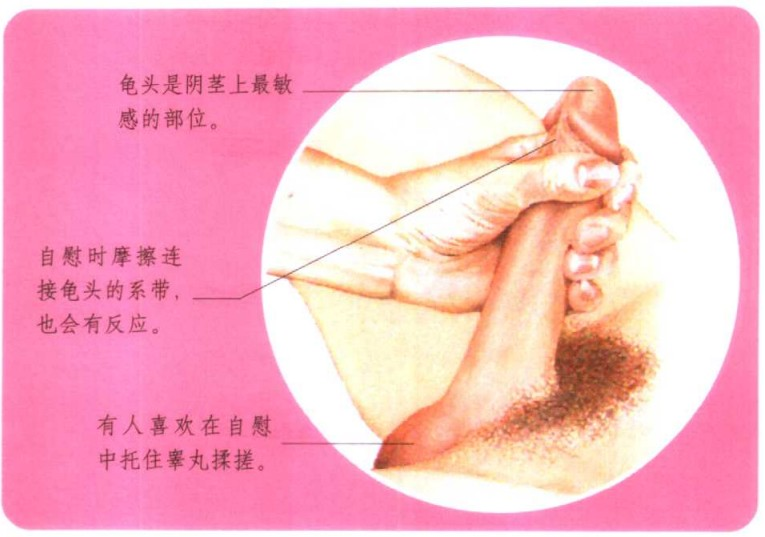
\includegraphics[width=0.8\textwidth]{male-masturbation.jpg}
  \caption{男性自慰}
  \label{fig:male-masturbation}
\end{figure}

女孩子和成年女性进行自慰的方法通常是用手指头按揉阴蒂，不过从《海特报告》一书看，女性自慰的方法也是五花八门的，有人是把指头或仿真阴茎塞进自己的阴道里，一边做动作一边揉搓阴蒂；有人使用震荡棒去触碰阴蒂，或者取下淋浴头用水流来冲击阴蒂；还有人利用枕头或床垫一类柔软的物体来揉搓阴部；也有人夹紧两腿，一阵阵用力以获得快感。有的女性在自慰时喜欢同时抚摩自己身上的某个部位，如乳房或肛门。

在自慰中男人和女人都会产生性幻想。在阅读性爱小说或观看里边有做爱镜头的电影时，人们的性欲会逐渐提升起来，这时刺激生殖器官就会使人产生性联想，随着这种刺激的加强和深入，性的愉悦感就会最终达到最高潮。

做爱时产生的各种生理反应，自慰时都会产生。男人的阴茎会勃起，阴茎口处还有可能流出分泌物。当性唤起的程度达到最高点时，精液就会射出来。女人自慰时阴道里会分泌出润滑液，阴蒂和阴唇会充血。这时候如果能对阴蒂施加充分的刺激，女性就会达到性高潮。

过去曾有这样一种说法，认为自慰会破坏一个人享受做爱乐趣的能力。也就是说，当一个人依赖于自慰来获得性愉悦时，他或她就会对两个人的做爱兴趣全无。当今的大多数性治疗专家都不同意这种说法，他们认为自慰能够帮助人们更好地了解自己的性能力。当一个人对自己身体上的隐秘处有了充分的探索和了解后，他就很轻松地将自己的性要求传达给对方，这样自然能获得更大的性愉悦。

\subsection{共同自慰}

人们经常把自慰当成做爱的前奏曲，或者是不能做爱时退而求其次的选择。出于这样的目的，既可以由一方刺激另一方的生殖器官达到性高潮，也可以两个人同时进行相互刺激。当两个人不需要有实质性的插入时，相互自慰就会成为很不错的选择。

这类自慰可以借助手指头、震荡器、仿真阴茎以及其他助兴用品进行。两个人可以把自己最喜欢的抚摩方式告诉给对方，还可以通过观看对方自慰来了解他或她需要什么。在探讨自慰以及获得性愉悦的方式时，很多人会感到忸怩不安。让女人当着男人的面刺激自己的阴蒂，更会令她们勉为其难。然而，一旦这种矜持和不安感得到克服，人们就会发现自慰原来如此美妙，简直可以与做爱相媲美。

\subsection{一边做爱一边自慰}

医学专家认为，对于女人来说，即使做爱仍在进行，也不妨碍她自慰。性治疗专家对这种方法十分推崇，有些女人单纯靠阴茎插入获得不了性高潮，有些女人则希望性高潮来得更快些，对于她们而言，边做爱边自慰的方法就很值得一试。

在做爱过程中如果能采用某种体位，也会使自慰来得更容易一些。比如，采用男上女下式时，要想刺激阴蒂就变得很难，而采用女上男下式或后插式，阴蒂刺激就容易多了。还有很多体位都允许男人一边做爱，一边腾出一只手来刺激女方的阴蒂。

做爱结束后，如果有一方还没有达到性高潮（通常是女方），或者还想体验一次性高潮，这时候自慰就有了用武之地。有时候男方早早就射精了，使得做爱草草收兵，而女方还没有达到性高潮，这时候自慰就会恰到好处地帮个大忙。

有人认为不应该让自慰进入到做爱之中，它的出现是对做爱本质的粗暴践踏，做爱所带来的性刺激是互相的给予和接受，而自慰所提供的性刺激却是单向的。与之相反的意见则认为，技巧本身并没有错，既然一边做爱一边自慰能提升性欲，那就不失为一个好办法。


\section{性反应的个体差异与常见问题}
% ⇒ [r81 并入] 自旧区
% 来源：book.tex 原 Ch2 §6703-6876 等

人类的性反应存在显著的\textbf{个体差异}，这种差异不仅存在于不同个体之间，也存在于同一个体在不同时期、不同情境下的反应中。理解这些差异有助于减少不必要的焦虑和自我怀疑。


理解"个体差异"的关键，是把它与"功能障碍"区分开。判断某种反应模式是否属于问题，通常看三条：是否\textbf{持续存在}（多数情况下出现，而非偶发一两次）、是否\textbf{造成本人或伴侣的显著困扰}、是否与\textbf{既往的自己相比}发生了明确变化。三条都不满足时，更可能是正常范围内的差异，而不是需要"矫正"的异常。

另一条常被忽视的事实是：性反应并不是每次都必须走完的固定曲线。兴奋、平台、高潮、消退这四个阶段是研究模型，而不是合格标准——没有高潮的性行为仍然可能是令人满意的，这一点在女性身上尤其常见。把模型当成绩单，本身就是性焦虑最常见的来源之一。

\subsection{性反应个体差异的来源}

\begin{itemize}
	\item \textbf{生理因素}：激素水平（睾酮、雌激素、甲状腺激素）、神经敏感性、心血管健康状况、基因差异（如多巴胺受体 D4 基因多态性与性欲强度相关）等均影响性反应。
	\item \textbf{心理因素}：情绪状态、压力水平、性自尊、性知识和过往性经验均影响性反应的强度和速度。焦虑和抑郁是性反应最常见的心理抑制因素。
	\item \textbf{关系因素}：伴侣间的情感亲密度、信任感、沟通质量和性技巧默契度显著影响性反应。关系冲突是性功能障碍的重要诱因。
	\item \textbf{情境因素}：环境的私密性、安全性、氛围营造以及时间和精力的充裕程度均影响性反应质量。
\end{itemize}

\subsection{常见问题}

\begin{itemize}
	\item \textbf{性反应速度差异}：不同个体从性唤起到性高潮所需的时间差异很大——男性通常较快（平均 4--7 分钟），女性通常较慢（平均 10--20 分钟），但个体间变异很大。这种差异是\textbf{正常的}，不必强求同步。
	\item \textbf{性欲差异}：伴侣间性欲频率不一致（\textbf{性欲差异，desire discrepancy}）是最常见的性问题之一。处理方法包括坦诚沟通、寻找折中频率、探索非性交亲密方式以及避免将性欲差异归因于"不爱"。
	\item \textbf{性高潮获得差异}：约 70\%--80\% 的女性需要\textbf{阴蒂刺激}（而非单纯阴道插入）才能达到性高潮，这是正常的生理现象，不反映"功能障碍"。
	\item \textbf{年龄相关的变化}：随年龄增长，性反应速度通常放缓（勃起需要更长时间、阴道润滑需要更长时间），性高潮强度可能减弱，但性满意度和亲密感可随关系深化而提升。
\end{itemize}

\begin{tcolorbox}[colback=pink!5!white,colframe=red!50!black,title=核心观念]
性反应的"正常"范围非常宽泛。\textbf{没有"标准"的性反应模式}——只要个体对自己的性反应感到满意，且不造成痛苦或功能损害，就属于正常。将性反应与"标准"或"他人"比较往往带来不必要的焦虑。
\end{tcolorbox}


\section{影响性反应的因素与延长技巧}
% ⇒ [r81 并入] 自旧区
% 来源：book.tex 原 Ch2 §6662-6778 等

多种因素可增强或抑制性反应，了解这些因素有助于优化性体验和延长性愉悦时间。

\subsection{增强性反应的因素}

\begin{itemize}
	\item \textbf{充分的唤起时间}：特别是对女性而言，给予充分的前戏时间（15--20 分钟以上）有助于阴道充分润滑和盆底肌肉放松，提升性体验。
	\item \textbf{情感连接}：情感亲密和信任是最佳"催情剂"，催产素（oxytocin）在亲密接触中释放，增强性唤起和性满意度。
	\item \textbf{身心健康}：规律运动（改善心血管功能和体像）、充足睡眠、压力管理和均衡饮食均有利于性反应。
	\item \textbf{新颖感}：在长期关系中，适当引入新颖元素（新环境、新体位、新玩法）可对抗性反应的"习惯化"。
\end{itemize}

\subsection{延长性愉悦的技巧}

\begin{itemize}
	\item \textbf{控制射精（男性）}：
	\begin{itemize}
		\item \textbf{停-起技术（stop-start）}：在即将射精前暂停刺激，待唤起感降低后恢复，反复数次后再射精。
		\item \textbf{挤压技术（squeeze）}：在即将射精时，用手指挤压阴茎冠状沟下方 3--4 秒，抑制射精反射。
		\item \textbf{盆底肌训练（Kegel）}：增强球海绵体肌的自主控制力，有助于延迟射精。
		\item \textbf{深呼吸和放松}：紧张和焦虑加速射精，深慢呼吸有助于延长。
	\end{itemize}
	\item \textbf{延长唤起（女性和男性通用）}：
	\begin{itemize}
		\item \textbf{分散注意力}：在接近高潮时适度分散注意力（如数数、想无关事物），可延长平台期。
		\item \textbf{变换刺激强度}：在高强度刺激和低强度刺激间交替，避免持续高强度导致过快到达高潮。
		\item \textbf{改变体位}：变换体位可短暂"重启"唤起过程，同时增加新鲜感。
	\end{itemize}
\end{itemize}

\noindent\textit{【编者注】}延长性愉悦时间不应成为"表现压力"。性活动的目的是双方的情感连接和愉悦，而非时间的竞赛。\textbf{质量远比时长重要}——10 分钟高质量的亲密接触可能优于 30 分钟的机械运动。


\section{性交时长、频率与"正常"的标准}
% ⇒ [r81 并入] 自旧区
"我是不是太快了？""一周几次才正常？"——这是性咨询中最常见的两个问题，而它们的答案可能出乎意料：\textbf{没有统一标准，也不该有}。

\noindent\textbf{关于时长}：
\begin{itemize}
	\item 多项国际研究显示，从插入到射精的\textbf{中位时长约为 5--7 分钟}（不同研究给出的范围大致在 3--13 分钟之间）；
	\item 加上前戏，一次性活动通常持续 15--30 分钟甚至更久，个体差异极大；
	\item 许多人以为"半小时以上才算正常"，这多半是受影视或色情作品影响——那是表演，不是平均水平；
	\item 关键不在分钟数，而在\textbf{双方是否满意、是否有困扰}。若一方感到疼痛、疲惫或未被满足，再长的时长也算不上"好"。
\end{itemize}

\noindent\textbf{关于频率}：
\begin{itemize}
	\item 所谓"平均每周 1--2 次"只是统计上的中位数，\textbf{不是健康指标，更不是及格线}；
	\item 性满意度与频率并非线性关系——有人每周数次依然满足，有人每月一两次也其乐融融；
	\item 影响频率的因素众多：年龄、健康状况、压力与情绪、关系质量、激素水平、用药、育儿与工作负荷。频率的起伏本身很正常；
	\item 真正需要留意的是\textbf{变化}：若频率或欲望出现突然、持续的显著下降，并伴随痛苦或关系冲突，才值得就医或咨询。
\end{itemize}

\begin{tcolorbox}[colback=pink!5!white,colframe=red!50!black,title=贴心小叮咛]
不要拿"统计数字"或"别人的经验"来丈量自己的性生活。所谓"正常"，只有一种定义——\textbf{你们双方都感到舒适、满意、不被勉强}。这一点，只能由你们两个人共同商定。
\end{tcolorbox}


\section{梦交（Nocturnal Sexual Dreams）的正常与异常}
% ⇒ [r81 并入] 自旧区
\noindent\textit{【编者注】}"梦交"是指入睡后梦见与异性发生性关系并伴随性兴奋或性高潮的现象。男性常伴遗精（俗称"梦遗"），女性亦可出现梦中性高潮。这是正常的生理心理现象，不属于疾病范畴。


从生理机制看，梦交与快速眼动睡眠期（REM）的生理唤起直接相关——此期血流普遍集中于盆腔，男性伴勃起、女性伴阴部充血，遇上相关梦境便可能完整触发性反应。它的频率随年龄与性生活状态波动：青年期、性生活稀疏期更常见，均属正常。历史上"梦遗伤精""一滴精十滴血"的说法并无科学依据，精液的生成是持续性的，梦遗的"损失"与正常射精没有区别。需要留意的只有两种情形：因频繁遗精影响睡眠与日间状态，或伴随明显的焦虑抑郁情绪——前者可就诊排查生殖道炎症，后者更适合从压力与心理层面入手，而非服用"固精"补品。

\subsection{什么是梦交}

梦交是指生理已成熟的男女夜间入睡后梦见与异性发生性关系并从中获得性满足的现象。

\textbf{为什么会做这样的梦？}

俗话说的"日有所思，夜有所梦"在此尤为贴切。当一个人对异性产生强烈的情感或欲望时——比如白天见到心仪的对象，或与恋人亲密接触却无法进一步——大脑皮层会持续处于兴奋状态。白天这种冲动受意识和理智的控制而被抑制，但到了夜间入睡后，大脑对潜意识活动的控制减弱，被压抑的性冲动便可能以梦境的形式释放出来。

\subsection{常见场景}

\underline{未婚青年的性好奇}：

生理已发育成熟但因无性伴侣而无法实现性行为的青年，对异性充满好奇和向往。白天的想象和渴望若久久不能平静，夜间便容易以梦交的形式获得替代性的满足。

\underline{热恋中的准夫妻}：

男女关系已明朗化、为周围公认，形影不离、热烈亲吻拥抱，有强烈的性欲望——这是感情发展到一定程度的自然生理本能。但由于尚未正式结婚或同居，现实中不能发生性关系。白天的克制在夜晚松弛后转化为梦境释放。\textbf{许多即将结婚的青年男女都会经历这一阶段}。

\underline{已婚者的特殊时期}：

\begin{itemize}
	\item 一方因生育、工作等原因对性生活兴趣下降，另一方需求得不到满足
	\item 夫妻因出差、出国等暂时分离，思念之情引发梦中相会
	\item 这种情况下，梦交是性能量的一种自然宣泄途径
\end{itemize}

\subsection{文化视角：《红楼梦》中的梦交}

《红楼梦》第五回写道：贾宝玉去秦可卿房内休息，梦见警幻仙子将其妹可卿许配与他，"恍恍惚惚……未免作起儿女事来……"，醒来后发现大腿处"冰冷黏湿一片"。秦可卿是贾宝玉的堂侄媳，按辈分和礼教，清醒状态下绝不可能发生的事，在梦中却不受伦理道德约束——这生动说明了梦的本质：\textbf{潜意识冲动的自由表达}。


《红楼梦》中有不止一处与"梦"相关的性描写：贾宝玉梦游太虚幻境、与警幻仙子之妹"兼美"成婚，醒后遗精；后世读者对秦可卿与宝玉关系的揣测；以及贾瑞被王熙凤设局、最终在镜中与幻影纠缠至死。这些段落把\textbf{性欲写成需要疏导而非压抑的力量}：宝玉的梦交是青春性意识的自然萌发，贾瑞的则是失去约束的欲望与自我欺骗。曹雪芹的写法带有释道的"色空"观，却也有相当现代的观察——\textbf{幻想内容与道德评价并不等同}。

\subsection{如何正确看待}

首先应明确：在性器官已发育成熟的个体中，出现梦交现象是\textbf{完全正常}的生理心理表现。

无论男性或女性，适度的梦交可以获得某种程度的性满足，从而缓解现实生活中的性意识压力，只要正确对待并不妨碍正常的生活、工作和学习。

一般而言，每月出现3次以内的梦交属正常范围，不必惊慌。

\subsection{减少不必要困扰的建议}

如果梦交频率较高且造成困扰，可以尝试以下调整：
\begin{itemize}
	\item 避免睡前接触刺激性内容（色情影视、小说）
	\item 睡前穿着宽松透气的睡衣，避免紧身衣物对生殖器的摩擦刺激
	\item 入睡前排空膀胱
	\item 被子不宜过重过厚，减少对下身的压迫感
	\item 保持规律作息和适度运动
\end{itemize}

\begin{tcolorbox}[colback=pink!5!white,colframe=red!50!black,title=贴心小叮咛]
对于已婚者而言，梦交频率过高有时反映了\textbf{夫妻性生活的不协调}。丈夫应耐心热情对待妻子，切忌粗鲁；妻子也应坦诚沟通自己的感受和困扰。\textbf{夫妻之间应建立开放的性沟通}，共同面对性欲低下、性恐惧等问题。必要时一同寻求专业心理咨询或性治疗师的指导，而非盲目四处求医问药。
\end{tcolorbox}




\section{自慰}
% ⇒ [r81 并入] 自旧区
% 来源：book.tex 原 Ch2 §7246-7396

\subsection{普遍性与历史}

\noindent\textit{【编者注】}自慰（masturbation）是人类最普遍的性行为之一，也是性医学和性心理学研究的重要主题。本节讨论其普遍性、历史观念演变及性别差异。

\noindent\textbf{一、有多普遍？}

国外统计资料表明：约 $80\%$--$90\%$ 的男性和 $50\%$--$60\%$ 的女性有过自慰史。另有报告显示大约 $96\%$ 的男性曾有过自慰经历——而且\textbf{受教育程度越高的人，自慰比例越高}（因为他们不太担心自慰会危害健康）。

\noindent\textbf{二、性别差异}

\begin{itemize}
	\item \textbf{方式差异}：女性想象力丰富、感情细腻→自慰花样比男性多；男性的方式相对单调呆板
	\item \textbf{时间差异}：由于女性性发育比男性提前 $1$--$2$ 年，女性的自慰起始时间平均比男性早；但女性自慰比例低于男性
	\item \textbf{频率与强度}：女性每次自慰时间比男性长，但频率不如男性频繁；然而女性每次自慰的程度往往更深
	\item \textbf{心理负担差异}：
	\begin{itemize}
		\item 男性：常伴射精→事后乏力倦意 + 传统"精液宝贵""一滴血十滴精"的观念 → \textbf{精神负担重}
		\item 女性：事后相对不易疲乏、无"丢失感" → 负担较轻
	\end{itemize}
	\item \textbf{特殊风险差异}：阴道开口浅大且与子宫相通——女性自慰时借助的物品易损伤组织或带入病菌导致感染；不慎将异物掉入阴道/膀胱内难以取出；可能捅破处女膜给婚姻带来误解
\end{itemize}

\noindent\textbf{三、历史观念的演变 —— 两个多世纪的争论}

关于自慰是否有害的问题已经讨论了两个多世纪：

\begin{center}\small
\begin{tabular}{|p{3cm}|p{10cm}|}
\hline
\textbf{时期/立场} & \textbf{核心观点} \\
\hline
古代传统 & 精液是"天地之精气"，排出丧元气 → "肾亏"说 \\
18--19世纪西方 & Tissot（1758）提出自慰致病论 → 视为精神疾病/道德败坏 \\
20世纪中叶 & Kinsey 报告（1948/1953）揭示高普遍性 → 去病理化开始 \\
现代医学共识 & 自慰本身无害；正常生理活动；合理性宣泄手段 \\
\hline
\end{tabular}
\end{center}

\begin{itemize}
	\item DSM-5（2013）已完全移除"自慰障碍"的诊断类别——仅在"其他特定的性功能障碍"中保留了"过度自慰 causing significant distress"作为残留选项，表明主流精神医学已将其去病理化。
	\item WHO ICD-11 同样不再将自慰列为独立疾病。
	\item 大规模流行病学调查（如 NHSLS、NSSHB）一致显示：自慰频率与总体性满意度呈正相关，与 ED/早泄等性功能障碍风险呈负相关（控制混杂因素后）。
	\item 女性自慰与更高的自我身体形象认同、更好的性沟通能力以及更容易达到性高潮的能力相关。
\end{itemize}

\subsection{生理机制}

\noindent\textit{【编者注】}本节从定义和发生机制角度阐述自慰——尤其聚焦于青春期这一高发阶段。

\noindent\textbf{一、什么是自慰？}

凡是为了获得性满足，用任何方式（手或借助其他工具）自我或相互玩弄生殖器的行为，称之为自慰（masturbation）。它是一种自慰行为，每次往往要达到性高潮后才停止：
\begin{itemize}
	\item 男性：表现为射精
	\item 女性：表现为阴道润滑、分泌物流出等
\end{itemize}

\noindent\textbf{二、为什么青春期最容易产生自慰？}

青春期男女随着性腺功能逐渐成熟，一系列生理和心理变化同时发生——为自慰的发生提供了"土壤"：

\begin{enumerate}
	\item \textbf{性征发育}：
	\begin{itemize}
		\item 男性：出现遗精、胡须生长、阴毛长出
		\item 女性：月经来潮、乳房突起、骨盆变宽、声音甜润
	\end{itemize}

	\item \textbf{心理觉醒}：
	开始对异性产生好感和爱慕，探索与自身相对的"神秘王国"，产生性的需求和性冲动。

	\item \textbf{激素驱动}：性激素水平显著增加 → 性驱力（libido）增强

	\item \textbf{外部刺激}：耳濡目染地接受各种形式的色情内容刺激（影视、网络、文学作品等）→ 性交欲望越来越强烈

	\item \textbf{现实约束}：然而社会规范、道德教育和法律都无法满足青春期少年对性行为的需求
\end{enumerate}

在这种"强烈的内在驱动力 + 外部刺激 + 现实无法通过正常途径释放"的矛盾下，\textbf{近乎本能地出现了自慰行为}。他们往往用各种方式刺激生殖器官以求获得性的满足。

\noindent\textbf{三、自慰行为的常见启动方式}

大多数人开始自慰的路径有以下几种：

\begin{itemize}
	\item \textbf{好奇心驱动}：在性好奇心的驱使下尝试
	\item \textbf{偶然发现}：某个偶然动作刺激了生殖器官，获得了从未体验过的快感→想重温那美妙时刻→一发不可收拾
	\item \textbf{同伴影响}：在"大孩子"的教唆/示范下学会并成"瘾"
\end{itemize}

不管以何种方式开始，都有一个共同的主观原因：\textbf{青春男女对性的渴望}。

\noindent\textbf{四、婚后的自然消退}

通常在婚后有了固定的性伴侣、可以正常进行性交后，不再需要自慰来满足性需求——此时自慰便会自然减少或停止。

当然例外情况也存在：如果夫妻之间存在较大的性差异（如一方性欲明显强于另一方而彼此无法充分满足），仍可能出现以自慰弥补不足的情况。

\noindent\textit{【编者注（补充说明）】}
\begin{itemize}
	\item 青春期是自慰发生率最高的生命阶段——这与睾酮/雌激素水平在青春期达到峰值密切相关（男性血清总睾酮在 $18$--$25$ 岁达最高）。
	\item 从神经生物学角度看，青春期的前额叶皮层（负责冲动控制和决策判断的脑区）尚未完全成熟（约 $25$ 岁左右才完成髓鞘化），而边缘系统（负责情绪和奖赏）已高度活跃——这种"\textbf{发育不同步}"使青少年更难抑制性冲动。
	\item \textbf{夫妻间的相互自慰}是性生活的健康组成部分和良好补充，不必心存芥蒂——这在前面的"安全与健康的自慰实践"中已提及，此处再次强调。
\end{itemize}

\subsection{心理意义}

\begin{enumerate}
	\item \textbf{自我探索与身体认知}：自慰是人认识自己身体的第一条途径。通过自慰，青少年逐渐了解自身的敏感区域、兴奋规律与高潮反应，这种"身体地图"的确立，为日后向伴侣表达自己的性偏好、获得满意的性生活奠定了基础。

	\item \textbf{性张力的健康释放}：青春期性激素水平急剧升高，性冲动随之增强，而现实条件（学业、环境、社会规范）往往不允许通过性行为直接释放。自慰提供了一种\textbf{私密、安全、无伤害}的释放渠道，有助于缓解由此产生的焦虑与烦躁，本质上是一种自我调节机制。

	\item \textbf{身体自主权与自我愉悦}：自慰完全由自己掌控节奏与方式，不依赖他人、不受时间地点胁迫，是体验"性愉悦可以自主获得"的重要一课——这对树立健康的身体主权观念、避免将来在两性关系中一味迎合或过度索取，都有积极意义。

	\item \textbf{羞耻感的祛除}：受传统观念影响，不少青少年在自慰后产生自责、恐惧甚至"罪恶感"。现代性医学早已确认：自慰本身无害，真正有害的是伴随它的\textbf{羞耻与焦虑}。以科学态度正视它，是青春期性心理健康的重要一环。

	\item \textbf{对伴侣关系的补充意义}：婚后自慰虽多会自然减少，但在性欲不匹配、两地分居、孕产期等特殊阶段，适度的自慰（包括夫妻间相互自慰）仍是维系性健康的合理补充，并非对伴侣的背叛或"无能"的表现。
\end{enumerate}

\noindent\textit{【小结】}判断自慰是否"越界"，标准不在次数本身，而在于它是否\textbf{失控}（如强迫性地反复进行、无法自止）、是否\textbf{损害功能}（如只依赖特定方式才能兴奋，影响与真实伴侣的性互动）、是否\textbf{干扰生活}（如影响学业、工作与人际关系）。若出现上述情况，或伴随难以摆脱的罪恶感，建议寻求心理或性医学专业帮助——这同样属于"心理意义"的正视而非污名。

\subsection{健康影响与误区}

\noindent\textit{【编者注】}本节分两部分：（1）如何科学看待自慰；（2）过度自慰可能带来的不良表现。

\noindent\textbf{一、现代医学的科学立场}

现代医学认为：\textbf{自慰本身对身体和精神无害}。它是人类的一种正常生理活动，也是缓解因性紧张积累而引起不安和躁动的一种自慰方式——是一种自身合理的性宣泄手段。

有调查和实验结果证实：自慰不仅不会影响生育能力和性功能，而且是医学上\textbf{最广泛用于收集精液检查}以及作为勃起功能障碍、早泄等性功能障碍的治疗措施之一（如性感集中训练中的自慰环节）。

\noindent\textbf{二、吴阶平教授的四原则}

我国著名性医学专家\textbf{吴阶平教授}对自慰问题做过经典论述：

\begin{quote}
\small
"\textbf{对于自慰：不要以好奇去开始；也不以发生而烦恼；已成为习惯的要有克服的决心；克服以后不要再担心——这样不会有任何不良后果。}"
\end{quote}

这四句话概括了对待自慰的科学态度：预防→释然→决心→放下，形成一个完整的认知闭环。

\noindent\textbf{三、过度/频繁自慰的不良表现}

当然，过度、频繁的自慰也会对身体产生一定影响：

\begin{enumerate}
	\item \textbf{神经衰弱}：由于过度的性刺激和自慰本身带来的疑虑、悔恨等情绪，使中枢神经系统长期处于性兴奋—性忧虑—疲惫的状态，导致兴奋与抑制失调。大脑对机体的控制及对外界变化的适应能力下降，表现为：意志消沉、注意力不易集中、理解力和记忆力下降、头昏头痛、耳鸣心悸、失眠等。

	\item \textbf{慢性前列腺炎}：长期反复自慰使生殖器官经常处于充血状态，引起前列腺及盆腔慢性充血 $\rightarrow$ 久而久之形成慢性前列腺炎。

	\item \textbf{遗精、滑精、血精}：
	\begin{itemize}
		\item 过度自慰引起大脑兴奋过度→继发抑制加深→大脑控制能力下降→轻微性刺激即可引发射精→表现为遗精频繁和滑精
		\item 部分人婚后出现早泄；有的见到姿色艳丽的女性、公共场所无意碰撞甚至听见爱慕异性的声音都会出现滑精（注意：许多人流出的是前列腺液而非精液）
		\item 自慰过程中过猛用力可致生殖器损伤或局部抵抗力下降→盆腔充血→炎症（尤其是精囊炎）$\rightarrow$ \textbf{血精}
	\end{itemize}

	\item \textbf{性欲减退、勃起功能障碍、不育}——事物都有两面性：
	\begin{itemize}
		\item 频繁刺激阴茎使性兴奋阈值不断升高，勃起中枢和射精中枢也过度疲劳
		\item 婚后正常性刺激下阴茎勃起无力→甚至出现勃起功能障碍或性交不射精→不育
		\item \textbf{值得特别指出}：自慰导致的勃起功能障碍多半属于心理因素——主要因长期的焦虑和犯罪感所致
		\item 只要婚后及时纠正习惯、正确看待自慰、真正丢掉精神包袱、适当配以药物治疗→性功能能够恢复正常
	\end{itemize}
\end{enumerate}

\noindent\textit{【编者注（关键辨析）】}
\begin{itemize}
	\item 以上不良后果的发生机制往往是\textbf{"自慰本身 + 心理恐慌/焦虑 + 罪恶感的综合作用"}，而非单纯由自慰行为本身造成。多项对照研究表明：对自慰持中性/积极态度者即使频率相同，上述症状发生率也显著低于持负面态度者。
	\item \textbf{慢性前列腺炎与自慰的因果关系尚不完全明确}——目前证据更多支持"频繁射精→前列腺反复充血→炎症"这一路径，而非自慰直接感染。规律但不过度的射精活动（包括性交和自慰）反而有助于前列腺液的更新，可能对前列腺有一定保护作用（部分观察性研究的结论，尚需 RCT 证实）。
	\item \textbf{关于"伤精"的中医传统观念}："一滴血十滴精""自慰耗精伤髓"等说法源于古代中医对精液成分的认知局限。从现代医学角度看：每次射精的精液量约 $2$--$5$ ml，含蛋白质、果糖、酶类等，营养消耗极微——人体可在数小时内完全恢复合成。真正需要关注的是伴随的心理状态而非物质消耗。
\end{itemize}

\begin{tcolorbox}[colback=pink!5!white,colframe=red!50!black,title=贴心小叮咛]
不管男女两性在自慰方面的表现怎样不同，它们都是缓和性紧张状态的一种自慰行为。\textbf{偶尔为之未尝不可；过度了就会引起一系列不良后果——而引起这些后果的原因往往不是自慰本身，而是自慰带来的恐慌和焦虑}。
\end{tcolorbox}

\subsection{安全与健康的自慰实践}

\noindent\textit{【编者注】}对于希望减少或戒除自慰习惯的人，以下方法经过实践验证有效。

\noindent\textbf{为什么这么难改？}

几乎所有想改掉自慰习惯的人都在内心下定决心——但在性冲动来临时决心变得软弱无力。有人安慰自己"就这一次了，下不为例"，可每次"下不为例"都变成泡影。这种矛盾困境加重了精神负担，形成恶性循环。

\textbf{但这并非无法克服}——只要掌握好方法、有信心，就能够如愿以偿。

\noindent\textbf{方法一：树立坚定信念}

确信自慰完全可以戒掉的。要富有事业心，将注意力投入到学习和工作中去。同时掌握有关性知识，了解自慰的生理和心理机制、次数与危害的关系——使自己的精神保持舒畅愉快状态。

\noindent\textbf{方法二：养成良好的生活和卫生习惯}
\begin{itemize}
	\item 保持外阴部清洁，减少各种因素对性器官的刺激
	\item 及时治疗包茎、包皮过长、疥疮、股癣或阴道炎等局部病变
	\item 内裤不宜过紧，被褥不宜过暖
	\item 按时睡眠，不贪床
	\item \textbf{避免睡前诱因}：不看色情小说/视频、不在床上进行性幻想
\end{itemize}

\noindent\textbf{方法三：积极参加集体活动}

如打球、下棋、跳舞等文体活动。大胆地与异性交往以减少神秘感——但要尽量减少单独与异性接触的机会（尤其在游泳、爬山等户外活动中）。

\noindent\textbf{方法四：不要急于求成 —— 循序渐进法}

\begin{itemize}
	\item 根据实际情况制定具体方案：先慢慢减少自慰次数→逐渐中止→\textbf{实现"从量变到质变"}
	\item 如果突然咬牙发誓"再也不干了"→往往以失败告终→进而失去信心
	\item 排除不良干扰因素，持之以恒，避免半途而废
\end{itemize}

\noindent\textit{【编者注（补充建议）】}
\begin{itemize}
	\item \textbf{行为替代策略}：当冲动出现时立即转移注意力——做俯卧撑/冷水洗脸/出门快走/打电话给朋友聊天。核心原理是打断"冲动→行动"的条件反射链，建立新的神经回路（通常需 $21$--$66$ 天形成新习惯）。
	\item \textbf{环境改造}：将手机/电脑设置为过滤成人内容模式；卧室不放刺激性读物/图片；睡前固定阅读非刺激性书籍帮助入睡。
	\item \textbf{正念接纳}（mindful acceptance）：与其强行压抑（反弹效应更强），不如学会"观察冲动而不付诸行动"——承认冲动的存在但不评判自己，让冲动像云一样自然飘散。CBT 中的"冲浪技术"（urge surfing）对此非常有效。
	\item 如果以上自助措施效果不佳且已严重影响生活质量（如回避社交、严重内疚抑郁），建议寻求专业心理帮助——\textbf{强迫性性行为（compulsive sexual behavior, CSB）}在 ICD-11 中已被纳入"冲动控制障碍"范畴，可通过心理治疗（CBT / 接纳承诺疗法 ACT）获得改善。
\end{itemize}

\begin{tcolorbox}[colback=pink!5!white,colframe=red!50!black,title=贴心小叮咛]
睡觉时内裤不要穿得过紧，被子不要盖得太厚太重，不要俯卧睡。早晨醒来后不要过分依恋床榻。\textbf{戒除自慰要顺其自然，不要有任何心理压力}——必要时可找心理医生咨询。记住：目标不是"永远不自慰"，而是建立与性冲动之间的健康关系，让它不再控制你的生活。
\end{tcolorbox}

\subsection{自慰与性教育}

\noindent\textit{【编者注】}性教育不仅关乎生理知识的传递，更包括健康人际关系的建立。本节聚焦于青春期青少年与异性交往的原则和方法——这是性教育中至关重要的一环。

\noindent\textbf{一、交往方式：集体交往优于单独交往}

青少年男女以\textbf{集体交往}为宜：
\begin{itemize}
	\item 课堂上的讨论发言、课后的议论说笑、课外的游戏活动等，为大家创造了与异性交往的自然机会
	\item 集体交往的好处：
	\begin{itemize}
		\item 性格内向、不善交际的同学可免除独自面对异性的羞涩和困窘
		\item 喜欢交际的同学可获得与人交往需求的满足
		\item 每个人融入集体气氛中——面对的是一群各有所长的异性（幽默健谈/聪明善良/乐观大度/稳重干练……）
		\item 在吸收众人优点的同时开阔眼界和心胸
		\item \textbf{避免只盯住某一位异性而发展为"一对一"的恋爱关系}
	\end{itemize}
	\item 集体交往的形式：兴趣小组、科技小组、学习小组
	\item 集体活动内容：娱乐、游戏、竞赛、旅行、小发明、小制作等
	\item 家长放心，老师支持
\end{itemize}

\noindent\textbf{二、把握交往的尺度 —— 核心原则}：

对方约你一同参加某项活动（听音乐、看电影、观画展、逛书市）→ 这是正常、公开场合的两性交往 → 完全可以大方赴约。
\begin{itemize}
	\item \textbf{女生}：应端庄、坦荡、不使对方产生误解和非分之想
	\item \textbf{男生}：要沉稳、庄重、尊重对方
\end{itemize}

若两人互有好感、相处愉快 → 约会次数增多、时间延长 → 直到难分难舍……此时必须\textbf{适可而止}：

\begin{enumerate}
	\item 不能占用对方太多时间
	\item 不能因约会导致一方或双方无法集中精力学习
	\item 不能因此无暇与家人、同学、亲友相聚
	\item \textbf{必须有所节制}：减少单独在一起的次数和时间；见面时多谈学习上的事情以降温感情
\end{enumerate}

对于以谈情说爱为目的的约会 → 最好婉言谢绝，让对方明白你的心思并放弃追求。\textbf{注意方式方法，不可伤害对方自尊心}。对于纠缠不休甚至威逼诱吓的人 → 请家长、老师、同学和朋友们协助处理。

\noindent\textbf{三、友情 vs 爱情 —— 界限意识}

由于性意识的觉醒，青少年对异性产生好奇、关心、爱慕和愿意接近的心理与行为都属于\textbf{正常现象}——家长不必大惊小怪或粗暴干涉。

但也应提醒孩子明确一个关键区分：
\begin{center}
\fbox{\parbox{0.8\textwidth}{\centering
\textbf{友情姓"友"} —— 朋友之间的友好交往 \\
\textbf{爱情姓"爱"} —— 自己和所爱者之间的心心相印 \\
}}
\end{center}

当感到对方具有强烈吸引力、产生愿意时刻与之在一起的热望时——就应该引起注意，\textbf{千万别越出友谊的界限，跨入早恋的误区}。

\noindent\textit{【编者注（现代性教育视角）】}
\begin{itemize}
	\item 国际公认的\textbf{综合性性教育（CSE, Comprehensive Sexuality Education）}框架（UNESCO 2018 修订版）将人际关系技能列为六大核心学习领域之一，强调从小学阶段起就应培养健康的同伴交往能力——这比等到青春期再进行"补救式"教育更为有效。
	\item "集体交往优于单独交往"的建议符合发展心理学中关于青少年群体社会化功能的经典理论。但需注意：完全禁止一对一异性接触可能反而不利于青少年建立正常的亲密关系能力——关键是保持\textbf{"公开透明 + 有节制"}的原则，而非绝对禁止。
	\item 关于"早恋"的概念本身在学术界存在争议。现代青少年心理学更多采用"\textbf{青少年浪漫关系（adolescent romantic relationship）}"这一中性术语，关注点从"是否允许"转向"如何引导其健康发展"——包括沟通技巧、边界设定、拒绝不安全性行为的能力培养等。
	\item 对于已进入恋爱关系的青少年，简单粗暴地"棒打鸳鸯"往往适得其反——研究显示被强行拆散的情侣更容易出现逆反行为、学业下降甚至意外怀孕。更有效的做法是开放式沟通 + 安全性行为教育 + 学业目标引导。
\end{itemize}

\begin{tcolorbox}[colback=pink!5!white,colframe=red!50!black,title=贴心小叮咛]
异性同学间的交往是完全正常的社交活动，但一定不要一门心思地钻在里面。男女同学有性别之差，人的潜意识往往在与异性的交往中被发掘出来。\textbf{过于频繁地与异性交往会唤起热情、激起冲动}——所以交往频率要适当低一些，这样有利于青少年的健康成长。记住：友情和爱情之间有一条清晰的界限，学会守住这条界限，是成熟的第一步。
\end{tcolorbox}


\section{性生理反应}
% ⇒ [r81 并入] 自旧区
\subsection{兴奋期}
\subsubsection{兴奋期的心理特征}

兴奋期不仅伴随着生理变化，还伴随着复杂的心理变化：

\begin{itemize}
\item 性欲望的唤醒：对性刺激产生积极反应，渴望进一步的性接触
\item 注意力高度集中：注意力集中在性伴侣和性刺激上，忽略周围环境
\item 情绪愉悦：感到兴奋、期待和愉悦
\item 自我意识减弱：身体感觉增强，自我意识暂时减弱
\item 情感连接增强：与性伴侣的情感连接开始建立或加深
\end{itemize}

理解兴奋期的生理和心理变化，有助于个体更好地把握性活动的节奏，提高性体验的满意度。

\subsection{平台期}

平台期是性生理反应的第二阶段，是兴奋期的延续和增强，也是性高潮前的关键阶段。这一阶段的持续时间因人而异，一般为30秒至数分钟，也可能持续更长时间，取决于个体的性反应模式和性刺激的强度。在平台期，性兴奋达到了较高的水平，但尚未达到高潮，性紧张感不断积累，为高潮的到来做准备。


平台期是高潮前的高原阶段，生殖器充血与肌紧张达到接近峰值并保持数十秒到数分钟甚至更久。此期如果刺激中断，反应可回落至兴奋期水平，之后仍可能重新积累；\textbf{这也解释了为什么"停下来"通常不会造成伤害，只会让过程重新开始}。对男性而言，此期接近射精不可逆点之前，正是停-开法与挤压法训练的窗口。

\subsubsection{男性平台期的生理变化}

\begin{itemize}
\item \textbf{阴茎进一步勃起}：阴茎的硬度达到最大（四级勃起），龟头颜色变深（呈紫红色），龟头冠边缘更加明显。
\item \textbf{睾丸变化}：睾丸进一步上提，紧贴于耻骨联合下方，体积增大50-100\%，这是由于睾丸内血管充血和精子的积累引起的。
\item \textbf{尿道口分泌物}：尿道球腺分泌少量清亮的液体（又称"预射液"），从尿道口流出，起到润滑尿道和龟头的作用，为射精做好准备。这些液体中可能含有少量精子（约10-1000个），因此即使没有射精，也有可能导致怀孕，这是"体外射精"避孕方法失败率较高的原因之一。
\item \textbf{生殖器官紧张度增加}：前列腺、精囊腺等生殖器官的肌肉紧张度增加，为射精过程做准备。
\item \textbf{肌肉紧张}：全身肌肉紧张度明显增加，尤其是臀部、大腿、腹部和会阴的肌肉，形成强烈的肌肉张力。
\item \textbf{全身生理变化}：心率（可增加到100-130次/分钟）、血压（收缩压可升高20-40mmHg，舒张压可升高10-20mmHg）和呼吸频率进一步增加，面部和胸部的红晕更加明显，可能出现出汗现象。
\end{itemize}

\subsubsection{女性平台期的生理变化}

\begin{itemize}
\item \textbf{阴蒂变化}：阴蒂退缩到阴蒂包皮内，形成"阴蒂头"，但仍高度敏感。这种退缩是一种自我保护机制，防止在性交过程中过度刺激阴蒂引起不适。
\item \textbf{阴唇变化}：小阴唇继续充血肿胀，颜色进一步加深（可变为深紫色），体积增大到极限；大阴唇也充血肿胀，向外扩张，为阴道口提供更多的保护和刺激。
\item \textbf{阴道变化}：阴道上部继续扩张，容积达到最大；阴道下部（外1/3）的肌肉强烈收缩，形成"高潮平台"，直径可缩小50\%，增加对阴茎的紧握感，这种紧握感对男性的性刺激非常重要。
\item \textbf{子宫变化}：子宫进一步充血、增大，并向上提升，子宫颈也向上提升，与子宫体形成约90度的角度，这种变化有助于精子的通过和防止精液流出。
\item \textbf{乳房变化}：乳房继续增大，乳头勃起更加明显，乳晕肿胀，乳房表面的静脉更加清晰可见，乳房的敏感性增加。
\item \textbf{全身生理变化}：心率、血压和呼吸频率进一步增加，肌肉紧张度明显增加，面部和胸部的红晕扩展到颈部和背部，可能出现出汗现象。
\end{itemize}

\subsubsection{平台期的心理特征}

平台期的心理变化比兴奋期更加复杂和强烈：

\begin{itemize}
\item 性紧张感增强：性兴奋不断积累，紧张感逐渐增加，达到高潮前的临界状态
\item 愉悦感深化：身体和心理的愉悦感不断深化，达到高度的兴奋状态
\item 控制感变化：男性可能感到射精的控制感逐渐减弱，进入"射精不可避免期"；女性可能感到高潮即将到来，体验到强烈的性渴望
\item 情感连接增强：与性伴侣的情感连接更加紧密，达到高度的亲密状态
\item 注意力高度集中：注意力完全集中在性体验上，对外界刺激几乎没有反应
\item 时间感知变化：对时间的感知可能发生变化，感到时间过得很慢或很快
\end{itemize}

\subsubsection{平台期的性反应机制}

平台期是性高潮前的关键阶段，其生理机制与神经内分泌系统的激活密切相关：

\begin{itemize}
\item 神经系统：大脑的边缘系统和下丘脑进一步激活，释放更多的神经递质（如多巴胺、去甲肾上腺素），增强性兴奋
\item 内分泌系统：垂体前叶释放更多的促性腺激素（如黄体生成素），促进睾酮和雌激素的分泌，增强性反应
\item 肌肉系统：交感神经系统的激活导致肌肉紧张度增加，为高潮的肌肉收缩做准备
\item 循环系统：心率和血压进一步升高，为生殖器官提供更多的血液供应
\end{itemize}

理解平台期的生理和心理变化，有助于个体更好地控制自己的性反应，延长性体验的时间，提高性体验的满意度。例如，通过控制性刺激的强度和节奏，可以延长平台期的持续时间，增加性高潮的强度。

\subsection{高潮期}

高潮期是性生理反应的第三阶段，是性兴奋的顶峰，也是性体验中最强烈、最愉悦的阶段。这一阶段的持续时间最短，一般为几秒至十几秒，但带来的生理和心理体验却最为深刻。在高潮期，身体会发生一系列强烈的收缩和释放，将平台期积累的性紧张感彻底释放。


高潮期以盆腔肌肉的节律性收缩为标志：女性阴道外三分之一与子宫可出现数次至十余次收缩，男性则以射精为典型表现（射精与高潮在神经层面是两件事，可以分离）。主观体验从全身紧绷到释放、呼吸急促、短暂的方向感缺失都可能出现。\textbf{高潮并不总是必须，也不总是可预测}；把它当作体验的一部分而非考核指标，往往更容易达到。

\subsubsection{男性高潮期的生理变化}

\begin{itemize}
\item \textbf{射精过程}：这是男性高潮的主要表现，分为两个连续的阶段：
  \begin{itemize}
  \item \textbf{射精不可避免期}：这是高潮的开始，男性感到射精即将发生，无法控制。此时，精液从输精管、精囊腺和前列腺流入尿道，会阴部肌肉开始收缩，尿道内括约肌关闭，防止精液逆流进入膀胱。
  \item \textbf{射精期}：尿道周围的肌肉（球海绵体肌和坐骨海绵体肌）和会阴部的肌肉发生节律性收缩（通常为3-8次），每次收缩间隔约0.8秒，将精液从尿道射出。最初的几次收缩最强烈，射出的精液量最多，随后收缩逐渐减弱，精液量也减少。
  \end{itemize}
\item \textbf{阴茎变化}：阴茎在射精过程中会有节律性的收缩，与会阴部肌肉的收缩同步，帮助精液射出。阴茎的勃起硬度在高潮期达到最大，随后开始逐渐减弱。
\item \textbf{生殖器官变化}：前列腺、精囊腺等生殖器官也会发生收缩，将其分泌物排入尿道，与精子混合形成精液。
\item \textbf{全身肌肉收缩}：全身肌肉发生强烈的节律性收缩，尤其是臀部、大腿、腹部和背部的肌肉，可能会出现全身性的抽搐或痉挛。
\item \textbf{全身生理变化}：心率（可达到110-180次/分钟）、血压（收缩压可升高30-60mmHg，舒张压可升高20-40mmHg）和呼吸频率达到峰值，呼吸急促，可能会出现屏气现象；面部和胸部的红晕扩展到全身，大量出汗；可能会发出呻吟声或喊叫声，这是身体自然释放紧张感的方式。
\end{itemize}

\subsubsection{女性高潮期的生理变化}

女性高潮的表现比男性更加多样化，包括阴道高潮、阴蒂高潮、子宫高潮等，不同类型的高潮可能有不同的生理表现。

\begin{itemize}
\item \textbf{阴道收缩}：阴道下部（外1/3）的肌肉发生节律性收缩（通常为3-15次），每次收缩间隔约0.8秒，收缩的强度和持续时间因人而异。最初的几次收缩最强烈，随后逐渐减弱。这种收缩可以增加对阴茎的刺激，同时也能将精液吸入阴道深部，有助于受孕。
\item \textbf{子宫收缩}：子宫肌肉也会发生节律性收缩，从子宫底开始，逐渐向下扩散到子宫颈，这种收缩有助于精子的运输和防止精液流出。
\item \textbf{阴蒂变化}：阴蒂及其周围的肌肉发生收缩，产生强烈的性快感。阴蒂的敏感性在高潮期达到最大，随后开始逐渐减弱。
\item \textbf{乳房变化}：乳房肌肉发生收缩，乳头勃起更加明显，乳房的体积略微缩小。
\item \textbf{全身肌肉收缩}：全身肌肉发生强烈的节律性收缩，尤其是臀部、大腿、腹部和背部的肌肉，可能会出现全身性的抽搐或痉挛。
\item \textbf{全身生理变化}：心率（可达到110-180次/分钟）、血压（收缩压可升高30-60mmHg，舒张压可升高20-40mmHg）和呼吸频率达到峰值，呼吸急促；面部和胸部的红晕扩展到全身，大量出汗；可能会发出呻吟声或喊叫声，意识可能会暂时模糊，进入一种"忘我"的状态。
\end{itemize}

\subsubsection{高潮期的心理特征}

高潮期的心理体验是性反应周期中最强烈、最愉悦的：

\begin{itemize}
\item 极度愉悦感：体验到强烈的身体和心理愉悦感，这种愉悦感可能会扩散到全身，带来一种"飘飘欲仙"的感觉
\item 意识变化：意识可能暂时模糊，进入一种"忘我"的状态，对外界刺激几乎没有反应
\item 释放感：平台期积累的性紧张感得到彻底释放，感到极度轻松和解脱
\item 亲密感增强：与性伴侣的亲密感和连接感达到顶峰，可能会产生强烈的情感依恋
\item 满足感：体验到强烈的心理满足感，感到身心愉悦和放松
\end{itemize}

\subsubsection{高潮的生理机制}

高潮的生理机制与神经内分泌系统的高度激活密切相关：

\begin{itemize}
\item 神经系统：大脑的边缘系统和下丘脑高度激活，释放大量的神经递质（如多巴胺、催产素、内啡肽），这些神经递质不仅带来强烈的愉悦感，还能促进亲密感和情感连接
\item 内分泌系统：垂体前叶释放大量的催产素和内啡肽，这些激素参与肌肉收缩和愉悦感的产生
\item 肌肉系统：交感神经系统和副交感神经系统协同工作，导致全身肌肉的节律性收缩
\item 循环系统：心率和血压达到峰值，为身体提供足够的氧气和能量
\end{itemize}

\subsubsection{高潮的个体差异}

每个人的高潮体验都有其独特性：

\begin{itemize}
\item 强度差异：高潮的强度因人而异，同一个人在不同时期的高潮强度也可能不同
\item 表现差异：不同人在高潮期的表现方式不同，有些人的生理反应明显，有些人则相对不明显
\item 类型差异：女性可以经历多种类型的高潮（如阴蒂高潮、阴道高潮、子宫高潮、G点高潮等），而男性的高潮通常与射精密切相关
\item 频率差异：女性可以经历多次高潮，而男性通常在一次高潮后进入不应期
\end{itemize}

理解高潮期的生理和心理变化，有助于个体更好地享受性体验，提高性满意度。同时，也有助于消除对高潮的误解和压力，建立健康的性观念。

\subsection{消退期}

消退期是性生理反应的第四阶段，是性兴奋逐渐消退的过程，也是身体和心理恢复到性兴奋前状态的阶段。这一阶段的持续时间因人而异，一般为几分钟至几十分钟，取决于个体的性反应模式、年龄、健康状况和性体验的满意度。


消退期是身体回到基线水平的过程：充血消散、心率与血压下降、肌紧张缓解。\textbf{男性通常存在不应期}（从数分钟到数小时乃至数天不等，随年龄延长），在此期间难以再次勃起；女性多数没有明确的不应期，若继续刺激可再次进入兴奋期并出现多次高潮。此期常伴随放松、困倦以及需要拥抱与亲近的感受——\textbf{"事后时刻"的照料对关系满意度的影响往往被低估。}

\subsubsection{男性消退期的生理变化}

\begin{itemize}
\item \textbf{阴茎疲软}：射精后，阴茎海绵体内的血液迅速流出，阴茎体积减小、硬度降低，恢复到疲软状态。这个过程分为两个阶段：
  \begin{itemize}
  \item \textbf{快速消退期}：射精后立即开始，阴茎迅速疲软，硬度从四级降至一级，通常在1-2分钟内完成。
  \item \textbf{缓慢消退期}：阴茎逐渐恢复到正常大小和颜色，通常需要几分钟至十几分钟。
  \end{itemize}
\item \textbf{睾丸变化}：睾丸体积减小，回到阴囊内的正常位置，阴囊皮肤也逐渐松弛，恢复到正常状态。
\item \textbf{生殖器官变化}：前列腺、精囊腺等生殖器官的充血肿胀逐渐消退，恢复到正常状态。
\item \textbf{全身生理变化}：心率、血压和呼吸频率逐渐恢复到正常水平，肌肉放松，面部和胸部的红晕逐渐消失，出汗减少。
\item \textbf{不应期}：男性在消退期会经历一个"不应期"，即在此期间，无论受到多大的性刺激，都无法再次勃起和射精。不应期的持续时间因人而异：
  \begin{itemize}
  \item 青春期男性的不应期较短，可能只有几分钟；
  \item 青壮年男性的不应期通常为15-30分钟；
  \item 中年男性的不应期可能延长至1-2小时；
  \item 老年男性的不应期可能更长，甚至达到数小时或更长时间。
  \end{itemize}
\end{itemize}
  不应期的长短受年龄、健康状况、性刺激强度、性体验满意度等多种因素影响。

\subsubsection{女性消退期的生理变化}

女性的消退期通常比男性更长，恢复过程也更缓慢，这与女性性反应的特点有关。

\begin{itemize}
\item \textbf{阴蒂和阴唇变化}：阴蒂和阴唇的充血肿胀逐渐消退，阴蒂从阴蒂包皮内伸出，恢复到正常大小和颜色；小阴唇的颜色从深紫色逐渐恢复到粉红色，体积也逐渐减小。
\item \textbf{阴道变化}：阴道的充血肿胀逐渐消退，阴道壁的分泌物减少，阴道恢复到正常大小；"高潮平台"逐渐消失，阴道下部的肌肉松弛。
\item \textbf{子宫变化}：子宫的充血肿胀逐渐消退，体积减小，回到骨盆腔内的正常位置；子宫颈也恢复到正常位置。
\item \textbf{乳房变化}：乳房的充血肿胀逐渐消退，乳头和乳晕恢复到正常大小和颜色，乳房表面的静脉不再明显。
\item \textbf{全身生理变化}：心率、血压和呼吸频率逐渐恢复到正常水平，肌肉放松，面部和胸部的红晕逐渐消失，出汗减少。
\item \textbf{多次高潮能力}：女性没有明显的不应期，在消退期内，如果受到持续的性刺激，可以再次达到性高潮。这种能力因人而异，受年龄、健康状况、性体验等因素影响。
\end{itemize}

\subsubsection{消退期的心理特征}

消退期不仅伴随着生理变化，还伴随着复杂的心理变化：

\begin{itemize}
\item 放松和满足感：性紧张感彻底释放，感到身心放松和满足
\item 情感变化：可能感到幸福、亲密、依恋或疲劳
\item 注意力转移：注意力逐渐从性体验转移到其他事物上
\item 自我意识恢复：身体感觉逐渐减弱，自我意识恢复
\item 性别差异：男性可能更关注身体的放松和休息，女性可能更关注与性伴侣的情感交流
\end{itemize}

\subsubsection{消退期的性健康建议}

消退期是性体验的重要组成部分，对性健康和关系满意度有重要影响：

\begin{itemize}
\item \textbf{保持亲密接触}：在消退期保持与性伴侣的亲密接触（如拥抱、亲吻、抚摸），可以增强情感连接，提高性体验的满意度
\item \textbf{交流感受}：与性伴侣交流性体验的感受，分享彼此的喜好和需求，有助于提高未来性体验的质量
\item \textbf{给予反馈}：向性伴侣提供积极的反馈，表达对性体验的满意度，有助于增强性伴侣的自信心
\item \textbf{注意休息}：消退期是身体恢复的重要时期，应注意休息，避免立即进行剧烈运动或重体力劳动
\item \textbf{保持卫生}：性活动后及时清洁生殖器官，保持卫生，预防感染
\end{itemize}

\subsubsection{消退期的个体差异}

每个人的消退期都有其独特性：

\begin{itemize}
\item 时间差异：不同人消退期的持续时间不同，同一个人在不同时期的消退期也可能不同
\item 恢复速度：不同人身体恢复的速度不同，受年龄、健康状况、性体验等因素影响
\item 心理需求：不同人在消退期的心理需求不同，有些人需要休息，有些人需要情感交流
\item 性别差异：男性和女性的消退期存在明显差异，女性的消退期通常比男性更长
\end{itemize}

理解消退期的生理和心理变化，有助于个体更好地照顾自己和性伴侣的需求，提高性体验的满意度，促进性健康和关系和谐。

\subsection{性反应周期的心理变化}

除了生理变化外，性反应周期还伴随着复杂的心理变化，这些变化与神经内分泌系统的活动密切相关：

\begin{itemize}
\item \textbf{兴奋期的心理变化}：
  \begin{itemize}
  \item 性欲望的唤醒：对性刺激产生积极反应，渴望进一步的性接触，这与大脑多巴胺系统的激活密切相关
  \item 注意力集中：注意力高度集中在性伴侣和性刺激上，忽略周围环境，这是由于前额叶皮层的注意力控制网络被激活
  \item 情绪变化：感到愉悦、兴奋、期待和紧张，这与杏仁核和下丘脑的情绪调节中心的活动有关
  \item 自我意识减弱：身体感觉增强，自我意识暂时减弱，这是由于默认模式网络的活动降低
  \end{itemize}
\item \textbf{平台期的心理变化}：
  \begin{itemize}
  \item 性紧张感增强：性兴奋不断积累，紧张感逐渐增加，这与交感神经系统的持续激活有关
  \item 愉悦感深化：身体和心理的愉悦感不断深化，内啡肽和催产素的分泌逐渐增加
  \item 控制感变化：男性可能感到射精的控制感逐渐减弱，进入"射精不可避免期"；女性可能感到高潮即将到来，体验到强烈的性渴望
  \item 情感连接增强：与性伴侣的情感连接更加紧密，这与催产素的分泌增加有关
  \end{itemize}
\item \textbf{高潮期的心理变化}：
  \begin{itemize}
  \item 极度愉悦感：体验到强烈的身体和心理愉悦感，这是由于多巴胺、内啡肽和催产素的大量释放
  \item 意识变化：意识可能暂时模糊，甚至出现短暂的失控感，这与前额叶皮层的活动暂时抑制有关
  \item 释放感：性紧张得到彻底释放，感到轻松和解脱，这是由于副交感神经系统的激活
  \item 亲密感增强：与性伴侣的亲密感和连接感达到顶峰，这与催产素的大量释放有关
  \end{itemize}
\item \textbf{消退期的心理变化}：
  \begin{itemize}
  \item 满足感：感到放松和满足，这与内啡肽的持续作用有关
  \item 情感变化：可能感到幸福、亲密、依恋或疲劳，这取决于个体的情感状态和关系质量
  \item 注意力转移：注意力逐渐从性体验转移到其他事物上，前额叶皮层的注意力控制网络重新激活
  \item 自我意识恢复：身体感觉逐渐减弱，自我意识恢复，默认模式网络的活动恢复正常
  \item 性别差异：男性可能更关注身体的放松和休息，女性可能更关注与性伴侣的情感交流和连接
  \end{itemize}
\end{itemize}

\subsection{性反应的神经科学研究进展}

近年来，神经科学的研究为我们理解性反应的生理机制提供了新的视角：

1. \textbf{大脑的性唤起网络}：
  \begin{itemize}
  \item 下丘脑的腹内侧核（VMH）：被认为是性唤起的核心区域，参与调节性欲望和性反应
  \item 杏仁核：参与情绪和性唤醒的调节，特别是性恐惧和性愉悦的处理
  \item 前额叶皮层：参与性冲动的控制和决策，调节性反应的社会和道德维度
  \item 扣带回皮层：参与性体验的情感成分和疼痛感知的调节
  \end{itemize}

2. \textbf{神经递质与性反应}：
  \begin{itemize}
  \item \textbf{多巴胺}：
    \begin{itemize}
    \item 多巴胺是性欲望和性唤醒的关键神经递质，主要由中脑边缘系统的腹侧被盖区（VTA）释放
    \item 多巴胺作用于伏隔核和前额叶皮层，产生愉悦感和性动机
    \item 在兴奋期，多巴胺水平升高，促进性唤醒和性欲望
    \item 在平台期，多巴胺持续升高，维持性兴奋
    \item 在高潮期，多巴胺水平达到峰值，带来强烈的愉悦感
    \item 多巴胺系统的功能异常可能导致性欲减退或性成瘾
    \end{itemize}
  \item \textbf{血清素（5-羟色胺）}：
    \begin{itemize}
    \item 血清素对性反应的影响较为复杂，具有双重作用
    \item 低水平的血清素促进性欲望和性唤醒，高水平的血清素抑制性反应
    \item 血清素通过作用于5-HT1A和5-HT2C受体调节性反应
    \item 选择性血清素再摄取抑制剂（SSRI）类抗抑郁药可能导致性欲减退、勃起障碍或性高潮障碍
    \end{itemize}
  \item \textbf{去甲肾上腺素}：
    \begin{itemize}
    \item 去甲肾上腺素是交感神经系统的主要神经递质，参与性唤醒和性高潮的调节
    \item 在兴奋期和平台期，去甲肾上腺素水平升高，增加心率、血压和肌肉紧张度
    \item 去甲肾上腺素促进阴茎勃起和阴蒂勃起，增强性器官的敏感性
    \item 在高潮期，去甲肾上腺素参与肌肉收缩和射精过程
    \end{itemize}
  \item \textbf{催产素}：
    \begin{itemize}
    \item 催产素是一种神经肽，主要由下丘脑的视上核和室旁核分泌，经垂体后叶释放
    \item 催产素在性反应的各个阶段都发挥重要作用，促进亲密感、依恋和情感连接
    \item 在兴奋期和平台期，催产素水平升高，增强性欲望和性唤醒
    \item 在高潮期，催产素水平达到峰值，参与肌肉收缩和愉悦感的产生
    \item 催产素促进伴侣之间的情感连接和信任，增强关系满意度
    \end{itemize}
  \item \textbf{内啡肽}：
    \begin{itemize}
    \item 内啡肽是一种内源性阿片类物质，具有镇痛和产生愉悦感的作用
    \item 在性反应的各个阶段，内啡肽水平逐渐升高，减轻疼痛，增强愉悦感
    \item 在高潮期，内啡肽水平达到峰值，带来强烈的愉悦感和放松感
    \item 内啡肽参与性高潮后的满足感和放松感
    \end{itemize}
  \item \textbf{一氧化氮（NO）}：
    \begin{itemize}
    \item 一氧化氮是一种气体信号分子，在阴茎勃起和阴蒂勃起中发挥关键作用
    \item 在性刺激下，神经末梢释放一氧化氮，使阴茎海绵体和阴蒂海绵体的血管扩张，血液大量流入，导致勃起
    \item 一氧化氮通过激活鸟苷酸环化酶，增加环磷酸鸟苷（cGMP）的水平，促进血管扩张
    \item 磷酸二酯酶5（PDE5）抑制剂（如西地那非）通过抑制cGMP的降解，增强一氧化氮的作用，治疗勃起障碍
    \end{itemize}
  \item \textbf{γ-氨基丁酸（GABA）}：
    \begin{itemize}
    \item GABA是大脑中主要的抑制性神经递质，参与性反应的调节
    \item GABA通过抑制大脑的性抑制中心，促进性唤醒和性欲望
    \item 苯二氮卓类药物（如地西泮）通过增强GABA的作用，减轻焦虑，可能改善性反应
    \end{itemize}
  \item \textbf{乙酰胆碱}：
    \begin{itemize}
    \item 乙酰胆碱是副交感神经系统的主要神经递质，参与性唤醒和性反应的调节
    \item 乙酰胆碱促进血管扩张和勃起，增强性器官的敏感性
    \item 在兴奋期，乙酰胆碱水平升高，促进性唤醒和性器官的充血
    \end{itemize}
  \end{itemize}

3. \textbf{性取向的神经科学研究}：
  \begin{itemize}
  \item 研究表明，性取向可能与大脑结构和功能的差异有关
  \item 下丘脑的前内侧核（INAH-3）在男同性恋者中较小，类似于女性的大小
  \item 大脑半球的不对称性在同性恋者和异性恋者之间存在差异
  \item 杏仁核和前扣带回皮层的功能连接在不同性取向的人群中存在差异
  \item 这些研究为理解性取向的生物学基础提供了新的视角，但性取向的形成是复杂的，涉及生物学、心理学和社会因素的相互作用
  \end{itemize}

4. \textbf{性反应的个体差异}：
  \begin{itemize}
  \item 性反应的个体差异很大，受多种因素影响，包括年龄、健康状况、激素水平、心理因素和关系质量等
  \item 年龄对性反应的影响：随着年龄的增长，性反应的速度和强度可能会降低，但性体验的满意度不一定下降
  \item 健康状况对性反应的影响：慢性疾病（如糖尿病、心血管疾病、神经系统疾病）可能影响性反应
  \item 激素水平对性反应的影响：睾酮和雌激素水平的变化可能影响性欲望和性反应
  \item 心理因素对性反应的影响：焦虑、抑郁、压力、性创伤等心理因素可能影响性反应
  \item 关系质量对性反应的影响：亲密关系的质量和沟通方式可能影响性反应和性满意度
  \end{itemize}

5. \textbf{性反应障碍的神经科学基础}：
  \begin{itemize}
  \item 性反应障碍（如性欲减退障碍、勃起障碍、性高潮障碍）可能与神经科学因素有关
  \item 勃起障碍可能与一氧化氮-环磷酸鸟苷信号通路的异常有关
  \item 性高潮障碍可能与多巴胺、血清素和催产素系统的功能异常有关
  \item 性欲减退障碍可能与睾酮水平降低或多巴胺系统功能异常有关
  \item 神经科学的研究为性反应障碍的诊断和治疗提供了新的靶点，如PDE5抑制剂治疗勃起障碍，多巴胺激动剂治疗性欲减退等
  \end{itemize}

理解性反应的神经科学基础，有助于我们更好地理解人类的性行为和性健康，为性反应障碍的诊断和治疗提供科学依据，同时也有助于消除对性的误解和偏见，建立健康的性观念。
  \begin{itemize}
  \item 研究发现，某些基因变异与性反应的个体差异有关，如多巴胺受体基因（DRD4）、5-羟色胺转运体基因（5-HTTLPR）等
  \item 基因和环境的交互作用对性反应的发展起着重要作用，早期的性经验和环境因素可以影响基因的表达
  \end{itemize}

这些神经科学研究的进展帮助我们更深入地理解性反应的生理机制，为性健康问题的诊断和治疗提供了新的思路和方法。

\subsection{影响性反应周期的因素}

性反应周期受到多种因素的综合影响，这些因素相互作用，共同塑造个体的性体验：

\begin{itemize}
\item \textbf{生理因素}：
  \begin{itemize}
  \item 年龄：随着年龄的增长，性反应的速度和强度可能会下降，但性体验的质量和深度可能会增加
  \item 健康状况：心血管疾病、糖尿病、神经系统疾病、内分泌疾病等慢性疾病可能影响性反应，尤其是勃起功能和性高潮体验
  \item 激素水平：性激素（如睾酮、雌激素、孕激素、催乳素）的水平直接影响性欲望和性反应，激素失衡可能导致性欲低下或性功能障碍
  \item 药物和酒精：某些药物（如抗抑郁药、降压药、抗组胺药、激素药物）和酒精可能抑制性反应，影响勃起功能、性高潮和性欲望
  \item 营养状况：营养不良或某些营养素缺乏（如维生素B12、锌、镁）可能影响性健康和性反应
  \item 睡眠质量：长期睡眠不足或睡眠障碍可能导致性欲低下和性功能障碍，良好的睡眠有助于维持正常的激素水平和性反应
  \end{itemize}
  \begin{itemize}
  \item 情绪状态：焦虑、抑郁、压力、愤怒等负面情绪可能抑制性反应，而放松、愉悦、自信等积极情绪有助于增强性反应
  \item 性观念：保守或负面的性观念（如性是肮脏的、性是为了生育）可能影响性体验，而开放、积极的性观念有助于享受性体验
  \item 自我形象：对自己身体的不满意（如身材焦虑、生殖器大小焦虑）可能影响性自信和性反应
  \item 性经历：过去的性经历（尤其是负面经历，如性创伤、性虐待）可能影响当前的性反应，导致性恐惧或性厌恶
  \item 性幻想：性幻想可以增强性唤起和性体验，但不切实际的性幻想可能导致对现实性体验的不满
  \item 注意力分散：现代生活中的各种干扰（如手机、工作压力）可能导致注意力分散，影响性反应和性体验
  \end{itemize}
  \begin{itemize}
  \item 伴侣关系：与伴侣的亲密程度、信任程度、情感连接和关系满意度直接影响性反应
  \item 性沟通：与伴侣的性沟通质量（如表达性需求、倾听性偏好、协商性边界）影响性体验的满意度
  \item 权力动态：关系中的权力不平衡（如控制欲、不平等的决策）可能影响性反应，导致性压抑或性不和谐
  \item 性兼容性：伴侣之间的性欲望、性偏好、性节奏的匹配程度影响性反应和性满意度
  \item 冲突解决：关系中的未解决冲突和怨恨可能影响性反应，导致性欲望下降和性不和谐
  \end{itemize}
\item \textbf{环境因素}：
  \begin{itemize}
  \item 隐私和安全：缺乏隐私和安全感（如担心被打断、担心被评价）可能抑制性反应，而安全、私密的环境有助于放松和增强性反应
  \item 氛围：浪漫、放松、舒适的氛围（如柔和的灯光、悦耳的音乐、舒适的温度）有助于增强性反应
  \item 文化和社会因素：文化和社会对性的态度（如性压抑、性自由）、性别角色期待、宗教信仰等可能影响性反应
  \item 时间和空间：充足的时间和合适的空间有助于享受性体验，而时间紧迫或空间狭小可能抑制性反应
  \item 季节和天气：研究发现，性欲望和性活动在不同季节有所差异，如春季和夏季的性活动频率通常高于秋季和冬季
  \end{itemize}
\item \textbf{新兴因素}：
  \begin{itemize}
  \item 数字技术：智能手机、社交媒体、色情内容等数字技术对性反应的影响越来越大，过度使用可能导致性成瘾或对现实性体验的不满
  \item 环境污染：某些环境污染物（如双酚A、邻苯二甲酸酯）可能干扰内分泌系统，影响性发育和性反应
  \item 生活方式：久坐不动、缺乏运动、吸烟、过度饮酒等不健康的生活方式可能影响性健康和性反应
  \end{itemize}
\end{itemize}

理解这些影响因素，有助于个体和伴侣更好地管理和优化自己的性反应，提高性体验的质量和满意度。例如，通过改善生活方式、加强伴侣沟通、创造良好的性环境、处理心理问题等方式，可以促进健康的性反应和性体验。

\subsection{性反应周期的个体差异}

性反应周期的个体差异是性多样性的重要体现，每个人的性反应都有其独特性，这些差异受到生理、心理、社会文化等多种因素的影响：

\begin{itemize}
\item \textbf{时间差异}：
  \begin{itemize}
  \item 不同阶段的持续时间因人而异：兴奋期可能从几秒钟到几分钟不等，平台期可能持续30秒到数分钟，高潮期通常持续几秒到十几秒，消退期则从几分钟到几十分钟不等
  \item 女性达到高潮的时间通常比男性长：研究表明，女性平均需要15-20分钟的性刺激才能达到高潮，而男性通常只需要2-5分钟
  \item 年龄、健康状况、性经验等因素会影响性反应的速度：年轻人的性反应通常更快，而老年人的性反应可能更慢但更持久
  \item 个体性节奏差异：有些人的性反应节奏较快，喜欢快速的性活动；而有些人的性反应节奏较慢，喜欢缓慢、温柔的性活动
  \end{itemize}
\item \textbf{强度差异}：
  \begin{itemize}
  \item 性反应的强度因人而异：有些人的性反应强烈，生理反应明显（如勃起坚硬、阴道润滑充分、高潮强烈）；而有些人的性反应相对温和
  \item 同一个人在不同时期的性反应强度也可能不同：在身体状况良好、情绪愉悦时，性反应可能更强烈；而在身体疲劳、情绪低落时，性反应可能更温和
  \item 情绪状态和环境因素会影响性反应的强度：放松、愉悦的情绪和浪漫、私密的环境有助于增强性反应的强度
  \item 性刺激类型的影响：不同类型的性刺激（如视觉、听觉、触觉、嗅觉）对性反应强度的影响因人而异
  \end{itemize}
\item \textbf{表现差异}：
  \begin{itemize}
  \item 不同人在性反应周期中的表现方式不同：有些人在性活动中比较主动和表达，而有些人则比较被动和内敛
  \item 生理反应的明显程度不同：有些人的生理反应（如勃起、阴道润滑、乳房肿胀）非常明显，而有些人则相对不明显
  \item 性高潮的表现方式不同：有些人在高潮时会发出声音、身体颤抖，而有些人则相对安静
  \item 文化和社会因素可能影响性反应的表达方式：在性压抑的文化中，人们可能会压抑自己的性反应表达；而在性开放的文化中，人们可能更自由地表达自己的性反应
  \end{itemize}
\item \textbf{性别差异}：
  \begin{itemize}
  \item 男性和女性的性反应周期存在明显差异：
    \begin{itemize}
    \item 男性的性反应通常比较直接和集中，从兴奋到高潮的过程相对线性；而女性的性反应通常比较复杂和分散，性唤起和高潮的过程可能是非线性的
    \item 男性通常有明显的不应期，在一次高潮后需要一段时间才能再次勃起和达到高潮；而女性则没有明显的不应期，可以经历多次连续的高潮
    \item 男性的性欲望通常与视觉刺激和性幻想密切相关；而女性的性欲望通常与情感连接和亲密感密切相关
    \item 男性的性高潮通常与射精密切相关；而女性的性高潮可以分为阴蒂高潮、阴道高潮、G点高潮等多种类型
    \end{itemize}
  \item 性别认同和性取向的影响：跨性别者和非二元性别者的性反应周期可能融合了男性和女性的特点，表现出独特的性反应模式
  \end{itemize}
\item \textbf{性反应周期的变异模式}：
  \begin{itemize}
  \item 多重高潮模式：部分女性（约10-30%）和少数男性可以经历多次高潮
  \item 连续兴奋模式：有些人的性反应周期没有明显的阶段划分，表现为持续的性兴奋状态
  \item 快速高潮模式：有些人的性反应非常迅速，很快达到高潮
  \item 延迟高潮模式：有些人需要较长时间的性刺激才能达到高潮
  \item 无高潮模式：有些人在性活动中很少或从不达到高潮，但仍然可以享受性体验
  \end{itemize}
\end{itemize}

理解和接受性反应周期的个体差异，对于建立健康的性观念和和谐的性关系至关重要。在亲密关系中，伴侣之间应该尊重彼此的性反应差异，通过沟通和探索，找到适合双方的性活动方式，共同享受性体验的美好。

\subsection{延长性反应周期的技巧}

延长性反应周期可以增强性体验的满意度，使性活动更加丰富和愉悦。以下是一些科学有效的技巧，可以帮助个体和伴侣延长性反应周期，提高性体验的质量：

\begin{itemize}
\item \textbf{延长兴奋期的技巧}：
  \begin{itemize}
  \item 增加前戏时间：充分的前戏（如亲吻、拥抱、抚摸、口交等）有助于唤醒性欲望，研究表明，延长前戏时间可以提高性满意度和高潮体验
  \item 探索新的性刺激：尝试新的性刺激方式，如按摩（特别是敏感区域，如颈部、耳朵、乳房、生殖器周围）、亲吻（不同强度和部位）、抚摸（不同速度和力度）等
  \item 控制性节奏：不要急于进入平台期，慢慢享受兴奋的过程，通过缓慢、温柔的刺激逐渐增强性唤起
  \item 增加情感连接：加强与性伴侣的情感交流，如眼神接触、甜言蜜语、表达爱意等，增强亲密感和性唤起
  \item 调动多种感官：同时使用视觉（如伴侣的身体、性幻想）、听觉（如伴侣的声音、音乐）、嗅觉（如香水、身体气味）、触觉（如抚摸、亲吻）等多种感官刺激，增强性唤起
  \end{itemize}
\item \textbf{延长平台期的技巧}：
  \begin{itemize}
  \item 停顿技巧（停-动技术）：在即将达到高潮时暂停性刺激（或减轻刺激强度），待性紧张感稍微下降后再继续，重复此过程可以延长平台期，增强最终高潮的强度
  \item 挤压技术：在即将达到高潮时，用手指挤压阴茎头部（男性）或阴蒂周围（女性），可以减轻性紧张感，延长平台期
  \item 改变性姿势：改变性姿势可以转移注意力，延长平台期，同时还可以提供新的性刺激
  \item 深呼吸：深呼吸可以帮助控制性紧张感，激活副交感神经系统，延长平台期
  \item 分散注意力：适当分散注意力（如想一些与性无关的事情）可以延长平台期，但要注意不要过度分散注意力，影响性体验
  \item 盆底肌训练：加强盆底肌的控制能力（如凯格尔运动）可以帮助控制性反应，延长平台期
  \end{itemize}
\item \textbf{增强高潮期的技巧}：
  \begin{itemize}
  \item 集中注意力：专注于性体验，避免分心，增强高潮的强度和愉悦感
  \item 肌肉控制：学会控制盆底肌肉，在高潮即将到来时收缩盆底肌，可以增强高潮的感觉和持续时间
  \item 同步呼吸：与性伴侣同步呼吸，增强亲密感和高潮体验，研究表明，同步呼吸可以增加催产素的分泌，增强情感连接
  \item 心理想象：使用性幻想增强高潮的感觉，性幻想可以激活大脑的奖励系统，增强高潮的愉悦感
  \item 刺激敏感区域：在高潮即将到来时，加强对敏感区域（如阴蒂、G点、阴茎头部、前列腺）的刺激，可以增强高潮的强度
  \item 多次高潮技巧：对于女性，可以尝试在一次性活动中经历多次高潮，通过连续的性刺激和适当的休息来实现
  \end{itemize}
\item \textbf{优化消退期的技巧}：
  \begin{itemize}
  \item 事后亲密：在消退期保持与性伴侣的亲密接触，如拥抱、亲吻、抚摸等，增强情感连接和性满意度
  \item 情感交流：与性伴侣分享性体验的感受，如喜欢的刺激方式、高潮的感觉等，有助于提高未来的性体验质量
  \item 充分休息：给身体足够的时间恢复，避免立即进行剧烈运动或重体力劳动
  \item 积极反馈：向性伴侣提供积极的反馈（如"我很喜欢刚才的体验"、"你让我感觉很舒服"等），增强伴侣的性自信心，提高未来的性体验
  \item 共同放松：一起做一些放松的活动，如洗澡、听音乐、喝一杯酒等，延续亲密感和愉悦感
  \item 计划未来的性活动：讨论未来想要尝试的性体验或性技巧，增加期待感和性欲望
  \end{itemize}
\end{itemize}

这些技巧需要个体和伴侣共同探索和实践，找到适合双方的方法。重要的是，性体验应该是相互尊重、相互愉悦的，不要过度追求某种特定的性反应或性体验，而是要关注彼此的感受和需求，共同享受性的美好。

\subsection{性反应周期的常见问题}

性反应周期中可能会遇到各种问题，这些问题可能影响性体验的质量和满意度。以下是一些常见问题及其科学解决方案：

\begin{itemize}
\item \textbf{性欲低下}：
  \begin{itemize}
  \item 定义：持续或反复缺乏性欲望，导致个人痛苦或关系问题
  \item 原因：
    \begin{itemize}
    \item 生理因素：激素水平下降（如睾酮、雌激素）、慢性疾病（如糖尿病、甲状腺疾病）、药物副作用（如抗抑郁药、降压药）、营养不良、睡眠不足等
    \item 心理因素：压力、抑郁、焦虑、性创伤、性观念问题等
    \item 关系因素：关系不和谐、沟通不畅、情感疏离、性伴侣冲突等
    \end{itemize}
  \item 解决方案：
    \begin{itemize}
    \item 医学治疗：咨询医生，检查激素水平，治疗基础疾病，调整药物
    \item 心理治疗：认知行为疗法（CBT）、性治疗、关系治疗等
    \item 生活方式调整：改善睡眠质量，增加运动，均衡饮食，减少压力
    \item 性技巧改进：尝试新的性刺激方式，增加前戏，使用性玩具等
    \item 关系改善：加强情感沟通，解决关系冲突，增加亲密感
    \end{itemize}
  \end{itemize}
\item \textbf{勃起功能障碍（ED）}：
  \begin{itemize}
  \item 定义：持续或反复无法获得或维持足够的阴茎勃起以完成满意的性生活
  \item 原因：
    \begin{itemize}
    \item 生理因素：心血管疾病、糖尿病、神经系统疾病、内分泌疾病、药物副作用、年龄增长等
    \item 心理因素：焦虑、压力、抑郁、性创伤、表现焦虑等
    \item 混合因素：大多数ED病例是生理和心理因素共同作用的结果
    \end{itemize}
  \item 解决方案：
    \begin{itemize}
    \item 一线治疗：口服PDE5抑制剂（如西地那非、他达拉非、伐地那非），有效率约70-80%
    \item 二线治疗：真空勃起装置、阴茎海绵体注射治疗、尿道内给药等
    \item 三线治疗：阴茎假体植入术，适用于其他治疗无效的病例
    \item 心理治疗：针对心理因素引起的ED，如认知行为疗法、性治疗
    \item 生活方式调整：戒烟、限酒、控制体重、增加运动、治疗基础疾病
    \end{itemize}
  \end{itemize}
\item \textbf{早泄（PE）}：
  \begin{itemize}
  \item 定义：持续或反复在插入阴道后1分钟内射精，或在性伴侣达到高潮前射精，导致个人痛苦或关系问题
  \item 原因：
    \begin{itemize}
    \item 生理因素：阴茎头敏感、神经反射过快、激素水平异常、前列腺疾病等
    \item 心理因素：焦虑、压力、性经验不足、表现焦虑等
    \item 关系因素：性伴侣关系不和谐、沟通不畅等
    \end{itemize}
  \item 解决方案：
    \begin{itemize}
    \item 行为治疗：停-动技术、挤压技术、分散注意力等，有效率约50-60%
    \item 药物治疗：口服选择性5-羟色胺再摄取抑制剂（如达泊西汀）、局部麻醉剂（如利多卡因凝胶）等
    \item 心理治疗：认知行为疗法、性治疗，帮助减轻焦虑和压力
    \item 生活方式调整：增加性经验，改善关系，减少压力
    \item 手术治疗：阴茎背神经切断术（仅作为最后选择，有一定风险）
    \end{itemize}
  \end{itemize}
  \begin{itemize}
  \item 定义：持续或反复无法获得或难以获得性高潮，导致个人痛苦或关系问题
  \item 原因：
    \begin{itemize}
    \item 生理因素：激素水平下降（如雌激素、睾酮）、生殖器官疾病、神经损伤、药物副作用等
    \item 心理因素：焦虑、压力、抑郁、性创伤、性观念问题等
    \item 关系因素：关系不和谐、沟通不畅、性伴侣技巧问题等
    \item 性技巧因素：缺乏足够的性刺激、性伴侣不了解敏感区域等
    \end{itemize}
  \item 解决方案：
    \begin{itemize}
    \item 自我探索：了解自己的身体，探索敏感区域，找到有效的性刺激方式
    \item 与伴侣沟通：分享性需求和偏好，指导伴侣提供有效的性刺激
    \item 心理治疗：认知行为疗法、性治疗，帮助解决心理障碍
    \item 医学治疗：检查激素水平，治疗基础疾病，调整药物
    \item 使用性玩具：如振动器、按摩器等，增加性刺激强度
    \item 盆底肌训练：加强盆底肌的控制能力，增强性高潮体验
    \end{itemize}
  \end{itemize}
  \begin{itemize}
  \item 定义：持续或反复在性交过程中或性交后出现外阴、阴道或盆腔疼痛
  \item 原因：
    \begin{itemize}
    \item 生理因素：阴道干燥、阴道炎、子宫内膜异位症、盆腔炎症、生殖器畸形、手术瘢痕等
    \item 心理因素：焦虑、恐惧、性创伤、性观念问题等
    \item 性技巧因素：性前戏不足、性姿势不当、性伴侣动作粗暴等
    \end{itemize}
  \item 解决方案：
    \begin{itemize}
    \item 针对病因治疗：治疗阴道炎、子宫内膜异位症等基础疾病
    \item 使用润滑剂：缓解阴道干燥，减少摩擦疼痛
    \item 心理治疗：认知行为疗法、性治疗，帮助缓解焦虑和恐惧
    \item 性技巧改进：增加前戏，使用温柔的性姿势，避免粗暴动作
    \item 盆底肌放松：学习放松盆底肌的技巧，缓解肌肉紧张引起的疼痛
    \item 医学干预：如阴道扩张器、激素治疗等
    \end{itemize}
  \end{itemize}
  \begin{itemize}
  \item 定义：阴道口周围肌肉的不自主痉挛，导致阴茎无法插入或插入困难
  \item 原因：
    \begin{itemize}
    \item 心理因素：焦虑、恐惧、性创伤、性观念问题等
    \item 生理因素：生殖器畸形、手术瘢痕、感染等
    \end{itemize}
  \item 解决方案：
    \begin{itemize}
    \item 心理治疗：认知行为疗法、性治疗，帮助缓解焦虑和恐惧
    \item 阴道扩张训练：使用渐进式阴道扩张器，逐渐适应插入
    \item 盆底肌放松：学习放松盆底肌的技巧，如深呼吸、渐进性肌肉放松
    \item 伴侣支持：获得性伴侣的理解和支持，共同面对问题
    \end{itemize}
  \end{itemize}
\item \textbf{延迟射精}：
  \begin{itemize}
  \item 定义：持续或反复无法在合理时间内射精，导致个人痛苦或关系问题
  \item 原因：
    \begin{itemize}
    \item 生理因素：神经损伤、药物副作用、激素水平异常等
    \item 心理因素：焦虑、压力、性观念问题、性创伤等
    \item 性技巧因素：过度自慰导致对性刺激的阈值升高
    \end{itemize}
  \item 解决方案：
    \begin{itemize}
    \item 医学治疗：咨询医生，检查神经功能，调整药物，治疗基础疾病
    \item 心理治疗：认知行为疗法、性治疗，帮助解决心理障碍
    \item 性技巧改进：减少自慰频率，增加性刺激强度，尝试新的性姿势
    \item 伴侣配合：性伴侣提供更有效的性刺激，如口交、手交等
    \end{itemize}
  \end{itemize}
\end{itemize}

了解性反应周期的常见问题及其解决方案，可以帮助个体更好地理解和应对自己的性健康问题。如果遇到严重的性问题，建议及时咨询专业医生或性治疗师，获得个性化的诊断和治疗方案。性健康是整体健康的重要组成部分，关注和维护性健康对于提高生活质量和幸福感至关重要。


\section{自慰：生理、心理与健康}
% ⇒ [r81 并入] 自旧区
自慰（Masturbation）是指个体通过自我刺激生殖器官或其他性敏感区域来获得性快感和性满足的行为。自慰是人类最常见的性行为之一，几乎所有文化背景下的人群都存在自慰行为。尽管长期以来自慰曾被视为禁忌或不道德行为，但现代科学研究表明，适度的自慰是一种健康、正常的性行为，对身心健康具有积极影响。


自慰的健康意义在于它是最容易获得的性张力调节方式，也是\textbf{认识自己身体反应的最安全途径}：知道什么速度、什么压力、哪个位置有效，才能在与伴侣的性活动中给出有用的反馈。常见误解主要三处：自慰导致"肾虚"、导致不育、影响婚后性功能——前两者没有证据；第三种只在一种情况下成立：若长期只依赖单一高强度刺激方式（如伏卧压迫式或高强度振动），可能造成与伴侣性交时的唤起困难，\textbf{可通过减少频率、变换方式在数周内逆转}。

\subsection{自慰的普遍性与历史}

\begin{itemize}
\item \textbf{普遍性}：
  \begin{itemize}
  \item 全球范围内的多项研究表明，自慰是一种普遍存在的性行为
  \item 男性自慰的发生率普遍高于女性，但随着社会观念的开放，女性自慰的报告率也在逐渐增加
  \item 不同年龄段的人群都有自慰行为，从青春期早期到老年期均有发生
  \item 无论婚姻状况、性取向如何，自慰都是常见的性行为方式
  \end{itemize}
\item \textbf{历史演变}：
  \begin{itemize}
  \item 古代文明：在许多古代文明中，自慰被视为正常现象，如古埃及、古希腊和古罗马文化中都有关于自慰的记载
  \item 中世纪至近代：由于宗教和道德观念的影响，自慰曾被视为罪恶、不道德或有害健康的行为
  \item 现代时期：随着性科学的发展和性观念的开放，自慰逐渐被认为是一种健康、正常的性行为
  \item 1970年代以来，性教育的普及进一步改变了人们对自慰的看法，将其纳入健康性行为的范畴
  \end{itemize}
\end{itemize}

\subsection{自慰的生理机制}

自慰过程中，身体会经历与伴侣性行为相似的性反应周期（兴奋期、平台期、高潮期和消退期），涉及多个生理系统的协同工作：

\begin{itemize}
\item \textbf{神经调节}：
  \begin{itemize}
  \item 自慰时，生殖器的触觉刺激通过周围神经传递到脊髓和大脑
  \item 大脑的边缘系统（下丘脑、杏仁核）和前额叶皮层被激活，释放神经递质（如多巴胺、催产素、内啡肽）
  \item 多巴胺参与性欲望和性唤醒，催产素促进亲密感和情感连接，内啡肽产生愉悦感和放松感
  \end{itemize}
\item \textbf{生殖器官反应}：
  \begin{itemize}
  \item 男性：阴茎勃起、阴囊收缩、前列腺和精囊腺充血，最终导致射精
  \item 女性：阴道润滑、阴蒂勃起、阴唇肿胀、子宫上提，可能出现性高潮时的阴道和子宫收缩
  \end{itemize}
\item \textbf{全身生理变化}：
  \begin{itemize}
  \item 心率加快、血压升高、呼吸加深加快
  \item 肌肉紧张度增加，尤其是腹部、臀部和大腿肌肉
  \item 面部和胸部可能出现红晕，性高潮时可能出现出汗现象
  \item 性高潮后，身体进入消退期，生理指标逐渐恢复正常
  \end{itemize}
\end{itemize}

\subsection{自慰的心理意义}

自慰不仅是一种生理行为，还具有重要的心理意义：

\begin{itemize}
\item \textbf{自我探索与了解}：
  \begin{itemize}
  \item 通过自慰，个体可以探索自己的身体和性反应，了解自己的性偏好和敏感区域
  \item 有助于建立对自己身体的积极认知，提高身体满意度和自我接纳
  \end{itemize}
\item \textbf{压力缓解与情绪调节}：
  \begin{itemize}
  \item 自慰可以释放压力，缓解焦虑和抑郁情绪
  \item 性高潮时释放的内啡肽和催产素具有镇静和愉悦作用，有助于改善情绪状态
  \end{itemize}
\item \textbf{性自信与性能力提升}：
  \begin{itemize}
  \item 了解自己的性反应模式有助于提高性自信
  \item 对于有性伴侣的人，自慰经验可以帮助他们更好地与伴侣沟通性需求和偏好
  \end{itemize}
\item \textbf{亲密关系的补充}：
  \begin{itemize}
  \item 自慰是亲密关系中性行为的补充，尤其在伴侣分离或性需求不匹配时
  \item 健康的自慰习惯不会影响与伴侣的性关系，反而可能增强性体验
  \end{itemize}
\end{itemize}

\subsection{自慰的健康影响}

现代科学研究表明，适度的自慰对身心健康具有积极影响：

\begin{itemize}
\item \textbf{生理健康益处}：
  \begin{itemize}
  \item 促进生殖器官的血液循环，有助于维持生殖系统的健康
  \item 对于男性，规律的自慰可以帮助排出老化的精子，减少前列腺疾病的风险
  \item 对于女性，自慰有助于缓解经前期综合征（PMS）的症状，如乳房胀痛和情绪波动
  \item 增强盆底肌肉的力量，有助于预防尿失禁和改善性功能
  \end{itemize}
\item \textbf{心理健康益处}：
  \begin{itemize}
  \item 提高自尊心和自我价值感
  \item 减少性焦虑和性压力
  \item 改善睡眠质量，缓解失眠症状
  \item 增强情绪稳定性，减少情绪波动
  \end{itemize}
\item \textbf{潜在的负面影响}：
  \begin{itemize}
  \item 过度自慰可能导致身体疲劳、注意力不集中等问题
  \item 不正确的自慰方式可能导致生殖器官损伤，如阴茎皮肤擦伤、阴道黏膜损伤等
  \item 在某些文化或宗教背景下，自慰可能导致心理冲突和负罪感
  \end{itemize}
\end{itemize}

需要强调的是，自慰的健康影响主要取决于频率、方式和个体的心理状态。适度、健康的自慰是有益的，而过度或不健康的自慰方式可能带来负面影响。

\subsection{自慰的误区与真相}

尽管现代科学已经证明自慰的健康益处，但仍然存在许多关于自慰的误区和误解：

\begin{itemize}
\item \textbf{误区1：自慰是不道德或罪恶的}
  \begin{itemize}
  \item 真相：自慰是一种自然、正常的性行为，不涉及道德判断
  \item 性道德应该基于自愿、安全、尊重的原则，而不是行为本身
  \end{itemize}
\item \textbf{误区2：自慰会导致性功能障碍}
  \begin{itemize}
  \item 真相：适度的自慰不会导致勃起功能障碍、早泄或性欲低下
  \item 实际上，自慰可以帮助了解自己的性反应，有助于提高性能力
  \end{itemize}
\item \textbf{误区3：自慰会影响生育能力}
  \begin{itemize}
  \item 真相：自慰不会影响精子质量或卵子质量，也不会导致不孕不育
  \item 规律的自慰对于男性来说可以帮助排出老化的精子，有助于保持精子活力
  \end{itemize}
\item \textbf{误区4：只有没有性伴侣的人才会自慰}
  \begin{itemize}
  \item 真相：无论是否有性伴侣，自慰都是常见的性行为
  \item 许多有稳定伴侣的人仍然会自慰，将其作为性生活的补充
  \end{itemize}
\item \textbf{误区5：自慰会导致身体虚弱或精神不振}
  \begin{itemize}
  \item 真相：适度的自慰不会对身体健康造成负面影响
  \item 只有过度自慰或伴随负罪感的自慰才可能导致身体和心理问题
  \end{itemize}
\end{itemize}

\subsection{安全与健康的自慰实践}

为了确保自慰的健康和安全，建议遵循以下指导原则：

\begin{itemize}
\item \textbf{保持卫生}：
  \begin{itemize}
  \item 自慰前后清洁双手和生殖器，避免感染
  \item 女性应该从前向后清洁外阴，避免将细菌带入阴道
  \end{itemize}
\item \textbf{使用安全的方式}：
  \begin{itemize}
  \item 避免使用尖锐、易碎或不卫生的物品进行自慰，以免造成损伤或感染
  \item 可以使用专门的性玩具，但要选择质量可靠、材质安全的产品
  \item 男性应该避免过度用力或使用过紧的物品，以免造成阴茎损伤
  \end{itemize}
\item \textbf{控制频率}：
  \begin{itemize}
  \item 自慰的频率因人而异，以不影响日常生活和工作为原则
  \item 一般来说，每周1-3次的自慰频率是健康的
  \item 如果自慰后感到疲劳、注意力不集中或影响正常生活，可能需要适当减少频率
  \end{itemize}
\item \textbf{关注心理状态}：
  \begin{itemize}
  \item 避免在有负罪感或压力的情况下自慰
  \item 如果自慰导致心理冲突或焦虑，建议寻求专业心理咨询
  \end{itemize}
  \begin{itemize}
  \item 对于有性伴侣的人，坦诚地与伴侣沟通自慰的感受和需求
  \item 健康的性沟通有助于增强亲密关系，减少误解和冲突
  \end{itemize}
\end{itemize}

\subsection{自慰与性教育}

将自慰纳入全面性教育的范畴，对于促进性健康和性福祉至关重要：

\begin{itemize}
\item \textbf{性教育的目标}：
  \begin{itemize}
  \item 提供关于自慰的科学知识，纠正误解和偏见
  \item 帮助青少年建立健康的性观念，学会负责任地表达性需求
  \item 培养自我保护意识，避免不安全的自慰方式
  \end{itemize}
\item \textbf{教育内容}：
  \begin{itemize}
  \item 自慰的生理和心理机制
  \item 自慰的健康益处和潜在风险
  \item 安全和健康的自慰实践
  \item 自慰与亲密关系的关系
  \end{itemize}
\item \textbf{教育方法}：
  \begin{itemize}
  \item 采用科学、客观的态度，避免道德评判
  \item 鼓励提问和讨论，创造开放、包容的学习环境
  \item 结合个体差异和文化背景，提供个性化的指导
  \end{itemize}
\end{itemize}

\chapter{生殖器官的个体差异与护理}
% ⇒ [改名 + 拆出] 原「生殖系统」章（原挂在第七篇下，按主题归本篇）。
%    性别专属的解剖两节已按卷拆分，本章只保留两性共通部分。
%    男性生殖系统 → male.tex《男性生殖系统》
%      原小节：阴茎的结构与功能 / 阴囊与睾丸 / 附睾与输精管 / 精囊腺、前列腺与尿道球腺 / 常见疾病与日常保健
%    女性生殖系统 → female.tex《女性生殖系统》
%      原小节：外生殖器的结构与功能 / 内生殖器的结构与功能 / 乳房与性反应 / 内衣与私处健康 / 常见问题与日常保健

\section{生殖器官的个体差异}

\subsection{个体差异的常见表现}

在性健康话题中，“正常吗”是出现频率最高的问题。多数时候，提问者所担心的现象，恰恰落在正常范围的常见变异之内。

\begin{itemize}
\item \keyword{尺寸}：阴茎长度与周径的个体差异很大，但绝大多数落在同一区间内。就性满意度而言，研究反复显示尺寸的相关性远低于技巧、沟通与情感联结。松弛与勃起状态下的尺寸并无稳定的换算关系。
\item \keyword{形态}：阴唇的大小、颜色对称与否，阴蒂的大小与包皮覆盖程度，睾丸的位置高低与大小，都属于正常变异范围。
\item \keyword{皮肤与色素}：生殖器区域色素沉着较深，与摩擦、激素水平有关，不是“经历多”的标志。该区域的毛囊、皮脂腺与颗粒（如阴茎珍珠状丘疹、阴唇皮脂腺）多为正常结构。
\item \keyword{分泌物}：女性的分泌物随月经周期变化，性状、量的波动很常见；男性在性兴奋时出现透明黏液也属正常。
\end{itemize}

真正的“异常”通常有更明确的标志：\keyword{新出现的}、\keyword{持续加重的}、\keyword{伴随疼痛或出血的}、\keyword{或与既往状态明显不同的}变化。仅有形态上的“和别人不一样”，很少构成问题。

\begin{tcolorbox}[colback=pink!5!white,colframe=red!50!black,title=贴心小叮咛]
在性健康上，人们最容易做的事是“和屏幕里的标准比较”。但影像内容中的形态经过筛选、修图与拍摄角度处理，本就不是自然分布。判断自己是否正常，参照系应当是医学描述，而不是画面。
\end{tcolorbox}

\subsection{发育变异与医学边界}

少数性发育变异确实需要医学评估——区分“无需处理的正常变异”与“需要干预的情况”，是关键。

\begin{itemize}
\item \keyword{需要评估的男性情况}：尿道下裂（尿道开口位置异常）、隐睾（睾丸未降至阴囊）、包茎伴排尿困难或反复感染、阴茎明显短小（可能与激素或发育异常有关）。
\item \keyword{需要评估的女性情况}：处女膜闭锁（可致经血无法排出）、阴道横隔或纵隔、先天性无阴道、阴蒂明显增大（可能与激素异常有关）。
\item \keyword{性发育差异（DSD）}：染色体、性腺或解剖表现不完全一致的情形。这类情况的处理需要内分泌科、小儿外科、心理科等多学科协作，不宜仓促手术。
\item \keyword{就诊时机}：涉及青春期的发育问题，宜在青春期早期评估，因为部分干预有时间窗口。
\end{itemize}

一条实用原则：\keyword{当变异影响功能（排尿、月经、性生活、生育）或伴随疼痛时，应当就医}；若仅是外观与多数人不同，且功能正常，通常不需要处理。

\begin{tcolorbox}[colback=pink!5!white,colframe=red!50!black,title=贴心小叮咛]
如果是为孩子咨询，请特别注意：涉及性别与生殖器的干预应当慎重而缓慢。多听一个学科的意见、多等一年再决策，通常比仓促手术更安全。
\end{tcolorbox}

\textbf{生殖器官的个体差异}
人类生殖器官的形态和大小存在显著的个体差异，这些差异都是正常的生理现象，没有所谓的"标准"或"完美"生殖器官。
\begin{itemize}
\item \textbf{男性生殖器官的个体差异}：
  \begin{itemize}
  \item 阴茎大小：成年男性阴茎在勃起状态下的长度通常为10-16厘米，周长为9-12厘米，但存在较大变异。疲软状态下的阴茎大小与勃起后的大小没有直接关系。
  \item 阴茎形状：阴茎可能存在轻微的弯曲（向左、向右、向上或向下），只要不影响功能，都是正常的。
  \item 包皮长度：不同男性的包皮长度差异很大，有些男性包皮过长，有些则存在包茎或包皮过短的情况。
  \item 睾丸大小和位置：睾丸的大小和位置也存在个体差异，只要在阴囊内且大小适中，都是正常的。
  \end{itemize}
\item \textbf{女性生殖器官的个体差异}：
  \begin{itemize}
  \item 阴蒂大小：阴蒂的大小差异很大，从几毫米到几厘米不等，都是正常的。
  \item 阴唇形状：大阴唇和小阴唇的大小、形状和颜色存在显著差异，有些女性的小阴唇可能超出大阴唇，有些则相反。
  \item 处女膜形态：处女膜的形态多样，包括环形、半月形、筛状等，甚至有些女性天生没有处女膜。
  \item 阴道深度：成年女性阴道的深度通常为7-12厘米，但性兴奋时会延长，存在较大个体差异。
  \end{itemize}
\end{itemize}
需要强调的是，生殖器官的大小和形状与性功能和性满意度没有直接关系，重要的是双方的沟通和相互理解。
\textbf{跨性别视角}
跨性别者是指性别认同与出生时被指派的性别不一致的人。对于跨性别者来说，生殖器官的体验和需求可能与顺性别者有所不同。
\begin{itemize}
\item \textbf{跨性别者的生殖器官体验}：
  \begin{itemize}
  \item 许多跨性别者对自己的生殖器官存在性别焦虑，这种焦虑可能会影响他们的心理健康和生活质量。
  \item 有些跨性别者可能会选择通过手术或激素治疗来改变自己的生殖器官，以减轻性别焦虑。
  \end{itemize}
\item \textbf{性别确认手术}：
  \begin{itemize}
  \item 性别确认手术（也称为变性手术）是跨性别者可能选择的一种医疗干预，用于改变生殖器官的形态，使其与性别认同一致。
  \item 男性向女性的性别确认手术通常包括阴茎和睾丸切除、阴道成形等。
  \item 女性向男性的性别确认手术通常包括乳房切除、阴茎成形、睾丸植入等。
  \end{itemize}
\item \textbf{跨性别者的生殖健康护理}：
  \begin{itemize}
  \item 跨性别者需要得到专业的生殖健康护理，包括激素治疗监测、性传播疾病预防等。
  \item 医疗服务提供者应该尊重跨性别者的性别认同，使用正确的称谓和代词。
  \item 跨性别者可能面临更高的性暴力和歧视风险，需要得到社会的理解和支持。
  \end{itemize}
\end{itemize}
\section{私处的清洁与护理}

\subsection{日常清洁原则}

生殖器区域的清洁，原则是\keyword{温和、适度、不破坏自身屏障}。许多“护理”行为实际是在制造问题。

\begin{itemize}
\item \keyword{女性}：外阴以清水或温和无皂基清洁剂冲洗即可，\keyword{不需要冲洗阴道内部}。阴道有自净机制，冲洗会破坏菌群平衡，反而增加感染风险。清洗方向应从前向后，避免把肛周细菌带到阴道口。
\item \keyword{男性}：每日清洗阴茎与包皮内侧。未行包皮环切者应把包皮翻起清洗冠状沟，洗后擦干复位。避免使用刺激性强的沐浴产品。
\item \keyword{共同原则}：穿透气吸汗的内裤（棉质为宜），避免长期穿着紧身不透气的衣物；运动或出汗后及时清洁更换；经期勤换卫生用品。
\item \keyword{性行为前后}：清洁外阴、排尿，有助于减少尿路感染风险。但不必使用消毒类产品冲洗。
\end{itemize}

需要提醒的是：\keyword{过度清洁本身就是常见病因}。频繁使用妇科洗液、护理液、杀菌湿巾，是外阴刺激、菌群失调与反复炎症的常见诱因。

\begin{tcolorbox}[colback=pink!5!white,colframe=red!50!black,title=贴心小叮咛]
市面上大量"私处护理"产品，其营销前提是让你觉得身体“脏”或“有味道”。正常情况下，外阴有轻微气味是生理现象，不构成需要治疗的问题。清水与温和清洁，通常已经足够。
\end{tcolorbox}

\subsection{常见护理误区}

生殖器护理领域流传着大量没有依据的做法，有些不仅无效，还会造成实际伤害。

\begin{itemize}
\item \keyword{误区一：阴道需要定期冲洗“排毒”。}阴道没有需要排出的“毒素”。冲洗会冲走保护性的乳酸杆菌，破坏酸性环境，显著提高细菌性阴道病与盆腔炎风险。
\item \keyword{误区二：外阴发白、发痒说明不干净。}这类症状常提示外阴皮肤病、真菌感染或激素相关改变（如绝经后外阴萎缩），需要诊断，而不是加大清洗力度。
\item \keyword{误区三：男性包皮垢是“疾病”。}包皮垢是正常分泌物与脱落细胞的混合物，日常清洗即可，不是感染，也不致癌。
\item \keyword{误区四：护理液可以预防性病。}不能。性传播感染的预防依靠安全套与疫苗，任何清洗产品都无法替代，清洗反而可能增加黏膜损伤风险。
\item \keyword{误区五：剃毛更卫生。}阴毛有减少摩擦、阻挡异物的作用。剃除或蜜蜡脱毛可能造成毛囊炎、表皮损伤与感染，是否去除纯属个人偏好，与卫生无关。
\end{itemize}

\begin{tcolorbox}[colback=pink!5!white,colframe=red!50!black,title=贴心小叮咛]
如果正为“气味”“颜色”“分泌物”反复购买护理产品，建议改为去妇科或皮肤科做一次检查。明确诊断往往一次就能解决问题，而自行护理常会让问题迁延数年。
\end{tcolorbox}

\section{跨性别者的生殖器官体验}

\subsection{身体感受与医疗支持}

跨性别者在生殖器官方面可能面临两类需求：一是对自身身体结构的不适（性别烦躁），二是接受性别肯定医疗后的功能与照护问题。

\begin{itemize}
\item \keyword{性别烦躁（gender dysphoria）}：指因身体特征与自我认同不一致而产生的痛苦。程度差异很大——有人集中在生殖器，有人集中在第二性征，也有人并无明显不适。
\item \keyword{激素治疗的影响}：睾酮治疗可能引起阴蒂增大、阴道干涩与萎缩；雌激素治疗可能引起勃起功能下降、性欲变化与睾丸萎缩。这些变化的程度因人而异。
\item \keyword{手术后的照护}：阴道成形术后需按医嘱进行扩张训练以维持通道；阴茎成形术等术式涉及长期随访。术后护理不足是常见并发症来源，因此选择有经验的团队很重要。
\item \keyword{就医体验}：跨性别者在就医时常遇到不友善或缺乏知识的情况。选择明确表示友善的医疗机构、提前询问医生是否有相关诊疗经验，能显著改善体验。
\end{itemize}

关于性健康，跨性别者同样需要常规的筛查与预防服务——具体项目取决于保留的器官与激素使用情况，应与熟悉跨性别医疗的医生讨论制定。

\begin{tcolorbox}[colback=pink!5!white,colframe=red!50!black,title=贴心小叮咛]
如果你是要为跨性别者提供服务的医务工作者：使用对方认同的称谓与代词，问诊时避免预设其性行为方式与伴侣性别，明确说明保密范围。这几件小事对就医体验的影响，往往大于任何技术细节。
\end{tcolorbox}

\subsection{性别确认医疗与术语演进}  % 与《性取向与性别认同·医疗与伦理》节互为补充

性别肯定医疗（gender-affirming care）指为帮助跨性别与性别多元者使其身体更接近自我认同而提供的医学服务。这一领域的术语与实践都在持续演进。

\begin{itemize}
	\item \keyword{术语的变化}："性别认同障碍"等旧称已被"性别烦躁"取代，前者把认同本身当作病，后者只把由此产生的痛苦作为关注对象。世界卫生组织在 ICD-11 中已将相关条目移出"精神与行为障碍"章节。
	\item \keyword{干预谱系}：包括社会层面的（称谓、服饰、证件）、心理层面的（咨询与支持）与医学层面的（激素治疗、手术）。并非每个人都需要全部环节。
	\item \keyword{评估的意义}：规范的评估用于确认诊断、排查共病、讨论预期效果与风险，而不是设置障碍。评估应尊重当事人的自主决定能力。
	\item \keyword{长期随访}：激素治疗与手术都需要长期随访，关注骨密度、代谢指标、心血管风险与心理状态。
	\item \keyword{未成年人议题的争议}：青春期阻断剂与青少年激素治疗是当前国际讨论中最有争议的部分，各国指南差异较大。这类决策需要多学科评估、充分告知，并尊重当事人的参与。
\end{itemize}

\begin{tcolorbox}[colback=pink!5!white,colframe=red!50!black,title=贴心小叮咛]
术语的更新不只是"政治正确"，它有实际的医学含义：把认同排除在疾病之外，意味着医疗的目标从"矫正"转变为"支持"。理解这一点，是理解这一领域所有后续讨论的前提。
\end{tcolorbox}


\section{私处整容}
% ⇒ [r81 并入] 自旧区
% 来源：book.tex 原 Ch1 §8159-8570

\subsection{定义与常见类型}



\begin{itemize}
\end{itemize}

\subsection{动机与方法技术}


\begin{itemize}
\end{itemize}

\subsection{风险并发症与社会-心理考量}


\begin{itemize}
\end{itemize}

\subsection{专业建议}


\begin{itemize}
\end{itemize}

\begin{tcolorbox}[colback=pink!5!white,colframe=red!50!black,title=核心原则]
\end{tcolorbox}



\section{生殖器官的额外知识}
% ⇒ [r81 并入] 自旧区
\subsection{女性生殖器官的详细结构}

女性的生殖器官包括外生殖器官和内生殖器官两部分。外生殖器主要是指阴阜、大阴唇、小阴唇、阴蒂、阴道前庭、尿道口、阴道口、处女膜、前庭大腺和前庭球，而内生殖器则包括阴道、子宫、输卵管和卵巢。


在记忆这些名称之前，把握一条线索会更容易：以\textbf{处女膜（阴道前庭的后界）为分水岭}，其前方属于外生殖器与尿道系统，其后方与深部属于内生殖系统的发展结果。外生殖器的主要功能是感觉与保护——阴蒂是人体神经末梢密度最高的区域之一，大阴唇与小阴唇的形态个体差异很大，都属于正常变异；内生殖器则承担卵子输送、受精、着床与孕育的功能。

需要强调的是，\textbf{外观差异不等于异常}。小阴唇不对称、颜色深浅不同、阴蒂包皮形态各异，在人群中普遍存在；所谓"标准外观"多是影像与媒体塑造的印象，而非医学事实。如果因为外观焦虑而考虑手术，值得先咨询了解女性生殖器解剖的妇科医生，而不是仅依据图片或广告判断。

\subsubsection{外生殖器官}

\textbf{阴阜}

为耻骨联合前方隆起的部分，由皮肤及很厚的皮下脂肪层构成。到性成熟期常有阴毛，分布呈倒三角形。

\textbf{大阴唇}

外阴靠近两股内侧的一对长圆形隆起的皮肤皱襞。前连阴阜，后连会阴大阴唇。由阴阜起向下向后伸张开来，前面左、右大阴唇联合成为前联合，后面两端会合成为后联合。后联合位于肛门前，但不如前联合明显。

外面长有阴毛，皮下是脂肪组织、弹性纤维及静脉丛。

在生育前，大阴唇自然合拢，遮盖阴道口及尿道口。生育后向阴阜两侧分开。

\textbf{小阴唇}

大阴唇内侧有一对小阴唇，是一对黏膜皱襞，表面湿润，有丰富的神经分布，因而感觉敏锐。

小阴唇左右两侧上端分叉相互联合，其上方的皮褶称为阴蒂包皮（作用为保护阴蒂），下方的皮褶称为阴蒂系带，阴蒂就在其中。

小阴唇的下端在阴道口底下会合，称为阴唇系带。

\textbf{阴蒂}

阴蒂位于两侧小阴唇之间的顶端，在阴道口和尿道口的前上方，是一个长圆形的小器官，末端为一个圆头，内端与一束薄薄的勃起组织相连接。勃起组织为海绵体，有丰富的静脉丛和神经末梢，是女性最重要的性感区，对其进行爱抚会引起强烈的性反应。

阴蒂很像阴茎，功能如同男性阴茎的龟头。阴蒂在胚胎学上是与男性阴茎相同的器官，在人体解剖学上也有头部、体部、包皮，甚至可随性兴奋而充血勃起，只是它的体积较男性阴茎小，也不具备直接生殖与排尿的功能，属退化器官。

\textbf{阴道前庭}

两侧小阴唇之间的凹陷区域，表面有黏膜遮盖，形似一个三角形，三角形的尖端是阴蒂，底边是阴唇系带，两边是小阴唇。前半部有尿道开口，后半部有阴道开口。此区域内还有尿道旁腺、前庭球和前庭大腺。

\textbf{阴道口}

被一块不完全封闭的黏膜所遮盖，即处女膜。处女膜的正反两面都是湿润的黏膜，黏膜之间有结缔组织、微血管和神经末梢，中间的小孔即处女膜孔，经血即由此流出。处女膜孔的大小和膜的厚薄程度因人而异。处女膜破裂后，黏膜变成许多小圆球状物，成为处女膜痕。

\textbf{前庭球}

是一对海绵体组织，又称球海绵体，有勃起性，位于阴道口两侧。前与阴蒂静脉相连，后接前庭大腺，表面覆盖球海绵体肌。

\textbf{前庭大腺}

又称巴氏腺，位于阴道下端，大阴唇后部，也被球海绵体肌覆盖，如蚕豆般大，左右两边各一个，它的腺管很狭窄，开口在小阴唇下端的内侧，腺管表皮大部分为鳞状上皮，仅在最里端由一层柱状细胞组成。性兴奋时会分泌黄白色黏液，有滑润阴道的作用，平常检查时摸不到此腺体，如有感染时则会肿大。

\textbf{前庭小腺}

又称史氏腺，位于阴道后壁的后方，尿道口底部附近，女性在性兴奋时此处会充血。

\textbf{尿道口}

位于耻骨联合下缘及阴道口间，为一不规则的椭圆小孔，尿液由此排出。其后壁有一对腺体，称为尿道旁腺，开口于尿道后壁，常为细菌潜伏之处。

\textbf{会阴}

为阴道口和肛门间的薄膜部分，分娩时能有非常大的延展，让胎儿的头部能顺利露出阴道口。

\textbf{G点}

它是一个海绵状、像核桃般大小的组织，在阴道前壁约2.5--7.5公分处，以手指伸入阴道内做勾手指动作，可摸到G点。

\begin{figure}[H]
    \centering
    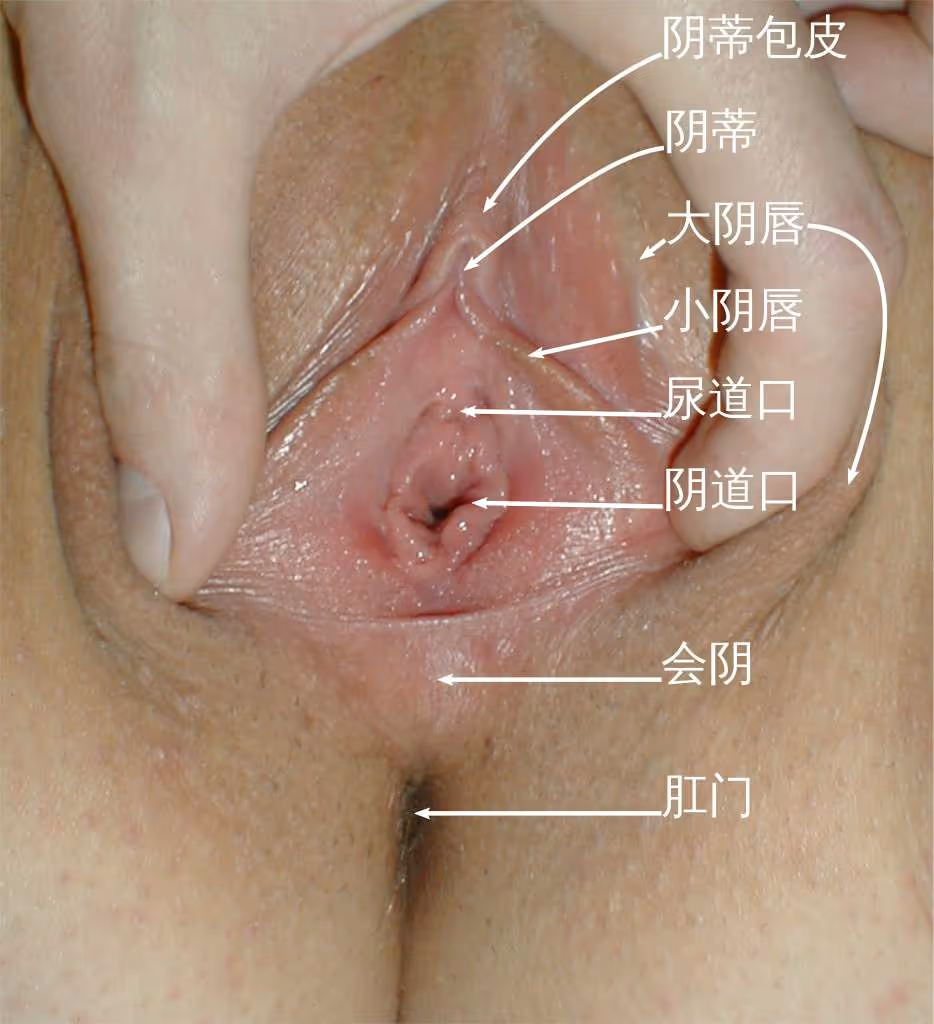
\includegraphics[width=0.7\linewidth]{wf_1.png}
    \caption{女性外生殖器结构}
    \label{fig:female_external_genitalia_1}
\end{figure}

\begin{figure}[H]
    \centering
    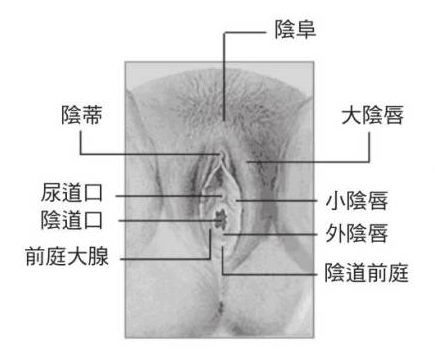
\includegraphics[width=0.7\linewidth]{wf_2.png}
    \caption{女性内生殖器结构}
    \label{fig:female_internal_genitalia_1}
\end{figure}

\begin{figure}[H]
    \centering
    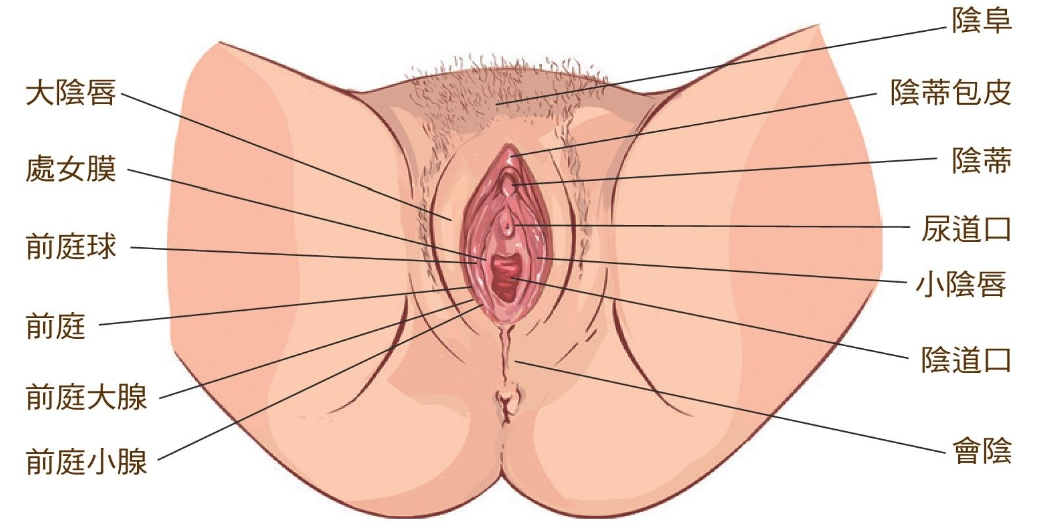
\includegraphics[width=0.7\linewidth]{wf_7.png}
    \caption{女性生殖器官侧面图}
    \label{fig:female_genitalia_side_1}
\end{figure}

\begin{figure}[H]
    \centering
    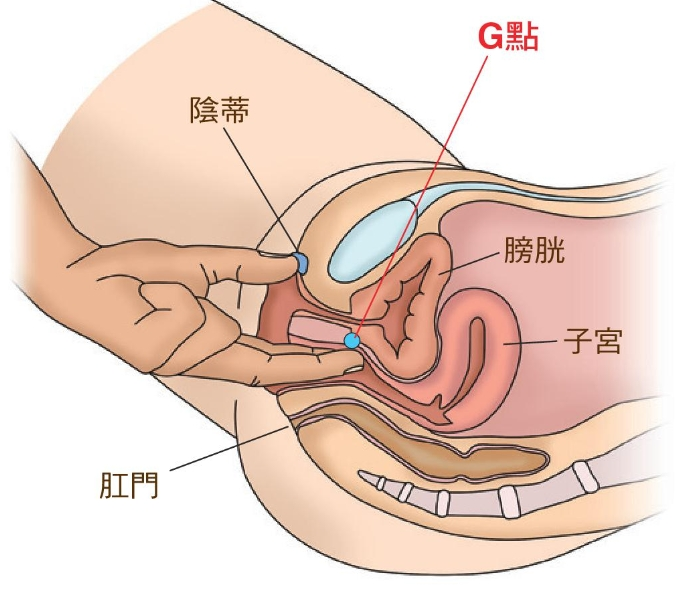
\includegraphics[width=0.7\linewidth]{wf_8.png}
    \caption{女性生殖器官正面图}
    \label{fig:female_genitalia_front_1}
\end{figure}

\subsubsection{内生殖器官}

\textbf{卵巢}

卵巢是女性最主要的生殖器官，位于盆腔内子宫的两侧，左右各一，呈扁卵圆形，长约2-3厘米，宽约1-2厘米，厚约0.5-1厘米，重约5-6克。卵巢由外层的皮质和内层的髓质组成，皮质内含有大量的原始卵泡，髓质内含有丰富的血管、神经和淋巴管。

\begin{itemize}
\item \textbf{解剖结构}：
  \begin{itemize}
  \item 卵巢表面覆盖着一层生殖上皮，下方是致密的白膜。
  \item 皮质是卵巢的主要部分，含有大量不同发育阶段的卵泡、黄体和白体等结构。
  \item 髓质位于卵巢中央，由疏松结缔组织构成，含有丰富的血管、神经和淋巴管，为卵巢提供营养和神经支配。
  \item 卵巢通过卵巢悬韧带和卵巢固有韧带固定于盆腔内，卵巢悬韧带内含有卵巢动静脉和神经，卵巢固有韧带连接卵巢与子宫。
  \end{itemize}
  \begin{itemize}
  \item \textbf{生殖功能}：产生和排出卵子，是女性生殖的基础。
    \begin{itemize}
    \item 女性出生时卵巢内约有200万个原始卵泡，青春期时减少至30-50万个，一生中只有约400-500个卵泡能够发育成熟并排卵。
    \item 在一个月经周期中，通常只有一个卵泡发育成熟并排卵，排卵后形成黄体，黄体分泌孕激素和雌激素。
    \end{itemize}
  \item \textbf{内分泌功能}：分泌雌激素、孕激素和少量雄激素，这些激素对女性生殖系统的发育和功能维持至关重要。
    \begin{itemize}
    \item 雌激素：促进女性生殖器官的发育和成熟，维持女性第二性征，调节月经周期，促进骨代谢等。
    \item 孕激素：与雌激素协同作用，维持子宫内膜的正常发育，为受精卵着床做准备，促进乳腺腺泡的发育等。
    \item 雄激素：少量的雄激素对女性的性欲和阴毛、腋毛的生长有一定作用。
    \end{itemize}
  \end{itemize}
\item \textbf{发育与变化}：
  \begin{itemize}
  \item \textbf{儿童期}：卵巢较小，表面光滑，原始卵泡处于静止状态，不分泌性激素。
  \item \textbf{青春期}：在促性腺激素的作用下，卵巢开始发育，表面逐渐变得凹凸不平，卵泡开始发育并分泌性激素，出现月经初潮和第二性征。
  \item \textbf{性成熟期}：卵巢功能最旺盛的时期，每月有一个卵泡发育成熟并排卵，形成规律的月经周期。
  \item \textbf{更年期}：卵巢功能逐渐衰退，卵泡数量明显减少，排卵不规则，月经周期紊乱，最终绝经。
  \item \textbf{绝经期}：卵巢萎缩变小，表面光滑，不再排卵和分泌性激素。
  \end{itemize}
\item \textbf{健康护理}：
  \begin{itemize}
  \item 保持健康的生活方式，均衡饮食，适量运动，避免过度劳累和精神压力过大。
  \item 定期进行妇科检查，包括B超检查和激素水平检测，及时发现和治疗卵巢疾病。
  \item 避免滥用激素类药物，尤其是雌激素类药物，以免影响卵巢功能。
  \item 注意个人卫生，避免生殖道感染，减少对卵巢的损害。
  \end{itemize}
  \begin{itemize}
  \item \textbf{卵巢囊肿}：卵巢内形成的囊性肿物，分为生理性和病理性两种。生理性囊肿通常会自行消失，病理性囊肿需要根据情况进行药物治疗或手术治疗。
  \item \textbf{多囊卵巢综合征}：一种常见的内分泌疾病，表现为月经紊乱、多毛、肥胖、不孕等，需要综合治疗，包括生活方式调整、药物治疗和手术治疗。
  \item \textbf{卵巢早衰}：40岁以前出现卵巢功能衰退的现象，表现为月经停止、潮热、盗汗等更年期症状，需要激素替代治疗和对症治疗。
  \item \textbf{卵巢癌}：女性生殖系统常见的恶性肿瘤之一，早期症状不明显，晚期表现为腹胀、腹痛、消瘦等，需要手术治疗、化疗和放疗等综合治疗。
  \end{itemize}
\end{itemize}

\textbf{输卵管}

输卵管是连接卵巢和子宫的一对细长弯曲的管道，位于子宫两侧，左右各一，长约8-14厘米，直径约0.5-1厘米。输卵管是卵子受精和受精卵运输的场所，对于女性生殖过程至关重要。

\begin{itemize}
\item \textbf{解剖结构}：
  \begin{itemize}
  \item 输卵管由内向外分为四个部分：
    \begin{itemize}
    \item 间质部：位于子宫肌层内，最短最细，长约1-2厘米，管腔直径约0.5-1毫米。
    \item 峡部：位于间质部外侧，长约2-3厘米，管腔直径约2-3毫米，是输卵管最狭窄的部分，也是输卵管结扎术的常用部位。
    \item 壶腹部：位于峡部外侧，长约5-8厘米，管腔较宽大，直径约5-8毫米，是卵子受精的主要场所。
    \item 伞部：位于输卵管最外侧，长约1-1.5厘米，呈漏斗状，边缘有许多指状突起（称为输卵管伞），具有拾卵功能。
    \end{itemize}
  \item 输卵管管壁由内向外分为三层：
    \begin{itemize}
    \item 黏膜层：由单层柱状上皮和固有层组成，上皮细胞分为纤毛细胞和分泌细胞，纤毛细胞的纤毛向子宫方向摆动，分泌细胞分泌的液体为精子和卵子提供营养和运输介质。
    \item 肌层：由内环行和外纵行两层平滑肌组成，肌层的收缩有助于卵子和受精卵的运输。
    \item 浆膜层：为腹膜的一部分，覆盖在输卵管表面，提供保护和固定作用。
    \end{itemize}
  \end{itemize}
  \begin{itemize}
  \item \textbf{拾卵功能}：输卵管伞部的指状突起能够识别和捕获从卵巢排出的卵子。
  \item \textbf{运输功能}：
    \begin{itemize}
    \item 将卵子从卵巢运输到输卵管壶腹部。
    \item 将精子从子宫腔运输到输卵管壶腹部，使精子与卵子相遇。
    \item 将受精卵从输卵管壶腹部运输到子宫腔，以便着床。
    \end{itemize}
  \item \textbf{受精场所}：输卵管壶腹部是精子与卵子结合形成受精卵的主要场所。
  \item \textbf{提供营养}：输卵管黏膜分泌的液体为精子、卵子和受精卵提供营养和适宜的环境。
  \end{itemize}
\item \textbf{发育与变化}：
  \begin{itemize}
  \item \textbf{胚胎期}：输卵管由副中肾管（米勒管）发育而来，在胚胎发育第6-8周开始形成。
  \item \textbf{儿童期}：输卵管尚未发育成熟，管腔狭窄，上皮细胞较少。
  \item \textbf{青春期}：在性激素的作用下，输卵管逐渐发育成熟，管腔扩大，黏膜上皮细胞增多，纤毛功能增强。
  \item \textbf{性成熟期}：输卵管功能最旺盛，能够完成拾卵、受精和受精卵运输等功能。
  \item \textbf{更年期}：随着卵巢功能的衰退，输卵管逐渐萎缩，管腔变窄，黏膜上皮细胞减少，纤毛功能减弱。
  \item \textbf{绝经期}：输卵管进一步萎缩，功能基本丧失。
  \end{itemize}
\item \textbf{健康护理}：
  \begin{itemize}
  \item 注意个人卫生，保持生殖道清洁，避免生殖道感染，尤其是输卵管炎。
  \item 避免不洁性生活，减少性传播疾病的发生，性传播疾病是导致输卵管堵塞的主要原因之一。
  \item 积极治疗妇科炎症，如阴道炎、宫颈炎、盆腔炎等，防止炎症蔓延至输卵管。
  \item 做好避孕措施，避免意外怀孕和人工流产，人工流产手术可能导致输卵管感染和堵塞。
  \end{itemize}
  \begin{itemize}
  \item \textbf{输卵管炎}：输卵管的炎症，可分为急性和慢性两种。急性输卵管炎表现为发热、腹痛、阴道分泌物增多等，慢性输卵管炎表现为下腹隐痛、腰骶部酸痛、不孕等。治疗包括抗生素治疗、物理治疗和手术治疗。
  \item \textbf{输卵管堵塞}：输卵管管腔狭窄或堵塞，导致卵子和精子无法相遇，是女性不孕的主要原因之一。治疗方法包括输卵管通液术、输卵管造影术、输卵管介入治疗和试管婴儿等。
  \item \textbf{输卵管积水}：输卵管伞部堵塞，导致输卵管内的液体无法排出，积聚在输卵管内形成积水。治疗包括药物治疗、手术治疗和试管婴儿等。
  \item \textbf{输卵管妊娠}：受精卵在输卵管内着床发育，即宫外孕，是一种危险的妊娠并发症，可能导致输卵管破裂和大出血。治疗包括药物治疗和手术治疗。
  \end{itemize}
\end{itemize}

\textbf{子宫}

子宫是女性生殖系统中最重要的器官之一，位于骨盆腔中央，在膀胱与直肠之间，形状似倒置的梨子，前后略扁，长约7-8厘米，宽约4-5厘米，厚约2-3厘米，重约50-70克。子宫是孕育胎儿的场所，也是产生月经的器官，对于女性的生殖健康至关重要。

\begin{itemize}
\item \textbf{解剖结构}：
  \begin{itemize}
  \item 子宫分为三个部分：
    \begin{itemize}
    \item 宫底：子宫的上部，两侧与输卵管相连。
    \item 宫体：子宫的中部，是子宫的主要部分，宫腔呈倒三角形。
    \item 宫颈：子宫的下部，呈圆柱形，下接阴道，宫颈外口与阴道相通。
    \end{itemize}
  \item 子宫壁由外向内分为三层：
    \begin{itemize}
    \item 浆膜层（子宫外膜）：为腹膜的一部分，覆盖在子宫表面，提供保护和固定作用。
    \item 肌层（子宫肌层）：由平滑肌组成，是子宫壁最厚的一层，厚度约0.8-1.0厘米，具有很强的收缩能力，在分娩时帮助胎儿娩出，在月经期间帮助排出经血。
    \item 内膜层（子宫内膜）：位于子宫腔表面，分为功能层和基底层。功能层受性激素影响，每月发生周期性变化，产生月经；基底层不受性激素影响，具有修复功能层的作用。
    \end{itemize}
  \item 子宫的固定结构：子宫通过子宫阔韧带、子宫圆韧带、子宫主韧带和骶子宫韧带等固定于盆腔内，维持子宫的正常位置。
  \end{itemize}
  \begin{itemize}
  \item \textbf{孕育胎儿}：子宫是胎儿生长发育的场所，受精卵在子宫腔着床后，子宫会随着胎儿的生长而逐渐增大，为胎儿提供适宜的生长环境。
  \item \textbf{产生月经}：子宫内膜受性激素影响，每月发生周期性变化，当卵子未受精时，子宫内膜会脱落并伴随出血，形成月经。
  \item \textbf{参与分娩}：子宫肌层的强烈收缩是胎儿娩出的主要动力，同时子宫颈会扩张，以便胎儿通过。
  \item \textbf{分泌功能}：子宫内膜和宫颈分泌的液体参与组成白带，为精子提供营养和运输介质。
  \end{itemize}
\item \textbf{发育与变化}：
  \begin{itemize}
  \item \textbf{儿童期}：子宫较小，呈细长形，宫颈较长，约占子宫全长的2/3，宫体与宫颈的比例约为1:2。
  \item \textbf{青春期}：在性激素的作用下，子宫逐渐发育成熟，宫体增大，宫颈相对变短，宫体与宫颈的比例约为1:1。
  \item \textbf{性成熟期}：子宫发育完全，宫体与宫颈的比例约为2:1，能够完成月经周期和孕育胎儿的功能。
  \item \textbf{妊娠期}：子宫会随着胎儿的生长而显著增大，足月时子宫体积可达未孕时的500-1000倍，重量可达未孕时的20倍左右。
  \item \textbf{分娩后}：子宫会逐渐收缩恢复到未孕状态，这个过程称为子宫复旧，通常需要6-8周。
  \item \textbf{更年期}：随着卵巢功能的衰退，子宫逐渐萎缩，体积变小，子宫内膜变薄，月经逐渐停止。
  \item \textbf{绝经期}：子宫进一步萎缩，功能基本丧失。
  \end{itemize}
\item \textbf{健康护理}：
  \begin{itemize}
  \item 保持良好的生活习惯，均衡饮食，适量运动，避免过度劳累和精神压力过大。
  \item 注意个人卫生，保持生殖道清洁，避免生殖道感染。
  \item 做好避孕措施，避免意外怀孕和人工流产，减少对子宫的伤害。
  \item 定期进行妇科检查，包括B超检查和宫颈涂片检查，及时发现和治疗子宫疾病。
  \item 产后注意休息，促进子宫复旧，避免过早进行重体力劳动。
  \end{itemize}
  \begin{itemize}
  \item \textbf{子宫肌瘤}：子宫肌层的良性肿瘤，是女性最常见的妇科肿瘤之一，表现为月经增多、经期延长、下腹包块等。治疗方法包括观察、药物治疗和手术治疗。
  \item \textbf{子宫内膜异位症}：子宫内膜组织生长在子宫以外的部位，表现为痛经、月经不调、不孕等。治疗方法包括药物治疗和手术治疗。
  \item \textbf{子宫腺肌症}：子宫内膜腺体和间质侵入子宫肌层，表现为痛经、月经增多、子宫增大等。治疗方法包括药物治疗、手术治疗和介入治疗。
  \item \textbf{子宫脱垂}：子宫从正常位置沿阴道下降，甚至脱出阴道口外，表现为下腹坠胀、阴道口异物感等。治疗方法包括盆底肌肉锻炼、子宫托和手术治疗。
  \item \textbf{子宫内膜癌}：发生在子宫内膜的恶性肿瘤，表现为绝经后阴道出血、月经紊乱等。治疗方法包括手术治疗、化疗和放疗等综合治疗。
  \item \textbf{宫颈癌}：发生在宫颈的恶性肿瘤，与人乳头瘤病毒（HPV）感染密切相关，表现为阴道出血、阴道分泌物增多等。治疗方法包括手术治疗、放疗和化疗等综合治疗，早期宫颈癌可以通过疫苗预防。
  \end{itemize}
\end{itemize}

\textbf{阴道}

阴道是一种收缩性很强的肌性管道，上通子宫颈管，下开口于阴道前庭，阴道前壁紧贴膀胱和尿道，后壁与直肠相邻。阴道为性交器官，又是月经排出和胎儿娩出的通道。

\begin{figure}[H]
    \centering
    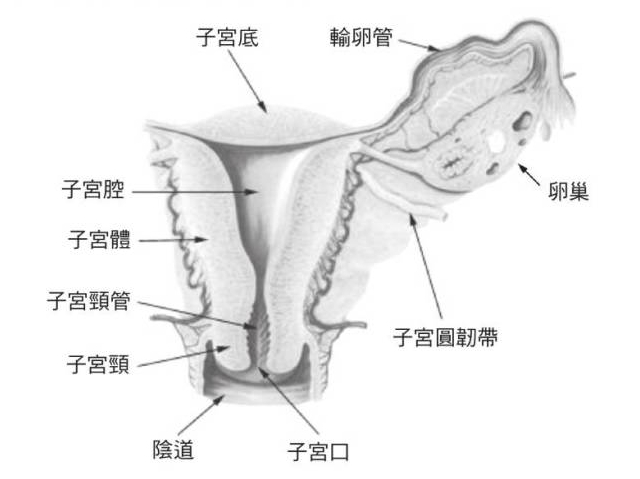
\includegraphics[width=0.7\linewidth]{wf_3.png}
    \caption{子宫结构}
    \label{fig:uterus_structure_1}
\end{figure}

\textbf{阴道分泌物}

巴氏腺（大前庭腺）位在阴道口附近，会在性刺激时分泌一些黏液状的物质，而子宫颈和阴道内也有一些腺体会产生分泌物，让阴道保持正常湿润。

阴道分泌物在不同的生理周期会产生变化，例如在排卵期，分泌物通常会变得比较黏稠，有时会像生蛋白样。如果在小阴唇的皱褶上看到一些白白的碎屑状物质，这也是阴道的分泌物，如果不觉得痒，属正常现象。另外，在怀孕期间、生产后、停经前后等，分泌物的状态也会有所不同。

很多私密处用品厂商会告诉你，分泌物产生变化就是有问题，要你赶快去买这些东西来排除困扰，这完全是销售话术。其实在正常范围内的分泌物变化是不用担心的，但必须懂得分辨分泌物是否为正常状态，可依以下条件判断：

1.有一点味道是正常的，女性阴道的分泌物口交时尝起来稍微酸酸的，但不应该有强烈的味道。

2.经期之外，除了透明或淡白色，阴道分泌物不会呈现其他颜色。

如果只是感觉分泌物较多，有点不舒服，通常不会有什么问题，但如果是出现搔痒、痛感，或者是颜色和味道有明显的变化，那就应该去看医生，确认有没有感染，而不是私自购买那些宣称有疗效的私密处保养品来用，以免耽误治疗！

\textbf{阴道内的正常菌丛有助维持健康}

阴道内的环境不单纯只是由人体的分泌物构成，还有许多细菌也在里面扮演了重要的角色，这些细菌被称作“共生菌”，也就是正常状态下自然存在阴道内的多种细菌，如果没有它们的存在，阴道也没办法保持健康、正常的运作，多数情况下，这些细菌的存在对人体无害，甚至是有助平衡阴道的 pH 值，让阴道的菌落维持健康。

阴道内的正常菌丛还可防止入侵的细菌附着在阴道壁上，进而防止坏菌入侵。如果阴道内正常细菌的平衡状态被破坏了，就可能会导致感染和发炎。

常见的阴道共生菌，包含了厌氧性的革兰氏阴性杆菌和球菌，乳酸杆菌则会让阴道的 pH 值维持在正常浓度（正常阴道内酸碱度范围在3.8--4.5之间，为弱酸性），这能防止其他有机体在阴道内生长。

如果阴道的 pH 值增加，变得比较不酸，乳酸杆菌的质或量就会下降，让其他细菌有孳生的机会，进而导致感染，例如常见的细菌性阴道炎或念珠菌阴道炎，这些疾病可能造成搔痒、刺激或是导致分泌物异常。

\textbf{紧不紧，很要紧？}

很多对性知识好奇的人心里都抱着一个疑问，那就是女人阴道的松紧度与性爱满意度有没有关系？经过研究显示，女性的外阴构造与男女之间的性满意度没有多大关联，女人阴道的性功能主要是由心理因素决定，而非生理因素。

女性的阴道长度有7--12公分，宽度可容纳两根手指，阴道壁有许多橫行的皱壁，有较大的伸缩性和弹性，兴奋时阴道深度会增加1/3，宽度也会增加，所以一般不会出现男女性器官无法配合的情形。未生产过的女性，阴道通常不至于太宽松。

女性分娩时，直径达10公分的胎儿头部也能通过阴道，这就可以证实女性阴道有很大的弹性，所以这方面的担心是完全没必要的。

但初夜性交时女性下体会疼痛，大多是由于心理紧张、经验不足等其他因素导致，和器官本身通常没有直接关系。

有些女性则在生产过后会有阴道松弛的现象，造成性生活满意度降低，若有这种情形，可透过阴道紧缩手术来改善。阴道紧缩可使男性在性交时较有快感，女性也能藉此达到高潮，增进夫妻情感。

女性性高潮来源于阴道括约肌强烈收缩，继而刺激性感带，若是耻骨尾骨肌收缩不够强烈，或是在生产时受到创伤又没有修补，就不太容易在性交时享受到高潮了。

\textbf{“高潮”来袭，耻骨尾骨肌会出现规律性收缩}

女性性高潮来袭时，耻骨尾骨肌会以每0.8秒的频率收缩一次，产生反应后，子宫也会以每0.8秒的频率上下“抖”动（子宫高潮），这一系列的收缩抖动就是高潮来临。女性性高潮的享受感比男人强许多，男性性高潮的时间约只有8秒，女性可达20秒以上，女性之所以能在短时间内享受极致的性高潮，耻骨尾骨肌的功能很重要。

女性性爱时若没有高潮的感觉，可以做以下练习：把3支手指头放入阴道内，收缩阴道，使手指可以感受到收缩的力量，尤其是30岁以上的女性，1天做2次，1次15下，连续两周。但有一些年纪较大的女性，即使每天练习也无法自主控制肌肉的收缩，若想恢复功能，就需要借助“阴道整型术”了。

阴道紧缩整形手术一般分为三种：

1.后阴道壁整形术：强化直肠脱出与阴道松弛，这也是一般夫妻因为抱怨阴道松弛最常做的手术，做法是先把阴道壁黏膜分开，接着把提肛肌强化缝合，切除多余的阴道黏膜，再根据自然生产的会阴缝合术，重建强韧的阴道壁。

2.前阴道壁整形术：可同时改善膀胱脱垂的症状，手术把前阴道壁黏膜分开，接着把子宫膀胱筋膜韧带加缝一层，再强化膀胱底部及尿道的支撑力量，最后把多余的阴道黏膜切除再缝合就可以了。

3.生产时顺便做会阴整形术：修补会阴缺口处再重新缝合，此时可以同时把阴道内部松弛的表皮切除一部分，再拉回缝合，使阴道回复产前的紧实状状态。

阴道整形手术对妇产科医师来说是简单、快速的手术，过程只要20--30分钟，如果你有这方面的困扰，只要一个简单的手术，就能改变夫妻间的性生活与互动关系，千万不要讳疾忌医。

\textbf{蒙娜丽莎之吻私密雷射}

怀孕、生产，乃至更年期变化，是多数女人一生都不可避免的历程，但随着生产伤害、荷尔蒙变化及人体正常的组织老化，会使阴道出现松弛、干涩、易感染、漏尿等问题，不仅让自己性趣缺缺，也影响另一半的“性”福。

对于这样的困扰，医界过去多是建议患者做凯格尔运动，情况严重的只能直接以手术处理。近年来，美容医学界发展出私密处紧实雷射，不需动刀或住院，便可有效改善上述症状。它的原理类似运用在脸部的飞梭雷射，只是将施打的位置转换为阴道内/外阴部等地方。将雷射探头置入阴道后，运用雷射的光热效应，汰换老发黏膜，刺激胶原蛋白重组新生，黏膜增厚，可达到让阴道环境年轻化、健康化，并能提升湿润度、包覆感，及对尿道支撑度。改善漏尿等效果，对于性生活满意度也有很大的帮助。

\subsubsection{有问必答}

Q:哪些人适合做阴道紧缩术 ？

A:
1.生产过的女性（无论用哪一种方式生产）。

2.阴道曾经有过撕裂伤。

3.性伴侣阴茎尺寸较小。

4.想要借阴道紧缩提升性交满意度。

5.阴道松弛状况严重者。

6.40岁以上因为胶原蛋白流失，阴道壁变薄，阴道变松、变宽。

\subsection{男性生殖器官的详细结构}

男性生殖器官分为外生殖器官和内生殖器官两部分。外生殖器包括阴阜、阴囊和阴茎，而内生殖器由睾丸、附睾、精索、输精管及射精管、精囊腺、前列腺、尿道球腺、尿道等组成。

\begin{figure}[H]
    \centering
    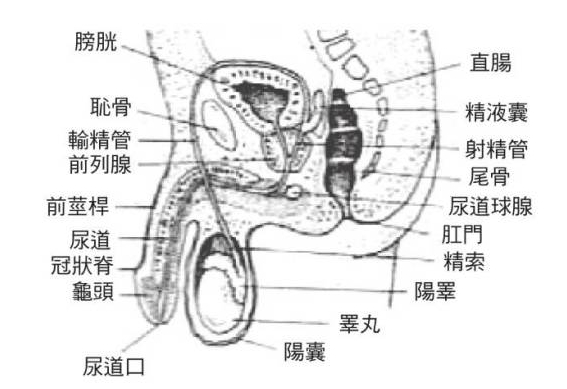
\includegraphics[width=0.7\linewidth]{wf_4.png}
    \caption{男性生殖器官结构}
    \label{fig:male_genitalia_1}
\end{figure}

\begin{figure}[H]
    \centering
    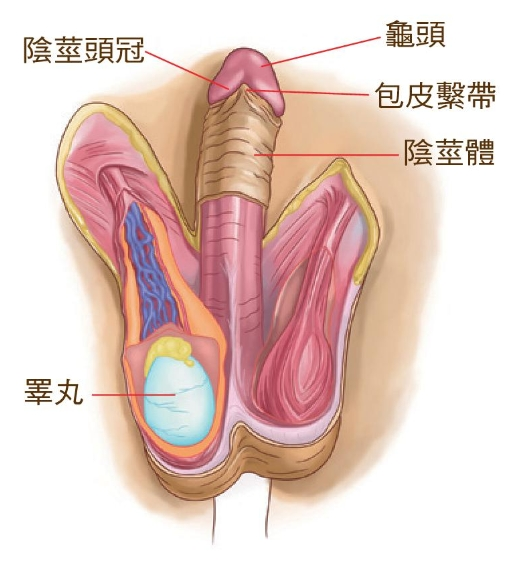
\includegraphics[width=0.7\linewidth]{wf_13.png}
    \caption{男性生殖器官侧面图}
    \label{fig:male_genitalia_side_1}
\end{figure}

\subsubsection{外生殖器官}

阴阜为耻骨前方的皮肤和丰富的皮下脂肪组织。青壮年时阴阜显著隆起，中年以后脂肪组织减少下陷，老年则萎缩变平。阴阜的主要功能是保护耻骨联合和下方的生殖器官，在性交时也能起到缓冲作用。

\textbf{阴囊}

阴囊是由皮肤、肉膜、精索外筋膜、提睾肌和精索内筋膜等构成的柔软而富有弹性的袋状囊，里面容纳睾丸、附睾和精索等结构。阴囊的主要功能包括：

\begin{itemize}
\item \textbf{保护功能}：阴囊为睾丸提供了一个安全的外部环境，减少外部冲击对睾丸的伤害。
\item \textbf{温度调节功能}：阴囊具有独特的温度调节机制，使睾丸始终保持在比体温低1-2℃的理想温度（约35℃），这对于精子的生成和发育至关重要。
  \begin{itemize}
  \item 阴囊皮肤的大量褶皱可以增加散热面积。
  \item 肉膜中的平滑肌（阴囊肌）可以根据环境温度收缩或松弛：寒冷时收缩使阴囊变小变厚，减少散热；炎热时松弛使阴囊变大变薄，增加散热。
  \item 提睾肌可以使睾丸上下移动，调节睾丸与身体的距离，进一步控制温度。
  \end{itemize}
\item \textbf{感觉功能}：阴囊皮肤富含神经末梢，对温度、触觉和疼痛等刺激非常敏感。
\end{itemize}

阴囊内有阴囊隔，将阴囊内腔分成左右两部分，各容纳一个睾丸和附睾。阴囊皮肤薄而柔软，并有很多的褶皱。阴囊皮肤有明显的色素沉着，长有稀疏的阴毛。

\textbf{阴茎}

阴茎是男性的性交器官，也是排尿和射精的通道。阴茎的结构和功能非常复杂：

\begin{itemize}
\item \textbf{外部结构}：
  \begin{itemize}
  \item 阴茎根：位于会阴部，固定在耻骨联合下方的软组织中。
  \item 阴茎体：呈圆柱形，是阴茎的主体部分，由皮肤包裹。
  \item 阴茎头（龟头）：阴茎前端的膨大部分，表面光滑，富含神经末梢，对刺激非常敏感。
  \item 冠状沟：阴茎头与阴茎体之间的环形凹陷，是神经分布最丰富的区域之一，敏感性极高。
  \item 包皮：包裹阴茎头的皮肤皱襞，可分为内板和外板。包皮的主要功能是保护阴茎头免受外界刺激和损伤。
  \end{itemize}
\item \textbf{内部结构}：
  \begin{itemize}
  \item 三个海绵体：阴茎由两个阴茎海绵体（位于背侧）和一个尿道海绵体（位于腹侧，内含尿道）组成。海绵体内部由许多海绵状的小梁和腔隙构成，这些腔隙与血管相通。
  \item 白膜：包裹在海绵体外的坚韧纤维组织膜，为阴茎提供结构支持。
  \item 血管系统：阴茎含有丰富的血管，包括动脉、静脉和毛细血管。阴茎海绵体动脉是阴茎勃起的关键血管，而螺旋动脉则直接供应海绵体腔隙。
  \item 神经分布：阴茎由阴部神经支配，包括感觉神经和运动神经，其中阴茎背神经负责传递阴茎头和阴茎体的感觉信号。
  \end{itemize}
\item \textbf{勃起机制}：
  \begin{itemize}
  \item 当受到性刺激时，大脑或脊髓发出信号，使阴茎海绵体内的动脉扩张，血液大量流入海绵体腔隙。
  \item 同时，海绵体周围的静脉被白膜压迫，血液流出减少，导致海绵体内压力升高，阴茎体积增大、硬度增加，形成勃起。
  \item 勃起过程涉及多种神经递质和血管活性物质，如一氧化氮（NO）、前列腺素E1等，其中一氧化氮是勃起的关键信号分子。
  \end{itemize}
\item \textbf{功能}：阴茎具有排尿、性交和射精三大功能，是男性生殖系统中最重要的外生殖器。
\end{itemize}

\subsubsection{内生殖器官}

男性内生殖器官包括睾丸、附睾、精索、输精管、射精管、精囊腺、前列腺、尿道球腺和尿道等，它们共同参与精子的生成、成熟、储存和排出过程，以及精液的组成。

\textbf{睾丸}

睾丸是男性最主要的生殖器官，位于阴囊内，左右各一，呈椭圆形，长约4-5厘米，宽约2-3厘米，厚约1-2厘米，重约10-15克。睾丸的主要功能是产生精子和分泌雄性激素（主要是睾酮）。

\begin{itemize}
\item \textbf{生精功能}：睾丸内的曲细精管是精子生成的场所，曲细精管上皮由生精细胞和支持细胞组成。生精细胞在支持细胞的支持和滋养下，经过精原细胞、初级精母细胞、次级精母细胞、精子细胞等阶段，最终发育为成熟的精子，这个过程称为生精过程，大约需要72-74天。
\item \textbf{内分泌功能}：睾丸间质细胞（又称Leydig细胞）分泌睾酮，睾酮是男性最重要的雄性激素，它的主要作用包括：
  \begin{itemize}
  \item 维持男性第二性征（如阴毛、腋毛、胡须的生长，嗓音变粗，肌肉发达等）
  \item 维持正常的性欲和性功能
  \item 促进精子的生成和成熟
  \item 促进蛋白质合成和骨骼生长
  \item 影响红细胞生成和脂质代谢
  \end{itemize}
\end{itemize}

\textbf{附睾}

附睾是附着在睾丸后上方的一条细长管道，长约6-7厘米，分为头、体、尾三部分。附睾的主要功能是储存和滋养精子，促进精子的成熟。

\begin{itemize}
\item \textbf{储存功能}：从睾丸产生的精子还未成熟，需要在附睾中储存约2-3周，才能达到功能上的成熟。
\item \textbf{成熟功能}：附睾分泌的液体为精子提供营养，促进精子的进一步发育成熟，使精子获得运动能力和受精能力。
\item \textbf{运输功能}：附睾的蠕动可以将精子从附睾头部运输到附睾尾部，最终进入输精管。
\end{itemize}

\textbf{精索}

精索是一条从腹股沟管腹环到睾丸上端的柔软圆索状结构，长约11-15厘米，直径约0.5-1厘米。精索内含有输精管、睾丸动脉、蔓状静脉丛、神经、淋巴管和提睾肌等结构，主要功能是支持和固定睾丸，并为睾丸提供血液供应、神经支配和淋巴回流。

\textbf{输精管}

输精管是一条细长的肌性管道，长约30-40厘米，直径约2-3毫米，起始于附睾尾部，沿精索上行，穿过腹股沟管进入盆腔，最终与精囊腺的排泄管汇合成射精管。输精管的主要功能是运输精子，其管壁的平滑肌具有很强的收缩能力，在性高潮时可以将精子快速输送到射精管。

\textbf{射精管}

射精管是由输精管末端与精囊腺排泄管汇合而成的短管道，长约2厘米，直径约1毫米，开口于尿道前列腺部的精阜处。射精管的主要功能是将精子和精囊腺分泌物输送到尿道，参与射精过程。

\textbf{精囊腺}

精囊腺是一对位于膀胱后方、输精管壶腹外侧的囊性腺体，呈长椭圆形，长约4-5厘米，宽约1-2厘米。精囊腺的主要功能是分泌精囊液，精囊液是精液的重要组成部分，约占精液体积的60-70%。精囊液呈碱性，含有丰富的果糖、前列腺素、凝固酶等物质，其主要作用包括：

\begin{itemize}
\item 为精子提供能量（果糖）
\item 中和阴道的酸性环境，保护精子
\item 促进精子的运动
\item 使精液凝固，防止精液流出阴道
\end{itemize}

\textbf{前列腺}

前列腺是位于膀胱下方、包绕尿道前列腺部的单个实质性腺体，呈栗子状，长约3-4厘米，宽约4-5厘米，厚约2-3厘米，重约20克。前列腺的主要功能是分泌前列腺液，前列腺液是精液的重要组成部分，约占精液体积的20-30%。前列腺液呈乳白色，含有丰富的酸性磷酸酶、蛋白酶、锌、柠檬酸等物质，其主要作用包括：

\begin{itemize}
\item 促进精液的液化（蛋白酶）
\item 为精子提供营养和能量
\item 维持精液的pH值
\item 抑制细菌的生长，保护泌尿系统和生殖系统
\end{itemize}

\textbf{尿道球腺}

尿道球腺又称库珀腺，是一对位于尿道膜部两侧、尿道球后方的小型腺体，呈豌豆状，长约1厘米，直径约0.5厘米。尿道球腺的主要功能是分泌尿道球腺液，尿道球腺液是精液的组成部分之一，约占精液体积的0.5-2%。尿道球腺液呈透明的黏液状，具有润滑作用，可以润滑尿道，减少精子通过时的摩擦，同时中和尿道内的酸性环境，保护精子。

\textbf{尿道}

男性尿道是一条起自膀胱颈、终于尿道外口的管道，长约16-22厘米，管径约5-7毫米。男性尿道既是排尿的通道，也是射精的通道，因此具有排尿和射精双重功能。男性尿道分为前列腺部、膜部和海绵体部三部分，其中前列腺部和膜部称为后尿道，海绵体部称为前尿道。

\textbf{阴囊}

阴囊是由皮肤、肉膜、精索外筋膜、提睾肌和精索内筋膜等构成的柔软而富有弹性的袋状囊，里面容纳睾丸、附睾和精索等结构。阴囊的主要功能包括：

\begin{itemize}
\item \textbf{保护功能}：阴囊为睾丸提供了一个安全的外部环境，减少外部冲击对睾丸的伤害。
\item \textbf{温度调节功能}：阴囊具有独特的温度调节机制，使睾丸始终保持在比体温低1-2℃的理想温度（约35℃），这对于精子的生成和发育至关重要。
  \begin{itemize}
  \item 阴囊皮肤的大量褶皱可以增加散热面积。
  \item 肉膜中的平滑肌（阴囊肌）可以根据环境温度收缩或松弛：寒冷时收缩使阴囊变小变厚，减少散热；炎热时松弛使阴囊变大变薄，增加散热。
  \item 提睾肌可以使睾丸上下移动，调节睾丸与身体的距离，进一步控制温度。
  \end{itemize}
\item \textbf{感觉功能}：阴囊皮肤富含神经末梢，对温度、触觉和疼痛等刺激非常敏感。
\end{itemize}

阴囊内有阴囊隔，将阴囊内腔分成左右两部分，各容纳一个睾丸和附睾。阴囊皮肤薄而柔软，并有很多的褶皱。阴囊皮肤有明显的色素沉着，长有稀疏的阴毛。

\textbf{阴茎}

阴茎是男性的性交器官，也是排尿和射精的通道。阴茎的结构和功能非常复杂：

\begin{itemize}
\item \textbf{外部结构}：
  \begin{itemize}
  \item 阴茎根：位于会阴部，固定在耻骨联合下方的软组织中。
  \item 阴茎体：呈圆柱形，是阴茎的主体部分，由皮肤包裹。
  \item 阴茎头（龟头）：阴茎前端的膨大部分，表面光滑，富含神经末梢，对刺激非常敏感。
  \item 冠状沟：阴茎头与阴茎体之间的环形凹陷，是神经分布最丰富的区域之一，敏感性极高。
  \item 包皮：包裹阴茎头的皮肤皱襞，可分为内板和外板。包皮的主要功能是保护阴茎头免受外界刺激和损伤。
  \end{itemize}
\item \textbf{内部结构}：
  \begin{itemize}
  \item 三个海绵体：阴茎由两个阴茎海绵体（位于背侧）和一个尿道海绵体（位于腹侧，内含尿道）组成。海绵体内部由许多海绵状的小梁和腔隙构成，这些腔隙与血管相通。
  \item 白膜：包裹在海绵体外的坚韧纤维组织膜，为阴茎提供结构支持。
  \item 血管系统：阴茎含有丰富的血管，包括动脉、静脉和毛细血管。阴茎海绵体动脉是阴茎勃起的关键血管，而螺旋动脉则直接供应海绵体腔隙。
  \item 神经分布：阴茎由阴部神经支配，包括感觉神经和运动神经，其中阴茎背神经负责传递阴茎头和阴茎体的感觉信号。
  \end{itemize}
\item \textbf{勃起机制}：
  \begin{itemize}
  \item 当受到性刺激时，大脑或脊髓发出信号，使阴茎海绵体内的动脉扩张，血液大量流入海绵体腔隙。
  \item 同时，海绵体周围的静脉被白膜压迫，血液流出减少，导致海绵体内压力升高，阴茎体积增大、硬度增加，形成勃起。
  \item 勃起过程涉及多种神经递质和血管活性物质，如一氧化氮（NO）、前列腺素E1等，其中一氧化氮是勃起的关键信号分子。
  \end{itemize}
\item \textbf{功能}：阴茎具有排尿、性交和射精三大功能，是男性生殖系统中最重要的外生殖器。
\end{itemize}

\subsection{生殖器官的护理}

\subsubsection{女性私密处的清洁}

女性对于脸部、身体、四肢的保养通常都很在行，但对于私密处的清洁与保养就没那么清楚了，以下是照顾私密处的要诀：

1.每日清洗：女性外阴部由于油脂、汗液及阴道分泌物较多，加上阴道口、尿道口和肛门紧邻着，尿液、阴道分泌物和粪便容易交叉污染，且外阴的皮肤皱褶比较多，这些特点有利于病菌滋生、寄居和生长繁殖，因此一定要做好外阴的清洁卫生工作，正常情况下每日清洗1--2次，在做爱前尤其必要再清洗一次，因为男人口交时会一再重复舔舐女人的阴部。

2.使用温水：不能用过热的水清洗，热水会造成局部的刺激和损伤，最好也不要使用冷水，冷水会让外阴部感到不适，也不容易将分泌物洗干净。外阴皮肤是女性最娇嫩的皮肤之一，非常敏感，人体会分泌油脂来保护它，经常使用清洁剂洗去这些油脂，容易引起外阴皮肤干燥，甚至发炎，加上清洁剂若为碱性，经常使用就有可能会破坏阴道的酸碱平衡，导致阴道炎等疾病发生。

3.清洗顺序：清洗外阴前应先洗净双手，然后从前向后清洗大、小阴唇，最后洗肛门周围及肛门；不能从后向前洗，以免将肛门部位的细菌带入阴道。

4.清洗方式：最好淋浴，如果无法淋浴可用盆浴代替，但要使用专用的浴盆。

5.挑对清洁用品：阴道内的 pH 值大概在3.8--4.5，外阴部的 pH 值则在5左右，有些清洁用品会标榜弱酸性，接近阴道的 pH 值，事实上，外阴部的洗剂不用这么酸，因为外阴部其实也没有这么酸。阴道及外阴部有自我调节 pH 值的能力，就算用偏碱一点的洗剂，身体很快就会调节到正常的 pH 值。所以，只要不是刻意用特别酸或特别碱的产品，且长期、频繁地使用，原则上是不必太过担心的。

\subsubsection{照顾私密处的注意事项}

每天好好清洁私密处其实已经够了，但如果希望给外阴部什么特别的保养，基本上只要挑选成分不要太花俏，不要有香精、色素、刺激性成分，或者含有容易产生粘膜刺激性防腐剂的产品就可以了。

一般的清洁用品多不会有什么问题，除非你是特别敏感的人，会因为使用一般产品而感到干燥、干痒或是其他不适，否则不需要使用特别的清洁产品。

另外，太过闷热的环境容易造成外阴搔痒，甚至是起疹子，因此穿着比较通风的裙装，避免穿材质对外阴部容易产生摩擦的内裤，也是做好外阴部保养的基本工作，挑选内裤时以纯棉材质为优选。

很多女生觉得经血脏，因此在月经期间会特别冲洗阴道，甚至买一些灌洗用具，例如阴道冲洗器，其实这是没有必要的。月经其实就是子宫内膜剥落后的产物，它和子宫颈分泌物及其他阴道内分泌物，都是人体正常代谢的物质。经血从阴道被排出的过程，其实就是人体在做自我清洁了。

还有一些女生会担心自己下体的味道不好，但正常人的阴道分泌物，本来就会有淡淡、酸酸的味道，如果想要追求无味或是香香的气味，通常只会弄巧成拙。具有香氛的产品对阴道保健完全没有帮助，反而可能破坏阴道的自然平衡。

想做好私密处保养，还需要注意以下几点建议:

1.与不甚熟悉的、或有多位性伴侣的男性性交应全程使用保险套：这能保护自己也保护别人。有些病毒和细菌在性交时会进入阴道，包括造成衣原体感染、淋病、生殖器泡疹、尖锐湿疣、梅毒和 HIV 的细菌和病毒，性交时戴保险套可防止这类感染发生。

2.定期体检：如果发生过性行为或是30岁以上的女性，建议定期做子宫颈抹片及性病系列检查。

3.规律的作息与运动：规律的作息可确保身体有正常的免疫能力，让阴道内菌丛维持好的平衡；规律的运动可强化骨盆底肌肉，对整体健康有帮助，而要锻炼骨盆肌，可尝试走路、跑步、游泳等运动。

4.选用正确的清洁用品：选用温和、不刺激、不添加香精的清洁用品，有些产品宣称草本、天然、无毒，不一定比较好。

5.不需过度清洁阴道：不必使用任何阴道内灌洗用品，也不必特别清洁阴道内的月经血块，如果因为感染有必要特别清洁，医师会开立药品，不要自行灌洗，避免因此破坏阴道内正常的菌丛生态。

6.如厕后不建议使用湿纸巾：这类产品可能含有较高浓度的防腐剂或香精，长期使用对身体不好，用卫生纸就可以了，还要保持外阴部通风、凉爽、不潮湿。

\subsection{生殖器官的多样性体验}

以下案例旨在帮助读者更好地理解生殖器官的个体差异和跨性别视角，这些案例基于真实经历改编：


以下两个案例来自匿名分享，用于说明一个核心事实：\textbf{生殖器外观的自然变异范围远比广告与色情影像所呈现的更宽}，而"偏离标准"的焦虑往往来自对照对象的失真，而非身体本身的问题。

案例一：一位女性在成年后偶然用镜子仔细观察自己的外阴，才发现它与教科书的模式图并不一致——小阴唇略长于大阴唇，颜色也更深。起初她担心"是不是不正常"，妇科检查确认一切健康后，她反而释然了：原来差异本身就是常态。案例二：一位跨性别者在激素治疗与手术后，重新学习自己身体的敏感与回应方式，起初的陌生感随着与伴侣的坦诚沟通逐渐化解。这两个案例的共同启示是：\textbf{身体没有"标准答案"，了解与接纳先于评判}。


\subsubsection{案例一：阴茎大小的个体差异}

小明（化名）是一名25岁的男性，他一直对自己的阴茎大小感到焦虑，认为自己的阴茎比"正常"小。这种焦虑影响了他的性生活和自信心，甚至导致他避免与伴侣亲密接触。在寻求性健康咨询后，他了解到阴茎大小的个体差异很大，而且勃起后的大小与性功能和性满意度没有直接关系。咨询师还向他解释了伴侣的性满意度更多取决于情感连接、沟通和技巧，而不是阴茎大小。通过咨询和伴侣的支持，小明逐渐接受了自己的身体，性生活质量也得到了改善。


一位 28 岁男性因自认为"偏小"而回避亲密关系，长期不敢去游泳、也不愿开灯。测量显示他疲软长度约 8 厘米、勃起长度约 12 厘米，\textbf{均在人群正常范围内}（多数研究显示勃起长度的均值在 13 厘米上下，且与身高、脚码、手掌大小无可靠相关）。咨询中真正需要处理的不是尺寸，而是他反复观看色情内容形成的参照偏差与由此产生的回避行为。经过几次咨询加行为练习（逐步开灯、向伴侣坦白焦虑），回避明显减轻。\textbf{"尺寸焦虑"通常是心理议题，而非外科议题。}

\subsubsection{案例二：阴唇外观的个体差异}

小红（化名）是一名22岁的女性，她在观看色情视频后对自己的阴唇外观产生了担忧，认为自己的阴唇"不正常"。她甚至考虑进行阴唇整形手术。在与妇科医生咨询后，她了解到阴唇的大小、形状和颜色存在显著的个体差异，没有所谓的"标准"或"完美"阴唇。医生还向她解释了色情视频中的女性通常是经过筛选和修饰的，不能代表真实的女性身体多样性。小红最终放弃了整形手术的想法，开始接受和欣赏自己身体的独特性。


一位 22 岁女性因小阴唇超出大阴唇而羞于游泳与性行为，考虑做私处整形。检查未发现任何功能障碍：无疼痛、无摩擦不适、无清洁困难。医生提供的第一个方案不是手术，而是\textbf{让她看一组真实的女性外阴照片（非经修饰的解剖图谱）}，并解释小阴唇突出、左右不对称、颜色深浅与褶皱多少都属正常变异。数月后，她对自身外观的接纳明显提升，未接受手术。\textbf{决策的关键不是"是否与他人不同"，而是"是否引起功能障碍或持续痛苦"。}

\subsection{性别确认医疗}
\label{subsec:wpath_icd11}

\subsubsection{术语演进}

性别认同相关的医学术语经历了重要的\textbf{去病理化}进程：

\begin{itemize}[leftmargin=2cm]
	\item \textbf{DSM-IV}（1994年）：使用"性别认同障碍"（Gender Identity Disorder, GID），带有"障碍"标签
	\item \textbf{DSM-5}（2013年）：改为"\textbf{性别焦虑}"（Gender Dysphoria），将"障碍"改为"焦虑"——强调是因认同与身体不一致产生的\textbf{痛苦}，而非认同本身是疾病。仍保留在精神障碍分类中，主要目的是保障保险覆盖
	\item \textbf{ICD-10}（1992年）：使用"易性症"（Transsexualism），归入"成人人格与行为障碍"
	\item \textbf{ICD-11}（2018年通过，2022年1月正式生效）：\textbf{重大变革}——将"易性症"删除，替换为"\textbf{性别不一致}"（Gender Incongruence），\textbf{从"精神障碍"章节移至"性健康"章节}。这是历史性的去病理化——\textbf{跨性别认同本身不再被视为精神疾病}
\end{itemize}

\textbf{重要意义}：ICD-11的变化意味着，跨性别者的性别认同本身\textbf{不是}疾病。只有当性别不一致导致显著痛苦或功能障碍时，才需要医疗服务（激素治疗、手术等），这些属于\textbf{性健康服务}而非精神科治疗。

\subsubsection{WPATH SOC 8（2022年）核心更新}

\textbf{世界跨性别健康专业协会（WPATH）}发布的《护理标准》（Standards of Care, SOC）是性别确认医疗的国际权威指南。2022年9月发布的\textbf{第8版（SOC 8）}相比2007年的第7版有重大更新：

\begin{itemize}[leftmargin=2cm]
	\item \textbf{去病理化语言}：全面采用"性别不一致"等去病理化术语，强调性别多样性而非障碍
	\item \textbf{青少年医疗}：
		\begin{itemize}
		\item 明确支持青少年获得性别确认医疗服务，但强调多学科团队评估
		\item \textbf{青春期阻滞剂}（GnRH类似物）：Tanner 2期即可开始，为青少年提供"思考时间"
		\item \textbf{交叉激素治疗}：多数指南建议16岁起，SOC 8不再设统一年龄门槛，强调个体化评估
		\item \textbf{手术}：SOC 8建议多数手术在18岁后，但特殊情况下可提前（需综合评估）
		\end{itemize}
	\item \textbf{取消"真实生活体验"要求}：SOC 7曾要求患者在手术前进行1--2年的"真实生活体验"（以认同性别生活）。SOC 8\textbf{取消了这一强制性要求}，改为个体化评估
	\item \textbf{取消精神科诊断强制要求}：SOC 7要求激素治疗前必须有精神科诊断。SOC 8放宽为"有资质的健康专业人员评估"，不再强制精神科诊断
	\item \textbf{非二元性别认可}：明确承认非二元性别者的医疗需求，不再将"完全转变为另一性别"作为治疗目标
	\item \textbf{去中心化评估}：强调患者自主权，减少"守门人"制度，医疗决策由患者和医疗团队共同做出
	\item \textbf{证据等级}：对每项建议标注证据等级（高/中/低/极低），承认许多领域证据仍有限
	\item \textbf{生育力保存}：明确建议性别确认医疗前应讨论生育力保存选项（精子冷冻、卵子冷冻等），因激素治疗和手术可能影响生育力
\end{itemize}

\noindent\textit{【编者注 · 2024--2026 年国际政策动态与争议】}上述 SOC 8 内容发布于 2022 年，此后国际社会对青少年性别确认医疗的政策取向出现显著分歧，读者应了解最新动态：

\begin{itemize}[leftmargin=2cm]
	\item \textbf{英国 Cass Review（2024 年 4 月）}：英国 NHS 委托的独立审查发布最终报告，指出针对未成年人的青春期阻滞剂与激素治疗"证据基础有限"，建议 18 岁以下仅在临床试验框架内使用青春期阻滞剂；随后英国立法禁止向未成年人私下供应此类药物。NHS England 于 2026 年 3 月进一步提出不再将 18 岁以下"男性化/女性化激素"作为常规项目，并暂停新处方等待咨询结论
	\item \textbf{美国}：2025 年联邦卫生部门发布综合证据评估，认为多数干预结局的证据质量偏低；多州立法对未成年人性别肯定医疗作出限制，规定因州而异；与此同时，美国儿科学会（AAP）与美国青少年精神医学会（AACAP）等专业组织仍声明支持循证的性别肯定照护
	\item \textbf{其他地区}：欧洲各国政策差异大（部分国家收紧、部分维持既有框架）；WHO 强调应保障性别多元人群获得非歧视医疗
	\item \textbf{共识部分}：无论政策分歧如何，各主要立场均认同——\textbf{未成年人的性别相关照护应经多学科团队评估，充分开展心理社会支持、知情同意与长期随访}；医疗决策须遵循所在司法辖区的法规与最新指南
\end{itemize}

\subsubsection{性别确认医疗服务}

\begin{itemize}[leftmargin=2cm]
	\item \textbf{心理支持}：性别探索、心理健康评估、家庭支持——但不以"改变"认同为目标（\textbf{转化治疗有害且已被多国禁止}）
	\item \textbf{社会过渡}：更改姓名、代词、着装、发型等
	\item \textbf{激素治疗}：
		\begin{itemize}
		\item \textbf{跨性别女性}（MtF）：雌激素+抗雄激素（螺内酯/醋酸环丙孕酮）
		\item \textbf{跨性别男性}（FtM）：睾酮（注射/凝胶）
		\item 效果：乳房发育（MtF）、声音变低（FtM）、脂肪重新分布、体毛变化等
		\end{itemize}
	\item \textbf{手术}：
		\begin{itemize}
		\item \textbf{跨性别女性}：隆胸、面部女性化、声带手术、阴道成形（阴茎翻转或结肠代阴道）
		\item \textbf{跨性别男性}：乳房切除、子宫卵巢切除、阴茎成形（前臂皮瓣或大腿皮瓣）
		\end{itemize}
\end{itemize}

\subsubsection{跨性别者的就医流程}

上文介绍了性别肯定医疗的构成（心理支持、社会过渡、激素、手术）与中国的指南现状。本节补上最常被忽略的一层：\textbf{具体去医院的流程是什么样、每一步可能遇到什么、怎么减少摩擦}。

\textbf{一、初诊与评估}
\begin{itemize}
\item \textbf{精神科/心理科评估}：国内的性别肯定医疗路径通常从精神科或心理科的评估开始，出具与"性别不一致"相关的评估意见。这一步的现实状况是——并非所有医院都开展该项业务，需要提前确认接诊机构；评估本身可能不止一次面诊；
\item \textbf{准备材料}：通常需要身份证明；部分机构要求家长知情或陪同（成年人与未成年人的要求不同，务必先电话确认）。把要求问清楚再跑一趟，能省下大量往返；
\item \textbf{如何问}：致电医院总机或心理科时，可以直接问"贵院是否可以做性别不一致的评估与转介"。直接询问比绕圈子更有效——这类信息本身不是隐私问题，也不构成任何"记录"。
\end{itemize}

\textbf{二、激素治疗}
\begin{itemize}
\item \textbf{正规渠道优先}：由内分泌科或相关专科医生开具处方、定期复查肝肾功能、血脂、血细胞比容与激素水平，是激素治疗的基本安全框架；
\item \textbf{自行用药的风险要说清楚}：非正规渠道获取的激素存在剂量不可控、成分不明、缺乏监测三重风险。常见后果包括肝功能损伤、血栓风险升高（尤其雌激素合用吸烟）、骨密度变化与电解质紊乱。这些风险不是用来吓阻——而是说明\textbf{定期抽血检查的价值}：它能把"盲用"变成"可控"；
\item \textbf{主动告知用药史}：无论激素来自何处，就医时都应如实告知在用药物与剂量。隐瞒导致的药物相互作用（如与抗凝药、降压药、降糖药）风险远大于"被批评"的尴尬。
\end{itemize}

\textbf{三、手术与住院}
\begin{itemize}
\item 手术通常有明确的前置条件（如年龄、社会过渡时长、精神科评估意见），流程较长且需要提前规划时间。
\item \textbf{住院期间的实务}：入院登记、病历、床头卡与日常交班都可能涉及称呼问题。可以主动向主管护士说明希望被如何称呼、是否使用特定代词；不是所有医院都有统一规范，但\emph{主动沟通通常比沉默更能得到配合}。
\item \textbf{隐私与陪伴}：涉及隐私部位的手术与检查，可要求由指定性别的工作人员陪同或操作（在人力允许范围内）；如希望伴侣陪同，可在入院时说明与协商。
\item \textbf{术后随访}：手术不是终点，术后功能恢复、复查与心理调适都需要持续安排（本书《生殖器官的个体差异与跨性别视角》一节也谈到身体体验层面的议题）。
\end{itemize}

\textbf{四、日常就医中的三个小建议}
\begin{itemize}
\item \textbf{不必要的信息不主动提供，必要的需求要说清楚}：比如"我最近在服用激素，需要复查肝功能和激素水平"——只说与诊疗相关的部分，其他细节可自行决定是否披露；
\item \textbf{找得到友善的医生就固定下来}：一位熟悉你的医生能显著降低每次沟通的成本；
\item \textbf{遇到不友善对待怎么办}：医院有投诉渠道，卫健行政部门也有受理途径；感到被歧视时的记录（时间、科室、具体言行）会让后续处理更容易。要不要投诉由本人决定，但\emph{知道路径存在}本身就是一种保护。
\end{itemize}

\noindent\textit{【编者注】}本节只讲流程与实务，不做制度评价。跨性别者就医的摩擦往往来自"流程没有为他准备答案"，而多数摩擦可以通过提前确认信息、主动说明需求来减少——这也是本节的目的。

\subsubsection{中国的现状}

\begin{itemize}[leftmargin=2cm]
	\item 2022年发布的《性别肯定医疗服务临床指南》是中国首个相关指南
	\item 手术要求仍较严格：年满18岁、无在审法律纠纷、已完成社会过渡至少1年、经精神科评估
	\item 激素治疗获取渠道有限，部分跨性别者通过非正规渠道获取激素，存在健康风险
	\item 2021年《民法典》允许更改身份证性别，但实际操作仍面临障碍
	\item 社会接受度逐步提高，但歧视和暴力仍是跨性别者面临的主要问题
\end{itemize}


\section{私处整容的考量}
% ⇒ [r81 并入] 自旧区
私处整容，又称生殖器整形或性美学手术，是指通过外科手术或其他医疗手段对生殖器进行形态调整或功能改善的医疗美容项目。随着社会观念的开放和医疗技术的进步，私处整容逐渐被更多人了解和接受，但同时也引发了关于医学必要性、美学标准和心理健康的讨论。


私处整形（阴唇整形、阴蒂包皮整形、阴道紧缩术等）近年数量上升，但\textbf{手术指征应当基于功能障碍，而非外观对比}：只有反复摩擦疼痛、运动或穿紧身裤不适、清洁困难，或因外观产生持续而严重的心理痛苦时，手术才值得认真讨论。\textbf{术前必须完成的三件事}：充分了解风险（瘢痕、感觉减退、性交痛、外形不满意）、确认动机不是受色情影像或伴侣评价驱动，以及尝试过非手术选项（心理支持与解剖知识教育）。

\subsection{私处整容的定义与常见类型}

私处整容是整形外科学的一个分支，主要包括女性生殖器整形和男性生殖器整形两大类。

\begin{itemize}
\item \textbf{女性私处整容}：
  \begin{itemize}
  \item \textbf{阴唇整形}：包括小阴唇缩小术、大阴唇丰隆术等，主要针对阴唇肥大、不对称或萎缩等问题
  \item \textbf{处女膜修复术}：通过手术修复破损的处女膜
  \item \textbf{阴道紧缩术}：通过手术收紧阴道黏膜和肌肉，改善阴道松弛
  \item \textbf{阴蒂整形}：包括阴蒂包皮环切术、阴蒂复位术等，针对阴蒂包皮过长或位置异常
  \item \textbf{G点增强术}：通过注射或手术方法增强G点敏感度
  \end{itemize}
\item \textbf{男性私处整容}：
  \begin{itemize}
  \item \textbf{阴茎增粗术}：通过注射、脂肪移植或植入材料等方法增加阴茎周径
  \item \textbf{阴茎延长术}：通过切断阴茎悬韧带并移位皮肤，使阴茎在外观上延长
  \item \textbf{包皮环切术}：切除过长的包皮，常用于治疗包茎或包皮过长
  \item \textbf{阴囊整形术}：包括阴囊缩小术、阴囊提升术等，针对阴囊松弛或不对称
  \item \textbf{阴茎弯曲矫正术}：用于矫正阴茎弯曲畸形
  \end{itemize}
\end{itemize}

\subsection{私处整容的动机与目的}

人们选择私处整容的动机多种多样，主要包括以下几个方面：

\begin{itemize}
\item \textbf{功能改善}：解决因先天畸形、分娩损伤或衰老导致的功能问题，如阴道松弛影响性生活质量、包茎导致的卫生问题等
\item \textbf{形态美化}：出于美学考虑，希望生殖器的形态更加符合个人期望或社会审美标准
\item \textbf{心理需求}：因生殖器形态问题导致自卑、焦虑等心理困扰，希望通过整形手术改善心理健康
\item \textbf{文化或社会因素}：受到社会审美观念、媒体宣传或伴侣期望的影响
\end{itemize}

\subsection{私处整容的方法与技术}

私处整容的方法和技术因手术类型而异，主要包括以下几类，每种方法都有其适用范围和特点：


常见术式包括阴唇缩小（边缘切除法、楔形切除法）、阴蒂包皮成形、阴道紧缩（后壁修补、会阴体重建）以及非手术的激光或填充方案。\textbf{各术式的证据强度差异很大}：阴道紧缩术的长期效果与安全性研究有限，激光"紧致"治疗缺乏高质量对照证据；而阴唇缩小在\textbf{因肥大造成功能症状}的人群中疼痛缓解率较高。选择时宜优先考虑具备妇产科或泌尿重建经验、愿意提供真实数据与并发症率的医生。

常见术式包括：小阴唇整形（针对肥大或不对称造成的摩擦与不适）、阴道紧缩（针对分娩后盆底松弛，但效果有限且并非人人适合）、处女膜修复与大阴唇填充等。需要清醒认识的是：任何手术都有出血、感染、瘢痕挛缩与感觉改变的风险，\textbf{生殖器区域的感觉神经一旦受损，恢复往往不完全}。医学界的主流立场是：因反复摩擦疼痛等明确功能问题而手术有其适应症，单纯为"美观标准"而手术则应极为审慎——外观的正常范围远比商业宣传所暗示的宽广。


\subsubsection{外科手术技术}

外科手术是私处整容最传统的方法，适用于大多数生殖器整形项目：

\begin{itemize}
\item \textbf{阴唇缩小术}：
  \begin{itemize}
  \item 手术方法：在局部麻醉下，切除多余的小阴唇组织，然后进行精细缝合
  \item 技术类型：包括边缘切除法、楔形切除法和混合切除法等
  \item 优点：效果持久，可精确控制切除范围
  \item 缺点：需要恢复期，可能留下轻微瘢痕
  \end{itemize}
\item \textbf{阴道紧缩术}：
  \begin{itemize}
  \item 传统手术：切除部分阴道黏膜，收紧阴道括约肌，然后缝合
  \item 桥式阴道紧缩术：保留阴道黏膜的完整性，仅收紧深层肌肉和筋膜
  \item 优点：显著改善阴道松弛，效果持久
  \item 缺点：术后需要较长时间避免性生活
  \end{itemize}
\item \textbf{处女膜修复术}：
  \begin{itemize}
  \item 直接缝合术：适用于新鲜处女膜破裂
  \item 黏膜瓣修复术：适用于陈旧性处女膜破裂，通过形成黏膜瓣重建处女膜
  \item 优点：手术简单，恢复快
  \item 缺点：术后需避免剧烈运动，可能因再次性生活而破裂
  \end{itemize}
\item \textbf{阴茎延长术}：
  \begin{itemize}
  \item 手术方法：切断阴茎浅悬韧带和部分深悬韧带，将阴茎海绵体从耻骨后释放，然后将皮肤前移缝合
  \item 效果：通常可延长阴茎1-3厘米（在非勃起状态下）
  \item 注意事项：不影响勃起功能，但需要正确认识手术效果
  \end{itemize}
\end{itemize}

\subsubsection{注射治疗技术}

注射治疗是一种微创方法，适用于特定的私处整容项目：

\begin{itemize}
\item \textbf{自体脂肪移植}：
  \begin{itemize}
  \item 过程：从身体其他部位抽取脂肪，经过处理后注射到需要填充的部位（如大阴唇、阴茎等）
  \item 优点：使用自身组织，无排斥反应，效果自然
  \item 缺点：脂肪可能被吸收，需要多次注射才能达到理想效果
  \end{itemize}
\item \textbf{玻尿酸注射}：
  \begin{itemize}
  \item 适用范围：阴唇丰隆、G点增强等
  \item 优点：操作简单，恢复快，效果立竿见影
  \item 缺点：效果暂时（通常维持6-12个月），需要定期注射
  \end{itemize}
\item \textbf{胶原蛋白注射}：
  \begin{itemize}
  \item 特点：与玻尿酸类似，但维持时间更短（3-6个月）
  \item 注意事项：可能引起过敏反应，需进行过敏测试
  \end{itemize}
\end{itemize}

\subsubsection{激光与能量治疗技术}

激光和能量治疗是近年来发展起来的微创技术：

\begin{itemize}
\item \textbf{CO2激光治疗}：
  \begin{itemize}
  \item 适用范围：阴唇漂红、阴道紧缩、瘢痕修复等
  \item 原理：通过激光能量刺激胶原蛋白再生，改善组织质地和色泽
  \item 优点：出血少，恢复快，效果显著
  \end{itemize}
\item \textbf{Er:YAG激光治疗}：
  \begin{itemize}
  \item 特点：比CO2激光更温和，适用于敏感区域
  \item 适用范围：阴道紧缩、外阴老化改善等
  \end{itemize}
\item \textbf{射频治疗}：
  \begin{itemize}
  \item 原理：通过射频能量加热组织，刺激胶原蛋白收缩和再生
  \item 适用范围：阴道松弛、阴唇萎缩等
  \item 优点：非侵入性，无需恢复期
  \end{itemize}
\item \textbf{聚焦超声治疗}：
  \begin{itemize}
  \item 原理：利用聚焦超声能量在深层组织产生热效应，刺激胶原蛋白再生
  \item 适用范围：阴道紧缩、外阴紧致等
  \end{itemize}
\end{itemize}

\subsubsection{非手术治疗技术}

除了上述方法外，还有一些非手术治疗技术：

\begin{itemize}
\item \textbf{盆底肌训练}：
  \begin{itemize}
  \item 原理：通过锻炼盆底肌肉群，增强阴道收缩力
  \item 方法：凯格尔运动、生物反馈训练等
  \item 优点：无创伤，可长期进行
  \item 适用：轻度阴道松弛的辅助治疗
  \end{itemize}
\item \textbf{外阴护理产品}：
  \begin{itemize}
  \item 类型：包括保湿霜、紧致凝胶、美白产品等
  \item 特点：效果有限，主要用于日常护理
  \end{itemize}
\item \textbf{物理治疗仪}：
  \begin{itemize}
  \item 类型：如阴道哑铃、盆底康复仪等
  \item 适用：辅助改善阴道松弛和盆底功能
  \end{itemize}
\end{itemize}

\subsection{私处整容的风险与并发症}

与任何医疗美容手术一样，私处整容也存在一定的风险和并发症，需要在术前充分了解：

\subsubsection{手术相关风险}

\begin{itemize}
\item \textbf{出血与血肿}：
  \begin{itemize}
  \item 原因：手术过程中止血不彻底或术后活动过度
  \item 表现：手术部位肿胀、疼痛、淤血
  \item 处理：轻度血肿可自行吸收，严重者需手术清除血肿
  \end{itemize}
  \begin{itemize}
  \item 原因：手术环境不洁净、术后护理不当或免疫力低下
  \item 表现：局部红肿、疼痛、发热、分泌物增多
  \item 处理：使用抗生素治疗，严重者需切开引流
  \end{itemize}
\item \textbf{麻醉风险}：
  \begin{itemize}
  \item 局部麻醉：可能出现过敏反应、局部疼痛或神经损伤
  \item 全身麻醉：可能出现呼吸抑制、心脑血管意外等（较少用于私处整容）
  \end{itemize}
\item \textbf{瘢痕形成}：
  \begin{itemize}
  \item 原因：个体瘢痕体质、手术切口感染或缝合技术不佳
  \item 表现：手术部位出现增生性瘢痕或瘢痕疙瘩
  \item 处理：使用瘢痕修复产品、激光治疗或再次手术修复
  \end{itemize}
\end{itemize}

\subsubsection{功能相关并发症}

\begin{itemize}
\item \textbf{感觉异常}：
  \begin{itemize}
  \item 原因：手术损伤生殖器神经
  \item 表现：麻木、刺痛或感觉减退
  \item 恢复：多数可在3-6个月内逐渐恢复，少数可能永久存在
  \end{itemize}
\item \textbf{性功能影响}：
  \begin{itemize}
  \item 原因：手术改变生殖器解剖结构或损伤神经
  \item 表现：性欲减退、勃起功能障碍（男性）、性交疼痛（女性）
  \item 处理：针对性功能障碍进行治疗，必要时进行修复手术
  \end{itemize}
\item \textbf{生育影响}：
  \begin{itemize}
  \item 原因：手术损伤生殖器官或影响生殖道通畅
  \item 表现：不孕不育、流产或早产风险增加
  \item 注意：有生育需求者应在术前与医生充分沟通
  \end{itemize}
\end{itemize}

\subsubsection{美学相关并发症}

\begin{itemize}
\item \textbf{形态不对称}：
  \begin{itemize}
  \item 原因：手术设计不合理或操作不当
  \item 表现：双侧生殖器形态不一致
  \item 处理：再次手术进行调整
  \end{itemize}
\item \textbf{过度矫正}：
  \begin{itemize}
  \item 原因：手术切除组织过多或填充过量
  \item 表现：阴唇过小、阴道过紧等
  \item 处理：根据情况进行修复手术
  \end{itemize}
\item \textbf{效果不自然}：
  \begin{itemize}
  \item 原因：手术设计不符合个体解剖特点或使用不当材料
  \item 表现：生殖器形态僵硬、不自然
  \item 处理：可能需要修复手术或等待材料吸收
  \end{itemize}
\end{itemize}

\subsubsection{长期并发症}

\begin{itemize}
\item \textbf{组织挛缩}：
  \begin{itemize}
  \item 原因：手术损伤或感染导致组织瘢痕挛缩
  \item 表现：阴道狭窄、阴唇变形等
  \item 处理：需要手术松解挛缩组织
  \end{itemize}
\item \textbf{材料相关问题}：
  \begin{itemize}
  \item 原因：使用人工材料进行填充或植入
  \item 表现：材料移位、排斥反应、感染或肉芽肿形成
  \item 处理：取出植入材料，进行相应治疗
  \end{itemize}
  \begin{itemize}
  \item 原因：手术导致生殖器结构改变或瘢痕形成
  \item 表现：性生活时出现疼痛不适
  \item 处理：物理治疗、药物治疗或手术修复
  \end{itemize}
\end{itemize}

\subsubsection{心理相关并发症}

\begin{itemize}
\item \textbf{期望与现实不符}：
  \begin{itemize}
  \item 原因：术前对手术效果期望过高
  \item 表现：术后失望、抑郁或焦虑
  \end{itemize}
\item \textbf{躯体变形障碍加重}：
  \begin{itemize}
  \item 原因：本身存在躯体变形障碍的患者
  \item 表现：对生殖器形态的不满进一步加重
  \end{itemize}
\item \textbf{社会心理压力}：
  \begin{itemize}
  \item 原因：担心手术被他人发现或受到社会评判
  \item 表现：社交回避、心理压力增大
  \end{itemize}
\end{itemize}

为降低风险，建议选择正规医疗机构和有经验的医生，并严格遵循术前准备和术后护理指导。

\subsection{术前与术后注意事项}

私处整容的术前准备和术后护理对手术效果和恢复至关重要，需要认真对待：

\subsubsection{术前准备}

\begin{itemize}
\item \textbf{选择医疗机构和医生}：
  \begin{itemize}
  \item 确认医疗机构具有整形美容手术资质和相关设备
  \item 选择有丰富私处整容经验的整形外科医生
  \item 查看医生的资质证书和过往案例
  \item 了解医院的麻醉条件和应急处理能力
  \end{itemize}
\item \textbf{术前咨询与评估}：
  \begin{itemize}
  \item 与医生详细讨论手术目的、期望效果和可行方案
  \item 如实告知医生自己的健康状况、既往病史和药物过敏史
  \item 说明是否有生育需求、性生活情况和心理状态
  \item 医生会进行全面的身体检查，评估手术可行性
  \end{itemize}
\item \textbf{术前检查}：
  \begin{itemize}
  \item 常规检查：血常规、尿常规、凝血功能、肝肾功能等
  \item 生殖器专科检查：评估生殖器形态、功能和健康状况
  \item 必要时进行影像学检查（如超声）
  \item 心理评估：筛查是否存在躯体变形障碍等心理问题
  \end{itemize}
\item \textbf{术前准备工作}：
  \begin{itemize}
  \item 手术前2周停止吸烟、饮酒和使用某些药物（如阿司匹林、维生素E等）
  \item 手术前1周避免使用刺激性外用药物和化妆品
  \item 手术前1天进行局部清洁，修剪阴毛
  \item 手术当天穿着宽松舒适的衣物，避免穿紧身裤
  \item 手术当天不要进食或饮水（根据麻醉方式决定）
  \end{itemize}
\item \textbf{特殊时期注意事项}：
  \begin{itemize}
  \item 女性应避免在月经期、妊娠期或哺乳期进行手术
  \item 患有急性疾病（如感冒、发热）时应暂缓手术
  \item 糖尿病、高血压等慢性疾病患者应控制好病情后再手术
  \end{itemize}
\end{itemize}

\subsubsection{术后护理}

\begin{itemize}
\item \textbf{术后即刻护理}：
  \begin{itemize}
  \item 手术结束后在观察室休息1-2小时，确保无异常反应
  \item 医生会对手术部位进行包扎，可能会放置引流条
  \item 术后可能会出现局部肿胀、疼痛和少量出血，属于正常现象
  \end{itemize}
\item \textbf{术后日常护理}：
  \begin{itemize}
  \item \textbf{保持局部清洁}：
    \begin{itemize}
    \item 用温水轻轻清洗手术部位，避免用力揉搓
    \item 遵医嘱使用消毒溶液（如碘伏）进行局部消毒
    \item 保持手术部位干燥，避免潮湿和污染
    \item 更换干净的内裤，避免穿紧身或化纤内裤
    \end{itemize}
  \item \textbf{疼痛管理}：
    \begin{itemize}
    \item 术后疼痛通常在3-5天内逐渐减轻
    \item 遵医嘱服用止痛药，不要自行使用药物
    \item 可使用冰袋进行局部冷敷（每次15-20分钟，每天3-4次），缓解肿胀和疼痛
    \end{itemize}
  \item \textbf{活动限制}：
    \begin{itemize}
    \item 术后1-2周避免剧烈运动和重体力劳动
    \item 避免长时间站立、行走或久坐
    \item 避免骑自行车、骑马等会压迫手术部位的运动
    \item 术后1个月内避免性生活
    \end{itemize}
    \begin{itemize}
    \item 术后饮食清淡，避免辛辣、刺激性食物
    \item 多吃富含蛋白质、维生素的食物，促进伤口愈合
    \item 多喝水，保持大便通畅，避免便秘
    \end{itemize}
  \item \textbf{药物使用}：
    \begin{itemize}
    \item 遵医嘱服用抗生素，预防感染
    \item 必要时服用消肿药和止痛药
    \item 不要自行使用其他药物，尤其是可能影响凝血功能的药物
    \end{itemize}
  \end{itemize}
\item \textbf{术后观察与复诊}：
  \begin{itemize}
  \item 注意观察手术部位的恢复情况，如出现以下异常应及时就医：
    \begin{itemize}
    \item 持续加重的疼痛或肿胀
    \item 大量出血或分泌物增多
    \item 发热（体温超过38℃）
    \item 伤口裂开、红肿或有脓性分泌物
    \item 生殖器感觉异常或功能障碍
    \end{itemize}
  \item 定期复诊：
    \begin{itemize}
    \item 术后1周：首次复诊，检查伤口愈合情况，拆除缝线（如果需要）
    \item 术后1个月：复诊评估初步效果
    \item 术后3-6个月：复诊评估最终效果
    \end{itemize}
  \end{itemize}
\item \textbf{长期护理与注意事项}：
  \begin{itemize}
  \item 术后3-6个月内避免对手术部位进行过度刺激
  \item 保持良好的生活习惯，避免吸烟、饮酒和过度劳累
  \item 注意生殖器卫生，预防感染
  \item 定期进行生殖器健康检查
  \item 如有任何不适或异常情况，及时就医咨询
  \end{itemize}
\end{itemize}

正确的术前准备和术后护理是确保私处整容手术成功的关键，患者应严格遵循医生的指导，积极配合治疗和护理。

\subsection{私处整容的社会与心理考量}

私处整容不仅是一个医学问题，更是一个涉及社会、文化、心理和伦理的复杂议题，引发了广泛的讨论：


驱动私处整形的社会因素包括\textbf{色情影像塑造的"标准外观"、伴侣的评价、同伴间的比较，以及"松弛等于性经历多"的错误联想}。临床上常见的情形是：客观上完全正常、无任何功能症状，却因外观焦虑而反复求诊。此时最有效的干预顺序是先做心理评估与解剖知识教育，\textbf{把"我该不该做"的问题替换为"我想解决的到底是什么"。}

围绕私处整容的争议主要集中在三点：其一，"外观标准化"的推手在很大程度上是色情影像与商业营销，它制造了本不存在的"正常"焦虑；其二，决策应当充分知情——了解正常解剖的多样性范围、手术的不可逆风险之后，仍坚持选择的自主权才谈得上真实；其三，心理评估不可省略，存在体象障碍的求术者术后满意度往往很低，心理咨询反而更能解决根本困扰。把手术当作解决关系或自信问题的"快捷键"，通常会在术后发现自己面对的是同样的旧问题。


\subsubsection{社会文化因素的影响}

\begin{itemize}
\item \textbf{理想生殖器形态的社会建构}：
  \begin{itemize}
  \item 社会对生殖器的"理想"形态存在刻板印象，这些标准往往是人为建构的
  \item 媒体、色情产业和社交媒体对"完美"生殖器的描绘，影响了人们的审美观念
  \item 不同文化对生殖器形态的审美标准存在差异，反映了文化价值观的不同
  \end{itemize}
\item \textbf{身体自主权与社会压力}：
  \begin{itemize}
  \item 私处整容既可以被视为身体自主权的体现，也可能是社会压力的结果
  \item 个体可能在内部需求和外部期望之间挣扎，难以区分真正的自我需求
  \end{itemize}
\item \textbf{性别不平等问题}：
  \begin{itemize}
  \item 女性私处整容的普及程度远高于男性，反映了社会对女性身体的过度关注和审美压力
  \item 女性生殖器整形更多地受到社会评判和伴侣期望的影响
  \item 男性生殖器整形则更多地与性能力和自信心相关
  \end{itemize}
\end{itemize}

\subsubsection{媒体与互联网的影响}

\begin{itemize}
\item \textbf{社交媒体的"完美主义"文化}：
  \begin{itemize}
  \item 社交媒体平台上充斥着经过修饰的生殖器图像，营造了不切实际的美学标准
  \item "晒体文化"和"比较文化"加剧了人们对自己身体的不满
  \item 网红和意见领袖的推广，使得私处整容更加常态化和可接受
  \end{itemize}
\item \textbf{互联网信息的双刃剑}：
  \begin{itemize}
  \item 互联网提供了便捷的信息获取渠道，帮助人们了解私处整容的相关知识
  \item 但也存在大量不准确、夸大其词的广告和宣传，误导消费者
  \item 在线社区和论坛可能强化对生殖器形态的焦虑和不满
  \end{itemize}
\end{itemize}

\subsubsection{心理层面的分析}

\begin{itemize}
\item \textbf{心理动机的复杂性}：
  \begin{itemize}
  \item \textbf{自我接纳与身体形象}：因生殖器形态问题导致的自卑、焦虑等心理困扰
  \item \textbf{亲密关系需求}：希望通过改善生殖器形态来增强性自信和关系满意度
  \item \textbf{控制感与自主权}：通过改变身体来获得对生活的控制感
  \item \textbf{社会认同}：希望符合社会审美标准，获得社会认同和接纳
  \end{itemize}
\item \textbf{躯体变形障碍的风险}：
  \begin{itemize}
  \item 部分寻求私处整容的人可能患有躯体变形障碍（BDD），对自己的身体存在夸大的缺陷感
  \item 这些人往往对手术效果不满意，可能反复进行手术，导致心理和身体的双重伤害
  \item 术前心理评估对于识别这类患者至关重要
  \end{itemize}
\item \textbf{术后心理调适}：
  \begin{itemize}
  \item 手术成功可能带来自信心的提升和心理困扰的缓解
  \item 但如果手术效果不符合期望，可能导致新的心理问题，如抑郁、焦虑或后悔
  \item 术后心理支持和辅导对于患者的全面康复非常重要
  \end{itemize}
\end{itemize}

\subsubsection{伦理与道德考量}

\begin{itemize}
\item \textbf{医疗伦理问题}：
  \begin{itemize}
  \item 医生是否应该为没有医学必要性的私处整容提供服务
  \item 如何平衡患者自主权与医疗专业判断
  \item 避免过度医疗和商业化倾向
  \end{itemize}
\item \textbf{知情同意的挑战}：
  \begin{itemize}
  \item 确保患者在充分了解手术风险、效果和局限性的情况下做出理性选择
  \item 避免误导性广告和夸大其词的宣传
  \item 特别关注脆弱人群（如青少年、心理不稳定者）的知情同意
  \end{itemize}
\item \textbf{对青少年的影响}：
  \begin{itemize}
  \item 青少年正处于身体和心理发育阶段，过早进行私处整容可能影响身体发育
  \item 青少年的审美观尚未成熟，容易受到社会压力的影响
  \item 大多数专业组织不建议为未成年人进行非医学必要的私处整容
  \end{itemize}
\end{itemize}

\subsubsection{未来发展趋势}

\begin{itemize}
\item \textbf{技术发展与创新}：
  \begin{itemize}
  \item 微创技术和非手术方法的不断发展，将减少手术风险和恢复期
  \item 个性化治疗方案的应用，将更好地满足个体需求
  \item 3D打印和组织工程技术可能为私处整容带来新的可能性
  \end{itemize}
\item \textbf{社会观念的变化}：
  \begin{itemize}
  \item 对身体多样性的接受度逐渐提高，挑战传统的美学标准
  \item 性别平等意识的增强，减少对女性身体的过度关注
  \item 性教育的普及，帮助人们建立健康的身体形象和性观念
  \end{itemize}
\item \textbf{专业规范与监管}：
  \begin{itemize}
  \item 行业规范和标准的建立，确保手术的安全性和合法性
  \item 加强对医疗机构和医生的监管，打击非法行医和虚假宣传
  \item 建立完善的术后随访和并发症处理机制
  \end{itemize}
\end{itemize}

私处整容的社会与心理考量提醒我们，在追求身体美学的同时，需要关注个体的心理健康和社会文化影响，倡导理性、健康的审美观念，确保医疗实践的伦理和安全。

\subsection{专业建议}

对于考虑私处整容的人，专业人士建议：

\begin{itemize}
\item \textbf{理性评估}：仔细考虑手术的必要性，区分医学需求和美学期望
\item \textbf{寻求专业帮助}：咨询正规医疗机构的专业医生，了解手术的风险和效果
\item \textbf{心理健康评估}：如有必要，寻求心理咨询，确保手术动机健康合理
\item \textbf{尊重自然}：认识到生殖器的自然多样性，接受个体差异
\item \textbf{安全第一}：优先考虑手术的安全性，而非过度追求完美形态
\end{itemize}

私处整容是一个涉及医学、美学和心理的复杂话题，需要综合考虑各种因素。最重要的是，任何整形决策都应该基于充分的信息、理性的思考和对自身健康的重视。

小李（化名）是一名跨性别男性，他出生时被指派为女性，但一直认同自己是男性。在经历了多年的性别焦虑后，他决定进行性别确认治疗，包括激素治疗和手术。激素治疗使他的身体发生了一系列变化，如嗓音变低、体毛增加等，这些变化减轻了他的性别焦虑。他还选择了乳房切除手术和阴茎成形手术，这些手术进一步帮助他的身体与性别认同保持一致。现在，小李对自己的身体感到更加舒适和自信，他的心理健康和生活质量也得到了显著改善。
理解生殖器官的个体差异和跨性别视角，有助于我们建立更加包容和尊重的性文化，促进每个人的性健康和福祉。这些案例提醒我们，每个人的身体都是独特的，没有所谓的"标准"或"完美"身体，重要的是接受和尊重自己和他人的身体。
\chapter{性取向与性别认同}
% 说明：原章名"性取向与性别认同的科学理解"已精简
% 注：原"性别认同"节及子节与第 1 章"两性研究导论·核心概念界定"重叠，
%       已撤并；保留的"性取向"与"医疗与伦理"两节为本章核心。
\section{性取向的科学认识}

\subsection{性取向的类型}

性取向指一个人在情感、浪漫与性方面被何种性别的人所吸引。它包含多个维度，而非单一的标签。

\begin{itemize}
	\item \keyword{常见的取向类别}：异性恋、同性恋、双性恋、泛性恋、无性恋等。这些是描述性的分类，用来帮助人们表达自己，而不是穷尽所有可能。
	\item \keyword{吸引的多重维度}：性的吸引、浪漫的吸引与情感的依恋可以是不同步的。有人性吸引指向某一性别，浪漫吸引却指向另一性别。
	\item \keyword{连续谱而非二分}：金赛量表与后续研究都提示，性吸引更多分布于连续谱上，纯粹的一端与另一端之间存在着大量中间状态。
	\item \keyword{流动性}：部分人的性取向在一生中会发生变化，尤其在青春期与成年早期。这种流动性是真实存在的，但并不意味着取向可以被人为改变。
\end{itemize}

需要区分的是\keyword{取向（我是谁）与行为（我做了什么）}：从未有过同性性行为的人可以是同性恋者，也可能有人在特定情境下发生同性性行为而自我认同为异性恋。

\begin{tcolorbox}[colback=pink!5!white,colframe=red!50!black,title=贴心小叮咛]
为自己找标签的过程中，不必急着归类。标签的用途是帮你描述自己、找到同类，不是给你设限。如果现有的词都不合适，也可以先用"我还在认识自己"。
\end{tcolorbox}
\subsection{性取向的生物学研究}

关于性取向成因的研究已持续数十年，累积了大量证据，但尚无任何单一因素被证明起决定作用。

\begin{itemize}
	\item \keyword{双生子研究}：同卵双生子取向一致的比例高于异卵双生子，提示遗传因素有贡献。但同卵双生子的一致率也远不足百分之百，说明非遗传因素同样重要。
	\item \keyword{全基因组关联研究}：2019 年一项大规模研究识别出多个与同性性行为相关的基因位点，但每个位点效应都很小，且这些位点的组合也无法可靠预测个体的取向。
	\item \keyword{产前激素假说}：有研究观察到出生顺序、手指长度比例等与取向存在弱相关，被解释为产前激素环境的可能影响，但机制尚未明确。
	\item \keyword{脑结构研究}：若干研究报告了脑区差异，但样本量小、重复性差，且难以区分因果——差异可能是取向的结果而非原因。
\end{itemize}

综合而言，当代科学共识是：\keyword{性取向由多因素共同塑造，其中包括生物因素，尚无证据表明养育方式或社会经历能决定取向}。

\begin{tcolorbox}[colback=pink!5!white,colframe=red!50!black,title=贴心小叮咛]
"性取向是天生的吗"这个问题，常被用来论证"是否应当被接受"。但值得留意的是：一种特质是否需要"天生的"理由才配得到尊重？无论成因如何，人的尊严与权利都不应取决于它是先天还是后天。
\end{tcolorbox}
\subsection{性取向的心理社会研究}

除生物学路径外，性取向也一直是心理学与社会学的研究对象，这些研究更多关注认同的形成过程与社会环境的影响。

\begin{itemize}
	\item \keyword{认同形成模型}：常见模型把性少数认同的发展描述为若干阶段——觉察、探索、接纳、整合。这些阶段并非线性，许多人会反复、倒退或跳过某些环节。
	\item \keyword{出柜（come out）}：向他人公开取向的过程。研究显示，社会支持程度是影响心理健康的关键变量；而被拒绝的经历与抑郁、焦虑风险显著相关。
	\item \keyword{少数群体压力（minority stress）}：指长期面对偏见、歧视与隐瞒压力所带来的慢性应激。这一模型有力解释了为什么性少数群体的心理健康问题发生率较高——原因在社会环境，而非取向本身。
	\item \keyword{家庭反应的作用}：家庭接纳与否对青少年性少数者的心理健康与自伤风险影响巨大，是干预的重点对象。
\end{itemize}

这些研究的实践含义十分明确：\keyword{改善性少数者心理健康的重点，在于减少歧视与增加支持，而不是改变个体的取向}。

\begin{tcolorbox}[colback=pink!5!white,colframe=red!50!black,title=贴心小叮咛]
如果你身边有人向你出柜，最有用的一句话通常是"谢谢你告诉我"。不需要立刻发表看法，也不需要追问细节。被信任本身就是一件值得郑重对待的事。
\end{tcolorbox}
\subsection{科学共识与争议}

在性取向议题上，科学界与公众认知之间存在明显落差。梳理哪些已有共识、哪些仍在争议，有助于辨别信息质量。

\begin{itemize}
	\item \keyword{已有共识}：性取向不是精神疾病；它不是由养育方式、家庭结构或童年经历"造成"的；没有任何可靠证据支持"改变性取向"的干预有效。中国在 2001 年已将同性恋从精神疾病分类中移除，世界卫生组织于 1990 年完成相应修订。
	\item \keyword{已经否定的做法}：所谓"转化治疗"（conversion therapy）已被多个专业学会明确谴责，研究显示其不仅无效，还与抑郁、焦虑与自杀风险升高相关。
	\item \keyword{仍在研究的问题}：取向的具体形成机制、流动性的大小与分布、不同文化中的表现差异等，仍属活跃的研究领域。
	\item \keyword{常被误认的"争议"}：诸如"取向是否可以选择"之类的说法，主要出现在公共讨论而非科学文献中，不构成科学争议。
\end{itemize}

\begin{tcolorbox}[colback=pink!5!white,colframe=red!50!black,title=贴心小叮咛]
若有人向你推荐"矫正""调整"取向的服务或课程，可以记住两点：这类做法已被专业学会否定；且在中国，以"治疗"名义实施的此类干预，也不具备医学依据。遇到时保持警惕，不必尝试。
\end{tcolorbox}
% （原"性别认同"小节已撤并，原内容留待处理附录）
\section{医疗与伦理}
\subsection{评估与诊断框架}

在性别认同议题上，"评估"一词容易被误解为审查或设障。理解其实际内容与边界，有助于减少就诊时的顾虑。

\begin{itemize}
	\item \keyword{评估的目的}：确认个体对性别认同的稳定性与持续性、排查可能混淆的共病（如抑郁、焦虑、创伤后应激）、讨论各类干预的预期效果与风险，而非"判断你是不是真的跨性别"。
	\item \keyword{评估的内容}：通常包括成长史、认同体验的时间与强度、社会支持状况、既往精神健康史、对干预效果的期待。
	\item \keyword{不应作为门槛的部分}：在当代规范下，并不要求当事人必须先以某一性别生活一段时间，也不应以其性取向或婚姻状况作为拒绝服务的理由。
	\item \keyword{共病与鉴别}：抑郁、焦虑与自闭症谱系在跨性别人群中并不罕见，需要在干预前后持续关注，但它们的存在不应成为拒绝提供性别肯定医疗的借口。
\end{itemize}

ICD-11 把"性别不一致"移出精神障碍章节，改置于"性健康相关状况"，正是这一思路的体现：\keyword{医疗关注的是当事人可能需要的帮助，而不是其认同本身的正当性}。

\begin{tcolorbox}[colback=pink!5!white,colframe=red!50!black,title=贴心小叮咛]
如果就诊时感到被质疑、被要求"证明自己"，你有权换一位医生。规范的评估应当是一场共同讨论，而不是一场考试。多问几位专业人士的意见，是被鼓励的做法。
\end{tcolorbox}
\subsection{激素治疗}

激素治疗是性别肯定医疗的核心环节之一，能够显著改变第二性征。它需要长期使用与定期监测，因此充分了解其作用与风险是必要前提。

\keyword{女性化激素方案}（通常为雌激素＋抗雄激素）：

\begin{itemize}
	\item 效果：乳房发育、体脂分布改变、皮肤变细腻、体毛变软、肌肉量下降。\keyword{不能改变}已变粗的声带与已形成的喉结，也不能消除面部骨骼特征。
	\item 风险与监测：静脉血栓、肝功能、泌乳素升高、骨密度变化，需定期化验。
\end{itemize}

\keyword{男性化激素方案}（通常为睾酮）：

\begin{itemize}
	\item 效果：声音变低、体毛与胡须生长、肌肉量增加、阴蒂增大、月经停止。
	\item 风险与监测：红细胞压积升高、肝功能、血脂、血压，需定期化验。
\end{itemize}

\begin{itemize}
	\item \keyword{共同要点}：效果的出现需要数月到数年，且部分变化不可逆；生育能力可能受影响，\keyword{计划生育者应在开始治疗前咨询生殖医学}。
	\item \keyword{不可自行用药}：网络购买与自行注射存在严重风险，包括剂量错误、药品来源不明与缺乏监测。
\end{itemize}

\begin{tcolorbox}[colback=pink!5!white,colframe=red!50!black,title=贴心小叮咛]
激素治疗前，建议与医生明确讨论三件事：哪些变化可逆、哪些不可逆、以及生育力保存的选项。这三点的答案会直接影响后续几十年的生活，值得花时间想清楚。
\end{tcolorbox}
\subsection{性别肯定手术}

性别肯定手术包含多种术式，是否需要、需要哪些，完全取决于个人。手术并非每个人都必须经历的环节。

\begin{itemize}
	\item \keyword{胸部手术}：包括乳房切除（男性化）与隆胸（女性化），是较常见且对生活质量改善明显的术式。
	\item \keyword{生殖器手术}：包括阴道成形术、阴茎成形术、睾丸切除、子宫与卵巢切除等。术式复杂、恢复期长、需要长期随访与护理。
	\item \keyword{面部与喉部手术}：用于调整面部骨骼特征或声调，效果与风险因术式而异。
	\item \keyword{术前准备与术后照护}：需要多学科团队评估；术后护理（如阴道扩张训练）对维持手术效果至关重要，不足会显著提高并发症风险。
	\item \keyword{医疗旅游的风险}：部分人为降低成本或缩短等待而赴外地手术，术后出现问题时常难以获得及时随访，需谨慎权衡。
\end{itemize}

需要强调的是，\keyword{并非所有跨性别者都希望或需要手术}。手术是众多可能选项中的一种，而不是认同的"完成标志"。

\begin{tcolorbox}[colback=pink!5!white,colframe=red!50!black,title=贴心小叮咛]
选择手术团队时，值得重点问的不是价格，而是：出现并发症时是否负责处理？随访安排如何？能否提供既往患者的长期结果？愿意坦白讨论并发症的团队，通常更值得托付。
\end{tcolorbox}
\subsection{心理支持与伦理争议}

在性别肯定医疗中，心理支持的定位与未成年人干预的边界，是当前争议最集中的两个议题。

\begin{itemize}
	\item \keyword{心理支持的作用}：帮助当事人应对社会压力、家庭冲突与共病，协助梳理对各项干预的期待。它\keyword{不是}用来劝阻或"确认不足则拒绝"的工具。
	\item \keyword{伦理争论的核心}：主要集中在未成年人身上——支持一方认为及早干预可避免青春期带来的不可逆身体变化与心理痛苦；审慎一方担心青少年认同的流动性，以及部分变化不可逆。各国指南因此存在较大差异。
	\item \keyword{可参考的处理原则}：对青春期前儿童以社会支持与心理陪伴为主；对青少年采用多学科评估、充分知情同意，并在条件允许时保留可逆选项；对成人则以尊重自主决定为基本原则。
	\item \keyword{去病理化的方向}：现代共识倾向于把认同视为人类的正常多样性之一，医疗的目标是提供支持，而非矫正。
\end{itemize}

\begin{tcolorbox}[colback=pink!5!white,colframe=red!50!black,title=贴心小叮咛]
这一领域的指南仍在更新。若关心具体做法，建议查阅国内三甲医院相关专科的公开资料或专业学会文件，而不是社交媒体上的激烈争论——后者往往把复杂的临床判断简化为立场之争。
\end{tcolorbox}


\section{性取向与性别认同}
% ⇒ [r81 并入] 自旧区
性取向与性别认同是性心理的核心组成部分，对个体的自我认同、亲密关系和整体心理健康具有深远影响。随着社会的进步，人们对性取向和性别认同的理解日益深入，更加尊重和包容多样性。


性取向指情感与性吸引的对象（异性、同性、双性、泛性、无性等），性别认同指一个人对自己性别的内在感知（可能与出生指派性别一致或不一致）。\textbf{两者的区别十分重要}：性取向说的是"我喜欢谁"，性别认同说的是"我是谁"，把二者混为一谈是许多误解的来源。当代医学与心理学的共识是：性取向与性别认同的多样性属于人类正常变异，\textbf{不构成需要"治疗"的疾病}。

\subsection{性取向的概念与发展}

性取向是指一个人对特定性别的持续情感、浪漫和性吸引，它是人类性心理的自然多样性表现。

\begin{itemize}
\item \textbf{性取向的主要类型}：
  \begin{itemize}
  \item \textbf{异性恋}：对与自己生理性别不同的人产生情感和性吸引
  \item \textbf{同性恋}：对与自己生理性别相同的人产生情感和性吸引（男同性恋者称为gay，女同性恋者称为lesbian）
  \item \textbf{双性恋}：对男性和女性都可能产生情感和性吸引
  \item \textbf{泛性恋}：对任何性别身份的人都可能产生情感和性吸引
  \item \textbf{无性恋}：对任何性别的人都缺乏持续的性吸引，可能仍有情感需求
  \item \textbf{灰色无性恋}：在无性恋和有性恋之间的中间状态，可能在特定情况下体验到性吸引
  \end{itemize}
\item \textbf{性取向的发展过程}：
  \begin{itemize}
  \item \textbf{儿童期}：性取向尚未明确，但可能表现出对特定性别的偏好（如更愿意与同性或异性玩耍）
  \item \textbf{青春期}：性意识觉醒，开始意识到自己对特定性别的情感和性吸引，可能经历探索、困惑和自我接受的过程
  \item \textbf{成年期}：性取向逐渐稳定，个体开始建立基于自己性取向的亲密关系
  \end{itemize}
\item \textbf{性取向的影响因素}：
  \begin{itemize}
  \item \textbf{生物学因素}：研究表明，性取向可能与基因、激素水平和大脑结构有关
  \item \textbf{环境因素}：家庭环境、社会文化、早期经历等可能对性取向的发展产生影响
  \item \textbf{心理因素}：个体的自我认知、情感需求和心理发展阶段也会影响性取向的形成
  \end{itemize}
\end{itemize}

\subsection{性别认同的概念与发展}

性别认同是指一个人对自己性别的内心感受，即"我是谁"的性别自我认知，它可能与出生时的生理性别一致或不一致。

\begin{itemize}
\item \textbf{性别认同的主要类型}：
  \begin{itemize}
  \item \textbf{顺性别}：性别认同与出生时的生理性别一致（大多数人属于顺性别）
  \item \textbf{跨性别}：性别认同与出生时的生理性别不一致
    \begin{itemize}
    \item 跨性别男性：出生时被指派为女性，但认同自己为男性
    \item 跨性别女性：出生时被指派为男性，但认同自己为女性
    \end{itemize}
  \item \textbf{非二元性别}：不认同传统的男性/女性二元性别分类
    \begin{itemize}
    \item 性别流动：性别认同在不同时间或情境下可能发生变化
    \item 性别酷儿：拒绝传统性别分类，采用独特的性别认同和表达
    \item 无性别：不认同任何性别身份
    \end{itemize}
  \end{itemize}
\item \textbf{性别认同的发展过程}：
  \begin{itemize}
  \item \textbf{婴幼儿期}：性别意识萌芽，开始注意到男女身体的差异
  \item \textbf{儿童期}：形成基本的性别认同，大多数儿童在3-5岁时能够明确说出自己是男孩还是女孩
  \item \textbf{青春期}：性别认同更加清晰，跨性别青少年可能开始经历性别焦虑，渴望以真实性别生活
  \item \textbf{成年期}：性别认同稳定，个体可能选择性别确认治疗（如激素治疗、手术）来使身体与性别认同一致
  \end{itemize}
\item \textbf{性别表达}：性别表达是指一个人通过服装、发型、行为等方式向外界展示自己的性别，它可能与性别认同一致或不一致，是个体自我表达的重要方式
\end{itemize}

\subsection{性取向与性别认同的常见挑战}

性少数群体（LGBTQ+）在成长和生活中可能面临各种挑战：

\begin{itemize}
\item \textbf{身份认同困惑}：自我探索过程中的困惑、怀疑和自我否定
\item \textbf{社会歧视}：来自家庭、学校、工作场所和社会的偏见、排斥和歧视
\item \textbf{心理健康问题}：较高的抑郁、焦虑、自杀倾向等心理健康风险，与社会压力和歧视有关
\item \textbf{家庭冲突}：家庭成员的不理解、拒绝或排斥，导致家庭关系紧张
\item \textbf{性健康服务不足}：缺乏针对性少数群体的性健康信息和服务，医疗提供者的偏见
\item \textbf{法律权益受限}：在一些国家和地区，性少数群体的法律权益（如婚姻、收养、就业保护）受到限制
\end{itemize}

\subsection{心理调适与支持策略}

支持性少数群体的心理健康和性健康需要多方面的努力：

\begin{itemize}
\item \textbf{自我接纳}：
  \begin{itemize}
  \item 学习性取向和性别认同的相关知识，认识到多样性是正常的
  \item 寻找支持性的社区和资源，与其他性少数群体建立联系
  \item 发展积极的自我认同，接纳自己的独特性
  \end{itemize}
  \begin{itemize}
  \item 家庭成员学习性少数群体的相关知识，理解和尊重个体的身份认同
  \item 提供情感支持和包容的家庭环境
  \item 参加家庭咨询，改善家庭关系
  \end{itemize}
\item \textbf{学校与社会支持}：
  \begin{itemize}
  \item 开展包容性性教育，帮助学生了解性取向和性别认同的多样性
  \item 建立反欺凌机制，保护性少数群体免受歧视和欺凌
  \item 提供针对性少数群体的心理健康服务和性健康服务
  \end{itemize}
  \begin{itemize}
  \item 心理健康专业人员：提供心理咨询和治疗，帮助处理身份认同、抑郁、焦虑等问题
  \item 性健康专业人员：提供针对性少数群体的性健康指导和服务
  \item 性别确认医疗服务：为跨性别者提供激素治疗、手术等医疗支持
  \end{itemize}
\item \textbf{社会倡导}：
  \begin{itemize}
  \item 推动反歧视法律的制定和执行，保护性少数群体的合法权益
  \item 提高公众对性少数群体的认识和理解，减少偏见和歧视
  \item 支持性少数群体组织和活动，促进社会包容
  \end{itemize}
\end{itemize}

\subsection{尊重与包容的重要性}

尊重和包容性取向与性别认同的多样性，对个人和社会都具有重要意义：

\begin{itemize}
\item 促进性少数群体的心理健康和幸福感
\item 减少歧视和暴力，创造更加平等和包容的社会环境
\item 丰富人类的性文化，尊重每个人的自我表达权利
\item 体现现代社会的文明进步和人权保障
\end{itemize}

每个人都有权利以真实的性别身份生活，追求自己的幸福和性健康。通过教育、理解和包容，我们可以创造一个更加多元、平等和美好的社会。

\chapter{性发育与青春期}
% [框架] 2026-09-21 新增：补齐知识框架缺口模块。
\section{青春期的生理发育}
\subsection{第二性征的出现}

第二性征指除生殖器官外，与性别相关的身体特征。它们的出现由性激素驱动，标志着青春期的实质性启动。

\begin{itemize}
	\item \keyword{女性}：乳房发育通常是第一个可见标志（平均在 8--13 岁之间开始），随后出现阴毛与腋毛，骨盆变宽、体脂分布改变。乳房发育可不对称，且持续数年才定型。
	\item \keyword{男性}：睾丸体积增大通常是第一个标志，随后阴毛生长、阴茎增长、声音变低、出现胡须与体毛、肌肉量增加。
	\item \keyword{共同表现}：皮脂腺活跃导致痤疮、体味变化、身高突增。
	\item \keyword{顺序比时间更重要}：临床上更关注第二性征出现的\keyword{顺序}是否正常，而非具体年龄。顺序异常往往比"早一点或晚一点"更值得评估。
\end{itemize}

第二性征的出现时间在正常人群中跨度很大：女性乳房发育在 8--13 岁之间开始都属正常，男性睾丸增大在 9--14 岁之间开始都属正常。个体差异主要由遗传与营养状况决定。

\begin{tcolorbox}[colback=pink!5!white,colframe=red!50!black,title=贴心小叮咛]
发育比别人早或晚，是青春期最普遍的焦虑来源之一，但它绝大多数时候只是时间表不同。若发育顺序明显反常（如女孩先长阴毛后乳房发育），或到 14 岁仍无任何发育迹象，才需要去内分泌科评估。
\end{tcolorbox}
\subsection{生长突增}

身高突增是青春期最直观的变化之一，它由生长激素与性激素共同驱动，且在男女之间存在明确的时间差。

\begin{itemize}
	\item \keyword{女性}：突增通常出现在乳房发育后约一年，平均在 10--14 岁之间，峰值年增长约 7--9 厘米。初潮后生长速度明显减慢，此后通常还能再长 5--7 厘米。
	\item \keyword{男性}：突增开始较晚，平均在 12--16 岁之间，但持续时间更长、峰值更高，年增长可达 9--11 厘米。
	\item \keyword{总量差异}：男性青春期身高总增长约 25--28 厘米，女性约 20--25 厘米，加上突增前的差异，形成了成年的平均身高差。
	\item \keyword{骨龄的意义}：判断还能长多少，骨龄比实际年龄更可靠。若对身高有疑虑，测骨龄是常规检查。
\end{itemize}

影响最终身高的因素包括遗传、营养、睡眠与慢性疾病。\keyword{睡眠不足与长期营养不良会实际影响成年身高}，这一点在青少年期尤其值得重视。

\begin{tcolorbox}[colback=pink!5!white,colframe=red!50!black,title=贴心小叮咛]
"还能长多高"的焦虑在青春期很常见。相较于购买增高产品，更有效的做法是保证睡眠（生长激素主要在深睡期分泌）、均衡营养与适度运动。如果确实担心，去内分泌科测一次骨龄，比反复猜测可靠。
\end{tcolorbox}
\subsection{生殖器官的成熟}

青春期期间，生殖器官从儿童型发育为成人型，并开始具备生殖功能。这一过程的启动与进展有明确的评估指标。

\begin{itemize}
	\item \keyword{男性}：睾丸体积增大是最早的可靠指标（可用 Prader 睾丸计评估）；随后阴茎增长增粗、阴囊皮肤色素加深并出现皱褶；精囊与前列腺开始分泌，可能出现夜间遗精。
	\item \keyword{女性}：子宫增大、阴道长度增加、阴道黏膜增厚并出现皱褶、分泌物增多且呈酸性；卵巢开始周期性排卵。
	\item \keyword{成熟标志}：男性以首次射精为大致标志，女性以初潮为标志。但两者都不等于生殖系统完全成熟——初潮后的一两年内，排卵常不规律。
	\item \keyword{发育分期}：临床常用 Tanner 分期（1--5 期）描述阴毛、生殖器与乳房的发育进程，便于跨时间对比。
\end{itemize}

了解这些指标的实际用途是：\keyword{判断发育是否在轨道上}。若男性到 14 岁睾丸仍未增大，或女性到 13 岁仍无乳房发育，建议就诊内分泌科。

\begin{tcolorbox}[colback=pink!5!white,colframe=red!50!black,title=贴心小叮咛]
初潮之后的一两年内月经不规律，通常属于正常现象，不必急着调理。但如果初潮后超过两年仍严重不规律、或出现闭经超过三个月，就需要看妇科或内分泌科。
\end{tcolorbox}
\section{月经初潮与遗精}
\subsection{初潮的年龄与个体差异}

初潮（第一次月经）是女性青春期的里程碑。它的年龄分布很宽，且受多种因素影响。

\begin{itemize}
	\item \keyword{正常年龄范围}：多数在 12--14 岁之间，10--16 岁之间初潮都可视为正常范围。若 8 岁前出现初潮，或 16 岁后仍无初潮，需要医学评估。
	\item \keyword{影响因素}：遗传（母亲初潮年龄是最强的预测因素）、营养与体重、体脂率、运动强度、慢性疾病与心理压力。
	\item \keyword{长期趋势}：全球范围内初潮年龄在过去一个多世纪中有所提前，通常归因于营养改善与生活环境变化。
	\item \keyword{初潮前的信号}：初潮通常发生在乳房发育后约两年，且常伴随白带增多、身高突增减速等变化。
\end{itemize}

\keyword{初潮不等于生殖系统成熟}。初潮后的前两年，多数周期为无排卵性月经，周期长短不一，间隔可从 21 天到数月不等，均属常见。

\begin{tcolorbox}[colback=pink!5!white,colframe=red!50!black,title=贴心小叮咛]
给女孩准备初潮时，比起讲道理，更有效的是提前准备好卫生用品、说清"这很正常、不会疼得受不了"、以及告诉她使用方法。第一次经历时的从容程度，往往影响她此后多年对月经的态度。
\end{tcolorbox}
\subsection{遗精的生理机制}

遗精指睡眠中不自主射精，是男性青春期常见的生理现象，通常伴随性梦，也常在无梦时发生。

\begin{itemize}
	\item \keyword{发生机制}：多发生在快速眼动（REM）睡眠期。此时大脑活动活跃、生殖器血流增加，加之精囊内精液积累到一定程度，可触发反射性射精。
	\item \keyword{发生频率}：个体差异极大，从每月数次到每周数次都属常见；也有人很少或从不发生，同样正常。
	\item \keyword{开始时间}：通常出现在首次射精前后，是青春期启动的常见标志之一。
	\item \keyword{影响因素}：睡眠质量、禁欲时间、激素水平、心理状态都会影响频率。疲劳与睡眠不足时可能更频繁。
\end{itemize}

需要明确的是：\keyword{遗精不会损害健康，也不影响生育能力}。精液由身体持续生成并吸收，正常排出属生理代谢的一部分。

\begin{tcolorbox}[colback=pink!5!white,colframe=red!50!black,title=贴心小叮咛]
"一滴精十滴血""遗精会伤元气"这类说法没有医学依据，但仍有不少青少年因此背着心理包袱生活多年。如果你曾被这样告知过，可以更新这个知识：它只是正常的睡眠现象，不需要治疗，也不需要进补。
\end{tcolorbox}
\subsection{常见困惑与解答}

青春期有关性发育的疑问，多集中在几个反复出现的问题上。以下按最常见的问题逐一说明。

\begin{itemize}
	\item \keyword{"我的发育是不是太晚/太早？"}发育时间在正常范围内跨度很大，且受遗传影响明显。判断标准是"顺序与年龄段"，而不是与同学比较。
	\item \keyword{"自慰会不会影响发育或健康？"}不会。适度自慰是正常的生理行为，不影响身高、生育或性功能。真正的困扰通常来自羞耻感，而非行为本身。
	\item \keyword{"遗精/月经是不是生病了？"}都不是，属于正常生理现象。
	\item \keyword{"乳房/睾丸大小不对称正常吗？"}非常常见。两侧发育速度不同，通常会在发育完成后趋于接近，不必过度关注。
	\item \keyword{"有性冲动是不是不正常？"}青春期的性冲动增强是激素驱动的正常现象，与道德无关。
	\item \keyword{"这些事可以问谁？"}父母、校医、正规医院青少年门诊、学校心理辅导室都是可用渠道。
\end{itemize}

\begin{tcolorbox}[colback=pink!5!white,colframe=red!50!black,title=贴心小叮咛]
青少年需要的往往不是"更多的警告"，而是"更清楚的事实"和"更容易找到的帮助"。如果你正被某个问题困扰又不好意思问，可以先把它写下来——写清楚的过程本身，常常就能减轻一半的焦虑。
\end{tcolorbox}
\section{性早熟与发育延迟}
\subsection{性早熟的识别}

性早熟指青春期发育明显早于正常范围。它之所以重要，部分原因是可能影响成年身高，部分原因是可能提示潜在疾病。

\begin{itemize}
	\item \keyword{判定标准}：女孩 8 岁前出现乳房发育或 10 岁前初潮；男孩 9 岁前出现睾丸增大或阴毛发育。这些界限是临床参考值，具体判断需医生结合骨龄与激素检查。
	\item \keyword{常见类型}：中枢性（真性）性早熟——下丘脑-垂体-性腺轴提前启动，较多见且女性居多；外周性（假性）性早熟——由外源性激素、肾上腺或性腺病变引起。
	\item \keyword{需要警惕的线索}：发育进展速度快、同时出现多项第二性征、伴有头痛或视力变化（提示中枢病变）、身高突增异常提前。
	\item \keyword{评估方法}：骨龄片、性激素水平、GnRH 激发试验、必要时头颅影像学检查。
\end{itemize}

性早熟有明显增加趋势，与营养、肥胖及环境因素有关，但多数中枢性性早熟找不到明确病因。

\begin{tcolorbox}[colback=pink!5!white,colframe=red!50!black,title=贴心小叮咛]
怀疑性早熟时，宜尽早去小儿内分泌科评估，而不是先"观察一阵"。部分类型在早期干预效果良好，且干预越早对最终身高的保护越好。同时也要避免给孩子施加"发育太快"的负面暗示。
\end{tcolorbox}
\subsection{发育延迟的评估}

与性早熟相反，性发育延迟指青春期启动明显晚于正常范围。多数属于体质性延迟，但也需排除病理性原因。

\begin{itemize}
	\item \keyword{判定标准}：女孩 13 岁仍无乳房发育，或 15 岁仍无初潮；男孩 14 岁睾丸仍未增大。这些情况建议就诊评估。
	\item \keyword{最常见原因——体质性延迟}：俗称"晚长"，与遗传关系密切。这类孩子骨龄落后于实际年龄，但最终仍会自然发育，且常能追赶上正常身高。
	\item \keyword{需要排除的病因}：慢性疾病（如炎症性肠病、肾病、严重营养不良）、内分泌异常（促性腺激素缺乏、甲状腺功能减退）、过度运动或进食障碍导致的能量负平衡、染色体异常。
	\item \keyword{评估内容}：骨龄、性激素与促性腺激素水平、甲状腺功能、生长曲线与营养状况。
\end{itemize}

\keyword{体重与能量状态对青春期启动的影响尤其值得注意}：体脂过低或长期能量摄入不足，会延迟甚至暂停青春期进程，这在女性运动员与饮食失调者中较为常见。

\begin{tcolorbox}[colback=pink!5!white,colframe=red!50!black,title=贴心小叮咛]
发育延迟常伴随心理压力与同伴比较。比起反复催促"怎么还没长"，更好的做法是带孩子做一次规范评估——既排除问题，也能得到一个大致的时间预期，双方都会安心些。
\end{tcolorbox}
\subsection{就诊时机与干预}

无论是性早熟还是发育延迟，判断"什么时候该去看医生"是关键。以下提供可操作的判断线索。

\keyword{建议尽快就诊的情况}：

\begin{itemize}
	\item 发育明显提前或明显延迟（超出前述年龄段）。
	\item 发育顺序异常（如女孩先出现阴毛后乳房发育，或男孩出现乳房发育）。
	\item 进展速度异常快（数月内完成多个发育阶段）。
	\item 伴随头痛、视力改变、身高突增或骤停。
	\item 女孩出现男性化特征，或男孩出现女性化特征。
	\item 因发育问题产生明显情绪困扰、被同伴排斥或拒绝上学。
\end{itemize}

\keyword{干预的原则}：

\begin{itemize}
	\item 中枢性性早熟可用 GnRH 类似物延缓发育，需专科医生评估与随访。
	\item 体质性延迟通常只需定期观察与心理支持，无需药物；确有激素缺乏者才考虑激素治疗。
	\item 无论哪种情况，心理支持与学校配合都是干预的一部分，不应只盯着化验单。
\end{itemize}

\begin{tcolorbox}[colback=pink!5!white,colframe=red!50!black,title=贴心小叮咛]
"要不要干预"往往比"能不能干预"更难决定。一个好的判断方法是问医生三个问题：不干预会怎样？干预能改善什么？干预本身有什么代价？把这三个答案放在一起权衡，通常比自己查资料更容易做决定。
\end{tcolorbox}
\section{青春期性心理}
\subsection{性意识的觉醒}

青春期的一个核心变化，是性从"不太在意的事"变成了"心里常想的事"。这种意识的觉醒是激素、认知发展与社会环境共同作用的结果。

\begin{itemize}
	\item \keyword{生理驱动}：性激素水平升高直接增强性冲动与性兴趣，这一部分不依赖学习，也不需要引导。
	\item \keyword{认知发展}：抽象思维与自我反思能力增强，青少年开始把性纳入对自我的理解——"我是什么样的人""我以后想和谁在一起"。
	\item \keyword{社会触发}：同伴讨论、媒体内容、校园环境都会提供关于性的信息与暗示，这些来源的质量参差不齐。
	\item \keyword{情感成分}：性意识常与恋爱情感、被接纳的渴望、对外貌的关注同时出现，很难与技术意义上的"性欲"分开。
\end{itemize}

这一阶段的关键任务是\keyword{把冲动、认知与社会信息整合成自己的判断}。整合得好，性会成为生活的一部分；整合不好，则容易产生羞耻、恐惧或轻率的冒险。

\begin{tcolorbox}[colback=pink!5!white,colframe=red!50!black,title=贴心小叮咛]
对青少年自己：心里反复想与性有关的事，是发育的正常部分，不代表"思想不纯洁"。对家长：孩子开始回避与你谈这类话题，通常也是正常的独立过程，不必理解为疏远。
\end{tcolorbox}
\subsection{性取向的自我探索}

青春期也是许多人第一次认真地意识到自己可能被谁吸引的时期。这一探索可能顺利，也可能伴随困惑与压力。

\begin{itemize}
	\item \keyword{时间分布}：意识到非异性吸引的平均年龄多在 10--15 岁之间，但差异很大。有人从小就有感觉，有人到成年后才逐渐明确。
	\item \keyword{常见的困惑}：把对同性的情感依恋误认为性吸引、把好奇误认为取向、或因为缺少信息而认为自己"不正常"。
	\item \keyword{环境的影响}：在缺乏支持的环境中，自我探索常伴随隐瞒、自责与孤独感。研究表明，社会接纳程度是影响这一阶段心理健康的最关键变量。
	\item \keyword{不必仓促定论}：取向可以在一段时间内保持开放，探索本身不是问题。需要处理的是焦虑，而不是"找出唯一答案"。
\end{itemize}

需要说明的是：\keyword{对自己的取向感到困惑，本身不是疾病}。但如果因此出现持续的情绪低落、自伤念头或被欺凌的经历，则应当寻求专业心理支持。

\begin{tcolorbox}[colback=pink!5!white,colframe=red!50!black,title=贴心小叮咛]
如果你是青少年且正在困惑中：不急着给自己定名，也不必独自消化。找一个能保密、不会评判你的人聊聊——学校心理老师、正规心理热线都可以。如果需要，请优先保证自己的安全与情绪稳定。
\end{tcolorbox}
\subsection{身体意象与同伴比较}

青春期对外貌与身体的高度关注，是这一阶段最普遍的心理现象之一，而它对性健康的影响常被低估。

\begin{itemize}
	\item \keyword{比较的加剧}：同伴间直接的身体比较、社交媒体上经过筛选的影像，都会让人产生"我不如别人"的判断，而这种判断通常缺少参照的正确性。
	\item \keyword{对性的影响}：身体意象不佳者更容易在性活动中分心、回避暴露身体、难以放松，从而影响唤起与满意度。
	\item \keyword{性别差异}：女性更多被社会鼓励以外貌评价自身价值，男性更多被鼓励以能力与尺寸评价——两者都会形成压力，只是方向不同。
	\item \keyword{改善的路径}：减少与修图影像的接触、把关注点从"看起来如何"转向"感受到什么"、发展身体能力（运动、舞蹈）而非仅关注外形。
\end{itemize}

值得留意的是，影像内容中的"标准身体"经过挑选、修图与打光处理，本就不代表自然分布。用它作为对照，等于拿身高分布的最右端要求自己。

\begin{tcolorbox}[colback=pink!5!white,colframe=red!50!black,title=贴心小叮咛]
如果你发现自己在性活动中不断走神于"我的身体看起来怎么样"，可以试着把注意力移到触感、温度与呼吸上。这个转移焦点的做法看似简单，却是性治疗中最常用、也最有效的技术之一。
\end{tcolorbox}
\section{青春期性教育与保护}
\subsection{性教育的内容与时机}

青春期早期是性教育效果最好的窗口期之一。有效的性教育不只是"警告"，而是提供可用的知识与技能。

\begin{itemize}
	\item \keyword{内容框架}：身体发育与生理知识、性与生殖的基本机制、情感与人际关系、同意与边界、避孕与性传播感染预防、求助渠道。
	\item \keyword{时机原则}：内容应当略早于对应阶段的到来，而不是在问题发生后才补课。青春期启动前后是基础生理知识的关键期。
	\item \keyword{方式的差异}：研究显示，只有知识的性教育效果有限；\keyword{包含技能训练}（如何拒绝、如何求助、如何使用安全套）的课程，在减少风险行为方面效果更明确。
	\item \keyword{家长的角色}：家庭是青少年获取信息的重要来源之一。家长能以平静、准确、适龄的方式谈论性的家庭，孩子更可能保持开放的沟通。
\end{itemize}

国内现状是学校性教育课时不足、内容偏生理而少技能，家庭则常因尴尬而回避。因此在多数情况下，青少年实际的主要信息来源是同伴与网络——而这两者的质量并不可靠。

\begin{tcolorbox}[colback=pink!5!white,colframe=red!50!black,title=贴心小叮咛]
给家长的一句话建议：不必"什么都懂"才能开口。答不上来时，坦率地说"这个我查一下再告诉你"，然后一起查权威资料——这个过程本身就是很好的性教育。
\end{tcolorbox}
\subsection{性侵害的防范与应对}

未成年人性侵害的防范，重点在于\keyword{赋权与识别}，而非单纯的恐惧教育。

\begin{itemize}
	\item \keyword{科学部位名称}：教孩子使用正确的身体部位名称，而不是代称。研究表明，掌握准确名称的孩子更能清楚报告不当接触。
	\item \keyword{身体自主权}：明确告诉孩子"泳衣遮盖的部位不许别人触碰"，并且\keyword{被拒绝时要尊重孩子说"不"}——这是让孩子学会拒绝的前提。
	\item \keyword{识别不当行为}：包括不当接触、诱导观看、要求保密、以礼物或权威换取顺从。重点不是"陌生人危险"，因为多数侵害发生于熟人。
	\item \keyword{求助训练}：告诉孩子"如果有人让你不舒服，即使对方是熟人，也要告诉可信任的成年人"，并反复强化"说出来不会被责怪"。
	\item \keyword{若已发生}：立即报警（110），尽快就医（评估身体伤害、性传播感染预防与紧急避孕），保存证据（取证前不洗澡、不更换衣物），并尽快安排心理支持。
\end{itemize}

\keyword{家长的关键反应}：保持冷静、肯定孩子"说出来是对的"、不要反复追问细节、交由公安与专业人员处理。责备或质疑会显著加重伤害。

\begin{tcolorbox}[colback=pink!5!white,colframe=red!50!black,title=贴心小叮咛]
一个常被忽略的要点：比起"别让陌生人碰你"，更应教孩子"任何让你不舒服的触碰，无论对方是谁，你都可以说不行，并告诉爸妈"。多数侵害加害者是孩子认识的人，防范的重点正在于此。
\end{tcolorbox}
\subsection{网络信息的辨别}

青少年获取性知识的渠道已经高度网络化。这并不必然是坏事，但前提是具备基本的辨别能力。

\begin{itemize}
	\item \keyword{看源头}：专业学会、公立医院、疾控中心与官方健康教育平台的内容，通常优于商业网站与个人账号。
	\item \keyword{看动机}：内容是否在引导你购买某类产品、课程或"疗程"？以性健康为名的营销内容密度很高，尤其在搜索结果首页。
	\item \keyword{看具体性}：可靠内容通常给出条件、剂量、时间窗等具体信息，并愿意承认"不确定"。凡是"包治""彻底""一次根除"的表述，可以直接判定为不可信。
	\item \keyword{看是否制造羞耻}：内容是否在暗示"你现在有问题，需要解决"？恐惧与羞耻是这类营销最常用的手法。
	\item \keyword{交叉验证}：重要信息至少找两个独立来源核对，尤其是涉及用药与症状判断时。
\end{itemize}

关于 AI 问答工具：它适合用来了解概念、理清就医方向，\keyword{不适合用来替代诊断}。涉及用药、剂量与症状判断，最终仍应由面诊的医生决定。

\begin{tcolorbox}[colback=pink!5!white,colframe=red!50!black,title=贴心小叮咛]
如果某条内容让你产生强烈的羞耻感或恐惧感，先不要急着相信或自责——这往往是营销内容的设计目标，而不是科学信息的特征。换个来源再查一遍，情况常常完全不同。
\end{tcolorbox}


\section{胚胎的性发育}
% ⇒ [r81 并入] 自旧区
大部分人都把性发育当作青春期开始时出现的变化，实际上，早在输卵管里卵子受孕的那一刻，还有随后进到子宫里的几周时间，胚胎的性发育就已经开始了。一个人的性别早在受孕时就决定下来了，来自父亲的一个精子钻进来自母亲的一个卵子里，父母的染色体结合到一起。如果性染色体的配对是 XX 型的，那么生出来的就是女孩；如果配对是 XY 型，生出来的就一定是男孩了。

从受精卵到具备完整生殖器官，中间要走过一段"先中性、再分化"的路。妊娠第 4--5 周，胚胎背部出现一对\textbf{生殖嵴}，随后形成原始生殖腺；此时的生殖腺是\textbf{双潜能}的——既能变成睾丸，也能变成卵巢，取决于后续的遗传与激素信号。同一时期，胚胎体内同时存在两套原始管道：\textbf{中肾管（沃尔夫管）}与\textbf{副中肾管（苗勒管）}。前者在雄激素作用下发育为附睾、输精管与精囊；后者在没有抗苗勒管激素（AMH）的情况下发育为输卵管、子宫与阴道上段。

因此，性别的"硬件"并不是一次成型的，而是由若干可以各自独立出错的步骤拼装而成，这也解释了个别个体在染色体、性腺与外观之间出现不一致的现象。大致的时间线是：第 6 周生殖腺开始出现形态差异；第 7--8 周睾丸开始分泌睾酮与 AMH；第 9--12 周外生殖器完成男性化或女性化；第 12 周以后外生殖器基本可辨。整个过程里，\textbf{激素到达的时机与剂量同样关键}——同样的雄激素信号，在敏感窗口之内与之外到达，所产生的效果并不相同。

\subsection{性腺的分化：睾丸或卵巢}

妊娠进入到第六周时，胚胎的性别靠肉眼还看不出来。不管胚胎是男的还是女的，都长着一对一模一样的生殖腺，谁也看不出到底能发育成睾丸，还是发育成卵巢。控制这个发育过程的不是别的，就是 Y 染色体上的一个单基因，它能够生成一种睾丸决定因子酶，有了它生殖腺就会变成睾丸；而如果没有这个基因，生殖腺就会演变成卵巢。

决定方向的是一条基因信号链：约在胚胎第 6 周，Y 染色体上的 SRY 基因如果成功表达，未分化的性腺便朝睾丸方向发育；没有这条信号，性腺则按"默认路径"发育为卵巢。随后睾丸分泌的三种物质各司其职——睾酮促使男性内生殖器形成，双氢睾酮塑造外生殖器，抗副中肾管激素"拆除"女性管道的雏形。这条链条的任何一环出偏差（基因缺失、受体异常、酶缺乏），都可能导致性腺、染色体与外生殖器不完全一致，即间性状态——这也是理解间性人群时最重要的生理背景。

\subsection{胚胎阶段的性发育}

在怀孕后的前 6 周里，男性胚胎和女性胚胎的生殖器官都看不出有什么两样。直到有一天胚胎里遗传物质发出特殊的指令，胚胎的生殖器官才会开始发生"分化"。按照胎儿性别的不同，一个名叫生殖器结节的构造就逐渐发育起来，或者演变成阴茎的龟头，或者演变成阴蒂的龟头。还有一个构造名叫尿生殖皱褶，它在男性胚胎那里渐渐地往一起聚拢，而在女性胚胎那里却是部分地分离开来。阴唇－阴囊隆起这个构造也是一样，在男性胚胎那里渐渐演变成阴囊，而在女性胚胎那里则渐渐演变成大阴唇。

除了生殖腺外，每个胚胎中都有给性器官的发育充当"急先锋"的。妊娠进入到第三个月时，就会有一个"急先锋"跳出来，而其他的"急先锋"则很快衰亡。引导性器官发展方向的"急先锋"，就是睾丸所分泌出来的激素。没有这种激素，性器官的发育就会朝着女性的方向前进。实际上，对于女性性器官的发育来说，甚至连卵巢都是可有可无的。比如，特纳综合征患者的卵巢就丧失了功能，但照样能发育出女性性器官来。

睾丸能够生成两种性激素——一种用来阻止女性管道系统（称之为穆勒管管道）的发育，另一种用来刺激男性管道系统的发育（称之为沃尔夫管道）。有了这两种性激素，所谓沃尔夫管道系统就会发育成附睾、输精管、精小管和前列腺。而缺乏这两种性激素，所谓穆勒管管道系统就会发育成输卵管伞、输卵管、子宫以及阴道里边的 2/3 部分。

\subsection{外生殖器的分化}

雄激素的有无决定了外生殖器官（阴茎或阴蒂，睾丸或阴唇）的发育。有关研究表明，在妊娠前几周里，胚胎对于雄激素特别敏感，如果在妊娠的前三个月里，让女性胚胎接触雄激素，生出来的女孩就会像个十足的假小子。

一个常被忽略的事实是：阴茎与阴蒂是同源器官——两者都由胚胎期的生殖结节发育而来，只是在此后是否接受双氢睾酮的作用而走向不同形态。这解释了两者结构上的高度相似：阴蒂同样有海绵体、同样在性唤起时充血勃起，其头部密布的神经末梢数量（约 8000 个）甚至超过阴茎头部。理解这种同源关系有两层意义：其一，“阴蒂刺激不是前戏的配菜，而是与阴茎刺激等价的性表达”；其二，它从胚胎学上说明男女性系统是同一张设计图的两个实现版本，差异是程度的，而非本质的。

\subsection{男性胚胎 6--8 周}

生殖器官开始出现分化——生殖器结节逐渐增大，长得越来越像阴茎的龟头，而尿生殖皱褶渐渐靠拢到一起。阴唇－阴囊隆起开始向阴囊演变。

在尿道皱褶合拢的地方出现了一条明显的边际——这就叫缝际。尿道的皱褶将尿道包裹起来，形成阴茎的柱体。此时阴囊也已经形成，但睾丸要等到临近分娩的时候，才会落入阴囊。

这一阶段的分化，是由睾丸本身"下指令"完成的。刚刚成形的睾丸中，\textbf{支持细胞（塞托利细胞）}分泌\textbf{抗苗勒管激素（AMH）}，使副中肾管退化；\textbf{间质细胞（莱迪希细胞）}分泌\textbf{睾酮}，促使中肾管发育为附睾、输精管与精囊，并在局部转化为双氢睾酮（DHT），驱动前列腺、阴茎与阴囊的形成。若这一环节中的酶或受体存在缺陷（例如 5$\alpha$-还原酶缺乏），外生殖器可能呈现不典型的外观，而青春期又可能出现部分男性化。这类情况属于\textbf{性发育差异（DSD）}，需要专科团队综合评估，而不是简单地“判定男女”。

\textbf{睾丸下降}是另一个独立步骤。睾丸自腹腔后壁沿腹股沟管下移，多数在妊娠晚期（约 28--35 周）落入阴囊；若出生后仍未下降，即称为\textbf{隐睾}，应尽早就医随访。未下降的睾丸长期处于高于阴囊的体温环境中，生精功能与恶变风险都会受到影响，而早期干预能显著改善预后。

\subsection{女性胚胎 6--8 周}

生殖器官沿着女性的方向发育——生殖器结节逐渐变长，生成阴蒂，而阴唇－阴囊隆起和尿生殖皱褶则分别发育成大阴唇和小阴唇。与此同时，肛门也开始生成。

由阴蒂和阴唇（而不是阴茎和阴囊）组成了胚胎的生殖器官。尿道皱褶聚拢到一起，但是最终的结果与男性胚胎的生殖器官有所不同，也就是说没有完全封死，还留下了一条缝，日后这儿就会出现阴道的开口。

女性方向的发育常被误解为“默认程序”，其实它同样需要主动的分子信号。由于没有 Y 染色体上的 \textit{SRY} 基因，生殖腺不产生 AMH，副中肾管因而得以保留并向下融合，形成输卵管、子宫与阴道上段；中肾管则逐渐退化，仅留下残余。外生殖器在缺乏雄激素的情况下按女性方向成形：生殖结节变为阴蒂，尿生殖皱褶与大阴唇隆起分别形成小阴唇与大阴唇，尿生殖窦下段形成阴道前庭。

需要说明的是，\textbf{“形成阴道”并非一次性完成}：胚胎期只建成阴道上段，下段的大部分要等到青春期前后在雌激素作用下才完成贯通。个别女性因处女膜闭锁或阴道横隔等发育异常，在初潮前后出现经血排出困难，这类情况通过妇科检查即可明确，并可经相对简单的手术解决——它与“贞洁”无关，也不必羞于就医。

\chapter{性健康误区与真相}

% ⇒ [r81 并入] 自旧区（章前导言）
\textit{【编者按】}以下条目汇总自临床咨询与网络高传播内容中反复出现的误区。每条给出简要真相；详细机制请参见各相关章节。
\begin{itemize}
	\item \textbf{误区：手淫伤身、"一滴精十滴血"。} \textbf{真相：}手淫是正常、安全的性表达方式，不消耗所谓"精气"；真正的问题只出现在强迫性、失控或伴随强烈羞耻感时。
	\item \textbf{误区：可乐杀精，喝可乐可以避孕。} \textbf{真相：}没有科学证据支持。含糖饮料对整体健康无益，但与精子数量无直接因果关系。
	\item \textbf{误区：手机放裤兜、WiFi、微波炉会杀精。} \textbf{真相：}目前没有可信证据表明日常电磁辐射损害精子。真正经过验证的热暴露是桑拿、热水坐浴与久坐导致的阴囊温度升高。
	\item \textbf{误区："安全期"避孕很安全。} \textbf{真相：}排卵受情绪、疾病、作息影响可提前或推迟，"安全期"实际失败率很高，不适合作为主要避孕方式。
	\item \textbf{误区：体外射精不会怀孕。} \textbf{真相：}射精前的分泌物中可能已含精子，体外射精的避孕失败率远高于规范使用的避孕套或激素避孕。
	\item \textbf{误区：性交后冲洗阴道可以避孕、防性病。} \textbf{真相：}无效，且阴道冲洗破坏正常菌群，反而增加感染风险。
	\item \textbf{误区：吃韭菜、生蚝、腰子能"壮阳"。} \textbf{真相：}食物无法替代勃起功能障碍的规范治疗；均衡营养有益健康，但不存在"特效壮阳食物"。
	\item \textbf{误区：网售"壮阳保健品""延时喷剂"安全有效。} \textbf{真相：}不少此类产品违规添加西地那非或局部麻醉成分，剂量不可控、来源不明，可能掩盖或加重病情。
	\item \textbf{误区：吃"伟哥"会上瘾、伤心脏。} \textbf{真相：}PDE5 抑制剂不产生药物依赖；但正在使用硝酸酯类药物者禁用，心脏病患者须经医生评估后使用。
	\item \textbf{误区：自慰会导致早泄、阳痿、"肾虚"。} \textbf{真相：}两者无因果关系；对自慰的恐惧与焦虑反而可能诱发表现焦虑，形成恶性循环。
	\item \textbf{误区：女性第一次性交一定出血，不出血说明"不检点"。} \textbf{真相：}"处女膜"（阴道瓣）形态因人而异，多数首次性交不出血；以出血与否判断性经历没有任何科学依据。
	\item \textbf{误区：阴道松弛是性伴侣多或顺产造成的。} \textbf{真相：}阴道张力受年龄、激素、盆底肌功能等多种因素影响，凯格尔训练等盆底康复可改善；与性伴侣数量无关。
	\item \textbf{误区：只要不"正常性交"，体外、后入、女上位就不会怀孕。} \textbf{真相：}只要精液进入阴道口附近就可能怀孕；改变体位不构成避孕。
	\item \textbf{误区：口交不会传染性病。} \textbf{真相：}淋菌性咽炎、梅毒硬下疳、生殖器疱疹与 HPV 咽部感染均可经口交传播。
	\item \textbf{误区：戴两个安全套更安全、戴套没快感。} \textbf{真相：}双层乳胶摩擦反而更易破裂；正确选择尺寸并使用润滑剂，单层规范佩戴即可兼顾安全与体验。
	\item \textbf{误区：绝经后、老年人没有性病风险。} \textbf{真相：}丧偶再婚、多性伴的中老年同样暴露于性传播感染风险，且常因不使用安全套而风险更高。
	\item \textbf{误区：HPV 只有女性会得，男人不用管。} \textbf{真相：}HPV 与男性尖锐湿疣、阴茎癌、肛门癌及口咽癌相关；我国大陆已批准男性接种四价与九价 HPV 疫苗。
	\item \textbf{误区：性欲强=花心，性冷淡=不爱对方。} \textbf{真相：}性欲受激素、压力、睡眠、药物与关系状态共同影响，个体差异极大；用"爱不爱"简单归因常造成误解。
	\item \textbf{误区：无性婚姻=婚姻失败。} \textbf{真相：}只要双方一致接受，无性但亲密的伴侣关系可以稳定幸福；问题只出现在一方想改变而另一方回避时。
	\item \textbf{误区：艾滋病是"绝症"，只有特定人群会得。} \textbf{真相：}HIV 已是可防可治的慢性病——规范抗病毒治疗达到病毒载量检测不到（U=U）后不通过性行为传播，感染者可拥有正常寿命与生活；任何有暴露风险的人都应检测。
\end{itemize}
% 移入："性健康常见误区与真相"整章
% 去重：第一篇"两性研究导论"章内的"科学传播中的常见误区"（二者择一或明确分工）

\section{常见性健康误区}

\subsection{关于生理结构与功能的误区}

性健康的第一类误区，集中在身体"应该是什么样"上。这些说法流传广、纠正少，且常被用来制造焦虑。

\begin{itemize}
	\item \keyword{"尺寸决定一切。"}研究反复显示，阴茎尺寸与伴侣性满意度之间的相关性很弱，远低于技巧、沟通与情感联结的影响。
	\item \keyword{"处女的处女膜是完整封闭的膜。"}处女膜是阴道口周围有孔的黏膜组织，形状差异很大，剧烈运动、骑车、使用卫生棉条都可能使其变化。它不能作为"是否发生过性行为"的判断依据。
	\item \keyword{"女性高潮必须依靠性交。"}多数女性的高潮依赖阴蒂区域的持续刺激，单纯性交未必能提供足够刺激。
	\item \keyword{"精液是身体的精华，排出会损耗元气。"}精液由身体持续生成，正常排出不会损害健康或生育能力。
	\item \keyword{"阴道是脏的，需要定期清洁。"}阴道有自净机制，冲洗会破坏菌群平衡，反而增加感染风险。
\end{itemize}

这些说法的共同功能是\keyword{把正常现象问题化}，进而为"护理产品"或"治疗方案"创造需求。

\begin{tcolorbox}[colback=pink!5!white,colframe=red!50!black,title=贴心小叮咛]
当你因为某个说法开始担心自己的身体时，可以先问一句："这个说法是谁告诉我的？他有没有从中获益的可能？"这一问往往就能过滤掉相当一部分不实信息。
\end{tcolorbox}
\subsection{关于性反应与“正常”标准的误区}

第二类误区围绕"正常"展开——它们把统计上的少数或多数，直接等同于正常与异常。

\begin{itemize}
	\item \keyword{"性欲应该一直很强。"}性欲受年龄、睡眠、压力、药物与关系状态影响，波动是常态。持续波动不代表有问题，长期消失才值得关注。
	\item \keyword{"唤起和欲望应该同步。"}身体的生理唤起与主观欲望是两条可分离的通道。出现生理反应却不想继续，或很想却难以唤起，都属常见。
	\item \keyword{"没有高潮就是失败的性。"}性满意度并不等于高潮。把高潮设为唯一成功标准，反而会增加表现压力，而压力本身抑制唤起。
	\item \keyword{"手淫会耽误正事、甚至导致功能障碍。"}适度自慰属正常生理行为，不影响健康、生育或性功能。
	\item \keyword{"时间越长越好。"}性活动的时长没有标准答案，双方舒适才是判断依据。过长时间反而可能带来疼痛与疲乏。
\end{itemize}

"正常"在这一领域有一个更准确的用法：\keyword{它描述的是分布，而不是标准}。多数与少数都只是分布上的位置，不构成正确与错误。

\begin{tcolorbox}[colback=pink!5!white,colframe=red!50!black,title=贴心小叮咛]
如果一段性经历让你不舒服，值得追问的是"哪里不舒服、怎么调整"，而不是"我是不是不正常"。前一个问题有答案，后一个问题通常只会带来更多焦虑。
\end{tcolorbox}
\subsection{关于避孕与 STI 的误区}

第三类误区直接关系安全，其代价往往比其他类别更实际。

\begin{itemize}
	\item \keyword{"第一次不会怀孕。"}只要发生无保护性交，无论是否第一次，都存在怀孕可能。
	\item \keyword{"安全期很可靠。"}安全期推算受周期不规律、排卵波动影响，失败率显著高于规范使用避孕套或激素类避孕。
	\item \keyword{"体外射精可以避孕。"}射精前的分泌物中可能含有精子，失败率较高。
	\item \keyword{"冲洗、排尿、跳一跳能避孕。"}没有证据支持，反而可能增加感染风险。
	\item \keyword{"两个安全套更安全。"}乳胶套相互摩擦更容易破损，反而降低保护效果。
	\item \keyword{"看起来干净就没有性病。"}多数性传播感染在早期无症状，外观无法判断。
	\item \keyword{"对方说没有检查，但看起来健康。"}许多感染可长期无症状携带，只有检测能确认。
\end{itemize}

这些误区的共同后果是\keyword{高估了保护效果}。规范使用安全套、接种 HPV 与乙肝疫苗、按风险定期筛查，是目前证据最充分的三条防线。

\begin{tcolorbox}[colback=pink!5!white,colframe=red!50!black,title=贴心小叮咛]
如果发生了没做好保护措施的性行为，记住两个时间窗：紧急避孕在 72 小时内（越早越好），HIV 暴露后预防在 72 小时内启动（力争 24 小时内、最佳 2 小时内）。这两件事都值得立刻行动，而不是先纠结。
\end{tcolorbox}
\section{误区的传播机制}
\subsection{民间说法与经验传承}

民间关于性的"经验之谈"数量庞大，其中一小部分有价值，但多数缺少依据，甚至有害。

\begin{itemize}
	\item \keyword{"以形补形"类说法}：食用动物生殖器官"补肾壮阳"缺乏证据支持，其营养成分与普通肉类并无本质差异。
	\item \keyword{"经验判断"的局限}：来自个人或小圈子的经验，难以区分真实效果与巧合、安慰剂效应。一个人"感觉有效"，不足以证明有效。
	\item \keyword{"祖传秘方"的风险}：部分所谓秘方含有未标示的处方成分（如西地那非类似物或激素），可能导致心血管风险或肝损伤。
	\item \keyword{有价值的部分}：一些传统养生建议（如规律作息、节制饮酒、避免过度疲劳）与现代医学的建议方向一致，这部分内容仍然可取。
\end{itemize}

判断民间说法的实用标准是：\keyword{它是否可被独立验证，以及它是否要求你在不明确的情况下付出代价}（金钱、健康或时间）。

\begin{tcolorbox}[colback=pink!5!white,colframe=red!50!black,title=贴心小叮咛]
长辈的建议通常出于关心，但关心不等于准确。一个温和的应对方式是："我查一下正规医院怎么说。"既接住了对方的善意，也把判断权留在科学这边。
\end{tcolorbox}
\subsection{商业营销与“壮阳”话术}

性健康领域是商业营销密度最高的领域之一。识别其中的话术模式，比记住具体产品更有用。

\begin{itemize}
	\item \keyword{病理化倾向}：先把正常现象说成"问题"（如把偶发的勃起不理想说成"肾虚""将衰竭"），再提供解决方案。
	\item \keyword{绝对承诺}："三天见效""彻底恢复""一次根治"——这类表述在医学上不成立，可直接判定不可信。
	\item \keyword{权威借用}：使用"中医世家""祖传""军队秘方"等无法核验的权威标签。
	\item \keyword{紧迫感设计}：限时折扣、名额有限、"再拖就晚了"——制造压力以缩短决策时间。
	\item \keyword{规避监管}：以"保健食品""膳食补充剂"名义销售，实际可能暗含药物成分。
\end{itemize}

一条通用判断原则：\keyword{声称能治疗某种疾病的产品，必须能提供临床证据与批准文号}。保健食品不得宣称治疗作用，看到这类宣称即可判断违规。

\begin{tcolorbox}[colback=pink!5!white,colframe=red!50!black,title=贴心小叮咛]
如果已经在使用某类"壮阳"产品，且效果"特别明显"，值得注意的是：合法保健食品不应有立竿见影的强效。这种"效果"往往提示其中含有未标示的处方成分，建议停用并携带产品去医院咨询。
\end{tcolorbox}
\subsection{社交媒体上的伪科学}

社交平台已成为许多人获取性知识的主要渠道，而其内容分发机制恰好偏爱极端、简单与情绪化的说法。

\begin{itemize}
	\item \keyword{"戒色""禁欲"类内容}：把性欲本身当作需要克服的敌人，以道德化的方式渲染"精气以滋养身体"。适度自慰与性活动不影响健康，这类说法缺少依据。
	\item \keyword{"荷尔蒙管理"类内容}：以"平衡激素"为名，推荐无检测依据的补充剂。激素异常需要化验诊断，不能靠自我感觉判断。
	\item \keyword{"尺寸焦虑"类内容}：以"提升尺寸"吸引流量，本质是营销漏斗，且常引用来源不明或严重失真的数据。
	\item \keyword{"两性对立"类内容}：以"男人都如何""女人都如何"的断言获取传播，简化了性别的个体差异，容易损害亲密关系。
	\item \keyword{搬运的英文内容}：部分内容脱离原有语境，把针对特定人群的研究结论普遍化。
\end{itemize}

\begin{tcolorbox}[colback=pink!5!white,colframe=red!50!black,title=贴心小叮咛]
平台推荐机制奖励的是停留时长，不是准确性。因此你刷到的"性知识"会更倾向于让你惊讶、焦虑或愤怒——这并不说明它更接近真相，只说明它更擅长让人停留。
\end{tcolorbox}
\section{如何辨别可靠信息}
\subsection{信息来源的层级}

面对纷杂的信息，一条实用的方法是建立来源层级，按层级决定信任程度。

\begin{itemize}
	\item \keyword{第一级：临床指南与专业学会文件}。由专业学会或卫生机构组织专家编写，基于系统综述，更新有周期。缺陷是可读性差，普通读者不易直接使用。
	\item \keyword{第二级：公立医院与疾控中心的官方科普}。内容经专业审核，可读性较好，适合作为日常查询的首选。
	\item \keyword{第三级：署名医生个人的科普}。质量取决于个人，但可通过是否有署名、执业机构、是否给出依据来初步判断。
	\item \keyword{第四级：媒体与自媒体}。经过转述，容易简化或失准，宜作为线索而非结论。
	\item \keyword{第五级：搜索引擎前列的引流内容}。多数以导流为目的，通常排在前列是因为购买了关键词，而非因为质量。
\end{itemize}

实用做法：\keyword{从第三级以下获取问题，到第一、二级获取答案}。即用媒体内容知道"有这个问题"，但结论去官方或指南处核对。

\begin{tcolorbox}[colback=pink!5!white,colframe=red!50!black,title=贴心小叮咛]
一个便利的起点是"健康中国"平台、中国疾控中心官网与各地疾控公众号，以及正规三甲医院的官方科普账号。把这些入口存进收藏夹，能省下大量辨别真伪的精力。
\end{tcolorbox}
\subsection{循证医学的基本判断法}

循证医学的核心问题很简单：\keyword{这个说法有什么证据，证据的强度如何}。掌握几个基本概念，就能大幅提高判断力。

\begin{itemize}
	\item \keyword{证据等级}：系统综述与随机对照试验的强度高于观察性研究，观察性研究高于个案报告，个案报告高于专家意见。个案与专家意见仍可能正确，但作为证据的强度低。
	\item \keyword{相关不等于因果}：观察到"两个现象同时出现"不等于其中一个导致另一个。常见混淆因素包括年龄、经济状况与基础疾病。
	\item \keyword{绝对风险与相对风险}：说"风险降低 50\%"而不给基线，可能夸大效果——若基线风险是千分之一，降低一半后的绝对获益其实很小。
	\item \keyword{样本与适用性}：研究人群与自己是否相似？针对特定人群的结论，未必适用于所有人。
	\item \keyword{利益冲突}：研究是否由产品厂商资助？这不一定使结论错误，但值得纳入考量。
\end{itemize}

\begin{tcolorbox}[colback=pink!5!white,colframe=red!50!black,title=贴心小叮咛]
判断一条健康信息时，最省力的三个问题是：证据来自多少人？对照是什么？结论有没有被说过头？三问之后仍站得住的说法，通常才值得采纳。
\end{tcolorbox}
\subsection{遇到矛盾说法怎么办}

不同来源给出矛盾结论，是性健康信息的常态。处理矛盾的关键不是急于选边，而是理解矛盾从何而来。

\begin{itemize}
	\item \keyword{先看研究对象是否相同}：针对患者的研究与针对一般人群的研究，结论本就可能相反。
	\item \keyword{再看结局指标是否相同}：一项研究测的是生理指标，另一项测的是主观满意度，两者不一致很常见。
	\item \keyword{注意发表时间}：较新的系统综述通常优于十年前的单项研究，尤其是药物与筛查领域。
	\item \keyword{分辨"科学争议"与"公共争论"}：前者存在于文献中，有明确的方法学分歧；后者常源于立场表达，未必有研究支持。
	\item \keyword{接受不确定性}：部分问题目前确实没有确定答案。承认"还不清楚"，比强行给出结论更负责任。
\end{itemize}

\keyword{当矛盾涉及自己的健康决策时，最可靠的做法是把它交给面诊的医生}——因为医生可以结合检查结果、既往史与用药情况，做出针对你个人的判断。

\begin{tcolorbox}[colback=pink!5!white,colframe=red!50!black,title=贴心小叮咛]
不必强求自己成为专家。普通读者只要能分辨"谁在卖东西""有没有具体数据""说法是不是太绝对"，就已经避开了绝大多数陷阱。剩下的判断，交给有执业资质的医生。
\end{tcolorbox}

% ==================== 第二篇 ====================
\part{性心理与情感}

\chapter{性心理与情感层面}
% 移入："性心理与情感层面"整章（性自尊 / 性焦虑 / 身体形象 / 性创伤 / 色情内容影响等）
% [回收] "性心理问题与调适"（原列第六篇"伴侣共同性问题"章下）按主题移至本章
% 可选："双相情感障碍"、"精神分裂症"、"自闭症谱系"三节亦可归第六篇"性功能障碍"章

\section{性自尊与自我认同}
% 移入："性自尊与自我认同"
\subsection{性自尊的形成因素}

性自尊指的是一个人对自己作为性存在（sexual being）的整体评价——是否觉得自己有吸引力、值得被渴望、有资格享受性，以及能否坦然面对自己的性欲望与性反应。它并非某种天生固定的特质，而是在漫长岁月里由无数细小经验层层堆叠而成，且终身可塑。理解其形成因素，是理解一个人性心理状态的起点。

影响性自尊的因素大致可以归为几个相互交织的层面。早年家庭对身体的言说方式、青春期同伴的评价、亲密关系中的反馈，以及文化环境对身体与欲望的褒贬，都会在其中留下痕迹。值得注意的是，这些因素的作用并不均等：一次深刻的负面经验（如被羞辱、被拒绝、被嘲笑）往往比十次正面反馈更具塑造力，这在心理学上被称为"负面偏差"。

\begin{itemize}
  \item \keyword{家庭教养}：父母对身体功能、裸体、性话题的态度，决定了孩子最初把"性"与羞耻还是与自然联结在一起。
  \item \keyword{青春期经验}：身体发育的早晚、外貌评价、初次被喜欢或被排斥的经历，是性自尊定型的关键窗口。
  \item \keyword{文化与宗教}：成长环境对婚前性行为、自慰、性欲望的整体评价，会内化为个体自我审查的声音。
  \item \keyword{亲密关系反馈}：伴侣的欣赏、回应方式和语言，会持续校准一个人对自身性魅力的判断。
  \item \keyword{身体经验}：能否在性活动中获得愉悦、是否经历过疼痛或功能障碍，直接影响自我效能感。
\end{itemize}

一个常被忽略的事实是：性自尊与客观条件（外貌、身材、性经验多寡）的关联远弱于与主观解释的关联。同样的身体，在不同人的自我叙述中可以呈现出完全相反的样貌。这意味着性自尊的改善并不必然依赖"改变身体"，而往往可以经由"改变解读"来实现——这正是心理干预能够起作用的根据。

\begin{tcolorbox}[colback=pink!5!white,colframe=red!50!black,title=贴心小叮咛]
性自尊低不代表你"有问题"，它更像一段被写坏了的自我叙述。叙述是可以重写的——通常不是靠一句鼓励，而是靠一段持续、安全的、被善待的关系经验。给自己时间，也给关系时间。
\end{tcolorbox}
性自尊的形成受到多种因素的影响，包括：
\begin{itemize}
\item \textbf{家庭环境}：父母对性的态度、家庭中的性教育方式，以及家庭关系的和谐程度都会影响个体性自尊的形成。
\item \textbf{社会文化}：社会对性别角色的期待、媒体对性的描绘，以及文化传统对性的价值观都会影响个体的性自尊。
\item \textbf{个人经历}：早期的性体验、性创伤经历、性伴侣的反馈等都会直接影响个体的性自尊。
\item \textbf{身体形象}：对自己身体的满意度，尤其是对生殖器官的接受程度，会影响个体的性自尊。
\item \textbf{性知识水平}：对性生理和性心理的了解程度会影响个体的性自信心。
\end{itemize}
\subsection{低性自尊的常见表现}

低性自尊很少以"我性自尊低"这样直白的形式出现。它更常伪装成各种具体的行为模式和情绪反应，以致当事人往往只感到"别扭""不自在""不想谈"，却说不清根源。识别这些表现，是自我觉察的第一步。

在日常互动中，低性自尊常表现为对性话题的回避与防御：一旦话题转向身体或欲望，便迅速岔开、玩笑带过，或以批判他人来转移焦点。在亲密关系里，则可能表现为两种看似相反的极端——一种是过度迎合，即无法拒绝、不敢表达偏好、把自己的需求完全让位于对方；另一种是过度防御，即以挑剔、贬低、疏离来预先阻止可能的拒绝。

\begin{itemize}
  \item \keyword{回避与沉默}：从不主动谈性，被问及时给出模糊回答，或干脆闭口不谈。
  \item \keyword{过度迎合}：难以说"不"，勉强进行不想要的性行为，事后感到被利用或空虚。
  \item \keyword{过度防御}：以冷漠、嘲讽、指责先发制人，用"不在乎"来保护"怕被拒绝"。
  \item \keyword{身体羞耻}：性行为中必须关灯、遮住身体、拒绝被注视，无法在光线下放松。
  \item \keyword{表现焦虑}：反复担心自己"不够好"，注意力全在自我监控上，反而难以享受。
  \item \keyword{拒绝求助}：即使存在性功能困扰，也因羞耻而迟迟不就医、不沟通。
\end{itemize}

这些表现的共同内核，是一种"随时可能被否定的预期"。当事人往往在没有任何实际拒绝发生的情况下，就已经提前为拒绝做好了防御工事。因此，改善的切入点通常不是"更勇敢地做"，而是先看清这种预期从何而来，再逐层松动它。

需要区分的是，低性自尊本身并不等同于性功能障碍，但它常常是功能障碍的重要维持因素：越是焦虑，越难放松；越难放松，体验越差；体验越差，越验证了"我不行"的预设。这个循环一旦形成，单靠意志力很难打破，往往需要借助专业帮助或至少一段稳定的支持性关系。

\begin{tcolorbox}[colback=pink!5!white,colframe=red!50!black,title=贴心小叮咛]
如果你在以上表现中认出了自己，请先不要急着自我批评。能把这些说清楚，本身就已经是需要勇气的觉察。低性自尊不是德行问题，也不是意志问题，它是一种可以被理解、也可以被改变的心理状态。
\end{tcolorbox}
\subsection{提升性自尊的方法}

提升性自尊没有速效药，但确有被研究支持的方向。总体思路可以概括为三件事：减少自我攻击、增加安全的正向经验、重建对身体的信任。三者相互支撑，缺一不可——只靠认知调整而缺乏真实经验，改变往往难以落地。

第一步通常是从"停止伤害"开始。低性自尊的人内心常有一位严厉的审判者，持续对身体与欲望作出负面评价。让当事人有意识地觉察这种内在语言，并练习把它替换为更中性的描述（如把"我的身体很糟糕"改为"我对身体有些不满，这是我此刻的感受"），是许多心理疗法的共同起点。

\begin{itemize}
  \item \keyword{觉察与命名}：把模糊的羞耻感转化为具体语句，情绪一旦被命名，强度就会下降。
  \item \keyword{停止自我贬损}：留意自己在性话题上的习惯性自嘲，尝试减少这类语言。
  \item \keyword{渐进式身体接触}：从非性的自我触摸开始，重新熟悉身体的中性感与愉悦感。
  \item \keyword{与可信伴侣沟通}：练习表达一个微小的偏好或一句"我希望……"，观察对方的真实反应。
  \item \keyword{建立正向记录}：记录让自己感到被欣赏或被渴望的时刻，对抗记忆的负面偏差。
  \item \keyword{限制比较}：减少把自身身体与影像产品、社交媒体上的修饰形象作比较。
\end{itemize}

第二步是积累"矫正性经验"。认知层面的调整必须由真实的、安全的、得到正面回应的互动来验证，否则大脑不会真正更新原有预期。这可以是一次坦诚的沟通、一次被温柔回应的尝试、一次成功表达边界的经验。每一次这样的经验，都在为新的自我叙述提供证据。

第三步涉及更深的议题。当低性自尊与童年创伤、长期的羞辱经历或严重的抑郁焦虑相关联时，自助手段往往不够，此时寻求心理咨询或性治疗师的帮助并非软弱，而是对问题严重程度的合理评估。专业干预通常比自行摸索更有效率，也更安全。

\begin{tcolorbox}[colback=pink!5!white,colframe=red!50!black,title=贴心小叮咛]
改变的方向不是"成为一个更性感的人"，而是"成为一个对自己更宽容的人"。前者把评价权交给了别人，后者才真正把评价权收回到自己手里。
\end{tcolorbox}

1. \textbf{接纳自己的身体}：每个人的身体都是独特的，学会欣赏自己身体的优点，接受自己的不完美。
2. \textbf{获取正确的性知识}：通过正规渠道学习性知识，了解自己的身体和性功能，减少因无知而产生的焦虑和自卑。
3. \textbf{培养积极的性态度}：摒弃传统观念中对性的负面看法，将性视为健康、自然、愉悦的体验。
4. \textbf{与伴侣沟通}：与伴侣坦诚地交流自己的性需求和感受，获得对方的理解和支持。
5. \textbf{寻求专业帮助}：如果性自尊问题严重影响了性生活质量和整体心理健康，可以寻求心理咨询师或性治疗师的帮助。
性自尊是个体对自己性方面的价值感、能力感和自信心的综合评价。它是性心理健康的重要组成部分，对个体的性生活质量和整体心理健康有着深远的影响。


性自尊由三个部分构成：对身体的接纳（相信自己的身体值得被爱）、对边界的信心（可以说"要"也可以说"不要"）、对价值的确信（性需求是正当的，无须为之道歉）。性自尊偏低的人常表现为：不敢表达偏好、用顺从换取关系、事后陷入羞耻反刍，或反过来以贬低对方防御自己。它多半源自成长过程中接收到的"性是羞耻的""你的身体不符合标准"等外部信息，而非天生缺陷。提升路径包括：识别并质疑那些内化的否定性声音、从小的自我确认练习开始（如每次亲密后记录一条真实的积极感受）、以及在反复越界的痛苦经验后寻求心理咨询。性自尊是长期关系中愉悦与安全感的地基，值得像经营外表一样经营它。

\section{性焦虑与性恐惧}
% 移入："性焦虑与性恐惧"，并"性焦虑与恐惧调适"（择优合并）
\subsection{常见表现与识别}

性焦虑是指在与性相关的想法、场景或行为中出现的紧张、担忧与不安；性恐惧则是其更强烈的形式，伴随明显的回避与生理性恐惧反应。两者在临床上常连续存在，区别主要在于强度与功能损害程度。

性焦虑的表现可分为认知、情绪、身体与行为四个层面。认知层面是反复出现的担忧念头（"我会不会不行""对方会不会失望"）；情绪层面是羞耻、内疚、恐慌；身体层面是心跳加快、出汗、肌肉紧张、阴道痉挛或勃起困难；行为层面则是回避、拖延、饮酒助性、或过度表演式的用力。

\begin{itemize}
  \item \keyword{表现焦虑}：把性活动当成一场需要"考过"的测试，注意力全在自我监控上。
  \item \keyword{身体羞耻}：害怕被看见、被评价，习惯以遮挡、关灯来降低暴露感。
  \item \keyword{恐惧被拒绝}：尚未发生任何不愉快，就已经预演出被嫌弃的场景。
  \item \keyword{回避行为}：长期回避约会、回避亲密接触、回避谈性，甚至回避体检。
  \item \keyword{生理唤起异常}：焦虑本身会抑制唤起，形成"越担心越无法反应"的闭环。
  \item \keyword{事后反刍}：性活动结束后长时间反复回想细节，寻找自己"做错"的证据。
\end{itemize}

识别性焦虑的关键，是把它与"性格内向"或"性欲低"区分开来。性欲低下者未必焦虑，性焦虑者也未必缺乏欲望——很多人恰恰是在渴望强烈的同时被焦虑阻断。区分的方法是观察情境特异性：如果放松、安全、无评价压力时能正常享受，而在被审视、有期待压力的场景中反应明显受阻，则焦虑是主要因素。

对性焦虑的系统评估通常包括：出现的时间与诱因、伴随的身体反应、回避行为的范围、以及对日常生活与关系的影响程度。这四方面的信息既能帮助当事人看清自己的模式，也为后续选择认知行为策略或药物干预提供依据。

\begin{tcolorbox}[colback=pink!5!white,colframe=red!50!black,title=贴心小叮咛]
焦虑并不是你的敌人，它是身体在说"这里让我不安全"。与其命令自己"不要紧张"，不如问问它：究竟是什么，让你觉得不安全？答案往往指向一段真实的旧经验，而不是眼前这个人。
\end{tcolorbox}
\subsection{性焦虑的成因}

性焦虑的成因很少是单一的，它通常是气质、经历、关系与环境共同作用的结果。理解成因不是为了追责，而是为了找出可以介入的着力点——因为不同成因对应的干预路径并不相同。

最常见的一类是学习性成因，即通过经验习得。一次失败的性经历、一次被嘲笑或被嫌弃的记忆、一段长期被否定评价的关系，都足以建立"性是危险的、我是不合格的"这一条件反射式的联结。这类焦虑往往有明确的时间起点，当事人通常能指出"从那以后就……"。

\begin{itemize}
  \item \keyword{负面性经历}：疼痛、失败、被拒绝、被嘲笑，或任何形式的不愉快接触。
  \item \keyword{创伤史}：性侵害、童年虐待、暴力关系，往往造成深层而持久的恐惧反应。
  \item \keyword{严苛的成长环境}：以羞耻为核心手段的性教育，把性与罪恶感绑定在一起。
  \item \keyword{文化脚本}：对表现、尺寸、持久、反应强度有一套高度标准化的期待，令人自感不足。
  \item \keyword{关系压力}：害怕失去对方、害怕被比较、害怕被认为"不够爱"。
  \item \keyword{生理与药物因素}：疼痛、激素变化、抗抑郁药等引起的性反应改变，也可成为焦虑源头。
\end{itemize}

第二类是认知性成因，即由信念与解释方式带来的焦虑。常见的认知偏差包括灾难化（把一次不顺利解释为"永远不行"）、读心（认定对方在暗自评价自己）、以及以表现论价值（把性能力等同于个人价值）。这类成因不一定需要创伤作为前提，却同样具有强大的维持力。

第三类是维持性成因，也就是让焦虑得以长期存续的因素。回避是最主要的一种——回避虽然能带来即时的焦虑缓解，却也同时剥夺了获得矫正性经验的机会，使恐惧永远不会被现实检验。此外，饮酒助性、过度依赖药物、伴侣配合回避等，也都属于维持因素。干预之所以常常着眼于打破这个循环，正是因为成因本身往往难以完全消除，而维持机制却是可以改变的。

\begin{tcolorbox}[colback=pink!5!white,colframe=red!50!black,title=贴心小叮咛]
很多人把性焦虑当成"自己的秘密弱点"，其实它是极其常见的现象。在一个把性表现高度标准化的文化里，感到不安反而是一种正常反应——问题不在于你有没有焦虑，而在于你是否被它锁住。
\end{tcolorbox}
\subsection{认知行为调适}

认知行为疗法（CBT）是处理性焦虑证据最充分的心理干预之一。它的核心假设是：影响情绪与行为的并非事件本身，而是我们对事件的解释。因此，改变解释方式，就能改变体验。

实践层面通常从"识别自动思维"开始。当事人在性情境中往往有几秒之内闪过的念头，如"我肯定不行""他一定觉得很无趣"。这些念头太快，以致当事人只感到紧张，却没意识到自己想过什么。要求当事人事后立即记录情境、念头与情绪，是识别工作的标准做法。

\begin{itemize}
  \item \keyword{思维记录}：写下情境、自动思维、情绪强度，以及支持与反对该念头的证据。
  \item \keyword{认知重构}：为同一情境寻找替代解释，如"他今天的沉默也可能是累了"。
  \item \keyword{去除表现目标}：把目标从"要成功"改为"要体验"，降低自我监控的强度。
  \item \keyword{注意力训练}：练习把注意力从自我审视转向感官细节与对方的存在。
  \item \keyword{渐进暴露}：从低压力的亲密行为开始，逐步进入更接近恐惧对象的情境。
  \item \keyword{减少安全行为}：逐步减少饮酒、关灯、过度准备等用来缓解焦虑的依赖行为。
\end{itemize}

其中"注意力训练"值得特别说明。研究显示，性焦虑者的核心问题往往不是能力不足，而是注意力被过度分配给了自我监控。当大部分注意力用于监测"我现在表现如何"时，用于感受愉悦的资源自然减少，体验随之下降，进而坐实了"我不行"的判断。练习把注意力锚定在触觉、温度、呼吸与对方的反馈上，是可以直接改善体验的技术。

"渐进暴露"则需要遵循两个原则：一是步子要小，每一步的焦虑水平应处在可承受范围内；二是不得回避，即在每一级情境中都要停留到焦虑自发下降为止，而不是一紧张就退出。如果焦虑值始终居高不下，说明步子跨得太大，应当退回上一级。对于恐惧反应强烈或伴有创伤史者，通常建议在专业指导下进行，以免造成二次伤害。

\begin{tcolorbox}[colback=pink!5!white,colframe=red!50!black,title=贴心小叮咛]
CBT 不是"叫你别想那么多"，而是教你一套可操作的方法去检验那些念头。念头一旦被检验，它的权威性就会下降——这比任何自我安慰都更持久。
\end{tcolorbox}
1. \textbf{认知重构}：
  \begin{itemize}
  \item 识别自动负面思维：如"我必须完美表现"、"如果伴侣不满意就是我的失败"、"我的性器官不够好"等
  \item 挑战非理性信念：问自己"这种想法有证据吗？"、"最坏的结果真的会发生吗？"、"我是不是过于夸大了问题？"
  \item 替换为理性思维：如"完美表现不是必须的，享受过程更重要"、"伴侣的满意度取决于多种因素，不只是我的表现"、"我的身体是正常的，有吸引力的"
  \end{itemize}
2. \textbf{行为暴露疗法}：
  \begin{itemize}
  \item 逐步暴露于性相关情境，从低焦虑情境到高焦虑情境
  \item 记录每次暴露的焦虑程度，观察焦虑如何随时间降低
  \item 结合放松技术，在暴露过程中保持冷静
  \end{itemize}
\subsubsection{身体与感官调适}
1. \textbf{放松训练}：
  \begin{itemize}
  \item 深呼吸放松：4-7-8呼吸法（吸气4秒，屏息7秒，呼气8秒）
  \item 渐进性肌肉放松：从脚趾开始，依次收缩和放松身体各部位肌肉
  \item 冥想放松：专注于呼吸或身体感觉，减少杂念
  \end{itemize}
2. \textbf{正念性体验}：
  \begin{itemize}
  \item 专注于当下的感官体验：触觉、温度、压力等
  \item 避免评判自己或伴侣的表现
  \item 使用"暂停-重启"技巧：如果感到焦虑，可以暂停性活动，进行深呼吸，然后再慢慢重启
  \end{itemize}
3. \textbf{性感集中训练}：
  \begin{itemize}
  \item 阶段一：非性身体接触，如拥抱、亲吻、按摩，不涉及性器官
  \item 阶段二：性器官接触但不进行性交
  \item 阶段三：尝试性交，但注重过程而非结果
  \item 每个阶段都要充分放松和享受，只有在完全准备好时才进入下一阶段
  \end{itemize}
\subsubsection{关系与沟通调适}
1. \textbf{伴侣沟通技巧}：
  \begin{itemize}
  \item 使用"我"语句表达感受：如"我感到紧张"而不是"你让我紧张"
  \item 分享性喜好和边界：坦诚讨论彼此的需求和舒适度
  \item 练习积极倾听：认真倾听伴侣的感受，不打断或评判
  \end{itemize}
2. \textbf{共同性探索}：
  \begin{itemize}
  \item 一起学习性知识，减少误解和恐惧
  \item 探索新的性表达方式，如性玩具、性幻想、角色扮演等
  \item 设定共同目标：如"我们的目标是享受彼此的陪伴，而不是追求完美表现"
  \end{itemize}
\subsubsection{生活方式调适}
1. \textbf{压力管理}：
  \begin{itemize}
  \item 识别并减少生活中的压力源
  \item 练习时间管理，避免在性活动前安排紧张的任务
  \item 培养健康的应对方式，如运动、冥想、兴趣爱好等
  \end{itemize}
2. \textbf{健康生活方式}：
  \begin{itemize}
  \item 保持适量运动，提高身体活力和自信心
  \item 均衡饮食，避免过度饮酒和吸烟
  \item 充足睡眠，减少疲劳和焦虑
  \end{itemize}
\subsubsection{专业支持与治疗}
1. \textbf{性治疗}：
  \begin{itemize}
  \item 与专业性治疗师合作，制定个性化治疗方案
  \item 学习专门的性心理调适技术
  \item 处理潜在的心理问题，如性创伤、低自尊等
  \end{itemize}
2. \textbf{心理治疗}：
  \begin{itemize}
  \item 认知行为疗法（CBT）：改变负面思维和行为模式
  \item 精神分析疗法：探索潜意识中的性心理冲突
  \item 系统脱敏疗法：逐步减少对性情境的焦虑反应
  \end{itemize}
3. \textbf{药物辅助治疗}：
  \begin{itemize}
  \item 抗焦虑药：短期使用以缓解严重的性焦虑
  \item 抗抑郁药：对于伴随抑郁的性焦虑患者
  \item 激素治疗：对于因激素失衡导致的性焦虑
  \end{itemize}
通过综合运用这些心理调适技术，大多数性焦虑患者可以显著改善性体验，恢复健康的性生活。重要的是要有耐心，给自己和伴侣足够的时间来适应和改变。
\subsection{身体与感官调适}

如果说认知行为调适处理的是"念头"，那么身体与感官调适处理的就是"身体记住的东西"。性焦虑往往已经写入神经系统，表现为肌肉紧张、呼吸变浅、唤起受阻。这些反应不会因为想通了道理就自动消失，需要通过身体层面的练习来重新训练。

最基础的练习是呼吸与放松。焦虑状态下的呼吸浅而快，会进一步激活交感神经，形成恶性循环。腹式呼吸（缓慢吸气使腹部隆起，呼气时间略长于吸气）能够较快地调动副交感神经，让身体从戒备转向相对安全的状态。这个练习应当在平时就开始，而不是等到性活动时才临时使用——身体需要先熟悉它，才能在压力下调用它。

\begin{itemize}
  \item \keyword{腹式呼吸}：每日数分钟练习，呼气略长于吸气，体会腹部与肋间的起伏。
  \item \keyword{渐进式肌肉放松}：依次收紧再放松各肌群，感知紧张与松弛的差别。
  \item \keyword{正念身体扫描}：不带评价地依次感受身体各部位，重建与身体的联结。
  \item \keyword{感官聚焦练习}：只做愉悦的触摸与感受，明确禁止性交，以解除表现压力。
  \item \keyword{盆底放松}：有意识地松开盆底与阴道周围肌肉，对阴道痉挛尤其重要。
  \item \keyword{温度与触觉探索}：借助温水、织物、按摩油等扩展可接受的感官输入。
\end{itemize}

"感官聚焦"（sensate focus）是性治疗中最经典的练习之一，由马斯特斯与约翰逊发展而来。它的关键规则是：在若干次练习中，双方以轮流给予和接受愉悦触摸为内容，但明确禁止性交与高潮作为目标。这一禁令看似反直觉，实则是为了切断"必须表现"的链条，让身体重新把触碰与愉悦、而非与考核联结起来。练习通常从非生殖器区域开始，随焦虑下降逐步扩展。

对于存在阴道痉挛或深度疼痛的个案，盆底放松与渐进式的自我探索常被合并使用，必要时配合阴道扩张训练与专科诊治。这类情况仅靠心理调整往往难以奏效，需要身体与心理两条线同时介入。无论采用哪种方法，共同的原则都是：以呼吸为锚，以愉悦为导向，以小步为节奏，不以"完成"为目标。

\begin{tcolorbox}[colback=pink!5!white,colframe=red!50!black,title=贴心小叮咛]
身体是很难被说服的，它只能被体验。讲了十遍"放松点"，不如一次真正的、没有目标的、被温和触碰的经验。对身体的耐心，往往比对自己的耐心更需要练习。
\end{tcolorbox}
\subsection{何时需要专业帮助}

许多性焦虑可以通过自助或伴侣沟通得到缓解，但某些情况下，自行摸索不仅效率低，还可能延误问题。识别"该去找人帮忙"的信号，是一项重要的自我照护能力。

最直接的信号是功能损害。当焦虑已经显著影响到日常生活（如长期失眠、情绪低落、避免社交）、影响关系质量（如持续冲突、疏离、无法沟通），或导致完全回避亲密关系时，已经超出了自助的适用范围。

\begin{itemize}
  \item \keyword{持续回避}：长期回避一切亲密接触或性行为，且回避范围在扩大。
  \item \keyword{症状严重}：出现惊恐发作、强烈的生理性恐惧反应或阴道痉挛。
  \item \keyword{创伤史}：有性侵害、虐待或暴力关系经历，且焦虑与之相关。
  \item \keyword{合并情绪障碍}：同时存在抑郁、焦虑障碍、创伤后应激等症状。
  \item \keyword{合并身体问题}：疼痛、勃起困难、性欲显著下降等，需先排除器质性病因。
  \item \keyword{自助无效}：自行尝试数月无明显改善，或反复反复、越试越沮丧。
\end{itemize}

选择帮助来源时，需要留意专业方向的差别。性治疗师（sex therapist）通常擅长处理心理与关系层面的议题；精神科医师可评估是否需要药物，尤其在合并抑郁焦虑时；泌尿科、妇科医师则负责排除器质性原因。多数情况下，理想的路径是先做一次医学评估以排除身体因素，再进入心理或关系层面的工作。

值得注意的是，伴侣的参与常常会显著提升效果。大量性焦虑的维持因素存在于互动模式之中——例如伴侣的无意催促、安慰方式的不当、对回避的配合等。若只对一方做工作而互动模式不变，改善往往难以巩固。因此，条件允许时，夫妻或伴侣共同咨询是更有效率的选择。

\begin{tcolorbox}[colback=pink!5!white,colframe=red!50!black,title=贴心小叮咛]
求助不是承认自己"坏掉了"，而是承认这件事需要一双更专业的手。就像关节受伤时会去找康复师一样，性的困扰也值得被交给受过训练的人来处理。
\end{tcolorbox}

性焦虑是指个体在性情境中或想到性活动时产生的过度紧张、担忧和恐惧情绪。性焦虑会影响个体的性表现和性体验，导致性功能障碍，如勃起功能障碍、早泄、性高潮障碍等。


性焦虑的表现横跨一个光谱：轻者是在亲密时刻反复担心"自己表现够不够好"，中者是预期性紧张——还未开始就预演失败，重者则接近性恐惧，用回避亲密来免除焦虑本身。它的维持机制是一个闭环：焦虑激活交感神经，而勃起、润滑与高潮都依赖副交感的放松状态，于是担忧自我实现，一次"失败"又为下一次焦虑添薪。打破闭环的关键不是"更努力"，而是把注意力从表现监控（盯着自己的反应）挪回感官体验（触碰、温度、呼吸），行为治疗中称之为"感官聚焦"练习；伴随的沟通调整（坦白脆弱而非掩饰）与必要的专业帮助（性治疗、抗焦虑干预）同样有效。请记住一个事实：几乎所有人都经历过状态起伏，把一次平淡的亲密解读为"能力判决"，才是焦虑真正的燃料。

\subsection{性焦虑的常见表现}

\begin{itemize}
\item 对性表现的过度担忧，如担心勃起不够坚硬、持续时间不够长、无法满足伴侣等。
\item 对性器官的过度关注，如担心阴茎尺寸不够大、阴道不够紧等。
\item 对性活动的恐惧，如害怕疼痛、害怕怀孕、害怕性传播疾病等。
\item 对性体验的预期性焦虑，如在性活动开始前就已经感到紧张和担忧。
\item 性活动中的紧张和压力，无法放松享受性体验。
\end{itemize}

\subsection{性焦虑的原因}

性焦虑的原因是多方面的，包括：

\begin{itemize}
\item \textbf{心理因素}：对性的错误认识、性创伤经历、焦虑型人格等。
\item \textbf{社会因素}：社会对性表现的过高期望、对性失败的负面评价等。
\item \textbf{生理因素}：性生理功能障碍、内分泌失调、药物副作用等。
\item \textbf{关系因素}：与伴侣关系不和谐、沟通不畅、信任缺失等。
\end{itemize}

\subsection{性焦虑的心理调适技术}


\begin{itemize}
	\item \textbf{呼吸锚定}：焦虑的第一现场是呼吸——4 秒吸气、6 秒呼气的延长呼气法直接激活副交感神经；性爱前 5 分钟的共呼吸练习（与伴侣额头相抵同步呼吸）兼顾放松与连接
	\item \textbf{注意力外移}：焦虑藏在"自我监控"里——把注意力放到伴侣的皮肤温度、呼吸气味与音乐上（五感锚定），大脑就没有带宽演"内心小剧场"
	\item \textbf{认知改写}：把"我必须表现好"改写为"我们只是互相探索"；把"上次失败"改写为"上次我们发现了什么不适合"——语言框架决定身体反应
	\item \textbf{渐进暴露}：回避喂养焦虑——从低压力亲密（按摩、共浴、非插入式）开始逐级回到完整性爱，每级停留到"放松了"再升级（感觉聚焦训练的自助版）
	\item \textbf{何时求助}：自我调节 2--3 个月无改善，或焦虑已引发持续的勃起/润滑障碍、回避行为——性治疗师（心理+行为训练）是正规解法
\end{itemize}


\section{身体形象与性}
% 移入："身体形象与性"
\subsection{身体形象对性的影响}

身体形象（body image）是指一个人对自己身体的主观感知、想法与情绪，它并不等于身体的客观状况。大量研究指出，身体形象与性满意度、性欲水平、性自信之间存在稳定关联，其影响往往比身体本身的实际条件更为显著。

这种影响首先通过"注意力"发挥作用。对身体不满的人，在性活动中容易把注意力过多地分配给自我监控——不断检查腹部是否凸起、姿势是否难看、对方是否在评判。注意力是有限资源，当它被自我审视占满，留给愉悦感受的空间就被压缩，体验自然下降。这个机制在男性与女性身上同样存在，只是关注部位不同。

\begin{itemize}
  \item \keyword{自我监控}：性活动中反复检查自己的身体外观，无法放松。
  \item \keyword{回避行为}：关灯、盖被、避免某些体位、拒绝被注视或拍照。
  \item \keyword{性欲抑制}：因不自信而主动减少亲密行为的发生频率。
  \item \keyword{关系影响}：担心伴侣"其实不满意"，发展出猜疑、试探与冲突。
  \item \keyword{产后与病后}：身体发生明显改变时，原有身体形象被打破，冲击尤大。
  \item \keyword{年龄变化}：衰老带来的外观变化，常被解读为"不再有吸引力"。
\end{itemize}

另一个重要机制是"投射"。对身体不满的人常常假定伴侣也在以同样苛刻的标准看待自己，即使对方实际上毫无此意。这种投射会造成巨大的沟通误差：一方在暗自受伤，另一方却完全不知道问题存在。许多关系中的疏离，其根源正在于此，而非真正的吸引力下降。

需要强调的是，身体形象与客观外貌的相关性并不高。研究反复发现，许多人对自己身体的评价远低于别人对他们的评价。这意味着改善的重点在于修正主观评价，而不必然是改变身体。适度的运动能提升身体形象，其原因往往不只是外形变化，更是"我能掌控我的身体"这一效能感的建立。

\begin{tcolorbox}[colback=pink!5!white,colframe=red!50!black,title=贴心小叮咛]
你在性活动中看到的那个人，和你伴侣眼中的人是同一个人。差别不在身体，在于你们各自用了哪双眼睛。学会用对方的眼睛看自己，往往是松动身体羞耻的第一步。
\end{tcolorbox}
\begin{itemize}
\item 对自己身体不满意的人往往在性活动中感到不自信，担心伴侣会评判自己的身体。
\item 身体形象问题会导致个体避免性活动，或者在性活动中无法完全投入和享受。
\item 身体形象问题会影响性自尊和性满意度，进而影响亲密关系的质量。
\end{itemize}
\subsection{媒体与社交平台的作用}

现代人的身体形象，前所未有地被影像所塑造。社交媒体、影视作品、成人内容共同构成了一套高度标准化、且经过大量修饰的"理想身体"模板，其影响力已经渗透到最私密的性自我评价之中。

这套机制的核心是"比较"。社会比较理论指出，人们通过与他人比较来评估自己，而向上比较（与更优越者比较）会降低自我评价。社交平台的特殊之处在于，它把向上比较变成了日常的、持续的、被算法强化的行为——用户看到的是他人最高光、最修饰的切片，却拿来与自己的全部日常作对照。

\begin{itemize}
  \item \keyword{滤镜与修图}：影像产品中的身体大多经过修饰，却被当作真实标准内化。
  \item \keyword{算法强化}：平台倾向于推送符合既有偏好的内容，形成不断窄化的审美回音室。
  \item \keyword{成人内容的示范效应}：表演化的身体、夸张的反应、无痛的插入，构成失真的参照系。
  \item \keyword{即时反馈机制}：点赞、评论成为外化的评价系统，使自我价值高度依赖外部确认。
  \item \keyword{性别差异}：女性更多被引导关注整体外观与体重，男性则更多关注肌肉量与尺寸。
\end{itemize}

成人内容的影响值得单独讨论。由于它同时提供了身体标准的示范与性行为的脚本，长期、高频、在缺乏其他性教育来源的情况下接触，容易形成两类偏差：一是对身体的失真预期（如认为某种尺寸或形态是常态），二是对性反应节奏的失真预期（如认为唤起应当瞬间发生、高潮应当同步出现）。当现实体验与这些脚本不符时，当事人容易得出"我们有问题"的结论。

不过，把问题全部归因于媒体也并不准确。媒体提供的是素材，最终如何解释与内化仍取决于个体的既有信念与所处关系。已有研究显示，媒体素养（media literacy）——即识别、分析、评价媒介信息的能力——能够显著缓冲其负面影响。换言之，抵抗失真的方式不是彻底隔绝，而是学会在看的时候保持清醒的判断。

\begin{tcolorbox}[colback=pink!5!white,colframe=red!50!black,title=贴心小叮咛]
屏幕上的身体是被挑选、被修饰、被编排出来的，你每天面对的是未经编辑的现实。把两者放在一起比较，本身就是一场规则不公的比赛。
\end{tcolorbox}
\subsection{培养积极的身体形象}

积极的身体形象并不等于"觉得自己很美"。它更准确的含义是：能够以接纳的、非评判的态度看待自己的身体，即使存在不满，也不让它主宰自我价值。这一目标被称为"身体接纳"，比"身体满意"更现实，也更可持续。

实践路径通常包含三个方向：减少伤害源、增加正向联结、修正认知框架。减少伤害源是起点，包括减少引发比较的内容消费、清理持续带来负面自我评价的社交关系、避免在情绪脆弱时浏览影像内容。这些看似消极的措施，往往带来最快的改善。

\begin{itemize}
  \item \keyword{功能导向}：把注意力从"身体看起来如何"转向"身体能做什么"——行走、拥抱、感受、给予愉悦。
  \item \keyword{减少比较}：取关持续引发自我否定的账号，限制浏览时间，尤其避免在情绪低落时使用。
  \keyword{去修饰认知}：有意识地提醒自己影像经过修图，练习识别滤镜与摆拍。
  \item \keyword{温和的身体接触}：从非性的自我抚触、护肤、按摩开始，重建身体是"自己的"这一感受。
  \item \keyword{身体中立语言}：练习用描述代替评价，把"我的腿太粗"改为"我的腿支撑我走了很多路"。
  \item \keyword{伴侣回应训练}：请伴侣具体说出欣赏之处，而不是笼统的"你很好"。
\end{itemize}

一个被广泛使用的具体技术是"镜像练习"：在独处、放松的状态下面对镜子，不评价、不寻找缺陷，只做描述性的观察，逐渐扩展到能够说出几处自己并不排斥甚至欣赏的地方。这个过程一开始常常令人不适，但持续数周后，多数人能报告自我批评的频率下降。

伴侣层面的工作同样重要，且常被忽略。当一方表达身体不安时，伴侣最自然的反应是立即否认（"你哪里胖了"），而研究显示，这种笼统的否认效果有限，甚至可能让当事人感到自己的感受被否认。更有帮助的回应是承认感受的合理性，同时给出具体的、真实的欣赏："我知道你会这么想，但我特别喜欢你的肩膀。"承认加具体，通常比单纯的安慰更有效。

\begin{tcolorbox}[colback=pink!5!white,colframe=red!50!black,title=贴心小叮咛]
身体不是一份需要被打分的考卷，而是一个与你共同生活的伙伴。你可以对它有点意见，但不必因此和它反目。和解的目标不是满意，而是不再敌对。
\end{tcolorbox}

1. \textbf{挑战媒体的理想身材观念}：认识到媒体中的理想身材往往是经过修饰和美化的，并不代表现实中的正常身材。
2. \textbf{关注身体的功能而非外观}：学会欣赏身体的功能和能力，如身体的力量、灵活性、感觉能力等，而非仅仅关注外观。
3. \textbf{自我关怀}：学会照顾自己的身体，保持健康的生活方式，如均衡饮食、适量运动、充足睡眠等。
4. \textbf{正面自我对话}：用积极的语言评价自己的身体，关注身体的优点，减少对缺点的关注。
5. \textbf{寻求支持}：与伴侣或朋友分享自己的身体形象困扰，获得他们的理解和支持。
身体形象是个体对自己身体的感知、评价和态度。它对个体的性心理和性生活有着重要的影响。


身体形象对性的影响是一条完整的链条：当一个人习惯于从"观察者"的角度审视自己的身体（心理学称之为自我客体化），亲密时刻便会不断跳出当下——担心腹部、关注姿势是否好看、回避灯光——这种"人在心不在"的状态直接削弱性唤起与愉悦。研究显示，身体形象满意度与性满意度、性自信呈稳定的正相关，其影响在女性中研究较多，但男性同样存在（尤其围绕肌肉与勃起状态）。
有效的干预方向不是"先瘦下来再享受性"，而是把评价标准从外观转向功能："我的身体让我感受到了什么"取代"我的身体看起来如何"。正念练习（把注意力锚定在触觉、温度与呼吸上）、在安全的关系中逐步减少遮蔽行为、以及对伴侣的评价方式保持敏感，都是可行且不需要减肥就能见效的路径。

\subsection{媒体对身体形象的影响}

现代媒体对理想身材的过度渲染，如男性的肌肉发达、女性的苗条曲线，会导致很多人对自己的身体产生不满。研究表明，长期接触媒体中的理想身材形象会降低个体的身体满意度，增加饮食失调和身体形象障碍的风险。


媒体与社交平台塑造的"理想身体"经过筛选、修图与灯光处理，与实际人群的身体分布相差很大，研究上称为\textbf{"对比效应"}：越频繁浏览高度理想化的影像，身体满意度越低、性自信越弱。可操作的对策：主动调整信息来源（关注多样体型、取消纯展示性账号）、把注意力从"看起来如何"转向"感觉如何"，以及在性活动前后刻意减少自我观看（"我看起来怎么样"）的时间。

\section{性欲望与性唤起}
% 移入："性欲望与性唤起"、"性欲与性功能"
\subsection{性欲望的个体差异}

性欲望（sexual desire）的强度、频率与触发方式，在人群中的差异大到令人惊讶。研究者常用"欲望谱系"来描述这一现象：从几乎无欲望到欲望极强，中间分布着大量因人、因时、因境遇而变的形态。理解这一谱系的宽广，是减少自我怀疑与伴侣误解的关键。

差异的来源涉及多个层面。生物学层面包括睾酮等激素水平、神经递质状况、整体健康与疲劳程度；心理层面包括情绪状态、压力水平、既往经验与自我认知；关系层面包括亲密感、冲突累积、被欣赏的程度；社会文化层面则包括成长环境对性的评价、宗教信念与角色期待。

\begin{itemize}
  \item \keyword{激素水平}：睾酮对欲望有影响，但其与主观欲望的相关性远低于公众印象，个体差异极大。
  \item \keyword{情绪与压力}：焦虑、抑郁、慢性压力普遍抑制欲望，且作用往往先于激素变化。
  \item \keyword{关系质量}：对许多人而言，情感联结是欲望的前置条件，而非结果。
  \item \keyword{生命阶段}：青春期、产后、围绝经期、老年期各有不同的典型变化。
  \item \keyword{文化背景}：对欲望的许可或禁止，会显著影响欲望的表达与体验。
  \item \keyword{药物与疾病}：抗抑郁药、降压药、内分泌疾病、慢性疼痛等均可影响。
\end{itemize}

一个特别值得澄清的误区，是把"欲望强度"等同于"爱的程度"。在伴侣关系中，欲望差异常被误读为情感信号——欲望较低的一方被指责不够爱，或被怀疑有外遇；欲望较高的一方则被解读为只在乎身体。这种误读是关系冲突的常见源头，而其实两者在机制上并无必然联系。

另一个需要澄清的是"正常"的问题。由于没有任何权威标准规定每周或每月应有几次性欲望，任何以频率论健康与否的判断都缺乏依据。更有意义的问题不是"我是否正常"，而是"这一状态是否让我困扰，或给关系带来痛苦"。前者无解，后者可操作——这也正是临床上区分"性欲低下"与"性欲差异"的核心标准：困扰的存在与程度，而非绝对数值。

\begin{tcolorbox}[colback=pink!5!white,colframe=red!50!black,title=贴心小叮咛]
欲望没有标准答案，只有是否适合你和你关系的答案。下次想拿自己和某个数字比较时，不妨先问：那个数字是谁定的？它为谁服务？
\end{tcolorbox}
性欲望的强度和频率存在很大的个体差异，受到年龄、性别、健康状况、压力水平、关系质量等多种因素的影响。一般来说，性欲望在青春期和成年早期最为强烈，随着年龄的增长逐渐减弱，但个体差异很大。
把性欲理解为单一刻度，是常见的误区。更实用的模型把它拆成两半：\textbf{自发性性欲}（不必外部刺激就自己出现）与\textbf{反应性性欲}（需要情境、亲密与唤起之后才浮现）。男性平均更偏向自发性，女性平均更偏向反应性，但个体差异极大，同一个人在不同关系、不同压力阶段也会在两端之间移动。理解这一点可以避免一类常见误判——把"我需要被点着才有欲望"读成"我不爱你了"。
另一个关键变量是\textbf{关系语境}。研究反复发现，对许多人而言，欲望高低更多取决于关系中的安全感、被渴望的感觉与尚未说开的怨气，而不是激素水平的细小波动。因此，当一方说自己"没兴趣"时，值得先问的是"最近我们之间发生了什么"，而不只是"你是不是身体有问题"。
\subsection{自发型与响应型欲望}

长久以来，人们默认欲望是性行为的起点：先想要，才去做。但研究者发现，这只描述了部分人的模式。另一种同样普遍的模式是——先开始，才感受到想要。这两种模式分别被称为"自发型欲望"与"响应型欲望"。

自发型欲望指无缘由地、自发性地出现的性念头或冲动，常被形容为"忽然就想了"。响应型欲望则指在受到适当刺激、在合适的氛围或关系情境中，欲望才被唤醒。响应型并不意味着欲望较弱，而只是触发方式不同：它需要一个启动过程，而不是自带启动器。

\begin{itemize}
  \item \keyword{自发型}：念头先出现，随后主动寻求性互动；常伴随较高的基线欲望水平。
  \item \keyword{响应型}：在亲密氛围、身体接触或情感联结出现后，欲望才逐渐升起。
  \item \keyword{群体差异}：统计上男性偏自发型者更多，女性偏响应型者更多，但重叠极大。
  \item \keyword{情境影响}：同一人在不同生命阶段、不同关系中，模式也可能发生改变。
  \item \keyword{不是缺陷}：响应型欲望本身是正常类型，不构成性欲低下诊断。
\end{itemize}

这一区分具有重要的实践意义。响应型欲望者若误以为自己应当"随时想要"，就容易把需要时间启动解读为"我不爱他了""我性冷淡了"，从而产生不必要的焦虑。而焦虑本身又会抑制欲望，形成自我实现的预言。

对伴侣关系而言，这一区分的价值更为直接。若高欲望一方是自发型，而低欲望一方是响应型，那么"等到你想要的时候再说"这句体贴的话，实际上可能让欲望永远没有机会出现——因为对响应型者而言，欲望恰恰是在开始之后才产生的。更可行的做法是协商出一套"先开始、再决定"的机制：允许在被唤醒之前先进入低压力的亲密接触，并把随时可以停止作为明确前提。这样既尊重了响应型者的节奏，也不至于让关系陷入长期停滞。

\begin{tcolorbox}[colback=pink!5!white,colframe=red!50!black,title=贴心小叮咛]
"我不想做"和"我还没有开始想"是两句完全不同的话。前一句是结论，后一句是状态。把它们区分开，很多关系里的僵局就有了转圜的余地。
\end{tcolorbox}
\subsection{欲望与唤起的不匹配}

欲望（想要）与唤起（身体的反应）在直觉上似乎应当同步：想要时有反应，有反应时想要。但大量研究显示，两者在生理与心理上由不同通路调控，出现不一致是常态而非异常。这种不一致被称为"欲望—唤起不匹配"。

不匹配有两种常见方向。一种是"有欲望但身体没有反应"，即在心理上渴望性，身体却未能配合；另一种是"身体有反应但心理不想要"，即出现生理唤起甚至湿润或勃起，但主观上并无欲望。

\begin{itemize}
  \item \keyword{心有余而力不足}：渴望亲密，但因疲劳、药物、焦虑或激素变化而无生理反应。
  \item \keyword{身体先于心理}：出现生理唤起，但主观上并不想要，容易引发困惑或自责。
  \item \keyword{唤起非特异性}：生理唤起可被非性刺激诱发，并不自动指示真实意愿。
  \item \keyword{焦虑干扰}：自我监控会抑制唤起，使"想要"无法转化为身体反应。
  \item \keyword{药物与疾病}：抗抑郁药等常导致欲望尚存而唤起受阻，是可逆的常见原因。
\end{itemize}

第二种方向尤其容易被误读。有人会因身体出现反应而怀疑自己"是不是其实想要"，进而质疑自己的判断，甚至在不情愿的情况下勉强继续。这里需要明确：\keyword{生理唤起不等于同意，也不等于欲望}。身体的自动反应不能作为意愿的证据，意愿只能由本人明确表达。这一认识对性教育、对亲密关系中的边界意识都极为重要。

第一种方向则常被误解为"不够爱"或"性冷淡"。实际上，唤起受阻的生理与心理原因都很多，且多数可以通过治疗调整（如更换药物、处理焦虑、改善疲劳与睡眠）。把它当成道德或情感问题来指责，只会进一步加重焦虑，使问题更顽固。

\begin{tcolorbox}[colback=pink!5!white,colframe=red!50!black,title=贴心小叮咛]
身体的反应是身体的语言，不是你的决定。你可以有反应而不想要，也可以想要而没有反应。在这件事上，唯一说话算数的是你的意愿本身。
\end{tcolorbox}
\subsection{处理不匹配的实用做法}

欲望与唤起的不匹配，以及伴侣之间的欲望差异，是最常见的性问题之一。处理这类问题没有万能方案，但确有一套被临床实践验证过的基本思路：先排除医学因素，再调整期待，再重构互动机制。

第一步是医学评估。疲劳、贫血、甲状腺功能异常、激素变化、慢性疾病、药物副作用都是可查可治的原因。尤其是正在服用抗抑郁药的人，若欲望尚存而唤起明显受阻，应当与处方医师讨论调整方案，而不是默默忍受或自行停药。

\begin{itemize}
  \item \keyword{期待校准}：放弃"随时同步"的幻想，接受不匹配是关系的常态而非失败。
  \item \keyword{先开始再决定}：允许低压力地进入亲密接触，把"随时可停"作为前提。
  \item \keyword{分离欲望与唤起}：不把身体反应当作意愿的证据，也不把意愿缺失当作身体问题。
  \item \keyword{扩展性的定义}：把亲吻、拥抱、按摩、共浴纳入"性"的范畴，降低对性交的刚性依赖。
  \item \keyword{时间与情境设计}：为欲望创造空间，如安排不受打扰的时段、调整作息、减少疲劳。
  \item \keyword{减少指责语言}：以"我感到……"代替"你总是……"，避免把差异道德化。
\end{itemize}

第二步是重建互动机制。临床中一个常被推荐的做法是"排期"——为亲密行为约定时间。许多人对此感到抗拒，认为"计划来的就不浪漫了"。但对长期关系中的伴侣而言，排期实际上解决了一个棘手问题：当双方节奏不同、且都害怕主动被拒时，等待"自然发生"往往意味着永远不发生。排期把主动的责任从个人转移到关系上，从而降低了双方的心理成本。

第三步是重新定义"成功"。若把成功的标准定为每次都要性交并达到高潮，那么在存在不匹配的关系中，多数互动都会以挫败收场。若把成功定义为"我们有一段专注而愉悦的共同时间"，则即便没有性交，关系仍是获益的。这一转向常带来意外效果：当压力解除，欲望反而容易回来。这正是性治疗中反复出现的悖论——越不强求，越容易得到。

\begin{tcolorbox}[colback=pink!5!white,colframe=red!50!black,title=贴心小叮咛]
在欲望差异这件事上，"解决问题"通常不是正确答案，"重新协商"才是。你们要达成的不是一个统一的标准，而是一套两个人都能接受的规则。
\end{tcolorbox}

性欲望是指个体对性活动的主观愿望和动机，性唤起是指在性刺激下身体产生的生理反应。性欲望和性唤起是性活动的重要驱动力，但它们受到多种心理和生理因素的影响。


性欲望与性唤起是两个可以分离的系统，这是理解许多困扰的关键。传统模型认为顺序是"先想、再有反应"，但研究显示，尤其是女性，身体的唤起反应常常先于主观欲望出现——即"因为被爱抚而有反应，然后才想要"。这解释了一个常见咨询场景：一方以"我身体有反应"质疑对方"你都不想要"的说法。
另一个有用的区分是欲望的类型：自发型（无缘由地想到性）与反应型（在合适情境下被唤起才产生）都属正常，前者更常见于男性，后者更常见于女性及长期关系中的伴侣。理解这一点可以卸下"我必须随时想要"的压力：需要被安排的从来不是欲望本身，而是让欲望有机会出现的情境。

\subsection{性欲望与性唤起的不匹配}

在亲密关系中，伴侣之间可能会出现性欲望和性唤起的不匹配，这是常见的问题。例如，一方性欲望较强，另一方性欲望较弱；或者一方容易性唤起，另一方性唤起较为困难。这种不匹配如果处理不当，会导致关系紧张和性生活不和谐。


欲望（想不想）与唤起（身体是否反应）是两套可分离的系统：\textbf{自发性欲望低但受到直接刺激后唤起良好}（反应性性欲）是常见模式，也存在欲望高但唤起困难的情况。误把这种不匹配当作"我不爱他"或"我不正常"，会造成不必要的伤害。实用的处理是\textbf{先接纳两套系统的差异，再采用"先有身体接触、欲望随后到来"的策略}，而不是等欲望出现才允许亲密。

\subsection{处理性欲望与性唤起的不匹配}

1. \textbf{理解与接纳}：认识到性欲望和性唤起的个体差异是正常的，避免指责和批评对方。
2. \textbf{沟通与协商}：与伴侣坦诚地交流自己的性需求和期望，共同寻找双方都能接受的解决方案。
3. \textbf{探索性刺激}：一起探索新的性刺激方式，如性玩具、角色扮演、性幻想等，增加性唤起的可能性。
4. \textbf{关注情感联结}：加强情感亲密，通过非性的亲密行为（如拥抱、亲吻、按摩等）增加性吸引力。
5. \textbf{寻求专业帮助}：如果性欲望和性唤起的不匹配问题严重影响了关系质量，可以寻求性治疗师的帮助。

\subsection{皮肤可见疾病与性自信}

有一类皮肤病的特点不是"长在私处"，而是\textbf{长在别人看得见的地方}——头皮、面部、颈部、手臂、小腿、指甲。银屑病（牛皮癣）在我国的患病率约 0.5\%，湿疹与特应性皮炎影响的人群更广，白癜风患病率约 0.5\%--2\%。它们绝大多数不影响性功能，也不累及生殖器；真正受累的，往往是患者的\textbf{自我展示信心}——而被注视的恐惧，恰恰会绕过生理，直接削弱亲密意愿。


皮肤可见疾病对性的影响主要通过三条路径：\textbf{外观焦虑与回避}（不敢开灯、回避暴露部位）、\textbf{被误解为传染性疾病}（银屑病与白癜风都不传染，却常被误认）以及\textbf{症状本身的干扰}（瘙痒、脱屑、皲裂与疼痛）。改善策略包括：在关系早期主动做一次简短说明（把"疾病是什么、传不传染"讲清楚，比自己假设对方介意更有效）；把注意力转向非病灶区域的触觉体验；必要时用皮肤科治疗把症状控制到最低，同时接受心理咨询处理回避。

\subsubsection{先说清三件事}

\begin{itemize}
\item \textbf{不传染}：银屑病、湿疹、白癜风都不是感染性疾病，任何形式的亲密接触——牵手、拥抱、共浴、性行为——都不会把皮损"传"给伴侣。这是最需要说破、也最常被患者自己默默怀疑的一点。
\item \textbf{不是性病}：这些疾病与性行为没有任何因果关联。但皮损出现在外阴、腹股沟等部位时（银屑病可累及生殖器，称为反向银屑病/屈曲部位银屑病），患者极易陷入"会不会被当成性病"的恐慌——这是就医澄清可解决的问题，详见本节末尾。
\item \textbf{可以控制}：现代皮肤科对三者的控制手段都远比公众印象成熟——外用制剂、光疗、系统药物乃至生物制剂，多数患者可实现皮损大幅清除。"不治之症"的旧印象，是焦虑的重要来源，也是不准确的。
\end{itemize}

\subsubsection{暴露焦虑如何影响亲密关系}

\begin{itemize}
\item 典型的循环是：皮损发作$\rightarrow$怕被看见$\rightarrow$拒绝共浴、关灯、穿遮盖衣物$\rightarrow$回避亲密$\rightarrow$伴侣感到被推远$\rightarrow$关系疏远$\rightarrow$自信进一步下降。打断这个循环的关键动作只有一个：\textbf{把病说出来}。
\item 焦虑常在"新关系初期"最重——脱衣的瞬间被体验为"暴露审判"。而研究身体意象的学者反复确认的一件事是：伴侣对皮损的在意程度，几乎总是远低于患者的想象；他们注意到的是你的紧张，而不是你的皮肤。
\item 长期遮盖与回避还可能被伴侣误读为"性冷淡""不喜欢我"——对方在不知道原因的情况下，只能往自己身上找解释。沉默造成的误会，常常比皮损本身更伤关系。
\end{itemize}

\subsubsection{性生活实务：皮损、药物与体位}

\begin{itemize}
\item \textbf{护理时机}：外用保湿剂或药物后稍等片刻、吸收完毕再开始亲密活动，可减少黏腻感与摩擦刺激；皮损急性期有裂口、渗出时，先处理、再亲密。
\item \textbf{摩擦与受压}：肘、膝、肩胛等好发部位的摩擦可能加重皮损（同形现象主要见于银屑病急性期）。可以换用压力更分散的体位、铺垫软枕，或在易摩擦部位提前使用保湿霜——这些都不影响体验，只是多一分照护。
\item \textbf{药物注意事项}：外用糖皮质激素长期用于腹股沟等薄嫩部位需遵医嘱；部分维 A 酸类药物可能有黏膜干燥；光疗安排与性生活时间错开即可，无需禁忌。系统性用药（甲氨蝶呤、生物制剂等）一般不影响性功能，具体顾虑直接问皮肤科医生。
\item \textbf{把皮肤管理纳入生活节律}：发作期的情绪低落是真实的（银屑病与抑郁的共病率显著升高），此时可借鉴慢性病亲密管理的思路——非插入式亲密、低耗能方案、症状缓解窗口期安排（参见慢性病患者的性健康管理章节）。
\end{itemize}

\subsubsection{如何向伴侣说明：时机与话术}

\begin{itemize}
\item \textbf{时机}：不必在第一次约会就交代病历，但在关系走向亲密之前说清，几乎总是更好的选择——把"被发现"变成"我告诉你"，主动权完全不同。
\item \textbf{话术示例}："我的皮肤有一种慢性问题，叫银屑病，不传染，也不是性病，会反复但可以控制。你想了解的话我可以多说说；亲密的时候如果某个部位你介意，我们调整就好。"
\item \textbf{允许对方有反应时间}：多数伴侣的反应是接受或 indifferent（不在意）；若对方有明显顾虑，可提供科普资料（医院患教材料、皮肤科医生科普），而不必当场辩解。
\end{itemize}

\subsubsection{伴侣可以做什么}

\begin{itemize}
\item 用平常心对待皮损：不盯着看、也不刻意回避看；对方提起时倾听，而不是急于给"根治偏方"建议。
\item 了解基本事实：不传染、慢性、可控制——这三条知道，就能避开绝大多数踩雷发言。
\item 在对方低落时提供具体的帮助：陪伴复诊、帮忙涂背部的药、发作期主动承担更多家务。照顾行动比"别想太多"有用一百倍。
\end{itemize}

\subsubsection{易被误当性病的皮肤问题}

\begin{itemize}
\item 外阴、腹股沟、肛周出现红斑、脱屑、白斑时，建议直接挂皮肤性病科——"性病科"的名字让许多人却步，但它恰恰是鉴别"是不是性病"最专业的科室。一次专业澄清，能换来长年的心安。
\item 需要鉴别的常见情况包括：反向银屑病与股癣、外阴湿疹与接触性皮炎、白癜风与外阴白色病变（女性卷另有专节讨论外阴白色斑块的鉴别）、以及真正的性传播疾病。自行对照网络图片下结论，是焦虑放大器。
\item 若皮损反复出现在生殖器且伴随性交不适，或皮肤问题已明显影响情绪（持续低落、回避社交），请同时寻求皮肤科与心理支持，两条线并行。
\end{itemize}

\noindent\textit{【编者注】}皮肤可见疾病与性自信的议题，核心是一个"暴露"的心理动作，而不是一个皮肤科技术问题。医学信息请以皮肤科面诊为准；本节希望传递的是：皮肤不是爱的入场券，把病说出口的那一刻，暴露焦虑的循环就开始松动了。身体意象的总体讨论见本章前文；残障与身体改变者的亲密议题另有专节。


\section{性创伤与心理康复}
% 移入："性创伤与心理康复"
\subsection{性创伤的心理影响}

性创伤指任何违背当事人意愿的性接触或性胁迫经历，包括性侵害、性骚扰、强迫性行为、以及在权力不对等关系中的性剥削。它的影响往往超越事件本身，长期作用于当事人的情绪、身体、关系与自我认知。理解这些影响，是理解与支持幸存者的前提。

最典型的影响是创伤后应激反应，包括侵入性回忆（闪回、噩梦）、回避（回避相关情境、人群甚至亲密关系）、负面认知与情绪（羞耻、自责、麻木）、以及过度警觉（易惊、难以放松、睡眠障碍）。这些反应并非"想不开"，而是神经系统在经历极端威胁后形成的自我保护模式。

\begin{itemize}
  \item \keyword{侵入性回忆}：与创伤相关的画面、气味、触碰以闪回形式突然出现。
  \item \keyword{解离}：在性活动中"抽离出去"，感觉身体不属于自己，或在过程中记忆模糊。
  \item \keyword{身体反应}：慢性疼痛、盆底紧张、阴道痉挛、性唤起困难或痛觉敏感。
  \item \keyword{羞耻与自责}：把责任归于自己，认为"如果我不那样做就不会发生"。
  \item \keyword{边界混乱}：难以说"不"，或相反地极度戒备，难以信任他人的善意。
  \item \keyword{关系影响}：亲密关系中的恐惧、回避、冲突，或反复进入不健康的关系模式。
\end{itemize}

一个常被误解的现象是"冻结反应"。在遭遇性侵害时，许多受害者并未激烈反抗，而是身体僵直、无法动作，甚至出现生理唤起。这使当事人事后极度困惑，怀疑自己"是不是其实愿意"，从而加重自责。从生理学角度说，这是威胁下的自动防御反应，与意愿无关；\keyword{生理唤起不能作为同意的证据}，这一点对当事人的自我和解至关重要。

另一个重要事实是：创伤的影响具有延迟性与波动性。有些人在事发后数月甚至数年才出现明显症状，也有人在症状缓解后因某个触发因素而再次恶化。这种波动不代表治疗失败，而是康复过程的正常形态。因此，"什么时候好起来"没有标准时间表，旁人也不宜以"你怎么还没走出来"施加压力。

\begin{tcolorbox}[colback=pink!5!white,colframe=red!50!black,title=贴心小叮咛]
如果你曾在伤害发生时身体没有反抗、甚至出现了生理反应，请务必明白：那不是同意，那是身体在极端恐惧下的自动保护。需要追责的从来只有施加伤害的人。
\end{tcolorbox}
\subsection{康复的阶段与路径}

性创伤的康复不是一条直线，而更像一个螺旋：进两步、退一步，每次经过相似的议题时位置略有不同。多数康复模型把它描述为若干阶段，阶段之间可能反复，也不必然按顺序推进。了解这一轮廓，能帮助当事人和陪伴者减少"为什么又回到原点了"的挫败。

常见的阶段划分包括：安全与稳定、回忆与哀悼、重建与整合。第一阶段的核心是恢复基本的安全感与生活秩序，包括身体安全、居住安全、作息与情绪的基本稳定。这一阶段往往被急于"处理创伤"的当事人和陪伴者所忽略，但它实际上是后续所有工作的地基——在持续不安全的状态下强行处理创伤记忆，往往是无效甚至有害的。

\begin{itemize}
  \item \keyword{安全与稳定}：脱离危险情境、建立支持网络、学习情绪调节与接地技术。
  \item \keyword{承认与命名}：能够说出"这件事发生过"，并逐渐把责任从自己身上移开。
  \item \keyword{回忆与哀悼}：在安全条件下处理创伤记忆，允许悲伤、愤怒与丧失被充分表达。
  \item \keyword{重建联结}：重新学习信任、表达需求、设定边界，逐步恢复亲密能力。
  \item \keyword{意义整合}：把这段经历纳入生命故事，而非让它独占整个自我叙述。
\end{itemize}

康复的具体路径因人而异。心理治疗方面，创伤聚焦认知行为疗法（TF-CBT）、眼动脱敏与再加工（EMDR）、以及基于正念的干预都有研究支持。身体取向的方法（如感觉运动治疗、瑜伽、身体扫描）对改善解离与身体疏离尤其有帮助。药物治疗主要用于缓解合并的抑郁、焦虑与睡眠问题，通常与心理治疗配合，而非替代。

在性层面的康复，需要格外注意节奏。许多当事人急于"恢复正常的性生活"，或出于对伴侣的愧疚而勉强自己。临床经验显示，更有效的路径是先在非性情境中重建对身体的掌控感与安全感，再逐步、可控地引入亲密与性接触，且始终把"随时可以停止"作为明确前提。任何催促——无论来自伴侣还是自己——通常都会延缓而非加速进程。

\begin{tcolorbox}[colback=pink!5!white,colframe=red!50!black,title=贴心小叮咛]
康复的目标不是把这件事忘掉，而是让它不再独占你。你不需要变成一个"没受过伤的人"，你只需要慢慢重新成为一个能感受、能选择、能享受的人。
\end{tcolorbox}
\subsection{支持性资源}

性创伤的幸存者常常处在孤立之中——羞耻使人沉默，而沉默又强化了孤立。因此，有效的支持系统往往比任何单一技术都更重要。支持性资源可以分为专业资源、同伴资源与关系内资源三类，各有其不可替代的作用。

专业资源包括精神科医师、临床心理师、性治疗师以及社工。选择时的关键，是确认对方具有创伤知情（trauma-informed）的受训背景——这意味着他们会以"你经历了什么"而非"你哪里不对"为出发点，不催促、不评判、不强推暴露式治疗，并尊重当事人对节奏的控制权。

\begin{itemize}
  \item \keyword{专业心理治疗}：创伤聚焦的 CBT、EMDR 等，需由受过相应训练的专业人员实施。
  \item \keyword{医疗支持}：处理伤痛、怀孕风险、性传播感染筛查，以及合并的睡眠与情绪问题。
  \item \keyword{求助热线}：24 小时热线可提供即时倾听、危机干预与转介，通常可匿名。
  \item \keyword{同伴支持}：由有相似经历者组成的支持团体，能有效缓解"只有我这样"的孤立感。
  \item \keyword{法律与权益}：了解报警、取证、申请人身安全保护令等路径，是否启用由当事人自主决定。
  \item \keyword{可信赖的关系}：一位能倾听而不评判的朋友或家人，其价值常被严重低估。
\end{itemize}

需要特别说明的是"陪伴者的位置"。许多伴侣与家人在得知后，第一反应是追问细节或表达强烈的愤怒，这往往让当事人被迫成为情绪安抚者。更有帮助的做法是：相信对方的叙述、不追问细节、明确表达"这不是你的错"、并询问"你现在需要我做什么"。把决定权交还给当事人，本身就是一种修复——因为创伤的本质正是掌控权的丧失。

最后，是否报警、是否告诉家人、是否继续某段关系，都应当由当事人自己决定。以"为你好"为名替当事人做主，即使动机善意，也会重复创伤中的权力结构。支持的核心是扩大选择，而不是代替选择。

\begin{tcolorbox}[colback=pink!5!white,colframe=red!50!black,title=贴心小叮咛]
如果你身边有人向你讲述这类经历，最有力量的回应往往很简单："我相信你""这不是你的错""你想怎么做，我陪着你"。这三句话，比任何分析都更能帮人站稳。
\end{tcolorbox}

\section{色情内容对性心理的影响}
% 移入："AV与色情内容对性心理的影响"、"AV 与色情内容的健康使用策略"
\subsection{使用现状与人群差异}

色情内容（pornography）在互联网时代已成为极为普遍的媒介消费对象。多国调查显示，成年男性中报告定期使用者占多数，女性中亦有不小比例，且两者的差距在年轻群体中正在缩小。了解真实的使用分布，有助于摆脱"只有少数人才看"的错觉，也避免将其一概问题化。

从使用特征看，群体差异主要体现在频率、内容类型与使用动机三方面。频率上，男性平均更高，且更倾向于高频使用；内容类型上，男性更多选择视觉直接、场景单一的内容，女性更多偏好有情节、有情感铺垫的内容——但这一差异是统计趋势，个体重叠极大。使用动机上，常见的有性唤起、缓解压力、好奇探索、习惯性消遣等，不同动机对应不同的风险水平。

\begin{itemize}
  \item \keyword{年龄分布}：多数人初次接触发生在青春期，接触年龄呈逐年提前趋势。
  \item \keyword{频率差异}：多数使用者为偶发或低频，少数高频使用者承担了大部分总量。
  \item \keyword{内容偏好}：偏好类型分布广泛，且随使用时长增长呈现"刺激阈值上升"倾向。
  \item \keyword{动机差异}：以消遣为目的者风险较低，以应对情绪困扰为目的者风险较高。
  \item \keyword{性别与文化}：对使用的道德评价存在显著性别差异，女性使用者承受更多污名。
\end{itemize}

一个值得注意的现象是"道德不一致"（moral incongruence）：即当事人自己认为使用色情内容是不对的，却仍在继续使用。研究显示，这一内在冲突本身——而非使用行为本身——是预测负面后果（如焦虑、自责、关系冲突）的更强变量。这提示我们，评估影响时不能只看使用频率，还必须考虑当事人的价值观与自我评价。

此外，需要在讨论中避免两个极端。一端是彻底污名化，把所有使用都视为病态或道德堕落，这既不符合事实，也加重了使用者的羞耻，反而阻碍其求助。另一端是全盘正常化，否认高频率使用可能带来的现实困扰。较为务实的立场是：将使用视为一种普通行为，其影响取决于频率、动机、内容性质与关系情境，需要个体化评估。

\begin{tcolorbox}[colback=pink!5!white,colframe=red!50!black,title=贴心小叮咛]
关于色情内容的讨论，人们常急于给它贴上"好"或"坏"的标签。但更有用的问法是：它在你的生活中扮演什么角色？是消遣，是依赖，还是某种情绪的出口？答案不同，处理方式就不同。
\end{tcolorbox}
\subsection{对性观念与期待的影响}

色情内容不仅是娱乐产品，也是一套关于性的隐性教材。由于其可及性远高于正规性教育，许多人事实上是通过它建立起最初的身体标准与行为脚本的。这种"教材"的失真之处，正是问题所在。

失真的第一类是关于身体。影像产品中的身体经过严格筛选与后期修饰，呈现出高度不现实的比例与形态。长期接触容易形成参照系的偏移——观众可能开始把自己或伴侣与这些形象比较，进而产生不满。研究显示，高频使用与身体自我评价下降、伴侣身体评价下降之间存在相关。

\begin{itemize}
  \item \keyword{身体标准失真}：尺寸、形态、毛发、肤质的呈现高度标准化，且经过筛选与修图。
  \item \keyword{反应节奏失真}：唤起被表现为即刻发生，高潮同步出现，与实际生理节奏不符。
  \item \keyword{同意与边界失真}：协商过程常被省略，沉默被等同于许可，缺乏边界意识。
  \item \keyword{舒适度失真}：疼痛、紧张、需要润滑与适应等现实因素几乎不被呈现。
  \item \keyword{多样性失真}：内容倾向于迎合主流偏好，边缘化了体型、年龄、能力与性取向的多样性。
  \item \keyword{关系失真}：情感联结、事后交流、避孕与防护常被略去，把性简化为表演。
\end{itemize}

失真的第二类是关于行为脚本。影像内容倾向于展示特定流程与特定体位，且以表演化的反馈为标记。观众可能因此形成"标准流程"的印象，把实际互动中更自然、更不整齐的形态误认为"不对"。这会影响双方的期待与自我评价。

需要补充的是，影响并非必然。研究显示，媒介素养水平较高、有其他性教育来源、且能与伴侣开放沟通的使用者，其受到的负面影响明显较小。内容的影响在很大程度上取决于观众如何解读它——是当作纪录片，还是当作经过编排的表演。这正说明，与其一味隔绝，不如提高辨识力，并把色情内容纳入可以讨论的话题范围。

\begin{tcolorbox}[colback=pink!5!white,colframe=red!50!black,title=贴心小叮咛]
把色情内容当成教学片，就像把动作电影当成格斗教材。它经过了剪辑、排练和美化，你看到的从来不是完整过程，而是被挑选出的结果。
\end{tcolorbox}
\subsection{对伴侣关系的影响}

色情内容对伴侣关系的影响，既有负向的可能，也有中性甚至正向的可能，关键在于使用方式、伴侣间的沟通与双方的态度差异。把它一律视为关系毒药，或一律视为无伤大雅，都不符合研究结论。

负向影响的路径主要有三条。第一是比较与不满：一方高频使用导致对伴侣身体的评价下降、对现实互动的不满上升。第二是期待落差：把内容中的脚本当作标准，认为伴侣"不够配合"或"反应不够强烈"。第三是隐瞒与冲突：因担心对方不满而隐瞒使用，一旦被发现，伤害往往不在使用行为本身，而在隐瞒所破坏的信任。

\begin{itemize}
  \item \keyword{身体比较}：伴侣感到被比较、被物化，或担心自己"比不上屏幕里的人"。
  \item \keyword{期待落差}：把表演化的反应与节奏带入现实，导致双方的挫败感。
  \item \keyword{隐瞒与信任}：隐瞒的使用被发现后，信任受损常比行为本身更难修复。
  \item \keyword{注意力转移}：性活动时依赖内容或影像，减少了对伴侣的投入与回应。
  \item \keyword{价值观冲突}：一方认为无妨、另一方视为背叛，形成持续的关系张力。
\end{itemize}

不过，也存在中性或正向的情形。部分伴侣将内容作为共同探索的素材，用以发现兴趣点或开启原本难以启齿的对话。研究指出，当双方都能就使用坦诚沟通、且使用不影响现实互动的质量时，负面后果明显减少。这里的关键变量不是使用本身，而是\keyword{透明度与共识}。

因此，处理这一议题的实用原则有三条：一是把"是否介意"明确讲出来，而不是期待对方猜到；二是就"哪些可以、哪些不行"达成具体共识，而不是停留在笼统的道德表态；三是注意区分具体问题——如果核心困扰是"被忽视"或"被比较"，那么要处理的其实是互动质量，而非禁止使用。单纯以禁止应对，往往只把行为逼入更隐蔽的角落。

\begin{tcolorbox}[colback=pink!5!white,colframe=red!50!black,title=贴心小叮咛]
在伴侣关系里，真正伤人的常常不是"看了什么"，而是"瞒了什么"。把使用摆到桌面上来谈，比让它待在阴影里，对关系的伤害要小得多。
\end{tcolorbox}
\subsection{健康使用的边界}

把色情内容一概否定并不现实，也不必要。更有意义的做法是建立一个可操作的评估框架，帮助使用者判断自己的使用是否已经越界。以下提供一组常用的自检指标，原则与成瘾行为的筛查思路类似：关注的是"是否失控"与"是否造成损害"，而非使用量本身。

第一组指标是控制力：是否多次下决心减少却做不到；是否在不想看的时候仍停不下来；是否需要在内容上不断升级刺激才能获得同等满足。第二组是损害：是否影响到工作、学业、睡眠与社交；是否导致重要的关系冲突；是否成为面对压力与负面情绪时的唯一出口。第三组是主观困扰：是否为此感到持续的自责、羞耻或焦虑。

\begin{itemize}
  \item \keyword{失控感}：反复想减少却失败，或使用时间远超预期。
  \item \keyword{耐受上升}：需要更极端或更频繁的内容才能达到相同刺激强度。
  \item \keyword{戒断不适}：停止使用后出现明显的烦躁、焦虑或坐立不安。
  \item \keyword{功能损害}：影响到工作、学习、睡眠、经济或重要的人际关系。
  \item \keyword{情绪依赖}：把使用作为应对压力、孤独或低落的主要手段。
  \item \keyword{现实替代}：使用明显挤压了与伴侣的亲密互动与现实的性兴趣。
\end{itemize}

如果上述指标中仅有零星几条，通常属于可控范围，重点在于保持觉察与适度；若多条同时成立且持续存在，则值得寻求专业评估。需要提醒的是，目前学界对"色情成瘾"作为一种独立诊断仍存在争议，更稳妥的表述是"强迫性性行为"或"问题性色情使用"，其判断标准与其他成瘾行为一致：失控、损害与困扰三者并存。

无论处在哪个位置，几项通用的自我管理原则都适用：不在情绪低落时使用，以免强化"用它来止痛"的联结；设定明确的时间与频次上限；避免在伴侣关系中隐瞒到造成伤害的程度；并留意它是否正在挤占现实亲密的空间。若使用已成为应对情绪的主要方式，真正需要处理的往往是背后的情绪议题，而非使用行为本身。

\begin{tcolorbox}[colback=pink!5!white,colframe=red!50!black,title=贴心小叮咛]
判断一个习惯是否越界，最有用的三个问题：我能不能停下来？它有没有伤到我真正在意的东西？我是不是在用它躲避什么？答案比任何道德争论都清楚。
\end{tcolorbox}

\section{性心理障碍与治疗}
% 移入："性心理障碍与治疗"、"性心理问题与调适"（择优合并）
\subsection{常见性心理障碍类型}

性心理障碍是一个涵盖较广的类别，指与性相关的、造成显著痛苦或功能损害的心理与行为模式。需要注意的是，其边界随诊断体系的更新而不断调整——历史上许多曾被病理化的现象（如同性恋、部分性偏好）已被移出疾病范畴，这一演变提醒我们：诊断本身也受文化影响。

临床上较常讨论的类型包括以下几类。性功能相关的心理障碍（如性欲低下、性唤起障碍）主要在第 6 篇详述，此处仅就心理与行为层面作梳理。

\begin{itemize}
  \item \keyword{性偏好障碍}：对他人的非自愿对象、未成年人或显著痛苦代价的性兴趣，涉及伦理与法律问题。
  \item \keyword{强迫性性行为}：性行为成为失控的重复模式，显著干扰生活，又被称为"性成瘾"（诊断地位仍有争议）。
  \item \keyword{性身份与性取向相关的困扰}：困扰的来源常在于社会污名与内化歧视，而非认同本身。
  \item \keyword{性创伤后反应}：创伤后的回避、解离、唤起障碍等，见本章"性创伤与心理康复"节。
  \item \keyword{表现焦虑与性恐惧}：以自我监控与回避为核心，见本章"性焦虑与性恐惧"节。
  \item \keyword{关系层面的性困扰}：如欲望差异、沟通失效所引发的关系性痛苦，通常需要伴侣共同干预。
\end{itemize}

一个关键的判断原则是：\keyword{诊断的核心是痛苦与损害，而非行为本身是否罕见}。统计上的少数并不等于病态——只有当该模式造成当事人的显著痛苦，或对他人造成伤害时，才构成临床问题。这一原则既保护了性少数群体免于被病理化，也为真正的临床干预保留了清晰的适用范围。

另一个需要警惕的是"标签化"的风险。给自己贴上"性成瘾""性变态"的标签，往往带来的是更深的羞耻与回避，而不是改善。更有效的路径是把具体行为拆解为可描述、可评估、可介入的单元——比如"我每周看三次，每次两小时，影响了睡眠，且事后自责"——这样的描述才有可能导向具体方案。

\begin{tcolorbox}[colback=pink!5!white,colframe=red!50!black,title=贴心小叮咛]
诊断是为了找到帮助的方式，而不是为了给人盖章。如果你从某个标签里得到的只有羞耻而没有方向，那这个标签对你没有用处。
\end{tcolorbox}
\subsection{心理调适与治疗}

性心理困扰的心理治疗，在方法上与其他心理议题共享大部分工具箱，但在策略上有几点特殊之处：需要处理羞耻、需要纳入关系、且往往需要同时照看身体层面。以下按常用方法梳理。

认知行为疗法适用于表现焦虑、强迫性性行为、内化的负面性信念。核心工作在于识别引发困扰的自动思维与信念，检验其证据，并逐步减少回避与安全行为。对强迫性性行为，CBT 常配合行为层面的结构化自我管理（如记录、延迟、替代行为）。

\begin{itemize}
  \item \keyword{认知行为疗法}：识别并重构与性相关的负性自动思维，配合暴露与反应预防。
  \item \keyword{接纳承诺疗法}：不强求消除念头，而练习带着不适继续朝价值方向行动，对羞耻议题尤佳。
  \item \keyword{心理动力学治疗}：探索早期经验与关系模式如何塑造当下的性困扰。
  \item \keyword{伴侣治疗}：把困扰放回互动系统中处理，处理欲望差异、沟通与信任问题。
  \item \keyword{性治疗}：结合教育与具体练习（如感官聚焦、沟通训练），是性议题的专门取向。
  \item \keyword{团体治疗}：对强迫性性行为、创伤幸存者等，同伴支持能显著缓解孤立感。
\end{itemize}

接纳承诺疗法（ACT）在羞耻议题上尤其值得推荐。传统的对抗式策略——"我必须不再有这种念头"——在性领域往往适得其反，因为越压抑越反弹。ACT 的做法是改变与念头的关系：不再试图消灭它，而是观察它、承认它的存在，同时把注意力放回当下真正在意的事情上。这一转向对减少"道德不一致"带来的痛苦尤其有效。

伴侣治疗的重要性容易被低估。许多被当作"个人问题"的性困扰，其维持机制其实在关系互动之中——伴侣的回应方式、既有的沟通禁忌、双方对性的不同期待。若只对个人做工作而互动模式不变，改善往往难以维持。因此，条件允许时，伴侣共同参与通常是更有效率的路径。

\begin{tcolorbox}[colback=pink!5!white,colframe=red!50!black,title=贴心小叮咛]
没有哪一种疗法适合所有人。判断方法是否合适的标准很朴素：它是否让你更愿意说话，是否让你对自己更少一点敌意，是否给了你一点可执行的方向。
\end{tcolorbox}
\subsection{药物与生物学干预}

生物学干预在性心理困扰中通常不是首选，但在若干情形下不可或缺：用于缓解合并的抑郁与焦虑、用于处理激素相关的欲望低下、以及在少数情况下用于降低难以控制的性冲动。使用时需遵循一条基本原则——先评估、后用药，并始终把心理与关系层面的工作放在中心。

最需要警惕的是药物本身造成的性问题。选择性 5-羟色胺再摄取抑制剂（SSRIs）等常用抗抑郁药，其常见副作用包括性欲下降、唤起延迟与高潮困难，发生率在不同药物间差异明显。患者往往因羞耻而不主动报告，医师也可能未主动询问，结果导致依从性下降甚至自行停药。规范的做法是治疗开始前即主动告知可能性，并在出现问题时讨论方案调整。

\begin{itemize}
  \item \keyword{抗抑郁药调整}：更换药物、调整剂量，或在医师指导下加用辅助药物以改善性副作用。
  \item \keyword{激素评估与治疗}：对确诊激素缺乏者，可在专科指导下考虑补充治疗，需监测风险。
  \item \keyword{抗焦虑治疗}：缓解广泛的焦虑症状，从而间接改善性焦虑与回避。
  \item \keyword{针对冲动控制的药物}：仅在严格评估后使用，且通常作为综合方案的一环。
  \item \keyword{治疗原发疾病}：甲状腺疾病、糖尿病、贫血、睡眠障碍等的规范治疗常改善性状况。
\end{itemize}

关于激素治疗，需要澄清几个常见误解。首先，睾酮水平与主观欲望的相关性在正常范围内并不强，因此"补睾酮"并非普遍有效的方案；其次，激素治疗有明确适应证与风险（如红细胞增多、肝功能影响、心血管风险），必须在专科评估与监测下进行，不应自行用药。对女性而言，围绝经期的激素变化与性欲下降相关，但激素替代治疗的适用性需个体化评估。

最后，生物学干预的定位应当是"扫清障碍"而非"解决问题"。药物可以把抑郁压下去、把焦虑降下来、把激素补到位，但如何在关系中表达需求、如何重建对身体的信任、如何协商欲望差异，仍然需要心理与关系层面的工作。把两者对立起来——要么只吃药，要么只谈心——都不符合临床现实。

\begin{tcolorbox}[colback=pink!5!white,colframe=red!50!black,title=贴心小叮咛]
如果你正在服药并感到性方面发生了变化，请务必主动告诉你的医师。这不是难以启齿的小事，而是需要被认真对待的用药问题——而且多数情况下是可以调整的。
\end{tcolorbox}
\subsection{社会与环境层面的调适}

性心理困扰从来不只是个人内心的产物。污名、性别期待、教育缺位、经济压力与制度性歧视，都会直接塑造一个人的性体验。因此，有效的干预不能只盯着个体，还需要在关系、社区与制度层面展开。

首先是关系环境。伴侣是最直接的环境，其回应方式会显著影响困扰的走向。一个能够倾听而不评判、能表达自身需求而不指责的伴侣，本身就是重要的治疗性因素。相反，讽刺、催促、羞辱或冷处理，往往会加深羞耻与回避，使改善更加困难。因此，许多调适工作的第一步，其实是教会双方如何谈论性。

\begin{itemize}
  \item \keyword{减少关系中的羞辱}：以描述代替评判，把"你怎么这么冷淡"改为"我最近感到有些疏远"。
  \item \keyword{建立可讨论的规则}：约定谈性的时间与方式，如不在冲突中谈、不在睡前谈、不用绝对化语言。
  \item \keyword{同伴支持网络}：找到处境相似的人，能有效打破"只有我这样"的孤立感。
  \item \keyword{性教育的补位}：系统性的性教育能纠正错误信念，减少由无知引发的焦虑。
  \item \keyword{媒介素养}：识别影像产品的失真，降低比较带来的自我否定。
  \item \keyword{制度性支持}：反歧视法律、可及的性与心理卫生服务，是个人努力的重要支撑。
\end{itemize}

其次是社区与教育环境。教育系统的缺位，意味着大量年轻人只能通过网络寻找答案，而网络内容的失真程度已知。系统性性教育（comprehensive sexuality education）在多个国家的研究中被证明能够改善知识水平、推迟初次性行为年龄、并减少非意愿妊娠与性传播感染，同时也改善了对性少数群体的态度。它并非简单的行为鼓励，而是一种基础性的心理保护。

最后是制度层面。当性少数群体面临歧视、当性侵害受害者难以获得支持、当性与心理卫生服务不可及或价格高昂时，个人再努力也难以突破环境限制。承认这一点不是推卸个人责任，而是对问题层次的如实评估。这也是为什么在讨论性心理健康时，社会政策与公共服务的可及性与个人调适同等重要。

\begin{tcolorbox}[colback=pink!5!white,colframe=red!50!black,title=贴心小叮咛]
如果周围的环境一直在否定你，那不是你太脆弱，而是环境确实不友善。改变自己固然重要，但有时更值得做的是——换一个能让你喘得过气的地方。
\end{tcolorbox}


\section{性幻想}
% ⇒ [r81 并入] 自旧区
\noindent\textit{【编者注】}性幻想是人类性心理的正常组成部分。本节将介绍性幻想的概念、常见形式、性别差异以及如何在尊重和安全的前提下与伴侣共享性幻想。

\noindent\textbf{一、什么是性幻想}

大多数人都有过性幻想。所谓性幻想，就是沉迷在虚幻的性行为之中，想象着在不同场合里与各种不同的人做爱是个什么样子。性幻想也可以叫作白日梦，或者是意淫，也就是在性交开始前或者是一边性交一边在脑海里勾勒出性交的过程来。凡是白日梦，不论有无性内容，都能使人暂时忘却现实世界，进入到一个什么事情都有可能发生的广阔天地中去。

\noindent\textbf{二、常见的性幻想}

男性和女性有着许多共同的性幻想，比如，跟某人上床，这个人可能是确有其人，也可能是想象出来的，偏偏不是自己的配偶；在同一个时间里跟很多人一起做爱；窥视到自己的配偶跟别人上床做爱；自己做爱被别人偷看到了；被人强迫发生性关系；同性做爱或者是既与同性做爱，又与异性做爱。

\noindent\textbf{三、性幻想的作用}

让五花八门的做爱样式在脑海里驰骋，这显然有助于人们在性生活中变得更有想像力，更自信，因而能获得更大的满足。性幻想还能激发并维持人的性欲，所以它对于那些性欲难以激发起来的人用处很大。

\noindent\textbf{四、性幻想的性别差异}

有的人只是在"前戏"中才进行性幻想，而有的人不到性交开始就幻想不起来，还有的人新结识一个异性时，脑海里什么样的幻想都有，而等到真的做起爱来，反倒一点幻想也没有了。在对性幻想的利用方面，男人有别于女人。男人总是爱在性交开始前幻想，以激发自己的性欲，等到性交开始后，幻想就会停止，因为这个时候他们要全力控制射精，不敢分心。而女人的性欲不像男人那样好调动，她们的性幻想通常会贯穿性交的整个过程，一直推动她们进入性高潮。

\noindent\textbf{五、性幻想与角色扮演}

很多夫妻已经习惯了在做爱中扮演平等的角色，在这种情况下尝试着玩一玩"统治"与"服从"的权力交换游戏，可能会激发起你们的性欲来。

\noindent\textit{【科学警示】}进行权力交换游戏时，必须严格遵循以下原则：
\begin{itemize}
	\item \textbf{SSC原则}：安全（Safe）、理智（Sane）、知情同意（Consensual）——这是所有性游戏的基石
	\item \textbf{安全词（Safe Word）}：双方约定一个明确的词语，任何一方说出这个词时，活动必须立即停止
	\item \textbf{绝对自愿}：任何一方都不应被迫做自己不愿意做的事
	\item \textbf{事后关怀（Aftercare）}：游戏结束后，双方应给予彼此情感支持和安抚
\end{itemize}

\noindent\textbf{六、共享性幻想}

很多人喜欢将性幻想当成自己的个人秘密，而有些人恰恰相反，他们喜欢将自己的性幻想说给配偶听，还有些人甚至喜欢两个人一起编织性幻想，以便一起享受。要想共享性幻想，就需要两个人在做爱前或做爱中，像演戏一样把事先编织好的情节表演出来。只要双方愿意，这种"表演"就会成为活跃性关系、提高性兴趣的一个好办法。

要想把性幻想"表演"出来，最离不开的就是强有力的想像，同时也最好不要离开一些简单的"道具"，如软绳、遮眼带等，利用它们可以增加性生活的兴奋感。

\noindent\textit{【编者注】}性幻想是个人隐私的一部分，是否与伴侣分享应完全出于自愿。重要的是：
\begin{itemize}
	\item 不要因为自己有性幻想而感到羞愧——这是正常的人类心理现象
	\item 不要强迫伴侣分享他们不想分享的幻想
	\item 不要把幻想等同于现实——幻想本身并不代表对现实关系的不满
	\item 如果选择分享，应以尊重和开放的态度进行沟通
\end{itemize}

% ===== 以下为原章节结构 =====

\section{情感亲密与性}
% ⇒ [r81 并入] 自旧区
婚姻关系的缔结，固然保障了夫妻之间性生活的合法性和神圣性，然而，夫妻性生活的质量与和谐与否，将对婚姻关系的维系和提升产生关键性的影响。

情感亲密是指个体与伴侣之间的情感联结、信任、理解和支持。它是性生活和谐的重要基础，与性满意度密切相关。


情感亲密与性并非必然同步，但两者高度相互影响：\textbf{亲密感提供安全感，安全感降低表现焦虑，从而让性反应更顺畅}；反过来，满意的性体验又会通过身体接触与催产素释放强化亲密感。常见的失衡有两种：情感亲密但性长期缺位（多见于长期关系中疲于育儿与工作），以及性活跃但情感疏离（"只做不谈"）。识别自己处于哪种失衡，才能决定是修复沟通还是重建身体接触。

\subsection{情感亲密与性的关系}

\begin{itemize}
\item 情感亲密可以增强性吸引力和性欲望，使性活动更加愉悦和满足。
\item 情感亲密可以增加个体在性活动中的安全感和信任感，使其更愿意探索和表达自己的性需求。
\item 性活动可以促进情感亲密的发展，增强伴侣之间的情感联结。
\end{itemize}

\subsection{建立和维护情感亲密}

1. \textbf{有效沟通}：与伴侣坦诚地交流自己的感受、需求和期望，倾听对方的想法和感受。
2. \textbf{信任与尊重}：信任是情感亲密的基础，尊重对方的选择、边界和隐私。
3. \textbf{共度时光}：花时间与伴侣一起做双方都喜欢的事情，如约会、旅行、共同兴趣爱好等。
4. \textbf{表达爱意}：通过言语和行动表达对伴侣的爱和欣赏，如赞美、拥抱、亲吻等。
5. \textbf{解决冲突}：学会以健康的方式解决冲突，避免指责和攻击，寻求共同的解决方案。

\chapter{性心理发展与性偏好}
% 分工：本章讲"发展"与"偏好"；"性心理与情感层面"章讲情绪与自我认知，避免重叠
\section{性心理发展}
% 移入："性心理发展"（原在"婚姻与家庭性健康"章内）
\subsection{精神分析理论}

精神分析是最早系统解释性心理发展的理论框架，由弗洛伊德在二十世纪初提出。尽管其许多具体主张已被现代研究修正甚至否定，但它首次把"童年经验塑造成年性心理"这一命题带入学术视野，影响深远。

弗洛伊德的核心假设是性驱力（libido）从出生即存在，并以不同身体部位为中心依次展开，形成所谓"性心理发展阶段"：口欲期、肛欲期、性器期、潜伏期与生殖期。他认为若某一阶段的需求被过度满足或严重挫折，人格发展可能"固着"在该阶段，从而影响成年后的性偏好与关系模式。

\begin{itemize}
  \item \keyword{口欲期}：以口腔为主要快感来源，被认为与依赖、信任的基调相关。
  \item \keyword{肛欲期}：以排泄控制为核心，与控制感、秩序、给予与保留的议题相关。
  \item \keyword{性器期}：对生殖器的兴趣觉醒，并伴随对异性父母的情感与竞争。
  \item \keyword{潜伏期}：性兴趣暂时潜伏，注意力转向学习与同伴关系。
  \item \keyword{生殖期}：青春期后性驱力重新活跃，指向家庭之外的成熟关系。
\end{itemize}

在这些阶段中，最具争议的是"俄狄浦斯情结"的构想，即儿童对异性父母产生爱慕、对同性父母产生竞争，并最终通过认同同性父母而解决冲突。弗洛伊德认为这一过程塑造了性别认同与性取向。现代研究并未找到支持该机制的证据，性取向的成因更可能与生物学因素相关，因此这一部分主要具有理论史价值。

对当代读者的实用意义在于：精神分析提醒我们，早期的关系经验——尤其是与照料者之间的依恋模式——确实会影响成年后的亲密与性。这一洞见在今天的依恋理论中得到更严格的研究支持（见本卷"依恋、爱情与择偶"章）。因此，可以把它视为一个粗糙但方向正确的直觉，而不必接受其全部细节。

\begin{tcolorbox}[colback=pink!5!white,colframe=red!50!black,title=贴心小叮咛]
读精神分析的价值，不在于照单全收，而在于理解思想史：很多我们今天视为常识的观念，都是从这里开始的。知道它从哪来、哪些站得住、哪些站不住，比记住结论更有用。
\end{tcolorbox}
\subsection{现代发展理论}

二十世纪后半叶以来，性心理发展的研究逐步从思辨走向实证，形成了若干比精神分析更具可检验性的理论框架。它们的共同特点是：不再假设单一的发展路径，而是强调多因素交互与个体差异。

其中影响较大的是社会学习理论。该理论认为，性行为与性态度主要通过观察、模仿与强化习得。儿童从家庭、同伴、媒体中观察"什么样的行为会被赞许或被惩罚"，并据此调整自己的表达。这解释了为何不同文化中性的表达形式差异巨大——它们并非先天决定，而是习得的结果。

\begin{itemize}
  \item \keyword{社会学习理论}：性态度与行为经观察、模仿与奖惩而习得，榜样作用关键。
  \item \keyword{认知发展理论}：儿童对性别的理解随认知能力发展而逐步深化，经历若干阶段。
  \item \keyword{性别图式理论}：环境提供的性别信息被组织为"图式"，影响注意与记忆的筛选。
  \item \keyword{生态学模型}：个体的性发展嵌套在家庭、同伴、社区、文化等多层环境中。
  \item \keyword{毕生发展观}：性心理发展不止于青春期，而是贯穿整个生命历程。
\end{itemize}

认知发展理论与性别图式理论则关注儿童如何理解性别。研究显示，儿童对性别恒常性（即性别不因发型、衣着改变而改变）的理解是逐步建立的，大约在五至七岁趋于稳定。在此之前，儿童对性别的理解较为表面，这解释了为何幼儿阶段的性别观念常显得刻板而具体。

生态学模型（尤其是布朗芬布伦纳的框架）提供了一个有用的整体视角：个体的性发展同时受家庭（微观系统）、学校与同伴（中观系统）、社会文化与政策（宏观系统）的影响，且各层之间存在互动。例如，同伴的态度会受社会文化影响，而社会文化又通过政策与媒体塑造家庭氛围。

"毕生发展"的视角近年愈发受到重视。传统理论把性发展定格在青春期，但研究显示，性心理在成年期、中年期与老年期持续演变：性取向可能保持稳定，但兴趣内容、表达方式与关系形态会变化。承认这一点，有助于避免把"青春期的模式"当作终身不变的定论。

\begin{tcolorbox}[colback=pink!5!white,colframe=red!50!black,title=贴心小叮咛]
性心理不是一套在青春期就定型并封存的东西。它会随经验、关系与生命阶段持续变化——这对那些在年轻时备感困扰的人而言，可能是个让人松一口气的事实。
\end{tcolorbox}
\subsection{性脚本理论}

性脚本理论由社会学家盖格农与西蒙提出，用以解释性行为如何被社会文化所组织。其核心洞见是：人类的性并不像动物那样由本能直接驱动，而是由一整套社会提供的"剧本"来指导——告诉我们什么情境算性、谁可以参与、何时开始、按什么顺序推进、到什么程度结束。

脚本通常在三个层面运作。文化层面提供宏观的剧本，规定社会认可的性行为类型与禁忌；人际层面是具体互动中的协商，双方各自带入自己的期待，在过程中不断调适；个人层面则是被内化的私人脚本，包括幻想、偏好与自我叙事。

\begin{itemize}
  \item \keyword{文化脚本}：社会层面的规范，决定什么被允许、什么被污名、什么被视为"正常"。
  \item \keyword{人际脚本}：互动中的即时协商，包括谁主动、如何确认意愿、如何进行反馈。
  \item \keyword{个人脚本}：内化的私人期待与幻想，来源于经验、观察与自我解释。
  \item \keyword{脚本冲突}：当两人带入的脚本不同，容易产生误解与挫败，却常被误读为"不爱"。
  \item \keyword{脚本的弹性}：脚本可被重写，尤其在双方能就期待进行明确沟通时。
\end{itemize}

这一理论的实用价值极高。许多伴侣之间的困扰，实质上是脚本冲突而非感情问题。例如，一方依照"性应当自然发生、不必言说"的脚本行事，另一方依照"应当明确询问与表达"的脚本行事，两者相遇时，前者觉得被追问得很扫兴，后者觉得对方从不确认意愿。双方都在自己的剧本里做对了事，却共同制造了摩擦。

脚本理论也解释了性观念的时代变化。数十年来，关于谁可以主动、什么是"正常"的频率、性与爱应当如何绑定的脚本，都发生了显著变动。个体常常同时持有新旧两套脚本——例如在观念上认同平等，却在情境中仍受旧有角色期待牵动。这种内部张力是许多人困惑的来源，而它并不意味着个人"不够进步"，只是文化变迁中常见的滞后效应。

\begin{tcolorbox}[colback=pink!5!white,colframe=red!50!black,title=贴心小叮咛]
和伴侣发生摩擦时，值得先问一句：我们是不是在用不同的剧本？很多冲突不是谁对谁错，只是两个人手里拿的不是同一本。
\end{tcolorbox}
\subsection{婴幼儿期与儿童期}
% 来源：book.tex 原 Ch2 §7398-7479

婴幼儿期和儿童期的性心理发展是终身性健康的基础。虽然"性"常被狭义理解为成年人的性行为，但发展心理学研究表明，\textbf{性意识从婴儿期即开始萌芽}。

\begin{itemize}
	\item \textbf{婴幼儿期（0--3 岁）}：
	\begin{itemize}
		\item \textbf{身体探索}：婴儿在换尿布和洗澡时自然接触生殖器，约 6 个月--1 岁开始发现生殖器的存在。1--2 岁幼儿可能反复触摸生殖器，这通常是\textbf{正常的好奇和自我探索行为}，不应被惩罚或羞辱。
		\item \textbf{依恋关系}：婴儿与照护者之间的肌肤接触（拥抱、按摩、哺乳）建立了最早的"亲密身体体验"模板，影响日后对亲密关系和安全感的感知。安全依恋（secure attachment）是健康性心理发展的基础。
		\item \textbf{性别认知萌芽}：约 2 岁开始，幼儿能正确使用"男孩""女孩"标签，但尚不理解性别的恒常性（gender constancy）。
	\end{itemize}
	\item \textbf{学龄前期（3--6 岁）}：
	\begin{itemize}
		\item \textbf{性别认同发展}：3 岁左右形成基本的性别认同（"我是男孩/女孩"），4--5 岁开始理解性别恒常性。
		\item \textbf{对差异的好奇}："医生游戏"（playing doctor）——儿童相互查看对方身体（尤其是生殖器）——是此阶段常见的正常行为，反映对身体差异的好奇。家长应以平静、不羞耻的态度引导，教授\textbf{身体边界和隐私概念}。
		\item \textbf{自慰行为}：部分学龄前儿童会出现自我刺激生殖器的行为（俗称"夹腿综合征"），通常是正常的。家长不应惩罚，而应引导在私密场合进行，并教授"身体是自己的"概念。
		\item \textbf{性问题}："我是从哪里来的？""为什么男孩和女孩不一样？"——此阶段儿童开始提出性问题，家长应给予\textbf{简单、真实、年龄适宜}的回答，避免编造（如"从垃圾堆捡来的"）造成困惑。
	\end{itemize}
	\item \textbf{学龄期（6--12 岁）}：
	\begin{itemize}
		\item 性好奇暂时"潜伏"（弗洛伊德称之为\textbf{潜伏期}），儿童精力转向同伴关系和学习。
		\item 同性同伴群体活动增多，性别 segregation（"男生帮""女生帮"）现象明显。
		\item 青春期前的\textbf{性教育}应包括身体变化预告、月经/遗精知识、个人卫生和身体边界概念。
	\end{itemize}
\end{itemize}

\subsection{青少年性教育与性启蒙}
% 来源：book.tex 原 Ch2 §7479-7532

青少年期是性心理发展的关键阶段，伴随着青春期生理变化和性意识的全面觉醒。\textbf{性启蒙（sexual initiation）}通常发生在这一阶段。

\begin{itemize}
	\item \textbf{性意识的觉醒}：
	\begin{itemize}
		\item \textbf{性好奇与性吸引}：青春期激素变化驱动性欲觉醒，青少年开始对他人产生性吸引和浪漫情感。
		\item \textbf{性幻想}：青春期性幻想频繁出现，是正常的心理发展现象，有助于性身份和性偏好的探索。
		\item \textbf{自慰}：多数青少年在青春期开始自慰，这是\textbf{安全、健康的性自我探索方式}。自慰不应被污名化或惩罚。
	\end{itemize}
	\item \textbf{性教育的内容}：全面的青少年性教育应覆盖：
	\begin{itemize}
		\item \textbf{生理知识}：青春期变化、月经、遗精、生殖解剖
		\item \textbf{避孕方法}：安全套、口服避孕药、紧急避孕等
		\item \textbf{STI 预防}：安全套使用、STI 传播途径和症状、检测途径
		\item \textbf{同意和边界}：知情同意原则、拒绝技巧、识别胁迫
		\item \textbf{关系技能}：沟通、尊重、平等
		\item \textbf{数字素养}：网络安全色情、sexting（性短信）风险、数字性暴力
	\end{itemize}
	\item \textbf{性启蒙的年龄}：全球数据显示，\textbf{首次性交年龄}在多数国家为 16--18 岁。性启蒙年龄受文化、宗教、法律和社会经济因素影响。过早的性启蒙（15 岁以前）可能与\textbf{更低的避孕使用率、更高的 STI 风险和更高的意外怀孕率}相关。
	\item \textbf{家长的挑战}：青少年性教育是家长最感棘手的议题之一。有效策略包括：\textbf{早开始（不要等到青春期才谈性）}、\textbf{利用日常契机（影视、新闻）自然切入}、\textbf{倾听多于说教}、\textbf{保持沟通渠道开放}（让青少年知道遇到问题可以寻求帮助而不被惩罚）。
\end{itemize}

\begin{tcolorbox}[colback=pink!5!white,colframe=red!50!black,title=循证提示]
研究表明，\textbf{全面性教育（CSE）不会导致青少年更早开始性行为或更频繁的性行为}——这是最常见的误解。相反，CSE 与\textbf{更晚的性启蒙年龄、更高的避孕使用率和更低的 STI/意外怀孕风险}相关。禁欲优先教育的效果在多项 meta 分析中均不如 CSE。
\end{tcolorbox}

\subsection{青春期：性成熟与身份探索}
% 来源：book.tex 原 Ch2 §7532-7665

\noindent\textit{【编者注】}青春期的核心任务不仅是生理上的成熟，还包括心理上对自我身份的探索和确立。本节首先给出青春期的总体定义和框架认识；接着从"儿童期为何无性别差异"这一基础问题入手；再阐述第一/二性征的定义与详细发育时间表；随后深入青春期性发育的基本规律及时间差异分析；最后讨论第三/四性征等心理性别维度——以及男性气质认同这一社会心理学议题。

\noindent\textbf{一、什么是男性青春期？}

在生物学上，青春期是指人体由不成熟发育到成熟的转化时期——也就是一个男子由儿童到成人的过渡阶段。在整个生长发育的时间线上，青春期占据了相当大的一部分甚至超过一半的时间。

目前各国对青春期的年龄范围尚无统一界定。\textbf{一般来说，我国男性进入青春期比女性略晚，大约在 $15$--$20$ 岁}——但也有偏早或偏晚的情况，一般相差 $1$--$2$ 年均属正常现象。

从儿童过渡到青年的青春期，被称为"\textbf{人生的第二次诞生}"——心理学家则称之为"\textbf{第二次危机}"：

如果说人生的第一次危机——"断乳危机"——是在温暖的襁褓中度过的，幼儿的反抗充其量不过是无力的挣扎和无望的哭闹；那么人生的第二次危机——从精神上脱离父母的心理"断乳"——却来势迅猛、锐不可当。

此时身体将发生一系列引人注目的生理变化，这个时期是男子成长发育的\textbf{最佳时期}：
\begin{itemize}
	\item \textbf{形态改变}：身高、体重猛增
	\item \textbf{第二性征发育}：声音变粗（变声），胡须和腋毛开始长出
	\item \textbf{生殖器官成熟}：阴毛长出，睾丸和阴茎增大，性腺发育成熟并出现遗精现象
	\item \textbf{心理变化}：性格变得成熟、老练、稳重和自信，不再像儿童那样幼稚无知
\end{itemize}

那么，青春期究竟是怎样启动的呢？近年的研究表明，它是由体内一种叫做\textbf{促性腺激素}（gonadotropins）的活性物质所调控的——具体包括 FSH（卵泡刺激素）和 LH（黄体生成素）两种激素：

\begin{itemize}
	\item \textbf{FSH 水平升高} $\rightarrow$ 促使睾丸逐渐发育，曲细精管完善，生精细胞成熟，最终产出精子
	\item \textbf{LH 水平升高} $\rightarrow$ 促使睾丸间质细胞发育并产生雄激素（睾酮）$\rightarrow$ 促进生殖器官进一步发育 + 第二性征全面展现
\end{itemize}

青春期的到来标志着男子正式迈入成年期的门槛——成为一个成熟的、具有繁殖后代延续种族生命潜能的个体。\textbf{这是男性一生中最重要的时期之一}，与社会环境、家庭教育、个人成长经历及精神心理状态有着极为密切的关系。

男子到了青春期，由于性发育成熟，在雄激素作用下自然会产生性要求和对异性的爱慕之情——这完全是青春发育过程中伴随生理变化而产生的一种正常心理现象。\textbf{但处理不好，缺乏应有的性知识，不讲究性道德，就容易犯错误}——因此也有人将这一时期称为"\textbf{青春危险期}"。

此外，青春期也是决定一生的体质、心理和智力发育的关键窗口。虽然此时身体的抵抗力较童年期有所增强，但一些传染病和常见病如结核、肝炎、肾炎、心肌炎等并不少见；而自主神经功能紊乱、散发性甲状腺肿、甲状腺功能亢进、神经官能症等问题也明显多于童年期。

\begin{itemize}
	\item 原文中提到的 FSH/LH 机制是正确的，但需要补充一个更上游的概念：真正启动整个级联反应的是\textbf{下丘脑 GnRH 脉冲分泌的增加}。GnRH 刺激垂体释放 FSH 和 LH，后者再作用于睾丸——这就是完整的 HPT 轴激活过程。
	\item "青春危险期"的说法反映了青春期行为风险增加的事实：大脑前额叶皮层（负责冲动控制和理性决策的区域）的成熟滞后于边缘系统（负责情绪和奖赏），这种"发育不同步"导致青少年容易出现冒险性行为。现代神经科学称之为"\textbf{双系统模型（dual-systems model）}"。
\end{itemize}

\begin{tcolorbox}[colback=pink!5!white,colframe=red!50!black,title=贴心小叮咛]
青春期卫生不容忽视！要注意营养均衡、充足休息，坚持努力学习并锻炼身体——为一生的健康和工作打下良好的基础。同时也要注意心理调适：情绪波动是正常的，不必为此过度焦虑；遇到困惑时主动与父母、老师或值得信任的成年人沟通。
\end{tcolorbox}

\noindent\textbf{二、幼儿时期男女为什么没有第二性征的区别？}

我们知道，男女第二性征的产生和维持都要依靠\textbf{性激素}的作用——所谓性激素即雄激素、雌激素和孕激素的统称。它们主要由睾丸（雄激素）、卵巢（雌激素 + 孕激素）以及肾上腺皮质分泌。

睾丸和卵巢要正常分泌性激素，需要依赖一套完善的\textbf{下丘脑—垂体—睾丸（或卵巢）性腺轴系统}。然而在幼年时期，这套性腺轴的功能处于"休眠"状态，尚未完善激活——睾丸与卵巢尚未发育成熟。此时人体内的性类固醇主要来自肾上腺皮质的低水平分泌（即所谓的"肾上腺功能初现"adrenarche 前阶段），且\textbf{男女之间的激素水平没有明显差异}。因此也就不会表现出第二性征的差别。

随着年龄增长进入青春期后，当性腺轴不断发育并臻于成熟时：
\begin{itemize}
	\item \textbf{男性}：下丘脑—垂体—睾丸轴被激活 $\rightarrow$ 促使睾丸大量分泌\textbf{睾酮（雄激素的主导形式）}
	\item \textbf{女性}：下丘脑—垂体—卵巢轴被激活 $\rightarrow$ 促使卵巢分泌\textbf{雌激素}和\textbf{孕激素}（以及少量雄激素）
\end{itemize}

男女体内的性激素水平由此发生根本性的分化——男性以雄激素为主，女性以雌激素和孕激素为主伴少量雄激素。这些激素分别作用于身体各靶器官，引发截然不同的变化，从而表现出第二性征的差别。

\begin{itemize}
	\item 这一"儿童期 HPG 轴静默"现象在医学上称为"\textbf{ juvenile pause }"（儿童期暂停）。其机制涉及：下丘脑 GnRH 神经元对性激素负反馈的高度敏感性（青春期前阈值极低，微量即可抑制 GnRH 脉冲），以及中枢神经系统内源性阿片肽和 GABA 能神经元的抑制作用。
	\item 实际上胎儿期和出生后数月内（mini-puberty 阶段），婴儿体内确实存在短暂的 HPG 轴活动——此时男婴可有轻度阴茎增大甚至偶尔勃起，女婴可出现少量阴道分泌物。随后该轴进入长达约 $10$ 年的静默期，直到青春期重新激活。
	\item \textbf{肾上腺功能初现（adrenarche）}：约 $6$--$8$ 岁时，肾上腺束状带开始增加 DHEA 和 DHEA-S 的分泌，引起腋毛/阴毛出现（肾上腺来源的弱雄激素作用于毛囊）。这是独立于 HPG 轴（性腺轴）的另一条"内分泌觉醒"路径，也是为什么有些儿童在真正青春期到来之前就已长出少量阴毛或腋毛。
\end{itemize}

\begin{tcolorbox}[colback=pink!5!white,colframe=red!50!black,title=贴心小叮咛]
如若孩子在很小的年龄就表现出比较明显的第二性征（如女孩 $8$ 岁前乳房发育、男孩 $9$ 岁前睾丸/阴茎增大），家长就要注意了——应带孩子去医院检查是否为\textbf{性早熟}（precocious puberty）。早发现、早干预可以有效保护孩子的终身高潜力并减少心理伤害。
\end{tcolorbox}

\noindent\textbf{一、青春期：从儿童到成人的生物学转折}

在青春期，由于大量性激素的分泌造成了少年心身上的剧烈变化。在我们的社会里，儿童进入青春期的时间一年比一年早——今天不到 $10$ 岁的女孩胸部开始发育，决不是罕见的事。青春期变化不仅是少年体格成长的过程，也是心理和社会阅历成熟发展的过程；在这个过程中，给少年提出了新的认知课题，同时也给父母带来了新的教养挑战。对孩子来说，最有挑战性的问题是：他或她已是一个性欲旺盛的人，要懂得怎样生活，这种性的要求是回避不了的，需要学会应对。

儿童进入青春期后，在内分泌因素的诱导下，身体将发生许多引人注目的变化，最明显的改变是\textbf{生长突增}（growth spurt）和\textbf{第二性征的发育}。女孩加速生长的发生年龄约 $12$ 岁，男孩则迟约 $2$ 年，$14$ 岁左右才出现。女孩性发育的标志是乳房发育，通常先于月经初潮。男孩的青春期发育与睾酮水平增高有关，它刺激睾丸、副性器官和第二性征的发育。\textbf{下丘脑—垂体—性腺轴（HPG 轴）}的互相作用对青春期启动和发育起决定性作用。无论是性早熟或是青春期延迟都会使青少年产生各种社会心理问题。

儿童时期，男孩和女孩血液中的睾酮和雌激素水平均很低——这基本反映了肾上腺皮质所产生的性类固醇（肾上腺雄激素）的水平。青春期可以理解为一个\textbf{转折时期}——个体从生物学上的不成熟走向成熟。

\noindent\textbf{二、女性青春期发育进程}

青春期开始时，女孩\textbf{最初出现的身体变化}是典型的乳房轻度发育（即乳房组织产生一个明显的圆丘形隆起），接着阴毛出现——两者通常先于月经初潮来临。

\underline{乳房发育过程（Tanner 分期）}：

\begin{enumerate}
	\item \textbf{B2 期（乳腺萌出）}：乳房组织产生一个明显的圆丘形隆起，乳头轻微隆起。
	\item \textbf{B3 期}：乳晕和乳房形成一个明显增大的圆轮形轮廓，不再呈平坦状态。
	\item \textbf{B4 期}：乳晕和乳头继续增大，并在乳房其他部分的圆形轮廓之上形成第二个丘型隆起（形成"双层丘"外观）。
	\item \textbf{B5 期（成年型）}：第二个圆丘已经与平滑的乳房轮廓混为一体，呈现成熟的乳房形态。
\end{enumerate}

\underline{阴毛发育过程（Tanner 分期）}：

\begin{enumerate}
	\item \textbf{PH1 期（幼年型）}：虽有细茸毛（vellus hair）分布，但无真正的阴毛存在。
	\item \textbf{PH2 期}：浅色的阴毛稀疏地生长，主要分布于阴阜和大阴唇两侧。
	\item \textbf{PH3--4 期}：阴毛进一步增多、卷曲、增粗，逐渐具有成年特征。
	\item \textbf{PH5 期（成年型）}：呈典型的成年女性倒三角形分布，覆盖阴阜并向下延伸至大阴唇。
\end{enumerate}

据有关资料报告，女孩\textbf{月经初潮的平均年龄约为 $13$ 岁}，标准差约 $1$ 岁。月经初潮后的第一年常常月经周期不规则，且多为不排卵周期；但此后任何一个周期都存在着排卵的可能性。因此应该及时对青少年开展性教育——包括月经卫生知识与避孕意识。

\noindent\textbf{三、男性青春期发育进程}

青春期前，男孩的\textbf{睾丸容积仅为 $1$--$3$ 毫升}，而成年人睾丸容积为 $12$--$15$ 毫升——这种容积的变化几乎完全是青春期生长和发育的反映。青春期发育与睾酮水平增高直接相关；睾酮刺激男性的副性器官生长并使其发育至具有成年人的功能。

\underline{男性外生殖器发育过程（Tanner 分期）}：

\begin{enumerate}
	\item \textbf{G2 期}：睾丸和阴囊增大，阴囊皮肤变红且纹理增多。
	\item \textbf{G3 期}：阴茎变长（以长度增长为主），周径增大的程度较小；睾丸和阴囊进一步增大。
	\item \textbf{G4 期}：阴茎和阴囊进一步增大，阴囊颜色变深（色素沉着），阴茎头（龟头）更充分发育。
	\item \textbf{G5 期（成年型）}：外生殖器的形状和大小呈成年型，生殖器发育全过程平均耗时约 $3$ 年。
\end{enumerate}

男孩\textbf{阴毛发育}的次序和时间表类似女孩（PH2 $\rightarrow$ PH5）。此外，由于睾酮分泌增加，男孩还会发生以下生理变化：

\begin{itemize}
	\item \textbf{胡须生长}：首先出现在上唇两侧角，逐渐向中线扩展至整个上唇，再扩展至下颌和颊部。
	\item \textbf{腋毛生长}：通常略晚于阴毛出现。
	\item \textbf{声音低沉}：喉头（喉软骨）变长、声带增厚——即所谓"变声期"，音调降低约一个八度。
	\item \textbf{其他}：肌肉量和力量增加、体味改变（顶泌汗腺分泌活跃）、痤疮（皮脂腺分泌旺盛）等。
\end{itemize}

\noindent\textbf{四、青春期性激素与性行为的启动}

青春期性激素分泌的增加对性行为的启动和追求有\textbf{生物学催化剂}的作用——这并非意味着激素"决定"性行为，而是为性驱力、性幻想、性吸引力的出现提供了必要的生理基础。具体的行为表达仍受个人经历、家庭环境、同伴影响和社会文化规范等多层次因素的塑造。

因此，医生和教育工作者应向青少年提供科学的性知识并进行咨询指导——帮助他们理解自身正在经历的生理和心理变化，建立健康的性态度和负责任的性行为准则。

\noindent\textit{【编者注（现代医学补充）】}
\begin{itemize}
	\item \textbf{ secular trend（长期趋势）}：全球范围内女性月经初潮年龄在过去 $150$ 年中持续提前（欧美从约 $16$--$17$ 岁降至 $12$--$13$ 岁），主要归因于营养改善、健康水平提高。中国城市女孩的初潮年龄也已提前至 $12$--$13$ 岁，农村略迟。
	\item \textbf{Tanner 分期}：由英国儿科医生 James Tanner 于 1969 年建立的青春期发育评估标准至今仍是临床和研究中的金标准。分为乳房（B）、阴毛（PH/GH）、外生殖器（G）三个维度各 $5$ 个阶段。
	\item \textbf{性早熟定义}：女孩在 $8$ 岁前、男孩在 $9$ 岁前出现第二性征发育即为性早熟（precocious puberty），需内分泌科评估以排除中枢神经系统肿瘤或遗传性疾病。\textbf{青春期延迟}的界定标准目前尚未取得完全一致意见——但从性和身体发育的观点看，若青少年比同龄人明显滞后（如男孩 $14$ 岁后睾丸仍未开始增大、女孩 $13$ 岁后乳房未开始发育），应考虑医学评估。
	\item \textbf{HPG 轴激活机制}：青春期启动的核心事件是下丘脑 GnRH（促性腺激素释放激素）脉冲式分泌的增加——这一" GnRH 脉冲发生器"的激活受遗传、营养（ leptin 阈值）、压力和环境因素等多重调控。 Kisspeptin/KISS1R 信号系统被认为是连接代谢信号与 GnRH 神经元的关键分子开关。
\end{itemize}

\begin{tcolorbox}[colback=pink!5!white,colframe=red!50!black,title=贴心小叮咛]
青春期延迟的特定年龄标准目前尚未取得一致意见，但从性和身体发育的观点看来，青少年如果比同龄儿童发育慢得多的话，则可以认为是\textbf{青春期延迟}，建议及时就医咨询。需注意：每个孩子的发育时间表不同——早熟或稍晚未必是病态，关键在于是否伴随其他异常症状或造成显著的心理困扰。
\end{tcolorbox}

\noindent\textbf{六、青春期的发育时间为何因人而异？}

青春期的发育年龄范围一般在 $9$--$18$ 岁。青少年中有的人发育早，有的人发育迟，相差多的甚至可达七八年——这是什么原因呢？

影响青少年发育迟早的因素可归纳为两大类：\textbf{正常因素}和\textbf{病态因素}。

\underline{（一）正常因素（生理性变异）}：

正常因素（包括遗传、营养、生活习惯、情绪及其他环境因素）的影响，使青春期的开始年龄、发育速度、成熟年龄以及发育所达到的水平都存在着较大的个体差异。这种差异体现在多个维度：

\begin{itemize}
	\item \textbf{性别差异}：女孩平均比男孩早 $2$ 年左右进入青春期。
	\item \textbf{地区与种族差异}：据调查，热带地区的青少年发育早，寒冷地区则发育晚，两者可以相差几年。
	\item \textbf{城乡差异}：城市的青少年往往比农村的发育早。
	\item \textbf{家庭背景}：知识分子的孩子也常常呈早发育倾向。
	\item 即使在相同的生活环境条件下，同性别、同民族的青少年，他们在青春期的变化也不会完全一样。
\end{itemize}

造成上述差别的确切原因迄今尚未完全明了，但普遍认为与营养水平（蛋白质/热量摄入）、总体健康状况、心理压力以及环境内分泌干扰物暴露等因素有关。

\underline{（二）病态因素（需医学评估）}：

\textbf{① 下丘脑—垂体—性腺轴（HPG 轴）异常}：

下丘脑的性中枢有病变，或是睾丸/卵巢存在肿瘤时，可能出现\textbf{性早熟}。男孩表现为青春期前即出现阴毛、腋毛、胡须生长，嗓音改变，睾丸增大，遗精等；女孩表现为阴毛、腋毛生长，乳房隆起，月经来潮等。

另一方面，有的人年过十七八岁，除了身体长高一点之外，全身不见一点发育的迹象——这是\textbf{青春期延迟}。其原因比较复杂，可能是：
\begin{itemize}
	\item 生殖无能性肥胖（如 Prader-Willi 综合征等）
	\item 下丘脑病变（如 Kallmann 综合征——GnRH 缺乏 + 嗅觉缺失）
	\item 睾丸或卵巢发育不全（如 Turner 综合征、Klinefelter 综合征等染色体异常）
\end{itemize}

\textbf{② 肾上腺分泌异常}：

肾上腺分泌雄激素过盛时（如先天性肾上腺皮质增生症 CAH），女孩可出现多毛、痤疮、声音低沉等男性化表现；雌激素分泌过多时，男性可出现乳房发育等女性化表现。

\textbf{③ 单纯性乳腺早发育（premature thelarche）}：

个别小儿在 $2$--$3$ 岁时乳腺开始发育，有的持续时间短暂，有的可能持续到青春发育期。\textbf{若仅有乳腺变化而无乳头、乳晕以及其他第二性征出现，不属真正的性早熟}——将来月经来潮过程等仍会正常。此类异常一般问题不大，但为了慎重起见，仍应去医院检查以排除其他疾病。

\noindent\textit{【编者注（现代医学补充）】}
\begin{itemize}
	\item \textbf{体质性/特发性青春期延迟（CDP/DP）}：是青春期延迟最常见的原因（尤其在男孩中），多为家族性（常有家族史），本质上是正常的极端变异。最终会自发进入青春期并达到完全正常的性成熟——只是时间表被"推迟"了。这类青少年常因与同龄人的体格差异而承受巨大的心理压力（自卑、社交退缩），需要心理支持和定期监测而非激进治疗。
	\item \textbf{中枢性性早熟（CPP）}：由 HPG 轴过早激活引起，女男比例约 $(5$--$10):1$。需通过 GnRH 激发试验确诊。治疗上使用 GnRH 类似物（如亮丙瑞林）抑制性发育进程，以争取身高潜力和避免心理伤害。
	\item \textbf{外周性性早熟（PPP）}：又称假性早熟，由性腺肿瘤或肾上腺疾病导致性激素独立分泌，不依赖 GnRH。治疗针对原发病灶。
	\item \textbf{环境因素的新认识}：近年来研究发现，环境中的\textbf{内分泌干扰物}（endocrine-disrupting chemicals, EDCs）——如双酚 A（BPA）、邻苯二甲酸酯、某些农药残留等——可能影响青春期启动时间。肥胖率的上升也被认为与女孩初潮年龄提前有关（脂肪组织通过芳香化酶将雄激素转化为雌激素 + leptin 促进 GnRH 分泌）。
\end{itemize}

\begin{tcolorbox}[colback=pink!5!white,colframe=red!50!black,title=贴心小叮咛]
青春期的开始年龄、发育速度和成熟程度存在广泛的个体差异——这大多是正常的生理现象。\textbf{不要因为自己比别人发育早或晚而焦虑}。但如果出现以下情况建议及早就医：(1) 女孩 $8$ 岁前或男孩 $9$ 岁前出现第二性征；(2) 女孩 $13$ 岁后或男孩 $14$ 岁后仍无任何青春期迹象；(3) 发育进程突然加速或停滞。医生可通过骨龄测定、激素水平和影像学检查来判断是否需要干预。
\end{tcolorbox}

\noindent\textbf{八、第一性征与第二性征：定义与发育时间表}

\noindent\textbf{(1) 第一性征（Primary Sexual Characteristics）}

刚刚出生的婴儿，仅凭生殖器外形就能识别男女——这就是两性之间最根本的差异，称为\textbf{第一性征}。所谓第一性征，即指男女两性在\textbf{生殖器官}上的生理特征。

婴儿一出生便可根据男女生殖器官分辨性别，因此生殖器官被称为第一性征：

\underline{男性第一性征}：阴茎、包皮、海绵体、尿道、龟头、阴囊、睾丸、附睾、输精管、精囊腺、前列腺、尿道球腺等。

\underline{女性第一性征}：阴阜、大阴唇、小阴唇、阴蒂、尿道口、阴道口、阴道、子宫、输卵管、卵巢等。

从正面观察女性内生殖器的形态，可以将其比喻为"\textbf{穿着蝙蝠衫的人}"——子宫相当于躯体，输卵管就像两支伸展的胳膊，卵巢则位于腋下位置。

\textbf{特别提醒}：性器官是我们身体的重要组成部分，就像心、肝、脾、肺、肾，就像耳、鼻、眼、口、喉一样自然。我们不应因为它与生育、性有关就感到不自然或羞于提及。应当学会正确保护、清洁护理，并注意随着年龄增长而出现的各种变化——尤其是第二性征的出现。

\noindent\textbf{(2) 第二性征（Secondary Sexual Characteristics）}

到了成年，男女在外形上的性别差异十分显著——这种差异是从青春期开始逐步形成的，称为\textbf{第二性征}。它是由于性激素作用于全身各靶器官而产生的继发性性别特征：

\begin{tabular}{|p{6cm}|p{6cm}|}
\hline
\textbf{男性第二性征} & \textbf{女性第二性征} \\
\hline
高大的身躯 & 细腻的皮肤 \\
粗壮的肌肉 & 骨盆宽大 \\
突出的喉头 / 喉结 & 乳房隆起 \\
低沉的声音（变声） & 高细的声音 \\
胡须生长 & 臀部圆润 \\
汗毛加重（体毛增多） & 脂肪分布于臀部和大腿 \\
\hline
\end{tabular}

第二性征是由性激素的作用而发生改变的：男性主要依赖睾丸分泌的\textbf{雄激素（睾酮）}，女性主要依赖卵巢分泌的\textbf{雌激素}和\textbf{孕激素}。

\noindent\textbf{(3) 青春期发育的大致顺序与年龄参考表}

一般说来，可以根据第二性征的出现来判断青春发育是否正常。需注意的是：发育进程受多种因素影响，某个性征提前或错后一些通常属于正常变异。下表按大致发育顺序归纳了男女青春期的主要标志性事件：

\small
\begin{tabular}{|p{3cm}|p{5.5cm}|p{5.5cm}|}
\hline
\textbf{年龄} & \textbf{女孩} & \textbf{男孩} \\
\hline
$8$--$9$ 岁 & 子宫开始发育；骨盆开始变宽；臀部变圆；皮脂腺分泌增多 & 无显著变化 \\
\hline
$10$--$11$ 岁 & 乳房、乳头开始发育（B2）；阴毛初现（PH2） & 睾丸开始增大（G2） \\
\hline
$12$ 岁 & 阴道黏膜变化；乳头/乳晕突出；内外生殖器发育 & 喉结开始增大；前列腺开始活动 \\
\hline
$13$ 岁 & 乳头色素沉着；乳房显著增大 & 阴毛出现（PH2）；睾丸、阴茎增大（G3） \\
\hline
$14$ 岁 & \textbf{月经初潮}；腋毛生长 & 声音变粗（变声）；乳部可能发胀（gynecomastia） \\
\hline
$15$ 岁 & 月经渐变为排卵周期；骨盆明显变化 & 阴囊色素增强；腋毛生长；胡须始现；睾丸增长完成；可能出现首次遗精 \\
\hline
$16$--$18$ 岁 & 面部长痤疮（acne）；骨骼开始闭合，身高增长趋缓 & 面部长痤疮；面部和身体毛发生长增多 \\
\hline
$19$--$22$ 岁 & \multicolumn{2}{c|}{男女均：骨骼完全闭合，停止长高；性发育完全成熟} \\
\hline
\end{tabular}
\normalsize

\begin{itemize}
	\item 上述时间表为群体平均水平参考值。个体差异很大——例如月经初潮可早在 $10$ 岁或晚至 $16$ 岁（中国城市女孩平均约 $12.5$--$13$ 岁）。关键看\textbf{发育顺序}是否合理而非绝对年龄。
	\item 表中的年龄数据反映的是较早年代的调查结果。由于 secular trend 的影响，当代青少年的各项发育事件普遍有所提前（约提前 $0.5$--$1.5$ 年不等）。
	\item 男孩 $13$--$14$ 岁时的"乳部发胀"即前面详述过的青春期乳腺发育症（pubertal gynecomastia），属正常自限性现象，非病态。
\end{itemize}

──────────────────────────────────────────────

\noindent\textbf{九、什么是"男人味"？——男性身份认同的社会心理学视角}

\vspace{1em}
──────────────────────────────────────────────

\noindent\textbf{七、什么是"男人味"？——男性身份认同的社会心理学视角}

"男人味"（manly charm / masculine aura）是部分成熟男性身上特有的一种气质——是成熟男性综合素质的自然散发。\textbf{它学不来、装不出}，是在不经意的磨炼中点滴积累的，是天生的性格使然，是从骨子里散发出来的东西——说不清但可以感觉到，是让女人心动的魅力，也是让男人臣服的气度。

\noindent\textbf{有"男人味"的男人所具备的特质}：

\begin{enumerate}
	\item \textbf{成熟的气度}：男人成熟与否与年龄不成正比。成熟的表现是处变不惊、举重若轻；不世故、不拘谨；任何情况下泰然自若、张弛有度。

	\item \textbf{尊严}：有男人味的男人必定是有尊严的男人——没有什么可以让他屈膝低头，一身铮铮铁骨。

	\item \textbf{血性}：有男人味的男人必定是有血性的男人——没有血性的男人根本不是真正的男人。血性是勇气、果敢、正直、正义感的综合体现；是雄性本身的野性和战斗精神；是永不气馁、绝不服输的精神。

	\item \textbf{智慧与思想}：丰富的阅历、缜密的思维、大度的胸怀；对人生有自己的看法，对社会有自己的理解；不偏激、不抱怨、不消极，永远追求进取。

	\item \textbf{责任感}：社会责任、家庭责任、朋友间的兄弟义气；对自己的错误勇于承担后果，不为失败寻借口、不给错误找理由；不求人人理解，但求无愧于心；决不解释——一诺千金，诚信待人。

	\item \textbf{粗犷豪放中的柔情}：粗犷中不失缜密，豪放中不失柔情；外在冷峻下包藏火热的心；什么事都拿得起放得下；快意恩仇、决不睚眦必报；做事求大体、不拘泥小节。

	\item \textbf{"坏"得恰到好处}：有男人味的男人必定是"坏男人"——但要坏得有智慧、坏得不招人厌、坏得让人喜欢；坏得与众不同、有情趣；坏得很狂放很野性；但坏得有度、合时宜。

	\item \textbf{幽默感}：幽默是智慧的表现，是聪明人的语言游戏；幽默而不低俗，风趣而不露骨；妙语连珠、妙趣横生。

	\item \textbf{体形与精气神}：体形健美，精气神十足；力量与灵敏并存；威猛中不失儒雅，大气中有一丝孤傲，霸气里少许内敛。
\end{enumerate}

\begin{itemize}
	\item 上述描述反映了中国传统文化语境下的"\textbf{理想男性气质}"（traditional Chinese masculinity）。从现代性别研究角度看，这种叙事强调了力量、控制、情感压抑和竞争性——这是值得反思的。
	\item 现代男性心理学更推崇"\textbf{健康男子气概}"（healthy masculinity）的概念——它同样重视责任感、勇气和诚信等美德，但同时允许情感表达、接纳脆弱性、尊重平等关系、拒绝有毒的男子汉规范（toxic masculinity，如"男儿有泪不弹""女人味=软弱"等有害刻板印象）。
	\item 对于正在阅读此书的青少年读者：真正的"男人味"不是靠模仿某种外在形象获得的，而是在承担责任的过程中自然形成的内在品质。它不需要你变得冷漠或强硬——一个能够坦诚表达情感、尊重他人（包括女性）、在困难面前坚持原则的人，就是最有魅力的。
\end{itemize}

\vspace{1em}
\noindent\textbf{十、第三性征与第四性征——超越身体的性别维度}

男女不仅在解剖学和生理学上存在差异（第一性征和第二性征），在\textbf{心理和行为}上也呈现出鲜明的区别——心理学家将这种男女性格和行为上的心理特征称为\textbf{第三性征}，又称\textbf{性度（gender degree）}，指的是男性气质与女性气质的明朗化程度。

传统观念中：
\begin{itemize}
	\item \textbf{男性气质}的突出之处：直率、雄心勃勃、大胆、争强好胜、主动性强、喜欢与美丽聪慧活泼的女性交往
	\item \textbf{女性气质}的珍贵之处：羞涩、腼腆、胆小、多愁善感、温文尔雅、被动性强、对被爱的需求强烈、喜欢可靠成熟能体贴人且具有男子气的男性为友
\end{itemize}

显然，男女之间的第三性征也存在明显的群体差异。然而随着时代的演进，气质的内涵也发生了较大变化：女性中不乏热情泼辣、豪爽刚烈、精明强干者；男性中也涌现出不少刚柔相济、感情丰富、务实稳重者。

于是国外一些著名心理学家提出了\textbf{男女双性化}（androgyny）的概念——即所谓的\textbf{第四性征}：无论男女两性，都应取长补短，同时兼有男性气质与女性气质的心理特性。

研究者认为具有双性化气质的人在很多情况下能把事情办得更出色——才华出众、运筹帷幄，自尊感也更强烈。这是一种理想的性格模式，是对第三性征认识的\textbf{革命性飞跃}。

现实生活中也可以观察到这种双性化的趋势——单就服饰和发型而言，有时已很难从外在装扮辨别一个人的性别。\textbf{如果在心理特点或性度上取长补短、克己之短、扬己之长，并非坏事}；但若反其道而行，把自己的优势丢掉而捡了别人的短处就不妙了：

\begin{itemize}
	\item 一些第三性征淡化的男子在择偶恋爱时欲言又止、词不达意、满脸通红——不但引起自身的焦虑抑郁，有时还断送了理想的姻缘
	\item 一些第三性征淡化的女子过于轻率、主动，结果可能上当受骗
\end{itemize}

\noindent\textit{【编者注（心理学与现代性别研究）】}
\begin{itemize}
	\item 第三性征的概念最早由心理学家 John Money 于 1950 年代提出，他用"性别图式"（gender schema）理论解释儿童如何通过社会化过程习得性别角色行为。
	\item \textbf{Bem 性别角色量表（BSRI, 1974）}：Sandra Bem 开发的经典测量工具将人分为四种类型：(1) 男性化（高 M 低 F）；(2) 女性化（高 F 低 M）；(3) 双性化（高 M 高 F）；(4) 未分化（低 M 低 F）。大量研究证实双性化个体在心理适应能力、人际关系满意度和整体幸福感方面评分最高——这与原文所述"理想模式"一致。
	\item 现代性别研究的共识：性别特质（gender traits）是连续谱而非二元对立。健康的人格发展意味着个体能够根据情境灵活调用不同的特质组合——既能在职场中果敢决断（传统男性特质），也能在家中温柔体贴（传统女性特质）。\textbf{真正的心理健康不是"够不够man"或"够不够woman"，而是能否在各种社会角色间自如切换而不产生内心冲突}。
\end{itemize}

\begin{tcolorbox}[colback=pink!5!white,colframe=red!50!black,title=贴心小叮咛]
现代的男女青年应对第三性征有正确的认识，并进行必要的学习、培养和锻炼——在言语、行为举止、风度等方面进行自我修炼，以适应现代社会，减少生活中不必要的挫折和烦恼，使自己成为\textbf{身体和精神心理都健康发展的人}。记住：刚强不等于冷漠，温柔不等于软弱——最优秀的人往往同时拥有这两种力量。
\end{tcolorbox}

\noindent\textbf{十一、性早熟的分类与常见类型}

\noindent\textbf{（一）基本概念}

凡是第一性征比正常青春期异常过早地出现，均属于\textbf{性早熟（precocious puberty）}范畴。根据是否具有生殖能力，可分为两大类：
\begin{itemize}
	\item \textbf{完全性性早熟（真性性早熟）}：下丘脑—垂体—性腺轴（HPG 轴）提前激活，具备生殖潜能
	\item \textbf{不完全性性早熟（假性性早熟）}：不依赖 HPG 轴激活，不具备生殖能力
\end{itemize}

\noindent\textbf{（二）按病因分类的常见类型}

\begin{enumerate}
	\item \textbf{特发性性早熟（Idiopathic Precocious Puberty, IPP）}：

病因不明，占性早熟的大多数（尤其在女孩中）。表现为：
\begin{itemize}
	\item 女性：乳房发育、阴道出血，但不一定有规律月经周期
	\item 男性：第一性征和第二性征发育，体格常高大于同龄人；但成年后终身高反而可能矮于正常人（因骨骺过早闭合）
\end{itemize}
智力正常。男性患者常有家族史。

	\item \textbf{肿瘤性性早熟}：

以颅内肿瘤为主（如下丘脑错构瘤、松果体瘤等），可引起完全性性早熟，伴颅内占位病变的表现（头痛、视野缺损等）。也可为卵巢肿瘤或睾丸肿瘤所致，多表现为不完全性性早熟。

	\item \textbf{甲低性性早熟（Hypothyroidism-related Precocious Puberty）}：

由于原发性甲状腺功能减退（congenital hypothyroidism），甲状腺激素降低对垂体失去负反馈抑制，导致促甲状腺激素（TSH）过度分泌。TSH 结构上与 FSH/LH 有部分同源性，可交叉作用于 FSH/LH 受体，从而引起：
\begin{itemize}
	\item 女性：乳房增大，可有经样阴道流血
	\item 男性：睾丸肥大（主要为支持细胞增生），但\textbf{无第二性征出现}，体格发育停滞
\end{itemize}
补充甲状腺激素后可逆转。

	\item \textbf{部分性性早熟（Partial/Isolated Precocious Puberty）}：

只表现为某一方面的早熟而无其他异常。常见的有：
\begin{itemize}
	\item 单纯性乳房早发育症（premature thelarche）：仅乳房早期发育，通常预后良好
	\item 单纯性阴毛早发育症（premature pubarche）：多为肾上腺功能早现（premature adrenarche），一般无需治疗
\end{itemize}
\end{enumerate}

\begin{itemize}
	\item \textbf{诊断关键}：鉴别真性与假性性早熟的核心手段是 \textbf{GnRH 激发试验}——注射 GnRH 后检测 LH/FSH 峰值反应。CPP 者呈 LH 优势反应（LH 峰值 $>$ FSH 峰值）；PPP 者 LH 反应低下。
	\item \textbf{特发性 CPP 的流行病学}：占女孩 CPP 的 $80\%$--$90\%$, 占男孩 CPP 的 $30\%$--$50\%$。\textbf{男孩的性更需警惕器质性病变}（颅内肿瘤比例远高于女孩）。
	\item \textbf{McCune-Albright 综合征}：一种特殊类型的假性性早熟（GNAS 基因突变导致 Gs$\alpha$ 蛋白持续活化），典型三联征为：性早熟 + 多骨纤维性发育不良 + 皮肤牛奶咖啡斑。
\end{itemize}

\begin{tcolorbox}[colback=pink!5!white,colframe=red!50!black,title=贴心小叮咛]
对家长来说，要认识到：性早熟越早出现、进展越快，那么其背后存在肿瘤的可能性越大。\textbf{不要以为自己的孩子是"发育好""长得快"而掉以轻心}。一旦发现孩子有第二性征过早出现的迹象，应及时到小儿内分泌科就诊评估。
\end{tcolorbox}

\noindent\textbf{十二、什么是性早熟？——定义、趋势与警示}

年仅 $4$ 岁的小女孩就来了月经，不到 $5$ 岁的男孩开始长胡须……这些让人匪夷所思的事情正越来越多地在我国的儿童身上发生。

\noindent\textbf{(1) 定义与诊断标准}

\textbf{性早熟}是指在性发育年龄以前出现了内外生殖器官及第二性征的发育，并具备了生育功能。目前一般认为：
\begin{itemize}
	\item \textbf{女孩}在 $8$ 岁前出现第二性征发育，或在 $10$ 岁前月经来潮
	\item \textbf{男孩}在 $10$ 岁（或 $9$ 岁）前开始性发育
\end{itemize}
可诊断为性早熟。由于性发育与多种因素有关，且人的生长发育是一个连续过程，因此并没有一个十分精确的界限。有些学者认为更严格的界定应为：女孩 $7$ 岁前乳房明显发育或在 $9$ 岁前月经来潮，男孩 $9$ 岁前开始性发育。

\noindent\textbf{(2) 流行病学趋势}

近年来性早熟有增多趋势。这可能与以下因素有关：
\begin{itemize}
	\item 营养过剩与肥胖率上升（脂肪组织芳香化酶将雄激素转化为雌激素 + leptin 促进 HPG 轴激活）
	\item 环境内分泌干扰物（EDCs）暴露增加
	\item 含性激素保健品的不当使用
\end{itemize}

\noindent\textbf{(3) 危害与注意事项}

性早熟常影响青少年的身心健康（虽然智力发育一般正常），具体危害包括：
\begin{itemize}
	\item \textbf{终身高受损}：因骨骺过早闭合，成年后身高偏矮
	\item \textbf{心理社会问题}：与同龄人格格不入，易产生自卑、焦虑
	\item 女性性早熟容易成为性攻击的对象，甚至发生意外妊娠
	\item 若由疾病导致体内过量性激素产生或外源性激素进入体内（假性性早熟），不具有生育能力，且原发病本身可能严重（如肿瘤）
\end{itemize}

\begin{tcolorbox}[colback=pink!5!white,colframe=red!50!black,title=贴心小叮咛]
不管是哪种因素造成的性早熟，发现孩子有性早熟的可能迹象时，应密切观察并及时就医。切勿自行观察等待而错过最佳干预窗口。
\end{tcolorbox}

\noindent\textbf{十三、什么是性幼稚症？——青春期延迟与性腺功能障碍}

有一名大一学生，今年 $20$ 岁了，至今没有长出阴毛，阴囊、阴茎也很小，皮肤细腻像女孩子一样。他很担心自己是不是得了什么病？

从以上情况看，他可能患有\textbf{性幼稚症（sexual infantilism / delayed puberty）}。

\noindent\textbf{(1) 定义}

通常人们步入青春发育期后，性器官都能很好地发育，各种性特征也会相继出现。可是有些少男少女在性征方面却毫无动静，仍保持着童年时代的状态——医学上称为\textbf{性幼稚症}。

\noindent\textbf{(2) 临床表现}

\underline{男性性幼稚症}：
\begin{itemize}
	\item 无胡须、阴毛、腋毛
	\item 喉结不突出
	\item 阴茎、阴囊、睾丸都很小
	\item 说话音调高
	\item 肌肉不发达，皮肤细腻
	\item 身材偏高（四肢相对较长），上半身比下半身短（肢体比例呈类"类宦官体态"）
\end{itemize}

\underline{女性性幼稚症}：
\begin{itemize}
	\item 内外生殖器仍停留在幼女状态
	\item 无阴毛、腋毛
	\item 讲话音调童声
	\item 乳房不发育
	\item 不来月经，无白带
	\item 臀部也无较多的脂肪堆积
\end{itemize}

\noindent\textbf{(3) 病因分类}

\begin{enumerate}
	\item \textbf{中枢神经系统疾病}（继发性/低促性腺激素性）：

下丘脑或脑垂体的损伤、炎症、肿瘤和先天性发育不良（如 Kallmann 综合征——GnRH 缺乏 + 嗅觉缺失；Prader-Willi 综合征等），使促性腺激素（FSH/LH）分泌不足，从而导致性腺无法被激活。

	\item \textbf{原发性性腺疾病}（高促性腺激素性）：

睾丸或卵巢本身的先天性发育不全或后天损伤：
\begin{itemize}
	\item 男性：Klinefelter 综合征（47,XXY）、腮腺炎后睾丸炎、双侧隐睾未治、外伤/化疗致睾丸功能衰竭等
	\item 女性：Turner 综合征（45,XO）、单纯性腺发育不全（Swyer 综合征）、自身免疫性卵巢早衰等
\end{itemize}

	\item \textbf{全身性疾病导致的性发育迟缓}：

某些慢性消耗性疾病（如慢性肾病、严重营养不良、未控制的糖尿病、炎症性肠病等）长期消耗使营养极度低下，性发育延迟。严格来说这不属于真正的性幼稚症，只是\textbf{体质性/功能性延迟}——到了一定年龄还能照常发育，最终程度也不比一般人差。

	\item \textbf{地区、家族与个体差异}：

不同地区（南方 vs 北方）、不同家族、以及个体差异都会影响到发育启动的时间。这种属于正常变异范围。
\end{enumerate}

\noindent\textit{【编者注（现代医学补充）】}
\begin{itemize}
	\item \textbf{性幼稚症 vs 青春期延迟}：两者有本质区别——\textbf{青春发育延迟者}虽然会延迟几年，但大多数人最终还是会自发进入青春期（最晚一般不超过 $18$ 岁），各项指标可达正常成人水平；而\textbf{性幼稚症者}由于体内缺乏睾丸或卵巢分泌的性激素（或靶器官对激素无反应），若不及时治疗则性征变化将发生永久性障碍。
	\item \textbf{体质性延迟（Constitutional Delay of Growth and Puberty, CDGP）}：是男性青春期延迟最常见的原因（约占 $60\%$）。多有家族史（父亲或兄弟曾有类似"晚长"经历），骨龄落后于实际年龄。治疗上可用短疗程睾酮或 oxandrolone"诱导"青春期启动，同时配合心理支持。
	\item \textbf{Kallmann 综合征}：是最经典的低促性腺激素性性腺功能减退症。除性幼稚外，还伴有嗅觉缺失/减退（嗅球/嗅束发育不全），有时合并色盲、听力下降、肾发育异常或唇腭裂。基因检测可确诊（KAL1、FGFR1 等基因突变）。
\end{itemize}

\begin{tcolorbox}[colback=pink!5!white,colframe=red!50!black,title=贴心小叮咛]
青少年到了该发育的年龄还未出现性发育迹象时，应及时去医院检查有无内分泌疾病或其他慢性消耗性疾病。\textbf{如果仅仅是因为发育"启动"较晚}（体质性延迟），可在加强营养和体育锻炼的同时耐心观察，\textbf{不要轻易使用性激素药物}——以免干扰自发的青春期启动进程，反而造成更大的内分泌紊乱。
\end{tcolorbox}

\subsection{成年期：性成熟与关系稳定}
% 来源：book.tex 原 Ch2 §7665-7803

% ════════════════════════════════════════════════════════════════
%  儿童性教育专题（第十四 ~ 十六节）
% ════════════════════════════════════════════════════════════════

\noindent\textbf{十四、能不能与孩子谈论性知识？}

很多家长害怕与孩子谈论性知识——害怕孩子一旦知道了有关"性事"，会千方百计地去亲自实践一番。

\noindent\textbf{(1) 这种担忧是不必要的}

研究表明：如果家长能够向子女传授性知识，使孩子知道性行为的风险与责任，那么孩子便不再具有强烈的好奇心——他们开始性行为的时间可以大为延迟。

而且——\textbf{如果不和孩子谈论性，其他人会谈}。据统计约 $80\%$ 男生的朦胧性知识来自其他男生（同伴间的信息往往不准确甚至有害）。所以专家认为：\textbf{性教育宜早不宜迟}。

\noindent\textbf{(2) 最佳起始年龄与方法}

一般认为向子女传授性知识的起始年龄以 $3$--$5$ 岁为最佳。对于子女的好奇心要因势利导：
\begin{itemize}
	\item 如果他们注意到性器官——应该告诉他们正确的名称
	\item 如果在孩子很小的时候就与他们谈论这些话题——等他们长到 $15$ 岁时再谈就会容易得多（因为一些可能使人窘迫的名称早已知道）
	\item 好处还有：一旦孩子有性困惑——他们知道可以找父母倾诉
\end{itemize}

所以当孩子问及性方面的问题时：
\begin{itemize}
	\item \textbf{不要惊恐不安}——你的反应会传递给孩子"这个话题是危险的/羞耻的"
	\item 当孩子摩擦身体以求快感时也不要轻率地说他们是"坏孩子"
	\item 自慰并不会使孩子"失去理智"或"变坏"
	\item 既不应使孩子产生犯罪感，也不应羞辱他们——否则会出现不良后果
\end{itemize}

\noindent\textit{【编者注（现代性教育理念）】}
\begin{itemize}
	\item \textbf{综合性性教育（CSE, Comprehensive Sexuality Education）}已被联合国教科文组织、WHO 等国际机构广泛推荐。大量循证研究表明：接受 CSE 的青少年不仅不会更早开始性行为，反而首次性行为年龄延后、安全套使用率更高、非意愿妊娠和 STI 发生率更低。
	\item 性教育的核心不是"禁止"而是"赋能"——赋予孩子做出知情、自主、负责任的选择的能力。
	\item "禁果效应"（forbidden fruit effect）在性教育中尤为明显：越是回避和禁忌的话题，越容易激发青少年的好奇心和冒险行为。
\end{itemize}

\begin{tcolorbox}[colback=pink!5!white,colframe=red!50!black,title=贴心小叮咛]
消除儿童对性的神秘感——并不是要进行灌输式的"性知识宣传"，而是在日常生活中通过一般的言谈和行动进行引导，使他们的性心理\textbf{健康自然地发展}。一般来说在 $7$ 岁以后才开始进行适当的正面性教育即可。
\end{tcolorbox}

\noindent\textbf{十五、如何消除儿童对性的神秘感？}

小孩在 $2$ 岁左右就开始注意到与异性的差别；$3$ 岁左右大约 $2/3$ 的儿童有了两性差异的认识；$4$ 岁左右几乎全部知道自己到底是男孩还是女孩。

儿童对异性的兴趣多停留在解剖结构上。当发现自己的身体与异性有不同的地方时总是感到好奇——但从父母那儿往往得不到解答。家长对身体器官如眼睛、耳朵、鼻子等总是不厌其烦地教给孩子；但一涉及到\textbf{性器官}时却闭口不谈——这反而加重了孩子的神秘感。偶有一些孩子向父母提出性问题却往往受到斥责，使孩子莫名其妙、不得不胡思乱想。

事实上一些小孩玩弄生殖器或互相观看生殖器完全是一种\textbf{好奇心驱动的探索行为}，并没有性的色彩——家长完全用不着大惊小怪。

\noindent\textbf{(1) 消除神秘感的核心策略}

\begin{enumerate}
	\item \textbf{坦然态度是第一位的}：

	家长首先要对性话题持坦然的态度。在教孩子们认识全身器官时——不要有意识地避开性器官

	\item \textbf{如实客观地回答问题}：

	对孩子们提出的一些性问题——应该如实客观地回答（根据年龄调整语言深度）

	\item \textbf{不过度干预探索行为}：

	对孩子玩弄性器官或做"性游戏"——不要动不动就加以干涉（除非涉及安全问题）

	\item \textbf{利用自然教育契机}：

	应根据植物、动物的自然繁殖现象——让孩子接受初步的熏陶
\end{enumerate}

总之要通过日常生活的潜移默化使孩子们知道：\textbf{两性差别是一种自然现象}——不要让他们对性带有更多疑问。

\begin{itemize}
	\item 儿童的性别认知发展遵循一定规律：(1) \textbf{性别认同（Gender identity）}（约 2--3 岁："我是男孩/女孩"）；(2) \textbf{性别稳定性（Gender stability）}（约 4--5 岁："长大后我还是男孩/女孩"）；(3) \textbf{性别一致性（Gender consistency）}（约 6--7 岁："即使穿裙子我也是男孩"）。在每个阶段都应给予相应的引导支持。
	\item 推荐使用\textbf{ anatomically correct dolls（解剖正确的人偶）}和适龄绘本作为辅助教具——让孩子在无压力的环境中自然了解身体构造差异。
\end{itemize}

\begin{tcolorbox}[colback=pink!5!white,colframe=red!50!black,title=贴心小叮咛]
性教育不是与子女面对面坐着进行一场"严肃的谈话"——这种谈话方式会使双方都尴尬而且并不能满足孩子真正的需求。\textbf{性教育应做到持之以恒、细水长流}——从孩子很小的时候就开始，融入日常生活的点点滴滴中。
\end{tcolorbox}

\noindent\textbf{十六、父母的性生活让孩子看见了怎么办？}

很多家长以为 $3$--$6$ 岁的孩子什么也不懂——夫妻在孩子面前的言谈举止很随便，甚至夫妻性生活或过于亲热的举动一旦被孩子撞见了也不在乎。\textbf{其实这是错误的。}

\noindent\textbf{(1) 为什么这是个问题？}

这个年龄段的孩子虽然当时不一定全懂——但他们的眼睛就像摄像机，耳朵就像录音机，把每天发生在身边的事情原原本本地通通记忆并存储到潜意识中去。随着年龄的增长，一旦有触发的诱因——他们会立刻从潜意识中将过去的记忆调出来作为经验指导自己的思维和行动。

因此有这样经历的幼儿：
\begin{itemize}
	\item 易触发性心理早熟
	\item 可能产生对性活动的错误认知（如将性理解为暴力/攻击行为）
\end{itemize}

此外父母过性生活让孩子看见还会造成\textbf{心理损伤}——因为孩子从其特有的角度去观察：
\begin{itemize}
	\item 会把这种事情看成是父亲对母亲的"蹂躏"
	\item 把性生活中发生的任何声音都理解为痛苦和压抑的呻吟
	\item 甚至有的孩子会认为"爸爸在杀妈妈"
\end{itemize}

\noindent\textbf{(2) 三条防护原则}

\begin{enumerate}
	\item \textbf{绝对保密原则}：

	夫妻性生活是非常私密的活动——无论孩子多大都要做好保密工作（既减少不必要的尴尬又可让夫妻在安全环境中享受二人世界）。

	如果居住条件允许的话最好让幼儿独居一室与父母分开睡；如果没有这样的条件也不要让孩子跟父母同床——最好让他独自睡一张床并用布帘之类的东西隔离出一个独立的小空间。这不仅培养独立性也有利于夫妻生活。

	万一孩子看见了父母做爱——要坦率地告诉孩子这是父母在亲热、是在只有父母之间才能发生的亲密行为。不要欺骗也不要过度解释。

	\item \textbf{榜样意识原则}：

	要把幼儿当做一个独立的"小人"来看待——注意在孩子面前的言行举止。时刻想到你身边就有一台摄影机、一台录音机——你的行为、思想是否给孩子做了一个好榜样。

	\item \textbf{正面回答"我从哪里来"}：

	当孩子问"我是从哪里来的"——父母不要回避说"捡来的""石头缝里蹦出来的"等。要如实告诉孩子：你是父母相爱的结晶。这样他们会对自己来到世界上感到骄傲、快乐和自信。否则他们可能会觉得自己是父母"做坏事"的产物——这样的情结会影响一生。
\end{enumerate}

\noindent\textit{【编者注（儿童发展心理学视角）】}
\begin{itemize}
	\item $3$--$6$ 岁处于弗洛伊德所说的"性器期（phallic stage）"——此时儿童对性活动有本能的关注但没有成熟的认知框架来理解。"目睹父母性行为"在这一阶段造成的心理冲击确实比很多人想象的更大。
	\item 但也无需过度恐慌——偶发的目击事件只要处理得当（平静简短地解释"爸爸妈妈在表达爱"、转移注意力、事后加强隐私保护）通常不会造成持久伤害。\textbf{反复暴露}才是真正需要警惕的风险因素。
	\item 关于"我从哪里来"的回答策略：对于学龄前儿童可用简化的生物学事实（"你在妈妈的肚子里长大然后从医院出生"），配合绘本如《小威向前冲》《乳房的故事》等——既科学又得体。
\end{itemize}

\begin{tcolorbox}[colback=pink!5!white,colframe=red!50!black,title=贴心小叮咛]
父母在过性生活时一定要注意对孩子做好隐私保护和隔音措施。万一被孩子看见——不必大惊小怪或过度道歉（反而强化事件的异常性）。平静简短地处理、加强后续预防措施即可。\textbf{比事后补救更重要的是事先预防}。
\end{tcolorbox}

% ════════════════════════════════════════════════════════════════
%  儿童性心理学专题（第十七 ~ 二十五节）
% ════════════════════════════════════════════════════════════════

\noindent\textbf{十七、婴幼儿的吸吮动作与性活动有关吗？——弗洛伊德口欲期理论}

性心理学家指出：性活动早在婴幼儿时期就已经存在了——不像人们常常认为的那样，要等到"开始性发育"时才有性活动和性行为。

\noindent\textbf{(1) 婴幼儿的"性快感区"}

婴幼儿的性快感区（erogenous zones）包括嘴、唇、舌、肛门等。大多数小孩子喜欢吸吮手指——因为他们嘴唇的性快感区天生敏感。他们吸吮手指头和母亲奶头的动作满足了这种对性快感的需求。

研究表明婴幼儿吸吮动作所体现出来的"性欲"有以下特征：
\begin{enumerate}
	\item 表现为一种"\textbf{自体享乐（autoeroticism）}"——没有性的外部对象
	\item 性目的受性快感区的直接控制
\end{enumerate}

\noindent\textbf{(2) 弗洛伊德的口欲期理论}

著名心理学家弗洛伊德（Sigmund Freud）认为：婴儿的吸吮动作是孩子体验到的最早的一种性快感动作。孩子的嘴唇是性快感区——母乳的暖流会给孩子带来一种快感。这种快感的满足会使孩子惬意地离开母亲的乳房，在微笑中入睡。

当然——这种满足与食欲的满足是分不开的（营养需求 + 快感需求交织在一起）。

\noindent\textit{【编者注（现代发展心理学视角）】}
\begin{itemize}
	\item 弗洛伊德将儿童性心理发展分为五期：(1) \textbf{口欲期（Oral stage, 0--1.5 岁）}——快感来源为口腔活动（吸吮、咬、吞咽）；(2) \textbf{肛欲期（Anal stage, 1.5--3 岁）}——排便控制带来的快感与自主感；(3) \textbf{性器期（Phallic stage, 3--6 岁）}——性别认同 + 俄狄浦斯/厄勒克特拉情结；(4) \textbf{潜伏期（Latency, 6--12 岁）}——性冲动被社会化活动所抑制/升华；(5) \textbf{生殖期（Genital stage, 12+ 岁）}——青春期后性成熟，快感受控于生殖器。
	\item 现代发展心理学虽然不再全盘接受弗洛伊德的 libido 理论框架，但\textbf{口唇区域的高敏感性}和\textbf{吸吮的自我安抚功能}已得到神经科学支持——吸吮刺激可激活大脑奖赏回路（释放内啡肽和多巴胺），具有镇静和愉悦效果。
	\item 心理学研究发现：婴幼儿吸吮的习惯确实可以持续到成年期（如咬指甲、叼笔、吸烟等"口腔替代行为"）。有些儿童就是从吸吮手指过渡到自慰——这说明早期的感觉寻求模式可能延续并转化为其他形式的自我刺激。
\end{itemize}

\begin{tcolorbox}[colback=pink!5!white,colframe=red!50!black,title=贴心小叮咛]
心理学家发现：婴幼儿吸吮的习惯可以持续到成年期，有的儿童确实是从吸吮手指过渡到更复杂的自慰行为。\textbf{这说明孩子的吸吮动作与早期性感觉体验之间确有联系}——当然这个问题的完整机制还需要进一步研究。家长对此应持理解态度而非禁止态度——过度干预可能适得其反。
\end{tcolorbox}

\noindent\textbf{十八、如何防止儿童在心理上形成"性压抑"？}

儿童的"性游戏"并没有明显的性意识成分。比如在幼儿园里孩子们常自发扮成新娘和新郎——男孩子将女孩子分配为各人的"新娘"，然后做捉新娘的游戏；捉到了"新娘"就要吻她一下。

一些老师和家长认为孩子从小"学坏了"。其实这种性游戏在很大程度上只是对成人行为的一种\textbf{模仿}——并没有明显的性色彩。和玩弄性器官、观看异性解小便一样，儿童的性游戏只是对性行为朦胧的一种探索。

如果横加干涉甚至大打出手——就容易使孩子在心理上逐渐形成\textbf{"性压抑（sexual repression）"}，使性心理的发育不健全。

\noindent\textbf{(1) 预防性压抑的核心策略}

一个重要的措施是：
\begin{itemize}
	\item 不要怕幼儿见到同性或异性的裸体
	\item 不要阻止幼儿和异性的小朋友玩耍
	\item 孩子在洗澡时往往会问性器官名称——这时家长应把科学名称告诉孩子，就像说"这是鼻子""这是耳朵"一样自然
	\item 从而培养孩子对裸体的自然态度和对异性接触的自然态度
\end{itemize}

\noindent\textbf{(2) 年龄较大儿童的初步性意识萌芽}

由于儿童的认知能力和判断能力较差——社会文化环境中带有性刺激的内容往往会在儿童心理上烙下较深的痕迹，使儿童的性意识开始萌芽。

尤其是在年龄较大的儿童身上可能出现一些有初步性意识的活动（但并无生理上的性冲动）。在小学一二年级学生中可以看到：
\begin{itemize}
	\item 一些男孩子以欺负女孩为乐——或者以"保护女孩"为自豪
	\item 个别男女学生之间还有接吻、拥抱、互相抚弄性器官等活动
\end{itemize}

如果家长或老师采取\textbf{处罚性的方式}——不但不能解决问题，还会加重儿童心理上的性压抑。

\noindent\textbf{(3) 正确做法}

\begin{itemize}
	\item 一方面扩大孩子的知识视野——把他们的兴趣转到更广泛的大自然和社会中去
	\item 另一方面让儿童接触更多的同性和异性小朋友——开展更多的集体活动
	\item 不要让他们的注意力集中在一个或几个异性儿童身上
\end{itemize}

\begin{tcolorbox}[colback=pink!5!white,colframe=red!50!black,title=贴心小叮咛]
作为家长——不要对孩子的性游戏横加干涉或指责，而要耐心地进行教育、转移孩子的兴趣。\textbf{否则会适得其反}——越压制越强化。
\end{tcolorbox}

\noindent\textbf{十九、男孩子的"阉割忧虑"是怎么回事？（Castration Anxiety）}

一般来说小男孩在生长发育早期（尤其是 $3$--$5$ 岁）——他们或多或少在思想上有一种担心和害怕：唯恐失去用来小便的"小鸡鸡"。儿童心理学上称之为"\textbf{阉割忧虑}"。

\noindent\textbf{(1) 成因分析}

这种特殊的、与年龄有关的不健康心理有些是男孩在与女孩比较之后产生的——而更多是由于\textbf{家庭教育不当}、父母威吓言语造成的。

日常生活中当孩子任性、哭闹或不听话时——有些父母常用：
\begin{quote}
"不听话就把你的小鸡鸡割掉！""再哭！大灰狼来咬掉你的小鸡鸡！"
\end{quote}
甚至有少数父母用"把小鸡鸡割掉换冰棒/换可乐"来逗孩子。

殊不知这类恐吓、玩笑的话语——虽然也能获得一些短期效果使孩子安静片刻——但父母绝不会想到：就是这种看似无碍的言语会造成孩子心理上强烈的震动甚至会留下某种不健康的心理隐患。\textbf{"阉割忧虑"由此而生了。}

\noindent\textbf{(2) 应对方法}

倘若孩子明显出现担心、忧虑甚至有"阉割忧虑"的心理障碍时——家长不能一笑了之或不当作一回事。应该进行适当的心理疏导：
\begin{enumerate}
	\item 用简单浅显的道理进行教育——告诉他"小鸡鸡"是男孩子的标志是天生的不会丢掉
	\item 用游戏、画册等高兴的事情转移注意力
	\item 在幼儿园里让小伙伴尽情玩耍——随着时间推移自然会消除孩子的忧虑和不安
\end{enumerate}

\noindent\textit{【编者注（精神分析与现代视角）】}
\begin{itemize}
	\item "阉割焦虑"是弗洛伊德\textbf{俄狄浦斯情结（Oedipus complex）}理论的核心概念之一（性器期, 3--6 岁）：男孩潜意识中对父亲的竞争性嫉妒和对"父亲会割掉自己阴茎作为惩罚"的恐惧——这种焦虑最终促使他认同父亲（identification with the aggressor）从而将超我内化。
	\item 虽然现代发展心理学不完全接受弗洛伊德的理论解释——但\textbf{儿童对身体完整性受损的恐惧}确实是普遍存在的现象。关键区别在于：健康的身体意识教育 vs 恐吓式威胁——前者帮助孩子建立安全感和正确认知；后者则制造无谓的创伤性焦虑。
	\item 类似的威胁还包括："再不听话警察把你抓走""不要你了/扔掉你""你是捡来的"等——都会对孩子的安全感造成不同程度的损害。
\end{itemize}

\begin{tcolorbox}[colback=pink!5!white,colframe=red!50!black,title=贴心小叮咛]
要引以为戒的是：孩子平时调皮淘气不听话时父母应循循善诱——\textbf{千万不要用"割掉小鸡鸡"之类的言语来吓唬孩子}。一时的"管用"换来的是长期的心理阴影——得不偿失。
\end{tcolorbox}

\noindent\textbf{二十、孩子的恋母情结是怎么回事？（Mother Attachment / Oedipal Tendency）}

"恋母情结"主要指宝宝对母亲的一种依恋（attachment）。通常人们认为男孩才有恋母情结——其实女孩也有恋母情结（对应的是"恋父情结"）。

小孩出生后妈妈与宝宝相处的时间占据绝大部分——而且平时宝宝接触的人比较少所以对母亲存在依赖心理：做什么事情都要妈妈在身边。小时候有一点恋母情结是正常的——随着年龄增加、接触的人增多——这种情结会逐渐减弱。

但是如果宝宝谁都不要、整天只要妈妈——这时妈妈需要引起注意并采取一定措施适当疏远。

\noindent\textbf{(1) "恋母"的常见原因}

\begin{enumerate}
	\item \textbf{长期与母亲独处}：如丈夫长年在外工作——妻子和男孩在家，孩子几乎时时离不开母亲

	\vspace{0.2em}
	\item \textbf{单亲家庭}：母亲和孩子一起生活——长期得不到父爱造成爱的"失缺"

	\vspace{0.2em}
	\item \textbf{不当的外部刺激}：受到影视或其他不良影响产生的不健康心理
\end{enumerate}

"恋母"可能影响到长大成人——造成不必要的心理伤害。

\noindent\textbf{(2) 避免过度恋母的五条对策}

\begin{enumerate}
	\item \textbf{扩展亲情网络}：

	让孩子同其他亲人多接触（爷爷奶奶、外公外婆、阿姨姑姑等）。请他们来做客或让孩子去亲戚家生活一段时间——适当离开妈妈消除依赖性

	\vspace{0.2em}
	\item \textbf{培养同伴感情}：

	多为孩子找小伙伴——互相串门、一起玩耍。让孩子体会生活中不仅有母子之情还有友情

	\vspace{0.2em}
	\item \textbf{减少婴儿化亲昵}：

	不要经常对孩子做对待婴儿般的亲昵动作（过多亲吻、拥抱、抚摸等）。要让孩子意识到自己长大了——不需要像对待婴儿那样对待

	\vspace{0.2em}
	\item \textbf{养成独自睡觉习惯}：

	有些男孩非要妈妈搂着睡否则不肯入睡。这种孩子往往较瘦弱、胆小、爱哭、缺乏独立性。从小养成独睡习惯可以有效克服

	\vspace{0.2em}
	\item \textbf{鼓励独立活动}：

	不要过多限制自由玩耍。让孩子独立读书、看电视、听故事——自身活动多了就不会将注意力集中在妈妈一人身上了
\end{enumerate}

\begin{itemize}
	\item 从依恋理论（Attachment Theory, Bowlby/Ainsworth）视角看——健康的安全型依恋（secure attachment）是儿童正常发展的基础。问题不在于依恋本身而在于\textbf{无法适度分离}（separation-individuation failure）。正常的依恋→分离→自主发展过程受阻就会形成"过度依恋/共生关系"。
	\item 据一项对儿童的测验表明：从小受父亲影响较大的孩子一般都\textbf{自信、幽默、承受挫折力强}。可见在一个正常的家庭里父亲的教育方式虽各有风格但不能否认在儿女成长中的巨大作用。因此家庭教育舞台上不能只唱"世上只有妈妈好"——还应该唱好"世上爸爸也很好"。
\end{itemize}

\begin{tcolorbox}[colback=pink!5!white,colframe=red!50!black,title=贴心小叮咛]
父亲在儿童性别角色发展和独立性培养中扮演不可替代的角色。单亲家庭的家长应有意识地引入其他成年男性角色（舅舅、外公、男性老师等）作为"代理父亲形象"——帮助孩子完成完整的性别认同和社会化过程。
\end{tcolorbox}

\noindent\textbf{二十一、儿童期常见的与性相关的心理行为问题}

当前我国儿童中存在的与性问题有关的心理行为问题是较普遍的。以下是儿童期容易出现的几类问题：

\noindent\textbf{(1) 玩弄生殖器}

男孩玩弄"小雀雀"、女孩两腿并紧交叉摩擦——这些都是性问题的表现形式。这种行为在幼儿和儿童中较多见一般都是由于缺乏良好的卫生习惯诱发的。

对此家长往往采取恐吓、训斥、羞辱等方式——结果不但不能制止孩子的这种行为反而使孩子把注意力集中到"雀雀"上甚至诱发自慰。

\noindent\textbf{(2) 自发的"性游戏"}

以前孩子常玩的"过家家/结婚"游戏——现在在儿童集体机构中出现的一些"交际"行为都与两性有关。儿童出于好奇心还容易产生一些越轨行为如窥视异性生殖器、模仿成人两性交往（接吻等）。

游戏是儿童的天性——但在缺乏科学引导、知识传播和行为训练的情况下——这些可能演变为恶作剧式、探索式、冒险式的性游戏。

\noindent\textbf{(3) 对"性事"过分关注}

由于黄色图片、录像以及成人不检点的两性交往和性行为等的影响——造成一些孩子对性问题产生过分的关注和猎奇心理。这是导致早恋或性罪错的原因之一。

\noindent\textbf{(4) 遭受性侵害}

儿童易成为性违法犯罪和性心理变态者的侵害对象。一旦遭受性侵害会影响其一生的心理发展和心理健康。所以父母要及早让孩子了解有关的性知识——使孩子对性侵害有所防范。

\noindent\textit{【编者注——识别与干预原则】}
\begin{itemize}
	\item \textbf{玩弄生殖器}：需区分正常探索（偶尔、可转移注意力）vs 病理性（频繁、强迫性、伴随其他异常行为）。后者需医学评估。
	\item \textbf{性游戏}：关键是引导而非禁止。"结婚游戏"本身无害——但需要适时补充正确的性知识使其从朦胧走向清晰。
	\item \textbf{性侵害防范}：教给孩子"身体主权"观念——"内衣裤覆盖的地方别人不能碰""不舒服的大人靠近要说出来"。建立安全的倾诉通道至关重要。
\end{itemize}

\begin{tcolorbox}[colback=pink!5!white,colframe=red!50!black,title=贴心小叮咛]
由于儿童期的性心理行为问题不易被察觉——往往受到家长忽视。希望家长随时注意观察发现问题及时解决。\textbf{预防胜于治疗——开放的家庭沟通氛围是最好的防护屏障。}
\end{tcolorbox}

\noindent\textbf{二十二、孩子的玩具与性教育有关吗？——玩具中的性别角色传递}

这一点是肯定的——商店出售的儿童玩具在一定程度上分为"男孩玩具"和"女孩玩具"。大多数父母也都具备一般生活常识会根据孩子的性别选购。

比如你给男孩买架飞机、给女孩买个洋娃娃——无形之中你就把社会"\textbf{性别角色}"的观念灌输给了孩子。

\noindent\textbf{(1) 玩具如何塑造性别角色？}

女性重要的社会功能之一是养育孩子（做妈妈）；男性的职责是从事需要体力的社会职业（如驾驶飞机等）。玩具的"性角色化"在这里起到了重要作用：

\begin{itemize}
	\item 女孩拿洋娃娃一手拿着娃娃一手拿着匙子喂饭嘴里说"宝宝快吃"——从这些活动中女孩做母亲的意识和家庭责任感得到培养；女性特有的耐心、温柔、善良以及关心体贴照顾他人的性格也得到了培养
	\item 男孩喜欢玩枪——在玩枪的游戏中男性的勇敢、竞争、好斗的个性得到了培养
\end{itemize}

孩子在不同的玩具活动中意识和思维得到各种启发——这种最初的意识和思维方式的形成往往又是孩子兴趣、爱好、个性心理特征形成的\textbf{基础}。

\noindent\textit{【编者注（现代视角）】}
\begin{itemize}
	\item 现代教育学和性别研究越来越强调：玩具不应严格按性别分类。\textbf{跨性别玩具接触}（如女孩玩积木/男孩玩娃娃屋）有助于培养全面的能力——空间推理能力（传统"男孩玩具"促进）、共情和照顾能力（传统"女孩玩具"促进）。
	\item 关键不是完全取消性别化的玩具选择而是避免\textbf{强制性限制}——"你是男孩不能玩娃娃"这类话语比玩具本身的性别暗示更有害。
	\item 父母应有意识地利用玩具选择作为非语言性的性教育方式——潜移默化地影响孩子个性心理特征的形成。
\end{itemize}

\begin{tcolorbox}[colback=pink!5!white,colframe=red!50!black,title=贴心小叮咛]
虽然玩具本身并没有绝对的男女之别——但父母选玩具时应考虑到玩具具有潜移默化地影响孩子个性心理特征形成的作用并有意识地把它作为一种非语言性的性教育方式。\textbf{给孩子多样化的玩具选择比单一性别化的限制更有利于全面发展。}
\end{tcolorbox}

\noindent\textbf{二十三、怎样跟孩子解释性别问题？——从染色体到日常观察}

孩子常常向父母提出一些意想不到的问题——例如："男孩和女孩为什么不一样？"这时家长应如何回答？

\noindent\textbf{(1) 科学答案：染色体决定性别}

长期以来科学界对生男生女有不少假说但都缺少科学根据。到了 $20$ 世纪——\textbf{染色体被发现}尤其是\textbf{性染色体}被辨认出来以后——人类性别之谜才被揭示。

原来人类有 $23$ 对染色体其中有一对是\textbf{性染色体}——运载着决定人体性别的遗传密码：
\begin{itemize}
	\item \textbf{女性性染色体}：由两个形状大小相同的 X 染色体组成 $\rightarrow$ \textbf{XX 型}
	\item \textbf{男性性染色体}：由一个 X 染色体和一个较小的 Y 染色体组成 $\rightarrow$ \textbf{XY 型}
\end{itemize}

精细胞和卵细胞在发育过程中其染色体都要经过一次独特的\textbf{减数分裂}——使数目减半（$23$ 对 $\rightarrow$ $23$ 条）：
\begin{itemize}
	\item 卵细胞减数分裂后变成两个各含一个 X 的卵子
	\item 精细胞减数分裂后形成两类精子：
	\begin{itemize}
		\item 含 X 染色体——头部较大行动缓慢——称为 \textbf{X 型精子}
		\item 含 Y 染色体——头部小而尖行动敏捷——称为 \textbf{Y 型精子}
	\end{itemize}
\end{itemize}

受精时：
\begin{itemize}
	\item 若 X 型精子与卵子结合 $\rightarrow$ 形成 XX 合子 $\rightarrow$ \textbf{女胎}
	\item 若 Y 型精子与卵子结合 $\rightarrow$ 形成 XY 合子 $\rightarrow$ \textbf{男胎}
\end{itemize}

这就是人类性别之谜的科学谜底！

\noindent\textbf{(2) 如何根据年龄调整回答深度？}

对孩子进行性角色教育时一定要考虑年龄特点——给幼儿讲上面这些染色体知识他听不懂。但也不能因此回避——要通过\textbf{对比联想}的办法使孩子得到最简单的感知：
\begin{itemize}
	\item 启发思考：爸爸妈妈是不是不一样？
	\item 扩展对比：姑姑和舅舅是不是不一样？
	\item 具体观察：爸爸有胡子、妈妈没有；姑姑扎两条小辫子、舅舅是小平头
\end{itemize}

这样教育恐怕就足够了——随着孩子年龄增长渐渐加深内容。

\begin{itemize}
	\item SRY 基因（Sex-determining Region on Y chromosome）位于 Y 染色体短臂末端——它是启动睾丸分化通路的关键"开关"。若 SRY 基因突变或缺失即使核型为 XY 也可能发育为女性表型（Swyer 综合征）；反之若 SRY 序列易位到 X 染色体上则 XX 核型也可能出现男性化表现。
	\item 推荐使用适龄绘本辅助讲解：《小威向前冲》（精子的故事）、《我是男孩/她是女孩》（性别差异）、《我们的身体》等。
\end{itemize}

\begin{tcolorbox}[colback=pink!5!white,colframe=red!50!black,title=贴心小叮咛]
对于孩子提出的性问题——做父母的不能一味回避。最好借用讲故事或其他形式简单形象地说给孩子听。\textbf{诚实 + 适龄 + 自然}是三大原则。
\end{tcolorbox}

\noindent\textbf{二十四、错误的性教育会带来哪些危害？}

国外早已清楚地认识到抑制性性教育对青少年性心理健康发展的危害——那种动辄打骂或羞辱孩子的做法往往使孩子幼小的心灵受到创伤影响心理和人格健康发展。但在国内受谈"性"色变的传统影响家长们往往对孩子的任何相关言语或举动过分担忧态度粗暴简单——\textbf{这种错误的性教育将给孩子们带来以下六大危害}：

\noindent\textbf{危害一：压抑好奇心 → 制造神秘感与罪恶感}

儿童提出"我是谁生的？""我怎么生出来的？"等问题时——只是对"性"感兴趣是一种求知欲的反映。高度发展的求知欲就是对真理矢志不渝追求的动力。

家长不但不回答反而斥责——就会扼杀他们的好奇心。探索知识应该是无止境的（学无止境嘛）但压抑求知欲望只会导致愚昧（就像吃饭胃口倒了就什么也不想吃了）。

同时这还会造成一种印象：有些问题是不能问的问了要挨骂——使孩子从小对性产生\textbf{神秘感、罪恶感、肮脏感}——影响性生理健康发展。

\noindent\textbf{危害二：欺骗手法 → 促成虚伪人格}

如告诉孩子他们是"捡来的""石头里蹦出来的"也不是明智的——因为真相总会被孩子识破。当他们知道大人在欺骗时会变得\textbf{虚伪起来}（人前一面人后一面）促成伪君子性格的发展使孩子不再诚实天真无邪。这种结果当然不能责怪孩子。

\noindent\textbf{危害三：斥责打骂 → 造成怯懦行为}

当孩子的言语和行为一旦涉及性问题（如玩"过家家"游戏、触摸生殖器、说脏话）——父母往往斥责打骂造成孩子的怯懦行为不敢坚持真理不能养成独立的习惯。

\noindent\textbf{危害四：禁锢态度 → 激发逆反心理}

孩子进入初中后往往爱谈论两性问题说话带脏字——他们通过这种方式来表达自己的"成人气概"和成熟感。\textbf{越是大人保密的事他们越谈论得起劲}——这样就会造成错误观念在青少年中的流行。

如果不是采取禁锢的态度而是发展科学适时的性教育——他们也不必嘀嘀咕咕地去谈论。有些男女青年的正常来往常引起老师家长的过分敏感动辄斥责谩骂——结果在\textbf{逆反心理}的影响下反而压到一边去了管制越严越糟糕。

\noindent\textbf{危害五：丑化性行为 → 性厌恶与性抑制}

把性说成淫秽不堪肮脏下流——宣扬"万恶淫为首百善孝为先"（误读版）——造成青少年对性的厌恶心理成年后有可能形成对正常性行为和性反应的严重抑制。

即使青少年出现早恋甚至出格的行为——该秋天摘的果实夏天就摘了也不能采取"杀鸡给猴看"的做法——只会伤害自尊心促使沉沦下去。\textbf{采取宽容和引导的态度给予正确教育和帮助是必要的}。若社会道学气氛太浓过于苛刻容易造成心理冲突可能毁灭孩子。

\noindent\textbf{危害六：色情文化趁虚而入}

色情文化往往使缺乏性知识和心理准备的不成熟青少年学生过分兴奋——有增加性犯罪的可能性。当然什么是色情文化要有科学依据划分争论也很大——采取\textbf{儿童作品和成人作品分类处理}的办法是合理的。

\begin{itemize}
	\item 以上六条危害构成了一个恶性循环链：\textbf{禁忌 → 好奇 → 地下获取错误信息 → 行为偏差 → 更严厉惩罚 → 更深层心理创伤}。打破这一循环的唯一方法是\textbf{用科学的、开放的、适龄的性教育替代回避和惩罚}。
	\item 大量国际研究（如瑞典、荷兰等性教育先行国家的数据）一致表明：全面性教育不仅不增加青少年的性活动频率——反而降低非意愿妊娠率和 STI 感染率。
\end{itemize}

\begin{tcolorbox}[colback=pink!5!white,colframe=red!50!black,title=贴心小叮咛]
可见错误的性教育危害相当大——应当引起父母高度重视。事实上对孩子进行性教育并没有那么复杂。如果觉得很难开口或自己知识太少——不妨\textbf{买一些相关的教育书籍放在显眼的地方让孩子主动阅读}——既避免了尴尬也同样能收到很好的教育效果。
\end{tcolorbox}

\noindent\textbf{二十五、如何从小培养孩子的性角色（Gender Role Development）？}

所谓"性角色"即\textbf{性别角色（gender role）}——指男女两性在社会学上的差别也就是在社会生活中由于性别不同而造成的角色差别。

人无论男女一生下来社会总是期待着他（她）能获得与自身性别相适应的一定的特征：
\begin{itemize}
	\item 受欢迎的男性特征：身材高大、行动敏捷、意志坚强、注重现实、理智、自信等
	\item 受欢迎的女性特征：性情温柔、有礼貌、会打扮、感情丰富、漂亮、和顺等
\end{itemize}

在 $3$--$5$ 岁以前一个孩子是男性还是女性——在人们社会心理上便已定型。从孩子这方面说他（她）们正是随着父母的抚养和社会接触中接受了"男性应如何如何、女性应如何如何、男女之间的交往应如何如何"这一套社会规范的影响——渐渐形成了：
\begin{itemize}
	\item 心理上的性别差异
	\item 社会学上的性别角色差异
	\item 性别角色行为差异
\end{itemize}

如男孩常舞枪弄棒女孩喜欢抱娃娃——在社会分工中有些活动由男人承担（如搬运等）、有些由女人承担（如保育等）。家庭和社会通过这一过程的教育使孩子懂得了什么是社会公认的男性特质或女性特质——这一过程进行得好与不好对终生有极大影响。

\noindent\textbf{(1) 异性装扮的危害}

现实生活中有许多父母不懂得这个道理——为了填补心理上希望有男（或有女）的要求对自己的孩子进行异性装扮（男扮女装或女扮男装甚至取异性名字）。\textbf{这样做会影响孩子个性的正常发展波及将来的恋爱婚姻}；严重者成人后可能出现性心理障碍如同性恋、异装癖等。

儿童期是大脑发育的关键期——大脑发育有较大的可塑性。性角色发展的方向和环境中的刺激密切相关。\textbf{所以做父母的一定不能随心所欲地把孩子装扮成异性}——如果孩子是两性畸形（DSD）应尽早诊治。

\noindent\textbf{(2) 怎样进行性角色教育？}

对儿童的性角色教育从\textbf{一出生就应开始}——各种非语言的和语言的潜移默化都是教育的途径：

\begin{enumerate}
	\item \textbf{取名阶段}：取名字时就使他（她）进入一个性角色的系统中

	\vspace{0.2em}
	\item \textbf{3 岁左右}：孩子已较多意识到自己和别人的衣着打扮差异

	\vspace{0.2em}
	\item \textbf{4--6 岁}：好奇心促使孩子探究自己身体与异性身体的差别——开始进入性角色关键期。\textbf{这时给孩子穿衣服要特别注意样式}——符合性别的穿着本身就是无声的教育

	\vspace{0.2em}
	\item \textbf{模仿阶段}：随着不断发育——男孩会在父亲活动方式的影响下模仿和参加各种活动；女孩则在母亲活动方式影响下模仿和参加

	\vspace{0.2em}
	\item \textbf{强化阶段}：当孩子的行为出现相应的性别倾向后——父母应继续通过各种方式进行强化教育：对符合性别的行为报以微笑、赞许和鼓励；对不符合性别的行为予以劝导和制止
\end{enumerate}

这样随着年龄的增长——男孩的"男性度（masculinity）"越来越强女孩的"女性度（femininity）"越来越强——合乎性别的活动方式和角色也就固定下来了。

\begin{itemize}
	\item 现代性别角色理论强调：理想的性别角色发展目标并非极端的"超男性化"或"超女性化"——而是\textbf{心理双性化（androgyny）}：即个体同时具备传统的男性特质（果敢、独立）和女性特质（温柔、共情）并能根据情境灵活调用。这种人在适应能力和心理健康水平上通常优于性别角色刻板的人。
	\item 男女性别角色差异的形成是由\textbf{遗传因素、环境因素和教育因素}协同影响和交互作用的结果。遗传因素是性别角色差异的物质基础和自然前提——但仅靠遗传因素并不能形成男女心理发展的性别差异因为心理发展主要不是生理发展过程而是在环境因素和教育因素作用下的人类\textbf{社会化（socialization）}过程。
\end{itemize}

\begin{tcolorbox}[colback=pink!5!white,colframe=red!50!black,title=贴心小叮咛]
性角色的培养是一个长期的、潜移默化的过程——不需要刻意灌输而是融入日常生活的点滴之中。关键在于父母自身先树立健康的性别观念——然后通过言行举止自然地传递给孩子。\textbf{孩子模仿的永远是你做的而不是你说的。}
\end{tcolorbox}

\subsection{老年期：性适应与亲密需求}
% 来源：book.tex 原 Ch2 §7803-7871

老年期（通常指 65 岁以上）的性心理适应是性健康常被忽视的重要领域。\textbf{老年人的性需求是正常且持续存在的}，但面临生理、心理和社会层面的多重挑战。

\begin{itemize}
	\item \textbf{生理适应}：
	\begin{itemize}
		\item \textbf{男性}：勃起需要更长时间和更直接的刺激，勃起硬度可能降低，射精量减少且射精后不应期延长。这些变化是\textbf{正常的衰老表现}，不代表"性功能丧失"。
		\item \textbf{女性}：围绝经期后雌激素水平下降导致阴道干燥和弹性降低，可能引起性交疼痛。使用\textbf{水性润滑剂}和\textbf{阴道局部雌激素}可有效缓解。性反应速度放缓，需要更长的唤起时间。
		\item \textbf{慢性疾病的影响}：心血管疾病、糖尿病、关节炎和前列腺疾病等慢性病及其治疗药物可能影响性功能。需在医生指导下调整药物和管理基础疾病。
	\end{itemize}
	\item \textbf{心理适应}：
	\begin{itemize}
		\item \textbf{体像与自尊}：衰老带来的体形变化（皱纹、皮肤松弛、体重增加）可能影响性自尊。接受身体变化、关注亲密感而非"表现"是关键。
		\item \textbf{丧偶与再婚}：丧偶后的\textbf{性剥夺}和孤独感是老年心理健康的重要问题。再婚和新的亲密关系可为老年人带来情感和性满足，但可能面临子女和社会的阻力。
		\item \textbf{重新定义"性"}：老年期的性不必局限于插入性交——\textbf{拥抱、抚摸、依偎和情感亲密}同样是有价值的性表达。
	\end{itemize}
	\item \textbf{社会适应}：
	\begin{itemize}
		\item \textbf{"老不正经"偏见}：社会对老年人性行为的污名化是最大障碍。照护机构和家庭应尊重老年人的\textbf{隐私和亲密权利}。
		\item \textbf{养老机构中的性权利}：养老机构应保障老年人的\textbf{隐私空间}（如"请勿打扰"门牌）、性健康服务（STI 筛查、润滑剂提供）和对 consensual 性行为的尊重。
	\end{itemize}
\end{itemize}

\subsection{性取向与性别认同}
% 来源：book.tex 原 Ch2 §7982-8081

\textbf{性取向（sexual orientation）}是指个体对他人产生性吸引和/或浪漫情感的方向，通常分为异性恋（heterosexual）、同性恋（homosexual）、双性恋（bisexual）和无性恋（asexual）等。\textbf{性别认同（gender identity）}是个体对自身性别的主观感受，可能与出生时指定的性别一致（cisgender）或不一致（transgender）。

\begin{itemize}
	\item \textbf{性取向的连续性}：金赛（Kinsey）量表提出性取向是一个从 0（完全异性恋）到 6（完全同性恋）的连续谱，而非二元分类。现代研究进一步支持性取向的\textbf{流动性（fluidity）}——部分个体的性取向可随时间和情境变化。
	\item \textbf{性取向的成因}：科学共识认为性取向是\textbf{生物、心理和社会因素复杂交互}的结果，非个人"选择"。双胞胎研究和 GWAS 研究支持遗传因素的作用，但不存在单一"同性恋基因"。出生前激素暴露、免疫学假说（\textbf{哥哥效应}——每多一个亲生哥哥，男性成为同性恋的概率增加约 33\%）等也是研究线索。
	\item \textbf{去病理化历程}：
	\begin{itemize}
		\item 1973 年，美国精神病学学会（APA）将同性恋从 DSM 中删除。
		\item 1990 年，世界卫生组织（WHO）将同性恋从 ICD 中删除。
		\item 2001 年，中国精神障碍分类与诊断标准（CCMD-3）将同性恋从精神障碍名单中删除。
		\item 2019 年，WHO 将\textbf{性别不一致（gender incongruence）}从"精神障碍"重新分类为"性健康相关状况"，标志着跨性别身份的去精神病理化。
	\end{itemize}
	\item \textbf{性别认同的谱系}：性别认同不限于"男"和"女"二元——\textbf{非二元性别（non-binary）}和\textbf{性别流动（gender fluid）}身份日益被认知和尊重。
	\item \textbf{minority stress（少数群体压力）}：LGBTQ+ 人群因\textbf{污名、歧视和偏见}而承受额外的慢性压力，导致焦虑、抑郁、自伤和物质滥用的发生率显著高于一般人群。这不是性取向或性别认同本身的问题，而是\textbf{社会歧视的后果}。
\end{itemize}

\begin{tcolorbox}[colback=pink!5!white,colframe=red!50!black,title=核心原则]
性取向和性别认同是\textbf{人类多样性}的正常表现，不是疾病或缺陷。\textbf{尊重每个人的性取向和性别认同}是基本人权。对 LGBTQ+ 青少年，家庭和学校的\textbf{接纳与支持}是最强的保护因素——家庭拒绝与 LGBTQ+ 青少年的自杀意念、抑郁和无家可归风险显著升高相关。
\end{tcolorbox}

% ── 第一篇结束，STI 独立成篇 ───────────────────────────────

\subsection{婴幼儿期与性别萌芽}

婴幼儿期是性心理发展的初始阶段，虽然不具备成年人的性意识和性行为能力，但性的萌芽已经开始，这一阶段的经历对终身性心理健康具有深远影响：

\begin{itemize}
\item \textbf{核心心理发展}：
  \begin{itemize}
  \item 身体自我认知：通过触摸、观察、吮吸等方式探索自己的身体，生殖器官是探索的重要部位之一
  \item 性别意识萌芽：开始注意到男女身体的差异，特别是外生殖器的不同
  \item 舒适感寻求：通过触摸生殖器官获得舒适感（这是一种自我安抚行为，与成年人的性欲望本质不同）
  \item 依恋关系建立：与主要照顾者建立亲密的情感连接，这种安全依恋是未来性亲密关系的基础
  \item 现代发展心理学视角：弗洛伊德认为这一阶段属于“口唇期”和“肛门期”，性满足来自身体特定区域的刺激；埃里克森则强调“信任与不信任”阶段，婴幼儿通过与照顾者的互动建立对世界的基本信任感
  \end{itemize}
\item \textbf{典型行为表现}：
  \begin{itemize}
  \item 玩弄生殖器官：在换尿布、洗澡或独处时触摸自己的生殖器，这是正常的自我探索行为，与性唤起无关
  \item 对他人身体的好奇：观察父母洗澡、换衣服，或询问“妈妈为什么有乳房”等问题
  \item 对裸体的舒适感：喜欢不穿衣服，享受身体的自由感
  \item 模仿成年人的性别行为：如模仿父亲刮胡子、母亲化妆等
  \item 对“男孩/女孩”标签开始有初步认识：能够正确说出自己的性别
  \item 寻求身体接触：喜欢被拥抱、亲吻，通过皮肤接触获得安全感
  \end{itemize}
\item \textbf{家庭与社会影响}：
  \begin{itemize}
  \item 照顾者的态度：对孩子身体探索的反应（如是否接纳、是否羞辱）会直接影响其性自我认知的形成
  \item 性别化抚养：服装颜色（如男孩穿蓝色、女孩穿粉色）、玩具选择（如男孩玩汽车、女孩玩娃娃）、行为期望（如“男孩要勇敢”、“女孩要文静”）等性别差异会塑造孩子的性别认同
  \item 隐私教育：在这一阶段开始初步学习身体隐私概念，如“有些部位不能让别人随便看或摸”
  \item 文化与宗教背景：不同文化对儿童身体探索的容忍度和态度存在差异，这会影响家庭的教育方式
  \end{itemize}
\item \textbf{常见挑战与解决方案}：
  \begin{itemize}
  \item 公共场合的身体探索：当孩子在公共场合触摸生殖器官时，不要大声呵斥或惩罚，而是温和地将其手移开，并用其他活动转移注意力，事后可在私密环境中简单解释“这个动作在家可以做，在外面要注意隐私”
  \item 过度触摸生殖器官：首先检查是否有身体不适（如尿布疹、尿道炎等），如无异常，可通过增加户外活动、提供更多玩具等方式减少孩子的独处时间，同时避免过度关注这一行为（过度关注可能会强化该行为）
  \item 性别刻板印象：避免过度强调“男孩必须怎样”或“女孩必须怎样”，鼓励孩子尝试各种活动和玩具，尊重其兴趣爱好
  \item 对他人身体的过度好奇：可以通过适合年龄的绘本或简单的语言回答孩子的问题，如“因为爸爸是男人，妈妈是女人，所以身体会有一些不同”
  \end{itemize}
\item \textbf{性健康建议}：
  \begin{itemize}
  \item 以自然、科学的态度回答孩子的身体问题，使用正确的身体部位名称（如“阴茎”、“阴道”），避免使用昵称或模糊不清的词汇
  \item 开始建立身体自主权概念：告诉孩子“这是你的身体，你有权决定谁可以碰你，谁不可以”
  \item 避免使用羞辱性语言谈论身体部位或身体探索行为，如“脏”、“羞羞脸”等，这会让孩子对身体产生负面认知
  \item 培养良好的卫生习惯：教导孩子如何清洁生殖器，保持身体卫生
  \item 为孩子提供安全的探索环境：允许孩子在安全、私密的环境中自由探索自己的身体
  \item 建立安全的依恋关系：通过温暖、回应式的照顾，帮助孩子建立对世界的信任感和对自己的价值感
  \end{itemize}
\end{itemize}

\subsection{儿童期与性别角色学习}

儿童期是性心理发展的关键阶段，性别认同逐渐形成并稳定，社会性别角色开始内化，这一阶段的性别教育对终身性心理健康至关重要：

\begin{itemize}
\item \textbf{核心心理发展}：
  \begin{itemize}
  \item 性别认同确立：明确自己的性别身份，形成“我是男孩/女孩”的稳定认知，科尔伯格的性别恒常性理论指出，儿童在这一阶段会经历性别认同（知道自己是男孩/女孩）、性别稳定性（知道性别不会随时间改变）和性别一致性（知道性别不会因外表或行为改变）三个阶段
  \item 性别角色学习：通过观察、模仿和强化，逐渐内化社会对男性/女性的行为期望和规范
  \item 性好奇发展：对身体差异、生育过程和性相关话题产生强烈好奇，会提出“我从哪里来”、“为什么男孩站着尿尿”等问题
  \item 同伴关系发展：开始与同性同伴建立亲密友谊（性别隔离现象），对异性产生初步好奇但通常保持距离
  \item 道德观念形成：开始理解性相关行为的道德边界，如隐私、尊重等概念
  \end{itemize}
\item \textbf{典型行为表现}：
  \begin{itemize}
  \item 性别刻板行为：表现出明显的性别偏好，如男孩喜欢玩汽车、机器人、军事游戏，女孩喜欢玩娃娃、过家家、化妆游戏
  \item 频繁询问性相关问题：如“宝宝是怎么来的”、“为什么爸爸妈妈睡在一起”等
  \item 玩“医生”或“过家家”游戏：通过游戏探索身体差异，如要求看或触摸同伴的身体
  \item 与同性同伴形成紧密群体：排斥异性同伴，形成“男孩帮”或“女孩帮”
  \item 模仿成年人的亲密行为：如模仿电视中的亲吻、拥抱，或玩“结婚”游戏
  \item 关注身体变化：开始注意到自己和同伴的身体差异，如乳房发育、阴毛生长等
  \item 使用性相关语言：可能会说出从媒体或同伴那里学到的不当性语言
  \end{itemize}
\item \textbf{家庭与社会影响}：
  \begin{itemize}
  \item 家庭性别榜样：父母的性别行为模式（如父亲的角色、母亲的角色）、互动方式（如谁做家务、谁赚钱）会直接影响孩子的性别认同
  \item 学校教育：教材中的性别角色描绘、老师对不同性别学生的态度和期望会塑造孩子的性别观念
  \item 媒体影响：电视、电影、网络、游戏中的性别角色表现（如“英雄总是男性”、“女性总是需要被拯救”）会影响孩子的认知
  \item 同伴压力：同伴对性别行为的期望和评价会影响孩子的行为选择，如“男孩不能哭”、“女孩不能玩足球”
  \item 文化传统：不同文化对性别角色的定义和期望存在差异，这会影响家庭和社会的教育方式
  \end{itemize}
\item \textbf{常见挑战与解决方案}：
  \begin{itemize}
  \item 性别刻板印象压力：鼓励孩子探索跨性别兴趣和活动，如允许男孩玩娃娃、女孩玩足球，强调“兴趣没有性别”，表扬孩子的能力而非性别特质
  \item 性游戏困扰：当发现孩子玩不适当的性游戏时，不要大惊小怪或惩罚，而是平静地引导，说“有些游戏只适合自己玩，不适合和别人一起玩”，同时教育孩子身体隐私的边界
  \item 不当性语言：保持冷静，不要反应过度，解释“有些话不礼貌，会让别人不舒服”，教导孩子使用尊重他人的语言
  \item 身体羞耻感：通过积极的身体形象教育，如强调身体的功能而非外表，避免批评孩子的身体，鼓励孩子接纳自己的身体
  \item 性别认同困惑：如果孩子表现出持续的性别认同困惑，提供支持和理解，避免贴标签，必要时寻求专业心理帮助
  \end{itemize}
\item \textbf{性健康建议}：
  \begin{itemize}
  \item 开展系统的性别教育：使用正确的身体部位名称（如阴茎、阴道、乳房等），教导孩子身体的基本结构和功能
  \item 回答性问题的技巧：诚实、简洁、适合年龄，如用“宝宝是爸爸的精子和妈妈的卵子结合后，在妈妈的子宫里长大的”来回答“我从哪里来”
  \item 强化身体自主权：明确告诉孩子“你的身体属于你自己，别人不能随便看或摸你的隐私部位，你也不能随便看或摸别人的隐私部位”
  \item 培养尊重的态度：教导孩子尊重不同的性别表达，避免嘲笑或歧视与传统性别角色不符的人
  \item 提供合适的性教育资源：如适合儿童的性教育绘本、视频等，让孩子从可靠的渠道获取性知识
  \item 建立开放的沟通渠道：让孩子知道可以随时提问，避免将性话题“神秘化”，减少孩子通过不当渠道探索的可能性
  \end{itemize}
\end{itemize}

\subsection{从儿童到青年的性启蒙}

青少年性教育是连接儿童期性别学习与青春期性成熟的重要桥梁，它为青少年提供科学、全面的性知识和技能，帮助他们健康、负责任地度过性发展的关键阶段。研究表明，高质量的性教育能够有效减少青少年的风险行为，提高性健康水平，促进积极的性态度和价值观形成。

\begin{itemize}
\item \textbf{性教育的核心目标}：
  \begin{itemize}
  \item 知识获取：提供准确、全面的性生理、性心理、性健康知识，包括生殖系统结构与功能、性发育过程、性传播疾病预防、避孕方法等
  \item 态度培养：培养尊重自己和他人、积极向上的性态度，消除对性的羞耻感和神秘感
  \item 技能发展：学会有效沟通、拒绝不适当的性要求、做出负责任的性决策
  \item 价值观形成：建立基于尊重、平等、负责任的性价值观，理解性与爱情、婚姻的关系
  \item 权益保护：了解自己的性权利，学会预防性侵犯和性暴力
  \end{itemize}
\item \textbf{性教育的关键内容}：
  \begin{itemize}
  \item 身体发育与第二性征：解释青春期身体变化的原因和过程，包括男女第二性征的发育、月经初潮、遗精等
  \item 生殖健康知识：生殖系统结构与功能、受孕过程、生育与避孕、性传播疾病预防
  \item 性心理发展：性意识觉醒、性幻想与性梦、性取向与性别认同、性冲动与自我控制
  \item 亲密关系与性行为：爱情与性的区别与联系、健康亲密关系的特征、性行为的责任与后果、同意的重要性
  \item 性权利与性责任：每个人都有追求性健康和性幸福的权利，同时也要承担相应的责任
  \item 性侵犯与性暴力预防：识别性侵犯的迹象，学会保护自己，知道如何寻求帮助
  \end{itemize}
\item \textbf{性教育的有效方法}：
  \begin{itemize}
  \item 参与式教学：通过讨论、角色扮演、案例分析等互动方式，鼓励青少年主动参与和思考
  \item 年龄适宜性：根据不同年龄段青少年的认知水平和发展需求，提供适合的性教育内容
  \item 全面性：涵盖生理、心理、社会、伦理等多个层面的性知识，避免片面或单一的教育
  \item 文化敏感性：尊重不同文化背景下的性观念和价值观，避免文化冲突
  \item 科学准确性：确保所提供的性知识是基于科学研究的，避免错误信息或偏见
  \end{itemize}
\item \textbf{家庭在性教育中的角色}：
  \begin{itemize}
  \item 建立开放沟通：创造安全、包容的家庭氛围，鼓励青少年提问和讨论性相关话题
  \item 以身作则：父母的性态度和行为对青少年有重要影响，应以身作则，展示健康的性观念
  \item 提供准确信息：用科学、直接的方式回答青少年的性问题，避免模糊不清或误导
  \item 设定适当边界：教导青少年关于隐私、尊重和责任的边界，帮助他们建立健康的性行为准则
  \item 给予情感支持：理解青少年在性发展过程中的困惑和焦虑，提供情感支持和指导
  \end{itemize}
\item \textbf{学校在性教育中的角色}：
  \begin{itemize}
  \item 开设系统课程：将性教育纳入学校课程体系，提供全面、科学的性教育
  \item 培训专业教师：确保性教育教师具备专业知识和教学技能，能够有效地开展性教育
  \item 提供支持服务：设立心理咨询室或性健康咨询点，为青少年提供个性化的指导和帮助
  \item 营造支持环境：通过校园文化建设，营造尊重、包容的性教育环境，减少性别歧视和性偏见
  \end{itemize}
\item \textbf{社会在性教育中的角色}：
  \begin{itemize}
  \item 媒体责任：媒体应传播积极、健康的性观念，避免过度商业化和低俗化的性内容
  \item 社区支持：社区可以组织性教育讲座、活动等，为青少年和家长提供性教育资源
  \item 政策保障：政府应制定性教育政策和标准，确保性教育的质量和覆盖面
  \item 专业机构参与：性健康专业机构可以提供技术支持和专业指导，推动性教育的发展
  \end{itemize}
\item \textbf{性教育面临的挑战与解决方案}：
  \begin{itemize}
  \item 观念阻力：部分家长和社会人士对性教育持保守态度，解决方案是加强性教育的宣传和沟通，提高公众对性教育重要性的认识
  \item 资源不足：缺乏专业的性教育教师和教材，解决方案是加强教师培训，开发适合的性教育资源
  \item 文化差异：不同文化背景下的性观念存在差异，解决方案是开展文化敏感性的性教育，尊重多元文化
  \item 信息碎片化：青少年通过网络获取的性信息往往碎片化、不准确，解决方案是提供权威、全面的性教育，帮助青少年辨别信息的真伪
  \end{itemize}
\end{itemize}

青少年性教育是一项系统工程，需要家庭、学校、社会的共同努力。通过科学、全面的性教育，青少年能够更好地理解和应对性发展过程中的挑战，建立健康的性观念和性行为模式，为终身性健康奠定基础。

\subsection{青春期与身份探索}

青春期是性心理发展的暴风骤雨期，性生理快速成熟与性心理发展的不平衡，以及社会文化的影响，使得这一阶段充满挑战与机遇：

\begin{itemize}
\item \textbf{核心心理发展}：
  \begin{itemize}
  \item 性意识觉醒：随着第二性征的出现，性意识迅速发展，对性产生强烈好奇和探索欲望
  \item 自我认同形成：开始探索和确立自己的性身份、性别角色和性取向
  \item 亲密关系探索：对异性或同性产生情感依恋，开始尝试建立浪漫关系
  \item 性价值观形成：开始形成对性、爱情、婚姻的基本价值观和态度
  \item 自主意识增强：渴望独立，对权威产生挑战，包括对传统性观念的质疑
  \end{itemize}
\item \textbf{生理与激素变化}：
  \begin{itemize}
  \item 第二性征发育：
    \begin{itemize}
    \item 男性：睾丸和阴茎增大，阴毛、腋毛生长，胡须出现，声音变粗，肌肉发达
    \item 女性：乳房发育，阴毛、腋毛生长，月经初潮，骨盆变宽，皮下脂肪增加
    \end{itemize}
  \item 激素水平变化：
    \begin{itemize}
    \item 男性：睾酮水平显著升高，促进性器官发育和性欲望增强
    \item 女性：雌激素和孕激素水平周期性变化，引发月经周期和性成熟
    \end{itemize}
  \item 性生理成熟：
    \begin{itemize}
    \item 男性：遗精现象出现，具备生育能力
    \item 女性：月经初潮，具备排卵能力
    \end{itemize}
  \end{itemize}
\item \textbf{典型行为表现}：
  \begin{itemize}
  \item 性幻想增加：频繁出现性幻想，内容多与现实或媒体形象有关
  \item 性梦现象：出现与性相关的梦境，男性可能伴随遗精
  \item 自慰行为：通过自慰探索自己的身体和性反应
  \item 亲密行为探索：与异性或同性进行牵手、拥抱、亲吻等亲密行为
  \item 性信息寻求：通过网络、书籍、同伴等渠道获取性信息
  \item 性别角色表现：更加注重符合社会性别角色的行为和外表
  \end{itemize}
\item \textbf{性取向与身份探索}：
  \begin{itemize}
  \item 性取向觉醒：开始意识到自己对异性、同性或双性的情感和性吸引
  \item 身份认同过程：经历疑问、探索、自我接受的过程，形成稳定的性身份认同
  \item 性别表达：通过服装、发型、行为等方式表达自己的性别认同
  \item 少数群体挑战：性少数群体（如LGBTQ+）可能面临更多的身份认同挑战和社会压力
  \end{itemize}
\item \textbf{常见心理冲突与挑战}：
  \begin{itemize}
  \item 性冲动与道德观念的冲突：性生理成熟带来的性冲动与社会道德规范的约束之间的矛盾
  \item 身体形象困扰：对身体发育的担忧，如身高、体重、生殖器大小、乳房大小等
  \item 性焦虑：对性表现、性吸引力、性行为后果的焦虑
  \item 同伴压力：渴望被同伴接纳，可能会为了从众而参与不适当的性行为
  \item 媒体影响：媒体中理想化的性形象可能导致对自己身体和性表现的不满
  \item 性教育缺失：缺乏科学的性教育可能导致误解和风险行为
  \end{itemize}
\item \textbf{性行为与风险预防}：
  \begin{itemize}
  \item 性行为尝试：部分青少年可能会尝试性行为，这与生理成熟、心理好奇、同伴影响等因素有关
  \item 风险行为：无保护性行为可能导致意外怀孕、性传播疾病（如艾滋病、梅毒、淋病等）
  \item 预防措施：
    \begin{itemize}
    \item 安全性行为：使用避孕套等避孕措施，减少性传播疾病和意外怀孕的风险
    \item 延迟性行为：了解过早性行为的风险，推迟首次性行为的年龄
    \item 紧急避孕：了解紧急避孕措施，在无保护性行为后及时采取措施
    \end{itemize}
  \end{itemize}
\item \textbf{家庭与社会支持}：
  \begin{itemize}
  \item 家庭沟通：父母与青少年建立开放、信任的沟通渠道，及时解答性相关问题
  \item 学校性教育：接受科学、全面的性教育，包括生理知识、性健康、性道德、性别平等、性取向等内容
  \item 社会环境：营造包容、尊重的社会环境，减少对青少年性探索的歧视和压力
  \item 专业支持：遇到性心理困扰或问题时，寻求心理医生、性教育专家等专业人士的帮助
  \end{itemize}
\item \textbf{性健康建议}：
  \begin{itemize}
  \item 接纳身体变化：认识到身体发育的个体差异，接纳自己的身体
  \item 学习科学知识：通过可靠渠道获取科学的性知识，避免错误信息的误导
  \item 建立健康性观念：形成尊重自己和他人、负责任的性观念
  \item 保护自己：了解性侵犯的预防知识，学会拒绝不适当的性要求
  \item 寻求帮助：遇到性健康问题、心理困扰或性侵犯时，及时寻求帮助
  \item 尊重多样性：尊重不同的性取向、性别认同和性表达
  \end{itemize}
\item \textbf{数字时代的性健康}：
  \begin{itemize}
  \item \textbf{社交媒体与性观念}：
    \begin{itemize}
    \item 社交媒体平台传播的性信息往往碎片化、不准确，可能塑造不真实的性期望
    \item 网红文化和滤镜使用可能导致青少年对身体形象产生不切实际的追求
    \item 性相关的网络挑战和潮流可能鼓励冒险行为
    \end{itemize}
  \item \textbf{色情内容的影响}：
    \begin{itemize}
    \item 青少年接触色情内容的年龄越来越小，可能扭曲对真实性行为的认知
    \item 色情内容中的性别刻板印象和暴力元素可能影响青少年的性态度
    \item 过度消费色情内容可能导致性成瘾和现实亲密关系困难
    \end{itemize}
  \item \textbf{网络性健康风险}：
    \begin{itemize}
    \item 性短信（sexting）：发送或接收私密照片可能导致隐私泄露、欺凌或敲诈
    \item 网络性骚扰：社交媒体和游戏平台上的性骚扰和性暴力日益增多
    \item 网络性交易：青少年可能成为网络性交易的受害者或参与者
    \item 虚拟亲密关系：过度依赖线上交流可能影响现实中的社交和亲密关系技能
    \end{itemize}
  \item \textbf{数字性健康素养培养}：
    \begin{itemize}
    \item 批判性思维：学会评估网络上性信息的准确性和可靠性
    \item 隐私保护：了解如何保护个人信息和私密照片，避免在线分享敏感内容
    \item 安全上网：学习识别和应对网络性骚扰，设置合适的隐私设置
    \item 平衡使用：建立健康的数字媒体使用习惯，避免过度依赖
    \end{itemize}
  \end{itemize}
\item \textbf{性自我认知的深度发展}：
  \begin{itemize}
    \begin{itemize}
    \item 媒体对"理想身材"的塑造可能导致青少年出现身体不满和饮食障碍
    \item 培养积极身体意象的技巧：关注身体功能而非外观，挑战负面自我评价
    \item 理解身体多样性：认识到每个人的身体发育速度和形态都有所不同
    \end{itemize}
  \item \textbf{性别角色的超越}：
    \begin{itemize}
    \item 传统性别刻板印象可能限制青少年的自我表达和发展（如"男孩不能哭"、"女孩不能主动"）
    \item 探索非传统性别角色：鼓励青少年根据自己的兴趣和价值观选择行为方式
    \item 性别平等意识：理解性别平等的重要性，尊重不同性别表达方式
    \end{itemize}
  \item \textbf{性取向的自我接纳}：
    \begin{itemize}
    \item 性少数群体青少年可能面临额外的身份认同挑战和社会压力
    \item 自我接纳的过程：从疑问、探索到自我认同的心理旅程
    \item 寻求支持：寻找理解和支持的人（如朋友、家人、支持团体），减少孤独感
    \end{itemize}
  \item \textbf{性自主权的建立}：
    \begin{itemize}
    \item 理解并尊重自己的性边界：知道什么是自己愿意和不愿意做的
    \item 学会表达边界：清晰、自信地表达自己的需求和限制
    \item 尊重他人边界：理解并接受他人的拒绝，不施加压力
    \end{itemize}
  \end{itemize}
\item \textbf{亲密关系技能培养}：
  \begin{itemize}
  \item \textbf{情感沟通}：
    \begin{itemize}
    \item 学习识别和表达自己的情感需求
    \item 发展倾听技巧，理解伴侣的感受和需求
    \item 解决冲突的健康方式：避免攻击和指责，寻求共同解决方案
    \end{itemize}
  \item \textbf{亲密与性的平衡}：
    \begin{itemize}
    \item 理解情感亲密与性亲密的区别和联系
    \item 建立基于信任和尊重的亲密关系
    \item 避免将性作为获得爱或认可的手段
    \end{itemize}
  \item \textbf{健康关系的特征}：
    \begin{itemize}
    \item 平等、尊重、信任、诚实、支持
    \item 双方都能自由表达自己的想法和感受
    \item 没有控制、操纵或暴力
    \end{itemize}
  \end{itemize}
\item \textbf{性决策与责任}：
  \begin{itemize}
  \item \textbf{性决策的影响因素}：
    \begin{itemize}
    \item 生理冲动、情感需求、同伴压力、家庭价值观、媒体影响等
    \end{itemize}
  \item \textbf{负责任的性决策步骤}：
    \begin{itemize}
    \item 获取准确信息：了解性行为的后果、避孕方法、性传播疾病预防等
    \item 考虑自身准备：评估自己的情感成熟度、价值观和生活目标
    \item 沟通与协商：与伴侣讨论性期望、边界和保护措施
    \item 做出决策：基于充分信息和双方同意做出选择
    \end{itemize}
  \item \textbf{承担责任}：
    \begin{itemize}
    \item 对自己的性健康负责：使用避孕措施，定期进行性健康检查
    \item 对伴侣负责：尊重伴侣的选择，避免非自愿性行为
    \item 对后果负责：如果发生意外怀孕或性传播疾病，及时寻求帮助和支持
    \end{itemize}
  \end{itemize}
\end{itemize}

青春期性心理发展是一个复杂而关键的过程，家庭、学校和社会应共同努力，为青少年提供科学的性教育、支持和引导，帮助他们健康、自信地度过这一阶段，为终身性健康奠定基础。

\subsection{成年期与关系稳定}

成年期是性心理发展的稳定与变化期，性生理功能达到成熟并保持相对稳定，但性心理会随着生活阶段、角色变化和社会环境的影响而不断发展。成年期可分为早期（19-30岁）、中期（31-50岁）和晚期（51-60岁）三个阶段，每个阶段有不同的发展任务和挑战：

\begin{itemize}
\item \textbf{核心心理发展}：
  \begin{itemize}
  \item \textbf{早期成年期（19-30岁）}：
    \begin{itemize}
    \item 性身份确认：进一步确认和巩固自己的性取向、性别认同和性价值观
    \item 亲密关系探索：从恋爱关系向承诺性关系（如婚姻）过渡，学习性与爱的平衡
    \item 性角色适应：开始适应成年人的性角色，如伴侣、配偶等
    \item 生育决策：考虑是否生育，以及生育对性生活的影响
    \end{itemize}
  \item \textbf{中期成年期（31-50岁）}：
    \begin{itemize}
    \item 性观念整合：形成更加成熟和稳定的性价值观，对性的看法更加包容和现实
    \item 多重角色平衡：在伴侣、父母、职业人士等多重角色中寻求平衡，处理性与其他生活领域的关系
    \item 性活力调整：适应身体逐渐出现的变化，如性欲望可能略有下降，性反应速度减慢
    \item 亲密关系深化：性不再是关系的主要焦点，而是与情感连接、共同经历和生活伙伴关系更加紧密结合
    \end{itemize}
  \item \textbf{晚期成年期（51-60岁）：更年期与性健康转变}：
    \begin{itemize}
    \item 性角色转变：从育儿角色逐渐解放，重新关注伴侣关系中的性与亲密
    \item 更年期生理变化：
      \begin{itemize}
      \item 女性更年期：卵巢功能衰退，雌激素和孕激素水平下降，出现月经紊乱、潮热、盗汗、失眠等症状
      \item 男性更年期（男性迟发性性腺功能减退）：睾酮水平逐渐下降，出现性欲减退、勃起功能下降、情绪波动、疲劳等症状
      \end{itemize}
    \item 性健康影响：
      \begin{itemize}
      \item 性欲望变化：性欲望可能降低，性唤起需要更长时间
      \item 性生理变化：女性阴道干燥、弹性降低，男性勃起硬度下降、不应期延长
      \item 性体验改变：性高潮可能需要更长时间，强度可能减弱
      \end{itemize}
    \item 身体适应策略：
      \begin{itemize}
      \item 接受身体变化，调整性期望和性表达方式
      \item 学习新的性技巧和表达方式，如增加前戏时间、使用润滑剂等
      \item 寻求医学帮助，如激素替代治疗（HRT）、局部雌激素治疗等
      \end{itemize}
    \item 性观念重组：
      \begin{itemize}
      \item 重新定义性的内涵，从生理欲望转向情感满足和身体亲密
      \item 认识到性在老年期仍然重要，是亲密关系的重要组成部分
      \end{itemize}
    \item 生命意义思考：
      \begin{itemize}
      \item 将性健康纳入整体健康和生活质量的考量
      \item 思考性在生命后期的意义和价值
      \end{itemize}
    \end{itemize}
  \end{itemize}
\item \textbf{典型行为表现}：
  \begin{itemize}
  \item \textbf{早期成年期}：
    \begin{itemize}
    \item 积极寻找恋爱伴侣，建立长期亲密关系
    \item 探索多样化的性表达方式，了解自己的性偏好和需求
    \item 考虑婚姻和生育问题，讨论性与生育的关系
    \item 可能经历多次恋爱关系，从中学习亲密关系的建立和维护
    \end{itemize}
  \item \textbf{中期成年期}：
    \begin{itemize}
    \item 性生活频率可能下降，但质量更加重要
    \item 更加注重性与情感的结合，前戏和情感交流更加重要
    \item 处理育儿压力对性生活的影响，如时间减少、精力不足
    \item 可能重新探索性表达方式，以适应身体和生活的变化
    \end{itemize}
  \item \textbf{晚期成年期}：
    \begin{itemize}
    \item 接受身体变化，调整性期望和性表达方式
    \item 更加注重非插入式的性活动，如拥抱、亲吻、抚摸等
    \item 可能重新发现伴侣的性魅力，性生活更加专注和享受
    \item 开始关注性健康问题，如更年期症状、勃起功能等
    \end{itemize}
  \end{itemize}
\item \textbf{家庭与社会影响}：
  \begin{itemize}
  \item 婚姻关系质量：伴侣之间的沟通、信任、情感连接直接影响性生活满意度
  \item 育儿责任：照顾孩子的压力、时间限制和睡眠不足会显著影响性生活频率和质量
  \item 工作与生活平衡：现代社会的工作压力、加班文化和职业发展需求会占用大量时间和精力，影响性欲望和亲密关系
  \item 社会期望：社会对婚姻、生育、性角色的传统期望与现代价值观的冲突可能导致心理压力
  \item 健康变化：随着年龄增长，慢性疾病（如高血压、糖尿病）、药物治疗、手术等可能影响性能力和性欲望
  \item 科技与媒体影响：互联网、社交媒体、色情内容等对现代成年人的性观念和行为产生深远影响
  \item 家庭结构变化：现代家庭结构的多样化（如丁克家庭、单亲家庭、重组家庭）对性心理发展产生不同影响
  \end{itemize}
\item \textbf{常见挑战与解决方案}：
  \begin{itemize}
  \item 性生活不和谐：
    \begin{itemize}
    \item 原因：沟通不足、性知识缺乏、身体变化、情感问题等
    \item 解决方案：加强与伴侣的开放沟通，学习性知识和技巧，寻求专业性咨询或治疗，探索新的性表达方式
    \end{itemize}
  \item 性欲望差异：
    \begin{itemize}
    \item 原因：个体差异、生活压力、健康问题、关系质量等
    \item 解决方案：理解和接纳差异，协商满足双方需求的方式，如通过亲密接触、性玩具、不同的性活动方式等
    \end{itemize}
  \item 婚外情风险：
    \begin{itemize}
    \item 原因：关系不满、性厌倦、情感孤独、外界诱惑等
    \item 解决方案：培养婚姻满意度，及时处理关系中的问题，保持情感连接和性亲密，建立健康的边界
    \end{itemize}
  \item 中年性危机：
    \begin{itemize}
    \item 原因：身体变化、角色转变、生命意义思考、对青春的留恋等
    \item 解决方案：重新探索性与亲密关系，调整性期望，关注伴侣的情感需求，培养新的共同兴趣
    \end{itemize}
  \item 性健康问题：
    \begin{itemize}
    \item 男性：勃起功能障碍、早泄、前列腺问题等
    \item 女性：阴道干燥、性交疼痛、性欲减退、更年期症状等
    \item 解决方案：及时就医，寻求专业帮助，如男科、妇科医生或性治疗师，学习适应身体变化的方法
    \end{itemize}
  \item 工作与生活平衡：
    \begin{itemize}
    \item 原因：现代社会的快节奏和高压力
    \item 解决方案：设定工作和生活的边界，创造专门的亲密时间，学习压力管理技巧，如冥想、运动等
    \end{itemize}
  \end{itemize}
\item \textbf{妊娠期与哺乳期性健康}：
  \begin{itemize}
  \item \textbf{妊娠期性健康}：
    \begin{itemize}
    \item 孕期性生活的安全性：
      \begin{itemize}
      \item 多数情况下，健康的孕期可以继续享受性生活（除非医生建议禁止）
      \item 孕早期（1-3个月）：可能因早孕反应和胎儿稳定性问题而减少或暂停性生活
      \item 孕中期（4-6个月）：通常是孕期性生活最舒适的阶段，早孕反应消失，腹部隆起不明显
      \item 孕晚期（7-9个月）：可能因腹部增大、疲劳或不适而减少性生活，需避免压迫腹部的体位
      \item 注意事项：避免过度激烈的性行为，使用安全套（预防感染），如有出血、腹痛等异常情况立即停止
      \end{itemize}
    \item 孕期性需求的变化：
      \begin{itemize}
      \item 激素影响：雌激素和孕激素水平升高可能导致性欲望增强或减弱
      \item 身体变化：乳房增大、腹部隆起、体重增加等可能影响性自信和性体验
      \item 心理因素：对胎儿健康的担忧、身份转变的焦虑、情感需求的变化等
      \end{itemize}
    \item 孕期性表达的调整：
      \begin{itemize}
      \item 探索舒适的体位：侧卧位、女上位等减少腹部压力的体位
      \item 增加情感交流：亲吻、拥抱、抚摸等非插入式性活动同样重要
      \item 沟通与理解：伴侣间需要更多的沟通和理解，尊重彼此的感受和需求
      \end{itemize}
    \end{itemize}
  \item \textbf{哺乳期性健康}：
    \begin{itemize}
    \item 产后性健康恢复：
      \begin{itemize}
      \item 身体恢复：顺产通常需要4-6周、剖腹产需要6-8周的恢复时间，具体需遵循医生建议
      \item 激素变化：哺乳期催乳素水平升高，可能导致性欲望降低、阴道干燥
      \item 性器官变化：产后阴道可能松弛，会阴侧切伤口或撕裂伤需要时间愈合
      \item 心理调整：照顾新生儿的疲劳、睡眠不足、身份转变等可能影响性兴趣
      \end{itemize}
    \item 哺乳期的性生活：
      \begin{itemize}
      \item 避孕措施：即使月经尚未恢复，哺乳期仍可能排卵，需采取有效的避孕措施
      \item 润滑与舒适：阴道干燥时可使用水溶性润滑剂，减少性交疼痛
      \item 时间安排：利用新生儿睡眠时段，创造短暂的亲密时间
      \item 情感支持：伴侣间的情感支持和分担育儿责任对恢复性生活至关重要
      \end{itemize}
    \item 哺乳与性的平衡：
      \begin{itemize}
      \item 乳房变化：哺乳期乳房敏感、乳汁分泌可能影响性体验
      \item 沟通与协商：与伴侣讨论哺乳对性生活的影响，共同寻找平衡点
      \item 自我关爱：新妈妈需要关注自己的身体和情感需求，避免过度疲劳
      \end{itemize}
    \end{itemize}
  \item \textbf{常见挑战与解决方案}：
    \begin{itemize}
    \item 性欲下降：
      \begin{itemize}
      \item 原因：激素变化、身体不适、疲劳、心理压力等
      \item 解决方案：给自己时间恢复，与伴侣沟通需求，寻求情感支持，考虑使用性辅助工具
      \end{itemize}
    \item 性交疼痛：
      \begin{itemize}
      \item 原因：阴道干燥、会阴伤口愈合不良、盆底肌肉紧张等
      \item 解决方案：使用润滑剂，进行盆底肌肉锻炼，必要时寻求医生帮助
      \end{itemize}
    \item 情感疏离：
      \begin{itemize}
      \item 原因：育儿压力、睡眠不足、身份转变等
      \item 解决方案：安排专门的"约会时间"，增加非性亲密接触，寻求家庭支持
      \end{itemize}
    \item 身体形象问题：
      \begin{itemize}
      \item 原因：产后身体变化、体重增加、妊娠纹等
      \item 解决方案：接受身体的变化，关注身体的功能，与伴侣交流感受
      \end{itemize}
    \end{itemize}
  \end{itemize}
\item \textbf{性健康建议}：
  \begin{itemize}
  \item 保持与伴侣的开放沟通：定期讨论性需求、偏好和满意度，避免积压不满
  \item 持续学习性知识：了解不同年龄段的性变化，学习新的性技巧和表达方式
  \item 关注性健康：定期进行生殖健康检查，如男性的前列腺检查、女性的妇科检查
  \item 适应身体变化：接受身体的自然衰老，探索适合自己的性表达方式，如延长前戏、使用性辅助工具等
  \item 平衡工作与生活：创造专门的亲密时间，如定期的约会夜，避免让工作完全占据生活
  \item 处理压力和情绪问题：压力和情绪问题（如焦虑、抑郁）会影响性欲望和性表现，需要及时处理
  \item 培养情感连接：性与情感紧密相关，保持情感亲密和沟通是维持良好性生活的基础
  \item 尊重伴侣的性自主权：理解每个人都有权利决定自己的性行为，包括何时、以何种方式发生性活动
  \item 寻求专业帮助：如果遇到性问题或关系问题，不要害羞，及时寻求医生或心理咨询师的帮助
  \end{itemize}
\end{itemize}

\subsection{老年期与亲密需求}

老年期是性心理发展的适应与重组期，性生理功能虽然逐渐衰退，但性心理需求仍然存在且呈现多样化特点。联合国世界卫生组织（WHO）明确指出，性是人类健康生活的重要组成部分，这种需求贯穿一生，包括老年期。老年期的性不再主要关注生育或频繁的性行为，而是更多地与情感亲密、身体接触和生活质量相关。

\begin{itemize}
\item \textbf{核心心理发展}：
  \begin{itemize}
  \item 性观念重组：重新定义性的内涵，从生育功能和性能量释放转向情感连接、身体亲密和精神满足
  \item 更年期过渡适应：
    \begin{itemize}
    \item 接受更年期带来的身体和心理变化
    \item 重新评估性需求和性表达的方式
    \item 调整对性的期望，关注质量而非频率
    \end{itemize}
  \item 身体适应：接受并适应身体的自然变化（如男性勃起功能下降、女性阴道干燥），探索新的性表达方式
  \item 亲密需求优先：情感亲密和身体接触（如拥抱、亲吻、抚摸）的需求往往超过生理欲望
  \item 性角色调整：从忙碌的父母角色转向更加专注的伴侣角色，重新发现和关注彼此的亲密关系
  \item 性价值观整合：将性健康纳入整体生活质量的考量，认识到性是身心健康的重要组成部分
  \item 生命回顾与接纳：在生命的后期阶段，对自己的性经历和性身份进行回顾和接纳，获得内心的平和
  \end{itemize}
\item \textbf{性生理变化}：
  \begin{itemize}
  \item \textbf{男性的生理变化}：
    \begin{itemize}
    \item 勃起功能变化：勃起需要更长时间，硬度可能下降，不应期延长（可达数小时至数天）
    \item 射精变化：射精量减少，射精速度减慢，射精感觉可能减弱
    \item 性激素变化：睾酮水平逐渐下降，但仍维持在一定水平
    \item 生殖器官变化：睾丸体积减小，前列腺可能增生
    \end{itemize}
  \item \textbf{女性的生理变化}：
    \begin{itemize}
    \item 阴道变化：雌激素水平下降导致阴道壁变薄、弹性降低、分泌物减少（阴道干燥）
    \item 阴蒂变化：阴蒂敏感度可能下降，但仍能感受性刺激
    \item 乳房变化：乳房组织萎缩，乳头敏感度可能降低
    \item 性高潮变化：达到高潮需要更长时间，高潮强度可能减弱
    \end{itemize}
  \end{itemize}
\item \textbf{典型行为表现}：
  \begin{itemize}
  \item 性生活频率减少，但质量可能提高
  \item 更加注重前戏和情感交流
  \item 探索非插入式的性表达方式（如抚摸、亲吻、口交等）
  \item 性活动更多地作为亲密关系的一部分，而非独立的行为
  \item 对性的态度更加开放和接纳，减少了年轻时的压力和焦虑
  \end{itemize}
\item \textbf{家庭与社会影响}：
  \begin{itemize}
  \item 伴侣关系质量：长期伴侣关系的稳定性和亲密程度直接影响老年期性满意度
  \item 健康状况：慢性疾病（如心脏病、糖尿病、关节炎）和药物副作用可能影响性活动
  \item 社会态度：社会对老年期性的偏见和刻板印象（如"老年人不应该有性生活"）可能影响性自信
  \item 生活变化：退休、子女独立、丧偶等生活变化可能影响性心理和性活动
  \item 居住环境：养老机构或与子女共居可能影响性隐私和性表达
  \end{itemize}
\item \textbf{常见挑战与解决方案}：
  \begin{itemize}
  \item \textbf{身体变化导致的不适}：
    \begin{itemize}
    \item 男性勃起问题：使用口服药物（如西地那非）、真空勃起装置或阴茎假体
    \item 女性阴道干燥：使用水性润滑剂、局部雌激素治疗
    \item 疼痛问题：调整性姿势，使用辅助器具，治疗基础疾病
    \end{itemize}
  \item \textbf{性欲望下降}：
    \begin{itemize}
    \item 原因：健康问题、药物副作用、生活压力、关系问题等
    \item 解决方案：治疗基础疾病、调整药物、改善关系、增加亲密接触
    \end{itemize}
  \item \textbf{丧偶或伴侣离世}：
    \begin{itemize}
    \item 情感调适：寻求心理咨询，处理悲伤情绪
    \item 新关系探索：根据个人意愿，考虑发展新的亲密关系
    \end{itemize}
  \item \textbf{社会偏见与 stigma}：
    \begin{itemize}
    \item 自我接纳：认识到老年期性是正常且健康的
    \item 教育他人：挑战社会对老年期性的偏见
    \end{itemize}
  \end{itemize}
\item \textbf{性健康建议}：
  \begin{itemize}
  \item 保持身体健康：定期锻炼，均衡饮食，控制慢性疾病，避免过度饮酒和吸烟
  \item 保持心理活跃：参与社交活动，保持兴趣爱好，维持积极的生活态度
  \item 加强伴侣沟通：坦诚交流性需求和偏好，共同探索新的性表达方式
  \item 寻求专业帮助：如果遇到性问题，不要害羞，及时咨询医生或性治疗师
  \item 创造私密环境：确保有足够的隐私空间进行亲密活动
  \item 保持亲密接触：即使没有性行为，也要保持日常的身体接触（如拥抱、亲吻、牵手）
  \item 学习新技巧：了解适合老年期的性知识和技巧，如延长前戏、使用辅助器具等
  \end{itemize}
\end{itemize}

老年期的性是人类性发展的自然延续，具有独特的价值和意义。通过适应身体变化、调整性观念、加强伴侣沟通，老年人可以继续享受健康、满意的性生活，提高整体生活质量和幸福感。社会也应该消除对老年期性的偏见和歧视，创造更加包容和支持的环境，让老年人能够自由地表达他们的性需求和性权利。

\section{性偏好与性幻想}
\subsection{常见性偏好}

性偏好（sexual preference）指个体在性唤起与性兴趣上所倾向的对象、情境、行为或身体特征。其形态极其多样，绝大多数在人群中属于正常范围内的变异，只有涉及非自愿对象、未成年人，或造成显著痛苦与损害时，才构成临床或法律问题。

从内容类型看，常见的偏好大致可分为几类：对身体特征的偏好（体型、毛发、特定部位）、对情境的偏好（特定场景、角色设定、权力动态）、对行为的偏好（特定方式、节奏、体位），以及对物件的偏好（衣物、材质）。在人群中，多数人报告至少有一项较为固定的偏好，且往往在性幻想中表现得更清晰。

\begin{itemize}
  \item \keyword{身体特征偏好}：对特定体型、身高、毛发、声线等的偏好，属最常见的类型。
  \item \keyword{情境与角色偏好}：如特定场景设定或角色关系，多出现在幻想中。
  \item \keyword{权力动态偏好}：涉及支配与服从的取向，需建立在明确的知情同意之上。
  \item \keyword{行为偏好}：对特定方式、节奏、感官刺激类型的倾向。
  \item \keyword{物件偏好}：对特定材质、衣物等的性兴趣，程度从轻微到显著不等。
  \item \keyword{伴侣性别偏好}：即性取向，属于独立且稳定的维度，见第三章。
\end{itemize}

一个反复被研究证实的现象是：\keyword{性幻想的内容与实际行动之间存在明显落差}。多数人的幻想中包含从未实践、也未必希望实践的元素。因此，幻想不能直接作为意愿或行为的证据。这一区分对自我接纳尤其重要——有某种幻想并不等于想去做，更不等于"有问题"。

值得注意的是，性偏好的表达受文化许可程度影响极大。同样的偏好在不同时代、不同文化中，可能被视为罕见但无害、也可能被视为严重越轨。这提示我们评估偏好时应当区分三个层次：幻想层面（私人的、无害的）、实践层面（涉及他人，需以同意与安全为前提）、与伤害层面（涉及非自愿或未成年人，属法律与伦理禁区）。混淆这三个层次，既会造成不必要的自我否定，也会模糊真正需要警惕的界线。

\begin{tcolorbox}[colback=pink!5!white,colframe=red!50!black,title=贴心小叮咛]
幻想的世界可以很宽广，它不需要对任何人交代。判断一件事是否越界，看的不是你想过什么，而是你是否把别人卷了进来、有没有伤害到谁。
\end{tcolorbox}
\subsection{性幻想的功能}

性幻想是性心理活动中极为普遍的部分。调查显示，绝大多数成年人都报告有性幻想经历，且频率因人差异极大。长期以来，性幻想被某些道德传统视为应当克制的东西，但现代心理学更倾向于把它视为一种正常的、具有多种心理功能的现象。

最重要的功能是促进唤起。幻想能够在缺乏外部刺激时提供内在的想象素材，帮助个体进入或维持性唤起的状态，也能在单调的互动中增添变化。这是一种调节机制，本身并无健康或不健康之分，其意义取决于它是否影响现实功能。

\begin{itemize}
  \item \keyword{唤起辅助}：为性活动提供想象素材，尤其在手淫或刺激不足时。
  \item \keyword{探索安全区}：在只存在于想象的前提下尝试各种可能性，无需承担现实后果。
  \item \keyword{情绪调节}：缓解压力、焦虑与孤独，起类似"心理止痛"的作用。
  \item \keyword{自我认识}：幻想内容常反映个体未被满足的需求或未被允许的愿望。
  \item \keyword{关系功能}：部分伴侣通过分享幻想增进亲密与探索。
  \item \keyword{补偿功能}：在现实中难以实现的愿望，可在幻想中获得象征性满足。
\end{itemize}

值得展开的是"自我认识"这一功能。临床实践中，幻想内容常被用作理解当事人内在需求的线索。例如，反复出现关于"被强势引领"的幻想，未必意味着想要被支配，而可能指向对"不必负责、可以放下控制"的渴望。因此，理解幻想更有效的方式不是逐字解读其情节，而是追问它在心理上提供了什么——是安全感、是掌控感、是被渴望感，还是摆脱责任的自由感。

不过也需要指出其潜在风险。当幻想成为现实性互动的替代品，或当它变得高度固化、必须依赖特定内容才能唤起时，可能逐渐削弱对真实伴侣的回应能力。另一个常见困扰是"道德不一致"：当事人对自身幻想内容感到羞耻，进而产生自我否定。研究显示，幻想内容本身与心理健康水平并无必然关联，反而是对这种内容的自我谴责更常预测负面情绪。因此，减少自我审判通常比改变幻想内容更有益。

\begin{tcolorbox}[colback=pink!5!white,colframe=red!50!black,title=贴心小叮咛]
幻想不是计划书，也不是人品鉴定。它的价值在于告诉你自己需要什么，而不是宣告你会做什么。对幻想宽容一点，往往比对它宣战更有帮助。
\end{tcolorbox}
\subsection{性偏好障碍}

"性偏好障碍"（paraphilic disorder）是一个需要谨慎使用的概念。它并不指某种偏好本身，而是指该偏好同时满足两个条件：其内容涉及非自愿的对象或显著伤害他人（如涉及未成年人、非自愿的他人），或该偏好本身给当事人带来显著的痛苦与功能损害。

这一区分是当代诊断体系的重要修正。历史上，许多罕见的性偏好被直接列为精神疾病，导致大量本无困扰的人被病理化。现行标准改以"是否造成痛苦或损害"为核心判据，从而把"罕见的偏好"与"临床障碍"区分开来，也避免了对性少数群体的不当标签化。

\begin{itemize}
  \item \keyword{核心判据}：痛苦（当事人自身）或损害（对他人或社会功能）二者至少其一。
  \item \keyword{法律与伦理界线}：涉及未成年人或非自愿对象的偏好与行为，属明确的禁区。
  \item \keyword{求助动机}：部分当事人因自身痛苦或担心失控而主动求助，这是可干预的情形。
  \item \keyword{拒绝标签}：仅因偏好罕见即自我认定为病态，通常弊大于利。
  \item \keyword{区分幻想与行为}：幻想不等于行为，但存在实施风险时需要专业介入。
\end{itemize}

对于确实造成痛苦或存在实施风险的情形，干预是有意义的。目前较有效的方法并非试图"改变取向"——这类尝试普遍缺乏证据且可能有害——而是帮助当事人发展出对自身行为的控制能力，包括识别高风险情境、建立替代应对策略、必要时配合药物降低性冲动强度。其目标是减少伤害与痛苦，而非重塑欲望内容。

需要强调两点。第一，任何涉及未成年人或非自愿对象的实际行为都是法律明确禁止的，寻求帮助应以阻止伤害发生为首要目标。第二，如果当事人只是持有某种罕见于主流、但完全在幻想层面、不涉及伤害的偏好，并因此深感羞耻，那么需要的往往是心理教育与羞耻处理，而不是"矫正"。把它当成疾病去治疗，只会加重问题。

\begin{tcolorbox}[colback=pink!5!white,colframe=red!50!black,title=贴心小叮咛]
判断是否需要寻求帮助，最清楚的标准是两条：它让你自己痛苦吗？它有可能伤害到别人吗？只要有一条成立，就值得找专业人士谈谈；若两条都不成立，可能你需要的只是对自己宽容一点。
\end{tcolorbox}
\section{争议性诊断}
\subsection{性成瘾概念的历史}

“性成瘾”（sex addiction）是一个流传甚广但学术地位并不稳固的概念。它大约在二十世纪七十至八十年代进入公众视野，最初由一些临床工作者提出，用以描述那些性行为失控、反复尝试戒除却失败的人。此后，以十二步团体为代表的互助模式进一步推广了这一说法。

从思想史看，这一概念的兴起有其时代背景。当时成瘾研究正在扩展——赌博、购物、网络等行为相继被纳入成瘾话语的框架。把性行为也纳入，逻辑上似乎顺理成章：失控、耐受、戒断、明知有害仍继续，这些特征在部分当事人身上确实可见。因此"性成瘾"迅速获得临床与大众的双重关注。

\begin{itemize}
  \item \keyword{概念起源}：二十世纪七十至八十年代由临床工作者提出，尚缺乏严格的实证基础。
  \item \keyword{十二步模式}：互助团体沿用成瘾框架，强调戒断与团体支持，影响广泛。
  \item \keyword{理论扩张}：与行为成瘾研究的整体扩展同步，但也带来概念泛化的问题。
  \item \keyword{诊断地位}：未被主流诊断体系采纳为独立诊断，争议延续至今。
  \item \keyword{文化张力}：概念在不同文化中的接受度差异显著，常与道德评价交织。
\end{itemize}

批评意见主要集中于三点。第一，缺乏明确的界定标准：究竟多少次、什么频率才算"成瘾"？现有量表大多以主观失控感为指标，容易把道德冲突误当作病理。第二，过度病理化的风险：把自愿、无害但当事人自认为不该做的性行为归为疾病，可能加重羞耻而非减轻困扰。第三，解释力的重复：许多被描述为"成瘾"的现象，其实可以用强迫、冲动控制障碍或情绪调节困难来解释。

支持者则指出，确实存在一类人，其性行为明显失控并造成严重损害，且现有诊断类别难以完整涵盖，需要专门的干预路径。这场争论至今未有定论，但其实际后果值得关注：一方面，成瘾框架为部分当事人提供了求助的语言与社群；另一方面，它也常被用来合理化道德谴责——在某些语境下，"性成瘾"成了批评性少数或婚外性行为的便利标签。

\begin{tcolorbox}[colback=pink!5!white,colframe=red!50!black,title=贴心小叮咛]
一个概念能不能帮你，比它是否"正确"更值得在意。如果"性成瘾"这个说法让你更愿意寻求帮助，它就有价值；如果它只让你更羞耻、更自责，那它可能并不是适合你的框架。
\end{tcolorbox}
\subsection{强迫性性行为}

由于"性成瘾"作为诊断的争议，学界更倾向于使用"强迫性性行为障碍"（compulsive sexual behaviour disorder）这一表述。它被部分诊断体系收录，但作为独立诊断的设立本身也仍有讨论——这一谨慎态度反映了学术界对过度病理化的警惕。

该障碍的核心特征可以概括为三点：一是性行为成为反复出现的、难以控制的模式，占据大量时间与精力；二是当事人反复尝试减少或停止但失败；三是该模式造成临床上显著的痛苦，或损害工作、学业、健康与重要关系。判断的核心是失控与损害，而非性行为的种类或频率本身。

\begin{itemize}
  \item \keyword{失控}：行为频率或持续时间远超预期，反复尝试减少却无法维持。
  \item \keyword{时间占用}：大量时间被用于计划、实施或事后反刍，挤压其他生活领域。
  \item \keyword{情绪驱动}：性行为常被用作应对焦虑、抑郁、孤独或压力的主要手段。
  \item \keyword{持续损害}：明知会带来关系冲突、职业风险或健康问题仍继续。
  \item \keyword{反复戒断失败}：多次尝试停止后又复发，形成自责与复发的循环。
  \item \keyword{排除其他原因}：需与双相障碍的躁狂期、强迫症、冲动控制障碍等作鉴别。
\end{itemize}

与"性成瘾"相比，这一表述的优势在于避免了成瘾隐喻带来的机械联想，并把判据明确锚定在临床损害上。它同时提醒我们，鉴别诊断非常重要：在躁狂发作期间出现的性行为增多，其性质与治疗方式与强迫性性行为完全不同；而强迫症的侵入性性念头则是当事人厌恶且力求摆脱的，与强迫性性行为中伴随快感的模式有别。混淆这些情形会导致干预方向错误。

治疗方面，目前证据较多的是认知行为疗法与接纳承诺疗法，重点在于识别触发情境、发展替代性应对、并处理作为驱动力的情绪议题。部分当事人同时存在抑郁或焦虑，需要一并处理。药物治疗在某些情形下可用于降低冲动强度或治疗共病，但通常作为综合方案的一部分，而非唯一手段。

\begin{tcolorbox}[colback=pink!5!white,colframe=red!50!black,title=贴心小叮咛]
需要治疗的从来不是"性"本身，而是那份失控感、那些用它来躲避的痛苦，以及被它挤掉的生活。把焦点放在这里，比纠结"我是不是成瘾"更有出路。
\end{tcolorbox}
\subsection{诊断争议与治疗}

围绕病理性性行为的诊断争议，本质上是一场关于"医学边界应当画在哪里"的讨论。它牵涉三个层面的分歧：科学层面（有无足够的实证依据）、伦理层面（病理化是否会造成伤害）、以及文化层面（诊断标准是否隐含特定价值观）。

科学层面的核心质疑在于缺乏清晰的界线。与其他有明确生理指标的疾病不同，性行为的病理性判断高度依赖主观报告，而"失控感"这一指标又容易与道德冲突混淆。例如，一位因宗教信仰而对自己自慰频率深感自责的人，可能同时报告失控与痛苦，但这两个症状的根源是价值冲突而非病理过程。如何在临床上区分这两者，是诊断实践的难点。

\begin{itemize}
  \item \keyword{阈值模糊}：缺乏客观指标，频率、时间等量化标准难以普遍适用。
  \item \keyword{道德混淆}：宗教或文化禁止可能伪装成临床痛苦，导致误判。
  \item \keyword{病理化风险}：标签可能加重羞耻，并把性少数与非常规偏好不当纳入。
  \item \keyword{共病干扰}：躁狂、强迫、抑郁等常同时存在，因果难辨。
  \item \keyword{文化差异}：不同社会的性规范差异显著，通用标准可能水土不服。
\end{itemize}

伦理层面的争议更为尖锐。批评者担心，一旦确立诊断，它可能被用于社会控制——例如把同性性行为、非婚性行为或不符主流期待的行为重新病理化，尽管其形式上已从疾病名录中移除。支持者则回应称，任何诊断都存在被滥用的可能，关键是通过严格的判据与临床训练来约束使用，而不是因噎废食地放弃为真正受苦者提供服务。

治疗上，目前的共识是采取综合性路径。第一步通常是详细评估，包括行为的具体模式、触发因素、伴随的情绪问题、以及对功能的影响，并排除其他精神科或医学原因。干预以心理治疗为核心：认知行为疗法处理触发与应对，接纳承诺疗法处理羞耻与价值方向，伴侣治疗处理关系层面的损害。药物治疗仅针对明确指征，如共病抑郁焦虑或冲动控制困难，且需权衡包括性副作用在内的风险。

\begin{tcolorbox}[colback=pink!5!white,colframe=red!50!black,title=贴心小叮咛]
面对争议，最有用的态度是保持两种能力：既认真对待真正受苦的人，也对标签本身保持警惕。诊断是工具，是为你服务的，不该反过来定义你。
\end{tcolorbox}

\chapter{依恋、爱情与择偶}
\section{依恋理论}
\subsection{安全型依恋}

依恋理论最初由鲍尔比提出，用以解释婴幼儿与照料者之间的情感联结，后经爱因斯沃斯等人的研究发展为可测量的分类体系，并被扩展应用于成人亲密关系。它如今是理解亲密关系最有力的框架之一。

依恋类型的形成，源于早期照料经验。当照料者大体稳定、能够敏感回应孩子的需求时，孩子逐渐建立起一种内在信念：他人是可靠的，我是值得被爱的。这一内在模型被称为"安全基地"——有了它，孩子才敢向外探索，因为他知道可以随时回来。

\begin{itemize}
  \item \keyword{舒适的亲密}：既能亲近，也能独处，不必靠黏着来确认关系。
  \item \keyword{可靠的信任}：默认对方是善意的，不易因小摩擦就怀疑关系。
  \item \keyword{直接的表达}：能够说出自己的需求与不安，而不必试探或暗示。
  \item \keyword{有效的修复}：冲突后主动沟通、道歉与和解的能力较强。
  \item \keyword{情绪调节}：能够自我安抚，也能向伴侣求助，两者并不冲突。
\end{itemize}

在性层面，安全型依恋者通常表现出更高的性满意度与更开放的性沟通。他们较少把性拒绝解读为人身否定，也较少以性作为博弈工具。研究显示，安全型依恋是四种类型中与关系满意度、性满意度正相关最稳定的一种。

需要澄清的是，安全型依恋并非完美无缺，也不意味着从不焦虑。它的特点不在于没有不安，而在于不安出现后能够被有效处理——既能自我安抚，也能寻求联结。更重要的是，依恋类型并非终身不变。一段稳定、回应力强的关系本身，就可以逐步提升一个人的安全感，这种效应被称为"获得性安全"。这为改善提供了现实的希望：你不必先变得安全，才能拥有一段好的关系。

\begin{tcolorbox}[colback=pink!5!white,colframe=red!50!black,title=贴心小叮咛]
安全型依恋的核心不是"从不害怕"，而是"害怕的时候知道该往哪走"。它是一种可以慢慢长出来的能力，而不是天生的性格标签。
\end{tcolorbox}
\subsection{焦虑型依恋}

焦虑型依恋（也称痴迷型）的特点是对关系的高度关注与对失去的持续担忧。其形成通常与照料者回应不稳定有关——有时敏感周到，有时缺席冷漠，使孩子学会用加强信号的方式来争取关注。

这种策略在童年也许是有效的：哭得更大声、黏得更紧，确实更容易唤来照料者。但成年后，同样的策略在亲密关系中常带来反效果——过度求证反而推远对方，推远又加剧不安，形成不断升级的循环。

\begin{itemize}
  \item \keyword{过度求证}：反复确认对方是否爱自己，需要大量言语与行为保证。
  \item \keyword{分离焦虑}：对方回消息慢、语气淡，就容易联想到关系危机。
  \item \keyword{情绪放大}：小摩擦容易引发强烈反应，事后又常后悔反应过度。
  \item \keyword{自我贬抑}：倾向于把问题归因于自己不够好，而不是互动的结果。
  \item \keyword{冲突策略}：以抗议、冷战、试探等方式争取关注，而非直接表达需求。
\end{itemize}

在性层面，焦虑型依恋者可能表现出两种模式。一种是借助性来获取亲近与确认，把性作为稳定关系的工具，因而难以拒绝，也难以表达自己的偏好。另一种是在感到不安时回避性，以此作为试探或惩罚——"你不在意我，我就不给你"。

对焦虑型依恋者而言，最有效的改善方向不是压抑情绪，而是学会更直接的表达。把"你根本不在乎我"换成"你今天回消息很慢，我有点不安"，效果往往截然不同：前者迫使对方辩护，后者邀请对方回应。此外，识别"焦虑被触发"的时刻并主动采取安抚自己的措施（如深呼吸、转移注意、稍后再沟通），可以帮助避免在情绪峰值时做出让双方都后悔的举动。

\begin{tcolorbox}[colback=pink!5!white,colframe=red!50!black,title=贴心小叮咛]
你的不安是真实的，但不安并不等于事实。下一次想发那条"你是不是不爱我了"的消息时，不妨先停十分钟，然后改说："我现在有点不安，想和你说说话。"
\end{tcolorbox}
\subsection{回避型依恋}

回避型依恋（也称疏离型）的核心特点是对亲密的距离需求，以及在情感表达上的自我限制。其形成通常与照料者对孩子的情感需求持续不回应有关——当寻求安慰反复得不到回应，孩子学会不再寻求，转而依靠自己。

这一策略的适应逻辑是清楚的：既然依赖会带来失望，不如不依赖。因此回避型者往往独立、能干、在压力下显得冷静。但这些优点的另一面，是难以识别与表达自己的情感需求，甚至在长期压抑之后，连自己也不太清楚究竟想要什么。

\begin{itemize}
  \item \keyword{强调独立}：习惯自己解决问题，不轻易寻求支持，也不轻易示弱。
  \item \keyword{情感疏离}：能谈事实与解决方案，但难以停留于情感层面的对话。
  \item \keyword{距离需求}：亲密到一定程度会感到窒息，需要退开重新获得空间。
  \item \keyword{去激活策略}：在关系变近时下意识寻找对方的缺点，以降低亲密感。
  \item \keyword{冲突回避}：面对情绪化场面倾向抽离、沉默或以理性话语结束话题。
\end{itemize}

在性层面，回避型者常能维持性活动，却不一定借此建立情感联结。他们可能更偏好边界清晰、情感介入较少的性形式，或在关系变得深入时性欲反而下降。当伴侣以性作为情感确认的手段时，回避型者的抽离反应容易被解读为冷漠甚至不在乎。

值得注意的是，回避型者的"不在乎"常常是保护性的。研究显示，回避型者在生理层面并不缺乏情绪反应——甚至可能更强烈——只是习惯性地抑制其表达。这也解释了为何他们在被追问"你到底怎么想"时显得僵硬：不是没有感受，而是缺乏识别与命名感受的练习。改善的关键在于，从具体而低强度的情感表达开始练习，例如用一句话说出此刻的感受，而不是一开口就做深度剖析。

\begin{tcolorbox}[colback=pink!5!white,colframe=red!50!black,title=贴心小叮咛]
你需要空间，这不是缺陷。但值得区分的是：你是真的想独处，还是在害怕靠得太近。如果是后者，那么这份空间可能正在替你挡掉你其实想要的东西。
\end{tcolorbox}
\subsection{混乱型依恋}

混乱型依恋（也称恐惧型）是四种类型中与早期创伤关联最密切的一种。其特点是同时具有高焦虑与高回避的特征——既强烈地渴望亲近，又深深恐惧亲近。这使当事人陷入一种无法通过任何单一策略解决的矛盾：靠近会害怕，退开又痛苦。

这种模式的形成，通常与照料者既是安慰来源又是威胁来源有关。当孩子需要求助的对象正是造成恐惧的人时，"靠近"与"安全"这两个本应绑定的概念被强行拆开，导致行为上的矛盾与混乱。

\begin{itemize}
  \item \keyword{推拉循环}：渴望亲密，但一旦关系变近就产生强烈的不安与撤退冲动。
  \item \keyword{信任困难}：既难相信他人的善意，也难相信自己值得被善待。
  \item \keyword{情绪波动}：情绪强度大且变动快，自我安抚困难。
  \item \keyword{自我形象}：常伴随低自尊、羞耻感与"我肯定有问题"的自我认定。
  \item \keyword{关系模式}：容易反复进入不稳定或伤害性的关系，重复既有模式。
\end{itemize}

在性层面，混乱型依恋的挑战尤为突出。性可能同时是渴望联结的途径与触发创伤记忆的情境。当事人可能在亲密接触中出现解离、突发恐慌，或在高唤起状态下体验强烈的羞耻。这些反应往往令伴侣困惑，也令当事人自责——"明明是我想要的，为什么身体却这样反应"。

对这一类型而言，自我努力往往不足以突破，专业帮助的介入通常更有必要。创伤知情的心理治疗、依恋取向的伴侣治疗，以及必要时的药物治疗，是较为常见的组合路径。在性层面的工作应格外注重节奏与边界的明确性：任何接触都应建立在"随时可以停止"的共识上，避免催促进展。稳定、可预测、回应及时的关系经验，是修复混乱型依恋最有力的因素——这也意味着，伴侣的耐心与理解本身具有治疗意义。

\begin{tcolorbox}[colback=pink!5!white,colframe=red!50!black,title=贴心小叮咛]
如果你总是在同一处跌倒，请不要急着怪自己意志薄弱。混乱型依恋是伤的痕迹，不是性格的缺陷。它需要的是专业的帮助和漫长而稳定的关系经验，而不是又一次自我谴责。
\end{tcolorbox}
\section{爱情心理学}
\subsection{爱情类型理论}

关于爱情类型的系统研究，影响最广的是心理学家斯腾伯格的"爱情三角理论"。他提出爱情由亲密、激情与承诺三个成分构成，三者的不同组合形成了不同类型的爱情。这一框架的价值在于把笼统的"爱"拆解为可分别讨论的维度。

亲密指情感上的联结与亲近，包含理解、分享与支持；激情指强烈的吸引与渴望，包含生理唤起与情绪激荡；承诺指维持关系的决定与责任，包含短期选择与长期承担。三者并非同步发展：激情通常起得快也退得快，亲密需要时间积累，承诺则更多取决于意志与选择。

\begin{itemize}
  \item \keyword{喜欢}：只有亲密，没有激情与承诺，多见于深厚的友谊。
  \item \keyword{迷恋}：只有激情，缺少亲密与承诺，常见于关系初期或单向的倾慕。
  \item \keyword{空爱}：只有承诺，亲密与激情均不足，多见于长期关系中的僵化阶段。
  \item \keyword{浪漫之爱}：亲密与激情兼具，但尚未形成承诺，多见于热恋阶段。
  \item \keyword{伴侣之爱}：亲密与承诺兼具，激情相对减弱，是长期稳定关系的典型形态。
  \item \keyword{圆满之爱}：三者兼具，是理论上的理想形态，但需要持续维护。
\end{itemize}

该理论的实用意义在于提供了一个诊断工具。当关系出现困扰时，可以分别检视三个成分的状态：是亲密不足（缺乏交流与理解）、激情衰减（缺乏新鲜与吸引），还是承诺动摇（缺乏共同方向与投入）？不同成分的缺失，对应的干预方式完全不同——补激情靠探索与新鲜感，补亲密靠沟通与共处，而承诺的修复则涉及价值与选择的层面。

另一个影响较大的分类是李的"爱情色彩理论"，它用六种基本类型（浪漫之爱、游戏之爱、友伴之爱、现实之爱、占有之爱、奉献之爱）描述不同的爱情风格。研究显示，个体的爱情风格相对稳定，且与关系的满意度与稳定性相关。例如，以友伴之爱为主导的关系通常更稳定，而以游戏之爱为主导者则更倾向于保持低投入。

\begin{tcolorbox}[colback=pink!5!white,colframe=red!50!black,title=贴心小叮咛]
"我们之间还有爱吗"这个问题太大，很难回答。不如拆成三问：我们还愿意分享内心吗？我们还渴望彼此吗？我们还打算一起走下去吗？哪一问答不上来，需要处理的就是那一块。
\end{tcolorbox}
\subsection{激情与亲密}

激情与亲密的区别与关系，是理解长期关系动力学的关键。激情是一种带有生理唤起与强烈渴望的状态，其特点是强度高、发生快、持续时间有限；亲密是一种建立在了解与信任之上的亲近感，其特点是发展慢、强度平稳、可持续积累。

激情的消退是规律而非例外。研究显示，热恋期的高强度激情通常持续数月至两三年，随后逐步回落。这一回落有其生理基础：与激情相关的多巴胺与去甲肾上腺素系统，在刺激持续存在时会逐渐适应，即所谓"习惯化"。因此，把激情减退解读为"不爱了"，是对生理规律的误读。

\begin{itemize}
  \item \keyword{节奏差异}：激情快而短，亲密慢而长，两者并不同步发展。
  \item \keyword{习惯化}：重复刺激引发的唤起下降，是激情的自然衰减机制。
  \item \keyword{亲密的正向作用}：亲密感可以成为激情的基础，使唤起更容易发生。
  \item \keyword{激情的可维护}：通过新鲜感、距离感与探索，可以部分延缓其衰减。
  \item \keyword{误区}：把激情减退误读为感情消逝，是长期关系中的常见误判。
\end{itemize}

不过，激情与亲密并非相互替代的关系，而是可以相互滋养的。临床观察与研究发现，稳定的亲密感实际上使唤起更容易发生——因为安全感降低了表现焦虑与自我监控，从而为愉悦腾出了空间。这被称为"亲密促进激情"效应，它反驳了"越熟悉越无趣"的简单印象。

另一个值得注意的现象是"激情回归"。许多长期伴侣报告，在某些情形下会重新体验到早期那种强烈的吸引——通常在经历新鲜共同体验、短暂分离、或关系危机后的重建期时。这提示激情并非被耗尽，而是需要适当的条件才能重新被激活。理解这一点，为长期关系中的激情维护提供了具体的着力点：不是追求持续的高强度，而是在平稳的基础上周期性地创造激活条件。

\begin{tcolorbox}[colback=pink!5!white,colframe=red!50!black,title=贴心小叮咛]
心跳加速会过去，这并不意味着爱会消失。真正需要警惕的不是激情减退，而是你们既不再新鲜，也不再亲密——那才是关系真正变冷的时候。
\end{tcolorbox}
\subsection{承诺与维持}

在爱情的三个成分中，承诺是最不依赖情绪、也最能预测关系存续的一个。它指维持关系的决定与责任，包含两个层面：短期的"我选择和你在一起"，以及长期的"我打算一直这样"。承诺之所以重要，在于它能在激情消退、冲突发生时，为关系提供稳定的托底。

承诺的形成受多种因素影响。研究者常区分"个人承诺"（因为我想要这段关系）、"道德承诺"（因为我觉得应该维持）与"强制性承诺"（因为离开的代价太高）。三者的稳定性与心理体验差别很大：以个人承诺为主的关系通常质量较高；以强制性因素为主的关系则容易出现"人在心不在"的疏离状态。

\begin{itemize}
  \item \keyword{个人承诺}：出于对关系本身的珍视，与更高的满意度相关。
  \item \keyword{道德承诺}：出于责任感或价值信念，可能支撑关系但不保证幸福感。
  \item \keyword{强制承诺}：因经济、子女、社会压力而留下，常伴随较高冲突与怨气。
  \item \keyword{投入累积}：共同的经历、财产、人际关系等投入越多，承诺越稳固。
  \item \keyword{替代性选择}：外部选择的吸引力越低，承诺的稳定性越高。
\end{itemize}

承诺的维持需要持续的投入与滋养。研究显示，能够长期维持满意度的伴侣通常具备若干共同特征：他们能够及时回应对方的情感需求（"伴侣响应性"）、在冲突中保持尊重、拥有共同的意义与目标、并持续投入"关系维护行为"（如表达欣赏、共同活动、定期沟通）。其中，表达欣赏的成本极低而回报很高，却最容易被长期伴侣忽略——熟悉使人倾向于把对方的付出视为理所当然。

值得强调的一点是，承诺并非盲目坚持。当关系存在持续的伤害（如暴力、反复的背叛、严重的轻视），维持承诺反而可能是有害的。区分"值得维护的困难"与"应当离开的伤害"，是每个成年人需要认真对待的判断。承诺的价值在于为值得的关系提供稳定，而不是把所有关系无条件地绑在一起。

\begin{tcolorbox}[colback=pink!5!white,colframe=red!50!black,title=贴心小叮咛]
承诺不是一句誓言，而是一串每天都在做的微小选择：今天有没有好好听对方说话，有没有说一句谢谢，有没有把对方放在心上。关系是由这些小事撑起来的。
\end{tcolorbox}
\section{吸引力与择偶}
\subsection{外貌吸引力}

外貌吸引力在择偶中的作用之显著，常让希望相信"内在最重要"的人感到不适。但研究显示，外貌在关系初期的影响最大，随着了解加深，其权重会相对下降，而被其他特质所补充。理解这一规律，比否认它更有助于理性看待。

从机制上，外貌吸引力主要作用于初次接触。它影响注意力的分配、初次印象的形成，以及是否愿意投入进一步交往。研究者在跨文化研究中发现，某些偏好具有相当的一致性与跨文化性，例如对对称性面容、平均化面孔与健康指标的偏好——这些被认为可能作为健康与基因质量的信号。

\begin{itemize}
  \item \keyword{对称性}：面部与身体的对称性在多个文化中被一致评为更具吸引力。
  \item \keyword{平均化}：接近人群平均特征的面孔常被评价为更好看，可能与"熟悉即安全"有关。
  \item \keyword{健康信号}：皮肤状态、体型与步态等被认为可能反映健康与生育力。
  \item \keyword{性别差异}：统计上男性更重视外貌、女性更重视资源与地位，但个体差异极大。
  \item \keyword{匹配效应}：人们倾向于与外貌水平相近的人结成伴侣，即所谓"门当户对"。
\end{itemize}

不过，外貌的作用随关系进程而变化。研究发现，随着两人相处时间增加，性格、价值观与互动质量的权重上升，外貌的边际效用递减。这被称为"熟悉效应"与"个性化转向"——在深入了解之后，人们更倾向于按具体特质而非类别标准来评价对方。这也解释了为何许多长期伴侣会描述对方"越来越好看"。

另一个值得掌握的概念是"匹配效应"（matching hypothesis）：在现实择偶中，人们倾向于选择与自己吸引力水平相当的伴侣，而非一味追求最高水平者。这与"人人追逐最漂亮的人"的印象不符，原因在于吸引力高者也有选择权，而持续被拒绝的经验会促使人调整预期。因此，初期的择偶市场实际上是一个双向匹配的过程，而非单向的竞争。

\begin{tcolorbox}[colback=pink!5!white,colframe=red!50!black,title=贴心小叮咛]
外貌更像入场券而不是终身合约。它更容易决定谁能走进你的视线，却很难决定谁最后留在你的生活里。花时间经营前者是本能，经营后者才是本事。
\end{tcolorbox}
\subsection{相似性与互补性}

“相似的人更容易在一起，还是互补的人？”是择偶中最常被讨论的问题之一。研究给出的答案并不暧昧：在多数维度上，相似性的作用更为稳定，而互补性的适用范围明显较窄。

相似性偏好的证据相当一致。大量研究显示，伴侣在价值观、教育程度、宗教信仰、政治倾向、智力水平、社会经济地位乃至身高与外貌水平上，都呈现出显著的正相关——这一现象被称为"同类相婚"（assortative mating）。更重要的是，相似性与关系满意度正相关：价值观与实际生活方式的差异，是长期冲突最常见的来源。

\begin{itemize}
  \item \keyword{价值观相似}：对金钱、家庭、性、育儿的看法越接近，长期冲突越少。
  \item \keyword{生活方式相似}：作息、社交习惯、消费方式的相近，减少日常摩擦。
  \item \keyword{背景相似}：教育、阶层、文化背景的接近，提供更多共同语言与理解基础。
  \item \keyword{态度相似}：政治与宗教取向的差异，在长期关系中往往是难以调和的分歧源。
\end{itemize}

互补性确实存在，但主要在特定领域。研究显示，在角色分工与技能层面，互补能带来效率——例如一方擅长规划、另一方擅长执行，一方主导社交、另一方乐于支持。此外，在支配性维度上的适度互补（一方偏主导、一方偏顺从）也被发现与部分关系的稳定性相关。但这些互补的有效前提是双方都认可这一分工，而非勉强迁就。

一个需要注意的复杂性是"感知相似性"与"实际相似性"的差别。研究发现，当事人主观上感到"我们很合拍"的信念，对关系满意度的预测力，甚至强于客观测量的相似程度。这意味着沟通、理解与共同叙述本身就在塑造关系质量——即便存在差异，若能形成"我们是一体的"这种感受，差异的影响也会被中和。

\begin{tcolorbox}[colback=pink!5!white,colframe=red!50!black,title=贴心小叮咛]
价值观上要相似，能力上可以互补。前者决定你们会不会一直冲突，后者决定你们面对生活时顺不顺手。别把两者搞反了。
\end{tcolorbox}
\subsection{择偶偏好}

择偶偏好（mate preference）指人们在选择伴侣时所重视的特质。它既受生物性因素影响，也深受文化环境塑造，因此在不同社会、不同时代、不同性别之间呈现出规律性的差异与大量的个体例外。

在跨文化研究中，被反复发现的性别差异有两条。第一，男性平均更重视伴侣的外貌与年轻程度；第二，女性平均更重视伴侣的资源获取能力与社会地位。需要注意的是，这里的"平均"是统计趋势，个体差异的分布范围远大于两组均值之间的差距，因此不能用于预测具体的某一个人。

\begin{itemize}
  \item \keyword{温暖与可靠}：跨文化调查中，这一对特质通常被两性同时排在最高位。
  \item \keyword{资源与地位}：平均而言女性更重视，尤其在对生育成本敏感的处境中。
  \item \keyword{外貌与年轻}：平均而言男性更重视，被认为与生育力信号相关。
  \item \keyword{智力与幽默}：在长期关系中被普遍看重，可能作为基因与社交能力的信号。
  \item \keyword{相近的价值观}：随关系深入，其权重通常超越初期的吸引力因素。
\end{itemize}

这些差异的解释主要有两派。进化心理学认为，它们源于两性在繁殖投入上的不对称：女性承担更高的生育成本，因此更重视能提供资源的伴侣；男性对生育力的线索更敏感，因此更看重年轻与外貌。社会角色理论则认为，这些差异更多来自社会分工与权力结构——当女性在经济上更独立、社会性别角色更平等时，偏好差异会缩小。现有研究显示，两种因素可能都在起作用。

对个体的实用意义在于：了解统计规律，可以帮助识别自己的偏好从何而来，避免把文化脚本误认为个人意愿；但不应以统计规律去预判或要求具体的人。一个女性的偏好未必符合"女性平均"，一个男性的偏好也未必符合"男性平均"。在真实的择偶中，具体互动中的感受与匹配，远比类别规律更具决定作用。

\begin{tcolorbox}[colback=pink!5!white,colframe=red!50!black,title=贴心小叮咛]
统计规律描述的是人群，不是你自己。你可以拿它来理解自己的偏好是怎么被塑造的，但没必要照着它去挑人——它连你的下一位都预测不了。
\end{tcolorbox}
\subsection{进化心理学解释及其争议}

进化心理学是解释择偶与性行为差异中影响力最大的框架之一，也是争议最集中的框架之一。理解它的主张与批评，有助于在使用这一工具时保持必要的审慎。

其核心逻辑是：人类心理中存在一系列在远古环境中被自然选择塑造的机制，这些机制在当时提升了繁殖成功率，因而被保留下来。例如，男性对年轻与外貌的偏好，被认为是对生育力线索的敏感；女性对资源与地位的偏好，被认为是对养育后代所需支持的敏感；而两性在性态度上的平均差异（男性更倾向于接受短期性关系），被解释为繁殖成本不对称的结果。

\begin{itemize}
  \item \keyword{繁殖投入不对称}：两性在生育与养育上的最低投入差异，是其解释的出发点。
  \item \keyword{亲代投资理论}：投入更多的一方在择偶上更挑剔，是理论的经典推论。
  \item \keyword{跨文化一致性}：跨文化研究中发现的偏好相似性，被作为支持证据。
  \item \keyword{可检验性}：理论能够提出具体假设并接受数据检验，是其相对于纯粹思辨的优势。
\end{itemize}

批评主要来自几个方向。第一是"适应性故事"的不可证伪性：许多行为模式都可以事后构造出一套进化解释，但如果无法事先预测并检验，其科学性就受限。第二是忽视文化与制度的塑造力：社会角色理论指出，当性别角色更平等、女性经济独立性更高时，偏好差异常显著缩小，这说明这些差异并非全然固定。第三是"从基因到行为"的过度跳跃：将当代复杂行为直接归因于远古选择压力，中间缺少可验证的机制链条。

一个更为平衡的立场是：进化视角可能解释了某些差异的"起点"，而文化与社会结构决定了这些倾向被放大、缩小还是改变。这一点在实际研究中得到部分支持——偏好差异在性别角色更传统的社会中更明显，在更平等的社会中更弱。因此，把进化解释当作理解人类行为的一个维度，而非唯一答案，是更稳妥的做法。

\begin{tcolorbox}[colback=pink!5!white,colframe=red!50!black,title=贴心小叮咛]
进化解释听起来很有说服力，因为它把一切归给"本能"。但人类最显著的特征之一，恰恰是能反思并改变被给定的东西。把"自古如此"当作"理应如此"，是这类解释最容易被误用的地方。
\end{tcolorbox}

\chapter{性与人际关系}
% ⇐ [接收] male.tex 原「依恋风格与性」节为两性共通，已并回本章。
% 移入："性与人际关系"整章（依恋 / 无性婚姻 / 异地恋 / 多元关系 / 分手离婚等）
% 移入："性与亲密关系的维护"、"性沟通技巧的实践"（择优并入）
% 去重："性拒绝的处理与对话机制"

\section{性在人际关系中的角色}
% 移入："性在人际关系中的角色"、"性、爱与承诺"
\subsection{性的多重功能}

在亲代关系中，性从来不只是生殖手段，也不只是生理释放。它同时承担着多种功能，而这些功能常常在同一时刻叠加——这正是性在关系中如此重要、又如此容易产生误解的原因。

最基本的功能是愉悦与释放。性活动能够带来生理快感、缓解紧张、改善睡眠与情绪，这一层面的意义独立于关系而存在。把性仅仅视为"为了对方"或"为了生育"，是对其功能的窄化，也容易造成对自身需求的忽视。

\begin{itemize}
  \item \keyword{生殖功能}：繁衍后代，是性最古老也最被制度化的功能。
  \item \keyword{愉悦功能}：生理快感与情绪调节，具有独立于关系的价值。
  \item \keyword{联结功能}：通过身体接触建立与巩固亲密感，是长期关系的核心黏合剂。
  \item \keyword{确认功能}：表达"我被渴望""我仍有吸引力"，直接作用于自我价值感。
  \item \keyword{沟通功能}：在语言难以表达时，以身体传递情感与和解。
  \item \keyword{权力与协商功能}：在关系中出现问题时会成为博弈的工具，也是冲突的信号。
\end{itemize}

其中，"联结"与"确认"两项功能对长期关系尤为关键。研究显示，性满意度与关系满意度之间是双向影响的关系：性满意提升关系满意，而关系满意又促进性满意。这种相互增强的循环，使性成为关系质量的敏感指标——它往往是关系问题的早期信号，早于言语层面的冲突出现。

同时也必须承认其"权力"维度。当性被用作奖励、惩罚、交换或控制的工具时，它就从联结的途径转为博弈的手段。这种情形在双方无法直接表达不满时尤其常见——拒绝性成为表达愤怒的替代方式，而索取性成为确认控制的途径。识别这种动态，是关系干预的重要一步：需要处理的往往不是性本身，而是未被说出的关系议题。

\begin{tcolorbox}[colback=pink!5!white,colframe=red!50!black,title=贴心小叮咛]
想知道一段关系好不好，可以看看性在这段关系里被用来做什么：是用来靠近，还是用来算计？答案往往比你们谈了多少次还要准确。
\end{tcolorbox}
在亲密关系中，性具有多种功能：
\begin{itemize}
\item \textbf{生理满足}：满足个体的性欲望和性需求，缓解性张力。
\item \textbf{情感连接}：通过性活动增强伴侣之间的情感联结和亲密感。
\item \textbf{沟通表达}：通过性活动表达爱、信任、欣赏和接纳。
\item \textbf{关系维护}：通过性活动维护和加强亲密关系，增强关系的稳定性。
\item \textbf{压力缓解}：性活动可以释放压力，促进身心放松。
\item \textbf{自我肯定}：通过伴侣的性反应获得自我肯定和价值感。
\end{itemize}
\subsection{性与关系的发展阶段}

性在关系中的角色，会随关系阶段的变化而发生变化。理解这一演变规律，有助于把阶段性的变化与真正的问题区分开来——许多被当作危机来对待的现象，其实只是阶段特征。

在关系初期，性往往承担着强烈的探索与确认功能。此时激情水平高、频率高、新鲜感强，性也常被用来确认"我们确实在一起了"。这一阶段的特征是强度大而稳定性低，双方对彼此的性偏好了解有限，更多依赖想象与试探。

\begin{itemize}
  \item \keyword{建立期}：以激情为主导，性频繁而探索性强，用于确认关系。
  \item \keyword{磨合期}：偏好差异与期待落差显现，需要协商与沟通。
  \item \keyword{稳定期}：频率下降、模式趋于固定，亲密与承诺成为主要支撑。
  \item \keyword{调整期}：因生育、工作、健康等变化而需要重新协商节奏与方式。
  \item \keyword{长期期}：性更多承载联结与确认功能，激情需主动维护才能周期性回归。
\end{itemize}

磨合期是许多关系的关键节点。此时初次的新鲜感开始退去，双方的真实偏好与边界逐渐显现，而沟通能力尚未成熟，因此容易出现两类误判：一是把频率下降解读为"不爱了"，二是把偏好差异解读为"不合适"。实际上，这一阶段的核心任务是学习沟通——如何说出自己想要什么、如何听到对方想要什么、如何在差异中找到双方可接受的方案。

调整期同样值得关注。生育、职业变动、疾病、照护责任等重大生活事件，往往会显著改变双方的精力、时间与身体状态，进而影响性。此时若沿用旧有的期待与模式，冲突几乎不可避免。更有效的做法是把调整视为正常任务：明确承认现状已经改变，重新协商可行的节奏与方式，而不是把变化归咎于对方的意愿。

\begin{tcolorbox}[colback=pink!5!white,colframe=red!50!black,title=贴心小叮咛]
关系的每个阶段，性的样子都不同，这是规律不是问题。真正需要担心的，是你们已经很久没有就"现在这样行不行"聊过一句。
\end{tcolorbox}
性在关系的不同发展阶段扮演着不同的角色：
\begin{itemize}
\item \textbf{吸引阶段}：性吸引力是最初吸引伴侣的重要因素之一，包括身体吸引、性魅力等。
\item \textbf{探索阶段}：在关系初期，伴侣通过性活动探索彼此的性需求、性偏好和性反应。
\item \textbf{稳定阶段}：在关系稳定后，性活动成为维护亲密关系的重要方式，频率和方式可能会趋于稳定。
\item \textbf{危机阶段}：在关系面临危机时，性活动可能会减少或出现问题，反映关系中的矛盾和冲突。
\item \textbf{修复阶段}：在关系修复过程中，性活动可以帮助重建情感连接和信任。
\end{itemize}
\subsection{性与关系质量的相互影响}

性满意度与关系满意度之间的关系，是关系研究中被反复验证的结论之一。两者并非单向因果，而是相互影响的循环：关系质量好，性体验更容易好；性体验好，关系质量又得到加强。反之，任一端出现问题都可能蔓延到另一端。

这一循环的机制之一在情绪层面。当关系中的冲突、疏离或不满累积时，双方对彼此的开放程度与信任感下降，唤起与放松变得更困难，性体验随之变差。而性体验变差又可能被解读为"我们之间出了问题"或"对方不再爱我"，进一步加深关系层面的不安。

\begin{itemize}
  \item \keyword{情绪溢出}：日常关系中的怨气会直接抑制性欲与唤起，很难"只谈性"。
  \item \keyword{安全感的双向作用}：关系安全感促进性放松，性亲密又强化安全感。
  \item \keyword{非性接触的作用}：日常的拥抱、牵手、闲聊是性亲密的重要基础。
  \item \keyword{沟通的中介作用}：能谈性的伴侣，通常也能谈其他关系议题。
  \item \keyword{冲突的间接影响}：未解决的冲突不需要与性相关，也会拖累性质量。
\end{itemize}

一个常被忽略的关键变量是"非性亲密"。研究显示，长期伴侣之间日常的身体接触——出门前的拥抱、并肩坐着时的搭肩、无目的的闲聊——对性满意度有显著的支撑作用。当这些接触消失，性往往也随之变得生硬：它从关系流动中的一环，变成了孤立的、需要被"安排"的事件。

这提示一个实用的干预方向：修复性往往要从修复非性亲密开始。与其直接要求更多性行为，不如先增加低压力、无预期的日常亲近。当关系的日常肌理恢复温度后，性常常会自然回归。反之，若跳过这一步直接从性入手，容易让性变成又一个需要完成的任务，反而加重压力。

\begin{tcolorbox}[colback=pink!5!white,colframe=red!50!black,title=贴心小叮咛]
很多性问题的答案，藏在卧室之外：在出门前的那一个拥抱里，在饭桌上的那句闲聊里，在吵架后有没有人和解里。想改善性，先看看你们平时是怎么相处的。
\end{tcolorbox}

性是人际关系中重要的组成部分，尤其是在亲密关系中。它不仅是生理需求的满足，更是情感连接、亲密表达和关系维护的重要方式。


性在关系中的功能是多重的：\textbf{表达亲密与爱意、缓解紧张与压力、确认被渴望的感受，以及作为冲突后的"修复仪式"}。因此，性出现问题时往往不只是"性"的问题，而性改善时也常带动关系整体改善。同时要警惕另一种偏差——\textbf{把性质量的下降当作关系出现危机的唯一指标}；育儿、照护、工作压力与健康变化都可能造成阶段性的性低潮，这类情况通常随情境改变而缓解。

在关系的不同阶段，性的"功能配比"会自然变化：初识期以激情为主导，稳定期更多承担依恋维持与情感确认的作用。理解这一点可以避免常见的误判——把激情的降温解读为"不爱了"。亲密感其实由多条线索编织：身体的（性接触）、情感的（自我表露）、日常的（共同做事），性只是其中一条。\textbf{其他线索越丰富，性生活反而越有根基}——研究反复显示，日常的欣赏、体贴与非性接触（拥抱、依偎），是性生活质量的最好预测指标。


\section{性沟通与表达}
% 移入："性沟通与表达"、"性沟通技巧的实践"（择优合并）
\subsection{性沟通的障碍}

性是最需要沟通、却最难开口的话题之一。这一矛盾并非偶然，而是由多重障碍共同造成的。识别这些障碍，是改善性沟通的第一步。

最普遍的障碍是羞耻。多数人成长于对性话题讳莫如深的环境，谈论性被打上了"不得体""不正经"的标记。这种内化的禁忌使人在准备开口时，先经历一轮自我审查：说这个会不会显得我很奇怪？对方会不会觉得我要求太多？于是话到嘴边又咽回去。

\begin{itemize}
  \item \keyword{羞耻与禁忌}：成长环境使谈性成为禁忌，开口即伴随自我谴责。
  \item \keyword{缺乏语汇}：没有合适的词可用，专业术语过于生硬，俚语又显得轻浮。
  \item \keyword{怕伤害对方}：担心说出真实感受会让对方受伤，于是长期隐忍。
  \item \keyword{期待读心}：认为"真爱就该懂我"，把说出需求视为无奈的降级方案。
  \item \keyword{时机不对}：在冲突中、在床上、在疲惫时谈，往往会失败，进而强化"谈了也没用"。
  \item \keyword{性别脚本}：传统脚本不鼓励某些性别主动表达，也不鼓励某些性别提出需求。
\end{itemize}

"期待读心"这一障碍杀伤力尤大。它源于浪漫文化中"灵魂契合"的叙述，使人把"需要我说出来"视为关系不够好的证据。但现实中，性偏好是个体化程度极高的信息，没有谁能够凭直觉准确猜中。把表达需求视作正常的协商，而不是关系缺陷的证明，是这一障碍的破解关键。

另一个常被忽略的障碍是"不知道自己要什么"。长期压抑需求的人，可能确实很难说清自己的偏好。这种情况下，沟通的目标不应是"准确报告需求"，而可以改为"一起探索"——把沟通变成共同试验的过程，允许尝试与否定，而不是要求一次说清。这大大降低了开口的门槛。

\begin{tcolorbox}[colback=pink!5!white,colframe=red!50!black,title=贴心小叮咛]
如果"我们从来不谈这个"是你关系的常态，请不要急着判定关系有问题。不谈性，多半是因为没人教过你们怎么谈。这是一项可以学的技能，而不是感情的试金石。
\end{tcolorbox}
性沟通面临着多种障碍：
\begin{itemize}
\item \textbf{文化禁忌}：传统文化中对性的保守态度，导致人们难以开口谈论性。
\item \textbf{羞耻感}：对性的羞耻感和尴尬感，阻碍了性沟通的进行。
\item \textbf{缺乏技巧}：缺乏有效的性沟通技巧，不知道如何表达自己的性需求和感受。
\item \textbf{恐惧心理}：害怕被拒绝、被评判或伤害对方的感情，不敢表达自己的性需求。
\item \textbf{关系问题}：关系中的信任缺失、情感疏离等问题，影响了性沟通的效果。
\end{itemize}
\subsection{有效的性沟通技巧}

性沟通是一项具体的技能，可以通过练习改善。以下技巧来自性治疗与伴侣沟通研究的实践积累，核心原则是：具体、及时、双向、无指责。

第一条原则是"具体"。笼统的反馈几乎无法执行——"我希望你更主动一点"留下了太多解释空间，而"我希望你有时能先亲我一会儿再开始"则是可操作的。具体性还包括肯定：不说"你很好"，而说"我很喜欢你刚才那样"。具体的肯定比笼统的赞美更有价值，因为它是可复制的。

\begin{itemize}
  \item \keyword{具体化}：描述具体的行为、部位、节奏，而非笼统的评价。
  \item \keyword{沙堡法}：先肯定喜欢的部分，再提出希望调整的部分，避免全盘否定。
  \item \keyword{"我"语句}：用"我感到……"代替"你总是……"，降低对方的防御。
  \item \keyword{时机选择}：在放松、私密、非冲突的时刻谈，而非在床上或争吵后。
  \item \keyword{双向询问}：提出自己的偏好后，也主动询问对方的感受与偏好。
  \item \keyword{允许否定}：明确"这不是要求，是邀请"，让对方有说不的空间。
\end{itemize}

第二条原则是"及时"。反馈最好在体验发生的当天或次日提出，而不是积压数周后一次性倾倒。及时反馈的好处是情境清晰、情绪可控、且不会演变为对关系的总清算。临床上常见的失败模式是：一方长期隐忍不满，直到某个导火索引爆，把陈年旧账一并倒出，对方猝不及防，双方都感到被攻击。

第三条原则是"双向"。沟通不是单向的说明书递交，而是彼此的交换。若只有一方不断提出要求，另一方持续被动配合，关系会逐渐失衡——配合方可能感到被当作工具，提出方也可能因得不到回应而更焦虑。有效的做法是主动邀请对方的偏好进入对话，并且把对方说出的内容当作礼物而不是批评。

\begin{tcolorbox}[colback=pink!5!white,colframe=red!50!black,title=贴心小叮咛]
沟通的黄金句式只有两句："我很喜欢你刚才……"和"下次要不要试试……"。前者让对方知道做对了什么，后者让改变有了具体的入口。
\end{tcolorbox}
% ⇒ [已移出] 小节「性同意的表达与确认」「性偏好与边界的沟通」→ 3_position.tex《性爱中的边界、沟通与同意》章（r79）
1. \textbf{选择合适的时机}：选择双方都放松、心情好的时机进行性沟通，避免在冲突或疲劳时谈论。
2. \textbf{使用 "我" 语句}：使用 "我" 语句表达自己的感受和需求，避免指责和批评，如 "我希望我们能更多地拥抱" 而不是 "你从不拥抱我"。
3. \textbf{具体明确}：具体描述自己的性需求和偏好，避免模糊不清，如 "我喜欢在性交前多一些前戏" 而不是 "我希望你更温柔一些"。
4. \textbf{倾听和理解}：认真倾听伴侣的性需求和感受，尊重伴侣的意见，不要打断或评判。
5. \textbf{积极反馈}：对伴侣的性表现给予积极的反馈和肯定，增强伴侣的性自信心。
6. \textbf{探索和尝试}：共同探索新的性体验和性方式，保持性活动的新鲜感和吸引力。
性沟通是亲密关系中最重要的沟通之一，它涉及到对性需求、性偏好、性感受的表达和理解。良好的性沟通可以增强性满意度，促进关系和谐。


性沟通与表达的内容可以分两类：需求（我喜欢怎样、我想尝试什么）与感受（这样让我放松、那样让我紧张）。难点通常在后者——尤其男性，成长中较少被鼓励谈论感受，"说了会显得脆弱"的顾虑往往让沟通停留在技巧层面。而研究一再显示，擅长表达感受的伴侣，性满意度显著更高。
几个可操作的工具：一是"1--5 分"评分法，事后用简单打分代替长篇讨论，降低开口门槛；二是愿望清单，各自写下想尝试与明确不想要的，交换后再谈交集；三是事后复盘（不说"你刚才错了"，而说"哪个时刻最舒服"）。时间与环境同样关键——吃早餐、散步时谈性远比在床上或争吵后更容易成功。沟通的目标不是达成完美默契，而是让对方不必猜。

\subsection{性沟通的重要性}

\begin{itemize}
\item 减少误解和冲突：通过沟通明确彼此的性需求和期望，减少因误解而产生的冲突。
\item 增强性满意度：了解伴侣的性偏好和性感受，提高性活动的质量和满意度。
\item 促进情感连接：性沟通可以增强伴侣之间的信任和亲密感。
\item 解决性问题：通过沟通共同面对和解决性生活中出现的问题。
\end{itemize}

\subsection{性沟通的实践方法}

\begin{itemize}
\item \textbf{定期性对话}：每周或每月安排一次专门的时间，讨论彼此的性需求和感受。
\item \textbf{性日记}：通过写性日记记录自己的性需求和感受，然后与伴侣分享。
\item \textbf{非语言沟通}：通过肢体语言、眼神、触摸等非语言方式表达自己的性需求和感受。
\item \textbf{性游戏}：通过性游戏的方式，如 "性愿望清单"、"性偏好卡片" 等，促进性沟通。
\end{itemize}

\subsection{性同意文化}

性同意是指在性行为中，所有参与者都明确、自愿地同意进行该行为。性同意文化强调尊重他人的性自主权，拒绝任何形式的性侵犯和性暴力。


性同意文化的核心可以浓缩为 FRIES 五原则：自由给出（Freely given，无胁迫、无利用权力或醉态）、可撤回（Reversible，同意可以随时收回）、知情（Informed，如实告知健康与避孕状况等）、热情（Enthusiastic，勉强点头不算同意）、具体（Specific，同意接吻不等于同意更多）。它带来两个观念转变：其一，标准从"对方没说不"升级为"对方主动说是"；其二，沉默、僵硬、哭泣都可能是"不"的表达。在亲密实践中，最简单的操作是把确认变成常态："这样舒服吗？""可以继续吗？"——这些问句不会破坏气氛，多数人报告它们反而增强安全感与亲密感。同意文化最终保护的是关系中的每一个人，包括我们自己。

\subsubsection{性权利与性同意的重要性}

性权利是个体在性方面的基本人权，包括性自主、性平等、性隐私、性健康等权利。性同意是性权利的核心体现，是尊重和保护性权利的重要方式。

\begin{itemize}
\item \textbf{性权利的概念与内容}
  \begin{itemize}
  \item \textbf{性自主权}：个体有权自主决定自己的性行为，包括是否进行性行为、与谁进行性行为、以何种方式进行性行为等。
  \item \textbf{性平等权}：无论性别、性取向、年龄、种族、宗教等因素，每个人都享有平等的性权利。
  \item \textbf{性隐私权}：个体有权保护自己的性信息和性活动不被他人侵犯。
  \item \textbf{性健康权}：个体有权获得性健康教育、性保健服务，以及享受安全、满意和负责任的性体验。
  \end{itemize}
\item \textbf{性同意与性权利的关系}
  \begin{itemize}
  \item \textbf{性同意是性自主权的体现}：性同意确保个体能够自主决定自己的性行为，是性自主权的核心内容。
  \item \textbf{性同意是性平等的要求}：性同意要求所有参与者在性行为中处于平等地位，没有一方对另一方的控制或支配。
  \item \textbf{性同意是性尊重的基础}：性同意体现了对他人性权利的尊重，是建立健康性关系的基础。
  \end{itemize}
\item \textbf{性权利与性同意的重要性}
  \begin{itemize}
  \item \textbf{对个人的重要性}
    \begin{itemize}
    \item 保护个人的身体完整性和尊严，防止性侵犯和性暴力。
    \item 促进个人的性健康和性福祉，增强自我价值感和自信心。
    \item 培养健康的性观念和性行为规范，建立积极的性身份。
    \end{itemize}
  \item \textbf{对亲密关系的重要性}
    \begin{itemize}
    \item 增强伴侣之间的信任和尊重，建立健康、平等的亲密关系。
    \item 提高性生活的满意度和质量，促进情感连接和亲密感。
    \item 减少关系中的冲突和不满，增强关系的稳定性和持久性。
    \end{itemize}
  \item \textbf{对社会的重要性}
    \begin{itemize}
    \item 减少性侵犯、性暴力和性骚扰等性犯罪行为，构建安全、和谐的社会环境。
    \item 促进性别平等，消除性别歧视和性别暴力。
    \item 培养尊重他人权利、责任感强的公民，促进社会的文明和进步。
    \end{itemize}
  \end{itemize}
\item \textbf{促进性权利与性同意文化的方法}
  \begin{itemize}
  \item \textbf{全面性教育}：将性权利和性同意纳入全面性教育课程，从小培养正确的性观念和性行为规范。
  \item \textbf{法律保障}：完善相关法律法规，明确性同意的标准和性侵犯的法律责任。
  \item \textbf{社会宣传}：通过媒体、社交平台等渠道，宣传性权利和性同意的重要性，营造尊重性权利的社会氛围。
  \item \textbf{社区参与}：鼓励社区组织和志愿者参与性权利和性同意的宣传和教育活动。
  \item \textbf{个人行动}：每个人都应该尊重他人的性权利，积极践行性同意原则，拒绝任何形式的性侵犯和性暴力。
  \end{itemize}
\end{itemize}

\subsubsection{性同意的基本原则}

\begin{itemize}
\item \textbf{自愿性}：性同意必须是自愿的，没有任何形式的强迫、威胁或压力。
\item \textbf{明确性}：性同意必须通过口头或明确的非语言方式表达，沉默或默认不构成同意。
\item \textbf{可撤销性}：性同意可以在任何时候撤销，即使已经开始性行为，一方有权随时停止。
\item \textbf{知情性}：性同意必须基于对性行为的充分了解，包括性伴侣的健康状况、使用的避孕方法等。
\item \textbf{特定性}：性同意只适用于特定的性行为，同意一种性行为并不意味着同意其他性行为。
\end{itemize}

\subsubsection{性同意的实践}

\begin{itemize}
\item \textbf{主动询问}：在进行性行为之前，主动询问伴侣的意愿，如 "我可以吻你吗？"、"你喜欢这样吗？"。
\item \textbf{观察反应}：注意伴侣的非语言信号，如身体紧张、退缩等，这些可能表示不同意。
\item \textbf{尊重边界}：尊重伴侣的性边界，不要强迫伴侣做不愿意做的事情。
\item \textbf{平等沟通}：建立平等的沟通关系，让双方都能自由表达自己的性需求和偏好。
\end{itemize}

\subsubsection{性同意与酒精、药物的关系}

\begin{itemize}
\item 在酒精或药物影响下，人们的判断力和决策能力会受到影响，因此在这种情况下无法给出有效的性同意。
\item 与醉酒或受药物影响的人发生性行为，可能构成性侵犯。
\item 即使是伴侣之间，也应该确保在双方都清醒的情况下获得性同意。
\end{itemize}

\subsubsection{性暴力与性骚扰的预防}

性暴力和性骚扰是严重侵犯他人性权利和人权的行为，对受害者的身心健康和生活造成严重影响。预防性暴力和性骚扰是构建尊重性权利文化的重要组成部分。

\begin{itemize}
\item \textbf{性暴力与性骚扰的定义与类型}
  \begin{itemize}
  \item \textbf{性暴力}：指通过暴力、威胁、强迫等手段，违背他人意愿进行的性活动或性侵犯行为。
    \begin{itemize}
    \item 强奸：违背他人意愿，通过暴力、威胁或其他手段强行发生的性行为。
    \item 性侵犯：未经他人同意，对他人进行的性触摸、性侵犯或性暴力行为。
    \item 家庭暴力中的性暴力：在亲密关系中，一方对另一方实施的性暴力行为。
    \item 儿童性虐待：对儿童实施的性侵犯或性剥削行为。
    \end{itemize}
  \item \textbf{性骚扰}：指违背他人意愿，以性为导向的言语、行为或身体接触，使他人感到不舒服、受威胁或受侵犯。
    \begin{itemize}
    \item 言语性骚扰：使用带有性暗示或性冒犯的语言，如低俗笑话、性挑逗、性评论等。
    \item 行为性骚扰：通过动作或行为进行的性骚扰，如盯视、吹口哨、性暗示的手势等。
    \item 身体性骚扰：未经他人同意，对他人进行的身体接触，如触摸、拥抱、亲吻等。
    \item 职场性骚扰：在工作场所发生的性骚扰行为，如上级对下属的性暗示、性要求等。
    \item 网络性骚扰：通过网络平台进行的性骚扰行为，如发送色情图片、性挑逗信息等。
    \end{itemize}
  \end{itemize}
\item \textbf{性暴力与性骚扰的危害}
  \begin{itemize}
  \item \textbf{对受害者的危害}
    \begin{itemize}
    \item 身体伤害：性暴力可能导致身体受伤、性传播疾病、怀孕等身体伤害。
    \item 心理创伤：性暴力和性骚扰可能导致受害者出现创伤后应激障碍（PTSD）、抑郁、焦虑、恐惧、自责等心理问题。
    \item 社会功能受损：性暴力和性骚扰可能导致受害者出现社交障碍、工作或学习困难、人际关系问题等。
    \item 长期影响：性暴力和性骚扰的创伤可能持续影响受害者的一生，包括对亲密关系、性行为和性身份的负面影响。
    \end{itemize}
  \item \textbf{对社会的危害}
    \begin{itemize}
    \item 破坏社会和谐：性暴力和性骚扰破坏社会的安全和和谐，影响社会的稳定和发展。
    \item 加剧性别不平等：性暴力和性骚扰主要针对女性，加剧了性别不平等和性别歧视。
    \item 增加社会成本：性暴力和性骚扰的预防、治疗和康复需要大量的社会资源和成本。
    \end{itemize}
  \end{itemize}
\item \textbf{性暴力与性骚扰的预防策略}
  \begin{itemize}
  \item \textbf{个人层面的预防}
    \begin{itemize}
    \item 增强自我保护意识：了解性暴力和性骚扰的风险因素和预防措施，提高自我保护能力。
    \item 建立健康的边界：明确自己的性边界，学会拒绝不合理的性要求，维护自己的性权利。
    \item 提高安全意识：在独处、夜间出行、约会等场景中，注意个人安全，避免危险情况。
    \item 学习自我防御技能：学习基本的自我防御技能，如喊叫、逃脱、寻求帮助等，提高应对危险的能力。
    \end{itemize}
  \item \textbf{关系层面的预防}
    \begin{itemize}
    \item 建立健康、平等的亲密关系：在亲密关系中，尊重彼此的性权利和边界，避免控制、暴力和强迫。
    \item 增强伴侣之间的沟通：坦诚地交流彼此的性需求和感受，建立相互信任和尊重的关系。
    \item 反对性别刻板印象：挑战传统的性别刻板印象，如男性应该主动、女性应该被动，促进性别平等。
    \end{itemize}
  \item \textbf{社会层面的预防}
    \begin{itemize}
    \item 完善法律法规：加强性暴力和性骚扰的立法，明确法律责任，加大对性犯罪的打击力度。
    \item 加强执法力度：建立专门的执法机构和程序，提高性暴力和性骚扰案件的立案率和破案率。
    \item 推广性教育：将性暴力和性骚扰的预防纳入全面性教育课程，从小培养正确的性观念和性行为规范。
    \item 营造支持环境：建立性暴力和性骚扰受害者的支持体系，包括心理咨询、法律援助、医疗服务等。
    \item 倡导性别平等：通过社会运动、媒体宣传等方式，倡导性别平等，反对性别歧视和性别暴力。
    \end{itemize}
  \end{itemize}
\item \textbf{对性暴力与性骚扰受害者的支持}
  \begin{itemize}
  \item \textbf{立即行动}
    \begin{itemize}
    \item 确保安全：将受害者转移到安全的地方，避免再次受到伤害。
    \item 寻求帮助：鼓励受害者向家人、朋友、专业机构或警方寻求帮助。
    \item 保留证据：帮助受害者保留相关证据，如衣物、伤痕、通讯记录等，以便后续的法律程序。
    \end{itemize}
  \item \textbf{长期支持}
    \begin{itemize}
    \item 心理支持：提供专业的心理咨询和治疗，帮助受害者处理创伤，恢复心理健康。
    \item 法律支持：提供法律援助，帮助受害者了解自己的权利，维护自己的合法权益。
    \item 社会支持：建立受害者支持小组，提供情感支持和社会资源，帮助受害者重新融入社会。
    \end{itemize}
  \end{itemize}
\item \textbf{每个人的责任}
  \begin{itemize}
  \item \textbf{尊重他人}：尊重他人的性权利和边界，拒绝任何形式的性暴力和性骚扰。
  \item \textbf{干预和制止}：如果目睹或听说性暴力和性骚扰行为，应该及时干预和制止，或向有关部门报告。
  \item \textbf{支持受害者}：对受害者表示支持和同情，避免指责和歧视，帮助受害者获得必要的帮助和支持。
  \item \textbf{参与预防}：积极参与性暴力和性骚扰的预防活动，如宣传教育、志愿服务等，为构建安全、和谐的社会环境贡献力量。
  \end{itemize}
\end{itemize}

\section{依恋类型与性}
% 移入："依恋类型与性"
\subsection{四种依恋风格}

依恋风格是理解个体在亲密关系中行为模式的重要框架。它最初用于解释婴幼儿与照料者的关系，后由研究者扩展至成人浪漫关系。四种风格基于两个维度划分：对亲密的舒适程度，以及对被抛弃的焦虑程度。

安全型在两个维度上都处于健康位置：既能享受亲密，也不过度担心被抛弃。焦虑型（痴迷型）对亲密高度渴望，却持续焦虑于被抛弃。回避型（疏离型）在被抛弃维度上不焦虑，但对亲密感到不适，倾向于保持距离。混乱型（恐惧型）则同时具有高焦虑与高回避，在靠近与退开之间反复。

\begin{itemize}
  \item \keyword{安全型}：舒适于亲密，信任对方，能自我安抚也能求助。
  \item \keyword{焦虑型}：渴望亲密，担心被抛弃，倾向过度求证与情绪放大。
  \item \keyword{回避型}：不适于过度亲密，强调独立，倾向情感疏离与撤退。
  \item \keyword{混乱型}：既渴望又恐惧，行为矛盾，常与早期创伤相关。
\end{itemize}

需要澄清三个常见误解。第一，依恋类型不是非此即彼的类别，而是连续维度上的位置——多数人并非典型某一型，而是居于两者之间。第二，它不是终身固定的标签。虽然研究显示依恋风格具有中等程度的稳定性，但它会随关系经验而改变，尤其是安全型伴侣的长期影响。

第三，也是最重要的一点：依恋类型的分布并非均等，安全型在人群中占比最高。这意味着"找不到安全型的人"这一印象，往往源于自我选择偏差——不安全依恋者更容易进入并停留在冲突性的关系中，因而在临床与咨询场景中出现得更多。日常生活中的多数关系，其实建立在相对安全的依恋基础上。

\begin{tcolorbox}[colback=pink!5!white,colframe=red!50!black,title=贴心小叮咛]
依恋类型是一个用来理解自己的工具，不是给自己或伴侣定的性。它的价值在于告诉你"我为什么容易这样反应"，而不是"我注定只能这样"。
\end{tcolorbox}
\begin{itemize}
	\item \textbf{安全型}：既能亲近，也能独处；能直接表达需求，也能接受对方的"不"。在性关系中更少焦虑，性满意度通常较高。
	\item \textbf{焦虑型}：渴望高度亲密，害怕被抛弃；对伴侣的性兴趣、回复速度、情绪变化高度敏感。性常被用来\textbf{确认被爱}，一旦对方性致不高，容易解读为"不爱我"。
	\item \textbf{回避型}：重视独立，习惯压抑需求、回避冲突；亲密到一定程度会感到被"吞没"，可能用减少性接触、性后回避来恢复心理距离。
	\item \textbf{混乱型（恐惧型）}：既渴望又害怕亲密，常与早年创伤或照料不稳定有关，在性关系中可能忽冷忽热。
\end{itemize}
\begin{tcolorbox}[colback=blue!5!white,colframe=blue!50!black,title=补充说明]
依恋风格不是标签，也不是命运。它是"倾向"，会随关系经历、治疗与自我觉察而改变；同一个人在不同关系中、对不同伴侣，也可能表现出不同风格。
\end{tcolorbox}
\subsection{依恋风格在性中的表现}

依恋风格会显著影响个体在性关系中的动机、行为与体验。了解这些关联，能帮助伴侣把性层面的困扰与依恋层面的模式联系起来，而不是就事论事地争论。

安全型依恋者的性通常与亲密感自然联结。他们较能表达偏好、较能接受拒绝、也较少把性作为博弈工具。研究普遍显示，安全型依恋与更高的性满意度、更低的性焦虑相关。

\begin{itemize}
  \item \keyword{安全型}：以亲密为核心动机，沟通开放，能协商，性满意度通常较高。
  \item \keyword{焦虑型}：以联结与确认为核心动机，性欲波动大，易因不安而需求激增或完全退缩。
  \item \keyword{回避型}：以释放或维持距离为核心动机，情感投入低，关系变深时性欲可能下降。
  \item \keyword{混乱型}：性可能同时是渴望联结的途径与创伤的触发点，反应矛盾而强烈。
\end{itemize}

焦虑型依恋者的性行为常与情绪状态紧密绑定。当感到不安时，他们可能通过性来确认联结，表现为需求激增；也可能因受伤而完全回避性，以此作为抗议。这一模式使性欲呈现出明显的波动性，容易被伴侣误解为反复无常或情绪化。理解其背后的机制——性被用作调节依恋焦虑的手段——有助于把指责转化为沟通。

回避型依恋者的模式则相反：性活动本身可能维持，但情感层面的卷入受限。当关系逐步加深，回避型者可能体验到日益增长的窒息感，性欲随之下降——这并非对伴侣失去兴趣，而是亲密度的上升触发了撤退机制。伴侣若把这种下降解读为"不爱了"，容易加剧双方的误解。

\begin{tcolorbox}[colback=pink!5!white,colframe=red!50!black,title=贴心小叮咛]
当性出现波动时，不妨退一步看看依恋层面发生了什么：是渴望被确认，还是需要一点距离？很多性层面的"问题"，其实是在用身体说依恋的话。
\end{tcolorbox}
\subsection{不安全依恋的相处策略}

当伴侣一方或双方属于不安全依恋时，关系并非注定困难，但确实需要更有意识的经营。以下策略针对最常见的不安全依恋组合，基本原则是：理解模式、降低触发、建立可预测性。

对焦虑型与回避型的组合（临床上最常见的困难搭配），核心是打破"追—逃"循环。焦虑型者感到不安时加强接近，回避型者感到压力时加强撤退，两者相互强化，形成不断升级的循环。打破的关键在于，焦虑型者学习延缓反应并直接表达（"我感到不安"而非"你怎么又这样"），回避型者学习不立即撤退并给出明确回应（"我需要半小时，然后我们聊聊"）。

\begin{itemize}
  \item \keyword{直接表达}：焦虑型者把试探改为陈述，把指责改为感受。
  \item \keyword{明确回应}：回避型者给出确定的时间与承诺，而非沉默或消失。
  \item \keyword{降低触发}：识别彼此的触发点，避免在高压时刻推进深度对话。
  \item \keyword{建立仪式}：固定的日常亲近仪式提供可预测性，降低焦虑水平。
  \item \keyword{接受差异}：接受双方对亲密的需求量不同，协商出双方可接受的节奏。
  \item \keyword{寻求帮助}：模式固化时，伴侣治疗通常比自行努力更有效。
\end{itemize}

"建立仪式"这一策略值得展开。不安全依恋的核心问题在于不可预测性——焦虑型者无法确定对方是否稳定在场，回避型者无法确定自己是否会被过度侵入。固定的、低强度的日常仪式（如每天睡前五分钟的交谈、每周固定的散步）能够同时回应这两种需要：它为焦虑型者提供了稳定的在场证明，也为回避型者划定了明确的边界，使亲近不再意味着失控。

最后需要说明的是，伴侣的稳定本身具有治疗性。研究显示的"获得性安全"效应，正是通过长期与安全型或努力变得安全的伴侣相处而实现的。这意味着，耐心、可预测、回应及时的相处方式，不只是维持关系的手段，也是在帮助对方逐渐修复旧有的模式。这需要时间，也需要双方都愿意承担一定的调整成本。

\begin{tcolorbox}[colback=pink!5!white,colframe=red!50!black,title=贴心小叮咛]
依恋模式是两个人共同维持的循环。想改变它，不需要谁先彻底改好，只需要其中一人在关键处先松一手——循环一旦被打破一次，它就有了被打破第二次的可能。
\end{tcolorbox}

同一句"我想你"，有人听了更亲密，有人听了想后退；同样是短暂的性生活空白，有人能坦然沟通，有人会陷入"他是不是不爱我了"的恐慌。这些差异，很大程度上来自\textbf{依恋风格}——我们在亲密关系中"如何靠近、如何被安抚"的默认模式。


依恋风格解释了性关系中很常见的一个矛盾体验——\textbf{"越靠近越想逃、越爱越焦虑"}。焦虑型依恋者倾向用性来确认关系（性成为安全感检验），容易被伴侣的沉默或拒绝触发强烈不安；回避型依恋者则将亲密（尤其情绪性的深层交流）视为对自主的威胁，常在关系升温时降低性兴趣或拉开距离；安全型依恋者的性满意度通常最高。\textbf{理解风格不是给人贴标签，而是解释"为什么我会在那一刻做出那种反应"}，从而在情绪上升时多一个暂停键。

\subsection{依恋风格如何在性里"显形"}

\begin{itemize}
	\item \textbf{发起与拒绝}：焦虑型伴侣常是更主动的一方，被拒绝时的痛苦更强；回避型伴侣的"不想做"常被误读为嫌弃，其实可能是需要空间。
	\item \textbf{性后的时刻}：安全型能享受事后亲密；回避型可能在结束后想独处、不想交流，被对方解读为"用完就走"；焦虑型则渴望拥抱与确认，得不到会格外失落。
	\item \textbf{冲突中的性}：有人用"性和好"（和解式性爱）化解矛盾，有人一吵架就"性趣全无"——背后是"靠近"与"撤出"两套策略的碰撞。
\end{itemize}

\subsection{回避与焦虑型的相处策略}

\begin{itemize}
	\item \textbf{识别循环而非指责}："你追得越紧，我退得越远；我退得越远，你追得越紧"——这是两人共同制造的循环，不是谁的错。
	\item \textbf{焦虑方}：学习自我安抚（而非立刻向伴侣求证），把"你不做就是不爱我"翻译成"我现在需要一点确认"。
	\item \textbf{回避方}：练习"给一句安心的回应再退开"——如"我现在有点想静静，但我很爱你，晚点我来找你"。这能大幅降低对方的恐慌。
	\item \textbf{安全型的伴侣}可以起到"情绪稳压器"的作用：稳定、可预测的回应，会慢慢让伴侣的依恋模式向安全靠拢。
	\item \textbf{若一方有未处理的创伤}（性侵、暴力、被忽视），依恋问题常与创伤交织，应在专业心理治疗下处理，而非靠"多沟通"硬扛。
\end{itemize}

\begin{tcolorbox}[colback=pink!5!white,colframe=red!50!black,title=贴心小叮咛]
性关系里的很多"作"与"冷"，不是品质问题，而是\textbf{依恋系统在报警}。看懂对方是"需要一点空间"还是"需要一点确认"，比争论"你到底爱不爱我"有用得多。若两人总在同一个循环里打转，寻求伴侣治疗往往比反复争吵更高效。
\end{tcolorbox}

\section{性与亲密关系的维护}
% 移入："性与亲密关系的维护"（两处，择优合并）
\subsection{性在亲密关系中的角色}

在长期亲密关系中，性的角色会经历明显的演变。它从前期的核心议题，逐渐转变为关系的一个组成部分——重要性未必下降，但表现形式与功能发生了转移。理解这一演变，有助于避免用初期的标准衡量长期的关系。

在关系早期，性往往是吸引力的主要载体与关系确认的方式。随着时间推移，激情自然回落，性的频率通常也随之下降。这一下降本身并不预示问题：研究显示，多数长期伴侣的性频率低于初期，但满意度未必同步下降——因为性的功能已从"探索与确认"转向"联结与安抚"。

\begin{itemize}
  \item \keyword{联结角色}：性成为维持亲密感与情感连结的重要方式之一。
  \item \keyword{安抚角色}：在压力、冲突或疲惫时，性作为和解与安慰的渠道。
  \item \keyword{确认角色}：持续表达"我仍渴望你"，对自我价值感有稳定作用。
  \item \keyword{指标角色}：性质量常反映关系状态，是问题出现的早期信号。
\end{itemize}

值得注意的是，性并非亲密关系的唯一黏合剂，也不是所有人表达亲密的首选方式。研究发现，部分伴侣的亲密主要建立在共同活动、深度交谈或共同育儿之上，而性的作用相对次要。这类关系同样可以高度稳定与满意。因此，性在关系中的"应有分量"并无统一标准，而取决于双方的一致程度。

真正需要警惕的是"性成为关系问题的替身"。当性在关系中明显失衡——长期无性、一方持续不满、性被用作惩罚——它往往指向其他未被处理的关系议题：未化解的怨气、不平等的家务分工、失去的个人空间、甚至未说出口的失望。此时，直接着手解决性层面的表面问题，效果往往有限；更有效的路径是先处理关系层面的实质议题。

\begin{tcolorbox}[colback=pink!5!white,colframe=red!50!black,title=贴心小叮咛]
性在关系里应该占多大分量，没有标准答案，只有"你们是否同意"。重要的是别让它一个人扛下所有问题——它承担不起的，终究得由沟通来承担。
\end{tcolorbox}

\subsection{性与情感满足的平衡}

在长期关系中，性满足与情感满足并不总是同步。有情感深厚却性冷淡的伴侣，也有性协调却情感疏离的伴侣。理解这两个维度的相对独立性，能帮助伴侣更准确地定位问题。

情感满足主要来源于被理解、被欣赏、被支持与被重视。这些体验可以通过日常交谈、共同经历、在困难时的陪伴获得，并不必然依赖性。因此，当情感满足度高时，性生活的不理想往往不会立刻动摇关系；反之，若情感满足度低，即便性频率正常，关系仍可能感到空洞。

\begin{itemize}
  \item \keyword{相对独立}：性满足与情感满足是两个维度，可一高一低，也可同时缺失。
  \item \keyword{相互影响}：任一维度的长期缺失都可能逐渐侵蚀另一维度。
  \item \keyword{性别差异}：统计上，情感联结对性欲的影响在某些群体中更为显著。
  \item \keyword{个体差异}：性的重要性因人而异，需通过沟通而非假设来确定。
\end{itemize}

一种常见的失衡模式是"以性替代情感"。当情感层面的沟通受阻，伴侣可能转向性，试图用身体接触来填补情感空缺。这在短期内有效——性确实能带来亲近感——但长期来看，若情感需求持续未被回应，性的安抚效果会递减，甚至让一方感到"只要我的身体"。这一模式往往滞后显现，等到问题被意识到时，双方的挫败已经积累很深。

另一种模式是"以情感替代性"。当性方面存在困难或不满，伴侣可能用加强情感投入来补偿，回避性层面的讨论。同样地，这能让关系维持平稳，却也让性问题长期悬置，最终可能以更激烈的方式显现。

平衡的关键在于把两者都摆上桌面。双方需要明确各自对性和情感的需求程度与优先顺序，并承认差异的合理性。目标不是让双方需求完全一致，而是达成一种双方都能长期接受的分配——这通常需要反复协商与调整，而非一劳永逸。

\begin{tcolorbox}[colback=pink!5!white,colframe=red!50!black,title=贴心小叮咛]
"我们有感情，只是没性"和"我们有性，只是没感情"，都是需要认真对待的状态。别让其中一样长期替另一样遮蔽问题——它们各自都需要被看见。
\end{tcolorbox}
性与情感满足是亲密关系中两个相互关联但又有所不同的方面，实现两者的平衡对于关系的健康和幸福至关重要。本节将探讨性与情感满足的关系、平衡的重要性、实现方法以及常见的挑战和解决方案。
\begin{itemize}
\item \textbf{性与情感满足的关系}
  \begin{itemize}
  \item \textbf{相互促进}：情感满足可以增强性吸引力和性体验，而性满足可以加深情感连接和亲密感。
  \item \textbf{相互影响}：情感不满可能导致性欲望下降和性功能障碍，而性不满足可能引发情感疏离和关系冲突。
  \item \textbf{各自独立}：性满足和情感满足是两个独立的需求，一个方面的满足并不一定保证另一个方面的满足。
  \end{itemize}
\item \textbf{平衡性与情感满足的重要性}
  \begin{itemize}
  \item \textbf{关系满意度}：性与情感满足的平衡是亲密关系满意度的重要预测因素，它可以提高整体关系质量。
  \item \textbf{关系稳定性}：平衡的性与情感满足可以增强伴侣之间的感情纽带，提高关系的稳定性和持久性。
  \item \textbf{个人幸福感}：性与情感满足的平衡可以促进个体的幸福感和生活质量，增强身心健康。
  \end{itemize}
\item \textbf{实现性与情感满足平衡的方法}
  \begin{itemize}
  \item \textbf{开放沟通}：建立开放、诚实的沟通模式，定期交流性需求和情感需求，共同探讨如何满足彼此的需求。
  \item \textbf{关注情感连接}：在性活动之前和之后，注重情感连接和亲密感的培养，如拥抱、亲吻、表达爱意等。
  \item \textbf{尊重差异}：认识到伴侣之间在性需求和情感需求上可能存在差异，尊重彼此的偏好和边界。
  \item \textbf{共同探索}：一起探索新的性体验和情感表达方式，保持关系的新鲜感和活力。
  \item \textbf{平衡给予与接受}：在性和情感方面，既要关注自己的需求，也要关注伴侣的需求，实现给予与接受的平衡。
  \item \textbf{寻求妥协}：当性需求和情感需求发生冲突时，寻求双方都能接受的妥协方案，避免一方的需求被忽视。
  \end{itemize}
\item \textbf{常见挑战与解决方案}
  \begin{itemize}
  \item \textbf{性需求不匹配}
    \begin{itemize}
    \item \textbf{挑战}：伴侣之间性需求的频率、方式或偏好存在差异，导致一方或双方感到不满足。
    \item \textbf{解决方案}：通过开放沟通了解彼此的需求，寻找折衷方案（如协商性活动的频率、尝试新的性体验等），必要时寻求专业的性治疗帮助。
    \end{itemize}
  \item \textbf{情感疏离影响性生活}
    \begin{itemize}
    \item \textbf{挑战}：伴侣之间情感连接减弱，导致性欲望下降和性体验质量降低。
    \item \textbf{解决方案}：优先修复情感连接，如增加情感交流、共同参与非性活动、寻求关系咨询等，情感连接改善后再关注性生活。
    \end{itemize}
  \item \textbf{性成为情感逃避的方式}
    \begin{itemize}
    \item \textbf{挑战}：一方或双方将性作为逃避情感问题的方式，导致性活动缺乏情感深度和满足感。
    \item \textbf{解决方案}：面对并解决潜在的情感问题，建立基于真实情感连接的性生活，必要时寻求专业帮助。
    \end{itemize}
  \item \textbf{文化和社会压力的影响}
    \begin{itemize}
    \item \textbf{挑战}：文化和社会对性和情感的期望可能影响伴侣之间的平衡，如对性表现的压力、对情感表达的限制等。
    \item \textbf{解决方案}：共同反思并挑战不合理的文化和社会期望，建立适合双方的性和情感表达方式。
    \end{itemize}
  \end{itemize}
\item \textbf{不同关系阶段的平衡策略}
  \begin{itemize}
  \item \textbf{恋爱初期}：注重建立情感连接的同时，探索彼此的性需求和偏好，为长期平衡奠定基础。
  \item \textbf{稳定关系期}：定期评估性与情感满足的平衡状态，及时调整沟通和互动方式，保持关系的活力。
  \item \textbf{生育期}：适应生育带来的身体和情感变化，寻找新的性与情感满足方式，如共同照顾孩子、增加情感支持等。
  \item \textbf{中年期}：应对工作压力、家庭责任和身体变化对性与情感的影响，优先关注伴侣关系，保持亲密感。
  \item \textbf{老年期}：适应身体机能的变化，重新定义性与情感满足，更加关注情感连接和身体舒适。
  \end{itemize}
\end{itemize}
实现性与情感满足的平衡是一个持续的过程，需要伴侣之间的共同努力、理解和妥协。通过建立良好的沟通模式、关注彼此的需求、尊重差异并共同探索，伴侣可以在亲密关系中实现性与情感的双重满足，促进关系的健康和幸福。
\subsection{激情衰减的应对}

激情随关系延长而衰减，是几乎普遍的现象，有其生理与心理基础。应对的关键不是否认这一规律，也不是徒劳地试图恢复初期状态，而是理解衰减机制，并在新的基础上重新激活吸引。

主要的衰减机制有三个。其一是习惯化：同一个人、同一套流程、同一环境下反复的刺激，引发的唤起会逐渐降低。其二是新奇感的消失：初期那种"不断发现对方"的兴奋感，随着了解加深而自然减少。其三是注意力的转移：随着共同生活带来的事务性负担增加，伴侣从"被渴望的对象"逐渐变成"共同处理事务的搭档"。

\begin{itemize}
  \item \keyword{打破习惯化}：改变场景、时间、节奏与方式，为熟悉注入变化。
  \item \keyword{制造距离}：适度的分开（如各自旅行、独立的社交圈）能恢复"想念"的空间。
  \item \keyword{创造共同新体验}：一起尝试新事物，研究发现这能显著提升关系满意度。
  \item \keyword{保留各自的独立性}：持续保有个人兴趣与成长，避免关系吞没个体。
  \item \keyword{重启非性亲密}：日常的拥抱、亲吻、调情，是激情的重要基础。
  \item \keyword{定期投入注意力}：把注意力从"生活管理"中抽出，专门投向对方。
\end{itemize}

其中"共同新体验"值得特别说明。研究发现，伴侣一起参与新颖且具有适度挑战性的活动（如学一项新技能、去陌生的地方、共同完成一件有难度的事），能够显著提升关系满意度与激情水平。解释是其唤起的生理激活会被归因于伴侣，从而增强吸引力感受——这一效应被称为"唤起转移"。

"制造距离"则常被误解。它不是关系出问题的信号，而是一种维持吸引力的策略。长期高度融合的关系，往往缺乏"想念"的空间——而渴望的前提恰恰是某种程度的不在场。保留各自的朋友、兴趣与独处时间，既保护了个人完整性，也为关系提供了呼吸的余地。研究显示，保有独立性的伴侣，其关系满意度往往更高而非更低。

\begin{tcolorbox}[colback=pink!5!white,colframe=red!50!black,title=贴心小叮咛]
激情不会因为"珍惜"就自动回来，它需要被制造。一起做点新鲜事、偶尔分开一下、保留各自的天地——这些看起来跟性无关的事，往往是激情最实在的来源。
\end{tcolorbox}
\subsection{性生活不和谐的成因分析}

性生活不和谐是伴侣咨询中最常见的议题之一。其成因复杂，且常是多重因素叠加。系统梳理成因，有助于避免把问题简单归因于某一方。

最直接的层面是生理与技术因素。性反应障碍（如勃起困难、唤起障碍、疼痛、高潮困难）、药物副作用、激素变化、慢性疾病与疲劳，都会直接影响体验。这些问题多数可查可治，但在羞耻感的遮蔽下常被长期拖延，进而演变为关系冲突。

\begin{itemize}
  \item \keyword{生理因素}：性功能障碍、疾病、药物、激素变化、生育与产后变化。
  \item \keyword{心理因素}：表现焦虑、身体羞耻、创伤史、抑郁与焦虑症状。
  \item \keyword{关系因素}：未化解的冲突、沟通障碍、权力失衡、信任受损。
  \item \keyword{期待差异}：频率、方式、主动性上的期待不一致，且未被明确讨论。
  \item \keyword{生活压力}：工作、育儿、照护责任导致的疲劳与时间挤压。
  \item \keyword{情境因素}：居住条件、隐私受限、作息错位等现实约束。
\end{itemize}

关系因素往往是最容易被忽略、却影响最大的一类。临床经验显示，大量被主诉为"性欲不合"或"性冷淡"的个案，追根溯源是长期积累的关系不满：一方长期承担不成比例的育儿与家务、一方在职业选择上感觉不被支持、一方对某次事件心存芥蒂而从未表达。这些议题不会自动消失，而是以性欲下降或回避的形式表达出来。

情境与压力因素则常被低估。有幼儿的家庭、与长辈同住、工作作息错开、居住空间局促——这些现实约束会显著压缩性发生的可能。在这种情况下，当事人常把"没时间""太累"归因于自己或对方"不在意"，而实际上更需要的是重新协商生活安排，而非处理情感问题。

因此，评估性不和谐时，宜按照"生理 → 心理 → 关系 → 情境"的顺序逐层排查。跳过前两层直接归因于关系，会造成不必要的伤害；而只做身体检查、忽略关系与压力因素，也常常徒劳无功。

\begin{tcolorbox}[colback=pink!5!white,colframe=red!50!black,title=贴心小叮咛]
性不和谐很少是单一原因造成的。在下结论"我们就是不合适"之前，不妨把这几层都过一遍：身体、情绪、关系、生活安排。你会发现问题常常出在最后一项，而它恰好是最容易调整的。
\end{tcolorbox}

性是亲密关系的重要组成部分，维护良好的性关系对于亲密关系的稳定和幸福至关重要。

\subsection{性满意度与关系满意度的关系}

研究表明，性满意度与关系满意度之间存在着密切的关系：

\begin{itemize}
\item 性满意度高的伴侣，关系满意度也通常较高。
\item 关系满意度高的伴侣，性满意度也通常较高。
\item 性不和谐是导致亲密关系破裂的重要原因之一。
\end{itemize}

\subsection{维护良好性关系的方法}

1. \textbf{保持情感连接}：加强情感交流，保持亲密感和信任感，为良好的性关系奠定基础。
2. \textbf{定期性活动}：保持规律的性活动，即使频率不高，也可以增强性亲密和关系稳定。
3. \textbf{创新和变化}：尝试新的性姿势、性场景、性游戏等，保持性活动的新鲜感和吸引力。
4. \textbf{关注伴侣的需求}：关注伴侣的性需求和感受，尊重伴侣的性边界，避免强迫或忽视。
5. \textbf{解决性问题及时}：及时面对和解决性生活中出现的问题，如性功能障碍、性欲望差异等，避免问题积累。
6. \textbf{共同成长}：一起学习性知识，探索性体验，共同成长和进步。

\subsection{新婚之夜与初夜：从紧张到默契}

\noindent\textit{【编者注】}无论是新婚之夜还是任何一段关系里的"第一次"，它的意义常被赋予得过大——好像一夜之间必须完成一场"完美演出"。本节把期待放回现实：第一次更像是\textbf{共同学习}，而非考核。

\noindent\textbf{先卸下三个不必要的包袱}：

\begin{itemize}
	\item \textbf{"第一次必须完美"}——真实的第一夜常常笨拙：找不到位置、中途停下来、笑场甚至放弃。这些\textbf{都是正常剧本的一部分}，多年后回望反而是共同的温暖记忆
	\item \textbf{"见红才是完璧"}——初次性交不出血完全正常（处女膜形态因人而异、弹性好的可无撕裂；不少女性在婚前运动中已自然改变）。把"见红"当作验货标准，既不科学，也给双方平添压力
	\item \textbf{"男人第一次就该行"}——紧张引发的勃起不坚或过快，在初次性体验中比例很高，属于情境性反应而非疾病。放轻松、给彼此时间，通常自然恢复
\end{itemize}

\noindent\textbf{让第一次更顺利的实用准备}：

\begin{itemize}
	\item \textbf{避孕先行}：提前选定并备好避孕方式（避孕套最即取即用），别让"第一次"变成"意外"的开端——紧张之下临时讨论避孕，体验和判断都会打折扣
	\item \textbf{润滑剂备在手边}：紧张会抑制自然分泌，即使双方都有强烈意愿，女性也可能干涩。一小瓶水基润滑剂是性价比最高的"定心丸"
	\item \textbf{慢，是唯一的技巧}：前戏充足、进入缓慢、随时沟通（"这样可以吗？""慢一点"）。第一次的时长短、动作生疏都不影响它成为好的开始
	\item \textbf{疼痛不硬扛}：女性感到明显疼痛时\textbf{应停下来}，调整角度、增加润滑与放松，而不是咬牙坚持——把疼痛与性绑定，是日后性交疼痛恐惧的常见起点
	\item \textbf{允许"未遂"}：太累、太紧张、 Alcohol 过量……任何原因导致没完成都没关系。拥抱、入睡，改天再来。关系是长跑，初夜只是一步
\end{itemize}

\noindent\textbf{初次之后}：

\begin{itemize}
	\item \textbf{做一次"复盘"式的聊天}：彼此说说喜欢什么、哪里不舒服——不是点评表现，而是交换感受。这第一次的坦诚，会为今后的性沟通定下基调
	\item \textbf{留意身体信号}：若女性此后每次性交都疼痛、出血或强烈恐惧，别归因于"第一次都这样"，应就医排查（见"性交疼痛"与"性交疼痛恐惧"相关章节）
	\item \textbf{蜜月期的卫生}：旅行度蜜月注意休息与补水，性活动后及时排尿，减少"蜜月膀胱炎"的概率
\end{itemize}

\begin{tcolorbox}[colback=pink!5!white,colframe=red!50!black,title=贴心小叮咛]
第一次最好的样子，不是"完成得漂亮"，而是\textbf{两个人都觉得"和这个人在一起，笨拙也没关系"}。带着这份安全感进入婚姻或一段认真的关系，性才会越走越顺——因为你们早就学会了最重要的一课：有事就说。
\end{tcolorbox}

\subsection{长期关系中的性}

长期关系中的性与短期关系或新婚期的性存在显著差异。随着关系的发展，性生活会经历各种变化和挑战，但也可以变得更加深入和丰富。


长期关系中性的常见轨迹是\textbf{频率下降、熟悉度上升}：激情成分（新奇与不确定感）自然减弱，亲密与承诺成分则可能增强。许多伴侣把频率下降理解为关系失败，实际更常见的原因是育儿疲劳、时间挤压、性脚本单调与未被表达的怨气。\textbf{可尝试的三件事}：把性从"睡前的最后一件事"移到精力更好的时段；扩大性活动的定义（允许只有抚摸和亲吻的一晚）；定期（如每年一次）就性做一次不带指责的复盘。

长期关系中的性有两个常见误区：一是认定"应该永远像热恋期一样"，二是走向另一个极端——把性完全让位于生活琐事，只在纪念日象征性地恢复。可行的路径是\textbf{接受节律、主动经营}：欲望天然有高峰与低谷，与其等待"有感觉再做"，不如有意识地为亲密创造条件（固定的二人时间、非性的身体接触），让欲望有空间被重新点燃；对"性欲旺盛的一方与较低的一方"的差异，把它当作需要共同协商的关系议题，而非谁的"问题"。


\subsubsection{长期关系中性的特点}

\begin{itemize}
\item \textbf{性欲望的变化}：长期关系中，性欲望的强度可能会下降，但性的质量和深度可能会增加。
\item \textbf{性角色的转变}：随着关系的发展，性角色可能会从激情四射的情人转变为相互支持的伴侣。
\item \textbf{性亲密的深化}：长期关系中的性更加注重情感连接和亲密感，而不仅仅是生理满足。
\item \textbf{性习惯的形成}：伴侣之间可能会形成固定的性习惯和模式，这些习惯可能会带来安全感，但也可能导致性单调。
\end{itemize}

\subsubsection{长期关系中性的挑战}

\begin{itemize}
\item \textbf{性欲望下降}：长期关系中，由于工作压力、家庭责任、生活习惯等因素，性欲望可能会下降。
\item \textbf{性单调}：固定的性习惯和模式可能会导致性单调，降低性满意度。
\item \textbf{性差异扩大}：随着年龄的增长，伴侣之间的性差异可能会扩大，如女性可能因为更年期而出现性问题。
\item \textbf{情感疏离}：长期关系中的情感疏离可能会影响性亲密和性满意度。
\end{itemize}

\subsubsection{维护长期关系中性的策略}

\begin{itemize}
\item \textbf{保持情感亲密}：加强情感交流，保持亲密感和信任感，为良好的性关系奠定基础。
\item \textbf{定期约会}：定期安排约会时间，如 "约会之夜"，创造浪漫和性的氛围。
\item \textbf{尝试新事物}：共同探索新的性体验和性方式，如性玩具、角色扮演等，保持性活动的新鲜感和吸引力。
\item \textbf{关注性健康}：关注自己和伴侣的性健康，及时治疗性功能障碍，保持良好的性能力。
\item \textbf{接受变化}：接受长期关系中性的变化，将这些变化视为关系发展的自然过程，而不是问题或失败。
\end{itemize}

\subsection{"七年之痒"与激情维护}

"七年之痒"并非玄学。神经科学发现，恋爱初期那种"满脑子都是对方"的强烈状态，主要由多巴胺系统驱动，本就\textbf{难以长期维持}——这不是感情变了，而是大脑的正常适应。长期关系要面对的课题，是如何把\textbf{激动式的欲望}转换为\textbf{亲密式的欲望}，而不是任由激情消退。

\noindent\textbf{1. 激情为什么会褪色}

\begin{itemize}
	\item \textbf{新奇感下降}：多巴胺对"新鲜"最敏感，熟悉的伴侣、固定的时间与方式，都会让刺激感自然减弱。
	\item \textbf{生活挤压}：育儿、工作与家务抢占时间与精力，性从"享受"变成"待办"。
	\item \textbf{把对方当"室友"}：情感交流减少、只剩事务性沟通，亲密感与欲望一起流失。
	\item \textbf{欲望与爱是两套系统}：爱提供安全感，欲望却常需要\textbf{一定的距离与神秘感}——过度"去性化"的亲密，反而会压低欲望。
\end{itemize}

\noindent\textbf{2. 维护激情的可行策略}

\begin{itemize}
	\item \textbf{保留"两个人都不知道的部分"}：各自保持独立的爱好、朋友与成长，让彼此仍有新鲜与好奇。
	\item \textbf{制造小别胜新婚}：适度分开（各自旅行、分房睡一晚）带来的距离感，常能重新点燃欲望。
	\item \textbf{主动设计新奇}：不是"要不要试新花样"，而是\textbf{一起挑一件新鲜事}——新餐厅、新地点、新方式，把"新鲜"变成共识而非压力。
	\item \textbf{区分"自发性欲望"与"响应性欲望"}：很多长期伴侣的性欲是"开始了才想要"，而非"想要了才开始"。因此\textbf{预约性爱}（scheduled sex）并非浪漫的反面，而是给响应性欲望一个启动的机会。
	\item \textbf{保住非性亲密}：拥抱、牵手、依偎、按摩——不为性的身体接触，是欲望的"底肥"。
	\item \textbf{把"我要"说出口}：长期关系中最大的杀手往往不是欲望消失，而是\textbf{双方都不再表达想要}。
\end{itemize}

\noindent\textbf{3. 几个常见误区}

\begin{itemize}
	\item \textbf{"频率下降=不爱了"}：性频率随关系阶段、年龄、健康与生活状态波动，本就是常态；关键在双方是否满意，而非数字。
	\item \textbf{"多换花样就能救"}：若无情感连接与安全感，花样只是掩盖问题的创可贴。
	\item \textbf{"忍一忍就好"}：长期把"想要"压下去，会累积怨气与疏离，反而不如早点谈。
\end{itemize}

\begin{tcolorbox}[colback=blue!5!white,colframe=blue!50!black,title=科学提示]
"激情消退"不是关系失败的证据，而是大脑适应的结果。真正决定长期关系质量的，不是还能不能"心跳加速"，而是双方能否把欲望\textbf{从偶然变成有意的经营}——把亲密当成需要持续浇灌的东西，而非一次性获得的奖品。
\end{tcolorbox}

\subsection{性与关系危机的处理}

当亲密关系面临危机时，性通常会受到影响。处理性与关系危机需要：

\begin{itemize}
\item \textbf{识别问题根源}：了解性问题背后的关系问题，如沟通不畅、信任缺失、情感疏离等。
\item \textbf{共同面对}：伴侣双方共同面对关系危机，而不是将责任归咎于一方。
\item \textbf{寻求专业帮助}：如果性与关系问题无法自行解决，可以寻求婚姻家庭治疗师或性治疗师的帮助。
\item \textbf{重建信任}：如果关系危机涉及信任问题，需要通过诚实、透明和持续的努力重建信任。
\item \textbf{重新连接}：通过非性的亲密行为和性活动，重新建立伴侣之间的情感连接和亲密感。
\end{itemize}

性是亲密关系的重要组成部分，但也是夫妻关系中最容易出现问题的方面之一。本节将探讨如何维护健康的性亲密关系。


性与亲密关系的维护可以落在四个可执行的日常动作上：\textbf{固定的无目的接触}（不含性企图的拥抱、按摩与共同休息——研究显示这能提高双方的亲密感与性满意度）；\textbf{定期的关系复盘}（每月或每季度花半小时谈感受与需求，而不是等到冲突爆发）；\textbf{把冲突与性分开}（不让未解决的争吵成为性生活的开关）；以及\textbf{共同面对外部压力}（育儿、照护与经济压力最容易挤压亲密空间，应把它们识别为共同的问题而非彼此的缺点）。\textbf{长期关系的性质量很少取决于技巧，更多取决于日常的互动质量。}

\subsection{性在亲密关系中的角色与意义}

性在亲密关系中扮演着多重角色，具有深远的意义，它不仅是生理需求的满足，更是情感连接、关系巩固和个人成长的重要途径：

\begin{itemize}
\item \textbf{情感连接与亲密感建立}
  \begin{itemize}
  \item 性活动可以促进催产素、多巴胺等神经递质的释放，增强伴侣之间的情感连接和亲密感。
  \item 身体的亲密接触（如拥抱、亲吻、抚摸）可以传递爱、信任和安全感，加深伴侣之间的情感纽带。
  \item 性活动中的相互关注和回应可以增强伴侣之间的情感共鸣和理解。
  \end{itemize}
\item \textbf{关系满意度与稳定性}
  \begin{itemize}
  \item 和谐的性生活是亲密关系满意度的重要预测因素，它可以增强伴侣之间的感情和关系稳定性。
  \item 性满足可以减少关系中的冲突和不满，促进关系的和谐发展。
  \item 共同的性体验可以创造独特的关系记忆，增强伴侣之间的归属感和凝聚力。
  \end{itemize}
\item \textbf{自我表达与个人成长}
  \begin{itemize}
  \item 性是个体自我表达的重要方式，它可以帮助个体探索和表达自己的欲望、偏好和身份。
  \item 性体验可以促进个体的自我认知和自我接纳，增强自我价值感和自信心。
  \item 与伴侣的性互动可以帮助个体学习沟通、妥协和合作等重要的人际关系技能。
  \end{itemize}
\item \textbf{生理健康与心理健康}
  \begin{itemize}
  \item 规律的性活动对身体健康有益，如增强免疫力、降低血压、改善睡眠等。
  \item 性活动可以促进心理健康，减轻压力、焦虑和抑郁等负面情绪。
  \item 性满足可以提高生活质量和幸福感，促进整体身心健康。
  \end{itemize}
\item \textbf{生殖与延续}
  \begin{itemize}
  \item 性活动是人类生殖的自然方式，它可以实现种族的延续和家庭的建立。
  \item 生育可以为亲密关系带来新的意义和挑战，促进伴侣之间的共同成长和责任承担。
  \item 性与生殖的联系可以增强伴侣之间的生命连接和意义感。
  \end{itemize}
\item \textbf{文化与社会意义}
  \begin{itemize}
  \item 性在不同文化中具有不同的意义和价值，它反映了社会的价值观和规范。
  \item 性与亲密关系的表达方式受到文化、宗教、家庭等因素的影响。
  \item 理解性的文化意义可以帮助个体更好地处理跨文化关系中的性议题。
  \end{itemize}
\item \textbf{性在不同关系阶段的角色变化}
  \begin{itemize}
  \item \textbf{恋爱初期}：性主要是吸引和探索的方式，帮助伴侣建立情感连接。
  \item \textbf{稳定关系期}：性成为亲密感和关系维护的重要手段，帮助伴侣保持情感纽带。
  \item \textbf{婚姻期}：性不仅是亲密关系的重要组成部分，还可能与生育、家庭责任等联系在一起。
  \item \textbf{老年期}：性更多地关注情感连接和身体舒适，帮助伴侣适应年龄带来的变化。
  \end{itemize}
\end{itemize}

理解性在亲密关系中的多重角色和意义，可以帮助伴侣更好地欣赏和重视性生活，促进亲密关系的健康发展。

\subsection{长期关系中的性激情维持}

长期关系中的性激情维持是许多伴侣面临的挑战。随着时间的推移，性新鲜感可能会逐渐消失，性生活可能变得例行公事。然而，通过积极的努力和策略，伴侣可以在长期关系中维持性激情和性满足。

\begin{itemize}
\item \textbf{长期关系中性激情消退的原因}
  \begin{itemize}
  \item \textbf{生物学因素}：随着关系的稳定，多巴胺（与激情和欲望相关的神经递质）水平可能会下降，而催产素（与依恋和亲密感相关的激素）水平可能会上升。
  \item \textbf{关系因素}：日常压力、生活琐事、情感冲突等可能会分散注意力，影响性欲望和性体验。
  \item \textbf{个体因素}：身体变化（如衰老、健康问题）、心理因素（如焦虑、抑郁、压力）等可能会影响性功能和性欲望。
  \item \textbf{环境因素}：工作压力、家庭责任、社会期望等可能会占用时间和精力，影响性生活质量。
  \end{itemize}
\item \textbf{维持性激情的重要性}
  \begin{itemize}
  \item \textbf{关系满意度}：持续的性激情可以提高亲密关系的满意度和幸福感。
  \item \textbf{情感连接}：性激情可以增强伴侣之间的情感连接和亲密感。
  \item \textbf{个人成长}：维持性激情可以促进个体的自我探索和自我表达，增强自我价值感。
  \item \textbf{身心健康}：满意的性生活对身心健康有益，如减轻压力、改善睡眠、增强免疫力等。
  \end{itemize}
\item \textbf{维持长期关系中性激情的方法}
  \begin{itemize}
  \item \textbf{保持新奇感}：尝试新的性体验、性姿势、性环境等，避免性生活陷入例行公事。
  \item \textbf{培养情感亲密}：在性活动之外，注重情感连接和亲密感的培养，如定期约会、分享感受、共同兴趣等。
  \item \textbf{关注身体吸引力}：保持健康的生活方式，关注个人形象和身体吸引力，增强自信和性吸引力。
  \item \textbf{开放沟通}：定期交流性需求、性偏好和性体验，共同探索彼此的欲望和边界。
  \item \textbf{创造性期待}：通过调情、性暗示、计划性活动等方式，创造性期待和性张力。
  \item \textbf{优先安排性生活}：将性生活纳入日程安排，确保有足够的时间和精力投入到性生活中。
  \item \textbf{探索性幻想}：分享和探索性幻想，增加性体验的多样性和刺激感。
  \item \textbf{保持独立性}：在关系中保持一定的独立性和个人空间，促进个人成长和自我发展，增强对伴侣的吸引力。
  \end{itemize}
\item \textbf{常见挑战与解决方案}
  \begin{itemize}
  \item \textbf{性生活例行公事}
    \begin{itemize}
    \item \textbf{挑战}：性生活变得单调、例行公事，缺乏激情和新鲜感。
    \item \textbf{解决方案}：尝试新的性体验、性姿势、性环境等，打破例行公事的模式；定期安排约会之夜，创造浪漫和亲密的氛围。
    \end{itemize}
  \item \textbf{性欲望下降}
    \begin{itemize}
    \item \textbf{挑战}：随着时间的推移，性欲望可能会下降，导致性生活频率减少。
    \item \textbf{解决方案}：识别性欲望下降的原因（如压力、健康问题、情感冲突等），并采取相应的措施；尝试新的性刺激方式，如色情材料、性玩具等（在双方同意的情况下）；寻求专业的性治疗帮助。
    \end{itemize}
  \item \textbf{身体变化影响性生活}
    \begin{itemize}
    \item \textbf{挑战}：衰老、怀孕、生育、疾病等身体变化可能会影响性功能和性体验。
    \item \textbf{解决方案}：适应身体变化，探索新的性体验和性技巧；寻求医疗帮助（如激素治疗、物理治疗等）；保持积极的身体形象和性态度。
    \end{itemize}
  \item \textbf{情感冲突影响性生活}
    \begin{itemize}
    \item \textbf{挑战}：关系中的情感冲突（如争吵、不信任、情感疏离等）可能会影响性欲望和性体验。
    \item \textbf{解决方案}：优先解决情感冲突，通过沟通、妥协、关系咨询等方式修复情感连接；在情感冲突解决之前，避免将性作为解决问题的工具或逃避方式。
    \end{itemize}
  \end{itemize}
\item \textbf{不同关系阶段的性激情维持策略}
  \begin{itemize}
  \item \textbf{新婚期}：建立开放的性沟通模式，探索彼此的性需求和偏好，保持性活动的频率和多样性。
  \item \textbf{育儿期}：适应育儿带来的时间和精力变化，寻找适合的时间和方式进行性活动；优先情感连接，在性活动之外培养亲密感。
  \item \textbf{中年期}：应对工作压力、家庭责任和身体变化，保持健康的生活方式，探索新的性体验和性技巧。
  \item \textbf{空巢期}：重新发现彼此，探索新的性体验和生活方式；利用更多的时间和精力投入到性生活中。
  \item \textbf{老年期}：适应身体机能的变化，重新定义性和性体验；关注情感连接和身体舒适，而非性表现。
  \end{itemize}
\end{itemize}

长期关系中的性激情维持需要伴侣之间的共同努力、理解和承诺。通过保持新奇感、培养情感亲密、开放沟通、优先安排性生活等方式，伴侣可以在长期关系中维持性激情和性满足，促进关系的健康和幸福。

\subsection{空巢期的性与亲密}

孩子上大学、工作或成家离家后，夫妻在几十年里第一次重新回到"二人世界"。这个阶段常被称为"空巢期"，但它更像一次\textbf{关系重启}：家庭议题骤然退场，两个人必须重新学习如何只作为"伴侣"而不是"爸爸妈妈"相处。

\noindent\textbf{空巢期亲密的常见变化}：

\begin{itemize}
	\item \textbf{身份转换的阵痛}：以孩子为中心运转多年的生活突然"失业"，很多夫妻发现"除了孩子，我们好像没什么可聊的"——这不是感情消亡的证据，而是多年欠账的显现：亲密从未消失，只是被育儿议题长期代偿
	\item \textbf{时间与隐私全面回归}：不再需要压低声音、反锁房门、看表行事——性与亲密第一次可以"堂堂正正"地占据日程；利用好这一点，比任何技巧都管用
	\item \textbf{双方节奏不同步}：一方急于"补回青春"，另一方已适应了多年低频状态——落差不是问题，不沟通才是（参见"性爱意愿不一致与无性婚姻"一节）
\end{itemize}

\noindent\textbf{身体变化的叠加与应对}：空巢期常与更年期（女性围绝经期症状、阴道干涩）和男性迟发性性腺功能减退（体力、欲望下降）同期到来——身体给亲密设置了新的门槛，也提供了重新认识彼此的机会：润滑剂、激素治疗、盆底训练都有成熟方案（参见相关章节）；把"和从前不一样了"换成"我们可以试试新方式"。

\noindent\textbf{几条实操建议}：

\begin{itemize}
	\item \textbf{先"重新约会"，再谈性}：一起吃饭、散步、旅行，像恋爱时那样重新认识对方——身体亲密往往随着"有话可聊"自然恢复
	\item \textbf{警惕"用二胎填补空虚"}：若考虑再生育，请确认这是两个人真实的意愿，而不是为了给空巢"找点事做"——育儿无法替代夫妻联结，反而可能推迟它的重建
	\item \textbf{把"老人照护、财产安排"等家庭议题与二人时间分开}：给每周留出固定的时间，规则只有一条——不谈孩子、不谈老人、不谈钱
	\item \textbf{接纳"回巢"的可能}：子女毕业后回家暂住的情况越来越常见——提前约定边界（如作息、房间、访客规则），保护属于二人的空间
\end{itemize}

\noindent\textbf{特殊情况}：因意外或疾病失去子女而进入空巢的家庭，哀伤过程与应对有特殊性，请参见"失独家庭"一节。

\begin{tcolorbox}[colback=pink!5!white,colframe=red!50!black,title=贴心小叮咛]
孩子离家不是亲密的结束，而是它离开"配角位"的日子——过去几十年，你们是孩子的爸爸妈妈；现在，请重新做回彼此的恋人。
\end{tcolorbox}

\subsection{性沟通的高级技巧与练习}

良好的性沟通是维护健康性关系的关键：

\begin{itemize}
\item \textbf{主动倾听}：在沟通中，应该专注于倾听对方的感受和需求，而不是急于表达自己的观点。
\item \textbf{使用"我"语句}：使用"我"语句来表达自己的感受和需求，如"我希望我们能更多地进行前戏"，而不是"你总是忽略我的感受"。
\item \textbf{具体描述}：在表达性需求时，应该具体描述自己喜欢的方式和感受，而不是笼统地说"我想要更多"。
\item \textbf{尊重边界}：在沟通中，应该尊重对方的边界和感受，不要强迫对方做自己不愿意做的事情。
\item \textbf{练习技巧}：可以通过一些练习来提高性沟通能力，如：
  \begin{itemize}
  \item 定期进行"性约会"，专门讨论性需求和感受。
  \item 使用性偏好清单，了解对方的喜好和边界。
  \item 角色扮演，练习表达性需求和感受。
  \end{itemize}
\end{itemize}

\subsection{性生活不和谐的深度原因分析}

性生活不和谐的原因可能是多方面的，包括：

\begin{itemize}
\item \textbf{身体因素}：如健康问题、药物副作用、性功能障碍等。
\item \textbf{心理因素}：如压力、焦虑、抑郁、性创伤等。
\item \textbf{关系因素}：如沟通不畅、情感疏离、信任问题、权力不平衡等。
\item \textbf{生活方式因素}：如工作压力、睡眠不足、缺乏运动、饮食不健康等。
\item \textbf{文化和社会因素}：如性观念、宗教信仰、社会压力等。
\end{itemize}

要解决性生活不和谐的问题，需要找出根本原因，并采取相应的措施。这可能需要夫妻双方的共同努力，以及专业人士的帮助。

\subsection{长期关系中的性保鲜策略}

长期关系中的性生活可能会变得平淡，但可以通过以下策略来保持新鲜感：

\begin{itemize}
\item \textbf{探索新方式}：尝试新的性姿势、性玩具、性场景等，增加性活动的多样性。
\item \textbf{增加前戏}：延长前戏时间，增加亲吻、抚摸、口交等性刺激，提高性活动的质量。
\item \textbf{创造浪漫氛围}：如烛光晚餐、按摩、旅行等，增加情感连接和性吸引力。
\item \textbf{保持身体吸引力}：保持健康的生活方式，如均衡饮食、规律运动、穿着得体等，提高对伴侣的性吸引力。
\item \textbf{表达爱意}：通过言语和行动表达对伴侣的爱意和欣赏，增强情感连接。
\item \textbf{定期进行性约会}：将性活动安排在日程中，确保有足够的时间和精力享受性生活。
\end{itemize}

\subsection{婚外性行为的影响与婚姻修复}

婚外性行为是婚姻关系中的一个严重问题，会对夫妻关系产生深远的影响：

\begin{itemize}
\item \textbf{信任破裂}：婚外性行为会破坏夫妻之间的信任，这是婚姻关系的基础。
\item \textbf{情感伤害}：被背叛的一方会感到痛苦、愤怒、羞耻、低自尊等负面情绪。
\item \textbf{关系危机}：婚外性行为可能导致婚姻关系的危机，甚至离婚。
\item \textbf{家庭影响}：婚外性行为还会对孩子和家庭产生负面影响。
\end{itemize}

如果婚姻关系出现了婚外性行为的问题，可以通过以下方式进行修复：

\begin{itemize}
\item \textbf{坦诚沟通}：背叛的一方应该坦诚地承认错误，被背叛的一方应该表达自己的感受和需求。
\item \textbf{寻求专业帮助}：可以寻求婚姻咨询师或性治疗师的帮助，处理婚姻关系中的问题。
\item \textbf{重建信任}：重建信任需要时间和努力，背叛的一方应该表现出真诚的悔意和改变的决心，被背叛的一方应该给予对方机会。
\item \textbf{关注关系修复}：夫妻双方应该共同努力，关注关系的修复和重建，而不仅仅是性的修复。
\item \textbf{自我成长}：双方都应该进行自我反思和成长，了解自己在婚姻关系中的问题和责任。
\end{itemize}


\subsection{背叛创伤与被背叛者的反应}

上面列出了婚外性行为"会造成什么影响"和"可以怎么修复"，但两份清单都太简略——它们把被背叛的一方当成"需要被安抚的情绪载体"，而略过了他/她实际会经历的一整套应激反应。这一节补上这个缺口。

\textbf{一、为什么出轨的伤害不是"一般的失望"}

一般的关系失望动摇的是"这件事让我不满意"；出轨动摇的是两样更底层的东西：

\begin{itemize}
\item \textbf{对伴侣的基本假设}："这个人不会伤害我"——这是绝大多数亲密关系里从不被明说的前提，出轨使这个前提一次性失效；
\item \textbf{对自己的判断力}："我怎么会没看出来？"——这是背叛创伤中最折磨人的部分。被背叛者的自我怀疑、羞耻感与"我太蠢了"的自责，往往比单纯的愤怒更持久，也更难对外说出。
\end{itemize}

心理学文献中把这类反应称为\textbf{背叛创伤（betrayal trauma）}，它的特点在于：伤害来自一个本应提供安全感的人，因此大脑不仅处理"事件"，还要重新处理"我赖以判断安全的那套标准"。这就是为什么被背叛者常同时出现对伴侣的过度警觉与对自己的强烈怀疑。

\textbf{二、急性期常见的反应（多数是正常的应激，不是"你太脆弱"）}

\begin{itemize}
\item \textbf{侵入性体验}：反复出现画面、想象、追问与"脑内回放"，尤其在夜间、独处或遇到相关线索（某个地点、某条消息、某个日期）时被触发；
\item \textbf{过度警觉与核查行为}：反复查看手机、聊天记录、行程、消费记录。需要理解的是——\textbf{核查是创伤的症状，而不是关系问题的原因}。把它当成"控制欲"来批评，通常只会让症状转入地下；
\item \textbf{情绪快速摆动}：愤怒、哀求、麻木、想要亲密、突然厌恶，可能在一天之内来回切换。这种不稳定本身就让被背叛者怀疑自己"精神出问题了"；
\item \textbf{身体反应}：入睡困难、早醒、食欲改变、胸闷、心悸、注意力涣散；
\item \textbf{意义的动摇}：对"婚姻是什么""我还能信任谁"的整体性怀疑，有时会波及工作与育儿能力。
\end{itemize}

\textbf{三、为什么被背叛者会反复追问细节}

追问细节的真正目的往往不是获取信息，而是\textbf{把零碎的片段拼成一个连贯的叙事}——大脑在无法形成完整因果链时，会持续处于警戒状态。从这个角度说：

\begin{itemize}
\item \textbf{回避或含糊其辞通常会延长这个过程}，而不是"让事情快点过去"；
\item 但细节也有边界。较稳妥的做法是回答\textbf{关系层面}的问题——时间线、持续多久、是否采取保护措施、是否涉及情感投入、是否还在联系——而对于具体性行为的画面细节，双方可以协商"是否回答"。原因是：画面细节更容易成为长期侵入性回忆的素材，短期内满足好奇心，长期可能加重症状；
\item \textbf{追问的节奏由被背叛者掌握}，不由出轨方决定"什么时候该翻篇"。
\end{itemize}

\textbf{四、关于告知谁}

被背叛者需要支持，但"说出来"是不可撤回的。有几点值得在告知前想清楚：告知父母或共同的朋友，很可能会永久改变出轨方在这些人眼中的位置，即使两人最终修复，这个变化也不会自动回退；反过来，完全不告诉任何人，往往使被背叛者处在"独自维持一个秘密"的额外负担中。折中做法是优先选择\textbf{与共同社交圈无关的专业支持}（心理咨询、性治疗/婚姻治疗），再按自己的意愿决定向谁披露。

\textbf{五、什么情况下应当寻求专业帮助}

\begin{itemize}
\item 症状持续超过一个月且明显影响工作、睡眠或育儿功能；
\item 出现持续的闪回、回避与过度警觉（符合创伤后应激的临床表现）；
\item 出现自伤念头、无法进食或长期失眠——这类情况应尽快就诊，而不是"再忍忍"；
\item 出现对孩子发怒、迁怒或无力照顾的情况。
\end{itemize}

\textbf{六、"这是不是我的错"}

关系中的不满（长期缺乏亲密、沟通断裂、性需求被忽略）可以解释一个人为什么会走向关系之外——但\textbf{解释不等于归因}。关系问题由双方共同参与，而"选择用出轨来回应关系问题"是一个单方面的决定：它是在有一系列其他选项（提出沟通、寻求咨询、协商改变、分开）的前提下作出的选择。把这两件事分开，对双方都是修复的前提——出轨方需要承认"这是我的选择"，被背叛者则不必把对方的选择背成自己的失败。

\begin{itemize}
\item \textbf{给被背叛者的两条}\emph{实用原则}：①不要在此期间做重大不可逆决定（辞职、搬家、立刻离婚或立刻怀孕），除非涉及安全；②允许自己有反复——今天坚决要离开、明天又想挽回，这不是"没骨气"，是应激状态下的正常波动。
\end{itemize}

\textit{【编者注】}本节的目的不是给"是否原谅"提供标准答案，也不是要求任何人必须修复关系。留在关系里与离开关系，都可能是负责的决定；真正需要避免的只有一种情形——在既没有修复条件、又没有结束准备的状态里长期悬置。下一节讨论如何判断修复是否真的可能。


\section{性爱意愿不一致与无性婚姻}
% 移入："性爱意愿不一致与“无性婚姻”"、"性拒绝的处理与对话机制"
\subsection{意愿不一致的常见成因}

性爱意愿不一致（desire discrepancy）指伴侣双方在性欲望水平或频率期待上存在持续差异。这是亲密关系中最常见的性问题，其普遍程度远高于各类性功能障碍。

成因首先是生理层面的个体差异。欲望的基线水平受激素、年龄、健康状况、药物与睡眠质量影响，本身就存在很大的个体差异。两个基线水平不同的人成为伴侣，出现意愿差异几乎是必然的，而非关系出了故障。

\begin{itemize}
  \item \keyword{基线差异}：欲望水平本身存在显著个体差异，与关系和感情无关。
  \item \keyword{模式差异}：自发型与响应型欲望的匹配问题，见本章"性欲望与性唤起"节。
  \item \keyword{生命阶段}：产后、围绝经期、中年工作高压期各有典型变化。
  \item \keyword{关系积怨}：未处理的关系不满会单向抑制欲望，尤其对其中一方。
  \item \keyword{心理与创伤}：焦虑、抑郁、身体羞耻、创伤史可显著降低欲望。
  \item \keyword{生活压力}：疲劳、育儿、照护与时间挤压是极为常见的外部成因。
\end{itemize}

关系因素中，最需警惕的是"积怨的性别失衡"。研究反复显示，在异性伴侣中，家务与育儿的分配不均是导致女性性欲下降的重要因素——当一方长期承担双份负荷却缺乏感谢与支持，"不想做"往往不是身体问题，而是关系账目的体现。这一成因常被误读为"她性冷淡"，从而错失了真正的解决方向。

需要强调的核心观念是：\keyword{意愿差异本身不是问题，无法协商才是问题}。任何两个人在欲望上都不可能完全同步，因此差异是常态。关系的成败不取决于差异是否存在，而取决于双方能否就此进行有效沟通、能否找到彼此可接受的安排。把差异当作敌情来对待——试图"治好"低欲望的一方，或指责高欲望的一方"只想着这个"——通常会让差异更加固化。

\begin{tcolorbox}[colback=pink!5!white,colframe=red!50!black,title=贴心小叮咛]
找到两个人欲望完全一致的伴侣，概率极低。真正决定关系走向的，不是谁想要得更多，而是你们能不能把这件事摊开来说。
\end{tcolorbox}
\subsection{协商与排期的实用做法}

处理意愿不一致，核心方法是协商。协商的目标不是让双方欲望变得一致，而是达成一套双方都能接受、且能长期维持的安排。以下做法来自性治疗实践，可按需组合使用。

第一步是明确双方的"底线"与"期望"。需要分别澄清三个数字：理想频率、可接受的最低频率、以及绝对不能接受的状况。这些数字不必对称，但必须明确。许多伴侣从未做过这一澄清，以致各自的失落完全建立在猜测之上。

\begin{itemize}
  \item \keyword{澄清数字}：分别说明理想、可接受与不可接受的频率范围。
  \item \keyword{排期约定}：为亲密行为约定固定的时间，降低双方主动的压力。
  \item \keyword{先开始再决定}：允许低压力进入接触，把"随时可停"作为前提。
  \item \keyword{扩展性的定义}：把亲吻、拥抱、按摩、共浴纳入性互动的范畴。
  \item \keyword{分工调整}：当积怨来自家务与育儿失衡时，调整分工往往比谈性有效。
  \item \keyword{设定检视节点}：每隔一段时间重新评估，允许方案随情况调整。
\end{itemize}

"排期"（scheduling）虽常被嫌弃"不够浪漫"，却是临床上最被推荐的方案之一。它解决了两个关键问题：一是把主动的责任从个人转移到关系，使低欲望一方不必长期承受被要求的压力，高欲望一方也不必反复承受被拒绝的风险；二是为欲望创造了明确的空间，避免它被日常事务无限挤压。实践中的要点是把"排期"理解为"安排一段专注共处的时间"，而非"安排必须完成的性行为"——后者会立刻把压力重新引入。

"先开始再决定"这一原则对响应型欲望者尤其重要。对这部分人而言，等待欲望出现再开始，往往意味着永远不开始，因为欲望恰恰是在开始之后才被唤醒的。允许在不预先渴望的状态下进入低强度亲密接触、并且明确保有随时停止的权利，能够打破僵局。前提是这一机制必须建立在真实的信任之上：若低欲望一方感到一旦开始就无法退出，机制立刻失效。

\begin{tcolorbox}[colback=pink!5!white,colframe=red!50!black,title=贴心小叮咛]
把"等到想的时候再说"改成"先约一个时间，到时再看"，往往就能松动多年的僵局。关键在于——如果那时真的不想，可以停，而且不为此付出代价。
\end{tcolorbox}
\begin{itemize}
	\item \textbf{把"要性"从谈判桌移到日常}：与其在床上临时提出而被拒绝，不如在双方都平静时聊——各自最想要的时间、最不想要的时刻、能接受的折中。
	\item \textbf{区分"身体问题"与"关系问题"}：性欲低下的原因可能是药物（如 SSRI）、激素、睡眠或疼痛，先排查可逆的医学因素，再谈关系层面。
	\item \textbf{"性日历"不是耻辱}：把亲密放进日程，能有效应对"永远没力气"。关键是把它当作\textbf{期待}而非\textbf{任务}。
	\item \textbf{拓展"性"的定义}：亲密不只有性交——亲吻、抚摸、相互按摩、非插入式的性行为，也能维系连接。降低"必须完整"的压力，反而常让欲望回得来。
	\item \textbf{回应而非拒绝}：被请求方可用"我现在不想，但我想抱抱你"回应，既守住边界，又不否定对方。
\end{itemize}
\subsection{无性婚姻的界定与评估}

无性婚姻（sexless marriage）通常指伴侣在较长时间内几乎没有性活动的状态。不同研究使用的界定标准不一，较常见的是"过去一年中少于十次性行为"或"过去半年内完全没有性行为"。这一定义反映的是研究惯例，而非临床诊断标准。

需要首先澄清的是：无性婚姻本身并不必然意味着关系有问题。部分伴侣在双方都认可的情况下长期无性，关系仍然稳定满意。真正构成问题的情形是：一方或双方对此感到痛苦，或这一状态源于未处理的冲突。

\begin{itemize}
  \item \keyword{痛苦存在}：至少一方对此感到持续的不满、失落或被拒绝感。
  \item \keyword{持续时间}：状态持续数月以上，已非临时性的阶段波动。
  \item \keyword{成因性质}：需区分是双方共识、生活阶段所致，还是关系问题的表现。
  \item \keyword{沟通状况}：双方是否曾经讨论过这一状况，还是长期回避不谈。
  \item \keyword{伴随信号}：是否伴随情感疏离、冲突增多、其他形式的亲密也消失。
\end{itemize}

评估时应关注几个关键问题。第一，这一状态是从何时开始的？有无明确的转折点（如生育、疾病、搬迁、冲突事件）？转折点往往指向成因。第二，双方对这一状态的感受是否一致？若一方满足而另一方痛苦，性质与双方都无所谓的状况完全不同。第三，其他形式的亲密是否仍然存在？若拥抱、交谈、共同活动都还在，关系的基础通常较好；若这些也一并消失，问题可能已经超出生理层面。

需要警惕的是把无性婚姻简单归结为"不爱了"。临床个案中，无性状态的原因极其多样：产后身体变化与育儿疲劳、慢性疾病或药物影响、未解决的冲突、性功能问题、创伤史、甚至双方对性的期待本就不匹配却从未讨论。在这些情形中，"不爱"往往是最不准确、也最具伤害性的解释。因此，无性婚姻的处理应当建立在系统评估的基础上，而非直接诉诸情感层面的指控。

\begin{tcolorbox}[colback=pink!5!white,colframe=red!50!black,title=贴心小叮咛]
"我们已经很久没有"这件事，最怕的不是状态本身，而是两个人都不提。一旦能开口谈，它就从一段无法触碰的沉默，变成了一个可以一起面对的问题。
\end{tcolorbox}
\subsection{寻求专业支持的时机}

性议题上的专业求助常被拖延，原因是羞耻感使人倾向于"自己扛"。但长期的拖延往往使问题复杂化——原本可处理的分歧，逐渐演变为关系的结构性损伤。识别求助时机，是重要的关系维护能力。

最直接的信号是痛苦持续。当一方或双方对性状况持续感到痛苦、失落或被拒绝感，且这一状态已经持续数月，自行调整未见改善时，专业协助通常能显著提高效率。另一类信号是沟通失败：多次尝试谈论性议题，都以争吵、回避或冷战收场，说明当前的沟通模式本身需要外部介入。

\begin{itemize}
  \item \keyword{持续痛苦}：一方或双方长期感到不满、被拒或自我否定。
  \item \keyword{沟通失败}：反复尝试谈论均以冲突或回避告终。
  \item \keyword{功能问题}：出现勃起困难、疼痛、唤起障碍等需医学评估的症状。
  \item \keyword{关系恶化}：性问题已扩散为全面的情感疏离或持续冲突。
  \item \keyword{创伤相关}：涉及性创伤史，自行处理可能造成二次伤害。
  \item \keyword{外部诱因}：涉及婚外关系、性偏好冲突等复杂情形。
\end{itemize}

选择求助对象时，需注意专业方向的差异。性功能层面的问题，通常应先做医学评估以排除器质性原因，可挂泌尿科、妇科或男科；心理与关系层面的问题，适合寻求性治疗师、临床心理师或精神科医师；若合并抑郁、焦虑或创伤后应激，精神科的介入往往必要。理想情况下，医学与心理两条线可以并行，而非二选一。

伴侣的参与程度是影响效果的关键变量。多数性治疗取向都建议伴侣共同参与，原因在于问题的维持机制通常存在于互动之中。若只有一方前来，工作重点往往包括：帮助当事人梳理自身需求、练习表达方式、并把伴侣邀请进对话。需要说明的是，伴侣拒绝参与并不意味着治疗无望，但它确实会改变工作的路径与预期。

\begin{tcolorbox}[colback=pink!5!white,colframe=red!50!black,title=贴心小叮咛]
衡量"该不该去看医生或咨询师"的标准很简单：如果这件事已经让你反复难受了几个月，那就够了。不必等到关系"快不行了"才行动——那时要修的东西会多得多。
\end{tcolorbox}

\section{长期关系中的激情维持}
% 移入："长期关系中的性"、"“七年之痒”与激情维护"、"长期关系中的性保鲜策略"
\subsection{激情衰减的常见机制}

激情在长期关系中衰减，几乎是普遍规律。理解其背后的机制，有助于把这一现象从"感情的失败"重新定位为"需要应对的自然过程"。

最核心的机制是习惯化。生理层面，任何重复出现的刺激都会引发逐渐降低的反应强度，这是神经系统的适应机制。性唤起也不例外：同一个人、同一套流程、同一环境，在不断重复后，唤起所需的刺激强度会上升。这不是审美疲劳，也不是感情变淡，而是神经适应的自然结果。

\begin{itemize}
  \item \keyword{神经习惯化}：重复刺激引发的反应递减，是激情衰减的生理基础。
  \item \keyword{新奇感耗尽}：初期"不断发现对方"的兴奋，随了解加深而减少。
  \item \keyword{角色转变}：伴侣从"被渴望的对象"变成"共同处理事务的搭档"。
  \item \keyword{注意力转移}：工作、育儿、家务挤压了投向彼此的注意力。
  \item \keyword{性脚本固化}：互动模式长期不变，缺乏变化与探索。
  \item \keyword{非性亲密流失}：日常的拥抱、调情、闲谈减少，性失去情感基础。
\end{itemize}

角色转变这一机制常被低估。在关系初期，双方互为"被了解的对象"，每一次相处都带来新的信息。随着共同生活的展开，伴侣逐渐转变为生活管理中的协作者——讨论的是账单、孩子、家务与行程。这种转变本身是关系成熟的标志，但副作用是：对方越来越少地被当作一个独立、神秘、值得探索的个体来看待。渴望的对象性因此下降。

性脚本固化则是另一个常被忽视的因素。多年使用同一套流程，会让互动变得可预测，而可预测正是习惯化的加速器。研究显示，长期伴侣中报告性模式单一者，其性满意度通常低于报告有较多变化者。因此，"变化"不是可有可无的调剂，而是对抗习惯化的必要手段。

\begin{tcolorbox}[colback=pink!5!white,colframe=red!50!black,title=贴心小叮咛]
激情会淡，是你的神经系统在正常工作，不是你们感情出了问题。知道这一点很重要——因为它意味着你需要做的是"对抗习惯"，而不是怀疑彼此。
\end{tcolorbox}
\subsection{新鲜感与探索的实践}

对抗激情衰减的核心策略是引入变化。变化的形式可以很多样，从场景、节奏、方式到互动的深度，关键是要打破既有的固定脚本。以下做法按介入难度由低到高排列，可按双方的舒适程度逐步选择。

最低门槛的变化是物理环境与情境。更换场所（不同的房间、酒店、旅行中的住所）、调整时间（不必固定在夜间）、改变光线与温度，都能在一定程度上提升唤起。这类调整成本极低，却常被长期伴侣完全忽略。

\begin{itemize}
  \item \keyword{环境变化}：换场所、换时间、换布置，打破场景的固定性。
  \item \keyword{节奏变化}：延长前戏、放慢或加快节奏，改变固化的流程。
  \item \keyword{方式探索}：尝试新的方式与体位，但以双方舒适为前提。
  \item \keyword{共同新体验}：一起尝试新活动，唤起转移效应可提升吸引力。
  \item \keyword{幻想分享}：在安全氛围下交流幻想，为探索提供方向。
  \item \keyword{角色与情境游戏}：在双方同意且舒适的前提下，尝试情境设定。
\end{itemize}

"共同新体验"有独立的实证支持。研究发现，伴侣共同参与新颖且具适度挑战的活动，能够显著提升关系满意度与吸引力感受。其机制被认为是生理唤起的转移：新体验带来的激活状态，会被部分归因于伴侣的在场。这提示了一个重要思路：提升激情未必需要在性本身下功夫，有时一起做一件新鲜事，效果反而更直接。

幻想分享则是另一个有效且门槛可控的途径。在放松、非评判的氛围中交流彼此的幻想，能够同时达成三重效果：增进了解、打开探索的方向、并加深亲密。需要强调的是分享的前提是安全——任何一方的幻想被嘲笑或道德评判，都可能造成持久的伤害。因此，宜从轻微内容开始，并明确"说出来不等于要去做"。

最后需要提醒，探索必须以双方的自由同意为前提。任何以"为了维持激情"为名施加的压力，都会适得其反。若一方对某项探索感到不适，其"不"应当被尊重，而不是被当作"不够投入"的证据。

\begin{tcolorbox}[colback=pink!5!white,colframe=red!50!black,title=贴心小叮咛]
"新鲜感"不等于"花样多"。有时一次没走过的散步、一顿没人打扰的晚饭、一次认真的聊天，就足以让彼此重新变得有趣起来。
\end{tcolorbox}
\subsection{定期检视与共同目标}

长期关系的维护，需要制度性的安排，而非依赖即兴。定期检视与共同目标，正是把关系维护从"出问题才处理"转为"持续经营"的两项工具。

定期检视指伴侣约定固定周期，专门就关系状况进行对话。频率可以是每月一次或每季度一次，时长不必很长，但需要形成惯例。其价值在于：把可能积累的问题在早期暴露出来，避免它们积压到爆发；同时提供一个不设议程的沟通空间，让平时难以自然开启的话题有落脚处。

\begin{itemize}
  \item \keyword{固定周期}：每月或每季度一次，形成惯例，不因无问题而跳过。
  \item \keyword{固定议题}：可涵盖关系满意度、性、家务分工、金钱、未来计划。
  \item \keyword{正向优先}：先谈这期间欣赏对方的地方，再讨论需要调整的议题。
  \item \keyword{"我"语句}：用感受描述代替指控，降低防御反应。
  \item \keyword{形成结论}：每次检视至少产出一个小而具体的调整。
  \item \keyword{共同目标}：建立中期与长期的共同计划，为关系提供方向感。
\end{itemize}

共同目标则是另一条路径。研究发现，拥有共同目标与共同意义的伴侣，其关系满意度与稳定性通常更高。这一效应的机制不难理解：共同目标把双方从"各自处理事务"重新组织为"共同朝一个方向走"，从而恢复关系的合作性与方向感。目标的内容不必宏大——储蓄一项共同的计划、学习一项新技能、每年去一个新的地方——关键在于它确实属于双方共同。

在性层面，定期检视提供了一个自然的入口。把性作为固定议题之一纳入对话，能使它免于"只有在出问题时才被提起"的尴尬处境。可以讨论的内容包括：最近是否满意、有无想尝试的、有无不适或不愿的、节奏是否需要调整。这种常态化的对话，本身就是对性满意度的重要支撑——研究显示，能够定期、无压力地谈论性的伴侣，其性满意度显著更高。

\begin{tcolorbox}[colback=pink!5!white,colframe=red!50!black,title=贴心小叮咛]
与其等到某天吵一场大架，不如每月留出半小时，坐下来好好聊一次。你会意外地发现，很多会在半年后变成危机的东西，在它还是小事的时候说出口，其实很容易解决。
\end{tcolorbox}

\section{性与分手、离婚与复合}
% 移入："性与分手、离婚"、"复婚：复合之后的信任重建与性"、"关系修复的可行性判断"
\subsection{分手与离婚中的性因素}

性因素在分手与离婚中所扮演的角色，常被低估。社会叙述倾向于把离婚归因于性格不合、经济纠纷或第三者，而大量研究显示，性满意度与关系稳定性之间存在显著关联，性问题往往是关系解体的重要前兆或组成部分。

首要的关联是性满意度对关系满意度的持续影响。长期研究显示，性满意度低的关系，其解体风险显著高于性满意度高的关系。这一效应部分通过关系满意度的中介作用实现：性满意度的下降会逐渐侵蚀整体关系满意度，进而提高分手的可能性。

\begin{itemize}
  \item \keyword{性满意度下降}：与关系解体风险上升相关，且常先于关系评价恶化。
  \item \keyword{性生活不和谐}：频率、方式或期待上的持续分歧，是常见的离婚理由。
  \item \keyword{婚外性关系}：不忠常是关系问题的表现，而非单一起因。
  \item \keyword{性的象征意义}：长期的性拒绝易被解读为整体的否定，杀伤力大于频率本身。
  \item \keyword{缺乏沟通}：性问题长期无法讨论，倾向于累积为全面的关系疏离。
\end{itemize}

其中，不忠（infidelity）的性质值得单独讨论。流行说法习惯把婚外性关系视为感情终结的原因，但临床与研究发现，它更多是关系问题的表征：在多数个案中，婚外关系的发生之前，关系的沟通与亲密已长期受损。这不构成对不忠的正当化——欺骗本身即是对承诺的破坏——但它提示，若把不忠视为唯一的病因，就难以理解关系的实际状况，也难以在后续（无论是修复还是结束）中真正处理问题。

另一个关键机制是"性拒绝的象征意义"。研究表明，长期被拒绝的一方承受的主要伤害，往往不在于缺少性行为本身，而在于它被解读为人身价值的否定：我不再有吸引力了、我不再被需要了。当这种解读长期累积而缺乏沟通，容易发展为全面的情感撤离。因此，性议题在关系破裂中的杀伤力，往往通过象征层面的伤害而非生理层面实现。

\begin{tcolorbox}[colback=pink!5!white,colframe=red!50!black,title=贴心小叮咛]
"我们只是没有性生活"——这句话背后往往藏着更多。在把分手归因于性格或其他之前，不妨诚实看一看，性在这段关系里已经沉默了多久、又承载了多少没说出口的话。
\end{tcolorbox}
\subsection{背叛创伤的处理}

发现伴侣的不忠，是一种典型的关系创伤。研究显示，其引发的心理反应与创伤后应激有相似之处：侵入性画面反复出现、对相关线索高度警觉、情绪在愤怒与崩溃之间剧烈波动。理解这一反应的性质，是处理的前提。

事实上，"背叛创伤"（ betrayal trauma）这一概念正是为描述此类反应而提出的。当事人不仅失去了对伴侣的信任，也失去对自己判断力的信任——"我怎么会没看出来""我还能相信自己的感觉吗"。这种对自身认知能力的动摇，往往比事件本身更难恢复。

\begin{itemize}
  \item \keyword{侵入性反刍}：反复想象相关细节，无法停止，影响睡眠与专注。
  \item \keyword{过度警觉}：对伴侣的行踪、手机、社交动态高度敏感。
  \item \keyword{自我怀疑}：怀疑自己的判断力与吸引力，产生强烈的羞耻。
  \item \keyword{情绪波动}：愤怒、悲伤、麻木交替出现，强度难以自我调节。
  \item \keyword{身体反应}：失眠、食欲改变、躯体不适，以及性方面的回避或厌恶。
\end{itemize}

处理的第一步是稳定，而非决策。许多当事人在极度痛苦中急于立刻决定"离还是不离"，而在情绪峰值上做出的决定，往往不能反映真实意愿。更稳妥的做法是先争取稳定：寻求可信赖的支持、必要时接受专业帮助、并给自己一段时间再作重大决定。这不是拖延，而是为了避免在状态最差时锁定未来。

第二步是明确责任归属。无论关系中存在何种问题，欺骗的选择由欺骗者承担。这一点的清晰，对当事人的恢复至关重要——许多受害者会在自责中反复盘旋（"是不是我哪里不好"），而把责任错位会严重阻碍恢复。同时，若双方选择修复，欺骗方需要承担的实际工作包括：完整交代（在当事人需要的范围内）、切断关系、接受过程中的反复追问，并为重建信任付出长期努力。

第三步才涉及去留的判断。这一判断的标准不是"是否还爱"，而是更实际的问题：欺骗方是否愿意承担全部责任并持续努力？双方是否有能力就关系中的原有问题展开坦诚对话？当事人是否能在未来重建基本的信任感？这些问题没有标准答案，但把它们明确下来，比在痛苦中反复挣扎更有帮助。

\begin{tcolorbox}[colback=pink!5!white,colframe=red!50!black,title=贴心小叮咛]
如果你正处在这个阶段，请先不要逼自己做决定。你不需要马上"想通"，也不需要马上原谅或离开。先让自己站稳，再谈别的——你值得这段缓冲的时间。
\end{tcolorbox}
\subsection{复合后的信任与性重建}

复合（复婚或重新在一起）在当代并不罕见，但其成功率远低于一般想象。研究显示，复合后关系再次破裂的比例相当高。理解复合的难点，尤其是信任与性的重建，有助于提高成功的可能性。

信任的重建是复合中最核心也最耗时的部分。关键在于：信任不能被要求，只能被重新积累。常见的误区是欺骗方希望"事情翻篇"，把当事人反复追问视为纠缠。但信任的修复恰恰需要当事人能够在需要时反复确认——这种确认的欲望会随时间递减，前提是它没有被粗暴地打断。因此，欺骗方的耐心与持续透明，是重建的必要条件。

\begin{itemize}
  \item \keyword{持续透明}：主动提供行踪、通讯与社交的透明度，而非被动配合检查。
  \item \keyword{接纳反复}：允许当事人不时重提，且不以此指责对方"不肯放下"。
  \item \keyword{不设期限}：信任重建通常以年计，给短期承诺往往加速失败。
  \item \keyword{处理原有问题}：若不解决导致不忠的关系问题，复合同样难以持久。
  \item \keyword{性层面的耐心}：性亲密的重建通常晚于情感层面，不宜催促。
  \item \keyword{共同叙述}：逐步形成双方都能接受的、关于这段经历的共同说法。
\end{itemize}

性层面的重建有自己的节奏。创伤性的事件往往与性直接相关，因此当事人可能在相当长时间内对性产生回避、厌恶或侵入性画面。这是正常的创伤反应，不是"不够努力原谅"。实践上，性亲密的重建通常应从低压力的非性接触开始——同样借鉴感官聚焦的思路，不设目标、允许随时停止——在安全感恢复后再逐步推进。

另一个要点是避免把性作为原谅的凭证。当事人有时会感到"如果我还不愿意，就说明我没原谅他"，从而勉强自己。这种勉强的性不仅无法促进修复，还可能加深创伤。更健康的安排是明确分离这两件事：原谅与性亲近是两个独立的进程，各有自己的时间表。

\begin{tcolorbox}[colback=pink!5!white,colframe=red!50!black,title=贴心小叮咛]
复合不是回到从前，而是重新开始一段新的关系——只是起点上多了一道伤。给它重建信任的时间，也给它重新学习亲密的机会，不要用"从前我们怎样"来要求现在的你们。
\end{tcolorbox}
\subsection{关系修复的可行性判断}

并非所有关系都值得修复，也并非所有关系都能修复。作出这一判断需要冷静的标准，而非单纯依靠情感。以下提供一组评估维度，用于帮助厘清思路。

第一个维度是安全。若关系中存在任何形式的暴力、胁迫或持续的严重控制，修复通常不应作为选项，优先事项是保障当事人的人身安全。这一判断优先级最高，不因感情深浅、共同财产或子女因素而改变。

\begin{itemize}
  \item \keyword{暴力与胁迫}：存在暴力、威胁或控制行为时，安全优先，修复不作为首选。
  \item \keyword{责任承担}：造成伤害的一方是否承认责任、是否有实质改变的行动。
  \item \keyword{改变的持续性}：改变是否已持续一段时间，而非危机期的临时表态。
  \item \keyword{核心议题}：导致问题的根本原因是否可被处理，或属不可调和的分歧。
  \item \keyword{双方的意愿}：是否双方都愿意投入，而非一方单方面挽救。
  \item \keyword{自身状态}：当事人在关系中能否保有基本的自我与尊严。
\end{itemize}

第二个维度是责任与改变。修复的前提是伤害方承认责任，并付诸持续的行动。口头道歉、危机期的殷勤表现、以"我以后会改"换取的暂时和好，都不足以作为依据。更有参考价值的是可观察的、持续了一段时间的行为改变。若伤害方反复推卸责任、把问题归咎于对方或外部，修复的成功率通常很低。

第三个维度是议题的可解性。有些分歧属于可协商的差异（如家务分工、沟通方式），有些则属于价值观层面的根本冲突（如是否要孩子、生活方式取向）。后者并非不可能共处，但需要双方都能接受长期差异，而不是期待对方改变。若一方始终无法接受，则修复的努力往往只是在推迟最终的决裂。

需要强调：作出"不修复"的决定，并不是失败。一段关系的结束可以是审慎评估后的理性选择，而非感情上的溃败。同样地，决定修复也不意味着要将就——它是基于现状评估后的主动选择，且应当允许在未来重新评估。

\begin{tcolorbox}[colback=pink!5!white,colframe=red!50!black,title=贴心小叮咛]
该不该继续这段关系，最靠得住的问题不是"我还爱不爱"，而是"我在这段关系里，还能不能好好地做我自己"。这个问题的答案，通常比感情本身更清楚。
\end{tcolorbox}

% ==================== 第三篇 ====================

\section{情感亲密与沟通}
% ⇒ [r81 并入] 自旧区
\subsection{性自尊与自我认同}


性自尊是个体对自身性价值、性能力与性身份的整体评价——它比一般的自尊更私密，也更脆弱：一次被嘲笑的经历、一句"你怎么这么冷淡"，都可能在性自尊上留下划痕。

\begin{itemize}
	\item \textbf{健康性自尊的特征}：相信自己的身体值得愉悦；不因性经历的有无、多少而自我贬低；能坦然表达性需求，也能尊重对方说"不"
	\item \textbf{常见损伤来源}：被伴侣嫌弃身体或技巧、性教育中的羞耻灌输（"性是脏的"）、网络 comparisons（与色情作品中的"标准"对照）、性创伤
	\item \textbf{修复路径}：把"表现"从性中剥离（性是连接不是竞技）；区分事实与评价（"这次没成功"是事实，"我不行"是评价）；必要时性治疗与心理咨询介入
	\item \textbf{伴侣的作用}：性自尊在关系中最易受损也最易修复——肯定性的语言、对身体的欣赏、被拒绝时不冷嘲热讽，都是日常的修复动作
\end{itemize}

% 来源：book.tex 原 Ch3 §9217-9239

\subsection{性焦虑与恐惧调适}


性焦虑是对性情境的过度担忧——担心表现、担心身材、担心失败——它最大的杀伤力在于\textbf{自我实现}：焦虑激活交感神经，而勃起、润滑与高潮都需要副交感的放松状态，于是越担心越失败，越失败越担心。

\begin{itemize}
	\item \textbf{常见类型}：表现焦虑（"今晚行不行"）、身体焦虑（身材、尺寸、气味）、关系焦虑（"TA 满意吗"）、创伤相关焦虑
	\item \textbf{即时技术}：把注意力从"评价自己"移到"感受当下"——专注伴侣的皮肤、呼吸与气味（正念性爱的核心）；放慢呼吸、延长前戏；把"必须成功"改为"只是探索"
	\item \textbf{系统脱敏}：对严重者，从非性接触（拥抱、按摩）开始逐级重建身体的放松关联，是性治疗的标准路径（Masters \& Johnson 的感觉聚焦训练 sensate focus）
	\item \textbf{何时就医}：焦虑已导致持续的勃起障碍/阴道痉挛/性回避，或伴随惊恐发作——性治疗师与心理咨询是正规解法，不是"丢人"
\end{itemize}

% 来源：book.tex 原 Ch3 §9243-9335

\subsection{身体形象与性}


身体形象（body image）是你脑中"我的身体长什么样、值多少分"的内在画像——它很少与镜中实物一致，却直接决定你在亲密中的放不开程度。

\begin{itemize}
	\item \textbf{影响机制}：对身体不满意的人在性中更多处于"旁观者位置"（监控自己是否好看），而非"体验者位置"（感受愉悦）——研究者称之为 spectatoring，它同时削弱唤起与高潮
	\item \textbf{高频焦虑点}：女性——腹部、乳房、阴唇形态；男性——尺寸、体毛、肚腩。多数来自媒体建构的"标准"，而非伴侣的真实评价
	\item \textbf{改善动作}：功能性身体欣赏（感谢身体"能感受什么"而非"长什么样"）；减少镜前批判性审视；与伴侣坦诚焦虑——多数伴侣的回答会让你意外（"我从来没注意过这个"）
	\item \textbf{伴侣能做的}：具体而非敷衍的欣赏（"我喜欢你肩膀的线条"）；在对方暴露脆弱时绝不调侃；把亲密灯光调成双方都舒适的亮度是合理的折中
\end{itemize}

% 来源：book.tex 原 Ch3 §9335-9357

\subsection{情感亲密的建立与维护}


性不是技术动作的堆叠，而是情感连接的一种形态——同一场性爱，有无情感在场，体验天差地别。

\begin{itemize}
	\item \textbf{日常积累}：性外之情是性内之欲的燃料——日常的拥抱、牵手、真诚的对话与共同承担，都是"亲密账户"的存款；长期冷战的关系里，性很难凭技术起死回生
	\item \textbf{在场与回应}：亲密中的"情感在场"——眼神、回应、随对方节奏调整——比任何技巧都更被伴侣报告为"好的性"的核心要素
	\item \textbf{冲突的性与性后的冲突}：吵架后的"和解性爱"可以修复关系，也可能成为回避沟通的模式；区分"我们想亲近"与"我们不想谈问题"——前者健康，后者透支
	\item \textbf{无性危机}：当亲密消失（无性婚姻状态持续），先修情感通道再修性通道——从每天 20 分钟无手机交流开始，比直接"安排性爱"更有效
\end{itemize}

% 来源：book.tex 原 Ch3 §9361-9375

\subsection{性欲望与性唤起的匹配问题}
% 来源：book.tex 原 Ch3 §9379-9395

\subsubsection{中年夫妻的"女强男弱"现象}

\noindent\textbf{现象描述}：

一般来说，男性性欲最强的年龄在 $20$ 多岁，之后随着年龄的增长，性欲逐渐减弱。女性性欲虽然在 $20$ 多岁也很强，但往往婚后不久便生育子女，把精力主要放在哺育儿女方面，性生活明显减少。

当孩子长大以后，女性进入了 $30$--$40$ 岁的"\textbf{第二青春期}"，这个阶段女性性欲比较强烈，出现"反弹"现象。而男性此阶段性欲比较平稳，性生活的频率和强度都比年轻时有所下降，再加上中年男子往往社会工作繁重，或多或少压抑了性欲。所以人到中年后夫妻在性生活的需求上产生了比较明显的差异，出现了"\textbf{女强男弱}"的局面——这种现象将一直持续到女性更年期的出现或结束。

\noindent\textbf{应对建议}：

明白了这一道理后，中年夫妻要互相理解和体谅：
\begin{itemize}
	\item 尤其是\textbf{丈夫}要注意合理安排工作、学习和生活，尽可能满足妻子的性要求
	\item 要建立互相适应的性生活方式，掌握恰当的性生活频率，以每周 $1$--$2$ 次为宜
	\item 必要时也可以采用\textbf{非性交的方式}获得性满足、交流感情（如爱抚、亲密接触等）
\end{itemize}

\noindent\textit{【编者注】}现代性学研究将这种现象称为"\textbf{性欲差异期}"（Sexual Desire Divergence），是中年夫妻常见的性健康挑战之一。关键不在于强行拉平双方的性欲水平，而在于通过沟通协商找到双方都能接受的亲密模式。\textbf{非性交性行为}（non-coital sexual activity）在性治疗中被广泛推荐为弥合性欲差距的有效策略，包括相互自慰、口交、使用情趣玩具等多种形式——只要双方自愿且感到舒适，都是正常健康的表达方式。

\begin{tcolorbox}[colback=pink!5!white,colframe=red!50!black,title=贴心小叮咛]
和谐的性生活会使中年夫妻恩爱如初，家庭更加稳定，促进双方对事业的追求。所以，中年夫妻要注意保持和谐的性生活，以平静、愉快的心境度过人生的重要阶段。
\end{tcolorbox}

\subsubsection{如何让性爱永葆魅力}

长期伴侣关系中维持性生活的热情与质量是许多夫妻面临的共同课题。以下策略基于临床心理学和性治疗学的循证经验：

\noindent\textbf{（1）抱现实而积极的态度}

这里请记住三点：
\begin{itemize}
	\item \textbf{A. 对彼此都抱以积极态度}——相信自己，也相信配偶。性自信（sexual self-efficacy）是预测性生活满意度的核心因素之一
	\item \textbf{B. 别为暂时的不如意烦恼}——偶发的性表现不佳（如勃起不坚、难以达到高潮）在长期关系中极为常见，过度焦虑反而会形成恶性循环
	\item \textbf{C. 乐于做新的尝试}——方法灵活多样，包括但不限于变换体位、场景、时间、前戏方式等
\end{itemize}

总之，要保持热情，积极主动，让性爱真正成为精神和肉体上美妙的给予和分享。

\noindent\textbf{（2）熟悉自己身体的变化}

随着年龄增长、生育经历或健康状况的改变，身体会发生一系列变化：
\begin{itemize}
	\item 男性：勃起硬度可能下降、不应期延长、射精量减少
	\item 女性：阴道润滑可能需要更长时间、盆底肌张力变化、激素波动影响性欲
\end{itemize}

弄清这些变化并在性生活中将你之所能给予对方，性生活就能富于色彩和魅力。\textit{【编者注】}这与现代性学中的"\textbf{性适应（sexual adaptation）}"概念一致：与其抗拒变化，不如根据当前的身体状态调整期望和行为方式。

\noindent\textbf{（3）打破常规}

许多人相信，如果做爱在同一人身上重复千百次，会变得索然无味，失去魅力。其实不然——做爱确实可能使人难以迅速自发地产生激情，但需知\textbf{性激情的产生并非只依赖自发冲动}。

有时稍加改变便能让一切完美如初：
\begin{itemize}
	\item 做做按摩（sensual massage / 全身爱抚）
	\item 改变性交方式（尝试不同体位）
	\item 调整时间安排（晨间 vs 夜间、周末白天等）
	\item 引入感官元素（音乐、灯光氛围、香薰等）
\end{itemize}

\noindent\textbf{（4）有问题好商量，别动辄发怒}

发怒既伤感情，又削弱性热情，使配偶无意与你交欢。心理学研究表明：人们越彼此泄怒，越会产生敌意；而\textbf{负面情绪的累积}是导致无性婚姻（sexless marriage）的重要危险因素之一。

建议建立开放的沟通机制——用"\textbf{我感到……}"而非"\textbf{你总是……}"的表达方式来讨论性方面的不满。

\noindent\textbf{（5）为性爱创造条件}

即使工作繁忙、百事缠身，也不必把夫妻欢娱作为牺牲。只要你身体条件和精神状态俱佳，何不为此腾点时间？

\textit{【编者注】}现代性治疗师常用"\textbf{预约性生活（scheduled sex）}"这一技术——听起来不浪漫，但研究表明：对于忙碌的中年夫妻而言，固定时间的亲密安排反而能减少焦虑（不用担心"今晚会不会有"），并允许双方做好身心准备，最终提升整体满意度。关键在于将预约时间视为"专属的浪漫时刻"而非"例行公事"。

\begin{tcolorbox}[colback=pink!5!white,colframe=red!50!black,title=贴心小叮咛]
只要夫妻双方共同努力，不断进行调剂，让性爱永葆魅力并非不可能的事。
\end{tcolorbox}

\subsubsection{无性婚姻：走出沉默，重建亲密}

"无性婚姻"（sexless marriage）没有统一的医学定义，研究常用的操作性标准是\textbf{过去一年中性生活少于 10 次}，或一方明显感到性生活"长期缺失"。比频率更重要的是\textbf{双方是否都接受现状}——双方一致接受的无性亲密关系可以稳定幸福；只有一方想改变而另一方回避时，才构成需要面对的关系议题。

\begin{itemize}
	\item \textbf{先别贴标签}：无性不等于无爱、更不等于婚姻失败。将问题框定为"我们之间发生了什么"，而不是"你有问题/我有问题"，是对话能进行的前提
	\item \textbf{梳理可能的原因}：
	  \begin{itemize}
	  	\item 生理层面：慢性病与疼痛、药物副作用、激素变化、围绝经期不适等（参见本书药物速查章与各疾病章节）
	  	\item 心理层面：压力与耗竭、抑郁焦虑、身体意象困扰、未处理的性创伤史
	  	\item 关系层面：长期未解决的冲突与怨恨、育儿与照护耗竭、出轨后的信任创伤、情感疏离
	  	\item 情境层面：异地、作息错位、与老人/子女同住缺乏私密空间
	  \end{itemize}
	\item \textbf{发起对话的句式}：描述事实而非指责，例如"我们好像很久没有亲密了，我想了解一下你的感受"，而不是"你都不想碰我了"。给对方留出不用立刻回答的空间
	\item \textbf{先恢复"非性亲密"}：性治疗中常用的\textbf{感官聚焦（sensate focus）}练习——从禁止性交的抚摸开始（先非生殖器部位，再逐步过渡），把关注点从"表现"移回"感受"，帮助双方在没有压力的情况下重建身体舒适感与联结
	\item \textbf{重新协商"亲密"的定义}：有些伴侣最终接受无性但保持拥抱、亲吻与陪伴；有些希望逐步恢复频率。两者都是正当的答案，关键是双方共同定义，而不是套用别人的标准
	\item \textbf{何时寻求专业帮助}：一方明显痛苦而另一方长期回避、伴随抑郁或情绪疏离、存在出轨或创伤背景、双方尝试 3--6 个月仍无进展时，可考虑婚姻家庭咨询或性治疗；存在明显躯体症状（如性交痛、勃起困难）时先到相应科室排查
\end{itemize}

\begin{tcolorbox}[colback=pink!5!white,colframe=red!50!black,title=贴心小叮咛]
频率不是婚姻质量的体温计。有的夫妻每月一次依然满意，有的每周三次仍觉疏远。真正要紧的，是你们对这段关系的定义是否一致，以及是否还愿意为彼此作出调整。
\end{tcolorbox}

\subsubsection{夫妻分床睡：亲密与睡眠的权衡}

一方打鼾、一方浅眠，一方早睡、一方熬夜，或更年期潮热盗汗把被子掀了又盖——越来越多夫妻开始"分床"甚至"分房"。"睡眠离婚"（sleep divorce）在欧美已是常见说法。很多夫妻纠结的是：分床睡，会不会把感情也分远了？

\begin{itemize}
    \item \textbf{先分清两件事}：同床与亲密不是一回事。研究睡眠与关系的学者发现，长期被伴侣鼾声或肢体抢占床面的一方，睡眠质量下降本身就会拉低性欲、耐心与情绪——"为了睡眠而分床"反而可能保住白天的亲密。真正伤害关系的不是床的物理距离，而是非性亲密（拥抱、聊天、互相触碰）是否随之消失。
    \item \textbf{什么样的分床更安全}：双方共同决定、有明确期限或弹性（如工作日晚分、周末同床）、保留了其他固定的亲密仪式（睡前十分钟聊天、出门前的吻）。像这样"有商量、有补偿"的分床，多数夫妻的亲密度不受影响。
    \item \textbf{什么情况要警惕}：分床由一方单方面决定或以冷战形式出现；分床后连吻别、睡前聊天也省了；一方反复用"你打鼾"表达嫌弃（打鼾背后可能是睡眠呼吸暂停，应就医而非分床了事）。这类分床常常是关系疏远的结果而非原因。
    \item \textbf{折中方案}：大床加高规格床垫与独立被子（北欧流行的"双被系统"）；白噪音或耳塞解决鼾声干扰；先解决医学问题（呼吸暂停、潮热、疼痛）再评估是否真的需要分床。
    \item \textbf{决定前的对话}：与其各自憋着，不如摊开聊："我们分开睡是为了都睡好，不是不想挨着你——那我们把周末留在一起，好吗？"把分床定义为"照顾彼此的技术安排"，而不是"感情的降温信号"。
\end{itemize}

\begin{tcolorbox}[colback=pink!5!white,colframe=red!50!black,title=贴心小叮咛]
床的尺寸不是感情的刻度。要紧的不是睡在哪张床上，而是分床之后，你们是否还有拥抱、还有睡前那几分钟的闲聊——非性的亲密才是性的土壤。
\end{tcolorbox}

\subsubsection{性爱与性交的区别}

回答当然是否定的——因为人的性快感不是单一形式的，而是丰富多彩的，所以性爱的形式也不仅仅是性交。

\noindent\textbf{常见的性别误解}：

很多做妻子的人承认，她们需要爱抚，渴望得到抚摸、拥抱和亲吻——但这种要求并不意味着在性行为上有进一步的发展要求。然而丈夫们常常误解妻子的意思：一见妻子有热情的表示，就认为是妻子想过性生活，于是"发动起来"，造成了"\textbf{箭在弦上，不得不发}"的局面。每当这种时刻，妻子只得顺水推舟。

事情的结果是：丈夫以为是满足了妻子的要求，而妻子却感到她的情感被误解了——以至于她们再也不敢表达自己对爱的要求，也不知道今后该怎样表达才合适。\textit{【编者注】}这种现象在现代性治疗中被称为"\textbf{性信号误读（sexual cue misinterpretation）}"，是导致伴侣间性不满的常见原因之一。

\noindent\textbf{男女在性接触目的上的差异}：

身心正常的男女都渴望通过性接触达到性满足，但男女在性接触所要达到的目的上有着不同的要求：
\begin{itemize}
	\item \textbf{男性}：性欲激起后，对女性所做的所有爱抚都是向着\textbf{性交合}这个目标前进的
	\item \textbf{女性}：当受到拥抱、接吻、抚摸等近体行为时，刚开始只会感到情感上的满足；在其性欲没有激发起来之前，这些肉体接触也能使其获得美好的感受，并不一定追求性交合的结果
\end{itemize}

从心理学上看，女性又多有"\textbf{自爱心理}"——即希望得到别人的爱。所以女性常常会有意无意地向男性暗示这种对爱的需要。而不懂女性心理特点的男性一见到这种暗示，往往会根据自己的要求猜度对方，以为她是在发出性信号，于是冒昧地将性接触一再升级——最终发生了女性心理上并无准备接受的事情。

\noindent\textbf{性爱与性交的本质区别}：

\begin{center}
\begin{tabular}{|p{4cm}|p{6cm}|p{6cm}|}
\hline
 & \textbf{性爱（Sexual Intimacy）} & \textbf{性交（Sexual Intercourse）} \\
\hline
偏重 & 心理上的满足 & 生理上的满足 \\
\hline
目的 & 不以性交为目的 & 性交是其唯一目的 \\
\hline
表现形式 & 边缘性性行为：耳语、抚摸、接吻、拥抱等 & 生殖器官的直接接触 \\
\hline
\end{tabular}
\end{center}

当然，为了达到生殖器官的直接接触，往往也需要从边缘性性行为开始——但与之不同的是，目的很明确：及早调动起女方的性兴奋，以促成性交合。

\noindent\textbf{男性背后的两种深层疑惑}：

在"性爱等于性交"的错误观念背后，隐藏着男性两种普遍的疑惑：

\begin{enumerate}
	\item \textbf{对自身性能力的担忧}：男性也知道应该多对妻子表示爱抚，但又认为自己在这方面失于笨拙——一旦没在妻子身上看到明显的反应，就以为自己能力不济，便采取直接干脆的方式来弥补所谓的不足
	\item \textbf{不敢相信女性可以只要性爱而不要性交}：这是犯了"\textbf{以己度人}"的毛病。男性在整个性过程中的生理感受，以其在性交合最后阶段最为强烈；相比之下，在此之前的感受就显得无足轻重了。男性从自己的体验出发，也认为女性只有通过性交才能获得真正的满足
\end{enumerate}

要解除这两种疑惑，男性必须多懂得一些女性的心理：知道她们对性爱的要求程度往往不亚于性交；还要知道女性往往更多的是在\textbf{性爱（而非性交）}中获得更美好的感受——这是与男性截然不同的地方。\textit{【编者注】}现代神经影像学研究支持这一观点：女性大脑中负责处理情感联结的区域（如前扣带回皮层）在亲密触摸时的活跃程度往往高于生殖器刺激本身，这从生理层面解释了为何非交性活动对女性的独特价值。

\begin{tcolorbox}[colback=pink!5!white,colframe=red!50!black,title=贴心小叮咛]
事实上对于男性来说，在洞悉了女性的心理奥秘之后，在性生活中反而会更轻松，用不着像过去那样勉为其难了。
\end{tcolorbox}

\subsubsection{性感与性欲的区别}

有人认为性感的女人性欲也强——其实这是不对的。\textbf{性感}和\textbf{性欲}本是两个不同的概念，两者既有联系也有区别：

\begin{itemize}
	\item \textbf{性感（Sexiness/Sex Appeal）}：是否具有性吸引力，是一种\textbf{外部表现}
	\item \textbf{性欲（Sexual Desire/Libido）}：性需求的强弱，是一种\textbf{内在需求}
\end{itemize}

\noindent\textbf{性感的外部表现}：

性感往往与生理发育状况密不可分。例如一个女子乳房丰满、腰部纤细、臀部浑圆、眼睛俏丽等，会给人一种性感的感觉。女子性感与否还可通过服饰打扮加以加强或削弱——增强性感度是服装设计的重要原则（紧身、合体，充分体现胸腰臀曲线，适当展露魅力等）。

值得注意的是：性感不仅是主体的一种外部展示，还是客体的一种主观感受。在社会上有时会发生这样的情况：一个女子刻意打扮自己，自以为很性感，而别人看了却感到反感。\textit{【编者注】}这与现代美学中的"\textbf{客体化理论（objectification theory）}"相呼应——性感本质上是一种关系属性而非个体固有特质，它依赖于观察者的文化背景、个人偏好和社会情境。

此外，性感与生理发育确实相关：体态丰满意味着性生理发育充分、内分泌正常，而自然正常的人是应该有相当的性要求的。历史上封建王朝选秀女入宫为妃嫔时都要经过体检——一方面检查是否处女，另一方面测量胸围、臀围、身高体重等，正是为了了解性生理发育的成熟程度。

\noindent\textbf{影响性欲的多重因素}：

至于性欲强不强，不仅取决于性生理状况，还取决于性心理、性经验等多重因素：
\begin{itemize}
	\item \textbf{正向因素}：夫妻相亲相爱、性生活和谐 → 性欲较强
	\item \textbf{负向因素}：
	\begin{itemize}
		\item 遭受过强暴 → 恶性心理刺激大大削弱性欲甚至使其丧失
		\item 丈夫性交动作粗暴 → 妻子难以激发性兴奋
		\item 视性为淫秽不洁之物 → 长期处于性抑制状态
	\end{itemize}
\end{itemize}

\textit{【编者注】}现代性医学将性欲的决定模型概括为"\textbf{双控模型（Dual Control Model）}"（Bancroft \& Janssen）：性欲强度 = 性兴奋系统（加速器）$-$ 性抑制系统（刹车）。上述负向因素（创伤、疼痛、羞耻感）主要作用于\textbf{抑制系统}——即使性生理功能完好，过强的抑制也会使性欲显著降低或消失。这也解释了为什么"性感的外表"（生理基础好）不一定等同于"强烈的性欲"（心理状态佳）。

\begin{tcolorbox}[colback=pink!5!white,colframe=red!50!black,title=贴心小叮咛]
性感、性欲都是建立在性生理和性心理发育健康、正常的基础上的。所以有人说：最好的"春药"是爱情，最充分的性感是健康——这是很有道理的。
\end{tcolorbox}

\subsubsection{两性相对的性高潮}

随着性学研究的不断深入以及性知识的广泛传播，人们对于女性性行为和性高潮的了解越来越多，也越来越期望着女人能和男人一样享受着同样多的性高潮。有的女人轻而易举就可以获得性高潮，而有很多女人在性交的所有阶段里都无法获得性高潮。没有性高潮的性交，其愉悦的感受就差得多。

男女两性在性高潮方面存在着一些本质的差异。与男性的性高潮不同，女性的性高潮并没有一个公认的生物学上的作用。实际上，即使没有获得性高潮的体验，女人照样能过性生活。\textbf{心理因素对于女性性高潮起有很大的决定性作用}。比如，一个女人不能在心理上完全放松下来，她就很难获得性高潮。影响性高潮的常见心理障碍有：感觉上非得达到性高潮不可（或者是希望尽快达到性高潮）；为一些与性无关的事情伤脑筋；光顾着注意对方有无快感，而忽视了自己的感觉。

一般来说，男人依靠性交中的抽送动作就可以轻松完成射精，而女人除此之外还需要得到另外一些刺激。性交对于阴蒂的刺激有时候还不足以产生性高潮。

当男人觉得射精已经是迫在眉睫的时候，而女人有可能还没有意识到性高潮的出现已经到了最后关头。

\textit{【编者注】}上述观察与现代性学研究高度吻合：

\begin{itemize}
	\item \textbf{"没有公认生物学作用"}：男性射精具有明确的生殖功能（输送精子），而女性性高潮在进化上的意义至今仍有争议——主流假说包括"吸上假说"（up-suck hypothesis，即子宫收缩有助于精子向输卵管移动）和"奖赏联结假说"（reward-bonding hypothesis，即高潮促进伴侣选择和关系维系）。两种假说的实证支持都有限
	\item \textbf{心理决定因素}：大量研究证实女性性高潮的主观报告与心理状态（关系满意度、情绪状态、自我效能感）的相关系数显著高于男性（Laan et al., 1995; Graham, 2010）
	\item \textbf{阴蒂刺激不足}：Kinsey(1953) 及后续多项调查一致显示：仅靠阴道性交而无阴蒂直接或间接刺激时，约25\%--35\%的女性能规律达到高潮；配合阴蒂刺激后该比例可升至70\%以上（Fugl-Meyer \& Sj\"{o}gren Fugl-Meyer, 1999）
	\item \textbf{时间差问题}：Masters \& Johnson(1966) 的实验室数据显示：从充分唤起到射精，男性的平均时间为2--10分钟；而女性达到首次高潮的中位时间为10--20分钟——这种生理节律的不匹配是许多伴侣面临的核心挑战之一
\end{itemize}

\begin{tcolorbox}[colback=pink!5!white,colframe=red!50!black,title=贴心小叮咛]
如果女方难以通过单纯的性交达到高潮，这绝不是她身体"有问题"，而是两性生理结构的正常差异使然。尝试在性交过程中加入手部刺激阴蒂、调整体位增加阴蒂接触、或在前戏中延长阴蒂刺激时间——这些简单改变往往就能带来截然不同的体验。
\end{tcolorbox}

\subsubsection{女性射精（女式射精 / 潮吹）}

% TODO: 女性射精图片占位 —— 待用户提供图片文件后替换下方路径
% 图片文件缺失，暂时注释
% \begin{figure}[htbp]
%   \centering
%   \includegraphics[width=0.85\textwidth]{Images/female-ejaculation-01.jpg}
%   \caption{女人与射精（一）}
% \end{figure}
% \begin{figure}[htbp]
%   \centering
%   \includegraphics[width=0.85\textwidth]{Images/female-ejaculation-02.jpg}
%   \caption{女人与射精（二）}
% \end{figure}

有关研究发现：在性高潮阶段里刺激G点，有少数女人就能像男人射精一样射出液体来。

对这些液体进行了化学分析之后，有人指出它与男人的前列腺分泌物相似——这些液体来自于分布在女性尿道口附近的巴多林氏腺体（Bartholin's glands / 前庭大腺），其作用大致相当于男性的前列腺。

关于女性能否射精这个问题，目前争议还很大。

进入性高潮阶段后，由于膀胱和子宫括约肌的收缩，确实可能有一些尿液渗出来。但上边所说的那种液体（巴多林氏腺体分泌液），既不会混进尿液，也不会混进阴道分泌液。

\textit{【编者注】}"女性射精"（俗称"潮吹"）是性学中长期存在争议的话题：

\begin{itemize}
	\item \textbf{液体来源的两种假说}：
	\begin{enumerate}
		\item \textbf{斯基恩氏腺（Skene's glands）学说}：位于尿道周围的小腺体，被认为是男性前列腺的女性同源器官，可产生一种类似前列腺液的透明/乳白色液体（含前列腺特异性抗原 PSA）
		\item \textbf{巴多林氏腺（前庭大腺）学说}：即原文所述观点——但现代研究认为前庭大腺主要在性唤起初期分泌少量润滑液，其容量不足以解释大量射出液
	\end{enumerate}

	\item \textbf{"尿液成分说"及其修正}：早期研究（如 Goldberg et al., 1983）曾认为所谓"女性射精液"实质上是尿液；但后续使用超声引导取样的研究（Salgado et al., 2015; Pastor, 2019）发现：部分受试者的射出液中确实含有少量尿路成分（尿素、肌酐），但同时也有高浓度的PSA和酸性磷酸酶——提示这是一种混合来源的液体

	\item \textbf{当前共识}：（1）部分女性确实能在G点刺激+强烈性高潮时排出大量液体；（2）该液体的成分因个体而异，可能是斯基恩氏腺分泌物、尿液、或两者的混合物；（3）无论成分如何，这属于正常的生理现象，不应被污名化
\end{itemize}

\begin{tcolorbox}[colback=pink!5!white,colframe=red!50!black,title=贴心小叮咛]
如果你或你的伴侣经历了"潮吹"现象，不必惊慌也不必羞耻。这不是"失禁"，而是某些女性在特定刺激下的正常反应。同时也要知道：\underline{没有}这种体验同样完全正常——大约只有10\%--40\%的女性报告有过类似经历。
\end{tcolorbox}

\subsection{性创伤与心理康复}


性创伤（性侵、性骚扰、被迫的性行为）的后遗影响可能持续多年：闪回与噩梦、对特定触碰的强烈反应、亲密中的解离（"人在心不在"）、性回避或性冷淡——\textbf{这些反应是创伤的正常心理生理后果，不是"不洁"或"有问题"}。

\begin{itemize}
	\item \textbf{首要原则}：康复的节奏由幸存者掌握——伴侣的角色是"安全的港湾"而非"催熟的教练"；任何以爱为名的施压都是二次伤害
	\item \textbf{专业帮助}：创伤聚焦的认知行为治疗（TF-CBT）、EMDR（眼动脱敏）与稳定化技术有成熟证据；求助精神科与心理治疗是勇敢而非软弱
	\item \textbf{伴侣须知}：知情但不追问细节；建立"随时叫停"的安全信号并严格遵守；亲密重启从非性的身体接触开始，逐级推进；TA 的回避不是针对你
	\item \textbf{法律与支持}：报案决策、证据保全与维权渠道参见性侵创伤与维权相关章节
\end{itemize}

% 来源：book.tex 原 Ch3 §9399-9416

\subsection{AV 与色情内容的健康使用策略}


\begin{itemize}
	\item \textbf{认知校准}：色情作品是\textbf{表演}——剪辑、假高潮、夸张尺寸与持久度都不是真实统计值；把它当"动作片"看没问题，把它当"教学片"抄作业会严重跑偏
	\item \textbf{健康使用的边界}：不影响工作睡眠与关系；不是缓解压力的唯一出口；不强迫伴侣模仿其中行为；不观看非自愿与未成年相关内容（这是法律红线）
	\item \textbf{关系中的议题}：与伴侣的偏好差异是常见矛盾——协商边界（哪些一起看/不看）、警惕"用色情标准要求伴侣"；若出现"色情偏好挤占真实欲望"的困境，减少使用并寻求咨询
	\item \textbf{强迫性使用的信号}：时间失控、反复戒断失败、用它回避现实亲密、耐受性上升（需要更极端内容）——参见强迫性性行为障碍（CSBD）专节，这是可治疗的临床问题
\end{itemize}

% 来源：book.tex 原 Ch3 §9424-9507

\subsection{性心理障碍与治疗}


性偏好障碍（性欲倒错）与性心理障碍的要点：\textbf{诊断的核心标准是"伤害与困扰"}——只有当偏好涉及对无同意能力者的伤害（恋童），或对非自愿对象的行为（露阴、窥阴、摩擦于陌生人），或给本人带来显著痛苦与功能损害时，才构成临床与法律问题。

\begin{itemize}
	\item \textbf{需要治疗的情形}：性冲动已指向非自愿对象；行为已违法；本人强烈痛苦且求助
	\item \textbf{治疗路径}：心理治疗（认知行为、冲动管理）为主；针对高危冲动可辅以药物降低性驱力（遵精神科医嘱）；共病抑郁焦虑同步处理
	\item \textbf{成年人之间的边界偏好}（SM 等）只要知情同意、安全、不违法，属于性偏好多样性而非障碍（参见 SM 章节）；\textbf{法律边界}：露阴、窥阴、强迫行为在任何情况下违法
	\item \textbf{求助渠道}：精神科（性心理门诊）、正规心理咨询机构——就诊时坦陈困扰即可，医生见过的情况远比你想象的多
\end{itemize}

% 来源：book.tex 原 Ch3 §9511-9593

\subsection{强迫性性行为障碍（Compulsive Sexual Behavior Disorder, CSBD）}
\label{sec:csbd}

\noindent\textit{【编者注】}强迫性性行为障碍是近年来性医学与精神医学界关注的重要诊断类别。随着互联网色情、约会软件的普及，相关问题日益突出。本节基于 ICD-11 的最新诊断框架，系统介绍 CSBD 的定义、流行病学、病因、临床表现、评估与治疗。

\subsubsection{定义与诊断}

\textbf{ICD-11 正式纳入}：2022 年 1 月正式生效的《国际疾病分类》第十一版（ICD-11）将\textbf{强迫性性行为障碍}（Compulsive Sexual Behavior Disorder, CSBD）正式纳入，归类于"\textbf{冲动控制障碍}"（Disorders of Impulse Control）章节，编码 \textbf{6D51}。这是该障碍首次被国际诊断系统正式承认。

\textbf{核心特征}：ICD-11 将 CSBD 定义为一种\textbf{反复、持续的性行为模式}，其特征是：

\begin{itemize}[leftmargin=2cm]
	\item 个体反复产生难以控制的性冲动，并付诸相应的性行为
	\item 该行为模式成为个体生活的中心，显著干扰其他重要活动（工作、学习、人际关系）
	\item 行为持续存在\textbf{尽管带来负面后果}（关系破裂、职业损害、法律问题、健康风险）
	\item 行为并非为了获得愉悦，而更多是缓解内在紧张、焦虑或空虚感（类似强迫性质）
	\item 持续至少 \textbf{6 个月}，且导致个体在个人、家庭、社会、职业等领域显著痛苦或功能损害
\end{itemize}

\textbf{DSM-5-TR 的立场}：美国《精神障碍诊断与统计手册》第五版修订版（DSM-5-TR，2022 年）\textbf{未正式纳入} CSBD，但将其列为"\textbf{需进一步研究的状况}"（Conditions for Further Study），反映学界对其分类地位的持续争议——究竟是冲动控制障碍、行为成瘾，还是强迫谱系障碍。

\subsubsection{流行病学}

\begin{itemize}[leftmargin=2cm]
	\item \textbf{普通人群患病率}：约 \textbf{3\%--6\%}，不同研究因诊断标准和调查方法不同存在差异
	\item \textbf{性别差异}：男性患病率约为女性的 \textbf{2 倍}，但女性就诊率更低，可能存在低估
	\item \textbf{年龄}：多起病于青春期后期至成年早期（18--25 岁），常与互联网使用、色情内容接触增加有关
	\item \textbf{高发人群}：性创伤史者、物质使用障碍者、注意缺陷多动障碍（ADHD）患者、情绪障碍患者中患病率显著升高
\end{itemize}

\subsubsection{病因学}

CSBD 的病因是多因素、生物心理社会交互作用的结果。

\begin{itemize}[leftmargin=2cm]
	\item \textbf{神经生物学因素}：
	\begin{itemize}
		\item \textbf{多巴胺奖赏系统失调}：性行为激活中脑边缘多巴胺通路，反复过度刺激可能导致奖赏系统敏化和耐受，类似物质成瘾机制
		\item fMRI 研究发现 CSBD 患者在性刺激线索下前额叶、伏隔核、杏仁核激活异常
		\item 冲动控制相关的前额叶皮质功能相对减弱
	\end{itemize}
	\item \textbf{心理创伤}：
	\begin{itemize}
		\item \textbf{童年性虐待史}是 CSBD 的重要风险因素，可能通过创伤后应对、情感调节障碍等途径致病
		\item 童年情感忽视、依恋模式异常亦相关
	\end{itemize}
	\item \textbf{共病}（高共病率是 CSBD 的显著特征）：
	\begin{itemize}
		\item \textbf{抑郁障碍}：共病率 40\%--60\%
		\item \textbf{焦虑障碍}：共病率 30\%--50\%
		\item \textbf{注意缺陷多动障碍（ADHD）}：共病率 20\%--30\%
		\item \textbf{物质使用障碍}：共病率 30\%--40\%（酒精、毒品、赌博等）
		\item 人格障碍（尤其是边缘型、自恋型）
	\end{itemize}
	\item \textbf{社会文化因素}：
	\begin{itemize}
		\item 互联网色情的极易获得性、约会软件的"无限选择"机制
		\item 匿名性、可负担性、可获得性（"Triple-A 引擎"模型）
	\end{itemize}
\end{itemize}

\subsubsection{临床表现与鉴别}

\textbf{典型表现}：

\begin{itemize}[leftmargin=2cm]
	\item 反复的性冲动难以控制，花费大量时间在性幻想、色情内容、性行为或其后的懊悔中
	\item 多次试图减少或停止但失败
	\item 为缓解焦虑、抑郁、孤独而进行性行为（负性强化），而非追求愉悦（正性强化）
	\item 行为升级：需要更高强度、更新奇、更高风险的刺激才能获得满足
	\item 隐瞒、撒谎以掩盖行为程度
	\item 尽管造成关系破裂、经济问题、职业损害、法律风险仍继续
\end{itemize}

\noindent\textbf{鉴别诊断}：

\begin{itemize}[leftmargin=2cm]
	\item \textbf{与正常高性欲的区分}：高性欲本身不是障碍。CSBD 的核心鉴别点是\textbf{是否造成显著痛苦和功能损害}、是否\textbf{失控}、是否\textbf{不顾负面后果}。一些学者强调，将非典型性行为过度病理化存在污名化风险
	\item \textbf{与"性成瘾"术语的区别}："\textbf{性成瘾}"（sex addiction）是流行文化和部分临床实践中的用语，但学界对此术语存在争议——ICD-11 选择"冲动控制障碍"而非"成瘾"分类，部分原因在于"成瘾"标签的污名化风险和概念外延不清；DSM-5-TR 亦未采用"成瘾"分类
	\item \textbf{与双相障碍躁狂期的鉴别}：躁狂期可出现性行为增多、性冲动，但伴有情绪高涨、睡眠需求减少、夸大等典型躁狂症状，CSBD 的性行为不限于躁狂发作期
	\item \textbf{与强迫症（OCD）的鉴别}：OCD 的强迫思维是令人痛苦的、自我不协调的；CSBD 的性行为虽失控但初期往往是自我协调的、追求愉悦的
	\item \textbf{与物质使用障碍的鉴别}：需排除性行为增多由物质（如可卡因、甲基苯丙胺）直接引起
\end{itemize}

\subsubsection{评估工具}

临床评估可采用以下标准化工具，但应注意工具仅作辅助，确诊需依靠临床访谈和诊断标准。

\begin{itemize}[leftmargin=2cm]
	\item \textbf{性成瘾筛查测试}（Sexual Addiction Screening Test, SAST）：较早使用的自评工具，涵盖性行为频率、控制感、负面后果等维度
	\item \textbf{Hypersexual Behavior Inventory（HBI）}：测量性行为的控制困难、应对功能、负面后果三个维度，心理测量学性质较好
	\item \textbf{Hypersexual Behavior Consequences Scale（HBCS）}：评估性行为带来的负面后果
	\item \textbf{ICD-11 诊断标准}：直接依据 ICD-11 6D51 的诊断条目进行结构化评估，是当前最权威的诊断依据
	\item \textbf{共病评估}：必须同时筛查抑郁、焦虑、ADHD、物质使用、双相障碍等共病
\end{itemize}

\subsubsection{治疗方案}

CSBD 的治疗需整合心理治疗、药物治疗和自助互助，针对个体情况和共病制定方案。

\textbf{（一）心理治疗}：

\begin{itemize}[leftmargin=2cm]
	\item \textbf{认知行为疗法（CBT）}：一线推荐——
	\begin{itemize}
		\item 识别触发因素（情绪、情境、认知）
		\item 挑战与性行为相关的歪曲认知（如"我必须通过性行为缓解焦虑"）
		\item 发展替代行为和应对策略
		\item 逐步暴露与反应预防，减少行为频率
	\end{itemize}
	\item \textbf{接纳承诺疗法（ACT）}：通过心理接纳、认知解离、价值澄清帮助患者与冲动共处，转向价值导向行为
	\item \textbf{正念疗法}：训练对性冲动的不评判觉察和延迟反应，增强冲动控制
	\item \textbf{创伤聚焦治疗}：对有童年性虐待史者，处理创伤记忆是核心
	\item \textbf{伴侣/夫妻治疗}：修复因 CSBD 受损的信任和亲密关系
\end{itemize}

\textbf{（二）药物治疗}：

\begin{itemize}[leftmargin=2cm]
	\item \textbf{SSRI 类抗抑郁药}：可通过两条途径起效——一是\textbf{降低性欲}（SSRI 常见副作用在此成为治疗作用），二是治疗共病的抑郁焦虑
	\item \textbf{纳曲酮}（Naltrexone）：阿片受体拮抗剂，可减少成瘾行为的\textbf{渴求}和奖赏感，对行为成瘾有一定疗效
	\item \textbf{抗雄激素药物}（如环丙孕酮）：仅在严重、难治、涉及他人风险的案例中谨慎使用，存在伦理争议
	\item 药物治疗\textbf{不作为单一手段}，应与心理治疗结合
\end{itemize}

\textbf{（三）自助与互助计划}：

\begin{itemize}[leftmargin=2cm]
	\item \textbf{性瘾匿名者}（Sex Addicts Anonymous, SAA）：基于 12 步模型的互助团体
	\item \textbf{性与爱瘾匿名者}（Sex and Love Addicts Anonymous, SLAA）：聚焦性与关系成瘾
	\item \textbf{性强迫匿名者}（Sexaholics Anonymous, SA）
	\item 这些团体借鉴匿名戒酒会（AA）的 12 步法，提供同伴支持，但需注意其部分理念（如"终身成瘾者"身份）可能与现代化、去污名化的性健康观念冲突
\end{itemize}

\textbf{（四）治疗原则与伦理考量}：

\begin{itemize}[leftmargin=2cm]
	\item 首先处理共病（抑郁、焦虑、物质使用），共病改善常使性行为问题缓解
	\item 治疗目标是\textbf{恢复性健康和功能}，而非"消灭性欲"
	\item 避免将非典型、少数群体的性行为（如 LGBTQ+ 性行为）病理化
	\item 重视伴侣沟通和关系修复
	\item 互联网使用管理：减少色情内容、约会软件的暴露
\end{itemize}

% ──────────────────────────────────────────────────────────────────────
%  第四篇：性交体位与姿势艺术
% ──────────────────────────────────────────────────────────────────────
% ⇒ [已移出] 篇「第四篇：性交体位与姿势艺术」→ position.tex

\section{性拒绝的处理与对话机制}
% ⇒ [r81 并入] 自旧区
在一段长期关系里，"今天不行"发生的次数，通常远多于"好"。这本身不是问题——问题在于大多数人从没学过如何拒绝，也没学过如何被拒绝。于是同一件小事会在多年里反复制造伤害：一方觉得"我一直在被推开"，另一方觉得"我一直在被逼迫"。本节把这件事拆成两半，分别讲清楚。


被拒绝方最需要区分的是\textbf{"这次不想"与"不想要你"}：拒绝指向的通常是状态（疲劳、疼痛、心情、时机），而不是对伴侣的整体评价。拒绝方则需要学会\textbf{给出替代方案而非单纯的否}——"今晚不行，但我想抱一会儿"或"明早可以吗"，能显著降低对方的被弃感。双方可事先约定一句共同语言（如"今晚我状态不好，但我们还是我们"），把拒绝与关系安全感解耦。

\subsection{先建立共识：拒绝不等于否定}

\begin{itemize}
\item \textbf{拒绝的是这次，不是这个人}：性欲受睡眠、压力、药物、月经周期、情绪影响，本身就是波动的。"今天不想"与"我不想要你"是两件完全不同的事。
\item \textbf{性不是义务}：婚姻或亲密关系不构成"随时可得"的授权。把性当成必须履行的义务，长期看会同时损害双方——被迫的一方产生性厌恶，要求的一方陷入自我贬低。
\item \textbf{频率差异是常态}：伴侣间性欲不匹配（desire discrepancy）是最常见的性问题之一，它反映的是两个独立个体的节律差异，而不是谁有毛病。
\end{itemize}

\subsection{给拒绝方：如何说"不"而不伤人}

\begin{itemize}
\item \textbf{拒绝行为，而不是人}：说"我现在很累，今天不想"，而不是"你能不能别总想这个"。前者的主语是状态，后者的主语是对方的缺点。
\item \textbf{具体、简短、不编借口}：模糊的借口（"头疼""明天要早起"，而明天又说同样的理由）会被解读为敷衍并被累积记账。诚实的"我最近压力大，性欲很低"更好处理。
\item \textbf{给出替代的亲密}：拒绝对性，不必拒绝亲密。"今晚不做，但我想抱着你睡"能同时守住边界与连接。对很多伴侣来说，被拒绝的痛主要来自"被推开感"，而不是性本身没发生。
\item \textbf{不要把拒绝当筹码}：把性作为奖励或惩罚（生气时不理会、用性交换让步）会迅速摧毁信任，也是关系暴力的一种形式。
\item \textbf{主动安排而非被动等待}：如果长期性欲偏低，与其每天"拒绝一次"，不如主动提议"我们周六晚上留出时间"——把被动拒绝变成主动给予。
\end{itemize}

\subsection{给被拒绝方：如何接住"不"}

\begin{itemize}
\item \textbf{区分感受与事实}：被拒绝后产生失落、羞耻、愤怒都是正常的。但"我现在很难受"不等于"他不爱我了"。给情绪命名，会显著降低它的破坏力。
\item \textbf{不追问、不升级}：反复追问"为什么""是不是有别人了"，或转向冷暴力、翻旧账，会让对方下次更不敢拒绝，最终导致说谎与回避——关系反而更远。
\item \textbf{把需求说清楚}：与其被动期待，不如直接讲"我一周希望能有两三次亲密，这对我很重要"。可协商的需求远好于沉默的期待。
\item \textbf{认可对方的诚实}：一句"谢谢你告诉我"会让对方知道，说实话是安全的。这份安全感，是长期亲密的地基。
\end{itemize}

\subsection{把这件事制度化：三步对话机制}

\begin{enumerate}
\item \textbf{约定一个温和的信号}：有些伴侣用暗号（一句玩笑、一个动作）来发起或婉拒，避免每次都变成严肃提问。降低发起成本，就能减少拒绝的杀伤力。
\item \textbf{定期做"关系复盘"}：每月一次，在非性情境下聊 15 分钟——最近满意吗？有什么想试的？有没有不舒服的地方？把性问题放到"日程"里，比在床边讨论更容易。
\item \textbf{区分"不想要性"与"不想要这段关系"}：若一方长期性欲极低且伴随回避、冷淡、拒绝任何身体接触，需要区分是生理或心理原因（药物、激素、抑郁、创伤），还是关系本身已出问题——前者可就医可治疗，后者需要坦诚面对或专业伴侣咨询。
\end{enumerate}

\begin{tcolorbox}[colback=pink!5!white,colframe=red!50!black,title=贴心小叮咛]
健康的性关系里，\textbf{"不"和"要"一样被尊重}。真正伤人的从来不是拒绝本身，而是拒绝的方式，以及被拒绝后对方的反应。记住两句话：拒绝方说"今天不想，但我想要你"；被拒绝方说"好，谢谢你告诉我"。这两句，能化解大多数争执。
\end{tcolorbox}


\section{性差异与协调}
% ⇒ [r81 并入] 自旧区
伴侣之间在性方面存在着天然的差异，包括性欲望强度、性需求、性偏好、性反应等方面的差异。这些差异如果处理不当，会导致性不和谐和关系冲突；如果处理得当，可以互补和丰富彼此的性体验。


伴侣间的性差异体现在多个维度：欲望强度与频率、偏好与禁忌、节奏与时长、以及性对各自意味着什么（放松、确认被爱、生理释放、生育）。差异本身是常态，"两人完全契合"更多是叙事而非现实。
协调的原则可以概括为三条：其一，放弃"统一"的幻想，目标不是让双方完全一致，而是在各自可接受的范围内找到交集；其二，把性以外的亲密纳入"账户"——拥抱、按摩、共浴、睡前聊天，本身就能缓解因频率差异累积的怨气；其三，明确可协商项与不可协商项（前者如频率与方式，后者如违背意愿的行为），避免以"为了关系"为名的勉强。当差异伴随持续痛苦、指责循环或一方长期牺牲时，性治疗师或伴侣咨询能提供结构化的帮助，越早介入越有效。

\subsection{常见的性差异}

\begin{itemize}
\item \textbf{性欲望差异}：伴侣之间性欲望的强度和频率可能存在差异，一方可能更频繁地想要性活动，而另一方可能较少。
\item \textbf{性需求差异}：伴侣之间的性需求可能不同，一方可能更注重情感连接，另一方可能更注重生理满足。
\item \textbf{性偏好差异}：伴侣之间的性偏好可能不同，如对性姿势、性刺激方式、性幻想等的偏好。
\item \textbf{性反应差异}：伴侣之间的性反应速度和模式可能不同，如男性可能更快达到性高潮，女性可能需要更长时间。
\item \textbf{性态度差异}：伴侣之间对性的态度可能不同，一方可能更开放，另一方可能更保守。
\end{itemize}

\subsection{性差异的影响因素}

性差异的产生受到多种因素的影响：

\begin{itemize}
\item \textbf{生理因素}：激素水平、年龄、健康状况等生理因素会影响性欲望和性反应。
\item \textbf{心理因素}：压力、情绪、性心理发展等心理因素会影响性需求和性偏好。
\item \textbf{社会因素}：文化背景、性教育、媒体影响等社会因素会影响性态度和性行为。
\item \textbf{关系因素}：关系质量、亲密程度、沟通效果等关系因素会影响性欲望和性反应。
\end{itemize}

\subsection{协调性差异的策略}

1. \textbf{理解和接纳}：认识到性差异是正常的，避免将差异视为问题或缺陷。
2. \textbf{沟通和协商}：坦诚地交流彼此的性需求和偏好，共同寻找双方都能接受的解决方案。
3. \textbf{妥协和平衡}：在性欲望和性需求方面做出妥协，平衡双方的需求，如 "性日历" 或 "性协议"。
4. \textbf{探索和适应}：共同探索新的性体验和性方式，适应彼此的性差异，如调整性活动的频率、时间、方式等。
5. \textbf{关注非性亲密}：加强非性的亲密行为，如拥抱、亲吻、按摩等，增强情感连接，减少性差异带来的影响。


\section{性爱意愿不一致与“无性婚姻”}
% ⇒ [r81 并入] 自旧区
在几乎所有长期伴侣中，性欲望完全同步都是罕见的。真正影响关系的往往不是"频率差多少"，而是\textbf{差异是否被谈开、是否被尊重}。


性意愿不一致是普遍现象，\textbf{关键是协商机制而非"谁对谁错"}。可实践的框架包括：区分"想要的频率"与"可接受的频率"，取两者的交集排期（有计划不等于没情调，许多长期伴侣靠此维持节奏）；把"拒绝"定义清楚（拒绝的是这次、这个时机，不是这个人）；以及允许"非性交的亲密"存在（一起洗澡、按摩、依偎），减少把一切接触都导向性交的隐性压力。若长期僵持并伴随冷暴力或怨恨，宜寻求性治疗或伴侣咨询。

\subsection{什么是"性爱意愿不一致"}

\begin{itemize}
	\item \textbf{发起者与拒绝者}：多数伴侣长期处于"一方更常发起、一方更常回应"的模式。若这一模式僵化为"我总在要、你总在躲"，双方都会积累委屈。
	\item \textbf{"无性婚姻"没有统一阈值}：常见的界定是一年少于 10 次性行为，或长期完全无性。但更值得关注的是\textbf{双方是否都接受}——只要两人一致接受，无性但亲密的关系同样可以稳定幸福；问题只出现在一方想改变而另一方回避时。
	\item \textbf{差异不等于不爱}：性欲受激素、压力、睡眠、药物、关系质量共同影响，个体差异极大。用"爱不爱"简单归因，几乎总让问题更糟。
\end{itemize}

\subsection{什么时候需要专业帮助}

\begin{itemize}
	\item 长期处于"追--躲"循环、为性频繁争吵，或一方已明显痛苦（羞耻、焦虑、自我否定）；
	\item 怀疑存在性功能障碍（勃起困难、性交疼痛、性欲减退障碍等）、抑郁或药物影响；
	\item 存在性创伤、性强迫或情感暴力史。
\end{itemize}

此类情况可寻求性治疗师、婚姻家庭治疗师或相应专科医生帮助。性治疗是系统的、有证据支持的专业工作，不等于"感情失败"。

\begin{tcolorbox}[colback=pink!5!white,colframe=red!50!black,title=贴心小叮咛]
几乎每对伴侣都有"性欲错位"的时候。修复的关键不是把两人的欲望调成一样，而是\textbf{让差异可以被安全地谈出来}：既不勉强自己，也不否定对方。如果只剩沉默与回避，别硬扛——专业帮助往往能拆开这个死结。
\end{tcolorbox}



\section{继亲家庭}
% ⇒ [r81 并入] 自旧区
继亲家庭（重组家庭）的性与亲密，面对一组普通家庭不会遇到的现实约束：家里有不是自己亲生的孩子、卧室可能是共用的、前任与共同养育的日程穿插其间、孩子对"爸妈复合"的期待可能持续多年。这些条件不必然损害亲密，但如果不主动设计，亲密几乎一定会被挤压到边缘。


继亲家庭的性议题围绕\textbf{边界与时间}展开：一是\textbf{隐私边界}（孩子的年龄、卧室门锁、共居空间中亲密表达的尺度需要重新协商，不同年龄段孩子的接受度差异很大）；二是\textbf{时间稀缺}（照护与家务挤占二人时间，性是首先被牺牲的一项）；三是\textbf{忠诚冲突}（孩子在场的失落感、与前任关系的张力会渗进亲密时刻）。可行的做法包括：把"成人时间"当作需要正式预约的资源、定期安排两人独处、以及与孩子就"家里可以有什么样的亲密表达"形成清晰一致的规则。

\subsection{第一重挤压：时间与空间}

\begin{itemize}
\item \textbf{物理空间}：孩子年龄越小、房间数越少，"伴侣独处"越难。合住、与孩子同屋的情况在大城市并不少见。
\item \textbf{时间碎片化}：接送、辅导、探视交接、家务分工，把一天切得很碎，夜里剩下的只有疲惫——这是继亲家庭性生活频率下降最常见的机制，且常常与"新伴侣还不如前任"的误解无关。
\item \textbf{可操作的做法}：把"伴侣时间"当作日程表上的正式项目（哪怕只是每周一个固定晚上、或者孩子上学后的两小时），而不是"等有空再说"。允许孩子看到"大人需要独处"是健康的家庭规则；必要时安排长辈、亲友或托管帮助，花钱买回几小时独处并不奢侈。
\end{itemize}

\subsection{第二重挤压}

\begin{itemize}
\item \textbf{成年人与继子女的身体边界}：继亲家庭中，非血缘的成年人与青春期子女共处，需要有清晰、可执行的规则——敲门再进、换衣回避、不在孩子面前穿内衣走动、不与继子女共睡。这既保护孩子，也保护成年人自己不被误解。
\item \textbf{拥抱与亲昵的尺度}：对继子女的身体接触应以对方的舒适为准，尊重"不要抱我""别摸我头"的表达；过多的主动肢体亲密在青春期的继子女身上可能被体验为侵扰。
\item \textbf{性教育角色分工}：涉及避孕、发育的问题，通常由亲生父母主谈更合适，继父母可提供信息与支持，但不越位。双方应先在家里统一口径，避免孩子接收到相互矛盾的信息。
\item \textbf{撞见后的处理}：若孩子撞见成人亲密场景，不必恐慌也不必长篇解释。平静地确认"这是大人的私人时间，我们没事"，比慌张道歉更能减少孩子的恐惧。
\end{itemize}

\subsection{第三重挤压}

\begin{itemize}
\item \textbf{"比较"是双向的暗流}：一方可能在性上怀念前任的某些偏好，另一方则担心"我不如他"。这类念头非常普遍，但很少被说出口。把它讲出来（"我有时会想起以前，但那不是在比较你"）比压着更安全。
\item \textbf{共同养育带来的持续接触}：与前任因孩子保持联系是必要的，但需要双方共同商定边界（沟通时间、地点、内容、是否可上门），这类边界不是不信任，而是对新关系的保护。
\item \textbf{孩子的期待}：部分子女长期期盼父母复合，会以冷淡、挑衅方式对待继父母。这通常需要时间与一致的回应态度，而不是通过"多买礼物"来收买。
\item \textbf{彼此的偏心与冲突}："我儿子""你女儿"是最容易撕裂重组家庭的裂缝。伴侣双方需要在外人面前保持统一立场，分歧留在私下谈。
\end{itemize}

\subsection{让亲密重新长出来}

\begin{itemize}
\item \textbf{把"非性亲密"制度化}：每天 15 分钟不看手机的两人时间（散步、一起洗碗、睡前聊天）对重组家庭尤其重要——它是不靠性来维持连接的通道。
\item \textbf{别用性表现来证明"我才是你最重要的人"}：继亲家庭里，孩子与伴侣的注意力竞争极为敏感，把性当成争夺第一名的工具，会同时把孩子与伴侣推向对立面。
\item \textbf{接受"磨合期更长"}：普通家庭也需要 2--3 年形成稳定节律，重组家庭的成员更多、议题更杂，慢一些是正常的。
\item \textbf{该求助就求助}：继亲家庭的离婚率高于初婚家庭。若反复在边界、孩子、前任问题上卡住，家庭治疗或伴侣咨询的性价比远高于反复争吵。
\end{itemize}

\begin{tcolorbox}[colback=pink!5!white,colframe=red!50!black,title=贴心小叮咛]
重组家庭的亲密不是"自然而然"发生的，而是\textbf{被规划出来的}：一个固定的独处时段、一套清晰的身体边界、一次不在孩子面前发生的分歧处理。把这三件事做扎实，已经超过大多数家庭。别把"没有时间"当成关系变淡的证据——先把时间排进日程，感受往往会自己回来。
\end{tcolorbox}


\section{周末夫妻与两地分居}
% ⇒ [r81 并入] 自旧区
\noindent\textit{【编者注】}因工作地点分开、跨城通勤甚至跨国生活的"周末夫妻"（通勤婚姻，commuter marriage）越来越多。物理距离拉长的不只是相见间隔，还有性生活的节奏。本节讨论两地分居下性亲密的维系与现实安排。

\noindent\textbf{两地分居对性的真实影响}：

\begin{itemize}
	\item \textbf{见面即"补课"的压力}：难得相聚的两天常被期待"必须高质量"，反而造成表演焦虑——一方兴冲冲、另一方旅途疲惫不想动，是分居伴侣最常抱怨的错位
	\item \textbf{欲望节律不同步}：长期分离使双方的性欲峰值错开，重逢时"一拍即合"并非必然，需要重新磨合
	\item \textbf{情感连接与性连接的落差}：日常靠电话与信息维系的情感可能很浓，但身体的疏离感是真实的——触摸、拥抱、同床共枕的缺失，会在几个月后悄悄变成"熟悉的陌生人"感
	\item \textbf{忠诚与诱惑的考验}：距离放大了孤独，也让"就近取暖"的诱惑变得更近。把感受摊开谈，比各自默默硬扛更健康
\end{itemize}

\noindent\textbf{可操作的维系策略}：

\begin{itemize}
	\item \textbf{把"见面"和"性"解绑}：相聚的第一晚允许只是吃饭、聊天、相拥而眠，把性放在双方都恢复精力的时段。降低"每次都必须"的压力，质量反而更高
	\item \textbf{平时保持"低烧"的亲密}：睡前视频道晚安、互发只有彼此懂的情话与照片、约定同一时间各自自慰（愿意的话），让身体记忆不断线
	\item \textbf{远程工具可作辅助}：视频亲密、异地互动的智能玩具等可部分弥补距离，但注意隐私安全（账号、拍摄内容与云端存储），详见"性健康 App 与可穿戴设备"一节
	\item \textbf{给重逢日留白}：别把相聚的每一小时都排满家务与琐事；至少留出一个完整的、不被打扰的两人时段
	\item \textbf{设定"保质期"与退出机制}：两地分居宜有终点（何时结束分居、谁迁就谁）。无期限的异地最容易消磨的，恰恰是当初为之努力的感情
\end{itemize}

\noindent\textbf{几个常见疑问}：

\begin{itemize}
	\item \textbf{"很久没见面，第一次会不会'不在状态'？"}——会，而且双方都一样。把它当作重新认识彼此身体的过程，而不是考核
	\item \textbf{"分居期间自慰算不算背叛？"}——不算。自慰是对关系的忠实，不是替代
	\item \textbf{"多久一次才正常？"}——异地伴侣的频率差异极大，从每月一次到数月一次都有；判断标准不是数字，而是双方是否都感到被在意
\end{itemize}

\begin{tcolorbox}[colback=blue!5!white,colframe=blue!50!black,title=贴心小叮咛]
距离考验的从来不是性欲，而是\textbf{把感受说出口的意愿}。想对方了就说想；累了就说累；对安排不满就商量。身体可以相隔千里，但"我们在讨论我们的事"这份确定感，一天都不能断。
\end{tcolorbox}


\section{性、爱与承诺}
% ⇒ [r81 并入] 自旧区
性、爱与承诺是亲密关系的三个重要组成部分，它们之间相互影响、相互作用，共同构成了亲密关系的基础。


三者的组合方式决定了关系的形态：有性无爱可以是明确的、双方同意的约定；有爱无性可能是阶段性的（疾病、产后、压力期），也可能是长期的生活方式；有承诺而两样都稀薄的关系，则往往走向"室友化"。真正值得注意的，是\textbf{三者之间的落差}如何被处理——也就是双方能否就"我们现在的样子"达成诚实的共识，而不是各自按自己的期待默默扣分。

这里有一个可操作的练习：各自独立写下三句话——我现在的性、爱、承诺各有多少（用 0--10 打分）；我希望一年后哪些方面有所变化；为这个变化我愿意做的一件具体的事。然后交换，不打断地听完，再各自复述对方的答案并确认理解无误。这个练习的产出通常不是"解决方案"，而是把模糊的委屈变成可以讨论的具体议题。

\subsection{性与爱的关系}

性与爱之间的关系是复杂多样的：

\begin{itemize}
\item \textbf{性可以促进爱}：性活动可以增强伴侣之间的情感连接和亲密感，促进爱的发展。
\item \textbf{爱可以提升性}：基于爱的性活动通常更加亲密、满足和有意义。
\item \textbf{性与爱可以分离}：在某些情况下，性与爱可以分离，如一夜情、性交易等，但这种分离通常难以带来真正的满足和幸福。
\end{itemize}

\subsection{性与承诺的关系}

承诺是亲密关系的重要保障，它与性之间的关系包括：

\begin{itemize}
\item \textbf{承诺可以增强性安全感}：对关系的承诺可以让伴侣在性活动中感到更加安全和放松，提高性满意度。
\item \textbf{性可以表达承诺}：性活动可以作为表达对关系承诺的方式，增强伴侣之间的信任和亲密感。
\item \textbf{承诺可以约束性行为}：对关系的承诺可以约束伴侣的性行为，避免背叛和不忠，维护关系的稳定。
\end{itemize}

\subsection{平衡性、爱与承诺}

在亲密关系中，平衡性、爱与承诺对于关系的稳定和幸福至关重要：

\begin{itemize}
\item 培养基于爱的性关系，让性成为爱的表达和连接。
\item 建立对关系的承诺，为性活动提供安全和稳定的环境。
\item 保持性、爱与承诺的协调发展，避免其中任何一个方面的缺失或失衡。
\end{itemize}


\section{性与情感连接的深度探讨}
% ⇒ [r81 并入] 自旧区
性与情感连接是亲密关系中最核心、最深刻的体验之一。它们相互影响、相互促进，共同构成了健康、满意的亲密关系的基础。深入理解性与情感连接的本质和机制，有助于伴侣更好地建立和维护这种连接。


性带来的情感连接有生理基础：\textbf{高潮与亲密接触会释放催产素与内啡肽}，增强信任感与依附感；同时，被看见与被接纳的主观体验本身就能强化连接。反过来，\textbf{缺乏情感连接的性可能造成空心感甚至被使用感}——这解释了为什么有人"频率不低却越来越孤独"。可操作的改进是把注意力从表现与技巧转向\textbf{在场的质量}：注视、呼吸同步、事后交谈与依偎的时间，往往比技术提升更能改变关系的质地。

\subsection{性与情感连接的生物学基础}

性与情感连接有着深厚的生物学基础，涉及多种神经递质和激素的参与：

\begin{itemize}
\item \textbf{催产素（Oxytocin）}：被称为"爱情激素"或"拥抱激素"，在性活动、拥抱、亲吻等亲密行为中释放，促进情感连接和信任感的建立。
\item \textbf{多巴胺（Dopamine）}：与愉悦感和奖励系统相关，在性欲望、性唤起和性满足中发挥重要作用，同时也与情感依恋有关。
\item \textbf{血清素（Serotonin）}：调节情绪和情感稳定性，对维持长期关系和情感连接有重要影响。
\item \textbf{内啡肽（Endorphins）}：缓解疼痛和压力，产生愉悦感，增强性体验和情感连接的满意度。
\end{itemize}

这些神经递质和激素的协同作用，使得性与情感连接成为一个有机的整体，而非孤立的两个过程。

\subsection{性与情感连接的心理机制}

性与情感连接的心理机制涉及多个层面：

\begin{itemize}
\item \textbf{信任与安全}：情感连接的基础是信任和安全感，这使得个体能够在性活动中放松和开放，充分体验性的愉悦和亲密。
\item \textbf{自我暴露}：性活动涉及深度的自我暴露，包括身体和情感的暴露，这种暴露可以增强伴侣之间的情感连接。
\item \textbf{共情与理解}：在性活动中，伴侣之间的共情和理解可以增强情感连接，使性体验更加满足和有意义。
\item \textbf{共同体验}：共享性体验可以增强伴侣之间的情感连接，创造共同的回忆和亲密感。
\end{itemize}

\subsection{不同类型的性与情感连接}

性与情感连接可以表现为不同的类型，每种类型都有其特点和影响：

\begin{itemize}
\item \textbf{融合型连接}：性与情感完全融合，性活动是情感连接的表达和深化，常见于健康的长期亲密关系。
\item \textbf{分离型连接}：性与情感分离，性活动缺乏情感连接，常见于一夜情、性交易等情境。
\item \textbf{冲突型连接}：性与情感之间存在冲突，如在性活动中体验到矛盾的情感，常见于存在情感问题的亲密关系。
\item \textbf{成长型连接}：性与情感连接相互促进成长，通过性活动加深情感理解，通过情感连接提升性体验，常见于积极发展的亲密关系。
\end{itemize}

\subsection{性与情感连接的发展阶段}

性与情感连接在亲密关系中经历不同的发展阶段：

\begin{itemize}
\item \textbf{探索阶段}：在关系初期，伴侣通过性活动探索彼此的身体和性反应，同时建立初步的情感连接。
\item \textbf{深化阶段}：随着关系的发展，性活动逐渐与情感连接融合，伴侣之间更加开放和信任。
\item \textbf{稳定阶段}：在长期关系中，性与情感连接达到稳定状态，性活动成为情感连接的常规表达。
\item \textbf{转变阶段}：在关系的重要转变期（如结婚、生子、更年期等），性与情感连接需要重新调整和适应。
\item \textbf{重构阶段}：在关系面临挑战时，伴侣需要重构性与情感连接，解决存在的问题，重新建立健康的连接。
\end{itemize}

\subsection{增强性与情感连接的方法}

以下是一些增强性与情感连接的实用方法：

\begin{itemize}
\item \textbf{加强情感沟通}：定期交流情感和需求，建立情感共鸣，为性连接奠定基础。
\item \textbf{增加非性亲密}：通过拥抱、亲吻、按摩等非性亲密行为增强情感连接，为性活动创造氛围。
\item \textbf{专注于当下}：在性活动中专注于彼此的感受和体验，避免分心，增强情感连接。
\item \textbf{探索性幻想}：适度分享性幻想，增加彼此的了解和信任，深化情感连接。
\item \textbf{尝试新的性体验}：共同探索新的性体验和性方式，创造共同的回忆，增强情感连接。
\item \textbf{处理情感问题}：及时解决关系中的情感问题，避免情感矛盾影响性连接。
\item \textbf{培养共同兴趣}：除了性活动，培养其他共同兴趣和活动，增强情感连接的多样性。
\item \textbf{保持自我成长}：个体的自我成长可以促进情感连接的发展，为性体验带来新的活力。
\end{itemize}

\subsection{性与情感连接的挑战与解决方案}

性与情感连接可能面临多种挑战，以下是一些常见挑战及其解决方案：

\begin{itemize}
\item \textbf{性欲望不匹配}：
  \begin{itemize}
  \item 挑战：伴侣之间的性欲望强度或频率不匹配，导致情感距离和性不满足。
  \item 解决方案：开放沟通性需求，探索折中方案，如增加性前戏、尝试新的性活动方式等。
  \end{itemize}
\item \textbf{性与情感分离}：
  \begin{itemize}
  \item 挑战：性活动成为例行公事，缺乏情感连接，导致关系失去活力。
  \item 解决方案：重新关注情感连接，增加非性亲密行为，探索性与情感的重新融合。
  \end{itemize}
\item \textbf{性创伤影响}：
  \begin{itemize}
  \item 挑战：过去的性创伤可能影响当前的性与情感连接，导致性焦虑、性回避等问题。
  \item 解决方案：寻求专业帮助处理性创伤，伴侣给予理解和支持，逐步重建安全的性与情感连接。
  \end{itemize}
\item \textbf{关系冲突影响}：
  \begin{itemize}
  \item 挑战：亲密关系中的冲突和矛盾可能影响性与情感连接，导致性活动减少或质量下降。
  \item 解决方案：先解决关系中的冲突，恢复情感安全和信任，再重新关注性与情感连接。
  \end{itemize}
\item \textbf{生活压力影响}：
  \begin{itemize}
  \item 挑战：工作压力、家庭责任等生活压力可能影响性欲望和情感连接，导致性活动减少。
  \item 解决方案：共同应对生活压力，创造专属的"无压力"时间，重新关注彼此的性与情感需求。
  \end{itemize}
\end{itemize}

\subsection{性与情感连接的文化差异}

不同文化对性与情感连接的理解和表达方式存在差异：

\begin{itemize}
\item \textbf{个人主义文化}：更加注重个人的性需求和情感体验，性与情感连接的表达更加直接和开放。
\item \textbf{集体主义文化}：更加注重家庭和社会的期望，性与情感连接的表达可能更加含蓄和保守。
\item \textbf{性开放文化}：对性的态度更加开放，性与情感连接的分离可能被更多地接受。
\item \textbf{性保守文化}：对性的态度更加保守，性与情感连接通常与婚姻和长期关系紧密结合。
\end{itemize}

理解和尊重这些文化差异，对于跨文化亲密关系中的性与情感连接发展至关重要。

\subsection{性与情感连接的未来发展}

随着社会的发展和性观念的变化，性与情感连接的理解和表达方式也在不断发展：

\begin{itemize}
\item \textbf{性教育的深化}：更加注重性与情感连接的教育，帮助个体建立健康的性观念和情感关系。
\item \textbf{技术的影响}：数字技术和性技术的发展可能改变性与情感连接的方式和体验。
\item \textbf{多元关系的探索}：开放式关系、多角关系等多元关系模式对性与情感连接提出了新的挑战和可能性。
\item \textbf{性健康的整合}：性健康与情感健康的整合，更加注重性与情感连接的整体健康。
\end{itemize}


\section{性与分手、离婚}
% ⇒ [r81 并入] 自旧区
性问题是导致分手和离婚的重要原因之一。了解性与分手、离婚的关系，对于处理关系结束和开始新的关系具有重要意义。


关系结束时，性往往是纠葛最深的部分：有人以"复合性行为"缓解分离焦虑，结果只是延长了痛苦；有人想用性去挽留一段已结束的关系，这几乎必然加深双方的伤害。给结束期的性立几条界线是有益的：不做重大决定（分手当晚的性行为常是情绪而非意愿）、诚实面对动机（是亲密的需要，还是不甘与恐惧）、保护卫生与避孕底线不因关系破裂而松懈。分开之后的性重启同样值得被认真对待——重新约会时的紧张、与新人建立亲密时的比较心理、单身期欲望的安放，都是正常课题；给自己时间，不把"空窗"当作需要立刻填补的缺陷。有孩子的家庭还涉及隐私安排：亲密行为与亲密物品的收纳，是成人的责任而非孩子的困惑。

\subsection{性问题导致分手的常见原因}

\begin{itemize}
\item \textbf{性不和谐}：性欲望差异、性满意度低、性功能障碍等性不和谐问题是导致分手的重要原因。
\item \textbf{性背叛}：婚外情、出轨等性背叛行为严重破坏了关系的信任和亲密感，导致关系破裂。
\item \textbf{性沟通不畅}：缺乏有效的性沟通，无法解决性生活中出现的问题，导致关系逐渐疏远。
\item \textbf{性与情感分离}：性生活中缺乏情感连接，性活动成为例行公事，导致关系失去活力。
\end{itemize}

\subsection{分手后的性与情感处理}

分手后，个体需要处理与性相关的情感和需求：

\begin{itemize}
\item \textbf{情感疗愈}：给自己时间和空间疗愈分手带来的情感创伤，避免急于进入新的性关系。
\item \textbf{性需求管理}：在情感疗愈期间，合理管理自己的性需求，避免通过性来逃避情感痛苦。
\item \textbf{重新认识自己}：重新认识自己的性需求、性偏好和性价值观，为未来的关系做好准备。
\item \textbf{建立健康的性边界}：在开始新的关系前，建立健康的性边界，明确自己的性需求和底线。
\end{itemize}



\section{复婚：复合之后的信任重建与性}
% ⇒ [r81 并入] 自旧区
复婚（恢复婚姻关系）常被视为"破镜重圆"的圆满结局，但它同时也是一次\textbf{没有清点损失的重启}。当初导致分开的那些问题如果没有被处理，它们大多会原样重演——只不过这一次，双方的失望会更深，因为"都已经试过一次了"。本节不评判复婚本身的对错，只讲清楚复合之后真正需要做的事。


复婚很少是"回到从前"，更接近\textbf{"在旧关系的废墟上建新关系"}。核心议题有两层：\textbf{信任重建}（导致离婚的机制如果没有改变——如出轨、冷暴力、经济或育儿分工失衡——复婚很可能重演同样的循环，因此需要明确具体的改变承诺与验证方式）；\textbf{性与亲密的重启}（旧伴侣的性脚本已高度定式，容易出现"身体很熟、心里很生"的错位）。有效的做法是先建立非性的亲密（交谈、约会、共同活动），再逐步恢复身体接触；\textbf{把复婚后的前半年当作"重新交往"来经营}，往往比立刻恢复旧有模式更稳固。

\subsection{先弄清楚：为什么要复合}

\begin{itemize}
\item \textbf{常见动因}：舍不得孩子、经济压力、孤独与习惯、情感其实未断、双方父母的推动、以及"实在找不到更合适的人"。
\item \textbf{区分"想复合"与"不想失去"}：前者的核心是"我想和你一起生活"，后者的核心是"我害怕一个人"。这个区别决定了后面所有的努力方向——如果动机主要是恐惧，复合并不能解决恐惧，只会把它换个地方存放。
\item \textbf{最容易失败的一种复合}：为了孩子而复婚，同时两个人在关系里的问题一件都没变。孩子在紧张但对峙的家庭里，并不会比在两个平静的家里更好。
\end{itemize}

\subsection{信任重建}

\begin{itemize}
\item \textbf{若曾有过出轨，信任不会靠誓言恢复}：有效的做法是"透明化+可验证+时间"三件套——通讯与行程的透明度提高（不是被监视，而是主动开放）、承诺可以被观察和检验、并且需要数月甚至数年才能重新积累。
\item \textbf{允许对方有情绪反复}：受伤的一方在半年后突然因为一件小事爆发，是修复过程中的必然现象，不是"翻旧账找茬"。此时说"你怎么又提"会直接击穿刚建立的信任。
\item \textbf{责任在破坏信任的一方}：修复的主动权通常需要由造成伤害的一方多承担——这是不公平的，但更有效。
\item \textbf{写下一次"复婚前的清单"}：把当初分开的原因逐条列出，写清"现在有什么不一样了"。若清单上大部分条目仍然是"我们希望它会好起来"，那就是一个信号。
\end{itemize}

\subsection{性：熟悉的身体里住着新的紧张}

\begin{itemize}
\item \textbf{熟悉感是双刃剑}：彼此的身体还熟，事务性的节奏也容易立刻回到从前——包括从前那些没解决的问题（性欲不匹配、某一方从不主动、性交痛、回避沟通）。
\item \textbf{避免"前任/从前"的三角比较}：分开期间可能各自有过其他关系。把这些历史变成新的伤害来源（"你和他做过什么""你是不是觉得我不如她"）会迅速耗尽复婚的良好开局。原则上：\textbf{过去的关系不必逐条交代，但涉及健康风险（性传播感染）的信息必须交换}。
\item \textbf{重新当作"新关系"来经营}：饭局、约会、旅行、一起尝试没做过的事——把复婚当成一次重新开始，而不是"接着上次继续"。已有案例显示，愿意重新约会的复合伴侣，满意度明显高于直接回锅过日子的伴侣。
\item \textbf{把性的期待说开}：分开的这段时间，双方对性的需求与偏好都可能变了。开工前的一次坦诚对话，比三个月后的互相猜测划算得多。
\item \textbf{别急着"证明还行"}：刚复合时往往有一波"蜜月式"的高频，随后回落到真实水平时，容易被误读为"又不行了"。提前说明这是正常曲线，能避免一次不必要的危机。
\end{itemize}

\subsection{需要慎重考虑的情形}

\begin{itemize}
\item \textbf{曾经的家暴或控制行为}：这是复婚中最需要谨慎的一类。暴力行为在分离期往往表现为"忏悔式示好"，但复合并不会消除既有的控制模式，重犯风险极高。涉及安全时，优先咨询专业机构（家暴援助、心理或法律援助）而不是自行判断。
\item \textbf{成瘾、赌博、长期不承担家庭责任}：这些问题的改善需要可验证的事实（就医记录、持续的戒断时间、稳定的经济行为），而不是"这次一定改"。
\item \textbf{孩子被当作理由}：反复在孩子面前争吵、又把"为了你们"挂在嘴上，对孩子的伤害可能大于分开。
\item \textbf{复婚后的心理准备}：无论多努力，仍有相当比例的复婚再次解体。这个风险不意味着不该尝试，而是意味着有必要在财产、住房、子女安排上保留一定的现实考虑。
\end{itemize}

\begin{tcolorbox}[colback=pink!5!white,colframe=red!50!black,title=贴心小叮咛]
复婚能不能成，不取决于当初有多爱，而取决于\textbf{当初分开的原因有没有真的变形}。复合前，请和对方各写一份"我们上次为什么走散"的清单，然后逐条回答："现在有什么具体的不一样？"——写得出来，就值得再试；写不出来，先别急着搬回去。至于性，把它重新当作一件需要从零开始谈的事，而不是理所当然的旧流程。
\end{tcolorbox}


\section{年龄差伴侣}
% ⇒ [r81 并入] 自旧区
年龄差伴侣通常指双方年龄相差 10 岁及以上的恋爱或婚姻关系。它既包括人们熟悉的老夫少妻、老妻少夫，也包括近年明显增多的"姐弟恋"、再婚家庭中的组合差异，以及忘年同性伴侣。年龄差本身不构成健康或情感问题——许多年龄差伴侣的满意度和稳定性并不低于同龄伴侣；真正需要经营的，是年龄差带来的\textbf{生理节律、生命周期与社会压力的三重错位}。这一节把这些错位摊开来讲，并给出可操作的管理思路。


年龄差关系（通常指差距在 10 岁以上）的核心挑战不在道德层面，而在\textbf{生活节律与生命阶段的错位}：一方可能正在生育与事业上升期，另一方已接近退休与健康管理期；体力、睡眠、社交圈与对"未来十年"的想象都可能不同步。此外还有三类现实压力：\textbf{社会目光与家庭反对}（尤其当差距显著或经济地位不对称时，容易被解读为功利动机）、\textbf{照护责任的提前到来}（一方可能较早承担照护者角色）以及\textbf{性需求的时间差}（两性生理高峰年龄段不同，需要以沟通与医疗手段来补偿）。有效的关系策略是\textbf{把"差距"当作需要持续协商的现实条件}，而不是需要证明的合法性。

\subsection{生理节律的差异与错位管理}

\begin{itemize}
\item \textbf{性欲与性反应节律}：两性的性欲高峰期本来就不同步，年龄差会进一步拉大这种错位——年轻一方性需求可能更频繁、更依赖自发性欲；年长一方则更依赖刺激性欲，且性唤起与高潮需要更充分的准备。管理思路不是"忍让"，而是\textbf{把同步问题变成排期问题}：共同休息日优先安排亲密、允许各自用自慰平衡需求差（参见单身与自慰相关章节）、把亲密质量而非频次当作评价标准。
\item \textbf{体力与健康状况}：年长一方可能已有高血压、糖尿病、关节退变等慢性问题（各病的性注意事项见相应章节）。双方都应知道对方的用药清单与身体边界——\textbf{了解伴侣的健康状况，是年龄差伴侣的必修课}，而不是忌讳。
\item \textbf{避孕与生育窗口}：若女方尚在育龄而男方年长，需注意男方年龄对精子质量与后代健康风险的温和影响；若女方年长，生育窗口问题会更紧迫，应尽早坦诚讨论（相关生育力恢复问题参见避孕与生育章节）。
\end{itemize}

\subsection{生命周期错位}

\begin{itemize}
\item \textbf{生育时间表}：双方对"要不要孩子、什么时候要"的答案可能因年龄而截然不同——45 岁的男方与 30 岁的女方对"再等两年"的体感完全不同。这不是谁妥协的问题，而是必须摊开谈的现实。
\item \textbf{事业与退休错位}：一方正处事业上升期频繁加班出差，另一方已在规划退休生活节奏——日常作息、社交圈、金钱观念都可能错位。提前讨论"我们 50 岁时在过什么样的日子"，比事后磨合有效得多。
\item \textbf{照护者角色}：年龄差较大的伴侣，需要有心理准备在人生某个阶段承担对伴侣的照护。这不浪漫，但回避讨论只会让那一天更难。可以参考老年照护与临终关怀相关章节。
\item \textbf{遗属期预期}：年龄差大的伴侣，其中一方大概率更早面对丧偶。这既是个人的哀伤议题，也是财务与法律安排（遗嘱、保险、财产公证）的现实动因。
\end{itemize}

\subsection{社会目光与家庭反应}

\begin{itemize}
\item \textbf{动机猜疑}：社会对年龄差关系的常见解读是"图钱"或"图色"。应对的核心不是向外辩解，而是\textbf{关系内部对动机的坦诚}——双方都能说清自己在这段关系里看重什么，猜疑就失去了在内部生长的土壤。
\item \textbf{家庭反对}：可能来自双方父母（"他比你父亲还大"），也可能来自年长一方的子女——子女的年龄甚至可能接近新的伴侣。处理原则：给家人时间，不要求立刻祝福；重大事项（同居、结婚、生育、财务）坚持由伴侣二人先达成一致，再对外沟通；避免让任何一方在原生家庭与伴侣之间做"二选一"。
\item \textbf{社交圈的错位}：朋友圈年龄层不同，共同话题需要刻意经营。保留各自的社交空间，同时培养一两个真正共同的活动，比强行融合两个圈子更现实。
\end{itemize}

\subsection{关系内部的权力与财务}

\begin{itemize}
\item \textbf{经济不对等}：年龄差常伴随收入与资产的差距，若再叠加"供养"关系，弱方在性同意、决策权上的自由度可能被侵蚀。保持经济上的基本独立（或至少透明），是维护亲密平等的地基。
\item \textbf{"监护式关系"的风险}：年长一方若习惯以"为你好"替对方做决定——学什么、见什么人、穿什么——关系就从伴侣滑向了监护。爱不是包办；发现这种苗头时应尽早矫正。
\item \textbf{法律安排}：婚前财产公证、遗嘱、医疗授权委托等安排，对年龄差伴侣尤其重要，不是伤感情，而是对彼此负责。具体法律事务参见婚姻家事相关章节。
\end{itemize}

\subsection{给年龄差伴侣的实操清单}

\begin{itemize}
\item 每年做一次"对表"谈话：健康状况、财务状况、对未来五年的期待，有无变化。
\item 把"差 15 岁"翻译成具体议题讨论（谁先退休、谁照顾谁、孩子几岁时你多大），抽象的年龄焦虑会具体化，也就可控了。
\item 双方保留独立的社交与经济空间；关系是生活的一部分，不是全部。
\item 若来自家庭的压力已影响情绪与亲密，不必独自硬扛，伴侣咨询是合理选项。
\end{itemize}

\begin{tcolorbox}[colback=pink!5!white,colframe=red!50!black,title=核心原则]
年龄差伴侣的功课不是"克服年龄差"，而是\textbf{管理错位}：性节律错位用沟通与排期管理，生命周期错位用提前摊牌管理，社会压力用内部坦诚与外部边界管理。把差异放进具体的日程和安排里，它就从阴影变成了可以一起面对的日常。
\end{tcolorbox}

\noindent\textit{【编者注】}年龄差议题在中文语境下常与"老夫少妻""姐弟恋"的刻板叙事捆绑。现有研究共识是：关系质量取决于沟通、尊重与冲突处理方式，年龄差本身对关系满意度的预测力很弱。读者不必因年龄差本身自我怀疑，也不应以年龄差为由豁免自己在关系中的责任。




\section{异地恋与长期分离的亲密维护}
% ⇒ [r81 并入] 自旧区
异地恋（Long-Distance Relationship）常被想象成"注定失败"，但关系研究给出的图景更为复杂：异地伴侣的满意度与稳定性并不必然低于同城伴侣，真正拉开差距的是\textbf{关系维护的质量}与\textbf{异地的终点是否可见}。换句话说，距离本身不是问题，"看不到尽头的距离"才是。


异地关系的难点在于\textbf{亲密的三条支柱——身体接触、日常共处与即时的情绪回应——同时被削弱}，因此需要更刻意地维护：建立固定的沟通节律（每日短聊加每周长谈，比碎片化的随时消息更稳定）；把性也纳入远程生活（有共识的远程亲密、私密影像的\textbf{双方同意与存储安全约定}）；设定明确的\textbf{结束异地的路线图与时间表}（不确定的等待比距离本身更消耗关系）；以及预先讨论容易出现的风险（嫉妒、猜疑、孤独导致的越界）。\textbf{信任不是不检查，而是双方都清楚边界在哪里。}

\subsection{异地关系的核心张力}

\begin{itemize}
\item \textbf{稀缺与不确定性}：见面机会稀缺放大了每一次相聚的期待，也放大了每一次回复延迟的不安；"他现在在做什么"的想象空间是猜疑的温床。
\item \textbf{时差性失联}：作息错位、加班文化把两人的"共同时段"压缩到睡前十分钟，长期低质量的碎片沟通会侵蚀联结感。
\item \textbf{假期式激情的落差}：相聚时的高浓度亲密（话题、性、仪式感）与日常独处形成强烈反差，分开后头两三天常出现明显的情绪低谷。
\item \textbf{平行生活的漂移}：各自的同事、朋友圈、城市体验不断累积，若缺乏深度分享，两三年后可能"熟悉又陌生"。
\end{itemize}

\subsection{可操作的维护策略}

\begin{itemize}
\item \textbf{建立沟通节律而非沟通指标}：固定的"晚安电话""周日长谈"提供确定性，比"必须每天聊满一小时"的指标更可持续；临时失联时提前报备一句，就能省去整晚的猜疑。
\item \textbf{深于日常的分享质量}：比起"吃了吗"，交换"今天最离谱的一件事""这周让我不爽的瞬间"更能维持彼此对对方生活的在场感。
\item \textbf{远程亲密的边界与安全}：视频亲密、语音性爱、远程互动玩具是异地伴侣的常用选项，前提是双方自愿与安全——录制与截图规则提前约定，警惕录屏勒索（参见"数字时代的性隐私与安全"一节），相关设备与账号开启双重验证。
\item \textbf{性的远程开启}：从"今晚想你"的试探到明确的邀约，异地性沟通反而锻炼了直接表达需求的能力——这恰恰是许多同城伴侣欠缺的。
\item \textbf{见面规划}：固定的见面周期与共同账户（"车票基金"）能把"什么时候能见"的焦虑变成可倒数的日程。
\end{itemize}

\subsection{猜疑、检查行为与信任}

异地放大不安之后，一些人会发展出"查行程、要求实时定位、突击视频"的检查行为。这类行为短期内缓解焦虑，长期却系统性破坏信任——它传递的信息是"我默认你会背叛"。更有效的路径是：把具体的不安说出来（"你今晚没接电话，我脑子里演了很多戏"），请求安抚而不是索要证据；同时给对方的独处与社交留出未被监控的空间。若猜疑已引发频繁冲突，短期关系咨询同样适用于异地伴侣。


猜疑演化为检查行为（反复查看手机、定位、社交账号、行程核对）时，往往已进入\textbf{焦虑驱动的强迫性循环}：检查带来短暂安心，随后反弹为更强的怀疑，且对被检查方的尊严造成持续侵蚀。评估需区分两种情况：\textbf{有具体证据的现实性怀疑}（应通过直接对话与明确约定处理）与\textbf{缺乏证据的焦虑性怀疑}（多与依恋焦虑、既往创伤或抑郁相关，检查行为本身会加重症状）。可行的方向是把"检查的冲动"与"关系的决定"分开：先处理焦虑（延迟检查、写下担忧、必要时心理治疗），再就关系边界做一次清晰的谈判。

\subsection{异地的终点：把期限说出口}

研究反复确认：\textbf{有明确汇合时间表的异地恋稳定性显著更高}。异地应当被默认为一种"过渡形态"而非"生活方式"——建议伴侣每半年重估一次：谁、在什么条件下、大概何时迁移；经济、职业、签证、家庭照顾等现实约束越早摊开越好。无限期异地最危险之处，是让双方在"将就"与"不甘"之间耗尽感情。

\begin{tcolorbox}[colback=pink!5!white,colframe=red!50!black,title=贴心小叮咛]
\textbf{把"想你了"说得具体一点。}"我想你了"是情绪；"我昨晚梦到一起逛菜市场，醒来有点空"是分享。异地维系靠的不是更大的思念浓度，而是让对方持续进入你的日常——思念要落到细节里，才能被对面的人接住。
\end{tcolorbox}



\section{留学生与移民的性健康调适}
% ⇒ [r81 并入] 自旧区
离开原生社会去读书、工作或定居，会同时松动两样东西：一是从小被教的那套性观念，二是原本稳定的亲密关系。很多人以为"出国就自由了"，实际上更常见的是两套规则在脑子里打架——一边是家里的期待，一边是身边的常态。本节讨论这种夹缝中的性健康议题。


跨国求学与移民带来的性健康议题有三条主线：\textbf{信息与服务的断点}（不了解当地就医路径、语言障碍、保险覆盖范围与保密规则）；\textbf{文化与家庭期待的重压}（在家庭观念与所在社会的性规范之间往返，尤其影响女性的避孕选择与性取向的表达）；以及\textbf{结构性脆弱}（部分留学生与新移民依赖伴侣获取身份或经济支持，使"拒绝"与"离开"的成本显著升高，增加性胁迫风险）。\textbf{最实用的准备是落地后就锁定具体资源}：校医院或社区诊所、可及的语言支持、性病与避孕服务的位置与费用。

\subsection{观念冲突：两套脚本同时在运行}

\begin{itemize}
\item \textbf{贞洁观与性别双重标准}：不少来自东亚、南亚、中东家庭的年轻人，会同时持有"性应该发生在婚姻里"与"身边人都在自由约会"两套标准。这种内在矛盾常表现为：行动上参与了，情绪上却持续内疚。
\item \textbf{"报喜不报忧"的家庭沟通}：与父母的通话里，恋爱与性几乎是空白区。这导致一旦出现问题（意外怀孕、感染、遭遇性侵），第一反应是"绝不能让家里知道"，从而错过求助的最佳时间。
\item \textbf{如何自处}：价值观不必一次性解决，但可以明确一件事——\textbf{安全与健康是不因文化而变的底线}。避孕、防护、同意、就医，这四件事在任何文化里都成立，先把它们守住，观念上的答案可以慢慢找。
\end{itemize}

\subsection{异地伴侣}

\begin{itemize}
\item \textbf{物理分离与性需求的积压}：长期异地会同时带来性需求管理与情感疏离的双重压力。可参考"周末夫妻与两地分居"一节中的沟通机制，但跨国场景还要叠加时差与探视成本。
\item \textbf{见面成本极高，冲突也更容易升级}：一次见面可能花掉几个月积蓄与全年假期，因此每次相聚都被赋予"必须幸福"的期待，任何小摩擦都更容易变成激烈争吵。
\item \textbf{把期待说清楚}：对忠诚边界、联系频率、视频性爱的态度、逢年过节回谁家，都应在日常里谈定，而不是等矛盾爆发时再摊牌。
\item \textbf{身份与关系的捆绑}：当一方依靠另一方的签证、婚姻或经济支持居留时，关系中的权力天然不对等（相关讨论见"权力不对等"一节）。这类情况下，更需要独立的法律咨询渠道与紧急预案。
\end{itemize}

\subsection{语言与就医：最容易卡住的一环}

\begin{itemize}
\item \textbf{说不清症状}：许多人因无法准确描述"疼在哪里、什么感觉、多久了"而放弃就医。实用做法：\textbf{提前把症状写成几句话并背下来}，或用手机翻译软件写好就诊卡（症状、起始时间、用药、过敏史、性行为相关风险）；必要时申请医疗口译服务。
\item \textbf{找不到合适的医生}：学校的健康中心、社区诊所、性健康专科诊所、计划生育与性病防治机构，是主要入口。部分地区提供匿名或低费用的 STI 检测，不必通过家庭医生转诊。
\item \textbf{隐私与保险的担心}：费用、报销记录是否会通知家人、是否留下可被查询的记录，都是合理担忧。就诊时可以直接问清楚隐私政策——这是常规问题，不必觉得冒昧。
\item \textbf{紧急避孕与 HIV 阻断的时间窗}：紧急避孕药在 72--120 小时内使用，越早越好；HIV 暴露后预防（PEP）需在 72 小时内启动。两者都不该因"不好意思"而错过。
\end{itemize}

\subsection{孤独、社交与安全}

\begin{itemize}
\item \textbf{社交孤立放大了风险}：新环境里缺乏可靠的社交支持网，容易接受本不愿接受的性邀约，或在遇到问题时无人可求助。
\item \textbf{警惕"以身份换关系"的陷阱}：以帮助签证、工作、住房为条件提出的性要求，属于胁迫，不是"交易"。跨国场景里，受害者常因担心身份问题而不敢报警——需要知道，多数国家对犯罪受害者设有独立的保护与签证救济路径。
\item \textbf{建立自己的支持系统}：同乡会、留学生组织、宗教或兴趣社群、学校的心理咨询，都是可用的资源。至少让一到两位可信的人知道你的处境与安排——这是最简单也最有效的安全措施。
\item \textbf{遇到性侵}：优先医学处置（取证、PEP、紧急避孕），再决定是否报警。跨国身份不改变你作为受害者的权利。
\end{itemize}

\begin{tcolorbox}[colback=pink!5!white,colframe=red!50!black,title=贴心小叮咛]
换了一个国家，性观念可以慢慢调整，但\textbf{底线不必调整}：不想要就能说不、防护不能省、身体不舒服要看医生、遇到伤害要求助。把这三句话记在心里——它们是你在任何文化里都不会过期的护身符。
\end{tcolorbox}


\section{性与多元关系}
% ⇒ [r81 并入] 自旧区
随着社会的开放和多元化，越来越多的人开始探索多元关系，如开放式关系、多角关系等。了解性与多元关系的特点和挑战，对于选择和维护多元关系具有重要意义。


多元关系（开放式关系、多边恋、换偶等）的核心不是性数量，而是\textbf{知情、同意与规则}：所有相关方都清楚彼此的关系状态与实际行为，同意是持续且可撤销的，并且事先就边界（哪些行为属于越界、如何处理性病风险与情绪）达成明确约定。研究提示其成败的关键变量与单配偶关系相似——\textbf{沟通质量、冲突处理能力与承诺程度}，而非关系形式本身。

多元关系对参与者的\textbf{沟通能力与边界清晰度}要求远高于一夫一妻关系：健康运作的核心机制包括——事先明示的关系协议（各自的边界、知情同意的范围）、定期"关系检视"对话、以及对嫉妒情绪的坦然处理（嫉妒被视为需要讨论的感受，而非需要隐藏的失败）。安全层面需增加一条：多人网络的性传播疾病风险会叠加，定期筛查与防护协议是基本礼仪。需要说明的是，在我国法律框架下婚姻制度仍是一夫一妻制，任何多元安排都应以不违反法律与婚内承诺为前提。


\subsection{多元关系的类型}

\begin{itemize}
\item \textbf{开放式关系}：伴侣双方同意可以与其他人性交或建立亲密关系的关系模式。
\item \textbf{多角关系}：伴侣双方同时与其他多人建立亲密关系的关系模式，如三角关系、四角关系等。
\item \textbf{无性关系}：伴侣双方没有或很少有性活动的关系模式，通常基于情感连接和共同生活。
\item \textbf{异地关系}：伴侣双方因地理距离而分开生活的关系模式，性活动可能受到限制。
\end{itemize}

\subsection{多元关系的挑战}

多元关系面临着多种挑战：

\begin{itemize}
\item \textbf{嫉妒和占有欲}：多元关系中可能会出现嫉妒和占有欲，需要伴侣双方学会处理这些情绪。
\item \textbf{沟通和协商}：多元关系需要更复杂的沟通和协商，明确各方的需求和边界。
\item \textbf{社会压力}：多元关系可能面临社会的偏见和压力，需要伴侣双方有足够的心理承受能力。
\item \textbf{时间和精力管理}：多元关系需要投入更多的时间和精力来维护，可能会导致疲劳和压力。
\end{itemize}

\subsection{多元关系的维护}

维护多元关系需要：

\begin{itemize}
\item \textbf{明确边界和规则}：伴侣双方需要明确多元关系的边界和规则，如是否可以与其他人建立情感连接、是否需要告知对方等。
\item \textbf{加强沟通和透明度}：保持开放、诚实的沟通，及时分享自己的感受和需求，避免误解和冲突。
\item \textbf{处理嫉妒和占有欲}：学会识别和处理嫉妒和占有欲，通过沟通和理解来缓解这些情绪。
\item \textbf{关注关系质量}：定期评估多元关系的质量，确保各方的需求都得到满足，避免关系失衡。
\end{itemize}


\section{性与友谊}
% ⇒ [r81 并入] 自旧区
性与友谊之间的关系是复杂的，它们既可以相互独立，也可以相互交织。了解性与友谊的关系，对于建立和维护健康的人际关系具有重要意义。


性与友谊的关系常被简化为"异性之间有没有纯洁友谊"的口水题，真实的图景要丰富得多。友谊可以承载深刻的身体亲密——拥抱、依偎、互相照料生病时的身体——而不含性意图；它也可以承载性的话题——朋友常常是人们谈论性困惑最安全的对象，这份"可以聊"本身就是性健康的社会支持。当友谊中出现了性的引力，处理方式比否认更重要：先弄清自己的感受与想要的结局，再决定是否坦白——表白有代价（关系的确定性可能改变），但长期隐瞒与试探的消耗往往更大。最后，跨性别与跨取向的友谊常被外界脑补成"总有一方有企图"，这种预设既矮化了友谊，也物化了性——把两者解绑，恰恰是成熟性观念的一部分。

\subsection{友谊中的性边界}

在友谊中，建立清晰的性边界对于维护友谊的纯洁和稳定至关重要：

\begin{itemize}
\item \textbf{明确性意图}：在友谊中，需要明确双方的性意图，避免模糊不清的性暗示或行为。
\item \textbf{尊重性边界}：尊重对方的性边界，避免做出让对方感到不舒服或侵犯的性行为。
\item \textbf{处理性吸引}：如果在友谊中产生了性吸引，需要谨慎处理，避免破坏友谊。
\end{itemize}

\subsection{从友谊到爱情}

有些亲密关系是从友谊发展而来的，这种关系通常基于深厚的情感连接和相互了解：

\begin{itemize}
\item \textbf{友谊的基础}：友谊中的信任、理解和支持是发展为爱情的重要基础。
\item \textbf{性吸引力的产生}：在友谊中，性吸引力可能会逐渐产生，导致关系从友谊向爱情转变。
\item \textbf{关系的过渡}：从友谊到爱情的过渡需要谨慎处理，避免破坏原有的友谊基础。
\end{itemize}

\subsection{性与友谊的平衡}

在亲密关系中，平衡性与友谊对于关系的稳定和幸福至关重要：

\begin{itemize}
\item 保持友谊的成分，如信任、理解、支持等，为性关系提供情感基础。
\item 维护性关系的活力，如创新、变化、亲密等，为友谊增添激情和亲密感。
\item 避免性与友谊的失衡，如过度强调性而忽视友谊，或过度强调友谊而忽视性。
\end{itemize}


\section{性与家庭关系}
% ⇒ [r81 并入] 自旧区
性不仅影响亲密关系，还影响家庭关系，尤其是在有子女的家庭中。了解性与家庭关系的影响，对于维护家庭的和谐和稳定具有重要意义。


家庭是性观念的第一所学校：\textbf{父母对性的态度、对身体的评价、对异性或同性交往的反应}，往往比性教育课程更深刻地塑造一个人的性脚本。成年后，家庭关系仍持续影响性：原生家庭中的创伤、父母的婚姻质量、对生育的催促，以及代际同住带来的隐私压缩，都会在性生活中留下痕迹。\textbf{识别"哪些反应是自己想要的、哪些是从家里继承来的"}，是成年后调整性态度的重要一步。

有子女的家庭中，性首先涉及\textbf{空间与隐私的重组}：孩子出生后，伴侣常常从"恋人"滑向纯粹的"合作育儿者"，卧室时间被碎片化。刻意保留二人时间、接受"不完美但持续"的亲密安排，比追求"等孩子大了再说"更现实。其次是\textbf{作为性教育者的角色}：父母处理亲密关系的方式——相互尊重、身体接触、界限感——是孩子最早的性别与关系课堂；坦然用科学名称回答"我从哪里来"，远比回避更能保护孩子（研究表明接受过良好性教育的孩子反而更晚发生初次性行为、更懂得自我保护）。


\subsection{性与父母关系}

父母的性态度和性行为会对子女的性发展产生深远的影响：

\begin{itemize}
\item \textbf{性榜样}：父母的性态度和性行为是子女的重要性榜样，会影响子女的性价值观和性行为。
\item \textbf{性教育}：父母对子女的性教育方式会影响子女的性知识水平和性心理健康。
\item \textbf{家庭氛围}：家庭氛围的和谐程度会影响子女的性发展和性态度。
\end{itemize}

\subsection{性与子女关系}

在有子女的家庭中，性与子女关系需要谨慎处理：

\begin{itemize}
\item \textbf{性隐私}：父母需要在子女面前保持适当的性隐私，避免让子女接触到不适当的性信息或行为。
\item \textbf{性教育}：父母需要对子女进行适当的性教育，帮助子女建立正确的性价值观和性行为。
\item \textbf{性与家庭氛围}：父母的性关系质量会影响家庭氛围的和谐程度，进而影响子女的心理健康。
\end{itemize}

\subsection{性与家庭和谐}

维护家庭和谐需要处理好性与家庭的关系：

\begin{itemize}
\item 保持良好的夫妻性关系，为家庭和谐提供情感基础。
\item 对子女进行适当的性教育，帮助子女健康成长。
\item 建立健康的家庭性文化，避免对性的过度压抑或放纵。
\end{itemize}


\section{性沟通技巧的实践}
% ⇒ [r81 并入] 自旧区
良好的性沟通是维护健康性关系的关键，它不仅有助于伴侣之间更好地了解彼此的性需求和性偏好，还能增强情感连接，减少误解和冲突。然而，由于性话题的敏感性和个人隐私性，许多伴侣在性沟通方面存在困难。以下是伴侣间性沟通技巧的详细实践方法：


性沟通的实操可以从三句"低风险表达"开始：\textbf{表达偏好}——"我喜欢你用更慢一点的速度"；\textbf{表达不适}——"这里有点疼，我们换个角度"；\textbf{表达欣赏}——"刚才那样特别好"。这些句子的共同点是\textbf{只谈具体行为，不评价人格}，因此不容易触发防御。进一步的工具包括"1--5 评分法"（快速同步当下感受）与"愿望清单"（各自写下想尝试的事项，取交集从最简单的一项开始）。\textbf{定期（而非在冲突中）谈论性，效果远好于事后追责。}

\subsection{伴侣间性沟通的重要性}

\begin{itemize}
\item \textbf{增进性满意度}：研究表明，良好的性沟通与性满意度呈正相关，能够帮助伴侣更好地满足彼此的性需求。
\item \textbf{减少性误解}：性沟通可以减少因性需求不匹配、性偏好差异等导致的误解和冲突。
\item \textbf{增强情感连接}：开放、诚实的性沟通能够加深伴侣之间的情感连接和亲密感。
\item \textbf{解决性问题}：有效的性沟通是解决性生活中出现问题的基础，如性欲望差异、性功能障碍等。
\end{itemize}

\subsection{性沟通的常见障碍}

\begin{itemize}
\item \textbf{文化禁忌}：一些文化对性话题持保守态度，导致个体在性沟通方面存在心理障碍。
\item \textbf{性羞耻感}：对性的负面认知和羞耻感可能导致个体难以开口谈论性话题。
\item \textbf{沟通技巧不足}：缺乏有效的沟通技巧，如如何表达自己的需求、如何倾听伴侣的感受等。
\item \textbf{害怕被拒绝}：担心自己的性需求或性偏好会被伴侣拒绝或评判。
\item \textbf{过去的负面经历}：过去的性创伤或负面性经历可能导致个体在性沟通方面存在困难。
\end{itemize}

\subsection{性需求的表达}

\begin{itemize}
\item 用具体、明确的语言表达自己的性需求，如 "我希望我们能在周末早上多一些亲密时光" 而不是 "你总是没时间陪我"。
\item 使用 "我" 语句表达自己的感受和需求，如 "我希望在性活动前多一些前戏" 而不是 "你总是太急"。
\item 使用积极的语气和态度，避免指责或批评，创造安全的沟通氛围。
\item 选择合适的时机和环境进行性沟通，避免在情绪激动或疲惫时谈论性话题。
\item 尊重伴侣的反应，即使伴侣的需求与自己不同，也要保持开放和理解。
\end{itemize}

\subsection{性感受的分享}

\begin{itemize}
\item 及时分享自己的性感受，如 "我喜欢你这样触摸我" 或 "我觉得这样很舒服"，帮助伴侣了解你的敏感区域和偏好。
\item 使用描述性的语言，避免模糊不清的表达，如 "我喜欢轻柔的抚摸" 而不是 "我喜欢你摸我"。
\item 表达正面和负面的性感受，如 "我觉得这样的节奏太快了" 或 "我希望你能更温柔一些"。
\item 鼓励伴侣分享自己的性感受，如 "你觉得这样舒服吗？" 或 "你希望我怎么做？"，增强相互了解。
\item 专注倾听伴侣的性感受，避免打断或评判，表现出理解和尊重。
\end{itemize}

\subsection{性边界的建立}

\begin{itemize}
\item 明确自己的性边界，如 "我不喜欢这样的性姿势" 或 "我希望在性活动中使用安全套"。
\item 了解并尊重伴侣的性边界，避免强迫或忽视伴侣的需求。
\item 定期检查和调整性边界，适应关系的发展和变化，如 "我们可以讨论一下最近的性边界是否需要调整"。
\item 理解性边界的重要性，它是维护健康性关系的基础，能够增强伴侣之间的信任和安全感。
\item 当性边界被侵犯时，及时、明确地表达自己的感受，如 "我之前说过我不喜欢这样，这让我感到不舒服"。
\end{itemize}

\subsection{非语言性沟通}

\begin{itemize}
\item \textbf{身体语言}：注意伴侣的身体语言，如呼吸、肌肉紧张度、身体反应等，了解伴侣的性感受。
\item \textbf{眼神交流}：保持适当的眼神交流，传递亲密感和情感连接。
\item \textbf{触摸}：使用温柔的触摸表达自己的情感和性需求，如牵手、拥抱、亲吻等。
\item \textbf{声音}：注意自己的声音语气，使用柔和、温暖的声音表达性感受。
\item \textbf{反应}：及时给予伴侣积极的反应，如呻吟、微笑、抚摸等，增强性互动的协调性。
\end{itemize}

\subsection{性沟通的时机与环境}

\begin{itemize}
\item \textbf{选择合适的时机}：避免在情绪激动、疲惫或有压力时谈论性话题，选择双方都放松、心情愉快的时候。
\item \textbf{创造安全的环境}：选择私密、舒适、无干扰的环境进行性沟通，如卧室、客厅等。
\item \textbf{保持轻松的氛围}：可以在轻松的活动中自然地引入性话题，如散步、晚餐后等。
\item \textbf{避免使用电子设备}：在性沟通时，避免使用手机、电脑等电子设备，保持专注和投入。
\item \textbf{控制沟通时间}：性沟通的时间不宜过长，保持简洁、明了，避免过度讨论导致压力和焦虑。
\end{itemize}

\subsection{性问题的解决}

\begin{itemize}
\item 以合作的态度共同面对性生活中出现的问题，避免将问题归咎于一方，如 "我们一起想办法解决这个问题"。
\item 聚焦于问题本身，而不是彼此的缺点，如 "我们可以尝试调整性活动的时间" 而不是 "你总是没有性欲望"。
\item 寻求专业帮助，如婚姻家庭治疗师或性治疗师，当自己无法解决性问题时。
\item 保持耐心和信心，解决性问题可能需要时间和努力，避免急于求成。
\item 庆祝小的进步，如 "我很高兴我们今天能坦诚地谈论这个问题"，增强解决问题的动力。
\end{itemize}

\subsection{性沟通的练习方法}

\begin{itemize}
\item \textbf{定期性约会}：每周安排一次专门的性约会时间，专注于彼此的性需求和性感受。
\item \textbf{性沟通练习}：选择一个简单的性话题进行练习，如 "我最喜欢的性活动" 或 "我希望你能多关注我的..."。
\item \textbf{性日记}：记录自己的性需求、性感受和性偏好，然后与伴侣分享。
\item \textbf{角色扮演}：通过角色扮演练习性沟通，如一方扮演提出性需求的人，另一方扮演倾听者。
\item \textbf{反馈练习}：给予伴侣具体、建设性的反馈，如 "我喜欢你刚才那样做，因为..."，帮助伴侣更好地了解你的需求。
\end{itemize}

通过实践这些伴侣间的性沟通技巧，伴侣可以增强性满意度，促进关系和谐，共同享受健康、幸福的性生活。开放、诚实、尊重的性沟通是维护健康性关系的关键，需要双方的共同努力和持续实践。


\section{亲密关系中的性}
% ⇒ [r81 并入] 自旧区
性是亲密关系的重要组成部分，但不是唯一的组成部分。健康的亲密关系需要情感、心理和性的平衡发展。


亲密关系中的性从来不是独立于关系的"技术模块"，它同时是\textbf{关系质量的输出与输入}：情感安全、未解决的冲突、家务与育儿分工的公平感，都会在性反应中体现；而满意的性体验又通过身体接触与情绪释放反过来强化关系。\textbf{因此，当性问题出现时，正确的问法不是"床上哪里出了问题"，而是"关系里有什么东西正在影响我们"}——例如未被表达的怨恨、长期疲劳、或对未来的分歧。

健康的亲密关系像一张四条腿的桌子：情感、心理、性与共同生活各占一足——任何一足过短，桌子都会摇晃。性的问题常常是关系的症状：积怨会抹平欲望，未说出口的期待会变成卧室里的疏离。反过来，性的修复也常常从卧室之外开始：一次不带辩护的倾听、一个道歉、一项分工的调整。把性放回关系的整体中理解，就不会陷入"性生活不好是因为技术不够"的单因归因——\textbf{技术解决的是"怎么做"，关系解决的是"想不想"}。


\subsection{性与亲密关系的相互影响}

1. \textbf{性对亲密关系的影响}：健康的性生活可以增强伴侣之间的情感连接，提高关系满意度。研究表明，性生活满意度高的伴侣在关系满意度方面比性生活不和谐的伴侣高出70%(2023年《亲密关系杂志》)。

2. \textbf{亲密关系对性的影响}：良好的情感关系可以提高性满意度。当伴侣之间存在信任、尊重和情感连接时，性生活质量通常更高。


性与亲密关系的相互影响可以从两条路径描述：\textbf{由亲密到性}——情感上的安全感降低表现焦虑与自我观察，使唤起更容易；日常的温情与非性的身体接触会提高性的可及性（"今天愿意"的前提常常是"今天感觉被关心"）。\textbf{由性到亲密}——性活动中的脆弱暴露与被接纳体验会强化信任，高潮与亲密接触带来的催产素与内啡肽变化也有助于情绪连接。\textbf{两条路径都会因同一件事被切断：把性变成考核、把亲密变成交易。}

\subsection{维持亲密关系中性的健康发展}

1. \textbf{定期沟通}：定期与伴侣交流性需求、性偏好和性感受，共同解决性问题。
2. \textbf{保持情感连接}：通过日常互动、共同活动和情感支持，维护伴侣之间的情感纽带。
3. \textbf{适应变化}：随着关系的发展和生活的变化，性需求和性体验也会发生变化。伴侣之间需要相互适应，共同调整。
4. \textbf{寻求专业帮助}：如果亲密关系中存在性问题或情感问题，可以寻求婚姻咨询师或性治疗师的帮助。

\subsection{张先生与李女士的案例}

张先生(35岁)和李女士(33岁)结婚8年，有一个6岁的孩子。随着孩子的出生和工作压力的增加，他们的性生活频率从每周3-4次减少到每月1-2次。两人都感到不满，但都没有主动提及这个问题，导致关系变得紧张。

在婚姻咨询师的帮助下，他们开始每周安排"约会时间"，专注于彼此的情感连接。他们还学习了如何在照顾孩子的同时，保持自己的性需求。通过共同努力，他们的性生活频率恢复到每周2-3次，关系满意度也显著提高。

这个案例表明，亲密关系中的性健康需要伴侣之间的共同努力和适应。

"要不要原谅""还能不能修复"是出轨议题中被问得最多、也最难回答的问题。难回答的原因是：\textbf{人们通常用"承诺"来判断，而承诺恰恰是最不可靠的指标}。这一节提供一个更可核验的观察框架。
\textbf{一、先厘清一件事：修复不等于原谅}
"原谅"是一次态度上的转向，可以只发生在被背叛者心里；"修复"是一项长期工程，必须两人共同施工。两者可以分开：有人选择原谅但不继续这段关系（"我放下这件事，但我不回这段婚姻"），也有人选择继续关系而尚未原谅。把两者混为一谈，会让被背叛者以为"决定继续就等于已经原谅"，从而对自己的反复情绪感到羞耻。
更贴切的比喻是：修复相当于\textbf{重新签订一份关系契约}——旧的默认条款（"你不会伤害我"）已失效，新的条款需要被明确写出来并由双方履行。
\textbf{二、可观察的证据（行为而非语言）}
修复是否可能，主要不看"说了什么"，而看以下四条是否能连续数月保持一致：
\begin{itemize}
\item \textbf{披露是主动且完整的，而不是被追问出来的}。修复过程中最典型的失败信号是"挤牙膏"——先说一部分，等对方查到更多，再承认更多。每一次"新发现的隐瞒"都会把修复进度归零，并且比第一次出轨本身更彻底地摧毁残余信任；
\item \textbf{接触是真正切断的，而不只是"保证不再联系"}。可核验的切断（更换联系方式、退出共同场合、必要时变更工作安排）与"我自己会处理好"的区别，就是\textbf{可验证}与\textbf{不可验证}的区别；
\item \textbf{归因是单方面的}。"因为你不理我""因为你只顾孩子""因为我们已经没有性生活"——这类表述把责任分摊给对方，通常预示修复失败。可修复的表述是："关系有问题需要我们共同处理，但出轨是我一个人的选择"；
\item \textbf{出轨方愿意承担长期的"情绪免息期"}。被背叛者的情绪会在几个月内反复波动，且往往在出轨方以为"应该过去了"的时候再次爆发。能否在半年到一年里不以此施压（不说"你到底要闹到什么时候"），是修复可行性的核心指标之一。
\end{itemize}
\textbf{三、高风险的失败模式（出现其中两项以上，通常应重新评估）}
\begin{itemize}
\item \textbf{披露不诚实}：发生过一次以上的"新发现";
\item \textbf{责任转移}：把修复的主要工作推给被背叛者（"你要学会信任我""你别老提这事"）;
\item \textbf{拒绝透明度}：抗拒手机、行程、财务的知情安排，理由是"隐私权";
\item \textbf{情感投入未中断}：仍与第三者有情感联系，或以"只是朋友"维持联络;
\item \textbf{重复发生}：在修复期内再次发生——重复是预后最差的单一指标;
\item \textbf{暴力或威胁的存在}：包括威胁自杀、威胁抢走孩子、威胁公开隐私。这类情况下应优先考虑安全，而不是关系修复（见本书亲密伴侣暴力相关章节）。
\end{itemize}
\textbf{四、修复需要多久}
\begin{itemize}
\item 以\textbf{年}为单位，不是以月为单位。常见的经验性描述是：初期的高度混乱约持续数周至数月，随后进入以"波动—平稳"交替为特征的较长阶段，整体信任的恢复常在两年上下，且部分伴侣会长期保留某种程度的警觉;
\item 恢复\textbf{不是线性的}：纪念日、行踪巧合、第三者重新出现，都可能造成倒退，这属于过程的一部分，不是"白干了";
\item \textbf{关系可以修复，但不会回到原样}。修复后的关系通常是一个与之前不同的关系——透明度更高、但那层"毫不设防"的感觉很难完全回来。把目标设定为"回到从前"，往往让双方都感到挫败。
\end{itemize}
\textbf{五、什么时候应当考虑结束}
\begin{itemize}
\item 上述失败模式持续存在且无改善迹象；
\item 被背叛者在长时间（如一年以上）努力后，仍处于持续的功能受损状态（失眠、无法工作、情绪失控）；
\item \textbf{修复的过程本身正在持续造成伤害}——例如被要求不断"自证大方"、被迫接受"再给一次机会"却没得到任何可核验的改变；
\item 双方对"要不要继续"的意愿长期不一致（一方强烈要留、一方只想尽快平静地离开）。
\end{itemize}
需要说明的是：\textbf{结束关系不是修复失败，也不等同于"便宜了他"或"认输"}。在没有修复条件的情况下选择结束，通常是对双方伤害最小的选项。
\textbf{六、关于孩子}
\begin{itemize}
\item 孩子能感知到家里的紧张，但\textbf{不必成为知情者}。把出轨的细节告诉孩子（尤其以"拉同盟"为目的）会让孩子承担超出其发展阶段的负担；
\item "为了孩子不离婚"是一个需要被认真检验的理由：长期高冲突、低温度的家庭环境对孩子的影响，多项研究都提示不低于父母分开；
\item 如果选择修复，孩子需要的是"父母之间的关系正在被处理"这一最低限度的确认——不需要内容，只需要稳定;
\item 若最终分开，关于如何向孩子说明、如何共同抚养，参见本书离婚与共同抚养相关章节。
\end{itemize}
\textit{【编者注】}本节列出的是可观察的指标，不是判决标准。人的改变是可能的，也确实有人完成了修复；但"是否相信对方已经改变"这个问题，本质上只能由时间和连续的行为来回答，而不能由一次深谈来回答。如果一时无法决定，暂缓决定本身也是一种合法的选择——只要它不演变成长期的悬置。
\part{亲密关系与性实践}
% 注（r77）：本篇的性爱实践类章节已整体移出至 position.tex（性爱实践卷）——新婚首夜 / 自慰 / 情感亲密与沟通 / 前戏与爱抚 / 性技巧与性辅助 / 体位与姿势 / 性爱的多样实践 / 性爱中的意外与处理。原位留 % ⇒ [已移出] 标记。本篇现含「婚姻与家庭性健康」「家庭形态的多样性」两章；篇名中的「性实践」二字已不贴切，建议改为「婚姻、家庭与亲密关系」（待定）。

\chapter{婚姻与家庭性健康}
% 移入："婚姻与家庭性健康"整章（通奸 / 非婚姻关系 / 育儿与夫妻关系 /
%       性幻想 / 助兴工具 / 充满性魅力的衣着等）
% 注意：该章内若干节按主题应移往别处——
%   "怀孕期间的性生活"        -> 第五篇"孕期与产后性健康"
%   "流产与避孕"              -> 第五篇"避孕方法"
%   "女性因绝经引起的症状"     -> 第六篇"性与年龄"
%   "性激素恢复方法"          -> 第六篇"性与年龄"（与更年期合并）
%   "性心理发展"              -> 第二篇"性心理发展与性偏好"

\section{通奸与非婚姻关系}

\subsection{通奸}

通奸（infidelity）指在既有承诺关系之外发生的性行为或情感投入。

对于通奸这种事情的发生几率，人们的估计彼此间相差极大。在美国，对涉足通奸的男性曾估计为65\%，女性为50\%，而当1994年完成了“性的社会组织”调查后，人们突然发现，涉足通奸的已婚者的人数要少得多，男性只有26\%，女性只有21\%。

为什么要通奸呢？通奸者自己提供的理由五花八门。有的说他们这样做只是为了报复配偶的不忠，有的说仅仅是经不住别人的勾引，还有的说他们天生就喜欢乱搞。若是把提供通奸理由的人按性别分开，就不难看出男女之间有着明显的差别。外出偷情的丈夫会说，他们这样做不过就是因为"野食吃起来更香"；而红杏出墙的妻子则会说，她们这样做完全是因为对自己的丈夫不满意。

1993年出版的《社会与个人关系杂志》上有一篇文章这样说，当妻子发现丈夫行为不轨之后，往往会对自己产生怀疑，心情无比低落，而丈夫发现妻子偷人时，往往会大发雷霆，认为自己被出卖了。那些自卑感比较强的妻子，更会自己跟自己过不去。而当妻子自己做出了不忠实于丈夫的事情后，她们的嫉妒感就会大大减弱。

在很多人看来，只要发生了通奸，婚姻就必定走到了终点，而实际情况却不是这样，绝大多数当事人都会去积极努力，以挽救濒临死亡的婚姻。家庭婚姻专家指出，要想恢复从前的生活，最有效的一个办法就是双方坦诚相见。很有必要把导致通奸事件的原因找出来，这样才能避免再次落入发生不正当关系的环境里，不至于重蹈覆辙。

\subsubsection{类型与动机}

研究显示，其形态远比“一夜情”这一印象丰富，动机也高度多样。理解类型与动机的差异，有助于避免把所有不忠归入同一种解释。

按性质可分三类。性层面不忠指在关系中存在排他性约定的情况下发生婚外性行为；情感层面不忠指与关系外的人建立深度的情感联结，即使没有性；复合型则是两者兼有。研究显示，情感不忠对关系的杀伤力往往不亚于性不忠，甚至更强——因为它直接触及"我的心已不在你这里"这一核心威胁。

\begin{itemize}
  \item \keyword{性层面不忠}：以性接触为主，可能伴随较少的情感投入。
  \item \keyword{情感层面不忠}：以情感投入为主，即使未发生性行为也可能造成严重伤害。
  \item \keyword{复合型不忠}：性与情感兼有，通常对关系冲击最大。
  \item \keyword{在线不忠}：通过网络建立亲密关系或进行性互动，争议在于界线如何划定。
\end{itemize}

动机方面，研究反复发现以下几类。第一类是关系不满：长期的情感疏离、性不满足或被忽视感，使个体转向关系外寻找补偿。第二类是自我确认：希望通过被他人渴望来感受自身的吸引力，常在中年期或身体形象焦虑加剧时出现。第三类是情境因素：酒精、距离、机会与低被发现的可能，会显著降低原本的自我约束。第四类是个体差异：冲动性高、回避型依恋、或持有较宽松的性态度者，风险相对较高。

需要澄清的一个常见误解是"不忠者只是道德败坏"。研究显示，多数不忠并非预谋，而是在特定情境与心理状态下逐步滑入的过程。这不构成正当化——承诺的意义正在于约束——但理解其过程有助于当事人识别自身风险，也有助于受伤方理解事件的性质，从而作出更清醒的判断。

\begin{tcolorbox}[colback=pink!5!white,colframe=red!50!black,title=贴心小叮咛]
不忠从来不是单一原因造成的。若只把它简化为"坏人做了坏事的时刻"，你就无法理解它是怎么发生的，也就难以判断这段关系还有没有修复的余地。
\end{tcolorbox}

\subsubsection{对婚姻关系的影响}

不忠被发现后对关系造成的影响，可以用"背叛创伤"来概括。其冲击强度往往超出当事人与旁观者的预判，且常伴有典型而持久的心理反应。理解这些反应，是双方处理后续问题的前提。

对受伤方而言，最常见的反应包括侵入性画面反复出现、对相关线索的过度警觉、情绪在愤怒与崩溃间剧烈波动、以及对自身判断力的怀疑——"我怎么会没看出来"。研究显示，这种对自身认知能力的动摇，往往比事件本身更难恢复，因为它触及了一个人对自己"能不能看清现实"的基本信任。

\begin{itemize}
  \item \keyword{信任崩塌}：不仅不信对方，也可能不再信任自己的判断。
  \item \keyword{反复反刍}：不断追问细节、想象场景，即使知道这让自己更痛苦。
  \item \keyword{自我否定}：把不忠归因于自身不足，产生羞耻与自我贬低。
  \item \keyword{身体反应}：失眠、食欲改变，以及性方面的强烈回避或厌恶。
  \item \keyword{关系震荡}：原本稳固的其他方面也一并动摇，包括对未来的规划。
\end{itemize}

对关系本身而言，影响取决于多重因素：不忠的持续时间与性质、被发现还是主动坦白、被欺骗方是否愿意给机会、以及不忠方承担责任的意愿与能力。研究显示，主动坦白通常比被发现更有利于长期修复，因为它保留了"诚信尚有残余"的证据；而反复的不忠或持续否认，则几乎关上了修复的空间。

另一个需要说明的现象是"关系并未因此破裂，但质量永久改变"。部分伴侣在不忠后维持了关系，却再也回不到从前那种无条件的信任状态。这未必是失败——它可能是走向更现实、更审慎的成熟关系的过程。但需要双方都接受这一改变，而不是期待"翻篇"之后一切如初。

\begin{tcolorbox}[colback=pink!5!white,colframe=red!50!black,title=贴心小叮咛]
如果你是被背叛的一方，请记住：你此刻的崩溃、反复追问和情绪失控，都是正常反应，不是软弱。给自己一点时间，在情绪最烈的时候不要急着做终身决定。
\end{tcolorbox}

\section{非婚姻关系}

不管有多少人准备这一辈子都过婚姻生活，还是改变不了部分人终生独身的打算。有的人不赞成独身，但也不想结婚，他们认为正规的婚姻生活对自己不合适——他们不愿意承担那么严肃的义务，而且觉得搞结婚典礼、发公告这一套都没有必要。当他们与异性建立起关系后，也要向前发展，但到结婚之前就适可而止了。还有一部分人经历过婚姻的失败，因此就不敢再对那种长期的亲密关系抱有幻想。有些人则是因为自身的性功能有问题，才不敢去考虑婚姻大事。


非婚姻关系在当代已成为普遍现实：婚前性行为在多数社会已成常态，同居作为"婚前试婚"或长期生活方式被广泛接受，同时不同代际、不同地区的观念差异仍然显著。这些关系形态面对的独特性在于"制度空白"：缺少婚姻的法律框架，意味着医疗决策授权、财产共有、手术签字、遗产继承等事项都需要提前约定（如意定监护、共同财产协议），而不是默认拥有。
关系内部也有两件值得认真对待的事：一是避孕与性病防护的共同责任——未婚关系中的防护往往更依赖双方的自觉与沟通；二是社会压力下的心理调适，尤其在原生家庭观念较传统的背景下。把"我们是什么关系"和"我们需要怎样的约定"讲清楚，比默默按社会期待行事更能保护彼此。

\subsection{同居}

在当今社会里，同居而不结婚的人越来越多了。其实，这些人中有很多并不是从心里要拒绝婚姻，充其量是把婚期推迟一些，到头来都会一个接一个地走进婚姻殿堂。不少人发现，正式结婚前两个人如能在一起生活一段时间，好处确实很多。可以先看看彼此能不能合得来，然后再决定是否去领结婚证书。这样一来，当婚姻生活开始后，两个人就已经在习惯以及日常生活的许多方面有了共同点。

1994年出版的《社会与个人关系杂志》上有一篇文章，列举出了同居者与已婚夫妻之间的很多差异，其中有不少让人意想不到。比如，同居者要比已婚夫妻性生活过得频繁，而不忠实对方的情况前者要比后者少；同居关系中的女性要比婚姻关系中的妻子，更经常地主动发起性生活，而从性生活中获得的快乐程度，也是前者高于后者。

个人同居两年后如果还不结婚，其关系就会结束。与未同居就结婚的夫妻相比，先同居后结婚的夫妻最终离婚的可能性更大一些。这个结果也有些出人意外。其原因有可能是那些宗教信仰特别虔诚的人，既不可能去同居，也不可能去离婚。在一系列的价值观念方面，未婚同居者与正常结婚的夫妻似乎有所不同。未婚同居者的性体验会更丰富一些，在分担家务劳动方面会更平均一些，两个人在一起度过的闲暇时间也会更多一些。

\begin{figure}[htbp]
	\centering
	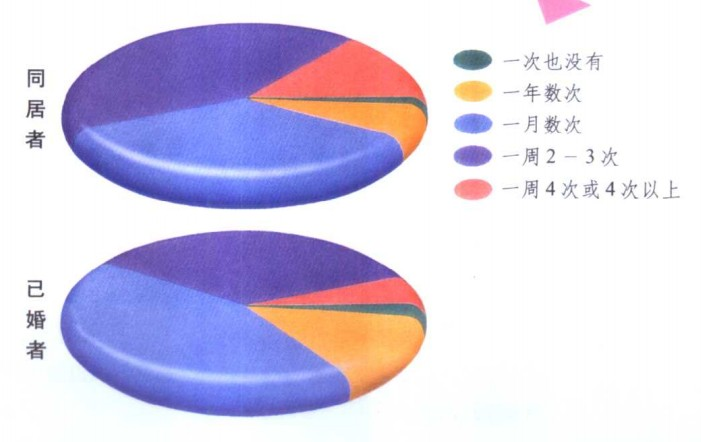
\includegraphics[width=0.7\textwidth]{Images/sexual_frequency_comparison.jpg}
	\caption{大多数人做爱的次数是多少？}
	\label{fig:sexual-frequency}
\end{figure}

\subsection{独身}

成年之后，人们通常都会与异性结成某种长期的关系，在这样一个大背景里，有人拒绝与异性结成关系，就不能不让人觉得有些反常。

造成独身的原因有很多。有人是因为眼界太高，总希望能出现一个更理想的意中人；有人是因为工作的压力太大；有的人是因为在与异性交往中遭遇过重大挫折，心理上还调整不过来；有人是因为害怕染上性病，或害怕怀孕；有人是因为对做爱不感兴趣；有人是因为自身的性别特征有问题；也有人是因为长期接触不到异性；还有人是因为晚年丧偶或离婚。

独身，对于不同的人来说，有着不同的意义：有的人觉得独身太自由了，想干什么就可以干什么；有的人把独身视为最方便的选择；而有的人本来不想独身，但由于某种原因又不得不这样做。从独身的定义上来说，只要是独身者就不能与异性做爱，但可以通过自慰，或者是异性间的抚摸、拥抱，来消除自身的性紧张。

\subsection{长期同性伙伴}

在有些国家里，同性恋者是允许结婚的，比如在挪威和丹麦，就通过了这方面的立法。不过，同性恋者一般不会通过婚姻的方式来表达彼此的爱意，固定双方的关系。两个同性恋者也能结成"一夫一妻"的关系，但这种情况存在着较大的性别差异。在男性同性恋那里，只有18\%的人结成了固定的性伙伴关系；而在女性同性恋那里，有72\%的人过的是"一夫一妻"生活。

如果是两个男性同性恋者走到一起，而且彼此年龄差距很大，那么就不管双方的关系有多久，都不要求对方是自己惟一的性伙伴，也就是说他们的关系比较开放。有关研究表明，与比较松散的异性恋关系（这种情况相对少一些）相比，松散结合的男性同性恋者更愿意与对方协商，采取什么办法能使性交更安全一些。

\subsection{非婚姻关系的界定}

非婚姻关系是一个宽泛的类别，指不以法律婚姻为形式、但具备亲密关系实质的伴侣关系。它涵盖长期同居、恋爱关系、非婚伴侣等多种形态。在当代社会，这类关系的数量显著增长，其法律与伦理地位也随之变得重要。

从关系实质而非形式来界定，是更实用的方式。判断一段关系是否属于"承诺性亲密关系"，可以参考几个指标：是否存在排他性约定、是否有共同生活的安排、是否有情感与经济的相互依赖、是否向外界公开承认。这些指标的存在与否，比是否登记结婚更能反映关系的真实状态。

\begin{itemize}
  \item \keyword{长期同居}：共同生活但未登记，法律地位因地区而异，权益保障差异显著。
  \item \keyword{长期恋爱关系}：未同居但存在排他性约定与持续的情感投入。
  \item \keyword{非排他性关系}：经双方同意不设排他性约定的关系，见本章"多元关系"相关论述。
  \item \keyword{事实婚姻}：部分地区在特定条件下承认其法律效力，认定标准不一。
\end{itemize}

法律与伦理上的核心议题在于：非婚姻关系中的"不忠"如何界定。由于排他性约定往往是口头且未明确的，双方对"什么算越界"的理解可能存在巨大差异。研究显示，许多所谓的不忠事件，其根源在于约定本身未澄清——一方认为线上调情无妨，另一方视之为背叛。因此，这一议题的处理起点，是把隐性的约定显性化。

另一个重要议题是权益保障。非婚伴侣在医疗决策、财产继承、社保福利与子女抚遇上，常面临法律上的不利地位，尤其在关系突然中断时更明显。了解所在地的具体规定、必要时通过意定监护、遗嘱或财产协议等方式作出安排，是负责任的实务考虑，而非对关系的"不信任"。

\begin{tcolorbox}[colback=pink!5!white,colframe=red!50!black,title=贴心小叮咛]
"我们是不是男女朋友"这个问题，往往远不如"我们之间哪些事是不能做的"重要。把后者说清楚，前者自然清楚。
\end{tcolorbox}
\subsection{修复与终止的决策}

当事关系中出现不忠、长期疏离或其他重大冲击后，当事人面临两个方向的选择：修复或终止。这一决策通常是在极度的情绪压力下作出的，因此需要一套冷静的评估框架。

第一组判断指标是伤害方的态度。修复的前提是承担责任，而非推卸。具体信号包括：是否完整交代（在当事人需要的范围内）、是否切断关系外联系、是否接受反复追问而非指责对方"纠缠"、是否愿意投入长期努力。若伤害方反复辩解、归咎于对方或外部、或急于"翻篇"，修复的前景通常不佳。

\begin{itemize}
  \item \keyword{责任承担}：承认行为、不推卸、不归咎于对方或酒精等外部因素。
  \item \keyword{实际行动}：切断关系外联系、主动透明、持续而非临时性的改变。
  \item \keyword{原有议题}：导致关系疏离的根本问题，是否双方都愿意面对。
  \item \keyword{受伤方状态}：能否在关系中保有基本的自我与尊严，而非长期低姿态。
  \item \keyword{安全前提}：若存在暴力、胁迫或严重控制，安全优先于一切其他考量。
\end{itemize}

第二组指标是关系的原有基础与议题可解性。若不忠源于关系长期疏离，而双方仍有修复关系的意愿，那么处理原有议题是修复的必经之路；若核心分歧属于不可调和的价值观差异（如是否要孩子、生活方式的根本取向），则修复的努力可能只是在推迟决裂。

第三点是时间尺度。研究显示，重大背叛后的修复通常以年计，且过程呈波动状态：好转一段时间后可能因某个触发因素再度恶化。当事人若期待几周内"恢复正常"，往往会在反复中累积挫败。因此，作出修复决定时应有长期投入的心理预期；而在评估期间，也不必急于给出最终答案——允许自己在信息更充分时再决定。

需要明确的是，选择终止不是失败。一段关系的结束可以是审慎评估后的理性选择。同样，选择修复也不意味着将就——它是基于现状的主动选择，且应当允许在未来重新评估。

\begin{tcolorbox}[colback=pink!5!white,colframe=red!50!black,title=贴心小叮咛]
不管最后选择哪一边，有一件事是一样的：这个决定应该是为了你自己的生活，而不是为了惩罚谁、或者向谁证明什么。做到这一点，两个选择都能让人走得更远。
\end{tcolorbox}

\section{育儿与夫妻关系}
% 移入："育儿与夫妻关系"
\subsection{新手父母的性生活}

从伴侣变为父母，是性关系最剧烈的转折之一。研究表明，多数伴侣在第一个孩子出生后性频率显著下降，且这一下降往往持续较长时间。理解这一变化的成因，能帮助新手父母把它看作阶段性的挑战而非感情的衰退。

生理与医学层面是第一个因素。产后身体需要恢复：阴道分娩可能伴随会阴伤口或撕裂，剖宫产需要腹部伤口愈合，哺乳期的激素变化（尤其是催乳素升高、雌激素下降）会显著降低性欲并导致阴道干涩。医生通常建议产后六周复查后再恢复性行为，但这只是身体的"及格线"，而非欲望的准备就绪。

\begin{itemize}
  \item \keyword{产后恢复}：伤口愈合、激素变化、哺乳影响，构成生理层面的直接障碍。
  \item \keyword{睡眠剥夺}：新生儿期的睡眠碎片化会显著压低性欲与情绪耐受度。
  \item \keyword{角色转换}：从伴侣到父母的认同转变，可能伴随对自己"性魅力"的重新定位。
  \item \keyword{注意力占用}：育儿几乎占据全部心智资源，留给彼此的注意力大幅减少。
  \item \keyword{身体形象}：产后身体变化可能带来不适与自我评价下降。
\end{itemize}

心理与关系层面的因素往往更为关键。角色认同的转变会带来复杂体验：一些新父母感到难以同时容纳"母亲/父亲"与"有性欲的伴侣"这两个身份；另一些则因身体被婴儿持续占用而产生对身体的排斥感。此外，育儿的实际分工失衡，也常是性欲下降的直接原因——当一方承担绝大部分照护与家务却缺乏支持与感谢，"不想做"往往是关系账目的体现，而非身体问题。

关系维护的关键在于重新协商。新手父母需要明确承认：这个阶段的标准必须下调，旧有的频率与方式不再适用。可行的做法包括：把优先级从"数量"转向"联结"（非性亲密同样重要）、在婴儿睡眠窗口寻找低压力时段、明确分工以减少一方的过载感，并把"这不是对方不爱我"这一认识反复说清楚。

\begin{tcolorbox}[colback=pink!5!white,colframe=red!50!black,title=贴心小叮咛]
第一个孩子出生后的那一年，大概是关系里最容易被误解的一段。请把"我们最近很少"理解为"我们正在育儿"，而不是"我们正在变淡"。这个阶段的低潮，多数会成为过去的一部分。
\end{tcolorbox}
上一节说了孩子出生后头几个月的影响，这一节把"怎么办"讲得更具体。很多新手父母最大的困惑不是"不爱对方了"，而是"明明爱，却完全没有那个念头"——先把这件事说清楚：\textbf{这不是感情问题，是身体问题}。
\textbf{一、先理解睡眠剥夺怎么"偷走"性欲}。带新生儿的睡眠是被切碎的——夜里每两三个小时醒一次，哪怕总时长凑够六七个小时，深睡眠也几乎为零。睡眠碎片化会让皮质醇（压力激素）维持在偏高水平，而哺乳期的催乳素生理性升高本身就会抑制性欲与润滑——这是激素层面的事实。理解这一点很重要：它意味着"没心情"不需要被解释成"变了心"，也不需要靠意志力硬撑，它需要的是睡眠与支持系统的修复。
\textbf{二、育儿分工与怨气，是产后期头号的"性欲杀手"}。如果夜里喂奶、白天家务、孩子的每件小事都默认落在一个人身上，另一个人"下班就躺"，那么上床时那股怨气不会消失——身体是诚实的，怨气会直接变成"不想被碰"。这个阶段谈性，先谈分工：把夜里轮班、周末补觉、家务清单摊开说清楚。分工顺了，很多"性冷淡"会自己好一半。
\textbf{三、接受碎片化的亲密}。孩子睡后的 20 分钟，可能是这个阶段唯一属于你们的时间。放弃"必须洗好澡、必须有前戏、必须完整流程"的执念——一次拥抱、一次抚摸、一次没有插入的亲热，都是真实的性生活，不是"凑合"。可以把"孩子睡后的第一段时间"固定下来作为优先窗口，但注意\textbf{别把性变成又一项待办任务}——哪天太累了就拥抱着睡，比勉强打卡更保护你们的关系。
\textbf{四、把隐私当成刚需来设计}。与老人同住或小户型，最缺的是"确定没人进来"的安心。门锁（或与同住者约定敲门规则）、白噪音掩盖声音、选孩子睡得最沉的时段——这些不是"讲究"，而是维持亲密的基础设施。给它一点认真，亲密才有容身之处。
\textbf{五、孩子撞见了怎么办}。几乎每个有幼儿的家庭都可能遇到：孩子半夜爬上大床，或在门缝里看到了什么。应对的核心是\textbf{平静}：简单回答"爸爸妈妈在亲热，这是大人表达爱的方式，我们想自己待一会儿"，然后把孩子送回房间。不必惊慌、斥责或编一个可怕的谎言——过度的反应才会把"正常的亲密"变成孩子眼里的"可怕的事"。事后做两件事：养成锁门的习惯；用孩子听得懂的方式回答他的追问（三到六岁的孩子需要的是"爸妈相爱"的安全感，而不是细节）。一次撞见本身不会造成创伤，父母的反应方式才决定它变成什么。
\textbf{六、别忘了避孕，也别把"二胎"变成压力}。哺乳期闭经不等于安全期——排卵往往在月经复潮之前就恢复了，产后复查时就把避孕方式谈好。而如果确实计划要二胎，也知道第二次的重启往往比第一次更难：精力减半，还有老大的需求要照顾。允许进度慢一些。
最后一条界线：如果产后几个月过去，性欲持续消失，并且伴随着情绪持续低落、对什么都提不起兴趣、睡眠比带孩子所必需的还要差——\textbf{这不是"累了"，请做一次产后抑郁筛查}（父亲同样可能产后抑郁）。把它当成健康问题去处理，而不是当成关系问题去互相埋怨。
\subsection{育儿期的性需求变化}

育儿期的性需求变化，双方往往并不对称，而这种不对称本身就是关系张力的重要来源。理解双方各自发生了什么，是减少误解的关键。

对生育的一方（通常是母亲）而言，变化通常是多重的。激素层面，哺乳期的催乳素升高会抑制性欲，雌激素下降导致阴道干涩与性交不适；身体层面，分娩的恢复、盆底肌的变化、母乳喂养带来的身体持续被占用感，都会降低对亲密接触的容忍度；心理层面，睡眠剥夺、焦虑、以及对"我的身体不再属于我"的感受，会进一步抑制欲望。

\begin{itemize}
  \item \keyword{生理抑制}：哺乳期激素变化、干涩、盆底不适，直接降低性欲与舒适度。
  \item \keyword{身体占用}：持续哺乳与被婴儿接触，使身体对进一步接触产生排斥。
  \item \keyword{认知负荷}：育儿相关的心智占用极高，难以切换到性情境。
  \item \keyword{非生育方}：可能出现被忽视感，或对"何时恢复到从前"抱有急切期待。
  \item \keyword{需求错位}：一方需要支持与休息，另一方需要亲密与确认，两者常被互相误读。
\end{itemize}

对非生育的一方（通常是父亲）而言，变化通常不如上述剧烈，因此容易产生落差感。常见体验包括：感到被排除在母婴联结之外、怀念从前的关系、把性频率下降解读为吸引力丧失、或因为不敢提出而长期压抑。这些感受如果得不到表达与回应，容易累积为怨气。

这里存在一个极具破坏性的误解循环：一方因疲惫与过载而降低性欲，另一方解读为被拒绝，于是加强要求或表达不满，而要求与不满又进一步消耗前者的精力与情绪，使性欲更低。打破循环的关键，是让双方都能说出自己的处境——疲惫与过载，以及被忽略与不被渴望——并把"这不是谁的错"作为共同的出发点。

\begin{tcolorbox}[colback=pink!5!white,colframe=red!50!black,title=贴心小叮咛]
育儿期的性需求差异，几乎不是"谁更爱谁"的问题，而是两个人资源分配的问题。当一方精疲力竭，另一方需要的往往不是更多要求，而是先说一句"我来带，你去睡一会儿"。
\end{tcolorbox}
\subsection{时间与精力分配}

育儿期最稀缺的资源不是感情，而是时间与精力。多数"性生活不和谐"在这一阶段其实源于资源枯竭，而非感情变化。因此，有效的干预往往落在资源分配上，而非直接谈性。

时间方面，婴幼儿期的特点是不可预测与高侵入。喂奶、哄睡、夜醒、生病，会随时中断成人的计划，使"等孩子睡了再说"这一策略经常失败。同时，长期没有连续睡眠会显著降低情绪调节能力，使原本可协商的小事升级为冲突。

\begin{itemize}
  \item \keyword{睡眠剥夺}：持续的睡眠碎片化降低性欲、情绪耐受与冲突处理能力。
  \item \keyword{注意力占用}：育儿的心智负荷是持续的，难以在需要时切换到亲密模式。
  \item \keyword{时间不可控}：婴幼儿期的作息多变，依赖"自然发生"的机会往往落空。
  \item \keyword{分工失衡}：一方承担绝大部分照护时，其性欲与实际可用时间都会显著下降。
\end{itemize}

实践上，有几项策略被证明有效。第一是主动排期，而不是等待随机机会——这与长期关系中的排期原则一致，在育儿期更为必要。第二是接受"片段化"的亲密：十分钟的拥抱与交谈，其价值不亚于一次完整的性行为，且在现实中更可实现。第三是明确分工与轮换：让承担主责照护的一方定期获得完整的不被打扰的休息，这既能恢复体力，也直接改善其对亲密的意愿。

另一个容易被忽略的因素是外部支持。能否获得家人帮助、能否负担托育、能否有固定的独处时间，对育儿期的性关系有显著影响。因此，把"找时间独处"作为关系维护的正式任务来安排，而不是当作可有可无的奢侈，是有实际收益的做法。

\begin{tcolorbox}[colback=pink!5!white,colframe=red!50!black,title=贴心小叮咛]
在这个阶段，"我们什么时候能有时间"这个问题，答案几乎从来不是"等有空的时候"，而是"现在就把它写进日程里"。
\end{tcolorbox}
\subsection{伴侣关系的维护策略}

育儿的压力会持续数年，若把关系维护推迟到"孩子大一点再说"，往往已经积累了难以逆转的疏离。因此，需要一些可以在高压环境下维持的方法。

最基础的是"微小时刻"的持续投入。研究者提出"情感存款"的概念：日常中每一次关注、回应、感谢与善意的互动，都是向关系账户里存款。育儿期最缺的是大块时间，但微小时刻的成本极低——出门前的一个拥抱、一条问候消息、在对方疲惫时递上一杯水、睡前五分钟的交谈。这些互动积累起来，构成了关系在压力下仍能维持温度的基础。

\begin{itemize}
  \item \keyword{微小时刻}：日常的关注、感谢与身体接触，是低成本高回报的关系存款。
  \item \keyword{定期检视}：每周或每两周留出固定时间，专门谈关系而非育儿事务。
  \item \keyword{明确分工}：把家务与育儿的分工具体化，避免一方长期过载。
  \item \keyword{保护独处}：为双方各自安排不被打扰的休息时间，避免耗竭。
  \item \keyword{共同活动}：保留哪怕很低频的共同活动，如散步或一起看一集剧。
  \item \keyword{外部支持}：主动争取家人帮助或托育资源，把独处时间当作正式任务安排。
\end{itemize}

"定期检视"在育儿期尤其重要，且需要一条特殊规则：检视对话中，育儿事务与关系议题要分开谈。许多伴侣的"谈话时间"全部被孩子的安排占满，结果双方从未真正交流过彼此的状态。把两者分开，哪怕只是每周二十分钟，也能显著缓解"我们只是共同育儿的同事"这种感受。

最后一点关于期待管理。育儿期的关系质量通常无法与无子女时期相比，且这一状况往往要持续数年。接受这一现实，不意味着放弃，而意味着设定合理的目标：目标不是"保持从前的状态"，而是"在这段高压期里，不失去彼此的联结"。这个目标更现实，也更容易达成。

\begin{tcolorbox}[colback=pink!5!white,colframe=red!50!black,title=贴心小叮咛]
在育儿期，能维持关系的东西往往很小：一句谢谢、一次主动的分担、睡前五分钟的聊天。别小看它们——它们撑起的是你们之后十几年的基础。
\end{tcolorbox}

面对着一个刚刚来到人间的小宝宝，夫妻关系和性生活势必都会受到影响，尤其是在孩子出生后的头3个月里，这种影响会更大。一会儿是强烈的爱意和快乐，一会儿是沉重的疲劳和少许的失望，不同的感受轮换着冲击他们的身心。尽管从女方的角度来说，生完孩子后只要感觉舒适，随时都可以做爱，但很多夫妻却迟迟不肯恢复性生活。造成这种迟疑不前的原因很多，有时是人困马乏，即使想干那事儿也干不动；有时是性交疼痛（这种疼痛有可能来自分娩创伤的缝合处）；有时是乳房疼痛（哺乳期间乳房变大、乳头出现皲裂，都有可能引起疼痛）；还有时是因为这个阶段女方的形体形象不佳，让男人不怎么感兴趣；也有时是因为找不到两个人独处的机会。

在亲眼看到自己的妻子分娩时遭遇了那么痛苦的折磨后，有些初为人父的男人再干那种事情就有些内心不安了。这时，要想恢复往日的亲昵，不插入的性交是非常理想的做法，它能够制造出和插入式性交完全一样的性愉悦来。

孩子可以粘和并强化夫妻关系。在孩子未满5周岁之前，婚姻的满意程度时时都会遭到孩子的暗中"破坏"。造成这种情况的原因，一方面是养育孩子必定会有压力，必须满足某些需求；另一方面是夫妻关系的焦点，必然会从彼此间的感情需要转移到怎样去满足孩子的需要。任何人当上了爸爸或妈妈后，都必然会体会到如何扮演好这个新角色的压力。喂养孩子的方法对不对？自己能不能算得上一个优秀的父亲或母亲？在养育孩子方面两个人怎样分工好？谁应该对孩子负主要责任？做完分工后如果丈夫觉得自己被排除在外了，或者妻子觉得自己的担子太重，那该怎么办？假如妻子想要回到工作岗位上去，那又该怎么办？当夫妻俩有了孩子之后，这些问题都有可能出现。尽管有些夫妻十分幸运，很快就找到了适合自己情况的解决办法，但大多数人还是需要下一番大力气，才能走出困境。

\section{性幻想}
% 移入："性幻想"（另见第二篇"性偏好与性幻想"节，注意分工）
\subsection{性幻想的普遍性}

性幻想（sexual fantasy）指在清醒状态下出现的、带有性内容的想象。它在人群中的普遍程度远超多数人的预期：多项调查显示，绝大多数成年人报告有性幻想经历，且相当比例的人在其性生活中会主动运用幻想。

需要澄清的第一个误解是"有性幻想就是不知足或不忠"。研究显示，性幻想与关系满意度、承诺水平并无负相关——拥有稳定关系的人同样会有大量幻想，且其内容常与伴侣无关。幻想是心智的正常活动，与实际行动的意愿并不等同。

\begin{itemize}
  \item \keyword{普遍性极高}：绝大多数成年人报告有性幻想，频率与内容因人差异极大。
  \item \keyword{与关系质量无关}：有幻想不代表关系有问题，也不代表不忠倾向。
  \item \keyword{内容多样}：从贴近现实的场景到完全不可能的情境，均可出现。
  \item \keyword{主动性使用}：许多人在性活动中主动借助幻想来提升唤起。
\end{itemize}

第二个需要澄清的是"幻想的内容等于真实的欲望"。研究反复显示，许多幻想包含本人不愿在现实中实现、甚至明确排斥的元素。幻想的功能往往不在"预示行为"，而在心理层面的象征性满足——例如关于"被强势引领"的幻想，未必表示想要被支配，而可能指向对"可以放下控制、不必负责"的渴望。

从发展角度看，性幻想通常自青春期开始活跃，并随经验与认知变化而调整内容。成年期的幻想内容相对稳定，但会随关系状态、生命阶段与心理状态发生幅度不等的波动。这一稳定性提示，幻想在很大程度上反映了个体相对固定的心理需求结构。

\begin{tcolorbox}[colback=pink!5!white,colframe=red!50!black,title=贴心小叮咛]
有性幻想，不代表你对现在的关系不满意，也不代表你在心里"背叛"了谁。它更像是一个只属于你自己的房间——你可以在里面放任何东西，而不用向任何人交代。
\end{tcolorbox}
\subsection{性幻想在伴侣关系中的角色}

性幻想在伴侣关系中的作用是双向的：它可以成为增进亲密的资源，也可以成为疏离的来源。区分两者的关键，在于幻想是被分享、被接纳，还是被隐瞒、被评判。

作为资源的一面，分享幻想能带来多重收益。它使双方更了解彼此的需求结构，为探索提供方向；它本身即是一种亲密的自我暴露，能加深信任；它还可以为长期关系中的性互动注入新鲜感，对抗习惯化。研究显示，能够就幻想进行开放交流的伴侣，其性满意度通常更高。

\begin{itemize}
  \item \keyword{增进了解}：分享幻想提供关于需求的具体信息，远胜于猜测。
  \item \keyword{深化亲密}：愿意暴露私密想象，本身是一种信任的表达。
  \item \keyword{对抗习惯化}：幻想为长期关系的性互动提供新的方向与素材。
  \item \keyword{共同探索}：部分幻想可转化为双方都愿意尝试的实践。
\end{itemize}

作为风险的一面，则来自几种常见情形。第一是被迫暴露：一方在未经同意的情况下发现对方的幻想内容（如浏览记录），容易引发强烈的不安与误读。第二是评判反应：分享后遭到嘲笑、嫌恶或道德谴责，往往造成持久的信任损伤，使对方从此封闭。第三是幻想替代现实：若性活动长期依赖特定幻想才能完成，可能削弱对真实伴侣的回应能力。

因此，实践上宜遵循几条原则：分享是邀请而非要求，对方有权不参与；分享从低风险内容开始，逐步推进；明确区分"说出来"与"要去做"；以及——最重要的一条——不评判。若一方对某类幻想感到不适，可以明确表示不愿参与，但不宜以道德姿态贬低对方。安全的气氛一旦被破坏，重新打开会极为困难。

\begin{tcolorbox}[colback=pink!5!white,colframe=red!50!black,title=贴心小叮咛]
如果伴侣愿意把幻想告诉你，请把它当作一份礼物而不是一份供词。你的第一反应，很可能决定了他/她以后还会不会对你敞开心门。
\end{tcolorbox}
\subsection{常见主题与个体差异}

性幻想的主题分布广泛，但研究发现某些主题在人群中出现的频率明显更高。了解这些常见主题，有助于把个人的幻想置于正常范围之内看待，减少不必要的自我否定。

跨文化研究中报告频率较高的主题包括：与熟悉的人发生关系的想象（如朋友的伴侣、同事）、在具有情感张力的情境中（如重逢、被渴望）、权力动态相关的场景（支配或服从）、多人参与的场景、以及与自己现实伴侣的想象。这些主题在不同性别、不同文化中的分布有差异，但重叠范围很大。

\begin{itemize}
  \item \keyword{熟悉对象}：对认识但并非伴侣的人产生想象，是最常见的主题之一。
  \item \keyword{权力动态}：支配与服从的幻想普遍存在，且在不同性别中均有报告。
  \item \keyword{多人场景}：报告频率不低，但多数人并不希望现实中实现。
  \item \keyword{情境张力}：如重逢、追求、被渴望，强调情感与心理的张力而非纯粹的身体。
  \item \keyword{与伴侣的想象}：相当比例的人以现实伴侣为幻想对象，尤其在长期关系中。
\end{itemize}

性别差异方面，统计趋势显示：男性报告的幻想频率与视觉具体性平均更高，内容更常涉及多个对象或明确的性行为场景；女性的幻想平均更常包含情感叙事、情境铺垫与关系元素。但这一差异是分布层面的趋势，个体重叠极大，不应据此预判具体的人。

个体差异则更为显著。研究显示，幻想内容的丰富度与个人经验、性态度、想象能力与情绪状态都相关。此外，幻想会随生命阶段变化：青春期常以探索与身份确认为主，成年期常与关系需求相交织，而老年期的幻想可能更多围绕亲密与回忆。理解这一演变，有助于把幻想视为动态的心理活动，而非固定的人格标记。

\begin{tcolorbox}[colback=pink!5!white,colframe=red!50!black,title=贴心小叮咛]
如果你曾因为自己的幻想内容而自责，不妨先知道一件事：你想到的那些，绝大多数人都想过。差别只在于谁说出来、谁没说。
\end{tcolorbox}
\subsection{如何看待伴侣的性幻想}

得知伴侣的性幻想内容，对许多人而言是一次情感上的考验。尤其当幻想涉及他人、多人的场景或自己无法提供的元素时，容易引发被否定感、嫉妒与不安。如何处理这一情境，对关系影响深远。

值得先区分几个情形。第一是自己主动询问后得知，还是无意间发现。无意间发现（如看到浏览记录）往往伴随着"被隐瞒"的额外伤害，冲击通常更大。第二是幻想中是否包含具体可识别的对象。若幻想指向熟识的人，现实的嫉妒更容易被激活。第三是伴侣是否愿意分享与讨论。愿意开放沟通者，其幻想通常更接近"无害的心理活动"。

\begin{itemize}
  \item \keyword{区分性质}：先厘清是常规心理活动，还是已经涉及实际的关系外投入。
  \item \keyword{识别自身反应}：嫉妒与被否定感是正常反应，但不必立即按它行动。
  \item \keyword{避免审判}：以道德姿态谴责，只会关闭沟通，不解决任何问题。
  \item \keyword{表达感受}：可以说明自己的不适，但以"我感到"而非"你有问题"的方式。
  \item \keyword{设定边界}：就"哪些可以、哪些不行"达成明确约定，而非笼统表态。
\end{itemize}

处理的核心，是把"幻想"与"行为"分开。大量的幻想并不指向行动意图，它们的功能是心理层面的象征性满足。因此，面对伴侣的幻想，更有用的提问不是"你是不是想那么做"，而是"这个幻想对你来说意味着什么"。后者的答案通常更能揭示对方真实的心理需求，往往也更容易被接纳——例如，多人的幻想可能意味对"被强烈渴望"的向往，而非真的想要多人关系。

同时也需要承认：即便理解了机制，不适感仍然可能持续存在。这种情况下，明确表达感受并协商边界是正当的、必要的。例如，可以接受对方持有某种幻想，但明确表达不愿意被拿来做比较，或不愿在性活动中被要求扮演某个角色。把边界说清楚，比要求对方改变幻想内容更现实——后者通常做不到，也容易造成隐瞒。

\begin{tcolorbox}[colback=pink!5!white,colframe=red!50!black,title=贴心小叮咛]
幻想几乎是改不掉的，但边界是可以谈的。与其要求对方"不许想"，不如说清楚"我希望我们在现实里怎么做"——前者只会让他/她学会不说，后者才能真正解决问题。
\end{tcolorbox}

\section{助兴工具与春药}
% 移入："助兴工具"、"春药"、"性描写与助兴用具"
\subsection{助兴工具的类型与用途}

助兴工具（性辅助用品，俗称情趣用品）指用于增强性体验的器具、用品与辅助物。其种类在近数十年迅速扩展，已从边缘化的亚文化产物转变为广泛使用的日常消费品。

按功能可分为几大类。刺激类器具用于提供身体刺激，如振动器、按摩棒、吸吮器；辅助类用于改善润滑与舒适度，如各类润滑剂；情趣类用于营造氛围与角色扮演，如服饰、道具；护理类用于清洁、保养与卫生，如专用清洁剂、消毒用品。

\begin{itemize}
  \item \keyword{刺激类}：振动器、按摩器、吸吮器等，用于提供多样化的身体刺激。
  \item \keyword{润滑类}：水基、硅基、油基润滑剂，改善干涩与摩擦不适。
  \item \keyword{扩张类}：用于肛交或其他逐步适应性行为训练的器具，需谨慎使用。
  \item \keyword{情趣类}：服饰、道具与情境用品，用于增强氛围与探索。
  \item \keyword{护理类}：清洁剂、消毒用品与存放器具，属安全使用的必要配套。
\end{itemize}

其用途可归纳为几个层面。第一是功能补偿：对存在唤起困难、干涩、或需要特定刺激才能达到高潮的人，器具能提供有效帮助。第二是体验拓展：为长期关系注入变化，对抗习惯化。第三是自我探索：帮助个体了解自身敏感区与偏好，这在缺乏伴侣时尤其有价值。第四是关系互动：作为双方共同探索的工具，增进沟通与亲密。

关于使用，有几条实用建议值得留意。润滑剂是最被低估的一类辅助用品——大量性交不适其实源于润滑不足，而使用润滑剂可以显著改善体验。选择时应按场景区分：水基润滑剂兼容绝大多数材质与安全套，但易干需补涂；硅基润滑剂持久但不可与硅胶器具或硅胶安全套同用；油基润滑剂会破坏乳胶安全套，不应与乳胶安全套配合使用。

\begin{tcolorbox}[colback=pink!5!white,colframe=red!50!black,title=贴心小叮咛]
如果只能推荐一样"性辅助用品"，那大概就是润滑剂。它便宜、易得、无创，而且能解决的问题比你想象中多得多——很多所谓"不舒服""没感觉"，其实只是缺了它。
\end{tcolorbox}
\subsection{春药的科学审视}

“春药”（aphrodisiac）指被认为能增强性欲或性能力的物质。这一概念在人类历史上源远流长，几乎每种文化都流传着相关配方或食材。但从现代循证医学的角度看，其证据基础极为薄弱，而误解与风险却相当显著。

首先需要区分三个容易混淆的效果：提升性欲（欲望）、改善性功能（如勃起或润滑）、以及仅产生心理暗示。市面上多数被宣传为"春药"的产品，其实际作用机制通常是后者——通过仪式感、期待效应与暗示，使使用者产生主观改善的感受。这一效应真实存在（即安慰剂效应），但它不依赖于产品本身的成分。

\begin{itemize}
  \item \keyword{食物类}：牡蛎、韭菜、动物器官等，缺乏可靠的对照研究支持其催情作用。
  \item \keyword{植物类}：育亨宾、人参等有部分研究，但效果有限、结论不一致，且有不良反应风险。
  \item \keyword{激素类}：睾酮制剂有明确适应证，但仅对确诊缺乏者有意义，且属处方药。
  \item \keyword{血管活性药物}：如西地那非等，用于治疗勃起功能障碍，非"催情"用途。
  \item \keyword{不明成分产品}：市售"壮阳"保健品常含未标注的处方药成分，风险最高。
\end{itemize}

需要特别警示的是网络与线下渠道销售的大量"壮阳"产品。检测研究反复发现，其中相当比例非法添加了西地那非等处方药成分，且剂量不明、标识不清。这对心血管疾病患者尤其危险——此类药物与硝酸酯类药物合用可引起严重的血压下降，甚至危及生命。此外，宣称"纯天然"也绝不等于安全，植物成分同样可能有毒性或与其他药物相互作用。

对性欲或性功能存在困扰的人，正确的路径是就医评估，而非自行尝试来路不明的产品。性欲低下与勃起困难的成因很多，其中不少是可治疗的（激素缺乏、药物副作用、血管疾病、焦虑等）。明确的诊断加上规范的治疗，远比盲目"进补"更有效，也更安全。

\begin{tcolorbox}[colback=pink!5!white,colframe=red!50!black,title=贴心小叮咛]
如果一个东西号称能"催情"、又不用医生开方、还能在网上随便买到——请先怀疑它的成分表。真正有效的药物都有明确的适应证与风险，也需要专业人员的判断。
\end{tcolorbox}
\subsection{使用风险与法律边界}

助兴工具的使用整体上属于私人领域的合法行为，但仍存在若干需要留意的风险与法律边界。了解这些，既是对自己负责，也涉及对他人的尊重。

健康与安全风险首先是材质问题。部分廉价产品使用不合格的软胶或含邻苯二甲酸酯的材料，长期接触可能引起皮肤刺激或过敏反应。优先选择明确标注材质（如医用硅胶、ABS 塑料、玻璃、不锈钢）且无异味的产品，是基本的自我保护。其次是清洁问题：多孔材质（如某些软胶）不易彻底消毒，容易滋生细菌，若在性行为中使用或前后交叉使用，可能增加感染风险。

\begin{itemize}
  \item \keyword{材质风险}：劣质材料可能含刺激性成分，宜选医用硅胶等明确标注者。
  \item \keyword{清洁与感染}：多孔材质难以彻底消毒，交叉使用可能增加感染风险。
  \item \keyword{共享风险}：多人共用未经消毒的器具，存在性传播感染风险。
  \item \keyword{物理损伤}：使用不当可能造成黏膜擦伤、撕裂或异物滞留。
  \item \keyword{法律边界}：涉及未成年人、非自愿或拍摄传播他人私密影像，均属违法。
\end{itemize}

共享使用是最容易被忽略的风险点。器具在多人之间共用且未经有效消毒时，存在传播细菌、真菌与人乳头瘤病毒等病原体的可能。可行做法包括：使用安全套覆盖器具（并每次更换）、使用后按材质进行适当消毒、以及避免在肛交与阴道使用之间不更换或消毒地转移器具。若出现不适症状，应及时就医并如实说明情况。

法律层面的边界主要有几类。第一，涉及未成年人的任何性内容或性行为，无论形式，均属违法。第二，未经对方同意拍摄、保存或传播性影像，在多数地区已构成违法甚至犯罪，且此类行为对受害者的伤害极为严重。第三，使用器具对他人实施非自愿行为，与任何形式的性侵无异。这些边界与器具本身无关，而与是否侵犯他人的自主权有关。此外，各地对器具的销售与进口有不同的管理规定，购买前了解所在地的规定是必要的。

\begin{tcolorbox}[colback=pink!5!white,colframe=red!50!black,title=贴心小叮咛]
器具本身是工具，用法才是关键。三条底线值得记住：不给没同意的人用、不在没征得同意时拍摄、不共用未经消毒的器具。做到这三条，绝大多数麻烦都能避开。
\end{tcolorbox}

\section{充满性魅力的衣着}
% 移入："充满性魅力的衣着"
\subsection{内衣与性魅力}

内衣在性魅力中扮演的角色颇为特殊。它位于私人与公开的边界上：既是被遮蔽的，又是被设计的、有意被看见的。这一双重性使内衣同时承载了自我表达、伴侣互动与文化规范三重意义。

从个体层面看，穿着的内衣物常常与自我感受直接相关。研究显示，选择"让自己感觉好看"的内衣，能显著提升穿着者的身体自信与性自我感受，这一效应甚至独立于伴侣是否看到。换言之，内衣对性魅力的作用，首先是对自己起作用的。

\begin{itemize}
  \item \keyword{自我感受}：穿着自认好看的内衣可提升身体自信与性自我评价。
  \item \keyword{伴侣互动}：作为信号与礼物，可在伴侣间传递"我为这次见面做了准备"。
  \item \keyword{情境营造}：脱离日常的穿着本身即构成一种情境转换，有助于进入性的心理状态。
  \item \keyword{舒适优先}：若为取悦他人而长期牺牲舒适，反而可能削弱性体验。
\end{itemize}

需要警惕的是内衣相关的身体焦虑。商业宣传常以高度标准化的身形呈现内衣效果，容易使人产生"我的身体不适合穿这个"的自我否定。实际上，内衣的品类极其多样，其设计初衷本就在于适配不同身形与偏好。若某种款式让人不适，问题通常不在于身体，而在于款式选择。

在伴侣互动中，内衣的作用更多是符号性的：它传达的往往是"我为你准备了这个时刻"这一意图，而非单纯的视觉刺激。因此，它对关系的作用取决于双方的共同理解——对某些伴侣而言这是有效的调剂，对另一些则无关紧要。把它当作可选的工具而非必需的义务，是更健康的态度。

\begin{tcolorbox}[colback=pink!5!white,colframe=red!50!black,title=贴心小叮咛]
买内衣的第一标准，应该是"我穿上它感觉自己好看"，而不是"他/她会不会喜欢"。取悦自己的那件，往往才是最有魅力的一件。
\end{tcolorbox}
\subsection{着装与自我表达}

衣着是性自我表达的重要媒介之一。人在选择穿什么时，实际上一直在做关于"我想被如何看待"的沟通——这一沟通的对象既包括他人，也包括自己。

从心理学角度看，着装与自我认知之间存在双向影响。研究发现，穿着会影响穿着者的自我感受与行为倾向（这一现象被称为"着装认知"效应）。例如，穿着自认为得体的衣物可能提升自信与掌控感；反之，长期因体型焦虑而选择遮掩性衣物，可能强化对身体的负面评价，形成循环。

\begin{itemize}
  \item \keyword{自我认知}：着装影响穿着者对自身的感受，具有心理层面的实际效应。
  \item \keyword{身份表达}：通过风格传达自己的取向、审美与身份认同。
  \item \keyword{情境切换}：特殊的穿着可标记特殊的场合，帮助心理状态转换。
  \item \keyword{文化规范}：不同社群与场合对"得体"的标准差异显著，需自行判断。
\end{itemize}

需要处理的一个现实张力是：性感的着装与社会评价之间的关系。在许多文化环境中，女性的着装常被附加额外的道德评判——穿得暴露可能被解读为"暗示"，甚至被用于对受害者的不当归责。这一双重标准是不合理的：任何人有权决定自己的穿着，而"她穿成那样"从来不是任何侵害行为的正当理由。

对个体而言，更实用的框架是自问三个问题：这件衣服是否让我感到自在？它是否符合我此刻想表达的？在当下的场合中，我是否愿意承担可能的关注？这三个问题的答案因人、因时、因场合而不同，并不存在放之四海皆准的标准。重要的是把决定权留在自己手里，而不是交给外界的期待或评判。

\begin{tcolorbox}[colback=pink!5!white,colframe=red!50!black,title=贴心小叮咛]
你穿什么，是你对自己说的话，不是你对别人发出的邀请。这个区别，需要被反复说清楚——它对每个人都重要，对年轻人尤其重要。
\end{tcolorbox}
\subsection{伴侣间的着装沟通}

伴侣之间的着装互动，是一种常被忽略却相当有效的沟通渠道。它兼具表达、邀请与确认的功能，且常常无需言语即可完成。

正面的互动通常表现为欣赏与回应。伴侣对彼此穿着的具体赞赏（"你今天这样很好看"），不仅是礼貌，更是对"我仍然看着你、仍然觉得你有吸引力"的持续确认。对于长期关系而言，这类确认的价值尤为突出——它抵抗着习惯化带来的"视而不见"。

\begin{itemize}
  \item \keyword{具体赞赏}：具体的欣赏比笼统的夸奖更有效，也更容易被记住。
  \item \keyword{发出邀请}：特定的穿着可作为一种低压力的邀请信号，避免直接开口的压力。
  \item \keyword{替代误解}：与其期待对方察觉，不如就"哪些打扮会让你有感觉"直接交流。
  \item \keyword{尊重边界}：对穿着的要求或限制，需要协商而非强加。
\end{itemize}

负面的互动则常见于几种情形。第一种是长期毫无反馈：一方精心准备却得不到任何注意，久而久之放弃尝试。第二种是要求与控制：以"我是为了你好"或"你穿这样像什么"为由限制对方的穿着，这已经越过了边界，属于控制行为的范畴。第三种是错位解读：一方以为自己在发出邀请，另一方完全没接收，双方各自失落。

实践上，沟通的关键是把隐性信号显性化。与其期待对方从着装中读出意图，不如把话说明白——例如直接告诉对方"我很喜欢你穿那件衬衫的样子"，或"如果我今晚穿那件裙子，你大概可以猜到我想要什么"。这种明确的交流看似损失了含蓄之美，实际上大幅降低了双方误读的成本，其收益往往超出预期。

\begin{tcolorbox}[colback=pink!5!white,colframe=red!50!black,title=贴心小叮咛]
看见对方的努力并说出来，是关系里成本最低、回报最高的一件事。一句"你今天真好看"，往往比一件新衣服更有用。
\end{tcolorbox}

% ⇒ [已移出] 章「新婚首夜」→ position.tex
\chapter{家庭形态的多样性}
% [框架] 2026-09-21 新增：补齐知识框架缺口模块。
\section{年龄差伴侣}
\subsection{关系中的权力与期待}

年龄差伴侣指双方年龄存在明显差距的关系。这一形态本身并无问题，但其带来的权力结构与期待差异，需要被清晰地认识与处理。

权力差异是核心议题。研究指出，年龄差距往往伴随资源、经验、社会资本与话语权的差异——年长一方通常在经济能力、社会阅历与关系经验上更具优势。这一不均衡本身并不必然有害，但如果不被察觉与沟通，容易在决策、冲突处理与日常安排中逐渐固化为主导与从属的模式。

\begin{itemize}
  \item \keyword{资源差异}：经济能力与社会资本的差距可能影响关系中的话语权。
  \item \keyword{经验差异}：关系经验的不对等可能造成期待与判断的落差。
  \item \keyword{决策模式}：若决策长期由一方主导，容易形成不平等的惯性。
  \item \keyword{社会评判}：外界常对年龄差关系作出预设的负面解读。
\end{itemize}

期待差异则是另一重要维度。不同年龄段的生命任务往往不同：二十余岁者可能处于探索与建立阶段，四十余岁者可能面临职业稳定与家庭责任，而年龄更长者可能已开始考虑退休与健康规划。这些差异若不沟通，容易在多年后集中显现——例如，一方希望尽快要孩子而另一方已不打算，或一方计划退休生活而另一方仍在事业上升期。

处理的核心在于主动对齐。实践上，定期就中长期的人生规划（职业、居住、生育、养老）进行明确对话，是必要且有效的做法。同时，对权力差异应保持自觉：较有优势的一方应主动留意自己是否无意中主导了决策，而处于相对弱势的一方也应练习表达自己的意愿。外部评判难以避免，但关系内部的平等与坦诚，是可以主动建立的。

\begin{tcolorbox}[colback=pink!5!white,colframe=red!50!black,title=贴心小叮咛]
年龄差本身不是问题，能不能"对等地商量事情"才是。请常常问一句：这个决定，是我们一起决定的，还是某一方说了算？
\end{tcolorbox}
\subsection{性需求差异的协商}

年龄差伴侣在性需求上的差异，是这一关系形态中常被忽略却实际存在的议题。理解其规律与协商方式，有助于减少误解。

性需求随年龄的变化是有规律可循的。总体趋势上，男性的睾酮水平随年龄缓慢下降，性欲与勃起功能可能逐渐变化；女性则受围绝经期与绝经后的激素变化影响，可能出现性欲下降、阴道干涩与性交不适。这些变化在个体间差异极大，且并非所有人的体验相同，但年龄跨度较大时，双方处于不同生命阶段的可能性更高。

\begin{itemize}
  \item \keyword{年龄相关变化}：激素变化可能影响性欲与性反应，个体差异极大。
  \item \keyword{阶段错位}：双方可能处于不同的身体与心理阶段，需求不同步。
  \item \keyword{归因误区}：把需求差异归因为"不爱"或"不够努力"是常见误解。
  \item \keyword{可医学干预}：干涩、勃起困难等多数有可用的医学处理方式。
\end{itemize}

协商的原则与一般伴侣一致，但在年龄差关系中需要更主动的沟通。第一，避免道德化解读：需求差异是身体与阶段的问题，而非感情或努力的证据。第二，探求医学可能：许多年龄相关的性功能变化有可用的处理方式（如润滑剂、局部雌激素、勃起功能治疗等），因此不应把变化视为不可改变的必然。第三，扩展对性的定义：当插入变得不便时，其他形式（手交、口交、爱抚、感官聚焦）同样可以维持亲密——这一点在年龄差关系中往往更具实际意义。

最后需要提醒的是：年龄差关系中的性需求差异，往往随时间而扩大，因为双方的衰老速度与阶段差异会持续存在。因此，把协商当作持续的、需要定期回访的议题，而非一次性解决的问题，是更务实的做法。早期建立坦诚沟通的习惯，对应对后期的变化尤其重要。

\begin{tcolorbox}[colback=pink!5!white,colframe=red!50!black,title=贴心小叮咛]
身体会变，这跟爱没关系。遇到"不如从前"的时候，第一件事应该是去看医生，第二件事是一起想别的办法——而不是互相怀疑。
\end{tcolorbox}
\subsection{社会眼光与应对}

年龄差伴侣普遍面临来自外界的评判，这些评判的形式与强度往往超出当事人的预期。处理这些外部压力，是关系稳定的实际课题。

评判的常见形式包括：对动机的臆断（认为年轻一方图钱、年长一方图色）、对关系性质的不认可（认为不可能是真爱）、对具体处境的负面预设（如生育困难、晚年照护问题）、以及公开的议论与玩笑。这些评判通常带有双重标准——同样的年龄差，在不同性别组合中受到的评判程度往往不同。

\begin{itemize}
  \item \keyword{动机臆断}：外界常预设关系中存在功利动机，忽视真实的情感基础。
  \item \keyword{双重标准}：评判强度常因性别组合而不同，这本身是不公正的。
  \item \keyword{现实担忧}：生育、照护等实际问题的担忧，部分是合理的。
  \item \keyword{统一应对}：伴侣双方保持一致的对外态度，可减少被分化施压。
\end{itemize}

应对策略上有几条经验。第一，伴侣内部保持一致。双方对外的态度应统一，避免被外界分化。第二，区分评判与担忧：部分外部声音包含合理的现实关切（如晚年照护安排），这类内容值得认真对待；而纯粹的臆断与贬低则不必接受。第三，设定界限：对持续评判的社交关系，适当减少接触或明确表达不接受此类讨论，都是合理选择。

需要补充的是，年龄差关系确实面临一些结构性的实际挑战——例如，晚年照护责任更可能落在较年轻一方身上，或生育安排需要更早规划。这些不是外界的偏见，而是客观事实，应当在关系内部认真讨论并作出安排（如财务规划、照护预期、生育决定的时间表）。把这些现实问题处理好，既是对关系的负责，也让外部的合理担忧失去了落点。

\begin{tcolorbox}[colback=pink!5!white,colframe=red!50!black,title=贴心小叮咛]
别人怎么说，是别人的事。但有一点值得你们认真对待：将来谁照顾谁、什么时候要孩子——这些现实问题，趁早商量清楚，比反驳偏见有用得多。
\end{tcolorbox}
\section{周末夫妻与两地分居}
\subsection{异地关系的维系}

周末夫妻与两地分居，指伴侣因工作、学业或其他原因长期不共同生活的关系形态。这类关系在当代社会相当常见，其维系需要特殊的策略。

研究显示，异地关系不一定比同城关系更脆弱——在某些方面，异地伴侣反而报告更高的关系满意度。可能的解释包括：相聚时间的稀缺性提高了每次互动质量；距离减少了日常摩擦的积累；以及双方更倾向于主动沟通与投入。因此，异地本身不是关系的风险因素，维系方式才是。

\begin{itemize}
  \item \keyword{满意度未必更低}：部分研究显示异地关系满意度不低于同城关系。
  \item \keyword{稀缺效应}：相聚时间有限，反而提升了每次互动的质量与投入。
  \item \keyword{主动沟通}：异地关系更依赖刻意的、有安排的沟通。
  \item \keyword{确定性重要}：明确的团聚计划对维系关系信心至关重要。
\end{itemize}

维系的核心要素有几条。第一是沟通的质量而非数量。研究显示，异地伴侣的沟通频率未必高于同城伴侣，但更倾向于有内容的交流（而非事务性寒暄）。因此，安排有质量的对话（而非只是报备日程）是关键。第二是共同的仪式：固定的通话时间、共同的线上活动（一起看剧、玩同一款游戏）都能维持"共同生活"的感觉。

第三是明确的确定性。研究反复发现，异地关系中最具破坏性的因素是不确定——不知道何时能团聚、不知道这一状态会持续多久。因此，明确的时间表（如"半年后我调过去""两年后学业结束"）对维持关系信心至关重要。若确定性无法给出，至少应保持定期重谈这一议题，使双方都知道这一状态不是无限期的。第四是信任与边界：异地关系对信任的依赖更高，因此关于社交边界、沟通频率与透明度的共识需要更明确地讨论。

\begin{tcolorbox}[colback=pink!5!white,colframe=red!50!black,title=贴心小叮咛]
异地关系最怕的不是距离，是"不知道什么时候是个头"。哪怕只是一句"再过一年我们就在一起了"，也比什么都不说强得多。
\end{tcolorbox}
\subsection{性与亲密的替代方式}

异地关系中的性亲密需要替代性方案。这不是"退而求其次"，而是需要主动设计的关系实践。

首先需要承认：异地关系中的性需求是真实的，且不会因为距离而消失。研究显示，异地伴侣普遍发展出自己的应对方式，其形式包括自我满足、远程互动与定期相聚的高密度相处。这些方式各有利弊，重要的是双方对此有共识，而非各自默默应对。

\begin{itemize}
  \item \keyword{自我满足}：自慰是异地情境中的常见方式，不应被视为关系的缺陷。
  \item \keyword{远程互动}：通过通话、视频等方式进行互动，需以双方同意为前提。
  \item \keyword{书籍与素材}：共同阅读或观看，可作为话题与互动的切入点。
  \item \keyword{相聚期投入}：把相聚时间用于高质量的相处与亲密，而非事务处理。
  \item \keyword{边界共识}：关于远程互动的尺度与隐私保护，需事先明确。
\end{itemize}

远程互动（包括语音、视频等方式）是常见选择，但需要注意几项前提。第一，必须基于双方的自愿——若一方不愿参与而另一方持续要求，就已经构成了压力。第二，隐私与安全：任何涉及影像的互动，都必须明确不可录制、不可转发，并在技术层面注意风险。第三，明确边界：关于互动的方式、频率与尺度，需要事先达成共识，而非在过程中临时试探。

此外，自慰在异地关系中的位置值得正视。许多人对在关系中使用自慰感到某种矛盾（"是不是不够爱对方"），但这是不必要的负担——自慰是一种正常的性活动，与关系满意度无关，且在异地情境中几乎是必然的选择。最后，把相聚的时段用于高质量的相处而非事务性安排（如处理家庭杂务），是异地关系中常被忽略但很重要的一点：稀缺的时间应当花在维系关系上。

\begin{tcolorbox}[colback=pink!5!white,colframe=red!50!black,title=贴心小叮咛]
见面的那几天，别急着把该办的事都办了。先把时间留给彼此——那些家务和杂事，永远都在，而你们相处的时间不会。
\end{tcolorbox}
\subsection{重聚期的调适}

重聚（从异地状态转为共同生活）是一个常被浪漫化、却实际颇具挑战的过渡期。理解其典型困难，有助于减少失望。

第一个挑战是"幻想落差"。异地期间，双方容易对重聚后的共同生活形成理想化想象（"天天在一起就好了"），而实际的共同生活必然包含日常摩擦、习惯冲突与生活节奏的磨合。这一落差若未被预期，容易在重聚后引发失望与冲突。

\begin{itemize}
  \item \keyword{幻想落差}：异地期易形成理想化想象，与实际的日常有落差。
  \item \keyword{习惯冲突}：作息、家务、消费与社交习惯的差异在共同生活后显现。
  \item \keyword{密度骤增}：相处时间从稀缺变为常态，需要重新建立个人空间。
  \item \keyword{角色重整}：经济、家务与决策的分工需要重新协商。
\end{itemize}

第二个挑战是相处密度的骤增。异地期间，相处是稀缺而集中的；重聚后，相处成为日常。这一转变对双方的个人空间需求构成挑战——尤其对需要独处时间的人。若未主动协商，可能出现一方感到被过度靠近而退缩、另一方感到终于可以亲近却被拒绝的局面。

第三个挑战是角色与分工的重整。异地期间，双方各自独立处理生活事务；重聚后，家务、经济、决策的分工都需要重新协商。若这一过程被默认处理（而非明确讨论），容易沿袭不平等的模式或因期待不同而摩擦。

应对的核心是"预期管理"与"主动协商"。实践上，重聚前就应讨论现实问题：谁负责哪些家务、各自的独处需求、经济如何安排、社交圈如何整合。重聚后应允许一段磨合期——研究显示，异地伴侣重聚后通常需要数月才能形成稳定节奏。把磨合视为正常的过渡过程，而非关系问题的信号，能显著减少不必要的挫败。

\begin{tcolorbox}[colback=pink!5!white,colframe=red!50!black,title=贴心小叮咛]
终于住在一起之后，如果觉得"怎么反而更累了"，请别慌——这是正常的。你们只是从约会状态切回了生活状态，需要一点时间重新磨合。
\end{tcolorbox}
\section{继亲家庭}
\subsection{重组家庭的关系结构}

继亲家庭（重组家庭）指至少一方带有前段关系的子女而组成的家庭。其关系结构比初婚家庭更为复杂，理解这一点是处理好家庭关系的起点。

结构的复杂之处在于角色众多且身份模糊。核心关系包括：夫妻关系、亲子关系（各自与自己的子女）、继亲子关系（与对方的子女）、以及子女与亲生父母（前伴侣）之间的关系。此外还涉及前任伴侣、双方的原生家庭等外围关系。这些关系各有其历史与忠诚纽带，难以简单整合。

\begin{itemize}
  \item \keyword{角色众多}：夫妻、亲子、继亲子、与前任等多重关系并存。
  \item \keyword{忠诚冲突}：子女常面临对亲生父母与新家庭的忠诚矛盾。
  \item \keyword{身份模糊}：继父母的角色边界缺乏社会共识，需自行摸索。
  \item \keyword{历史包袱}：前段关系遗留的情绪与冲突会渗入新家庭。
\end{itemize}

常见的困难有几种。第一是忠诚冲突：子女可能感到亲近继父母是对亲生父母的背叛，尤其当亲生父母之间存在冲突时。第二是身份模糊：继父母应承担何种管教职责、与子女应保持何种距离，缺乏标准答案，需要逐步协商。第三是历史因素：前任伴侣的关系状态、抚养安排的争议、以及对前段关系的未处理情绪，都可能渗入新家庭。

研究提示，重组家庭的整合通常需要数年时间，且比初婚家庭的磨合更为困难。这一事实值得被了解：它意味着早期的困难是常态，而非新关系不合适的证据。有效的做法包括：给关系发展留出足够时间，不急于强求"像一家人"；尊重子女与亲生父母的关系，不以竞争的姿态介入；以及夫妻之间保持充分的沟通与相互支持。

\begin{tcolorbox}[colback=pink!5!white,colframe=red!50!black,title=贴心小叮咛]
重组家庭"像一家人"这件事，急不来。往往要花好几年——而催它、逼它，通常只会让它更慢。
\end{tcolorbox}
\subsection{性与亲密的边界}

继亲家庭中的性与亲密边界，是一个需要被严肃对待的议题。它的核心是：成人的性亲密与子女的生活空间之间，需要明确的界分。

首要原则是隐私。成人之间的性活动应确保不被子女看到或听到。这不是羞耻，而是对子女的保护——研究表明，过早或不恰当地接触成人的性场景，可能对儿童造成困扰或误导。因此，居住空间的安排（如独立的房间、注意隔音、锁门）是需要认真对待的实际问题，尤其当居住条件有限时更需要主动规划。

\begin{itemize}
  \item \keyword{隐私优先}：性活动须确保不被子女看到或听到，属保护性措施。
  \item \keyword{居住安排}：注意隔音与空间划分，条件有限时更需主动规划。
  \item \keyword{时机考量}：子女在家时的时段安排，需要夫妻共同协商。
  \item \keyword{身体界限}：继父母与继子女之间的身体接触需保持适当界限。
\end{itemize}

第二条原则是继父母与继子女之间的身体界限。这一点的强调不因信任而减弱——研究显示，重组家庭中保持明确的身体界限，是保护所有成员的重要措施。具体做法包括：避免在换衣、沐浴等情形下共处；注意身体的适当遮掩；以及尊重子女对身体接触的意愿（有些子女可能对继父母的身体亲近感到不适，这应被尊重而非被解读为排斥）。

第三条原则是夫妻间的性关系需要主动维护。重组家庭中的压力（子女适应、前任关系、经济负担）常挤压夫妻的亲密空间，久而久之，夫妻关系可能被育儿与事务完全占据。因此，有意识地保留夫妻的独处时间与亲密互动，不是自私，而是维护家庭稳定所必需——研究显示，夫妻关系的质量是重组家庭能否长期稳定的关键因素之一。

\begin{tcolorbox}[colback=pink!5!white,colframe=red!50!black,title=贴心小叮咛]
孩子在家的时候，请注意门和声音。这不是不好意思的事，而是一件正经的、对孩子的保护。同样重要的另一件事：别忘了留一点时间给你们的夫妻关系。
\end{tcolorbox}
\subsection{子女因素的考量}

子女因素是继亲家庭中影响最深远的部分。其对夫妻关系、性关系与家庭氛围的影响，需要被正视而非回避。

对夫妻关系的影响有几个方面。第一是时间挤占：养育子女占用大量时间与精力，尤其在子女年龄较小或存在适应困难时。第二是立场冲突：在管教方式、对待子女的公平性等问题上，夫妻容易产生分歧，尤其当涉及继子女时。第三是忠诚张力：子女可能对继父母的亲近持抵触态度，这会使继父母一方感到被排斥。

\begin{itemize}
  \item \keyword{时间挤占}：育儿占用精力，挤压夫妻的相处与亲密时间。
  \item \keyword{教养分歧}：管教方式与公平性问题上容易产生争执。
  \item \keyword{立场平衡}：在子女与配偶之间保持平衡，是持续的压力来源。
  \item \keyword{适应周期}：子女对新家庭的适应通常需要较长的时间。
\end{itemize}

处理原则上有几条经验。第一，夫妻应形成"统一战线"。在子女可见的层面，夫妻应保持一致的态度；分歧应在私下协商，而非在子女面前争论——后者会让子女学会利用分歧。第二，亲生父母应承担主要管教责任：研究普遍建议，初期由亲生父母负责对子女的管教，继父母更多扮演支持与关怀的角色，待关系逐步建立后再扩展职责。这一安排能有效减少继子女的抵触。

第三，给适应留出时间。研究表明，继子女对新家庭的接纳通常以年计，且呈现反复——某些阶段会明显好转，随后又可能倒退。把这一过程视为正常，而非继父母不够努力或子女存心抗拒，能显著减轻双方的压力。最后需要提醒：夫妻的亲密关系不应完全让位于子女需要。研究显示，能够维持良好夫妻关系的重组家庭，其整体稳定性与子女的适应状况通常也更好——这为"保留夫妻时间"提供了充分的理由。

\begin{tcolorbox}[colback=pink!5!white,colframe=red!50!black,title=贴心小叮咛]
对孩子来说，最重要的不是你们多努力地"当爸妈"，而是看到你们两个大人之间的关系是好的、稳的。这一点，比任何具体做法都让孩子安心。
\end{tcolorbox}
\section{再婚与关系重建}
\subsection{再婚的信任重建}

再婚者普遍带有前段关系的经验，其中可能包括信任受损的经历。因此，再婚关系中的信任重建是一个需要正视的课题。

信任议题的表现形式多样。经历过背叛的人可能对新伴侣的日常行为过度警觉；经历过被抛弃的人可能对关系稳定性缺乏安全感；经历过长期冲突的人可能对分歧过度敏感。这些反应不是对新伴侣的不信任，而是过去经验的延续——理解这一点，对双方都很重要。

\begin{itemize}
  \item \keyword{经验延续}：前段关系的创伤可能以过度警觉的形式延续。
  \item \keyword{不归咎现任}：反应源自过去，不应被视为对现任的评判。
  \item \keyword{坦诚沟通}：说明自身的敏感点，有助于对方理解为而非误解。
  \item \keyword{避免投射}：警惕把前伴侣的行为模式套用到现任身上。
\end{itemize}

处理的方向有几条。第一，坦诚说明自己的敏感点。与其期待对方猜测，不如在平静时段说明："我在某些情况下会容易不安，这与我的过去有关，可能需要你多一点耐心。"这类说明能大幅减少误解。第二，区分过去与现在。这需要刻意练习——觉察到自己的警觉反应时，先问一句："这是在回应现在的事实，还是在回放过去的经验？"

第三，也是最难的一条：避免投射。经历过背叛的人容易把现任的普通行为解读为可疑信号，这被称为投射。破解的方法是核对事实而非猜测——例如，与其在心里反复推测对方晚归的原因，不如直接询问。研究显示，直接核对虽然需要勇气，但其效果远胜于无声的猜疑。

\begin{tcolorbox}[colback=pink!5!white,colframe=red!50!black,title=贴心小叮咛]
上一段关系留下的伤，会在新的关系里隐隐作痛——这很正常。请把它说出来，别让新的人替你背一个他没做过的错。
\end{tcolorbox}
\subsection{与前任的边界}

与前任的关系边界，是再婚关系中需要明确处理的议题。尤其当涉及共同子女时，与前任的联系无法完全切断，因此边界的设定需要更细致。

首先需要区分情形。若有共同子女，与前任的联系是必然且正当的（涉子女事务），关键在于如何处理这一联系而不影响新关系。若无共同子女，则通常可以选择减少或断开联系，具体取决于双方与新伴侣的共识。

\begin{itemize}
  \item \keyword{子女事务}：有共同子女时，联系是必要的，应聚焦于子女。
  \item \keyword{边界明确}：联系的时间、方式与内容宜有共识，避免模糊地带。
  \item \keyword{透明度}：向现任说明联系的情况，是建立信任的有效方式。
  \item \keyword{情绪边界}：避免向现任过度倾诉对前任的情绪，以免造成负担。
\end{itemize}

处理的原则有几条。第一，把联系聚焦于必要事务。涉及子女的安排（接送、学业、健康）是正当的；而超出这一范围的私人交流，应考虑现任的感受并作出调整。第二，保持透明度。向现任说明联系的频率与内容，而非隐瞒——研究发现，隐瞒造成的信任损伤通常远大于联系本身。第三，明确的时间与场合边界：例如约定不在深夜联络、不在私密场合单独相处，这些具体规则比笼统的"注意分寸"更有操作性。

此外，有一个容易被忽略的方面：对现任的情绪负担。再婚者可能仍需处理对前任的情绪（愤怒、失落、被伤害感），向现任反复倾诉这些情绪，容易让现任感到自己成了情绪垃圾桶，或感到被与前任比较。更健康的做法是把这类情绪的疏导交给朋友、支持团体或专业人士，而非全部投注在现任身上。

\begin{tcolorbox}[colback=pink!5!white,colframe=red!50!black,title=贴心小叮咛]
有事说事、该说的都说——这两条就够了。跟前任联系本身不要紧，隐瞒才是真正会出事的地方。
\end{tcolorbox}
\subsection{性生活的重新开始}

再婚关系中的性，往往有着不同于初婚的起点：双方可能都带有前段关系的经验、可能的创伤，以及不同的期待与习惯。理解这一特殊性，有助于更顺利地建立新的性关系。

起点上的差异有几个来源。第一，经验的不对称：一方的性经验可能明显丰富于另一方，或双方的经验类型差异很大。第二，既有习惯：前段关系中的性习惯（节奏、偏好、分工）可能被无意识地带入新关系，而新伴侣未必适应。第三，创伤遗留：若前段关系包含性方面的负面经历（如不匹配、被拒绝、创伤），可能影响新的性关系的建立。

\begin{itemize}
  \item \keyword{经验差异}：双方的性经验可能不对称，需避免评判与比较。
  \item \keyword{习惯迁移}：旧有的性习惯可能被带入，需重新磨合。
  \item \keyword{创伤遗留}：前段关系的负面经验可能影响新的性互动。
  \item \keyword{重新认识}：把新关系当作重新了解彼此的起点，而非套用旧模式。
\end{itemize}

处理的核心是"重新认识"。尽管双方都有经验，但面对的是一个具体的新的人——其偏好、节奏与边界都需要重新了解，而非套用旧有的方法。实践上，建议遵循与初婚相似的路径：以低压力的亲密接触开始、逐步探索、保持开放的沟通，并明确允许任何时候暂停。把这段过程当作"我们一起找到属于我们的方式"，而非"我已经知道该怎么做"。

对于带有创伤经历的一方，节奏尤其重要。应避免催促，并以明确的"随时可以停止"为前提。若创伤反应明显（如解离、强烈恐惧、性回避），寻求专业帮助通常比自行摸索更有效。最后需要提醒：再婚关系中，性方面的问题往往承载着额外的心理解读（"是不是又不行了""是不是我哪里不好"）。因此，把性问题与"关系会不会重蹈覆辙"这一恐惧分开处理，是很重要的一步——当前的性困难是一个具体的议题，而非上一段关系的重演。

\begin{tcolorbox}[colback=pink!5!white,colframe=red!50!black,title=贴心小叮咛]
过去有一段关系，不代表你就"懂"眼前这个人了。请像第一次那样，重新认识对方——这既是尊重，也是你们建立新关系的机会。
\end{tcolorbox}
\section{多元关系与开放式关系}
\subsection{关系的类型与约定}

多元关系（consensual non-monogamy）指在双方知情同意的前提下，不执行或部分不执行排他性约定的关系形态。它涵盖多种类型，理解其区别是讨论的前提。

常见的类型包括几种。开放式关系（open relationship）通常指保留核心伴侣关系，同时允许双方或一方在性方面与其他人的接触；多元恋（polyamory）指同时维持多段情感与性关系，且各方知情同意；摇摆（swinging）指伴侣双方共同参与与其他伴侣的性活动；以及关系无政府（relationship anarchy）——不预设关系的形式框架，由当事人自行界定每一段关系的性质。

\begin{itemize}
  \item \keyword{开放式关系}：保留核心伴侣，同时允许特定范围内的关系外接触。
  \item \keyword{多元恋}：同时维持多段情感关系，各方知情且同意。
  \item \keyword{摇摆}：伴侣共同参与，通常以性为主、情感投入较少。
  \item \keyword{关系无政府}：不预设框架，由当事人自行界定关系内容。
\end{itemize}

各类形态的共同前提是知情同意。这是它区别于不忠的核心：不忠的本质是隐瞒与违背约定，而多元关系的前提是公开、协商与持续同意。因此，"多元关系"与"出轨"在性质上完全不同，不应混为一谈。

无论何种类型，成功的实践都依赖明确的约定。需要协商的内容通常包括：可与他人进行哪些行为（性接触的范围）、情感的边界（是否允许发展深层情感）、信息透明程度（是否需要告知细节）、安全与健康条款（防护措施与筛查）、以及时间分配。这些约定应形成具体的书面或明确的共识，而非模糊的默契——模糊地带的争议是这类关系失败的主要来源之一。此外，约定应允许定期修订，因为情况与感受会随时间变化。

\begin{tcolorbox}[colback=pink!5!white,colframe=red!50!black,title=贴心小叮咛]
开放不是"随便"，恰恰相反——它需要比常规关系更清楚、更细致的约定。没有约定的"开放"，本质上就是出轨。
\end{tcolorbox}
\subsection{嫉妒与协商机制}

嫉妒是多元关系实践中最常出现的挑战。处理好嫉妒，往往比处理约定本身更困难。

首先需要澄清一个误解：嫉妒并不意味着不适合多元关系。研究显示，参与者几乎都会经历某种程度的嫉妒，其出现是正常的，关键在于如何处理。把嫉妒视为"我做不到"的证据，往往会过早放弃；把它视为需要被处理的具体情绪，则更有可能找到应对方式。

\begin{itemize}
  \item \keyword{普遍存在}：嫉妒在多元关系中普遍出现，不代表不适合。
  \item \keyword{情绪来源}：常源于不安全感、被取代的恐惧或时间分配不公。
  \item \keyword{识别具体}：把笼统的嫉妒拆解为具体关切，便于处理。
  \item \keyword{不指责}：把嫉妒表达为感受，而非指责对方的语言。
  \item \keyword{定期检视}：嫉妒的触发点会变化，需持续沟通而非一次解决。
\end{itemize}

处理机制有几条被实践证明有效。第一，识别具体关切。笼统的"我嫉妒"难以处理，但将其拆解为具体内容（"我担心你花在她身上的时间比在我身上多""我担心你告诉她的事比告诉我的多"）之后，就能形成可协商的具体安排。第二，表达而非指责：以"我感到不安"代替"你太过分了"，能显著降低对方的防御反应。

第三，建立安全感机制。常见做法包括：保留专属于核心关系的仪式与时间、在关系外接触前告知、以及事后留出专门的时间与伴侣交流。这些机制的作用是提供可预测性，从而降低不安全感。第四，定期检视：研究显示，多元关系中的协商是一个持续过程——初期的约定往往需要多次修订，因为实际的感受常常与预期不同。把这一过程当作正常的调整而非失败，有助于关系持续。

\begin{tcolorbox}[colback=pink!5!white,colframe=red!50!black,title=贴心小叮咛]
嫉妒不是"我不够开放"的证明。它只是一个信号，告诉你哪里需要多一点确认、多一点时间。把它说出来，它就有了被处理的机会。
\end{tcolorbox}
\subsection{风险与伦理考量}

多元关系涉及若干风险与伦理议题，需要被认真对待。讨论这些不是为了否定其可能性，而是为了负责地实践。

风险方面可分为几类。第一是关系稳定性风险：研究显示，多元关系的存续率总体上低于排他性关系，部分原因在于协商成本高、冲突源更多。第二是情感风险：多方关系的情绪复杂度更高，处理不当容易造成多方伤害。第三是健康风险：关系人数增加会扩大性传播感染的暴露网络，因此防护与筛查的要求更高。

\begin{itemize}
  \item \keyword{稳定性风险}：协商成本高、冲突源多，关系存续率通常较低。
  \item \keyword{健康风险}：关系网络扩大，性传播感染的暴露面增加。
  \item \keyword{知情同意}：所有相关方均需知情同意，隐瞒即构成欺骗。
  \item \keyword{公平负担}：不应以"开放"为名施加压力，迫使不愿的一方接受。
  \item \keyword{隐私保护}：所有参与者的隐私需被尊重，不可对外泄露。
\end{itemize}

伦理考量上，有几条原则需要明确。第一，知情同意是所有相关方的，而非仅限核心伴侣——若与第三方接触而第三方不知情，则构成欺骗。第二，公平负担：不应以"开放"为名对不愿参与的一方施加压力（如"你不够开放""这样才是成熟的关系"），这类说法把个人偏好包装成对方的缺陷，构成压力。第三，隐私保护：所有参与者的隐私应被尊重，未经同意不得对外透露。

关于健康风险，需要更严格的操作要求：由于暴露网络更广，安全套的使用与定期的性健康筛查在这类关系中尤为重要。同时，透明沟通健康信息（包括筛查结果与感染状况）是伦理义务，而非可选项。最后需要指出：多元关系不适合所有人，也不必然优于排他性关系。研究显示，关系形态本身与满意度无必然关联，真正重要的是双方（或各方）的自愿、知情与持续协商——这一点无论关系形态如何，都是共同的底线。

\begin{tcolorbox}[colback=pink!5!white,colframe=red!50!black,title=贴心小叮咛]
有一条底线放在最后，也最重要：如果一方不愿意，就没有"开放"可言。以"你不够成熟"为由施压，不是协商，而是强迫。
\end{tcolorbox}

% ⇒ [已移出] 章「性爱中的意外与处理」→ position.tex

\section{丁克家庭与亲密关系}
% ⇒ [r81 并入] 自旧区
"丁克"（DINK，Double Income No Kids，双收入无子女）指夫妻双方具有生育能力、却共同选择不生育的家庭形态。国内多项城市婚育调查显示，育龄夫妇中明确表示"不考虑生育"的比例呈缓慢上升趋势，一线城市尤为明显；日本与韩国的"生涯未婚"率与低生育意愿数据则提供了东亚文化圈内的参照。选择丁克并不意味着拒绝亲密，相反，它把"性、爱与承诺"从生育叙事中剥离出来，需要伴侣以更自觉的方式经营二人世界。


丁克（DINK）家庭的核心议题从来不是"要不要孩子"，而是\textbf{双方是否在同一时点、出于同一理由做出同一选择}。最常见的张力来自三处：一是决定的时间差（一方"现在不要"被理解为"以后也不要"）；二是社会与家庭的持续施压；三是当一方中途改变主意时，关系的重新谈判。可行的做法是把选择"持续化"而非一次性拍板：每年做一次明确的共同确认，把理由、期限与可接受的变化写清楚；同时\textbf{为"不要孩子"的生活设计具体内容}——时间、金钱与情感投入的替代性出口，关系才不至于长期悬在一个未发生的假设上。

\subsection{丁克的几种类型与动机}

\begin{itemize}
\item \textbf{主动型丁克}：双方自恋爱或婚前即达成一致，核心动机包括自我实现优先、育儿成本考量、对人口与环境议题的态度等。
\item \textbf{暂时型丁克}：约定"先过几年二人生活"，但终点模糊，容易在 35 岁前后因生育窗口问题产生重大分歧。
\item \textbf{事实型丁克（"白丁"）}：因疾病、经济或缘分原因未育，并非主动选择——其心理课题更接近未育哀伤的调适，而非"丁克身份认同"。
\item \textbf{单方妥协型}：一方为维系关系压抑了生育愿望，这是丁克关系中最脆弱的一种结构。
\end{itemize}

\subsection{性生活在丁克关系中的位置}

对丁克伴侣而言，性行为的"避孕功能"被永久性地剥离，性可以更纯粹地服务于愉悦与联结。不少丁克伴侣报告性生活满意度随婚姻年限不降反升，原因包括：没有育儿对时间与空间的挤占、经济余裕带来的生活品质，以及对彼此身体的长期熟悉。但也应注意两点。

第一，\textbf{避孕责任仍是终身课题}。除非选择绝育，任何一次避孕失败都意味着一次计划外的重大抉择。长效可逆避孕与男性输精管结扎术在丁克群体中接受度较高，双方应共同讨论并分担决策，而不是默认由女方承担激素避孕的全部负担。

第二，\textbf{防止关系"功能性收窄"}。没有孩子的生活容易让两人世界过度依赖彼此，一旦一方发展出新的兴趣圈层，另一方可能产生被抛弃感。保持各自的友谊、爱好与成长节奏，是二人世界长久亲密的缓冲垫。

\subsection{来自家庭与社会的催生压力}

催生压力是丁克伴侣最常见的应激源。春节餐桌、亲戚群聊、同事间的"母婴话题"，都可能把一次家庭聚会变成立场审判。可用的策略包括：统一口径（避免一方私下松口）、把决定表述为"我们共同深思熟虑的选择"而非"暂时不要"、必要时由血缘更近的一方出面沟通。经验与研究都提示：丁克伴侣能否顶住压力，与两人\textbf{作为团队作战的默契程度}高度相关。


催生压力的实质是把生育当作默认选项，而丁克的选择需要被反复证明。有效的应对不是辩论，而是\textbf{设定边界与统一口径}：与伴侣事先约定由谁回应哪类问题、回应到什么程度；对亲属可以使用简短模板句（"这是我们共同的决定，已经想清楚了"）而不展开论证；把隐私明确说出来（"这个话题我们不想讨论"）。\textbf{需要提醒的是，长期压力会侵蚀关系}——如果每次家庭聚会都以争吵收尾，就应主动调整接触频率与场合，必要时寻求心理咨询。

\subsection{中年与老年的再确认}

丁克不是一次性的决定，而是需要定期续签的"共同声明"。三个高风险时刻值得主动重提话题：其一，35--40 岁，生育窗口收窄，任何一方的犹豫都应被视为诚实而非背叛；其二，父母离世之后，"没人给我们养老"的焦虑可能被放大，宜提前以财务规划、意定监护、养老社区考察等具体行动回应；其三，重大疾病或职业危机之后，人对"留下点什么"的渴望可能发生改变。

\begin{tcolorbox}[colback=pink!5!white,colframe=red!50!black,title=贴心小叮咛]
\textbf{丁克是两个人的持续共识，不是一个人的单方面承诺。}建议每年结婚纪念日前后重提一次："关于不生孩子这件事，今年你还和我想的一样吗？"这种"再确认仪式"看似多余，却是把最大的分歧隐患变成年度例行的亲密对话。
\end{tcolorbox}

\part{性传播疾病与防护}

\chapter{STI 概述与预防}

% ⇒ [r81 并入] 自旧区（章前导言）
性传播疾病（Sexually Transmitted Diseases，STDs）是指通过性接触传播的一组疾病，包括细菌、病毒、寄生虫等引起的感染。性传播疾病不仅会影响生殖健康，还会对全身健康造成严重危害，甚至危及生命。本章将详细介绍常见性传播疾病的症状、传播途径、治疗方法和预防措施，帮助读者了解性传播疾病的危害，提高预防意识，保护自己和他人的健康。
% 分工：本篇为两性共通的 STI 知识与防护；女性感染特点见 female.tex《妇科常见疾病·性传播疾病——女性角度》。
% 移入："STI 概述、流行现状与预防原则"（原直接挂在 part 下，升为章）

\section{什么是性传播疾病}
% 移入："什么是性传播疾病"、"“花柳病”名称的由来"
\subsection{定义与范围}

性传播疾病（Sexually Transmitted Infections，简称 STI）指主要通过性接触——包括阴道性交、肛交、口交以及生殖器与皮肤的密切接触——而传播的一类感染性疾病。世界卫生组织把它列为全球公共卫生的重点议题之一，原因很简单：它种类多、传播快、相当一部分感染在早期没有明显症状，而后果却可能波及生育能力、妊娠结局乃至生命。\keyword{性传播疾病的本质是"感染"，而不是"道德污点"}，理解这一点，是理性应对它的第一步。

需要区分两个常被混用的概念。"性传播感染"（STI）强调的是病原体进入人体、在体内存活繁殖的客观状态；"性传播疾病"（STD）则强调感染已经造成可见的症状或器官损害。一个人可以处于 STI 状态而完全没有 STD 表现，这正是它难以被察觉、也容易被无意传播的原因。现代医学更倾向使用 STI 这一说法，因为它更准确，也减少了对感染者的污名化暗示。

范围上，STI 并不只限于传统所谓"四大性病"。今天被纳入这一范畴的病原体已超过三十种，既包括细菌、病毒，也包括寄生虫、真菌和原虫。它们的共同点不是"同一种病"，而是"同一条主要传播通道"。

\begin{itemize}
  \item \keyword{细菌类}：梅毒螺旋体、淋球菌、沙眼衣原体、杜克雷嗜血杆菌（软下疳）、阴道加德纳菌相关感染等。
  \item \keyword{病毒类}：人类免疫缺陷病毒（HIV）、单纯疱疹病毒（HSV）、人乳头瘤病毒（HPV）、乙型肝炎病毒、丙型肝炎病毒、猴痘病毒等。
  \item \keyword{寄生虫与原虫类}：阴道毛滴虫、阴虱、疥螨等。
  \item \keyword{其他}：念珠菌等条件致病真菌，在特定条件下也可经性接触传播。
\end{itemize}

不同类型的病原体，决定了完全不同的应对逻辑：细菌性与寄生虫性感染大多可以治愈，关键在于及时诊断和足量足疗程用药；病毒性感染多数无法彻底清除，但可以通过抗病毒治疗和疫苗把危害压到最低。把这两类分开理解，能避免许多"为什么治不好"的误解。

\begin{tcolorbox}[colback=pink!5!white,colframe=red!50!black,title=贴心小叮咛]
"我没有任何不舒服"从来不能作为"我没有感染"的证据。相当多的 STI 在早期是静默的。与其凭感觉判断，不如在发生无保护性行为后，按医生建议的时间窗去做一次检测——这是对自己负责，也是对伴侣负责。
\end{tcolorbox}
\subsection{花柳病名称的由来}

"花柳病"是中文里对性传播疾病最早的统称之一，至今仍在一些老人和民间说法中出现。这个名称本身就是一部微缩的医学文化史，理解它的来历，有助于我们看清"疾病"如何被"观念"包裹。

"花柳"二字取自"寻花问柳"，本义与风月场所、冶游之行相关，古代文人常用它婉指狎妓。把这一类疾病命名为"花柳病"，等于把病与特定的行为、特定的人群绑定在了一起。明清时期医籍中已见"花柳疮""杨梅疮"等病名，"杨梅疮"因梅毒皮疹形似杨梅而得名，描述得相当直观。

在西方，同一类疾病长期被称作"venereal disease"（VD），词根来自爱神维纳斯（Venus）。这个命名同样带着神话与隐喻色彩，但它指向的是"爱欲"而非"罪行"，与中文的取向略有不同。20 世纪中期以后，随着对传播途径的认识日益清晰，"sexually transmitted disease"逐步取代了 VD，因为前者描述传播方式，后者暗含道德判断。

名称的更替，反映的是医学认知的进步。

\begin{itemize}
  \item \keyword{从症状命名到机制命名}：从"杨梅疮""下疳"这类描述外形的词，转向"性传播感染"这类描述传播途径的词。
  \item \keyword{从道德标签到医学事实}：名称越中性，越能鼓励人们主动就医和告知伴侣；名称越带贬义，越容易把人推向隐瞒与拖延。
  \item \keyword{语言塑造行为}：一个中性的称呼，能让一次坦白变得不那么艰难，也能让一次就诊提前几周发生。
\end{itemize}

今天在专业场合，"花柳病"已经基本退出使用，"性传播感染"和具体的病名成为标准表述。这不是文字上的洁癖，而是因为语言直接影响人们是否愿意走进诊室。一个人若觉得自己即将被贴上"花柳"的标签，他更可能选择沉默；而沉默，恰恰是这类感染得以扩散的最好土壤。

\begin{tcolorbox}[colback=pink!5!white,colframe=red!50!black,title=贴心小叮咛]
如果你在家庭聊天或旧书里看到"花柳病"这个词，不必着急纠正长辈。可以顺势说一句："现在医生管它叫性传播感染，能查能治的越来越多。"把旧的词换成一个更准确、也更少伤害的词，本身就是一种温柔的健康教育。
\end{tcolorbox}
\subsection{常见病原体分类}

对性传播感染建立"分类"意识，比记住一长串病名更有用。因为同类病原体往往共享相似的传播特点、相似的检测手段和相似的治疗原则。掌握分类，等于掌握了一张可以随时调用的地图。

最实用的一条划分线，是\keyword{能不能治愈}。细菌、衣原体、支原体、螺旋体、原虫和寄生虫引起的感染，通常有针对性的药物，规范治疗后可以清除病原体；病毒引起的感染，多数会在体内长期留存，治疗目标是抑制复制、控制症状、降低传播风险。这条线决定了患者需要的是"疗程"，还是"长期管理"。

第二条线，是\keyword{主要侵犯的部位与表现形态}。有的病原体主要引起泌尿生殖道的分泌物与炎症（淋球菌、衣原体、滴虫），有的以皮肤黏膜的溃疡或赘生物为特征（梅毒硬下疳、疱疹水疱、尖锐湿疣），有的则以全身性的免疫损害为最终后果（HIV）。症状形态的差异，是自我观察和医生初筛的重要线索。

\begin{itemize}
  \item \keyword{细菌与螺旋体}：梅毒、淋病、衣原体感染、软下疳、细菌性阴道病相关感染。
  \item \keyword{病毒}：HIV、HSV-1/2、HPV、乙型肝炎病毒、丙型肝炎病毒、猴痘病毒。
  \item \keyword{原虫与寄生虫}：阴道毛滴虫、阴虱、疥螨。
  \item \keyword{真菌}：以念珠菌最为常见，多与菌群失衡、免疫状态或抗生素使用有关。
\end{itemize}

第三条线，是\keyword{有无疫苗}。目前可经疫苗显著预防的性传播感染主要有三类：HPV、乙型肝炎，以及猴痘（在特定人群与场景下）。疫苗的意义常常被低估——它是少数能够"在感染发生之前就把风险关掉"的手段，而不只是事后的补救。

把这三条线交叉起来看，任何一个病种都能迅速找到自己的位置：它是细菌还是病毒，它长在哪儿、长成什么样，它有没有疫苗。这种定位能力，比背诵症状清单更能帮人做出正确的下一步决定。

\begin{tcolorbox}[colback=pink!5!white,colframe=red!50!black,title=贴心小叮咛]
不必试图记住所有病原体的名字。记住三个问题就够了：\keyword{它能不能治好？它有什么疫苗？我该什么时候去检测？}把这三个问题的答案弄清楚，绝大多数情况下的方向就不会错。
\end{tcolorbox}

性传播疾病就是以性接触为主要传播途径所感染的一组传染病，简称为性病。
传统所称的性病，即\textbf{经典性病}，仅包括梅毒、淋病、软下疳、性病淋巴肉芽肿和腹股沟肉芽肿等5种，俗称"花柳病"。
20世纪70年代以后，由于性病的病种明显增多，性病已不只局限于上述"经典"性病，世界卫生组织决定以\textbf{性传播疾病}（Sexually Transmitted Disease, 简称STD）代替性病一词。这样就把性病的病种范围扩大了，包括各种性行为能够传播的疾病。除上述几种经典性病外，还包括由衣原体、支原体、病毒、寄生虫、真菌和原虫等感染的疾病。如非淋菌性尿道炎、生殖器疱疹、尖锐湿疣、阴道滴虫病、阴虱、疥疮、生殖器念珠菌病、传染性软疣以及艾滋病（HIV/AIDS）等20余种疾病。
\noindent\textit{【编者注】}现代国际分类中，\textbf{STI}（Sexually Transmitted \textit{Infection}，性传播感染）正逐步取代传统STD（Disease）术语——因为许多病原体感染后并无明显症状（如HPV、衣原体），称"疾病"不够准确。两者在中文语境中常混用，本书视上下文采用对应表述。此外，乙型肝炎虽可通过性接触传播，但其主要途径为血液和母婴传播，因此现代分类一般不将其归入典型STI/STD范畴。
\begin{tcolorbox}[colback=pink!5!white,colframe=red!50!black,title=贴心小叮咛]
目前世界各国都采用"性传播疾病"代替过去的性病用语。不过需要指出的是，各国对性传播疾病的范围和应该包括的病种尚未取得一致意见。结合我国的国情，在确定性传播疾病的诊断时要特别慎重。因为有些疾病（如疥疮、股癣、阴虱、乙型肝炎等）虽已划入性传播疾病，但它们有一部分并非性接触传播的。因此，不能与其他性传播疾病一样对待。
\end{tcolorbox}
\section{流行现状与危害}
% 移入："性传播疾病的危害"
\subsection{全球与国内流行现状}

理解流行现状的意义，不在于记住具体数字，而在于建立一种"这件事并不遥远"的清醒。性传播感染是全球范围内最常见的急性感染之一，其规模之大、分布之广，使它与每个人都可能产生交集。

从全球看，世界卫生组织持续把若干种可治愈的性传播感染列为重点监测对象，其中衣原体感染、淋病、梅毒和滴虫病的年度新发数量长期处于高位。这些数字的特点是——它们大多发生在性活跃的青壮年人群中，而这一人群往往自我感觉最为健康。HIV 的全球流行在抗病毒治疗普及后，新增感染与相关死亡已有明显下降，但地区之间的差距依然显著，防控资源分布不均仍是核心难题。

从国内看，法定传染病报告体系内的梅毒、淋病、艾滋病等病种长期位居报告发病数的前列。近年来的几个趋势值得注意：

\begin{itemize}
  \item \keyword{病种结构变化}：梅毒报告数在多年上升后趋于平台化；衣原体等以往不被单独统计的感染，随着检测能力提升逐渐显形。
  \item \keyword{人群分布变化}：青壮年仍是主体，但青年学生与老年人群的报告数都有值得警惕的增长。
  \item \keyword{检测可及性提升}：检测点增多、自检试剂上市，使"被发现"的感染增多，这一部分增长并不意味着真实感染同步增长。
  \item \keyword{耐药压力}：淋球菌对大环内酯类等药物的耐药性在全球范围内被持续监测，提醒治疗必须遵循规范方案。
\end{itemize}

解读流行数据时需要格外小心。报告发病数受检测覆盖、报告制度、就诊行为三重影响，它衡量的是"被发现的感染"，而不是"存在的感染"。报告数上升，可能是疫情恶化，也可能是筛查铺开的结果。把这两者混为一谈，容易得出过于悲观的结论。

对我们个人而言，这些宏观数字最终要落到一个具体的问题上：\keyword{我的风险水平如何，我应当做什么？}流行数据回答的是"这件事有多普遍"，而个人防护回答的是"我如何不被卷入其中"。

\begin{tcolorbox}[colback=pink!5!white,colframe=red!50!black,title=贴心小叮咛]
看到流行病学数字时，避免两种极端：一种是"反正很普遍，防不防都一样"，另一种是"太可怕了，我要彻底隔绝人际接触"。前者放弃了可控的部分，后者误判了风险的实际量级。绝大多数感染是可以通过具体、有限、可执行的行为显著降低的。
\end{tcolorbox}
\subsection{对个人健康的危害}

性传播感染对个人的危害，可以分成"直接"与"连锁"两层来看。直接危害是感染本身造成的症状与器官损伤，连锁危害则是由此引发的生育、心理与社会层面的后果。许多人对这类疾病的恐惧，其实主要来自后者，而应对的办法却在前者。

直接的器官损害与病原体种类密切相关。淋球菌与衣原体若未及时治疗，在男性可沿尿道向上蔓延引起附睾炎，在女性可引起盆腔炎性疾病，造成输卵管粘连与瘢痕。梅毒若不治疗，会经历从局部硬下疳到全身皮疹、再到心血管与神经系统受累的长期演进。疱疹的特点不是破坏力强，而是反复发作带来的持续困扰。HPV 的高危型持续感染，则是宫颈癌等恶性肿瘤最重要的上游因素。

连锁危害往往比急性症状更深远：

\begin{itemize}
  \item \keyword{生育能力}：盆腔炎、附睾炎是女性与男性不育的可预防病因之一。
  \item \keyword{妊娠结局}：梅毒、HIV、乙型肝炎等可经母婴传播，造成流产、死胎、早产或新生儿感染。
  \item \keyword{慢性疼痛与不适}：慢性盆腔痛、反复发作的生殖器疱疹，会长期影响生活质量。
  \item \keyword{心理负担}：羞耻感、对伴侣的愧疚、对生育的忧虑，常常比症状本身更消耗人。
  \item \keyword{关系冲击}：一次感染可能牵出信任问题，处理不当会波及亲密关系本身。
\end{itemize}

值得注意的是，危害的大小与"是否被发现"高度相关。同一病原体，早期诊断与规范治疗的结局，通常远好于拖延到出现并发症才就医。这也是公共卫生反复强调筛查的原因——筛查不是为了制造焦虑，而是为了把疾病拦在造成不可逆损害之前。

还有一类危害容易被忽略：\keyword{自我惩罚}。有人确诊后陷入强烈的自责，回避治疗、回避伴侣、回避一切与性有关的讨论。这种反应会直接延误治疗，并把一个原本可控的医学问题，变成一个持续的心理问题。

\begin{tcolorbox}[colback=pink!5!white,colframe=red!50!black,title=贴心小叮咛]
把感染看成"一次需要处理的健康事件"，而不是"一次需要审判的人格事件"。医学能做的部分远比想象中多；而自责唯一确定的效果，是让你更晚去就诊。先处理病，再处理情绪，顺序不要颠倒。
\end{tcolorbox}
\subsection{对生育与社会的影响}

性传播感染的社会影响，常常从一个个具体的家庭开始。当感染波及生育与妊娠，它的后果就不再只是个人的就医记录，而成为一对伴侣、一个家庭的共同议题。

对生育的影响有明确的医学机制。女性的输卵管是盆腔炎最常受累的部位之一，反复或严重的感染可导致管腔粘连、闭锁，使受精卵无法正常通过，既可能造成不孕，也可能造成异位妊娠——后者是危及生命的急症。男性的附睾与输精管同样可能因感染而发生梗阻，影响精子的输出。这些损害大多在感染发生时并无剧痛，等到备孕困难才被发现时，往往已经形成。

妊娠期的感染还有一层特殊性：它能越过胎盘或产道，直接影响胎儿与新生儿。

\begin{itemize}
  \item \keyword{梅毒}：可经胎盘传播，导致流产、死胎、早产或先天性梅毒，新生儿可能出现骨骼、肝脾、神经系统损害。
  \item \keyword{HIV}：未经干预的母婴传播率较高，而规范抗病毒治疗可将这一风险降到很低。
  \item \keyword{乙型肝炎}：围产期传播是慢性乙肝的重要来源，新生儿及时接种疫苗与免疫球蛋白可有效阻断。
  \item \keyword{疱疹与滴虫}：可在分娩过程中影响新生儿或造成产道感染，孕期筛查与处理十分关键。
\end{itemize}

社会层面的影响则更隐蔽。性传播感染长期与道德评价捆绑，导致三个连锁反应：感染者因羞耻而延迟就医，伴侣因不知情而继续暴露，公众因污名而回避讨论与检测。这三者相互强化，构成防控的最大障碍。相反，凡是把 STI 当作普通感染来处理的社会环境，检测率通常更高，而报告发病数反而更能反映真实情况。

经济负担同样不容忽视。治疗费用、误工损失、并发症的长期照护、不孕不育的辅助生殖投入，都会落在家庭与公共医疗体系上。而对可预防疾病的每一次有效预防，本质上都是对这些成本的一次节省。

\begin{tcolorbox}[colback=pink!5!white,colframe=red!50!black,title=贴心小叮咛]
如果你正在备孕，或计划在未来一两年内怀孕，把 STI 筛查列入孕前检查清单是划算的。它花的钱不多、时间不长，却可能避免一段漫长而艰难的求子之路。孕前一次筛查，胜过产后十年遗憾。
\end{tcolorbox}

\section{传染途径与就医原则}
% 移入："性传播疾病的传染与就医"、"安全性行为与性健康防护"
\subsection{主要传播途径}

性传播感染的传播途径并不神秘，核心就是"体液与黏膜的交换"。理解这一点的价值在于：它让防护从模糊的"小心一点"，变成具体可执行的几个动作。

最主流的途径是无保护的性接触，包括阴道性交、肛交和口交。不同行为对应的风险等级并不相同。肛交因直肠黏膜较薄、易发生微小破损，是 HIV 等病原体传播效率最高的方式之一；阴道性交的风险次之，且女性因接受方面积更大、暴露时间更长，通常比男性更易被感染；口交的风险总体较低，但绝非为零，淋球菌、疱疹病毒、梅毒螺旋体都可经此传播。

除性接触之外，还有若干需要了解的途径：

\begin{itemize}
  \item \keyword{血液传播}：共用注射器具、输入未经筛查的血液制品、使用未严格消毒的穿刺与纹身器械。
  \item \keyword{母婴传播}：妊娠期经胎盘、分娩时经产道、哺乳期经乳汁（主要见于 HIV）。
  \item \keyword{密切皮肤接触}：阴虱、疥螨可通过同床、共用衣物或寝具传播。
  \item \keyword{医源性可能}：器械消毒不规范的诊疗操作，在管理不严的环境下存在理论风险。
\end{itemize}

有一个反直觉但重要的事实：\keyword{没有症状的人同样可能具有传染性}。梅毒在潜伏期、HIV 在无症状期、HPV 在无疣体期，都可以传播病原体。因此"对方看起来很健康"不能作为安全依据，这也是为什么安全套与定期检测是不可替代的两条防线。

风险高低还与几个因素相关：性伴侣数量与更换频率、是否合并其他感染（黏膜破损会增加 HIV 的感染与传播概率）、是否使用安全套、以及对方的感染状态是否已知并已接受治疗。把这几项拆开看，就能对自己的具体处境作出更准确的判断，而不是笼统地"担心"或"不担心"。

\begin{tcolorbox}[colback=pink!5!white,colframe=red!50!black,title=贴心小叮咛]
把防护理解成三个动作：\keyword{该用套的时候用套；该检测的时候检测；该接种的疫苗去接种}。不需要每天警惕，只需要在该做的那几个时刻做对。
\end{tcolorbox}
\subsection{非性接触传播的可能}

"性传播感染"这个名称容易造成一个误解：似乎这些病原体只能通过性行为传播。事实上，几乎所有性传播感染都存在或多或少的非性接触传播可能，只是效率通常低得多。认清这一点，既能减少不必要的恐惧，也能避免遗漏真正的风险点。

\keyword{血液与体液途径}是最需要重视的一类。HIV、乙型肝炎、丙型肝炎都可经血液传播。共用注射器、共用可能见血的个人用品（剃须刀、牙刷、指甲剪）、非正规场所的纹身与穿孔、消毒不严的牙科或美容操作，都属于需要留意的场景。乙型肝炎的传染性尤其强，微量血液即可造成感染，这也是它被纳入常规免疫规划的原因。

\keyword{母婴途径}在严格意义上不是"性传播"，而是围产期传播。梅毒、HIV、乙肝、疱疹、滴虫都可能经此影响胎儿或新生儿。好在这些途径大多已有成熟的阻断方案，关键在于孕期筛查是否到位。

还有若干与日常接触相关的可能，需要区别看待：

\begin{itemize}
  \item \keyword{共用寝具与衣物}：阴虱、疥螨可经此传播，需要同时处理密切接触者与环境。
  \item \keyword{公共设施}：坐便器、浴缸、泳池造成感染的概率极低，相关病原体在体外难以长期存活。
  \item \keyword{医疗与美容操作}：器械消毒不严格时存在理论风险，选择正规机构即可基本消除。
  \item \keyword{儿童感染}：若儿童出现肛门或生殖器部位的异常，应认真排查，但不可轻易推定性侵；非性接触的间接传播、自身接种等也是可能解释。
\end{itemize}

需要特别强调的是\keyword{概率量级}的差别。与感染者共用餐具、握手、拥抱、共用马桶，不会传播 HIV；而被带血的针具刺伤，风险则显著上升。把不同场景的风险混为一谈，会导致两种错误：对低风险场景过度恐慌，对真正的高风险行为掉以轻心。

\begin{tcolorbox}[colback=pink!5!white,colframe=red!50!black,title=贴心小叮咛]
如果你曾因一次非性接触的场景而惴惴不安——比如在公共泳池游过泳、用过共享卫生间——可以放心：这类场景造成感染的可能性极低。真正值得你花时间去做的是：确认自己的疫苗接种是否齐全，以及在该检测的时候去检测。
\end{tcolorbox}
\subsection{就医时机与科室选择}

什么时候该去看医生、该挂哪个科，是很多人真正卡住的地方。拖延往往不是因为不在意，而是因为不确定"这算不算事""去了该怎么说"。

先看就医时机。以下几种情况建议尽快就诊，不要观望：

\begin{itemize}
  \item \keyword{出现明确症状}：生殖器或肛周出现溃疡、水疱、赘生物、异常分泌物、排尿灼痛、腹股沟淋巴结肿大。
  \item \keyword{发生高风险暴露}：安全套破裂或滑脱、无保护性行为、遭遇性侵（后者还涉及紧急避孕与暴露后预防的时间窗，越早越好）。
  \item \keyword{伴侣被确诊}：无论自己有无症状，都应及时检查与治疗，避免乒乓式反复感染。
  \item \keyword{常规筛查节点}：有新伴侣之前、备孕之前、孕期首次产检、以及按风险水平建议的定期筛查。
  \item \keyword{计划终止观望}：不要用"再观察一周"来替代一次简单的检查。
\end{itemize}

科室选择上，国内医院通常有以下入口：

\begin{itemize}
  \item \keyword{皮肤性病科}：处理梅毒、淋病、疱疹、尖锐湿疣等最对口的科室，多数医院的首选。
  \item \keyword{泌尿外科／男科}：以尿道症状（尿痛、分泌物）为主诉的男性患者。
  \item \keyword{妇科}：阴道分泌物异常、下腹痛、宫颈筛查异常的女性患者。
  \item \keyword{感染科}：HIV、病毒性肝炎的诊治与长期随访。
  \item \keyword{疾控中心自愿咨询检测门诊（VCT）}：部分场景可匿名、免费检测，适合希望低调处理的人。
\end{itemize}

就诊时不必难为情。医生关心的是症状、时间线与风险接触史，这些信息越具体，判断越准确。可以提前把要点写下来：症状从什么时候开始、有无分泌物及其性状、近期有无无保护性行为、伴侣有无类似情况。这样既节省时间，也避免因紧张而遗漏关键信息。

若实在不便当面就诊，也可以先通过正规渠道购买自检试剂完成初筛。但需要明确：\keyword{自检阳性必须到医院确认，自检阴性也不能完全排除}——窗口期内的阴性结果并不代表未感染。

\begin{tcolorbox}[colback=pink!5!white,colframe=red!50!black,title=贴心小叮咛]
把"去哪个科"这个问题简化成一句话：\keyword{有症状找皮肤性病科，无症状想检测找皮肤性病科或疾控门诊}。绝大多数医院都能处理，不必舍近求远，更不必因为不好意思而拖到症状加重。
\end{tcolorbox}
\subsection{治疗依从与复查}

在性传播感染的处理中，治疗依从性与复查的重要性，常常被低估。许多人症状一消失就自动停药，或被确诊后不愿再回医院复查，这两件事恰恰是治疗失败与复发的主要来源。

依从性的核心是"按医生说的做完整件事"。以细菌性感染为例，规范治疗包含三个要素：正确的药物、足够的剂量、完整的疗程。抗生素起效快，症状常在几天内明显缓解，但病原体往往尚未完全清除。此时停药，等于给残余病原体一次筛选耐药的机会。淋球菌等病原体对部分药物的耐药性在全球范围内被持续监测，与此不无关系。

复查的意义在于"确认结局"，而不只是"再看一眼"：

\begin{itemize}
  \item \keyword{确认治愈}：梅毒需要按滴度随访，不能只凭症状消失判断；滴度下降有明确的时间与幅度标准。
  \item \keyword{发现再感染}：若复查仍为阳性，需区分治疗失败与再次暴露，两者的处理完全不同。
  \item \keyword{监测并发症}：盆腔炎、附睾炎等需要评估器官功能是否受影响。
  \item \keyword{调整长期管理}：HIV、乙肝等需要定期监测病毒载量、肝肾功能与药物不良反应。
\end{itemize}

治疗期间还有两条容易被忽略的规则。第一是\keyword{伴侣同治}：滴虫、淋病、衣原体等感染，如果只治一方，未治疗的一方会在恢复性生活后立即造成再感染，形成反复往复的循环。第二是\keyword{治疗期间避免性行为}——多数指南建议在双方完成疗程、症状消失并经医生确认后再恢复，具体时间因病种而异。

\begin{itemize}
  \item \keyword{不要自行购买抗生素}：选错药物、剂量不足都会导致治疗失败与耐药。
  \item \keyword{不要用偏方替代正规治疗}：延误是这类疾病最昂贵的代价。
  \item \keyword{如实告知过敏史与用药史}：包括正在服用的其他药物，避免相互作用。
  \item \keyword{记录复查时间}：可以把下次复查日设置成手机提醒，避免遗忘。
\end{itemize}

把治疗理解为一段有起点、有过程、有终点的完整流程，而不是"吃药吃到没症状"。走完整个流程的人，复发率和并发症风险都会明显更低。

\begin{tcolorbox}[colback=pink!5!white,colframe=red!50!black,title=贴心小叮咛]
症状消失是"好转"，不是"痊愈"。请把复查当成治疗的一部分，而不是可选项。如果伴侣没有同时接受治疗，那么你的疗程越彻底，越可能在恢复性生活后被一次重新感染抹平——两个人都走完流程，才算真正结束。
\end{tcolorbox}


\section{STI 概述、流行现状与预防原则}
% ⇒ [r81 并入] 自旧区
% 来源：book.tex 原 Ch4 §11146-11242 等

\subsection{"花柳病"名称的由来}

20世纪60年代以前，我国一直将性病统称为"\textbf{花柳病}"。

\textbf{词源考据}：

"花柳"一词出自唐代诗人李白的诗句：

\begin{quote}
\textit{昔在长安醉花柳，五侯七贵几杯酒。}
\end{quote}

原意指游览观赏花草树木的风雅之地（"花"指花间，"柳"指柳岸，均为游赏胜景）。然而由于此类场所常是青楼妓女聚集之所，"寻花问柳"逐渐演变为嫖娼宿妓的代名词——性病也因此被称作"花柳病"，隐含其传播方式与冶游行为相关。

\begin{tcolorbox}[colback=yellow!5!white,colframe=orange!70!black,title=术语变迁]
"花柳病"是中国特有的传统病名，不便于国际学术交流。\textbf{20世纪60年代后，我国统一改用"性病"（Sexually Transmitted Disease）这一国际通用术语}，沿用至今。目前"花柳病"一词仅在中医古籍、民间俗语或历史文献中出现，现代医学文献中已不再使用。
\end{tcolorbox}

\subsection{性传播疾病的危害}

性传播疾病的危害十分严重，可谓\textbf{害己、害人、祸国殃民}。具体可从以下三个维度分析：

\textbf{一、对自身健康的损害}：

一旦感染性病患者，不仅承受病痛与心理烦恼，还会影响工作能力；四处求医问药更增加经济负担。

若未及时治疗，病情发展至晚期后果更为严重：

\begin{itemize}
	\item \textbf{晚期梅毒}：侵犯骨骼、神经和心血管系统，可导致骨损害、脊髓痨、麻痹性痴呆、主动脉瘤及梅毒性心脏病等，丧失劳动能力甚至死亡
	\item \textbf{艾滋病}（HIV/AIDS）：破坏人体免疫系统，使患者易感染各种条件致病菌，表现为持续发热、进行性消瘦等——在缺乏有效抗病毒治疗的条件下，几乎100\%致命
	\item \textbf{其他}：淋病可导致尿道狭窄或不育，尖锐湿疣反复发作有癌变风险，生殖器疱疹终身携带
\end{itemize}

\textbf{二、对周围人的传染威胁}：

性传播疾病尤其是梅毒、淋病、艾滋病等，具有强传染性，对配偶及性伴侣构成直接威胁。

以梅毒为例，历史上最常见的传播链为：

\begin{center}
\fbox{\textbf{妓女} $\rightarrow$ \textbf{男性嫖客} $\rightarrow$ \textbf{妻子} $\rightarrow$ \textbf{子女（胎传）}}
\end{center}

一名患有活动期梅毒的妓女，可在短时间内使多人感染，并进一步通过上述链条波及其配偶与后代。

\textbf{三、对下一代的危害}：

多种性传播疾病可通过母婴垂直传播或间接途径损害下一代：

\begin{itemize}
	\item \textbf{不孕不育}：淋病、衣原体感染引起输卵管阻塞/输精管损伤
	\item \textbf{不良妊娠结局}：流产、早产、死胎、低出生体重儿
	\item \textbf{先天性感染}：先天性梅毒（畸形儿）、新生儿淋菌性结膜炎（脓漏眼）、新生儿疱疹等
	\item 即使侥幸存活的婴儿也常存在发育不良、先天畸形或夭折的高风险
\end{itemize}

\begin{tcolorbox}[colback=pink!5!white,colframe=red!50!black,title=贴心小叮咛]
性传播疾病危害严重，预防远胜于治疗。\textbf{避免不洁性行为、坚持正确使用安全套、保持单一固定性伴侣}——这是保护自己、保护家人、保障幸福生活的最有效手段。
\end{tcolorbox}

\subsection{性传播疾病的传染与就医}

一般来说，性传染疾病都是在没有保护措施的性交中，由染病的一方传给另一方的。有的性病能看出来，有的性病看不出来，但不管能否看出来，凡是性病都有传染性。

只要你怀疑自己得上了性传染疾病，当务之急就是立刻去看医生，或者去性病诊所，让专家给你做出诊断，进行恰当的治疗。性病如能早期发现，一般都能轻松治愈。


就医时有两件事值得提前准备。第一是\textbf{信息清单}：何时出现症状、症状如何变化、近期有无无保护性行为及其时间、伴侣是否出现类似表现、既往是否做过相关检测。第二是\textbf{心理准备}：性病门诊的问诊往往直接涉及性行为的细节，这是诊断所必需，而非道德审判；就诊者有权要求隐私保护，医务人员也有保密义务。

还有两点需要提醒。其一，\textbf{不要自行买药"先压下去"}——抗生素或抗病毒药物在剂量与疗程不足时，可能让症状暂时消失，却把感染拖入潜伏或耐药状态，反而增加后续治疗的难度。其二，\textbf{确诊后应主动告知近期性伴}，这不是道德要求，而是防止反复交叉感染的必要步骤。许多公共卫生体系都提供匿名通知或代通知服务，可向接诊机构询问。


\section{性传播疾病}
% ⇒ [r81 并入] 自旧区
性传播疾病（Sexually Transmitted Infections, STIs）是指通过性接触（包括阴道性交、肛门性交、口交等）传播的疾病，严重威胁人类健康。STIs不仅影响生殖健康，还可能导致不孕不育、宫颈癌、艾滋病等严重后果，甚至危及生命。常见的STIs包括梅毒、淋病、衣原体感染、尖锐湿疣、生殖器疱疹、艾滋病等。


性传播疾病的筛查策略应与风险行为匹配：\textbf{建议至少每年一次}检查 HIV、梅毒、衣原体与淋病（有新的性伴、多性伴或未使用安全套者更应加查，包括咽部与直肠部位采样）；有生殖器疣或既往高危型 HPV 感染史者定期做宫颈或肛门细胞学检查；乙肝未免疫者接种疫苗。\textbf{许多性传播感染无症状}（衣原体、淋菌、HPV、早期梅毒），因此"没有症状"不构成不筛查的理由；发现感染后性伴同治与治疗期间避免性接触是阻断传播的两个关键动作。

\subsection{常见性传播疾病}

\subsubsection{梅毒}

梅毒是由梅毒螺旋体（Treponema pallidum）引起的慢性系统性性传播疾病，可侵犯全身各器官，产生多种多样的症状和体征，也可多年无任何临床症状而呈潜伏状态。

\paragraph{临床分期}
\begin{itemize}
\item \textbf{一期梅毒}：感染后2-4周出现硬下疳（无痛性溃疡，通常单发，边界清楚，触之硬如软骨），多发生于生殖器部位，持续4-6周可自行消退。
\item \textbf{二期梅毒}：感染后7-10周出现，表现为全身皮肤黏膜梅毒疹（多种形态，无明显瘙痒）、扁平湿疣（好发于生殖器和肛周的扁平丘疹）、淋巴结肿大等，可伴有发热、头痛、关节痛等全身症状。
\item \textbf{三期梅毒}：感染后2年以上发生，可侵犯心血管（主动脉炎、主动脉瘤等）、神经（脑膜血管梅毒、麻痹性痴呆、脊髓痨等）、骨骼、眼等多系统，严重者可导致死亡。
\item \textbf{潜伏梅毒}：无临床症状，但血清学检查阳性，分为早期潜伏梅毒（感染2年内）和晚期潜伏梅毒（感染2年以上）。
\end{itemize}

\paragraph{治疗}
\begin{itemize}
\item 首选青霉素类药物：苄星青霉素（240万U，分两侧臀部肌注，每周1次，共2-3次）用于早期梅毒；水剂青霉素G（1800-2400万U/d，分3-4次静脉滴注，连续10-14天）用于神经梅毒和晚期梅毒。
\item 青霉素过敏者可选用头孢曲松钠、多西环素等替代药物。
\item 治疗后需定期随访2-3年，监测血清学指标变化。
\end{itemize}

\subsubsection{淋病}

淋病是由淋病奈瑟菌（Neisseria gonorrhoeae）引起的性传播疾病，主要表现为泌尿生殖系统的化脓性感染，也可引起眼、咽、直肠感染和播散性淋球菌感染。

\paragraph{临床表现}
\begin{itemize}
\item \textbf{男性淋病}：主要表现为急性尿道炎，出现尿频、尿急、尿痛、尿道口红肿、脓性分泌物等症状，可伴有腹股沟淋巴结肿大。
\item \textbf{女性淋病}：症状常不明显或轻微，表现为宫颈炎（阴道分泌物增多、宫颈充血、脓性分泌物）、尿道炎（尿频、尿急、尿痛）等，容易漏诊。
\item \textbf{并发症}：男性可并发附睾炎、精囊炎、前列腺炎等；女性可并发盆腔炎、输卵管炎、子宫内膜炎等，导致不孕不育。
\end{itemize}

\paragraph{治疗}
\begin{itemize}
\item 无并发症淋病：头孢曲松钠（250mg，单次肌注）或大观霉素（2g，单次肌注）。
\item 有并发症淋病：头孢曲松钠（250mg，肌注，每日1次，共10天）或大观霉素（2g，肌注，每日1次，共10天）。
\item 对头孢菌素过敏者需在医生指导下选择替代方案。
\item 性伴侣需同时接受检查和治疗，治疗期间避免性行为。
\end{itemize}

\subsubsection{衣原体感染}

衣原体感染是由沙眼衣原体（Chlamydia trachomatis）引起的性传播疾病，是最常见的细菌性STI之一，症状轻微或无症状，但可引起严重并发症。

\paragraph{临床表现}
\begin{itemize}
\item 男性：非淋菌性尿道炎（尿道刺痒、尿痛、少量白色稀薄分泌物），可并发附睾炎、前列腺炎等。
\item 女性：宫颈炎（阴道分泌物增多、宫颈充血）、尿道炎（尿频、尿急、尿痛），可并发盆腔炎、输卵管炎等，导致不孕不育和异位妊娠。
\item 新生儿：可通过母婴传播引起结膜炎和肺炎。
\end{itemize}

\paragraph{治疗}
\begin{itemize}
\item 推荐方案：阿奇霉素（1g，单次口服）或多西环素（100mg，每日2次，连服7天）。
\item 替代方案：米诺环素、红霉素、罗红霉素等。
\item 孕妇首选阿奇霉素或阿莫西林。
\item 性伴侣需同时治疗，治疗后3个月建议复查。
\end{itemize}

\subsubsection{尖锐湿疣}

尖锐湿疣是由人乳头瘤病毒（Human Papillomavirus, HPV）感染引起的性传播疾病，主要表现为生殖器部位的疣状增生物，好发于性活跃人群。

\paragraph{临床表现}
\begin{itemize}
\item 典型皮损为生殖器或肛周等潮湿部位出现单个或多个乳头状、菜花状、鸡冠状或蕈样赘生物，表面粗糙角化。
\item 部分患者可无明显症状，或仅有轻微瘙痒、异物感。
\item 高危型HPV（如16、18型）感染与宫颈癌、肛门癌等恶性肿瘤密切相关。
\end{itemize}

\paragraph{治疗}
\begin{itemize}
\item \textbf{外用药物}：0.5%鬼臼毒素酊、5%咪喹莫特乳膏、80%-90%三氯醋酸等。
\item \textbf{物理治疗}：冷冻治疗、激光治疗、电灼治疗、微波治疗等。
\item \textbf{手术治疗}：适用于巨大疣体。
\item \textbf{免疫治疗}：可作为辅助治疗，如干扰素等。
\item 目前尚无根治HPV的方法，治疗的目的是去除疣体、减少复发。
\end{itemize}

\subsubsection{生殖器疱疹}

生殖器疱疹是由单纯疱疹病毒（Herpes Simplex Virus, HSV）引起的性传播疾病，分为HSV-1型和HSV-2型，主要表现为生殖器部位的水疱、溃疡，容易复发。

\paragraph{临床表现}
\begin{itemize}
\item \textbf{原发性生殖器疱疹}：感染后3-14天出现，表现为生殖器部位的簇集性小水疱，很快破溃形成糜烂或溃疡，伴有疼痛、瘙痒、腹股沟淋巴结肿大等症状，持续2-4周可自行愈合。
\item \textbf{复发性生殖器疱疹}：原发性疱疹消退后，在同一部位或附近再次出现水疱、溃疡，症状较轻，持续时间较短（7-10天）。
\item \textbf{亚临床感染}：无明显症状，但可排毒并传播病毒。
\end{itemize}

\paragraph{治疗}
\begin{itemize}
\item \textbf{系统药物治疗}：阿昔洛韦（400mg，每日3次，连服7-10天）、伐昔洛韦（500mg，每日2次，连服7-10天）、泛昔洛韦（250mg，每日3次，连服5-10天）等。
\item \textbf{局部药物治疗}：3%阿昔洛韦乳膏、1%喷昔洛韦乳膏等，可缓解症状。
\item \textbf{预防性治疗}：频繁复发者（每年复发6次以上）可长期服用抗病毒药物，减少复发次数。
\end{itemize}

\subsubsection{艾滋病}

艾滋病（Acquired Immunodeficiency Syndrome, AIDS）是由人类免疫缺陷病毒（Human Immunodeficiency Virus, HIV）引起的严重传染病，主要侵犯免疫系统，导致免疫功能进行性下降，最终发生各种机会性感染和肿瘤。

\paragraph{传播途径}
\begin{itemize}
\item \textbf{性传播}：包括同性和异性之间的性接触，是最主要的传播途径。
\item \textbf{血液传播}：输入被HIV污染的血液或血制品，共用注射器吸毒，使用被污染的医疗器械等。
\item \textbf{母婴传播}：感染HIV的母亲通过妊娠、分娩和哺乳将病毒传播给婴儿。
\end{itemize}

\paragraph{临床表现}
\begin{itemize}
\item \textbf{急性期}：感染后2-4周出现，表现为发热、头痛、乏力、咽痛、淋巴结肿大、皮疹等类似流感的症状，持续1-3周后自行缓解。
\item \textbf{无症状期}：可无任何临床症状，但病毒在体内持续复制，CD4+T淋巴细胞逐渐减少，持续时间平均8-10年。
\item \textbf{AIDS期}：CD4+T淋巴细胞计数<200/mm³，出现各种机会性感染（如肺孢子菌肺炎、结核、弓形虫病等）和肿瘤（如卡波西肉瘤、淋巴瘤等），可导致死亡。
\end{itemize}

\paragraph{治疗}
\begin{itemize}
\item 目前采用高效抗逆转录病毒治疗（Highly Active Antiretroviral Therapy, HAART），即联合使用3种或3种以上抗逆转录病毒药物，抑制病毒复制，重建免疫功能。
\item 常用药物包括核苷类反转录酶抑制剂（NRTIs）、非核苷类反转录酶抑制剂（NNRTIs）、蛋白酶抑制剂（PIs）、整合酶链转移抑制剂（INSTIs）等。
\item 治疗目标：最大限度抑制病毒复制，使病毒载量降至检测下限；重建或维持免疫功能；提高生活质量；降低艾滋病相关发病率和死亡率。
\end{itemize}

\subsection{性传播疾病的预防}

预防STIs的关键是采取综合措施，包括行为干预、疫苗接种、规范治疗等。

\paragraph{行为干预}
\begin{itemize}
\item \textbf{正确使用安全套}：每次性行为都使用质量合格的安全套（包括阴道性交、肛门性交和口交），可以有效降低大多数STIs的感染风险。
\item \textbf{减少性伴侣数量}：性伴侣越多，感染STIs的风险越高，建议保持单一性伴侣。
\item \textbf{推迟首次性行为年龄}：过早开始性生活会增加感染STIs的风险。
\item \textbf{避免高危性行为}：如不安全性行为、多性伴侣、商业性性行为等。
\item \textbf{注意个人卫生}：保持生殖器清洁，避免接触他人的私人物品（如毛巾、内衣裤等）。
\end{itemize}

\paragraph{疫苗接种}
\begin{itemize}
\item \textbf{HPV疫苗}：可预防HPV感染及其相关疾病（如尖锐湿疣、宫颈癌、肛门癌等）。目前有二价、四价和九价疫苗，建议9-45岁人群接种。
\item \textbf{乙肝疫苗}：可预防乙型肝炎病毒（HBV）感染，HBV可通过性接触传播。建议所有未接种或未完成全程接种的人群接种。
\end{itemize}

\paragraph{规范治疗与伴侣管理}
\begin{itemize}
\item \textbf{及时就医}：出现可疑症状（如生殖器溃疡、分泌物异常、尿频尿急尿痛等）应及时就医，早期诊断和治疗。
\item \textbf{规范治疗}：严格按照医生的建议进行治疗，完成整个疗程，避免自行停药或减量。
\item \textbf{性伴侣治疗}：感染STIs后，性伴侣应同时接受检查和治疗，治疗期间避免性行为，直到双方都完成治疗并确认治愈。
\end{itemize}

\paragraph{其他预防措施}
\begin{itemize}
\item \textbf{避免共用注射器}：共用注射器是血液传播STIs（如HIV、HBV、HCV等）的重要途径，应坚决避免。
\item \textbf{安全性行为教育}：加强性健康教育，提高对STIs的认识和预防意识。
\item \textbf{定期筛查}：性活跃人群应定期进行STIs筛查，早发现、早治疗。
\end{itemize}

\subsection{性传播疾病的筛查与检测指南}

定期筛查是早期发现STIs的重要手段，有助于及时治疗，减少并发症和传播风险。

\paragraph{筛查人群}
\begin{itemize}
\item \textbf{性活跃人群}：建议每年进行一次梅毒、淋病、衣原体感染筛查；有多个性伴侣或新性伴侣者应增加筛查频率。
\item \textbf{孕妇}：建议在首次产前检查时进行梅毒、HIV、HBV、HCV筛查，必要时进行淋病、衣原体感染筛查。
\item \textbf{高风险人群}：如男男性行为者、静脉吸毒者、性工作者、有STIs病史者等，应每3-6个月进行一次全面筛查。
\item \textbf{有症状者}：出现可疑症状应立即就医，进行相关STIs的检测。
\end{itemize}

\paragraph{常见STIs的检测方法}
\begin{itemize}
\item \textbf{梅毒}：血清学检查（如RPR、TRUST筛查试验和TPPA、TPHA确证试验）。
\item \textbf{淋病}：核酸扩增试验（NAATs）是首选方法，可检测尿道、宫颈、直肠、咽部标本；也可进行涂片镜检（男性尿道分泌物）和培养。
\item \textbf{衣原体感染}：核酸扩增试验（NAATs）是首选方法，敏感性和特异性高。
\item \textbf{尖锐湿疣}：主要依靠临床观察，必要时可进行醋酸白试验、HPV核酸检测。
\item \textbf{生殖器疱疹}：主要依靠临床观察，必要时可进行病毒培养、核酸检测或血清学检查。
\item \textbf{HIV}：抗体检测（如酶联免疫吸附试验、化学发光试验）是常用方法，窗口期后检测结果阴性可排除感染；抗原/抗体联合检测可缩短窗口期。
\end{itemize}

\paragraph{筛查注意事项}
\begin{itemize}
\item 筛查前应避免阴道冲洗、使用阴道药物或进行性生活，以免影响检测结果。
\item 应根据个体情况选择合适的筛查项目和频率，咨询医生的建议。
\item 筛查结果阳性者应及时就医，接受规范治疗，并通知性伴侣进行检查和治疗。
\item 筛查结果阴性者也应继续采取预防措施，因为有些STIs可能处于窗口期或症状不明显。
\end{itemize}

\subsection{HIV/AIDS的详细介绍与防护}

HIV/AIDS是全球公共卫生的重大挑战，需要特别关注和重视。

\paragraph{流行病学}
\begin{itemize}
\item 截至2023年，全球约有3900万HIV感染者，每年新增感染约130万例，死亡约63万例。
\item 在中国，HIV/AIDS疫情总体呈低流行态势，但部分地区和人群疫情较为严重，如男男性行为者、静脉吸毒者等。
\end{itemize}

\paragraph{预防措施}
\begin{itemize}
\item \textbf{性传播预防}：正确使用安全套，减少性伴侣数量，避免高危性行为。
\item \textbf{血液传播预防}：避免共用注射器，确保医疗操作使用一次性器械，避免输入未经检测的血液或血制品。
\item \textbf{母婴传播预防}：感染HIV的孕妇应接受抗病毒治疗，选择剖宫产，避免母乳喂养，可将母婴传播率降低至1%以下。
\item \textbf{暴露前预防（PrEP）}：高风险人群（如男男性行为者、性工作者等）可服用抗病毒药物预防HIV感染，有效率可达90%以上。
\item \textbf{暴露后预防（PEP）}：发生高危暴露（如无保护性行为、共用注射器等）后72小时内服用抗病毒药物，可有效降低感染风险，越早服用效果越好。
\end{itemize}

\paragraph{PrEP（暴露前预防）详解}

PrEP（Pre-Exposure Prophylaxis，暴露前预防）是指\textbf{HIV 阴性}人群在潜在暴露于 HIV \textbf{之前}服用抗病毒药物，以降低感染风险。PrEP 是 HIV 综合预防策略的重要组成部分，以下分口服 PrEP 和注射型 PrEP 两类详述。

\noindent\textbf{（一）口服 PrEP}：

口服 PrEP 是目前最成熟的 PrEP 形式，主要药物为\textbf{替诺福韦/恩曲他滨}（TDF/FTC），有两种服用方案：

\begin{itemize}[leftmargin=2cm]
	\item \textbf{每日服用方案}：
	\begin{itemize}
		\item 药物：\textbf{TDF/FTC}（替诺福韦/恩曲他滨），商品名\textbf{特鲁瓦达}（Truvada）；也可使用\textbf{达可挥}（Descovy，TAF/FTC，仅批准用于 MSM 和跨性别女性，不适用于阴道性交风险者）
		\item 用法：每日 1 片，规律服用
		\item 适用于\textbf{所有人群}（MSM、异性性行为者、注射吸毒者、跨性别者）
		\item 达到保护浓度的时间：肛交约需 7 天，阴道交约需 20 天，注射吸毒约需 20 天
		\item 依从性良好时，对性传播 HIV 的保护率可达 \textbf{99\%}
	\end{itemize}
	\item \textbf{按需服用方案（2-1-1 方案，事件驱动型 PrEP）}：
	\begin{itemize}
		\item \textbf{仅适用于男男性行为者（MSM）}，不适用于阴道性交风险者、注射吸毒者、女性
		\item 服用方法：
		\begin{itemize}
			\item \textbf{性行为前 2--24 小时}服用 \textbf{2 片} TDF/FTC
			\item 性行为后 \textbf{24 小时}服用 \textbf{1 片}
			\item 首次性行为后 \textbf{48 小时}再服用 \textbf{1 片}
		\end{itemize}
		\item 若性行为持续多日，每日 1 片直至最后一次性行为后 48 小时
		\item 适用于性行为不频繁（每周少于 2 次）且能预判性行为时间的 MSM
		\item 研究显示对 MSM 的保护效果与每日方案相当（IPERGAY 研究）
	\end{itemize}
\end{itemize}

\noindent\textbf{（二）长效注射型 PrEP}：

\begin{itemize}[leftmargin=2cm]
	\item \textbf{药物}：\textbf{卡博特韦长效注射剂}（Cabotegravir LA，CAB LA），商品名 \textbf{Apretude}
	\item \textbf{批准}：2021 年 12 月获美国 FDA 批准用于 PrEP，是世界上首个获批的\textbf{长效注射型 PrEP}
	\item \textbf{用法}：
	\begin{itemize}
		\item 首先口服卡博特韦\textbf{导入期}（可选，每日 1 片口服，约 1 个月），评估耐受性
		\item 随后\textbf{每 2 个月（8 周）}臀部肌肉注射一次（600 mg）
		\item 起始注射后再注射 1 次（1 个月后），之后改为每 8 周 1 次
	\end{itemize}
	\item \textbf{关键研究——HPTN 083/084}：
	\begin{itemize}
		\item \textbf{HPTN 083 研究}（MSM 和跨性别女性）：相比每日口服 TDF/FTC，注射型 CAB LA 使 HIV 感染风险\textbf{降低 66\%}
		\item \textbf{HPTN 084 研究}（女性）：注射型 CAB LA 使 HIV 感染风险\textbf{降低 90\%}，优势显著
		\item 注射型 PrEP 的核心优势在于\textbf{依从性显著提高}——无需每日服药，避免了口服药漏服导致的保护失败
	\end{itemize}
	\item \textbf{WHO 推荐}：2022 年 WHO 指南推荐 Cabotegravir 长效注射剂作为 HIV 暴露风险较高人群的 PrEP 选择
	\item \textbf{适用人群}：因依从性问题难以坚持每日口服 PrEP 者、偏好注射方案者；对女性尤其有利（口服 TDF/FTC 对阴道组织的保护浓度需更长时间建立）
	\begin{itemize}
		\item 起始 PrEP 前必须确认 HIV 阴性（注射后一旦感染而未及时发现，可能产生耐药）
		\item 每 2 个月需到医疗机构注射，且注射后体内药物浓度可持续多月，停药后需口服替代方案过渡
		\item 注射部位反应（疼痛、硬结）较常见但多轻微
		\item \textbf{目前中国大陆尚未上市} Cabotegravir 长效注射剂作为 PrEP
	\end{itemize}
\end{itemize}

\noindent\textbf{（三）PrEP 使用注意事项}：

\begin{itemize}[leftmargin=2cm]
	\item \textbf{起始前评估}：确认 HIV 阴性（四代检测）、肾功能（TDF 经肾排泄）、乙肝感染状况（停用 TDF/FTC 可能导致乙肝复发）、其他 STI 筛查
	\item \textbf{随访监测}：每 3 个月复查 HIV 抗体、肾功能；每 6 个月复查 STI、评估依从性和风险
	\item \textbf{PrEP 不防其他 STI}：使用 PrEP 者仍需使用安全套预防梅毒、淋病、衣原体、HPV、HSV 等
	\item \textbf{U=U 与 PrEP}：HIV 阳性伴侣病毒载量检测不到（U=U）不会性传播 HIV；PrEP 适用于伴侣病毒载量未抑制或状况不明的情况
	\item \textbf{停药指征}：风险降低、年龄增长风险下降、转换为其他预防策略时可停药；停药后保护作用逐渐消失
\end{itemize}

\paragraph{治疗与管理}
\begin{itemize}
\item \textbf{治疗时机}：所有HIV感染者一旦确诊，无论CD4+T淋巴细胞计数如何，都应尽早开始抗病毒治疗。
\item \textbf{治疗方案}：根据患者的具体情况（如病毒载量、CD4+T淋巴细胞计数、合并症等）选择合适的联合治疗方案，常用的一线方案包括两种核苷类反转录酶抑制剂联合一种整合酶链转移抑制剂。
\item \textbf{治疗监测}：定期监测病毒载量、CD4+T淋巴细胞计数、血常规、肝肾功能等指标，评估治疗效果和药物不良反应。
\item \textbf{机会性感染预防}：CD4+T淋巴细胞计数较低者（如<200/mm³）应预防机会性感染（如肺孢子菌肺炎、结核等）。
\end{itemize}

\paragraph{关爱与支持}
\begin{itemize}
\item \textbf{心理支持}：HIV感染者可能面临心理压力（如焦虑、抑郁、歧视等），需要心理支持和社会关爱。
\item \textbf{社会支持}：消除对HIV感染者的歧视和 stigma，为其提供平等的就业、教育和医疗机会。
\item \textbf{自我管理}：感染者应积极配合治疗，坚持服药，保持健康的生活方式（如均衡饮食、适量运动、戒烟限酒等），定期随访。
\end{itemize}


\section{性传播疾病概述}
% ⇒ [r81 并入] 自旧区
\subsection{定义与分类}

性传播疾病是指主要通过性接触（包括阴道性交、肛门性交、口交等）传播的疾病。根据病原体的不同，性传播疾病可以分为以下几类：

\begin{itemize}
\item \textbf{细菌性疾病}：如淋病、梅毒、衣原体感染、支原体感染、软下疳等
\item \textbf{病毒性疾病}：如艾滋病、生殖器疱疹、尖锐湿疣、乙型肝炎、丙型肝炎等
\item \textbf{寄生虫性疾病}：如滴虫性阴道炎、阴虱病、疥疮等
\end{itemize}

\subsection{流行现状}

性传播疾病是全球范围内的重大公共卫生问题。根据世界卫生组织（WHO）的数据，全球每年约有3.76亿人新感染衣原体、淋病、梅毒和滴虫病，其中15-24岁的年轻人占新感染病例的一半以上。艾滋病是最严重的性传播疾病之一，全球约有3800万人感染艾滋病病毒（HIV），每年约有68万人死于艾滋病相关疾病。


性传播感染的流行现状有几个值得记住的数字特征：\textbf{全球每天约有百万例新发的可治愈性传播感染}（WHO 估计每年约 3.7 亿例衣原体、淋病、梅毒与滴虫感染）；\textbf{无症状感染占相当比例}（衣原体在女性中约 70\%--80\% 无症状，男性约 50\%，梅毒早期与 HPV 亦常无症状），因此实际感染人数远高于报告数；\textbf{人群分布不均}（15--24 岁年轻人、多性伴与男男性行为者的感染率显著更高）。\textbf{HIV 方面}，全球新发感染自高峰下降，但部分地区与年龄组出现回升，老年新发感染与 PrEP 的覆盖不均是当前的两个关注点。

\subsection{传播途径}

性传播疾病的主要传播途径包括：

1. \textbf{性接触传播}：这是最主要的传播途径，包括阴道性交、肛门性交、口交等。
2. \textbf{母婴传播}：感染性传播疾病的母亲可以通过胎盘、分娩过程或母乳喂养将病原体传给胎儿或婴儿。
3. \textbf{血液传播}：通过输入感染者的血液或血制品、共用注射器、纹身、穿耳洞等方式传播。
4. \textbf{间接接触传播}：通过接触感染者使用过的毛巾、浴巾、内裤、马桶等物品传播，但这种传播途径相对较少见。

\subsection{危害}

性传播疾病的危害主要包括：

1. \textbf{生殖健康危害}：性传播疾病可以引起尿道炎、宫颈炎、盆腔炎、附睾炎、睾丸炎等，导致不孕不育、异位妊娠、流产、早产等。
2. \textbf{全身健康危害}：性传播疾病可以引起全身感染，如梅毒可以侵犯心脏、神经、骨骼等多个系统，艾滋病可以破坏免疫系统，导致各种机会性感染和肿瘤。
3. \textbf{心理危害}：性传播疾病患者可能会出现焦虑、抑郁、自卑、恐惧等心理问题，影响生活质量和人际关系。
4. \textbf{社会危害}：性传播疾病可以影响家庭和谐，增加医疗负担，甚至影响社会稳定。

性传播疾病(STDs)是指通过性接触传播的一组传染病，包括细菌、病毒、寄生虫等引起的疾病。根据2023年世界卫生组织的数据，全球每天约有100万人感染性传播疾病。
性传播疾病概述的基本框架可以按"病原-症状-筛查"三层记忆：\textbf{病原层}包括细菌（淋菌、衣原体、梅毒螺旋体）、病毒（HIV、HPV、疱疹、乙肝）、寄生虫（滴虫）与真菌（念珠菌，多非性传播）；\textbf{症状层}要牢记"多数无症状"——衣原体在女性中约七成以上无症状，梅毒早期病灶可自行消退，HPV 感染没有任何感觉；\textbf{筛查层}则按风险定期检测（至少每年一次 HIV、梅毒、衣原体与淋病，并注意咽部与直肠采样对特定人群的必要性）。\textbf{"看起来干净"与"已筛查"是两件完全不同的事。}
\subsection{性传播疾病的定义与分类}
\subsubsection{定义}
性传播疾病是指主要通过性接触（包括阴道性交、肛门性交和口交）传播的疾病，也可以通过血液、母婴等途径传播。
在性传播疾病的语境下，"定义"需要说清三件事：\textbf{一是它指主要通过性接触传播的感染}，包括但不限于传统所称的"性病"（部分病原也可经血液、母婴或密切接触传播）；\textbf{二是感染与疾病并不等同}——许多感染者长期无症状（称为感染状态而非患病），但同样具有传染性；\textbf{三是"性传播"描述的是传播途径，不构成道德判断}。\textbf{这一区分在实践上很重要}：它决定了筛查是面向所有人的常规健康行为，而不是针对"某类人"的怀疑手段。
\subsubsection{分类}
根据病原体类型，性传播疾病可以分为以下几类：
1. \textbf{细菌性性传播疾病}：
  \begin{itemize}
  \item 淋病：由淋病奈瑟菌引起。
  \item 梅毒：由梅毒螺旋体引起。
  \item 衣原体感染：由沙眼衣原体引起。
  \item 软下疳：由杜克雷嗜血杆菌引起。
  \end{itemize}
2. \textbf{病毒性性传播疾病}：
  \begin{itemize}
  \item 艾滋病：由人类免疫缺陷病毒(HIV)引起。
  \item 生殖器疱疹：由单纯疱疹病毒(HSV)引起。
  \item 尖锐湿疣：由人乳头瘤病毒(HPV)引起。
  \item 乙型肝炎：由乙型肝炎病毒(HBV)引起。
  \end{itemize}
3. \textbf{寄生虫性性传播疾病}：
  \begin{itemize}
  \item 滴虫性阴道炎：由阴道毛滴虫引起。
  \item 阴虱病：由阴虱引起。
  \item 疥疮：由疥螨引起。
  \end{itemize}
\subsection{性传播疾病的流行情况}
根据2023年世界卫生组织的报告：
1. \textbf{全球流行情况}：
  \begin{itemize}
  \item 每年约有3.76亿人感染可治愈的性传播疾病（衣原体感染、淋病、梅毒、滴虫性阴道炎）。
  \item 每天约有100万人感染性传播疾病。
  \item 约有10亿人患有无法治愈的病毒性性传播疾病（艾滋病、生殖器疱疹、尖锐湿疣、乙型肝炎）。
  \end{itemize}
2. \textbf{地区分布}：
  \begin{itemize}
  \item 性传播疾病在全球范围内都有分布，但在发展中国家和地区更为严重。
  \item 非洲地区的艾滋病感染率最高，约有2500万人感染HIV。
  \end{itemize}
3. \textbf{高危人群}：
  \begin{itemize}
  \item 青少年和年轻成人（15-24岁）：约占新感染病例的50%。
  \item 性工作者及其客户。
  \item 男男性行为者。
  \item 注射毒品者。
  \item 多性伴侣者。
  \end{itemize}
\subsection{性传播疾病的危害}
1. \textbf{对个人健康的危害}：
  \begin{itemize}
  \item 急性症状：如生殖器溃疡、分泌物异常、疼痛、瘙痒等。
  \item 慢性并发症：如盆腔炎、附睾炎、不孕不育、宫颈癌、直肠癌等。
  \item 增加感染艾滋病的风险：性传播疾病引起的生殖器溃疡或炎症会增加HIV的传播风险。
  \item 死亡：如艾滋病、未经治疗的梅毒等可能导致死亡。
  \end{itemize}
2. \textbf{对生殖健康的危害}：
  \begin{itemize}
  \item 不孕不育：衣原体感染、淋病等如果不及时治疗，可能会导致输卵管堵塞、附睾炎等，引起不孕不育。
  \item 异位妊娠：输卵管堵塞可能会导致异位妊娠，严重时会危及生命。
  \item 不良妊娠结局：如流产、早产、低出生体重、新生儿感染等。
  \end{itemize}
3. \textbf{对社会的危害}：
  \begin{itemize}
  \item 经济负担：治疗性传播疾病需要花费大量的医疗资源。
  \item 社会歧视：性传播疾病患者可能会受到社会歧视，影响其心理健康和社会功能。
  \item 公共卫生问题：性传播疾病的流行会影响整个社会的健康水平。
  \end{itemize}

\section{性传播疾病的治疗}
% ⇒ [r81 并入] 自旧区
\subsection{治疗原则}

性传播疾病的治疗原则包括：
1. \textbf{早期诊断}：早期诊断可以提高治疗效果，减少并发症的发生。
2. \textbf{早期治疗}：早期治疗可以缩短病程，减少传播风险。
3. \textbf{规范治疗}：按照疗程和剂量使用药物，避免自行停药或减量。
4. \textbf{性伴侣同治}：性伴侣应该同时接受检查和治疗，避免交叉感染。
5. \textbf{定期复查}：治疗后需要定期复查，确保治愈。
6. \textbf{预防并发症}：及时治疗性传播疾病，预防并发症的发生。

\subsection{治疗方法}

性传播疾病的治疗方法包括：
1. \textbf{药物治疗}：根据病原体的类型，选择合适的药物进行治疗，如抗生素、抗病毒药物、抗真菌药物等。
2. \textbf{物理治疗}：如激光治疗、冷冻治疗、电灼治疗等，用于治疗尖锐湿疣、生殖器疱疹等。
3. \textbf{手术治疗}：用于治疗性传播疾病的并发症，如梅毒引起的主动脉瘤、淋病引起的输卵管阻塞等。
4. \textbf{支持治疗}：如营养支持、心理支持等，用于提高患者的免疫力和生活质量。


\section{性传播疾病的预防}
% ⇒ [r81 并入] 自旧区
预防是控制性传播疾病的最有效措施。性传播疾病的预防包括以下几个方面：

\begin{figure}[htbp]
    \centering
    
\includegraphics[width=0.8\linewidth]{std_prevention.jpg}
    \caption{性传播疾病预防措施示意图}
    \label{fig:std_prevention}
\end{figure}

\subsection{一级预防措施}

一级预防是指通过消除或减少性传播疾病的传播途径，预防感染的发生。

1. \textbf{坚持正确使用安全套}：安全套是预防性传播疾病最有效的方法之一，可以阻止病原体的传播。
2. \textbf{限制性伴侣数量}：减少性伴侣数量可以降低感染性传播疾病的风险。
3. \textbf{避免不安全性行为}：如无保护性交、多个性伴侣、商业性行为等。
4. \textbf{接种疫苗}：接种HPV疫苗可以预防HPV感染，降低尖锐湿疣和宫颈癌的发生风险；接种乙肝疫苗可以预防乙型肝炎。
5. \textbf{避免共用注射器、牙刷、剃须刀等个人物品}：这些物品可能会传播血液中的病原体。
6. \textbf{注意个人卫生}：保持生殖器清洁，避免接触感染者使用过的毛巾、浴巾、内裤等物品。

\subsection{二级预防措施}

二级预防是指通过早期发现、早期诊断和早期治疗性传播疾病，减少并发症的发生，降低传播风险。

1. \textbf{定期进行性传播疾病检测}：对于有性生活的人群，尤其是性伴侣较多的人群，应该定期进行性传播疾病检测。
2. \textbf{及时就医}：如果出现性传播疾病的症状，应该及时就医，不要自行用药或隐瞒病情。
3. \textbf{规范治疗}：按照医生的建议进行规范治疗，不要自行停药或减量。

\subsection{三级预防措施}

三级预防是指通过治疗性传播疾病的并发症，促进患者的康复，提高生活质量。

1. \textbf{预防并发症}：及时治疗性传播疾病，预防并发症的发生。
2. \textbf{康复治疗}：对于已经出现并发症的患者，应该进行康复治疗，如物理治疗、心理治疗等。
3. \textbf{随访}：定期随访，监测病情的变化，及时调整治疗方案。


\section{性传播疾病的关爱和支持}
% ⇒ [r81 并入] 自旧区
性传播疾病患者需要得到家庭、社会和医疗人员的关爱和支持，帮助他们克服疾病带来的身体和心理挑战，重新融入社会。


性传播疾病患者背负的常有三重负担：对健康的担忧之外，还有污名（"我是否成了'那种人'"）、告知焦虑（要不要、何时、如何告诉伴侣）与关系恐惧（对方会不会离开）。对告知这件事，可以提供一个务实的模板：选择平静的时机，先讲事实（"我确诊了某病，正在规范治疗，医生说可以治愈/可以控制"），再讲防护（"我们需要一起做检查"），最后给对方消化时间——第一反应是震惊或退缩很常见，不等于结局。支持资源方面，正规医院的性病专科、疾控中心的匿名咨询检测，以及正规渠道的患者社群都能提供信息与陪伴；请远离贩卖焦虑的私立营销与"包治"骗局。最后值得记住的是：性病是疾病，不是人格判决——治愈它需要医学，走出的心理阴影需要理解与时间。

\subsection{家庭支持}

家庭支持对于性传播疾病患者的康复非常重要。家人应该：
1. 理解和接纳患者，不要歧视或排斥他们。
2. 给予患者情感上的支持，帮助他们克服焦虑、抑郁等心理问题。
3. 鼓励患者积极治疗，按照医生的建议进行复查。
4. 与患者一起学习性传播疾病的知识，提高预防意识。

\subsection{社会支持}

社会应该：
1. 加强性传播疾病的宣传教育，提高公众的预防意识。
2. 消除对性传播疾病患者的歧视和偏见，创造一个包容的社会环境。
3. 提供免费或低价的性传播疾病检测和治疗服务，提高患者的就医可及性。
4. 建立性传播疾病患者的支持组织，为患者提供信息和支持。

\subsection{医疗人员的支持}

医疗人员应该：
1. 尊重患者的隐私，保护患者的个人信息。
2. 以专业、友好的态度对待患者，避免歧视或偏见。
3. 为患者提供准确、全面的性传播疾病知识和治疗建议。
4. 关注患者的心理健康，提供必要的心理支持和咨询服务。
5. 鼓励患者性伴侣同时接受检查和治疗，避免交叉感染。


\section{安全性行为与性健康防护}
% ⇒ [r81 并入] 自旧区
安全性行为是维护个人和伴侣性健康的重要基础。本节将介绍性传播疾病的预防、避孕套的正确使用以及定期性健康检查的重要性。


安全性行为与性健康防护的实践可以归纳为"三层保护"：\textbf{第一层是行为}（了解对方的性史与筛查情况、全程正确使用安全套、避免在酒精与药物影响下做出风险判断）；\textbf{第二层是生物医学}（乙肝与 HPV 疫苗、HIV 的 PrEP 与 PEP、按时筛查与感染后的规范治疗）；\textbf{第三层是沟通}（能够与伴侣讨论避孕与检测——研究表明能开口谈这些的人，实际使用安全措施的比例更高）。\textbf{三层里最有效的组合是行为加筛查}：安全套降低传播概率，筛查解决"无症状感染"的盲区。

\subsection{性传播疾病（STIs）的种类、症状与预防}

性传播疾病是通过性接触传播的疾病，可由细菌、病毒、寄生虫等病原体引起。常见的性传播疾病包括：

\begin{itemize}
\item \textbf{淋病}：由淋球菌引起，主要影响泌尿生殖系统。男性患者常见症状为尿道口脓性分泌物、尿痛；女性患者可能无明显症状或出现阴道分泌物增多、下腹痛等。
\item \textbf{梅毒}：由梅毒螺旋体引起，分为一期、二期、三期和潜伏梅毒。一期表现为生殖器硬下疳；二期出现皮疹、黏膜斑等；三期可侵犯心脏、神经等重要器官。
\item \textbf{艾滋病}：由人类免疫缺陷病毒（HIV）引起，破坏免疫系统，导致各种机会性感染和肿瘤。初期可能出现类似感冒的症状，晚期则出现严重的免疫缺陷表现。
\item \textbf{生殖器疱疹}：由单纯疱疹病毒（HSV）引起，表现为生殖器部位的水疱、溃疡，可反复发作。
\item \textbf{尖锐湿疣}：由人乳头瘤病毒（HPV）引起，表现为生殖器部位的菜花状赘生物。某些型别的HPV还与宫颈癌、肛门癌等恶性肿瘤相关。
\end{itemize}

预防性传播疾病的关键措施包括：
\begin{itemize}
\item 坚持正确使用避孕套
\item 限制性伴侣数量，保持单一性伴侣关系
\item 避免无保护的性行为
\item 对感染者及时治疗并通知性伴侣
\end{itemize}

\subsection{避孕套的正确使用方法}

避孕套是预防怀孕和性传播疾病的有效工具，正确使用避孕套至关重要：

1. \textbf{选择合适的避孕套}：根据阴茎大小选择合适尺寸，检查包装是否完好，注意有效期。

2. \textbf{正确打开包装}：用手轻轻撕开包装，避免用牙齿或尖锐物品，以免损坏避孕套。

3. \textbf{确定正反面}：避孕套有正反面之分，确保卷边在外。

4. \textbf{排除空气}：在使用前捏紧避孕套顶端的储精囊，排出其中的空气，避免破裂。

5. \textbf{正确佩戴}：在阴茎勃起后、接触伴侣性器官前佩戴，将避孕套完全展开至阴茎根部。

6. \textbf{使用后处理}：射精后，在阴茎尚未疲软前，按住避孕套底部将阴茎抽出，避免精液溢出。将使用过的避孕套打结后丢弃在垃圾桶中，不可冲入马桶。

注意事项：
\begin{itemize}
\item 不要重复使用避孕套
\item 避免同时使用两个避孕套（可能增加破裂风险）
\item 避免使用油性润滑剂（如凡士林、婴儿油），以免损坏避孕套，应使用水性润滑剂
\end{itemize}

补充要点：
\begin{itemize}
\item \textbf{正确存放}：避孕套应存放在阴凉干燥处，避免高温（如汽车仪表盘、暖气旁）与阳光直射；长期放在钱包、口袋内反复挤压摩擦也会加速乳胶老化，建议随身少量携带并定期检查有效期。
\item \textbf{材质与过敏}：最常见的天然乳胶避孕套对乳胶过敏者不适用（可表现为皮疹、瘙痒、灼热），此类人群可选用聚氨酯或聚异戊二烯材质的安全套；聚氨酯更薄、导热好，但弹性较差，需配合足量润滑。
\item \textbf{佩戴前的检查}：取出后观察是否粘连、发脆、变色，储精囊是否完好；如包装破损或已过有效期应弃用更换。
\item \textbf{破裂与滑脱的应急处理}：性生活中发现避孕套破裂或滑脱，应立即停止并更换新套；若已发生无保护射精或可疑暴露，女性可考虑在 72 小时内使用紧急避孕药（越早越好，含铜宫内节育器可在 5 天内放置作为高效补救），并参照性传播感染的风险评估是否需要检测或暴露后预防。
\item \textbf{配合润滑}：肛交与阴道干涩时务必加用水基或硅基润滑剂；硅基润滑剂可与乳胶安全套安全搭配且更持久，但不可用于硅胶材质的情趣玩具（会腐蚀表面），玩具上应改用清水基润滑剂。
\end{itemize}

\subsection{定期性健康检查的重要性}

定期性健康检查是早期发现和治疗性传播疾病的关键：

1. \textbf{检查的重要性}：许多性传播疾病在早期可能没有明显症状，定期检查可以早期发现、早期治疗，避免疾病进展和传播给他人。

2. \textbf{检查的人群}：
  \begin{itemize}
  \item 有多个性伴侣的人群
  \item 有不安全性行为史的人群
  \item 性伴侣患有性传播疾病的人群
  \item 出现性传播疾病症状的人群
  \item 计划怀孕的夫妇
  \end{itemize}

3. \textbf{检查的内容}：
  \begin{itemize}
  \item 询问病史和性行为史
  \item 身体检查（生殖器检查）
  \item 实验室检查（尿液、血液、分泌物检查等）
  \end{itemize}

4. \textbf{检查的频率}：
  \begin{itemize}
  \item 有多个性伴侣的人群建议每3-6个月检查一次
  \item 单一性伴侣人群可每年检查一次
  \item 具体频率应根据个人情况和医生建议确定
  \end{itemize}

通过定期性健康检查，我们可以更好地维护自己和伴侣的性健康，预防和控制性传播疾病的传播。



\section{性传播疾病的传播途径}
% ⇒ [r81 并入] 自旧区
性传播疾病主要通过以下途径传播：

\subsection{性接触传播}

性接触传播是性传播疾病最主要的传播途径，包括以下几种方式：

1. \textbf{阴道性交}：
  \begin{itemize}
  \item 是最常见的性传播疾病传播方式。
  \item 病原体可以通过阴道黏膜、阴茎黏膜的微小损伤进入人体。
  \end{itemize}

2. \textbf{肛门性交}：
  \begin{itemize}
  \item 传播性传播疾病的风险比阴道性交更高。
  \item 肛门黏膜比阴道黏膜更薄，更容易受到损伤，增加病原体传播的风险。
  \end{itemize}

3. \textbf{口交}：
  \begin{itemize}
  \item 可以传播多种性传播疾病，如淋病、梅毒、生殖器疱疹、尖锐湿疣、HIV等。
  \item 病原体可以通过口腔黏膜、咽喉黏膜的损伤进入人体。
  \end{itemize}

4. \textbf{其他性接触}：
  \begin{itemize}
  \item 包括接吻、触摸生殖器等，也可能传播某些性传播疾病，如生殖器疱疹、梅毒等。
  \end{itemize}

\subsection{血液传播}

血液传播是性传播疾病的重要传播途径之一，包括以下几种方式：

1. \textbf{输入被污染的血液或血制品}：
  \begin{itemize}
  \item 如果输入了被HIV、HBV、HCV等病原体污染的血液或血制品，就会感染相应的疾病。
  \item 随着血液筛查技术的提高，这种传播方式的发生率已经大大降低。
  \end{itemize}

2. \textbf{共用注射器}：
  \begin{itemize}
  \item 注射毒品者共用注射器是HIV、HBV、HCV等疾病的重要传播途径。
  \item 注射器中的残留血液可以传播病原体。
  \end{itemize}

3. \textbf{医源性感染}：
  \begin{itemize}
  \item 医疗器械消毒不彻底可能导致医源性感染，如手术器械、牙科器械、针灸针等。
  \item 医务人员在工作中意外暴露于感染者的血液也可能感染性传播疾病。
  \end{itemize}

4. \textbf{其他血液接触}：
  \begin{itemize}
  \item 共用剃须刀、牙刷等可能导致皮肤或黏膜损伤的物品，也可能传播性传播疾病。
  \item 纹身、穿耳洞、修脚等操作如果使用的器械消毒不彻底，也可能传播性传播疾病。
  \end{itemize}

\subsection{母婴传播}

母婴传播是指感染性传播疾病的母亲通过以下方式将病原体传染给胎儿或新生儿：

1. \textbf{宫内感染}：
  \begin{itemize}
  \item 病原体通过胎盘传染给胎儿，如梅毒螺旋体、HIV、HBV等。
  \item 可能导致流产、早产、死胎、先天性畸形等不良妊娠结局。
  \end{itemize}

2. \textbf{产道感染}：
  \begin{itemize}
  \item 胎儿通过产道时接触到母亲的分泌物或血液而感染，如淋病奈瑟菌、沙眼衣原体、HSV等。
  \item 可能导致新生儿结膜炎、肺炎、败血症等。
  \end{itemize}

3. \textbf{产后感染}：
  \begin{itemize}
  \item 通过哺乳传染给新生儿，如HIV、HBV等。
  \item 通过密切接触传染给新生儿，如生殖器疱疹、尖锐湿疣等。
  \end{itemize}

\subsection{间接传播}

间接传播是指通过接触被病原体污染的物品而感染性传播疾病，这种传播方式较为少见，包括以下几种方式：

1. \textbf{接触被污染的衣物、毛巾、浴盆等}：
  \begin{itemize}
  \item 某些病原体（如淋病奈瑟菌、阴道毛滴虫等）可以在体外存活一段时间，如果接触了被这些病原体污染的物品，就可能感染。
  \end{itemize}

2. \textbf{接触被污染的医疗器械}：
  \begin{itemize}
  \item 如果医疗器械消毒不彻底，接触后可能感染性传播疾病。
  \end{itemize}

3. \textbf{游泳池、公共浴室等公共场所}：
  \begin{itemize}
  \item 在公共游泳池、公共浴室等场所，如果接触了被病原体污染的水或物品，也可能感染性传播疾病，但这种情况较为少见。
  \end{itemize}

\subsection{影响传播的因素}

性传播疾病的传播受到多种因素的影响：

1. \textbf{病原体的特性}：
  \begin{itemize}
  \item 病原体的存活能力：某些病原体在体外存活能力强，更容易通过间接传播；某些病原体在体外存活能力弱，主要通过性接触传播。
  \item 病原体的传染性：某些病原体传染性强，容易传播；某些病原体传染性弱，不容易传播。
  \end{itemize}

2. \textbf{宿主的因素}：
  \begin{itemize}
  \item 免疫状态：免疫功能低下的人更容易感染性传播疾病。
  \item 生殖器黏膜的完整性：生殖器黏膜有损伤的人更容易感染性传播疾病。
  \item 性行为方式：不同的性行为方式传播性传播疾病的风险不同。
  \end{itemize}

3. \textbf{环境因素}：
  \begin{itemize}
  \item 温度、湿度等环境因素会影响病原体的存活能力。
  \item 卫生条件：卫生条件差的环境更容易传播性传播疾病。
  \end{itemize}


\section{性传播疾病的预防与治疗}
% ⇒ [r81 并入] 自旧区
性传播疾病的预防和治疗是控制其流行的重要措施。

\subsection{性传播疾病的预防}

性传播疾病的预防主要包括以下几个方面：

\subsubsection{一级预防}

一级预防是指通过采取措施防止性传播疾病的发生，包括以下几种方法：

1. \textbf{安全性行为}：
  \begin{itemize}
  \item 正确使用避孕套：避孕套是预防性传播疾病最有效的方法之一，可以显著降低感染HIV、淋病、梅毒等疾病的风险。
  \item 减少性伴侣数量：性伴侣数量越多，感染性传播疾病的风险越高。
  \item 避免高危性行为：如无保护的阴道性交、肛门性交和口交，以及与陌生人发生性行为。
  \end{itemize}

2. \textbf{健康教育}：
  \begin{itemize}
  \item 普及性传播疾病的知识：包括传播途径、症状、危害、预防方法等。
  \item 提高自我保护意识：让人们了解如何保护自己免受性传播疾病的感染。
  \end{itemize}

3. \textbf{疫苗接种}：
  \begin{itemize}
  \item HPV疫苗：可以预防HPV感染，减少宫颈癌、肛门癌、生殖器疣等疾病的发生。
  \item HBV疫苗：可以预防HBV感染，减少乙型肝炎的发生。
  \end{itemize}

4. \textbf{减少血液传播风险}：
  \begin{itemize}
  \item 避免共用注射器：注射毒品者应该使用清洁的注射器，避免共用注射器。
  \item 避免不必要的输血和血制品：如果需要输血或使用血制品，应该选择正规医疗机构。
  \item 注意医疗器械的消毒：在接受医疗操作时，应该确保医疗器械已经消毒。
  \end{itemize}

5. \textbf{母婴传播预防}：
  \begin{itemize}
  \item 孕妇筛查：孕妇应该接受性传播疾病的筛查，如HIV、梅毒、HBV等。
  \item 抗病毒治疗：感染性传播疾病的孕妇应该接受抗病毒治疗，减少母婴传播的风险。
  \item 剖宫产：对于某些性传播疾病（如HSV）感染的孕妇，可以考虑剖宫产，减少产道感染的风险。
  \item 避免哺乳：感染HIV的母亲应该避免哺乳，减少产后传播的风险。
  \end{itemize}

\subsubsection{二级预防}

二级预防是指通过早期发现、早期诊断和早期治疗性传播疾病，减少其传播和危害，包括以下几种方法：

1. \textbf{主动检测}：
  \begin{itemize}
  \item 高危人群应该定期接受性传播疾病的检测，如性工作者、男男性行为者、注射毒品者等。
  \item 有性传播疾病症状的人应该及时就医，接受诊断和治疗。
  \end{itemize}

2. \textbf{接触者追踪和管理}：
  \begin{itemize}
  \item 对性传播疾病患者的性伴侣进行追踪和管理，让他们接受检测和治疗，减少疾病的传播。
  \end{itemize}

3. \textbf{规范治疗}：
  \begin{itemize}
  \item 性传播疾病患者应该接受规范的治疗，按照医生的建议使用药物，完成整个疗程。
  \item 性伴侣应该同时接受治疗，避免交叉感染。
  \end{itemize}

\subsection{性传播疾病的治疗}

性传播疾病的治疗主要包括以下几个方面：

\subsubsection{治疗原则}

1. \textbf{早期诊断、早期治疗}：早期诊断和治疗可以减少性传播疾病的传播和危害。
2. \textbf{规范治疗}：按照医生的建议使用药物，完成整个疗程，避免耐药性的产生。
3. \textbf{性伴侣同时治疗}：性伴侣应该同时接受治疗，避免交叉感染。
4. \textbf{定期随访}：治疗后应该定期随访，确保疾病已经治愈。
5. \textbf{预防复发}：采取措施预防性传播疾病的复发，如避免高危性行为、正确使用避孕套等。

\subsubsection{治疗方法}

1. \textbf{抗生素治疗}：
  \begin{itemize}
  \item 用于治疗细菌性性传播疾病，如淋病、梅毒、衣原体感染等。
  \item 常用的抗生素包括头孢菌素、青霉素、四环素、大环内酯类等。
  \end{itemize}

2. \textbf{抗病毒治疗}：
  \begin{itemize}
  \item 用于治疗病毒性性传播疾病，如艾滋病、生殖器疱疹、尖锐湿疣等。
  \item 常用的抗病毒药物包括抗逆转录病毒药物（用于治疗HIV）、阿昔洛韦（用于治疗生殖器疱疹）、干扰素（用于治疗尖锐湿疣）等。
  \end{itemize}

3. \textbf{抗寄生虫治疗}：
  \begin{itemize}
  \item 用于治疗寄生虫性性传播疾病，如滴虫性阴道炎、阴虱病、疥疮等。
  \item 常用的抗寄生虫药物包括甲硝唑（用于治疗滴虫性阴道炎）、扑灭司林（用于治疗阴虱病）、硫磺软膏（用于治疗疥疮）等。
  \end{itemize}

4. \textbf{局部治疗}：
  \begin{itemize}
  \item 用于治疗某些性传播疾病的局部症状，如生殖器疱疹的水疱、尖锐湿疣的疣体等。
  \item 常用的局部治疗方法包括外用药物、冷冻治疗、激光治疗、电灼治疗等。
  \end{itemize}

\subsubsection{治疗注意事项}

1. \textbf{药物副作用}：
  \begin{itemize}
  \item 治疗性传播疾病的药物可能会引起副作用，如恶心、呕吐、头痛、皮疹等。
  \item 如果出现严重的副作用，应该及时就医。
  \end{itemize}

2. \textbf{耐药性}：
  \begin{itemize}
  \item 某些性传播疾病（如淋病）已经出现了耐药性，治疗难度增加。
  \item 应该按照医生的建议使用药物，避免耐药性的产生。
  \end{itemize}

3. \textbf{妊娠和哺乳期}：
  \begin{itemize}
  \item 妊娠和哺乳期女性治疗性传播疾病时需要特别注意，某些药物可能会对胎儿或新生儿造成影响。
  \item 应该在医生的指导下使用药物。
  \end{itemize}

4. \textbf{心理支持}：
  \begin{itemize}
  \item 性传播疾病患者可能会面临心理压力和社会歧视，需要心理支持和 counseling。
  \end{itemize}


\section{安全性行为教育}
% ⇒ [r81 并入] 自旧区
安全性行为教育是预防性传播疾病和意外怀孕的重要手段，通过教育人们如何采取安全的性行为方式，减少性传播疾病的传播和危害。


安全性行为教育的落点是把原则转化为具体动作：\textbf{全程正确使用安全套}（并在需要时配合其他避孕方法构成双重保护）；\textbf{在关系早期共同完成筛查}（把"我们要不要一起去做个检查"变成一种常规表态，而非对彼此的怀疑）；\textbf{了解 PrEP 与 PEP 的适用条件}（高风险人群可在医生指导下使用暴露前预防，暴露后 72 小时内可评估阻断用药）；以及\textbf{接种可预防的疫苗}（乙肝与 HPV）。\textbf{教育的关键不是让人"害怕性"，而是让人掌握在不牺牲愉悦的前提下降低风险的具体方法。}

\subsection{安全性行为的定义与重要性}

\subsubsection{定义}
安全性行为是指能够预防性传播疾病和意外怀孕的性行为方式，包括正确使用避孕措施、减少性伴侣数量、避免高危性行为等。


"安全性行为"的定义要点有三：\textbf{其一，它是一组行为的组合而非单一动作}（安全套使用、定期筛查、疫苗、必要时使用 PrEP 与暴露后阻断、以及在酒精与药物影响下避免风险决策）；\textbf{其二，安全性行为不以禁欲为前提}——它的目标是降低风险概率，而不是要求放弃性活动；\textbf{其三，"安全"没有绝对标准}，而是不同行为对应不同的风险等级（无保护肛交风险最高、阴道性交次之、口交较低但非零），因此决策应当基于具体的风险分层而非笼统的"安全或不安全"。\textbf{理解风险分层，才能做出与自身处境匹配的选择。}

\subsubsection{重要性}

1. \textbf{预防性传播疾病}：安全性行为是预防性传播疾病最有效的方法之一，可以显著降低感染HIV、淋病、梅毒等疾病的风险。
2. \textbf{预防意外怀孕}：安全性行为可以预防意外怀孕，减少非意愿妊娠的发生。
3. \textbf{保护生殖健康}：安全性行为可以保护生殖健康，减少盆腔炎、附睾炎、不孕不育等疾病的发生。
4. \textbf{促进性健康}：安全性行为可以促进性健康，提高性生活质量和满意度。

\subsection{安全性行为的具体措施}

\subsubsection{正确使用避孕措施}

1. \textbf{避孕套的正确使用}：
  \begin{itemize}
  \item 选择合适尺寸的避孕套。
  \item 检查避孕套的有效期。
  \item 正确打开避孕套包装，避免使用尖锐物品。
  \item 在性接触开始前就使用避孕套。
  \item 使用时排出避孕套顶端的空气。
  \item 射精后及时取出避孕套，避免滑落。
  \item 避免重复使用避孕套。
  \end{itemize}

2. \textbf{其他避孕措施的使用}：
  \begin{itemize}
  \item 口服避孕药：需要每天按时服用，正确使用时避孕有效率可达99%以上。
  \item 宫内节育器：需要由医生放置，避孕有效率可达99%以上。
  \item 避孕贴片、避孕环等：需要正确使用，才能达到良好的避孕效果。
  \end{itemize}

\subsubsection{减少性伴侣数量}

\begin{itemize}
\item 性伴侣数量越多，感染性传播疾病的风险越高。
\item 保持单一性伴侣可以显著降低感染性传播疾病的风险。
\end{itemize}

\subsubsection{避免高危性行为}

\begin{itemize}
\item 避免无保护的阴道性交、肛门性交和口交。
\item 避免与陌生人发生性行为。
\item 避免与多个性伴侣发生性行为。
\item 避免与已知感染性传播疾病的人发生性行为。
\end{itemize}

\subsubsection{定期接受性健康检查}

\begin{itemize}
\item 定期接受性传播疾病的检查，尤其是性伴侣数量较多的人群。
\end{itemize}

\subsubsection{沟通与协商}

\begin{itemize}
\item 与性伴侣坦诚沟通性健康状况，包括性传播疾病的感染情况、避孕需求等。
\item 在发生性行为前，与性伴侣协商使用避孕措施，确保双方都同意并做好准备。
\end{itemize}

\subsection{安全性行为教育的实施}

\subsubsection{目标人群}

安全性行为教育的目标人群包括：

1. \textbf{青少年和年轻成人}：这一人群是性传播疾病和意外怀孕的高危人群，需要特别关注。
2. \textbf{性工作者及其客户}：这一人群感染性传播疾病的风险较高，需要提供针对性的教育和服务。
3. \textbf{男男性行为者}：这一人群感染HIV、梅毒等疾病的风险较高，需要提供针对性的教育和服务。
4. \textbf{注射毒品者}：这一人群感染HIV、HBV、HCV等疾病的风险较高，需要提供针对性的教育和服务。
5. \textbf{一般人群}：所有人都需要接受安全性行为教育，提高自我保护意识。

\subsubsection{教育内容}

安全性行为教育的内容包括：

1. \textbf{性传播疾病的知识}：包括传播途径、症状、危害、预防方法等。
2. \textbf{避孕知识}：包括各种避孕方法的原理、使用方法、优缺点等。
3. \textbf{安全性行为的具体措施}：包括正确使用避孕措施、减少性伴侣数量、避免高危性行为等。
4. \textbf{性健康咨询}：提供性健康咨询服务，解答人们关于性健康的疑问。

\subsubsection{教育方法}

安全性行为教育的方法包括：

1. \textbf{课堂教育}：在学校、社区等场所开展课堂教育，普及性健康知识。
2. \textbf{新媒体教育}：通过互联网、手机应用等新媒体平台，开展性健康知识的宣传和教育。
3. \textbf{同伴教育}：通过同伴教育者，向同龄人普及性健康知识，提高教育效果。
4. \textbf{咨询服务}：提供一对一的咨询服务，解答人们关于性健康的疑问。


% ⇒ [r81 并入] 自旧区（本章小结）
性传播疾病是一个严重的公共卫生问题，对个人健康和社会稳定造成了很大的影响。预防是控制性传播疾病的最有效措施，我们应该加强性传播疾病的宣传教育，提高公众的预防意识，坚持正确使用安全套，限制性伴侣数量，避免不安全性行为，定期进行性传播疾病检测，早发现、早诊断、早治疗。同时，我们也应该消除对性传播疾病患者的歧视和偏见，给予他们关爱和支持，帮助他们克服疾病带来的挑战，重新融入社会。
关于性传播疾病的预防，最后可以收敛为四个层级的行动：\textbf{行为层}（全程正确使用安全套、减少不特定性伴、与新伴侣在关系早期共同完成筛查）；\textbf{生物医学层}（乙肝与 HPV 疫苗接种、HIV 的 PrEP 与 PEP、暴露后的及时评估）；\textbf{筛查层}（无症状不等于未感染，按风险定期检测，发现感染即性伴同治）；以及\textbf{社会层}（不污名、不指责、可获得的低成本检测与治疗服务）。\textbf{其中最关键也最被低估的是第三层}——多数性传播感染的传播发生在双方都不知道自己感染的情况下，因此"定期查"比"看起来很干净"更有效。
\chapter{细菌性 STI}
% 合并：梅毒 / 淋病 / 衣原体感染 / 软下疳（原 4 章降为 4 节）
\section{梅毒}
\subsection{病原体与传播途径}

淋病的病原体是\keyword{淋病奈瑟菌}（俗称淋球菌），一种呈双球状排列的细菌。它的一个鲜明特征是偏好"柱状上皮"——尿道、宫颈、直肠、咽部这些部位的黏膜正是它所青睐的环境，这直接决定了淋病的症状分布与检测取材方式。

淋球菌在体外相当脆弱，对干燥、高温和常用消毒剂都不耐受。因此和梅毒螺旋体一样，它的传播途径高度集中在直接的黏膜接触，而非间接接触物品。

主要传播方式包括：

\begin{itemize}
  \item \keyword{性接触}：阴道性交、肛交、口交均可传播，其中接受方风险通常高于插入方。
  \item \keyword{母婴传播}：分娩过程中经感染的产道，可导致新生儿眼炎，这是一种可以致盲的急症，因此新生儿常规使用眼药预防。
  \item \keyword{间接接触}：在儿童中，偶尔可因共用被污染的毛巾、浴具等造成感染，但在成人中罕见。
\end{itemize}

淋病有一个重要的流行病学特点：\keyword{潜伏期短}。通常在接触后二至七天出现症状，这一点使它比许多性传播感染更容易被察觉。但"容易察觉"只适用于男性——男性感染后多表现为明显的尿道炎症状，而女性感染后相当一部分没有症状或仅有轻微不适，因此常在不知情的情况下成为传播链的一环。

感染部位与性行为方式直接相关，这是理解淋病临床谱系的钥匙。阴道性交主要引起尿道与宫颈感染；肛交引起直肠感染，后者常无明显症状；口交引起咽部感染，多数无自觉症状。也就是说，\keyword{一个人可以"有淋病"却没有任何感觉}，具体取决于感染部位。

淋球菌的另一个临床特点与免疫有关：\keyword{感染后不产生持久免疫力}。这意味着同一个体可以反复感染，而反复感染会累加并发症风险。这也是强调伴侣同治的原因之一。

近几年，淋球菌的耐药问题受到全球关注。它对多种曾经常用的抗生素先后产生耐药性，因此治疗必须遵循当地现行指南的推荐方案，不宜沿用旧方案自行购药。

\begin{tcolorbox}[colback=pink!5!white,colframe=red!50!black,title=贴心小叮咛]
淋球菌"潜伏期短"是一个有用的信号：如果发生过无保护性行为，并在几天内出现尿痛或异常分泌物，就医时可以直接把时间线告诉医生，这有助于快速判断。但也要记住——\keyword{没症状不等于没感染}，尤其在女性与咽部、直肠感染中。
\end{tcolorbox}
\subsection{临床分期与典型表现}

梅毒的临床表现以"\keyword{分期明确、症状多变}"著称，医学上甚至称它为"伟大的模仿者"——因为它能模拟许多其他疾病的样貌。理解分期框架，比记住零散的症状清单有用得多。未经治疗的梅毒通常经历四个阶段。

\keyword{一期梅毒}出现在感染后约三周左右。最具代表性的表现是硬下疳：在接触部位（外生殖器、肛周、口唇等）出现一个边界清晰、底部干净、触之较硬、\keyword{通常不痛}的单个溃疡。与之伴随的常见表现是无痛的腹股沟淋巴结肿大。这一期的迷惑性在于"不痛"——很多人因此不当回事。即使不加治疗，硬下疳也会在数周内自行愈合，但病原体已经进入体内。

\keyword{二期梅毒}出现在一期之后数周至数月。此时螺旋体已血行播散，表现为全身性的皮疹，常对称分布在躯干、四肢，掌跖部位的皮疹尤其有提示意义。还可伴有发热、乏力、咽痛、全身淋巴结肿大、脱发，以及生殖器或肛周的扁平湿疣。皮疹同样可以自行消退。这一期的特点也是"症状轻、表现杂、不痛不痒"。

\keyword{潜伏梅毒}指有感染证据、但无任何临床表现的阶段。它只能通过血清学检测发现，分为早期潜伏（感染两年内，仍具一定传染性）与晚期潜伏（两年之后，性接触传染性很低，但对孕妇与胎儿仍是威胁）。

\keyword{三期梅毒}（晚期梅毒）可在感染后数年至数十年出现，发生率不高但后果严重，主要形式包括：

\begin{itemize}
  \item \keyword{树胶肿}：皮肤、骨骼、内脏等处的破坏性病灶，可造成组织缺损。
  \item \keyword{心血管梅毒}：主动脉炎、主动脉瘤等，多在感染后十至三十年出现。
  \item \keyword{神经梅毒}：可表现为认知障碍、感觉异常、瞳孔异常（阿罗瞳孔）、步态不稳等。
\end{itemize}

把四个阶段串起来看，规律很清楚：\keyword{越早期，症状越轻、传染性越强；越晚期，症状越重、传染性越弱}。这条规律解释了为什么"没有明显症状时也要治"——因为不治疗不等于自愈。

\begin{tcolorbox}[colback=pink!5!white,colframe=red!50!black,title=贴心小叮咛]
梅毒最危险的特征不是它有多严重，而是它\keyword{太会伪装、又太会自行消退}。若生殖器或口腔出现过不明原因的溃疡，无论是否已经愈合，都值得去做一次血清学检测。已经消失的溃疡，仍然是可以被查出来的证据。
\end{tcolorbox}
\subsubsection{第一期——硬下疳（初期）}
感染梅毒后的 9-90 天里，感染部位会出现一个小包，这个小包通常会长在生殖器官上、肛门周围，有时候也会长在阴道里或子宫颈上。渐渐地，这个小包就会长出坚硬的核来，或者变成边沿隆起的溃疡，这就是所谓的硬性下疳。
感染梅毒后约 9--90 天（平均 3 周），接触部位出现\textbf{硬下疳}：单个、无痛、边界清楚、质地较硬、表面清洁的圆形溃疡，常位于外生殖器、肛门或口腔，可伴无痛性局部淋巴结肿大。\textbf{关键在于它常会"自行消失"}（约 3--6 周），这使许多人误以为已痊愈而错过治疗。此期传染性最强。
硬下疳最重要的特点是\textbf{不疼、不痒、会自己消失}。通常不治疗也会在 3--6 周内自行愈合，很多人由此误以为"好了"——实际上螺旋体只是进入了血液，悄然向第二期发展。此时若从溃疡面取材做暗视野显微镜检查或血清学试验，检出率很高。因此，只要生殖器或口周出现过可疑的溃疡，即使它已经消失，也应及时就诊并告知医生相关接触史，切勿因"不疼"而掉以轻心。
\subsubsection{第二期——全身症状}
硬性下疳消失后的数周内，梅毒就会进入第二期，全身的淋巴结开始肿大，皮肤上出现黑紫色的疹子，尤以双手双脚上为多。二期梅毒的常见症状有：手脚疼痛、生殖器官长出无痛疱疹样物、头痛、低烧、喉咙痛、掉头发，口腔和喉咙里的粘膜组织上出现斑点，即所谓的蜗牛爬痕；并发症包括轻度肝炎、脑膜炎、变态性肾炎以及眼部感染等。
硬下疳消退后数周至数月进入二期，螺旋体经血液播散：出现\textbf{全身对称、不痒不痛的皮疹}（手掌与脚底的红斑是重要线索）、黏膜斑、肛周扁平湿疣、发热、乏力、咽痛、全身淋巴结肿大与脱发。此期症状同样可自行缓解，但螺旋体并未清除，传染性依然很强。\textbf{凡是不明原因的手掌脚底皮疹，都应把梅毒血清学检查列入清单。}
\subsubsection{潜伏期与第三期（晚期）}
到了这一步如果还不治疗，上述症状在持续 6 周后，梅毒就会进入潜伏期。在潜伏期里，感染者并没有不健康的感觉，但某些阶段具有传染性。被梅毒感染过的女性，即使是 8-10 年后再怀孕，仍然会把梅毒传染给胎儿。
有些幸运的梅毒患者可以不进入第三期，但这些人却要饱受大脑损伤、瘫痪、心血管疾病的折磨，最终还是会死于梅毒。
二期之后进入潜伏期：无任何症状，血清学仍阳性，可维持数年至数十年。约三分之一未经治疗者最终进入三期，累及\textbf{心血管（主动脉瘤、主动脉瓣关闭不全）与神经系统（脊髓痨、麻痹性痴呆）}，也可出现树胶肿及皮肤骨骼的破坏性病变。三期病变往往不可逆，这就是"早筛早治"的全部理由。
\subsection{诊断与治疗原则}

梅毒的诊断依靠两条腿：一是直接寻找病原体，二是检测人体对它的免疫应答。由于螺旋体在体外难以培养，临床实际更依赖血清学方法，而理解"两类抗体、两个指标"的基本逻辑，能让患者读懂自己的化验单。

直接的病原体检测主要适用于有活动性皮损时。医生可取皮损渗出液做暗视野显微镜检查，直接观察螺旋体的形态与运动方式；也可用核酸检测方法检测螺旋体 DNA。这类方法阳性即可确诊，但它只在有皮损时才有用——皮损消退后，就只能靠血清学。

血清学检测分为两类，这是读懂报告的关键：

\begin{itemize}
  \item \keyword{非梅毒螺旋体试验}（如 RPR、VDRL）：检测的是人体对感染产生的反应性抗体，指标以"滴度"表示。它的优点是能反映\keyword{活动性}、可用于疗效随访，滴度下降说明治疗有效；缺点是可能因其他情况出现假阳性。
  \item \keyword{梅毒螺旋体特异性试验}（如 TPPA、TPHA）：检测针对螺旋体本身的抗体。它的优点是特异度高，一旦阳性往往终身阳性；缺点是无法区分"正在感染"与"曾经感染并已治愈"。
\end{itemize}

临床上的标准组合是两类同时做：若特异性试验阳性、非特异性试验也阳性且有滴度，提示活动性感染；若特异性阳性而非特异性阴性，可能是既往已治愈的感染。判断复发、再感染还是治疗成功，主要看非特异性试验的滴度变化。

治疗原则可以概括为三个要点。第一是\keyword{青霉素为首选}，各期梅毒的推荐方案均以青霉素为基础，剂量与疗程按期别而定；青霉素过敏者需由医生评估替代方案，孕期一般需做脱敏治疗后仍用青霉素。第二是\keyword{足量足疗程}，不同分期的疗程长短差异很大，擅自缩短疗程是治疗失败的主要原因之一。第三是\keyword{规范随访}，通过定期复查滴度来确认疗效，通常需要随访一年至两年，具体频率依分期而定。

另一种需要提到的情况是吉海反应：部分患者在首次治疗后数小时内出现发热、寒战、皮疹加重等反应，多见于早期梅毒，通常数小时至一天内自行缓解，但需要与药物过敏区分。出现这种情况应及时联系医生，而不是自行停药。

\begin{tcolorbox}[colback=pink!5!white,colframe=red!50!black,title=贴心小叮咛]
看梅毒化验单时，只需问医生两句话："\keyword{我的非特异性试验滴度是多少？}""\keyword{下次复查安排在什么时候？}"滴度是判断疗效最直接的指标，随访时间是最容易忘记却最不该忘记的一件事。
\end{tcolorbox}
\subsection{孕期筛查与先天梅毒}

先天性梅毒是一种\keyword{完全可以通过规范产检预防}的疾病。它之所以仍然存在，几乎总是因为孕期筛查没有做，或做了却没有把治疗走完。理解这一点的现实意义是：这道防线掌握在每一位孕妇与她的产检医生手里。

传播机制并不复杂。梅毒螺旋体可以在妊娠的任何阶段经胎盘进入胎儿体内。孕妇若处于早期梅毒阶段，胎儿受累的概率很高；若处于晚期潜伏期，概率降低但绝非为零。胎儿受到的损害包括流产、死胎、早产、低出生体重，以及出生后的多系统病变。

先天梅毒的表现分为早晚两期，差别明显：

\begin{itemize}
  \item \keyword{早期先天梅毒}（出生后两年内）：常表现为鼻炎（"鼻塞"样症状）、皮疹（尤其掌跖与肛周）、肝脾肿大、黄疸、贫血、骨骼改变。
  \item \keyword{晚期先天梅毒}（两岁以后）：可出现牙齿畸形（哈钦森牙）、间质性角膜炎、听力损害、胫骨前弓（军刀腿）等特征性改变。
  \item \keyword{隐性感染}：部分受累新生儿出生时完全无症状，仅血清学阳性，需要长期随访才能发现。
\end{itemize}

由此形成了三条清晰的干预原则。第一，\keyword{孕期筛查必须做}，多数地区将梅毒血清学检测纳入首次产检常规项目，部分指南建议在高风险人群中于孕晚期再次筛查。第二，\keyword{一旦确诊立即治疗}，青霉素是唯一被证实能有效阻断母婴传播的方案，孕期用药的安全性已有充分证据，不应因担心用药而延误。第三，\keyword{治疗后需随访滴度}，以确认疗效并评估胎儿状况。

对新生儿而言，是否需要治疗取决于母亲的治疗情况、治疗时机与新生儿的检查结果。若母亲在孕期接受了充分治疗且滴度下降理想、新生儿检查无异常，可能只需随访观察；若母亲治疗不充分或新生儿有异常，则需按方案治疗。

\begin{tcolorbox}[colback=pink!5!white,colframe=red!50!black,title=贴心小叮咛]
如果你正在怀孕或计划怀孕，请确认两件事：\keyword{产检时是否做过梅毒筛查}，以及\keyword{若结果为阳性是否已完成整个疗程}。先天梅毒是一种本不该再发生的疾病——它需要的不是更先进的医学，而是不漏掉的一次抽血。
\end{tcolorbox}
\subsection{中西医互补原则}

在梅毒的处理上，中医与西医的角色有明确的主次之分，这一点需要说清楚，以免因期待错位而延误治疗。\keyword{青霉素是现代医学对梅毒最确切的治疗手段}，任何分期的首选方案都以它为核心。这一点不应因其他疗法的存在而动摇。

中医学对梅毒的认识有悠久历史。古代医籍中"杨梅疮""霉疮"等病名所描述的，正是今天所说的梅毒。传统治疗以清热解毒、凉血化瘀、祛湿排毒为基本思路，所用方药多围绕改善疮疡、缓解全身症状展开。这些经验在历史上确曾发挥作用，也构成了中国性病学的一部分知识遗产。

但需要明确的是，在抗生素出现之前，无论中医还是西医，都没有真正能够根除梅毒螺旋体的手段。青霉素的发现改变了这一点。因此中西医互补的前提是：\keyword{抗感染治疗由西医主导，中医在特定环节提供辅助}。

可以合理期待的中医辅助作用，集中在以下几个方面：

\begin{itemize}
  \item \keyword{缓解伴随症状}：如皮疹引发的瘙痒不适、乏力、睡眠与食欲欠佳等。
  \item \keyword{调理体质状态}：在规范疗程之外，改善患者的整体功能状态与生活质量。
  \item \keyword{吉海反应后的调护}：协助缓解治疗初期出现的发热、皮疹加重等暂时性反应。
  \item \keyword{心理与情绪支持}：确诊后的焦虑、羞耻感，可以通过整体调理与情志调摄获得改善。
\end{itemize}

需要特别注意的几种做法：以中药替代青霉素疗程、因服用中药而推迟或中断规范治疗、自行服用来源不明的"排毒"制剂。这些做法会直接延误最佳治疗窗，而梅毒的治疗效果与时机高度相关。若希望同时接受中医调理，正确的做法是在\keyword{不干扰}西医疗程的前提下，主动告知医生双方正在使用的药物，由双方共同评估。

\begin{tcolorbox}[colback=pink!5!white,colframe=red!50!black,title=贴心小叮咛]
一个简单的原则：\keyword{先把青霉素疗程走完，再谈调理}。中医可以帮助你更舒服地度过这段时间，但不应该被寄望于替代抗感染治疗。两者各就其位，才是真正的"互补"。
\end{tcolorbox}
\begin{tcolorbox}[colback=pink!5!white,colframe=red!50!black,title=贴心小叮咛]
西医治疗梅毒的原则是抗梅毒螺旋体。对早期梅毒及早治疗能较快治愈，但对晚期梅毒，有时治疗后血清反应仍保持阳性（血清固定），且已产生的组织损伤难以恢复。\newline
中医治疗的优点在于整体性强，可在以下方面补充西医之不足：
\begin{itemize}
	\item 清热解毒类中药协助清除残余病原体
	\item 补益气血类中药改善患者体质
	\item 活血化瘀类中药促进组织修复
	\item 外治法缓解局部症状
\end{itemize}
但需注意：\textbf{中医治疗不能替代青霉素等抗生素的核心杀菌作用}，应以西医规范化治疗为主，中医作为辅助手段在医师指导下使用。
\end{tcolorbox}
% 来源：book.tex 原 §25255-25297
\subsubsection{定义与病原体}
\begin{itemize}
\item 梅毒是由梅毒螺旋体引起的慢性、系统性性传播疾病。
\item 梅毒螺旋体是一种细长的螺旋状微生物，离开人体后不易生存。
\end{itemize}
\subsubsection{传播途径}
\begin{itemize}
\item 主要通过性接触传播，包括阴道性交、肛门性交和口交。
\item 母婴传播：孕妇感染梅毒后，可能会通过胎盘传染给胎儿，引起先天性梅毒。
\item 血液传播：通过输入被污染的血液或血制品传播，但这种情况较为少见。
\end{itemize}
\subsubsection{临床分期}
1. \textbf{一期梅毒}：
  \begin{itemize}
  \item 感染后2-4周出现。
  \item 主要表现为硬下疳：生殖器部位出现单个无痛性溃疡，边界清楚，基底较硬，表面清洁。
  \item 硬下疳通常会在3-6周内自行消退，但梅毒螺旋体仍然存在于体内。
  \end{itemize}
2. \textbf{二期梅毒}：
  \begin{itemize}
  \item 感染后6-8周出现。
  \item 主要表现为梅毒疹：全身皮肤黏膜出现红色斑丘疹、丘疹、脓疱等，常对称分布，无明显瘙痒。
  \item 还可能出现扁平湿疣、黏膜斑、脱发、骨关节损害、眼损害、神经损害等。
  \end{itemize}
3. \textbf{三期梅毒（晚期梅毒）}：
  \begin{itemize}
  \item 感染后2-10年出现。
  \item 主要表现为皮肤黏膜损害（如结节性梅毒疹、树胶肿）、骨关节损害、心血管梅毒、神经梅毒等。
  \item 三期梅毒可能会导致器官功能衰竭，甚至死亡。
  \end{itemize}
4. \textbf{潜伏梅毒}：
  \begin{itemize}
  \item 感染后没有明显症状，但血清学检查阳性。
  \item 潜伏梅毒分为早期潜伏梅毒（感染后2年内）和晚期潜伏梅毒（感染后2年以上）。
  \end{itemize}
\subsubsection{诊断与治疗}
\begin{itemize}
\item \textbf{诊断}：主要通过暗视野显微镜检查、血清学检查（如RPR、TPPA等）等方法。
  \begin{itemize}
  \item 首选青霉素类药物，如苄星青霉素、普鲁卡因青霉素等。
  \item 对于青霉素过敏的患者，可以使用四环素类、红霉素类等药物。
  \item 性伴侣需要同时治疗。
  \end{itemize}
\end{itemize}
\section{淋病}
\subsection{病原体与传播途径}

淋病的病原体是\keyword{淋病奈瑟菌}（俗称淋球菌），一种呈双球状排列的细菌。它的一个鲜明特征是偏好"柱状上皮"——尿道、宫颈、直肠、咽部这些部位的黏膜正是它所青睐的环境，这直接决定了淋病的症状分布与检测取材方式。

淋球菌在体外相当脆弱，对干燥、高温和常用消毒剂都不耐受。因此和梅毒螺旋体一样，它的传播途径高度集中在直接的黏膜接触，而非间接接触物品。

主要传播方式包括：

\begin{itemize}
  \item \keyword{性接触}：阴道性交、肛交、口交均可传播，其中接受方风险通常高于插入方。
  \item \keyword{母婴传播}：分娩过程中经感染的产道，可导致新生儿眼炎，这是一种可以致盲的急症，因此新生儿常规使用眼药预防。
  \item \keyword{间接接触}：在儿童中，偶尔可因共用被污染的毛巾、浴具等造成感染，但在成人中罕见。
\end{itemize}

淋病有一个重要的流行病学特点：\keyword{潜伏期短}。通常在接触后二至七天出现症状，这一点使它比许多性传播感染更容易被察觉。但"容易察觉"只适用于男性——男性感染后多表现为明显的尿道炎症状，而女性感染后相当一部分没有症状或仅有轻微不适，因此常在不知情的情况下成为传播链的一环。

感染部位与性行为方式直接相关，这是理解淋病临床谱系的钥匙。阴道性交主要引起尿道与宫颈感染；肛交引起直肠感染，后者常无明显症状；口交引起咽部感染，多数无自觉症状。也就是说，\keyword{一个人可以"有淋病"却没有任何感觉}，具体取决于感染部位。

淋球菌的另一个临床特点与免疫有关：\keyword{感染后不产生持久免疫力}。这意味着同一个体可以反复感染，而反复感染会累加并发症风险。这也是强调伴侣同治的原因之一。

近几年，淋球菌的耐药问题受到全球关注。它对多种曾经常用的抗生素先后产生耐药性，因此治疗必须遵循当地现行指南的推荐方案，不宜沿用旧方案自行购药。

\begin{tcolorbox}[colback=pink!5!white,colframe=red!50!black,title=贴心小叮咛]
淋球菌"潜伏期短"是一个有用的信号：如果发生过无保护性行为，并在几天内出现尿痛或异常分泌物，就医时可以直接把时间线告诉医生，这有助于快速判断。但也要记住——\keyword{没症状不等于没感染}，尤其在女性与咽部、直肠感染中。
\end{tcolorbox}
\subsubsection{呈绿色的淋病菌}
引发淋病的细菌能够存活在阴道、子宫颈、尿道、直肠，甚至是人的眼睛中。
\subsubsection{传播方式}
淋病是由淋菌感染引起的性病。在未采取保护措施的情况下，肛交和阴道性交都能造成淋病的传染。如果有一方感染上了淋病，那么口交和深吻（将舌头伸进对方的口腔中）则会使对方的喉咙染上淋病。
生殖器疱疹通过\textbf{皮肤黏膜的直接接触}传播，包括阴道交、肛交与口交。最容易被忽略的是\textbf{无症状排毒}：即使没有水疱或溃疡也可能排出病毒，因此"对方看起来没事"并不能排除风险。病毒可经微小的黏膜破损进入；安全套能降低但不完全消除风险，因为病灶可能位于覆盖范围之外。
淋球菌对黏膜柱状上皮有特殊亲和力，因此咽部与直肠同样可能成为感染灶——仅口交或肛交而"从未有过阴道性交"的人也可能染病，且咽部感染几乎总是无症状。未治疗的患者在症状消退后仍可长期带菌传染。安全套能大幅降低传播风险，但并不能覆盖所有接触部位。确诊后，患者的近两周内性伴无论有无症状，都应同时接受检测与治疗，治疗期间避免性接触，否则极易"乒乓传染"。
\subsection{男性症状}

男性感染淋病后，症状通常出现得\keyword{早而明显}，这是淋病在男性中被较多及时诊断的原因。典型表现出现在接触后二至七天，主要集中在下尿路。

最经典的表现是\keyword{急性尿道炎}：排尿时出现明显的烧灼样疼痛，尿道口有分泌物。分泌物的性状有提示意义——常为黄色或黄绿色、量较多、较黏稠的脓性分泌物，这与衣原体感染相对稀薄的分泌物形成对比。晨起时尿道口可能被分泌物黏封，是不少患者的第一个注意到的表现。

伴随症状包括尿道口红肿、局部不适感，以及排尿频率增加、尿急。部分患者感觉症状在数天内逐渐加重，从轻微刺痛发展到用"像刀割"来形容。

感染如果不局限在尿道，可能出现：

\begin{itemize}
  \item \keyword{附睾炎}：单侧睾丸或附睾疼痛、肿胀，触痛明显，多见于治疗不及时者，可影响生育能力。
  \item \keyword{前列腺炎}：会阴部胀痛、排尿不适，急性期可伴发热。
  \item \keyword{尿道狭窄}：反复或慢性感染后的远期并发症，表现为尿线变细、排尿费力。
  \item \keyword{直肠感染}：见于有肛交行为者，可表现为肛周不适、里急后重或分泌物，多数症状轻微甚至无症状。
  \item \keyword{咽部感染}：多见于有口交行为者，绝大多数无症状，仅在检测时被发现。
\end{itemize}

还有一个容易被忽略的情形：\keyword{无症状感染}。虽然男性淋病以有症状为主，但确实存在少数症状轻微到被忽略的情况，或症状自行缓解后进入携带状态。自行缓解并不代表痊愈，病原体可能仍存在并可继续传播。

症状自行缓解这一现象常常误导人。部分患者拖着不治，几天后疼痛减轻，便以为"好了"，实际上可能是感染转为慢性或向上蔓延。这也是男性淋病并发症反复出现的常见路径。

\begin{tcolorbox}[colback=pink!5!white,colframe=red!50!black,title=贴心小叮咛]
出现脓性分泌物与尿痛时，不建议自行购买抗生素"先吃几天看看"。症状缓解不等于病原体清除，还可能造成耐药。正确做法是尽快到皮肤性病科或泌尿外科就诊，在做检查前尽量\keyword{不要自行用药}，以免影响检测结果。
\end{tcolorbox}
在通常情况下，男人染上淋病后，其阴茎口和肛门口会出现少许分泌物，排尿和大便时会有疼痛感。起初，那些分泌物又稀又白，不久就会变得又稠又黄。
男性生殖器疱疹多在感染后 2--12 天出现前驱感（局部灼热、刺痛、瘙痒），随后在阴茎头、包皮、冠状沟或肛周出现成簇小水疱，破溃后形成浅溃疡，伴局部淋巴结肿大压痛，一般 2--4 周自行结痂愈合。复发多在原处，常在疲劳、饮酒、发热或精神压力后出现；\textbf{复发前常有"要犯了"的提示感，此时尽早开始抗病毒治疗可显著缩短病程。}
如果不治疗，男性淋病可能蔓延为附睾炎——一侧阴囊红肿疼痛，严重时影响生育；咽部与直肠感染则因症状轻微而常被漏诊。近年来耐多种抗生素的淋球菌株不断出现，世卫组织已将淋病列入"耐药预警"清单，自行购买抗生素不仅可能无效，还会助长耐药。规范的做法是：到正规医院取分泌物或尿液检测，按药敏结果足量用药，并在疗程结束后复查确认治愈。
\subsubsection{女性症状}
女人得了淋病后一般都没有什么症状。如果有症状的话，不外乎阴道口和尿道口出现黄色的分泌物，排尿又急又频，而且还会有灼热感。
女性疱疹除外阴、阴唇病灶外，更需警惕\textbf{阴道与宫颈受累}：表现为分泌物增多、性交痛、下腹不适，而外部看不到明显水疱，容易被误认为阴道炎；初发可伴排尿剧痛甚至尿潴留。孕期初发感染对新生儿的风险显著高于复发（可达 30--50\% 对比 1\% 以内），\textbf{孕晚期首次出现可疑病灶务必如实告知产科医生。}
女性淋病最危险的后果是无症状的\textbf{上行感染}：淋球菌从宫颈悄悄进入子宫与输卵管，引起盆腔炎（PID），留下慢性盆腔痛、输卵管性不孕与宫外孕三重隐患。孕期感染还可能导致新生儿眼炎——所以产前淋病筛查同样不可省略。提示性的警号包括：性交后出血、下腹隐痛、经期异常等，出现这些情况应及时做宫颈拭子检测。记住"没有症状不等于没有感染"，筛查才是可靠的防线。
\subsection{女性症状}

女性淋病最大的特点，是\keyword{症状常常轻微甚至缺如}。这一特点并不代表危害较小，恰恰相反——它使得感染更容易在未被察觉的情况下向盆腔蔓延，也更容易被无意间传给伴侣。

在有症状的女性中，最常见的表现是\keyword{宫颈炎}：阴道分泌物增多，性状可为脓性、黄绿色；可伴有外阴与阴道的不适、排尿痛。由于这些症状与一般的阴道炎相似，不少人会先自行购买洗液或栓剂处理，从而延误诊断。

尿道受累时可出现尿痛、尿频，但通常比男性轻。若感染波及前庭大腺，可形成局部脓肿，表现为大阴唇后部的红肿疼痛。

女性淋病最需要重视的是上行感染的风险。病原体若沿宫颈上行，可引起：

\begin{itemize}
  \item \keyword{子宫内膜炎}：月经间期出血、经量增多、下腹隐痛。
  \item \keyword{输卵管炎}：下腹疼痛、发热，是盆腔炎性疾病的核心环节。
  \item \keyword{盆腔炎性疾病（PID）}：可造成输卵管粘连、瘢痕，是女性不孕与异位妊娠的主要可预防原因之一。
  \item \keyword{肝周围炎}（菲茨-休-柯蒂斯综合征）：盆腔感染向上波及肝包膜，表现为右上腹疼痛，容易误诊为胆囊疾病。
\end{itemize}

关于无症状比例，各项研究结果不一，但普遍认为相当一部分女性感染淋球菌后没有明显自觉症状。这意味着\keyword{以症状判断是否需要检查在女性中尤其不可靠}。对于有新伴侣、伴侣被确诊、或存在其他风险因素的女性，检测应主要依据风险暴露而非症状。

孕期感染还有额外的意义：分娩时经产道可导致新生儿眼炎，因此孕期筛查与产时预防用药都很重要。

\begin{tcolorbox}[colback=pink!5!white,colframe=red!50!black,title=贴心小叮咛]
如果你出现过"分泌物增多、以为是普通阴道炎、用药后时好时坏"的情况，并且同时有新伴侣或伴侣有其他性伴侣，值得做一次专项检测。\keyword{反复"阴道炎"治不好，有时只是因为病原体不是真菌，而是淋球菌或衣原体。}
\end{tcolorbox}
\subsection{并发症}

淋病的并发症有一个共同的规律：\keyword{它们几乎都源于"治疗不及时"或"治疗不彻底"}。淋球菌本身对药物敏感，规范治疗通常效果良好；真正造成长期损害的是感染在体内蔓延或反复发生的过程。

在男性中，主要并发症包括附睾炎、前列腺炎和尿道狭窄。附睾炎表现为单侧阴囊内疼痛与肿胀，若双侧受累或反复发作，可影响精子输出通路。尿道狭窄是慢性或反复感染的远期结果，尿道黏膜在反复炎症后形成瘢痕，导致尿线变细、排尿费力，严重时需要手术处理。

在女性中，最主要的是盆腔炎性疾病及其后遗症。输卵管是受累的关键部位，炎症消退后形成的粘连与瘢痕可能造成两种后果：

\begin{itemize}
  \item \keyword{不孕}：输卵管不通畅使精卵无法相遇或受精卵无法回输。
  \item \keyword{异位妊娠}：受精卵着床于输卵管等部位，是危及生命的急症。
  \item \keyword{慢性盆腔痛}：长期反复的下腹疼痛，影响日常生活与性生活质量。
\end{itemize}

除局部蔓延外，淋球菌还可进入血流造成\keyword{播散性淋球菌感染}。这种情况较少见，但表现较急：发热、关节疼痛与肿胀（化脓性关节炎）、皮肤上出现特征性小脓疱或出血性皮疹。播散性感染需要住院静脉用药治疗。

新生儿眼炎是另一种典型的并发症，也是可以完全预防的。新生儿经感染的产道分娩时，眼部接触病原体可在出生后数日内出现大量脓性分泌物与眼睑肿胀；若不及时处理，可导致角膜损害甚至失明。因此新生儿出生后常规使用抗菌眼药预防，是产科的标准化操作。

需要注意的是，淋球菌与衣原体常在同一个体合并存在。因此在治疗淋病时，指南通常建议同时覆盖衣原体，否则被遗漏的那一种会在淋病治愈后继续造成损害。

\begin{tcolorbox}[colback=pink!5!white,colframe=red!50!black,title=贴心小叮咛]
并发症的关键词是\keyword{"时间"}。淋病本身不难治，难的是在它向上蔓延之前被发现。若出现单侧睾丸疼痛或持续加重的下腹痛，不要等到疼痛难忍再就医——这类情况按急症处理更稳妥。
\end{tcolorbox}
\subsection{诊断与治疗}

软下疳的诊断在实操上比其他常见 STI 更依赖医生的经验与实验室条件，原因在于病原体不易培养。这也是为什么在临床上，对疑似病例常常采取"边查边治"的策略。

实验室诊断的主要方法包括：

\begin{itemize}
  \item \keyword{培养}：传统上的确诊方法，但杜克雷嗜血杆菌对营养要求特殊，培养难度较大，敏感性不理想。
  \item \keyword{核酸扩增检测}：敏感度与特异度较好，在具备条件的实验室可作为优选方法。
  \item \keyword{涂片镜检}：可见革兰阴性杆菌呈链状排列（"鱼群状"），但特异性不足，因生殖器部位存在多种类似形态的细菌。
\end{itemize}

由于确诊往往需要时间，且生殖器溃疡的多种病因在早期难以区分，临床上常采用\keyword{症状导向的综合处理}：在取标本检测的同时，按最可能的一至两种病因给予覆盖治疗，待结果明确后再调整。这是处理溃疡性 STI 的通行做法，并不等于草率用药。

治疗的核心是抗菌药物治疗，具体方案由指南确定，需由医生开具。处理中需注意以下几点：

\begin{itemize}
  \item \keyword{按疗程完成}：即便溃疡在几天内明显好转，也应完成整个疗程，避免复发与耐药。
  \item \keyword{引流处理化脓淋巴结}：已形成脓肿的淋巴结应由医生处理，不宜自行挤压，以免形成窦道或加重感染。
  \item \keyword{伴侣同治}：出现症状前十天内有性接触的伴侣应同时接受检查与治疗。
  \item \keyword{治疗期间避免性行为}：直至双方完成疗程、溃疡完全愈合。
  \item \keyword{同时评估其他 STI}：包括梅毒、疱疹与 HIV，因为溃疡性疾病的共感染率较高。
\end{itemize}

溃疡在规范治疗下通常于一周左右开始明显好转，完全愈合可能需要一至两周甚至更久，取决于溃疡大小与个体情况。若治疗后未见改善，需要考虑诊断是否正确、是否存在耐药或合并其他病原体，应及时复诊而不是自行更换药物。

在 HIV 感染者中，软下疳的溃疡可能更大、愈合更慢，治疗可能需要延长疗程并更密切随访。

\begin{tcolorbox}[colback=pink!5!white,colframe=red!50!black,title=贴心小叮咛]
如果医生在检测结果出来之前就给了药，不必觉得是"乱治"。生殖器溃疡的处理窗口很短，\keyword{先覆盖可能的病因、再根据结果调整}是标准做法。你需要做的是把药按时吃完，并如约复查。
\end{tcolorbox}
\subsubsection{定义与病原体}
\begin{itemize}
\item 淋病是由淋病奈瑟菌（又称淋球菌）引起的性传播疾病。
\item 淋病奈瑟菌是一种革兰氏阴性双球菌，主要侵犯泌尿生殖道黏膜。
\end{itemize}
\subsubsection{传播途径}
\begin{itemize}
\item 主要通过性接触传播，包括阴道性交、肛门性交和口交。
\item 也可以通过接触被污染的衣物、毛巾、浴盆等间接传播，但这种情况较为少见。
\item 母婴传播：孕妇感染淋病后，可能会在分娩过程中传染给新生儿，引起新生儿淋菌性结膜炎。
\end{itemize}
\subsubsection{症状}
1. \textbf{男性症状}：
  \begin{itemize}
  \item 尿道炎：尿频、尿急、尿痛、尿道口红肿、脓性分泌物等。
  \item 附睾炎：附睾疼痛、肿胀、发热等。
  \item 前列腺炎：尿频、尿急、尿痛、会阴部疼痛等。
  \end{itemize}
2. \textbf{女性症状}：
  \begin{itemize}
  \item 宫颈炎：阴道分泌物增多、脓性分泌物、宫颈充血、触痛等。
  \item 尿道炎：尿频、尿急、尿痛等。
  \item 盆腔炎：下腹痛、发热、阴道分泌物增多等。
  \end{itemize}
3. \textbf{无症状感染}：
  \begin{itemize}
  \item 约有50%的女性和10%的男性感染淋病后没有明显症状，但仍然具有传染性。
  \end{itemize}
\subsubsection{诊断与治疗}
\begin{itemize}
\item \textbf{诊断}：主要通过涂片检查、培养、核酸检测等方法。
  \begin{itemize}
  \item 推荐使用第三代头孢菌素，如头孢曲松钠，肌肉注射或静脉注射。
  \item 对于青霉素过敏的患者，可以使用大观霉素。
  \item 性伴侣需要同时治疗。
  \end{itemize}
\end{itemize}
\section{衣原体感染}
% 原名"非淋病型尿道炎和衣原体感染"，已精简
\subsection{定义与病原体}

衣原体感染指的是由\keyword{沙眼衣原体}引起的泌尿生殖道感染。它的知名度远不及淋病和梅毒，但在实际发病人数上，它是最常见的细菌性性传播感染之一。它之所以"低调"，是因为绝大多数感染者几乎没有症状。

沙眼衣原体是一种特殊的微生物。它具备类似细菌的结构（有细胞壁、同时含 DNA 与 RNA、对抗生素敏感），但它无法自行合成能量，必须依赖宿主细胞提供——因此它只能在细胞内寄生。这一特性决定了它的两个临床特点：一是难以在体外人工培养，二是检测主要依靠分子生物学方法。

沙眼衣原体有多个血清型，其中 D 至 K 型主要引起泌尿生殖道感染，而 A、B、C 型引起的是眼部沙眼，L 型则引起性病淋巴肉芽肿。也就是说，"衣原体"这个名字之下其实涵盖了几组临床表现不同的疾病，本书讨论的是最常见的泌尿生殖道型。

它的另一个关键特点是\keyword{隐匿}。研究普遍认为，相当大比例的感染者在整个病程中都无明显症状，或者症状轻微到不认为需要就医。这种隐匿性造成了两个后果：感染者难以及时治疗，而病原体得以持续传播。

衣原体感染的临床意义，核心在于\keyword{上行感染与远期后果}。在女性，它可以引起盆腔炎性疾病，进而造成输卵管损伤、不孕与异位妊娠；在男性，可引起附睾炎，影响精子通路。这些后果往往在感染多年后、在备孕遇到困难时才被发现。

诊断上有一个常被问到的问题：它与淋病如何区分？答案是，两者症状可能相似，但衣原体的症状通常\keyword{更轻、更慢、分泌物更稀薄}。不过仅凭症状无法可靠区分，必须靠检测。也正因为难以区分，指南通常建议两者同时检测、同时覆盖治疗。

\begin{tcolorbox}[colback=pink!5!white,colframe=red!50!black,title=贴心小叮咛]
如果只记一句话，请记住这句：\keyword{衣原体感染大多没有症状，却可能悄悄损害生育能力}。因此它的筛查逻辑不是"有症状才查"，而是"有风险暴露就查"——这一点与淋病和梅毒都有所不同。
\end{tcolorbox}
\begin{itemize}
\item 艾滋病是由人类免疫缺陷病毒(HIV)引起的严重免疫缺陷综合征。
\item HIV是一种逆转录病毒，主要侵犯CD4+T淋巴细胞，导致免疫系统功能逐渐下降。
\end{itemize}
\subsubsection{传播途径}
\begin{itemize}
\item 性接触传播：包括阴道性交、肛门性交和口交，是最主要的传播途径。
\item 血液传播：通过输入被污染的血液或血制品、共用注射器、纹身、穿耳洞等传播。
\item 母婴传播：通过胎盘、分娩、哺乳等传播。
\end{itemize}
\subsubsection{临床分期}
1. \textbf{急性期}：
  \begin{itemize}
  \item 感染后2-4周出现。
  \item 主要表现为发热、头痛、乏力、咽痛、肌肉疼痛、淋巴结肿大、皮疹等，症状持续1-3周后自行消退。
  \end{itemize}
2. \textbf{无症状期}：
  \begin{itemize}
  \item 急性期后进入无症状期，持续时间不等，通常为6-8年。
  \item 患者没有明显症状，但HIV仍然在体内复制，CD4+T淋巴细胞逐渐减少。
  \end{itemize}
3. \textbf{艾滋病期}：
  \begin{itemize}
  \item CD4+T淋巴细胞计数小于200个/μL，或出现各种机会性感染和肿瘤。
  \item 常见的机会性感染包括肺孢子菌肺炎、弓形虫病、隐球菌性脑膜炎等。
  \item 常见的肿瘤包括卡波西肉瘤、非霍奇金淋巴瘤等。
  \end{itemize}
\subsubsection{诊断与治疗}
\begin{itemize}
\item \textbf{诊断}：主要通过HIV抗体检测、HIV核酸检测等方法。
  \begin{itemize}
  \item 高效抗逆转录病毒治疗(HAART)：联合使用多种抗逆转录病毒药物，抑制HIV复制，延缓疾病进展。
  \item 机会性感染和肿瘤的治疗：针对不同的机会性感染和肿瘤进行相应的治疗。
  \end{itemize}
\end{itemize}
\subsection{传播途径}

衣原体的传播途径与淋病高度相似，因为两者的传播都依赖直接的黏膜接触。理解这一点可以帮助我们把注意力放在真正有效的防护环节上。

最主要的途径是\keyword{无保护的性接触}。阴道性交、肛交与口交都可以传播沙眼衣原体。不同行为对应的感染部位不同：阴道性交主要造成宫颈与尿道感染；肛交造成直肠感染；口交则可能造成咽部感染，后者通常无症状。

与淋病相比，衣原体在传播上有几个值得注意的细节：

\begin{itemize}
  \item \keyword{传播效率相对较低但持续更久}：单次暴露的感染概率通常低于淋病，但由于感染长期不被发现，感染者作为传染源的时间显著更长，总体传播量反而可能更大。
  \item \keyword{女性更易被感染并且更易无症状}：女性宫颈柱状上皮是衣原体的偏好部位，接受方的感染风险较高。
  \item \keyword{眼部感染的两种来源}：成人眼部衣原体感染可经手部接触感染分泌物而自身接种，也可因口交等行为直接接触；新生儿则常在经产道分娩时被感染，引起包涵体结膜炎，多在出生后一至两周出现。
  \item \keyword{母婴传播}：除眼部感染外，还可引起新生儿肺炎，通常在出生后数周至数月出现，表现为逐渐加重的咳嗽与呼吸增快。
\end{itemize}

关于非性接触传播，衣原体在体外存活能力弱，通过物品表面、坐便器、泳池等途径造成感染的可能性极低，不需要为此担忧。这也是为什么衣原体感染在儿童中的检出，需要结合具体情况进行审慎评估，而不能简单推定传播方式。

需要强调的是\keyword{合并感染}的常见性。衣原体与淋病常在同一人身上同时存在，两者共享传播方式与风险人群。这也是为什么检测与治疗通常"成对"处理，而不是只针对其中一种。

\begin{tcolorbox}[colback=pink!5!white,colframe=red!50!black,title=贴心小叮咛]
对于处于性活跃期、有新伴侣或伴侣情况不明的人，最省事的做法是把\keyword{淋病与衣原体一起检测}。它们的防护手段相同、风险因素相同，一次取材同时检测，既省钱也省去一次来回。
\end{tcolorbox}
梅毒的传播有阴道性交、口交、接吻、皮肤接触等途径。除此之外，输血不干净或吸毒者共用注射器，也都有可能传染梅毒。染上梅毒如果不治，最终的结果就是死亡。
梅毒的主要传播途径是\textbf{性接触（占 95\% 以上）}，通过皮肤黏膜上的硬下疳或二期皮疹等含菌病灶直接接种；其次是母婴垂直传播（可致流产、死胎或先天性梅毒）；输血与共用注射器引起的血液传播现已少见但并非为零。\textbf{因为硬下疳可能位于阴道壁、直肠或口腔等看不见的位置，感染者在不知情的情况下继续传播的情况并不罕见。}
需要特别强调的是：梅毒的硬下疳与皮疹\textbf{不痛不痒}，患者常在毫无察觉的情况下传染他人。孕期感染还可能经胎盘传给胎儿，导致流产、死胎或先天梅毒——这也是孕早期梅毒筛查被列为必检项目的原因。值得欣慰的是，梅毒螺旋体对青霉素高度敏感，早期治疗可以完全治愈；正规医疗机构已将梅毒检测纳入术前、孕前与献血前的常规筛查，卖淫嫖娼等高危行为则使暴露风险成倍增加。
\subsection{症状与隐匿性}

衣原体感染最突出的临床特征是\keyword{隐匿}。这一点值得单独论述，因为它直接决定了这类感染的发现方式——不是靠症状，而是靠检测。

在女性中，绝大多数感染没有症状或症状极其轻微。有症状者可能表现为阴道分泌物增多、性状改变，排尿时轻微不适，月经间期或性交后少量出血，以及下腹隐痛。这些表现的共同问题是：它们与普通阴道炎、经前不适几乎无法区分，因此很难被归因到性传播感染上。

在男性中，有症状者通常在接触后一至三周出现尿道炎表现：尿道口轻微刺痛或发痒、尿痛、分泌物增多。但衣原体的分泌物通常比淋病\keyword{更稀薄、量更少、更偏透明或白色}，不少人早上起床时才发现尿道口有少量分泌物，很容易被当成"上火"而忽略。相当一部分男性同样完全无症状。

下列情形尤其容易被忽略或误判：

\begin{itemize}
  \item \keyword{直肠感染}：多无症状，或仅表现为轻微肛周不适、黏液样分泌物。
  \item \keyword{咽部感染}：绝大多数无症状，仅在专项检测时发现。
  \item \keyword{症状自行缓解}：尿道不适几天后减轻，容易让人误以为痊愈。
  \item \keyword{反复发作的"阴道炎"}：因病原体判断错误而长期使用抗真菌药物，症状时好时坏。
\end{itemize}

无症状并不代表无损害。衣原体在"沉默"的状态下仍可向上蔓延，引起输卵管炎症与瘢痕形成。由于没有明显的急性症状提醒，患者往往不会在早期就医，等到出现不育或异位妊娠时才追溯到多年前的一次感染。这种"无声的累积"是衣原体最需要警惕的地方。

正因如此，公共卫生指南对衣原体的筛查态度较为积极：对性活跃的年轻女性，通常建议将年度筛查纳入常规；对男性，则主要依据风险因素与伴侣情况决定。这类建议的逻辑并非过度医疗，而是因为"等症状"在这类感染上确实失效。

\begin{tcolorbox}[colback=pink!5!white,colframe=red!50!black,title=贴心小叮咛]
如果你曾有过一次持续很久都治不彻底的"阴道炎"或"尿道不适"，并且期间有过无保护性行为，可以主动向医生提出做衣原体与淋球菌检测。\keyword{病名说不清的时候，用检测代替猜测，往往最省时间。}
\end{tcolorbox}
\subsection{诊断与治疗}

衣原体感染的诊断以分子检测为主，治疗有明确的规范方案，整体并不复杂。之所以值得专门讲述，是因为它涉及一个容易被忽视的环节：多个感染部位需要分别采样。

诊断方面，目前多数医疗机构采用\keyword{核酸扩增检测}。它具有较高的敏感度与特异度，标本类型可以是尿液（男性首选首段尿，女性也可用阴道拭子或宫颈拭子），也可以是各部位的拭子。关键点在于取材部位的覆盖：

\begin{itemize}
  \item \keyword{阴道性交者}：取尿液或阴道/宫颈标本。
  \item \keyword{有肛交行为者}：应额外取直肠标本，否则可能漏诊。
  \item \keyword{有口交行为者}：应额外取咽部标本，这一部位极少被主动检查。
  \item \keyword{新生儿}：眼部标本与呼吸道标本，用于诊断包涵体结膜炎与衣原体肺炎。
\end{itemize}

治疗方面，指南推荐的方案通常包括单剂量方案与多日疗程方案两类，具体选择由医生根据病情、合并感染情况与个体因素决定。有几个原则值得记住：

\begin{itemize}
  \item \keyword{伴侣同治}：这是防止反复再感染的核心环节。若只治一方，恢复性生活后很快会被重新感染。
  \item \keyword{同时覆盖淋病}：因两者合并率高，常采用联合方案。
  \item \keyword{孕期用药需专门评估}：部分方案在孕期不宜使用，须由医生选择孕期可用的方案。
  \item \keyword{治疗期间避免性行为}：一般建议在双方完成疗程且症状消失后再恢复。
\end{itemize}

关于"治愈确认检测"，并非所有情况都需要。对于按规范方案完成治疗、症状消失且伴侣已同治的情况，通常不再常规复查；但对于孕期感染、症状持续或怀疑再感染者，复查是必要的。具体的复查时机与项目应听从医嘱，一般避开治疗后过早检测以免出现假阴性。

若治疗后症状持续或复发，需要区分三种可能：治疗失败（少见）、再次暴露于未治疗的伴侣、或另有其他病原体。此时不应自行重复用药，而应复诊评估。

\begin{tcolorbox}[colback=pink!5!white,colframe=red!50!black,title=贴心小叮咛]
衣原体的治疗看似简单，真正的难点在\keyword{"把伴侣也带上"}。很多人因为难以开口，选择只治疗自己，结果几周后又回到原点。把这件事提前想好怎么说，比多买一盒药管用得多。
\end{tcolorbox}
\subsection{对生育的影响}

衣原体感染对生育的影响，是它最值得被认真对待的原因。由于感染大多无症状，这种影响往往在多年以后、在备孕遇到困难时才被察觉，此时损伤可能已经形成。

在女性中，影响的核心机制是\keyword{输卵管损伤}。衣原体从宫颈上行到子宫内膜与输卵管，引起炎症反应。炎症消退后留下的瘢痕与粘连会改变输卵管的形态与功能，使其无法正常完成拾卵、运送精卵与输送受精卵的任务。由此产生三种后果：

\begin{itemize}
  \item \keyword{不孕}：输卵管不通畅是女性不孕的常见可预防原因之一。
  \item \keyword{异位妊娠}：受精卵滞留在输卵管内着床，可造成输卵管破裂与腹腔内出血，属危及生命的急症。
  \item \keyword{慢性盆腔痛}：长期的下腹疼痛不适，影响日常生活与性生活质量。
\end{itemize}

一个重要的事实是：\keyword{损伤的累积与感染发作的次数有关，但也可能来自单次未被察觉的感染}。也就是说，一次没有任何症状的感染，也可能造成输卵管功能的永久改变。这不是为了制造恐慌，而是为了说明筛查为什么重要——因为症状无法起到预警作用。

在男性中，衣原体感染可引起附睾炎，表现为阴囊内疼痛与肿胀，可能影响精子输出通路。此外，关于衣原体与精子质量的关系，研究结论尚不完全一致，但多数研究提示感染期间的精液参数可能受到不利影响，治疗后大多可改善。

在妊娠中，衣原体感染还带来额外风险：与早产、低出生体重、胎膜早破等不良结局存在关联；新生儿经产道感染可引起包涵体结膜炎与衣原体肺炎。因此孕期筛查与治疗具有明确价值。

好消息是，这些后果中的绝大多数可以通过\keyword{及时诊断与规范治疗}避免。衣原体对抗生素敏感，早期治疗的疗效良好；即便已发生输卵管损伤，也仍有辅助生殖等途径可供选择。真正的关键，仍然回到同一件事上：不要等症状，要按风险去查。

\begin{tcolorbox}[colback=pink!5!white,colframe=red!50!black,title=贴心小叮咛]
如果你正在备孕，且此前从未做过衣原体检测，值得补上一次。这项检测简单、价格不高，却可以帮助排除一个沉默而常见的生育障碍。\keyword{备孕检查清单里加上它，往往比多加一项营养补充更有意义。}
\end{tcolorbox}
\subsubsection{定义与病原体}
\begin{itemize}
\item 衣原体感染是由沙眼衣原体引起的性传播疾病。
\item 沙眼衣原体是一种介于细菌和病毒之间的微生物，只能在细胞内生长繁殖。
\end{itemize}
\subsubsection{传播途径}
\begin{itemize}
\item 主要通过性接触传播，包括阴道性交、肛门性交和口交。
\item 母婴传播：孕妇感染衣原体后，可能会在分娩过程中传染给新生儿，引起新生儿衣原体性结膜炎和肺炎。
\end{itemize}
\subsubsection{症状}
1. \textbf{男性症状}：
  \begin{itemize}
  \item 尿道炎：尿频、尿急、尿痛、尿道口稀薄分泌物等。
  \item 附睾炎：附睾疼痛、肿胀等。
  \item 前列腺炎：尿频、尿急、尿痛、会阴部疼痛等。
  \end{itemize}
2. \textbf{女性症状}：
  \begin{itemize}
  \item 宫颈炎：阴道分泌物增多、宫颈充血、触痛等。
  \item 尿道炎：尿频、尿急、尿痛等。
  \item 盆腔炎：下腹痛、发热、阴道分泌物增多等。
  \end{itemize}
3. \textbf{无症状感染}：
  \begin{itemize}
  \item 约有70%的女性和50%的男性感染衣原体后没有明显症状，但仍然具有传染性。
  \end{itemize}
\subsubsection{诊断与治疗}
\begin{itemize}
\item \textbf{诊断}：主要通过核酸检测、培养、抗原检测等方法。
  \begin{itemize}
  \item 推荐使用阿奇霉素，单次口服，或多西环素，口服7天。
  \item 对于孕妇，可以使用阿奇霉素或阿莫西林。
  \item 性伴侣需要同时治疗。
  \end{itemize}
\end{itemize}
\section{软下疳}
\subsection{病原体与传播}

软下疳是由\keyword{杜克雷嗜血杆菌}（Haemophilus ducreyi）引起的一种生殖器溃疡性疾病。它在全球范围内的发病率远低于梅毒、淋病和衣原体感染，在卫生条件较好、性传播感染控制体系完善的地区已属少见病，但在部分地区仍存在局部流行。

杜克雷嗜血杆菌是一种革兰阴性杆菌，"嗜血"之名来自它生长时需要血液中的某些成分——这一特性使它在实验室中不易培养，也是诊断困难的根源之一。它对外界环境的耐受性差，因此传播依赖直接的黏膜或破损皮肤接触。

主要传播途径是\keyword{无保护的性接触}。病原体通过皮肤或黏膜上的微小破损进入，在侵入部位形成病灶。因此，任何可以造成局部微小破损的性行为方式，都具有传播可能。这也意味着安全套可以显著降低风险，但无法覆盖所有可能受损的皮肤区域，因此不能完全消除风险。

软下疳的流行病学特点有几处值得注意：

\begin{itemize}
  \item \keyword{与商业性行为和多重性伴侣相关}：在局部流行地区，感染往往集中在特定人群中。
  \item \keyword{男性病例多于女性}：一方面可能与男性更易出现明显症状从而被发现有关，另一方面也可能与暴露模式相关。
  \item \keyword{未行环切者风险可能略高}：包皮内板与系带部位的皮肤较薄，更易发生微小破损。
  \item \keyword{共感染常见}：生殖器溃疡会破坏黏膜屏障，使 HIV 的传播与获得风险显著升高，因此确诊软下疳时通常建议同时评估 HIV 与其他溃疡性 STI。
\end{itemize}

需要提到的是，软下疳的诊断在临床上常面临挑战。它与梅毒硬下疳、生殖器疱疹并列为生殖器溃疡的三大常见原因，而三者的外观、病程与治疗各不相同。仅凭肉眼观察很难可靠区分，因此医生通常会安排针对多种病因的检查，必要时按可能性同时治疗。

\begin{tcolorbox}[colback=pink!5!white,colframe=red!50!black,title=贴心小叮咛]
生殖器溃疡是一个需要认真对待的信号，无论它看起来"像不像问题"。溃疡的存在本身就会增加 HIV 等病原体的传播风险。\keyword{出现溃疡时，建议尽快就医并同时评估梅毒、疱疹与 HIV}，而不是先自行涂抹药膏观察几天。
\end{tcolorbox}
\subsection{临床表现与鉴别}

软下疳的典型病程具有较鲜明的特征，理解这些特征有助于把它与梅毒硬下疳、生殖器疱疹区分开来。这种区分在临床上很有价值，因为三者的处理方式差别很大。

潜伏期通常为接触后三至七天，比梅毒的约三周短得多。起病时，侵入部位出现一个炎性小丘疹或脓疱，很快破溃形成溃疡。溃疡的典型特点包括：

\begin{itemize}
  \item \keyword{疼痛明显}：这是与梅毒硬下疳最重要的区别之一——硬下疳通常不痛，而软下疳疼痛显著。
  \item \keyword{边缘不整齐}：溃疡边缘常呈潜行性（下方被侵蚀），基底柔软（"软"下疳之名即由此而来）。
  \item \keyword{基底污秽}：表面常有灰黄色脓性渗出物，易出血。
  \item \keyword{多发}：常为多个溃疡，可因自身接种而相互融合。
\end{itemize}

约半数患者会出现\keyword{腹股沟淋巴结肿大}，多为一侧。这些淋巴结常迅速肿大、疼痛明显，并可化脓破溃形成窦道——这一点与梅毒的无痛性淋巴结肿大形成明显对比。

在女性中，溃疡可发生在阴道口、阴唇、会阴、肛周等部位，由于解剖位置的关系，有时不易被本人发现。在男性中多见于包皮、系带、冠状沟与龟头。溃疡也可出现在口唇等生殖器以外的部位。

鉴别要点可以简要归纳为三组对比：

\begin{itemize}
  \item \keyword{与梅毒硬下疳相比}：软下疳痛、多发、边缘不整、基底软；硬下疳不痛、多为单个、边缘整齐、基底硬。
  \item \keyword{与生殖器疱疹相比}：疱疹以成簇的小水疱起病，破溃后形成表浅糜烂，常有明显的前驱烧灼或刺痛感，且易反复发作；软下疳为较深的溃疡，无成簇水疱阶段。
  \item \keyword{与性病淋巴肉芽肿相比}：后者初发损害常不明显，而以腹股沟淋巴结显著肿大为主，且多由衣原体 L 型引起。
\end{itemize}

需要提醒的是，这些对比只是经验性的框架。临床上溃疡的表现可能不典型，也可能多种病原体同时存在。因此\keyword{最终的判断应当依据实验室检查}，而不是外观印象。

\begin{tcolorbox}[colback=pink!5!white,colframe=red!50!black,title=贴心小叮咛]
判断生殖器溃疡时，一个有用的记忆点：\keyword{"痛不痛"是个重要线索}——很痛的多倾向于软下疳或疱疹，不痛的要多考虑梅毒。但无论哪一种，都不应自行判断后拖延，因为三者的治疗完全不同。
\end{tcolorbox}
\subsection{诊断与治疗}

软下疳的诊断在实操上比其他常见 STI 更依赖医生的经验与实验室条件，原因在于病原体不易培养。这也是为什么在临床上，对疑似病例常常采取"边查边治"的策略。

实验室诊断的主要方法包括：

\begin{itemize}
  \item \keyword{培养}：传统上的确诊方法，但杜克雷嗜血杆菌对营养要求特殊，培养难度较大，敏感性不理想。
  \item \keyword{核酸扩增检测}：敏感度与特异度较好，在具备条件的实验室可作为优选方法。
  \item \keyword{涂片镜检}：可见革兰阴性杆菌呈链状排列（"鱼群状"），但特异性不足，因生殖器部位存在多种类似形态的细菌。
\end{itemize}

由于确诊往往需要时间，且生殖器溃疡的多种病因在早期难以区分，临床上常采用\keyword{症状导向的综合处理}：在取标本检测的同时，按最可能的一至两种病因给予覆盖治疗，待结果明确后再调整。这是处理溃疡性 STI 的通行做法，并不等于草率用药。

治疗的核心是抗菌药物治疗，具体方案由指南确定，需由医生开具。处理中需注意以下几点：

\begin{itemize}
  \item \keyword{按疗程完成}：即便溃疡在几天内明显好转，也应完成整个疗程，避免复发与耐药。
  \item \keyword{引流处理化脓淋巴结}：已形成脓肿的淋巴结应由医生处理，不宜自行挤压，以免形成窦道或加重感染。
  \item \keyword{伴侣同治}：出现症状前十天内有性接触的伴侣应同时接受检查与治疗。
  \item \keyword{治疗期间避免性行为}：直至双方完成疗程、溃疡完全愈合。
  \item \keyword{同时评估其他 STI}：包括梅毒、疱疹与 HIV，因为溃疡性疾病的共感染率较高。
\end{itemize}

溃疡在规范治疗下通常于一周左右开始明显好转，完全愈合可能需要一至两周甚至更久，取决于溃疡大小与个体情况。若治疗后未见改善，需要考虑诊断是否正确、是否存在耐药或合并其他病原体，应及时复诊而不是自行更换药物。

在 HIV 感染者中，软下疳的溃疡可能更大、愈合更慢，治疗可能需要延长疗程并更密切随访。

\begin{tcolorbox}[colback=pink!5!white,colframe=red!50!black,title=贴心小叮咛]
如果医生在检测结果出来之前就给了药，不必觉得是"乱治"。生殖器溃疡的处理窗口很短，\keyword{先覆盖可能的病因、再根据结果调整}是标准做法。你需要做的是把药按时吃完，并如约复查。
\end{tcolorbox}


\section{梅毒（Syphilis）}
% ⇒ [r81 并入] 自旧区
梅毒是由梅毒螺旋体（Treponema pallidum）引起的慢性系统性性传播疾病。青霉素的问世使梅毒治疗有了特效药，但在使用抗生素的同时，配合适合的中草药治疗，对缓解病情、增强体质、促进痊愈具有辅助作用。


梅毒在历史上被称为"大天花"般的瘟疫，15 世纪末曾在欧洲大规模流行，其病原体 1905 年才被舍奥迪因与霍夫曼发现。除经性接触传播外，梅毒还可经胎盘感染胎儿（胎传梅毒），可导致流产、死胎或先天畸形，因此孕早期梅毒筛查已成为产检的常规项目。
实验室检查分两类：非螺旋体试验（如 RPR、TRUST）用于筛查和疗效随访，滴度随治疗下降；螺旋体特异试验（如 TPPA）用于确认感染，多数人治愈后仍终身阳性，不能用于判断疗效。治疗首选青霉素，足量足疗程后需按医嘱定期复查血清滴度至少两年；所有性伴都应同时接受检查与治疗，治疗期间避免性接触。值得警惕的是，近年来我国梅毒报告发病率持续处于高位，一期硬下疳可不痛不痒、二期皮疹可模拟多种皮肤病，"没症状不等于没感染"。

\subsection{疾病概况与历史背景}

\textbf{疾病定位}：

梅毒是一种全身性慢性传染病，与结核、麻风并称为\textbf{世界三大慢性传染病}。它也是主要的"花柳病"（性传播疾病的旧称）之一。

\textbf{中医病名演变}：

在中国传统医学文献中，梅毒有多个名称的演变过程：

\begin{itemize}
	\item \textbf{早期称谓}：霉疮、广疮、时疮、棉花疮
	\item \textbf{明清时期}：杨梅疮（因皮疹形态似杨梅而得名）
\end{itemize}

其临床特点为：早期多先在生殖器部位发生疳疮（硬下疳），随后全身皮肤、黏膜出现形态各异的杨梅疮（二期皮疹）；晚期则毒结筋骨，常侵犯骨骼、内脏和神经系统，造成严重后果。

\textbf{中国流行史}：

在旧中国，由于社会陋习及妓院林立，梅毒传播极为迅速。据有关统计，在某些偏僻地区，梅毒发病率曾高达40\%，严重危害人民健康。新中国成立后通过取缔娼妓、普查普治等措施，曾基本消灭梅毒；但改革开放后随着人口流动和国际交往增加，梅毒发病率再度回升。

\textbf{19 世纪的花柳病}：

早在 19 世纪，性病就已经大规模地蔓延开来。当时的医生把梅毒和淋病看成是同一种病，只是处于不同的阶段而已。当时的病人接受的是水银治疗，且不说多么痛苦，主要是没有什么效果。1909 年，有些医生开始用砷的衍生物来治疗梅毒。遗憾的是，砷的毒性太强，一旦用量大了，就会致人于死地。当今的医生主要依靠抗生素来治疗细菌引起的性病。

\subsubsection{历史图片——梅毒脓疱}

这是 1885 年印行的一副版画，画中人脖子上和后脑勺上的慢性皮肤脓疱，就是由梅毒引起的。

\begin{tcolorbox}[colback=blue!5!white,colframe=blue!70!black,title=性语小典]
性传染疾病的老式叫法是花柳病（venereal disease, VD），在拉丁语中，venereal 的意思是"献身于维纳斯"（Venus，罗马神话中爱与美的女神）。英语中"淋病"的俗称是"clap"，它来自法语的 clapoir（意思是"生疮"，特指生殖器脓肿），并非花柳病的泛称。现代医学中，STI（性传播疾病）/ STI（性传播感染）是更规范的学术用语。
\end{tcolorbox}

\begin{tcolorbox}[colback=pink!5!white,colframe=red!50!black,title=贴心小叮咛]
梅毒可通过胎传途径贻害下一代，导致先天性畸形儿（如鞍鼻、军刀腿等）或先天性梅毒儿，后果严重。\textbf{因此对所有孕妇均应进行产前梅毒血清学筛查}，一旦发现感染需及时规范治疗以阻断胎传。
\end{tcolorbox}

\subsection{传染源与传播途径}

梅毒的传染源是梅毒患者。其传播途径主要有以下三种：

\textbf{一、性接触传播}（最主要的途径，约占95\%）：

未经治疗的梅毒患者，在感染后1--2年内最具传染性——因为患者的皮肤或黏膜损害内（或渗出液）含有大量梅毒螺旋体，极易通过性接触使对方感染。随着病期延长，传染性逐渐降低；感染2年以上者，一般传染性较小。

\textbf{二、胎传（母婴垂直传播）}：

梅毒孕妇在妊娠期间，梅毒螺旋体可通过胎盘及脐静脉进入胎儿体内，引起宫内感染。这一过程多发生于妊娠4个月以后，可导致流产、早产、死胎或分娩先天性梅毒儿。

胎盘屏障的时间窗口如下：

\begin{itemize}
	\item \textbf{孕16周前}：胎儿营养由绒毛供给；绒毛膜有两层细胞（合体细胞及滋养细胞），梅毒螺旋体不易穿越此层
	\item \textbf{孕16周后}：细胞滋养层细胞逐渐减少并萎缩
	\item \textbf{24周后}：滋养层完全退化，梅毒螺旋体可顺利通过胎盘进入胎儿体内
\end{itemize}

值得注意的是，病期2年以上的梅毒妇女妊娠后仍可传染给胎儿，但传染性比早期梅毒低。

\textbf{三、其他途径}（相对少见）：

\begin{itemize}
	\item \textbf{直接非性接触}：接吻、哺乳等（需接触含菌的黏膜损害或分泌物）
	\item \textbf{间接接触}：接触被患者分泌物污染的衣裤、被褥、毛巾、食具、牙刷、便桶、剃刀、烟嘴等。但机会极极少——因为梅毒螺旋体外抵抗力弱（离体后干燥环境中很快死亡）
	\item \textbf{血液传播}：输入梅毒患者的血液可被传染
\end{itemize}

\begin{tcolorbox}[colback=pink!5!white,colframe=red!50!black,title=贴心小叮咛]
人体对梅毒没有先天免疫力。只有在体内存在梅毒螺旋体时才能产生对此病的免疫力。\textbf{一旦治疗后梅毒螺旋体从体内消失，免疫力也随之消失}——再次遇到梅毒螺旋体感染时，仍会患病。因此，梅毒患者一定要及时进行规范治疗并完成全疗程随访。
\end{tcolorbox}

\subsection{病原体与传播方式（通俗说明）}

\subsubsection{呈白色的梅毒菌}

引发梅毒的细菌通常是从粘膜组织或皮肤上的伤口进入人体的。

\subsection{诊断方法与治疗原则}

在显微镜下对硬性下疳做涂片检测，可以用来诊断早期梅毒。要想诊断晚期梅毒，则需要采用血液或脊髓液检测法。注射大剂量的抗生素可以治愈梅毒，但不可避免地会给人体造成极大损害。

\noindent\textit{【编者注】}现代医学中：
\begin{itemize}
	\item \textbf{诊断方法}：初期梅毒可通过暗视野显微镜检查下疳分泌物中的梅毒螺旋体；二期和晚期梅毒主要依靠血清学检测（如 RPR、TPPA、FTA-ABS 等），而非"涂片检测"
	\item \textbf{治疗药物}：\textbf{青霉素}是治疗梅毒的首选药物，并非"大剂量抗生素"，通常是苄星青霉素 G 肌肉注射，剂量规范、副作用可控
	\item \textbf{三期梅毒危害}：确实可累及心血管系统（主动脉炎、主动脉瘤）和神经系统（脊髓痨、麻痹性痴呆），造成不可逆损害
\end{itemize}

\subsubsection{中医口服经验方}

\textbf{处方1（清热利湿解毒）}：

土茯苓30克，银花15克，威灵仙10克，白鲜皮10克，生甘草5克。水煎服，每日1剂，3周为1疗程。

\textbf{处方2（托里清热、解毒利湿——适用于各期梅毒）}：

银花45克，土茯苓45克，蒲公英30克，生黄芪20克，薏苡仁20克，赤小豆20克，龙胆草10克，马齿苋10克，苍耳子10克，皂角刺10克，大枫子3克，车前子（包煎）15克。

\begin{itemize}
	\item 伴下疳阴疮者：加孩儿茶3克
	\item 脾虚血亏者：加党参、白术、当归各10克
	\item 肾阴或肾精不足者：加淫羊藿、五味子、菟丝子各10克
\end{itemize}

水煎服，每日1次。

\textbf{处方3（酒浸丸剂——适用于梅毒未根治、毒侵筋骨、周身骨节疼痛者）}：

黄檗6克，黄芩6克，车前子6克，独活6克，丁香6克，红娘子6克，山甲珠6克，菖蒲6克，皂角刺6克，川连6克，龙衣6克，鹤虱6克，生地12克，土茯苓30克，白花蛇30克，地骨皮30克，牛蒡子9克，木通9克，白芷9克，大黄9克，花粉9克，黑白丑各18克，大枫子肉12克，斑蝥（去头足）21克，蜈蚣（去头足）2条。

制法与服法：先将斑蝥、红娘子以糯米少许同炒至米黄为度，去米不用；白花蛇去鳞；和上药共研细末，用酒1000毫升浸药15天备用。每日服2次，每次服30--45毫升，早晚分服。

\begin{tcolorbox}[colback=yellow!5!white,colframe=orange!70!black,title=安全提示]
\textbf{本方含剧毒药物}（斑蝥、红娘子、蜈蚣），必须在执业医师指导下使用，严禁自行配制服用。
\end{tcolorbox}

\textbf{处方4（《中医性病治疗学》）}：

土茯苓1500克，生黄芪500克，当归400克。

先将土茯苓煎汤，取黄芪、当归拌匀微炒，干磨为末，蜜为丸。每次15克，每日3次。

\textbf{处方5（《皮肤病性病独特秘方绝招》）——适用于感染后约10周出现全身疹疮者}：

土茯苓30克，川芎10克，桔梗12克，黄芪30克，芍药15克，大黄6克，生甘草6克。

水煎服，每日1剂，早晚分服。

\textbf{处方6（《实用皮肤病性病验方精选》）——适用于西药足量治疗后血清阳性固定不变者}：

土茯苓180克，金银花60克，甘草30克。

每日1剂，水煎服。功效为清热利湿。

\subsection{中医外治经验方}

\textbf{外用方1（《实用皮肤病性病验方精选》）——包心白菜汁敷法}：

包心白菜5000克，洗净后切成3厘米长片段，以青盐末2000克分层撒于菜中，密封1周后压榨取汁，加硇砂10克，煅石膏粉100克，搅匀后冷藏备用。每天搽患处1--2次。

\textbf{外用方2（《中医性病治疗学》）——雄黄散消肿法}：

雄黄60克，乳香60克，黄柏30克。共为细末，用水调敷，肿处自消。

\textbf{外用方3（《中医性病治疗学》）——熏洗法}：

苍术30克，川椒9克。煎水入罐内，将患处对罐口以热气熏之；半热时倾药盆内淋洗患处，以洁净布擦干。


\section{淋病（Gonorrhea）}
% ⇒ [r81 并入] 自旧区
% ★ 当前已详细编写，含历史/流行病学/病原体/症状/诊断/治疗/中医等
% 来源：book.tex 原 §25298 起（数千行，体量大）
% 建议：此处保留概述版，细节分流至 male.tex（男性角度）和 female.tex（女性角度）

\subsection{症状表现（男女差异）}

许多人染上了淋病却没有症状，于是就在不知情的情况下传染给了别人。很多时候，他们是在被传染者发病后，才知道自己早已经染上淋病了。


男女症状差异主要来自解剖：\textbf{女性的病灶更常位于不易察觉的位置}（阴道壁、宫颈），首发时更易出现发热、乏力、肌痛等全身症状与排尿疼痛；男性则多在阴茎头、包皮与冠状沟出现典型成簇水疱，局部疼痛明显但全身症状较轻。\textbf{无论男女，初发通常最重，复发则次数递减、症状减轻。}

淋病的潜伏期通常为 2--5 天，男性症状明显而女性常无症状，这一差异使女性成为更隐蔽的传染源，也更容易延误治疗。无症状并不等于无损害——女性感染可在悄然间上行至输卵管，造成不孕或宫外孕。因此，无保护性行为之后，即使毫无不适，年度性病筛查也应把淋病（最好用核酸扩增检测，可同时取咽部与直肠样本）列入清单；有多重性伴者建议提高筛查频率。


\subsection{发病时间与并发症}

除去没有症状者，一般人在染上淋病菌后的两周内，就会出现发病的迹象。

男人染上淋病后如果不及时治疗，很快就会演变成前列腺、附睾、储精囊发炎。个别情况下，还会造成不育、尿道疤痕以至勃起功能障碍。女人染上淋病后如果得不到及时治疗，感染部位会很快向子宫颈、子宫以至输卵管蔓延，导致骨盆发炎，甚至是不孕症。

在极个别时候，淋病菌有可能侵入腹腔，引起肝脏周围的粘膜组织发炎。倘若淋病菌侵入血液，就会引起发烧、关节炎等全身性疾病。如果淋病菌附到手上，再用手去摸眼睛，就会使眼睛也染上淋病。从母体染上淋病的婴儿，一下生就可能重病在身，或者双目失明。

\begin{itemize}
	\item \textbf{病原体}：淋病由\textbf{淋病奈瑟菌}（Neisseria gonorrhoeae）引起，革兰氏阴性双球菌
	\item \textbf{潜伏期}：通常为 2-10 天，平均 3-5 天
	\item \textbf{无症状感染}：确实常见，尤其女性无症状感染者比例高（约 50-80\%），这也是淋病难以控制的重要原因
	\item \textbf{男性并发症}：确实可引起前列腺炎、附睾炎、精囊炎，严重时可导致不育；尿道狭窄是远期并发症
	\item \textbf{女性并发症}：盆腔炎性疾病（PID）可导致输卵管瘢痕、异位妊娠、不孕不育，这是淋病最重要的并发症
	\item \textbf{播散性淋病}：淋球菌确实可入血引起播散性淋球菌感染（DGI），表现为发热、关节炎、皮炎等
	\item \textbf{眼部感染}：新生儿淋菌性眼炎（脓漏眼）是严重并发症，需用红霉素眼膏预防；成人也可通过手-眼途径感染
	\item \textbf{感染部位}：淋球菌确实可感染尿道、宫颈、直肠、咽部、眼结膜等多个部位
	\item \textbf{治疗提示}：现代淋病治疗需警惕耐药性问题，建议规范就医并完成全疗程治疗，不可自行停药；性伴侣需同时治疗
\end{itemize}


\section{非淋病型尿道炎和衣原体感染（Chlamydia \& NGU）}
% ⇒ [r81 并入] 自旧区
非淋病型尿道炎是引起男性尿道发炎的一种传染病，它的罪魁祸首通常是一种类似于细菌的微生物（衣原体）。衣原体感染可以通过肛交、口交和阴道性交传播开来。


衣原体感染是全球最常见的细菌性性传播疾病，其最大的特点恰恰是"没感觉"——约 70\% 的女性与一半的男性感染后无明显症状，却可以悄然上行感染：女性可发展为盆腔炎、输卵管性不孕与异位妊娠，男性可引起附睾炎。诊断依靠尿液或拭子的核酸扩增检测，敏感度高；治疗以多西环素或阿奇霉素为主，强调性伴同时治疗、治疗期间禁欲，并在完成疗程后复查。因为它安静，常规筛查比等症状更有效：25 岁以下有性生活者建议每年筛查，新伴侣关系初期双方检测一次，是性价比最高的健康习惯。

\subsection{症状表现}

男人得上了衣原体感染尿道炎后，排尿会有灼痛感，尿道的分泌物有人清凉如水，有人稠黄如脓。一般来说，感染后 1-3 周内就会发作，而有些人感染后却没有任何症状。

女人染上这种病大多没有症状，即使有症状也很轻微，几乎觉察不出来。


尖锐湿疣由 HPV 6、11 型引起，潜伏期数周至数月。典型表现为外生殖器或肛周\textbf{柔软的、肉色至褐色的乳头状、菜花状或鸡冠状赘生物}，可单个也可成簇，通常不痛不痒，偶有异物感、出血或分泌物增多。女性病灶可位于阴道口、阴道壁与宫颈，男性多见于冠状沟、包皮内侧与肛周。\textbf{疣体形态变异很大，任何新出现的赘生物都应由医生确认。}

\subsection{并发症与危害}

衣原体感染后，立刻治疗是非常重要的。如果耽误了就有可能发展成附睾炎、前列腺炎、直肠炎。有时候还会引起里尔特综合症。年轻男性若是患上关节炎，它也是主要的致病原因之一。

正因为衣原体感染在女性身上常常没有症状，所以往往要等到出现了并发感染，才会觉得事情不妙。与淋病一样，衣原体感染也会引起骨盆炎性疾病，导致输卵管堵塞、不孕症。如果孕妇为衣原体所感染，就会直接传染给刚出生的婴儿。


尖锐湿疣本身多为良性，但有三类后果需认真对待：\textbf{一是心理与关系负担}（羞耻、指责与信任危机往往比病灶更持久）；\textbf{二是治疗后的复发}（病毒潜伏于皮肤基底层，清除疣体不等于清除病毒，复发常见，须按疗程随访）；\textbf{三是高危型 HPV 的共感染排查}（6/11 型本身与癌不相关，但感染者应同时评估是否存在 16/18 等高危型）。此外孕期疣体可能迅速增大，少数可造成产道阻塞。


\section{软性下疳（Chancroid）}
% ⇒ [r81 并入] 自旧区
软性下疳本来是一种在热带地区经常流行的性病，而如今在西方国家里，它的发病率越来越高。软性下疳和下疳不能混为一谈，后者是梅毒一期的主要症状之一。


软性下疳由杜克雷嗜血杆菌引起，我国已较少见，但在部分热带与亚热带地区仍是生殖器溃疡的重要病因。其典型表现是触痛明显的多发软性溃疡（与梅毒硬下疳的无痛硬结形成对照），约半数患者伴发疼痛性腹股沟淋巴结炎，化脓破溃后形成"横痃"。诊断主要依靠临床表现排除法与病原学检查；治疗可用阿奇霉素、头孢曲松等，合并 HIV 感染者疗程需延长。软性下疳造成的生殖器溃疡会显著增加 HIV 传播风险，这也是它虽罕见、仍被列入重点监测性病的原因。

\subsection{症状表现}

软性下疳初发时，出现的往往是斑点或疱疹，有痛感，很快就会变成一处或多处溃疡。男人的溃疡最早出现在包皮或龟头周围，女人的溃疡最先出现在阴道内外。不管男人还是女人，得上软性下疳后，腹股沟的淋巴结都会肿大。如果与已经染上软性下疳的人肛交，那么肛门部位也会出现病变。

遭遇感染后大约一周的时间，就会出现症状，如果不加治疗，溃疡会迅速蔓延。倘若女人的溃疡生在阴道里边，她们就很可能浑然不知。

有少数人腹股沟的淋巴结变大后，会出现溃破，流出大量粘稠的脓汁。由于软性下疳造成的溃疡面积很大，因此就给 HIV 的传播大开方便之门。


\section{常见性传播疾病}
% ⇒ [r81 并入] 自旧区
\subsection{艾滋病（AIDS）}

艾滋病是由人类免疫缺陷病毒（Human Immunodeficiency Virus，HIV）引起的一种严重的性传播疾病，主要破坏人体的免疫系统，导致各种机会性感染和肿瘤。

\paragraph{病原体}
人类免疫缺陷病毒（HIV），分为HIV-1和HIV-2两种类型，其中HIV-1是全球主要流行的类型。

\begin{itemize}
\item 性接触传播：包括阴道性交、肛门性交、口交等
\item 血液传播：通过输入感染者的血液或血制品、共用注射器、纹身、穿耳洞等方式传播
\item 母婴传播：感染HIV的母亲可以通过胎盘、分娩过程或母乳喂养将病毒传给胎儿或婴儿
\end{itemize}

\paragraph{症状}

\subparagraph{急性期（感染后2-4周）}
部分感染者会出现类似感冒的症状，如发热、头痛、肌肉疼痛、关节疼痛、皮疹、淋巴结肿大、咽痛、腹泻等，这些症状通常持续1-2周后自行消失。

\subparagraph{无症状期（潜伏期）}
感染者没有明显的症状，但病毒在体内不断复制，破坏免疫系统。潜伏期一般为8-10年，因人而异，有些人可能会更短，有些人可能会更长。

\subparagraph{艾滋病期}
当免疫系统被严重破坏时，感染者会进入艾滋病期，出现各种机会性感染和肿瘤，如卡氏肺孢子虫肺炎、弓形虫脑病、念珠菌感染、巨细胞病毒感染、卡波西肉瘤等。常见症状包括持续发热、盗汗、体重下降、慢性腹泻、咳嗽、呼吸困难、头痛、视力下降、皮肤黏膜损害等。

\paragraph{诊断}
通过检测血液、唾液或尿液中的HIV抗体、抗原或病毒核酸来诊断。常用的检测方法包括酶联免疫吸附试验（ELISA）、快速检测试验、蛋白印迹试验（WB）、核酸检测（NAT）等。

目前还没有治愈艾滋病的方法，但通过高效抗逆转录病毒治疗（Highly Active Antiretroviral Therapy，HAART）可以有效抑制病毒复制，延缓疾病进展，提高生活质量，延长寿命。治疗需要终身服药，常用的药物包括核苷类逆转录酶抑制剂（NRTIs）、非核苷类逆转录酶抑制剂（NNRTIs）、蛋白酶抑制剂（PIs）、整合酶抑制剂（INSTIs）、融合抑制剂（FIs）等。

\begin{itemize}
\item 坚持正确使用安全套
\item 限制性伴侣数量，避免多个性伴侣
\item 避免不安全性行为
\item 不共用注射器、牙刷、剃须刀等个人物品
\item 避免输入未经检测的血液或血制品
\item 感染HIV的母亲应避免母乳喂养
\item 定期进行HIV检测
\end{itemize}

\subsection{梅毒（Syphilis）}

梅毒是由梅毒螺旋体（Treponema pallidum）引起的一种慢性性传播疾病，可以侵犯全身各个器官和系统，引起严重的并发症。

\paragraph{病原体}
梅毒螺旋体，又称苍白密螺旋体。

\begin{itemize}
\item 性接触传播：这是最主要的传播途径，包括阴道性交、肛门性交、口交等
\item 母婴传播：感染梅毒的母亲可以通过胎盘将螺旋体传给胎儿，导致先天性梅毒
\item 血液传播：通过输入感染者的血液或血制品传播，但这种传播途径相对较少见
\end{itemize}

\paragraph{症状}

梅毒的病程分为三个阶段：

\subparagraph{一期梅毒（硬下疳）}
感染后2-4周，在性接触部位（如阴茎、阴道、肛门、口唇等）出现单个或多个无痛性溃疡，称为硬下疳。硬下疳的特点是边界清楚、表面清洁、触之有软骨样硬度，通常持续4-6周后自行消失。

\subparagraph{二期梅毒}
感染后6-8周，出现全身性症状，如发热、头痛、肌肉疼痛、关节疼痛、淋巴结肿大、皮疹等。皮疹可以表现为斑疹、丘疹、脓疱、扁平湿疣等，通常不痒或轻度瘙痒，分布广泛，包括手掌、足底等部位。此外，还可能出现黏膜损害、脱发、骨膜炎、视网膜炎等。

\subparagraph{三期梅毒（晚期梅毒）}
感染后2-10年，甚至更长时间，梅毒螺旋体侵犯全身各个器官和系统，引起严重的并发症。常见的并发症包括：
\begin{itemize}
\item \textbf{心血管梅毒}：引起主动脉炎、主动脉瓣关闭不全、主动脉瘤等
\item \textbf{神经梅毒}：引起脑膜炎、脑血管梅毒、脊髓痨、麻痹性痴呆等
\item \textbf{骨梅毒}：引起骨膜炎、骨髓炎、关节炎等
\item \textbf{眼梅毒}：引起虹膜炎、虹膜睫状体炎、视网膜炎等
\item \textbf{皮肤黏膜梅毒}：引起结节性梅毒疹、树胶肿等
\end{itemize}

\paragraph{诊断}
通过检测血液中的梅毒抗体（如RPR、VDRL、TPPA、TPHA等）和梅毒螺旋体暗视野显微镜检查来诊断。

青霉素是治疗梅毒的首选药物，常用的青霉素类药物包括苄星青霉素、普鲁卡因青霉素等。对于青霉素过敏的患者，可以使用头孢曲松、四环素、多西环素等药物。治疗需要按照疗程进行，治疗后需要定期复查，确保治愈。

\begin{itemize}
\item 坚持正确使用安全套
\item 限制性伴侣数量，避免多个性伴侣
\item 避免不安全性行为
\item 定期进行梅毒检测
\item 感染梅毒的孕妇应及时治疗，避免传给胎儿
\end{itemize}

\subsection{淋病（Gonorrhea）}

淋病是\textbf{淋菌性尿道炎}的简称，是一种古老而又常见的性病，多发生于青年男女。

\paragraph{什么是淋病}

\subparagraph{历史渊源}

人类在古代即已发现此疾。《圣经》中已有相关描述。17世纪时，Boswell曾生动地记录了自身发病经过，包括反复感染、并发症及治疗情况。John Hunter（1728--1793）曾提出假说——根据感染部位决定疾病类型：淋病发生于黏膜，而梅毒下疳发生于皮肤。为验证该假说，他将一名淋病患者的脓液移植于自身；不幸的是，该患者同时患有梅毒，致使Hunter同时染上两种疾病，最终因梅毒性主动脉炎去世。\footnote{此案例在医学史上被称为"Hunter氏意外实验"，也促使后来医学界对梅毒与淋病的鉴别诊断更加重视。}

在中国，公元前2--3世纪的《黄帝内经·素问》载曰："膀胱不和为癃。"公元2世纪张仲景《金匮要略》描述淋病为："小便如浆状，小腹弦急，痛引脐中。"公元7世纪隋代巢元方《诸病源候总论》将淋病分为七淋：石淋、气淋、膏淋、痨淋、热淋、血淋、寒淋，其中膏淋相当于急性淋病，痨淋相当于慢性淋病。

\subparagraph{中国流行概况}

新中国成立前，我国一些城市淋病发病率约20\%。新中国成立后，1953年早期病例已近绝迹；1960年基本完成晚期患者的普查普治；1964年淋病已基本消失。然而由于以下原因，淋病在全球范围内始终是发病率最高的性传播疾病之一：（1）接触者感染率高；（2）潜伏期短；（3）病例可在短期内成倍增长。1976年起，西非和东亚相继出现耐青霉素淋球菌菌株（PPNG），世界范围淋病发病呈明显上升趋势。我国自1975年后淋病死灰复燃，病人数量逐年直线攀升，成为性病中的主要病种——如上海地区性病即以淋病为主，约占性病患者总数的90\%以上。

\subparagraph{病原体的发现与基本特征}

1879年，Neisseria首次分离出淋病的病原体——\textbf{淋病双球菌}（后称\textbf{奈瑟球菌/淋病奈瑟菌}）。其形态学及生物学特点如下：

\begin{itemize}
	\item \textbf{形态特征}：肾形（咖啡豆样），两凹面相对，成双排列；长约0.7~$\mu$m，宽约0.5~$\mu$m；革兰染色阴性
	\item \textbf{培养要求}：嗜二氧化碳需氧菌；最适宜生长环境为潮湿、温度35℃、含2.5\%--5\%~CO$_2$
	\item \textbf{寄生部位}：常位于多核白细胞内，呈椭圆或球形，成双排列
	\item \textbf{结构特征}：无鞭毛、无荚膜、不形成芽孢
	\item \textbf{对外界抵抗力极弱}：
	\begin{itemize}
		\item 最怕干燥——干燥环境中1--2小时即可死亡
		\item 高温或低温均易致死
		\item 对各种化学消毒剂抵抗力很弱
	\end{itemize}
\end{itemize}

\subparagraph{男性尿道解剖结构与易感因素}

正常成年男性尿道长15--18厘米，各段黏膜的细胞类型及其对淋球菌的抵抗力差异显著：

\begin{table}[H]
	\centering
	\caption{男性尿道各段解剖结构与抗感染能力}
	\label{tab:male_urethra_anatomy}
	\begin{tabular}{|p{3cm}|p{4cm}|p{5.5cm}|}
		\hline
		\textbf{尿道分段} & \textbf{细胞类型} & \textbf{对淋球菌的抵抗力} \\
		\hline
		舟状窝 & 复层鳞状细胞 & 抵抗力最强（多层重叠结构） \\
		\hline
		前尿道 & 柱状细胞，单层成行排列 & 抵抗力弱——病菌可经细胞间隙进入黏膜下层 \\
		\hline
		后尿道 & 移行上皮 & 受解剖结构限制，不能伸缩自如，易受侵袭 \\
		\hline
		膀胱三角区 & 移行上皮 & 具有较大伸缩性，能起类似鳞状细胞的保护作用 \\
		\hline
		膀胱壁其余部分 & 移行上皮 & 从不受淋球菌影响 \\
		\hline
	\end{tabular}
\end{table}

\subparagraph{感染后的病理演变过程}

淋病双球菌侵入尿道后，通过以下步骤引发炎症反应：

\textbf{第一步——黏附与入侵}：借助于菌毛、蛋白Ⅱ和IgA1分解酶，淋球菌迅速与尿道上皮黏合；其外膜蛋白转移至上皮细胞膜后被柱状上皮细胞吞食，进而转入黏膜下层。

\textbf{第二步——炎性反应启动}：通过内毒素脂多糖与补体、IgM等的协同作用，在局部造成炎性反应。36小时后即引起严重黏膜红肿，并出现脓液——白细胞密集聚集于细菌丛周围。

\textbf{第三步——腺体与隐窝受累}：细菌进入尿道腺体和隐窝后自黏膜层深入下层组织。各腺窝及其开口成为细菌深入的要道，此处病理变化较其他部位更为严重。腺管及窝开口常被阻塞，分泌物不能外泄，形成腺窝脓肿。

\textbf{第四步——组织破坏与修复}：炎性反应导致尿道黏膜大半坏死。反应严重者，黏膜下层甚至海绵体亦可受累，发生尿道周围炎、脉管炎、淋巴结炎及腹股沟淋巴结炎等。修复过程中所有被破坏的细胞均为鳞状细胞替代，修复后的黏膜增厚、变硬、容易出血。黏膜下层、腺窝及其他周围组织受侵袭后多为结缔组织替代。若感染严重或反复发作，可出现纤维化，最终引起\textbf{尿道狭窄}——这是男性慢性淋病的重要后遗症之一。

\begin{center}
\fbox{\parbox{0.9\textwidth}{
\textbf{贴心小叮咛} \\
20世纪50年代曾有人主张采用局部冲洗疗法治疗淋菌性前尿道炎，但实践证明局部冲洗效果不佳，而且可能使前尿道炎向后尿道扩散，形成急性后尿道炎，故现已废弃此法。
}}
\end{center}

\paragraph{病原体}
淋病奈瑟菌，又称淋球菌，是一种革兰氏阴性双球菌。

\paragraph{传播途径与病原体特性}

要理解淋病如何传染，首先需要了解其致病菌——淋病奈瑟菌（淋球菌）的生物学特性。

\subparagraph{淋球菌的生物学特性}

\begin{itemize}
	\item \textbf{形态}：革兰氏阴性双球菌（成对排列，形似咖啡豆或肾形）
	\item \textbf{生长环境要求}：最适宜在潮湿、温度接近人体体温（35℃--37℃）、含适量二氧化碳的环境中生长繁殖
	\item \textbf{对外界抵抗力极弱}：
	\begin{itemize}
		\item 不耐干燥——在完全干燥环境中仅能存活1--2小时即死亡
		\item 不耐热——55℃下5分钟即可灭活
		\item 对常用消毒剂敏感（如75\%酒精、碘伏等可迅速杀灭）
	\end{itemize}
\end{itemize}

正是由于淋球菌体外生存力弱的特性，决定了其传播方式以直接接触为主、间接接触为辅的特点。

\subparagraph{潜伏期}

\begin{itemize}
	\item \textbf{男性}：一般为2--14天，多数在2--5天出现症状
	\item \textbf{女性}：一般为7--12天，常较男性略长
	\item 部分感染者（尤其是女性）可无症状或症状极其轻微
\end{itemize}

\subparagraph{主要传播途径}

\textbf{一、性接触传播}（最主要途径，占95\%以上）：

几乎所有男性患者均通过性接触被感染；女性中绝大多数亦通过此途径。具体包括阴道性交、肛门性交和口交等。

\textbf{单次性行为的感染率差异}：

\begin{table}[htbp]
	\centering
	\caption{单次无保护性交的淋球菌传播概率}
	\label{tab:gonorrhea_transmission_rate}
	\begin{tabular}{ll}
		\hline
		\textbf{传播方向} & \textbf{感染率} \\
		\hline
		男性传给女性 & 约50\%--90\% \\
		女性传给男性 & 约25\%--50\% \\
		\hline
	\end{tabular}
\end{table}

男性更易将淋病传染给女性，这与以下因素有关：（1）女性阴道/宫颈表面积大、黏膜薄嫩；（2）性交后精液可在女性生殖道内滞留较长时间；（3）女性尿道短，且阴道内温暖潮湿的环境有利于淋球菌存活。感染率与性接触次数呈正相关。

性接触传播具有传播速度快、感染率高的特点，高发人群为性活跃期的青壮年。

\textbf{二、间接接触传播}（相对少见）：

通过接触被含淋球菌的分泌物污染的物品而间接感染，例如共用毛巾、浴巾、衣物等。但由于淋球菌离体后存活时间极短，这种传播途径在实际生活中较为罕见，通常需要同时满足"物品被新鲜脓液污染"+"接触者皮肤/黏膜有破损"两个条件才可能发生。

\textbf{三、母婴垂直传播}：

患有未治疗淋病的孕妇经阴道分娩时，新生儿经过产道可接触到宫颈/阴道分泌物中的淋球菌，引起新生儿淋菌性结膜炎（又称"\textbf{脓漏眼}"），严重者可导致角膜穿孔和失明。因此所有新生儿出生后均应进行预防性点眼处理（参见前述防护指南）。

\paragraph{症状}

\subparagraph{男性淋病}
\begin{itemize}
\item \textbf{急性尿道炎}：感染后2-5天出现尿频、尿急、尿痛、尿道口红肿、尿道口脓性分泌物等症状
\item \textbf{附睾炎}：表现为附睾肿大、疼痛、阴囊红肿等
\item \textbf{前列腺炎}：表现为会阴部疼痛、尿频、尿急、尿痛、性功能障碍等
\end{itemize}

\subparagraph{女性淋病}
\begin{itemize}
\item \textbf{宫颈炎}：表现为阴道分泌物增多、脓性分泌物、宫颈红肿、触痛等
\item \textbf{尿道炎}：表现为尿频、尿急、尿痛、尿道口红肿、尿道口脓性分泌物等
\item \textbf{盆腔炎}：表现为下腹部疼痛、发热、阴道分泌物增多、性交疼痛等
\end{itemize}

\subparagraph{其他部位淋病}
\begin{itemize}
\item \textbf{淋菌性咽炎}：表现为咽痛、咽部红肿、脓性分泌物等
\item \textbf{淋菌性直肠炎}：表现为肛门瘙痒、疼痛、脓性分泌物等
\item \textbf{淋菌性结膜炎}：表现为眼结膜红肿、脓性分泌物等
\end{itemize}

\paragraph{诊断}

淋病的诊断需结合接触史、临床表现和实验室检查三方面综合分析。由于部分患者可能隐瞒病史，或因失治、误治导致症状不典型，临床常需与泌尿系感染、非淋菌性尿道炎（NGU）、前列腺炎等进行鉴别。

\subparagraph{临床表现}

淋病的主要症状因感染部位和性别而异：

\textbf{男性急性淋菌性尿道炎}（最常见）：

男性感染淋球菌后，潜伏期通常为2--5天（多数在3天左右），随后出现以下典型症状。症状的演变具有一定的时序规律，了解这一过程有助于早期识别和及时就医。

\begin{itemize}
	\item \textbf{尿痛}——常为首发症状：
	\begin{itemize}
		\item 尿道前部有烧灼感、刺痛或灼热样疼痛
		\item 排尿时疼痛明显加剧，严重时可向小腹部或腰骶部（脊柱方向）放射
		\item 夜间疼痛时可诱发阴茎的"\textbf{痛性勃起}"（夜间阴茎勃起时尿道受牵拉所致）
	\end{itemize}

	\item \textbf{尿道口红肿溢脓}——最具特征性的表现：
	\begin{itemize}
		\item 感染后约12--24小时：尿痛略减轻，开始排出稀薄黏液样分泌物
		\item 再经12--24小时：转为大量脓性分泌物排出，24小时内可达20--50 mL
		\item 2--3天后：脓量减少但变稠浓，颜色由乳白变为黄白或黄褐色
		\item 3--4天后：脓汁更少而浓稠；晨起时因脓液在尿道口干涸聚集，形成一层薄膜状痂皮，称为"\textbf{糊口现象}"（或"封口"），是淋病的典型体征之一
		\item 尿道口红肿、外翻；包皮内板也红肿，可并发包皮龟头炎，严重者可引起嵌顿包茎
	\end{itemize}

	\item \textbf{尿频、尿急}：
	\begin{itemize}
		\item 因尿道炎症刺激导致尿道括约肌痉挛收缩所致，类似普通泌尿系感染的膀胱刺激症状
		\item 夜间尤为明显
		\item 由于炎症波及尿道黏膜下小血管，常出现"\textbf{终末血尿}"（排尿末几滴尿液带血）
		\item 部分患者可出现\textbf{血精}（精液中带血）——提示炎症已累及精囊
	\end{itemize}

	\item \textbf{会阴部坠胀痛}：
	\begin{itemize}
		\item 会阴部有坠胀感和钝痛感
		\item 此症状提示病变已上行蔓延至后尿道、前列腺和/或精囊腺等部位
		\item 属于病情进展的表现，需积极治疗以防止进一步扩散
	\end{itemize}

	\item \textbf{全身症状}（少数患者出现）：
	\begin{itemize}
		\item 发热（体温约38℃左右）
		\item 全身倦怠乏力、食欲不振
		\item 严重者可有恶心、呕吐
		\item 全身症状提示可能合并菌血症或播散性感染倾向
	\end{itemize}
\end{itemize}

\textbf{早期识别信号}：如果较长时间未排尿后（尤其晨起时），发现尿道口有水样或稀薄黏液流出，或内裤上有污秽物、尿道口有痂皮样"封口"，应高度怀疑并及时就医检查。

\textbf{女性淋病}：

女性感染淋球菌后潜伏期通常为3--5天，但症状往往较男性轻或不典型，约50\%的患者可无明显自觉症状（无症状携带），这使得女性淋病更容易被漏诊和延误治疗。

\begin{itemize}
	\item \textbf{泌尿道症状}（淋菌性尿道炎）：
	\begin{itemize}
		\item 尿频、尿急、尿痛、尿道灼热感——但程度通常较男性为轻
		\item 排尿困难，严重者可出现血尿
		\item 尿道外口红肿，可有少量脓性分泌物
	\end{itemize}

	\item \textbf{阴道与宫颈症状}（最常见，常为原发部位）：
	\begin{itemize}
		\item 白带异常：增多、呈脓性或脓血性，可带血丝
		\item 白带可有恶臭气味
		\item 宫颈充血、糜烂，触痛明显；宫颈口可见脓性分泌物——取分泌物涂片或培养可检出淋球菌
		\item 下腹痛或腰骶部酸痛
	\end{itemize}

	\item \textbf{外阴症状}：
	\begin{itemize}
		\item 外阴红肿、湿润：由于宫颈/尿道排出的脓性分泌物流至外阴并刺激皮肤，加之摩擦等因素，可引起外阴炎症甚至糜烂
		\item 前庭大腺炎：前庭大腺开口于阴道口两侧小阴唇内侧，易受阴道及尿道排出的脓液污染而发生急性炎症，表现为局部红肿、疼痛；严重时可形成前庭大腺脓肿（需外科切开引流）
	\end{itemize}

	\item \textbf{并发症}（上行感染所致）：
	\begin{itemize}
		\item 盆腔炎（PID）：下腹部疼痛、发热、性交痛——若未及时治疗可导致输卵管阻塞、异位妊娠、不孕等严重后果
	\end{itemize}
\end{itemize}

需要强调的是：女性淋病多与原发性宫颈炎同时存在，且自觉症状可能轻微或缺如。因此对于有高危因素的女性，即使无明显不适，也应主动进行筛查。体格检查时可见尿道外口及阴道口红肿充血、脓性分泌物，前庭大腺亦可有红肿压痛，实验室检查可确诊淋菌感染。

\textbf{其他部位淋病}：
\begin{itemize}
	\item 淋菌性结膜炎：眼睑红肿、大量脓性分泌物（新生儿或成人自体接种）
	\item 淋菌性咽炎：咽痛、咽部红肿（口交传播）
	\item 淋菌性直肠炎：肛门瘙痒、疼痛、脓性分泌物（肛交传播）
	\item 播散性淋病：发热、皮疹、关节肿痛（血行播散，见前述案例）
\end{itemize}

\subparagraph{流行病学接触史}

详细的病史采集对诊断至关重要：

\begin{itemize}
	\item 有无婚外性行为或多性伴侣史
	\item 配偶或固定性伴侣是否有淋病感染史或可疑症状
	\item 家中是否有其他淋病患者（可能存在间接接触风险）
	\item 新生儿母亲是否有淋病史（新生儿眼炎的重要线索）
\end{itemize}

需要注意的是，患者有时会因各种原因隐瞒不洁性接触史，此时更应依赖实验室检查结果进行判断。


实验室检查是确诊淋病的金标准。

\textbf{涂片镜检（革兰氏染色）}：
\begin{itemize}
	\item \textbf{男性}：取尿道分泌物涂片，镜下见到细胞内革兰氏阴性双球菌（多形核白细胞内），具有初步诊断意义，阳性率约90\%--95\%
	\item \textbf{女性}：涂片敏感性较低（约50\%--70\%），\textbf{仅作参考不能作为确诊依据}，必须结合培养或核酸检测
\end{itemize}

\textbf{细菌培养}：
\begin{itemize}
	\item 在选择性培养基（如Thayer-Martin培养基）上培养出淋病奈瑟菌，是确诊的\textbf{金标准}
	\item 同时可进行药敏试验，指导抗生素选择（尤其在耐药高发地区）
\end{itemize}

\textbf{核酸扩增检测（NAAT / PCR）}：
\begin{itemize}
	\item 敏感性和特异性均极高（>95\%），是目前推荐的检测方法之一
	\item 可同时检测淋球菌和沙眼衣原体（多重联检）
	\item 样本可为尿液（男性首段尿）、拭子等，取样方便
\end{itemize}

\subparagraph{鉴别诊断}

淋病需与以下疾病鉴别：

\begin{table}[htbp]
	\centering
	\caption{淋病与相关疾病的鉴别要点}
	\label{tab:gonorrhea_differential}
	\begin{tabular}{p{3cm}p{4.5cm}p{4.5cm}p{3.5cm}}
		\hline
		\textbf{鉴别项} & \textbf{淋病} & \textbf{非淋菌性尿道炎(NGU)} & \textbf{普通泌尿系感染} \\
		\hline
		病原体 & 淋球菌 & 衣原体/支原体等 & 大肠杆菌等 \\
		\hline
		分泌物特点 & \textbf{黄稠脓性}，量大 & 清稀或黏液样，量少 & 一般无脓性分泌物 \\
		\hline
		不洁性交史 & 常有 & 常有 & 通常无 \\
		\hline
		好发人群 & 性活跃青年 & 性活跃青年 & 儿童、妇女、老年人 \\
		\hline
		涂片/培养 & 革兰阴性双球菌（+） & 淋球菌（--） & 淋球菌（--） \\
		\hline
		尿常规 & 可有脓尿 & 多正常或轻微异常 & 红白细胞增多明显 \\
		\hline
	\end{tabular}
\end{table}

\textbf{简要总结}：淋病与非淋菌性尿道炎症状相似，但分泌物性状不同——淋病以\textbf{黄稠脓性分泌物}为特征，NGU则以\textbf{清稀/黏液样分泌物}为主。两者均可通过病原学检查明确区分。

淋病的治疗首选头孢曲松钠，单次肌肉注射。对于头孢曲松钠过敏的患者，可以使用大观霉素、阿奇霉素等药物。治疗后需要定期复查，确保治愈。

\begin{itemize}
\item 坚持正确使用安全套
\item 限制性伴侣数量，避免多个性伴侣
\item 避免不安全性行为
\item 定期进行淋病检测
\item 感染淋病的孕妇应及时治疗，避免传给婴儿
\end{itemize}

\paragraph{播散性淋病与特殊传播途径}

提起淋病，一般人往往认为它只能通过性交传播，症状仅限于生殖器官部位。然而医学上存在一种称为\textbf{播散性淋球菌感染}（Disseminated Gonococcal Infection, DGI）的特殊情况：当人体抵抗力下降时，淋球菌可通过血液循环在全身播散，引起关节、皮肤、心内膜、脑膜等远处器官的严重感染。据统计，约0.5\%--1\%的淋病患者会并发播散性感染。

以下是一个真实临床案例，说明了淋病并非只能通过典型的性器官接触传播：

\begin{quotation}
\textbf{病人自述}：

今年35岁的我是一家公司经理，一个月前赴某地洽谈贸易。早晨在宾馆刮胡须时，不慎将手指划伤，鲜血直流，当时只是简单包扎了一下便赶紧出门赴约。生意谈成后，合作对手暧昧地邀请我去娱乐场所，开始我极力推托，但最终还是经不住诱惑去了一家酒吧。那天晚上，拥着一位"小姐"开了房间。搂着她激烈拥吻的同时，双手在她身体上下游走；但当我急切地想进一步时，心中突然闪过一个念头："我爱妻子，我不能这样。"一把推开对方，穿上衣服冲出门去。

第二天返回自己的城市后很快把这件事丢到脑后。谁知不久后感觉关节疼痛，并出现发热与皮肤出疹。又过了约1周，手、足关节都肿胀起来，十分难受。后来医生从肿胀关节中抽出脓液化验，竟发现了\textbf{淋球菌}——原来患的是\textbf{淋菌性关节炎}。
\end{quotation}

该患者十分纳闷：自己跟对方并没有发生性器官接触，淋球菌怎么会窜到关节里去了？

\begin{quotation}
\textbf{专家解答}：

这位患者手指划伤后伤口尚未愈合，当用手指接触对方身体时，对方生殖器部位的分泌物中的淋球菌便通过其破损皮肤侵入血液，随后经血液循环播散至关节等远处组织，引发淋菌性关节炎——这正是播散性淋病的典型表现之一。播散性淋病还可引起败血症、菌血症、心内膜炎、脑膜炎等多种严重并发症。
\end{quotation}

本案例提示：即使没有直接的性器官接触，当皮肤或黏膜存在破损时，接触含病原体的体液仍有可能造成感染。因此，\textbf{洁身自好}始终是最根本的预防手段。

\paragraph{治愈标准与恢复同房的时机}

近年来，淋病在我国发病率呈上升趋势。淋病主要通过不洁性接触传播，而患者治愈后何时可以恢复性生活，是一个涉及科学判断和家庭关系的重要问题。以下通过一个典型案例加以说明：

\begin{quotation}
\textbf{案例}：

有一位丈夫在外发生不洁性行为后染上淋病，曾去私人诊所注射大观霉素，自觉症状好转便回家，当晚即与妻子同房。几天后妻子突发尿频、尿急、白带增多，化验白带检出淋球菌——从丈夫处染上了淋病。夫妻因此争吵不休，婚姻濒临破裂。
\end{quotation}

那么，一旦确诊淋病，究竟何时才能与配偶恢复性生活？以下是医学上的规范建议：

\subparagraph{治愈的判定标准}

经正规专科医师确诊为淋病并完成规定疗程后，必须在疗程结束后的\textbf{第4天和第8天}分别进行尿液淋球菌涂片和培养检测：

\begin{itemize}
	\item 若培养或涂片仍找到淋球菌，或尿频、尿痛、尿道刺痒、尿道口溢脓等症状重新出现，则说明治疗未彻底，\textbf{必须重复治疗}——不可仅凭症状消失就自行判定"好了"
	\item 若两次检测结果均为阴性且无症状，方可认定为\textbf{彻底治愈}
\end{itemize}

\subparagraph{恢复同房的具体指引}

\begin{enumerate}
	\item \textbf{已彻底治愈者}（无症状 + 涂片及培养均阴性）：可恢复性生活，但治愈后\textbf{1个月内必须使用避孕套}。因为淋球菌较顽固，部分患者在性活动后有复发可能
	\item \textbf{若1个月内无任何复发迹象}：自第2个月起可恢复正常性生活（不再强制要求使用避孕套）
	\item \textbf{未彻底治愈者}（仍有尿路刺激症状，或涂片/培养阳性）：\textbf{严禁性生活}，应继续接受规范治疗
\end{enumerate}

\subparagraph{治疗期间的家庭防护}

在尚未彻底治愈期间，除禁止性生活外，还应做好以下家庭隔离措施：

\begin{itemize}
	\item 个人衣物（尤其是内裤）需单独清洗并高温烫晒消毒
	\item 被褥、浴具、马桶坐垫等应与家人分开使用
	\item 勤洗手，如厕后尤其注意手部清洁
\end{itemize}

特别提醒：患者刚恢复性生活后，一旦出现任何疑似复发的症状（如尿道不适、分泌物异常等），应及时追加就医并复查培养，切勿拖延或自行用药。

\paragraph{淋病能否治愈及治疗注意事项}

少数患者经医院治疗后仍感尿后疼痛、尿道黏液淋漓不尽，常给人以"终身不愈"的印象。究其原因，大致有以下几种：

\subparagraph{原因一：重复感染与夫妇不同治}

据流行病学资料，约70\%的淋病患者为青少年，其中未婚者占大多数。这一群体正值性活跃期，部分人自恃身强力壮，症状刚缓解便再次发生高危性行为，而淋球菌感染后\textbf{不产生有效免疫}，因此可反复感染。

已婚患者方面，不少人因羞于启齿而瞒着配偶单独就医，以为"自己好了就没事"。殊不知在确诊前的性生活中很可能已将淋球菌传染给配偶——女性淋病症状往往较轻甚至完全无症状（约50\%的女性宫颈感染无症状），导致双方未能同步检查和治疗。结果形成"\textbf{乒乓式传染}"：丈夫传给妻子→妻子又传回丈夫，病情反复缠绵。

\textbf{关键原则}：夫妻（或固定性伴侣）必须\textbf{同时接受检查和治疗}（即"性伴侣同治"），否则难以彻底阻断传播链。

\subparagraph{原因二：混合感染（合并衣原体等）}

不洁性接触，尤其是与多人发生性行为的对象，往往携带多种病原体。据统计，约\textbf{40\%--50\%}的男性淋病患者同时合并沙眼衣原体感染（非淋菌性尿道炎，NGU），还可能合并尖锐湿疣（HPV）等其他性传播疾病。

问题在于：针对淋病的抗生素方案（如头孢曲松）对衣原体无效。若仅按淋病治疗而未覆盖衣原体，患者在淋球菌被杀灭后，仍会因持续存在的衣原体感染而遗留尿道炎症状（尿频、尿道刺痒、少量黏液分泌等），给人以"淋病总也好不了"的错觉。

\textbf{对策}：正规医疗机构在治疗淋病时通常采用联合用药方案（如头孢曲松 + 阿奇霉素/多西环素），同时覆盖淋球菌和衣原体。

\subparagraph{原因三：延误治疗导致慢性化}

急性淋病若处理不当或延误治疗时机，可能发展为慢性淋病，引起前列腺炎、精囊腺炎、附睾炎（男性）或盆腔炎、输卵管炎（女性）等并发症，无疑会增加后续治疗的难度。

但总体而言，只要做到以下几点，\textbf{淋病是可以彻底治愈的}：

\begin{itemize}
	\item 尽早就医、尽早诊断
	\item 选择正规医疗机构，拒绝游医和偏方
	\item 严格遵医嘱完成全程足量用药
	\item 配合医生进行治愈后复查（涂片+培养）
	\item 性伴侣同查同治
	\item 治疗期间禁止性生活，注意个人卫生和家庭隔离
\end{itemize}

\subparagraph{生活注意事项}

治疗期间及康复期应注意以下生活调理：

\begin{itemize}
	\item \textbf{饮食禁忌}：避免饮酒（酒精可能降低药效并加重炎症反应）、浓茶、咖啡及其他辛辣刺激性食物
	\item \textbf{饮食建议}：以清淡、富于营养的食物为主，多饮水，促进尿路冲刷
	\item \textbf{作息规律}：保证充足睡眠，避免过度疲劳
	\item \textbf{切忌乱投医}：不要轻信广告或自行购药，应到正规医院的皮肤性病科或泌尿外科就诊
\end{itemize}

\paragraph{无并发症淋病的规范化治疗方案}

所谓\textbf{无并发症淋病}（Uncomplicated Gonorrhea），是指早期的、未合并盆腔炎、附睾炎、播散性感染等并发症的单纯性淋菌性尿道炎或宫颈炎。此类患者若能及早诊断并接受规范治疗，通常预后良好，可以彻底治愈。

以下方案基于国内外性传播疾病诊疗指南整理。需要特别强调的是：\textbf{淋球菌耐药形势持续变化}，具体用药应遵照当地医疗机构的现行规范执行，下表仅供参考。

\subparagraph{一线推荐方案（首选）}

\begin{table}[htbp]
	\centering
	\caption{无并发症淋病的一线治疗方案}
	\label{tab:gonorrhea_first_line}
	\begin{tabular}{llll}
		\hline
		\textbf{药物名称} & \textbf{用法用量} & \textbf{适应证} & \textbf{备注} \\
		\hline
		头孢曲松钠 & 肌内注射 250--500 mg，单次 & 首选方案 & 对青霉素过敏者可用 \\
		头孢克肟 & 口服 800 mg，单次 & 头孢曲松不可及时的替代 & 疗效略逊于头孢曲松 \\
		大观霉素 & 肌内注射 2 g，单次 & 耐头孢菌素菌株/头孢过敏者 & 又名"淋必治" \\
		\hline
	\end{tabular}
\end{table}

\subparagraph{联合用药（覆盖衣原体）}

由于约40\%--50\%的淋病患者同时合并沙眼衣原体感染，而上述针对淋球菌的药物对衣原体无效，因此常规采用联合用药策略：

\begin{table}[htbp]
	\centering
	\caption{合并衣原体的联合用药方案}
	\label{tab:gonorrhea_chlamydia}
	\begin{tabular}{lll}
		\hline
		\textbf{抗淋菌药物（选一）} & \textbf{抗衣原体药物（加用）} & \textbf{用法} \\
		\hline
		头孢曲松钠 250--500 mg 肌注单次 & 阿奇霉素 1 g 口服单次 & 同时使用 \\
		头孢曲松钠 250--500 mg 肌注单次 & 多西环素 100 mg 口服 bid×7天 & 同时使用 \\
		大观霉素 2 g 肌注单次 & 阿奇霉素 1 g 口服单次 & 头孢过敏时选用 \\
		\hline
	\end{tabular}
\end{table}

\subparagraph{青霉素类方案的历史参考与现状说明}

早期文献中常提及的青霉素类治疗方案如下：

\begin{itemize}
	\item 普鲁卡因青霉素G：480万单位分两侧臀部肌内注射，同时口服丙磺舒1 g（丙磺舒可延缓青霉素排泄，提高血药浓度）
	\item 苄星青霉素G（长效）：480万单位分两侧臀部肌内注射，同时口服丙磺舒1 g
	\item 水剂青霉素G：160万单位肌内注射，每日3次，连续3天
\end{itemize}

\textbf{重要提示}：由于全球范围内\textbf{产青霉素酶淋球菌（PPNG）}和\textbf{染色体介导的耐青霉素淋球菌（CMRNG）}广泛流行，青霉素类药物已不再作为淋病的推荐首选药物。以上方案仅具有历史文献参考价值，目前临床已基本不用于淋病治疗。

\subparagraph{其他替代药物}

当患者对头孢菌素和大观霉素均不能耐受时，可选用的替代药物包括：

\begin{itemize}
	\item \textbf{阿奇霉素}：单次口服 1--2 g（需注意：大剂量阿奇霉素胃肠道反应较重，且部分地区已出现阿奇霉素耐药株）
	\item \textbf{喹诺酮类}（如氧氟沙星、左氧氟沙星）：曾为常用替代药物，但因\textbf{喹诺酮耐药率急剧上升}（我国部分地区已超过80\%），目前已不推荐常规使用
	\item \textbf{吉米沙星}（Gemifloxacin）：部分国家仍保留为替代选择之一
\end{itemize}

\subparagraph{治疗注意事项}

\begin{enumerate}
	\item 使用任何$\beta$-内酰胺类抗生素（包括青霉素类和头孢菌素类）前，\textbf{必须做皮试}，排除过敏风险
	\item 孕妇禁用喹诺酮类和大环内酯类的某些品种，具体用药需由产科医生评估
	\item 治疗期间禁止性生活；治愈后复查（参见前述"治愈的判定标准"）
	\item 若治疗后症状持续不缓解或加重，应考虑：（1) 药物耐药；（2) 合并其他病原体感染；（3) 已发展为有并发症淋病——须及时复诊调整方案
\end{enumerate}

\paragraph{中医治疗}

中医将淋病归属于"\textbf{淋证}""\textbf{浊证}"范畴，治疗以\textbf{辨证论治}为基本原则，核心治法为利尿通淋、清下焦湿热。以下介绍几种常用的辨证分型及对应方药，供参考：

\subparagraph{湿热瘀阻证（慢性淋病，病程超过1个月）}

此型多见于急性期失治、误治后迁延不愈者，表现为尿道不适、黏液分泌淋漓不尽，可伴小便短赤、舌红苔黄腻等症状。

\textbf{基础方}（清热除湿、活血化瘀、通淋止痛）：

\begin{quote}
黄柏（黄檗）10克、赤芍10克、泽泻10克、泽兰10克、木通\footnote{注：传统所用"木通"品种需注意——关木通含马兜铃酸，有肾毒性风险；现代临床宜选用川木通或其他替代药材。} 10克、制乳香制没药各10克、琥珀粉\footnote{琥珀粉宜冲服，不入煎。}3克、鸡内金10克。水煎服，每日1剂。
\end{quote}

\textbf{随症加减}：
\begin{itemize}
	\item 湿热偏重者：加龙胆草、土茯苓
	\item 夹毒热者（局部红肿明显）：加野菊花、鱼腥草
	\item 小便淋涩不畅者：加马鞭草、三七粉
\end{itemize}

\subparagraph{肾虚湿恋证}

此型见于病程较长、正气耗伤者，表现为腰膝酸软、神疲乏力、尿道症状反复发作。

\textbf{六味地黄汤加减}（补肾通淋）：

\begin{quote}
熟地10克、山茱萸肉10克、泽泻10克、车前子10克、土茯苓10克、仙茅10克、杜仲10克。水煎服。
\end{quote}

肾阳不足明显者，加仙灵脾（淫羊藿）10克。

\subparagraph{湿热毒盛证}

适用于急性发作或慢性急性发作者，以热毒炽盛为主要表现。

\textbf{清淋汤}：

\begin{quote}
虎杖、土茯苓、贯众、连翘、蒲公英、黄连、半枝莲、木通、瞿麦、黄芪、茯苓、丹参、赤芍各适量，水煎服。轻者每日1剂，重者每日2剂。
\end{quote}

\subparagraph{肾虚为主证}

\textbf{补肾通淋汤}：

\begin{quote}
土茯苓、生薏苡仁、怀山药、茵陈、白茅根各30克，熟地20克，泽泻、山茱萸肉各15克，车前子12克，桑螵蛸、生甘草、益母草各9克，麦饭石颗粒50克。水煎服，每日1剂，7天为一疗程。
\end{quote}

\subparagraph{其他方剂}

另有以下丸剂配方供参考（具体剂量和用法应在医师指导下调整）：

\begin{quote}
龙骨5克、牡蛎10克、银杏20粒、甘草末、淮山药、茯苓、荜澄茄各150克。共研细末，炼蜜或以适量油为基质配制为丸，按规定量服用。
\end{quote}

\subparagraph{重要提示}

\begin{enumerate}
	\item 中医治病因人而异，以上方药仅供参考，\textbf{务必在有经验的中医师指导下使用}，切勿自行抓药服用
	\item 中医药在淋病治疗中的定位主要是：（1）作为急性期的辅助治疗，缓解症状；（2）用于慢性淋病或后遗症状的调理
	\item \textbf{中医药不能替代抗生素治疗急性淋病}。淋球菌是细菌感染，敏感抗生素（如头孢曲松钠）仍是首选和最有效的治疗方案。中药可作为协同手段，但不可单用中药而延误正规抗感染治疗
	\item 治疗期间仍须遵循前述的性伴侣同治、治愈复查、禁止性生活等原则
\end{enumerate}

\paragraph{患者日常注意事项与防护指南}

\subparagraph{性行为与预防}

\begin{itemize}
	\item \textbf{洁身自好，坚持单一性伴侣}：这是预防性传播疾病最根本、最有效的手段
	\item \textbf{性交时全程正确使用安全套}：安全套可显著降低淋病及其他性传播疾病的感染风险，但不能提供100\%保护（因可能接触未被套覆盖的皮肤区域）
	\item 夫妻或固定性伴侣中一方确诊后，另一方应同步检查；治愈前避免性生活，或严格使用安全套
\end{itemize}

\subparagraph{公共场合与日常生活}

\begin{itemize}
	\item 在公共场所（如浴池），应选择淋浴而\textbf{避免池浴}——公共浴池虽非淋病的主要传播途径，但在免疫力低下或皮肤有破损时存在理论上的间接接触风险
	\item 患病未治愈期间应自觉\textbf{不去公共场所沐浴}（如公共浴室、桑拿等）
	\item 被患者分泌物污染的被褥、衣物等应及时清洗消毒（高温烫晒即可有效杀灭淋球菌）
	\item 淋病患者在未治愈前\textbf{禁止与儿童（尤其是幼女）同床共枕}，不得共用浴盆和浴巾——儿童（尤其女童）的泌尿生殖道黏膜娇嫩，对淋球菌高度易感，可引起严重的幼女淋菌性阴道炎
\end{itemize}

\subparagraph{个人卫生习惯}

\begin{itemize}
	\item 经常用清水或温和肥皂清洁外阴部和双手
	\item 特别注意：\textbf{切勿用沾染脓性分泌物的手揉擦眼睛}！淋球菌可引起淋菌性结膜炎，严重者可致角膜溃疡甚至失明。接触患处前后均应彻底洗手消毒
	\item 内裤每日更换并单独清洗，建议煮沸消毒或在阳光下暴晒
\end{itemize}

\subparagraph{新生儿预防（新生儿眼炎防治）}

新生儿经产道分娩时，若母亲患有未治疗的淋病，淋球菌可感染新生儿眼部，引起新生儿\textbf{淋菌性眼炎}（又称"脓漏眼"），严重者可导致角膜穿孔和永久性视力损害。

为预防此并发症，我国及WHO推荐：
\begin{itemize}
	\item 传统方法：出生后立即使用1\%硝酸银滴眼液一滴
	\item 现代替代方案：0.5\%红霉素眼膏或1\%四环素眼膏（副作用更少，为目前多数医疗机构首选）
\end{itemize}
所有新生儿均应在出生后尽快接受预防性点眼/涂药处理。

\subparagraph{就医与随访要求}

\begin{itemize}
	\item 一旦怀疑感染，务必前往正规医院的皮肤性病科或泌尿外科就诊，\textbf{拒绝游医和不正规诊所}
	\item 积极配合完成全程规范治疗，不可症状一缓解就自行停药
	\item 治愈后需定期复查追踪（参见前述"治愈判定标准"），必要时复治以求根治
	\item \textbf{性伴侣管理}：30天内与患者有过性接触的人均应接受检查，必要时进行预防性治疗
	\item 淋病患者治愈6周后，建议常规进行梅毒血清学检测（因淋病与梅毒常合并感染）；高危人群同时建议做HIV抗体检测
\end{itemize}

\subparagraph{不必过度恐慌}

最后需要说明的是：淋病虽然危害较大，但其传播途径相对明确——主要通过直接性接触传播。日常生活中的普通社交接触（如握手、共用餐具、住旅馆、在一般公共场所活动等）\textbf{不会传染淋病}。公众对此应有科学的认识，既不麻痹大意，也不必谈虎色变、过度恐惧。

\subsection{尖锐湿疣（Condyloma Acuminatum）}

尖锐湿疣是由人乳头瘤病毒（Human Papillomavirus，HPV）引起的一种性传播疾病，主要表现为生殖器或肛门周围的疣状赘生物。

\paragraph{病原体}
人乳头瘤病毒（HPV），主要是HPV-6和HPV-11型。

\begin{itemize}
\item 性接触传播：这是最主要的传播途径，包括阴道性交、肛门性交、口交等
\item 间接接触传播：通过接触感染者使用过的毛巾、浴巾、内裤、马桶等物品传播，但这种传播途径相对较少见
\item 母婴传播：感染HPV的母亲可以在分娩过程中将病毒传给婴儿，但这种传播途径相对较少见
\end{itemize}

\paragraph{症状}

尖锐湿疣的主要症状是在生殖器或肛门周围出现单个或多个淡红色小丘疹，逐渐增大、增多，形成菜花状、乳头状、鸡冠状等形态的赘生物。赘生物表面粗糙，质地柔软，容易出血。部分患者可能会出现瘙痒、疼痛、异物感等症状。

\paragraph{诊断}
通过临床表现、醋酸白试验、病理检查、HPV检测等方法来诊断。


尖锐湿疣的治疗方法包括：
\begin{itemize}
\item \textbf{外用药物治疗}：如咪喹莫特乳膏、鬼臼毒素酊、三氯醋酸溶液等
\item \textbf{物理治疗}：如激光治疗、冷冻治疗、电灼治疗、微波治疗等
\item \textbf{手术治疗}：对于较大的尖锐湿疣，可以通过手术切除
\item \textbf{免疫治疗}：如干扰素、胸腺肽等，用于辅助治疗，减少复发
\end{itemize}

\begin{itemize}
\item 坚持正确使用安全套
\item 限制性伴侣数量，避免多个性伴侣
\item 避免不安全性行为
\item 接种HPV疫苗：可以预防HPV-6、11、16、18等型别的感染，降低尖锐湿疣和宫颈癌的发生风险
\item 定期进行HPV检测和宫颈癌筛查
\end{itemize}

\subsection{生殖器疱疹（Genital Herpes）}

生殖器疱疹是由单纯疱疹病毒（Herpes Simplex Virus，HSV）引起的一种性传播疾病，主要表现为生殖器或肛门周围的水疱、溃疡和疼痛。

\paragraph{病原体}
单纯疱疹病毒（HSV），分为HSV-1和HSV-2两种类型，其中HSV-2是主要的病原体，但HSV-1也可以引起生殖器疱疹。

\begin{itemize}
\item 性接触传播：这是最主要的传播途径，包括阴道性交、肛门性交、口交等
\item 间接接触传播：通过接触感染者使用过的毛巾、浴巾、内裤等物品传播，但这种传播途径相对较少见
\item 母婴传播：感染HSV的母亲可以在分娩过程中将病毒传给婴儿，导致新生儿疱疹
\end{itemize}

\paragraph{症状}

生殖器疱疹的症状分为原发性和复发性两种：

\subparagraph{原发性生殖器疱疹}
感染后2-14天，在生殖器或肛门周围出现单个或多个水疱，水疱破裂后形成溃疡，伴有疼痛、瘙痒、灼热感等症状。此外，还可能出现发热、头痛、肌肉疼痛、淋巴结肿大等全身症状。原发性生殖器疱疹的病程通常为2-3周。

\subparagraph{复发性生殖器疱疹}
原发性生殖器疱疹愈合后，病毒会潜伏在神经节中，当机体免疫力下降时，病毒会再次活跃，引起复发性生殖器疱疹。复发性生殖器疱疹的症状通常比原发性轻，水疱数量少，疼痛较轻，病程较短，通常为1-2周。

\paragraph{诊断}
通过临床表现、病毒培养、核酸检测（如PCR）、血清学检测等方法来诊断。


生殖器疱疹的治疗方法包括：
\begin{itemize}
\item \textbf{抗病毒药物治疗}：如阿昔洛韦、伐昔洛韦、泛昔洛韦等，可以缓解症状，缩短病程，减少复发
\item \textbf{对症治疗}：如止痛药、退烧药等，用于缓解疼痛、发热等症状
\item \textbf{局部治疗}：如外用抗病毒药物、抗生素软膏等，用于预防感染
\end{itemize}

\begin{itemize}
\item 坚持正确使用安全套
\item 限制性伴侣数量，避免多个性伴侣
\item 避免不安全性行为
\item 避免与生殖器疱疹患者发生性接触，尤其是在发病期间
\item 感染生殖器疱疹的孕妇应及时治疗，避免传给婴儿
\end{itemize}

\subsection{衣原体感染（Chlamydia Infection）}

衣原体感染是由沙眼衣原体（Chlamydia trachomatis）引起的一种性传播疾病，主要侵犯泌尿生殖系统，引起尿道炎、宫颈炎、盆腔炎等。

\paragraph{病原体}
沙眼衣原体，是一种介于细菌和病毒之间的微生物。

\begin{itemize}
\item 性接触传播：这是最主要的传播途径，包括阴道性交、肛门性交、口交等
\item 母婴传播：感染衣原体的母亲可以在分娩过程中将衣原体传给婴儿，导致新生儿结膜炎、肺炎等
\end{itemize}

\paragraph{症状}

衣原体感染的症状通常比较轻微，甚至没有症状，容易被忽视。

\subparagraph{男性衣原体感染}
\begin{itemize}
\item \textbf{尿道炎}：表现为尿频、尿急、尿痛、尿道口少量黏性分泌物等
\item \textbf{附睾炎}：表现为附睾肿大、疼痛、阴囊红肿等
\item \textbf{前列腺炎}：表现为会阴部疼痛、尿频、尿急、尿痛、性功能障碍等
\end{itemize}

\subparagraph{女性衣原体感染}
\begin{itemize}
\item \textbf{宫颈炎}：表现为阴道分泌物增多、黏性分泌物、宫颈红肿等
\item \textbf{尿道炎}：表现为尿频、尿急、尿痛、尿道口少量黏性分泌物等
\item \textbf{盆腔炎}：表现为下腹部疼痛、发热、阴道分泌物增多、性交疼痛等
\end{itemize}

\paragraph{诊断}
通过检测尿道、宫颈等部位的分泌物中的衣原体抗原或核酸（如PCR）来诊断。

衣原体感染的治疗首选阿奇霉素或多西环素，也可以使用红霉素、氧氟沙星等药物。治疗需要按照疗程进行，治疗后需要定期复查，确保治愈。

\begin{itemize}
\item 坚持正确使用安全套
\item 限制性伴侣数量，避免多个性伴侣
\item 避免不安全性行为
\item 定期进行衣原体检测
\item 感染衣原体的孕妇应及时治疗，避免传给婴儿
\end{itemize}

\subsection{支原体感染（Mycoplasma Infection）}

支原体感染是由解脲支原体（Ureaplasma urealyticum）、人型支原体（Mycoplasma hominis）等引起的一种性传播疾病，主要侵犯泌尿生殖系统。

\paragraph{病原体}
解脲支原体、人型支原体等，是一种没有细胞壁的微生物。

\begin{itemize}
\item 性接触传播：这是最主要的传播途径，包括阴道性交、肛门性交、口交等
\item 母婴传播：感染支原体的母亲可以在分娩过程中将支原体传给婴儿
\end{itemize}

\paragraph{症状}

支原体感染的症状通常比较轻微，甚至没有症状。

\subparagraph{男性支原体感染}
\begin{itemize}
\item \textbf{尿道炎}：表现为尿频、尿急、尿痛、尿道口少量黏性分泌物等
\item \textbf{附睾炎}：表现为附睾肿大、疼痛、阴囊红肿等
\end{itemize}

\subparagraph{女性支原体感染}
\begin{itemize}
\item \textbf{宫颈炎}：表现为阴道分泌物增多、黏性分泌物、宫颈红肿等
\item \textbf{尿道炎}：表现为尿频、尿急、尿痛、尿道口少量黏性分泌物等
\item \textbf{盆腔炎}：表现为下腹部疼痛、发热、阴道分泌物增多、性交疼痛等
\end{itemize}

\paragraph{诊断}
通过检测尿道、宫颈等部位的分泌物中的支原体培养或核酸（如PCR）来诊断。

支原体感染的治疗首选阿奇霉素或多西环素，也可以使用红霉素、氧氟沙星等药物。治疗需要按照疗程进行，治疗后需要定期复查，确保治愈。

\begin{itemize}
\item 坚持正确使用安全套
\item 限制性伴侣数量，避免多个性伴侣
\item 避免不安全性行为
\item 定期进行支原体检测
\end{itemize}

以下是一些最常见的性传播疾病：
\subsection{艾滋病（AIDS）}
从男性患者的尿道里提取标本，放到显微镜下进行检验，就可以确定他是得上了非淋病型尿道炎，还是得上了衣原体感染。而要想找出致病的原因来，那就还得进行特殊的检验。有一种方法叫做尿液快速过滤检验，用它来确诊衣原体感染是十分可靠的。
女性染上了非淋病型尿道炎既需要做检查，更需要治疗——决不能因为没有症状就掉以轻心。治疗非淋病型尿道炎和衣原体感染，都可以使用抗生素。
\begin{itemize}
	\item \textbf{病原体}：最常见的是\textbf{沙眼衣原体}（Chlamydia trachomatis，血清型 D-K），其次是支原体（Mycoplasma genitalium）、脲原体等
	\item \textbf{术语更新}："非淋病型尿道炎"（NGU）现在更常称为"非淋菌性尿道炎"，衣原体感染是其中最常见类型
	\item \textbf{无症状感染}：衣原体感染的无症状率确实很高，女性约 70-80\%，男性约 50\%，这是其广泛传播的重要原因
	\item \textbf{潜伏期}：通常为 7-21 天，与文中 1-3 周相符
	\item \textbf{男性症状}：确实表现为尿痛和尿道分泌物，分泌物较淋病稀薄，可呈浆液性或黏液脓性
	\item \textbf{女性并发症}：盆腔炎性疾病（PID）、输卵管性不孕、异位妊娠等是最重要的并发症
	\item \textbf{Reiter 综合征}：文中"里尔特综合症"应为\textbf{Reiter 综合征}（反应性关节炎），表现为关节炎、尿道炎、结膜炎三联征
	\item \textbf{母婴传播}：新生儿可在分娩时感染，引起新生儿眼炎和新生儿肺炎
	\item \textbf{诊断方法}：现代主要采用核酸扩增试验（NAAT），尿液检测确实是方便可靠的方法
	\item \textbf{治疗}：常用阿奇霉素（单剂口服）或多西环素（一周疗程），需性伴侣同查同治
	\item \textbf{重要提示}：衣原体和淋病常合并感染（约 40-50\%），检查和治疗时常需同时覆盖两种病原体
\end{itemize}
利用显微镜观察取自溃疡上的脓汁，就可以诊断出一个人是否得上了软性下疳。有经验的医生，用肉眼也能做出正确的诊断来。注射抗生素可以治疗这种疾病。
\begin{itemize}
	\item \textbf{病原体}：软性下疳由\textbf{杜克雷嗜血杆菌}（Haemophilus ducreyi）引起，革兰氏阴性杆菌
	\item \textbf{疾病区别}：与梅毒的硬下疳（硬性下疳，由梅毒螺旋体引起）是不同疾病，软性下疳疼痛明显、溃疡质地柔软、边缘不规则
	\item \textbf{流行病学}：确实曾在热带和亚热带地区流行，现在在全球范围内发病率较低，属于经典四大性病之一（梅毒、淋病、软下疳、性病性淋巴肉芽肿）
	\item \textbf{临床表现}：典型表现为疼痛性生殖器溃疡 + 疼痛性腹股沟淋巴结炎（横痃），淋巴结可化脓破溃
	\item \textbf{与 HIV 关系}：软性下疳造成的溃疡性损伤确实会显著增加 HIV 传播风险，是 HIV 传播的重要协同因子
	\item \textbf{诊断方法}：主要靠细菌培养，核酸检测（PCR）更灵敏；临床诊断需结合病史和体征
	\item \textbf{治疗}：常用阿奇霉素、头孢曲松、环丙沙星或红霉素等抗生素，需规范治疗
	\item \textbf{鉴别诊断}：需与梅毒硬下疳、生殖器疱疹、性病性淋巴肉芽肿等溃疡性疾病鉴别
\end{itemize}
\chapter{病毒性 STI}
% 合并：艾滋病 / 生殖器疱疹 / 尖锐湿疣 / 乙型肝炎 / 丙型肝炎 / 猴痘 / COVID-19
%       （原 7 章降为 7 节）
\section{艾滋病}
\subsection{HIV 的发现与历史}

人类免疫缺陷病毒（HIV）与它引起的艾滋病（AIDS），是现代医学史上被研究得最透彻、也在社会层面被误解得最深的疾病之一。梳理它的发现史，不只是回顾时间线，更是理解"科学如何在恐惧与偏见中前进"的一个样本。

1981 年，美国疾病控制与预防中心报告了一批原本罕见的病例：多名年轻男性出现卡氏肺囊虫肺炎与卡波西肉瘤——这两种疾病通常只出现在免疫系统严重受损的人身上。这一报告后来被视为艾滋病流行的正式起点。当时没有人知道病因，媒体一度用"同性恋相关免疫缺陷"这类名称称呼它，这类命名方式随后造成了长期的污名化后果。

1983 至 1984 年，法国与美国的研究团队先后分离出导致该病的病毒。此后围绕发现优先权曾有过长期争论，最终在学界形成共识：这是一项几乎同时取得的成果。病毒后来被统一命名为人类免疫缺陷病毒（HIV）。1985 年，可靠的抗体检测方法问世，使血液筛查成为可能，这直接改变了输血安全与诊断格局。

理解这段历史，有几个关键节点值得记住：

\begin{itemize}
  \item \keyword{1981 年}：首批病例报告，艾滋病被识别为一个新的综合征。
  \item \keyword{1983—1984 年}：HIV 被分离并确认是病因。
  \item \keyword{1985 年}：HIV 抗体检测方法建立，血液筛查与诊断成为可能。
  \item \keyword{1987 年}：首个抗 HIV 药物齐多夫定获批，单药治疗的局限很快显现。
  \item \keyword{1996 年}：高效抗逆转录病毒治疗（俗称鸡尾酒疗法）问世，死亡曲线开始下降。
  \item \keyword{2012 年之后}：暴露前预防（PrEP）等生物预防手段逐步进入实践。
\end{itemize}

还有一个重要转折发生在命名与观念层面。"艾滋病患者"这一称呼逐渐被"HIV 感染者"取代，因为前者把一个人等同于一种病症。现代医学强调，HIV 感染是一种可以长期管理的慢性病——这一认识的转变，本身就是医学进步的组成部分。

\begin{tcolorbox}[colback=pink!5!white,colframe=red!50!black,title=贴心小叮咛]
回顾这段历史时，值得留意的一点是：\keyword{当年造成最大伤害的，往往不是病毒本身，而是恐惧与歧视}。它们让高危人群不敢检测、不敢就医，反而加速了传播。今天我们对感染者的态度，仍然在决定这场防控的效果。
\end{tcolorbox}
\subsection{HIV 对免疫系统的攻击}

HIV 之所以特殊，在于它攻击的正是人体免疫系统的指挥中枢。要理解艾滋病的全部临床现象，只需先理解这一件事：它摧毁的不是某一种防御，而是防御体系的组织能力。

HIV 的主要靶细胞是\keyword{CD4 阳性 T 淋巴细胞}，通常简称 CD4 细胞。这类细胞在免疫反应中扮演"协调者"的角色：它们识别病原体，激活杀伤性 T 细胞，指挥 B 细胞产生抗体。当 CD4 细胞被大量破坏，免疫系统并非"少了一支军队"，而是\keyword{失去了发号施令的中枢}。

感染过程可以概括为几个环节。病毒表面的糖蛋白与 CD4 细胞表面的受体结合，随后借助辅助受体进入细胞；进入后，病毒的 RNA 经逆转录酶转为 DNA，整合进宿主细胞的基因组；此后细胞便按照这些指令制造新的病毒颗粒，最终死亡并释放出更多病毒，去感染新的细胞。这一循环在未经治疗时持续进行。

HIV 攻击带来的后果有几个特点值得说明：

\begin{itemize}
  \item \keyword{进行性}：CD4 计数在未经治疗时逐年下降，通常以每年数十个每微升的速度递减。
  \item \keyword{机会性感染}：当 CD4 降到一定水平以下，平时不致病或极少致病的微生物开始造成严重感染。
  \item \keyword{肿瘤风险升高}：免疫监视功能减弱，某些与病毒相关的肿瘤发生率上升。
  \item \keyword{并非立即致病}：从感染到出现严重免疫缺陷，平均需要数年，这段时间感染者可能毫无症状。
\end{itemize}

抗病毒治疗的作用机制，正是打断这个循环。药物分别作用于病毒生命周期中的不同环节——进入、逆转录、整合、蛋白酶切割等，联合使用可以让病毒复制降到极低水平，从而保护 CD4 细胞不再被大量破坏，免疫系统得以部分重建。

这也解释了一个关键概念：\keyword{病毒载量检测不到时，HIV 不会经性行为传播}。这是基于多项大型研究的结论，也是现代 HIV 防控与伴侣告知策略的核心依据之一。

\begin{tcolorbox}[colback=pink!5!white,colframe=red!50!black,title=贴心小叮咛]
不必把 CD4 计数理解成一个"评分"。它更像一个水位线：只要在治疗下稳定在安全区间，免疫系统就足以应对日常的病原体。\keyword{坚持服药的意义，就是把这条水位线守住。}
\end{tcolorbox}
HIV 一旦进入人体，就要对人的免疫系统发起攻击，其目标就是在人体免疫系统中担任主角的 T 辅助淋巴细胞。
HIV 先将自己附着在巨噬细胞和 T 辅助淋巴细胞上——它们的表面受体轻而易举地就让人家给锁住了——然后注入自己的核，将病毒的遗传物质与正常细胞的脱氧核糖核酸（DNA）混到一起。HIV 进入 T 细胞核，改变了它的遗传结构后，病毒就开始自我复制了。
T 辅助淋巴细胞一旦受到 HIV 的感染，人体内的病毒数量就会呈螺旋型增长，而人体的免疫系统则会做出激烈的反应来。从这一时刻开始，免疫系统就与病毒展开了一场大战。研究人员估计，HIV 能以每天 10 亿个病毒微粒的速度增殖，这就完全压垮了免疫系统。HIV 还能够变异成其他模样，从而骗过免疫系统和治疗药物。
免疫系统有时也能打个胜仗，一连数年都把 HIV 压得抬不起头来，但这需要有个前提，那就是 T 辅助淋巴细胞没遭到大量破坏，一旦破坏严重，免疫系统就不再起作用，人就会生病。接下来，人体就会受到艾滋病以及有关症状的折磨。由于 HIV 携带者有不带症状的，有带症状的，医生们为了称谓方便，就把处于 HIV 感染阶段中的患者统称为 HIV 患者。
\subsection{感染阶段与自然病程}

未经治疗的 HIV 感染通常经历三个阶段。理解这个序列，有一个重要的实际价值：它揭示了为什么"急性期"与"无症状期"是两个最容易被漏诊、同时传播风险又很高的阶段。

\keyword{急性感染期}出现在感染后二至四周。此时病毒大量复制，病毒载量达到高峰。相当一部分人会出现类似流感或传染性单核细胞增多症的表现：发热、咽痛、乏力、肌肉酸痛、淋巴结肿大、皮疹。这些症状通常在数周内自行缓解。问题在于两点：一是这些表现与普通病毒感染几乎无法区分，很少有人会联想到 HIV；二是抗体检测在这个阶段可能还是阴性——这就是所谓的\keyword{窗口期}。

\keyword{临床潜伏期}（无症状期）可持续数年甚至十年以上。此阶段病毒仍在复制，CD4 缓慢下降，但感染者通常感觉良好，外观上也无异常。正因为"没有感觉"，许多人在这段时间没有检测、也没有告知伴侣，而这一阶段的传播贡献相当大。有研究提示，急性期与潜伏期早期是传播风险最高的时段。

\keyword{艾滋病期}是免疫缺陷严重时的阶段，通常以 CD4 计数降至某一阈值以下为标志，出现一系列机会性感染与肿瘤：

\begin{itemize}
  \item \keyword{肺部}：卡氏肺囊虫肺炎、肺结核等。
  \item \keyword{消化道}：念珠菌性食管炎、慢性腹泻、消瘦。
  \item \keyword{神经系统}：隐球菌脑膜炎、弓形虫脑病、HIV 相关认知障碍。
  \item \keyword{肿瘤}：卡波西肉瘤、某些淋巴瘤、宫颈癌等。
  \item \keyword{全身性}：持续发热、盗汗、体重明显下降。
\end{itemize}

需要强调的是，这一自然病程描述的是\keyword{未经治疗}的情况。在有效抗病毒治疗下，多数感染者的 CD4 可维持在安全水平，不会进展到艾滋病期，预期寿命也接近一般人群。这也是"HIV 已成为可管理的慢性病"这一说法的确切含义。

\begin{tcolorbox}[colback=pink!5!white,colframe=red!50!black,title=贴心小叮咛]
"无症状期"不等于"安全期"。这段时间里病毒仍在活动，免疫仍在下降，而传播风险也依然存在。\keyword{如果曾有高风险暴露，无论现在感觉多好，都值得做一次检测}——这条建议在急性期与潜伏期都成立。
\end{tcolorbox}
\subsection{传播途径}

HIV 的传播途径早已被研究得非常清楚，其边界也相当明确。清晰地了解"不会传播"的情形，与了解"会传播"同样重要——前者能消除不必要的恐惧，后者能让防护集中到真正有效的环节。

HIV 传播必须满足三个条件：\keyword{存在足量的病毒、存在进入体内的通道、以及病毒能够到达靶细胞}。这三者缺一，传播就不会发生。所有主要传播途径都可以用这个框架来解释。

\begin{itemize}
  \item \keyword{性接触传播}：目前最主要的途径。肛交的传播效率最高，因为直肠黏膜薄且易破损；阴道性交次之，女性接受方风险高于男性；口交风险相对较低，但并非为零。合并其他性传播感染造成黏膜破损时，传播与感染风险都会显著升高。
  \item \keyword{血液传播}：共用注射器具是最典型的情形；输入未经筛查的血液制品、使用未严格消毒的穿刺或纹身器械也存在风险。
  \item \keyword{母婴传播}：可经妊娠期胎盘、分娩过程、哺乳期乳汁传播。在规范抗病毒治疗与产科干预下，传播率可降低到很低水平。
  \item \keyword{职业暴露}：医护人员被含病毒的针具刺伤等，属小概率但需规范处理的事件。
\end{itemize}

相应地，以下情形\keyword{不会传播 HIV}，这一点有充分的证据支持：

\begin{itemize}
  \item 握手、拥抱、礼节性亲吻、共用餐具与饮水设施。
  \item 共用马桶、浴室、泳池、洗衣机。
  \item 蚊虫叮咬——HIV 在昆虫体内不能复制。
  \item 咳嗽、打喷嚏、共用办公与学习空间。
\end{itemize}

需要特别提到"病毒载量"这个变量。当 HIV 感染者坚持有效治疗、病毒载量持续处于检测不到的水平时，经性行为传播 HIV 的风险为零。这一结论来自多项大规模研究，是现代防治策略的重要基础，也为感染者的伴侣关系提供了明确的科学依据。

\begin{tcolorbox}[colback=pink!5!white,colframe=red!50!black,title=贴心小叮咛]
把这三个传播条件记在心里：\keyword{足量的病毒、进入的通道、能到达靶细胞}。绝大多数关于"会不会被传染"的焦虑，都能用这三条来快速判断。剩下的，就交给检测。
\end{tcolorbox}
\subsection{抗病毒治疗与鸡尾酒疗法}

高效抗逆转录病毒治疗（常被称为鸡尾酒疗法）是 HIV 治疗史上的分水岭。它的核心思想并不复杂：用多种作用于不同环节的药物联合，把病毒复制的链条彻底卡住。

单药治疗的失败教训是这项策略的起点。早期使用单一药物治疗时，病毒在几周内就会出现耐药突变，疗效迅速丧失。原因是 HIV 的复制速度极快且逆转录过程容易出错，每天产生的病毒变异体中，存在耐药变异的概率并不低。用三种或更多药物同时攻击不同靶点，可以使病毒难以一次性产生对所有药物都耐药的变异。

现代治疗方案通常由\keyword{三种药物组成}，多以两种核苷类逆转录酶抑制剂为基础，联合一种整合酶抑制剂或其他类药物。目前已有多种单片复方制剂，把一天所需的药物压进一粒药片，大幅改善了长期依从性——这一点在需要终身治疗的情况下至关重要。

治疗的目标与效果包括：

\begin{itemize}
  \item \keyword{病毒学抑制}：通常在治疗数月至半年内，病毒载量可降至检测不到的水平。
  \item \keyword{免疫重建}：CD4 计数逐步回升，机会性感染风险显著下降。
  \item \keyword{降低传播}：病毒载量持续检测不到时，不会经性行为传播 HIV。
  \item \keyword{接近一般人群的预期寿命}：在治疗依从性良好、无严重合并症的情况下，长期预后已大幅改善。
\end{itemize}

治疗的时机原则已从"等到 CD4 降到某个数值再开始"转变为\keyword{确诊后尽快开始}。这一改变来自研究证据：早治疗可以更好地保护免疫功能，减少并发症与传播风险。目前的指南普遍推荐，无论 CD4 水平如何，一旦确诊即启动治疗。

长期治疗中需要关注的是随访与不良反应监测。常用指标包括病毒载量、CD4 计数、肝肾功能、血脂血糖以及骨密度等。部分药物可能与骨代谢、肾功能、心血管风险相关，因此规律复查是治疗的一部分，而不是额外负担。

\begin{tcolorbox}[colback=pink!5!white,colframe=red!50!black,title=贴心小叮咛]
如果开始治疗，最重要的一件事只有一件：\keyword{不要漏服}。依从性直接决定病毒能否被抑制到检测不到，也决定耐药是否会出现。设一个每天固定的手机提醒，是最便宜也最有效的"治疗加成"。
\end{tcolorbox}
\subsection{暴露前后预防}

暴露前预防（PrEP）与暴露后预防（PEP）是两种"在感染发生之前或刚发生时介入"的生物预防手段。它们的出现，使 HIV 防护从"只能靠安全套"扩展到了一条更主动的路径。

\keyword{暴露前预防}指 HIV 阴性者在前瞻性地、持续服用抗病毒药物，使体内维持足够的药物浓度，从而在病毒进入时阻断其建立感染。它适用于感染风险较高的人群，例如伴侣为 HIV 感染者（且对方病毒载量未达到持续检测不到）者、有多重性伴侣且不规律使用安全套者、以及有注射用药行为者等。服用方式有每日方案与按需方案两类，后者在特定场景下由医生指导使用。

PrEP 有几个需要正确理解的地方：

\begin{itemize}
  \item \keyword{它是预防，不是治疗}：服用者必须是 HIV 阴性，开始前需检测确认。
  \item \keyword{需规律使用}：保护效果与依从性直接相关，漏服会明显降低保护力。
  \item \keyword{不预防其他 STI}：PrEP 只针对 HIV，对梅毒、淋病、衣原体等无效，仍需安全套与定期筛查。
  \item \keyword{需定期随访}：包括 HIV 检测、肾功能监测与 STI 筛查。
\end{itemize}

\keyword{暴露后预防}指在可能暴露之后，尽早开始为期约四周的抗病毒药物疗程，以阻断感染的建立。它的关键变量是\keyword{时间}：一般建议在暴露后尽可能早地开始，最好在两小时内，最晚不超过七十二小时。超过这个时间窗，阻断成功率显著下降。需要考虑 PEP 的典型情形包括：安全套破裂或脱落、无保护性行为且对方感染状态不明或为阳性、遭受性侵、以及职业性针刺伤。

PEP 的实施流程通常是：尽快到指定的医疗机构或感染科评估风险，抽血检测基线状态，随即开始服药，并按医嘱完成整个疗程并复查。疗程中断会大幅降低成功率，因此需要认真对待。

这两种手段常被并称为"生物预防"，它们与安全套、定期检测、疫苗接种共同构成完整的防护组合。需要强调的是，\keyword{它们不是替代品}：PrEP 不防其他性病，PEP 有时间窗限制，安全套仍是覆盖面最广的一层保护。

\begin{tcolorbox}[colback=pink!5!white,colframe=red!50!black,title=贴心小叮咛]
把 PEP 的时间窗记牢：\keyword{越早越好，两小时内最佳，七十二小时内仍有机会}。如果真的发生了高风险暴露，第一件事不是上网查资料，而是尽快联系能开具 PEP 的医疗机构。数小时的差别，可能就是结果的全部差别。
\end{tcolorbox}
\section{生殖器疱疹}
\subsection{病毒特性与潜伏机制}

生殖器疱疹由\keyword{单纯疱疹病毒}（HSV）引起，主要是 2 型（HSV-2），部分病例由 1 型（HSV-1）引起。它最令人困扰的地方不是急性发作有多严重，而是病毒会长期潜伏在体内并可能反复激活。理解潜伏机制，是理解"为什么它治不干净"的关键。

HSV 是一种双链 DNA 病毒。感染发生时，病毒在皮肤或黏膜的细胞中复制，造成局部的水疱与糜烂；随后病毒沿感觉神经末梢逆行，进入神经节的神经细胞体内，在那里进入\keyword{潜伏状态}。在潜伏期，病毒几乎不表达蛋白，因此免疫系统无法识别并清除它，抗病毒药物也难以对其发挥作用——这是它无法被彻底根除的根本原因。

潜伏的病毒会在某些条件下被重新激活，沿神经纤维下行回到皮肤黏膜，再次引起症状，这就是复发。常见的激活因素包括：

\begin{itemize}
  \item \keyword{免疫状态波动}：发热、其他感染、疲劳、睡眠不足。
  \item \keyword{精神压力}：情绪紧张与焦虑常被患者指认为明确的诱因。
  \item \keyword{局部刺激}：性行为摩擦、月经期、局部皮肤损伤。
  \item \keyword{紫外线暴露}：主要与口唇疱疹相关。
\end{itemize}

有一个反直觉但重要的事实：\keyword{无症状排毒}。病毒可以在没有任何水疱或溃疡的情况下从皮肤黏膜表面排出，从而造成传播。这一现象在复发前的短暂前驱期尤为常见，也是为什么"对方看起来没有发作"不能作为安全依据。研究提示，相当一部分传播事件发生在感染者自己并未察觉的时刻。

HSV 感染的另一个特点是：一旦感染，\keyword{血清学检测终身阳性}，但抗体检出需要时间，因此早期检测可能出现阴性。这也解释了为什么有些人首诊阴性、复查转阳的情况。

\begin{tcolorbox}[colback=pink!5!white,colframe=red!50!black,title=贴心小叮咛]
"治不干净"听上去令人沮丧，但请把它换算成一个更准确的表述：\keyword{它可以在体内长期潜伏，却可以被有效控制}。多数人随着时间推移，复发频率会逐渐下降。理解这一点，比反复寻找"根除偏方"更能改善生活质量。
\end{tcolorbox}
疱疹病毒存活在神经细胞里，有的能在人体内终生潜伏，而有的则会突然活跃起来，而疱疹病毒一旦活跃起来，就会在人体上生出成群的水疱来。免疫系统能力低下、压力过大、疲劳、阳光暴晒、被褥不干净，都有可能活化疱疹病毒。
此类病毒（如 HPV、疱疹病毒）的共同特点是\textbf{能在宿主细胞中长期潜伏}：基因组成游离状态或整合进宿主基因组，免疫系统难以彻底清除。\textbf{潜伏不等于持续活跃}——许多感染者在数月到两年内靠自身免疫将病毒清除或抑制到不可检出；但免疫力下降时可能重新活动。理解这一点有助于减少"终身带病"的恐慌。
单纯疱疹病毒分为两型：HSV-1 传统上偏好口周（"上火"般的水疱），HSV-2 偏好生殖器，但由于口交的普遍，两型均已可出现在任一部位。病毒潜伏在骶部或三叉神经节内，沿着神经"根据地"周期性复发。识别个人的复发诱因（如熬夜、经期、暴晒、心理压力）并加以规避，配合医生指导下的抑制疗法（每日抗病毒药物），可将年复发次数显著降低，也减少无症状期排毒带来的传染风险。
\subsection{首次发作的表现}

首次发作（原发感染）通常是生殖器疱疹症状最重的一次，之后各次复发一般都比第一次轻。理解首发的典型表现，有助于尽早识别并及时处理。

潜伏期通常为接触后二至十二天。起病时，感染部位常先出现\keyword{局部的刺痛、灼热或瘙痒}，持续数小时至一天，随后出现成簇的\keyword{小水疱}。水疱壁薄，很快破溃形成表浅的糜烂或溃疡，伴明显的疼痛。溃疡通常在两周左右结痂愈合。

首发的典型特征包括：

\begin{itemize}
  \item \keyword{多部位受累}：女性常累及外阴、阴道、宫颈；男性常累及龟头、冠状沟、包皮、阴茎；肛交者可见肛周与直肠受累。
  \item \keyword{疼痛明显}：排尿时疼痛常很突出，严重者可因疼痛而排尿困难。
  \item \keyword{全身症状}：发热、乏力、肌肉酸痛、头痛，部分患者颈部淋巴结肿大。
  \item \keyword{双侧淋巴结肿大}：腹股沟淋巴结常为双侧、触痛明显。
  \item \keyword{病程较长}：首次发作的排毒与症状持续时间通常长于复发，完全愈合可能需要两至三周甚至更久。
\end{itemize}

有几类情况需要特别警惕。第一是\keyword{无菌性脑膜炎}，少数首发感染者会出现头痛、颈项强直、畏光，属于需要立即就医的表现。第二是\keyword{尿潴留}，多见于女性，因疼痛与神经受累导致无法排尿，需要及时处理。第三是\keyword{免疫受损者}的发作可能更严重、更持久，溃疡范围更大，愈合更慢。

需要与之鉴别的是生殖器溃疡的其他病因。疱疹的特点是"先有水疱、成簇出现、疼痛明显、易复发"；梅毒硬下疳多为单个、不痛、基底硬；软下疳为疼痛性溃疡但通常无成簇水疱阶段。不过临床表现有时并不典型，因此确诊仍应依赖实验室检查。

\begin{tcolorbox}[colback=pink!5!white,colframe=red!50!black,title=贴心小叮咛]
第一次发作时症状重、心里也容易慌。请记住三件事：\keyword{尽早看医生}（越早用药，症状持续越短）、\keyword{不要弄破水疱}、\keyword{如果出现头痛、发热伴颈项僵硬或排不出尿，尽快就医}。首发处理好，之后通常都会轻得多。
\end{tcolorbox}
\subsection{复发的诱因与频率}

复发是生殖器疱疹最令人困扰的特征。了解复发的规律，有助于把"不确定的担忧"换成"可预期的管理"。

复发频率在个体之间差异极大。部分人每年复发数次，部分人几乎不再复发，还有人虽有病毒排出但完全没有症状。总体规律是：\keyword{HSV-2 引起的生殖器疱疹复发频率高于 HSV-1}，这是因为 HSV-2 更偏好骶神经节这一潜伏部位；此外，首次发作症状越重者，早期复发往往也越频繁。

复发通常遵循一个可识别的前驱过程。约半数患者在复发前数小时至一两天感到局部\keyword{刺痛、灼热、瘙痒或酸胀}，有时伴臀部或大腿后侧放射样的不适。这一前驱期非常重要——它提示即将出现皮损，也往往是排毒开始的时刻。

复发时的典型表现比首发轻得多：

\begin{itemize}
  \item \keyword{皮损范围较小}：多为单侧、局限，水疱数量少。
  \item \keyword{持续时间较短}：愈合通常在一周左右，比首发的两至三周明显缩短。
  \item \keyword{全身症状少见}：发热、乏力等系统性表现通常不再出现。
  \item \keyword{部分复发无明显皮损}：仅有前驱不适，或仅有轻微裂隙，容易被忽略。
\end{itemize}

复发频率的时间趋势是一个让人安心的消息：\keyword{多数人随着感染年限增加，复发次数会逐渐减少}。这与免疫系统对病毒建立了一定的控制能力有关。此外，规律作息、减少精神压力、避免过度疲劳，对部分患者确实能降低复发频率。

在管理上，抗病毒治疗有两种策略：一是\keyword{发作期治疗}，在前驱期或皮损出现后尽快开始，可缩短病程与减轻症状；二是\keyword{抑制疗法}，对复发频繁（例如每年六次以上）或对生活影响较大的患者，长期低剂量服药可显著减少复发次数，同时降低传播风险。

\begin{tcolorbox}[colback=pink!5!white,colframe=red!50!black,title=贴心小叮咛]
如果你发现自己的复发有明确的诱因——比如熬夜、压力大、经期前——可以试着做一个简单的记录。几次之后通常会看出规律，\keyword{把这几个因素管住，往往比吃药更能减少复发}。如果每年复发超过六次，可以主动和医生讨论抑制疗法。
\end{tcolorbox}
\subsection{治疗与抑制疗法}

生殖器疱疹的治疗目标有三个：缓解症状、缩短病程、降低复发与传播风险。抗病毒药物可以实现这三个目标，但无法清除潜伏在神经节中的病毒。理解这个边界，有助于建立合理的预期。

常用的抗病毒药物包括阿昔洛韦、伐昔洛韦和泛昔洛韦。它们的作用机制是抑制病毒 DNA 聚合酶，从而阻止病毒在复制活跃的细胞中增殖。由于潜伏状态的病毒不复制，药物对它无效——这正是"不能根除"的原因。

用药策略分为两类：

\begin{itemize}
  \item \keyword{发作期治疗}：在出现前驱症状或皮损后的\keyword{二十四小时内}开始效果最好，可缩短病程一至两天、减轻疼痛。若延迟至水疱破溃数日后才开始，获益明显减小。
  \item \keyword{抑制疗法}：每日服用低剂量药物，持续数月至一年或更久，适用于复发频繁（如每年六次以上）、症状重或对传播有顾虑的患者。研究显示它可减少约七成至八成的复发，并显著降低无症状排毒。
\end{itemize}

除药物外，症状护理也很重要：

\begin{itemize}
  \item 保持局部清洁干燥，穿宽松棉质内衣，减少摩擦。
  \item 排尿疼痛明显时，可在温水坐浴中排尿，或增加饮水量稀释尿液。
  \item 不要挑破水疱、不要自行涂抹刺激性药物。
  \item 发作期间避免性行为，直至皮损完全愈合。
\end{itemize}

有几个需要就医评估的情况：首次发作症状严重、伴发热与全身不适、出现尿潴留、出现脑膜炎相关症状（剧烈头痛、颈项僵硬、畏光），以及免疫受损者的发作。这些情况可能需要静脉用药或住院处理。

在孕期，疱疹需要特别关注。若临近分娩时存在活动性皮损，医生可能建议剖宫产以降低新生儿感染风险；孕期使用抗病毒药物需由医生评估。新生儿疱疹虽少见，但后果严重，因此产前的评估与告知很重要。

\begin{tcolorbox}[colback=pink!5!white,colframe=red!50!black,title=贴心小叮咛]
发作期治疗的成败几乎取决于\keyword{"早"}：前驱的刺痛、灼热感一出现就开始服药，效果最好。建议与医生提前沟通，备好一疗程药物放在家里。等到水疱长出来再挂号取药，往往已经错过了最有效的窗口。
\end{tcolorbox}
\subsection{对伴侣的告知}

生殖器疱疹的伴侣告知，是这类感染中最让人为难的一件事。它不像梅毒或淋病那样"治好就结束"，而意味着需要向对方说明一种长期共存的状态。但这个对话做得好不好，往往直接决定了两件事：对方的感染风险，以及双方关系的走向。

先明确告知的医学必要性。HSV 可在无症状时排出，安全套能降低但不能完全消除传播风险，因此\keyword{告知是对方作出知情选择的唯一途径}。此外，若对方已有 HSV-1 感染（很多人幼年即有口唇疱疹），情况会有所不同——已有的抗体对 HSV-2 感染可能提供一定保护，且症状往往更轻。这些具体判断需要医生参与，而不是靠自己推测。

告知的时机与方式，可以参考几个原则：

\begin{itemize}
  \item \keyword{在发生性行为之前}：这是最合适的时间点，也是对方能够作出选择的前提。
  \item \keyword{选择私密、从容的场合}：不在争吵后、不在酒后、不在临出门前仓促提起。
  \item \keyword{用医学事实替代情绪表达}：说明它是什么、如何传播、如何降低风险，而不是先道歉或先辩解。
  \item \keyword{给出具体的防护方案}：例如发作期避免性行为、坚持使用安全套、必要时采用抑制疗法。
  \item \keyword{准备好对方可能的反应}：震惊、生气、需要时间，都是合理反应，不必用"你反应过度了"来回应。
\end{itemize}

一段可以参考的表达方式是："我有生殖器疱疹，这个病会长期在体内，但不是随时都会传染。我平时可以吃药控制，发作的时候我们会避开。使用安全套能把风险降得很低。我想在发生关系之前告诉你，你可以自己决定，也可以问我任何问题。"

对于长期伴侣，还需要澄清一个常见误解：如果一方已感染多年、另一方从未感染，并不意味着必须采取极端措施。通过抑制疗法、安全套与发作期回避，传播风险可以降到相当低的水平。具体的风险沟通，最好由医生在门诊一次性讲清，这比双方在情绪中互相猜测要好得多。

\begin{tcolorbox}[colback=pink!5!white,colframe=red!50!black,title=贴心小叮咛]
把这次对话看成\keyword{一次关于信任的对话，而不是一次认罪}。你不是在为过去的某个过错做陈述，而是在为两个人的将来提出一个可行的方案。说清楚事实与措施，把选择权交给对方——这本身就是尊重。
\end{tcolorbox}
\section{尖锐湿疣}
% 含生殖器疣
\subsection{HPV 分型与潜伏期}

尖锐湿疣由\keyword{人乳头瘤病毒}（HPV）感染引起。HPV 是一个庞大的病毒家族，目前已鉴定出两百多个型别，其中不同型别造成的临床后果差别很大。理解分型，是理解"为什么有的 HPV 只是长疣，有的却与癌症相关"的关键。

按致病特点，HPV 可分为两大类。\keyword{低危型}以 6 型和 11 型为代表，主要引起尖锐湿疣等良性病变，几乎不导致癌变——临床上绝大多数尖锐湿疣都由这两型引起。\keyword{高危型}以 16 型和 18 型为代表，与多种恶性肿瘤密切相关，包括宫颈癌、肛门癌、口咽癌、外阴癌与阴茎癌等。高危型感染通常不引起疣体，因此感染者往往毫不知情。

潜伏期是 HPV 感染中最容易造成困惑的部分。尖锐湿疣的潜伏期通常为数周至数月，但也可长达数年。这带来一个现实问题：\keyword{一个人很难确定自己是在何时、从谁那里感染的}。因此，在告知伴侣时，追究"来源"往往没有意义，反而会制造无谓的冲突。医学上更关注当下如何处理与如何防护。

HPV 感染的自然史有几个特点值得了解：

\begin{itemize}
  \item \keyword{感染极为常见}：多数性活跃人群一生中都会感染至少一种型别的 HPV。
  \item \keyword{多数可自行清除}：约八至九成的 HPV 感染在两年内被免疫系统清除，不造成持续性病变。
  \item \keyword{持续感染才是关键}：只有持续存在的高危型感染才可能逐步发展为癌前病变乃至癌症，这个过程通常需要数年甚至十余年。
  \item \keyword{疫苗可预防主要型别}：现有疫苗覆盖了导致大多数尖锐湿疣与宫颈癌的型别。
\end{itemize}

需要说明的是，HPV 的传播不依赖体液交换，而是\keyword{皮肤与黏膜的直接接触}。因此安全套能降低传播风险，但覆盖范围有限，无法完全阻断——这也是为什么疫苗接种在 HPV 防控中占据核心位置。

\begin{tcolorbox}[colback=pink!5!white,colframe=red!50!black,title=贴心小叮咛]
得知自己感染 HPV 时，最没有必要做的一件事是追问"是谁传给我的"。\keyword{潜伏期可长达数年，这个问题通常无解，且代价很高}。更值得花时间的是搞清楚两件事：感染的是低危型还是高危型，以及接下来需要做什么检查与随访。
\end{tcolorbox}
\subsection{临床表现与好发部位}

尖锐湿疣的典型表现是生殖器或肛周区域的赘生物，形态多样。认识这些形态特点，有助于在自查时提高警惕，但需要强调：\keyword{最终诊断必须由医生作出}，因为其他皮肤病变也可能外观相似。

疣体常见以下几种形态：

\begin{itemize}
  \item \keyword{菜花状}：表面呈细颗粒或乳头状突起，是最具代表性的形态。
  \item \keyword{鸡冠状}：多个突起并列，形似鸡冠。
  \item \keyword{乳头状或丘疹状}：较小、较平坦，容易被忽略。
  \item \keyword{角化型}：表面粗糙、颜色较深，常见于干燥部位。
\end{itemize}

疣体的颜色多为肤色、粉红或灰白，一般\keyword{不痛不痒}。这一点常导致延误——没有不适感，自然就不会去检查。当疣体增大、摩擦受损或有继发感染时，才可能出现瘙痒、疼痛、出血或异味。

好发部位与接触方式有关，也存在性别差异：

\begin{itemize}
  \item \keyword{男性}：冠状沟、龟头、包皮、系带、尿道口，肛交者可见肛周与直肠内。
  \item \keyword{女性}：大小阴唇、阴道口、阴道壁、宫颈，肛周亦可见。
  \item \keyword{共同部位}：会阴、腹股沟，口交者可累及口腔。
\end{itemize}

有几类情况需要特别留意。第一是\keyword{亚临床感染}，即已有 HPV 感染但肉眼看不到疣体，需要通过醋酸白试验或病理检查才能发现。第二是\keyword{巨大型尖锐湿疣}，虽然少见，但体积大、生长快，需警惕恶变可能。第三是\keyword{孕期}，受激素与免疫状态变化影响，疣体可能生长加快、体积增大，可能与分娩方式的选择相关。

在儿童中若发现生殖器或肛周疣体，需要认真评估。间接接触传播、自身接种、以及可能的性侵都需要纳入考虑，应由有经验的医生与相关专业人员共同判断，不宜草率下结论。

\begin{tcolorbox}[colback=pink!5!white,colframe=red!50!black,title=贴心小叮咛]
自查时可以用镜子或手机观察外阴、肛周区域，注意有无\keyword{新出现的、逐渐长大的小突起}。发现可疑赘生物不要自行用剪刀、药水或偏方处理——容易造成感染扩散与瘢痕。到皮肤性病科或妇科看一下，通常几分钟就能判断。
\end{tcolorbox}
\subsection{与癌症的关系}

HPV 感染与癌症之间的关系，是过去几十年肿瘤学最重要的发现之一。理解这条因果链，能帮助我们看清"感染 HPV"与"会得癌症"之间的距离其实相当远。

这条链条的起点是\keyword{高危型 HPV 的持续感染}。多数 HPV 感染在两年内被免疫系统清除；只有少数持续存在，尤其是 16 型和 18 型。持续感染的病毒会将自身的癌基因整合进宿主细胞，干扰细胞的抑癌机制，使细胞逐步失去正常的生长调控。

接下来是一个漫长的过程。从持续感染到出现癌前病变，通常需要数年；从癌前病变发展为浸润癌，又可能需要数年甚至十余年。这个时间尺度非常重要：\keyword{它意味着有充足的窗口期进行筛查与干预}。宫颈癌筛查之所以有效，正是因为它能在这个漫长过程中发现并处理癌前病变，从而阻断癌症的发生。

与 HPV 相关的恶性肿瘤主要包括：

\begin{itemize}
  \item \keyword{宫颈癌}：与 HPV 关系最明确，几乎全部病例都可追溯到高危型 HPV 感染。
  \item \keyword{肛门癌}：与高危型 HPV 相关，在特定人群中发病率较高。
  \item \keyword{口咽癌}：与 HPV 相关的口咽癌在部分人群中呈上升趋势。
  \item \keyword{外阴癌、阴道癌、阴茎癌}：相对少见，但部分病例与 HPV 相关。
\end{itemize}

需要明确区分的一点是：\keyword{尖锐湿疣通常由低危型（6、11 型）引起，本身不癌变}。因此患有尖锐湿疣并不意味着癌症风险显著升高。真正需要关注的是高危型感染，而这类感染通常没有任何可见的疣体，只能通过筛查发现。

这构成了 HPV 防控的两条并行路线：一条是处理可见的疣体（治疗尖锐湿疣），另一条是筛查不可见的高危型感染（宫颈癌筛查）。两者目标不同、方法不同，不能互相替代——治好了尖锐湿疣，并不等于可以跳过宫颈癌筛查。

\begin{tcolorbox}[colback=pink!5!white,colframe=red!50!black,title=贴心小叮咛]
请把这句话记住：\keyword{尖锐湿疣不癌变，高危型感染才需要筛查}。因此无论疣体是否治好，都应按年龄与指南去做宫颈癌筛查。疫苗加筛查，是这套防线里最有效的两个环节。
\end{tcolorbox}
需要明确区分两种 HPV 亚型：引起生殖器疣的主要是\textbf{低危型 HPV（6、11 型等）}，它们与癌症的关系很小；而\textbf{高危型 HPV（16、18、31、33、45、52、58 等约 15 种亚型）}的持续感染，才是子宫颈癌、肛门癌、阴茎癌、口咽癌等恶性肿瘤的主要病因。因此，凡是有 HPV 感染史的女性，都应该按照筛查指南定期进行宫颈细胞学检查（TCT）和 HPV 检测，一旦有癌前病变就可以做到早期发现和治疗。
从"感染"到"癌"之间，通常隔着漫长的时间与若干前提条件。高危型 HPV 感染极为常见，多数在 1--2 年内被免疫系统清除；只有\textbf{持续感染}（一般指同一亚型超过 2 年）才可能逐步引起宫颈上皮内病变，并历经数年乃至十数年发展为浸润癌。因此，HPV 阳性本身不等于癌症，更不等于"私生活不检点"——它是一种人群感染率很高的病毒，在这一点上与常见的呼吸道病毒并无本质区别。
阻断这条链条有三种成熟手段：\textbf{HPV 疫苗}（在首次性行为前接种效果最佳，但对已感染亚型之外的型别仍有保护）、\textbf{定期筛查}（宫颈细胞学与 HPV 联合检测，用于发现可逆转的癌前病变），以及\textbf{戒烟与免疫状态管理}（吸烟与免疫抑制会显著加快病变进展）。对肛门癌、口咽癌等其他 HPV 相关肿瘤，高危人群同样应纳入随访范围。
\subsection{治疗方法}

尖锐湿疣的治疗目标是清除可见疣体、缓解症状、减少传播。需要事先明确一个预期：\keyword{治疗针对的是疣体，不是病毒本身}。因此复发常见，尤其是在治疗后的前几个月。这不是治疗失败，而是疾病本身的特点。

治疗方法分为物理治疗与药物治疗两大类，选择取决于疣体的大小、数量、部位、形态以及患者偏好与医疗条件。

物理治疗包括：

\begin{itemize}
  \item \keyword{冷冻治疗}：用液氮冷冻破坏疣体，操作简便，适合数量少、体积小的疣体，可能需要多次。
  \item \keyword{激光治疗}：适用于范围较广或体积较大的疣体，精准度较高，但需局部麻醉。
  \item \keyword{电灼治疗}：通过高频电热破坏疣体组织，效果直接。
  \item \keyword{手术切除}：适用于巨大疣体或上述方法效果不佳者。
\end{itemize}

药物治疗包括外用细胞毒性或免疫调节类药物，由医生指导使用。这类药物需要患者自行涂抹，因此\keyword{使用规范非常重要}：涂抹范围要精确、避免涂到正常皮肤、按疗程使用、孕期禁用某些制剂。自行加大用量或扩大涂抹范围，容易造成严重的局部刺激与溃疡，反而延误治疗。

治疗中需要了解的几点：

\begin{itemize}
  \item \keyword{复发常见}：治疗后的前三个月复发率较高，需要定期复查，通常建议每数周复诊一次。
  \item \keyword{亚临床感染可能持续存在}：即使疣体清除，病毒仍可能在局部存在，因此复查不可省略。
  \item \keyword{孕期处理需专门评估}：部分治疗方法在孕期不宜使用，需由医生选择安全的方案。
  \item \keyword{伴侣评估}：伴侣应接受检查，有无疣体与是否需要治疗由医生判断。
  \item \keyword{无需过度治疗}：并非所有亚临床感染都需要处理，免疫系统多数能自行清除。
\end{itemize}

一个常见误区是频繁更换方法或叠加多种治疗，希望"快点根治"。这种做法往往增加局部损伤、加重不适，并不加快清除。规范做法是按医生安排的一种或两种方法坚持完成，配合复查，多数疣体可被清除。

\begin{tcolorbox}[colback=pink!5!white,colframe=red!50!black,title=贴心小叮咛]
治疗尖锐湿疣时，把\keyword{"复发不等于失败"}这句话放在心里。它更像除草——清除可见的部分，之后需要观察一段时间。按医嘱复查、别自行加药、别乱用偏方，是让疗程顺利结束的关键。
\end{tcolorbox}
\subsection{HPV 疫苗}

HPV 疫苗是少数能够直接预防癌症的疫苗之一，它的出现改变了宫颈癌防控的整体格局。理解它的作用边界与接种原则，能帮助不同的年龄人群做出合适的选择。

疫苗的原理是：利用 HPV 的主要衣壳蛋白组装成\keyword{病毒样颗粒}，这种颗粒没有病毒 DNA、不能复制、不具感染性，但能诱导人体产生针对性的抗体。当真正的病毒进入时，已有抗体可以阻止它感染细胞，从而从源头上阻断感染与后续病变。

目前市面上主要有三类疫苗，覆盖的型别范围不同：

\begin{itemize}
  \item \keyword{二价疫苗}：覆盖 16、18 型，这两型导致约七成的宫颈癌。
  \item \keyword{四价疫苗}：在二价基础上增加 6、11 型，同时预防尖锐湿疣。
  \item \keyword{九价疫苗}：覆盖九种型别，在四价基础上增加 31、33、45、52、58 型，覆盖面最广。
\end{itemize}

接种原则上有几个要点值得明确：

\begin{itemize}
  \item \keyword{最好在首次性行为之前接种}：此时通常尚未暴露于 HPV，保护效果最佳，因此多数国家的推荐年龄集中在青春期早期。
  \item \keyword{已有性行为者仍可接种}：可能已感染某一型别，但疫苗仍能预防尚未感染的型别，因此仍有获益。
  \item \keyword{接种后无需常规检测是否已有感染}：指南一般不要求在接种前做 HPV 检测。
  \item \keyword{孕期不建议接种}：若接种过程中发现怀孕，通常建议推迟后续剂次至分娩后，已接种的剂次无需特殊处理。
\end{itemize}

需要说明几个常见的误解。第一，\keyword{接种疫苗不等于可以不筛查}：现有疫苗并未覆盖所有高危型，因此宫颈癌筛查仍需按指南进行。第二，\keyword{疫苗不能治疗已有感染}：它属于预防手段，对已经存在的感染或疣体没有治疗作用。第三，\keyword{男性也可以接种}：这既能保护自身（降低阴茎癌、肛门癌与尖锐湿疣风险），也能减少向伴侣传播，是群体免疫的一部分。

\begin{tcolorbox}[colback=pink!5!white,colframe=red!50!black,title=贴心小叮咛]
如果家里有适龄的孩子，值得把 HPV 疫苗排进接种计划——它预防的是几十年后才可能出现的癌症，性价比很高。如果你自己已成年且有性生活，也仍可以咨询医生是否适合接种。\keyword{疫苗加筛查，是这个领域里最稳妥的组合。}
\end{tcolorbox}
\section{乙型肝炎}
\subsection{传播途径与性传播风险}

乙型肝炎病毒（HBV）的传播途径与 HIV 有相似之处，但有一个关键差别：\keyword{HBV 的传染性要强得多}。理解这一点，对判断日常接触的风险、以及理解为什么疫苗如此重要，都很有帮助。

HBV 的主要传播途径包括血液、母婴与性接触三类。它之所以传染性强，是因为病毒在血液中的浓度可以非常高，且在外界环境中存活能力较强——有研究显示它在室温下可在干燥的血迹中存活数天。这解释了为什么共用剃须刀、牙刷、指甲剪等可能沾染微量血液的物品存在实际风险。

性传播是成人感染 HBV 的重要途径之一。与 HIV 相比，HBV 经性接触传播的效率更高，这是因为它在体液中的浓度更高，且不需要借助破损进入。无保护的阴道性交、肛交与口交都可传播。多个性伴侣、男男性行为者、性传播感染合并存在者，风险相对更高。

其他主要途径包括：

\begin{itemize}
  \item \keyword{母婴传播}：围产期传播是部分地区慢性乙肝的主要来源，母婴阻断有成熟方案。
  \item \keyword{血液传播}：共用注射器具、输入未经筛查的血液、使用消毒不严格的穿刺与纹身器械。
  \item \keyword{医源性暴露}：透析、侵入性操作等场景中的防护与器械消毒至关重要。
  \item \keyword{家庭内密切接触}：共用可能沾染血液的个人用品，是家庭聚集性感染的原因之一。
\end{itemize}

需要明确的是，\keyword{HBV 不通过消化道传播}。共用餐具、同桌进食、共用饮水设施不会造成感染，因此在日常社交与就餐中不必回避乙肝病毒携带者。这一点在很长一段时间内被误解，造成了不少不必要的隔离与歧视。

乙肝疫苗是目前预防 HBV 最有效的手段之一，且已纳入常规免疫规划。对成年人而言，若从未接种或不确认是否已有免疫力，检出乙肝表面抗体阴性者可以考虑接种——这既保护自身，也切断传播链。

\begin{tcolorbox}[colback=pink!5!white,colframe=red!50!black,title=贴心小叮咛]
两件具体的事值得现在就确认：\keyword{你的乙肝疫苗接种记录是否完整}，以及\keyword{体检时的乙肝两对半结果中表面抗体是阴性还是阳性}。若抗体阴性，接种疫苗是最简单的一步防护——三针打完，多数人可获得长期保护。
\end{tcolorbox}
\subsection{临床表现与病程}

HBV 感染的表现范围很广，从完全无症状到急性肝炎甚至重型肝炎，取决于年龄、免疫状态与感染时机。理解这个谱系，能帮助解释一个常见的困惑：为什么有人"查出乙肝"却从来没有不舒服。

急性感染的潜伏期为六周至六个月。临床表现分为几种类型：

\begin{itemize}
  \item \keyword{亚临床感染}：完全无症状，仅靠化验发现肝功能异常或病毒标志物阳性，成人中相当常见。
  \item \keyword{急性无黄疸型肝炎}：乏力、食欲减退、恶心、上腹不适、肝区隐痛，无明显黄疸。
  \item \keyword{急性黄疸型肝炎}：除上述症状外，出现皮肤与巩膜黄染、尿色加深、皮肤瘙痒，肝区叩痛明显。
  \item \keyword{重型肝炎}：病情迅速进展，出现极度乏力、显著黄疸、凝血功能异常、意识改变，属急症。
\end{itemize}

一个重要的年龄规律是：\keyword{感染时机越早，转为慢性的概率越高}。新生儿期感染后转为慢性携带的比例很高，婴幼儿期仍较高，而成年期感染后转为慢性的比例则显著降低，多数成年人可以完全恢复并获得持久免疫力。这一规律解释了为什么母婴阻断在乙肝防控中占据核心地位。

感染过程中有几组化验指标需要认识，它们是判断病程与传染性的核心：

\begin{itemize}
  \item \keyword{乙肝表面抗原（HBsAg）}：阳性提示存在感染，持续超过六个月提示慢性感染。
  \item \keyword{乙肝表面抗体（anti-HBs）}：阳性提示有免疫力，多见于接种疫苗后或感染恢复后。
  \item \keyword{e 抗原（HBeAg）}：阳性通常提示病毒复制活跃、传染性较强。
  \item \keyword{HBV DNA}：直接反映病毒复制水平，是判断是否需要治疗的重要依据。
\end{itemize}

在自然病程中，慢性感染可能经历免疫耐受期、免疫清除期、非活动期与再活动期等阶段，肝功能与病毒载量的波动是其特征。因此慢性感染者需要定期随访，而不是一次化验就定论。

\begin{tcolorbox}[colback=pink!5!white,colframe=red!50!black,title=贴心小叮咛]
体检发现乙肝相关指标异常时，不要只看"阳性"两个字就慌。\keyword{关键信息是：HBsAg 是否持续阳性、HBV DNA 是多少、肝功能是否异常}。把这三项拿给感染科或肝病科医生看，才能得到准确的判断与随访建议。
\end{tcolorbox}
毫无疑问，肝炎病毒会引起肝脏发炎。一个人在感染了肝炎病毒后，通常在六周到六个月内出现症状（也有的人感染了病毒却没有症状），如全身酸痛、低烧、手脚上的小关节疼痛、肝区触痛、恶心、食欲不振、黄疸等。
该病病程通常分为前驱期、活动期与缓解期：前驱期可有局部瘙痒或刺痛，活动期出现典型症状与体征，随后自行缓解或经治疗缓解；缓解期并非康复，而是低水平潜伏。\textbf{复发次数通常随时间递减}，多数人在一至两年内发作频率明显下降——这一规律本身对患者就有安抚价值。
按传播途径可分两大家族：甲型与戊型经"粪--口"途径传播（受污染的水与食物，一般不经性接触传播，但口肛接触存在风险）；乙型、丙型与丁型则经血液、性接触与母婴传播，其中\textbf{乙型肝炎的传染性远高于艾滋病毒}——微量含毒血液即可造成传播，共用剃刀、牙刷与无保护性交都是现实风险。多数成人感染乙肝后可自发清除，但约 5\% 转为慢性；慢性携带者需要长期随访肝功能与病毒载量，性伴与家庭成员接种乙肝疫苗是最有效的阻断措施。
\subsection{慢性化与长期后果}

乙型肝炎真正需要长期关注的问题，是慢性感染可能带来的肝损害累积。理解这条长期路径，能帮助慢性感染者建立正确的随访意识——既不过度恐慌，也不掉以轻心。

慢性感染的定义是 HBsAg 持续阳性超过六个月。并非所有慢性感染者都会出现严重后果。临床上通常分为几种状态：处于免疫耐受期的患者病毒载量高但肝功能正常、肝损害轻微；处于免疫清除期的患者肝功能反复波动，肝损害相对明显；非活动期的患者病毒载量低、肝功能正常，病情稳定；还有一部分患者会经历再活动。区分这些状态，直接影响是否需要抗病毒治疗。

长期后果主要有三类：

\begin{itemize}
  \item \keyword{肝硬化}：持续的炎症与纤维化逐步累积，可发展为肝硬化，表现为门静脉高压、腹水、食管静脉曲张等。
  \item \keyword{肝细胞癌}：慢性 HBV 感染是肝细胞癌的重要危险因素，即便未进展到肝硬化，风险也高于一般人群。
  \item \keyword{肝功能失代偿}：肝硬化进展到一定程度后，出现黄疸、出血、肝性脑病等严重并发症。
\end{itemize}

决定长期结局的关键变量包括：病毒复制水平、肝功能是否持续异常、是否合并其他肝损害因素（如丙型肝炎、酒精性肝病、脂肪肝、代谢综合征）、以及是否接受规范治疗与规律随访。其中\keyword{饮酒}是一个可以主动控制、影响却很大的因素，慢性感染者应严格限制酒精摄入。

抗病毒治疗在慢性乙肝中的目标不是彻底清除病毒（目前多数患者难以实现），而是\keyword{长期抑制病毒复制}，从而延缓或阻止疾病进展、降低肝硬化与肝癌风险。治疗指征需要结合病毒载量、肝功能、肝脏纤维化程度与年龄等因素综合判断，由专科医生决定。

定期随访的内容通常包括肝功能、HBV DNA、甲胎蛋白与肝脏超声，目的是及早发现病情变化与早期肝癌。这类随访看起来重复，但正是它把许多严重结局拦在了可处理的阶段。

\begin{tcolorbox}[colback=pink!5!white,colframe=red!50!black,title=贴心小叮咛]
如果你或家人是慢性乙肝感染者，请把两件事固定成习惯：\keyword{每半年左右复查一次肝功能、病毒载量与肝脏超声}，以及\keyword{不喝酒}。前者让问题在早期被发现，后者则直接减少了一个可以避免的加速因素。
\end{tcolorbox}
慢性乙型肝炎会使肝脏一点点遭到损害，最后演变成肝硬化（而一旦得上了肝硬化，肝脏就再也不能将血液中的有毒物质有效地清除出去）或肝癌。在南亚、非洲的热带地区、中国的部分地区，乙型肝炎是一种常见病。据估计，有 1\% 的乙型肝炎患者最终死于肝脏功能严重衰竭，有 25\% 的人死于肝硬化，还有 5\% 的人死于肝癌。
这里需要区分"携带"与"发病"。\textbf{慢性 HBV 携带者}指表面抗原持续阳性 6 个月以上，但肝功能基本正常、没有肝硬化表现；其中相当一部分人终身不发病，另有一部分会经历"免疫清除期"，出现转氨酶升高与肝脏炎症，最终形成肝硬化。判断病情走向，靠的是\textbf{病毒载量、e 抗原状态、肝功能与纤维化评估}的定期组合监测，而不是某一次化验结果。
好消息是，慢性乙肝如今可通过\textbf{抗病毒药物}长期抑制病毒复制，显著降低肝硬化与肝癌风险，且多数方案安全性良好。关键在于规律随访与坚持用药——擅自停药反而可能诱发严重的肝炎发作。此外，慢性感染者应避免饮酒，并定期进行肝癌筛查（腹部超声与甲胎蛋白）。
\subsection{母婴传播与新生儿感染}

母婴传播是 HBV 最重要的传播途径之一，也是最有可能通过干预彻底阻断的一条。理解它的机制与阻断方案，能解释为什么新生儿乙肝疫苗被安排在出生后极短的时间内完成。

传播主要发生在围产期，即分娩过程中。新生儿在通过产道时接触母体血液与体液，是主要途径。宫内感染相对少见，但并非不可能。是否会发生传播，与母体的病毒载量关系最为密切：HBeAg 阳性或 HBV DNA 水平高的孕妇，传播风险显著高于病毒载量低者。

阻断方案由三个环节组成，环环相扣：

\begin{itemize}
  \item \keyword{孕期筛查}：所有孕妇应在产检时检测 HBsAg。这是整套阻断流程的起点。
  \item \keyword{新生儿联合免疫}：HBsAg 阳性母亲所生的新生儿，应在出生后尽早（通常为十二小时内）同时接种乙肝疫苗与乙肝免疫球蛋白。时间越早，阻断成功率越高。
  \item \keyword{抗病毒干预}：对病毒载量很高的孕妇，产科或感染科医生可能建议在孕晚期开始服用抗病毒药物，以进一步降低传播风险。
\end{itemize}

完成全程接种后，通常建议在接种最后一剂后一段时间检测表面抗体与 HBsAg，以确认阻断是否成功。若抗体水平不足，可能需要补充接种。这套流程在规范实施下，可将母婴传播率降到很低的水平。

需要特别强调的是\keyword{时间}这个变量。新生儿免疫的时效性极强，出生后越早接种，效果越好。"等出院后再打"或"等满月再打"都会显著削弱保护效果。HBsAg 阳性母亲应在产前就与医生确认新生儿的免疫安排，并确保产科与新生儿科都已知情。

另一个常见疑问是能否哺乳。现有证据显示，在新生儿已接受规范联合免疫的情况下，乙肝病毒携带母亲可以进行母乳喂养，不需要因此放弃哺乳。具体判断建议遵从产科与儿科医生的意见。

\begin{tcolorbox}[colback=pink!5!white,colframe=red!50!black,title=贴心小叮咛]
如果你或家人是 HBsAg 阳性并准备生育，请提前把三件事对齐：\keyword{产检已做筛查}、\keyword{新生儿出生后十二小时内打疫苗与免疫球蛋白}、\keyword{病毒载量高时按医生建议用药}。这套流程成熟可靠，绝大多数情况可以做到不传给孩子。
\end{tcolorbox}
携带乙型肝炎病毒的孕妇，有 80\% 的人会在分娩时把病毒传染给新生儿。
\subsection{疫苗与预防接种}

乙肝疫苗是预防 HBV 感染最有效、也最具成本效益的手段之一。它属于重组亚单位疫苗，只含有病毒的表面抗原蛋白，不含完整病毒，因此\keyword{不具感染性}，也不存在因接种而感染乙肝的可能。

标准接种程序为\keyword{三剂方案}，通常在第 0、1、6 个月各接种一剂。完成全程接种后，多数接种者可产生足够的保护性抗体（表面抗体阳性），保护期通常可持续多年甚至终身。免疫功能正常者一般不需要常规加强，但特定人群（如医务人员、透析患者、免疫抑制者）可能需要定期监测抗体水平并按需加强。

需要接种的重点人群包括：

\begin{itemize}
  \item \keyword{新生儿}：属常规免疫规划项目，是阻断母婴传播与降低整体携带率的基础。
  \item \keyword{未接种或接种史不详的成年人}：尤其是医务人员、经常接触血液的职业人群。
  \item \keyword{高风险人群}：有多重性伴侣者、男男性行为者、注射用药者、HBV 感染者的家庭成员与性伴侣。
  \item \keyword{慢性肝病患者、透析患者、准备接受免疫抑制治疗者}：这些人感染后后果更严重。
  \item \keyword{旅行或长期驻留高流行地区者}：可按需评估。
\end{itemize}

接种前通常不需要常规做乙肝标志物筛查，但了解自身状态对判断是否需要接种有帮助。若已有表面抗体阳性，则无需接种；若 HBsAg 阳性，说明已感染，接种无治疗作用，应转为规范化随访与管理。

除疫苗外，预防还包括几个具体环节：避免共用可能沾染血液的个人用品；选择正规机构进行纹身、穿孔与注射；性行为中使用安全套；职业暴露时按规范进行防护与暴露后处理。对已感染者而言，避免将病毒传给他人的方式很直接——让密切接触者完成疫苗接种与必要时的免疫球蛋白注射。

\begin{tcolorbox}[colback=pink!5!white,colframe=red!50!black,title=贴心小叮咛]
对大多数成年人来说，最省事的一步是：翻出体检报告，看看\keyword{乙肝表面抗体（anti-HBs）}这一项。如果是阴性或数值很低，去接种三针；如果已阳性，就可以安心。这三针能管很多年，是性价比极高的投资。
\end{tcolorbox}
\section{丙型肝炎}
\subsection{病原体与传播途径}

丙型肝炎由\keyword{丙型肝炎病毒}（HCV）引起。它与乙型肝炎在传播途径上有明显的重叠——都经血液传播，也都可以经性接触传播——但在传播效率与临床转归上存在重要差别，这些差别直接影响筛查与防治策略。

HCV 是一种单链 RNA 病毒，变异能力较强，这也是长期以来难以研制出有效疫苗的原因之一。病毒主要在肝细胞内复制，引起的炎症反应是肝损害的直接来源。

传播途径以血液为主，与 HBV 相比，HCV 经血液传播的效率更高、经性接触的效率更低：

\begin{itemize}
  \item \keyword{血液传播}：共用注射器具是最主要的途径；输入未经筛查的血液制品、使用消毒不严格的穿刺与纹身器械也存在风险。
  \item \keyword{性接触传播}：可以发生，但\keyword{效率明显低于 HBV 与 HIV}。风险在多个性伴侣、男男性行为者、合并 HIV 感染或存在黏膜破损时上升。长期单一伴侣之间，经性传播的概率较低。
  \item \keyword{母婴传播}：可以发生，但传播率低于 HBV，通常与母体病毒载量相关。
  \item \keyword{医源性传播}：透析、内镜等侵入性操作中若消毒不严，存在传播可能。
\end{itemize}

关于日常接触，有一条明确的结论：\keyword{HCV 不通过共用餐具、拥抱、握手、咳嗽等途径传播}。因此与丙肝感染者共同生活、共同进餐不需要特殊隔离。这一认识对减少歧视非常重要。

需要留意的是，HCV 在体外比 HIV 稳定，在干燥血渍中可存活较长时间，因此"看起来已经干了的血迹"仍然可能具有传染性。这解释了为什么共用剃须刀、指甲剪、牙刷等可能沾血的小物件，在家庭内被视为需要避免的共用物品。

丙肝与乙肝可以重叠感染。同时感染两种病毒时，肝损害往往更重、进展更快，因此在确诊其中一种时，通常建议同时评估另一种。

\begin{tcolorbox}[colback=pink!5!white,colframe=red!50!black,title=贴心小叮咛]
看到"丙肝"和"乙肝"两个名字，容易以为它们差不多。记住一处关键差别就够了：\keyword{丙肝没有疫苗，但可以治愈；乙肝有疫苗，但多数只能长期控制}。正因如此，丙肝的筛查比接种更关键，而乙肝的接种比筛查更划算。
\end{tcolorbox}
\subsection{临床表现与自然病程}

丙型肝炎的临床表现可以概括为两个特点：\keyword{急性期极不明显，慢性化比例极高}。这两点组合在一起，使丙肝成为一种容易被长期忽略、却在暗中持续损害肝脏的感染。

急性感染的潜伏期为二周至六个月。与乙肝相比，HCV 急性感染的症状更轻微，甚至更少出现黄疸：

\begin{itemize}
  \item \keyword{无症状占多数}：多数急性感染者没有任何自觉症状，仅在体检时发现肝功能异常。
  \item \keyword{轻度症状}：部分人出现乏力、食欲减退、恶心、右上腹不适，容易被归因于疲劳或消化问题。
  \item \keyword{黄疸少见}：与乙肝相比，出现明显黄疸的比例较低。
\end{itemize}

自然病程中最关键的一个数字是慢性化率：\keyword{约有一半以上的急性感染者会转为慢性}，这一比例显著高于成人感染乙肝后的慢性化率。慢性感染意味着病毒持续存在，肝脏的炎症持续进行。

慢性丙肝的进展通常是缓慢而隐匿的。在数年至数十年的过程中，肝脏逐渐出现纤维化，进而可能发展为肝硬化，并在此基础上增加肝细胞癌的风险。肝硬化的出现通常与感染年限、饮酒、合并其他肝病、以及代谢因素相关。合并 HBV 或 HIV 感染、长期大量饮酒者，进展速度更快。

值得强调的是，\keyword{即便已出现肝硬化，抗病毒治疗仍有价值}：清除病毒可以阻止进一步损害，降低失代偿与肝癌的风险。因此"已经有肝硬化了，治不治都一样"是一种误解。

另一个需要说明的现象是肝外表现。HCV 感染可能伴随一些肝脏以外的症状，例如混合型冷球蛋白血症相关的血管炎、肾损害、部分类型的甲状腺异常等。这些表现相对少见，但一旦出现，往往是提示 HCV 感染的重要线索。

\begin{tcolorbox}[colback=pink!5!white,colframe=red!50!black,title=贴心小叮咛]
丙肝最典型的"症状"就是\keyword{没有症状}。如果你的体检报告上出现过"转氨酶反复轻度升高、原因不明"，而此前从未查过丙肝抗体，值得补上一项。这个检查很便宜，却可能解释一个悬了很久的问题。
\end{tcolorbox}
\begin{itemize}[leftmargin=2cm]
	\item \textbf{潜伏期}：2 周--6 个月，平均 6--9 周
	\item \textbf{急性期}：约 \textbf{70\%--80\%} 的急性感染者\textbf{无明显症状}，少数可出现乏力、食欲减退、恶心、黄疸、肝区不适等；急性期症状通常较乙型肝炎轻
	\item \textbf{慢性化}：HCV 感染最突出的特点是\textbf{慢性化率极高}，约 \textbf{55\%--85\%} 的成人感染者会发展为慢性丙型肝炎（持续感染超过 6 个月），远高于乙肝的 5\%--10\%
	\item \textbf{慢性感染后果}：
	\begin{itemize}
		\item 20--30 年内约 5\%--20\% 发展为\textbf{肝硬化}
		\item 肝硬化患者每年约 1\%--4\% 发展为\textbf{肝细胞癌}（HCC）
		\item 肝衰竭、需肝移植
		\item 肝外表现：冷球蛋白血症、膜增殖性肾小球肾炎、迟发性皮肤卟啉症、非霍奇金淋巴瘤、糖尿病等
	\end{itemize}
	\item \textbf{无症状携带}：许多患者直至出现肝硬化或肝癌并发症才被发现，故丙型肝炎被称为"\textbf{沉默的杀手}"
\end{itemize}
\subsection{诊断方法}

丙型肝炎的诊断路径非常清晰，通常只有两步：先筛查抗体，再确认病毒。理解这两步的分工，可以避免看到"抗体阳性"就误以为"正在患病"。

\keyword{第一步：丙肝抗体检测（anti-HCV）}。这是筛查试验，用于判断是否曾经接触过 HCV。它的主要局限在于：\keyword{抗体阳性只说明"曾经接触过"，不能区分"正在感染"与"已经自愈或已治愈"}。约有一小部分急性感染者可以自行清除病毒，此后抗体仍会持续阳性，但体内已无病毒。

\keyword{第二步：HCV RNA 检测}。这是确认试验，直接检测体内是否存在病毒核酸。若 RNA 阳性，说明存在现症感染，需要考虑治疗；若抗体阳性而 RNA 阴性，通常提示既往感染已清除，不需要治疗。

\begin{itemize}
  \item \keyword{抗体阳性 + RNA 阳性}：现症感染，需要治疗。
  \item \keyword{抗体阳性 + RNA 阴性}：既往感染，多已自愈或已治愈，无需治疗。
  \item \keyword{抗体阴性 + 高风险暴露时间较短}：可能处于窗口期，需要复查。
\end{itemize}

除病毒学检测外，评估病情还需要了解肝脏受损程度。常用手段包括肝功能（尤其是转氨酶）、肝脏弹性检测或影像学检查、以及必要时的肝穿刺活检。单独一次肝功能正常，并不能排除存在肝纤维化的可能，因此评估需要综合判断。

关于窗口期，HCV 感染后抗体出现的时间通常为数周至三个月。因此在明确的高风险暴露之后，若早期检测为阴性，医生可能建议在数周后复查。

筛查人群方面，指南通常建议对以下人群进行检测：有注射用药史者、接受过可能不安全的血液制品者、透析患者、HCV 感染者的性伴侣与家庭成员、HIV 感染者、以及出生时母亲为 HCV 感染者的人群。许多指南还建议对一定年龄段的成年人进行一次性筛查，因为不少人感染多年却毫无察觉。

\begin{tcolorbox}[colback=pink!5!white,colframe=red!50!black,title=贴心小叮咛]
看到"丙肝抗体阳性"先不要慌，也不要急着当成确诊。\keyword{接下来要做的是查 HCV RNA}——这一步才决定你是否需要治疗。抗体阳性的人里，有相当一部分体内已经没有病毒了。
\end{tcolorbox}
外生殖器部位的典型生殖器疣通常可以通过肉眼观察做出临床诊断，但这需要医生具备丰富的经验，因为有些疾病（如传染性软疣、皮脂腺异位、珍珠状阴茎丘疹等）可能与生殖器疣外观相似。有时，正常的生理结构或良性增生也可能被误认为是生殖器疣。\textbf{醋酸白试验}（用 3-5\% 醋酸溶液涂抹或湿敷可疑部位，HPV 感染区域可能会变白）可以作为辅助诊断手段，但该方法特异性不高，存在假阳性和假阴性的可能，不能单独作为确诊依据。对于不典型或疑难病例，需要进行组织病理学检查或 HPV DNA 检测来明确诊断。
需要提醒的是，\textbf{醋酸白试验并非诊断金标准}。它的敏感性虽高，特异性却有限——炎症、摩擦、皮脂腺异位等也可能出现变白反应，因此阳性结果只能提示"可疑"，不能单独作为确诊依据。临床上更倾向于结合\textbf{阴道镜或放大镜下的形态学观察}，必要时取活检做病理检查；对反复治疗不愈、形态不典型或处于免疫抑制状态的病灶，活检尤其必要。
另一种常被忽略的情形是"看得见却不必急着治"。如果疣体很小、数量少、没有症状，部分指南允许在充分告知后观察随访一段时间，因为相当比例的生殖器疣会自行消退。是否治疗、何时治疗，取决于疣体负担、症状、心理压力与患者意愿的综合权衡，而不是"一发现就必须立刻清除"。
\subsection{直接抗病毒药物（DAA）治疗}

直接抗病毒药物（DAA）的上市，是丙型肝炎治疗史上的一次革命。它把丙肝从一种需要长期干扰素治疗、疗效有限且副作用明显的疾病，变成了一种\keyword{疗程短、治愈率高、副作用小}的可治愈疾病。

先理解"直接抗病毒"这个说法的含义。此前的治疗方案主要依赖干扰素联合利巴韦林，其思路是调动或辅助人体免疫来对抗病毒，疗效有限且需长期注射、副作用明显。DAA 则直接作用于 HCV 生命周期中的关键蛋白——主要是 NS3/4A 蛋白酶、NS5A 蛋白和 NS5B 聚合酶——阻断病毒复制。由于靶点明确，疗效与耐受性都大幅提升。

现代 DAA 方案有几个显著特点：

\begin{itemize}
  \item \keyword{疗程短}：多数方案为八至十二周，部分情况可更短。
  \item \keyword{口服给药}：通常为每日一次的口服片剂，部分为单片复方制剂。
  \item \keyword{治愈率高}：停药后一段时间检测病毒 RNA 持续检测不到，即视为治愈，多数方案的治愈率可达九成以上。
  \item \keyword{泛基因型方案}：新一代方案可覆盖多种基因型，许多情况下不再需要事先做基因型检测。
\end{itemize}

需要澄清几个常见疑问。第一，\keyword{"治愈"的判定标准}是停药后特定时间点 HCV RNA 检测不到（临床上常称为持续病毒学应答），而不是症状消失。第二，\keyword{治愈不等于终身免疫}：清除病毒后仍可能再次感染，因此高风险行为仍需防护。第三，\keyword{治愈不等于肝脏完全复原}：若治疗前已存在肝硬化，仍需继续定期随访肝癌筛查，因为肝硬化本身带来的风险不会因病毒清除而立刻消失。

治疗前的评估通常包括病毒学检测、肝功能、肝纤维化程度评估、肾功能与合并用药情况，尤其是要核查正在服用的其他药物是否存在相互作用。这一点对 DAA 尤为重要，因为部分药物之间可能显著相互影响。

\begin{tcolorbox}[colback=pink!5!white,colframe=red!50!black,title=贴心小叮咛]
如果确诊丙肝，值得尽快与感染科或肝病科医生讨论治疗。\keyword{八到十二周的口服药，多数人可以达到治愈}——这在整个传染病领域里都是少见的"好消息"。不要因为"暂时没症状"而推迟，肝纤维化是会累积的。
\end{tcolorbox}
\subsection{筛查建议}

丙肝筛查的价值，在于它连接着一条几乎完美的治疗路径：\keyword{查出感染 → 口服八至十二周 → 多数治愈}。相比许多慢性病，这是一条成本低、效果确定的链条。因此筛查建议的核心逻辑，不是"有症状才查"，而是"有风险就查"。

通常建议接受检测的人群包括：

\begin{itemize}
  \item \keyword{有注射用药史者}：包括曾经使用过、即便已停止多年。
  \item \keyword{接受过输血或血液制品者}：尤其是筛查体系建立之前的年代接受过输血的人群。
  \item \keyword{透析患者}：长期血液透析人群感染风险较高。
  \item \keyword{HIV 感染者}：共感染较常见，且会加速肝病进展。
  \item \keyword{HCV 感染者的性伴侣与共同生活成员}：需要评估并必要时检测。
  \item \keyword{曾接受不严格消毒的侵入性操作者}：包括纹身、穿孔、非正规场所的注射美容等。
  \item \keyword{母亲为 HCV 感染者所生的孩子}：建议按年龄评估检测。
  \item \keyword{原因不明的转氨酶升高者}：这是临床上最常被忽略却最应排查的一类。
\end{itemize}

除针对风险人群的检测外，许多国家的指南还建议对一定年龄段的成年人进行一次性的普遍筛查。这一策略的依据是：相当一部分感染者没有明确的可识别风险因素，或风险因素发生在很久以前而被遗忘；而一次检测的成本远低于一次肝硬化或肝癌的治疗成本。

筛查的具体流程很简便：抽血做抗-HCV 检测；若阳性则进一步做 HCV RNA 检测以判断是否为现症感染。整个过程通常不需要空腹以外的特殊准备，费用也在多数人的可承受范围内。

对已经完成 DAA 治疗并达到治愈的人，仍建议保持一定的随访频率，特别是治疗前已有肝硬化者，需要按医嘱继续进行肝癌筛查。此外，由于治愈后不产生免疫，若存在持续的高风险行为，可考虑按医生建议定期复查。

\begin{tcolorbox}[colback=pink!5!white,colframe=red!50!black,title=贴心小叮咛]
把丙肝筛查想成一次"可能改变一生的抽血"：\keyword{若为阴性，你会获得安心；若为阳性，你会在八周后摆脱它}。两种情况都比"一直不知道"要好。体检套餐里通常不含这一项，需要主动加。
\end{tcolorbox}
\begin{itemize}[leftmargin=2cm]
	\item \textbf{普遍筛查}：美国 CDC 建议所有 \textbf{18--79 岁}成年人至少筛查一次 HCV；并对任何年龄有 HCV 感染风险者筛查
	\item \textbf{孕妇筛查}：CDC 推荐对所有孕妇每次妊娠均进行 HCV 筛查（孕期任何阶段）
	\item \textbf{婴儿筛查}：HCV 阳性母亲所生婴儿应在 $\geq$2 月龄时检测 HCV RNA（抗-HCV 可经胎盘被动获得，18 月龄前不可靠）
	\item \textbf{高风险人群}应定期筛查：注射吸毒者、MSM（尤其合并 HIV 者）、血液透析者、1992 年前接受输血或血制品者、纹身/穿耳者、HIV 感染者、不明原因肝功能异常者
	\item \textbf{我国现状}：《丙型肝炎防治指南》建议对高危人群进行筛查，部分地区已将 HCV 纳入婚前检查、孕检和从业人员体检项目
\end{itemize}
\section{猴痘}
\subsection{病原体与分型}

猴痘由\keyword{猴痘病毒}引起，属于痘病毒科正痘病毒属，与天花病毒是"近亲"。理解这层亲缘关系很重要，因为它解释了两件事：为什么天花疫苗对猴痘有一定保护作用，以及为什么猴痘的临床表现与天花有相似之处。

关于名称，需要作一点说明。猴痘虽然得名于猴，但猴并非主要自然宿主；病毒更可能长期存在于某些啮齿类动物中，"猴痘"这一名称源于 1958 年首次在研究用的猴群中被发现。世界卫生组织近年已推动使用更中性的名称，以避免对特定地区与人群造成污名化。

猴痘病毒存在两个主要的遗传分支（通常称为分支 I 与分支 II），它们在传播特征与疾病严重程度上存在差异。总体上，其中一支的致病性更强、病死率更高，另一支相对温和。2022 年以来的全球多国疫情，主要由较温和的一支引起，其流行病学特征也与既往在部分地区的流行模式不同——\keyword{人际传播、尤其经性接触传播的比例显著上升}。

病毒在体外对热、紫外线和常用消毒剂较敏感，但在低温干燥环境下可存活较久。这决定了它的传播主要依赖\keyword{密切的、通常需要一定时间或直接接触的接触}，而不是远距离的空气传播。

\begin{itemize}
  \item \keyword{分支 I}：历史上在部分地区的病死率数据较高，需要更严格的救治与隔离措施。
  \item \keyword{分支 II}：2022 年全球疫情的病原，症状相对温和，主要经密切接触与性接触传播。
  \item \keyword{与天花的关系}：同属正痘病毒属，天花疫苗可提供交叉保护，这是防控的重要基础。
\end{itemize}

变异监测也需要提及。与所有 DNA 病毒相比，猴痘病毒的变异速度一般较慢，但在持续的人际传播过程中，已观察到某些可能与其传播特点改变相关的变异。因此全球公共卫生机构持续进行基因组监测，以评估毒力与传播力的变化。

\begin{tcolorbox}[colback=pink!5!white,colframe=red!50!black,title=贴心小叮咛]
不必把猴痘理解为"新出现的可怕病毒"，它并不是一种全新的病原体，而是在特定条件下扩大了传播范围。\keyword{天花疫苗可提供交叉保护}这一点尤其重要——它在历史上是有效的防控工具，今天仍能发挥作用。
\end{tcolorbox}
猴痘由\textbf{猴痘病毒}（Mpox virus, MPXV）引起，属于正痘病毒属，与天花病毒同属。猴痘病毒有两个主要分支：
\begin{itemize}[leftmargin=2cm]
	\item \textbf{分支I}（中非分支）：致死率较高，约1.4\%--10.6\%
	\item \textbf{分支II}（西非分支）：致死率较低，约0.7\%--3.6\%，2022年全球疫情主要由此分支引起
\end{itemize}
2024年发现的\textbf{分支Ib}变异株在非洲快速传播，已扩散至多国，引发新一轮公共卫生关注。
\subsection{传播途径}

猴痘的传播途径可以概括为一条主线加两条辅线：主线是\keyword{密切皮肤接触}，辅线是呼吸道飞沫与污染物（被褥、衣物等）。理解这条主线，就能明白为什么猴痘的防控重点是接触管理，也解释了它与性接触传播的关联。

最主要的传播方式是直接接触感染者的皮损、结痂或体液。这包括皮肤对皮肤的接触，也包括接触被污染的物品。在 2022 年以来的全球疫情中，\keyword{性接触过程中的密切皮肤接触}是相当重要的传播方式之一——这并不意味着猴痘在严格意义上是一种"性病"，而是性行为本身提供了长时间的、大面积的皮肤接触机会。

其他传播途径包括：

\begin{itemize}
  \item \keyword{呼吸道飞沫}：需要较长时间的面对面接触，例如同住一室的家庭成员之间。一般公共场所的短暂接触风险较低。
  \item \keyword{污染物}：接触被皮损渗液污染的床单、毛巾、衣物，可能造成间接传播。
  \item \keyword{母婴传播}：可经胎盘或围产期接触传播，可能造成严重不良结局。
  \item \keyword{动物接触}：在部分地区的自然疫源地，接触感染动物（尤其某些啮齿类）可造成感染。
\end{itemize}

需要区别对待"接触"的不同强度。握手、共用办公空间、同桌就餐等一般社交接触造成感染的可能性较低；而共用未清洗的床品、共浴、密切的皮肤接触属于需要留意的情形。这个区别有助于在疫情出现时避免过度反应，同时把防护集中在真正有效的环节。

一个重要的临床特点是：\keyword{皮损出现之前或之后都可能具有传染性}。研究提示，在症状出现后至皮损完全结痂脱落之前，传染性最为明显。这直接影响隔离与复工的判断——"皮疹结痂完全脱落、新皮损不再出现"是多数指南衡量传染期结束的核心标准。

预防措施可以归纳为几条具体的做法：避免与有可疑皮疹者发生密切皮肤接触；不与有症状者共用寝具、衣物与毛巾；有症状者应主动就医并避免与他人密切接触；高风险人群可在医生指导下考虑接种疫苗。

\begin{tcolorbox}[colback=pink!5!white,colframe=red!50!black,title=贴心小叮咛]
如果自己或伴侣出现不明原因的皮疹并伴发热、淋巴结肿大，值得暂停亲密接触并尽快就医。\keyword{不必panic——猴痘的传播需要密切接触，而不是擦肩而过}。把"皮疹期间避免皮肤接触"做到位，就能切断最主要的传播链。
\end{tcolorbox}
\begin{itemize}[leftmargin=2cm]
	\item \textbf{血液传播}（最主要途径）：
	\begin{itemize}
		\item 共用注射器吸毒（当前我国最主要传播途径）
		\item 1992 年前输入未经 HCV 筛查的血液或血制品（我国自 1993 年起对献血员进行抗-HCV 筛查，此途径已基本消除）
		\item 不安全的医疗操作：未严格消毒的注射、针刺、纹身、穿耳洞、牙科器械
		\item 医务人员职业暴露（针刺伤）
		\item 共用剃须刀、牙刷等可能接触血液的私人用品
	\end{itemize}
	\item \textbf{性传播}：总体性传播风险较低（在 HIV 阴性的异性恋稳定伴侣中传播率约 0--0.6\%/年），但在以下人群中风险\textbf{显著升高}：
	\begin{itemize}
		\item \textbf{男男性行为者（MSM）}：尤其合并 HIV 感染者，年传播率可达 5\%--15\%，与高危性行为、群体性活动、黏膜损伤等因素有关
		\item \textbf{合并 HIV 感染者}：HCV 病毒载量更高、免疫抑制更利于 HCV 复制
		\item 有多个性伴侣、罹患其他性传播疾病者
	\end{itemize}
	\item \textbf{母婴传播}：HCV 阳性母亲垂直传播率约 5\%--6\%，合并 HIV 感染时升至 10\%--20\%；目前无有效阻断手段（不推荐剖宫产预防，不鼓励为阻断 HCV 而改人工喂养）
	\item \textbf{不传播的途径}：日常接触（拥抱、握手、共餐、咳嗽、打喷嚏）、蚊虫叮咬、母乳喂养（乳头无破损时）均不传播 HCV
\end{itemize}
\begin{itemize}[leftmargin=2cm]
	\item \textbf{密切接触传播}（主要途径）：包括皮肤接触、口对口、口对皮肤接触，性接触是重要传播方式
	\item \textbf{飞沫传播}：长时间面对面接触时的呼吸道飞沫
	\item \textbf{污染物传播}：接触被病毒污染的衣物、床上用品、餐具等
	\item \textbf{母婴传播}：孕期通过胎盘传播
\end{itemize}
\textbf{与性传播的关系}：2022年疫情中，\textbf{男男性行为者（MSM）}占报告病例的绝大多数（$>$90\%）。病毒通过亲密皮肤接触传播，性接触是高效的传播场景，但猴痘并非严格意义上的性传播疾病——任何密切接触均可传播。
\subsection{临床表现}

猴痘的临床表现以"\keyword{皮疹加全身症状}"为特征，其典型经过有明显的阶段性。了解这个序列，有助于判断是否需要就医，也有助于理解隔离期为什么以皮损的状态为依据。

潜伏期通常为一至三周。发病后，前驱期可先出现全身症状：

\begin{itemize}
  \item \keyword{发热}：常为首发症状，体温可明显升高。
  \item \keyword{淋巴结肿大}：这是猴痘区别于天花的一个较有特点的表现，常见于颈部、腋窝或腹股沟。
  \item \keyword{其他症状}：头痛、肌肉酸痛、乏力、咽喉不适，部分人出现咳嗽。
\end{itemize}

皮疹通常在发热后数日内出现，并有清晰的演变规律：\keyword{斑疹 → 丘疹 → 水疱 → 脓疱 → 结痂 → 脱落}。皮疹的分布可以是从面部开始向全身扩散（更接近传统描述），也可以在 2022 年以来的疫情中\keyword{仅局限于生殖器、肛周或口腔黏膜}——这一不典型分布是导致早期识别困难的重要原因。

关于疼痛，需要特别提到一点。部分患者的皮损伴有\keyword{明显的疼痛}，肛周或口腔的皮损可能造成排便疼痛、吞咽疼痛，这与天花皮疹的典型描述有所不同。水疱的大小与数量也因人而异，从少数几个到上百个不等。

并发症与重症表现包括：继发细菌感染、角膜炎与视力损害、肺炎、脑炎，以及严重情况下的脓毒症。以下人群发生重症的风险相对较高：免疫功能严重受损者、幼儿、孕妇，以及合并其他重症的个体。

疾病的自然病程通常为数周。多数患者在皮损完全结痂脱落、新皮损不再出现后逐渐康复。部分人可能遗留瘢痕或色素改变。

需要与之鉴别的情况包括水痘、单纯疱疹、梅毒、软下疳以及某些药物性皮疹。仅凭外观难以可靠区分，尤其是在皮损局限于生殖器区域时，因此检测是必要的——通常采用皮损处的拭子做核酸检测。

\begin{tcolorbox}[colback=pink!5!white,colframe=red!50!black,title=贴心小叮咛]
记忆要点是\keyword{"发热 + 淋巴结肿大 + 逐渐演变的皮疹"}。如果你的皮疹有"从斑到疱再到结痂"的过程，并且近期有密切皮肤接触史，值得就医并说明这一点。就诊时主动告知接触史，能帮助医生更快作出判断。
\end{tcolorbox}
\textbf{潜伏期}：5--21天，通常6--13天。
\textbf{症状发展}：
\begin{enumerate}
	\item \textbf{前驱期}（1--5天）：发热、头痛、肌肉酸痛、背痛、淋巴结肿大（特征性表现，与天花鉴别）、疲乏
	\item \textbf{皮疹期}：发热后1--3天出现皮疹，通常从面部开始，蔓延至全身（包括手掌、足底、生殖器、肛周）
	\item \textbf{特征性表现}：生殖器和肛周皮疹在2022年疫情中尤为常见，可表现为丘疹、水疱、脓疱、脐凹样溃疡，最终结痂脱落
	\item \textbf{病程}：2--4周，结痂脱落后不再具有传染性
\end{enumerate}
\subsection{诊断与治疗}

猴痘的诊断以实验室检测为主，治疗以支持治疗与对症处理为基石，抗病毒药物用于特定高危人群。整体而言，这是一种检测明确、多数病例可自愈的疾病。

诊断的主要方法是\keyword{核酸检测}。医生会用拭子用力采集皮疹表面或渗出液，因为病毒主要存在于皮损中；必要时也可能采集咽拭子、血液或尿液。由于不同部位的病毒载量差异较大，\keyword{取材方式对结果影响很大}——这解释了为什么不建议患者自行采样送检，应由医疗机构按规范操作。

除核酸检测外，实验室还可能进行病毒培养与测序。测序的意义在于确定病毒分支，对公共卫生监测与暴发溯源有重要价值，但对个体的临床处理影响有限。

治疗方面，多数患者不需要特异性抗病毒治疗，主要依靠支持治疗与对症处理：

\begin{itemize}
  \item \keyword{补液与营养支持}：保证水分与能量摄入，尤其在口腔皮损影响进食时。
  \item \keyword{疼痛管理}：肛周与口腔皮损可能疼痛明显，需合理使用镇痛药物。
  \item \keyword{皮损护理}：保持清洁、避免搔抓、防止继发细菌感染；出现继发感染时使用抗菌药物。
  \item \keyword{眼部受累处理}：出现眼部症状需及时请眼科评估，避免角膜损害。
\end{itemize}

抗病毒药物方面，若干对正痘病毒有活性的药物已被用于重症或高风险病例，包括免疫功能严重受损者、孕妇与幼儿等。这类药物的使用需要由专科医生评估，通常在医院环境下进行。接种过天花疫苗者，因存在交叉免疫，病情往往相对较轻。

隔离与防护是治疗过程中不可忽略的一环。多数指南建议在皮损完全结痂脱落、新皮损不再出现之前采取隔离措施，避免与他人密切接触，不共用床品与衣物，皮损需覆盖。具体解除隔离的时间由医生根据皮损状态判断。

需要提醒的是，孕期感染、免疫功能严重受损者的感染，均属需要尽早评估并可能住院处理的情况。

\begin{tcolorbox}[colback=pink!5!white,colframe=red!50!black,title=贴心小叮咛]
如果被诊断为猴痘，请把"皮损完全结痂脱落"作为解除接触限制的标志，而不是"退烧了"或"感觉好些了"。隔离期间注意皮损清洁、避免搔抓。\keyword{多数病例可自行痊愈，需要做的是把并发症挡在门外。}
\end{tcolorbox}
通过血液化验可以对乙型肝炎做出诊断来。从目前来看，得上这种病就没有治愈的可能，较好的治疗方法惟有卧床休息，增加营养而已。
诊断以临床表现结合病原学检测为主（核酸扩增、显微镜检与血清学分别适用于不同病原）。治疗原则是\textbf{规范足疗程、性伴同治、治疗期间避免性接触、按医嘱复查}。不要自行购买药物"先压一压"——不规范用药容易造成症状掩盖、耐药与慢性化。
值得补充的是，这段叙述反映的是较早年代的认知。现代医学对病毒性肝炎已有长足进展：急性期确实以休息、营养与保肝为主，但\textbf{慢性乙型肝炎}已有成熟的抗病毒药物（核苷/酸类似物），长期规范治疗能有效控制病毒复制、大幅降低肝硬化和肝癌风险；丙型肝炎更已可实现 8--12 周口服药物\textbf{治愈}。乙肝疫苗接种是预防的根本手段，性伴之间也应相互了解感染状态、必要时共同接种。认为"得了就没有办法"而放弃随访，是最需要纠正的旧观念。
\subsection{疫苗与公共卫生应对}

猴痘的防控有一个独特优势：人类已有针对同属病毒的成功经验与现成工具。天花在全球范围内的根除，留下了一套可复用的疫苗、监测与应对框架，这正是猴痘防控的基础。

疫苗方面，主要有两类可用于猴痘的疫苗。一类是较早期的天花疫苗，属于复制型疫苗，保护效果好但接种后不良反应相对较多，因此在当前疫情中主要限于高风险职业人群；另一类是较新的非复制型或减毒疫苗，安全性更好，可用于更广泛的人群，包括部分免疫功能受损者——这一点在 2022 年以来的全球应对中具有重要意义。

疫苗接种策略通常采取\keyword{环状接种}与\keyword{暴露前接种}相结合：

\begin{itemize}
  \item \keyword{暴露后预防接种}：对已与确诊者有明确密切接触的人，在暴露后尽早接种，可减轻发病或阻断感染。时间越早效果越好。
  \item \keyword{暴露前接种}：面向高风险人群，例如接触猴痘患者的医护人员、以及经评估感染风险较高的特定人群。
  \item \keyword{禁忌与慎用}：孕期、免疫功能严重受损者等需由医生评估疫苗类型与风险收益。
\end{itemize}

公共卫生应对层面，通常包括几个环节。第一是\keyword{监测与检测能力}：及时识别病例并快速检测，是控制暴发的起点。第二是\keyword{接触者追踪}：对确诊者的密切接触者进行追踪、医学观察与必要的暴露后接种。第三是\keyword{隔离与院内感染控制}：对住院患者采取相应的隔离措施，对医护人员进行防护培训。第四是\keyword{风险沟通}：以准确、不带污名化的信息告知公众，避免因恐惧导致隐瞒就医。

关于污名化，值得单独强调。2022 年疫情期间，部分言论将猴痘与特定群体绑定，这是不准确的，也会带来实际危害——被贴上标签的人群会更不愿意报告症状与就诊，从而削弱防控效果。公共卫生机构的共识是：\keyword{风险与行为有关，与身份无关}。

\begin{tcolorbox}[colback=pink!5!white,colframe=red!50!black,title=贴心小叮咛]
对个人而言，实际需要知道的很有限：如果属于高风险人群，可以咨询医生是否适合接种；如果出现可疑皮疹，尽早检测并避免密切接触。\keyword{对他人保持准确而不带偏见的描述，本身就是防控的一部分。}
\end{tcolorbox}
\section{COVID-19 与性健康}
\subsection{对亲密关系的冲击}

新冠疫情的几年，对亲密关系的影响远比"能不能出门"要深。公共卫生措施限制了接触的频率与场景，而疾病本身带来的健康焦虑与经济压力，又改变了人们对亲密的需求与表达方式。这些变化中有短期的扰动，也有延续至今的痕迹。

最直接的影响来自\keyword{物理接触的减少}与\keyword{共同空间的变化}。封控期间，分居两地的伴侣可能长时间无法见面；同居的伴侣则可能因长期共处而缺乏私人空间与独处时间。这两极的变化对关系的作用方向恰好相反：前者增加思念与不确定，后者增加摩擦与疲惫。

与此同时，性行为的频率与形式也发生了变化。多项调查显示疫情初期性行为频率总体下降，但同时出现了\keyword{替代形式的使用增加}，例如自慰、线上性互动与性用品的使用。对部分伴侣而言，长时间的相处反而促成了更多关于性的沟通——这是一个意外的正面效应。

需要列入考虑的因素包括：

\begin{itemize}
  \item \keyword{健康焦虑}：对感染的担忧可能直接抑制性欲，尤其在疫情高峰期。
  \item \keyword{情绪状态}：焦虑、抑郁与失眠的增多，会通过情绪通路影响性欲与性反应。
  \item \keyword{经济与照护压力}：收入下降、育儿负担加重，会挤占亲密关系所需的心理空间。
  \item \keyword{关系强度}：疫情对不同关系的影响是分化的——原本就有裂痕的关系承受更大压力，而沟通良好的关系可能更紧密。
\end{itemize}

值得留意的一个现象是，部分人在疫情期间养成了回避亲密接触的习惯，即便在限制解除后仍然延续。这时需要主动识别：这是出于审慎的健康考虑，还是已经变成一种回避模式。前者可以随风险变化而调整，后者则可能需要专门的沟通与辅导。

从关系层面看，危机往往会放大既有的模式：沟通顺畅的伴侣变得更顺畅，隔阂较深的伴侣变得更疏远。因此与其期待疫情后的"自动恢复"，不如把它看成一次需要主动调整的转折点。

\begin{tcolorbox}[colback=pink!5!white,colframe=red!50!black,title=贴心小叮咛]
如果疫情之后你和伴侣的亲密程度一直没回到从前，不必急着归因于"感情变淡"。先试着把原因拆开：\keyword{是时间不够、情绪状态不佳，还是习惯性地回避？}这三种情况的应对方式完全不同，找对原因比反复自责有用得多。
\end{tcolorbox}
\subsection{对男性生殖的影响}

新冠感染对男性生殖系统的影响，是疫情以来受到较多关注的问题。已有的研究提示存在一定关联，但结论需要谨慎解读——因为"检测到的影响"与"实际的临床后果"并非同一件事。

较为一致的研究发现集中在两个方面。第一是\keyword{精液参数的短期变化}：部分患者在感染后的数周至数月内，精液中的精子浓度、数量或活力出现下降。多数研究显示这些变化在数月后趋于恢复，但恢复的时间与程度因人而异。第二是\keyword{睾丸与附睾的潜在受累}：病毒通过与细胞表面受体结合进入细胞的机制，在理论上为睾丸细胞受累提供了一条可能路径，部分研究在患者睾丸组织中检测到病毒成分。

关于机制，目前较为主流的解释包括几条并行通路：

\begin{itemize}
  \item \keyword{发热的直接作用}：高热本身即可在数周至数月内影响精子生成，这是任何高热性疾病都可能造成的。
  \item \keyword{免疫反应与炎症}：病毒引发的系统性炎症可能波及生殖系统局部环境。
  \item \keyword{药物治疗}：部分治疗用药可能与生殖功能变化相关，尤其在重症治疗中。
  \item \keyword{身心状态}：疾病期间的应激、睡眠紊乱与营养变化，也会间接影响精液质量。
\end{itemize}

关于性功能方面，部分患者报告了勃起功能的变化。需要指出的是，这类报告受主观因素、身心状态与基础疾病影响较大，研究结论尚不一致。多数研究提示，在康复期出现的变化会随整体状态改善而缓解；若持续存在，则应按勃起功能障碍的常规路径评估，而不是简单归于"新冠后遗症"。

对于有生育计划的人，实际建议相对明确：若确诊新冠感染并且正在备孕或准备进行辅助生殖，可与医生讨论是否需要在康复后间隔一段时间再做精液检查，以便区分疾病的短期影响与基线状态。多数指南并不建议因一次新冠感染而长期推迟生育计划。

\begin{tcolorbox}[colback=pink!5!white,colframe=red!50!black,title=贴心小叮咛]
若感染新冠后精液检查结果不理想，先不必过度担心。\keyword{发热本身就能造成数周的暂时性下降}，多数情况会自行恢复。可以与医生约定在康复后两至三个月复查一次——这个时间跨度足以让一次短期波动过去。
\end{tcolorbox}
\subsection{长新冠的性健康后遗症}

"长新冠"指新冠感染后症状持续或反复出现，通常以数月为观察窗口。它对性健康的影响，多数不是通过生殖系统直接作用，而是通过\keyword{疲劳、情绪与自主神经功能}这几条更普遍的路径。

最突出的影响因素是\keyword{疲劳}。长新冠最常见的症状之一是持续性疲乏，稍微活动即感力不从心，这种状态下性欲下降、性活动的体力门槛提高，都是可以理解的生理反应。把性看成一项需要体力的活动，就不难理解为什么疲劳会首先影响它。

其他可能影响性健康的因素包括：

\begin{itemize}
  \item \keyword{情绪与认知}：焦虑、抑郁、注意力不集中与"脑雾"，会直接影响性欲与对亲密的兴趣。
  \item \keyword{睡眠障碍}：睡眠质量下降与性欲下降之间有稳定的相关性。
  \item \keyword{自主神经功能紊乱}：心悸、体位性不适等表现，可能影响性活动中的舒适度。
  \item \keyword{药物影响}：部分用于缓解症状的药物（如某些抗抑郁药）本身可能影响性功能。
  \item \keyword{体力活动减少}：长期缺乏运动带来的体能下降，会形成"越不动越累"的循环。
\end{itemize}

需要区分的是\keyword{时间线}。感染后数周内的性功能变化，多属于急性期的自然反应，通常会随康复而改善；若症状持续数月并显著影响生活，则属于需要评估的长新冠范畴。这一区分有助于避免把短期波动当成长期问题，也避免把长期问题当成"还没好利索"而拖延。

在管理策略上，通常建议采取渐进与组合的方式：先在可承受的范围内恢复日常活动，而不是一步回到感染前的运动强度；对疲劳明显者，可参考慢性疲劳管理中的"活动与休息节律"策略；若情绪症状突出，心理或精神科评估可以带来明确改善。性方面不必设定期望值，把"恢复亲密接触"本身作为目标，而不是以完成性交为标准，往往更容易取得进展。

\begin{tcolorbox}[colback=pink!5!white,colframe=red!50!black,title=贴心小叮咛]
如果长新冠之后性欲一直很低，可以按顺序排查三件事：\keyword{睡得够不够、情绪状态如何、正在吃的药有没有影响性功能的可能}。这三项覆盖了大多数可处理的原因。若都已排除而问题仍在，再考虑专科评估。
\end{tcolorbox}
\subsection{后疫情时代的性健康重建}

疫情之后，性健康的"重建"不是回到 2019 年的状态，而是把这几年的经验整合进日常。其中有些变化值得保留，有些需要主动调整。

值得保留的部分，主要是被疫情逼出来的沟通习惯。当外出的选项减少、生活节奏被打乱时，许多伴侣不得不更直接地谈论需求、界限与安排。这类沟通能力一旦建立，就是长期资产——它在任何关系阶段都比"自然发生"更可靠。

需要主动调整的部分，则与回避习惯有关。长期的低接触状态可能让某些人形成了对亲密的回避，表现为用忙碌、疲惫或"没心情"作为默认回应。这类模式若不加识别，会持续很久，并且常常被误读为感情问题。

重建可以从几个具体方面入手：

\begin{itemize}
  \item \keyword{体检与筛查补课}：疫情期间不少人推迟了常规体检与性传播感染筛查，值得补上，尤其是生活方式发生变化的时期。
  \item \keyword{身体状态的恢复}：睡眠、运动与饮食的调整，对性欲的影响往往比想象中直接。
  \item \keyword{沟通的重启}：把"我想和你更亲近一些"这类话明确说出来，而不是等它自然发生。
  \item \keyword{节奏的重新协商}：生活节奏、工作方式与照护责任可能已经变化，亲密的安排需要随之调整。
  \item \keyword{必要时的专业帮助}：若性功能问题持续存在，按常规路径寻求专科评估，而不是归因于"疫情后遗症"而搁置。
\end{itemize}

有一个观念上的调整值得强调：把所有变化都归因于疫情，是一种省事但有代价的解释。它容易掩盖其他原因——关系本身的阶段变化、年龄与生理变化、药物影响、基础疾病。把时间线作为线索而不是结论，能让后续的判断更准确。

从公共卫生角度看，疫情还留下了一项长期遗产：它对公众理解"感染如何传播"起到了普及作用。许多人第一次认真区分了飞沫、气溶胶与接触传播的差别。这类理解同样适用于性传播感染的防护——它让"传播途径"从一个抽象概念，变成可以据此采取具体行动的依据。

\begin{tcolorbox}[colback=pink!5!white,colframe=red!50!black,title=贴心小叮咛]
如果要在"重建"里挑一件最值得做的事，我会选\keyword{把推迟的体检和筛查补上}。这几年里，很多人的身体状态、生活方式与伴侣情况都发生了变化，而一次例行的检查，往往是重新了解自己当下状况最省成本的入口。
\end{tcolorbox}


\section{艾滋病（AIDS）}
% ⇒ [r81 并入] 自旧区
% 来源：book.tex 原 §25217-25254

\subsection{艾滋病的发现与历史背景}

\subsubsection{HIV 是什么}

HIV 是人类免疫缺陷病毒（Human Immunodeficiency Virus）的英文缩写。一个人感染上这种病毒后，其免疫系统就会遭到逐步破坏，直至整个机体最终丧失防御传染的能力。


把两个常被混为一谈的概念分开看：HIV 是病毒（人类免疫缺陷病毒），感染本身可以多年没有任何症状；艾滋病（AIDS）则是感染后期免疫系统严重受损时出现的一系列机会性感染与肿瘤的统称，即"综合征"。规范治疗可以长期把病毒压制到检测不到，绝大多数感染者不会进展到艾滋病阶段，因此"HIV 阳性"与"艾滋病"不是同义词。
日常接触——共餐、拥抱、握手、共用马桶与游泳池、蚊虫叮咬——都不会传播 HIV，这一点有明确证据。检测方面，目前常用的第四代试剂可同时检测抗原与抗体，窗口期通常为 2--4 周；发生高危行为后，72 小时内可以启动暴露后预防（PEP）用药，越早越好。把恐惧建立在准确知识上，是对自己与他人的负责。

\subsubsection{艾滋病的发现（1981 年）}

1981 年，当美国医生见证了第一例艾滋病患者时，年轻的同性恋男子们正在遭受卡波西肉瘤的一再袭击，这种疾病很罕见，能夺人性命，令全美的医生不知如何是好。卡波西肉瘤是一种恶性肿瘤，生长在皮肤表面的毛细血管和结缔组织中，它能使患者的皮肤上出现大片丑陋的紫斑。起初，艾滋病只出现在来自非洲和地中海地区的老年男子身上，很快就发展到那些免疫系统受到抑制的人身上。渐渐地，越来越多的同性恋年轻男子染上了另一种不寻常的疾病——肺孢子菌肺炎（旧称卡氏肺孢子虫肺炎）。


1981 年 6 月 5 日，美国疾控中心的《发病率与死亡率周报》报道了洛杉矶 5 例既往健康的年轻男同性恋者罹患肺孢子菌肺炎的病例——这是医学文献对艾滋病的首次记载。病毒本身于 1983--1984 年由法国巴斯德研究所的西诺西与蒙塔尼耶团队（后获 2008 年诺贝尔奖）和美国团队分别分离鉴定；1985 年血液筛查技术问世，输血传播自此被大幅阻断。这种疾病曾被称为 GRID（同性恋相关免疫缺陷），很快因其他人群同样受累而更名为 AIDS（获得性免疫缺陷综合征）。中国大陆首例报告见于 1985 年。从"绝症"到今天的慢性病管理，四十余年间医学的进步，正是从这则只有几百字的病例报道开始的。

\subsubsection{病毒的分离与识别}

当时，医生们就怀疑这一切都是一种病毒搞的鬼，他们花了好多年的时间才把它分离并识别出来。在此期间，各种媒体上充斥着由它而起的争论和指责。前苏联的报纸指责说，是美国的陆军搞遗传工程弄出了这种病毒，而同性恋组织的成员们则指责美国的中央情报局，说是他们故意把病毒放进了纽约的公共浴池里。

1983 年，路西·蒙太纳博士在巴黎的巴斯德学院终于识别了这种病毒，将它命名为"淋巴腺疾病联系病毒"。与此同时，另一位研究人员罗伯特·加洛博士也识别出这种病毒，命名为人类 T 型淋巴热带病毒。由这两位博士领导的研究小组打了好长时间的笔墨官司，而就在这个期间，这种病毒第一次被分离了出来。

1986 年，国际病毒分类学组织召开大会，来讨论这种病毒的正确命名。经过了激烈的辩论，最终达成共识，由当时的美国总统罗纳德·里根和法国总理杰奎斯·希拉克宣布，研究者们一致同意将这种病毒正式命名为人类免疫缺陷病毒 1 型（HIV-1），由研究这种病毒得到的成果将由全世界共同分享。

\subsubsection{HIV 的历史与起源}

1981 年，当第一例艾滋病患者被确诊后，科学家们就认定他们发现了一种全新的疾病。在此之后开展的研究表明，HIV 存在的历史很可能要比人们最初预想的还要长。事实上，1970 年后不久从西非进入欧洲的一些人，就曾得过症状类似艾滋病的病，而 HIV 的踪迹甚至可以追溯到 1959 年采自非洲的血液样本。据科学家们推测，HIV 最初起源于非洲绿猴。在这种动物身上，HIV 可能已经被携带数千年了。

据认为，猴子身上携带着一种猴免疫缺陷病毒（SIV, Simian Immunodeficiency Virus），只是在前一段时间才发生跨物种传播和突变，从而演变成致人死命的人类免疫缺陷病毒。

\subsubsection{早期污名化与传播认知过程}

从 1980 年开始后的几年里，艾滋病在美国的同性恋群体中传播得相当快。专业人士认为，罪责全在同性恋者的乱交上，因此，HIV 和艾滋病得到了一个"同性恋瘟疫"的美名。然而，当人们发现输血也有可能造成传染时，那种仅仅把艾滋病与同性恋联系在一起的观念就不得不扭转过来。有些人只是往血管里扎过毒品，还有些血友病人接受了被感染的血液制品，甚至一些从来没有吸毒史的异性恋者，做检查时都出现了 HIV 阳性。科学家、医生以及政府官员们这才认识到，任何人都可能受传染。

不管是同性恋和是异性恋，不管是肛交还是生殖器性交，只要不注意保护，都有可能被 HIV 传染，全世界范围内的 HIV 传染主要就是这样造成的。在非洲、泰国、印度这些国家里，妓女特别多，性病的波及面很广，而且极少得到治疗，这样就大大加快了 HIV 的传播速度。梅毒、软性下疳等性病的典型症状就是溃疡和粘膜发炎，而这正好就为 HIV 的传播和感染大开方便之门。

\subsubsection{艾滋病死者纪念布}

自从 1981 年发现了第一例艾滋病后，死于 HIV 感染的人数以千计。在美国首都华盛顿举行的一次集会上，人们举着艾滋病纪念布游行（这是一项旨在纪念这些不幸者的"命名计划"的一个组成部分）。


这块纪念布是"命名计划"（NAMES Project）的成果：1987 年由旧金山的活动家发起，每块布约一米见方，由逝者的亲友手工缝制，绣上姓名、照片与想说的话。它最终扩展为超过 4.8 万块、重约 54 吨的巨型织物，1996 年在华盛顿国家广场完整铺展时几乎望不到边。它的意义超越了哀悼：每一块布都是一名"不只是统计数字"的逝者，以可触摸的方式对抗当时"艾滋病只属于某类人、活该被忽视"的污名。红色丝带作为关怀 HIV 感染者的国际符号也诞生于同一时期的艺术家群体——从纪念布到红丝带，是哀悼转化为公共行动的典型轨迹。

\subsection{HIV 是怎样引发艾滋病的}

尽管过去有过很多争论，大多数科学家如今都认为 HIV 就是造成艾滋病的罪魁祸首。不过，并不是所有感染了 HIV 的人都会发展成艾滋病患者。研究表明，至少有 35\% 的 HIV 携带者 10 年之内不会出现任何症状，其中有些人可能这一辈子都不会得艾滋病。这其中的原因也许是他们自身的遗传特质起到了某种方式的保护作用，也许是感染他们的病毒本身就有缺陷（发生了变异），弱于一般的 HIV。有些小孩一下生就携带有 HIV，日后却能成功地把这种病毒从体内清除出去。


HIV 并不直接"杀死"人，它攻击的是免疫系统的指挥中枢——\textbf{CD4+ T 淋巴细胞}。病毒借助 gp120 与 CD4 受体及 CCR5/CXCR4 辅助受体结合，进入细胞后逆转录并整合进宿主基因组，随细胞分裂而复制。感染初期病毒大量复制、CD4 计数快速下降，随后因免疫应答回升；此后进入数年乃至十余年的临床潜伏期，病毒持续低水平复制、CD4 缓慢消耗。当 CD4 降至 200/μL 以下，机会性感染与肿瘤风险显著上升，此阶段即艾滋病期。\textbf{抗病毒治疗的作用正是阻断这条链条。}

\subsubsection{HIV 的传播途径}

HIV 进入人体的已知通道有伤口、溃疡、皮肤上的小裂口以及粘膜组织。性交是 HIV 最常见的传染途径，而肛交的危险性最大，因为这样做会在肛门内外留下擦伤或小裂口。另一个主要的传染途径，就是未经消毒的注射器，接触了带病毒的血液，接着又有人用。


HIV 的三条主要传播途径是\textbf{性接触、血液与母婴}。性接触是最主要途径，无保护肛交风险最高、阴道性交次之、口交相对较低但非零；血液途径包括共用注射器、输入未筛查血液、共用剃须刀与牙刷等；母婴途径可发生在孕期、分娩或哺乳过程中，规范抗病毒治疗可将传播率降至 1\% 以下。\textbf{日常接触——握手、拥抱、共餐、共用马桶、蚊虫叮咬——不会传播 HIV。}

\subsection{HIV 感染阶段}

HIV 的感染是分阶段进行的。第一个阶段叫做初期感染，病毒刚侵入人体，携带者感觉良好，没有任何生病的迹象。这个时候如果去做检测，因为抗体还没有产生出来，HIV 会呈阴性。当细菌或病毒侵入人的血液中时，抗体就会被激发出来，它的任务是抗衡或消灭入侵者。

人体大约需要 6-10 周的时间（有时还会更长一些），才能生产出足够的抗体来对付 HIV。用医学的术语来说，这段时间称作"病毒窗"。病毒尚在"窗"中时，HIV 还是阴性的，所以医生们建议，怀疑自己被 HIV 感染的人，应在 12 周之后再做检测。抗体的产生在很多人身上并不会引起什么反应，而在一部分人身上则会引起类似于流行性感冒、扁桃腺发炎的症状。其他症状有身体不适、高烧、淋巴结肿大、皮疹等。

HIV 感染的第二个阶段叫做无症状携带，也可以叫做休眠或潜伏阶段。这个阶段可以持续很多年。尽管 HIV 不停地复制、变异，但只要还处在人体免疫系统的压制下，感染者就不会出现生病的症状。但在这个所谓的健康阶段里，病毒却会在不知不觉间传播出去。第二个阶段的持续时间长短因人而异。有的人感染后不几年就会死，而有的人十几年后仍然会安然无恙。

为了确定 HIV 携带者处于哪个感染阶段上，医生们通常采用的方法是检测血液中 T 辅助淋巴细胞（CD4+ T 细胞）的数量。在健康人的血液中，每微升（μL，即 1 立方毫米）大约含有 500-1600 个 CD4+ T 细胞，而处于第二阶段末期的 HIV 感染者的血液中，每微升最多含有 500 个 CD4+ T 细胞。HIV 携带者不管有无自觉症状，只要 CD4+ T 细胞低于 500 个/μL，那就等于说他已经进入了 HIV 感染的第三个阶段。

过去，当 T 辅助淋巴细胞的数量下降到 200 个以下时，医生就可以做出此人已经得上了艾滋病的诊断。然而，在医疗实践中发现，很多人虽然 T 细胞不足 200 个，但身体仍然很健康，这种情况就不能不让人们对上边的诊断标准提出质疑。现在，一个 T 细胞数量低但外表健康的人，首先会被医生视为 HIV 感染的无症状携带者。而新出现的血液中 HIV 含量的测定方法，显然要比检测 T 细胞的数量更便于诊断一个人是不是健康的，什么时候能够痊愈。

除去 T 细胞和 HIV 检测方法之外，医生们还可以通过身体症状，来确定 HIV 感染者的病情发展到了什么程度。HIV 感染后的常见症状有：发烧、夜间盗汗、腹泻、身体消瘦、慢性淋巴结肿大、视物模糊、神经功能失调、顽固性咳嗽（这些症状并非都是 HIV 感染造成的）。HIV 感染者还会患上非典型性肺炎、口腔感染、顽固性疱疹、真菌皮肤感染以及卡波西肉瘤等。凡是免疫缺陷患者都有可能出现这些症状，但这些症状又不都是人类免疫缺陷病毒（HIV）引起的。

\subsubsection{携带 HIV 生存}

感染 HIV 的时间越长，发展成艾滋病的可能性就越大。许多人可以在 5-10 年中控制住病毒不发作，而有的人则能终生平安无事。


今天，"携带 HIV 生存"已经有了非常具体的图景：规范接受抗逆转录病毒治疗（ART）者，预期寿命已接近未感染者，多数服药方案为每日 1--3 片；治疗目标是将血液中病毒载量压到检测不到，此时感染者通过性行为传播病毒的风险为零（即 U=U，"检测不到=不传染"）。日常管理包括定期监测 CD4 细胞与病毒载量、按时服药以防耐药、接种建议的疫苗，以及关注血脂骨骼等长期健康。生活层面，感染不等于失去亲密与生育的权利：在病毒载量受控的前提下可以拥有无保护的性生活，孕产妇经规范阻断后母婴传播率可降至 1\% 以下。真正需要治疗的，还有围绕感染的社会性伤害——污名与自我孤立，这些同样有专业的心理与同伴支持资源可用。

\subsubsection{HIV 的传播途径（详细）}

\paragraph{性交}

HIV 最常见的传染途径就是插入性交，这种情况在全部病例中占到 70-85%。

\paragraph{共用注射器}

在 HIV 传染病例中，有 5-10\% 的是由未经消毒的注射器造成的。静脉注射毒品染上 HIV 的危险更大。

\paragraph{输血}

受到 HIV 感染的血液和血液制品（包括捐献的人体器官）造成的病例，占到 5-10\%。

\paragraph{母婴传染}

5-10\% 的病例是由母亲把 HIV 直接传染给她们的孩子。

\subsection{治疗与预防}

\subsubsection{鸡尾酒疗法}

对于感染 HIV 的人可以采用鸡尾酒疗法，这种疗法所使用的药物能够摧毁病毒的变异能力，提高人的抵抗力。这类药物层出不穷，几乎每个月都能见到新药介绍。施行鸡尾酒治疗后，HIV 阳性者至少可以在 10 年之内不发作。到目前为止，HIV 疫苗还只是可望而不可及，最有希望的是发明一种药物，趁这种病毒刚在淋巴结中立足，就将其歼灭。

\noindent\textit{【编者注】}关于艾滋病的现代理解：
\begin{itemize}
	\item \textbf{术语更新}：HIV（Human Immunodeficiency Virus，人类免疫缺陷病毒）是病毒名称，AIDS（Acquired Immunodeficiency Syndrome，获得性免疫缺陷综合征）是晚期疾病状态；现在更准确地区分 HIV 感染（包括急性期、无症状期）和 AIDS
	\item \textbf{病毒命名历史}：Montagnier（蒙太纳）小组命名的 LAV（Lymphadenopathy-Associated Virus，淋巴结病相关病毒）与 Gallo（加洛）小组命名的 HTLV-III（Human T-Lymphotropic Virus Type III），最终统一命名为 HIV-1
	\item \textbf{HIV 起源}：确实起源于非洲，SIV（Simian Immunodeficiency Virus，猴免疫缺陷病毒）通过跨物种传播给人类，形成 HIV-1 和 HIV-2，最早可追溯到 20 世纪初
	\item \textbf{HIV 感染阶段}：现在的标准分期为：急性期（感染后 2-4 周）、无症状期（数年至十数年）、AIDS 期（CD4+ T 细胞 <200/μL 或出现 AIDS 指征性疾病）
	\item \textbf{窗口期}：确实存在"窗口期"（window period），现在的四代抗原/抗体检测可缩短至 2-4 周，但高危暴露后仍需在 12 周后确认
	\item \textbf{诊断标准}：现代诊断更依赖病毒载量（VL）和 CD4+ T 细胞计数，HIV RNA 检测可更早诊断急性期感染
	\item \textbf{HIV 发病机制}：确实主要攻击 CD4+ T 淋巴细胞（T 辅助细胞），通过 gp120 与 CD4 受体结合，然后利用 CXCR4 或 CCR5 辅助受体进入细胞；逆转录后整合到宿主基因组
	\item \textbf{病毒变异}：HIV 具有高突变率，每天产生大量变异体，这也是疫苗开发困难和容易产生耐药性的重要原因
	\item \textbf{自然控制}：确实存在"精英控制者"（elite controllers），部分人能长期控制病毒而不发展为 AIDS，与 CCR5-Δ32 等基因多态性有关
	\item \textbf{治疗进展}："鸡尾酒疗法"即 HAART（Highly Active Antiretroviral Therapy，高效抗逆转录病毒疗法），确实是 HIV 治疗的标准方案，能有效抑制病毒载量，恢复免疫功能
	\item \textbf{治疗效果}：现代 HAART 确实能让 HIV 感染者长期存活，U=U（Undetectable = Untransmittable，检测不到 = 不具有传染性）是重要的公共卫生认知
	\item \textbf{PrEP/PEP}：现代有暴露前预防（PrEP）和暴露后预防（PEP）措施，可有效降低感染风险
	\item \textbf{母婴阻断}：现代母婴阻断措施（抗病毒治疗、剖宫产、人工喂养）可将母婴传播风险降至 2\% 以下
	\item \textbf{卡波西肉瘤}：确实是 HIV/AIDS 相关的标志性肿瘤，由 KSHV（卡波西肉瘤相关性疱疹病毒，HHV-8）引起
	\item \textbf{历史回顾}：1981 年美国 CDC 首次报告 Pneumocystis pneumonia（肺囊虫肺炎，现称肺孢子菌肺炎）病例，标志着艾滋病流行的开始
	\item \textbf{污名化问题}：早期对同性恋群体的污名化（"同性恋瘟疫"）是艾滋病防控的重要障碍，至今仍需关注
	\item \textbf{传播途径}：性接触（特别是无保护的肛交和阴道交）、血液传播（共用针具、不安全输血）、母婴传播；数据上，性接触传播确实占 70-85\%，其他途径约各占 5-10\%
	\item \textbf{STI 协同作用}：其他性传播感染造成的黏膜破损确实会增加 HIV 传播风险，这是重要的共病防控点
\end{itemize}


\section{尖锐湿疣（生殖器疣）}
% ⇒ [r81 并入] 自旧区
生殖器疣是由人乳头瘤病毒（HPV, Human Papillomavirus）引起的。HPV 是一个包含 200 多种亚型的病毒家族，其中约 40 种可感染生殖道黏膜。\textbf{HPV 6 型和 11 型}是引起生殖器疣的主要亚型（约占 90\%），属于"低危型"HPV。HPV 主要通过性接触传播，包括阴道性交、肛交和口交，好发于生殖器、会阴和肛周部位，也可发生于口腔、咽喉等部位。生殖器疣是全球最常见的病毒性性传播感染之一。


尖锐湿疣由低危型 HPV（主要是 6 型与 11 型）引起，与导致宫颈癌的高危型（16、18 型等）不同，其本身不致癌，但提示暴露于 HPV 家族，仍建议按指南完成宫颈筛查。潜伏期可长达数月，因此"什么时候感染的"往往无法确定，也不代表伴侣不忠——这一点在伴侣沟通中常是关键。
治疗以物理去除可见疣体为主（冷冻、激光、电灼、外用药物），病毒本身尚无特效清除手段，复发在最初几个月较常见，属于正常病程而非治疗失败。HPV 疫苗（九价覆盖 6、11 型）对未感染者是有效预防手段；已感染者接种仍可防止其他型别感染。治疗期间应避免性接触直至皮损愈合，长期使用避孕套可降低传播风险。

\subsection{潜伏期与发展过程}

人乳头瘤病毒（HPV）感染人体后，通常经历一段潜伏期才会出现临床症状。潜伏期长短因人而异，一般为\textbf{3 周至 8 个月，平均 2-3 个月}。大多数 HPV 感染（约 70-90\%）会在 1-2 年内被人体免疫系统自然清除，不会发展成可见的疣体或疾病。只有持续感染特定亚型的 HPV，才可能导致生殖器疣或其他病变。病毒的"活跃"与否主要取决于人体免疫状态、激素水平等多种因素。

长在阴茎、阴囊、阴门、肛门这些地方的生殖器疣，刚开始时只是一些小硬包（有时是一个，有时是很多个），用肉眼看不出来，但能摸出来。有的人生殖器疣还有可能长在阴道、尿道、直肠的里边。有的生殖器疣长出来后，数周甚至数月里大小都无变化，而有的却一天一个样，其表面很快就变成花椰菜一般。在个别情况下，有的生殖器疣会长得很大，以致堵住阴道、尿道或肛门。

\subsection{治疗方案}

生殖器疣的治疗方案需要根据疣体的大小、数量、部位、病程以及患者的个体情况来综合决定。目前的治疗方法主要分为以下几类：

\textbf{1. 外用药物治疗：}适用于数量较少、面积较小的外生殖器疣：
\begin{itemize}
	\item \textbf{鬼臼毒素酊（Podophyllotoxin）}：从鬼臼根中提取的有效成分，可用于外生殖器和肛周疣，使用时需注意保护周围正常皮肤，\textbf{禁止用于阴道内、宫颈口等黏膜部位}，孕期禁用。
	\item \textbf{咪喹莫特乳膏（Imiquimod）}：免疫调节剂，通过刺激局部免疫应答清除病毒，适用于外生殖器和肛周疣，副作用相对较小，可用于黏膜部位。
	\item \textbf{氟尿嘧啶软膏（5-FU）}：化疗药物，可用于难治性疣，需在医生指导下使用。
\end{itemize}

\textbf{2. 物理治疗：}适用于各类生殖器疣，包括：
\begin{itemize}
	\item \textbf{冷冻治疗}（Cryotherapy）：用液氮冷冻破坏疣体组织，适用于数量不多、面积较小的疣。
	\item \textbf{激光治疗}（Laser therapy）：用 CO$_2$ 激光烧灼疣体，适用于较大或广泛的疣。
	\item \textbf{电灼治疗}（Electrocautery）：用电刀烧灼疣体。
	\item \textbf{微波治疗}：用微波热效应使疣体组织坏死。
\end{itemize}

\textbf{3. 手术切除：}适用于巨大的或怀疑有恶变的疣体，可采用手术切除。

需要注意：目前尚无任何治疗方法能完全清除 HPV 感染，治疗后复发率较高（约 20-50\%），主要与潜伏感染有关。治疗后需定期随访。\textbf{HPV 疫苗（如 Gardasil 9 九价疫苗）}可预防 HPV 6、11、16、18、31、33、45、52、58 型共 9 种亚型的感染，是预防生殖器疣和相关癌症的有效手段。

\noindent\textit{【编者注】}现代医学说明：
\begin{itemize}
	\item \textbf{病原体}：生殖器疣由\textbf{人乳头瘤病毒}（HPV，Human Papillomavirus）引起，是双链 DNA 病毒，目前已知有 200 多种型别
	\item \textbf{HPV 分型}：\textbf{低危型}（主要是 HPV 6 和 11 型，约占生殖器疣的 90\%）主要引起良性疣；\textbf{高危型}（HPV 16、18、31、33、45、52、58 等）与宫颈癌、肛门癌、阴茎癌、口咽癌等恶性肿瘤相关
	\item \textbf{传播途径}：主要通过性接触（包括阴道性交、肛交、口交）传播，也可通过密切皮肤黏膜接触传播；感染率极高，性活跃人群终身感染率超过 80\%
	\item \textbf{潜伏期}：通常为 3 周到 8 个月，平均 2-3 个月，大多数 HPV 感染无症状且可自行清除
	\item \textbf{临床表现}：初为细小淡红色丘疹，后逐渐增大增多，表面凹凸不平，呈乳头瘤样、菜花状、鸡冠状或颗粒状突起，质地柔软，触之易出血
	\item \textbf{好发部位}：外生殖器及肛周，也可发生于阴道、宫颈、尿道、直肠，甚至口腔、咽喉
	\item \textbf{与宫颈癌关系}：高危型 HPV 持续感染是宫颈癌的主要病因（占 99\% 以上），HPV 疫苗可有效预防相关型别的感染和病变
	\item \textbf{筛查建议}：有 HPV 感染的女性确实应定期进行宫颈细胞学检查（TCT）和 HPV 检测，目前推荐 25-64 岁女性定期进行宫颈癌筛查
	\item \textbf{醋酸白试验}：用 5\% 醋酸溶液涂抹确实是辅助诊断方法，HPV 感染区域会变白，但有假阳性可能，不能作为确诊依据
	\item \textbf{治疗方法}：目前尚无根治 HPV 的药物，治疗以去除疣体为主，包括：
		\begin{itemize}
			\item \textbf{外用药物}：咪喹莫特乳膏、鬼臼毒素酊、氟尿嘧啶软膏等
			\item \textbf{物理治疗}：冷冻治疗、激光治疗、电灼治疗、微波治疗
			\item \textbf{手术切除}：适用于巨大疣体或特殊部位
		\end{itemize}
	\item \textbf{复发问题}：生殖器疣治疗后确实容易复发（复发率约 20-50\%），与 HPV 潜伏感染有关，需定期随访
	\item \textbf{预防疫苗}：HPV 疫苗（二价、四价、九价）可有效预防相应型别的 HPV 感染和生殖器疣，是重要的预防手段
	\item \textbf{术语说明}："乳头状病毒"是"人乳头瘤病毒（HPV）"的旧称，现在统一称为 HPV
\end{itemize}


\section{生殖器疱疹（Genital Herpes）}
% ⇒ [r81 并入] 自旧区
引起生殖器疱疹的病毒有两种：一种是单 1 型，一种是单 2 型。单 1 型病毒所引起的是唇疱疹，而单 2 型病毒引起的是生殖器疱疹。当然，这两种病毒都能既造成唇疱疹感染，又造成生殖器疱疹感染。


生殖器疱疹多由单纯疱疹病毒 2 型（HSV-2）引起，近年 HSV-1 经口交传播所致的生殖器感染比例也在上升。病毒感染后终身潜伏于神经节，可在劳累、发热、月经或精神紧张时复发，复发症状通常比首次发作轻。抗病毒药物（阿昔洛韦、伐昔洛韦）能缩短发作、抑制复发，长期抑制疗法还可降低传染性，但不能清除病毒。感染本身对健康威胁有限，真正困扰患者的是"终身携带"的心理负担与污名——事实上，相当比例的感染者从未察觉症状。妊娠晚期首次发作或临产时有活动性皮损者，医生通常建议剖宫产以降低新生儿感染风险。

\subsection{发病特点与临床表现}

疱疹病毒的发作是无法预测的。有的人被疱疹病毒感染后，却全无症状，而有的人感染后两天到两周内就会生水疱，还有的人感染后数月或一年内才会长疱疹。一般来说，疱疹的第一次发作往往症状最严重，以后程度越来越轻，间隔时间也会越来越长。


其发病特点是\textbf{潜伏期长、早期无症状、个体差异大}：感染后可能数周至数月甚至数年才出现可见表现；同一病毒在不同人身上可表现为毫无症状、轻微局部病灶，或明显赘生物与反复发作。\textbf{临床观察的重点是"变化"而非"存在"}——病灶在短期内变大、变多、出血或颜色改变时，应立即就医评估。

\subsubsection{首次发作（原发性感染）}

疱疹第一次发作时，常见症状有生殖器官刺痛、瘙痒，全身不适，低烧、肿胀，淋巴结疼痛。有时候排尿会感觉不舒服。往往在几个小时内，就会在男子的龟头、包皮，女子的阴道、子宫颈、会阴处长出水疱来。这些水疱还会出现在肛门和生殖器周围。水疱如果出现溃破或被挠破了，就会变成溃疡，需要两周直至三周的时间才能痊愈。溃破的水疱具有极强的感染性。


首次发作的病程通常比复发更长、症状也更重，全身表现（发热、头痛、肌痛、乏力）在这一阶段最为明显。部分患者还会出现\textbf{无菌性脑膜炎}，或\textbf{骶神经受累}所致的排尿困难、便秘与下肢感觉异常——这类情况属于需要及时就医处理的信号。水疱与溃疡一般持续 2--4 周后结痂愈合，但病毒会沿感觉神经轴突逆行，潜伏于骶神经节，成为日后复发的源头。

需要强调的是，\textbf{首次发作时的传染性最强}。即使症状轻微或已接近愈合，仍可能排出病毒，此时应避免性接触，并提醒伴侣留意症状。孕期首次感染尤其需要告知产科医生，因为原发感染导致新生儿疱疹的风险明显高于复发感染。

\subsubsection{并发症与播散感染}

受到生殖器疱疹的感染后，还会蔓延到人体上的其他部位——不仅会蔓延到嘴唇、鼻子周围，还会蔓延到眼睛和喉咙。染上生殖器疱疹的孕妇，会在分娩时把病毒传染给新生儿，如果情况特别严重，还会造成新生儿脑内感染或失明。

\begin{itemize}
	\item \textbf{病原体}：生殖器疱疹由\textbf{单纯疱疹病毒}（Herpes Simplex Virus, HSV）引起，主要为\textbf{HSV-2 型}（约占 70-80\%），少数为\textbf{HSV-1 型}（约占 20-30\%，多通过口交传播）
	\item \textbf{术语修正}："单 1 型"是 HSV-1（单纯疱疹病毒 1 型）的简称，"单 2 型"即 HSV-2，标准医学术语为 HSV-1 和 HSV-2
	\item \textbf{传播途径}：HSV-1 传统上与口腔（唇）疱疹相关，但现在越来越多的生殖器疱疹由 HSV-1 引起（通过口-生殖器接触），反之 HSV-2 也可引起口腔疱疹
	\item \textbf{潜伏机制}：HSV 确实能在\textbf{骶神经节}内终生潜伏，受诱因刺激后沿神经轴索下行至皮肤黏膜引起复发
	\item \textbf{复发诱因}：确实与免疫抑制、压力、疲劳、紫外线（日晒）、发热、月经、局部损伤等相关
	\item \textbf{临床表现}：初发（原发性）感染确实症状最重，病程较长（2-4 周），常伴发热、淋巴结肿大、全身不适
	\item \textbf{无症状感染}：约 80\% HSV-2 感染者无明显症状，但仍可排毒并传播病毒，这是生殖器疱疹流行的重要原因
	\item \textbf{复发特点}：复发性疱疹症状较轻、病程较短（7-10 天），HSV-2 复发率高于 HSV-1
	\item \textbf{新生儿疱疹}：孕妇感染 HSV 后在分娩时可传给新生儿，发生率约 1/3000-1/20000 活产，可导致新生儿疱疹性脑炎、皮肤/眼/口感染、播散性感染，死亡率和致残率高
	\item \textbf{诊断方法}：病毒培养、HSV DNA 检测（PCR）、型特异性血清学检测（HSV-1/2 抗体检测）
	\item \textbf{治疗药物}：阿昔洛韦（Acyclovir）、伐昔洛韦（Valacyclovir）、泛昔洛韦（Famciclovir）等抗病毒药物可缩短病程、减少排毒、抑制复发，但\textbf{无法根治}病毒
	\item \textbf{预防传播}：发作期避免性接触，持续抑制治疗（如伐昔洛韦每日疗法）可降低传播风险约 50\%；安全套可部分降低风险
	\item \textbf{与 HIV 关系}：生殖器疱疹（尤其是有溃疡时）显著增加 HIV 的传播和感染风险
\end{itemize}


\section{乙型肝炎（Hepatitis B）}
% ⇒ [r81 并入] 自旧区
与 HIV 一样，乙型肝炎病毒也存活在人的血液和体液里，感染的途径也是性行为、共用注射器和输血。针灸或文身时针具没有经过灭菌处理，也有可能造成乙型肝炎病毒的感染。乙型肝炎要比 HIV 更具感染性，科研人员已经从人的眼泪和汗液中分离出了这种病毒。


乙型肝炎病毒的传播途径与 HIV 相似——血液、性接触与母婴传播，但其传染性远强于 HIV，一滴微量含病毒体液即可造成感染。性接触传播多见于未接种疫苗者、多性伴人群及男男性行为者。乙肝疫苗是最有效的预防手段，全程接种三剂后绝大多数人获得持久免疫；与感染者长期共同生活或发生性关系而未接种者，应尽快补种并在暴露后评估被动免疫。慢性感染者需定期监测肝功能与病毒载量，现有抗病毒药物可有效控制病情、降低肝硬化和肝癌风险；其性伴侣确认表面抗体阳性后，一般性生活无需特殊防护，日常共餐、拥抱也不会传播。

\subsection{高风险人群与预防接种}

从事护理工作的人员、性交对象过滥以及往静脉里注射毒品的人，都极有可能染上乙型肝炎。按照医生的建议，这些人最好及早注射疫苗。

\begin{itemize}
	\item \textbf{病原体}：\textbf{乙型肝炎病毒}（HBV, Hepatitis B Virus），是 DNA 病毒，属于嗜肝病毒科
	\item \textbf{传染性比较}：HBV 确实比 HIV 传染性强得多（HBV 在外环境中存活时间长，且感染所需病毒量远低于 HIV），但日常接触（握手、拥抱、共餐、接吻）一般不传播
	\item \textbf{传播途径}：主要通过血液/血制品、不安全注射、性接触和母婴垂直传播（围产期）；共用针具、针灸、纹身、穿耳洞、共用剃须刀/牙刷也是潜在风险
	\item \textbf{关于"眼泪和汗液"}：虽然有研究曾从眼泪和汗液中检出少量 HBV DNA，但这些体液一般不被认为具有临床意义的传播风险，不必过度担心；血液和精液/阴道分泌物是最主要的感染性体液
	\item \textbf{潜伏期}：6 周至 6 个月，平均约 75 天（2.5 个月）
	\item \textbf{临床表现}：急性乙型肝炎可表现为乏力、食欲减退、恶心、呕吐、右上腹不适、肝肿大、肝功能异常，部分出现黄疸（皮肤巩膜发黄、尿色加深）；约 30-50\% 成人急性感染无症状
	\item \textbf{慢性感染}：约 90\% 新生儿、25-50\% 1-5 岁儿童、5-10\% 成人感染后会发展为慢性乙型肝炎（持续感染超过 6 个月）
	\item \textbf{慢性化后果}：慢性乙肝可发展为肝硬化、肝细胞癌（肝癌）、肝衰竭；据统计，慢性乙肝患者中约 25\% 最终死于肝硬化，约 5\% 死于肝癌，约 1\% 死于急性肝衰竭，是全球重要的公共卫生问题；我国（尤其是部分地区）曾是乙肝高流行区
	\item \textbf{母婴传播阻断}：书中所述"80\% 孕妇会在分娩时传染给新生儿"是\textbf{疫苗普及前}的历史数据，HBeAg 阳性母亲的新生儿如不采取预防措施，感染率确实高达 70-90\%；但\textbf{现代预防手段（出生后 12 小时内注射乙肝免疫球蛋白 HBIG + 乙肝疫苗全程接种）可将母婴传播率降至 5\% 以下}，甚至低于 1\%
	\item \textbf{诊断}：乙肝五项（HBsAg、抗-HBs、HBeAg、抗-HBe、抗-HBc）+ HBV DNA 定量 + 肝功能检查（ALT、AST、胆红素、白蛋白等）
	\item \textbf{治疗进展}：书中所述"没有治愈的可能，惟有卧床休息、增加营养"反映的是早期的医疗状况；\textbf{现代医学}已有明确的抗病毒治疗方案（干扰素类、恩替卡韦、替诺福韦等核苷类似物），可有效抑制病毒复制、延缓肝硬化/肝癌进展，但一般难以彻底清除肝细胞核内的 cccDNA；急性乙肝以支持治疗为主，多数成人可自愈
	\item \textbf{高风险人群}：医护人员（职业暴露风险）、多性伴者、静脉吸毒者、透析患者、HBV 感染者的家庭成员/性伴侣等，均为乙肝感染高风险人群，推荐筛查并接种疫苗
	\item \textbf{预防疫苗}：\textbf{乙型肝炎疫苗}是预防 HBV 感染的有效手段，全程接种 3 针后保护率可达 95\% 以上，我国自 1992 年起将新生儿乙肝疫苗接种纳入国家免疫规划，已显著降低儿童 HBsAg 阳性率
	\item \textbf{暴露后预防}：意外暴露（如针刺伤、无保护性行为）后应及时评估，必要时注射乙肝免疫球蛋白（HBIG）+ 乙肝疫苗
	\item \textbf{STI 筛查建议}：乙肝虽然主要不是经典性病，但性传播是重要途径之一，建议性活跃人群进行乙肝筛查，并考虑疫苗接种
	\item \textbf{与其他病毒的区别}：需注意与甲型肝炎（HAV，粪口传播，急性自限性）、丙型肝炎（HCV，主要血液传播，慢性化率高）、丁型肝炎（HDV，需与 HBV 共感染）、戊型肝炎（HEV，粪口传播）相鉴别
\end{itemize}


\section{丙型肝炎（Hepatitis C）}
% ⇒ [r81 并入] 自旧区
\label{sec:hcv}

\noindent\textit{【编者注】}丙型肝炎由丙型肝炎病毒（HCV）引起，是全球重要的慢性肝病病因。与乙型肝炎不同，丙型肝炎目前\textbf{尚无有效疫苗}，但得益于直接抗病毒药物（DAA）的革命性进展，丙型肝炎已成为一种\textbf{可治愈}的疾病。由于 HCV 主要通过血液传播，且在男男性行为者（MSM）、合并 HIV 感染人群中风险升高，本节将其纳入性传播疾病防控体系一并讨论。

\subsection{病原体}

丙型肝炎病毒（Hepatitis C Virus, HCV）属于\textbf{黄病毒科}（Flaviviridae）肝病毒属，是一种\textbf{单股正链 RNA 病毒}。其主要特征包括：

\begin{itemize}[leftmargin=2cm]
	\item \textbf{基因组}：约 9600 个核苷酸的单链 RNA，编码结构蛋白（核心蛋白 C、包膜蛋白 E1/E2）和非结构蛋白（NS2--NS5B）
	\item \textbf{基因分型}：HCV 共有 \textbf{6 个主要基因型}（基因 1--6 型），各型下又可分为多个亚型（如 1a、1b、2a 等）；不同基因型的地理分布、对治疗的应答存在差异，基因型检测对指导治疗曾具有重要意义
	\item \textbf{高度变异}：由于 RNA 依赖的 RNA 聚合酶缺乏校对功能，HCV 在感染者体内每天可产生 $10^{12}$ 个病毒颗粒并伴随大量变异，形成\textbf{准种}（quasispecies）现象，这也是逃避宿主免疫、导致慢性化和疫苗研发困难的重要原因
	\item \textbf{地理分布}：基因 1 型全球最常见（约占 46\%），我国以 \textbf{1b 型}为主（约占 50\%--60\%），其次为 2 型、3 型和 6 型
\end{itemize}

\subsection{丙型肝炎与乙型肝炎的对比}

丙型肝炎与乙型肝炎同属病毒性肝炎，但在病原学、传播、慢性化、疫苗和治疗等方面存在重要差异。下表对二者进行系统比较。

\begin{table}[H]
\centering
\caption{丙型肝炎与乙型肝炎的对比}
\label{tab:hbv-hcv}
\begin{tabularx}{\textwidth}{lXX}
\toprule
\textbf{比较项目} & \textbf{乙型肝炎（HBV）} & \textbf{丙型肝炎（HCV）} \\
\midrule
病原体       & 嗜肝 DNA 病毒科，双链 DNA & 黄病毒科，单链 RNA \\
基因分型     & 基因 A--J 型 & 基因 1--6 型 \\
主要传播途径 & 血液、性接触、母婴（围产期为主） & 血液（吸毒、不安全注射）为主，性传播风险较低 \\
性传播效率   & 较高（性接触是重要途径） & 较低（MSM、合并 HIV 者升高） \\
母婴传播率   & 不干预 70\%--90\%（HBeAg+）；干预后 $<$1\%--5\% & 5\%--6\%（合并 HIV 时 10\%--20\%） \\
慢性化率     & 成人 5\%--10\%；新生儿 90\% & 成人 \textbf{55\%--85\%}（慢性化率显著更高） \\
肝硬化/肝癌风险 & 高（25\% 慢性者死于肝硬化/肝癌） & 高（20--30 年内 5\%--20\% 肝硬化） \\
疫苗         & \textbf{有}（乙肝疫苗，保护率 $>$95\%） & \textbf{无}（高度变异致疫苗研发困难） \\
暴露后预防   & HBIG + 乙肝疫苗 & \textbf{无}（无免疫球蛋白、无疫苗） \\
治疗         & 核苷类似物（恩替卡韦、替诺福韦）长期抑制，难以彻底清除 & \textbf{DAA 可治愈}，SVR $>$95\% \\
治愈性       & 一般难以彻底治愈（cccDNA 难以清除） & \textbf{可治愈}（治愈后无保护性免疫，可再感染） \\
\bottomrule
\end{tabularx}
\end{table}

\subsection{诊断}

\begin{itemize}[leftmargin=2cm]
	\item \textbf{第一步：筛查——抗 HCV 抗体检测}：
	\begin{itemize}
		\item 采用酶免疫法（EIA）检测血清抗-HCV，阳性提示\textbf{曾经或正在感染} HCV
		\item 抗-HCV 阳性不能区分现症感染与既往已愈感染，亦不能反映病毒载量
		\item 急性感染早期（窗口期内）可能抗体尚未阳转，必要时查 HCV RNA
	\end{itemize}
	\item \textbf{第二步：确认——HCV RNA 定量检测}：
	\begin{itemize}
		\item 抗-HCV 阳性者均应进行 HCV RNA 定量（PCR 法）以确认\textbf{现症感染}
		\item HCV RNA 阳性即可诊断为现症丙型肝炎，应启动治疗评估
		\item HCV RNA 阴性、抗-HCV 阳性提示既往感染已自愈或经治疗治愈
	\end{itemize}
	\item \textbf{第三步：治疗前评估}：
	\begin{itemize}
		\item \textbf{基因型检测}：指导 DAA 方案选择（部分泛基因型方案可省略）
		\item 肝功能、肝脏弹性测定（FibroScan）或肝活检评估肝纤维化程度
		\item 肝硬化程度决定是否需加用利巴韦林、疗程长短及肝癌监测
		\item 合并感染筛查：HIV、HBV、梅毒等
	\end{itemize}
\end{itemize}

\subsection{治疗：直接抗病毒药物（DAA）革命}

\noindent\textbf{历史性突破}：丙型肝炎治疗经历了三个时代——

\begin{enumerate}
	\item \textbf{干扰素时代}（1990s--2011）：聚乙二醇干扰素联合利巴韦林，疗程 24--48 周，SVR 仅 50\%--70\%，副作用大（流感样症状、抑郁、贫血、骨髓抑制），许多患者无法耐受或禁忌
	\item \textbf{第一代 DAA}（2011--2013）：替拉瑞韦、波普瑞韦等蛋白酶抑制剂，仍需联合干扰素，疗效改善有限
	\item \textbf{泛基因型 DAA 时代}（2014 至今）：\textbf{直接抗病毒药物（Direct-Acting Antivirals, DAA）}的问世彻底改变了丙型肝炎的治疗格局，\textbf{干扰素已被淘汰}
\end{enumerate}

\noindent\textbf{常用 DAA 方案}：

\begin{itemize}[leftmargin=2cm]
	\item \textbf{索磷布韦/维帕他韦}（Sofosbuvir/Velpatasvir，商品名 Epclusa 丙通沙）：泛基因型方案，每日 1 片，疗程 \textbf{12 周}，对基因 1--6 型均有效，SVR12 达 \textbf{95\%--100\%}；失代偿期肝硬化者加用利巴韦林
	\item \textbf{格卡瑞韦/哌仑他韦}（Glecaprevir/Pibrentasvir，商品名 Mavyret 艾诺全）：泛基因型方案，每日 3 片，疗程 \textbf{8 周}（无肝硬化者）或 12 周（代偿期肝硬化），SVR12 $>$95\%
	\item \textbf{索磷布韦/来迪帕韦}（Sofosbuvir/Ledipasvir，商品名 Harvoni 哈维尼）：主要用于基因 1、4、5、6 型，疗程 12 周
	\item \textbf{艾尔巴韦/格拉瑞韦}（Elbasvir/Grazoprevir，商品名 Zepatier）：用于基因 1、4 型
\end{itemize}

\noindent\textbf{治疗结局指标——持续病毒学应答（SVR）}：

SVR 定义为治疗结束后 12 周或 24 周血清 HCV RNA 仍检测不到（SVR12/SVR24）。获得 SVR 即视为\textbf{治愈}，复发率 $<$1\%。现代 DAA 方案的 SVR 总体超过 \textbf{95\%}，是医学史上少有的能如此高效治愈慢性病毒感染的例子。

\begin{itemize}[leftmargin=2cm]
	\item 治愈可显著降低肝硬化和肝癌风险，部分逆转肝纤维化
	\item 治愈后\textbf{无保护性免疫}，仍可再感染（尤其 MSM 高危人群），需持续行为干预
	\item 失代偿期肝硬化患者即使治愈仍需继续肝癌监测
\end{itemize}

\subsection{预防}

\begin{itemize}[leftmargin=2cm]
	\item \textbf{无疫苗可用}：由于 HCV 高度变异及缺乏有效的体外培养模型，目前尚无获批的 HCV 疫苗，预防依赖行为干预
	\item \textbf{切断血液传播}：
	\begin{itemize}
		\item 不共用注射器及其他注射用具
		\item 确保医疗操作使用一次性或严格消毒的器械
		\item 选择正规场所纹身、穿耳洞
		\item 不共用剃须刀、牙刷
	\end{itemize}
	\item \textbf{安全性行为}：使用安全套，尤其 MSM、多性伴侣、合并 HIV 感染者
	\item \textbf{戒断毒品}：对注射吸毒者提供美沙酮替代治疗及针具交换项目
	\item \textbf{感染后预防再感染}：治愈后仍应避免高危暴露，因无保护性免疫
	\item \textbf{筛查与治疗即预防}：通过广泛筛查和 DAA 治愈感染者，减少传染源，是控制 HCV 流行的重要策略；WHO 提出 2030 年消除病毒性肝炎公共卫生威胁的目标
\end{itemize}


\section{猴痘（Mpox / Monkeypox）}
% ⇒ [r81 并入] 自旧区
\label{sec:mpox}

\textit{【编者注】}猴痘是一种新发传染病，2022年全球爆发引起广泛关注。WHO于2022年7月宣布其为国际关注的突发公共卫生事件（PHEIC），并于2024年8月再次宣布非洲分支疫情构成PHEIC。由于其通过密切接触传播且在性网络中快速传播，猴痘已被纳入性传播疾病防控体系。


猴痘（现多称 mpox）在 2022 年引发全球暴发，主要通过密切的皮肤接触传播，性接触是其中重要的途径之一，性伴网络因此成为传播链的关键环节。典型表现是先出现发热、头痛、淋巴结肿大等前驱症状，随后出现皮疹（可始于生殖器或肛周），经历斑疹—丘疹—水疱—脓疱—结痂的过程，全程约 2--4 周，具有较强的传染性。
2023 年以来我国报告了本土传播病例，主要累及男男性行为人群，但任何与患者有密切接触者都可能感染。出现不明原因的生殖器皮疹与发热时应主动就诊并告知接触史；天花疫苗与部分抗病毒药物对高危接触者可用于预防或治疗。需要特别注意的是：防控措施应精准指向行为与接触，而不是把疾病与某个群体绑定——污名化只会让人隐瞒症状、延迟就医，最终伤害所有人。

\subsection{诊断}

\begin{itemize}[leftmargin=2cm]
	\item \textbf{PCR检测}：采集皮疹液、痂皮或口咽拭子，进行核酸扩增检测，是确诊金标准
	\item \textbf{临床诊断}：根据流行病学史（接触史、疫区旅行史）、典型皮疹和淋巴结肿大
	\item \textbf{鉴别诊断}：需与天花、水痘、梅毒、软下疳、生殖器疱疹等鉴别
\end{itemize}

\subsection{治疗}

\begin{itemize}[leftmargin=2cm]
	\item \textbf{对症支持治疗}：大多数病例为自限性，2--4周自愈，主要给予止痛、退热、补液等支持治疗
	\item \textbf{抗病毒药物}：重症或高风险患者可使用\textbf{Tecovirimat（TPOXX）}，2018年FDA批准用于天花、2022年扩展用于猴痘
	\item \textbf{免疫球蛋白}：暴露后可考虑注射痘苗免疫球蛋白（VIGIV）
	\item \textbf{并发症处理}：继发细菌感染需抗生素，角膜炎需眼科干预，直肠炎、咽炎等需对症处理
\end{itemize}

\subsection{预防}

\begin{itemize}[leftmargin=2cm]
		\begin{itemize}
		\item \textbf{JYNNEOS}（MVA-BN）：FDA批准的非复制型疫苗，用于天花和猴痘预防，2剂皮下注射（间隔28天），暴露后接种应在4天内进行最佳
		\item \textbf{ACAM2000}：复制型痘苗疫苗，不良反应较多，有心脏风险者禁用
		\item \textbf{暴露前预防（PrEP）}：推荐高风险人群（MSM、多性伴者、性工作者、实验室人员）接种
		\end{itemize}
	\item \textbf{行为预防}：减少性伴侣数量，避免与疑似病例密切接触，性接触前后注意手卫生
	\item \textbf{暴露后处理}：接触后21天内监测症状，出现发热或皮疹立即隔离就医
	\item \textbf{隔离}：确诊患者需隔离至所有皮疹结痂脱落、新生皮肤形成
	\item \textbf{中国大陆疫苗与应急接种现状（截至 2026 年 9 月）}：目前境内尚无获批上市的猴痘疫苗（国产疫苗处于临床试验阶段），不设市场化销售渠道；国家按《猴痘疫苗预防接种作业计划》对高风险人群实施\textbf{免费应急接种}——暴露前预防覆盖正痘病毒实验室人员、近 1 年有高风险性行为者（如多性伴）、性病门诊就诊者、疫情处置与照护人员等；暴露后预防面向确诊病例的密切接触者（性伴侣、同住家属等）。符合条件者可联系当地疾控中心/指定接种单位；网络流传的"高价自费代订"均为虚假信息
	\item \textbf{暴露后接种窗口}：接触确诊者后\textbf{越早接种越好，理想在 4 天内、最迟 14 天内}接种仍可能减轻发病与症状（对应境外 MVA-BN/JYNNEOS 的两剂程序，间隔 $\ge$ 4 周）
\end{itemize}

\subsection{公共卫生影响}

2022年全球疫情波及110多个国家，报告病例逾8万例，死亡140余例。这次疫情暴露出性传播疾病防控的新挑战：
\begin{itemize}[leftmargin=2cm]
	\item 传统非STD疾病可通过性网络快速传播
	\item MSM社群成为新发传染病防控的重点人群
	\item 疫苗储备和分发体系亟需完善
	\item 去污名化与公共卫生宣传并重——避免将猴痘定性为"同性恋疾病"
\end{itemize}


\section{COVID-19与性健康（COVID-19 \& Sexual Health）}
% ⇒ [r81 并入] 自旧区
\label{sec:covid-sexual-health}

\noindent\textit{【编者注】}2019 冠状病毒病（COVID-19）大流行对全球性健康产生了深远而多维的影响。虽然 SARS-CoV-2 主要通过呼吸道飞沫传播而非性传播，但疫情带来的隔离、压力、医疗系统中断以及行为模式转变，深刻改变了人们的亲密关系、性行为和性传播疾病的流行格局。本节系统梳理 COVID-19 对性健康的多方面影响，为后疫情时代的性健康服务提供参考。

\subsection{COVID-19对亲密关系的冲击}

\begin{itemize}[leftmargin=2cm]
	\item \textbf{隔离与封锁的悖论}：居家隔离理论上增加了伴侣相处时间，但实际效果呈两极分化——
	\begin{itemize}
		\item \textbf{积极面}：部分伴侣关系因共度时光而增强亲密感，性生活频率短暂上升（"coronababy"现象的预期）
		\item \textbf{消极面}：长时间密闭共处、家务分配冲突、育儿压力导致关系紧张，性欲普遍下降；多地离婚率在解封后出现上升
	\end{itemize}
	\item \textbf{经济压力}：失业、收入减少、经济不确定性是性欲的重要抑制因素；男性作为传统"养家者"角色受冲击时，自尊和性自信受损尤为明显
	\item \textbf{焦虑与抑郁}：疫情期间焦虑、抑郁患病率显著升高（全球患病率增加约 25\%），二者均为性欲减退和性功能障碍的重要危险因素
	\item \textbf{亲密关系中的冲突增加}：封锁期间家庭暴力报告量在多国上升 20\%--30\%，亲密关系中的控制行为和冲突加剧
	\item \textbf{单身者的孤独}：独居者面临亲密接触的完全剥夺，"触摸饥饿"（touch starvation）成为心理健康的重要威胁
\end{itemize}

\subsection{COVID-19对男性生殖的影响}

\begin{itemize}[leftmargin=2cm]
	\item \textbf{精子质量下降}：多项研究和荟萃分析发现，SARS-CoV-2 感染可影响男性生育力——
	\begin{itemize}
		\item 精子\textbf{浓度}降低、\textbf{活力}下降、\textbf{形态异常率}升高
		\item 机制可能涉及睾丸内 ACE2 受体表达（见下文）、发热对生精的损害（睾丸对温度敏感）、氧化应激和炎症反应
		\item 多数研究认为这些改变多为\textbf{可逆性}，但重症患者恢复可能需数月
	\end{itemize}
	\item \textbf{勃起功能障碍（ED）风险升高}：多项研究提示 COVID-19 后 ED 风险显著增加，机制包括——
	\begin{itemize}
		\item \textbf{内皮损伤}：SARS-CoV-2 通过 ACE2 受体侵入内皮细胞，损伤血管内皮功能，而阴茎勃起高度依赖内皮介导的血管舒张
		\item \textbf{ACE2 受体表达}：睾丸、阴茎海绵体组织表达较高水平的 ACE2，是病毒潜在靶器官
		\item \textbf{血管内皮功能障碍}是 ED 和心血管疾病的共同早期标志，COVID-19 可能通过此机制同时影响二者
		\item 心理因素（焦虑、抑郁、对感染的恐惧）也贡献于 ED 发生
	\end{itemize}
	\item \textbf{病毒在精液中的检出}：早期研究曾在恢复期患者的精液中检出 SARS-CoV-2 RNA，引发性传播担忧；但后续研究普遍认为\textbf{精液中检出病毒 RNA 不等同于具有传染性活病毒}，目前尚无 COVID-19 通过性接触传播的确切证据
	\item \textbf{睾丸损伤}：尸检研究在部分重症死亡患者中发现睾丸炎、生精小管损伤等病理改变
\end{itemize}

\subsection{长新冠（Long COVID）的性健康后遗症}

长新冠（Long COVID / 后新冠综合征）指 COVID-19 后持续超过 12 周的症状综合征，其性健康影响日益受到关注。

\begin{itemize}[leftmargin=2cm]
	\item \textbf{慢性疲劳综合征}：极度疲劳和运动后不适（PEM）是最常见症状，直接影响性活动的体力承受和意愿
	\item \textbf{自主神经功能紊乱}：
	\begin{itemize}
		\item \textbf{体位性直立性心动过速综合征（POTS）}：站立时心率异常升高、头晕，显著影响性活动的体位耐受
		\item 自主神经失调可影响生殖器官血流调节，导致性唤起障碍
	\end{itemize}
	\item \textbf{持续性勃起功能障碍}：长新冠患者中 ED 持续存在的比例高于一般人群，部分患者需长期 PDE5 抑制剂治疗
	\item \textbf{嗅觉与味觉丧失}：嗅觉和味觉是性唤起的重要感官输入，其缺失可能减弱性吸引力感知和性唤起反应
	\item \textbf{脑雾与认知障碍}：注意力、记忆力下降影响亲密关系中的情感连接和性互动质量
	\item \textbf{心理健康后遗症}：抑郁、焦虑、创伤后应激障碍（PTSD）持续存在，间接影响性欲和性功能
	\item \textbf{女性性健康影响}：月经周期紊乱、性欲减退、性交疼痛、性高潮障碍在女性长新冠患者中亦有报告
\end{itemize}

\subsection{STD流行模式的变化}

\begin{itemize}[leftmargin=2cm]
	\item \textbf{封锁期报告量下降的假象}：2020 年封锁初期，多国 STI 报告病例数显著下降（如美国淋病、衣原体感染报告下降 20\%--40\%），但\textbf{实际感染并未减少}——
	\begin{itemize}
		\item 主要原因是\textbf{检测量大幅下降}：诊所关闭、筛查项目暂停、人群就医意愿降低
		\item 无症状筛查（如衣原体感染的主要发现途径）的中断使大量感染未被诊断
		\item 接触者追踪系统在疫情期间转向 COVID-19，STI 接触者追踪几乎瘫痪
	\end{itemize}
	\item \textbf{解封后反弹}：2021--2022 年多国 STI 报告数显著反弹并超过疫情前水平，美国梅毒、淋病创历史新高；我国部分省份亦观察到类似趋势
	\item \textbf{HIV 检测与治疗中断}：低收入国家 HIV 检测、抗病毒治疗分发、母婴阻断服务受到严重冲击，WHO 估计 2020--2021 年 HIV 相关死亡因服务中断而增加
	\item \textbf{资源挤占}：性健康诊所人员、试剂、床位被调配至 COVID-19 防控，性健康服务能力下降
	\item \textbf{行为模式改变}：封锁减少部分高危性行为，但约会软件使新的性接触并未完全停止；经济困难可能促使商业性交易和生存性性行为增加
\end{itemize}

\subsection{虚拟亲密关系的兴起}

\begin{itemize}[leftmargin=2cm]
	\item \textbf{远程性接触激增}：疫情期间无法线下见面，远程性接触形式广泛流行——
	\begin{itemize}
		\item \textbf{赛博性爱}（cybersex）：文字、语音、视频形式的性互动
		\item \textbf{约会软件}使用激增：Tinder、Bumble 等下载量和互动时长显著增加
		\item \textbf{成人内容订阅平台}（如 OnlyFans）用户和创作者数量爆发式增长
	\end{itemize}
	\item \textbf{新型安全风险}：
	\begin{itemize}
		\item \textbf{深度伪造}（deepfake）：利用 AI 将他人面部合成至色情内容，用于骚扰、勒索或报复
		\item \textbf{色情勒索}（sextortion）：以泄露私密影像为要挟索取钱财或性好处
		\item \textbf{未经同意传播私密影像}（"复仇式色情"，revenge porn）
		\item 数字性暴力与在线性骚扰
	\end{itemize}
	\item \textbf{防护建议}：
	\begin{itemize}
		\item 不向不信任者发送可识别面部的私密影像
		\item 使用水印、截屏限制等保护措施
		\item 了解所在地的数字性暴力法律救济途径
		\item 受害后及时保存证据、报警并寻求心理支持
	\end{itemize}
\end{itemize}

\begin{itemize}[leftmargin=2cm]
	\item \textbf{重建亲密关系}：长期隔离后的伴侣需重新建立身体接触和性亲密；沟通、耐心和逐步恢复是关键
	\item \textbf{寻求专业帮助}：对持续的性功能障碍、性欲减退、关系冲突，应及时寻求泌尿科、妇科、性治疗师或心理咨询师的帮助
	\item \textbf{恢复 STI 筛查与 HIV 服务}：补足疫情期间遗漏的筛查，恢复接触者追踪和 PrEP/PEP 服务
	\item \textbf{疫苗对性健康的间接影响}：COVID-19 疫苗接种恢复社会交往信心，间接促进亲密关系恢复；HPV、乙肝疫苗等常规免疫项目应补种
	\item \textbf{长新冠患者的性康复}：对长新冠相关的 ED、疲劳、自主神经功能障碍进行针对性治疗；性活动节奏应循序渐进，避免过度劳累
	\item \textbf{公共卫生反思}：疫情暴露了性健康服务的脆弱性，未来需加强服务体系韧性、数字化服务（远程问诊、在线 PrEP 处方）和弱势人群保护
\end{itemize}
\chapter{寄生虫性 STI}
% 合并：滴虫病 / 阴虱病（原 2 章降为 2 节）
\section{滴虫病}
\subsection{病原体与传播}

滴虫病由\keyword{阴道毛滴虫}引起，是一种常见的、可完全治愈的性传播感染。它的病原体是一种单细胞的\keyword{原虫}，而不是细菌或病毒——这个分类上的差别决定了它的治疗方式：以抗原虫药物为主，疗效确切。

阴道毛滴虫的形态特点是带有鞭毛，能够在液体环境中主动运动。它主要寄居于女性的阴道与尿道，以及男性的尿道与前列腺。这一分布决定了它在两性中的表现差异：女性因为寄居部位的环境更适宜，往往症状更明显；男性则多为携带状态。

传播途径以性接触为主：

\begin{itemize}
  \item \keyword{性接触传播}：这是最主要的途径，阴道性交的传播效率较高，女性接受方的感染风险高于男性。
  \item \keyword{间接接触传播}：滴虫在潮湿环境中可短时间存活，因此共用浴巾、内衣、浴盆在理论上存在传播可能，但效率远低于性接触。
  \item \keyword{母婴传播}：分娩过程中经产道可导致新生儿感染，多见于女婴的阴道或泌尿道，通常症状轻微。
\end{itemize}

滴虫病的流行病学特点之一是\keyword{与年龄和性活跃度相关}，且常与其他性传播感染合并存在。因此确诊滴虫病时，通常建议同时评估其他 STI，尤其是淋病、衣原体与 HIV。

有一点需要澄清：滴虫病虽然症状常表现为阴道分泌物异常，但它并不是"阴道菌群失衡"，而是明确的病原体感染，且有针对性药物。这也解释了为什么单纯使用抗真菌药或调节菌群的制剂常常无效——用错了靶点。

另一个需要了解的事实是，\keyword{男性感染常常没有症状}。无症状的男性可以持续携带滴虫并传染给伴侣。这是滴虫病在伴侣之间反复"传来传去"的根源，也是强调伴侣同治的直接原因。

\begin{tcolorbox}[colback=pink!5!white,colframe=red!50!black,title=贴心小叮咛]
如果你被诊断为滴虫病，请把"伴侣也要一起治"当成治疗方案的一部分。\keyword{男性没有症状不代表没有感染}——只治一方，往往会在几周后原样复发。这不是治疗失败，而是治疗不完整。
\end{tcolorbox}
\subsection{症状表现（男女差异）}

滴虫病的临床表现有明显的性别差异，理解这个差异有助于在出现症状时更早想到它，也有助于理解为什么男性常常成为"沉默的传播者"。

在女性中，症状通常较为突出。潜伏期一般为数天至数周。典型表现包括：

\begin{itemize}
  \item \keyword{阴道分泌物增多}：量较多，性状常为黄绿色、稀薄或泡沫状，这是较有提示意义的特征。
  \item \keyword{气味明显}：分泌物常带有明显的腥臭味。
  \item \keyword{外阴与阴道刺激}：瘙痒、灼热、性交疼痛。
  \item \keyword{排尿不适}：尿痛、尿频。
  \item \keyword{宫颈外观改变}：检查时可见宫颈充血、点状出血，临床上称为"草莓样宫颈"。
\end{itemize}

症状可随月经周期波动，常在月经后加重。部分女性症状轻微甚至无症状，但仍具传染性。

在男性中，情况完全不同：

\begin{itemize}
  \item \keyword{多数无症状}：相当比例的男性感染后没有明显自觉症状。
  \item \keyword{轻度尿道炎}：有症状者可表现为尿道口轻微刺痒、少量清亮或稀薄分泌物、排尿轻度不适。
  \item \keyword{前列腺受累}：可能出现会阴部不适，但表现通常不典型。
  \item \keyword{症状自限性}：部分男性的症状在数周内自行减轻，但病原体未必被清除。
\end{itemize}

这种不对称带来了一个现实问题：女性往往是因为症状就诊而发现自己感染，而感染的来源——男性伴侣——可能完全没有意识到自己携带病原体。因此在伴侣同治时，男性通常按"无症状感染"处理，而不是等出现症状再治疗。

需要与滴虫病鉴别的常见情况包括细菌性阴道病与念珠菌性阴道炎。三者的分泌物特点不同：滴虫病多为黄绿色泡沫状并有明显异味；细菌性阴道病多为灰白色稀薄分泌物伴鱼腥味；念珠菌感染多为白色稠厚或凝乳状，伴明显瘙痒但异味不重。不过仅凭外观难以可靠区分，仍需检测确认。

\begin{tcolorbox}[colback=pink!5!white,colframe=red!50!black,title=贴心小叮咛]
"黄绿色、有臭味、泡沫状"是一组值得记住的线索。如果分泌物符合这个描述，且伴瘙痒或排尿不适，可以直接向医生说明性状与气味——这类细节常常比"不舒服"三个字有用地多。
\end{tcolorbox}
男人染上滴虫病后，除了尿道轻度发炎外，一般就不会有其他症状了；而相比之下，滴虫病的女性患者就要痛苦多了，除了从阴道里流出大量颜色发绿、散发着臭味的分泌物外，还会引起重度炎症、阴道周围发痒，有时还有可能引起性交疼痛。接触过滴虫病患者后，通常少则一两天，多则一两周，就会出现症状。
淋病在男性主要表现为\textbf{急性尿道炎}：潜伏 2--7 天后出现尿痛、尿道口红肿与黄白色脓性分泌物，晨起"糊口"现象明显。女性则多为宫颈炎（分泌物增多、性交后出血），但\textbf{约一半感染者几乎没有症状}，常因男性伴侣确诊而被追查发现。女性若上行感染可致盆腔炎，出现下腹痛与发热，长期可影响生育。
\subsection{并发症}

滴虫病大多可以彻底治愈，因此在及时治疗的情况下，并发症并不常见。但未治疗的感染可以带来若干需要重视的后果，其中一些影响超出泌尿生殖道本身。

在女性中，主要的相关问题包括：

\begin{itemize}
  \item \keyword{盆腔炎性疾病风险升高}：滴虫感染可引起阴道与宫颈的炎症环境，使上行感染更易发生。多项研究提示滴虫病与盆腔炎性疾病风险增加相关。
  \item \keyword{不良妊娠结局}：孕期滴虫感染与早产、低出生体重、胎膜早破等风险增加相关，因此孕期筛查与治疗具有明确价值。
  \item \keyword{增加其他 STI 的易感性}：阴道环境的炎症与黏膜微损伤，可能使 HIV 等病原体的感染与传播风险上升。
  \item \keyword{宫颈细胞学异常}：滴虫感染可能造成宫颈细胞学检查的判读困难，需要在治疗后再评估。
\end{itemize}

在男性中，滴虫可累及尿道与前列腺，引起尿道炎、前列腺炎相关的不适。多数研究认为，滴虫病与男性不育之间可能存在一定关联，机制可能涉及对精子的直接作用与局部炎症环境的影响，但结论尚不完全一致。

除局部影响外，有一类关联值得单独说明：\keyword{滴虫病与其他性传播感染的共感染}。由于传播途径相同、风险因素重叠，确诊滴虫病者的其他 STI 检出率通常高于一般人群。这不是因为滴虫"导致"了其他感染，而是因为它们共享同一组风险条件。因此，把滴虫病的确诊当成一次"顺带全面检查"的机会，是合理的做法。

孕期需要格外注意治疗时机与方式。部分抗原虫药物在孕早期的使用需由医生评估，通常建议在医生指导下选择合适时机与方案，而不是因为怀孕而放弃治疗——未治疗的滴虫感染对妊娠的潜在影响更为明确。

新生儿经产道感染时，女婴可能表现为阴道分泌物增多，通常症状轻微，可在医生评估后处理。

\begin{tcolorbox}[colback=pink!5!white,colframe=red!50!black,title=贴心小叮咛]
滴虫病的并发症几乎都出现在"拖着不治"的情形里。\keyword{如果出现典型的黄绿色泡沫状分泌物，尽快就诊并把伴侣带上}，就基本可以避免后续的麻烦。怀孕期间发现感染同样需要治疗，而不是等到生产后。
\end{tcolorbox}
\subsection{诊断与治疗}

滴虫病的诊断与治疗都比较直接，难点不在医学本身，而在"两个人都治完"。理解这一点，能让治疗真正生效。

诊断方面，常用的方法包括：

\begin{itemize}
  \item \keyword{湿片镜检}：取阴道或尿道分泌物，在显微镜下观察活动的滴虫。方法快速、成本低，但敏感性受取材与保存时间影响较大。
  \item \keyword{核酸扩增检测}：敏感度与特异度较高，是目前较受推荐的检测方法，可取阴道拭子、尿液或尿道拭子。
  \item \keyword{培养}：敏感度较好，但耗时较长，临床使用逐渐减少。
  \item \keyword{男性取材}：常采用首段尿或尿道拭子，需注意男性病原体量通常少于女性，因此检测敏感性相对较低。
\end{itemize}

治疗以抗原虫药物为主，具体方案由指南确定。有几个需要强调的要点：

\begin{itemize}
  \item \keyword{按疗程服药}：滴虫病的疗程通常较短（数天至一周），即便症状在一天内明显减轻，也应服完整个疗程。
  \item \keyword{治疗期间避免饮酒}：部分抗原虫药物与酒精同用可能引起明显不适，应按医嘱回避。
  \item \keyword{治疗期间避免性行为}：直至双方均完成疗程且症状消失。
  \item \keyword{伴侣同治}：这是决定疗效能否持久的关键环节，详见下一小节。
  \item \keyword{孕期用药需医生评估}：不可因怀孕而自行停药，也不可自行购药服用。
\end{itemize}

关于治愈确认，是否需要复查取决于具体情况。若症状在治疗后完全消失、伴侣也已同治，通常不再常规复查；但若症状持续、反复，或属于孕期感染，复查是必要的。复查的时间点一般安排在治疗结束后的一段时间，以避免因病原体尚未完全清除而出现误判。

需要特别提醒的是耐药与治疗失败的问题。滴虫病对抗原虫药物总体敏感，真正的治疗失败较少见，临床上更多见的是\keyword{再感染}——即伴侣未同治造成的重新感染。区分这两者的方法很直接：如果疗效在几周后被"取消"，通常提示再感染而非耐药。

此外，由于滴虫病常与其他性传播感染并存，治疗时建议同时完成淋病、衣原体等项目的检测。若检测结果提示共感染，应按相应方案一并处理，避免症状互相掩盖。

\begin{tcolorbox}[colback=pink!5!white,colframe=red!50!black,title=贴心小叮咛]
抗原虫药物的疗程很短，症状也常常一两天就明显好转。请务必\keyword{按医嘱把疗程吃完}——症状缓解不等于病原体清除。如果服药后几天毫无改善，或好转后很快复发，请复诊而不是自行加量。
\end{tcolorbox}
在显微镜下观察取自阴道或尿道里的标本，只要发现有滴虫存在，就可以确诊是得上了滴虫病。治疗滴虫病需要依靠抗生素。
\begin{itemize}
	\item \textbf{病原体}：滴虫病由\textbf{阴道毛滴虫}（Trichomonas vaginalis）引起，是一种有鞭毛的原虫（单细胞寄生虫）
	\item \textbf{传播途径}：主要通过性接触传播；间接传播（共用毛巾、浴巾、内衣）在理论上可能，但实际罕见，因为滴虫在外界环境中存活能力有限
	\item \textbf{男性感染}：男性确实多为无症状感染者或仅有轻微尿道炎症状，是重要的传染源
	\item \textbf{女性症状}：典型表现为大量黄绿色泡沫状白带、有恶臭、外阴瘙痒、阴道灼痛、性交痛等，症状轻重差异大
	\item \textbf{潜伏期}：通常为 4-28 天，与文中"一两天到一两周"基本相符
	\item \textbf{男性并发症}：滴虫性前列腺炎、附睾炎等确实有报道
	\item \textbf{妊娠相关}：孕期滴虫感染与早产、低出生体重、胎膜早破相关，新生儿可在分娩时感染
	\item \textbf{诊断方法}：湿片法（显微镜直接观察）最简便快速，但灵敏度有限；NAAT（核酸扩增试验）灵敏度和特异性更高
	\item \textbf{治疗}：甲硝唑（灭滴灵）或替硝唑是首选药物，口服为主，性伴侣需同时治疗
	\item \textbf{公共卫生意义}：滴虫病是最常见的非病毒性性传播感染，全球感染者众多，且会增加 HIV 感染风险
\end{itemize}
\subsection{伴侣同治}

伴侣同治是滴虫病治疗中最容易被忽略、也最不能省略的一环。理解它为什么如此重要，需要从滴虫的传播特点说起。

核心逻辑很简单：\keyword{滴虫主要经性接触传播，且男性感染多无症状}。这意味着如果只治疗有症状的一方，未治疗的伴侣会在恢复性生活后立即造成再感染。临床表现上，这看起来像"治好了又复发"，实际上是一次全新的感染。反复几轮之后，患者往往会怀疑药物无效或自己抵抗力差，其实真正的原因是治疗对象不完整。

伴侣同治的具体做法包括：

\begin{itemize}
  \item \keyword{同时接受治疗}：出现症状前的一段时间内有性接触的伴侣都应接受检查与治疗，不论其有无症状。
  \item \keyword{同步完成疗程}：双方应同时开始、同时结束，避免一方已完成而另一方还在服药期间发生接触。
  \item \keyword{治疗期间避免性行为}：多数建议要求在双方均完成疗程且症状消失后再恢复性生活。
  \item \keyword{必要时复检}：部分指南建议治疗后复查以确认病原体已清除，尤其对症状持续者。
\end{itemize}

在实际操作中，最大的障碍通常不是医学，而是沟通。向伴侣说明"你需要也去检查一下"，涉及告知与协调，很多人会感到为难。可以采取的做法包括：把这件事当作一个共同处理的健康问题，而不是一次指责；说明"男性多数没有症状、所以不查不等于没事"这一医学事实；以及使用医院提供的伴侣告知卡或由公共卫生机构协助通知等方式，减少直接沟通的压力。

需要提醒的是，\keyword{即使双方都没有症状，也不能假定已无感染}。男性的无症状携带状态可能持续较长时间，因此在完成疗程后若无法确认伴侣状态，仍建议在恢复性生活时采取防护措施，直至医生确认双方均已治愈。

\begin{tcolorbox}[colback=pink!5!white,colframe=red!50!black,title=贴心小叮咛]
如果开口太难，可以换一个说法："医生说我这个病要两个人一起治才算治好，\keyword{不然我会反复复发}。"把重点放在"避免复发"而不是"你传给我的"，对方的接受度通常高得多，也更容易真的去检查。
\end{tcolorbox}
\section{阴虱病}
\subsection{病原体与传播途径}

阴虱病由\keyword{阴虱}引起，是一种寄生在人体毛发上的昆虫感染。它与其他性传播感染有一个本质区别：\keyword{病原体是肉眼可见的寄生虫}，而不是微生物。这一特点决定了它的诊断相对直观，治疗重点也包括环境处理。

阴虱是一种体型较小的吸血昆虫，长约一两毫米，形似小蟹，因此英文中又称"蟹虱"。它有别于头虱与体虱，主要寄生于\keyword{阴毛区域}，用爪状足紧握毛发根部，以吸血为生。离开人体后，阴虱的存活时间有限——通常为数小时至一两天，这限制了口径上的间接传播效率，但也使污染物品的处理成为必要环节。

传播途径主要包括：

\begin{itemize}
  \item \keyword{性接触或密切皮肤接触}：这是最主要的途径，也是它被归类为性传播感染的原因。
  \item \keyword{共用寝具与衣物}：同床共枕、共用毛巾与内衣可能造成传播。
  \item \keyword{家庭成员之间}：在与儿童同床等密切接触的情形下也可发生，需审慎评估而不宜草率推断。
\end{itemize}

阴虱的寄生部位主要在阴毛，但也可出现在腋毛、胸毛、胡须甚至睫毛。出现在睫毛时多见于儿童，称为睫毛虱病，需与眼科医生协作处理。

需要澄清一个常见误解：\keyword{阴虱不传播其他疾病}。与蜱、跳蚤不同，阴虱没有已知的病原体传播功能，它造成的问题主要是叮咬引起的瘙痒、皮肤损伤与继发感染，以及心理上的困扰。这一点可以让人在面对诊断时稍微安心一些。

还有一点值得了解：阴虱通常不离开宿主毛发在皮肤上自由爬行，因此它不会像疥螨那样广泛分布。这使治疗范围相对集中，主要针对有毛发的区域。

\begin{tcolorbox}[colback=pink!5!white,colframe=red!50!black,title=贴心小叮咛]
如果被诊断阴虱，不必过度担心"会不会染上别的病"——\keyword{阴虱自身不传播疾病}。真正需要做的是三件事：本人用药、密切接触者同治、以及把床品衣物彻底处理一遍。三者都做到，通常一轮就能解决。
\end{tcolorbox}
\subsection{临床表现与诊断}

阴虱病的临床表现以\keyword{瘙痒}为核心，加上一个非常直观的体征：能在毛发上看到虱体或虫卵。它因此成为少数"患者自己就能发现线索"的性传播感染。

最典型的表现是阴毛区域\keyword{剧烈瘙痒}，尤其在夜间加重。瘙痒来自虱叮咬时注入唾液引起的过敏反应，因此首次感染者的瘙痒可能在接触后数天至数周才出现，而复感者往往很快出现瘙痒。

体格检查可见的特征性表现包括：

\begin{itemize}
  \item \keyword{成虫与虫卵}：成虫为灰白色或褐色小虫，紧贴毛发根部；虫卵为椭圆形小粒，黏附在毛发近根部，不易冲掉。
  \item \keyword{青灰色斑}：叮咬部位可出现直径数毫米的青灰色或蓝灰色斑，称为"maculae ceruleae"，是较有提示意义的体征。
  \item \keyword{抓痕与继发感染}：因搔抓造成表皮破损，可能继发细菌感染，出现渗液、脓疱与局部淋巴结肿大。
  \item \keyword{内裤上的斑点}：内裤上可见细小血迹或褐色污渍，来自叮咬处的微量出血。
\end{itemize}

诊断方面，最直接的方法就是\keyword{肉眼或借助放大镜观察毛发根部}，找到活动的成虫或黏附的虫卵即可确诊。必要时可在显微镜下确认。由于阴虱的形态特征明确，通常不需要复杂的实验室检查。

需要鉴别的情况主要是其他原因造成的阴部瘙痒：疥疮（瘙痒更广泛、夜间明显、可见隧道样皮损）、湿疹与接触性皮炎（与刺激物接触相关）、以及念珠菌感染（伴分泌物异常）。同时存在多种情况也有可能，因此若治疗后瘙痒持续，需要重新评估。

家庭成员的评估需要注意方式。在儿童中发现阴虱时，应当认真检查其他家庭成员，并考虑共用寝具等非性接触途径的可能，由医生与相关专业人员共同评估，避免草率推断成因。

\begin{tcolorbox}[colback=pink!5!white,colframe=red!50!black,title=贴心小叮咛]
阴虱是一个可以自查的疾病：\keyword{在明亮光线下，用放大镜观察阴毛近根部，看有没有黏着不掉的灰白色小粒或会动的小虫}。如果看到了，就诊时可以直接说明"在毛发上看到了虫卵"，医生通常很快就能确认。
\end{tcolorbox}
有时候，人们用肉眼就可以看见这些褐色的扁平小东西抓在阴毛上。它们产的卵是灰白色的。被阴虱叮咬后，一般在 5-14 个小时内，叮咬处就会发痒；一痒就忍不住要挠，如果挠破了就很有可能造成皮肤二次细菌感染。
阴虱的爪子特别好使，能够紧紧地抓住人的毛发，在那里吸血产卵。
滴虫感染在女性多表现为\textbf{黄绿色、泡沫状、有异味的阴道分泌物}，伴外阴瘙痒、性交痛与排尿不适，检查可见阴道黏膜充血与点状出血（"草莓样宫颈"）；男性多数无症状，少数出现尿道刺痒与晨起少量分泌物。诊断以湿片显微镜检（可见活动的鞭毛虫）或核酸检测为主，\textbf{治疗须性伴同治，否则极易复发。}
\subsection{治疗与预防}

阴虱病的治疗原则可以概括为三句话：\keyword{用药杀虱、处理环境、同治伴侣}。三者缺一，复发的概率都会明显上升。

药物治疗方面，常用的是外用杀虫制剂，包括扑灭司林乳膏、马拉硫磷洗剂等，具体选择由医生决定。使用时需要注意几点：

\begin{itemize}
  \item \keyword{涂抹范围要足够}：不仅限于阴毛区，还应包括肛周与大腿内侧等邻近有毛发的部位。
  \item \keyword{按说明保留足够时间}：药物需要与虫体充分接触才能起效，时间不足会降低疗效。
  \item \keyword{必要时重复一次}：多数方案建议在一周左右重复用药一次，以杀灭新孵化的若虫——因为药物对虫卵的效果有限。
  \item \keyword{睫毛受累需专科处理}：眼睑部位不可自行使用外用杀虫剂，应由眼科医生使用凡士林等方式处理。
\end{itemize}

环境处理是阴虱治疗中最容易被忽略、却非常关键的一步。由于虫与卵可以附着在织物上，通常建议在治疗当天对可能污染的衣物、床单、被套、毛巾进行处理：

\begin{itemize}
  \item \keyword{高温清洗}：用热水加洗涤剂清洗，并在高温下烘干。
  \item \keyword{干洗或密封}：不能水洗的物品可干洗，或密封在塑料袋中放置足够长的时间（通常建议两周左右），使虫体自然死亡。
  \item \keyword{吸尘清理}：对床垫、沙发等处进行吸尘，减少环境中残留。
  \item \keyword{避免共用}：治疗期间不与他人共用毛巾、内衣与寝具。
\end{itemize}

伴侣与家庭成员的处理同样不能省略。性伴侣应当同时接受治疗，即便尚未出现症状；同住且共用寝具的家庭成员应按医生建议评估是否需要处理。

预防方面，措施与一般性传播感染基本一致：减少高风险性接触、在必要时采取防护、不共用可能接触身体毛发的个人物品。由于阴虱不传播其他疾病，其预防的意义主要在于避免瘙痒与皮肤损伤带来的不适。

\begin{tcolorbox}[colback=pink!5!white,colframe=red!50!black,title=贴心小叮咛]
治疗阴虱时最常被漏掉的是"环境"这一步。用了药、换了内衣，却还睡着同一套没洗的床品，很容易在一周后再次痒起来。\keyword{把用药日和洗床单日定在同一天}，是个很实用的做法。
\end{tcolorbox}


\section{滴虫病（Trichomoniasis）}
% ⇒ [r81 并入] 自旧区
滴虫病是由一种名叫阴道毛滴虫的单细胞寄生虫引起的，通常是在性交中传播开来的，有时候也有可能通过毛巾、内裤等潮湿的物件造成传染。这种寄生虫在潮湿的环境里，最多能存活 24 小时以上。


滴虫病由阴道毛滴虫引起，是全球最常见的性传播原虫感染之一。女性感染后多表现为黄绿色、泡沫状、有异味的分泌物伴外阴瘙痒；男性则大多无症状或仅有轻微尿道炎，却可以持续传染性伴——因此"只治女方"是滴虫病反复发作最常见的原因。确诊依靠分泌物湿片镜检或更敏感的核酸扩增检测；治疗首选口服甲硝唑或替硝唑，强调性伴双方同时治疗、服药期间及停药后 24--72 小时禁酒，妊娠期用药需遵医嘱。

\subsection{并发症与传播}

大家都知道，滴虫病能引起男性的前列腺发炎。如果孕妇得上这种病，就会直接传染给刚出生的婴儿。


淋病的主要并发症包括男性附睾炎、尿道狭窄，女性盆腔炎、输卵管粘连与宫外孕、不孕。\textbf{传播途径为性接触（含口交、肛交）与母婴垂直传播}，新生儿可发生淋菌性结膜炎，出生时需预防性点眼。因为咽部与直肠感染常无症状，它们也是重要的隐匿传染源。

滴虫主要经性接触传播，也是少数\textbf{可通过湿毛巾、浴具间接传播}的性病之一，因此共用浴巾、坐浴盆也有风险。现代诊断已不依赖传统的悬滴法：核酸扩增检测（NAAT）灵敏度远高于显微镜镜检。治疗上男女双方必须同服抗原虫药物，仅治一方几乎必然复发；服药期间及停药后 24--72 小时内应禁酒（甲硝唑类与酒精相互作用），孕期用药需遵医嘱权衡。



\section{阴虱病（Pubic Lice, Phthirus pubis）}
% ⇒ [r81 并入] 自旧区
阴虱又称毛虱，通常是在两个人亲密接触时发生传染的（不一定非得是性交），有时候也会因为床铺上、衣物上、浴室里不干净，造成阴虱成灾。阴虱以吸血为生，喜欢生活在温暖的环境里，离开人体后最多能存活 24 个小时以上。阴虱感染发展得快与慢，主要取决于阴虱有多少，还取决于人体对叮咬需要多长时间才会起反应。


阴虱是专门寄生于阴毛区域的小型吸血虱（与头虱、体虱同属不同种），主要经亲密的皮肤与毛发接触传播，共用的毛巾、床品与衣物偶可成为媒介——这也是它与"卫生习惯差"无关、任何人都可能感染的道理。典型表现是阴部顽固瘙痒，内裤上可见铁锈色小点（虱的排泄物），皮肤上可出现特征性的淡蓝色斑，肉眼仔细观察能发现贴在毛干上的虱体与卵。治疗首选扑灭司林（氯菊酯）洗剂外用，一周后重复一次以杀灭新孵化的幼虫；剃毛并非必需但可加快清除；贴身衣物与床品需 60 摄氏度以上热水烫洗或密封放置两周。确诊阴虱还提醒医生与患者做一件事：同时筛查其他性传播疾病——经亲密接触传播的它，常常不是"独自前来"的。

在显微镜下，阴虱很容易辨认，只要按照医嘱使用药液，就完全可以将阴虱消灭干净。如果一方身上有了阴虱，一定要抓紧治疗，另外还要将卧具和衣物用开水烫过或者是干洗。
\begin{itemize}
	\item \textbf{病原体}：阴虱病由\textbf{耻阴虱}（Phthirus pubis）引起，是一种专寄生在人类毛发的昆虫（节肢动物），与头虱、体虱不同
	\item \textbf{传播途径}：主要通过性接触传播（密切皮肤接触），也可通过共用被褥、衣物、毛巾等间接传播，但后者少见
	\item \textbf{好发部位}：主要寄生在阴毛区，也可累及腋毛、胸毛、眉毛、睫毛，偶见于头发
	\item \textbf{临床表现}：主要症状是剧烈瘙痒（尤其是夜间），叮咬处可出现红色丘疹、抓痕、血痂，有时可见青灰色斑（由阴虱唾液引起）
	\item \textbf{虫卵（虮子）}：灰白色、椭圆形，牢固黏附在毛干基部，不易脱落
	\item \textbf{治疗方法}：外用药物包括氯菊酯（百灭宁）乳膏、马拉硫磷洗剂、伊维菌素口服等，需按医嘱规范使用
	\item \textbf{伴侣同查同治}：性伴侣需同时检查和治疗，防止交叉感染
	\item \textbf{环境处理}：内裤、床单、被褥用热水（60°C 以上）清洗，或密封放置 2 周（因阴虱离体后存活不超过 1-2 天）
	\item \textbf{诊断方法}：肉眼或放大镜观察到活动的阴虱或附着在毛干上的虫卵即可确诊
	\item \textbf{注意}：阴虱病本身不传播 HIV 或其他性病，但患者常同时存在其他性传播感染的风险，建议同时进行 STI 筛查
\end{itemize}
\chapter{STI 筛查与伴侣告知}

% ⇒ [r81 并入] 自旧区（章前导言）
一次高危行为之后，最令人焦虑的问题往往是："多久能查出来？""阴性是不是就安全了？""要不要告诉伴侣？怎么开口？" 本章把散见各章的检测与告知要点集中为一张速查表，帮助读者在紧张时不慌、在确诊后不乱。
% 移入："STI 筛查、检测与随访"、"性传播感染的检测与告知"（窗口期 / 伴侣告知 / 定期筛查）
% 去重：两个"性传播疾病与预防"章（与上面各病种节重复，择优并入对应病种）
% 去重："性传播疾病"节
% 移入："安全性行为与性健康防护"、"安全性行为教育"

\section{筛查、检测与随访}
% 移入："STI 筛查、检测与随访"
\subsection{筛查对象与频率}

筛查与检测是两个不同的概念，值得先分清。\keyword{检测}是针对有症状者或有明确暴露史者进行的诊断性检查；\keyword{筛查}则是在没有症状的人群中主动发现感染。性传播感染的很多病种在早期没有症状，因此筛查在防控中的作用往往比检测更大。

筛查的对象与频率，取决于风险水平而不是症状。指南通常按人群分层给出建议：

\begin{itemize}
  \item \keyword{一般性活跃人群}：建议在开始新的性关系之前，或更换伴侣时，进行一次基础筛查。
  \item \keyword{25 岁以下性活跃女性}：多国指南建议每年筛查衣原体与淋病，因为这一年龄段的感染率较高且常无症状。
  \item \keyword{有多个性伴侣或近期有新伴侣者}：建议提高筛查频率，通常为每三至六个月一次。
  \item \keyword{男男性行为者}：建议至少每年一次，并根据行为频次提高频率，且需覆盖咽部与直肠取材。
  \item \keyword{HIV 感染者及其他免疫抑制者}：需要更频繁的筛查与更全面的项目。
  \item \keyword{孕妇}：应完成梅毒、HIV、乙肝的常规筛查，部分指南建议在高风险人群中于孕晚期复筛。
  \item \keyword{有注射用药史或相关风险者}：建议筛查 HIV、乙肝与丙肝。
\end{itemize}

"多久查一次"的答案可以用一句话概括：\keyword{风险变化了就查，没有变化则按指南的周期查}。风险的变化包括：开始新的性关系、伴侣更换、安全套使用出现疏漏、伴侣被诊断出感染。这类节点比日历上的月份更有指导意义。

有一类情况需要单独说明：\keyword{主动要求筛查的人常被劝退}。有人认为"没症状就不必查"，这是不准确的。筛查的价值恰恰在于在症状出现之前的窗口期发现感染。若就诊时被问"有什么症状"而答不出来，可以直接说明"我是来做常规筛查的"，这是完全合理且被鼓励的就诊理由。

\begin{tcolorbox}[colback=pink!5!white,colframe=red!50!black,title=贴心小叮咛]
把筛查固定成几个节点，会比"想起来了去查"更有效：\keyword{开始新关系之前、更换伴侣时、每年体检时、备孕之前、怀孕首次产检时}。这几个节点覆盖了绝大多数需要筛查的时机。
\end{tcolorbox}
\subsection{常用检测项目}

性传播感染的检测项目繁多，容易让人不知从何选起。一个实用的做法是：先按"常规组合"打底，再按具体暴露情形加项。这样既能覆盖常见风险，又不会漏掉需要特别关注的部分。

常规组合通常包括以下几项：

\begin{itemize}
  \item \keyword{HIV 抗体／抗原联合检测}：筛查 HIV 感染，是几乎所有筛查组合的基础项目。
  \item \keyword{梅毒血清学}：通常同时做非特异性试验（如 RPR）与特异性试验（如 TPPA），前者可判断活动性并用于随访。
  \item \keyword{乙肝病毒标志物}：至少包括表面抗原（HBsAg）与表面抗体（anti-HBs），前者判断感染，后者判断有无免疫力。
  \item \keyword{丙肝抗体}：阳性时进一步做 HCV RNA 确认是否为现症感染。
  \item \keyword{衣原体与淋病}：多采用核酸检测，常合并为一项检测。
  \item \keyword{滴虫}：可通过核酸检测或显微镜检查，女性常与阴道分泌物常规合并进行。
\end{itemize}

在这些基础项目之外，可根据具体情况加做：

\begin{itemize}
  \item \keyword{疱疹病毒血清学}：用于评估是否已有 HSV 感染，但结果解读较复杂，通常需要医生结合症状判断，不作为常规筛查项目。
  \item \keyword{HPV 检测}：主要用于宫颈癌筛查体系，与宫颈细胞学检查配合使用，按年龄与指南安排。
  \item \keyword{猴痘核酸检测}：仅在出现可疑皮损时进行。
  \item \keyword{阴道分泌物常规与菌群评估}：用于评估是否合并细菌性阴道病或念珠菌感染。
\end{itemize}

选择项目时有一个原则值得记住：\keyword{按暴露的部位和行为来决定}。有口交行为者应考虑咽部取材；有肛交行为者应考虑直肠取材；仅查尿或血，可能漏掉这些部位的感染。这一点在男男性行为者中尤其重要，因为直肠与咽部感染往往无症状，只能通过针对性取材发现。

\begin{tcolorbox}[colback=pink!5!white,colframe=red!50!black,title=贴心小叮咛]
如果是第一次做筛查、不确定该查什么，可以直接问医生："\keyword{按我这种情况，常规应该查哪几项？}""有没有哪一项因为部位的关系需要额外取材？"把选择交回给专业判断，比自己对照清单猜测更可靠。
\end{tcolorbox}
\subsection{样本采集方式}

样本采集是检测链条中最容易被轻视、却直接决定结果准确性的环节。取材不当会造成假阴性——不是没有感染，而是没采到。理解各种采集方式，能帮助你在就诊时提出合适的问题。

常见的采集方式包括：

\begin{itemize}
  \item \keyword{血液样本}：用于 HIV、梅毒、乙肝、丙肝的检测。抽血前通常不需要空腹（除同时查肝功能等项目外）。
  \item \keyword{首段尿}：男性检测衣原体与淋病的常用样本。要求\keyword{排尿后取前段尿液}，因为病原体主要集中在这一段；若采集中段尿，检出率会明显下降。
  \item \keyword{尿道拭子}：男性有症状时采用，可提高检出率，但会有短暂不适。
  \item \keyword{阴道拭子或自采拭子}：女性检测衣原体、淋病与滴虫，可自行采集，方便且准确性良好。
  \item \keyword{宫颈拭子}：由医生采集，常用于有宫颈症状或需同时评估宫颈情况时。
  \item \keyword{咽部与直肠拭子}：有相应性行为方式时应主动要求采集，这两个部位常被遗漏。
  \item \keyword{皮损取材}：出现溃疡、水疱或赘生物时，用拭子采集皮损渗出液，用于疱疹、梅毒与猴痘的检测。
\end{itemize}

就诊时值得主动说明的几件事：

\begin{itemize}
  \item \keyword{具体发生过的性行为方式}：这直接决定需要取哪些部位的样本，是问诊中最有信息量的一项。
  \item \keyword{末次暴露的时间}：用于判断是否处于窗口期、是否需要复查。
  \item \keyword{目前的症状与出现时间}：例如分泌物的性状、溃疡出现的时间。
  \item \keyword{近期是否自行用过药}：抗生素可能影响检测结果，需要如实告知。
\end{itemize}

最后一点尤其重要。有些人因为焦虑，在就诊前自行服用了抗生素，结果检测全为阴性，反而掩盖了真实情况。若已经用药，应如实告知医生，由医生决定是否需要延迟检测或采用其他方法。

\begin{tcolorbox}[colback=pink!5!white,colframe=red!50!black,title=贴心小叮咛]
预约检测前，请做好两件事：\keyword{最近一两天先不要自行服用抗生素}，以及\keyword{把要说的信息提前写在手机备忘录里}（行为方式、时间、症状、用药史）。这几行字能让医生更快判断需要查什么、怎么查。
\end{tcolorbox}
\subsection{阳性后的随访流程}

拿到阳性结果的那一刻，人往往会先陷入情绪，然后才开始想"接下来怎么办"。有一个大致清晰的流程概念，能让这段时间少一些慌乱。不同病种的细节不同，但主干是相似的。

第一步是\keyword{确认结果并明确诊断}。筛查试验与确认试验的分工需要留意：HIV 与丙肝的筛查阳性都需要进一步确认；梅毒则需要两类血清学试验联合解读。拿到初筛结果不要急于下结论，请按医生安排完成确认。

第二步是\keyword{接受治疗}。多数细菌性、寄生虫性感染在确诊后即可开始针对性治疗；病毒性感染则进入长期管理。此时值得问清三件事：用哪种方案、疗程多长、何时复查。

第三步是\keyword{伴侣告知与同治}。这一步常被拖延，但它直接决定治疗是否有效、是否会反复。详见下一节。

第四步是\keyword{按期随访}。随访的内容依病种而定：

\begin{itemize}
  \item \keyword{梅毒}：按滴度随访一至两年，观察滴度下降与是否复发。
  \item \keyword{淋病与衣原体}：通常按症状与指南要求安排复查，咽部感染可能需要治愈确认。
  \item \keyword{滴虫}：按医嘱复查，尤其症状持续或复发时。
  \item \keyword{HIV}：进入长期随访体系，定期监测病毒载量与 CD4。
  \item \keyword{乙肝与丙肝}：监测病毒学指标、肝功能与肝纤维化程度。
  \item \keyword{HPV 与宫颈病变}：按宫颈癌筛查指南的周期复查。
\end{itemize}

第五步是\keyword{预防再感染}。治愈不等于免疫。若原有的风险条件仍在（例如伴侣未同治、防护措施未调整），再感染的概率很高。此时可以把这次经历当成一次调整防护策略的契机。

情绪上的处理也属于流程的一部分。确诊后的自责、对伴侣的愧疚、对未来的担忧，都是常见反应，但如果持续影响睡眠与日常功能，值得寻求心理支持。把医学问题与情绪问题分开处理，通常两者都会进展得更顺利。

\begin{tcolorbox}[colback=pink!5!white,colframe=red!50!black,title=贴心小叮咛]
把阳性结果拆成五个明确动作：\keyword{确认诊断 → 开始治疗 → 告知伴侣 → 按期随访 → 调整防护}。情绪可以先放一放，但这五件事建议在一周内推进起来。行动本身就能缓解很大一部分焦虑。
\end{tcolorbox}

\section{窗口期与结果解读}
% 移入："性传播感染的检测与告知"（窗口期部分）
\subsection{各类病原体的窗口期}

窗口期是从感染发生到检测能够可靠检出之间的时间间隔。它是解读检测结果时最容易出错的地方——一个在窗口期内做的阴性检测，并不能排除感染。

窗口期的长短取决于两件事：病原体在体内增殖并达到可检出水平需要多久，以及所用检测方法能检测什么。检测"抗原或核酸"的方法通常比检测"抗体"的方法更早呈阳性，因为抗体需要免疫系统先作出反应。

常见病原体的窗口期大致情况如下（具体时间因个体差异与检测方法而异，以下为一般参考）：

\begin{itemize}
  \item \keyword{HIV}：抗体检测约二至六周；抗原抗体联合检测约二至四周；核酸检测约一至二周。多数指南建议在高风险暴露后按医生安排的时间点复查以排除窗口期。
  \item \keyword{梅毒}：通常在感染后数周出现抗体阳性，硬下疳出现时往往已可检出；个别情况可能延长至三个月。
  \item \keyword{乙肝}：表面抗原约在感染后一至两个月出现，抗体出现更晚。
  \item \keyword{丙肝}：抗体约在感染后数周至三个月出现，核酸检测更早。
  \item \keyword{淋病与衣原体}：核酸检测在感染后数天即可呈阳性，窗口期较短。
  \item \keyword{滴虫}：核酸检测同样在较短时间内可检出。
\end{itemize}

理解窗口期有两个实际用途。第一是\keyword{判断检测时机}：如果刚刚发生高风险暴露，立即检测往往得不到有意义的结果。医生通常会建议按不同时间点安排多次检测。第二是\keyword{解读阴性结果}：阴性结果只对"窗口期之前的暴露"有意义。

还有一点需要明确：窗口期内虽然检测为阴性，但\keyword{不代表没有传染性}。HIV 急性期恰恰是病毒载量最高、传播风险最大的阶段。因此"检测阴性所以可以放心"这种推论，在窗口期内是不成立的。

\begin{tcolorbox}[colback=pink!5!white,colframe=red!50!black,title=贴心小叮咛]
发生高风险暴露后，不要只做一次检测就下结论。\keyword{请直接问医生："按我的情况，什么时候复查最可靠？"}按时间点完成复查，才算是真正排除了窗口期的干扰。
\end{tcolorbox}
\subsection{假阴性与假阳性}

假阴性与假阳性是理解检测报告时必须具备的一对概念。几乎所有医学检测都存在这两种错误，区别只在于发生概率的高低与原因的不同。

\keyword{假阴性}指实际有感染，但检测结果为阴性。常见原因包括：

\begin{itemize}
  \item \keyword{处于窗口期}：最常见的假阴性原因，抗体尚未产生或核酸尚未达到可检出水平。
  \item \keyword{取材不当}：采样部位不对、拭子未充分接触病变表面、尿液采集方式不正确。
  \item \keyword{样本处理问题}：样本保存或运输不当，导致病原体降解。
  \item \keyword{检测方法的敏感性限制}：某些方法本身敏感度较低，例如显微镜检查对低载量感染容易漏检。
  \item \keyword{自行用药}：就诊前使用过抗生素，可能抑制病原体而影响检出。
\end{itemize}

\keyword{假阳性}指实际没有感染，但检测结果为阳性。常见原因包括：

\begin{itemize}
  \item \keyword{交叉反应}：抗体检测可能因其他感染、自身免疫性疾病或妊娠等因素出现非特异性反应。梅毒的非特异性试验是较典型的例子。
  \item \keyword{既往感染的残留}：例如梅毒螺旋体特异性抗体或丙肝抗体可能在感染已清除后长期阳性。
  \item \keyword{污染或操作误差}：实验室环节中的偶发问题。
  \item \keyword{低流行人群中的筛查试验}：当某种感染在人群中很罕见时，即便检测特异性很高，阳性结果中仍有相当比例是假阳性。
\end{itemize}

这两类错误的方向相反，因此应对策略也不同。对假阴性，主要依靠\keyword{合适的时间点复查}与\keyword{规范的取材}来规避。对假阳性，主要依靠\keyword{确认试验}来鉴别——这是为什么筛查阳性的结果通常需要再做一次不同原理的检测来确认。

理解这一点还能解释一个常见困惑："为什么我第一次查是阳性，复查又阴性了？"答案通常就在这里：初筛使用的是敏感性较高但特异性略低的方法，确认试验则相反。两次结果不一致并不一定意味着出错，而是两级检测策略在起作用。

\begin{tcolorbox}[colback=pink!5!white,colframe=red!50!black,title=贴心小叮咛]
把检测结果理解成"概率判断"而不是"是非判断"，会让很多困扰变得简单：\keyword{阳性结果需要确认，阴性结果需要考虑窗口期}。这两句话能解释绝大多数让人困惑的报告，也能避免一次阴性就放松防护、一次阳性就彻底崩溃。
\end{tcolorbox}
\subsection{检测报告的读法}

看懂检测报告，并不需要医学背景。掌握几条基本规则，就能把报告上的符号转换成可理解的信息，也能在与医生沟通时问出更有价值的问题。

读报告的第一步是\keyword{分清检测项目与结果形式}。常见的表达方式有几种：

\begin{itemize}
  \item \keyword{定性结果}：以"阴性／阳性"或"未检出／检出"表示，最直观。
  \item \keyword{定量结果}：给出具体数值，例如抗体滴度（1:1、1:4、1:16）或病毒载量（每毫升拷贝数）。这类结果的价值在于比较变化趋势。
  \item \keyword{参考范围}：很多项目会给出正常范围，超出范围会标注提示。注意"超出参考范围"不等于"患病"。
  \item \keyword{S/CO 值}：部分筛查试验给出与临界值的比值，用于判断阳性与阴性。
\end{itemize}

第二步是\keyword{把项目名称与临床意义对应起来}。以常见的几组为例：HIV 筛查阳性需做确认试验；梅毒的两类试验需要一起看（非特异性试验看活动性与疗效，特异性试验看是否曾经感染）；乙肝的几项标志物需要组合解读，单独一项很难下结论；丙肝抗体阳性必须查 RNA 才能判断是否为现症感染。

第三步是\keyword{看变化趋势，而不是单次数值}。梅毒滴度下降通常意味着治疗有效；HIV 病毒载量持续检测不到意味着治疗成功；转氨酶从升高到趋于正常提示炎症缓解。单次数值提供的是横截面的信息，趋势提供的是过程信息，后者往往更有临床价值。

有几种情况需要特别警惕：

\begin{itemize}
  \item \keyword{报告上的"阳性"没有对应到具体项目}：不同项目的阳性意义差别巨大，务必看清是哪一项。
  \item \keyword{自行根据网络信息解读}：同一指标在不同情境下意义不同，网络上的成套解释常常脱离具体条件。
  \item \keyword{只看结论、不看方法}：检测方法不同，判定标准可能不同，这与复查结果的比较直接相关。
  \item \keyword{忘记带既往报告}：把上次的报告带上，能让医生更快判断变化趋势。
\end{itemize}

\begin{tcolorbox}[colback=pink!5!white,colframe=red!50!black,title=贴心小叮咛]
如果报告上某个指标让你不安，可以先做一件简单的事：\keyword{把上一份同类报告找出来，比较这两次的数值}。如果有变化，把两份报告一起带给医生；如果没有变化，也应该说出来。这个动作往往比任何网络搜索都更能说明问题。
\end{tcolorbox}

\section{伴侣告知}
% 移入："性传播感染的检测与告知"（告知部分）、"安全性行为教育"
\subsection{告知的意义与时机}

伴侣告知是性传播感染防控中最具有效性、也最需要勇气的一环。它同时承担着两个功能：保护他人（让对方能够及时检查与治疗）与保护自己（避免反复再感染）。

先看它的医学意义。对于可治愈的感染（淋病、衣原体、滴虫、梅毒），若伴侣未接受治疗，恢复性生活后几乎必然造成再感染，之前的治疗也就白做了。对于病毒性感染（HIV、疱疹、HPV），告知能让对方作出知情的防护选择，也能让其获得必要的检测与疫苗等预防手段。从公共卫生角度看，有效的伴侣告知能显著缩短人群中"未被发现的感染期"，是切断传播链最直接的方式。

告知的时机，一般有几个考虑：

\begin{itemize}
  \item \keyword{确诊之后尽快}：延迟告知意味着对方持续处于未知的暴露风险中。多数指南建议在确诊后数日内完成告知。
  \item \keyword{在恢复亲密接触之前}：这是不可逾越的底线。无论沟通多难，都不应在未告知的情况下恢复性行为。
  \item \keyword{选择双方都能从容说话的时间}：避免在争吵后、饮酒后或临出门前仓促提起。
  \item \keyword{优先告知近期有暴露风险的伴侣}：受感染者可能无法回顾所有接触，重点应放在可能出现症状传播的时段内的伴侣。
  \end{itemize}

有一个现实困难值得正视：追溯"是谁传给我的"通常没有意义。多数性传播感染的潜伏期较长或无症状期较长，无法确定感染时间与来源。因此在告知时，把重点放在"现在需要做什么"，而不是"这件事是怎么发生的"，既能减少冲突，也更能推动对方去检查。

告知还涉及一个常被忽略的对象——自己。若伴侣被诊断而自己尚未检查，也应当主动去查，而不是等待症状出现。在这种情形下，"告知"是双向的。

\begin{tcolorbox}[colback=pink!5!white,colframe=red!50!black,title=贴心小叮咛]
告知的黄金准则是：\keyword{在恢复亲密接触之前完成}。哪怕还在犹豫怎么说，也请先把这一步停下来。一次坦诚的对话，比一次事后追悔要容易承受得多。
\end{tcolorbox}
\subsection{告知的方式与话术}

很多人卡住的不是"要不要说"，而是"怎么开口"。把这句话说出口，确实需要一些准备。以下提供几种可以直接套用的表达方式，以及几条实用的沟通原则。

先说几条原则。第一，\keyword{先讲事实，再讲措施}：开门见山说明诊断与需要做什么，避免一长串铺垫让对话变得模糊。第二，\keyword{不用道歉代替信息}：道歉可以有一句，但重点应放在对方需要做什么检查。第三，\keyword{给对方反应的时间}：震惊、生气、沉默都是合理的，不要用"你反应过度了"来收尾。第四，\keyword{把选择权交出去}：告知的目的是让对方作出知情选择，而不是获得对方的谅解。

几种可以参考的说法：

\begin{itemize}
  \item \keyword{确诊后的告知}："我去做了检查，结果是 XX。医生说这个需要治疗，而且需要你也去查一下。我把医生给的说明带来了，我们可以一起看一下。"
  \item \keyword{不确定来源时}："我不是想追究什么，也不是要你负责。我就是想让你知道这件事，这样你也可以安排一次检查。"
  \item \keyword{使用医疗协助时}："医院有伴侣告知的服务，可以由他们匿名通知，不用暴露你的信息。如果你想用这种方式，我可以帮你问。"
  \item \keyword{对方情绪激动时}："我知道这个消息不好接受。我不着急今天把这件事说完，你想要什么信息，我都在这里。"
  \item \keyword{关于防护的具体安排}："在双方都查完之前，我们先不要有性行为。之后用套，医生说这样可以把风险降下来。"
\end{itemize}

有几个常见的沟通误区值得避开：用"我应该没事，但你还是去查一下"来淡化严重性；把告知变成对自己过往的忏悔，让对方陷入必须安慰你的角色；以及把对方的反应当成对自己的最终评价。这三种都会让对话偏离真正目的。

还有一种情况需要准备：对方可能拒绝检查或拒不承认。这时可以转而使用公共卫生系统的匿名告知服务，把这件事交给专业渠道处理——这并不等于"告发"，而是这类服务的常规用法。

\begin{tcolorbox}[colback=pink!5!white,colframe=red!50!black,title=贴心小叮咛]
如果实在开不了口，可以先写下来。\keyword{把要说的话写成三五句，发消息给对方，比当面说不出来要好。}内容只要包含三件事：我的诊断是什么、你需要做什么检查、我可以提供什么信息。其余的可以等对方消化后再谈。
\end{tcolorbox}
\subsection{匿名告知与公共卫生协助}

并非所有感染者都能或愿意直接向伴侣开口。为此，公共卫生系统提供了替代渠道，让告知这件事可以在不暴露感染者身份的情况下完成。了解这些渠道，能让人多一条可走的路。

最典型的机制是\keyword{伴侣告知服务}（有时称为"伴侣通知"或"接触者追踪"）。工作流程通常是：由医疗或疾控机构的工作人员，以不透露感染者身份的方式，通知其性伴侣存在暴露风险，并建议对方接受检测与必要的预防性治疗。通知方式包括由感染者本人通知、由医务人员通知，以及所谓"提供者转介"等形式。

这类服务的几个特点值得了解：

\begin{itemize}
  \item \keyword{不以暴露身份为前提}：通知内容通常只说明"你可能有暴露风险"，不涉及感染者的姓名或可识别的信息。
  \item \keyword{有专业的沟通训练}：工作人员通常受过专门培训，能以较低冲突的方式完成通知。
  \item \keyword{附带就医引导}：被通知者往往能获得检测、咨询与必要治疗的指引，而不只是收到一个坏消息。
  \item \keyword{通常免费且保密}：这是公共卫生服务的基本属性。
\end{itemize}

在国内，疾控中心的自愿咨询检测门诊（VCT）是获取这类协助的常见入口，通常可以提供检测、咨询与伴侣告知方面的帮助。部分医疗机构也设有类似的服务。使用这类服务不需要说明理由，也不需要承担额外费用。

还有一类辅助工具值得提到：\keyword{匿名通知平台与在线告知工具}。部分机构提供匿名发送通知的服务，收件人只会收到一条建议检测的提示，而不会获知发件人身份。这类工具在 HIV 等病种的防控中被较多使用，可以在无法直接沟通时作为过渡方案。

需要说明的是，使用这些协助渠道并不意味着放弃了责任。相反，它的目的正是让"告知"这件事能够真正发生——而告知失败的风险（对方持续暴露、自己反复再感染）要远大于采用哪种方式。

\begin{tcolorbox}[colback=pink!5!white,colframe=red!50!black,title=贴心小叮咛]
如果你无法当面告知，请记住你还有别的选择：\keyword{到疾控中心的自愿咨询检测门诊，说明"我想让伴侣也去检查，但不想暴露自己"}，工作人员通常会提供可行的方案。告知的目标是让对方得到检测——实现这个目标的方式是可以商量的。
\end{tcolorbox}
\subsection{被隐瞒时的应对}

在性传播感染的情境里，"被隐瞒"是一个真实存在、却很少被正面讨论的问题。它可能表现为伴侣确诊后未告知、已知风险而未说明、或在被问及时否认。这类情形带来的伤害，往往同时落在健康与关系两个层面。

第一步是\keyword{把自己的健康处理放在前面}。得知可能的暴露后，不要先陷入争执，而是尽快安排检查与必要的预防措施。若是较短时间内的高风险暴露，还可以咨询是否需要做暴露后预防（PEP）——这类措施有时间窗限制，优先处理健康问题最为紧要。

第二步是\keyword{把信息确认清楚}。与对方的沟通中，值得问清的是具体事实而不是动机：何时确诊、是否接受过治疗、治疗是否完成、在这期间发生过哪些形式的接触。这些信息直接影响你需要做哪些检查、在什么时间点复查。

需要注意的是，\keyword{"隐瞒"未必都出于恶意}。常见的原因包括羞耻感、害怕失去关系、不确定该如何开口、以及误以为"治好了就不会传"。理解这些原因不是为了免除责任，而是为了让沟通有可能继续——毕竟对方的配合程度，直接影响你能否获得准确的信息。

对关系层面的处理，可以分几个方向考虑：

\begin{itemize}
  \item \keyword{区分"未告知"与"故意传播"}：前者是沟通失败，后者涉及故意行为，两者性质不同，应对方式也不同。
  \item \keyword{评估关系的安全性}：若隐瞒反复发生、或伴随其他控制与欺骗行为，需要认真评估这段关系是否安全。
  \item \keyword{保留必要的记录}：涉及故意传播的情形，就医记录与沟通记录可能在后续维权中有用。
  \item \keyword{寻求专业支持}：心理咨询师或相关机构可以帮助处理信任受损带来的情绪反应。
\end{itemize}

从更长的时间看，这类经历往往会改变一个人对亲密关系中"坦诚"的标准。把这次的教训落到具体的做法上——例如在开始新关系时约定双方先做一次筛查——比停留在"以后要更小心"的模糊感受更有用。

\begin{tcolorbox}[colback=pink!5!white,colframe=red!50!black,title=贴心小叮咛]
如果你怀疑自己被隐瞒，请先做这两件事：\keyword{尽快去检查（若暴露时间很短，同时咨询是否需要暴露后预防）}，以及\keyword{把已知的暴露时间与方式记下来}。健康处置越早，选择越多。至于关系的处理，可以等检查有了结果之后再慢慢来。
\end{tcolorbox}

% ==================== 第五篇 ====================

\section{STI 筛查、检测与随访}
% ⇒ [r81 并入] 自旧区
% 来源：book.tex 原 §11267-11290

% ──────────────────────────────────────────────────────────────────────
%  第三篇：亲密关系与性实践
% ──────────────────────────────────────────────────────────────────────

\section{性传播疾病的检测和诊断}
% ⇒ [r81 并入] 自旧区
\subsection{检测时机}

如果有以下情况，应该及时进行性传播疾病检测：
1. 发生了不安全性行为（如无保护性交、多个性伴侣等）
2. 出现了性传播疾病的症状（如尿道分泌物、阴道分泌物增多、生殖器水疱、溃疡等）
3. 性伴侣被诊断为性传播疾病
4. 准备怀孕或已经怀孕
5. 定期进行健康检查（如每年一次）

\subsection{检测方法}

性传播疾病的检测方法包括：
1. \textbf{分泌物检测}：通过检测尿道、宫颈、咽部、直肠等部位的分泌物中的病原体来诊断，如涂片镜检、培养、核酸检测等。
2. \textbf{血液检测}：通过检测血液中的病原体抗体或抗原、核酸来诊断，如HIV抗体检测、梅毒抗体检测、HBV标志物检测等。
3. \textbf{组织病理检查}：通过取病变组织进行病理检查来诊断，如尖锐湿疣的病理检查。
4. \textbf{影像学检查}：通过B超、CT、MRI等检查来评估性传播疾病的并发症，如盆腔炎、附睾炎等。

\subsection{诊断流程}

性传播疾病的诊断流程包括：
1. \textbf{病史采集}：了解患者的性生活史、性伴侣情况、症状出现的时间和特点等。
2. \textbf{体格检查}：检查生殖器和肛门周围的病变，如溃疡、水疱、赘生物等。
3. \textbf{实验室检查}：根据病史和体格检查结果，选择合适的实验室检查方法。
4. \textbf{诊断和鉴别诊断}：根据病史、体格检查和实验室检查结果，做出诊断，并与其他疾病进行鉴别。


\section{检测窗口期速查表}
% ⇒ [r81 并入] 自旧区
\noindent\textit{【编者注】}下表为常见性传播感染（STI）的常用检测方法与窗口期概览，\textbf{具体以各地检测机构实际采用的试剂与告知为准}；出现症状者应\textbf{立即}就诊，不必等待窗口期满。

\begin{table}[htbp]
\centering
\caption{常见性传播感染的检测方法与窗口期}
\label{tab:sti_window}
\begin{tabularx}{\textwidth}{@{}llXX@{}}
    \toprule
    \textbf{病原体} & \textbf{常用检测} & \textbf{窗口期 / 排除参考} & \textbf{备注} \\
    \midrule
    HIV & 第四代抗原/抗体联合检测 & 高危后 2--4 周大多可检出；4 周阴性基本可排除，\textbf{12 周阴性可完全排除} & 各地已普遍采用四代试剂 \\
    梅毒 & 血清学（RPR/TPPA 等） & 硬下疳出现后约 2--4 周可阳性；高危后 4 周检测意义较大，12 周阴性基本排除 & 一期硬下疳可在血清阳转前出现，有皮损应直接就医检查 \\
    淋病 / 衣原体 & 核酸扩增检测（NAAT） & 出现症状即刻可查；无症状者建议高危后 1--2 周检测 & 可查尿道、宫颈、咽部、直肠等部位，一次取样可同时查两者 \\
    生殖器疱疹（HSV） & 疱液核酸（PCR） & 有症状时取疱液检测最可靠 & 血清抗体难以区分感染部位与新旧感染，无症状者不推荐常规筛查 \\
    HPV & 宫颈 HPV 核酸（女性） & 按宫颈癌筛查指南定期进行（一般 25--30 岁起） & 男性无常规筛查手段，依赖专科视诊；多数感染可被免疫系统清除 \\
    乙型肝炎（HBV） & 表面抗原 / 抗体 & 暴露后 4--12 周检测 & 乙肝疫苗是有效预防手段 \\
    丙型肝炎（HCV） & 抗体 + 核酸 & 抗体窗口 4--12 周；核酸 1--2 周即可检出 & 高危者除抗体外建议查核酸以缩短窗口 \\
    滴虫 / 念珠菌 / 细菌性阴道病 & 湿片镜检 / 核酸 & 有症状即查 & 男性滴虫感染常无症状，易造成"乒乓感染" \\
    \bottomrule
\end{tabularx}
\end{table}


\section{检测阴性并不等于"绝对安全"}
% ⇒ [r81 并入] 自旧区
\begin{itemize}
	\item \textbf{窗口期}：任何检测都存在窗口期，在窗口期内检测阴性不等于未感染。若在窗口期内发生性行为，仍可能把感染传给对方
	\item \textbf{覆盖范围}：一次筛查通常只覆盖当次所查的病原体，不等于"所有性病都查了"——就诊时应说明自己的暴露情况，请医生帮助选择项目
	\item \textbf{复查建议}：若近期确有一次明确的高危暴露，按上述窗口期在 4 周与 12 周各查一次 HIV/梅毒，可最大程度安心
	\item 窗口期内的"阴性"不是豁免证——在确认安全之前，安全套仍然是底线
\end{itemize}


\section{确诊后：规范治疗与伴侣告知}
% ⇒ [r81 并入] 自旧区
\begin{itemize}
	\item \textbf{及时规范治疗}：到正规医院皮肤性病科、妇科、泌尿科或疾控定点机构就诊，完成足疗程治疗并复查确认治愈；切勿相信"包治性病"小广告
	\item \textbf{伴侣告知的三种途径}：
	\begin{itemize}
		\item \textbf{自行告知}：直接告诉现任或既往性伴侣，建议其检测
		\item \textbf{医护协助告知}：请医护人员在保护你隐私的前提下协助联系对方
		\item \textbf{疾控/专业机构随访}：部分地市由疾控或专业机构开展性伴随访与匿名通知
	\end{itemize}
	\item \textbf{告知话术参考}："我最近查出感染了××，医生建议和我有过性接触的人也去检查一下。这不是指责，而是为了我们都健康。"
	\item \textbf{伴侣同查同治}：淋病、衣原体、梅毒、滴虫等存在"乒乓感染"——只有一方治疗、另一方不查不治，极易反复交叉感染；治疗期间应禁欲或全程使用安全套至确认痊愈
	\item \textbf{法律与伦理}：明知自己感染仍故意传播，可能承担民事赔偿责任乃至刑事责任；主动告知既是法律责任，也是对伴侣信任的尊重。感染本身并不等于"道德污点"，规范治疗、如实沟通、积极预防才是负责任的做法
\end{itemize}


\section{定期筛查建议}
% ⇒ [r81 并入] 自旧区
\begin{itemize}
	\item \textbf{有稳定伴侣者}：每年做一次常规性健康检查（含 HIV、梅毒及相应筛查）
	\item \textbf{开始新关系前}：建议双方在无保护性行为前交换检测情况
	\item \textbf{多性伴者 / 男男性行为者（MSM）}：每 3--6 个月一次，必要时更频繁
	\item \textbf{使用 PrEP 者}：按规范每 3 个月复查 HIV 及其他 STI
	\item \textbf{孕产妇}：梅毒、乙肝、HIV 筛查已纳入国家孕产期保健项目，请按时完成
\end{itemize}

\begin{tcolorbox}[colback=pink!5!white,colframe=red!50!black,title=贴心小叮咛]
检测不是审判，而是保护自己与他人的工具。无论结果如何，请到\textbf{正规医疗机构或疾控中心}复核与咨询——那里有专业的医生，没有评判。
\end{tcolorbox}

\part{避孕与生育}

\chapter{避孕方法}

% ⇒ [r81 并入] 自旧区（章前导言）
\begin{chapterabstract}
本章详细介绍了各种避孕方法的原理、优缺点、适用人群和使用方法。内容涵盖屏障避孕法（如避孕套、避孕膜）、激素避孕法（如口服避孕药、避孕环、避孕贴）、宫内节育器、紧急避孕、自然避孕法以及绝育手术等。选择合适的避孕方法需要考虑个人的健康状况、年龄、生育计划、生活方式等因素。本章还提供了避孕方法选择决策流程图，帮助读者根据自身情况做出明智选择。
\end{chapterabstract}
避孕是指通过各种方法阻止受孕的过程，是性健康的重要组成部分。选择合适的避孕方法需要考虑个人的健康状况、年龄、生育计划、生活方式等因素。本章将详细介绍各种避孕方法的原理、优缺点、适用人群和使用方法，帮助读者选择最适合自己的避孕方法。
% 分工：本章为两性共通的避孕知识总览（含女性专用方式，故分卷不另设避孕章）；
%       男性避孕新技术见 male.tex《男性生殖健康问题·男性避孕技术新进展》。
% ⇐ [接收] female.tex 原「避孕方法（女性适用）」节已并入本章。
% 合并：避孕方法总览 + 生殖健康与避孕的医学基础（避孕部分）
% 去重：两个"避孕方法"章（屏障 / 激素 / 紧急避孕 / 绝育 / 选择指南，择优合并为一份）
% 移入："流产与避孕"、"避孕方法与选择"
\section{激素避孕}
\subsection{口服避孕药}

口服避孕药是使用最广泛的激素避孕方式之一。它的核心原理并不复杂：通过持续给予低剂量的激素，让身体误以为已经排卵，从而抑制真正的排卵发生。理解这一点，有助于理解它的效果、副作用与使用要点。

主流的口服避孕药分为两类。\keyword{复方口服避孕药}含有雌激素与孕激素两种成分，是最常见的一类；\keyword{单纯孕激素避孕药}（俗称"迷你丸"）只含孕激素，适合不宜使用雌激素的人群，如哺乳期女性、有特定疾病者。

复方口服避孕药的作用机制是多环节的：

\begin{itemize}
  \item \keyword{抑制排卵}：通过反馈抑制下丘脑—垂体—卵巢轴，阻止卵泡成熟与排卵，这是主要机制。
  \item \keyword{增稠宫颈黏液}：使宫颈黏液变得黏稠，阻碍精子通过。
  \item \keyword{改变子宫内膜}：使内膜不利于受精卵着床。
\end{itemize}

使用时最容易被忽略的是\keyword{服药规律性}。多数复方制剂需要每日在相对固定的时间服用，连续服用一段、停药一段（或服用安慰剂片），形成周期。若漏服，保护效果会下降，具体如何补救需要按说明书或咨询医生处理，不同制剂的补救规则并不相同。

关于安全性，有几条重要的现代共识：

\begin{itemize}
  \item \keyword{血栓风险}：含雌激素的制剂会轻度增加静脉血栓风险。这一风险在一般健康人群中绝对数值较低，但在吸烟、肥胖、有血栓病史或凝血异常者中显著升高，因此用药前需评估。
  \item \keyword{适用与禁用}：哺乳期、有某些心血管疾病、严重肝病、偏头痛伴先兆、以及特定肿瘤病史者，通常不宜使用含雌激素的制剂。
  \item \keyword{额外获益}：规律使用可调节月经周期、减轻痛经与经量过多，并降低部分妇科肿瘤的长期风险。
  \item \keyword{不防性传播感染}：这是最需要强调的一点，口服避孕药对 STI 没有任何防护作用。
\end{itemize}

开始服用前，建议完成一次评估，包括血压测量、病史询问与必要时的化验。用药初期可能出现恶心、乳房胀痛、点滴出血等，多数在数个月内缓解。若持续不适，可与医生讨论更换制剂类型，而不是自行停药后不作安排。

\begin{tcolorbox}[colback=pink!5!white,colframe=red!50!black,title=贴心小叮咛]
如果选择口服避孕药，请把"\keyword{每天同一时间服药}"当成最容易做对、也最容易做错的一件事。设一个手机闹钟，把药盒放在每天都会看到的地方。另外请记住：\keyword{它不防性病}，需要时仍要配合安全套。
\end{tcolorbox}
口服避孕药是最常用的激素避孕法，分为复方口服避孕药（含有雌激素和孕激素）和单纯孕激素避孕药（仅含有孕激素）两种。
口服避孕药分\textbf{复方制剂}（含雌激素与孕激素，以抑制排卵为主）与\textbf{单一孕激素制剂}（"迷你丸"，以增稠宫颈黏液与抑制排卵为主，多用于哺乳期与不宜使用雌激素者）。服用要点：\textbf{固定时间服用}（单一孕激素制剂对时间尤其敏感，建议每天同一时间，延迟超过 3 小时需按说明补救）；\textbf{漏服的补救规则}（不同制剂的说明不同，应事先看清，一般需在 72 小时内加用屏障法或紧急避孕）；以及\textbf{需要警惕的信号}（突发剧烈头痛、视力改变、胸痛与呼吸困难、单侧腿肿痛，提示血栓风险，应立即就医）。\textbf{口服避孕药不影响生育能力，停药后排卵通常在一个月内恢复。}
\subsubsection{复方口服避孕药}
通过抑制下丘脑-垂体-卵巢轴的功能，抑制排卵；同时改变子宫内膜环境，使受精卵无法着床；改变宫颈黏液性质，使精子难以穿透。
\begin{itemize}
\item 避孕成功率高（正确使用时约为99.7%）
\item 可以调节月经周期，减少月经量和痛经
\item 降低卵巢癌、子宫内膜癌的发生风险
\item 对痤疮有一定的治疗作用
\item 可以缓解经前期综合征症状
\end{itemize}
\begin{itemize}
\item 需要每天按时服用，容易漏服
\item 可能会出现副作用，如恶心、呕吐、头痛、乳房胀痛、体重增加、情绪波动等
\item 有一定的禁忌证，如吸烟（尤其是年龄>35岁）、高血压、糖尿病、心血管疾病、乳腺癌等
\end{itemize}
\begin{itemize}
\item 健康的育龄女性，尤其是有月经不调、痛经、痤疮等问题的女性
\item 短期内不打算生育的女性
\end{itemize}
1. 从月经第1天或第5天开始服用，每天同一时间服用一片
2. 连续服用21天（或28天，其中7天为安慰剂）
3. 停药后3-7天会出现撤退性出血，相当于月经
4. 出血第1天或第5天开始下一个周期的服用
\subsubsection{单纯孕激素避孕药}
通过改变宫颈黏液性质，使精子难以穿透；同时改变子宫内膜环境，使受精卵无法着床；部分药物可能会抑制排卵。
\begin{itemize}
\item 适合哺乳期女性（不影响乳汁分泌）
\item 适合对雌激素有禁忌证的女性
\item 服用时间相对灵活，每天同一时间服用即可
\end{itemize}
\begin{itemize}
\item 避孕成功率略低于复方口服避孕药（正确使用时约为99%）
\item 可能会出现不规则出血、点滴出血等副作用
\end{itemize}
\begin{itemize}
\item 哺乳期女性
\item 对雌激素有禁忌证的女性
\item 不能耐受复方口服避孕药副作用的女性
\end{itemize}
口服避孕药是最常见的激素避孕方法，分为复方口服避孕药(含雌激素和孕激素)和单纯孕激素口服避孕药(仅含孕激素)。
口服避孕药的服用要点集中在四件事上：\textbf{固定时间}（单一孕激素制剂对时间尤其敏感，建议每天同一时间，延迟超过 3 小时需按说明补救）；\textbf{了解漏服规则}（不同制剂的补救方式不同，拿到处方时就应问清并记住）；\textbf{识别需要立即就医的信号}（突发剧烈头痛、视力改变、胸痛与呼吸困难、单侧腿肿痛——提示血栓风险）；以及\textbf{明白它不影响长期生育能力}（停药后排卵通常在一个月内恢复，但因病需要长期服药者应继续用药而非为备孕自行停药）。\textbf{此外，口服避孕药不防性病，仍需要安全套构成双重保护。}
\subsubsection{复方口服避孕药}
\begin{itemize}
\item \textbf{成分}：含有低剂量的雌激素(通常为乙炔雌二醇)和孕激素。
\item \textbf{作用原理}：主要通过抑制排卵、改变子宫颈黏液性质(使精子难以穿透)和子宫内膜形态(使受精卵难以着床)达到避孕目的。
\item \textbf{有效性}：正确使用时，避孕有效率可达99%以上。
\item \textbf{优点}：除避孕外，还可缓解痛经、调节月经周期、减少月经量、降低子宫内膜癌和卵巢癌的风险。
\item \textbf{缺点}：可能会引起恶心、呕吐、头痛、乳房胀痛等副作用；长期使用可能增加血栓形成的风险，尤其是年龄超过35岁且吸烟的女性。
\item \textbf{使用方法}：通常在月经来潮的第1天开始服用，每天同一时间服用1片，连续服用21天，然后停药7天(或服用安慰剂)，停药期间会出现撤退性出血。
\end{itemize}
\subsubsection{单纯孕激素口服避孕药}
\begin{itemize}
\item \textbf{成分}：仅含有孕激素，不含雌激素。
\item \textbf{作用原理}：主要通过改变子宫颈黏液性质、抑制子宫内膜增生和减缓输卵管蠕动达到避孕目的。部分女性可能会出现排卵抑制。
\item \textbf{有效性}：正确使用时，避孕有效率可达99%以上，但漏服时有效性会下降。
\item \textbf{优点}：适用于不能使用雌激素的女性，如哺乳期女性、有血栓形成风险的女性等。
\item \textbf{缺点}：可能会引起不规则阴道出血、月经稀发或闭经等副作用。
\item \textbf{使用方法}：每天同一时间服用1片，连续服用，不需要停药。
\end{itemize}
\subsection{贴片与阴道环}

对于难以坚持每日服药的人，避孕贴片与阴道环提供了两种"低频率操作"的替代方案。它们的药物成分与口服避孕药类似，区别主要在于给药途径与使用周期。

\keyword{避孕贴片}是一种贴在皮肤上的透皮制剂。通常的使用方式是每周更换一次，连续三周、第四周停用，形成与口服药类似的周期。药物经皮肤持续吸收进入血液循环，避免了口服给药时血药浓度的峰谷波动。贴片可贴在臀部、腹部、上臂外侧或背部等部位，需避开乳房区域，且每次更换时应改变位置以减少局部刺激。

贴片的注意点包括：少数人会出现局部皮肤刺激或过敏；体重较高者可能因吸收差异而影响效果，具体需咨询医生；部分研究提示其在特定人群中的效果可能略低于口服制剂。

\keyword{阴道环}是一种柔软的环形装置，由使用者自行置入阴道，通常放置三周、取出停用一周。药物经阴道黏膜持续吸收。它的优点是操作频率很低，使用者不需要每日记得服药。

阴道环的注意点包括：

\begin{itemize}
  \item \keyword{可能脱出}：在排便用力或取出月经杯时可能滑出，需要知道如何重新置入。
  \item \keyword{局部不适}：少数人感到异物感或分泌物增多，多数在适应后缓解。
  \item \keyword{自行放置}：不需要医生操作，但需要事先了解正确的置入方法。
  \item \keyword{不防 STI}：与所有激素避孕方法相同。
\end{itemize}

这三种激素避孕方式（口服、贴片、阴道环）的禁忌证基本一致，因为它们都含雌激素与孕激素（部分制剂为单纯孕激素）。血栓风险、吸烟与偏头痛等考量在三种方式中同样适用，因此更换方式时应重新评估，而不是简单地"换一个试试"。

选择哪一种，主要取决于个人偏好与生活方式的契合度：能可靠记住每日服药者适合口服；作息不规律或容易遗忘者，贴片与阴道环的容错率更高。效果上，在正确使用的前提下，三种方法的避孕有效性处于同一水平。

\begin{tcolorbox}[colback=pink!5!white,colframe=red!50!black,title=贴心小叮咛]
选避孕方式时，与其追求"效果最好"，不如先问自己：\keyword{我能坚持按它的节奏操作吗？}一种需要每天记、但你经常忘记的方法，实际效果会低于一种每周操作一次、你从不遗漏的方法。可持续性本身就是有效性。
\end{tcolorbox}
\subsection{针剂与皮下埋植}

针剂与皮下埋植属于长效可逆避孕方法，特点是\keyword{一次操作、长期有效}，不需要日常记得做什么。它们在减少"使用失误"这一点上具有明显优势，因而实际避孕效果通常优于需要频繁操作的方法。

\keyword{避孕针剂}通常为单纯孕激素制剂，由医护人员定期注射，常见的注射间隔为一至三个月，具体依制剂而定。它的特点是血药浓度稳定、不需要每日操作；主要缺点是可能出现月经改变（包括不规则出血或闭经）、体重变化与骨密度影响，且一旦注射后无法立即逆转，需要等待药效消退。

需要了解的是，注射后出现的月经改变并非异常，而是药物作用的预期表现。其中闭经在部分使用者中会逐渐出现，停药后通常可在数月内恢复月经与生育能力，恢复时间个体差异较大。

\keyword{皮下埋植}是一种植入上臂内侧皮下的小型柔性棒状装置，通常含单纯孕激素，有效期可达数年（常见为三至五年）。植入与取出均需由医护人员在局部麻醉下完成，操作时间短。它的特点是：

\begin{itemize}
  \item \keyword{效果稳定且不依赖使用者操作}：这是它避孕效果极高的主要原因。
  \item \keyword{可随时取出}：取出后生育能力通常较快恢复。
  \item \keyword{主要副作用是出血模式改变}：可能出现不规则出血、经量减少或闭经，个体差异较大。
  \item \keyword{适合不宜使用雌激素者}：因多为单纯孕激素制剂。
  \item \keyword{不防 STI}：需配合安全套使用。
\end{itemize}

这两类方法的共同优势是"不受记性影响"。对于容易漏服药物、或因生活节奏难以规律操作的人，长效方法往往能提供更可靠的保护。它们的主要不便在于必须到医疗机构完成操作，以及取出时需要再次就诊。

适用性方面，单纯孕激素制剂通常可用于哺乳期女性，以及不宜使用雌激素的人群。但任何长效方法开始前，都应由医生评估病史、用药情况与个体风险，尤其是有异常子宫出血、特定肿瘤病史或严重肝病者。

\begin{tcolorbox}[colback=pink!5!white,colframe=red!50!black,title=贴心小叮咛]
如果此前多次因为"忘记吃药"而担心，值得把长效可逆方法认真考虑一次。\keyword{把需要每天做的事，换成每几年做一次的事}，是提升避孕效果最直接的办法之一。副作用中的出血改变多数可随时间缓解，也可以事先和医生讨论预期。
\end{tcolorbox}
\subsection{适用人群与禁忌}

激素避孕并非适合所有人。了解禁忌的目的不是制造顾虑，而是为了让选择建立在个人健康状况之上，而不是道听途说。多数健康成年女性可以安全使用，少数情况需要回避或改用其他方式。

需要\keyword{避免使用含雌激素制剂}的情况通常包括：

\begin{itemize}
  \item \keyword{血栓相关}：有静脉血栓栓塞病史或已知凝血功能异常；有明确的血栓形成倾向。
  \item \keyword{心血管相关}：有缺血性心脏病、卒中、复杂瓣膜病、严重高血压等。
  \item \keyword{偏头痛伴先兆}：这类人群使用含雌激素制剂后卒中风险升高，通常建议改用单纯孕激素或非激素方法。
  \item \keyword{严重肝病}：包括活动性肝炎、肝功能显著异常、肝肿瘤等。
  \item \keyword{特定肿瘤}：如乳腺癌病史，需由医生个别评估。
  \item \keyword{吸烟且年龄较大}：35 岁以上且每日吸烟较多者，心血管风险明显升高，通常不建议使用含雌激素制剂。
  \item \keyword{哺乳期早期}：含雌激素制剂可能影响乳汁分泌，通常建议改用单纯孕激素或非激素方法。
\end{itemize}

需要\keyword{谨慎评估}（不一定禁用）的情况包括：肥胖、糖尿病病程较长伴血管并发症、系统性红斑狼疮伴抗磷脂抗体、以及正在使用可能相互作用的药物（某些抗癫痫药、抗结核药、部分中草药制剂等）。药物相互作用可能降低激素避孕的效果，是实践中容易被忽略的一点。

评估通常会包含几项基本内容：详细病史询问（血栓、心血管、偏头痛、肝病、肿瘤、吸烟）、血压测量、以及必要时的化验。若正在服用其他药物，务必主动告知医生，包括处方药、非处方药与保健品。

选择替代方案时，可以按需求分层考虑：

\begin{itemize}
  \item \keyword{不宜用雌激素者}：可考虑单纯孕激素制剂（口服迷你丸、针剂、皮下埋植）、含孕激素的宫内节育器。
  \item \keyword{希望完全避开激素者}：可考虑铜质宫内节育器、避孕套、阴道隔膜、绝育手术。
  \item \keyword{需要同时防 STI 者}：任何情况下都应配合避孕套使用。
\end{itemize}

\begin{tcolorbox}[colback=pink!5!white,colframe=red!50!black,title=贴心小叮咛]
选用激素避孕前，建议如实回答医生的问题，尤其是三件事：\keyword{是否吸烟}、\keyword{是否出现过偏头痛伴闪光或视物异常}、以及\keyword{家里是否有人得过血栓}。这三条信息会显著影响方案选择，也常常被使用者自己认为"不重要"而省略。
\end{tcolorbox}
\section{屏障避孕}
\subsection{男用避孕套}

男用避孕套是最普及的屏障避孕方法，也是唯一能同时显著降低性传播感染与意外妊娠风险的常用避孕手段。它的这一"双重功能"使它在防护体系中占有不可替代的位置。

原理很直接：在性交过程中以物理屏障阻止精液进入对方生殖道，同时阻止双方的体液与病原体直接接触。正因如此，它对 HIV、淋病、衣原体、滴虫病、乙肝等具有明确的防护作用。对 HPV、疱疹等以皮肤接触为主的感染，保护作用相对有限但仍能降低风险。

关于有效性，有一组数字值得理解：

\begin{itemize}
  \item \keyword{完美使用}：在每次都正确使用的情况下，避孕有效性很高，年失败率通常在较低水平。
  \item \keyword{实际使用}：考虑到使用不当与未坚持使用，实际年失败率明显高于完美使用，主要差异来自使用失误而非产品本身。
  \item \keyword{关键差异}：因此提升效果的重点在于"用对"和"每次都用"，而不是换更贵的产品。
\end{itemize}

使用中常见的问题与要点包括：

\begin{itemize}
  \item \keyword{全程使用}：应在接触前就戴上，而不是临到射精前才用。
  \item \keyword{排出空气}：戴上前应挤出储精囊内的空气，避免破裂。
  \item \keyword{方向正确}：卷边朝外，若戴反应及时更换新的，不要翻过来继续使用。
  \item \keyword{润滑剂的选择}：应使用水基或硅基润滑剂，\keyword{油基润滑剂（凡士林、婴儿油等）会腐蚀乳胶}，导致破裂风险大幅上升。
  \item \keyword{一次一个}：不要叠戴两只，摩擦反而更容易破。
  \item \keyword{及时取下}：射精后应在仍勃起时捏住根部取出，避免滑脱。
  \item \keyword{注意有效期与存放}：避免放在高温、阳光直射或钱包中长期挤压。
\end{itemize}

需要说明的是过敏问题。对乳胶过敏者可选用聚氨酯或聚异戊二烯材质的避孕套，这类产品的避孕与防护效果与乳胶相当。此外，应选择符合标准的产品，避免购买来源不明或标注不明的产品。

\begin{tcolorbox}[colback=pink!5!white,colframe=red!50!black,title=贴心小叮咛]
把一件事记牢就足够提升很多效果：\keyword{不要用油基润滑剂配乳胶套}。凡士林、婴儿油、身体乳都可能让它几分钟内破裂。如果手边只有这些，宁可不加润滑剂，或改用聚氨酯材质的套。
\end{tcolorbox}
男用避孕套是由乳胶或聚氨酯制成的薄膜套，用于覆盖在阴茎上，阻止精子进入阴道。
\paragraph{原理}
男用避孕套通过物理屏障阻止精子进入阴道，同时还可以预防性传播疾病（如艾滋病、梅毒、淋病等）。
\paragraph{优点}
\begin{itemize}
\item 使用简单，无需医生处方
\item 副作用少，几乎适用于所有人群
\item 可以预防性传播疾病
\item 可以延长性交时间，对早泄有一定的辅助治疗作用
\item 价格便宜，容易获取
\end{itemize}
\paragraph{缺点}
\begin{itemize}
\item 需要在性交开始前正确使用
\item 可能会影响性快感
\item 有一定的破裂或滑脱风险（正确使用时避孕成功率约为98%，实际使用时约为85%）
\end{itemize}
\paragraph{适用人群}
\begin{itemize}
\item 所有有性生活的人群，尤其是性伴侣较多或有性传播疾病风险的人群
\item 对其他避孕方法有禁忌证的人群
\item 临时避孕或不打算长期避孕的人群
\end{itemize}
\paragraph{使用方法}
1. 选择合适尺寸的避孕套
2. 检查避孕套的有效期和包装是否完整
3. 打开包装时注意不要用尖锐物品划破避孕套
4. 捏紧避孕套前端的储精囊，排出空气
5. 将避孕套套在勃起的阴茎上，确保完全覆盖阴茎
6. 性交结束后，在阴茎疲软前按住避孕套根部，将阴茎和避孕套一起抽出
7. 用纸巾包裹避孕套，丢入垃圾桶
\begin{figure}[htbp]
    \centering
    
\includegraphics[width=0.7\linewidth]{condom_usage.jpg}
    \caption{男用避孕套正确使用步骤示意图}
    \label{fig:condom_usage}
\end{figure}
\subsubsection{避孕套的选择与使用}
前面"使用方法"给出了标准步骤，但临床与真实世界里的失败（破裂、滑脱）大多来自几个可避免的细节。本节把最容易出错的环节集中讲清楚。
\noindent\textbf{1. 尺寸：不是"均码就好"}
\begin{itemize}
	\item 避孕套按标称宽度（阔度）分号，常见为 49--56 mm。\textbf{过紧}易在射精时被撑破或勒痛，\textbf{过松}则容易滑脱，两者都会显著提高失败率。
	\item 选择标准：佩戴后应贴合但不留勒痕，能顺利卷至阴茎根部，勃起后无明显束缚感。若反复出现"用后滑脱"或"中途破裂"，优先怀疑尺寸不符，而非"运气差"。
	\item 市售"加厚""超薄""带凸点"等属体验差异，与安全性无必然关系；\textbf{真正决定安全的是正确佩戴与全程使用}。
\end{itemize}
\noindent\textbf{2. 佩戴：四个高频错误}
\begin{itemize}
	\item \textbf{忘了捏储精囊}：不排出前端空气，射精时压力会把套子撑破。正确做法是\textbf{用指腹捏住前端小囊}再向下展开。
	\item \textbf{戴反后再翻过来用}：若展开时发现方向反了，必须\textbf{换一只新的}——翻面使用时套外已可能沾上前列腺液（含精子），等同未戴。
	\item \textbf{用牙或剪刀开包装}：极易划破。用手沿锯齿边撕开即可。
	\item \textbf{用油性润滑剂}：凡士林、婴儿油、按摩油、食用油会\textbf{在数十秒内溶解乳胶}，造成破裂。需润滑时应选\textbf{水基或硅基}产品；若用聚氨酯套，则不受油基影响。
\end{itemize}
\noindent\textbf{3. "全程使用"而非"中途戴"}
\begin{itemize}
	\item 射精前的尿道球腺液（俗称"前列腺液"）中\textbf{可能已含少量精子}，且可携带多种病原体。因此"先做一段再戴上"既不能可靠避孕，也无法预防性传播感染。
	\item 正确做法是\textbf{从任何插入性接触开始前就佩戴}，直至射精后、阴茎仍勃起时\textbf{按住套口根部}一并抽出，避免精液外溢。
	\item 一次只能戴一只；\textbf{双层套}因乳胶相互摩擦反而更易破裂，不推荐。
\end{itemize}
\noindent\textbf{4. 储存与有效期}
\begin{itemize}
	\item 乳胶套怕热、怕光、怕油。应存放于\textbf{阴凉干燥处}，避免长期放在钱包、车内手套箱或贴身口袋（体温与摩擦会加速老化）。
	\item 使用前\textbf{检查有效期}与包装是否破损；过期乳胶套弹性下降，破裂风险上升。
	\item 若包装已干瘪、漏气，或套子发脆、发黏，直接丢弃。
\end{itemize}
\noindent\textbf{5. 万一失败：补救要做对}
\begin{itemize}
	\item \textbf{滑脱或破裂后}：尽快（数小时内）清洗外阴，但\textbf{不要冲洗阴道}；评估是否需要\textbf{紧急避孕}——左炔诺孕酮在 72 小时内、乌利司他在 120 小时内越早越有效，含铜宫内节育器在 5 天内避孕效果最佳（详见"紧急避孕"一节）。
	\item 有性传播感染暴露风险者，应在窗口期后检测，必要时咨询医生是否进行暴露后预防（如 HIV 的 PEP 需在 72 小时内启动）。
	\item \textbf{不要靠"事后冲洗"或"立刻排尿"避孕}：这些做法对避孕无效，反而可能增加感染风险。
\end{itemize}
\begin{tcolorbox}[colback=pink!5!white,colframe=red!50!black,title=贴心小叮咛]
避孕套的失败，绝大多数不是因为"这东西不靠谱"，而是\textbf{尺寸不合、没有全程使用、或者开了油润滑的玩笑}。记住三句话：\textbf{选对号、从开始就戴、只用水基/硅基润滑}——正确使用时它的避孕成功率可达约 98\%。
\end{tcolorbox}
\subsubsection{女用避孕套}
女用避孕套是由聚氨酯制成的柔软塑料套，两端有环，一端封闭，一端开放。使用时将封闭端放入阴道深处，开放端留在阴道口外。
\paragraph{原理}
女用避孕套通过物理屏障阻止精子进入子宫，同时也可以预防性传播疾病。
\paragraph{优点}
\begin{itemize}
\item 女性可以自主控制使用
\item 可以在性交前数小时放置，不影响性爱的自发性
\item 对乳胶过敏者可以使用
\item 可以预防性传播疾病
\end{itemize}
\paragraph{缺点}
\begin{itemize}
\item 价格较高
\item 可能会影响性快感
\item 避孕成功率约为95%（实际使用时约为79%）
\end{itemize}
\paragraph{适用人群}
\begin{itemize}
\item 对男用避孕套过敏或不适应的人群
\item 希望自主控制避孕的女性
\item 有性传播疾病风险的人群
\end{itemize}
男用避孕套是最常用的屏障避孕方法之一，也是唯一可以同时避孕和预防性传播疾病的避孕方法。
男用避孕套的使用要点比多数人以为的更多：\textbf{选对尺寸}（过紧易破裂、过松易滑脱，宽度应以贴合而不勒为准）；\textbf{开包装时不用牙咬或指甲划}（避免肉眼不可见的破损）；\textbf{佩戴前挤出储精囊的空气}（避免射精时因压力导致破裂）；\textbf{全程使用}（不只在射精前）；以及\textbf{射精后立即按住套口退出}（避免疲软后精液外溢）。\textbf{两个常见错误}：一是用两个套"增加安全"（实际因摩擦反而更容易破裂）；二是把润滑剂随意搭配（油基润滑剂会溶解乳胶，应使用水基或硅基）。
\subsubsection{成分与结构}
\begin{itemize}
\item \textbf{主要成分}：通常由乳胶制成，也有聚氨酯、聚异戊二烯等材质的避孕套，适合对乳胶过敏的人群。
\item \textbf{结构}：呈管状，一端封闭，另一端开口，开口处有橡胶圈用于固定。
\end{itemize}
\subsubsection{作用原理}
\begin{itemize}
\item 阻止精子进入女性生殖道，从而防止受精。
\item 作为物理屏障，阻止性传播疾病病原体的传播，如艾滋病病毒(HIV)、梅毒螺旋体、淋病奈瑟菌等。
\end{itemize}
\subsubsection{有效性}
\begin{itemize}
\item 正确使用时，避孕有效率可达98%以上。
\item 实际使用中，由于使用不当等原因，有效率约为85%。
\end{itemize}
\subsubsection{优点}
1. \textbf{双重保护}：同时避孕和预防性传播疾病。
2. \textbf{使用方便}：不需要医生处方，随时可以使用。
3. \textbf{无副作用}：几乎没有副作用，适合大多数人群。
4. \textbf{可及性高}：价格低廉，容易获取。
\subsubsection{缺点}
1. \textbf{可能影响性体验}：部分人认为使用避孕套会降低性快感。
2. \textbf{需要正确使用}：使用不当可能导致避孕失败或性传播疾病感染。
3. \textbf{乳胶过敏}：少数人可能对乳胶过敏，需要使用其他材质的避孕套。
\subsubsection{正确使用方法}
1. \textbf{选择合适尺寸}：避孕套尺寸过大容易滑落，过小容易破裂。
2. \textbf{检查有效期}：使用未过期的避孕套。
3. \textbf{正确打开包装}：避免使用尖锐物品打开包装，以免损坏避孕套。
4. \textbf{使用前排气}：在使用前将避孕套顶端的空气挤出，避免射精后避孕套破裂。
5. \textbf{全程使用}：从性交开始前就应该使用避孕套，直到性交结束后阴茎完全退出阴道。
6. \textbf{避免重复使用}：避孕套为一次性用品，不可重复使用。
\subsection{女用避孕套}

女用避孕套是一种由使用者自行置入阴道的屏障装置，通常为聚氨酯或丁腈材质。它的原理与男用避孕套类似，但用法与体验有明显差别，因而适合特定需求的人群。

女用避孕套是一个两端带环的柔软袋状物：内环用于置入阴道深处并固定，外环留在阴道口外，覆盖外阴部分。这一结构使它在防护范围上略有优势——覆盖面积比男用避孕套更大，对女性外生殖器区域也有一定的屏障作用。由于材质不是乳胶，它对乳胶过敏者是合适的选项。

它可以在性交前较长时间置入（部分产品说明允许提前数小时），这使得它不像男用避孕套那样需要中断过程来佩戴。这一特点在部分使用者的体验中是明显优势。

使用时需要注意：

\begin{itemize}
  \item \keyword{置入方法}：捏住内环将其推入阴道深处，需事先熟悉操作，初期可能要练习几次。
  \item \keyword{外环位置}：外环应始终留在阴道口外，不应被推入。
  \item \keyword{润滑剂}：通常建议配合额外润滑剂使用，以减少破损与不适。
  \item \keyword{避免与男用套同时使用}：同时使用两只套会因摩擦增加破裂风险。
  \item \keyword{取出与丢弃}：性交后应及时取出并丢弃，不可重复使用。
\end{itemize}

在有效性上，女用避孕套的完美使用效果与男用避孕套接近，但实际使用中通常报告的失败率略高，主要原因是操作难度较高、使用者需要一定学习时间。因此它常被视为男用避孕套的补充选项，而不是首选替代。

它的适用场景包括：男性不愿意使用避孕套的情形；对乳胶过敏者；希望由自己掌握防护主动权的使用者；以及需要在性交前提前做好准备、不愿中断过程的场合。对性传播感染，它同样能提供物理屏障保护，覆盖面甚至略大于男用套。

需要提醒的是，女用避孕套与阴道隔膜、宫颈帽是不同产品，使用时机、位置与效果均不同，选购与使用时应看清产品说明。

\begin{tcolorbox}[colback=pink!5!white,colframe=red!50!black,title=贴心小叮咛]
如果考虑使用女用避孕套，建议\keyword{先在不着急的情况下练习一两次置入}。很多放弃使用的人，是因为第一次没能顺利放好。熟悉之后它其实很方便，尤其是可以提前准备这一点。
\end{tcolorbox}
女用避孕套是一种由女性控制的屏障避孕方法，也可以预防性传播疾病。
\subsubsection{成分与结构}
\begin{itemize}
\item \textbf{主要成分}：通常由聚氨酯制成，质地坚韧，不易破裂。
\item \textbf{结构}：呈袋状，一端封闭，另一端有一个弹性环用于固定在阴道口。
\end{itemize}
\subsubsection{作用原理}
\begin{itemize}
\item 阻止精子进入女性生殖道，从而防止受精。
\item 作为物理屏障，阻止性传播疾病病原体的传播。
\end{itemize}
\subsubsection{有效性}
\begin{itemize}
\item 正确使用时，避孕有效率可达95%以上。
\item 实际使用中，由于使用不当等原因，有效率约为79%。
\end{itemize}
\subsubsection{优点}
1. \textbf{由女性控制}：女性可以主动选择是否使用女用避孕套。
2. \textbf{双重保护}：同时避孕和预防性传播疾病。
3. \textbf{无副作用}：几乎没有副作用，适合大多数人群。
4. \textbf{可以在性交前提前放置}：可以在性交前8小时内放置，增加了使用的灵活性。
\subsubsection{缺点}
1. \textbf{价格较高}：比男用避孕套价格高。
2. \textbf{使用相对复杂}：需要学习正确的使用方法。
3. \textbf{可能影响性体验}：部分人认为使用女用避孕套会降低性快感。
\subsection{阴道隔膜与宫颈帽}

阴道隔膜与宫颈帽都是"置入式"屏障避孕装置，通过覆盖宫颈口阻止精子进入子宫。它们的共同特点是可重复使用、不含激素，但需要由专业人员选配尺寸，并配合杀精剂使用以提高效果。

\keyword{阴道隔膜}是一个圆拱形的柔软橡胶或硅胶膜，边缘带弹性环。置入后覆盖宫颈，并依靠阴道壁的支撑固定。使用时通常需要在膜内涂抹杀精剂，以增强避孕效果并覆盖边缘可能存在的缝隙。

\keyword{宫颈帽}是一个较小、杯状的装置，直接吸附在宫颈上。它的尺寸选择比隔膜更严格，需要医生根据宫颈大小选配。因为吸附力依赖尺寸匹配，产后或体重显著变化后通常需要重新选配。

两者的使用要点包括：

\begin{itemize}
  \item \keyword{由专业人员选配}：尺寸不合适会显著影响效果与舒适度。
  \item \keyword{提前置入}：通常建议在性交前一定时间内置入，具体时间依产品说明。
  \item \keyword{配合杀精剂}：这是提高有效性的重要环节，不是可选项。
  \item \keyword{留置与取出时间}：性交后需留置足够时间，但不可超过产品说明的最长时间，以避免感染风险。
  \item \keyword{清洁与保存}：用后需按要求清洗、晾干保存，按说明定期更换。
\end{itemize}

关于有效性，这两类装置在正确且坚持使用的情况下效果中等，实际使用中的失败率通常高于激素方法与宫内节育器。它们的主要价值在于：不含激素、可重复使用、由使用者自主掌控，并且不含乳胶（对乳胶过敏者适用）。

需要明确的局限是：\keyword{它们不提供性传播感染的防护}。由于覆盖范围有限，对病原体的阻隔作用不足，因此若存在 STI 风险，仍需配合避孕套使用。

适用人群方面，通常适合不宜或不愿使用激素方法、希望使用非激素屏障避孕、且能够接受"使用前需准备"这一操作要求的女性。有反复泌尿系统感染、阴道结构异常或对硅胶／橡胶过敏者，需由医生评估是否适用。

\begin{tcolorbox}[colback=pink!5!white,colframe=red!50!black,title=贴心小叮咛]
阴道隔膜与宫颈帽的关键在\keyword{"选配尺寸"和"配合杀精剂"两点}。尺寸不对，效果与舒适度都会打折；忘了杀精剂，有效性会明显下降。这两件事都需要与医生确认，而不是自行购置后凭感觉使用。
\end{tcolorbox}
\subsection{杀精剂}

杀精剂是一类能够灭活精子的化学制剂，常见形式包括凝胶、泡沫、栓剂、薄膜与乳膏。它在避孕方法中地位特殊：\keyword{有效性与可靠性相对较低，因此通常不作为单独使用的方法}。

常见的有效成分包括壬苯醇醚-9 等表面活性剂。它们的作用机制是破坏精子的细胞膜，使精子失去活动能力。使用时需要将其置入阴道，并留出足够的时间使其溶解或起效，具体时间依产品说明。

单独使用杀精剂的有效性通常明显低于其他方法，年失败率相对较高。这是因为：

\begin{itemize}
  \item \keyword{覆盖不充分}：无法保证全部精子都接触到有效浓度的药剂。
  \item \keyword{时间要求严格}：过早或过晚置入都会影响效果，性交时间若超出药效持续范围也需追加。
  \item \keyword{不能阻断所有精子}：部分精子可能在药物充分作用前已经进入宫颈。
\end{itemize}

因此，杀精剂在实践中的定位是\keyword{辅助手段}——与避孕套、阴道隔膜、宫颈帽等方法配合使用，以提高整体有效性。这也是为什么隔膜与宫颈帽的产品说明通常要求配合杀精剂。

使用中需要注意的问题包括：

\begin{itemize}
  \item \keyword{不能防 STI}：杀精剂对性传播感染没有防护作用。含壬苯醇醚-9 的制剂在频繁使用时，甚至可能因局部刺激而\keyword{增加}黏膜损伤与某些感染的风险，这一点需要特别提醒。
  \item \keyword{局部刺激}：部分使用者出现灼热、瘙痒或不适，反复使用可能加重。
  \item \keyword{过敏反应}：若出现明显不适或皮疹，应停止使用并就诊。
  \item \keyword{不可口服或用于其他部位}：严格按照产品说明使用。
\end{itemize}

考虑到效果与安全性两方面的因素，现代避孕指南通常不再把杀精剂列为推荐的独立避孕方法。若你正在使用某种杀精剂产品，值得与医生确认它是否已过时，以及是否有更可靠且同样便捷的替代方案。

\begin{tcolorbox}[colback=pink!5!white,colframe=red!50!black,title=贴心小叮咛]
如果目前把杀精剂当作唯一的避孕手段，建议尽快与医生讨论更换方案——\keyword{它单独使用的失败率偏高，而且不防性病}。若已经在用隔膜或宫颈帽，杀精剂仍应继续配合使用，但需要按说明控制使用频率，避免局部刺激。
\end{tcolorbox}
\begin{itemize}
\item \textbf{成分}：通常含有非离子表面活性剂，如壬苯醇醚等。
\item \textbf{作用原理}：通过破坏精子细胞膜，使精子失去活力，从而阻止受精。
\item \textbf{有效性}：单独使用时，避孕有效率约为70-80%；与屏障避孕法配合使用时，有效性会提高。
\item \textbf{优点}：使用方便；可以增加阴道润滑。
\item \textbf{缺点}：单独使用时有效性较低；可能会引起阴道刺激、过敏等副作用。
\end{itemize}
\section{宫内节育器}
\subsection{类型与原理}

宫内节育器（IUD）是一类置入子宫腔内的避孕装置，属于长效可逆避孕方法。它有两个主要类型，作用原理不同，适用人群也有差异。

\keyword{铜质宫内节育器}以铜为主要活性成分。铜离子对精子具有毒性作用，能降低精子活力与存活率，从而阻止受精。它不含激素，一次放置可有效多年（常见为五至十年，依型号而定）。它的特点是：不含激素、可以长期使用、取出后生育能力恢复快。

\keyword{含孕激素的宫内节育器}（常被称为"激素环"或"曼月乐类"）会持续向宫腔释放少量孕激素。它的作用机制包括使宫颈黏液变稠、抑制子宫内膜生长、影响精子活动。除避孕外，它还被用于治疗月经过多、部分痛经与子宫内膜相关疾病。有效期通常为三至八年，依产品而定。

两者的对比可以简要归纳：

\begin{itemize}
  \item \keyword{月经影响}：铜质 IUD 可能使经量增多、经期延长或痛经加重；含孕激素 IUD 通常使经量减少，部分使用者逐渐闭经。
  \item \keyword{激素相关}：铜质不含激素，适合不宜使用激素者；含孕激素的为局部释放，全身影响通常小于口服制剂。
  \item \keyword{有效期}：铜质通常更长，含孕激素型因产品而异。
  \item \keyword{额外用途}：含孕激素型有治疗作用；铜质型可用于对激素有禁忌者，并可作为紧急避孕手段。
\end{itemize}

两者共同的优点是\keyword{不依赖使用者操作}，因此实际避孕效果很高，接近绝育手术的水平，且可逆。这是它们在避孕方法中占据重要位置的原因。

需要明确的局限是：\keyword{宫内节育器不防性传播感染}。此外，它不能预防宫外孕（虽然总体不增加风险），若放置后妊娠需及时评估。放置前应排除妊娠与现有生殖道感染，并按医生安排完成随访。

\begin{tcolorbox}[colback=pink!5!white,colframe=red!50!black,title=贴心小叮咛]
选择时可以用一句话区分：\keyword{经量本来就多、痛经明显的人，含孕激素型通常更合适}；\keyword{不宜使用激素、希望一次放置管很多年的人，铜质型更合适}。两者效果都很好，区别主要在月经影响与激素耐受性上。
\end{tcolorbox}
\subsection{放置与取出}

宫内节育器的放置与取出都需要在医疗机构由专业人员操作。整个过程通常耗时不长，但有一些术前准备与术后注意事项需要了解。

放置前的评估通常包括：确认没有妊娠；排查生殖道感染（如有感染应先治疗）；了解月经史、既往孕产史与妇科手术史；必要时做超声检查了解子宫形态与位置。放置的时机通常选择在月经期或月经刚结束的数日内，此时宫颈较软、操作相对容易，也能排除妊娠。产后与流产后的放置时机需由医生个别评估。

放置过程一般包括：暴露宫颈、测量宫腔深度、将节育器通过置入器放入宫腔、剪短线尾（有尾丝者）。整个过程通常数分钟，可能伴随下腹坠胀或短暂疼痛，多数人可以耐受。

放置后需要注意的事项包括：

\begin{itemize}
  \item \keyword{初期不适}：可能出现下腹坠胀、点滴出血，通常在数周至数月内缓解。
  \item \keyword{注意异常信号}：持续加重的腹痛、发热、异常分泌物、出血量明显增多，需及时就诊。
  \item \keyword{检查尾丝}：有尾丝者可自行检查位置是否正常，具体方法由医生指导。
  \item \keyword{随访}：通常建议在放置后一段时间复查位置，此后按医生安排定期检查。
  \item \keyword{警惕脱落}：若发现节育器脱出（可感到异物掉出或触到尾丝位置异常），需及时就医并采取备用避孕措施。
\end{itemize}

取出同样在门诊完成，医生用器械轻轻牵拉尾丝或使用专用器械将节育器取出。若尾丝不可见或已移位，可能需要借助超声或宫腔镜辅助取出。取出后生育能力通常较快恢复，若希望继续避孕，应提前与医生讨论无缝衔接的方案。

关于疼痛管理，部分人在放置时感到明显不适，尤其是未生育过的女性。可以向医生询问是否可使用局部麻醉或镇痛措施，不必忍着不说。

\begin{tcolorbox}[colback=pink!5!white,colframe=red!50!black,title=贴心小叮咛]
如果打算放置节育器，可以\keyword{把时间安排在月经刚结束的几天}，这样既便于排除妊娠，操作也相对顺利。放置后的前几个月若出现点滴出血，多数属于正常适应过程；但若出现发热或持续加重的腹痛，请尽快就医。
\end{tcolorbox}
\subsection{副作用与并发症}

宫内节育器总体安全，但确实存在若干副作用与较少见的并发症。了解它们，有助于在出现异常时及时判断该忍耐还是该就医。

常见的副作用多与适应过程相关：

\begin{itemize}
  \item \keyword{月经改变}：铜质 IUD 可能使经量增多、经期延长、痛经加重；含孕激素 IUD 通常使经量减少，部分人逐渐闭经（这属于预期作用，不是异常）。
  \item \keyword{点滴出血}：放置后数月内可能出现不规则出血，多为适应过程。
  \item \keyword{下腹坠胀与疼痛}：初期较常见，多随时间缓解。
  \item \keyword{分泌物变化}：部分人感到分泌物增多。
\end{itemize}

较少见但需要重视的并发症包括：

\begin{itemize}
  \item \keyword{脱落}：发生率不高，但在放置后早期与年轻未产女性中相对更高。脱落时可能无感觉，故需要定期检查。
  \item \keyword{穿孔}：放置过程中节育器穿透子宫壁的情况罕见，但需要手术处理。
  \item \keyword{盆腔感染}：放置过程中若存在未治疗的生殖道感染，可能引发盆腔炎性疾病。因此放置前的感染筛查很重要。
  \item \keyword{带器妊娠}：虽属少见，但一旦发生，需警惕异位妊娠的可能，应及时就医评估。
  \item \keyword{嵌顿或移位}：节育器位置异常可能影响效果与取出，需要影像学评估。
\end{itemize}

需要区分"副作用"与"并发症"的性质。副作用通常是可预期、可耐受、随时间缓解的；并发症则是需要医疗干预的事件。这一区分能帮助人判断当下的情况属于哪一类。

带器妊娠是需要专门提醒的情形。若放置后出现停经并伴有下腹痛或不规则出血，应及时就诊，既要确认是否妊娠，也要排除异位妊娠——这是宫内节育器使用者最需要记住的一条警示。

另外，含孕激素 IUD 的全身性副作用通常小于口服激素制剂，因为药物主要作用于局部，进入全身循环的量较少。但仍有少数人出现乳房胀痛、情绪波动或痤疮，若影响明显可与医生讨论更换方案。

\begin{tcolorbox}[colback=pink!5!white,colframe=red!50!black,title=贴心小叮咛]
使用节育器期间，有两类信号需要立刻就医：\keyword{发热伴下腹痛或异常分泌物}（警惕感染），以及\keyword{停经伴腹痛或不规则出血}（需排除异位妊娠）。其余的不适多数属于适应过程，可以在下次随访时向医生说明。
\end{tcolorbox}
\subsection{适用人群}

宫内节育器适合的群体相当广泛，从青少年到围绝经期女性都可以使用。但"适合"需要结合个体情况判断，尤其是妇科状况与感染风险。

通常较为适合的情况包括：

\begin{itemize}
  \item \keyword{希望长期避孕且不想每天操作者}：长效可逆方法的典型优势。
  \item \keyword{不宜或不耐受激素避孕者}：铜质 IUD 不含激素，是明确的选项。
  \item \keyword{经量过多或痛经明显者}：含孕激素 IUD 有减少经量与缓解症状的作用。
  \item \keyword{已生育且短期内不打算再孕者}：有效期长，性价比高。
  \item \keyword{哺乳期女性}：多数宫内节育器可在产后适当时机放置，具体时机由医生评估。
  \item \keyword{未生育但希望长效避孕者}：未产并非禁忌，但放置时的疼痛可能更明显，可与医生讨论镇痛措施。
\end{itemize}

需要谨慎评估或不宜放置的情况包括：

\begin{itemize}
  \item \keyword{现有生殖道感染}：需先治疗，再考虑放置。
  \item \keyword{不明原因的异常子宫出血}：需先明确原因，排除器质性病变。
  \item \keyword{子宫形态异常}：如畸形、明显肌瘤影响宫腔形态，可能不适合放置或需个别评估。
  \item \keyword{盆腔感染高风险}：如有多个性伴侣且不规律使用安全套，感染风险较高，需权衡利弊。
  \item \keyword{对铜过敏}：铜质 IUD 不适用（这种情况非常少见）。
  \item \keyword{妊娠或可疑妊娠}：不可放置。
\end{itemize}

对于围绝经期女性，宫内节育器同样可以选用，且有一个额外的好处：它既能避孕，也能帮助控制这一时期常见的月经过多。放置年龄与取出时间的衔接，通常可按医生建议与绝经状态来确定。

需要重申的一点是：宫内节育器不防性传播感染。因此对于感染风险较高的人，即使使用 IUD，仍建议配合避孕套。这一点在决定是否放置时应当纳入考量，而不是放置后就完全依赖它。

\begin{tcolorbox}[colback=pink!5!white,colframe=red!50!black,title=贴心小叮咛]
如果此前因为"听说节育器很疼"或"没生过孩子不能放"而犹豫，可以带着这两个问题去门诊问一次医生。\keyword{疼痛通常可控（可讨论镇痛），未生育也不是禁忌}。很多被当作常识的说法，其实早在指南里更新过了。
\end{tcolorbox}
宫内节育器（IUD）：放在子宫腔内的长效装置，"一次放置、5--10 年省心"：
\begin{itemize}
	\item \textbf{铜 IUD}：无激素，靠铜离子的精子毒性避孕，有效期 5--10 年；可能增加经量与痛经
	\item \textbf{左炔诺孕酮系统（LNG-IUS）}：每日微释孕激素，经量锐减、缓解痛经，"避孕+治病"两用，有效期 5 年
	\item \textbf{有效性}：两类年失败率均 $<$1\%，与绝育同档，且\textbf{取出后立即恢复生育力}——"长效可逆避孕（LARC）"的旗舰
	\item \textbf{要点}：放置需医务操作（月经干净后 3--7 天最佳）；头几个月可能点滴出血或腹痛；定期自查尾丝；脱落多发生在头三个月与经期（经期后可自查尾丝是否存在）
\end{itemize}
\section{永久避孕}
\subsection{女性绝育手术}

女性绝育手术是通过阻断或切除输卵管，使卵子与精子无法相遇的永久性避孕方法。它在避孕有效性上属于最高一档，但有一个必须事先充分理解的性质：\keyword{它被设计为永久性的，虽然存在复通可能，但不应把它当作可逆方法看待}。

主要的术式包括输卵管结扎、输卵管夹或环的放置、以及输卵管切除术。差异主要在于阻断方式与对输卵管组织的处理程度。现代多数术式可通过腹腔镜完成，属于微创操作，创伤较小、恢复较快。部分情况下也可在剖宫产或其他腹部手术时一并完成。

手术的几个特点需要注意：

\begin{itemize}
  \item \keyword{有效性极高}：术后年失败率处于很低水平，但仍非绝对为零。
  \item \keyword{失败与异位妊娠}：极少数失败的情况下，异位妊娠的风险相对升高，因此术后若出现停经伴腹痛，需及时就诊。
  \item \keyword{不防 STI}：绝育只解决避孕问题，对性传播感染没有任何防护作用。
  \item \keyword{不影响激素与月经}：输卵管阻断不影响卵巢功能，因此月经与激素水平通常不受影响；若同时切除卵巢则另当别论。
  \item \keyword{不影响性功能}：绝育本身不改变性欲或性反应，去除了怀孕顾虑后，部分人反而感到性生活质量提升。
\end{itemize}

术前决策需要格外慎重。医学指南通常强调：应在充分知情、无外部压力、且已明确不再生育意愿的前提下作出决定。年龄、已有子女数、伴侣关系稳定性与个人价值观都是需要考虑的因素。对于较年轻或生育意愿尚未确定者，医生通常会建议先考虑长效可逆方法（如宫内节育器或皮下埋植），因为它们的效果接近绝育而可逆。

有一类情形需要特别提醒：术前的心理咨询与充分讨论在部分指南中被视为常规环节。其目的不是劝阻，而是确保决定是自主且稳定的，避免日后因情境变化而后悔。

\begin{tcolorbox}[colback=pink!5!white,colframe=red!50!black,title=贴心小叮咛]
把绝育手术当作\keyword{"如果将来想反悔，会很麻烦"的选择}来考虑。如果对此有任何犹豫，先选长效可逆方法（如宫内节育器或皮下埋植）——它们的避孕效果接近绝育，却保留了选择的空间。这不是拖延，而是稳妥。
\end{tcolorbox}
\subsection{男性输精管结扎}

输精管结扎是通过阻断输精管，使精子无法进入精液而被射出的永久性避孕方法。与女性绝育手术相比，它的\keyword{操作更简单、创伤更小、恢复更快}，因此在不少国家是更常被选择的绝育方式。

手术通常在局部麻醉下完成，操作时间较短（常在十几分钟左右），切口小、恢复快。医生会在阴囊皮肤上做小切口或穿刺，找到输精管后予以结扎、切断或夹闭。术后多数人可在短时间内恢复日常活动，但应避免剧烈运动与重体力劳动一段时间。

有一个关键点必须清楚：\keyword{术后并不会立即达到避孕效果}。体内已储存的精子需要一段时间排空，因此术后需要继续使用其他避孕措施，直到复查精液确认无精子为止。这个时间通常需要若干周与一定次数的射精，具体由医生按复查结果判断。

其它需要了解的事项包括：

\begin{itemize}
  \item \keyword{不影响激素与性功能}：手术只阻断输精管，不涉及睾丸与激素分泌，因此不会影响雄激素水平、性欲与勃起功能。
  \item \keyword{精液量基本不变}：精液主要由前列腺与精囊腺分泌，精子所占比例很小，因此射精量通常无明显变化。
  \item \keyword{术后不适}：可能出现阴囊轻度肿胀、疼痛或淤血，通常数日内缓解。
  \item \keyword{少数人出现慢性疼痛}：术后阴囊疼痛持续存在的情况较少见，但确有报告，术前应有了解。
  \item \keyword{不防 STI}：结扎只解决避孕，不阻止性传播感染。
  \item \keyword{复通并非必然}：虽然输精管复通手术的成功率高于输卵管复通，但不应把它当作可靠的"后悔药"。
\end{itemize}

关于决策，同样强调知情与自主。输精管结扎在医学上比女性绝育风险更低，因此当一对伴侣决定永久避孕时，由男性承担手术往往在医学上更为合理。这一判断应当在双方充分沟通的基础上作出。

\begin{tcolorbox}[colback=pink!5!white,colframe=red!50!black,title=贴心小叮咛]
如果伴侣双方决定永久避孕，值得认真讨论\keyword{"由谁做手术"}这个问题。男性输精管结扎的操作更简单、风险更低，但避孕的责任常被默认为由女性承担。把这个默认拿出来讨论一次，往往能让选择更合理，也更公平。
\end{tcolorbox}
\subsection{复通的可能性}

绝育手术被设计为永久性的，但医学上确实存在复通的可能。理解复通的真实成功率与限制，有助于在术前就作出更清醒的判断，而不是把"将来还能复通"当作心理上的退路。

\keyword{女性输卵管复通}（输卵管吻合术）是通过显微手术重新接通被阻断的输卵管。它的成功率受多种因素影响：

\begin{itemize}
  \item \keyword{绝育术式}：采用夹或环、且组织损伤较小者，复通成功率相对较高；切除范围较大者成功率较低。
  \item \keyword{剩余输卵管长度}：吻合后剩余的输卵管长度是影响术后妊娠率的关键因素。
  \item \keyword{年龄}：年龄增长本身会降低自然妊娠率，与手术效果叠加。
  \item \keyword{其他生育因素}：卵巢功能、子宫内膜状况、伴侣的精液质量等同样决定最终能否妊娠。
\end{itemize}

\keyword{男性输精管复通}（输精管吻合术）的成功率通常高于女性复通，因为解剖结构更简单、操作更直接。术后复通率（精液中重新出现精子）可以较高，但\keyword{复通率不等于妊娠率}——即便精液中重新出现精子，伴侣能否妊娠还取决于精子质量、女性方的生育条件等多重因素。

重要的一点是：\keyword{复通手术并非常规开展的项目，且往往费用较高、需要专科医生}。它并不构成一个可以随时启用的备选方案。因此，把它计入决策依据是不稳妥的。

对于希望恢复生育能力的人，除复通手术外，辅助生殖技术（如试管婴儿）也是一条可能路径。对于女性绝育后希望妊娠者，若输卵管条件不佳，试管婴儿往往比复通手术更直接；对于男性结扎后希望生育者，可通过手术取精配合试管婴儿。具体路径应由生殖专科医生评估后确定。

\begin{tcolorbox}[colback=pink!5!white,colframe=red!50!black,title=贴心小叮咛]
在决定绝育之前，请把这个问题问自己一遍：\keyword{"如果三年后我改变主意，我能接受可能无法自然生育吗？"}如果答案是不确定，那么长效可逆方法（宫内节育器、皮下埋植）是更合适的选择——它们的避孕效果接近绝育，却保留了余地。
\end{tcolorbox}
\section{紧急避孕}
\subsection{紧急避孕药的类型}

紧急避孕药是在无保护性行为或避孕失败之后使用的补救措施。它有一个需要首先明确的性质：\keyword{它是应急手段，不是常规避孕方法}。理解它的类型与机制，有助于在需要时正确使用，也有助于避免把它当作日常方案。

目前常用的紧急避孕药主要有两类：

\begin{itemize}
  \item \keyword{左炔诺孕酮制剂}：为非处方药，可在药店购买。它的主要机制是\keyword{延迟或抑制排卵}。在排卵前使用效果最好；若已经排卵，其阻止受精与着床的作用有限，因此效果随时间推移而下降。
  \item \keyword{醋酸乌利司他制剂}：为处方药，同样是抑制或延迟排卵，但在接近排卵期时使用的效果相对更好，且有效时间窗更长。适合体重较高者或需要更长效保护的情形。
\end{itemize}

两类药物的共同特点与差异值得了解：

\begin{itemize}
  \item \keyword{主要机制是抑制排卵}：这决定了它们对"已经排卵并受精"的情况作用有限。
  \item \keyword{不能终止已建立的妊娠}：紧急避孕药不是流产药。若已着床，它不会终止妊娠，也不会对胎儿造成已知的致畸作用。
  \item \keyword{效果随时间下降}：越早服用效果越好，这一点在所有类型上都成立。
  \item \keyword{越早越好}：通常建议在无保护性行为后尽早服用，具体时限依制剂而定。
  \item \keyword{体重影响}：体重较高者使用左炔诺孕酮制剂的效果可能下降，此时醋酸乌利司他或铜质宫内节育器可能更合适。
  \item \keyword{副作用}：常见恶心、头痛、乳房胀痛、不规则出血，通常短暂。
\end{itemize}

重复使用的问题需要特别强调。频繁使用紧急避孕药会导致月经紊乱，且整体避孕效果低于规律使用常规方法。若发现自己一段时间内多次需要紧急避孕，说明当前的常规避孕方案需要重新评估——这比反复补救更有意义。

\begin{tcolorbox}[colback=pink!5!white,colframe=red!50!black,title=贴心小叮咛]
把紧急避孕药理解为\keyword{"事后补救的刹车，而不是日常行驶的刹车系统"}。偶尔用一次没有问题；如果一年里用了几次，值得去看一次门诊，把常规避孕方案调整到更可靠的状态。反复依赖它，意味着反复处在风险中。
\end{tcolorbox}
\subsection{使用时间窗口与效果}

紧急避孕的效果与时间高度相关。这条规律在整个紧急避孕领域都成立：\keyword{越早使用，效果越好；随着时间推移，效果明显下降}。理解这一点，能解释为什么"我第二天才吃"与"我当天就吃了"可能带来不同结果。

各类方法的常见时间窗如下（具体以产品说明与医生指导为准）：

\begin{itemize}
  \item \keyword{左炔诺孕酮制剂}：通常建议在无保护性行为后尽早服用，越早效果越好，一般不超过数日。
  \item \keyword{醋酸乌利司他制剂}：有效时间窗相对更长，通常在数日内使用仍有一定效果。
  \item \keyword{铜质宫内节育器}：这是所有紧急避孕方法中\keyword{效果最好}的一种，且放置后还能提供长期避孕效果。通常建议在数日内放置，具体时限由医生评估。
\end{itemize}

关于效果，有几条重要的现实提醒：

\begin{itemize}
  \item \keyword{并非百分之百有效}：即便在最佳时间窗内使用，仍有失败的可能。使用后若月经延迟，应做妊娠检测。
  \item \keyword{效果取决于月经周期阶段}：在排卵前使用效果最佳；若已排卵，口服紧急避孕药的效果明显下降——这正是铜质 IUD 在效果上占优的原因，它同时影响受精与着床。
  \item \keyword{体重可能影响效果}：体重较高者使用口服制剂的失败率相对更高，可考虑醋酸乌利司他或铜质 IUD。
  \item \keyword{不提供持续保护}：使用紧急避孕后，若继续有性行为，仍需立即采取可靠的常规避孕措施。
\end{itemize}

关于后续安排，有几件事值得提前知道。第一，使用紧急避孕药后本次月经可能提前或推迟，也可能出现不规则出血，这通常属于药物作用，但若月经推迟较久，应做妊娠检测。第二，若决定长期避孕，应在本次事件后尽快安排常规方案（如开始服用口服避孕药、放置 IUD 或皮下埋植），而不是等到下次再考虑。第三，若在服用紧急避孕药后不久又发生无保护性行为，该次行为不受之前药物的保护。

\begin{tcolorbox}[colback=pink!5!white,colframe=red!50!black,title=贴心小叮咛]
记住两条要点：\keyword{越快越好，别等}；以及\keyword{用完之后的月经如果推迟，务必做一次妊娠检测}。紧急避孕不是百分之百有效，及时确认结果，才能避免把"可能怀孕"一直悬着。
\end{tcolorbox}
\subsection{紧急宫内节育器放置}

在紧急避孕的各种方法中，铜质宫内节育器的\keyword{有效性最高}。它同时具备两个特点：既能作为紧急避孕手段，又能转为长期避孕方案，因此在合适的条件下是很有价值的选择。

它的优势主要体现在几个方面：

\begin{itemize}
  \item \keyword{效果最好}：在所有紧急避孕方法中，铜质 IUD 的失败率最低，即便在时间窗的较后阶段使用，效果仍优于口服制剂。
  \item \keyword{时间窗较长}：可在无保护性行为后数日内放置，具体时限由医生按指南评估。
  \item \keyword{一举两得}：放置后即转为长效避孕手段，可有效多年，不需要再做其他安排。
  \item \keyword{不受体重影响}：与口服制剂不同，其效果不因体重而明显下降。
  \item \keyword{可随时取出}：若日后希望妊娠，取出后生育能力通常较快恢复。
\end{itemize}

适用与不适用的情况需要由医生判断。通常适合的情形包括：希望同时获得长期避孕、体重较高、口服制剂效果可能不足、或对激素制剂不宜使用者。而以下情况通常不适合：已确认妊娠、存在生殖道感染、有不明原因的异常阴道出血、或存在子宫形态异常影响放置。

实施流程通常包括：就诊评估（确认未妊娠、排查感染）、放置操作、以及后续随访。若存在生殖道感染，通常需要先治疗后再放置，以避免上行感染的风险。这一点使铜质 IUD 作为紧急避孕时，需要相对完整的评估流程，不像口服药那样可以即买即用。

需要与之权衡的是可及性与操作门槛。口服紧急避孕药可以自行购买，方便快捷；铜质 IUD 需要到医疗机构完成放置，需要一定的就诊条件与时间。因此在实际选择中，若时间紧迫或无法及时就诊，口服制剂仍是必要的选项；若条件允许且希望获得最优效果，铜质 IUD 值得优先考虑。

\begin{tcolorbox}[colback=pink!5!white,colframe=red!50!black,title=贴心小叮咛]
如果最近打算开始长期避孕、又发生了需要紧急避孕的情况，可以把这个"意外"变成一次机会：\keyword{直接和医生讨论放置铜质宫内节育器}。它既解决了眼前的问题，也顺手把长期方案落实了，效果还优于口服补救。
\end{tcolorbox}
紧急宫内节育器（Emergency IUD）是目前最有效的紧急避孕方法，尤其适合希望长期避孕的女性。
紧急宫内节育器放置是\textbf{最有效的紧急避孕手段}：在无保护性行为后 5 天内（120 小时）放置含铜 IUD，可将意外妊娠风险降低 99\% 以上，且放置后即转为可长期使用的常规避孕方法（有效期可达 10 年）。\textbf{适用条件与限制}：需先排除已妊娠与盆腔感染，需要由专业医生放置，且存在放置疼痛、出血与感染等短期风险。\textbf{它的现实意义在于给"不想依赖激素、又需要可靠长效方案"的人提供了一个一次性解决问题的选项}，因此在许多国家的紧急避孕指南中被列为优先推荐。
\subsubsection{类型与原理}
\begin{itemize}
\item \textbf{含铜宫内节育器（Cu-IUD）}：是目前推荐的紧急避孕IUD类型
\item \textbf{原理}：通过铜离子的杀精作用、改变子宫内膜环境、影响精子运动和受精能力，从而阻止受孕
\end{itemize}
\subsubsection{使用时间窗口}
\begin{itemize}
\item 有效时间：无保护性交后120小时（5天）内
\item 对于月经规律的女性，也可以在排卵后5天内放置
\end{itemize}
\subsubsection{效果与优势}
\paragraph{避孕效果}
\begin{itemize}
\item 紧急避孕效果：约为99.9%，是最有效的紧急避孕方法
\item 长期避孕效果：放置后可作为常规避孕方法使用，有效期5-10年
\end{itemize}
\begin{itemize}
\item 避孕效果显著高于紧急避孕药
\item 可作为长期避孕方法，避免反复使用紧急避孕药
\item 无激素，适合对激素有禁忌证的女性
\end{itemize}
\subsubsection{适用人群}
\begin{itemize}
\item 无保护性交或避孕失败后的女性
\item 希望长期避孕的女性
\item 对激素避孕药有禁忌证的女性
\item 紧急避孕药使用失败的女性
\end{itemize}
\subsubsection{放置注意事项}
\paragraph{放置过程}
\begin{itemize}
\item 需由专业医生或医护人员放置
\item 放置前需排除妊娠
\item 放置过程类似常规IUD放置，通常需要5-10分钟
\end{itemize}
\paragraph{术后注意事项}
\begin{itemize}
\item 放置后可能出现轻微腹痛、少量出血，通常1-2天内消失
\item 术后1周内避免重体力劳动和性生活
\item 按照医生建议定期复查
\end{itemize}
\paragraph{副作用与风险}
\begin{itemize}
\item 轻微副作用：腹痛、点滴出血、月经量增加
\item 罕见风险：感染、子宫穿孔（发生率约为1/1000）
\item 如出现严重腹痛、发热、大量出血等症状，应及时就医
\end{itemize}
\subsection{紧急避孕的常见误区}

紧急避孕是误解最集中的领域之一。这些误解有些会降低实际效果，有些会带来不必要的恐慌。逐条澄清，有助于在需要时作出正确决定。

\keyword{误区一：紧急避孕药可以终止妊娠}。这是最重要的一个误解。紧急避孕药的主要机制是抑制或延迟排卵，\keyword{不能终止已建立的妊娠}。如果在服药时已经着床，药物不会终止妊娠，也没有已知的致畸作用。若确认妊娠并希望终止，需要的是另外的医疗程序，与紧急避孕是两回事。

\keyword{误区二：可以把它当作常规避孕方法}。频繁使用会导致月经紊乱，且整体效果低于规律使用常规方法。若一段时间内多次需要紧急避孕，说明常规方案需要调整。

\keyword{误区三：用了就不必担心了}。它的失败率并非可以忽略，尤其在使用较晚或已排卵的情况下。使用后若月经延迟，应做妊娠检测。

\keyword{误区四：副作用很可怕}。常见的恶心、头痛、乳房胀痛与不规则出血通常短暂，多在数日内缓解。若出现剧烈腹痛或出血量异常，应及时就诊。

\keyword{误区五：一年只能吃几次}。有些说法称一年内使用次数有严格上限，这在医学上并没有明确依据。但这并不意味着可以随意使用——正确的表述是"\keyword{没有硬性次数限制，但不应以此作为常规方法}"。

\keyword{误区六：无需考虑体重}。体重较高者使用口服紧急避孕药的失败率相对更高，可考虑醋酸乌利司他或铜质 IUD。

\begin{itemize}
  \item \keyword{越早越好}，这一点在所有误区之外都成立。
  \item \keyword{用后仍需常规避孕}，后续的性行为不受之前药物的保护。
  \item \keyword{月经延迟要检测}，不要靠猜。
  \item \keyword{反复使用要就医}，说明常规方案不合适。
\end{itemize}

\begin{tcolorbox}[colback=pink!5!white,colframe=red!50!black,title=贴心小叮咛]
如果只记一句话，请记这句：\keyword{紧急避孕药是"阻止排卵"，不是"终止妊娠"}。理解这一点，就不会在服药后因为"晚了几天"而陷入多余的恐慌，也不会把真正的妊娠误当作"没吃对药"。
\end{tcolorbox}
紧急避孕（Emergency Contraception，EC）是指在无保护性交或避孕失败后采取的补救措施，以防止意外怀孕。根据最新医学指南，紧急避孕方法主要包括紧急避孕药和含铜宫内节育器（IUD），这些方法的使用时间窗口和效果各有不同。


紧急避孕是\textbf{事后补救手段，不是常规避孕方式}：它的作用机制是在排卵前抑制或推迟排卵，因此对已发生的排卵与受精基本无效，这也是"越早用越好"的原因（多数研究显示 72 小时内使用可将意外妊娠风险降低 60\%--90\%，但 24 小时内效果最佳）。\textbf{需要纠正的两个误解}：一是它不导致流产（对已着床的胚胎无效），二是频繁使用不会"伤身"但确实会带来月经紊乱，且不能替代常规避孕。\textbf{使用时还应同时评估性传播感染风险与是否需要后续筛查。}

\subsection{紧急避孕药}

紧急避孕药是目前最常用的紧急避孕方法，根据药物成分和作用机制，主要分为以下几类：


紧急避孕药主要分两类：\textbf{左炔诺孕酮}（1.5 毫克单剂，72 小时内使用，越早越好，对体重较高者效果下降）与\textbf{醋酸乌利司他}（30 毫克单剂，120 小时内使用，且在 72 小时后的效果优于左炔诺孕酮，但在部分国家需处方）。\textbf{使用要点}：无需空腹、无需多次服用；服药后若在 2--3 小时内呕吐需补服；下次月经可能提前或推迟，若推迟超过 7 天应做妊娠检测。\textbf{需要特别提醒}：紧急避孕药不提供任何性传播感染防护，也不适合作为反复使用的方案。

\subsubsection{左炔诺孕酮（Levonorgestrel，LNG）}

左炔诺孕酮是一种单纯孕激素类紧急避孕药，是目前使用最广泛的紧急避孕药。

主要通过抑制或延迟排卵、改变宫颈黏液性质阻止精子穿透来达到避孕目的，对已着床的受精卵无效。

\paragraph{使用时间窗口}
\begin{itemize}
\item 最佳效果：无保护性交后24小时内
\item 有效时间：无保护性交后72小时（3天）内
\item 研究显示：在72-120小时（5天）内仍有一定效果，但成功率降低
\end{itemize}

\paragraph{剂量与用法}
\begin{itemize}
\item 单次剂量：1.5mg（大多数品牌为单一片剂）
\item 或分两次服用：0.75mg，间隔12小时
\item 空腹或饭后服用均可
\end{itemize}

\subsubsection{乌利司他（Ulipristal Acetate，UPA）}

乌利司他是一种选择性孕激素受体调节剂（SPRM），是一种新型的紧急避孕药。

通过抑制排卵、延迟卵泡成熟和黄体形成来达到避孕目的，对已着床的受精卵无效。

\paragraph{使用时间窗口}
\begin{itemize}
\item 有效时间：无保护性交后120小时（5天）内
\item 相比左炔诺孕酮，在72-120小时内效果更好
\end{itemize}

\paragraph{剂量与用法}
\begin{itemize}
\item 单次剂量：30mg（单一片剂）
\item 空腹或饭后服用均可
\end{itemize}

\subsubsection{复方口服避孕药（Yuzpe法）}

Yuzpe法是一种传统的紧急避孕方法，使用常规复方口服避孕药的高剂量。

通过抑制排卵、改变宫颈黏液和子宫内膜来达到避孕目的。

\begin{itemize}
\item 需在无保护性交后72小时内服用
\item 剂量：含100-120μg炔雌醇和0.5-0.6mg左炔诺孕酮，12小时后重复一次
\end{itemize}

\subsubsection{紧急避孕药的效果与副作用}

\paragraph{避孕效果}
\begin{itemize}
\item 乌利司他（UPA）：120小时内使用，有效率约为85-95%
\item 左炔诺孕酮（LNG）：72小时内使用，有效率约为85%；72-120小时内约为58%
\item 复方口服避孕药（Yuzpe法）：有效率约为75-80%
\item 注意：紧急避孕药的效果与使用时间密切相关，使用越早，效果越好
\end{itemize}

\paragraph{副作用}
\begin{itemize}
\item 常见副作用：恶心、呕吐、头痛、头晕、乳房胀痛、疲劳
\item 月经变化：服药后可能出现不规则出血、点滴出血、月经提前或推迟
\item 严重副作用：罕见，可能包括过敏反应、严重腹痛等
\end{itemize}

\paragraph{副作用处理}
\begin{itemize}
\item 恶心呕吐：如果在服药后2小时内发生呕吐，应补服相同剂量
\item 不规则出血：通常在1-2个月内恢复正常，无需特殊处理
\item 月经推迟：如果月经推迟超过1周，应进行妊娠测试
\end{itemize}

\subsubsection{紧急避孕药的使用注意事项}

\begin{itemize}
\item 无保护性交或避孕失败后的女性
\item 未使用或错误使用避孕方法的女性
\item 遭受性暴力的幸存者
\end{itemize}

\paragraph{禁忌人群}
\begin{itemize}
\item 已知或怀疑妊娠的女性
\item 对药物成分过敏者
\item 乌利司他：有严重肝功能不全者
\end{itemize}

\paragraph{特殊人群使用}
\begin{itemize}
\item 青少年：可以安全使用，无需家长同意
\item 哺乳期女性：
  \begin{itemize}
  \item 左炔诺孕酮：可在哺乳期使用，建议在服药后4小时内暂停哺乳
  \item 乌利司他：哺乳期应谨慎使用，建议暂停哺乳7天
  \end{itemize}
\item 患有慢性疾病的女性：如高血压、糖尿病等，应在医生指导下使用
\end{itemize}

\paragraph{重要提示}
\begin{itemize}
\item 紧急避孕药不能预防性传播疾病（STIs），如有感染风险，应同时进行STI筛查
\item 不能作为常规避孕方法使用，一个月经周期内使用不超过一次，一年内使用不超过3次
\item 服用紧急避孕药后，应在下次月经来潮前使用常规避孕方法
\end{itemize}

\subsection{紧急避孕的选择与决策}

选择合适的紧急避孕方法需要考虑以下因素：

1. \textbf{时间因素}：发生无保护性交的时间，选择在有效时间窗口内的方法
2. \textbf{避孕需求}：是否需要长期避孕，如需要，优先考虑紧急IUD
3. \textbf{健康状况}：是否有激素使用禁忌证，如糖尿病、心血管疾病等
4. \textbf{可及性}：当地是否有紧急IUD服务或乌利司他
5. \textbf{个人偏好}：对激素药物的接受程度

\subsection{紧急避孕的最新研究与指南}

根据世界卫生组织（WHO）和各国妇产科协会的最新指南：

\begin{itemize}
\item 紧急避孕方法应在无保护性交后尽早使用，时间越晚效果越差
\item 乌利司他在72-120小时内的效果优于左炔诺孕酮
\item 紧急IUD是最有效的紧急避孕方法，推荐优先考虑，尤其是对于希望长期避孕的女性
\item 紧急避孕药不会增加异位妊娠的风险
\item 青少年可以安全使用紧急避孕方法，无需家长同意
\end{itemize}

紧急避孕是预防意外怀孕的重要手段，但不是常规避孕方法。建议在使用紧急避孕后，及时咨询医生，选择适合自己的常规避孕方法，以避免再次需要紧急避孕。

紧急避孕是指在无保护性行为后72小时内使用的避孕方法，用于防止意外怀孕。根据2023年世界卫生组织的数据，紧急避孕可以降低85%以上的意外怀孕风险。


紧急避孕是事后补救而非常规方法，其原理是在排卵前抑制或推迟排卵，因此\textbf{对已经发生的排卵与受精基本无效}——这正是"越早越好"的原因（多数研究显示 72 小时内使用可显著降低妊娠风险，24 小时内效果最佳）。\textbf{需要澄清的两个误解}：它不导致流产（对着床后的胚胎无效），频繁使用不会"伤身"但会引起月经紊乱，且不能替代常规避孕。\textbf{使用时还应同时评估}性传播感染风险与是否需要后续筛查；若服药后月经推迟超过 7 天，应做妊娠检测。

\subsection{紧急避孕药}

紧急避孕药是最常用的紧急避孕方法，分为含孕激素的紧急避孕药和含雌激素和孕激素的复方紧急避孕药。


紧急避孕药主要有两类：\textbf{左炔诺孕酮}（1.5 毫克单剂，72 小时内使用，越早效果越好，对体重较高者效果下降）与\textbf{醋酸乌利司他}（30 毫克单剂，120 小时内使用，且在 72 小时后的效果优于左炔诺孕酮，部分国家需处方）。\textbf{服用要点}：无需空腹，无需分次；服药后若在 2--3 小时内呕吐需补服；下次月经可能提前或推迟。\textbf{必须明确的边界}：紧急避孕药不提供任何性传播感染防护，也不适合作为反复使用的常规方案——反复使用会让月经周期持续紊乱，且典型使用下的失败率明显高于常规避孕方法。

\subsubsection{含孕激素的紧急避孕药}
\begin{itemize}
\item \textbf{成分}：主要成分为左炔诺孕酮，是一种合成孕激素。
\item \textbf{作用原理}：通过抑制排卵、改变子宫颈黏液性质和子宫内膜形态，防止受精和着床。
\item \textbf{有效性}：
  \begin{itemize}
  \item 无保护性行为后24小时内使用，避孕有效率约为95%。
  \item 25-48小时内使用，有效率约为85%。
  \item 49-72小时内使用，有效率约为58%。
  \end{itemize}
\item \textbf{使用方法}：
  \begin{itemize}
  \item 通常为口服片剂，剂量为1.5mg，一次性服用。
  \item 或分为两次服用，每次0.75mg，间隔12小时。
  \end{itemize}
\item \textbf{副作用}：
  \begin{itemize}
  \item 常见副作用：恶心、呕吐、头痛、乳房胀痛、疲劳等。
  \item 月经改变：可能会引起月经提前或推迟。
  \end{itemize}
  \begin{itemize}
  \item 紧急避孕药不能作为常规避孕方法使用，每年使用次数不应超过3次。
  \item 呕吐后需要补服。
  \item 哺乳期女性可以使用，但建议在服药后4小时内暂停哺乳。
  \end{itemize}
\end{itemize}

\subsubsection{复方紧急避孕药}
\begin{itemize}
\item \textbf{成分}：含有雌激素（乙炔雌二醇）和孕激素（左炔诺孕酮）。
\item \textbf{作用原理}：与含孕激素的紧急避孕药相似。
\item \textbf{有效性}：略低于含孕激素的紧急避孕药。
\item \textbf{使用方法}：需要服用两次，每次间隔12小时。
\item \textbf{副作用}：恶心、呕吐等副作用发生率较高。
\item \textbf{注意事项}：已逐渐被含孕激素的紧急避孕药取代。
\end{itemize}

\subsubsection{米非司酮紧急避孕药}
\begin{itemize}
\item \textbf{成分}：主要成分为米非司酮，是一种抗孕激素药物。
\item \textbf{作用原理}：通过与孕激素受体结合，抑制孕激素的作用，从而防止受精卵着床。
\item \textbf{有效性}：无保护性行为后72小时内使用，避孕有效率约为85%。
\item \textbf{使用方法}：口服片剂，剂量为10mg或25mg，一次性服用。
\item \textbf{副作用}：恶心、呕吐、腹痛、阴道出血等。
\item \textbf{注意事项}：需要医生处方，不能作为常规避孕方法使用。
\end{itemize}

\subsection{铜制宫内节育器（IUD）作为紧急避孕}

铜制宫内节育器是一种长效避孕方法，也可以作为紧急避孕使用。

\subsubsection{作用原理}
\begin{itemize}
\item 通过铜离子的杀精作用和改变子宫环境，防止受精和着床。
\item 可以在无保护性行为后5天内放置，避孕有效率接近100%。
\end{itemize}

\subsubsection{使用方法}
\begin{itemize}
\item 需要由医生或专业医护人员放置。
\item 放置时间：无保护性行为后5天内。
\end{itemize}

\subsubsection{优点}
1. \textbf{有效性高}：避孕有效率接近100%，是最有效的紧急避孕方法。
2. \textbf{长效避孕}：放置后可以作为长效避孕方法使用，有效期可达5-10年。
3. \textbf{适合多次使用}：可以重复使用，没有使用次数限制。

\subsubsection{缺点}
1. \textbf{需要专业操作}：需要由医生或专业医护人员放置。
2. \textbf{可能出现并发症}：放置过程中可能会出现疼痛、出血、子宫穿孔等并发症。
3. \textbf{不适合某些人群}：有生殖道感染、子宫畸形、凝血功能障碍等情况的女性不适合使用。

\subsection{紧急避孕的注意事项}

1. \textbf{及时使用}：紧急避孕的有效性与使用时间密切相关，应尽早使用。
2. \textbf{不能替代常规避孕}：紧急避孕只能作为无保护性行为后的补救措施，不能作为常规避孕方法使用。
3. \textbf{咨询医生}：如果有任何疑问或不适，应及时咨询医生。
4. \textbf{性传播疾病预防}：紧急避孕不能预防性传播疾病，如果有感染风险，应同时使用避孕套或其他预防性传播疾病的方法。
5. \textbf{妊娠测试}：如果月经推迟超过1周，应进行妊娠测试，以排除怀孕的可能。

\section{避孕效果与安全性比较}
\subsection{各类方法的效果比较}

评价避孕方法的效果，通常使用"每年每百人使用中的失败次数"这一指标（即年失败率）。理解这个指标的关键在于区分两种使用状态：\keyword{完美使用}与\keyword{实际使用}。

完美使用指每次都完全按规定操作；实际使用则包含遗忘、操作失误、未坚持使用等情况。两者之间的差距，反映的是"方法对使用者的容错度"。这一差距常常比方法本身的差异更大，也是选择方法时最值得关注的指标。

按效果大致排序（具体数值依指南与制剂而异）：

\begin{itemize}
  \item \keyword{最高一档}：皮下埋植、含孕激素宫内节育器、铜质宫内节育器、女性绝育、男性输精管结扎。这些方法共同的特点是\keyword{不依赖使用者每日操作}，因此完美使用与实际使用之间的差距很小。
  \item \keyword{较高一档}：注射避孕针剂。操作频率低，但因需按期注射，实际使用中可能因延迟而影响效果。
  \item \keyword{中等偏上}：口服避孕药、避孕贴片、阴道环。完美使用效果很好，但实际使用中受依从性影响明显。
  \item \keyword{中等}：男用避孕套、女用避孕套、阴道隔膜、宫颈帽。效果受使用方法影响较大，且漏用或使用不当会显著降低有效性。
  \item \keyword{较低}：杀精剂单独使用、体外射精、安全期／日历法。这些方法的效果有限，通常不作为推荐的首选。
\end{itemize}

从这张表可以提炼出一条实用原则：\keyword{方法的"自主性"越高，实际效果越稳定}。长效方法把"是否用对"这个问题从使用者手里拿走，因此实际效果与理想效果接近；而需要频繁操作的方法，效果很大程度取决于能否坚持下去。

选择时的一个务实做法是：先看自己能否可靠地执行某种方法，再看它的理论效果。如果一个人经常忘记每天吃药，那么宫内节育器的实际效果会明显优于口服避孕药，尽管后者的"完美使用"数据也很好看。

最后需要提醒：\keyword{只有避孕套能同时显著降低性传播感染风险}。因此在有新伴侣、伴侣情况不明或有其他感染风险时，即使采用其他避孕方法，也建议配合使用避孕套。

\begin{tcolorbox}[colback=pink!5!white,colframe=red!50!black,title=贴心小叮咛]
比较效果时，不要只看"理论上的第一名"，而是问自己：\keyword{"这个方法我能坚持用多久？"}能在两年里稳定使用的中等方法，效果通常优于用了三个月就放弃的最高方法。持久性决定了实际的保护水平。
\end{tcolorbox}
\subsection{副作用对比}

不同避孕方法的副作用类型与程度差异较大。理解这些差异，有助于在遇到不适时判断是否属于预期范围，也有助于在需要时选择更换方向。

按方法类别来看：

\begin{itemize}
  \item \keyword{激素类（口服、贴片、阴道环）}：可能引起恶心、乳房胀痛、情绪波动、点滴出血、体重轻微变化。多数在数月内缓解。含雌激素者需关注血栓风险，特定人群不宜使用。
  \item \keyword{单纯孕激素类（迷你丸、针剂、皮下埋植、含孕激素 IUD）}：主要影响出血模式，可能表现为不规则出血、经量减少或闭经。其中针剂可能影响骨密度，需评估。
  \item \keyword{宫内节育器}：铜质型可能使经量增多、痛经加重；含孕激素型通常使经量减少。放置初期可能有下腹坠胀与点滴出血。
  \item \keyword{屏障类（避孕套、隔膜、宫颈帽）}：主要是局部问题——乳胶过敏、局部刺激、异物感。多数可通过更换材质或尺寸解决。
  \item \keyword{杀精剂}：局部刺激较常见，频繁使用可能增加黏膜损伤与感染风险。
  \item \keyword{绝育手术}：通常不影响激素与月经；手术本身有短期恢复过程，少数人可能出现术后慢性疼痛。
\end{itemize}

对比时有几点值得注意。第一，\keyword{副作用的严重程度与方法的有效性并不相关}：效果最好的长效方法，其副作用通常不比其他方法严重。第二，\keyword{出血模式改变是最常见的一类副作用}，且个体差异极大；闭经在含孕激素的方法中属于预期作用，而不是"身体出问题"。第三，\keyword{大多数副作用在适应期后会减轻}——通常需要给身体数月时间，而不是一有不适就立刻放弃。

若副作用明显影响生活，正确的做法是与医生讨论调整方案，而不是自行停药后不作安排（这会直接暴露在意外妊娠风险中）。可调整的方向包括：更换激素类型或剂量、从含雌激素改为单纯孕激素、从激素方法改为非激素方法（如铜质 IUD），或在同类方法中更换具体产品。

\begin{tcolorbox}[colback=pink!5!white,colframe=red!50!black,title=贴心小叮咛]
遇到副作用时，请先做一件事：\keyword{在换方法之前，先给身体两三个月适应期}。很多不适会在这段时间内自行缓解。如果确实难以忍受，再与医生讨论更换——但\keyword{不要先停药再想办法}，那会让意外妊娠的风险立刻上升。
\end{tcolorbox}
\subsection{如何选择适合自己的方法}

选择避孕方法没有唯一正确的答案，只有更适合个人处境的答案。把选择拆成几个可以回答的问题，比逐项比较产品参数更有效。

可以按以下顺序自问：

\begin{itemize}
  \item \keyword{我需要同时防性传播感染吗？}若需要，避孕套是必需的环节，其他方法只能作为补充。若有多个性伴侣或伴侣情况不明，这一条优先。
  \item \keyword{我能坚持每天操作吗？}若经常遗忘，长效方法（IUD、皮下埋植）的实际效果会更好。
  \item \keyword{我对激素有禁忌或顾虑吗？}有血栓风险、偏头痛伴先兆、吸烟且年龄较大者，宜考虑单纯孕激素或非激素方法。
  \item \keyword{我近期的生育计划是什么？}希望一两年内怀孕者，宜选可快速恢复生育能力的方法；已确定不再生育者可考虑绝育。
  \item \keyword{我能接受哪种副作用？}经量过多者适合含孕激素 IUD；经量正常但不愿用激素者适合铜质 IUD。
  \item \keyword{我多久能去一次医院？}愿意定期注射者可用针剂；不愿频繁就诊者适合有效期长的皮下埋植或 IUD。
\end{itemize}

把这些答案组合起来，通常能很快收敛到一两个合适的选项。例如：需要防 STI、无法每日服药、不愿用激素的人，可能会落在"避孕套为主"的方案上；不需要防 STI（单一稳定伴侣）、希望一劳永逸数年的人，可能会落在含孕激素 IUD 上。

有几个实践中的建议值得加上。第一，\keyword{先明确一个主力方法，再决定是否需要搭配}。主力方法负责避孕，避孕套负责 STI 防护，两者的分工要说清楚。第二，\keyword{给新方法一个适应期}，同时准备好过渡期间的备用方案。第三，\keyword{把方案固定下来并写清楚}——什么时候换、什么时候复查、哪一种方法失效时怎么办。

还有一个常被忽略的环节是伴侣的参与。避孕在生理上多由女性承担，但决策可以共同进行。把"我们要用哪种方法""如果这个不合适，下一步换什么"这类问题一起讨论，能让方案更容易坚持，也更公平。

\begin{tcolorbox}[colback=pink!5!white,colframe=red!50!black,title=贴心小叮咛]
如果一时拿不定主意，可以先回答最关键的那个问题：\keyword{你需要避孕，还是同时需要防性病？}这个答案会直接决定方案的骨架——需要防病时避孕套必在其中；只需要避孕时，再按依从性与激素耐受性往下筛。
\end{tcolorbox}
\section{避孕失败与终止妊娠}
% [降级] 原独立章"流产与生殖伦理"已降为本节，避免单设空章
% 移入：流产的类型 / 医学处理 / 法律与伦理争议（原在"生殖健康与避孕的医学基础"章内）
\subsection{失败原因分析}

避孕失败并非单一原因，按发生环节可以分成几类。把原因归类，有助于在失败后作出有意义的调整，而不是笼统地归咎于"运气不好"。

最常见的失败原因包括：

\begin{itemize}
  \item \keyword{使用失误}：避孕套破裂、滑脱、未全程使用；漏服口服避孕药；贴片或阴道环提前脱落未及时补救。这是实际失败率高于完美使用率的主因。
  \item \keyword{方法本身的局限}：杀精剂、体外射精、安全期法在理论上效果就有限，失败率天然较高。
  \item \keyword{药物相互作用}：某些抗癫痫药、抗结核药、部分中草药与保健品可能降低激素避孕的效果。这是最容易被忽略的一类。
  \item \keyword{产品与存放问题}：避孕套过期、被高温或挤压损坏、使用油基润滑剂导致破裂。
  \item \keyword{身体因素}：呕吐与腹泻可能影响口服药的吸收；体重较高可能影响激素方法与某些产品效果。
  \item \keyword{器械问题}：宫内节育器脱落或移位，使用者往往没有察觉。
  \item \keyword{绝育后失败}：极少数情况，包括术后尚未确认无精子期间未采取其他措施。
\end{itemize}

从这些原因可以看出，失败大多可以归入两类：\keyword{方法选择不当}与\keyword{使用方法不当}。前者可以通过更换方法解决，后者可以通过改进执行方式或改用容错度更高的方法来避免。

失败后的调整逻辑也因此清晰。若是因为经常漏服药物，把方法换成长效可逆形式（IUD、皮下埋植）是最直接的改进；若是因为避孕套使用中出现破裂，重点应放在使用方法（全程使用、合适尺寸、水基润滑剂）；若是因为正在服用可能相互作用的药物，需要与医生共同评估替代方案。

还有一类情形需要单独说明：\keyword{失败后如何评估风险}。若发生了疑似失败（如避孕套破裂、漏服药物），应尽快评估是否需要紧急避孕，而不是等下次月经。紧急避孕有时间窗，越早处理选择越多。

\begin{tcolorbox}[colback=pink!5!white,colframe=red!50!black,title=贴心小叮咛]
经历一次失败后，值得花五分钟回答一个问题：\keyword{这次是"方法不合适"还是"用法没做好"？}前者需要换方法，后者需要改做法。多数人跳过这一步，结果是在同一种方法上反复失败——换个方向往往就能解决。
\end{tcolorbox}
\subsection{早期妊娠的识别}

及早识别妊娠，对于后续的所有选择都有意义——无论是继续妊娠还是终止，越早处理，可选的方式越多、风险越小。因此了解早期妊娠的识别方法，是一项实用的知识。

最常用的两种识别方式是：

\begin{itemize}
  \item \keyword{尿妊娠试验（验孕棒）}：检测尿液中的人绒毛膜促性腺激素（hCG）。一般在预期月经推迟数日后使用较为可靠。晨起第一次排尿的尿液 hCG 浓度较高，可提高检出率。
  \item \keyword{血 hCG 检测}：由医疗机构进行，能更早、更准确地检出，并可通过连续检测 hCG 的变化趋势评估妊娠进展。
\end{itemize}

使用验孕棒时，有几点影响准确性的因素值得注意：过早检测可能因 hCG 浓度不足而出现假阴性；大量饮水后可能稀释尿液；某些药物或疾病可能干扰结果。因此若结果为阴性但月经仍未至，建议数日后复测，或直接做血 hCG 检测。

除化验外，早期妊娠可能出现一些身体信号：

\begin{itemize}
  \item \keyword{停经}：这是最典型的信号，但并非所有妊娠都会出现明显停经（如本身月经不规律者）。
  \item \keyword{乳房变化}：胀痛、敏感度增加。
  \item \keyword{恶心与呕吐}：多在停经数周后出现，部分人更早。
  \item \keyword{乏力与嗜睡}：常被误当作疲劳或感冒。
  \item \keyword{少量出血}：着床期可能出现少量点滴出血，容易与月经混淆。
\end{itemize}

有一个需要格外警惕的情形：\keyword{停经后出现下腹疼痛与阴道出血}。这可能提示异位妊娠，属于需要立即就医的急症，不可观望。使用宫内节育器者、既往有盆腔炎或异位妊娠史者，尤其要提高警惕。

确认妊娠后，下一步通常是通过超声检查确定妊娠位置与孕周，这对后续的所有决策都是必要的基础信息。

\begin{tcolorbox}[colback=pink!5!white,colframe=red!50!black,title=贴心小叮咛]
如果月经推迟而验孕结果为阴性，不要只测一次就放下。\keyword{隔几天复测，或用血 hCG 确认}更稳妥。另外请记住一条安全线：\keyword{停经伴腹痛或出血，尽快就医}——这类情况不适合在家观察。
\end{tcolorbox}
\subsection{药物流产}

药物流产是通过服用药物终止早期妊娠的方式，适用于孕周较早的情况。它的特点是\keyword{不需要手术操作}，但需要在医疗机构的指导下进行，且必须完成随访确认。

基本原理是通过两种药物的组合作用：一种药物使子宫内膜脱落、胚胎停止发育；另一种药物促使子宫收缩，将妊娠组织排出。整个过程通常需要数小时至数天，伴有类似月经量增多甚至更重的出血与腹痛。

适用条件与限制包括：

\begin{itemize}
  \item \keyword{孕周限制}：通常适用于早期妊娠，具体孕周上限由当地规范与机构规定。
  \item \keyword{必须由医生评估}：需要通过超声确认宫内妊娠与孕周，排除异位妊娠。
  \item \keyword{不适合自行购药}：网上或非正规渠道购买的"流产药"存在严重风险，包括大出血与不完全流产。
  \item \keyword{某些情况不宜}：如存在特定疾病、对药物过敏、或使用宫内节育器者，需个别评估。
\end{itemize}

过程中的典型经历与需要警惕的信号值得提前了解。出血通常多于月经量，可能持续一至两周，逐渐减少。腹痛类似强烈痛经。以下情况需要立即就医：

\begin{itemize}
  \item 出血量非常大（如短时间内湿透多片卫生巾）或持续不减。
  \item 剧烈或持续加重的腹痛。
  \item 发热、寒战或异常分泌物伴异味（警惕感染）。
  \item 用药后较长时间未见妊娠组织排出。
\end{itemize}

最重要的一点是\keyword{随访确认}。药物流产后必须按医生安排复查（通常通过超声或血 hCG），确认妊娠组织已完全排出。不完全流产可能需要进一步处理，包括手术清宫。跳过复查是药物流产最主要的风险来源。

此外，药物流产后的避孕安排同样需要提前计划。排卵可能在流产后较早恢复，若不打算近期妊娠，应在医生指导下尽快落实避孕措施。

\begin{tcolorbox}[colback=pink!5!white,colframe=red!50!black,title=贴心小叮咛]
如果选择药物流产，请把\keyword{两件事}当作必须完成的步骤：\keyword{在正规医疗机构进行}，以及\keyword{按期回去复查}。复查不是走流程，而是确认流产是否完全——它决定了你是否需要进一步处理。
\end{tcolorbox}
\subsection{手术流产}

手术流产是通过手术方式终止早期妊娠，主要包括负压吸引术与钳刮术，具体方式取决于孕周。与药物流产相比，它的特点是\keyword{操作时间短、过程可控、完成度明确}。

常见的两种方式：

\begin{itemize}
  \item \keyword{负压吸引术}：适用于较早孕周，通过负压将妊娠组织吸出，操作时间通常较短。
  \item \keyword{钳刮术}：适用于孕周稍大的情况，需先扩张宫颈，再以器械清除妊娠组织。
  \item \keyword{麻醉选择}：部分机构提供镇痛或静脉麻醉下的"无痛"操作，需按麻醉要求进行术前准备（如禁食）。
\end{itemize}

术前通常需要完成的评估包括：超声确认宫内妊娠与孕周、必要的化验（血常规、凝血功能、感染筛查等）、既往病史与用药情况询问。若存在生殖道感染，一般需要先治疗。

术后需要注意的事项包括：

\begin{itemize}
  \item \keyword{观察出血}：术后出血通常持续数日至两周，逐渐减少。若出血量异常增多或持续不减，需就医。
  \item \keyword{警惕感染信号}：发热、持续腹痛、分泌物异味，需及时就诊。
  \item \keyword{休息与活动}：通常建议短期内避免重体力劳动与剧烈运动。
  \item \keyword{一段时间内避免性生活}：具体时长遵医嘱，主要目的是降低感染风险。
  \item \keyword{按期复查}：确认恢复情况，评估是否需要进一步处理。
  \item \keyword{尽快落实避孕}：术后生育能力可能很快恢复，若不打算近期妊娠，应在医生指导下安排避孕措施。
\end{itemize}

关于安全性的现实说明：在规范医疗机构进行的早期手术流产，是一项成熟且相对安全的操作，严重并发症的发生率不高。风险主要与孕周较大、多次手术史、或在不规范场所操作相关。因此，选择正规医疗机构、尽早处理，是降低风险最有效的两个措施。

需要强调的是，无论选择哪种方式，都应在合法合规的医疗机构进行，并完成术后随访。自行使用药物或在不具备条件的场所操作，是造成严重并发症的主要原因。

\begin{tcolorbox}[colback=pink!5!white,colframe=red!50!black,title=贴心小叮咛]
如果决定手术流产，请优先关注三点：\keyword{选正规机构、尽量早做、按期复查}。另外把避孕问题在术后当场落实——很多人就是在这个空档里再次意外妊娠，而术后的身体更需要休息。
\end{tcolorbox}
\subsection{流产后的避孕与心理支持}

流产之后的两个议题常常被忽视：避孕的即时衔接，与情绪的照料。前者关系到身体能否恢复好，后者关系到这段经历会不会变成长期的负担。

先说避孕。有一个常见误解需要澄清：\keyword{流产后生育能力可能很快恢复}，并不存在一段"天然的避孕期"。排卵可能在流产后数周内就恢复，因此在恢复性生活之前就应落实避孕措施。具体时机与方式需遵医嘱，通常取决于流产方式与个体恢复情况。

选择避孕方案时，可以结合这次的经验来考虑：

\begin{itemize}
  \item \keyword{如果失败源于方法选择不当}：考虑更换为长效可逆方法（IUD、皮下埋植），减少依赖日常操作。
  \item \keyword{如果失败源于使用失误}：可以从改进使用方式入手，同时评估是否需要更容错的方法。
  \item \keyword{如果使用了药物流产或手术流产}：可与医生讨论是否可在恢复期间或术后即刻放置 IUD，部分情况下是可行的。
  \item \keyword{如果同时存在 STI 风险}：避孕套应纳入方案。
\end{itemize}

再说心理支持。流产后的情绪反应因人而异。有人在短期内感到明显的悲伤、内疚或沮丧，有人几乎没有强烈情绪波动，这两种反应都属于可能范围。值得关注的是持续存在、影响日常功能的状态，例如长时间情绪低落、睡眠障碍、无法停止自责，或对特定场景的强烈回避。

有几条实用的建议：

\begin{itemize}
  \item \keyword{允许自己有情绪，但不独自承担}：伴侣、可信任的朋友或专业人员都可以是支持来源。
  \item \keyword{区分"选择的感受"与"自我的评价"}：对一个决定感到难过，不等于自己是个不好的人。
  \item \keyword{必要时寻求专业帮助}：心理咨询或精神科评估在情绪持续困扰时是有效的，不是"脆弱"的表现。
  \item \keyword{给身体与情绪各自的时间}：恢复是分头进行的，不必要求两者同步。
\end{itemize}

还有一点值得说明：流产后的复诊既评估身体恢复，也是提出疑问的机会。很多人在此期间积累了不少困惑（关于身体变化、关于后续生育、关于避孕），把它们写下来带去门诊，能得到比自行搜索更准确的回答。

\begin{tcolorbox}[colback=pink!5!white,colframe=red!50!black,title=贴心小叮咛]
如果是伴侣中的另一方读到这里：\keyword{这段经历里最有用的一句话不是"没事的"，而是"我在，你说了算"}。支持的关键是把决定权留在当事人手里，而不是替她判断该有什么感受。需要时，一起去做一次复诊也是很好的陪伴方式。
\end{tcolorbox}


\section{避孕方法总览}
% ⇒ [r81 并入] 自旧区
% 来源：book.tex 原 Ch4 §10990-11134

\subsection{阻隔避孕法}


屏障避孕通过物理阻隔精子与卵子相遇，\textbf{唯一兼具防性传播疾病功能}的避孕家族：

\begin{itemize}
	\item \textbf{男用避孕套}：最普及；正确使用年失败率约 2\%（常规使用约 13\%）——失败主因是戴法错误与滑脱破损；全程佩戴、捏住储精囊排空气、事后按住边缘及时撤出是三个关键动作
	\item \textbf{女用避孕套}：女性自主掌控的袋状屏障，防病力相当（详见女性卷专节）
	\item \textbf{其他屏障}：宫颈帽、避孕海绵、杀精剂——单独使用失败率偏高，多作辅助
	\item \textbf{使用铁律}：油性润滑剂毁乳胶（只能配水溶性）；一个套只用一次；开封前检查有效期与气包；\textbf{"中途才戴""快出来体外"都不算避孕}
\end{itemize}

\subsection{激素避孕方式}


激素避孕通过外源性雌孕激素抑制排卵、增稠宫颈黏液、改变内膜——\textbf{"骗过"身体的生育轴}：

\begin{itemize}
	\item \textbf{口服}：复方短效避孕药（COC，最经典）与纯孕激素小药丸（哺乳期友好）——正确服用顶级有效，代价是"每天记得"
	\item \textbf{贴片}：每周一贴、贴于臀部/腹部/上臂外侧，经皮吸收——适合记不住吃药者，效果同 COC
	\item \textbf{针剂}：DMPA 每 12--13 周一针，长效私密；注意骨密度与停针后排卵延迟
	\item \textbf{皮下埋植}：有效期 3--5 年、失败率最低的可逆方法——"一次决定，多年省心"（各法详见女性卷避孕专章）
	\item \textbf{共同禁忌}：血栓史、严重心血管病、乳腺癌、吸烟且 35+、偏头痛伴先兆——用前须医生评估；\textbf{激素避孕不防性病}，风险暴露时叠加避孕套
\end{itemize}

\subsection{紧急避孕药}


紧急避孕是无保护性交或避孕失败后的"补救措施"——\textbf{它不是常规避孕手段}（失败率与副作用均高于常规方法）：

\begin{itemize}
	\item \textbf{左炔诺孕酮片（"72 小时"）}：越早越好，72 小时内服用，延迟排卵发挥作用；常规药店可购；失败率约 1\%--3\%（随服药时间递增）；哺乳期可用
	\item \textbf{含铜 IUD}：紧急避孕的\textbf{金标准}——5 天内放置，失败率 $<$0.1\%，且顺手变成长效避孕；医院放置
	\item \textbf{必须澄清}：服药后再次性交不受保护（同周期内继续用套）；预期月经推迟一周以上应验孕；紧急避孕药会扰乱当月周期（提前或推迟都正常）；\textbf{它不能终止已成立的妊娠}（不是流产药）
	\item \textbf{乌利司他（30 小时类）}：新一代选择性孕激素调节剂， window 更长（120 小时内）、机制不同，按处方使用
\end{itemize}

\subsection{绝育手术（男/女）}


绝育是\textbf{永久性}避孕，适合已完成生育且确定不再生育的伴侣：

\begin{itemize}
	\item \textbf{男式输精管结扎}：局麻门诊手术，20 分钟左右，阻断输精管；\textbf{更简单、更安全、恢复更快}；术后需避孕 3 个月（或精液复查确认无精子）方生效
	\item \textbf{女式输卵管结扎/栓塞}：腹腔镜结扎或宫腔镜栓塞（详见女性卷专节）；不影响激素与月经
	\item \textbf{共同要点}：有效性极高（年失败率 $<$0.5\%）；\textbf{不防性病}；决定前按"不可逆"来思考——婚姻状态、年龄、子女情况的未来变化都要想进去；后悔者的补救是复通手术或 IVF，成本高且不保证成功
	\item \textbf{知情决策}：伴侣任何一方心存犹豫，就先选长效可逆方法（IUD/埋植）过渡——永久决定值得一个毫无保留的"确定"
\end{itemize}

\subsection{避孕方法的选择原则}


没有"最好的避孕方法"，只有"最适合你现在人生阶段的组合"：

\begin{itemize}
	\item \textbf{五问定方案}：①要防性病吗（要 $\rightarrow$ 必含避孕套）？②近期要孩子吗（要 $\rightarrow$ 短效/屏障；不要 $\rightarrow$ 长效）？③能坚持每日/每次操作吗（不能 $\rightarrow$ 长效 LARC）？④身体有无禁忌（血栓、哺乳、吸烟 35+）？⑤失败的心理承受度（低 $\rightarrow$ IUD/埋植/双保险）？
	\item \textbf{人生阶段切换}：新婚 $\rightarrow$ 短效药或套；已育且数年不再生 $\rightarrow$ IUD/埋植；哺乳期 $\rightarrow$ 套+纯孕激素；围绝经期 $\rightarrow$ LNG-IUS（顺带治月经紊乱）至确认绝经
	\item \textbf{双保险（Dual Protection）}：需要防病的关系里，"避孕套+另一种高效避孕法"是金标准组合——套防病，另一层防怀孕
	\item \textbf{失败复盘}：避孕失败后先验孕；反复依赖紧急避孕药说明常规方法需要升级——去找医生谈一次，胜过自己反复补救
\end{itemize}

\begin{tcolorbox}[colback=pink!5!white,colframe=red!50!black,title=核心原则]
避孕是两个人的共同责任：谁享受了性的权利，谁就分担避孕的义务——它不该默认全部落在女方身上，也不该成为关系中"谁更怕谁"的博弈。
\end{tcolorbox}

% 来源：book.tex 原 §11142

\subsection{各种避孕方法效果对比}

不同避孕方法的可靠性通常以\textbf{珍珠指数}（Pearl Index, PI）衡量，即 100 名妇女使用该方法 1 年期间的怀孕人数；PI 值越低，避孕效果越好。下表汇总了常用避孕方法的珍珠指数及典型使用情况下的有效率。

\begin{table}[H]
\centering
\caption{常用避孕方法效果对比（珍珠指数）}
\label{tab:contraception-pearl}
\begin{tabularx}{\textwidth}{lccX}
\toprule
\textbf{避孕方法} & \textbf{珍珠指数（完美使用）} & \textbf{珍珠指数（典型使用）} & \textbf{备注} \\
\midrule
皮下埋植剂（Implanon NXT） & 0.05 & 0.05--0.1 & 最有效的可逆避孕法，3 年 \\
左炔诺孕酮 IUS（曼月乐） & 0.1 & 0.1--0.2 & 兼治月经过多、痛经，5 年 \\
输精管结扎 & 0.1 & 0.1--0.15 & 男性绝育，半永久 \\
输卵管结扎/堵塞 & 0.15 & 0.15--0.5 & 女性绝育，永久 \\
含铜 IUD & 0.6 & 0.6--0.8 & 10 年，兼作紧急避孕 \\
避孕针 DMPA（甲羟孕酮） & 0.3 & 0.3--3 & 每 3 个月注射，可致骨密度下降 \\
复方口服避孕药（COC） & 0.3 & 3--9 & 需每日规律服用 \\
单纯孕激素口服药（POP） & 0.3 & 4--9 & 哺乳期可用 \\
避孕贴片（Evra） & 0.3 & 6--9 & 每周更换 \\
阴道环（NuvaRing） & 0.3 & 3--9 & 每月置入 3 周 \\
安全套（男用） & 2 & 2--18 & 唯一兼防 STI 的方法 \\
安全期法（周期避孕） & 2--5 & 2--30 & 依赖周期监测，失败率高 \\
体外射精 & 4 & 20--27 & 可靠性低，不推荐 \\
\bottomrule
\end{tabularx}
\end{table}

\noindent\textit{【编者注】}：\textbf{长效可逆避孕方法（LARC）}——包括皮下埋植剂、IUD/IUS——典型使用效果接近完美使用，因其不依赖使用者记忆和操作，是降低意外妊娠率的\textbf{首选推荐}。短效方法（口服药、贴片、阴道环）在完美使用时高效，但典型使用下失败率明显升高，主要源于依从性问题。

\subsection{不同人群的避孕选择}

不同生理阶段和健康状况的人群，避孕方法的选择需个体化。下表列出常见特殊人群的避孕选择建议。

\begin{table}[H]
\centering
\caption{特殊人群的避孕方法选择}
\label{tab:contraception-population}
\begin{tabularx}{\textwidth}{lXX}
\toprule
\textbf{人群} & \textbf{推荐方法} & \textbf{禁用/慎用方法} \\
\midrule
哺乳期妇女 & 左炔诺孕酮 IUS、含铜 IUD、单纯孕激素口服药（POP）、避孕套 & 复方口服避孕药（含雌激素，影响泌乳），产后 6 周内慎用 DMPA \\
青少年 & 皮下埋植剂、IUS/IUD（LARC 首选）、避孕套 & 依从性差者慎用短效口服药；DMPA 长期使用影响骨密度 \\
更年期过渡期 & 左炔诺孕酮 IUS、避孕套、屏障法 & 40 岁以上吸烟者禁用含雌激素复方制剂；围绝经期仍需避孕至闭经 1 年 \\
高血压患者 & 单纯孕激素方法（POP、IUS、埋植）、含铜 IUD & \textbf{禁用}复方口服避孕药（雌激素升高血压、增加心血管风险） \\
血栓病史者 & 单纯孕激素方法、含铜 IUD、IUS & \textbf{禁用}所有含雌激素方法（口服、贴片、环），雌激素促凝 \\
偏头痛伴先兆者 & 单纯孕激素方法、含铜 IUD、IUS & \textbf{禁用}含雌激素方法（卒中风险升高） \\
糖尿病伴血管并发症 & 单纯孕激素方法、IUS、含铜 IUD & 慎用含雌激素方法；DMPA 长期使用可能影响糖代谢 \\
肥胖（BMI $\geq$30） & 含铜 IUD、左炔诺孕酮 IUS、皮下埋植 & 避孕贴片在 BMI $>$30 时效果下降；DMPA 慎用 \\
吸烟且 $\geq$35 岁 & 单纯孕激素方法、IUD/IUS、屏障法 & \textbf{禁用}含雌激素复方制剂（心血管事件风险显著升高） \\
\bottomrule
\end{tabularx}
\end{table}

\begin{tcolorbox}[colback=blue!5!white,colframe=blue!70!black,title=医学分类标准]
世界卫生组织《避孕方法选用的医学标准》（MEC）将避孕方法适用性分为 4 级：1 级（适用，无限制）、2 级（慎用，权衡利弊可用）、3 级（一般不推荐，除非无其他方法）、4 级（禁用，健康风险不可接受）。临床选择应参考最新 MEC 标准。
\end{tcolorbox}

\subsection{紧急避孕详解}

紧急避孕指无保护性行为或避孕失败后为防止意外妊娠采取的补救措施，是避孕失败后的"最后机会"。

\begin{itemize}[leftmargin=2cm]
	\item \textbf{左炔诺孕酮（LNG）片}：
	\begin{itemize}
		\item 商品名：毓婷等，我国非处方药，获取便利
		\item 用法：无保护性行为后 \textbf{72 小时（3 天）内}尽早口服 1 片（1.5 mg）
		\item 效果：随时间递减——24 小时内服效果最佳（约 95\%），72 小时降至约 58\%；超过 72 小时效果不确切
		\item 机制：抑制或延迟排卵；对已着床胚胎无作用（非流产药）
		\item 可在月经周期内多次使用，但不作为常规避孕手段
	\end{itemize}
	\item \textbf{乌利司他醋酸酯（UPA）}：
	\begin{itemize}
		\item 商品名：ella、ellaOne
		\item 用法：无保护性行为后 \textbf{120 小时（5 天）内}口服 30 mg
		\item 效果：优于 LNG，尤其 72--120 小时窗口内仍保持较高有效率；可抑制或延迟排卵，甚至在 LH 峰启动后仍部分有效
		\item 服用后 5 天内不宜使用含激素避孕药，以免影响效果
	\end{itemize}
	\item \textbf{含铜 IUD}：
	\begin{itemize}
		\item 无保护性行为后 \textbf{5 天（120 小时）内}置入，是\textbf{最有效}的紧急避孕方法（失败率 $<$0.1\%）
		\item 铜离子对精子有毒性作用，并干扰受精和着床
		\item 置入后可\textbf{继续作为长期避孕方法}使用（10 年），一举两得
		\item 需到医院由专业人员置入，适合希望长期避孕者
	\end{itemize}
\end{itemize}

\noindent\textbf{注意事项}：

\begin{itemize}[leftmargin=2cm]
	\item 紧急避孕药\textbf{不能替代常规避孕}，反复使用效果下降且可能扰乱月经周期
	\item 服药后若月经推迟超过 1 周，应进行妊娠检测
	\item 服用紧急避孕药后再次发生无保护性行为，需重新评估
	\item 紧急避孕对已着床的妊娠无影响，不增加宫外孕风险，但服药后发生异位妊娠需警惕
	\item 获取渠道：LNG 片在药店可非处方购买；UPA 需处方；含铜 IUD 须到妇科门诊置入
\end{itemize}

\subsection{新型避孕方法}

除传统口服药和 IUD 外，新型避孕方法为使用者提供了更多选择，提升了便利性和依从性。

\begin{itemize}[leftmargin=2cm]
	\item \textbf{避孕贴片}：
	\begin{itemize}
		\item 商品名：Evra（欧亚/XB），含炔雌醇和诺孕曲明
		\item 用法：每周更换 1 次，连续 3 周，第 4 周停用迎来月经
		\item 优点：无需每日记忆，激素平稳释放
		\item 注意：BMI $>$30 时效果可能下降；局部皮肤反应；同复方口服药含雌激素的禁忌
	\end{itemize}
	\item \textbf{阴道环}：
	\begin{itemize}
		\item \textbf{NuvaRing}（NuvaRing 妈富隆环）：含炔雌醇和依托孕烯，每月自行置入阴道 3 周，取出 1 周后迎来月经
		\item \textbf{Annovera}：塞维普利韦/炔雌醇环，\textbf{可重复使用 1 年}（13 个 28 天周期），是首个可重复使用的阴道避孕环
		\item 优点：激素水平稳定，全身副作用较低，可自行置入取出
		\item 注意：脱出后需及时冲洗重新置入；含雌激素，相关禁忌同口服避孕药
	\end{itemize}
	\item \textbf{皮下埋植剂}：
	\begin{itemize}
		\item 商品名：Implanon NXT（依伴侬），含依托孕烯
		\item 用法：上臂内侧皮下植入 1 根小棒，\textbf{持续有效 3 年}
		\item 优点：\textbf{最有效的可逆避孕方法之一}，典型使用 PI 0.05；取出后生育力迅速恢复
		\item 主要副作用：不规则阴道出血（最常见停用原因）、闭经
		\item 我国已上市，需到医院行小手术置入和取出
	\end{itemize}
	\item \textbf{男性激素避孕}（研发中）：
	\begin{itemize}
		\item 通过外源性睾酮联合孕激素抑制精子发生，目前处于临床试验阶段，尚无产品上市
		\item DMAU、11$\beta$-MNT 等口服男性避孕药正在研发
	\end{itemize}
\end{itemize}

% \section{孕期与产后性健康}  ← [已迁移至 female.tex] 女性专项内容
% 来源：原 §11348-11600+ 和独立 Chapter §31392 起
% 该章节已迁移至 female.tex，此处保留注释供参考：
%   \subsection{孕期性生活指导}
%   \subsection{孕期性生理变化}
%   \subsection{产后恢复与性需求变化}
%   \subsection{哺乳期性健康}

% ──────────────────────────────────────────────────────────────────────
%  第六篇：社会、文化、多样性
% ──────────────────────────────────────────────────────────────────────

\section{避孕与计划生育}
% ⇒ [r81 并入] 自旧区
避孕是指通过各种方法阻止受孕，实现计划生育的目标。选择合适的避孕方法需要考虑个体的年龄、健康状况、生育计划、生活方式等因素。


理解避孕效果要区分两个口径：\textbf{完美使用}（每次都严格按说明）与\textbf{典型使用}（现实中的平均水平）——差别最大的是需要"每次记着做"的方法，如口服避孕药与体外排精。宫内节育器与皮下埋植剂因"放置后无需记挂"，典型使用失败率最低，适合希望长效可逆的伴侣。避孕套的独特价值在于同时阻断性传播疾病，即"双重保护"；无防护性行为发生后 72--120 小时内的紧急避孕是补救措施，不能替代常规避孕。
选择时除有效性外，还应考虑：可逆性（近期是否有生育计划）、健康状况禁忌（如吸烟者使用复方避孕药的风险）、对月经的影响，以及伴侣间的分担与沟通。避孕是两个人的事，方法的选择与执行都值得双方共同参与。

\subsection{常见避孕方法}

\subsubsection{激素避孕法}

\begin{itemize}
\item \textbf{口服避孕药}：包括复方短效口服避孕药和紧急避孕药。复方短效口服避孕药需要每天服用，避孕效果好，还可以调节月经周期；紧急避孕药是无保护性行为后的补救措施，不能作为常规避孕方法。
\item \textbf{避孕针}：每1-3个月注射一次，避孕效果好，适合不能坚持每天服药的女性。
\item \textbf{避孕贴}：每周更换一次，通过皮肤吸收激素达到避孕效果。
\item \textbf{宫内节育系统（IUS）}：一种含有孕激素的宫内节育器，有效期5年，不仅可以避孕，还可以治疗月经过多等问题。
\end{itemize}

\subsubsection{屏障避孕法}

屏障避孕法是通过物理屏障阻止精子进入子宫，达到避孕目的的方法。同时，屏障避孕法还可以预防性传播疾病。

\paragraph{男用安全套}

男用安全套（Condom），又称避孕套或阴茎套，是一种套在阴茎上使用的避孕工具，是最常用的屏障避孕法之一。

\begin{itemize}
  \begin{itemize}
  \item 古代：最早的安全套可以追溯到公元前1350年，古埃及人使用亚麻布制作安全套
  \item 16世纪：意大利医生加布里埃莱·法洛皮奥（Gabriele Falloppio）发明了用亚麻布制成的安全套，用于预防性传播疾病
  \item 17世纪：使用动物肠衣（如羊肠）制作的安全套开始流行
  \item 19世纪：橡胶安全套开始出现，由查尔斯·古德伊尔（Charles Goodyear）发明的硫化橡胶制成
  \item 20世纪：乳胶安全套开始普及，避孕效果和安全性显著提高
  \item 21世纪：聚氨酯、聚异戊二烯等新型材料的安全套开始出现，为对乳胶过敏的人群提供了选择
  \end{itemize}
\item \textbf{材质分类}：
  \begin{itemize}
  \item \textbf{乳胶安全套}：最常见的安全套材质，弹性好、价格便宜、避孕效果好，能有效预防性传播疾病
  \item \textbf{聚氨酯安全套}：薄、坚韧、导热性好，适合对乳胶过敏的人群，也适合使用油性润滑剂
  \item \textbf{聚异戊二烯安全套}：由天然橡胶制成，不含乳胶蛋白，适合对乳胶过敏的人群
  \item \textbf{羊肠安全套}：由动物肠衣制成，虽然自然但不能有效预防性传播疾病，且价格较高
  \end{itemize}
\item \textbf{功能分类}：
  \begin{itemize}
  \item \textbf{普通安全套}：最基本的安全套，主要用于避孕和预防性传播疾病
  \item \textbf{延时安全套}：添加了苯佐卡因等局部麻醉剂，可以延长性交时间
  \item \textbf{超薄安全套}：厚度小于0.05mm，提高性体验的敏感度
  \item \textbf{螺纹安全套}：表面有螺纹设计，增加对女性阴道的刺激
  \item \textbf{浮点安全套}：表面有浮点设计，增加对女性阴道的刺激
  \item \textbf{情趣安全套}：有各种颜色、香味或特殊形状，增加性爱的趣味性
  \item \textbf{大号/小号安全套}：根据阴茎尺寸设计，提供更合适的佩戴体验
  \end{itemize}
\item \textbf{避孕原理与效果}：
  \begin{itemize}
  \item 避孕原理：阻止精子进入女性生殖道，避免精子与卵子结合
  \item 避孕效果：正确使用的情况下，避孕成功率可达98%以上
  \item 预防性传播疾病：能有效预防性传播疾病，如艾滋病、梅毒、淋病、衣原体感染等
  \end{itemize}
\item \textbf{正确使用方法}：
\end{itemize}
  1. \textbf{选择合适的尺寸}：根据阴茎大小选择合适的安全套尺寸
  2. \textbf{检查保质期}：使用前检查安全套的保质期和包装完整性
  3. \textbf{正确打开包装}：用手轻轻撕开包装，避免使用尖锐物体，以免损坏安全套
  4. \textbf{捏紧储精囊}：将安全套前端的储精囊捏紧，排出空气
  5. \textbf{正确佩戴}：在阴茎勃起后、接触阴道前，将安全套套在阴茎上，向下展开至阴茎根部
  6. \textbf{使用润滑剂}：如果需要，可以使用水性润滑剂，避免使用油性润滑剂（如凡士林、按摩油），以免损坏乳胶安全套
  7. \textbf{性交过程中注意}：避免安全套脱落或破裂，如果发生脱落或破裂，应立即更换新的安全套
  8. \textbf{射精后处理}：射精后，在阴茎疲软前，用手按住安全套底部，将阴茎和安全套一起抽出
  9. \textbf{正确丢弃}：将使用过的安全套用纸巾包好，扔进垃圾桶，避免乱扔或冲入马桶

\begin{itemize}
  \begin{itemize}
  \item 每次性生活都要使用新的安全套
  \item 避免重复使用安全套
  \item 避免将安全套存放在高温、潮湿或阳光直射的地方
  \item 避免使用过期的安全套
  \item 如果对乳胶过敏，应选择聚氨酯或聚异戊二烯材质的安全套
  \item 使用安全套时，避免使用油性润滑剂，以免损坏安全套
  \end{itemize}
\end{itemize}

\paragraph{女用安全套}

女用安全套（Female Condom），又称阴道套，是一种由女性自己控制的避孕工具，放置在阴道内使用。

\begin{itemize}
\item \textbf{定义与结构}：
  \begin{itemize}
  \item 女用安全套是一个柔软、坚韧的聚氨酯或乳胶套，两端有环，一端封闭，一端开放
  \item 封闭端的环用于固定安全套在阴道底部，开放端的环留在阴道口外
  \end{itemize}
\item \textbf{避孕原理与效果}：
  \begin{itemize}
  \item 避孕原理：阻止精子进入子宫，避免精子与卵子结合
  \item 避孕效果：正确使用的情况下，避孕成功率可达95%以上
  \item 预防性传播疾病：能有效预防性传播疾病，包括艾滋病
  \end{itemize}
\item \textbf{正确使用方法}：
\end{itemize}
  1. \textbf{检查保质期}：使用前检查安全套的保质期和包装完整性
  2. \textbf{打开包装}：用手轻轻撕开包装，避免使用尖锐物体
  3. \textbf{捏紧封闭端}：将封闭端的环捏紧，排出空气
  4. \textbf{插入阴道}：可以站立、坐下或躺下，将安全套插入阴道，直至封闭端的环到达阴道底部
  5. \textbf{调整位置}：确保开放端的环留在阴道口外，覆盖外阴
  6. \textbf{性交过程中注意}：避免安全套移位或脱落
  7. \textbf{性交后处理}：性交后，用手按住开放端的环，将安全套旋转取出
  8. \textbf{正确丢弃}：将使用过的安全套用纸巾包好，扔进垃圾桶

\begin{itemize}
\item \textbf{优点与缺点}：
  \begin{itemize}
  \item 优点：
    \begin{itemize}
    \item 由女性自己控制，增加女性在避孕中的主动性
    \item 可以在性交前几小时放置，不影响性生活的 spontaneity
    \item 能有效预防性传播疾病
    \item 适合对男用安全套过敏的人群
    \end{itemize}
  \item 缺点：
    \begin{itemize}
    \item 价格较高
    \item 使用方法相对复杂，需要一定的练习
    \item 可能会影响性体验的敏感度
    \end{itemize}
  \end{itemize}
\end{itemize}

\paragraph{避孕隔膜}

避孕隔膜（Diaphragm）是一种放置在阴道内的避孕装置，需要与杀精剂配合使用。

\begin{itemize}
\item \textbf{定义与结构}：
  \begin{itemize}
  \item 避孕隔膜是一个圆形、有弹性的橡胶或硅胶装置，边缘有一圈金属弹簧
  \item 避孕隔膜的大小以毫米为单位，根据阴道的大小选择合适的尺寸
  \end{itemize}
\item \textbf{避孕原理与效果}：
  \begin{itemize}
  \item 避孕原理：阻止精子进入子宫，配合杀精剂杀死精子
  \item 避孕效果：正确使用的情况下，避孕成功率可达92-96%
  \end{itemize}
\item \textbf{正确使用方法}：
\end{itemize}
  1. \textbf{选择合适的尺寸}：由医生测量阴道大小，选择合适的避孕隔膜
  2. \textbf{使用杀精剂}：在避孕隔膜的内面和边缘涂上杀精剂
  3. \textbf{放置避孕隔膜}：用手将避孕隔膜捏成椭圆形，插入阴道，直至到达阴道顶部，覆盖宫颈
  4. \textbf{检查位置}：用手指检查避孕隔膜是否正确覆盖宫颈
  5. \textbf{性交后处理}：避孕隔膜应在性交后至少6小时取出，但不要超过24小时
  6. \textbf{清洁与储存}：取出后，用肥皂和水清洗干净，晾干后储存

\begin{itemize}
\item \textbf{优点与缺点}：
  \begin{itemize}
  \item 优点：
    \begin{itemize}
    \item 可以在性交前几小时放置，不影响性生活的 spontaneity
    \item 对身体的影响较小
    \item 适合哺乳期的女性
    \end{itemize}
  \item 缺点：
    \begin{itemize}
    \item 需要医生测量尺寸，使用前需要练习
    \item 需要与杀精剂配合使用
    \item 不能有效预防性传播疾病
    \item 可能会引起过敏反应或感染
    \end{itemize}
  \end{itemize}
\end{itemize}

\subsubsection{宫内节育器（IUD）}

宫内节育器是一种放置在子宫内的避孕装置，分为含铜宫内节育器和含孕激素宫内节育器。含铜宫内节育器有效期5-10年，含孕激素宫内节育器有效期5年。宫内节育器避孕效果好，适合长期避孕的女性。


宫内节育器分含铜与含左炔诺孕酮（曼月乐）两类。含铜 IUD 不含激素、有效期可达 10 年，主要副作用是经期延长与经量增多；含孕激素 IUD 有效期 3--8 年，常用于\textbf{同时改善月经过多与痛经}，也可作为子宫内膜增生的治疗手段。放置有短暂疼痛与感染风险，须排除妊娠与盆腔感染后再进行。\textbf{放置后不影响性生活的感受}，多数人一周内恢复正常；出现持续腹痛、发热或异常出血应及时就诊。

\subsubsection{自然避孕法}

\begin{itemize}
\item \textbf{安全期避孕法}：根据月经周期计算排卵期，在排卵期前后避免性生活。这种方法避孕效果较差，容易受到月经周期不规律的影响。
\item \textbf{基础体温法}：通过测量基础体温的变化来判断排卵期，在排卵期前后避免性生活。
\item \textbf{宫颈黏液观察法}：通过观察宫颈黏液的变化来判断排卵期，在排卵期前后避免性生活。
\end{itemize}

\subsubsection{绝育手术}

\begin{itemize}
\item \textbf{男性绝育术}：输精管结扎术，通过切断或阻塞输精管来阻止精子排出，是一种永久性避孕方法。
\item \textbf{女性绝育术}：输卵管结扎术或输卵管阻塞术，通过切断或阻塞输卵管来阻止卵子和精子结合，是一种永久性避孕方法。
\end{itemize}

\subsection{避孕方法的选择原则}

\begin{itemize}
\item \textbf{有效性}：选择避孕效果好的方法，减少意外怀孕的风险。
\item \textbf{安全性}：选择适合自己健康状况的方法，避免不良反应。
\item \textbf{可逆性}：根据生育计划选择可逆或不可逆的避孕方法。
\item \textbf{方便性}：选择使用方便、易于坚持的方法。
\item \textbf{经济性}：考虑避孕方法的成本和长期花费。
\end{itemize}


\section{避孕方法选择决策流程图}
% ⇒ [r81 并入] 自旧区
选择合适的避孕方法是一个重要的决策，需要考虑多种因素。以下流程图可以帮助您根据自己的情况，逐步缩小选择范围，找到最适合您的避孕方法：

\begin{figure}[htbp]
    \centering
    \begin{tikzpicture}[node distance=2cm, every node/.style={align=center}]
        % 定义节点样式
        \tikzstyle{startstop} = [rectangle, rounded corners, minimum width=3cm, minimum height=1cm, text centered, draw=black, fill=blue!30]
        \tikzstyle{process} = [rectangle, minimum width=3cm, minimum height=1cm, text centered, draw=black, fill=green!30]
        \tikzstyle{decision} = [diamond, minimum width=3cm, minimum height=1cm, text centered, draw=black, fill=yellow!30]
        \tikzstyle{arrow} = [thick,->,>=stealth]

        % 创建节点
        \node (start) [startstop] {开始选择避孕方法};
        \node (decision1) [decision, below of=start] {您是否有固定伴侣？};
        \node (decision2) [decision, below of=decision1, xshift=-6cm] {您是否需要预防性传播疾病？};
        \node (decision3) [decision, below of=decision1, xshift=6cm] {您近期是否有生育计划？};
        \node (process1) [process, below of=decision2, xshift=-3cm] {使用避孕套};
        \node (process2) [process, below of=decision2, xshift=3cm] {考虑屏障避孕或激素避孕};
        \node (decision4) [decision, below of=decision3, xshift=-3cm] {您是否愿意每天服用药物？};
        \node (decision5) [decision, below of=decision3, xshift=3cm] {您是否想要长期避孕？};
        \node (process3) [process, below of=decision4, xshift=-3cm] {选择短效口服避孕药};
        \node (process4) [process, below of=decision4, xshift=3cm] {考虑宫内节育器或避孕针};
        \node (process5) [process, below of=decision5, xshift=-3cm] {选择避孕环或避孕贴};
        \node (process6) [process, below of=decision5, xshift=3cm] {考虑绝育手术};
        \node (end) [startstop, below of=process1, yshift=-2cm] {咨询医生确认选择};

        % 连接节点
        \draw [arrow] (start) -- (decision1);
        \draw [arrow] (decision1) -- node[anchor=east] {否} (decision2);
        \draw [arrow] (decision1) -- node[anchor=west] {是} (decision3);
        \draw [arrow] (decision2) -- node[anchor=east] {是} (process1);
        \draw [arrow] (decision2) -- node[anchor=west] {否} (process2);
        \draw [arrow] (decision3) -- node[anchor=east] {是} (decision4);
        \draw [arrow] (decision3) -- node[anchor=west] {否} (decision5);
        \draw [arrow] (decision4) -- node[anchor=east] {是} (process3);
        \draw [arrow] (decision4) -- node[anchor=west] {否} (process4);
        \draw [arrow] (decision5) -- node[anchor=east] {是} (process5);
        \draw [arrow] (decision5) -- node[anchor=west] {否} (process6);
        \draw [arrow] (process1) -- (end);
        \draw [arrow] (process2) -- (end);
        \draw [arrow] (process3) -- (end);
        \draw [arrow] (process4) -- (end);
        \draw [arrow] (process5) -- (end);
        \draw [arrow] (process6) -- (end);
    \end{tikzpicture}
    \caption{避孕方法选择决策流程图}
    \label{fig:contraception_decision}
\end{figure}

\subsection{流程图使用说明}

1. 从顶部的"开始选择避孕方法"节点开始
2. 根据您的实际情况，回答每个决策节点的问题
3. 沿着相应的箭头，逐步向下移动
4. 最后到达"咨询医生确认选择"节点

请记住，这个流程图只是一个参考工具，每个人的情况都是独特的。在做出最终决策之前，建议咨询医生或专业的避孕顾问，了解更多关于每种避孕方法的详细信息，以及它们是否适合您的个人健康状况和生活方式。


\section{屏障避孕法}
% ⇒ [r81 并入] 自旧区
屏障避孕法是指通过物理屏障阻止精子进入子宫，从而达到避孕的目的。屏障避孕法不仅可以避孕，还可以预防性传播疾病。常见的屏障避孕法包括避孕套、避孕膜、避孕栓、宫颈帽等。


屏障避孕法的共同原理是\textbf{物理阻断精液与阴道或宫颈的接触}，其优势在于同时降低性传播感染风险（这是激素类方法不具备的）。主要类型包括男用避孕套（典型使用下年失败率约 13\%，完美使用约 2\%）、女用避孕套、阴道隔膜、宫颈帽与海绵。\textbf{影响效果的关键变量是"正确使用"而非"是否使用"}：全程佩戴、避免破损（不使用油基润滑剂与乳胶套搭配）、避免过期与暴晒、取出时机恰当。\textbf{唯一同时避孕与防病的双重保护手段，就是屏障法加正确的使用方法。}

\subsection{避孕套}

避孕套是最常用的屏障避孕法，分为男用避孕套和女用避孕套两种。

\subsection{避孕膜、避孕栓和宫颈帽}

\subsubsection{避孕膜}

避孕膜是一种由杀精剂处理的可溶性薄膜，使用时将其放入阴道深处，覆盖宫颈口，通过释放杀精剂杀死精子。

\paragraph{优点}
\begin{itemize}
\item 使用方便，无需医生处方
\item 不影响性快感
\item 价格便宜
\end{itemize}

\paragraph{缺点}
\begin{itemize}
\item 需要在性交前15-30分钟放置
\item 避孕成功率较低（实际使用时约为75%）
\item 不能预防性传播疾病
\item 部分人可能对杀精剂过敏
\end{itemize}

\subsubsection{避孕栓}

避孕栓是一种含有杀精剂的栓剂，使用时将其放入阴道深处，通过体温融化后释放杀精剂杀死精子。

\paragraph{优点}
\begin{itemize}
\item 使用方便，无需医生处方
\item 不影响性快感
\item 有一定的润滑作用
\end{itemize}

\paragraph{缺点}
\begin{itemize}
\item 需要在性交前10-15分钟放置
\item 避孕成功率较低（实际使用时约为71%）
\item 不能预防性传播疾病
\item 部分人可能对杀精剂过敏
\end{itemize}

\subsubsection{宫颈帽}

宫颈帽是一种由硅橡胶制成的杯状器具，使用时将其覆盖在宫颈口，阻止精子进入子宫。

\paragraph{优点}
\begin{itemize}
\item 可以长时间放置（最多48小时）
\item 不影响性快感
\item 对激素避孕有禁忌证的人群可以使用
\end{itemize}

\paragraph{缺点}
\begin{itemize}
\item 需要医生帮助选择合适尺寸
\item 使用方法复杂，需要一定的练习
\item 避孕成功率较低（实际使用时约为71-86%）
\item 不能预防性传播疾病
\item 可能会引起阴道感染
\end{itemize}

屏障避孕法是通过物理屏障阻止精子与卵子结合，从而达到避孕目的的方法。这类方法不仅可以避孕，还可以预防性传播疾病。
屏障避孕法的共同优势是\textbf{同时降低性传播感染风险}，这在所有避孕方法中是独有的。类型包括男用避孕套（典型使用年失败率约 13\%）、女用避孕套、阴道隔膜、宫颈帽与海绵。\textbf{提高实际效果的关键在"正确使用"}：全程佩戴（而非临射前才戴）、避免与油基润滑剂搭配（会破坏乳胶）、注意保质期与存放（避免高温暴晒与钱包长期摩擦）、以及取出时机恰当（射精后按住套口及时退出）。\textbf{若发生破裂或滑脱，应在 72 小时内考虑紧急避孕，并评估性病筛查的必要性。}
\subsection{其他屏障避孕法}
\subsubsection{子宫帽(避孕隔膜)}
\begin{itemize}
\item \textbf{成分}：通常由硅橡胶制成。
\item \textbf{结构}：呈碗状，边缘有弹性环。
\item \textbf{作用原理}：放置在子宫颈口，阻止精子进入子宫腔。通常需要与杀精剂配合使用。
\item \textbf{有效性}：正确使用时，避孕有效率可达94\%以上。
\item \textbf{优点}：可以在性交前提前放置，增加了使用的灵活性。
\item \textbf{缺点}：需要医生测量和处方；使用相对复杂；可能会引起尿路感染等副作用。
\end{itemize}
\subsubsection{宫颈帽}
\begin{itemize}
\item \textbf{成分}：通常由硅橡胶制成。
\item \textbf{结构}：呈小杯状，比子宫帽小。
\item \textbf{作用原理}：紧密贴合在子宫颈上，阻止精子进入子宫腔。通常需要与杀精剂配合使用。
\item \textbf{有效性}：正确使用时，避孕有效率可达92%以上。
\item \textbf{优点}：可以在性交前提前放置，增加了使用的灵活性。
\item \textbf{缺点}：需要医生测量和处方；使用相对复杂；可能会引起宫颈炎症等副作用。
\end{itemize}

\section{激素避孕法}
% ⇒ [r81 并入] 自旧区
激素避孕法是指通过使用激素（雌激素和孕激素或单纯孕激素）来抑制排卵、改变子宫内膜环境、改变宫颈黏液性质，从而达到避孕的目的。常见的激素避孕法包括口服避孕药、避孕贴片、避孕环、避孕针、皮下埋植剂等。


激素避孕法通过\textbf{抑制排卵、增稠宫颈黏液以阻止精子通过、并使子宫内膜不利于着床}来发挥作用，覆盖口服、皮下埋植、注射、贴片、阴道环与含孕激素宫内系统等多种形式。\textbf{有效性普遍高于屏障法}（完美使用下年失败率多在 1\% 以下），而其取舍主要在副作用谱：点滴出血、乳房胀痛、情绪波动、性欲变化与血栓风险（含雌激素制剂需评估吸烟、偏头痛先兆与血栓史）。\textbf{选择激素避孕的核心不是"哪种最好"，而是"哪种与我的健康状况和耐受度匹配"。}

\subsection{漏服避孕药的差错处理}

要说清"漏服"，开头必须先分清药的类型——不同类型药的容错窗口差别极大，用错了规则，等于没有规则。

\textbf{一、先确认你吃的是哪一类}

\begin{itemize}
\item \textbf{复方口服避孕药（含雌激素 + 孕激素）}：常见为 21 片装（服 21 天、停 7 天）、24$+$4 片装或 28 片连续装。它的容错窗口是 \textbf{12 小时}——部分含新型孕激素的配方为 24 小时，以自己药盒内的说明书为准；
\item \textbf{单纯孕激素避孕药（微丸，mini-pill）}：只含孕激素、不含雌激素。它的窗口通常只有 \textbf{3 小时}（少数新一代配方为 12 小时）——\textbf{"12 小时规则"对它完全不适用}。这类药对服药时刻的要求更严格，属于"差一小时都可能掉保护"的一类。
\end{itemize}

所以本节的第一个提醒是：\emph{先看药盒，再套用下面的规则}。

\textbf{二、复方口服避孕药的漏服规则}

\begin{itemize}
\item \textbf{延迟不足 12 小时}：立即补服，下一片仍按原定时间服用，\textbf{无需额外措施}；
\item \textbf{延迟 12--24 小时（漏服 1 片）}：立即补服（可能一次吃两片），并在\textbf{此后 7 天加用屏障避孕}（避孕套）；
\item \textbf{漏服 2 片及以上}：补服最近漏掉的一片，其余漏服的药片丢弃——\textbf{不要一次补吃多片}；此后 7 天加用屏障避孕。另需按漏服发生的周次分别处理：
  \begin{itemize}
  \item 若漏服发生在\textbf{第一周}，且在此前 5 天内有过无保护性行为——考虑紧急避孕（见本书紧急避孕章节）；
  \item 若漏服发生在\textbf{第三周}：跳过停药期，直接开始服下一盒（或按说明书"补足后不停药"的方案），以免停药期与漏服叠加，形成一个足够长的排卵窗口；
  \end{itemize}
\item \textbf{补服后出现点滴出血}：这是激素波动引起的撤退性出血，不是"药失效"的证据，也不是停药的理由。
\end{itemize}

\textbf{三、单纯孕激素避孕药的漏服规则}

\begin{itemize}
\item \textbf{延迟超过 3 小时}：立即补服，此后 \textbf{48 小时}加用屏障避孕；
\item 若在漏服前后有过无保护性行为，同样需要考虑紧急避孕；
\item 由于窗口极短，这类药更适合作息规律、能固定时刻服药的人。若经常错过，应与医生讨论换成贴片、阴道环、皮下埋植或宫内节育器。
\end{itemize}

\textbf{四、呕吐与腹泻：看不见的漏服}

\begin{itemize}
\item \textbf{服药后 3--4 小时内呕吐}：药片可能尚未吸收，按"漏服 1 片"处理，补服 1 片；
\item \textbf{严重腹泻}（大量水样便、持续一天以上）：吸收可能受影响，腹泻期间及症状结束后 7 天建议加用屏障避孕；
\item 反复呕吐、腹泻且无法补服时，可咨询医生是否需要临时改用其他方式。
\end{itemize}

\textbf{五、把"漏服"变成少见事件}

\begin{itemize}
\item \textbf{绑定日常动作}：把药放在牙刷旁、早餐旁等每天都会在同一时间经过的位置，比单纯"记得吃"有效得多；
\item \textbf{双重提醒}：设两个提醒——服药时刻一个、15 分钟后的补漏提醒一个；
\item \textbf{诚实评估自己}：如果半年内已漏服多次，那么"我适合每天吃药"这个前提本身就不成立。换成长效方法（贴片、阴道环、皮下埋植、宫内节育器）不是失败，而是把方法调到适合自己的位置（参见"如何选择合适的避孕方法"）；
\item \textbf{不必自责}：漏服是所有每日服药方案共有的问题，不是纪律问题。把它当成一个设计问题来解决，比要求自己"下次一定记得"更可靠。
\end{itemize}

\textbf{六、拿不准的时候怎么办}

\begin{itemize}
\item 原则很简单：\textbf{拿不准，就当成漏了}。补服 1 片、加用屏障 7 天，这两步成本极低；赌一次的代价（无准备的怀孕，或紧急避孕）要高得多；
\item \textbf{不要自行加量}：除说明书规定的补服规则外，不要一次服用更多片来"补偿"；
\item \textbf{不要自行停药}：中途停药会引起撤退性出血并失去保护。如想更换方法，应与医生商量过渡方案；
\item 若已连续漏服两天以上、又不确定是否已进入排卵窗口，最稳妥的做法是：立即补服、7 天屏障避孕，并在本次月经推迟超过一周时做妊娠测试。
\end{itemize}

\textit{【编者注】}以上是通用规则。不同配方的容错窗口可能不同，具体以自己药盒内的说明书与医生意见为准。若同时在服用可能降低避孕药效果的药物（部分抗癫痫药、利福平等），漏服的影响会被进一步放大，建议提前与医生确认是否需要加用屏障。

\subsection{避孕贴片}

避孕贴片是一种含有雌激素和孕激素的贴片，贴在皮肤上，通过皮肤吸收激素达到避孕的目的。

与复方口服避孕药相同，通过抑制排卵、改变子宫内膜环境和宫颈黏液性质达到避孕目的。

\begin{itemize}
\item 使用方便，每周只需更换一次
\item 避孕成功率高（正确使用时约为99%）
\item 可以调节月经周期
\end{itemize}

\begin{itemize}
\item 可能会出现皮肤刺激、瘙痒、红肿等副作用
\item 有与复方口服避孕药相同的禁忌证
\item 洗澡、游泳、剧烈运动时可能会脱落
\end{itemize}

\begin{itemize}
\item 健康的育龄女性
\item 不喜欢每天服用药物的女性
\end{itemize}

1. 从月经第1天或第5天开始使用
2. 选择清洁、干燥、无毛发的部位（如腹部、臀部、上臂内侧等）贴敷
3. 每周更换一次，连续使用3周
4. 第4周不使用贴片，会出现撤退性出血
5. 出血第1天或第5天开始下一个周期的使用

\subsection{避孕环（宫内节育器）}

避孕环是一种放置在子宫内的避孕器具，分为含铜避孕环和含激素避孕环两种。

\subsubsection{含铜避孕环}

通过铜离子的杀精作用和对子宫内膜的刺激，改变子宫内膜环境，使受精卵无法着床。

\begin{itemize}
\item 长效避孕（有效期5-10年）
\item 避孕成功率高（约为99%）
\item 取出后生育能力可迅速恢复
\item 不含激素，适合对激素有禁忌证的女性
\end{itemize}

\begin{itemize}
\item 放置和取出需要医生操作
\item 可能会出现月经量增加、经期延长、痛经等副作用
\item 有一定的脱落风险
\end{itemize}

\begin{itemize}
\item 健康的育龄女性
\item 长期不打算生育的女性
\item 对激素有禁忌证的女性
\end{itemize}

\subsubsection{含激素避孕环}

通过缓慢释放孕激素，改变宫颈黏液性质、抑制排卵、改变子宫内膜环境达到避孕目的。

\begin{itemize}
\item 长效避孕（有效期3-5年）
\item 避孕成功率高（约为99%）
\item 可以减少月经量、缓解痛经
\item 取出后生育能力可迅速恢复
\end{itemize}

\begin{itemize}
\item 放置和取出需要医生操作
\item 可能会出现不规则出血、点滴出血等副作用
\item 有一定的脱落风险
\end{itemize}

\begin{itemize}
\item 健康的育龄女性
\item 有月经量过多、痛经等问题的女性
\item 长期不打算生育的女性
\end{itemize}

\subsection{避孕针}

避孕针是一种含有孕激素的注射液，分为短效避孕针（每1-3个月注射一次）和长效避孕针（每6个月注射一次）。

通过抑制排卵、改变宫颈黏液性质和子宫内膜环境达到避孕目的。

\begin{itemize}
\item 使用方便，无需每天服用药物
\item 避孕成功率高（约为99%）
\item 适合对口服避孕药有胃肠道反应的女性
\end{itemize}

\begin{itemize}
\item 需要定期注射
\item 可能会出现不规则出血、体重增加、头痛、乳房胀痛等副作用
\item 停止注射后，生育能力可能需要数月才能恢复
\end{itemize}

\begin{itemize}
\item 健康的育龄女性
\item 不喜欢每天服用药物的女性
\item 短期内不打算生育的女性
\end{itemize}

\subsection{皮下埋植剂}

皮下埋植剂是一种含有孕激素的小棒，通过手术埋植在上臂内侧的皮下组织中，缓慢释放激素达到避孕的目的。

通过抑制排卵、改变宫颈黏液性质和子宫内膜环境达到避孕目的。

\begin{itemize}
\item 长效避孕（有效期3-5年）
\item 避孕成功率高（约为99.9%）
\item 取出后生育能力可迅速恢复
\item 适合对激素有一定耐受性的女性
\end{itemize}

\begin{itemize}
\item 埋植和取出需要医生操作
\item 可能会出现不规则出血、点滴出血等副作用
\item 有一定的感染风险
\end{itemize}

\begin{itemize}
\item 健康的育龄女性
\item 长期不打算生育的女性
\item 不能耐受口服避孕药或避孕针副作用的女性
\end{itemize}

激素避孕法是通过使用合成激素(雌激素和孕激素或单纯孕激素)来抑制排卵、改变子宫环境等原理达到避孕目的的方法。根据2023年世界卫生组织的数据，激素避孕法是全球最常用的避孕方法之一，使用人数超过1亿。
激素避孕法的有效性普遍高于屏障法（完美使用下年失败率多在 1\% 以下），其选择主要在\textbf{给药方式与耐受度}：口服（每日固定时间，方便但依赖依从性）、贴片（每周更换）、阴道环（每月更换）、注射（每 1--3 个月一次）、皮下埋植（有效期 3 年，依从性最好）。\textbf{需要评估的禁忌与风险}包括：含雌激素制剂与静脉血栓风险（吸烟超过 35 岁、有偏头痛先兆、血栓史者需慎用或改用单一孕激素制剂）；高血压控制不良；以及乳腺癌病史等。\textbf{需要在医生指导下选择，而不是仅凭朋友经验。}
\subsection{其他激素避孕方法}
\subsubsection{避孕贴片}
\begin{itemize}
\item \textbf{成分}：含有雌激素和孕激素。
\item \textbf{作用原理}：与复方口服避孕药相同。
\item \textbf{使用方法}：每周更换1次，连续使用3周，然后停用1周，停药期间会出现撤退性出血。
\item \textbf{优点}：使用方便，不需要每天服药。
\item \textbf{缺点}：可能会引起皮肤刺激、恶心、头痛等副作用。
\end{itemize}
\subsubsection{避孕环(阴道环)}
\begin{itemize}
\item \textbf{成分}：含有雌激素和孕激素。
\item \textbf{作用原理}：与复方口服避孕药相同。
\item \textbf{使用方法}：放置在阴道内，连续使用3周，然后取出1周，取出期间会出现撤退性出血。
\item \textbf{优点}：使用方便，不需要每天服药；副作用相对较轻。
\item \textbf{缺点}：可能会出现阴道分泌物增多、阴道刺激等副作用。
\end{itemize}
\subsubsection{避孕注射剂}
\begin{itemize}
\item \textbf{成分}：主要为孕激素。
\item \textbf{作用原理}：与单纯孕激素口服避孕药相同。
\item \textbf{使用方法}：每3个月注射1次。
\item \textbf{优点}：使用方便，不需要每天服药或使用其他避孕装置。
\item \textbf{缺点}：可能会引起不规则阴道出血、体重增加、骨质疏松等副作用；停药后生育能力恢复可能需要更长时间。
\end{itemize}

\section{其他避孕方法}
% ⇒ [r81 并入] 自旧区
除了上述避孕方法外，还有一些其他的避孕方法，如安全期避孕、体外射精、输精管结扎、输卵管结扎等。


"其他避孕方法"包括\textbf{体外排精、安全期与基础体温法等自然方法、哺乳期闭经法（LAM）以及杀精剂}。它们的共同特点是\textbf{依赖使用者的严格执行且失败率明显偏高}：体外排精的典型使用年失败率约 20\%（射精前的尿道球腺液中可能含有精子）；安全期与体温法受月经周期不规律与排卵提前推迟影响，年失败率可达 20\% 以上；LAM 只在产后 6 个月内、完全母乳喂养且月经未恢复这三条同时满足时才有较高可靠性。\textbf{了解这些方法的失败率不是为了否定它们，而是为了让选择建立在真实数据上。}

\subsection{安全期避孕}

安全期避孕是指根据女性的月经周期，推算出排卵前后的易受孕期，避免在易受孕期性交，从而达到避孕的目的。

女性的排卵日一般在下次月经来潮前的14天左右，排卵前后4-5天为易受孕期，其余时间为安全期。

\begin{itemize}
\item 无需使用任何避孕器具或药物
\item 不影响性快感
\item 没有副作用
\end{itemize}

\begin{itemize}
\item 避孕成功率低（实际使用时约为76%）
\item 月经周期不规律的女性无法准确推算安全期
\item 受到情绪、环境、健康状况等因素的影响，排卵时间可能会发生变化
\end{itemize}

\begin{itemize}
\item 月经周期非常规律的女性
\item 对避孕要求不高的女性
\item 作为其他避孕方法的辅助方法
\end{itemize}

\subsection{体外射精}

体外射精是指在性交过程中，当男性感到快要射精时，将阴茎抽出阴道，在体外射精，从而避免精子进入阴道。

通过将精子排出体外，避免精子与卵子结合。

\begin{itemize}
\item 无需使用任何避孕器具或药物
\item 不影响性快感
\item 没有副作用
\end{itemize}

\begin{itemize}
\item 避孕成功率低（实际使用时约为78%）
\item 男性需要有较强的自我控制能力
\item 在射精前，尿道球腺会分泌少量液体，其中可能含有精子，仍有受孕的可能
\end{itemize}

\begin{itemize}
\item 对避孕要求不高的人群
\item 作为其他避孕方法的紧急补救措施
\end{itemize}

\subsection{绝育手术}

绝育手术是一种永久性的避孕方法，包括男性的输精管结扎和女性的输卵管结扎。

\subsubsection{输精管结扎}

输精管结扎是通过手术切断或阻塞输精管，阻止精子排出体外。

通过阻断精子的排出通道，使精液中不含精子，从而达到避孕的目的。

\begin{itemize}
\item 永久性避孕，避孕成功率高（约为99.8%）
\item 手术简单，创伤小，恢复快
\item 不影响性功能和性生活质量
\item 对男性健康没有不良影响
\end{itemize}

\begin{itemize}
\item 是永久性避孕方法，术后如果想恢复生育能力，需要进行输精管复通手术，成功率较低
\item 手术有一定的风险，如出血、感染等
\end{itemize}

\begin{itemize}
\item 已经完成生育计划的男性
\item 对其他避孕方法有禁忌证的男性
\end{itemize}

\subsubsection{输卵管结扎}

输卵管结扎是通过手术切断或阻塞输卵管，阻止卵子与精子结合。

通过阻断卵子的运输通道，使卵子无法与精子结合，从而达到避孕的目的。

\begin{itemize}
\item 永久性避孕，避孕成功率高（约为99.5%）
\item 不影响性功能和性生活质量
\end{itemize}

\begin{itemize}
\item 是永久性避孕方法，术后如果想恢复生育能力，需要进行输卵管复通手术，成功率较低
\item 手术创伤较大，恢复较慢
\item 有一定的手术风险，如出血、感染、脏器损伤等
\end{itemize}

\begin{itemize}
\item 已经完成生育计划的女性
\item 对其他避孕方法有禁忌证的女性
\end{itemize}


\section{各种避孕方法的详细比较}
% ⇒ [r81 并入] 自旧区
为了帮助读者更直观地了解各种避孕方法的特点和适用情况，以下是一个详细的比较表：

\begin{table}[htbp]
    \centering
    \begin{tabular}{|p{2cm}|p{1.5cm}|p{1.5cm}|p{2cm}|p{2cm}|p{2cm}|p{2cm}|}
    \hline
    \textbf{避孕方法} & \textbf{原理} & \textbf{有效率(\%)} & \textbf{是否含激素} & \textbf{是否预防性传播疾病} & \textbf{优点} & \textbf{缺点} \\ \hline
    男用避孕套 & 物理屏障 & 98(正确使用) & 否 & 是 & 方便、便宜、无副作用 & 可能影响快感、有破裂风险 \\ \hline
               &          & 85(实际使用) &    &    & 容易获取 & 需正确使用 \\ \hline
    女用避孕套 & 物理屏障 & 95(正确使用) & 否 & 是 & 女性可控、无需男性配合 & 使用复杂、价格较高 \\ \hline
               &          & 79(实际使用) &    &    & 对乳胶过敏者可用 & 可能影响快感 \\ \hline
    复方口服避孕药 & 抑制排卵、改变宫颈黏液和子宫内膜 & 99.7(正确使用) & 是 & 否 & 避孕效果好、调节月经 & 需每天服用、有副作用 \\ \hline
    单纯孕激素避孕药 & 改变宫颈黏液、抑制排卵(部分) & 99(正确使用) & 是 & 否 & 适合哺乳期、无雌激素 & 不规则出血、点滴出血 \\ \hline
    避孕贴片 & 抑制排卵、改变宫颈黏液和子宫内膜 & 99(正确使用) & 是 & 否 & 每周更换一次 & 皮肤刺激、可能脱落 \\ \hline
    含铜避孕环 & 铜离子杀精、改变子宫内膜 & 99 & 否 & 否 & 长效(5-10年)、取出后恢复快 & 月经量增加、痛经 \\ \hline
    含激素避孕环 & 释放孕激素、抑制排卵 & 99 & 是 & 否 & 长效(3-5年)、减少月经量 & 不规则出血、需医生操作 \\ \hline
    避孕针 & 抑制排卵、改变宫颈黏液和子宫内膜 & 99 & 是 & 否 & 每1-3个月一次 & 体重增加、生育恢复慢 \\ \hline
    皮下埋植剂 & 抑制排卵、改变宫颈黏液和子宫内膜 & 99.9 & 是 & 否 & 长效(3-5年)、恢复快 & 不规则出血、需医生操作 \\ \hline
    避孕膜 & 杀精剂 + 物理屏障 & 94(正确使用) & 否 & 否 & 使用方便、价格便宜 & 需提前放置、避孕率较低 \\ \hline
           &                  & 75(实际使用) &    &    &                      & \\ \hline
    避孕栓 & 杀精剂 + 物理屏障 & 95(正确使用) & 否 & 否 & 使用方便、有润滑作用 & 需提前放置、避孕率较低 \\ \hline
           &                  & 71(实际使用) &    &    &                      & \\ \hline
    宫颈帽 & 物理屏障 & 96(正确使用) & 否 & 否 & 可长时间放置、无激素 & 使用复杂、需医生帮助 \\ \hline
           &          & 71-86(实际使用) &    &    &                      & \\ \hline
    安全期避孕 & 避开排卵前后易受孕期 & 95(理论) & 否 & 否 & 无需器具、无副作用 & 排卵不规律、避孕率低 \\ \hline
               &                      & 76(实际使用) &    &    &                      & \\ \hline
    体外射精 & 避免精子进入阴道 & 96(理论) & 否 & 否 & 无需器具、无副作用 & 控制难度大、有预射液风险 \\ \hline
               &                   & 78(实际使用) &    &    &                      & \\ \hline
    输精管结扎 & 阻断精子通道 & 99.8 & 否 & 否 & 永久性、不影响性功能 & 不可逆(成功率低)、手术风险 \\ \hline
    输卵管结扎 & 阻断卵子通道 & 99.5 & 否 & 否 & 永久性、避孕效果好 & 不可逆(成功率低)、手术风险大 \\ \hline
    紧急避孕药 & 抑制排卵、阻止着床 & 75-89 & 是 & 否 & 补救措施、方便获取 & 副作用大、不能常规使用 \\ \hline
    紧急避孕环 & 铜离子杀精、阻止着床 & 99 & 否 & 否 & 避孕效果好、可长期使用 & 需医生操作、有副作用 \\ \hline
    \end{tabular}
    \caption{各种避孕方法详细比较表}
    \label{tab:contraception_comparison}
\end{table}


\section{如何选择合适的避孕方法}
% ⇒ [r81 并入] 自旧区
选择合适的避孕方法需要考虑以下因素：

1. \textbf{健康状况}：如果有高血压、糖尿病、心血管疾病等慢性疾病，应该选择对这些疾病没有影响的避孕方法。

2. \textbf{年龄}：年轻女性可以选择口服避孕药、避孕套等避孕方法；年龄较大的女性（尤其是>35岁的吸烟者）应该避免使用含有雌激素的避孕方法。

3. \textbf{生育计划}：如果短期内不打算生育，可以选择口服避孕药、避孕贴片、避孕环等避孕方法；如果已经完成生育计划，可以选择绝育手术。

4. \textbf{生活方式}：如果经常忘记服药，可以选择避孕贴片、避孕环、皮下埋植剂等长效避孕方法；如果性伴侣较多，应该选择避孕套等可以预防性传播疾病的避孕方法。

5. \textbf{个人偏好}：有些人不喜欢使用激素避孕方法，可以选择避孕套、避孕膜、避孕栓等屏障避孕法；有些人不喜欢使用避孕器具，可以选择口服避孕药、避孕针等激素避孕法。

6. \textbf{副作用}：不同的避孕方法有不同的副作用，应该选择副作用较小的避孕方法。

7. \textbf{性传播疾病风险}：如果有多个性伴侣或性传播疾病风险，应该优先选择避孕套等可以预防性传播疾病的避孕方法。

8. \textbf{成本考虑}：不同避孕方法的成本差异较大，应该根据自己的经济状况选择合适的方法。

总之，选择合适的避孕方法需要综合考虑个人的健康状况、年龄、生育计划、生活方式等因素，最好在医生的指导下选择。


\section{避孕方法与选择}
% ⇒ [r81 并入] 自旧区
选择合适的避孕方法对于计划生育和预防性传播疾病至关重要。本节将介绍各种避孕方法的原理、效果与适用人群，帮助读者做出明智的选择。


避孕方法选择的实用框架可以按四个问题依次回答：\textbf{我需要多可靠？}（希望"几乎不出错"者优选长效可逆方法：皮下埋植、宫内节育系统、宫内节育器；能接受一定风险者可用短效激素或屏障法）；\textbf{我是否需要防病？}（需要则必须包含安全套，即使同时使用激素避孕，这就是双重保护）；\textbf{我的健康状况是否限制某些方法？}（吸烟超过 35 岁、有偏头痛先兆或血栓史者需慎用含雌激素制剂）；\textbf{我能否坚持正确使用？}（对服药依从性没有信心者，长效方法的实际效果往往更好）。\textbf{把选择建立在"我的使用习惯"而非"理论有效率"上，是避免意外妊娠的关键。}

\subsection{各种避孕方法的选择}

避孕方法主要通过以下几种原理发挥作用：抑制排卵、阻止精子与卵子结合、阻止受精卵着床。常见的避孕方法包括：

1. \textbf{激素避孕法}
  \begin{itemize}
  \item \textbf{口服避孕药}：通过激素抑制排卵，分为短效、长效和紧急避孕药。短效避孕药效果最好，正确使用有效率可达99%以上，适用于健康的育龄女性。
  \item \textbf{避孕贴片}：通过皮肤吸收激素，每周更换一次，效果与口服避孕药相似。
  \item \textbf{避孕环（宫内节育系统）}：放置在子宫内，通过释放激素抑制排卵和改变子宫内膜环境，有效期可达3-5年，适用于长期避孕需求的女性。
  \item \textbf{避孕针}：每2-3个月注射一次，通过激素抑制排卵，适用于不能或不愿每天服用避孕药的女性。
  \end{itemize}

2. \textbf{屏障避孕法}
  \begin{itemize}
  \item \textbf{男用避孕套}：阻止精子进入阴道，同时预防性传播疾病，正确使用有效率约98%，适用于所有有性行为的人群。
  \item \textbf{女用避孕套}：放置在阴道内，阻止精子进入子宫，同时预防性传播疾病，正确使用有效率约95%，适用于对男用避孕套过敏或需要更多避孕控制权的女性。
  \item \textbf{避孕膜/避孕海绵}：放置在阴道内，释放杀精剂，阻止精子进入子宫，有效率约80-90%，适用于临时避孕需求的人群。
  \end{itemize}

3. \textbf{宫内节育器（IUD）}
  \begin{itemize}
  \item \textbf{铜制IUD}：通过铜离子的毒性作用杀死精子和受精卵，有效期可达10-15年，适用于对激素敏感或有激素使用禁忌的女性。
  \item \textbf{激素IUD}：通过释放激素抑制排卵和改变子宫内膜环境，有效期可达3-5年，适用于同时有避孕和月经调节需求的女性。
  \end{itemize}

4. \textbf{绝育手术}
  \begin{itemize}
  \item \textbf{男性输精管结扎}：切断或阻塞输精管，阻止精子排出，是一种永久性避孕方法，适用于已完成生育计划的男性。
  \item \textbf{女性输卵管结扎}：切断或阻塞输卵管，阻止卵子与精子结合，是一种永久性避孕方法，适用于已完成生育计划的女性。
  \end{itemize}

5. \textbf{自然避孕法}
  \begin{itemize}
  \item \textbf{安全期避孕}：根据月经周期推算排卵期，避开易受孕期进行性行为，有效率约70-80%，适用于月经规律、能够准确掌握排卵时间的夫妇。
  \item \textbf{基础体温法}：通过测量基础体温判断排卵期，有效率约80-90%，需要严格坚持测量和记录。
  \item \textbf{宫颈黏液观察法}：通过观察宫颈黏液的变化判断排卵期，有效率约80-90%，需要一定的学习和实践。
  \end{itemize}

选择避孕方法时，应考虑以下因素：年龄、健康状况、生育计划、性伴侣数量、个人偏好、宗教信仰等。建议在医生的指导下选择最适合自己的避孕方法。

\subsection{紧急避孕的使用时机与注意事项}

紧急避孕是在无保护性行为后采取的临时避孕措施，用于防止意外怀孕：

1. \textbf{紧急避孕药}
  \begin{itemize}
  \item \textbf{作用原理}：通过激素抑制排卵、阻止受精或阻止受精卵着床。
  \item \textbf{使用时机}：应在无保护性行为后72小时内服用，越早服用效果越好。某些类型的紧急避孕药可延长至120小时内服用。
  \item \textbf{效果}：在正确时间内服用，有效率约85%左右，但紧急避孕药的避孕效果低于常规避孕方法。
  \item \textbf{注意事项}：紧急避孕药不能作为常规避孕方法使用，一个月经周期内使用不超过一次，一年内使用不超过三次。服用后可能出现恶心、呕吐、月经紊乱等副作用。
  \end{itemize}

2. \textbf{铜制IUD用于紧急避孕}
  \begin{itemize}
  \item \textbf{作用原理}：通过铜离子的毒性作用杀死精子和受精卵。
  \item \textbf{使用时机}：可在无保护性行为后5天内放置，有效率可达99%以上。
  \item \textbf{优点}：不仅可用于紧急避孕，还可作为长期避孕方法使用。
  \item \textbf{适用人群}：适用于对激素敏感或有激素使用禁忌的女性，以及希望长期避孕的女性。
  \end{itemize}

紧急避孕只能防止意外怀孕，不能预防性传播疾病。在使用紧急避孕后，应继续使用常规避孕方法，并注意观察月经情况。如果月经推迟一周以上，应及时进行妊娠测试。




\section{避孕原理与分类}
% ⇒ [r81 并入] 自旧区
避孕是指通过各种方法阻止怀孕的发生。了解避孕的原理和分类有助于选择合适的避孕方法。


避孕原理与分类可以按"作用环节"来记：\textbf{阻断精卵相遇}（避孕套、隔膜、宫颈帽的物理屏障）；\textbf{抑制排卵}（复方口服避孕药、贴片、阴道环、注射与埋植）；\textbf{改变宫颈黏液与子宫内膜}（单一孕激素制剂、含药宫内系统）；\textbf{阻止着床或影响精子活动}（含铜宫内节育器、杀精剂）；以及\textbf{永久性阻断}（输精管结扎与输卵管绝育）。\textbf{评价一种方法要看三个数字}：完美使用的失败率、典型使用的失败率（后者才是多数人的实际体验），以及是否同时具备防病能力（只有屏障法有）。\textbf{把"我的使用习惯"纳入选择，比只追求理论有效率更重要。}

\subsection{避孕的基本原理}

避孕的基本原理主要包括以下几个方面：

1. \textbf{阻止精子与卵子结合(阻碍受精)}：通过物理屏障、化学物质或其他方法阻止精子进入子宫腔与卵子结合。
2. \textbf{抑制排卵}：通过激素或其他方法抑制卵巢排卵，使卵子无法与精子结合。
3. \textbf{改变子宫环境(阻碍着床)}：改变子宫颈黏液的性质或子宫内膜的形态，使精子无法穿透子宫颈或受精卵无法在子宫内膜着床。
4. \textbf{阻止受精卵发育}：通过药物或其他方法阻止受精卵的发育和着床。
5. \textbf{绝育}：通过手术或其他方法永久性地阻止精子或卵子的运输。

\subsection{避孕方法的分类}

根据避孕原理和使用方式，避孕方法可以分为以下几类：

1. \textbf{激素避孕法}：通过使用激素药物抑制排卵、改变子宫环境等原理达到避孕目的，如口服避孕药、避孕贴片、避孕环等。
2. \textbf{屏障避孕法}：通过物理屏障阻止精子与卵子结合，如避孕套、避孕膜、宫颈帽等。
3. \textbf{宫内节育器(IUD)}：放置在子宫内的避孕装置，通过改变子宫环境和影响精子活力达到避孕目的。
4. \textbf{绝育手术}：通过手术永久性地阻止精子或卵子的运输，如男性输精管结扎和女性输卵管结扎。
5. \textbf{自然避孕法}：通过观察女性生理周期的变化，避开易受孕期进行性生活，如安全期避孕法、基础体温法等。
6. \textbf{紧急避孕法}：在无保护性行为后72小时内使用的避孕方法，如紧急避孕药、铜制宫内节育器等。

\subsection{避孕方法的选择原则}


1. \textbf{有效性}：不同避孕方法的有效性不同，应根据个人需求选择合适的方法。
2. \textbf{安全性}：考虑避孕方法的副作用和风险，如激素避孕法可能增加血栓风险。
3. \textbf{适用性}：考虑个人的年龄、健康状况、生育计划、生活方式等因素。
4. \textbf{可逆性}：如果有生育计划，应选择可逆的避孕方法，如避孕套、口服避孕药等。
5. \textbf{可及性}：考虑避孕方法的获取难度、成本等因素。


\section{绝育手术}
% ⇒ [r81 并入] 自旧区
绝育手术是一种永久性的避孕方法，通过手术方式阻止精子或卵子的运输，从而达到避孕目的。根据2023年世界卫生组织的数据，全球约有2亿人使用绝育手术作为避孕方法。


绝育手术包括\textbf{女性输卵管绝育}（腹腔镜下夹闭、电凝或切除，多在门诊或短期住院完成）与\textbf{男性输精管结扎}（门诊小手术，局部麻醉，约 15--30 分钟）。\textbf{关键事实}：两者都应视为\textbf{永久性}措施，虽然存在复通手术，但成功率有限且费用较高，因此不推荐作为"以后可能还想要孩子"的选项；输精管结扎术后\textbf{需要等待约 20 次射精或 2--3 个月并复查精液确认无精子后}才可停止其他避孕；两者都不影响性欲、勃起或性快感（结扎只是阻断输精管，不影响睾酮分泌与射精感）。

\subsection{男性绝育手术：输精管结扎术}

输精管结扎术是通过手术切断或阻塞输精管，阻止精子从睾丸运输到精液中的避孕方法。

\subsubsection{手术原理}
\begin{itemize}
\item 输精管是将精子从睾丸运输到尿道的管道。
\item 手术时，医生会在阴囊两侧各做一个小切口（约1厘米），找到输精管并将其切断、结扎或阻塞。
\item 手术后，精子无法进入精液，从而达到避孕目的。
\end{itemize}

\subsubsection{手术过程}
\begin{itemize}
\item \textbf{麻醉方式}：通常采用局部麻醉，也可以选择全身麻醉。
\item \textbf{手术时间}：约15-30分钟。
\item \textbf{术后恢复}：术后需要休息1-2天，避免剧烈运动和性生活1-2周。
\end{itemize}

\subsubsection{有效性}
\begin{itemize}
\item 术后需要进行精液检查，确认精液中没有精子（通常在术后3个月左右）。
\item 确认无精子后，避孕有效率接近100%。
\end{itemize}

\subsubsection{优点}
1. \textbf{永久性避孕}：一旦确认无精子，无需再使用其他避孕方法。
2. \textbf{手术简单}：手术时间短，创伤小，恢复快。
3. \textbf{副作用少}：几乎没有副作用，对性功能和性快感没有影响。
4. \textbf{成本低}：长期来看，成本比其他避孕方法低。

\subsubsection{缺点}
1. \textbf{不可逆性}：虽然可以通过输精管复通术恢复生育能力，但成功率不是100%（约50-80%）。
2. \textbf{术后需要使用其他避孕方法}：在确认无精子前，仍需要使用其他避孕方法。
3. \textbf{可能出现并发症}：虽然并发症发生率低，但可能会出现出血、感染、阴囊疼痛等并发症。

\subsection{女性绝育手术：输卵管结扎术}

输卵管结扎术是通过手术切断或阻塞输卵管，阻止卵子与精子结合的避孕方法。

\subsubsection{手术原理}
\begin{itemize}
\item 输卵管是将卵子从卵巢运输到子宫的管道，也是精子与卵子结合的场所。
\item 手术时，医生会切断、结扎或阻塞输卵管，阻止卵子与精子结合。
\end{itemize}

\subsubsection{手术方式}
1. \textbf{传统开腹手术}：通过腹部切口进行手术，适用于同时进行其他腹部手术（如剖宫产）的情况。
2. \textbf{腹腔镜手术}：通过腹腔镜进行手术，创伤小，恢复快。
3. \textbf{经阴道手术}：通过阴道进行手术，腹部无切口，但技术要求较高。

\subsubsection{手术时间}
\begin{itemize}
\item 腹腔镜手术：约30-60分钟。
\item 开腹手术：约60-90分钟。
\end{itemize}

\subsubsection{术后恢复}
\begin{itemize}
\item 腹腔镜手术：术后需要休息3-5天，避免剧烈运动和性生活2-4周。
\item 开腹手术：术后需要休息7-10天，避免剧烈运动和性生活4-6周。
\end{itemize}

\subsubsection{有效性}
\begin{itemize}
\item 避孕有效率接近100%。
\end{itemize}

\subsubsection{优点}
1. \textbf{永久性避孕}：无需再使用其他避孕方法。
2. \textbf{对性功能无影响}：对女性的性功能和性快感没有影响。
3. \textbf{可以减少卵巢癌的风险}：研究表明，输卵管结扎可以降低卵巢癌的发生风险。

\subsubsection{缺点}
1. \textbf{不可逆性}：虽然可以通过输卵管复通术恢复生育能力，但成功率不是100%（约30-60%）。
2. \textbf{手术风险}：可能会出现出血、感染、脏器损伤等手术并发症。
3. \textbf{恢复时间较长}：恢复时间比男性绝育手术长。

\subsection{绝育手术的选择与注意事项}

\subsubsection{选择绝育手术的考虑因素}
1. \textbf{生育计划}：确认不再有生育需求。
2. \textbf{健康状况}：评估手术风险和适合性。
3. \textbf{伴侣的意愿}：双方应共同决定是否进行绝育手术。
4. \textbf{手术的可逆性}：了解手术的可逆性和成功率。

\subsubsection{注意事项}
1. \textbf{术前咨询}：手术前应与医生充分沟通，了解手术的风险、优缺点和可逆性。
2. \textbf{术后护理}：按照医生的建议进行术后护理，避免并发症。
3. \textbf{心理准备}：做好心理准备，接受永久性避孕的事实。

\subsubsection{绝育后悔}

绝育手术最需要正视的议题是\textbf{后悔（regret）}——它不是小概率的意外，而是有规律可循的已知现象，应当在术前被充分讨论，而不是术后被独自消化。

\noindent\textbf{发生率与规律}：

\begin{itemize}
	\item 各国研究数据差异较大，但方向一致：\textbf{绝育后悔率随年龄增长而明显下降}——35 岁以下、子女数少或尚无子女者做决定时的后悔风险显著高于 35 岁以上已育人群
	\item \textbf{后悔的常见触发事件}：离异或丧偶后与新伴侣组成新家庭、子女意外离世（参见"失独家庭"一节）、家庭经济或观念的重大变化、以及\textbf{在关系不稳定时期做出的"赌气式"或"讨好式"决定}
\end{itemize}

\noindent\textbf{复通的现实}：输精管复通术的再通成功率约 50\%--80\%，输卵管复通约 30\%--60\%——但\textbf{再通成功不等于能自然怀孕}，实际妊娠率更低，且手术费用高、需要显微外科条件；复通失败或不适合复通者，辅助生殖（IVF）是另一条路，同样费用不菲且无保证。\textbf{正确的预期是：把绝育当作不可逆的决定，把复通当作"最后的补救"而非"后悔药"}。有再生育顾虑的男性，可考虑术前冻存精液作为备份（参见男性卷生育力保存相关内容）。

\noindent\textbf{决策前的自我评估清单}：

\begin{itemize}
	\item 如果明天伴侣关系结束，\textbf{我还想不想要（与别人生）孩子}？
	\item 我做这个决定，是自己的意愿，还是为了\textbf{讨好伴侣、回应催婚催育压力、或解决婚姻矛盾}？（关系动荡期不做永久决定）
	\item 如果几年后孩子意外离世或家庭变故，我能接受这个选择不可撤销吗？
	\item 长效可逆避孕（宫内节育器、皮下埋植剂——避孕效果接近绝育、取出即恢复生育）\textbf{为什么不能满足我}？
	\item 我是否了解：输精管结扎在创伤、费用与并发症上\textbf{显著低于}女性输卵管手术——若双方商量"一人去结扎"，选择权与理由是否讨论过？
\end{itemize}

\begin{tcolorbox}[colback=pink!5!white,colframe=red!50!black,title=贴心小叮咛]
绝育适合"非常确定"的人，而不适合"暂时想省事"的人。凡是犹豫，就选可逆的方案——避孕是长期的事，你永远有下一次选择的机会，前提是这一次不把自己锁死。
\end{tcolorbox}


\section{避孕方法选择指南}
% ⇒ [r81 并入] 自旧区
选择合适的避孕方法需要考虑个人的健康状况、生育计划、生活方式、性伴侣数量等因素。以下是一些选择避孕方法的指南：


避孕方法选择指南可以按四个问题依次作答：\textbf{第一，我需要多可靠？}（希望"几乎不出错"者优选长效可逆方法：皮下埋植、含药宫内系统、宫内节育器）；\textbf{第二，我是否需要防病？}（需要则必须包含安全套，这就是"双重保护"）；\textbf{第三，我的健康状况是否限制某些方法？}（吸烟且超过 35 岁、有偏头痛先兆或血栓史者需慎用含雌激素制剂）；\textbf{第四，我能否坚持正确使用？}（对每日服药没有信心者，长效方法的实际效果通常更好）。\textbf{把"我的使用习惯"放在"理论有效率"之前，是避免意外妊娠最实用的原则。}

\subsection{根据生育计划选择}

1. \textbf{短期避孕需求（1-2年）}：
  \begin{itemize}
  \item 推荐方法：避孕套、口服避孕药、避孕贴片、避孕环等。
  \item 优点：可逆性好，停止使用后生育能力可以迅速恢复。
  \end{itemize}

2. \textbf{中期避孕需求（3-5年）}：
  \begin{itemize}
  \item 推荐方法：宫内节育器(IUD)、皮下埋植剂等。
  \item 优点：长效、可逆，不需要每天或每次性行为都考虑避孕。
  \end{itemize}

3. \textbf{长期或永久性避孕需求}：
  \begin{itemize}
  \item 推荐方法：绝育手术（输精管结扎术或输卵管结扎术）。
  \item 优点：永久性避孕，不需要再使用其他避孕方法。
  \item 注意事项：需要确认不再有生育需求。
  \end{itemize}

\subsection{根据健康状况选择}

1. \textbf{有慢性疾病的人群}：
  \begin{itemize}
  \item 高血压、心血管疾病患者：避免使用含雌激素的避孕方法，可以选择单纯孕激素避孕方法、宫内节育器、绝育手术等。
  \item 糖尿病患者：可以选择避孕套、宫内节育器、绝育手术等，避免使用含雌激素的避孕方法。
  \item 乳腺癌患者：避免使用激素避孕方法，可以选择避孕套、宫内节育器、绝育手术等。
  \end{itemize}

2. \textbf{哺乳期女性}：
  \begin{itemize}
  \item 推荐方法：避孕套、单纯孕激素避孕方法（如单纯孕激素口服避孕药、皮下埋植剂）、宫内节育器等。
  \item 注意事项：避免使用含雌激素的避孕方法，以免影响乳汁分泌。
  \end{itemize}

3. \textbf{更年期女性}：
  \begin{itemize}
  \item 推荐方法：避孕套、宫内节育器、绝育手术等。
  \item 注意事项：仍需要避孕，直到绝经后1年。
  \end{itemize}

\subsection{根据性伴侣数量选择}

1. \textbf{单一性伴侣}：
  \begin{itemize}
  \item 可以选择任何避孕方法，根据个人需求和健康状况选择。
  \end{itemize}

2. \textbf{多个性伴侣}：
  \begin{itemize}
  \item 推荐方法：避孕套，因为避孕套可以同时避孕和预防性传播疾病。
  \item 注意事项：如果同时使用其他避孕方法，可以提高避孕效果。
  \end{itemize}

\subsection{停用避孕后的生育力恢复}

"\textbf{用了这么多年避孕药，以后会不会怀不上？}"——这是门诊与咨询里出现频率最高的疑问之一。直接给答案：\textbf{现有的避孕方法都不会造成不孕}；停用后的生育力取决于年龄与原有的身体状况，而不是"用了多久""用了多少"。但不同方法的恢复速度差别很大，这一点常被完全忽略——有人在停药两个月后就开始备孕，有人选用了恢复期最长的注射剂，却以为"停药就能怀"。

\textbf{一、复方口服避孕药、避孕贴片与阴道环}

\begin{itemize}
\item \textbf{恢复时间}：停药后排卵多在 1--3 个月内恢复，不少人第一个周期即可恢复排卵——\textbf{不需要"停药三个月到半年再怀孕"}，这个流传很广的说法没有依据；
\item \textbf{长期使用的影响}：多项大样本随访的结论是，长期服用复方口服避孕药不降低停药后的受孕概率。也就是说，服药 5 年与服药 1 年，停药后的生育力没有可测量的差别；
\item \textbf{一个需要提前知道的常见情形}：停药后可能出现短暂闭经，尤其是原本周期就不规律的人。若超过 3 个月没有月经，应就诊排查其他原因（多囊卵巢综合征、甲状腺问题、高催乳素血症等），而不是笼统归因于"避孕药把身体吃坏了"；
\item \textbf{服药期间怀孕的风险}：如按规则服用，概率很低。若停药后随即备孕，叶酸可以在计划怀孕前 3 个月开始补充。
\end{itemize}

\textbf{二、单纯孕激素避孕药}

恢复速度与复方制剂相近，停药后即可备孕，无需要等待期。

\textbf{三、DMPA（每三个月一次的注射剂）——恢复最慢的一种}

\begin{itemize}
\item 药物在体内持续释放，\textbf{停药后平均需 6--9 个月恢复排卵}，少数人可延长至 12--18 个月；
\item 因此若计划在 1--2 年内怀孕，DMPA 通常不是首选；已经使用者若决定生育，应尽早停用并与医生沟通;
\item 一个值得知道的补充：停用后怀孕的时间虽晚，但\textbf{有过 DMPA 使用史并不影响最终能否怀孕}；延迟的是"何时开始"，不是"能不能"。
\end{itemize}

\textbf{四、皮下埋植与宫内节育器（含激素 IUS）}

\begin{itemize}
\item \textbf{取出后恢复最快}：激素 IUS 的孕激素作用以局部为主、清除快；皮下埋植取出后激素水平迅速回落。二者取出后\textbf{即可恢复排卵}，当月或下一个周期怀孕都是常见的;
\item \textbf{含铜宫内节育器}：取出即恢复，无延迟。放置期间或取出后的生育问题，多与既往盆腔感染对输卵管的影响相关，而与节育器本身无关;
\item 若取出后已尝试超过 1 年（35 岁以下）或 6 个月（35 岁以上）仍未怀孕，应按不孕症的常规路径检查。
\end{itemize}

\textbf{五、绝育手术：性质完全不同}

必须把两类问题分开：

\begin{itemize}
\item 前面几种方法的讨论前提都是"停用后会恢复"；
\item \textbf{绝育手术是永久性的}。它不恢复，只能通过复通手术争取，而复通后的妊娠率明显低于未绝育人群（详见本书绝育手术与"绝育后悔"相关小节）。因此绝育前的知情评估极为重要——不要把它当成"反正以后能接通"的选项。
\end{itemize}

\textbf{六、什么时候应该就医排查}

\begin{itemize}
\item 35 岁以下，未避孕尝试 12 个月未孕；35 岁及以上，尝试 6 个月未孕；
\item 停用任何避孕方法后超过 3--6 个月（DMPA 使用者按延迟规律相应放宽）仍无月经且无排卵迹象；
\item 有月经长期不规律、子宫内膜异位症、既往盆腔炎、腹部或盆腔手术史者，宜更早评估，不必等到上述时间点。
\end{itemize}

\textbf{七、为什么这一节值得写}

把"避孕"和"生育力"的关系讲清楚，可以减少两类真实的伤害：

\begin{itemize}
\item 一是\textbf{因为怕不孕而不敢用有效避孕方法}——改用低效方法或不用方法，最终以意外怀孕收场；
\item 二是\textbf{停用后短期未孕就陷入恐慌}，去接受不必要的检查与治疗，或把它解释为对过去某种选择的"惩罚"。
\end{itemize}

\textit{【编者注】}影响生育力的主要变量，是年龄、既往盆腔感染与手术史、子宫内膜异位症、抽烟、体重与内分泌状况，而不是"曾经用过哪种避孕方法"。计划怀孕前做一次孕前评估，比纠结过去的避孕史更有价值。

\subsection{避孕责任：谁承担、怎么谈}

避孕的技术问题有清晰答案，责任问题没有。前面几节讲了方法、效果与差错处理，但还有一个几乎从不被写进任何说明书的问题：\textbf{这件事该由谁负责？}本节处理三个具体问题——现在实际是谁在承担、伴侣间怎么谈、谈不拢时怎么办。

\textbf{一、现状：避孕是一项被默认分派给女性的工作}

\begin{itemize}
\item 在可用的避孕方法中，绝大多数作用于女性身体：口服药、贴片、阴道环、注射剂、皮下埋植、宫内节育器、女性绝育手术。男性可用的常规方法主要只有安全套与绝育手术，体外射精则效率很低；
\item 因此副作用也主要由女性承担：激素相关的不适与情绪波动、放置或取出节育器时的疼痛、不规则出血、体重变化，以及绝育手术在侵入性上明显的性别差异；
\item 这种分工常被当成"自然如此"，但它更多是技术发展史与社会默认值的结果，而不是生物学上的必然。把它看成"默认值"而不是"义务"，是讨论这件事的起点。
\end{itemize}

\textbf{二、男性可以实际承担的部分（清单）}

这一节的立场不是"把责任互换"，而是"把责任分担"：

\begin{itemize}
\item \textbf{使用并自行准备安全套}：包括自己购买、随身携带、了解尺寸与正确用法（见本书避孕套相关小节），而不是"临到用的时候问对方有没有"；
\item \textbf{共同承担"记得"这件事}：帮助记录、提醒、取药、陪同就诊，把"每天都得想着"的认知负担从一个人身上分出来一部分；
\item \textbf{在伴侣出现副作用时参与决策}：当女方因激素不适、出血、疼痛而考虑更换方法时，参与讨论与陪同就诊，而不是把这件事留给她自己处理；
\item \textbf{不做甩手掌柜式的知情}：了解伴侣所使用的方法、它的失败率与需要加用屏障的情形，这在漏服、腹泻、呕吐等情况下会直接决定是否需要补救措施；
\item \textbf{不把欲望下降归咎于对方}：部分女性在服用激素避孕后性欲下降（机制见女性卷相关小节），这是药物效应，不是"不爱了"；
\item \textbf{长期规划上保持对称}：如果双方已确定不再生育，绝育的选项应当在两人之间被讨论，而不是默认由女方承担手术。
\end{itemize}

\textbf{三、当伴侣不愿意使用安全套：可用的回应}

这是实际问题中最常出现、也最容易被道德指责替代的一段。比较有用的做法是把三件事分开：

\begin{itemize}
\item \textbf{把"不舒服"变成可解决的技术问题}：合适尺寸（过紧会勒痛、过松易滑脱）、超薄型、配合水性润滑剂，都能明显改善体验。多数"戴套没感觉"的抱怨，实际来源是尺寸不合与润滑不足，而不是安全套本身；
\item \textbf{把选项摊开，而不是只剩一个}：如果对方抗拒安全套，可以讨论其他共同承担的方式，例如由女方使用长效方法、或双方共同确认检测状况后采用"一种高效方法 + 定期检测"的组合。前提是\textbf{这些替代方案是双方共同接受的，不是被说服接受的}；
\item \textbf{明确边界，并知道这句话不需要理由}："我不在没有安全套的情况下进行"——这是一句完整的话，不需要补充解释。拒绝不构成对关系的伤害，也不需要"给个说法"；
\item \textbf{不要接受的两种情形}：一是以"你不信任我"施压，把使用安全套等同于怀疑感情；二是\textbf{在对方不知情或不同意的情况下取下安全套}（部分文献称 stealthing）。后者不是"小动作"或"情趣"，而是对同意范围的直接侵害——同意的内容是带安全套的行为，擅自改变前提条件，等同于在原同意范围之外行事（参见本书性同意与性侵犯相关章节）。
\end{itemize}

\textbf{四、把避孕从"谈判"变成"共同管理"}

\begin{itemize}
\item \textbf{设定复盘节奏}：每 6--12 个月一起看一次——当前方法是否合适、副作用是否可接受、生育计划是否有变化。避孕方法的选择本来就不是一次性的决定；
\item \textbf{共同记录关键信息}：方法名称、开始时间、需要更换或取出的时间点（如埋植剂与节育器的有效期、注射剂的下一次时间）；
\item \textbf{计划怀孕时一起准备}：提前停药或取出、调整叶酸等，都是两个人的事；
\item \textbf{把紧急情况写成预案}：如果发生避孕套破裂或漏服，第一步做什么（见本书相关小节）——事先说一次，比事后争执有用得多。
\end{itemize}

\textit{【编者注】}本节不对关系形式（婚前、婚内、非单一伴侣）作预设，只讨论一个技术性的公平问题：避孕的风险由谁的身体承担，决定就应当由谁参与。临床上有一个值得记住的现象——当避孕由一方独自管理时，"忘记""不敢说""将就一次"的概率都会上升；而当它成为两人共同的事务时，正确使用的比例会明显提高。

\subsection{特殊情况的避孕选择}

1. \textbf{青少年}：
  \begin{itemize}
  \item 推荐方法：避孕套、口服避孕药等。
  \item 注意事项：需要提供性教育和避孕咨询，帮助青少年正确使用避孕方法。
  \end{itemize}

2. \textbf{肥胖人群}：
  \begin{itemize}
  \item 推荐方法：避孕套、宫内节育器、绝育手术等。
  \item 注意事项：含雌激素的避孕方法可能效果降低，且增加血栓风险。
  \end{itemize}

3. \textbf{吸烟者}：
  \begin{itemize}
  \item 年龄小于35岁的吸烟者：可以使用任何避孕方法，但需要注意含雌激素避孕方法的血栓风险。
  \item 年龄大于35岁的吸烟者：避免使用含雌激素的避孕方法，可以选择单纯孕激素避孕方法、宫内节育器、绝育手术等。
  \end{itemize}

\chapter{备孕、优生与不孕不育}
% 移入："备孕期间的性生活"、"优生优育与性健康的关系"、"不孕不育的原因与治疗选择"
\section{备孕与优生}
\subsection{孕前检查项目}

孕前检查是备孕阶段最值得投入的一步。它的逻辑不是"查出问题"，而是\keyword{在怀孕之前把可调整的因素调整到位}——因为很多干预在孕前做效果最好，怀孕之后再处理的余地要小得多。

孕前检查通常由夫妻双方共同完成，而非仅由女性单独进行。这一点在实践中常被忽略：男性因素约占不孕原因的三至四成，同时男性的健康状况同样影响妊娠结局。

常见的检查项目可以分为几类：

\begin{itemize}
  \item \keyword{基本健康状况}：血常规、尿常规、肝肾功能、血糖、血压、体重指数评估。
  \item \keyword{感染筛查}：乙肝、丙肝、梅毒、HIV；风疹病毒抗体（评估是否有免疫力）；必要时弓形虫与巨细胞病毒抗体。
  \item \keyword{生殖系统评估}：女性包括妇科检查、超声（评估子宫与卵巢）、宫颈癌筛查；男性包括必要的生殖系统检查。
  \item \keyword{遗传与甲状腺}：甲状腺功能；有遗传病家族史者可能需要遗传咨询。
  \item \keyword{血型与免疫}：血型（含 Rh 因子），用于评估新生儿溶血风险。
  \item \keyword{生活方式评估}：吸烟、饮酒、用药、职业暴露与营养状况。
\end{itemize}

在备孕人群中，有几项特别值得关注。第一是\keyword{风疹免疫力}：若抗体阴性，建议在备孕前接种疫苗，接种后需间隔一定时间再妊娠。第二是\keyword{甲状腺功能}：甲状腺功能异常与不孕、流产及胎儿发育相关，而调整相对简单。第三是\keyword{乙肝与梅毒筛查}：这两种感染都有成熟的母婴阻断方案，前提是孕前或孕早期被发现。

检查的时机建议在计划妊娠前三至六个月进行，以便留出调整与治疗的时间。若查出需要处理的问题（如贫血、甲状腺异常、感染、血糖异常），通常需要一段时间干预后再开始尝试妊娠。

\begin{tcolorbox}[colback=pink!5!white,colframe=red!50!black,title=贴心小叮咛]
孕前检查建议\keyword{提前三到六个月做，而且两个人都做}。这既能留出调整时间，也能避免把"备孕"默认为女性单方面的任务。若查出风疹抗体阴性或甲状腺功能异常，提前发现往往只需一次简单的干预。
\end{tcolorbox}
\subsection{生活方式调整}

生活方式对生育能力与妊娠结局的影响，比多数人想象的更直接。它也是备孕干预中最容易实施、成本最低的一部分。

几个影响最明确的方面：

\begin{itemize}
  \item \keyword{吸烟}：与男女双方的生育能力下降均相关。女性吸烟与卵巢功能下降、流产风险升高相关；男性吸烟与精子质量下降相关。同时，孕期吸烟或被动吸烟对胎儿有明确危害。戒烟是备孕中收益最明确的一项改变。
  \item \keyword{饮酒}：与生育能力下降及不良妊娠结局相关。备孕期间建议双方减少或停止饮酒，孕期应完全避免。
  \item \keyword{体重}：过低或过高都会影响排卵与激素水平。女性体重过低可能造成排卵障碍；肥胖与排卵异常、胰岛素抵抗相关，也会增加妊娠并发症风险。男性肥胖同样与精子质量下降相关。
  \item \keyword{运动}：适度规律运动有益，但过度剧烈的运动（尤其伴随低体重）可能干扰排卵。
  \item \keyword{睡眠与压力}：长期睡眠不足与高压力状态可能通过影响激素与月经周期而影响生育。
  \item \keyword{环境与职业暴露}：高温环境（如长期久坐、频繁热水浴、某些职业暴露）对精子生成不利；某些化学物质与辐射需注意防护。
  \item \keyword{咖啡因}：适量摄入通常可以接受，过量建议减少。
\end{itemize}

在具体做法上，有几条较为实用的建议。戒烟应作为双方共同目标，必要时寻求专业戒烟支持，而不是仅靠意志力；体重管理以渐进方式为宜，快速减重反而可能干扰排卵；运动建议以中等强度、规律进行为原则；男性可注意避免长时间高温暴露（如频繁泡热水澡、笔记本电脑长期置于腿上）。

还需要提到的是\keyword{用药与保健品的核查}。部分药物可能影响生育能力或对胎儿有风险，备孕期间应把正在服用的所有药物（包括处方药、非处方药与保健品）告知医生，由医生评估是否需要调整。这一点在下一节还会展开。

\begin{tcolorbox}[colback=pink!5!white,colframe=red!50!black,title=贴心小叮咛]
如果只从生活方式里挑一件最容易见效的事，建议是\keyword{戒烟}——它对男女双方的生育能力与妊娠结局都有明确影响，而且是所有改变里收益最大的。两个人一起戒，成功率通常也更高。
\end{tcolorbox}
\subsection{叶酸与营养补充}

在备孕的营养干预中，叶酸是证据最充分、推荐最明确的一项。它的作用不是提升受孕概率，而是\keyword{降低胎儿神经管缺陷的风险}——这类畸形发生在妊娠极早期，往往在确认怀孕之前就已形成。

神经管在妊娠早期（约受孕后四周内）完成闭合，而此时许多人尚未确认自己怀孕。这正是强调\keyword{孕前开始补充}的原因：等到知道怀孕再开始补，关键窗口可能已经过去。

推荐的补充方式通常为：

\begin{itemize}
  \item \keyword{剂量}：一般人群通常建议每日补充常规剂量的叶酸，从备孕前一段时间开始，持续至孕早期结束。具体剂量遵循当地指南与医生建议。
  \item \keyword{特殊人群需加大剂量}：既往生育过神经管缺陷患儿、本人有神经管缺陷、服用某些抗癫痫药物、或存在特定代谢问题者，通常需要更高剂量，须由医生确定。
  \item \keyword{开始时间}：通常建议在计划妊娠前数月就开始补充，而不是确认怀孕后。
  \item \keyword{持续时间}：一般建议覆盖孕早期，具体时长依指南而定。
\end{itemize}

关于食物与补充剂的关系，需要说清一点：富含叶酸的食物（深绿色蔬菜、豆类、动物肝脏、部分水果）有益，但\keyword{仅靠饮食通常难以达到备孕所需的剂量}，因此补充剂是推荐做法，而不是可以完全由饮食替代。

除叶酸外，其他营养素也有一定关注价值，但优先级低于叶酸：

\begin{itemize}
  \item \keyword{铁}：备孕与孕期需求增加，若存在贫血应纠正。
  \item \keyword{碘}：与甲状腺功能及胎儿神经发育相关，可通过加碘盐与适当食物摄入。
  \item \keyword{维生素 D}：缺乏较为常见，可检测后按需补充。
  \item \keyword{复合维生素}：选择专为孕前或孕期设计的制剂通常比自行搭配更稳妥。
\end{itemize}

需要提醒的是避免\keyword{过量补充}。部分脂溶性维生素（如维生素 A）过量摄入可能有害，因此不建议自行叠加多种补充剂。选择一种孕前专用复合制剂，按说明服用，通常是最简单也最安全的做法。

\begin{tcolorbox}[colback=pink!5!white,colframe=red!50!black,title=贴心小叮咛]
叶酸最重要的一条是\keyword{时间}：它需要在怀孕之前就开始补，因为神经管闭合发生在很多人还不知道自己怀孕的时候。如果正在备孕或没有严格避孕，就可以先把叶酸吃上，不必等到验出两条线。
\end{tcolorbox}
\subsection{用药安全}

备孕期间的用药问题，核心在于两件事：某些药物可能影响生育能力，某些药物在妊娠早期可能对胎儿有风险。由于妊娠往往在确认之前已经发生，因此把用药审查提前到备孕阶段，是更稳妥的做法。

需要与医生共同评估的常见药物类别包括：

\begin{itemize}
  \item \keyword{抗癫痫药}：部分药物与神经管缺陷风险相关，同时可能需要更高剂量的叶酸补充。\keyword{不可自行停药}，必须由医生调整。
  \item \keyword{某些降压药}：部分类别在妊娠期不宜使用，备孕期间可与医生讨论更换方案。
  \item \keyword{维 A 酸类与某些治痤疮药物}：这类药物有明确的致畸风险，通常要求在用药期间及停药后一段时间内严格避孕。若正在使用，必须与医生讨论停药与备孕的时间间隔。
  \item \keyword{部分抗抑郁药与精神科药物}：需权衡停药风险与用药风险，通常由专科医生评估，不应自行停药。
  \item \keyword{抗凝药}：部分种类在妊娠期不宜使用，需提前规划替代方案。
  \item \keyword{某些抗生素}：个别种类在妊娠期禁用，需按医嘱选择替代药物。
  \item \keyword{非甾体抗炎药}：长期或大剂量使用需评估，尤其在有排卵相关问题者中。
  \end{itemize}

一条通用的原则值得记住：\keyword{任何长期服用的药物，在备孕前都应做一次审查}，包括处方药、非处方药、中草药与保健品。中草药与保健品常被误认为"天然所以安全"，但实际上成分复杂、部分可能影响妊娠，因此同样需要如实告知医生。

还有一条重要的\keyword{行为准则}：\keyword{不要因为备孕而自行停用必要的治疗药物}。例如癫痫、甲状腺疾病、精神疾病、高血压等若未经控制，本身的健康风险可能远大于药物风险。正确的做法是与医生共同权衡，找到兼顾两方面的方案。

对于男性，部分药物同样可能影响精子质量（如某些激素类药物、部分免疫抑制剂等）。因此在备孕期间，男性的用药情况也应一并核查，而不是只关注女性。

\begin{tcolorbox}[colback=pink!5!white,colframe=red!50!black,title=贴心小叮咛]
备孕前请把\keyword{所有正在吃的药拍一张照片}（包括保健品和中成药），带去门诊给医生看。这一步能发现一些容易被忽略的风险。同时记住：\keyword{不要自己停药}——甲状腺、癫痫、精神类等长期用药若自行中断，风险可能比药物本身更大。
\end{tcolorbox}
\section{不孕不育的原因}
\subsection{男性因素}

在不孕不育的原因中，男性因素约占三至四成，另有相当比例是双方因素共同作用。因此评估不孕时，男性的检查应当尽早进行，而不是把注意力全部放在女性一侧。

男性因素的常见类型包括：

\begin{itemize}
  \item \keyword{精子生成障碍}：表现为精子数量减少、活力下降或形态异常。常见原因包括遗传因素、内分泌异常（如促性腺激素分泌不足）、精索静脉曲张、感染后损伤、以及环境与生活方式因素。
  \item \keyword{输精管道梗阻}：精子生成正常但无法排出，可能由感染、手术、先天发育异常或外伤造成。
  \item \keyword{射精与性功能问题}：如勃起功能障碍、射精障碍、逆行射精等，会直接影响受孕可能。
  \item \keyword{内分泌与全身性疾病}：如垂体或下丘脑疾病、甲状腺功能异常、严重糖尿病等。
  \item \keyword{遗传因素}：如染色体异常（克氏综合征等）、Y 染色体微缺失。
  \item \keyword{既往治疗影响}：化疗、放疗、某些手术可能影响生育能力。
\end{itemize}

生活方式与环境的贡献不应被低估。吸烟、过量饮酒、肥胖、长期高温暴露（频繁热水浴、久坐）、某些化学物质与辐射暴露，都与精子质量下降相关。这些因素多数可调整，因此值得在评估中一并处理。

评估的起点通常是\keyword{精液分析}。这是一项相对简单、无创的检查，通过评估精液量、精子浓度、总数、活力与形态来判断基本情况。需要注意几点：精液参数存在个体波动，一次异常结果通常需要在间隔一段时间后复查确认；检查前一般建议禁欲数日，具体按要求执行。

若精液分析异常或正常但存在其他线索，医生可能进一步安排激素检测、超声检查、遗传学检查等。评估方向由具体情况决定，不宜自行判断需要做哪些检查。

\begin{tcolorbox}[colback=pink!5!white,colframe=red!50!black,title=贴心小叮咛]
备孕一段时间没有结果时，\keyword{建议男性先做一次精液分析}。它是这项评估里最简单、最便宜、最快出结果的一项，却能迅速排除或指出一半左右的原因。让男性先查，往往能省下很多时间与费用。
\end{tcolorbox}
\subsection{女性因素}

女性因素在不孕原因中同样占重要位置，涉及排卵、输卵管、子宫与内分泌等多个环节。评估通常按"从最常见到最不常见"的顺序进行。

主要类别包括：

\begin{itemize}
  \item \keyword{排卵障碍}：这是最常见的女性因素之一。表现为月经不规律或闭经。常见原因包括多囊卵巢综合征、甲状腺功能异常、高泌乳素血症、体重过低或过高、过度运动、以及卵巢功能减退。
  \item \keyword{输卵管因素}：输卵管堵塞或功能异常使精卵无法相遇或受精卵无法回输。常见原因包括既往盆腔炎性疾病、衣原体感染后遗症、子宫内膜异位症、盆腔手术史。
  \item \keyword{子宫因素}：如子宫肌瘤（尤其黏膜下肌瘤）、子宫内膜息肉、宫腔粘连、子宫畸形等，可能影响胚胎着床。
  \item \keyword{子宫内膜异位症}：可通过多种机制影响生育，包括盆腔粘连、卵巢功能影响与炎症环境。
  \item \keyword{卵巢储备下降}：与年龄关系最密切，也可因手术、化疗或其他因素而提前下降。
  \item \keyword{内分泌与全身性疾病}：如甲状腺疾病、糖尿病、严重贫血等。
\end{itemize}

年龄是评估中最重要的一项变量。女性的生育能力随年龄增长而下降，尤其在 35 岁以后下降速度加快。这一规律不受健康状况影响，因此在决定是否、以及多早寻求帮助时，年龄应作为重要参考。

评估的常见手段包括：月经史与排卵评估（基础体温、排卵试纸或超声监测）、激素检测（评估卵巢储备与内分泌状态）、超声检查（评估子宫与卵巢）、输卵管通畅性检查（如子宫输卵管造影），必要时进行宫腔镜或腹腔镜检查。

需要强调的是，评估的结果常常是"多个因素叠加"，而不是单一原因。例如排卵不规律叠加输卵管问题，或双方各有轻度异常。因此评估需要把男女双方的信息放在一起解读，才能得出可操作的方案。

\begin{tcolorbox}[colback=pink!5!white,colframe=red!50!black,title=贴心小叮咛]
如果月经长期不规律，建议不要把它简单当作"体质问题"。\keyword{月经周期是排卵状况最直观的窗口}——周期明显不规律往往提示排卵存在问题，而这恰恰是不孕原因中最常见、也最容易干预的一类。
\end{tcolorbox}
\subsection{双方共同因素}

不孕不育中"双方共同因素"的比例并不低，常见估计认为相当一部分病例是男女双方各有轻度异常共同作用的结果。这一事实提示：评估应当同步进行，而不是等一方完全排除后才考虑另一方。

常见的共同因素包括：

\begin{itemize}
  \item \keyword{年龄}：双方年龄同时影响生育能力与妊娠结局，且影响是叠加的。
  \item \keyword{性行为时机与频率}：这是最容易被忽略、也最容易纠正的一类因素。受孕需要在排卵前后的时间窗内发生性行为；频率过低会降低机会，而过度集中在某一天也并非最优。
  \item \keyword{性功能问题}：如勃起功能障碍、射精障碍、性交疼痛等，会直接影响受孕的可能性，而不只是影响性生活质量。
  \item \keyword{生殖道感染}：双方的生殖道感染都可能影响生育能力，如女性的盆腔感染后遗症、男性的生殖道感染。
  \item \keyword{生活方式因素}：吸烟、饮酒、肥胖、压力等对双方都有影响，其作用会累积。
  \item \keyword{环境与职业暴露}：某些化学物质、重金属、辐射等对双方生殖功能都可能产生不利影响。
  \item \keyword{免疫因素}：如抗精子抗体等，相对少见但需在评估中考虑。
\end{itemize}

关于性行为时机，值得给出具体的、可操作的建议。受孕概率最高的时段是排卵前几天到排卵日之间。对于月经周期规律者，排卵通常发生在下次月经前约两周；可通过排卵试纸、基础体温变化或宫颈黏液性状来辅助判断。一般建议在排卵前后的时间窗内保持隔日一次的性行为频率，而不是每天一次或仅在排卵日一次。

关于性生活质量，有一个常被忽略的副作用：把备孕变成一项任务，可能降低性欲与性反应，进而形成压力循环。保持非排卵期的亲密接触、不把每次性行为都与"受孕"绑定，对长期坚持更有帮助。

\begin{tcolorbox}[colback=pink!5!white,colframe=red!50!black,title=贴心小叮咛]
备孕时有一件常被忽略的事：\keyword{别把性生活变成打卡任务}。只在排卵日集中安排，容易造成压力，反而影响性欲与关系。更有效的做法是在排卵期前后保持隔日一次的频率，其他时间照常亲密——这既符合生理规律，也更容易长期坚持。
\end{tcolorbox}
\subsection{检查流程}

不孕不育的评估有一套相对清晰的流程。理解它，能让人知道"下一步做什么"，也能避免在不必要的项目上耗费时间与费用。

评估的启动时机与年龄有关。一般建议：若女性年龄在 35 岁以下、规律性生活且未避孕一年仍未妊娠，应开始评估；若年龄在 35 岁及以上，通常建议在尝试半年后即开始评估。此外，若存在已知的可能影响生育的情况（如月经严重不规律、既往盆腔感染、男性已知精液异常等），不必等到上述时间点，可以提前评估。

评估的基本流程通常包括：

\begin{itemize}
  \item \keyword{病史采集}：双方的月经史、既往孕产史、感染史、手术史、用药史、家族史、生活史（吸烟饮酒等）。
  \item \keyword{男性评估}：以精液分析为起点，必要时进一步检查。
  \item \keyword{女性排卵评估}：月经史、激素检测、超声监测排卵。
  \item \keyword{女性解剖结构评估}：超声检查子宫与卵巢；必要时做输卵管通畅性检查。
  \item \keyword{综合解读}：把双方结果放在一起，判断主要因素与可行的处理路径。
\end{itemize}

关于流程的几点实际建议。第一，\keyword{男女同步评估}，而不是按顺序进行——同时进行能显著缩短整个周期。第二，\keyword{带着既往资料}：此前的检查结果、手术记录、用药清单都应带上，避免重复检查。第三，\keyword{明确下一步}：每次就诊后确认"下一步做什么、什么时候做"，而不是等待医生说"再试一段时间"。

还需要说明一个现实：相当比例的不孕病例在完成评估后仍然找不到明确原因，临床上称为"不明原因不孕"。这不意味着"没有问题"，而是指现有检查手段未能发现明确异常。这类情况通常仍可通过促排卵、人工授精或辅助生殖等技术获得帮助，并非无路可走。

评估过程对情绪与关系都是一种消耗。把节奏安排好、把分工说清楚（谁负责记录、谁负责预约），能减少不少摩擦。必要时，心理咨询也是评估体系的一部分，而不是附加选项。

\begin{tcolorbox}[colback=pink!5!white,colframe=red!50!black,title=贴心小叮咛]
评估时请记住两个时间点：\keyword{35 岁以下试孕一年、35 岁及以上试孕半年未成，就应开始检查}。另外，\keyword{两个人都要查，同时查}——按顺序来的话，往往会把整个周期拖长好几个月。
\end{tcolorbox}
\section{辅助生殖技术}
\subsection{促排卵与人工授精}

促排卵与人工授精是辅助生殖技术中相对基础的两类手段，常用于排卵障碍、轻度男性因素或不明原因不孕的情形。它们的技术门槛与费用都低于试管婴儿，因此通常被作为较早尝试的选项。

\keyword{促排卵}的目标是通过药物促进卵泡发育与排卵。适用于排卵障碍者，也用于部分需要获得多个卵泡的情形。常用方式包括口服药物与注射促性腺激素两类。使用促排卵药物需要\keyword{超声与激素监测}，以掌握卵泡发育情况并调整用药，同时避免卵巢过度刺激。

需要注意的风险与限制包括：\keyword{多胎妊娠}风险升高（因为可能同时排出多个卵子）；\keyword{卵巢过度刺激综合征}，表现为腹胀、腹痛、恶心，严重时需医疗处理；以及促排卵并非对所有不孕原因都有效（如输卵管堵塞者促排卵并不能解决根本问题）。

\keyword{人工授精}是将经过处理的精液直接置入女性生殖道（通常为宫腔）的技术。它的适用情形包括：轻度男性因素（如精子活力偏低、精液液化异常）；宫颈因素；性功能问题导致无法完成性交；以及部分不明原因不孕。若使用供精，则适用于男性无精子或存在严重遗传风险的情况。

人工授精的流程通常包括：监测排卵、在排卵期进行精液处理与置入、之后按医生安排评估结果。为提高成功率，人工授精常与促排卵联合使用，但联合使用也增加了多胎风险，需要权衡。

关于效果，需要有合理的预期。人工授精的单周期成功率通常在中等水平，往往需要尝试数个周期。若经过若干周期仍未成功，医生通常会建议升级到试管婴儿。因此它更像是一个"性价比高的早期尝试"，而不是"一定能解决问题的方法"。

\begin{tcolorbox}[colback=pink!5!white,colframe=red!50!black,title=贴心小叮咛]
如果医生建议先做促排卵或人工授精，可以问清三个问题：\keyword{预计尝试几个周期、每个周期的大致费用、什么时候应该考虑升级到试管婴儿}。提前知道"退出条件"，能避免在一个方案上无限期地尝试下去。
\end{tcolorbox}
\subsection{试管婴儿技术}

试管婴儿（体外受精与胚胎移植）是辅助生殖技术中最有效的一类方法。它把受精过程从体内移到体外，从而绕过了输卵管、部分精子问题等环节。理解它的基本流程与适用情形，有助于建立合理的预期。

基本流程可以概括为几个阶段：

\begin{itemize}
  \item \keyword{促排卵}：用药物促使多个卵泡同时发育，以在一次周期中获得多个卵子。
  \item \keyword{取卵}：在超声引导下经阴道穿刺取卵，通常在麻醉或镇痛下进行。
  \item \keyword{体外受精}：将卵子与精子在实验室中结合。常规方式为让精子自行受精；若精子条件不佳，则采用\keyword{单精子卵胞浆内注射}（ICSI），直接将单个精子注入卵子。
  \item \keyword{胚胎培养}：受精卵在实验室中培养数日，发育为胚胎（部分培养至囊胚阶段）。
  \item \keyword{胚胎移植}：将胚胎置入子宫腔。通常会移植一至两个胚胎，以平衡成功率与多胎风险。
  \item \keyword{移植后评估}：按安排检测是否妊娠。
\end{itemize}

适用情形相当广泛，包括：输卵管堵塞或切除；严重男性因素（精子数量或质量显著异常）；排卵障碍经其他治疗无效；子宫内膜异位症；以及部分不明原因不孕。此外，若需进行胚胎遗传学检测（如有明确遗传病风险），也需借助试管技术。

关于技术变体，有几个概念值得了解：胚胎冷冻保存使一次取卵获得的多个胚胎可以分次使用，减少重复促排卵的负担；胚胎遗传学检测用于筛查特定染色体或基因异常，适用于有相应指征者；供卵与供精则适用于卵巢功能衰竭或严重精子问题的情况。

需要了解的局限与风险包括：成功率随年龄显著下降，尤其与女方年龄关系最为密切；多胎妊娠风险（可通过限制移植胚胎数来控制）；卵巢过度刺激综合征；以及整个过程的费用与身心负担。这些都需要在开始之前有清楚的预期。

\begin{tcolorbox}[colback=pink!5!white,colframe=red!50!black,title=贴心小叮咛]
准备做试管婴儿时，最值得提前问清的是\keyword{成功率是按哪个年龄段统计的}。同一个中心在不同年龄段的成功率差别很大，"成功率六成"这类数字必须结合年龄才有意义。问清这一点，能避免很多后续的心理落差。
\end{tcolorbox}
\subsection{成功率的现实预期}

辅助生殖的成功率是备孕人群最关心、也最容易被误导的一个话题。建立一个基于年龄与次数的现实预期，能让人在漫长的过程中保持稳定。

影响成功率的最重要因素是\keyword{女方年龄}。这一影响贯穿所有辅助生殖技术：年龄较轻者的单周期成功率明显高于年龄较大者，且差距随年龄增长迅速扩大。其根本原因是卵巢储备与卵子质量随年龄下降，而这一过程无法通过技术手段逆转。

其次是\keyword{不孕的具体原因}。不同原因对应的成功率差异较大。例如单纯输卵管因素者通常预后较好；卵巢功能严重减退或存在复杂合并因素者预后相对较差。因此，把某个机构的总体成功率直接套用到自己身上，并不准确。

第三个因素是\keyword{尝试次数}。累积成功率随周期数增加而上升，但存在边际递减——前几个周期的贡献较大，之后提升幅度减小。因此临床上通常会设定"尝试若干周期后重新评估"的节点，而不是无限期地尝试同一方案。

解读成功率数据时，有几个常见的误区值得注意：

\begin{itemize}
  \item \keyword{把单周期成功率当累积成功率}：一次移植成功的概率与多次尝试的累积概率差别很大。
  \item \keyword{忽略分母}：有些机构统计的是"每个移植周期"的成功率，有些是"每例取卵"。口径不同，数字不可直接比较。
  \item \keyword{忽略年龄分层}：不看年龄段的成功率数字几乎没有参考价值。
  \item \keyword{把"临床妊娠率"当"活产率"}：临床妊娠不等于最终分娩，活产率才是最终结果。
  \item \keyword{忽略胚胎质量与移植策略}：是否移植囊胚、移植几个胚胎，都会影响数据。
\end{itemize}

从心理层面看，把这一过程理解为"多次尝试的累积"比理解为"一次决胜负"更有帮助。多数人并非在一次尝试中成功，这属于正常情况，而不是失败。提前知道这一点，能显著减少每个周期的心理落差。

\begin{tcolorbox}[colback=pink!5!white,colframe=red!50!black,title=贴心小叮咛]
看成功率时请记住一句：\keyword{没有年龄分层的成功率数字，等于没有信息}。向医生询问时，可以具体问"像我这个年龄、这个原因，单周期和三个周期的累积成功率大概是多少"。这两个数字才真正对你有意义。
\end{tcolorbox}
\subsection{费用与伦理考量}

辅助生殖技术在费用与伦理两方面都有需要提前了解的内容。前者关系到现实规划，后者关系到过程中的选择与边界。

费用方面，辅助生殖的支出通常由几部分构成：

\begin{itemize}
  \item \keyword{检查与评估费用}：双方的初诊检查与周期性监测。
  \item \keyword{药物费用}：促排卵药物在总费用中占相当比例，且因用药方案与剂量而异。
  \item \keyword{操作与实验室费用}：取卵、体外受精、胚胎培养、移植等。
  \item \keyword{附加技术费用}：如单精子注射、胚胎遗传学检测、胚胎冷冻保存等，属于按需加项。
  \item \keyword{可能的多次周期}：这是最容易低估的部分——多数人需要多个周期，因此应按周期的倍数来规划预算。
\end{itemize}

规划时值得注意的几点：应询问报价包含哪些项目、哪些属于额外收费；胚胎冷冻的保存费通常是按年计的持续支出；不同地区的医保政策差异较大，部分项目可能纳入报销范围，值得事先了解本地政策。

伦理方面的考量则更复杂，涉及几个层面的问题：

\begin{itemize}
  \item \keyword{胚胎的地位与处置}：剩余胚胎如何处理（继续冷冻、捐赠用于研究、捐赠给他人、废弃）需要夫妻双方在事前达成一致，并了解所在机构的规定。
  \item \keyword{多胎移植与减胎}：为提高成功率而移植多个胚胎会带来多胎风险，若发生多胎，可能面临是否减胎的选择。这一决定通常需要事先有所准备。
  \item \keyword{胚胎遗传学检测}：用于筛查染色体或基因异常，涉及"选择哪些胚胎移植"的问题，其适用范围与伦理边界在各国存在差异。
  \item \keyword{配子与胚胎捐赠}：涉及供者与受者的权利、匿名性与知情权等议题。
  \item \keyword{技术边界}：涉及代孕、基因编辑等议题，在不同国家的法律立场差异显著。
\end{itemize}

这些议题没有统一的答案，但在开始治疗之前，伴侣双方对关键问题（剩余胚胎如何处理、是否接受多胎风险、是否考虑遗传学检测）形成初步共识，能避免在关键时刻临时决定。

\begin{tcolorbox}[colback=pink!5!white,colframe=red!50!black,title=贴心小叮咛]
开始治疗前，建议和伴侣一起把两个问题谈清楚：\keyword{"如果一次成功不了，我们准备尝试几次？"}以及\keyword{"多余的胚胎我们打算怎么处理？"}这两个问题迟早会面对，提前谈比在压力下临时决定轻松得多。
\end{tcolorbox}
对于经过常规治疗仍无法自然受孕的夫妇，辅助生殖技术（ART）是重要的治疗选择：
\paragraph{人工授精（AI）}
\begin{itemize}
\item 夫精人工授精（IUI）：将丈夫的精液处理后注入妻子宫腔
\item 供精人工授精（AID）：使用供精者的精液
\item 适用情况：轻度男性不育、宫颈因素不孕、免疫性不孕等
\item 成功率：每周期约10-20%
\end{itemize}
\paragraph{体外受精-胚胎移植（IVF-ET）}
\begin{itemize}
\item 俗称"试管婴儿"，将卵子和精子在体外受精，培养成胚胎后移植入宫腔
\item 适用情况：输卵管阻塞、子宫内膜异位症、严重男性不育、不明原因不孕等
\item 成功率：35岁以下约40-50%，35岁以上随年龄下降
\end{itemize}
\paragraph{卵胞浆内单精子注射（ICSI）}
\begin{itemize}
\item 将单个精子直接注入卵母细胞胞浆内，解决严重男性不育问题
\item 适用情况：严重少精症、弱精症、畸形精子症、梗阻性无精症等
\item 成功率：与IVF相似
\end{itemize}
\paragraph{植入前胚胎遗传学检测（PGT）}
\begin{itemize}
\item 对胚胎进行遗传学检测，选择正常胚胎移植
\item 适用情况：染色体异常、单基因遗传病、反复流产、高龄等
\item 类型：PGT-A（非整倍体筛查）、PGT-M（单基因病检测）、PGT-SR（染色体结构异常检测）
\end{itemize}
\paragraph{其他辅助生殖技术}
\begin{itemize}
\item 卵子赠送：适用于卵巢功能衰竭或遗传疾病患者
\item 胚胎赠送：适用于双方配子均无法使用的情况
\item 代孕：适用于子宫因素导致的不孕（需符合法律规定）
\end{itemize}
\section{代孕的伦理与法律}
\subsection{代孕的类型}

代孕指一位女性（代孕者）为他人（委托方）妊娠并分娩，之后将孩子交由委托方抚养的安排。它在各国法律与伦理上都是争议最集中的生殖议题之一。理解不同类型的代孕，是讨论这一议题的基础。

按\keyword{代孕者与胎儿的遗传关系}，可分为两类：

\begin{itemize}
  \item \keyword{传统代孕}：代孕者提供卵子，因此与胎儿存在遗传关系。这通常通过代孕者的卵子与委托方的精子（或供精）人工授精实现。
  \item \keyword{妊娠代孕}：代孕者不提供卵子，胚胎由委托方的配子（或捐赠配子）在体外受精后移植入代孕者子宫。因此代孕者与胎儿无遗传关系，仅承担妊娠与分娩。这类代孕在现代辅助生殖中更为常见，法律争议也相对清晰一些。
\end{itemize}

按\keyword{是否涉及商业报酬}，又可分为：

\begin{itemize}
  \item \keyword{利他型代孕}：代孕者不收取报酬，仅报销合理费用（医疗、交通、误工等）。通常限于亲属或朋友之间。
  \item \keyword{商业型代孕}：代孕者获得超出合理费用的报酬。这一类型在许多国家和地区被禁止，理由是可能构成对女性身体的商业化利用，以及可能对经济弱势女性形成压力。
\end{itemize}

还有几个相关概念需要区分。\keyword{委托方}可能是异性伴侣、同性伴侣或单身人士，这在各国法律中的认可程度差异很大。\keyword{卵子捐赠}与代孕是两回事：前者提供配子，后者承担妊娠，两者可以同时出现，也可以分开。\keyword{收养}与代孕的法律性质完全不同，前者是基于既有儿童的亲子关系建立，后者涉及妊娠过程本身。

需要明确的是，不同类型的代孕在法律地位、亲子关系认定与伦理评价上差别很大，讨论"代孕"时若不区分类型，很容易各说各话。因此在任何讨论之前，先明确"说的是哪一种"，是最基本的一步。

\begin{tcolorbox}[colback=pink!5!white,colframe=red!50!black,title=贴心小叮咛]
讨论代孕时，第一个该问的问题不是"该不该允许"，而是\keyword{"说的是哪一种代孕"}。妊娠代孕与商业代孕在伦理与法律上的处境相差极大。把类型分清，讨论才不会各说各话。
\end{tcolorbox}
\subsection{各国法律立场}

代孕的法律规制在世界范围内差异极大，从完全禁止到高度开放形成一个光谱。了解这一差异，有助于理解为什么这一议题难以形成统一答案。

大致可以分为几种立场：

\begin{itemize}
  \item \keyword{完全禁止}：禁止一切形式的代孕，包括利他型，违反可能涉及刑事或行政责任。法国、德国、意大利等国家长期采取较为严格的立场。
  \item \keyword{仅允许利他型}：允许非商业代孕，禁止支付超出合理费用的报酬。英国、加拿大、澳大利亚部分州、以色列等属于此类，通常设有专门的审批程序。
  \item \keyword{允许商业代孕}：在特定条件下允许代孕者获得报酬，通常需通过合同与法定程序。美国部分州（如加利福尼亚州）属于此类，州与州之间的差异也很大。
  \item \keyword{无明确规定}：部分国家法律未作明确规定，实践中可能处于灰色地带，或通过司法判例逐步形成规则。
  \item \keyword{印度、泰国等国的政策变化}：这些国家曾较为开放，后又转为严格限制，说明这一领域的政策并不稳定。
\end{itemize}

在中国，相关法规明确禁止医疗机构和医务人员实施任何形式的代孕技术。这一立场有明确的规范依据，旨在防范代孕可能带来的伦理、法律与社会问题，包括对妇女权益的保护、亲子关系的混乱以及可能的商业化利用。

跨国代孕是一个特别复杂的情形。当委托方与代孕者分处不同国家时，可能面临：亲子关系在两国之间的承认问题；出生证明与国籍的取得问题；代孕者在孕期改变意愿的风险；以及委托方在代孕者所在国是否具备法律主体资格的问题。这些问题的解决往往需要跨境法律程序，结果不一定可预期。

对个人而言，最实际的提示是：涉及代孕的决定，必须事先了解相关国家与地区的具体法律规定，并咨询有相应专业经验的法律人士。仅依据网络信息或中介的口头承诺作出决定，风险很高——这类纠纷一旦发生，涉及的是一个孩子的亲子关系与身份，代价极高。

\begin{tcolorbox}[colback=pink!5!white,colframe=red!50!black,title=贴心小叮咛]
需要明确一点：\keyword{在中国，医疗机构和医务人员实施代孕技术是被法规禁止的}。这一立场的前提是对妇女权益与亲子关系秩序的保护。若在境外涉及相关安排，务必先咨询熟悉当地法律的专业人士，不要仅凭中介信息作决定。
\end{tcolorbox}
\subsection{伦理争议}

代孕之所以在全球范围内争议激烈，是因为它同时触及了几组难以调和的价值观。理解这些争议的各自立足点，比简单表态更有价值。

第一组争议围绕\keyword{女性身体的商业化}。反对商业代孕的核心论点是：当生育能力可以被定价买卖时，经济压力可能使弱势女性"自愿"进入这一安排，而这种自愿在多大程度上是真正的自由选择，值得怀疑。此外，妊娠与分娩本身伴随健康风险，用报酬换取他人承担这一风险，在伦理上是否正当，存在根本分歧。支持者的回应则认为，成年女性有权为自己的身体与劳动作出决定，一概禁止可能反而将需求推入更不透明的灰色地带。

第二组争议围绕\keyword{孩子的身份与利益}。核心问题是：孩子的亲子关系应当如何认定？以遗传关系、分娩事实，还是以事先的意向与合同为准？若代孕者在妊娠过程中改变意愿，或委托方在孩子出生后改变意愿（例如孩子有健康问题），应当如何处置？在这些情形中，孩子的利益是否得到了优先考虑，是各方共同的关切，但如何实现却意见不一。

第三组争议围绕\keyword{自主与剥削的边界}。这一组的难点在于，同一个行为既可以描述为"自主的选择"，也可以描述为"被处境所迫"。评价的关键通常落在几项条件上：报酬是否合理而非高得具有诱导性；代孕者是否获得了充分、独立的法律与医疗咨询；她是否保有随时退出的可能；以及医疗风险由谁承担。

第四组争议涉及\keyword{技术与社会的关系}。若代孕广泛可用，是否会强化"生育是女性必须完成的功能"这一观念，或反而拓展了对家庭形态的想象？是否会增加对女性身体的工具化理解？这些问题没有定论，但确实构成了政策讨论的背景。

在实践层面的一个共识是：无论采取何种法律立场，充分的知情同意、独立的医疗与法律咨询、以及对代孕者健康与权益的实质保护，都是各类制度设计中不可缺少的部分。争议的焦点往往不在于"要不要保护"，而在于"保护到什么程度、由谁负责"。

\begin{tcolorbox}[colback=pink!5!white,colframe=red!50!black,title=贴心小叮咛]
面对这类争议，一个有用的思考方式是：\keyword{不要只问"这该不该允许"，也问"如果允许，需要哪几道保护措施"。}把抽象的立场问题，拆成"报酬如何界定、咨询是否独立、退出是否可能"这类具体问题，讨论就会从立场对抗转向制度设计。
\end{tcolorbox}
\subsection{相关风险与权益}

代孕安排涉及多个当事方，各方的风险与权益需要分别来看。了解这些内容，有助于理解为什么代孕的制度设计如此复杂。

\keyword{代孕者}面临的主要风险包括：

\begin{itemize}
  \item \keyword{医疗风险}：促排卵、胚胎移植、妊娠与分娩本身带来的健康风险，包括妊娠并发症。
  \item \keyword{心理风险}：妊娠过程中的情感联结、分娩后分离的心理冲击，可能在事后才显现。
  \item \keyword{法律风险}：若法律不承认相关合同、或事后发生争议，代孕者可能面临亲子关系与抚养责任的纠纷。
  \item \keyword{自主性风险}：在妊娠过程中可能受到来自委托方或中介的压力，例如在医疗决策上失去主导权。
\end{itemize}

\keyword{委托方}面临的风险主要包括：

\begin{itemize}
  \item \keyword{法律风险}：亲子关系可能不被承认，尤其是在跨境情形下；代孕者可能改变意愿。
  \item \keyword{经济风险}：费用可能超出预期，若过程中止或失败，已支付费用难以追回。
  \item \keyword{孩子的健康风险}：新生儿可能有健康问题，而事先的约定未必覆盖这一情形。
  \item \keyword{伦理与心理压力}：包括对社会评价的顾虑、与代孕者关系的处理、以及向孩子说明其来源的问题。
\end{itemize}

\keyword{孩子}的权益是最需要被放在首位的部分，包括：明确的亲子关系与法律身份；国籍与户籍的可获得性；以及知情权——是否以及何时了解自己的出生方式。

在权益保护上，几项措施被认为具有基础性意义：代孕者的知情同意必须充分且可撤回；法律与医疗咨询应当独立于委托方的影响（即由代孕者自己选择的律师与医生）；报酬应限定在合理范围内，避免形成诱导；医疗风险的承担与保险安排应事先明确；亲子关系的认定规则应在事前清晰可查，而不是依赖事后裁量。

从公共政策的角度看，这些措施的目标是一致的：把代孕过程中可能出现的权力不对等降到最低，并确保最弱势的一方（在多数情形下是代孕者与孩子）获得实质保护。

\begin{tcolorbox}[colback=pink!5!white,colframe=red!50!black,title=贴心小叮咛]
在涉及代孕的讨论中，值得坚持一条原则：\keyword{把孩子的身份与利益放在最前面来评估}。任何安排如果无法清楚地回答"孩子的亲子关系是什么、由谁负责、如何取得合法身份"，无论对成人多么便利，都值得重新考虑。
\end{tcolorbox}

% ⇒ [已移出] 本章整体移入 female.tex《孕期与产后性健康》。
%    孕期、产后的性生理与指导属女性专属内容；两性共通的避孕、备孕见本篇其余两章。
%    原节：孕期性生活指导 / 孕期性生理变化 / 产后恢复与性需求变化 / 哺乳期性健康

% ==================== 第六篇 ====================

\section{备孕期间的性生活}
% ⇒ [r81 并入] 自旧区
决定要孩子之后，很多伴侣的性生活会在不知不觉中变成"任务"——测排卵、算日子、按点"交作业"。本节讨论如何在备孕期兼顾成功率与两人关系的质量。

\noindent\textbf{时机：抓住"生育窗口"即可，不必精确到小时}：

\begin{itemize}
	\item \textbf{精子可存活约 3--5 天，卵子排出后仅能存活 12--24 小时}——因此真正的"生育窗口"是排卵前 3 天至排卵日，其中\textbf{排卵前 1--2 天同房的受孕概率最高}（等待中的精子比"迟到"的精子更有机会）
	\item \textbf{监测手段按性价比排序}：月经规律者可先用日历法粗估；基础体温（排卵后升高 0.3--0.5 ℃，但升高时窗口已近关闭）适合复盘；\textbf{排卵试纸（LH 试纸）}测到强阳后 24--36 小时内排卵，前瞻性最好；B 超监测最准确，适用于月经紊乱或试孕半年以上未果者
	\item \textbf{不必同房到"打卡"的精度}：窗口期内隔日一次，覆盖面已经足够
\end{itemize}

\noindent\textbf{频率：规律比"攒着"强，也比"越多越好"科学}：

\begin{itemize}
	\item 每 1--2 天一次的规律性生活，精子质量通常优于长期禁欲后的"集中释放"——禁欲超过 5--7 天，精子活力与 DNA 完整性反而下降；"养精蓄锐到排卵日"是常见的反向操作
	\item 频率过高（一天多次连续多日）则可能减少每次射精的精子数量；窗口期外不必强求
	\item 男性备孕同样要"养精子"：戒烟酒、避免久坐与桑拿高温、控制体重、均衡饮食（锌、硒、叶酸同样重要）——精子的生成周期约 72 天，\textbf{今天的精子反映的是三个月前的生活方式}
\end{itemize}

\noindent\textbf{几个实操细节}：

\begin{itemize}
	\item \textbf{体位没有魔法}：没有证据表明某种体位受孕率更高；同房后垫高臀部 10--20 分钟可以尝试，但精子几秒钟内即进入宫颈，"倒立"既无用也不舒服
	\item \textbf{润滑剂要选对}：多数市售润滑剂会显著降低精子活力；确需使用时选择明确标注"精子友好（sperm-friendly）"的产品
	\item \textbf{别用"安全期法"备孕反向规划}：月经不规律者推算误差极大，想"精确避孕"或"精确受孕"都不靠谱
\end{itemize}

\noindent\textbf{心理调适：被忽视的"生育情绪账" }：

\begin{itemize}
	\item \textbf{警惕"备孕性"变"绩效性"}：当每次同房都承载"必须成功"的期待，性唤起与高潮都会被焦虑抑制，双方关系也容易紧绷——试着在窗口期外保留"只为亲密"的性
	\item \textbf{给彼此"未成功"的缓冲}：健康夫妇每个周期的自然受孕率约 20\%--25\%，\textbf{规律试孕一年内约 85\%--90\% 会怀孕}——一两个月没中不是失败，半年以上未果（35 岁以上半年）再启动生育评估
	\item \textbf{把计划摊开谈}：谁去做检查、预算多少、试孕多久再就医、失败怎么办——事先约定比事后争吵有用得多
\end{itemize}

\begin{tcolorbox}[colback=pink!5!white,colframe=red!50!black,title=贴心小叮咛]
备孕成功的三大要素是\textbf{规律的性生活、健康的生活方式、以及不被焦虑拖垮的关系}。与其把日历填满符号，不如把"我们还想是彼此的伴侣"放在第一位——孩子降临之后，这段关系才是TA最初的家。
\end{tcolorbox}


\section{不孕不育的原因与治疗选择}
% ⇒ [r81 并入] 自旧区
不孕不育是指夫妇在无避孕措施、规律性生活（每周2-3次）的情况下，经过一年未能怀孕的状态。根据最新医学统计，全球约有15%的夫妇受到不孕不育的影响，其中男性因素占30-40%，女性因素占40-50%，双方共同因素占10-20%，原因不明者占10%左右。


不孕不育的原因分布大致是：\textbf{女方因素约 40\%}（排卵障碍、输卵管阻塞或粘连、子宫内膜异位症、子宫因素、卵巢储备下降）、\textbf{男方因素约 30\%--40\%}（精子数量与活力异常、精索静脉曲张、内分泌与遗传因素）、\textbf{双方共同因素约 20\%}、\textbf{不明原因约 10\%--15\%}。\textbf{评估必须双方同时进行}——只查一方是常见的错误，男方一次精液分析的成本与侵入性都远低于女方的大部分检查。\textbf{治疗路径按病因与年龄分层}：促排卵与人工授精、输卵管的腹腔镜手术、试管婴儿（IVF/ICSI），以及针对男方因素的手术或药物治疗。\textbf{"多久该就诊"的参考线是：35 岁以下尝试一年未孕、35 岁以上尝试半年未孕即应评估。}

\subsection{男性不孕不育的原因}

男性不孕不育主要与精子的产生、运输或功能异常有关，常见原因包括：

\paragraph{生殖系统疾病}
\begin{itemize}
\item 睾丸炎、附睾炎：可导致睾丸生精功能障碍
\item 前列腺炎、精囊炎：影响精子活力和液化
\item 精索静脉曲张：导致睾丸温度升高，影响精子生成
\item 输精管梗阻：阻止精子排出体外
\item 隐睾：睾丸未下降至阴囊，影响精子发育
\end{itemize}

\paragraph{内分泌因素}
\begin{itemize}
\item 下丘脑-垂体疾病：如垂体瘤、卡尔曼综合征等，影响促性腺激素分泌
\item 甲状腺功能异常：甲亢或甲减均可影响精子质量
\item 糖尿病：影响精子生成和功能
\item 雄激素水平异常：低睾酮或高泌乳素血症
\end{itemize}

\paragraph{遗传因素}
\begin{itemize}
\item 染色体异常：如克氏综合征（47,XXY）、Y染色体微缺失
\item 基因突变：如囊性纤维化基因突可导致输精管缺如
\end{itemize}

\paragraph{生活方式因素}
\begin{itemize}
\item 吸烟、酗酒：降低精子数量和活力
\item 高温环境：长期接触热水浴、桑拿、紧身裤等
\item 辐射和化学物质：长期接触重金属、农药、放射线等
\item 营养不良：缺乏维生素、矿物质等营养素
\item 肥胖：影响激素水平和精子质量
\item 压力和精神因素：长期精神紧张影响内分泌
\end{itemize}

\paragraph{其他因素}
\begin{itemize}
\item 年龄因素：男性生育能力随年龄增长逐渐下降，40岁后明显降低
\item 药物影响：某些药物如化疗药、降压药、抗抑郁药等
\item 性功能障碍：如勃起功能障碍、早泄等导致无法正常射精
\end{itemize}

\subsection{女性不孕不育的原因}

女性不孕不育主要与排卵障碍、输卵管异常、子宫内膜异常等有关，常见原因包括：

\paragraph{排卵障碍}
\begin{itemize}
\item 多囊卵巢综合征（PCOS）：最常见的排卵障碍原因，表现为月经稀发、多毛、痤疮等
\item 卵巢功能减退：包括早发性卵巢功能不全（POI）和卵巢早衰（POF）
\item 下丘脑-垂体疾病：如垂体瘤、高泌乳素血症、席汉综合征等
\item 甲状腺功能异常：甲亢或甲减影响排卵
\item 体重异常：过度肥胖或消瘦均可影响排卵
\item 药物影响：某些药物如化疗药、精神类药物等
\end{itemize}

\paragraph{输卵管因素}
\begin{itemize}
\item 输卵管阻塞：最常见的原因是盆腔炎（PID）、子宫内膜异位症、输卵管结核等
\item 输卵管粘连：导致输卵管蠕动功能异常
\item 输卵管发育异常：如输卵管过长、过细、先天缺如等
\end{itemize}

\paragraph{子宫因素}
\begin{itemize}
\item 子宫内膜异位症：影响输卵管功能和子宫内膜容受性
\item 子宫腺肌症：影响胚胎着床
\item 子宫内膜息肉：导致宫腔形态异常
\item 宫腔粘连：多由宫腔操作（如人流、刮宫）引起
\item 子宫畸形：如双子宫、单角子宫、纵隔子宫等
\end{itemize}

\paragraph{宫颈因素}
\begin{itemize}
\item 宫颈粘液异常：影响精子穿透
\item 宫颈炎症：导致宫颈粘液中白细胞增多，影响精子活力
\item 宫颈息肉、宫颈肌瘤：阻塞宫颈口
\end{itemize}

\paragraph{其他因素}
\begin{itemize}
\item 年龄因素：女性35岁后生育能力显著下降，40岁后妊娠率低于10%
\item 免疫因素：抗精子抗体、抗子宫内膜抗体等
\item 遗传因素：染色体异常如特纳综合征（45,XO）
\item 感染因素：如支原体、衣原体感染导致输卵管炎
\end{itemize}

\subsection{不孕不育的诊断}

不孕不育的诊断需要夫妇双方同时进行全面检查，包括：

\paragraph{病史采集}
\begin{itemize}
\item 详细的月经史、性生活史、生育史
\item 既往疾病史：如盆腔炎、结核、手术史等
\item 家族遗传病史
\item 生活方式和环境暴露史
\end{itemize}

\paragraph{男性检查}
\begin{itemize}
\item 精液分析：评估精子数量、活力、形态、液化时间等
\item 生殖系统超声：检查睾丸、附睾、精索静脉等
\item 激素检查：睾酮、促卵泡激素（FSH）、促黄体生成素（LH）、泌乳素（PRL）等
\item 染色体检查：怀疑遗传因素时进行
\item 其他检查：如精浆生化、输精管造影等
\end{itemize}

\paragraph{女性检查}
\begin{itemize}
\item 基础体温测定：评估排卵情况
\item 激素检查：月经第2-4天测定FSH、LH、E2、PRL、T等，评估卵巢功能
\item 超声检查：监测卵泡发育、子宫内膜厚度，检查子宫和附件情况
\item 输卵管通畅性检查：如子宫输卵管造影（HSG）、宫腔镜下输卵管通液等
\item 宫腔镜检查：评估宫腔形态和子宫内膜情况
\item 腹腔镜检查：诊断子宫内膜异位症、盆腔粘连等
\item 免疫检查：抗精子抗体、抗心磷脂抗体等
\item 染色体检查：怀疑遗传因素时进行
\end{itemize}

\subsection{不孕不育的治疗选择}

不孕不育的治疗应根据病因、年龄、不孕年限等因素制定个体化方案：

\paragraph{生活方式调整}
\begin{itemize}
\item 戒烟戒酒，避免接触有毒有害物质
\item 保持健康体重，合理饮食，适量运动
\item 缓解压力，保持良好心态
\item 避免过度劳累，保证充足睡眠
\end{itemize}

\paragraph{药物治疗}

\subparagraph{男性药物治疗}
\begin{itemize}
\item 促性腺激素治疗：用于下丘脑-垂体功能障碍导致的少精症
\item 抗氧化治疗：如维生素E、C、辅酶Q10等，改善精子质量
\item 抗感染治疗：针对生殖系统感染
\item 其他药物：如左卡尼汀、肉碱等，改善精子活力
\end{itemize}

\subparagraph{女性药物治疗}
\begin{itemize}
\item 促排卵药物：如克罗米芬、来曲唑、促性腺激素等，用于排卵障碍
\item 激素治疗：如雌激素、孕激素调整月经周期
\item 胰岛素增敏剂：如二甲双胍，用于多囊卵巢综合征
\item 抗感染治疗：针对盆腔炎、输卵管炎等
\end{itemize}

\paragraph{手术治疗}

\subparagraph{男性手术治疗}
\begin{itemize}
\item 精索静脉曲张高位结扎术
\item 输精管吻合术或输精管附睾吻合术
\item 睾丸活检或睾丸精子提取术（TESE）
\item 包皮环切术：针对包皮过长或包茎
\end{itemize}

\subparagraph{女性手术治疗}
\begin{itemize}
\item 宫腔镜手术：治疗子宫内膜息肉、宫腔粘连、黏膜下肌瘤等
\item 腹腔镜手术：治疗子宫内膜异位症、输卵管粘连、卵巢囊肿等
\item 输卵管复通术：用于输卵管阻塞
\item 卵巢打孔术：用于多囊卵巢综合征
\end{itemize}

\subsection{辅助生殖技术的风险与并发症}

辅助生殖技术虽然为不孕不育夫妇带来了希望，但也存在一定风险：

\begin{itemize}
\item 多胎妊娠：促排卵和IVF可能导致多胎妊娠，增加妊娠期并发症风险
\item 卵巢过度刺激综合征（OHSS）：促排卵药物引起的卵巢增大、腹水等
\item 宫外孕：尤其是输卵管异常患者
\item 卵巢扭转：促排卵后卵巢增大导致
\item 出血、感染：手术操作相关风险
\item 心理压力：治疗过程中的焦虑、抑郁等情绪问题
\item 远期风险：儿童健康问题（如低出生体重、先天畸形等）仍需长期观察
\end{itemize}

\subsection{不孕不育的心理支持}

不孕不育不仅影响身体健康，还会对心理健康造成严重影响：

\begin{itemize}
\item 情绪反应：焦虑、抑郁、愤怒、内疚、自卑等
\item 关系影响：夫妻关系紧张、家庭矛盾增加
\item 社会压力：来自家人、朋友和社会的压力
\end{itemize}

心理支持的重要性：
\begin{itemize}
\item 心理咨询和治疗：帮助夫妇应对情绪问题
\item 支持团体：与其他不孕不育夫妇交流经验，获得情感支持
\item 家庭支持：配偶和家人的理解和支持
\item 自我调节：学习放松技巧，如冥想、瑜伽等
\end{itemize}

\subsection{预防不孕不育的措施}

虽然并非所有不孕不育都可以预防，但以下措施有助于降低风险：

\begin{itemize}
\item 避免过早性生活，减少性传播疾病风险
\item 注意个人卫生，预防生殖系统感染
\item 避免意外怀孕和人工流产，减少宫腔操作
\item 保持健康生活方式：戒烟戒酒、合理饮食、适量运动
\item 避免接触有毒有害物质和辐射
\item 控制体重，避免过度肥胖或消瘦
\item 定期进行生殖健康检查，及早发现和治疗疾病
\item 及时治疗慢性疾病，如糖尿病、甲状腺疾病等
\item 合理安排生育时间，避免高龄生育
\end{itemize}

\subsection{不孕不育的最新研究进展}
\label{subsec:infertility_advances}

随着医学技术的不断发展，不孕不育的治疗也在不断进步：


不孕不育领域近年最受关注的研究方向有四个：\textbf{胚胎遗传学筛查}（PGT 技术在提高单次移植成功率与降低流产率上的应用仍在持续评估）；\textbf{卵巢储备与生育力保存}（AMH 检测的解读、卵子与卵巢组织冻存的适应证扩展）；\textbf{男性因素的新机制}（精子 DNA 碎片率、氧化应激与表观遗传标记在不明原因不育中的作用）；以及\textbf{人工智能在胚胎评估与治疗决策中的辅助应用}。\textbf{需要保持的谨慎}：许多"提高成功率"的附加项目缺乏高质量对照验证，\textbf{选择治疗方案时应要求医生说明哪些有明确证据、哪些属于探索性选项。}

\subsubsection{生育力保存（Fertility Preservation）}

生育力保存是指为面临生育力损伤风险的人群冷冻保存生殖细胞或组织，以备将来使用。

\begin{itemize}[leftmargin=2cm]
	\item \textbf{适用人群}：
		\begin{itemize}
		\item \textbf{肿瘤患者}：化疗、放疗可能损伤卵巢或睾丸。应在治疗前转诊生殖科讨论生育力保存
		\item \textbf{自身免疫病患者}：环磷酰胺等免疫抑制剂具有生殖毒性
		\item \textbf{跨性别者}：性别确认激素治疗和手术前应考虑生育力保存
		\item \textbf{高龄女性}：35岁以上未婚女性可考虑冻卵——"社会性冻卵"
		\item \textbf{需要切除性腺的患者}：如BRCA突变携带者预防性卵巢切除
		\end{itemize}
	\item \textbf{精子冷冻}：最成熟的技术，精子在液氮（$-196\,^\circ\mathrm{C}$）中可保存数十年，解冻后存活率$>50\%$。男性肿瘤患者首选方案
	\item \textbf{卵子冷冻（冻卵）}：
		\begin{itemize}
		\item \textbf{玻璃化冷冻}（Vitrification）取代慢速冷冻，成为主流。卵子存活率从50\%提升至90\%以上
		\item 2012年ASRM取消冻卵的"实验性"标签，正式认可为临床技术
		\item 中国2017年开放冻卵，但仅限已婚不孕夫妇和肿瘤患者。单身女性冻卵仍受限（2023年全国两会多次提案呼吁开放）
		\item 最佳冻卵年龄：25--35岁，35岁后卵子质量和数量下降
		\end{itemize}
	\item \textbf{胚胎冷冻}：技术最成熟，解冻存活率$>95\%$。但需要男方参与，不适合单身女性
	\item \textbf{卵巢组织冷冻}：\textbf{前沿技术}，适用于无法延迟治疗的儿童肿瘤患者或急需化疗的成年女性。冷冻卵巢皮质组织，治疗后移植回体内。全球已有超过130例通过此技术出生的婴儿
	\item \textbf{睾丸组织冷冻}：实验阶段，针对尚未进入青春期的男性儿童肿瘤患者
\end{itemize}

\subsubsection{三代试管婴儿（PGT）技术进展}

\textbf{胚胎植入前遗传学检测（PGT）}俗称"三代试管"，在胚胎移植前进行遗传学检测，选择健康胚胎移植：

\begin{itemize}[leftmargin=2cm]
	\item \textbf{PGT-A}（非整倍体筛查）：检测胚胎染色体数目异常。适用于\textbf{高龄女性}（$>35$岁）、反复流产、反复种植失败。可显著降低流产率，提高每次移植的活产率
	\item \textbf{PGT-M}（单基因病检测）：针对已知携带单基因遗传病的夫妇，如地中海贫血、血友病、囊性纤维化、亨廷顿病等。可避免患儿出生
	\item \textbf{PGT-SR}（染色体结构异常检测）：针对夫妻一方携带染色体平衡易位、罗氏易位、倒位等结构异常
	\item \textbf{技术进展}：
		\begin{itemize}
		\item 从\textbf{荧光原位杂交}（FISH，只能检测少数染色体）发展到\textbf{阵列比较基因组杂交}（aCGH）和\textbf{下一代测序}（NGS），可检测全部23对染色体
		\item \textbf{无创PGT-A}（niPGT-A）：通过培养液或囊胚腔液游离DNA检测，无需活检胚胎，减少损伤。目前准确率仍低于有创PGT-A，处于临床研究阶段
		\item \textbf{等位基因映射}（Parental Support）：结合父母基因型信息，可区分整倍体胚胎和嵌合体
		\end{itemize}
	\item \textbf{争议}：嵌合体胚胎（Mosaic Embryo）的处理——约2\%--40\%的胚胎存在嵌合（部分细胞异常）。是否移植嵌合体胚胎存在争议，需个体化咨询
\end{itemize}

\subsubsection{其他前沿技术}

\begin{itemize}[leftmargin=2cm]
	\item \textbf{人工智能辅助胚胎选择}：
		\begin{itemize}
		\item 使用\textbf{延时摄像（Time-Lapse）培养箱}持续记录胚胎发育过程
		\item AI算法分析形态学参数（分裂速度、碎片率、对称性等），预测胚胎着床潜力
		\item 2023年Webster等人发表的AI模型在预测囊胚整倍体方面达到AUC 0.93
		\item 可减少PGT活检的需求，降低成本
		\end{itemize}
	\item \textbf{体外配子生成（IVG）}：\textbf{前沿实验技术}，将皮肤细胞或干细胞诱导分化为精子或卵子。已在小鼠实验中成功，人类应用尚需数年。潜在应用：无精症/无卵症患者、同性伴侣生育有血缘关系的孩子
	\item \textbf{线粒体替代疗法（MRT）}：俗称"三亲婴儿"，用健康供体的线粒体替换母亲的缺陷线粒体。英国2015年立法批准，适用于线粒体病家庭
	\item \textbf{CRISPR基因编辑}：理论上可修复胚胎中的致病基因，但\textbf{伦理争议巨大}。2018年中国"基因编辑婴儿"事件（贺建奎案）引发全球谴责。目前国际共识禁止生殖系基因编辑的临床应用
	\item \textbf{子宫移植}：适用于MRKH综合征等先天无子宫或子宫切除患者。2014年瑞典首例子宫移植后分娩成功。中国2019年首例成功
	\item \textbf{人工子宫}：实验阶段，2017年费城儿童医院在"生物袋"中成功培育早产羔羊。人类应用仍需数十年，伦理争议巨大
\end{itemize}

\subsubsection{IVF成功率与年龄}

\begin{table}[htbp]
\centering
\caption{不同年龄段IVF活产率（每个移植周期）}
\label{tab:ivf_success_rate}
\begin{tabularx}{\textwidth}{@{}llX@{}}
    \toprule
    \textbf{女性年龄} & \textbf{活产率} & \textbf{说明} \\
    \midrule
    $<35$岁 & 40--50\% & 卵子质量最佳，建议单胚胎移植 \\
    35--37岁 & 30--35\% & 卵子质量开始下降 \\
    38--40岁 & 20--25\% & 显著下降，可考虑PGT-A \\
    41--42岁 & 10--15\% & 大幅下降，流产率升高 \\
    $>42$岁 & $<5\%$ & 建议使用供卵 \\
    \bottomrule
\end{tabularx}
\end{table}

\textbf{重要提示}：IVF不能克服年龄因素。冻卵的最佳时机是25--35岁，而非准备做IVF时才发现卵子质量已下降。对于35岁以上尝试6个月未孕的女性，应尽早咨询生殖科。

\subsubsection{IVF的全程流程}

\begin{enumerate}
	\item \textbf{术前评估}：卵巢储备功能评估（AMH、AFC）、精液分析、子宫评估、传染病筛查
	\item \textbf{控制性超促排卵}：GnRH激动剂/拮抗剂方案，注射促性腺激素10--14天，促进多卵泡发育
	\item \textbf{触发排卵}：注射hCG或达菲林，36小时后取卵
	\item \textbf{取卵}：超声引导下经阴道穿刺取卵，门诊手术，轻度镇静
	\item \textbf{受精}：常规IVF（精卵自然受精）或ICSI（单精子注射，适用于男性不育）
	\item \textbf{胚胎培养}：培养至第3天（卵裂期）或第5--6天（囊胚）。囊胚移植成功率更高
	\item \textbf{PGT检测}（如需）：活检5--10个滋养外胚层细胞，送基因检测，1--2周出结果
	\item \textbf{胚胎移植}：将1--2枚胚胎经宫颈移植入宫腔，无痛操作
	\item \textbf{黄体支持}：口服/阴道塞药补充黄体酮，维持子宫内膜容受性
	\item \textbf{妊娠测试}：移植后10--14天查血hCG，确认是否妊娠
	\item \textbf{剩余胚胎冷冻}：多余优质胚胎冷冻保存，可供未来使用
\end{enumerate}

\textbf{费用}：中国一代/二代IVF约3--5万元/周期，三代PGT约8--12万元/周期。通常需要2--3个周期才能成功。部分省市已将IVF纳入医保（如北京2023年）。

\subsection{辅助生殖期间的性生活}

体外受精（IVF）、人工授精（IUI）等技术让许多家庭迎来新生命，也让另一个问题浮出水面：\textbf{治疗期间到底还能不能同房？}性健康视角下，本节回答几个高频疑问。各阶段的完整时序指引见女性卷"生育问题与辅助生殖技术"一章；此处补充本书（综合卷）读者的常见困惑。

\noindent\textbf{高频疑问三步答}：

\begin{itemize}
	\item \textbf{"促排期间能同房吗？"}——可以，但\textbf{必须严格避孕}。促排药物若在意外妊娠中继续暴露，可能干扰早期胚胎发育；卵巢因多卵泡发育而增大，此阶段也应避免深插入体位下的腹部受压与姿势骤变（警惕卵巢扭转）。
	\item \textbf{"移植后能同房吗？会不会把胚胎'颠'出来？"}——\textbf{没有证据表明移植后的性生活会导致胚胎着床失败或流产}，但多数生殖中心仍建议移植后至验孕前暂停，主要目的是减少出血诱因、避免"万一失败是不是怪那次"的心理负担。
	\item \textbf{"取卵前后要注意什么？"}——取卵前 1--2 天起暂停同房（降低穿刺区感染与出血风险），取卵后通常建议 1--2 周内避免同房、盆浴与游泳，待穿刺针道闭合；出现阴道出血增多、腹痛加剧或发热应及时联系中心。
\end{itemize}

\noindent\textbf{治疗期的亲密不应只有"插入"}：两周等待期、术后恢复期里，拥抱、依偎、互相按摩、共同期待，都是维系联结的方式。不少夫妇事后回忆，这段"只许温柔"的时期反而成了难得的慢时光。

\noindent\textbf{把生育与性暂时分开}：当每次同房都承载"必须怀上"的重量，性唤起与高潮都会被焦虑抑制。治疗周期内，如条件允许（医嘱未禁止），保留一些"只为亲密、不为生育"的接触，有助于保护关系本身。若经历失败周期后持续回避性、影响关系，建议寻求心理支持。

\begin{tcolorbox}[colback=pink!5!white,colframe=red!50!black,title=贴心小叮咛]
辅助生殖期间的同房问题，是生殖中心每天都会被问到的\textbf{常规问题}——不必"不好意思开口"。任何阶段拿不准，直接问主管医生，比在网上搜答案可靠得多。详见女性卷"辅助生殖各阶段的性生活指引"一节。
\end{tcolorbox}


\section{优生优育与性健康的关系}
% ⇒ [r81 并入] 自旧区
优生优育是指通过科学的方法，提高生育质量，生育健康、聪明的后代。性健康是优生优育的重要基础，二者密切相关。本节将探讨性健康在优生优育中的作用，以及如何通过维护性健康实现优生优育的目标。


优生优育与性健康的关系大体落在三条线上：\textbf{孕前准备}（叶酸补充从孕前 3 个月开始，每天 400 微克；戒烟戒酒；控制体重与慢性病；评估用药是否需要在孕前调整）；\textbf{孕前筛查}（双方的地中海贫血等遗传病携带者筛查、传染病的筛查与免疫状态评估，如风疹与乙肝的抗体情况）；以及\textbf{孕期的性健康管理}（规律产检、对特定情况下的性生活限制给予明确交代、产后避孕与情绪支持）。\textbf{"优生"的正确理解不是追求"完美孩子"，而是把已知可控的风险因素降到最低，同时避免把生育结果的不可控部分变成对父母（尤其是女性）的道德审判。}

\subsection{优生优育的概念与重要性}

\paragraph{优生优育的定义}
\begin{itemize}
\item 优生：通过各种措施，提高出生人口的素质，减少或避免遗传性疾病和先天性缺陷的发生
\item 优育：在优生的基础上，通过科学的养育方法，促进婴幼儿的身心健康发展
\end{itemize}

\paragraph{优生优育的重要意义}
\begin{itemize}
\item 提高人口素质：减少遗传性疾病和出生缺陷，提高整体人口健康水平
\item 促进家庭幸福：生育健康的孩子可以减少家庭的精神和经济负担，促进家庭和谐
\item 推动社会发展：健康的人口是社会发展的基础，有利于提高国家的竞争力
\item 减少医疗资源消耗：减少先天性疾病和出生缺陷可以降低医疗系统的负担
\end{itemize}

\subsection{性健康对优生优育的影响}

\paragraph{生殖健康与生育能力}
\begin{itemize}
\item 良好的性健康是正常生育的基础，包括正常的性功能、排卵功能、精子质量等
\item 性传播疾病（STIs）可导致不孕不育、流产、早产、胎儿畸形等问题
\item 生殖系统疾病如盆腔炎、子宫内膜异位症等影响受孕和胚胎发育
\end{itemize}

\paragraph{遗传因素与性健康}
\begin{itemize}
\item 某些遗传性疾病与性染色体异常有关，如克氏综合征、特纳综合征等
\item 基因携带状态可通过遗传咨询和基因检测进行评估
\item 近亲结婚增加隐性遗传性疾病的发生风险
\end{itemize}

\paragraph{心理因素与生育结局}
\begin{itemize}
\item 长期的性心理压力可影响内分泌功能，导致排卵障碍、性功能障碍等
\item 焦虑、抑郁等情绪问题增加流产、早产的风险
\item 良好的性心理状态有助于提高受孕率和妊娠结局
\end{itemize}

\subsection{孕前性健康准备}

\paragraph{身体准备}
1. \textbf{全面健康检查}
  \begin{itemize}
  \item 常规体检：评估整体健康状况
  \item 生殖系统检查：检查子宫、卵巢、输卵管等生殖器官
  \item 性传播疾病筛查：包括HIV、梅毒、乙肝、丙肝、衣原体、淋病等
  \item 遗传病筛查：根据家族史进行相应的基因检测
  \end{itemize}

2. \textbf{生活方式调整}
  \begin{itemize}
  \item 戒烟戒酒：避免烟草和酒精对生殖细胞的损害
  \item 合理饮食：均衡营养，补充叶酸（建议孕前3个月开始）
  \item 适量运动：保持健康体重，增强体质
  \item 避免有害物质：远离辐射、化学毒物、重金属等
  \end{itemize}

3. \textbf{疾病治疗与控制}
  \begin{itemize}
  \item 积极治疗生殖系统疾病，如盆腔炎、子宫内膜异位症等
  \item 控制慢性疾病，如糖尿病、高血压、甲状腺疾病等
  \item 避免使用对胎儿有害的药物
  \end{itemize}

\paragraph{心理准备}
\begin{itemize}
\item 接受性教育，了解生育知识和性健康知识
\item 调整心态，减轻生育压力
\item 加强夫妻沟通，共同面对生育过程
\item 做好角色转变的心理准备
\end{itemize}

\paragraph{性知识准备}
\begin{itemize}
\item 了解女性排卵期，提高受孕率
\item 掌握正确的性生活方式，避免过度性生活
\item 注意性生活卫生，预防性传播疾病
\item 避免在患病期间或使用药物期间受孕
\end{itemize}

\subsection{孕期性健康管理}

\paragraph{孕期性生活的安全性}
\begin{itemize}
\item 孕早期（1-3个月）：胎儿不稳定，应避免或减少性生活
\item 孕中期（4-7个月）：胎儿相对稳定，可适当进行性生活，但需注意姿势和力度
\item 孕晚期（8-10个月）：子宫增大，应避免性生活，防止早产和感染
\item 特殊情况：如有前置胎盘、先兆流产、早产史等，应避免性生活
\end{itemize}

\paragraph{孕期性生活的注意事项}
\begin{itemize}
\item 注意个人卫生，避免感染
\item 选择舒适、安全的姿势，避免压迫腹部
\item 控制性生活频率和力度，避免过度刺激
\item 如出现腹痛、阴道出血等情况，应立即停止并就医
\end{itemize}

\paragraph{孕期性心理调适}
\begin{itemize}
\item 接受身体变化，保持积极的心态
\item 加强夫妻沟通，理解彼此的需求
\item 寻求专业帮助，如心理咨询
\item 探索非性的亲密方式，如拥抱、亲吻等
\end{itemize}

\subsection{产前检查与优生优育}

\paragraph{产前检查的重要性}
\begin{itemize}
\item 早期发现和预防妊娠期并发症
\item 监测胎儿发育情况，及时发现胎儿畸形
\item 指导孕期保健和营养
\item 降低孕产妇和胎儿死亡率
\end{itemize}

\paragraph{产前检查的主要内容}
\begin{itemize}
\item 常规检查：血压、体重、宫高、腹围等
\item 实验室检查：血常规、尿常规、肝肾功能、血糖等
\item 影像学检查：B超（NT检查、四维彩超、胎心监护等）
\item 特殊检查：唐氏筛查、无创DNA检测、羊水穿刺等
\item 遗传咨询：针对高风险孕妇进行遗传评估
\end{itemize}

\paragraph{产前诊断技术}
\begin{itemize}
\item 侵入性检查：羊水穿刺、绒毛穿刺、脐带血穿刺等
\item 非侵入性检查：无创产前检测（NIPT）、超声检查等
\item 基因检测：染色体异常检测、单基因病检测等
\end{itemize}

\subsection{产后性健康与恢复}

\paragraph{产后性健康恢复}
\begin{itemize}
\item 生理恢复：顺产一般需要6-8周，剖宫产需要8-12周
\item 会阴伤口护理：保持清洁，避免感染
\item 盆底肌康复：预防和治疗盆底功能障碍
\item 激素水平调整：产后激素水平波动，需逐渐恢复
\end{itemize}

\paragraph{产后性生活的注意事项}
\begin{itemize}
\item 等待身体完全恢复后再恢复性生活
\item 注意避孕，避免意外怀孕（即使月经未恢复）
\item 关注性心理变化，如产后抑郁症等
\item 加强沟通，理解彼此的需求
\end{itemize}

\paragraph{哺乳期性健康}
\begin{itemize}
\item 哺乳期性生活的安全性
\item 避孕方法的选择（避免使用影响乳汁的药物）
\item 乳头护理，避免感染
\item 激素变化对性生活的影响
\end{itemize}

\subsection{遗传咨询与优生}

\paragraph{遗传咨询的概念与作用}
\begin{itemize}
\item 遗传咨询是由专业遗传咨询师提供的遗传信息服务
\item 评估遗传疾病的发生风险
\item 提供生育决策的科学依据
\item 指导遗传检测和产前诊断
\end{itemize}

\paragraph{需要进行遗传咨询的人群}
\begin{itemize}
\item 有家族遗传病史的夫妇
\item 曾生育过先天性缺陷或遗传性疾病患儿的夫妇
\item 高龄夫妇（女方≥35岁，男方≥40岁）
\item 有反复流产、死胎、死产史的夫妇
\item 长期接触有害物质的夫妇
\item 近亲结婚的夫妇
\end{itemize}

\paragraph{遗传检测技术}
\begin{itemize}
\item 染色体检测：核型分析、荧光原位杂交（FISH）等
\item 基因检测：PCR、测序技术（Sanger测序、NGS等）
\item 携带者筛查：检测隐性遗传病的携带者状态
\item 植入前胚胎遗传学检测（PGT）：在胚胎移植前进行基因检测
\end{itemize}

\subsection{优生优育的社会支持}

\paragraph{政策支持}
\begin{itemize}
\item 免费孕前检查项目
\item 生育保险和医疗保障
\item 产假和育儿假制度
\item 计划生育服务和指导
\end{itemize}

\paragraph{医疗支持}
\begin{itemize}
\item 专业的生殖健康服务机构
\item 遗传咨询和产前诊断中心
\item 儿童保健和发育评估
\item 心理健康服务
\end{itemize}

\paragraph{家庭支持}
\begin{itemize}
\item 夫妻之间的理解和支持
\item 家庭成员的帮助和照顾
\item 营造良好的家庭环境
\item 共同参与育儿过程
\end{itemize}

\paragraph{社区支持}
\begin{itemize}
\item 性健康教育和宣传
\item 母婴保健服务
\item 家长学校和育儿指导
\item 儿童早期发展项目
\end{itemize}

\subsection{优生优育的未来发展}

\paragraph{科技进步与优生优育}
\begin{itemize}
\item 基因编辑技术的应用前景
\item 人工智能在辅助生殖中的作用
\item 精准医疗在优生中的应用
\item 生物芯片技术的发展
\end{itemize}

\paragraph{伦理和法律问题}
\begin{itemize}
\item 基因编辑的伦理边界
\item 辅助生殖技术的法律规范
\item 遗传信息的隐私保护
\item 生育权利的平衡
\end{itemize}

\paragraph{未来展望}
\begin{itemize}
\item 个性化的优生优育方案
\item 更加普及的遗传咨询和检测
\item 完善的社会支持体系
\item 提高出生人口素质的综合策略
\end{itemize}

\part{性健康与医学}

\chapter{性健康核心要素}
% 移入："性健康核心要素与整体福祉"、"性欲与性渴望"
% 去重："性健康与整体福祉"、"性健康与整体健康"整章、"性健康与整体健康的关系"

\section{性健康的核心要素}
% 移入："性健康的核心要素"（两处，择优合并）
\subsection{WHO 定义的四个维度}

性健康并不是"没有疾病"的同义词。世界卫生组织对性健康给出的定义，把这一概念扩展到了更全面的范围：性健康是指在性方面达到身体、情感、心理与社会层面的良好状态，而不仅仅是没有疾病、功能障碍或虚弱。这个定义的核心贡献，是把"健康"从医学指标扩展为一种整体状态。

理解这个定义，需要抓住四个维度：

\begin{itemize}
  \item \keyword{身体维度}：生殖系统功能正常，没有疾病与功能障碍，身体感受舒适。
  \item \keyword{情感维度}：能够体验并表达性感受，对自己的性欲与性反应感到自在。
  \item \keyword{心理维度}：对性有积极而不焦虑的态度，具备作出知情决定的能力。
  \item \keyword{社会维度}：能够在尊重他人权利的前提下，建立与维持满意的亲密关系。
\end{itemize}

这四个维度之间并非彼此独立，而是相互影响。一个人可能身体健康、没有任何疾病，却因为焦虑或关系问题而处于性健康受损的状态；也可能在慢性疾病的背景下，通过良好的心理调适与关系支持，维持相当高的性健康水平。这就是为什么单纯依靠体检指标无法完整评估性健康。

这个定义还包含一个重要立场：\keyword{性健康是一项基本权利，而不是特权}。它意味着所有人都应当有机会获得准确的性知识、可及的性健康服务，以及在不被歧视与强迫的前提下作出自己的性决定。这一立场是理解许多公共卫生政策的基础。

在中国，性健康已被纳入更广泛的健康促进框架。相关文件通常强调性教育与生殖健康服务的可及性、性传播疾病的防治，以及对不同人群的尊重与保护。这些政策方向与 WHO 的定义在基本立场上是一致的。

\begin{tcolorbox}[colback=pink!5!white,colframe=red!50!black,title=贴心小叮咛]
如果只记住一句话，请记住这句：\keyword{性健康不只是"没病"}。它还包括你能否自在地感受、能否作出自己的决定、能否在关系中被尊重。这四个维度中任何一个长期受损，都值得被认真对待——而不是等到体检出现异常才行动。
\end{tcolorbox}
\subsection{身体健康维度}

身体健康是性健康的基础维度。它涵盖生殖器官的正常结构与功能、没有影响性功能的疾病、以及身体在性活动中能够正常反应。这一维度最直观，也最容易被体检与医学检查捕捉。

具体包括几个方面：

\begin{itemize}
  \item \keyword{生殖系统结构与功能正常}：包括生殖器官发育正常、内分泌功能正常、月经周期规律（女性）、勃起与射精功能正常（男性）。
  \item \keyword{无性传播感染}：没有被感染的病原体，或已得到规范治疗。
  \item \keyword{无影响性功能的慢性疾病}：许多慢性病（如糖尿病、心血管疾病、甲状腺疾病）会通过血管、神经或内分泌途径影响性功能。
  \item \keyword{身体能够完成性活动}：包括体力、耐力与活动能力足以支持性活动，这在年长或有躯体疾病者中尤其需要考虑。
  \item \keyword{没有疼痛与不适}：性交疼痛、慢性盆腔痛等问题会直接影响性健康。
\end{itemize}

有几个常见的认识误区值得澄清。第一，\keyword{身体没查出问题，不等于身体健康维度没有问题}。例如轻度的勃起功能变化、性欲下降、阴道干涩，可能在常规体检中不被记录，却切实影响生活质量。第二，\keyword{年龄增长带来的变化不等于疾病}。更年期后的激素变化、男性雄激素水平随年龄的轻度下降，都属于生理过程，需要的是适应与调整，而不是"治愈"。第三，\keyword{性能力不是一个可比的指标}。性功能并不存在一个适用于所有人的"正常标准"，个体差异极大。

维护这一维度的实际做法包括：规律体检并关注与性功能相关的指标（如血糖、血脂、血压、激素水平）；对影响性功能的疾病进行规范治疗；保持适度运动与合理体重；如出现持续的性功能变化，及时就医评估，而不是默认"忍一忍就过去了"。

\begin{tcolorbox}[colback=pink!5!white,colframe=red!50!black,title=贴心小叮咛]
有一个实用建议：\keyword{把性健康相关的问题在就诊时主动说出来}。它们不会出现在常规体检项目里，医生也不会主动问起。血糖、血脂、激素这些指标与性功能的关系比很多人以为的更密切——说出来，才有机会被纳入评估。
\end{tcolorbox}
\subsection{心理健康维度}

心理健康维度关注的是一个人对性的态度、情绪体验与决策能力。它不像身体维度那样可以通过化验测量，但对性健康的影响往往更为直接。

这一维度主要包含几方面内容：

\begin{itemize}
  \item \keyword{对性的态度}：能否以相对积极、健康的态度看待性，而不是把它视为羞耻、危险或必须回避的事。
  \item \keyword{情绪自在度}：在涉及性的想法、感受与行为中，能否保持情绪上的自在，不因性欲的产生而自我谴责。
  \item \keyword{性欲与性反应}：性欲水平与自身状态相称，性反应不被焦虑所阻断。
  \item \keyword{身体意象}：对自己身体的态度会影响性活动中的放松程度与投入程度。
  \item \keyword{知情决策能力}：能够理解相关信息，并在不受强迫的情况下作出自己的决定。
  \item \keyword{应对能力}：在遇到性问题时，能够通过沟通、求助或调整来应对，而不是陷入长期回避。
\end{itemize}

心理与性功能之间的双向关系值得特别注意。焦虑会抑制性反应，而性功能问题又会产生新的焦虑，形成循环。这一循环在男性中常表现为表现焦虑导致的勃起困难，在女性中常表现为对疼痛的预期导致的阴道紧张。打破循环通常需要同时处理两个方向：降低焦虑，以及调整对性活动的期待。

另一个常被忽略的因素是\keyword{身体意象}。对自己身体的不满——无论是关于体重、外形还是生殖器的外观——会降低性活动中的投入程度，影响性欲与性唤起。这一点在青少年与青年中较为普遍，也与社会文化对"标准身体"的强调有关。

还有一项与心理维度相关的重要内容是\keyword{性知识}。焦虑往往来源于不确定：不了解正常的性反应范围、不清楚什么样的变化属于正常、不知道去哪里求助，都会放大担忧。因此准确的性知识本身就是心理健康的支撑。

\begin{tcolorbox}[colback=pink!5!white,colframe=red!50!black,title=贴心小叮咛]
如果性方面长期让你焦虑或回避，值得先分清是哪一层：\keyword{是对"正不正常"不确定，还是对身体不满意，还是担心表现？}这三类焦虑的应对方式不同——前者需要准确的知识，中者需要调整身体意象，后者需要降低表现压力。搞清楚哪一层，就有了改善的方向。
\end{tcolorbox}
\subsection{社会健康维度}

社会健康维度关注的是一个人在与他人建立与维持亲密关系时的状态，以及更广泛的社会环境对性的态度。这一维度说明性健康从来不是纯粹的私人事务——它始终发生在关系与文化之中。

它主要包含两个层面。\keyword{关系层面}包括：

\begin{itemize}
  \item 能够与伴侣就性需求、偏好与界限进行沟通。
  \item 在关系中能够感受到尊重与安全，不因性而受到强迫或贬低。
  \item 能够协商避孕与防护措施，并在这类决定中拥有发言权。
  \item 能够处理性方面的分歧与变化，而不是以沉默或回避应对。
\end{itemize}

\keyword{社会与文化层面}包括：

\begin{itemize}
  \item \keyword{不被歧视的环境}：不因性别、性取向、性别认同、婚姻状况或健康状况而受到不公正对待。
  \item \keyword{信息可及性}：能够获得准确、不带有污名化的性健康信息。
  \item \keyword{服务可及性}：能够获得负担得起的性健康服务，包括咨询、检测与治疗。
  \item \keyword{权益受保护}：在法律与制度层面获得保护，包括免受性暴力与性骚扰。
\end{itemize}

这一维度的特殊之处在于，它涉及的因素大多超出个人可控范围。一个人可以把自己的身体与心理状态调整得很好，但若处在一段充满贬低与控制的关系中，或生活在一个性话题被完全禁忌的环境中，其性健康仍会受到明显损害。

在实际评估中，这一维度常通过几个问题来观察：我在关系中能否说"不"？我能否提出自己的需求而不担心被嘲笑？我是否曾因性方面的事感到被强迫或羞辱？我获取信息与服务的渠道是否通畅？这些问题的答案，往往比生理指标更能反映一个人的真实处境。

对社会健康维度的关注，还有一层公共政策上的含义。当一个社会能够减少对性的污名化、提升服务的可及性、并完善对性暴力与歧视的防治，受益的不是某一群人，而是整体人群的性健康水平。

\begin{tcolorbox}[colback=pink!5!white,colframe=red!50!black,title=贴心小叮咛]
社会维度里有一条可以自己检查的标准：\keyword{在这段关系里，我能不能说"不"？}如果答案是"不能"或"说了也没用"，那么问题已经超出性技巧的范畴——它关系到安全与尊重。这类情形值得寻求外部支持，而不是靠调整自己去适应。
\end{tcolorbox}

\begin{itemize}
	\item \textbf{身体健康}：
	\begin{itemize}
		\item 生殖器官的健康与功能正常
		\item 性生理反应（性欲、唤起、高潮）的协调
		\item 免于性传播感染（STI）和意外怀孕
		\item 免于性暴力、女性生殖器切割（FGM）和其他身体伤害
	\end{itemize}
	\begin{itemize}
		\item 积极的性态度和性自尊
		\item 健康的性心理发展
		\item 免于性焦虑、性羞耻和性创伤
		\item 性自主权和身体自主权的意识
	\end{itemize}
	\item \textbf{社会健康}：
	\begin{itemize}
		\item 尊重性权利（包括知情同意、身体自主、性取向和性别认同自由）
		\item 平等的性别关系
		\item 无歧视的性环境（不因性取向、性别认同、性表达或残疾而受歧视）
		\item 获得性教育、性健康服务和避孕的权利
	\end{itemize}
\end{itemize}
\begin{itemize}
\item \textbf{身体层面}：生殖器官的健康、性功能的正常、性生理反应的协调。
\item \textbf{心理层面}：积极的性态度、良好的性自尊、健康的性心理发展。
\item \textbf{社会层面}：尊重性权利、平等的性别关系、无歧视的性环境。
\end{itemize}
\section{性健康与整体健康的关联}
% 移入："性健康与身体健康"、"性健康与心理健康"、"性健康与社会健康"、"性健康与整体健康的关系"
%       （心血管 / 心理 / 饮食运动 三小节整套）
\subsection{性健康与心血管健康}

心血管健康与性功能之间的关系，比多数人以为的更紧密，而且是双向的。理解这层关系有一项实际价值：性功能的变化有时是心血管问题的早期信号。

先从机制说起。正常的性反应依赖充足的血流：男性勃起依赖阴茎动脉的扩张与海绵体充血，女性性唤起依赖生殖器区域的血流增加与润滑。当血管内皮功能受损、动脉硬化发生时，这些依赖血流的环节会首先受到影响。而阴茎动脉的直径通常小于冠状动脉，因此有观点认为\keyword{性功能的变化可能早于心血管症状出现}——这也是一些指南建议对勃起功能障碍者进行心血管风险评估的原因。

反向的关系同样成立。心血管疾病与性功能问题共享多个危险因素：

\begin{itemize}
  \item \keyword{高血压}：长期高血压损害血管内皮，影响血流；部分降压药本身也可能影响性功能。
  \item \keyword{高血脂}：动脉粥样硬化影响全身血管，包括生殖器区域的血供。
  \item \keyword{糖尿病}：通过血管与神经双重途径影响性功能，是最常见的内分泌相关因素之一。
  \item \keyword{吸烟}：尼古丁收缩血管并损害内皮功能。
  \item \keyword{缺乏运动与肥胖}：与代谢异常和血管功能下降相关。
\end{itemize}

从干预角度看，这里的意义很明确：\keyword{改善心血管健康通常也会改善性功能}。规律运动、控制血压血脂、戒烟、维持合理体重，这些措施对两者的作用方向一致。这一点在临床上常被作为激励患者改变生活方式的理由——性功能的改善往往比抽象的"降低风险"更有说服力。

安全性问题也常被问到：有心血管疾病的人能否进行性活动？对多数稳定期患者而言，性活动带来的心脏负荷大致相当于中等强度的日常活动，通常是安全的。但具体情况需由医生评估，尤其是近期发生心肌梗死、心衰不稳或严重心律失常者，应先咨询医生。此外，正在服用硝酸酯类药物者\keyword{不可使用}某些治疗勃起功能障碍的药物，这一相互作用可能造成严重低血压，是需要牢记的禁忌。

\begin{tcolorbox}[colback=pink!5!white,colframe=red!50!black,title=贴心小叮咛]
有一个容易被忽略的信号：\keyword{如果性功能在近期明显下降，值得顺带查一下血压、血脂和血糖}。血管是全身连通的，性功能的变化有时比胸闷更早出现。另外请牢记一条禁忌：正在服用硝酸酯类药物（如硝酸甘油）的人，不可自行使用治疗勃起功能障碍的药物。
\end{tcolorbox}
\subsection{性健康与代谢健康}

代谢健康涉及血糖、血脂、体重与激素之间的平衡。它与性健康的关联尤其紧密，其中糖尿病是最具代表性的例子——它通过多条路径同时影响性功能。

\keyword{糖尿病对性功能的影响}机制明确，主要包括：

\begin{itemize}
  \item \keyword{血管病变}：长期高血糖损害小血管与血管内皮，影响生殖器区域的血流，这是勃起功能障碍的重要机制。
  \item \keyword{神经病变}：高血糖损害自主神经与感觉神经，影响性唤起、射精功能与性感受。
  \item \keyword{内分泌改变}：糖尿病可能伴随睾酮水平下降，进一步影响性欲与勃起功能。
  \item \keyword{心理与关系影响}：慢性疾病带来的压力、对低血糖的担忧，也会影响性欲与性活动。
  \item \keyword{感染风险}：血糖控制不佳者更易发生生殖道与泌尿系统感染，影响性健康。
\end{itemize}

值得强调的是，这些影响与\keyword{血糖控制水平}密切相关。良好的血糖管理能显著降低性功能问题的发生率与严重程度，因此对糖尿病患者而言，"控糖"本身就是性健康管理的一部分。

其他代谢相关因素包括：

\begin{itemize}
  \item \keyword{肥胖}：与性激素水平改变、胰岛素抵抗及心理因素相关，男女均可受影响。减重通常带来改善。
  \item \keyword{代谢综合征}：多种代谢异常的聚集，与性功能障碍风险升高相关。
  \item \keyword{甲状腺功能异常}：甲亢与甲减都可影响性欲、月经与性功能。
  \item \keyword{高泌乳素血症}：可导致性欲下降、月经紊乱与勃起功能障碍。
  \item \keyword{更年期与男性性腺功能减退}：激素水平变化直接影响性欲与性反应。
\end{itemize}

在干预上有一条共同的思路：\keyword{代谢健康是可改善的，性功能也常随之改善}。规律运动、合理饮食、控制体重、规范治疗内分泌疾病，通常能带来性功能方面的实际收益。这一点在糖尿病与肥胖人群中已被反复观察到。

\begin{tcolorbox}[colback=pink!5!white,colframe=red!50!black,title=贴心小叮咛]
如果患有糖尿病并且性功能出现了变化，值得把两件事放在一起看：\keyword{血糖控制得怎么样，以及医生是否评估过睾酮水平}。很多人只关注血糖数字，却忽略了激素这一层。把这两项都纳入随访，往往能找到可改善的空间。
\end{tcolorbox}
\subsection{性健康与心理健康}

性健康与心理健康之间的关系是双向且紧密的。一方面，情绪状态直接影响性欲与性反应；另一方面，性方面的困扰也会反过来加重情绪问题。理解这一双向性，是处理相关问题的前提。

先从心理健康对性功能的影响看。常见的机制包括：

\begin{itemize}
  \item \keyword{抑郁}：抑郁本身即与性欲下降、性唤起困难与性满意度降低相关。这是一种症状层面的影响，即便在未服药的情况下也存在。
  \item \keyword{焦虑}：焦虑会激活交感神经系统，而性唤起与性高潮在相当程度上依赖副交感神经的放松状态。这一生理机制解释了为什么焦虑会直接抑制性反应。
  \item \keyword{创伤经历}：性创伤史可能通过回避、闪回与身体紧张影响性功能，这类影响往往需要专门的支持。
  \item \keyword{强迫}：强迫性性行为本身可能成为痛苦来源，涉及失控感与羞耻感。
  \item \keyword{压力与睡眠}：长期压力与睡眠不足通过激素与情绪途径影响性欲。
  \item \keyword{药物影响}：许多精神科药物（尤其是部分抗抑郁药、抗精神病药）有明确的性功能副作用，这与疾病本身的影响需要分开评估。
\end{itemize}

反过来，性方面的困扰也会影响心理健康。性功能问题常伴随羞耻感、自我评价下降、对关系的担忧；长期的性欲差异或性需求不被回应，也可能积累成关系冲突与情绪低落。这种双向作用意味着孤立处理其中一端往往效果有限。

在干预上，有几条思路值得参考。第一，\keyword{区分"疾病影响"与"药物影响"}：这两者的处理方式不同，前者需要治疗原发病，后者需要与医生讨论换药或调整剂量。第二，\keyword{不要因为担心性副作用而擅自停用精神科药物}，尤其是抗抑郁药与情绪稳定剂——停药的风险可能远大于副作用本身。第三，\keyword{把性方面的困扰主动告知医生}：精神科医生通常不会主动询问性功能，但在得知后会考虑调整方案。

\begin{tcolorbox}[colback=pink!5!white,colframe=red!50!black,title=贴心小叮咛]
如果在服用精神科药物后发现性功能变化，请\keyword{先别自行停药}。多数情况有解决办法——调整剂量、换用性副作用较小的药物、或加用针对性处理。正确的做法是把这件事告诉开药的医生，而不是自己默默忍受或突然停药。
\end{tcolorbox}

\section{规律性生活的健康获益}
% 移入："规律性生活的健康获益"、"性活动的健康益处"
\subsection{生理层面的获益}

性活动对身体的生理影响，是性健康研究中的一个常见话题。需要先说明一个基本立场：这一领域的研究多为观察性研究，难以完全排除混杂因素，因此对因果关系的解读需要谨慎。以下内容是相对有证据支持的方向，但不应被理解为"性生活能治病"。

较为常被提及的生理层面的关联包括：

\begin{itemize}
  \item \keyword{心血管方面}：性活动是一种中等强度的身体活动，对心血管系统有一定的负荷刺激。部分观察性研究提示较高的性活动频率与较低的心血管事件风险相关，但因果关系与机制仍在讨论中。
  \item \keyword{盆底肌功能}：性活动涉及盆底肌群的活动，规律的性活动可能对盆底肌张力有一定维持作用；反之，主动的盆底肌训练对性功能与控尿功能都有明确益处。
  \item \keyword{疼痛缓解}：性高潮后释放的内源性物质可能带来短期的镇痛与放松效果，这在部分研究中被观察到。
  \item \keyword{睡眠改善}：性高潮后的放松反应与催产素等物质的释放，可能有助于入睡。
  \item \keyword{免疫指标}：少数研究观察到性活动频率与某些免疫指标（如唾液中的免疫球蛋白 A）之间存在关联，但证据强度有限。
\end{itemize}

在解读这些内容时，有几条原则需要坚持：

\begin{itemize}
  \item \keyword{区分相关与因果}：身体更健康的人可能本身就有更多性活动，两者都可能源于更好的整体健康状况。
  \item \keyword{承认混杂因素}：年龄、伴侣关系质量、社会经济状况、慢性疾病等都会同时影响性活动与健康结局。
  \item \keyword{警惕夸大宣传}：把性活动描述为"预防心脏病"或"延年益寿"的手段，超出了现有证据的支持范围。
  \item \keyword{避免设定频率标准}：并不存在一个适用于所有人的"健康频率"，个体差异极大。
\end{itemize}

关于"频率多少算正常"这个问题，医学上并没有标准答案。性活动的适宜频率取决于双方的意愿、身体状况与生活安排，而不是某个统计数值。把注意力从"够不够"转向"是否满意、是否舒适"，更符合性健康的整体观。

\begin{tcolorbox}[colback=pink!5!white,colframe=red!50!black,title=贴心小叮咛]
关于"性生活有多少健康益处"，最稳妥的态度是：\keyword{它对身心有好处的方向是真的，但把它当成治病手段就过头了}。不要为了"健康"而勉强自己或伴侣。真正值得关注的指标是双方是否满意，而不是每月几次。
\end{tcolorbox}
\subsection{心理层面的获益}

性活动在心理层面的获益，通常比生理层面的证据更为一致，也更贴近人们的实际体验。这些获益大多通过情绪调节与自我感受的路径实现。

较为明确的方向包括：

\begin{itemize}
  \item \keyword{情绪改善与压力缓解}：性活动过程中的身体接触、性高潮后的放松反应，以及催产素等物质的释放，都有助于降低紧张感、改善情绪状态。
  \item \keyword{自我价值感}：在相互尊重的关系中，被渴望与被接纳的体验能增强自我价值感与身体接纳度。
  \item \keyword{身体意象的改善}：在安全的亲密关系中获得积极的身体反馈，有助于缓解对自身身体的负面评价。
  \item \keyword{睡眠质量}：性高潮后的放松与激素变化，对入睡有辅助作用。
  \item \keyword{缓解焦虑}：对部分人而言，性活动提供了从反复思虑中暂时脱身的体验。
\end{itemize}

几点需要说明的限定条件。第一，\keyword{这些获益的前提是"自愿且舒适"}。在被迫、不情愿或伴随疼痛的情况下，性活动带来的心理影响是负面的，这与"性有益心理健康"的说法并不矛盾——后者描述的是自愿与安全的性活动。第二，\keyword{获益的大小与关系质量相关}。在关系紧张或缺乏信任的背景下，性活动未必带来情绪改善，反而可能增加压力。第三，\keyword{性不是唯一的情绪调节途径}。运动、社交、兴趣活动等同样有效，把性视为唯一的减压手段会给关系带来不必要的负担。

还有一个需要正视的方面：性方面的困扰本身就会损害心理健康。性欲差异导致的冲突、性功能问题带来的羞耻感、性需求长期不被回应带来的挫折，都可能累积成情绪问题。因此"性有益心理"这句话应该反过来读一遍：\keyword{性方面的困难也实实在在地损害心理状态}，而这类困难是值得处理的，不是"忍忍就好"的小事。

\begin{tcolorbox}[colback=pink!5!white,colframe=red!50!black,title=贴心小叮咛]
如果最近情绪低落或压力很大，而性方面的亲密接触让你感到舒缓，这是很正常的。但请不要把它当成唯一的出口——\keyword{当性成为唯一能让自己放松的方式时，它很容易从享受变成任务}。保持其他减压途径，反而能让性保持轻松。
\end{tcolorbox}
\subsection{关系层面的获益}

在关系层面，性活动的意义往往比生理或情绪获益更为显著。它是伴侣之间一种独特的沟通方式，承担着其他互动难以替代的功能。

主要的关系功能包括：

\begin{itemize}
  \item \keyword{建立与维持亲密感}：性活动提供了一种非语言的亲密沟通方式，能强化"我们是一体"的感受。
  \item \keyword{表达与确认情感}：对许多人而言，性是与伴侣表达爱意与渴望的重要途径，也是感受被需要与被接纳的方式。
  \item \keyword{缓解冲突}：在争吵之后，性活动有时能作为和解的载体，帮助双方从对抗回到连接。它并不解决问题本身，但能重建沟通的意愿。
  \item \keyword{确认关系的独特性}：性关系的排他性（对多数伴侣而言）构成了关系独特性的一个标志。
  \item \keyword{共同成长}：在长期的性关系中，双方逐步了解彼此的偏好与变化，这一过程本身促进关系的深化。
\end{itemize}

有两个常见的关系性陷阱值得指出。第一是\keyword{把性频率当作关系质量的指标}。性活动频率受年龄、健康、生活阶段（如育儿期）、工作压力等多重因素影响，波动是正常的。把频率下降直接解读为"感情变淡"，往往会造成不必要的伤害。第二是\keyword{把性当作解决问题的手段}。若关系中存在未处理的冲突，用性来掩盖分歧，长期看可能积累更多问题。

关于性欲差异，这是伴侣间最常见的性问题之一，也最容易被误读。性欲水平受激素、情绪、压力、身体状况与关系状态影响，长期关系中双方性欲不同步是常见的，而不是异常。处理这类差异的关键在于沟通与协商，而不是要求一方"配合"或另一方向下降——这两种做法都会累积 resentment。

\begin{tcolorbox}[colback=pink!5!white,colframe=red!50!black,title=贴心小叮咛]
如果你们最近性活动明显减少，建议先做一个区分的动作：\keyword{问一句"是我们之间出了问题，还是我们最近都太累了？"}这两种情况的应对完全不同。前者需要处理关系，后者需要调整生活节奏。把它们混为一谈，往往会让疲惫被误读为疏远。
\end{tcolorbox}
\subsection{获益证据的强度}

关于"性生活的健康获益"，公众讨论中常有夸大之处。作为一个负责任的知识框架，有必要对证据强度作一个分级说明，帮助读者区分"较有支持"与"流行说法"。

可以按证据强度大致分为三类：

\begin{itemize}
  \item \keyword{证据较扎实的方向}：性活动对情绪与压力的短期调节作用、性高潮后的放松与睡眠改善、盆底肌训练对性功能与控尿功能的改善。这些方向有相对一致的观察结果，机制也较为清晰。
  \item \keyword{证据有限、相关但不明确因果的方向}：性活动频率与心血管事件风险、与某些免疫指标的关联。这类结果多来自观察性研究，混杂因素难以完全排除（例如整体健康状况更好的人本身性活动更多）。
  \item \keyword{证据不足或属流行说法的方向}：把性活动描述为可以预防特定疾病、延长寿命、或替代运动的说法。这类主张缺乏可靠支持。
\end{itemize}

在解读这类研究时，有几项常见的困难需要知道：

\begin{itemize}
  \item \keyword{测量困难}：性活动频率多依赖自我报告，存在回忆偏差与社会期望偏差。
  \item \keyword{因果方向不明}：健康状况影响性活动，性活动也可能影响健康，双向关系使因果难以分离。
  \item \keyword{混杂因素多}：年龄、关系质量、社会经济状况、慢性病等都会同时影响两端。
  \item \keyword{研究设计限制}：很难对性活动进行随机对照试验，因此难以获得最高等级的证据。
  \item \keyword{利益驱动}：部分报道来自以推广产品或服务为目的的渠道，需要留意信息来源。
\end{itemize}

这类知识对普通读者的实际价值，不在于计算"性生活能延长几年寿命"，而在于建立一个合理的预期：\keyword{性活动是整体健康生活方式的一部分，与身心状态相互促进，但它不是一种治疗手段}。把性生活质量作为整体健康的一个维度来关注，比追问它能带来多少具体收益更有意义。

\begin{tcolorbox}[colback=pink!5!white,colframe=red!50!black,title=贴心小叮咛]
看到"性生活有助健康"这类说法时，一个有用的判断方式是问：\keyword{这个结论来自观察性研究还是干预研究？有没有排除年龄与健康状况的影响？}多数这类报道只能说明"两者相关"，而相关性不足以支撑"多做就能更健康"的推论。不必为此给自己或伴侣设定指标。
\end{tcolorbox}

上一小节提到"规律的性生活与较低的死亡风险相关"。这里把"性对身体的好处"和网上流传的种种说法分开讲——\textbf{获益要讲证据，流言要划清界线}。
\noindent\textbf{有证据支持的获益}：
\begin{itemize}
	\item \textbf{心血管}：一次典型的性生活相当于快走或爬楼梯的强度（代谢当量约 3--5 METs），规律进行对心肺功能是温和的锻炼；大规模队列研究显示，频率较高的男性\textbf{心血管事件风险更低}（注意：是"健康者性更多"与"性更多者更健康"的双向关系，不宜简单因果化）
	\item \textbf{免疫}：有研究（Pennsylvania 的经典研究）发现规律性生活的大学生唾液免疫球蛋白 A（IgA）水平更高；此外性高潮后催乳素升高与睡眠改善也与免疫调节间接相关
	\item \textbf{睡眠与情绪}：性高潮释放的催乳素、催产素与内啡肽有助于入睡和缓解焦虑——这也是"睡前性生活"被反复验证的实用价值
	\item \textbf{盆底与产后恢复}：规律、无痛的性生活提示盆底功能状态良好；性活动中的盆底收缩本身就是一种"用进废退"
	\item \textbf{关系与寿命}：亲密关系质量是全因死亡率的重要预测因子；性是维系成人依恋的重要通道——其获益\textbf{主要通过"关系质量"间接兑现}
\end{itemize}
\noindent\textbf{常见流言与夸大说法，逐条澄清}：
\begin{itemize}
	\item \textbf{"做一次燃烧 300 大卡，性爱是最好的减肥运动"}——言过其实。实测平均一次约消耗 \textbf{85--150 大卡}（3--7 分钟的中低强度活动），"躺赢减肥"不存在；说它"运动强度接近爬两层楼"更准确
	\item \textbf{"性生活多，皮肤就好、还能防脱发"}——没有可靠证据。性高潮后的短暂"红润"来自血管扩张，不会改写皮肤老化或毛囊命运
	\item \textbf{"精液是营养品，吞了美容"}——精浆 95\% 以上是水，蛋白质与微量元素含量微不足道（详见"口交中的射精、吞咽与精液安全"一节）
	\item \textbf{"射精次数固定，年轻时用多了老了就不行"}——"一生射精配额"没有任何生理学依据；规律射精（每月 21 次以上的流行病学阈值）反而与\textbf{较低的前列腺癌风险}相关（大队列研究提示，机制仍在研究）
	\item \textbf{"性生活能治百病"}——性是健康的"信号灯"与"助推器"，不是治疗手段；把性当作药，反而会推迟就医
\end{itemize}
\noindent\textbf{一个重要的反向提醒}：性功能的突然改变（勃起变差、性欲骤降、高潮消失）常是\textbf{全身疾病的早期信号}（血管、内分泌、抑郁、药物）——与其纠结"做多少次最养生"，不如把"性"当作每年一次的免费自检：\textbf{一直正常，说明底子不错；突然变差，该去体检了}。
\begin{tcolorbox}[colback=pink!5!white,colframe=red!50!black,title=贴心小叮咛]
性生活对健康的贡献，\textbf{七分来自关系与心情，三分来自身体活动}。它值得被认真对待，但不该被神化——规律、愉悦、双方都舒服的性，本身就是目的，顺便的"健康红利"只是额外的馈赠。
\end{tcolorbox}
\section{实现性健康的行动框架}
% 移入："实现性健康的行动框架"、"健康生活方式与性健康"
\subsection{自我评估}

性健康的实现，可以从一次自我评估开始。它的目的不是给自己打分，而是了解当前状态、识别需要关注的部分，并决定是否需要寻求帮助。

自我评估可以围绕 WHO 定义的四个维度展开：

\begin{itemize}
  \item \keyword{身体维度}：是否有持续的不适、疼痛、功能变化？体检中的相关指标（血糖、血脂、血压、激素）是否在正常范围？是否做过性传播感染筛查？
  \item \keyword{情感维度}：对性的感受是否自在？是否长期存在焦虑、羞耻或回避？性欲水平与自身以往相比有无明显变化？
  \item \keyword{心理维度}：对性的知识是否足够？在性方面的决定是否自主、不被强迫？身体意象是否影响性活动中的放松程度？
  \item \keyword{社会维度}：与伴侣能否沟通性需求与界限？在关系中能否说"不"？获取信息与服务的渠道是否通畅？
\end{itemize}

除维度划分外，还可以从"变化"的角度观察。以下几类变化值得留意：

\begin{itemize}
  \item 性欲或性反应出现持续（数周以上）且明显的变化。
  \item 出现疼痛、出血或持续不适。
  \item 对性的焦虑或回避开始影响关系或情绪状态。
  \item 关系中出现了强迫、贬低或不安全的信号。
  \item 发生了可能的风险暴露（无保护性行为、避孕失败、可能的性侵）。
\end{itemize}

这几类情形中，前四类适合安排一次就诊或咨询，第五类需要尽快处理（涉及紧急避孕、暴露后预防等有时间窗的措施）。

自我评估的一个常见障碍是不知从何说起。一个实用的做法是\keyword{把观察写下来}：什么时候开始、频率如何、是否与特定情境相关、有无伴随的其他变化。有了这几行记录，无论是就诊还是与伴侣沟通，都会容易得多。

\begin{tcolorbox}[colback=pink!5!white,colframe=red!50!black,title=贴心小叮咛]
做自我评估时，最有用的一个问题是：\keyword{"和一年前的我相比，有什么变化？"}因为"正不正常"很难判断，但"变没变"比较容易察觉。把变化写下来，再决定要不要去医院——这个顺序比直接上网搜索症状有效得多。
\end{tcolorbox}
\subsection{知识获取}

准确的性知识本身就是性健康的支撑。缺乏知识会放大焦虑，也会让人在需要做决定时缺少依据。问题在于，性知识的获取渠道鱼龙混杂，辨别来源的质量因此成为一项必要技能。

可以先建立一个可信来源的优先顺序：

\begin{itemize}
  \item \keyword{医疗机构与专业学会}：医院的健康教育材料、专业学会发布的指南与科普内容，权威性最高。
  \item \keyword{公共卫生机构}：疾控中心、卫生健康部门发布的科普与指引，尤其是涉及传染病与防护的内容。
  \item \keyword{正规出版的性健康教育书籍}：由专业背景的作者撰写、有明确资料来源的书籍。
  \item \keyword{经过同行评审的医学文献}：适合希望深入了解机制与证据强度的读者，但需注意单个研究的局限。
  \item \keyword{一般网络内容}：需要谨慎对待，尤其是带有营销目的或缺乏来源标注的内容。
\end{itemize}

在辨别网络信息时，有几个警示信号值得记住：

\begin{itemize}
  \item \keyword{承诺确定效果}：如"三天治好""百分百有效"这类绝对化表述。
  \item \keyword{以恐吓推动行动}：夸大风险以推销产品或服务。
  \item \keyword{缺乏来源与作者信息}：不标注作者背景与参考文献。
  \item \keyword{以道德评判替代医学解释}：把性健康问题归因于"不检点"等评价性说法。
  \item \keyword{推荐特定品牌或产品}：内容实质上是广告。
  \item \keyword{鼓励自行用药或回避就医}：例如推荐"不用去医院就能解决"的方案。
\end{itemize}

关于获取方式，还有一点值得提醒：\keyword{对具体的个人问题，优先选择个体化的咨询而不是通用信息}。同一个症状在不同背景下意义不同，网络上的通用解释未必适用。因此把可靠信息作为理解问题与准备就诊的工具，而不是替代就诊的手段，是更合理的使用方式。

与伴侣共同学习也是一个值得考虑的做法。双方对性知识有共同的基础，能减少许多因误解产生的摩擦；一起读一份可靠的资料，有时比一次尴尬的对话更有效。

\begin{tcolorbox}[colback=pink!5!white,colframe=red!50!black,title=贴心小叮咛]
筛选性健康信息时，一个快速的判断标准是：\keyword{它有没有告诉你"什么情况下应该去看医生"？}可靠的科普通常会说明适用范围与就医指征；而推销性质的内容往往只说"用这个就好"。前者是在帮你判断，后者是在替你做决定。
\end{tcolorbox}
\subsection{行为调整}

知识获取之后，真正改变性健康状态的是行为调整。这类调整通常不需要剧烈改变，而是一系列具体、可持续的小改动。

按领域划分，常见且有效的调整方向包括：

\begin{itemize}
  \item \keyword{健康基础}：规律运动（尤其有氧运动与盆底肌训练）、合理饮食、控制体重、戒烟限酒、保证睡眠。这些对性功能的影响有较一致的证据。
  \item \keyword{疾病管理}：按医嘱控制血压、血糖、血脂与内分泌疾病；对影响性功能的用药与医生讨论调整方案。
  \item \keyword{防护行为}：在有风险的情形下使用避孕套；按时接种疫苗（如 HPV、乙肝）；按风险水平定期筛查。
  \item \keyword{沟通行为}：主动与伴侣就需求、偏好与界限沟通；把"我想要"和"我不想要"都能说出来；在避孕与防护上共同决定。
  \item \keyword{压力与情绪管理}：建立性之外的减压途径；必要时寻求心理咨询。
  \item \keyword{生活节奏}：为亲密关系留出时间与空间，而不是期待它"自然发生"。这一点在有孩子的家庭中尤其重要。
\end{itemize}

在调整的方法上，有几条原则能提高成功率：

\begin{itemize}
  \item \keyword{一次改一件}：同时改变多个习惯容易全部失败。
  \item \keyword{从最容易的开始}：先选一件把握较大的事，用一次成功带动后续。
  \item \keyword{设定具体行为而非结果}：与其定"改善性功能"，不如定"每周三次快走"。
  \item \keyword{给时间}：多数生理层面的改善需要数周至数月才显现。
  \item \keyword{与伴侣同步}：涉及关系的行为调整，共同进行比单方面努力更有效。
\end{itemize}

有一类调整需要特别说明：若调整的动机来自伴侣的压力或自我否定（例如"必须满足对方"或"必须表现得好"），这类调整往往难以持续，且会加重焦虑。行为调整的合理动机应当是\keyword{改善自己的整体状态与关系质量}，而不是达到某个外在标准。

\begin{tcolorbox}[colback=pink!5!white,colframe=red!50!black,title=贴心小叮咛]
如果打算做出改变，建议只选\keyword{一件最容易做到的事}开始——比如每天晚上散步二十分钟，或者每周安排一次没有性期待的独处时间。把目标定得足够小，才有可能坚持到看见效果。同时改五件事，几乎注定一件都留不下来。
\end{tcolorbox}
\subsection{专业支持的利用}

在性健康领域，寻求专业支持的人远少于实际需要的人。原因多是尴尬、不确定该找谁、或认为"这不算病"。事实上，多数性问题都有对应的专业资源，知道去哪里找是重要的一步。

按问题类型，可以考虑的资源包括：

\begin{itemize}
  \item \keyword{性功能障碍}：泌尿外科（男性）、妇科（女性）、性医学专科门诊。
  \item \keyword{性传播感染}：皮肤性病科、感染科、疾控中心自愿咨询检测门诊。
  \item \keyword{激素与内分泌相关问题}：内分泌科。
  \item \keyword{生育问题}：生殖医学科、妇产科、男科。
  \item \keyword{性心理问题与关系困扰}：心理科、精神科、性心理咨询、伴侣治疗。
  \item \keyword{盆底功能问题}：康复科或妇科的盆底康复门诊。
  \item \keyword{创伤与暴力相关}：心理科、精神科，以及相关的社会支持机构。
\end{itemize}

有几条实用建议能让就诊更有效。第一，\keyword{直接说明来意}：可以坦率地说"我是来看性功能方面的问题"，这比绕圈子描述更能让医生快速定位。第二，\keyword{把时间线准备好}：什么时候开始、有无诱因、变化过程如何。第三，\keyword{带上用药清单}：包括处方药、非处方药与保健品，药物影响是常见但易被忽略的因素。第四，\keyword{必要时带上伴侣}：部分问题的评估与处理需要伴侣的参与。

关于心理与关系层面的支持，值得单独说明。性问题的心理层面常被低估，但焦虑循环、创伤影响、性欲差异带来的关系冲突，往往需要专门的心理干预才能有效改善。伴侣治疗（夫妻治疗）在这类情形中有明确的应用价值，其目标是改善沟通与互动模式，而不只是解决单一的性症状。

还有一点需要正视：\keyword{就诊时遇到不合适的回应也是可能的}。若医生的态度让你感到被评判或问题被轻描淡写，可以考虑换一位医生或到专科门诊就诊。这类问题需要的是专业且不带评判的评估，而不是道德评价。

\begin{tcolorbox}[colback=pink!5!white,colframe=red!50!black,title=贴心小叮咛]
如果不知道第一站该挂哪个科，一个简单的判断方式是：\keyword{身体层面的问题（疼痛、功能、感染）挂专科；焦虑、欲望、关系层面的问题挂心理或性咨询}。两者都有时，从容易挂号的那个开始也可以——很多专科门诊会在评估后转介到另一边。
\end{tcolorbox}


\section{性健康核心要素与整体福祉}
% ⇒ [r81 并入] 自旧区
% 来源：book.tex 原 §9597-9614

\textbf{性健康（sexual health）}是整体健康的重要组成部分。世界卫生组织（WHO）将性健康定义为"\textbf{与性有关的身体、情感、精神和社会层面的福祉状态，而不仅仅是没有疾病、功能障碍或虚弱}"。性健康要求对性行为和性关系采取积极和尊重的态度，以及在没有胁迫、歧视和暴力的情况下获得安全和愉悦的性体验的可能性。


世界卫生组织对性健康的定义强调它不只是"没有疾病或功能障碍"，而是\textbf{在性方面获得身心与社会层面的完满状态}。可操作的要素大致有五：①获取准确信息与性教育；②没有强迫、歧视与暴力的安全环境；③能够获得可负担的性与生殖健康服务；④身体自主与知情同意；⑤在关系中能够沟通并表达需求。\textbf{把性健康放到整体健康下看，它与其他健康行为（睡眠、运动、慢病管理、心理支持）相互牵连。}

\subsection{性健康与整体福祉的关系}

\begin{itemize}
	\item \textbf{性健康是整体健康的"晴雨表"}：性功能的改变常是全身性疾病的早期信号——\textbf{勃起功能障碍（ED）可能是心血管疾病和糖尿病的早期预警}（"ED 是心血管疾病的哨兵事件"假说）；性欲下降可能与抑郁、甲状腺功能异常或睾酮缺乏相关。
	\item \textbf{性生活与寿命}：多项流行病学研究表明，\textbf{规律的性生活与较低的死亡风险和更好的生活质量}相关，部分机制包括心血管锻炼效应、压力激素降低、免疫功能增强和睡眠质量改善。
	\item \textbf{性健康与心理健康}：性满意度与生活满意度、自尊和情感亲密显著正相关；性功能障碍则与抑郁、焦虑和关系冲突密切相关。
	\item \textbf{性权利是人权}：性健康不仅是个人的生理和心理状态，还取决于\textbf{社会环境和政策保障}——性教育、避孕可及性、反暴力法律和反歧视保护是实现性健康的社会基础。
\end{itemize}


\section{性健康与整体福祉}
% ⇒ [r81 并入] 自旧区
性健康是指与性相关的身体、心理和社会层面的福祉状态，而不仅仅是没有疾病、功能障碍或虚弱。性健康涉及到性权利的实现，包括获得性教育、性保健服务，以及享受安全、满意和负责任的性体验的权利。


从整体健康的视角看，性健康依赖四个相互支撑的支柱：\textbf{身体层面}（无妨碍性活动的疾病与不适、有防护意识）、\textbf{心理层面}（对自身性别的接纳、对欲望与边界的清晰认知）、\textbf{关系层面}（能协商、能拒绝、能修复冲突）与\textbf{社会层面}（可获得准确信息与无歧视的服务）。任何一柱的缺失都会拖累其余——例如抑郁会同时削弱欲望与亲密感，而关系的紧张也会以性冷淡或性疼痛的形式"身体化"。
因此，维护性健康从来不只是"治好某一个症状"：管理慢性病、改善睡眠与情绪、修复沟通、消除信息盲区，都是在为性健康打地基。当性方面出现持续困扰时，同时检视这四根支柱，往往比只盯着单一症状更容易找到答案。

\subsection{性健康的重要性}

\begin{itemize}
\item 性健康是整体健康的重要组成部分，影响着个体的生活质量和幸福感。
\item 良好的性健康有助于建立和谐的亲密关系，促进家庭稳定。
\item 性健康与生殖健康密切相关，关系到生育和人口质量。
\item 维护性健康有助于预防性传播疾病和生殖系统疾病。
\end{itemize}


\section{性健康的其他重要方面}
% ⇒ [r81 并入] 自旧区
性健康是一个广泛的概念，除了上述讨论的内容外，还有许多其他重要方面值得关注。

% ⇒ [已移出] 小节「性玩具的使用与安全」→ position.tex
\subsection{性幻想与性梦}

性幻想（Sexual Fantasies）和性梦（Sexual Dreams）是性心理的重要组成部分，是正常的性心理现象。

1. \textbf{性幻想的特点}：
  \begin{itemize}
  \item \textbf{普遍性}：几乎所有人都有性幻想，无论性别、年龄和性取向
  \item \textbf{多样性}：性幻想的内容多种多样，包括不同的场景、角色和行为
  \item \textbf{私密性}：性幻想通常是私密的，不需要与他人分享
  \end{itemize}

2. \textbf{性幻想的功能}：
  \begin{itemize}
  \item \textbf{增强性兴奋}：性幻想可以帮助个体达到性兴奋和性高潮
  \item \textbf{缓解压力}：性幻想可以作为一种情绪释放的方式，缓解压力和焦虑
  \item \textbf{探索自我}：性幻想可以帮助个体探索自己的性偏好和欲望
  \item \textbf{丰富性体验}：性幻想可以丰富性体验，增加性活动的趣味性
  \end{itemize}

3. \textbf{性梦的特点与意义}：
  \begin{itemize}
  \item \textbf{无意识性}：性梦通常是无意识的，不受个体控制
  \item \textbf{象征性}：性梦的内容通常具有象征意义，反映个体的心理需求和情感状态
  \item \textbf{健康性}：性梦是正常的生理和心理现象，对健康没有负面影响
  \end{itemize}

4. \textbf{性幻想与现实的关系}：
  \begin{itemize}
  \item \textbf{边界清晰}：性幻想和现实是有边界的，性幻想并不一定会转化为现实行为
  \item \textbf{尊重他人}：在现实生活中，性活动必须基于双方的同意和尊重
  \item \textbf{避免沉迷}：不要过度沉迷于性幻想，影响正常的生活和关系
  \end{itemize}

\subsection{性与衰老}

随着年龄的增长，性生理和性心理会发生变化，但性健康仍然是老年人生活质量的重要组成部分。

1. \textbf{生理变化}：
  \begin{itemize}
  \item \textbf{男性}：阴茎勃起需要更长时间，勃起硬度可能下降，射精量减少，不应期延长
  \item \textbf{女性}：阴道分泌物减少，阴道壁变薄，性器官萎缩，性高潮可能需要更长时间
  \end{itemize}

2. \textbf{心理变化}：
  \begin{itemize}
  \item \textbf{性兴趣变化}：性兴趣可能下降，但仍然存在
  \item \textbf{身体形象担忧}：对身体变化的担忧可能影响性自信
  \item \textbf{关系变化}：长期伴侣关系可能影响性体验
  \end{itemize}

3. \textbf{维持健康性生活的方法}：
  \begin{itemize}
  \item \textbf{保持健康的生活方式}：合理饮食、适量运动、戒烟限酒、保持良好的睡眠
  \item \textbf{定期体检}：关注性器官健康，及时治疗疾病
  \item \textbf{沟通与适应}：与伴侣沟通性需求和变化，适应身体的变化
  \item \textbf{使用辅助工具}：如润滑剂、性玩具等，增强性体验
  \item \textbf{寻求专业帮助}：如果存在性问题，及时寻求医生或性治疗师的帮助
  \end{itemize}

\subsection{性与残疾}

残疾人同样享有性健康的权利，性健康是残疾人全面健康的重要组成部分。

1. \textbf{残疾人的性需求}：
  \begin{itemize}
  \item \textbf{普遍性}：残疾人与其他人一样有性需求和性权利
  \item \textbf{多样性}：不同类型的残疾人有不同的性需求和挑战
  \end{itemize}

2. \textbf{常见挑战}：
  \begin{itemize}
  \item \textbf{身体限制}：运动障碍可能影响性活动的姿势和方式
  \item \textbf{社会偏见}：社会对残疾人的性能力存在偏见和误解
  \item \textbf{环境障碍}：无障碍设施不足可能影响性活动的进行
  \item \textbf{心理压力}：对身体形象的担忧可能影响性自信
  \end{itemize}

3. \textbf{支持与解决方案}：
  \begin{itemize}
  \item \textbf{性教育}：为残疾人提供适当的性教育，了解自己的性权利和性健康
  \item \textbf{辅助工具}：如特殊的性玩具、体位辅助器等，帮助克服身体限制
  \item \textbf{环境适应}：创造无障碍的性活动环境
  \item \textbf{心理支持}：帮助残疾人建立积极的身体形象和性自信
  \item \textbf{专业帮助}：寻求医生、性治疗师或残疾人服务机构的帮助
  \end{itemize}

\subsection{性与药物}

许多药物可能影响性功能和性体验，了解这些影响对于维持健康的性生活非常重要。

1. \textbf{影响性功能的常见药物}：
  \begin{itemize}
  \item \textbf{抗抑郁药}：如选择性5-羟色胺再摄取抑制剂（SSRI），可能导致性欲减退、勃起功能障碍、延迟射精等
  \item \textbf{降压药}：如利尿剂、β受体阻滞剂等，可能导致勃起功能障碍
  \item \textbf{抗组胺药}：可能导致性欲减退和勃起功能障碍
  \item \textbf{激素类药物}：如避孕药、雄激素、雌激素等，可能影响性欲和性体验
  \item \textbf{其他药物}：如抗精神病药、镇痛药、化疗药物等，也可能影响性功能
  \end{itemize}

2. \textbf{药物影响的应对方法}：
  \begin{itemize}
  \item \textbf{咨询医生}：如果药物影响性功能，及时咨询医生，调整药物剂量或更换药物
  \item \textbf{非药物治疗}：如心理治疗、行为疗法、性治疗等，帮助改善性功能
  \item \textbf{生活方式调整}：保持健康的生活方式，如合理饮食、适量运动、戒烟限酒等
  \end{itemize}

\subsection{性教育与性健康素养}

性教育与性健康素养是性健康的基础，对于个体的全面发展和社会的和谐稳定具有重要意义。

1. \textbf{性教育的重要性}：
  \begin{itemize}
  \item \textbf{促进健康发展}：性教育帮助个体了解自己的身体发育、性特征和性健康，促进身心健康发展
  \item \textbf{预防性问题}：通过性教育，个体可以了解性传播疾病、意外怀孕等问题的预防方法，降低性风险
  \item \textbf{培养正确的性价值观}：性教育帮助个体树立尊重、平等、负责任的性价值观，避免性别歧视和性暴力
  \item \textbf{促进良好的人际关系}：性教育教会个体如何建立健康、平等、尊重的亲密关系，提高沟通能力
  \end{itemize}

2. \textbf{性健康素养的内涵}：
  \begin{itemize}
  \item \textbf{性知识}：了解性解剖学、性生理学、性心理学、性社会学等方面的知识
  \item \textbf{性态度}：持有积极、健康、尊重的性态度，包括对自己和他人的性权利的尊重
  \item \textbf{性技能}：掌握性沟通、避孕、性疾病预防、性决策等方面的技能
  \item \textbf{性责任}：了解并承担性行为带来的责任，包括对自己和他人的健康、情感和法律责任
  \end{itemize}

3. \textbf{提升性健康素养的途径}：
  \begin{itemize}
  \item \textbf{学校性教育}：接受系统的学校性教育，学习科学的性知识和技能
  \item \textbf{家庭教育}：与父母或监护人进行开放、诚实的性沟通，获取家庭支持
  \item \textbf{自我学习}：通过书籍、网站、专业机构等途径，主动学习性健康知识
  \item \textbf{专业咨询}：如果有性健康问题，及时寻求医生、性教育工作者或心理咨询师的帮助
  \item \textbf{社会参与}：参与性健康教育活动，倡导性健康权利，消除性歧视和性暴力
  \end{itemize}

\subsection{性侵犯与性暴力的预防}

性侵犯与性暴力是严重的社会问题，对受害者的身心健康造成极大伤害。了解性侵犯与性暴力的预防知识，对于保护自己和他人的安全至关重要。

1. \textbf{性侵犯与性暴力的定义}：
  \begin{itemize}
  \item \textbf{性侵犯}：任何未经同意的性行为或性接触，包括强奸、性骚扰、性虐待等
  \item \textbf{性暴力}：通过暴力、威胁或其他手段实施的性侵犯行为
  \item \textbf{儿童性虐待}：对18岁以下儿童实施的性侵犯行为
  \item \textbf{约会强奸}：在约会或恋爱关系中实施的性侵犯行为
  \end{itemize}

2. \textbf{性侵犯与性暴力的常见形式}：
  \begin{itemize}
  \item \textbf{身体性侵犯}：如强奸、性触摸、性攻击等
  \item \textbf{言语性侵犯}：如性骚扰、性侮辱、性威胁等
  \item \textbf{视觉性侵犯}：如偷窥、裸露癖、发送色情信息等
  \item \textbf{网络性侵犯}：如网络性骚扰、网络性敲诈、儿童网络性剥削等
  \end{itemize}

3. \textbf{预防性侵犯与性暴力的方法}：
  \begin{itemize}
  \item \textbf{提高自我保护意识}：了解性侵犯与性暴力的风险，识别危险信号
  \item \textbf{设定边界}：明确表达自己的性边界，拒绝不愿意的性行为
  \item \textbf{避免危险情境}：尽量避免单独去危险的地方，避免过度饮酒或使用药物
  \item \textbf{学习自卫技能}：参加自卫课程，提高自我保护能力
  \item \textbf{寻求帮助}：如果遭遇性侵犯或性暴力，及时向家人、朋友或警方寻求帮助
  \end{itemize}

4. \textbf{受害者支持与康复}：
  \begin{itemize}
  \item \textbf{及时就医}：寻求医疗帮助，检查身体损伤和性传播疾病
  \item \textbf{报警立案}：向警方报案，维护自己的合法权益
  \item \textbf{心理支持}：寻求心理咨询师或性侵犯支持机构的帮助，处理心理创伤
  \item \textbf{社会支持}：获得家人、朋友和社区的支持，促进康复
  \end{itemize}

\subsection{性少数群体的健康}

性少数群体（LGBTQ+）包括女同性恋者、男同性恋者、双性恋者、跨性别者和酷儿等，他们的性健康需求和面临的挑战值得特别关注。

1. \textbf{性少数群体的性健康需求}：
  \begin{itemize}
  \item \textbf{基本性健康服务}：与其他人一样需要获得性健康教育、性传播疾病预防和治疗、避孕服务等
  \item \textbf{特定性健康需求}：如男同性恋者的性传播疾病预防、跨性别者的性别确认医疗服务等
  \item \textbf{心理健康支持}：应对社会歧视和压力带来的心理挑战
  \end{itemize}

2. \textbf{常见挑战}：
  \begin{itemize}
  \item \textbf{社会歧视}：社会对性少数群体的偏见和歧视可能影响他们获得性健康服务的机会
  \item \textbf{医疗服务障碍}：部分医疗提供者缺乏对性少数群体性健康需求的了解和尊重
  \item \textbf{心理健康问题}：由于社会压力，性少数群体的抑郁、焦虑和自杀风险较高
  \item \textbf{家庭支持不足}：部分性少数群体面临家庭排斥和不支持
  \end{itemize}

3. \textbf{支持与解决方案}：
  \begin{itemize}
  \item \textbf{反歧视政策}：制定和实施反歧视法律和政策，保障性少数群体的权利
  \item \textbf{包容性性健康教育}：将性少数群体的性健康知识纳入性教育课程
  \item \textbf{专业培训}：对医疗提供者进行性少数群体性健康知识的培训
  \item \textbf{支持服务}：建立性少数群体性健康支持组织和服务机构
  \item \textbf{社区支持}：建立支持性的社区环境，减少社会歧视和压力
  \end{itemize}

\subsection{性与亲密关系的深入发展}

性与亲密关系是相互促进、相互影响的，深入理解和发展两者之间的关系对于提高生活质量至关重要。

1. \textbf{性与亲密关系的相互关系}：
  \begin{itemize}
  \item \textbf{性促进亲密关系}：良好的性生活可以增强伴侣之间的情感联系和亲密感
  \item \textbf{亲密关系影响性}：深厚的情感联系和信任可以提高性满意度和性体验
  \item \textbf{两者相互依赖}：健康的亲密关系需要良好的性生活作为支撑，而良好的性生活也需要健康的亲密关系作为基础
  \end{itemize}

2. \textbf{深入发展性与亲密关系的方法}：
  \begin{itemize}
  \item \textbf{建立深厚的情感联系}：通过沟通、分享、共同活动等方式，建立深厚的情感联系和信任
  \item \textbf{探索彼此的性需求}：了解并尊重彼此的性偏好和需求，共同探索新的性体验
  \item \textbf{处理冲突和挑战}：学会有效地处理性生活和亲密关系中的冲突和挑战，避免矛盾的积累
  \item \textbf{保持新鲜感和激情}：通过尝试新的性活动、创造浪漫氛围等方式，保持性生活的新鲜感和激情
  \item \textbf{共同成长和发展}：伴侣双方共同成长和发展，适应生活中的变化和挑战
  \end{itemize}

3. \textbf{长期关系中的性与亲密关系}：
  \begin{itemize}
  \item \textbf{适应变化}：随着关系的发展和时间的推移，性生活和亲密关系会发生变化，需要双方共同适应
  \item \textbf{保持沟通}：长期关系中更需要保持良好的性沟通，及时了解彼此的需求和变化
  \item \textbf{重新发现彼此}：定期安排约会时间，重新发现彼此的魅力和吸引力
  \item \textbf{寻求专业帮助}：如果性生活或亲密关系出现问题，及时寻求婚姻家庭治疗师或性治疗师的帮助
  \end{itemize}


\section{性与身体健康的关系}
% ⇒ [r81 并入] 自旧区
性活动不仅是人类生殖的基本方式，也是维持身体健康的重要组成部分。本节将探讨性活动对身体健康的多方面益处，以及如何在健康范围内享受性生活。


性与身体健康的关系在很多方向上都是双向的：\textbf{性活动本身是一种中等强度的身体活动}（心率与血压上升、肌肉紧张与能量消耗，对心肺功能有轻度益处）；\textbf{而身体健康状况又直接影响性功能}（血管、神经与内分泌系统的基础状态，运动、睡眠与代谢健康水平）。可记住的几条具体关联：规律有氧运动改善勃起功能与性欲；充足睡眠维持正常的睾酮分泌节律；吸烟与过量饮酒损害血管内皮；肥胖通过胰岛素抵抗与激素失衡影响性欲与勃起；而慢性疼痛、糖尿病与心血管疾病则通过多种路径降低性满意度。\textbf{把性健康当作整体健康的组成部分，而不是独立的"零件"。}

\subsection{性活动的健康益处}

\begin{itemize}
\item \textbf{心血管健康}：性活动可以促进血液循环，增强心脏功能。研究表明，规律的性活动与降低心脏病发作风险有关。性高潮时，心率和血压会短暂升高，随后恢复正常，这种周期性变化有助于保持心血管系统的弹性。
\item \textbf{免疫系统}：性活动可以刺激免疫系统产生更多的免疫球蛋白A（IgA），这是一种重要的抗体，能够帮助身体抵御感冒和其他感染。规律的性活动还可以提高白细胞的数量和活性，增强身体的防御能力。
\item \textbf{睡眠质量}：性高潮后，身体会释放内啡肽和催产素等神经递质，这些物质具有镇静作用，能够帮助人们更快入睡并提高睡眠质量。性活动还可以缓解压力和焦虑，进一步促进良好的睡眠。
\end{itemize}

\subsection{性与疼痛缓解}

性高潮时释放的内啡肽和催产素是天然的止痛剂，能够缓解多种疼痛：

\begin{itemize}
\item \textbf{偏头痛}：研究发现，性高潮可以缓解偏头痛和紧张性头痛的症状。内啡肽的止痛作用可以持续数小时，甚至比某些止痛药更有效。
\item \textbf{关节炎疼痛}：性活动可以促进血液循环，减轻关节的炎症和疼痛。性高潮时释放的内啡肽也可以缓解关节炎引起的慢性疼痛。
\item \textbf{其他疼痛}：性活动还可以缓解背痛、牙痛、月经痛等其他类型的疼痛。这种止痛效果可能与注意力转移和内啡肽释放有关。
\end{itemize}

\subsection{性活动的最佳频率与健康平衡}

性活动的最佳频率因人而异，取决于年龄、健康状况、生活方式和个人偏好等因素：

\begin{itemize}
\item \textbf{一般建议}：对于健康的成年人来说，每周1-2次性活动是比较理想的频率。但这只是一个参考值，实际频率应根据个人情况调整。
\item \textbf{年龄因素}：随着年龄的增长，性活动的频率可能会自然减少，但质量更为重要。老年人也可以通过保持活跃的性生活来维持身体健康。
\item \textbf{健康平衡}：性活动应该是愉悦和舒适的，不应成为压力或负担。过度的性活动可能会导致身体疲劳或性功能障碍，而长期缺乏性活动也可能影响身心健康。
\item \textbf{个体差异}：每个人的性需求和能力都不同，重要的是与伴侣保持良好的沟通，找到双方都满意的频率和方式。
\end{itemize}

\subsection{慢性疾病对性健康的影响与调适}

慢性疾病可能会对性健康产生影响，但通过适当的调适，大多数人仍然可以享受满意的性生活：

\begin{itemize}
\item \textbf{糖尿病}：糖尿病可能会导致神经损伤和血管问题，影响性功能。通过控制血糖、保持健康的生活方式和寻求医学治疗，可以缓解这些问题。
\item \textbf{心血管疾病}：心脏病患者可能会担心性活动对心脏的影响。在医生的指导下，大多数心脏病患者可以安全地进行性活动。
\item \textbf{癌症}：癌症治疗（如手术、化疗、放疗）可能会影响性功能。通过与医生和伴侣沟通，寻求专业帮助和使用辅助工具，可以帮助患者恢复性生活。
\item \textbf{抑郁症}：抑郁症可能会导致性欲下降和性功能障碍。通过治疗抑郁症（如药物治疗、心理治疗）和与伴侣沟通，可以改善性健康。
\end{itemize}

重要的是，慢性病患者应该与医生和伴侣保持开放的沟通，共同寻找适合自己的性健康解决方案。



\section{性健康与整体健康的关系}
% ⇒ [r81 并入] 自旧区
性健康是整体健康的重要组成部分，它与身体的各个系统和器官密切相关，相互影响。理解性健康与整体健康的关系，对于维护个体的全面健康至关重要。


性健康与整体健康的关系可以理解为"同一套系统的不同出口"：\textbf{血管系统}的状态同时决定勃起、润滑与心血管风险（因此 ED 常被视为血管健康的早期指标）；\textbf{内分泌系统}（甲状腺、胰岛素、性腺）同时影响情绪、体重与性欲；\textbf{神经系统与睡眠}同时影响唤起与情绪调节；\textbf{心理与社会因素}（压力、关系、支持网络）则贯穿所有环节。\textbf{实践上的含义很直接}：当性功能出现持续变化时，它往往不是孤立的问题，而是全身健康状态的一个可读信号——\textbf{把性健康问题当作体检的契机，而不是独自忍受的隐私。}

\subsection{性健康与心血管健康的关联}

性健康与心血管健康之间存在着密切的双向关系，它们相互影响、相互促进：

\begin{itemize}
\item \textbf{心血管健康对性健康的影响}
  \begin{itemize}
  \item \textbf{血流动力学影响}：性活动需要良好的心血管功能，充足的血液供应是性唤起和性反应的基础。心血管疾病（如冠心病、高血压、外周血管疾病等）会影响生殖器的血液供应，导致性功能障碍（如勃起功能障碍、阴道干燥等）。
  \item \textbf{心血管药物的影响}：许多心血管药物（如降压药、抗心律失常药、利尿剂等）可能对性功能产生负面影响，导致性欲下降、勃起功能障碍等问题。
  \item \textbf{心血管健康作为性健康的预测指标}：研究表明，勃起功能障碍可能是心血管疾病的早期预警信号，比心绞痛等症状早出现2-5年。
  \end{itemize}
\item \textbf{性健康对心血管健康的影响}
  \begin{itemize}
  \item \textbf{心血管益处}：规律的性生活可以促进心血管健康，降低心血管疾病的风险。研究表明，每周有2-3次性生活的人群患心脏病的风险比每月少于1次的人群低30%左右。
  \item \textbf{生理机制}：性活动可以提高心率、血压和代谢率，相当于中等强度的运动，有助于增强心血管功能和心肺耐力。性活动还可以促进内啡肽、催产素等激素的释放，这些激素对心血管健康有保护作用。
  \item \textbf{心理益处}：性活动可以减轻压力、焦虑和抑郁，这些心理因素与心血管疾病的发生和发展密切相关。
  \end{itemize}
\item \textbf{心血管疾病患者的性健康管理}
  \begin{itemize}
  \item \textbf{评估与咨询}：心血管疾病患者在恢复性生活前应进行全面的心血管评估，由医生评估其性活动的安全性。
  \item \textbf{性生活的安全性指导}：根据患者的心血管状况，医生可以提供性生活的安全性指导，如避免在饱食、饮酒、疲劳时进行性活动，控制性活动的强度和时间等。
  \item \textbf{药物调整}：对于因心血管药物导致性功能障碍的患者，医生可以考虑调整药物剂量或更换药物，以改善其性健康。
  \item \textbf{心脏康复与性健康}：心脏康复计划应包括性健康教育和咨询，帮助患者恢复健康的性生活。
  \end{itemize}
\item \textbf{预防心血管疾病与维护性健康的共同策略}
  \begin{itemize}
  \item \textbf{健康的生活方式}：保持均衡的饮食、适量的运动、戒烟限酒、控制体重、充足的睡眠等健康的生活方式，对心血管健康和性健康都有益。
  \item \textbf{控制危险因素}：积极控制高血压、高血脂、糖尿病等心血管疾病的危险因素，有助于维护心血管健康和性健康。
  \item \textbf{定期体检}：定期进行心血管健康检查和性健康检查，早期发现和治疗潜在的健康问题。
  \end{itemize}
\end{itemize}

\subsection{性健康与心理健康的相互影响}

性健康与心理健康之间存在着密切的双向关系，它们相互影响、相互促进，共同构成了个体的全面健康：

\begin{itemize}
\item \textbf{心理健康对性健康的影响}
  \begin{itemize}
  \item \textbf{情绪与性健康}：积极的情绪（如快乐、放松、自信）可以促进性唤起和性反应，而负面情绪（如焦虑、抑郁、愤怒）会抑制性欲望和性反应。
  \item \textbf{认知与性健康}：性认知和性态度对性健康有重要影响，对性的负面认知（如性羞耻、性恐惧）可能导致性功能障碍。
  \item \textbf{压力与性健康}：长期的压力会导致性激素水平下降、性欲降低、性功能障碍等问题。
  \item \textbf{心理创伤与性健康}：性创伤（如性虐待、性侵犯）会对性健康产生长期的负面影响，导致性焦虑、性恐惧、性厌恶等问题。
  \end{itemize}
\item \textbf{性健康对心理健康的影响}
  \begin{itemize}
  \item \textbf{情绪益处}：健康的性生活可以促进内啡肽、催产素等激素的释放，这些激素可以改善情绪、减轻压力、增强幸福感。
  \item \textbf{自我认同与性健康}：积极的性体验和性认同可以增强自我价值感和自信心。
  \item \textbf{亲密关系与心理健康}：健康的性生活可以增强伴侣之间的亲密感和情感连接，促进关系的稳定和幸福。
  \item \textbf{心理问题的预防}：规律的性生活可以降低抑郁、焦虑等心理问题的风险。
  \end{itemize}
\item \textbf{常见心理问题与性健康的关系}
  \begin{itemize}
  \item \textbf{抑郁症与性健康}：抑郁症患者常常出现性欲下降、性功能障碍等问题，而这些性健康问题又会加重抑郁症的症状。
  \item \textbf{焦虑症与性健康}：焦虑症患者可能会出现性焦虑、性唤起障碍等问题，影响性生活质量。
  \item \textbf{创伤后应激障碍（PTSD）与性健康}：PTSD患者可能会出现性回避、性麻木等问题，影响性健康。
  \item \textbf{进食障碍与性健康}：进食障碍患者可能会出现身体形象问题、性激素水平异常等问题，影响性健康。
  \end{itemize}
\item \textbf{心理治疗与性健康的整合}
  \begin{itemize}
  \item \textbf{认知行为疗法（CBT）}：CBT可以帮助个体识别和改变对性的负面认知和行为模式，改善性健康。
  \item \textbf{心理动力学疗法}：心理动力学疗法可以帮助个体探索潜意识中的性冲突和创伤，促进性健康的恢复。
  \item \textbf{伴侣治疗}：伴侣治疗可以改善伴侣之间的性沟通和亲密关系，提升性健康。
  \item \textbf{性治疗}：性治疗是专门针对性健康问题的心理治疗方法，它结合了心理学和性学的知识，帮助个体解决性健康问题。
  \end{itemize}
\item \textbf{维护性健康与心理健康的综合策略}
  \begin{itemize}
  \item \textbf{心理调适}：学习情绪管理、压力应对等心理调适技巧，保持良好的心理状态。
  \item \textbf{性健康教育}：了解科学的性知识，树立正确的性态度，增强性健康意识。
  \item \textbf{寻求支持}：当出现性健康或心理健康问题时，及时寻求专业的心理治疗或性治疗帮助。
  \item \textbf{健康的生活方式}：保持均衡的饮食、适量的运动、充足的睡眠等健康的生活方式，对性健康和心理健康都有益。
  \item \textbf{积极的社会支持}：建立良好的人际关系，寻求家人和朋友的支持和理解，有助于维护性健康和心理健康。
  \end{itemize}
\end{itemize}

\subsection{饮食、运动与性健康的关系}

饮食和运动是维护整体健康的重要因素，它们对性健康也有着深远的影响。科学的饮食和适量的运动可以促进性健康，提高性生活质量。

\begin{itemize}
\item \textbf{饮食对性健康的影响}
  \begin{itemize}
  \item \textbf{营养素与性功能}：某些营养素（如锌、维生素E、维生素C、Omega-3脂肪酸、精氨酸等）对性功能有重要作用。锌参与睾酮的合成，维生素E是抗氧化剂，Omega-3脂肪酸促进血液循环，精氨酸是一氧化氮的前体，有助于血管扩张。
  \item \textbf{饮食模式与性健康}：均衡的饮食模式（如地中海饮食、DASH饮食）有助于维持心血管健康、体重和激素平衡，对性健康有益。这些饮食模式强调水果、蔬菜、全谷物、健康脂肪和瘦肉蛋白的摄入。
  \item \textbf{体重管理与性健康}：肥胖会导致性激素水平异常、胰岛素抵抗、心血管疾病等问题，从而影响性功能。过瘦也可能导致性激素水平下降、营养不良，影响性健康。
  \item \textbf{特定食物与性健康}：某些食物（如巧克力、生蚝、坚果、鳄梨、西瓜、辣椒等）被认为具有促进性健康的作用，但其效果可能因个体差异而异。
  \end{itemize}
\item \textbf{运动对性健康的影响}
  \begin{itemize}
  \item \textbf{心血管益处}：适量的运动可以提高心血管功能和心肺耐力，促进血液循环，这对性唤起和性反应至关重要。有氧运动（如跑步、游泳、骑自行车等）特别有助于增强心血管功能。
  \item \textbf{激素调节}：运动可以调节性激素水平，增加睾酮水平（男性）和雌激素水平（女性），增强性欲和性功能。力量训练对提高睾酮水平尤为有效。
  \item \textbf{身体形象与自信心}：运动可以改善身体形象和自信心，这对性健康和性生活质量有积极影响。
  \item \textbf{压力缓解}：运动是一种有效的压力缓解方式，可以减轻压力对性健康的负面影响。
  \item \textbf{性功能改善}：研究表明，规律的运动可以改善勃起功能障碍、性欲低下等性健康问题。
  \end{itemize}
\item \textbf{饮食与运动的协同作用}
  \begin{itemize}
  \item \textbf{综合健康益处}：饮食和运动的协同作用可以产生比单独作用更大的健康益处，包括对性健康的促进作用。
  \item \textbf{体重管理}：饮食控制和运动结合是最有效的体重管理方法，有助于维持健康的体重，促进性健康。
  \item \textbf{激素平衡}：健康的饮食和适量的运动可以共同调节激素水平，维持激素平衡，促进性健康。
  \item \textbf{心血管健康}：饮食和运动的协同作用可以显著提高心血管健康，为性健康提供良好的基础。
  \end{itemize}
\item \textbf{饮食与运动的个体化策略}
  \begin{itemize}
  \item \textbf{年龄因素}：不同年龄段的人对饮食和运动的需求不同，应根据年龄调整饮食和运动方案。
  \item \textbf{健康状况}：患有慢性疾病（如糖尿病、心血管疾病、高血压等）的人应在医生的指导下制定饮食和运动方案。
  \item \textbf{性健康需求}：根据个体的性健康需求，可以调整饮食和运动方案，如增加特定营养素的摄入、选择特定的运动方式等。
  \end{itemize}
\item \textbf{实施建议}
  \begin{itemize}
  \item \textbf{饮食建议}：保持均衡的饮食，摄入足够的营养素，控制体重，避免过度饮酒和吸烟。
  \item \textbf{运动建议}：每周进行至少150分钟的中等强度有氧运动或75分钟的高强度有氧运动，结合力量训练，每周至少2次。
  \item \textbf{持续监测}：定期监测体重、血压、血糖、血脂等指标，以及性健康状况，及时调整饮食和运动方案。
  \item \textbf{专业指导}：如有需要，寻求营养师、健身教练或医生的专业指导，制定个性化的饮食和运动方案。
  \end{itemize}
\end{itemize}


\section{性健康与身体健康}
% ⇒ [r81 并入] 自旧区
性健康与身体健康互为因果的双向通道：

\begin{itemize}
	\item \textbf{性是全身活动}：一次中等强度的性生活能量消耗接近爬两层楼梯——对心功能稳定者是安全的运动（冠心病康复的性活动评估参见相关章节）；规律的性生活与更好的心血管指标、免疫指标存在相关性研究
	\item \textbf{慢病的性影响}：糖尿病（神经血管病变$\rightarrow$ED）、心血管病（药物与运动耐量）、激素疾病、慢性疼痛、肿瘤与手术——几乎所有大科都有"性与病"的交叉（本书各病专节详述）
	\item \textbf{性健康是健康的哨兵}：勃起障碍可早于心绞痛数年出现（血管内皮是同一套系统）；性欲骤降提示甲状腺、抑郁或药物问题；性交痛是子宫内膜异位症等疾病的常见首发线索——\textbf{"性不好"有时是身体在报警}
	\item \textbf{生活方式的交集}：运动提升血流量与睾酮、睡眠维护激素节律、戒烟保护血管与勃起——对身体好的，对性也好；这可能是全书性价比最高的一句话
\end{itemize}



\section{性健康与心理健康}
% ⇒ [r81 并入] 自旧区
\begin{itemize}
	\item \textbf{双向的账本}：抑郁焦虑压低性欲与性功能（疾病本身+SSRI 药物的双重作用）；长期性困扰（ED、早泄、性交痛、性创伤）也显著推高抑郁焦虑——治疗常常需要两头同时处理
	\item \textbf{药物的双刃}：SSRI 抑制性欲与高潮是常见副作用，但早泄者反而可利用此副作用（遵医嘱）；调整药物方案（换药、剂量、时机）往往能兼顾情绪与性——\textbf{主动与医生谈，别默默停药}
	\item \textbf{创伤与性}：性创伤后应激直接塑造亲密反应（回避、解离、闪回）——创伤治疗是性康复的地基（参见性创伤专节）
	\item \textbf{性作为疗愈}：安全的亲密关系与满意的性爱本身改善情绪（催产素、内啡肽、睡眠质量）——健康的关系性爱是心理健康的助力而非负担
	\item \textbf{求助路径}：精神科（药物评估）+性治疗师/心理咨询（行为与关系）双线并行时，效果最好
\end{itemize}



\section{性健康与社会健康}
% ⇒ [r81 并入] 自旧区
\begin{itemize}
	\item \textbf{关系维度}：性健康问题的处理方式直接影响伴侣关系——坦诚的沟通让问题成为"我们的问题"，隐瞒让问题成为"TA 的问题"（参见性沟通章节）
	\item \textbf{社会维度}：性健康服务的可及性（经济、地理、污名）、性教育的质量、法律对性同意与性暴力的保障——个体的性健康嵌在社会环境中；参与打破污名的对话，也是对自身健康的投资
	\item \textbf{文化与宗教}：羞耻规训是性求助的最大路障——把"性健康"与"身体健康"在认知上摆到同一层级，是走出羞耻的第一步
	\item \textbf{数字社会}：网络色情、约会软件、私密照安全（sexting 风险与 revenge porn 维权）重塑了性与社会的接口——风险与机会并存（详见数字时代相关章节）
	\item \textbf{支持网络}：每个人都需要至少一个"可以谈性"的对象——伴侣、医生、咨询师或可信的朋友；孤立是性健康问题恶化的温床
\end{itemize}


WHO 提出的性健康促进框架包括：
\begin{itemize}
	\item \textbf{信息}：提供科学、全面、不歧视的性健康教育
	\item \textbf{服务}：确保可及、可负担、高质量的性健康和生殖健康服务
	\item \textbf{环境}：营造安全、尊重、无暴力和无歧视的社会环境
	\item \textbf{权利}：保障性权利，包括身体自主、知情同意和自由选择
	\item \textbf{参与}：鼓励社区和个人的参与和赋权
\end{itemize}
\begin{tcolorbox}[colback=pink!5!white,colframe=red!50!black,title=性健康的核心原则]
\textbf{知情同意（consent）}是性健康的基石——所有性行为应基于参与者\textbf{自由、充分知情且可随时撤回的同意}。同意不是"没有说不"，而是\textbf{积极的"是"}。同意必须在清醒、无胁迫、权力对等的状态下给出，且可随时撤回。
\end{tcolorbox}
\chapter{性功能障碍}

% ⇒ [r81 并入] 自旧区（章前导言）
性生活中难免会遇到各种问题，这些问题可能会影响性生活的质量和满意度。了解常见性问题的原因和解决方案，可以帮助我们更好地应对这些问题，提高性生活的质量。
% 移入："性功能障碍"、"性功能障碍（续）"
% 移入："性心理障碍与治疗"、"性欲与性功能"
% 移入："性与心理健康的深度探讨"、"性与心理健康的专业干预"

\section{性功能障碍的成因}
% 移入："性功能障碍的成因"、"性功能障碍"、"性功能障碍（续）"
\subsection{生理因素}

性功能障碍的生理因素涉及血管、神经、内分泌与器官结构等多个系统。理解这些因素的价值在于：多数生理性因素是可评估、可干预的，而不是必须承受的结果。

按机制分类，主要包括：

\begin{itemize}
  \item \keyword{血管因素}：正常性反应依赖充足血流。动脉硬化、高血压、高血脂、糖尿病血管病变都会影响生殖器区域的血供。这是勃起功能障碍与女性性唤起障碍的重要机制之一。
  \item \keyword{神经因素}：糖尿病周围神经病变、脊髓损伤、盆腔手术损伤（如前列腺癌根治术、直肠手术）、多发性硬化等，均可影响性反应的感觉与传导通路。
  \item \keyword{内分泌因素}：睾酮水平低下、高泌乳素血症、甲状腺功能异常、更年期雌激素变化，都会影响性欲与性反应。
  \item \keyword{药物影响}：这是最容易被忽略的一类。部分抗抑郁药、降压药、抗精神病药、激素类药物与部分非处方药都有性功能副作用。
  \item \keyword{慢性疾病}：糖尿病、慢性肾病、肝硬化、慢性阻塞性肺疾病、心血管疾病等都可影响性功能，且常是多重机制叠加。
  \item \keyword{解剖与结构异常}：如阴道狭窄、处女膜异常、阴茎硬结症、盆腔器官脱垂等。
  \item \keyword{疼痛}：性交疼痛、慢性盆腔痛、子宫内膜异位症等，会通过疼痛本身及对疼痛的预期影响性功能。
  \item \keyword{生活方式因素}：吸烟、过量饮酒、使用毒品、肥胖、缺乏运动、睡眠不足。
\end{itemize}

在评估上有一条重要思路：\keyword{把"可逆因素"优先排查}。药物影响、内分泌异常、生活方式因素通常可以调整，且调整后往往能带来明显改善；而血管与神经的器质性损害相对难以逆转。因此临床上常从可逆因素入手，而不是一开始就假设存在不可逆的病变。

同时需要提醒的是，生理与心理因素几乎总是交织在一起。例如糖尿病引起的勃起功能下降会带来表现焦虑，而焦虑又会进一步加重症状。因此在评估中把两者分开判断，而在处理上往往需要同时介入。

\begin{tcolorbox}[colback=pink!5!white,colframe=red!50!black,title=贴心小叮咛]
出现性功能变化时，建议按这个顺序排查：\keyword{先看正在吃的药，再查血糖血脂血压与激素，最后才考虑器质性原因}。前两类都可调整，而且常常就是答案。就诊时请务必把用药清单带上——药物影响是最常见也最容易被漏掉的一环。
\end{tcolorbox}
\subsection{心理因素}

心理因素在性功能障碍中的作用往往被低估，或被简化为"想太多了"。事实上，心理因素的机制相当明确，而且它是性问题中最具可塑性、最容易被干预的部分。

主要的心理机制包括：

\begin{itemize}
  \item \keyword{表现焦虑}：担心自己的表现是否足够好，这种焦虑会激活交感神经系统，而性唤起与性高潮在相当程度上依赖副交感神经的放松状态。焦虑与性反应因此形成直接的生理对抗。
  \item \keyword{观察者心态}：在性活动中把自己当作一个"监督者"，不断评估自己的表现，而不是投入到感受中。这会切断性唤起所需的注意力。
  \item \keyword{对失败的预期}：有过一次不顺利的经历后，形成"这次也会失败"的预期，预期本身又会促成失败，形成循环。
  \item \keyword{抑郁}：抑郁本身即与性欲下降、性唤起困难相关，这与是否用药无关。
  \item \keyword{羞耻与内疚}：来自成长经历或文化环境对性的负面评价，会抑制性欲与性反应。
  \item \keyword{创伤经历}：性创伤史可能通过回避、闪回与身体紧张影响性功能。
  \item \keyword{压力与疲劳}：长期压力与睡眠不足通过激素与情绪途径降低性欲。
  \item \keyword{身体意象}：对自己身体的不满会降低性活动中的投入程度。
\end{itemize}

其中\keyword{表现焦虑与观察者心态}构成了最常见的一类循环：焦虑抑制性反应 → 表现不理想 → 焦虑加重 → 下次更担心。打破这个循环通常需要几方面的配合：降低对单次表现的关注、把注意力从"我表现如何"转向"我感受到什么"、以及减少对"必须成功"的设定。性治疗中的"性感集中训练"正是针对这一机制设计的。

另一类需要区分的情形是\keyword{情境性}与\keyword{全面性}。若问题只在特定情境下出现（如只与某个伴侣、只在某些场合），心理与关系因素的可能性更大；若在所有情境下都持续存在，则生理因素的可能性需要更多关注。这一区分对评估方向有直接的指导意义。

\begin{tcolorbox}[colback=pink!5!white,colframe=red!50!black,title=贴心小叮咛]
如果性方面的问题只在某些情境下出现、其他时候正常，这通常提示心理或关系因素在起作用——这是一个好消息，因为它意味着可调整的空间较大。不妨先问自己：\keyword{我最担心的是什么？}把那个具体的担心说出来，往往比笼统地"放松一点"更有用。
\end{tcolorbox}
\subsection{关系因素}

性功能障碍常常不只是个人的问题，而是关系中的问题。这一视角的重要性在于：把问题定位在关系层面，往往能打开新的处理方向。

主要的关系因素包括：

\begin{itemize}
  \item \keyword{沟通缺失}：无法表达需求、偏好与不适，导致双方都在猜测，性活动变成一种缺乏信息交流的重复。
  \item \keyword{性欲差异}：双方性欲水平不同步是最常见的性问题之一。若处理不当，容易演变为一方感到被拒绝、另一方感到被施压。
  \item \keyword{未处理的冲突}：关系中的愤怒、失望与未解决的分歧会直接影响性欲与性反应。性欲常常是关系状态的敏感指标。
  \item \keyword{信任受损}：背叛、隐瞒或长期失信会破坏性活动中所需的安全感。
  \item \keyword{权力不对等}：一方在关系中占据主导，或存在控制行为，会影响另一方的性自主与性反应。
  \item \keyword{角色与期待}：对"应该多久一次""应该主动"的刻板期待可能造成压力。
  \item \keyword{生活阶段变化}：育儿期、工作压力、照护老人等会挤占亲密关系所需的时间与心理空间。
  \item \keyword{身体与年龄变化}：双方身体状态的变化需要重新协商性活动的方式与节奏，而这一步常被忽略。
\end{itemize}

在关系因素中，\keyword{性欲差异}需要特别说明，因为它极易被误读。性欲水平受激素、情绪、压力、身体状况与关系状态共同影响，长期关系中双方性欲不同步是常见现象，而不是"谁有问题"。处理这类差异的关键在于协商而不是改变对方：找到双方都能接受的频率与方式，允许彼此有不同，而不是要求一方配合或另一方向下降。

另一类值得关注的模式是\keyword{性作为唯一的亲密渠道}。若关系中除了性之外缺少其他形式的亲密（交流、拥抱、共处），那么一旦性问题出现，关系就会失去全部的连接方式。建立多种亲密渠道，能在性问题出现时提供缓冲，也能降低对性表现的过度关注。

\begin{tcolorbox}[colback=pink!5!white,colframe=red!50!black,title=贴心小叮咛]
有一个很有用的提问方式：\keyword{如果我们暂时不做爱，我们还能怎么亲近？}能回答出三件具体的事，说明关系里有多种连接方式，性问题就不至于动摇根本。如果一件都答不上来，那么需要处理的可能就不只是性，而是关系里的亲密基础。
\end{tcolorbox}
\subsection{社会文化因素}

社会文化因素对性功能的影响是间接但深远的。它通过塑造一个人对性的态度、对"正常"的判断以及对自身身体的评价来起作用。

主要的影响路径包括：

\begin{itemize}
  \item \keyword{性教育的缺失或偏颇}：若性知识主要来自零散、带有羞辱色彩的渠道，容易形成"性是危险的、羞耻的"这类认知，进而抑制性欲与性反应。
  \item \keyword{"正常"标准的压力}：关于频率、时长、表现的社会比较标准，往往与实际不符，却会制造大量焦虑。例如对"应该多久一次""应该持续多久"的预设。
  \item \keyword{性别角色的期待}：男性被期待"主动、有能力、随时可用"，女性被期待"含蓄、以对方需求为先"。这些期待给双方都带来压力，也与真实的性需求不符。
  \item \keyword{污名与歧视}：对性少数群体、单身者、性活跃女性的污名，会通过内化的羞耻影响性健康。
  \item \keyword{身体形象标准}：媒体中高度单一化的身体标准，与对生殖器外观的不实比较，会加重身体焦虑。
  \item \keyword{宗教与文化规范}：反对婚前性行为、强调生育目的的性观念，可能造成内疚与冲突。
  \item \keyword{信息环境}：成人影像中夸张的表现与现实差距很大，容易成为错误的学习来源，造成不切实际的期待。
  \item \keyword{医疗环境的态度}：若就医时感到被评判，会阻碍人们寻求帮助。
\end{itemize}

这些因素的特点在于\keyword{不易改变，但可以被识别}。识别本身就有价值：当一个人意识到自己的焦虑来自某种外部标准而非客观缺陷时，这种焦虑的强度往往会下降。"很多人都这样想，但这并不是事实"——这类认识具有实际的缓解作用。

与成人影像相关的期待问题值得单独提醒。影像作品以表演为目的，其表现与时长并不代表现实中的常态。若把影像中的表现作为标准，容易造成表现焦虑与实际的功能困扰。把这类内容理解为"表演"而不是"示范"，是必要的区分。

\begin{tcolorbox}[colback=pink!5!white,colframe=red!50!black,title=贴心小叮咛]
如果性方面的焦虑来自"我是不是不正常"，建议先问一句：\keyword{这个"正常"的标准是谁定的？}多数标准来自影视、网络或他人的隐约暗示，而不是医学数据。把它们从"事实"降级为"某种说法"，焦虑往往就能减轻一截。
\end{tcolorbox}

性功能障碍有时是由生理因素引起的，如疲倦、疾病、饮酒过量等；有时是由心理因素引起的，如忧虑、沮丧等。还有些时候，生理因素和心理因素是交织在一起的。
当一个人身体状况很不好的时候，普普通通的性刺激就无法让他或她的身体出现反应。神倦力疲、性激素分泌紊乱，都能引起性欲的减弱，而神经或结缔组织损伤、血管瓣膜机能失常，则会扰乱人们的正常性反应。一个人的性欲水平还与他或她的心理状态密切相联。
性功能障碍的成因很少是单一的，通常是\textbf{生物、心理与关系三层叠加}：生物层包括血管、神经、内分泌（糖尿病、甲状腺、性腺功能减退）、药物（SSRI、降压药、酒精）与手术影响；心理层包括焦虑（尤其是预期性焦虑）、抑郁、创伤、身体形象与性认知偏差；关系层包括沟通不良、未解决的冲突、亲密感下降与性脚本不匹配。\textbf{评估的正确顺序是先排除可逆的器质性因素，再处理心理与关系因素}，反过来容易把可治的病当作"想太多"。
\section{性欲与性功能}
% 移入："性欲与性功能"（男女差异 / 个体差异 / 与性功能区分）
\subsection{男女的性欲差异}

关于男女在性欲上的差异，公众讨论中常有两种极端：一种认为两者完全不同，一种认为完全一样。从研究角度看，实际情况是\keyword{群体层面存在统计趋势，但个体层面重叠极大}。

在群体统计上，一些常见的研究发现包括：

\begin{itemize}
  \item \keyword{自发的性欲}：在部分调查中，男性报告自发产生的性念头与性欲频率高于女性。
  \item \keyword{性欲的触发方式}：女性更多报告性欲与情绪联结、亲密感与情境相关，而男性更多报告自发性的性欲。
  \item \keyword{性欲的波动}：女性性欲可能随月经周期、孕期、产后、更年期等生理阶段波动，波动幅度在部分个体中较为明显。
  \item \keyword{性欲的稳定性}：在长期关系的研究中，男女双方的性欲都可能随时间变化，趋势不尽相同。
  \end{itemize}

但需要强调三条重要的限定。第一，\keyword{群体差异不等于个体差异}。群体平均值的差异通常远小于个体之间的差异范围。用"男性都如何""女性都如何"来预测某一个具体的人，准确率很低。第二，\keyword{差异可能来自社会文化而非生理}。性欲的表达受性别角色期待影响，若女性从小被教导不应表现出性兴趣，报告出的性欲水平自然偏低——这并不反映生理差异。第三，\keyword{性欲类型本身是多样的}。近年研究提出"自发型"与"反应型"性欲的区分：有人先感到欲望再进入性活动，有人则在性活动开始后才产生欲望。这一区分比"男女差异"更能解释个体间的不同。

在实际关系中，这些认识有很强的应用价值。把双方性欲差异理解为"生理差异"容易导向无解；把它理解为"性欲的类型与触发条件不同"，则提供了调整的空间——例如增加前戏与情绪联结，为反应型性欲创造条件，而不是要求对方"先有欲望"。

\begin{tcolorbox}[colback=pink!5!white,colframe=red!50!black,title=贴心小叮咛]
比起问"男女到底谁更想要"，更实用的问题是：\keyword{你是"先想要才开始"，还是"开始了才想要"？}这一问常常能解释伴侣之间很多看似无解的分歧。前一种需要对方回应，后一种需要先开始——两种类型都正常，只是节奏不同。
\end{tcolorbox}
从表面上看，男人的性欲似乎比女人强，因为在性生活中居于主动地位的女性比较少，这里面既有生理上的因素，但主要还是心理因素的影响。许多女人习惯于压抑自己的性需求，所以，在多数情况下，男人的性欲表现得比女性主动，但这不证明男人的性欲就比女人的性欲强。
处于青春期的男性比女人更富于性幻想，并容易将感情需要和性需要混为一谈。成年以后，工作的压力和家庭的负担，会使青春期旺盛的性渴望减弱，但仍有少数人性欲一直比较强烈，在这一点上，女人和男人是一样的。男性的性欲在某些年龄阶段表现得要比女人强，但在另一些年龄阶段却可能完全相反。在性生活不和谐的夫妻中，产生性欲低下的一方往往是丈夫，其中年龄是个重要因素，男人的性欲高潮期通常在30岁以前，而女人则是在40岁左右，才对性活动表现出浓厚的兴趣。
\subsection{性欲的个体差异}

性欲的个体差异远大于任何群体层面的性别差异。理解这一点，能让人把注意力从"我是否符合某种标准"转向"我的状态是什么、是否需要调整"。

影响个体性欲水平的因素包括：

\begin{itemize}
  \item \keyword{激素水平}：睾酮与雌激素都参与性欲调节，其水平在个体之间差异很大。
  \item \keyword{年龄与生理阶段}：青少年期、成年期、孕期产后、更年期、老年期的性欲变化轨迹因人而异。
  \item \keyword{情绪与心理健康}：抑郁、焦虑、压力与创伤史都会影响性欲。
  \item \keyword{身体健康与疾病}：慢性疾病、疼痛、疲劳会降低性欲。
  \item \keyword{药物}：许多药物（尤其部分抗抑郁药、激素类药物）会降低性欲。
  \item \keyword{关系状态}：关系质量、沟通状况与安全感会影响性欲。
  \item \keyword{性欲类型}：自发型与反应型的区别，决定了性欲出现的模式不同。
  \item \keyword{生活阶段与负荷}：育儿、照护、工作压力会挤占性欲所需的空间。
  \item \keyword{个人经历与文化背景}：成长经历、性教育质量与文化规范塑造了对性的态度。
  \item \keyword{身体意象}：对自身身体的接受程度会影响性欲。
\end{itemize}

关于性欲水平，有几点值得澄清。第一，\keyword{并不存在一个"正常"的性欲水平}。性欲从很低到很高都在正常范围内，只要不给本人带来痛苦、也不损害他人，就不构成问题。第二，\keyword{性欲低本身不是病}。只有当它给当事人带来显著困扰，或与既往状态相比出现明显且持续的变化时，才值得作为问题评估。第三，\keyword{性欲会波动}。因压力、疲劳、疾病、关系变化而出现的短期波动属于正常范围。

一个实用的判断标准是\keyword{本人是否感到痛苦}。医学上评估性欲低下时，通常把"是否引起显著的痛苦或人际困难"作为核心标准之一，而不是单纯看频率或强度。这意味着：对性欲不高但自己也觉得没问题的人，不需要"被治疗"。

需要处理的信号则包括：性欲在数周至数月内持续且明显地下降，且伴随其他变化（情绪低落、疲劳、疼痛、用药变化）；或性欲差异已明显影响关系与情绪状态。这类情形值得评估，且通常能找到可干预的因素。

\begin{tcolorbox}[colback=pink!5!white,colframe=red!50!black,title=贴心小叮咛]
评估自己的性欲时，最有参考价值的不是"我比别人低还是高"，而是\keyword{"和半年前的自己相比，变了吗？"以及"这件事让我痛苦吗？"}两个都是"否"，就不必给自己贴标签；有一个是"是"，就值得查一查原因。
\end{tcolorbox}
性欲是有很大的个体差异的。性欲的强弱程度与下列因素有关:
1.遗传因素：性欲的强弱程度受遗传因素的影响，一个家族的成员，往往表现出类似的性欲倾向。
2.激素水准：人体中有多种激素，男女皆然。在多种激素中，雄性激素对性欲的影响最大。雄性激素水准高，性欲就强，雄性激素水准低，性欲就弱，无论男女都一样。
3.感觉刺激：在多种刺激下，人体就会产生各种各样的感觉，如视觉、味觉、听觉、嗅觉、触觉等，这些感觉可以激起性欲，在这一点上男性和女性没有明显差异。
4.性体验和性经验：如果以往性体验顺利并且性经验丰富，性唤起就比较容易；反之，性欲的产生就比较困难。
5.环境因素：人体会对外界环境的刺激作出多种反应，所以生活环境中的光照、温度、湿度、季节、饮食等因素，都会影响性欲的产生。
6.文化因素：性欲的产生是一种个人行为，但性欲也与文化因素有关，在某种程度上它必须接受伦理、法律、道德，甚至医学的约束。
7.情绪变化：心理状态影响着性欲的产生，比如当人们被忧虑、恐惧、愤怒、抑郁、疼痛、痛苦所困扰的时候，一般是很难产生性欲的。
8.年龄因素:人的性欲会随着年龄的变化而变化。就一般规律而言，男性的性欲高峰在30岁之前，而女性则是在40岁以后性欲最为高涨。随着年龄的增加、内分泌的改变，体内雄性激素的减少，人体感觉会变得迟钝，导致性器官血液循环不良，再加上来自事业、生活及社会交往等方面的压力，这些因素都会使人的性欲减退。
9.健康因素：健康的生理状态是维持性欲的基础。人体的各种疾病，如内分泌、生殖器官、代谢系统、肿瘤及其他消耗性疾病，都会影响性欲的产生。
总之，性欲是人的生理本能之一，它受多种因素的影响。
\subsection{性欲与性功能的区别}

性欲与性功能常被混为一谈，但它们描述的是性反应过程中不同环节的状态。区分这两者，对理解问题所在与选择处理方向都有直接帮助。

按性反应周期的经典划分，各环节大致如下：

\begin{itemize}
  \item \keyword{性欲}：对性的兴趣与渴望，是性反应的起始动力。
  \item \keyword{性唤起}：身体进入准备状态，包括生殖器充血、润滑、心率与呼吸变化。
  \item \keyword{性高潮}：性反应的高峰，伴随节律性肌肉收缩与强烈快感。
  \item \keyword{消退期}：身体逐渐回到基线状态。
\end{itemize}

由此可以区分出不同类型的性问题：

\begin{itemize}
  \item \keyword{性欲障碍}：兴趣与欲望的降低或缺失。
  \item \keyword{性唤起障碍}：男性表现为勃起功能障碍，女性表现为唤起困难或润滑不足。
  \item \keyword{性高潮障碍}：高潮延迟、缺失或难以达到。
  \item \keyword{性交疼痛障碍}：包括性交疼痛与阴道痉挛。
  \item \keyword{性欲与唤起的不一致}：这是一个重要且常见的情形——身体出现唤起反应，但主观上并不感到性欲；或主观有性欲，身体却没有反应。
\end{itemize}

区分性欲与性功能有实际意义。若问题是性欲低，处理方向通常是排查激素、情绪、药物、关系与生活负荷；若问题是性唤起或高潮障碍，处理方向更偏向生理机制与性技巧、焦虑的干预。两者的方法差别明显，混淆会导致方向错误。

\keyword{性欲与唤起的不一致}尤其容易造成困扰。一个人可能出现身体唤起但主观不想要的情况，或相反。这类不一致是正常的生理现象，而非"身体不诚实"或"心理有问题"。理解这一点，能减少很多自我怀疑——尤其是在回应伴侣的期待时，可以把"身体有反应"和"我想不想要"这两件事分开表达。

\begin{tcolorbox}[colback=pink!5!white,colframe=red!50!black,title=贴心小叮咛]
遇到性问题时，先定位是哪一环会更有用：\keyword{是不想要（性欲），还是想要但身体没反应（唤起），还是反应了但到不了（高潮），还是过程中疼？}这四个问题的处理方式各不相同。搞清楚是哪一环，就诊时也能更准确地说清问题。
\end{tcolorbox}

简单地说，性欲就是对性生活的一种欲望，它既受体内激素水准的调节，也受社会、家庭等周围环境因素的影响。同时存在比较大的个体差异，即使是同一个人，性欲的高低也随年龄、心理状态、患病状况、生活品质、工作环境、婚姻状态等不同而表现不同。

一般情况下，性欲源于性心理的驱动，比如对异性的爱慕可以诱发性欲。男女之间建立美满家庭以及夫妻间的亲昵，都会产生性交的欲望。性欲产生的另外一个原因与内分泌有关。青春期过后，骤然提高的人体性激素分泌水准会驱动性欲。男性精囊、前列腺等性腺内分泌物的增加与淤积，女子外阴前庭大腺等分泌物的过多贮存，都可诱发性刺激和促进性欲。此外，既往性生活的愉快感受，或者男女之间身体接触产生的性刺激等，也可以诱发性欲。所以，性欲是多方面因素综合作用的结果，不但思维、意识、情感、环境等因素与性欲相关，而且语言、文字、图画、音乐等，也会给性欲带来举足轻重的影响。

\subsection{不要将性欲望和性功能混为一谈}

现实生活中，不少人对性都存在认识上的误区，将性欲望和性功能混为一谈即是其中之一。实际上，这两者还是有区别的。

所谓性欲望是对性的一种要求、一种渴望的心情，而性功能则是将欲望化做具体行为的能力，完美和谐的性生活，需要性欲望和性功能的协调和统一。如果能将性欲望和性功能协调于一身，就能充分享受性所带给自己的愉悦；但是要想实现这个愿望，需要不断地摸索和探寻，如果没有完成这种转化，就会导致性的各种不和谐和性功能障碍。

实际上，性欲望和性功能分离的情况是很常见的，常见原因有生理性的，也有精神心理性的，还有疾病等因素。比如，进入青春期的青少年，开始出现朦胧的性意识，也具有了阴茎勃起的能力，但他们对性的欲望还没有建立起一个明确的概念；一个习惯自慰的青年，有可能担心自己患了勃起功能障碍，怀疑自己的性能力；老年男性，尽管岁月的磨练使他们更加珍爱生活、珍爱爱情，对于性的要求(欲望)也很高，但是性功能却在慢慢地减退，直至消失；患有某些疾病的男子，尽管主观上很想"要"，但实际能力却不行；某些传染病患者，尽管性功能很好，但为了疾病的康复，必须抑制自己的性欲望。

\section{心理因素与性功能障碍}
% 移入："心理因素导致的性功能障碍"
\subsection{焦虑与表现压力}

焦虑是性功能障碍中最常见的心理因素，而"表现压力"是最常被低估的具体形式。理解焦虑如何影响性反应，能解释为什么"越想做好越做不好"。

生理机制相对清晰。性唤起与性高潮在相当程度上依赖\keyword{副交感神经系统}的放松状态；而焦虑会激活\keyword{交感神经系统}，使身体进入"警觉"模式。这两套系统在生理上相互抑制。因此焦虑不只是"心理上不舒服"，它会直接阻断唤起所需的生理条件。

在具体表现上，焦虑通过以下路径起作用：

\begin{itemize}
  \item \keyword{注意力转移}：焦虑让人把注意力从身体感受转到自我评估（"我现在表现怎么样？"），而性唤起恰恰需要把注意力放在感受上。
  \item \keyword{表现压力}：对"必须成功"的设定，使性活动变成一场考核，考核压力本身降低了成功率。
  \item \keyword{失败预期循环}：一次不顺利形成担忧，担忧促成下一次不顺利，循环逐步强化。
  \item \keyword{回避行为}：为避免可能的失败而回避性活动，回避又使焦虑得不到修正。
  \item \keyword{伴侣互动放大}：若伴侣表现出失望或催促，焦虑会进一步加重。
\end{itemize}

打破这一循环的常见策略包括：

\begin{itemize}
  \item \keyword{降低对单次结果的关注}：把性活动从"必须完成某项表现"重新定义为"体验与交流"。
  \item \keyword{把注意力拉回感受}：这是性感集中训练的核心思路——把注意力从"监督自己"转向"感受对方与自己"。
  \item \keyword{暂停性交的约定}：在治疗初期暂时约定不发生性交，只进行亲密接触，以打断失败循环。
  \item \keyword{与伴侣沟通}：把"我现在有点压力"说出来，通常能显著降低压力——因为沉默本身就是压力的来源之一。
  \item \keyword{必要时寻求专业帮助}：性治疗与认知行为治疗在焦虑相关的性问题中有明确应用价值。
\end{itemize}

\begin{tcolorbox}[colback=pink!5!white,colframe=red!50!black,title=贴心小叮咛]
有一个立竿见影的做法：\keyword{把"今天要做成功"改成"今天不做也没关系"}。当不再必须完成某个结果时，焦虑的源头被移开，身体往往更容易进入状态。这不是逃避，而是性治疗中常用的"撤销压力"策略。
\end{tcolorbox}
\subsection{抑郁与性欲}

抑郁与性欲之间的关系需要分两层来看：\keyword{疾病本身的影响}与\keyword{治疗药物的影响}。这两者的机制不同，处理方式也不同，混为一谈会导致判断失误。

先说疾病本身。抑郁与性欲下降之间的关联在多项研究中被观察到，其机制包括：

\begin{itemize}
  \item \keyword{快感缺失}：抑郁的核心症状之一是难以从原本愉快的事物中获得愉悦感，性活动自然包含在内。
  \item \keyword{精力与动力下降}：疲劳、乏力与兴趣减退使性活动的动力门槛提高。
  \item \keyword{睡眠障碍}：睡眠质量差与性欲下降之间有稳定的关联。
  \item \keyword{自我评价下降}：对自身价值与吸引力的负面评价会抑制性欲。
  \item \keyword{神经递质变化}：与情绪调节相关的神经递质同样参与性欲与性反应调节。
\end{itemize}

再说药物影响。许多抗抑郁药，尤其是选择性 5-羟色胺再摄取抑制剂类，与性功能副作用相关，表现为性欲下降、性唤起困难、高潮延迟或难以达到高潮。这类副作用的实际发生率在不同药物与个体之间差异较大，但总体上并不罕见。

这两层影响的处理方式不同：

\begin{itemize}
  \item \keyword{若问题是疾病本身}：治疗抑郁通常能改善性欲，但改善可能滞后于情绪症状的改善。
  \item \keyword{若问题是药物}：可与医生讨论调整剂量、换用性副作用相对较小的药物，或加用针对性的处理。\keyword{不可自行停药}。
  \item \keyword{两者同时存在}：需要在控制情绪与保全性功能之间权衡，这属于临床决策，应由医生与患者共同完成。
\end{itemize}

有一点值得特别强调：\keyword{不要因为担心性副作用而拒绝或中断抑郁治疗}。未经控制的抑郁对生活质量、关系与健康的损害通常远大于药物的性副作用；而性副作用多数有解决途径。正确的做法是\keyword{把这个问题告诉开药的医生}——精神科医生通常不会主动询问，但在得知后会认真处理。

\begin{tcolorbox}[colback=pink!5!white,colframe=red!50!black,title=贴心小叮咛]
如果你正在服用抗抑郁药并遇到性方面的变化，最不该做的是\keyword{自己停药}。可以先记下具体变化（是不想要、还是有欲望但难达到），下次复诊时明确告诉医生。多数情况下有调整空间——换药、减量或加用针对性方案，而突然停药带来的风险往往更大。
\end{tcolorbox}
\subsection{创伤经历的影响}

性创伤经历对性功能的影响，是性问题中需要特别谨慎处理的一类。它涉及的不只是性反应本身，还牵涉安全感、控制感与身体记忆。

可能的常见影响包括：

\begin{itemize}
  \item \keyword{回避}：回避可能触发回忆的情境、姿势、行为或身体部位。
  \item \keyword{闪回与侵入性记忆}：在性活动中出现不自主的回忆或身体感受。
  \item \keyword{身体紧张与僵硬}：特定触碰引起肌肉紧张、屏气或身体僵直。
  \item \keyword{解离}：在性活动中感到"抽离"、与身体失去联系。
  \item \keyword{性欲与唤起的变化}：可能表现为性欲下降，也可能表现为性欲增强或性行为模式改变（这在创伤研究中被称为"重复"现象）。
  \item \keyword{疼痛}：包括阴道痉挛、性交疼痛、盆底紧张等。
  \item \keyword{控制感的丧失}：难以在性活动中表达"不"或"停"，或对失去控制感到强烈不安。
\end{itemize}

在处理原则上有几点非常重要：

\begin{itemize}
  \item \keyword{安全与掌控优先}：恢复性健康的首要条件是感到安全与拥有控制权，而不是完成性活动。
  \item \keyword{可随时停止的约定}：与伴侣建立清晰的"可以随时停下"的约定，且这个约定必须被无条件尊重。
  \item \keyword{渐进与预告}：逐步建立身体接触的信任感，减少突然的触碰与不可预期的动作。
  \item \keyword{不勉强、不急躁}：恢复过程可能很长且非直线，进度不应被外部期待推动。
  \item \keyword{专业支持的运用}：创伤导向的心理治疗（包括创伤聚焦的认知行为治疗、眼动脱敏与再加工等）在这类情形中有明确的应用价值。
  \item \keyword{伴侣的角色}：伴侣的耐心与配合是关键支持，同时也需要被支持——照顾创伤幸存者本身消耗很大。
\end{itemize}

有一个需要明确的原则：\keyword{处理创伤相关的性问题，不应由当事人独自承担}。这类问题通常需要专业心理或精神科支持，伴侣关系层面的工作也可能需要伴侣治疗。把"自己努力克服"作为唯一路径，往往既漫长又容易造成二次伤害。

\begin{tcolorbox}[colback=pink!5!white,colframe=red!50!black,title=贴心小叮咛]
如果有过创伤经历，请记住一件事：\keyword{在性这件事上，你拥有随时喊停的权利，而且不需要给出理由}。可以先从建立"安全的身体接触"开始，而不是急着恢复完整的性活动。若这件事一直在影响你，寻求专业的创伤治疗是值得的投入——它处理的成效比独自忍耐要好得多。
\end{tcolorbox}
\subsection{伴侣关系因素}

在心理因素中，伴侣关系的质量对性功能的影响往往被低估。性很少是纯粹个人的事，它始终发生在关系之中。

主要的关系性影响包括：

\begin{itemize}
  \item \keyword{信任与安全感}：性活动需要相当程度的心理放松，而安全感是其前提。信任受损会直接抑制性反应。
  \item \keyword{未表达的怨气}：关系中积累的失望与愤怒常以"性欲下降"或"没兴趣"的形式表现，当事人自己未必意识到这层联系。
  \item \keyword{沟通模式}：若双方在性问题上的沟通以指责、回避或沉默为主，问题容易固化。
  \item \keyword{性欲差异的处理方式}：差异本身不是问题，处理方式才是。以施压或退让应对差异，会累积更多矛盾。
  \item \keyword{权力与控制}：关系中的控制行为、贬低或强迫会破坏性自主，进而影响性反应。
  \item \keyword{对彼此变化的适应}：身体、年龄、健康与生活阶段的变化需要重新协商性活动的方式，缺乏协商会导致错位。
  \item \keyword{亲密渠道单一}：若关系中只有性一种亲密方式，性问题就会威胁到全部连接。
\end{itemize}

在处理上，几条思路值得参考：

\begin{itemize}
  \item \keyword{把性问题提到关系层面来谈}：不是"你有什么问题"，而是"我们之间发生了什么"。
  \item \keyword{用"我"的表述}：说"我最近不太想，可能和工作压力有关"，比"你总是抱怨"更容易推进对话。
  \item \keyword{把敏感度问题放在具体情境中讨论}：对什么舒服、什么不舒服，最好在非性情境下平心静气地谈，而不是在性活动中临时沟通。
  \item \keyword{扩大亲密的形式}：增加非性的亲密接触（拥抱、共处、交流），降低对性的全部依赖。
  \item \keyword{考虑伴侣治疗}：对于反复出现的互动模式，伴侣治疗往往比单方努力更有效。
\end{itemize}

需要特别指出的一种模式是\keyword{把性当作权力工具}：以拒绝性来惩罚对方，或以性要求来施压。这类模式会迅速侵蚀关系中的安全感，通常需要专业干预。

\begin{tcolorbox}[colback=pink!5!white,colframe=red!50!black,title=贴心小叮咛]
如果关系的性方面出了问题，请试着把问题的表述从\keyword{"你有什么问题"改成"我们卡在哪儿了"}。前一种表述会让对话迅速变成防御，后者则把两个人放在同一边。这一个字的差别，往往决定了一次沟通是走向解决还是走向争吵。
\end{tcolorbox}

\section{性心理咨询与性治疗}
% 移入："性心理健康的专业干预"（咨询 / 性治疗 / 夫妻治疗 / 团体治疗 / 评估工具）
\subsection{常见治疗模型}

性治疗是一类专门针对性问题的心理与行为干预，它有若干相对成熟的治疗模型，各自侧重的机制不同。了解这些模型，有助于理解"性治疗到底做什么"。

主要的治疗模型包括：

\begin{itemize}
  \item \keyword{性治疗（狭义）}：以 Masters 与 Johnson 的工作为基础，核心是\keyword{性感集中训练}与"禁止性交"的约定。其思路是通过渐进的身体接触重建对身体感受的注意力，撤销表现压力，从而打断焦虑循环。
  \item \keyword{认知行为治疗}：关注与性相关的认知扭曲（如"我应该随时都想要""如果这次失败就完了"）与行为模式，通过识别与修正这些认知来改善性功能与性情绪。
  \item \keyword{伴侣治疗}：把性问题放在关系互动中处理，关注沟通模式、权力结构与关系中的未表达情绪。适用于关系因素为主的情形。
  \item \keyword{心理动力学取向治疗}：关注早期经历、内在冲突与无意识模式对性的影响，适合与成长经历、创伤相关的问题。
  \item \keyword{创伤聚焦治疗}：针对创伤相关的性问题，包括创伤聚焦的认知行为治疗、眼动脱敏与再加工等。
  \item \keyword{整合模型}：实际临床中，多数治疗师并不拘泥于单一模型，而是根据评估结果组合使用。
\end{itemize}

这些模型的共同点在于：\keyword{它们把性功能障碍理解为可改变的模式，而不是固定的人格缺陷}。这一立场本身就具有治疗意义——它把问题从"我是什么样的人"转移到"我们卡在哪个环节上"。

治疗形式上也多样：个体治疗、伴侣治疗、团体治疗各有适用场景。伴侣治疗在性问题中尤其常用，因为许多性问题本身就是互动的产物；而伴侣治疗的效果通常优于单方努力。

还有一点需要了解：性治疗的时长通常有限，多以数周到数月、每周一次的形式进行，并常配合家庭练习（如循序渐进的接触练习）。治疗的效果很大程度取决于练习的完成情况，而不只是咨询室里的谈话。

\begin{tcolorbox}[colback=pink!5!white,colframe=red!50!black,title=贴心小叮咛]
听到"性治疗"不必把它想成很神秘的事。它的常见形式其实很朴素：\keyword{谈话 + 每周的一些家庭练习}。其中练习部分（例如从非性的身体接触开始、逐步重建感受）往往是效果的主要来源——所以如果去咨询，请重视那些"回家要做的事"。
\end{tcolorbox}
\subsection{性治疗的适应证与转介}

性治疗并不适用于所有性问题。了解它的适应证与转介路径，能让人在需要时找对方向，也能避免把本应医学处理的问题误当作心理问题。

通常适合转介性治疗的情形包括：

\begin{itemize}
  \item \keyword{焦虑与表现压力相关的性功能障碍}：这是性治疗最典型的适应证。
  \item \keyword{伴侣关系因素为主的问题}：如性欲差异引发的冲突、沟通障碍、亲密感缺失。
  \item \keyword{性欲与唤起的不一致}：理解与调适这类不一致常需要专业指导。
  \item \keyword{创伤相关的性问题}：需要专门训练的创伤取向治疗师。
  \item \keyword{性偏好相关的困扰}：当事人对自身性偏好感到痛苦或冲突时。
  \item \keyword{性与亲密关系的长期模式问题}：反复出现的互动模式往往需要伴侣治疗。
  \item \keyword{手术或疾病后的性适应}：如肿瘤治疗、盆腔手术后重新建立性活动。
\end{itemize}

而以下情形通常应\keyword{先做医学评估}，或与医学治疗并行：

\begin{itemize}
  \item 突发的性功能变化，尤其伴疼痛、出血或其他躯体症状。
  \item 怀疑与药物、激素或慢性疾病相关的问题。
  \item 存在内分泌、血管或神经疾病的可能。
  \item 性交疼痛或阴道痉挛，通常需要妇科或专科评估与盆底康复配合。
  \item 抑郁、焦虑等精神障碍达到需要药物治疗的程度，应由精神科评估。
\end{itemize}

转介路径方面，通常可以从几个入口进入：医院的心理科或精神科（部分设有性医学或性心理门诊）；泌尿外科与妇科（在排除器质性原因后可转介心理服务）；专业的性心理咨询机构；以及伴侣治疗中心。若不确定从哪一站开始，从综合医院的相应专科评估起通常比较稳妥——因为医学评估能先排除需要处理的身体因素，而这往往是心理干预的前提。

还有一点值得注意：\keyword{性治疗对治疗师的匹配度要求较高}。由于话题敏感，当事人能否感到被尊重与不评判，直接影响治疗能否进行下去。若一次咨询中感到被评价或不适，更换治疗师是合理的做法，不必因此怀疑自己"不适合治疗"。

\begin{tcolorbox}[colback=pink!5!white,colframe=red!50!black,title=贴心小叮咛]
如果打算寻求性治疗，建议先排除身体因素再开始——\keyword{先做一次医学评估，再进心理干预}。顺序反过来也可以（先咨询、由咨询师转介），但别跳过医学这一环。另外，若第一次咨询让你感到被评判，请直接换一位治疗师：合适的匹配度比任何方法都重要。
\end{tcolorbox}
\subsection{认知行为治疗}

认知行为治疗在性问题中的应用相当广泛。它的基本假设是：\keyword{影响性功能的往往不是事件本身，而是对事件的解释}。通过识别并调整这些解释，性功能与性情绪都能得到改善。

在性问题中，认知行为治疗通常关注三类内容：

\begin{itemize}
  \item \keyword{自动思维}：性活动前或过程中自动浮现的念头，例如"我肯定又不行""对方一定觉得我很糟糕""我这样正常吗"。
  \item \keyword{中间信念与规则}：更稳定的设定，例如"男人应该随时可用""性生活必须每次都成功""如果我不主动就是我不爱对方"。
  \item \keyword{核心信念}：关于自我的深层评价，例如"我不够好""我不值得被喜欢"，这类信念常与成长经历相关。
\end{itemize}

具体技术包括：

\begin{itemize}
  \item \keyword{认知重评}：把"这次必须成功"改写为"这是一个可以慢慢来的过程"，把"对方一定觉得我很糟"替换为"我并不知道对方在想什么"。
  \item \keyword{注意力训练}：练习把注意力从自我监控转移到身体感受与伴侣互动上，这是针对性焦虑的核心技术。
  \item \keyword{暴露与渐进练习}：通过循序渐进的身体接触练习，减少对特定情境的焦虑反应。
  \item \keyword{行为实验}：设计小规模的尝试来检验担忧是否成立，例如"如果我告诉伴侣我有点紧张，会发生什么"。
  \item \keyword{减少安全行为}：识别并减少那些为降低焦虑而采取的、实际上强化焦虑的行为（如回避、过量饮酒后性行为）。
\end{itemize}

这类治疗的一个特点是\keyword{结构清晰、可操作}。它通常包含明确的目标、家庭作业与进度评估，因此对希望"具体做点什么"的人较为友好。治疗周期也相对有限，多在数周至数月。

需要说明的是，认知行为治疗并非"靠想开就好"。它同时包含认知与行为两个部分，其中行为练习（尤其是系统性的接触练习）往往是效果的关键。只做认知层面的讨论而缺少行为练习，效果通常有限。

\begin{tcolorbox}[colback=pink!5!white,colframe=red!50!black,title=贴心小叮咛]
有一个可以自己开始的小练习：\keyword{把性活动前最常出现的那个念头写下来，然后问自己"这是事实，还是我的猜测？"}最常见的自动思维是"对方一定觉得我很差"——而这其实是猜测，不是事实。仅仅是意识到这一点，往往就能让紧张下降一些。
\end{tcolorbox}
\subsection{伴侣共同参与}

在性问题的处理中，伴侣的参与往往决定治疗的成败。这不是因为伴侣需要"配合"，而是因为性问题大多在互动中形成、也在互动中改变。

伴侣参与的价值体现在几个方面：

\begin{itemize}
  \item \keyword{减少猜测}：双方对问题的理解常存在偏差。把信息摆到桌面上，能消除大量基于猜测的误解。
  \item \keyword{打断恶性循环}：焦虑 → 回避 → 对方感到被拒绝 → 施加压力 → 焦虑加重的循环，需要两个人共同打断。
  \item \keyword{建立新的互动方式}：治疗中的练习通常需要双方共同完成，伴侣的态度直接影响练习的效果。
  \item \keyword{处理关系层面的问题}：若问题包含未表达的怨气、权力不对等或沟通模式问题，只有双方在场才能处理。
  \item \keyword{共同承担}：把问题定位为"我们的问题"，能减轻一方的羞耻感与压力，这是改善的重要前提。
\end{itemize}

在伴侣参与中，有几条具体的做法值得参考：

\begin{itemize}
  \item \keyword{一起听医生的解释}：让双方听到同一套信息，比一方转述更有效，也更少偏差。
  \item \keyword{建立"随时可以停"的约定}：且这个约定必须被无条件遵守，否则安全感无法建立。
  \item \keyword{把非性的亲密纳入练习}：治疗初期的练习往往明确要求不发生性交，只做身体接触，以撤销表现压力。
  \item \keyword{说话用"我"}："我最近有点压力"比"你要求太多了"更容易被接住。
  \item \keyword{避免把练习变成新的考核}：若练习本身又变成了"必须完成的任务"，压力只会换个地方出现。
\end{itemize}

也需要承认，伴侣参与在现实中有障碍。有的伴侣不愿面对、有的认为"是你的问题你自己解决"、有的因工作或关系状态难以共同出席。在这些情形下，个体治疗仍然可以进行，但治疗师通常会同时关注关系层面的现实限制，并帮助当事人处理独自承担的压力。

\begin{tcolorbox}[colback=pink!5!white,colframe=red!50!black,title=贴心小叮咛]
邀请伴侣一起参与时，有一种说法比"我们去看看医生吧"更容易被接受：\keyword{"我最近在性这件事上有点困扰，想和你一起搞清楚，而不是一个人扛着。"}把重点放在"一起搞清楚"，而不是"你有问题"或"我有病"，对方的防御会低很多。
\end{tcolorbox}

\section{性健康自我评估}
% 移入："性健康自我评估问卷"、"评估结果解读"
\subsection{自我评估的作用}

性健康的自我评估，指的是一种有意识的自我检视。它的价值不在于得出某个结论，而在于把模糊的不适转化为可识别的具体问题，从而使后续的行动有的放矢。

它的主要作用包括：

\begin{itemize}
  \item \keyword{识别问题所在环节}：区分是性欲、唤起、高潮还是疼痛的问题，不同的环节对应完全不同的处理方向。
  \item \keyword{发现变化趋势}：与既往状态相比的变化，往往比绝对值更有参考价值。
  \item \keyword{判断是否需要就医}：明确哪些情况属于可以观察的范围，哪些需要尽快就诊。
  \item \keyword{为就诊做准备}：把观察要点写下来，能让就诊效率显著提高。
  \item \keyword{降低焦虑}：很多焦虑来自"不知道这算不算问题"。把它明确下来，本身就是一种缓解。
  \item \keyword{为沟通提供依据}：与伴侣讨论时，具体描述比笼统的"我们最近不太好"更有效。
\end{itemize}

自我评估需要注意几点边界。第一，\keyword{它不是诊断}。自我评估只能帮助识别方向，不能替代医学检查。第二，\keyword{避免过度关注}：如果每天都盯着自己的性反应看，反而会因焦虑而加重问题——这与评估的初衷背道而驰。第三，\keyword{避免与他人比较}：性功能的个体差异极大，横向比较几乎没有意义。

在实际操作上，比较实用的做法是\keyword{记录而非评判}。记录的内容包括：什么时间开始、出现在什么环节、与哪些情境相关、有无伴随的其他变化（情绪、用药、生活事件）。记录一两周之后，往往会看出一些规律——这些规律正是就诊时最有价值的信息。

\begin{tcolorbox}[colback=pink!5!white,colframe=red!50!black,title=贴心小叮咛]
自我评估建议控制在\keyword{"观察两到四周"的尺度}，而不是天天盯着看。把它当作一次性的信息收集，而不是持续的自我监控。反复检查自己的性反应本身会制造焦虑——这恰恰是评估要避免的副作用。
\end{tcolorbox}
\subsection{常用评估工具}

在专业评估中，一些标准化的量表被用于量化性功能状态、评价治疗效果或作为研究工具。了解这些工具的存在与用途，有助于在就诊时理解医生可能使用的评估方式。

常见的量表类型包括：

\begin{itemize}
  \item \keyword{男性性功能相关量表}：评估勃起功能、射精功能、性欲与总体满意度，其中部分工具在国际上使用较广，已被翻译为多种语言。
  \item \keyword{女性性功能相关量表}：评估性欲、唤起、润滑、高潮、疼痛与满意度等多个维度，常按维度分别计分。
  \item \keyword{性欲相关量表}：专门评估性欲水平与相关困扰。
  \item \keyword{关系满意度量表}：评估伴侣关系质量，因为关系状态与性功能高度相关。
  \item \keyword{情绪相关量表}：抑郁与焦虑的标准化评估，用于识别情绪因素。
  \item \keyword{痛苦程度评估}：专门衡量性方面的问题给当事人带来的困扰程度。
\end{itemize}

关于这些工具，有几点需要了解：

\begin{itemize}
  \item \keyword{它们用于量化与追踪，而不是确诊}：量表得分提供参考，诊断仍需结合临床评估。
  \item \keyword{分数不是绝对标准}：量表有其适用人群与局限性，跨文化使用与翻译版本也会影响结果。
  \item \keyword{痛苦程度是关键指标}：许多评估把"是否造成显著困扰"作为核心标准之一，而非单纯看功能分数。
  \item \keyword{自行做量表需谨慎解读}：网上流传的自评量表未必是经过验证的版本，结果不宜自行解释为诊断。
\end{itemize}

在实务中，量表更多用于两个场景：一是初次评估时建立基线，二是治疗过程中观察变化。因此若医生在复诊时让你重新填写一份量表，目的是比较变化，而不是重复检查。

\begin{tcolorbox}[colback=pink!5!white,colframe=red!50!black,title=贴心小叮咛]
如果医生让你填量表，可以把它当作\keyword{"给自己当前状态拍一张照片"}。分数的用处不在高低，而在于下次复查时能对比出"有没有变化"。另外，网上随意找到的自评量表不必太当真——同一份量表给两个人测，分数差异往往远小于解读方式的差异。
\end{tcolorbox}
\subsection{结果解读与就医建议}

无论是自评的结果还是量表的分数，都需要结合具体情况来解读。把结果转化为行动，才是评估的终点。

解读时有几条原则值得遵循：

\begin{itemize}
  \item \keyword{以"变化"而非"绝对值"为主要参考}：与自身既往状态相比的明显变化，比某次得分的高低更有意义。
  \item \keyword{以"痛苦程度"为关键指标}：若本人并不感到困扰，多数情况不需要处理。
  \item \keyword{区分情境性与全面性}：只在特定情境下出现的问题，心理与关系因素的可能性更大。
  \item \keyword{区分急性与慢性}：持续数周以内、且有明确诱因（压力、疲劳、疾病、用药变化）的，通常可先观察。
  \item \keyword{考虑药物与疾病因素}：正在服用的药物与已有的慢性疾病，是解读时必须纳入的背景。
\end{itemize}

以下情形建议尽快就医，而不是继续观察：

\begin{itemize}
  \item \keyword{持续且明显的变化}：性欲或性功能在数周至数月内持续下降，且无明确可解释的诱因。
  \item \keyword{突发性变化}：尤其是突然出现的勃起功能丧失、性欲消失，可能提示需要排查的原因。
  \item \keyword{伴疼痛、出血或异常分泌物}：需要排除感染、损伤或其他器质性原因。
  \item \keyword{伴其他身体症状}：如疲劳、体重变化、情绪低落、内分泌相关表现。
  \item \keyword{明显影响关系或情绪}：即使没有明确的躯体症状，也值得评估。
  \item \keyword{使用了可能影响性功能的药物}：可与开药医生讨论调整方案。
\end{itemize}

就诊准备上，建议提前整理四类信息：\keyword{症状的时间线}（什么时候开始、如何变化）、\keyword{具体表现}（性欲／唤起／高潮／疼痛中的哪一环）、\keyword{用药清单}（含保健品）、以及\keyword{相关的其他变化}（情绪、睡眠、生活事件、疾病）。这四类信息能覆盖绝大多数评估所需的起点。

\begin{tcolorbox}[colback=pink!5!white,colframe=red!50!black,title=贴心小叮咛]
如果拿不准该不该去医院，可以用这个简单标准：\keyword{持续超过一个月、且让你痛苦或影响关系——就值得去看一次}。反之，最近一两周内因为加班、生病、吵架而出现的波动，通常不必急着挂号。把"时间"与"痛苦"这两个尺度拿来量一量，判断会容易很多。
\end{tcolorbox}
\section{伴侣共有的性问题}
% [降级] 原独立章"伴侣共同性问题"已降为本节
% 移入："性健康自我评估问卷"、"夫妻共同性问题"、"性交后反应"、"精液过敏"
\subsection{夫妻共同性问题的类型}

伴侣之间常见的性问题有一些反复出现的类型。识别自己属于哪一类，是寻找对策的起点。

主要的类型包括：

\begin{itemize}
  \item \keyword{性欲差异}：这是伴侣间最常见的性问题。双方性欲水平不同步，处理不当会演变为一方感到被拒绝、另一方感到被施压的循环。
  \item \keyword{频率分歧}：与性欲差异相关但更具体——对"多久一次"的期待不同。这个问题往往与关系中的其他议题（如关注度、被重视的感受）相连。
  \item \keyword{一方性功能障碍}：如勃起功能障碍、性交疼痛、高潮困难。若处理方式不当，容易在双方之间形成羞耻与责备。
  \item \keyword{沟通障碍}：无法表达需求与不适，导致性活动变成缺乏信息的重复，双方都不满意却都不说。
  \item \keyword{性偏好差异}：对具体行为、方式或情境的偏好不同，需要协商而非评判。
  \item \keyword{亲密感缺失}：性问题只是表象，底层是关系中缺乏非性的亲密与连接。
  \item \keyword{生活阶段冲突}：育儿期、工作压力、照护负担挤占了亲密的时间与心理空间。
  \item \keyword{身体与年龄变化}：需要重新协商性活动的方式与节奏，而这一步常被忽略。
  \item \keyword{信任受损}：背叛、隐瞒或长期失信会破坏性活动中所需的安全感。
  \item \keyword{控制与强迫模式}：涉及性自主与安全的根本问题，需要外部支持。
\end{itemize}

区分这些类型有实际意义。性欲差异需要的是协商与新方案的寻找；沟通障碍需要的是学会表达；亲密感缺失需要的是重建连接渠道；而涉及控制与强迫的情形，需要的是安全评估与外部支持——不是"改善沟通"能解决的。

\begin{tcolorbox}[colback=pink!5!white,colframe=red!50!black,title=贴心小叮咛]
识别类型时，有两个问题最有鉴别力：\keyword{这个问题只在床上出现，还是关系里到处都有？}以及\keyword{在这件事上，我能不能说"不"？}前者区分"性问题"与"关系问题"，后者区分"需要协商"与"需要求助"。把这两个问题想清楚，方向就定了大半。
\end{tcolorbox}
\subsection{沟通与协商}

伴侣间的性问题，大多不是靠"改善技巧"解决，而是靠沟通解决。但沟通本身在性话题上格外困难——因为涉及羞耻、自我评价与对关系的担忧。

先看沟通困难的来源。常见的障碍包括：担心说出来会伤害对方；担心被拒绝或被评价；缺乏描述性的词汇（很多人从小没有学过如何表达性方面的感受）；以及把提出需求等同于"要求对方"。

几条实用的沟通原则：

\begin{itemize}
  \item \keyword{选择非性的情境}：在性活动过程中谈需求往往效果最差，容易让对方感到被批评。饭后散步时谈，会容易得多。
  \item \keyword{用"我"而非"你"}："我最近感觉有点难进入状态"比"你总是着急"更容易被接住。
  \item \keyword{具体而非笼统}：说清什么舒服、什么不舒服、什么时候、什么方式，比"我觉得不太好"有用得多。
  \item \keyword{先确认再表达}：在提出自己的需求前，先确认对方的感受，能减少防御。
  \item \keyword{允许对方也有需求}：协商是双向的，不是一方提出、另一方配合。
  \item \keyword{接受"暂时谈不成"}：有些话题需要多次对话才能推进，第一次谈崩并不代表谈不了。
\end{itemize}

关于\keyword{协商}，有几点需要明确。协商的目标不是找到一个双方都完全满意的方案（这往往不存在），而是找到一个\keyword{双方都能接受、且都可持续}的安排。这意味着双方都要有所让步，而不是一方"配合"另一方。若协商的结果长期是一方持续付出、另一方持续获得，问题会以其他形式重新出现。

性欲差异的协商方式之一，是把"性"与"性交"分开考虑。若一方性欲较低，可以协商的是亲密接触的形式与频率，而不是"每次都必须完成性交"。这能降低双方的压力，也让安排更容易维持。

\begin{tcolorbox}[colback=pink!5!white,colframe=red!50!black,title=贴心小叮咛]
一个很有用的说话方式：把\keyword{"你怎么总是……"换成"我希望我们试试……"}。前者是评价，后者是提议；前者会让对话立刻变成防御，后者能带来一个具体的下一步。在性的话题上，开头那半句话往往决定了整场对话的走向。
\end{tcolorbox}
\subsection{共同就诊的准备}

当伴侣双方一起就诊时，准备程度直接影响就诊效果。性问题的就诊时间通常有限，把关键信息准备好，能让医生更快抓到重点。

就诊前的准备可以分为四部分：

\begin{itemize}
  \item \keyword{症状的时间线}：问题从什么时候开始？是逐渐出现还是突然发生？有无明显诱因（生活事件、疾病、用药变化、生育后、手术后）？
  \item \keyword{具体表现}：是性欲、唤起、高潮、疼痛中的哪一环？是持续存在还是只在特定情境？双方各自的感受有何不同？
  \item \keyword{背景信息}：双方的疾病史、用药清单（含保健品）、既往手术史、生育史、情绪状态与睡眠情况。
  \item \keyword{双方各自想解决的问题}：这一点常被忽略，但很重要——双方对"问题是什么"的理解往往不同，把它说清楚能避免治疗方向偏差。
\end{itemize}

就诊时值得注意的几点：

\begin{itemize}
  \item \keyword{双方都开口}：若只有一方陈述，医生得到的是单方面信息。双方各自描述一次，信息会完整得多。
  \item \keyword{如实说明关系状态}：关系中的冲突、信任问题与实际的生活安排，都会影响判断与方案。
  \item \keyword{不用回避细节}：医生需要的是症状与情境的具体信息，这与道德评价无关。
  \item \keyword{主动问清下一步}：包括"我们需要做什么""多久复诊""什么情况下需要换方案"。
  \item \keyword{必要时分别就诊}：有些情形下，先由一方单独与医生谈，再双方一起，效果更好。
\end{itemize}

关于就诊时的心理准备，有两点值得提醒。第一，\keyword{不必期待一次就诊就解决问题}：性问题往往需要评估、干预、复诊的多次过程。第二，\keyword{把"谁来陈述"提前商量好}：若一方不擅长开口，可事先约定由谁先说。这个小小的分工能显著减少就诊时的紧张与不必要的打断。

\begin{tcolorbox}[colback=pink!5!white,colframe=red!50!black,title=贴心小叮咛]
共同就诊前，建议各自在手机备忘录里写三行：\keyword{问题从什么时候开始、具体是哪一环、我希望解决什么}。就诊时双方各读一遍，医生能立刻把握全貌，也避免了一方主导叙述、另一方只在旁边点头的情况。
\end{tcolorbox}


\section{性欲与性渴望}
% ⇒ [r81 并入] 自旧区
\subsection{男女的性渴望差异}

有这样一种错误认识，男人对性的渴望比女人更强烈。其实，男人和女人谁离开做爱都能活下去，在许多女人的感觉中，她们的性欲与男人不相上下，甚至还要强一些。假如性唤起达到了一定的程度，却不让做爱，那么无论男女都会感觉不舒服。

\noindent\textit{【编者注】}现代性学研究表明，性欲的个体差异远大于性别差异。虽然男性的性唤起可能在视觉刺激下更容易被观察到，但女性的性欲往往更复杂，可能与情感连接、安全感、心理状态等因素密切相关。不应简单地用"强弱"来比较。

\subsection{带性描写的图书}

带性描写的图书五花八门，随处都能买到。这些图书有的带有刺激性，有的属于性启蒙读物，对人有指导作用。两个人一起观看性图书，是把话题引到性生活方面来的一个好办法。


文学中的性描写有两个功能：呈现欲望与关系的复杂，或借此讨论权力与身份。阅读时值得区分的是\textbf{文本意图与阅读反应}：同一段落可能被不同读者读成审美体验、情欲刺激或伦理批评。对青少年读者而言，\textbf{是否有可讨论的成年人在场}往往比"能不能读"更关键——把书当作议题的入口，比当作禁区的门闩更有教育价值。

共同阅读的价值不在于"照本宣科"，而在于\textbf{借第三方的口说自己的事}：读到一个段落时随口问一句"你觉得这个说法有道理吗"，往往比正面谈论自己的需求更容易开口。选书时建议优先选择以解剖生理、沟通技巧与安全性为主题的正经读物，回避把性别刻板印象当作"技巧"的内容；把书中观点与两人的实际感受相互印证，取其可用、弃其不适，才是成熟的使用方式。



\section{性功能障碍（续）}
% ⇒ [r81 并入] 自旧区
\subsection{心理因素导致的性功能障碍}

从表面上看，阴道痉挛、勃起功能障碍（旧称"性无能"）这些性功能障碍都是生理问题，而从实质上说，这些问题常常是由恐惧、忧虑、内疚等心理因素引起的，或者是生理与心理因素共同作用的结果。

性愉悦总是跟人们的心理状态密切相关。当一个人满怀信心、幸福快乐的时候，他或她就能充分体会到生活的积极意义与欢快，这也包括性生活。要想享受到性生活的快乐，人们就必须解除外来的抑制，双方的感情如胶似漆，身心轻松，坚信两个人的身体条件都非常出色。然而，当一个人心情不快乐、感觉不安全、没来由地心烦意乱的时候，他或她的性行为就会受到坏的影响。当工作、金钱、夫妻关系方面的问题让一个人伤脑筋的时候，就会没法与配偶友好相处，怀疑对方背叛了自己，甚至不相信自己。

性自卑也能造成性功能障碍。有的人担心自己不风流、缺乏吸引力、没有经验、年纪太大或者身体太肥胖，不能带给别人性愉悦，也没有资格获得性愉悦，而性愉悦恰恰就总是会躲这种人走。

\noindent\textit{【编者注】}现代性医学强调，大多数性功能障碍是生物-心理-社会因素共同作用的结果。心理因素确实在许多性功能障碍中扮演重要角色，包括：
\begin{itemize}
	\item 焦虑和表现焦虑（performance anxiety）
	\item 抑郁情绪
	\item 创伤经历（包括性创伤）
	\item 关系冲突或沟通不良
	\item 身体形象问题或性自尊低下
	\item 性知识缺乏或错误认知
\end{itemize}

值得注意的是，"性无能"这一术语因其贬义色彩，在现代医学中已被更中性的"勃起功能障碍（ED）"所取代。对于性功能障碍，建议寻求专业的性治疗师或男科/妇科医生的帮助，认知行为疗法（CBT）、正念练习以及夫妻治疗都是有效的治疗方法。同时，性愉悦和性满足是多元的，不应只局限于特定的性行为模式。

一个人的精神状态能够深刻地影响到他或她的性反应。性欲低下以及许多性问题，都是心理原因造成的。常见的心理因素包括：

\begin{itemize}
	\item 从前有过性创伤（如遭到过强奸），因而造成了性恐惧
	\item 长期以来一直心情忧虑，精神有压力
	\item 神经错乱或精神抑郁
	\item 夫妻关系出现问题（如相互厌倦）
\end{itemize}

\noindent\textit{【编者注】}心理因素导致的性功能障碍在临床中非常常见。重要的是：
\begin{itemize}
\item 寻求专业的性治疗或心理咨询
\item 夫妻间的沟通和情感连接很重要
\item 不要把问题归咎于个人，这是可以治疗的
\item 有时需要结合心理治疗和医学治疗
\end{itemize}


\section{性健康药物与治疗}
% ⇒ [r81 并入] 自旧区
性健康药物和治疗是维护性健康的重要手段，可以帮助治疗性功能障碍和性健康问题。

\subsection{男性性健康药物}

\begin{itemize}
\item \textbf{PDE5抑制剂}：如西地那非、他达拉非、伐地那非等，用于治疗勃起功能障碍，通过增加阴茎海绵体的血液流量来促进勃起。
\item \textbf{雄激素替代疗法}：用于治疗雄激素缺乏引起的性功能障碍，如睾酮补充治疗。
\item \textbf{早泄治疗药物}：如达泊西汀、局部麻醉剂等，用于治疗早泄。
\end{itemize}

\subsection{女性性健康药物}

\begin{itemize}
\item \textbf{雌激素替代疗法}：用于治疗绝经后女性的阴道干涩和性功能障碍。
\item \textbf{氟班色林}：用于治疗女性性欲减退障碍，通过调节神经递质来提高性欲望。
\item \textbf{血管扩张剂}：如前列腺素E1，用于治疗女性性唤起障碍。
\end{itemize}

\subsection{性健康药物的相互作用}

性健康药物与其他药物之间可能存在相互作用，这些相互作用可能会影响药物的疗效或增加不良反应的风险。因此，在使用性健康药物之前，应告知医生正在使用的所有药物，包括处方药、非处方药、保健品等。


除了药物与药物之间的影响，还要留意\textbf{食物与生活方式}的干扰。西地那非与他达拉非经肝脏 CYP3A4 代谢，\textbf{西柚（葡萄柚）汁}会抑制这个酶，使血药浓度升高、不良反应风险增加；高脂饮食会延迟起效并降低峰值浓度，因此按需服用者宜空腹或在清淡进食后使用。酒精则同时削弱勃起质量与判断力，很多"药效不佳"的抱怨，其实来自饮酒。

需要提醒的是，\textbf{保健品与中成药同样属于"正在服用的药物"}。不少"补肾壮阳"类产品掺有未标注的 PDE5 抑制剂或激素成分，与处方药叠加可能造成难以预料的血压波动。就诊时把这些也一并告知医生，本身就是安全用药的一部分。

\subsubsection{常见的药物相互作用}

\begin{itemize}
\item \textbf{PDE5抑制剂与硝酸酯类药物}：如西地那非与硝酸甘油、单硝酸异山梨酯等合用，可能会导致严重的低血压，甚至危及生命。因此，使用硝酸酯类药物的患者绝对禁止使用PDE5抑制剂。
\item \textbf{PDE5抑制剂与降压药物}：如西地那非与硝苯地平、氨氯地平等合用，可能会增加降压效果，导致低血压。因此，与降压药物合用时，应适当调整剂量。
\item \textbf{雄激素替代疗法与抗凝药物}：如睾酮与华法林、肝素等合用，可能会增加出血风险。因此，合用时应密切监测凝血功能。
\item \textbf{性健康药物与抗抑郁药}：如PDE5抑制剂与选择性5-羟色胺再摄取抑制剂（SSRIs）、三环类抗抑郁药（TCAs）等合用，可能会增加5-羟色胺综合征的风险。
\item \textbf{性健康药物与抗生素}：如PDE5抑制剂与克拉霉素、酮康唑等合用，可能会增加PDE5抑制剂的血药浓度，增加不良反应的风险。
\end{itemize}

\subsubsection{药物相互作用的预防}

\begin{itemize}
\item 在使用性健康药物之前，应告知医生正在使用的所有药物，包括处方药、非处方药、保健品等。
\item 遵循医生的建议，不要自行调整药物剂量或停药。
\item 如果出现药物不良反应，应及时就医。
\item 避免同时使用多种可能相互作用的药物，除非在医生的指导下。
\end{itemize}

\subsubsection{药物相互作用的实际影响}

以下案例旨在帮助读者更好地理解性健康药物相互作用的风险和预防措施，这些案例基于真实经历改编：

\begin{itemize}
\item \textbf{案例一：PDE5抑制剂与硝酸酯类药物的相互作用}
\end{itemize}
  老王（化名）是一名65岁的男性，患有勃起功能障碍和冠心病。他一直在服用硝酸甘油来治疗心绞痛。由于勃起功能障碍影响了他的生活质量，他在朋友的建议下购买了西地那非（一种PDE5抑制剂）。在服用西地那非后不久，他出现了严重的头痛、头晕和低血压症状，被紧急送往医院。医生诊断他是由于西地那非与硝酸甘油的相互作用导致的严重低血压。幸运的是，经过及时治疗，他的症状得到了缓解。医生告诉他，PDE5抑制剂与硝酸酯类药物同时使用可能导致致命的低血压，因此绝对不能同时使用。

\begin{itemize}
\item \textbf{案例二：性健康药物与抗抑郁药的相互作用}
\end{itemize}
  小张（化名）是一名30岁的男性，患有抑郁症和勃起功能障碍。他一直在服用选择性5-羟色胺再摄取抑制剂（SSRI）来治疗抑郁症。由于勃起功能障碍，他开始服用他达拉非（一种PDE5抑制剂）。在同时使用这两种药物几周后，他出现了恶心、呕吐、头痛、肌肉痉挛等症状。医生诊断他是由于5-羟色胺综合征，这是由于SSRI与PDE5抑制剂相互作用导致的5-羟色胺水平过高引起的。医生调整了他的药物剂量，并密切监测他的症状，最终他的症状得到了缓解。医生告诉他，在使用性健康药物时，一定要告知医生正在使用的所有药物，包括抗抑郁药。

\begin{itemize}
\item \textbf{案例三：性健康药物与抗生素的相互作用}
\end{itemize}
  小李（化名）是一名35岁的男性，患有勃起功能障碍。他一直在服用伐地那非（一种PDE5抑制剂）来治疗勃起功能障碍。由于肺炎，他开始服用克拉霉素（一种抗生素）。在同时使用这两种药物几天后，他出现了面部潮红、头痛、视觉异常等症状。医生诊断他是由于伐地那非与克拉霉素的相互作用导致的伐地那非血药浓度升高，从而引起的不良反应。医生暂停了他的伐地那非治疗，直到他完成抗生素治疗。医生告诉他，某些抗生素可能会增加PDE5抑制剂的血药浓度，从而增加不良反应的风险。

这些案例提醒我们，性健康药物与其他药物之间的相互作用可能会导致严重的不良反应，甚至危及生命。因此，在使用性健康药物之前，一定要告知医生正在使用的所有药物，并严格遵循医生的建议。

\subsection{性健康治疗技术}

随着科技的发展，性健康治疗技术不断创新，为性健康问题的治疗提供了更多选择：

\begin{itemize}
\item \textbf{真空勃起装置}：用于治疗勃起功能障碍，通过负压吸引促进阴茎勃起，是一种非侵入性的治疗方法。
\item \textbf{低能量冲击波治疗}：用于治疗勃起功能障碍，通过刺激血管生成来改善阴茎的血液供应，有助于恢复阴茎的自然勃起功能。
\item \textbf{盆底肌训练}：用于治疗女性的性高潮障碍、阴道松弛和尿失禁，通过增强盆底肌的力量来改善性功能和泌尿系统健康。
\item \textbf{电刺激治疗}：用于治疗性功能障碍，通过电刺激来调节神经和肌肉功能，可以改善勃起功能和性高潮体验。
\item \textbf{激光治疗}：如蒙娜丽莎之吻私密雷射，用于改善女性阴道干涩、松弛等问题，通过刺激胶原蛋白重组新生，增强阴道黏膜的厚度和弹性。
\item \textbf{肉毒素注射}：用于治疗早泄，通过局部注射肉毒素来降低阴茎头的敏感度，延长射精时间。
\item \textbf{基因治疗}：正在研究中的新型治疗方法，通过修复或增强与性功能相关的基因，来治疗性功能障碍。
\item \textbf{虚拟现实技术}：用于性治疗和性健康教育，通过模拟性场景来帮助患者克服性焦虑和性恐惧。
\item \textbf{性健康应用程序}：如性健康监测应用、性技巧指导应用等，为用户提供个性化的性健康管理和教育服务。
\end{itemize}

这些性健康技术的发展，为性健康问题的治疗提供了更多选择，患者可以根据自己的需求和医生的建议选择合适的治疗方法。


\section{性健康自我评估问卷}
% ⇒ [r81 并入] 自旧区
以下是一份简单的性健康自我评估问卷，帮助您了解自己的性健康状况。请根据您最近3个月的实际情况，诚实地回答以下问题：

\begin{table}[htbp]
    \centering
    \begin{tabularx}{\linewidth}{|l|X|}
        \hline
        \textbf{问题} & \textbf{评分（1-5分）} \\
        \hline
        1. 您对自己的性欲望水平是否满意？ & 1分=非常不满意，5分=非常满意 \\
        \hline
        2. 您在性生活中是否能获得足够的性兴奋？ & 1分=几乎不能，5分=总是能 \\
        \hline
        3. 您在性生活中是否能达到性高潮？ & 1分=几乎不能，5分=总是能 \\
        \hline
        4. 您在性生活中是否经历过疼痛或不适？ & 1分=总是，5分=从未 \\
        \hline
        5. 您与伴侣的性沟通是否顺畅？ & 1分=非常不顺畅，5分=非常顺畅 \\
        \hline
        6. 您对自己的性生活整体满意度如何？ & 1分=非常不满意，5分=非常满意 \\
        \hline
        7. 您是否有足够的性知识来满足自己的需求？ & 1分=几乎没有，5分=非常充足 \\
        \hline
        8. 您是否经历过与性相关的焦虑或压力？ & 1分=总是，5分=从未 \\
        \hline
    \end{tabularx}
    \caption{性健康自我评估问卷}
    \label{tab:sexual_health_assessment}
\end{table}

\subsection{评估结果解读}

\begin{itemize}
\item \textbf{32-40分}：您的性健康状况良好，继续保持并享受您的性生活。
\item \textbf{24-31分}：您的性健康状况基本正常，但可能存在一些小问题，建议通过沟通和调整来改善。
\item \textbf{16-23分}：您的性健康状况可能存在一些问题，建议与伴侣沟通或寻求专业帮助。
\item \textbf{8-15分}：您的性健康状况可能存在较严重的问题，建议及时寻求专业的性治疗师或医生的帮助。
\end{itemize}

请记住，这个问卷只是一个初步的自我评估工具，不能代替专业医生的诊断。如果您对自己的性健康有任何担忧，建议咨询专业的医疗或性健康专家。


\section{男性常见性问题}
% ⇒ [r81 并入] 自旧区
\subsection{勃起功能障碍}

勃起功能障碍（Erectile Dysfunction，ED）是指男性持续或反复不能达到或维持足够的阴茎勃起以完成满意的性生活。这是男性最常见的性问题之一，随着年龄的增长，发病率逐渐增加。


勃起功能障碍的就医时机比许多人想象的更早：\textbf{持续三个月以上、且发生于多数性尝试中}就应就诊，而不是等到"完全不行"。就诊需要准备的信息包括：症状出现的时间与进展、是否有晨勃、与情境的关系（是否只在特定伴侣或场合出现）、正在服用的所有药物（尤其是降压药、抗抑郁药与硝酸酯类）、以及吸烟饮酒、睡眠与运动情况。\textbf{为什么这很重要}：ED 常是全身血管内皮功能下降的早期表现，评估它往往同时发现血糖、血脂或血压问题；而心理性因素几乎总是与器质性因素并存，因此不能只补不查。

\subsubsection{原因}

\begin{itemize}
\item \textbf{生理因素}：包括心血管疾病（如高血压、冠心病、糖尿病等）、神经系统疾病（如帕金森病、多发性硬化等）、内分泌疾病（如性腺功能减退、甲状腺疾病等）、药物副作用（如抗抑郁药、降压药、抗组胺药等）、外伤或手术损伤（如前列腺手术、脊髓损伤等）。
\item \textbf{心理因素}：包括压力、焦虑、抑郁、紧张、性恐惧、性创伤、夫妻关系不和等。
\item \textbf{生活方式因素}：包括吸烟、酗酒、过度劳累、缺乏运动、不健康的饮食等。
\end{itemize}

\subsubsection{解决方案}

\begin{itemize}
\item \textbf{治疗基础疾病}：积极治疗引起勃起功能障碍的基础疾病，如控制血压、血糖、血脂等。
\item \textbf{调整药物}：如果勃起功能障碍是由药物副作用引起的，可以在医生的指导下调整药物剂量或更换药物。
\item \textbf{心理治疗}：包括性心理治疗、认知行为治疗、夫妻治疗等，帮助患者缓解压力、焦虑、抑郁等情绪，改善夫妻关系。
\item \textbf{药物治疗}：目前治疗勃起功能障碍的一线药物是5型磷酸二酯酶抑制剂（PDE5抑制剂），如西地那非（万艾可）、他达拉非（希爱力）、伐地那非（艾力达）等。这些药物可以帮助阴茎海绵体的血管扩张，增加血液流入，从而促进勃起。
\item \textbf{其他治疗方法}：包括真空勃起装置、阴茎海绵体注射治疗、阴茎假体植入术等，适用于药物治疗无效或有禁忌证的患者。
\item \textbf{生活方式调整}：戒烟限酒、合理饮食、适量运动、保持良好的睡眠、减轻压力等。
\end{itemize}

\subsection{早泄}

早泄（Premature Ejaculation，PE）是指男性在性交时射精过快，无法控制射精时间，导致双方无法获得满意的性生活。一般认为，性交时间少于2分钟或抽送次数少于15次即可诊断为早泄。


早泄的处理有明确的行为学基础：\textbf{停-开法}（在接近射精时停止刺激，等兴奋度下降约 30\% 后再继续，反复练习以延长可控区间）与\textbf{挤压法}（在射精紧迫感出现时用手指挤压龟头下方数秒，使紧迫感消退）。\textbf{练习的关键是先在自慰中单独训练，再与伴侣配合}——直接在与伴侣的性活动中练习，容易因压力过大而失败。药物方面，局部麻醉剂（利多卡因-丙胺卡因喷雾或乳膏，需使用安全套以减少对伴侣的影响）与达泊西汀是可选的医疗手段。\textbf{需要提醒的是：把"更久"当成唯一目标，往往会让焦虑更重，反而使时间更短。}

\subsubsection{原因}

\begin{itemize}
\item \textbf{生理因素}：包括阴茎头敏感度高、前列腺疾病、甲状腺疾病、遗传因素等。
\item \textbf{心理因素}：包括压力、焦虑、紧张、性经验不足、性恐惧等。
\item \textbf{生活方式因素}：包括吸烟、酗酒、过度劳累、缺乏运动等。
\end{itemize}

\subsubsection{解决方案}

\begin{itemize}
\item \textbf{心理治疗}：包括性心理治疗、认知行为治疗、夫妻治疗等，帮助患者缓解压力、焦虑、紧张等情绪，提高对射精的控制能力。
\item \textbf{行为疗法}：包括停顿-开始法、挤压法等，通过训练帮助患者提高对射精的控制能力。
  \begin{itemize}
  \item \textbf{停顿-开始法}：在性交过程中，当患者感到快要射精时，停止抽送动作，待射精感消失后再继续抽送。
  \item \textbf{挤压法}：在性交过程中，当患者感到快要射精时，用手指挤压阴茎头和阴茎体的交界处，待射精感消失后再继续性交。
  \end{itemize}
\item \textbf{药物治疗}：包括局部麻醉药（如利多卡因凝胶、苯佐卡因凝胶等）、5-羟色胺再摄取抑制剂（SSRI）、PDE5抑制剂等。局部麻醉药可以降低阴茎头的敏感度，延迟射精时间；SSRI可以提高5-羟色胺的水平，延迟射精；PDE5抑制剂可以延长勃起时间，从而间接延迟射精。
\item \textbf{手术治疗}：包括阴茎背神经切断术等，适用于药物治疗和行为疗法无效的患者。但手术治疗的效果和安全性尚存在争议，需要谨慎选择。
\end{itemize}

\subsection{性欲减退}

性欲减退是指男性对性活动的兴趣和欲望下降，甚至完全丧失。这是男性常见的性问题之一，可能会影响夫妻关系和性生活的质量。


性欲减退的处理应首先排除可逆的医学因素：\textbf{药物}（SSRI 类抗抑郁药是最常见的元凶，此外还有降压药、抗雄激素药与部分激素类）、\textbf{内分泌}（睾酮偏低、泌乳素升高、甲状腺功能异常）、\textbf{慢性病与睡眠}（糖尿病、睡眠呼吸暂停、慢性疼痛）以及\textbf{情绪问题}（抑郁、焦虑与创伤）。医学因素之外，最常见的两处是关系冲突与长期疲劳——\textbf{当性欲下降出现在关系紧张或育儿负荷期，先处理关系与休息的收益通常大于任何药物。}

\subsubsection{原因}

\begin{itemize}
\item \textbf{生理因素}：包括性腺功能减退（如睾酮水平下降）、甲状腺疾病、糖尿病、心血管疾病、神经系统疾病、药物副作用（如抗抑郁药、降压药、抗组胺药等）。
\item \textbf{心理因素}：包括压力、焦虑、抑郁、紧张、性恐惧、性创伤、夫妻关系不和等。
\item \textbf{生活方式因素}：包括吸烟、酗酒、过度劳累、缺乏运动、不健康的饮食等。
\end{itemize}

\subsubsection{解决方案}

\begin{itemize}
\item \textbf{治疗基础疾病}：积极治疗引起性欲减退的基础疾病，如补充睾酮（对于睾酮水平下降的患者）、控制血糖、血压等。
\item \textbf{调整药物}：如果性欲减退是由药物副作用引起的，可以在医生的指导下调整药物剂量或更换药物。
\item \textbf{心理治疗}：包括性心理治疗、认知行为治疗、夫妻治疗等，帮助患者缓解压力、焦虑、抑郁等情绪，改善夫妻关系。
\item \textbf{生活方式调整}：戒烟限酒、合理饮食、适量运动、保持良好的睡眠、减轻压力等。
\item \textbf{性治疗}：包括性技巧训练、性刺激增加等，帮助患者提高对性活动的兴趣和欲望。
\end{itemize}

男性常见的性问题包括勃起功能障碍、早泄、性欲减退等，这些问题可能会影响男性的性生活质量和心理健康。
男性常见性问题在临床上的分布大致是：\textbf{勃起功能障碍}（最常见，且常是全身血管健康的早期信号）、\textbf{早泄}（以控制感差与双方困扰为判断核心，而非绝对时间）、\textbf{性欲减退}（需先排除药物、内分泌与抑郁因素）、\textbf{射精延迟或不射精}（常与药物、神经因素或过度依赖特定刺激方式相关）以及\textbf{性交疼痛}（相对少见，多与包皮、感染或前列腺问题相关）。\textbf{就诊时最重要的信息}：症状从何时开始、是否总是发生、有无晨勃、正在服用的所有药物，以及是否有情绪与关系层面的变化。
\subsection{勃起功能障碍(ED)}
勃起功能障碍是指男性无法获得或维持足够的勃起以完成满意的性生活。根据2023年世界卫生组织的数据，全球约有1.5亿男性患有勃起功能障碍，预计到2030年这一数字将增加到3.2亿。
勃起功能障碍的处理有一条清晰的阶梯：\textbf{先修正可逆因素}（睡眠、运动、体重、吸烟与饮酒、以及可能与 ED 相关的药物，如部分降压药与抗抑郁药需与医生协商调整）；\textbf{再考虑口服 PDE5 抑制剂}（西地那非、他达拉非等，需注意与硝酸酯类药物绝对禁忌，且需要性刺激才能起效）；\textbf{进一步是器械与注射}（真空负压装置、海绵体内注射）；\textbf{最后是手术}（阴茎假体植入，适用于其他方法无效者）。\textbf{同时不能忽略心理层面}：预期性焦虑与伴侣关系因素常与器质性因素并存，单靠药物往往不能解决全部问题。
\subsubsection{病因与危险因素}
\begin{itemize}
\item \textbf{生理因素}：心血管疾病、糖尿病、高血压、高胆固醇、肥胖、吸烟、酗酒等。
\item \textbf{心理因素}：压力、焦虑、抑郁、性心理障碍等。
\item \textbf{药物因素}：某些降压药、抗抑郁药、抗组胺药等。
\item \textbf{年龄因素}：随着年龄的增长，勃起功能障碍的发生率逐渐增加。
\end{itemize}
\subsubsection{治疗方法}
1. \textbf{生活方式改变}：戒烟、限酒、控制体重、增加运动、健康饮食等。
2. \textbf{心理治疗}：认知行为疗法、性治疗等，帮助缓解心理压力和焦虑。
3. \textbf{药物治疗}：口服药物如西地那非(伟哥)、他达拉非(希爱力)等，是目前治疗勃起功能障碍的一线药物。
4. \textbf{其他治疗方法}：真空勃起装置、阴茎注射疗法、阴茎假体植入等。
\subsection{早泄(PE)}
早泄是指男性在性交开始后不久就射精，无法控制射精时间，导致自己和伴侣的性满意度下降。根据2022年《性医学杂志》的研究，全球约有30%的男性患有早泄。
早泄的干预以行为训练为基础、药物为辅助。\textbf{行为训练}（停-开法、挤压法）的理想练习顺序是先在自慰中单独练习，再逐步与伴侣配合——直接在与伴侣的性活动中练习，容易因压力过大而挫败。\textbf{药物方面}，局部麻醉剂（利多卡因-丙胺卡因乳膏或喷雾，建议配合安全套以免影响伴侣感受）可降低龟头敏感度；达泊西汀是获批用于早泄的口服药（按需服用，需注意头晕与恶心等不良反应）。\textbf{行为训练与药物组合的效果通常优于单用任一项}；同时应处理"必须更久"的焦虑——焦虑本身会让时间更短。
\subsubsection{诊断标准}
\begin{itemize}
\item 从插入到射精的时间(阴道内射精潜伏期)小于1分钟。
\item 无法控制射精。
\item 对性生活质量造成明显影响。
\end{itemize}
\subsubsection{治疗方法}
1. \textbf{行为疗法}：挤压法、停-动法等，帮助男性控制射精反射。
2. \textbf{药物治疗}：局部麻醉剂、选择性5-羟色胺再摄取抑制剂(SSRI)等。
3. \textbf{心理治疗}：帮助缓解焦虑和压力，改善性心理状态。
\subsection{性欲减退}
性欲减退是指男性对性活动的兴趣下降，导致性生活频率减少。根据2023年性学研究，约有20%的成年男性存在性欲减退问题。
性欲减退在男性中的评估顺序建议是：\textbf{药物}（SSRI 类抗抑郁药、部分降压药、非那雄胺等）、\textbf{内分泌}（晨起睾酮检测、泌乳素与甲状腺功能）、\textbf{慢性病与代谢}（糖尿病、肥胖、睡眠呼吸暂停）、\textbf{情绪与压力}（抑郁、焦虑、职业压力），以及\textbf{关系因素}（冲突、长期疲劳与亲密感下降）。\textbf{治疗上应遵循"先解决可逆因素"的原则}：改善睡眠与运动、调整可疑药物、处理抑郁与关系问题，多数情况下比直接补充睾酮更有收益；\textbf{睾酮替代治疗有明确适应证（确诊性腺功能减退且有症状）}，不适合作为一般性的"提升性欲"手段。
\subsubsection{病因与治疗}
\begin{itemize}
\item \textbf{生理因素}：激素水平下降(如睾酮水平下降)、慢性疾病、药物副作用等。
\item \textbf{心理因素}：压力、焦虑、抑郁、关系问题等。
\item \textbf{治疗方法}：针对病因进行治疗，如激素替代疗法、心理治疗、生活方式改变等。
\end{itemize}

\section{女性常见性问题}
% ⇒ [r81 并入] 自旧区
\subsection{性欲减退}

女性性欲减退是指女性对性活动的兴趣和欲望下降，甚至完全丧失。这是女性常见的性问题之一，可能会影响夫妻关系和性生活的质量。


性欲减退的常见误解之一是"这是不可逆的、只能接受"。\textbf{更准确的理解是：性欲是可被调节的状态变量，其影响因素大多可以改善}——睡眠与运动、药物调整、关系中的情感修复、减少无保护的有害压力（如家务与育儿分工的失衡），都能在数周到数月内带来改变。\textbf{需要同时承认的两种情形}：需求确实是低的，且本人不因此痛苦——那就属于正常变异，不需要治疗；需求降低伴随显著痛苦或关系冲突——那就值得系统评估。\textbf{区分这两者是所有干预的第一步。}

\subsubsection{原因}

\begin{itemize}
\item \textbf{生理因素}：包括性腺功能减退（如雌激素水平下降）、甲状腺疾病、糖尿病、心血管疾病、神经系统疾病、药物副作用（如抗抑郁药、降压药、避孕药等）、怀孕和哺乳期、更年期等。
\end{itemize}

\subsubsection{解决方案}

\begin{itemize}
\item \textbf{治疗基础疾病}：积极治疗引起性欲减退的基础疾病，如补充雌激素（对于雌激素水平下降的患者）、控制血糖、血压等。
\end{itemize}

\subsection{性高潮障碍}

女性性高潮障碍是指女性在性活动中无法达到或延迟达到性高潮，或性高潮的强度明显降低。这是女性常见的性问题之一，可能会影响性生活的质量和满意度。


性高潮障碍的评估需要先回答一个具体问题：\textbf{在自慰时能否达到高潮？} 这一问就能把原因大致分流——若自慰可达、性交不可达，最常见的原因是刺激方式与强度不匹配（性交对阴蒂的间接刺激往往不足，这是多数女性的生理现实而非功能障碍）；若任何情况下都难以达到，则需排查药物（抗抑郁药、抗精神病药）、激素与神经因素、以及心理与创伤层面的因素。\textbf{干预上，加入直接的手部或口部刺激、尝试震动器、练习正念以降低自我观察，通常比"更努力"有效。}

\subsubsection{原因}

\begin{itemize}
\item \textbf{生理因素}：包括性腺功能减退（如雌激素水平下降）、甲状腺疾病、糖尿病、心血管疾病、神经系统疾病、药物副作用（如抗抑郁药、降压药等）、怀孕和哺乳期、更年期等。
\item \textbf{心理因素}：包括压力、焦虑、抑郁、紧张、性恐惧、性创伤、夫妻关系不和、性观念保守等。
\item \textbf{性技巧因素}：包括前戏不足、性刺激不够、性交姿势不当等。
\end{itemize}

\subsubsection{解决方案}

\begin{itemize}
\item \textbf{治疗基础疾病}：积极治疗引起性高潮障碍的基础疾病，如补充雌激素（对于雌激素水平下降的患者）、控制血糖、血压等。
\item \textbf{调整药物}：如果性高潮障碍是由药物副作用引起的，可以在医生的指导下调整药物剂量或更换药物。
\item \textbf{心理治疗}：包括性心理治疗、认知行为治疗、夫妻治疗等，帮助患者缓解压力、焦虑、抑郁等情绪，改善夫妻关系，改变保守的性观念。
\item \textbf{性技巧训练}：包括增加前戏时间、加强性刺激（如刺激阴蒂）、尝试不同的性交姿势等，帮助患者更容易达到性高潮。
\item \textbf{自慰训练}：通过自慰训练帮助患者了解自己的身体和性反应，提高对性刺激的敏感度，从而更容易达到性高潮。
\end{itemize}

\subsection{性交疼痛}

性交疼痛是指女性在性交过程中或性交后感到阴道或盆腔疼痛。这是女性常见的性问题之一，可能会影响性生活的质量和满意度，甚至导致女性对性活动产生恐惧和厌恶。


性交疼痛的处理有一条不可妥协的原则：\textbf{在疼痛消失之前，不要以"完成性交"为目标}。疼痛的常见病因按部位区分：入口痛多与前庭炎、阴道痉挛、润滑不足或黏膜萎缩相关；深部痛多与子宫内膜异位症、盆腔炎、卵巢囊肿或子宫位置相关；事后钝痛则需考虑盆底肌紧张与炎症。\textbf{评估与治疗路径}：妇科检查与必要的影像学检查、局部雌激素或保湿剂（绝经后）、抗感染治疗、盆底物理治疗（含肌电生物反馈与手法放松）、以及阴道痉挛的渐进扩张与心理干预。\textbf{反复忍耐疼痛会造成条件化的恐惧与更严重的痉挛，越早处理越容易。}

\subsubsection{原因}

\begin{itemize}
\item \textbf{生理因素}：包括阴道干燥、阴道炎、宫颈炎、子宫内膜异位症、盆腔炎、子宫肌瘤、卵巢囊肿、生殖器畸形等。
\item \textbf{性技巧因素}：包括前戏不足、性刺激不够、性交姿势不当、动作过于粗暴等。
\end{itemize}

\subsubsection{解决方案}

\begin{itemize}
\item \textbf{治疗基础疾病}：积极治疗引起性交疼痛的基础疾病，如治疗阴道炎、宫颈炎、子宫内膜异位症等。
\item \textbf{使用润滑剂}：对于阴道干燥引起的性交疼痛，可以使用水溶性润滑剂来增加阴道的润滑度，减少摩擦和疼痛。
\item \textbf{心理治疗}：包括性心理治疗、认知行为治疗、夫妻治疗等，帮助患者缓解压力、焦虑、抑郁等情绪，改善夫妻关系，克服性恐惧和性创伤。
\item \textbf{性技巧调整}：包括增加前戏时间、加强性刺激（如刺激阴蒂）、尝试不同的性交姿势、动作轻柔等，帮助患者减少性交疼痛。
\end{itemize}

女性常见的性问题包括性欲减退、性唤起障碍、性高潮障碍和性交疼痛等，这些问题可能会影响女性的性生活质量和心理健康。
女性常见性问题的分布与男性有明显差异：\textbf{性欲减退}与\textbf{性唤起障碍}是最常被主诉的两项，而\textbf{性交疼痛}与\textbf{性高潮障碍}往往是促使就诊的直接原因。\textbf{评估时特别需要区分三件事}：一是疼痛（如绝经泌尿生殖综合征、前庭炎、子宫内膜异位症）是否被误认为"欲望不足"；二是情绪与人际因素（疲劳、家务负担、未表达的怨恨）是否被误认为"生理问题"；三是\textbf{生殖器反应与主观唤起是否分离}（身体有反应而主观无感，或相反），这直接决定干预方向。\textbf{处理顺序永远是先解决疼痛与可逆因素，再谈欲望。}
\subsection{性欲减退}
女性性欲减退是指对性活动的兴趣下降，导致性生活频率减少。根据2023年《女性性健康杂志》的研究，约有30%的成年女性存在性欲减退问题。
女性性欲减退的处理需要同时评估三层因素。\textbf{生理层}：绝经后雌激素下降导致的干涩与性交疼痛（局部雌激素或保湿剂是首选）、产后与哺乳期的高泌乳素状态、甲状腺功能异常、以及药物（SSRI 与部分降压药）。\textbf{心理层}：抑郁、焦虑、身体形象困扰与创伤史。\textbf{关系层}：长期育儿疲劳、家务与照护分工失衡、未表达的怨气与亲密感下降。\textbf{实践顺序是先解决可逆的生理问题与关系压力，再评估是否需要药物}（氟班色林与布美兰诺肽的疗效有限且有不良反应，不作为首选）。\textbf{此外，"没有痛苦 + 没有疲惫"往往就是最好的开始条件。}
\subsubsection{病因与危险因素}
\begin{itemize}
\item \textbf{生理因素}：激素水平变化(如雌激素、睾酮水平下降)、怀孕和产后、更年期、慢性疾病、药物副作用等。
\item \textbf{心理因素}：压力、焦虑、抑郁、性创伤史、性心理障碍等。
\item \textbf{关系因素}：伴侣关系问题、沟通不畅、情感连接缺乏等。
\end{itemize}
\subsubsection{治疗方法}
1. \textbf{心理治疗}：认知行为疗法、性治疗等，帮助缓解心理压力和焦虑。
2. \textbf{药物治疗}：某些药物如氟班色林(Addyi)可用于治疗绝经前女性的性欲减退。
3. \textbf{激素治疗}：对于因激素水平下降导致的性欲减退，可考虑激素替代疗法。
4. \textbf{生活方式改变}：减轻压力、改善睡眠、增加运动、健康饮食等。
\subsection{性唤起障碍}
性唤起障碍是指女性在性刺激下无法获得或维持足够的性唤起，表现为阴道润滑不足、生殖器充血不足等。根据2022年性学研究，约有25%的成年女性存在性唤起障碍。
女性性唤起障碍的评估要点是\textbf{把主观唤起与生殖器反应分开测量}：有些人润滑充分但主观无感（常见于注意力分散、有创伤史或正使用 SSRI 者），有些人主观有欲望但生殖器反应不足（多与激素变化、盆底血流或药物相关）。\textbf{干预方向随之不同}：主观唤起问题以正念训练、减少自我观察、修复关系安全感与调整药物为主；生殖器反应问题则需评估激素状态、盆底功能与血管因素，局部雌激素、润滑剂与盆底物理治疗常有效。\textbf{"换个姿势"或"多花点时间"通常是无效的建议，因为它没有针对任何一层机制。}
\subsubsection{病因与治疗}
\begin{itemize}
\item \textbf{生理因素}：激素水平变化、慢性疾病、药物副作用、生殖器手术史等。
\item \textbf{治疗方法}：局部雌激素治疗、润滑剂使用、心理治疗、性治疗等。
\end{itemize}
\subsection{性高潮障碍}
性高潮障碍是指女性在充分的性刺激和性唤起后，仍然无法达到性高潮或性高潮延迟。根据2023年《性医学评论》的研究，约有40%的成年女性存在性高潮障碍。
性高潮障碍在女性中的常见原因是\textbf{刺激方式与自身有效模式不符}——多数女性仅靠性交难以达到高潮，因为性交对阴蒂的刺激多为间接且不可控，这是生理现实而非功能障碍。\textbf{有效的干预手段}包括：在性活动中加入直接的阴蒂刺激（手、口或震动器）；练习正念以打断自我观察（"我是不是太慢了"这类评价性想法会显著抑制唤起）；与医生讨论药物影响（SSRI 是常见的元凶）；以及处理创伤与羞耻层面的因素。\textbf{关键的心态转变是把"达到高潮"从任务还原为可能性}——以允许而非要求的态度面对，效果通常更好。
\subsubsection{类型与病因}
\begin{itemize}
\item \textbf{原发性性高潮障碍}：从未体验过性高潮。
\item \textbf{继发性性高潮障碍}：曾经体验过性高潮，但现在无法达到。
\item \textbf{情境性性高潮障碍}：在某些情况下可以达到性高潮，但在其他情况下无法达到。
\item \textbf{病因}：心理因素(如压力、焦虑、性创伤史)、生理因素(如激素水平变化、慢性疾病)、关系因素等。
\end{itemize}
\subsubsection{治疗方法}
1. \textbf{性教育}：了解性生理和性心理知识，掌握性技巧。
2. \textbf{行为疗法}：如自我刺激训练、伴侣共同训练等。
3. \textbf{心理治疗}：帮助缓解心理压力和焦虑，改善性心理状态。
4. \textbf{药物治疗}：某些药物如金刚烷胺、丁螺环酮等可能对性高潮障碍有一定帮助。
\subsection{性交疼痛}
性交疼痛是指女性在性交过程中或性交后感到生殖器疼痛。根据2022年《妇产科杂志》的研究，约有20%的成年女性存在性交疼痛问题。
性交疼痛在女性中并不少见，但被严重低估和拖延。\textbf{按部位与时机区分病因}：入口痛（前庭炎、阴道痉挛、润滑不足、绝经后黏膜萎缩）、深部痛（子宫内膜异位症、盆腔炎、卵巢囊肿、子宫位置异常）、事后钝痛（盆底肌紧张、炎症）。\textbf{处理路径}：妇科检查与必要的影像学检查、保湿与润滑（绝经后优先考虑局部雌激素）、抗感染治疗、盆底物理治疗（含手法放松与生物反馈），以及阴道痉挛的渐进扩张与心理干预。\textbf{最重要的一条原则是：在疼痛解决之前，不把插入当作性活动的必要环节}——反复忍痛会造成条件化的恐惧与更严重的痉挛。
\subsubsection{病因与治疗}
\begin{itemize}
\item \textbf{生理因素}：阴道干燥、阴道炎、子宫内膜异位症、盆腔炎症性疾病、生殖器畸形等。
\item \textbf{心理因素}：压力、焦虑、性创伤史、性心理障碍等。
\item \textbf{治疗方法}：针对病因进行治疗，如治疗阴道炎、使用润滑剂、心理治疗、性治疗等。
\end{itemize}
\subsection{案例分析：陈女士的故事}
陈女士(42岁)最近半年来一直存在性交疼痛问题，导致她对性生活产生了恐惧和厌恶。经过妇科检查，发现她患有萎缩性阴道炎，这是由于更年期雌激素水平下降导致的。
医生为她开具了局部雌激素治疗，并建议她使用润滑剂。同时，心理医生帮助她缓解了对性生活的焦虑和恐惧。经过3个月的治疗，陈女士的性交疼痛问题得到了明显改善，对性生活的态度也变得积极起来。
这个案例表明，女性性问题通常是多因素导致的，需要综合治疗，包括生理治疗和心理治疗。

\section{夫妻共同性问题}
% ⇒ [r81 并入] 自旧区
\subsection{性欲望不匹配}

性欲望不匹配是指夫妻双方对性活动的兴趣和欲望存在差异，一方性欲较强，另一方性欲较弱。这是夫妻常见的性问题之一，可能会影响夫妻关系和性生活的质量。


性欲望不匹配的处理，第一步是把"频率之争"翻译成"需求与意义之争"：一方想要的可能是释放与身体快感，另一方想要的可能是被渴望的感觉或情绪连接——\textbf{需求不同，协商方案就完全不同}。可实践的三种安排：\textbf{扩展性活动的形式}（同意"可以有不需要性交的亲密之夜"，把插入从必要条件降级为可选项）；\textbf{设置双方都能接受的最低频率}（低于此频率双方都不满意，高于此频率某一方会感到压力）；以及\textbf{把拒绝与关系评价解耦}（明确的共同语言，避免让一次拒绝变成关系的判决）。

\subsubsection{原因}

\begin{itemize}
\item \textbf{生理因素}：包括年龄差异、健康状况差异、药物副作用等。
\item \textbf{心理因素}：包括压力、焦虑、抑郁、紧张、性恐惧、性创伤等。
\item \textbf{生活方式因素}：包括工作压力、家庭负担、睡眠不足、缺乏运动等。
\item \textbf{关系因素}：包括夫妻关系不和、沟通不畅、情感疏远等。
\end{itemize}

\subsubsection{解决方案}

\begin{itemize}
\item \textbf{加强沟通}：夫妻双方应该坦诚地交流彼此的性需求和感受，了解对方的想法和顾虑，寻找双方都能接受的解决方案。
\item \textbf{调整生活方式}：共同努力减轻压力、改善睡眠、增加运动、保持健康的饮食等，提高双方的性欲望。
\item \textbf{尝试新的性活动}：尝试新的性活动和性技巧，增加性活动的新鲜感和趣味性，提高双方的性兴趣和欲望。
\item \textbf{寻求专业帮助}：如果性欲望不匹配的问题严重影响了夫妻关系和性生活的质量，可以寻求性治疗师或心理咨询师的帮助。
\end{itemize}

\subsection{性厌倦}

性厌倦是指夫妻双方对性活动感到单调、乏味，缺乏兴趣和欲望。这是夫妻常见的性问题之一，可能会影响夫妻关系和性生活的质量。


性厌倦通常出现在长期关系中，其成因不是"爱消失了"，而是\textbf{可预测性过高与注意力涣散}：固定的时间、固定顺序、固定姿势与固定的心理脚本，会让身体对刺激产生适应，唤起阈值上升。\textbf{可行的干预思路}是引入可控的新异与专注：改变场合与时间（不一定是"新鲜花样"，换到白天或不同的房间就有区别）、刻意减慢节奏与增加注视与呼吸同步、把注意力从"自我观察"转回到感官本身，以及\textbf{把幻想的内容与伴侣分享}（很多人从未做过这件事，而它对唤起的作用往往超过任何技巧）。

\subsubsection{原因}

\begin{itemize}
\item \textbf{性活动单调}：长期采用相同的性活动方式和性技巧，缺乏变化和新鲜感。
\item \textbf{生活压力}：工作压力、家庭负担、经济压力等导致双方身心疲惫，缺乏性兴趣和欲望。
\item \textbf{关系问题}：夫妻关系不和、沟通不畅、情感疏远等导致双方对性活动缺乏兴趣和欲望。
\end{itemize}

\subsubsection{解决方案}

\begin{itemize}
\item \textbf{尝试新的性活动}：尝试新的性活动方式和性技巧，如不同的性交姿势、性玩具、角色扮演等，增加性活动的新鲜感和趣味性。
\item \textbf{创造浪漫氛围}：在性活动前创造浪漫的氛围，如烛光晚餐、音乐、香薰等，增加性活动的情调。
\item \textbf{加强情感联系}：加强夫妻之间的情感联系，如增加相处时间、共同参与活动、表达爱意等，提高双方对性活动的兴趣和欲望。
\item \textbf{寻求专业帮助}：如果性厌倦的问题严重影响了夫妻关系和性生活的质量，可以寻求性治疗师或心理咨询师的帮助。
\end{itemize}


\section{性交后反应}
% ⇒ [r81 并入] 自旧区
性活动结束之后，身体并不总是立刻回到平静。有一类问题容易被忽视，因为它们往往出现在"事已毕"之后——性交后头痛、性交后情绪低落（性交后悲伤）以及性交后尿路不适。它们多数是良性的生理现象，但少数情况提示需要就医。本节按"现象—机制—处置—就医指征"逐一说明。


性交后出现的不适反应容易被忽略或被误认为心理问题，但实际上有几类不同的情况需要区分：\textbf{性交后头痛}（多与性活动中的血压升高与肌肉紧张相关，多数为良性，但首次发生、突发剧烈或伴神经系统症状时必须排除蛛网膜下腔出血等急症）；\textbf{性交后悲伤（PCD）}（情绪低落、想哭、易怒或疏离，可在无创伤史的人群中出现，通常持续数分钟到数小时）；以及\textbf{性交后生殖道不适}（疼痛、灼热、出血，多与润滑不足、感染或黏膜病变相关）。\textbf{识别它们的第一步是知道它们存在}——大多数人从未听说过这些现象，因而把不适归因于"自己有问题"。

\subsection{性交后头痛（Post-Coital Headache）}

性交后头痛指在性兴奋或性高潮前后出现的头痛，属于"性活动相关性头痛"（sex-related headache），在国际头痛分类中被归为"原发性性活动相关性头痛"（primary headache associated with sexual activity）。


性交后头痛多在性活动接近高潮时或之后出现，表现为双侧搏动性胀痛或颈枕部的压迫感，持续数分钟至数小时。\textbf{多数属于良性}（与性活动时血压升高、颈部与下颌肌肉紧张有关，故也称"良性性头痛"），但\textbf{三种情形必须及时就医}：首次突然发生的剧烈头痛（需排除蛛网膜下腔出血）；伴随呕吐、视物模糊、肢体无力或言语不清；以及头痛模式在短期内明显改变。\textbf{处理上}，良性者可通过减缓节奏、避免屏气用力、必要时在性活动前服用医生指导的止痛药来预防；同时应评估血压与颈椎状况。

\subsubsection{两种典型表现}

\begin{itemize}
\item \textbf{性高潮前头痛（钝痛型）}：在性兴奋逐渐升高过程中出现，呈双侧、钝胀感，像"头颅被箍紧"，随兴奋度上升而加重，常在性高潮到达前最明显，性高潮后可逐渐缓解。多见于紧张性头痛体质者。
\item \textbf{性高潮期头痛（爆发型）}：在性高潮瞬间突然出现，呈剧烈的"炸裂样"头痛，达峰时间仅数秒，持续数分钟到数小时。虽然多数为良性，但因症状与蛛网膜下腔出血、脑动脉瘤破裂极为相似，首次发生、或程度前所未有者必须首先排除器质性病变。
\end{itemize}

\subsubsection{机制}

\begin{itemize}
\item \textbf{血压与颅压骤升}：性高潮时心率可达 110--180 次/分，收缩压可升高 20--80 mmHg，颈部和头皮肌肉剧烈收缩，可诱发血管性与肌紧张性头痛。
\item \textbf{肌肉紧张}：颈部、下颌、头皮肌肉在性活动中持续收缩，形成"发力式"头痛。
\item \textbf{血管因素}：部分人存在脑血管对血流动力学变化过度敏感的倾向。
\end{itemize}

\subsubsection{处置}

\begin{itemize}
\item \textbf{首次发作务必就医}：尤其是爆发型、程度剧烈、伴呕吐、颈项强直、意识改变或肢体无力者，应立即急诊，行头颅 CT/MRI 及脑血管检查（CTA/MRA），排除蛛网膜下腔出血与动脉瘤。
\item \textbf{良性者预防用药}：反复发作且已排除器质性病变者，可在性活动前 30--60 分钟预防性服用非甾体抗炎药（如吲哚美辛、萘普生）或 $\beta$ 受体阻滞剂（如普萘洛尔），需由神经内科医生评估后使用。
\item \textbf{行为调整}：避免过度屏气用力、采取较放松的体位、充分前戏、控制兴奋上升速度，有助于减少发作。
\end{itemize}

\subsection{性交后悲伤（Post-Coital Dysphoria, PCD）}

性交后悲伤指在一段双方自愿、满意的性活动（含自慰）之后，出现的莫名悲伤、焦虑、烦躁、想哭或空虚感，可持续数分钟至数小时，甚至长达一两天。


性交后悲伤（PCD）指在双方自愿的性活动之后出现情绪低落、焦虑、想哭、易怒或想与伴侣保持距离的状态，持续数分钟到数小时不等。\textbf{它不是对伴侣或行为的否定}（这一点对关系极为重要），而更可能与性活动后神经内分泌的急剧变化（催产素、内啡肽、泌乳素与皮质醇的波动）、疲劳以及情绪脆弱性相关；在有创伤史、抑郁或高焦虑特质的人群中更常见。\textbf{对关系最有益的做法是把这一现象提前说出来}："事后我有时会情绪低落，那和你无关，我需要一会儿安静或者拥抱。" \textbf{若持续影响生活，可与医生讨论并接受心理评估。}

\subsubsection{打破误解}

\begin{itemize}
\item \textbf{与"是否享受"无关}：PCD 可以发生在性高潮之后，也可以发生在没有高潮的性活动之后；可以发生在满意的关系中，也可以发生在自慰之后。它的出现\textbf{不代表感情出了问题}，也不代表"性冷淡"或"被强迫"。
\item \textbf{并不罕见}：多项针对大学生的调查显示，约 30\%--46\% 的女性、约 20\%--41\% 的男性一生中至少经历过一次 PCD，其中约 2\%--5\% 的人反复出现。它比人们想象中常见得多。
\end{itemize}

\subsubsection{可能机制}

\begin{itemize}
\item \textbf{神经内分泌波动}：性高潮后催产素、催乳素、内啡肽等大量释放，随后激素水平快速回落，情绪可能随之出现"反弹性低落"；催乳素升高本身也与情绪低落、性欲抑制相关。
\item \textbf{亲密后的脆弱感}：高度亲密与暴露之后，防御机制重新回升，可能触发对关系、自我价值的联想与反思。
\item \textbf{心理与人际因素}：既往性创伤、对性的内疚与羞耻、依恋类型（尤其焦虑型/回避型）、关系冲突、疲劳与睡眠不足，都会增加 PCD 的发生概率。
\end{itemize}

\subsubsection{应对}

\begin{itemize}
\item \textbf{知情与正常化}：知道"这是一种可以被理解的现象"本身就能显著减轻痛苦——最怕的是把它误读为"我不正常"或"对方不爱我"。
\item \textbf{事后安抚（aftercare）}：拥抱、依偎、轻声交谈、共同呼吸几分钟，让身体从高潮的高交感状态平稳回落；不要立即起身、看手机或背对而睡。
\item \textbf{沟通}：如果反复出现，应与伴侣说明"这是我的生理与情绪反应，与你无关"，避免伴侣误解为被拒绝。
\item \textbf{寻求专业帮助}：若持续存在、严重影响情绪与关系，或伴随抑郁、焦虑症状，可求助性治疗师或心理科医生。
\end{itemize}

\subsection{性交后尿路不适与尿痛}

\begin{itemize}
\item \textbf{表现}：性交后数小时至一两天内出现尿频、尿急、尿痛、下腹坠胀，部分人出现肉眼血尿，即所谓"蜜月膀胱炎"。
\item \textbf{机制}：性交时的机械摩擦将尿道口周围的肠道细菌（以大肠埃希菌为主）推入尿道，女性尿道短（约 4 cm）且直，细菌易上行至膀胱。
\item \textbf{预防}：性交前后排尿（"性交后立即排尿"是核心措施）、性交前后清洗外阴、性交后多饮水、避免使用杀精剂（可破坏阴道菌群）、润滑充分以减少摩擦。
\item \textbf{处理}：出现症状应就医查尿常规与尿培养，明确后规范使用抗生素；反复发作者需排查泌尿系统结构异常，以及伴侣是否需要同步治疗。
\end{itemize}

\subsection{其他性交后不适}

\begin{itemize}
\item \textbf{性交后出血}：详见"女性常见性健康问题"相关章节；绝经后出血、反复出血必须就医排查宫颈病变。
\item \textbf{性交后全身酸痛、疲惫}：多为体力消耗、肌肉紧张与睡眠不足所致，性活动强度接近中等强度运动，不必恐慌；持续加重的疲劳需排查贫血、甲状腺功能异常、慢性感染等。
\item \textbf{性交后皮疹、瘙痒}：可能与乳胶避孕套过敏、润滑剂刺激或精液过敏有关，详见相关章节。
\end{itemize}

\begin{tcolorbox}[colback=pink!5!white,colframe=red!50!black,title=贴心小叮咛]
性交后反应多数是良性的生理现象，但它也可能是身体发出的信号。\textbf{凡符合以下任一情况，请及时就医}：首次出现的剧烈"炸裂样"头痛；伴呕吐、颈项强直、意识或肢体异常；性交后反复出血；发热伴腰痛；症状持续加重或严重影响生活。把这些反应当作"需要了解的身体信息"，而不是"羞于启齿的秘密"。
\end{tcolorbox}


\section{精液过敏}
% ⇒ [r81 并入] 自旧区
前文提到"性交后皮疹、瘙痒可能与精液过敏有关"，本节把这个容易被忽视、又常被误诊为阴道炎或性病的问题讲清楚。男性伴侣也应了解——它是两个人需要共同面对的免疫问题（男性卷有更详细的专章讨论）。

\noindent\textbf{它是什么}：精液过敏（医学名"人类精浆超敏反应"，Human Seminal Plasma Hypersensitivity）是女性免疫系统对精液中的蛋白质产生的过敏反应，多为 IgE 介导。真实患病率不高，但因为它"听起来不像病"，很多女性默默忍受多年。

\noindent\textbf{典型表现}：

\begin{itemize}
	\item \textbf{局部型}（最常见）：接触后 10--30 分钟内阴道及外阴\textbf{烧灼、瘙痒、肿胀}，可持续数小时至一天以上
	\item \textbf{全身型}（较少但更危险）：全身荨麻疹、面部肿胀、喘息、\textbf{呼吸困难甚至过敏性休克}——多见于对精液高度致敏者
	\item 一个重要的鉴别线索：症状多在\textbf{不使用避孕套的性交后}出现；全程使用避孕套时症状消失或明显减轻
\end{itemize}

\noindent\textbf{如何确诊与鉴别}：

\begin{itemize}
	\item \textbf{避孕套试验}是第一步：全程戴套无恙、不戴则发——高度提示精液过敏；但注意乳胶过敏也会在戴套时发作（方向相反），两者都可能被误认为"反复阴道炎"
	\item 与阴道炎、接触性皮炎（对洗涤剂、润滑剂、乳胶过敏）的鉴别需由医生完成：过敏原检测（皮肤点刺、血清特异性 IgE）在专业机构可行
	\item 若每次症状都出现在使用了避孕套或润滑剂之后，则更可能是\textbf{对乳胶或润滑剂成分}过敏，而非精液本身
\end{itemize}

\noindent\textbf{管理与治疗}：

\begin{itemize}
	\item \textbf{屏障避孕}：全程避孕套是最直接的手段（乳胶过敏者换聚氨酯套）；备孕需求者需在过敏科/妇科指导下进行
	\item \textbf{药物}：症状出现时可口服抗组胺药；反复发作或有全身反应者，可在性生活前\textbf{预防性}用药（遵医嘱）
	\item \textbf{脱敏治疗}：正规医院可行精液稀释液皮下注射或阴道脱敏方案，多数患者可逐步耐受，\textbf{且需维持规律接触}以防致敏恢复
	\item \textbf{备孕与生育}：精液过敏\textbf{不影响生育能力}；脱敏失败者可通过洗涤精子的人工授精实现怀孕
\end{itemize}

\begin{tcolorbox}[colback=pink!5!white,colframe=red!50!black,title=贴心小叮咛]
性交后反复出现外阴烧灼、肿胀或全身荨麻疹，别再当成"炎症反反复复"硬扛——\textbf{用不用避孕套时症状不一样}这条线索，值得你直接告诉医生。精液过敏不是"私生活不检点"，更不是"心理作用"，它是能查、能治、能正常生育的免疫问题。
\end{tcolorbox}



\section{性高潮与满意度}
% ⇒ [r81 并入] 自旧区
性高潮是性行为过程中最强烈的性愉悦体验，通常伴随着肌肉收缩、心率加快和强烈的快感。性高潮的体验因人而异，受到生理、心理和社会因素的影响。


性高潮与满意度的关系需要被说清楚：\textbf{高潮不是性满意度的必要条件，也不总是可预测}。研究显示，多数女性并不在每次性活动中都达到高潮，而在性交中达到高潮的比例明显低于自慰时；同时，关系满意度、被渴望的感受与亲密感对"总体满意度"的贡献，往往大于高潮本身。\textbf{这一事实的实践意义有两点}：一是把注意力从"是否达到"转向"过程是否舒适投入"，往往反而更容易达到；二是\textbf{不要以高潮作为性活动的结束信号}——结束后的事后照料与亲密接触，对关系满意度的影响常常超过高潮本身。

\subsection{性高潮的生理机制}

性高潮的生理过程包括：
1. \textbf{性唤起阶段}：受到性刺激后，生殖器官充血，阴道润滑，阴茎勃起。
2. \textbf{平台期}：性兴奋持续增加，肌肉紧张度提高。
3. \textbf{高潮期}：肌肉出现有节奏的收缩，特别是生殖器官周围的肌肉。男性会射精，女性阴蒂和阴道肌肉收缩。
4. \textbf{消退期}：身体逐渐恢复到正常状态，肌肉放松，性兴奋消退。

\subsection{影响性高潮的因素}

根据2023年性学研究，影响性高潮的主要因素包括：

1. \textbf{生理因素}：年龄、健康状况、激素水平、药物使用等。
2. \textbf{心理因素}：压力、焦虑、抑郁、性心理障碍等。
3. \textbf{关系因素}：伴侣关系质量、沟通状况、情感连接等。
4. \textbf{社会文化因素}：性观念、性教育水平、宗教信仰等。

\subsection{提高性高潮与满意度的方法}

1. \textbf{增强性沟通}：与伴侣坦诚交流性需求和偏好，共同探索性体验。
2. \textbf{关注前戏}：充分的前戏可以提高性唤起水平，增加性高潮的概率。
3. \textbf{学习性知识}：了解性生理和性心理知识，掌握性技巧。
4. \textbf{管理压力}：通过运动、冥想、放松训练等方式减轻压力，提高性满意度。
5. \textbf{寻求专业帮助}：如果存在性高潮障碍或其他性问题，可以寻求性治疗师的帮助。

\subsection{男女在性高潮上的差异}

研究表明，男女在性高潮方面存在一些差异：
\begin{itemize}
\item \textbf{达到性高潮的时间}：女性通常需要更长时间达到性高潮，平均15-20分钟，而男性平均5-7分钟。
\item \textbf{性高潮的频率}：在伴侣性行为中，男性几乎每次都能达到性高潮，而女性只有约60%的时间能达到性高潮(2022年《性医学评论》)。
\item \textbf{性高潮的体验}：男性的性高潮通常与射精同步，而女性的性高潮可以通过多种方式获得，包括阴蒂刺激、阴道刺激或两者结合。
\end{itemize}


\section{伴侣共同的性问题}
% ⇒ [r81 并入] 自旧区
伴侣之间常见的性问题包括性需求不匹配、性沟通问题、性亲密感下降等，这些问题可能会影响伴侣关系的质量和稳定性。


伴侣共同的性问题通常不是"一方的症状"，而是\textbf{双方互动的产物}：一方因焦虑回避、另一方把回避理解为拒绝、被拒绝感又加重索取或指责，这个循环一旦形成，即使原始病因消除，症状也会自我维持。\textbf{把伴侣纳入处理的价值}在于打断循环：让双方理解症状不是"不爱"的证据；把目标从"完成"改为"探索"；在家中安排不以求欢为目的的接触练习；并\textbf{把"谁有问题"的框架替换为"我们面临的共同议题"}。研究显示，伴侣共同参与方案在满意度改善上优于单方治疗。

\subsection{性需求不匹配}

性需求不匹配是指伴侣之间在性生活频率、性偏好、性期望等方面存在差异。根据2023年《亲密关系杂志》的研究，约有40%的伴侣存在性需求不匹配问题。


性需求不匹配的协商可以从三个具体动作开始：\textbf{建立"想要的频率"与"可接受的频率"两个数字}（取交集排期，有计划不等于没情调，许多长期伴侣靠此维持节奏）；\textbf{把拒绝的定义讲清楚}（拒绝的是这一次与这个时机，而不是对方这个人——说出这句话能显著降低伤害）；以及\textbf{允许非性交的亲密存在}（一起洗澡、按摩、依偎），以避免"一切接触都通向性交"所带来的隐性压力。\textbf{若长期僵持并伴随冷暴力或怨恨，应及时寻求伴侣咨询。}

\subsubsection{表现形式}
\begin{itemize}
\item \textbf{频率不匹配}：一方希望增加性生活频率，而另一方希望减少。
\item \textbf{偏好不匹配}：在性姿势、性技巧、性幻想等方面存在差异。
\item \textbf{期望不匹配}：对性生活质量、性高潮频率等方面的期望不同。
\end{itemize}

\subsubsection{解决方法}
1. \textbf{开放沟通}：坦诚交流性需求和偏好，避免指责和批评。
2. \textbf{相互理解}：尝试理解对方的立场和感受，尊重差异。
3. \textbf{寻找平衡点}：共同探索双方都能接受的解决方案，如妥协、协商、尝试新事物等。
4. \textbf{寻求专业帮助}：如果无法自行解决，可以寻求婚姻咨询师或性治疗师的帮助。

\subsection{性沟通问题}

性沟通问题是指伴侣之间在性话题上缺乏开放、诚实和尊重的交流。根据2022年性学研究，约有50%的伴侣存在性沟通问题。


性沟通问题在伴侣中常见三种模式：\textbf{沉默型}（双方都不说，靠猜测与忍耐维持表面和平，结果是偏好永远得不到修正）；\textbf{爆发型}（只在冲突中表达，把长期不满一次性倾倒为指责）；以及\textbf{工具型}（只谈频率与安排，不谈感受与欲望——形式上有沟通，实际上没有交流）。\textbf{改善的方向是把沟通从"事件"变成"例行"}：约定固定的时间与场合（非性情境、双方情绪平稳时）、使用具体的行为语言（"我喜欢更慢一点"而不是"你太急了"）、并以正面反馈维持安全感（"刚才那样特别好"往往比批评更有效）。

\subsubsection{表现形式}
\begin{itemize}
\item \textbf{避免谈论性}：刻意回避性话题，对性问题保持沉默。
\item \textbf{沟通方式不当}：使用指责、批评、讽刺等方式谈论性问题。
\item \textbf{缺乏反馈}：不表达性需求、性偏好和性感受，也不询问对方的感受。
\end{itemize}

\subsubsection{解决方法}
1. \textbf{学习性沟通技巧}：如使用"我"语句、积极倾听、表达欣赏等。
2. \textbf{创造安全的沟通环境}：选择合适的时机和地点，避免在情绪激动或疲惫时谈论性问题。
3. \textbf{从小事开始}：从简单的性话题开始，逐渐深入到更敏感的问题。
4. \textbf{定期沟通}：将性沟通纳入日常沟通中，定期讨论性需求和性感受。

\subsection{性亲密感下降}

性亲密感下降是指伴侣之间的性吸引力和性亲密程度下降，导致性生活质量下降。根据2023年《性研究杂志》的研究，约有35%的伴侣存在性亲密感下降问题。


性亲密感下降在长期关系中几乎必然出现，其成因通常不是"爱消失了"，而是\textbf{可预测性上升与注意力分散}：固定的时间、顺序与姿势让身体产生适应；工作、育儿与家务把注意力持续消耗在别处；以及未被解决的怨气形成隐性屏障。\textbf{可操作的干预有四个方向}：更换时间与场合（把性移到精力更好的时段）；刻意减慢节奏、增加注视与呼吸同步；把非性的身体接触重新放回日常（拥抱、按摩、共同休息）；以及\textbf{把幻想与偏好说出来}——很多伴侣从未做过这件事，而它对唤起的作用往往超过技巧的更新。

\subsubsection{原因与解决方案}
\begin{itemize}
\item \textbf{生活压力}：工作压力、经济压力、育儿压力等可能导致性亲密感下降。解决方案：共同寻找减压方法，如运动、冥想、放松训练等。
\item \textbf{关系问题}：情感疏离、信任危机、冲突频繁等可能影响性亲密感。解决方案：修复关系问题，增强情感连接。
\item \textbf{生活习惯}：作息不规律、健康状况下降、缺乏运动等可能影响性吸引力。解决方案：改善生活习惯，提高健康水平。
\item \textbf{性倦怠}：长期固定的性生活模式可能导致性倦怠。解决方案：尝试新的性姿势、性技巧、性场景等，增加性体验的新鲜感。
\end{itemize}

\subsection{王先生与刘女士的案例}

王先生(38岁)和刘女士(36岁)结婚10年，最近两年他们的性生活频率从每周2-3次减少到每月1次左右。王先生希望增加性生活频率，而刘女士则觉得工作和育儿压力太大，对性生活没有兴趣。

他们尝试了以下解决方案：
1. \textbf{开放沟通}：坦诚交流各自的感受和需求，王先生表达了对亲密感的渴望，刘女士分享了工作和育儿的压力。
2. \textbf{共同减压}：他们开始每周安排一次"无压力时间"，一起做喜欢的事情，如看电影、散步、做饭等，减轻压力。
3. \textbf{调整性生活模式}：他们不再将性生活局限于晚上，可以在周末白天或孩子不在家时进行，增加灵活性。
4. \textbf{尝试新事物}：一起学习新的性技巧，尝试新的性姿势，增加性体验的新鲜感。

经过3个月的努力，他们的性生活频率恢复到每周1-2次，性亲密感也明显增强。


\section{性心理问题与调适}
% ⇒ [r81 并入] 自旧区
性心理问题是指影响个体性健康和性生活质量的心理障碍和问题，包括性焦虑、性恐惧、性创伤后应激障碍等。


性心理问题的调适可以按"三步分层"进行：\textbf{第一步是识别}（把持续三个月以上、造成痛苦或影响关系的问题当作值得处理的问题——包括勃起困难、性交痛、难以言说的偏好，以及对自慰或色情使用的失控感）；\textbf{第二步是接纳与去羞耻}（多数性问题有明确的生理或心理机制，不是道德缺陷；把"我不正常"替换为"我遇到了一个可以处理的问题"）；\textbf{第三步是行动}（改善睡眠与运动、调整可疑药物、练习沟通与放松技术，必要时就医或接受心理治疗）。\textbf{许多问题在被专业评估前已被独自消化数年，而其中大部分是可处理的。}

\subsection{常见的性心理问题}

1. \textbf{性焦虑}：对性活动、性表现或性器官感到过度焦虑和担忧。
2. \textbf{性恐惧}：对性活动或性接触感到强烈的恐惧和回避。
3. \textbf{性创伤后应激障碍}：经历性创伤(如性虐待、性侵犯)后出现的心理障碍。
4. \textbf{性身份障碍}：对自己的性别认同与生理性别不一致感到困扰。
5. \textbf{性取向困惑}：对自己的性取向感到困惑和不安。

\subsection{性心理问题的调适方法}

1. \textbf{心理治疗}：认知行为疗法、精神分析疗法、性治疗等，帮助缓解心理压力和焦虑。
2. \textbf{支持小组}：加入性心理问题支持小组，与有相似经历的人交流和分享。
3. \textbf{教育与知识学习}：了解性生理和性心理知识，纠正错误的性观念。

\chapter{性与物质使用}

% ⇒ [r81 并入] 自旧区（章前导言）
\textit{【编者按】}本章将散见于各卷的药物相关影响集中为速查参考，方便读者按药名快速定位。\textbf{内容仅为科普综述，不构成用药建议}。正在服药的读者如出现性功能方面的困扰，请务必与开具处方的医生沟通，\textbf{切勿自行停药、减量或加用任何药物}（自行停用抗抑郁药可能引起撤药反应，自行停用降压药可能导致血压反弹）。
% [前移] 紧接"性功能障碍"：物质（烟酒/药物/毒品）是性功能障碍的常见成因之一，
%       先讲成因再讲后续分类问题，逻辑更顺
% 移入："性与药物"、"性与饮酒"、"电子烟与性功能"、"物质使用障碍与性功能"
% 移入："药物与性功能速查"整章（抗抑郁药 / 降压药 / 激素类）

\section{酒精与性功能}
% 移入："性与饮酒"
\subsection{少量饮酒的作用}

酒精与性的关系，在文化中常被描述为"助兴"。这一印象部分来自真实的体验，但它的机制与边界需要说清楚，否则容易形成误导性的期待。

少量饮酒时，人们常报告的主观体验包括：紧张感下降、拘束减少、更容易表达与亲近。这些体验有明确的机制解释——酒精是一种中枢神经系统抑制剂，它会降低前额叶的抑制功能，从而减少自我监控与社交焦虑。这对因焦虑而难以放松的人，确实可能带来短期的"更容易"的体验。

但需要澄清几点：

\begin{itemize}
  \item \keyword{主观感受不等于生理改善}：酒精并不改善性功能的生理环节。它降低的是心理抑制，而不是提升性反应能力。
  \item \keyword{期望效应占相当比重}：在相关研究中，认为自己喝了酒的人（实际未饮）也常报告放松感增加，说明期待本身起作用。
  \item \keyword{剂量窗口很窄}：所谓"助兴"的剂量范围相当有限，略微过量就会转为抑制效应。
  \item \keyword{个体差异大}：体重、肝功能、饮酒习惯、耐受性都会显著影响反应。
\end{itemize}

另一个需要说明的反面：酒精带来的"放松"往往伴随判断力下降。这直接影响几件与性健康相关的事——安全套的使用率下降、对风险的评估能力减弱、对同意边界的判断变得模糊。多项研究提示，饮酒与无保护性行为、意外妊娠及性传播感染风险之间存在关联，这一关联在青少年与年轻成年人中尤为明显。

因此，对"少量饮酒助兴"这一说法的准确理解是：\keyword{它可能降低心理抑制，但同时降低判断力与防护能力}。若要在两种效果之间权衡，后者带来的实际风险通常被低估。

\begin{tcolorbox}[colback=pink!5!white,colframe=red!50!black,title=贴心小叮咛]
如果发现"喝了酒才敢放松"，值得留意一下这个模式——它提示焦虑是真正需要处理的部分，而酒精只是掩盖。另外请记住一个很实际的点：\keyword{饮酒的场合，提前把安全套准备好并明确沟通防护}，因为酒后判断力下降是大概率的事。
\end{tcolorbox}
\subsection{大量饮酒的抑制效应}

随着饮酒量增加，酒精的作用会从"降低抑制"转向"全面抑制"。这一转折是理解酒精与性关系的关键——所谓"酒后乱性"与"酒后不举"并不矛盾，它们分别对应不同的饮酒量与不同的作用层面。

大量饮酒带来的抑制效应涉及多个环节：

\begin{itemize}
  \item \keyword{中枢抑制}：酒精作为中枢神经系统抑制剂，高剂量时会抑制性唤起所需的中枢活动。
  \item \keyword{血管作用}：酒精会干扰血管的正常舒缩反应，影响生殖器区域的充血，这是男性勃起困难的重要机制。
  \item \keyword{神经传导}：酒精影响神经传导速度与感觉敏锐度，降低性感受的强度。
  \item \keyword{高潮延迟}：部分人报告高潮延迟或难以达到，这与神经传导受抑相关。
  \item \keyword{整体功能下降}：协调能力、体力与注意力都受影响，性活动的质量随之下降。
\end{itemize}

综合起来，大量饮酒的典型结果是：\keyword{性欲的主观感受可能仍在，但身体反应能力明显下降}。这一"想要但做不到"的组合，正是醉酒状态下性功能问题的常见表现形式。它往往带来显著的挫败感，而这种挫败感又可能促成更多的饮酒——形成一个值得警惕的循环。

需要特别强调的一点是，\keyword{酒精不能作为性功能问题的解决方案}。部分人因焦虑而依赖饮酒来"放松"，短期可能有效，但长期会因耐受性上升而需要更多酒量，同时酒精本身对性功能的抑制效应也在累积。这条路径的终点通常是问题加重，而不是缓解。

从更广泛的健康角度看，长期大量饮酒还与多种问题相关：肝脏损害、神经系统损害、睾酮水平下降（男性）、激素紊乱（女性）、以及情绪障碍。这些都会间接影响性功能。因此减少饮酒量，对性健康的好处通常是多重的。

\begin{tcolorbox}[colback=pink!5!white,colframe=red!50!black,title=贴心小叮咛]
如果发现自己需要喝了酒才能进行性活动，这是一个值得认真对待的信号。\keyword{它通常意味着焦虑（而不是性功能）才是真正的问题}，而用酒来应对会越用越多。把这件事和医生或心理咨询师谈一谈，比继续加量更有效。
\end{tcolorbox}
\subsection{慢性饮酒的长期影响}

长期大量饮酒对性功能的影响是累积性的，而且在早期往往不易察觉。理解这条长期路径，有助于在问题明显之前作出调整。

主要的长期影响机制包括：

\begin{itemize}
  \item \keyword{激素紊乱}：长期大量饮酒可抑制下丘脑—垂体—性腺轴，导致男性睾酮水平下降、性欲减退、精子质量下降；女性可出现月经紊乱、排卵异常与雌激素水平改变。
  \item \keyword{神经系统损害}：酒精性周围神经病变可影响性反应的传导通路与感觉功能。
  \item \keyword{血管与肝脏损害}：酒精性肝病会影响激素代谢；血管损害影响生殖器区域的血供。
  \item \keyword{勃起功能障碍}：这是男性慢性饮酒者中较常见的表现，机制涉及血管、神经与激素多重因素。
  \item \keyword{性欲下降}：长期饮酒者的性欲下降常同时受生理与心理因素影响。
  \item \keyword{关系与情绪影响}：长期饮酒常伴随关系冲突、情绪问题与睡眠障碍，这些都会进一步影响性功能。
  \item \keyword{生育能力}：男女双方的生育能力都受长期饮酒影响。
\end{itemize}

关于可逆性，有一点值得关注：\keyword{部分影响在减少或停止饮酒后可以改善}。激素水平、肝功能与部分神经功能在戒酒后常有不同程度的恢复，性功能也可能随之改善。恢复的程度与饮酒年限、饮酒量及个体情况有关，通常需要数月时间才能显现。

此外，酒精与性健康之间还有一个常被忽略的关联：饮酒可能降低防护行为的发生率（如使用安全套），长期看会提高性传播感染与意外妊娠的风险。这一效应与生理机制无关，但影响同样实际。

需要说明的是，长期大量饮酒的减量在部分人中并不容易，可能涉及酒精使用障碍。若发现自己难以控制饮酒量、出现戒断症状、或饮酒已明显影响工作与关系，寻求专业帮助（精神科、成瘾治疗）是有效的路径，而不是仅靠意志力。

\begin{tcolorbox}[colback=pink!5!white,colframe=red!50!black,title=贴心小叮咛]
如果长期饮酒并且感到性欲或性功能下降，好消息是\keyword{这类影响有相当部分是可逆的}——减少或停止饮酒后，激素与性功能常能在数月内改善。如果发现自己很难减少饮酒量，或停酒后出现明显不适，请找专业帮助：这不是意志力问题，而是有对应治疗方法的状况。
\end{tcolorbox}

\section{吸烟与性功能}
% 移入："电子烟与性功能"、"烟酒使用与性健康"
\subsection{尼古丁对血管的影响}

吸烟对性功能的影响主要通过血管机制实现。这一路径清晰、证据相对一致，也是理解吸烟与性功能障碍关系的关键。

机制上，尼古丁与香烟燃烧产生的多种物质会通过几条途径损害血管功能：

\begin{itemize}
  \item \keyword{血管收缩}：尼古丁刺激交感神经，引起血管收缩，直接减少外周血流。
  \item \keyword{内皮功能损害}：烟草中的多种成分损害血管内皮细胞，而内皮是调节血管舒张的关键。内皮功能受损意味着血管无法在需要时正常扩张。
  \item \keyword{一氧化碳的作用}：香烟燃烧产生的一氧化碳与血红蛋白结合，降低血液的携氧能力，使组织供氧减少。
  \item \keyword{促进动脉粥样硬化}：长期吸烟加速动脉硬化进程，使血管管腔变窄、弹性下降。
  \item \keyword{血液黏稠度改变}：吸烟可影响血小板功能与血液流变学，增加微循环障碍的风险。
\end{itemize}

这些机制与性功能的关联在于：\keyword{正常的性唤起依赖充足且能及时扩张的血流}。男性勃起依赖阴茎动脉扩张与海绵体充血；女性性唤起依赖生殖器区域的血流增加与润滑。当血管的舒张能力受损时，这些环节首先受到影响。

这解释了为什么吸烟与勃起功能障碍之间的关联在多项研究中被反复观察到，且表现出\keyword{剂量与年限的累积效应}——吸烟量越大、年限越长，风险越高。同时也解释了为什么吸烟者的性功能问题往往出现得更早。

需要强调的一个特点是：\keyword{这一影响具有可逆性}。戒烟后血管内皮功能可以逐步改善，血流情况随之好转。虽然恢复程度与吸烟年限有关，但戒烟在任何年龄都是有意义的。

\begin{tcolorbox}[colback=pink!5!white,colframe=red!50!black,title=贴心小叮咛]
吸烟对性功能的影响有一个容易被忽略的特点：\keyword{它是累积的，也是可逆的}。这意味着越早戒烟，能挽回的部分越多。如果你吸烟并且感到性功能有变化，戒烟可能是所有干预里收益最直接、也最自主可控的一项。
\end{tcolorbox}
\subsection{对男性勃起的影响}

吸烟与男性勃起功能障碍之间的关联，是这一领域研究最充分的部分之一。机制明确、证据相对一致，且影响具有可逆性。

从机制上看，勃起是一个高度依赖血流的过程。性刺激引起阴茎动脉扩张，海绵体充血并压迫静脉回流，从而维持勃起。这一过程要求血管内皮功能正常、神经传导完好、静脉闭合机制有效。吸烟对其中多个环节都有不利影响：

\begin{itemize}
  \item \keyword{内皮功能}：内皮细胞释放一氧化氮，是血管舒张的关键介质。吸烟损害内皮功能，直接削弱勃起所需的血管扩张能力。
  \item \keyword{动脉硬化}：长期吸烟加速动脉粥样硬化，阴茎动脉管径较小，往往较早受累。
  \item \keyword{神经与激素}：吸烟对神经传导与激素水平也有一定影响，进一步加重问题。
  \item \keyword{与其他危险因素叠加}：吸烟与高血压、高血脂、糖尿病同时存在时，影响不是简单相加，而是相互放大。
\end{itemize}

研究上的几个观察值得了解：

\begin{itemize}
  \item \keyword{风险随吸烟量上升}：多数研究显示存在剂量—反应关系，吸烟量越大，风险越高。
  \item \keyword{与年龄相关}：在较年轻的男性中，吸烟与勃起功能障碍的关联更为突出，因为其他危险因素较少，吸烟的贡献更易凸显。
  \item \keyword{与被动吸烟相关}：部分研究提示长期暴露于二手烟也可能有影响。
  \item \keyword{戒烟后有改善}：戒烟后血管功能可逐步改善，部分研究观察到勃起功能的好转。
\end{itemize}

在临床实践中，戒烟常被列为勃起功能障碍干预的基础措施之一。它的价值不仅在于性功能本身：戒烟同时降低心血管事件风险，而这两者在机制上共享血管这一条路径。因此对吸烟者而言，戒烟对性功能与整体健康的收益方向是一致的。

\begin{tcolorbox}[colback=pink!5!white,colframe=red!50!black,title=贴心小叮咛]
对吸烟的男性来说，有一个很实际的信息值得知道：\keyword{吸烟与勃起功能的关联，往往比吸烟与心脏病的关联更早显现}。也就是说，性功能的变化可能是更早出现的提示。如果你最近注意到这方面的变化并且在吸烟，戒烟会是回报最直接的一步。
\end{tcolorbox}
\subsection{对女性性功能的影响}

吸烟对女性性功能的影响，研究与公众讨论都远少于男性，但机制上的关联同样存在。理解这一点，有助于把女性性健康纳入吸烟危害的完整图景。

主要的影响机制包括：

\begin{itemize}
  \item \keyword{血管作用}：女性性唤起依赖生殖器区域的血流增加与阴道润滑。吸烟引起的血管收缩与内皮功能损害会影响这一过程，可能导致唤起困难或润滑不足。
  \item \keyword{激素影响}：部分研究提示吸烟与雌激素水平改变相关，并可能使绝经年龄提前。激素变化会影响性欲与阴道组织的状态。
  \item \keyword{阴道组织与润滑}：吸烟可能影响阴道黏膜的血供与分泌功能，加重干涩与不适。
  \item \keyword{性欲与性满意度}：部分研究观察到吸烟女性的性欲水平与性满意度相对较低，但这一关联受心理与社会因素影响，解读需谨慎。
  \item \keyword{生育与妊娠}：吸烟与生育能力下降、流产风险升高及早产相关，这些都会间接影响性与生殖健康。
  \item \keyword{盆底与泌尿功能}：吸烟与盆底功能、控尿问题之间的关联在部分研究中被提示。
\end{itemize}

在解读这些研究时，有几点需要留意。第一，女性性功能受心理、关系与社会文化因素影响很大，因此单纯归因于吸烟容易偏颇。第二，相关研究数量少于男性，结论的确定性相对较低。第三，吸烟者的生活方式、压力水平与健康状况可能与不吸烟者系统性不同，混杂因素难以完全排除。

不过，从干预角度看，结论仍然清晰：\keyword{戒烟对女性性健康的好处方向是明确的}。血流改善、激素环境趋于稳定、整体健康状况改善，都会对性功能产生正向影响。而且与男性类似，这些影响随戒烟时间的延长而逐步显现。

还需要提到一个共同点：吸烟对男女双方生育能力与妊娠结局都有不利影响，因此对于备孕的人群，戒烟是双方共同值得做的事，而不是只针对一方。

\begin{tcolorbox}[colback=pink!5!white,colframe=red!50!black,title=贴心小叮咛]
关于女性吸烟与性功能的研究少于男性，但机制上的关联是相通的——\keyword{血流与激素都受影响}。如果出现润滑不足或唤起困难，并且你在吸烟，戒烟值得作为优先尝试的一步。另外，备孕时建议双方一起戒烟，而不是只要求一方。
\end{tcolorbox}
\subsection{戒烟后的恢复}

戒烟对性功能的影响是否可逆，是很多人关心的问题。总体结论是\keyword{可以改善，但恢复程度与吸烟年限、累积量及个体情况相关}，且需要时间。

从机制上看，戒烟后的改善路径包括：

\begin{itemize}
  \item \keyword{血管内皮功能改善}：内皮功能的恢复在戒烟后数周至数月内即可开始显现，血流情况随之好转。
  \item \keyword{血管收缩作用消除}：尼古丁的急性血管收缩效应在戒烟后消失，外周血流不再受此持续影响。
  \item \keyword{一氧化碳水平下降}：血液携氧能力恢复，组织供氧改善。
  \item \keyword{动脉硬化进程减缓}：虽然已有的粥样硬化不会完全消退，但进展速度显著减慢。
  \item \keyword{整体健康改善}：血压、心肺功能与体力的改善会间接提升性活动的舒适度与耐力。
\end{itemize}

关于恢复时间，需要建立一个现实的预期：部分改善可能在数周内出现，而更显著的改善通常需要数月。恢复程度与吸烟年限关系密切——吸烟时间越长，血管与神经的累积损害越多，可恢复的部分相应减少。这构成了一条清晰的提示：\keyword{越早戒烟，可挽回的越多}。

需要说明的是，戒烟本身可能带来一些短期变化。部分人在戒烟初期出现体重增加、情绪波动、睡眠改变，这些可能短期内影响性欲与性功能。这类变化通常是暂时的，不应被解读为"戒烟没用"。

此外，戒烟时若使用某些辅助手段，值得留意其自身的影响。部分戒烟辅助药物可能有不良反应，具体可与医生讨论。心理层面的依赖（如"抽烟能减压"）在戒烟过程中同样需要处理，行为替代与专业支持往往能提高成功率。

从更宏观的角度看，戒烟是少数能够同时改善性功能、心血管健康、呼吸系统健康与整体寿命的单一干预措施之一。这一"多重收益"的特点，使它在各种健康建议中占据独特位置。

\begin{tcolorbox}[colback=pink!5!white,colframe=red!50!black,title=贴心小叮咛]
如果戒烟后没有立刻感到性功能改善，请给身体更多时间——\keyword{内皮功能的恢复需要数月而不是数天}。另外，戒烟初期的体重增加或情绪波动可能短暂影响性欲，这属于过渡期反应，不必因此判断"戒烟没用"。
\end{tcolorbox}

\section{药物与性功能}
% 移入："性与药物"（两处）、"药物与性功能速查"整章（抗抑郁药 / 降压药 / 激素类）
\subsection{抗抑郁药的性副作用}

在各种药物中，抗抑郁药与性功能副作用之间的关联最被关注，也是临床实践中经常需要处理的一个问题。了解它，有助于避免因副作用而擅自停药这种常见但风险很高的做法。

主要涉及的药物类别包括：

\begin{itemize}
  \item \keyword{选择性 5-羟色胺再摄取抑制剂类}：这是目前最常用的一类抗抑郁药，也是性副作用报告较多的一类。常见表现包括性欲下降、性唤起困难、高潮延迟或难以达到高潮。
  \item \keyword{5-羟色胺与去甲肾上腺素再摄取抑制剂类}：同样可能出现性副作用，部分研究提示频率可能略低于前者。
  \item \keyword{其他类别}：部分其他机制的抗抑郁药性副作用相对较小，具体因药物而异。
\end{itemize}

机制上，5-羟色胺系统与性反应之间存在明确的相互作用，这类药物在提升 5-羟色胺水平的同时，会抑制性欲与性反应的某些环节。这也是副作用的普遍性来源。

最重要的一条处理原则是：\keyword{不可因性副作用而自行停药}。未控制的抑郁对生活质量、关系与健康的损害，通常远大于性副作用本身；而突然停药还可能引发撤药反应与情绪波动。正确的做法是把这个问题告诉开药的医生。

医生可以采取的调整策略包括：

\begin{itemize}
  \item \keyword{调整剂量}：在保证疗效的前提下尝试降低剂量。
  \item \keyword{换用药物}：改用性副作用相对较小的药物。
  \item \keyword{加用辅助药物}：部分情况下可加用针对性处理的药物。
  \item \keyword{调整服药时间}：少数情况下调整服药与性活动的时间间隔可能有所帮助。
  \item \keyword{观察等待}：部分人的性副作用会随用药时间延长而减轻。
\end{itemize}

需要注意的是，抑郁本身也会导致性欲下降与性功能问题，因此在出现性方面的变化时，\keyword{区分"疾病的影响"与"药物的影响"有时并不容易}。这一问题通常由医生结合时间线（症状出现与开始用药的先后）、剂量关系与症状特点来判断。

\begin{tcolorbox}[colback=pink!5!white,colframe=red!50!black,title=贴心小叮咛]
请记住这条最重要的操作原则：\keyword{不要自己停药，但一定要主动告诉医生}。精神科医生通常不会主动询问性功能，因此这件事需要你开口。多数情况下有调整空间——换药、减量或加辅助用药，而默默忍受或突然停药都不是好选择。
\end{tcolorbox}
\subsection{降压药的影响}

降压药与性功能之间也存在明确的关联。这一关联有两层：\keyword{高血压本身对性功能的影响}，以及\keyword{部分降压药物的副作用}。区分这两层，对处理方向有直接意义。

先说高血压本身。长期未控制的高血压会损害血管内皮功能、促进动脉硬化，从而影响生殖器区域的血流。因此高血压患者在未用药时，性功能就可能已经受到影响。这意味着：出现性功能问题时，不能先假定是药物造成的。

各类降压药的情况并不相同：

\begin{itemize}
  \item \keyword{噻嗪类利尿剂}：部分研究提示可能与勃起功能下降相关，机制可能涉及血流、电解质与代谢因素。
  \item \keyword{β 受体阻滞剂}：较早的此类药物与性功能副作用关联相对明确，可能影响性欲与勃起。部分新型药物影响较小。
  \item \keyword{血管紧张素转换酶抑制剂与血管紧张素受体拮抗剂}：这类药物一般被认为对性功能影响较小，部分研究甚至提示可能略有改善作用。
  \item \keyword{钙通道阻滞剂}：影响不一，多数研究认为影响相对较小。
  \item \keyword{中枢性降压药}：部分此类药物可能与性功能副作用相关。
\end{itemize}

处理原则上，最关键的一条是：\keyword{不可因担心性副作用而自行停药}。未控制的高血压对心血管系统的风险是明确的，而性副作用多数可通过换药解决。正确做法是与医生讨论，评估是否可换用对性功能影响较小的药物类别。

同时需要说明的另一面是：\keyword{控制好血压通常对性功能有益}。将血压控制在合理水平可以减缓血管损害的进展，因此更换药物的目标应当是"在控制血压的同时减少副作用"，而不是"减少用药"。

还有一点很实际的提醒：治疗勃起功能障碍的某些药物与硝酸酯类药物之间存在严重相互作用，可能引起危险的低血压。正在服用硝酸酯类药物的患者不可自行使用这类药物，必须先咨询医生。

\begin{tcolorbox}[colback=pink!5!white,colframe=red!50!black,title=贴心小叮咛]
如果怀疑性功能问题与降压药有关，请\keyword{先不要停药}，而是带着药盒去门诊问一句："这个药有没有可能影响性功能？有没有替代的？"多数降压药有多个类别可选，调整空间通常比想象中大。同时也别忘了——控制好血压本身就对性功能有益。
\end{tcolorbox}
\subsection{激素类药物}

激素类药物对性功能的影响方向取决于药品种类与使用目的。有些用于改善性功能，有些则会产生抑制作用，理解这一区分能避免误用。

按影响方向分类，主要包括：

\begin{itemize}
  \item \keyword{性激素类}：睾酮制剂用于男性性腺功能减退者，可改善性欲与勃起功能，但\keyword{仅对存在缺乏者有效}，在睾酮水平正常者中使用通常无明显获益，且有副作用风险。雌激素与孕激素制剂用于女性，其性功能影响因制剂、剂量与个体而异。
  \item \keyword{激素避孕药}：含雌激素与孕激素的避孕制剂可能影响性欲，方向因人而异——部分人报告性欲下降，部分人因不再担心怀孕而报告改善。
  \item \keyword{糖皮质激素}：长期使用可能通过影响下丘脑—垂体—性腺轴而降低性欲与性功能。
  \item \keyword{抗雄激素类药物}：用于某些肿瘤治疗，其作用机制就是抑制雄激素，因此性欲与性功能下降是预期效果，而非意外的副作用。
  \item \keyword{促性腺激素类}：用于生育治疗，可能影响激素环境与性功能。
  \item \keyword{甲状腺相关药物}：甲状腺功能的调整会间接影响性欲与性功能。
\end{itemize}

关于睾酮补充，有几点需要特别澄清，因为它在公众讨论中常被误解：

\begin{itemize}
  \item \keyword{只适用于确诊的性腺功能减退}：需要症状与实验室检查共同支持，不能仅凭"感觉不够"就使用。
  \item \keyword{不可用于提高正常水平}：在睾酮正常的人群中补充睾酮，通常不会提升性功能，反而可能带来副作用。
  \item \keyword{可影响生育能力}：外源性睾酮可抑制精子生成，对有生育计划者需要特别注意。
  \item \keyword{需要监测}：使用期间需定期监测激素水平、血常规、血脂与前列腺相关指标。
  \item \keyword{不通过非正规渠道获取}：来源不明的制剂存在剂量不准与掺杂风险。
\end{itemize}

激素类药物对性功能的影响往往是可逆的（停药后），但也因药物与使用时长而异。在使用任何激素类药物期间出现性功能变化，应与开药医生讨论，而不是自行调整剂量。

\begin{tcolorbox}[colback=pink!5!white,colframe=red!50!black,title=贴心小叮咛]
关于睾酮，有一条最需要记住的原则：\keyword{它只对确实缺乏的人有效}。如果检查结果显示水平正常，补充通常没有好处，还可能影响生育与带来其他风险。若有人向你推荐"补睾酮能提升状态"，请先做一次正规的激素检查，由医生判断是否需要。
\end{tcolorbox}
\subsection{药物速查与替代方案}

把可能影响性功能的药物整理成一份可供检索的参照表，并在发现问题时知道如何寻找替代方案，是这一小节的目的。以下内容按药物类别归纳，具体到个人仍需由医生判断。

常见与性功能副作用相关的药物类别：

\begin{itemize}
  \item \keyword{精神科药物}：部分抗抑郁药（尤其选择性 5-羟色胺再摄取抑制剂类）、部分抗精神病药、部分情绪稳定剂。
  \item \keyword{心血管药物}：部分利尿剂、部分 β 受体阻滞剂、部分中枢性降压药；另一部分降压药影响较小。
  \item \keyword{激素类}：糖皮质激素、抗雄激素类药物、部分激素避孕制剂、外源性睾酮（通过抑制精子生成影响生育）。
  \item \keyword{消化系统药物}：部分用于治疗胃酸相关疾病的药物在长期使用中可能与激素水平变化相关。
  \item \keyword{抗组胺药}：部分第一代抗组胺药可能影响性欲或性反应，通常较轻。
  \item \keyword{其他}：部分抗癫痫药、部分镇痛药、部分化疗药物、部分免疫抑制剂。
  \item \keyword{非处方与保健品}：部分减肥产品、部分含激素成分的保健品、以及来源不明的"增强性功能"制剂。
\end{itemize}

寻找替代方案的基本思路有四条：

\begin{itemize}
  \item \keyword{同类内换药}：同一治疗类别中，不同药物的性副作用差异可能明显，可尝试更换。
  \item \keyword{调整剂量}：在保证疗效的前提下，尝试降低至最低有效剂量。
  \item \keyword{改变给药方式}：部分情况下更换剂型或给药途径可能减轻副作用。
  \item \keyword{加用针对性处理}：在不能换药的情况下，考虑加用缓解性副作用的其他药物。
\end{itemize}

需要强调三条注意事项。第一，\keyword{一切调整都由开药医生决定}，自行停药或换药可能带来原发病失控的风险。第二，\keyword{要区分药物影响与原发病影响}：例如抑郁、高血压、糖尿病本身都会影响性功能。第三，\keyword{警惕"增强性功能"类产品}：来源不明的制剂可能含有未标注的药物成分，与正在服用的药物发生相互作用，风险不可控。

在就诊时，一份完整的用药清单是必要信息。建议把正在使用的所有药物（处方药、非处方药、中草药、保健品）列出来，包括名称、剂量与使用时长，这样医生才能准确判断可能的关联。

\begin{tcolorbox}[colback=pink!5!white,colframe=red!50!black,title=贴心小叮咛]
一个实用的做法：\keyword{在手机里存一份"我的用药清单"}，列上名称与剂量，每次就诊都带上。当性功能出现变化时，医生第一眼就能看到可能的关联。这份清单也能防止不同科室开的药之间发生冲突。
\end{tcolorbox}

\section{毒品与性功能}
% 移入："物质使用障碍与性功能"（可卡因 / 甲基苯丙胺 / 阿片类）
\subsection{常见毒品的影响}

毒品对性功能的影响，往往与使用者的主观期待相反。许多毒品在短期被体验为"增强性感受"，但实际效应与长期后果多为损害。以下按常见类别说明。

\begin{itemize}
  \item \keyword{可卡因}：短期可能带来性欲增强、性兴奋提升与高潮延迟的主观感受，但这是中枢兴奋作用的假象。长期使用可导致勃起功能障碍、性欲下降、高潮困难，并与心血管事件风险升高密切相关。
  \item \keyword{甲基苯丙胺（冰毒）}：短期主观感受类似，常被描述为性欲增强与性活动延长。但长期使用与严重的性功能障碍、性欲丧失、精神症状相关，同时与高风险性行为（包括无保护性行为、多个性伴侣）的关联非常明确，这直接提高了性传播感染风险。
  \item \keyword{阿片类（海洛因、部分处方镇痛药）}：主要效应是抑制。可导致性欲下降、勃起功能障碍、高潮延迟或缺失。长期使用通过抑制下丘脑—垂体—性腺轴导致睾酮水平下降。
  \item \keyword{大麻}：效应较为复杂且个体差异大。短期可能增加主观感受，但长期使用与性欲下降、勃起功能障碍相关。
  \item \keyword{迷幻剂类}：可能改变性感受与感知，但并非提升性功能，且伴随显著的心理风险。
  \item \keyword{新型精神活性物质}：成分类别繁杂、变化快，其成分与效应常不明确，风险难以预估。
\end{itemize}

从这些内容可以提炼出几条共同的规律。第一，\keyword{短期的"增强"体验多是中枢兴奋的假象}，与生理性功能改善无关。第二，\keyword{长期使用几乎都导致性功能损害}，机制涉及血管、神经与激素多重路径。第三，\keyword{毒品与高风险性行为之间的关联非常一致}，这意味着性传播感染风险显著上升，这一效应往往比性功能损害本身更危险。

需要明确指出的另一点是法律层面：在中国，吸食、持有、贩卖毒品均为违法行为，涉及相应的法律责任。因此这一议题不只是健康问题。

\begin{tcolorbox}[colback=pink!5!white,colframe=red!50!black,title=贴心小叮咛]
如果听到"某种东西能增强性体验"这类说法，请保持警惕：\keyword{短期的主观兴奋与真实的性功能改善是两回事}。更重要的是，毒品与无保护性行为的关联非常明确——它带来的感染风险往往比使用者预期的高得多。若已涉及使用，寻求专业戒治是最实际的一步。
\end{tcolorbox}
\subsection{新型精神活性物质}

新型精神活性物质是一类不断变化、成分难以掌握的化合物。它们在近年被大量合成并流入市场，常以"合法""安全""不上瘾"等说法包装。了解其特点，有助于识别风险。

主要特点包括：

\begin{itemize}
  \item \keyword{成分变化极快}：为规避管控，化学结构被不断修改，导致同一种名称下的产品成分可能完全不同。
  \item \keyword{成分标注不实}：实际含有的成分与标签往往不符，使用者无法知道自己摄入的是什么。
  \item \keyword{剂量难以控制}：部分物质效力极强，微小剂量差异即可导致严重后果。
  \item \keyword{与性相关的使用场景}：其中部分类别被有意用于性活动场景，并常与"化学性行为"（即在物质影响下进行性行为）的模式相关。
  \item \keyword{常与其他物质混合使用}：与酒精或其他物质同用会显著增加风险，包括严重中毒与心血管事件。
  \item \keyword{急性风险突出}：中毒、精神症状、心律失常、癫痫发作等急性事件并不少见。
\end{itemize}

与性功能的关系上，这类物质的特点是\keyword{急性风险高于长期风险}——因为在出现长期影响之前，急性事件就可能发生。此外，与所有中枢兴奋类物质类似，它们的短期"增强"体验是假象，且常伴随判断力下降，直接促成无保护性行为与多个性伴侣的情况，从而显著提升性传播感染风险。

心理层面的风险同样值得重视：部分物质可引起焦虑、偏执、幻觉与精神病性症状，这些表现可能在单次使用后出现，且不一定随药效消退而立刻缓解。

从信息获取的角度，有几点需要提醒：

\begin{itemize}
  \item \keyword{"合法"不等于安全}：某些物质可能尚未被列入管制，但其健康风险并不因此降低。
  \item \keyword{"天然"不等于无害}：成分来源与安全性无关。
  \item \keyword{"一次不会有事"不可靠}：个体反应差异大，且成分不明使风险更不可控。
  \item \keyword{不轻信他人推荐}：推荐者通常不了解实际成分。
\end{itemize}

法律层面需要再次明确：在中国，涉及毒品的相关行为均受法律规制，可能承担相应的法律责任。

\begin{tcolorbox}[colback=pink!5!white,colframe=red!50!black,title=贴心小叮咛]
对这类物质，最有用的判断标准只有一条：\keyword{你不知道自己摄入的是什么}。成分不明、剂量不明、与他物混用——这三条中的任何一条都足以构成严重风险。若身边有人在使用，寻求专业戒治与心理支持是比"劝少用一点"更实际的建议。
\end{tcolorbox}
\subsection{成瘾与性功能的交互}

成瘾与性功能之间存在双向的交互关系，理解这一交互比单向判断"哪个导致了哪个"更有价值。

从成瘾影响性功能的方向看，机制包括：

\begin{itemize}
  \item \keyword{生理损害}：血管、神经与内分泌系统的损害直接影响性反应。
  \item \keyword{激素紊乱}：阿片类与酒精都抑制下丘脑—垂体—性腺轴，降低睾酮水平。
  \item \keyword{心理与关系影响}：成瘾行为常伴随情绪问题、关系冲突与失信，这些都会抑制性欲。
  \item \keyword{生活结构破坏}：成瘾状态下，睡眠、饮食、工作与人际关系都会受损，性自然被边缘化。
  \item \keyword{快感系统改变}：长期使用会改变大脑的奖赏机制，使自然奖励（包括性）的吸引力下降。
\end{itemize}

从性功能影响成瘾的方向看，同样存在路径：

\begin{itemize}
  \item \keyword{以物质应对性问题}：因焦虑或性功能问题而使用物质"助兴"或"放松"，逐渐形成依赖。
  \item \keyword{以物质缓解羞耻}：对性偏好、性取向或性经历感到强烈羞耻的人，可能以物质来应对。
  \item \keyword{回避与自我治疗}：创伤相关的问题可能被以物质使用的方式暂时应对。
  \item \keyword{关系互动}：伴侣双方共同使用物质作为性活动的前置环节，会强化这一模式。
\end{itemize}

双向关系意味着一个重要的实践结论：\keyword{只处理一端往往效果有限}。若只处理成瘾而不处理背后的性焦虑，复发风险较高；若只处理性功能问题而忽略成瘾的生理损害，性功能的改善也难以实现。这不是道德层面的关联，而是生理与心理机制的耦合。因此有效的应对通常需要同时介入两个方面，由专业人员共同评估。

在治疗资源上，成瘾治疗（精神科、成瘾专科）与性心理支持往往需要协同。若当事人同时存在情绪障碍，还需要精神科评估。这个组合看起来复杂，但其实比反复尝试单一方向更省时间。

\begin{tcolorbox}[colback=pink!5!white,colframe=red!50!black,title=贴心小叮咛]
如果发现自己用酒或药物来应对性方面的紧张或羞耻，这是一个值得认真对待的信号——\keyword{它说明真正的议题在焦虑或羞耻那一侧，而不是在性能力上}。这类情况通常需要同时处理两个方向，找专业评估会比单靠自己调整更有效。
\end{tcolorbox}
\subsection{戒断期的性功能变化}

戒断期是一个容易被忽略的阶段。许多人以为停止使用物质后性功能会立刻恢复，实际情况要复杂一些：戒断期本身可能带来新的性功能变化，且这些变化通常是暂时的。

常见的变化包括：

\begin{itemize}
  \item \keyword{性欲波动}：戒断期可能出现性欲的明显波动，从下降到短期内升高都有可能。
  \item \keyword{情绪相关影响}：戒断常伴随焦虑、抑郁、易怒与失眠，这些都会抑制性欲与性反应。
  \item \keyword{生理恢复过程}：身体在调整激素水平与神经功能，这一过程可能伴随阶段性的不适。
  \item \keyword{勃起或唤起功能波动}：部分人在戒断早期出现暂时的功能下降，之后逐步改善。
  \item \keyword{射精功能变化}：部分物质（尤其阿片类）停用后，射精功能可能经历一段调整期。
  \item \keyword{睡眠障碍的影响}：戒断期常见的睡眠问题会间接影响性欲与性功能。
\end{itemize}

关于恢复的时间尺度，需要建立现实的预期。激素水平与神经功能的恢复通常需要数周至数月，部分影响在更长时间后才逐步改善。这一过程与使用物质种类、使用年限、剂量及个体状况相关。

在此阶段，有几点建议值得参考：

\begin{itemize}
  \item \keyword{不要以性功能恢复的速度衡量戒断的成败}：戒断的目标是摆脱依赖，性功能的改善是伴随结果，而不是考核指标。
  \item \keyword{给身体足够时间}：把预期设定在数月尺度，而不是数天。
  \item \keyword{优先处理睡眠与情绪}：这两项往往直接影响性欲，改善它们能间接改善性功能。
  \item \keyword{寻求专业支持}：戒断期的医疗与心理支持能显著提高成功率，并帮助处理伴随的身心症状。
  \item \keyword{不要用其他物质替代}：用一种物质替代另一种，只会换一个依赖对象。
  \item \keyword{避免过早以性表现评价自己}：戒断期的功能波动是常见现象，不宜据此判断长期状态。
\end{itemize}

若在戒断期出现严重的情绪症状、睡眠障碍或明显的躯体不适，应及时寻求医疗帮助，而不是自行忍耐——部分戒断反应需要医学管理。

\begin{tcolorbox}[colback=pink!5!white,colframe=red!50!black,title=贴心小叮咛]
戒断期最容易被误读的一点是：\keyword{性功能没有立刻恢复，并不说明戒断没有效果}。激素与神经的恢复需要数月，且戒断期本身常伴随睡眠与情绪波动。把注意力放在"今天有没有比昨天稳一点"上，比盯着性功能指标更实际。有医疗支持的话，这一段会顺利得多。
\end{tcolorbox}

% ⇒ [已移出] 本章整体移入 male.tex（拆为《性功能障碍》《性欲异常》《前列腺疾病》《男性生殖健康问题》）。
%    两性共通的性功能障碍机制与治疗框架见本篇章《性功能障碍》。
%    原节：勃起功能障碍 / 早泄 / 男性性欲低下 / 前列腺疾病

% ⇒ [已移出] 本章整体移入 female.tex（《妇科常见疾病》＋《女性性功能与性问题》）。
%    两性共通的性功能障碍机制与治疗框架见本篇章《性功能障碍》。
%    原节：阴道炎症 / 女性性欲低下 / 性唤起障碍 / 性高潮障碍 / 性交疼痛 / 阴道痉挛 / 性厌恶 / 子宫颈疾病
% [原 \chapter{伴侣共同性问题} 已撤并，详见文件末尾"待处理附录"]
% 原独立章"伴侣共同性问题"已降级为"性功能障碍"章末尾的"伴侣共有的性问题"节；
% 其中"性心理问题与调适"已移至第二篇"性心理与情感层面"章下。
% 本占位已去除 \chapter 命令以避免空章号，完整内容记录于待处理附录同名章。


\section{春药}
% ⇒ [r81 并入] 自旧区
只要是能刺激起人的性欲的东西，不管是吃的、喝的，还是药物，都可以称作"春药"。在历史上，曾有无数的食品被当成"春药"来使用，其中有一些只是因为能引起人们的某些联想，就被当作"春药"吃了下去。有时候，某些食物是因为其形状、纹理、味道或气味能使人联想到生殖器官，或者联想到男性的精液、女性的阴道分泌物，于是就被视为"春药"，如芦笋、芹菜、鳗鱼、牡蛎、贻贝、鱼子酱、刚刚收获的土豆、新鲜的无花果、香蕉、西红柿，还有胡萝卜、生姜以及海冬青属植物睾丸状的根茎等。这些食物作为"春药"使用时，有一些还是挺有名气的，但不一定有科学性，往往只对相信它们的人有效果，正所谓"心诚则灵"罢了。

作为"春药"，那些辛辣的调味品也很有名气，其原因部分就在于这些东西能够明显提高人体的温度，还能使人的皮肤变红，而这些现象往往会被视为性欲勃发的征兆。凡是辛辣的东西，都能对人的膀胱和大肠产生一定的刺激，而这种刺激确实能激发人的性欲，正是因为这个道理，班蝥这种东西才会在所有的"春药"中赢得最为响亮的名头。

\noindent\textit{【科学警示】}班蝥，又叫西班牙蝇，是一种鲜绿色的甲虫。需要特别强调的是：班蝥具有强烈的毒性，其分泌的液体能把人的皮肤蜇出水泡，将其尸体干燥碾碎后使用是极其危险的！班蝥虽然能刺激尿道、使膀胱排空，但它的毒性很大，稍有不慎就能致人于死地。现代医学从未认可班蝥作为"春药"的安全性和有效性，切勿使用！

还有一种效力明显且能反复使用的"春药"叫作榆西姆拜恩。它是生长在中非地区的一种树，从它的树皮中提取出来的东西也叫榆西姆拜恩，其作用是造成阴部血管的扩张，能引起男性阴茎的勃起和女性的生理兴奋。

\noindent\textit{【科学警示】}榆西姆拜恩在很多地方都买不到，因为它能造成血压急剧下降，从而威胁到人的生命，是极其危险的！戊基硝酸根类药物（碰到身上会使人皮肤发麻）有着与榆西姆拜恩相同的效力，其危险性也极大，同样切勿使用！

\subsection{安慰剂的作用}

除了班蝥和榆西姆拜恩之外，其他的所谓"春药"往往只对"春药"的信奉者们有用，与其说它们的效果发生在生理上，还不如说发生在心理上，这种效果就叫作安慰剂效果。某些麻醉剂是个例外，它们确实能对人的生理发生作用，但副作用太大了，危险性也很大，因此不能使用。有时候，吃饭也有助于加强性唤起——两个人坐在一起，周围光线柔和，充满了亲昵的气氛，这一切都能调动起人的性欲，从而成为做爱的序曲，如果吃的东西中有一些容易让人想入非非，如芦笋、牡蛎、冰淇淋、软饮料和果汁饮料等，那就更美妙了。

\noindent\textit{【编者注】}现代性医学认为，真正的"春药"并不存在。目前没有任何一种药物或食物被科学证明能安全、有效地增强所有人的性欲。大多数所谓的"春药"效果主要来自心理暗示（安慰剂效应）。保持健康的生活方式、良好的沟通、彼此的尊重和关爱，才是维持和谐性生活的真正"良方"。如果有性功能方面的困扰，应寻求正规医疗机构的专业帮助，切勿自行使用所谓的"春药"，以免对健康造成损害。

\subsection{性与气味}

动物准备交配时，就会分泌出一种名叫费洛蒙的物质来，它与性激素有关，气味强烈，处在发情期里的同类动物，只要一闻到它，就会主动赶来与之交配。费洛蒙对人类的性欲或许也有激发作用，但特别不明显。尽管广告上极力宣传说，男人一用上费洛蒙制剂，就会对女性大感兴趣，但这种说法至今没有得到证实——这不是因为人们闻不到费洛蒙制剂的气味，而是因为人类的性行为要比动物复杂得多。

当然，我们应当承认，香味的确可以改善人的心情，从而大大有利于做爱。据说有些医疗用的芳香油，如玫瑰花油等，就能起到"春药"的作用。还有两种芳香物质，自古以来就被用来制造香水和香料，它们是麝香和麝猫香。麝香是从喜玛拉雅雄性麝鹿身上靠近阴茎的腺体中提取出来的，麝猫香则取自雄性或雌性麝猫肛门处的臭腺。麝鹿和麝猫的交配行为，就是在这两种东西的激发下出现的。


\section{性与药物}
% ⇒ [r81 并入] 自旧区
相当一部分处方药物有副作用，而那些来自不正规途径的药物，副作用更大，完全可能毁了一个人的性生活。治疗高血压的处方药就有很多能降低性欲。10-15％的男人服用了甲基多巴（一种降血压的处方药物）后，不仅性欲降低了，勃起还可能出现问题。大剂量服用甲基多巴还会引起女性的性高潮功能障碍。

有报告称，男性在服用治疗心绞痛的药物后，大约10％的人出现了勃起困难。

还有很多常用药（如抗组胺药），服用后不仅会造成鼻粘膜发干、花粉热以及浑身发冷，还能减少女性阴道的分泌，带来性交疼痛。利用利尿剂作为常用处方药来治疗充血性心脏病时，有20-25％的男性会出现性欲减退和勃起困难。治疗十二指肠溃疡的药物能降低体内睾丸激素的水平，从而导致12％的男性出现性无能；而用来治疗癫痫病的药物，则会使男性和女性同时出现性机能障碍和性欲减退。

当有人服用某种新药后出现性功能障碍时，医生应该立即减少剂量，或者是马上换药。每个人的反应各不相同，即使是吃了同样的药也不可能出现同样的副作用。在大多数情况下，那些专门用来治疗某种疾病的药物，不会危害到人的性行为和性反应。

\noindent\textit{【编者注】}药物对性功能的影响是一个重要的临床问题。如果正在服用药物并出现性功能问题，应：
\begin{itemize}
\item 不要自行停药，应咨询处方医生
\item 医生可能会调整药物种类或剂量
\item 有些影响是暂时的，身体适应后可能改善
\item 避免使用来源不明的"壮阳药"或偏方
\end{itemize}


\section{性与饮酒}
% ⇒ [r81 并入] 自旧区
饮酒固然能够减少抑制，使人在性生活中更加放得开，但它的负面作用也是有据可查的。人的神经系统被酒精麻痹后，就会越喝越多，结果性反应遭到破坏，性高潮也就难以获得了。饮酒还会使人全身的毛细血管出现扩张，而阴茎和阴道壁里的大血管反倒不那么充盈了。这样一来，势必会造成男性的勃起难以维持长久，女性的阴道分泌不出足够的润滑物。饮酒过量所引起的脱水反应，也能造成阴道润滑物的分泌减少。

根据美国的性治疗专家玛斯特斯、约翰逊、克罗迪尼的说法，40-50％的男性酗酒者存在着性欲低下甚至是完全失去性欲的问题，其原因是酒精中的毒性物质能直接影响到男性睾丸激素的分泌，使得睾丸出现皱缩，睾丸激素的生产能力大大降低。酒精中毒还有另一个副作用，那就是随着肝脏中酶的分泌越来越多，体内本来就已经很少的睾丸激素很快就被分解掉了。据报告，在女性酗酒者当中，有30-40％的人存在性欲唤起障碍，还有大约15％的人不能获得性高潮，或者性高潮的强度明显变弱，次数明显变少。

\noindent\textit{【编者注】}虽然适量饮酒可能对某些人有放松作用，但过度饮酒确实会对性功能产生负面影响。建议：
\begin{itemize}
\item 避免酗酒或长期大量饮酒
\item 如果有性功能问题，注意与饮酒的关系
\item 酒精并非"助性"，反而可能影响性表现
\item 酒精可能降低判断力，增加危险性行为的风险
\end{itemize}


\section{电子烟与性功能（E-cigarettes \& Sexual Function）}
% ⇒ [r81 并入] 自旧区
% 新增章节：电子烟对性健康的潜在影响

电子烟（electronic cigarette，e-cigarette）又称\textbf{电子尼古丁传送系统（ENDS）}，自 2000 年代中期问世以来迅速流行，尤其在青少年和年轻成人中。电子烟常被宣传为"比传统香烟更安全的替代品"，但其对性健康的影响长期被忽视。现有证据表明，\textbf{电子烟并非对性功能无害}。


电子烟常被包装成传统香烟的"健康替代品"，但就性健康而言，这个承诺站不住脚。多数电子烟液含高浓度尼古丁，其血管收缩与损害血管内皮的作用机制与传统香烟相同——而勃起本质上是血管事件，内皮功能受损首当其冲。初步研究显示，使用电子烟者的血管功能指标下降程度并不明显优于吸烟者；尼古丁本身还与精子质量下降相关。此外，"加热不燃烧"产品同样释放尼古丁与气溶胶有害物；青少年群体中电子烟使用率上升，其对性腺尚在发育人群的长期影响尤其缺乏安全性数据。真正的结论是：不存在"安全的尼古丁"——最好的选择永远是不开始，已在使用者应当考虑彻底戒断而非换一种吸入方式。

\subsection{尼古丁与血管内皮功能}

电子烟烟液（e-liquid）中的核心成分为\textbf{尼古丁}，其浓度从 0 mg/mL 到 50 mg/mL 以上不等。尼古丁对性功能的主要危害途径为血管内皮损伤：

\begin{itemize}
	\item \textbf{内皮功能障碍}：尼古丁激活交感神经系统，促进去甲肾上腺素释放，引起血管收缩；同时增加活性氧（ROS）生成，降低内皮型一氧化氮合酶（eNOS）活性，减少 NO 生物利用度。阴茎勃起高度依赖海绵体血管内皮释放的 NO，因此尼古丁是 ED 的重要危险因素。
	\item \textbf{ED 风险升高}：多项流行病学研究显示，使用电子烟的男性勃起功能障碍（ED）发生风险显著升高。一项基于美国全国健康调查（NHANES）数据的研究表明，current e-cigarette users 的 ED 患病率显著高于从未使用者。
	\item \textbf{剂量依赖性}：尼古丁对血管内皮的损害呈剂量-效应关系，高浓度尼古丁烟液（如 50 mg/mL 的"pod mod"设备）可能带来与传统香烟相当甚至更高的尼古丁暴露量。
\end{itemize}

\subsection{雾化成分的生殖细胞毒性}

电子烟的气溶胶（aerosol）并非"无害水蒸气"，其中含有多种由雾化溶剂和添加剂热分解产生的有害物质：

\begin{itemize}
	\item \textbf{丙二醇（PG）和植物甘油（VG）}：电子烟烟液的主要溶剂，在加热雾化过程中可产生\textbf{甲醛、乙醛等醛类化合物}。醛类是已知的生殖细胞毒物和致癌物，可引起精子 DNA 损伤和氧化应激。
	\item \textbf{重金属}：雾化过程中加热线圈（coil）可释放镍、铅、铬等微量重金属，长期吸入可能损害生殖系统。
	\item \textbf{调味剂}：双乙酰（diacetyl）等调味化合物在职业暴露中与闭塞性细支气管炎（"爆米花肺"）相关，其对生殖健康的影响尚不明确但存在潜在风险。
\end{itemize}

\subsection{电子烟与传统香烟的对比}

\begin{itemize}
	\item \textbf{减少的成分}：电子烟\textbf{不产生焦油（tar）和一氧化碳（CO）}，这两者是传统香烟致癌和心血管损害的主要元凶。因此，从降低致癌风险角度，完全以电子烟替代传统香烟可能有一定减害意义。
	\item \textbf{未减少的成分}：电子烟仍提供\textbf{尼古丁}，其血管内皮损害和成瘾性未消除。部分高功率设备的尼古丁摄入量甚至可能\textbf{高于}传统香烟。
	\item \textbf{新风险}：电子烟引入了雾化溶剂和调味剂的新暴露，其长期健康影响（尤其对青少年发育中的生殖系统）尚未充分研究。
\end{itemize}

\begin{tcolorbox}[colback=pink!5!white,colframe=red!50!black,title=科学提示]
对于关注性健康的人群，\textbf{完全戒烟（包括传统香烟和电子烟）是最佳选择}。电子烟可作为重度吸烟者在医学监督下逐步戒烟的\textbf{过渡工具}，但不应作为长期替代品使用，更不应被非吸烟者（尤其是青少年）尝试。长期使用电子烟对精子质量、卵巢功能和性激素水平的全面影响仍需更多纵向研究。
\end{tcolorbox}


\section{物质使用障碍与性功能（Substance Use Disorders \& Sexual Function）}
% ⇒ [r81 并入] 自旧区
% 新增章节：综合扩展药物/酒精与性功能

\subsection{可卡因（Cocaine）}

可卡因是一种中枢神经系统兴奋剂，其对性功能的影响呈\textbf{急性和慢性效应分离}的特点：

\begin{itemize}
	\item \textbf{急性效应}：可卡因通过抑制多巴胺、5-羟色胺和去甲肾上腺素的再摄取，急性使用时可能\textbf{增强性欲和性快感}，部分使用者报告性高潮强度增加。这种急性增强效应是可卡因与性行为密切关联（"chemsex"亚文化的成分之一）的原因。
	\item \textbf{慢性效应}：长期慢性使用可卡因导致\textbf{勃起功能障碍、性欲下降和性高潮障碍}。其机制包括：多巴胺受体下调和奖赏通路适应性改变；血管收缩导致阴茎海绵体供血不足；鼻吸途径可卡因可引起鼻中隔穿孔和慢性鼻窦炎，间接影响性吸引力与伴侣关系。
	\item \textbf{戒断期}：可卡因戒断期间出现\textbf{快感缺失（anhedonia）}和抑郁情绪，性欲显著低下，可能持续数周至数月。
\end{itemize}

\subsection{甲基苯丙胺}

甲基苯丙胺是一种强效中枢兴奋剂，与高危性行为有密切关联：

\begin{itemize}
	\item \textbf{Chemsex 亚文化}：甲基苯丙胺在男男性行为者（MSM）中的\textbf{"chemsex"（化学性行为）}亚文化中被广泛使用——利用药物的兴奋和去抑制作用延长性行为时间、增强性快感。这与\textbf{高危性行为（无保护性行为、多性伴、群交）}密切相关，显著增加 HIV、梅毒等 STI 的传播风险。
	\item \textbf{性功能影响}：急性使用可增强性欲和延长性交时间，但慢性使用导致严重的性功能障碍（ED、性欲丧失）、认知损害和精神病性症状（偏执、幻觉）。
	\item \textbf{成瘾与公共健康}：甲基苯丙胺成瘾治疗困难，复吸率高，是重要的公共健康问题。
\end{itemize}

\subsection{阿片类药物（Opioids）}

\textbf{阿片危机（opioid crisis）}是 21 世纪以来北美乃至全球面临的重大公共健康挑战，其与性功能的关系日益受到关注：

\begin{itemize}
	\item \textbf{性腺功能减退}：阿片类药物（包括处方阿片如羟考酮、芬太尼以及海洛因）\textbf{抑制下丘脑-垂体-性腺（HPG）轴}——作用于下丘脑的 $\mu$-阿片受体，抑制促性腺激素释放激素（GnRH）脉冲式分泌，进而降低 LH 和 FSH 水平，最终导致\textbf{睾酮和雌激素水平显著下降}。
	\item \textbf{临床表现}：男性表现为性欲丧失、勃起功能障碍、男性乳房发育和不育；女性表现为月经紊乱（闭经）、性欲下降和不孕。长期阿片使用者中\textbf{性腺功能减退的发生率高达 50\%--90\%}。
	\item \textbf{阿片替代治疗（OAT）的影响}：美沙酮（methadone）维持治疗者中 ED 和性腺功能减退的发生率显著升高；丁丙诺啡（buprenorphine）对性激素的影响相对较小。
	\item \textbf{管理}：对于阿片所致性腺功能减退，最佳策略是在疼痛管理允许范围内\textbf{逐步减量阿片}。睾酮替代治疗（TRT）可改善男性阿片所致性腺功能减退者的性功能，但需监测前列腺和心血管风险，且可能影响生育力。
\end{itemize}

\begin{tcolorbox}[colback=yellow!10!white,colframe=orange!70!black,title=公共健康提示]
物质使用障碍与性健康问题是\textbf{双向关联}的：物质滥用导致性功能损害和高危性行为，而性创伤和性功能问题又可能反过来加重物质滥用。对物质使用障碍患者的性健康评估应成为\textbf{综合康复计划}的常规组成部分，涉及成瘾科、性医学科和心理治疗的协作。
\end{tcolorbox}


\section{抗抑郁药与性功能}
% ⇒ [r81 并入] 自旧区
\begin{itemize}
\item \textbf{常见影响}：性欲下降、唤起/勃起困难、延迟射精或难以高潮（男女均可出现），是抗抑郁药最常见的副作用之一
\item \textbf{关联较多的药物}：SSRI 类（舍曲林、帕罗西汀、氟西汀、西酞普兰、艾司西酞普兰）与 SNRI 类（文拉法辛、度洛西汀）中，帕罗西汀在研究中报告率相对较高
\item \textbf{影响较小的选择}：安非他酮（bupropion）、米氮平（mirtazapine）相关副作用发生率较低，安非他酮在部分研究中还被用于改善 SSRI 引起的性功能障碍
\item \textbf{如何应对}：
\end{itemize}
  \begin{itemize}
  	\item 先与医生确认症状与服药的时间关联，排除抑郁/焦虑本身对性欲的抑制（疾病本身也常导致性欲下降）
  	\item 由医生评估是否换药、减量或采用"药物假日"策略，\textbf{切勿自行调整}
  	\item 合并勃起功能障碍者可遵医嘱联用 PDE5 抑制剂（西地那非、他达拉非等）
  	\item 给身体适应时间：部分副作用在服药数周后会减轻
  \end{itemize}


\section{降压药与性功能}
% ⇒ [r81 并入] 自旧区
\begin{itemize}
\item \textbf{关联较多的药物}：噻嗪类利尿剂（如氢氯噻嗪）、非选择性 $\beta$ 受体阻滞剂（如普萘洛尔）；中枢性降压药（如可乐定）也有相关报告
\item \textbf{影响较小的药物}：ACEI（如依那普利）、ARB（如缬沙坦）、钙通道阻滞剂（如氨氯地平）对性功能的影响总体较小，部分研究甚至显示改善
\item \textbf{重要提醒}：血压控制对心脑血管的获益远大于性功能方面的代价。出现勃起困难时应与医生讨论是否调整方案，\textbf{不应自行停药}——未控制的高血压本身就是勃起功能障碍的独立危险因素
\end{itemize}


\section{激素类药物}
% ⇒ [r81 并入] 自旧区
\begin{itemize}
\item \textbf{抗雄激素治疗（前列腺癌去势治疗）}：GnRH 激动剂/拮抗剂（如戈舍瑞林、亮丙瑞林）及抗雄药物会使睾酮降至去势水平，性欲显著下降、勃起功能受损。这是治疗的必要代价，但并非只能放弃性生活——通过 PDE5 抑制剂、阴茎康复训练与情感沟通，许多患者仍可维持亲密关系
\item \textbf{5$\alpha$ 还原酶抑制剂（非那雄胺）}：用于治疗良性前列腺增生与雄激素性脱发。少数使用者报告性欲下降、勃起困难与射精量减少，多数在停药后恢复；极少数停药后症状仍持续的报告存在，其机制尚有争议
\item \textbf{糖皮质激素（长期大剂量）}：可抑制下丘脑--垂体--性腺轴，导致性欲下降
\item \textbf{口服避孕药}：极少数女性报告性欲下降，可能与性激素结合球蛋白升高有关；可与医生讨论更换剂型或避孕方式
\item \textbf{合成代谢类固醇（健身滥用）}：外源雄激素会抑制自身睾酮分泌，长期使用可致睾丸萎缩、性欲紊乱，停药后恢复程度与使用时长相关
\end{itemize}


\section{其他常用药}
% ⇒ [r81 并入] 自旧区
\begin{itemize}
\item \textbf{阿片类镇痛药（长期使用）}：抑制下丘脑--垂体--性腺轴，导致睾酮下降、性欲减退与勃起困难，慢性疼痛患者应综合管理
\item \textbf{抗精神病药}：部分药物（如利培酮、帕利哌酮及典型抗精神病药）可引起高泌乳素血症，表现为性欲下降、勃起/高潮障碍、男性乳房发育或女性溢乳；可由医生评估换药或处理泌乳素水平
\item \textbf{一代抗组胺药}：有镇静作用、可能使黏膜干燥，对性唤起有轻微影响；可换用二代药物
\item \textbf{部分抗癫痫药}：酶诱导剂（如卡马西平、苯妥英）可能加速性激素代谢，影响游离睾酮水平；癫痫控制优先，调整需神经科医生评估
\item \textbf{质子泵抑制剂等胃药}：偶有个案报告，证据不强，不必过度担心
\end{itemize}


\section{通用处理原则}
% ⇒ [r81 并入] 自旧区
\begin{enumerate}
	\item \textbf{先归因}：性功能问题很少只有单一原因，疾病本身、心理压力、关系因素常与药物叠加。记录症状开始时间与服药时间的关系，有助于医生判断
	\item \textbf{列全清单}：就诊时主动告知正在服用的\textbf{全部}药物——包括中药、保健品与偶尔使用的外用制剂
	\item \textbf{只由医生调整}：换药、减量、调整服药时间、加用 PDE5 抑制剂等均需处方医生评估（例如正在使用硝酸酯类药物的心脏病患者禁用 PDE5 抑制剂）
	\item \textbf{预期管理}：多数药物相关影响在停药或调整后可以恢复；长期抗雄或阿片类使用者的恢复可能需要数周至数月，并可能需配合康复训练
\end{enumerate}

\begin{tcolorbox}[colback=pink!5!white,colframe=red!50!black,title=贴心小叮咛]
"是药三分毒"不等于"药三分性"——绝大多数常用药引起性问题的概率并不高，且大多可调整。真正的风险是\textbf{因担心副作用而自行停药}（血压反弹、抑郁复发、癫痫发作的代价远大于性功能）。有问题，先复诊，再决定。
\end{tcolorbox}

\chapter{精神健康与性}
% 分工：本章为两性共通的精神健康与性机制；男性特有议题见 male.tex《男性心理健康与性》。
% [框架] 2026-09-21 新增：补齐知识框架缺口模块。
\section{抑郁与性功能}
\subsection{抑郁本身的影响}

抑郁对性功能的影响是双重来源的：既有疾病本身的直接作用，也有治疗药物带来的副作用。把两者分开看，才能找到真正的问题所在。

从疾病本身来说，抑郁最常见的性相关表现是\keyword{性欲显著下降}。这种下降往往先于情绪症状被察觉，因为奖赏系统的钝化会同时削弱美食、社交与性这几类愉悦体验。患者常形容为"什么都提不起兴趣"，性只是其中一项。

\begin{itemize}
\item \keyword{性欲减退}：对性想法、性幻想的自发频率明显降低，伴侣发起时也难以唤起兴趣。
\item \keyword{唤起困难}：即使有性刺激，生理唤起（男性勃起、女性润滑与充血）也可能延迟或不充分，但程度通常轻于药物所致者。
\item \keyword{高潮障碍}：达到高潮所需时间延长，或快感强度下降。
\item \keyword{疼痛与回避}：部分患者因润滑不足出现性交疼痛，随后形成回避行为，进一步拉低性活动频率。
\item \keyword{自我评价下滑}：把性困难解读为"自己不行"，加重无价值感，形成情绪与性功能的双向恶化。
\end{itemize}

需要提醒的是，抑郁缓解后性功能通常会在数周到数月内逐步恢复，但恢复往往滞后于情绪改善。若情绪已好转而性欲仍低，应优先排查药物的影响，而不是简单归因于"病还没好"。

\begin{tcolorbox}[colback=pink!5!white,colframe=red!50!black,title=贴心小叮咛]
如果伴侣正处在抑郁中，请避免把性欲下降理解为"不爱我了"。这是疾病的表现，不是感情的判决。把"要不要"换成"今天想不想靠近"，把性接触的门槛降下来，往往比催促更有帮助。
\end{tcolorbox}
\subsection{抗抑郁药与情绪稳定的平衡}

抗抑郁药对性功能的影响，是精神科最常被低估却最影响依从性的问题之一。对很多人来说，情绪稳定与性功能完好之间似乎必须二选一——但这其实是一个可以协商的区间，而不是一道非此即彼的选择题。

不同类别药物的性副作用发生率差异很大。总体规律是：作用于 5-羟色胺系统越强的药物，性副作用越明显。

\begin{itemize}
\item \keyword{SSRI 类}（舍曲林、帕罗西汀、氟西汀、西酞普兰、艾司西酞普兰）：性副作用发生率最高，可达 40\%--70\%，以射精延迟、高潮困难与性欲下降为主。
\item \keyword{SNRI 类}（文拉法辛、度洛西汀）：性副作用略低于 SSRI，但仍有相当比例，度洛西汀更为明显。
\item \keyword{米氮平}：性副作用相对少见，常被用于需要顾及性功能者，代价是镇静与体重增加。
\item \keyword{安非他酮}：性副作用发生率低，甚至可能改善性欲，常用于 SSRI 性副作用明显时的替换或联用。
\item \keyword{曲唑酮}：性副作用小，低剂量时有镇静助眠作用，但高剂量本身可能引起异常勃起，需警惕。
\end{itemize}

关键在于，抗抑郁药的疗效与性副作用并没有固定的绑定关系。同样一类药，换一个品种、调一个剂量，性功能往往就有明显不同。因此，出现性副作用不该成为擅自停药的理由——突然停药带来的撤药反应与复发风险，远比性副作用严重。

\begin{tcolorbox}[colback=pink!5!white,colframe=red!50!black,title=贴心小叮咛]
请把性副作用当作"需要调整的信号"，而不是"必须忍受的代价"。它值得被认真对待，也往往真的可以改善。多数情况下，只要主动提出，医生手里有好几种可用的手段。
\end{tcolorbox}
\subsection{治疗中的取舍}

在情绪与性功能之间做取舍，是很多患者最纠结的一段路。真正有效的做法，是把模糊的"我很难受"拆成可以谈的具体问题，再按优先级逐项处理。

处理路径通常按以下顺序尝试，从代价最小的一步开始：

\begin{itemize}
\item \keyword{先观察再决定}：用药初期出现的性副作用有一部分会在数周后自行减轻，可以先记录再评估，不必立刻换药。
\item \keyword{调整剂量}：在疗效允许的范围内降低剂量，是成本最低的一步。
\item \keyword{换用同类中副作用较轻的品种}：如从帕罗西汀换成舍曲林或艾司西酞普兰。
\item \keyword{换用不同机制药物}：如换成安非他酮或米氮平，但需评估各自的其他副作用是否可接受。
\item \keyword{联用对抗策略}：在 SSRI 基础上加用安非他酮，或在需要时短期使用磷酸二酯酶 5 抑制剂改善勃起。
\item \keyword{非药物调整}：把性活动安排在药效浓度较低的时段（如服药前），也可带来实际改善。
\end{itemize}

无论走哪条路，有一条底线不能动：\keyword{不要自行停药}。情绪障碍的复发代价远高于性功能的一时不便，任何调整都应在医生知情下进行。

\begin{tcolorbox}[colback=pink!5!white,colframe=red!50!black,title=贴心小叮咛]
把取舍说清楚，本身就是治疗的一部分。"我宁愿情绪稳一点，性功能差一点也能接受"和"性功能对我很重要，请帮我优先保住它"，都是合理的选择——但只有说出来，医生才知道该往哪个方向调。
\end{tcolorbox}
\section{焦虑与强迫与性}
\subsection{焦虑对性反应的影响}

焦虑对性功能的影响有一条清晰的机制：注意力从性刺激本身转向对表现的监控和担忧，身体便得不到足够的唤起信号。这就是所谓"观察者角色"的破坏作用。

具体表现因性别与情境而异：

\begin{itemize}
\item \keyword{男性的表现焦虑}：担心勃起不够硬、坚持不够久，于是持续自我评估，反而抑制了勃起反射。这是心理性勃起功能障碍最常见的机制。
\item \keyword{女性的唤起抑制}：过度关注身体是否"反应正常"、伴侣是否满意，使放松与充血难以发生，常伴随润滑不足。
\item \keyword{高潮焦虑}：把高潮当作必须完成的任务，越在意越难达到，形成预期性焦虑。
\item \keyword{回避与预期焦虑}：一次失败后开始回避性接触，回避又让焦虑固化为条件反射，问题被"锁死"。
\end{itemize}

打破这个循环的要点，是把注意力从"我表现如何"转回"我感受到什么"。

\begin{itemize}
\item \keyword{感官专注练习}：伴侣间轮流给予非生殖器区域的触碰，只描述感受、不追求唤起，把注意力锚定在当下触感上。
\item \keyword{取消目标}：在一段时间内明确"不一定要发生性交、不一定要高潮"，卸掉任务压力。
\item \keyword{呼吸与放松}：腹式呼吸、渐进式肌肉放松可降低交感兴奋水平，为唤起创造条件。
\item \keyword{认知重构}：识别"我必须每次都行"这类绝对化信念，用更现实的判断替代它。
\end{itemize}

若焦虑已明显影响日常生活（广泛性焦虑、惊恐发作），则需要专业评估与治疗，单纯靠技巧练习往往不够。

\begin{tcolorbox}[colback=pink!5!white,colframe=red!50!black,title=贴心小叮咛]
焦虑型性困难的伴侣常常最需要的不是技巧，而是一句明确的"慢一点没关系"。当"表现"的压力被真正卸下，身体往往比你预期得更快恢复自然反应。
\end{tcolorbox}
\subsection{强迫性性行为的评估与治疗}

强迫性性行为（也常被称为性成瘾、性冲动控制障碍）的核心特征，不是性欲强，而是\keyword{失控}——反复出现的性冲动与性行为，明知带来负面后果却难以停止。

常见的表现形式包括强迫性自慰、强迫性观看色情内容、反复寻求偶遇性行为、不断购买性服务等。判断是否构成问题，关键看三条：

\begin{itemize}
\item \keyword{失控}：多次尝试减少或停止但失败，花费时间远超预期。
\item \keyword{功能损害}：影响工作、学业、财务、亲密关系或身体健康，却仍然继续。
\item \keyword{以性调节情绪}：主要用性行为来缓解焦虑、抑郁、空虚或压力，而非出于欲望本身。
\end{itemize}

评估时需要与以下情况区分：性欲旺盛但可控、强迫症（强迫观念与性行为无直接关联）、双相障碍躁狂期的性欲亢进、以及因文化或道德标准过高而自我标签为"成瘾"的人。后一种情况并不少见，误判会带来不必要的羞耻。

治疗通常以心理治疗为主：

\begin{itemize}
\item \keyword{认知行为治疗}：识别诱发情境、修正歪曲认知、建立替代行为。
\item \keyword{动机访谈}：处理改变动机不足与反复复发的矛盾心态。
\item \keyword{团体治疗与自助小组}：提供支持与问责，减少孤立与羞耻。
\item \keyword{共病处理}：若合并抑郁、焦虑、注意力缺陷多动障碍，需一并治疗。
\item \keyword{药物辅助}：特定情况下可用 SSRI 降低冲动强度，但需权衡性副作用。
\end{itemize}

\begin{tcolorbox}[colback=pink!5!white,colframe=red!50!black,title=贴心小叮咛]
"停不下来"和"想要很多"是两件不同的事。前者的痛苦在于失控感，后者的困扰可能只来自自我谴责。分清这两者，才知道该治什么。
\end{tcolorbox}
\subsection{治疗路径}

强迫性性行为的治疗很少靠单一手段见效，通常需要分阶段推进，并且接受"会有反复"这一现实。

\begin{itemize}
\item \keyword{第一阶段：评估与共病筛查}。明确诊断、排除躁狂与强迫症、评估抑郁焦虑与物质使用，必要时转介精神科。
\item \keyword{第二阶段：建立行为边界}。与来访者共同确定具体、可执行的行为目标，例如设定色情内容的使用时段与时长上限，而不是笼统承诺"戒掉"。
\item \keyword{第三阶段：处理触发与替代}。识别高风险情境（独处、深夜、情绪低落、饮酒），提前设计替代行为清单。
\item \keyword{第四阶段：修复关系与羞耻}。若伴侣知情，需要在专业协助下进行沟通，处理信任受损；同时处理长期羞耻感，它是复发的重要燃料。
\item \keyword{第五阶段：维持与预防复发}。把复发当作可处理的事件而非人格失败，建立复诊或小组支持的长期机制。
\end{itemize}

治疗周期通常是几个月到一两年，进展不是线性的。衡量进步的标准不该是"零次"，而是失控的频率、事后恢复的速度、以及生活功能是否在改善。

\begin{tcolorbox}[colback=pink!5!white,colframe=red!50!black,title=贴心小叮咛]
如果伴侣出现复发，请不要用"你又失败了"来回应。复发是治疗过程中的常见节点，把它讲成"这次是什么触发的、我们下次怎么办"，比道德指责有效得多。
\end{tcolorbox}
\section{双相情感障碍与性}
\subsection{躁狂期的性行为特征}

双相情感障碍的躁狂期，是性行为风险最高的时段之一。这时的性活动带有明显的病理性驱动，与人格、道德无关。

躁狂期的典型性相关表现包括：

\begin{itemize}
\item \keyword{性欲显著亢进}：性想法与性冲动频率大幅增加，且难以自我抑制。
\item \keyword{判断力下降}：对风险后果的评估能力明显减弱，容易发生无保护性行为、多个性伴侣、高额消费性服务等。
\item \keyword{睡眠需求减少}：精力过剩但睡眠极少，为性活动提供了更多时间窗口。
\item \keyword{冲动与冒险}：可能同时出现挥霍、鲁莽驾驶、物质滥用等其他冲动行为。
\item \keyword{易激惹}：若性要求被拒绝，可能出现强烈愤怒或攻击性言语。
\end{itemize}

这些行为往往带来两重后果：性传播感染与非意愿怀孕的医学风险，以及事后在抑郁相中形成的严重羞耻、关系破裂与债务问题。

对伴侣而言，需要理解两件事：\keyword{躁狂期的性行为不是"变心"或"不在乎你"}，而是疾病状态下的行为失控；同时，这也不意味着必须无条件承受。保护自己的健康与边界同样重要。

急性期需要精神科介入，以心境稳定剂为核心治疗，必要时短期使用抗精神病药物控制躁动。伴侣可协助的事情包括：保管财务、提醒就诊、备好安全套与避孕措施、以及在事后避免道德审判式的追问。

\begin{tcolorbox}[colback=pink!5!white,colframe=red!50!black,title=贴心小叮咛]
如果你或伴侣确诊双相障碍，可以在情绪稳定期共同写下"躁狂期应对预案"：谁负责联系医生、谁管钱、哪些行为需要立即干预。提前写好，比在发作时商量要容易得多。
\end{tcolorbox}
\subsection{抑郁期的性欲变化}

双相障碍的抑郁相与单相抑郁在性方面的表现相似，但有一个容易误判的特点：在双相患者身上，抑郁期的性欲低下可能被误认为是"药物效果不好"或"病情迁延"，而实际上它随情绪周期波动。

抑郁期最突出的性相关改变是\keyword{性欲几乎消失}。患者常报告完全没有性想法，对伴侣的亲近要求感到负担，甚至对被触碰产生反感。这并非针对伴侣，而是抑郁状态下快感缺失与情感钝化的一部分。

其他常见表现：

\begin{itemize}
\item \keyword{快感缺失}：即使发生性行为，也难以体验到愉悦，如同"隔着一层玻璃"。
\item \keyword{疲惫感}：日常活动已耗尽精力，性被视为额外的负担。
\item \keyword{自责与无价值感}：把性欲低下解读为自己"不够爱对方""不是合格伴侣"，加重抑郁。
\item \keyword{矛盾心理}：理智上希望维持亲密，身体与情绪上却完全无法回应，产生内部冲突。
\end{itemize}

处理上有几点值得注意：

\begin{itemize}
\item \keyword{降低预期}：在抑郁期把性活动目标从"完成性交"改为"保持身体接触"，例如拥抱、同床、握手。
\item \keyword{不追求对等}：伴侣双方可以协商一段"低性需求期"，明确这不是永久安排。
\item \keyword{调整药物}：抑郁相与躁狂相的用药策略不同，性功能变化需在门诊随访中定期评估。
\item \keyword{警惕混合相}：若性欲亢进与抑郁情绪同时出现，属于高风险状态，需尽快就医。
\end{itemize}

\begin{tcolorbox}[colback=pink!5!white,colframe=red!50!black,title=贴心小叮咛]
在抑郁期，"今天愿意让我抱着你睡"可能就是一次成功的亲密。把标准放低不等于放弃关系，而是在为关系留一条通路，等到情绪回暖。
\end{tcolorbox}
\subsection{用药与情绪稳定}

双相障碍的用药方案对性功能有直接影响，而且与抑郁或焦虑的治疗逻辑不同——这里最优先的是\keyword{防复发}，性功能只能在保证情绪稳定的前提下争取改善。

常用药物与性功能的关系大致如下：

\begin{itemize}
\item \keyword{锂盐}：长期使用可能引起性欲下降与勃起功能减退，发生率中等，但对双相的核心预防作用无可替代。
\item \keyword{丙戊酸盐}：性副作用相对少见，但需注意体重增加与多囊卵巢相关风险，间接影响女性性功能与生育。
\item \keyword{拉莫三嗪}：性副作用小，是较受青睐的选择之一，但对躁狂的预防作用弱于锂盐。
\item \keyword{第二代抗精神病药物}：常用于躁狂相与维持期。利培酮、奥氮平、喹硫平可能引起催乳素升高与性欲下降；阿立哌唑、齐拉西酮性副作用相对较小。
\item \keyword{抗抑郁药}：在双相患者中单独使用有诱发转相的风险，若使用需与心境稳定剂联用，并承担其性副作用。
\end{itemize}

处理原则：

\begin{itemize}
\item \keyword{先稳后调}：情绪连续稳定数月后，再讨论性功能的优化方案。
\item \keyword{监测催乳素}：长期使用抗精神病药物者应定期检查，催乳素明显升高者可考虑换药。
\item \keyword{避免自行减药}：擅自减停是复发最常见的诱因之一。
\item \keyword{记录周期}：把性欲变化与情绪波动、月经周期、用药时间一并记录，便于医生判断因果。
\end{itemize}

\begin{tcolorbox}[colback=pink!5!white,colframe=red!50!black,title=贴心小叮咛]
"我宁愿多留一点性功能"是可以提出的诉求，但请把它放在"情绪先稳定"这条底线之内来谈。一次躁狂或抑郁发作带来的损失，往往远超性功能上的些许不便。
\end{tcolorbox}
\section{精神分裂症与性功能}
\subsection{疾病本身的影响}

精神分裂症对性功能的影响是多层面的，既有疾病症状本身的作用，也有长期用药、社会隔离与病耻感的间接影响。理解这一点有助于避免把所有困难都归咎于"药太伤"。

疾病本身可能带来的性相关问题：

\begin{itemize}
\item \keyword{阴性症状}：情感平淡、动机缺乏、社交退缩，直接表现为性欲低下与对亲密关系的回避。
\item \keyword{认知症状}：注意力、工作记忆与执行功能受损，使性活动中的情境判断与互动变得吃力。
\item \keyword{阳性症状的干扰}：部分患者存在与性相关的妄想或幻觉，如被控制感、被监视感，会严重干扰性体验。
\item \keyword{情感表达困难}：难以识别与表达自身情绪，伴侣容易误解为冷漠或不感兴趣。
\item \keyword{社会因素}：长期住院、失业、社交圈狭窄使建立亲密关系的机会明显减少；病耻感进一步降低主动求偶的意愿。
\end{itemize}

这些影响与药物副作用常常相互叠加，患者往往同时存在性欲低下、勃起或唤起困难、高潮障碍等多种问题，很难归因到单一原因。

评估时应区分三类来源：疾病本身、药物副作用、以及社会心理因素。处理顺序上，通常先保证精神症状稳定，再处理可逆的药物因素，最后才是心理与关系层面的工作。对患者而言，性健康很少被医生主动问起，因此\keyword{主动提出}是获得帮助的第一步。

\begin{tcolorbox}[colback=pink!5!white,colframe=red!50!black,title=贴心小叮咛]
患有精神分裂症并不等于失去爱与被爱的资格。性健康是生活质量的一部分，值得也应该被纳入治疗讨论，而不是被当作无关紧要的小事。
\end{tcolorbox}
\subsection{抗精神病药物的副作用}

抗精神病药物引起的性副作用相当普遍，但因患者很少主动报告、医生也较少主动询问，实际识别率远低于发生率。最常见的原因有两条：\keyword{催乳素升高}与\keyword{镇静及抗胆碱作用}。

\begin{itemize}
\item \keyword{催乳素升高}：主要见于利培酮、帕利哌酮、氟哌啶醇、氨磺必利等。男性表现为性欲下降、勃起困难、射精障碍、乳房胀痛甚至泌乳；女性表现为月经紊乱、闭经、溢乳、阴道干涩与性欲减退。长期高催乳素还可能降低骨密度。
\item \keyword{镇静作用}：奥氮平、喹硫平、氯氮平镇静较强，导致疲倦、嗜睡，间接压抑性欲与性活动的主动性。
\item \keyword{抗胆碱作用}：氯氮平、奥氮平较明显，可引起口干、勃起延迟或射精障碍。
\item \keyword{代谢副作用}：体重增加、血糖血脂异常，通过身体形象与血管功能间接损害性功能。
\item \keyword{相对"友好"的品种}：阿立哌唑、齐拉西酮、布南色林、鲁拉西酮对催乳素影响小，性副作用相对较低。
\end{itemize}

处理路径：

\begin{itemize}
\item \keyword{主动筛查}：治疗前与治疗中定期询问性功能并检测催乳素，尤其是出现月经异常或乳房变化时。
\item \keyword{换药或减量}：在不影响精神症状控制的前提下，换用催乳素影响小的药物是最有效的办法。
\item \keyword{联用阿立哌唑}：小剂量阿立哌唑可部分抵消其他药物引起的高催乳素。
\item \keyword{针对症状处理}：勃起困难可考虑磷酸二酯酶 5 抑制剂；阴道干涩可用润滑剂。
\item \keyword{代谢管理}：控制体重、血糖、血脂，改善身体形象与血管健康。
\end{itemize}

\begin{tcolorbox}[colback=pink!5!white,colframe=red!50!black,title=贴心小叮咛]
如果在服药后出现乳房胀痛、泌乳或月经消失，请务必告诉医生——这些不只是"性"的问题，也可能提示催乳素长期偏高带来的骨骼与内分泌影响。
\end{tcolorbox}
\subsection{支持性干预}

在精神分裂症患者的性健康问题上，医学处理只是一半，另一半是社会心理层面的支持。后者往往更被忽视，却对生活质量影响更大。

支持性干预的几个着力点：

\begin{itemize}
\item \keyword{把性健康纳入常规随访}：在精神科门诊中主动询问性功能、避孕需求、亲密关系状况，使之成为常规项目而非特殊情况。
\item \keyword{心理教育}：向患者及家属说明疾病与药物如何影响性功能，减少误解与自责，也减少因羞耻而擅自停药的行为。
\item \keyword{关系与社交技能支持}：通过社交技能训练、团体活动为患者创造建立关系的机会，处理亲密关系中的沟通与边界问题。
\item \keyword{避孕与防护咨询}：患者同样有性与生育的需求与权利，应获得避孕、性传播感染防护的完整信息。
\item \keyword{家属参与}：帮助家属理解患者在亲密需求上的难处，避免把疾病症状当成"不懂事"或"不检点"。
\item \keyword{权利与伦理}：承认并维护患者的性权利，同时在知情同意、防止被剥削等方面提供保护，尤其是对住院患者与智力障碍者。
\end{itemize}

这些工作常常需要精神科、心理治疗、性医学、社工与家属共同参与，单靠某一方很难完成。

\begin{tcolorbox}[colback=pink!5!white,colframe=red!50!black,title=贴心小叮咛]
对患者来说，最大的困难常常不是症状本身，而是"没人愿意和我谈这些"。一个愿意认真听、不轻视也不审判的专业人员或家人，往往就能带来很大改变。
\end{tcolorbox}
\section{神经多样性与性}
\subsection{自闭症谱系与性}

自闭症谱系人士与所有人一样有性需求与情感需求，但他们在性方面遇到的困难常被两种极端假设掩盖：一种认为他们"对性没兴趣"，另一种认为他们"无法自我控制"。这两种假设都不准确。

自闭症谱系人士在性方面的常见特点与困难：

\begin{itemize}
\item \keyword{社交与沟通差异}：难以解读暧昧信号、难以把握关系推进节奏，容易在表达好感或理解对方意图上出错。
\item \keyword{感官敏感}：对触觉、气味、声音的敏感度差异很大。有人对轻触极度不适，有人则需要较强的深压刺激才能获得满足。
\item \keyword{对规则与明确的偏好}：含蓄的调情方式难以理解，但明确、直接的沟通反而让他们更有安全感。
\item \keyword{强烈的专注兴趣}：部分人对性知识有极深的钻研，这是优势，但可能发展为对特定内容的重复性使用。
\item \keyword{易受剥削}：因为难以识别不当意图，遭受性骚扰、性剥削与诱骗的风险高于一般人群。
\item \keyword{性别认同多样性}：自闭症人群中性别认同非典型（跨性别、非二元）的比例明显高于一般人群。
\end{itemize}

支持要点：

\begin{itemize}
\item \keyword{清晰、具体、无隐喻的性教育}：把社交规则、边界、同意讲成可操作的步骤。
\item \keyword{尊重感官差异}：与伴侣一起探索什么样的接触方式是可接受的，不把敏感当作障碍。
\item \keyword{防剥削教育}：明确哪些要求是越界的，遇到时如何求助与拒绝。
\item \keyword{不预设能力}：把决定权交还给本人，在需要支持时提供支持，而不是替他决定。
\end{itemize}

\begin{tcolorbox}[colback=pink!5!white,colframe=red!50!black,title=贴心小叮咛]
对自闭症谱系人士而言，最好的性教育往往是"说得更具体一点"：把"要注意保护自己"换成"如果对方要求你脱衣服拍照并发给他，你要拒绝并告诉家人"。具体到这一步，才有用。
\end{tcolorbox}
\subsection{注意力缺陷多动障碍与性}

注意缺陷多动障碍（ADHD）对性功能与亲密关系的影响，近年才逐渐被重视。它的核心特征是注意力调节、冲动控制与执行功能的困难，这些在性情境中会以特定方式显现。

常见表现：

\begin{itemize}
\item \keyword{冲动性}：更容易发生无保护性行为、多伴侣、临时起意的性行为，从而增加性传播感染与非意愿怀孕风险。
\item \keyword{注意力分散}：性活动中容易走神，注意力跳跃，可能导致唤起中断或难以持续投入。
\item \keyword{拖延与时间感障碍}：在避孕、预约检查、采购安全套等事情上系统性拖延，带来实际风险。
\item \keyword{情绪调节困难}：挫折耐受低，性沟通中更容易爆发冲突。
\item \keyword{寻求刺激}：对新鲜感的需求较高，可能表现为较高的性活动频率或对多样性刺激的偏好，也更容易出现性冲动失控。
\item \keyword{长期消耗}：伴侣常感到自己需要持续主动、持续管理关系中的琐事，长期下来形成"亲子式关系"的不平衡感。
\end{itemize}

支持与处理：

\begin{itemize}
\item \keyword{结构化工具}：把避孕用品放在固定可见处、用手机提醒服药与检查、把"买安全套"写进定期采购清单。
\item \keyword{把沟通具体化}：与其说"你不够在乎我"，不如说"我希望每周有一个晚上我们不看手机"。
\item \keyword{治疗原发病}：规范的药物治疗（如哌甲酯类）能改善冲动与注意力，常间接改善性行为风险与关系质量；需注意部分兴奋剂可能影响勃起或性欲。
\item \keyword{伴侣共同参与}：让伴侣理解这是执行功能差异而非态度问题，共同分担关系中的管理工作。
\end{itemize}

\begin{tcolorbox}[colback=pink!5!white,colframe=red!50!black,title=贴心小叮咛]
ADHD 带来的性困扰，多数不是"想不想"的问题，而是"记不记得、能不能停下来"的问题。用外部结构替大脑分担，比反复下决心有效得多。
\end{tcolorbox}
\subsection{智力障碍者的性权利与教育}

智力障碍者的性需求长期被社会忽略甚至否认。历史上，他们被系统性地去性化（认为"他们不懂也不该有"），或被过度控制（以"保护"为名禁止一切亲密行为）。两种做法的共同点是：\keyword{不把他们当作有自主权的人}。

正确的立场明确且一致：智力障碍者享有与其他人同等的性权利，包括获得性教育、表达亲密、结婚、生育的权利，以及在知情前提下决定自己身体的权利。同时，智力水平差异意味着所需支持的程度不同。

支持原则：

\begin{itemize}
\item \keyword{能力分级支持}：轻度智力障碍者可能只需常规性教育；中重度者需要更具体、更重复、更可视化的教学，以及更多的日常支持。
\item \keyword{以同意能力为核心的性教育}：教内容包括身体各部位的正确名称、隐私概念、什么是恰当与不恰当的接触、如何拒绝、如何求助、以及向谁报告。
\item \keyword{防性侵教育}：智力障碍者遭受性侵害的风险显著高于一般人群，防性侵教育应是重点而非附加内容。
\item \keyword{避孕与生育的自主讨论}：避孕与生育的决定应以本人参与为前提，避免由家属或机构单方面决定绝育这类不可逆措施。
\item \keyword{亲密关系的支持}：对有伴侣或希望建立关系者，提供相处的空间与协助，而非一概禁止。
\item \keyword{照护者的培训}：机构与家庭照护者需要接受培训，学会既不过度干预也不忽视风险。
\end{itemize}

\begin{tcolorbox}[colback=pink!5!white,colframe=red!50!black,title=贴心小叮咛]
"保护"与"控制"之间有一条清晰的界线：支持他做出自己的选择，是保护；替他做所有选择，是控制。前者是照护的本意，后者常被误当成爱。
\end{tcolorbox}
\section{精神科用药与性功能}
\subsection{常见药物的性副作用}

精神科用药种类繁多，几乎每一类都可能有性方面的副作用。了解大致的规律，有助于在出现问题时判断是否与药物相关，并在就诊时准确表达。

\begin{itemize}
\item \keyword{SSRI 类抗抑郁药}：性副作用发生率最高，可达 40\%--70\%。典型表现为射精延迟、高潮困难与性欲下降，且常持续存在。帕罗西汀与舍曲林较明显，氟西汀次之，艾司西酞普兰与西酞普兰相对较轻。
\item \keyword{SNRI 类}：文拉法辛、度洛西汀也有较明显的性副作用，但低于 SSRI。
\item \keyword{其他抗抑郁药}：安非他酮、米氮平、曲唑酮、伏硫西汀性副作用较小。伏硫西汀在部分研究中显示对性功能影响轻微。
\item \keyword{抗精神病药}：以催乳素升高与镇静为主要机制。利培酮、帕利哌酮、氨磺必利、氟哌啶醇影响较大；阿立哌唑、齐拉西酮、鲁拉西酮影响较小。
\item \keyword{心境稳定剂}：锂盐可致性欲下降与勃起功能减退；丙戊酸盐相对少见，但可能引起月经异常。
\item \keyword{苯二氮卓类与镇静催眠药}：长期使用可致性欲下降、勃起困难与高潮延迟，并可能与依赖问题相关。
\item \keyword{抗胆碱能药物}：用于对抗锥体外系反应者（如苯海索）可引起口干、勃起延迟与射精障碍。
\end{itemize}

需要注意的是，这些副作用大多与剂量相关，且在换药后可以改善。判断因果关系的一个实用方法是：把性功能变化的时间点与开始用药、调整剂量、换药的时间点对照记录。

\begin{tcolorbox}[colback=pink!5!white,colframe=red!50!black,title=贴心小叮咛]
就诊前先做一件小事：把"什么时候开始吃药、什么时候开始有问题"写在纸上带给医生。这条时间线往往比任何描述都更能帮医生判断，也更容易促成有效的调整。
\end{tcolorbox}
\subsection{换药与加药的策略}

当精神科药物的性副作用明显影响生活质量时，处理策略不是随机的尝试，而是有一套从保守到积极的阶梯。

\begin{itemize}
\item \keyword{第一步：等待观察}。用药后 4--6 周内出现的性副作用，有一部分会自行减轻。先记录基线，再观察一段时间。
\item \keyword{第二步：调整剂量}。在不牺牲疗效的前提下，尽量使用最低有效剂量。
\item \keyword{第三步：同类替换}。在 SSRI 内部从帕罗西汀换成艾司西酞普兰或舍曲林，往往就能明显改善。
\item \keyword{第四步：跨类替换}。换用安非他酮（性副作用低，但可能加重焦虑）、米氮平（性副作用低，但镇静与体重增加）或伏硫西汀，需按患者的具体情况权衡。
\item \keyword{第五步：联用策略}。在原有 SSRI 基础上加用小剂量安非他酮或阿立哌唑，或用磷酸二酯酶 5 抑制剂改善勃起功能，是常见的补充手段。
\item \keyword{第六步：非药物辅助}。调整服药时间（例如性活动前数小时服药）、配合感官专注练习，也常有实际帮助。
\end{itemize}

抗精神病药物方面，换用催乳素影响小的品种（阿立哌唑、齐拉西酮、鲁拉西酮）是最直接的办法；若不能换，可检测催乳素并在医生指导下考虑联用小剂量阿立哌唑。

任何调整都必须遵守两条原则：\keyword{一次只改一个变量}，以便判断效果来自哪一步；\keyword{不擅自停药}，避免复发风险。

\begin{tcolorbox}[colback=pink!5!white,colframe=red!50!black,title=贴心小叮咛]
换药不是"药换了，问题就没了"。一次只动一个环节，记录两到四周，再决定下一步——这种笨办法比连续试错更快找到适合自己的方案。
\end{tcolorbox}
\subsection{与医生沟通的要点}

精神科医生在门诊时间内很少主动询问性功能，患者也常因羞耻或认为"不重要"而闭口不提。结果是这个问题被系统性遗漏，而它恰恰是影响用药依从性最常见的原因之一。

准备一份简短的沟通清单会事半功倍：

\begin{itemize}
\item \keyword{描述具体功能}，而不是笼统地说"不行了"。例如"服药后两周开始，性欲明显下降，勃起需要更长时间，能达到但比以前难"。
\item \keyword{给出时间线}：什么时候开始用药、什么时候加量、什么时候出现变化，把三者对照。
\item \keyword{说明影响程度}：是"稍微有点影响可以接受"，还是"已经严重影响伴侣关系，我考虑停药了"。医生会按严重程度决定投入处理。
\item \keyword{表达你的优先级}：明确说出"我更在意情绪稳定"还是"我希望优先保住性功能"，这直接决定调整方向。
\item \keyword{别用"副作用"一词结束对话}，而要问"有什么可以调整的办法"。
\item \keyword{询问替代方案}：有没有性副作用更小的同类药，能不能调整剂量或服药时间，需不需要检查催乳素。
\item \keyword{带上伴侣}（如愿意）：伴侣的感受与观察常能补充患者自己忽略的细节。
\end{itemize}

如果医生确实无暇处理，可以请求转介至性医学门诊或联合门诊，这不是不信任医生，而是让问题落到更合适的处理者手里。

\begin{tcolorbox}[colback=pink!5!white,colframe=red!50!black,title=贴心小叮咛]
"医生，这个药影响了我的性生活，我想谈谈怎么调整"——这句话本身，就是治疗的开始。多数医生的回应都比患者预想的更认真，只是他们需要一个开口的机会。
\end{tcolorbox}


\section{双相情感障碍与性行为（Bipolar Disorder \& Sexual Behavior）}
% ⇒ [r81 并入] 自旧区
% 新增章节：双相情感障碍对性行为的影响

\textbf{双相情感障碍（bipolar disorder）}，旧称\textbf{躁郁症（manic-depressive illness）}，是一种以躁狂/轻躁狂发作和抑郁发作交替或混合出现为特征的慢性精神疾病。其患病率约为 1\%--2\%，对患者的性行为和性健康有显著而复杂的影响。


双相障碍与性的关系主要体现在两方面：\textbf{症状本身的影响}（躁狂或轻躁狂期性欲显著升高、冲动性性行为增加、风险判断下降，可能导致意外怀孕、性病感染与关系危机；抑郁期则性欲与唤起普遍下降）与\textbf{治疗的影响}（锂盐、丙戊酸及部分抗抑郁药可致性功能损害）。管理要点是为躁狂期的性冲动\textbf{提前准备应对预案}（与伴侣约定、限制可支配资金与饮酒、必要时联系医生调整方案），并与医生讨论药物对性的影响，而不是擅自停药。

\subsection{躁狂期的性行为}

\textbf{躁狂发作}的核心症状包括情感高涨、精力旺盛、冲动控制力下降和判断力受损，这些症状对性行为产生深刻影响：

\begin{itemize}
	\item \textbf{性欲亢进（hypersexuality）}：躁狂期患者常表现为性欲显著增强、性幻想增多和性行为频率升高，这是躁狂发作的常见症状之一（DSM-5 诊断标准中列为可能的症状）。
	\item \textbf{冲动性行为}：判断力受损导致患者参与\textbf{高危性行为}，包括无保护性行为、多性伴、一时冲动性行为和商业性行为。
	\item \textbf{不安全性行为后果}：躁狂期患者\textbf{性传播感染（STI）感染率和意外怀孕率显著升高}。研究表明，双相情感障碍患者的 STI 感染率是一般人群的 2--3 倍。
	\item \textbf{关系破坏}：躁狂期的婚外性行为和性冲动可能严重损害既有伴侣关系。
\end{itemize}

\subsection{抑郁期的性行为}

\textbf{抑郁发作}时，患者表现为情绪低落、兴趣丧失和精力下降，性功能受到显著影响：

\begin{itemize}
	\item \textbf{性欲低下}：性欲减退是抑郁发作最常见的性功能症状，发生率达 40\%--70\%。
	\item \textbf{性高潮障碍}：抑郁本身和抗抑郁药物（尤其 SSRIs）均可引起性高潮延迟或缺失。
	\item \textbf{勃起功能障碍和阴道润滑不足}：抑郁伴随的躯体症状和自主神经功能紊乱可影响性生理反应。
\end{itemize}

\subsection{药物治疗的性功能副作用}

双相情感障碍的维持治疗药物常引起性功能副作用：

\begin{itemize}
	\item \textbf{锂盐（Lithium）}：作为双相情感障碍的一线稳定剂，锂盐可引起\textbf{性欲下降和性功能障碍}，机制可能与甲状腺功能减退（锂盐常见副作用）和肾脏浓缩功能受损有关。约 20\%--30\% 的锂盐治疗者报告性功能问题。
	\item \textbf{抗精神病药物}：常用于躁狂发作和维持治疗。第二代抗精神病药（如奥氮平、喹硫平、利培酮）可通过\textbf{催乳素升高}引起性欲下降、ED、月经紊乱和男性乳房发育（详见"精神分裂症与性功能"一节）。
	\item \textbf{抗抑郁药物}：用于双相抑郁治疗时需格外谨慎（可能诱发转躁），SSRIs 的性功能副作用（性欲下降、性高潮障碍）普遍存在。
\end{itemize}

\subsection{综合管理策略}

\begin{itemize}
	\item \textbf{情绪稳定优先}：确保充分的双相情感障碍治疗是改善性健康的前提，不应因性功能副作用而自行停药。
	\item \textbf{STI 预防}：在躁狂发作后或高风险期，进行 STI 筛查和预防性咨询。
	\item \textbf{药物调整}：与精神科医生讨论性功能副作用，可能调整为对性功能影响较小的药物方案（如以阿立哌唑替代高催乳素抗精神病药）。
	\item \textbf{伴侣教育和关系治疗}：帮助伴侣理解躁狂期行为是疾病表现而非个人选择，减少关系创伤。
\end{itemize}


\section{精神分裂症与性功能（Schizophrenia \& Sexual Function）}
% ⇒ [r81 并入] 自旧区
% 新增章节：精神分裂症及其治疗对性功能的影响

\textbf{精神分裂症（schizophrenia）}是一种以幻觉、妄想、思维紊乱和阴性症状（情感淡漠、意志减退）为特征的严重精神疾病，终生患病率约 0.5\%--1\%。精神分裂症患者的性功能受到疾病本身和药物治疗的共同影响。


精神分裂症患者的性健康长期被忽视，实际面临三重问题：\textbf{疾病本身}（阴性症状导致情感表达与主动性下降）、\textbf{抗精神病药物的影响}（利培酮、帕利哌酮等可引起高泌乳素血症，导致性欲下降、勃起困难、月经紊乱与溢乳）以及\textbf{社会污名与过度保护}（被当作"没有性需求的人"）。临床上应\textbf{主动询问性功能并监测泌乳素}，必要时换用对性功能影响较小的药物，同时保障患者知情同意下的性教育与避孕服务。

\subsection{抗精神病药物与性功能障碍}

\textbf{抗精神病药物（antipsychotics）}是精神分裂症治疗的基石，但其性功能副作用普遍存在且常被忽视：

\begin{itemize}
	\item \textbf{高催乳素血症（hyperprolactinemia）机制}：第一代（典型）抗精神病药（如氟哌啶醇、氯丙嗪）和部分第二代（非典型）抗精神病药（如\textbf{利培酮（risperidone）}、\textbf{奥氮平（olanzapine）}、\textbf{帕利哌酮}）\textbf{强效阻断结节漏斗通路的多巴胺 D2 受体}。多巴胺正常情况下抑制催乳素释放，D2 阻断后催乳素水平升高。
	\item \textbf{催乳素升高的临床后果}：
		\begin{itemize}
			\item \textbf{男性}：性欲低下、勃起功能障碍、射精障碍、\textbf{男性乳房发育（gynecomastia）}和溢乳；长期高催乳素可抑制 GnRH 分泌，导致睾酮下降和不育。
			\item \textbf{女性}：月经紊乱（闭经或月经过少）、\textbf{溢乳（galactorrhea）}、性欲低下、性高潮障碍和不孕；长期低雌激素可增加骨质疏松风险。
		\end{itemize}
	\item \textbf{发生率}：接受抗精神病药物治疗的患者中，性功能障碍的发生率高达 30\%--80\%，其中利培酮和帕利哌酮引起高催乳素血症的风险最高。
\end{itemize}

\subsection{多巴胺部分激动剂的优势}

\textbf{阿立哌唑（aripiprazole）}是第二代抗精神病药中的\textbf{多巴胺 D2 受体部分激动剂}，其独特机制使其对催乳素的影响较小：

\begin{itemize}
	\item 在结节漏斗通路中，阿立哌唑作为部分激动剂\textbf{不完全阻断多巴胺对催乳素抑制的调节}，因此高催乳素血症风险显著低于利培酮等药物。
	\item 对于因抗精神病药引起高催乳素血症和性功能障碍的患者，\textbf{换用或联合阿立哌唑}可有效降低催乳素水平并改善性功能，且不恶化精神症状。
	\item \textbf{其他催乳素影响较小的药物}：喹硫平（quetiapine）和氯氮平（clozapine）对催乳素影响也较小，但各自有其他副作用需权衡（氯氮平的粒细胞缺乏风险、喹硫平的代谢综合征风险）。
\end{itemize}

\subsection{精神分裂症本身的性健康影响}

\begin{itemize}
	\item \textbf{阴性症状}：情感淡漠、意志减退和快感缺失（anhedonia）可导致性欲和性兴趣下降。
	\item \textbf{社交困难}：精神分裂症患者的人际交往能力受损，建立和维持亲密关系面临挑战，孤独和性剥夺常见。
	\item \textbf{高危性行为}：部分患者因判断力受损或被害妄想影响，可能参与高危性行为；无家可归和物质滥用共病进一步增加 STI 风险。
\end{itemize}

\begin{tcolorbox}[colback=pink!5!white,colframe=red!50!black,title=临床建议]
精神分裂症患者的性功能障碍\textbf{长期被低估和忽视}。建议在精神科随访中\textbf{常规评估性功能}（如使用 ASEX 或 CSFQ 量表），监测催乳素水平，并及时调整药物方案。患者的性健康是生活质量的重要组成部分，不应以"精神症状控制优先"为借口忽视。
\end{tcolorbox}


\section{自闭症谱系障碍与性（Autism Spectrum Disorder \& Sexuality）}
% ⇒ [r81 并入] 自旧区
% 新增章节：自闭症谱系障碍与性健康

\textbf{自闭症谱系障碍（Autism Spectrum Disorder, ASD）}是一种以社交沟通困难、限制性兴趣和重复行为以及感官敏感性异常为特征的神经发育障碍。ASD 患者的性教育和性健康需求长期被社会忽视，但研究表明 ASD 人群同样有丰富的性需求和性表达。


自闭谱系人士的性需求与常人无异，但障碍不同：\textbf{社会线索解读困难}使同意与边界的判断更依赖明确规则而非暗示；\textbf{感觉处理差异}让部分人对触觉极其敏感、另一些人则强烈寻求刺激；\textbf{缺乏适龄性教育}（常被"保护性"地跳过）使他们在性知识与安全技能上处于劣势。支持原则是\textbf{具体、直接、结构化}：用清晰的句子讲边界与同意、把社交情境拆成可执行步骤、提供可查的资源与必要的感官适配。

\subsection{社交沟通困难与伴侣关系}

\begin{itemize}
	\item ASD 患者在\textbf{解读非言语社交线索}（面部表情、肢体语言、语气暗示）方面存在困难，这直接影响\textbf{伴侣关系的建立和性沟通}。
	\item 难以理解"隐性"的性暗示和社交规则（如约会礼仪、同意的微妙信号），可能导致误解或社交尴尬。
	\item 部分高功能 ASD 患者可通过\textbf{明确、直接的沟通方式}建立健康的亲密关系——伴侣的耐心理解和坦诚表达是关键。
\end{itemize}

\subsection{感官敏感性与性体验}

\textbf{感官敏感性异常}是 ASD 的核心特征之一，对性体验影响深远：

\begin{itemize}
	\item \textbf{触觉过敏（hyper-reactivity）}：某些 ASD 患者对特定触觉刺激过度敏感，轻触可能感到疼痛或不适，需要\textbf{较深的压力触觉}（如紧抱）才能获得舒适感。性活动中的抚摸方式需要个性化调整。
	\item \textbf{感官低反应（hypo-reactivity）}：另一些患者对感官刺激反应迟钝，可能需要\textbf{更强烈的刺激}才能获得性快感。
	\item \textbf{听觉和视觉敏感}：性活动环境中的声音、光线可能引起不适，需营造\textbf{低刺激的性环境}（暗光、安静、熟悉的环境）。
\end{itemize}

\subsection{ASD 与性别多样性}

\begin{itemize}
	\item 研究表明，\textbf{ASD 人群中的性别多样性和非异性恋性取向比例显著高于一般人群}。自闭症特质与性别非一致性（gender non-conformity）之间存在统计学关联。
	\item ASD 个体中\textbf{跨性别和非二元性别认同}的比例较高，部分学者认为这可能与 ASD 患者较少受社会规范约束、更忠于内在体验有关。
	\item ASD 合并性别焦虑的诊断和治疗需要\textbf{发育障碍专科与性别认同专科的协作}，确保充分评估和知情同意。
\end{itemize}

\subsection{针对性教育策略}

ASD 患者需要\textbf{明确、结构化、个体化}的性教育，与一般人群的性教育方法有所不同：

\begin{itemize}
	\item \textbf{视觉化教学}：使用社交故事（social stories）、图片和视频等视觉化工具，帮助 ASD 患者理解性关系中的社交规则和身体边界。
	\item \textbf{明确和具体}：避免使用隐喻和含蓄表达，直接、清晰地讲解身体部位名称、性行为、同意和安全性行为。
	\item \textbf{感官适应性指导}：帮助 ASD 患者理解自己的感官偏好，探索适合自己的性刺激方式。
	\item \textbf{防性侵害教育}：ASD 患者因社交判断困难而面临更高的性侵害风险，需特别强化\textbf{身体自主权、拒绝技巧和求助}教育。
\end{itemize}


\section{性与心理健康的深度探讨}
% ⇒ [r81 并入] 自旧区
性与心理健康密切相关，它们相互影响、相互促进。本节将深入探讨性与情绪管理、压力缓解的关系，以及性心理障碍的识别与治疗方法。


性与心理健康的关系同样双向且紧密：\textbf{抑郁与焦虑既降低性欲与唤起，也常被抗抑郁治疗（尤其是 SSRI）进一步压制}，形成"病压一层、药再压一层"的叠加；\textbf{反之，长期的性问题也会侵蚀自尊与情绪}（回避亲密、被拒绝的挫败、对自己"不正常"的评价），逐渐发展为焦虑与关系危机。\textbf{实践意义有两点}：一是在评估性功能问题时必须同时评估情绪状态与用药情况；二是在抑郁焦虑的治疗中应主动与医生讨论药物对性的影响，而不是默默忍受或自行停药。\textbf{对许多人而言，改善情绪与睡眠对性的帮助，大于任何针对性功能的直接干预。}

\subsection{性与情绪管理、压力缓解的关系}

性活动是一种有效的情绪管理和压力缓解方式：

\begin{itemize}
\item \textbf{情绪调节}：性活动可以促进多巴胺、内啡肽等快乐激素的释放，帮助人们缓解负面情绪，如焦虑、抑郁和愤怒。性高潮时，身体会进入一种放松的状态，有助于情绪的平衡。
\item \textbf{压力缓解}：性活动可以降低皮质醇（压力激素）的水平，减轻压力和紧张感。研究表明，规律的性活动与较低的压力水平和更好的心理韧性有关。
\item \textbf{亲密连接}：性活动可以增强伴侣之间的情感连接和信任，这种亲密感有助于缓解孤独和隔离感，提高心理健康水平。
\item \textbf{自我肯定}：满意的性生活可以提高自我价值感和自信心，增强对生活的掌控感。
\end{itemize}

\subsection{性心理障碍的识别与治疗}

性心理障碍是指影响性生活质量和满意度的心理问题，常见的性心理障碍包括：

\begin{itemize}
\item \textbf{性欲障碍}：包括性欲低下和性厌恶，表现为对性活动缺乏兴趣或厌恶。
\item \textbf{性唤起障碍}：男性表现为勃起功能障碍，女性表现为阴道干燥或无法达到性唤起。
\item \textbf{性高潮障碍}：无法达到或延迟达到性高潮，包括男性的早泄和射精延迟，女性的性高潮障碍。
\item \textbf{性交疼痛障碍}：包括男性的性交疼痛和女性的性交困难。
\end{itemize}

性心理障碍的治疗方法包括：

\begin{itemize}
\item \textbf{心理治疗}：认知行为疗法（CBT）、心理动力学疗法、家庭治疗等可以帮助患者识别和解决潜在的心理问题。
\item \textbf{药物治疗}：某些药物（如抗抑郁药、激素替代疗法）可以帮助缓解性心理障碍的症状。
\item \textbf{夫妻治疗}：帮助伴侣改善沟通和关系，共同解决性健康问题。
\item \textbf{性治疗}：由专业的性治疗师提供的针对性治疗，可以帮助患者改善性功能和性满意度。
\end{itemize}

\subsection{性创伤的影响与康复}

性创伤是指经历性暴力、性虐待或其他性侵犯事件所造成的心理创伤。性创伤的影响包括：

\begin{itemize}
\item \textbf{情绪影响}：焦虑、抑郁、愤怒、羞耻、内疚等负面情绪。
\item \textbf{行为影响}：避免性活动、性成瘾、自伤行为等。
\item \textbf{关系影响}：信任问题、亲密关系困难、沟通障碍等。
\item \textbf{身体影响}：性功能障碍、慢性疼痛、失眠等。
\end{itemize}

性创伤的康复过程包括：

\begin{itemize}
\item \textbf{专业治疗}：创伤聚焦认知行为疗法（TF-CBT）、眼动脱敏与再加工（EMDR）等专业治疗方法可以帮助患者处理创伤记忆和情绪。
\item \textbf{支持系统}：家人、朋友和支持团体的支持可以帮助患者感到安全和被理解。
\item \textbf{自我照顾}：健康的生活方式、冥想、瑜伽等自我照顾活动可以帮助患者缓解压力和焦虑。
\item \textbf{重建信任}：在安全的环境中逐步重建对自己和他人的信任。
\end{itemize}

康复是一个长期的过程，患者需要耐心和自我同情，同时寻求专业的帮助和支持。

\subsection{性与自尊、自信的相互作用}

性与自尊、自信之间存在着复杂的相互作用：

\begin{itemize}
\item \textbf{性对自尊的影响}：满意的性生活可以提高自尊和自信心，增强自我价值感。性高潮时的愉悦感和伴侣的接纳可以强化积极的自我形象。
\item \textbf{自尊对性的影响}：高自尊的人通常更愿意探索自己的性需求和偏好，与伴侣进行开放的沟通，享受更满意的性生活。
\item \textbf{负面循环}：低自尊可能导致性焦虑和性功能障碍，而性问题又可能进一步降低自尊，形成恶性循环。
\item \textbf{建立健康的关系}：通过建立健康的性关系，人们可以增强自尊和自信，同时提高性满意度。这需要开放的沟通、相互尊重和接纳。
\end{itemize}

重要的是，人们应该认识到性是自我表达和自我接纳的重要组成部分，而不是评价自我价值的唯一标准。


\chapter{慢性疾病与性健康}
% 移入："慢性疾病与性健康"（多发性硬化 / 糖尿病 / 心血管 / 肥胖 / 肝肾）
% 移入："肠道菌群-脑-性轴"、"衰老科学与性健康"、"表观遗传学与跨代遗传"、
%       "线粒体功能与性功能"、"精准医学在性医学中的应用"、"性健康药物与治疗"、
%       "性健康与衰老"
% 去重："性健康与慢性疾病"

\section{糖尿病与性功能}
% 移入："糖尿病与性功能"
\subsection{对男性勃起的影响}

糖尿病是导致男性勃起功能障碍最常见的躯体原因之一。糖尿病患者中勃起功能障碍的患病率可达 35\%--75\%，且发病年龄比一般人群提前约十年。

机制是多重的，且往往同时存在：

\begin{itemize}
\item \keyword{血管病变}：长期高血糖损伤血管内皮，使阴茎海绵体动脉的舒张能力下降，动脉供血不足；这是最核心的机制。
\item \keyword{神经病变}：自主神经与躯体神经的病变会干扰勃起反射的传导，使心理性或反射性勃起均受损。
\item \keyword{内分泌改变}：糖尿病常伴随总睾酮与游离睾酮水平下降，进一步抑制性欲与夜间勃起。
\item \keyword{内皮功能紊乱}：一氧化氮通路受损，使磷酸二酯酶 5 抑制剂的起效基础被削弱，这也是部分患者服药效果不佳的原因。
\item \keyword{心理叠加}：对疾病的焦虑、身体形象改变与伴侣关系的压力共同参与。
\end{itemize}

临床上有几个值得注意的规律：

\begin{itemize}
\item \keyword{勃起功能障碍可能是糖尿病的早期信号}：部分患者在确诊糖尿病前就已出现勃起困难，因此对年轻勃起功能障碍者应常规筛查血糖。
\item \keyword{病程与血糖控制水平直接影响风险}：糖化血红蛋白长期偏高的患者，勃起功能障碍发生率明显更高。
\item \keyword{治疗效果与血糖控制相关}：血糖控制不佳时，磷酸二酯酶 5 抑制剂的疗效也会打折扣。
\end{itemize}

\begin{tcolorbox}[colback=pink!5!white,colframe=red!50!black,title=贴心小叮咛]
糖尿病引起的勃起功能障碍往往不是"心理问题"，而是血管与神经的真实损伤。请不要先怀疑自己"是不是想太多"，先去做一次血糖与血管评估，把可查的因素查清楚。
\end{tcolorbox}
\subsection{对女性性功能的影响}

糖尿病对女性性功能的影响长期被研究忽视，但近年证据显示其影响真实存在，只是表现更为隐蔽。

主要表现：

\begin{itemize}
\item \keyword{润滑减少}：糖尿病引起的血管与神经病变会降低阴道壁的充血与分泌反应，导致性交时干涩与不适。
\item \keyword{唤起困难}：主观性唤起的强度与生殖器充血反应可能同时下降。
\item \keyword{性欲减退}：常与疲劳、情绪问题及内分泌改变叠加。
\item \keyword{高潮障碍}：部分研究显示糖尿病患者达到高潮的难度增加。
\item \keyword{反复感染}：血糖控制不佳时念珠菌性阴道炎与泌尿道感染反复发生，直接造成性交疼痛与回避。
\item \keyword{疼痛}：外阴阴道萎缩、感染或神经病变均可引起性交疼痛。
\end{itemize}

处理要点：

\begin{itemize}
\item \keyword{先把血糖控制好}：这是改善一切性相关症状的基础。
\item \keyword{润滑剂与保湿剂}：水基或硅基润滑剂可显著改善干涩带来的不适，必要时配合局部雌激素（需在医生指导下使用）。
\item \keyword{处理感染}：反复阴道炎与泌尿道感染应正规治疗，并排查血糖控制问题。
\item \keyword{盆底与放松练习}：盆底肌紧张或疼痛者可考虑盆底物理治疗。
\item \keyword{别默认"这是更年期" }：若症状与血糖波动同步，应考虑与糖尿病相关，而非一概归因于年龄。
\end{itemize}

\begin{tcolorbox}[colback=pink!5!white,colframe=red!50!black,title=贴心小叮咛]
女性糖尿病患者的性困扰常被一句"更年期都这样"打发掉。如果你发现症状与血糖高低同步起伏，请把这个规律告诉医生——它是一条重要的线索。
\end{tcolorbox}
\subsection{血糖控制的作用}

在所有可干预的因素里，血糖控制对性功能的影响最为根本。它不会让已经受损的神经完全复原，但能显著延缓进展，并改善治疗反应。

具体作用体现在几个方面：

\begin{itemize}
\item \keyword{延缓血管与神经病变进展}：长期把糖化血红蛋白控制在目标范围内，可降低微血管与神经并发症的发生率，从而减缓性功能的恶化速度。
\item \keyword{改善勃起功能治疗的反应}：血糖控制良好者使用磷酸二酯酶 5 抑制剂的有效率明显高于控制不佳者。
\item \keyword{提升睾酮水平}：改善血糖与体重后，部分患者的睾酮水平随之回升，性欲与晨勃可能改善。
\item \keyword{减少感染}：血糖控制良好可显著降低阴道炎、泌尿道感染与包皮龟头炎的发生，减少因疼痛导致的性回避。
\item \keyword{改善情绪与精力}：血糖波动引起的疲劳、易怒与情绪低落减轻，间接改善性欲与关系质量。
\end{itemize}

实用建议：

\begin{itemize}
\item \keyword{了解自己的糖化血红蛋白}：这是比单次血糖更能反映长期控制水平的指标，建议每三到六个月复查一次。
\item \keyword{把性功能当作随访项目}：每次复查时可主动告知性功能变化，它是血管神经健康的一个窗口。
\item \keyword{不要期待立刻见效}：血糖改善后性功能的改善通常滞后数月，需要耐心。
\item \keyword{综合管理}：血压、血脂、体重、吸烟与血糖同等重要，任一环节失控都会抵消其他努力。
\end{itemize}

\begin{tcolorbox}[colback=pink!5!white,colframe=red!50!black,title=贴心小叮咛]
把血糖控制好，不只是为了性功能，而是为了保护全身的血管与神经。性功能的改善是这条路上一个令人欣慰的副产品，而不是唯一的目标。
\end{tcolorbox}
\subsection{用药与生活方式}

糖尿病患者的性功能问题，需要药物与生活方式两条腿同时走，缺一不可。

药物方面：

\begin{itemize}
\item \keyword{磷酸二酯酶 5 抑制剂}：仍是男性糖尿病相关勃起功能障碍的一线用药。使用时需注意与硝酸酯类药物的绝对禁忌，并评估心血管状况。糖尿病患者的起效可能慢于一般人，剂量与时机需个体化调整。
\item \keyword{睾酮补充}：确诊性腺功能减退者可考虑补充睾酮，但必须在评估前列腺与血液学指标后由医生决定。
\item \keyword{部分降糖药的额外影响}：SGLT-2 抑制剂可能增加生殖器真菌感染与泌尿道感染风险；部分药物引起体重下降或胃肠道反应，间接影响性活动意愿。这些并非停药理由，但值得知情。
\item \keyword{避免自行用"壮阳"保健品}：市售产品常含未标注的药物成分，与降糖药或心血管药物可能发生相互作用。
\end{itemize}

生活方式方面：

\begin{itemize}
\item \keyword{规律有氧运动}：每周至少 150 分钟中等强度运动，可改善内皮功能、血糖与情绪，对勃起功能有独立益处。
\item \keyword{盆底肌训练}：对勃起硬度与射精控制有一定帮助，对女性也有助于性感受与控尿。
\item \keyword{控制体重}：减重可提高睾酮水平、改善胰岛素抵抗。
\item \keyword{戒烟限酒}：吸烟对血管内皮的损害与糖尿病叠加，是勃起功能障碍的重要危险因素。
\item \keyword{规律作息与压力管理}：睡眠不足与长期压力会恶化血糖与性欲。
\item \keyword{伴侣沟通}：把性生活中的困难讲清楚，减少误解，让调整方案能真正落地。
\end{itemize}

\begin{tcolorbox}[colback=pink!5!white,colframe=red!50!black,title=贴心小叮咛]
买"壮阳药"之前，请先问医生一句"这和我现在吃的降糖药、心脏药冲突吗"。这一步花不了几分钟，却可能避免一次危险的相互作用。
\end{tcolorbox}

糖尿病是由于胰岛素分泌相对或绝对不足而造成的代谢性疾病。其所产生的代谢紊乱和退行性病变会持续损害机体的神经系统和微小血管，从而导致性功能障碍。\textit{【编者注】}有研究报道男性糖尿病患者中勃起功能障碍的发生率约为27.5\%（较早数据），现代流行病学调查显示这一比例可能更高（35\%--50\%以上），且随发病年龄增长和病程延长而升高。
其病理机制主要包括：
\begin{itemize}
	\item \textbf{周围神经病变}：影响阴茎的触觉感受，降低勃起反应
	\item \textbf{周围动脉病变}：影响阴茎的血液供应，造成勃起障碍
	\item \textbf{心理因素}：部分患者出现焦虑性神经官能症，表现为早泄；有的虽达到性高潮却无射精感觉，从而厌恶性生活
\end{itemize}
糖尿病患者的性功能障碍有的是器质性病理改变所致，有的是心理精神因素引起，或两者兼而有之。由心理因素引起的性功能障碍在解除思想障碍后有望自愈；而对于器质性病变，除控制血糖等常规治疗外，还需对性行为进行详细指导，夫妻双方共同调整方能奏效。
\noindent\textbf{临床数据与详细表现}：
性是每一个成年人生活的一部分、健康生活的重要组成部分。性功能障碍是糖尿病常见的并发症之一，也是糖尿病患者非常关心的问题。
\begin{itemize}
	\item \textbf{男性糖尿病患者 —— ED 与逆行射精}：
	男性糖尿病病人勃起功能障碍（ED）的发生率高达 $40\%\sim60\%$，症状随病情加重而逐渐加重。病程演变通常为：最初患者仍有正常性欲、可以射精并达到性高潮，仅表现为阴茎勃起不坚；随着糖尿病病程的延长，可逐渐发展为完全性勃起功能障碍。
	此外，约 $1\%\sim2\%$ 的糖尿病患者会发生\textbf{逆行射精（retrograde ejaculation）}——即性高潮时精液不从尿道外口射出，而是逆流进入膀胱。这是由于支配膀胱颈的自主神经受损害所致：射精时本应处于闭合状态的膀胱颈变为开放状态，导致精液"走错了门"。这类患者在性高潮后的首次尿液中可发现大量精子。
	\item \textbf{女性糖尿病患者 —— 高潮障碍与阴道干燥}：
	女性糖尿病患者早期性欲仍可存在，性兴奋阶段阴道润滑度尚可正常，但\textbf{性高潮丧失者较多见}。病程较长的患者由于周围神经病变严重，加之阴道黏膜萎缩干燥，容易反复发生阴道炎等感染，可导致性交疼痛和性交困难。
\end{itemize}
\noindent\textit{【编者注】}现代流行病学数据显示男性糖尿病患者的 ED 发病率可能更高（部分研究报道达 50\%--70\%），且发病年龄有年轻化趋势——这与全球糖尿病患病率上升和诊断提前有关。\textbf{良好的血糖控制（HbA1c $< 7\%$）可显著延缓神经和血管病变的进展，从而保护性功能}。
\begin{tcolorbox}[colback=pink!5!white,colframe=red!50!black,title=贴心小叮咛]
由于糖尿病患者性功能减退常受到明显的精神及心理因素影响（如对并发症的恐惧、身体形象改变的自卑感等），心理治疗也十分重要。建议：① 控制好血糖是根本——稳定代谢可延缓性功能的恶化；② 对患者多加鼓励，帮助其建立信心；③ 如已出现 ED，在排除心血管禁忌后可尝试 PDE5 抑制剂治疗；④ 女性患者可使用水性润滑剂缓解阴道干燥。
\end{tcolorbox}
\section{心血管疾病与性功能}
% 移入："心血管疾病与性功能"
\subsection{动脉硬化与勃起功能}

阴茎勃起本质上是一次血管事件：动脉扩张、海绵体充血、静脉回流受阻。因此，动脉硬化几乎必然影响勃起功能，而且往往比心脏症状出现得更早。

为什么勃起功能是"血管健康的前哨"：

\begin{itemize}
\item \keyword{血管口径更小}：阴茎动脉的直径远小于冠状动脉，同样的斑块负荷下，更细的血管会先出现供血不足。
\item \keyword{内皮功能共同受损}：吸烟、高血压、高血脂、糖尿病都会损伤内皮细胞，影响一氧化氮介导的血管舒张，而这是勃起的关键环节。
\item \keyword{临床意义}：多项研究显示，勃起功能障碍常在冠心病事件发生前 3--5 年出现。它不只是生活质量问题，也是心血管风险的预警信号。
\end{itemize}

临床启示：

\begin{itemize}
\item \keyword{勃起功能障碍应被视为心血管危险因素}：出现时应评估血压、血糖、血脂、吸烟史与家族史。
\item \keyword{不要只治"性"}：单纯使用磷酸二酯酶 5 抑制剂能改善症状，但若不同时管理危险因素，血管病变仍在进展。
\item \keyword{生活方式干预同样有效}：运动、戒烟、控制血压血脂可改善内皮功能，部分患者勃起功能随之改善。
\end{itemize}

\begin{tcolorbox}[colback=pink!5!white,colframe=red!50!black,title=贴心小叮咛]
如果中年以后突然出现勃起困难，请把它当作身体发出的一次"体检提醒"。做一次心血管风险评估，可能比吃任何药都更有价值。
\end{tcolorbox}
\subsection{冠心病患者的性生活}

冠心病患者最常见的疑问是："我还能不能过性生活？会不会猝死？"绝大多数情况下，答案是肯定的——性活动对心脏的负荷远低于多数人的想象。

先看数据：性活动时的心率与血压升高幅度，大致相当于爬两三层楼梯或快步走。对病情稳定的冠心病患者，这一负荷通常是安全的。

评估与分层：

\begin{itemize}
\item \keyword{病情稳定者}（无静息心绞痛、无明显心衰、能耐受中等强度活动而无症状）：一般可以正常进行性活动。
\item \keyword{需要进一步评估者}：有不稳定心绞痛、近期心肌梗死、未控制的高血压或心衰症状明显者，应先由心内科评估。
\item \keyword{简单自测}：若能连续爬两层楼或快走十分钟而不出现胸闷气短，通常说明可以承受性活动的负荷。
\end{itemize}

实用建议：

\begin{itemize}
\item \keyword{硝酸酯类药物与磷酸二酯酶 5 抑制剂严禁合用}：两者合用可致严重低血压，是绝对禁忌，必须牢记。
\item \keyword{选择合适的时机}：避免在饱餐、饮酒后或极度疲劳时，选择身体状态较好、情绪放松的时段。
\item \keyword{体位调整}：选择省力的体位（如侧卧位或女上位由对方主导）可减少心脏负荷。
\item \keyword{备好急救药}：硝酸甘油应放在随手可取处，但须注意与磷酸二酯酶 5 抑制剂的间隔时间。
\item \keyword{循序渐进}：心肌梗死后恢复性生活通常建议在病情稳定、医生评估许可后进行，多在数周后。
\item \keyword{出现警示症状立即停止}：胸痛、胸闷、明显气促、心悸、头晕时应立即停止并就医。
\end{itemize}

\begin{tcolorbox}[colback=pink!5!white,colframe=red!50!black,title=贴心小叮咛]
"硝酸甘油和那些治勃起的药不能一起吃"——这是本书里最重要的一条用药禁忌。如果你或伴侣正在服用硝酸酯类药物，请务必在医生面前把两种药都摆出来说清楚。
\end{tcolorbox}
\subsection{心衰与性活动耐量}

心力衰竭对性功能的影响是双重的：既有疾病本身带来的活动耐量下降，也有治疗药物与心理因素的作用。

表现与机制：

\begin{itemize}
\item \keyword{活动耐量下降}：性活动需要一定的心肺储备，心衰患者容易在过程中出现气促、乏力、心悸，从而主动回避。
\item \keyword{性欲减退}：疲劳、呼吸困难、睡眠差与抑郁情绪共同压低性欲。
\item \keyword{勃起功能障碍}：心衰患者勃起功能障碍患病率很高，与内皮功能受损、交感神经过度激活及药物作用有关。
\item \keyword{药物影响}：利尿剂可能引起电解质紊乱与疲乏；β 受体阻滞剂可能降低性欲与勃起功能，但不同品种影响差异较大（如奈必洛尔影响相对小）。
\item \keyword{心理恐惧}：害怕"死在床上"的焦虑极为常见，本身就会抑制性反应。
\end{itemize}

管理要点：

\begin{itemize}
\item \keyword{按心功能分级评估}：轻度心衰（能完成日常活动者）通常可以进行性生活；重度心衰（静息即气促）需先优化治疗。
\item \keyword{优化基础治疗}：改善心功能本身就能提升活动耐量，从而改善性生活质量。
\item \keyword{调整体位与节奏}：选择省力体位、放慢节奏、避免长时间持续用力。
\item \keyword{选药谨慎}：β 受体阻滞剂可按耐受情况与医生讨论调整品种；避免合用硝酸酯类与磷酸二酯酶 5 抑制剂。
\item \keyword{心理支持}：与伴侣共同了解风险，减少恐惧；必要时接受心理或性治疗。
\item \keyword{规律随访}：症状变化时应重新评估，不要自行加量或停药。
\end{itemize}

\begin{tcolorbox}[colback=pink!5!white,colframe=red!50!black,title=贴心小叮咛]
心衰患者真正需要的往往不是"能不能做"的答案，而是"怎么做才安全"的具体指导。把体位、节奏、时机和停止的信号都商量清楚，恐惧会小很多。
\end{tcolorbox}
\subsection{心血管药物的影响}

心血管药物对性功能的影响因种类而异。了解这一点很重要，因为很多患者会把性功能下降归因于"年纪大了"，而实际上换一个品种就能改善。

\begin{itemize}
\item \keyword{β 受体阻滞剂}：传统品种（如阿替洛尔、美托洛尔）可降低性欲与勃起功能，机制包括减少外周血流、抑制交感驱动与降低睾酮。奈必洛尔因具有一氧化氮介导的血管舒张作用，性副作用相对较小，是常被推荐的选择。卡维地洛影响也相对温和。
\item \keyword{噻嗪类利尿剂}：长期使用可能与勃起功能减退相关，机制尚不完全明确，可能与血容量减少、电解质变化及间接影响有关。
\item \keyword{醛固酮拮抗剂（螺内酯）}：具有抗雄激素作用，可引起性欲下降、勃起困难与男性乳房发育，是性副作用较明确的一类。
\item \keyword{钙通道阻滞剂}：总体性副作用较少，部分患者可能出现轻微影响。
\item \keyword{血管紧张素转换酶抑制剂与血管紧张素受体拮抗剂}：对性功能影响很小，部分研究甚至提示可能有改善作用，是通常较受推荐的一类。
\item \keyword{他汀类}：对性功能的影响仍有争议。部分研究提示改善（通过改善内皮功能），也有报告提示可能降低睾酮水平。总体证据不支持因担心性功能而停用他汀。
\item \keyword{硝酸酯类}：本身不直接损害性功能，但与磷酸二酯酶 5 抑制剂存在绝对配伍禁忌。
\end{itemize}

处理建议：

\begin{itemize}
\item \keyword{不要自行停药}：血压控制不佳带来的心脑血管风险远高于性功能不便。
\item \keyword{与医生讨论换药}：在血压控制达标的前提下，把螺内酯换成不影响雄激素的降压药、把阿替洛尔换成奈必洛尔，都是常见的解决办法。
\item \keyword{记录时间线}：把开始用药、调整剂量与性功能变化的时间对照记录，便于医生判断。
\end{itemize}

\begin{tcolorbox}[colback=pink!5!white,colframe=red!50!black,title=贴心小叮咛]
降压药种类很多，其中确有对性功能更"友好"的选择。如果现在吃的药让你困扰，请直接说出来——多数情况下，医生有替换的空间。
\end{tcolorbox}

心血管疾病主要包括冠心病、动脉粥样硬化、血管狭窄及高血压等。其对性功能的影响原因较为复杂：
\begin{itemize}
	\item 动脉血管组织供血不足是勃起功能障碍的直接原因之一
	\item 高血压和心肌梗死本身对性功能的直接影响有限，但两者均可导致不同程度的周围血管病变
	\item 治疗心血管疾病的药物（如降压药、抗心律失常药等）可能影响性功能——部分降压药（如β受体阻滞剂、噻嗪类利尿剂）可能导致勃起障碍或性欲下降
\end{itemize}
\noindent\textbf{性生活安全注意事项}：
由于性生活可使呼吸和心率加快、心肌耗氧量增加，不加节制的性生活可能诱发心血管事件。因此：
\begin{itemize}
	\item 冠心病患者应待病情稳定、自觉症状好转并经医生同意后方可适度恢复性生活
	\item 高血压患者若不节制性生活，可能引起血压骤升，增加脑血管意外风险
	\item 性交时应采取相对省力的体位以减少体力消耗（如侧卧位、女上位等）
	\item 若在性活动中出现胸痛、严重呼吸困难、头晕等症状，应立即停止并就医
\end{itemize}
\textit{【编者注】}现代心血管康复医学研究表明，对于病情稳定的冠心病患者，正常性生活的运动负荷相当于中等强度体力活动（约3--4 METs），大多数经规范治疗后的患者可以安全地进行性生活。关键在于个体化评估和循序渐进。
\noindent\textbf{心肌梗死（Myocardial Infarction）后性生活的恢复 —— 专题讨论}：
性功能的减退与心肌梗死有着直接关系，但\textbf{并非绝对}。MI 后出现的心绞痛和呼吸困难会直接影响性生活质量；治疗心血管疾病的某些药物（如β受体阻滞剂、利尿剂等）也可引起性功能下降；此外焦虑、抑郁、恐惧、缺乏信心等心理因素同样会影响性功能。
\noindent\textbf{MI 后的心脏能否承受性生活的运动量？}
有关专家研究认为：健康人在性生活和性高潮时心率和血压明显升高，确实在很大程度上增加了心脏负担。但心肌梗死后的病人却不一样——因为他们绝大多数是中老年人，性生活时的兴奋程度较低、动作幅度较小，而且又比较谨慎。\textbf{所以在性生活时的实际体力消耗并不大}——通常相当于以 $3$--$4\,\mathrm{km/h}$ 的速度步行上坡或爬两层楼梯的运动量。
\noindent\textbf{MI 后何时可以恢复性生活？}
这取决于心脏功能恢复的程度：
\begin{itemize}
	\item \textbf{单纯性 MI（无并发症）}：在病愈后约 \textbf{2 个月}便可逐步恢复性生活。建议从非插入式亲密接触开始，逐步过渡到完整性生活。
	\item \textbf{有并发症者}：若合并心功能不全（heart failure）、心源性休克、严重心律失常、乳头肌断裂（papillary muscle rupture）、急性室壁瘤（ventricular aneurysm）等，则恢复时间需相应延长——具体应由心内科医生根据复查结果（如超声心动图 LVEF 值、动态心电图等）综合评估后决定。
	\item \textbf{住院期间发生再次梗死者}：恢复性生活的时间应从第二次梗死的时间重新起算。
\end{itemize}
\begin{itemize}
	\item \textbf{Princeton 共识指南}：美国普林斯顿会议制定的《心血管疾病与性活动共识指南》将心血管风险分为低危、中危和高危三类。大多数 MI 后经成功血运重建（PCI/CABG）、无残余缺血且运动试验正常的患者属于\textbf{低危组}——通常可在出院后 $1$--$2$ 周至最长 6--8 周内恢复性生活（较原文的"2个月"更为积极），前提是能完成中等强度体力活动（$\geq 5$--$6$ METs）而无症状。
	\item \textbf{药物相互作用警示}：正在服用硝酸酯类药物（硝酸甘油、单硝酸异山梨酯等）治疗冠心病的患者\textbf{严禁同时使用 PDE5 抑制剂}（西地那非等 ED 治疗药），两者联用可引起致命的低血压。如需治疗 ED，应咨询心内科医生调整用药方案。
	\item \textbf{"性交时猝死"的误区}：虽然偶见报道，但研究表明性交期间发生心脏骤停的概率极低（约占所有心脏骤停的 $<$1\%），且多发生于婚外性行为等高应激情境中。稳定的夫妻关系中的适度性生活对绝大多数康复期 MI 患者是安全的。
\end{itemize}
\section{肥胖与代谢疾病}
% 移入："肥胖症与性功能"、"甲状腺功能异常与性欲"
\subsection{肥胖对性激素的影响}

肥胖通过多种途径改变性激素的平衡，这一影响在两性中都存在，但机制有所不同。

男性方面：

\begin{itemize}
\item \keyword{睾酮降低}：脂肪组织中芳香化酶活性升高，把睾酮转化为雌二醇，导致总睾酮与游离睾酮下降，雌激素水平升高。
\item \keyword{促性腺激素受抑}：下丘脑-垂体-性腺轴受到抑制，进一步降低睾酮生成。
\item \keyword{性激素结合球蛋白变化}：影响游离睾酮的比例。
\item \keyword{临床表现}：性欲减退、勃起功能下降、肌肉量减少、体脂尤其是腹部脂肪增加，形成"肥胖—低睾酮"的恶性循环。
\item \keyword{乳房发育}：雌激素相对升高可致男性乳房发育，影响身体形象与性自信。
\end{itemize}

女性方面：

\begin{itemize}
\item \keyword{多囊卵巢综合征关联}：肥胖与胰岛素抵抗是重要的促发与加重因素，导致雄激素升高、月经紊乱与排卵障碍。
\item \keyword{性激素结合球蛋白降低}：使游离雄激素水平升高，可能出现多毛、痤疮。
\item \keyword{性欲与唤起}：身体形象不满、疲劳与情绪问题常压低性欲与性满意度。
\item \keyword{生育影响}：肥胖可降低自然受孕率与辅助生殖的成功率。
\end{itemize}

\begin{tcolorbox}[colback=pink!5!white,colframe=red!50!black,title=贴心小叮咛]
肥胖与性激素之间的关系是双向的：低睾酮会让人更容易囤积脂肪，脂肪又进一步压低睾酮。打破这个循环的着力点，恰恰是那条最朴素的建议——减重。
\end{tcolorbox}
\subsection{代谢综合征与勃起功能}

代谢综合征是指腹型肥胖、高血压、高血糖、高甘油三酯与低高密度脂蛋白胆固醇聚集出现的一组状态。它与勃起功能障碍的关系非常密切，且各组分的作用是叠加的。

机制：

\begin{itemize}
\item \keyword{内皮功能障碍}：胰岛素抵抗与高血糖损伤血管内皮，一氧化氮生物利用度下降，直接影响勃起所需的血管舒张。
\item \keyword{低度炎症状态}：脂肪组织释放的炎症因子进一步损害血管功能。
\item \keyword{交感神经过度激活}：与高血压和肥胖相关，抑制勃起反射。
\item \keyword{睾酮下降}：如前述，肥胖与胰岛素抵抗共同压低睾酮。
\item \keyword{血管结构改变}：动脉粥样硬化使阴茎动脉供血减少。
\end{itemize}

临床要点：

\begin{itemize}
\item \keyword{勃起功能障碍常是最早出现的信号之一}：在代谢综合征人群中，勃起功能障碍的患病率显著高于一般人群，且常早于心血管事件。
\item \keyword{组分越多，风险越高}：具备三个及以上组分者，勃起功能障碍风险明显上升。
\item \keyword{干预有效}：改善胰岛素敏感性、减重、控制血压与血脂，可同时改善勃起功能与心血管预后。
\end{itemize}

\begin{tcolorbox}[colback=pink!5!white,colframe=red!50!black,title=贴心小叮咛]
代谢综合征不是一张"体检报告上的红字清单"，它是一个环环相扣的整体。改善其中任何一环，都会让其他环节受益，包括性功能。
\end{tcolorbox}
\subsection{减重的改善作用}

减重是对肥胖相关性问题最有效的干预之一，而且收益出现在多个层面。

具体改善：

\begin{itemize}
\item \keyword{睾酮回升}：研究显示，显著减重（尤其是减重手术后的明显减重）可提高男性总睾酮与游离睾酮水平，部分患者性欲与勃起功能随之改善。
\item \keyword{内皮功能改善}：体重下降、胰岛素敏感性提高，血管舒张能力改善，勃起所需的血流条件变好。
\item \keyword{身体形象与自信}：身体形象改善会显著提升性欲与性满意度，这一点在女性中尤其明显。
\item \keyword{活动耐量与体力}：体力改善让性活动不再那么吃力。
\item \keyword{情绪改善}：减重常伴随抑郁与焦虑症状减轻，间接提升性欲。
\item \keyword{月经与排卵改善}：多囊卵巢综合征患者减重后月经可能恢复规律，排卵与生育能力改善。
\end{itemize}

务实建议：

\begin{itemize}
\item \keyword{幅度比速度重要}：减重 5\%--10\% 即可带来可测量的代谢与性功能改善，不必追求短期大幅下降。
\item \keyword{避免极端节食}：快速极低热量饮食可能引起疲劳、情绪低落与性欲下降，且容易反弹。
\item \keyword{运动兼顾有氧与力量}：有氧改善血管与代谢，力量训练有助于维持肌肉量与睾酮水平。
\item \keyword{耐心}：性功能的改善通常滞后于体重变化，往往需要数月。
\item \keyword{必要时考虑医学或手术干预}：重度肥胖者可评估减重手术，但其对性功能的影响需个体化评估。
\end{itemize}

\begin{tcolorbox}[colback=pink!5!white,colframe=red!50!black,title=贴心小叮咛]
不要把减重当成"为了性功能"的任务去完成。它真正改善的是整个身体的运行状态，性功能的好转只是其中最让人欣慰的一部分。
\end{tcolorbox}

\section{肝肾疾病与器官移植}
% 移入："慢性肾衰竭与性功能"、"肝病（Hepatic Disease）与性生活"、"器官移植受者的性生活"
\subsection{慢性肾衰竭与性功能}

慢性肾衰竭患者的性功能障碍发生率极高，男性可达 50\%--80\%，女性同样普遍，是影响生活质量最严重的问题之一。

主要机制：

\begin{itemize}
\item \keyword{性腺功能减退}：尿毒症状态抑制下丘脑-垂体-性腺轴，男性睾酮下降、促性腺激素升高；女性常见月经紊乱、闭经与生育力下降。
\item \keyword{催乳素升高}：肾功能下降导致催乳素清除减少，高催乳素血症可抑制促性腺激素，引起性欲下降、溢乳与勃起困难。
\item \keyword{贫血与疲乏}：肾性贫血导致乏力与活动耐量下降，直接影响性活动的意愿与能力。
\item \keyword{自主神经病变}：与糖尿病肾病并存时尤为明显，影响勃起与射精功能。
\item \keyword{血管病变与钙磷代谢异常}：血管钙化影响阴茎血流；继发性甲状旁腺功能亢进也参与性功能损害。
\item \keyword{心理与关系因素}：疾病负担、依赖感、身体形象改变与角色转换（尤其对家庭角色）带来沉重心理压力。
\item \keyword{药物影响}：降压药、利尿剂、部分免疫抑制剂与抗抑郁药都可能参与。
\end{itemize}

\begin{tcolorbox}[colback=pink!5!white,colframe=red!50!black,title=贴心小叮咛]
慢性肾病患者的性困扰几乎不会被主动提及，患者常以为"这是透析的一部分，只能忍"。它值得被问起，也往往有可以改善的环节——请把它带进门诊对话。
\end{tcolorbox}
\noindent\textit{【编者注】}慢性肾衰竭（chronic renal failure, CRF）即俗称的"尿毒症"（uremia），是严重危害健康的终末期肾病。本节讨论其对男女性功能的全面影响及治疗前景。
慢性肾衰竭就是通常人们所说的尿毒症——是一种严重危害全身多系统的疾病，性功能受损是其中常见的表现之一。
\noindent\textbf{男性患者的表现}：
据统计，患有尿毒症的男性约 $90\%$ 出现阴茎不能勃起或勃起后难以维持。部分患者可出现睾丸缩小、第二性征减退等表现——其严重程度通常与肾功能损害的程度相一致。
\noindent\textbf{女性患者的表现}：
患尿毒症的女性多表现为：对性生活缺乏兴趣、性生活频度明显减少、性高潮减弱或完全丧失。接受血液透析治疗的年轻女性患者，大都会出现月经紊乱（如闭经、月经频发或不规则出血），进一步影响性功能和生育能力。
\noindent\textbf{治疗与康复前景}：
\begin{itemize}
	\item \textbf{透析治疗的影响}：
	血液透析可改善尿毒症的全身中毒症状和代谢紊乱，但并不能使性功能完全恢复正常。透析过程中常伴随锌缺乏（zinc deficiency）和继发性甲状旁腺功能亢进等因素，这些均可影响性腺功能。
	\item \textbf{肾移植的效果}：
	在成功的肾移植术后，\textbf{女性患者的性功能恢复相对较好}；而男性的恢复较差——这可能与男性性功能受神经-血管-内分泌多重因素调控有关，肾移植虽纠正了代谢紊乱但无法逆转已发生的神经血管病变。
\end{itemize}
\begin{itemize}
	\item CRF 性功能障碍的机制复杂：包括下丘脑-垂体-性腺轴紊乱（高泌乳素血症抑制 GnRH 分泌）、尿素/肌酐等毒素对性腺的直接毒性作用、自主神经病变导致的 ED、贫血引起的乏力、以及心理因素（抑郁、身体形象改变）。
	\item 男性 CRF 相关 ED 的治疗较为棘手：除 PDE5 抑制剂外，睾酮替代治疗（TRT）对合并性腺功能减退的患者可能有效；但需注意 TRT 可能加重红细胞增多症（CRF 常见并发症），必须在肾内科医生指导下使用。
	\item 肾移植后的性功能改善程度与移植物功能密切相关——功能良好的移植肾可使内分泌环境接近正常，从而显著改善性功能。
\end{itemize}
\begin{tcolorbox}[colback=pink!5!white,colframe=red!50!black,title=贴心小叮咛]
慢性肾衰竭引起的男性性功能障碍的治疗确实较为棘手——血液透析和肾移植可以使部分病人获得不同程度的改善，然而更重要的是要加强心理治疗，帮助患者重建信心、积极面对生活，配合医生进行综合管理以最大限度地恢复性功能。
\end{tcolorbox}
\subsection{透析与性}

透析能部分替代肾功能、改善全身状态，但它本身也会对性功能带来新的影响，形成一个需要精细管理的区间。

透析的正面作用：

\begin{itemize}
\item \keyword{清除部分毒素}：尿毒症毒素减少后，食欲、精力与整体状态改善，部分患者性欲有所回升。
\item \keyword{纠正电解质与酸碱失衡}：改善疲劳与整体感受。
\item \keyword{改善贫血}：配合促红素与铁剂治疗，活动耐量提升。
\end{itemize}

透析带来的新问题：

\begin{itemize}
\item \keyword{性激素持续异常}：即使规律透析，下丘脑-垂体-性腺轴异常与高催乳素血症往往仅部分改善。
\item \keyword{治疗安排侵入生活}：每周数次的透析占据大量时间与精力，且常伴疲乏，压缩了亲密关系的空间。
\item \keyword{血管通路顾虑}：带隧道导管的患者常担心性生活时影响导管或造成感染，腹透患者则担心腹膜管与体位问题——这些顾虑大多可以通过具体指导缓解。
\item \keyword{药物影响延续}：降压药、磷结合剂、部分免疫抑制剂等持续作用。
\item \keyword{心理与亲密感}：依赖机器维持生命的体验会影响自我认同与性自我形象，伴侣也可能产生"病人/照护者"的角色错位。
\end{itemize}

改善方向：

\begin{itemize}
\item \keyword{肾移植是最有效的改善途径}：移植成功后性激素水平与性功能常显著改善，多数患者可恢复性活动。
\item \keyword{调整药物}：在医生指导下更换影响性功能的降压药与利尿剂；高催乳素血症可考虑相应处理。
\item \keyword{磷酸二酯酶 5 抑制剂}：男性勃起功能障碍可考虑使用，但需考虑心血管状况与药物相互作用。
\item \keyword{改进透析方案}：如调整透析时间与频率以减轻疲乏感。
\item \keyword{心理与性咨询}：处理身体形象、角色关系与沟通问题。
\item \keyword{关于通路的实用指导}：可咨询透析护士，了解具体的体位与防护建议，多数顾虑是可以解决的。
\end{itemize}

\begin{tcolorbox}[colback=pink!5!white,colframe=red!50!black,title=贴心小叮咛]
如果你担心透析导管或腹透管会影响性生活，请直接问透析护士——这类问题她们回答过很多次，而且往往能给出非常具体的、可操作的方案。
\end{tcolorbox}
\subsection{肝病与性欲}

肝脏在性激素代谢中承担关键角色，因此慢性肝病与性功能之间有着直接的生物学联系。

机制：

\begin{itemize}
\item \keyword{激素代谢障碍}：肝脏负责代谢与灭活雌激素，肝功能受损时雌激素水平相对升高，男性出现性欲下降、勃起困难、乳房发育、体毛减少与睾丸萎缩。
\item \keyword{睾酮合成减少}：肝病与营养不良影响睾酮生成；酒精性肝病还直接抑制睾酮合成。
\item \keyword{性激素结合球蛋白变化}：影响游离激素水平。
\item \keyword{全身症状}：乏力、腹水、黄疸、瘙痒与营养状况差显著降低性活动意愿。
\item \keyword{心理与污名}：病毒性肝炎患者常担心传染伴侣（需明确传播途径与预防措施），酒精相关肝病者常有羞耻感。
\item \keyword{药物与酒精}：部分治疗药物与持续饮酒进一步损害性功能。
\end{itemize}

特别提示：

\begin{itemize}
\item \keyword{酒精是最重要的可干预因素}：对酒精性肝病患者而言，戒酒是改善性功能最有效的一步。
\item \keyword{肝炎的传染顾虑可以化解}：乙肝、丙肝主要经血液与性接触传播，伴侣可通过接种疫苗（乙肝）与采取安全措施显著降低风险；丙肝目前已有高效治愈方案。
\item \keyword{肝硬化患者需评估体力与出血风险}：性活动节奏应放缓，避免过度用力；食管静脉曲张者需警惕。
\item \keyword{肝移植的改善作用}：移植后肝功能与激素代谢恢复，性欲与性功能常明显改善。
\end{itemize}

\begin{tcolorbox}[colback=pink!5!white,colframe=red!50!black,title=贴心小叮咛]
担心把肝炎传染给伴侣是可以理解也很正常的。请把这份担心带到医生面前，而不是自己默默回避亲密——乙肝有疫苗、丙肝可治愈、日常接触不会传播，这些事实本身就足以改变很多。
\end{tcolorbox}
\subsection{器官移植后的性健康}

器官移植成功后，多数患者的性功能会显著改善，但也会出现新的、需要长期管理的问题。

改善的部分：

\begin{itemize}
\item \keyword{代谢与激素环境恢复}：肾移植后尿毒症状态解除，促性腺激素与睾酮水平回升，性欲与勃起功能明显改善；肝移植后雌激素代谢恢复正常。
\item \keyword{体力与生活质量提升}：活动耐量提高，疲劳减轻。
\item \keyword{生育能力部分恢复}：肾移植后女性月经与排卵常恢复，但需在医生指导下计划妊娠。
\end{itemize}

需要管理的新问题：

\begin{itemize}
\item \keyword{免疫抑制剂的影响}：这是移植后性功能问题最主要的来源。
  \begin{itemize}
  \item 西罗莫司（雷帕霉素）与依维莫司：性副作用较明确，可引起性欲下降、勃起困难与男性生殖器溃疡，还可能影响生育。
  \item 他克莫司与环孢素：可致高钾、高血压与震颤，间接影响性功能；钙通道阻滞剂用于对抗其升压作用时也有一定影响。
  \item 霉酚酸酯与硫唑嘌呤：主要与生育及妊娠风险相关（有致畸性，需严格避孕）。
  \item 糖皮质激素：大剂量长期使用可抑制性腺轴、影响性欲。
  \end{itemize}
\item \keyword{心血管风险}：移植受者是心血管高风险人群，勃起功能障碍常是其信号。
\item \keyword{感染风险}：免疫功能受抑制使性传播感染的风险与后果更需重视，安全性行为很重要。
\item \keyword{避孕与生育规划}：需与移植团队共同制定，多数免疫抑制剂在妊娠期需要调整。
\item \keyword{心理与身体形象}：手术瘢痕、长期服药与"病人"身份影响性自我认同。
\end{itemize}

\begin{tcolorbox}[colback=pink!5!white,colframe=red!50!black,title=贴心小叮咛]
移植后重获健康是一件很不容易的事。请把性健康也纳入这份"新生"的规划中——它需要与移植团队、妇产科或男科共同商量，但大多数问题都有可行的处理路径。
\end{tcolorbox}

\section{神经系统疾病与性功能}
% 移入："癫痫与性功能"、"神经官能症与性功能"、"精神病与性功能"
\subsection{脊髓损伤}

脊髓损伤后的性功能改变，取决于损伤的平面与程度。这是躯体损伤中最复杂的一类，因为它同时涉及反射通路、感觉传导与心理认同。

按损伤平面大致分为两种情况：

\begin{itemize}
\item \keyword{上运动神经元损伤（损伤平面较高的完全性损伤）}：骶段反射中枢完好但失去来自大脑的抑制性控制。刺激生殖器可引起\keyword{反射性勃起}，但缺乏心理性勃起；女性可能出现反射性阴道润滑。此类患者仍可能通过生殖器刺激达到反射性高潮。
\item \keyword{下运动神经元损伤（累及骶段）}：反射中枢受损，反射性勃起消失，但部分患者对心理性刺激仍有反应（取决于损伤程度）。
\item \keyword{不完全损伤}：保留部分感觉或运动功能者，性功能保留程度差异极大，需要个体化评估。
\end{itemize}

关键要点：

\begin{itemize}
\item \keyword{性欲通常保留}：大脑是最大的性器官，损伤平面以下的感觉丧失不等于性欲或亲密需求消失。
\item \keyword{高潮可能仍然存在}：许多脊髓损伤者报告可以通过生殖器刺激或身体其他区域的刺激达到高潮，女性的能力保留优于男性。
\item \keyword{男性射精困难}：多数男性脊髓损伤者难以自然射精，生育需借助振动刺激或电刺激取精等技术。
\item \keyword{自主神经反射异常}：损伤平面在胸六以上者，性活动或膀胱充盈等刺激可能诱发血压急剧升高、剧烈头痛，属急症，需要了解预防与处理。
\item \keyword{女性生育能力通常保留}：月经可能暂时紊乱但多会恢复，妊娠在医学支持下通常可行。
\item \keyword{感官地图的改变}：部分患者的性敏感区转移到损伤平面以上的部位（如颈、耳、口），这是需要重新探索的过程。
\end{itemize}

\begin{tcolorbox}[colback=pink!5!white,colframe=red!50!black,title=贴心小叮咛]
脊髓损伤改变的是"路线"，不是"需求"。性欲与对亲密的渴望通常依然完整，只是需要通过新的方式去表达与实现。给自己和伴侣留出重新探索的时间，比照搬旧方式更有意义。
\end{tcolorbox}
\subsection{癫痫与性功能}

癫痫与性功能的关系比较复杂，既有疾病本身、发作与脑区病变的作用，也有抗癫痫药物的显著影响。

疾病本身的影响：

\begin{itemize}
\item \keyword{性欲下降}：颞叶癫痫患者中较常见，部分研究显示颞叶病变可影响与性相关的脑区功能。
\item \keyword{性功能亢进}：少数病例（尤其是颞叶癫痫发作期或发作后）可出现性欲异常增高或性行为异常，属少见但需识别。
\item \keyword{发作的即时影响}：发作后的疲乏、意识模糊与情绪波动会影响性活动。
\item \keyword{心理负担}：对发作的恐惧、羞耻感与社交回避会显著压低性欲与亲密关系质量。
\end{itemize}

抗癫痫药物的影响（往往是主因）：

\begin{itemize}
\item \keyword{酶诱导型药物}（卡马西平、苯妥英、苯巴比妥）：升高性激素结合球蛋白、降低游离睾酮，并可影响性欲与勃起功能。
\item \keyword{丙戊酸盐}：可致体重增加、月经紊乱与多囊卵巢相关改变，影响女性性功能与生育。
\item \keyword{拉莫三嗪、左乙拉西坦}：对性功能影响相对较小，是常被考虑的选择。
\end{itemize}

管理建议：

\begin{itemize}
\item \keyword{监测性激素}：长期使用酶诱导型药物者应定期检测性激素水平。
\item \keyword{不要自行停药}：控制发作永远是优先目标。
\item \keyword{与神经科讨论换药}：在发作控制允许的前提下，可考虑换成对性功能影响小的药物。
\item \keyword{关于性活动与发作}：性活动本身诱发癫痫发作的情况很少见；但应避免在可能造成伤害的情境（如高处、水中、火源附近）中活动。
\item \keyword{避孕注意事项}：酶诱导型药物可降低口服避孕药的效果，需选择合适方式。
\end{itemize}

\begin{tcolorbox}[colback=pink!5!white,colframe=red!50!black,title=贴心小叮咛]
服用抗癫痫药的女性若同时口服避孕药，请务必确认所用药是否影响避孕效果。这是很容易被忽略却事关重大的一个细节。
\end{tcolorbox}
\label{subsec:epilepsy_sex}
\noindent\textit{【编者注】}癫痫是常见的慢性神经系统疾病。它对性功能的影响涉及疾病本身、抗癫痫药物、心理与社会因素多个层面，却常被患者与医生共同忽视。
\noindent\textbf{癫痫如何影响性功能}：
\begin{itemize}
	\item \textbf{疾病本身}：颞叶癫痫（尤其累及边缘系统）可影响性欲、性唤起与性行为；部分患者出现性欲减退，少数表现为性欲亢进或性行为异常（如"露阴自动症"，属器质性疾病表现，并非道德问题）
	\item \textbf{抗癫痫药物的影响}：酶诱导类抗癫痫药（如卡马西平、苯妥英、苯巴比妥）可加速性激素代谢、升高性激素结合球蛋白，导致\textbf{游离睾酮下降}，引起性欲减退、ED、射精障碍与精子质量下降；丙戊酸与多囊卵巢、月经紊乱相关
	\item \textbf{神经内分泌因素}：癫痫发作与脑区放电可干扰下丘脑--垂体--性腺轴的调节
	\item \textbf{心理与社会因素}：病耻感、对发作的恐惧、被歧视的经历、伴侣与家庭的过度保护，都会显著抑制性欲与亲密行为——其影响往往超过疾病本身
	\item \textbf{共病}：抑郁、焦虑在癫痫患者中常见，本身即抑制性欲
\end{itemize}
\noindent\textbf{癫痫发作与性生活的安全问题}：
\begin{itemize}
	\item \textbf{癫痫控制优先}：绝大多数患者经规范治疗可正常生活与性生活；关键是坚持服药、定期复诊，\textbf{切勿因担心性功能副作用而自行停药}——发作复发的代价远大于性功能影响
	\item \textbf{体位与安全}：癫痫控制不佳者，可在床边适当留出空间、避免过度疲劳与饮酒诱因、选择双方有安全感的体位；若发作表现为意识丧失，建议避免在水中、高处或危险环境进行性活动
	\item \textbf{发作时的处理}：伴侣应了解患者发作时的正确应对（保护头部、侧卧位、勿强行按压或塞入异物），而不是惊慌失措
	\item \textbf{生育与遗传咨询}：有生育计划者，应接受神经科与生殖医学的联合咨询，评估用药致畸风险与调整方案（如补充叶酸、调整药物）
\end{itemize}
\noindent\textbf{评估与处理}：
\begin{enumerate}
	\item 主动向神经科医生说明性功能方面的困扰——很多患者羞于开口，而医生也常不主动询问
	\item 评估可能的药物因素：检查性激素水平（总睾酮、游离睾酮、SHBG、LH/FSH、催乳素），必要时由神经科与内分泌科协商调整药物
	\item 针对性处理：ED 可考虑 PDE5 抑制剂（需注意与部分抗癫痫药的相互作用与低血压风险）；性欲低下需排查抑郁与药物因素
	\item 心理与伴侣支持：减少病耻感、鼓励开放沟通，必要时寻求性治疗或心理治疗
\end{enumerate}
\begin{tcolorbox}[colback=pink!5!white,colframe=red!50!black,title=贴心小叮咛]
癫痫患者完全可以拥有正常的性生活与生育能力。真正伤害性健康的，往往不是癫痫本身，而是\textbf{"不敢问、不好意思说"的沉默}与\textbf{"怕副作用而自行停药"的误解}。把性功能问题带进诊室，与医生一起在"控制发作"和"保护性功能"之间找到平衡，才是正确的路径。
\end{tcolorbox}
\subsection{帕金森病与多发性硬化}

帕金森病与多发性硬化是两种机制不同、但都对性功能有显著影响的神经系统疾病。

\keyword{帕金森病}：

\begin{itemize}
\item \keyword{运动症状的阻碍}：僵硬、震颤、运动迟缓使性活动变得困难，需要更多准备与协助。
\item \keyword{自主神经障碍}：可出现勃起困难、射精障碍与女性润滑减少。
\item \keyword{性欲的两极变化}：部分患者性欲减退（常伴抑郁与疲劳）；也有部分患者因多巴胺能药物治疗出现\keyword{性欲亢进、强迫性性行为}，这是需要识别的药物相关副作用。
\item \keyword{非运动症状}：疲劳、睡眠障碍、疼痛、抑郁与淡漠共同压低性欲。
\item \keyword{心理因素}：身体形象改变、依赖感与角色转换带来压力。
\end{itemize}

\keyword{多发性硬化}：

\begin{itemize}
\item \keyword{病灶分布决定表现}：脊髓病灶影响勃起与润滑，脑部病灶影响性欲与认知层面；症状常随病程波动。
\item \keyword{最常见的三类问题}：性欲下降、感觉减退（生殖器感觉迟钝或异常）、高潮困难。
\item \keyword{疲劳是主要抑制因素}：多发性硬化相关性疲劳极为常见，往往比神经损伤本身更影响性活动。
\item \keyword{症状波动性}：病情缓解期性功能可能明显好于发作期，因此时机安排很重要。
\item \keyword{膀胱与肠道功能障碍}：尿失禁或排便问题会增加焦虑与回避。
\end{itemize}

共同的管理要点：

\begin{itemize}
\item \keyword{调整时机与节奏}：选择精力较好、症状较轻的时段，安排更从容、更省力的方式。
\item \keyword{处理伴随症状}：疼痛、疲劳、抑郁、膀胱问题都应积极治疗，它们对性功能的影响往往可逆。
\item \keyword{药物调整}：帕金森病患者的性欲亢进需与神经科讨论调整多巴胺能药物；多发性硬化的疾病修饰治疗也可影响整体状态。
\item \keyword{辅助手段}：润滑剂、磷酸二酯酶 5 抑制剂、盆底治疗与性咨询均有帮助。
\item \keyword{伴侣的参与}：学习协助的具体方法，重新协商性活动的形式与节奏。
\end{itemize}

\begin{tcolorbox}[colback=pink!5!white,colframe=red!50!black,title=贴心小叮咛]
帕金森病患者若出现性欲突然异常升高或难以自控的性行为，请不要羞于启齿——这很可能是多巴胺能药物的副作用，调整剂量后通常能改善，而不是"人品问题"。
\end{tcolorbox}
\subsection{中风后的性康复}

中风（脑卒中）后的性功能问题极为常见，却极少被医疗团队系统处理。事实上，多数中风幸存者可以恢复性活动，只是需要恰当的评估、调整与心理支持。

常见困难：

\begin{itemize}
\item \keyword{性欲下降}：与抑郁、疲劳、药物及对再次中风的恐惧相关。
\item \keyword{勃起功能障碍}：血管病变是共同基础，中风患者本身即处于血管疾病高风险中。
\item \keyword{感觉与运动障碍}：偏瘫、感觉减退、痉挛影响体位与活动能力。
\item \keyword{认知与沟通障碍}：失语、注意力与执行力下降影响性沟通与互动。
\item \keyword{情绪问题}：卒中后抑郁发生率很高，是性欲下降的重要原因。
\item \keyword{心理恐惧}：患者与伴侣都常担心性活动会诱发再次中风。
\end{itemize}

关于"性活动会不会引发中风"：性活动引起的心血管负荷大致相当于中等强度运动，对病情稳定者风险可控。但需注意，\keyword{出血性中风、血压未控制或病情不稳定者}应先由医生评估。

康复要点：

\begin{itemize}
\item \keyword{主动询问而非等待}：性康复不会自动启动，患者与伴侣应主动向医生提出。
\item \keyword{治疗抑郁}：这是改善性欲最直接的一步。
\item \keyword{调整体位与辅助}：选择省力、安全的体位，可使用靠垫、体位辅助器具；偏瘫侧需妥善支撑。
\item \keyword{药物与禁忌}：勃起功能障碍可使用磷酸二酯酶 5 抑制剂，需注意与硝酸酯类的禁忌。
\item \keyword{沟通适应}：有失语或认知障碍者，可用书面、手势或提前商定的信号来表达意愿与不适。
\item \keyword{循序渐进}：从非生殖器的亲密接触开始，逐步恢复，不必急于恢复旧有模式。
\item \keyword{伴侣教育}：让伴侣理解性活动通常安全，减少不必要的恐惧与回避。
\end{itemize}

\begin{tcolorbox}[colback=pink!5!white,colframe=red!50!black,title=贴心小叮咛]
中风之后，"我们还能不能像以前一样"这个问题的答案，通常不是"能"或"不能"，而是"可以换一种方式"。把这句话讲给伴侣听，两个人的压力都会小很多。
\end{tcolorbox}

\section{癌症与性生活}
% 移入："癌症患者与性生活（Cancer & Sexuality）"
\subsection{常见治疗的性影响}

癌症治疗的三大手段——手术、放疗与化疗——都可能对性功能造成影响，而且这些影响常常是长期甚至永久性的。提前了解，有助于做出知情选择并及早干预。

\keyword{手术}：

\begin{itemize}
\item 盆腔手术（直肠癌、膀胱癌、前列腺癌、子宫颈癌）可能损伤支配生殖器的神经与血管，造成勃起功能障碍、射精障碍、阴道缩短或润滑减少。
\item 乳房切除术与生殖器手术影响身体形象与性自我认同。
\item 保留神经的手术技术可显著降低风险，但需视肿瘤情况而定。
\end{itemize}

\keyword{放射治疗}：

\begin{itemize}
\item 盆腔放疗可引起阴道狭窄、黏膜萎缩、粘连与干涩，导致性交疼痛；也可损伤阴茎血管与神经。
\item 放疗后组织血供较差，愈合能力下降，需要在治疗结束后尽早开始扩张与康复练习。
\item 影响通常在治疗结束后数月到数年逐渐显现，且可能持续进展。
\end{itemize}

\keyword{化学治疗}：

\begin{itemize}
\item 性欲下降、疲劳与恶心常见，多数在治疗结束后改善。
\item 卵巢功能损害可致提前绝经、阴道干涩与生育力下降。
\item 部分药物（如烷化剂）对生殖细胞的损害可能是永久性的。
\item 化疗期间及结束后一段时间内应严格避孕，因其可能对胎儿有致畸作用。
\end{itemize}

\keyword{内分泌治疗}（乳腺癌、前列腺癌常用）：

\begin{itemize}
\item 前列腺癌的雄激素剥夺治疗可致性欲显著下降、勃起困难、潮热与情绪低落。
\item 乳腺癌的他莫昔芬或芳香化酶抑制剂可致阴道干涩、性交疼痛与性欲下降。
\item 这类治疗通常需持续数年，性功能影响是长期课题。
\end{itemize}

\keyword{其他}：靶向治疗与免疫治疗也可能带来疲劳、皮肤黏膜反应等间接影响；部分药物影响内分泌功能。

\begin{tcolorbox}[colback=pink!5!white,colframe=red!50!black,title=贴心小叮咛]
在制定治疗方案时，请把"这对我的性生活和生育能力意味着什么"作为一个正式的问题提出来。你有权知道，也有权在多个方案之间参与选择。
\end{tcolorbox}
\subsection{乳腺癌与妇科肿瘤}

乳腺癌与妇科肿瘤的治疗对女性性功能与身体形象的影响尤为深远，也是最容易被医疗团队忽略的领域之一。

\keyword{乳腺癌}：

\begin{itemize}
\item \keyword{身体形象}：乳房切除或保乳手术后的瘢痕、不对称与感觉缺失会影响性自信与亲密时的自我意识。
\item \keyword{内分泌治疗}：他莫昔芬与芳香化酶抑制剂可引起阴道干涩、性交疼痛、性欲下降与潮热，且需持续服用数年。
\item \keyword{化疗相关卵巢功能损害}：可能导致提前绝经，加重阴道萎缩与干涩。
\item \keyword{心理层面}：对复发的恐惧、治疗带来的疲劳与"我不再完整"的感受，都会压低性欲。
\end{itemize}

\keyword{妇科肿瘤}（子宫颈癌、子宫内膜癌、卵巢癌、外阴癌）：

\begin{itemize}
\item \keyword{手术影响}：子宫切除后多数患者性功能不受直接影响，但可能有阴道缩短感；卵巢切除会导致急性绝经，引起显著干涩与性欲下降；外阴手术可能造成感觉改变与疼痛。
\item \keyword{放疗影响}：盆腔放疗可引起阴道狭窄、粘连、黏膜脆弱与出血，性交疼痛常见，且随时间可能加重。
\item \keyword{淋巴水肿}：下肢或外阴淋巴水肿影响舒适度与身体形象。
\item \keyword{心理与关系}：对复发的恐惧、"我不是完整的女人"的观念、伴侣的顾虑都会影响亲密。
\end{itemize}

改善措施：

\begin{itemize}
\item \keyword{阴道扩张与保湿}：放疗后应尽早开始规律使用阴道扩张器，配合局部雌激素（需医生评估，激素依赖性肿瘤需谨慎）与长效保湿剂，可有效防止狭窄与粘连。
\item \keyword{充分润滑}：水基或硅基润滑剂是基本配置。
\item \keyword{盆底物理治疗}：处理疼痛、痉挛与盆底高张。
\item \keyword{身体形象工作}：与伴侣逐步恢复亲密接触，用非生殖器的方式重建身体的安全感；必要时寻求心理支持。
\item \keyword{重视沟通}：把恐惧与不适讲出来，而不是用回避来应对。
\end{itemize}

\begin{tcolorbox}[colback=pink!5!white,colframe=red!50!black,title=贴心小叮咛]
治疗结束后，很多人以为"忍一忍就过去了"，结果阴道狭窄在几个月内悄悄加重，等到想恢复时已经困难。放疗后的扩张与保湿应该\keyword{尽早开始}，它是康复的一部分，不是额外的负担。
\end{tcolorbox}
\subsection{前列腺癌与根治术}

前列腺癌是男性最常见的恶性肿瘤之一，其治疗对性功能与排尿功能的影响是患者最关心的决策因素。

不同治疗方式的影响：

\begin{itemize}
\item \keyword{根治性前列腺切除术}：勃起功能障碍与尿失禁是最主要的并发症。风险取决于是否保留神经血管束、患者术前勃起功能、年龄与术者经验。术后勃起功能通常需要\keyword{数月到两年以上}才可能逐步恢复，且常需要主动的康复训练（如早期使用磷酸二酯酶 5 抑制剂或真空装置促进血流）。射精功能通常消失（射精管被切除），达到高潮的能力多数保留，但为"干性高潮"。
\item \keyword{放射治疗}（外照射或近距离放疗）：勃起功能障碍通常在治疗后一到三年逐渐出现，进展较慢；同时可能引起排尿与直肠刺激症状。
\item \keyword{雄激素剥夺治疗}：性欲显著下降、勃起困难、潮热、肌肉减少与情绪低落，是影响性欲最明显的一类治疗。停药后部分可恢复，但恢复速度因人而异。
\item \keyword{主动监测}：对低危患者，避免立即治疗意味着性功能可以暂时保留，但需定期复查并承担疾病进展的风险。
\end{itemize}

康复与支持：

\begin{itemize}
\item \keyword{术前基线评估}：治疗前记录勃起功能状况，有助于术后判断恢复程度。
\item \keyword{早期康复}：术后尽早开始促进血流的干预（药物、真空装置、阴茎康复方案），有助于减少海绵体纤维化。
\item \keyword{二线与三线手段}：口服药无效者可考虑阴茎海绵体内注射、尿道内给药或阴茎假体植入，后者满意度往往很高。
\item \keyword{控尿管理}：盆底肌训练是改善术后尿失禁的核心手段。
\item \keyword{伴侣参与}：伴侣的理解与共同决策对恢复性活动至关重要；"干性高潮"等变化需提前沟通以避免误解。
\item \keyword{心理支持}：处理"男性气概受损"的感受与关系压力。
\end{itemize}

\begin{tcolorbox}[colback=pink!5!white,colframe=red!50!black,title=贴心小叮咛]
前列腺癌的治疗选择没有唯一正确答案。请在决策前明确问一句："以我的情况，哪种方案对性功能影响最小？如果影响发生了，有哪些恢复办法？"这个问题的答案，往往能改变整个决策的方向。
\end{tcolorbox}
\subsection{康复与性功能重建}

癌症治疗后的性功能重建是一个长期、主动、可干预的过程。核心观念是：\keyword{不要把性功能当作"治疗完成后再说的事"，而应把康复与治疗同步开始}。

总原则：

\begin{itemize}
\item \keyword{早启动}：放疗后的阴道扩张、术后阴茎的血流康复，越早开始效果越好，拖延往往使组织改变固化。
\item \keyword{多层面干预}：医学手段、物理康复、心理支持与伴侣沟通需要并行，单靠一项很难奏效。
\item \keyword{接受新常态}：部分功能可能无法完全恢复到治疗前，重点转向"如何建立满意的新的性生活方式"。
\item \keyword{主动求助}：肿瘤科医生往往不主动问，患者需要主动提出并要求转介。
\end{itemize}

具体路径：

\begin{itemize}
\item \keyword{男性}：磷酸二酯酶 5 抑制剂为一线；无效者可选用真空负压装置、海绵体内注射、尿道内给药；重度者考虑阴茎假体植入（满意度通常最高）。同时进行盆底肌训练以改善控尿与勃起。
\item \keyword{女性}：阴道保湿剂与润滑剂为基本；放疗后规律扩张防止狭窄；局部雌激素在非激素依赖肿瘤中可显著改善萎缩与疼痛；盆底物理治疗处理疼痛与痉挛；必要时考虑阴道成形或扩张的专门处理。
\item \keyword{激素相关}：与肿瘤科讨论内分泌治疗的方案与时长，权衡复发风险与生活质量。
\item \keyword{生育保护}：治疗前应讨论并实施精子冷冻、卵子或胚胎冷冻等生育力保存措施。
\item \keyword{心理与关系}：性治疗、伴侣共同咨询、身体形象干预、支持团体。
\item \keyword{疼痛与疲劳管理}：疼痛与癌因性疲劳是性活动的两个主要障碍，需单独处理。
\end{itemize}

\begin{tcolorbox}[colback=pink!5!white,colframe=red!50!black,title=贴心小叮咛]
"治疗结束后再说"是癌症康复中最常见的遗憾之一。请在治疗开始前就问清楚：康复什么时候开始、由谁负责、我需要做什么。这句话可能会保护你未来很多年的生活质量。
\end{tcolorbox}

\section{其他慢性疾病与性功能}
% 移入："其他常见慢性疾病与性功能"
\subsection{甲状腺功能异常}

甲状腺激素参与全身代谢调节，与性激素的合成、转运与代谢密切相关。因此甲状腺功能亢进（甲亢）与减退（甲减）都会明显影响性功能，只是方向不同。

\keyword{甲状腺功能亢进}：

\begin{itemize}
\item \keyword{代谢率升高与体重下降}：常伴随疲乏与心悸，影响性活动耐受。
\item \keyword{性欲改变}：部分患者性欲下降，部分患者因交感兴奋而性欲增强，个体差异较大。
\item \keyword{月经紊乱}：女性常见月经量减少、周期不规律甚至闭经。
\item \keyword{男性表现}：可出现勃起功能障碍、精子质量下降与男性乳房发育（甲状腺激素与雄激素代谢相互影响）。
\item \keyword{情绪症状}：焦虑、易激惹与失眠也会影响性关系。
\end{itemize}

\keyword{甲状腺功能减退}：

\begin{itemize}
\item \keyword{性欲显著下降}：这是甲减最常见的性相关表现，与代谢减慢、疲劳及伴随的抑郁相关。
\item \keyword{催乳素可能升高}：原发性甲减时促甲状腺激素释放激素升高可刺激催乳素分泌，进而抑制促性腺激素，引起性欲下降、溢乳与月经紊乱。
\item \keyword{月经异常}：月经过多、经期延长或不规律。
\item \keyword{男性表现}：睾酮水平可能下降，出现性欲减退与勃起困难。
\item \keyword{全身症状}：怕冷、便秘、皮肤干燥、体重增加与情绪低落共同压低性活动意愿。
\end{itemize}

要点：

\begin{itemize}
\item \keyword{治疗原发病往往能显著改善性功能}：甲亢或甲减经规范治疗后，性欲与性功能多在数月内改善。
\item \keyword{筛查应常规化}：遇到不明原因的性欲下降、月经紊乱或勃起困难，检查甲状腺功能是性价比很高的一步。
\item \keyword{催乳素需一并检测}：溢乳或闭经者应检测催乳素。
\item \keyword{治疗需循序渐进}：药物剂量调整过快可能引起心悸或不适，应遵医嘱定期复查。
\end{itemize}

\begin{tcolorbox}[colback=pink!5!white,colframe=red!50!black,title=贴心小叮咛]
"性欲完全没有"有时候只是甲状腺在报警。做一次甲状腺功能检查，抽一管血就能查清楚——这是最容易被忽略、却最好排查的原因之一。
\end{tcolorbox}
\subsection{慢性疼痛}

慢性疼痛对性功能的影响是多路径的，而且往往被疼痛本身的治疗所掩盖。

主要影响路径：

\begin{itemize}
\item \keyword{疼痛直接影响}：性活动需要体位变换、肌肉用力与持续的身体接触，这些都可能诱发或加重疼痛。
\item \keyword{疲劳消耗}：长期疼痛消耗精力，导致对性活动望而却步。
\item \keyword{情绪与睡眠}：慢性疼痛常伴随抑郁、焦虑与睡眠障碍，这三者都是性欲的强力抑制因素。
\item \keyword{药物作用}：阿片类镇痛药可显著降低性欲、抑制睾酮与促性腺激素，并引起勃起困难与射精延迟；长期使用还可能导致阿片诱导的性腺功能减退。抗抑郁药与抗惊厥药（如加巴喷丁）也有影响。
\item \keyword{身体形象与自我认同}：疼痛使身体从"享受的载体"变成"负担的来源"，影响性自我感受。
\item \keyword{关系压力}：伴侣可能需要转为照护者角色，亲密关系的平衡被打破。
\end{itemize}

疼痛类型与性的具体关系：

\begin{itemize}
\item \keyword{下背痛与盆底疼痛}：性交疼痛、插入困难与体位受限。
\item \keyword{关节炎与关节疾病}：关节僵硬与活动受限，需要调整体位与时机（如晨起僵硬者选择下午）。
\item \keyword{纤维肌痛}：广泛的肌肉疼痛与极度疲劳，对触觉可能异常敏感。
\item \keyword{外阴痛与慢性盆腔痛}：直接造成性交疼痛与回避行为，需要专门的疼痛处理。
\end{itemize}

改善策略：

\begin{itemize}
\item \keyword{在疼痛控制较好时安排}：与疼痛的波动节律配合，选择状态最佳的时段。
\item \keyword{调整体位与方式}：使用支撑垫、选择省力且不压迫痛点的体位；把性活动的定义扩展到非插入式的亲密。
\item \keyword{充分沟通}：明确告知哪些动作会引发疼痛，建立可随时叫停的信号。
\item \keyword{审查用药}：与医生讨论阿片类药物的剂量与替代方案；阿片诱导的性腺功能减退可通过调整用药或补充激素改善。
\item \keyword{多学科处理}：疼痛科、盆底物理治疗、心理治疗与性治疗往往需要联合介入。
\end{itemize}

\begin{tcolorbox}[colback=pink!5!white,colframe=red!50!black,title=贴心小叮咛]
"疼的时候当然不想要"不是冷漠，而是身体在自我保护。请与伴侣一起把疼痛的规律讲清楚，把性活动的形式重新设计一遍——这不是妥协，而是共同找到仍然可行的亲密方式。
\end{tcolorbox}
\subsection{呼吸系统疾病}

呼吸系统疾病对性功能的影响主要来自\keyword{气促与活动耐量下降}这两条路径，同时伴有药物与心理因素的叠加。

\keyword{慢性阻塞性肺疾病}：

\begin{itemize}
\item \keyword{活动耐量下降}：性活动需要一定的通气储备，气促会直接迫使患者中断。
\item \keyword{呼吸困难与体位}：平卧位加重呼吸困难，限制了许多常见体位。
\item \keyword{药物影响}：口服糖皮质激素长期使用可抑制性腺轴；茶碱类可引起心悸与焦虑；部分吸入药物的影响较小。
\item \keyword{焦虑与抑郁}：对呼吸困难的恐惧会引发预期性焦虑，形成回避循环。
\item \keyword{吸烟的共同危害}：吸烟同时损害肺功能与血管内皮，对性功能是双重打击。
\end{itemize}

\keyword{哮喘}：

\begin{itemize}
\item 大多数哮喘患者的性功能不受直接影响，但\keyword{运动诱发型哮喘}可能在性活动中出现症状。
\item 应随身备好缓解药物，活动前按医嘱预防性使用。
\item 恐惧与焦虑常常比症状本身更影响性生活质量。
\end{itemize}

\keyword{其他呼吸疾病}：

\begin{itemize}
\item \keyword{阻塞性睡眠呼吸暂停}：与勃起功能障碍关系密切，机制包括间断低氧、睡眠碎片化与睾酮下降。持续气道正压治疗可改善勃起功能，是常被忽略但有效的干预。
\item \keyword{间质性肺病与肺动脉高压}：活动耐量下降更明显，需个体化评估。
\end{itemize}

改善策略：

\begin{itemize}
\item \keyword{优化基础治疗}：规律用药、肺康复训练可显著提升活动耐量。
\item \keyword{选择省力体位}：避免平卧压迫，可采用侧卧位、坐位或半卧位。
\item \keyword{放慢节奏与分阶段进行}：把性活动拆成多个可休息的片段。
\item \keyword{备好急救药物}：缓解型吸入剂放在随手可取处。
\item \keyword{戒烟}：这是对肺功能与性功能同时最有利的一步。
\item \keyword{筛查睡眠呼吸暂停}：打鼾严重、白天嗜睡的勃起功能障碍患者应做睡眠监测。
\end{itemize}

\begin{tcolorbox}[colback=pink!5!white,colframe=red!50!black,title=贴心小叮咛]
如果你或伴侣打鼾严重、白天总犯困，同时又出现勃起困难，请去做一次睡眠监测。睡眠呼吸暂停是一个常被漏掉却很可以改善的原因。
\end{tcolorbox}
\subsection{慢性疲劳与纤维肌痛}

慢性疲劳综合征与纤维肌痛是两类以\keyword{极度疲劳与慢性疼痛}为核心特征的疾病，它们对性功能的影响往往比化验单上的指标更沉重。

核心困难：

\begin{itemize}
\item \keyword{疲劳}：这是最主要的抑制因素。患者常处于"电量耗尽"的状态，性活动所需的体力与精力难以保障。
\item \keyword{疼痛与触觉敏感}：纤维肌痛患者常对轻触产生异常疼痛反应（触物疼痛），而性活动恰恰以触觉为基础。
\item \keyword{睡眠障碍}：非恢复性睡眠使疲劳持续累积，形成恶性循环。
\item \keyword{认知障碍（脑雾）}：注意力与记忆力下降影响性沟通与投入。
\item \keyword{姿势性心动过速}：部分患者起身或体位改变即出现心悸、头晕，限制体位选择。
\item \keyword{情绪共病}：抑郁与焦虑的发生率高，进一步压低性欲。
\item \keyword{药物}：部分镇痛药、抗抑郁药与抗惊厥药有性副作用。
\end{itemize}

应对策略：

\begin{itemize}
\item \keyword{能量预算管理}：把性活动纳入"能量预算"中，在高能量时段安排，避免在耗尽之后勉强进行。
\item \keyword{重新定义性活动}：缩短时长、简化形式、以非生殖器接触与亲密感为核心目标；"短而轻"往往比"完整"更可行。
\item \keyword{沟通与协商}：明确告知伴侣身体的限制，建立"随时可以停"的安全约定。
\item \keyword{温度与辅助工具}：温水浴、加热垫、支撑垫可缓解肌肉疼痛与僵硬。
\item \keyword{治疗共病}：积极处理睡眠障碍、抑郁与焦虑，这些往往是可干预的放大器。
\item \keyword{审查药物}：与医生讨论镇痛与精神科药物的性副作用。
\item \keyword{渐进式活动与物理治疗}：规律而温和的活动有助于改善整体功能，需避免过度。
\end{itemize}

\begin{tcolorbox}[colback=pink!5!white,colframe=red!50!black,title=贴心小叮咛]
在极度疲劳中，性生活的标准不应该是"做完整套"，而应该是"今天有这样一次靠近"。把门槛降到能跨过去的程度，关系才不会因为疾病而冻结。
\end{tcolorbox}


\section{慢性疾病与性健康}
% ⇒ [r81 并入] 自旧区
% 来源：book.tex 原 §11320-11349

多发性硬化（Multiple Sclerosis, MS）、糖尿病、关节炎、心脏病和血液循环方面的疾病，都会危害到人的性功能和性欲。尤其是多发性硬化，它是一种进展缓慢的中枢神经系统脱髓鞘疾病，但对神经系统的危害非常严重。大约25％的男性多发性硬化患者会出现勃起和性高潮方面的问题，而在女性多发性硬化患者当中，也有同样多的人会出现生殖器官性敏感度降低的问题。得了慢性病不等于说就不能过性生活了，最重要的是要有耐心、理解和随遇而安的态度，如果没有得病的一方能够如此，那就再好不过了。

\noindent\textit{【编者注】}多发性硬化是一种中枢神经系统自身免疫性疾病，可影响大脑、脊髓和视神经。性功能障碍是MS常见的并发症之一，除了文中提到的问题外，还可能出现性欲减退、阴道干涩、射精障碍等。数据表明，约40%-80%的MS患者在病程中会出现不同程度的性功能问题，远高于普通人群。除了神经系统直接受累外，疲劳、疼痛、情绪障碍（如抑郁、焦虑）以及药物副作用也可能加重性功能问题。建议MS患者在性健康方面寻求神经科和性医学科的联合评估与指导。

\noindent\textit{【编者注】}各种疾病与性功能之间的因果关系十分复杂。有时疾病本身的症状并不明显，而患者首先注意到的却是性功能的改变；有时则是因缺乏性知识或受到错误信息的影响，心理压力导致了性功能障碍（例如将男性输精管结扎误认为"阉割"）。以下内容反映的是较早时期的临床观察和统计数据，部分比例数字可能因年代和研究样本而异，读者应结合现代循证医学证据综合理解。

\subsection{肥胖症与性功能}

过度肥胖者在性方面面临多重挑战：

\begin{itemize}
	\item \textbf{行为层面}：体能较差，容易疲乏，性行为中易出汗过多，体位选择受限
	\item \textbf{内分泌层面}：体重异常必然扰乱体内激素平衡。男性肥胖者常表现为雄性激素（睾酮）水平下降、雌激素（芳香化酶活性增强导致雄激素向雌激素转化增多）升高，进而导致性欲低下
\end{itemize}

减肥的主要方法包括：合理调节饮食、科学安排起居作息、加强体育锻炼。如果属于内分泌激素紊乱导致的肥胖，应积极配合药物治疗。

\subsection{器官移植受者的性生活}

肾、肝、心、肺等实体器官移植受者的性健康，常被铺天盖地的随访议程淹没——"活下来、不排斥"当然优先，但出院后的生活质量里，亲密从来都该在清单上。前一节《慢性肾衰竭与性功能》已从肾病视角谈过肾移植对性功能的改善；本节面向所有移植受者，梳理从等待期到"新常态"的常见议题。

\noindent\textbf{等待期：欲望普遍"让位于生存"}：

\begin{itemize}
	\item 终末期器官疾病带来的疲劳、贫血、疼痛与抑郁，使性欲与性功能普遍下降——透析患者的具体情况见前一节
	\item 等待供体的不确定感本身就是最强的性欲抑制剂；伴侣之间"一方不敢要求、一方不敢开口"十分常见——把这个话题在随访时直接摆上桌面，反而轻松
\end{itemize}

\noindent\textbf{术后早期}：

\begin{itemize}
	\item 以伤口愈合与体力恢复为先：心脏移植者胸骨愈合一般需 6--8 周，恢复性生活的体能自评可参照心血管事件后的标准（能连爬两层楼或快步走而不胸痛、气促）；伤口、引流管与导尿管的保护见"带管时的注意"相关内容
	\item 免疫抑制强化期内（术后最初数月）感染风险最高——恢复性生活后\textbf{安全套始终必要}（理由见下文）
\end{itemize}

\noindent\textbf{长期管理中的性相关议题}：

\begin{itemize}
	\item \textbf{多数受者的性功能较终末期改善}：移植成功纠正代谢与血流动力学紊乱后，性欲与性能力多会回升；个体差异大，与移植物功能及基础神经血管病变相关（肾移植部分见前一节）
	\item \textbf{药物留下的"外貌与自信账单"}：糖皮质激素的满月脸与体重增加、环孢素/他克莫司的多毛与牙龈增生、震颤——这些变化不直接作用于性器官，却直接作用于\textbf{身体意象}与自信；用药方案常有调整空间，值得在复诊时提出，而不是默默忍受
	\item \textbf{PDE5 抑制剂（西地那非等）与移植药的相互作用}：与钙调磷酸酶抑制剂同经 CYP3A4 代谢，联用前需移植团队评估（血压、肾功能与血药浓度监测）——\textbf{切勿自行网购"壮阳药"}：成分不明产品与免疫抑制状态叠加，风险成倍放大
	\item \textbf{感染防护是长期课题}：免疫抑制状态下，经性传播的感染（HIV、乙肝/丙肝、梅毒、CMV 等）后果比常人更重——固定伴侣同查、新伴侣防护、随访筛查不可省略
\end{itemize}

\noindent\textbf{生育与避孕}：

\begin{itemize}
	\item \textbf{男性}：移植后生育力多可恢复；但部分药物（如霉酚酸酯类）有精子毒性，\textbf{有生育计划者应在复诊时主动提出}，必要时调整方案；备孕前的准备与评估参照男性卷生育部分
	\item \textbf{女性}：一般建议移植后 1--2 年、原发病与移植物功能稳定后再妊娠——妊娠对免疫与循环系统都是重大挑战，需移植团队与高危产科共同管理；等待期与治疗期的\textbf{避孕}同样重要（意外妊娠对移植物与胎儿都是风险）——以屏障法为基础，激素避孕的选择遵移植团队
\end{itemize}

\noindent\textbf{心理与"新常态"}：排斥恐惧、"我在吃免疫抑制剂"的自我认知、伴侣的过度保护（"你是病人，别累着"）都可能让亲密变形——移植受者的抑郁与焦虑筛查应包含性健康议题；移植专科随访联合心理科支持，是最经济的路径。

\begin{tcolorbox}[colback=pink!5!white,colframe=red!50!black,title=贴心小叮咛]
给随访清单加一行"性 / 亲密"——移植团队见过大量同类问题，这是他们知识范围内的正常话题。你不开口，它就永远排在议程最后；你开了口，多数困扰都有办法。
\end{tcolorbox}

\subsection{肝病（Hepatic Disease）与性生活}

\noindent\textit{【编者注】}肝脏是人体最大的代谢器官，肝功能受损时全身各系统均会受到影响，性健康也不例外。本节按疾病分期分别讨论性生活管理的原则。

性生活是夫妻生活中很重要的一部分。\textit{一次性生活的运动量大致相当于进行了一次 100 米赛跑（约 $3$--$5$ METs）}——对于肝脏功能已经受损的患者来说无疑是相当大的负担，因此必须根据病情严重程度采取不同的节制策略。

\noindent\textbf{分阶段管理原则}：

\begin{enumerate}
	\item \textbf{急性病毒性肝炎 —— 急性期禁欲}：
	急性病毒性肝炎患者在肝炎急性发作期中，肝细胞大量被破坏，体力不支，性欲明显降低，应\textbf{禁止一切性活动}。待各项指标恢复正常后约 $6$ 个月方可开始尝试恢复性生活，以不感疲乏为度。

	\item \textbf{慢性肝炎活动期 —— 严格禁欲}：
	慢性肝炎患者在发病期间（ALT/AST 明显升高或有黄疸时）应严格禁止性生活——否则可能导致病情加重甚至诱发肝功能衰竭。即使各种化验指标已恢复正常，也建议至少等待 $6$ 个月至 $1$ 年后再逐步恢复。

	\item \textbf{慢性肝病稳定期 —— 有节制的适度性生活}：
	慢性肝病患者在没有发病活动的稳定期，可以有节制地进行性生活。频率参考：青年人每周 $1$--$2$ 次，中年人每 $1$--$2$ 周 $1$ 次，中年后期每月 $1$--$2$ 次。但在肝功能不良期（特别是转氨酶不稳定或黄疸持续升高时）应立即停止。
\end{enumerate}

\begin{itemize}
	\item 肝病影响性功能的机制：（1）雌激素灭活障碍——肝硬化时肝脏对雌激素的灭活能力下降，导致体内雌激素水平相对升高（男性出现乳腺发育、睾丸萎缩、ED）；女性则可能出现月经紊乱。（2）营养不良和乏力。（3）心理负担和对传染性的担忧。
	\item 以上时限为一般性指导原则，具体恢复时间应以主诊肝病科医生的评估为准。
\end{itemize}

\begin{tcolorbox}[colback=pink!5!white,colframe=red!50!black,title=贴心小叮咛]
值得注意的是：病毒性肝炎属于一种传染性疾病，其中乙型肝炎（HBV）和丙型肝炎（HCV）可通过体液传播。乙肝患者的唾液、精液和阴道分泌物等可长期携带病毒。因此在进行性生活时应使用避孕套等保护措施，避免深吻、口交以及月经期的性生活（经血含病毒浓度高）。此外建议未感染的一方及时接种乙肝疫苗以获得免疫保护。
\end{tcolorbox}

\subsection{其他常见慢性疾病与性功能}

\noindent\textbf{一般原则}：凡患慢性病者均应适当节制性生活。特别是当性生活后症状反复或病情加重时，应立即暂停性生活并就医评估。

\begin{itemize}
	\item \textbf{慢性肝炎}：病情稳定期可有适度性生活，但需严格掌握频度。过度性生活可能加重肝功能损害。
	\item \textbf{慢性肾炎}：稳定期可适度进行，但过度性生活可能导致病情加重，出现管型尿和蛋白尿。
	\item \textbf{肺结核}：应在病情好转、痰液结核菌检测转阴后恢复性生活，同时严格掌握频度和强度，以免影响机体抵抗力导致旧病复发。
\end{itemize}

\subsection{神经官能症与性功能}

存在神经官能症的个体也常伴有性功能障碍，主要表现为勃起功能障碍、早泄、性高潮缺乏和性欲减退。值得注意的是，二者之间常互为因果：有人因性功能障碍而继发神经衰弱，也有人因神经官能症而导致性功能问题。通过针对性的对症治疗，性功能可望逐步恢复。


这里的"神经官能症"是旧称，对应今天的焦虑障碍、强迫症、躯体化障碍等类别。它与性功能的关系有两条通路：一条是\textbf{生理通路}——长期高唤醒状态下交感神经占优，会抑制勃起与性唤起；另一条是\textbf{认知通路}——对表现过度关注、对身体信号的灾难化解读，会把注意力从愉悦体验中拉走，形成"越怕失败越失败"的循环。此外，抗焦虑或抗抑郁药物本身也可能带来性方面的副作用，这一点在用药初期常被忽略，应当主动向医生询问。

处理上，单纯一句"放松点"没有帮助。有效的方式通常包括：针对原发障碍的规范治疗、认知行为治疗中对自动思维的识别与重构，以及必要时与医生讨论换用性副作用更小的药物。性功能的改善往往与焦虑症状的改善同步出现，不必急于单独"治性"。

\subsection{精神病与性功能}

精神病对性功能的影响因病型不同而有显著差异：

\noindent\textbf{抑郁型}：

性功能主要受到抑郁情绪的直接影响。性欲和性交能力均减退，表现为：
\begin{itemize}
	\item 性要求减少或完全丧失，对配偶的性刺激不产生反应
	\item 性生活中处于完全被动地位
	\item 男性：勃起功能障碍、勃起不坚或射精障碍
	\item 女性：性欲低下或性抗拒，拒绝性生活
\end{itemize}
部分抑郁型患者虽与配偶无性生活，但在抑郁情绪支配下感到人情冷漠、夫妻关系疏离，可能通过过度自慰的方式寻求自我快慰——这实际上是一种自我伤害性的应对方式，反映了内心渴望解脱的心理状态。

\noindent\textbf{狂躁型（躁狂型）}：

可能出现与性有关的妄想内容，性欲有增强倾向，表现为：
\begin{itemize}
	\item 突出地喜爱接近异性，举止轻浮
	\item 着奇装异服以吸引异性注意
	\item 性行为偏离常态，纠缠异性等
	\item 个别患者出现过度自慰
\end{itemize}
此外，部分患者可能出现嫉妒妄想（亦称奥赛罗综合征/Othello syndrome）：毫无根据地怀疑配偶不忠，怀疑别人爱上了自己的配偶或配偶在追求他人，进而对配偶进行跟踪监视，甚至发生无理取闹、厮打等行为，严重干扰家庭和社会秩序。

\begin{tcolorbox}[colback=pink!5!white,colframe=red!50!black,title=贴心小叮咛]
从人体解剖学和生理学角度而言，疾病对性功能的不良影响是可以肯定的。然而，其影响程度往往\textbf{远超疾病本身所造成的直接损害}——这大都是心理因素在其中起到了放大的作用。正确的疾病认知、积极的心态管理以及与伴侣的良好沟通，是维护慢性病患者性健康的重要基石。
\end{tcolorbox}

\subsection{癌症患者与性生活（Cancer \& Sexuality）}

\noindent\textit{【编者注】}这是一个涉及所有性别和年龄段的通用话题——身患癌症的患者能否以及如何恢复性生活。本节旨在破除常见的误区并提供实用的指导原则。

\noindent\textbf{治疗期间 —— 暂时搁置}：

癌症确诊后及治疗期间（手术、放疗、化疗或靶向治疗），患者普遍面临体力下降、情绪低落的状态：
\begin{itemize}
	\item 手术创伤需要恢复时间
	\item 化疗可引起严重恶心呕吐、骨髓抑制、极度疲乏
	\item 放疗可能造成局部组织反应（如盆腔放疗导致放射性肠炎/膀胱炎）
	\item 靶向治疗和免疫治疗各有不同的副作用谱
\end{itemize}
在此阶段，患者的精力和体力通常不足以支撑性生活，性欲自然下降是正常现象。\textit{治疗期间以集中精力对抗疾病为首要目标，暂时不宜进行性生活}。

\noindent\textbf{康复期间 —— 可以逐步恢复，但须适度}：

当治疗结束、病情稳定进入康复阶段后，随着体力逐渐恢复，患者产生恢复性生活的要求是完全合乎情理的。然而许多患者存在以下顾虑：

\begin{enumerate}
	\item \textbf{"癌症会通过性生活传染给伴侣吗？" —— 不会}

	癌症不是传染病。它是由自身细胞的基因突变和失控增殖引起的疾病，不具备传染性。无论何种形式的亲密接触（包括性生活），都不可能将癌症"传"给对方。（唯一的例外是某些病毒相关的癌症——如HPV相关宫颈癌、HBV/HCV相关肝癌——这些情况下传播的是\textit{致癌病毒}而非癌症本身）

	\item \textbf{"性生活会导致癌症复发吗？" —— 没有证据支持}

	目前没有任何科学证据表明适度的性生活会诱发癌症复发。相反，和谐的性生活带来的身心愉悦可以改善情绪状态、减轻焦虑抑郁、增强免疫功能——从理论上讲这对康复反而是有利的。

	\item \textbf{关键在于"适度"}：

	祖国医学的养生理念主张"清心寡欲"、节制房事，其核心思想是在病体未复之时避免过度消耗精气。这一原则在现代医学中同样适用——所谓适度，是指性行为结束后不感到明显的疲劳或精疲力竭。
\end{enumerate}

\noindent\textbf{如何判断是否"适度"}：

\begin{itemize}
	\item 性生活后次日精神饱满、无不适感 → 属于适度
	\item 次日出现头昏脑涨、腰酸腿软、明显疲乏 → 说明过度了，应当减少频率或降低强度
	\item 具体的频率因年龄、性别、癌症类型、治疗方式和个人体质而异，没有统一标准
	\item 建议在随访时主动咨询主治医生，获取个体化指导
\end{itemize}

\noindent\textit{【编者注】}不同类型癌症的患者在恢复性生活时还需注意一些特殊问题：
\begin{itemize}
	\item \textbf{妇科肿瘤术后}：阴道缩短/干涩 → 使用润滑剂 + 体位调整
	\item \textbf{前列腺癌根治术/去势治疗后}：勃起功能受损 → 可尝试 PDE5 抑制剂、真空装置或假体
	\item \textbf{结直肠癌造口术后}：需适应造口袋的管理 → 选择合适的体位和时机
	\item \textbf{头颈部癌放疗后}：口腔干燥 → 可能需要使用润滑凝胶
	\item \textbf{乳腺癌术后}：身体形象改变 → 心理调适 + 义乳/重建
\end{itemize}

\begin{tcolorbox}[colback=pink!5!white,colframe=red!50!black,title=贴心小叮咛]
即使是晚期癌症患者，也有追求亲密关系和获得性满足的权利。适当的性生活（包括非性交形式的亲密接触，如拥抱、抚摸、依偎等）是提高终末期生活质量的重要组成部分。\\
对于所有癌症幸存者而言：不必因为曾经患癌就永远放弃正常的夫妻生活和情感亲密。关键是坦诚沟通、循序渐进、倾听自己身体的信号，并在必要时寻求专业帮助（肿瘤科随访、心理咨询、性健康专科等）。
\end{tcolorbox}

\subsection{甲状腺功能异常与性欲}

\noindent\textit{【编者注】}甲状腺是人体的"代谢司令部"，其激素几乎影响每一个器官——包括性腺与大脑的性欲中枢。甲状腺功能异常在普通人群患病率不低（女性显著高于男性），却常在"性欲低下查因"时被漏问。本节补齐这一环。

\noindent\textbf{甲状腺功能亢进（甲亢）对性的影响}：

\begin{itemize}
	\item \textbf{早期可表现为性欲"反常升高"}：代谢加快、情绪亢奋，部分患者性欲增强——但这不是"身体好"，而是疾病信号，常伴随心慌、手抖、消瘦、易怒与失眠
	\item \textbf{随病程进展多转为性功能减退}：慢性消耗与激素紊乱之下，男性可出现 ED、乳房发育（男性乳腺增生），女性常见月经稀发或紊乱、性唤起下降
	\item \textbf{情绪与关系层面}：易激惹、焦虑会让伴侣间的亲密氛围变得紧张，"脾气变大"往往先于"性欲变化"被注意到
\end{itemize}

\noindent\textbf{甲状腺功能减退（甲减）对性的影响}：

\begin{itemize}
	\item \textbf{性欲低下是最常见的表现}：代谢整体"降速"，伴随乏力、怕冷、嗜睡、体重增加与情绪低落——性欲被"连根抑制"
	\item \textbf{激素层面的连锁反应}：甲减可引起高泌乳素血症，进一步抑制下丘脑--垂体--性腺轴，导致男性 ED 与精子质量下降、女性月经紊乱与排卵障碍、阴道干涩与性交不适
	\item \textbf{容易被误判}：甲减的症状（疲劳、性欲低、情绪低）与抑郁高度重叠，不少人被当作"单纯的抑郁"或"累了"而拖延多年
\end{itemize}

\noindent\textbf{识别线索与就医路径}：

\begin{enumerate}
	\item 出现不明原因的性欲显著变化，尤其伴随心慌/怕冷、体重骤变、月经紊乱、脱发、颈部增粗或情绪异常时，建议查一次\textbf{甲状腺功能五项}（TSH、FT3、FT4 及抗体），花费不高、抽一次血即可
	\item 确诊后以\textbf{治疗原发病为主}：甲亢经规范治疗（药物、放射性碘或手术）后性功能多随代谢正常化而恢复；甲减患者规律补充左甲状腺素、把 TSH 控制在目标范围后，性欲低下多数可逆
	\item 性功能问题持续存在者，再由内分泌科与男科/妇科协同排查其他原因，避免"一把抓"
\end{enumerate}

\begin{tcolorbox}[colback=pink!5!white,colframe=red!50!black,title=贴心小叮咛]
甲状腺问题引起的性功能变化\textbf{绝大多数是可逆的}。它最常被忽略的原因，是大家不会把"床上的事"和脖子上的蝴蝶形小腺体联系起来。下次体检时多问一句"要不要查个甲状腺"，可能就解开了一个困扰很久的谜。
\end{tcolorbox}


\section{性健康与慢性疾病}
% ⇒ [r81 并入] 自旧区
慢性疾病如糖尿病、高血压、心脏病等会影响个体的性健康，导致性功能障碍等问题。同时，性生活也会对慢性疾病的管理产生影响。


慢性病对性的影响可归纳为三条路径：\textbf{疾病本身}（血管、神经、内分泌损害）、\textbf{情绪与疲劳}（抑郁、疼痛、睡眠障碍）与\textbf{治疗影响}（药物、手术、透析）。高血压、糖尿病、冠心病、慢性肾病与肿瘤患者都可能因此受困，但\textbf{大多数问题是可以处理的}：调整药物种类与服药时间、改善血糖血压控制、使用辅助器具、调整体位与节奏，必要时转诊性医学专科。

把性生活话题主动带进慢病随访是明智的：多数慢性病管理指南都包含性功能评估，但医生常常不知道患者"在意"，患者则不好意思"先问"。实用的做法是记录三个信息再就诊：症状出现与用药的时间关系、性活动中是否出现胸痛或气短等不适、以及伴侣的感受变化。运动耐量是安全性的重要指标——能无不适地爬两层楼，通常提示性生活的心血管负荷在可承受范围；拿不准时，做一次运动平板试验即可获得答案。


\subsection{糖尿病与性健康}

糖尿病会影响神经和血管功能，导致性功能障碍，如男性的勃起功能障碍、女性的阴道干涩和性高潮障碍。

管理方法包括：
\begin{itemize}
\item 控制血糖水平，减少糖尿病并发症的发生。
\item 针对性功能障碍进行治疗，如男性使用PDE5抑制剂，女性使用润滑剂等。
\item 调整性生活方式，避免过度劳累。
\end{itemize}

\subsection{高血压与性健康}

高血压会影响血管功能，导致性功能障碍。同时，某些降压药物（如β受体阻滞剂、利尿剂）也可能影响性功能。

管理方法包括：
\begin{itemize}
\item 控制血压水平，减少高血压并发症的发生。
\item 与医生沟通，调整可能影响性功能的降压药物。
\item 保持健康的生活方式，如适量运动、低盐饮食等。
\end{itemize}

\subsection{心脏病与性健康}

心脏病患者在性生活中需要注意心脏负荷，但适度的性生活对心脏病患者是安全的。

管理方法包括：
\begin{itemize}
\item 咨询医生，评估性生活的安全性。
\item 选择合适的性生活时机，避免在劳累、情绪激动时进行。
\item 调整性生活方式，避免过度用力。
\end{itemize}

\chapter{性治疗与性康复}
% [框架] 2026-09-21 新增：补齐知识框架缺口模块。
\section{性治疗的理论模型}
\subsection{PLISSIT 模型}

PLISSIT 模型是性健康服务中最常用的分级干预框架，它的价值在于：不是所有性困扰都需要昂贵的专业治疗，多数问题在初级层面就能解决。

模型由四个层级组成，按干预深度递增：

\begin{itemize}
\item \keyword{P —— 许可（Permission）}：最基础也最常被低估的一层。给予患者"你的感受是正常的""有性需求是正常的""想谈这件事是正常的"的明确许可，本身就是有效的干预。很多困扰的根源是羞耻与自我否定，被允许谈论就能显著缓解。
\item \keyword{LI —— 有限信息（Limited Information）}：针对具体问题提供准确、直接的信息，纠正误解。例如说明"偶尔勃起不成功非常常见""绝经后干涩有对应的处理办法""自慰不会损害健康"。
\item \keyword{SS —— 特定建议（Specific Suggestions）}：给出针对该问题的具体可操作建议，如调整体位、使用润滑剂、安排合适的时机、练习感官专注、减少饮酒等。
\item \keyword{IT —— 强化治疗（Intensive Therapy）}：当前三层不足以解决时，转入专业心理治疗或性治疗，处理深层的关系冲突、创伤史、性功能障碍的维持因素等。
\end{itemize}

这个模型的实用意义：

\begin{itemize}
\item \keyword{逐级推进}：任何专业人员（家庭医生、护士、妇科医生、心理咨询师）都可以承担前两层，不必等到"专家"才开口。
\item \keyword{避免过度专业}：把所有人都推给性治疗师既浪费资源，也会让患者因门槛过高而放弃求助。
\item \keyword{识别升级信号}：若简单建议无效、问题与创伤或关系危机相关、或涉及严重精神健康问题，应及时升级到强化治疗。
\end{itemize}

\begin{tcolorbox}[colback=pink!5!white,colframe=red!50!black,title=贴心小叮咛]
如果你正为某种性困扰而犹豫要不要去看医生，先记住 PLISSIT 的第一层：你不需要"够严重"才配得到帮助。仅仅是把困扰讲出来、得到一句"这很正常"，往往就已经解决了一半。
\end{tcolorbox}
\subsection{性感集中训练}

性感集中训练（sensate focus）是性治疗史上最重要的技术之一，由 Masters 与 Johnson 提出，至今仍是多数性治疗方案的核心组件。

它的基本原理是：性困难常常源于"观察者角色"——在性活动中持续监控自己的表现，注意力从感受转移到评估，反而抑制了自然反应。性感集中训练通过\keyword{暂时禁止性交}来打断这个循环，把注意力重新引回身体感受。

标准的实施阶段：

\begin{itemize}
\item \keyword{第一阶段：非生殖器集中}。伴侣轮流进行全身的抚触（避开乳房与生殖器），接受方只负责感受，给予方只负责给予，不做任何"唤起目标"。目的纯粹是重建对触觉的注意。
\item \keyword{第二阶段：生殖器集中}。将抚触范围扩展到生殖器区域，仍然不追求性交与高潮，只观察什么样的触碰是舒适的。
\item \keyword{第三阶段：插入与调整}。在双方都感到自在后，逐步引入性交，但节奏放慢，以感受为主而非以完成度为目标。
\end{itemize}

关键要领：

\begin{itemize}
\item \keyword{严格的禁止期}：前两个阶段明确禁止性交，这是技术的核心，不是可选项。
\item \keyword{不设目标}：任何形式的"必须唤起"都会让训练失效。
\item \keyword{轮流进行}：双方都要体验给予与接受两种角色。
\item \keyword{交流感受}：用"我喜欢……"而非"你应该……"来表达。
\item \keyword{作为家庭练习}：通常在治疗师指导下每周进行数次，持续数周。
\item \keyword{适用广泛}：对男性勃起功能障碍、早泄、女性性欲与唤起障碍、性交疼痛、以及关系中的性焦虑都有效。
\end{itemize}

\begin{tcolorbox}[colback=pink!5!white,colframe=red!50!black,title=贴心小叮咛]
"不许做"这件事听起来反直觉，但它恰恰是这套练习起作用的原因。当"必须完成"的压力被明确拿走，身体才有机会回到自然反应。请给自己至少几周时间，不要在第一周就急着判断是否有效。
\end{tcolorbox}
\subsection{认知行为与正念取向}

认知行为治疗与正念取向是当代性治疗中最有实证支持的两条路径，它们针对的是性困扰中\keyword{思维与注意}层面的维持因素。

\keyword{认知行为取向}的核心假设：性困扰往往由功能不良的认知与回避行为维持，而非单纯由生理因素决定。

\begin{itemize}
\item \keyword{识别自动化思维}：例如"我这次肯定又不行""如果不能满足他，他就不会爱我""正常的女人都应该随时想要"。
\item \keyword{检验证据}：这些想法是否符合事实？有没有反例？最坏的结果真的会发生吗？
\item \keyword{认知重构}：用更现实、更有弹性的判断替代绝对化信念，如"偶尔不成功是正常的，它不定义我是个什么样的人"。
\item \keyword{行为实验与暴露}：逐步面对回避的情境（如重新开始身体接触），用实际体验打破预期性焦虑。
\item \keyword{打断"表现—焦虑—失败—更强焦虑"的循环}：这是多数性功能障碍的核心维持机制。
\end{itemize}

\keyword{正念取向}的核心：把注意力从"评估"转向"觉察"，不加评判地关注当下的身体感受。

\begin{itemize}
\item \keyword{身体扫描}：系统地把注意移到身体各部位，练习觉察而不评判。
\item \keyword{性活动中的正念}：当发现自己走神到"我表现如何"时，温和地把注意力带回呼吸与触觉。
\item \keyword{接纳而非对抗}：允许"今天状态一般"这一事实存在，而不是与之搏斗——对抗本身会加剧紧张。
\item \keyword{与感官集中训练互补}：正念提供了"如何把注意力拉回来"的具体方法。
\end{itemize}

两者常结合使用，对性欲低下、唤起障碍、勃起功能障碍与性焦虑都有较好的证据支持。

\begin{tcolorbox}[colback=pink!5!white,colframe=red!50!black,title=贴心小叮咛]
最有用的一句正念提示，可能就是："现在我不需要表现，只需要感受。"当评判的声音静下来，身体往往比想象中更愿意回应。
\end{tcolorbox}
\section{性与心理健康的专业干预}
\subsection{性心理咨询的适应情形}

性心理咨询并不只针对"严重的病"。很多看起来是生理问题的困扰，其维持因素其实在心理与关系层面，这时候谈话治疗就是最对症的手段。

常见的适应情形：

\begin{itemize}
\item \keyword{性欲差异过大}：一方想要、一方不想要，长期的落差引发挫败与怨恨。
\item \keyword{性焦虑与表现焦虑}：对性活动的预期性恐惧，包括勃起焦虑、高潮焦虑与"被审视"的感受。
\item \keyword{性欲低下或性兴趣缺失}：排除躯体原因后，仍持续存在且带来痛苦。
\item \keyword{性交疼痛的心理层面}：疼痛引起的恐惧—紧张—更痛的循环，或与创伤经历相关。
\item \keyword{创伤与性}：性侵害、童年虐待或强迫性经历的影响，常表现为回避、解离或闪回。
\item \keyword{身体形象与性自信}：对身材、生殖器外观、术后瘢痕的强烈不满。
\item \keyword{性取向与性别认同的探索}：认同困惑、出柜压力与内化的污名。
\item \keyword{关系冲突中的性议题}：出轨后的信任重建、权力失衡、沟通中断。
\item \keyword{性功能问题中的伴侣因素}：即使主要原因在个体，伴侣的反应方式往往是问题能否改善的关键。
\item \keyword{强迫性性行为}：失控的性行为模式及其带来的羞耻与关系破坏。
\end{itemize}

就医提示：如果性困扰持续数月、引起明显痛苦、影响关系或伴随抑郁焦虑，就值得寻求专业帮助，不必等到"撑不下去"。

\begin{tcolorbox}[colback=pink!5!white,colframe=red!50!black,title=贴心小叮咛]
判断要不要去看心理咨询，有个简单的标准：这件事是否已经让你反复困扰、并且自己尝试多次仍无法改善。如果答案是"是"，那就已经够格了。
\end{tcolorbox}
\subsection{夫妻共同治疗}

性功能问题几乎从不是一个人的事。伴侣的反应方式——是支持还是指责、是合作还是回避——往往直接决定问题是改善还是固化。因此，把伴侣纳入治疗常比单独治疗个体更有效。

为什么需要共同治疗：

\begin{itemize}
\item \keyword{性的本质是双人互动}：许多问题（如勃起困难、性交疼痛、性欲差异）会在双方的互动循环中被放大或缓解。
\item \keyword{伴侣常是维持因素}：过度的关注与催促会加重表现焦虑；一味的回避与沉默会让误解固化。
\item \keyword{共同学习新的互动方式}：感官集中训练、沟通练习等都需要伴侣亲自参与。
\item \keyword{处理误解与怨气}：长期未表达的挫败感会转化为关系层面的问题。
\end{itemize}

共同治疗通常包含的工作：

\begin{itemize}
\item \keyword{沟通训练}：用"我"陈述表达需求与感受，学习倾听而不立刻辩解。
\item \keyword{性脚本协商}：讨论各自期待什么、什么方式舒适、哪些是禁区；把模糊的不满变成具体的可商议事项。
\item \keyword{家庭练习}：感官集中训练、逐步恢复接触的阶梯式任务。
\item \keyword{重新定义性}：把性从"必须以性交和高潮收尾"扩展为包括亲密、抚触与情感连接的多形态活动。
\item \keyword{处理关系层面的议题}：权力分配、家务与育儿负担、信任问题等，这些常是性欲差异的真正根源。
\item \keyword{性欲差异的协商}：不是要求一方"变得想"，而是商定双方都能接受的频率与形式，包括对"不想要时如何回应"的约定。
\end{itemize}

需要注意：若关系中存在家暴、胁迫或严重权力不平等，共同治疗往往不适用，需先处理安全问题。

\begin{tcolorbox}[colback=pink!5!white,colframe=red!50!black,title=贴心小叮咛]
"我们两个一起去看"这句话本身，往往就带着治愈效果——它传递的信息是"这是我们要一起面对的事"，而不是"你有问题，你得去解决"。
\end{tcolorbox}
\subsection{团体与线上干预}

团体治疗与线上干预在性健康领域各有独特优势，尤其适合那些因羞耻、地理位置或费用限制而难以获得个别治疗的人。

\keyword{团体治疗}的价值：

\begin{itemize}
\item \keyword{去羞耻化}：听到其他人有同样的困扰，是最强有力的"你并不异常"的证据。这是个别治疗难以替代的效果。
\item \keyword{互助与示范}：看到他人如何应对与改善，提供具体的希望与方法。
\item \keyword{成本效益}：一位治疗师可同时服务多位成员，费用通常低于个别治疗。
\item \keyword{常见形式}：性功能困扰团体、性创伤幸存者团体、强迫性性行为团体（如十二步小组）、伴侣团体、LGBTQ+ 支持团体。
\item \keyword{注意事项}：团体需要明确的保密规则与边界；不是所有人都适合团体（如存在强烈解离或不稳定精神症状者），需先经评估。
\end{itemize}

\keyword{线上干预}的价值与形态：

\begin{itemize}
\item \keyword{降低求助门槛}：匿名性显著减少羞耻感，使更多人愿意开始。
\item \keyword{可及性}：对偏远地区、行动不便者、时间受限者尤其友好。
\item \keyword{常见形式}：视频心理咨询、结构化的自助课程（基于认知行为治疗原则）、性教育平台、匿名问答与支持社群、通过审核的手机应用（用于勃起功能障碍、早泄、性欲管理等）。
\item \keyword{证据支持}：多项研究显示，结构化的线上认知行为干预对性欲低下、勃起功能障碍与早泄有可测量的效果，尤其在没有专业资源的地方。
\item \keyword{局限与风险}：缺乏非语言信息的完整观察；危机状况（如自伤风险、急性创伤）不适合线上处理；必须警惕以"疗法"为名的推销与诈骗。
\end{itemize}

\begin{tcolorbox}[colback=pink!5!white,colframe=red!50!black,title=贴心小叮咛]
如果你是那种"实在开不了口"的人，线上咨询或匿名支持社群是很好的起点。先迈出这一步，比一直停在"我该不该去看"的循环里要强得多。
\end{tcolorbox}
性心理健康是心理健康的重要组成部分，当出现性心理问题时，需要专业的干预和治疗。

\subsection{性心理咨询的理论与实践}

性心理咨询是帮助个体解决性心理问题的专业服务：

\begin{itemize}
\item \textbf{理论基础}：性心理咨询基于心理学、性学、医学等多个学科的理论，包括精神分析理论、行为主义理论、认知行为理论、人本主义理论等。
\item \textbf{咨询内容}：包括性认知、性情感、性行为、性关系等方面的问题，如性焦虑、性恐惧、性压抑、性成瘾等。
\item \textbf{咨询方法}：包括面谈、角色扮演、认知重构、行为训练等。
\item \textbf{咨询原则}：尊重、保密、非判断、专业性、个性化等。
\end{itemize}

\subsection{性治疗的方法与技术}

性治疗是针对性功能障碍和性心理问题的专业治疗方法：

\begin{itemize}
\item \textbf{性治疗的定义}：性治疗是一种综合的治疗方法，结合心理治疗、行为治疗、医学治疗等，帮助个体解决性功能障碍和性心理问题。
\item \textbf{性治疗的方法}：包括性教育、心理治疗、行为训练、药物治疗、物理治疗等。
\item \textbf{常见的性治疗技术}：如性感集中训练、停-动技术、挤捏技术、认知重构、放松训练等。
\item \textbf{性治疗的效果}：性治疗对大多数性功能障碍和性心理问题有较好的效果，但需要个体的积极配合和长期坚持。
\end{itemize}

\subsection{夫妻性治疗的原则与技巧}

夫妻性治疗是帮助夫妻解决性问题的专业服务：

\begin{itemize}
\item \textbf{原则}：关注夫妻关系的整体，强调沟通与合作，避免指责与抱怨，尊重双方的感受和需求。
\item \textbf{技巧}：包括性沟通技巧训练、性协商技巧训练、性活动规划、亲密关系增强训练等。
\item \textbf{常见问题}：如性生活不和谐、性欲差异、性功能障碍、性厌倦等。
\item \textbf{治疗过程}：包括评估、目标设定、干预、评估和随访等阶段。
\end{itemize}

\subsection{性健康团体治疗的应用}

性健康团体治疗是一种有效的性健康干预方法：

\begin{itemize}
\item \textbf{定义}：性健康团体治疗是将具有相似性健康问题的个体组织在一起，通过团体成员的互动和支持，帮助个体解决性健康问题。
\item \textbf{优势}：提供社会支持、减少孤独感、促进相互学习、提高治疗效果等。
\item \textbf{应用领域}：包括性成瘾、性创伤、性功能障碍、性身份认同等。
\item \textbf{团体治疗的过程}：包括招募、筛选、团体建立、干预、评估和结束等阶段。
\end{itemize}

\subsection{性心理评估的工具与方法}

性心理评估是性心理咨询和治疗的重要环节：

\begin{itemize}
\item \textbf{评估的目的}：了解个体的性心理状况，确定问题的性质和严重程度，制定治疗计划，评估治疗效果等。
\item \textbf{评估的内容}：包括性认知、性情感、性行为、性关系、性健康史等。
\item \textbf{评估的工具}：包括问卷、量表、访谈提纲等，如《性满意度量表》、《性功能障碍量表》、《性态度量表》等。
\item \textbf{评估的方法}：包括面谈、问卷、量表、观察等，需要综合使用多种方法，以获得全面、准确的评估结果。
\end{itemize}

\section{药物与器械治疗}
\subsection{常用药物}

性医学的药物干预已相当成熟，但每类药物都有明确的适应证与禁忌，绝不能自行购买使用。

\keyword{男性方面}：

\begin{itemize}
\item \keyword{磷酸二酯酶 5 抑制剂}（西地那非、他达拉非、伐地那非、阿伐那非）：勃起功能障碍的一线治疗。有效率约 60\%--80\%。\keyword{绝对禁忌}是与硝酸酯类药物合用。常见副作用包括头痛、面部潮红、鼻塞、消化不良与视力异常。
\item \keyword{他达拉非的两种用法}：按需服用（起效快、持续约 36 小时）与每日低剂量服用（适合规律性生活或合并下尿路症状者）。
\item \keyword{海绵体内注射}（前列地尔等）：口服药无效时的二线方案，起效快、有效率高，但可致疼痛、异常勃起与局部纤维化。
\item \keyword{尿道内给药}：创伤较小但效果个体差异大。
\item \keyword{睾酮补充}：仅用于确诊性腺功能减退者。\keyword{需谨慎评估}前列腺与血液学风险，且有影响生育的顾虑，绝不可用于单纯"增强"目的。
\end{itemize}

\keyword{早泄}：

\begin{itemize}
\item \keyword{达泊西汀}：唯一获批用于早泄的口服药，按需服用，可显著延长射精潜伏期。
\item \keyword{局部麻醉剂}（利多卡因-丙胺卡因喷雾或乳膏）：事前用于龟头，降低敏感度，需使用安全套或洗除以避免影响伴侣。
\item \keyword{SSRI 类}：超说明书用于早泄，利用其射精延迟的副作用。
\end{itemize}

\keyword{女性方面}：

\begin{itemize}
\item \keyword{局部雌激素}：改善绝经后外阴阴道萎缩引起的干涩与性交疼痛，效果确切。
\item \keyword{奥培米芬}：用于绝经后性交疼痛，属选择性雌激素受体调节剂。
\item \keyword{氟班色林与布美兰诺肽}：用于绝经前性欲低下障碍，效果有限且有副作用限制（氟班色林需禁酒）。
\item \keyword{雌二醇与睾酮联合制剂}：在部分国家和地区用于绝经后性欲下降。
\end{itemize}

\begin{tcolorbox}[colback=pink!5!white,colframe=red!50!black,title=贴心小叮咛]
购买任何"性功能药物"前，请务必确认三件事：它的适应症是什么、你现在吃的药会不会冲突、以及来源是否合法。特别是硝酸酯类与磷酸二酯酶 5 抑制剂的组合，可能致命。
\end{tcolorbox}
\subsection{器械与物理治疗}

除药物外，器械与物理治疗在性医学中占有重要位置，尤其在药物无效或不适用时。

\keyword{男性器械}：

\begin{itemize}
\item \keyword{真空负压装置}：通过负压使阴茎充血，再用环带维持勃起。有效率高、可重复使用，适合口服药禁忌者。副作用包括淤青、疼痛与射精受阻；因环带需在 30 分钟内取下，使用有规则要求。
\item \keyword{阴茎假体植入}：包括可弯曲型与可充胀型（三件套）。满意度在各类治疗中最高，适合药物与注射均无效者，属手术方案，存在感染与机械故障风险。
\item \keyword{低强度体外冲击波治疗}：部分研究显示可改善血管性勃起功能障碍，属较新手段，证据仍在积累中。
\item \keyword{电刺激取精}：用于脊髓损伤等无法自然射精者的生育技术。
\end{itemize}

\keyword{女性器械与物理治疗}：

\begin{itemize}
\item \keyword{阴道扩张器}：用于阴道痉挛、放疗后阴道狭窄、术后防止粘连，需循序渐进、配合放松练习。
\item \keyword{盆底物理治疗}：这是最有价值的物理治疗形式之一。用于盆底高张、性交疼痛、阴道痉挛、产后康复与尿失禁。手段包括生物反馈、肌电评估、手法治疗与呼吸训练。
\item \keyword{盆底肌训练}：对勃起硬度、射精控制与女性性感受可能有帮助，但需正确掌握方法，过度训练可致高张与疼痛。
\item \keyword{振动刺激器}：可用于增强感觉、促进高潮，也用于部分神经损伤者的反射性射精。
\item \keyword{局部与辅助装置}：润滑剂、保湿剂、温度辅助（加热垫）等属于基础配置，常被低估但效果直接。
\end{itemize}

\begin{tcolorbox}[colback=pink!5!white,colframe=red!50!black,title=贴心小叮咛]
"盆底肌训练"不等于"用力夹紧"。如果练习后出现疼痛或紧绷加重，说明方向错了——盆底既能太弱也能太紧，后者需要的是放松而非强化。这种情况请找盆底物理治疗师评估。
\end{tcolorbox}
\subsection{适应证与风险}

任何治疗手段的合理使用，取决于两个判断：\keyword{是否适合这个人}，以及\keyword{风险是否可接受}。

\keyword{选择治疗前必须评估的项目}：

\begin{itemize}
\item \keyword{病因}：血管性、神经性、内分泌性、药物性还是心理性？不同病因对应不同策略。
\item \keyword{心血管状况}：勃起功能障碍患者常合并心血管疾病，用药前需评估运动耐量与用药禁忌。
\item \keyword{当前用药}：尤其是硝酸酯类、α 受体阻滞剂、抗凝药与降压药，存在明确的相互作用。
\item \keyword{内分泌状态}：怀疑性腺功能减退时先测睾酮，而不是直接补充。
\item \keyword{生育需求}：睾酮补充可抑制精子生成，有生育计划者需特别注意。
\item \keyword{伴侣状况与偏好}：治疗不应只为一方"达标"，需考虑双方的舒适与意愿。
\item \keyword{心理与关系因素}：若维持因素是关系冲突或创伤，单纯药物往往效果有限。
\end{itemize}

\keyword{主要风险提示}：

\begin{itemize}
\item \keyword{硝酸酯类与磷酸二酯酶 5 抑制剂合用可致严重低血压}，这是最重要的绝对禁忌。
\item \keyword{异常勃起}：勃起持续超过 4 小时属急症，可能造成永久性损伤，需立即就医。使用海绵体内注射者风险较高。
\item \keyword{α 受体阻滞剂合用}：可能引起体位性低血压，需错开服药时间。
\item \keyword{睾酮补充}：可能加重睡眠呼吸暂停、引起红细胞增多、影响生育；长期安全性仍在研究中，需在医生监督下进行。
\item \keyword{非法"壮阳"产品}：常含未标明的处方药成分，剂量不可控，与心血管药物合用的风险极大。
\item \keyword{心理依赖}：部分患者会形成"没有药就不行"的信念，需要心理层面的同步处理。
\end{itemize}

\begin{tcolorbox}[colback=pink!5!white,colframe=red!50!black,title=贴心小叮咛]
如果勃起持续超过四小时，请不要犹豫、不要觉得尴尬，立刻去急诊。这是少数真正需要争分夺秒的性医学急症，拖延的代价可能是永久性的功能丧失。
\end{tcolorbox}
\section{术后与病后性康复}
\subsection{妇科手术后}

妇科手术后的性康复常被"病灶已切除、手术顺利"的结论所掩盖。事实上，手术对性功能的影响真实存在，且大多可以通过主动的康复措施改善。

常见影响：

\begin{itemize}
\item \keyword{子宫切除}：多数研究显示子宫切除本身对性功能影响不大，甚至因症状解除而改善；但若同时切除卵巢，会引发急性绝经，导致阴道干涩、性欲下降与潮热。
\item \keyword{卵巢切除}：雌激素骤降引起阴道萎缩、润滑减少与性欲减退，是最显著的影响来源。
\item \keyword{阴道手术}：阴道缩短或瘢痕形成可能引起性交疼痛或不适。
\item \keyword{外阴手术}：可能造成感觉改变、瘢痕疼痛与身体形象困扰。
\item \keyword{盆腔淋巴结清扫}：可能引起下肢或外阴淋巴水肿，影响舒适度。
\item \keyword{盆底手术}：用于尿失禁或脱垂的修补手术，多数改善性生活质量，但部分患者出现新发性交疼痛或感觉改变。
\end{itemize}

康复要点：

\begin{itemize}
\item \keyword{明确恢复期}：多数手术后需禁性生活 6--8 周（具体由术式与医生决定），不可提前。
\item \keyword{从非插入式接触开始}：恢复期结束后，先从外部亲密与触碰开始，逐步过渡。
\item \keyword{润滑与保湿}：卵巢切除或绝经后者应常规使用润滑剂与阴道保湿剂；局部雌激素对非激素依赖疾病者是安全有效的选择。
\item \keyword{盆底物理治疗}：处理疼痛、痉挛或高张，也用于改善感觉与控尿。
\item \keyword{术后随访沟通}：主动向医生描述性生活中的具体不适，而不是笼统地说"还行"。
\item \keyword{心理与身体形象}：瘢痕与器官缺失带来"不完整"的感受很常见，需要伴侣的耐心与必要的心理支持。
\item \keyword{放疗后特别注意}：需规律使用阴道扩张器防止狭窄，详见肿瘤康复章节。
\end{itemize}

\begin{tcolorbox}[colback=pink!5!white,colframe=red!50!black,title=贴心小叮咛]
"手术很成功"和"性生活恢复得很好"是两个不同的目标。请把后者也明确地告诉医生，纳入随访内容——否则它很可能一直不会被问起，也就一直不会被处理。
\end{tcolorbox}
\subsection{前列腺与泌尿手术后}

前列腺与泌尿手术对男性性功能的影响最为直接，也是康复手段最成熟的领域之一。关键在于：\keyword{康复不是等待，而是主动介入}。

主要术式与影响：

\begin{itemize}
\item \keyword{根治性前列腺切除术}：勃起功能障碍与尿失禁是两大主要并发症。是否保留神经血管束是关键变量。术后射精功能通常消失（"干性高潮"），高潮能力多数保留。
\item \keyword{经尿道前列腺电切术}：用于良性前列腺增生，多数患者性功能不受明显影响，但部分出现逆行射精（射精进入膀胱而非体外），这是常见且无害的变化，但需提前知情，否则会引起焦虑。
\item \keyword{膀胱癌根治术}：常需全膀胱切除与尿流改道，对勃起功能影响大，且造口改变了身体形象与性活动方式。
\item \keyword{尿道手术}：可能影响射精功能与局部感觉。
\end{itemize}

康复要点：

\begin{itemize}
\item \keyword{术前基线记录}：治疗前记录勃起功能，是判断术后恢复程度的基础。
\item \keyword{早期阴茎康复}：术后在医生指导下尽早开始使用磷酸二酯酶 5 抑制剂、真空装置或低剂量注射，目的是维持海绵体血供、减少纤维化。等待往往会让恢复可能性下降。
\item \keyword{盆底肌训练}：这是改善术后尿失禁的核心手段，通常需坚持数月；同时对勃起功能也可能有辅助作用。
\item \keyword{阶梯式升级}：口服药 → 真空装置 → 注射 → 假体植入，按效果逐步升级，多数人能在某一层级找到可行方案。
\item \keyword{先行了解射精变化}：逆行射精或干性高潮需提前说明，避免术后误解为"我不行了"。
\item \keyword{造口患者的性生活调整}：造口护理、体位选择、器具固定都有具体方法，可向造口治疗师咨询。
\item \keyword{伴侣参与}：共同了解变化与方案，减少双方的挫败与误解。
\end{itemize}

\begin{tcolorbox}[colback=pink!5!white,colframe=red!50!black,title=贴心小叮咛]
"术后等它自己恢复"是最常见的误区。阴茎康复需要在术后尽早启动，这不是可有可无的附加项，而是决定长期恢复程度的关键一步。请在手术前就问清楚康复计划。
\end{tcolorbox}
\subsection{心脏事件后}

心肌梗死或心脏手术后的性康复，最大的障碍往往不是心脏本身，而是\keyword{恐惧}——患者和伴侣都担心性活动会诱发再次事件。

先给一个可参照的尺度：性活动的心血管负荷通常相当于\keyword{爬两三层楼梯或快步走}。对病情稳定者，这一负荷是安全的。

\keyword{时机}：

\begin{itemize}
\item \keyword{无并发症的心肌梗死}：病情稳定、能耐受中等强度活动者，通常在数周后即可恢复性生活（多数指南建议在医生评估后进行）。
\item \keyword{冠状动脉搭桥或支架植入}：恢复通常较快，需按心内科评估确定时机。
\item \keyword{心功能不全或不稳定心绞痛}：需先优化治疗，再由医生评估。
\item \keyword{简单自测}：能连续爬两层楼或快走十分钟而不出现胸闷、气促，通常说明可以承受。
\end{itemize}

\keyword{关键禁忌与非药物建议}：

\begin{itemize}
\item \keyword{硝酸酯类与磷酸二酯酶 5 抑制剂绝对禁止合用}，这是最重要的安全提示。
\item \keyword{α 受体阻滞剂与降压药的相互作用}也需注意，应告知医生所用全部药物。
\item \keyword{选择合适时机}：避免饱餐、饮酒后与极度疲劳时；选择身体状态与情绪都较好的时段。
\item \keyword{体位省力化}：侧卧位或由对方主导的体位可降低心脏负荷。
\item \keyword{备好急救药}：硝酸甘油应随手可取，但需注意与磷酸二酯酶 5 抑制剂的间隔要求。
\item \keyword{规律运动康复}：心脏康复训练能提升活动耐量，进而改善性活动的舒适度与信心。
\item \keyword{伴侣教育}：向伴侣解释风险水平，往往比向患者解释更重要，因为伴侣的恐惧常是回避的主因。
\end{itemize}

\begin{tcolorbox}[colback=pink!5!white,colframe=red!50!black,title=贴心小叮咛]
"做了支架还能不能过性生活"是一句应该被认真回答的问题，而不是被打发的问题。请直接问心内科医生，并把伴侣一起带去——两个人同时听到答案，恐惧才会真正减轻。
\end{tcolorbox}
\subsection{肿瘤治疗后的性康复}

肿瘤治疗后的性康复与其他病后康复最大的不同，在于它需要\keyword{与抗肿瘤治疗同步启动}，而不能等到"治疗结束再说"。

这一原则的原因：

\begin{itemize}
\item 放疗引起的阴道狭窄、术后瘢痕组织的形成与粘连，都具有\keyword{时间依赖性}——拖延越久越难逆转。
\item 内分泌治疗常需持续数年至十年，性功能影响贯穿全程，不能"等疗程结束"。
\item 疲劳、疼痛与情绪问题在治疗期间即已存在，及时处理可显著改善生活质量。
\end{itemize}

按治疗类型的康复要点：

\begin{itemize}
\item \keyword{盆腔放疗后（妇科、直肠、前列腺）}：尽早开始阴道扩张（女性）或阴茎康复（男性）；使用保湿剂与润滑剂；盆底物理治疗处理疼痛与痉挛。
\item \keyword{乳腺癌术后}：处理身体形象与瘢痕感觉；内分泌治疗引起的干涩与性欲下降可使用局部雌激素（需医生评估）与保湿剂；必要时考虑非激素类药物。
\item \keyword{前列腺癌治疗后}：早期阴茎康复；阶梯式升级治疗；了解射精功能变化；盆底肌训练改善控尿。
\item \keyword{造口患者}：造口护理与性活动的具体安排，可咨询造口治疗师。
\item \keyword{激素依赖肿瘤}：与肿瘤科共同权衡内分泌治疗的时长与生活质量，不能自行停药。
\item \keyword{生育保护}：治疗前即应讨论并实施精子、卵子或胚胎冷冻。
\end{itemize}

跨领域支持：

\begin{itemize}
\item \keyword{心理与性治疗}：处理身体形象、性自我认同、对复发的恐惧与伴侣关系问题。
\item \keyword{疼痛与疲劳管理}：这两个因素往往是性活动最直接的障碍。
\item \keyword{主动求诊}：肿瘤科医生极少主动询问性功能，患者需主动提出并要求转介。
\item \keyword{伴侣参与}：让伴侣理解治疗带来的变化与可用的办法，避免双方陷入沉默的回避。
\end{itemize}

\begin{tcolorbox}[colback=pink!5!white,colframe=red!50!black,title=贴心小叮咛]
在抗癌的过程中，"保住生活质量"并不是一件奢侈的事。请在治疗开始前明确说出你的期待，包括对性的期待——它值得被纳入治疗方案一起考虑。
\end{tcolorbox}
\section{性治疗师的资质与行业规范}
\subsection{专业资质与认证}

性治疗是一个需要专门训练的领域，但各国资质体系差异很大，行业内的规范程度也不一致。了解基本的资质框架，有助于找到真正合格的专业人员。

\keyword{相关专业背景}：

\begin{itemize}
\item \keyword{医学背景}：泌尿科、妇科、精神科、内分泌科医生，通常负责器质性病因的排查与药物/手术治疗。
\item \keyword{心理学背景}：临床心理师、心理咨询师，负责心理评估与心理治疗。
\item \keyword{性学专业训练}：性治疗（sex therapy）通常是在上述基础专业之上叠加的\keyword{专门训练}，包括性生理、性功能障碍的评估与治疗、伴侣治疗技术、伦理与边界等。
\item \keyword{其他相关专业}：盆底物理治疗师、婚姻与家庭治疗师、社工、护士（部分国家有性健康护理专科认证）。
\end{itemize}

\keyword{国际上较常见的资质体系}（仅供识别参考）：

\begin{itemize}
\item \keyword{美国}：AASECT（美国性教育者、咨询者与治疗师协会）认证的性治疗师，要求具备相应学历、临床小时数与督导。
\item \keyword{欧洲}：ESSM（欧洲性医学学会）与各国性学学会的相关认证。
\item \keyword{其他国家与地区}：多数有各自的学会或认证机构，规范程度不一。
\end{itemize}

\keyword{选择专业人员时可核实的项目}：

\begin{itemize}
\item 是否具有合法的执业资格（医师执照或心理师执照）。
\item 是否接受过性学或性治疗的专门训练，训练时长与机构是否可核实。
\item 是否接受过督导，是否持续参加继续教育。
\item 是否愿意清楚说明自己的治疗方法、预期疗程与费用。
\item 是否遵守伦理规范（保密、知情同意、明确的专业边界）。
\end{itemize}

\begin{tcolorbox}[colback=pink!5!white,colframe=red!50!black,title=贴心小叮咛]
"性治疗师"这个称呼在很多地方并不受法律保护，任何人都可能自称。请重点关注对方\keyword{是否有合法的执业资格}与\keyword{是否接受过可核实的专门训练}，而不只是头衔。
\end{tcolorbox}
\subsection{如何辨别非正规治疗}

性健康领域是伪科学与商业欺诈的高发地带，原因是话题敏感、患者羞耻且常急于求成。识别危险信号，是保护自己的一种能力。

\keyword{明确的红旗警示}：

\begin{itemize}
\item \keyword{承诺治愈}：任何声称"保证根治""一次见效""百分百有效"的说法都不可信。性功能问题受多因素影响，没有任何疗法能保证结果。
\item \keyword{要求发生身体接触的"治疗"}：以"释放性能量""身体疗法""亲密练习"为名，要求与治疗师发生性接触或生殖器接触，这不是治疗，是性剥削。任何正规治疗都不会有此要求。
\item \keyword{推销高价产品}：以诊断为由推荐昂贵的保健品、仪器或"秘方"，尤其是只能在对方处购买的。
\item \keyword{要求停止正规医疗}：劝你停用医生开的药物（如降压药、降糖药、抗抑郁药），转而只用他们的方案，风险极高。
\item \keyword{拒绝说明资质与方法}：对训练背景、治疗原理、疗程安排含糊其辞。
\item \keyword{以羞耻施压}：用"你病得很重""再不来就晚了"制造恐慌以促成付费。
\item \keyword{无边界的关系}：要求私下联系、单独会面于非专业场所、涉及金钱借贷或情感依赖。
\item \keyword{网络"壮阳药"}：来源不明的产品常非法添加处方药成分，剂量不可控，与心血管药物合用可能致命。
\end{itemize}

\keyword{保护自己的做法}：

\begin{itemize}
\item 事前核实执业资格与训练背景。
\item 明确询问治疗原理、预计疗程、费用结构，并要求书面说明。
\item 任何让你感到不适的接触或要求，都有权立刻终止并举报。
\item 涉及药物时，务必与自己的医生核对相互作用。
\item 保留付款凭证与沟通记录。
\end{itemize}

\begin{tcolorbox}[colback=pink!5!white,colframe=red!50!black,title=贴心小叮咛]
有一条底线无需犹豫：\keyword{任何以"治疗"为名要求你发生性行为的，都是侵害，不是治疗}。请立刻终止，并考虑向执业机构或警方举报。你的身体属于你自己，这一点不因"病人"身份而改变。
\end{tcolorbox}
\subsection{就医与转介路径}

性健康问题常常让人不知道该挂哪个科。理清转介路径，可以减少在多个科室之间来回奔波的挫败。

\keyword{按问题类型选择入口}：

\begin{itemize}
\item \keyword{男性性功能问题}（勃起困难、早泄、射精障碍）：泌尿外科或男科。若怀疑内分泌原因，可查性激素。
\item \keyword{女性性功能问题}（性交疼痛、性欲低下、唤起障碍）：妇科或妇女保健科；盆底问题可转盆底康复门诊。
\item \keyword{性交疼痛、阴道痉挛}：妇科 + 盆底物理治疗，必要时性治疗。
\item \keyword{心理与关系因素}：精神科、临床心理科、性心理咨询。若主要为关系冲突，可考虑婚姻家庭治疗。
\item \keyword{慢性病相关的性功能问题}（糖尿病、心血管、肾病、肿瘤）：先与主诊专科医生沟通，必要时由其转介至性医学门诊。
\item \keyword{精神科药物引起的性副作用}：精神科医生，多数情况可通过调整方案改善。
\item \keyword{性取向、性别认同相关问题}：需寻找对该领域有经验且态度友善的心理或精神科专业人员。
\item \keyword{性与创伤}：创伤知情取向的心理治疗或专门的创伤治疗机构。
\end{itemize}

\keyword{转介时的实用建议}：

\begin{itemize}
\item \keyword{主动提出诉求}：不要期待医生自动询问，"我有一个性方面的问题想请你评估"是最有效的开场。
\item \keyword{带齐信息}：正在服用的全部药物清单、症状起始时间、既往病史与检查结果。
\item \keyword{请求转介}：若本专业不擅长处理，可明确请求转介至性医学门诊、性治疗或盆底康复。
\item \keyword{做好可能需要多科协作的准备}：性功能问题常需多学科联合处理，不必期望一次就诊就解决。
\item \keyword{不因一次被敷衍而放弃}：被轻描淡写地打发并不罕见，可以换一位医生或换一家机构。
\end{itemize}

\begin{tcolorbox}[colback=pink!5!white,colframe=red!50!black,title=贴心小叮咛]
如果一位医生对你的性困扰回答"这没什么可治的"，请换一位。这不是你的问题，而是该科室不擅长这个方向。性健康是可评估、可治疗的医学问题，你只是还没找到对的人。
\end{tcolorbox}


\section{性创伤与心理康复}
% ⇒ [r81 并入] 自旧区
性创伤是指个体经历的与性相关的创伤事件，如性侵犯、性骚扰、性虐待等。性创伤会对个体的性心理和性生活产生深远的负面影响，如性恐惧、性厌恶、性功能障碍等。


经历性创伤后出现的闪回、麻木、对触碰的突然僵硬、亲密时的解离感（"人不在场"），不是"想不开"，而是神经系统对威胁的正常记忆编码——理解这一点，是康复的起点。有效的专业治疗包括创伤聚焦的认知行为治疗与眼动脱敏再加工（EMDR）等循证方法；药物可缓解共病的抑郁焦虑。对伴侣而言，三条原则比任何技巧都重要：不施压（把"你什么时候能恢复正常"换成"你按自己的节奏来"）、建立可停手势（一个让任何一方随时暂停且必被尊重的暗号）、稳定在场（创伤常在看似平静时才浮现，陪伴本身就是治疗的一部分）。康复没有标准时间表，重要的是方向而不是速度。

\subsection{性创伤的心理影响}

\begin{itemize}
\item 对性的负面态度和情绪，如恐惧、厌恶、愤怒等。
\item 性功能障碍，如勃起功能障碍、早泄、性高潮障碍、性交疼痛等。
\item 亲密关系问题，如信任缺失、情感疏离、沟通困难等。
\item 心理健康问题，如焦虑、抑郁、创伤后应激障碍（PTSD）等。
\end{itemize}

\subsection{性创伤的心理康复}

性创伤的心理康复是一个长期的过程，需要专业的帮助和支持。以下是一些常见的治疗方法：

1. \textbf{认知行为疗法（CBT）}：帮助个体识别和挑战与性创伤相关的负面思维和信念，学习应对焦虑和恐惧的技巧。
2. \textbf{创伤聚焦认知行为疗法（TF-CBT）}：专门针对创伤经历的治疗方法，帮助个体处理创伤记忆和情绪。
3. \textbf{眼动脱敏与再加工（EMDR）}：通过引导个体眼球运动，帮助处理创伤记忆，减轻创伤症状。
4. \textbf{性治疗}：针对性创伤导致的性功能障碍和性心理问题，进行专门的性心理治疗。
5. \textbf{支持性治疗}：提供情感支持和理解，帮助个体建立安全感和信任感。

\subsection{支持性资源}

对于经历性创伤的个体，寻求专业帮助是非常重要的。同时，也可以利用一些支持性资源，如：

\begin{itemize}
\item 性创伤支持团体：与其他经历类似创伤的人分享经验和感受，获得支持和理解。
\item 心理咨询热线：提供即时的情感支持和危机干预。
\item 专业治疗机构：寻求专业的心理治疗和性治疗服务。
\end{itemize}


\section{性心理障碍与治疗}
% ⇒ [r81 并入] 自旧区
性心理障碍是指个体在性方面的心理和行为出现异常，导致个体或他人痛苦，或影响社会功能。常见的性心理障碍包括性偏好障碍、性身份障碍、性功能障碍等。


性心理障碍的范围包括性欲与唤起障碍、致痛苦或涉未经同意的性偏好问题、性别不安以及创伤相关的性问题。\textbf{治疗的核心不是"纠正取向或偏好"，而是减轻痛苦、恢复功能与安全}：常用手段有认知行为治疗（处理预期性焦虑与回避）、伴侣沟通训练、创伤治疗（EMDR、创伤聚焦 CBT），以及在明确适应证下的药物治疗。

需要先厘清概念：\textbf{非典型的性兴趣不等于性心理障碍}——诊断要求造成个人的显著痛苦、反复伤害他人或严重功能损害。治疗上以心理干预为主：认知行为疗法处理扭曲的性脚本与冲动管理，精神动力取向探索早期经历与依恋模式，伴侣治疗则把关系因素纳入视野；个别情形（如伴有强烈痛苦的治疗抵抗型恋童倾向）可能需要药物降低性冲动作为辅助。治疗目标因人而异——可能是消除痛苦、改善关系，也可能是学会在合法合意的边界内自我管理。


\subsection{常见的性心理障碍}

\begin{itemize}
\item \textbf{性偏好障碍}：如恋物癖、异装癖、露阴癖、窥阴癖等。
\item \textbf{性身份障碍}：如性别认同障碍（性别焦虑）等。
\item \textbf{性功能障碍}：如勃起功能障碍、早泄、性高潮障碍、性交疼痛等。
\item \textbf{性厌恶}：对性活动产生强烈的厌恶和排斥情绪。
\end{itemize}

\subsection{性心理障碍的心理调适与治疗}

性心理障碍的治疗需要综合考虑个体的具体情况，包括障碍类型、严重程度、个人背景和需求等。心理调适是治疗性心理障碍的核心，常用的方法包括：

ubsubsection{认知行为调适}

  \begin{itemize}
  \item 识别和挑战与性心理障碍相关的负面思维和信念
  \item 例如，恋物癖患者可以学习区分性唤起与恋物对象的关系
  \item 性厌恶患者可以挑战"性是肮脏的"等负面信念
  \end{itemize}

2. \textbf{行为干预}：
  \begin{itemize}
  \item 系统脱敏疗法：逐步暴露于引发焦虑或性唤起的情境，同时进行放松训练
  \item 冲击疗法：短时间内暴露于高强度的引发焦虑或性唤起的情境（需在专业指导下进行）
  \item 厌恶疗法：将不适当的性冲动与不愉快的体验（如电击、恶心药物）配对，减少不适当的性冲动
  \end{itemize}

3. \textbf{技能训练}：
  \begin{itemize}
  \item 社交技能训练：帮助患者建立健康的人际关系
  \item 沟通技能训练：提高患者与伴侣的沟通能力
  \item 性技能训练：学习健康的性表达方式
  \end{itemize}

\subsubsection{深入心理调适}

1. \textbf{精神分析疗法}：
  \begin{itemize}
  \item 探索潜意识中的性心理冲突和创伤经历
  \item 理解性心理障碍的深层心理根源
  \item 帮助患者解决内心冲突，整合人格
  \end{itemize}

2. \textbf{人本主义疗法}：
  \begin{itemize}
  \item 提供无条件的积极关注和支持
  \item 帮助患者发展自我接纳和自我实现的能力
  \item 促进患者对性的积极态度和自我认同
  \end{itemize}

3. \textbf{家庭与婚姻治疗}：
  \begin{itemize}
  \item 改善家庭关系和伴侣关系
  \item 解决影响性心理障碍的家庭动力和关系问题
  \item 促进家庭成员之间的理解和支持
  \end{itemize}

\subsubsection{药物与生物学干预}

  \begin{itemize}
  \item 抗焦虑药：缓解性焦虑和恐惧
  \item 抗抑郁药：改善情绪和性心理状态
  \item 抗雄激素药：降低性冲动（用于露阴癖、窥阴癖等）
  \item 激素替代疗法：用于性别认同障碍等
  \end{itemize}

2. \textbf{物理治疗}：
  \begin{itemize}
  \item 电休克治疗：在特定情况下用于严重的性心理障碍
  \item 经颅磁刺激：调节大脑功能，改善性心理状态
  \end{itemize}

3. \textbf{手术治疗}：
  \begin{itemize}
  \item 性别重置手术：用于严重的性别认同障碍
  \item 其他手术：如阴茎背神经切断术（用于严重早泄）
  \end{itemize}

\subsubsection{社会与环境调适}

1. \textbf{社会支持系统}：
  \begin{itemize}
  \item 建立健康的社会支持网络
  \item 参加支持小组，与其他患者分享经验
  \item 获得家人、朋友和伴侣的理解和支持
  \end{itemize}

2. \textbf{环境调整}：
  \begin{itemize}
  \item 避免触发不适当性冲动的环境和刺激
  \item 创建安全、支持性的生活环境
  \item 调整工作和生活方式，减少压力
  \end{itemize}

3. \textbf{教育与宣传}：
  \begin{itemize}
  \item 学习性健康知识，纠正错误观念
  \item 了解性心理障碍的性质和治疗方法
  \item 提高对性心理障碍的认识和理解
  \end{itemize}

性心理障碍的治疗是一个长期的过程，需要患者、伴侣和专业人员的共同努力。选择合适的治疗方法，坚持治疗，大多数患者可以显著改善症状，提高生活质量。

\subsection{寻求专业帮助的重要性}

性心理障碍的治疗需要专业的知识和技能，因此寻求专业帮助是非常重要的。专业的心理治疗师或性治疗师可以根据个体的具体情况，制定个性化的治疗方案，帮助个体恢复性心理健康。


许多性问题在被专业评估前，已经被当事人独自消化了数年。\textbf{求助的合理阈值可以定得很低}：任何持续三个月以上、造成痛苦或影响关系的问题都值得咨询——包括从未就诊过的勃起困难、性交痛、难以言说的偏好，以及对自慰或色情使用的失控感。专业渠道包括泌尿外科、妇科、性医学科、精神心理科与性治疗师；就诊时\textbf{如实说明症状与用药、不必回避细节}，医生需要这些信息才能做出正确判断。

\chapter{盆底健康与性功能}

% ⇒ [r81 并入] 自旧区（章前导言）
谈及性功能，多数人想到的是激素、血管与心理；而真正把"性"与"日常"连接起来的，是一组常被忽视的肌肉——\textbf{盆底肌}。它既影响男性的勃起、射精控制与高潮强度，也影响女性的感觉、润滑体验、高潮能力与产后恢复；同时它还承担控尿、支撑盆腔脏器的功能。本章把散见各卷的盆底内容整合成一份男女通用的"深讲"。
% ⇒ [拆分] 本章只保留盆底的共通解剖与评估；性别专项训练已移入分卷：
%    男性盆底训练与射精控制 → male.tex《盆底与射精控制》
%    女性盆底训练与性感受   → female.tex《女性日常保健·运动与盆底训练》
% 移入："盆底健康与性功能"整章

\section{盆底的结构与功能}
% 移入："盆底：一张撑起性功能的“吊床”"
\subsection{盆底的肌肉与筋膜}

盆底是封闭骨盆下口的一层肌肉与筋膜结构，它像一张吊床一样兜住盆腔内的器官。理解它的结构，是理解它在性功能中作用的前提。

主要组成：

\begin{itemize}
\item \keyword{肛提肌群}：盆底的主体，包括耻骨直肠肌、耻骨尾骨肌、髂骨尾骨肌与尾骨肌。其中耻骨尾骨肌（常被称为"凯格尔肌"）是自主收缩训练的主要目标。
\item \keyword{会阴浅横肌与深横肌}：位于会阴部，参与稳定与会阴体的支撑。
\item \keyword{球海绵体肌与坐骨海绵体肌}：与性功能关系密切。球海绵体肌收缩参与射精与阴道"紧握"反应；坐骨海绵体肌的收缩压迫海绵体根部，有助于维持勃起硬度。
\item \keyword{尿道与肛门括约肌}：负责控尿与控便，与盆底肌群协同工作。
\item \keyword{筋膜与韧带}：盆底筋膜为肌肉提供附着与支撑，盆腔脏器韧带（如子宫骶韧带）参与器官悬吊。
\item \keyword{神经支配}：主要来自阴部神经与盆丛，损伤（如分娩、手术）会影响盆底功能与性感受。
\end{itemize}

功能上，盆底承担三重任务：

\begin{itemize}
\item \keyword{支撑}：托住膀胱、子宫、直肠，抵抗腹压（咳嗽、用力、负重时）。
\item \keyword{括约}：参与控尿与控便。
\item \keyword{性功能}：其收缩参与勃起维持、射精、高潮与女性的性感受，是性反应中常被忽略但真实存在的一环。
\end{itemize}

\begin{tcolorbox}[colback=pink!5!white,colframe=red!50!black,title=贴心小叮咛]
盆底不是一块"肌肉"，而是一组协同工作的肌肉与筋膜。这意味着训练时需要关注整体协调，而不是只盯住"夹紧"这一个动作。
\end{tcolorbox}
\subsection{支撑与括约功能}

盆底的两大基础功能——支撑与括约——是它更广为人知的角色，而这两项功能的损伤，往往正是性功能问题的前奏。

\keyword{支撑功能}：

\begin{itemize}
\item \keyword{对抗腹压}：咳嗽、打喷嚏、大笑、搬重物时腹压骤升，盆底需要在瞬间收紧以维持器官位置。
\item \keyword{维持器官位置}：长期支撑不足可导致膀胱膨出、子宫脱垂、直肠膨出，常伴随下坠感、异物感与性交不适。
\item \keyword{与姿势相关}：长期腹压增高（慢性咳嗽、便秘、长期站立或负重）会削弱盆底支撑。
\end{itemize}

\keyword{括约功能}：

\begin{itemize}
\item \keyword{控尿}：尿道括约肌与盆底肌协同维持尿道闭合。其功能不足可导致压力性尿失禁（咳嗽、跳跃、大笑时漏尿）。
\item \keyword{控便}：肛门括约肌与盆底肌共同维持控便；损伤可引起便失禁或排气失禁。
\item \keyword{与性功能的关联}：括约功能不足常与盆底肌松弛同时存在，而后者可降低性感受与高潮强度；反之，括约肌过度紧张（高张）也可能造成性交疼痛与排尿困难。
\end{itemize}

\keyword{影响支撑与括约功能的常见因素}：

\begin{itemize}
\item 妊娠与分娩（尤其产程延长、器械助产、巨大胎儿）
\item 慢性便秘与长期用力排便
\item 慢性咳嗽（吸烟、慢性肺病）
\item 长期负重、久站、高强度腹部训练
\item 肥胖与腹压增高
\item 盆腔手术（子宫切除、前列腺手术、肛门手术）
\item 年龄增长与雌激素下降（绝经后组织弹性降低）
\item 结缔组织先天松弛（如某些遗传性结缔组织病）
\end{itemize}

\begin{tcolorbox}[colback=pink!5!white,colframe=red!50!black,title=贴心小叮咛]
如果你在咳嗽、跳跃或大笑时会漏尿，请不要默默忍受——这既是盆底支撑功能下降的信号，也是提示你该做盆底评估的一个明确指征。它不是"当妈的必经之路"，而是可以治疗的。
\end{tcolorbox}
\subsection{盆底与性感受的关系}

盆底肌参与性反应的多个环节，它既影响生理表现，也参与主观快感。理解这层关系，能解释为什么"练习盆底"有时真的能改善性生活。

具体参与方式：

\begin{itemize}
\item \keyword{勃起与维持}：坐骨海绵体肌与球海绵体肌的收缩压迫海绵体静脉回流，有助于维持勃起硬度。部分男性在接近高潮时会出现盆底不自主的节律性收缩。
\item \keyword{射精与高潮}：射精由球海绵体肌与盆底肌的节律性收缩驱动，高潮的感知与这些收缩密切相关。盆底肌的强度与协调性影响射精的力度与高潮的清晰度。
\item \keyword{射精控制}：盆底肌的张力与协调影响射精阈值。过弱难以控制，过紧则可能使射精过快或引发疼痛。
\item \keyword{女性的性感受}：盆底肌（尤其耻骨尾骨肌与球海绵体肌）的收缩参与性唤起时的充血反应与高潮时的节律性收缩。增强其力量与意识可提高性感受的清晰度。
\item \keyword{阴道"紧握"感}：盆底肌张力影响阴道壁的贴合感，这在性交感受中是常被提及的因素。
\item \keyword{润滑与充血}：盆底肌的状态影响局部血流，从而间接影响润滑与唤起。
\item \keyword{疼痛的反面}：高张或痉挛的盆底会造成插入困难与性交疼痛，这与上述的正面作用恰恰相反。
\end{itemize}

因此，盆底对性功能的影响是\keyword{双向的}：太弱会降低感受与控制力，太紧会引起疼痛与功能障碍。目标既不是"越强越好"，也不是"越松越好"，而是\keyword{力量与放松能力兼备}。

\begin{tcolorbox}[colback=pink!5!white,colframe=red!50!black,title=贴心小叮咛]
如果性交时有疼痛或插入困难，问题可能不是"不够松"，而是"太紧"——盆底肌处于高张状态。这时候需要的不是练习夹紧，而是学会放松，方向恰好相反。请先做专业评估再决定练什么。
\end{tcolorbox}

\section{盆底功能的两类失衡}
% 移入："盆底功能的两类失衡"
\subsection{盆底肌松弛}

盆底肌松弛是更常被讨论的一类失衡，尤其在产后女性中。它的核心问题是\keyword{支撑力与收缩力不足}。

常见成因：

\begin{itemize}
\item \keyword{妊娠与分娩}：孕期子宫重量持续增加、激素使组织变软、分娩时肌肉与神经受到牵拉或损伤，是最主要的原因。
\item \keyword{慢性腹压增高}：长期便秘、用力排便、慢性咳嗽、长期负重或高强度腹压训练。
\item \keyword{肥胖}：持续增加的腹腔压力。
\item \keyword{年龄与绝经}：雌激素下降使胶原减少、组织弹性降低。
\item \keyword{盆腔手术}：子宫切除、前列腺手术等可能损伤支撑结构。
\item \keyword{先天结缔组织松弛}：部分人天生气质较松。
\end{itemize}

常见表现：

\begin{itemize}
\item \keyword{压力性尿失禁}：咳嗽、打喷嚏、跳跃、大笑时漏尿。
\item \keyword{盆腔器官脱垂}：下坠感、异物感、可触及阴道内突出的组织。
\item \keyword{控便问题}：排气失禁或便失禁。
\item \keyword{性功能影响}：性感受减弱、高潮强度下降、性交时缺乏"贴合感"；部分人因器官下坠感而不适。
\item \keyword{腰骶部不适}：盆底支撑不足时，腰骶部常代偿性紧张。
\end{itemize}

应对方向：

\begin{itemize}
\item \keyword{盆底肌训练}：规律的收缩练习是基础，需正确掌握方法并坚持数月。
\item \keyword{生物反馈与专业指导}：可显著提高训练的正确性与效率。
\item \keyword{减少腹压}：治疗便秘、控制体重、戒烟、纠正用力排便习惯。
\item \keyword{器械辅助}：阴道锥、生物反馈设备、电刺激。
\item \keyword{必要时的医学干预}：中重度脱垂可考虑子宫托或手术。
\end{itemize}

\begin{tcolorbox}[colback=pink!5!white,colframe=red!50!black,title=贴心小叮咛]
"我一直有练凯格尔，怎么还是漏尿？"最常见的答案是练错了肌肉、练错了方向（向下用力而非向上提收），或者只练力量没练耐力。请在有专业指导的情况下评估一次，比独自练几个月更有效率。
\end{tcolorbox}
\subsection{盆底肌高张}

盆底肌高张是长期被忽视的另一类失衡。与松弛相反，它的问题是肌肉\keyword{过度紧张、无法放松}，因此"练凯格尔"对它有害无益。

常见成因：

\begin{itemize}
\item \keyword{长期精神紧张}：焦虑状态下全身肌肉处于戒备，盆底也不例外，常与"习惯性夹紧"有关。
\item \keyword{疼痛的产物}：慢性盆腔痛、外阴痛、肛裂等疼痛会引起保护性收缩，收缩又加剧疼痛，形成循环。
\item \keyword{创伤史}：性侵害、分娩创伤、反复的疼痛性检查经历。
\item \keyword{手术与瘢痕}：盆腔、会阴、肛门手术后的瘢痕挛缩。
\item \keyword{过度训练}：错误的盆底训练、长期使用过重的阴道锥、刻意频繁收缩。
\item \keyword{姿势与呼吸模式}：长期浅呼吸、持续收腹、久坐导致盆底持续紧张。
\end{itemize}

常见表现：

\begin{itemize}
\item \keyword{性交疼痛}：插入困难或疼痛，是核心症状之一。
\item \keyword{阴道痉挛}：对插入的反射性强烈收缩，甚至无法完成妇科检查。
\item \keyword{尿频尿急与排尿困难}：排尿起始困难、尿流细、排不尽感；也有尿频与急迫感。
\item \keyword{便秘与排便疼痛}：肛门括约肌紧张导致排便困难。
\item \keyword{慢性盆腔痛与外阴痛}：持续或间断的疼痛、灼热、坠胀感。
\item \keyword{男性表现}：射精过快或延迟、射精疼痛、会阴部疼痛（慢性骨盆疼痛综合征的常见成分）。
\end{itemize}

应对方向：

\begin{itemize}
\item \keyword{停止强化训练}：这是关键的第一步。对高张盆底，凯格尔训练会加重症状。
\item \keyword{学会放松}：反式凯格尔（主动向下放松）、腹式深呼吸、渐进式肌肉放松。
\item \keyword{盆底物理治疗}：手法治疗、生物反馈（学习放松而不仅是收缩）、肌电评估。
\item \keyword{处理心理因素}：焦虑、创伤史常是维持因素，需要心理或性治疗配合。
\item \keyword{疼痛管理}：必要时使用局部或全身镇痛、肌松药，由医生评估。
\item \keyword{姿势与呼吸调整}：改变久坐与持续收腹的习惯。
\end{itemize}

\begin{tcolorbox}[colback=pink!5!white,colframe=red!50!black,title=贴心小叮咛]
"凯格尔训练有益盆底"这句话只对一半人成立。如果你在做插入时有疼痛、或用凯格尔后症状加重，请立刻停下来，去做一次专业评估。方向错了，越努力越糟。
\end{tcolorbox}
\subsection{常见症状与影响}

盆底功能异常的症状常跨越泌尿、消化、妇科与性功能多个领域，因此患者往往要跑好几个科室才能拼出全貌。把这些症状放在一起看，能更快识别问题的来源。

按系统归纳：

\begin{itemize}
\item \keyword{泌尿系统}：压力性尿失禁（咳嗽、跳跃、大笑时漏尿）；尿频、尿急、夜尿；排尿起始困难、尿流细、排不尽；反复泌尿道感染。
\item \keyword{消化系统}：便秘或排便费力；便失禁或排气失禁；排便时需手助（提示直肠膨出）；肛门坠胀。
\item \keyword{妇科与盆腔}：阴道下坠感、异物感；可触及的脱出组织；慢性盆腔痛；外阴痛或烧灼感。
\item \keyword{性功能}：性交疼痛或插入困难；性感受减弱或缺失；高潮强度下降或难以达到；射精疼痛或射精控制问题；性欲因疼痛与挫折而下降。
\item \keyword{腰骶与体态}：腰骶部酸痛、尾骨痛；腹壁或臀部代偿性紧张。
\end{itemize}

症状背后的规律：

\begin{itemize}
\item \keyword{松弛型}以漏尿、脱垂、性感受减弱为主。
\item \keyword{高张型}以疼痛、排尿困难、便秘、插入疼痛为主。
\item 两者可以\keyword{并存}：例如部分产后女性既有器官脱垂（松弛），又有局部高张与疼痛——这在临床中并不少见。
\item \keyword{症状常随腹压、姿势、情绪与月经周期波动}，记录这些规律有助于医生判断。
\end{itemize}

对生活质量的影响：盆底问题常引起社交回避（怕漏尿、怕疼痛）、亲密关系受损、运动受限与情绪低落。它不威胁生命，但会持续侵蚀日常。

\begin{tcolorbox}[colback=pink!5!white,colframe=red!50!black,title=贴心小叮咛]
盆底问题最让人难受的地方往往不是症状本身，而是"说不出口"。请记住：这些症状的患病率非常高，你的医生每周都会遇到很多次。把它们讲清楚，是得到帮助的第一步。
\end{tcolorbox}

并非所有盆底问题都是"松了要收紧"，先分清方向再练，否则可能越练越糟。

\begin{itemize}
	\item \textbf{松弛 / 低张型}（需要"练强"）：
	\begin{itemize}
		\item 典型信号：咳嗽、大笑、跳绳、提重物甚至高潮时漏尿；产后或年龄增长后阴道"变松、感觉下降"；下腹坠胀或"有东西要掉出来"的感觉
		\item 常见人群：产后女性（尤其多产、巨大儿、产钳助产）、长期腹压高者（慢性咳嗽、便秘、肥胖）、绝经后雌激素下降者、前列腺术后男性（尿控康复）
	\end{itemize}
	\item \textbf{高张 / 痉挛型}（需要"放松"，而非继续收紧）：
	\begin{itemize}
		\item 典型信号：慢性盆腔/会阴疼痛、插入痛或性交后酸痛、射精痛、尿频尿急、习惯性"夹紧"身体、久坐后加重
		\item 常见人群：慢性盆腔疼痛综合征（CPPS）患者、长期精神紧张者、过度或错误凯格尔训练者、阴道痉挛者
	\end{itemize}
	\item \textbf{最常见的误区}：把一切盆底不适都当成"松"，无差别猛练收紧。高张型患者盲目收缩会加重痉挛与疼痛——\textbf{方向错了，努力越多伤害越大}
\end{itemize}

\section{自我初筛与专业评估}
% 移入："自我初筛与专业评估"
\subsection{自我观察要点}

在就诊之前，一些自我观察能让评估更高效，也能帮助你判断是否需要就医。这些观察不做诊断，只做提示。

\begin{itemize}
\item \keyword{漏尿情况}：在什么动作下漏（咳嗽、跳跃、跑步、大笑、提重物）？量有多少？需要垫护垫吗？
\item \keyword{排尿模式}：每天排尿几次？有无尿急、尿不尽感？是否需要用力才能开始排尿？
\item \keyword{排便情况}：排便频率与性状如何？需要很用力吗？有无手助排便？
\item \keyword{疼痛记录}：疼痛位置、性质（刺痛、坠胀、灼热）、持续时间、与性活动/排便/月经的关系。
\item \keyword{性功能变化}：是否有插入疼痛、性感受改变、高潮变化？从什么时候开始？
\item \keyword{触发与缓解因素}：什么情况下加重（久坐、久站、性活动、经期），什么情况下减轻（平躺、热敷、放松）？
\item \keyword{分娩史与手术史}：几次分娩、有无器械助产、有无会阴撕裂或侧切、有无盆腔或腹部手术。
\item \keyword{日常习惯}：是否有长期便秘、慢性咳嗽、负重训练、久坐、长期收腹的习惯？
\end{itemize}

\keyword{一个简单的自查思考}：尝试在排尿中途收缩并中断尿流——如果能短暂中断，说明能定位到盆底肌（但不要常态化用此法练习，也不要用它来评估肌力）。若完全无法中断，提示可能定位困难或肌力不足；若中断时伴疼痛，提示可能高张。

\keyword{需要就医的信号}：

\begin{itemize}
\item 出现漏尿、脱垂感或可触及的脱出组织
\item 性交疼痛或插入困难持续存在
\item 排尿或排便困难、反复感染
\item 慢性盆腔痛或外阴痛
\item 产后 6--8 周复查后被建议进一步评估
\end{itemize}

\begin{tcolorbox}[colback=pink!5!white,colframe=red!50!black,title=贴心小叮咛]
去医院前，用手机随手记下"什么情况下漏尿、什么时候疼"这样的两三行字，带在身上。这份看似简单的记录，往往比现场回忆更准确，也更容易让医生抓住重点。
\end{tcolorbox}
\subsection{专业评估流程}

盆底的专业评估是一个结构化的过程，通常由盆底康复科、妇科或专门的盆底物理治疗师完成。了解流程可以减轻就诊时的紧张。

\keyword{评估的主要内容}：

\begin{itemize}
\item \keyword{详细病史}：症状、分娩史、手术史、既往治疗、排便与排尿习惯、用药情况。
\item \keyword{症状问卷}：使用标准化量表评估尿失禁、脱垂症状、性功能与生活质量。
\item \keyword{外阴与会阴视诊}：观察皮肤、瘢痕、脱垂情况；评估会阴体与裂伤愈合。
\item \keyword{盆底肌评估（最重要的一步）}：
  \begin{itemize}
  \item 触诊评估：以手指进行内外触诊，评估肌力分级（常用改良牛津分级 0--5 级）、收缩的对称性、耐力、重复能力，以及\keyword{是否能主动放松}。
  \item 肌电或压力生物反馈：客观测量收缩与放松的强度与时序，识别"收缩尚可但无法放松"的高张型。
  \item 观察收缩时的表现：是否伴随腹部、臀部或大腿内侧的代偿性用力。
  \end{itemize}
\item \keyword{疼痛评估}：触诊时区分局部压痛点与牵涉痛；评估疼痛是否与特定肌群相关。
\item \keyword{功能测试}：咳嗽试验、膀胱充盈时的动态评估等。
\item \keyword{必要的辅助检查}：超声（会阴或经腹）可评估脱垂与肌肉形态；尿动力学检查用于复杂排尿问题；必要时行盆底肌电图。
\end{itemize}

评估的关键产出：

\begin{itemize}
\item 判断是\keyword{松弛型}、\keyword{高张型}还是\keyword{混合型}——这决定训练方向完全相反。
\item 判断是否存在器官脱垂及其程度。
\item 识别代偿模式（如用腹肌、臀部代替盆底发力）。
\item 制定个体化的治疗方案与家庭练习计划。
\end{itemize}

\begin{tcolorbox}[colback=pink!5!white,colframe=red!50!black,title=贴心小叮咛]
盆底评估需要做内检，很多人会紧张甚至尴尬。可以在就诊前告知医生"我很紧张，请慢一点、先告诉我每一步做什么"。专业的治疗师对此非常有经验，充分的沟通能让检查顺利得多。
\end{tcolorbox}
\subsection{就诊科室选择}

盆底问题常让人不知道该看哪个科。以下是按主要症状划分的实用指引。

\begin{itemize}
\item \keyword{盆底康复科 / 盆底治疗中心}：最直接的入口，可完成评估与保守治疗（训练、生物反馈、电刺激、手法治疗）。若所在机构设有此科室，优先选择。
\item \keyword{妇科 / 妇女保健科}：适合有脱垂、产后问题、性交疼痛、外阴不适的女性；也是转介盆底康复的常见入口。
\item \keyword{泌尿外科}：适合压力性尿失禁、尿频尿急、排尿困难、男性盆底与射精问题；部分医院设有尿控专科。
\item \keyword{结直肠外科 / 肛肠科}：适合便失禁、排便困难、肛门痛与直肠膨出。
\item \keyword{康复医学科}：部分医院的康复科设有盆底康复门诊，尤其擅长产后与术后康复。
\item \keyword{性医学门诊 / 性治疗}：适合以性交疼痛、阴道痉挛、性感受改变为主诉者。
\item \keyword{疼痛科}：适合慢性盆腔痛、外阴痛经久不愈者。
\item \keyword{产科 / 产后康复门诊}：产后 6--8 周复查时应主动要求盆底评估，不必等到出现问题。
\end{itemize}

转介与沟通建议：

\begin{itemize}
\item 主诉不清时，可先挂妇科（女性）或泌尿外科（男性），由医生判断转介方向。
\item 明确说出"我想做盆底评估"，比笼统描述症状更有效。
\item 若同时存在尿、便与性功能问题，可考虑多科联合或选择综合盆底门诊。
\item 产后、盆腔手术后、慢性咳嗽或便秘者，即使无症状也建议做一次基线评估。
\end{itemize}

\begin{tcolorbox}[colback=pink!5!white,colframe=red!50!black,title=贴心小叮咛]
产后复查时，很多人只关心"子宫恢复好了没"，却忘了问盆底。请在复查时主动加一句："我想做一次盆底功能评估。"这一次主动，可能避免几年后的一系列困扰。
\end{tcolorbox}

% ⇒ [已移出] 「男性盆底训练与射精控制」整节 → male.tex《盆底与射精控制》
%    原小节：凯格尔训练方法 / 射精控制的训练 / 常见错误

% ⇒ [已移出] 「女性盆底训练与性感受」整节 → female.tex《女性日常保健·运动与盆底训练》
%    原小节：凯格尔训练方法 / 盆底器械与生物反馈 / 训练对性感受的影响

\begin{itemize}
	\item \textbf{认识肌肉的方法}：排尿中途尝试"截断尿流"1--2 秒，感受收缩的部位——\textbf{仅用于认识肌肉，不可反复练习}（频繁中断排尿可能干扰排尿反射、增加尿路感染风险）；更稳妥的方式是平躺屈膝，想象"忍住屁+憋住尿"，感到会阴部上提收紧即是盆底收缩
	\item \textbf{居家观察清单}（任一持续存在即建议评估）：漏尿（任何场景）、盆腔下坠感、新出现的性交痛/射精痛、高潮感觉明显变弱或消失、反复尿频尿急
	\item \textbf{去哪里查}：女性看妇科/泌尿妇科或盆底康复门诊；男性看泌尿男科；多数医院有盆底肌电评估、盆底超声，可由康复师做手法触诊评估。有明确器质问题（脱垂、肿瘤、术后并发症）者以专科诊疗为先，训练只是辅助
\end{itemize}

\section{常见错误与男女差异}
% 移入："男女差异速览与常见错误"
\subsection{训练常见错误}

盆底训练看似简单，实际是错误率极高的练习。以下是最常见的几类问题。

\begin{itemize}
\item \keyword{用错肌肉}：收缩时收紧腹部、臀部或大腿内侧，盆底本身并未有效发力。这是最常见的问题。
\item \keyword{向下用力而非向上提收}：把"憋气用力"当成收缩，实际是增加腹压、向下推挤盆底，方向完全相反，可能加重脱垂。
\item \keyword{屏气}：训练时憋气会显著增加腹压，抵消训练效果。应保持自然呼吸。
\item \keyword{只练力量不练放松}：盆底需要"收得住也放得开"。只练收缩会导致高张、疼痛与功能障碍。
\item \keyword{只练快收缩}：忽略耐力训练（长收缩保持 5--10 秒）与重复能力。
\item \keyword{过量训练}：每天数百次过度练习会引起肌肉疲劳、疼痛与反效果。
\item \keyword{躺着练好就够了}：不同体位（坐、站、行走）下的控制同样重要。
\item \keyword{不结合日常情境}：训练的目的是在咳嗽、打喷嚏、提重物时自动收紧（提前主动收紧），需要专门练习。
\item \keyword{急于求成}：盆底肌需要数周到数月才能明显改善，很多人在效果出现前就放弃。
\item \keyword{忽视高张}：有疼痛、排尿困难或插入困难者若盲目练凯格尔，症状会加重。
\end{itemize}

正确的练习要点：

\begin{itemize}
\item 先确认定位（可在专业指导下确认），再开始自主练习。
\item 每次练习以\keyword{质}为先，慢收缩与快收缩结合，每次 8--12 组，每天 2--3 次。
\item 每次收缩后有等长的放松时间。
\item 规律坚持至少 12 周再评估效果。
\item 若出现疼痛或症状加重，立即停止并寻求评估。
\end{itemize}

\begin{tcolorbox}[colback=pink!5!white,colframe=red!50!black,title=贴心小叮咛]
一个简单的自查：训练时把手放在小腹上，如果腹部明显鼓起或变硬，说明你可能在用腹肌发力，而不是盆底。请放慢动作，重新找感觉。
\end{tcolorbox}
\subsection{男女盆底差异}

盆底的结构男女大体相同，但因器官配置与功能需求不同，问题的表现与处理重点也有明显差异。

\keyword{结构差异}：

\begin{itemize}
\item 男性盆底需支撑膀胱、直肠与前列腺，并围绕尿道与肛门。
\item 女性盆底需额外支撑子宫与阴道，且尿道较短，因此在支撑与控尿方面承受更大压力。
\item 女性的盆底需为分娩这一生理过程提供通道，因此组织的弹性与拉伸能力被"设计"得更强，但也更易在分娩中受损。
\end{itemize}

\keyword{常见问题的差异}：

\begin{itemize}
\item \keyword{女性}：压力性尿失禁与盆腔器官脱垂的患病率显著高于男性；产后盆底损伤是主要成因；性交疼痛与阴道痉挛是主要的性功能相关表现；绝经后组织萎缩加重症状。
\item \keyword{男性}：以慢性骨盆疼痛综合征、会阴部疼痛、射精控制问题、前列腺术后的尿失禁与勃起功能障碍为主；高张型盆底在男性中也相当常见，但识别率低。
\item \keyword{共同点}：两类人群都可能出现高张与松弛，也都可能因盆底问题影响性感受与性功能。
\end{itemize}

\keyword{训练重点的差异}：

\begin{itemize}
\item \keyword{女性}：多侧重支撑与括约功能的恢复（产后康复、脱垂预防）、放松能力（处理疼痛与高张）、以及对性感受的促进作用。
\item \keyword{男性}：多侧重控制能力（早泄的射精控制、控尿）、疼痛的缓解（慢性骨盆疼痛综合征），以及勃起硬度的辅助改善。
\item \keyword{共同原则}：力量与放松并重；先评估类型再决定训练方向；不要只练收缩。
\end{itemize}

\begin{tcolorbox}[colback=pink!5!white,colframe=red!50!black,title=贴心小叮咛]
"盆底问题只有女性才有"是一个常见误解。男性同样会有盆底高张与慢性骨盆疼痛，而且往往因为难以启齿而拖延多年。如果有会阴部疼痛或射精不适，也值得做一次盆底评估。
\end{tcolorbox}
\subsection{训练频率与周期}

盆底训练的效果高度依赖\keyword{规律性与持续性}，而非强度。理解合理的训练节奏，可以避免过度训练与半途而废。

\keyword{基本训练方案}（可在专业指导下调整）：

\begin{itemize}
\item \keyword{频率}：每天 2--3 组，而不是一次做完几百个。
\item \keyword{每组的构成}：慢收缩（保持 5--10 秒，再放松等长时间）8--12 次，配合快收缩（收紧即放）8--12 次。
\item \keyword{体位}：从躺着开始，熟练后转为坐位与站位，最终结合日常活动练习。
\item \keyword{呼吸}：全程保持自然呼吸，不屏气。
\item \keyword{放松同等重要}：每次收缩后必须有充分的放松时间，这是常被忽略的一半。
\end{itemize}

\keyword{周期预期}：

\begin{itemize}
\item \keyword{2--4 周}：多数人开始能准确定位与自主收缩，但功能改善尚不明显。
\item \keyword{6--8 周}：肌力与耐力开始可测量地提高，症状可能开始减轻。
\item \keyword{12 周}：这是评估训练效果的关键节点，多数研究以此为主要终点。
\item \keyword{3--6 个月}：支撑功能与性功能相关的改善通常在此阶段更明显。
\item \keyword{长期}：盆底功能需要\keyword{维持训练}，通常建议每周 2--3 次长期坚持，否则改善会逐渐消退。
\end{itemize}

\keyword{提高效率的方法}：

\begin{itemize}
\item 与日常习惯绑定（如每次刷牙、等红灯时）以提高依从性。
\item 生物反馈或阴道锥可提高训练正确性与动力。
\item 定期复评，根据进展调整方案。
\item 结合整体运动（有氧、核心稳定），但避免高压腹动作。
\item 处理便秘、咳嗽、体重等增加腹压的因素，否则训练效果会被抵消。
\end{itemize}

\begin{tcolorbox}[colback=pink!5!white,colframe=red!50!black,title=贴心小叮咛]
盆底训练不是"越多越好"，而是"越规律越好"。每天三次、每次几分钟、坚持三个月，远比周末突击一小时有效。请把12周当作一个验收节点——在此之前放弃，往往等于白练。
\end{tcolorbox}


\section{盆底：一张撑起性功能的"吊床"}
% ⇒ [r81 并入] 自旧区
盆底肌群像一张由多层肌肉与筋膜构成的"吊床"，封闭在骨盆出口，尿道、阴道/前列腺、直肠从中穿过。

\begin{itemize}
	\item \textbf{浅层肌}：球海绵体肌、坐骨海绵体肌、会阴浅横肌等——直接参与性反应
	\begin{itemize}
		\item 男性射精时，球海绵体肌以约每 0.8 秒一次的节律收缩，把精液"泵"出尿道；其力量影响射精的力度与快感
		\item 女性高潮时的节律性收缩同样来自盆底肌群；强健而有弹性的盆底可增强双方的包裹感与摩擦反馈
	\end{itemize}
	\item \textbf{深层肌（提肛肌群）}：耻骨直肠肌、耻尾肌、髂尾肌——负责"兜住"盆腔脏器、控尿控便
	\item \textbf{男女差异}：男性盆底环绕尿道与直肠，体积小、位置深；女性盆底还要承担妊娠分娩的负荷与恢复，结构更宽、更易在产后松弛
	\item \textbf{与性反应的关系}：唤起时盆底血流增加、肌肉张力上升；高潮是盆底肌、子宫/前列腺及全身肌肉的协同收缩。盆底张力过低→"无力感、漏尿"；张力过高→"疼痛、痉挛"，两极都会损害性体验
\end{itemize}


\section{男性盆底训练与射精控制}
% ⇒ [r81 并入] 自旧区
\begin{itemize}
	\item \textbf{找到 PC 肌}：方法同上（截尿试验只用于"认识"）；勃起时轻抬阴茎或射精前"忍住"的感觉即是
	\item \textbf{训练处方}：
	\begin{itemize}
		\item \textbf{慢收缩}：收紧并保持 3--5 秒→放松 3--5 秒，逐步进阶到保持 10 秒
		\item \textbf{快收缩}：快速收紧-放松交替（约 1 秒一次）
		\item 组合：先慢后快各 10--15 次为一组，每天 3 组；\textbf{收缩后必须充分放松}，放松与收缩同等重要
		\item 见效时间：规律训练 3--6 个月才可见稳定效果，不存在"一周速成"
	\end{itemize}
	\item \textbf{与早泄行为训练配合}：盆底控制力是停-动法（Semans 法）、挤捏技术的"力量基础"——先能自主收紧-放松，再在性活动中结合"临近射精→暂停/挤捏→恢复"循环（详见早泄与行为治疗各节），多数研究认为两者结合优于单一方法
	\item \textbf{对勃起的作用}：强健的盆底可增强勃起硬度与射精力度（球海绵体肌"泵血"效应），但对血管性或神经性 ED 只是辅助，不能替代正规治疗
	\item \textbf{前列腺术后尿控}：前列腺癌根治术后尿失禁者，术前即开始盆底训练、术后遵康复师指导进行，可加快控尿恢复；训练前请与主刀医生确认时机
	\item \textbf{高张者反向而行}：CPPS/慢性盆腔痛合并盆底紧张者，训练重点是\textbf{放松}——腹式呼吸、盆底拉伸、避免长时间收缩，必要时接受盆底物理治疗（详见慢性前列腺炎/CPPS 相关章节）
\end{itemize}


\section{女性盆底训练与性感受}
% ⇒ [r81 并入] 自旧区
\begin{itemize}
	\begin{itemize}
	\end{itemize}
\end{itemize}


\section{男女差异速览与常见错误}
% ⇒ [r81 并入] 自旧区
\begin{table}[htbp]
\centering
\caption{男女盆底训练的侧重点}
\label{tab:pelvic_floor}
\begin{tabularx}{\textwidth}{@{}lXX@{}}
    \toprule
    & \textbf{男性} & \textbf{女性} \\
    \midrule
    主要目标 & 射精控制、勃起硬度、术后尿控 & 产后恢复、控尿、性感受与高潮 \\
    高发失衡 & 高张（CPPS）多于松弛 & 松弛（产后）多于高张 \\
    训练重点 & 慢+快收缩、配合停-动/挤捏 & 凯格尔+阴道哑铃+生物反馈 \\
    反向提醒 & 慢性盆腔痛者先放松 & 阴道痉挛/插入痛者先放松 \\
    \bottomrule
\end{tabularx}
\end{table}

\begin{itemize}
	\item \textbf{常见错误 1——代偿}：用腹肌、臀肌、大腿夹紧代替盆底收缩。纠正：手放腹部/臀部，训练时保持其放松
	\item \textbf{常见错误 2——憋气}：训练中屏住呼吸会升高腹压，反作用盆底。纠正：收缩时自然呼气
	\item \textbf{常见错误 3——过度训练}：每天上百次、只收不放，易致肌肉疲劳与高张疼痛。纠正：质量优于数量，收缩与放松时间相等
	\item \textbf{常见错误 4——期待速效}：盆底是"慢肌为主"，通常需 3--6 个月规律训练；中途放弃是失败主因
\end{itemize}

\begin{tcolorbox}[colback=pink!5!white,colframe=red!50!black,title=核心原则]
盆底训练不是"收紧越狠越好"，而是\textbf{先评估方向（松→练强；紧→放松）、再讲方法（慢快结合、不代偿、不憋气）、最后谈坚持（3--6 个月）}。出现漏尿加重、新发疼痛、脱垂感或血尿，请先就医，再谈训练。
\end{tcolorbox}

\chapter{性健康前沿研究}
% [框架] 2026-09-21 新增：补齐知识框架缺口模块。
\section{肠道菌群与性健康}
\subsection{菌群与性激素}

肠道菌群与性激素之间的关系是近年新兴的研究方向。目前的证据主要来自动物实验与相关性研究，结论尚需谨慎对待，但机制上已有一些被反复观察到的线索。

\keyword{主要的生物学联系}：

\begin{itemize}
\item \keyword{雌激素代谢}：部分肠道细菌具有 $\beta$-葡萄糖醛酸酶活性，可把已结合、准备排出的雌激素重新解离为活性形式，使其被肠道重吸收。因此菌群结构可影响体内雌激素的循环水平。
\item \keyword{雄激素代谢}：肠道菌群参与类固醇的转化与再吸收，动物研究提示菌群变化可影响睾酮水平与雄激素相关表现。
\item \keyword{短链脂肪酸与代谢}：菌群发酵膳食纤维产生的短链脂肪酸影响胰岛素敏感性、炎症水平与脂肪分布，而这些因素又反过来影响性激素的平衡。
\item \keyword{下丘脑-垂体-性腺轴}：动物研究表明菌群可通过免疫与神经内分泌途径影响该轴的功能。
\item \keyword{反向影响}：性激素本身也调节肠道菌群的组成，因此两者是双向的。
\end{itemize}

\keyword{已有的观察}：

\begin{itemize}
\item 部分研究显示，菌群多样性较低与睾酮水平偏低、代谢综合征之间存在相关性。
\item 多囊卵巢综合征患者常表现出菌群组成改变，但因果关系尚未确立。
\item 绝经后女性的菌群变化与雌激素下降同时发生，两者可能相互影响。
\end{itemize}

\begin{tcolorbox}[colback=pink!5!white,colframe=red!50!black,title=贴心小叮咛]
"调节肠道菌群就能改善性功能"这类说法目前还远远没有得到证实。它是一条有趣且有潜力的研究方向，不是一条可以立刻兑现的捷径。请对市面上的相关产品保持审慎。
\end{tcolorbox}
\subsection{菌群与情绪和性欲}

"肠脑轴"是菌群研究中最受关注的领域之一，而性欲与情绪的关系密切，因此菌群对性欲的潜在影响也成为研究热点。

\keyword{可能的机制路径}：

\begin{itemize}
\item \keyword{神经递质前体}：部分肠道细菌可合成或调节 γ-氨基丁酸、5-羟色胺、多巴胺等神经活性物质的前体，这些物质参与情绪与动机调节，而性欲正是动机系统的一部分。
\item \keyword{迷走神经通路}：肠道信号经迷走神经传递至中枢神经系统，影响情绪与行为。
\item \keyword{炎症与免疫}：菌群失调引起的低度炎症与抑郁、疲劳相关，而这两者都显著压低性欲。
\item \keyword{应激反应}：菌群影响皮质醇等应激激素的调节，长期应激是性欲的主要抑制因素之一。
\end{itemize}

\keyword{现有的证据水平}：

\begin{itemize}
\item 动物研究：无菌小鼠、菌群移植实验显示菌群改变可影响焦虑样行为与社交行为。
\item 人类研究：以观察性研究为主，显示菌群组成与抑郁、焦虑、生活质量存在相关性，但因果关系难以确定。
\item 干预研究：益生菌对情绪与性欲影响的随机对照试验数量少、样本小、结果不一致，尚不足以支持临床推荐。
\end{itemize}

\keyword{务实的态度}：

\begin{itemize}
\item 通过膳食纤维、多样化的植物性食物、发酵食品改善菌群，对整体健康有益且风险低。
\item 但不应把菌群补充剂当作治疗性欲低下的手段，尤其在没有排查常见原因（抑郁、药物、激素、关系问题）之前。
\item 若性欲低下持续时间较长，优先做的是常规医学评估，而不是先尝试调节菌群。
\end{itemize}

\begin{tcolorbox}[colback=pink!5!white,colframe=red!50!black,title=贴心小叮咛]
如果性欲低下主要源于情绪低落、疲劳或压力，那么改善的方向应该在情绪与压力本身。菌群或许参与其中，但它不是那个最先该处理的问题。
\end{tcolorbox}
\subsection{研究进展与局限}

肠道菌群研究是当代生命科学最活跃的领域之一，但它也是误读与商业炒作最严重的领域之一。了解其局限，有助于把研究进展放在正确的位置上。

\keyword{进展}：

\begin{itemize}
\item 测序技术（16S rRNA 与宏基因组测序）使菌群组成的分析成本大幅下降，研究数量快速增长。
\item 动物模型（无菌小鼠、粪菌移植）为因果关系探索提供了重要工具。
\item 已确立菌群与肥胖、胰岛素抵抗、炎症性肠病、部分神经系统疾病之间的关联。
\item 与性健康的关联研究正在起步，涵盖性激素、情绪、代谢与性功能的多个环节。
\end{itemize}

\keyword{主要局限}：

\begin{itemize}
\item \keyword{以相关性为主}：多数人类研究是横断面的观察性研究，无法证明因果。
\item \keyword{个体差异极大}：不同人的"正常菌群"差异巨大，难以制定统一标准。
\item \keyword{样本量小}：性健康相关的研究尤其样本小、随访短、结论不稳定。
\item \keyword{混杂因素多}：饮食、药物（尤其是抗生素）、体重、年龄、疾病状态都会显著影响菌群，很难分离出单一因素。
\item \keyword{机制不清}：即使观察到关联，具体通过什么分子路径影响性功能，多数仍不清楚。
\item \keyword{干预效果有限}：益生菌与益生元的多数临床试验在临床终点上效果有限，且菌株差异大。
\item \keyword{商业炒作严重}：市售产品常把相关性包装为确证的因果，并推出缺乏证据的"性功能益生菌"。
\end{itemize}

\begin{tcolorbox}[colback=pink!5!white,colframe=red!50!black,title=贴心小叮咛]
看到"科学研究证明菌群影响性功能"这类宣传时，可以多问一句：这是在人体上做的随机对照试验，还是在老鼠身上的观察？这两者的分量差别很大。
\end{tcolorbox}
\section{衰老科学与性健康}
\subsection{衰老的生物学机制}

衰老研究（老年科学）近年发展迅速，它提出的一个重要观点是：衰老本身是一种可以干预的生物学过程，而性功能的变化正是这个过程最敏感的表征之一。

\keyword{被广泛讨论的衰老标志}（与性功能相关者）：

\begin{itemize}
\item \keyword{基因组不稳定与表观遗传改变}：DNA 损伤累积与基因表达模式的漂移影响血管与神经功能。
\item \keyword{端粒缩短与细胞衰老}：细胞进入衰老状态后分泌炎症因子，损害周围组织功能。
\item \keyword{线粒体功能下降}：能量供应能力减弱，影响需要大量能量的组织（包括海绵体平滑肌与神经）。
\item \keyword{慢性低度炎症（炎性衰老）}：持续的低水平炎症损害血管内皮，是勃起功能障碍的重要机制。
\item \keyword{干细胞耗竭与细胞间通讯改变}：组织修复能力下降。
\item \keyword{血管老化}：动脉弹性下降、内皮功能减退，直接限制性器官的血流供应。
\item \keyword{激素变化}：男性睾酮缓慢下降（部分性腺功能减退），女性绝经后雌激素骤降。
\end{itemize}

\keyword{与性功能的联系}：

\begin{itemize}
\item 勃起功能依赖血管内皮、神经传导与能量供应，这三个环节都随衰老下降。
\item 女性绝经后的阴道萎缩、润滑减少与性欲变化与雌激素下降直接相关。
\item 衰老带来的疲劳、慢性病与多重用药进一步叠加影响。
\item 值得注意的是，性功能下降\keyword{并非线性}，且个体差异极大——生活方式与慢性病管理往往比年龄本身更能决定轨迹。
\end{itemize}

\begin{tcolorbox}[colback=pink!5!white,colframe=red!50!black,title=贴心小叮咛]
"年纪大了就这样"是最容易让人放弃的一句话，也常是最不准确的一句。年龄只是背景变量，真正决定轨迹的是血管、代谢、情绪与生活方式——而它们大多是可以干预的。
\end{tcolorbox}
\subsection{性功能的年龄轨迹}

了解性功能随年龄变化的\keyword{平均轨迹}，有助于区分"正常变化"与"需要就医的问题"。但必须强调：轨迹的个体差异极大，平均值并不能预测个人。

\keyword{男性的典型轨迹}：

\begin{itemize}
\item \keyword{睾酮}：30 岁后缓慢下降，通常每年约 1\% 左右，多数人不至于降到性腺功能减退水平。
\item \keyword{勃起功能}：40 岁后勃起功能障碍的发生率逐渐上升（40 岁时约 20\%--30\%，70 岁时超过 50\%），但大部分与血管危险因素相关而非单纯年龄。
\item \keyword{不应期延长}：射精后到能再次勃起的时间随年龄显著延长，这是最常见的"正常变化"。
\item \keyword{射精变化}：射精力度与精液量减少，射精的必然性下降（可达到高潮而不射精），高潮强度可能减弱。
\item \keyword{性欲}：总体缓慢下降，但个体差异远大于群体趋势。
\end{itemize}

\keyword{女性的典型轨迹}：

\begin{itemize}
\item \keyword{绝经过渡期}：雌激素波动引起阴道干涩、性交疼痛、性欲波动；潮热与睡眠障碍进一步影响。
\item \keyword{绝经后}：阴道萎缩与润滑减少持续进展，若不干预会加重；但多数女性的性欲与性满意度可维持，尤其是在关系质量良好时。
\item \keyword{高潮能力}：多数研究显示高潮的生理能力不随年龄显著下降。
\item \keyword{关键因素}：伴侣的健康状况、关系质量与自身对性的态度，对绝经后性生活的满意度影响往往大于激素水平本身。
\end{itemize}

\keyword{需要就医而非归因于年龄的信号}：

\begin{itemize}
\item 突然出现的勃起困难或性欲骤降
\item 性交疼痛持续或加重
\item 伴随其他症状（如疲劳、体重变化、情绪低落）
\item 明显早于同龄人出现的问题
\end{itemize}

\begin{tcolorbox}[colback=pink!5!white,colframe=red!50!black,title=贴心小叮咛]
"这个年纪都会这样"是一句有用也危险的话。如果变化是渐进的、程度轻微的，它可能确实只是年龄；如果变化是突然的、影响显著的，请把它当作一个需要查明的信号。
\end{tcolorbox}
\subsection{干预研究的现状}

抗衰老干预与性功能的关系是商业宣传最活跃的领域，但证据质量参差。区分哪些有一定证据、哪些纯属营销，是保护自己的关键。

\keyword{证据较扎实的干预}：

\begin{itemize}
\item \keyword{规律运动}：有氧运动可改善内皮功能与勃起功能，是证据最充分的干预之一；力量训练有助于维持肌肉量与睾酮水平。
\item \keyword{戒烟}：对血管内皮的益处明确，可降低勃起功能障碍风险。
\item \keyword{健康饮食与体重管理}：地中海饮食模式与减重对代谢、血管与性功能有可测量的益处。
\item \keyword{睡眠与压力管理}：睡眠呼吸暂停的治疗可改善勃起功能；慢性压力与睡眠不足的管理有助于性欲恢复。
\item \keyword{控制慢性病}：血压、血糖、血脂的管理对性功能有直接影响。
\item \keyword{睾酮补充}：仅适用于确诊性腺功能减退者，有明确适应证与风险监测要求。
\end{itemize}

\keyword{证据不足或被夸大的手段}：

\begin{itemize}
\item \keyword{各类"抗衰老补剂"}（如某些氨基酸、植物提取物）：多数缺乏随机对照试验支持，部分有潜在风险。
\item \keyword{干细胞治疗}：在性功能领域的应用缺乏可靠的人体证据，且多为未经验证的商业服务，存在感染与肿瘤风险。
\item \keyword{血浆置换与"年轻血浆"输注}：早期研究结果不一致，远未达到临床应用标准。
\item \keyword{雷帕霉素、二甲双胍等药物}：抗衰老潜力正在研究中，但对性功能的影响尚不明确，绝不可自行使用。
\item \keyword{各类"能量疗法""性能量激活"}：没有可验证的机制与证据。
\item \keyword{非法"壮阳"产品}：常含未标明的处方药成分，与心血管药物合用可能致命。
\end{itemize}

\begin{tcolorbox}[colback=pink!5!white,colframe=red!50!black,title=贴心小叮咛]
在所有"抗衰老"手段里，运动、戒烟、控体重、睡好觉这几件事的证据最扎实，而且几乎免费。它们不够"新"，但它们真的有用。面对昂贵的新技术，先问问自己这几件基础的事做到没有。
\end{tcolorbox}
\section{表观遗传学与跨代遗传}
\subsection{表观遗传机制}

表观遗传学研究的是\keyword{不改变 DNA 序列却能改变基因表达}的机制。它与性健康的关联，主要体现在激素受体的调控、发育关键期的编程，以及环境暴露的长期影响上。

\keyword{主要机制}：

\begin{itemize}
\item \keyword{DNA 甲基化}：在基因启动子区域添加甲基，通常抑制该基因表达。这是最常被研究的一种修饰。
\item \keyword{组蛋白修饰}：包括乙酰化、甲基化等，通过改变染色质的紧密程度调控基因的可读性。
\item \keyword{非编码 RNA}：微小 RNA 等可通过抑制或降解信使 RNA 来调节基因表达。
\item \keyword{染色质重塑}：改变 DNA 与组蛋白的包装方式，影响哪些区域可被转录。
\end{itemize}

\keyword{与性健康的关联点}：

\begin{itemize}
\item \keyword{雌激素与雄激素受体表达}：受体基因的甲基化状态可影响组织对激素的敏感性。
\item \keyword{发育编程}：胎儿期与青春期的激素环境变化可通过表观遗传修饰产生持久影响，包括性分化与生殖功能的编程。
\item \keyword{配子中的修饰}：精子与卵子携带表观遗传信息，可能把部分环境暴露的影响传递给下一代。
\item \keyword{环境内分泌干扰物}：某些化学物质可通过表观遗传机制影响生殖发育（详见环境因素一节）。
\item \keyword{衰老}：表观遗传漂移是衰老的标志之一，可影响血管与激素相关基因的表达。
\end{itemize}

\begin{tcolorbox}[colback=pink!5!white,colframe=red!50!black,title=贴心小叮咛]
"表观遗传"这个词常被用来暗示"你的生活方式会改变子孙后代的基因"，但真实的研究结论要谨慎得多。这对个人健康决策的指导意义目前仍然有限，不必因此产生不必要的焦虑。
\end{tcolorbox}
\subsection{环境暴露的跨代影响}

跨代遗传效应是表观遗传学中最受关注也最具争议的话题。相关研究确实存在，但把动物实验结论直接套用到人类身上，需要格外谨慎。

\keyword{研究中的主要线索}：

\begin{itemize}
\item \keyword{营养暴露}：历史上一些人群经历饥荒的队列研究显示，孕期营养状况与后代的代谢表型存在关联（如出生体重、代谢疾病风险）。这是观察性证据，混杂因素难以完全排除。
\item \keyword{内分泌干扰物}：动物研究显示，孕期暴露于某些化学物质（如双酚 A、邻苯二甲酸酯）可影响后代的生殖系统发育与生殖功能。
\item \keyword{应激与创伤}：部分研究（如荷兰饥荒队列、后代皮质醇代谢的研究）提示父母经历的重度应激可能与后代的应激反应相关，但机制与可重复性仍存在争议。
\item \keyword{吸烟与酒精}：父系吸烟与饮酒可能通过精子中的表观遗传改变影响后代，研究提示与神经发育的关联，但结论仍需验证。
\item \keyword{动物模型的证据}：小鼠实验中有跨代效应的明确证据，但人类世代长、混杂多，难以直接验证。
\end{itemize}

\keyword{科学界的谨慎态度}：

\begin{itemize}
\item 跨代效应（尤其涉及第三代）在人类中极难确认，多数研究只能观察到亲代与子代的关联（称"代际效应"而非严格意义的"跨代"）。
\item 观察性研究无法排除社会经济、行为与遗传的共同作用。
\item 个体层面的预测能力非常有限，不能据此进行个人风险评估。
\item 目前不支持任何以"保护后代基因表达"为名的商业检测或干预。
\end{itemize}

\begin{tcolorbox}[colback=pink!5!white,colframe=red!50!black,title=贴心小叮咛]
关于跨代遗传，最合理的态度是：把它当作一个正在发展的科学方向去关注，而不是当作一个可以据此规划生活的确定结论。它不构成任何新的健康焦虑的理由。
\end{tcolorbox}
\subsection{争议与伦理}

表观遗传学与跨代遗传不仅在科学上存在争议，也引发了一系列伦理问题。这些讨论对性健康领域尤其重要，因为它涉及生育、配子与代际责任。

\keyword{科学争议}：

\begin{itemize}
\item \keyword{因果与相关}：人类研究以观察性为主，难以排除遗传、社会与行为因素的混杂影响。
\item \keyword{可重复性}：部分发现难以在不同人群与不同实验室中重复。
\item \keyword{机制不完整}：从环境暴露到表观遗传改变、再到具体表型的完整链条，多数尚未闭合。
\item \keyword{个体差异}：同样的暴露在不同个体身上产生不同结果，预测能力极弱。
\item \keyword{"跨代"定义分歧}：亲代到子代（代际）与延伸到第三代（跨代）常被混用，导致解读失真。
\end{itemize}

\keyword{伦理问题}：

\begin{itemize}
\item \keyword{代际责任的边界}：若父母的生活方式可能影响后代，社会是否有理由干预个人选择？这种"责任"的边界在哪里？
\item \keyword{对个体的污名}：把后代的问题归因于父母的行为，可能加重对特定群体（如孕期曾经历饥荒、污染暴露或吸毒者）的污名。
\item \keyword{商业滥用}：以"保护后代基因"为名的检测与干预产品，缺乏证据支持却可能造成经济与心理负担。
\item \keyword{胚胎与配子研究的伦理}：涉及胚胎、配子与生殖系编辑的研究，牵涉知情同意、代际同意与不可逆影响等深层问题。
\item \keyword{生殖系编辑的红线}：以改变后代性状为目的的生殖系基因编辑在科学与伦理上均被国际科学界广泛反对。
\item \keyword{公平与可及}：新技术若只能被少数人使用，可能加剧健康与生育上的不平等。
\end{itemize}

\begin{tcolorbox}[colback=pink!5!white,colframe=red!50!black,title=贴心小叮咛]
科学上的"可能"不等于伦理上的"应当"。面对尚在探索阶段的发现，对自己宽容、对宣传警惕、对他人不苛责，是更稳妥也更有温度的立场。
\end{tcolorbox}
\section{线粒体功能与性功能}
\subsection{线粒体与能量代谢}

线粒体是细胞的"能量工厂"——它把营养物质转化为三磷酸腺苷（ATP），为几乎所有细胞活动提供能量。勃起、神经传导与肌肉收缩都高度依赖能量供应，因此线粒体功能与性功能存在直接的生物学联系。

\keyword{线粒体的基本功能}：

\begin{itemize}
\item \keyword{三磷酸腺苷生成}：通过氧化磷酸化产生细胞可用的能量货币。
\item \keyword{活性氧的生成与清除}：线粒体是活性氧的主要来源，同时自身的抗氧化系统负责清除；平衡被打破时会出现氧化应激。
\item \keyword{钙稳态调节}：参与细胞内钙信号，影响平滑肌收缩与舒张。
\item \keyword{细胞凋亡调控}：线粒体通路是细胞程序性死亡的核心环节。
\item \keyword{合成代谢与信号传递}：参与类固醇激素的合成（包括睾酮），并提供代谢中间产物。
\end{itemize}

\keyword{与性功能相关的环节}：

\begin{itemize}
\item \keyword{海绵体平滑肌}：勃起需要平滑肌舒张与持续的血流动力学改变，这些过程消耗大量能量。
\item \keyword{内皮功能}：一氧化氮合成需要能量与辅因子，线粒体功能下降会削弱此通路。
\item \keyword{神经传导}：自主神经末梢的信号传递依赖能量的持续供应。
\item \keyword{激素合成}：睾酮的合成步骤部分在线粒体中进行。
\item \keyword{氧化应激的双重作用}：适量的活性氧参与生理信号，过量则损伤血管与神经，是勃起功能障碍的重要机制之一。
\item \keyword{衰老相关}：线粒体功能随年龄下降，是衰老标志之一，与性功能的年龄变化相呼应。
\end{itemize}

\begin{tcolorbox}[colback=pink!5!white,colframe=red!50!black,title=贴心小叮咛]
"改善线粒体功能"听起来很前沿，但落到行动上，最有效的仍是那些老办法：规律运动（尤其是间歇性有氧运动）、充足睡眠、控制血糖与体重、戒烟。这些正是经证实能改善线粒体功能的措施。
\end{tcolorbox}
\subsection{与勃起功能的关系}

勃起是一个对能量供应极为敏感的过程，因此它常被视作"血管与代谢健康的窗口"。线粒体功能在其中扮演的角色，近年成为研究重点。

\keyword{机制上的联系}：

\begin{itemize}
\item \keyword{一氧化氮通路}：阴茎海绵体内皮细胞与神经末梢释放一氧化氮，激活鸟苷酸环化酶生成环鸟苷酸，使平滑肌舒张。这一系列步骤需要能量与辅因子，线粒体功能受损会削弱整条通路。
\item \keyword{氧化应激}：线粒体产生的过量活性氧会直接破坏一氧化氮的生物利用度，是糖尿病、高血脂、吸烟相关勃起功能障碍的共同机制。
\item \keyword{平滑肌表型改变}：长期氧化应激与能量不足可导致海绵体平滑肌纤维化，使勃起的弹性与容量下降。
\item \keyword{神经病变}：支配阴茎的神经对缺氧与代谢紊乱敏感，线粒体功能障碍参与糖尿病性神经病变。
\item \keyword{与心血管风险的共同基础}：内皮功能障碍、氧化应激与低度炎症是勃起功能障碍与心血管疾病共同的病理基础——这也是勃起功能障碍被视为心血管预警信号的生物学原因。
\end{itemize}

\keyword{临床与研究的启示}：

\begin{itemize}
\item 改善代谢状态（血糖、血脂、体重）能同时改善内皮与线粒体功能。
\item 规律有氧运动可增加线粒体密度与氧化能力，多项研究显示其可改善勃起功能。
\item 部分研究探索了抗氧化剂与线粒体靶向化合物在勃起功能障碍中的作用，但临床试验证据仍有限，尚无推荐用于常规治疗的制剂。
\item 磷酸二酯酶 5 抑制剂通过增强环鸟苷酸信号起效，恰恰说明改善这一通路是有效的干预方向。
\end{itemize}

\begin{tcolorbox}[colback=pink!5!white,colframe=red!50!black,title=贴心小叮咛]
"勃起功能是血管健康的窗口"这句话有扎实的生物学基础。当它出现问题时，最值得做的不是立刻找药，而是检查血糖、血脂、血压与吸烟状况——这些才是真正影响线粒体与内皮的因素。
\end{tcolorbox}
\subsection{潜在干预方向}

围绕线粒体的干预是当前研究与商业宣传交错的区域。以下按证据强度分层说明。

\keyword{证据较扎实（应作为基础）}：

\begin{itemize}
\item \keyword{有氧运动}：可增加线粒体数量与氧化磷酸化能力，改善内皮功能与胰岛素敏感性。这是目前证据最充分的"线粒体干预"。
\item \keyword{间歇性高强度训练}：部分研究显示其对线粒体功能的改善效率较高，但对心血管风险人群需评估后实施。
\item \keyword{体重与代谢管理}：减重与改善胰岛素抵抗可减少氧化应激，间接保护线粒体功能。
\item \keyword{戒烟与限酒}：减少外源性氧化应激来源。
\item \keyword{充足与规律的睡眠}：睡眠是线粒体修复与自噬的重要时段。
\end{itemize}

\keyword{正在研究、证据不足的方向}：

\begin{itemize}
\item \keyword{抗氧化剂补充}：维生素 E、维生素 C、辅酶 Q10、α-硫辛酸等在部分小型研究中显示改善勃起功能，但大型试验结果不一致，尚无明确推荐。
\item \keyword{烟酰胺腺嘌呤二核苷酸前体}等补充剂：在动物研究中显示改善代谢与血管功能，人类证据有限且多为短期。
\item \keyword{线粒体靶向抗氧化剂}：处于早期研究阶段，临床应用尚远。
\item \keyword{低强度体外冲击波}：部分研究显示可改善血管性勃起功能障碍，机制可能涉及血管再生与一氧化氮通路，证据仍在积累。
\item \keyword{干细胞与再生医学}：在性功能领域缺乏可靠的人体证据，且存在安全与伦理问题。
\end{itemize}

\begin{tcolorbox}[colback=pink!5!white,colframe=red!50!black,title=贴心小叮咛]
面对"修复线粒体、逆转性功能衰退"的产品宣传，请把注意力放回到那几件确定有效的事上：动起来、睡够、控好血糖体重、别抽烟。它们没有广告，但它们的证据最强。
\end{tcolorbox}
\section{精准医学在性医学中的应用}
\subsection{个体化用药}

精准医学的核心思路是：同样的问题在不同人身上可能有不同的机制，因此治疗也应因人而异。这一思路在性医学中正逐步落地，尤其体现在药物选择与剂量调整上。

\keyword{已在实际应用中体现的个体化}：

\begin{itemize}
\item \keyword{病因导向治疗}：先区分血管性、神经性、内分泌性、药物性或心理性，再决定方案——这本身就是最基础的"精准"。
\item \keyword{磷酸二酯酶 5 抑制剂的品种与剂量调整}：不同药物的起效时间、作用时长与副作用谱不同。需要快速起效者选用起效快的品种，希望自然从容者可用长效品种，规律性生活者可考虑每日低剂量。糖尿病或前列腺术后患者常需更高剂量或换用注射制剂。
\item \keyword{按需与规律两种用法}：他达拉非的每日低剂量方案对合并下尿路症状者可能额外获益。
\item \keyword{睾酮补充前必先检测}：仅对确诊性腺功能减退者使用，且在补充前评估生育需求、前列腺与血液学指标。
\item \keyword{药物基因组学的初步应用}：部分研究提示药物代谢酶的基因多态性可能影响磷酸二酯酶 5 抑制剂的疗效，但尚未进入常规临床。
\item \keyword{女性用药的个体化}：局部雌激素、奥培米芬、氟班色林等选择需依据绝经状态、肿瘤史、禁忌证与个人偏好决定。
\end{itemize}

\keyword{个体化的实际意义}：

\begin{itemize}
\item 同一种药对不同人的有效率差异可达 30\%--40\%，试错是常规过程，不应因一次失败就放弃。
\item 合并症与并用药物是决定方案的关键因素，比"哪种药最好"更重要。
\item 伴侣因素与个人偏好应纳入决策，而不是只看化验指标。
\end{itemize}

\begin{tcolorbox}[colback=pink!5!white,colframe=red!50!black,title=贴心小叮咛]
"医生，哪种药最好？"这个问题的准确答案通常是："要看你具体是什么情况。"如果某位医生或某家机构对所有人都开同一种方案，那恰恰说明个体化没有真正发生。
\end{tcolorbox}
\subsection{基因与生物标志物}

生物标志物与基因研究在性医学中仍处于早期阶段，但已能提示一些有价值的方向。了解它们能做什么、不能做什么，有助于不被过度宣传误导。

\keyword{目前有实际临床用途的指标}：

\begin{itemize}
\item \keyword{性激素}：总睾酮、游离睾酮、促黄体生成素、促卵泡激素、催乳素、雌二醇——用于诊断性腺功能减退与高催乳素血症。
\item \keyword{代谢指标}：血糖、糖化血红蛋白、血脂、胰岛素抵抗指标——评估血管与代谢风险。
\item \keyword{甲状腺功能}：促甲状腺激素与甲状腺激素——排查甲状腺相关的原因。
\item \keyword{血管与内皮相关}：血压、超声评估阴茎血流（部分中心使用）、内皮功能相关研究指标。
\item \keyword{炎症与氧化应激指标}：目前主要用于研究，临床决策中的价值有限。
\end{itemize}

\keyword{基因研究的现状}：

\begin{itemize}
\item 已识别一些与性腺发育、激素合成与受体功能相关的基因变异（多与罕见疾病相关），这些在临床上有明确诊断价值。
\item 与常见性功能障碍（如血管性勃起功能障碍）相关的常见基因变异，研究结果分散、效应量小、重复性不佳，尚不足以用于个体预测。
\item 药物基因组学（如影响药物代谢的酶基因多态性）是活跃的研究方向，但尚未成为常规检查。
\end{itemize}

\keyword{警示}：

\begin{itemize}
\item 市售"性功能基因检测"多缺乏临床验证，其结论不具备诊断或预测价值。
\item 生物标志物的价值取决于它能否改变临床决策——如果检测结果不带来治疗方案的改变，它的意义就有限。
\item 性功能的评估仍以病史、体格检查与基础化验为主，这是任何新技术都尚未取代的基础。
\end{itemize}

\begin{tcolorbox}[colback=pink!5!white,colframe=red!50!black,title=贴心小叮咛]
如果有人向你推销"基因检测，找出你性功能问题的根源"，请先问：这个结果会改变什么治疗决定？如果答案是"不知道"，那么这笔钱大概不值得花。
\end{tcolorbox}
\subsection{应用前景与挑战}

精准医学在性医学中的应用前景值得期待，但它面临的挑战也同样真实。理性的期待建立在了解这些限制的基础上。

\keyword{有前景的方向}：

\begin{itemize}
\item \keyword{更好的分层}：依据病因、合并症与个体反应差异，把患者分成更细的亚组，从而选择更合适的治疗。
\item \keyword{药物基因组学}：未来可能帮助预测个体对特定药物的反应与副作用风险。
\item \keyword{数字化评估}：可穿戴设备与手机应用使性活动频率、睡眠、活动量与情绪的长期追踪成为可能，为个体化提供数据基础。
\item \keyword{多组学整合}：结合基因组、代谢组与微生物组信息，理解个体差异的生物基础。
\item \keyword{再生医学研究}：血管再生、神经修复与组织工程的研究方向，长期可能带来新疗法。
\end{itemize}

\keyword{主要挑战}：

\begin{itemize}
\item \keyword{隐私与数据安全}：性健康数据极为敏感，一旦泄露或滥用后果严重，需要严格保护。
\item \keyword{成本与可及性}：新技术往往昂贵，可能加剧健康不平等。
\item \keyword{证据门槛}：多数新技术缺乏高质量的随机对照试验，过早商业化会带来伤害。
\item \keyword{商业炒作}：性健康领域的营销极为活跃，缺乏监管的产品和服务容易误导患者。
\item \keyword{多因素本质}：性功能受生理、心理、关系与社会文化多因素影响，单纯的技术精准化难以覆盖全部。
\item \keyword{伦理边界}：生殖系编辑、非医疗目的的增强等议题需要社会共识与规范。
\end{itemize}

\begin{tcolorbox}[colback=pink!5!white,colframe=red!50!black,title=贴心小叮咛]
精准医学不会让"听患者讲自己的情况"这件事过时。无论技术如何发展，一份详细的病史、一次认真的倾听，仍然是最有效的诊断工具。技术是补充，不是替代。
\end{tcolorbox}


\section{肠道菌群-脑-性轴（Gut-Brain-Sex Axis）}
% ⇒ [r81 并入] 自旧区
% 新增章节：肠道菌群与性健康的 emerging 研究

近年来，微生物组学（microbiomics）的迅猛进展揭示了肠道菌群与宿主全身生理之间的密切联系，\textbf{``肠-脑轴''（gut-brain axis）}已成为生物医学研究的前沿领域。在此基础上，\textbf{``肠道菌群-脑-性轴''（Gut-Brain-Sex Axis）}的概念正在形成——肠道菌群可通过神经、内分泌和免疫通路影响性激素代谢、性唤起和性功能。


这条"轴"的核心假说是：肠道菌群不仅参与消化，还通过神经、免疫与内分泌通路影响情绪（人体约 90\% 的血清素在肠道生成）与激素代谢，从而间接作用于性欲与性功能。耐人寻味的动物实验显示，将果蝇的肠道菌群移植给另一组，可以改变后者的择偶偏好；菌群紊乱的雄鼠表现出交配行为减少。人体层面的证据尚在早期：针对弱精男性的小规模研究提示，特定益生菌株对精子浓度与活力有改善趋势，但结论仍需更多验证。现阶段稳妥的实践建议是：多样性的膳食结构（膳食纤维、发酵食品）、规律作息与合理使用抗生素——照顾好肠道，是在为情绪、激素乃至性健康"打基础"，但不必指望任何"益生菌壮阳"的营销。

\subsection{肠道菌群与性激素代谢}

肠道菌群参与宿主体内雌激素的\textbf{肠肝循环（enterohepatic circulation）}：肝脏代谢产生的雌激素结合物经胆汁排入肠道后，由特定肠道细菌产生的\textbf{$\beta$-葡萄糖醛酸酶（$\beta$-glucuronidase）}将其解结合为游离雌激素，部分被重吸收进入血液循环。这一过程直接影响体内雌激素水平，肠道菌群失调（dysbiosis）可导致雌激素代谢异常，可能与多囊卵巢综合征（PCOS）、子宫内膜异位症、雌激素依赖性肿瘤等疾病相关。由肠道菌群调节的雌激素代谢集合被称为\textbf{``雌组''（estrobolome）}。

此外，肠道菌群还参与雄激素的代谢与重吸收，菌群组成的变化可影响睾酮的可用性。

\subsection{短链脂肪酸与血管内皮功能}

肠道中\textbf{乳酸菌（Lactobacillus）}和\textbf{双歧杆菌（Bifidobacterium）}等发酵膳食纤维产生\textbf{短链脂肪酸（short-chain fatty acids, SCFAs）}，主要包括丁酸（butyrate）、丙酸（propionate）和乙酸（acetate）。SCFAs 具有以下与性健康相关的作用：

\begin{itemize}
	\item \textbf{抗炎作用}：SCFAs 可抑制组蛋白去乙酰化酶（HDAC），下调 NF-$\kappa$B 通路，降低全身炎症水平。慢性低度炎症是勃起功能障碍（ED）的重要病理基础之一——炎症因子损害血管内皮功能，减少一氧化氮（NO）的生物利用度。
	\item \textbf{保护血管内皮}：丁酸可促进内皮型一氧化氮合酶（eNOS）的表达，增加 NO 生成，改善血管舒张功能。动物实验表明，补充益生菌可改善高脂饮食小鼠的阴茎海绵体血流。
	\item \textbf{调节肠道屏障}：SCFAs 维持肠黏膜屏障完整性，减少\textbf{肠漏（leaky gut）}及由此引发的内毒素血症（endotoxemia）和全身炎症。
\end{itemize}

\subsection{益生菌与性功能改善}

目前已有少量临床和动物研究探索了益生菌干预对性功能的潜在改善作用：

\begin{itemize}
	\item \textbf{动物实验}：多项研究显示，补充\textit{乳酸杆菌}和\textit{双歧杆菌}复合制剂可改善老龄大鼠的血清睾酮水平和交配行为；恢复高脂饮食诱导的肠道菌群失调后，小鼠的精子活力和睾酮浓度得到部分恢复。
	\item \textbf{人体研究}：一项针对 PCOS 女性的小型随机对照试验（RCT）显示，补充益生菌 12 周后，患者的性激素比例（LH/FSH）和炎症指标有所改善。针对男性少弱精子症的初步研究也提示益生菌辅助干预可能改善精液参数。
	\item \textbf{阴道微生态}：女性阴道菌群以\textit{乳酸杆菌}为主导者，阴道 pH 维持在 3.8--4.5，有利于防止病原菌过度增殖，对性交舒适度和生殖健康有保护作用。口服或阴道用益生菌对细菌性阴道病（BV）的反复发作有一定预防效果。
\end{itemize}

\noindent\textit{【编者注】}上述人体研究样本量普遍较小、随访时间短，证据等级有限，目前\textbf{尚不足以将益生菌作为性功能障碍的常规治疗手段}。相关领域仍需大规模、多中心的随机对照试验验证。

\subsection{抗生素滥用对性健康的潜在影响}

广谱抗生素的滥用可导致肠道菌群多样性和丰度的显著下降，破坏菌群-宿主共生关系：

\begin{itemize}
	\item \textbf{菌群失调与激素代谢紊乱}：抗生素清除产$\beta$-葡萄糖醛酸酶的菌群后，雌激素肠肝循环受阻，可能影响月经规律和生殖功能。
	\item \textbf{阴道微生态破坏}：抗生素在杀灭致病菌的同时也清除阴道乳酸杆菌，导致念珠菌等条件致病菌过度增殖，引起念珠菌性阴道炎和外阴瘙痒，影响性生活质量。
	\item \textbf{念珠菌过度生长}：长期或反复使用抗生素后，\textit{白色念珠菌}（\textit{Candida albicans}）可在消化道和阴道过度增殖，部分学者认为其产生的念珠菌毒素可能影响情绪和性欲，但此假说尚有争议。
\end{itemize}

建议在必须使用抗生素时，遵医嘱足量足疗程使用，避免自行加量或延长疗程；必要时可在用药期间和之后补充益生菌以减轻菌群失调。

\begin{tcolorbox}[colback=pink!5!white,colframe=red!50!black,title=科学提示]
肠道菌群-脑-性轴是一个新兴的交叉研究领域。虽然动物实验和小规模人体研究提供了令人鼓舞的线索，但将菌群干预转化为性医学的常规实践\textbf{仍需更多高质量循证医学证据}。保持均衡饮食（富含膳食纤维）、合理使用抗生素、避免过度加工食品，是维护肠道菌群多样性和性健康的合理基础措施。
\end{tcolorbox}


\section{衰老科学（Geroscience）与性健康}
% ⇒ [r81 并入] 自旧区
% 新增章节：抗衰老研究在生殖衰老领域的潜在应用

\textbf{衰老科学（Geroscience）}是研究衰老的生物学机制及其与年龄相关疾病关系的交叉学科。其核心理念是：衰老本身是多种慢性疾病（包括性功能衰退和生殖衰老）的最大危险因素，针对衰老过程的干预有望同时延缓多种与年龄相关的功能下降。


衰老科学关心的问题直白而大胆：能否延缓衰老本身，而不是只治疗衰老带来的疾病。其瞄准的靶点包括细胞衰老清除、mTOR 信号通路、NAD+ 水平与端粒等，其中部分动物研究已显示出对生殖系统的"逆龄"效果——例如雷帕霉素可延长小鼠卵巢寿命、改善卵子质量，NAD+ 前体补充在动物模型中改善精子参数。但必须强调：这些结果尚未在人体获得确切验证，相关补充剂的安全性、有效剂量长期不明，"抗衰老补剂"的宣传普遍超前于证据。衰老科学现阶段给普通人最可靠的启示反而是保守的：运动、睡眠、饮食与防晒这些"老生常谈"，正是目前唯一被反复验证能延缓生理性衰老的方式——而健康的衰老，本身就意味着更持久、更有质量的性生活。

\subsection{生殖衰老的主要特征}

生殖系统是机体中衰老发生最早的系统之一：

\begin{itemize}
	\item \textbf{女性生殖衰老}：女性卵母细胞数量在胎儿期即达峰值（约 600--700 万），此后持续下降，至围绝经期仅余数千枚且质量显著降低。卵巢储备衰退伴随线粒体功能下降、DNA 损伤累积和颗粒细胞凋亡，最终导致绝经（平均年龄约 50 岁）。
	\item \textbf{男性生殖衰老}：男性睾酮水平从 30--40 岁起每年下降约 1\%--2\%（\textbf{迟发性性腺功能减退，LOH}），精子质量随年龄缓慢下降。睾丸间质细胞（Leydig 细胞）功能衰退和下丘脑-垂体-性腺（HPG）轴调节敏感性降低是主要原因。
	\item \textbf{共同的细胞衰老机制}：\textbf{细胞衰老（cellular senescence）}——即细胞在端粒缩短、DNA 损伤或癌基因激活后进入不可逆的生长停滞状态——在生殖器官老化中扮演关键角色。衰老细胞分泌的\textbf{衰老相关分泌表型（SASP）}因子（包括 IL-6、IL-8 等促炎因子）可损害周围组织功能。
\end{itemize}

\subsection{NAD+ 前体（NMN/NR）与生殖衰老}

烟酰胺腺嘌呤二核苷酸（NAD+）是细胞能量代谢和 DNA 修复的关键辅酶，其水平随年龄增长显著下降。\textbf{NAD+ 前体}——\textbf{烟酰胺单核苷酸（NMN）}和\textbf{烟酰胺核苷（NR）}——是目前研究最广泛的抗衰老候选物质之一：

\begin{itemize}
	\item \textbf{动物实验}：哈佛大学 Sinclair 团队的研究显示，给予老龄小鼠 NMN 7 天后，其肌肉 NAD+ 水平恢复至年轻水平，运动耐力显著改善。在生殖领域，动物研究提示 NMN 可改善老龄雌性小鼠的卵母细胞质量和卵巢储备；雄性老龄小鼠补充 NMN 后血清睾酮水平和精子活力有所恢复。
	\item \textbf{人体研究}：目前 NMN 和 NR 的人体临床试验多为安全性、药代动力学和小样本指标研究，尚未有大规模 RCT 证实其对人类生殖功能的改善效果。
	\item \textbf{客观评价}：NAD+ 前体作为保健品在市场上流通广泛，但\textbf{其对人类生殖衰老的实际效果尚无定论}，长期安全性数据有限。
\end{itemize}

\subsection{雷帕霉素（Rapamycin）}

雷帕霉素是 mTOR（哺乳动物雷帕霉素靶蛋白）通路的抑制剂，是目前少数能在多种模式生物（酵母、线虫、果蝇、小鼠）中一致延长寿命的药物之一：

\begin{itemize}
	\item \textbf{抗衰老机制}：抑制 mTORC1 通路可\textbf{诱导自噬（autophagy）}，清除受损细胞器和蛋白质聚集体，延缓细胞功能衰退。
	\item \textbf{生殖领域}：动物研究显示，短期雷帕霉素干预可延长雌性小鼠的生殖寿命，改善老龄小鼠的卵母细胞质量。但在雄性中，mTOR 抑制可能\textbf{降低睾酮合成}（Leydig 细胞的类固醇生成部分依赖 mTOR 信号），存在性别差异。
	\item \textbf{风险}：雷帕霉素作为免疫抑制剂长期使用可增加感染风险、引起高血糖和高脂血症。其作为抗衰老药物的人体应用仍处于早期研究阶段，\textbf{尚不建议常规用于性健康改善}。
\end{itemize}

\subsection{Senolytics（衰老细胞清除剂）}

\textbf{Senolytics} 是一类选择性诱导衰老细胞凋亡的药物组合，旨在清除体内积累的衰老细胞，减轻 SASP 介导的慢性炎症。最具代表性的组合是\textbf{达沙替尼（Dasatinib，D）+ 槲皮素（Quercetin，Q）}（即 D+Q 方案）：

\begin{itemize}
	\item \textbf{机制}：达沙替尼抑制衰老细胞生存依赖的 Src 激酶通路；槲皮素（一种天然黄酮类化合物）抑制 PI3K/Akt 和 HIF-1$\alpha$ 通路，二者协同选择性杀伤衰老细胞。
	\item \textbf{早期临床试验}：D+Q 方案在特发性肺纤维化（IPF）、慢性肾脏病和糖尿病肾病的早期临床试验中显示了改善部分功能指标的初步效果。
	\item \textbf{生殖领域}：动物实验表明，清除衰老细胞可改善老龄小鼠的卵巢功能和卵母细胞质量；理论上对男性睾丸衰老也可能有益，但目前缺乏人体数据。
\end{itemize}

\subsection{客观评价与展望}

\begin{tcolorbox}[colback=yellow!10!white,colframe=orange!70!black,title=客观评价]
\textbf{重要提示}：衰老科学在生殖健康领域的应用目前\textbf{绝大多数证据来自动物实验}（小鼠、大鼠等），人体临床试验极为有限且样本量小。NMN/NR、雷帕霉素、senolytics 等作为\textbf{抗衰老保健品或药物}在市场上的流通领先于科学证据的积累。读者应：
\begin{itemize}
	\item 理性看待抗衰老产品的宣传，不盲目跟风
	\item 了解多数干预措施的人体长期安全性和有效性尚未确立
	\item 在专业医生指导下评估任何抗衰老干预的风险与收益
	\item 重视已被证实的健康生活方式（运动、均衡饮食、充足睡眠、压力管理）对生殖健康的保护作用
\end{itemize}
\end{tcolorbox}


\section{表观遗传学与跨代遗传（Epigenetics \& Transgenerational Inheritance）}
% ⇒ [r81 并入] 自旧区
% 新增章节：表观遗传学在性健康领域的意义

\textbf{表观遗传学（epigenetics）}研究在不改变 DNA 序列的情况下，基因表达发生可遗传改变的现象。主要机制包括\textbf{DNA 甲基化（DNA methylation）}、\textbf{组蛋白修饰（histone modification）}和非编码 RNA 调控。表观遗传学揭示了生活方式和环境暴露不仅影响个体自身健康，还可能通过生殖细胞\textbf{跨代传递}给后代。


表观遗传学研究不改变 DNA 序列、但可影响基因表达的可遗传修饰（DNA 甲基化、组蛋白修饰、非编码 RNA）。在性与生殖领域，它解释了几类现象：\textbf{孕期营养不良、应激或毒物暴露可通过表观修饰影响子代的代谢与生殖发育}（如荷兰"饥饿冬天"队列中出生者代谢与生殖结局的改变）；父代的应激与毒物暴露也可能通过精子中的非编码 RNA 传递信息。需要谨慎的是：\textbf{现有证据以动物与观察性研究为主，具体机制与人类因果链条仍有大量空白}，不宜据此推断个体命运，更不构成"生活方式决定子代"的道德压力。

\subsection{表观遗传机制概述}

\begin{itemize}
	\item \textbf{DNA 甲基化}：在 CpG 位点添加甲基基团（--CH$_3$），通常\textbf{抑制基因表达}。DNA 甲基化模式在配子发生和早期胚胎发育中经历重编程，但部分位点可逃避重编程实现跨代传递。
	\item \textbf{组蛋白修饰}：乙酰化、甲基化等化学修饰改变染色质结构，影响基因可及性。
	\item \textbf{配子表观基因组}：精子和卵子携带的表观遗传标记可在受精后部分保留，作为"环境记忆"传递给后代。
\end{itemize}

\subsection{经典研究：荷兰饥饿冬季（Dutch Hunger Winter）}

\textbf{1944--1945 年荷兰饥饿冬季}是表观遗传学跨代遗传的经典自然实验：

\begin{itemize}
	\item 二战末期荷兰部分地区遭受严重饥荒（每日热量低于 600 kcal），孕妇群体首当其冲。
	\item 研究发现，\textbf{孕期前 10 周经历饥荒的母亲}所生后代（F1 代）成年后\textbf{肥胖率、精神分裂症和心血管疾病风险显著升高}。
	\item 更引人注目的是，\textbf{F1 代女性所生的 F2 代}（孙辈）也表现出\textbf{出生体重异常和代谢风险升高}，提示表观遗传标记可\textbf{跨代传递至少两代}。
	\item 分子层面证据：饥荒暴露者的\textbf{IGF2 基因甲基化水平}与未暴露者显著不同，表明营养环境通过 DNA 甲基化留下了持久的表观遗传"烙印"。
\end{itemize}

\subsection{内分泌干扰物的跨代影响}

\begin{itemize}
	\item \textbf{己烯雌酚（DES）}：1940--1970 年代给孕妇使用的合成雌激素 DES，其女性后代（F1 代）发生阴道透明细胞腺癌风险升高；F2 代的生殖异常风险也有升高迹象——这是\textbf{内分泌干扰物跨代影响}的典型例证。
	\item \textbf{动物实验}： vinclozolin（杀菌剂）和双酚 A（BPA）在小鼠中可引起跨代（至 F3--F4 代）的精子活力下降和生育力降低，机制涉及精子 DNA 甲基化异常。
\end{itemize}

\subsection{生活方式的表观遗传影响}

\begin{itemize}
	\item \textbf{父亲生活方式}：男性的吸烟、饮酒、肥胖和高脂饮食可通过\textbf{精子表观基因组}影响后代代谢健康和发育。动物实验显示，高脂饮食雄鼠的精子 DNA 甲基化模式改变，其雌性后代代谢功能受损。
	\item \textbf{创伤与压力}：创伤后应激障碍（PTSD）和大屠杀幸存者后代的\textbf{糖皮质激素受体基因（NR3C1）甲基化模式}与对照人群不同，提示心理创伤可能通过表观遗传机制传递。
\end{itemize}

\begin{tcolorbox}[colback=yellow!10!white,colframe=orange!70!black,title=启示]
表观遗传学告诉我们：\textbf{个人的生活方式选择（饮食、运动、吸烟、压力管理、环境暴露）不只影响自己，还可能影响子孙后代}。这为孕前健康管理（不仅针对女性，也包括男性）提供了科学依据——在备孕前数月改善生活方式，优化配子表观基因组，是对下一代健康的负责任态度。
\end{tcolorbox}


\section{线粒体功能与性功能（Mitochondrial Function \& Sexual Function）}
% ⇒ [r81 并入] 自旧区
% 新增章节：线粒体在生殖健康中的核心地位

\textbf{线粒体（mitochondria）}是细胞的能量代谢中心，通过氧化磷酸化产生 ATP。\textbf{睾丸和卵巢是人体线粒体密度最高的器官之一}，这反映了生殖过程对能量的巨大需求。线粒体功能障碍与多种生殖健康问题密切相关。


线粒体负责细胞能量供应，其功能与性功能存在多条关联假说：\textbf{阴茎勃起依赖血管内皮与平滑肌的能量代谢}，海绵体平滑肌氧化磷酸化水平下降与 ED 相关；精子运动高度依赖线粒体供能，精子线粒体 DNA 拷贝数与活力存在相关性；卵母细胞的线粒体质量也是卵子质量的重要决定因素之一。但\textbf{临床转化尚不成熟}：缺乏可靠的线粒体靶向治疗证据，现有"线粒体抗衰"类产品多为概念先行，\textbf{运动、睡眠与改善代谢健康是目前唯一有可靠依据的干预方式。}

\subsection{精子活力与线粒体}

\begin{itemize}
	\item \textbf{精子尾部的线粒体鞘}：精子中段（midpiece）含有密集排列的线粒体螺旋，为精子鞭毛运动提供 ATP。\textbf{精子线粒体功能直接决定精子活力}。
	\item \textbf{线粒体功能障碍与男性不育}：弱精子症（asthenozoospermia）患者的精子线粒体膜电位（MMP）常显著降低，ATP 生成不足。线粒体 DNA（mtDNA）突变和氧化应激是常见原因。
	\item \textbf{ROS 平衡}：精子需要适量活性氧（ROS）参与获能，但过量 ROS 可损伤精子 DNA 和线粒体膜。精子本身抗氧化能力有限，依赖精浆中的抗氧化物（如维生素 C、维生素 E、谷胱甘肽）保护。
\end{itemize}

\subsection{卵巢储备与线粒体}

\begin{itemize}
	\item \textbf{卵母细胞的高线粒体含量}：成熟卵母细胞含有约\textbf{10 万个线粒体}，是人体含线粒体最多的细胞。卵母细胞的线粒体为受精、早期胚胎分裂和着床提供能量。
	\item \textbf{卵巢衰老与线粒体}：随着年龄增长，卵母细胞线粒体功能下降——mtDNA 突变累积、ATP 生成减少、ROS 增加。这是\textbf{高龄女性卵子质量下降和胚胎非整倍体率升高的核心机制之一}。
	\item \textbf{颗粒细胞线粒体}：卵巢颗粒细胞的线粒体为卵母细胞提供代谢支持，颗粒细胞线粒体功能是卵巢储备评估的潜在生物标志物。
\end{itemize}

\subsection{线粒体替代疗法}

\textbf{线粒体替代疗法（mitochondrial replacement therapy, MRT）}是一种将母亲正常核 DNA 转移到含健康线粒体的供体卵子中的辅助生殖技术，旨在预防\textbf{线粒体疾病}（如 Leber 遗传性视神经病变、MELAS 综合征等）的代际传递。

\begin{itemize}
	\item \textbf{技术原理}：MRT 产生的胚胎携带\textbf{三个人}的遗传物质——母亲的核 DNA、父亲的核 DNA 和供体女性的线粒体 DNA（mtDNA），因此被称为\textbf{"三亲婴儿"（three-parent baby）}技术。
	\item \textbf{主要方法}：
	\begin{itemize}
		\item \textbf{原核移植（PNT）}：在受精后移除原核，转移到去核的健康供体受精卵中。
		\item \textbf{母体纺锤体移植（MST）}：在受精前移除母亲的纺锤体-染色体复合体，转移到去核的供体卵子中，再进行受精。
	\end{itemize}
	\item \textbf{法律与伦理}：英国于 2015 年成为首个合法化 MRT 的国家；多数国家仍禁止该技术。伦理争议涉及胚胎操纵、种系基因改变的不可逆性、以及对未来代际影响的未知性。
	\item \textbf{临床应用}：MRT 适用于携带严重线粒体疾病致病突变的女性，使其能够生育不含致病 mtDNA 的健康后代。目前全球已有少量 MRT 婴儿出生的报告。
\end{itemize}


\section{精准医学在性医学中的应用（Precision Medicine in Sexual Medicine）}
% ⇒ [r81 并入] 自旧区
% 新增章节：精准医学在性健康领域的应用前景

\textbf{精准医学（precision medicine）}强调根据个体的基因、环境和生活方式差异，制定个体化的疾病预防、诊断和治疗方案。在性医学领域，精准医学的应用正在起步。


精准医学的方向是把"对多数人有效"细化为"对这个有效"：在性医学中，可预期的应用包括\textbf{基于基因型的药物选择}（如 PDE5 抑制剂的代谢酶多态性、CYP2D6 与抗抑郁药性副作用的个体差异）、\textbf{基于病原分型的抗感染方案}以及\textbf{风险分层筛查}（家族史加遗传检测决定前列腺癌与乳腺癌的筛查起点）。当前现实是\textbf{应用点零散、成本较高}，更多属于研究方向；对个人而言，最有价值的仍是完整的病史、用药清单与规范检查。

\subsection{药物基因组学与PDE5选择}

\textbf{PDE5 抑制剂}（西地那非、他达拉非、伐地那非）是 ED 的一线治疗药物，但约 30\%--40\% 的患者对一线 PDE5 抑制剂反应不佳。\textbf{药物基因组学（pharmacogenomics）}可指导个体化用药：

\begin{itemize}
	\item \textbf{CYP3A4/5 代谢差异}：他达拉非和西地那非主要由肝脏\textbf{CYP3A4 和 CYP3A5 酶}代谢。CYP3A5 表达者（约 15\%--30\% 的白人和亚洲人）的药物清除率较高，可能需要调整剂量或选择不同药物。
	\item \textbf{eNOS 基因多态性}：内皮型一氧化氮合酶（eNOS）基因的 G894T 多态性可能影响 PDE5 抑制剂的疗效——T 等位基因携带者的 NO 生成减少，对 PDE5 抑制剂反应可能较差。
	\item \textbf{未来方向}：基于药物基因组学的 PDE5 抑制剂个体化选择有望提高治疗成功率，但目前尚未进入常规临床实践。
\end{itemize}

\subsection{基因检测预测PCOS与内异症}

\begin{itemize}
	\item \textbf{多囊卵巢综合征（PCOS）}：全基因组关联研究（GWAS）已识别出多个 PCOS 易感位点（如 \textit{THADA}、\textit{DENND1A}、\textit{FSHR} 基因区域）。遗传度估计为 70\% 左右。目前\textbf{多基因风险评分（PRS）}可用于评估个体 PCOS 风险，但预测精度仍有限。
	\item \textbf{子宫内膜异位症}：GWAS 识别出子宫内膜异位症的遗传易感位点（如 \textit{WNT4}、\textit{VEZT}、\textit{GREB1} 基因），遗传度约 50\%。PRS 在高风险人群筛查中的价值正在评估中。
\end{itemize}

\subsection{前列腺癌的多基因风险评分}

\begin{itemize}
	\item \textbf{前列腺癌遗传风险}：前列腺癌的遗传度在所有癌症中最高（约 57\%），已识别出超过 250 个易感位点。
	\item \textbf{PRS 临床应用}：基于数百个 SNP 的\textbf{多基因风险评分（PRS）}可识别前列腺癌高风险男性。研究表明，PRS 排名前 1\% 的男性患前列腺癌的风险是平均风险的 5--6 倍。
	\item \textbf{个体化筛查}：基于 PRS 的\textbf{个体化筛查策略}（高风险者提前和加密 PSA 筛查，低风险者适当延后）正在评估中，有望减少过度诊断和不必要活检，同时提高早期检出率。
\end{itemize}

\subsection{展望与挑战}

\begin{itemize}
	\item 精准医学在性医学中的应用\textbf{目前仍处于早期阶段}，多数基因检测和 PRS 尚未成为临床常规。
	\item \textbf{伦理考虑}：基因信息的隐私保护、保险歧视风险和心理负担需妥善管理。
	\item \textbf{可及性}：基因检测成本下降使大规模应用成为可能，但不同人群的遗传数据库代表性不足（多数 GWAS 数据来自欧洲血统人群）可能影响其他人群的预测准确性。
\end{itemize}

\chapter{性与生活方式}
% 分工：本章为两性共通的生活方式因素；男性特有因素见 male.tex《生活方式与性健康》。
% 移入："性与生活方式"整章（饮食 / 运动 / 睡眠 / 压力 / 微塑料 / 光污染等）
% 移入："性与健康生活方式的关系"、"性与身体健康的关系"、"性与环境因素的关系"

\section{饮食与性健康}
% 移入："饮食与性健康"
\subsection{影响性健康的营养素}

饮食通过血管、激素、神经与情绪四条路径影响性功能。没有任何单一营养素是"性功能开关"，但整体的营养状况确实会体现在性健康上。

\keyword{与性功能关系较明确的营养素}：

\begin{itemize}
\item \keyword{一氧化氮前体（硝酸盐与精氨酸）}：甜菜根、绿叶蔬菜、坚果中的硝酸盐可在体内转化为一氧化氮，参与血管舒张，是勃起所需的关键分子。这是目前证据相对较为合理的一条路径。
\item \keyword{锌}：参与睾酮合成与精子生成。牡蛎、红肉、坚果、豆类是主要来源。缺锌可影响性腺功能，但过量补充同样有害。
\item \keyword{维生素 D}：与睾酮水平、内皮功能存在相关性，缺乏者补充后部分研究显示性功能改善，但仍需更多证据。
\item \keyword{ω-3 脂肪酸}：深海鱼类中的二十碳五烯酸与二十二碳六烯酸具有抗炎与改善内皮功能的作用，对血管性性功能有益。
\item \keyword{抗氧化物质}：维生素 C、维生素 E、多酚类（如葡萄、浆果、可可中的成分）可减少氧化应激对内皮与神经的损伤。
\item \keyword{叶酸与维生素 B12}：参与同型半胱氨酸代谢，缺乏与血管内皮损伤相关。
\item \keyword{镁与钾}：参与血管张力调节与神经传导；绿叶蔬菜、坚果、香蕉中含量丰富。
\item \keyword{膳食纤维}：通过改善血糖与血脂间接保护血管功能。
\end{itemize}

\keyword{需要谨慎的}：

\begin{itemize}
\item \keyword{所谓"促睾酮"补剂}：除确诊缺乏者外，多数植物提取物的补充效果缺乏可靠证据，部分还可能干扰激素平衡。
\item \keyword{高剂量单项维生素}：脂溶性维生素过量可蓄积中毒。
\item \keyword{极端饮食法}：极低碳水或极低热量饮食可能引起疲劳、性欲下降与激素紊乱。
\end{itemize}

\begin{tcolorbox}[colback=pink!5!white,colframe=red!50!black,title=贴心小叮咛]
"吃某种食物能壮阳"这类说法，多数经不起推敲。真正有证据的是一件事：\keyword{整体饮食模式}——多吃蔬菜、水果、全谷物、坚果与鱼类，少吃加工食品与含糖饮料——它通过保护血管来保护性功能。
\end{tcolorbox}
\begin{itemize}
\item \textbf{蛋白质}：蛋白质是身体组织的重要组成部分，包括生殖器官和性激素的合成都需要蛋白质。
\item \textbf{锌}：锌是男性生殖系统健康的重要营养素，它参与精子的生成和发育，缺乏锌可能导致勃起功能障碍和精子质量下降。
\item \textbf{维生素E}：维生素E是一种抗氧化剂，它可以保护生殖器官免受自由基的损伤，促进血液循环，提高性生理功能。
\item \textbf{维生素B族}：维生素B族参与能量代谢和神经功能，缺乏维生素B族可能导致疲劳、焦虑等问题，影响性健康。
\item \textbf{Omega-3脂肪酸}：Omega-3脂肪酸可以促进心血管健康，改善血液循环，提高性生理功能。
\item \textbf{抗氧化剂}：抗氧化剂可以保护生殖器官免受自由基的损伤，延缓衰老，提高性生理功能。
\end{itemize}
\subsection{促进性健康的食物}

特定食物与性功能的关系，多数源于其对血管健康、激素环境或情绪的作用。以下按证据与机制分类说明，并避免夸大。

\keyword{证据与机制较合理的选择}：

\begin{itemize}
\item \keyword{地中海饮食整体模式}：以蔬菜、水果、全谷物、豆类、坚果、橄榄油与鱼类为主，减少红肉与加工食品。多项研究显示其与较好的勃起功能、较低的心血管风险相关，是目前证据最充分的饮食模式。
\item \keyword{富含硝酸盐的蔬菜}：甜菜根、菠菜、芝麻菜、生菜。硝酸盐经口腔细菌转化为亚硝酸盐，再在体内转化为一氧化氮。
\item \keyword{深海鱼类}：鲑鱼、沙丁鱼、鲭鱼，提供 ω-3 脂肪酸。
\item \keyword{坚果与种子}：核桃、杏仁、南瓜子、亚麻籽，富含精氨酸、锌与健康脂肪。
\item \keyword{浆果与深色水果}：蓝莓、石榴、葡萄，富含多酚类抗氧化物。石榴汁在部分小型研究中显示改善勃起功能，但证据强度有限。
\item \keyword{黑巧克力（可可含量高者）}：含黄烷醇，具有改善内皮功能的作用，但需控制糖分摄入。
\item \keyword{全谷物与豆类}：改善血糖与血脂，间接保护血管。
\item \keyword{适量咖啡}：部分研究显示与较低的勃起功能障碍风险相关，机制可能涉及一氧化氮通路，但过量可引起焦虑与睡眠问题。
\end{itemize}

\keyword{常被提及但证据薄弱的}：

\begin{itemize}
\item \keyword{牡蛎、生蚝}：富含锌，但"壮阳"的效力被夸大。
\item \keyword{韭菜、羊肉、动物生殖器}：传统观念中的"壮阳"食物，缺乏现代研究支持；使用动物器官方能有心理与文化意义，但无生理学依据。
\item \keyword{各类"壮阳药酒"}：往往含酒精且成分不明，酒精本身抑制性功能，且可能与药物冲突。
\end{itemize}

\begin{tcolorbox}[colback=pink!5!white,colframe=red!50!black,title=贴心小叮咛]
如果一定要在饮食上做一件最有效的事，那就是把餐盘改成地中海式：一半是蔬菜水果，主食换成全谷，蛋白质多来自鱼和豆，油用橄榄油。它保护的不只是性功能，而是全身的血管。
\end{tcolorbox}
\begin{itemize}
\item \textbf{海鲜}：如牡蛎、三文鱼、虾等，富含锌、Omega-3脂肪酸等营养素，有助于提高性生理功能。
\item \textbf{坚果和种子}：如核桃、杏仁、南瓜子等，富含锌、维生素E等营养素，有助于提高性生理功能。
\item \textbf{水果和蔬菜}：如草莓、蓝莓、菠菜、西兰花等，富含抗氧化剂和维生素，有助于提高性健康。
\item \textbf{全谷物}：如燕麦、糙米、全麦面包等，富含维生素B族和膳食纤维，有助于提高能量水平和性健康。
\item \textbf{豆类}：如黑豆、黄豆、豆腐等，富含蛋白质和植物雌激素，有助于提高性健康。
\end{itemize}
\subsection{不利于性健康的食物}

比起"吃什么能壮阳"，"少吃什么东西能保护性功能"的证据反而更扎实一些。以下几类食物与饮食模式值得限制。

\begin{itemize}
\item \keyword{高糖与含糖饮料}：引起血糖波动、胰岛素抵抗与内皮损伤，是血管性勃起功能障碍的推动因素。含糖饮料的摄入量与勃起功能障碍风险的关联在多项研究中被观察到。
\item \keyword{高度加工食品}：通常高糖、高盐、高饱和脂肪且纤维极低，与代谢综合征、肥胖和心血管疾病相关，进而损害性功能。
\item \keyword{反式脂肪}：油炸食品、部分烘焙制品中的反式脂肪损伤内皮功能，对血管的损害最为明确，应尽量避免。
\item \keyword{过量红肉与加工肉制品}：与心血管风险相关；研究表明过量摄入与勃起功能障碍存在关联。
\item \keyword{高盐}：引起高血压与血管损伤，间接影响性功能。
\item \keyword{酒精}：大量饮酒抑制中枢神经系统、降低睾酮、损害血管与神经。少量饮酒的影响尚有争议，但"适量有益"的说法对性功能并不成立。
\item \keyword{过量咖啡因}：适量可能无害甚至有益，但过量会引起焦虑、心悸与失眠，间接影响性功能。
\item \keyword{大豆与豆制品}：这是一个常见误区。正常膳食摄入的豆制品并不会"降低男性睾酮"或影响性功能，植物雌激素的作用远弱于人体激素，现有证据不支持限制正常食用。
\item \keyword{极端节食与长期低热量}：可引起疲劳、情绪低落、性欲下降与激素紊乱。
\end{itemize}

\begin{tcolorbox}[colback=pink!5!white,colframe=red!50!black,title=贴心小叮咛]
如果你只能改变一件事，请从减掉含糖饮料开始。它是最容易实施、对血糖与血管最直接有益、也最容易被忽略的一步。很多人减掉含糖饮料几个月后，体重、精力与感觉都会明显不同。
\end{tcolorbox}
\begin{itemize}
\item \textbf{高糖食物}：如糖果、蛋糕、碳酸饮料等，过量摄入可能导致肥胖、糖尿病等问题，影响性生理功能。
\item \textbf{高脂食物}：如油炸食品、肥肉、奶油等，过量摄入可能导致肥胖、心血管疾病等问题，影响性生理功能。
\item \textbf{加工食品}：如腊肉、香肠、罐头食品等，含有大量的添加剂和防腐剂，可能影响性健康。
\item \textbf{酒精}：过量饮酒可能导致勃起功能障碍、性欲下降等问题，影响性健康。
\item \textbf{咖啡因}：过量摄入咖啡因可能导致焦虑、失眠等问题，影响性健康。
\end{itemize}
\subsection{壮阳补充剂辨析}

"壮阳补充剂"是全球范围内最常见的健康骗局之一。了解其中的风险，比了解其中的功效更重要。

\keyword{核心问题}：

\begin{itemize}
\item \keyword{非法添加处方药成分}：多项国际检测研究显示，大量标榜"纯天然"的壮阳产品实际含有未标明的磷酸二酯酶 5 抑制剂（如西地那非、他达拉非）或其类似物，且剂量不可控。
\item \keyword{与心血管药物的危险相互作用}：若含磷酸二酯酶 5 抑制剂成分，与硝酸酯类药物合用可致严重低血压甚至危及生命。患者往往不知道自己在服用这类成分。
\item \keyword{成分不明}：标签与实际成分常严重不符，可能含重金属、激素或未批准的药物类似物。
\item \keyword{虚假宣传}：以"祖传秘方""纯天然无副作用""一次见效"为卖点的产品，几乎都缺乏可靠的临床证据。
\end{itemize}

\keyword{少数有一定研究基础的成分}（但证据仍不足以推荐）：

\begin{itemize}
\item \keyword{精氨酸与瓜氨酸}：理论上可增加一氧化氮前体，部分小型研究显示轻微改善，但效果远弱于处方药。
\item \keyword{人参、玛卡、蒺藜、育亨宾}：研究结果不一致，样本小，部分成分（如育亨宾）有明显的心血管与精神副作用风险。
\item \keyword{红景天、褪黑素等}：主要用于压力与睡眠，对性功能的影响为间接。
\end{itemize}

\keyword{如果确实有性功能问题}：

\begin{itemize}
\item 应就医明确病因，处方药的剂量与品种可精确调整，且有效性有高质量证据支持。
\item 若在使用任何补充剂，请把产品带给医生核对成分与相互作用。
\item 警惕"不上医院、不吃处方药"的宣传话术，它恰恰是为了规避监管。
\end{itemize}

\begin{tcolorbox}[colback=pink!5!white,colframe=red!50!black,title=贴心小叮咛]
最需要警惕的不是"没用"，而是"有用却不说为什么有用"——因为它很可能偷偷加了处方药。请在服用任何壮阳产品前，把它拿给你的医生看一眼，这一步可能救命。
\end{tcolorbox}

饮食是生活方式的重要组成部分，它对性健康有着直接的影响。合理的饮食可以提高性生理功能和性满意度，而不健康的饮食则可能导致性健康问题。


饮食与性健康的关系应从"吃了什么能壮阳"转向\textbf{"长期饮食结构如何影响血管与代谢"}：充足蔬果、全谷物、优质脂肪（坚果、深海鱼）与适量蛋白质的地中海式饮食，在观察性研究中与更好的勃起功能与较低的 ED 风险相关；高糖高脂饮食、过量酒精与肥胖则通过内皮功能、胰岛素抵抗与激素水平产生负面作用。\textbf{被高估的是"单品神话"}（生蚝、韭菜、羊肉、各种"补肾"药酒），目前没有可靠证据支持某一种食物能显著改善性功能；\textbf{被低估的是体重与血糖管理}——减重 5\%--10\% 对勃起功能与性欲的改善幅度，通常超过任何补品。

\subsection{饮食建议}

\begin{itemize}
\item 保持均衡的饮食，摄入多样化的食物。
\item 增加富含锌、维生素E、Omega-3脂肪酸等营养素的食物摄入。
\item 减少高糖、高脂、加工食品的摄入。
\item 控制酒精和咖啡因的摄入量。
\item 保持适当的体重，避免肥胖或消瘦。
\end{itemize}

\subsection{间歇性禁食与生酮饮食}
% 新增章节：间歇性禁食和生酮饮食对生殖健康的影响

\textbf{间歇性禁食（intermittent fasting, IF）}和\textbf{生酮饮食（ketogenic diet, KD）}是近年来流行的饮食模式，其对生殖健康的影响正在研究中，现有证据呈现\textbf{性别差异}和\textbf{剂量依赖性}特征。

\begin{itemize}
	\item \textbf{间歇性禁食（IF）}：
	\begin{itemize}
		\item \textbf{动物实验}：多项研究显示，热量限制和间歇性禁食可\textbf{延长雌性小鼠的生殖寿命}（维持卵巢储备和动情周期更久），机制涉及自噬增强和氧化应激降低。
		\item \textbf{女性风险}：然而，\textbf{女性对热量限制更为敏感}——过度限制热量可导致\textbf{下丘脑性闭经（hypothalamic amenorrhea）}。当热量摄入不足以维持基础代谢时，下丘脑\textbf{kisspeptin 神经元}感知能量不足，抑制 GnRH 脉冲式分泌，导致 LH/FSH 下降、排卵停止和月经消失。这是女性运动员三联征（the female athlete triad）的核心机制之一。
		\item \textbf{建议}：女性尝试间歇性禁食时需谨慎，选择较温和的模式（如 16:8 而非隔日禁食），确保充足的总热量和营养摄入，密切监测月经规律。如出现月经紊乱应立即调整或停止。
	\end{itemize}
	\item \textbf{生酮饮食（KD）}：
	\begin{itemize}
		\item \textbf{PCOS 初步研究}：生酮饮食（高脂、适量蛋白、极低碳水）可通过\textbf{降低胰岛素水平和改善胰岛素抵抗}，对 PCOS 女性产生潜在益处。小型研究表明，生酮饮食可改善 PCOS 患者的月经规律、排卵和体重。机制上，PCOS 与高胰岛素血症密切相关，降低胰岛素水平有助于恢复 HPO 轴正常功能。
		\item \textbf{风险}：生酮饮食的严格性使其\textbf{长期依从性差}；可能引起"酮流感"（初期头痛、疲劳）、电解质紊乱和便秘。孕期和备孕期女性\textbf{不建议}自行尝试生酮饮食，应在医生指导下进行。
		\item \textbf{男性}：生酮饮食对男性睾酮的影响尚有争议，部分研究显示短期改善，部分显示可能影响精子质量。需要更多研究。
	\end{itemize}
\end{itemize}

\begin{tcolorbox}[colback=yellow!10!white,colframe=orange!70!black,title=科学提示]
间歇性禁食和生酮饮食对生殖健康的影响\textbf{因人而异}，且\textbf{性别差异显著}。男性可能从中获得一定的代谢和生殖益处，但\textbf{女性需格外谨慎}——过度限制热量可导致月经紊乱和生育力下降。在尝试任何饮食干预前，建议咨询医生或注册营养师，尤其是备孕、孕期或有内分泌疾病的人群。
\end{tcolorbox}

\subsection{"壮阳"补充剂与性健康产品}

市面上"壮阳""补肾""延时"的保健品与草本补充剂种类繁多，宣传往往远大于证据。本节按\textbf{证据强度}分类说明，帮助读者少花冤枉钱、少担健康风险。

\noindent\textbf{1. 证据较弱或矛盾的常用成分}

\begin{itemize}
	\item \textbf{玛卡（Maca）}：部分小型研究显示可能改善性欲，但设计质量参差、结论不一致，尚无高质量证据支持其治疗性功能障碍。作为食品补充通常安全。
	\item \textbf{育亨宾（Yohimbine）}：来自一种树皮，历史上用于勃起功能障碍。效果证据有限，且可引起\textbf{焦虑、心悸、血压升高}，与抗抑郁药等联用有风险，\textbf{不推荐自行服用}。
	\item \textbf{L-精氨酸 / L-瓜氨酸}：作为一氧化氮前体，理论上可能轻度改善勃起，小型研究结果不一；对健康人价值有限，腹胀腹泻常见。
	\item \textbf{锌、维生素 D、复合维生素}：仅在\textbf{确有缺乏}时才可能有益；\textbf{不缺的人额外补充通常不提升性功能}，过量补锌反而有害。
	\item \textbf{DHEA（脱氢表雄酮）}：证据不足以支持常规用于提升性欲；可能影响激素水平，需医生评估。
	\item \textbf{人参、鹿茸、淫羊藿等传统药材}：传统上归于"壮阳"，现代研究证据总体薄弱或矛盾，个体差异大，且可能与其他药物相互作用。
\end{itemize}

\noindent\textbf{2. 真正的风险：违规添加}

\begin{itemize}
	\item 不少网售"壮阳保健品""延时喷剂"被检出\textbf{违规添加西地那非、他达拉非或其类似物}，剂量不可控、来源不明。
	\item 正在服用\textbf{硝酸酯类药物}（如硝酸甘油）者误服这些产品，可能引发\textbf{严重低血压甚至危及生命}。
	\item 这类产品还可能\textbf{掩盖真实病情}，延误对勃起功能障碍、心血管疾病的规范诊治。
\end{itemize}

\noindent\textbf{3. 正确的态度}

\begin{itemize}
	\item \textbf{食物不能替代药物}：均衡饮食有益整体健康，但不存在"特效壮阳食物"（生蚝、韭菜、腰子）。
	\item \textbf{先找原因，再谈补充}：勃起困难、性欲低下常与血管、神经、内分泌、睡眠、情绪或药物有关，应先由医生评估，而非先用保健品试错。
	\item \textbf{如需用药，用"药"而非"保健品"}：确有适应证时，PDE5 抑制剂等处方药在医生指导下使用，安全性与有效性都有保障。
	\item \textbf{就诊前列清单}：告诉医生你正在服用的所有补充剂；正在服用硝酸酯类、$\alpha$ 受体阻滞剂者尤其要谨慎。
\end{itemize}

\begin{tcolorbox}[colback=yellow!10!white,colframe=orange!70!black,title=科学提示]
判断一款"壮阳产品"是否可信，最快的办法是看它是否宣称"纯天然、无副作用、立刻见效、不用看医生"。\textbf{真正有效的治疗，从不回避"请就医"这三个字}。与其在保健品上反复试错，不如把同样的钱和精力用在睡眠、运动、减压和一次规范的医学评估上。
\end{tcolorbox}

\section{运动与性健康}
% 移入："运动与性健康"
\subsection{运动对性功能的益处}

运动是少数同时有强证据支持、成本低廉、且对整体健康全面有益的性功能干预措施之一。

\keyword{主要作用机制}：

\begin{itemize}
\item \keyword{改善内皮功能}：规律有氧运动提高一氧化氮的生物利用度，改善血管舒张能力——这正是勃起所需的生理基础。
\item \keyword{提升睾酮水平}：适度运动，尤其是有一定强度的力量训练与高强度间歇训练，可短期提升睾酮；长期规律运动有助于维持性激素水平。
\item \keyword{改善代谢}：降低胰岛素抵抗、改善血脂与控制体重，从而减少血管与神经损害。
\item \keyword{减轻压力与改善情绪}：运动降低皮质醇、提升内啡肽与脑源性神经营养因子，改善焦虑与抑郁，这两者是性欲的主要抑制因素。
\item \keyword{提高体能}：性活动需要一定的心肺储备，体能改善使性活动更从容、更持久。
\item \keyword{改善身体形象与自信}：规律运动带来的体型变化与自我效能感提升，直接改善性自信与性欲。
\item \keyword{改善睡眠}：规律运动改善睡眠质量，进而改善性欲与睾酮分泌节律。
\end{itemize}

\keyword{证据上的亮点}：

\begin{itemize}
\item 多项研究显示，规律有氧运动可显著改善勃起功能，效果量在轻中度勃起功能障碍者中较为明显。
\item 运动与磷酸二酯酶 5 抑制剂联合使用的效果优于单用药物，这提示运动可作为治疗的组成部分。
\item 对女性的研究较少，但已有的证据提示运动与性欲、性唤起与性满意度存在正相关。
\item 对老年人，运动对维持肌肉量、骨密度与体力尤为重要，这些直接影响性活动的可行性。
\end{itemize}

\begin{tcolorbox}[colback=pink!5!white,colframe=red!50!black,title=贴心小叮咛]
如果想为性功能做一件最划算的事，就是每周动起来 150 分钟。它改善的不只是性功能，而是让整个身体重新进入更好的状态——而性功能，恰恰是最先受益的部分之一。
\end{tcolorbox}
\subsection{有氧与力量的搭配}

运动的类型与强度很重要。对性功能而言，有氧与力量的组合优于单一类型。

\keyword{有氧运动}：

\begin{itemize}
\item \keyword{推荐量}：每周 150 分钟中等强度（如快走、慢跑、游泳、骑车），或 75 分钟高强度。
\item \keyword{主要作用}：改善内皮功能、胰岛素敏感性与心肺耐力，是改善勃起功能的主要运动形式。
\item \keyword{形式选择}：能长期坚持比形式"高级"更重要。
\item \keyword{注意骑行}：长时间骑行的会阴压迫问题需通过合适的车座与姿势解决（详见下一小节）。
\end{itemize}

\keyword{力量训练}：

\begin{itemize}
\item \keyword{推荐量}：每周 2--3 次，覆盖主要肌群，每次 8--10 个动作，每个动作 2--3 组。
\item \keyword{主要作用}：维持肌肉量与基础代谢率、提升睾酮水平（尤其在复合动作如深蹲、硬拉后短期升高）、改善胰岛素敏感性。
\item \keyword{与性功能的关联}：肌肉量维持与体力改善对性活动的可行性有直接作用；力量训练对女性维持骨密度与肌肉力量同样重要。
\end{itemize}

\keyword{高强度间歇训练}：

\begin{itemize}
\item 短时间高强度与恢复交替进行，对线粒体功能与心肺适能有较高效率。
\item 部分研究显示其在改善勃起功能方面的效果可能不逊于传统有氧。
\item \keyword{注意}：心血管疾病患者需先评估再开始。
\end{itemize}

\keyword{盆底训练}：

\begin{itemize}
\item 作为补充训练，对勃起硬度、射精控制、女性性感受与控尿有辅助作用。
\item 需注意方法正确，且高张型者应以放松训练为主。
\end{itemize}

\begin{tcolorbox}[colback=pink!5!white,colframe=red!50!black,title=贴心小叮咛]
不必追求"最有效的运动"，追求"能坚持的运动"更实际。每周三次快走加两次简单的力量训练，坚持三个月，你大概率能感觉到变化——包括性方面的变化。
\end{tcolorbox}
\subsection{骑行与性功能}

骑行是对性功能影响最具争议的运动，原因是长时间坐在窄车座上会对会阴部产生持续压迫。这个问题的真实存在，但完全可以预防。

\keyword{主要机制}：

\begin{itemize}
\item \keyword{会阴压迫}：传统窄车座的前端压迫会阴部，可能压迫阴部动脉与神经。
\item \keyword{神经压迫}：部分骑行者出现会阴部麻木、感觉减退，这是神经受压的表现，通常是可逆的，但长期持续可能造成持久问题。
\item \keyword{血管因素}：血液供应受压可导致暂时性勃起功能减退。
\item \keyword{与时长相关}：多数问题出现在大量、长时间的骑行（每周数小时以上且姿势不正确）人群中；休闲骑行通常不构成风险。
\end{itemize}

\keyword{预防措施}：

\begin{itemize}
\item \keyword{选择合适的车座}：中间带凹槽或开孔的车座可显著减少会阴压力；避免过窄、过软或前端上翘的车座。
\item \keyword{调整车座位置}：水平或略微前倾，避免前端上翘顶压会阴。
\item \keyword{调整骑行姿势}：适当降低车把高度与身体前倾程度，让重量分配到坐骨而非会阴。
\item \keyword{使用带衬垫的骑行裤}：可分散压力，但不要依赖过多软垫（过软反而增加压迫面积）。
\item \keyword{定期起身}：每 10--15 分钟站起蹬踏一次，恢复局部血流。
\item \keyword{控制时长}：合理安排骑行时长与强度，避免长时间不间断骑行。
\item \keyword{出现麻木即调整}：若出现会阴麻木，应立即下车休息并检查装备与姿势。
\item \keyword{女性骑行者}：同样需注意会阴压迫问题，车座选择与姿势调整同样重要。
\end{itemize}

\begin{tcolorbox}[colback=pink!5!white,colframe=red!50!black,title=贴心小叮咛]
骑行本身是一项对心肺非常有益的运动，不必因为担心性功能而放弃。真正需要做的只有两件小事：换一个带凹槽的车座，骑行中每隔十几分钟站起一次。这两步足以消除大部分风险。
\end{tcolorbox}
\subsection{过度训练的影响}

运动对性功能有益，但这是有条件的。过量运动会产生相反的效果，这一现象在耐力运动员中尤为常见。

\keyword{过度训练的性相关表现}：

\begin{itemize}
\item \keyword{性欲显著下降}：是最常见也最早出现的信号之一。
\item \keyword{睾酮下降}：长期大强度耐力训练可导致总睾酮与游离睾酮下降。
\item \keyword{皮质醇持续升高}：长期高皮质醇抑制下丘脑-垂体-性腺轴，同时损害情绪与睡眠。
\item \keyword{勃起功能减退}：可能与激素变化、疲劳与血管因素共同相关。
\item \keyword{女性月经紊乱}：包括功能性下丘脑性闭经，与低能量可用性、低体脂与压力相关，同时伴随性欲下降与骨密度降低。
\item \keyword{慢性疲劳与睡眠障碍}：进一步恶化性欲与整体状态。
\item \keyword{情绪问题}：易怒、情绪低落、动力丧失，参与性欲下降。
\end{itemize}

\keyword{识别与调整}：

\begin{itemize}
\item \keyword{警示信号}：静息心率升高、睡眠变差、训练表现下降、情绪不稳、性欲持续下降。
\item \keyword{训练量与恢复的平衡}：减少训练量、增加休息日、保证充足睡眠与营养摄入。
\item \keyword{能量摄入要足够}：低能量可用性（摄入远低于消耗）是月经紊乱与性欲下降的重要原因，需增加热量与营养素摄入。
\item \keyword{避免长期高强度无休息}：训练需要有周期性的减量期。
\item \keyword{必要时就医}：若性欲与性功能持续下降，应评估性激素水平、甲状腺功能与整体状态。
\item \keyword{不必放弃运动}：调整而非停止，适度的运动对性功能仍然有益。
\end{itemize}

\begin{tcolorbox}[colback=pink!5!white,colframe=red!50!black,title=贴心小叮咛]
如果你在积极锻炼之后反而发现性欲明显下降、月经消失或情绪变差，请不要以为"再努力一点就好了"。这很可能是身体在告诉你：练得太多、吃得不够、休息不足。减量往往比加量更有效。
\end{tcolorbox}

运动是促进性健康的重要方式之一。适当的运动可以提高性生理功能、性心理状态和性满意度。


规律运动改善性功能的证据相当扎实：有氧运动（快走、慢跑、游泳）通过改善血管内皮功能与血流，对轻中度勃起功能障碍有可测量的改善；盆底肌训练（凯格尔运动）在女性可增强性高潮强度、辅助改善尿失禁所致的性回避，在男性有助于早泄的延迟控制；中等强度运动还能提升睾酮水平与情绪状态。一般建议每周至少 150 分钟中等强度有氧运动，配合每周 2--3 次力量训练。
但"越多越好"并不成立：长期高强度耐力训练可能降低睾酮、女性可出现运动相对能量缺乏（RED-S）导致月经紊乱与性欲下降，男性过度骑行（会阴长时间受压）也可能引发勃起问题。适度、规律、留出恢复，才是运动与性健康的正确关系。

\subsection{运动对性健康的益处}

\begin{itemize}
\item \textbf{改善心血管健康}：运动可以提高心肺功能，改善血液循环，有助于增强勃起功能和性生理反应。
\item \textbf{增强肌肉力量}：运动可以增强盆底肌肉、腹部肌肉、腿部肌肉等的力量，有助于提高性生理功能和性满意度。
\item \textbf{调节激素水平}：运动可以促进性激素的分泌，如睾酮、雌激素等，提高性欲和性生理功能。
\item \textbf{减轻压力}：运动可以释放内啡肽，减轻压力和焦虑，改善性心理状态。
\item \textbf{提高自信心}：运动可以改善身体形象，提高自信心，增强性吸引力。
\end{itemize}

\subsection{有利于性健康的运动类型}

\begin{itemize}
\item \textbf{有氧运动}：如跑步、游泳、骑自行车等，可以提高心肺功能，改善血液循环。
\item \textbf{力量训练}：如举重、俯卧撑、仰卧起坐等，可以增强肌肉力量，提高性生理功能。
\item \textbf{盆底肌肉训练}：如凯格尔运动，可以增强盆底肌肉的力量，改善勃起功能、尿失禁等问题，提高性满意度。
\item \textbf{瑜伽和普拉提}：可以提高身体的柔韧性和平衡能力，减轻压力，改善性心理状态。
\end{itemize}

\subsection{运动建议}

\begin{itemize}
\item 每周至少进行150分钟的中等强度有氧运动，或75分钟的高强度有氧运动。
\item 每周至少进行2次力量训练，锻炼全身主要肌肉群。
\item 每天进行凯格尔运动，增强盆底肌肉的力量。
\item 选择自己喜欢的运动方式，坚持长期运动。
\item 避免过度运动，以免导致疲劳和损伤。
\end{itemize}

\subsection{健身、骑行与性功能}

规律运动总体有益于性功能，但\textbf{运动的类型、强度与姿势}也会带来另一面——某些练法反而可能损害勃起与性欲。本节聚焦最常被误解的几种情况。

\noindent\textbf{1. 力量训练与睾酮：别指望"练出激素"}

\begin{itemize}
	\item 单次大强度训练后睾酮可有\textbf{短暂升高}，但这是应激反应，会很快回落；长期看，规律力量训练更多是通过改善体成分、胰岛素敏感性与自信来间接提升性功能，\textbf{而非把睾酮"练高"}。
	\item \textbf{过度训练反而有害}：长期高频、大重量、睡眠不足且热量摄入不足的"过度训练综合征"，会抑制下丘脑--垂体--性腺轴，导致\textbf{睾酮下降、性欲减退、晨勃减少}。若训练后持续疲劳、情绪低落、性欲明显下降，应减量并保证睡眠与营养。
	\item \textbf{合成代谢类固醇}：外源雄激素会抑制自身睾酮分泌，长期滥用可致睾丸萎缩、性欲紊乱与不育（详见"药物与性功能速查"章）。
\end{itemize}

\noindent\textbf{2. 骑行：会阴压迫是真实风险}

\begin{itemize}
	\item 长时间骑行时身体重量压在狭窄车座上，可压迫\textbf{会阴部血管与阴部神经}，导致会阴麻木、勃起功能下降，即所谓"骑行相关性功能障碍"。
	\item \textbf{降低风险的做法}：选择带中央凹槽或镂空的\textbf{减压车座}，适当抬高车把以减少前倾、把体重分散到坐骨；穿\textbf{带护垫的骑行裤}（不穿内裤以减少摩擦）；每骑行 20--30 分钟\textbf{起身放松}一次；控制单次连续骑行时长。
	\item \textbf{若出现会阴麻木、勃起变差}，应减少骑行、更换装备，并就医评估；多数在调整后改善。
\end{itemize}

\noindent\textbf{3. 运动性热暴露：桑拿、热水浴与久坐}

\begin{itemize}
	\item 精子对温度敏感。频繁\textbf{桑拿、热水坐浴、长时间泡热水澡}会升高阴囊温度、抑制精子生成；备孕男性应适度。
	\item 同理，久坐与笔记本长时间置于腿上也是常见的"热暴露"来源（详见"环境因素与性健康"）。
\end{itemize}

\noindent\textbf{4. 对性功能最"友好"的练法}

\begin{itemize}
	\item \textbf{有氧运动}：每周 150 分钟中等强度（快走、慢跑、游泳、骑行需注意座垫），改善血管内皮功能，是勃起功能的"基础工程"。
	\item \textbf{盆底肌训练（凯格尔）}：男女均受益——男性改善勃起硬度与射精控制，女性改善性唤起与高潮（详见"盆底健康与性功能"章）。
	\item \textbf{力量训练}：每周 2 次全身训练，改善体成分与自信，间接提升性欲与耐力。
	\item \textbf{瑜伽、拉伸与放松}：减轻压力、改善身体觉察，对性欲与性满意度有帮助。
\end{itemize}

\begin{tcolorbox}[colback=pink!5!white,colframe=red!50!black,title=贴心小叮咛]
运动是性功能的"长期投资"，不是"立竿见影的春药"。\textbf{练对了加分，练过了减分，骑车不换座垫可能直接扣分}。若出现会阴麻木、晨勃减少或性欲明显下降，先检查训练量、睡眠与装备，再决定是否就医。
\end{tcolorbox}

\section{睡眠与性健康}
% 移入："睡眠与性健康"、"睡眠呼吸暂停与勃起功能障碍"
\subsection{睡眠对性欲的影响}

睡眠与性欲的关系比多数人意识到的更直接。睡眠不足会同时影响激素、情绪与精力，而这三者都是性欲的支柱。

\keyword{主要机制}：

\begin{itemize}
\item \keyword{睾酮的夜间分泌}：男性睾酮主要在睡眠期间（尤其是快速眼动睡眠阶段）分泌，早晨达到峰值。睡眠不足或睡眠碎片化会显著降低睾酮水平。研究显示，连续一周每晚只睡 5 小时可使睾酮下降 10\%--15\%。
\item \keyword{情绪调节}：睡眠不足损害前额叶的情绪调节功能，增加易怒与焦虑，降低对愉悦活动的兴趣。
\item \keyword{精力与疲劳}：极度疲劳直接压低性活动的意愿与能力。
\item \keyword{身体形象与自我感受}：睡眠不足让人感到"状态很差"，影响性自信。
\item \keyword{伴侣关系}：睡眠不足增加冲突与不耐烦，间接影响亲密关系。
\item \keyword{对女性的影响}：睡眠不足同样与性欲下降、性唤起困难与性满意度降低相关，机制涉及激素、情绪与疲劳。
\end{itemize}

\keyword{睡眠时长与质量}：

\begin{itemize}
\item 多数成年人需要 7--9 小时睡眠。
\item \keyword{睡眠质量同样重要}：频繁觉醒、睡眠片段化即使总时长足够也会影响睾酮分泌与恢复。
\item \keyword{作息规律}：固定的入睡与起床时间有助于激素节律的稳定。
\item \keyword{睡眠债务的累积}：长期轻度睡眠不足的累积效应常被低估。
\end{itemize}

\begin{tcolorbox}[colback=pink!5!white,colframe=red!50!black,title=贴心小叮咛]
如果最近性欲明显下降，先看看过去一两周每晚睡了几个小时。在很多情况下，答案是"睡够了"之后，问题就自行缓解了一大半——这比任何补剂都来得直接。
\end{tcolorbox}
\subsection{睡眠障碍与性功能}

不同类型的睡眠障碍对性功能有不同的影响路径，识别具体类型有助于针对性地处理。

\begin{itemize}
\item \keyword{失眠}：入睡困难或维持睡眠困难，导致睡眠时间不足与质量下降，进而降低睾酮、加重焦虑抑郁、减少性欲。长期失眠常与性欲低下同时存在。
\item \keyword{睡眠呼吸暂停}：见下一小节的详细讨论，是对勃起功能影响最明确的睡眠障碍。
\item \keyword{不宁腿综合征}：夜间腿部不适导致睡眠中断，影响睡眠质量与整体状态，间接影响性欲与性功能。部分研究提示其与勃起功能障碍存在关联。
\item \keyword{昼夜节律紊乱}：轮班工作与作息颠倒会扰乱激素节律（详见昼夜节律一节）。
\item \keyword{异态睡眠与快速眼动睡眠行为障碍}：可能造成睡眠中肢体动作，影响伴侣睡眠，进而影响关系与性活动安排。
\item \keyword{发作性睡病}：可伴随性欲变化与性功能障碍，部分患者出现性欲亢进或性功能异常。
\end{itemize}

\keyword{处理原则}：

\begin{itemize}
\item \keyword{优先治疗睡眠障碍本身}：改善睡眠通常能同时改善性功能，是最有效的间接干预。
\item \keyword{睡眠卫生}：规律作息、限制咖啡因与酒精、睡前一小时避免屏幕、卧室保持凉爽安静黑暗。
\item \keyword{认知行为治疗（失眠的一线治疗）}：失眠认知行为治疗的效果优于安眠药且无依赖风险。
\item \keyword{避免长期依赖镇静催眠药}：苯二氮卓类长期使用可降低性欲与勃起功能，并产生依赖。
\item \keyword{排查共病}：失眠常与抑郁、焦虑、慢性疼痛共存，需一并处理。
\item \keyword{伴侣的共同调整}：如打鼾、睡姿等问题，可考虑分床或使用相应措施，改善双方的睡眠质量。
\end{itemize}

\begin{tcolorbox}[colback=pink!5!white,colframe=red!50!black,title=贴心小叮咛]
很多人把安眠药当作解决睡眠问题的常规手段，但长期使用本身会损害性功能。请优先尝试失眠的认知行为治疗——它效果更好，也没有这类副作用。
\end{tcolorbox}
\subsection{睡眠呼吸暂停与勃起功能障碍}

阻塞性睡眠呼吸暂停与勃起功能障碍之间的关联，是近年来被高度重视的一个发现，而且它是一个\keyword{常被漏诊却可以有效治疗}的原因。

\keyword{什么是阻塞性睡眠呼吸暂停}：睡眠中上气道反复塌陷，造成呼吸暂停与低通气，引起血氧反复下降、睡眠碎片化与白天嗜睡。典型表现包括响亮的鼾声、被目击的呼吸暂停、晨起头痛、白天困倦。

\keyword{与勃起功能障碍的机制联系}：

\begin{itemize}
\item \keyword{间断低氧}：反复的缺氧直接损害血管内皮与海绵体组织，抑制一氧化氮通路。
\item \keyword{睡眠碎片化}：破坏快速眼动睡眠，而晨间睾酮分泌高峰与快速眼动睡眠密切相关；长期碎片化显著降低睾酮。
\item \keyword{交感神经过度激活}：低氧刺激交感神经兴奋，抑制勃起所需的副交感主导状态。
\item \keyword{低度炎症与氧化应激}：参与内皮损伤。
\item \keyword{共病叠加}：睡眠呼吸暂停常与肥胖、高血压、糖尿病并存，这些因素共同损害性功能。
\end{itemize}

\keyword{证据}：多项研究显示，阻塞性睡眠呼吸暂停患者中勃起功能障碍的患病率显著升高（可达 40\%--80\%），且严重程度与勃起功能障碍的严重程度相关。

\keyword{治疗与改善}：

\begin{itemize}
\item \keyword{持续气道正压通气}：是首选治疗。多项研究显示规律使用可改善勃起功能与晨勃，同时改善白天嗜睡与血压。
\item \keyword{减重}：对肥胖相关者尤为重要，减重可显著改善呼吸暂停的严重程度。
\item \keyword{避免酒精与镇静药}：睡前饮酒会加重气道塌陷。
\item \keyword{睡姿调整}：侧卧可减轻部分患者的症状。
\item \keyword{口腔矫治器或手术}：适用于特定患者。
\end{itemize}

\begin{tcolorbox}[colback=pink!5!white,colframe=red!50!black,title=贴心小叮咛]
如果你打鼾严重、白天总犯困，同时又出现勃起困难，请务必做一次睡眠监测。这是一个常被漏掉的原因，而它的治疗效果往往出乎意料地好——很多人治好了呼吸暂停，性功能也跟着改善了。
\end{tcolorbox}

睡眠是身体恢复和修复的重要过程，它对性健康有着直接的影响。充足的睡眠可以提高性生理功能和性满意度，而睡眠不足则可能导致性健康问题。


睡眠对性健康的影响有明确的生理基础：男性睾酮的分泌主要发生在睡眠中，连续一周每晚只睡 5 小时即可使睾酮水平下降 10\%--15\%；女性睡眠不足同样伴随性欲降低与唤起困难。睡眠呼吸暂停综合征与勃起功能障碍的关系尤其密切，不少患者的 ED 在规范治疗呼吸暂停后明显改善——这说明"睡不好"有时就是性问题的直接原因。
改善睡眠可以从睡眠卫生入手：固定起床时间、睡前一小时远离强光屏幕、避免晚间大量饮酒（酒精破坏深睡眠）、卧室只用于睡眠与亲密。若长期打鼾伴白天嗜睡、晨起头痛，或每周多次入睡困难，应尽早到睡眠专科或呼吸科就诊——治好睡眠，往往是改善性生活的第一步。

\subsection{睡眠对性健康的影响}

\begin{itemize}
\item \textbf{激素调节}：睡眠可以调节性激素的分泌，如睾酮、雌激素等，睡眠不足可能导致性激素水平下降，影响性欲和性生理功能。
\item \textbf{能量恢复}：睡眠可以恢复身体的能量，睡眠不足可能导致疲劳、注意力不集中等问题，影响性活动的质量。
\item \textbf{心理状态}：睡眠可以改善心理状态，减轻压力和焦虑，睡眠不足可能导致情绪波动、抑郁等问题，影响性心理和性满意度。
\end{itemize}

\subsection{睡眠障碍与性健康问题}

\begin{itemize}
\item \textbf{失眠}：失眠可能导致性欲下降、勃起功能障碍、性满意度下降等问题。
\item \textbf{睡眠呼吸暂停综合征}：睡眠呼吸暂停综合征可能导致缺氧，影响心血管健康和内分泌平衡，导致勃起功能障碍、性欲下降等问题。
\item \textbf{嗜睡症}：嗜睡症可能导致疲劳、注意力不集中等问题，影响性活动的质量。
\end{itemize}


\section{压力管理与性健康}
% 移入："压力管理与性健康"
\subsection{压力影响性功能的机制}

压力是当代性功能问题最常见的隐形推手。它的作用机制横跨激素、神经、认知与关系四个层面，因此单纯的"壮阳"手段对它无效。

\keyword{四条主要机制}：

\begin{itemize}
\item \keyword{激素层面——皮质醇升高}：长期压力使皮质醇持续处于高水平，抑制下丘脑-垂体-性腺轴，降低促性腺激素释放，进而降低睾酮、雌激素平衡与性欲。
\item \keyword{神经层面——交感神经主导}：压力状态下交感神经兴奋，而性唤起（尤其勃起与阴道充血）需要副交感神经主导。两者相互拮抗，因此紧张状态下身体"物理上"难以唤起。
\item \keyword{认知层面——注意力被占用}：压力占据工作记忆与注意力资源，使人难以专注于性刺激；同时容易产生"我是不是不行"的自我监控（观察者角色）。
\item \keyword{关系层面——耐心与亲密感下降}：压力使人易怒、退缩、沟通减少，伴侣关系质量下降，而关系质量是性欲最重要的预测因素之一。
\end{itemize}

\keyword{其他叠加因素}：

\begin{itemize}
\item 压力常伴随睡眠不足、饮酒增多、运动减少、饮食变差——这些都会进一步损害性功能。
\item 部分人用性行为或色情内容作为减压手段，短期有效但可能形成依赖，长期反而加重问题。
\item 慢性压力下的疲劳感与"没心情"常被误解为对伴侣失去兴趣，造成关系误会。
\end{itemize}

\begin{tcolorbox}[colback=pink!5!white,colframe=red!50!black,title=贴心小叮咛]
如果性欲下降正好发生在工作压力剧增、家庭变故或长期失眠之后，那么最该处理的很可能不是"性"，而是压力本身。把压力源解决掉，性欲往往自然回来。
\end{tcolorbox}
\subsection{压力管理技巧}

压力管理不是"放松一下就好"，而是一套可以练习的具体技能。以下方法按证据强度与可操作性排列。

\keyword{有较好证据支持的方法}：

\begin{itemize}
\item \keyword{规律运动}：有氧运动降低皮质醇、提升内啡肽，是抗压效果最明确的手段之一。
\item \keyword{正念与冥想}：正念减压训练在多项研究中显示可降低焦虑与压力反应，改善睡眠与情绪调节。每天 10--20 分钟即可见效。
\item \keyword{腹式呼吸与渐进式肌肉放松}：通过激活副交感神经快速降低生理唤起水平。这对性情境尤其有用——它正是打破"紧张—无法唤起"循环的直接工具。
\item \keyword{睡眠优先}：睡眠不足会显著放大压力反应，改善睡眠是抗压的基础。
\item \keyword{时间管理与边界设定}：减少工作溢出到生活的时间，明确"下班后不处理工作"的界限。
\item \keyword{社会支持}：与伴侣、朋友或支持团体的连接是重要的压力缓冲。孤独会放大压力反应。
\item \keyword{认知重构}：识别并挑战"我必须做到完美""如果搞砸就完了"这类灾难化思维。
\end{itemize}

\keyword{需要谨慎或避免的方式}：

\begin{itemize}
\item \keyword{饮酒}：短期放松，长期加重焦虑与睡眠问题，并损害性功能。
\item \keyword{吸烟}：尼古丁短期提神，长期加重焦虑。
\item \keyword{过度使用色情内容或强迫性性行为}：短期减压，长期可能形成依赖并加重性功能问题。
\item \keyword{过度工作或沉迷游戏}：属于回避型应对，压力源并未解决。
\item \keyword{暴饮暴食}：短暂的情绪缓解，长期恶化身体形象与代谢。
\end{itemize}

\keyword{需要专业帮助的情况}：若压力已引起持续的焦虑、抑郁、躯体症状或功能损害，应考虑心理咨询或精神科评估，必要时结合药物治疗。

\begin{tcolorbox}[colback=pink!5!white,colframe=red!50!black,title=贴心小叮咛]
在所有压力管理技巧里，腹式呼吸对性生活的直接帮助最明显：它能在性活动当时就把身体从"紧张模式"切到"放松模式"。学会在紧张时先深呼吸三次，往往比任何技巧都管用。
\end{tcolorbox}
\begin{itemize}
\item \textbf{认知行为疗法}：通过改变负面思维和行为模式，减轻压力和焦虑。
\item \textbf{放松技术}：如深呼吸、渐进性肌肉放松、冥想、瑜伽等，可以减轻压力和焦虑。
\item \textbf{时间管理}：合理安排时间，避免过度忙碌和压力。
\item \textbf{社交支持}：与家人、朋友或专业人士交流，寻求支持和帮助。
\item \textbf{兴趣爱好}：参与自己喜欢的兴趣爱好，如运动、阅读、音乐等，可以转移注意力，减轻压力。
\item \textbf{寻求专业帮助}：如果压力过大，影响了正常的生活和工作，及时寻求专业帮助。
\end{itemize}
\subsection{压力与性的平衡}

在高压生活中维持性生活，不是靠"挤时间"，而是靠重新安排优先级与环境。以下是一些可操作的思路。

\keyword{重新理解"没时间"}：

\begin{itemize}
\item 性活动需要的不只是时间，还有\keyword{心理空间}。即使有时间，如果脑子里还在想工作，性欲也不会出现。
\item 建立"过渡仪式"：从工作状态切换到生活状态需要一个过程，如洗澡、散步、听音乐、换衣服。跳过这一步直接进入性活动，往往失败。
\item 把性从"任务清单"中拿出来：如果性变成了"这周还没做，得补上"，它就已经失去了大部分意义。
\end{itemize}

\keyword{降低启动门槛}：

\begin{itemize}
\item 把性活动的定义扩展：不一定要"完整的一次"，可以是十分钟的拥抱、按摩或共同沐浴。
\item 安排"不带目标的亲密时间"：明确约定这段时间不发生性交，只是身体接触，压力会小很多。
\item 利用状态好的时段：如果早晨精力更好，就不必强求睡前；周末白天可能比工作日晚间更合适。
\item 减少干扰：手机静音、房门上锁、确保不被打断——安全感是唤起的前提。
\end{itemize}

\keyword{关系层面的调整}：

\begin{itemize}
\item 分担压力源：如果育儿、家务或经济压力不均，性欲的落差往往只是表象，真正的问题是负荷不平衡。
\item 定期沟通：每周留出时间谈感受与需求，而不是等到冲突爆发。
\item 承认阶段的差异：高压期（如育儿早期、事业关键期）性生活减少是正常的，重要的是双方对此有共识，而不是互相指责。
\item 避免把性作为奖惩工具：以性作为交换或惩罚的条件，会长期损害关系中的亲密感。
\end{itemize}

\begin{tcolorbox}[colback=pink!5!white,colframe=red!50!black,title=贴心小叮咛]
"我们最近太忙了"这句话背后，往往还有一个更真实的句子："我们最近没有那种放松地待在一起的时间。"请先补上后者，前者的问题通常会自己松动。
\end{tcolorbox}

\begin{itemize}
\item 学会在忙碌的生活中留出时间和空间给性生活。
\item 在性活动前进行放松活动，如按摩、温水浴等，减轻压力和焦虑。
\item 与伴侣沟通自己的压力和需求，共同寻找解决方案。
\item 尝试新的性活动方式，增加性活动的新鲜感和吸引力。
\end{itemize}
压力是现代社会中常见的问题，它对性健康有着重要的影响。长期的压力可能导致性健康问题，如性欲下降、勃起功能障碍、性满意度下降等。


压力与性功能的关系可以用"双向抑制"来概括：\textbf{急性压力抑制唤起}（交感神经系统兴奋与皮质醇升高，直接对抗勃起与润滑所需的副交感与血管舒张状态）；\textbf{慢性压力则进一步侵蚀性欲与关系}（疲惫、抱怨、亲密时间被挤压、把性当作另一项待完成的任务）。可操作的管理顺序是：\textbf{先处理睡眠与工作边界}（这两项对压力的贡献最大）、\textbf{再建立"不以完成为目的"的接触习惯}、\textbf{必要时接受心理治疗或正念训练}。\textbf{要避免的一个误区是把压力当成"不够爱"的证据}，从而在关系里额外增加一层冲突。

\subsection{压力对性健康的影响机制}

\begin{itemize}
\item \textbf{激素变化}：长期的压力会导致皮质醇水平升高，抑制性激素的分泌，如睾酮、雌激素等，影响性欲和性生理功能。
\item \textbf{血管收缩}：长期的压力会导致血管收缩，影响血液循环，导致勃起功能障碍等问题。
\item \textbf{心理因素}：长期的压力会导致焦虑、抑郁、疲劳等心理问题，影响性心理和性满意度。
\item \textbf{行为变化}：长期的压力会导致个体减少性活动的频率，影响性满意度。
\end{itemize}

\section{烟酒与性健康}
% 移入："烟酒使用与性健康"
\subsection{吸烟的影响}

吸烟对性功能的损害有明确且一致的证据支持，是少数"因果关系较为清晰"的可避免因素之一。

\keyword{主要机制}：

\begin{itemize}
\item \keyword{内皮损伤}：烟草中的尼古丁与多种有害物质直接损伤血管内皮细胞，破坏一氧化氮通路，使血管舒张能力下降。
\item \keyword{血管收缩}：尼古丁引起血管收缩，减少阴茎与盆腔的血流。
\item \keyword{动脉硬化加速}：吸烟加速全身动脉粥样硬化进程，包括阴茎动脉。
\item \keyword{神经损害}：长期吸烟可损害自主神经功能。
\item \keyword{激素影响}：部分研究显示吸烟与睾酮水平下降相关。
\item \keyword{氧化应激}：烟草中的自由基增加氧化应激，进一步损伤血管与海绵体组织。
\end{itemize}

\keyword{吸烟与性功能的具体关联}：

\begin{itemize}
\item \keyword{勃起功能障碍}：吸烟者发生勃起功能障碍的风险显著高于不吸烟者，且与吸烟量、烟龄呈剂量依赖关系。多项研究显示吸烟者风险增加约 50\% 或更多。
\item \keyword{对治疗效果的影响}：吸烟者使用磷酸二酯酶 5 抑制剂的有效率低于不吸烟者。
\item \keyword{女性}：吸烟与性欲下降、润滑减少、性交疼痛与提前绝经相关，也与生育力下降相关。
\item \keyword{二手烟}：长期暴露于二手烟同样与性功能损害相关。
\item \keyword{吸烟与糖尿病或高血压叠加}：风险成倍增加。
\end{itemize}

\begin{tcolorbox}[colback=pink!5!white,colframe=red!50!black,title=贴心小叮咛]
在所有可以改善性功能的行为里，戒烟的证据最扎实、效果最直接。它不但保护性功能，还保护心脏、肺和全身血管。如果有吸烟习惯，这可能是你能为性健康做的最有价值的一件事。
\end{tcolorbox}
\subsection{饮酒的影响}

酒精对性功能的影响呈\keyword{双相}：少量时可能有主观上的放松与"助兴"效果，但超过一定量后转为明确的抑制作用。

\keyword{短期（急性）影响}：

\begin{itemize}
\item \keyword{抑制中枢神经系统}：酒精降低抑制与焦虑，因此主观上"更容易放松"；但同时抑制性唤起所需的神经通路。
\item \keyword{男性}：酒精可抑制勃起反射，导致"想但做不到"——这是常见的"酒后不举"现象。也可能延迟射精或导致难以达到高潮。
\item \keyword{女性}：酒精降低润滑与唤起反应，延迟高潮；同时降低判断力，增加无保护性行为的风险。
\item \keyword{剂量关系}：血液酒精浓度越高，抑制作用越明显。所谓"适量助兴"通常只在小剂量且个体差异很大的情况下出现。
\end{itemize}

\keyword{长期（慢性）影响}：

\begin{itemize}
\item \keyword{睾酮下降}：长期大量饮酒抑制睾酮合成，可致性欲显著下降、睾丸萎缩与男性乳房发育。
\item \keyword{神经病变}：酒精性周围神经病变可损害支配生殖器的神经。
\item \keyword{肝损伤}：酒精性肝病影响激素代谢（详见肝病一节）。
\item \keyword{血管与代谢损害}：长期饮酒增加高血压、高血脂与代谢紊乱风险。
\item \keyword{依赖与关系问题}：酒精依赖常伴随关系冲突、性欲差异与性功能问题。
\item \keyword{女性}：长期大量饮酒与月经紊乱、生育力下降及早绝经相关。
\end{itemize}

\keyword{关于"适量饮酒有益健康"的说法}：近年的大型研究已大幅削弱这一说法。就性功能而言，最稳妥的建议是：\keyword{不饮酒比饮酒更有利}；若饮，应控制在小量，且避免在性活动前大量饮酒。

\begin{tcolorbox}[colback=pink!5!white,colframe=red!50!black,title=贴心小叮咛]
"喝点酒助兴"是一个流传很广但不准确的说法。小剂量可能让人放松，但稍多一点就会直接抑制勃起与唤起。如果你发现自己需要靠喝酒才能进行性生活，那本身就是值得注意的信号。
\end{tcolorbox}
\subsection{戒除后的获益}

戒烟与限酒带来的性功能改善往往是可测量的，这为改变提供了有力的动机。以下按时间线说明可能的变化。

\keyword{戒烟后的获益}：

\begin{itemize}
\item \keyword{数天到数周}：血压与心率改善，外周循环开始好转；部分人感觉晨勃增加。
\item \keyword{1--3 个月}：内皮功能改善，运动耐量提升；部分研究显示勃起功能在 1--3 个月内已有改善。
\item \keyword{6--12 个月}：心血管与血管功能进一步改善，勃起功能的改善更为明显。
\item \keyword{长期}：持续不吸烟者的勃起功能障碍风险逐步接近不吸烟者水平。已发生的动脉硬化难以完全逆转，但进展速度显著减慢。
\item \keyword{女性}：绝经时间可能推迟，性功能与生育相关的风险降低。
\item \keyword{叠加效应}：若同时改善运动、饮食与体重，获益会叠加而非简单相加。
\end{itemize}

\keyword{限酒或戒酒后的获益}：

\begin{itemize}
\item \keyword{数周内}：睡眠质量改善，疲劳减轻，情绪稳定性提升。
\item \keyword{1--3 个月}：睾酮水平可能回升，性欲与晨勃改善（尤其是长期大量饮酒者）。
\item \keyword{长期}：肝功能改善，激素代谢恢复，性欲与性功能显著改善；关系冲突减少。
\item \keyword{注意}：长期重度依赖者不应突然自行停酒，可能出现戒断反应（震颤、癫痫、谵妄），需在医疗监护下进行。
\end{itemize}

\keyword{实用提示}：

\begin{itemize}
\item 戒烟通常需要多次尝试，单次失败不代表没有希望；结合尼古丁替代疗法、药物与行为支持可显著提高成功率。
\item 把"性功能的改善"作为一个具体的动机写下来，比抽象的"为了健康"更能坚持。
\item 寻求专业支持（戒烟门诊、戒酒支持团体）比独自硬扛成功率更高。
\item 伴侣的共同参与可显著提高成功率。
\end{itemize}

\begin{tcolorbox}[colback=pink!5!white,colframe=red!50!black,title=贴心小叮咛]
改变不需要一步到位。哪怕只是从"每天一包"减到"每天五支"，血管也会感受到差别。请把每一次减少都当作实实在在的进步，而不是"还没戒掉"的失败。
\end{tcolorbox}

\section{环境因素与性健康}
% 移入："环境因素与性健康"、"微塑料与生殖健康"、"光污染与性健康"
\subsection{化学物质与内分泌干扰}

内分泌干扰物是能够干扰人体激素合成、分泌、转运或作用的化学物质。它们广泛存在于日用品与环境之中，对生殖与性健康有潜在的长期影响。

\keyword{常见的可疑物质}：

\begin{itemize}
\item \keyword{双酚 A 及其替代物}：用于聚碳酸酯塑料与罐头内涂层。研究提示其具有弱雌激素活性，与精子质量下降、生殖发育影响相关。许多国家已限制其在婴幼儿用品中的使用。
\item \keyword{邻苯二甲酸酯}：用于软化塑料、香料与化妆品。研究显示与精子质量下降、睾酮水平变化及生殖发育异常相关。
\item \keyword{全氟与多氟化合物}：用于不粘涂层、防水防油材料。具有环境持久性，与甲状腺功能异常、生殖健康影响相关。
\item \keyword{有机氯农药与部分除草剂}：部分具有内分泌干扰活性，与生殖健康影响相关。
\item \keyword{三氯生}：曾广泛用于抗菌洗手液，具有内分泌干扰活性，多国已限制使用。
\item \keyword{某些紫外线吸收剂与防腐剂}：部分在研究中显示内分泌干扰活性。
\item \keyword{植物雌激素}：天然存在于豆制品中，作用远弱于人体激素，正常膳食摄入未显示有害，不应与工业干扰物混为一谈。
\end{itemize}

\keyword{证据的层次}：

\begin{itemize}
\item 动物实验：多数物质在高剂量下显示生殖系统影响，证据相对一致。
\item 人类研究：以观察性研究为主，显示相关性，但难以确定因果与阈值。
\item 关键不确定点：真实暴露水平下的效应大小、混合暴露的联合作用、个体敏感性差异。
\end{itemize}

\keyword{减少暴露的务实做法}：

\begin{itemize}
\item 减少塑料容器加热食物，改用玻璃或不锈钢。
\item 选择无香料的个人护理产品，减少化妆品中的邻苯二甲酸酯暴露。
\item 蔬果充分清洗，必要时选择有机产品（尤其对高残留品类）。
\item 优先选择新鲜或冷冻食品，减少罐头食品摄入。
\item 保持室内通风，减少含挥发性有机物产品的使用。
\item 不必恐慌，也无需追求"零暴露"——它既不可能，也没有必要；重点在于减少不必要的暴露。
\end{itemize}

\begin{tcolorbox}[colback=pink!5!white,colframe=red!50!black,title=贴心小叮咛]
"内分泌干扰物"这个词容易引起焦虑，但请记住：剂量决定毒性，而且个体层面的可控空间有限。把能改的几件事改了（少用塑料装热食、选无香产品），比焦虑其它做不到的事更有意义。
\end{tcolorbox}
\subsection{微塑料与生殖健康}

微塑料（粒径小于 5 毫米）与纳米塑料（小于 1 微米）已成为全球范围的环境污染物，近年来在人体组织中被检测到，其在生殖健康中的影响成为研究热点。

\keyword{已知的暴露途径}：饮用水、瓶装水、海产品、食盐、空气中的悬浮颗粒，以及部分食品包装与日用品。

\keyword{研究进展}：

\begin{itemize}
\item \keyword{人体检测}：微塑料已在血液、胎盘、肺组织等多种人体样本中被检测到，说明其可进入体内循环。
\item \keyword{动物研究}：部分研究显示微塑料暴露与睾丸损伤、精子质量下降、卵巢功能影响及内分泌变化相关，机制可能涉及氧化应激与炎症。
\item \keyword{生殖系统研究}：有研究在人类精液与睾丸组织中检出微塑料，引发对其潜在影响的关注。
\item \keyword{人类证据}：目前仍以相关性研究为主，尚缺乏能够确立因果关系与剂量阈值的高质量人类研究。
\end{itemize}

\keyword{当前结论的边界}：

\begin{itemize}
\item \keyword{危害的存在已被提示，但程度尚不明确}。现有证据不足以量化人类暴露水平下的实际生殖风险。
\item 微塑料的种类、粒径与化学添加剂差异极大，其影响可能高度异质。
\item 与其他环境风险（空气污染、吸烟、内分泌干扰物）相比，其相对贡献仍不清楚。
\item 因此，既不应忽视，也不应引发过度恐慌。
\end{itemize}

\keyword{可取的做法}：

\begin{itemize}
\item 减少使用一次性塑料制品，尤其是与食物和饮品直接接触者。
\item 避免用塑料容器加热食物；优先使用玻璃、不锈钢或陶瓷容器。
\item 使用自来水过滤装置，减少瓶装水依赖（瓶装水中常检出微塑料颗粒）。
\item 支持并关注相关研究与政策进展，但不必为此产生日常焦虑。
\item 已有生殖或性健康问题者，仍应优先排查已知的明确因素（激素、代谢、药物、生活方式）。
\end{itemize}

\begin{tcolorbox}[colback=pink!5!white,colframe=red!50!black,title=贴心小叮咛]
微塑料是一个需要持续研究的重要问题，但目前还不是一个能指导个人医疗决策的确定因素。与其为它焦虑，不如把精力放在那些证据明确的事上：不吸烟、控体重、规律运动、充足睡眠。
\end{tcolorbox}
\subsection{辐射与温度}

辐射与温度对生殖功能的影响有较为明确的生物学基础，尤其在男性中证据更为充分。

\keyword{温度的影响（主要针对男性）}：

\begin{itemize}
\item \keyword{阴囊的温度调节}：精子生成需要比核心体温低约 2--3 摄氏度的环境。阴囊的解剖结构与提睾肌的调节功能正是为此服务。
\item \keyword{高温暴露}：长期高温环境（如频繁热水浴、桑拿、长时间驾驶、笔记本电脑放在腿上、紧身不透气的内衣）可升高阴囊温度，影响精子生成与质量。
\item \keyword{可逆性}：多数情况下精子质量的下降是可逆的，避免高温数周至数月后常可恢复，具体取决于暴露的强度与时长。
\item \keyword{对性功能的影响}：温度对勃起功能的影响不如对精子生成那么明确，但长期高温与整体疲劳、睡眠问题常共同作用。
\item \keyword{实用建议}：避免长时间桑拿或热水浴；笔记本电脑放在桌面上而非腿上；选择透气宽松的内裤；久坐者适当起身活动。
\end{itemize}

\keyword{辐射的影响}：

\begin{itemize}
\item \keyword{电离辐射}：放疗与职业暴露可损伤生殖细胞，导致精子质量下降、卵巢功能损害与生育力下降。性腺是辐射敏感器官，防护与剂量控制很重要。癌症治疗前的生育力保存（精子、卵子或胚胎冷冻）是必要步骤。
\item \keyword{非电离辐射}：手机、无线网络等产生的射频电磁场，目前研究未显示对生殖健康有确证的影响，主要研究集中在手机长时间贴身放置与精子质量的关联，结论不一致且效应量小。
\item \keyword{日常电子设备}：手机、电脑的热效应对阴囊温度的影响主要是"热"而非"辐射"。
\item \keyword{紫外线}：过量紫外线主要影响皮肤健康，与性功能无直接关系，但会影响身体形象与皮肤癌风险。
\end{itemize}

\begin{tcolorbox}[colback=pink!5!white,colframe=red!50!black,title=贴心小叮咛]
如果正在备孕，最值得做的降温措施很简单：不要长时间泡热水澡或蒸桑拿，不要长时间把笔记本电脑放在腿上，选择透气宽松的内裤。这些小事对精子质量的影响，比大多数"备孕补剂"要实在。
\end{tcolorbox}
\subsection{高原与海拔}

高海拔环境对性功能的影响是一个相对小众但有生理学基础的话题，主要涉及低氧与气压变化。

\keyword{可能的机制}：

\begin{itemize}
\item \keyword{低氧}：高海拔低氧环境引起全身血管反应，包括肺血管收缩与一氧化氮通路的变化。理论上可能影响勃起所需的海绵体血管舒张，但实际研究结果不一致。
\item \keyword{血液粘稠度增加}：长期高原暴露导致红细胞增多，血液粘稠度升高，理论上可能影响微循环。
\item \keyword{体力与活动耐量下降}：高海拔使运动耐量显著降低，性活动所需的体力成为实际限制。
\item \keyword{睡眠质量下降}：高原睡眠障碍（周期性呼吸）常见，影响睾酮分泌与整体状态。
\item \keyword{激素变化}：部分研究显示高原暴露可影响睾酮水平，但结果不一致，且受体力活动、营养与适应程度影响。
\item \keyword{心理与关系因素}：旅行或工作导致的分离、疲劳与压力也参与其中。
\end{itemize}

\keyword{研究现状与建议}：

\begin{itemize}
\item \keyword{证据有限}：关于高海拔与性功能的专门研究较少，结论不统一。
\item \keyword{高原居民的适应}：长期居住在高原的人群通常已适应，性功能未见明显异于平原人群的普遍报道。
\item \keyword{短期旅行者}：初到高原者更可能受到体力下降、睡眠障碍与低氧的影响，通常随适应而改善。
\item \keyword{已有心血管疾病者}：到高海拔地区前应咨询医生，尤其是使用磷酸二酯酶 5 抑制剂者需注意与高原用药的相互作用。
\item \keyword{实用措施}：充分适应、避免剧烈活动、保证睡眠与水分摄入、必要时使用医生指导下的高原适应措施。
\item \keyword{西地那非的另一种用途}：磷酸二酯酶 5 抑制剂也用于高原肺水肿的预防与治疗，但须在医生指导下使用。
\end{itemize}

\begin{tcolorbox}[colback=pink!5!white,colframe=red!50!black,title=贴心小叮咛]
如果到高原后感觉性欲与性功能下降，多数情况下与疲劳、睡眠差和低氧有关，通常在适应之后会好转。不必急于归因于"身体出了什么问题"，但若症状持续，仍应就医评估。
\end{tcolorbox}

环境因素是影响性健康的重要因素之一，包括化学物质、辐射、噪音、温度等。

\subsection{化学物质对性健康的影响}

\begin{itemize}
\item \textbf{内分泌干扰物}：如双酚A（BPA）、邻苯二甲酸酯等，这些化学物质可以干扰内分泌系统，影响性激素的分泌和功能，导致性发育异常、性功能障碍、生育能力下降等问题。
\item \textbf{重金属}：如铅、汞、镉等，这些重金属可以损伤生殖器官和神经系统，导致性发育异常、性功能障碍、生育能力下降等问题。
\item \textbf{农药和除草剂}：如DDT、草甘膦等，这些化学物质可以干扰内分泌系统，影响性激素的分泌和功能，导致性发育异常、性功能障碍、生育能力下降等问题。
\end{itemize}

\subsection{辐射对性健康的影响}

\begin{itemize}
\item \textbf{电离辐射}：如X射线、γ射线等，这些辐射可以损伤生殖细胞和生殖器官，导致生育能力下降、胎儿畸形等问题。
\item \textbf{非电离辐射}：如手机辐射、Wi-Fi辐射等，目前尚无明确证据表明这些辐射对性健康有负面影响，但长期暴露可能存在潜在风险。
\end{itemize}

\subsection{其他环境因素对性健康的影响}

\begin{itemize}
\item \textbf{噪音}：长期暴露在高噪音环境中可能导致压力增加、睡眠障碍等问题，影响性健康。
\item \textbf{温度}：长期暴露在高温环境中可能导致精子质量下降、性欲下降等问题，影响性健康。
\item \textbf{空气污染}：长期暴露在空气污染环境中可能导致心血管疾病、呼吸系统疾病等问题，影响性健康。
\end{itemize}

\subsection{减少环境因素影响的建议}

\begin{itemize}
\item 减少接触内分泌干扰物、重金属、农药和除草剂等化学物质，如使用无BPA容器、有机食品等。
\item 减少暴露在辐射环境中，如减少X射线检查的次数、使用手机防护套等。
\item 减少暴露在高噪音、高温、空气污染等环境中，如佩戴耳塞、使用空调、空气净化器等。
\item 保持室内环境的清洁和舒适，如定期通风、使用环保装修材料等。
\end{itemize}

\subsection{高原、海拔与性健康}

高原是常被忽略的性健康影响因素。低氧、低气压、干燥与低温共同作用，会通过血管、内分泌与心理多重途径影响性欲与性功能。对进藏旅行者、高原作业人员和高原常住居民而言，了解这些规律既能避免不必要的恐慌，也能提前做好防护。

\noindent\textbf{低氧如何影响性功能}：

\begin{itemize}
	\item \textbf{血管与血流}：勃起依赖阴茎动脉的充分扩张与海绵体血流充盈。急性高原暴露下，交感神经兴奋、外周血管收缩，可能使勃起硬度下降、维持困难——通常为\textbf{暂时性}，随高原适应（习服）而改善
	\item \textbf{内分泌反应}：多项研究显示，高原低氧环境可致\textbf{睾酮水平短期下降}、促性腺激素分泌改变；一般在适应数周后部分回升，但个体差异大
	\item \textbf{红细胞增多与血液黏稠}：长期高原居住者红细胞代偿性增多、血液黏滞度升高，理论上不利于微循环——对已有心血管基础病者，性活动时的心脏负荷更需评估
	\item \textbf{性欲与情绪}：高原反应（头痛、失眠、食欲减退、乏力）本身即明显降低性欲；\textbf{高原失眠}与夜间周期性呼吸（睡眠呼吸紊乱）进一步耗损精力
\end{itemize}

\noindent\textbf{高原性生活的实用建议}：

\begin{itemize}
	\item \textbf{抵达后先适应，不急于性活动}：一般建议抵达高原后 1--3 天内避免剧烈体力活动（包括性活动），让身体先完成初步适应；有严重高原反应者应推迟至症状消退
	\item \textbf{控制强度，量力而行}：高原性活动的心肺负荷高于平原——把"能轻松完成日常活动无气促"作为参考标准，避免过度劳累；出现明显气促、心悸、胸痛应立即停止
	\item \textbf{心血管病患者需个体化评估}：冠心病、高血压、心衰患者前往高原前应咨询心内科医生，评估海拔耐受与性活动安全性（参考"心血管疾病与性"相关章节的体能自评方法）
	\item \textbf{充分补水、避免饮酒}：高原干燥加低氧，脱水与酒精都会加重缺氧与勃起困难；酒精助"兴"是错觉，实为抑制
	\item \textbf{注意保暖与润滑}：高原寒冷、空气干燥，可能加重阴道干涩与性交不适——合理使用润滑剂，注意保温
\end{itemize}

\noindent\textbf{高原与生育}：低氧环境对精子质量的影响尚无一致结论——部分研究提示高原暴露期间精子浓度与活力下降，回到平原后多可恢复；备孕夫妇如有条件，可避开刚上高原的适应期安排受孕。孕妇前往高原应格外谨慎，需产科医生评估。

\begin{tcolorbox}[colback=pink!5!white,colframe=red!50!black,title=贴心小叮咛]
高原对性功能的影响\textbf{多数是暂时的}——身体的优先级是"先活下来"，性欲下降是身体的合理节能策略，不必惊慌或自责。给身体几天适应时间，规律作息、充分休息，大多数情况会自行好转；持续存在或伴胸痛、呼吸困难，请及时就医。
\end{tcolorbox}

\section{昼夜节律与性激素}
% 移入："昼夜节律紊乱与性激素"、"气候变化与生殖健康"
\subsection{昼夜节律与睾酮分泌}

睾酮的分泌具有明确的昼夜节律，这是理解睡眠、作息与性功能关系的关键一环。

\keyword{睾酮分泌的基本节律}：

\begin{itemize}
\item \keyword{清晨峰值}：睾酮水平在清晨（约 6--9 时）达到峰值，傍晚与夜间逐渐降低。这是许多人感觉"早晨性欲更强、晨勃更明显"的生理基础。
\item \keyword{与睡眠的关系}：睾酮的分泌高峰与快速眼动睡眠密切相关，主要在深夜至清晨的睡眠阶段释放。
\item \keyword{脉冲式分泌}：睾酮并非平稳分泌，而是以脉冲形式释放，因此单次血检结果存在波动，临床上常建议早晨采血以避免低估。
\item \keyword{年龄的影响}：该节律的幅度随年龄减弱，老年男性的昼夜差异不如年轻男性明显。
\end{itemize}

\keyword{影响节律的因素}：

\begin{itemize}
\item \keyword{睡眠不足}：显著降低清晨睾酮峰值。连续多日睡眠受限可使睾酮下降 10\%--15\%。
\item \keyword{睡眠碎片化}：即使总时长足够，频繁觉醒也会破坏快速眼动睡眠，影响峰值。
\item \keyword{昼夜节律紊乱}：轮班、跨时区旅行、长期熬夜使节律相位偏移，可能导致睾酮分泌量下降与时间错位。
\item \keyword{光照}：晨间光照有助于校准生物钟；夜间强光（尤其蓝光）会延迟节律。
\item \keyword{进食时间}：不规律的进食时间可影响代谢与激素节律。
\item \keyword{慢性疾病与肥胖}：胰岛素抵抗与炎症可削弱节律的幅度。
\end{itemize}

\keyword{实践启示}：

\begin{itemize}
\item 保证 7--9 小时的连续睡眠，是维持睾酮节律最基础的措施。
\item 固定起床时间并接受晨间光照，有助于稳定节律。
\item 若需检测睾酮，应在早晨（通常 8--10 时）采血。
\item 若早晨性欲与晨勃明显减少，睡眠与节律应作为首批排查的方向。
\end{itemize}

\begin{tcolorbox}[colback=pink!5!white,colframe=red!50!black,title=贴心小叮咛]
"晨勃"其实是身体的一份简短报告：它出现的频率与质量，往往反映夜间的睡眠质量与睾酮分泌情况。如果它明显减少，请先检查睡眠，而不是先怀疑自己的性功能。
\end{tcolorbox}
\subsection{轮班工作的影响}

轮班工作是现代社会中常被忽视的性健康影响因素。它通过扰乱生物钟，影响激素分泌、代谢、情绪与关系，而性功能往往是较早显现的牺牲品。

\keyword{主要影响}：

\begin{itemize}
\item \keyword{激素节律紊乱}：夜间工作使睾酮分泌的高峰错位或减弱；褪黑素分泌受抑制；皮质醇节律紊乱。整体结果可能是睾酮水平下降与性欲减退。
\item \keyword{睡眠质量下降}：白天睡眠通常更短、更浅、更易被打断，导致睡眠债务累积。
\item \keyword{代谢影响}：轮班与胰岛素抵抗、体重增加、代谢综合征风险升高相关，进而影响血管与性功能。
\item \keyword{情绪问题}：轮班与抑郁、焦虑的发生率升高相关，这两者都显著压低性欲。
\item \keyword{关系与生活节律}：作息与伴侣错开，共同的亲密时间被压缩；这往往比生理因素更直接地影响性生活。
\item \keyword{女性}：轮班与月经紊乱、生育力下降及早绝经相关；孕期轮班工作需特别评估。
\item \keyword{其他}：部分研究显示轮班与勃起功能障碍风险升高相关。
\end{itemize}

\keyword{减轻影响的做法}：

\begin{itemize}
\item \keyword{固定作息尽量一致}：即使在休息日也尽量维持接近的入睡与起床时间，减少"社会性时差"。
\item \keyword{优化睡眠环境}：白天睡眠时使用遮光窗帘、眼罩、耳塞，营造黑暗安静的环境。
\item \keyword{合理安排光照}：夜班期间适度明亮光照，下班后立即减少光照（戴墨镜、避免强光），有助于节律调整。
\item \keyword{谨慎使用咖啡因}：夜班前半段可用，后半段避免以免影响下班后的睡眠。
\item \keyword{保护共同时间}：与伴侣约定固定的亲密时段，并把它当作重要的安排而不是"有空再说"。
\item \keyword{定期体检}：关注血糖、血脂、血压与性功能变化。
\item \keyword{与雇主沟通}：在可能的情况下争取规律的排班或减少连续夜班次数。
\end{itemize}

\begin{tcolorbox}[colback=pink!5!white,colframe=red!50!black,title=贴心小叮咛]
如果夫妻两人作息长期错开，最容易被忽略的不是生理影响，而是"没有共同醒着的时间"。与其等着自然发生，不如在日历上像安排重要会议一样，为两个人留出一段固定的相处时间。
\end{tcolorbox}
\subsection{节律紊乱的调整}

当生物钟已经紊乱时，可以通过一系列具体措施逐步把它调回正轨。核心工具是\keyword{光照、作息与行为}。

\keyword{调整的核心原则}：生物钟主要由光照调控——晨间的明亮光照使节律提前，傍晚与夜间的强光使节律推迟。抓住这一点，调整就有了着力点。

\keyword{具体措施}：

\begin{itemize}
\item \keyword{固定起床时间}：这是最强有力的手段。即使前一晚睡得晚，也尽量在同一时间起床，避免"补觉到中午"。
\item \keyword{晨间光照}：起床后尽早接受 15--30 分钟的自然光或明亮光照（阴天也有效，强度高于室内照明）。
\item \keyword{晚间减光}：睡前 1--2 小时调暗灯光，减少屏幕使用或启用夜间模式，避免强蓝光。
\item \keyword{逐步调整}：如需要显著提前作息，每天提前 15--30 分钟，比一次性调整更容易成功。
\item \keyword{规律进食}：固定三餐时间也有助于校准生物钟，避免深夜进食。
\item \keyword{适度运动}：白天运动有助于节律稳定；睡前剧烈运动可能延迟入睡。
\item \keyword{谨慎使用褪黑素}：短途跨时区旅行或短期节律调整时可在医生指导下使用，但不应作为长期助眠手段。
\item \keyword{避免频繁跨时区}：如工作允许，减少不必要的时差往返。
\end{itemize}

\keyword{需要就医的情况}：

\begin{itemize}
\item 长期轮班导致持续失眠、情绪问题或性功能明显下降。
\item 睡眠时相延迟或提前综合征（入睡或醒来时间显著偏离常规且难以调整）。
\item 伴随打鼾、呼吸暂停等睡眠呼吸障碍的表现。
\item 伴随抑郁、焦虑或体重显著变化。
\end{itemize}

\begin{tcolorbox}[colback=pink!5!white,colframe=red!50!black,title=贴心小叮咛]
调整作息最有效的两招，都是免费的：起床时间固定，起床后马上见光。坚持两周，你会发现入睡变得容易，白天的精力与性欲也会跟着回来。
\end{tcolorbox}

\section{生活方式的整体调整}
% 移入："生活方式对性健康的影响"、"性活动与生活方式的平衡"、"生活方式调整与性健康提升"
\subsection{整体调整的思路}

生活方式对性功能的影响不是单一因素的作用，而是多个因素相互叠加、彼此放大的结果。因此最有效的策略是\keyword{整体调整}，而非只抓一项。

\keyword{为什么要整体看}：

\begin{itemize}
\item \keyword{因素相互关联}：睡眠不足会降低运动意愿，运动减少会加重体重问题，体重增加会恶化睡眠——形成循环。
\item \keyword{效果会叠加}：改善睡眠、增加运动、控制饮食与戒烟的组合效果，远大于任何单项措施。
\item \keyword{共同的生物学基础}：这些因素最终都作用于同一组机制——血管内皮功能、代谢状态、激素平衡与情绪调节。改善任何一项都会让其他环节受益。
\item \keyword{可持续性}：只做一件事容易坚持但也容易遇到瓶颈；建立一整套小习惯反而更稳定。
\end{itemize}

\keyword{优先级建议}（按证据强度与影响范围的组合排序）：

\begin{itemize}
\item \keyword{第一优先}：戒烟（若有吸烟）、保证睡眠（7--9 小时）。
\item \keyword{第二优先}：规律运动（每周 150 分钟有氧 + 2 次力量训练）。
\item \keyword{第三优先}：饮食调整（地中海模式，减少含糖饮料与加工食品）、控制体重。
\item \keyword{第四优先}：限酒、压力管理、盆底训练。
\item \keyword{第五优先}：环境暴露的减少（塑料制品、化学品）——影响相对较小且可控空间有限。
\end{itemize}

\keyword{一个务实的起点}：不要试图一次改变所有事情。选择一到两项目前最容易实施的，坚持 4--8 周，形成习惯后再加下一项。性功能的改善通常滞后于行为改变数周到数月，需要耐心。

\begin{tcolorbox}[colback=pink!5!white,colframe=red!50!black,title=贴心小叮咛]
面对"要改变这么多"的无力感，请只记住一句话：\keyword{先改最容易的那一件}。哪怕只是从今天开始早睡半小时，连锁反应往往就从这里开始。
\end{tcolorbox}
\subsection{行为改变的实施步骤}

行为改变是可以学习的技能。把"我要更健康"这种模糊意愿转化为可执行的步骤，是成功的关键。

\keyword{第一步：明确具体目标}

避免"我要多运动"这类模糊表述，改为"每周三、五、日晚上 7 点快走 30 分钟"。具体到\keyword{时间、地点、动作、时长}。

\keyword{第二步：从最小可行行动开始}

把目标缩小到"几乎不可能失败"的程度，如"每天做 5 个深蹲"。微小起步能降低启动阻力，也更容易建立自我效能感。

\keyword{第三步：绑定现有习惯}

把新行为挂在已有习惯之后（行为链接法）：
\begin{itemize}
\item 刷完牙后立刻做 10 次盆底收缩
\item 下班进门前在小区走一圈
\item 晚饭后立即把手机放在客厅充电
\end{itemize}

\keyword{第四步：改造环境}

\begin{itemize}
\item 想多吃的健康食物放在看得见、拿得到的地方
\item 想少吃的零食不要放在家里
\item 运动鞋放在门口，减少出门阻力
\item 睡前把手机充电器放在卧室之外
\end{itemize}

\keyword{第五步：记录与监控}

记录是最有效的自我管理工具之一。可记录的内容包括睡眠时长、运动次数、含糖饮料的杯数、性功能的主观变化。看见进展本身就是动力。

\keyword{第六步：应对失误}

失误不等于失败。提前写下"如果加班太晚没运动，那么第二天早上补 15 分钟"这类应对预案，可显著减少中断。

\keyword{第七步：庆祝与强化}

在每个小里程碑给予自己正向反馈，让改变的过程本身获得回报，而不是只等最终结果。

\begin{tcolorbox}[colback=pink!5!white,colframe=red!50!black,title=贴心小叮咛]
"下周一开始"是行为改变最大的敌人。请把开始时间定在\keyword{今天}，并且只做最小的一件事——比如今晚提前半小时上床。开始比完美重要得多。
\end{tcolorbox}
\subsection{长期维持的策略}

行为改变的难点不在开始，而在维持。以下几项策略有较好的行为科学支持。

\begin{itemize}
\item \keyword{身份认同而非目标导向}：把"我要减肥"换成"我是一个规律运动的人"。身份认同驱动的行为更持久。
\item \keyword{习惯化与自动化}：通过反复在相同情境下重复，让行为逐渐不需要意志力。平均需要数月，因人而异。
\item \keyword{设立弹性标准}：设定"最低可接受标准"（如"再忙也走 10 分钟"），避免全或无思维导致彻底放弃。
\item \keyword{社会支持}：伴侣、朋友或社群的参与显著提高维持率。一起运动、互相提醒、共同记录都是有效方式。
\item \keyword{定期复盘}：每 4--8 周回顾一次，评估哪些有效、哪些需要调整，而不是机械地重复。
\item \keyword{渐进加载}：当现有行为已稳定，逐步增加难度或加入新项目，避免一次加载过多。
\item \keyword{接受波动}：生病、出差、压力期会出现倒退，这是正常的。重点是恢复的速度，而不是从不中断。
\item \keyword{关注内在收益}：把注意力从体重秤转向睡眠质量、精力水平、情绪稳定与性功能的改善——这些变化更持久也更有激励作用。
\item \keyword{伴侣的共同参与}：一起改变生活习惯的伴侣，关系质量与性满意度往往都更高。
\end{itemize}

\keyword{关于性功能的特别提示}：

\begin{itemize}
\item 性功能的改善通常滞后，需要以月为单位评估，不要在两周后放弃。
\item 记录晨勃频率、性欲强度、性活动满意度等主观指标，比只关注体重更能反映真实进展。
\item 若生活方式已明显改善但性功能无改善，应就医评估是否存在需要专门处理的病因。
\end{itemize}

\begin{tcolorbox}[colback=pink!5!white,colframe=red!50!black,title=贴心小叮咛]
真正长期有效的改变，通常不是"咬牙坚持"出来的，而是"慢慢变成习惯"养出来的。请给自己足够的时间，也允许自己偶尔掉队——只要还能回来，就一直在路上。
\end{tcolorbox}

\section{性欲的节律与“戒色”迷思}
% 移入："性欲的节律与“戒色”迷思"
\subsection{性欲为何波动}

性欲不是恒定不变的水位，而是一条自然起伏的曲线。理解它的波动规律，能减少很多不必要的自我怀疑。

\keyword{正常波动的来源}：

\begin{itemize}
\item \keyword{激素节律}：睾酮的昼夜变化使晨间性欲通常较强；女性的性欲在月经周期中也可出现波动，部分人在排卵前后性欲升高，经前与经期可能下降。
\item \keyword{年龄轨迹}：性欲总体随年龄缓慢变化，但个体差异极大。
\item \keyword{生理状态}：疲劳、疾病、疼痛、睡眠不足、饮酒都会暂时压低性欲。
\item \keyword{情绪状态}：抑郁、焦虑、压力与情绪低落显著抑制性欲；愉悦、放松与安全感则有促进作用。
\item \keyword{关系状态}：冲突、疏远、缺乏共同时间会迅速降低性欲；亲密感与情感连接则提升它。
\item \keyword{情境因素}：环境、隐私、安全感、时间是否充裕都影响性欲的出现。
\item \keyword{新奇与习惯}：长期关系中的性欲可能因习惯化而下降，这与"对方不再吸引我"并不是同一件事。
\item \keyword{药物与健康}：多种药物与慢性疾病会影响性欲。
\end{itemize}

\keyword{重要认识}：

\begin{itemize}
\item \keyword{性欲的"自发出现"与"回应性出现"是两种模式}。有些人很少自发产生性欲，但在被唤起后能充分享受性——这完全正常，并不属于性欲障碍。
\item \keyword{性欲差异在伴侣间极为常见}，本身不是问题，问题在于双方如何协商与理解。
\item \keyword{短期的性欲下降几乎是每个人都经历过的}，通常不需要医疗干预。
\item \keyword{持续数月、引起痛苦、影响关系的性欲低下}，才值得寻求专业评估。
\end{itemize}

\begin{tcolorbox}[colback=pink!5!white,colframe=red!50!black,title=贴心小叮咛]
"为什么我最近完全没想法？"这个问题，答案常常是："因为你最近很累、睡不好、压力大。"先检查这些基本项，比立刻担心自己"出问题了"更有帮助。
\end{tcolorbox}
\subsection{影响性欲的可控因素}

性欲的波动中，有一部分是我们无法控制的（年龄、激素基础水平、疾病），但也有相当一部分是\keyword{可以主动调整}的。把注意力放在后者，是最有效的策略。

\keyword{证据较为明确的可控因素}：

\begin{itemize}
\item \keyword{睡眠}：保证 7--9 小时且连续睡眠，对维持睾酮与性欲的作用最直接。
\item \keyword{运动}：规律有氧与力量训练改善情绪、体力与激素水平。
\item \keyword{压力管理}：降低慢性皮质醇水平，恢复副交感神经主导的状态。
\item \keyword{酒精}：减少或停止饮酒，尤其避免性活动前饮酒。
\item \keyword{吸烟}：戒烟对血管与整体状态的改善可间接提升性欲。
\item \keyword{药物审查}：多种常用药（抗抑郁药、降压药、避孕药、部分镇痛药）会影响性欲；与医生讨论调整方案是常被忽略的一步。
\item \keyword{关系质量}：增加共同时间、改善沟通、处理未解决的冲突，往往是提升性欲最有效的措施。
\item \keyword{身体形象}：改善自我感受（不一定是改变体型）可提升性欲与性自信。
\item \keyword{抑郁与焦虑的治疗}：情绪问题的有效治疗常带来性欲的显著改善。
\item \keyword{减少干扰}：隐私、安全感与不被打断的环境，对性欲的出现有实际影响。
\end{itemize}

\keyword{较难控制或影响有限的因素}：

\begin{itemize}
\item 年龄与基础激素水平（可通过医学干预有限调整）
\item 慢性疾病本身
\item 既往创伤经历（需专业心理治疗）
\item 性取向与性别认同（不是"要调整"的问题，而是需要被理解与接纳）
\end{itemize}

\begin{tcolorbox}[colback=pink!5!white,colframe=red!50!black,title=贴心小叮咛]
在可控因素里，\keyword{关系质量}的影响力常被严重低估。许多"性欲低下"的案例，真正的问题是"我们已经很久没有好好待在一起了"。先修复连接，欲望往往会自己回来。
\end{tcolorbox}
\begin{itemize}
\item \textbf{睡眠}：睡眠不足（不足 6 小时）与睡眠质量差会降低睾酮并升高皮质醇，是性欲下降最常被忽视的原因。
\item \textbf{运动}：规律中等强度运动提升性欲与性功能；过度训练与过低体脂反而抑制性轴，导致性欲低下。
\item \textbf{压力与情绪}：慢性压力升高皮质醇、抑制性激素；抑郁、焦虑本身即抑制性欲。管理与求助比"硬撑"更有效。
\item \textbf{饮食与体重}：均衡饮食、维持健康体重有益；极端节食、肥胖（芳香化导致雌激素升高）均不利于性欲。
\item \textbf{酒精与物质}：少量酒精可能暂时"放松"，但过量饮酒、吸烟与滥用药物均损害性欲与性功能。
\item \textbf{关系质量}：情感亲密、沟通顺畅、被理解与被接纳，是长期性欲最重要的"燃料"之一；冲突与疏离则是最强的抑制剂。
\end{itemize}
\subsection{“戒色”迷思辨析}

"戒色"是中文互联网上流行的一种说法，主张通过禁绝自慰与色情内容来"恢复精力""提升性能力"。这一主张的医学基础相当薄弱，部分说法甚至与证据相悖。

\keyword{常见说法与证据检视}：

\begin{itemize}
\item \keyword{"自慰会损耗元气、损害健康"}：没有科学依据。自慰是正常的性行为，适度的自慰不会损害身体健康、不会导致性功能障碍、也不会"耗竭精子"（精子持续生成）。
\item \keyword{"自慰导致勃起功能障碍"}：没有证据支持。勃起功能障碍的常见原因是血管、神经、内分泌与心理因素；若长期以高强度、特定的方式刺激，可能形成对特定刺激模式的偏好，影响与伴侣的性互动，但这属于\keyword{性刺激模式}的问题，而非"自慰伤身"。
\item \keyword{"禁欲能提高睾酮、增强性能力"}：短期禁欲可能使睾酮略有波动，但研究结果不一致，且没有可靠证据显示长期禁欲能提升性欲或性功能。部分研究反而显示禁欲可引起性欲与性功能的暂时下降。
\item \keyword{"看色情内容会毁掉大脑"}：过度使用色情内容可能对部分人造成问题（如强迫性使用、对现实性互动的满意度下降、对特定刺激的依赖），但"伤脑"的说法缺乏证据。关键在于\keyword{是否失控}，而非是否使用。
\item \keyword{"戒色后精力变好、皮肤变好、人生变顺"}：这类体验常来自同时改变了其他行为（规律作息、减少熬夜刷手机、增加运动）。把功劳全部归给"戒色"，是把多个因素混为一谈。
\end{itemize}

\keyword{更务实的框架}：

\begin{itemize}
\item \keyword{判断标准是功能损害与失控}，而非行为本身：是否影响工作、关系、情绪？是否多次尝试减少却失败？是否被它占据大量时间？
\item \keyword{若只是觉得使用频率过高、影响了生活}，可以设定实际的界限（时间限制、情境限制），而不是道德化的"戒断"。
\item \keyword{若已形成强迫性模式}（无法自控、明知有害仍继续），应寻求专业帮助，这是可治疗的，而不是靠意志力"戒"。
\item \keyword{若担心性功能问题}，应就医评估血管、激素、药物与心理因素，而不是先禁欲数月等待"恢复"。
\end{itemize}

\begin{tcolorbox}[colback=pink!5!white,colframe=red!50!black,title=贴心小叮咛]
性不是需要"戒"的东西，而是需要被理解的东西。如果你为自慰或色情内容的使用感到失控和痛苦，那不是道德问题，而是可以寻求专业帮助的健康问题——请把它当作问题去处理，而不是当作罪行去惩罚自己。
\end{tcolorbox}
\subsection{与自己的性欲相处}

无论性欲偏高、偏低还是波动不定，学会与它相处，是性健康中最基础也最实用的一项能力。

\keyword{核心观念}：

\begin{itemize}
\item \keyword{性欲是正常的生理与心理现象}，它既不是需要压抑的"邪念"，也不是需要证明的"能力"。
\item \keyword{性欲水平没有标准答案}。有人每天都有想法，有人几周才一次，两者都在正常范围内。
\item \keyword{性欲不是伴侣关系的唯一衡量标准}。把它当成"爱不爱我"的证据，会同时伤害双方。
\item \keyword{性欲会变化}，它会随年龄、健康、压力、关系与人生阶段而起伏，这是常态。
\end{itemize}

\keyword{实用做法}：

\begin{itemize}
\item \keyword{观察而不评判}：记录性欲的变化与相关情境（睡眠、压力、关系互动），理解自己的规律，而不是给自己打分。
\item \keyword{区分"想要"与"愿意"}：回应性欲望（在伴侣发起时愿意参与并享受）是完全正当的性欲模式。
\item \keyword{允许拒绝，也允许被拒绝}：双方都有随时说"不"的权利；被拒绝不等于被否定。
\item \keyword{把性欲纳入整体健康管理}：若性欲持续偏离自己的常态并引起困扰，把它作为健康信号去评估（睡眠、情绪、药物、激素）。
\item \keyword{关于伴侣间的差异}：目标是协商出双方都能接受的频率与方式，而不是要求一方"变成"另一方。
\item \keyword{必要时寻求帮助}：持续数月、引起痛苦或关系冲突的性欲问题，值得专业评估。
\item \keyword{对自己温和}：用自我批判来"管理"性欲，往往适得其反；接纳本身就有调节作用。
\end{itemize}

\begin{tcolorbox}[colback=pink!5!white,colframe=red!50!black,title=贴心小叮咛]
你不需要"管理"自己的性欲，只需要理解它。当你不再把它当作一个需要解决的问题，很多困扰反而会自然减轻。
\end{tcolorbox}


\section{生活方式对性健康的影响}
% ⇒ [r81 并入] 自旧区
生活方式是影响性健康的重要因素之一。饮食、运动、睡眠、压力管理等生活方式因素直接或间接地影响着个体的性生理功能、性心理状态和性满意度。


生活方式对性健康的影响可以用"四条腿的凳子"来概括：\textbf{睡眠、运动、饮食与心理压力}——任何一条腿过短，都会让性功能与性欲跟着摇晃。睡眠不足会压低睾酮并加重疲劳与情绪低落；规律的有氧与力量训练改善血管内皮功能，是勃起功能与性欲最可靠的"非药物干预"；饮食的作用主要经由体重、血糖与血脂间接体现；长期压力则通过皮质醇与交感神经兴奋抑制唤起。\textbf{这些干预的特点是起效慢但没有额外风险，且对整体健康同样有效}——因此它们理应排在所有药物之前。

\subsection{生活方式与性健康的关系}

\begin{itemize}
\item \textbf{生理层面}：生活方式影响着个体的身体健康状况，如心血管健康、内分泌平衡、神经功能等，这些都与性生理功能密切相关。
\item \textbf{心理层面}：生活方式影响着个体的心理状态，如情绪、压力水平、自信心等，这些都与性心理和性满意度密切相关。
\item \textbf{行为层面}：生活方式影响着个体的性行为模式，如性活动频率、性伴侣选择、性安全行为等。
\end{itemize}

\subsection{健康生活方式的性健康益处}

\begin{itemize}
\item 提高性生理功能，如增强勃起功能、提高性欲、改善性高潮体验等。
\item 提升性心理状态，如增强性自信心、减少性焦虑、提高性满意度等。
\item 预防性传播疾病和生殖系统疾病。
\item 促进亲密关系的和谐与稳定。
\end{itemize}

\subsection{裸睡与性健康}

裸睡是一个常被提及的生活方式话题，它对性健康的影响主要体现在三个方面：

\begin{itemize}
\item \textbf{温度调节与生殖健康（男性）}：睾丸产生精子需要比体温低 1--2 ℃ 的环境，紧身内裤会让阴囊贴近身体升温——夜间裸睡或穿宽松睡衣有助于阴囊散热，备孕男性尤其值得尝试（见男性卷相关章节）。
\item \textbf{皮肤与黏膜健康}：私密部位整夜保持干爽透气，可减少闷热潮湿环境下的真菌滋生（如股癣、外阴阴道念珠菌感染的诱发因素之一）；对女性而言，"白天透气"是常规的保健建议。
\item \textbf{皮肤接触与亲密感}：伴侣间裸睡增加了皮肤贴身接触的机会，皮肤接触促进催产素分泌，有助于增进亲密感和情感联结——但前提是双方都接受这一方式，一方勉强则适得其反。
\item \textbf{实用提醒}：床品需勤换（裸睡直接接触床单被套，卫生要求比穿着睡衣更高）；冬季注意保暖；有遗精或经量波动者可备隔垫，减少清洁顾虑。
\end{itemize}


\subsection{性爱时机与作息型}

"早上还是晚上做爱更好"没有标准答案，但理解背后的生理与生活节律，能帮伴侣找到最适合自己的时间：

\begin{itemize}
    \item \textbf{生理节律的差异}：男性睾酮在清晨达峰，晨间勃起（晨勃）是睡眠周期末段的正常反射，\textbf{不等于"他此刻想要"}；女性性趣则与睡眠质量、压力水平及月经周期阶段关系更密切，部分女性在卵泡期（月经后）与排卵期前后性欲较高。个体差异远大于"性别平均"。
    \item \textbf{晨型与夜型（chronotype）}：有人清晨头脑清醒、性致盎然，有人越夜越有感觉——这与基因决定的生物钟类型有关，不是"谁不爱谁"。伴侣一方晨型一方夜型时，高峰天然错位，与其互相将就，不如直接协商："我们各自最想要的时间段是什么时候？"
    \item \textbf{现实约束优先}：大多数伴侣真正的敌人是疲劳与分心——加班到深夜、饭后就困、清晨赶时间。\textbf{预约性爱（scheduled sex）}并非缺乏浪漫，反而是把亲密放进日程、避免"永远没力气"的可行策略；关键是把约会当作期待而非任务。
    \item \textbf{选对"状态窗口"}：留意两人都相对清醒、没有刚吃完大餐、没有带着未解决冲突的时间；"先小睡片刻再亲热""周末早晨不设闹钟的懒觉时段"是两种高性价比选择。
    \item \textbf{别用晨勃当"兴趣测试"}：对伴侣晨勃有无的过度关注是常见的焦虑来源，晨勃主要反映睡眠与血管功能，与"想不想要你"无关。
\end{itemize}

\begin{tcolorbox}[colback=pink!5!white,colframe=red!50!black,title=贴心小叮咛]
性爱时间表是两个人的磨合题：先承认"我们的高峰不一样"很正常，再找一个双方都不太累、不太赶的窗口。固定的节奏（哪怕每月两次"周末早晨"）往往比"随缘等感觉"更能守住亲密。
\end{tcolorbox}

\subsection{倒班与加班}

上一节讨论的是"你偏好清晨还是夜晚"——但有一类人的作息不是偏好决定的，而是工作决定的：夜班、轮班、长期加班的人，性生活遇到的问题是系统性的，值得单独说清楚。

\textbf{先看倒班怎么影响身体}。睾酮的分泌高度依赖睡眠，尤其是凌晨的快速眼动睡眠期——夜班和轮班把睡眠切碎、颠倒，直接压低了睾酮水平；同时生物钟紊乱让皮质醇节律异常、褪黑素分泌延迟。多项针对轮班工人的研究得到了一致的结论：\textbf{性欲与性功能的下降在倒班人群中确实更常见}。这不是"身体不行了"，而是身体在错误的时段被迫工作。

再看清一个现实：\textbf{夫妻的"清醒时间窗"几乎不重叠}。一个白天上班、一个夜里上班，两个人的交集只剩换班时疲惫的几小时——性在这样的日子里自然就消失了。认识到这是排期问题而不是感情问题，是解决它的第一步。

可以做的事：

\begin{itemize}
	\item \textbf{把共同的休息日固定为优先窗口}：与其在错位的日常里等"撞上"，不如在日历上把共同休息日的某个时段固定下来——如同本书反复说的"预约性爱"，对倒班家庭它不是浪漫的敌人，而是唯一的现实解；
	\item \textbf{下夜班先补觉，不给性打卡}：下了夜班强行"配合对方的时间"往往两头失败。先睡够，在精力最好的那几个小时里亲密，质量远胜于硬撑；
	\item \textbf{错位期不等于零亲密}：见不到面的时段，一句语音、一段留言、出门前认真的拥抱，都是在为下次见面"充电"；
	\item \textbf{轮换排班时提前通气}：如果换班时间表可以预知，把"下一次共同休息"提前告知彼此——有盼头的等待比无尽的错位好得多。
\end{itemize}

\textbf{长期加班的问题与倒班类似，但更隐蔽}：没有夜班那么极端，却是"每天都累一点"。慢性疲惫意味着身体长期把性欲排在最低优先级——持续偏高的皮质醇会抑制下丘脑—垂体—性腺轴，性欲下降是生理后果，不是态度问题。对这类伴侣，"低耗能亲密"比"恢复出厂设置"更现实：不追求完整流程的依偎、按摩、一起泡脚、睡前十分钟的聊天，先恢复"身体接触是安全的、不需要回报的"这个感受，性欲往往在这种松动里自己回来。\textbf{警惕把性变成又一项 KPI}——加班家庭最不需要的就是床上的考核。

一条界线：如果性欲的消失是长期的（几个月以上），并且伴随着情绪低落、对大多数事情提不起兴趣、睡眠差得超出工作所能解释的范围——请把抑郁与甲状腺问题列入排查清单，和伴侣一起去见一次医生。另外，因工作长期分居两地的伴侣（出差、异地），可参见下一节的出行提示与数字亲密相关章节；重逢之夜的预期管理，本书在异地重逢相关内容中已有专述。

\subsection{出差、旅行与酒店}

旅行和出差打乱的不只是作息——陌生环境、时差、酒精加上"没人认识我"的放松感，会悄悄改变性行为的风险结构。

\begin{itemize}
    \item \textbf{行前小包}：足量安全套（检查有效期）、小包装水基润滑剂；服用口服避孕药者跨时区时可按出发地时间逐步调整服药时刻，或出发前咨询医生；常用药随身携带而非托运。
    \item \textbf{酒店的卫生真相}：规范消毒的床品、毛巾与浴缸\textbf{不是性传播感染的传播途径}——HIV、淋病、衣原体等病原体离开人体后极其脆弱；真菌（如念珠菌）在潮湿环境下的间接接触风险理论存在但极低，易感人群自带毛巾即可安心。与其焦虑床品，不如把注意力放在更现实的环节上。
    \item \textbf{偷拍防范}：入住后留意正对床铺与浴室的烟雾报警器、插座孔、绿植摆件等可疑位置；熄灯后用手机摄像头缓慢扫描房间，针孔摄像头的红外补光会呈现红色光点；发现后保留现场、报警并要求酒店出面处理。
    \item \textbf{时差、疲劳与性欲}：长途飞行后性欲下降多为生理性疲劳的正常表现；与其"必须补上"，不如先补睡眠（见上文"性爱时机与作息型"小节）。
    \item \textbf{异地重逢的预期管理}：久别重逢常自带"必须完美"的期待，反而滋生表现焦虑；把第一晚当作重新熟悉身体的约会，节奏放慢，满意度通常更高。
    \item \textbf{公共与半公共空间}：车内、公园等场所发生性行为可能违反治安管理规定，"浪漫加分"与当场尴尬之间并不对等。
    \item \textbf{酒精与判断力}："出差自由感"叠加酒局文化，是无保护性行为发生率最高的场景组合之一；提前给自己定一条底线（如"喝酒不进陌生人的房间"），比酒桌上现做决定可靠得多。
\end{itemize}


\section{睡眠呼吸暂停与勃起功能障碍}
% ⇒ [r81 并入] 自旧区
打鼾常被当作"睡得香"，它更可能是睡眠呼吸暂停综合征（OSA）的信号：睡眠中上气道反复塌陷，呼吸间歇性停止，血氧反复下降。而这条链条最终常常以另一种方式被察觉——\textbf{勃起功能下降}。很多人先去了男科，拿了 PDE5 抑制剂，效果一般，却没有想到问题出在夜里。


睡眠呼吸暂停与勃起功能障碍之间的链条比多数人想象的更直接：\textbf{夜间反复的呼吸暂停造成间歇性缺氧}，损伤血管内皮并抑制一氧化氮通路（这正是勃起所需的信号系统）；同时睡眠碎片化显著降低睾酮分泌（睾酮的分泌高峰集中在深睡眠期），并伴随日间疲劳、情绪低落与性欲下降。\textbf{临床提示是}：打鼾明显、晨起口干头痛、白天嗜睡与勃起功能下降同时出现时，应做睡眠监测，而不是先买壮阳药。\textbf{持续气道正压通气（CPAP）治疗在改善勃起功能上的证据尚不一致，但改善日间功能与代谢指标是确定的。}

\subsection{机制：从打鼾到勃起功能障碍}

\begin{itemize}
\item \textbf{间歇性缺氧损伤血管内皮}：反复缺氧—复氧会诱发氧化应激与炎症，损害血管内皮功能。而勃起本质上是一次血管事件——依赖内皮释放一氧化氮（NO）、海绵体平滑肌舒张与血流灌注。内皮受损，勃起自然受影响。
\item \textbf{交感神经过度激活}：每夜数十次甚至上百次的呼吸暂停，会让交感神经反复被唤醒、儿茶酚胺水平升高。血管持续收缩，勃起所需的"放松"条件被破坏。
\item \textbf{睾酮水平下降}：多项研究显示，OSA 严重程度与晨间睾酮水平呈负相关。缺氧与睡眠片段化会抑制夜间睾酮的分泌高峰。
\item \textbf{睡眠碎片化本身}：夜间频繁觉醒会打断与快速眼动（REM）睡眠相关的夜间勃起，也直接造成日间疲劳、性欲下降与情绪低落。
\item \textbf{与肥胖、糖尿病、高血压相互强化}：肥胖既是 OSA 的主要危险因素，也是 ED 的独立危险因素；三者常形成恶性循环。
\end{itemize}

\subsection{什么时候该想到它}

若你或伴侣出现以下情况，值得做一次睡眠评估：

\begin{itemize}
\item \textbf{打鼾响亮且不规律}，中间有明显停顿，随后是一声"喘息式"的恢复呼吸；
\item \textbf{白天嗜睡}：坐着开会、开车、看剧容易睡着；
\item \textbf{晨起头痛、口干}，夜尿次数增多；
\item \textbf{晨勃明显减少或消失}，伴有性欲下降；
\item \textbf{ED 对 PDE5 抑制剂反应不佳}，特别是同时存在肥胖、高血压或糖尿病者。
\end{itemize}

\noindent 检查方式并不复杂：多导睡眠监测（PSG）是金标准，部分机构提供可带回家的便携式睡眠监测。

\subsection{治疗与性功能的改善}

\begin{itemize}
\item \textbf{持续气道正压通气（CPAP）}：最有效的治疗方式。长期规律使用 CPAP 后，多项研究观察到勃起功能、性欲与性满意度的改善，晨间睾酮水平也可能回升——但前提是\textbf{真的坚持用}，每周使用不足会明显削弱获益。
\item \textbf{减重}：对超重者而言，减重是同时改善 OSA 与 ED 性价比最高的手段。显著减重后，部分患者的 OSA 严重度可大幅下降。
\item \textbf{口腔矫治器}：适用于轻中度患者，尤其是下颌后缩者，由口腔科定制。
\item \textbf{手术与体位治疗}：对特定解剖异常（如扁桃体肥大、鼻中隔偏曲）者可考虑；侧卧睡眠（避免仰卧）对部分体位性患者有效。
\item \textbf{别只盯着 PDE5 抑制剂}：单纯使用助勃药物而忽视夜间缺氧，等于一边给发动机加油一边踩住刹车。若确定合并 OSA，应同时处理两条线。
\item \textbf{同时降低心血管风险}：OSA 与高血压、心律失常、冠心病、卒中的关联已较明确。改善睡眠呼吸，收益远不止性功能一项。
\end{itemize}

\begin{tcolorbox}[colback=pink!5!white,colframe=red!50!black,title=贴心小叮咛]
如果你的伴侣说过"你晚上憋气"，而你最近恰好发现\textbf{晨勃变少、性欲下降、助勃药效果不好}——请把这三件事连起来看一眼。做一次睡眠监测往往比反复换药更有价值，而且它顺带保护的是心脏和大脑。提醒一句：CPAP 真正起作用的门槛是\textbf{坚持佩戴}，买了不用等于没治。
\end{tcolorbox}

\subsection{睡眠建议}

\begin{itemize}
\item 保持规律的睡眠时间，每天固定时间上床睡觉和起床。
\item 创造良好的睡眠环境，保持卧室安静、黑暗、凉爽和舒适。
\item 避免在睡前使用电子设备，如手机、电脑等，因为蓝光会抑制褪黑素的分泌。
\item 避免在睡前摄入咖啡因、酒精和大量液体。
\item 睡前进行放松活动，如阅读、冥想、温水浴等。
\item 如果有睡眠障碍，及时寻求专业帮助。
\end{itemize}


\section{烟酒使用与性健康}
% ⇒ [r81 并入] 自旧区
烟酒使用是影响性健康的重要危险因素之一。吸烟和过量饮酒都会对性健康产生负面影响。


烟酒对性健康的影响方向相反、机制各异。\textbf{吸烟}是明确的危险因素：尼古丁引起血管收缩、损伤内皮、加速动脉硬化，与勃起功能障碍、精子质量下降（浓度、活力与形态）及女性生殖健康风险相关；\textbf{戒烟后数月至一年内勃起功能可见改善}，这是少数可逆的干预之一。\textbf{酒精}呈剂量依赖的双相效应：少量可能缓解紧张，但过量抑制中枢与勃起、降低性欲，长期酗酒可致睾酮下降、肝损伤与周围神经病变。\textbf{"酒后助兴"的风险还在于判断力下降带来的无保护性行为与性胁迫。}

\subsection{吸烟对性健康的影响}

\begin{itemize}
\item \textbf{血管损伤}：吸烟会导致血管收缩和损伤，影响血液循环，导致勃起功能障碍、性欲下降等问题。
\item \textbf{激素变化}：吸烟会抑制性激素的分泌，如睾酮、雌激素等，影响性欲和性生理功能。
\item \textbf{精子质量下降}：吸烟会导致精子数量减少、活力下降、形态异常等问题，影响生育能力。
\item \textbf{性传播疾病风险增加}：吸烟会降低免疫力，增加感染性传播疾病的风险。
\end{itemize}

\subsection{饮酒对性健康的影响}

\begin{itemize}
\item \textbf{短期影响}：少量饮酒可能会减轻焦虑，增加性自信心，但过量饮酒会导致勃起功能障碍、早泄、性高潮障碍等问题。
\item \textbf{长期影响}：长期过量饮酒会导致肝脏损伤、内分泌失调、神经病变等问题，影响性生理功能和性满意度。
\item \textbf{胎儿影响}：孕妇饮酒可能会导致胎儿酒精综合征，影响胎儿的性发育和性健康。
\end{itemize}

\subsection{减少烟酒使用的建议}

\begin{itemize}
\item \textbf{戒烟}：戒烟可以改善血管健康、激素水平和精子质量，提高性健康。
\item \textbf{限制饮酒}：男性每天饮酒不超过2杯，女性每天饮酒不超过1杯。
\item \textbf{寻求支持}：可以寻求家人、朋友或专业人士的支持和帮助，如戒烟门诊、戒酒互助小组等。
\item \textbf{替代方法}：可以尝试使用尼古丁替代疗法、药物治疗等方法戒烟，使用无酒精饮料替代酒精。
\end{itemize}


\section{微塑料与生殖健康（Microplastics \& Reproductive Health）}
% ⇒ [r81 并入] 自旧区
% 新增章节：微塑料对生殖健康的潜在影响

\textbf{微塑料（microplastics）}是指直径小于 5 mm 的塑料颗粒，\textbf{纳米塑料（nanoplastics）}则小于 1 $\mu$m。塑料污染已成为 21 世纪最严峻的环境问题之一，近年来研究者在人体多种组织和体液中检出微塑料颗粒，引发对其生殖健康影响的广泛关注。


微塑料与生殖健康是近年快速升温的研究方向，目前的证据状态需要谨慎描述：\textbf{人体内已可检出微塑料与纳米塑料}（血液、胎盘、精液、睾丸组织均有报道）；\textbf{动物与体外研究提示可能的影响}包括氧化应激、内分泌干扰（部分塑料添加剂如双酚类、邻苯二甲酸酯的作用较明确）、精子质量下降与卵巢功能受影响；但\textbf{人类流行病学证据仍不足以给出剂量与因果结论}。\textbf{实用的减暴露原则是降低"热接触"}：不用塑料容器加热食物、不用反复使用的塑料瓶装热水、少吃过度包装的加工食品、新塑料用品通风后再用——这些做法同时减少其他环境内分泌干扰物的暴露，几乎没有代价。

\subsection{人体检出情况}

\begin{itemize}
	\item \textbf{精液和睾丸组织}：2024 年多项研究在人类\textbf{精液样本和睾丸组织}中检出微塑料颗粒，检出的塑料类型包括聚苯乙烯（PS）、聚乙烯（PE）、聚氯乙烯（PVC）和聚对苯二甲酸乙二醇酯（PET）等。一项中国研究中，精液微塑料检出率高达 50\% 以上，且检出微塑料的样本中精子活力有下降趋势。
	\item \textbf{胎盘}：研究首次在人类\textbf{胎盘}中检出微塑料颗粒，表明微塑料可穿透母胎屏障，引发对胎儿发育影响的担忧。
	\item \textbf{血液和母乳}：人类血液和母乳中也检出微塑料，证实其可进入全身循环。
\end{itemize}

\subsection{毒理学机制（动物实验）}

\begin{itemize}
	\item \textbf{血睾屏障穿透}：聚苯乙烯纳米颗粒（PS-NPs）可穿透小鼠\textbf{血睾屏障（blood-testis barrier）}，进入睾丸组织和附睾，引起\textbf{精子 DNA 损伤、精子活力下降和畸形率升高}。
	\item \textbf{氧化应激与炎症}：微塑料颗粒在生殖器官中诱导活性氧（ROS）产生和炎症因子释放，损害 Leydig 细胞的睾酮合成和 Sertoli 细胞的支撑功能。
	\item \textbf{内分泌干扰}：塑料添加剂（如邻苯二甲酸酯、双酚 A）可作为内分泌干扰物，影响性激素信号通路。
	\item \textbf{卵巢毒性}：动物研究显示，纳米塑料暴露可减少小鼠卵巢原始卵泡数量，加速卵巢储备衰退。
\end{itemize}

\subsection{证据现状与局限}

\noindent\textit{【编者注】}目前微塑料与人类生殖健康的因果关系\textbf{证据仍在积累阶段}。现有研究存在以下局限：

\begin{itemize}
	\item 多为动物实验和体外细胞研究，人体流行病学数据有限
	\item 微塑料的暴露剂量在实验动物中远高于人类实际暴露水平
	\item 微塑料的形状、大小和化学组成复杂多样，毒效应难以一概而论
	\item 长期低剂量暴露的健康影响尚需纵向研究
\end{itemize}

\noindent 建议采取\textbf{合理的预防性措施}：减少一次性塑料制品使用、避免塑料容器加热食物（尤其含油脂食物）、使用玻璃或不锈钢容器替代塑料容器、饮用过滤水。


\section{气候变化与生殖健康（Climate Change \& Reproductive Health）}
% ⇒ [r81 并入] 自旧区
% 新增章节：气候变化对生殖健康的影响

气候变化是 21 世纪全球最大的公共健康威胁之一，其对生殖健康的影响正逐渐显现，涉及热应激、虫媒传染病扩散和心理影响等多个层面。


气候变化与生殖健康的关系主要通过间接路径体现：\textbf{高温}（极端热浪与持续高温对精子发生有明确负面影响，睾丸温度升高可致精子浓度与活力下降，效应通常可逆但需数周恢复）；\textbf{空气污染}（PM2.5 与多环芳烃与精子质量下降、流产风险及不良出生结局相关）；\textbf{传染病的分布变化}（媒介传播疾病的地理扩展可能影响孕期结局）；以及\textbf{社会经济层面}（极端天气与食品安全压力对生育意愿的影响）。\textbf{对个人而言可操作的仍是老三条}：避免长时间高温暴露（尤其是职业性高温与久坐、笔记本电脑置膝）、改善空气质量暴露、以及保持体重与代谢健康。

\subsection{高温与精子质量}

\begin{itemize}
	\item \textbf{季节性下降}：研究表明，\textbf{夏季精子质量（浓度、活力、正常形态率）普遍低于冬季}，这与睾丸需要低于体温 2--4\textcelsius{} 的环境密切相关。全球变暖加剧了这种季节性差异。
	\item \textbf{热浪影响}：急性热浪暴露可导致精子发生暂时性抑制，恢复需 1--2 个精子发生周期（约 74--90 天）。
\end{itemize}

\subsection{极端高温与不良妊娠结局}

\begin{itemize}
	\item 热浪期间\textbf{早产}和\textbf{死胎}率升高，高温暴露影响胎盘血流和胎儿发育。
	\item 先兆子痫和妊娠期高血压在高温环境中发生率增加。
\end{itemize}

\subsection{虫媒传染病地理扩散}

气候变化导致蚊媒等病媒生物的栖息地向高纬度和高海拔地区扩展，影响孕期性健康：

\begin{itemize}
	\item \textbf{寨卡病毒（Zika virus）}：由埃及伊蚊和白纹伊蚊传播，孕期感染可导致\textbf{新生儿小头症（microcephaly）}和先天性寨卡综合征。2015--2016 年巴西寨卡疫情与此后新生儿小头症激增的关联引起了全球关注。寨卡病毒还可通过性接触传播，孕期伴侣防护尤为重要。
	\item \textbf{登革热和基孔肯雅热}：地理扩散增加了孕期感染风险，可能影响妊娠结局。
\end{itemize}

\subsection{气候焦虑与性心理健康}

\textbf{气候焦虑（climate anxiety）}或\textbf{生态焦虑（eco-anxiety）}——对气候变化及其后果的持续性担忧和恐惧——在年轻人中日益普遍，可能间接影响性健康：

\begin{itemize}
	\item 慢性焦虑状态抑制性欲和性唤起
	\item 部分年轻人因气候担忧而\textbf{推迟或放弃生育计划}（"生育犹豫"现象）
	\item 极端天气事件（飓风、洪水、野火）导致的流离失所和创伤增加性暴力和性剥削风险
\end{itemize}


\section{昼夜节律紊乱与性激素（Circadian Disruption \& Sex Hormones）}
% ⇒ [r81 并入] 自旧区
% 新增章节：昼夜节律紊乱对性激素的影响

昼夜节律（circadian rhythm）是生物体约 24 小时的内源性节律，由下丘脑视交叉上核（SCN）的主时钟和各外周器官的生物钟共同调控。\textbf{下丘脑-垂体-性腺（HPG）轴}的功能受昼夜节律密切调控，节律紊乱可显著影响性激素分泌和生殖功能。


昼夜节律紊乱与性激素的关系有相对明确的生理基础：\textbf{睾酮的分泌呈现昼夜节律}（清晨最高、傍晚较低，且主要在深睡眠期脉冲式分泌），因此\textbf{轮班工作、长期睡眠不足与睡眠碎片化都会压低睾酮水平}，同时升高皮质醇、加重胰岛素抵抗与情绪问题，进而影响性欲与勃起。研究提示，夜班与轮班人群的性功能问题与代谢指标恶化比例更高。\textbf{可行的调整方向}是尽量固定作息、把重要睡眠时段保护起来（夜班后在黑暗、安静的环境中补足连续睡眠）、避免睡前大量进食与饮酒、并在持续存在症状时评估激素与睡眠状况。

\subsection{轮班工作与生殖健康}

\begin{itemize}
	\item \textbf{月经紊乱}：长期轮班工作的女性\textbf{月经不规律风险增加约 33\%}，痛经、经前综合征（PMS）和子宫内膜异位症的发生率也升高。
	\item \textbf{生育力下降}：轮班工作女性受孕时间延长，辅助生殖技术（ART）的成功率降低。
	\item \textbf{孕期风险}：轮班工作孕妇流产和早产风险升高，可能与褪黑素分泌紊乱有关。
\end{itemize}

\subsection{时差与蓝光暴露}

\begin{itemize}
	\item \textbf{时差（jet lag）}：跨时区旅行导致昼夜节律与外界环境不同步，抑制\textbf{褪黑素（melatonin）}分泌，扰乱 HPG 轴节律。频繁跨时区飞行的空乘人员月经紊乱和不孕发生率升高。
	\item \textbf{蓝光暴露}：电子设备屏幕发出的\textbf{短波长蓝光（446--477 nm）}通过视网膜中的内在光敏视网膜神经节细胞（ipRGC）抑制 SCN 的褪黑素分泌。睡前使用电子设备可延迟褪黑素峰值出现 1.5--2 小时，影响睡眠质量和激素节律。
\end{itemize}

\subsection{褪黑素的生殖保护作用}

\textbf{褪黑素}不仅是睡眠调节激素，还是重要的\textbf{抗氧化剂}，在生殖系统中具有保护作用：

\begin{itemize}
	\item \textbf{卵泡液中的抗氧化保护}：卵泡液中褪黑素浓度是血清的数倍，可保护卵母细胞免受氧化应激损伤，尤其在排卵时卵泡破裂产生的 ROS 高峰中发挥保护作用。
	\item \textbf{改善卵子质量}：IVF 辅助生殖中，褪黑素补充可改善卵子质量和胚胎发育率，尤其对反复胚胎质量不佳的女性有益。
	\item \textbf{昼夜节律与睾酮}：男性睾酮分泌具有昼夜节律（清晨峰值），节律紊乱可降低睾酮水平和精子质量。
\end{itemize}

\subsection{夜班工作与癌症风险}

夜班工作被国际癌症研究机构（IARC）列为\textbf{2A 类致癌物}（可能对人类致癌）：

\begin{itemize}
	\item \textbf{乳腺癌}：长期夜班女性乳腺癌风险升高约 40\%--50\%，可能与褪黑素抑制和雌激素代谢紊乱有关。
	\item \textbf{前列腺癌}：夜班男性前列腺癌风险升高，机制类似。
\end{itemize}

\begin{tcolorbox}[colback=pink!5!white,colframe=red!50!black,title=实用建议]
维护昼夜节律以保护性激素健康：① 保持规律作息，尽量在 23:00 前入睡；② 睡前 1 小时减少电子设备使用或开启夜间/护眼模式；③ 夜班工作者尽量保持固定的睡眠-觉醒周期；④ 保证白天充足光照（尤其晨间）；⑤ 必要时可在医生指导下短期补充褪黑素调节节律。
\end{tcolorbox}


\section{光污染与性健康（Light Pollution \& Sexual Health）}
% ⇒ [r81 并入] 自旧区
% 新增章节：光污染对性健康的影响

\textbf{光污染（light pollution）}指夜间人造光（artificial light at night, ALAN）对自然黑暗环境的破坏，是现代城市化进程中伴随的公共健康问题。夜间光暴露通过抑制褪黑素分泌扰乱昼夜节律，间接影响性激素分泌和生殖健康。


光污染对性健康的影响主要通过\textbf{褪黑素通路}起作用：夜间明亮的人造光（尤其是蓝光）抑制松果体分泌褪黑素，而褪黑素既参与睡眠调节，也作为抗氧化剂与内分泌调节因子影响生殖轴。\textbf{可观察的方向包括}：长期夜间强光暴露与睡眠障碍、代谢紊乱的关联；动物研究显示的褪黑素水平变化对性腺轴的影响；以及夜班、长时间夜间屏幕使用对睡眠结构与睾酮节律的间接影响。\textbf{当前证据尚不足以把光污染当独立致病因素}，但"睡前一小时减少强光与屏幕"这一条，既无成本，又对睡眠与情绪有确定的益处。

\subsection{夜间光暴露与褪黑素抑制}

\begin{itemize}
	\item 夜间光照（尤其是蓝光波段）\textbf{抑制松果体褪黑素分泌}，褪黑素是连接昼夜节律和 HPG 轴的关键信号分子。
	\item 褪黑素抑制解除后，雌激素和睾酮的分泌节律紊乱，可能影响月经周期和精子发生。
\end{itemize}

\subsection{城市光污染与青春期提前}

\begin{itemize}
	\item 流行病学研究提示，城市夜间光污染水平较高地区的儿童\textbf{青春期发育年龄有提前趋势}，可能与褪黑素抑制后对 HPG 轴的去抑制效应有关。
	\item 动物实验显示，持续光照暴露可加速雌性大鼠的性成熟。
\end{itemize}

\subsection{实用防护建议}

\begin{itemize}
	\item 卧室使用\textbf{全遮光窗帘}，确保睡眠环境黑暗
	\item 睡前 1 小时减少屏幕蓝光暴露（开启夜间模式或使用蓝光过滤眼镜）
	\item 夜间使用\textbf{暖色调低亮度}夜灯（红光或琥珀色，避免蓝光/白光）
	\item 夜班或必须夜间工作时，工作场所保持充足照明，下班后佩戴墨镜回家以帮助褪黑素恢复
\end{itemize}


\section{性活动与生活方式的平衡}
% ⇒ [r81 并入] 自旧区
性活动是生活方式的重要组成部分，保持性活动与生活方式的平衡对于维护性健康至关重要。


性活动与生活方式的"平衡"不是时间分配的算术题，而是\textbf{优先级是否需要重新排序}。现实中最大的张力来自两处：\textbf{时间与精力的竞争}（工作、育儿与通勤挤压了亲密窗口，性是首先被"优化掉"的一项，因为它看起来"可以推迟"）；以及\textbf{目标的冲突}（把性视为结果指标——频率、时长、表现——而非体验，会使性本身变成压力源）。\textbf{可行的做法}包括：为亲密预留固定的时间窗口（而不是"等有空"）、把性活动的定义拓宽到低体力形式、以及定期检查双方对"满意"的定义是否一致。

\subsection{性活动的频率与生活方式}

\begin{itemize}
\item 性活动的频率应根据个体的年龄、健康状况、生活方式等因素而定，没有固定的标准。
\item 保持规律的性活动，避免过度或过少。
\item 性活动的频率应与个体的能量水平和时间安排相适应。
\end{itemize}

\subsection{性活动的时间与生活方式}

\begin{itemize}
\item 选择双方都放松、精力充沛的时间进行性活动，如晚上睡前、周末早晨等。
\item 避免在疲劳、压力大、身体不适的情况下进行性活动。
\item 性活动的时间应与个体的睡眠、工作、社交等活动相协调。
\end{itemize}

\subsection{性活动的方式与生活方式}

\begin{itemize}
\item 选择适合双方的性活动方式，如性交、口交、自慰等。
\item 性活动的方式应与个体的健康状况、兴趣爱好等因素相适应。
\end{itemize}


\section{生活方式调整与性健康提升}
% ⇒ [r81 并入] 自旧区
通过调整生活方式，可以有效提升性健康水平。以下是一些具体的建议：

\subsection{制定性健康生活方式计划}

\begin{itemize}
\item 评估自己的当前生活方式，识别不利于性健康的因素。
\item 设定具体、可行的目标，如每周运动3次、每天睡眠7-8小时等。
\item 制定详细的计划，包括饮食、运动、睡眠、压力管理等方面的具体措施。
\item 定期评估和调整计划，确保目标的实现。
\end{itemize}

\subsection{保持积极的心态}

\begin{itemize}
\item 保持对性的积极态度，摒弃传统观念中的负面看法。
\item 学会欣赏自己的身体，接受自己的不完美。
\item 与伴侣保持良好的沟通和互动，增强情感连接。
\item 培养自信和自尊，提高性自信心。
\end{itemize}

\subsection{寻求专业帮助}

\begin{itemize}
\item 如果存在性健康问题，如勃起功能障碍、性欲下降、性高潮障碍等，及时寻求专业帮助。
\item 咨询医生、性治疗师或心理咨询师，获取专业的建议和治疗。
\item 参加性健康相关的课程或工作坊，学习性健康知识和技巧。
\end{itemize}


\section{性与健康生活方式的关系}
% ⇒ [r81 并入] 自旧区
健康的生活方式对性健康至关重要，本节将探讨饮食、运动、烟酒、睡眠、压力等因素与性健康的关系。


性与健康生活方式的关系可以用"投入产出比"来排序：\textbf{睡眠与运动}是收益最明确、成本最低的两项（规律有氧与力量训练改善血管内皮功能与睾酮水平，充足睡眠维持正常的内分泌节律）；\textbf{体重与代谢管理}次之（减重的性功能获益通常超过任何补品）；\textbf{戒烟限酒}再次（吸烟对血管与精子的影响明确，戒断后数月可见改善）；\textbf{饮食}最需要破除的是"单品神话"（没有一种食物能显著壮阳），真正重要的是整体结构。\textbf{把这些基础项做好，通常比服用任何"提高性能力"的产品更有效，且没有额外风险。}

\subsection{饮食与营养对性健康的影响}

合理的饮食和营养对性健康有积极的影响：

\begin{itemize}
\item \textbf{营养与性功能}：某些营养素（如锌、维生素E、维生素C、 Omega-3脂肪酸等）对性功能有重要作用，缺乏这些营养素可能导致性功能障碍。
\item \textbf{饮食模式与性健康}：均衡的饮食模式（如地中海饮食）有助于维持心血管健康和体重，对性健康有益。
\item \textbf{特定食物与性健康}：某些食物（如巧克力、生蚝、坚果、水果等）被认为具有促进性健康的作用，但其效果可能因个体差异而异。
\item \textbf{体重与性健康}：肥胖可能导致性激素水平异常、心血管疾病、糖尿病等，从而影响性功能；过瘦也可能影响性激素水平和性功能。
\end{itemize}

\subsection{运动与体能对性功能的提升}

适量的运动对性功能有显著的提升作用：

\begin{itemize}
\item \textbf{运动与心血管健康}：性活动需要良好的心血管功能，有氧运动（如跑步、游泳、骑自行车等）可以提高心血管功能，增强性能力。
\item \textbf{运动与性激素水平}：适量的运动可以提高睾酮水平（男性）和雌激素水平（女性），增强性欲和性功能。
\item \textbf{运动与身体形象}：运动可以改善身体形象和自信心，从而提升性生活质量。
\item \textbf{运动与压力管理}：运动是一种有效的压力缓解方式，可以减轻压力对性健康的负面影响。
\end{itemize}

\subsection{烟酒与药物对性健康的负面影响}

烟酒和某些药物对性健康有明显的负面影响：

\begin{itemize}
\item \textbf{烟草与性健康}：吸烟会导致血管收缩，影响阴茎勃起和阴道充血，降低性功能；吸烟还会影响精子质量和卵子质量，增加不孕不育的风险。
\item \textbf{酒精与性健康}：适量饮酒可能暂时增强性欲，但长期大量饮酒会导致性激素水平下降、性功能障碍、精子质量下降等问题。
\item \textbf{药物与性健康}：某些药物（如抗抑郁药、降压药、避孕药、激素治疗药物等）可能影响性功能，导致性欲下降、勃起功能障碍、阴道干燥等问题。
\item \textbf{毒品与性健康}：毒品（如大麻、可卡因、海洛因等）对性健康有严重的负面影响，可能导致性功能障碍、性传播疾病、意外怀孕等问题。
\end{itemize}

\subsection{睡眠质量与性健康的关联}

良好的睡眠对性健康至关重要：

\begin{itemize}
\item \textbf{睡眠与性激素水平}：睡眠不足会导致睾酮水平下降（男性）和雌激素水平异常（女性），影响性欲和性功能。
\item \textbf{睡眠与精力水平}：充足的睡眠可以提高精力水平，增强性活动的能力和兴趣。
\item \textbf{睡眠与压力管理}：睡眠不足会增加压力水平，影响性健康。
\item \textbf{睡眠障碍与性健康}：睡眠障碍（如失眠、睡眠呼吸暂停等）与性功能障碍密切相关，治疗睡眠障碍可以改善性功能。
\end{itemize}

\subsection{压力管理与性健康的平衡}

压力是影响性健康的重要因素，有效的压力管理对性健康至关重要：

\begin{itemize}
\item \textbf{压力对性健康的影响}：长期的压力会导致性激素水平下降、性欲下降、性功能障碍等问题。
\item \textbf{压力管理的方法}：包括运动、冥想、深呼吸、放松训练、时间管理、寻求社会支持等。
\item \textbf{性与压力的相互作用}：健康的性生活可以缓解压力，而压力管理可以改善性生活质量。
\item \textbf{工作与生活的平衡}：保持工作与生活的平衡，避免过度工作和压力，对维护性健康至关重要。
\end{itemize}


\section{性与环境因素的关系}
% ⇒ [r81 并入] 自旧区
环境因素对性健康有重要影响，需要关注和研究。

\subsection{环境污染物对生殖健康的影响}

环境污染物可以通过多种途径影响生殖健康：

\begin{itemize}
\item \textbf{常见的环境污染物}：包括重金属（如铅、汞、镉等）、有机污染物（如多氯联苯、二噁英、农药等）、内分泌干扰物（如双酚A、邻苯二甲酸酯等）等。
\item \textbf{影响的途径}：环境污染物可以通过空气、水、食物、皮肤接触等途径进入人体，影响生殖系统的发育和功能，导致生殖障碍、不孕不育、胎儿畸形等问题。
\item \textbf{影响的机制}：环境污染物可能干扰内分泌系统，影响性激素的合成、分泌和作用，导致生殖系统的功能异常。
\item \textbf{预防措施}：减少环境污染物的排放，加强环境监测和治理，提高公众的环保意识，采取个人防护措施（如减少接触污染物、选择环保产品等）。
\end{itemize}

\subsection{气候变化对性健康的潜在影响}

气候变化可能通过多种途径影响性健康：

\begin{itemize}
\item \textbf{直接影响}：极端天气事件（如高温、洪水、干旱等）可能导致性传播疾病的传播增加，生殖健康服务的中断，心理压力增加等。
\item \textbf{间接影响}：气候变化可能导致粮食短缺、水资源匮乏、生态系统破坏等，从而影响经济发展、社会稳定和健康状况，间接影响性健康。
\item \textbf{脆弱人群}：儿童、青少年、老年人、残障人士、低收入人群等脆弱人群更容易受到气候变化对性健康的影响。
\item \textbf{应对策略}：加强气候变化的监测和研究，制定适应气候变化的性健康政策和措施，提高性健康服务的韧性，加强公众教育和意识提升。
\end{itemize}

\subsection{居住环境与性健康的关联}

居住环境对性健康有重要影响：

\begin{itemize}
\item \textbf{居住条件}：拥挤、潮湿、通风不良的居住环境可能影响身体健康和心理健康，从而间接影响性健康。
\item \textbf{邻里关系}：良好的邻里关系可以提供社会支持，促进心理健康，而紧张的邻里关系可能增加压力，影响性健康。
\item \textbf{社区资源}：社区内的性健康服务、公园、健身设施等资源可以促进性健康。
\item \textbf{安全与隐私}：安全、隐私的居住环境可以促进健康的性生活，而不安全、缺乏隐私的居住环境可能限制性生活的质量。
\end{itemize}

\subsection{工作环境对性健康的影响}

工作环境对性健康有重要影响：

\begin{itemize}
\item \textbf{工作压力}：过度的工作压力可能导致性欲下降、性功能障碍、心理问题等。
\item \textbf{工作时间}：过长的工作时间、不规律的工作时间可能影响性生活的频率和质量。
\item \textbf{工作环境的安全性}：不安全的工作环境（如性骚扰、性别歧视等）可能影响性心理健康。
\item \textbf{职业暴露}：某些职业（如化工、医疗、农业等）可能接触到环境污染物、病原体等，影响生殖健康和性健康。
\item \textbf{工作与生活的平衡}：保持工作与生活的平衡，避免过度工作，可以促进性健康。
\end{itemize}

\subsection{环境健康与性健康的整合研究}

环境健康与性健康的整合研究可以深入了解环境因素对性健康的影响：

\begin{itemize}
\item \textbf{研究的必要性}：环境因素对性健康的影响是复杂的，需要整合环境健康和性健康的研究方法和理论，深入了解其机制和影响。
\item \textbf{研究内容}：包括环境污染物对性健康的影响机制、气候变化对性健康的影响、居住环境和工作环境对性健康的影响、环境健康与性健康的政策整合等。
\item \textbf{研究方法}：包括流行病学研究、实验室研究、临床研究、政策研究等，需要综合使用多种方法。
\item \textbf{研究合作}：需要环境科学家、性学家、医学家、心理学家、社会学家等多学科的合作，共同开展研究。
\end{itemize}


% ⇒ [r81 并入] 自旧区（本章小结）
生活方式对性健康有着深远的影响。通过调整饮食、运动、睡眠、压力管理等生活方式因素，可以有效提升性健康水平，提高性生理功能、性心理状态和性满意度。
每个人的生活方式和性健康需求都是独特的，因此需要根据自己的实际情况，制定适合自己的性健康生活方式计划。同时，保持积极的心态，与伴侣良好沟通，寻求专业帮助，也是维护性健康的重要措施。
让我们从现在开始，关注自己的生活方式，提升性健康水平，享受健康、和谐、满意的性生活。
性欲不是一台恒速运转的发动机，而更像潮汐——有周期性的涨落，也受睡眠、压力、情绪、关系、季节乃至饮食的牵动。理解这种"节律"，既能减少不必要的自我怀疑，也能帮助人们更从容地管理性欲，而不是被"禁欲有害/有益"的极端说法牵着走。


近年网络上的"戒色"社区把性欲描绘成必须彻底清除的敌人，其成员常以自责、恐惧与"破戒"后崩溃的循环为代价，换取难以持续的禁欲。科学立场要平衡得多：适度的性释放（包括自慰）没有健康代价，观察性研究甚至提示规律射精与较低的前列腺癌风险相关联；真正构成"过度"的标准不是次数，而是功能损害——失控感、以性行为逃避现实问题、影响工作学业与关系。区分两组概念有助于安放欲望："节制"是按自己的价值观与状态安排频率，"禁欲"是把欲望本身定为罪。如果发现自己反复想戒却戒不掉且深陷自责，更可能需要的不是更强硬的意志，而是处理背后的压力、孤独或强迫倾向——必要时求助精神科或心理治疗，而不是在戒色论坛里惩罚自己。

\subsection{性欲为什么会波动}

\begin{itemize}
\item \textbf{昼夜节律}：睾酮在清晨（约 6--9 点）达到峰值，午后与傍晚相对较低，这也是"晨勃"与晨间性欲较活跃的原因之一；皮质醇、褪黑素的昼夜变化同样参与调节。
\item \textbf{月度节律}：女性在排卵期前后（月经周期第 12--16 天）常报告性欲与性幻想增加，与雌激素、睾酮的周期性变化及生育窗口有关；但个体差异极大，并非人人如此。男性也有以天为单位的性欲波动，部分研究提示存在季节性变化（秋冬略高）。
\item \textbf{短期波动}：睡眠不足、疲劳、急性压力、饮酒、生病、情绪低落都会在数天内明显抑制性欲；而运动、放松、度假、关系中积极的互动则会短期提升性欲。
\item \textbf{长期趋势}：性欲随年龄总体缓慢下降，但更多受健康、关系质量与心理状态影响，而非单纯"年龄决定"。
\end{itemize}

\subsection{"戒色"（NoFap）迷思辨析}

近年来网络上流行"戒色""戒撸保精""禁欲蓄力"等说法，宣称停止自慰或禁欲可提升精力、睾酮与魅力。需要客观看待：

\begin{itemize}
\item \textbf{没有"精气"可供囤积}：精液主要由水与少量蛋白、糖类构成，人体持续生成、持续代谢，不存在"射一次少一分元气"的账本；"十滴血一滴精"是隐喻而非生理学。
\item \textbf{禁欲提升睾酮的证据薄弱}：个别小样本研究观察到禁欲 7 天后睾酮短暂升高，随后回落，且幅度远不足以改变身体状态或行为表现；长期禁欲并不会积累"雄性资本"。
\item \textbf{适度自慰是正常的生理行为}：它不会导致脱发、肾虚、记忆力下降或不育；对多数人而言，自慰有助于了解身体、缓解性张力、改善睡眠。
\item \textbf{"戒色"可能有效的部分}：如果一个人对色情内容已形成"越看越不满足、越看越拖延生活"的依赖循环，那么主动减少色情消费、把注意力还给现实关系与生活，确实常有帮助——这时起作用的是\textbf{减少过度刺激与重建现实体验}，而不是"保住精液"。
\item \textbf{真正需要求助的情况}：自慰或色情使用已明显影响工作、学习、睡眠、人际与情绪，且难以自控，可能属于\textbf{强迫性性行为}，应寻求心理或性健康专业帮助，而不是靠"发誓戒掉"自责硬扛。
\end{itemize}

\subsection{如何与自己的性欲相处}

\begin{itemize}
\item \textbf{承认它是正常需求}：性欲与食欲、睡欲一样，是生理节律的一部分，不必赋予道德羞耻。
\item \textbf{管理而非压制}：通过规律作息、运动、减压、经营关系来"调律"，比强行压抑更可持续。
\item \textbf{频率因人而异}：没有"标准次数"。只要不影响生活、不伤害他人、自身不感到困扰，就属正常范围。
\item \textbf{寻求专业帮助}：性欲长期过高（影响生活）或过低（造成困扰）都可就医——这不是道德问题，而是可以被帮助的健康问题。
\end{itemize}

\begin{tcolorbox}[colback=pink!5!white,colframe=red!50!black,title=贴心小叮咛]
关于性欲，最该戒掉的可能不是"欲"，而是"羞耻"与"焦虑"。与其在"纵欲伤身"与"禁欲养生"两个极端之间摇摆，不如把性欲当作一份需要了解和管理的身心节律：睡好、动好、减压、好好沟通——大多数波动都会自己回到平衡。
\end{tcolorbox}


\chapter{性与年龄}
% 移入："性与年龄"整章（青少年 / 成年 / 中年 / 老年，含老年 HIV）、
%       "老年期性健康"、"围绝经期与更年期健康"
% 去重："老年人的性需求"、"更年期与性健康"、"性健康与年龄相关变化的应对"、
%       "性与年龄发展的完整周期"

\section{青少年性健康}
% 移入："青少年性健康"
\subsection{青春期性发育特点}

青春期是性发育的关键阶段，也是性健康教育最重要的窗口期。了解这一阶段的正常进程，有助于区分"正常变化"与"需要关注的问题"。

\keyword{女性青春期的主要变化}：

\begin{itemize}
\item \keyword{乳房发育}：通常是第一个可见的体征，平均在 8--13 岁之间开始，持续数年完成。
\item \keyword{阴毛与腋毛}：随后出现，与肾上腺功能初现相关。
\item \keyword{身高突增}：通常在乳房发育后 1--2 年出现，是生长最快的时期。
\item \keyword{月经初潮}：平均在 12--13 岁，通常在乳房发育后约 2--2.5 年出现。初潮后 1--2 年内周期常不规律，属正常。
\item \keyword{生殖器官发育}：子宫增大、阴道长度增加、阴道黏膜增厚并出现分泌物。
\end{itemize}

\keyword{男性青春期的主要变化}：

\begin{itemize}
\item \keyword{睾丸增大}：通常是最早的体征，平均在 9--14 岁开始。
\item \keyword{阴毛与腋毛}：随后出现，面部与身体毛发渐增。
\item \keyword{身高突增}：通常比女性晚约 2 年。
\item \keyword{阴茎增长与变声}：逐步出现。
\item \keyword{遗精与勃起}：夜间遗精是正常现象，通常在青春期中期出现。
\item \keyword{乳房暂时性发育}：约半数男性在青春期出现短暂的乳房胀痛与增大，多在一年内自行消退，属正常现象。
\end{itemize}

\keyword{时间差异的意义}：

\begin{itemize}
\item 正常范围很宽：女性乳房发育可在 8--13 岁开始，男性睾丸增大可在 9--14 岁开始，个体差异极大。
\item 与同龄人的比较是青少年焦虑的主要来源之一；应强调"时间表各不相同"。
\item \keyword{需要评估的情况}：女性 8 岁前出现乳房发育或 13 岁后仍无任何发育体征；男性 9 岁前出现睾丸增大或 14 岁后仍无发育。这类情况应就医评估。
\item \keyword{月经异常}：15 岁仍无月经，或初潮后超过 3 个月无月经，也应评估。
\end{itemize}

\begin{tcolorbox}[colback=pink!5!white,colframe=red!50!black,title=贴心小叮咛]
青春期的孩子最在意的往往不是"我发育得对不对"，而是"我和别人一样吗"。请把"每个人的时间表都不同"这句话多讲几遍——它比任何生理知识都更能缓解他们的焦虑。
\end{tcolorbox}
\subsection{生理与心理变化}

青春期不只是身体的变化，也是一次心理与社会的重构。理解这一阶段的心理特点，是有效沟通与教育的前提。

\keyword{心理与情绪变化}：

\begin{itemize}
\item \keyword{情绪波动}：激素波动、大脑发育的不同步（情绪系统早于控制系统的成熟）使情绪起伏较大，这是生理性的。
\item \keyword{自我意识增强}：对自身形象与他人评价高度敏感，身体形象焦虑普遍存在。
\item \keyword{性意识的觉醒}：出现性好奇、性幻想与性冲动，这是正常发展的一部分。
\item \keyword{身份探索}：开始思考"我是谁""我喜欢什么样的人"，包括性取向与性别认同的探索。
\item \keyword{寻求独立与同伴认同}：同伴的影响常超过家庭，这是正常的分离过程。
\item \keyword{风险判断尚未成熟}：前额叶发育未完成，冲动控制与长期后果评估能力有限，因此更容易尝试冒险行为。
\end{itemize}

\keyword{性相关的发展任务}：

\begin{itemize}
\item 接受身体的变化，形成对身体的积极态度。
\item 理解性冲动与情感是正常的，并学会以健康的方式表达与管理。
\item 建立关于同意、边界与尊重的认知。
\item 发展处理亲密关系的能力。
\item 获得避孕与性传播感染防护的知识与可及的资源。
\end{itemize}

\keyword{对家长与教育者的提示}：

\begin{itemize}
\item 以开放、不评判的态度回应问题，比一次性的"郑重谈话"更有效。
\item 明确的性教育不会"提前催熟"孩子，反而与更晚的性行为开始、更安全的性行为相关。
\item 承认自己的不适，但不要因此回避话题。
\item 尊重隐私，同时保持可用性——让孩子知道"有问题可以问你"。
\end{itemize}

\begin{tcolorbox}[colback=pink!5!white,colframe=red!50!black,title=贴心小叮咛]
青春期的孩子不太会主动开口问性问题。更有效的做法是"把话放在桌上"：不必等着他问，而是自然地说出"这个年纪有这些想法很正常""如果需要安全套，可以自己去买，我不追问"。让他知道门是开着的。
\end{tcolorbox}
\subsection{常见性健康问题}

青少年在性健康方面面临一系列特定问题，多数与知识不足、羞耻感与资源不可及有关。

\keyword{常见问题}：

\begin{itemize}
\item \keyword{避孕知识不足与使用不当}：包括未使用避孕、使用不规范（如安全套使用时机错误、破损后未补救）、对紧急避孕的错误认识。
\item \keyword{性传播感染}：青少年是新发感染的重要人群。常见问题包括缺乏症状意识（许多感染无症状）、羞于就医、认为"看起来干净就没问题"。
\item \keyword{意外怀孕}：对生育知识与避孕方法缺乏了解是主要原因；许多青少年不知道紧急避孕药的存在或获取途径。
\item \keyword{月经相关问题}：痛经、月经不规律、经量异常；部分因羞耻而不就医。
\item \keyword{痤疮与身体形象焦虑}：影响自信与社交。
\item \keyword{性功能相关的焦虑}：如对勃起、射精、自慰的担忧，常因缺乏正确信息而放大。
\item \keyword{性与性别认同的困惑}：在缺乏支持环境中可能引发抑郁与自我否定。
\item \keyword{性骚扰与性侵害}：青少年是高风险群体，识别与求助能力往往不足。
\item \keyword{网络性内容的影响}：过早、过量接触色情内容可能形成对性的错误认知（如对体型、时长、同意的不真实期待）。
\item \keyword{性相关的心理压力}：对婚前性行为、自慰、性幻想的道德焦虑。
\end{itemize}

\keyword{为什么青少年更容易遇到问题}：

\begin{itemize}
\item \keyword{知识与渠道不畅}：性教育不足，或所接受的教育以恐吓为主而非以信息为主。
\item \keyword{就医障碍}：担心被评判、害怕告知家长、隐私保护不足。
\item \keyword{羞耻感}：把性相关的疑问视为"不该问的事"。
\item \keyword{同伴信息不可靠}：信息来源多是同伴或网络，准确性难以保证。
\item \keyword{社会压力与污名}：尤其是对女性与性少数群体。
\end{itemize}

\begin{tcolorbox}[colback=pink!5!white,colframe=red!50!black,title=贴心小叮咛]
如果青少年遇到意外怀孕或性传播感染的担忧，最需要的不是责备，而是"接下来怎么办"的具体帮助。请记住：一次不带评判的协助，可能改变一个人往后很多年的轨迹。
\end{tcolorbox}
\subsection{性教育与服务获取}

让青少年能够获得准确的信息与友善的服务，是减少青少年性健康问题的核心措施。

\keyword{有效的性教育应包含哪些内容}：

\begin{itemize}
\item \keyword{准确的生理知识}：身体各部位的正确名称、发育进程、生殖与避孕机制。
\item \keyword{同意与边界}：什么是同意、如何表达同意与拒绝、同意的可撤回性、如何识别不当行为。
\item \keyword{避孕与防护}：各种避孕方法的有效性与适用性、安全套的正确使用、紧急避孕的获取与时效。
\item \keyword{性传播感染}：传播途径、常见症状（包括无症状情形）、检测与治疗途径。
\item \keyword{关系技能}：沟通、冲突处理、识别控制与暴力关系。
\item \keyword{性与性别多样性}：接纳差异，减少污名。
\item \keyword{网络与媒体素养}：批判性地理解色情内容与社交媒体中的性信息。
\item \keyword{求助途径}：去哪里获得帮助、如何保密、有哪些权利。
\end{itemize}

\keyword{证据支持的要点}：

\begin{itemize}
\item 全面性教育不增加性行为的开始率或频率，反而与更晚的首次性行为、更多的避孕使用与更低的感染率相关。
\item 只讲"禁欲"的教育在减少行为方面效果有限。
\item 教育方式以互动、讨论与技能练习比单向讲授更有效。
\item 越早开始、循序渐进，比青春期后期一次性讲授更有效。
\end{itemize}

\keyword{服务获取的障碍与改善}：

\begin{itemize}
\item \keyword{可及性}：学校医务室、青少年友好门诊、匿名咨询热线、线上咨询平台。
\item \keyword{保密性}：青少年最担心的是"被告诉家长"。明确保密规则与例外情形可显著提高就医率。
\item \keyword{不评判的态度}：这是青少年是否愿意再次求助的关键。
\item \keyword{费用与距离}：免费或低价、就近的服务对青少年尤为重要。
\item \keyword{家长的角色}：多数青少年希望从家长处获得信息，但往往不敢开口；支持家长成为可靠的信息来源很重要。
\item \keyword{学校的角色}：充足的课时、合格的师资与不歧视的校园氛围。
\end{itemize}

\begin{tcolorbox}[colback=pink!5!white,colframe=red!50!black,title=贴心小叮咛]
关于青少年性教育最有力的一个事实是：知道得越多，行为越安全。性教育不会让孩子"更早开始"，它只会让他们在需要的时候有能力保护自己。请不要再因担心而延迟这件事。
\end{tcolorbox}

青少年时期是性发育的关键时期，也是性观念、性行为形成的重要阶段。关注青少年性健康，提供科学、全面的性教育，对于促进青少年的身心健康和全面发展具有重要意义。


青少年性健康的服务与教育有两条并行的目标：\textbf{保护与赋权}。保护层面包括识别性侵害与骚扰、了解身体自主权与求助渠道（包括未成年人可独立获得部分性健康服务的相关规定）；赋权层面则包括准确的生理知识、避孕与安全套的实际使用方法、同意与拒绝的表达技能。\textbf{研究与经验都指向同一个结论}：只做"恐吓式"教育（强调后果与道德）的效果有限，而\textbf{提供具体技能并使用不评判的语气}，能显著提高安全措施的实际使用率、推迟首次性行为年龄并降低意外怀孕与感染率。\textbf{青少年需要的不是更多的警告，而是更可用的信息与更容易获得的帮助。}

\subsection{青少年性发育的特点}

\subsubsection{生理发育}

1. \textbf{男性性发育}：
  \begin{itemize}
  \item 睾丸和阴茎的增大：一般在10-14岁开始，是男性性发育的最早标志。
  \item 阴毛和腋毛的生长：通常在睾丸增大后1-2年开始。
  \item 声音变粗：由于声带的发育，声音逐渐变得低沉。
  \item 遗精：首次遗精通常发生在12-16岁，是男性性成熟的重要标志。
  \item 肌肉和骨骼的发育：肌肉变得发达，身高迅速增长，出现第二性征。
  \end{itemize}

2. \textbf{女性性发育}：
  \begin{itemize}
  \item 乳房发育：一般在8-13岁开始，是女性性发育的最早标志。
  \item 阴毛和腋毛的生长：通常在乳房发育后1-2年开始。
  \item 月经初潮：首次月经通常发生在10-16岁，是女性性成熟的重要标志。
  \item 骨盆变宽：为未来的生育做准备。
  \item 身高增长：在青春期早期身高迅速增长，通常在月经初潮后身高增长速度减慢。
  \end{itemize}

\subsubsection{心理发育}

1. \textbf{性意识的觉醒}：青少年开始对性产生好奇和兴趣，关注自己和他人的身体变化。

2. \textbf{性身份的形成}：青少年开始探索自己的性取向和性别认同，形成自己的性身份。

3. \textbf{性情感的发展}：青少年开始对异性或同性产生好感，出现恋爱的情感体验。

4. \textbf{性价值观的形成}：青少年开始形成自己的性价值观，包括对性行为、婚姻、家庭等的看法。

\subsection{青少年性教育的重要性}

1. \textbf{促进性健康}：性教育可以帮助青少年了解性发育的知识，正确对待性发育过程中的身体和心理变化，促进性健康。

2. \textbf{预防性传播疾病}：性教育可以帮助青少年了解性传播疾病的传播途径、危害和预防方法，减少性传播疾病的感染风险。

3. \textbf{预防意外怀孕}：性教育可以帮助青少年了解避孕知识，正确使用避孕方法，预防意外怀孕和非意愿妊娠。

4. \textbf{促进心理健康}：性教育可以帮助青少年树立正确的性价值观，减少性困惑和性焦虑，促进心理健康。

5. \textbf{预防性侵害}：性教育可以帮助青少年了解性侵害的类型和防范措施，提高自我保护意识和能力。

\subsection{青少年常见的性健康问题}

\subsubsection{性发育问题}

1. \textbf{性早熟}：性发育开始的年龄过早（男孩在9岁前，女孩在8岁前），可能会对青少年的身心健康产生影响。

2. \textbf{性发育延迟}：性发育开始的年龄过晚（男孩在14岁后，女孩在13岁后），可能是由于内分泌疾病、遗传因素等引起的。

3. \textbf{身体意象问题}：青少年可能会对自己的身体形象不满意，如乳房大小、阴茎长度等，产生自卑、焦虑等心理问题。

\subsubsection{性行为问题}

1. \textbf{过早性行为}：青少年在身心尚未成熟的情况下发生性行为，可能会面临性传播疾病、意外怀孕等风险。

2. \textbf{不安全性行为}：青少年在发生性行为时不使用避孕措施或使用不当，可能会导致意外怀孕和性传播疾病的感染。

3. \textbf{性自慰问题}：青少年可能会对性自慰产生误解和焦虑，认为性自慰是不道德或有害健康的。

\subsubsection{性心理问题}

1. \textbf{性困惑}：青少年对性发育、性行为、性取向等问题感到困惑，不知道如何正确处理。

2. \textbf{性焦虑}：青少年对性产生过度的焦虑和恐惧，影响正常的学习和生活。

3. \textbf{性取向问题}：青少年可能会对自己的性取向产生困惑和焦虑，尤其是同性恋、双性恋的青少年，可能会面临社会歧视和心理压力。

\subsubsection{性侵害问题}

青少年是性侵害的高危人群，尤其是女孩。性侵害会对青少年的身心健康造成严重的伤害，包括身体伤害、心理创伤、性健康问题等。


性侵害对青少年的影响具有长期性，且常常不以"明显创伤反应"的形式出现：可能表现为学业下滑、回避特定场合或人群、睡眠障碍、躯体化症状（腹痛、头痛）、情绪麻木或暴怒，也可能表现为性行为增加或完全回避。\textbf{支持的原则有四条}：\textbf{相信}（不质疑细节、不追问"你为什么不反抗"）、\textbf{确认责任在施害者}（这一句话对羞耻感的消解作用常被低估）、\textbf{恢复控制感}（让当事人决定是否报警、是否需要检查、下一步做什么）、以及\textbf{提供专业渠道}（心理创伤治疗与必要的医学检查，包括性病筛查与紧急避孕）。\textbf{越早获得支持，长期影响越可控。}

\subsection{青少年性健康的促进策略}

\subsubsection{加强性教育}

1. \textbf{学校性教育}：将性教育纳入学校课程体系，提供科学、全面、适龄的性教育内容，包括性生理、性心理、性道德、性法律等方面的知识。

2. \textbf{家庭性教育}：家长应该与孩子建立开放、坦诚的沟通渠道，及时解答孩子关于性的问题，引导孩子树立正确的性价值观。

3. \textbf{社会性教育}：利用媒体、网络等渠道，广泛宣传性健康知识，营造有利于青少年性健康的社会环境。

\subsubsection{提供性健康服务}

1. \textbf{生殖健康咨询}：为青少年提供生殖健康咨询服务，解答他们关于性发育、性行为、避孕、性传播疾病等方面的问题。

2. \textbf{避孕服务}：为有需要的青少年提供避孕咨询和服务，帮助他们正确选择和使用避孕方法。

3. \textbf{性传播疾病筛查和治疗}：为青少年提供性传播疾病的筛查和治疗服务，早期发现和治疗性传播疾病。

\subsubsection{预防和应对性侵害}

1. \textbf{提高自我保护意识}：教育青少年了解性侵害的类型和防范措施，提高自我保护意识和能力。

2. \textbf{建立举报机制}：建立健全性侵害的举报机制，鼓励青少年及时报告性侵害事件。

3. \textbf{提供心理支持}：为遭受性侵害的青少年提供心理支持和治疗，帮助他们走出心理创伤。

\subsubsection{关注特殊群体}

1. \textbf{留守儿童}：留守儿童由于缺乏父母的关爱和教育，容易出现性健康问题，需要特别关注。

2. \textbf{流动儿童}：流动儿童由于生活环境的变化，可能会面临性健康问题，需要提供针对性的服务。

3. \textbf{LGBTQ+青少年}：LGBTQ+青少年由于性取向和性别认同的问题，可能会面临社会歧视和心理压力，需要提供支持和保护。

\section{成年期性健康}
% 移入："成年期性健康"
\subsection{成年期的生理特点}

成年期（通常指 20--40 岁左右）是性功能的平台期：生理条件处于良好状态，但生活方式与心理压力开始成为主要的影响因素。

\keyword{生理特点}：

\begin{itemize}
\item \keyword{激素水平处于相对稳定期}：男性睾酮水平在这一阶段处于较稳定的高位（30 岁后缓慢下降）；女性在育龄期经历周期性激素变化，性欲与性反应可能随月经周期波动。
\item \keyword{性反应较为敏锐}：唤起速度、阴道润滑、勃起反应与高潮能力通常处于较好水平。
\item \keyword{生育能力处于高峰}：女性的生育力在 20 多岁最高，30 岁后逐渐下降；男性的生育力随年龄下降较缓。
\item \keyword{恢复期较短}：男性射精后的不应期相对较短，多次性活动的能力较强。
\item \keyword{激素周期的影响（女性）}：部分女性在排卵前后性欲与性感受增强，经前期与经期可能下降；口服避孕药可能影响性欲（个体差异大）。
\end{itemize}

\keyword{影响性健康的主要现实因素}：

\begin{itemize}
\item \keyword{工作压力与疲劳}：职业发展阶段与性功能下降常同时出现。
\item \keyword{睡眠不足}：育儿、加班、社交使睡眠普遍不足。
\item \keyword{关系阶段变化}：从热恋期过渡到长期关系中，性欲的"习惯化"开始出现。
\item \keyword{生育与育儿}：孕期、产后与育儿早期的性活动显著减少（多数是暂时的）。
\item \keyword{身体形象与自信}：体重变化、产后身体改变影响性感受。
\item \keyword{心理健康}：抑郁与焦虑在成年期的发生率较高，且显著影响性欲。
\end{itemize}

\begin{tcolorbox}[colback=pink!5!white,colframe=red!50!black,title=贴心小叮咛]
成年期的性功能问题，多数不是"身体坏了"，而是"生活太满了"。如果你在这个阶段感到性欲下降，先看看时间、睡眠和精力被什么占满了——答案往往就在那里。
\end{tcolorbox}
\subsection{心理特点}

成年期在心理上是一个"任务密集"的阶段，这些任务会以各种方式影响性健康。

\keyword{主要的心理特点与性健康的关系}：

\begin{itemize}
\item \keyword{身份与成就压力}：职业发展、经济压力与"应该达到什么程度"的自我要求，常转化为焦虑与自我评判，进而影响性表现与性欲。
\item \keyword{关系承诺与协商}：从恋爱到共同生活、婚姻或长期伴侣关系，性从"探索"转为"日常"，需要新的协商方式。
\item \keyword{性自我认知的固化}：对"我应该是什么样的人"的固定期待，可能限制对性的探索与适应。
\item \keyword{性欲的模式差异开始显现}：伴侣间性欲差异在这一阶段常成为冲突点，尤其在有孩子之后。
\item \keyword{身体形象的持续关注}：社会对身材与外貌的压力在这一阶段仍然强烈，影响性自信。
\item \keyword{性取向与性别认同的进一步确认}：部分人在成年期才明确或接受自己的性取向或性别认同。
\item \keyword{创伤经历的影响}：早年的性与关系创伤可能在这一阶段以性功能问题或关系模式的形式显现。
\item \keyword{对衰老的最初感知}：30 岁后开始察觉体力与恢复能力的变化，可能引发对性能力的焦虑。
\end{itemize}

\keyword{常见的心理层面的性困扰}：

\begin{itemize}
\item 表现焦虑（尤其在有压力或疲劳时）
\item 性欲与伴侣不匹配带来的挫败与自责
\item 把性看作"必须完成的任务"而失去乐趣
\item 对身体的持续监控（观察者角色）
\item 产后阶段双方角色转变与身份冲突
\end{itemize}

\begin{tcolorbox}[colback=pink!5!white,colframe=red!50!black,title=贴心小叮咛]
成年期最需要学会的一件事，可能是"把性从任务清单里拿出来"。一旦性变成了"这周还没做"的项目，它就已经很难让人放松——而放松，恰恰是欲望出现的前提。
\end{tcolorbox}
1. \textbf{性观念成熟}：成年期的性观念已经形成，对性的态度较为开放和理性。
2. \textbf{性需求稳定}：成年期的性需求相对稳定，性生活的频率和质量较高。
3. \textbf{性伴侣关系稳定}：成年期的性伴侣关系相对稳定，大多数人已经结婚或建立了长期的伴侣关系。
4. \textbf{性角色明确}：成年期的性角色已经明确，能够适应和履行自己的性角色职责。
\subsection{常见问题}

成年期的性健康问题有鲜明的阶段特征，多与生活压力、关系变化与生育任务相关。

\begin{itemize}
\item \keyword{性欲不匹配}：伴侣间性欲落差是成年期最常见的问题，尤其在育儿阶段。它本身不是疾病，但如果长期无法协商，会显著损害关系。
\item \keyword{表现焦虑与勃起困难}：压力、疲劳、饮酒或一次失败经历后形成的预期焦虑，常导致心理性勃起功能障碍。
\item \keyword{早泄}：成年男性中最常见的性功能问题之一，与焦虑、盆底肌张力及射精控制能力相关。
\item \keyword{性交疼痛}：可能与润滑不足、感染、盆底高张、外阴痛或子宫内膜异位症等有关；产后与哺乳期尤为常见（哺乳期激素变化导致干涩）。
\item \keyword{性欲低下}：多因素所致——睡眠不足、压力、药物（抗抑郁药、避孕药）、关系问题、激素变化。
\item \keyword{难以达到高潮}：在女性中较常见；可能与刺激方式、注意力分散、药物（尤其抗抑郁药）或关系因素有关。
\item \keyword{产后性健康问题}：性交疼痛、性欲低下、身体形象困扰、疲劳；通常需要数月恢复，哺乳期干涩可用润滑剂与局部治疗改善。
\item \keyword{生育压力对性的影响}：备孕过程中的"按表操课"会显著降低性欲与性满意度，是常被忽略的问题。
\item \keyword{工作与生活失衡}：挤出性活动的时间与心理空间。
\item \keyword{心理健康问题}：抑郁与焦虑的高发期，且治疗药物本身可能影响性功能。
\end{itemize}

\begin{tcolorbox}[colback=pink!5!white,colframe=red!50!black,title=贴心小叮咛]
备孕期间把性变成"任务"，是很多夫妻都会遇到的困境。如果发现性生活变成了"必须完成的功课"，请主动和伴侣谈一谈：能不能保留一些不带生育目的、单纯的亲密时光？这往往能同时挽救欲望和关系。
\end{tcolorbox}
\subsection{促进策略}

成年期的性健康维护，核心是\keyword{在高压生活中主动腾出空间}，而不是等它自然发生。

\begin{itemize}
\item \keyword{保护睡眠}：把 7--9 小时睡眠当作优先事项而非奢侈品；睡眠是性欲与激素的基础。
\item \keyword{规律运动}：每周 150 分钟有氧加 2 次力量训练，改善体力、情绪与激素水平。
\item \keyword{主动安排亲密时间}：把"安排"视为正常而非不浪漫。忙碌的伴侣需要明确的时间与空间。
\item \keyword{降低启动门槛}：把性活动扩展为包括抚触、按摩、共浴在内的多种形式，不必每次都"完整"。
\item \keyword{过渡仪式}：下班后的散步、洗澡或十分钟不看手机的时间，帮助从工作状态切换到亲密状态。
\item \keyword{处理关系中的未解决问题}：性欲的落差常是关系问题的表现；必要的伴侣沟通或咨询。
\item \keyword{审查药物}：抗抑郁药、降压药、避孕药都可能影响性功能；与医生讨论替代方案。
\item \keyword{限制酒精}：酒精对性功能的抑制在成年期尤为明显。
\item \keyword{管理压力}：正念、呼吸练习、设定工作边界。
\item \keyword{产后阶段的耐心}：多数产后性功能问题会随时间与恰当处理改善，不必急于"恢复正常"。
\item \keyword{备孕期的调整}：保留非生育目的的亲密时间，避免把性完全工具化。
\item \keyword{定期检查}：血糖、血脂、血压、甲状腺功能与性激素的基础评估。
\end{itemize}

\begin{tcolorbox}[colback=pink!5!white,colframe=red!50!black,title=贴心小叮咛]
成年期最有效的策略不是"更努力"，而是"更聪明地安排"。请像对待重要会议一样，在日程里留出一段属于两个人的时间。这不是矫情，这是在强压之下保护关系的必要手段。
\end{tcolorbox}

成年期（20-40岁）是性生理和性心理发展的成熟阶段，也是性生活最为活跃的时期。关注成年期性健康，维护良好的性功能和性关系，对于促进个体的身心健康和生活质量具有重要意义。


成年期性健康的关注点与青少年阶段明显不同：\textbf{知识的缺口从"生理常识"转向"使用方法"}（避孕的实际依从性、安全套的正确使用、筛查的时间安排）；\textbf{关系议题比重上升}（性欲差异、沟通方式、长期关系中的节奏调整、与工作育儿时间的竞争）；\textbf{常见问题开始集中出现}（男性的勃起与早泄、女性的性交疼痛与性欲下降）。\textbf{实践上最有价值的三个动作}：建立与年龄匹配的定期筛查习惯；把性与关系议题纳入常规的心理健康关注范围；以及在出现持续三个月以上的问题时及时评估，而不是自行观察数年。

\subsection{成年期性健康的特点}

\subsubsection{生理特点}

1. \textbf{性生理成熟}：成年期性器官和性生理功能已经发育成熟，性激素水平稳定，性功能处于最佳状态。

2. \textbf{生育能力旺盛}：成年期是生育能力最为旺盛的时期，女性的卵巢功能活跃，男性的精子质量较好。

3. \textbf{性反应敏感}：成年期的性反应较为敏感，性唤起和性高潮的出现较为容易。

\subsection{成年期常见的性健康问题}

\subsubsection{性功能障碍}

1. \textbf{男性性功能障碍}：
  \begin{itemize}
  \item 勃起功能障碍（ED）：指男性无法获得或维持足够的勃起以完成满意的性生活，是成年期男性最常见的性功能障碍之一。
  \item 早泄（PE）：指男性在性生活中过早射精，无法控制射精时间，影响性生活质量。
  \item 性欲减退：指男性对性生活的兴趣和欲望降低，影响性生活的频率和质量。
  \end{itemize}

2. \textbf{女性性功能障碍}：
  \begin{itemize}
  \item 性欲减退：指女性对性生活的兴趣和欲望降低，影响性生活的频率和质量。
  \item 性唤起障碍：指女性在性刺激下无法获得或维持足够的性唤起，影响性生活的质量。
  \item 性高潮障碍：指女性在性生活中无法获得性高潮，影响性生活的满意度。
  \item 性交疼痛：指女性在性生活中出现疼痛，影响性生活的进行。
  \end{itemize}

\subsubsection{性传播疾病}

成年期是性传播疾病的高发期，常见的性传播疾病包括淋病、梅毒、衣原体感染、尖锐湿疣、生殖器疱疹、HIV等。性传播疾病不仅会影响生殖健康，还会对身体和心理健康造成严重的危害。


成年期性传播疾病的两个特征值得专门强调：\textbf{一是感染率高但症状率低}（衣原体在女性中约七成以上无症状，淋病与 HPV 感染亦常无表现），因此成年人群的感染多数发生在双方都不知情的情况下；\textbf{二是筛查依从性不足}（许多人只在婚检或孕检时做过一次检测，此后十余年不再检查）。\textbf{具体建议}：有性生活且非固定单伴侣的人群建议至少每年筛查一次 HIV、梅毒、衣原体与淋病（有特定的性行为类型时增加相应采样部位，如咽部与直肠）；有生殖器疣或高危型 HPV 感染史者按医嘱做细胞学随访；\textbf{新关系早期共同筛查是成本最低也最有效的防护措施之一。}

\subsubsection{意外怀孕}

成年期的女性如果没有采取有效的避孕措施，容易发生意外怀孕。意外怀孕会对女性的身心健康造成严重的影响，包括身体伤害、心理创伤、学业和职业中断等。


意外怀孕的应对需要分两步走：\textbf{先确认，再决策}。确认层面包括妊娠检测与必要的超声检查，明确孕周（这直接影响可选的方案与时限）；决策层面则应清楚三条时间线：\textbf{紧急避孕}在无保护性行为后 72--120 小时内有效（越早越好）；\textbf{药物流产}一般适用于孕早期（具体孕周上限各机构规定不同，通常为 49 天以内）；\textbf{手术流产}的适用范围更宽但随孕周增加风险上升。\textbf{此外必须同时处理三件事}：性传播感染筛查与治疗、避孕方案的实际调整（把"下一次不会了"替换为可执行的方法），以及情绪层面的支持——无论最终选择什么，\textbf{决定权在当事人本人，而支持应是无条件的。}

\subsubsection{性心理问题}

1. \textbf{性焦虑}：成年期的个体可能会对自己的性功能、性表现、性吸引力等产生焦虑，影响性生活的质量。

2. \textbf{性压力}：成年期的个体可能会面临来自工作、家庭、社会等方面的压力，影响性生活的质量。

3. \textbf{性沟通问题}：成年期的伴侣可能会在性沟通方面存在问题，如无法表达自己的性需求和性感受，影响性生活的质量。

4. \textbf{性亲密感下降}：随着时间的推移，成年期的伴侣可能会出现性亲密感下降的问题，影响性生活的质量。

\subsection{成年期性健康的促进策略}

\subsubsection{保持健康的生活方式}

1. \textbf{合理饮食}：保持均衡的饮食，摄入足够的营养物质，如蛋白质、维生素、矿物质等，有助于维持性功能和生殖健康。

2. \textbf{适量运动}：坚持适量的运动，如跑步、游泳、瑜伽等，有助于增强体质，提高性功能。

3. \textbf{戒烟限酒}：吸烟和过量饮酒会影响性功能和生殖健康，应该戒烟限酒。

4. \textbf{规律作息}：保持规律的作息时间，避免熬夜，有助于维持性激素水平的稳定，提高性功能。

\subsubsection{建立良好的性伴侣关系}

1. \textbf{加强沟通}：与性伴侣保持良好的沟通，包括性需求、性感受、性偏好等，有助于提高性生活的质量。

2. \textbf{培养感情}：通过共同的兴趣爱好、旅行、约会等方式，培养和维护与性伴侣的感情，增强性亲密感。

3. \textbf{尊重和理解}：尊重和理解性伴侣的性需求和性感受，避免强迫和指责，有助于建立和谐的性生活。

4. \textbf{共同成长}：与性伴侣共同学习和成长，探索新的性体验和性技巧，有助于提高性生活的质量。

\subsubsection{正确使用避孕措施}

1. \textbf{选择合适的避孕方法}：根据个人的年龄、健康状况、生育需求等因素，选择合适的避孕方法，如避孕套、口服避孕药、宫内节育器等。

2. \textbf{正确使用避孕措施}：按照说明书的要求正确使用避孕措施，如避孕套的正确使用方法、口服避孕药的按时服用等，提高避孕效果。

3. \textbf{定期检查}：定期进行生殖健康检查，了解避孕措施的使用效果和生殖健康状况，及时调整避孕方法。

\subsubsection{预防性传播疾病}

1. \textbf{避免不安全性行为}：避免无保护的阴道性交、肛门性交和口交，使用避孕套等避孕措施，预防性传播疾病的感染。

2. \textbf{减少性伴侣数量}：减少性伴侣的数量，保持单一性伴侣，可以显著降低感染性传播疾病的风险。

3. \textbf{定期筛查}：定期进行性传播疾病的筛查，尤其是性伴侣数量较多的人群，早期发现和治疗性传播疾病。

4. \textbf{接种疫苗}：接种HPV疫苗、乙肝疫苗等，可以预防某些性传播疾病的感染。

\subsubsection{及时治疗性功能障碍}

1. \textbf{寻求专业帮助}：如果出现性功能障碍的症状，如勃起功能障碍、早泄、性欲减退等，应该及时寻求专业医生的帮助，进行诊断和治疗。

2. \textbf{心理治疗}：性功能障碍可能与心理因素有关，如焦虑、抑郁、压力等，可以通过心理治疗，如认知行为疗法、性治疗等，帮助改善性功能。

3. \textbf{药物治疗}：对于某些性功能障碍，如勃起功能障碍，可以通过药物治疗，如西地那非、他达拉非等，帮助改善性功能。

4. \textbf{生活方式调整}：通过调整生活方式，如合理饮食、适量运动、戒烟限酒、规律作息等，有助于改善性功能。

\section{中年期的性变化}
% ⇒ [拆分] 本节只保留中年期性变化的两性共通部分；
%    女性围绝经期 → female.tex《更年期健康管理》；男性更年期（LOH）→ male.tex《男性生命周期与中老年性健康》。
% 移入："中年期性健康"、"更年期与性健康"、"女性因绝经引起的症状"、"性激素恢复方法"
\subsection{中年期的性生理变化}

中年期（大约 40--55 岁）是性功能明显发生转变的阶段。这些变化是渐进的，但个体差异极大，且很多变化与生活方式和慢性病的关系比与年龄的关系更密切。

\keyword{两性共通的变化}：

\begin{itemize}
\item \keyword{性反应速度减慢}：唤起所需时间延长，达到高潮所需时间增加。
\item \keyword{性欲总体缓慢下降}：但个体差异远大于群体趋势。
\item \keyword{恢复期延长}：男性射精后的不应期明显延长，可达数小时至一天以上。
\item \keyword{高潮强度可能减弱}：感受的清晰度与身体反应强度可能降低。
\item \keyword{慢性病与用药的影响开始显现}：高血压、糖尿病、高血脂以及相应药物（尤其降压药）对性功能的影响在这一阶段变得明显。
\item \keyword{体能与活动耐量下降}：若缺乏运动，性活动的体力负担感增强。
\end{itemize}

\keyword{男性的变化}：

\begin{itemize}
\item \keyword{勃起功能减退}：勃起速度变慢、硬度可能下降、维持时间缩短。
\item \keyword{射精变化}：精液量减少、射精力度减弱、部分人需要更长时间才能达到高潮；可达到高潮而不射精。
\item \keyword{部分性腺功能减退}：约 10\%--20\% 的中年男性可出现睾酮偏低的症状组合（性欲下降、疲劳、情绪低落、肌肉减少），称为迟发性性腺功能减退，需经检测确认。
\item \keyword{晨勃减少}：常作为变化的早期信号。
\end{itemize}

\keyword{女性的变化}：

\begin{itemize}
\item \keyword{围绝经过渡期}：雌激素波动引起月经不规律、潮热、睡眠障碍、情绪波动与性欲波动。
\item \keyword{阴道萎缩与干涩}：雌激素下降导致润滑减少、黏膜变薄、性交疼痛增加。
\item \keyword{性欲变化}：部分人下降，也有部分人因不再担心怀孕而性欲提升。
\item \keyword{高潮能力多数保留}：生理能力通常不受显著影响。
\item \keyword{关键影响因素}：伴侣的健康状况、关系质量与自身态度，对性生活满意度的影响往往大于激素本身。
\item \keyword{专项内容}：女性围绝经期的诊断与管理详见女性分卷。
\end{itemize}

\begin{tcolorbox}[colback=pink!5!white,colframe=red!50!black,title=贴心小叮咛]
中年期的性功能变化，很容易被一句"年纪大了"打包归因。但实际上，这一阶段很多变化来自\keyword{可干预的因素}——血压、血糖、体重、睡眠、饮酒。请先查这些，再接受"这是年龄"这个结论。
\end{tcolorbox}
% ⇒ [已移出] 女性围绝经期症状与激素治疗 → female.tex《更年期健康管理》
% ⇒ [已移出] 男性更年期（LOH）→ male.tex《男性生命周期与中老年性健康》
\subsection{应对与治疗}

中年期的性功能变化大多可以通过具体的干预措施改善，关键在于明确原因而不是默认"只能接受"。

\keyword{通用策略}：

\begin{itemize}
\item \keyword{全面评估}：血糖、血脂、血压、甲状腺功能、性激素；若有性功能明显变化，应做基础检查而非直接归因于年龄。
\item \keyword{生活方式强化}：运动、睡眠、控体重、限酒、戒烟在这一阶段的收益最为明显。
\item \keyword{审查用药}：中年期常开始长期服药（降压药、降脂药、抗抑郁药、避孕药），需评估其对性功能的影响并讨论替代方案。
\item \keyword{心理与关系层面的处理}：中年期的角色压力、空巢、父母照护、职业瓶颈都会影响性欲；必要时寻求伴侣咨询或性治疗。
\item \keyword{调整对性的期待}：从"表现导向"转向"感受与连接导向"，有助于减少表现焦虑。
\end{itemize}

\keyword{男性方面}：

\begin{itemize}
\item \keyword{磷酸二酯酶 5 抑制剂}：一线治疗；需注意与硝酸酯类的禁忌。
\item \keyword{睾酮补充}：仅适用于经检测确诊性腺功能减退者，需评估生育需求、前列腺与血液学风险。
\item \keyword{盆底肌训练}：对勃起硬度与射精控制有辅助作用。
\item \keyword{处理心血管危险因素}：勃起功能常是血管健康的窗口，改善这些因素能同时改善性功能与整体预后。
\item \keyword{调整性活动节奏}：延长前戏、接受较慢的唤起速度、增加非性交的亲密形式。
\end{itemize}

\keyword{女性方面}：

\begin{itemize}
\item \keyword{润滑剂与阴道保湿剂}：基本且有效。
\item \keyword{局部雌激素}：对阴道萎缩与性交疼痛效果确切（非激素依赖肿瘤者适用，需医生指导）。
\item \keyword{奥培米芬或非激素类药物}：适用于绝经后性交疼痛。
\item \keyword{盆底物理治疗}：处理疼痛与高张。
\item \keyword{潮热与睡眠障碍的处理}：全身激素治疗需个体化评估利弊，可考虑非激素方案。
\item \keyword{专项内容}：围绝经期管理与激素治疗详见女性分卷。
\end{itemize}

\begin{tcolorbox}[colback=pink!5!white,colframe=red!50!black,title=贴心小叮咛]
中年期其实是改善性功能最有回报的时期：问题开始出现，但身体仍有充分的可塑性。这时候把血压、血糖、体重、睡眠管好，效果往往比老年期才行动要明显得多。现在正是时候。
\end{tcolorbox}

\section{老年期性健康}
% 移入："老年期性健康"、"老年期：性适应与亲密需求"、"老年人的性需求"
\subsection{老年期的生理变化}

老年人的性功能确实会发生变化，但"年老就意味着性生活的终结"是一个错误的观念。研究反复显示，多数老年人仍保持性兴趣与性活动能力，只是形式与节奏有所改变。

\keyword{男性的生理变化}：

\begin{itemize}
\item \keyword{勃起速度与硬度下降}：需要更直接的刺激才能达到勃起，硬度可能不如年轻时。
\item \keyword{不应期显著延长}：射精后可能需要数小时至一天以上才能再次勃起。
\item \keyword{射精变化}：精液量减少、射精力度减弱；可达到高潮而不射精，这属正常。
\item \keyword{睾丸与前列腺变化}：睾酮缓慢下降，前列腺增生常见。
\item \keyword{晨勃减少}：属常见变化。
\end{itemize}

\keyword{女性的生理变化}：

\begin{itemize}
\item \keyword{阴道萎缩}：雌激素长期低下导致黏膜变薄、弹性下降、润滑显著减少，性交疼痛常见。
\item \keyword{阴道长度与宽度略减}：可影响插入的舒适度。
\item \keyword{高潮能力多数保留}：若无疾病干扰，女性在高潮方面的生理能力不会因年龄消失。
\item \keyword{乳房与会阴变化}：敏感度可能改变。
\item \keyword{控尿问题}：盆底功能下降可能影响性活动，尤其在高潮时出现漏尿（这种现象并不少见但很少被谈论）。
\end{itemize}

\keyword{共同的变化}：

\begin{itemize}
\item \keyword{慢性病与多重用药}：这是老年期性功能最主要的现实障碍（详见下一小节）。
\item \keyword{体能与活动耐量}：性活动的体力负担增加，体位与节奏需调整。
\item \keyword{关节与疼痛问题}：限制部分体位。
\item \keyword{关键的正向因素}：规律、持续的性活动本身有助于维持性功能，所谓"用进废退"在这一阶段有实际意义。
\end{itemize}

\begin{tcolorbox}[colback=pink!5!white,colframe=red!50!black,title=贴心小叮咛]
老年期的性活动，重点从"体能与表现"转向"亲密与感受"。一个拥抱、一次温柔的抚触、一整晚的身体依偎，都可以是完整而有意义的性。标准变了，需求并没有消失。
\end{tcolorbox}
\subsection{心理与社会变化}

老年期的性健康，心理与社会因素的重要性常常超过生理因素。理解这些变化，有助于解释为什么"身体上还能"却"实际上不再有"。

\keyword{主要的心理与社会变化}：

\begin{itemize}
\item \keyword{"老年人不该有性"的刻板印象}：这是最强大的障碍。许多老年人内化了"这个年纪不该想这些"的观念，从而主动压抑自己的需求，甚至不敢向医生提起。
\item \keyword{失去伴侣}：丧偶或离异后，性活动的机会大幅减少。部分人在新的关系中会感到愧疚或不知如何开始。
\item \keyword{身体形象与自信}：对衰老身体的不满（体重变化、手术瘢痕、造口、脱发）影响性自信与主动性。
\item \keyword{生活方式转变}：退休后时间增多但也可能失去社交网络与自我认同；照护责任（照护配偶或孙辈）挤占精力。
\item \keyword{居住与隐私}：与子女同住、养老机构环境可能缺乏隐私，客观上限制了性活动的可能。
\item \keyword{对健康风险的担忧}：如担心性活动会引发心脏病或加重疾病，这类恐惧常被放大。
\item \keyword{性少数老年人的特殊处境}：可能经历一生的隐忍与歧视，缺乏支持网络，或在养老机构中感到不被理解。
\item \keyword{丧偶者的情感需求}：孤独与对亲密的需求真实存在，但常缺乏表达的空间与支持。
\end{itemize}

\keyword{可以改变的部分}：

\begin{itemize}
\item \keyword{纠正观念}：性兴趣与性需求贯穿一生，是正常且健康的一部分。医疗人员应主动询问，而不是等待老年人开口。
\item \keyword{创造隐私}：在居住安排上争取属于自己的私密空间与时间。
\item \keyword{社会连接}：参与社交活动、支持团体，建立新的关系网络。
\item \keyword{重新定义亲密}：把性活动的形式扩展开来，不必以性交为标准。
\item \keyword{与伴侣或新伴侣开放沟通}：把需求与限制讲清楚，减少误解与自我否定。
\end{itemize}

\begin{tcolorbox}[colback=pink!5!white,colframe=red!50!black,title=贴心小叮咛]
老年人最常见的性困扰，往往不是身体问题，而是一句"我这个年纪还想这些，是不是不正常"。请明确地知道：\keyword{这是正常的}。性欲与亲密需求不设年龄上限，你有权利继续需要它。
\end{tcolorbox}
1. \textbf{性观念的变化}：老年期的性观念可能更加开放和理性，更加关注性的情感满足和亲密感。
2. \textbf{性需求的变化}：老年期的性需求可能会继续下降，但仍然存在，性生活的频率可能更低，但质量仍然重要。
3. \textbf{生活环境的变化}：老年期可能会面临退休、丧偶、子女独立等生活环境的变化，这些变化可能会影响性健康。
4. \textbf{健康问题的影响}：老年期更容易发生各种慢性疾病，如高血压、糖尿病、心血管疾病、关节炎等，这些疾病可能会影响性功能和性生活。
\subsection{常见问题}

老年期常见的性健康问题有明确的特点，多数可以通过调整与治疗改善。

\begin{itemize}
\item \keyword{勃起功能障碍}：老年男性最常见的问题。血管疾病、糖尿病、高血压、药物与手术（尤其前列腺手术）是主要原因，多数可以通过治疗改善。
\item \keyword{阴道干涩与性交疼痛}：绝经后女性最普遍的问题之一。润滑剂、保湿剂与局部雌激素（在医生评估后）效果确切。
\item \keyword{性欲低下}：多因素所致，包括激素变化、慢性病、药物、情绪与关系因素。
\item \keyword{高潮困难}：可能与药物（抗抑郁药）、神经病变、激素变化或刺激方式改变相关。
\item \keyword{慢性病与多重用药的影响}：这一因素的权重在老年期极高。
\item \keyword{盆底功能问题}：压力性尿失禁、盆腔器官脱垂、高潮时的漏尿；盆底治疗与局部处理可改善。
\item \keyword{关节疼痛与活动受限}：需要调整体位，使用支撑垫与更省力的方式。
\item \keyword{术后与病后性功能问题}：前列腺手术、妇科手术、中风、心脏病发作后的性功能变化（详见相应章节）。
\item \keyword{社会与心理问题}：丧偶后的孤独、缺乏伴侣、居住环境缺乏隐私。
\item \keyword{对性活动的过度恐惧}：担心诱发心脏事件等（多数情况下风险被高估）。
\end{itemize}

\keyword{重要的提醒}：

\begin{itemize}
\item 老年期的性功能问题常被归因于"年龄"，从而错失可治疗的机会。任何新出现或突然加重的问题都值得评估。
\item 医疗人员常不主动询问老年人的性健康，因此需要患者主动提出。
\item 安全性行为在老年期同样重要——老年 HIV 新发感染正在上升（详见下一节）。
\end{itemize}

\begin{tcolorbox}[colback=pink!5!white,colframe=red!50!black,title=贴心小叮咛]
"这个年纪还看这个做什么"是老年人最常被医生打发的一句话，也是他们最常放弃的理由。如果你遇到的问题是新出现的、或明显加重的，它值得被认真评估——而不是被年龄一句话收走。
\end{tcolorbox}
\subsection{疾病与药物的影响}

在老年期，慢性疾病与用药是影响性功能最集中的因素，其权重常超过年龄本身。

\keyword{常见的慢性疾病影响}：

\begin{itemize}
\item \keyword{心血管疾病}：动脉硬化直接减少阴茎与盆腔血流；心衰降低活动耐量；心梗后的恐惧心理抑制性欲。请注意：硝酸酯类与磷酸二酯酶 5 抑制剂严禁合用。
\item \keyword{糖尿病}：血管与神经病变、睾酮下降、感染风险增加，是老年男性勃起功能障碍最常见的原因之一。
\item \keyword{高血压}：本身损害血管，且降压药常影响性功能。
\item \keyword{慢性肾病}：性激素紊乱、贫血与疲劳，性功能障碍发生率高。
\item \keyword{关节炎与慢性疼痛}：限制体位与活动，部分镇痛药（尤其阿片类）抑制性欲与睾酮。
\item \keyword{神经系统疾病}：帕金森病、中风、多发性硬化等的影响详见相应章节。
\item \keyword{前列腺疾病}：良性前列腺增生与前列腺癌治疗（手术、放疗、内分泌治疗）对性功能有明显影响。
\item \keyword{抑郁与认知障碍}：显著降低性欲与性活动的主动性。
\end{itemize}

\keyword{常用药物的影响}：

\begin{itemize}
\item \keyword{降压药}：噻嗪类利尿剂、传统 β 受体阻滞剂（阿替洛尔、美托洛尔）与螺内酯影响较大；血管紧张素转换酶抑制剂、血管紧张素受体拮抗剂与奈必洛尔影响较小。
\item \keyword{抗抑郁药}：SSRI 类性副作用最明显；安非他酮、米氮平影响较小。
\item \keyword{抗精神病药}：催乳素升高与镇静作用影响性功能。
\item \keyword{抗雄激素与激素治疗}：用于前列腺癌的雄激素剥夺治疗对性欲影响极大。
\item \keyword{阿片类镇痛药}：抑制下丘脑-垂体-性腺轴，降低睾酮与性欲。
\item \keyword{苯二氮卓类与镇静催眠药}：长期使用降低性欲与勃起功能。
\item \keyword{抗胆碱能药物}：引起口干、勃起延迟与射精障碍。
\item \keyword{5α 还原酶抑制剂}：用于前列腺增生，可能降低性欲与射精功能。
\end{itemize}

\keyword{应对原则}：

\begin{itemize}
\item \keyword{不要自行停药}：慢性病的控制优先于性功能优化，但可以讨论调整方案。
\item \keyword{主动提出}：把全部用药清单带给医生，明确询问"这些药里哪些可能影响性功能，有什么替代方案"。
\item \keyword{一次只改一个变量}：便于判断效果来自哪一步调整。
\item \keyword{综合管理}：改善血糖、血压、血脂与体重，往往比换药带来更全面的改善。
\end{itemize}

\begin{tcolorbox}[colback=pink!5!white,colframe=red!50!black,title=贴心小叮咛]
老年期就诊时，请把\keyword{所有}在吃的药（包括保健品）装在一个袋子里带给医生看。这一步能让医生一眼发现药物之间的问题与可调整的空间，是性价比最高的做法之一。
\end{tcolorbox}
1. \textbf{慢性疾病}：老年期常见的慢性疾病，如高血压、糖尿病、心血管疾病、关节炎、帕金森病等，可能会影响性功能和性生活。
2. \textbf{药物副作用}：老年人可能需要服用多种药物，如降压药、降糖药、抗抑郁药、镇静药等，这些药物可能会有影响性功能的副作用，如导致勃起功能障碍、性欲减退等。
疾病与药物对老年性功能的影响是老年期性问题最主要的两类可干预因素。\textbf{疾病方面}：糖尿病（血管与神经双重损害，常致勃起功能障碍与阴道干涩）、高血压与动脉硬化（内皮功能下降）、冠心病（性活动的心血管负荷需评估）、慢性肾病与透析（激素与疲劳双重影响）、关节炎与慢性疼痛（体位与活动受限）、以及前列腺疾病及其治疗。\textbf{药物方面}：抗抑郁药（SSRI 类最常影响性欲与高潮）、部分降压药（利尿剂与 β 受体阻滞剂）、抗胆碱能药（致干涩）、以及多种药物的叠加效应。\textbf{处理的正确顺序是先与医生逐一核对用药、处理可逆因素，再考虑针对性干预。}
\subsection{促进策略}

老年期的性健康维护有明确可行的路径，核心是\keyword{调整期待、改造条件、主动求医}。

\begin{itemize}
\item \keyword{接受节奏的改变}：延长前戏、接受较慢的反应速度、不以性交为唯一形式。这并非妥协，而是适应。
\item \keyword{充分利用非生殖器的亲密}：拥抱、抚触、按摩、亲吻与依偎，都可以带来真实的亲密与满足。
\item \keyword{解决具体障碍}：
  \begin{itemize}
  \item 男性：磷酸二酯酶 5 抑制剂（注意与硝酸酯类的禁忌）、真空装置、睾酮补充（仅适用于确诊者）、盆底训练。
  \item 女性：润滑剂与保湿剂、局部雌激素、盆底物理治疗。
  \end{itemize}
\item \keyword{优化疾病与用药管理}：与医生系统审查全部用药，调整影响性功能的品种。
\item \keyword{调整体位与使用辅助}：侧卧位、坐位、使用靠垫与支撑物，减少关节与体力负担。
\item \keyword{保持身体活动}：规律运动能维持体力、血管功能与激素水平，是老年期最有效的干预之一。
\item \keyword{主动争取隐私}：在居住安排中留出属于自己与伴侣的空间与时间。
\item \keyword{继续或重新建立性活动}：持续的性活动有助于维持性功能，中断越久越难恢复。
\item \keyword{与医生主动沟通}：多数医生不会主动询问老年人的性健康，需要自己提出。
\item \keyword{安全性行为}：老年期HIV与其他性传播感染的新发感染在上升，安全套与定期检测同样重要。
\item \keyword{处理心理障碍}：对"这个年纪不该有性"的观念进行重建；必要时寻求心理咨询。
\end{itemize}

\begin{tcolorbox}[colback=pink!5!white,colframe=red!50!black,title=贴心小叮咛]
老年期性生活的关键词是"调整"，不是"放弃"。把标准从"和年轻时一样"换成"现在这样也很好"，你会发现空间比想象中大得多。亲密的需求不会因为年龄消失，它只会改变表达方式。
\end{tcolorbox}

% 来源：book.tex 原 §31285-31390 及 Ch2 §7871-7982

\subsection{老年人的性欲与"老不正经"偏见（Elderly Sexuality \& Social Stigma）}

\noindent\textit{【编者注】}在现实生活中，老年人的性要求一直蒙受着"不白之冤"——公众舆论和社会传统对老年人性生活存在根深蒂固的误解和偏见。本节用数据破除这一偏见。

\noindent\textbf{老年人到底有没有性欲？}

日本学者大岛氏曾对老年人群进行过系统的性功能调查：回答"\textbf{有性欲}"的比例——男性约为 $90\%$，女性约为 $40\%$。这说明\textbf{绝大多数老年人仍然保留着性欲}，只是表达方式和强度因人而异。

\noindent\textbf{老年人的性行为能力}：

性交是性行为最直接的表现形式，而对男性而言阴茎勃起能力是前提条件。调查显示：
\begin{itemize}
	\item $65$ 岁男性仍有勃起能力者约占 $75\%$
	\item $70$ 岁男性仍保持勃起能力者约占 $25\%$
\end{itemize}
与青壮年相比，老年人性交频度当然显著降低，但个体差异相当明显。总体而言，老年男性的性行为频率高于女性。

\noindent\textbf{限制老年人性生活的原因分析}：

\begin{itemize}
	老年男性体内雄激素水平及精液中精子数量随年龄增长逐渐下降；阴茎勃起所需时间、从勃起到射精的时间均延长；勃起硬度降低且持续时间缩短。

	\item \textbf{社会心理因素 —— 核心障碍}：
	性的表达受到精神和社会因素的强烈影响，而老年人尤其受到社会传统观念和偏见的制约。在以"不断绝血统"为核心的传统家族制度下，性被狭隘地理解为仅服务于生殖的功能——既然已失去生殖能力，老年人的性问题自然被忽视甚至否定。
\end{itemize}

\noindent\textbf{不恰当抑制性欲的后果}：

事实上，\textbf{性欲是人的基本欲望之一，到老年期也不会完全消失}。如果在老年期对性欲进行不适当的抑制，可引发一系列身心的不良后果：
\begin{itemize}
	\item 人际关系紧张
	\item 失眠、焦躁、头痛
	\item 失去生机勃勃的精神状态，头脑反应迟钝
	\item 诱发身心疾病：高血压、焦虑症、抑郁症等
\end{itemize}

总之，老年人的性功能虽然逐渐衰弱，但绝对不是没有性交能力，更不会完全丧失性欲。\textbf{社会应以理解和尊重的态度关注老年人的性问题；老年人自身也应抛弃陈旧观念，积极从亲密关系中汲取力量与满足}，带着微笑和对爱的依恋度过人生最后岁月，尽享天年。

\noindent\textit{【编者注（现代研究更新）】}
\begin{itemize}
	\item 美国国家社会生活、健康与老龄化项目（NSHAP）等大型流行病学调查一致表明：$60\%$--$70\%$ 的 60 岁以上男性和约 $40\%$--$50\%$ 的同年龄段女性仍保持活跃的性生活或对此有兴趣。
	\item 老年人性活动的方式随年龄发生转变：从以生殖/插入式性交为主，逐步转向更注重情感亲密、拥抱抚摸等非性交形式的性表达（sensate focus）。
	\item 活跃的性生活与老年认知功能下降速度减缓、心血管事件风险降低以及主观幸福感提升之间存在正相关性（多项队列研究的荟萃分析结果）。
\end{itemize}

\begin{tcolorbox}[colback=pink!5!white,colframe=red!50!black,title=贴心小叮咛]
老年人即使不进行性交，通过与伴侣交谈、拥抱、身体接触等方式也能获得身心安慰并释放性紧张感，从而保持心情舒畅和心理平衡，有利于整体健康。性爱不等于性交——情感上的亲密连接同样重要。
\end{tcolorbox}

\subsection{中老年妇女的性与生活（Midlife \& Older Women's Sexual Health）}

\noindent\textit{【编者注】}围绝经期和绝经后的女性常面临性生活的"断崖式下降"。本节讨论如何科学应对这一阶段的变化，帮助女性重新找回"第二个黄金时期"。

据专业统计：$50$ 岁以上的妇女约有 $1/3$ 存在性生活方面的问题（主要表现为性交疼痛、性欲减退）；而 $60$ 岁以上的妇女超过半数存在此类问题，其中 $60\%$ 以上还伴有泌尿系统症状（轻度尿失禁、夜尿增多等）。许多人认为这只是"衰老的正常标志"，于是干脆放弃性生活。

\noindent\textbf{"第二个黄金时期"的概念}：

其实对于 50 岁以上妇女而言，此时正是生命中的\textbf{第二个黄金时期}。随着现代生活质量和医疗水平的提高，女性预期寿命大幅延长——在发达城市如上海和广州女性平均寿命已达 80 岁左右。50 多岁的女性事业多处于成熟阶段或已退休，子女也成家立业——正是重新享受二人世界的黄金阶段。发达国家很多老年夫妇认为"生命从退休后重新开始"，一起旅游、享受生活，而且直到 80 多岁还保持适度性生活——这是国外医学界推崇的生活模式，因为这样有助于预防多种生理和心理疾病。

\noindent\textbf{国内中老年妇女放弃性生活的两大障碍}：

\begin{enumerate}
	\item \textbf{心理顾虑}：受传统思想影响，年龄较大的妇女往往较为保守，认为年纪大了就应当停止性生活
	\item \textbf{身体问题}：性欲降低、阴道和尿道疾病（阴道炎、尿道炎等）
\end{enumerate}

\noindent\textbf{解决方案}：

\begin{enumerate}
	\item \textbf{首先打消心理顾虑}：性生活与年龄没有必然关系，没有一个"不适合性生活"的年龄。相反，对于 50 多岁的夫妇，适度的性生活对身心均有益。如果发现自己已完全停止或质量明显下降，应与丈夫坦诚讨论——共同分析原因（身体不适还是心理因素？）。大多数丈夫不仅不会反感这种坦诚沟通，反而会尊重这种开放态度。经过坦诚交流后，许多夫妻间的误解和顾虑会被打消，这对恢复健康的性生活大有裨益。

	\item \textbf{身体问题寻求医生帮助}：年龄较大妇女最常见的性生活问题是\textbf{性交疼痛}——这是由于体内雌激素水平下降导致阴道壁变薄（萎缩性阴道炎 / atrophic vaginitis），完全可以采用\textbf{阴道局部使用低剂量雌激素软膏/栓剂}来治疗。局部激素治疗效果良好且全身不良反应极低，在欧洲广泛使用多年。此外，雌激素缺乏还会使尿道壁变薄，易反复发作泌尿系感染（有些患者几乎每月发作 $2$--$3$ 次），并可引起轻度压力性尿失禁——这些都可以通过局部雌激素治疗得到改善或预防。
\end{enumerate}

在调整了心理和生理问题后，还有一些实用建议帮助中年夫妇重新充满活力：
\begin{itemize}
	\item 调整心态，把享受生活当作首要目标
	\item 营造温馨浪漫的居住环境（更换窗帘、沙发罩、灯光等软装饰）
	\item 尽量不与子女同住或定期分开独处——与子女同住会压抑性生活的需求与氛围
	\item 定期旅游增进感情，归来后分享趣事
	\item 饮食辅助：有研究表明葡萄（尤其是含白藜芦醇的红葡萄/葡萄制品）可能对血管功能和性欲有积极作用，可适量食用
\end{itemize}

\begin{itemize}
	\item 局部低剂量雌激素制剂（如雌三醇乳膏 Ovestrin、结合雌激素阴道 Premarin cream 等）经 FDA 批准用于萎缩性阴道炎的治疗，每日或每周 $2$--$3$ 次给药，连续使用 2--4 周后改为维持剂量。由于经阴道黏膜吸收的雌激素大部分在局部代谢（首过效应），进入血液循环的量极少，因此对乳腺和子宫内膜的安全性显著优于全身 HRT——绝经后无子宫的女性使用时无需加用孕激素拮抗。
	\item 除局部雌激素外，还可选择非激素类的阴道保湿剂（moisturizer，如 Replens 等）和润滑剂（lubricant，水性或硅基）作为替代方案。
	\item 绝经后反复 UTI（复发性尿路感染）的预防：除局部雌激素外，口服/阴道用益生菌（乳酸杆菌制剂）也有一定辅助作用。
\end{itemize}

\begin{tcolorbox}[colback=pink!5!white,colframe=red!50!black,title=贴心小叮咛]
平时服用的一些药物也可能影响性生活质量——如某些降压药（β受体阻滞剂、噻嗪类利尿剂）、抗抑郁药（SSRIs/SNRIs）等。如果自己或配偶正在服用这类药物并出现性功能变化，可咨询医生评估是否需要调整用药方案，或在必要时联合使用对抗副作用的措施。
\end{tcolorbox}

\subsection{老人再婚与健康长寿（Remarriage in the Elderly）}

\noindent\textit{【编者注】}"少年夫妻老来伴"——丧偶老人的再婚需求不仅是情感诉求，更有切实的健康意义。本节讨论再婚对老年人身心健康的影响。

俗话说"老人丧偶苦，再婚长寿乐"。丧偶老人再婚是一种正常的、合乎人性的健康心理需求。然而现实中，有的受子女反对、有的受社会舆论影响，使许多丧偶老人的再婚之路充满障碍。据有关专家调查统计，在 140 万单身老人中，希望再婚者达 15 万余人，占比超过 $10\%$。

\noindent\textbf{丧偶的心理创伤及其健康代价}：

老年人丧偶后会经历悲伤、寂寞和孤独感——这种心灵创伤难以弥补。长期处于这种状态下：
\begin{itemize}
	\item 精神上得不到必要满足，易发展为抑郁症（depression）
	\item 抑郁情绪可引发"\textbf{心因性幻觉}"（grief hallucination）——丧偶老人经常听到或看到逝去配偶的音容笑貌
	\item 免疫功能大幅度下降
	\item 体内各种有益激素分泌紊乱
	\item 内脏功能失调，疾病和恶性肿瘤的发病风险增加
\end{itemize}

人到老年由于生理功能逐渐衰退、身体状况较差、容易生病，这时往往不能指望子女随时照顾。"老来伴"的重要性在此凸显——相互照应、互相慰藉。

\noindent\textbf{再婚的健康获益 —— 有数据支撑}：

有人对我国 10 万人口进行调查发现：夫妻恩爱的婚姻可使男性平均寿命延长约 $12$ 年，女性延长约 $5$ 年。调查也显示，$60$--$70$ 岁的老人每月平均仍有 $1$--$3$ 次性生活。当然，老年人求偶再婚的主旨并不在此，但确实有许多老年人再婚后感到"返老还童了"、"活着有乐趣了"。

一项对 $4489$ 名 55 岁以上丧偶老年人的长达 9 年追踪随访研究发现：其中有 $213$ 人在丧偶后半年内相继去世，还有相当部分在 $1$--$3$ 年内去世。\textbf{丧偶对老年人寿命的影响不容低估。}

\noindent\textbf{欢度晚年的四个基本条件}：
\begin{enumerate}
	\item 要有健康的身体
	\item 要有称心如意的伴侣 ← \textbf{核心保障之一}
	\item 要有孝敬的子女
	\item 要有经济条件的保障
\end{enumerate}
前两条是最重要的基础保障。

\noindent\textbf{再婚夫妇的家庭关系处理要点}：

\begin{enumerate}
	\item \textbf{互相尊重感情}：允许对方保留各自的生活情趣和个人空间
	\item \textbf{妥善处理家务}：能者多劳，互帮互慰
	\item \textbf{尊重兴趣爱好差异}："萝卜青菜各有所爱"，日常生活中注意相互适应和协调
	\item \textbf{对待双方子女一视同仁}：不搞"亲者宽疏者严"
\end{enumerate}

\begin{itemize}
	\item "丧偶效应"（bereavement effect / widowhood effect）已被大量流行病学研究所证实：丧偶者在随后 1--2 年内的死亡率显著高于同龄已婚人群，尤其在男性中更为明显。其机制涉及心理应激导致的神经内分泌免疫调节失衡（HPA 轴过度激活→皮质醇升高→免疫功能抑制）。
	\item 再婚不仅带来情感慰藉，还能通过恢复规律的社会互动、改善饮食起居习惯、增加日常体力活动等多种途径间接促进身体健康。
\end{itemize}

\begin{tcolorbox}[colback=pink!5!white,colframe=red!50!black,title=贴心小叮咛]
成年子女往往从家庭关系和经济角度考虑得较多而强行阻挠老人再婚——但实际上再婚有利于老年人的幸福感、健康与长寿。子女应为丧偶老人的再婚搭"鹊桥"、当"红娘"（当然一切须在老人自愿的基础上）。与其阻拦，不如支持父母追求晚年幸福。
\end{tcolorbox}

\subsection{老年人如何获得更好的性生活（Practical Guide for Elderly Sexual Well-being）}

\noindent\textit{【编者注】}老年人的性生活方式与年轻人有本质不同——不应以年轻时的标准来衡量。本节提供实用的原则和方法指导。

\noindent\textbf{一、性活动 ≠ 性交}

老年人有性欲望并不意味着每次都要进行性交。与年轻人不同，老年人在性活动中更需要充分的拥抱和被拥抱、需要向人倾诉、需要表达感情和接受他人的感情。\textbf{老年夫妻的性交流方式是多方面的——情感上的满足远比单纯的生理满足更重要}。

\noindent\textbf{二、既不可滥无节制，也不宜长期中断}

\begin{itemize}
	\item \textbf{滥无节制的危害}：过于频繁、拖延时间过长或频繁中途中断的性交会造成神经—肌肉组织过度紧张和性器官淤血，引起生殖系统感受—传导部分的炎症和损伤，最终导致过早的性欲减退。

	\item \textbf{长期中断的危害}：长期中断性生活会抑制性活动的心理—情感条件反射，并可能造成生殖器的废用性萎缩：
	\begin{itemize}
		\item 男性：长期缺失性生活后再尝试恢复时，常有勃起功能障碍
		\item 女性：长期无性生活比有性生活的同龄人更快出现阴道萎缩，导致性交困难加重
	\end{itemize}
\end{itemize}
结论：\textbf{适度规律的性生活}有助于老年人长期维持性欲和性能力（use it or lose it 原则）。

\noindent\textbf{三、适当延长前戏/爱抚时间}：

老年女性的性唤起速度明显慢于青年人——这是正常的生理变化。因此建议通过以下方式充分准备：
\begin{itemize}
	\item 拥抱、接吻、裸体抚摸对方的性敏感区 → 满足皮肤接触欲，从触觉获得享受
	\item 双方倾诉情话 → 获得精神满足，同时满足表现欲
	\item 上述过程双方逐渐进入性兴奋期，不必急于进入性交环节
\end{itemize}

\noindent\textbf{四、不必苛求每次都射精}：

一般人认为每次性交必须射精才算完成——在此基础上，有些妻子怀疑丈夫"无能"或不忠。\textit{她们不了解这是衰老过程中的正常生理现象。}

老年男性有时失去射精的兴趣和能力，射精与否都是正常现象，应完全顺乎自然不必苛求。即使射精，也常常表现为精液渗溢而非有力的射出（射精力量减弱是衰老的自然结果）。性生活时最重要的是专心享受性乐趣——根本没必要考虑其他问题。

\noindent\textbf{五、体位灵活多样，不必拘泥于固定姿势}：

体位是为目的服务的——只要舒适愉快，任何姿势都是正确的。\textbf{变换体位}可以使性生活丰富多彩、克服单调乏味，从中获得更大乐趣。老年朋友学会根据身体状况选择和变换体位是有益的（推荐侧卧位、女上位等省力体位）。

\noindent\textbf{六、不强求、不分心、顺其自然}：

老年夫妇健康状况差异大，性感受各异，没有必要追求某种"标准"——能射精就不必刻意克制。如果妻子身体状况更好，不妨让妻子唱主角（女上位），这样反而更有艺术感和掌控感。\textbf{一切顺应自然}：性交时专注投入、清除杂念、全身心地体会性乐趣即可。

\begin{itemize}
	\item 以上六条原则体现了现代老年性医学的核心观念：从"以生殖为中心"转向"以亲密关系和愉悦为中心"（pleasure-centered vs reproduction-centered sexuality）。
	\item 对于勃起硬度不足的老年男性，PDE5 抑制剂（西地那非、他达拉非）可在排除禁忌证后按需使用。他达拉非的长效特点（作用持续达 36 小时）更适合老年夫妻不需要精确计划性生活的场景。
	\item 对于女性性唤起困难的老年患者，除局部雌激素外，ospemifene（奥培米芬，一种选择性雌激素受体调节剂 SERM）已于 2013 年获 FDA 批准用于治疗绝经后性交疼痛（dyspareunia），可作为局部雌激素之外的选择。
\end{itemize}

\begin{tcolorbox}[colback=pink!5!white,colframe=red!50!black,title=贴心小叮咛]
老年人进行性生活时不要过分纠结于具体的动作和生理反应指标，更不要强迫自己去追求年轻时那种强烈的生理反应。\textbf{应该将注意力从生理层面转移到心理和情感层面上来}——拥抱、亲吻、肌肤相亲带来的温暖和亲密，本身就是高质量的性生活。
\end{tcolorbox}

\subsection{老年男性性功能的生理改变（Age-Related Changes in Male Sexual Function）}

\noindent\textit{【编者注】}老年男性的性功能变化是一个渐进的、多层面的过程。理解这些变化的生理本质，有助于避免不必要的焦虑和误诊。以下从六个方面详细阐述。

\noindent\textbf{一、出现"第二不应期"}

老年男子在射精后 $24$ 小时内，阴茎很难再次勃起，\textbf{不应期延长}，性反应变得迟缓。年轻男子的阴茎兴奋期大多在 $3$--$5$ 秒内便可完全勃起，而老年人阴茎勃起时间一般要增加一倍以上，有的需要更长的时间或更强的刺激才能勃起。

值得注意的是：年轻男子能在不射精的情况下使阴茎反复勃起；而老年人的阴茎在完全勃起后，若不射精就疲软，要想再勃起就十分困难，常常无论怎样刺激也难以再进入兴奋期。有人称此为\textbf{"第二不应期"}——这是正常的生理现象，并非勃起功能障碍。

\noindent\textbf{二、阴茎勃起硬度下降}

在射精来临前，年轻男子阴茎头充血，勃起坚硬。而有些老年男子在临近射精时，阴茎还达不到完全勃起。其坚硬度也比年轻时大为逊色，但\textbf{仍能完成性交}。这种硬度下降主要与海绵体平滑肌细胞减少、胶原纤维沉积增加以及血管内皮功能减退有关。

\noindent\textbf{三、射精力度显著减弱}

年轻男子的精液射程一般为 $30$--$60$ 厘米，而老年人的精液射程一般仅为 $10$--$30$ 厘米，有的还不是"射"，而是从尿道外口缓缓\textbf{淌出}。在射精后老年人的阴茎比青年人的阴茎软缩更快，常常从妻子的阴道内迅速滑出。

如果缺乏这方面的性知识，没有足够的思想准备，老年人就可能会惊恐不安，以为是性无能的信号——\textbf{这种忧虑足以影响以后的性能力}。

\noindent\textbf{四、阴囊和睾丸的反应减弱}

老年男子在性兴奋时，阴囊的充血反应显著减弱，阴囊皮肤增厚和缩紧不很明显，收缩力减弱。睾丸的提升反应也有所减退，在射精时一般只能提升到正常水平的约 $1/3$ 左右。性高潮时，老年人很少发生睾丸的充血增大反应（年轻时睾丸可增大约 $70\%$）。

\noindent\textbf{五、"性红晕"的变化}

"\textbf{性红晕}"（sex flush）是衡量性高潮体验和身体状况的一个重要指标。性交出现性红晕是性紧张度高的体现，老年人则一般不再有性红晕出现。\textbf{如果有的老年人在射精前仍有性红晕出现，说明他的性高潮体验和身体及心理状况要比一般老年人反应更好}——这可视为心血管功能和自主神经反应保留良好的标志。

\begin{itemize}
	\item 以上六方面的改变是男性 aging 过程中\textbf{正常生理变化}的组成部分，不应被误诊为病理性的勃起功能障碍（ED）。区分正常衰老与病理性 ED 的关键在于：这些变化是否对生活质量造成困扰、是否呈进行性恶化、是否伴有晨勃完全消失。
	\item \textbf{夜间阴茎勃起（NPT）检测}可用于鉴别：生理性衰老者仍保留一定 NPT，而病理性 ED（尤其是血管源性或神经源性）则 NPT 显著减少或消失。
	\item 老年男性血清总睾酮水平每年约下降 $1\%$--$2\%$，游离睾酮（具有生物活性部分）下降更快（因 SHBG 随年龄升高），这与性欲降低、勃起质量下降有直接关联。但补充睾酮治疗需严格掌握适应证，需排除前列腺癌等禁忌。
	\item 盆底肌训练（凯格尔运动）对改善老年男性勃起硬度和射精控制力有一定帮助。
\end{itemize}

\begin{tcolorbox}[colback=pink!5!white,colframe=red!50!black,title=贴心小叮咛]
"性红晕"是衡量性高潮体验和身体状况的一个重要的指标。性交出现性红晕是性紧张度高的体现，老年人则一般不再有性红晕出现。如果有的老年人在射精前仍有性红晕出现，这说明他的性高潮体验和身体及心理状况，要比一般老年人反应好。
\end{tcolorbox}

\subsection{老年妇女性生活的生理特点（Age-Related Changes in Female Sexual Function）}

\noindent\textit{【编者注】}老年女性仍保留性欲和性能力，但较之年轻女性，性反应在多个维度上明显减弱。以下从七个方面系统描述这些变化。

\noindent\textbf{（1）乳房反应减弱}

老年女性由于体内激素水平的下降，乳腺组织减少，弹性降低，乳房变得低垂扁平。性兴奋时乳头可以勃起，但乳房不能充血增大，乳晕充血增大反应也明显减弱或消失。

\noindent\textbf{（2）皮肤充血反应不明显}

性兴奋时的皮肤充血反应（包括"性红晕"）不明显或很少发生。

\noindent\textbf{（3）肌紧张明显减弱}

老年妇女性高潮时可见尿道口扩张现象，肛门括约肌收缩力量减弱。

\noindent\textbf{（4）阴蒂反应模式改变}

在性兴奋期阴蒂充血不明显；在性高涨期和接近性高潮时，可见阴蒂体和阴蒂头退缩到阴蒂包皮之下；在消退期，阴蒂肿胀立即消失。

\noindent\textbf{（5）大小阴唇反应减弱}

老年妇女大阴唇萎缩，弹性下降，在性兴奋时大阴唇充血反应很难发生，不像年轻人那样在性兴奋时变平、分开；小阴唇充血肿胀也不明显。

\noindent\textbf{（6）阴道与子宫反应减弱}

阴道壁变薄，皱襞消失，呈粉红色。阴道变短、变窄。阴道的充血反应减弱，收缩力下降，性高潮时阴道收缩时间短，次数减少。性高潮后阴道很快恢复到性交前的水平。子宫在性兴奋期和性高涨期充血肿胀不明显，性高潮时子宫收缩几乎消失。

\noindent\textbf{（7）前庭大腺分泌减少与性交不适}

前庭大腺分泌的黏液较年轻女性显著减少，性交时阴道内润滑性较差。加上老年女性阴道壁薄，性交过程中阴茎对附近器官可产生机械刺激，故性交时容易刺激膀胱和尿道——\textbf{在性交后的几个小时内排尿时会出现烧灼疼痛感}（post-coital dysuria）。这也是许多老年女性回避性生活的重要原因之一。

\begin{itemize}
	\item 上述第（6）（7）两项改变的核心机制均为\textbf{雌激素缺乏导致的泌尿生殖道萎缩综合征（GSM, Genitourinary Syndrome of Menopause）}。2014 年 ISSVD（国际外阴阴道疾病研究学会）及 NAMS（北美绝经学会）联合推荐使用"GSM"替代旧称"萎缩性阴道炎/外阴阴道萎缩"，因为这一术语更全面地涵盖了外阴、阴道和下尿路的症状。
	\item 第（7）项所述的性交后排尿疼痛（dysuria）临床上称为\textbf{性交后膀胱刺激征}，其处理除局部雌激素外，性交前充分使用水性润滑剂、性交后及时排尿（冲洗尿道）均可缓解症状。
	\item 值得注意的是，尽管上述客观指标均显示"减弱"，但这\textbf{并不意味着老年女性无法获得性满足}。多项调查表明，老年女性的性满意度更多取决于情感亲密程度而非生理反应强度。
\end{itemize}

\begin{tcolorbox}[colback=pink!5!white,colframe=red!50!black,title=贴心小叮咛]
老年妇女性反应稍慢，所以性生活不能用年轻女性的要求来要求她，应保持适度的耐心。丈夫应给予更多的前戏和时间让妻子逐步进入状态——这不仅是对伴侣的关爱，更是获得双方满意性生活的必要条件。
\end{tcolorbox}

老年期（60岁以上）是生命的重要阶段，也是性健康需要关注的时期。尽管随着年龄的增长，性生理和性功能会发生一些变化，但老年人仍然可以享有健康、满意的性生活。关注老年期性健康，对于提高老年人的生活质量和身心健康具有重要意义。


老年期性健康的现实有几个需要被正面说出的结论：\textbf{性需求与性活动能力在老年期并未消失}（多项调查显示多数 60--80 岁人群仍保有性欲，且性满意度与生活满意度、婚姻质量相关）；\textbf{形式会发生转变}（更多依赖抚摸、口交与非插入式亲密，性交频率下降但亲密需求持续）；\textbf{风险并未降低}（老年 HIV 新发感染呈上升趋势，与丧偶后再婚或新伴侣、缺少安全套使用意识、以及医疗人员默认老年人"不需要"性健康服务相关）。\textbf{因此老年性健康服务的关键词是"不预设"}——不预设需求不存在，也不预设没有风险。

\subsection{老年期性健康的特点}

\subsubsection{生理变化}

  \begin{itemize}
  \item 绝经后的变化：绝经后卵巢功能完全停止，雌激素水平显著下降。
  \item 生殖器官的进一步萎缩：阴道黏膜更薄，分泌物更少，阴道干燥更加明显；子宫和卵巢进一步萎缩。
  \item 盆底肌肉功能下降：可能导致子宫脱垂、阴道壁膨出等问题，影响性生活。
  \item 性反应的变化：性唤起速度更慢，性高潮的强度和频率可能进一步下降。
  \end{itemize}

  \begin{itemize}
  \item 雄激素水平进一步下降：睾酮水平继续下降，可能出现更明显的性功能变化。
  \item 生殖器官的变化：睾丸进一步缩小，精子数量和质量进一步下降。
  \item 性功能的变化：勃起功能进一步下降，勃起需要更长的时间和更多的刺激；射精的力量和精液量可能减少；性欲可能进一步减退。
  \end{itemize}

\subsection{老年期常见的性健康问题}

\subsubsection{生理因素导致的问题}

1. \textbf{阴道干燥与性交疼痛}：绝经后女性由于雌激素水平下降，阴道干燥更加明显，容易导致性交疼痛，影响性生活。

2. \textbf{勃起功能障碍}：老年男性勃起功能障碍的发生率显著增加，与年龄增长、慢性疾病、药物使用等因素有关。

3. \textbf{性欲减退}：老年期由于激素水平下降、健康问题、生活环境变化等因素，性欲可能进一步减退。

4. \textbf{性反应减慢}：老年期的性唤起和性高潮的出现更加缓慢，可能需要更多的时间和刺激。

\subsubsection{心理与社会因素导致的问题}

1. \textbf{性心理障碍}：
  \begin{itemize}
  \item 性焦虑：老年人可能会对自己的性功能和性表现产生焦虑，影响性生活的质量。
  \item 性抑郁：老年人可能会因为健康问题、丧偶、孤独等因素出现抑郁情绪，影响性欲和性生活。
  \item 性偏见：社会上对老年人的性存在偏见和误解，认为老年人不应该有性生活，这种偏见可能会影响老年人的性自信和性表达。
  \end{itemize}

2. \textbf{关系问题}：
  \begin{itemize}
  \item 丧偶：丧偶是老年期常见的生活事件，可能会导致性生活的中断和性需求的无法满足。
  \item 伴侣健康问题：老年期伴侣可能会面临健康问题，如疾病、残疾等，影响性生活的进行。
  \item 沟通问题：老年伴侣可能会在性沟通方面存在问题，如无法表达自己的性需求和性感受，影响性生活的质量。
  \end{itemize}

3. \textbf{社会支持不足}：老年人可能缺乏性健康的信息和资源，社会对老年人的性健康关注不足，影响老年人的性健康。

\section{老年 HIV 新发感染}
% 移入："老年HIV新发感染"
\subsection{漏检与沟通盲区}

老年人群中的 HIV 新发感染在全球范围内呈上升趋势，而漏检是其中最突出的问题。这一现象背后是医患双方共同的"沟通盲区"。

\keyword{为什么容易漏检}：

\begin{itemize}
\item \keyword{医生的预设}：许多医生在接诊老年患者时不会考虑 HIV 检测，因为潜意识里认为"老年人没有性生活"或"不属于风险人群"。
\item \keyword{患者的沉默}：老年人自身也常内化这一观念，不愿提及性行为史，或认为"这是年轻人的病"。
\item \keyword{症状被误读}：HIV 急性感染的发热、乏力、淋巴结肿大、皮疹等常被归因于流感、衰老或其他常见疾病。
\item \keyword{非特异性表现}：老年人感染后的早期症状更不典型，加上常有其他慢性病，进一步掩盖了线索。
\item \keyword{不主动询问性史}：常规体检与老年门诊很少纳入性行为史的询问。
\item \keyword{检测意识低}：老年人极少主动要求做 HIV 检测。
\end{itemize}

\keyword{现实的流行病学背景}：

\begin{itemize}
\item 随着抗病毒治疗的普及，HIV 感染者寿命显著延长，老年感染者人数持续增加。
\item 同时，老年人群中的\keyword{新发感染}也在上升，而非仅"老感染者变老"。
\item 主要途径是性传播。丧偶或离异后的新关系中，安全套使用率低，是一个重要因素。
\item 老年女性因绝经后阴道黏膜变薄，性行为中的黏膜破损风险更高，感染风险相应增加。
\item 部分人因勃起功能障碍使用药物而恢复性活动，却未同时采取防护措施。
\end{itemize}

\keyword{沟通盲区的后果}：漏检导致确诊时已处于较晚阶段，治疗难度增大、并发症更多、传播风险也持续存在。

\begin{tcolorbox}[colback=pink!5!white,colframe=red!50!black,title=贴心小叮咛]
"我们那个年代的人不会有这种病"——这句话可能是老年 HIV 漏检中最常见也最危险的假设。\keyword{病毒不看年龄}。如果你在老年期有新伴侣或新的性生活，做一次检测是负责任的表现，而不是什么羞耻的事。
\end{tcolorbox}
\subsection{晚发现的后果}

老年 HIV 感染者的确诊往往延迟，这带来一系列比年轻人更严重的后果。

\keyword{晚发现的主要后果}：

\begin{itemize}
\item \keyword{免疫系统损害更重}：确诊时 CD4 细胞计数常已很低，机会性感染与艾滋病相关疾病的风险显著升高。
\item \keyword{疾病进展更快}：多项研究显示，老年感染者的疾病进展速度往往快于年轻感染者，可能与免疫衰老（免疫系统随年龄自然退化）有关。
\item \keyword{治疗反应与耐受性更差}：老年人常合并多种慢性病，抗病毒药物的相互作用、副作用与依从性问题更复杂。
\item \keyword{合并症负担更重}：心血管疾病、肾病、骨质疏松、认知障碍的发生率更高，而这些与 HIV 相关的慢性炎症叠加。
\item \keyword{死亡风险更高}：晚发现的老年 HIV 感染者，确诊后一年内的死亡率显著高于年轻患者。
\item \keyword{持续传播风险}：不知情意味着未采取防护措施，可能继续传播给他人。
\item \keyword{心理与社会后果}：确诊时的孤独感、羞耻感、对告知家人与伴侣的恐惧更强烈，支持系统往往更薄弱。
\end{itemize}

\keyword{为什么老年人更容易晚发现}：

\begin{itemize}
\item 急性期症状被归因于其他疾病
\item 医生不主动提供检测
\item 本人不认为自己属于"风险人群"
\item 对 HIV 的知识更新不足，仍认为这是"绝症"
\item 社会污名使主动检测变得更难
\end{itemize}

\keyword{重要提示}：晚发现带来的后果严重，但\keyword{确诊后接受规范治疗依然有效}。老年人对抗病毒治疗的耐受性通常良好，治疗后免疫重建与寿命延长同样显著。拖延才是真正的伤害。

\begin{tcolorbox}[colback=pink!5!white,colframe=red!50!black,title=贴心小叮咛]
晚发现是这个人群最大的风险，而它几乎完全可以通过"多问一句、多查一次"来避免。如果你或家人有新的性关系，请把 HIV 检测当作一次普通的健康检查来做——因为它就是。
\end{tcolorbox}
\subsection{检测与治疗原则}

老年 HIV 的检测与治疗遵循与一般人群相同的基本原则，但需要针对性调整几个方面。

\keyword{检测原则}：

\begin{itemize}
\item \keyword{无需基于风险判断}：许多指南建议对 13--64 岁人群进行一次常规筛查，而对有持续风险者定期复查。目前多国建议将此年龄上限取消，即不限年龄。
\item \keyword{主动提供}：医疗机构应在老年门诊、体检与住院时主动提供 HIV 检测，而不等待患者提出。
\item \keyword{检测方法}：通常采用第四代抗原抗体联合检测，窗口期约 2--6 周；必要时辅以核酸检测。
\item \keyword{确认流程}：初筛阳性需经补充试验（如免疫印迹或核酸）确认，不可仅凭初筛结果下结论。
\item \keyword{检测的可及性}：社区卫生中心、自愿咨询检测门诊、部分药房与自助检测试剂盒均可获得，具备匿名或保密的选项。
\end{itemize}

\keyword{治疗原则}：

\begin{itemize}
\item \keyword{确诊后尽快启动抗病毒治疗}：现代指南建议确诊后立即开始，不必等待 CD4 计数下降到某一阈值。老年人同样应尽早开始。
\item \keyword{药物相互作用评估}：老年人常服用多种慢性病药物（降压、降糖、降脂、抗凝），必须系统评估与抗病毒药物的相互作用。
\item \keyword{肾功能与骨密度监测}：部分药物影响肾功能与骨代谢，老年人本就风险偏高，需定期监测。
\item \keyword{依从性支持}：简化给药方案、提醒工具与家属支持可提高依从性。
\item \keyword{坚持治疗可达到病毒学抑制}：达到并维持病毒载量检测不到的水平后，性传播风险为零（即"检测不到等于不传染"）。
\item \keyword{综合管理}：同时管理心血管风险、代谢问题、心理健康与社会支持。
\item \keyword{心理支持}：确诊后的心理支持、告知伴侣的协助与去污名化的教育同样重要。
\end{itemize}

\begin{tcolorbox}[colback=pink!5!white,colframe=red!50!black,title=贴心小叮咛]
"年纪大了，治不治都一样"是一种错误的想法。现代抗病毒治疗可以让人在确诊后维持接近正常的寿命与生活质量，老年人同样受益显著。请把确诊当作治疗的开始，而不是结局。
\end{tcolorbox}
\subsection{给家人与基层医生的建议}

减少老年 HIV 的晚发现与传播，需要家庭与基层医疗的共同参与。以下是可操作的建议。

\keyword{给基层医生与医务人员的建议}：

\begin{itemize}
\item \keyword{把性健康纳入常规问诊}：对中老年患者的问诊中，自然加入"最近有没有新的性伴侣""是否使用安全套"等问题，不要因为年龄而跳过。
\item \keyword{降低检测门槛}：在老年门诊、体检与住院时提供 HIV 检测，采用"退出式"提示（除非拒绝，默认提供）。
\item \keyword{对相关症状保持警觉}：不明原因的发热、盗汗、体重下降、淋巴结肿大、口腔念珠菌感染、带状疱疹范围较广、反复肺部感染等，应考虑 HIV 检测。
\item \keyword{去污名化的语言}：避免暗示某种感染"属于某类人"，而是把它描述为一种可防可治的感染。
\item \keyword{知识更新}：老年患者的临床表现常不典型，需要提高对老年 HIV 的认识。
\item \keyword{转介与支持}：提供检测、治疗与心理支持的转介途径。
\end{itemize}

\keyword{给家人的建议}：

\begin{itemize}
\item \keyword{不预设老年人的性需求}：认识到老年期有性与亲密需求是正常的，不要用"这个年纪不该"来回应。
\item \keyword{创造开放的对话空间}：以不评判的态度让长辈知道"如果有健康方面的担忧，可以和我说，也可以自己去医院"。
\item \keyword{协助就医}：帮助预约检测、解释流程、陪同就诊（在本人同意的前提下）。
\item \keyword{确诊后的态度}：避免指责与审视，把注意力放在治疗与生活质量的维持上；家庭支持对治疗依从性影响很大。
\item \keyword{为失去伴侣的长辈留出空间}：重新建立关系是正常的需求，支持而非干涉。
\item \keyword{保护好隐私}：协助的同时尊重本人的隐私与决定权。
\end{itemize}

\begin{tcolorbox}[colback=pink!5!white,colframe=red!50!black,title=贴心小叮咛]
如果你家里有失去伴侣、开始新关系或独居的长辈，请不要回避这个话题。一句"需要的话我陪你去查一下"听起来可能有点尴尬，但它可能是你这辈子说过的最有用的一句话之一。
\end{tcolorbox}


\section{性健康与年龄相关变化的应对}
% ⇒ [r81 并入] 自旧区
性健康是贯穿一生的旅程，每个年龄段都面临独特的挑战和机遇。学习有效地应对年龄相关的性健康变化，是维护终身性健康的关键。


性的年龄变化更多是"参数调整"而非"断崖式衰退"：男性睾酮缓慢下降、勃起需要更多直接刺激、不应期延长；女性绝经后雌激素下降、黏膜萎缩与润滑减少、唤起变慢。应对策略相通：\textbf{更充分的前戏与润滑、更主动直接的沟通、把重点从"表现"转向"感受"、保持规律性活动（用进废退），以及必要时的激素或药物干预}。

应对的核心是把"变化"翻译成"调整"：年轻时依赖的快速唤起，到中年可能需要更长的前戏与更明确的沟通；更年期后的干涩，润滑剂即可有效解决；老年期的体力变化，则可通过体位与节奏的重新安排来适应。建议每十年重新"认识"一次自己的身体——关注激素、用药、慢性病对性功能的影响，并把性话题纳入常规体检的询问范围。年龄带来的不是性生活的终点，而是不断重新协商、重新发现的过程。


\subsection{生命周期性健康的整体视角}

\begin{itemize}
\item \textbf{性健康的连续性}：性健康不是某个年龄段的特权，而是从出生到死亡的持续过程
\item \textbf{个体差异}：每个人的性发展轨迹都有所不同，受到遗传、环境、心理和社会因素的综合影响
\item \textbf{适应与转变}：性健康的核心是学习适应生命各个阶段的变化，而非追求某种"理想"状态
\item \textbf{整体健康的一部分}：性健康与身体、心理和社会健康紧密相连，相互影响
\end{itemize}

\subsection{不同生命周期阶段的应对策略}

\begin{itemize}
\item \textbf{儿童期}：
  \begin{itemize}
  \item 建立开放的性沟通渠道，使用正确的身体部位名称
  \item 培养身体自主权意识，教导孩子保护自己
  \item 提供适合年龄的性教育资源，避免将性话题神秘化
  \end{itemize}
  \begin{itemize}
  \item 学习科学的性知识，理解身体和心理变化
  \item 发展有效的沟通和决策技能，学会拒绝不适当的性要求
  \item 培养积极的身体形象，接受身体的多样性
  \item 建立健康的数字媒体使用习惯，批判性地评估网络上的性信息
  \end{itemize}
\item \textbf{成年早期}：
  \begin{itemize}
  \item 探索和建立健康的性身份认同
  \item 学习有效的性沟通技巧，与伴侣坦诚交流需求
  \item 了解和使用有效的避孕方法，预防性传播疾病
  \item 平衡工作、亲密关系和个人成长
  \end{itemize}
\item \textbf{妊娠期与哺乳期}：
  \begin{itemize}
  \item 了解孕期和哺乳期的性生理变化，调整性期望
  \item 与伴侣沟通性需求和限制，探索舒适的性表达方式
  \item 关注身体恢复，遵循医生的建议
  \item 寻求家庭和社会支持，分担育儿责任
  \end{itemize}
\item \textbf{中年期}：
  \begin{itemize}
  \item 适应身体逐渐出现的变化，调整性期望
  \item 平衡多重角色（伴侣、父母、职业人士）对性健康的影响
  \item 处理工作压力对性欲望和亲密关系的影响
  \item 保持健康的生活方式，预防慢性疾病
  \end{itemize}
\item \textbf{更年期}：
  \begin{itemize}
  \item 了解更年期的生理和心理变化，接受身体的转变
  \item 寻求医学帮助，如激素替代治疗或局部雌激素治疗
  \item 探索新的性技巧和表达方式，如使用润滑剂、增加前戏时间
  \item 调整性观念，关注情感连接而非生理表现
  \end{itemize}
\item \textbf{老年期}：
  \begin{itemize}
  \item 接受身体变化，调整性期望
  \item 探索非插入式的性表达方式，如拥抱、亲吻、抚摸
  \item 处理慢性疾病和药物对性健康的影响，寻求医生帮助
  \item 挑战社会对老年期性的偏见，维护性自主权
  \end{itemize}
\end{itemize}

\subsection{应对年龄相关变化的核心策略}

\begin{itemize}
\item \textbf{教育与知识获取}：
  \begin{itemize}
  \item 通过可靠渠道获取各年龄段的性健康知识
  \item 参加性健康教育课程或工作坊
  \item 与医疗专业人士保持沟通，及时咨询性健康问题
  \end{itemize}
\item \textbf{身体与心理健康维护}：
  \begin{itemize}
  \item 保持健康的生活方式：均衡饮食、规律运动、充足睡眠
  \item 管理慢性疾病，定期进行健康检查
  \item 关注心理健康，处理压力、焦虑和抑郁等情绪问题
  \item 避免吸烟、过度饮酒和滥用药物
  \end{itemize}
\item \textbf{沟通与关系建设}：
  \begin{itemize}
  \item 与伴侣建立开放、诚实的性沟通
  \item 表达自己的性需求和限制，尊重伴侣的感受
  \item 共同探索和适应性表达方式的变化
  \item 维护情感连接，加强非性亲密行为
  \end{itemize}
\item \textbf{适应与创新}：
  \begin{itemize}
  \item 接受身体和性需求的变化，调整性期望
  \item 探索新的性技巧和性辅助器具
  \item 尝试不同的性表达方式，如性幻想、角色扮演等
  \item 保持性探索的好奇心和开放性
  \end{itemize}
\item \textbf{自我接纳与赋权}：
  \begin{itemize}
  \item 培养积极的性自我认知，接受自己的性身份和性需求
  \item 挑战负面的性观念和身体形象焦虑
  \item 维护性自主权，做出符合自己价值观的性决策
  \item 寻求支持，如心理咨询、性治疗或支持团体
  \end{itemize}
\end{itemize}

\subsection{社会支持与环境创建}

\begin{itemize}
  \begin{itemize}
  \item 建立包容和支持的家庭环境，尊重不同年龄段的性需求
  \item 鼓励家庭成员间的开放沟通
  \item 提供必要的资源和支持
  \end{itemize}
  \begin{itemize}
  \item 开展全面的性教育，覆盖生命周期各个阶段
  \item 培养学生的性健康素养和决策能力
  \item 创造包容和无歧视的校园环境
  \end{itemize}
\item \textbf{医疗系统}：
  \begin{itemize}
  \item 提供年龄段适宜的性健康服务
  \item 培训医疗专业人员，提高性健康咨询能力
  \item 开发针对不同年龄段的性健康指南和资源
  \end{itemize}
\item \textbf{社会环境}：
  \begin{itemize}
  \item 挑战性健康相关的社会偏见和歧视
  \item 促进性健康教育的普及和可及性
  \item 创造支持性健康的社区环境
  \end{itemize}
\end{itemize}

性健康与年龄相关变化的应对是一个持续的过程，需要个体、家庭、医疗系统和社会的共同努力。通过学习科学知识、培养健康的生活方式、建立良好的沟通和关系，每个人都可以在生命的各个阶段享有健康、满意的性生活。

性心理发展贯穿人的一生，每个阶段都有其独特的发展任务和挑战。理解性心理发展的规律，可以帮助个体更好地适应不同阶段的变化，维护健康的性心理和亲密关系。


\section{性健康与衰老}
% ⇒ [r81 并入] 自旧区
随着年龄的增长，个体的性生理和性心理会发生变化，但这并不意味着性生活的结束。通过适当的调整和治疗，中老年人仍然可以享受健康、满意的性生活。


衰老改变性的"参数"但不取消性的可能：血管弹性下降、神经传导变慢、激素水平降低、慢性病与用药增多。研究一致显示\textbf{规律的性活动与良好的健康状态互为因果}——身体越好越有能力维持性活动，保持性活动也有助于情绪、睡眠与伴侣关系。可行的调整包括：把性活动的定义拓宽（不限于性交，包含抚摸、口交与亲密接触）、增加直接刺激与润滑、把时间安排在精力最好的时段（如清晨），以及\textbf{主动与医生讨论药物对性的影响}。

\subsection{男性性健康与衰老}

\begin{itemize}
\item \textbf{生理变化}：睾酮水平下降、勃起功能下降、射精力量减弱、性高潮强度降低等。
\item \textbf{调整方法}：保持健康的生活方式、适当补充雄激素（在医生指导下）、使用PDE5抑制剂治疗勃起功能障碍、调整性生活节奏等。
\end{itemize}

\subsection{女性性健康与衰老}

\begin{itemize}
\item \textbf{生理变化}：雌激素水平下降、阴道干涩、阴道萎缩、性高潮障碍等。
\item \textbf{调整方法}：使用润滑剂或雌激素软膏缓解阴道干涩、进行盆底肌训练、使用雌激素替代疗法（在医生指导下）、调整性生活方式等。
\end{itemize}

\subsection{中老年人性健康的重要性}

\begin{itemize}
\item 性生活有助于维持中老年人的身体和心理健康，延缓衰老。
\item 性生活有助于增强中老年人的亲密关系，提高生活质量。
\item 性生活有助于预防中老年人的慢性疾病，如心血管疾病、骨质疏松等。
\end{itemize}

中老年人应该树立积极的性态度，关注自己的性健康，必要时寻求专业帮助，享受健康、满意的性生活。


\section{性与年龄发展的完整周期}
% ⇒ [r81 并入] 自旧区
性健康贯穿人的一生，从儿童期到老年期，每个阶段都有其独特的特点和需求。本节将探讨性在不同年龄阶段的发展和相关问题。


性与年龄发展的完整周期可以概括为"起点早于想象、终点晚于想象"：\textbf{性发育从胎儿期与婴幼儿期的身体探索开始}，童年的性游戏与好奇心属于正常发育；\textbf{青春期}是性意识与性欲的快速觉醒期，伴随身体变化与身份探索；\textbf{成年期}以关系建立、生育与性生活的常态化为主；\textbf{中年期}的关键词是节奏调整与关系维护（激素变化与生活压力并存）；\textbf{老年期}的需求并未消失，而是形式转变，且性满意度与生活质量的关联依然显著。\textbf{每一段都有其特定的困扰与可能性}——把性视为贯穿一生的维度，而不是某个年龄段的任务，才能减少各阶段的错位焦虑。

\subsection{儿童期性教育的基础与策略}

儿童期是性教育的基础阶段，对一生的性健康观念形成至关重要：

\begin{itemize}
\item \textbf{性教育的重要性}：帮助儿童建立正确的身体认知、性别认同和隐私观念，预防性侵犯，培养健康的性价值观。
\item \textbf{性教育的内容}：身体部位的正确名称、性别角色的理解、隐私和界限的建立、自我保护的方法等。
\item \textbf{性教育的策略}：采用适合儿童年龄的语言和方式，结合日常生活场景，以开放、诚实的态度回答儿童的问题，避免使用模糊或误导性的语言。
\item \textbf{家庭与学校的合作}：家庭是儿童性教育的主要场所，学校应提供系统的性教育课程，家庭和学校应保持一致的教育理念和内容。
\end{itemize}

\subsection{青少年性发展的挑战与支持}

青少年期是性发展的关键阶段，面临着身体、心理和社会方面的多重挑战：

\begin{itemize}
\item \textbf{身体发育与性成熟}：第二性征的出现、性器官的发育、性激素水平的变化等，需要正确的认识和引导。
\item \textbf{性心理发展}：性意识的觉醒、性冲动的产生、性身份的探索等，需要理解和支持。
\item \textbf{性决策与风险行为}：青少年可能面临性行为、避孕、性传播疾病等问题，需要提供科学的信息和指导，帮助他们做出负责任的决策。
\item \textbf{社会压力与支持}：青少年可能受到同伴压力、媒体影响、文化传统等因素的影响，需要家庭、学校、社区的支持和引导，帮助他们建立健康的性价值观和行为模式。
\end{itemize}

\subsection{成年早期性健康的建立}

成年早期是建立健康性观念和性行为的重要时期：

\begin{itemize}
\item \textbf{性身份与性取向的确认}：成年早期是许多人确认自己性身份和性取向的时期，需要自我探索和社会支持。
\item \textbf{亲密关系的建立与发展}：成年早期通常是建立长期亲密关系的时期，需要学习性沟通、性协商、性兼容等技巧。
\item \textbf{性健康的维护}：包括定期性健康检查、正确使用避孕方法、预防性传播疾病等。
\item \textbf{职业与性健康的平衡}：成年早期通常面临职业发展的压力，需要平衡工作与性生活，维护性健康。
\end{itemize}

\subsection{中年期性健康的调整与维护}

中年期是性健康的调整和维护阶段，可能面临身体和心理的变化：

\begin{itemize}
\item \textbf{身体变化与性功能}：随着年龄的增长，男性可能出现勃起功能障碍、性欲下降等问题，女性可能出现阴道干燥、性欲下降等问题，需要正确的认识和治疗。
\item \textbf{心理压力与性健康}：中年期可能面临工作压力、家庭责任、子女教育等问题，这些因素可能影响性健康，需要压力管理和心理支持。
\item \textbf{亲密关系的调整}：长期关系中的性新鲜感可能下降，需要学习性保鲜策略，维持亲密关系的质量。
\item \textbf{健康生活方式的重要性}：中年期是许多慢性疾病的高发期，保持健康的生活方式（如合理饮食、适量运动、戒烟限酒等）对维护性健康至关重要。
\end{itemize}

\subsection{老年期性健康的关注与支持}

老年期的性健康常常被忽视，但对老年人的生活质量至关重要：

\begin{itemize}
\item \textbf{性需求的持续存在}：老年人仍然有性需求和性能力，这是正常的生理和心理现象，需要得到尊重和理解。
\item \textbf{身体变化与性适应}：随着年龄的增长，老年人可能面临身体机能下降、慢性疾病、药物副作用等问题，需要调整性行为方式，寻求专业帮助。
\item \textbf{心理与社会因素}：老年人可能面临孤独、丧偶、社会歧视等问题，这些因素可能影响性健康，需要心理支持和社会关爱。
\item \textbf{性健康服务的需求}：老年人需要获得适合其年龄特点的性健康信息和服务，包括性健康咨询、性治疗、辅助器具等。
\end{itemize}


\section{中年期性健康}
% ⇒ [r81 并入] 自旧区
中年期（40-60岁）是性生理和性心理发生重要变化的时期，也是性健康面临新挑战的阶段。关注中年期性健康，采取积极的干预措施，对于维护中年人的身心健康和生活质量具有重要意义。


中年期性健康的核心是"节奏调整"与"关系维护"并行：\textbf{生理层面}，男性睾酮缓慢下降、勃起需要更多直接刺激、不应期延长；女性围绝经期出现潮热盗汗、睡眠障碍与阴道干涩（泌尿生殖综合征是性交疼痛最常见的可治疗原因）。\textbf{心理与关系层面}，职业压力、育儿与照护父母的三重挤压容易让亲密时间被首先牺牲，而长期积累的怨气会形成隐性屏障。\textbf{可操作的调整}：把性移到精力更好的时段、增加直接刺激与润滑、局部雌激素处理干涩、把非性的身体接触放回日常，以及\textbf{定期（而非在冲突中）就性做一次复盘}。

\subsection{中年期性健康的特点}

\subsubsection{生理变化}

1. \textbf{女性生理变化}：
  \begin{itemize}
  \item 围绝经期的到来：一般在45-55岁之间，卵巢功能逐渐衰退，雌激素水平下降。
  \item 月经紊乱：月经周期变得不规律，月经量减少，最终绝经。
  \item 生殖器官的变化：阴道黏膜变薄，分泌物减少，阴道干燥；子宫和卵巢逐渐萎缩。
  \item 性功能的变化：性唤起速度减慢，性高潮的强度和频率可能下降。
  \end{itemize}

2. \textbf{男性生理变化}：
  \begin{itemize}
  \item 雄激素水平下降：睾酮水平逐渐下降，可能出现"男性更年期"（迟发性性腺功能减退症）。
  \item 生殖器官的变化：睾丸逐渐缩小，精子数量和质量下降。
  \item 性功能的变化：勃起功能下降，勃起速度减慢，维持时间缩短；性欲可能减退。
  \end{itemize}

\subsubsection{心理变化}

1. \textbf{性观念的调整}：中年期的性观念可能会发生调整，从追求性的数量转向追求性的质量。

2. \textbf{性需求的变化}：中年期的性需求可能会发生变化，性生活的频率可能下降，但对性的质量和情感满足的需求可能增加。

3. \textbf{生活压力的影响}：中年期面临着工作压力、家庭压力、经济压力等多重压力，可能会影响性健康。

4. \textbf{自我形象的变化}：中年期的身体形象可能会发生变化，如体重增加、皱纹增多等，可能会影响性自信和性吸引力。

\subsection{中年期常见的性健康问题}

\subsubsection{激素变化相关问题}

1. \textbf{女性围绝经期症状}：
  \begin{itemize}
  \item 潮热、出汗、失眠等血管舒缩症状。
  \item 情绪波动、抑郁、焦虑等心理症状。
  \item 阴道干燥、性交疼痛等生殖系统症状。
  \item 骨质疏松、心血管疾病等长期健康问题。
  \end{itemize}

2. \textbf{男性迟发性性腺功能减退症}：
  \begin{itemize}
  \item 性欲减退、勃起功能障碍等性功能问题。
  \item 疲劳、乏力、失眠等全身症状。
  \item 情绪低落、抑郁、焦虑等心理症状。
  \item 肌肉减少、骨质疏松等身体变化。
  \end{itemize}

\subsubsection{性功能障碍}

  \begin{itemize}
  \item 勃起功能障碍（ED）：中年期男性勃起功能障碍的发生率逐渐增加，与年龄增长、慢性疾病（如高血压、糖尿病）、药物使用等因素有关。
  \item 性欲减退：与雄激素水平下降、生活压力、婚姻关系等因素有关。
  \item 射精功能障碍：如射精延迟、不射精等。
  \end{itemize}

  \begin{itemize}
  \item 性欲减退：与雌激素水平下降、生活压力、婚姻关系等因素有关。
  \item 性唤起障碍：与阴道干燥、血管功能下降等因素有关。
  \item 性高潮障碍：与神经功能变化、心理因素等有关。
  \item 性交疼痛：与阴道干燥、阴道萎缩、盆底肌肉功能障碍等有关。
  \end{itemize}

\subsubsection{关系问题}

1. \textbf{性需求不匹配}：中年期夫妻双方的性需求可能会出现不匹配，如一方性欲较强，另一方性欲较弱，影响性生活的协调。

2. \textbf{性沟通问题}：中年期夫妻可能会在性沟通方面存在问题，如无法表达自己的性需求和性感受，影响性生活的质量。

3. \textbf{性亲密感下降}：随着婚姻关系的持续，中年期夫妻可能会出现性亲密感下降的问题，影响性生活的质量。

4. \textbf{婚外情}：中年期是婚外情的高发期，可能会对婚姻关系和性健康造成严重的影响。

\subsubsection{慢性疾病的影响}

中年期是慢性疾病的高发期，如高血压、糖尿病、心血管疾病、肥胖等，这些疾病可能会影响性功能和性健康。

1. \textbf{高血压}：高血压会影响血管功能，导致勃起功能障碍和性唤起障碍。

2. \textbf{糖尿病}：糖尿病会损害神经和血管功能，导致勃起功能障碍、射精功能障碍、性唤起障碍等。

3. \textbf{心血管疾病}：心血管疾病会影响心脏功能和血管功能，导致性功能障碍。

4. \textbf{肥胖}：肥胖会影响激素水平和血管功能，导致性功能障碍。

\subsection{中年期性健康的促进策略}

\subsubsection{健康生活方式的维持}


2. \textbf{适量运动}：坚持适量的运动，如散步、游泳、瑜伽等，有助于增强体质，改善血管功能，提高性功能。

3. \textbf{控制体重}：保持健康的体重，避免肥胖，有助于维持激素水平的稳定，提高性功能。

4. \textbf{戒烟限酒}：吸烟和过量饮酒会影响血管功能和激素水平，导致性功能障碍，应该戒烟限酒。

5. \textbf{规律作息}：保持规律的作息时间，避免熬夜，有助于维持激素水平的稳定，提高性功能。

\subsubsection{激素治疗的合理应用}

1. \textbf{女性激素治疗}：
  \begin{itemize}
  \item 对于围绝经期症状明显的女性，可以考虑使用激素治疗（如雌激素替代治疗），缓解症状，改善性生活质量。
  \item 激素治疗应该在医生的指导下进行，根据个人的健康状况和需求选择合适的治疗方案。
  \end{itemize}

2. \textbf{男性激素治疗}：
  \begin{itemize}
  \item 对于确诊为迟发性性腺功能减退症的男性，可以考虑使用雄激素替代治疗，改善性功能和全身症状。
  \item 激素治疗应该在医生的指导下进行，定期监测激素水平和副作用。
  \end{itemize}

\subsubsection{性功能障碍的治疗}

1. \textbf{药物治疗}：
  \begin{itemize}
  \item 对于勃起功能障碍，可以使用磷酸二酯酶-5抑制剂（如西地那非、他达拉非）等药物治疗。
  \item 对于阴道干燥和性交疼痛，可以使用局部雌激素软膏、润滑剂等药物治疗。
  \end{itemize}

  \begin{itemize}
  \item 对于与心理因素有关的性功能障碍，可以通过心理治疗，如认知行为疗法、性治疗等，帮助改善性功能。
  \end{itemize}

3. \textbf{物理治疗}：
  \begin{itemize}
  \item 对于女性盆底肌肉功能障碍，可以进行盆底肌肉训练、生物反馈治疗等。
  \item 对于男性勃起功能障碍，可以使用真空勃起装置、低能量体外冲击波治疗等。
  \end{itemize}

\subsubsection{关系的维护与沟通}

1. \textbf{加强情感交流}：中年期夫妻应该加强情感交流，分享生活中的喜怒哀乐，增强彼此的情感连接。

2. \textbf{改善性沟通}：夫妻双方应该坦诚地交流自己的性需求、性感受、性偏好等，共同探索适合双方的性生活方式。

3. \textbf{创造浪漫氛围}：通过约会、旅行、礼物等方式，创造浪漫的氛围，增强性亲密感。

4. \textbf{寻求婚姻辅导}：如果夫妻关系存在问题，可以寻求专业的婚姻辅导，帮助改善关系。

\subsubsection{慢性疾病的管理}

1. \textbf{定期体检}：定期进行体检，及时发现和治疗慢性疾病，如高血压、糖尿病、心血管疾病等。

2. \textbf{合理用药}：按照医生的建议使用药物，控制慢性疾病的进展，减少药物对性功能的影响。

3. \textbf{生活方式调整}：通过饮食、运动、戒烟限酒等生活方式调整，控制慢性疾病的进展，改善性功能。

在大众印象里，艾滋病是"年轻人的病"。但近十余年，多国监测数据显示，\textbf{新报告 HIV 感染者的年龄结构正在老化}：50 岁以上的新诊断病例占比逐年上升，其中相当一部分属于"晚发现"（确诊时免疫细胞已经明显下降或已进入艾滋病期）。这个群体并非人群中的少数例外，而是一个被系统性忽略的防艾盲区。


老年 HIV 新发感染是当前被严重低估的防艾盲区，其背后的机制相当具体：\textbf{医疗人员的年龄偏见}（很少主动为老年患者提供 HIV 检测或性健康教育，认为"这个年纪不会"）；\textbf{当事人的风险意识不足}（多数老年人从未接受过安全性行为教育，安全套使用率极低，且认为"不需要避孕就不用戴套"）；\textbf{生理脆弱性上升}（绝经后阴道黏膜萎缩易造成微小破损，提升感染概率）；以及\textbf{诊断延迟}（许多老年感染者是以机会性感染或不明原因消瘦就诊时才发现，此时免疫状态已明显受损）。\textbf{改进的关键动作是把 HIV 检测纳入老年常规检查的讨论范围}，并在问诊中主动询问性活动情况而不是默认其不存在。

\subsection{老年HIV感染的漏检与沟通盲区}

\begin{itemize}
\item \textbf{性活动并未随年龄停止}：多项调查显示，大量 60 岁以上人群仍保有性活动与性需求（相关章节见"老年期性健康"）。人口老龄化的整体背景下，这一部分基数在持续增大。
\item \textbf{助勃药物的间接影响}：PDE5 抑制剂（西地那非等）普及后，部分中老年男性的性活动年限明显延长，而在这一人群中\textbf{安全套使用率却极低}——既因为不再有避孕需求，也因为从未被当作"高危人群"提醒过。
\item \textbf{健康教育的年龄断层}：防艾宣传长期面向青少年与性活跃的中青年，中老年人几乎收不到任何针对性信息，很多人甚至不知道 HIV 至今仍无法治愈但可以长期控制。
\item \textbf{丧偶或离异后的新关系}：晚年重新建立亲密关系时，双方常默认"这个年纪不需要防护"。\textbf{年龄不是保护因素，是否有风险行为才决定风险}。
\item \textbf{耻感与回避}：在诊室里谈性本身就不容易，中老年人更倾向于沉默。医生也往往不会主动询问老年患者的性生活与性健康史。
\end{itemize}

\subsection{为什么"晚发现"特别麻烦}

\begin{itemize}
\item \textbf{免疫损伤已经积累}：确诊时免疫指标可能已明显偏低，机会性感染风险高，治疗难度与花费都更大。
\item \textbf{与其他老年病混在一起}：不明原因的消瘦、乏力、反复发热、口腔念珠菌、带状疱疹、淋巴结肿大，很容易被归因于"年纪大了"或"慢性病加重"，从而延误诊断。
\item \textbf{多病共存与多重用药}：老年人常同时服用降压药、降糖药、调脂药；抗病毒药物需要评估相互作用与肾功能，方案制定更复杂，但也并非不可为。
\item \textbf{社会支持的缺口}：确诊后的耻感、家庭告知困难与照护需求，往往比年轻人更棘手。
\end{itemize}

\subsection{检测与治疗：规则与年轻人相同}

\begin{itemize}
\item \textbf{有性行为史就值得查一次}：中老年人若有过新的性伴侣、有过未采取防护的性行为，或出现上述不明原因症状，应主动要求检测。检测方式为血液抗体/抗原检测，部分机构提供匿名与免费服务。
\item \textbf{治疗同样有效}：抗病毒治疗对老年人的病毒抑制效果与年轻人相近。规律服药、病毒载量持续检测不到时，\textbf{不会通过性行为传播（U=U，Undetectable = Untransmittable）}。这一条对重建亲密信心至关重要。
\item \textbf{定期随访}：包括病毒载量、免疫指标、肾功能、骨密度、血脂与慢病共管。老年感染者需要的是"抗病毒+慢病"一体化管理，而不是两张互不相干的处方。
\item \textbf{暴露后预防（PEP）}：若发生了未防护的高风险性行为，72 小时内启动 PEP 可显著降低感染风险。\textbf{这与年龄无关，任何年纪都适用}。
\end{itemize}

\subsection{给家人、伴侣与基层医生的建议}

\begin{itemize}
\item \textbf{家人}：不要用道德评判回应。晚年的情感与性需求是正常的，确诊后的支持比追问"怎么会"更有价值。
\item \textbf{伴侣}：双方共同检测、共同了解防护与治疗知识；在病毒被有效抑制的情况下，可以正常拥有性生活。
\item \textbf{基层与全科医生}：把性健康史纳入老年人常规问诊（哪怕只用一句"最近有没有新的性伴侣或不适"），能显著缩短诊断延迟。
\item \textbf{纠正最顽固的误解}：\textbf{日常接触不传播 HIV}——共餐、共用马桶、拥抱、游泳、蚊虫叮咬都不会传播。恐惧与歧视，是这一群体最难处理的并发症。
\end{itemize}

\begin{tcolorbox}[colback=pink!5!white,colframe=red!50!black,title=贴心小叮咛]
请记住三句话：\textbf{性不会因为年龄而消失，HIV 也不会因为年龄而绕开谁}；\textbf{确诊不等于人生的终点，而是从那天起长期服药、正常生活的起点}；\textbf{防护不是不信任，而是成年人对彼此的负责}。如果你有子女或年长的亲人，不妨把这一页留给他们——很多沉默的感染，本可以被一句提醒拦住。
\end{tcolorbox}

\subsection{老年期性传播感染的预防}

1. \textbf{风险常被低估}：很多人误以为性传播感染是"年轻人的病"。事实上，绝经后女性阴道黏膜变薄、润滑减少，性交中更易出现微小破损；老年男性同样可感染或携带病原体。丧偶、离异后重新约会与再婚的中老年人数增加，而这一群体安全套使用率往往偏低、就诊意愿与检测意识不足，使性传播感染在中老年人群呈现上升趋势。

2. \textbf{流行病学提醒}：近年来梅毒、HIV 等性传播感染在 50 岁以上新报告病例中所占比例持续上升，部分原因是该年龄段"从未想过自己会得性病"而延误诊治，就诊时往往已到晚期或已传染伴侣。

3. \textbf{预防要点}：
  \begin{itemize}
  \item \textbf{避孕需求消失 ≠ 传播风险消失}：绝经后虽无怀孕顾虑，但全程使用安全套在"新伴侣或非固定伴侣"情形下仍然必要。
  \item 有多个或新性伴侣者，建议与伴侣一起做一次包括 HIV、梅毒、乙肝、丙肝在内的性传播感染筛查；中老年同样可接种乙肝疫苗，符合条件者也可咨询 HPV 疫苗。
  \item 出现生殖器溃疡、异常分泌物、皮疹、腹股沟淋巴结肿大等异常，应及时到皮肤性病科/泌尿妇科就诊，不必因年龄而羞于开口。
  \end{itemize}

4. \textbf{破除常见误区}：老年男性勃起功能下降不等于不会传播感染；口交等非插入式性行为同样存在传播风险；"只有不洁性交才会得病"是错误观念——固定伴侣中的一方若既往感染未被发现，同样可能相互传播。

\subsection{老年期性健康的促进策略}

\subsubsection{改变性观念与消除偏见}

1. \textbf{老年人自身的观念改变}：老年人应该认识到性是生命的重要组成部分，老年人仍然可以享有健康、满意的性生活。

2. \textbf{社会观念的改变}：社会应该消除对老年人的性偏见和误解，尊重老年人的性需求和性权利。

3. \textbf{性教育的普及}：为老年人提供科学、全面的性教育，帮助他们了解老年期性健康的知识，提高性健康意识。

\subsubsection{健康生活方式的维持}

1. \textbf{合理饮食}：保持均衡的饮食，摄入足够的营养物质，如蛋白质、维生素、矿物质等，有助于维持身体健康和性功能。


3. \textbf{控制慢性疾病}：积极治疗和控制慢性疾病，如高血压、糖尿病、心血管疾病等，减少疾病对性功能的影响。

4. \textbf{合理用药}：在医生的指导下合理用药，避免或减少使用影响性功能的药物，如必须使用，可以与医生沟通，寻求替代药物。

\subsubsection{改善性生活质量的技巧}

1. \textbf{充分的前戏}：老年期性唤起速度减慢，需要更充分的前戏，如亲吻、抚摸、拥抱等，提高性唤起的程度。

2. \textbf{使用润滑剂}：绝经后女性由于阴道干燥，容易导致性交疼痛，可以使用水性润滑剂，减轻疼痛，提高性生活的舒适度。

3. \textbf{调整性交姿势}：老年期由于关节疼痛、体力下降等原因，可能需要调整性交姿势，选择更舒适、省力的姿势。

4. \textbf{延长性交间隔}：老年期性生活的频率可能降低，可以延长性交间隔，提高每次性生活的质量。

5. \textbf{探索非性交的性表达}：性生活不仅仅包括性交，还可以包括亲吻、抚摸、拥抱、性幻想等非性交的性表达，这些方式同样可以满足性需求，提高性满意度。

\subsubsection{关注心理与社会需求}

1. \textbf{加强情感交流}：老年伴侣应该加强情感交流，分享生活中的喜怒哀乐，增强彼此的情感连接，提高性亲密感。

2. \textbf{处理丧偶后的性需求}：丧偶后的老年人仍然可能有性需求，可以通过再婚、伴侣关系、性自慰等方式满足性需求。

3. \textbf{寻求社会支持}：社会应该为老年人提供性健康的支持和服务，如性健康咨询、性治疗、老年交友平台等，帮助老年人维护性健康。

\subsubsection{性治疗的应用}

1. \textbf{心理治疗}：对于与心理因素有关的性健康问题，如性焦虑、性抑郁等，可以通过心理治疗，如认知行为疗法、性治疗等，帮助改善性健康。

2. \textbf{药物治疗}：
  \begin{itemize}
  \item 对于勃起功能障碍，可以使用磷酸二酯酶-5抑制剂（如西地那非、他达拉非）等药物治疗，但需要在医生的指导下使用，注意药物的副作用和禁忌证。
  \item 对于绝经后女性的阴道干燥和性交疼痛，可以使用局部雌激素软膏、润滑剂等药物治疗。
  \end{itemize}

3. \textbf{物理治疗}：对于盆底肌肉功能障碍的女性，可以进行盆底肌肉训练、生物反馈治疗等，改善盆底肌肉功能，提高性生活的质量。

\chapter{传统中医与性健康}

% ⇒ [r81 并入] 自旧区（章前导言）
传统中医对性健康的认识源远流长，形成了一套独特的理论体系。虽然其中部分内容带有传统文化色彩，但其中也不乏与现代医学相通的观察和见解。
% 分工：本章只讲两性共通的中医性医学理论（基础理论 / 调养原则 / 八益七损 / 中西医结合）；
%       妇科调理见 female.tex《中医妇科》，男科调理见 male.tex《中医男科》。
% [移入] 原列第七篇"中国古代性学与传统中医"章，按主题（医学实践、呼应中老年/更年期
%        调养）移至本篇"性与年龄"章之后
% 移入："传统中医与性健康"整章（理论基础 / 八益七损 / 中西医结合）、"中医与性健康"

\section{中医性医学的理论基础}
% 移入："中医性医学的理论基础"
\subsection{肾与命门的理论}

"肾"是中医性医学中最核心的概念，但它与西医解剖学上的肾脏并不是同一回事。混淆这两者，是理解中医性医学时最常见的障碍。

\keyword{中医"肾"的范畴}：中医的"肾"是一个功能系统，涵盖生殖、生长发育、衰老、水液代谢、骨骼、听力、二便等多个方面。它的功能范围远大于西医的肾脏，因此在中医语境中说"肾虚"时，并不是指西医意义上的肾功能异常。

\keyword{肾的精气与生殖}：

\begin{itemize}
\item \keyword{肾藏精}：肾所藏之"精"是生命的物质基础，包括先天之精（来源于父母，决定生长发育与生殖能力）与后天之精（来源于脾胃运化的水谷精微）。
\item \keyword{肾主生殖}：中医认为生殖能力取决于肾精的充盛与肾气的推动。《黄帝内经》中以"天癸"来描述促进生殖功能成熟的物质，女子约在十四岁、男子约在十六岁前后"天癸至"，具备生殖能力；随年龄增长天癸渐竭，生殖能力下降。
\item \keyword{肾主生长发育与衰老}：肾气的盛衰与人生的生长、壮盛、衰老进程相应，这也是中医把性功能变化与年龄联系起来的理论依据。
\end{itemize}

\keyword{命门的概念}：

\begin{itemize}
\item 命门被称为"生命之门"，历代医家对其位置与功能有不同说法，多认为与肾密切相关，是人体阳气的根本。
\item \keyword{命门之火}（又称元阳）被认为具有温煦与推动全身功能的作用，与性功能、生殖能力及整体活力相关。
\item 临床上"命门火衰"常表现为畏寒、腰膝酸冷、性欲减退与勃起困难等。
\end{itemize}

\keyword{肾阴与肾阳}：中医把肾的功能分为阴阳两面——肾阴主滋润、濡养与制约；肾阳主温煦、推动与兴奋。二者相互依存、相互制约，失衡时可出现不同表现。

\begin{tcolorbox}[colback=pink!5!white,colframe=red!50!black,title=贴心小叮咛]
中医说的"肾虚"不等于西医说的"肾病"。若体检发现肾功能指标异常，请找肾内科医生；若想通过中医调理疲劳、性欲下降等状态，请找有资质的中医师。两者不能互相替代。
\end{tcolorbox}
\subsection{精、气、血与性}

精、气、血是中医理论中的三大基本物质，它们与性功能的关系构成了中医性医学的核心框架。

\keyword{精}：

\begin{itemize}
\item \keyword{含义}：广义上指构成人体与维持生命活动的基本物质；狭义上特指生殖之精。
\item \keyword{功能}：主生长发育、生殖与衰老。肾精充盛则生殖功能正常、精神饱满；肾精亏虚则可出现性欲下降、早衰、腰膝酸软等。
\item \keyword{"保精"的观念}：中医强调节欲保精，认为过度耗损会影响健康。这一观念的历史背景与当时的营养、医疗条件有关，现代应结合具体情况理性看待（详见"节欲保精的现代审视"）。
\end{itemize}

\keyword{气}：

\begin{itemize}
\item \keyword{含义}：维持生命活动的动力，具有推动、温煦、防御、固摄与气化的作用。
\item \keyword{与性的关系}：气推动血液运行与脏腑功能，是性反应（如勃起所需的充血过程）的动力基础。气虚可见疲乏、性欲低下、勃起不坚。
\item \keyword{常见相关表现}：气短乏力、动则汗出、精神不振、性欲与性功能减退。
\end{itemize}

\keyword{血}：

\begin{itemize}
\item \keyword{含义}：具有营养与滋润作用的物质，与气相互依存——"气为血之帅，血为气之母"。
\item \keyword{与性的关系}：血的充盈与流畅是生殖器官得以濡养、性反应得以发生的基础。血虚可见面色苍白、头晕、月经量少（女性）、性欲减退。
\item \keyword{血瘀}：血的运行不畅可致疼痛、性交疼痛、局部循环障碍。
\end{itemize}

\keyword{三者的关系}：中医认为精、气、血相互化生——"精能化气，气能生血，血能养精"。因此临床上很少只调其一，而是根据具体表现综合调理。

\begin{tcolorbox}[colback=pink!5!white,colframe=red!50!black,title=贴心小叮咛]
"精气血"是一个整体框架，它提醒我们性功能与整体状态密不可分——睡眠、营养、情绪、体力都会反映在性健康上。这一整体视角是中医的长处，也是它值得借鉴的地方。
\end{tcolorbox}
\subsection{脏腑与性功能的关系}

中医认为性功能不单由肾所主，而是多个脏腑共同参与的结果。理解这一整体观，有助于理解中医对性功能问题的辨证思路。

\begin{itemize}
\item \keyword{肾}：为先天之本，主藏精、主生殖，是性功能的根本。肾的精气盛衰直接决定生殖与性功能的状态。
\item \keyword{肝}：主疏泄、藏血，与情志活动密切相关。
  \begin{itemize}
  \item 肝气条达则情志舒畅、性欲正常；肝气郁结则情绪抑郁、性欲下降、胸胁胀满。
  \item 中医认为"肝主筋"，前阴为宗筋之所聚，肝血的充盈与肝气的疏泄对性功能（尤其勃起）有重要作用。
  \item 临床上情绪压力引起的性功能问题，常从肝论治。
  \end{itemize}
\item \keyword{心}：主神明，与情志、意识活动相关。心肾相交（水火既济）是中医对性功能协调的一种表述；心神不宁可见性欲异常、失眠、焦虑相关的性功能问题。
\item \keyword{脾}：为后天之本，主运化，是气血生化之源。脾虚则气血不足，可见疲乏、性欲减退、月经量少；脾还主统血与升提，与盆腔器官支撑有一定对应的表述。
\item \keyword{肺}：主气、司呼吸，与一身之气的生成与运行相关；慢性呼吸系统疾病影响性活动耐量，在中医理论中也可以从肺气不足来理解。
\item \keyword{三焦与膀胱}：与气化、水液代谢相关，对应西医的排尿与泌尿生殖系统功能。
\end{itemize}

\keyword{整体观的意义}：

\begin{itemize}
\item 性功能问题不是孤立症状，而是整体状态的一部分。
\item 情志因素（肝）、气血状态（脾）、精神状态（心）都会影响性功能。
\item 中医治疗强调辨证施治，而非针对单一症状用药。
\end{itemize}

\begin{tcolorbox}[colback=pink!5!white,colframe=red!50!black,title=贴心小叮咛]
中医"多脏腑共同参与"的观点与现代医学"性功能受神经、内分泌、血管、心理多因素影响"的认识其实在方向上是一致的。两种框架的语言不同，但都指向同一个结论：性功能的调理不能只看一个部位。
\end{tcolorbox}

传统中医认为，人体的性功能与脏腑功能密切相关。肾主藏精，主生长发育与生殖；肝主疏泄，调畅气机；心主神明，为情欲之府；脾主运化，为气血生化之源。性功能的正常与否，是全身脏腑功能协调的具体表现。


中医性医学的理论基础可以概括为几条核心线索：\textbf{肾藏精、主生殖}（把生殖与生长、衰老联系为一个整体过程）；\textbf{天癸}（《黄帝内经》中关于生殖能力随年龄盛衰的经典描述，与现代对性激素变化的观察在趋势上有相通之处）；\textbf{阴阳平衡与气血运行}（性功能被视为全身状态的一部分，而非孤立的器官功能）；以及\textbf{情志与脏腑的关系}（情绪对性欲与性功能的影响在中医框架中有较早的认识）。\textbf{理解这套理论最有价值的部分是它的整体观与个体化思路}；但需要明确的是，其中"肾"的功能远超解剖学意义上的肾脏，与现代医学的"肾脏病"不是同一概念，因此\textbf{不能把"肾虚"等同于肾功能异常。}

\section{性健康调养原则}
% 移入："性健康调养原则"、"节欲保精与闭精纵欲"
\subsection{情志调养}

情志调养是中医养生中最具现代价值的部分之一。中医认为情志过极会伤及脏腑（怒伤肝、喜伤心、思伤脾、忧伤肺、恐伤肾），而情志失调正是性功能障碍的常见诱因。

\keyword{情志与性功能的关系（中医视角）}：

\begin{itemize}
\item \keyword{肝气郁结}：长期抑郁、压抑、思虑过度，导致气机不畅，表现为情绪低落、胸胁胀满、性欲下降，女性可伴月经不调。
\item \keyword{心脾两虚}：思虑过度耗伤心脾，表现为疲乏、失眠、健忘、性欲减退。
\item \keyword{惊恐伤肾}：突发的惊恐或长期恐惧可致肾气不固，表现为性欲下降、勃起困难或遗精。
\item \keyword{肝郁化火}：气郁日久化火，可表现为烦躁易怒、性欲异常、失眠。
\end{itemize}

\keyword{情志调养的方法}：

\begin{itemize}
\item \keyword{调畅气机}：适度运动（散步、太极、八段锦）、深呼吸练习，有助疏解郁结。
\item \keyword{合理宣泄}：通过倾诉、书写、艺术表达等释放情绪，而非长期压抑。
\item \keyword{减少思虑}：设定工作边界，避免长期过度思虑与自我消耗。
\item \keyword{培养兴趣}：琴棋书画、园艺、音乐等活动有助于心神安宁。
\item \keyword{规律作息}：中医强调"起居有常"，睡眠是情志稳定的基础。
\item \keyword{静坐与冥想}：中医的静坐养生与现代的正念练习有相通之处。
\item \keyword{必要时的专业支持}：若情绪问题持续影响生活，应寻求心理咨询或精神科帮助，不必因为"这是情志问题"就独自硬扛。
\end{itemize}

\begin{tcolorbox}[colback=pink!5!white,colframe=red!50!black,title=贴心小叮咛]
如果你发现自己长期情绪低落或焦躁，且性欲明显下降，那么调情志往往比"补肾"更对症。中医有句话叫"心病还需心药医"——情绪的问题，需要用处理情绪的方式去解决。
\end{tcolorbox}
保持心情舒畅，避免焦虑、抑郁等不良情绪。中医认为"怒伤肝"、"恐伤肾"，情志失调直接影响性功能。
情志调养在中医的框架里指通过情绪管理来维护性功能与生殖健康，其核心认识是\textbf{长期的忧、思、怒、恐会耗伤气血并影响脏腑功能}，进而表现为性欲减退、勃起不坚或月经失调。\textbf{具体做法与现代压力管理高度重叠}：规律作息（尤其不熬夜，因其被认为最伤肝肾之阴）、适度的运动与呼吸练习（如八段锦、太极、静坐）、情绪表达与社交支持（不把压力积压在心里）、以及避免过度的思虑与自我审视。\textbf{需要厘清的是}：这类实践对情绪、睡眠与整体状态常有实在的改善，但\textbf{若出现的症状指向明确的器质性疾病（如勃起功能持续下降、月经骤停、异常出血），仍应首先接受现代医学检查。}
\subsection{饮食调养}

饮食调养是中医养生的重要组成部分，其核心思想是"药食同源"与"因人因时施膳"，强调饮食与体质、季节、状态的配合。

\keyword{基本原则}：

\begin{itemize}
\item \keyword{食饮有节}：定时定量、不过饥不过饱，避免暴饮暴食。
\item \keyword{寒热适宜}：根据体质选择食物的寒热属性。阳虚体质（畏寒、肢冷）宜温补，阴虚体质（手足心热、口干）宜滋阴。
\item \keyword{五味调和}：酸、苦、甘、辛、咸五味不可偏嗜，过食某味可伤及相应脏腑。
\item \keyword{因时施膳}：春季宜升发（如芽类蔬菜），夏季宜清补，秋季宜润燥，冬季宜温补。
\item \keyword{忌食肥甘厚味与生冷}：过食油腻与生冷可伤脾胃、生痰湿，影响气血化生。
\end{itemize}

\keyword{常用于性健康调理的食材（中医传统认识）}：

\begin{itemize}
\item \keyword{补益肾精类}：黑芝麻、黑豆、核桃、枸杞、桑葚、栗子、山药。
\item \keyword{温补肾阳类}：韭菜、羊肉、鹿肉、桂圆、生姜、肉桂（需辨体质使用）。
\item \keyword{滋阴类}：银耳、百合、黑木耳、甲鱼、鸭肉、梨。
\item \keyword{补气血类}：红枣、桂圆、当归（药膳中常见）、黄芪（药膳中常见）、猪肝、瘦肉。
\item \keyword{健脾类}：山药、小米、薏米（需辨证）、莲子、芡实。
\end{itemize}

\keyword{需要提醒的几点}：

\begin{itemize}
\item \keyword{食物不是药物}：靠食物解决明显的性功能问题通常效果有限，不应延误正规诊治。
\item \keyword{体质需辨证}：同样的食材对不同体质者作用不同，进补前最好先辨明体质。
\item \keyword{避免盲目"补肾壮阳"}：市售相关产品常含未标明的药物成分，风险很大。
\item \keyword{现代营养学的共识}：均衡、多样、以植物性食物为主的饮食模式（如地中海饮食），无论用中医还是西医的语言，都是对性功能有益的基础。
\end{itemize}

\begin{tcolorbox}[colback=pink!5!white,colframe=red!50!black,title=贴心小叮咛]
中医饮食调养最有价值的地方，不是某一种"壮阳食物"，而是它强调的"规律、适度、因人而异"。与其寻找灵丹妙药，不如先把三餐规律、少油少糖、荤素搭配这几件事做好。
\end{tcolorbox}
均衡饮食，多食补肾益精的食物，如黑豆、黑芝麻、核桃等。避免过食辛辣、油腻之物。
\subsection{起居调养}

"起居有常"是中医养生的基本要求，其核心是与自然规律相协调的作息与生活方式。这一原则与现代睡眠科学有不少相通之处。

\keyword{主要内容}：

\begin{itemize}
\item \keyword{顺应四时}：春夏宜晚睡早起、秋冬宜早睡晚起，随季节调整作息，与现代"光照调节生物钟"的认识相呼应。
\item \keyword{子时入睡}：中医子时（约 23 时至 1 时）为胆经当令，强调此时应已入睡。现代研究同样显示，深夜时段是激素分泌与修复的关键窗口。
\item \keyword{劳逸结合}：避免长期过劳或过度安逸，两者都会影响气血运行。
\item \keyword{适度运动}：中医推崇"形劳而不倦"，太极、八段锦、五禽戏等传统导引术强调柔和、规律、身心合一。
\item \keyword{房事有节}：主张适度而有规律的性生活，避免过度或长期禁绝（详见房事养生与节欲保精两节）。
\item \keyword{避风寒、慎起居}：注意保暖，避免久处潮湿寒冷环境，与现代"减少慢性炎症与疼痛"的思路相符。
\item \keyword{衣着适宜}：避免过紧的衣物影响局部气血运行，这在男性尤为相关（与现代"避免阴囊温度升高"的认识相通）。
\end{itemize}

\keyword{与现代生活方式的对照}：

\begin{itemize}
\item 熬夜与久坐是当代最常见的"起居失宜"，两者都直接损害性功能。
\item 中医的"起居有常"与现代"睡眠卫生"在具体建议上高度重合：规律作息、充足睡眠、适度运动。
\item 传统导引术（尤其八段锦、太极）作为低强度运动，适合体弱或康复期人群，对盆底与整体循环都有益处。
\end{itemize}

\begin{tcolorbox}[colback=pink!5!white,colframe=red!50!black,title=贴心小叮咛]
在所有传统养生建议里，"早睡"可能是与现代性健康证据契合度最高的一条。中医说子时当眠，现代研究说深睡期决定睾酮分泌——两者讲的是同一件事。今晚早睡半小时，就是一次实实在在的养生。
\end{tcolorbox}
规律作息，避免熬夜。适当运动，增强体质。但也要注意劳逸结合，避免过度劳累。
\subsection{房事养生}

房事养生是中医性医学中独具特色的内容，它把性生活看作需要"有节"的生理活动，强调适度、和谐与顺应身心状态。

\keyword{主要原则}：

\begin{itemize}
\item \keyword{适度有节}：既反对纵欲无度，也不主张长期绝欲。中医认为"房事有节"才能保养肾精、维持身心平衡。
\item \keyword{顺应四时}：不同季节房事的频率可有调整，如冬季宜收藏、频率相对减少。
\item \keyword{情绪与状态相宜}：身心疲乏、情绪不佳、醉酒、饱食、情绪激动或患病时不宜行房。
\item \keyword{双方和谐}：强调"男女情动而后合"，即双方都有意愿与准备时再进行，这与现代强调的"同意"与"共情"相通。
\item \keyword{禁忌情况}：中医典籍中提到的一些禁忌情形（如大病初愈、经期、产后未复、极度疲劳等），部分有合理性（如经期与产后出血与感染风险），部分需结合现代医学判断。
\item \keyword{节欲保精的适度理解}：中医强调不宜过度耗精，但"保精"不等于禁欲（详见"节欲保精的现代审视"）。
\item \keyword{情感交流}：中医房事养生强调情意相通、温柔从容，而不是单纯追求频次与强度。
\end{itemize}

\keyword{与现代医学的对照}：

\begin{itemize}
\item \keyword{一致的部分}：适度规律的性生活对身心有益；疲劳、饮酒、情绪不佳时性功能受影响，这是现代医学也承认的。
\item \keyword{需要审慎的部分}：部分传统禁忌（如关于频率的固定数字标准）缺乏现代证据，应以个人感受与状态为准。
\item \keyword{值得保留的精神}：把性看作关系中的一部分、强调整体状态与相互尊重，这一视角与现代性治疗的理念是一致的。
\item \keyword{不成立的部分}：任何声称"某频率会伤身""遗精耗损元气"的绝对说法，缺乏科学依据。
\end{itemize}

\begin{tcolorbox}[colback=pink!5!white,colframe=red!50!black,title=贴心小叮咛]
中医房事养生里最有价值的一句话是"顺应身心状态"。翻译成今天的语言就是：不勉强、不比较、不设固定指标，跟着两个人的状态走。这条原则比任何一个具体数字都更值得记住。
\end{tcolorbox}

传统中医重视房事养生，强调"惜精保精"，认为适度的性生活有助于身心健康，但过度则会损伤肾精。
房事养生是中医关于性活动节律与保养的一整套主张，其中既有值得借鉴的经验，也有需要甄别的部分。\textbf{值得借鉴的}：强调节律与适度（"欲不可早、欲不可纵、欲不可绝"——过早、过度与长期禁欲都被认为不利）、重视前戏与情绪（性活动被视为需要双方情志配合的过程）、以及把性活动与作息、饮食、季节联系起来看待整体状态。\textbf{需要甄别的}："采战""还精补脑"等说法缺乏解剖与生理依据；"一滴精十滴血"对精液价值的夸大容易造成不必要的焦虑（如对遗精与自慰的恐慌）。\textbf{整体上，房事养生的合理内核与现代性医学关于"适度、规律、重视伴侣沟通与整体健康"的结论并不矛盾。}
传统中医强调阴阳平衡、气血调和的重要性，提出了诸多性健康调养原则：

\section{房事过度的危害}
% 移入："房事过度的危害"、"性生活不和谐是肾虚吗"、"男子尿道流白是不是“肾亏”"
\subsection{房事过度的判断}

"房事过度"是中医中一个常被提及的概念，但它的判断标准历来模糊，需要以更审慎的态度来理解。

\keyword{中医传统的判断依据}：

\begin{itemize}
\item \keyword{事后感受}：行房后出现明显的疲乏、腰膝酸软、精神不振、头晕耳鸣等，且持续不能恢复。
\item \keyword{全身状态}：面色变差、注意力下降、睡眠变差、免疫力下降（易感冒）。
\item \keyword{性功能本身}：性欲异常亢进或反而明显减退、晨勃减少、勃起质量下降。
\item \keyword{伴随症状}：盗汗、口干、心烦、小便异常等。
\item \keyword{总体原则}：以行房后是否影响次日的正常生活与整体状态为主要参考。
\end{itemize}

\keyword{现代视角下的重新理解}：

\begin{itemize}
\item \keyword{没有统一标准}：性生活的合适频率因人而异，与年龄、健康状况、体能、关系状态都有关，不存在适合所有人的数字。
\item \keyword{"过度"的本质是恢复不足}：其核心并不在于次数，而在于性活动是否造成了长期的、无法恢复的疲劳或功能损害。
\item \keyword{主因常不在此}：现代人的疲劳、性欲下降与性功能问题，通常源于睡眠不足、压力、慢性病、药物或关系问题，而不是"房事过度"。
\item \keyword{相关健康提示}：若有明显不适，应就医评估（如贫血、甲状腺功能异常、抑郁、睾酮水平低、睡眠障碍），而不是简单归因于房事。
\item \keyword{心理层面的影响}：对"过度"的焦虑本身可能造成性功能问题（预期性焦虑），这种影响有时比行为本身更大。
\item \keyword{强迫性性行为}：若确实存在无法自控的性行为模式，那属于需要专业治疗的问题（详见相关章节），与中医"房事过度"不是同一概念。
\end{itemize}

\begin{tcolorbox}[colback=pink!5!white,colframe=red!50!black,title=贴心小叮咛]
判断"过度"最可靠的标准，其实是第二天自己的状态。如果性生活之后总是特别疲惫、几天下不来，那说明是时候减少一些；如果完全没影响，就不必被"过度"这两个字吓着。
\end{tcolorbox}
\subsection{常见症状}

中医典籍对"房事过度"相关症状有相当细致的描述。了解这些描述，有助于理解中医的辨证思路，也有助于判断哪些症状需要现代医学的检查。

\keyword{中医描述的主要证型与症状}：

\begin{itemize}
\item \keyword{肾阳虚}：畏寒肢冷、腰膝酸冷、性欲减退、勃起困难、夜尿频多、精神萎靡、面色苍白。
\item \keyword{肾阴虚}：腰膝酸软、头晕耳鸣、失眠多梦、五心烦热（手心、足心与心口发热）、盗汗、口干、性欲反常（可亢进或减退）。
\item \keyword{肾精不足}：早衰表现（脱发、牙齿松动、记忆力下降）、生殖功能减退、性欲低下。
\item \keyword{肾气不固}：遗精、早泄、小便频数或失禁、腰膝酸软。
\item \keyword{气血两虚}：疲乏无力、面色苍白、心悸气短、性欲减退、女性月经量少色淡。
\item \keyword{肝郁气滞}：情绪抑郁、胸胁胀满、性欲下降、女性月经不调、经前乳胀。
\item \keyword{心脾两虚}：失眠多梦、健忘、食欲不振、疲乏、性欲减退。
\end{itemize}

\keyword{现代医学的对应思考}：

\begin{itemize}
\item 上述症状群中的许多表现（疲乏、畏寒、脱发、记忆力下降、性欲减退）在现代医学中可能与甲状腺功能减退、贫血、抑郁、睡眠障碍、睾酮水平偏低或慢性疾病相关。
\item \keyword{建议}：出现持续或明显的这类症状时，做一次常规体检（血常规、甲状腺功能、血糖、性激素等）是明智的，这既能排除器质性疾病，也能为中医调理提供参考。
\item \keyword{不应混淆}："腰酸""疲乏"这类常见主诉有多种原因，不应默认等同于肾虚，也不应默认无需检查。
\item \keyword{中西医可以互补}：体检排除器质性疾病后，中医的调理思路对改善整体状态、疲劳与情绪相关症状可能有帮助。
\end{itemize}

\begin{tcolorbox}[colback=pink!5!white,colframe=red!50!black,title=贴心小叮咛]
"腰酸、乏力、性欲下降"这组症状在中医里常被归为肾虚，但现代医学里它们也可能是甲状腺、贫血或抑郁的信号。做一次基础体检，是既不耽误中医调理、也不漏掉真正疾病的最稳妥做法。
\end{tcolorbox}
\subsection{节欲保精的现代审视}

"节欲保精"是中医养生的重要主张，其历史渊源深厚。以现代医学的视角审视这一观念，需要区分其中的合理内核与不成立的部分。

\keyword{传统观念的核心}：中医认为肾精是生命活动的重要物质基础，过度耗损会导致早衰与健康下降，因此主张节制房事、保养精气。

\keyword{合理的内核}：

\begin{itemize}
\item \keyword{适度原则}：性生活应适度、规律，避免因纵欲影响睡眠、工作与整体状态。这一原则是合理的。
\item \keyword{整体观}：把性活动与全身状态联系起来，强调休息与恢复，与现代"性活动是体力活动、需要能量与恢复"的认识一致。
\item \keyword{警惕失控行为}：对无法自控的性行为模式保持警惕，这与现代对强迫性性行为的关注是一致的。
\item \keyword{避免有害行为}：如醉酒行房、疲劳状态下勉强、在不安全条件下的性行为等，传统与现代的认识一致。
\end{itemize}

\keyword{不成立或需要澄清的部分}：

\begin{itemize}
\item \keyword{"精"的物质化理解}：现代医学不认为精液是"生命精华"的有限储备。精液由前列腺与精囊分泌，持续生成，射精不会"耗竭元气"。
\item \keyword{"一次射精等于损失多少营养"}：这类计算没有医学意义。精液的主要成分是水、蛋白质、果糖与少量矿物质，其营养损失可忽略不计。
\item \keyword{遗精的有害论}：遗精是正常的生理现象，不会损害健康。"遗精伤身"的观念造成了许多不必要的焦虑，甚至引发心理性性功能障碍。
\item \keyword{禁欲有益论}：长期禁欲没有证据显示能提升健康或性能力；部分研究反而提示可能引起性欲与性功能的暂时下降。
\item \keyword{固定频率标准}：所谓"年龄十位数×9"之类的频率公式缺乏科学依据。
\end{itemize}

\keyword{更务实的立场}：

\begin{itemize}
\item 把"适度"理解为\keyword{不影响日常生活与整体状态}，而不是某个具体数字。
\item 若性活动后出现持续疲劳或功能下降，应减少频率并排查其他原因（睡眠、压力、疾病、药物）。
\item 不必为偶尔的频繁或长期的清淡而焦虑；焦虑本身对性功能的影响往往更大。
\item 出现性功能问题时应就医评估，而不是归结为"精亏"而延误诊治。
\end{itemize}

\begin{tcolorbox}[colback=pink!5!white,colframe=red!50!black,title=贴心小叮咛]
"节欲保精"里值得保留的是"适度"两个字，值得放下的是"损失恐惧"。性不会消耗生命的本钱，它只是生活的一部分。真正需要节省的，是熬夜和焦虑，而不是性。
\end{tcolorbox}

要給性生活频度确切地下定义是困难的，因为个体的差异很大，即使是同一对夫妻在不同情况下，性生活频度亦不尽相同，当然新婚夫妇有较频些的性生活是可以理解的。

适度的性生活应以房事后次日无精神不振、头昏、疲倦不适等为度，做任何事都不能过头，过了头就会产生各种各样的副作用，对身体产生危害，所以适度地掌握性生活频度是很有必要的。

\subparagraph{性生活过度的主要表现}

性生活过度主要表现为：面容憔悴，形体消瘦，精神倦怠，萎靡不振，头重脚轻，周身无力，心跳气短，虚汗淋漓，失眠多梦，不思饮食。当有以上"信号"出现时，即已告诉你，性生活已经使你"超负荷"了，必须立即调整。

\subparagraph{防止过度的"两不"原则}

为了防止这些信号出现，不单是适当节制房事次数，还要做到"两不"：

\begin{enumerate}
    \item \textbf{强劳动后不宜房事}：否则体力过度消耗，损伤"元气"，贻害不浅。
    \item \textbf{酒后不房事}：中医曾说"醉以入房，以欲竭其精"。意思是在醉酒情况下行房事，要影响健康，是早夭、早衰的原因。
\end{enumerate}


房事应适当节制，这也是人生的重要的"养生之道"。沉湎于频频的房事之中，对工作、学习、身体健康等诸方面都有百害而无一利，应予重视。

\section{房中术的八益七损}
% 移入："中医房中术的“八益”"、"中医房中术的“七损”"
\subsection{八益的内容}

"八益"出自马王堆汉墓出土的古代房中文献（如《天下至道谈》），是古代房中养生中关于\keyword{有益做法}的八条论述。它的具体表述因版本与注解不同而有差异，以下采用较为通行的理解。

\keyword{八益的通行表述}：

\begin{itemize}
\item \keyword{治气}：调养精气，使身心平和。相当于强调事前身心状态的准备与调整。
\item \keyword{致沫}：促进津液（润滑）的生成。可理解为重视性唤起与润滑的充分准备。
\item \keyword{知时}：把握时机。强调选择双方身心状态均适宜的时候。
\item \keyword{畜气}：蓄养精气，使精力充足。可理解为注重平日的保养与积存体力。
\item \keyword{和沫}：使双方分泌与感受相协调。强调互动中的配合与同步。
\item \keyword{积气}：积累气力，控制节奏，避免过早耗竭。可理解为注意节奏与持久性。
\item \keyword{待赢}：等待状态充分（一说"待盈"，即等待气血充盈）。强调不急于求成，待充分唤起后再行。
\item \keyword{定倾}：在气血充盈、状态最佳时完成。可理解为在合适的时机结束，避免勉强与过度。
\end{itemize}

\keyword{需要注意的}：

\begin{itemize}
\item 这些条目出自古代文献，文字简奥，历代注解不一，上述解释属于较为通行的现代解读，并非唯一权威版本。
\item 其中包含一些关于"固精不泄"的表述，与现代生理学认识不一致，应批判性地看待。
\item 但其中强调的准备、时机、节奏、双方配合与适度，与现代性治疗的理念有不少相通之处。
\item \keyword{具体内容}：房中术的历史文献与文本内容详见性与文化相关章节。
\end{itemize}

\begin{tcolorbox}[colback=pink!5!white,colframe=red!50!black,title=贴心小叮咛]
抛开古代的术语，"八益"讲的其实是一件很现代的事：\keyword{不着急、看状态、讲配合、知节制}。这四条放在今天的性健康教育里，依然是有效建议。
\end{tcolorbox}
\subsection{七损的内容}

"七损"是古代房中文献中关于\keyword{应当避免}的七种情形的论述，与"八益"相对，共同构成古代房中养生的行为指南。

\keyword{七损的通行表述}：

\begin{itemize}
\item \keyword{闭}（一说"内闭"）：指在身体有疾、气血不畅或情绪不佳时强行行房，可致损伤。相当于现代所说"身体不适时不宜勉强"。
\item \keyword{泄}：指放纵无度、不加节制，过度耗损。相当于现代所说"避免影响整体状态的过度行为"。
\item \keyword{竭}：指过度频繁导致精力衰竭。强调频率需与自身状态相配。
\item \keyword{怫}（一说"弗"）：指情绪不佳、心中郁结或带有勉强时行房。相当于现代所说的"情绪状态不适合时不要勉强"。
\item \keyword{烦}：指身心烦躁、匆忙草率地进行。强调从容与专注，反对匆忙敷衍。
\item \keyword{绝}：指在极度疲乏、酒后、大病未复等状态下行房，被认为损伤最大。
\item \keyword{费}：指耗费过度、得不偿失。总体强调的是投入与收获的失衡。
\end{itemize}

\keyword{需要注意的}：

\begin{itemize}
\item 与"八益"一样，"七损"的具体表述历代有出入，上述为较通行的解读。
\item 其中关于"酒后行房""过度疲劳行房"的提醒与现代医学认识一致：酒精抑制性功能，疲劳状态下性活动的风险与体验都较差。
\item 关于"经期、产后禁忌"的部分内容，部分有医学合理性（感染与出血风险），部分则需结合现代医学判断。
\item 关于"固精"的表述与现代生理学不符，应批判看待。
\end{itemize}

\begin{tcolorbox}[colback=pink!5!white,colframe=red!50!black,title=贴心小叮咛]
"七损"里最值得今天采纳的，是"疲劳、醉酒、情绪不好时不要勉强"这一条。它其实是在提醒我们：性不是一项需要强行完成的任务，勉强进行往往两头都受伤。
\end{tcolorbox}
\subsection{现代解读}

对"八益七损"这类古代文献，理性态度是：既不因其古老而全盘接受，也不因其含古旧观念而全部否定，而是具体分析其中的合理成分。

\keyword{与现代认识相通的部分}：

\begin{itemize}
\item \keyword{重视状态与时机}：强调在身心状态良好时进行，与"疲劳、压力、饮酒会损害性功能"的现代认识一致。
\item \keyword{重视唤起与准备}：强调充分的前戏与润滑，与现代性治疗中"延长前戏、重视唤起"的建议相同。
\item \keyword{重视节奏与从容}：反对匆忙草率，与现代"减少表现焦虑、重视感受"的理念一致。
\item \keyword{重视双方协调}：强调配合与同步，与现代强调"同意、沟通、共情"的性健康观念方向一致。
\item \keyword{重视适度}：反对过度，与现代"避免性活动损害整体健康"的认识一致。
\item \keyword{重视休息与恢复}：强调事后调养，与现代"性活动需要能量与恢复"的认识相通。
\end{itemize}

\keyword{需要批判看待的部分}：

\begin{itemize}
\item \keyword{固精不泄的观念}：认为不射精可以"还精补脑"，这与现代生理学不符；刻意延迟或阻止射精反而可能引起不适与疼痛。
\item \keyword{重男轻女的取向}：古代房中术多以男性养生为中心，女性被视为"采补"对象，这与现代的性别平等与相互尊重原则不符。
\item \keyword{神秘化倾向}：部分内容带有术数与神秘色彩，缺乏可验证的机制。
\item \keyword{缺乏实证基础}：古代文献基于当时的观察与观念，不能替代现代临床证据。
\end{itemize}

\keyword{合理的运用方式}：

\begin{itemize}
\item 把古代房中术视为\keyword{性文化与性观念的史料}，从中了解古人的关注点与智慧，而非当作医学指南。
\item 采纳其中与现代证据一致的实用原则（如重视前戏、注意状态、讲求适度）。
\item 不以古代文献为依据否定现代医学，也不以现代医学为由全盘抛弃传统文化中的合理经验。
\item 遇到具体性功能问题，仍应以现代医学评估为主。
\end{itemize}

\begin{tcolorbox}[colback=pink!5!white,colframe=red!50!black,title=贴心小叮咛]
读古代房中术的时候，可以问自己一个问题：这一条放到今天还成立吗？有的成立（重视前戏、注意状态），有的不成立（固精不泄、重男轻女）。能分辨这两者，才算真正读懂它。
\end{tcolorbox}

\section{中西医结合}
% 移入："中西医结合"、"中医与性健康"（择优合并）
\subsection{中西医结合的思路}

中医与西医在性健康领域各有长处与局限，二者并非竞争关系，而是可以在不同层面分工协作。

\keyword{各自的优势领域}：

\begin{itemize}
\item \keyword{西医的优势}：
  \begin{itemize}
  \item 明确的病因诊断（血管、神经、内分泌、药物、心理）
  \item 有高质量证据的治疗手段（磷酸二酯酶 5 抑制剂、激素治疗、手术、器械）
  \item 急症处理（异常勃起、感染、创伤）
  \item 客观的检测指标（激素、血糖、血脂、影像）
  \end{itemize}
\item \keyword{中医的优势}：
  \begin{itemize}
  \item 整体状态的调理（疲劳、睡眠、情绪、消化）
  \item 对功能性疾病与慢性状态的经验积累
  \item 重视生活方式与个体差异
  \item 对"说不清哪里不舒服"这类状态的调养思路
  \end{itemize}
\end{itemize}

\keyword{合理的结合方式}：

\begin{itemize}
\item \keyword{先诊断后调理}：先通过现代医学检查排除器质性疾病（糖尿病、甲状腺疾病、性腺功能减退、心血管问题），再考虑中医调理。这是最稳妥的顺序。
\item \keyword{明确分工}：急性问题与明确病因由西医处理；慢性状态、疲劳、睡眠、情绪与整体调养可结合中医。
\item \keyword{避免互相延误}：不应以"中医调理"为由推迟必要的检查与治疗；也不应因为西医检查"没查出问题"就否定症状的存在。
\item \keyword{注意药物相互作用}：中药与西药同时使用时，须告知医生全部用药，部分中药可影响药物代谢（如影响抗凝药、降压药的作用）。
\item \keyword{警惕"排毒""根治"宣传}：任何声称能"根治"性功能障碍的中医疗法都应警惕，尤其是要求停用西医药物者。
\item \keyword{选择正规机构}：应选择有执业资格的中医师与正规医疗机构，避免无资质的"民间秘方"。
\end{itemize}

\begin{tcolorbox}[colback=pink!5!white,colframe=red!50!black,title=贴心小叮咛]
看病最稳的顺序是：先用现代医学把"有没有病"查清楚，再用中医把"状态怎么调"做好。反过来做，容易既耽误了诊断，也没调到点上。
\end{tcolorbox}
\subsection{常见症状的就医路径}

面对常见的性健康相关症状，如何在中西医之间选择就诊路径，是实际且常见的问题。以下按症状给出建议。

\begin{itemize}
\item \keyword{勃起困难}：
  \begin{itemize}
  \item 首选：泌尿外科或男科，评估血管、神经、内分泌与药物因素；查血糖、血脂、性激素。
  \item 可结合：中医调理整体状态（疲劳、睡眠、情绪）。
  \item 不应：仅靠中药或保健品延误诊断，尤其是突然出现的勃起困难（可能是心血管信号）。
  \end{itemize}
\item \keyword{性欲低下}：
  \begin{itemize}
  \item 首选：排查睡眠、压力、抑郁、药物与激素（甲状腺、睾酮、催乳素）。
  \item 可结合：中医从情志、气血与整体状态调理。
  \item 提示：若与情绪低落同时出现，应优先考虑抑郁的评估与治疗。
  \end{itemize}
\item \keyword{早泄}：
  \begin{itemize}
  \item 首选：泌尿外科或男科；行为治疗（如停动技术）、局部麻醉剂、达泊西汀。
  \item 可结合：中医调理、盆底放松练习。
  \end{itemize}
\item \keyword{性交疼痛}：
  \begin{itemize}
  \item 首选：妇科（女性）排查感染、萎缩、子宫内膜异位症、盆底高张；盆底物理治疗。
  \item 可结合：中医调理，但不应替代病因检查。
  \end{itemize}
\item \keyword{持续疲劳、腰酸、乏力伴性功能下降}：
  \begin{itemize}
  \item 首选：做基础体检（血常规、甲状腺功能、血糖、肝肾功能、性激素）排除器质性疾病。
  \item 可结合：中医辨证调理，对改善整体状态常有一定帮助。
  \end{itemize}
\item \keyword{月经紊乱或不孕（女性）}：
  \begin{itemize}
  \item 首选：妇科或生殖医学，评估内分泌与生殖系统。
  \item 可结合：具体的中医妇科调理详见女性分卷。
  \end{itemize}
\end{itemize}

\keyword{通用原则}：

\begin{itemize}
\item \keyword{急症优先西医}：异常勃起超过 4 小时、急性感染、创伤等应直接就诊急诊。
\item \keyword{新发或明显加重的问题优先西医}：这类变化常有可查明的病因。
\item \keyword{慢性状态可中西医结合}：长期疲劳、睡眠差、情绪波动等状态，中医调理常有帮助。
\item \keyword{全程告知医生}：无论是中医还是西医，都应提供完整的用药清单（包括中药与保健品）。
\end{itemize}

\begin{tcolorbox}[colback=pink!5!white,colframe=red!50!black,title=贴心小叮咛]
最简单的判断规则：\keyword{新出现的问题先看西医查病因，长期的状态问题可以结合中医调理}。这条规则能帮你避开大多数"绕远路"的坑。
\end{tcolorbox}
\subsection{疗效与证据的评价}

评价中医在性健康领域的疗效，需要区分不同的证据层次，避免全盘否定或过度宣称两种极端。

\keyword{证据层次的区分}：

\begin{itemize}
\item \keyword{有较好研究基础的领域}：部分中药复方与针灸在改善慢性疲劳、睡眠、情绪与整体生活质量方面有一定研究支持；中医在功能性症状调理方面的经验较为丰富。
\item \keyword{证据有限或不足的领域}：多数针对特定性功能障碍的中药与针灸研究样本较小、方法学质量参差、重复性不足，尚不足以得出确定结论。
\item \keyword{缺乏支持的宣称}：声称"根治勃起功能障碍""彻底治愈早泄""恢复青春"的说法缺乏证据支持，应警惕。
\item \keyword{方法学挑战}：中医的个体化辨证使得标准的随机对照试验难以实施，安慰剂对照也有困难（针灸与中药的盲法难以实现），这是评价中医疗效的客观困难。
\end{itemize}

\keyword{如何判断一项中医治疗是否值得尝试}：

\begin{itemize}
\item \keyword{是否明确诊断}：正规的中医机构也会建议先做必要的检查，而不是仅凭主诉下结论。
\item \keyword{是否过度承诺}：任何"保证治愈"的承诺都是危险信号。
\item \keyword{是否要求停用西医药物}：这是明确的红线，尤其是降压药、降糖药、抗抑郁药等。
\item \keyword{是否可核实资质}：医师是否具有合法执业资格、机构是否正规。
\item \keyword{费用是否合理透明}：高价"特效方"或长期昂贵疗程需谨慎。
\item \keyword{是否有阶段性评估}：正规治疗应有明确的疗程与效果评估，而不是无限期地"继续调理"。
\item \keyword{是否关注整体状态}：真正的中医调理通常同时关注睡眠、饮食、情绪与体力，而不是只针对单一症状。
\end{itemize}

\keyword{理性的立场}：

\begin{itemize}
\item 承认中医作为一套经验医学体系有其价值，也承认它在证据层面仍有待完善。
\item 不因个别不实宣传而否定整个体系；也不因"传统文化"的标签而放弃对证据的追问。
\item 无论选择哪种治疗，都应定期评估效果，无效则调整，不无限期地等待。
\end{itemize}

\begin{tcolorbox}[colback=pink!5!white,colframe=red!50!black,title=贴心小叮咛]
对所有治疗都适用的一条检验标准：\keyword{过一段时间回头看，你有没有更好}。如果三个月过去了，症状没变、钱花了不少、对方还在说"再调调"，那就该重新考虑了。
\end{tcolorbox}


\section{中医与性健康}
% ⇒ [r81 并入] 自旧区
中医在性健康领域有着悠久的历史和丰富的理论与实践经验。中医认为性健康是人体整体健康的重要组成部分，与人体的阴阳平衡、气血运行、脏腑功能密切相关。本节将介绍中医对性健康的认识和治疗方法。


近年来的整合医学趋势，是把中医视为一份\textbf{功能医学与生活方式医学}的资源，而不是与现代医学竞争的解释体系。它能提供的东西主要有三样。其一，\textbf{整体视角}——把性功能放回睡眠、情绪、饮食与体力的大背景里评估，而这恰恰是现代门诊最容易被压缩掉的部分。其二，\textbf{个体化调养}——"辨证"的思路强调因人而异，与今天强调的个体化治疗有相通之处。其三，\textbf{低成本的生活干预}——起居、饮食、情志与运动，都是疗效相对确定而副作用很小的手段。

需要明确边界：出现\textbf{勃起功能持续下降、血精、无痛性睾丸肿块、绝经后出血、性交后出血}等情况时，必须优先完成西医检查以排除器质性病变；中医调养可以作为并行支持，但不能替代必要的诊断。此外，任何含药材的产品都应告知医生，以免与处方药物发生相互作用。

\subsection{中医性健康的理论基础}

中医性健康的理论基础主要包括阴阳五行、脏腑经络、气血津液等基本理论。

\subsubsection{阴阳五行与性健康}
\begin{itemize}
\item \textbf{阴阳理论}：中医认为性是阴阳交合的过程，阴阳平衡是性健康的基础。男性属阳，女性属阴，性生活是阴阳调和的重要方式。
\item \textbf{五行理论}：五行（木、火、土、金、水）与人体的五脏（肝、心、脾、肺、肾）相对应，五行的相生相克关系影响着性健康。
\item \textbf{阴阳失调与性问题}：阴阳失调会导致各种性问题，如阴虚火旺导致性欲亢进，阳虚不足导致性欲减退、勃起功能障碍等。
\end{itemize}

\subsubsection{脏腑经络与性健康}
\begin{itemize}
\item \textbf{肾与性健康}：肾主生殖，肾精充足是性健康的根本。肾虚会导致性功能障碍、不孕不育等问题。
\item \textbf{肝与性健康}：肝主疏泄，调节情绪和气血运行。肝气郁结会导致性欲减退、痛经等问题。
\item \textbf{脾与性健康}：脾主运化，为身体提供营养。脾虚会导致气血不足，影响性功能。
\item \textbf{心与性健康}：心主神明，调节情绪和心理活动。心神不宁会导致性欲减退、早泄等问题。
\item \textbf{经络与性健康}：经络是气血运行的通道，与性相关的经络主要有任脉、督脉、冲脉、带脉等，这些经络的通畅与否直接影响性健康。
\end{itemize}

\subsubsection{气血津液与性健康}
\begin{itemize}
\item \textbf{气与性健康}：气是人体的动力，气虚会导致性欲减退、勃起无力等问题。
\item \textbf{血与性健康}：血是人体的营养物质，血虚会导致性欲减退、月经不调等问题。
\item \textbf{津液与性健康}：津液滋润身体，津液不足会导致阴道干燥、性交疼痛等问题。
\item \textbf{气血运行与性健康}：气血运行通畅是性健康的重要保障，气血瘀滞会导致各种性问题。
\end{itemize}

\subsection{中医性健康的诊断方法}

中医诊断性健康问题主要采用望、闻、问、切四诊合参的方法。

\subsubsection{望诊}
\begin{itemize}
\item 观察患者的精神状态、面色、舌象等，了解其整体健康状况。
\item 观察生殖器官的形态、颜色、分泌物等，了解局部病变情况。
\end{itemize}

\subsubsection{闻诊}
\begin{itemize}
\item 听患者的声音、呼吸等，了解其脏腑功能状况。
\item 闻分泌物的气味，了解有无感染等问题。
\end{itemize}

\subsubsection{问诊}
\begin{itemize}
\item 询问患者的性生活史、性问题的发生时间、频率、程度等。
\item 询问患者的月经史、生育史、病史等相关信息。
\item 询问患者的饮食、起居、情志等生活习惯。
\end{itemize}

\subsubsection{切诊}
\begin{itemize}
\item 切脉：通过脉象了解患者的脏腑功能、气血运行状况。
\item 触诊：触诊腹部、生殖器官等部位，了解局部病变情况。
\end{itemize}

\subsection{中医性健康的治疗方法}

中医治疗性健康问题的方法多样，包括中药治疗、针灸治疗、推拿治疗、食疗等。

\subsubsection{中药治疗}
\begin{itemize}
\item \textbf{补肾壮阳法}：用于治疗肾阳虚导致的勃起功能障碍、早泄、性欲减退、宫寒不孕等问题，常用药物有鹿茸、淫羊藿、巴戟天、肉苁蓉、杜仲、续断等。
  \begin{itemize}
  \item 常用方剂：金匮肾气丸、右归丸、赞育丹等。
  \item 方解举例：金匮肾气丸由熟地、山药、山茱萸、泽泻、茯苓、丹皮、附子、肉桂组成，具有补肾壮阳、化气行水的作用。
  \end{itemize}
\item \textbf{滋阴降火法}：用于治疗阴虚火旺导致的性欲亢进、遗精、早泄、月经不调等问题，常用药物有熟地、山茱萸、知母、黄柏、女贞子、旱莲草等。
  \begin{itemize}
  \item 常用方剂：知柏地黄丸、六味地黄丸、大补阴丸等。
  \item 方解举例：知柏地黄丸由六味地黄丸加知母、黄柏组成，具有滋阴降火的作用，适用于阴虚火旺导致的性健康问题。
  \end{itemize}
\item \textbf{疏肝理气法}：用于治疗肝气郁结导致的性欲减退、痛经、月经不调等问题，常用药物有柴胡、香附、郁金、白芍、青皮、陈皮等。
  \begin{itemize}
  \item 常用方剂：逍遥散、柴胡疏肝散、越鞠丸等。
  \item 方解举例：逍遥散由柴胡、当归、白芍、白术、茯苓、甘草、生姜、薄荷组成，具有疏肝解郁、健脾和营的作用。
  \end{itemize}
\item \textbf{益气养血法}：用于治疗气血不足导致的性欲减退、月经不调、痛经等问题，常用药物有人参、黄芪、当归、熟地、白芍、川芎等。
  \begin{itemize}
  \item 常用方剂：八珍汤、十全大补汤、归脾汤等。
  \item 方解举例：八珍汤由四君子汤和四物汤组成，具有益气养血的作用，适用于气血不足导致的性健康问题。
  \end{itemize}
\item \textbf{活血化瘀法}：用于治疗气血瘀滞导致的痛经、月经不调、性交疼痛等问题，常用药物有桃仁、红花、当归、川芎、赤芍、丹参等。
  \begin{itemize}
  \item 常用方剂：血府逐瘀汤、膈下逐瘀汤、少腹逐瘀汤等。
  \item 方解举例：少腹逐瘀汤由小茴香、干姜、延胡索、没药、当归、川芎、官桂、赤芍、蒲黄、五灵脂组成，具有温经散寒、活血化瘀的作用，适用于寒凝血瘀导致的痛经等问题。
  \end{itemize}
\item \textbf{用药注意事项}：
  \begin{itemize}
  \item 辨证论治：根据患者的具体情况进行辨证，选择合适的治疗方法和药物。
  \item 个体差异：不同患者对药物的反应不同，应根据患者的体质和病情调整用药剂量和疗程。
  \item 药物禁忌：孕妇、哺乳期妇女、儿童及肝肾功能不全者应慎用或禁用某些药物。
  \item 药物相互作用：注意中药与中药、中药与西药之间的相互作用，避免不良反应的发生。
  \item 疗程：中药治疗性健康问题需要一定的疗程，一般为1-3个月，应坚持用药。
  \end{itemize}
\end{itemize}

\subsubsection{中医方剂补遗}

前文列出的常用方剂（金匮肾气丸、右归丸、赞育丹等）之外，男科临床与民间使用频率很高的还有几个，补记于此：

\begin{itemize}
\item \textbf{五子衍宗丸}（枸杞子、菟丝子、覆盆子、五味子、车前子）：被称为"古今种子第一方"，是中医治疗男性不育的代表方，对应西医少精子症、弱精子症的辅助调理。现代研究以小样本临床观察与动物实验为主，证据等级有限；定位应是生活方式干预与西医病因治疗之外的辅助，而非替代；
\item \textbf{左归丸}：张景岳"阴中求阳"思路的代表，纯补真阴，适用于肾阴虚为主者（潮热、盗汗、五心烦热、舌红少苔）。与右归丸（温肾阳）恰成一对——"左阴右阳"的区分正是中医辨证选药的核心：用反了方向，等于南辕北辙，这也是"补肾药越补越燥"的常见原因之一；
\item \textbf{蛇床子}：外用温肾壮阳的代表药，古代外治方中用于阳痿与阴部湿痒。现代药理提示蛇床子素有一定的平滑肌松弛与抗炎作用；需注意其内服有毒性报道，应严格遵医嘱，不建议自行泡水或泡酒服用；
\item \textbf{知柏地黄丸、归芍地黄丸}：六味地黄丸的衍生方，分别适合阴虚火旺（潮热明显）与肝肾不足兼血虚者；早泄辨证属阴虚火旺型时，知柏地黄丸比金匮肾气丸类温阳药更常用。
\end{itemize}

\textbf{共同提醒}：中成药同样讲究辨证与疗程，"补肾药当保健品长期吃"是门诊常见的错误用法——一是体质不合则助火或碍胃，二是可能延误器质性病因（血管、激素、心理）的排查。购买时认准药品批准文号；对"三天见效"的产品保持警惕，其风险见下一节。

\subsubsection{壮阳中药与西药的相互作用}

"中药温和、西药猛烈，一起吃正好中和"是门诊反复听到的误解。中药同样有药理活性，与性功能常用西药同服时的相互作用值得单独列出：

\begin{itemize}
\item \textbf{淫羊藿（仙灵脾）}：其代表成分淫羊藿苷（icariin）在体外实验中表现出 PDE5 抑制样作用——这正是西地那非类药物的作用靶点。理论上与 PDE5 抑制剂同服存在叠加风险：血压下降、头痛、潮红、视觉异常；规律服用他达拉非者尤应主动告知医生；
\item \textbf{人参}：可能影响华法林等抗凝药的稳定性；红参的兴奋作用可能加重心悸，与降压药同用时血压波动需要监测；
\item \textbf{甘草}（多种复方中的常见成分）：长期大量使用可致假性醛固酮增多症——低血钾、水钠潴留、血压升高，与降压药、利尿剂的相互作用复杂，"甘草泡水养生"并非人人适宜；
\item \textbf{鹿茸及动物性"壮阳"制剂}：可能含微量激素样成分，与外源性睾酮等激素治疗叠加时，实际摄入剂量不可控。
\end{itemize}

\textbf{更要紧的是来源问题}：市场监管部门的抽检通报中，"纯中药壮阳药"被检出非法添加西地那非类似物的案例反复出现——这类产品剂量不明、标注不实，对正在服用硝酸酯类药物（硝酸甘油等）的冠心病患者可能致命（硝酸酯与 PDE5 抑制剂合用属绝对禁忌，可致严重低血压）。

因此三条原则：一、向医生如实告知你在用的所有中药、药酒与保健品——它们也是"药"；二、认准药品批准文号，拒绝"祖传秘方""三天见效"；三、正在服用 PDE5 抑制剂或硝酸酯类药物者，任何"壮阳"中药、药酒入嘴之前，先过一遍处方咨询。

\subsubsection{针灸治疗}
\begin{itemize}
\item \textbf{常用穴位}：
  \begin{itemize}
  \item 肾经穴位：关元、气海、肾俞、命门、太溪、涌泉等。
  \item 肝经穴位：太冲、行间、期门等。
  \item 脾经穴位：三阴交、足三里、阴陵泉等。
  \item 其他穴位：中极、曲骨、八髎、次髎等。
  \end{itemize}
\item \textbf{治疗原理}：通过针刺或艾灸穴位，调节脏腑功能、气血运行，平衡阴阳，改善性健康问题。
\item \textbf{适用范围}：勃起功能障碍、早泄、性欲低下、月经不调、痛经、宫寒不孕、遗精、滑精等。
\item \textbf{操作方法}：
  \begin{itemize}
  \item 针刺：选用适当规格的毫针，常规消毒后刺入穴位，根据病情采用补法、泻法或平补平泻法，留针15-30分钟。
  \item 艾灸：可采用艾条灸、艾炷灸、温针灸等方法，每个穴位艾灸15-20分钟。
  \item 电针：在针刺的基础上，连接电针仪，选用适当的波形和频率，刺激15-30分钟。
  \end{itemize}
  \begin{itemize}
  \item 肾阳虚：取穴关元、气海、肾俞、命门、太溪，采用补法或艾灸。
  \item 阴虚火旺：取穴肾俞、太溪、三阴交、太冲，采用泻法或平补平泻法。
  \item 肝气郁结：取穴太冲、行间、期门、三阴交，采用泻法。
  \item 气血不足：取穴关元、气海、足三里、三阴交，采用补法或艾灸。
  \item 气血瘀滞：取穴中极、曲骨、三阴交、血海，采用泻法或平补平泻法。
  \end{itemize}
  \begin{itemize}
  \item 严格消毒：避免感染。
  \item 辨证取穴：根据患者的具体情况选择合适的穴位和治疗方法。
  \item 操作规范：避免刺伤内脏或重要血管、神经。
  \item 禁忌症：孕妇、高热患者、严重心脏病患者、凝血功能障碍患者等慎用或禁用。
  \item 不良反应处理：如出现晕针、滞针、弯针等情况，应及时处理。
  \end{itemize}
\end{itemize}

\subsubsection{情志疗法}
\begin{itemize}
\item \textbf{治疗原理}：中医认为情志与脏腑功能密切相关，七情（喜、怒、忧、思、悲、恐、惊）过度会导致脏腑功能失调，进而影响性健康。情志疗法通过调节情绪，改善脏腑功能，从而改善性健康问题。
\item \textbf{常用方法}：
  \begin{itemize}
  \item 疏导法：通过与患者沟通，了解其心理状态，进行心理疏导，帮助患者释放压力，改善情绪。
  \item 移情法：通过转移患者的注意力，如音乐疗法、绘画疗法、运动疗法等，缓解不良情绪。
  \item 暗示法：通过语言、行为等方式，给予患者积极的心理暗示，增强其治疗信心。
  \item 情志相胜法：根据五行相克的原理，用一种情绪来克制另一种过度的情绪，如悲胜怒、喜胜悲、恐胜喜、怒胜思、思胜恐等。
  \end{itemize}
\item \textbf{适用范围}：因心理因素导致的性健康问题，如勃起功能障碍、早泄、性欲低下、性焦虑、性恐惧等。
  \begin{itemize}
  \item 建立良好的医患关系：获得患者的信任。
  \item 个性化治疗：根据患者的具体情况选择合适的情志疗法。
  \item 结合其他治疗方法：情志疗法常与中药、针灸等其他治疗方法结合使用，以提高疗效。
  \item 长期坚持：情志疗法需要一定的时间，患者应长期坚持。
  \end{itemize}
\end{itemize}

\subsubsection{推拿治疗}
\begin{itemize}
\item \textbf{常用手法}：揉、按、推、拿、摩、擦、点等。
\item \textbf{治疗原理}：通过推拿手法，促进气血运行，调节脏腑功能，改善性健康问题。
\item \textbf{适用范围}：勃起功能障碍、早泄、性欲低下、月经不调、痛经等。
\item \textbf{操作方法}：
  \begin{itemize}
  \item 腹部按摩：顺时针按摩下腹部，重点按摩关元、气海等穴位，每次10-15分钟。
  \item 腰部按摩：揉按肾俞、命门等穴位，上下摩擦腰部，每次10-15分钟。
  \item 足部按摩：按摩涌泉、太溪、三阴交等穴位，每次10-15分钟。
  \end{itemize}
\item \textbf{注意事项}：操作时手法要轻柔，避免过度用力；保持局部清洁；避免在空腹、饱食、过度疲劳时进行。
\end{itemize}

\subsubsection{艾灸治疗}
\begin{itemize}
\item \textbf{常用穴位}：关元、气海、肾俞、命门、三阴交、足三里等。
\item \textbf{治疗原理}：通过艾灸的温热刺激，温通经络、调和气血、补肾壮阳，改善性健康问题。
\item \textbf{适用范围}：勃起功能障碍、早泄、性欲低下、月经不调、痛经、宫寒不孕等。
\item \textbf{操作方法}：
  \begin{itemize}
  \item 直接灸：将艾炷直接放在穴位上点燃，待患者有灼热感时取下，每次3-5壮。
  \item 间接灸：在穴位上放置姜片、蒜片或盐等物，再将艾炷放在上面点燃，每次3-5壮。
  \item 艾条灸：将艾条点燃后靠近穴位，距离皮肤2-3厘米，每次15-20分钟。
  \end{itemize}
\item \textbf{注意事项}：避免烫伤皮肤；孕妇、高热患者、皮肤过敏者慎用；艾灸后避免立即洗澡。
\end{itemize}

\subsubsection{拔罐治疗}
\begin{itemize}
\item \textbf{常用穴位}：肾俞、命门、腰阳关、八髎等。
\item \textbf{治疗原理}：通过拔罐的负压作用，促进气血运行、祛风散寒、舒筋活络，改善性健康问题。
\item \textbf{适用范围}：勃起功能障碍、早泄、性欲低下、月经不调、痛经等。
\item \textbf{操作方法}：
  \begin{itemize}
  \item 留罐法：将罐吸附在穴位上，停留10-15分钟后取下。
  \item 走罐法：在皮肤上涂抹润滑油，将罐吸附后在皮肤上推动，每次10-15分钟。
  \end{itemize}
\item \textbf{注意事项}：避免在皮肤破损、过敏、高热部位拔罐；拔罐后避免立即洗澡；孕妇、心脏病患者慎用。
\end{itemize}

\subsubsection{刮痧治疗}
\begin{itemize}
\item \textbf{常用部位}：背部膀胱经、腰部、腹部、下肢内侧等。
\item \textbf{治疗原理}：通过刮痧板的刮拭，促进气血运行、清热解毒、舒筋活络，改善性健康问题。
\item \textbf{适用范围}：勃起功能障碍、早泄、性欲低下、月经不调、痛经等。
\item \textbf{操作方法}：
  \begin{itemize}
  \item 在皮肤上涂抹润滑油，用刮痧板从上到下、从内到外刮拭，力度适中，以出痧为度。
  \item 重点刮拭肾俞、命门、关元、气海、三阴交等穴位。
  \end{itemize}
\item \textbf{注意事项}：避免在皮肤破损、过敏、高热部位刮痧；刮痧后避免立即洗澡；孕妇、心脏病患者慎用。
\end{itemize}

\subsubsection{食疗}
\begin{itemize}
\item \textbf{补肾壮阳食物}：羊肉、狗肉、鹿肉、海参、虾、核桃、栗子、泥鳅、韭菜、枸杞等。
\item \textbf{滋阴降火食物}：银耳、百合、枸杞、桑椹、梨、西瓜、绿豆、菊花、苦瓜等。
\item \textbf{疏肝理气食物}：玫瑰花、佛手、橘子、橙子、柴胡茶、茉莉花茶等。
\item \textbf{益气养血食物}：红枣、桂圆、红豆、黑芝麻、黑木耳、当归、黄芪等。
\item \textbf{食疗方举例}：
  \begin{itemize}
  \item 当归生姜羊肉汤：适用于肾阳虚导致的勃起功能障碍、早泄、宫寒不孕等。
  \item 枸杞银耳汤：适用于阴虚火旺导致的性欲亢进、遗精等。
  \item 玫瑰茶：适用于肝气郁结导致的性欲减退、痛经等。
  \item 红枣桂圆汤：适用于气血不足导致的性欲减退、月经不调等。
  \end{itemize}
\end{itemize}

\subsection{中医性养生保健方法}

中医强调预防为主，通过养生保健方法维护性健康。

\subsubsection{饮食养生}
\begin{itemize}
\item 均衡饮食，保证营养充足。
\item 根据体质选择食物，如阳虚体质多吃温补食物，阴虚体质多吃滋阴食物。
\item 避免过度饮酒、吸烟，少吃辛辣、油腻食物。
\end{itemize}

\subsubsection{起居养生}
\begin{itemize}
\item 保持规律的作息时间，保证充足的睡眠。
\item 避免过度劳累，注意休息。
\item 注意生殖器官的清洁卫生。
\end{itemize}

\subsubsection{运动养生}
\begin{itemize}
\item 适量运动，如太极拳、八段锦、瑜伽等，增强体质。
\item 避免过度运动，以免耗伤气血。
\end{itemize}

\subsubsection{情志养生}
\begin{itemize}
\item 保持心情舒畅，避免过度紧张、焦虑、抑郁等不良情绪。
\item 学会调节情绪，如通过听音乐、旅游、冥想等方式缓解压力。
\end{itemize}

\subsubsection{性生活养生}
\begin{itemize}
\item 性生活要适度，避免过度频繁或过度节制。
\item 注意性生活的卫生，避免感染。
\item 性生活前后要注意休息，避免过度劳累。
\item 保持和谐的夫妻关系，加强沟通。
\end{itemize}

\subsection{传统功法的安全审视}

中医性养生中的功法训练近年随短视频传播走红，其中一些环节需要区分"有证据的部分"与"有风险的部分"：

\begin{itemize}
\item \textbf{提肛（撮谷道）}：主动收缩盆底肌的传统练法，与西医凯格尔训练（Kegel）同源——这是本书明确支持的部分，对射精控制、勃起硬度与女性盆底健康都有循证支持（参见盆底肌训练相关章节）。"日撮百遍"的频次表述与凯格尔方案的常规剂量也相容，中西医结合，殊途同归；
\item \textbf{气功导引与呼吸法}：房中文献记载的交合呼吸法（深吸缓呼、入静放松、以意导气），其实质是副交感神经激活训练——与行为治疗中的放松训练、延缓射精的呼吸调节相通。作为放松技巧安全且可取；需要剥离的是其后附加的"还精补脑""采阴补阳"等玄学承诺；
\item \textbf{铁裆功}：传统练法包含对睾丸、会阴部的揉捻、吊挂与负重，宣称"固精强肾"。需要明确：重物坠吊与暴力揉捏没有现代证据支持，反而存在睾丸挫伤、睾丸扭转与会阴神经损伤的风险——\textbf{睾丸扭转是急症}，拖延处理可致睾丸坏死（参见男性卷急症章节）。对这类内容，"传统文化"不是安全认证；
\item \textbf{警惕商业包装}：以功法为名的天价"壮阳课程""私教补肾班"是养生骗局的常见载体，话术往往混合真实的盆底训练与伪科学承诺——凡是承诺"根治""增长""再发育"的课程，都值得先复习本书勃起生理与阴茎解剖章节，再决定要不要交钱。
\end{itemize}

\subsection{"以形补形"与壮阳食疗}

"吃啥补啥"的取象比类思维深植于民间食疗文化，围绕性功能的具体说法也最多。逐项过一遍证据：

\begin{itemize}
\item \textbf{生蚝与牡蛎}：这是少数"有一点真实基础"的说法——牡蛎含锌量确实突出，而锌与睾酮合成相关。但要补上后半句：锌的增益只对缺锌者成立，锌摄入正常的人额外补锌并无好处，长期超量反而干扰铜吸收、影响免疫；至于"当晚吃、当晚灵"，则完全是美好想象；
\item \textbf{韭菜}："壮阳草"的名声缺乏成分学依据——其锌含量在常见食物中并不突出，膳食纤维与硫化物对健康有益，但与性功能没有特异关联；
\item \textbf{各种"鞭"（动物阴茎与睾丸制品）}：主要成分是胶原蛋白与脂肪，不含特异性"壮阳物质"；野生动物制品还叠加法律与物种保护问题；
\item \textbf{鹿茸}：传统"峻补元阳"的代表，现代研究提示其含微量激素样物质与生长因子，临床证据薄弱；作为药材有采收合规问题，作为保健品则市场乱象多。
\end{itemize}

\textbf{"一滴精十滴血"与"伤肾"焦虑}：精液的主要成分是水、果糖、蛋白质与少量电解质，生成与排出由身体持续代谢完成，适度排精不损耗任何"元气"（参见本书遗精与自慰相关章节的讨论）。把正常生理消耗恐惧为"亏空"，由此产生的焦虑反而更容易引起性功能障碍——恐惧比"亏空"本身伤人。

\textbf{市场风险高于营养风险}：壮阳药酒与"秘方食疗"是非法添加的高发品类——监管抽检中检出西地那非类似物的案例屡见不鲜（相互作用与禁忌参见本章《壮阳中药与西药的相互作用》小节）。本书的立场与前文一致：传统食疗可以作为一种饮食文化与日常滋养来理解；涉及具体健康问题时，把决策权交给循证医学，把"以形补形"留在餐桌上，而不是药单里。

\subsection{中医对常见性问题的认识与治疗}

中医对常见性问题有独特的认识和治疗方法。

\subsubsection{勃起功能障碍（勃起功能障碍）}
\begin{itemize}
\item \textbf{中医认识}：勃起功能障碍主要与肾虚、肝郁、血瘀等因素有关。
\item \textbf{治疗方法}：补肾壮阳、疏肝理气、活血化瘀等，常用方剂有金匮肾气丸、逍遥散、血府逐瘀汤等。
\end{itemize}

\subsubsection{早泄}
\begin{itemize}
\item \textbf{中医认识}：早泄主要与肾虚、肝郁、心脾两虚等因素有关。
\item \textbf{治疗方法}：补肾固精、疏肝理气、益气养血等，常用方剂有金锁固精丸、知柏地黄丸、归脾汤等。
\end{itemize}

\subsubsection{性欲低下}
\begin{itemize}
\item \textbf{中医认识}：性欲低下主要与肾虚、肝郁、气血不足等因素有关。
\item \textbf{治疗方法}：补肾壮阳、疏肝理气、益气养血等，常用方剂有右归丸、柴胡疏肝散、八珍汤等。
\end{itemize}

\subsubsection{月经不调}
\begin{itemize}
\item \textbf{中医认识}：月经不调主要与肾虚、肝郁、气血不足、血瘀等因素有关。
\item \textbf{治疗方法}：补肾调经、疏肝理气、益气养血、活血化瘀等，常用方剂有归肾丸、逍遥散、四物汤、桃红四物汤等。
\end{itemize}

\subsubsection{痛经}
\begin{itemize}
\item \textbf{中医认识}：痛经主要与气滞血瘀、寒凝血瘀、湿热瘀阻、气血不足、肝肾亏虚等因素有关。
\item \textbf{治疗方法}：理气活血、温经散寒、清热利湿、益气养血、补益肝肾等，常用方剂有膈下逐瘀汤、少腹逐瘀汤、清热调血汤、圣愈汤、调肝汤等。
\end{itemize}

\subsection{中医性健康的现代研究与应用}

随着现代医学的发展，中医性健康的研究和应用也取得了新的进展。

\subsubsection{中医性健康的现代研究}
\begin{itemize}
\item 现代研究表明，补肾中药可以提高性激素水平，改善性功能。
\item 针灸可以调节神经系统功能，改善勃起功能障碍。
\item 中医的情志疗法可以缓解压力，改善性心理问题。
\end{itemize}

\subsubsection{中医性健康的现代应用}
\begin{itemize}
\item 中医与西医结合治疗性健康问题，如中药配合西药治疗勃起功能障碍。
\item 中医养生方法在现代性健康教育中的应用，如饮食调理、运动养生等。
\item 中医性健康知识在社区健康促进中的应用，提高公众的性健康意识。
\end{itemize}

中医性健康理论和方法为性健康领域提供了独特的视角和治疗选择，与现代医学相结合，可以为人们提供更全面、更有效的性健康服务。


% 新增SM指导内容


\section{节欲保精与闭精纵欲}
% ⇒ [r81 并入] 自旧区
我国的房室养生之术由来已久，早在周秦时期就产生了。当时最有代表性的观点是老子提出来的。他认为：贪图性欲就会导致灾祸，性欲消耗精气就是硬性消精亡阴，人成长到壮大就会衰老。聚守精气，平和无欲，才合养生之道。

老子提出的观点为后世房中养生家所接受，形成了节欲保精的宗旨观念。比如在马王堆出土的房中医书中，作者假借舜之口指出："要使阴茎保持坚壮强硬，就要缓减房事，节制两性生活，一定要使性交次数稀少，不要轻率地予以交合。"《黄庭内景经》中说："急守精室勿妄泄，闭而保之可长活。""长生至慎房中急，弃捐淫欲专字精"。

\textbf{科学评价}：古人提倡节欲保精，虽有其历史局限性，但并非提倡完全禁欲；后世有人把养生和泄欲完全对立起来，走上了极端。适度的性生活对身心健康是有益的。

从汉魏以后，房室养生之术的观点发生了变化，从节欲保精转为闭精纵欲。所谓闭精纵欲，就是一方面在性交中尽量不射精，另一方面尽量增多性交次数。史书记载曹操曾向甘始、左慈等人学习房中之术。孙思邈在《千金方》中说："但能御十二女而不复施泻者，令人不老。若御九十三女而能自固者，年万岁矣"。他还说："昔黄帝御一千二百女而登仙"。

闭精纵欲与节欲保精有一脉相承之处，都重视精液的作用，只不过闭精是从消极地避免过性生活，过渡到既过性生活，又不让精液外泄。孙思邈在宣扬了闭精纵欲之后，又强调："凡精少则病，精尽则死，不可不思，不可不慎。"

为了做到既纵欲又闭精，古人总结了许多办法。比如有人提出"采气"之道，即在性交过程中深接勿动，使女性气上面热，然后以口取女气。还有人提出了"采战"之术，即采阴补阳，要男方先充分引起女性性兴奋，然后自己"闭口咬牙，驰心物外，思念别端"，"交合之间，缓进迟退，不可躁急"。

从技术角度看，减少摩擦、转移注意力等方法确实可以延长射精时间，但"采气"、"采战"之说则缺乏科学依据。


根据现代性医学的研究，无论是男性的精液，还是女性阴道里的分泌物，里边所含的营养物质都是很有限的，如果说通过闭精的方法来强身健体，甚至修炼道行的话，分明是不明事理。


\section{性生活不和谐是肾虚吗}
% ⇒ [r81 并入] 自旧区
有些夫妻性生活不协调，就以为是肾虚造成的，于是大吃补肾壮阳类补药，其结果可想而知，并不见效。其实这是不了解性知识的缘故。

\subparagraph{肾虚的真正原因}

中医理论认为，肾虚可以由禀赋不足或肾精耗损太过引起。由于肾脏精气有滋养五脏的作用，肾脏精气亏损，不仅表现肾脏病症，其他的五脏六腑都会受累。例如：
\begin{itemize}
    \item 神经系统受累：表现为精神倦怠、眩晕、耳鸣以及神经衰弱
    \item 生殖系统受影响：出现腰酸、尿频、遗精、带下等现象，性功能状况也会随之减退
\end{itemize}

倘若出现性高潮推迟而同时又有上述种种肾虚的表现，这很可能是由于肾虚造成的。一般采用补肾的药物治疗，常用的有巴戟天、仙灵脾、肉桂、补骨脂、菟丝子、熟地、女贞子等。

\subparagraph{并非肾虚的情况}

有的人性高潮推迟出现，夫妻性生活不和谐，而身体健康状况良好，也归咎于肾虚，这是十分错误的。

\subparagraph{男女的性反应差异}

一般说来，男子性冲动容易激发，女子的性欲比较不容易唤起。男子性冲动后可比较迅速地集中在性器官上，对性生活的要求迫切；而女子的性兴奋比较广泛，并不立即就有性器官接触的要求。此外，男子射精以后，性欲迅速消退，而女子的性欲则要持续一段时间。


每一对夫妻都应了解这方面的常识，充分重视对方的特点，尤其做丈夫的不能只顾自己，要学会体贴、照顾妻子。做妻子的也不能总处于被动状态，应该积极争取主动，这样才可能保证性生活和谐。


\section{男子尿道流白是不是"肾亏"}
% ⇒ [r81 并入] 自旧区
\subparagraph{正常的流白现象}

男子在受到有关性的刺激（无论是意识还是视听，或是局部接触等），往往会由尿道口流出少许清亮的或略带乳白色的分泌物，这就是俗称的"流白"现象，但不是遗精。它是由尿道球腺、尿道旁腺、前列腺所分泌出的一种液体，其中主要是尿道旁腺和尿道球腺受到刺激所分泌的。

这完全是一种正常的生理反应，其作用是为了润滑外生殖器，有助于进行性活动。这种分泌物不是精液，它是一种正常的生理反应所产生的分泌液，千万不能误认为是病态。

\subparagraph{大便时的流白现象}

还有一种流白现象亦为常见，即发生在大便过程中，尤其在大便秘结、用力排便时，更为明显，可见到尿道口流出几滴乳白色的液体。这往往被误认为是大便漏精，其实这也是前列腺和尿道球腺的分泌液。因为这两个腺体位于盆腔底的会阴部，与直肠肛门接近，当用力排便时，肌肉强力收缩，势必压迫该腺体排出分泌液。在一般正常排便时，非用力过分，不会出现这种现象。所以这种流白也不是遗精，更不能误认为是大便漏精。

\subparagraph{不正常的流白现象}

当然也有一种不正常的流白现象，那就是在患有前列腺炎时，由于炎症导致前列腺分泌液异常，以及局部的刺激，会出现大便时流白和排尿后流白现象，这种流出的黏液量可能更多，且更为混浊。如果有这种流白现象，就需要进行检查治疗。

\subparagraph{流白与肾亏的关系}

有人认为遗精与流白是肾亏。这也是一种误解。肾亏是中医的一种说法，由现代解剖学分析，这里所称的"肾"，并不是单指泌尿器官肾脏，其中也将生殖器官睾丸称为肾子。除此之外，也包含了调节控制生殖器官维持正常功能的内分泌激素，即现代医学所称的下丘脑—垂体—睾丸性腺轴系统。在中医看来，肾气十分重要，肾是先天之本，"作强之宫"，人体的生长发育、强壮衰老以至死亡等全过程，均由肾气调节。如果肾气不足，就认为是肾气亏损，也叫"肾虚"。

显而易见，流白和遗精是附属性腺分泌液与精液在正常生理范围内所排出的，是一种正常生理现象，不是病态，也不能反映肾气强弱的变化，所以不能孤立地将流白和遗精这种生理现象称为肾亏。

\subparagraph{精液不会枯竭}

中国古代的传统说教中，总将精液视为男子至宝，不能随意流失，否则会造成精液枯竭而死，甚至有"一滴精十滴血"的说法。正因如此，有许多人误认房事、自慰或梦遗会造成精液耗损和肾亏，给自己带来不必要的精神负担。

事实上，医学研究表明，精液中的精浆成分主要是蛋白质和各种酶，以及包含多种化学元素的无机盐和有机盐，这些物质可由每日所食食物中不断得到补充，只要营养正常，且机体器官功能正常，就不会缺乏。一个正常男子每次排出的精液只有2～6毫升，其中精浆占90％以上；精浆的分泌和补充是很迅速的，唯精子的产生过程需要较长时间。

临床研究证明，连续射精时，仅前1～2次的精液中精子较多，以后则减少，甚至没有，即只是排出前列腺液、尿道球腺的分泌液，并不含精子。如果更多次地连续射精，则往往是射精管的收缩所产生的快感，而无精液排出。这是人体的一种自我调控功能，也是一种自我保护作用。有人观察到，正常男子只要身体健康、饮食休息规律，一般在一次射精后，大多在1～2天可使精液补充到正常范围。正是考虑到这种补充的规律，临床医生往往嘱咐准备做精液检查者，采取精液标本时，必须在前3～5天内禁止排精，以保证精液维持在正常水平，使检查结果准确。


精液不会枯竭，正常的精液排出不会发生肾亏。但必须指出，任何人都不能违背自身的生理活动规律，纵欲无度是会戕害身体的。


\section{中医房中术的"八益"}
% ⇒ [r81 并入] 自旧区
八益的具体内容：一是调治精气，二是致其津液，三是了解交合的适宜时机，四是蓄养精气，五是调和阴液，六是聚精益气，七是保持精气盈满，八是防止性的衰退，核心是保精积气。

\subparagraph{八益的具体做法}

八益的具体做法是将气功导引与性交合方法相结合：

\begin{enumerate}
    \item \textbf{治气}：清晨起床，静坐，伸直脊背，放松臀部，徐缓呼吸，导气下行。
    \item \textbf{致沫}：徐徐吞咽舌下津液，臀髋下垂，伸直脊背，收敛肛门，使气机通畅。
    \item \textbf{知时}：先嬉戏爱抚，神气和畅，情意相感，女方有性的要求时才交合。
    \item \textbf{蓄养精气}：交合时，放松脊背，收敛肛门，导气下行，聚致前阴。
    \item \textbf{和沫}：交接时，阴茎的抽送出入不要粗暴与急速，宜和缓轻柔。
    \item \textbf{积气}：睡卧醒来，使阴茎勃起，坚硬挺拔而择时以进。
    \item \textbf{待赢}：交合达到性兴奋的高潮，纳气运行于脊背，停止性器的摆动，吸引天气，导气下行，静静地等待。
    \item \textbf{走倾}：房事将要结束时，宜将余精洒尽，并趁阴茎未完全软痿时即退出。
\end{enumerate}

\subparagraph{科学评价}

八益的主要内容是指在两性交合的全过程中，如何将气功导引与性行为或者交合方法相结合，入静调神，放松导气，和缓保精，达到养生祛病的目的。这正是我国古代房中养生学的特点之一。


关于气功导引与房室生活的结合，孙思邈亦有具体的描述，说的是交合时的呼吸方法。大意是人交合时，常常用鼻"深吸气"，以口微微呼出，自然有益；交合结束，一身发热，是得气的表现。


\section{中医房中术的"七损"}
% ⇒ [r81 并入] 自旧区
中医对性医学的研究古称"房中术"，其源远流长，并有许多著述流传后世。所谓"七损"，就是房中术中的性生活禁忌。


\subparagraph{七损的具体内容}

\begin{enumerate}
    \item \textbf{内闭}：性生活时要避免动作粗暴，否则既可引起剧痛，还可造成女性阴道、宫颈等损伤，引起严重后果。
    \item \textbf{外泄}：同房时应避免汗出过多。特别在炎热的夏季，人体大量出汗，再加上性生活不当，使汗出过多，津液损耗，久之可引起阴液亏损。
    \item \textbf{竭}：要避免性生活过于频繁，否则会使阴精耗尽，肾阴亏损，甚至气血枯竭而早衰。
    \item \textbf{勿}：男子要避免在阴茎萎软时勉强房事，否则会加重勃起功能障碍症状。
    \item \textbf{烦}：男女双方都不宜在心情烦躁、呼吸急促时同房，这既不能使双方获得性兴奋，还可引起疾病。
    \item \textbf{绝}：夫妻中若一方没有性欲时，另一方应避免强行房事，否则会影响夫妻感情，还会引起疾病。
    \item \textbf{费}：要避免没有准备，急促进行的性生活。中医认为这样做不仅得不到满意与幸福，还会耗伤人体的阴精和阳气，致体虚而未老先衰。
\end{enumerate}

\subparagraph{《玉房秘诀》中的七损}


\begin{enumerate}
    \item \textbf{绝气}：要避免在没有性欲的时候强行房事，因这样会出现汗出，气亏。
    \item \textbf{溢精}：纵情贪欢或醉酒后同房，可能引发早泄等疾病。
    \item \textbf{杂脉}：如果在阴茎萎软不举或饮食过饱后同房，也可能导致早泄、勃起功能障碍、无精等病。
    \item \textbf{气泄}：疲劳或汗出还未干时进行性生活，容易伤身，致病。
    \item \textbf{机关厥伤}：大小便后即行房事，可能会劳伤筋骨。
    \item \textbf{百闭}：纵欲无度，可以使精液枯竭，产生多种疾病。
    \item \textbf{血竭}：强体力活动后即行房事，且动作粗暴，会生大病，致血亏气耗。
\end{enumerate}



传统中医的性健康理论与现代医学的性功能障碍诊疗方法可以相互补充，为患者提供更全面的健康服务。


中西医结合在性健康领域的合理分工可以这样理解：\textbf{现代医学在诊断上具有不可替代性}（明确的病因、可量化的检查、有循证依据的治疗方案，尤其在感染、内分泌、血管与器质性病变上）；\textbf{中医在症状管理与整体调养上可提供补充}（睡眠、疲劳、情绪、慢性疼痛与部分功能性症状的改善）；\textbf{两者结合最有价值的方式是"先查清病因，再做调养"}，而不是以调养替代检查。\textbf{三条实践建议}：出现持续症状先做规范检查；如使用中药或中成药，应告知主诊医生（部分中药成分与西药存在相互作用，且"壮阳"类产品中掺入西药成分的案例并不少见）；以及\textbf{警惕任何宣称"根治"性功能障碍的产品或疗法}。

\chapter{定期检查与筛查}

% ⇒ [r81 并入] 自旧区（章前导言）
生殖健康检查是预防性疾病、早期发现和治疗生殖系统疾病的重要措施，对于维护两性健康和提高生活质量具有重要意义。本章将详细介绍男性和女性生殖健康检查的项目、意义、频率和注意事项，帮助读者了解生殖健康检查的重要性，养成定期检查的好习惯。
% ⇒ [拆分] 本章只保留两性共通的检查框架；性别专项检查已移入分卷：
%    男性生殖健康检查 → male.tex《定期检查与自检》
%    女性生殖健康检查 → female.tex《妇科检查与筛查》
% 移入："定期检查指南"、"年度性健康自查清单"
% 去重：三处"生殖健康检查"与"定期性健康检查"（择优合并为一份）
% 说明：与第四篇"STI 筛查与伴侣告知"分工——本章为全身/生殖系统常规体检，
%       该章专述 STI 筛查与伴侣告知

\section{检查概述与频率}
% 移入："生殖健康检查概述"（定义 / 重要性 / 检查频率 / 性激素六项解读）
\subsection{不同年龄段的检查项目}

性健康检查不是一张固定的清单，而是随年龄、性别、性生活状况与既往病史变化的动态安排。本章只讲两性共通的检查框架，性别专项检查详见相应分卷。

\keyword{20--30 岁}：

\begin{itemize}
\item \keyword{基础筛查}：血压、体重与体质指数、血常规。
\item \keyword{性健康相关}：\keyword{HIV 与其他性传播感染筛查}——一般建议所有性活跃的成年人至少做一次 HIV 检测，有新伴侣或多个伴侣者应定期复查。女性建议 21 岁起做宫颈癌筛查（具体起始年龄与间隔各指南略有差异）。
\item \keyword{其他}：乙肝、丙肝筛查（尤其有相关风险者）；必要时查血糖与血脂。
\item \keyword{建议}：建立性健康基线记录，包括既往感染史、疫苗史（如乙肝疫苗、HPV 疫苗）。
\end{itemize}

\keyword{30--40 岁}：

\begin{itemize}
\item \keyword{增加代谢评估}：每 1--2 年查血糖、糖化血红蛋白、血脂（尤其有家族史、超重或久坐者）。
\item \keyword{甲状腺功能}：出现疲乏、体重变化、月经异常或性欲下降时检查。
\item \keyword{血压}：每年至少一次。
\item \keyword{性传播感染筛查}：有新的性伴侣或多个伴侣者应每年筛查。
\item \keyword{女性}：继续宫颈癌筛查；开始考虑乳腺自检与临床检查。
\end{itemize}

\keyword{40--50 岁}：

\begin{itemize}
\item \keyword{心血管风险评估}：血脂、血压、血糖，必要时评估心血管风险。
\item \keyword{性激素评估}：出现性欲下降、勃起困难、月经紊乱等症状时检查性激素（含睾酮、促性腺激素、催乳素、雌二醇）。
\item \keyword{癌症筛查}：女性乳腺与宫颈筛查；结直肠癌筛查通常从 45--50 岁开始。
\item \keyword{男性前列腺}：与医生讨论前列腺癌筛查的利弊（通常从 50 岁起，有家族史者可提前）。
\item \keyword{骨密度}：绝经后女性与有风险因素者应考虑。
\end{itemize}

\keyword{50 岁以上}：

\begin{itemize}
\item \keyword{筛查项目}：结直肠癌、前列腺癌（男性）、乳腺与宫颈癌（女性）、骨密度、视力与听力。
\item \keyword{关注慢性病}：血糖、血压、血脂、肾功能、肝功能。
\item \keyword{药物审查}：随用药增多，应定期审查药物对性功能的影响与相互作用。
\item \keyword{性传播感染}：老年期新发感染在上升，有新伴侣者同样需要筛查。
\end{itemize}

\begin{tcolorbox}[colback=pink!5!white,colframe=red!50!black,title=贴心小叮咛]
"我身体没什么不舒服，就不用查了吧"——这是最常见的误解。性传播感染大多无症状，高血压与高血糖的早期也没有感觉。定期检查的意义，恰恰在于在"没感觉"的时候发现问题。
\end{tcolorbox}
\subsection{检查频率建议}

检查频率应依据年龄、风险因素与既往结果个体化。以下是通用的参考框架。

\keyword{常规项目}：

\begin{itemize}
\item \keyword{血压}：每 1--2 年（正常者），高血压患者按医嘱更频繁。
\item \keyword{体重与体质指数}：每年至少一次。
\item \keyword{血糖}：40 岁以下、无风险因素者每 3 年；40 岁以上或超重、有家族史者每年一次。
\item \keyword{血脂}：40 岁以下每 3--5 年；40 岁以上每 1--2 年；有心血管风险者更频繁。
\item \keyword{血常规与肝肾功能}：每年一次，尤其是长期服药者。
\end{itemize}

\keyword{性健康相关}：

\begin{itemize}
\item \keyword{HIV}：所有性活跃成年人至少一次；有持续风险者每年一次，高风险者可每 3--6 个月一次。
\item \keyword{梅毒}：与 HIV 筛查同步，尤其有多个伴侣或新伴侣者。
\item \keyword{衣原体与淋病}：25 岁以下性活跃女性建议每年筛查；25 岁以上有风险因素者每年筛查；男性有症状或风险因素者应检查。
\item \keyword{HPV}：女性按宫颈癌筛查方案（通常 21--30 岁起，视方法与地区指南，间隔 3--5 年）。
\item \keyword{乙肝与丙肝}：建议所有成年人至少筛查一次；有风险因素者定期复查。
\end{itemize}

\keyword{性别专项筛查}：

\begin{itemize}
\item \keyword{女性}：宫颈癌筛查（21 岁起或按地区指南）、乳腺癌筛查（40--50 岁起，视风险与指南）、骨密度（绝经后）。具体方案详见女性分卷。
\item \keyword{男性}：前列腺癌筛查（50 岁起与医生讨论利弊，有家族史者可提前）。具体方案详见男性分卷。
\end{itemize}

\keyword{性激素检查的时机}：

\begin{itemize}
\item \keyword{按症状而非按年龄}：出现性欲下降、勃起困难、月经紊乱、不育等问题时检查。
\item \keyword{男性睾酮}：应在早晨（8--10 时）采血，因存在明显昼夜节律；单次偏低需复查确认。
\item \keyword{女性性激素}：需结合月经周期判断（不同时期参考范围不同），应遵医嘱在特定时间采血。
\item \keyword{催乳素}：出现溢乳、月经紊乱、性欲下降时应检查。
\end{itemize}

\begin{tcolorbox}[colback=pink!5!white,colframe=red!50!black,title=贴心小叮咛]
与其记忆复杂的频率表，不如记住一个原则：\keyword{有新的性伴侣，就做一次全面筛查}。这一条比任何时间表都更实际，也更能保护你和伴侣的健康。
\end{tcolorbox}
\subsection{年度自查清单}

除了去医院做检查，日常的自我观察同样重要。以下是一份可每年回顾一次的自查清单，用于发现自己可能忽略的变化。

\keyword{性功能方面}：

\begin{itemize}
\item 性欲是否较过去一年明显下降？
\item 晨勃的频率与质量是否有变化？
\item 勃起或唤起是否变得更困难？
\item 射精或高潮是否有变化（时间、强度、疼痛）？
\item 是否有性交疼痛或插入困难？
\item 是否有性活动后出血？
\end{itemize}

\keyword{泌尿与生殖系统}：

\begin{itemize}
\item 排尿是否有变化（频次、急迫、困难、疼痛、夜尿）？
\item 是否有尿失禁（咳嗽、跳跃、运动时漏尿）？
\item 是否有生殖器或会阴部的疼痛、瘙痒、溃疡、肿块？
\item 是否出现异常分泌物或异味？
\item 男性：是否有阴囊或睾丸的疼痛、肿块、大小变化？
\item 女性：月经是否规律？经量、经期与经间期是否有异常出血？是否有严重痛经？
\end{itemize}

\keyword{整体状态}：

\begin{itemize}
\item 性功能的变化是否伴随疲劳、体重变化、情绪低落或失眠？
\item 是否开始服用新药？是否有药物的副作用困扰？
\item 是否有骨盆、腰部或会阴部的不适？
\item 是否有乳房的变化（男性乳房发育、女性肿块或异常分泌物）？
\end{itemize}

\keyword{生活与关系}：

\begin{itemize}
\item 睡眠时长与质量是否充足？
\item 饮酒、吸烟是否增加？
\item 是否有持续的压力或情绪问题？
\item 与伴侣的亲密关系是否有未处理的问题？
\end{itemize}

\keyword{使用建议}：

\begin{itemize}
\item 每年选择固定时间（如生日或年底）做一次自查。
\item 把发现的变化记录下来，就医时带给医生，比现场回忆更有效。
\item 不要自行诊断，也不要忽略持续存在的变化。任何持续 3 个月以上、影响生活的变化都值得就医。
\end{itemize}

\begin{tcolorbox}[colback=pink!5!white,colframe=red!50!black,title=贴心小叮咛]
不用等到体检才关注性健康。每年花二十分钟，安静地过一遍这份清单，把它当作给自己做的一次"体检前的体检"。很多问题都是在答题时第一次被自己注意到的。
\end{tcolorbox}

% ⇒ [已移出] 「男性生殖健康检查」整节 → male.tex《定期检查与自检·男性生殖健康检查》
%    原小节：检查项目 / 病史采集与体格检查 / 实验室与影像学检查 / 常见疾病的筛查

% ⇒ [已移出] 「女性生殖健康检查」整节 → female.tex《妇科检查与筛查·女性生殖健康检查》
%    原小节：检查项目 / 病史采集与体格检查 / 实验室与影像学检查 / 常见疾病的筛查

\section{检查的注意事项与常见误区}
% 移入："生殖健康检查的注意事项"、"生殖健康检查的频率与注意事项"、"生殖健康检查的常见误区"
\subsection{检查前的准备}

检查前的准备工作直接影响结果的准确性与就诊的效率。以下按检查类型说明。

\keyword{通用准备}：

\begin{itemize}
\item \keyword{整理用药清单}：包括处方药、非处方药、中药与保健品。最好把药盒装袋带去。这是最容易被忽略但价值最高的一步。
\item \keyword{整理病史}：既往感染史、手术史、过敏史、家族史（尤其心血管疾病、糖尿病、癌症）。
\item \keyword{记录症状}：起始时间、变化过程、与什么因素相关。
\item \keyword{明确自己的问题清单}：把想问的问题提前写下来，避免就诊时忘记。
\item \keyword{预约合适的时间}：尽量选择不匆忙的时段，给自己足够的交流时间。
\end{itemize}

\keyword{血液检查}：

\begin{itemize}
\item \keyword{空腹要求}：血糖、血脂检查通常需空腹 8--12 小时，可少量饮水。
\item \keyword{性激素检查的时机}：男性睾酮应在早晨 8--10 时采血；女性性激素需按月经周期特定时间采血，应提前问清。
\item \keyword{避免剧烈运动与饮酒}：前一晚避免，可能影响部分指标。
\item \keyword{告知近期用药}：部分药物（如激素类、避孕药）会影响结果，需告知医生。
\end{itemize}

\keyword{专科检查}：

\begin{itemize}
\item \keyword{妇科检查}：避开月经期；检查前 24--48 小时避免性生活、阴道冲洗与阴道用药，以免影响结果。
\item \keyword{尿液检查}：通常取中段尿；女性应避开月经期；检查前适度饮水但不必过量。
\item \keyword{性传播感染检测}：不同检测项目采样方式不同（血液、尿液、分泌物、咽拭子、直肠拭子）；应如实告知医生可能的暴露方式，以便选择合适的采样。
\item \keyword{直肠指检或前列腺检查}：一般无需特殊准备，但可提前了解流程以减少紧张。
\item \keyword{盆底评估}：可提前告知医生自己的紧张程度，请对方说明每一步。
\end{itemize}

\keyword{心理准备}：

\begin{itemize}
\item 提前想好如何表达敏感问题，可以减少就诊时的尴尬。
\item 若担心隐私，可以询问保密政策；多数机构对性健康信息有严格保密要求。
\item 需要时可请求医生在询问敏感内容时让陪同者暂时离开。
\end{itemize}

\begin{tcolorbox}[colback=pink!5!white,colframe=red!50!black,title=贴心小叮咛]
去看性健康相关的门诊前，最有价值的一件事就是\keyword{把想说的写下来}。哪怕只是三行字——"什么时候开始的、什么情况下加重、我最担心什么"——它会让你在诊室里少说很多废话，也少漏掉很多重点。
\end{tcolorbox}
\subsection{常见误区辨析}

关于性健康检查存在大量误解，这些误解直接导致漏检、延误与不必要的焦虑。

\begin{itemize}
\item \keyword{"没有症状就不用检查"}：这是最危险也最常见的误区。多数性传播感染（衣原体、淋病、HPV、早期 HIV、梅毒早期）可以完全无症状，却仍在传播与损害身体。高血压、高血糖与高血脂的早期同样没有感觉。
\item \keyword{"我只有一个伴侣，所以不需要检查"}：伴侣的既往史与自己并不相同；且长期关系中若有任何一方的其他性接触（无论是否知情），风险就存在。此外，某些感染可在多年后才显现代价（如 HPV 与宫颈癌）。
\item \keyword{"看起来干净就没问题"}：外观正常并不能排除感染。多数感染没有可见的体征。
\item \keyword{"检查一次就够了"}：多数筛查需要定期复查；一次性检测不能覆盖之后的暴露，也不能察觉窗口期内的感染。
\item \keyword{"过了窗口期还查不出来就没感染"}：窗口期因检测方法而异（第四代 HIV 检测约 2--6 周）。若在窗口期内检测为阴性，应按医嘱在窗口期后复查。
\item \keyword{"检查很尴尬，能不做就不做"}：这是导致延误的心理障碍。可以主动与医生沟通，了解流程、请求说明每一步，或选择有相关经验的机构。多数人的实际体验远比想象中轻松。
\item \keyword{"查出问题就等于人生毁了"}：多数性传播感染可以治愈（细菌性与寄生虫性）或有效控制（病毒性，如 HIV 与疱疹）；及早发现是治疗成功的关键。恐惧与污名往往造成的伤害比疾病本身更大。
\item \keyword{"体检报告正常就没问题"}：常规体检通常不包含性传播感染筛查与性激素检查，需专门提出。
\item \keyword{"补充剂或中药可以替代检查"}：任何调理都不能替代对明确病因的检测。
\item \keyword{"年纪大了不用查性病"}：老年 HIV 新发感染正在上升，年龄不是豁免理由。
\end{itemize}

\begin{tcolorbox}[colback=pink!5!white,colframe=red!50!black,title=贴心小叮咛]
关于性健康检查，只需要记住一句话：\keyword{没有症状，不等于没有问题}。这一句话，可能比整章的细节都更有价值。如果你只带走一个观念，请带走这一句。
\end{tcolorbox}
\subsection{结果异常的处理}

拿到异常结果时的反应，往往比结果本身更能决定后续的走向。以下是一个可操作的应对框架。

\keyword{第一步：不慌张，先确认结果的性质}：

\begin{itemize}
\item \keyword{区分初筛与确诊}：许多检测（如 HIV 初筛、HPV 检测）为筛查性质，阳性结果需要补充试验确认，不可仅凭初筛下结论。
\item \keyword{区分"阳性"与"有症状"}：部分阳性结果（如单纯疱疹病毒抗体、既往乙肝感染标志）表示既往感染或已免疫，不等于当前患病。
\item \keyword{了解参考范围}：不同实验室的参考范围略有差异，化验单上的箭头不一定代表异常，需结合临床判断。
\item \keyword{区分临界值与显著异常}：轻度偏离常可通过复查或生活调整处理。
\end{itemize}

\keyword{第二步：找对医生，问清三件事}：

\begin{itemize}
\item 这个结果意味着什么？（诊断还是提示？）
\item 需要做什么进一步检查来确认？（复查、补充试验、影像）
\item 现在需要采取什么措施？（治疗、观察、告知伴侣、防护）
\end{itemize}

\keyword{第三步：按情况处理}：

\begin{itemize}
\item \keyword{细菌性与寄生虫性感染}（梅毒、淋病、衣原体、滴虫）：多数可完全治愈，规范疗程后需复查确认。
\item \keyword{病毒性感染}（HIV、疱疹、HPV、乙肝、丙肝）：HIV 可通过规范抗病毒治疗达到长期控制；丙肝已有高效治愈药物；HPV 多数可被免疫系统清除；疱疹可通过药物减少发作；乙肝可通过抗病毒药物控制。
\item \keyword{激素异常}（甲状腺、睾酮、催乳素）：多可通过对因治疗或替代治疗改善。
\item \keyword{代谢异常}（血糖、血脂、血压）：通过生活方式与药物管理，同时改善性功能。
\item \keyword{伴侣告知与共同治疗}：确诊性传播感染后，需告知近期伴侣并接受检查或治疗，否则会反复感染。
\item \keyword{心理支持}：异常结果常引发焦虑与羞耻，必要的心理咨询与支持非常重要。
\end{itemize}

\keyword{第四步：建立随访计划}：明确复查时间与指标，不要"检查完就结束"。

\begin{tcolorbox}[colback=pink!5!white,colframe=red!50!black,title=贴心小叮咛]
看到异常结果时，请先做三件事：\keyword{不自行在网上搜症状、不立刻下结论、尽快找医生问清楚}。多数看起来可怕的阳性结果，其实是可治、可控或可解释的。恐慌带来的伤害，常常超过结果本身。
\end{tcolorbox}

\section{预防性筛查与早期诊断}
% 移入："预防性筛查与早期诊断"、"定期检查指南"、"年度性健康自查清单"
\subsection{预防性筛查的价值}

预防性筛查的核心价值在于：在疾病尚未造成不可逆损害之前发现它。对于性健康领域，这一价值尤为突出，因为许多性相关疾病在早期完全没有症状。

\keyword{筛查的三大价值}：

\begin{itemize}
\item \keyword{治愈或控制的可能性更大}：早期发现癌症与感染的治疗效果通常显著优于晚期。宫颈癌前病变可完全治愈，早期梅毒可完全治愈，HIV 早期治疗可维持接近正常的寿命。
\item \keyword{阻断传播链}：性传播感染的筛查与治疗能直接减少向他人传播；HIV 达到病毒学抑制后传播风险为零。
\item \keyword{保护生育与长期健康}：未治疗的衣原体与淋病可导致盆腔炎、输卵管损伤与不孕；未治疗的梅毒可影响妊娠与胎儿。
\item \keyword{成本效益}：筛查与早期治疗的总体成本远低于晚期治疗（如透析、肿瘤治疗、长期照护）。
\item \keyword{心理价值}：明确结果可缓解不确定带来的焦虑；阴性结果提供安心，阳性结果使问题变成可处理的具体事务。
\end{itemize}

\keyword{关于筛查的两点重要认识}：

\begin{itemize}
\item \keyword{筛查不是诊断}：筛查针对无症状人群，阳性结果需要进一步检查确认；筛查也可能出现假阳性与假阴性。
\item \keyword{筛查需要权衡利弊}：并非所有筛查都对所有人群有利。过度筛查可能带来不必要的检查、焦虑与过度治疗。是否筛查应依据风险、年龄与指南建议个体化决定。
\end{itemize}

\begin{tcolorbox}[colback=pink!5!white,colframe=red!50!black,title=贴心小叮咛]
筛查的本质，是用一点小的不便，换掉一次大的风险。它的逻辑非常简单：早发现的问题好处理，晚发现的问题难处理。这也是为什么它值得你每一年花半天时间。
\end{tcolorbox}
\subsection{常见筛查项目}

以下是性健康与生殖健康领域常见的筛查项目，按目的分类。

\keyword{性传播感染筛查}：

\begin{itemize}
\item \keyword{HIV 检测}：第四代抗原抗体联合检测（窗口期约 2--6 周），必要时核酸定量检测。
\item \keyword{梅毒检测}：通常先用非梅毒螺旋体抗原试验（如 RPR、VDRL）筛查，再用特异性试验（如 TPPA）确认。
\item \keyword{衣原体与淋病}：核酸检测为首选，可用尿液或分泌物样本，采样简便且敏感度高。
\item \keyword{滴虫}：显微镜检查或核酸检测。
\item \keyword{单纯疱疹病毒}：有症状时从皮损处取样做核酸检测或病毒培养；血清学检测可用于判断既往感染。
\item \keyword{HPV}：女性可与宫颈癌筛查联合进行；HPV 检测在部分指南中作为初筛手段。
\item \keyword{乙肝与丙肝}：血液检测，用于判断感染状态与免疫状态。
\item \keyword{阴道感染}：白带常规检查，用于细菌性阴道病、念珠菌与滴虫的筛查。
\end{itemize}

\keyword{生殖系统相关筛查}：

\begin{itemize}
\item \keyword{宫颈癌筛查}：宫颈细胞学检查与 HPV 检测（21--30 岁起，间隔视方法而定）。
\item \keyword{乳腺癌筛查}：乳腺超声或钼靶摄影（通常 40--50 岁起，视风险与指南）。
\item \keyword{前列腺癌筛查}：前列腺特异性抗原检测与直肠指检（通常 50 岁起，与医生讨论利弊）。
\item \keyword{结直肠癌筛查}：结肠镜或粪便检测（通常 45--50 岁起）。
\item \keyword{睾丸自检}：部分指南建议男性定期自检，尤其有家族史者。
\end{itemize}

\keyword{内分泌与代谢筛查}：

\begin{itemize}
\item \keyword{性激素}：睾酮、雌二醇、促黄体生成素、促卵泡激素、催乳素。
\item \keyword{甲状腺功能}：促甲状腺激素、游离甲状腺素。
\item \keyword{血糖与糖化血红蛋白、血脂、血压}。
\item \keyword{骨密度}：绝经后女性及有风险因素者。
\end{itemize}

\begin{tcolorbox}[colback=pink!5!white,colframe=red!50!black,title=贴心小叮咛]
不需要把所有项目都做一遍。请与医生一起，根据自己的年龄、性别、性生活状况与家族史选出一份属于你的清单。合适的筛查是可执行的，过度的筛查反而让人放弃。
\end{tcolorbox}
\subsection{早期诊断的方法}

在筛查之外，早期诊断依赖于对症状的警觉、对自身变化的观察以及恰当的检查选择。

\keyword{提高早期诊断的途径}：

\begin{itemize}
\item \keyword{症状警觉}：出现以下情况应及时就医——
  \begin{itemize}
  \item 生殖器或口腔的溃疡、水疱、赘生物、瘙痒、疼痛
  \item 异常分泌物或异味
  \item 排尿疼痛、尿频、排尿困难
  \item 性交疼痛或性交后出血
  \item 睾丸或阴囊的肿块、疼痛、沉重感
  \item 乳房肿块、皮肤改变或乳头溢液
  \item 不明原因的发热、盗汗、体重下降、持续淋巴结肿大
  \item 持续 3 个月以上的性功能变化
  \end{itemize}
\item \keyword{主动提出检测}：就诊时明确说明"我想做性传播感染检测"，不要因为难以启齿而作罢。
\item \keyword{伴侣的检查结果}：若伴侣确诊，自己应立即检查，即使没有症状。
\item \keyword{暴露后及时处理}：若有高风险暴露，应尽快就医，可在 72 小时内评估 HIV 暴露后预防，并在窗口期后复查。
\item \keyword{接种疫苗}：HPV 疫苗与乙肝疫苗可预防相关疾病，属最有效的"预防性早期措施"之一。
\item \keyword{选择合适的检测方法}：不同检测的敏感度与窗口期不同，遵医嘱选择与复查时机同样重要。
\item \keyword{自检}：乳房自检与睾丸自检有助于早期发现变化，但不能替代专业筛查。
\item \keyword{记录与随访}：把检查结果与日期记录下来，便于比较变化趋势。
\end{itemize}

\keyword{常见延误的原因}：

\begin{itemize}
\item 缺乏知识（不知道这些症状意味着什么）
\item 羞耻与恐惧（害怕被评判、害怕结果）
\item 认为"过几天会自己好"
\item 就医不便（时间、费用、距离、隐私）
\item 医疗人员的忽略（未被主动询问）
\end{itemize}

\begin{tcolorbox}[colback=pink!5!white,colframe=red!50!black,title=贴心小叮咛]
早期诊断最有效的方法，其实是\keyword{对自己身体保持熟悉}。知道平时的样子与感觉，才能在变化出现的第一时间发现它。这份熟悉感，比任何检测技术都更早一步。
\end{tcolorbox}
\subsubsection{临床症状观察}
\begin{itemize}
\item 注意观察生殖系统的异常症状，如阴道出血、白带异常、乳房肿块、睾丸肿块、排尿异常等。
\item 如果出现异常症状，应该及时就医，接受诊断和治疗。
\end{itemize}
\subsubsection{体格检查}
\begin{itemize}
\item 定期进行生殖系统的体格检查，如妇科检查、男科检查等。
\item 医生可以通过体格检查发现生殖系统的异常情况，如肿块、压痛等。
\end{itemize}
\subsubsection{实验室检查}
\begin{itemize}
\item 进行各种实验室检查，如血液检查、尿液检查、精液检查、白带检查等。
\item 实验室检查可以帮助医生了解生殖系统的功能和病理变化，如性激素水平、肿瘤标志物水平等。
\end{itemize}
\subsubsection{影像学检查}
\begin{itemize}
\item 进行各种影像学检查，如超声检查、CT检查、MRI检查等。
\item 影像学检查可以帮助医生了解生殖系统的结构和病理变化，如肿块的大小、位置、形态等。
\end{itemize}
\subsubsection{病理检查}
\begin{itemize}
\item 进行病理检查，如宫颈活检、乳腺活检、前列腺活检等。
\item 病理检查是诊断生殖系统疾病的金标准，可以明确疾病的性质和类型。
\end{itemize}
\subsection{筛查的实施与随访}

筛查要真正发挥作用，需要从"做检查"延伸到"看结果、随访、调整方案"的完整链条。

\keyword{实施的四个环节}：

\begin{itemize}
\item \keyword{制定计划}：与医生根据自己的情况（年龄、性别、性生活状况、既往史、家族史）制定个体化的筛查清单与时间表。
\item \keyword{执行与提醒}：把筛查时间写进日历或设置提醒；记录每次检查的日期与结果。
\item \keyword{结果沟通}：主动询问结果，不要假设"没通知就等于正常"。若本机构不主动通知，应主动索要报告。
\item \keyword{处理与转介}：阳性结果按医嘱复查或治疗；必要时请求转介至专科（性医学、妇科、男科、感染科）。
\end{itemize}

\keyword{随访的重要性}：

\begin{itemize}
\item \keyword{复查确认}：多数感染在治疗后需复查以确认治愈（如梅毒需随访抗体滴度变化，衣原体与淋病治疗后建议复查）。
\item \keyword{窗口期复查}：在窗口期内检测阴性者，需在窗口期后再次检测。
\item \keyword{定期复查}：慢性感染（如 HIV、乙肝）需长期定期监测病毒载量、免疫指标与器官功能。
\item \keyword{癌前病变随访}：宫颈细胞学异常者需按方案复查或进一步检查，不可中断。
\item \keyword{性激素随访}：接受激素替代治疗者需定期监测水平与相关指标（如红细胞压积、前列腺特异性抗原）。
\item \keyword{伴侣随访}：确诊性传播感染后，伴侣需同步检查与治疗，并在完成后确认。
\end{itemize}

\keyword{提高随访依从性的做法}：

\begin{itemize}
\item 用手机日历设置复查提醒，并写明需要检查的项目。
\item 请医生把复查计划写在病历或处方上，便于携带。
\item 建立个人的健康档案，记录所有检查结果与日期。
\item 让伴侣参与，共同提醒与陪同。
\item 若有经济或交通障碍，可询问社区医疗机构的支持资源。
\item 不要把随访当作"惩罚"，而是把它当作治疗过程的一部分。
\end{itemize}

\begin{tcolorbox}[colback=pink!5!white,colframe=red!50!black,title=贴心小叮咛]
"查完就完事了"是筛查最常见的遗憾。很多感染在治疗后需要复查确认，很多癌前病变需要定期随访。请把复查日期当成一次约定——迟到可以补，取消不能。
\end{tcolorbox}

% ⇒ [已移出] 本章整体按性别拆入两卷：
%    男性外生殖器手术 → male.tex《男性外生殖器手术与美学决策》
%    女性外生殖器手术 → female.tex《妇科手术与康复·女性外生殖器手术》
%    美学决策与风险评估 → 两卷各自保留（男女审美与风险侧重不同）

% ==================== 第七篇 ====================

\section{定期检查指南}
% ⇒ [r81 并入] 自旧区
% 来源：book.tex 原 §9618-9865

\subsection{男性检查项目}


\begin{itemize}
	\item \textbf{常规项目}：体格检查（外生殖器、前列腺肛诊）、尿常规、泌尿系超声（肾、膀胱、前列腺）、精液分析（备孕或评估生育力时）
	\item \textbf{性传播感染筛查}：HIV、梅毒、淋球菌与衣原体（尿道/咽/直肠按暴露部位采样）、尖锐湿疣视诊——有新性伴或高危暴露者每 3--6 个月检测
	\item \textbf{前列腺与肿瘤标志}：50 岁起（有家族史 45 岁起）PSA 血检+肛诊；睾丸自检每月一次，超声随访异常
	\item \textbf{性功能评估}：勃起与射精的主诉分级（IIEF-5 问卷）——ED 常是心血管病的前哨症状，必要时查血糖血脂激素
	\item \textbf{就诊提示}：泌尿外科/男科为首选科室；检查前 2--3 天暂禁性生活（影响精液与前列腺检查结果）
\end{itemize}

\subsection{女性检查项目}


\begin{itemize}
	\item \textbf{常规项目}：妇科双合诊、外阴视诊、阴道分泌物检查（白带常规）、宫颈细胞学（TCT）与 HPV 检测、盆腔超声
	\item \textbf{宫颈癌筛查节奏}：21--29 岁 TCT 每 3 年；30--64 岁 TCT+HPV 联合每 5 年（或 TCT 每 3 年）；65 岁按既往结果停筛——接种过 HPV 疫苗\textbf{仍需}筛查
	\item \textbf{乳腺}：每月自检+40 岁前超声、40 岁后超声+钼靶联合
	\item \textbf{性传播感染筛查}：HIV、梅毒、淋球菌与衣原体（宫颈/咽/直肠按暴露部位）、阴道炎三联——有新性伴或症状即查
	\item \textbf{内分泌与备孕}：性激素六项（月经第 2--4 天）、甲状腺、AMH（评估卵巢储备）；孕前 TORCH、叶酸代谢等（详见生育章节）
	\item \textbf{就诊提示}：避开月经期（急诊除外）；检查前 24--48 小时避免性交、阴道用药与灌洗（影响分泌物与细胞学结果）
\end{itemize}

\subsection{检查频率与年龄段建议}


\begin{itemize}
	\item \textbf{20--29 岁}：有性生活起——每年一次基本检查（妇科/男科视诊+必要筛查）；TCT 每 3 年；STI 按暴露频率
	\item \textbf{30--39 岁}：TCT+HPV 联合筛查每 5 年；超声随访结节囊肿；备孕评估启动
	\item \textbf{40--49 岁}：乳腺钼靶加入（女性）；男性 PSA 起始评估有家族史者；血糖血脂常规
	\item \textbf{50--64 岁}：PSA 常规（男性）；胃肠镜按消化科指南；骨密度（女性围绝经后）；TCT+HPV 延续
	\item \textbf{65 岁以后}：按既往筛查结果个体化停筛（宫颈癌连续阴性者可停）；骨密度、心脑血管理持续；\textbf{性活跃者的 STI 筛查不因年龄豁免}——老年新发 HIV/梅毒并非罕见
\end{itemize}

\subsection{癌症筛查指南}


\begin{itemize}
	\item \textbf{宫颈癌}：TCT+HPV 联合筛查是典范——从癌前病变到浸润癌有数年到十余年的干预窗口；疫苗（9 价覆盖最广）+筛查双保险
	\item \textbf{乳腺癌}：超声+钼靶；高危人群（BRCA 突变、家族聚集）加 MRI 并提前起始年龄
	\item \textbf{前列腺癌}：PSA+肛诊；穿刺活检为确诊手段——PSA 升高先复查与评估，不等于癌
	\item \textbf{卵巢/子宫内膜癌}：\textbf{无人群级筛查手段}——遗传高危（BRCA、Lynch 综合征）者按专科方案监测；普通女性关注异常出血信号即可
	\item \textbf{外阴/阴道癌}：少见，长期瘙痒、白斑、久不愈合溃疡是就诊信号；HPV 相关型随宫颈癌筛查顺带评估
	\item \textbf{睾丸癌}：年轻男性（15--35 岁高发）——每月自检；无痛性睾丸肿大就医绝不过夜
\end{itemize}

\subsection{自我检查方法}


\begin{itemize}
	\item \textbf{女性乳房自检}：月经结束后 7--10 天，看（镜前形态）+触（画圈全乳）+挤（乳头溢液）三步，详见女性卷专节
	\item \textbf{女性外阴自检}：洗手后用镜子观察外阴——熟悉自己的"正常"，才能第一时间发现颜色改变、肿物与溃疡
	\item \textbf{男性睾丸自检}：洗澡后（阴囊松弛时）双手轻托，拇指与食指轻滚每侧睾丸——关注无痛性硬块、体积变化与沉重感（详见男性卷自检专节）
	\item \textbf{男性阴茎自检}：翻开包皮观察龟头与冠状沟（红肿、溃疡、新生物）、触摸阴茎体（硬结——佩罗尼病的早期信号）
	\item \textbf{通用原则}：自检的价值在于"熟悉基线"而非"自我诊断"——发现变化记录下来，交由医生判断；每月固定日期（如月初）养成习惯
\end{itemize}

\subsection{婚前检查}


婚前检查是针对准备结婚的双方的医学检查，核心是\textbf{知情}——让两个人在承诺之前了解彼此的健康底数：

\begin{itemize}
	\item \textbf{常规内容}：病史询问（遗传病家族史、既往重大疾病、月经史/性功能史）、体格检查、血常规尿常规、肝肾功能、胸片、心电图；\textbf{核心专项}：血型与 RH、地中海贫血筛查（南方地区重点）、乙肝两对半、梅毒与 HIV
	\item \textbf{遗传咨询价值}：发现携带状态（如地贫基因）后，可通过遗传咨询评估后代风险与产前诊断路径——这是婚检最不可替代的功能
	\item \textbf{生殖健康联动}：顺带了解避孕方案、备孕计划（叶酸、疫苗——如风疹抗体阴性者孕前接种）与性功能主诉的初筛
	\item \textbf{知情权与隐私的平衡}：检查结果原则上各自知情、本人决定告知范围——但重大传染性与遗传性问题，\textbf{对伴侣隐瞒既不道德也可能构成法律上的缔约欺诈}
	\item \textbf{政策提示}：我国免费婚检政策各地不同，具体项目以当地妇幼保健机构为准；婚检与孕检可联动进行
\end{itemize}



\section{定期性健康检查}
% ⇒ [r81 并入] 自旧区
定期性健康检查是维护性健康的重要措施，可以早期发现和治疗性健康问题，预防性传播疾病和生殖系统疾病。


检查的频率与项目应因人而异：有性生活者建议每年至少一次性健康评估；多性伴或新伴侣关系建立初期，建议做包括 HIV、梅毒、衣原体、淋病在内的全面性病筛查（女性另加宫颈涂片与 HPV 检测，一般三年一次细胞学或五年一次联合筛查）；男性 50 岁起可咨询前列腺相关检查；备孕夫妇可加做精液分析与孕前优生项目。
就诊前的准备也很简单：妇科检查宜避开经期（月经干净后 3--7 天最佳）、检查前 1--2 天避免性生活与阴道冲洗；男性精液检查前禁欲 2--7 天。更重要的是坦诚——告诉医生真实的性生活史与担忧，医生才能给出对的检查组合；性健康检查的隐私受法律保护，不必因此回避。

\subsection{男性性健康检查项目}

\begin{itemize}
\item \textbf{外生殖器检查}：检查阴茎、阴囊、睾丸等外生殖器的发育情况，是否存在异常肿块、炎症等。
\item \textbf{前列腺检查}：通过直肠指诊检查前列腺的大小、质地，是否存在结节、压痛等。
\item \textbf{精液分析}：检查精液的量、颜色、液化时间、精子密度、活力、形态等，评估生育能力。
\item \textbf{性传播疾病筛查}：包括梅毒、淋病、衣原体感染、艾滋病等的检查。
\item \textbf{激素水平检查}：检查睾酮等性激素的水平，评估性功能和生殖功能。
\end{itemize}

\subsection{女性性健康检查项目}

\begin{itemize}
\item \textbf{妇科常规检查}：检查外阴、阴道、宫颈等生殖器官的发育情况，是否存在炎症、肿瘤等。
\item \textbf{子宫颈抹片检查}：筛查子宫颈癌和癌前病变。
\item \textbf{乳腺检查}：通过触诊和乳腺超声检查乳腺的健康状况，筛查乳腺癌。
\item \textbf{盆腔超声检查}：检查子宫、卵巢、输卵管等内生殖器的结构和功能。
\item \textbf{性传播疾病筛查}：包括梅毒、淋病、衣原体感染、艾滋病等的检查。
\item \textbf{激素水平检查}：检查雌激素、孕激素等性激素的水平，评估月经周期和生殖功能。
\end{itemize}

\subsection{性健康检查的频率}

\begin{itemize}
\item 一般人群：建议每年进行一次全面的性健康检查。
\item 高危人群：如性伴侣较多、有性传播疾病史的人群，建议每3-6个月进行一次检查。
\item 中老年人群：建议增加前列腺、乳腺、子宫等器官的检查频率。
\end{itemize}

\subsection{不同年龄段的性健康检查建议}

不同年龄段的人群面临不同的性健康问题和需求，因此性健康检查的重点和频率也有所不同：

\begin{itemize}
\item \textbf{儿童青少年期（0-19岁）}
  \begin{itemize}
  \item \textbf{儿童期（0-12岁）}
    \begin{itemize}
    \item 关注生殖器官的发育情况，检查是否存在先天性畸形、包茎、隐睾等问题。
    \item 性健康知识的初步教育，建立正确的性观念。
    \end{itemize}
  \item \textbf{青少年期（13-19岁）}
    \begin{itemize}
    \item 生殖器官发育检查，评估性成熟程度。
    \item 性传播疾病筛查（如果有性活动）。
    \item 性健康知识教育，包括安全性行为、避孕方法等。
    \item 心理健康评估，关注性心理问题（如性焦虑、性困惑等）。
    \end{itemize}
  \end{itemize}
\item \textbf{青年期（20-39岁）}
  \begin{itemize}
  \item 全面的生殖系统检查，包括男性的前列腺、睾丸检查，女性的宫颈、乳腺、子宫、卵巢检查。
  \item 性传播疾病筛查（包括HIV、梅毒、淋病、衣原体等）。
  \item 激素水平检查，评估生育能力。
  \item 婚前检查（如果准备结婚）。
  \item 生育咨询（如果准备生育）。
  \item 性心理健康评估，关注性焦虑、性功能障碍等问题。
  \item 检查频率：一般人群每年一次，高危人群每3-6个月一次。
  \end{itemize}
\item \textbf{中年期（40-59岁）}
  \begin{itemize}
  \item 加强生殖系统检查，增加前列腺癌、乳腺癌、宫颈癌等癌症的筛查频率。
  \item 性传播疾病筛查（如果有新的性伴侣）。
  \item 激素水平检查，评估更年期（女性）和中年男性雄激素下降的情况。
  \item 性功能评估，关注勃起功能障碍、性欲下降等问题。
  \item 心血管健康检查，评估对性健康的影响。
  \item 检查频率：每年一次，高危人群每6个月一次。
  \end{itemize}
\item \textbf{老年期（60岁以上）}
  \begin{itemize}
  \item 定期生殖系统检查，关注前列腺增生、前列腺癌、宫颈癌、乳腺癌等问题。
  \item 性传播疾病筛查（如果有性活动）。
  \item 激素水平检查，评估性激素水平的变化。
  \item 性功能评估，关注勃起功能障碍、阴道萎缩等问题。
  \item 骨骼健康检查，评估对性生活的影响。
  \item 心理评估，关注性心理问题（如性焦虑、性自卑等）。
  \item 检查频率：每年一次，根据健康状况调整。
  \end{itemize}
\item \textbf{特殊人群的性健康检查建议}
  \begin{itemize}
  \item \textbf{LGBTQ+人群}
    \begin{itemize}
    \item 根据性别认同和性取向进行相应的生殖系统检查。
    \item 加强性传播疾病筛查，特别是HIV、梅毒、淋病、衣原体等。
    \item 关注心理健康，评估性心理问题。
    \end{itemize}
  \item \textbf{残疾人群}
    \begin{itemize}
    \item 根据残疾类型和程度调整检查方法和内容。
    \item 关注生殖系统的健康状况和性功能。
    \item 提供性健康教育和支持。
    \end{itemize}
  \item \textbf{慢性疾病患者}
    \begin{itemize}
    \item 根据疾病类型和严重程度调整检查内容。
    \item 关注疾病对性功能的影响。
    \item 提供性健康管理建议。
    \end{itemize}
  \end{itemize}
\end{itemize}

\subsection{生殖系统癌症的筛查指南}

生殖系统癌症是严重威胁性健康和生命的疾病，早期筛查和诊断对于提高治愈率和生存率至关重要。以下是常见生殖系统癌症的筛查指南：

\begin{itemize}
\item \textbf{宫颈癌筛查}
  \begin{itemize}
  \item \textbf{筛查方法}：宫颈细胞学检查（TCT/LCT）、人乳头瘤病毒（HPV）检测、阴道镜检查（必要时）。
    \begin{itemize}
    \item 21-29岁：每3年进行一次宫颈细胞学检查。
    \item 30-65岁：每5年进行一次宫颈细胞学检查+HPV检测（首选），或每3年进行一次宫颈细胞学检查。
    \item 65岁以上：如果过去10年筛查结果正常且无CIN2+病史，可以停止筛查。
    \item 接种HPV疫苗的女性：仍需按照年龄进行筛查。
    \end{itemize}
  \item \textbf{高风险人群}：有HPV感染史、多个性伴侣、过早开始性生活、吸烟、免疫功能低下者，建议增加筛查频率。
  \end{itemize}
\item \textbf{乳腺癌筛查}
  \begin{itemize}
  \item \textbf{筛查方法}：乳腺自我检查、临床乳腺检查、乳腺超声检查、乳腺X线摄影（钼靶）、乳腺MRI（必要时）。
    \begin{itemize}
    \item 40岁以下：每月进行一次乳腺自我检查，每1-3年进行一次临床乳腺检查。
    \item 40-69岁：每1-2年进行一次乳腺X线摄影，高危人群每年进行一次乳腺MRI。
    \item 70岁以上：每2年进行一次乳腺X线摄影，或根据健康状况调整。
    \end{itemize}
  \item \textbf{高风险人群}：有乳腺癌家族史、BRCA1/2基因突变、乳腺不典型增生病史、长期使用雌激素等，建议提前开始筛查并增加频率。
  \end{itemize}
\item \textbf{前列腺癌筛查}
  \begin{itemize}
  \item \textbf{筛查方法}：前列腺特异性抗原（PSA）检测、直肠指诊（DRE）、前列腺超声检查（必要时）、前列腺穿刺活检（必要时）。
    \begin{itemize}
    \item 50岁以上男性：每年进行一次PSA检测+直肠指诊。
    \item 45岁以上高危男性：（有前列腺癌家族史、非洲裔美国人）每年进行一次PSA检测+直肠指诊。
    \item 40岁以上极高危男性：（有多个一级亲属在65岁前诊断为前列腺癌）每年进行一次PSA检测+直肠指诊。
    \end{itemize}
  \item \textbf{注意事项}：筛查前应与医生充分沟通筛查的益处和风险，根据个人情况做出决策。
  \end{itemize}
\item \textbf{睾丸癌筛查}
  \begin{itemize}
  \item \textbf{筛查方法}：睾丸自我检查、临床睾丸检查、睾丸超声检查（必要时）。
    \begin{itemize}
    \item 15-35岁男性：每月进行一次睾丸自我检查。
    \item 有睾丸癌家族史者：每6-12个月进行一次临床睾丸检查。
    \end{itemize}
  \item \textbf{注意事项}：如果发现睾丸肿块、疼痛、肿胀等异常，应及时就医。
  \end{itemize}
\item \textbf{卵巢癌筛查}
  \begin{itemize}
  \item \textbf{筛查方法}：血清CA125检测、盆腔超声检查、卵巢癌风险评估模型（ROMA）。
  \item \textbf{筛查建议}：
    \begin{itemize}
    \item 普通人群：目前不推荐对普通人群进行常规卵巢癌筛查。
    \item 高风险人群：（有卵巢癌家族史、BRCA1/2基因突变、林奇综合征等）应从30-35岁开始，每年进行一次血清CA125检测+盆腔超声检查，或根据医生建议进行筛查。
    \end{itemize}
  \end{itemize}
\item \textbf{其他生殖系统癌症的筛查}
  \begin{itemize}
  \item \textbf{阴道癌}：有高危因素（如HPV感染、子宫颈癌病史等）的女性，应增加阴道检查频率。
  \item \textbf{外阴癌}：有高危因素（如HPV感染、外阴上皮内瘤变等）的女性，应增加外阴检查频率。
  \item \textbf{阴茎癌}：有高危因素（如HPV感染、包茎、吸烟等）的男性，应增加阴茎检查频率。
  \item \textbf{子宫内膜癌}：有高危因素（如肥胖、高血压、糖尿病、长期使用雌激素等）的女性，应定期进行子宫内膜检查。
  \end{itemize}
\item \textbf{生殖系统癌症筛查的注意事项}
  \begin{itemize}
  \item 筛查前应了解筛查的目的、方法、益处和风险。
  \item 如实告知医生家族史、个人病史和生活方式。
  \item 遵循医生建议的筛查频率和方法。
  \item 筛查结果异常时，应及时就医进行进一步检查和诊断。
  \item 保持健康的生活方式（如戒烟、限制饮酒、均衡饮食、适量运动等）有助于降低生殖系统癌症的风险。
  \end{itemize}
\end{itemize}

\subsection{性健康自我检查方法}

性健康自我检查是一种简单、便捷的性健康维护方法，可以帮助个体早期发现生殖系统异常和性健康问题。以下是男性和女性性健康自我检查的方法和注意事项：

\begin{itemize}
\item \textbf{男性性健康自我检查}
  \begin{itemize}
  \item \textbf{外生殖器检查}
    \begin{itemize}
    \item 检查时间：建议每月进行一次，最好在沐浴后进行，此时皮肤放松，易于发现异常。
    \item 检查方法：
    \end{itemize}
  \end{itemize}
\end{itemize}
      1. 观察阴茎外观：检查阴茎头、阴茎体和包皮是否有红肿、溃疡、皮疹、赘生物、分泌物等异常。
      2. 触摸阴茎：轻轻触摸阴茎，检查是否有硬结、肿块、疼痛等异常。
      3. 检查阴囊：用双手分别握住两侧阴囊，轻轻挤压，检查睾丸的大小、形状、质地是否正常，是否有肿块、疼痛等异常。
      4. 检查附睾：附睾位于睾丸后方，轻轻触摸，检查是否有肿大、疼痛等异常。
      5. 检查精索：精索位于睾丸上方，轻轻触摸，检查是否有增粗、结节、疼痛等异常。
    \begin{itemize}
    \item 注意事项：如果发现睾丸大小不一、质地坚硬、有肿块、疼痛等异常，应及时就医。
    \end{itemize}
  \begin{itemize}
  \item \textbf{前列腺自我观察}
    \begin{itemize}
    \item 观察排尿情况：注意是否有尿频、尿急、尿痛、尿不尽、尿流变细、排尿困难等异常。
    \item 观察性功能：注意是否有勃起功能障碍、性欲下降、射精疼痛等异常。
    \item 注意事项：如果出现上述异常，应及时就医进行前列腺检查。
    \end{itemize}
  \item \textbf{性传播疾病自我观察}
    \begin{itemize}
    \item 观察外生殖器：注意是否有疱疹、疣状赘生物、溃疡、分泌物等异常。
    \item 观察尿液和精液：注意是否有血尿、脓尿、精液带血等异常。
    \item 观察全身症状：注意是否有发热、淋巴结肿大、皮疹等异常。
    \item 注意事项：如果有不安全的性行为史且出现上述异常，应及时就医进行性传播疾病筛查。
    \end{itemize}
  \end{itemize}
\begin{itemize}
\item \textbf{女性性健康自我检查}
  \begin{itemize}
  \item \textbf{乳腺自我检查}
    \begin{itemize}
    \item 检查时间：建议每月进行一次，最好在月经结束后7-10天进行，此时乳腺组织较软，易于发现异常。
    \item 检查方法：
    \end{itemize}
  \end{itemize}
\end{itemize}
      1. 视诊：站立或坐立，双臂自然下垂，观察两侧乳房的大小、形状、对称性是否正常，皮肤是否有红肿、溃疡、凹陷、橘皮样改变等异常，乳头是否有内陷、溢液等异常。
      2. 触诊：
        \begin{itemize}
        \item 站立或坐立，用手指指腹轻轻触摸乳房，从外上象限开始，顺时针方向检查整个乳房，包括乳头和乳晕。
        \item 可以采用坐姿或卧姿，将一侧手臂放在头后，用对侧手指指腹触摸乳房。
        \item 轻轻挤压乳头，检查是否有溢液。
        \end{itemize}
    \begin{itemize}
    \item 注意事项：如果发现乳房肿块、皮肤异常、乳头溢液等异常，应及时就医。
    \end{itemize}
  \begin{itemize}
  \item \textbf{外生殖器检查}
    \begin{itemize}
    \item 检查时间：建议每月进行一次，最好在沐浴后进行。
    \item 检查方法：
    \end{itemize}
  \end{itemize}
      1. 观察外阴：使用镜子观察外阴的大小、形状、颜色是否正常，皮肤是否有红肿、溃疡、皮疹、赘生物、分泌物等异常。
      2. 检查阴道分泌物：注意分泌物的量、颜色、气味、质地是否正常（正常分泌物为透明或白色，无异味，量适中）。
    \begin{itemize}
    \item 注意事项：如果发现外阴异常、分泌物异常等，应及时就医。
    \end{itemize}
  \begin{itemize}
  \item \textbf{子宫和卵巢自我观察}
    \begin{itemize}
    \item 观察月经情况：注意月经周期、月经量、月经颜色是否正常，是否有痛经、月经不规律等异常。
    \item 观察下腹部：注意是否有下腹部疼痛、坠胀、肿块等异常。
    \item 注意事项：如果出现上述异常，应及时就医进行盆腔检查。
    \end{itemize}
  \item \textbf{性传播疾病自我观察}
    \begin{itemize}
    \item 观察外生殖器：注意是否有疱疹、疣状赘生物、溃疡、分泌物等异常。
    \item 观察阴道分泌物：注意是否有异常分泌物（如脓性、血性、异味等）。
    \item 观察尿道症状：注意是否有尿频、尿急、尿痛等异常。
    \item 观察全身症状：注意是否有发热、淋巴结肿大、皮疹等异常。
    \item 注意事项：如果有不安全的性行为史且出现上述异常，应及时就医进行性传播疾病筛查。
    \end{itemize}
  \end{itemize}
\begin{itemize}
\item \textbf{性健康自我检查的注意事项}
  \begin{itemize}
  \item 选择合适的时间：最好在沐浴后、身体放松的状态下进行自我检查。
  \item 保持良好的光线：确保检查环境光线充足，便于观察异常。
  \item 使用正确的方法：按照上述方法进行检查，动作要轻柔，避免用力挤压。
  \item 记录检查结果：可以记录每次检查的情况，便于比较和发现变化。
  \item 及时就医：如果发现任何异常，应及时就医进行进一步检查和诊断，不要自行诊断和治疗。
  \item 定期专业检查：性健康自我检查不能替代专业医生的检查，应定期进行专业的性健康检查。
  \end{itemize}
\end{itemize}

\subsection{婚前性健康检查}

婚前性健康检查（简称婚检）是指男女双方在结婚前进行的全面性健康检查，旨在评估双方的生殖健康状况，发现可能影响婚姻和生育的健康问题，为新婚夫妇提供健康指导和建议。婚检不仅有助于预防遗传疾病和性传播疾病的传播，还能促进夫妻双方的性健康和婚姻幸福。


婚前检查的意义在于把可预防、可治疗的问题提前处理，而不是判断"是否合格结婚"。建议纳入的项目：\textbf{传染病筛查}（乙肝、梅毒、HIV，必要时丙肝）、\textbf{生殖系统检查}（外阴、阴道、阴茎与睾丸，子宫与卵巢超声）、\textbf{生育力相关评估}（精液分析、基础激素）、\textbf{遗传病携带者筛查}（依家族史与地域选择地中海贫血、脊髓性肌萎缩症等），以及血型、血常规与甲状腺功能等常规项目。\textbf{检查结果属个人隐私}，是否告知伴侣应由当事人自主决定。

\subsubsection{婚检的重要性}

\begin{itemize}
\item \textbf{预防遗传疾病}：通过家族史询问和相关检查，发现可能影响下一代的遗传疾病或染色体异常
\item \textbf{预防性传播疾病}：早期发现和治疗性传播疾病，避免将疾病传给伴侣或下一代
\item \textbf{评估生育能力}：了解双方的生殖健康状况，为计划生育提供依据
\item \textbf{促进性健康}：提供性健康知识和指导，帮助新婚夫妇建立健康的性观念和性行为习惯
\item \textbf{减少婚姻纠纷}：通过坦诚的健康沟通，减少因健康问题导致的婚姻纠纷
\end{itemize}

\subsubsection{婚检的主要内容}

\begin{itemize}
\item \textbf{一般健康检查}：
  \begin{itemize}
  \item 身高、体重、血压、心率等基本生命体征检查
  \item 心肺、肝脾、神经系统等全身健康检查
  \item 家族史和个人病史询问（尤其是遗传疾病、性传播疾病、慢性疾病等）
  \end{itemize}
\item \textbf{生殖系统检查}：
  \begin{itemize}
  \item 男性：外生殖器检查（阴茎、阴囊、睾丸等）、前列腺检查、精液分析（可选）
  \item 女性：妇科常规检查（外阴、阴道、宫颈等）、盆腔超声检查、乳腺检查
  \end{itemize}
  \begin{itemize}
  \item 血常规、尿常规、肝功能、肾功能、血糖、血脂等基础检查
  \item 性传播疾病筛查：梅毒、淋病、衣原体感染、艾滋病、生殖器疱疹、尖锐湿疣等
  \item 遗传疾病筛查：染色体检查（可选）、地中海贫血筛查（高发地区）等
  \item 女性特殊检查：优生五项（TORCH）、甲状腺功能等
  \end{itemize}
\item \textbf{健康咨询与指导}：
  \begin{itemize}
  \item 性健康知识咨询：性生理、性心理、避孕方法等
  \item 生育指导：优生优育、孕前准备、遗传咨询等
  \item 疾病治疗建议：针对检查中发现的健康问题提供治疗建议
  \end{itemize}
\end{itemize}

\subsubsection{婚检的注意事项}

\begin{itemize}
\item 婚检时间：建议在结婚前3-6个月进行，以便有足够的时间处理可能发现的健康问题
\item 空腹要求：部分检查项目（如肝功能、血糖等）需要空腹进行
\item 避免性生活：检查前2-3天应避免性生活，以免影响检查结果
\item 携带证件：携带身份证、户口本等有效证件
\item 如实告知：坦诚告知医生家族史、个人病史和性生活史
\item 夫妻同行：建议夫妻双方共同进行婚检，便于医生提供全面的健康指导
\end{itemize}

\subsubsection{婚检后的健康管理}

\begin{itemize}
\item 积极治疗：针对检查中发现的健康问题，及时进行治疗
\item 定期复查：对于慢性疾病或性传播疾病，按照医生的建议定期复查
\item 健康生活方式：保持均衡饮食、适量运动、戒烟限酒等健康生活方式
\item 计划生育：根据双方的健康状况和意愿，制定合理的生育计划
\item 性健康维护：建立健康的性行为习惯，定期进行性健康检查
\end{itemize}


\section{生殖健康检查概述}
% ⇒ [r81 并入] 自旧区
\subsection{定义与目的}

生殖健康检查是指对生殖系统进行全面的检查，包括体格检查、实验室检查、影像学检查等，旨在：
1. 早期发现和治疗生殖系统疾病（如炎症、肿瘤、性功能障碍等）
2. 预防性传播疾病
3. 评估生育能力
4. 指导避孕和生育计划
5. 维护生殖系统健康和整体健康

\subsection{重要性}

生殖健康检查的重要性主要体现在以下几个方面：
1. \textbf{早期发现疾病}：许多生殖系统疾病（如宫颈癌、前列腺癌、乳腺癌等）在早期可能没有明显的症状，通过定期检查可以早期发现，提高治疗效果和治愈率。
2. \textbf{预防疾病}：通过检查可以了解生殖系统的健康状况，及时发现潜在的健康问题，采取预防措施，避免疾病的发生和发展。
3. \textbf{提高生活质量}：生殖系统疾病会影响性生活质量和生育能力，通过定期检查可以维护生殖系统健康，提高生活质量。
4. \textbf{促进家庭和谐}：生殖健康是家庭和谐的重要组成部分，通过定期检查可以及时发现和解决生殖健康问题，促进家庭和谐。

\subsection{检查频率}

生殖健康检查的频率应该根据年龄、性别、健康状况、家族史等因素来确定。一般来说：
1. \textbf{年轻人（18-30岁）}：每年进行一次基本的生殖健康检查。
2. \textbf{中年人（31-50岁）}：每年进行一次全面的生殖健康检查。
3. \textbf{老年人（50岁以上）}：每半年或每年进行一次全面的生殖健康检查。
4. \textbf{有特殊情况的人群}：如患有慢性疾病、有家族病史、性伴侣较多的人群，应该根据医生的建议增加检查频率。

\subsection{性激素六项检查的解读}

"性激素六项"是把与生殖内分泌最相关的六种激素放在同一份血液标本中检测，男女均可查，是评估月经紊乱、性欲异常、性腺发育与生育问题的常用初筛。六项分别是：

\begin{itemize}
	\item \textbf{卵泡刺激素（FSH）}：女性促进卵泡发育，男性促进生精。女性 FSH 显著升高提示卵巢储备下降（如围绝经期、卵巢早衰）；男性 FSH 升高伴睾酮降低提示睾丸生精功能受损。
	\item \textbf{黄体生成素（LH）}：女性触发排卵并维持黄体，男性刺激睾丸间质细胞分泌睾酮。LH 与 FSH 同高见于原发性性腺功能减退；两者同低见于中枢性（下丘脑/垂体）原因。
	\item \textbf{雌二醇（E2）}：女性最主要的雌激素；男性体内亦有少量，过低与骨量丢失、性欲下降有关。
	\item \textbf{孕酮（P）}：主要评估女性是否排卵及黄体功能，应在排卵后约一周（月经周期第 21--23 天）采血才有判断价值。
	\item \textbf{睾酮（T）}：男性查总睾酮，必要时加查性激素结合球蛋白（SHBG）计算游离睾酮；女性睾酮升高可见于多囊卵巢综合征等。
	\item \textbf{催乳素（PRL）}：显著升高可抑制下丘脑--垂体--性腺轴，引起男性性欲下降/勃起障碍、女性闭经与溢乳，需排查垂体泌乳素瘤等。
\end{itemize}

\textbf{抽血时机}：女性建议在月经来潮第 2--4 天采"基础值"；长期闭经者可在任意时间采血并注明；男性及绝经后女性无周期限制，催乳素受情绪、睡眠与进食影响，宜在上午、安静状态下采血。

\textbf{常见模式的解读提示}：FSH/LH 显著升高（女性）提示卵巢储备耗竭；FSH/LH 升高伴睾酮降低（男性）提示睾丸原发衰竭；FSH/LH 均低为中枢性病因；LH/FSH 比值升高且伴睾酮/雄烯二酮升高常见于多囊卵巢综合征；PRL 升高需进一步复查与垂体影像学评估。需要强调：\textbf{不同实验室的参考区间差异很大，六项结果必须结合年龄、月经史与临床表现由医生解读，切忌自行对照网络数值下诊断}。


\section{生殖健康检查的注意事项}
% ⇒ [r81 并入] 自旧区
\subsection{检查前注意事项}

1. \textbf{选择合适的时间}：
  \begin{itemize}
  \item 女性应避免在月经期进行妇科检查，最好在月经结束后3-7天进行。
  \item 检查前3-5天避免性生活、阴道冲洗、阴道用药等。
  \end{itemize}
2. \textbf{准备相关资料}：
  \begin{itemize}
  \item 携带身份证、医保卡等证件。
  \item 准备好病史资料，包括既往病史、手术史、家族病史、月经史、生育史等。
  \end{itemize}
3. \textbf{注意个人卫生}：
  \begin{itemize}
  \item 检查前一天应洗澡，保持外阴清洁，但不要进行阴道冲洗或使用阴道栓剂。
  \item 穿着宽松、易穿脱的衣服，便于检查。
  \end{itemize}
4. \textbf{避免服用药物}：
  \begin{itemize}
  \item 检查前避免服用影响检查结果的药物，如抗生素、激素等，如果必须服用，应告知医生。
  \end{itemize}
5. \textbf{空腹检查}：
  \begin{itemize}
  \item 如果需要进行血液检查（如血糖、血脂等），应空腹8-12小时。
  \end{itemize}

\subsection{检查中注意事项}

1. \textbf{放松身体}：检查时应放松身体，配合医生的操作，避免紧张和焦虑。
2. \textbf{如实告知医生}：应如实告知医生自己的病史、症状、性生活情况等，不要隐瞒或谎报信息。
3. \textbf{询问医生}：如果对检查有疑问或不理解的地方，应及时询问医生，了解检查的目的、方法和注意事项。

\subsection{检查后注意事项}

1. \textbf{注意休息}：检查后应注意休息，避免剧烈运动和重体力劳动。
2. \textbf{观察身体变化}：检查后应观察身体变化，如出现阴道出血、腹痛、发热等症状，应及时就医。
3. \textbf{遵循医生的建议}：应遵循医生的建议进行治疗或随访，不要自行停药或减量。
4. \textbf{保持良好的生活习惯}：应保持良好的生活习惯，如戒烟、戒酒、合理饮食、适量运动、保持良好的心态等，维护生殖健康。


\section{生殖健康检查的常见误区}
% ⇒ [r81 并入] 自旧区
\subsection{误区一：没有症状就不必检查}

许多生殖系统疾病（如宫颈癌、前列腺癌、乳腺癌等）在早期可能没有明显的症状，通过定期检查可以早期发现，提高治疗效果和治愈率。因此，即使没有症状，也应该定期进行生殖健康检查。


"没有症状就不需要检查"是最常见也代价最高的误区。\textbf{原因在于多数生殖系统疾病与性传播感染在早期没有症状}：衣原体与淋病可长期无症状却造成输卵管损伤、高危型 HPV 感染无任何感觉却可能进展为癌前病变、早期梅毒可自行消退但仍在体内进展、卵巢与子宫内膜的病变早期也少有典型表现。\textbf{检查的目的不是确认"我有病"，而是用低成本的手段排除高代价的后果}——尤其对已有性生活的人群，定期筛查是一种常规的健康维护行为，与"是否感觉良好"没有直接关系。

\subsection{误区二：只有已婚才需要检查}

生殖健康检查不仅适合已婚人士，也适合未婚人士，尤其是有性生活的未婚人士。通过定期检查可以早期发现和治疗生殖系统疾病，预防性传播疾病，维护生殖健康。


"只有已婚人士才需要检查"这一误区把生殖健康与婚姻状态绑定，因而让大量未婚、无固定伴侣或独居的人错过了筛查。\textbf{事实是：风险来自行为与生理，而非婚姻形式}——有性生活的人无论是否已婚都可能感染性传播疾病；青春期与绝经期的生理变化同样需要评估；男性与女性都可能在无婚姻关系时面临生育、避孕与性功能问题。\textbf{把检查从"婚姻仪式的一部分"还原为"个人健康管理的一部分"，是提高筛查覆盖率最直接的一步。}

\subsection{误区三：检查会泄露隐私}

生殖健康检查是在私密的环境中进行的，医生会尊重患者的隐私，保护患者的个人信息。因此，不必担心生殖健康检查会泄露隐私。


对隐私泄露的顾虑是许多人推迟检查的真实原因，这一顾虑有现实基础但可以管理。\textbf{现行规范下}，医疗机构对患者的诊疗信息负有保密义务，未经本人同意不得向包括配偶或父母在内的他人披露（涉及传染病报告等法定情形除外，且报告是针对疾病而非公开个人信息）；\textbf{就诊时的可操作做法}包括：选择正规医疗机构、询问病历与检验结果的查阅权限、要求分开打印或单独交付报告、以及明确告知医生"这份结果只给我本人"。\textbf{对未成年人，许多地区已明确其有权就性与生殖健康相关问题独立获得服务}，就诊前可先电话确认相关规定。

\subsection{误区四：检查费用很高}

生殖健康检查的费用因地区、医院、检查项目等因素而异，一般来说，基本的生殖健康检查费用并不高，而且许多地区都有免费或低价的生殖健康检查项目。因此，不必因为费用问题而拒绝进行生殖健康检查。


"检查费用很高"的顾虑在一定程度上可以被具体信息化解。\textbf{可查的基础项目通常价格不高}（血常规、尿常规、肝肾功能与常见传染病筛查；许多地区的宫颈癌筛查与部分性病检测在社区卫生服务中心有补贴或免费项目）；\textbf{需要付费的往往是专项检查}（超声、精液分析、激素全套、HPV 分型）；\textbf{避孕与性病诊疗的公共服务}在多数城市可在妇幼保健院、疾控中心与部分社区门诊获得。\textbf{可行的降低成本方式}：先做基础筛查，按结果再决定是否需要专项检查，而不是一次性做全套；同时关注辖区内的免费筛查项目（如两癌筛查）。


\section{生殖健康检查的频率与注意事项}
% ⇒ [r81 并入] 自旧区
生殖健康检查的频率和注意事项对于确保检查效果和维护生殖健康至关重要。不同人群的检查频率和注意事项可能有所不同，需要根据个人的年龄、健康状况、家族史等因素确定。


生殖健康检查的频率与注意事项可以归纳为"三层安排"：\textbf{基础层每年一次}（妇科或男科常规检查、血压与体重、必要的血液与尿液检查）；\textbf{筛查层按年龄与风险}（宫颈癌筛查每 3--5 年一次（依方法与结果），乳腺检查按年龄与家族史，性病筛查按行为风险至少每年一次，结直肠癌筛查 45--50 岁起）；\textbf{专项层按需}（精液分析、激素全套、超声、HPV 分型）。\textbf{注意事项}：妇科检查应避开经期（最佳时间为经期结束 3--7 天）、检查前 48 小时避免阴道用药与性生活、如有症状主动说明而不等待被问到；\textbf{把既往报告保存好，纵向对比比单次结果更有价值。}

\subsection{生殖健康检查的频率概述}

生殖健康检查的频率应该根据以下因素确定：

1. \textbf{年龄}：不同年龄段的人群面临的生殖健康风险不同，检查频率也应该有所不同。
2. \textbf{性别}：男性和女性的生殖系统结构和功能不同，检查项目和频率也有所不同。
3. \textbf{健康状况}：有慢性疾病、生殖系统疾病史的人群，检查频率应该更高。
4. \textbf{家族史}：有生殖系统疾病家族史的人群，检查频率应该更高。
5. \textbf{生活方式}：有吸烟、饮酒、不安全性行为等不良生活方式的人群，检查频率应该更高。

\subsection{不同人群的检查频率建议}

\subsubsection{青少年人群（13-19岁）}

\begin{itemize}
\item \textbf{男性}：每2-3年进行一次生殖健康检查，主要包括外生殖器检查和性传播疾病筛查。
\item \textbf{女性}：每2-3年进行一次生殖健康检查，主要包括外生殖器检查、乳房检查和性传播疾病筛查。
\end{itemize}

\subsubsection{年轻成人（20-29岁）}

\begin{itemize}
\item \textbf{男性}：每2-3年进行一次生殖健康检查，主要包括外生殖器检查、前列腺检查、性传播疾病筛查等。
\item \textbf{女性}：每2-3年进行一次生殖健康检查，主要包括妇科检查、乳房检查、性传播疾病筛查等。有性生活的女性应该每年进行一次宫颈癌筛查（宫颈细胞学检查）。
\end{itemize}

\subsubsection{中年人群（30-49岁）}

\begin{itemize}
\item \textbf{男性}：每年进行一次生殖健康检查，主要包括外生殖器检查、前列腺检查、精液分析、性激素检查、性传播疾病筛查等。40岁以上的男性应该每年进行一次前列腺特异抗原(PSA)检查和直肠指诊，筛查前列腺癌。
\item \textbf{女性}：每年进行一次生殖健康检查，主要包括妇科检查、乳房检查、宫颈细胞学检查（TCT/LCT）、HPV检测、性传播疾病筛查等。35岁以上的女性应该每1-2年进行一次乳腺X线检查（钼靶），筛查乳腺癌。
\end{itemize}

\subsubsection{老年人群（50岁以上）}

\begin{itemize}
\item \textbf{男性}：每年进行一次生殖健康检查，主要包括外生殖器检查、前列腺检查、性激素检查、性传播疾病筛查等。每年进行一次前列腺特异抗原(PSA)检查和直肠指诊，筛查前列腺癌。
\item \textbf{女性}：每年进行一次生殖健康检查，主要包括妇科检查、乳房检查、宫颈细胞学检查（TCT/LCT）、HPV检测、性传播疾病筛查等。每年进行一次乳腺X线检查（钼靶），筛查乳腺癌。50岁以上的女性应该开始进行卵巢癌筛查，如CA125检查和超声检查。
\end{itemize}

\subsection{生殖健康检查前的准备工作}

\subsubsection{一般准备}

\begin{itemize}
\item 预约检查时间：选择合适的时间进行检查，避免月经期间（女性）。
\item 准备相关资料：携带身份证、医保卡、既往病史资料、检查报告等。
\item 空腹准备：如果需要进行血液检查，如性激素检查、血糖检查等，需要空腹8-12小时。
\item 憋尿准备：如果需要进行超声检查，如前列腺超声、妇科超声等，需要憋尿使膀胱充盈。
\end{itemize}

\subsubsection{女性检查前准备}

\begin{itemize}
\item 避免性生活：检查前3天避免性生活，以免影响检查结果。
\item 避免阴道冲洗和用药：检查前3天避免阴道冲洗和使用阴道药物，以免影响白带常规检查结果。
\item 选择合适的时间：最好在月经结束后3-7天进行检查，此时子宫内膜较薄，检查结果更准确。
\end{itemize}

\subsubsection{男性检查前准备}

\begin{itemize}
\item 避免性生活：精液分析检查前需要禁欲2-7天，以免影响检查结果。
\item 避免前列腺按摩和直肠指诊：前列腺特异抗原(PSA)检查前需要避免前列腺按摩、直肠指诊、性生活等，以免影响检查结果。
\end{itemize}

\subsection{生殖健康检查时的注意事项}

\subsubsection{积极配合医生}

\begin{itemize}
\item 如实回答医生的问题：包括既往病史、家族史、性生活史、生育史等。
\item 按照医生的要求进行检查：如体位、呼吸等。
\item 提出疑问：如果对检查项目、方法、结果等有疑问，应该及时向医生提出。
\end{itemize}

\subsubsection{放松心情}

\begin{itemize}
\item 生殖健康检查可能会引起一定的紧张和不适，应该放松心情，避免过度紧张。
\item 可以通过深呼吸、转移注意力等方式缓解紧张情绪。
\end{itemize}

\subsection{生殖健康检查后的注意事项}

\subsubsection{关注检查结果}

\begin{itemize}
\item 及时获取检查结果：检查后应该及时获取检查结果，了解检查结果的意义。
\item 咨询医生：如果对检查结果有疑问，应该及时咨询医生，了解下一步的处理建议。
\item 保存检查报告：保存检查报告，以便日后参考和比较。
\end{itemize}

\subsubsection{注意休息和护理}

\begin{itemize}
\item 避免剧烈运动：检查后应该避免剧烈运动，尤其是进行了宫颈活检、宫腔镜检查、腹腔镜检查等侵入性检查的患者。
\item 注意个人卫生：保持外阴清洁，避免感染。
\item 避免性生活：进行了宫颈活检、宫腔镜检查、腹腔镜检查等侵入性检查的患者，应该避免性生活1-2周，直到伤口愈合。
\end{itemize}

\subsubsection{及时就医}

\begin{itemize}
\item 如果检查后出现异常症状，如阴道出血、腹痛、发热等，应该及时就医，接受进一步的检查和治疗。
\item 如果检查结果异常，应该按照医生的建议进行进一步的检查和治疗，定期复查。
\end{itemize}


% ⇒ [r81 并入] 自旧区（本章小结）
生殖健康是人类整体健康的重要组成部分，定期进行生殖健康检查是预防性疾病、早期发现和治疗生殖系统疾病的重要措施。男性和女性都应该重视生殖健康检查，养成定期检查的好习惯，维护自己的生殖健康和整体健康。同时，我们也应该加强生殖健康的宣传教育，提高公众的生殖健康意识，促进生殖健康事业的发展。
关于生殖健康检查的结语可以落在一句朴素的话上：\textbf{检查的价值不在"查出问题"，而在"把不确定性换成信息"}。一次正常的检查结果本身就有意义——它让人不必靠猜测生活；一次异常的结果则把原本可能被拖到不可逆阶段的问题提前到可处理的阶段。\textbf{建议记住三条原则}：按年龄与风险定期检查而不是按症状；在出现异常出血、疼痛、分泌物改变或性功能变化时及时就诊而不是观察等待；以及\textbf{把检查结果与既往记录保存好}——纵向对比往往比单次结果更有诊断价值。
预防性筛查与早期诊断是维护生殖健康的重要手段，可以早期发现和治疗生殖系统疾病，提高治愈率和生存率，减少疾病的危害。


预防性筛查与早期诊断的价值建立在两个事实上：\textbf{一是多数生殖系统疾病在早期没有症状}（宫颈癌前病变、早期梅毒、衣原体感染、卵巢与子宫内膜的早期病变）；\textbf{二是早期发现的治疗代价与预后差异极大}（宫颈癌前病变可在门诊处理、早期宫颈癌的五年生存率远高于晚期、早期睾丸肿瘤治愈率很高）。\textbf{筛查与诊断的分工也很清楚}：筛查面向无症状人群，目的是找出需要进一步检查的人；诊断面向有症状或筛查阳性者，目的是确诊。\textbf{筛查阳性不等于确诊，但绝对不能因为"我没什么感觉"而不复查。}

\subsection{预防性筛查的定义与重要性}

\subsubsection{预防性筛查的定义}

预防性筛查是指在没有症状的情况下，通过各种检查方法，早期发现潜在的疾病或疾病前状态，以便及时采取干预措施，预防疾病的发生或发展。


"预防性筛查"的定义要点有三：\textbf{其一，它针对没有症状的人群}（有症状时的检查属于诊断性检查，性质与路径不同）；\textbf{其二，它的目的是在疾病的可治疗阶段提前发现}（因此筛查项目的选择取决于该疾病是否常见、是否有可用的早期检测手段、以及早期治疗是否确实改善预后——这三条也解释了为什么并非所有疾病都值得做人群筛查）；\textbf{其三，筛查必然涉及权衡}（假阳性带来的焦虑与过度检查、假阴性的安慰效应、以及费用与隐私代价）。\textbf{因此筛查的正确用法是"按年龄与风险分层地进行"，而不是项目越多越好。}

\subsubsection{预防性筛查的重要性}

1. \textbf{早期发现疾病}：许多生殖系统疾病在早期没有明显症状，如前列腺癌、宫颈癌、卵巢癌等，通过预防性筛查可以早期发现这些疾病，提高治愈率和生存率。

2. \textbf{减少疾病危害}：早期发现和治疗生殖系统疾病可以减少疾病的危害，如减少宫颈癌的死亡率、减少前列腺癌的转移率等。

3. \textbf{降低医疗成本}：早期发现和治疗生殖系统疾病可以降低医疗成本，减少疾病晚期的治疗费用和社会负担。

4. \textbf{提高生活质量}：早期发现和治疗生殖系统疾病可以提高生活质量，减少疾病对身体和心理的影响。

5. \textbf{预防疾病传播}：通过预防性筛查可以早期发现性传播疾病，及时治疗可以减少疾病的传播和危害。

\subsection{常见的生殖健康预防性筛查项目}

\subsubsection{男性生殖健康预防性筛查项目}

1. \textbf{前列腺癌筛查}：
  \begin{itemize}
  \item 筛查人群：50岁以上的男性，有前列腺癌家族史的男性应该提前到45岁开始筛查。
  \end{itemize}

2. \textbf{睾丸癌筛查}：
  \begin{itemize}
  \end{itemize}

  \begin{itemize}
  \item 筛查人群：有多个性伴侣、有不安全性行为的男性，应该定期进行性传播疾病筛查。
  \end{itemize}

4. \textbf{精索静脉曲张筛查}：
  \begin{itemize}
  \end{itemize}

\subsubsection{女性生殖健康预防性筛查项目}

1. \textbf{宫颈癌筛查}：
  \begin{itemize}
  \item 筛查方法：宫颈细胞学检查（TCT/LCT）和HPV检测联合筛查。
  \item 筛查人群：21岁以上有性生活的女性，直到65岁。
  \end{itemize}

2. \textbf{乳腺癌筛查}：
  \begin{itemize}
  \item 筛查方法：乳腺自我检查、乳腺超声检查、乳腺X线检查（钼靶）。
  \item 筛查人群：40岁以上的女性，有乳腺癌家族史的女性应该提前到35岁开始筛查。
  \end{itemize}

3. \textbf{卵巢癌筛查}：
  \begin{itemize}
  \item 筛查方法：CA125检查和超声检查。
  \item 筛查人群：50岁以上的女性，有卵巢癌家族史的女性应该提前开始筛查。
  \end{itemize}

4. \textbf{性传播疾病筛查}：
  \begin{itemize}
  \item 筛查人群：有多个性伴侣、有不安全性行为的女性，应该定期进行性传播疾病筛查。
  \end{itemize}

5. \textbf{子宫内膜癌筛查}：
  \begin{itemize}
  \item 筛查方法：子宫内膜活检、超声检查等。
  \item 筛查人群：50岁以上的女性，有子宫内膜癌家族史、肥胖、糖尿病、高血压等高危因素的女性。
  \end{itemize}

\subsection{预防性筛查与早期诊断的实施}

\subsubsection{制定筛查计划}

\begin{itemize}
\item 根据个人的年龄、性别、健康状况、家族史等因素，制定个性化的筛查计划。
\item 咨询医生，了解适合自己的筛查项目和频率。
\end{itemize}

\subsubsection{选择正规医疗机构}

\begin{itemize}
\item 预防性筛查和早期诊断应该选择正规医疗机构，确保检查结果的准确性和可靠性。
\item 避免选择不正规的医疗机构，以免延误病情。
\end{itemize}

\subsubsection{积极配合检查}

\begin{itemize}
\item 按照医生的要求进行检查，如实回答医生的问题，提供准确的病史和家族史信息。
\item 不要因为害羞或尴尬而拒绝检查，生殖健康检查是维护健康的重要手段。
\end{itemize}

\subsubsection{关注检查结果}

\begin{itemize}
\item 及时获取检查结果，了解检查结果的意义。
\item 如果检查结果异常，应该及时咨询医生，接受进一步的检查和治疗。
\item 按照医生的建议定期复查，监测疾病的变化。
\end{itemize}

\subsection{预防性筛查的挑战与展望}

\subsubsection{挑战}

1. \textbf{筛查覆盖率低}：许多人缺乏生殖健康知识，不知道需要进行预防性筛查，导致筛查覆盖率低。

2. \textbf{筛查成本高}：一些筛查项目的成本较高，如乳腺X线检查、CT检查等，限制了筛查的普及。

3. \textbf{筛查准确性有限}：一些筛查项目的准确性有限，如PSA检查的假阳性率较高，可能导致过度诊断和过度治疗。

4. \textbf{筛查依从性差}：一些人因为各种原因，如时间、费用、害羞等，不愿意进行预防性筛查，导致筛查依从性差。

\subsubsection{展望}

1. \textbf{提高筛查覆盖率}：通过健康教育、宣传和政策支持，提高生殖健康预防性筛查的覆盖率。

2. \textbf{降低筛查成本}：开发更加经济、便捷的筛查方法，降低筛查成本，提高筛查的可及性。

3. \textbf{提高筛查准确性}：研发更加准确、灵敏的筛查技术，减少假阳性和假阴性结果，提高筛查的准确性。

4. \textbf{提高筛查依从性}：通过提供更加便捷、舒适的筛查服务，提高人们的筛查依从性。

5. \textbf{个性化筛查}：根据个人的遗传背景、生活方式等因素，制定个性化的筛查计划，提高筛查的效果。

\part{社会、文化与多样性}

\chapter{性别社会学}
% 说明：本章为性别研究的社会学部分；学科史归第一篇"两性研究导论"，
%       平权运动与政策归本篇"性别平等与女权主义"
\section{性别社会化}
\subsection{家庭社会化}

家庭是个体接触的第一个社会化场域，也是性别观念最早被植入的地方。许多被认为是"天性"的性别差异，其实在家庭中就被系统地塑造过。

\keyword{家庭社会化的主要机制}：

\begin{itemize}
\item \keyword{命名与称谓}：名字的选择、昵称的差异（男孩常被称"小男子汉"，女孩常被称"小美女"）传递着性别期待。
\item \keyword{语言与评价}：对男孩说"不许哭""要勇敢"，对女孩说"要文静""要懂事"；对孩子的同一行为给出不同的评价。
\item \keyword{玩具与物品}：汽车、球类、工具类玩具给男孩，娃娃、厨房玩具、化妆品给女孩，塑造了不同的兴趣与技能取向。
\item \keyword{期望与任务}：男孩被期待承担体力劳动与"保护者"角色，女孩被期待协助家务与照顾他人。
\item \keyword{榜样示范}：父母自身的分工模式是孩子最直接的学习对象——母亲做家务、父亲修电器，比任何说教都更有影响。
\item \keyword{情感表达规则}：男孩的愤怒被容许而悲伤被压制，女孩的悲伤被容许而愤怒被压制，形成不同的情绪表达模式。
\item \keyword{对性别非典型行为的反应}：男孩玩娃娃常遭遇更强的负面反应，这体现了社会对不同性别"越界"的容忍度差异。
\end{itemize}

\keyword{影响与反思}：

\begin{itemize}
\item 家庭社会化塑造了性别认同、兴趣取向、能力自我评价与情感表达方式。
\item 这些影响会延续到成年后的职业选择、家务分工与亲密关系中。
\item \keyword{变化正在发生}：越来越多的家庭有意识地提供多元的玩具、平等的家务分配与情感支持，研究显示这类家庭的孩子在性别观念上更为灵活。
\item \keyword{可供实践的做法}：不按性别限制孩子的兴趣与表达；鼓励所有孩子学习生活技能；检视自己对儿女的期待是否存在差异。
\end{itemize}

\begin{tcolorbox}[colback=pink!5!white,colframe=red!50!black,title=贴心小叮咛]
"这是天性"和"这是教育出来的"之间，往往只隔着一句我们习以为常的话。下次当你想对儿子说"男孩子不能哭"时，不妨停下来想一想：这句话是必要的，还是只是习惯？
\end{tcolorbox}
\subsection{学校社会化}

学校是继家庭之后最重要的性别社会化场域。它通过制度安排、师生互动与隐性课程，传递着关于性别的规范与期待。

\keyword{学校社会化的主要机制}：

\begin{itemize}
\item \keyword{教材内容}：研究长期显示教材中的性别分布不均——男性角色数量更多、职业更多样，女性角色常局限于家庭场景或辅助性职业。近年虽有改善，但偏差仍然存在。
\item \keyword{教师互动}：多项研究显示教师可能与男生有更多的互动与更复杂的提问，而对女生的期待偏向守规矩与认真。这种差异往往是无意识的。
\item \keyword{学科分流}：文科与理科、护理与工程的性别分布差异，部分来自学校与社会对"适合某性别的学科"的暗示。
\item \keyword{纪律标准}：对男生的活跃与对女生的安静有不同的容忍度。
\item \keyword{空间使用}：操场与运动设施的使用常由男生主导，女生在体育活动中的参与机会相对受限。
\item \keyword{同辈群体的性别界限}：儿童时期的性别隔离（"男生一伙、女生一伙"）是性别认同发展的一部分，但也强化了性别边界。
\item \keyword{隐性课程}：通过日常规范、奖惩模式与榜样安排，传递关于性别角色的潜在信息。
\end{itemize}

\keyword{改善方向}：

\begin{itemize}
\item 教材与教学材料中的性别平衡。
\item 教师培训中纳入性别敏感度的内容，识别无意识的差异对待。
\item 鼓励所有学生尝试不同学科与活动，打破"适合理科/适合文科"的暗示。
\item 保证运动与活动空间、器材对所有学生的公平可及。
\item 建立有效的反性别欺凌机制，尤其针对不符合性别期待的学生的欺凌。
\item 在学校性教育中纳入性别平等的视角，而不仅是生理知识。
\end{itemize}

\begin{tcolorbox}[colback=pink!5!white,colframe=red!50!black,title=贴心小叮咛]
学校里最有力的性别教育，往往不是课本上写了什么，而是老师怎么对待男生和女生。一次"这个问题让男生来答"或"女孩就安静点"，比一节课的影响都更深。
\end{tcolorbox}
\subsection{同伴社会化}

同伴群体在青少年期的性别社会化中具有极强的影响力，有时甚至超过家庭与学校。

\keyword{同伴社会化的主要机制}：

\begin{itemize}
\item \keyword{性别隔离}：儿童期到青春期早期，同性别同伴群体占据主导，形成不同的话语体系与行为规范。
\item \keyword{规范强化}：同伴群体对符合性别规范的行为给予接纳，对越界行为给予嘲笑、排斥或霸凌。
\item \keyword{性相关话语}：男性同伴群体中常出现对性经验的夸耀与对女性的对象化谈论；女性同伴群体中则可能讨论外貌焦虑、关系与避孕。这些话语塑造了对性的期待与态度。
\item \keyword{性取向相关的压力}：同伴压力是性少数青少年隐藏身份的主要原因之一，也是其心理健康风险升高的重要来源。
\item \keyword{社会比较}：与同伴的比较影响对身体形象、性经验、"是否正常"的判断。
\item \keyword{网络同伴群体}：社交媒体与线上社群扩大了同伴影响的范围，既有支持性的社群（如性少数青少年的线上社群），也有强化刻板印象的内容。
\end{itemize}

\keyword{影响的双面性}：

\begin{itemize}
\item \keyword{负面}：强化刻板印象、制造容貌与性经验的焦虑、加剧对越界者的霸凌。
\item \keyword{正面}：群体也可成为支持与认同的来源，尤其在接纳多样性的同伴群体中。
\item \keyword{关键变量}：群体的规范究竟是"必须符合性别期待"还是"允许差异"，决定它是压力源还是支持网。
\end{itemize}

\keyword{支持性的做法}：

\begin{itemize}
\item 帮助青少年识别同伴压力，区分"我自己想要的"与"同伴期待的"。
\item 鼓励建立多元的友谊圈，而不是只依赖单一的同伴群体。
\item 为性少数青少年提供支持性社群与可及的信息。
\item 家长与教师可成为"安全基地"，使青少年在被同伴排斥时有可依靠的支点。
\end{itemize}

\begin{tcolorbox}[colback=pink!5!white,colframe=red!50!black,title=贴心小叮咛]
对青少年来说，"别人都这样"是最强的压力。请帮他们练习一句有用的话："我可以不和他们一样。"这句话说得出口，往往就能保护他们做出自己的选择。
\end{tcolorbox}
\subsection{媒体社会化}

媒体（尤其社交媒体）是当代最强大且持续的性别社会化力量。它每天以大量重复的形象与叙事，塑造着人们对"什么是男人""什么是女人"的理解。

\keyword{媒体的主要影响机制}：

\begin{itemize}
\item \keyword{形象呈现}：广告、影视、短视频中的女性常被强调外貌与性吸引力，男性常被强调成就与支配力。这些形象通过高频重复被"自然化"。
\item \keyword{身体标准的传播}：经修图处理的"完美身材"造成不切实际的身体标准，与身体形象焦虑、饮食障碍密切相关。
\item \keyword{性内容的呈现}：色情内容常呈现不真实的性行为模式（如缺少前戏与沟通、以男性快感为中心、忽视同意），可能塑造对性的错误期待。
\item \keyword{理想关系的叙事}：影视中的"霸道/温柔"叙事可能强化不平等的关系期待。
\item \keyword{算法放大}：推荐算法倾向于推送能引发互动的高情绪内容，往往放大刻板或极端观点。
\item \keyword{反刻板印象的可能性}：媒体也是打破刻板印象的重要工具，多元的形象呈现可以拓宽人们对性别角色的想象。
\item \keyword{社交媒体与青少年}：研究显示社交媒体使用与青少年（尤其女性）的身体形象不满存在关联。
\end{itemize}

\keyword{媒介素养的要点}：

\begin{itemize}
\item \keyword{意识到"这是被建构的"}：媒体形象经过挑选、修饰与编辑，不反映真实分布。
\item \keyword{追问呈现的比例}：屏幕上呈现的形象在现实中占多少比例？
\item \keyword{识别叙事套路}：注意反复出现的性别角色模式（女性被拯救、男性必须强大、爱情必须牺牲等）。
\item \keyword{主动选择内容}：关注呈现多元性别、多元关系与多元身体的内容创作者。
\item \keyword{与青少年讨论}：与其禁止，不如一起看、一起讨论，帮助他们形成批判性的观看习惯。
\item \keyword{注意自身的消费习惯}：成人的媒体消费同样在持续塑造自己的性别观念。
\end{itemize}

\begin{tcolorbox}[colback=pink!5!white,colframe=red!50!black,title=贴心小叮咛]
你看的每一条内容，都在悄悄告诉你"什么样的人才值得被爱"。当孩子（或你自己）因为某种身材或某种角色而焦虑时，请回头看看：这个标准，究竟是谁定的？
\end{tcolorbox}
\section{性别角色与刻板印象}
\subsection{传统性别角色}

传统性别角色是一套关于男性与女性"应该是什么样"的社会规范。它的内容随文化、时代与阶层而不同，但核心结构在全球范围内有相似之处。

\keyword{传统男性角色的主要内容}：

\begin{itemize}
\item \keyword{养家者}：被期待承担主要经济责任。
\item \keyword{坚强}：不轻易示弱、不轻易表达悲伤与恐惧（"男儿有泪不轻弹"）。
\item \keyword{支配与主导}：在关系与公共领域中处于主导地位。
\item \keyword{性主动}：被期待在性关系中主动发起并具备"表现力"。
\item \keyword{竞争与成就}：以成就、地位与能力定义自身价值。
\item \keyword{保护者}：被期待保护家庭与伴侣。
\end{itemize}

\keyword{传统女性角色的主要内容}：

\begin{itemize}
\item \keyword{照顾者}：承担育儿、家务与照料长辈的主要责任。
\item \keyword{温柔顺从}：被期待温和、体贴、以家庭和谐为重。
\item \keyword{以貌取人}：外貌与身材被赋予极高价值。
\item \keyword{性被动}：被期待在性关系中被动或作为"回应者"，且不宜表达欲望。
\item \keyword{情感劳动}：被期待维持关系的和谐与照顾他人情绪。
\item \keyword{以家庭为核心}：个人成就被视为次要于家庭角色的。
\end{itemize}

\keyword{需要理解的两点}：

\begin{itemize}
\item \keyword{这些不是"自然本性"}。尽管存在一些平均意义上的统计差异，但在个体层面差异极大，且大量差异可归因于社会化过程。
\item \keyword{这些角色正在变化}。随着女性劳动参与率上升、男性育儿参与增加，角色的内容已显著松动，但变化在各领域并不均衡（如家务分工的变化速度落后于就业变化）。
\end{itemize}

\begin{tcolorbox}[colback=pink!5!white,colframe=red!50!black,title=贴心小叮咛]
传统角色对男性的束缚常被忽视：不许哭、必须强、必须养家，这些都是实实在在的压力。打破性别刻板印象，对两性都是解放——它让男人也有哭的权利，让女人也有成为主力的自由。
\end{tcolorbox}
\subsection{性别刻板印象}

性别刻板印象是关于男性与女性群体特征的固定化认知。它不同于角色规范（"应该做什么"），更多涉及对"是什么样"的预设判断。

\keyword{常见刻板印象的内容}：

\begin{itemize}
\item \keyword{能力维度}：认为男性更擅长数理、空间与领导；女性更擅长语言、共情与照顾。
\item \keyword{人格维度}：认为男性更理性、果断、独立；女性更感性、温和、依赖。
\item \keyword{性维度}：认为男性性欲更强、更需要性；女性对性兴趣较低或"不应该"主动。
\item \keyword{外貌维度}：认为女性的价值与外貌紧密相关；对男性外貌的关注相对较低。
\item \keyword{能力与温暖的权衡}：研究显示，女性在职场中常面临"被认为有能力就不被喜欢、被喜欢就被认为能力不足"的双重困境。
\item \keyword{交叉影响}：刻板印象与种族、阶级、年龄等因素交织，形成更复杂的期待（如对特定族裔男性的"攻击性"预设）。
\end{itemize}

\keyword{刻板印象的认知特点}：

\begin{itemize}
\item \keyword{自动化}：刻板印象常在无意识层面被激活，即使持有平等观念的人也会出现内隐偏见。
\item \keyword{平均与个体}：刻板印象描述的是群体平均倾向（且常被夸大），不能用于预测个体。
\item \keyword{自我实现预言}：被赋予某种期待的个体可能向该期待靠拢，从而"印证"刻板印象。
\item \keyword{夸大群体差异}：研究显示，两性在多数心理特质上的分布重叠度极高，群体平均差异远小于人们的主观印象。
\end{itemize}

\begin{tcolorbox}[colback=pink!5!white,colframe=red!50!black,title=贴心小叮咛]
刻板印象最麻烦的地方，是它让人以为自己看到的是事实。真正有用的习惯是：当你在心里说"女人就是这样"或"男人都这样"时，加上一句"我遇到这个人，是这样吗？"
\end{tcolorbox}
\subsection{刻板印象的后果}

性别刻板印象不只是观念问题，它有实实在在的社会与个人后果，其中许多直接影响性健康。

\keyword{对女性的后果}：

\begin{itemize}
\item \keyword{性欲望的压抑}：在"女性应该被动、不应主动表达欲望"的规范下，许多女性难以承认自己的性需求，甚至把性欲视为羞耻。这与性欲低下、性满意度下降直接相关。
\item \keyword{性暴力责任的转嫁}：受害者常被追问"穿得太少""为什么不小心"，造成二次伤害与报告率低下。
\item \keyword{就医障碍}：因羞耻感而延误妇科与性健康就诊。
\item \keyword{身体形象焦虑}：外貌标准的压力与身体形象问题、饮食障碍相关。
\item \keyword{职业与收入限制}：影响职业选择、晋升与收入。
\item \keyword{性格塑造的代价}：被期待顺从与照顾他人，可能压抑自身的攻击性、决断力与自我主张能力。
\item \keyword{对性的双重标准}：同样的性行为，社会对女性与男性的评价不同，这使女性承受更多的羞耻与风险。
\end{itemize}

\keyword{对男性的后果}：

\begin{itemize}
\item \keyword{情感压抑}：不被允许表达脆弱与悲伤，与男性抑郁的低识别率、高自杀率相关。
\item \keyword{性表现压力}：把性能力与男性气概绑定，导致表现焦虑与勃起功能障碍。这是心理性性功能障碍中最常见的一类机制。
\item \keyword{求助障碍}：不愿承认问题、不愿就医，延误性功能问题与心理健康问题的诊治。
\item \keyword{健康行为风险}：冒险行为、酗酒、延迟就医的比例较高。
\item \keyword{亲密关系能力受限}：不擅长情感表达与沟通，影响亲密关系的质量。
\item \keyword{对性少数男性的额外压力}："不够男人"的指责。
\end{itemize}

\keyword{共同的后果}：

\begin{itemize}
\item \keyword{两性对立}：把对方视为"难以理解的异类"，阻碍沟通。
\item \keyword{关系中的权力失衡}：影响性协商、避孕决策与家务分配。
\item \keyword{制度性不平等}：累积为收入差距、职业隔离与照护负担不均。
\end{itemize}

\begin{tcolorbox}[colback=pink!5!white,colframe=red!50!black,title=贴心小叮咛]
刻板印象对性健康最直接的伤害，是它让男人不敢承认害怕、让女人不敢承认想要。而这两件事，恰恰是健康性生活最需要的东西。
\end{tcolorbox}
\section{家庭与婚姻制度}
\subsection{家庭结构变迁}

家庭结构在过去数十年经历了显著变化，这些变化直接影响着亲密关系与性生活的组织形式。

\keyword{主要变迁趋势}：

\begin{itemize}
\item \keyword{户均规模缩小}：从多代同堂的大家庭转向以核心家庭为主，近年单人户与两人户比例持续上升。
\item \keyword{初婚年龄推迟}：教育与职业发展延长了进入婚姻的时间。
\item \keyword{结婚率下降与单身人口增加}：越来越多的人选择不婚或延后结婚。
\item \keyword{离婚率上升与再婚}：婚姻的稳定性下降，重组家庭增多。
\item \keyword{非婚同居普遍化}：同居作为婚姻的前置或替代形式被广泛接受。
\item \keyword{生育率下降}：育儿成本、女性就业与观念变化共同作用。
\item \keyword{单亲家庭增多}：以单亲母亲家庭为主，经济与照护压力集中。
\item \keyword{跨国家庭与异地分居}：工作流动造成的地理分离。
\item \keyword{同性伴侣家庭}：在部分国家和地区获得法律承认。
\item \keyword{丁克与不育选择}：主动选择不生育的伴侣增多。
\end{itemize}

\keyword{对亲密关系与性健康的影响}：

\begin{itemize}
\item \keyword{关系形式的多样化}：不再有单一的"标准家庭"模式，多元形式都需要协商规则。
\item \keyword{长期关系中的性}：关系存续时间延长与性欲习惯化形成张力，需要通过主动维护来应对。
\item \keyword{异地与工作分离}：性生活的频率与形式受影响，需要新的沟通与安排。
\item \keyword{育儿期的性衰退}：育儿负荷显著压缩亲密时间，是常见的阶段性挑战。
\item \keyword{重组家庭}：需要处理与前伴侣、继子女的关系，对亲密关系构成额外压力。
\item \keyword{单亲照护者}：时间与精力被育儿占据，性与亲密需求常被搁置。
\item \keyword{养老与照护}：老龄化使"照护配偶"成为许多中老年伴侣的主要任务，影响亲密关系。
\end{itemize}

\begin{tcolorbox}[colback=pink!5!white,colframe=red!50!black,title=贴心小叮咛]
家庭形式变了，但有一件事没变：任何形式的关系都需要"刻意维护"。不存在"自然而然就一直好"的关系，只有持续投入的关系。这一点在现代多样的家庭形态中同样成立。
\end{tcolorbox}
\subsection{婚姻制度类型}

婚姻制度在不同社会与历史时期有不同形式。了解这一多样性，有助于把"我们习以为常的形式"放回它的社会背景中理解。

\keyword{主要类型}：

\begin{itemize}
\item \keyword{一夫一妻制}：一名配偶。当代多数社会的主流法律形式。
\item \keyword{一夫多妻制}：一名男性多名女性配偶。历史上存在于多个社会，目前在部分国家与地区仍合法或实际存在。
\item \keyword{一妻多夫制}：一名女性多名男性配偶。历史上较少见，见于特定地区的兄弟共妻形式。
\item \keyword{群婚与多伴侣关系}：多名成员共同构成的婚姻或伴侣关系。当代的"多边关系"（如知情同意的开放关系与多伴侣关系）属于这一类，其核心特征是\keyword{所有参与者的知情与同意}。
\item \keyword{包办婚姻}：由家庭或第三方决定配偶。在部分地区仍存在，往往与家族利益、经济与地域相关。
\item \keyword{自由恋爱婚姻}：以个人情感选择为基础，是现代多数社会的规范。
\item \keyword{契约婚姻与同居协议}：以法律协议明确财产、责任与关系条款。
\end{itemize}

\keyword{需要注意的几个维度}：

\begin{itemize}
\item \keyword{法律形式与社会实践常不一致}：法律上的一夫一妻制社会中，婚外关系与隐性多伴侣仍存在。
\item \keyword{权力与自愿性}：判断一种婚姻形式是否合理，关键在于参与者的自主意志与平等地位，而非形式本身。包办婚姻、童婚与强迫婚姻之所以受批评，是因为缺乏自愿与平等，而不是因为"不同于主流"。
\item \keyword{多边关系的核心是知情同意}：隐瞒的多伴侣关系（即通常所说的出轨）与知情同意的多边关系，在伦理与关系后果上完全不同。
\item \keyword{婚内性关系的协商}：无论何种制度，性生活的频率、形式与避孕决策都需要在伴侣间协商。
\item \keyword{法律保障}：婚姻与伴侣关系的法律地位影响财产、继承、医疗决策与子女权益。
\end{itemize}

\begin{tcolorbox}[colback=pink!5!white,colframe=red!50!black,title=贴心小叮咛]
关系的形式可以有很多种，但有一条共同底线：\keyword{所有参与者都知情、都自愿}。守住这一条，任何形式都可能是健康的；破了这一条，再"标准"的形式也可能是有害的。
\end{tcolorbox}
\subsection{家务分工}

家务与育儿分工是性别不平等中最持久、也最直接影响亲密关系与性生活的领域之一。

\keyword{现状的基本图景}：

\begin{itemize}
\item 在全球范围内，女性承担的无偿家务与照护工作平均约为男性的 2--3 倍，尽管这一差距在部分国家有所缩小。
\item 即使女性在外有全职工作，其家务时间通常仍高于男性（即所谓"第二班"）。
\item \keyword{认知劳动}同样不均：规划、提醒、安排（如记住孩子的疫苗时间、采购清单、家庭日程）这类"心里记着"的工作，多由女性承担，且常不被视为家务。
\item 育儿时间的差距在子女幼年阶段最为显著。
\item 照护老年亲属的责任也较多落在女性身上。
\end{itemize}

\keyword{对关系与性健康的影响}：

\begin{itemize}
\item \keyword{疲惫与性欲}：家务与育儿负荷过高直接压缩精力，是许多伴侣性欲差异的实际根源。
\item \keyword{怨恨的累积}："我做了所有事他却看不见"这类未被表达的怨气会侵蚀亲密感。
\item \keyword{把伴侣视为"另一个孩子"}：当一方需要持续提醒与督促另一方时，关系中的平等与性吸引力都会受损。
\item \keyword{权力与决策}：分工不均常与经济依赖、家庭决策权的不平等相互关联。
\item \keyword{性协商的基础}：研究显示，家务分工较平等的伴侣，其性满意度与关系满意度通常更高。
\end{itemize}

\keyword{改善方向}：

\begin{itemize}
\item \keyword{可见化}：把家务与认知劳动清单化，让不可见的工作变得可见，是改变的第一步。
\item \keyword{按偏好与时间分配而非按性别}：谁更擅长、谁更有时间，而不是"这是女人的活"。
\item \keyword{完整承担而非协助}：从"帮忙洗碗"转为"洗碗这件事由我负责"。
\item \keyword{定期复盘}：孩子成长、工作变动都会改变负荷，需要定期重新协商。
\item \keyword{外部支持}：家务外包、托育服务、家庭成员的参与都可以缓解压力。
\item \keyword{承认认知劳动}：把"记着这些事"计入分工，而不是默认由某一方承担。
\end{itemize}

\begin{tcolorbox}[colback=pink!5!white,colframe=red!50!black,title=贴心小叮咛]
如果最近总觉得"没心情"，请先算一算：这一周的家务和育儿，两个人各做了多少？答案往往比任何技巧都更能解释问题。
\end{tcolorbox}
\section{劳动分工与性别}
\subsection{职场性别隔离}

职场性别隔离指男性与女性在职业与行业分布上的系统性差异。它与收入差距、职业发展机会密切相关。

\keyword{两种形式的隔离}：

\begin{itemize}
\item \keyword{横向隔离（行业与职业隔离）}：男性集中于工程、建筑、运输、技术等岗位；女性集中于护理、教育、文秘、服务等岗位。这一分布在不同国家高度相似。
\item \keyword{纵向隔离（层级隔离）}：在同一行业内，随层级上升，女性比例下降。管理层与决策层中女性占比普遍偏低，这一现象常被称为"玻璃天花板"。
\end{itemize}

\keyword{形成原因}：

\begin{itemize}
\item \keyword{社会化与期望}：从童年起形成的兴趣与能力自我评价的差异。
\item \keyword{教育与专业选择}：学科分流的影响。
\item \keyword{招聘与晋升中的偏见}：包括对能力与匹配度的隐含预设，以及对女性"可能因家庭分心"的顾虑。
\item \keyword{照护责任的分配}：育儿与家务负担影响女性的职业连续性与晋升机会。
\item \keyword{职场文化}：某些行业的工作文化（长时间、随时待命、社交网络）对承担照护责任者不利。
\item \keyword{结构性障碍}：缺少灵活工作安排、托育支持与育婴假支持。
\end{itemize}

\keyword{后果}：

\begin{itemize}
\item 收入差距（详见下一小节）。
\item 职业发展受限与人才浪费。
\item 行业内的少数群体面临更高的压力与更严苛的评价（"代表性负担"）。
\item 对个体而言，职业与个人兴趣不匹配带来的长期不满。
\item \keyword{对家庭的影响}：收入与职业地位的不平衡常与家务分工的不平等相互强化。
\end{itemize}

\begin{tcolorbox}[colback=pink!5!white,colframe=red!50!black,title=贴心小叮咛]
"为什么这个行业女/男性这么少"这个问题，答案很少是"因为他们不适合"。更常见的答案是：从很早的时候起，就有人在告诉他们"这不是你该做的事"。
\end{tcolorbox}
\subsection{工资差距}

性别工资差距是性别不平等最可量化的表现之一。理解其构成，有助于区分哪些部分来自歧视、哪些来自结构因素。

\keyword{差距的规模}：全球范围内，女性的平均收入显著低于男性，具体差距因国家、行业与统计口径而异。多数国家的全职工作者中，女性收入约为男性的 70\%--90\%。

\keyword{差距的主要来源}：

\begin{itemize}
\item \keyword{职业隔离}：女性集中的行业与岗位整体薪酬水平较低（如护理与教育），这一"行业低估"本身反映了对女性化工作的价值贬低。
\item \keyword{工作经验的中断}：育儿与家庭照护造成职业中断、减少工作时长或放弃晋升机会。
\item \keyword{工时与灵活性}：需要灵活安排的工作往往薪酬较低。
\item \keyword{晋升障碍}：到达高层的机会不平等。
\item \keyword{谈判与自我主张}：研究显示女性在薪酬谈判中可能面临不同的社会评价（"强势"的负面标签），影响谈判结果。
\item \keyword{直接歧视}：同样的岗位与资历，薪酬存在差异。
\item \keyword{交叉影响}：与种族、阶级、残疾状况等因素叠加，差距进一步扩大。
\end{itemize}

\keyword{对家庭与亲密关系的影响}：

\begin{itemize}
\item \keyword{经济依赖}：收入差距影响家庭内的决策权与议价能力。
\item \keyword{退出成本}：经济依赖使离开有害关系的成本升高。
\item \keyword{家务分工的正反馈}：收入较低的一方常被"合理地"要求承担更多家务，进一步影响职业发展，形成循环。
\item \keyword{退休差距}：收入差距累积为养老金的显著差异，老年女性贫困风险更高。
\item \keyword{关系张力}：收入差异本身不是问题，但对差异的解读（如"谁更重要"）可能成为冲突源。
\end{itemize}

\begin{tcolorbox}[colback=pink!5!white,colframe=red!50!black,title=贴心小叮咛]
工资差距不只是"钱"的问题，它影响的是一个人在家庭里的发言权、在关系里说"不"的能力，以及老年时的生活保障。理解这一点，才能理解为什么它值得被认真对待。
\end{tcolorbox}
\subsection{职业发展障碍}

职场中的性别障碍常以细微而持续的方式运作，累积成显著的职业发展差异。

\keyword{主要障碍类型}：

\begin{itemize}
\item \keyword{玻璃天花板}：晋升到高层时遇到的隐形障碍。
\item \keyword{玻璃悬崖}：女性更可能被任命到风险高、成功率低的领导岗位（如危机中的组织），从而增加失败概率。
\item \keyword{母职惩罚}：成为母亲后，女性常被评价为能力下降、投入度不足，收入与晋升机会受影响。研究显示这一惩罚在多个国家稳定存在。
\item \keyword{父职奖励}：相对地，成为父亲的男性常被视为更稳定、更有责任感，可能获得收入与晋升的正面影响。
\item \keyword{双重束缚}：女性领导者常面临"能力与亲和力的两难"——表现果断被视为"强势"，表现温和被视为"缺乏领导力"。
\item \keyword{导师与网络缺失}：非正式的职业网络与导师关系常在同质群体中形成，少数群体较难进入。
\item \keyword{性骚扰}：作为职业障碍，它可能造成离职、回避特定环境与心理创伤。
\item \keyword{照护责任}：缺乏灵活安排与育儿支持，使承担照护责任者难以维持职业节奏。
\item \keyword{少数群体的额外压力}：在男性主导的行业中，女性常面临更高的表现要求与更少的容错空间。
\end{itemize}

\keyword{改善方向}：

\begin{itemize}
\item \keyword{透明的晋升标准}：明确、可衡量的评价标准减少主观偏见。
\item \keyword{结构化的评价流程}：减少非正式印象的影响。
\item \keyword{育婴假对两性同等开放}：只有男性也休假，照护责任才可能真正平衡。
\item \keyword{灵活工作安排}：对所有人开放，而非默认为"女性福利"。
\item \keyword{托育支持}：可负担、可及的托育服务是基础条件。
\item \keyword{导师与赞助机制}：有意识地支持少数群体进入职业网络。
\item \keyword{反骚扰机制}：明确、可信任的举报与处理流程。
\item \keyword{文化改变}：挑战"必须随时待命"的工作文化。
\end{itemize}

\begin{tcolorbox}[colback=pink!5!white,colframe=red!50!black,title=贴心小叮咛]
"母职惩罚"与"父职奖励"是一组对称的事实：同样的家庭变化，对女性和男性的职业影响方向相反。这不是个体的努力问题，而是需要制度去改变的事。
\end{tcolorbox}
\section{教育与性别}
\subsection{教育机会差异}

教育领域的性别差异在过去数十年发生了显著变化，但在不同层级与地区呈现不同图景。

\keyword{历史与现状的变化}：

\begin{itemize}
\item \keyword{基础教育}：在全球范围内，小学阶段的性别差距已大幅缩小；在许多国家与地区，女童的入学率与完学率已与男童持平或更高。但仍存在地区性差距，女童教育在部分低收入地区仍受限。
\item \keyword{中等教育}：许多国家女性的完成率已超过男性。
\item \keyword{高等教育}：在多数中高收入国家，女性在高等教育中的入学比例已超过男性，但\keyword{学科分布}仍高度分化。
\item \keyword{差异的新表现}：部分国家出现"男孩学业落后"的现象，引发新的讨论。但需注意，这一现象在阶层与族裔内部的差异往往大于性别之间的差异。
\item \keyword{成人教育与终身学习}：女性参与率受家务与照护责任影响。
\end{itemize}

\keyword{影响教育机会的因素}：

\begin{itemize}
\item \keyword{经济约束}：家庭资源有限时，教育投入的性别偏向。
\item \keyword{安全与距离}：上学路途的安全问题对女童的影响更大。
\item \keyword{早婚与童婚}：中断女童教育的重要原因。
\item \keyword{月经相关的支持缺失}：缺乏经期卫生设施与用品，影响女童的出勤。
\item \keyword{家务与照护责任}：女童被要求承担家务与照看弟妹，挤占学习时间。
\item \keyword{期望与偏见}：教师与家长对男女学生学业期待的差异。
\item \keyword{怀孕与育儿}：青少年怀孕是中断学业的重要原因。
\end{itemize}

\keyword{教育对性健康的意义}：

\begin{itemize}
\item 教育水平与性健康知识、避孕使用、就医行为、性自主性密切相关。
\item 女性受教育程度较高与初婚年龄推迟、生育率下降、性健康结局改善相关。
\item 教育是提升性健康水平最有效的社会干预之一。
\item 但教育本身不足以保证性健康——还需配套的性教育、可及的服务与平等的性别规范。
\end{itemize}

\begin{tcolorbox}[colback=pink!5!white,colframe=red!50!black,title=贴心小叮咛]
让女孩上学，是已知的对性健康影响最深远的社会措施之一。它不仅改变一个人的一生，也改变她与伴侣协商避孕、决定生育与保护自己的能力。
\end{tcolorbox}
\subsection{学科选择}

学科选择的性别分化是教育中最为稳定的性别差异之一，它直接影响后续的职业分布与收入差距。

\keyword{基本图景}：

\begin{itemize}
\item \keyword{男性偏多的领域}：工程、计算机科学、物理、数学等。
\item \keyword{女性偏多的领域}：护理、教育、社会工作、语言文学、心理等。
\item 这一分布在不同国家具有高度相似性，说明它不是单一文化的产物。
\item \keyword{社会观感有时滞后于现实}：在许多国家，女性在生命科学、化学等领域的比例已显著提高，但刻板印象仍停留在旧图景。
\end{itemize}

\keyword{形成原因}：

\begin{itemize}
\item \keyword{兴趣的塑造}：童年期的玩具、活动与期望影响兴趣取向。
\item \keyword{能力自我评价的差异}：研究显示，即使成绩相当，女性对自己数理能力的评价往往低于男性。这种自信差异比实际能力差异更能解释学科选择。
\item \keyword{归属感}：在男性主导的课堂中，女性可能感到"不属于这里"，从而回避。
\item \keyword{榜样缺失}：缺少同性别的前辈与榜样。
\item \keyword{教师与家长的暗示}：无意识的引导与期待。
\item \keyword{职业期待}：对"未来能否平衡家庭"的考量影响选择。
\item \keyword{刻板印象威胁}：被告知"本群体在该领域表现较差"会实际影响表现与选择。
\end{itemize}

\keyword{影响}：

\begin{itemize}
\item \keyword{收入差距}：理工科与高薪行业的性别分布直接关联收入差距。
\item \keyword{人才浪费}：兴趣与能力被性别规范压制，造成个体与社会双重损失。
\item \keyword{技术产品的偏见}：技术领域多样性不足，可能使产品设计忽略不同群体的需求。
\item \keyword{性健康领域的连带影响}：技术多样性不足会影响医疗与性健康产品的设计，如对女性性功能的长期研究不足。
\end{itemize}

\begin{tcolorbox}[colback=pink!5!white,colframe=red!50!black,title=贴心小叮咛]
研究反复显示：在数理科目上，男生和女生的成绩差异很小，但\keyword{自信差异}很大。也就是说，很多女孩不是学不好，而是被说服了自己学不好。请留意你身边有没有人在无意中传递这句话。
\end{tcolorbox}
\subsection{教育成就}

教育成就的性别差异是近几十年变化最快的领域之一，其变化方向本身就很能说明性别差异的社会可塑性。

\keyword{主要趋势}：

\begin{itemize}
\item \keyword{女性学业表现}：在多数国家，女性在中小学阶段的学业成绩（尤其语言类）平均优于男性，完成率与升学率也常更高。
\item \keyword{高等教育}：女性在高等教育入学率与毕业率上已超过男性，这在许多国家是近几十年才发生的反转。
\item \keyword{学业动机与行为}：女性往往表现出更好的作业完成度、课堂参与与自我管理；男性则有更高的留级与辍学风险。
\item \keyword{"男孩危机"的讨论}：部分国家出现男生学业相对落后的现象，引发关于教育方式、男性角色与失败归因的讨论。
\item \keyword{交叉性}：上述趋势在阶层、族裔与地区内部差异很大，简单概括容易失真。
\end{itemize}

\keyword{如何理解这些差异}：

\begin{itemize}
\item \keyword{差异会随情境改变}：同一群体在不同学科、不同评价方式下表现差异不同，说明这不是固定的"天性"。
\item \keyword{评价方式的影响}：重视平时作业、合作与表达能力的评价体系，可能对不同群体产生不同影响。
\item \keyword{成就与机会的错位}：女性在教育上的优势并未同等转化为职场的收入与地位优势，说明教育之后的路径同样存在结构性障碍。
\item \keyword{不要把差异本质化}：把学业差异解释为"男生天生不适合读书"或"女生天生更听话"，都忽略了社会因素，也可能对个体造成伤害。
\item \keyword{关注个体}：群体统计趋势不能用于评价任何具体的孩子。
\end{itemize}

\begin{tcolorbox}[colback=pink!5!white,colframe=red!50!black,title=贴心小叮咛]
"女生读书好但男生更成功"这句流行语里，藏着两个问题：一是把群体统计当作个人宿命，二是默认职场的不平等是正常的。请对这类"听起来很有道理"的说法保持一点警惕。
\end{tcolorbox}
\section{性别不平等与权力}
\subsection{权力理论}

权力理论从社会结构与关系互动的角度解释性别不平等的形成与维持。理解权力如何运作，是分析亲密关系中性别问题的关键。

\keyword{权力的几种主要形式}：

\begin{itemize}
\item \keyword{显性权力}：通过决策、命令与资源控制直接施加的影响。
\item \keyword{隐性权力}：通过设定议程、决定"什么可以被讨论"来施加的影响（谁能定义问题、谁的话被当作重要）。
\item \keyword{内化的权力}：被支配者接受现有秩序为"自然"或"应该"，从而主动配合（如女性认同"好妻子应该顺从"）。
\item \keyword{结构权力}：嵌入制度中的不平等（法律、劳动市场、教育体系、家庭制度）。
\item \keyword{关系权力}：在具体互动中通过情感操控、沉默、冷暴力等方式运作的权力。
\end{itemize}

\keyword{亲密关系中的权力体现}：

\begin{itemize}
\item \keyword{性协商}：能否表达自己的性需求、能否拒绝不想进行的性行为。
\item \keyword{避孕决策}：谁决定是否避孕、采用何种方式。
\item \keyword{生育决策}：是否生育、何时生育、生育几个。
\item \keyword{经济决策}：收入与财产的支配权。
\item \keyword{家务与育儿分工}：谁承担多少，谁有权决定。
\item \keyword{居住与迁移}：为谁的工作搬家。
\item \keyword{情感劳动}：谁负责维持关系的和谐与照顾对方情绪。
\item \keyword{对外的呈现}：谁的社交关系被优先考虑。
\end{itemize}

\keyword{权力与性健康的关系}：

\begin{itemize}
\item 权力不对等会降低性沟通的质量，减少避孕使用，增加性暴力风险。
\item 权力不对等使一方难以提出自身需求（如疼痛、不愿、想要不同的方式）。
\item 权力可以通过经济依赖、社会压力与文化规范而间接运作，无需显性强制。
\item 性别平等的程度与性满意度、关系满意度存在正相关。
\end{itemize}

\begin{tcolorbox}[colback=pink!5!white,colframe=red!50!black,title=贴心小叮咛]
权力最有效的运作方式，是让对方觉得"这就是正常的"。所以在关系里值得反复问自己的是：\keyword{我现在做的选择，真的是我想做的吗？还是我觉得"应该"？}
\end{tcolorbox}
\subsection{资源理论}

资源理论从资源占有与交换的角度解释家庭内的权力分配，是理解亲密关系中议价能力的重要框架。

\keyword{核心观点}：家庭内的权力分配与成员所掌握的资源（收入、教育、社会地位、社会支持）相关。拥有更多稀缺资源的一方通常拥有更大的决策权与议价能力。

\keyword{资源的主要类型}：

\begin{itemize}
\item \keyword{经济资源}：收入、财产、就业稳定性、社会保险。
\item \keyword{社会资源}：社会网络、家庭支持、社区地位。
\item \keyword{文化与教育资源}：教育水平、专业知识、语言能力。
\item \keyword{法律资源}：法律地位（如居留权、婚姻状态）、获取法律帮助的能力。
\item \keyword{身体与情感资源}：健康状况、体力、情感支持的可获得性。
\item \keyword{替代选择}：如果关系结束，是否有可退出的路径（住所、收入、支持网络）。这是决定议价能力的核心变量之一。
\end{itemize}

\keyword{理论的解释力与局限}：

\begin{itemize}
\item \keyword{解释力}：资源理论较好解释了经济依赖如何影响家庭决策与关系中的发言权；也解释了为什么教育与就业对女性自主性的重要性。
\item \keyword{局限}：单纯资源模型不能完全解释性别不平等的持续——即使双方资源相当，女性仍常承担更多家务（即所谓"性别展示"效应：为符合性别期待而调整行为）。
\item \keyword{规范的作用}：社会规范（"谁应该做什么"）常超出资源分配的预期影响。
\item \keyword{交叉性}：资源与种族、阶层、移民身份等因素交互，形成不同的处境。
\end{itemize}

\keyword{对性健康的意义}：

\begin{itemize}
\item \keyword{议价能力}：拥有经济与替代选择的个体，更有能力在关系中表达性需求、拒绝不愿的性行为与协商避孕。
\item \keyword{退出能力}：可退出性是保护自己免受伤害的关键条件。
\item \keyword{家庭决策}：资源分配影响生育决策、医疗决策与性生活安排。
\item \keyword{政策含义}：提升女性教育与就业机会、提供托育支持、保障财产与继承权利，都是改善关系内平等的重要措施。
\end{itemize}

\begin{tcolorbox}[colback=pink!5!white,colframe=red!50!black,title=贴心小叮咛]
"我可以随时离开"这件事本身就是一种保护。它未必要真的离开，但知道自己有能力离开，会让人在关系里更可以说真话、更可以说"不"。
\end{tcolorbox}
\subsection{父权制}

父权制是社会学用以描述男性在家庭与社会中占据主导地位的结构性安排的概念。它强调的\keyword{不是个人态度}，而是嵌入制度与文化中的系统性优势。

\keyword{概念的核心}：

\begin{itemize}
\item 父权制描述一种社会结构：在家庭、经济、政治与文化领域中，男性整体上占据更高的位置与更大的权力。
\item 它通过制度（法律、劳动市场、家庭制度）、文化（规范、价值、刻板印象）与日常实践共同维持。
\item 关键在于\keyword{结构性}：即使个人没有歧视意图，制度安排仍可能持续产生不平等的结果。
\item 父权制与阶级、种族、殖民历史等因素交织，不同群体的处境差异很大。
\end{itemize}

\keyword{在不同领域的体现}：

\begin{itemize}
\item \keyword{家庭}：家族姓氏传承、财产继承的偏向、婚姻中的居住安排（从夫居）、家务与照护责任的分配。
\item \keyword{经济}：职业隔离、收入差距、晋升障碍、"母职惩罚"。
\item \keyword{政治}：决策层中的性别比例失衡。
\item \keyword{文化}：以男性为中心的语言、叙事与审美标准。
\item \keyword{身体与性}：女性的性自主权受限、性的双重标准、身体被物化。
\item \keyword{暴力}：家庭暴力与性暴力的结构性因素，以及受害者的举证与求助困难。
\item \keyword{法律与政策}：历史上对女性权利的限制（财产、选举、就业、生育决策），部分影响延续至今。
\end{itemize}

\keyword{关于概念的几点澄清}：

\begin{itemize}
\item 父权制是一个分析工具，用于描述结构，而不是对具体男性个体的道德指控。
\item 承认结构性不平等的存在，并不否定个体男性的困境（如情感压抑与养家压力）。
\item 结构可以改变：过去一个世纪中，法律地位、教育机会与劳动参与的变化，说明这一结构并非不可改变。
\item 改变需要制度层面的努力，也需要日常实践中的调整。
\end{itemize}

\begin{tcolorbox}[colback=pink!5!white,colframe=red!50!black,title=贴心小叮咛]
讨论父权制时，最容易发生的误解是把它当成"骂男人"。它描述的是\keyword{一种结构}，而不是某个具体的人。分清这一点，讨论才有意义——因为结构是所有人共同生活的环境，也是所有人共同可以改变的东西。
\end{tcolorbox}
\section{交叉性理论}
\subsection{种族与性别}

交叉性理论指出，性别不平等不能孤立理解，它总是与种族、阶级、性取向、残疾状况等因素交织在一起，形成独特的处境。

\keyword{核心观点}：一个人的经验不由单一身份决定。黑人女性、白人女性、黑人男性所面对的处境各不相同，不能用"女性"或"黑人"的单一框架解释。

\keyword{与性健康相关的具体表现}：

\begin{itemize}
\item \keyword{医疗中的差异对待}：研究显示，不同族裔的患者在疼痛评估、诊断时间、治疗可获得性上存在差异。例如，某些群体的疼痛主诉更容易被低估。
\item \keyword{性健康服务的可及性}：语言障碍、文化不适配、对医疗系统的不信任、无保险或保险不足，都会降低性健康服务的利用率。
\item \keyword{污名与刻板印象的叠加}：某些族裔女性被贴上"性放纵"或"顺从"的刻板印象，某些族裔男性被贴上"攻击性"或"过度性化"的标签，这些形象影响就医体验与性暴力受害者的可信度。
\item \keyword{生殖健康的差异}：孕产妇死亡率在不同族裔之间存在显著差距，成因涉及医疗质量、社会经济条件与系统性歧视。
\item \keyword{性暴力的报告与处理}：少数族裔受害者在报案与寻求支持时可能面临额外的障碍与怀疑。
\item \keyword{移民与性健康}：语言、法律身份、对法律系统的顾虑会影响就医与求助。
\item \keyword{群体内的性别不平等}：同一族裔内部的性别差异同样存在，不应因强调族裔团结而忽略。
\end{itemize}

\keyword{实践意义}：

\begin{itemize}
\item \keyword{不能只做单一维度的分析}：只谈性别或只谈种族，都会漏掉关键信息。
\item \keyword{服务设计需考虑多重障碍}：多语言材料、文化适配的沟通方式、可负担的服务。
\item \keyword{数据需要分层}：只有按性别与族裔交叉统计，才能发现被平均值掩盖的差距。
\item \keyword{避免"代表性"陷阱}：不应把某个人的经历当作"所有该群体"的经历。
\end{itemize}

\begin{tcolorbox}[colback=pink!5!white,colframe=red!50!black,title=贴心小叮咛]
"我们这里没有种族问题，只有性别问题"这句话，在很多地方都不成立。每个人的处境都是多个身份同时作用的结果。看见这一点，才能看见那些最容易被忽略的人。
\end{tcolorbox}
\subsection{阶级与性别}

阶级与性别的交织，决定了一个人可动用的资源、面临的风险与可选择的路径。

\keyword{阶级如何塑造性别经验}：

\begin{itemize}
\item \keyword{经济资源}：经济条件直接影响避孕方法的可及性（不同方法的价格差异很大）、性健康服务的质量与就医的及时性。
\item \keyword{照护负担的可替代性}：经济条件较好的家庭可以通过购买服务（托育、家政、护理）减轻照护负担，而经济条件较差者只能自行承担，且通常由女性承担。
\item \keyword{职业风险与选择空间}：低收入女性常从事缺乏保障、难以请假的工作，面对性骚扰时更难维权，也更难离开有害关系。
\item \keyword{居住条件}：住房拥挤、缺乏隐私影响亲密关系；不安全的环境增加性暴力风险。
\item \keyword{教育与信息获取}：教育机会与信息来源的差异影响性健康知识与自主决策能力。
\item \keyword{暴力风险}：经济依赖是家庭暴力受害者难以离开的重要原因；贫困也限制了法律与庇护资源的获取。
\item \keyword{性别视角的差异}：不同阶级群体对性别平等的理解与优先级可能不同，这是女性主义内部长期讨论的议题。
\end{itemize}

\keyword{与性健康的具体关联}：

\begin{itemize}
\item \keyword{避孕}：低价可及的方法也许不是最适合某人的方法，限制与实际效果之间存在张力。
\item \keyword{性传播感染}：经济条件影响检测频率、治疗及时性与预防手段（如疫苗）的可及性。
\item \keyword{性自主}：经济依赖降低议价能力，影响是否能拒绝、是否能协商避孕、是否能离开。
\item \keyword{产后健康}：产后照护质量与经济条件密切相关。
\item \keyword{性与生殖健康的整体差距}：收入与教育水平不同的群体之间，性健康结局存在系统性差距。
\end{itemize}

\begin{tcolorbox}[colback=pink!5!white,colframe=red!50!black,title=贴心小叮咛]
谈性别平等时如果只看"女性"而不看"阶级"，很容易变成只谈论处境优越者的处境。真正需要被看见的，往往是那些既要面对性别压力、又要面对经济压力的双重代价的人。
\end{tcolorbox}
\subsection{性取向与性别}

性取向与性别的交织，构成了性少数群体特有的处境：他们既面对性别规范的压力，又面对性取向的歧视。

\keyword{性别规范对性少数的特殊压力}：

\begin{itemize}
\item \keyword{对男同性恋者的"不够男人"指责}：男同性恋者常因不符合传统的男性气质规范而承受歧视。这种歧视的实质之一是\keyword{性别规范的压力}，而非仅是性取向本身。
\item \keyword{对女同性恋者的隐形化}：女同性恋关系常被忽视或性化，其真实需求在医疗与文化中缺乏可见性。
\item \keyword{双性恋者的双向偏见}：常被认为"不确定"或"不忠诚"，在异性恋与同性恋社群中都可能被边缘化。
\item \keyword{跨性别者的特殊性}：跨性别者面临的是性别认同的社会承认问题，与性取向是两个不同维度；但两者常被混淆，导致误解与歧视。
\end{itemize}

\keyword{对性健康的具体影响}：

\begin{itemize}
\item \keyword{就医障碍}：担心被评判、被不恰当地询问或拒绝服务，导致延迟就医与漏检。
\item \keyword{心理健康风险升高}：研究一致显示，性少数群体的抑郁、焦虑、自伤与自杀风险高于一般人群，主要来自\keyword{少数群体压力}（歧视、隐藏身份、内化的污名）而非性取向本身。
\item \keyword{信息与服务的缺口}：性教育常以异性恋为默认假设，性少数群体的具体需求（如不同的性行为方式对应的防护措施）常被忽略。
\item \keyword{关系承认}：缺少法律承认影响医疗决策权、财产与继承、子女权益。
\item \keyword{家庭排斥}：被家庭拒绝与心理健康风险显著相关，是被反复验证的发现。
\item \keyword{交叉影响}：与种族、阶层、宗教信仰等叠加，处境各异。
\end{itemize}

\keyword{支持性的原则}：

\begin{itemize}
\item \keyword{不要假定来访者的性取向}：在问诊与教育中使用中性、包容的语言。
\item \keyword{针对具体行为提供建议}：防护与检测建议应基于实际性行为方式，而非身份标签。
\item \keyword{承认并减少少数群体压力}：营造接纳的环境本身就是健康干预。
\item \keyword{家庭支持的重要性}：帮助家庭接纳，对性少数青少年的心理健康有显著保护作用。
\item \keyword{尊重自我认同}：使用对方选择的称呼与代词。
\end{itemize}

\begin{tcolorbox}[colback=pink!5!white,colframe=red!50!black,title=贴心小叮咛]
性少数群体面临的健康风险，主要不来自性取向本身，而来自\keyword{被歧视与被拒绝}。这意味着，接纳与支持本身，就是最有效的健康干预之一。
\end{tcolorbox}

\chapter{性别平等与女权主义}
\section{女权主义浪潮}
\subsection{第一次浪潮}

第一次浪潮通常指 19 世纪末至 20 世纪中期（部分国家更早）以争取女性法律权利为核心的女权运动。

\keyword{核心诉求}：

\begin{itemize}
\item \keyword{选举权}：这是第一次浪潮最标志性的诉求。新西兰（1893）是最早赋予女性选举权的国家之一。
\item \keyword{财产权}：争取女性在婚姻中保有与继承财产的权利（此前许多法律体系下，已婚女性的财产归丈夫）。
\item \keyword{受教育权}：争取女性进入高等教育与专业领域的机会。
\item \keyword{就业权}：争取进入此前被认为"属于男性"的职业（如医学、法律）。
\item \keyword{婚姻中的法律地位}：反对"已婚女性无独立法律人格"的安排，争取离婚、抚养与身体自主方面的权利。
\item \keyword{生育控制}：部分运动者将避孕与生育自主纳入诉求，但这一议题在早期相对边缘化。
\end{itemize}

\keyword{历史背景}：

\begin{itemize}
\item 工业化使大量女性进入工厂劳动，暴露了劳动条件、工资与法律地位的不平等。
\item 废奴运动与宗教复兴运动为女性提供了组织与公共参与的经验。
\item 战争期间女性承担了大量此前由男性承担的工作，动摇了"女性能力有限"的假设。
\item 运动在不同国家的重点与节奏差异很大，与当地政治制度、宗教与阶级结构相关。
\item \keyword{内部的局限}：早期运动主要由中产阶层女性主导，诉求常以中产阶层的处境为中心，对工人阶级女性与少数族裔女性的处境关注不足。这一局限成为后续浪潮批评的重点。
\end{itemize}

\keyword{成果}：选举权在多数国家于 20 世纪上半叶实现；女性受高等教育与进入专业领域的机会显著扩大；已婚女性的财产权得到法律确认。

\begin{tcolorbox}[colback=pink!5!white,colframe=red!50!black,title=贴心小叮咛]
"女性投票权"在今天看来理所当然，但它其实是很晚才获得的权利，而且是在一代代人的争取下取得的。了解这一点，有助于理解为什么"这些权利不是自动的"——它们需要被持续守护。
\end{tcolorbox}
\subsection{第二次浪潮}

第二次浪潮通常指 20 世纪 60 年代至 80 年代，其主题从"法律权利"扩展到"社会与文化层面的平等"。

\keyword{核心议题}：

\begin{itemize}
\item \keyword{"个人的即政治的"}：这一口号是第二次浪潮的标志。它主张家庭内的分工、性关系、身体感受等看似"私人的"问题，其实是权力结构的一部分。
\item \keyword{职场平等}：同工同酬、反对就业歧视、争取职业发展机会。
\item \keyword{生育自主}：争取避孕与人工流产的合法可及，这一议题在多个国家成为运动焦点。
\item \keyword{性与身体}：批评对女性身体的物化、容貌压力与性暴力；讨论性愉悦与性自主。
\item \keyword{家务与照护}：指出无偿家务劳动的经济价值与社会不公。
\item \keyword{文化与语言}：批评语言中的性别偏见、媒体形象、教育内容。
\item \keyword{家庭暴力与性暴力}：将家暴与婚内强奸问题公共化，推动立法与庇护服务。
\item \keyword{性与性欲的讨论}：出现了关于女性性愉悦、性解放与色情内容的激烈内部辩论。
\end{itemize}

\keyword{代表性文本与影响}：多部影响深远的著作在此时出版，把女性的处境从"个人困扰"重新表述为"公共问题"，推动了立法、学术与文化的改变。

\keyword{成果与局限}：

\begin{itemize}
\item \keyword{成果}：反歧视立法、同工同酬原则、家暴与性侵的法律改革、生育控制的普及、女性进入高等教育与专业领域的人数大增、"性骚扰"概念的确立。
\item \keyword{局限}：仍然以中产白人的经验为中心；对同性恋女性、黑人女性、工人阶级女性的处境关注不足，引发后续的批评与分化。
\item \keyword{内部争论}：关于色情内容、性工作、性取向等议题的"性论战"深刻影响了后续的理论发展。
\end{itemize}

\begin{tcolorbox}[colback=pink!5!white,colframe=red!50!black,title=贴心小叮咛]
"个人的即政治的"这句话之所以有力，是因为它点明了一件事：发生在卧室里、厨房里的不平等，也是不平等。它让"这不是私事吗"这句话不再能回避问题。
\end{tcolorbox}
\subsection{第三次浪潮}

第三次浪潮兴起于 20 世纪 90 年代，其特点是对第二次浪潮的反思、对差异的重视以及对"女性"这一范畴的重新审视。

\keyword{核心特征}：

\begin{itemize}
\item \keyword{对"单一女性经验"的批评}：指出第二次浪潮常以中产、异性恋、白人的女性经验代表所有女性，忽略了种族、阶级、性取向带来的差异。
\item \keyword{交叉性的引入}：强调性别与种族、阶级、性取向等因素的交互作用（这一概念此后被广泛采纳）。
\item \keyword{对"受害者叙事"的反思}：主张女性不应只被描述为受害者，也应有能动性、欲望与选择的空间。
\item \keyword{对性别范畴本身的重审}：受后现代与后结构主义影响，质疑"男性/女性"作为固定二元范畴的稳定性。
\item \keyword{性议题的开放讨论}：在色情内容、性工作、性愉悦、跨性别议题上采取更多元的立场，与第二次浪潮形成分歧。
\item \keyword{文化转向}：关注语言、媒体、流行文化中的性别表征，而不仅是法律与制度。
\item \keyword{草根化与个人化}：认为性别意识可以在日常实践中践行，不必然指向统一的集体行动。
\end{itemize}

\keyword{代表议题}：身体形象与自爱、性骚扰与"我也是"运动的前身讨论、流行文化中的女性形象、跨性别与性别多样性、全球南方女性的处境。

\keyword{争议}：

\begin{itemize}
\item 被批评为"缺乏统一的行动纲领"，议题分散。
\item 在性议题上的开放立场（尤其关于性工作与色情内容）与部分第二次浪潮立场尖锐对立。
\item 在跨性别议题上，女权主义内部出现显著分歧，至今仍在持续讨论。
\item 但这些争论也促进了理论工具的更细化与更包容。
\end{itemize}

\begin{tcolorbox}[colback=pink!5!white,colframe=red!50!black,title=贴心小叮咛]
第三次浪潮最值得记住的一点，是它拒绝把"女性"当作一个同质的整体。这个转向听起来抽象，但它意味着一件很实际的事：不要用"女性的处境"去覆盖某一个人的处境。
\end{tcolorbox}
\subsection{第四次浪潮}

第四次浪潮通常指 2010 年代至今，以社交媒体为组织平台的性别平等运动。它的显著特征是传播速度快、参与门槛低、议题聚焦于性暴力与骚扰。

\keyword{核心特征}：

\begin{itemize}
\item \keyword{社交媒体作为组织平台}：话题标签、线上分享与快速扩散，使个体经验的讲述形成集体声势。
\item \keyword{聚焦性暴力与骚扰}：从"我也是"运动（2017 年起）开始，大量受害者公开讲述经历，推动了问责与制度反思。
\item \keyword{去中心化}：没有统一组织与领袖，议题由参与者共同推动。
\item \keyword{全球性与本地性并存}：同一话题在不同国家以不同方式展开，与本地文化、法律与政治环境互动。
\item \keyword{与流行文化的互动}：明星、影视与商业品牌成为议题的传播者与压力对象。
\item \keyword{对男性参与的讨论}：出现"男性如何成为盟友"的讨论，以及关于"不是所有男性"这类防御性回应的争论。
\item \keyword{反性骚扰机制的需求}：推动了举报渠道、职场规范与政策改革的需求。
\end{itemize}

\keyword{成果与挑战}：

\begin{itemize}
\item \keyword{成果}：提高了公众对性骚扰与性暴力的认识；促进了法律与职场规范的调整；为受害者提供了讲述与获得支持的空间。
\item \keyword{挑战}：线上运动易出现舆论审判、二次伤害与网络暴力；运动的成果可能集中于可见的、高关注度案例，对边缘群体的帮助有限；反作用力（反女权声音）也在同步增强。
\item \keyword{关于讲述的伦理}：公开讲述可以赋权，也可能带来风险（报复、隐私泄露、职业影响）。安全与自主应优先于"必须公开"的压力。
\end{itemize}

\begin{tcolorbox}[colback=pink!5!white,colframe=red!50!black,title=贴心小叮咛]
"我也是"运动最深刻的贡献，是让很多人第一次知道"原来我不是唯一一个"。但请记住：公开讲述是权利，不是义务。选择私下处理、选择不讲述，同样值得被尊重。
\end{tcolorbox}
\section{女权主义理论流派}
\subsection{自由女权主义}

自由女权主义是最早形成也最广为人知的女权主义流派之一，其思想基础是自由主义对个人权利与机会平等的强调。

\keyword{核心主张}：

\begin{itemize}
\item \keyword{机会平等}：问题的根源在于女性被排除在机会之外，因此解决路径是打开机会的大门。
\item \keyword{法律与制度改良}：通过立法、政策与教育消除歧视（如反歧视法、同工同酬、平等就业）。
\item \keyword{强调个人选择与自主}：认为女性应有权自由选择职业、生活方式与性关系，不受性别角色限制。
\item \keyword{理性与能力}：否定"女性天生不适合某领域"的预设，主张能力差异主要来自教育与社会化。
\item \keyword{在性议题上}：通常主张女性应有性自主权，支持避孕与生育自主的可及。
\end{itemize}

\keyword{贡献}：

\begin{itemize}
\item 推动了大量实际的法律与政策改革，成果具体且持久。
\item 语言清晰、诉求明确，易于被广泛接受，是公共讨论中的主要声音。
\item 为女性进入教育、职业与政治领域提供了理论支持。
\end{itemize}

\keyword{批评}：

\begin{itemize}
\item \keyword{见效方式有限}：只打开机会的大门，若结构本身不利（家务负担、照护责任、职场文化），机会仍难以真正获取。
\item \keyword{以"融入既有秩序"为目标}：被批评为默认了现有制度与标准的合理性，而没有质疑制度本身。
\item \keyword{忽视结构性问题}：对家务分工、无偿照护、权力结构的分析相对薄弱。
\item \keyword{忽视差异}：早期版本的分析常以中产阶层经验为中心。
\item \keyword{对"选择"的乐观}：把偏好视为自由选择的产物，可能忽略了偏好本身如何被社会塑造。
\end{itemize}

\begin{tcolorbox}[colback=pink!5!white,colframe=red!50!black,title=贴心小叮咛]
自由女权主义最实在的贡献，是它把诉求变成了可以写进法律条文的东西。但它也提醒我们："门开了"和"你真的走得进去"是两件事——后者还需要托育、家务分工与职场文化的配套改变。
\end{tcolorbox}
\subsection{激进女权主义}

激进女权主义把性别不平等视为最根本、最深层的社会压迫形式，其分析焦点在于父权制与男性对女性身体与性的控制。

\keyword{核心主张}：

\begin{itemize}
\item \keyword{父权制是根本性的压迫}：认为性别压迫先于或独立于阶级压迫，是最古老也最普遍的不平等形式。
\item \keyword{个人关系即权力关系}：性、生育、家务、情感与身体，都是权力运作的场所。
\item \keyword{对性的分析}：认为性关系中的权力不平等是核心问题之一；批评色情内容、性暴力与对女性身体的物化。
\item \keyword{分离主义的可能性}：部分人主张女性在政治与文化上与男性分离，以建立自主的空间与认同。
\item \keyword{生育与身体自主}：强调生育控制技术、生殖权利与身体自主的重要性。
\item \keyword{"女性"作为被压迫群体}：主张女性作为一个阶级被系统性地压迫。
\end{itemize}

\keyword{贡献}：

\begin{itemize}
\item 把家暴、婚内强奸、性骚扰、性剥削等此前被视为"私事"的问题公共化并推动立法。
\item 提出"父权制"作为分析工具，影响深远。
\item 建立女性主义理论对性、身体与情感的关注，这些议题此后成为性别研究的核心。
\item 推动了女性庇护所、危机中心等实际服务的建立。
\end{itemize}

\keyword{批评}：

\begin{itemize}
\item \keyword{本质主义倾向}：倾向于把"女性"与"男性"视为同质的对立群体，忽略内部差异。
\item \keyword{对性的立场}：关于色情内容与性工作的立场常被批评为过于道德化，也可能使性工作者的处境更危险。
\item \keyword{对跨性别的立场}：部分激进女权立场在跨性别议题上引发强烈争议。
\item \keyword{策略的可行性}：分离主义策略在实际生活中难以广泛实施，且可能强化性别对立。
\item \keyword{忽视交叉性}：早期版本对种族与阶级因素的整合不足。
\end{itemize}

\begin{tcolorbox}[colback=pink!5!white,colframe=red!50!black,title=贴心小叮咛]
激进女权主义最不可替代的贡献，是它坚持"卧室里的事也是政治"。这个坚持让很多长期被当成"私事"的伤害第一次有了名字，也第一次被写进法律。
\end{tcolorbox}
\subsection{社会主义女权主义}

社会主义与马克思主义女权主义把性别压迫与阶级、经济结构联系起来，强调女性的处境与资本主义生产方式及无偿劳动之间的关系。

\keyword{核心主张}：

\begin{itemize}
\item \keyword{无偿家务劳动的价值}：家务、育儿与照护是维持劳动力再生产的必要劳动，却不被计入经济产出，也不付报酬。这一分析是社会主义女权的重要贡献。
\item \keyword{双重负担}：女性既参与有酬劳动，又承担主要的无偿家务，形成"第二班"。
\item \keyword{资本与父权制的结合}：性别压迫与资本主义经济结构相互支撑——低廉的女性劳动力与无偿家务共同降低劳动成本。
\item \keyword{经济独立是前提}：女性的解放需要经济独立与劳动参与，也需改变家务与照护的社会安排。
\item \keyword{公共化照护}：主张托育、养老服务等社会化，减轻家庭（主要是女性）的照护负担。
\item \keyword{反抗的力量在集体}：强调工会、集体行动与制度变革，而不只是个人层面的选择。
\end{itemize}

\keyword{贡献}：

\begin{itemize}
\item 把"家务劳动"这一此前不可见的经济贡献带入学术与政策讨论（家务劳动的计量研究即由此而来）。
\item 解释了为什么女性即使进入劳动市场，仍难以实现真正的平等。
\item 推动了托育、产假、照护服务等公共政策议题。
\item 与交叉性视角结合后，能较好地分析不同阶级女性的差异处境。
\end{itemize}

\keyword{批评}：

\begin{itemize}
\item 被批评为过度强调经济因素，对性、身体与文化层面的分析相对不足。
\item 传统马克思主义框架对性别问题有"附带现象"的倾向（认为性别压迫会随阶级解放而消失），这一判断在实践中并未成立。
\item 早期分析同样以工业社会的家庭结构为中心，对非标准就业、移民与全球供应链的分析需更新。
\end{itemize}

\begin{tcolorbox}[colback=pink!5!white,colframe=red!50!black,title=贴心小叮咛]
"家务算不算工作"这个问题，看似是学术争论，实际上关系到每一对伴侣的日常。当你觉得家务"不算什么大事"时，请想一想：如果这件事要雇人做，需要花多少钱。
\end{tcolorbox}
\subsection{后现代女权主义}

后现代与后结构主义女权主义质疑"女性"这一范畴的稳定性，强调性别是社会与文化建构的产物，而非固定的自然事实。

\keyword{核心主张}：

\begin{itemize}
\item \keyword{性别是被建构的}：男性气质与女性气质不是从生理直接推导出的必然结果，而是通过语言、文化与实践被生产出来的。
\item \keyword{质疑二元对立}：反对把性别理解为固定的"男性/女性"二元，关注其中的模糊、流动与多样性。
\item \keyword{反对本质主义}：不存在单一的"女性本质"或"女性经验"；以"女性"名义发言本身可能抹去内部差异。
\item \keyword{话语与权力}：受福柯影响，关注话语如何塑造关于性、身体与正常的认知，以及这种认知如何被制度化（如医学与心理学）。
\item \keyword{对"解放叙事"的怀疑}：质疑那种认为历史必然走向解放的乐观线性叙事。
\item \keyword{身份的表演性}：性别通过反复的行为与表达被"做出来"，而非先有本质再有表达。
\end{itemize}

\keyword{贡献}：

\begin{itemize}
\item 提供了分析性、身体与知识生产的强大工具，深刻影响性别研究、酷儿理论与性学。
\item 使"性别多样性"与"跨性别"议题在理论上获得更充分的支持。
\item 促使研究者反思自身立场的局限，避免以单一立场代表所有人。
\item 对医学与心理学中"正常/异常"的划分提出批判性审视——这对性医学尤为重要。
\end{itemize}

\keyword{批评}：

\begin{itemize}
\item \keyword{实践性弱}：抽象的语言被认为难以转化为具体的政策与行动。
\item \keyword{消解主体}：过度解构"女性"范畴，可能削弱集体行动的基础，使政治诉求难以表述。
\item \keyword{与现实经验的距离}：批评者认为它对许多人实际的性别压迫经验缺乏解释力。
\item \keyword{相对主义风险}：过度强调建构可能被误读为"什么都可以"，忽视物质与身体的现实约束。
\end{itemize}

\begin{tcolorbox}[colback=pink!5!white,colframe=red!50!black,title=贴心小叮咛]
后现代女权主义最实用的一点，是它教我们对"正常"这个词保持警惕。很多被认为"不正常"的性行为、性欲或身体，其实只是不符合某个时期的主流标准——标准变了，"正常"也就变了。
\end{tcolorbox}
\subsection{交叉女权主义}

交叉女权主义把交叉性作为核心分析框架，强调性别压迫总是与种族、阶级、性取向、残疾、移民身份等同时作用。

\keyword{核心主张}：

\begin{itemize}
\item \keyword{压迫是交叉的}：一个人的经验由多重身份共同决定，不能把性别单独抽离出来分析。
\item \keyword{反对单一轴心的分析}：只谈性别而忽略种族与阶级，会得出只适用于部分人的结论。
\item \keyword{边缘位置的认识优势}：处于多重压迫交叉点的人，往往能看见单一视角看不到的结构问题。
\item \keyword{内部的差异与团结}：承认差异不等于放弃团结，而是要求在承认差异的基础上建立联盟。
\item \keyword{对主流女权主义的批评}：指出主流女权主义常以处境优越者的经验为普遍标准，把边缘群体的诉求当作"附加议题"。
\item \keyword{政策的交叉考量}：政策需要同时考虑多重障碍，而非单一维度的修补。
\end{itemize}

\keyword{与性健康的关联}：

\begin{itemize}
\item \keyword{服务可及性}：少数族裔、移民、低收入、残障与性少数群体面临叠加的就医障碍。
\item \keyword{刻板印象的叠加}：不同群体被赋予的性别刻板印象不同，影响就医体验、性暴力受害者的可信度与治疗机会。
\item \keyword{研究与数据的缺口}：只按性别统计不足，须按性别与其他因素交叉统计，才能发现被平均值掩盖的差距。
\item \keyword{性教育的内容}：需要考虑不同群体的实际处境与需求，而非假设统一的"标准读者"。
\end{itemize}

\keyword{贡献与批评}：

\begin{itemize}
\item \keyword{贡献}：使性别研究与社会运动更具包容性；提供更精确的分析工具；促进了对边缘群体的关注。
\item \keyword{批评}：分析框架复杂，实践落地困难；有被简化为"身份清单"的风险；有时被批评为过度碎片化以至于难以形成共同议程。
\end{itemize}

\begin{tcolorbox}[colback=pink!5!white,colframe=red!50!black,title=贴心小叮咛]
交叉性最有用的地方在于，它提醒我们：当你为"女性"争取权利时，你争取的究竟是谁的权利？如果答案只是处境与自己相似的人，那么这项工作就还没做完。
\end{tcolorbox}
\section{性别平等指标}
\subsection{全球性别差距指数}

全球性别差距指数是衡量各国性别差距的常用指标之一，由世界经济论坛自 2006 年起每年发布。

\keyword{衡量的四个维度}：

\begin{itemize}
\item \keyword{经济参与与机会}：劳动参与率、同工同酬、管理职位比例、专业技术岗位比例。
\item \keyword{教育成就}：识字率、各级教育入学率。
\item \keyword{健康与生存}：出生性别比、预期健康寿命。
\item \keyword{政治赋权}：议会中的性别比例、部长级职位比例、国家元首/政府首脑年限。
\end{itemize}

\keyword{计算方式与解读}：

\begin{itemize}
\item 指数得分 0--1，1 表示完全平等。它衡量的是\keyword{性别之间的差距}，而不是发展水平——一个低收入国家与一个高收入国家可能有相近的得分。
\item 教育维度在多数国家已接近平等，而\keyword{政治赋权}通常是差距最大的维度。
\item 该指数是\keyword{差距}而非\keyword{绝对水平}的度量：得分较高的国家并不一定意味着女性处境更好（例如某些国家女性受教育比例高但就业率低）。
\item 需要注意的是，该指数未涵盖家务劳动、照护负担、性暴力与生殖权利等维度，而这些恰恰是性别不平等的重要方面。
\end{itemize}

\keyword{使用时的注意}：

\begin{itemize}
\item 不同指标（如性别发展指数、性别不平等指数）关注点不同，结论可能不一致——差距与水平是两回事。
\item 指标的构成与权重是人为选择的结果，会影响排名，应了解其口径。
\item 国家层面的平均数据会掩盖国内的地区、阶层与族裔差异。
\item 指数适合看趋势与比较，不适合作为评价个体处境的依据。
\end{itemize}

\begin{tcolorbox}[colback=pink!5!white,colframe=red!50!black,title=贴心小叮咛]
指数得高分不等于女性处境好。如果只做到了"女性和男性一样能上大学"，却没解决"上完大学还是女性做大部分家务"，那只是把一部分平等做到了，剩下的一部分还在原地。
\end{tcolorbox}
\subsection{性别发展指数}

性别发展指数是联合国开发计划署提出的一项指标，用于衡量人类发展成就中的性别差异。

\keyword{衡量方式}：

\begin{itemize}
\item 该指数从三个维度衡量：\keyword{健康}（预期寿命）、\keyword{知识}（受教育程度）、\keyword{生活水平}（收入）。
\item 它分别计算女性与男性在这三个维度上的成就，再比较两者之间的差距。
\item 数值范围 0--1，越接近 1 表示男女发展水平越接近。
\item \keyword{与全球性别差距指数的区别}：性别发展指数同时反映\keyword{发展水平}与\keyword{差距}；全球性别差距指数只反映差距。
\end{itemize}

\keyword{相关的其他联合国指标}：

\begin{itemize}
\item \keyword{性别不平等指数}：关注\keyword{生殖健康}（孕产妇死亡率、青少年生育率）、\keyword{赋权}（议会席位、中等教育程度）与\keyword{劳动市场}（劳动参与率）三个维度。这一指数更直接涉及性与生殖健康。
\item \keyword{性别赋权指数}：曾用于衡量政治与经济参与的性别差异。
\end{itemize}

\keyword{性健康相关的重点}：

\begin{itemize}
\item 在涉及性健康的指标中，\keyword{孕产妇死亡率}、\keyword{青少年生育率}、\keyword{避孕普及率}、\keyword{产前保健覆盖率}与\keyword{性传播感染发生率}是关键变量。
\item 这些指标与性别不平等高度相关：避孕可及性、女性教育水平与决策自主权直接影响性健康结局。
\item \keyword{重要提醒}：几乎所有性别平等指标都缺乏对\keyword{性满意度}、\keyword{性自主}与\keyword{性暴力}的直接测量，因此无法完整反映性健康意义上的性别平等。
\end{itemize}

\begin{tcolorbox}[colback=pink!5!white,colframe=red!50!black,title=贴心小叮咛]
现有指标可以告诉我们"女性能不能上学、能不能挣钱"，但很难告诉我们"女性能不能安心地说想要或不想要"。后者虽然难以测量，却是性健康中最核心的平等。
\end{tcolorbox}
\subsection{其他指标}

除上述主要指数外，还有若干补充性的测量工具，用于捕捉更具体或更专门的性别不平等维度。

\keyword{常见的其他指标}：

\begin{itemize}
\item \keyword{社会制度与性别指数}：由经济合作与发展组织开发，衡量法律与社会制度中的性别歧视，包括家庭法、身体完整性、财产权与公民自由等维度。它的特点是直接测量\keyword{制度层面}的歧视。
\item \keyword{妇女赋权指数}：衡量经济、政治与社会领域的女性赋权水平。
\item \keyword{性别平等指数}：由欧洲性别平等研究所发布，涵盖劳动、金钱、知识、时间、权力与健康六个维度。它的特色是纳入了\keyword{时间使用}（家务与照护时间分配）这一维度。
\item \keyword{孕产妇死亡率}：是性健康与生殖健康最敏感的单一指标之一，直接反映医疗可及性、女性地位与资源分配。
\item \keyword{避孕普及率与未满足的避孕需求}：直接测量女性是否能够按自己的意愿决定生育。
\item \keyword{性暴力与亲密伴侣暴力的发生率}：部分国家的调查体系已纳入，但跨国比较仍受报告率差异影响。
\item \keyword{议会女性比例}：最常被引用的政治赋权指标，简单、可比，但覆盖面窄。
\item \keyword{无偿照护时间的性别差异}：衡量家务与照护负担分配，与性生活中的时间与精力分配直接相关。
\end{itemize}

\keyword{指标体系的共同局限}：

\begin{itemize}
\item \keyword{性健康维度的缺失}：多数指标不包含性满意度、性自主、性取向相关歧视等内容。
\item \keyword{数据可得性差异}：低收入国家的数据往往不完整，跨国比较需谨慎。
\item \keyword{均值掩盖差异}：国家层面的平均值掩盖地区、阶层与族裔差异。
\item \keyword{测量本身的政治性}：指标的选择与权重反映制定者的价值观，改变口径会改变排名。
\item \keyword{指标不是目标}：提高指标分数不等于改善真实生活，指标只是观察工具。
\end{itemize}

\begin{tcolorbox}[colback=pink!5!white,colframe=red!50!black,title=贴心小叮咛]
看性别平等报告时，最有用的做法不是看总分，而是看\keyword{哪个维度落得最多}。往往是"时间分配"和"性健康"这两项拖在后面——因为它们最难量化，也最容易被忽略。
\end{tcolorbox}
\section{男性运动与反性别运动}
\subsection{男性解放}

男性运动并非单一立场，其中有促进性别平等的部分（常被称为男性解放或支持女性的男性运动），也有反女权的部分。本节讨论前者。

\keyword{核心主张}：

\begin{itemize}
\item \keyword{传统男性气质也是束缚}：要求男性坚强、不表达情感、以成就定义价值、必须时刻具有性能力，这些规范对男性本身造成伤害。
\item \keyword{男性也是性别规范的受害者}：抑郁的低识别率、高自杀率、不愿求助、情感孤立、亲密关系中的表达困难，都与传统男性气质相关。
\item \keyword{与女权主义结盟}：主张性别平等需要男性的参与，而不是把男性视为对立面。
\item \keyword{重新定义男性气质}：倡导更宽容的男性气概——允许脆弱、允许照顾、允许不以支配与性能力定义自己。
\item \keyword{反思特权}：承认男性整体的结构性优势，同时关注男性内部因种族、阶级、性取向而形成的差异。
\item \keyword{参与照护}：鼓励男性承担育儿与家务，视之为权利而非"帮忙"。
\end{itemize}

\keyword{与性健康的关系}：

\begin{itemize}
\item \keyword{性表现压力}：传统男性气质把性能力与男性价值绑定，直接造成表现焦虑与勃起功能障碍。
\item \keyword{求助障碍}：男性更少主动就医，性功能问题常被拖延多年。
\item \keyword{情感表达与亲密能力}：不擅长情感沟通影响亲密关系与性沟通的质量。
\item \keyword{健康行为}：冒险行为、酗酒、延迟就医的比例较高，与性健康风险相关。
\item \keyword{对性暴力预防的参与}：男性作为同伴群体中的改变者，对减少性暴力具有关键作用。
\end{itemize}

\begin{tcolorbox}[colback=pink!5!white,colframe=red!50!black,title=贴心小叮咛]
性别平等不是"女性的议题"。当"必须行"的压力被卸下，男性在性生活中第一次可能真正放松——这对男性自己、对伴侣关系，都是一件好事。
\end{tcolorbox}
\subsection{父亲权利}

父亲权利运动关注父亲在子女抚养、监护与探视方面的权利。这一运动内部立场差异很大，其中一些诉求与性别平等目标相容，另一些则存在争议。

\keyword{主要的诉求}：

\begin{itemize}
\item \keyword{共同监护}：主张离婚后父母双方共享监护权，认为这对子女与父亲都有利。
\item \keyword{探视权保障}：反对探视被无理阻挠，主张有效的执行机制。
\item \keyword{抚养费与探视的关联}：部分立场主张抚养费支付与探视权挂钩，这一主张存在争议（可能损害子女利益）。
\item \keyword{亲子关系确认}：涉及亲子鉴定、未婚父亲的权利与收养程序。
\item \keyword{法律与程序公平}：主张在监护判决中减少对父亲的偏见。
\end{itemize}

\keyword{需要区分的两种取向}：

\begin{itemize}
\item \keyword{以子女福祉为中心的取向}：主张共同监护的前提是基于子女的最佳利益，关注父亲参与育儿对子女的正面作用。这一取向与性别平等目标相容，也与"父亲应更多参与育儿"的倡导一致。
\item \keyword{以父亲权利为中心的取向}：部分群体将诉求表述为"男性被制度歧视"，在论述中与反女权立场结合，甚至出现对女性（尤其母亲）的攻击性表述。
\end{itemize}

\keyword{与性别平等的关联}：

\begin{itemize}
\item \keyword{相容的部分}：父亲更多参与育儿，有助于减轻女性的照护负担，也有利于儿童发展。
\item \keyword{需要审慎的部分}：在存在家庭暴力的情形下，强制共同监护可能使受害者与子女继续处于危险中，因此必须个案评估。
\item \keyword{育婴假的性别中性}：只有男性也享有并实际使用育婴假，照护责任的分配才可能真正平衡。这是这一议题与性别平等最直接的交集。
\end{itemize}

\begin{tcolorbox}[colback=pink!5!white,colframe=red!50!black,title=贴心小叮咛]
"父亲应更多参与育儿"这件事，其实是性别平等里最容易达成共识的一条。它同时减轻了女性的负担、改善了父子关系，也让男性有机会体验照护的意义——前提是它出于自愿，而不是出于对抗。
\end{tcolorbox}
\subsection{反女权主义}

反女权主义指反对女权主义运动、理论或诉求的立场与行动。它在不同时期与地区形式各异，近年随社交媒体而更加活跃。

\keyword{常见的论点}：

\begin{itemize}
\item \keyword{"女性已经平等了"}：主张法律上的平等已经实现，因此女权主义不再必要。这一论点通常忽略的是家务与照护负担、收入差距、性暴力与实际权力分配等未解决的不平等。
\item \keyword{"女权主义制造两性对立"}：认为女权主义加剧了性别矛盾。批评者则指出，指出不平等与制造对立是两回事。
\item \keyword{"传统家庭秩序才是自然"}：主张回归传统的性别分工。这一立场常以"自然"为依据，但忽略了历史与文化中家庭形式的多样性。
\item \keyword{男性受害叙事}：主张男性才是真正的受害者（如离婚、监护、自杀率等议题）。这些议题本身真实存在，但被用来否定性别不平等的存在时，论证方式往往有选择性地使用数据。
\item \keyword{"女权主义是西方价值观"}：这一论点在部分地区被用于将性别平等诉求表述为外来干预，忽略本土女性运动的历史与诉求。
\item \keyword{对性议题的攻击}：反女权立场常与对性教育、避孕可及与性少数权利的反对相关联。
\end{itemize}

\keyword{值得注意的现象}：

\begin{itemize}
\item 反女权话语常借用女权主义的词汇（如"自由选择"），用以支持与传统性别角色相符的选择。
\item 线上社群（尤其面向年轻男性的内容）是近年反女权声量增长的主要渠道。
\item 反女权与男性心理健康问题之间存在复杂关系：年轻男性的孤立、就业困难与情感压抑是真实的困扰，但这些困扰常被引导为对女权主义的敌意，而非对结构问题的分析。
\item 研究显示，接触反女权内容与对性别平等的支持度下降相关。
\end{itemize}

\begin{tcolorbox}[colback=pink!5!white,colframe=red!50!black,title=贴心小叮咛]
年轻男性的困境是真实的——孤独、压力、不被允许表达情绪。值得警惕的是，当有人把这些问题全部归因于"女权主义"时，真正的原因（工作不稳定、情感教育的缺失、社会支持的薄弱）反而被掩盖了。
\end{tcolorbox}
\subsection{争议与对话}

关于性别平等的公共讨论常陷于对立，但也有一些能促进对话的原则与做法值得了解。

\keyword{常见的对话障碍}：

\begin{itemize}
\item \keyword{标签化}："女权""男权""极端"等标签一旦贴上，讨论就变成了阵营对抗。
\item \keyword{以个案反驳统计}："我认识一个女性过得很好的例子"无法否定群体层面的差距。
\item \keyword{以统计否定个案}："整体上已经平等"无法回应具体个体的困境。
\item \keyword{零和框架}：把性别平等理解为"一方得益必然以另一方受损为代价"，忽略了大量双赢的改变（如男性参与育儿、情感表达的自由）。
\item \keyword{情绪化对抗}：讨论涉及切身利益与身份认同，容易情绪化，网络环境进一步放大了这一点。
\item \keyword{信息茧房}：算法推送使不同立场的人几乎看不到对方的论据。
\end{itemize}

\keyword{促进对话的做法}：

\begin{itemize}
\item \keyword{区分结构与个人}：讨论"制度安排"不等于指控"具体的人"。
\item \keyword{承认复杂性}：性别问题常无简单答案；承认不确定性比给出绝对结论更有诚意。
\item \keyword{关注可共同推进的部分}：如育儿假对两性开放、反对性暴力、职场反骚扰机制、托育支持——这些议题的共识面远大于分歧面。
\item \keyword{承认男性的困境}：不把男性的困扰当作"反女权的话术"，而是把它当作可以共同处理的议题。
\item \keyword{回到具体事实}：讨论具体数据、具体政策与具体后果，而不是抽象立场。
\item \keyword{允许改变立场}：把讨论理解为相互了解的过程，而非辩论赛。
\end{itemize}

\keyword{与性健康的关联}：性别对立的氛围会直接损害亲密关系。把伴侣视为对立阵营的人，很难在性生活中真正建立信任与沟通。

\begin{tcolorbox}[colback=pink!5!white,colframe=red!50!black,title=贴心小叮咛]
在亲密关系里，性别议题不该变成一场辩论赛。你可以和伴侣讨论分工、讨论压力、讨论谁更累——但请记住你们不是对手，而是同一边的人。这个立场一旦确立，讨论就会完全不同。
\end{tcolorbox}

\chapter{LGBTQ+ 性健康}
% 移入："LGBTQ+ 性健康"节
% 去重：三处 LGBTQ+ 章（"LGBTQ+人群的性健康与权益"、"LGBTQ+人群的性健康"、
%       "LGBTQ+性健康"整章），择优合并
% 移入："性取向与性别认同"（旧内容）

\section{不同性取向人群的性健康特点}
% 移入："不同性取向人群的性健康特点"
\subsection{同性恋人群}

同性恋人群的性健康需求，在很多方面与异性恋人群并无不同，但在若干具体环节上确实存在差异。理解这些差异，不是为了把人分类，而是为了让健康服务真正做到"接得上"。

差异主要集中在三处。第一是\keyword{暴露模式不同}：男男性行为中，肛交的直肠黏膜较薄、易发生微小破损，这使 HIV 与部分细菌性感染的传播效率高于阴道性交；同时，口交与肛门接触也会带来特定病原体的暴露。第二是\keyword{健康服务体系的历史包袱}：在不少地区，男男性行为曾被列为精神障碍诊断，这造成一代人对医疗系统的不信任，至今仍影响就医意愿。第三是\keyword{社会压力的持续存在}：污名、偏见与出柜顾虑带来的慢性压力，会通过情绪、睡眠、物质使用等路径间接影响性健康。

需要强调的是，差异不等于风险高低的简单排序。女同性恋人群的 HIV 风险总体较低，但细菌性阴道病、念珠菌与 HPV 的传播并不罕见，且 HPV 相关宫颈癌筛查的覆盖率在该人群中往往偏低——原因常常不是医学障碍，而是"觉得自己不需要查"或"担心在妇科被评判"。

具体到健康管理，可以关注几个方面：

\begin{itemize}
  \item \keyword{按行为而非按身份评估风险}：决定筛查项目的关键是实际发生的性行为类型与保护措施，而不是自我认同的性取向标签。
  \item \keyword{主动告知医生相关情况}：在安全的就医环境中，把性行为的实际情况说清楚，能让筛查与建议更贴合实际。
  \item \keyword{定期筛查不省略}：无论性取向如何，有性行为就应把 HIV、梅毒、淋病、衣原体等筛查纳入常规。
  \item \keyword{关注心理层面的负担}：若长期因身份而感到压抑、焦虑或低落，这本身就是需要被照护的健康问题。
\end{itemize}

\begin{tcolorbox}[colback=pink!5!white,colframe=red!50!black,title=贴心小叮咛]
医疗服务的职责是提供帮助，不是评判。\keyword{你有权在就诊时要求被尊重}——如果某位医生让你感到不适，换一位医生是合理的选择，而不是你的问题。找到一位能自然沟通性健康议题的医生，本身就是健康管理的重要一步。
\end{tcolorbox}
\subsection{双性恋人群}

双性恋人群在性健康研究与服务中常常是"被忽略的一群"。他们既不完全落在异性恋的框架里，也不完全落在同性恋的框架里，这种"两边都不完全归属"的位置，带来了一些特殊的健康处境。

第一个特点是\keyword{健康数据相对薄弱}。大量性健康研究以"异性恋/同性恋"二分来分类样本，双性恋者的数据常被并入其中一类或被单独略过。结果是针对这一群体的风险特征了解不足，健康宣传也常常漏掉他们。

第二个特点是\keyword{风险并非居中，而可能更高}。部分研究提示，双性恋人群在某些性传播感染与心理健康指标上的风险并不低于男男性行为人群，原因可能与性伴侣数量、保护措施使用的一致性、以及同时面对来自异性恋与同性恋社群的双向偏见有关。这种双向偏见有个专门的描述——"双性恋抹除"，即认为双性恋只是过渡阶段或不认真的态度。

第三个特点是\keyword{筛查建议容易被错过}。如果一个双性恋者只向医生提到异性伴侣，医生可能不会想到需要评估肛门暴露相关的筛查；反之亦然。这使得主动、完整地说明性行为情况格外重要。

在健康管理上，几位关键点值得记住：

\begin{itemize}
  \item \keyword{如实而完整地说明性行为情况}：包括伴侣的性别与具体行为类型，这直接决定筛查组合。
  \item \keyword{不因"看起来像异性恋"而省略筛查}：风险取决于行为，不取决于别人的印象。
  \item \keyword{心理支持同样重要}：若因身份认同长期感到孤立、被否定，寻求专业心理支持是有效的做法。
\end{itemize}

\begin{tcolorbox}[colback=pink!5!white,colframe=red!50!black,title=贴心小叮咛]
性取向不是需要"二选一"的题目。\keyword{双性恋是一种稳定的性取向，不是犹豫或过渡。}如果你在向医生说明情况时感到被质疑或被简化，可以换一种更直接的表达方式，或换一位更合适的医生——把信息说清楚是为了让帮助你的人做对判断。
\end{tcolorbox}
\subsection{性少数人群的共性风险}

把不同性取向的人群放在一起看，会发现一些\keyword{跨越具体身份的共同规律}。识别这些共性，有助于把握性少数人群健康问题的真正驱动因素。

第一是\keyword{少数群体压力}。这是理解性少数人群健康差异的核心框架：由于处于少数地位，日常需要应对偏见预期、身份隐瞒、被拒绝的恐惧等持续压力。这类压力会通过生理应激反应与行为路径同时起作用——既直接推高焦虑与抑郁的水平，也间接促成回避就医、物质使用等问题。

第二是\keyword{就医障碍}。障碍往往不是硬性的制度排斥，而是软性的心理与体验因素：担心被评判、担心被追问不必要的隐私、担心医生的不自在反应。研究表明，这类顾虑会显著延迟就诊，使一些本可早期处理的问题被拖到较晚阶段。

第三是\keyword{信息与筛查的错配}。性少数人群常从社群、网络获得大量信息，但质量参差；而正规服务体系提供的宣教又常默认异性恋情境。这种错配导致部分人对照自己的情况"找不到对应条目"。

第四是\keyword{社会支持的双面性}。社群能提供归属感与实用信息，但出柜与否的抉择本身就是一个长期消耗精力的议题。家庭接纳程度对健康结局影响很大。

\begin{itemize}
  \item \keyword{压力本身就是健康变量}：不要把长期情绪负担简单归结为"性格问题"，它需要被当作健康议题处理。
  \item \keyword{筛查按行为定制}：明确告知医生实际的性行为类型，避免漏掉必要的检测项目。
  \item \keyword{选择友善服务}：越来越多机构提供对性少数人群友善的诊疗环境，主动选择可以显著改善体验。
\end{itemize}

\begin{tcolorbox}[colback=pink!5!white,colframe=red!50!black,title=贴心小叮咛]
性少数人群面临的健康差异，根源主要不是身份本身，而是\keyword{社会压力与服务体系的不适配}。这意味着它是可以被改善的：找到合适的医生、把该查的项目查清楚、把长期压力当回事——这三件事对健康的影响，往往比身份标签本身大得多。
\end{tcolorbox}

\begin{itemize}
\item \textbf{女同性恋者}：女同性恋者的性健康问题主要包括：
  \begin{itemize}
  \item 性传播疾病风险：女同性恋者之间的性传播疾病风险相对较低，但仍然存在，如HIV、梅毒、生殖器疱疹等。
  \item 宫颈癌筛查：女同性恋者也需要定期进行宫颈癌筛查，因为HPV可以通过性接触传播。
  \item 性健康服务：女同性恋者可能面临性健康服务不足的问题，如缺乏针对她们的性健康信息和服务。
  \end{itemize}
\item \textbf{男同性恋者}：男同性恋者的性健康问题主要包括：
  \begin{itemize}
  \item HIV和性传播疾病风险：男同性恋者是HIV和其他性传播疾病的高风险人群，需要特别的预防和检测服务。
  \item 肛门癌风险：男同性恋者感染HPV后，肛门癌的风险较高，需要定期进行肛门癌筛查。
  \item 心理健康问题：男同性恋者可能面临更多的心理健康问题，如抑郁、焦虑、自杀倾向等，这些问题与社会歧视有关。
  \end{itemize}
\item \textbf{双性恋者}：双性恋者的性健康问题主要包括：
  \begin{itemize}
  \item 性传播疾病风险：双性恋者的性传播疾病风险取决于他们的性伴侣和性行为方式。
  \item 身份认同：双性恋者可能面临身份认同的挑战，如被同性恋和异性恋社群的排斥。
  \item 心理健康问题：双性恋者的心理健康问题风险较高，与社会歧视和身份认同有关。
  \end{itemize}
\end{itemize}
\section{性别认同与性健康}
% 移入："性别认同与性健康的关系"
\subsection{性别认同的发展}

性别认同指的是一个人对自己"是男性、是女性，还是其他"的内在体验。它与生理性别、性取向都不是同一件事，理解三者的区分是理解本章的基础。

从发展角度看，性别认同的雏形出现得相当早。多数儿童在两三岁时就能说出自己的性别，并对性别相关的玩具、衣着表现出偏好；到学龄前后，这种认同通常已相当稳定。这里的关键事实是：\keyword{性别认同的形成不是被"教"出来的结果}，外部的期待会影响表达方式，但难以改变内在的认同本身。

在青少年期，性别认同会经历一次明显的再确认过程。随着第二性征出现、社会期待加强、同伴比较加剧，一些青少年会开始更清楚地意识到自己的认同与出生时被指定的性别不一致。这个觉察的时间点差异极大——有人在儿童期就有清晰的感受，有人到青春期或成年后才逐渐明确，也有人始终没有强烈的性别感受。

需要澄清几个常见的混淆：

\begin{itemize}
  \item \keyword{性别认同 ≠ 性取向}：认同回答"我是谁"，性取向回答"我被谁吸引"，两者互不决定。
  \item \keyword{性别表达 ≠ 性别认同}：穿着、举止属于表达方式，不符合刻板印象不等于认同不同。
  \item \keyword{不一致不是病}：当代主要诊断体系已不再把性别认同不一致本身视为精神障碍。
\end{itemize}

\begin{tcolorbox}[colback=pink!5!white,colframe=red!50!black,title=贴心小叮咛]
如果家里有孩子表达出与其出生性别不同的认同，最重要的第一步不是急着判断或纠正，而是\keyword{保持沟通、不要否定}。研究表明，来自家庭的支持是影响这类青少年心理健康结局最强的单一因素之一。不确定怎么办时，可以寻求熟悉性别议题的专业人士协助。
\end{tcolorbox}
\subsection{跨性别者的性健康需求}

跨性别者的性健康需求，一部分与所有人相同，一部分则有其特殊性。把这两部分分开看，既能避免"过度特殊化"，也能避免"忽视差异"。

共性的部分包括：常规的性传播感染筛查、避孕需求（跨性别者也可能有受孕能力）、性功能问题的评估与处理、以及性关系中的沟通与同意。这些需求不因性别认同而消失，也不应被当作"次要问题"。

特殊的部分主要有几类。第一是\keyword{激素治疗带来的变化}：雌激素或睾酮的长期使用会影响性欲水平、勃起与润滑功能、以及生殖能力。这些变化既可能是期待中的，也可能是困扰的来源，需要提前充分了解并有调整方案。第二是\keyword{身体与身份之间的落差感}：当身体的某些部分与自我认同不一致时，性活动可能触发明显的不适，这被称为性别烦躁在性情境中的表现。第三是\keyword{医疗可及性的现实障碍}：能够理解并适配跨性别者需求的医生仍然不多。

另一个常被忽略的方面是\keyword{预防性服务}。由于服务设计常以出生性别为依据，跨性别者在接受宫颈癌筛查、乳腺癌筛查或前列腺相关评估时，常常遇到"该不该去、去了怎么解释"的困扰，从而错过必要的检查。

\begin{itemize}
  \item \keyword{激素治疗前充分了解性功能影响}：包括性欲、勃起、润滑、生育力的可能变化与可逆性。
  \item \keyword{按保留的器官决定筛查项目}：无论性别认同如何，只要器官仍在，相应筛查就仍需考虑。
  \item \keyword{把性方面的困扰主动说出来}：不适、回避、疼痛都值得被处理，而不是当成必须忍受的代价。
  \item \keyword{选择有经验的医疗提供者}：减少重复解释与被动应对，能显著提高诊疗质量。
\end{itemize}

\begin{tcolorbox}[colback=pink!5!white,colframe=red!50!black,title=贴心小叮咛]
跨性别者的性健康，\keyword{核心不是"特殊处理"，而是"适配服务"}：同样的问题、同样的标准，只是需要医生了解激素与手术带来的具体影响。遇到不理解你情况的医生，可以把问题拆成更具体的医学问题来问（比如"我目前用睾酮，需要做哪些筛查"），往往能更有效地获得帮助。
\end{tcolorbox}
\subsection{性别肯定医疗与性功能}

性别肯定医疗指帮助个体的身体特征与其性别认同相协调的一系列医学干预，包括激素治疗与各类手术。它与性功能的关系是很多人最关心、也最缺乏准确信息的部分。

先说激素治疗。睾酮治疗常带来性欲的短期上升，随后趋于平稳；同时可能出现阴道干涩、性交疼痛、阴蒂增大等变化。雌激素与抗雄激素治疗通常使性欲下降、自发性勃起减少、射精量减少，也可能影响达到高潮的难易程度。这些变化个体差异很大，而且部分在停药后不完全可逆。

再说手术。生殖器相关手术的目标多样，包括外观、排尿方式、以及性感受的重建。不同术式对感觉神经的保留程度不同，因此对性快感的影响差异明显。\keyword{术前的充分沟通是决定术后满意度的关键环节}——包括对感觉、外观、功能的具体预期，以及可能的并发症。

第三个要点是\keyword{性功能问题的评估不能被"归因于跨性别身份"而跳过}。如果出现性欲低下、疼痛、勃起或高潮困难，这些同样需要按常规医学路径排查原因：激素水平、药物影响、血管神经因素、心理因素、关系因素。把它们笼统地归为"激素的必然结果"，会让本可处理的问题被放过。

\begin{itemize}
  \item \keyword{治疗前把性功能影响问清楚}：包括可能的变化、可逆性、以及出现困扰时的调整方案。
  \item \keyword{术后按医嘱恢复与复查}：过早恢复性活动可能影响愈合；定期复查能及早发现需要处理的问题。
  \item \keyword{润滑与节奏的调整}：激素导致的干涩可通过润滑剂、延长前戏、调整方式有效缓解。
  \item \keyword{问题按医学路径查}：出现性功能困扰时，先排除激素、药物与躯体因素，再考虑心理与关系因素。
\end{itemize}

\begin{tcolorbox}[colback=pink!5!white,colframe=red!50!black,title=贴心小叮咛]
性别肯定医疗的目标是让身体与认同更协调，\keyword{而性满意度是这一目标的重要组成部分，不是附带条件}。如果在治疗过程中出现性方面的困扰，不要默认"这是必须付出的代价"——多数问题都有可讨论的应对方式，关键是主动提出来。
\end{tcolorbox}

性别认同是一个人内心对自身性别的体验（男性/女性/流动/非二元等），它与出生时的生理性别可能一致（顺性别），也可能不一致（跨性别）。

\begin{itemize}
	\item \textbf{与性健康的关系}：性别认同影响性取向的表述、亲密中的身体使用方式与就医需求——跨性别者的激素治疗会重塑性欲、性反应与身体感觉（详见跨性别性健康专节）
	\item \textbf{非二元与顺性别者}：非二元性别者的亲密实践未必遵循"标准剧本"；顺性别者的性别表达（男性化的女性、细腻的男性）同样可能遭遇"不够男人/不够女人"的评判——性别表达不该被亲密关系审判
	\item \textbf{沟通要点}：使用对方认同的称谓与词汇；把"身体如何在亲密中被触碰"作为个体问题询问，而不是按性别刻板印象预设
	\item \textbf{性别焦虑（gender dysphoria）}：认同与身体不一致带来的显著痛苦——正规医疗路径（心理评估-激素-手术阶梯）可以显著改善生活质量，参见跨性别就医专节
\end{itemize}


\section{LGBTQ+ 人群的健康挑战}
% 移入："LGBTQ+人群的性健康挑战"、"性少数群体的健康"
\subsection{污名与心理压力}

污名对健康的影响不是抽象的"心情不好"，而是有明确机制的、可测量的健康风险因素。对性少数人群而言，这一机制尤其值得理解。

机制可以分成两条路径。第一条是\keyword{生理应激路径}：长期预期被歧视、反复评估"这里安不安全"、持续的身份管理，会让身体长期处于应激唤醒状态。这种慢性唤醒与睡眠障碍、心血管风险指标升高、免疫功能变化相关。第二条是\keyword{行为路径}：为缓解压力而增加的酒精使用、吸烟、回避性行为，本身又构成新的健康风险。

一个关键的概念是\keyword{身份隐瞒的代价}。隐瞒看似保护自己，但需要持续付出认知与情绪的精力：记住谁不知道、监控自己的言行、担心被意外揭穿。研究表明，长期隐瞒与更高的焦虑、抑郁水平及更差的身体健康自评相关。反过来，在安全环境中被接纳，能显著改善这些指标。

还需要区分不同层面的污名：

\begin{itemize}
  \item \keyword{外部污名}：来自他人的偏见、歧视甚至暴力，是最直接的伤害来源。
  \item \keyword{预期污名}：因担心被歧视而预先回避某些场合或服务，会限制生活空间与就医意愿。
  \item \keyword{内化污名}：把外界的负面评价变成对自己的否定，是最难察觉也最难处理的一层。
\end{itemize}

\begin{tcolorbox}[colback=pink!5!white,colframe=red!50!black,title=贴心小叮咛]
如果你长期感到紧张、低落或"总要提着心"，这很可能不是性格问题，而是\keyword{长期压力在身体上的真实反应}。这类状况对心理支持的反应通常很好。寻找对性少数议题友善的心理咨询资源，把压力当作健康问题来处理，是有效且必要的做法。
\end{tcolorbox}
\subsection{就医障碍与歧视}

就医障碍是性少数人群健康差异中最容易改善、也最常被低估的一环。它的核心往往不是"没有医院可去"，而是"去了之后能不能安心说实话"。

障碍的具体形式有三类。第一是\keyword{披露的顾虑}：担心说出性取向或性别认同后遭遇异样眼光、不必要的追问、甚至被当作病症。这种顾虑直接导致关键信息的隐瞒，而掩盖信息的代价是误判风险、漏做筛查。第二是\keyword{服务设计的不适配}：表格上只有"已婚/未婚"两个选项，宣教材料默认异性恋情境，问诊用语让某些患者难以对号入座。第三是\keyword{既往的负面体验}：一次被冒犯或不被理解的经历，足以让人此后多年回避就医。

值得指出的是，多数医疗工作者并非有意歧视，而是缺乏相关训练与经验。因此在有条件时，主动选择\keyword{对性少数人群友善的机构}是性价比很高的做法。这类机构通常有可见的友善标识、非歧视声明、以及在使用称谓与询问信息上的规范流程。

在就诊时，几个具体做法能显著提高沟通效率：

\begin{itemize}
  \item \keyword{把问题说成医学问题}：例如"我有肛交行为，需要做哪些筛查"，比泛泛提及身份更容易得到准确的医学响应。
  \item \keyword{提前准备要说的信息}：把关键点（行为类型、保护措施、上次筛查时间）写下来，减少临场压力。
  \item \keyword{必要时更换医生}：如果沟通持续受阻，换一位医生是合理的，不是"难伺候"。
  \item \keyword{利用友善资源名录}：很多地区有友善医疗机构名单，可优先从中选择。
\end{itemize}

\begin{tcolorbox}[colback=pink!5!white,colframe=red!50!black,title=贴心小叮咛]
就医时你有权获得尊重与保密，这是医疗伦理的基本要求，\keyword{不是额外的善意}。如果一次就诊让你感到被冒犯，可以在事后向机构反馈，也可以直接换一位医生。把该做的检查做成，比"忍着把这次看完"重要得多。
\end{tcolorbox}
\subsection{性传播感染风险}

性少数人群的性传播感染风险，主要取决于\keyword{具体的行为方式与保护措施}，而不是身份本身。把风险与行为挂钩而非与身份挂钩，是理解与预防的关键。

从行为角度看，不同方式的风险差异明显。肛交接受方的直肠黏膜较薄、易发生微小破损，且缺乏自然润滑，因此多种病原体的传播效率较高，是 HIV 与细菌性感染风险最高的方式之一。阴道性交与口交各有其对应的病原体谱，口交对梅毒、淋病、疱疹、HPV 的传播并不安全。此外，多伴侣、伴侣情况不明、以及酒精或药物影响下的性行为，都会降低保护措施的使用率。

从预防手段看，可用的工具比过去丰富得多：

\begin{itemize}
  \item \keyword{安全套与润滑剂}：全程正确使用安全套，且选用水基或硅基润滑剂（油基会破坏乳胶）；肛交时足量润滑能显著降低破损风险。
  \item \keyword{PrEP（暴露前预防）}：对 HIV 高风险人群，按医嘱规律服用可把 HIV 感染风险降低到极低水平。
  \item \keyword{PEP（暴露后预防）}：发生高风险暴露后，尽快（最好在 72 小时内）开始阻断用药。
  \item \keyword{定期筛查}：有性行为者建议把 HIV、梅毒、淋病、衣原体纳入常规筛查，频率按风险程度确定。
  \item \keyword{疫苗接种}：HBV、HPV 疫苗均可获得，对相应感染有明确保护作用。
\end{itemize}

\begin{tcolorbox}[colback=pink!5!white,colframe=red!50!black,title=贴心小叮咛]
如今\keyword{预防 HIV 已有安全套、PrEP、PEP 三重手段}，把风险降到极低是完全可行的目标。定期筛查也不代表"有问题"，而是像体检一样，是一种主动的、负责任的做法。若不确定自己需要哪些项目，直接向医生说明实际行为，让专业人员给出建议即可。
\end{tcolorbox}

\subsection{间性人群的特殊需求}

间性（旧称"两性畸形"）指个体的性染色体、性腺、激素或生殖器发育在出生时不符合典型的男性或女性模式。这是一个比公众印象中更常见的群体，其健康需求长期被系统性忽略。

首先要澄清一个根本误解：\keyword{间性既不是疾病，也不是需要被"矫正"的状态}。它的核心问题是社会与医疗体系如何处理"身体特征不在典型两端"这件事。历史上的处理方式——在婴幼儿期施行不可逆的"正常化"手术并让当事人知情不足——已被广泛批评，因为它把外观的一致性置于当事人未来的感觉、功能与自主决定权之上。当代主流做法强调\keyword{推迟非紧急手术}，等当事人能够参与决定时再进行。

从健康需求看，间性人群面临几类具体问题。第一是\keyword{医疗信息的缺失}：许多人并不知道自己经历了什么手术、被切除或保留了哪些组织，这使后续的激素管理、生育评估与癌症筛查无从着手。第二是\keyword{功能与感觉的影响}：早期手术可能影响性感觉、润滑与性交舒适度。第三是\keyword{心理与身份议题}：在成长过程中被反复告知"不正常"，容易造成长期的自我怀疑与羞耻感。

\begin{itemize}
  \item \keyword{完整获取自己的医疗记录}：包括诊断、手术与病理资料，这是后续一切医疗决策的基础。
  \item \keyword{激素与代谢的长期随访}：性腺切除者需按医嘱进行激素替代与骨密度等监测。
  \item \keyword{按保留组织决定筛查项目}：不同发育情况对应不同的癌症筛查需求，需个体化评估。
  \item \keyword{心理支持与同伴联系}：与有相似经历的社群建立联系，能显著减轻孤立与羞耻。
  \item \keyword{关注性功能与生育议题}：包括感觉、舒适度、以及是否保留生育能力与可行的辅助方案。
\end{itemize}

\begin{tcolorbox}[colback=pink!5!white,colframe=red!50!black,title=贴心小叮咛]
如果你是间性人士，或者刚刚得知自己属于这一群体，\keyword{第一件事是尽可能收集自己的医疗资料}。许多困扰源于信息不完整——不知道自己的身体经历过什么，就很难判断该做哪些检查、该关注哪些风险。主动索取病历、寻求熟悉该领域的医生帮助，是重新掌握主动权的第一步。
\end{tcolorbox}

\section{相关资源与支持网络}
% 移入："相关资源与支持网络"
\subsection{社群与互助组织}

社群与互助组织在性少数人群的健康中扮演着特殊角色。它们往往比正规医疗系统更早触达人群，也更了解真实需求，因此常被称为"健康服务的补充基础设施"。

社群的价值可以分几个层面来看。第一是\keyword{信息传递}：在正规宣教覆盖不足的领域，社群内的经验分享能快速传播实用知识，包括筛查地点、友善医生、预防手段的实际使用经验。第二是\keyword{情感支持}：与有相似经历的人建立联系，能有效减轻孤立感与羞耻感，这在出柜、伴侣关系、就医受挫等时刻尤其重要。第三是\keyword{倡导功能}：组织化的社群能够推动服务改善与政策变化，其成果最终惠及整个群体。

当然，社群信息也有其局限。经验分享不能替代医学证据，个人体验的差异可能被过度推广，个别流传的说法甚至完全错误。理性的做法是\keyword{把社群作为线索来源，把专业机构作为判断依据}。

参与社群时，几点值得留意：

\begin{itemize}
  \item \keyword{选择稳定的组织形式}：有明确规则、有负责人、活动公开透明的组织通常更可靠。
  \item \keyword{注意隐私与安全}：参与方式（线上/线下、实名/匿名）应与你自己的出柜状态相匹配。
  \item \keyword{对信息保持核查习惯}：涉及用药、检测、预防等医学内容，仍应以医生或权威机构的信息为准。
  \item \keyword{量力参与}：互助中的情绪投入可能带来负担，设定自己的参与边界是必要的。
\end{itemize}

\begin{tcolorbox}[colback=pink!5!white,colframe=red!50!black,title=贴心小叮咛]
社群的意义不只是"抱团取暖"，它能提供\keyword{正规服务常常给不了的东西——被理解的感觉}。但也请记住：同伴经验是参考，不是诊断。把社群当作网络与支持的起点，把医学判断交给专业人员，两者结合才是完整的支持体系。
\end{tcolorbox}
\subsection{友善医疗机构}

友善医疗机构是指那些在制度与流程上明确保障性少数人群获得尊重与适当照护的医疗场所。识别并利用这类资源，能显著改善就医体验与健康结局。

友善通常体现在几个可观察的方面：机构有明确的非歧视声明与患者权利说明；登记表提供除"已婚/未婚"之外的伴侣关系选项，并提供姓名与称谓（如自选称谓）填写栏；医务人员接受过相关培训，不把性取向或性别认同当作病理信息来追问；在涉及性行为史的询问上，使用中性、开放的提问方式。这些细节看似微小，却直接决定患者是否愿意如实告知。

友善医疗的意义不只是"体验好"。当患者愿意完整披露性行为情况与身份信息时，医生才能做出准确的筛查与治疗决策。反之，一次被冒犯的经历可能导致长期回避就医，其健康代价可能持续多年。

如果身边缺少现成的友善机构，仍有可行路径：

\begin{itemize}
  \item \keyword{主动询问以筛选}：在预约时询问该机构是否有相关经验或友善政策，本身就是有效的筛选方式。
  \item \keyword{利用线上名录与社群推荐}：许多地区有由社群维护的友善医生名单，可作为起点。
  \item \keyword{把敏感话题"医学化"提问}：例如直接说"我需要做哪些性传播感染筛查"，减少不必要的解释负担。
  \item \keyword{必要时带同伴或书面材料}：减少临场压力，也便于完整表达需求。
\end{itemize}

\begin{tcolorbox}[colback=pink!5!white,colframe=red!50!black,title=贴心小叮咛]
找到一位\keyword{能自然谈论性健康、不评判的医生}，是健康管理中回报最高的一件事。它可能要靠一两次尝试与筛选，但一旦找到，长期收益非常明显。不要因为一次不愉快的经历就放弃就医——那相当于把一次糟糕的体验，放大成一生的健康缺口。
\end{tcolorbox}
\subsection{法律与权益支持}

法律与权益支持是性少数人群健康保障的外部条件。法律环境不直接决定一个人的健康，但它通过就医意愿、心理压力、伴侣权利等路径，对健康产生持续而实际的影响。

从健康角度看，几个法律议题尤其相关。第一是\keyword{反歧视保护}：在就业、住房、服务获得等方面有明确保护时，人们更可能稳定地生活与就医，压力水平也更低。第二是\keyword{医疗决定与探视权}：在伴侣关系不被制度承认的情况下，当事人生病时的探视、签字、代理决定权可能旁落，这种不确定性本身构成显著的焦虑来源。第三是\keyword{隐私与信息安全}：性取向或性别认同信息若被不当记录或泄露，可能带来实际伤害，因此相关数据保护规则值得关注。

在保障自身权益时，几个实务做法有实际价值：

\begin{itemize}
  \item \keyword{提前做法律安排}：通过遗嘱、医疗委托授权、意定监护等文件明确伴侣在关键事务中的地位，这在制度尚不完备时尤为重要。
  \item \keyword{了解本地既有规则}：不同地区的反歧视条款、伴侣权益与医疗同意规则差异很大，了解实际可用的工具比泛泛抱怨更有用。
  \item \keyword{保留证据}：遭遇歧视时，及时记录时间、地点、人员与经过，是后续投诉或维权的必要材料。
  \item \keyword{寻找专业援助}：面向性少数人群的法律援助组织、公益律师可以提供专业路径与心理支持。
\end{itemize}

\begin{tcolorbox}[colback=pink!5!white,colframe=red!50!black,title=贴心小叮咛]
不要等到需要的时候才去想这些事。\keyword{提前做好医疗委托与财产安排，是对伴侣关系的实质保护}，也能在突发情况下减少被动。这些安排并不需要特殊身份，任何成年人都可以依法完成——把它当作一件普通的、应当尽早办好的事务。
\end{tcolorbox}


\section{LGBTQ+ 性健康}
% ⇒ [r81 并入] 自旧区
% 来源：book.tex 原 Ch §31797-31988

\subsection{LGBTQ+ 概述与健康重要性}

\noindent\textit{【编者注】}本节重点讨论同性恋相关基础知识。LGBTQ+涵盖女同性恋（Lesbian）、男同性恋（Gay）、双性恋（Bisexual）、跨性别（Transgender）、酷儿（Queer）等多元群体，本书后续各子节将分别展开。


把 LGBTQ+ 健康单列成章的理由不是"特殊"，而是\textbf{结构性差异}：性少数人群在就医中更常遇到默认异性恋、默认已婚有子女的问诊假设，也更常因担心被评判而延迟就医或隐瞒性史，因而在性传播疾病筛查、心理健康与癌症筛查上存在系统性缺口。改进方向很具体：\textbf{无假设的问诊语言}、明确的保密承诺，以及可查到的友善医疗机构名单。

\subsubsection{什么是同性恋}

同性恋是指一个人无论在性爱、心理、情感及社交上的兴趣，主要对象均为同性别的人——这样的兴趣未必从外显行为中表露出来。

\textbf{中国去病理化进程}：

2001年4月20日，《中国精神障碍分类与诊断标准》第三版（CCMD-3）出版。在新版诊断标准中，对同性恋的定义做了详细修订：\textbf{同性恋的性活动并非一定是心理异常}。由此，同性恋不再被统划为病态。这是中国内地精神医学领域的一个重要进步。

\noindent\textit{【编者注】}国际上的去病理化时间线更早：1973年美国精神病学会（APA）将同性恋从DSM-II中删除；1990年5月17日世界卫生组织（WHO）将同性恋从ICD-10的精神障碍章节中移除（该日后来被定为"国际不再恐同日"）。中国的CCMD-3修订与国际趋势一致。

\subsubsection{按程度的分类}

就同性恋的程度不同，可将其分为以下三种：

\begin{itemize}
	\item \textbf{纯粹同性恋}——主体完全以同性为对象，发生恋爱关系方向专一，对异性不会产生任何性爱甚至有厌恶感。因此纯粹同性恋者没有明显的性矛盾痛苦体验。
	\item \textbf{混合同性恋}（双性倾向）——主体的同性恋占优势，但有时也对异性产生性爱，可能体验到一定程度的性矛盾痛苦。
	\item \textbf{暂时同性恋}——主体在一定条件下发生同性恋，但随着条件改变而消失。在长期缺乏异性交往的环境中（如单一性别学校、军队、监狱等），较易出现暂时性同性恋行为。
\end{itemize}

\noindent\textit{【编者注】}上述分类反映的是较早的学术观点。现代性学更常采用金赛量表（Kinsey Scale，0--6分连续谱）来描述性取向的连续性，而非离散的分类。"纯粹"与"混合"之间实际上存在广阔的过渡地带。

\subsubsection{按结合方式的分类}

\begin{itemize}
	\item \textbf{双方同性恋}——结合的双方均有一定的同性恋倾向，彼此感情深厚，都能得到精神和性爱层面的满足，成为一对同性恋人。在男性同性恋中，一方女性化者为"妻子"，另一方为"丈夫"；女性同性恋中则相反。结合程度依双方所属的类型（纯粹/混合/暂时）而异。国外部分双方同性恋者在相爱至深时甚至会寻求正式的婚姻关系。
	\item \textbf{单方同性恋}——一方有同性恋倾向，而与之结合的另一方是顺从或被动参与。这种结合随时有破裂的可能。
\end{itemize}

\subsubsection{成因研究现状}

关于同性恋的发生原因目前尚未完全明了，多数学者认为可能与以下因素有关：

\textbf{（1）遗传因素}：血缘愈近，同性恋发生率可能越高。有研究对孪生子女进行调查发现同卵双胞胎的一致率高于异卵双胞胎。

\noindent\textit{【编者注】}早期研究报告的同卵双胞胎一致率差异较大，部分声称接近100\%，但这些样本量通常很小。现代大规模双生子研究和基因组关联研究（GWSA）表明，同性取向的遗传度约为30\%--50\%，即遗传因素有贡献但并非唯一决定因素——与身高、智力等多基因性状类似。不存在所谓的"同性恋基因"。

\textbf{（2）内分泌因素}：有研究发现男性同性恋者的睾酮分泌模式存在一定差异，丘脑--垂体--性腺轴的反应特征有所不同。

\noindent\textit{【编者注】}激素假说曾广受关注，但多数现代研究未能重复出一致的内分泌差异结论。胎儿期雄激素暴露水平与性取向的关系仍在研究中，尚无定论。

\textbf{（3）心理因素}：主要表现为性心理发展路径的差异（注意："障碍"一词已不适用于描述非病态的性取向）。

\textbf{（4）环境因素}：在异性隔绝的环境（如监狱、修道院、单一性别寄宿学校等）中，同性恋发生率明显升高——这主要涉及上述"暂时同性恋"的情况。

\textbf{（5）社会文化因素}：风俗习惯、宗教信仰和文化传统都可能影响同性恋的表达方式和自我认同。社会开放程度、个体孤独感、对传统规范的反抗心理等因素也可能影响同性恋行为的报告率和公开程度。

\begin{tcolorbox}[colback=pink!5!white,colframe=red!50!black,title=贴心小叮咛]
同性恋并不单单指的是性取向问题。\textbf{很多出于好奇、被迫或其他偶然原因与同性发生性行为人，并不是同性恋}。真正的同性恋是一种稳定的性取向身份，涵盖情感、心理和社交等多个维度——不仅仅是性行为的选择。
\end{tcolorbox}

\subsection{不同性取向的健康需求}


\begin{itemize}
	\item \textbf{共性}：性取向不决定健康需求的基本盘——所有人群都需要准确的知识、可及的服务与免于羞辱的就医环境
	\item \textbf{女女性行为者}：常被误认为"无性病风险"——HPV、HSV、细菌性阴道病、滴虫均可在女女性行为中传播；屏障与玩具卫生同样重要；宫颈癌筛查需求与异性恋女性相同（详见女女性行为实践专节）
	\item \textbf{男男性行为者}：HIV/梅毒/淋病（咽部与直肠感染易漏诊）风险更高——定期检测（每 3--6 个月）、PrEP/PEP、疫苗接种（HPV、甲肝乙肝）是标准配置（详见相关章节）
	\item \textbf{双性恋者}：面临"两边都不被信任"的独特处境（在异性恋与同性社群中都可能被污名化）——健康数据上抑郁与焦虑比例偏高，心理支持需求值得关注
	\item \textbf{无性恋者}：不体验（或极少体验）性吸引，但可以有亲密关系与浪漫情感——他们的健康需求多为信息与尊重，而非"治疗"（无性恋不是障碍）
	\item \textbf{跨性别者}：激素治疗与手术对性健康的影响、就医流程与沟通技巧详见跨性别专节
\end{itemize}

\subsection{性别认同与挑战支持}

\subsubsection{间性人（Intersex / DSD）}

\noindent\textit{【编者注】}"阴阳人"是民间俗称，"雌雄同体"或"两性畸形"是旧医学称谓。现代医学和人权倡导中，更推荐使用"\textbf{间性人}"（Intersex）或"\textbf{性发育差异}"（Differences of Sex Development, DSD），以减少污名化。本节保留原始描述，同时补充现代视角。

人有男女之别。但也有个别人既不像男人，也不像女人：说他是男性又具有女性特征，说她是女性又具有男性特征。这类个体在传统上被称为"阴阳人"或"雌雄同体"。


由于出生时外生殖器可能更接近某一性别，患儿常被按该性别抚养。但在青春发育期可能出现另一性的特征：

\begin{itemize}
	\item 被当作男孩抚养者——到青春期乳房开始增大、出现周期性"血尿"（实际为月经来潮）
	\item 被当作女孩抚养者——青春期出现阴蒂肥大且常能勃起、长出喉结和胡须
\end{itemize}

\textbf{分类（以体内主性腺为依据）}：

\underline{真两性畸形（True Hermaphroditism）}：

体内同时具备睾丸和卵巢两种性腺。二者可分别存在于腹腔内形成独立性腺，也可在同一性腺内并存（称为"\textbf{卵睾}"，ovotestis）。有时一种性腺组织完全包埋在另一种之内。

两种性腺皆可有内分泌功能，即体内同时存在雌激素和雄激素，但通常以一种激素占优势。第二性征的发育倾向取决于优势激素类型。

外生殖器多为性别不明或兼具两性特征：
\begin{itemize}
	\item 尿道上方有较小阴茎，下方有两片分开的大阴唇
	\item 大阴唇之间有小开口似阴道口但实际为尿道口
	\item 可同时出现男女性征：丰满、阴茎可勃起/遗精（但精液无精子）、不长胡须
	\item 如作为女性：阴道浅小、子宫极小，一般无生育能力（但有生育功能个案报道）
\end{itemize}

\underline{假两性畸形（Pseudohermaphroditism）}：

体内仅有一种生殖腺，但外生殖器、第二性征及身体其他部分呈现与生殖腺不完全相符的特征。

\begin{itemize}
	\item \textbf{男性假两性畸形}——本质为男性（性腺为睾丸），但外生殖器像女性：阴茎极短小、男性第二性征不明显，常被误认为女性，但不会有月经来潮
	\item \textbf{女性假两性畸形}——性腺为卵巢，但外生殖器像男性：阴蒂特别肥大形似阴茎、大阴唇左右连合、卵巢可降入大阴唇类似阴囊（内无睾丸）；外表有喉结和胡须，常被误认为男性
\end{itemize}

\textbf{病因}：

大多数由\textbf{性染色体异常}造成（如45,X / 46,XY嵌合、47,XXY等）。其他原因还包括胚胎期激素暴露异常、特定基因突变等。

\textbf{治疗原则}：

一旦发现婴儿的外阴性别不明，应尽早明确其实质情况，根据社会性别类型和外阴畸形程度制定方案：

\begin{itemize}
	\item \textbf{倾向于女性}（且自幼按女孩抚养）：切除男性结构，必要时辅以雌激素治疗促进第二性征发育；阴道短浅者可在婚前行人工阴道成形术
	\item \textbf{倾向于男性}（且按男性抚养）：切除女性结构，辅以雄激素治疗，行外生殖器修补术（如尿道下裂修复术）
\end{itemize}

但需注意：再造有功能的阴茎在技术上十分困难。

\noindent\textit{【编者注·现代伦理观点】}

原文建议"3岁以前确定性别"。然而现代医学伦理和国际间性人权组织（如interACT、UN专家意见）对此提出重要反思：
\begin{itemize}
	\item 早期对婴儿进行不可逆的性别指定手术可能侵犯其未来自主决定权
	\item 许多间性人成年后报告因童年手术经历产生身体创伤和心理痛苦
	\item 当前国际共识趋势：\textbf{推迟非必要的美容性手术}，待患者达到能够参与决策的年龄后再做选择；仅在涉及医疗紧急需求（如尿路梗阻）时才进行早期干预
	\item 性别认同的形成是个体化的过程，不应仅依据外观或染色体简单判定
\end{itemize}

\begin{tcolorbox}[colback=pink!5!white,colframe=red!50!black,title=贴心小叮咛]
性别确定越早（尤其是3岁以前），对患者心理发展的冲击越小。如果在发育后或婚后再改变性别，会造成极大的心理创伤。对于幼时外观正常而到发育期才出现性别特征改变的情况，只能根据实际情况采取最适合的措施。\textbf{但需要理解的是：由于生殖器官不健全，多数情况下可以结婚但不能自然生育}。关键在于提供充分的心理支持和信息透明度，让当事人参与到关乎自身身体的重大决策中。
\end{tcolorbox}


\section{LGBTQ+人群的性健康}
% ⇒ [r81 并入] 自旧区
LGBTQ+人群（女同性恋、男同性恋、双性恋、跨性别者、酷儿等）的性健康有其独特的特点和挑战。本节将探讨LGBTQ+人群的性健康问题和解决方案。


LGBTQ+ 人群的性健康在服务层面有几个可操作的具体建议：\textbf{就医时主动说明自己的性行为类型与伴侣情况}（不同行为类型的风险与筛查项目不同，例如男男性行为者需评估肛门 HPV 与直肠采样，而医生的默认问诊往往不会问到）；\textbf{询问 PrEP 的适用性}（对 HIV 感染风险较高者，PrEP 是最有效的预防手段之一，需定期监测肾功能与 HIV 状态）；\textbf{关注心理健康与家庭支持}（在拒绝度高、缺乏支持的环境中，抑郁与自杀风险显著升高，因此心理支持应被视为性健康服务的一部分）；以及\textbf{选择明确表态友善的机构}（许多地区有可查的友善医疗机构名单）。

\subsection{性别认同与性健康的关系}

性别认同是指一个人对自己性别的内心感受，可能与出生时的生理性别一致（顺性别）或不一致（跨性别）：

\begin{itemize}
\item \textbf{跨性别者的性健康}：跨性别者的性健康问题主要包括：
  \begin{itemize}
  \item 激素治疗：跨性别者可能会接受激素治疗来改变身体特征，这会影响他们的性健康。
  \item 手术治疗：跨性别者可能会接受性别确认手术，这会对他们的性功能产生影响。
  \item 心理健康问题：跨性别者面临更高的心理健康问题风险，如抑郁、焦虑、自杀倾向等，与社会歧视和身份认同有关。
  \item 性健康服务：跨性别者可能面临性健康服务不足的问题，如缺乏针对他们的性健康信息和服务。
  \end{itemize}
\item \textbf{非二元性别者的性健康}：非二元性别者（不认同男性或女性二元性别）的性健康问题主要包括：
  \begin{itemize}
  \item 身份认同：非二元性别者可能面临身份认同的挑战，如被社会的不理解和排斥。
  \item 性健康服务：非二元性别者可能面临性健康服务不足的问题，如缺乏针对他们的性健康信息和服务。
  \item 心理健康问题：非二元性别者的心理健康问题风险较高，与社会歧视和身份认同有关。
  \end{itemize}
\end{itemize}

\subsection{LGBTQ+人群的性健康挑战}

LGBTQ+人群面临着多种性健康挑战：

\begin{itemize}
\item \textbf{社会歧视}：LGBTQ+人群普遍面临社会歧视和偏见，这会影响他们的心理健康和性健康。
\item \textbf{艾滋病风险}：男同性恋者和跨性别女性是艾滋病的高风险人群，需要特别的预防和检测服务。
\item \textbf{性传播疾病风险}：LGBTQ+人群的性传播疾病风险因性取向和性行为方式而异，但普遍高于异性恋人群。
\item \textbf{性健康服务不足}：LGBTQ+人群可能面临性健康服务不足的问题，如缺乏针对他们的性健康信息和服务，或医疗提供者的偏见和歧视。
\item \textbf{心理健康问题}：LGBTQ+人群的心理健康问题风险较高，如抑郁、焦虑、自杀倾向等，与社会歧视和身份认同有关。
\end{itemize}


\section{LGBTQ+性健康概述}
% ⇒ [r81 并入] 自旧区
LGBTQ+是指女同性恋者（Lesbian）、男同性恋者（Gay）、双性恋者（Bisexual）、跨性别者（Transgender）、酷儿（Queer）以及其他性别认同和性取向的人群（+）。关注LGBTQ+性健康，对于促进这一群体的身心健康和全面发展具有重要意义。


LGBTQ+ 性健康的基本框架应建立在"结构性差异"而非"特殊性"上：\textbf{信息与服务的不匹配}（性教育多默认异性恋框架，许多人成年后自行补齐知识）；\textbf{就医中的不友善风险}（被询问"你有男朋友吗"式的默认提问、需要反复解释自己的身体与关系、或因担心被评判而隐瞒性史）；\textbf{心理健康的额外负担}（歧视与家庭拒绝经历与抑郁、焦虑和自杀风险显著相关）。\textbf{改进方向很具体}：使用不预设的问诊语言、明确保密承诺、在问诊中主动询问性行为类型（不同行为对应不同筛查项目）、以及提供可查的友善机构名单与 PrEP 等预防服务的可及路径。

\subsection{LGBTQ+的定义与多样性}

\subsubsection{基本概念}

1. \textbf{女同性恋者（Lesbian）}：指只对女性产生爱情和性欲的女性。

2. \textbf{男同性恋者（Gay）}：指只对男性产生爱情和性欲的男性。

3. \textbf{双性恋者（Bisexual）}：指对男性和女性都能产生爱情和性欲的人。

4. \textbf{跨性别者（Transgender）}：指性别认同与出生时被指派的生理性别不同的人，包括跨性别男性（出生时被指派为女性，性别认同为男性）和跨性别女性（出生时被指派为男性，性别认同为女性）。

5. \textbf{酷儿（Queer）}：是一个包容性的术语，用于描述不认同传统性别角色和性取向分类的人，或者不愿意被特定标签定义的人。

6. \textbf{其他性别认同和性取向的人群}：包括泛性恋者（Pansexual）、无性恋者（Asexual）、性别酷儿（Genderqueer）、非二元性别者（Non-binary）等。

\subsubsection{多样性与包容性}

\begin{itemize}
\item LGBTQ+群体内部存在着很大的多样性，包括不同的性别认同、性取向、文化背景、年龄、种族、宗教等。
\item 每个人的性别认同和性取向都是独特的，应该得到尊重和包容。
\item 避免使用歧视性语言，使用包容和尊重的术语，如使用正确的姓名和代词。
\end{itemize}

\subsection{LGBTQ+性健康的重要性}

\subsubsection{身心健康的重要组成部分}

\begin{itemize}
\item 性健康是整体健康的重要组成部分，包括身体、心理和社会层面的健康。
\item 良好的性健康有助于提高生活质量，增强幸福感和自我接纳。
\end{itemize}

\subsubsection{减少健康 disparities}

\begin{itemize}
\item LGBTQ+群体面临着更大的健康 disparities，如性传播疾病感染率更高、心理健康问题更常见、获得医疗服务的障碍更多等。
\item 关注LGBTQ+性健康有助于减少这些健康 disparities，促进健康公平。
\end{itemize}

\subsubsection{促进社会包容与平等}

\begin{itemize}
\item 关注LGBTQ+性健康有助于促进社会对这一群体的包容与平等，减少歧视和偏见。
\item 创造一个包容和支持的环境，有助于LGBTQ+群体更好地维护自己的性健康。
\end{itemize}

\subsection{LGBTQ+性健康面临的挑战}

\subsubsection{社会歧视与偏见}

\begin{itemize}
\item LGBTQ+群体仍然面临着社会歧视和偏见，如家庭不接纳、职场歧视、校园欺凌等。
\item 歧视和偏见会导致心理压力、焦虑、抑郁等心理健康问题，影响性健康。
\end{itemize}

\subsubsection{医疗服务障碍}

\begin{itemize}
\item LGBTQ+群体在获得医疗服务时面临着各种障碍，如缺乏对LGBTQ+性健康了解的医疗提供者、医疗服务环境不友好、医疗记录不包容等。
\item 这些障碍会导致LGBTQ+群体延迟或避免寻求医疗服务，影响性健康。
\end{itemize}

\subsubsection{女同性恋者的就医障碍}

前文《医疗服务障碍》小节列出的是 LGBTQ+ 群体共有的三类障碍。女性同性恋者在这一群体中还有自己独特的一层——它既来自医疗系统，也来自"被认为不需要"的错觉。

\textbf{一、被系统性隐形："你们没有性病风险，也不用避孕" }
这是女同性恋者就医时最常听到、也最具误导性的一句话。它同时错在两处：
\begin{itemize}
\item \textbf{风险被低估}：女女性行为同样传播 HPV、HSV、梅毒、淋病与细菌性阴道病；HPV 相关宫颈病变不因性伴侣性别而豁免。误解的直接后果是筛查缺失——研究显示女同性恋与双性恋女性的宫颈癌筛查率低于异性恋女性，"我没做过"往往不是因为不愿，而是因为"没人告诉我需要做"；
\item \textbf{需求被窄化为避孕}：女性性健康服务长期围绕生育控制与生殖道感染组织，机构内缺少针对"性满意度、性交疼痛、盆底功能、性取向相关压力"的问诊路径。于是就医者问不出口，医生也想不到要问。
\end{itemize}

\textbf{二、出柜的代价：一次就医就是一次披露决策}
\begin{itemize}
\item 是否说出伴侣性别，直接决定能不能拿到正确的风险评估与筛查建议；但说出之后，可能面对过度好奇的追问、隐性的评判，或诊疗重心从医学问题偏移到"你的性取向"；
\item \textbf{未出柜者尤其困难}：向家人隐瞒时，就医记录、检查项目、预约信息都可能成为暴露来源；因此有人选择沉默，代价是筛查与咨询都不完整；
\item 还有一种更隐蔽的压力：\textbf{双方都是女性时，被默认"其中一方是男性角色"}——医生按异性恋框架追问"你先生做没做过检查"，会让来访者迅速关闭沟通。此前本卷《女同性恋者的亲密关系》一节列出的"性健康服务不足"，具体形态就是这些。
\end{itemize}

\textbf{三、可执行的应对}
\begin{itemize}
\item \textbf{主动、具体地披露必要信息}：不需要解释身份，只需要说明需要什么——"我的性伴侣是女性，我想做一次包含 HPV 与宫颈筛查的全面检查"这样一句话，就足以让专业判断回到正确的轨道；
\item \textbf{筛选友善机构}：就诊前可电话询问是否提供性少数友善服务（部分城市的疾控中心、妇幼保健院与民营性健康门诊已有相关项目）；第一次接触的感受不好，换一家是合理的，不是挑剔；
\item \textbf{把筛查清单写下来带去}：HPV/宫颈筛查按通用指南执行；有新的或多伴侣时，加做衣原体、淋病、梅毒、HIV 检测；有症状时（异常分泌物、疼痛、出血、皮损）不要自我诊断，直接就诊；
\item \textbf{明确自己的权利}：医疗机构不得因性取向区别对待，个人隐私受法律保护；遇到拒绝服务、泄露隐私或侮辱性言语，可向医院投诉部门、卫健行政部门反映，也可以向社群组织求助获取支持；
\item \textbf{降低单次就医的暴露成本}：选择支持线上预约与隐私保护较好的机构、避开需要家属陪同的流程（如无必要不填紧急联系人）、检查报告优先选电子方式领取——把"被看到"的范围控制在自己可接受的尺度内。
\end{itemize}

\noindent\textit{【编者注】}把"就医摩擦"当作个人心理问题来解释，是这类障碍长期不被改变的原因之一。摩擦的来源在系统不在个人：一个不需要为伴侣性别做额外说明、不需要为筛查必要性反复争取的医疗环境，才是问题的解。

\subsubsection{女性性少数者的社群与支持资源}

前几节介绍了全球性健康机构与通用性健康资源（见《性健康资源与支持》一章）。本节补上一份更贴近实际使用的清单——按"需要什么"来组织，而不是按机构类型。

\textbf{一、检测与预防资源}
\begin{itemize}
\item \textbf{疾控中心（CDC）自愿咨询检测门诊（VCT）}：多数城市疾控中心及其指定的社区组织提供 HIV、梅毒等项目的免费或低成本检测，部分可匿名；
\item \textbf{自检试剂}：HIV 抗体自检试剂可通过正规渠道购买（认准药品或医疗器械批准文号），它适合作为初筛，\textbf{阳性结果必须到疾控或医院复核确认}；
\item \textbf{PrEP（暴露前预防）与 PEP（暴露后阻断）}：国内部分城市的定点医院与疾控已开展 PrEP 服务，可咨询当地疾控是否属于可及区域；PEP 需在 72 小时内启动，属于急诊级事项；
\item \textbf{HPV 疫苗与宫颈筛查}：社区与妇幼保健院均可预约；有性生活的女性按指南定期筛查，不因性伴侣性别而降低频次。
\end{itemize}

\textbf{二、友善医疗与心理支持}
\begin{itemize}
\item \textbf{LGBTQ+ 友善医疗机构与医生}：部分城市的综合医院、妇幼保健院或民营性健康门诊有友善项目。判断标准可以很实际——问一句"你们接待女性同性伴侣就诊吗"，对方的反应本身就是答案；
\item \textbf{心理咨询}：需要区分两类资源，一是面向性少数群体的友善心理咨询师（可通过社群组织获取推荐名单）；二是危机干预热线，用于急性心理危机（情绪崩溃、自伤念头等），全国与各省市均有 24 小时心理援助热线，公开可查；
\item \textbf{性侵受害者援助}：遭遇性侵后可到指定的性侵取证医疗机构进行取证与医学处置（72 小时内评估 PEP 与紧急避孕），同时可联系妇女维权热线与法律援助机构；是否报警由当事人决定，但取证与医学处理不建议等待。
\end{itemize}

\textbf{三、社群组织与同伴支持}
\begin{itemize}
\item \textbf{社群组织的价值}：由社群自己运营的组织通常能提供医院清单、体检指引、法律咨询转介与同伴经验分享——信息不一定都能在公开渠道找到，因为它们的价值恰恰在于"过来人知道怎么走"；
\item \textbf{找到它们的可靠方式}：通过本地 LGBTQ+ 社群、高校相关社团、社群公益组织的公开账号；参加活动时对信息边界保持谨慎（\textbf{参加活动不等于同意公开身份}，社群内部同样有隐私保护规则）；
\item \textbf{线上社区}：论坛、社群与内容平台上的自助小组能提供日常陪伴与经验问答。需注意：线上一是信息真伪混杂，二是存在借社群名义的诈骗（收费"内部资源""包过体检"多不可信）。判断标准很简单——正规公益服务不向求助者收取高额费用。
\end{itemize}

\textbf{四、学习与自助}
\begin{itemize}
\item \textbf{书籍}：除本卷前面推荐的性学著作外，可以留意带有"女性性体验"视角的作品——本书《性与法律：同意、权益与边界》章与《LGBTQ+人群的性健康与权益》章中也整理了相关经验叙述；
\item \textbf{给伴侣的功课}：如果伴侣需要了解你的处境，与其转述二手信息，不如一起读一节、看一份公开指南——\textbf{共同学习比单方面解释更容易建立理解}，这也符合本书反复强调的沟通原则；
\item \textbf{自助不等于独自硬扛}：任何持续两周以上的低落、焦虑、睡眠受影响或出现身体症状的情况，都值得走一遍专业渠道。本章前几节已给出就医路径，这里不再重复。
\end{itemize}

\noindent\textit{【编者按】}本节不提供具体机构的名称与联系方式：一来各地资源差异大且时常变动，二来这类信息需要以最新官方发布为准。可执行的做法是记住上面五类渠道，然后通过当地疾控、社群公开账号或医院官方渠道核实到具体机构。

\subsubsection{性健康知识缺乏}

\begin{itemize}
\item 由于社会歧视和偏见，LGBTQ+群体可能缺乏全面、准确的性健康知识。
\item 性健康知识缺乏会导致不安全性行为、性传播疾病感染等问题。
\end{itemize}

\subsubsection{心理健康问题}

\begin{itemize}
\item LGBTQ+群体面临着更高的心理健康问题风险，如焦虑、抑郁、自杀倾向等。
\item 心理健康问题会影响性健康，如性欲减退、性功能障碍等。
\end{itemize}

\subsection{LGBTQ+性健康的促进策略}

\subsubsection{提高社会认知与包容}

\begin{itemize}
\item 加强对LGBTQ+的教育和宣传，提高社会对这一群体的认知和理解。
\item 制定和执行反歧视法律法规，保护LGBTQ+群体的权益。
\item 创造包容和支持的社会环境，如家庭、学校、职场等。
\end{itemize}

\subsubsection{改善医疗服务}

\begin{itemize}
\item 对医疗提供者进行LGBTQ+性健康知识培训，提高其对LGBTQ+群体的服务能力。
\item 创建友好的医疗服务环境，如使用包容的语言、提供性别中立的设施等。
\item 建立专门的LGBTQ+医疗服务机构或项目，满足这一群体的特殊需求。
\end{itemize}

\subsubsection{加强性健康教育}

\begin{itemize}
\item 为LGBTQ+群体提供全面、准确的性健康知识，包括性传播疾病预防、避孕方法、性别认同等。
\item 开发适合LGBTQ+群体的性健康教育材料和项目，提高其性健康意识和能力。
\end{itemize}

\subsubsection{关注心理健康}

\begin{itemize}
\item 为LGBTQ+群体提供心理健康支持和服务，如心理咨询、治疗等。
\item 建立支持小组和社区网络，促进LGBTQ+群体之间的互相支持和交流。
\end{itemize}


\section{不同性取向的性健康需求}
% ⇒ [r81 并入] 自旧区
不同性取向的人群具有不同的性健康需求和面临不同的挑战。了解这些需求和挑战，有助于提供更加针对性的性健康服务和支持。


不同性取向的性健康需求差异主要在于\textbf{行为与风险结构，而非身份标签}：男男性行为者需要特别关注肛门 HPV 与直肠采样筛查、HIV 的定期检测与 PrEP 的适用性评估；女女性行为者中细菌性阴道病与 HPV 的传播风险常被忽视（"女性之间不会传病"是误解）；双性恋人群的筛查依从性研究显示常低于同性恋与异性恋群体（可能因身份认同与就医顾虑的交织）；跨性别者则需处理激素治疗对性功能的影响、生殖器手术后的照护与性生活调整，以及就医中被要求反复"证明"自己身份的问题。\textbf{共同原则是：按实际行为而非身份提供筛查与咨询建议。}

\subsection{女同性恋者的性健康需求}

\subsubsection{性生理特点与健康风险}

1. \textbf{性生理特点}：
  \begin{itemize}
  \item 女同性恋者的性活动主要包括亲吻、抚摸、口交、使用性玩具等，阴道性交相对较少。
  \item 由于性活动的方式不同，女同性恋者感染某些性传播疾病的风险可能与异性恋者有所不同。
  \end{itemize}

2. \textbf{健康风险}：
  \begin{itemize}
  \item \textbf{性传播疾病}：虽然女同性恋者感染性传播疾病的风险相对较低，但仍然可能感染，如淋病、梅毒、衣原体感染、生殖器疱疹、HPV等。
  \item \textbf{生殖道感染}：女同性恋者可能会发生细菌性阴道炎、念珠菌性阴道炎等生殖道感染，这些感染可能通过性接触传播。
  \item \textbf{乳腺癌}：女同性恋者和双性恋女性的乳腺癌发病率可能高于异性恋女性，这可能与生育和哺乳较少有关。
  \end{itemize}

\subsubsection{性健康需求与注意事项}

1. \textbf{性传播疾病预防}：
  \begin{itemize}
  \item 女同性恋者应该了解性传播疾病的传播途径和预防方法，如使用女用避孕套、 dental dams等屏障方法。
  \item 定期进行性传播疾病的筛查，尤其是有多个性伴侣的人群。
  \end{itemize}

2. \textbf{生殖健康}：
  \begin{itemize}
  \item 女同性恋者如果有生育需求，可以通过人工授精、体外受精等辅助生殖技术实现。
  \item 定期进行妇科检查，如宫颈细胞学检查（TCT/LCT）、HPV检测、乳房检查等，预防妇科疾病和乳腺癌。
  \end{itemize}

3. \textbf{心理健康}：
  \begin{itemize}
  \item 女同性恋者可能面临家庭不接纳、社会歧视等心理压力，需要心理健康支持和服务。
  \item 建立支持网络，与其他女同性恋者交流和分享经验，增强自我接纳和自信心。
  \end{itemize}

\subsubsection{女性间性行为（WSW）的具体防护要点}

1. \textbf{"不会怀孕"不等于"零风险"}：女性间的性行为不会导致怀孕，但口腔、阴道、肛门黏膜的接触与分泌物的交换仍可传播 HPV、单纯疱疹病毒、梅毒、衣原体、淋病等病原体；乙肝、HIV 虽风险较低，也并非为零（如经血接触、共用注具或与双性恋/男性伴侣的交叉关系）。
2. \textbf{细菌性阴道病（BV）可在女性伴侣间"共享"}：研究提示性伴侣之间的阴道菌群可以互相交换与重塑，一方反复发作 BV 或念珠菌性阴道炎时，伴侣同步评估、必要时同治有助打破"乒乓式"复发循环。
3. \textbf{屏障与清洁}：
  \begin{itemize}
  \item 口交时可使用牙科橡皮障（dental dam），或用剪刀纵向剪开、摊平的安全套作为替代屏障，覆盖外阴/肛门区域；
  \item 共用性玩具前应更换安全套或彻底清洗消毒，玩具不跨人混用；
  \item 指交（手指进入阴道/肛门）前洗手、修剪指甲，必要时戴指套/手套，避免黏膜划伤。
  \end{itemize}
4. \textbf{宫颈癌筛查不能被豁免}：HPV 可经口交、指交、玩具等方式传播，"从未与男性发生性行为"并不能免除宫颈癌筛查；女同性恋者同样应按照龄指南进行 TCT/HPV 检测。
5. \textbf{就医时如实说明}：就诊时向医生说明真实的性行为方式，有助于获得针对性的检测与建议，避免因"是否有男性伴侣"式的问诊假设而漏筛漏诊。

\subsection{男同性恋者的性健康需求}

\subsubsection{性生理特点与健康风险}

1. \textbf{性生理特点}：
  \begin{itemize}
  \item 男同性恋者的性活动主要包括亲吻、抚摸、口交、肛门性交等。
  \item 肛门性交是男同性恋者常见的性活动方式，这会增加性传播疾病的感染风险。
  \end{itemize}

2. \textbf{健康风险}：
  \begin{itemize}
  \item \textbf{HIV感染}：男同性恋者是HIV感染的高危人群，尤其是进行无保护肛门性交的人群。
  \item \textbf{其他性传播疾病}：男同性恋者容易感染其他性传播疾病，如淋病、梅毒、衣原体感染、生殖器疱疹、尖锐湿疣、HPV等。
  \item \textbf{肛门直肠疾病}：由于肛门性交的频繁发生，男同性恋者容易发生肛门直肠疾病，如肛裂、痔疮、直肠炎等。
  \end{itemize}

\subsubsection{性健康需求与注意事项}

1. \textbf{HIV与性传播疾病预防}：
  \begin{itemize}
  \item 男同性恋者应该了解HIV和性传播疾病的传播途径和预防方法，如正确使用避孕套、PrEP（暴露前预防）等。
  \item 定期进行HIV和性传播疾病的筛查，尤其是有多个性伴侣的人群。
  \item 避免无保护的肛门性交，使用避孕套和润滑剂可以减少感染风险和肛门损伤。
  \end{itemize}

2. \textbf{肛门直肠健康}：
  \begin{itemize}
  \item 注意肛门直肠的卫生，避免过度清洁和使用刺激性的清洁剂。
  \item 如果出现肛门疼痛、出血、分泌物异常等症状，应该及时就医，接受诊断和治疗。
  \end{itemize}

3. \textbf{心理健康}：
  \begin{itemize}
  \item 男同性恋者可能面临家庭不接纳、社会歧视、HIV相关的心理压力等，需要心理健康支持和服务。
  \item 建立支持网络，与其他男同性恋者交流和分享经验，增强自我接纳和自信心。
  \end{itemize}

\subsection{双性恋者的性健康需求}

\subsubsection{性生理特点与健康风险}

1. \textbf{性生理特点}：
  \begin{itemize}
  \item 双性恋者的性活动方式多样，可以与男性和女性发生性接触。
  \item 性伴侣的性别和性活动方式会影响性健康风险。
  \end{itemize}

2. \textbf{健康风险}：
  \begin{itemize}
  \item \textbf{性传播疾病}：双性恋者可能会感染各种性传播疾病，感染风险取决于性伴侣的数量、性活动方式和是否使用保护措施等。
  \item \textbf{心理健康问题}：双性恋者可能面临身份认同的困惑、社会歧视和偏见等，导致心理健康问题的风险增加。
  \end{itemize}

\subsubsection{性健康需求与注意事项}

1. \textbf{性传播疾病预防}：
  \begin{itemize}
  \item 双性恋者应该了解性传播疾病的传播途径和预防方法，根据性伴侣的性别和性活动方式选择合适的保护措施。
  \item 定期进行性传播疾病的筛查，尤其是有多个性伴侣的人群。
  \end{itemize}

2. \textbf{身份认同与心理健康}：
  \begin{itemize}
  \item 双性恋者可能面临身份认同的困惑，需要支持和理解，促进自我接纳。
  \item 寻求心理健康支持和服务，处理社会歧视和偏见带来的心理压力。
  \end{itemize}

3. \textbf{生殖健康}：
  \begin{itemize}
  \item 双性恋者如果有生育需求，可以根据自己的情况选择合适的生育方式。
  \item 定期进行生殖健康检查，预防生殖系统疾病。
  \end{itemize}

\subsection{泛性恋与无性恋者的需求}

\subsubsection{泛性恋者的性健康需求}

\begin{itemize}
\item 泛性恋者对性别认同不设限，可以对任何性别认同的人产生爱情和性欲。
\item 泛性恋者的性健康需求与双性恋者类似，需要根据性伴侣的性别和性活动方式选择合适的保护措施，定期进行性传播疾病的筛查。
\end{itemize}

\subsubsection{无性恋者的性健康需求}

\begin{itemize}
\item 无性恋者对他人没有性欲望，可能有浪漫情感需求但没有性需求。
\item 无性恋者的性健康需求主要包括生殖健康检查、性健康教育等，不需要针对性行为的特殊保护措施。
\item 无性恋者可能面临身份认同的困惑和社会偏见，需要心理健康支持和服务。
\end{itemize}


\section{LGBTQ+人群的性健康挑战与支持}
% ⇒ [r81 并入] 自旧区
\begin{itemize}
	\item \textbf{健康挑战的结构性来源}：少数群体压力（minority stress）——歧视、污名与"出柜"负担，带来更高的抑郁焦虑与物质使用比例；这不是取向本身的问题，而是社会环境的账单
	\item \textbf{医疗服务障碍}：部分医护对 LGBTQ+ 健康知识不足、电子病历默认异性恋框架、"纠正治疗"的历史创伤——seeking care 需要额外勇气；寻找友好门诊（如各地同志友好医疗网络）是实用策略
	\item \textbf{针对性健康需求}：男男性行为者的 HIV/STI 预防（PrEP/PEP/疫苗）、女女性行为者的筛查被漏、跨性别者的激素-性健康交互管理——均有专节详述
	\item \textbf{支持系统}：社群组织与热线（心理支持）、友好医生网络、法律援助（就业歧视、医疗歧视维权）；伴侣与家庭的支持对心理健康有最强的保护作用
	\item \textbf{社会层面}：包容的教育（校园反欺凌）、非污名化的媒体呈现、平等的法律保障——性健康的"社会处方"从来不只开给个人
\end{itemize}


LGBTQ+人群可以通过以下资源和支持网络获取帮助：
\begin{itemize}
\item \textbf{LGBTQ+组织}：如同性恋者反歧视联盟（GLAAD）、人权战线（HRC）等，提供信息、支持和倡导服务。
\item \textbf{性健康服务}：许多城市都有专门为LGBTQ+人群提供的性健康服务，如HIV检测、性传播疾病治疗等。
\item \textbf{心理健康服务}：有经验的心理健康专业人士可以帮助LGBTQ+人群处理身份认同、抑郁、焦虑等问题。
\item \textbf{支持团体}：LGBTQ+支持团体可以提供情感支持和归属感，帮助人们应对社会歧视和偏见。
\item \textbf{在线资源}：如LGBTQ+健康中心网站、社交媒体群组等，提供信息和支持。
\end{itemize}
\chapter{性偏好与多样性}
% 移入："性偏好与多样性"节（含 SM 的 SSC/RACK 框架）
% 去重："性偏好与性多样性"、"性偏好与性取向的亲密关系"
% 移入："初学者的SM指导"、"SM 是什么？"
% 说明：与第二篇"性心理发展与性偏好"分工——该章讲偏好如何形成，
%       本章讲偏好的类型与社群实践

\section{性偏好的类型与形成}
% 移入："常见性偏好"
\subsection{性偏好的类型}

性偏好指的是能引发性唤起或增强性兴奋的特定对象、情境、活动或感受方式。它是一个谱系很宽的概念，远比大众想象中常见和普通。

常见的类型可以按几个维度大致归组。按\keyword{对象}：对特定身体部位、衣着、物品的偏好（如足部、内衣、皮革制品）。按\keyword{情境与活动}：角色扮演、轻度束缚、观看与被观看、力量交换的游戏等。按\keyword{感官方式}：对特定触感、气味、声音、疼痛强度的偏好。这些偏好在人群中的分布呈连续谱——多数人只有轻度偏好，作为性生活的一味"调料"；少数人偏好强烈，成为唤起的主要甚至必要条件；极少数情况才会构成临床问题。

有几个事实有助于平常心地看待这个话题。第一，偏好的多样性是普遍现象：针对普通人群的调查反复显示，相当比例的人报告过至少一种非典型的性幻想或偏好，其中不少在伴侣间以温和形式实践。第二，有偏好不等于有障碍：绝大多数偏好不影响生活功能，也不伤害任何人。第三，偏好的表达需要合适的场合与同意的对象——这是"偏好"与"越界行为"的分界线。

\begin{itemize}
  \item \keyword{偏好本身不是病}：判断标准是功能与伤害，不是"是否大众"。
  \item \keyword{谱系思维}：从轻度兴趣到核心偏好到障碍，是程度问题，不是非黑即白。
  \item \keyword{表达有边界}：任何偏好的实践都以参与者知情同意为前提。
\end{itemize}

\begin{tcolorbox}[colback=pink!5!white,colframe=red!50!black,title=贴心小叮咛]
发现自己或伴侣有"不太一样"的偏好时，第一反应不必是恐慌或自我否定。\keyword{偏好的存在是常态，真正需要回答的只有两个问题：是否影响了你的生活，是否获得了参与者的同意。}如果两个答案都是否定的，它多半只是多样性的一部分。
\end{tcolorbox}
\subsection{形成原因的理论解释}

性偏好如何形成，至今没有单一答案。主流观点认为它是\keyword{多重因素交织的产物}，不同的理论各自解释了一部分现象。

第一种是\keyword{学习与条件化理论}。经典的实验与临床观察显示，性唤起可以被反复配对的刺激所条件化：某种情境或物件如果多次与性兴奋同时出现，就可能逐渐获得唤起能力。这解释了为什么许多偏好与早期性体验、青春期初期的幻想内容有关——那段时间的可塑性最高。

第二种是\keyword{神经发育与个体差异视角}。唤起模式在人群中本来就有差异，如同口味差异。部分偏好可能与感觉加工特点、寻求刺激的倾向、以及控制与被控制的心理需求相关。

第三种是\keyword{心理动力学与情绪联结解释}。一些理论认为，偏好承载着情绪功能：束缚偏好可能与"交出控制权后获得放松"有关，支配偏好可能与"在安全的框架内体验力量与责任"有关。偏好把某种心理需求转化成了具体的、可实践的形式。

第四种是\keyword{社会文化因素}。文化塑造了什么被视为刺激、什么被遮蔽——被遮蔽之物常常因稀缺与禁忌而获得额外的唤起力量。同一偏好的流行程度与表达方式在不同时代、不同文化中差异明显。

需要强调几点：

\begin{itemize}
  \item \keyword{没有单一成因}：偏好通常是遗传易感性、早期经验、条件化学习与文化环境共同作用的结果。
  \item \keyword{成因与价值无关}：了解偏好从哪里来，不等于给它赋予道德色彩。
  \item \keyword{成因不必"治愈"}：除非偏好造成痛苦或伤害，否则追溯成因更多是为了理解，而非矫正。
\end{itemize}

\begin{tcolorbox}[colback=pink!5!white,colframe=red!50!black,title=贴心小叮咛]
"我为什么会喜欢这个"是很多人反复纠结的问题。\keyword{多数情况下，这个问题没有确定的答案，而且不需要答案}——就像有人偏爱辣味有人偏爱甜味一样。真正值得花精力的是另一个问题：如何在知情同意、安全的前提下，让它成为亲密生活的一部分。
\end{tcolorbox}
\subsection{偏好与障碍的区分}

把"偏好"与"障碍"区分开，是这个话题中最重要的临床判断，也是避免不必要的自我污名的关键。

现代诊断体系（如 ICD-11 与 DSM-5）的判定思路是一致的：\keyword{偏好的对象或行为本身不构成诊断，构成诊断的是它带来的后果}。具体有三个判定条件，且通常需要同时满足。第一是\keyword{时间与强度}：这种偏好是持续存在的、反复出现的，而不是偶尔的幻想或一时兴起。第二是\keyword{个人痛苦或功能损害}：它引起本人显著的痛苦，或妨碍了正常的工作、社交与亲密关系。第三是\keyword{同意的缺失}：满足偏好需要以未同意的对象为前提，或者已经实施了涉及未同意者的行为。

用这个标准衡量，可以得到几个清晰的推论。一个只在幻想层面存在、或只在双方同意的关系中温和实践的偏好，无论内容多么"小众"，都不构成障碍。反过来，一个内容看起来"普通"的行为，如果涉及强迫、欺骗或对未同意者实施，就是需要干预的问题行为——问题的性质在同意与否，不在内容本身。

还有一类边界情况值得单独说明：\keyword{本人痛苦但不伤害他人}。有些人对自己的偏好感到强烈的羞耻、焦虑，甚至因此回避一切亲密关系。这时痛苦是真实的，值得寻求专业帮助——但帮助的目标不是"消灭偏好"，而是处理与偏好共处的痛苦、改善自我接纳、并探索安全的表达方式。

\begin{itemize}
  \item \keyword{三条件缺一不可}：持续反复 + 显著痛苦或功能损害 + 缺失同意，才考虑障碍诊断。
  \item \keyword{同意是核心分界}：一切涉及未同意者的行为都是问题行为，与偏好内容无关。
  \item \keyword{痛苦可以被处理}：因偏好而痛苦时，求助的目标是减轻痛苦，不是自我批判。
\end{itemize}

\begin{tcolorbox}[colback=pink!5!white,colframe=red!50!black,title=贴心小叮咛]
如果你在纠结"我这样正常吗"，可以先用三个问题自测：\keyword{它影响我的生活了吗？它让我痛苦吗？它涉及未同意的人吗？}如果答案都是否定的，你大概率只是偏好谱系上普通的一员。如果确实因它痛苦或困扰，找一位对性议题友善的心理专业人士，比独自纠结有效得多。
\end{tcolorbox}

\section{BDSM 与 SSC/RACK 框架}
% 移入："SM 是什么？"、"初学者的SM指导"、"性偏好与性多样性"
\subsection{基本概念与常见误区}

BDSM 是一组实践的总称，通常拆解为几个组成部分：束缚与管训（Bondage \& Discipline）、支配与服从（Dominance \& Submission）、施虐与受虐（Sadism \& Masochism）。它的共同特征是参与者\keyword{在明确同意的框架内}交换权力或体验特定强度的感官刺激。

理解 BDSM 首先要破除几个常见误区。第一个误区是"BDSM 等于伤害"。实际上，成熟的实践对安全的重视远超普通性行为：活动前的协商、过程中的监控、事后的照护都有成体系的规范。研究也显示，实践中出的严重伤害率很低，而参与者对象征性疼痛与真实伤害的区分能力是清晰的。第二个误区是"喜欢服从就是软弱"或"喜欢支配就是暴力倾向"。权力交换是在\keyword{约定场景内}的角色扮演，场景之外的关系与人格可以完全独立。不少实践者恰恰是日常生活中承担大量责任的人，把控制权暂时交出是一种放松。第三个误区是"BDSM 是心理创伤的结果"。实证研究并未支持这一假设：BDSM 人群在心理健康指标上与一般人群没有稳定差异，甚至部分指标（如沟通质量）更好。

还有一个对理解至关重要的概念：\keyword{意识清醒的自愿}。BDSM 的核心乐趣在于"同意的强度"——参与者明知将要发生什么、拥有随时停止的权利，并在这个安全框架内探索感官与权力的边界。这与胁迫的本质区别，就像蹦极与被推下悬崖的区别。

\begin{itemize}
  \item \keyword{BDSM 是伞状术语}：束缚、支配服从、施虐受虐各自独立，可自由组合。
  \item \keyword{场景内与场景外分开}：权力交换只发生在协商约定的范围内。
  \item \keyword{研究结论与刻板印象相反}：BDSM 实践者未见更多心理病理，反而常更重视沟通。
\end{itemize}

\begin{tcolorbox}[colback=pink!5!white,colframe=red!50!black,title=贴心小叮咛]
对 BDSM 最大的误解是把它与伤害、暴力画等号。\keyword{它真正的门槛不是胆量，而是沟通能力}——能清楚地表达想要什么、不想要什么、在哪里踩刹车。这些能力对任何亲密关系都有益处。
\end{tcolorbox}
\subsection{SSC 与 RACK 原则}

SSC 与 RACK 是 BDSM 社群中两个最常被引用的安全框架，它们为"如何在探索中保护参与者"提供了可操作的共识。

SSC 的含义是\keyword{安全（Safe）、理智（Sane）、知情同意（Consensual）}。它强调三点：活动应当尽量采取安全的方式，包括了解技术、准备工具、设置边界；参与者应当处于能理性判断的状态——严重醉酒、情绪崩溃时做出的"同意"不算数；所有内容基于参与者的知情同意，事前说明、随时可撤回。SSC 的优点是清晰易记，适合初学者建立基本框架；它的局限在于"安全"与"理智"是相对概念——任何探索都有残余风险，状态也难以客观测量。

RACK 是后来出现的框架，含义是\keyword{知情的风险共识（Risk-Aware Consensual Kink）}。它承认部分活动无法做到绝对安全，因此把要求调整为：参与者\keyword{了解活动涉及哪些风险}，在此基础上共同决定是否参与。RACK 不鼓励鲁莽，而是反对虚假的安全承诺——与其假装"这很安全"，不如把真实风险摆上桌，由成年人自行权衡。

两个框架并不对立，更像是分工：\keyword{初学者用 SSC 打底，有经验者用 RACK 处理高风险活动}。无论采用哪个框架，有几条底线是共通的：

\begin{itemize}
  \item \keyword{不碰不可逆伤害}：涉及生命、永久损伤或重大健康风险的活动，不属于任何框架保护的范畴。
  \item \keyword{同意可随时撤回}：中途喊停就必须停，这是所有框架的共同前提。
  \item \keyword{状态合格才开场}：药物、酒精、极端情绪之下不进行任何权力交换活动。
\end{itemize}

\begin{tcolorbox}[colback=pink!5!white,colframe=red!50!black,title=贴心小叮咛]
记住一个简单的判断标准：\keyword{任何拒绝讨论风险、拒绝设置安全词、催促你"别想太多"的伴侣，都是危险信号}。成熟的实践者会把风险讲清楚——因为对他们来说，你的持续同意才是活动能够进行下去的基础。
\end{tcolorbox}
\subsection{安全词与事后照护}

安全词与事后照护是 BDSM 实践中两个最具代表性的安全机制，它们的设计思路对普通伴侣关系也有借鉴意义。

安全词是一组事先约定的词语或信号，用于在活动中\keyword{明确表达"停止"或"减速"}。之所以需要专门的词，是因为在这类活动中，"不"、"别"之类的词常常是角色扮演的一部分，语义已经失真。约定安全词要遵循几条原则：选择日常对话中绝对不会出现的词（常见如交通灯系统——红黄绿分别代表停止、减速、继续）；确保它在任何情境下都能表达（束缚影响言语时改用掉落物、敲击等身体信号）；双方都享有同等的使用权，无论处于支配还是服从的位置。

安全词被使用后，活动应立即暂停，然后\keyword{核查状态而不是辩解}。把安全词当作"游戏的一部分"而故意忽略，是这类实践中最严重的违规。

事后照护指活动结束后的一段时间里，参与者相互提供的身体与情绪照料。强度活动会引起体内应激激素的明显波动，结束后可能出现寒冷、疲惫、情绪低落甚至短暂的悲伤——这在社群中被称为"坠落期"，通常在数小时到数天内自行缓解。事后照护的常见内容包括保暖、补水、拥抱、肯定性的语言、一起回顾刚才的体验。照护的需求因人而异，且\keyword{支配方同样需要照护}——这是新手最容易忽略的一点。

\begin{itemize}
  \item \keyword{安全词必须事前约定}：并且双方对"喊停就停"有明确共识。
  \item \keyword{非言语信号要备用}：言语受限的情境下，身体信号是唯一通道。
  \item \keyword{事后照护安排进计划}：不要在情绪低谷时各自离开，预留一起恢复的时间。
  \item \keyword{事后回顾}：活动后第二天聊聊各自的感受，是改进下一次体验的最好方式。
\end{itemize}

\begin{tcolorbox}[colback=pink!5!white,colframe=red!50!black,title=贴心小叮咛]
安全词和事后照护传递的是同一个信息：\keyword{人的感受比活动本身重要}。哪怕一次体验再精彩，只要一方感到不安，停下来照顾感受都是优先选项。把这一点变成习惯，探索才可能长久。
\end{tcolorbox}
\subsection{初学者注意事项}

对初学者来说，进入这类探索最重要的不是技巧，而是\keyword{节奏与沟通习惯}。以下建议按时间顺序排列，从萌生兴趣到实际尝试。

第一步是\keyword{自我了解}。先弄清楚吸引你的是什么：是束缚带来的失控感？是角色扮演的戏剧性？是特定强度的感官刺激？还是权力交换本身？不同的动机对应完全不同的实践方向，混淆它们容易走弯路。阅读可靠的入门资料、了解常见术语，能显著降低沟通成本。

第二步是\keyword{与伴侣沟通}。选择双方状态平静、不在床上的时刻谈起，从兴趣而非要求的角度切入："我最近了解到一些玩法，有点好奇，你愿意一起了解一下吗？"给对方留出提问和犹豫的空间。任何一方在压力下的"同意"都不该被采纳。

第三步是\keyword{从低门槛开始}。轻度束缚（丝巾、软质束缚带）、蒙眼、轻度拍打等低风险活动是最好的起点。每次只引入一项新元素，活动前协商具体内容，活动后交流感受。高风险活动（窒息、悬挂、深度疼痛类）需要系统学习，绝不应凭感觉尝试——其中窒息类活动在任何情况下都不建议业余实践，其风险可以是致命且不留预警的。

第四步是\keyword{建立安全制度}并遵守：约定安全词与信号、准备快速解除束缚的工具（如安全剪刀）、避开颈部与脊柱附近的束缚、不在药物酒精影响下活动、独居者初次见面的陌生伴侣更要告知朋友行程。

\begin{itemize}
  \item \keyword{慢就是快}：每次一小步，比一次性铺开安全得多。
  \item \keyword{拒绝窒息类活动}：缺乏安全余量，风险不可控。
  \item \keyword{工具有讲究}：不用来历不明的束缚物，了解所用物品的解锁方式。
  \item \keyword{持续沟通}：兴趣和边界会变化，协商不是一次性的。
\end{itemize}

\begin{tcolorbox}[colback=pink!5!white,colframe=red!50!black,title=贴心小叮咛]
初学阶段最值得投资的是\keyword{沟通质量而非装备}。一场认真的事前协商，价值超过任何昂贵的道具。另外请记住一条硬底线：涉及窒息、颈部压迫的活动，无论描述多么诱人，都不要在没有专业训练的情况下尝试。
\end{tcolorbox}

\section{性少数群体的亲密关系}
% 移入："不同性取向的亲密关系"、"不同性偏好的亲密关系指导"、"多元关系的亲密关系指导"
\subsection{不同性取向的关系形态}

亲密关系的基本任务——建立信任、处理冲突、维系亲密——在所有取向的伴侣之间是相通的，但不同关系形态各有其具体课题。

女同性伴侣的关系里，一个常被讨论的现象是关系推进较快（社群里戏称为"U型猛进"：相识、同居、合并生活用品的节奏明显快于异性伴侣）。快节奏本身不是问题，但它可能压缩了冲突处理能力的建设期——等差异真正出现时，两人已经深度交织，处理成本更高。另外，社会对女性关系的"隐形化"（不被当真、被当作好朋友）会带来独特的身份压力。

男同性伴侣的关系里，协商的核心议题常围绕\keyword{关系模式的约定}：一夫一妻还是开放式关系，各自的比例与规则如何设定。研究显示，男同伴侣中开放式安排的比例高于其他群体，而关系满意度与"开放式"或"封闭式"本身无关，\keyword{与两人是否遵守共同约定高度相关}。此外，年龄、收入、外貌焦虑等议题在这一群体中同样常见。

双性恋者的伴侣关系常遇到一个特殊议题：出柜与否。与异性伴侣在一起的双性恋者，其身份常被默认抹除；与同性伴侣在一起时，又可能被同性恋社群质疑"不够坚定"。伴侣能否理解并支持这一身份，是关系质量的重要变量。

跨性别者与伴侣的关系，还可能涉及过渡过程中的关系重构：激素与手术带来的身体与情绪变化、伴侣性取向的重新确认、社会角色的调整。

\begin{itemize}
  \item \keyword{共通的课题占大头}：沟通、信任、冲突处理不分取向。
  \item \keyword{形态本身不决定质量}：封闭或开放、快或慢，关键是双方真诚同意并遵守约定。
  \item \keyword{身份议题需要被谈}：出柜压力、被隐形、被质疑，都会进入关系，回避只会加重。
\end{itemize}

\begin{tcolorbox}[colback=pink!5!white,colframe=red!50!black,title=贴心小叮咛]
关系形态没有标准答案，\keyword{把约定说清楚、并且真的遵守，比选哪种形态重要得多}。多数关系研究指向同一个结论：满意度的最大预测因素是"我们对这段关系的规则有共识"。
\end{tcolorbox}
\subsection{多元关系与协商}

多元关系指在所有参与者知情同意的前提下，同时维持不止一段亲密关系的关系形态。它与出轨的本质区别不在于伴侣数量，而在于\keyword{是否知情同意}。

多元关系有几种常见结构。平等型：各段关系地位相当。层级型：有主要伴侣与次要伴侣之分，主伴侣在重大事务上有优先权。网状型：多人的关系相互联结，形成关系网络。还有开放式关系：伴侣关系保持单一，但性活动允许在约定范围内向外开放。

无论哪种结构，多元关系对\keyword{协商能力}的要求都远高于一夫一妻，因为它把原来隐含的规则全部变成了需要明说的条目。成熟的多元关系通常要协商清楚这些内容：

\begin{itemize}
  \item \keyword{时间与精力的分配}：日程安排、节假日的归属、突发需求的优先级。
  \item \keyword{安全界线}：新的性伴侣引入时的防护措施、筛查安排与告知规则。
  \item \keyword{信息的透明度}：哪些事情需要告知、哪些需要事先征询、哪些属于各自隐私。
  \item \keyword{情绪的处理}：嫉妒与不安如何表达、需要什么样的安抚，而不是要求"不许嫉妒"。
  \item \keyword{变化时的程序}：新关系开始、关系结束时，如何减少对其他人的冲击。
\end{itemize}

研究对多元关系的结论相对一致：运作良好的多元关系在满意度、信任度上不逊于一夫一妻；运作不良的多元关系的失败率则明显高于后者。\keyword{决定质量的是协商与执行能力，不是关系数量}。

\begin{itemize}
  \item \keyword{知情同意是唯一底线}：向伴侣隐瞒他人关系，无论怎么定义都不属于多元关系。
  \item \keyword{嫉妒是信息不是敌人}：它提示哪段关系或哪种安排需要被关注和调整。
  \item \keyword{规则要写下来}：口头约定在情绪波动面前很脆弱，明确的条目更可靠。
\end{itemize}

\begin{tcolorbox}[colback=pink!5!white,colframe=red!50!black,title=贴心小叮咛]
考虑多元关系前，先诚实地回答一个问题：\keyword{我们连一夫一妻内的冲突都处理好吗？}如果答案是犹豫的，多元关系大概率会放大而非解决现有问题。它不是逃避的路径，而是一种要求更高的关系工程。
\end{tcolorbox}
\subsection{关系质量的研究发现}

几十年来，针对性少数伴侣与多元关系的实证研究积累了大量发现，总体结论相当一致：\keyword{关系质量的决定因素在关系内部，不在关系的外部标签}。

第一组发现关于\keyword{满意度的决定因素}。无论伴侣的性别构成与关系形态如何，满意度最强的预测因素始终是那几样：感受到被理解与被重视、冲突处理方式的建设性程度、对关系规则的共识、以及社会支持的充足程度。伴侣是否同性别、是否一夫一妻，本身没有稳定的预测力。

第二组发现关于\keyword{差异的真实存在}。性少数伴侣面临的独特压力源确实存在：来自家庭的不承认、社会环境的敌意、法律保障的缺失。这些外部压力会影响关系——研究用"少数群体压力"框架解释：外部歧视越重，关系承受的内部张力越大。反过来，家庭接纳程度高、居住在社会宽容地区的伴侣，关系质量显著更好。

第三组发现关于\keyword{冲突模式}。性少数伴侣的冲突主题与异性伴侣高度相似（家务、金钱、亲密频率、与原生家庭的关系），但处理方式上有两处差异：一是较少陷入基于传统性别角色的固定分工（"谁该做什么"的预设更少），二是更依赖直接协商——因为没有现成的社会脚本可循，这既是负担也是优势。

第四组发现关于\keyword{关系维持策略}。成功的伴侣无论何种形态，都在做同样几件事：定期创造专属时间、对外部压力保持一致立场、在身份议题上相互支持、以及把"我们"的共同叙事置于个体差异之上。

\begin{itemize}
  \item \keyword{内部因素权重最大}：沟通、共识与支持，胜过一切形态标签。
  \item \keyword{外部压力真实存在}：它需要被当作共同对手，而不是转嫁到关系内部的火药。
  \item \keyword{无脚本反而促成协商}：没有默认规则的伴侣，更早学会明说需求。
\end{itemize}

\begin{tcolorbox}[colback=pink!5!white,colframe=red!50!black,title=贴心小叮咛]
这些研究对所有人的启示是：\keyword{别把精力花在"我们的关系形态对不对"上，把它花在"我们的沟通好不好"上}。形态是外壳，质量是内核——内核牢固的关系，外壳可以是任何样子。
\end{tcolorbox}

\section{包容与尊重的实践}
% 移入："建立包容与尊重的亲密关系"
\subsection{语言与称谓}

语言是态度的第一载体。在多样性话题上，用对语言不是繁文缛节，而是让对方感到被看见的最直接方式。

第一条原则是\keyword{跟随对方自己的用法}。一个人如何称呼自己——同性恋、酷儿、跨性别者，或其他词汇——就如何称呼他。每个词汇在不同世代、不同社群中的含义与温度有差异，同一词对一个人是中性描述，对另一个人可能带着历史创伤。不确定时，礼貌地问一句"你希望我怎么称呼"通常是被欣赏的，而不是冒犯。

第二条原则是\keyword{避免把多数当默认}。像"正常夫妻"（暗示其他关系不正常）、"你老公/老婆"（预设异性婚姻）这类表达，常常出自无心，但会持续传递"你们是例外"的信息。中性的替代说法并不难找：伴侣、配偶、爱人。

第三条原则是\keyword{提问的分寸}。对多样性的好奇是自然的，但有些问题本质上是把人当展品：隐私程度的问题（"你们谁扮演什么角色"）、涉及身体与医疗的细节、以及带有评判预设的问句（"你不觉得这样对孩子不好吗"）。判断标准很简单：\keyword{这个问题我是否会同样问一个普通伴侣？}如果不会，就先不要问。

对机构与公共场合，语言的规范可以更进一步：表格与系统的选项设计（关系栏提供"伴侣"等选项）、宣教材料的场景多样性、活动介绍中的称谓规范。

\begin{itemize}
  \item \keyword{自我称谓优先}：以对方自称的词汇称呼对方。
  \item \keyword{中性表达降低误伤}：伴侣、配偶等词适用于所有人。
  \item \keyword{好奇可以，越界不行}：以"是否会对普通人问同样的问题"自检。
\end{itemize}

\begin{tcolorbox}[colback=pink!5!white,colframe=red!50!black,title=贴心小叮咛]
说错词的尴尬几乎人人都有过。\keyword{处理方式比完美记录更重要：简短致歉、改正、然后继续自然交流}，比反复道歉或刻意回避更让人舒服。尊重是一种习惯，不是一场考试。
\end{tcolorbox}
\subsection{伴侣间的尊重}

当伴侣之间存在偏好、身份或关系形态的差异时，"尊重"需要落实为一些具体的行为习惯，而不是一句口号。

第一个习惯是\keyword{不贬低对方的偏好}。哪怕你对伴侣的偏好不感兴趣、不理解，甚至有些不适，表达的方式也有高下之分。"这个我不太能接受"与"你怎么会喜欢这种恶心的东西"，传递的信息完全不同——前者是陈述边界，后者是攻击人格。偏好是人的一部分，否定偏好往往被体验为否定人。

第二个习惯是\keyword{把拒绝与偏好分开谈}。不参与某种活动，不等于嫌弃提出请求的一方。明确说出"这件事我不参与，但我依然爱你、依然愿意和你一起做别的"，能为双方保住安全感。反过来，用冷淡、回避、讽刺来代替直接拒绝，会让对方既得不到明确的答案，又持续受伤。

第三个习惯是\keyword{保护对方的脆弱面}。 被披露的偏好与身份是信任的产物，任何时候都不应被用作争吵的武器（"就因为你那些变态爱好"），也不应未经同意透露给第三方。这类背叛对关系的伤害通常远超分歧本身。

第四个习惯是\keyword{共同学习}。对伴侣的偏好有疑问时，与其自行脑补或反复盘问，不如一起查资料、听相关的播客或课程，把"我的偏好"变成"我们的课题"。这个转变本身就能显著降低羞耻感。

\begin{itemize}
  \item \keyword{拒绝内容，不否定人}：边界可以说，人格不评价。
  \item \keyword{脆弱信息是信任资产}：不用作武器、不外泄。
  \item \keyword{好奇就一起学}：把差异变成共同成长的入口。
\end{itemize}

\begin{tcolorbox}[colback=pink!5!white,colframe=red!50!black,title=贴心小叮咛]
在偏好与身份的差异面前，\keyword{伴侣能给出的最珍贵的礼物是"安全感"：我知道我不会因为说出真实的自己而被嘲笑、被惩罚、被泄露}。有了这个底，任何差异都可以谈；没有这个底，再小的差异都会变成裂痕。
\end{tcolorbox}
\subsection{去污名化的做法}

污名不是抽象氛围，它由一个个具体的言行构成；相应地，去污名也由普通人可以在日常中完成的具体行动构成。

个人层面的做法，按影响力排序。第一是\keyword{在场即示范}：当偏见言论出现时，一句平静的纠正（"其实研究不是这么说的"）就能改变现场的空气，也能让在场的相关者知道自己不是孤身。第二是\keyword{不以好奇消费他人}：对多样性的了解通过可靠的科普与研究获得，而不是把他人的私生活当作谈资。第三是\keyword{平等地对待}：不过分热情地表达"我完全支持你"，也不刻意回避——把对方当一个普通人，往往是最舒服的尊重。第四是\keyword{检视自己的语言}：那些随口而出的"娘炮""变态"之类的词，每一次使用都在为污名添砖。

关系层面的做法：如果你身边有处于性少数或偏好少数位置的人，\keyword{保密是最基本的义务}——出柜与否、向谁出柜，是当事人自己的决定，替人"公开"是最常见的伤害。同时，在对方需要时提供实际的陪伴（陪同就医、一起面对家人）比言语支持更有分量。

机构层面的做法：医疗、教育、心理服务等机构可以通过员工培训、非歧视声明、服务流程的适配，把包容从个人善意变成制度保障。研究反复显示，制度化的友善比个别友善员工更能持续改善服务体验。

\begin{itemize}
  \item \keyword{纠正一句是一句}：不必辩论到底，平静表态就有作用。
  \item \keyword{保密与托付}：别人的身份信息不是社交货币。
  \item \keyword{普通人待遇}：过度关注与刻意回避，同样是在标记"不同"。
\end{itemize}

\begin{tcolorbox}[colback=pink!5!white,colframe=red!50!black,title=贴心小叮咛]
去污名不需要宏大的姿态。\keyword{在偏见的场合说一句话、在别人的秘密面前守住口、在语言里少用一个贬义词}——这些微小的选择累积起来，就是很多人真实生活质量的改善。
\end{tcolorbox}


\section{性偏好与多样性}
% ⇒ [r81 并入] 自旧区
% 来源：book.tex 原 Ch1 §8570-9171

\subsection{性偏好障碍与精神病的辨析}

要回答"性偏好障碍是不是精神病"这个问题，首先要搞清楚什么是精神病。

所谓\textbf{精神病}，是对精神障碍类疾病的泛称，它包括心理和精神活动的异常状态。常出现意识障碍或病理性幻觉、妄想、思维逻辑障碍、智能严重缺损等症状。在司法精神病学方面被视为"精神病等位状态"。这种患者对他人造成的攻击，根据我国刑法的有关条款规定，是不负刑事责任的。

目前社会上对待性偏好障碍存在着一种偏见，把\textbf{性偏常行为}（恋物癖、露阴癖、恋兽癖、施虐淫和受虐淫、恋童癖、恋尸癖等）与精神病等同起来——因为在某些人看来，性偏常既然是"变态"，就属于精神病。

\noindent\textit{【编者注】}\textbf{同性恋}曾历史上被归入"性偏好障碍"范畴，但1973年美国精神病学协会（APA）已将其从DSM诊断标准中移除；2001年中国《精神障碍分类与诊断标准（CCMD-3）》亦完成去病理化。世界卫生组织于1990年将同性恋从ICD中删除。因此同性恋\textbf{不是}疾病或精神障碍，不应再被列入性偏常/性偏好障碍的讨论范围。本书在后续章节（LGBTQ+ 性健康）中将单独讨论。

其实这种认识是错误的：虽然性偏好障碍是一种病态，但性偏好障碍的人除了在取得性满足的方式上偏离正常之外，而在情感、理智、智能等方面都没有异常的表现，所以他们不属于精神病。对于性偏好障碍者如伤害到他人或他人利益时，一般都要追究刑事责任。大多数性偏好障碍患者，因没对他人造成直接严重伤害，或伤害较轻，故多能从轻处罚。如果对他人造成严重伤害甚至致死者，则完全可以重判乃至死刑（如性虐待狂和色情杀人狂）。

\begin{tcolorbox}[colback=pink!5!white,colframe=red!50!black,title=贴心小叮咛]
从一般表现看，\textbf{精神病是整体性精神疾病}，\textbf{性偏常则是单一性的心理/行为偏离}。
精神病患者有严重的认知障碍，不能正确地分析评价和判断自己的行为后果与法律责任，行为无主观能动性；而性偏常者则不然——他们对自己的行为有清晰的认知能力。
\end{tcolorbox}

\subsection{性心理偏见}

\noindent\textit{【编者注】}以下内容反映的是较早时期的学术观点。部分表述带有当时的社会价值取向（如对"性开放""性爱分裂"的评价），读者应结合现代性学的多元包容视角综合理解。

所谓性心理偏见，是指在人类活动中存在的一些不正确看法，这些都有害于正常的性心理活动。比较典型的性心理偏见有如下几种：

\noindent\textbf{性迷信}：把性的问题看得非同小可，把性生活看得至高无上，似乎离开了性事万事皆空，这种对性顶礼膜拜的思想，对性健康不利。

在民间，常常流传着这样的性观念，认为：不长阴毛的人性功能也不正常。男性称"青龙"，女性称"白虎"，"青龙"克妻，"白虎"则克夫。其实，这是没有任何科学依据的，只能表明他们对于性医学缺乏正确了解。

事实上，女性能否结婚并保证婚后正常的性功能，主要是取决于子宫、输卵管、卵巢和阴道等生殖器官的发育是否完善、功能是否完好，而与阴毛无任何直接的关系。无阴毛，只不过是第二性征的发育不够完善而已，而不是生理缺陷，更谈不上什么克夫克妻之说，那仅仅是人们的变态心理在作祟罢了。现代临床已充分证明，第二性征的出现、激发与完善，是受到体内的神经内分泌系统的调节和需要多种器官共同参与的结果。维持阴毛生长的主导作用，主要来自于肾上腺皮质所分泌的雄激素。卵巢也可以分泌少量的雄激素，这对于阴毛的生长也产生一定的刺激作用，但只是处于辅助地位罢了。

所以，对于不长阴毛的女性而言，只要生殖器官发育正常，性功能就是正常的，绝对不会影响到正常的夫妻性生活。

\noindent\textbf{性惧怕}：对性行为恐惧。尤其女性，对初次性交的疼痛、对性交后的怀孕等，都可能产生惧怕；男性亦可能因担心表现不佳等原因而产生焦虑。

\noindent\textbf{性开放}：认为男女之间性交往是无所谓之事，可以不受社会、家庭的约束。\textit{【编者注】}需区分：成年人之间自愿、知情、安全的性行为属于个人自由范畴；但若缺乏责任意识、忽视健康防护，则可能导致非意愿怀孕、性传播疾病等负面后果——原文所述"道德败坏、性病泛滥"主要指向后者这一极端情况。

\noindent\textbf{性交邪恶}（亦称性羞耻感/性罪恶感）：认为性生活是淫荡不洁与羞耻的事情。某些宗教色彩浓厚的人，或从小受到性禁锢思想影响的人，表现更为突出。这种观念可导致性功能障碍和亲密关系困难。

\noindent\textbf{性爱分裂}：将性与爱分开对待，认为可以有无爱之性与无性之爱。肉体交合而心灵互不相爱，便是无爱之性；心心相印而从不肉体交合则为无性之爱（又称精神恋爱）。\textit{【编者注】}原文认为完整的性爱应是爱情与性欲同轨，这是传统的理想化观点。现代性学和心理学认为，性与爱的关系存在多样性——有些人选择将二者结合，也有人在特定人生阶段或价值观下将其分开，只要双方自愿、诚实且不造成伤害，均属正常光谱。关键在于个体是否对此感到和谐自洽。

\noindent\textbf{性交易}：利用性作为牟利的交易手段，以赚取钱财、获取地位等，这在现实生活中也不乏其例。从心理健康角度看，将性商品化可能对个体的自我价值和亲密关系能力产生复杂影响。

\begin{tcolorbox}[colback=pink!5!white,colframe=red!50!black,title=贴心小叮咛]
总之，形形色色的性心理偏见，都是不健康或不正常的性心理活动在作怪。应该通过科学的性教育和性知识传授来加以纠正与克服；必要时可寻求心理咨询师的专业帮助。
\end{tcolorbox}

\subsection{性的误区与童年经历的影响}

\subsubsection{完美性生活的误区}

有人说："完美的性生活不是计划来的。"真的是这样吗？不对。虽然说男女做爱往往出于本能，但性快感却不像有些人想像的那样，说来就来，想有就有。完美的性生活常常是知识和计划的产物。这里所说的知识，就是完全了解人体的生理状况，完全了解男女双方各自的性需要和性反应；这里所说的计划，就是事先对于情绪、环境以及避孕措施等，都有切合实际的考虑。

\noindent\textit{【编者注】}关于"计划性生活"，现代性学有更细致的理解：
\begin{itemize}
	\item 一方面，过于刻板的计划确实可能减少自发性和激情，降低性体验的愉悦感
	\item 另一方面，适当的准备（如沟通、营造氛围、避孕措施、健康状况准备等）能够减少焦虑，增加双方的舒适感和连接感
	\item 关键在于平衡——保持开放和灵活，同时做好必要的准备
	\item 最重要的"计划"其实是持续的沟通和对彼此需求的关注
\end{itemize}

\subsubsection{消极性观念与成长背景的影响}

对性抱有消极的看法，会严重妨碍性的愉悦感受。比如，父母那一代认为性是伤风败俗的东西，他们就会把这种观点传给下一代。玛斯特斯和约翰逊说过，在严格的宗教背景里成长起来的男性，经常会发生勃起方面的问题。

\noindent\textit{【编者注】}性态度的代际传递确实是心理学研究中确认的现象。严格的性禁锢教育可能导致：
\begin{itemize}
	\item 性罪恶感或性羞耻感
	\item 对性冲动的压抑
	\item 性功能障碍（如勃起障碍、性高潮障碍、阴道痉挛等）
	\item 亲密关系中的沟通困难
\end{itemize}
值得注意的是，许多现代宗教对性的态度也在演变，强调在负责任的关系中的性是积极的。对于有性心理困扰的人，寻求具有文化敏感度的心理咨询师帮助是有益的。

\subsubsection{童年经历对成年后性行为的影响}

有些人在儿童时代里有过父母离婚、不讨人喜欢、在学校里受到威胁等遭遇，或者是自认为从小到大周围的人都没爱过自己，虽然如今已是事过境迁，但留在他们心灵上的阴影却是挥之不去。尽管从表面上看，这些问题都与性没有直接关系，却能对一个人成年后的自尊心和行为产生深刻的影响。

比如，有的人小时候没有得到过爱，或者被人遗弃过，成年后就可能在性行为上毫不检点，想以此来补偿当年的孤独。对于这种人来说，与他或她做爱的人再多，也不能使其产生被需要、被爱的感觉，即使有了满意的感觉，那也仅仅是昙花一现。当一个人把滥爱乱交当成抵御孤独的手段使用时，不排除他们能从性行为中获得快感，但内心始终充满了不安全感，因此他们可以与很多人上床，却难以把这种性关系维持下去。通过做爱可以使人相信两个人之间确实存在某种关系，却表达不了这种关系。

有些人小时候也遇到过不少麻烦，但长大后却走向了另一个极端，那就是终身不近异性。

\noindent\textit{【编者注】}早期依恋关系和童年创伤确实对成年后的亲密关系和性行为有深远影响，这在发展心理学和依恋理论中有充分研究。需要强调几点：
\begin{itemize}
	\item 童年经历会产生影响，但\textbf{不是决定命运}——许多有过童年困难的人仍能建立健康的亲密关系
	\item 用性来填补情感空缺往往是一种\textbf{适应不良的应对方式}，短期可能带来慰藉，但长期会加剧空虚感
	\item 两种极端（性滥交或完全回避）本质上都是在\textbf{防御亲密感带来的焦虑}
	\item 通过心理治疗（如精神分析、认知行为疗法、依恋导向疗法等）可以帮助修复早期创伤，建立更健康的关系模式
	\item 重要的是要将行为与人格分开——有困难的行为模式不等于个人有缺陷，这是可以改变的
\end{itemize}

\subsection{性偏常的类型与治疗}

\textit{【编者注】}本节讨论的是传统所称的"性偏好障碍"。在现代精神病学分类中，DSM-5使用"\textbf{性偏好障碍}"（Paraphilic Disorders）一词，并明确区分了两个概念：
\begin{itemize}
	\item \textbf{性偏好}（Paraphilia）——非典型的性兴趣本身，只要不造成他人伤害或自身痛苦，不一定构成障碍
	\item \textbf{性偏好障碍}（Paraphilic Disorder）——当该性偏好导致自身痛苦、或涉及非自愿/无法同意的对象时，才构成临床障碍
\end{itemize}
以下内容反映的是较早时期的学术观点和表述，读者应结合现代标准综合理解。

性偏常在性对象或满足性欲的方式上异于常态。依据其行为趋向，可分为若干种类：

\begin{itemize}
	\item \textbf{恋物癖}——以窃取异性物品而得到性满足
	\item \textbf{异装癖}——以穿着异性服装并从中得到性满足
	\item \textbf{露阴癖} / \textbf{窥身癖} / \textbf{恋童癖}
	\item \textbf{施虐淫} / \textbf{受虐淫}\textsuperscript{[注1]}
	\item \textbf{色情杀人狂} / \textbf{性窒息}
\end{itemize}

\noindent\textit{[注1]}施虐淫与受虐淫在双方自愿、安全、共识的前提下（即本书后续章节讨论的BDSM/SM实践），属于正常的性偏好多样性，不构成性偏好障碍。本节所指的是\textbf{非自愿的、造成他人伤害}的情况。

\noindent\textit{【关于性别认同】}"异性癖"（旧称易性症、现称性别焦虑/Gender Dysphoria）曾历史上被归入此类，但DSM-5已将其从性功能障碍类别中独立出来，ICD-11亦将其归入"性健康"章节下的独立条目。\textbf{性别认同问题不是性偏好问题}，本书在LGBTQ+相关章节另行讨论。

% ──────────────────────────────────────────────────
%  各型详解
% ──────────────────────────────────────────────────
\subsubsection{露阴癖（Exhibitionism）}

露阴癖是指在不适当的环境中对异性公开暴露自己的生殖器官，引起异性的紧张性情绪反应，从而获得快感的一种性偏常现象。以男性居多，男女之比约为4:1。

\textbf{好发年龄与场景}：

一般易发于25--35岁之间；晚年发生往往提示为重性精神病或器质性损害。常发生于黄昏或不太黑暗的晚上，守候在街头巷尾、公园或电影院附近人多的地方，或者十分拥挤但又有机可乘之处；也有的白天站在住房门口窗口、偏僻角落。当异性走近时突然暴露性器官，使对方惊恐、羞辱难耐甚至辱骂——患者则从中感到性的满足，然后迅速离去。

有的还同时伴有自慰、与对方说话等行为，但\textbf{一般不对异性发生其他不轨行为}，故一般认为这类露阴癖患者和窥淫癖一样均不属于危险分子。行为大多发生于傍晚、夜间，白天多发生于行驶的车辆上以便于迅速逃脱。

\textbf{行为特征}：

露阴对象多是素不相识的年轻异性。裸露程度不一：男性多数仅显露生殖器，女性显露乳房，少数暴露全身。

\textbf{人格特征与心理机制}：

露阴癖患者的人格多不健全，性格多内向、腼腆、拘谨，或是婚姻失败者，缺乏正常性生活。其性心理不成熟，停滞在儿童期的某一发育阶段（或在个体遇到困难时退缩到较为幼稚的阶段），用儿童式的幼稚性行为来解决成年人的性欲问题。

患者的意识是清楚的，事后往往后悔不迭，但又难以自控。\textbf{心理治疗可以收到一定效果}。

\textbf{鉴别诊断——需要排除的情况}：

露阴行为还可以见于以下情况，这些\textbf{不是}典型的露阴癖：
\begin{itemize}
	\item \textbf{智力缺陷者}
	\item 某些精神疾病如躁狂症、精神分裂症等
	\item \textbf{颞叶癫痫患者}——医学上称为"露阴自动症"（exhibitionistic automatisms），属于器质性疾病的表现
\end{itemize}

以上情况需经神经科/精神科评估后与原发性露阴癖鉴别区分。

\begin{tcolorbox}[colback=pink!5!white,colframe=red!50!black,title=贴心小叮咛]
一般来说，露阴癖的治疗效果与患者发作次数和病史长短有关：首次作案即被发现并进行治疗和处罚的，效果明显；作案次数越多，越难治疗。从目前的治疗经验来看，\textbf{以心理治疗效果最佳}。
\end{tcolorbox}

\subsubsection{窥淫癖 / 窥阴癖（Voyeurism）}

\noindent\textit{【编者注】}以下内容反映的是较早时期的学术观点。部分统计数据（如性别分布、行为对象比例等）来源于特定时期的研究或调查样本，读者应结合现代流行病学数据综合参考。本节中"窥淫癖"与"窥阴癖"为同义词。

窥淫癖是指通过窥视异性的裸体、阴部或他人性交过程而获得性快感的一种性偏离。由于有的患者利用特殊场所（如厕所）、特殊手段（如利用镜子反射）来偷看异性的阴部，故又称窥阴癖。\textit{【编者注】}传统资料指出窥阴癖患者以男性占绝大多数，但现代临床观察表明女性中亦存在此类偏好，只是因社会期望和行为表现差异，就诊/被发现的案例远少于男性。

导致窥淫癖的原因目前尚不清楚，一般认为与以下因素有关：

\noindent\textbf{幼年时不良影响}

窥淫癖患者大都是幼年时受到不良视觉性诱惑影响或有不良的性经历，使得性心理发展受阻的结果。特别是患者在幼年时看到父母的全裸体或窥视到父母的性行为，可能造成某种身心方面的不良反应。\textit{【编者注】}此观点源于精神分析学派，现代发展心理学认为幼年暴露于成人性内容的负面影响取决于情境、频率及后续解释等多种因素，不能简单归因。

\noindent\textbf{偶然事件的不良影响}

窥淫行为与性唤起之间可能形成条件反射关系。最初大多是偶然的，如果事后用自慰加以强化，并把该偶然事件当作自慰时的性幻想内容，则窥淫习惯可能逐渐固着并最终形成偏常模式。

\noindent\textbf{色情文化不良影响}

一些青少年在接触色情书刊或影像后，由于内在的性萌发和冲动，会对异性性器官产生强烈兴趣，并在观看后出现性满足体验。当性成熟后，可伴窥视异性裸体或性行为而体验到性快感——这种联系一旦强化，即可能发展为窥淫癖。\textit{【编者注】}需注意：多数接触色情内容的青少年并不会发展为窥淫癖，个体易感性（人格特质、家庭环境、社会支持等）在其中扮演重要调节角色。

\noindent\textbf{性压抑的不良影响}

智力缺陷或其他原因造成的长期性压抑可能促发窥淫行为。如智力低下者难以建立正常的亲密关系、性知识缺乏、性自信心低下、惧怕正常性行为、存在一定程度的性功能障碍等原因，都可能促发窥视异性裸体或他人性行为的动机，并在窥视行为中获得性满足，进而形成窥淫癖。

\noindent\textbf{临床表现——5个特点}：

\begin{enumerate}
	\item \textbf{隐蔽性}：患者窥视的手段很秘密，不易被人发现。如在墙上挖洞、从门缝偷看、利用镜子的反光，极端情况下甚至伪装混入异性浴室或厕所。
	\item \textbf{冒险性与陌生取向}：患者窥淫的动机常带有追求冒险和刺激的色彩，因此对自己的性伴侣裸露性挑逗往往毫无兴趣。有统计资料显示，绝大多数窥视行为的对象为陌生人。
	\item \textbf{伴随性}：患者往往在窥视时伴随自慰以获得性快感；有的则在回忆窥视情景时独自自慰，引起性兴奋与满足。
	\item \textbf{周期性与强迫性}：一旦形成窥视癖后，患者千方百计寻找各种机会去窥视，甚至冒着被人发现、名誉受损的危险。若试图克制这种欲望，会产生强烈的不安情绪，患者往往处于欲罢不能、屡改屡犯的痛苦处境。
	\item \textbf{异常性格倾向}：患者的性格大多内向、腼腆、羞怯，社交能力不足，尤其缺乏与异性正常交往的能力。常为独身者，或是婚姻失败者，缺乏满意的性生活。
\end{enumerate}


治疗窥淫癖以心理治疗为主，采取综合治疗效果较好。常用的方法包括：

\begin{itemize}
	\item \textbf{支持疗法}：通过心理咨询，让心理医生与患者建立良好的医患关系，从精神上给予理解和支持，帮助患者树立治疗的信心，调动其积极性。
	\item \textbf{认知领悟疗法}：引导患者回忆幼年生活经历，找出与此症相关的关键事件及原因根源，由心理医生进行解释和分析，使患者产生领悟，从而达到治疗目的。
	\item \textbf{自由联想法}：让患者在安静、光线适当的环境中，不加选择地将头脑中最原始的想法自由表达出来——包括童年回忆、过往经历、个人创伤、梦境等。医生不轻易打断叙述。患者无法流畅表达或回避的问题，往往是病态行为的核心所在，也是心理分析的突破口。其目的在于发掘患者压抑在潜意识中的致病情节或冲突，将其带入意识层面使患者领悟，在此基础上重建健康的心理模式。
	\item \textbf{性治疗}：通过重建患者的性行为模式、改善夫妻（或伴侣）关系，有望控制或纠正窥淫癖行为。对于未婚的患者，建立正常的恋爱关系和和谐的性生活对控制窥淫癖有积极作用。
	\item \textbf{性教育}：从成因来看，大多数病例与童年经历、性知识缺乏以及受色情文化影响有关。因此在青少年阶段开展科学的性教育，有助于预防窥淫癖的形成。
	\item \textbf{行为矫正法}：如系统脱敏疗法、厌恶疗法等（参见本节后文关于历史疗法的编者注）。
\end{itemize}

\begin{tcolorbox}[colback=pink!5!white,colframe=red!50!black,title=贴心小叮咛]
需要注意的是，\textbf{窥淫行为本身侵犯了他人的隐私权}，即使未直接造成身体伤害，也可能给受害者带来严重的心理困扰。因此一旦发现自己有此类冲动，应尽早寻求专业心理咨询的帮助。此外，\textit{原文提及的"摩擦者行为"（摩擦癖/Frotteurism，即在拥挤场所故意摩擦他人身体以获取性快感）并非"无损害"——它同样属于非自愿的性冒犯行为，对受害者构成骚扰和侵害，不应被视为无害行为}。
\end{tcolorbox}

\subsubsection{摩擦癖 / 摩擦者（Frotteurism）}

\noindent\textit{【编者注】}"摩擦者"是民间俗称，学术界称为\textbf{摩擦癖}（Frotteurism），属于DSM-5分类中的性偏好障碍范畴。其核心特征是在未获对方同意的情况下，通过在拥挤公共场所故意摩擦他人身体来获取性快感。以下内容反映的是较早时期的描述视角，读者应注意此类行为对受害者构成的非自愿性冒犯。

占有另一个体或接近另一个身体的欲望本是正常的，但当一个人在没有正当性交企图的情况下刻意寻求与陌生人的身体接触，又不希望建立任何形式的正常情感关系时，性欲便偏离了常态轨道——这种现象俗称"摩擦者"。

\noindent\textbf{行为特征}：

摩擦者的活动场所总是在人群密集之处，如拥挤的公共交通工具（公共汽车、地铁）、商场、电梯等。若遇到心仪的对象，便会紧紧贴近对方：

\begin{itemize}
	\item \textbf{站立时}：常站在目标对象的前方或后方，借助车体的振动和摇晃制造与对方身体的自然摩擦接触，直至达到性高潮。当车辆猛然启动或急刹车时，借惯性倒向对方身上以增强接触。
	\item \textbf{坐姿时}：用腿紧贴邻座女性的腿部进行摩擦。
\end{itemize}

摩擦者在实施行为时往往幻想女方因自己的动作而受到刺激并产生兴奋——尽管大多数情况下只要感受到对方的体温和肢体接触就已获得满足，并将这种体验储存为快感的来源。\textit{【编者注】}必须强调的是，上述描述反映的是摩擦癖患者的内在主观体验。从客观效果来看，此类行为\textbf{严重侵犯了被触碰者的身体自主权和人格尊严}，给受害者带来恐惧、厌恶、愤怒等负面情绪，部分案例可构成治安违法甚至刑事犯罪（如猥亵罪）。受害者并非"被动参与方"，而是未经同意的被侵犯者。

\noindent\textbf{成因与治疗}：

摩擦癖的成因机制与窥淫癖有相似之处，多与幼年经历、性压抑、社交能力缺陷及条件反射形成等因素相关（参见上文窥淫癖之"成因分析"节）。治疗同样以心理治疗为主：

\begin{itemize}
	\item \textbf{认知行为疗法（CBT）}：识别触发情境，建立冲动管理策略
	\item \textbf{厌恶疗法}：将摩擦冲动与不愉快刺激建立联结（需在专业指导下进行）
	\item \textbf{性教育与社交技能训练}：帮助患者建立正常的异性交往能力和健康的性表达方式
	\item \textbf{升华引导}：鼓励将力比多能量转移到社会认可的创造性活动或体育运动中去（如健身、艺术创作等）
\end{itemize}

\begin{tcolorbox}[colback=pink!5!white,colframe=red!50!black,title=贴心小叮咛]
对于存在此类偏好的个体，应鼓励其通过专业心理咨询将偏离的性兴趣导向健康正常的活动——例如将对身体亲密接触的关注转化为体育运动、艺术创作或人际交往能力培养等建设性方向。关键在于：\textbf{尽早主动求助，不要等到造成他人伤害或法律后果后才后悔莫及}。
\end{tcolorbox}

\subsubsection{恋物癖（Fetishism）}

恋物癖是指把无生命的物品或把异性身上的非性感部分作为对象以引起性兴奋的偏常行为。通常开始于青春期，以男性居多。

\textbf{定义与分类}：

\begin{itemize}
	\item \textbf{狭义恋物癖}——通过接触异性穿戴和使用的服装、饰品来唤起性兴奋、获得性满足
	\item \textbf{广义恋物癖}——所恋对象还包括异性身体的某一特定部位（如头发、手、足、臀部等）
\end{itemize}

\textbf{行为表现}：

患者对异性本身或异性的性器官没有兴趣，而将兴趣集中在女性的内衣、内裤、乳罩、头巾、衣服，或异性的身体部位上，以此取代正常的性活动来激起性兴奋并获得满足。

常见的迷恋物品包括：内衣、内裤、丝袜、乳罩、手帕、高跟鞋等。行为方式包括对这些物品的抚摸、玩弄、吸吮、啮咬，同时常伴以自慰来获得性满足。不少案例报告中，男性恋物癖者可偷盗匿藏几十件甚至上百件女性用过的衣物。

\textbf{迷恋程度的差异}：

恋物癖者对物品的迷恋程度有强弱之分：
\begin{itemize}
	\item \textbf{典型恋物癖}：需要视觉和触觉双重刺激——接触实物时才能充分唤起性兴奋
	\item \textbf{轻度恋物倾向}：仅视觉刺激即可引起反应（如色情画或照片中的连裤袜、高跟鞋等时髦物品），端详时会怦然心跳
\end{itemize}

值得注意的是，此类偏常行为可能引发患者不惜使用非法手段（如偷窃、抢劫）去获取所恋物品，从而涉及法律问题。

\textbf{治疗方法}：

\begin{enumerate}
	\item \textbf{疏导疗法}——在心理医生的指导下，了解恋物癖产生的根源和形成过程以及其本质和特点，使患者对自己的病症有正确认识，提高治疗决心和信心
	\item \textbf{认知疗法}——让病人回忆患病过程，医生指出根源、分析危害，使患者对自己的病因有所领悟
\end{enumerate}

\begin{tcolorbox}[colback=pink!5!white,colframe=red!50!black,title=贴心小叮咛]
当患者产生恋物冲动时，可给予一个强刺激（如拉弹力橡皮圈弹击手腕使其感到疼痛），用疼痛感来控制欲念——此即"厌恶抑制"的简易自助版本。但需强调：这只是辅助手段，\textbf{系统的心理咨询才是根本解决途径}。
\end{tcolorbox}

\subsubsection{性惩罚}

\noindent\textit{【编者注】}以下内容反映的是较早时期的学术观点和案例叙述。其中涉及的时间表述（如"一年多以前"等）系相对于原文成书时的参照，读者应注意其时效性；部分案例和数据来源亦需结合现代研究标准综合理解。

人们的性心理和性行为，是属于常态还是变态，有时较难划分，要看它是科学还是谬误，要看它的发展程度如何。譬如说，男女性生活而感到十分兴奋时，有相互咬啮的现象，这叫"情咬"，这是正常的；如果一定要把对方咬出血来，甚至咬下一块肉来，这就变态了。再如，"睹物思人"，这是一种正常现象；可是如果丢开人而单纯恋物，甚至如痴如醉，这就是"恋物癖"，属于性偏好障碍的范围了。

\noindent\textbf{轻微性惩罚不属于性偏好障碍}：

例如，夫妻之间吵嘴了，或是丈夫做了一件使妻子十分生气的事情，妻子耿耿于怀。晚上，丈夫要和妻子过性生活时，妻子余恨未消，心想："不和你过性生活，罚你！"于是狠狠地推开，或一口回绝。这种情况时有发生，似乎可以理解，不能把它列入性偏好障碍的范围。

当然，不认为这种现象是病态，并不是认为这种做法是正确的。在夫妻之间，性交是感情和肉体相互交融的一件十分快乐的事情，如果做得好，双方得到极大的性满足，那么会大大增强夫妻之间的感情。反之，如果性生活过得别别扭扭，或是一方粗暴地拒绝另一方，使对方感觉受到侮辱，那是十分伤感情的。所以，即使一时对过夫妻性生活没有情绪，也应好好说明，妥善处理。

\noindent\textbf{严重性惩罚属于性偏好障碍}：

一年多以前，美国曾发生过妻子因不堪丈夫的虐待而趁丈夫熟睡时阉割丈夫的事情。半年多以前，台湾地区也发生过类似情况。不论这个妻子受虐待是多么令人同情，这种惩罚行为总是令人发指，一般人是做不出来的，已不属于常态，所以不能不把它列为性偏好障碍了。

广西曾经发生过这样一件事：有个女子过去曾受人引诱，和别人发生性关系。以后她结婚了，结婚前把这件事告诉男方，男方当时表示谅解。但是在结婚以后，男方越想越感到窝囊，于是就开始对妻子实行性虐待，在性生活中伤害妻子的身体。他说："你第一次是为别人流血的（指处女膜破裂），现在我每次要你为我流血。"这当然是一种性偏好障碍。

据调查，女性性犯罪的犯罪动机中，有相当比例是为了性报复\textsuperscript{[资料来源待考]}。她们由于受过男子的玩弄和伤害，就认为天下的男子没有好人，发誓要玩弄男人，对男人实行惩罚与报复。于是主动地去勾引男人，在性交过程中对男方实行肉体上的性伤害，或设法使男方痛苦，使男方身败名裂——这种心理和做法当然也是变态的。

由此可见，为了发泄一时的不满情绪而进行性惩罚，但不伤害对方身体，这是可以理解的。但如果事情过了度，那就不是常态，而是变态了。

\begin{tcolorbox}[colback=pink!5!white,colframe=red!50!black,title=贴心小叮咛]
有关专家认为，异常性行为的成因是多因素的，目前研究尚未确定单一生物学原因（如特定基因或染色体异常）能直接导致性偏常；心理社会因素在发病机制中扮演重要角色。除性欲、性欲对象和性欲满足方式的表现与众不同外，性偏常者其他人格特征与正常人通常无显著差别。但性偏好障碍同疾病一样，需要积极治疗。
\end{tcolorbox}

\subsubsection{通用临床表现}

性偏常者一般对正常的性生活没有兴趣，甚至心存恐惧；而偏常行为带有\textbf{强迫性}，反复发生。有的人为此曾多次受到惩罚，自己有时也为自己的行为感到厌恶和悔恨，但最终还是"故伎重演"。


从临床视角看，判断的核心不在"偏好的内容"，而在\textbf{是否涉及无法同意的对象、是否造成实际伤害、是否使本人痛苦}。若某种偏好长期稳定、不涉及他人或只涉及自愿的成年人，且不带来显著痛苦，它通常不构成需要"治疗"的障碍；反之，当偏好指向未成年人、非自愿对象，或当事人因无法控制的行为而反复陷入法律与关系危机时，就需要专业评估与干预。

还需要留意共病。抑郁、焦虑、冲动控制问题与物质使用在求诊者中的比例并不低，而这些共病往往比偏好本身更影响生活质量。因此，规范的评估通常包含完整的心理社会史、共病筛查与风险分级，而不只是问一句"对什么有兴趣"。

\subsubsection{成因分析}

对于偏常行为产生的原因，目前多数观点倾向于\textbf{从小教育或影响的结果}，多属性心理偏差。疾病因素偶可致性偏常（如大脑额叶损害等），但此类情况较为少见。


"教育或环境导致"是一个笼统的说法，具体机制在学界仍有分歧。目前较有共识的几点包括：性兴奋的\textbf{条件化学习}（某些偶然经历与高唤起状态同时出现，被大脑"绑定"）、\textbf{神经发育与气质因素}（冲动控制、共情能力与执行功能存在个体差异），以及\textbf{早期经历}（包括被忽视、被虐待或过早、过多接触不适当的性内容）。这三者通常不是"二选一"，而是相互叠加。

需要澄清两类误解。其一，把偏好简单归因于"道德败坏"，会阻断求助动机，也让干预无从下手；其二，把偏好当作"天生不可改变"，同样会让真正需要帮助的人放弃治疗。更接近事实的表述是：\textbf{偏好本身难以直接选择，但与之相关的行为可以管理，共病可以被治疗，风险可以被降低}。

\subsubsection{治疗方法}

有关性偏常的治疗是一个复杂的临床问题。以下介绍的是历史上曾广泛采用的方法及现代观点：

\textbf{1. 行为治疗（厌恶条件反射法）——历史方法}

传统观点主张对这类人的偏常性行为做厌恶性的条件反射：如恋物者接触其偏好对象、施虐/受虐者观看相关刺激材料以激发性冲动，当冲动产生时施以疼痛性电击或催吐药物，多次重复后试图抑制其偏常冲动。同时启发正常的性要求。

\noindent\textit{【编者注】}上述厌恶疗法（包括电击、催吐等）在20世纪70--80年代曾被用于治疗各类"性偏差行为"，但现代循证医学和医学伦理学已对其提出重大质疑：
\begin{itemize}
	\item 疗效缺乏长期随访证据支持，复发率高
	\item 涉及伦理争议（尤其对于consenting adults之间的非典型性偏好）
	\item APA等专业机构已明确反对针对非病态性偏好的"扭转治疗"
\end{itemize}

\textbf{2. 现代治疗取向}

当代对于确实构成\textbf{性偏好障碍}（涉及非自愿对象、造成他人伤害或自身显著痛苦）的案例，主流方案包括：
\begin{itemize}
	\item \textbf{认知行为疗法（CBT）}——识别触发因素、建立冲动管理策略、改善社交技能
	\item \textbf{药物治疗}——选择性5-羟色胺再摄取抑制剂（SSRI）可降低强迫性性冲动；抗雄激素药物（如醋酸甲羟孕酮、GnRH激动剂）用于严重案例的化学去势
	\item \textbf{心理动力学治疗}——探索早期经历与行为模式的心理根源
	\item \textbf{预防复发训练}（Relapse Prevention）——借鉴物质依赖治疗的模式
\end{itemize}

需要强调的是：对于\textbf{双方自愿、不涉及儿童或非自愿对象的性偏好}（包括部分恋物、异装、BDSM实践等），现代观点倾向于将其视为性多样性的一部分，而非需要"治愈"的疾病。

\begin{tcolorbox}[colback=pink!5!white,colframe=red!50!black,title=贴心小叮咛]
性偏常者多数会对自己的行为感到厌恶，但却不能控制。\textbf{必须通过专业的心理评估和有效治疗，才能恢复日常的生活}。同时应区分：对于涉及非自愿对象（如恋童、露阴等）的行为必须干预；而对于双方自愿的性偏好多样性，应以理解和尊重为主，仅在造成自身或他人痛苦时才需要临床介入。
\end{tcolorbox}

\subsection{性偏好分类}


性偏好（性趣味）指个体被特定情境、对象、行为唤起的模式，种类远比常识丰富。以下为常见分类框架：

\begin{itemize}
	\item \textbf{按强度/角色}：支配与服从（D/s）、施虐与受虐（S/M）——以权力交换为核心的偏好谱系（详见 SM 章节）
	\item \textbf{按对象/情境}：角色扮演（制服、场景脚本）、捆绑（rope/bondage）、感官剥夺（蒙眼、耳塞）、恋物（对特定物品——丝袜、鞋、皮革的偏好）
	\item \textbf{按身体部位}：足部、手部等身体部位偏好——只要不伤害对方且双方同意，属于偏好多样性
	\item \textbf{判断边界的三把尺}：知情同意（所有参与者的自愿）、安全（身体与心理）、法律（不涉未成年与公共场合违法）——三尺之内是偏好，越界即问题
	\item \textbf{何时算障碍}：仅当偏好造成本人显著痛苦/功能损害，或必须依赖伤害非自愿对象才能唤起时，才进入临床诊断视野（参见性偏好障碍专节）
\end{itemize}

\subsection{SM 的定义、内涵与健康安全}

\subsubsection{SM的概念与刻板印象}

\noindent\textbf{大众印象 vs 现实}：

说到SM，人们的印象会是什么样子的呢？大概能想到的就是：漆黑的屋子、锁链、蜡烛这类阴暗的东西吧。

其实，\textbf{仅仅在AV、凌辱类成人游戏、还有SM Show这些只为了"给人看"的表演性场合中才是这样}。现实中的SM其实要明亮得多——不仅有很多种类形式，而且是非常有趣且深奥的活动。\textit{【编者注】}这一区分在现代性学中被称为"\textbf{媒体表征SM vs 实践SM（Media SM vs Practiced SM）}"：前者以视觉冲击和戏剧化为目的，往往夸大痛苦与屈辱元素；后者则以双方愉悦、亲密联结为核心目标。研究表明，大多数BDSM实践者对AV/影视中的SM场景持批评态度，认为其严重歪曲了真实的BDSM文化。

\noindent\textbf{SM的多样性}：

SM活动形式极为丰富，常见的包括但不限于：

\begin{itemize}
	\item \textbf{束缚类}（Bondage）：用到相当多的束缚道具和绳子，束缚之后的羞辱和侍奉等——各种变种可以说是无限多的
	\item \textbf{调教与角色扮演}（Discipline / Roleplay）：S与M之间的权力交换互动
	\item \textbf{施虐/受虐}（Sadomasochism）：在安全前提下给予或接受疼痛/感官刺激
	\item \textbf{支配/臣服}（Dominance/Submission）：心理层面的权力动态，不一定涉及身体接触
\end{itemize}

此外，有SM性趣的人与自己的情侣分饰S和M角色的情形，也渐渐流行起来了。\textit{【编者注】}这种模式称为"\textbf{切换者（switch）}"——即根据情境和心情在S/M角色之间灵活切换的人群。调查数据显示，约 $30\%$--$50\%$ 的BDSM实践者认同为switch，而非纯粹的S或M。

\noindent\textbf{信任是SM的核心基石}：

在SM中，M将自己的身体交给S，S可以对M做任何事情——所以如果二人之间没有\textbf{完全的信任感}是无法做到的。在此基础上：
\begin{itemize}
	\item \textbf{S的责任}：要琢磨M想要什么，时刻关注M的状态和反应
	\item \textbf{M的责任}：要对S言听计从，同时保持沟通自身感受的能力
\end{itemize}

所以SM是非常深奥的——它不仅是身体的互动，更是深度的心理交流和信任建构。\textit{【编者注】}这对应着BDSM社区的核心原则 "\textbf{安全、理智、知情同意（Safe, Sane and Consensual, SSC）}" 以及更现代的 "\textbf{风险知情共识 kink（Risk-Aware Consensual Kink, RACK）}" 框架。两者都强调：信任、沟通和知情同意是一切BDSM活动的前提条件。

\begin{tcolorbox}[colback=pink!5!white,colframe=red!50!black,title=贴心小叮咛]
SM是二人充满爱的相互体贴的行为。它不仅可以打破双方间乏味的关系，还可以将二人的感情带到更深的层次上。
\end{tcolorbox}

\subsubsection{SM的争议与定位}

在色情杂志中，轻度的SM情节也渐渐被人们接受，认知度也渐渐增高。那么，普通的情侣会接受什么程度的SM呢？

有调查称，进行过轻度SM的情侣占了总人数的20\%左右。虽然会觉得有些变态，但是还会将SM作为普通性生活的一种延长，这就是现实中的情况。当然这种轻度的SM也包括手铐眼罩这类的形式，这和真正意义上的SM有些不一样。不管是男性还是女性，真正的SM对他们的门槛都很高。特别是，真正的SM不会出现在普通的杂志中，有的话也只是出现在成人影视和成人杂志中，而且里面大多都会阐述SM独特的世界观，一般人没有兴趣是不会去接触这些东西的。即便有少数人接触了，也会把SM当做仪式类的行为，更加增高了门槛。再加上紧缚、SM道具、鞭子这些冷冰冰的道具，和普通人的误解，渐渐给SM蒙上了一层灰暗的色彩，所以真正的SM还没有得到人们的认同。

但是，轻度的SM和像手铐这种道具，却逐渐流行起来，性爱旅馆中也经常会准备这些道具，这样一来心理负担就会不那么重。而且像手铐和眼罩之类的道具，给人的印象也不是那么灰暗，使用的时候也不会有什么不道德感和厌恶感。此外，网上商店的出现，让人们可以轻松买到这些道具，这可能也是轻度SM逐渐流行的原因之一吧。

不过，轻度的SM不会转变成真正的SM。最终还是得在很难找到SM的实感之前，接受真正SM的概念。从轻度SM中找到SM的实感，如果再交融相互的感情，从而从轻度SM步入真正的SM也是有可能的。

此外，麻绳紧缚也作为一种SM存在于日本独特的文化中。在国外也被视作艺术效仿，毕竟在麻绳缭绕下的女性是非常美丽的。像这样对这种美丽产生共鸣，从而萌生了想被紧缚的想法的女性也不少。

从全世界的角度观察，就会发现性虐也成为了时尚的话题，也出现了SM绘画和写真模特，以SM世界观为基础的文学作品也出现了，可以经常看到SM和其他领域的活动联系起来了。这样人们在了解SM的时候就不会局限在性行为的层次上，人们接触SM的机会也增多。但是最终还是要看是不是喜欢这种SM文化。行动上是参加了，但是最终还是无法接受的场合也是很多的。

结论就是，现实中只有轻度SM被普遍接受，也就是说，局限在手铐眼罩这类东西而已。虽然说了前面这些，仔细了解了束缚和SM道具的使用，但是是不是还觉得SM是一种变态的不道德的行为呢？

\textit{【编者注】}现代性学研究已明确：在双方自愿、安全、知情同意的前提下进行的SM/BDSM实践，属于正常的性偏好多样性，不构成精神障碍。DSM-5（2013）已将自愿的BDSM实践从病理分类中移除。轻度SM（如手铐、眼罩等）在普通人群中的接受度确实在逐年提高，这与性教育的普及和性观念的开放有关。

\subsubsection{普通人对SM的认识}

SM频繁地出现在成人游戏和AV中，让人觉得这种行为很普通。但是一般人还是会把SM视作变态行为看待。这是因为，SM中的鞭子、蜡烛、还有受到折磨的笼子中的女性这类古板的印象还是无法从普通人的印象中抹去。

其实现实中的SM很少是这种灰暗的气氛，更多的是双方相互间满足嗜好从而进行的娱乐活动。最近，"享受SM"这种概念也逐渐出现了。为了防止双方间关系变得乏味的轻度SM也在情侣间流行起来，多少增进了人们对SM的理解。

但是这样就说人们接受了SM还言之过早。那些使用手镣脚镣、紧缚类的SM还是被人们视作黑暗和变态的事情。既然如此，突然就进行SM行为就会给对方带来困扰，让双方的关系产生裂痕。对没有SM经验的对方来说，要谨记必须从轻度的SM开始，再慢慢的向外拓展。

\subsubsection{SM是爱}

SM当然是建立在双方相互了解的基础上。但是虐待和被虐待这种关系，怎么看都不像是恋人的关系，那么SM关系又为什么成立呢？

其实对于S来说，不仅仅是对于虐待本身的喜爱，还有想要表达对自己所爱的女性更加深刻的爱、想让对方只属于自己、想要看到只有自己能看到的对方的另一面的心情在里面。就像小孩也会欺负自己喜欢的小孩那样。

对于M来说，不仅仅是对受虐本身的喜爱，还有想要表达自己是对方的唯一、想要更多的接受对方的爱的心情在里面。

像这样，SM是建立在双方深层次的联系上的。作为S也好M也好，大多数都只能针对自己以身相许的人。对M女性来说，只能在自己所爱的人面前才可以成为M。很少有被陌生人虐待也会高兴的人存在。

在进行SM的时候，S也要常常关注M的状态，思考应该做什么才能让M高兴、或者是不是已经虐待过度了。M也不仅仅是接受S的虐待，还要思考S是不是高兴，气氛是不是变坏了之类。

当然也有SM双方不是情侣的情况存在。其中有很多，双方只是定期的进行SM行为，此外的日常生活中双方并没有任何交集。表面上看似乎在这种情况中没有爱的存在，实际上这也是爱的一种，假如虐待一个从来没见过的人，或者被一个从来没见过的人虐待，会感到高兴吗？答案当然是NO。所以即便是短暂的关系，S也会将对方放在心上，M也会将身心交给S。没有这种强烈的信赖关系，是无法从心底感受到SM的乐趣的。

普通人会认为S是坏人、是欺负人的一方，但是实际上完全不是这样。S要时刻注意M的状况，思考如何取悦M，并且做出对M恰到好处的虐待。

普通人会认为M是被欺负的一方，实际上和上面所说的一样，M只能在自己喜欢的人面前做M，认为谁都可以对自己做任何事情的人几乎没有。

综上所述，在SM中，S和M都可以通过对方完全表露自己的性趣，短暂的关系也好，恋人的关系也好，都是建立在从心底体贴对方的基础上的。当然，粗鲁的对待M，肆意的对M做自己喜欢的事情只是单纯虐待行为。所以务必在双方相互理解的基础上进行SM吧。明白了上面这些，通过SM一定可以加深双方的感情。

\textit{【编者注】}以上论述从情感角度阐释了SM中的信任与关怀，这与BDSM社区的核心理念高度一致。学术研究亦支持这一观点：Connolly（2006）的研究发现，BDSM实践者在亲密关系中的信任水平和情感联结程度往往高于普通人群。S的角色并非"施暴者"，而是承担着更大的心理责任——需要在给予刺激的同时持续监测伴侣的身心状态；M的角色也绝非"被动受害者"，而是在知情同意的前提下主动选择交出控制权。这种权力交换的本质是\textbf{深度信任的仪式化表达}。

\subsubsection{SM中的责任在S身上}

M在SM中只能单纯地接受S的行为，所以在SM中S要担负起全部责任。S常常要做出虐待M的举动，所以稍不注意就会造成重大的事故。所以请S们考虑到可能会遇到的事情，不要痴迷在自己的感受上，还要时刻注意M的状态哦~

S必须负责的事情大概分为下面三种。

\begin{enumerate}
	\item \textbf{不要受伤}

	长时间地使用绳子或束缚道具，会对身体造成压迫。保持固定姿势的时间太长，不仅仅会给身上留下痕迹，还会给神经带来损伤，甚至会造成麻痹。在使用钩子做吊缚的时候，也会出现勒住脖子的情况，所以S要时刻注意M的安全。

	\item \textbf{避孕}

	SM中常常伴随着通常的插入行为，所以也要考虑到避孕的问题。所以严禁在束缚或戴着眼罩的情况下毫无保护的插入。进行SM之前就要考虑到避孕的工作，进行SM的时候双方也不要忘记避孕。

	\item \textbf{细菌感染}

	在SM中也有对肛门或者在户外进行的虐待。不要忘记在这种情况下，很容易接触到细菌，感染尿道或阴道从而产生炎症。对肛门使用的器具，严禁在阴道中使用。在用到手指的场合，最好带上橡胶手套。
\end{enumerate}

\textit{【编者注】}安全是BDSM实践的首要原则。SSC（安全、理智、知情同意）和RACK（风险知情共识）框架都强调责任的重要性。虽然这里提到"责任在S身上"，但现代BDSM理念更强调双方共同承担安全责任——M同样有责任清晰沟通自己的边界和感受，使用安全词及时叫停。真正的安全需要双方共同努力。

\subsubsection{如何说服女朋友参与SM}

学习了SM知识和方法，但是如果找不到同好实践的话是没有意义的。虽然可以自由地寻找同好，但是如果这个人不是你的女朋友或者未婚妻的话，开展起来是很困难的。所以这里首先从说服女朋友的情况讲起。

和平时就在一起的人SM的话，常常会担心找不到乐趣，其实和没什么经验的对方开始SM是最合适的。SM是见证爱的行为，在感情的倦怠期，SM可以成为双方增进了解的机会。在SM中，双方对相互的嗜好、性格以及喜欢的事情的了解是不可或缺的，所以如果是恋人的话就很容易做到这些了。

特别是，毕竟SM还是被普通人当做变态的事情，如果相互间非常害羞的话是无法进行的，所以果然还是和恋人进行最容易接受吧。

而且，和恋人一起SM，即使失败了也不会放在心上，双方相互学习还可以很快进步。比如，刚刚开始进行束缚的时候，是很难一次就做好的，如果对方不是恋人的话，肯定会郁闷地认为你的技术怎么这么差，SM的气氛自然也就没有了，是恋人的话就不用担心，可以一边笑一边享受SM的乐趣。

当然也有女朋友想要做S的情况，这样也没有什么问题。每个人都有S和M两种特性，慢慢地把她的M的嗜好挖掘出来也是有可能的。持之以恒的话，最后女朋友也会同意为你做M的可能性也是很大的。双方经过了一起SM的这段时间，也会在恋人的基础上发展成更深一层次的关系。

在女朋友之外的人寻找同好也不是不可能，不过如果你已经有女朋友或者已经结婚的话，就要注意自己不要在道德上犯错误哦。

SM是恋人间最高的行为，也是加深相互爱情的一种方式。绝不是为了仅仅满足一方爱好的行为。所以在SM的时候，要注意不要过于强调行为本身，还不要忘记双方的关系和SM本来的目的哦~

\textit{【编者注】}在亲密关系中引入SM需要极其谨慎。关键在于：①充分沟通，尊重对方意愿；②从最温和的形式开始；③持续关注对方的感受；④接受对方可能不愿意尝试的结果。任何形式的压力或强迫都是不可接受的。

\subsubsection{女性的SM观}

作为女性是如何想SM的呢？虽然在网上看到SM图片后萌生SM想法的女性也是有的，但是大多数对SM都没什么性兴趣，想真正去做的就更少了。

即便有SM想法的女性，大部分也是手脚束缚这种轻度的SM而已。如果她们可以接受内心中真正SM的愿望，很快就会去店里买更加重度SM道具，很引人注目所以要多多注意哦~

一直憧憬SM的女性，往往会想以什么契机开始、什么时候作为M进入到SM中这些问题，虽然是极少数但是这样的女性也是有的。对于她们来说，往往不能鼓起勇气向爱人提出SM的要求，常常最终只好去寻找SM伙伴。也有憧憬太强烈最终变成没有任何实践的SM理论专家，从而常常为现实中SM和理想的SM之间的差距而苦恼。不管怎么说，这种自身就很憧憬M的女性是作为S的男性所梦寐以求的。

不论是轻度SM还是重度的SM，如果是男方向女方提出的话应该比较合适，即便女方对SM没有兴趣，为了自己喜欢的人还是愿意考虑尝试的吧。不过即便如此最开始也要从轻度的SM开始。如果一开始就进行重度SM的话，只会给对方留下过激的印象，很可能就变得讨厌SM了。为了不造成这种情况，请细心循序渐进地进行SM吧~

\textit{【编者注】}以上描述反映了特定文化背景下对女性SM观念的观察。需要强调的是：①女性的性偏好是多样化的，不能一概而论；②任何形式的性实践都应建立在完全自愿和相互尊重的基础上；③不应假设女性必然是M角色或男性必然是S角色，角色分配应基于个人意愿而非性别刻板印象。

\subsubsection{SM的危险性}

在SM中必须要考虑的事情就是SM的危险性。SM中伴随着束缚和对肉体的虐待，必须要考虑这些行为带来的风险。

就束缚来说，长时间保持固定的姿势会给身体带来很大的负担。结果就是血液循环变差，束缚用的绳子或者道具的摩擦也会让身体受伤。

不要忘记受伤的总是M。所以S要熟知自己行为的危险性。

虽说如此，不光S要了解这些危险性。作为M也要保护自己，不要把全部的事情都交给S，一定要注意S也会玩过火。

具体的危险性有很多种，大部分有共同点的危险如下。

\begin{enumerate}
	\item \textbf{束缚中的受伤}

	这是最容易发生的危险。比较轻的，保持同一个姿势时间太长，导致身体的麻痹，或是绳子或者器具摩擦而带来伤害。比较重的，比如束缚器具压迫身体，损伤到了神经、压迫肺部或者头部造成窒息。

	\item \textbf{窒息、过呼吸}

	在SM中，和身体的虐待同时进行的还有对鼻子和嘴的虐待，所以有窒息和过呼吸的风险。如果发现对方有异状，马上要解开束缚，过呼吸的话就要用纸袋吸气和喘气，窒息的话就要确保呼吸道畅通。在口鼻虐待中要时刻注意M的状况。

	\item \textbf{感染性病}

	对于非恋人的SM伙伴这种情况来说，即使你只和对方一个人保持关系，但是对方可能和多人有类似的关系，所以感染性病的风险性要高很多。

	即便是恋人之间一对一的场合，感染的可能性也是有的。比如用玩弄肛门的手再接触阴道的话，就会让阴道感染肠道细菌。为了防止这种情况，肛门相关的行为可以带上橡胶手套。

	\item \textbf{怀孕}

	SM中M往往被束缚起来或者眼睛被遮住，无法做出任何抵抗，所以S要做好避孕的工作。
\end{enumerate}

\textit{【编者注】}认识并管理风险是安全进行BDSM实践的核心。建议所有参与者：①学习基础安全知识；②使用安全词；③从低风险活动开始；④保持沟通；⑤准备急救工具；⑥了解彼此的健康状况。安全永远是第一位的。

\subsubsection{尴尬的SM}

虽然注意了SM行为中的危险性，但是有时候SM也会给日常的生活带来尴尬。这里就介绍一些这类尴尬的事情吧。

首先，和SM有关丢人的事情，最多的就是束缚时候受的伤了。在长时间的麻绳或者道具下，血液循环变差，导致SM过后还会觉得身体麻痹。结果这种疼痛持续了好几天，最后只好去医院。医生肯定会问到是干了什么事情才会这样。到时候为了正确治疗，即使丢人也只能说实话了。

有时候，就不是"丢人"那么简单了。长时间的束缚状态可能会引发心脏病和脑梗塞，虽然这种症状很少出现在年轻人当中，但是还是出现过。

尤其是自缚的时候，如果遇到了危险也没有办法向别人求助，最糟的时候连命都丢掉了。家人们也很抬不起头来。所以自缚的时候在周围一定要准备好剪刀，也不要轻易在吃药和喝酒之后进行。

其他的，就是束缚之后在身上留下的痕迹了。尤其是麻绳的勒痕，有的人一两天都无法消去，别人一看就知道这是捆绑的痕迹。特别是手腕的部位，不管在什么季节下都很显眼，如果很在意的话就用手链什麽的掩盖一下吧。除了麻绳，也要注意其他的束缚道具也可能会给身上留下擦伤。否则在乘电车的时候觉得别人在看，就太不好意思了。

如果因为SM丢了命、因为SM留下了后遗症，到时候后悔也来不及了。所以在进行SM的时候，要时刻谨记防止事故和受伤哦~

\textit{【编者注】}安全永远是BDSM实践的首要原则。无论何种形式的SM，都应建立在对风险的充分认识和有效管理之上。自缚尤其危险，强烈建议在有经验者指导下进行，或避免独自尝试。

\subsubsection{说服她进行SM的方法}

不论世间对SM的认同到了什么程度，目前普通人的印象中SM还是属于变态行为。所以一开始和对方从轻度SM入手开始比较好。

虽然也有立刻就接受重度SM的女性存在，但是现实中大多数还是属于好奇，被吸引进来而已。这样基本上满足一次好奇心后就没兴趣了，所以首先还是从在一般的性生活中引入一点SM要素开始吧~

束缚之类的先不要急，首先可以在做爱中加入一些语言上的虐待。具体的例子，比如讲一些"说你想让我进来吧"、"下面好湿啊"这类有点让人难为情的话。这样就会多多少少建立起一些SM的关系。当然这些话一般的场合下不会说，所以讲的时候多多少少需要一些演技，没掌握好的话可能会笑场。所以最初就从讲"下面好湿啊"、"好下流啊"这类比较不像台词的简短的话开始吧，等习惯了再去说一些比较长的。

在习惯了这类语言的虐待之后，就可以尝试一些轻度SM行为了。

这个时候，还不要去成人用品店去买SM道具和麻绳之类的东西。最初要使用一些比较形似的物品来代替。所以先用领带、丝袜、毛巾啊这类东西温柔的尝试束缚吧。不过要记住这类轻度的SM不是真正的SM。

这时候，束缚的方式不要弄成一挣脱就解开了的样子。重点就是做出手脚的自由被剥夺的状况来。

此外，为了让对方习惯其他的SM方式，遮住眼睛也是个方法。据说被遮住眼睛的M女性会更加大胆一些。眼睛看不见的话，就很容易消除对自己状况的不安心情。

当然，最开始也不要使用成人用品店卖的那种眼罩，而是应该用毛巾、围巾这类的东西遮住双眼。

习惯了这些轻度SM的初步阶段之后，就可以去性爱旅馆试试了。性爱旅馆中有那种有手铐脚镣之类SM道具的屋子，先和对方商量商量去这种屋子里玩玩吧~

不过，开始的时候不要到那种只有SM房间的"SM旅馆"里去。为了不暴露目的，还是去找那些有SM屋子的普通性爱旅馆吧。这些情报在杂志和网上都可以找到。

所以，引导普通的女性进入SM的世界要非常有耐心才行。

循序渐进的话，把女性潜在的M性挖掘出来的可能性还是很高的，对于恋人和已婚人士来说，很容易相互理解，所以有值得挑战的价值哦~

这样，在经过了上面的努力之后，双方的性趣就会更加一致了，不仅变得想要更加珍视她，也会把她视作一种无法割舍的存在吧~

\textit{【编者注】}以上内容描述了特定文化背景下的一种沟通策略。需要强调的是：①任何性实践都必须基于双方完全自愿；②沟通应建立在尊重和理解的基础上；③不应试图"说服"或"引导"对方违背其意愿；④如果对方明确表示不愿意，应立即停止。真正的亲密关系是建立在相互尊重和边界共识之上的。

\subsubsection{轻度SM}

说到轻度SM，但是什么样的SM算是轻度的呢？下面就从轻度SM的方式讲起。

所谓的轻度SM，简单来说，就是为了进入真正SM领域的预备活动。最终的目的就是习惯SM的行为，进入真正SM的世界中去。

普通人对轻度SM的认知度要比以前好很多，女性也觉得轻度SM多少算是可以接受。所以作为步入真正SM领域的必经之路，就从享受抵抗感比较低的轻度SM开始入手吧~

当然也有在轻度SM阶段就失败了，导致对SM产生了很讨厌的印象，这样就无法再向下去了。为了避免这种情况，一定记住不能急，慢慢来~

轻度SM不仅对M是一种唤醒，对S来说也是了解自己身份意义的一个重要步骤。SM并不是有道具就行，步骤和方法也是必须好好学习的。没有SM经验的话，S不知道如何去虐待M，也无法掌握分寸。在这种状态下一下子就进行真正的SM的话，不仅满足不了M，还会带来危险甚至会受伤。这样，S可以通过轻度SM了解对待M的具体方式，和M一起进步。

接下来就说说轻度SM和一般SM的区别。虽说是"轻度"，其实和一般的SM差异不是很明显。其实就像字面上那样，指的是全部行为都是以比较轻度不过火的方式进行的意思。

比如，不决定双方的角色，也不过分的束缚，更多的是口头上的羞辱之类。

轻度SM中语言上的羞辱比较多，所以更加偏向精神SM的层面。不像重度SM那样有很明显的行为。在M中，相比肉体虐待更加喜欢精神面虐待的人比较多，这和在进入真正SM领域之前很多人都从语言这类精神面的行为开始有关。

这么说的话，轻度SM其实更加接近SM的本质。SM表面看上去只是加上了SM概念的性行为，实际上是相反的才对。

对于想要进入SM领域的人来说，轻度SM是必经之路。对S还是M来说都是如此，轻度SM阶段会很大程度上左右今后的发展。

虽说如此，也有无论如何都讨厌SM的人存在。那也不要气馁，先从享受SM风格的性爱开始，将对方的M性慢慢引诱出来~

\subsubsection{制定SM规则}

一定要制定SM规则。为了防止SM中的受伤和事故，双方间制定SM规则是很有必要的。这里就来介绍一下。必须要决定的规则，大致分为NG Play和Give up Sign这两种。

NG Play指的是预先决定不喜欢的行为。Give up Sign指的是，在无论如何都受不了的时候所打的信号。它们不仅可以防止受伤和事故，还可以让双方安心的进行SM。所以为了能够尽情享受SM就来制定规则吧~

\begin{enumerate}
	\item \textbf{NG Play}

	在SM中，M经常会表现出对一些行为的厌恶。这种厌恶的感情，有时候是真的从心里讨厌，有时候是内心很开心只不过表现得很讨厌而已。如果将M内心的期望搞错了的话，只会让M觉得难受。所以在SM之前，一定要商量好，什么样的行为是一定不要的，什么样的行为是接受不了的。

	\item \textbf{Give up Sign}

	SM中束缚的行为很多。有时难受得实在受不了了也没法逃出来。如果在这种情况下还继续的话，很容易出现受伤和事故。所以要决定"我说×××的话就表示受不了"这样的词或者信号。除了口头的信号之外，如果知道在SM中会塞住嘴巴说不了话的话，那就要制定口头以外的信号。比如抓住对方的手，这类比较容易明白的信号。
\end{enumerate}

\textit{【编者注】}BDSM社区普遍使用"安全词"（Safeword）系统，最常见的是"红-黄-绿"三色系统：绿色表示继续，黄色表示减速/检查，红色表示立即停止。这与文中提到的"Give up Sign"本质相同，但更系统化。无论使用何种方式，清晰的沟通和尊重对方边界是关键。

\subsubsection{轻度SM的种类和方法}

现在，就来介绍一下轻度SM的种类和方法。虽然比较具体，不过终究是轻度的SM，所以严禁过度使用。轻度SM的意义是习惯SM，所以首先精神层面是重点。努力将羞耻心勾引出来，并且让感觉更加敏感。

此外，也不要局限在一种方式上，几种组合起来进行吧~这样就能清楚对方到底喜欢什么样的方式。关注那些反应比较强的，思考如何让对方满足。

下面就介绍一下轻度SM的一些方式。

\begin{enumerate}
	\item \textbf{语言虐待}

	就是说或者让对方说一些难为情的话。因为平时做爱的时候也会说，所以难度比较低。轻度SM注意都是这种以精神为主的行为，语言上的行为非常重要。

	\subparagraph{语言虐待的方法}

	就像前面说的那样，这是轻度SM中精神面行为中必不可少的。特别是，在轻度SM中没有束缚和重度的行为，所以语言虐待就是推进SM气氛不可欠缺的。这里讲讲语言虐待的一些方法。

	\begin{itemize}
		\item \textbf{挑逗、羞辱}

		主要是爱抚得有快感之后让M把自己的状况说出来。这样的心理的行为，比肉体的行为更能挑逗出M的充足感，边观察M的样子边进行吧~

		因为大多数都是一些难为情的话，也有的M女性不喜欢用自己说出来。这时候就不要用"这样如何？"这类需要回答的问句，而是要用"变成这样了哦"这类句式。

		此外，也可以用镜子来激起M的羞耻感。性爱旅店中往往有比较大的镜子，可以清楚看到自己的状态。

		\item \textbf{命令}

		命令是SM中的必需品。不过还不要提出自慰之类的要求，先从"掀起你的裙子"、"把子脱掉"这类比较温柔的命令开始。

		轻度SM阶段，过分的要求和恶劣的口气都不是很好。总之，诀窍就是做出很温柔的样子。此外，如果M服从了你的命令，也不要忘记说一些"真是好孩子"、"做得真不错"这类奖励的话哦~

		\item \textbf{疑问句}

		就是"你想让我怎么做呢？"、"为什么下面湿了呢？"这类让M说出自己的状况或者是想要对方干什么的话。把这样的话直接说出来，可以让M认识到自己的状况而觉得非常难为情。

		不过也有的人不善于说这样话，说了反而就没气氛了。这种情况就说一些似问非问形式的话吧~
	\end{itemize}

	\item \textbf{遮眼睛}

遮眼睛也是轻度SM中的王道。眼睛看不见，就会更加大胆的尝试一些平常不好意思去做的事情。

遮住眼睛后事情就变得有趣了，要做什么或者对方要做什么都不清楚。平常看似很普通的行为，在遮住眼睛后也变得新鲜和兴奋起来。

普通的安睡眼罩在商店里100日元（≈7.5RMB）就可以买到。买不到的话，也可以使用毛巾或者衣物代替。性爱旅馆中也常备有一次性的眼罩使用。

\subparagraph{遮住眼睛后的玩法}

主要分成两种方式，一种是遮住眼睛不知道对方会对自己做什么而感到兴奋的方式，一种是遮住眼睛不知道对方会让自己会做什么而感到兴奋的方式。

对于前者来说的感觉就是，什么都看不见的时候身体忽然被碰到，或者忽然被爱抚预想不到的地方，或者忽然用性玩具开始爱抚，或者听到性玩具振动的声音，但是自己又不知道接下来要爱抚何处。这种不知道接下来要发生什么的感觉会让人非常兴奋。所以尽可能的给对方做出意想不到的爱抚吧~

对于后者来说，就是在看不见的情况下被要求做各式各样的侍奉行为。比如忽然将阴茎凑到面前，要求口交，或者忽然将双腿打开。像这样不知道自己在做什么，也不知道对方要让自己做什么，让对方通过语言来指导接下来做什么的这种状态可以给人很高的兴奋感。

在遮住眼睛的时候，由于看不见，所以要注意不要受伤。在陌生的性爱旅馆和熟悉的自己的屋子中，都有撞到身体和从床上滚到地上去的可能。所以S不要让M离开自己的视线 ，不要让M受伤哦~

	\item \textbf{轻度束缚}

束缚是SM的象征，当然在轻度SM中也是重要的一环。

但在轻度SM中不会进行用绳子束缚全身这种比较高级的行为，轻度SM中一般使用绳索、布、玩具这类的东西来束缚。下面就介绍一些方法。

\subparagraph{布束缚}

就是使用毛巾、衣服、丝袜之类的东西来束缚。不用准备特别的东西，使用起来也很方便，所以在轻度SM中是最一般的。特别是，用丝袜的话几乎不会给皮肤带来压力，也很难留下痕迹。

\subparagraph{布以外的束缚}

就是使用皮带、厨房用的保鲜膜、捆包装用的细绳来束缚。不过要注意，除了保鲜膜之外，其他的道具都会很容易给皮肤留下痕迹和擦伤。

特别是捆包装用的细绳，用它来束缚的话很容易越勒越紧，非常容易受伤，所以尽可能不要用吧~

还有厨房用的保鲜膜，很容易造成窒息，所以绝对不能用在嘴上。

\subparagraph{玩具和道具束缚}

就是用在成人用品店中的手铐、SM道具、束缚用胶带这类东西来束缚。这些道具可以短时间的完成束缚，使用起来非常方便。

但是女性可能会对这类道具产生抵抗和恐惧感，所以使用的时候要想好借口。手铐之类也要选择带有防勒住的双锁样式的，也要注意长时间使用会给皮肤丢下痕迹。怕留下痕迹的话可以垫上毛巾，或者套在袖口上面束缚。

\subparagraph{SM装备}

比较有代表性的SM装备有手脚束缚用的铐具和架子、开脚束缚的椅子。手脚束缚的铐具很多都连在床上，是为了在床上"大"字形束缚用的。

束缚架中最流行的是四段有手铐脚铐的"X"型木架。不止在SM旅馆中，普通的性爱旅馆中也有这种架子，往往是粉红色的，看上去很容易就让人接受，所以非常推荐在轻度SM阶段使用。

\begin{figure}[h]
\centering
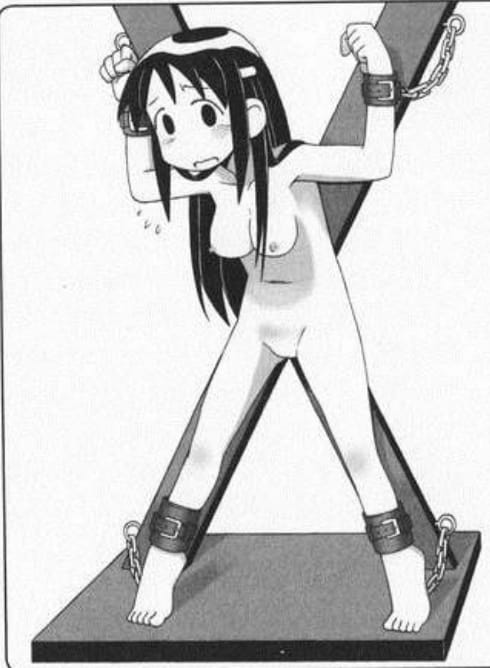
\includegraphics[width=0.6\textwidth]{Images/sm-frame.jpeg}
\caption{X型束缚架示意图}
\end{figure}

开脚束缚用的椅子，就是样子像妇科检查台那样的椅子。在性爱旅馆中，有像医院诊察室样子的屋子，在里面经常看到这种椅子。在这类的屋子里，可以一边玩医生游戏，一边将SM加入进来，所以在轻度SM阶段也是非常推荐的。

SM专用房间或者SM旅馆，是专门为SM准备的地方。里面不仅有束缚设备，而是从牢房到悬吊类的设备都有。

在这类屋子里，有平常看不到的三角木马、禁闭室，还有为了灌肠准备的排水设备。屋子也有日本和欧美风格，也有的是模仿医院和教室，可以一边SM一边玩cosplay。

在这些SM专用房间中有束缚和口球类的用具，所以空着手去也没有问题。但是这些要接触身体的道具是不是杀过菌就不清楚了，如果不放心的话可以不用。

像SM专用房间这类特殊的地方一般都有主页，去之前上去调查一下吧~

\subparagraph{适合初学者的器具的使用方法}

对于还不能用绳子进行束缚的初学者来说，SM道具是非常好的朋友。带上就可以迅速的束缚，而且也不会给人难以接受的印象，这里就介绍一下这类面向初学者的SM用具。

\paragraph{初学者的SM用具}

首先，既然是面向初学者，所以就要选择一些不会给女性带来难以接受的印象的道具。比如手铐，如果是金属制的就很容易让人联想到是中世纪的奴隶带的这样的印象。所以先从普通的选起吧~

此外SM的道具种类很多，初学者阶段还是局限在手铐、脚铐、项圈、口枷这4种比较好。这4种以外的SM道具往往是像束缚台那样大型和昂贵的东西，初学者一般也玩不起。

除了上面这4种，也有全身束缚用的道具，主要是橡胶或者皮革制成的，用一件这样的道具就可以束缚全身，而且样子也很像绳子束缚的那样。对于初学者和中级玩家来说都是可以轻松使用的道具。

\paragraph{SM道具的保养}

入手SM道具是很必要的。在SM中道具经常会沾上液体，如果之后就这样不管，不仅会让道具有臭味，还可能会损坏道具本身。

橡胶制的道具，要定期水洗，之后好好晾干后保存。金属类的道具如果有水残留在上面还会生锈。皮革制的道具，除了要清除上面的脏东西，还要定期用建材超市中皮革养护品来保养。如果水洗之后不晾干就保存是很容易发霉的。

此外，口球中会残留唾液，所以要在唾液变干之前洗干净。像这类和嘴接触的道具，要用消毒类酒精做好消毒的工作。

\paragraph{手铐、脚铐}

手铐脚镣可以说是SM道具中最有代表性的了吧。用它们可以轻松的完成束缚，所以在初学者到高级玩家中都有很高的人气。

材料主要有橡胶、皮革和金属。金属的手铐和脚铐往往给人重度的印象也不容易买到，所以先选用橡胶或者皮革的制品吧。

橡胶制的手铐脚铐很便宜，也容易清洗，沾了脏东西也容易弄掉，但是橡胶和皮肤的贴合性不好，如果夹住皮肤也会很痛，而且因为不透气，出汗会很不好受。

皮革制品要贵一些，但是和皮肤贴合性比较好，和适合长时间束缚的情况。权衡这两种类型道具的优缺点和预算，灵活选用吧~

\subparagraph{使用手铐脚铐的玩法}

只束缚手脚就足以让人兴奋了~下面就来介绍一些手脚束缚的各种玩法样式。

\paragraph{后手束缚}

这样就无法用手遮挡自己的乳房和性器官，所以很容易产生被虐感。在平躺的时候手会承受体重的压力，所以要避免压伤。

\begin{figure}[h]
\centering
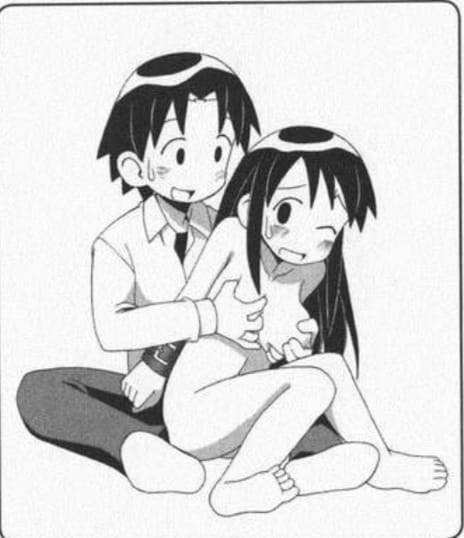
\includegraphics[width=0.6\textwidth]{Images/handcuff-back.jpeg}
\caption{后手束缚示意图}
\end{figure}

\paragraph{单手单脚束缚}

像双手抱着脚踝那样，把双手与对应一侧的脚踝束缚在一起的方式。双手也会随着双脚的分开而分开。身体正面的各处在抵抗不了的状态下被一览无余。

\begin{figure}[h]
\centering
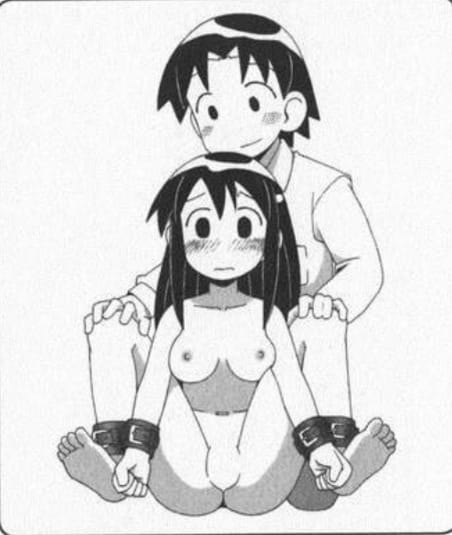
\includegraphics[width=0.6\textwidth]{Images/handcuff-single.jpeg}
\caption{单手单脚束缚示意图}
\end{figure}

\paragraph{双手双脚束缚}

就是将双手和双脚全部束缚在一起的方法。侧身躺下的话可以将性器官一览无余，非常适合对性器官的爱抚。

\begin{figure}[h]
\centering
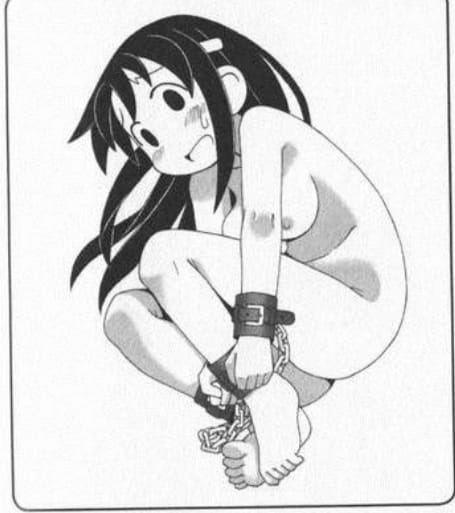
\includegraphics[width=0.6\textwidth]{Images/handcuff-double.jpeg}
\caption{双手双脚束缚示意图}
\end{figure}

\paragraph{使用支棒的束缚}

就是将金属支棒连接在手铐脚铐中的束缚方法。用支棒连接脚铐，再配合后手束缚，全身都处于无法动态的状态。

\begin{figure}[h]
\centering
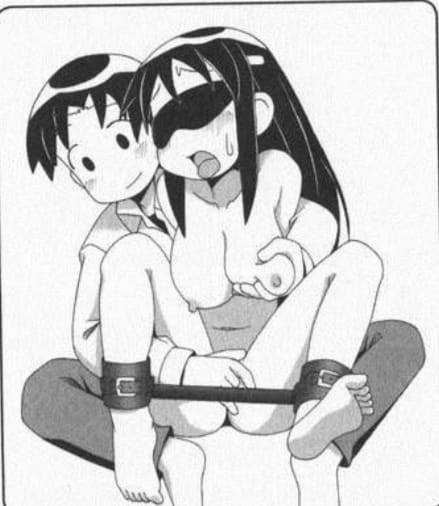
\includegraphics[width=0.6\textwidth]{Images/handcuff-rod.jpeg}
\caption{使用支棒的束缚示意图}
\end{figure}

\paragraph{项圈}

SM的标志之一就是项圈。仅仅戴上就可以有宠物的感觉，是种可以给人很强被虐感的SM道具。

虽然有专用的SM项圈，但是在女性中人气很高的是狗用的项圈。不过在这种项圈上往往涂有防虫剂，为了防止沾到身上使用前要洗干净。如果为了外观可爱而选用小型犬类用的项圈的话，要注意尺寸如果太小，戴上去会很不好受。

SM专用的项圈就没有上述的问题，立刻就可以使用，在项圈上有可以拴牵绳也可以用来固定手铐的环，如果要固定手铐的话就选用SM专用的项圈吧~

\subparagraph{双手束缚到项圈}

就是将手铐固定到有固定环的项圈上的束缚方式。这样手无法遮挡自己的身体也无法背后，很适合仰面向上的场合。不过脖子会承受手的重量，有勒住脖子的危险。

\begin{figure}[h]
\centering
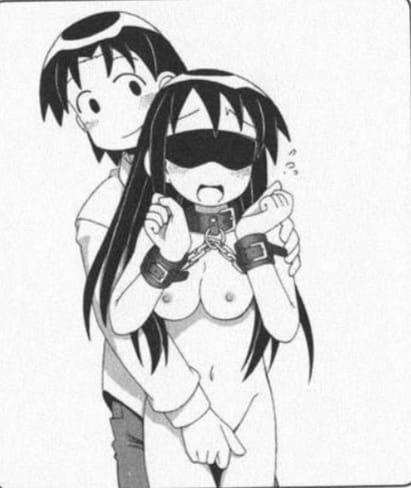
\includegraphics[width=0.6\textwidth]{Images/collar-hands.jpeg}
\caption{双手束缚到项圈示意图}
\end{figure}

	\item \textbf{性玩具}

在SM中使用性玩具，可以更加增加气氛。S可以使用玩具爱抚M，轻松的调教M。下面讲讲方法。此外，也不要仅仅使用玩具爱抚，不要忘记和其他的爱抚方式组合哦~

\subparagraph{振动器}

当然不能光使用振动器来爱抚，还要组合其他的形式。

比较有代表性的，在放入振动器的情况下，对M作出不要掉出来的指示。并且在M忍耐的时候组合打屁股的方式。

还可以在用振动器爱抚的同时，进行类似"如果你还要动得更厉害的话，就求我吧"这样的语言虐待。当然也可以用镜子让M看看自己的样子，来提升M的羞耻感。

\subparagraph{伸缩转动器}

使用的方法和振动器差不多，最大限度的利用遥控器吧。和振动器不同，可以用伸缩转动器从乳头开始爱抚身体的各个部位。利用这个特性可以对全身进行爱抚。

此外，也可以在束缚状态中把转动器放在内衣中，然后在稍微远的地方切换开关。

当然不要忘记，也可以定期把开关关掉，然后让M做出请求，或是在镜子前让M看自己的状态，提升羞耻感。

\item \textbf{打屁股}

打屁股在一般的性生活中不太会用到，但是在SM中是很普通的事情。打屁股不需要特殊的道具，只要手就可以。而且喜欢屁股被打的M也是比较多的，所以尽可能尝试一下吧~

当然，不是打下去就好了。在轻度SM阶段只要打屁股就好了。打屁股以外的地方很容易感到痛，但是屁股不那么容易觉得痛。

关于打的方法，也不仅仅是用力，而是要尽量用手心打出声音来。也不要频率不变，而要强弱交换，时停时始。

在打完一阵后，可以用手指轻抚变得敏感的皮肤，用指尖像挠痒一样的效果很不错。

打的部位也不要局限在屁股的一个地方，可以时不时的用指尖触碰阴道，将感觉传遍全身。

此外，打的时候也不要忽然就打，在其他的爱抚中打屁股的比较好。比较有代表性的有下面这两种。

\subparagraph{做爱的时候}

就是在以坐式或者后入式方式做爱的时候打屁股。

或者命令M扭动腰部，在扭动变慢的时候打屁股也不错。

\subparagraph{用玩具爱抚的时候}

在放入振动器并命令不要掉出来的状态下打屁股。

此外，在放入伸缩转动器的状态下，不断切换开关，并且一边打屁股的方式也是很流行的。
\end{enumerate}

\textit{【编者注】}轻度SM的核心在于建立信任和探索边界，而非追求强烈的感官刺激。建议从非侵入性的方式开始，注重沟通和反馈，让双方在安全舒适的氛围中逐渐探索。

\subsubsection{SM的安全入门指南}

虽说对SM有兴趣，但各种SM形式进行的方法和步骤却不是那么好懂，常常让人不知道从哪里入手。而且在SM束缚的过程中也有受伤的危险——如果不掌握正确的知识和方法，SM就可能变成危险的活动。

以下是从入门到实践的逐步指导原则：

\noindent\textbf{第一步：沟通与说服伴侣}

\begin{enumerate}
	\item 坦诚表达自己的兴趣——用非威胁性的方式描述SM对你的吸引力
	\item 了解对方的边界和兴趣范围——可以一起阅读入门书籍或观看教育类资料
	\item 从最轻微的形式开始尝试——不要一开始就追求高强度体验
	\item 接受对方可能需要时间来理解和接受——不要施加压力
\end{enumerate}

\noindent\textbf{第二步：学习基础安全知识}

\begin{itemize}
	\item \textbf{安全词（Safeword）}：约定一个明确的停止信号（如"红色=立即停止""黄色=减速"），确保在任何状态下都能被识别和使用
	\item \textbf{束缚安全}：避免压迫颈部/关节；绳子不应阻断血液循环（检查手指颜色和温度）；剪刀常备在手边以便紧急剪断
	\item \textbf{器具卫生}：所有接触皮肤或黏膜的工具使用前后必须彻底清洁消毒
	\item \textbf{身体禁区}：明确哪些部位绝对不能触碰或施加压力（如眼睛、颈椎、内脏器官区域）
\end{itemize}

\noindent\textbf{第三步：循序渐进的实践}

\begin{itemize}
	\item 从轻拍、羽毛抚摸等低强度感觉开始
	\item 逐步尝试简单的手腕束缚（使用专门设计的束带而非粗糙绳索）
	\item 每次活动后进行"\textbf{事后关怀（Aftercare）}"——拥抱、交谈、确认对方状态良好
	\item 定期回顾和讨论双方的感受，不断调整和改进
\end{itemize}

\textit{【编者注】}关于SM入门的系统化学习资源，推荐参考三叶所著《私の体、私の心 —— YOUAREMINE！！》（一迅社，2014）。该书从说服伴侣开始，到各类SM形式的步骤和注意点，将必要知识逐步教授给初学者，是目前日文领域较为系统的SM入门教材之一。

\subsubsection{SM的动机与心理机制}

虽然经常在AV和成人游戏中看到SM场面，但现实中的SM还是很难想象到底是什么样子。一般说到SM，就会想起蜡烛、鞭子、笼子里的女性之类的——有这种想法的人是很多的。

\noindent\textbf{SM行为概览}：

束缚、羞辱、鞭打……全都是S对M的行为。表面上来看，S可以肆意对M做任何自己喜欢的事情——但实际上，\textbf{S是将M希望的事情给予M}。如果M被对方胡乱地对待，那只能称作单纯的虐待吧。\textit{【编者注】}这一区分在性学中至关重要：\textbf{consensual BDSM（知情同意的BDSM）与 abuse（虐待）的核心区别在于是否以双方的愉悦为目标}。后者是单方面的权力滥用，而前者是一种双向的、协商一致的互动模式。

就像这样，SM不仅是S对M的关系——还有着"\textbf{S要做M喜欢的事情}"这种逆向的关系存在其中。

\noindent\textbf{S的本质是"服务（Service）"}：

现实中的SM，S对M的性趣和嗜好的了解是不可欠缺的；M也必须完全信任S，才能安心接受S的各种行为。所以，SM中的S应该是"\textbf{服务（Service）}"才对——没有对M的服务精神和爱情，这种关系是无法成立的。\textit{【编者注】}这与BDSM社区中广为流传的理念"\textbf{Service Top}"高度吻合：真正的支配者本质上是服务者——通过满足被支配者的需求来获得自身的满足感。权力的表象下隐藏的是深层的关怀与责任。

\noindent\textbf{SM如何改善亲密关系}：

为了防止双方的关系变得乏味，把SM当作一种非正常的行为而进行的情况也是有的——但只要可以相互理解，就可以称为SM。它不仅是为了摆脱乏味关系，更是为了充分了解对方，抱着想和对方结合在一起的心态——这才是真正理想的SM。

\begin{itemize}
	\item 对于有S取向的人：通过给予而产生\textbf{完全占有}的满足感
	\item 对于有M取向的人：通过接受而获得强烈的\textbf{被爱}的感觉
\end{itemize}

性并不是全部——性的满足感和SM的方式都会给双方带来非常大的影响。视作一种奇特的方式也好、视作加深双方爱的行为也好、视作深切感受到对方的存在的行为也好——SM都值得一试。

\textit{【编者注】}多项实证研究支持SM对亲密关系的积极影响：
\begin{itemize}
	\item Connolly(2006)调查发现：BDSM实践者的心理健康水平不低于甚至略高于普通人群
	\item Wismeijer \& van Assen(2013)大样本研究：BDSM倾向者在外向性、开放性和主观幸福感上得分更高
	\item BMSM(BDSM-Mediated Sensory Modulation)理论认为：SM中的感官刺激可通过调节自主神经系统产生类似冥想的放松效果
\end{itemize}

\subsubsection{SM术语与角色入门}

有了SM的初步印象后，实际中的SM是如何进行的、有什么样的方式——这些问题可能还不清楚。这里通过S和M两种角色，把大致的SM方式和种类做一个系统介绍：

\noindent\textbf{核心角色定义}：

\begin{center}
\begin{tabular}{|p{3cm}|p{5.5cm}|p{5.5cm}|}
\hline
 & \textbf{S（Sadist / 支配者）} & \textbf{M（Masochist / 被支配者）} \\
\hline
\textbf{核心特质} &
主动方、施予刺激、控制节奏 &
被动方、接受刺激、交出控制权 \\
\hline
\textbf{关键能力} &
敏锐观察力、判断力、责任心 &
表达感受的能力、建立信任的能力 \\
\hline
\textbf{心态本质} &
通过"服务"M获得满足 &
通过信任与交付获得安全感 \\
\hline
\end{tabular}
\end{center}

\noindent\textbf{常见SM活动类型}：

\begin{enumerate}
	\item \textbf{束缚类（Bondage）}
	\begin{itemize}
		\item 手腕/脚踝束缚（手铐、绳索、丝带）
		\item 全身束缚（蛋缚、龟甲绑等绳艺）
		\item 悬挂束缚（需专业技巧，初学者不建议尝试）
	\end{itemize}

	\item \textbf{感官调教类（Sensory Play）}
	\begin{itemize}
		\item 触觉：羽毛、冰块、蜡滴、毛刷滚动
		\item 视觉：眼罩（剥夺视觉增强其他感官）
		\item 听觉：耳塞、指令与回应游戏
	\end{itemize}

	\item \textbf{轻度拍打类（Impact Play · 入门级）}
	\begin{itemize}
		\item 手掌拍臀：最基础且最容易掌控强度的方式
		\item 小型拍击工具： paddle（拍板）、flogger（多尾软鞭，痛感分散均匀）
	\end{itemize}

	\item \textbf{言语与心理类（Psychological Play）}
	\begin{itemize}
		\item 称呼与命令（如使用特定称呼、下达服从指令）
		\item 角色扮演（主人/宠物、老师/学生等）
		\item 羞辱游戏（需极度谨慎，必须在充分信任的基础上进行）
	\end{itemize}

	\item \textbf{侍奉与服务类（Service）}
	\begin{itemize}
		\item M为S提供身体按摩、足部护理等
		\item M承担特定的日常任务或姿态要求
	\end{itemize}
\end{enumerate}

\begin{tcolorbox}[colback=pink!5!white,colframe=red!50!black,title=贴心小叮咛]
无论尝试哪种SM方式，都请始终牢记三个原则：\textbf{① 安全第一}——不要做自己无法掌控的事；\textbf{② 充分沟通}——事前讨论、事中确认、事后交流缺一不可；\textbf{③ 从轻开始}——永远可以从低强度逐步提升，但一旦越过了对方的承受边界，造成的伤害可能是不可逆的。
\end{tcolorbox}

\subsubsection{S与M两种角色详解}

从本质上来说，决定了S和M两种角色的玩法就是SM。但是，在通常的性行为中，很难分清谁是S谁是M——\textbf{勉强的将S和M的角色决定下来，是得不到什么乐趣的}。所以在最开始的时候，可以不去想这个问题，双方互换角色进行。\textit{【编者注】}这与性治疗中的"\textbf{探索阶段（exploration phase）}"理念一致：在确定固定角色偏好之前，通过角色互换（switching）来帮助双方了解自己的真实感受和偏好是非常推荐的实践。

\noindent\textbf{SM在生活中的时间维度}：

扮演角色的时间不尽相同：
\begin{itemize}
	\item \textbf{场景式SM（Scene-based）}：仅限于特定时间段内的短暂游戏
	\item \textbf{全天候SM情侣（Full-time / 24/7 D/s）}：在日常生活中也保持S/M关系——但这属于较为极端的形式，需要极高的信任基础和长期磨合
	\item \textbf{最常见的模式}：SM和日常生活分开。床上将女方视为M，现实生活中却可能是个"妻管严"的情况也是很多的
\end{itemize}

这些SM的规则——由双方一起决定就好。

\noindent\textbf{■ S的角色 —— 施虐者 / 支配者 / 服务者}

简单说，S就是扮演施虐者的一方。但这个"施虐"有着完全不同于日常理解的内涵：

\begin{enumerate}
	\item \textbf{主导权掌握者}：在肉体上和精神上都掌握着主导权
	\item \textbf{行为责任人}：必须时刻考虑M的方方面面——安全、感受、边界
	\item \textbf{需求洞察者}：必须根据M的性趣和嗜好来设计并执行SM行为
	\item \textbf{满足感来源}：从M陶醉的样子中获得满足感——这是S的核心回报
\end{enumerate}

\textit{【编者注】}BDSM社区中有句广为流传的话："\textbf{The Top has the whip, but the sub holds the power.}"（支配者拿着鞭子，但被支配者握着权力。）意思是：虽然表面上S掌控一切，但实际上S的一切行为都围绕着M的需求和边界展开——M才是互动真正的"中心"。这也解释了为什么优秀的S往往需要比M更敏锐的观察力和更丰富的经验。

\noindent\textbf{■ M的角色 —— 被虐者 / 被支配者 / 沟通者}

和S相反，M就是扮演被虐的一方。但M绝非被动的受气包——

\begin{enumerate}
	\item \textbf{承受者}：一方面要承受S的行为
	\item \textbf{信息传达者}：要将希望被如何对待的信息传达给S——这是M最重要的主动责任之一
	\item \textbf{沟通义务}：即便在被束缚无法动弹时，也要把心中所想的传达给S；讨厌的行为要清楚地说出；在SM以外的时间将自己喜欢的方式告诉S也是很有必要的
	\item \textbf{体验者}：一定程度的预想自己将受到的刺激，陶醉在SM行为和S的全力以赴中——这就是M的本质状态
\end{enumerate}

\textit{【编者注】}M的沟通能力直接决定了SM的质量和安全水平。研究显示：能够清晰表达感受的M方，其SM体验满意度显著更高，且发生意外伤害的概率更低（Newmahr, 2011）。许多有经验的M会使用"\textbf{1--10强度量表}"或"\textbf{交通灯系统}"（绿=继续/黄=减速/红=停止）来实时反馈自己的状态。

\noindent\textbf{S与M关系的本质总结}：

\begin{center}
\fbox{\parbox{0.85\textwidth}{\centering
\textbf{S} = 主导权 + 责任心 + 观察 M的反应 → 从 M 的满足中获得满足\\[0.3em]
\textbf{M} = 交付控制权 + 清晰沟通 + 沉浸体验 → 在 S 的引导下获得安全感与释放
}}
\end{center}

\begin{tcolorbox}[colback=pink!5!white,colframe=red!50!black,title=贴心小叮咛]
S不是暴君，M不是受害者。健康的SM关系中，S是"用心的服务提供者"，M是"勇敢的体验者和诚实的沟通者"。双方都在为对方的愉悦而努力——这正是SM与虐待的根本区别所在。
\end{tcolorbox}

\subsubsection{SM行为方式}

SM行为在操作层面上可大致分为\textbf{肉体方式}和\textbf{精神方式}两大类。值得注意的是：在AV或成人游戏中呈现的，以肉体方式的SM为主；但在现实中的亲密关系实践里，精神层面SM所占的比例往往远高于大众的想象。

\noindent\textbf{■ 肉体方式（Physical Play / Sensation Play）}

顾名思义，通过对身体施加各种感官刺激来获得快感的方式。

\begin{itemize}
	\item \textbf{轻度行为}：用长筒袜或丝带束缚对方、轻拍屁股、轻微抓挠等——这些行为在普通性行为中其实也常见，强度边界较为模糊
	\item \textbf{中度行为}：鞭打（使用手鞭、皮鞭等工具）、滴蜡（低温蜡油滴落皮肤）、束缚（绳缚/手铐/ spreader bar 等）
	\item \textbf{重度行为}：穿环（piercing play，临时或永久）、针刺（needle play，需专业知识和严格无菌操作）、以及其他可能造成实际组织损伤的行为
\end{itemize}

\textit{【编者注】}肉体方式的核心机制在于\textbf{痛觉转化（pain-to-pleasure conversion）}——当个体处于高度唤起状态时，大脑会释放内啡肽（endorphins）和内源性大麻素（endocannabinoids），这些神经递质具有天然的镇痛和愉悦作用，使得一定强度的痛觉刺激可以被重新编码为快感的来源（Benedek \& Meana, 2012）。然而，\textbf{重度肉体行为存在真实的伤害风险}，必须在充分学习相关知识、掌握安全技巧后才能尝试。

\noindent\textbf{■ 精神方式（Psychological Play / Mental BDSM）}

如果说肉体方式是"身体的性爱"，那么精神方式就是"\textbf{大脑中的性爱}"——精神层面的互动在其中占据核心地位。常见的表现形式包括：

\begin{itemize}
	\item \textbf{羞辱游戏（Humiliation Play）}：通过言语贬低、人格化（pet play）等方式让M体验到"被降低"的心理状态
	\item \textbf{忽视与放置不管（Ignored / Neglect Play）}：将M束缚后故意不予理睬，制造心理上的无助感和期待感
	\item \textbf{镜像羞辱（Mirror Humiliation）}：强迫M在镜子前观看自己"屈辱"的姿态——利用视觉反馈放大心理冲击
	\item \textbf{言语控制（Verbal Control）}：通过命令、责骂、指令等方式建立心理支配关系
	\item \textbf{规则设定与服从训练（Protocol / Obedience Training）}：制定行为规范并要求M严格遵守
\end{itemize}

\textit{【编者注】}对于许多M来说，精神层面的互动不仅是不可或缺的，甚至比肉体刺激更加重要和令人满足。这可以从心理学角度解释：\textbf{心理支配的本质是权力交换（power exchange）的可视化和体验化}，而权力交换恰恰是BDSM体验中最核心的快感来源（Cross, 2014）。研究显示，参与心理层面BDSM活动的个体报告的主观满足感往往高于仅参与肉体刺激的群体（Richters et al., 2008）。此外，精神方式的一个独特优势在于\textbf{零身体伤害风险}——对于初学者或偏好低风险实践的伴侣而言，这是一个极佳的切入点。

\noindent 两种方式并非互相排斥，而是可以自由组合、相互增强的。在实践中，大多数SM场景都会同时包含肉体和精神两个维度的元素——关键在于双方充分沟通各自的偏好边界，找到最适合自己的平衡点。

\begin{tcolorbox}[colback=pink!5!white,colframe=red!50!black,title=贴心小叮咛]
无论偏重哪种方式，请记住：\textbf{精神方式不等于"可以随便说伤人的话"}。语言同样可以造成深远的心理伤害。事前的 safeword 设定、事后的情感安抚（aftercare），在精神类SM中尤为重要。
\end{tcolorbox}

\subsubsection{SM 实践步骤与场景编排}

SM并没有"标准答案"或"固定模板"。但在实践中，一些常见的流程模式可以作为参考起点——重要的是理解其背后的逻辑，而非机械照搬。

\noindent\textbf{■ 典型递进模式}

一种常见的SM场景编排遵循以下顺序：

\begin{enumerate}
	\item \textbf{穿衣 / 束缚阶段}：从穿着衣服开始，使用丝带、长筒袜或轻便束缚工具限制对方的行动自由——这一阶段的目的是建立初步的支配感和期待感
	\item \textbf{精神羞辱阶段}：在身体受限的状态下加入言语羞辱或心理控制元素，逐步加深M的心理沉浸感
	\item \textbf{肉体刺激阶段}：引入鞭打、滴蜡等中等强度肉体行为，将精神层面的张力转化为身体的感官体验
	\item \textbf{性释放阶段}：最后以性行为（性交或其他形式的亲密接触）作为整个场景的高潮和收尾
\end{enumerate}

这种"由浅入深、由外而内"的递进结构符合性唤起的自然曲线，也便于双方在每个环节确认状态和边界。

\noindent\textbf{■ 混合模式（最普遍的现实实践）}

另一种更为常见的做法是：从穿衣或裸体状态开始后，\textbf{肉体和精神层面的SM行为交织进行}，而非严格按照先后顺序。这种方式灵活度高，能更好地响应双方的即时感受和情绪变化。

\textit{【编者注】}值得注意的是，SM影片和成人游戏中呈现的模式（通常以视觉冲击力为优先考量），与现实中伴侣间的SM实践存在本质差异。影视作品服务于观众的观赏需求，强调戏剧性和视觉效果；而现实中的SM服务于\textbf{双方的真实愉悦和情感连接}。将AV中的表现作为实践范本是常见但危险的误区——正如不能用动作片来学习驾驶一样。

\noindent\textbf{■ 现实实践的核心原则}

在真实关系中，SM往往没有固定的模式和规则，而是完全围绕双方的喜好和默契展开。以下是几条实用建议：

\begin{itemize}
	\item \textbf{衣服不是必须先脱掉的}：开始时可以完全不处理衣物问题，随着场景推进和氛围升温，在最合适的时候再逐步脱去——这种"渐进式暴露"本身就可以成为一种有效的心理铺垫工具
	\item \textbf{穿着衣服开始是很好的选择}：衣着状态下的束缚和互动可以帮助双方更从容地进入角色，避免裸体带来的过早紧张或尴尬
	\item \textbf{"渐入佳境"是关键目标}：一个精心设计的SM场景就像一场交响乐——有前奏、有起伏、有高潮、有余韵。节奏的控制比具体做了什么更重要
\end{itemize}

\begin{tcolorbox}[colback=pink!5!white,colframe=red!50!black,title=贴心小叮咛]
第一次尝试时，不要追求"完整流程"。哪怕只尝试了5分钟的轻度言语控制+轻拍屁股然后正常做爱，这也是一次成功的SM体验。\textbf{循序渐进}远比一步到位更重要。
\end{tcolorbox}

\subsubsection{SM 实践的主要类别}

SM行为的种类繁多，将每一种都实践一遍既不现实也无必要。在长期的探索中，多数伴侣会逐渐形成自己的偏好组合，并固定到若干大类中。以下介绍四类最常见的基本形态：

\noindent\textbf{① 束缚类（Bondage-focused Play）}

虽然束缚（bondage）也经常作为其他SM形式的辅助手段出现，但在此类SM中，束缚本身就是核心和主题。

\begin{itemize}
	\item \textbf{典型形式}：绳缚（kinbaku / shibari）、手铐/脚铐、丝带捆绑、spread bar（分腿杆）、单肢或多肢固定
	\item \textbf{常见搭配}：束缚中的爱抚（teasing while bound）、束缚状态下的性行为
	\item \textbf{偏好者特征}：对于喜欢"\textbf{紧缚}"的伴侣，身体被完全限制的自由感本身就是主要的快感来源——这种体验与"安全地失去控制权"的心理需求密切相关
\end{itemize}

\textit{【编者注】}束缚类是BDSM实践中参与度最高的类别之一。研究数据显示，约70\%的BDSM参与者曾尝试过某种形式的束缚游戏（Richters et al., 2008）。其心理学吸引力在于：\textbf{束缚创造了一个"许可框架"——在被绑的状态下，个体可以放下日常的责任感和自我控制，纯粹地感受当下}（Ambler et al., 2017）。此外，日本传统的绳缚艺术（shibari）已发展出独立的审美体系，强调绳路的图案美感和模特的身体曲线展示，兼具感官刺激与视觉艺术的特质。

\noindent\textbf{② 快感类 / 强制快感类（Forced Orgasm / Sensation Play）}

与束缚类相比，此类SM更注重对快感的操控和放大。

\begin{itemize}
	\item \textbf{核心机制}：通过性玩具（振动棒、按摩棒等）或道具让M体验到持续不断的强烈快感
	\item \textbf{"强制高潮"（Forced Orgasm）}：M在达到高潮后不被允许休息，而是继续接受刺激被迫再次甚至多次高潮——快感在这里变成了一种需要"承受"而非单纯享受的东西
	\item \textbf{边缘控制（Edging / Orgasm Control）}：另一种变体是将M反复带到高潮边缘却不让其释放，制造极度的期待和心理张力
\end{itemize}

\textit{【编者注】}快感类的独特之处在于：它颠覆了"快感=好事"的直觉认知。\textbf{当快感不再受自己控制时，即使是愉悦的感觉也会变得具有挑战性甚至"难以承受"}。这与神经科学中的"享乐适应（hedonic adaptation）"现象相关——持续的强刺激会改变大脑对快感的感知方式。需要注意的是：过度或长时间的强制刺激可能导致生殖器区域的暂时性感觉过敏（hypersensitivity），应关注M的真实反馈并适时暂停。

\noindent\textbf{③ 肛门类（Anal Play / Analingus / Enema Play）}

以肛门及其周围区域为主要操作对象的SM形式，实际普及度可能超出许多人的想象。

\begin{itemize}
	\item \textbf{常见形式}：
	\begin{itemize}
		\item 舔肛（anilingus / rimming）：以口舌刺激肛门区域
		\item 肛门手指/玩具插入：使用肛塞（butt plug）、肛门珠（anal beads）、假阳具（dildo）等
		\item 灌肠（enema）：向直肠注入液体——在某些SM场景中作为羞辱或清洁的前置环节
	\end{itemize}
	\item \textbf{特殊变体}：以灌肠开始、最终以排泄结束的完整流程——这同时涉及强烈的羞耻感和身体控制的丧失
	\item \textbf{安全要点}：肛门黏膜脆弱无自润滑功能；直肠弯曲且肠壁较薄；必须使用大量水溶性润滑剂；禁止将玩具或肢体强行深入结肠
\end{itemize}

\textit{【编者注】}肛门区域拥有密集的神经末梢（源自阴部神经 pudendal nerve），对于许多人而言是一个潜在的强敏感带。然而，由于社会文化中对肛门的污名化以及卫生顾虑，这一领域常被误解或回避。从解剖学角度看，男性前列腺经直肠前壁可被间接刺激（所谓"前列腺按摩"或"P点刺激"）；女性则可通过阴道-直肠隔膜感受到双侧压力。需要强调的是：\textbf{享受肛门刺激与性取向无关}——这是基于生理结构的普遍现象（Morin, 2000）。此外，灌肠类行为存在电解质紊乱和肠黏膜损伤的风险，不建议频繁进行。

\noindent\textbf{④ 肉体伤害类（Impact Play / Pain Play — Heavy）}

此处的"伤害"指的是字面意义上的身体损伤性虐待——如重度鞭打、悬吊状态下施虐等较为彻底的肉体惩罚。

\begin{itemize}
	\item \textbf{典型行为}：重型鞭具（flogger / whip / cane）抽打、悬吊 suspension bondage + 鞭打、造成皮肤明显淤青或破皮程度的击打
	\item \textbf{一个反直觉的事实}：与大众印象相反，这类纯粹的肉体伤害型SM在BDSM社区中\textbf{人气并不高}，也很少有人仅仅为了追求身体伤害而参与SM
	\item \textbf{原因分析}：大多数SM参与者的核心动机在于心理层面的权力交换、亲密感的深化或感觉阈限的探索，而非单纯的痛觉寻求或身体伤害
\end{itemize}

\textit{【编者注】}这一观察得到了实证研究的支持。Weiss (2011) 在对旧金山BDSM社区的民族志研究中发现：\textbf{社区成员普遍更看重SM的情感连接和意义建构价值，而非痛觉本身}。Connolly (2006) 的调查数据同样显示，仅约10\%--15\%的BDSM参与者将重度疼痛作为主要兴趣点。对于确实偏好高强度冲击玩法的人群，安全知识尤为关键——避开器官密集区域（肾脏、脊柱下部、颈部）、了解不同工具的伤害特性差异、掌握基本急救技能，都是必修功课。

\noindent 以上四类并非互斥——实际上，多数SM场景会融合其中2--3类的元素。随着经验的积累，每对伴侣都会发展出属于自己的"配方"和节奏。

\begin{center}
\begin{tabular}{|p{2.8cm}|p{4cm}|p{5.8cm}|}
\hline
\textbf{类别} & \textbf{核心元素} & \textbf{适合人群 / 入门建议} \\
\hline
束缚类 & 绳索/铐具、行动受限 & 新手友好；建议从丝带/领带开始 \\
\hline
快感类 & 振动玩具、强制高潮 & 适合已有一定信任基础的伴侣；注意沟通强度阈值 \\
\hline
肛门类 & 肛门刺激、灌肠 & 需充分了解解剖结构和安全规则；润滑剂必不可少 \\
\hline
肉体伤害类 & 重型鞭打、悬吊 & \textbf{高风险}；需长期学习和经验积累，\underline{不适合初学者} \\
\hline
\end{tabular}
\end{center}

\begin{tcolorbox}[colback=pink!5!white,colframe=red!50!black,title=贴心小叮咛]
如果你正在探索自己的SM偏好，不必急于给自己贴标签。从束缚类开始尝试是最安全的入门路径——门槛低、风险小、工具易得。记住：\textbf{没有哪种类型比另一种更"高级"或更"正宗"}。
\end{tcolorbox}

\subsection{SM 的历史背景与文化演变}


\begin{itemize}
	\item \textbf{历史脉络}：束缚与支配的仪式化元素见于多种古代文化（日本的 shibari 源于捕绳术的艺术化、欧洲维多利亚时代的鞭笞文学）；现代 SM 亚文化的成型以二战后美国皮革社群与 20 世纪末互联网社群为节点
	\item \textbf{术语与规范}："SSC"（Safe, Sane, Consensual，安全、理智、同意）与后来更强调参与主体性的"RACK"（Risk-Aware Consensual Kink，风险知情同意）是社群通行的伦理框架
	\item \textbf{去病理化}：ICD-11（2022）已将"双方同意的施受虐行为"移出精神障碍——只有造成显著痛苦或涉及非自愿者才进入临床视野；这是 SM 去污名化的里程碑
	\item \textbf{文化演变}：从地下亚文化到主流文化元素（五十度系列图书影视的全球流行），公众可见度大幅提升——可见不等于了解，安全知识仍需专门学习
\end{itemize}

\subsection{SM 与心理健康及亲密关系}


\begin{itemize}
	\item \textbf{心理机制假说}：权力交换的"场域逃离"（放下日常责任/掌控的暂时放空）、内啡肽与肾上腺素的生理高潮（痛觉转化 pain-to-pleasure）、信任深化的亲密回报——多重机制交织，个体差异大
	\item \textbf{对关系的影响}：研究（如荷兰与澳洲的社群调查）显示：实践知情同意 SM 的伴侣在关系满意度与沟通质量上\textbf{不低于}一般伴侣——协商偏好本身就是高质量沟通的训练
	\item \textbf{心理健康边界}：SM 参与者整体心理健康指标与常人无异；需要警惕的是以 SM 为壳的心理问题——用极端疼痛处理抑郁、用羞辱强化自我厌恶——此时该治的是背后的问题
	\item \textbf{事后护理（aftercare）}：高强度场景后的安抚（拥抱、盖毯、补水、复盘）是关系维护的一部分；情绪跌落（drop，内分泌回落所致的低落期）是常见现象，参见专节
	\item \textbf{红旗信号}：以"同意"为名突破预先协商的边界、事后持续羞辱、把 SM 作为惩罚或暴力借口——这些不是 SM，是关系暴力
\end{itemize}

\subsection{社会对性偏好的态度}


\begin{itemize}
	\item \textbf{污名的历史}：精神医学曾长期将 SM 归入"性变态"（DSM 旧版），媒体渲染与猎奇报道加深误解——"SM=暴力/心理变态"的刻板印象正是这样形成的
	\item \textbf{现状}：法律上，成年人之间私下、自愿、无重伤的 SM 行为在多数法域不被追责（但"同意重伤"在多数司法辖区仍不受保护——这是法律边界，不是道德边界）；医学上 ICD-11 已去病理化
	\item \textbf{社会争议点}：公开场合的 SM 元素、职场与家庭的暴露风险、平台对相关内容的限制——参与者普遍采取隐私管理策略
	\item \textbf{给好奇者的建议}：从可靠的科普与社群规范学起（安全词、工具消毒、解剖安全区——如不可击打肾脏区与颈椎）；先看后试、先轻后重、先沟通后行为；找不到能谈的医生时，性健康门诊比搜索引擎可靠
\end{itemize}



\section{性偏好与性多样性}
% ⇒ [r81 并入] 自旧区
性偏好是指个体在性方面的特殊喜好和兴趣，是性多样性的重要组成部分。性偏好的范围非常广泛，包括各种不同的性刺激、性幻想和性行为方式。


性偏好指一个人对特定对象、情境或活动的性兴趣倾向，其谱系极宽：从对特定体型、服饰、场景的偏好，到恋物、BDSM 等实践形式。\textbf{判断是否需要临床干预的标准不是"偏离多数"，而是三条}：是否涉及未经同意的对象、是否造成本人或他人的显著痛苦、是否影响正常生活功能。三条皆否，则属于多样性而非障碍。

理解性偏好的三个关键词是\textbf{谱系、同意与自我接纳}。偏好本身并无对错——从恋物的具体对象到对情境、节奏的偏好，人类的性兴趣呈现出惊人的多样性；衡量其是否需要关注的标准只有两条：是否建立在所有参与者知情同意的基础上，是否给当事人带来持续痛苦或功能损害。在同意的框架内探索偏好是正常的生活方式；而因偏好与主流不同产生的羞耻感，往往比偏好本身更值得处理。


\subsection{性偏好的分类}

性偏好可以分为多种类型，根据不同的分类标准，有不同的分类方法。

1. \textbf{基于刺激对象的分类}：如恋物癖（对特定物品产生性兴趣）、恋足癖（对脚产生性兴趣）等。
2. \textbf{基于行为方式的分类}：如窥阴癖（通过窥视他人的性行为获得性满足）、露阴癖（通过暴露自己的生殖器获得性满足）等。
3. \textbf{基于角色关系的分类}：如支配-服从型关系（SM）、施虐-受虐型关系（S\&M）等。

需要注意的是，大多数性偏好是正常的，只有当性偏好导致个体或他人的痛苦，或违反法律和道德规范时，才会被视为性心理障碍。

\subsection{SM的定义与内涵}

SM是Sadomasochism的缩写，指的是一种包含支配-服从、施虐-受虐元素的性偏好或性行为方式。SM涉及两个主要角色：S（Sadist，施虐者）和M（Masochist，受虐者）。

1. \textbf{核心元素}：
  \begin{itemize}
  \item \textbf{支配与服从（D/S）}：
    \begin{itemize}
    \item \textbf{心理动力}：支配者在控制中获得满足，服从者在放弃控制中获得放松和安全感。这种权力交换可以满足双方的心理需求，如自我实现、被保护感或责任感
    \item \textbf{实践细节}：
      \begin{itemize}
      \item 权力动态的协商：明确双方期望的权力程度和范围
      \item 角色的具体表现：语言命令、身体姿势、行为限制等
      \item 信任的建立：长期的D/S关系需要高度的信任和情感连接
      \item 权力的责任：支配者对服从者的安全和福祉负有责任
      \end{itemize}
    \end{itemize}
  \item \textbf{痛苦与快乐（S/M）}：
    \begin{itemize}
    \item \textbf{心理动力}：痛苦与快乐在SM中是复杂的交织关系。疼痛可以释放内啡肽（天然的愉悦激素），创造强烈的身体和情感体验。对于一些人，疼痛是一种集中注意力、释放压力或体验极限的方式
    \item \textbf{实践细节}：
      \begin{itemize}
      \item 疼痛阈值的探索：逐渐增加刺激强度，了解彼此的承受能力
      \item 疼痛的类型和部位：不同类型的疼痛（如刺痛、鞭打、压迫）在不同部位会产生不同的体验
      \item 疼痛与愉悦的转化：通过心理状态和情境设置，将疼痛转化为愉悦体验
      \item 个体差异：每个人对疼痛的感受和反应都不同，需要充分沟通
      \end{itemize}
    \end{itemize}
  \item \textbf{契约与边界}：
    \begin{itemize}
    \item \textbf{心理动力}：明确的契约和边界为SM互动提供安全感，让双方能够在安全的框架内探索。这种结构化的互动可以减少焦虑，增强信任
    \item \textbf{实践细节}：
      \begin{itemize}
      \item 书面或口头契约：详细列出双方的权利、责任、偏好和限制
      \item 边界的类型：硬性边界（绝对不允许）和软性边界（可以考虑）
      \item 边界的动态性：边界可能随时间变化，需要定期重新协商
      \item 契约的执行：双方都有责任遵守约定的规则，尊重彼此的边界
      \end{itemize}
    \end{itemize}
  \end{itemize}

2. \textbf{常见活动}：
  \begin{itemize}
  \item \textbf{捆绑（Bondage）}：
    \begin{itemize}
    \item 描述：使用绳索、手铐、皮带等工具限制身体自由，创造束缚感。捆绑可以是简单的手腕束缚，也可以是复杂的绳艺图案，如日本绳缚（Shibari）或西方绳缚（Western Bondage）
    \item 绳索技术：
      \begin{itemize}
      \item \textbf{单柱绑（Single Column Tie）}：最基础的绑法，用于固定单个肢体（如手腕或脚踝）
        \begin{itemize}
        \item 步骤：将绳索绕过肢体2-3圈，然后做一个半结固定，再打一个安全结
        \item 安全要点：保持绳索松紧适度，能插入1-2根手指为宜
        \end{itemize}
      \item \textbf{双柱绑（Double Column Tie）}：用于固定两个肢体（如双手手腕、双脚脚踝或手腕与脚踝）
        \begin{itemize}
        \item 步骤：将绳索先在一个肢体上做单柱绑，然后绕过另一个肢体，形成八字形缠绕，最后固定
        \item 安全要点：确保两个肢体受力均匀，避免过度拉伸关节
        \end{itemize}
      \item \textbf{胸衣绑法（Chest Harness）}：围绕胸部的绑法，可增强胸部线条或限制上半身活动
        \begin{itemize}
        \item 步骤：从背部开始，绳索穿过腋下，在胸前交叉，再回到背部固定
        \item 安全要点：避开乳房敏感区域，避免压迫胸腔影响呼吸
        \end{itemize}
      \item \textbf{日式绳缚基础（Basic Shibari）}：
        \begin{itemize}
        \item 特点：注重美学和艺术性，常用菱形或方形图案
        \item 安全要点：学习专业的绳缚课程，了解人体解剖学，避免压迫神经和血管
        \end{itemize}
      \item \textbf{进阶绳缚技术}：
        \begin{itemize}
        \item \textbf{复杂绳缚图案}：
          \item 龟甲绑（Kikkou）：胸部或背部的菱形图案，需要精确的绳索排列
          \item 蛛网绑（Kumo）：类似蜘蛛网的复杂图案，覆盖更大面积
        \item \textbf{悬挂捆绑安全要点}（需专业指导）：
          \item 学习专业课程：悬挂捆绑需要专业知识和技能，不建议自学
          \item 设备要求：使用专业的悬挂点和安全设备，确保承重能力
          \item 承重分布：将重量均匀分布在多个支撑点，避免单点承重
          \item 姿势选择：避免压迫内脏和重要血管，选择安全的悬挂姿势
        \item \textbf{进阶安全考虑}：
          \item 学习解剖学：深入了解人体结构，特别是神经和血管的位置
          \item 练习和经验：在专业指导下逐步练习，积累经验
          \item 应急准备：制定详细的应急计划，包括如何快速解除复杂捆绑
          \item 定期检查：定期检查绳索和设备的状况，确保安全使用
        \end{itemize}
      \end{itemize}
    \item 工具类型：
      \begin{itemize}
      \item \textbf{绳索}：
        \begin{itemize}
        \item \textbf{天然纤维绳索}：
          \item \textbf{麻绳}：
            \item 特点：传统且常用，质地粗糙，摩擦力大，易于打结和调整
            \item 优点：透气性好，吸汗性强，适合长时间使用
            \item 缺点：需要定期保养（上油），易磨损
            \item 适用场景：日式绳缚（Shibari）的首选材料
          \item \textbf{黄麻}：
            \item 特点：比麻绳更柔软，颜色浅黄，质地细腻
            \item 优点：摩擦力适中，易于操作，适合初学者
            \item 缺点：强度略低于麻绳
            \item 适用场景：日式绳缚和西方绳缚的基础练习
          \item \textbf{棉绳}：
            \item 特点：非常柔软，触感舒适，颜色多样
            \item 优点：对皮肤友好，适合敏感肌肤，不易造成勒痕
            \item 缺点：强度较低，易打滑，吸水性强（湿水后易拉伸）
            \item 适用场景：温柔的捆绑、初学者练习、敏感部位捆绑
        \item \textbf{合成纤维绳索}：
          \item \textbf{尼龙绳}：
            \item 特点：强度高，光滑耐用，颜色丰富
            \item 优点：不易磨损，易于清洁，湿水后强度不变
            \item 缺点：摩擦力小，易打滑，透气性差
            \item 适用场景：西方绳缚、快速捆绑、户外场景
          \item \textbf{聚酯绳}：
            \item 特点：类似尼龙绳，但更硬，熔点更高
            \item 优点：强度高，耐高温，不易变形
            \item 缺点：触感较硬，透气性差
            \item 适用场景：特殊场景捆绑、需要高强度的捆绑
        \end{itemize}
      \item \textbf{金属工具}：
        \begin{itemize}
        \item \textbf{手铐}：
          \item 类型：普通手铐、可调节手铐、软边手铐
          \item 安全要点：选择有快速释放功能的手铐，避免使用一次性手铐；定期检查锁具功能；避免长时间佩戴导致血液循环问题
          \item 风险提示：避免过度收紧，防止手腕神经损伤
        \item \textbf{脚镣}：
          \item 类型：普通脚镣、带链条脚镣、可调节脚镣
          \item 安全要点：确保链条长度适中，避免绊倒；定期检查脚踝处皮肤状况
          \item 风险提示：避免长时间佩戴，防止脚踝肿胀和神经损伤
        \item \textbf{项圈}：
          \item 类型：皮革项圈、金属项圈、可调节项圈
          \item 安全要点：选择有安全扣的项圈，避免使用带锁且无钥匙的项圈；确保能插入2-3根手指
          \item 风险提示：避免压迫颈部动脉和气管，防止窒息风险
        \end{itemize}
      \item \textbf{辅助工具}：
        \begin{itemize}
        \item \textbf{束缚带}：
          \item 类型：魔术贴束缚带、带扣束缚带、可调节束缚带
          \item 安全要点：选择宽度足够的束缚带（至少5cm），避免局部压力过大；确保有快速释放功能
          \item 适用场景：初学者使用，快速捆绑，温柔场景
        \item \textbf{分腿器}：
          \item 类型：固定角度分腿器、可调节分腿器
          \item 安全要点：选择重量适中的分腿器，避免使用过重导致关节损伤；确保底部有防滑设计
          \item 风险提示：避免过度打开双腿，防止髋关节损伤
        \item \textbf{眼罩}：
          \item 类型：柔软眼罩、皮革眼罩、带填充眼罩
          \item 安全要点：确保透气性良好，避免长时间佩戴；选择有快速释放功能的眼罩
          \item 作用：增强其他感官体验，增加神秘感
        \item \textbf{口塞}：
          \item 类型：硅胶口塞、橡胶口塞、带孔口塞
          \item 安全要点：选择大小合适的口塞，确保佩戴者能正常呼吸；使用前消毒；定期检查佩戴者状态
          \item 风险提示：避免使用无孔口塞，防止窒息风险；避免长时间佩戴导致口腔肌肉疲劳
        \end{itemize}
      \end{itemize}
    \item 安全注意事项：
      \begin{itemize}
      \item 避开动脉和神经密集区域（如手腕内侧的桡动脉、颈部的颈动脉、大腿内侧的股动脉）
      \item 定期检查血液循环（每15-20分钟检查一次肢体颜色、温度和麻木感）
      \item 学习正确的捆绑技术，特别是日本绳缚（Shibari）的安全要点
      \item 确保有快速解除捆绑的工具（如专门的安全剪刀，放在容易拿到的地方）
      \item 建立安全词或安全信号，确保参与者可以随时停止
      \end{itemize}
    \item 生理和心理考虑因素：
      \begin{itemize}
      \item \textbf{身体状况评估}：
        \begin{itemize}
        \item 事前沟通：了解参与者的健康状况，特别是心血管疾病、糖尿病、关节炎、神经疾病等慢性疾病
        \item 肢体检查：检查是否有伤口、淤青、肿胀或皮肤过敏情况
        \item 特殊情况：孕妇、老年人、有慢性疾病者应避免高强度捆绑
        \end{itemize}
        \begin{itemize}
        \item 角色确认：明确支配者（Top）和服从者（Bottom）的角色期望和边界
        \item 信任建立：确保双方有足够的信任和沟通基础
        \item 情绪状态：避免在情绪不稳定时进行捆绑活动
        \end{itemize}
      \item \textbf{角色心理需求}：
        \begin{itemize}
        \item 支配者（Top）：需要承担责任，关注服从者的安全和感受
        \item 服从者（Bottom）：需要感到安全和被照顾，建立安全感
        \end{itemize}
      \end{itemize}
    \item 场景设计：
      \begin{itemize}
      \item \textbf{基础场景}：
        \begin{itemize}
        \item 手腕束缚：简单地将双手绑在前面或后面
        \item 床上束缚：使用束缚带或绳索将四肢固定在床的四角
        \end{itemize}
      \item \textbf{进阶场景}：
        \begin{itemize}
        \item 站立捆绑：将双手绑在头顶，双脚分开固定
        \item 椅子捆绑：将身体固定在椅子上，限制活动
        \end{itemize}
      \item \textbf{创意场景}：
        \begin{itemize}
        \item 悬挂捆绑（需专业指导）：使用滑轮或固定点将身体部分悬挂
        \item 组合场景：结合感觉剥夺（眼罩）和感觉增强（羽毛、冰块）
        \end{itemize}
      \end{itemize}
    \item 事后护理：
      \begin{itemize}
      \item \textbf{物理护理}：
        \begin{itemize}
        \item 缓慢解除捆绑：避免快速释放导致血压波动
        \item 检查身体状况：检查是否有勒痕、淤青或麻木区域
        \item 恢复血液循环：轻轻按摩捆绑部位，促进血液循环
        \item 补水和营养：提供水和轻食，补充能量
        \end{itemize}
      \item \textbf{心理护理}：
        \begin{itemize}
        \item 情感支持：给予拥抱、赞美和肯定
        \item 沟通反馈：询问感受，分享体验
        \item 休息时间：确保有足够的时间恢复情绪和体力
        \end{itemize}
      \item \textbf{后续观察}：
        \begin{itemize}
        \item 24小时内观察身体状况：如果出现持续麻木、肿胀或疼痛，应及时就医
        \item 情绪支持：后续几天保持沟通，确保情绪稳定
        \end{itemize}
      \end{itemize}
    \item 风险提示：神经损伤、血液循环障碍、窒息、关节损伤、心理创伤
    \end{itemize}
  \item \textbf{鞭打（Flagellation）}：
    \begin{itemize}
    \item 描述：使用鞭子、皮鞭、藤条等工具对身体进行有控制的抽打
    \item 工具类型：马鞭、皮鞭、藤条、拍子、散鞭等
    \item 安全注意事项：
      \begin{itemize}
      \item 避开头部、脊柱、关节、肾脏等敏感部位
      \item 从较轻的力度开始，逐渐增加强度
      \item 了解不同工具的使用方法和安全区域
      \item 保持工具清洁，避免感染
      \end{itemize}
    \item 风险提示：皮肤损伤、瘀伤、肌肉损伤、感染
    \end{itemize}
  \item \textbf{角色扮演（Role-playing）}：
    \begin{itemize}
    \item 描述：扮演特定角色进行情境互动，增强性体验
    \item 常见角色组合：主人与奴隶、教师与学生、医生与病人、警察与犯人等
    \item 安全注意事项：
      \begin{itemize}
      \item 明确角色边界和现实边界
      \item 协商角色的行为范围和限制
      \item 设定场景的开始和结束信号
      \item 尊重彼此的情感反应，避免真实伤害
      \end{itemize}
    \item 风险提示：情感混淆、边界模糊、心理创伤
    \end{itemize}
  \item \textbf{感觉剥夺（Sensory deprivation）}：
    \begin{itemize}
    \item 描述：使用眼罩、耳塞、头套等工具限制视觉、听觉或其他感官
    \item 工具类型：眼罩、耳塞、隔音耳机、头套、布袋等
    \item 安全注意事项：
      \begin{itemize}
      \item 确保环境安全，避免参与者受伤
      \item 定期检查参与者的情绪状态
      \item 不要长时间剥夺感官（一般不超过1小时）
      \item 确保参与者可以随时沟通
      \end{itemize}
    \item 风险提示：焦虑、恐慌、迷失方向
    \end{itemize}
  \item \textbf{感觉增强（Sensory enhancement）}：
    \begin{itemize}
    \item 描述：使用各种工具增强身体的感觉体验
    \item 工具类型：羽毛、冰块、热蜡、按摩油、振动器等
    \item 安全注意事项：
      \begin{itemize}
      \item 测试工具的温度和刺激强度
      \item 避开敏感部位（如眼睛、黏膜）
      \item 确保工具清洁，避免感染
      \item 尊重参与者的反应
      \end{itemize}
    \item 风险提示：烫伤、冻伤、过敏反应
    \end{itemize}
  \item \textbf{羞辱（Humiliation）}：
    \begin{itemize}
    \item 描述：通过语言或行为进行有控制的羞辱，满足心理需求
    \item 表现形式：语言羞辱、身体姿势羞辱、任务羞辱等
    \item 安全注意事项：
      \begin{itemize}
      \item 明确羞辱的边界和类型（如身体羞辱、能力羞辱）
      \item 避免触及参与者的真实痛点和创伤
      \item 保持羞辱的虚构性，避免现实伤害
      \item 确保事后有充分的情感支持
      \end{itemize}
    \item 风险提示：自尊心伤害、心理创伤、关系破裂
    \end{itemize}
  \item \textbf{温度 play（Temperature play）}：
    \begin{itemize}
    \item 描述：使用冷热物品刺激身体，创造温度变化的快感
    \item 工具类型：冰块、热蜡、温毛巾、低温蜡烛等
    \item 安全注意事项：
      \begin{itemize}
      \item 测试物品的温度，避免烫伤或冻伤
      \item 选择专门的低温蜡烛（熔点在50-60℃）
      \item 避免将热蜡滴在敏感部位（如眼睛、黏膜、乳头）
      \item 不要将冰块直接放在皮肤上过长时间
      \end{itemize}
    \item 风险提示：烫伤、冻伤、皮肤过敏
    \end{itemize}
  \item \textbf{呼吸控制（Breath play）}：
    \begin{itemize}
    \item 描述：通过控制呼吸获得强烈的身体体验（属于边缘活动，风险较高）
    \item 方式：手部压迫、绳索勒颈、塑料袋等
    \item 安全注意事项：
      \begin{itemize}
      \item 仅在双方充分了解风险并具备急救知识的情况下进行
      \item 始终保持对参与者的密切观察
      \item 设定明确的安全词和停止信号
      \item 避免单独进行，确保有第三者在场
      \end{itemize}
    \item 风险提示：窒息、脑损伤、死亡（极端风险）
    \end{itemize}
  \item \textbf{穿刺 play（Needle play）}：
    \begin{itemize}
    \item 描述：使用无菌针具在身体表面进行有控制的穿刺，创造独特的感觉体验
    \item 工具类型：一次性无菌针、穿刺针、穿孔工具等
    \item 安全注意事项：
      \begin{itemize}
      \item 仅使用一次性无菌针具，避免感染
      \item 避开重要血管、神经和内脏器官
      \item 学习正确的穿刺技术和消毒方法
      \item 穿刺后保持伤口清洁，避免感染
      \end{itemize}
    \item 风险提示：感染、出血、神经损伤、过敏反应
    \end{itemize}
  \item \textbf{性玩具使用（Toy play）}：
    \begin{itemize}
    \item 描述：使用专门的SM性玩具进行刺激和控制
    \item 工具类型：振动器、电击器、乳头夹、阴蒂刺激器、前列腺按摩器等
    \item 安全注意事项：
      \begin{itemize}
      \item 选择高质量、安全材质的玩具（如硅胶、不锈钢）
      \item 了解玩具的使用方法和安全限制
      \item 定期清洁和消毒玩具
      \item 避免过度刺激，注意身体反应
      \end{itemize}
    \item 风险提示：机械损伤、电击伤、过敏反应、感染
    \end{itemize}
  \item \textbf{奴役训练（Training）}：
    \begin{itemize}
    \item 描述：通过设定规则和任务，训练服从者的行为和反应
    \item 常见训练内容：姿势训练、语言回应训练、服务训练、纪律训练等
    \item 安全注意事项：
      \begin{itemize}
      \item 设定明确的训练目标和时间范围
      \item 避免过度训练，注意身体和心理极限
      \item 提供积极的反馈和奖励机制
      \item 确保训练内容符合双方的边界和意愿
      \end{itemize}
    \item 风险提示：心理压力、身体疲劳、情感伤害
    \end{itemize}
  \item \textbf{仪式与崇拜（Ritual  Worship）}：
    \begin{itemize}
    \item 描述：通过特定的仪式和行为表达崇拜和敬意
    \item 常见形式：跪礼、吻脚、身体崇拜、物品崇拜等
    \item 安全注意事项：
      \begin{itemize}
      \item 明确仪式的意义和边界
      \item 避免真实的贬低和侮辱
      \item 确保仪式的自愿性和尊重性
      \item 设定仪式的开始和结束信号
      \end{itemize}
    \item 风险提示：自尊心伤害、心理创伤、边界模糊
    \end{itemize}
  \end{itemize}

\subsection{SM的历史背景与文化演变}

SM的历史可以追溯到古代文明，其发展经历了从文化实践到医学标签，再到现代性多样性表达的演变过程。

1. \textbf{古代起源与文化实践}：
  \begin{itemize}
  \item 古代文明中的SM元素：古埃及、古希腊和古罗马的艺术作品中已有描绘权力关系与身体快感的内容
  \item 中世纪的鞭笞与宗教仪式：鞭笞苦修（Flagellation）在某些宗教传统中曾作为赎罪和精神净化的方式
  \item 东方文化中的SM元素：日本的绳缚艺术（Shibari/Kinbaku）起源于江户时代的捕绳术，后来发展为一种结合美学与情欲的艺术形式
  \end{itemize}

2. \textbf{19-20世纪：医学化与标签化}：
  \begin{itemize}
  \item Richard von Krafft-Ebing的《性精神病态》（Psychopathia Sexualis，1886）首次将SM作为医学概念提出，将其归类为性偏离
  \item Sigmund Freud的精神分析理论：将SM解释为性心理发展固着的结果，影响了20世纪对SM的理解
  \item 早期性学研究的贡献：Alfred Kinsey等人的研究揭示了SM行为在普通人群中的普遍性，挑战了其作为"病态"的单一标签
  \end{itemize}

3. \textbf{20-21世纪：去病理化与社群形成}：
  \begin{itemize}
  \item 1954年，美国性学家John Money提出将SM视为"性偏好"而非心理障碍，挑战了传统的医学标签
  \item 1973年，DSM-II将同性性行为从精神障碍中移除，为后续SM的去病理化奠定了重要基础
  \item 1980年代，SM社群开始公开组织活动，如旧金山的"皮革骄傲周"（Leather Pride Week），标志着SM文化的公开化
  \item 1990年代，互联网的兴起为SM社群提供了新的交流平台，促进了知识分享和社群形成
  \item 2013年，DSM-5正式将SM从精神障碍中移除，仅在其导致痛苦或伤害时才被视为问题，标志着SM的正式去病理化
  \end{itemize}

4. \textbf{现代SM文化}：
  \begin{itemize}
  \item 全球化的SM社群：通过互联网和社交媒体形成的跨国界社群，促进了不同文化间的知识分享和交流
  \item SM亚文化的多样性：BDSM（Bondage \& Discipline, Dominance \& Submission, Sadism \& Masochism）作为更广泛的术语被使用，包含了丰富的实践形式
  \item 主流文化的接受：SM元素在电影（如《五十度灰》系列）、文学、时尚等领域的出现，反映了社会对性多样性的逐渐包容
  \item 教育与安全意识的提升：SM社群内部越来越重视安全实践和教育，如举办安全工作坊、出版安全指南等
  \item 平权运动的影响：SM社群积极参与性少数群体的平权运动，推动社会对性多样性的认可和尊重
  \end{itemize}

5. \textbf{不同文化中的SM表达}：
  \begin{itemize}
  \item 东方文化：日本的绳缚艺术（Shibari/Kinbaku）发展成为一种独特的艺术形式，强调美学和技巧；中国古代的性文化中也有类似SM元素的记载
  \item 西方文化：欧洲的皮革文化、美国的BDSM社群发展出了丰富的实践和规范；SM元素在西方艺术和文学中有着悠久的历史
  \item 跨文化交流：随着全球化的发展，不同文化的SM实践相互影响和融合，形成了更加多元的SM文化
  \item 文化差异与共通性：虽然不同文化对SM的态度和实践有所不同，但都强调信任、沟通和安全的重要性
  \end{itemize}

SM的历史演变反映了人类对性与权力、痛苦与快乐的理解不断变化，从被污名化到逐渐被接受为性多样性的合法表达。

\subsection{SM的术语体系与社群文化}

SM作为一种复杂的性文化现象，发展出了丰富的术语体系和独特的社群文化，这些内容对于理解SM的实践和社群运作至关重要。

1. \textbf{BDSM术语体系}：
  \begin{itemize}
  \item \textbf{BDSM的定义}：BDSM是Bondage \& Discipline（捆绑与纪律）、Dominance \& Submission（支配与服从）、Sadism \& Masochism（施虐与受虐）的缩写，是一个更广泛的术语，包含了SM在内的多种性偏好实践
  \item \textbf{角色分类}：
    \begin{itemize}
    \item Dominant（支配者）：在BDSM互动中扮演主导角色的人，也被称为Dom（男性）或Domme（女性）
    \item Submissive（服从者）：在BDSM互动中扮演服从角色的人，也被称为Sub
    \item Switch（转换者）：可以在支配者和服从者角色之间转换的人
    \item Top（主动者）：在BDSM互动中执行动作的人
    \item Bottom（被动者）：在BDSM互动中接受动作的人
    \end{itemize}
  \item \textbf{实践术语}：
    \begin{itemize}
    \item Scene（场景）：预先协商好的BDSM互动时段，包含特定的角色、活动和边界
    \item Safe Word（安全词）：用于立即停止BDSM互动的约定词语，通常使用红、黄、绿系统（红=立即停止，黄=减速/调整，绿=继续）
    \item Negotiation（协商）：在BDSM互动前讨论边界、偏好和安全措施的过程，通常包括硬性边界、软性边界、健康状况等
    \item Aftercare（事后护理）：BDSM互动后照顾彼此身体和情绪的过程，如拥抱、提供水和食物、情感支持等
    \item Limit（边界）：参与者明确表示不愿意尝试的活动或行为，分为硬性边界（绝对不允许）和软性边界（可以考虑）
    \item Consent（同意）：明确、自愿、知情的同意，必须是持续的，可以随时撤回
    \item SSC（Safe, Sane, Consensual）：SM社群的安全原则，强调活动必须安全、理智、自愿
    \item RACK（Risk-Aware Consensual Kink）：另一种安全原则，强调参与者应了解并接受活动的风险
    \item CNC（Consensual Non-Consent）：在预先协商好的场景中模拟非自愿行为，需要严格的边界设置
    \item Edge play（边缘play）：具有较高风险的BDSM活动，如呼吸控制、刀play等
    \item Pet play（宠物play）：扮演宠物角色（如狗、猫）的角色扮演形式
    \item Age play（年龄play）：扮演不同年龄角色的角色扮演形式
    \end{itemize}
  \end{itemize}

2. \textbf{SM社群的组织结构}：
  \begin{itemize}
  \item \textbf{线上社群}：通过论坛、社交媒体、专门网站（如FetLife）形成的虚拟社群，提供信息分享、活动组织和社交功能
  \item \textbf{线下社群}：通过俱乐部、聚会、工作坊等形式组织的实体社群，提供实践和社交场所
  \item \textbf{社群角色}：
    \begin{itemize}
    \item 组织者（Organizer）：负责策划和组织社群活动的人
    \item 教育者（Educator）：在社群中分享BDSM知识和安全实践的人
    \item 管理员（Moderator）：维护社群秩序和安全的人
    \item 新手（Newbie）：刚接触BDSM社群的人
    \end{itemize}
  \end{itemize}

3. \textbf{SM社群的文化规范}：
  \begin{itemize}
  \item \textbf{知情同意}：社群的核心原则，所有互动必须基于自愿、知情和协商一致
  \item \textbf{安全第一}：强调BDSM实践中的身体和心理安全
  \item \textbf{尊重边界}：尊重每个参与者的个人边界和偏好
  \item \textbf{隐私保护}：保护参与者的个人信息和身份
  \item \textbf{持续学习}：鼓励社群成员不断学习BDSM知识和安全实践
  \end{itemize}

4. \textbf{社群活动的形式}：
  \begin{itemize}
  \item \textbf{教育工作坊}：关于BDSM安全、技巧、心理学等主题的讲座和实践课程
  \item \textbf{社交聚会}：提供社群成员交流和建立连接的机会
  \item \textbf{公开演示}：由经验丰富的社群成员展示BDSM技巧和场景
  \item \textbf{社群节日}：如皮革骄傲活动、BDSM文化节等，庆祝性多样性
  \end{itemize}

5. \textbf{社群的包容性}：
  \begin{itemize}
  \item \textbf{性别包容性}：欢迎各种性别认同和表达的人参与
  \item \textbf{性取向包容性}：不限参与者的性取向
  \item \textbf{年龄包容性}：在合法年龄范围内，欢迎不同年龄段的人参与
  \item \textbf{能力包容性}：考虑不同身体和心理能力的人的需求
  \end{itemize}

SM社群文化强调尊重、安全和教育，为参与者提供了一个探索和表达性偏好的支持性环境。

\subsection{SM的健康与安全}

参与SM活动时，安全和知情同意是最重要的原则。

  \begin{itemize}
  \item 所有参与者必须是自愿的，没有任何形式的强迫
  \item 双方必须明确协商活动的范围、边界和安全词
  \item 任何一方随时可以使用安全词停止活动
  \end{itemize}

2. \textbf{全面安全措施}：
  \begin{itemize}
  \item \textbf{解剖学知识}：
    \begin{itemize}
    \item 学习人体解剖学，特别是动脉、神经和内脏器官的位置
    \item 了解不同身体部位的安全区域和危险区域
    \item 避免在颈动脉、股动脉、脊柱等危险区域施加压力
    \end{itemize}
  \item \textbf{工具安全}：
    \begin{itemize}
    \item 使用专门设计的SM工具，避免使用临时物品（如电线、绳索替代品）
    \item 定期检查工具的状况，避免使用破损或老化的工具
    \item 选择安全材质的工具（如硅胶、不锈钢、天然麻绳）
    \item 确保有快速解除工具的方法（如安全剪刀、快速释放扣）
    \end{itemize}
  \item \textbf{卫生与清洁}：
    \begin{itemize}
    \item 活动前后清洁身体，特别是性器官和接触区域
    \item 定期清洁和消毒SM工具，避免交叉感染
    \item 使用安全的润滑剂（如水溶性润滑剂），避免使用可能导致感染的物质
    \item 对于穿刺、鞭打等活动，使用无菌工具和消毒用品
    \end{itemize}
  \item \textbf{心理安全}：
    \begin{itemize}
    \item 尊重参与者的情感边界，避免触发创伤记忆
    \item 保持场景的虚构性，避免真实的贬低和侮辱
    \item 提供安全的退出机制，随时可以停止活动
    \item 活动后进行充分的事后护理，关注情感需求
    \end{itemize}
  \item \textbf{沟通与反馈}：
    \begin{itemize}
    \item 保持开放的沟通，鼓励参与者表达感受和需求
    \item 定期检查参与者的反应，关注身体语言和口头反馈
    \item 使用明确的信号和安全词，确保沟通顺畅
    \item 活动前详细协商，活动中持续确认，活动后及时反馈
    \end{itemize}
  \end{itemize}

3. \textbf{详细健康风险分类}：
  \begin{itemize}
  \item \textbf{物理伤害风险}：
    \begin{itemize}
    \item 轻微伤害：擦伤、瘀伤、皮肤红肿、肌肉酸痛等
    \item 中度伤害：撕裂伤、血肿、神经刺激、关节扭伤等
    \item 严重伤害：骨折、脱臼、器官损伤、窒息、脑损伤等
    \item 长期伤害：慢性疼痛、神经损伤、性功能障碍等
    \end{itemize}
    \begin{itemize}
    \item 性传播疾病：艾滋病、淋病、梅毒、生殖器疱疹、尖锐湿疣等
    \item 细菌感染：葡萄球菌感染、链球菌感染、皮肤感染等
    \item 真菌感染：念珠菌感染、股癣等
    \item 病毒感染：肝炎病毒、HPV等
    \end{itemize}
  \item \textbf{心理风险}：
    \begin{itemize}
    \item 短期心理影响：焦虑、抑郁、情绪波动、内疚感等
    \item 长期心理影响：创伤后应激障碍（PTSD）、信任问题、自尊问题等
    \item 关系问题：沟通障碍、边界模糊、情感距离等
    \item 身份认同问题：自我认知困惑、社会压力等
    \end{itemize}
  \item \textbf{特殊人群风险}：
    \begin{itemize}
    \item 有健康问题的人群：心血管疾病、糖尿病、癫痫等患者风险更高
    \item 孕妇：某些SM活动可能对胎儿造成风险
    \item 精神健康问题人群：如抑郁症、焦虑症患者可能更容易受到心理影响
    \item 青少年：身心发育尚未成熟，风险更高
    \end{itemize}
  \end{itemize}

4. \textbf{急救知识}：
  \begin{itemize}
  \item \textbf{窒息相关急救}：
    \begin{itemize}
    \item 如果参与者出现窒息症状（呼吸困难、口唇发紫、意识丧失），立即解除颈部或胸部的束缚物
    \item 实施海姆立克急救法（如果是异物阻塞气道）或心肺复苏（如果心跳呼吸停止）
    \item 立即拨打急救电话，说明情况
    \end{itemize}
  \item \textbf{绳索伤处理}：
    \begin{itemize}
    \item 对于轻度绳索伤（红肿、擦伤），用冷敷减轻肿胀，保持清洁干燥
    \item 对于深度绳索伤（皮肤破损、出血、血液循环障碍），立即就医
    \item 不要强行移除嵌入皮肤的绳索或物体，保持原位并就医
    \end{itemize}
  \item \textbf{创伤处理}：
    \begin{itemize}
    \item 对于开放性伤口，用清洁的纱布或毛巾按压止血，避免直接接触伤口
    \item 对于闭合性损伤（如瘀伤、肿胀），用冷敷减轻疼痛和肿胀
    \item 对于疑似骨折或关节脱位，保持受伤部位固定，避免移动，立即就医
    \end{itemize}
  \item \textbf{休克识别与处理}：
    \begin{itemize}
    \item 识别休克症状：皮肤苍白、四肢冰冷、心率加快、血压下降、意识模糊
    \item 让患者平躺，抬高双腿15-30厘米，保持温暖
    \item 保持呼吸道通畅，立即拨打急救电话
    \end{itemize}
  \end{itemize}

5. \textbf{恢复护理}：
  \begin{itemize}
  \item \textbf{身体恢复}：
    \begin{itemize}
    \item 对于绳索痕迹：急性期（24 至 48 小时内）先冷敷，以减轻出血与肿胀，此时不要热敷、也不要用力揉搓；48 小时之后可转为温和的温热敷与轻柔按摩，促进吸收（详见本章绑缚安全相关小节）
    \item 对于擦伤和瘀伤，使用适当的药物（如消炎药膏、止痛药）缓解症状
    \item 保持充足的休息和水分摄入，促进身体恢复
    \end{itemize}
  \item \textbf{心理恢复}：
    \begin{itemize}
    \item 进行Aftercare（事后护理）：给予情感支持、拥抱、温暖的饮料和休息
    \item 鼓励参与者表达感受，倾听他们的需求
    \item 如果出现持续的心理困扰（如焦虑、抑郁、闪回），建议寻求专业心理咨询
    \end{itemize}
  \item \textbf{长期恢复}：
    \begin{itemize}
    \item 定期检查身体状况，特别是有绳索伤或其他创伤的部位
    \item 关注心理状态，及时寻求专业帮助
    \item 与伴侣或社群成员保持沟通，分享经验和感受
    \end{itemize}
  \end{itemize}

\subsubsection{绳缚的神经与循环安全}

上面介绍了绑法、器具与安全要点，其中反复出现的一句是"避免压迫神经"。但"压迫神经"具体意味着什么、出现时怎么判断、怎么处置，前文没有展开。这一节补上这部分——它是绳缚实践中真正会造成长期后果的一类损伤。

\textbf{一、核心区分：神经症状与循环症状不是一回事}

这是本节最重要的一点：

\begin{itemize}
\item \textbf{循环受阻}（血流被压住）：皮肤发紫、发青、肿胀、发凉。它的发展相对缓慢，通常留有几十分钟的缓冲时间；
\item \textbf{神经受压}：\textbf{麻木、针刺感、烧灼感、无力、感觉减退或异常}。它出现得比循环症状更早，而且\textbf{常常没有任何颜色变化}。
\end{itemize}

由此引出一条常被误用的判断：\textbf{"手指还是粉红色"不能证明安全}。皮肤颜色正常、手指温暖，仍可能已经发生神经压迫。判断标准应以"对方的主观感觉"为准——任何麻木、刺痛、无力，都按神经受压处理，不因为"看起来没事"而忽略。

\textbf{二、最易受伤的几处}

\begin{itemize}
\item \textbf{腕部}：手腕背侧与内侧各有一条表浅神经（桡神经浅支、尺神经），单柱绑绑得过紧或位置偏斜时最易受压。表现为拇指侧或小指侧的手背麻木、握力下降；
\item \textbf{肘内侧}：即俗称的"麻筋"处，尺神经在此处表浅。肘部被强行拉直或绳索横压会引起小指侧麻木，长时间可发展为持续的无力与手内肌萎缩；
\item \textbf{腋下}：臂丛神经与腋血管在此处走行，胸绳绑的高位横向绳子如果在腋下形成单点集中压迫，是所谓"绳索神经病（rope neuropathy）"最常见的原因，可影响整条手臂的感觉与运动；
\item \textbf{踝与膝外侧}：腓神经在膝外侧浅表处受压可导致足背麻木、抬足无力，长时间未解除会遗留较久的症状。
\end{itemize}

\textbf{三、出现麻木时的处置}

\begin{itemize}
\item \textbf{立即解除该处的压迫，但要缓慢地解除}。猛然剪断全部绳索会造成受力突变——悬吊状态下会直接导致坠落；非悬吊状态下也可能因血流突然回流引起剧烈疼痛与不适；
\item \textbf{不要立刻活动该部位或加大强度}。解除后先观察：麻木是否在减轻、手指能否正常屈伸、握力是否恢复；
\item \textbf{就医的时间窗以小时计}。如果麻木在 30 至 60 分钟内没有明显缓解，或出现进行性无力、感觉障碍范围扩大，应当就医，并明确告知医生"身体受压后出现的感觉运动障碍"，而不是笼统说"手麻"。神经损伤越早处理，恢复概率越高；
\item \textbf{把"麻木"列为与安全词同级的停止信号}。绳索场景中常有一种误解：认为"忍到麻掉就不痛了"。麻木不是适应，是损伤进展的标志。
\end{itemize}

\textbf{四、绳痕的处理}

按程度分为三级，处置方式不同：

\begin{itemize}
\item \textbf{红痕（皮肤压痕、轻微发红）}：通常在数小时内自行消退。不需要特殊处理；
\item \textbf{紫痕或淤血}：皮下出血，可在数日至两周内吸收。\textbf{急性期（24 至 48 小时内）应冷敷}，用以减轻出血与肿胀；此阶段\textbf{不要热敷，也不要用力揉搓}——热敷会扩张血管、加重出血与肿胀，按摩则可能使出血范围扩大。48 小时之后可转为温和的温热敷与轻柔按摩，促进吸收（本章前文"恢复护理"部分关于热敷的说法已据此更正）；
\item \textbf{破损（皮肤擦伤、破皮）}：按一般皮肤创伤处理——清洁、保持干燥、必要时用无菌敷料覆盖；出现红肿热痛加剧、渗液或脓性分泌物时提示感染，应就医。深度勒痕伴随感觉运动异常时，按前述神经损伤路径处理。
\end{itemize}

\textbf{五、安全剪的位置与用法}

"准备一把安全剪"这句话人人会说，但关键在于\textbf{放置}与\textbf{剪法}：

\begin{itemize}
\item \textbf{位置}：随手可取的位置，且不应放在被缚者够到的地方之外。推荐被缚者手边一把、施缚者手边一把；
\item \textbf{选中工具}：专用急救剪（钝头、可剪厚织物）优于普通剪刀，因为普通剪刀头可能划伤皮肤；
\item \textbf{剪哪里}：优先剪松贴身层的一根，使压力先被释放，而不是剪断悬吊的主承重绳；\textbf{悬吊状态下必须有人从旁托住身体}再动手，否则解除束缚等于坠落；
\item \textbf{不要徒手解绳}：在承重或高张力状态下徒手解结会改变受力分布，可能造成挤压、绞伤或坠落。剪断是更安全的选择；
\item 绳索与剪刀都应\textbf{定期检查}——老化、起毛、被润滑剂浸过的绳索强度会明显下降，不能继续用于承重场景。
\end{itemize}

\textbf{六、为什么悬吊是绝对高危项}

悬吊把上述所有风险同时放大：

\begin{itemize}
\item 全身重量集中在腋下、腹股沟或胸廓的少数几个点上，而这些部位恰好是神经血管最表浅的地方；
\item 一旦出现神经症状，受压部位往往无法自行解除，被缚者也不具备自救条件；
\item 坠落风险：绳索、吊点、承重结构任一环节失效的后果都是坠落伤；
\item 因此：\textbf{悬吊需要经过专门训练，并且整个过程必须有人在场监护}——不能以"有经验"替代监护，也不能在无人时做"试一下撑多久"。
\end{itemize}

\textbf{七、自缚的预案}

独自进行绳缚时，前文的所有安全措施都需要额外加一层预案：

\begin{itemize}
\item \textbf{不束缚手部，不做悬吊，不压迫颈部}——这是自缚的三条底线；
\item \textbf{确保有外部联系}：手机放在可及处、语音助手设为免提呼叫、或与可信任的人约定定时问候；
\item \textbf{设置定时器}：被缚状态下的时间感会发生明显偏差，"我以为才过了十分钟"十分常见，靠计时器而不是靠感觉；
\item \textbf{设计"一根绳"的解法}：让整个束缚能通过拉开某一个易解结构整体松脱，且该结构用未被束缚的手可达；
\item \textbf{如果已经出现麻木或无法解开}：优先呼救，不要为"怕尴尬"而拖延。绳索事故中延误就医导致的长期神经损伤，绝大多数起因于不愿被人知道。
\end{itemize}

\textit{【编者注】}本节列出的神经位置与症状描述用于识别与应急处置，不能替代解剖学训练与实操课程。绳索类活动有一条值得记住的排序：\emph{美观让位于安全，进度让位于感觉，面子让位于就医。}前文反复提到的安全词，在绳索场景中必须以"能清楚发声"为前提——口塞类器具与颈部束缚不应同时使用。

\subsubsection{电击类玩具（e-stim）的安全使用}

电刺激玩具（e-stim）从医用经皮电神经刺激（TENS）改装机、专用情趣主机到紫光灯（violet wand，高压高频、电流极小），种类不少，但共享同一条铁律：\textbf{要控制的是电流的路径，而不只是强度}。

\begin{itemize}
\item \textbf{电流路径避开心脏}：两个电极不得分置于躯干两侧形成"跨胸回路"（如左臂与右胸之间、两侧乳头之间）；电极远离颈部与心前区——电流通过心脏可诱发心室颤动，这与电压大小无关，与路径有关；
\item \textbf{绝对禁忌}：安装心脏起搏器或植入式除颤器（ICD）者——体外电流可干扰设备工作，后果严重；有心律失常病史者；孕期（腹部与腰骶部不放置电极）；
\item \textbf{设备选择}：医用 TENS 本身有安全参数，但改装用于性刺激已偏离设计用途；情趣专用主机的输出波形与上限更适合；\textbf{任何涉及家用市电的自制装置都等同于致命工具}——不存在"调小一点就安全"的版本；
\item \textbf{使用细节}：电极与皮肤之间用导电凝胶保证接触均匀——干燥的金属电极直接贴皮肤会造成局部灼痛；强度从最低档开始缓慢上调；皮肤破损、炎症与痣体部位不放置电极；同一场景避免"电击加束缚"叠加——被束缚者无法在感觉异常时自行脱离，监护人的责任会陡然加重。
\end{itemize}

\subsubsection{乳头夹与夹具：佩戴安全细节}

乳头夹的原理是压迫组织造成局部缺血，取下时血流回流产生集中的"痛快感"——也就是说，它的体验与风险都建立在"可控的暂时缺血"上。安全细节如下：

\begin{itemize}
\item \textbf{时长}：单次佩戴建议不超过 15-20 分钟，取下休息一段时间后再佩戴。用计时器而不是"凭感觉"——缺血组织的感觉会变迟钝，"感觉还行"不等于"还行"；
\item \textbf{观察信号}：夹具远端（乳头顶端）由红转紫、转白，温度明显下降，或出现麻木（痛感消失而非减弱）——任何一项出现，立即取下；
\item \textbf{松紧选择}：从可调式（蝴蝶夹、哑铃夹）的松档开始；固定式金属夹力度大，对新手不友好。佩戴前先揉搓乳头使其充血，受度与舒适度都会更好；
\item \textbf{取下时刻}：血流回流的"风暴"在取下后数秒达到峰值——提前深呼吸、抓稳对方的手，比事后安慰更有用；取下后不要立即冰敷或热敷，让血管反应自然消退；
\item \textbf{禁忌与清洁}：服用抗凝药或有凝血障碍者不适合此类玩法；糖尿病周围神经病变者对"过量"的感知下降，需由同伴协助观察；哺乳期避免强力负压与长时间夹闭。海绵、橡胶与皮革包覆类夹具多孔、难以彻底消毒，宜专人专用。
\end{itemize}

\subsubsection{BDSM后的情绪跌落（Sub Drop / Top Drop）}

本书已多次提到 aftercare（事后关怀）的做法——拥抱、饮水、交谈、复盘（参见 SM 健康与安全相关小节及书末词汇表）。但还有一个常被漏掉的现象：\textbf{情绪跌落（drop）}——强烈的 BDSM 活动结束后数小时到两三天内，参与者陷入无来由的低落、疲惫、空虚、焦虑或自我怀疑。受方（sub drop）与施方（top drop）都会经历。

\textbf{机制}：高强度场景中，内啡肽、多巴胺、催产素与肾上腺素处于高峰——这是"飞行状态"的来源；活动结束后，它们回落到基线水平，甚至短暂跌破基线（类似长跑冲线后的低谷、演出谢幕后的失落）。这不是"玩出问题了"，而是神经化学的正常账单。

\textbf{两个容易误判的特征}：
\begin{itemize}
\item \textbf{延迟出现}：当晚一切正常，第二、三天突然情绪跌入谷底，伴随莫名的羞耻感或"我是不是有问题"的自我怀疑——很多人因此错误归因为"关系出问题了"或"那次游戏越界了"，实际只是跌落期；
\item \textbf{施方同样会跌落}：top drop 常被忽视——施虐方同样经历神经化学回落，还可能叠加"我刚才是不是太过分了"的道德反刍。
\end{itemize}

\textbf{照护安排}（把 drop 预案提升到与安全词同级的地位）：
\begin{itemize}
\item 当晚 aftercare 做足：保暖、进食、补水、肯定的言语——"刚才的场景我们都在状态里"比沉默刷手机更能托住情绪；
\item 预约复盘：约定 48-72 小时内再做一次 check-in（一条消息即可），专门用于核对跌落期情绪——被预先告知"可能会低落"的大脑，真正低落时的恐慌会小得多；
\item 生理支持：跌落期多晒太阳、轻度运动、规律进食与睡眠，帮助神经递质回升；\textbf{跌落期不做重大关系决定，不解读关系走向}；
\item 求助边界：低落持续两周以上、影响睡眠饮食与日常功能时，按抑郁的常规筛查就医处理，不再归因于玩法。
\end{itemize}

\noindent\textit{【编者注】}drop 的神经化学解释目前主要来自一般应激科学、运动科学的外推与社群经验总结，针对性的对照研究仍然有限；但该现象的普遍性已被社群与临床观察广泛报告，上述照护建议与已知机制不冲突，可安全采纳。

\subsection{SM与心理健康}

从心理学角度看，SM并不一定是心理障碍。根据《精神疾病诊断与统计手册》（DSM-5），只有当性偏好导致个体或他人的痛苦，或违反法律和道德规范时，才会被诊断为性心理障碍。近年来，心理学和性学研究对SM与心理健康的关系有了更深入的了解。

1. \textbf{SM的心理动力学解释}：
  \begin{itemize}
  \item 弗洛伊德认为，SM是性心理发展固着的结果，是俄狄浦斯期冲突的表现
  \item 荣格的分析心理学：将SM视为个体探索无意识、整合人格阴影面的方式
  \item 现代心理学观点：SM是一种复杂的性表达形式，可能与个体的心理需求、人格特质、早期经验、文化背景等多种因素有关
  \end{itemize}

2. \textbf{SM参与者的心理健康研究}：
  \begin{itemize}
  \item 2013年的一项研究（Wismeijer \& van Assen）对1,027名BDSM参与者进行了调查，发现他们的心理健康水平（包括自尊、生活满意度、焦虑和抑郁症状）与普通人群相当或更好
  \item 2016年的研究（Richters et al.）发现，BDSM参与者的心理困扰水平低于普通人群，且具有更好的沟通技巧和关系满意度
  \item 2020年的一项纵向研究（Conley et al.）表明，长期参与BDSM活动的人在情绪调节和压力管理方面表现更好
  \end{itemize}

3. \textbf{SM作为心理调节工具}：
  \begin{itemize}
  \item 情绪释放：SM活动中的身体刺激可以促进内啡肽的释放，帮助缓解压力、焦虑和抑郁情绪
  \item 自我探索：通过角色扮演和权力交换，个体可以探索自己的身份、欲望和情感需求
  \item 边界设置：SM实践中的边界协商和安全协议可以帮助参与者发展健康的边界意识和沟通技巧
  \item 亲密关系增强：共享SM体验可以增强伴侣之间的信任、沟通和情感连接
  \end{itemize}

4. \textbf{SM与创伤的关系}：
  \begin{itemize}
  \item 研究表明，并非所有SM参与者都有创伤史，创伤史不是SM偏好的必要条件
  \item 对于一些有创伤史的人，SM可以成为一种可控的方式来重新体验和处理创伤，在安全的环境中重新获得对身体和情感的控制
  \item 然而，不当的SM实践可能会触发创伤后应激障碍（PTSD）症状，因此需要特别小心和专业指导
  \end{itemize}

5. \textbf{SM治疗的最新进展}：
  \begin{itemize}
  \item 认知行为疗法（CBT）：帮助SM参与者处理与SM相关的焦虑、内疚或社会压力
  \item 伴侣治疗：帮助SM伴侣改善沟通、协商边界和解决关系问题
  \item 性治疗：帮助SM参与者探索和接纳自己的性偏好，发展健康的性表达
  \end{itemize}

6. \textbf{案例分析}：
  \begin{itemize}
  \item \textbf{案例一}：一位患有焦虑症的女性发现，作为服从者参与SM活动可以帮助她暂时放下控制欲，减轻焦虑症状。通过与信任的伴侣进行BDSM互动，她学会了更好地管理压力和情绪
  \item \textbf{案例二}：一位男性在童年时期经历过身体虐待，长大后发展出SM偏好。在专业治疗师的指导下，他学会了将SM作为一种健康的方式来重新获得对身体的控制感，而非重复创伤
  \item \textbf{案例三}：一对伴侣通过探索BDSM，改善了他们的沟通和亲密关系。他们表示，BDSM的协商过程帮助他们更好地理解彼此的需求和边界
  \end{itemize}

需要强调的是，SM本身并不导致心理问题，关键在于实践方式的安全性、知情同意和心理健康状态。对于有心理困扰的SM参与者，寻求专业的心理健康支持是重要的。

\subsection{SM与亲密关系、性别认同}

SM与亲密关系、性别认同之间存在复杂而密切的互动关系，这些互动反映了SM作为性表达形式的多样性和包容性。

1. \textbf{SM与亲密关系}：
  \begin{itemize}
  \item \textbf{SM对亲密关系的影响}：
    \begin{itemize}
    \item 增强信任：SM实践需要高度的信任，这种信任可以延伸到亲密关系的其他方面
    \item 改善沟通：SM中的边界协商和持续沟通有助于伴侣更好地理解彼此的需求
    \item 增加亲密感：共享独特的SM体验可以增强伴侣之间的情感连接
    \item 促进性满意度：SM可以为亲密关系带来新的性体验和刺激
    \end{itemize}
  \item \textbf{SM伴侣的沟通技巧}：
    \begin{itemize}
    \item 定期协商：定期讨论SM实践的边界、偏好和安全措施
    \item 非评判性倾听：倾听伴侣的感受和需求，避免评判或批评
    \item 反馈机制：建立有效的反馈机制，及时调整SM实践
    \item 现实与角色分离：明确区分SM角色和现实关系中的角色
    \end{itemize}
  \item \textbf{SM关系中的挑战}：
    \begin{itemize}
    \item 社会压力：来自家人、朋友或社会的偏见和歧视
    \item 权力动态的平衡：确保SM中的权力动态不会影响现实关系中的平等
    \item 需求不匹配：伴侣之间SM偏好或兴趣的差异
    \item 情感协调：处理SM实践中的情感反应和需求
    \end{itemize}
  \end{itemize}

2. \textbf{SM与性别认同}：
  \begin{itemize}
  \item \textbf{SM与性别表达}：
    \begin{itemize}
    \item 性别探索：SM为个体提供了探索和表达性别身份的空间
    \item 性别角色的突破：SM可以挑战传统的性别角色和性别规范
    \item 性别流动性：SM中的角色转换（Switch）反映了性别表达的流动性
    \end{itemize}
  \item \textbf{SM与跨性别者}：
    \begin{itemize}
    \item 身体自主权：SM可以帮助跨性别者重新获得对身体的控制感
    \item 性别确认：SM实践可以增强跨性别者的性别认同感
    \item 特殊需求：跨性别SM参与者可能有特殊的身体和情感需求，需要额外的关怀和理解
    \end{itemize}
  \item \textbf{SM与非二元性别}：
    \begin{itemize}
    \item 性别中立的实践：SM中的一些实践可以超越二元性别框架
    \item 身份认同：SM社群为非二元性别者提供了接纳和支持的空间
    \item 挑战性别刻板印象：SM实践可以挑战传统的性别刻板印象和期望
    \end{itemize}
  \end{itemize}

3. \textbf{SM与性少数群体}：
  \begin{itemize}
  \item SM与LGBTQ+社群的重叠：许多SM参与者同时也是LGBTQ+社群成员
  \item 共同的平权诉求：SM和LGBTQ+社群都面临社会歧视和污名化，因此在平权运动中经常合作
  \item 独特的挑战：性少数SM参与者面临双重歧视，需要特殊的支持和资源
  \end{itemize}

4. \textbf{案例分析}：
  \begin{itemize}
  \item \textbf{案例一}：一对异性恋伴侣通过探索SM改善了他们的沟通和亲密关系。他们表示，SM的协商过程帮助他们更好地理解彼此的需求和边界
  \item \textbf{案例二}：一位跨性别女性发现，作为支配者参与SM活动可以增强她的性别认同感和身体自主权
  \item \textbf{案例三}：一对同性伴侣通过SM实践探索了性别表达的多样性，挑战了传统的性别角色
  \end{itemize}

SM与亲密关系、性别认同的互动表明，SM不仅是一种性实践，也是一种探索身份、建立关系和表达自我的方式。这种多样性和包容性反映了SM作为性文化现象的丰富性和复杂性。

\subsection{社会对SM的态度}

社会对SM的态度各不相同，受到文化、宗教、法律等多种因素的影响。

1. \textbf{法律视角}：
  \begin{itemize}
  \item \textbf{不同国家的法律对比}：
    \begin{itemize}
    \item \textbf{美国}：大多数州对自愿的SM活动持包容态度，但没有联邦层面的统一规定。1990年代的Barnes v. Glen Theatre案确立了性表达的宪法保护，但仍存在一些争议
    \item \textbf{加拿大}：2019年，加拿大最高法院在R. v. J.A.案中裁定，自愿的SM活动不构成刑事伤害，正式将其合法化
    \item \textbf{英国}：2008年，英国上诉法院在R. v. Brown案的后续裁决中放宽了对SM的限制，但仍对造成严重身体伤害的行为保持警惕
    \item \textbf{德国}：SM活动在德国是合法的，被视为个人自由的一部分。但涉及未成年人或非自愿参与者的SM活动仍然违法
    \item \textbf{澳大利亚}：不同州有不同规定。新南威尔士州对自愿SM活动持包容态度，而其他一些州仍有严格限制
    \item \textbf{日本}：SM活动在日本是合法的，但制作和传播涉及SM的色情内容需要遵守严格的审查制度
    \item \textbf{中国}：目前没有专门针对SM的法律规定，但SM活动必须遵守《治安管理处罚法》和《刑法》等相关法律，不得伤害他人或违反公序良俗
    \end{itemize}
  \item \textbf{法律争议点}：
    \begin{itemize}
    \item 自愿伤害的界限：如何区分SM中的可控疼痛和非法伤害
    \item 同意的有效性：在权力不平等的情况下，同意是否真正自由和知情
    \item 公共空间与私人空间的界限：SM活动在公共空间的合法性
    \end{itemize}
  \item \textbf{法律趋势}：
    \begin{itemize}
    \item 越来越多的国家开始将自愿的SM活动合法化
    \item 法律逐渐认可SM作为性表达的合法形式
    \item 强调知情同意和安全实践的重要性
    \end{itemize}
  \end{itemize}

2. \textbf{SM平权运动}：
  \begin{itemize}
    \begin{itemize}
    \item 1970年代：SM平权运动开始兴起，与同性恋权利运动和女权主义运动交织
    \item 1980年代：旧金山的"皮革骄傲周"（Leather Pride Week）成为SM平权运动的重要里程碑
    \item 1990年代：互联网的发展促进了SM社群的组织和动员
    \item 21世纪初：SM平权运动与更广泛的性多样性运动（如LGBTQ+运动）融合
    \end{itemize}
  \item \textbf{主要组织和活动}：
    \begin{itemize}
    \item 北美皮革联盟（North American Leather Association，NALA）：致力于SM社群的教育和维权
    \item 国际皮革骄傲联合会（International Mr. Leather，IML）：组织大型SM社群聚会和活动
    \item 世界BDSM权利组织（World BDSM Rights Organization）：推动全球范围内的SM权利保护
    \end{itemize}
  \item \textbf{取得的成果}：
    \begin{itemize}
    \item 推动了SM在医学和心理学领域的去病理化
    \item 提高了SM的社会可见度和接受度
    \item 促进了法律对自愿SM活动的认可
    \item 建立了SM社群的支持网络和资源
    \end{itemize}
  \item \textbf{当前挑战}：
    \begin{itemize}
    \item 持续的社会歧视和污名化
    \item 法律对SM活动的限制和不确定性
    \item SM社群内部的多样性和包容性问题
    \item 与其他性权利运动的合作与冲突
    \end{itemize}
  \end{itemize}

3. \textbf{伦理视角}：
  \begin{itemize}
  \item 伦理学家认为，只要SM活动是自愿的、安全的，不伤害他人，就是符合伦理的
  \item 但是，需要警惕SM活动可能涉及的权力不平等和剥削问题
  \end{itemize}

4. \textbf{社会接受度}：
  \begin{itemize}
  \item 随着社会的进步和性观念的开放，SM的社会接受度逐渐提高
  \item 但是，仍然存在一些误解和偏见，需要加强性教育和宣传
  \end{itemize}

性偏好是性多样性的重要组成部分，SM作为一种性偏好，应该以科学、客观、包容的态度来看待。了解SM的定义、内涵、健康与安全原则，有助于促进性健康和性多样性的发展。


\section{性偏好与性取向的亲密关系}
% ⇒ [r81 并入] 自旧区
性偏好和性取向的多样性是人类性的自然表现，它们对亲密关系的发展和维护有着重要影响。了解不同性偏好与性取向的特点，尊重和包容彼此的差异，是建立健康、和谐的亲密关系的关键。


不同性偏好与性取向的亲密关系指导，核心原则可以概括为三条：\textbf{不预设形式}（关系可以是单配偶、开放或多边，重要的是所有相关方知情同意并遵守约定）；\textbf{关注具体需求而非标签}（同性伴侣同样面临家务分工、性欲差异、育儿与照护等议题，这些与异性伴侣并无本质不同）；以及\textbf{处理少数群体特有的压力}（公开与否的判断、家庭接纳、歧视经历对亲密关系的影响，这些压力常以"对外一致、对内冲突"的形式渗入关系）。\textbf{实践上的最高优先级是沟通与安全，而非关系是否符合某种原型。}

\subsection{不同性取向的亲密关系}

\subsubsection{女同性恋者的亲密关系}

\begin{itemize}
\item \textbf{关系特点}：女同性恋者的亲密关系通常注重情感连接和沟通，性活动更多地关注双方的感受和体验。
\item \textbf{常见挑战}：
  \begin{itemize}
  \item 社会歧视和偏见带来的压力
  \item 家庭和社会支持的缺乏
  \item 性健康服务的不足
  \item 关系中的权力平衡问题
  \end{itemize}
\item \textbf{亲密关系指导}：
  \begin{itemize}
  \item 建立开放、诚实的沟通模式，定期交流情感和性需求
  \item 共同面对社会压力，寻求LGBTQ+社区的支持
  \item 关注双方的性健康，定期进行性健康检查
  \item 探索适合双方的性表达方式，尊重彼此的性偏好
  \end{itemize}
\end{itemize}

\subsubsection{女女性行为实践}

上文谈的是女同性恋关系的情感结构与外部压力；本节专门补上常被省略的一层——\textbf{具体怎么做}。异性恋中心的性教育里，女女性行为常被简化为一句"互相抚摸"，实际它有一套自己的技术语言与安全要点。

\textbf{常见方式}：
\begin{itemize}
\item \textbf{指交（fingerplay）}：最普遍的方式之一。要点是\textbf{指甲修短磨平}、动作由外向内渐进（先阴蒂周围、再阴道口）、润滑充足；手腕与前臂容易出现劳损，"换手"比"坚持"更常见也更健康；
\item \textbf{口交（oral sex）}：对多数女性而言，直接、持续的阴蒂刺激是达到高潮最可靠的路径。技巧上以"稳定"胜于"变化"——多数人需要同一种节律持续数分钟，而不是不断更换花样；沟通节奏比追求技巧更重要；
\item \textbf{磨镜（tribadism / scissoring）}：双方外阴互相摩擦，性器官直接接触。快感来自阴蒂受挤压与摩擦，需要一定的胯部角度配合，实际比影视呈现"技术含量"更高——不顺就换姿势，不必勉强；
\item \textbf{器具与辅具}：双头假阳具（double-ended dildo）、穿戴式假阳具（strap-on）适合想要插入体验的伴侣；使用要点与所有器具一致——\textbf{一人一套或每次使用后彻底清洁}，硅胶用后煮沸或专用清洁剂，多孔材质（TPR、橡胶）难以彻底消毒；
\item \textbf{阴道拳交（fisting / 拳指扩展）}：属高门槛实践，必须由接受方主导节奏、超量润滑、五指逐一渐进、接受方出现牵拉痛即停止。它不是"用手掌击打"，也不是新手项目。
\end{itemize}

\textbf{安全要点（这类实践常被误认为"零风险"）}：
\begin{itemize}
\item \textbf{屏障仍然必要}：女女性行为同样传播 HPV、HSV（疱疹）、梅毒与细菌性阴道病；口交时可用口腔屏障膜（dental dam）或剪开的避孕套，指交时可用指套。HPV 疫苗对女女性行为者同样有价值；
\item \textbf{卫生与感染边界}：手部卫生、指甲、口腔状况（牙龈出血、口腔溃疡）会影响传播风险；经期与否不是决定性因素，黏膜破损才是关键；
\item \textbf{共识与节奏}：多人同时参与、指交与口交交替进行时，明确"谁在做什么、下一步做什么"；这也是本书反复强调的：沟通不是破坏气氛，而是让体验更可靠。
\end{itemize}

\noindent\textit{【编者注】}本节中的行为名称列举仅作知识性说明之用，实践中应以参与者双方的即时意愿与舒适度为唯一标准。

\subsubsection{男同性恋者的亲密关系}

\begin{itemize}
\item \textbf{关系特点}：男同性恋者的亲密关系可能更加注重性吸引力和性表达，同时也需要情感连接和支持。
\item \textbf{常见挑战}：
  \begin{itemize}
  \item HIV和性传播疾病的高风险
  \item 社会歧视和污名化
  \item 多元关系的选择和挑战
  \item 亲密关系中的承诺和稳定性问题
  \end{itemize}
\item \textbf{亲密关系指导}：
  \begin{itemize}
  \item 加强性健康意识，使用安全套和定期进行性健康检查
  \item 建立明确的关系承诺和边界
  \item 平衡性表达和情感连接
  \item 寻求专业支持处理关系中的挑战
  \end{itemize}
\end{itemize}

\subsubsection{双性恋者的亲密关系}

\begin{itemize}
\item \textbf{关系特点}：双性恋者的亲密关系可能涉及与不同性别的伴侣，关系模式更加多样化。
\item \textbf{常见挑战}：
  \begin{itemize}
  \item 身份认同的困惑和挑战
  \item 来自同性恋和异性恋社区的双重排斥
  \item 伴侣对双性恋身份的误解和不安全感
  \item 性健康风险的复杂性
  \end{itemize}
\item \textbf{亲密关系指导}：
  \begin{itemize}
  \item 建立清晰的自我认同，与伴侣坦诚沟通双性恋身份
  \item 教育伴侣了解双性恋，减少误解和偏见
  \item 根据伴侣性别调整性健康防护措施
  \item 寻求双性恋支持团体的帮助
  \end{itemize}
\end{itemize}

\subsubsection{跨性别者的亲密关系}

\begin{itemize}
\item \textbf{关系特点}：跨性别者的亲密关系需要考虑性别认同、身体形象和性表达的特殊性。
\item \textbf{常见挑战}：
  \begin{itemize}
  \item 身体形象和性别焦虑对性亲密的影响
  \item 伴侣对跨性别身份的理解和接受
  \item 激素治疗和性别确认手术对性功能的影响
  \item 社会歧视对关系的压力
  \end{itemize}
\item \textbf{亲密关系指导}：
  \begin{itemize}
  \item 伴侣共同学习跨性别相关知识，理解跨性别者的需求
  \item 关注跨性别者的身体形象和性别焦虑，提供情感支持
  \item 探索适合跨性别者的性表达方式和亲密行为
  \item 寻求专业的跨性别性健康咨询
  \end{itemize}
\end{itemize}

\subsection{不同性偏好的亲密关系指导}

\subsubsection{BDSM与亲密关系}

\begin{itemize}
\item \textbf{关系特点}：BDSM（束缚与纪律、支配与服从、施虐与受虐）关系强调自愿、协商和安全，是一种特殊的亲密关系模式。
\item \textbf{关键原则}：
  \begin{itemize}
  \item 自愿（Consent）：所有活动必须得到所有参与者的明确同意
  \item 安全（Safety）：关注身体和心理安全，避免伤害
  \item 理智（Sanity）：保持清醒和理智，避免过度行为
  \item 协商（Negotiation）：详细讨论边界、喜好和安全词
  \end{itemize}
\item \textbf{亲密关系指导}：
  \begin{itemize}
  \item 建立清晰的协商机制，定期沟通BDSM活动的边界和偏好
  \item 使用安全词确保活动的安全性和可控性
  \item 区分BDSM角色和日常关系角色
  \item 关注情感连接，避免将BDSM活动与情感分离
  \end{itemize}
\end{itemize}

\subsubsection{BDSM的健康实践与警示信号}

健康、可持续的 BDSM 探索建立在自愿、知情、可随时撤回同意的基础上。以下几个维度可以帮助参与者自我评估一段 BDSM 实践是否"良性"：

\begin{itemize}
\item \textbf{良性实践的标志}：
\end{itemize}
  \begin{itemize}
  	\item 所有活动在清醒、非强迫状态下协商，任何一方都可以随时叫停（安全词/手势），且叫停被尊重
  	\item 双方对"想探索什么、绝不做什么"有明确边界清单，而不是临场试探
  	\item 活动中受伤（皮肤破损、淤青、神经症状）会被认真对待并处理，而非被忽视或嘲笑
  	\item 结束后有事后关怀（aftercare）：拥抱、饮水、交谈、确认彼此情绪状态
  	\item BDSM 只发生在双方同意的时段与场合，不蔓延为日常关系中的控制与贬低
  \end{itemize}
\begin{itemize}
\item \textbf{需要留意的信号（提示可能越界或需要专业帮助）}：
\end{itemize}
  \begin{itemize}
  	\item 一方在非自愿、醉酒、意识不清或未成年状态下被卷入
  	\item 所谓"游戏"造成需要就医的伤害，或反复出现明显淤青、伤口
  	\item 以 BDSM 为名义实施真实暴力、经济控制、社交隔离或贬低人格
  	\item 参与者事后长期感到羞耻、恐惧、情绪崩溃，或出现闪回等创伤反应
  	\item 对某种幻想或冲动感到失控、痛苦，或必须依赖高风险行为才能获得满足
  \end{itemize}
\begin{itemize}
\item \textbf{线上与远程 BDSM 的额外注意}：
\end{itemize}
  \begin{itemize}
  	\item 私密影像一旦发出便难以收回：优先选择不露脸、不暴露可识别背景的方式，警惕被截图、录屏或勒索
  	\item 远程控制类玩具需双方当面确认授权机制与关闭方式，避免"失控感"变成真实的无法停止
  	\item 网络另一端的"支配方"身份无法核实，涉及线下见面、金钱往来或索要隐私信息时尤其谨慎（参见本书"性与数字时代"相关章节）
  \end{itemize}
\begin{itemize}
\item \textbf{求助方向}：非自愿的性行为、对未成年人的侵害属违法行为，应报警（110/12309）；因 BDSM 实践受伤请及时就医并如实说明致伤方式，以便正确处理；长期情绪困扰可求助心理科或 12356 心理援助热线
\end{itemize}

\subsubsection{恋物癖与亲密关系}

\begin{itemize}
\item \textbf{关系特点}：恋物癖是指对特定物品（如内衣、丝袜、鞋子等）产生性吸引，这种偏好可能影响亲密关系。
\item \textbf{常见挑战}：
  \begin{itemize}
  \item 伴侣对恋物癖的接受和理解
  \item 恋物癖对性活动的影响
  \item 社会对恋物癖的污名化
  \end{itemize}
\item \textbf{亲密关系指导}：
  \begin{itemize}
  \item 与伴侣坦诚沟通恋物癖，解释其性质和影响
  \item 寻求伴侣的理解和支持，共同探索将恋物癖融入亲密关系的方式
  \item 保持恋物癖的适度性，避免影响正常生活和关系
  \item 如需要，寻求专业性治疗师的帮助
  \end{itemize}
\end{itemize}

\subsubsection{性幻想与亲密关系}

\begin{itemize}
\item \textbf{关系特点}：性幻想是人类性心理的正常表现，它可以丰富性体验，增强性吸引力。
\item \textbf{常见挑战}：
  \begin{itemize}
  \item 伴侣对性幻想的接受度
  \item 性幻想与现实性活动的平衡
  \item 极端或有害性幻想的影响
  \end{itemize}
\item \textbf{亲密关系指导}：
  \begin{itemize}
  \item 与伴侣适度分享性幻想，增强亲密感和性吸引力
  \item 尊重伴侣对性幻想的感受和边界
  \item 区分性幻想和现实，避免将性幻想强加于伴侣
  \item 如性幻想导致困扰，寻求专业帮助
  \end{itemize}
\end{itemize}

\subsection{多元关系的亲密关系指导}

\subsubsection{性幻想与恋物的法律边界}

幻想本身是私密的思维活动，任何人不应为"想过什么"感到罪责；但从幻想走向行为时，存在清晰的法律与伦理底线，它们不因"这是我的偏好"而松动。

\begin{itemize}
    \item \textbf{三条底线原则}：\textbf{成人}（所有参与者均为成年人）、\textbf{自愿}（每一方在充分知情下持续同意，且随时可以撤回）、\textbf{私密}（活动限于私人空间）。私密场景中双方自愿的恋物、角色扮演或轻微束缚，法律并不干涉；越出这三条的任一项，性质就完全不同。
    \item \textbf{把"兴趣"施加于不知情者即违法}：未经同意触碰、嗅闻、私留他人贴身衣物属于猥亵或侵权行为；偷窥、偷拍、在公共场合暴露或实施性行为、向不知情者展示裸露内容，均触犯《治安管理处罚法》乃至《刑法》；偷拍传播他人私密影像更面临严厉的刑事责任（见本书相关章节）。
    \item \textbf{绝对红线——涉未成年人内容}：任何涉及未成年人的性幻想素材的制作、持有、传播在法律上均为零容忍犯罪，不存在"只是看看/画画/虚构"的辩解空间；发现相关线索应向 12309 或公安机关举报。
    \item \textbf{伴侣关系内的边界}：借穿伴侣的内衣、使用对方的袜子等行为，即使发生在亲密关系中，也建议事先沟通——"知情同意"同样适用于恋物对象；用隐瞒、偷取的方式满足偏好，破坏的是信任本身。
    \item \textbf{什么时候需要专业评估}：当某种兴趣（1）只能通过它获得性唤起、正常性生活无法进行；（2）造成自己明显痛苦或社交损害；（3）有伤害他人或经不起对方拒绝的冲动——此时它可能属于需要干预的性偏好障碍，应寻求精神科或性心理专业帮助，求助是自我负责而非"有罪"。
\end{itemize}

\subsubsection{开放式关系}

\begin{itemize}
\item \textbf{关系特点}：开放式关系是指伴侣双方同意可以与其他人性交或建立亲密关系的关系模式。
\item \textbf{关键原则}：
  \begin{itemize}
  \item 明确的规则和边界
  \item 开放、诚实的沟通
  \item 信任和尊重
  \item 情感和性的平衡
  \end{itemize}
\item \textbf{亲密关系指导}：
  \begin{itemize}
  \item 建立详细的关系规则和边界，定期协商和调整
  \item 保持开放、诚实的沟通，及时分享感受和需求
  \item 关注主要关系的情感连接，避免忽视主要伴侣
  \item 处理嫉妒和不安全感，寻求专业支持
  \end{itemize}
\end{itemize}

\subsubsection{多角关系}

\begin{itemize}
\item \textbf{关系特点}：多角关系是指同时与多人建立亲密关系的关系模式，如三角关系、四角关系等。
\item \textbf{关键原则}：
  \begin{itemize}
  \item 所有参与者的明确同意
  \item 平等的情感和性投入
  \item 有效的沟通和冲突解决
  \item 尊重每个人的需求和边界
  \end{itemize}
\item \textbf{亲密关系指导}：
  \begin{itemize}
  \item 确保所有参与者的自愿和知情同意
  \item 建立多边沟通机制，定期举行关系会议
  \item 避免情感和性的偏心，关注每个人的需求
  \item 学习有效的冲突解决技巧
  \end{itemize}
\end{itemize}

\subsection{建立包容与尊重的亲密关系}

无论性偏好和性取向如何，建立包容和尊重的亲密关系都是关键。以下是一些通用的指导原则：

\begin{itemize}
\item \textbf{尊重多样性}：认识到性偏好和性取向的多样性是正常的，尊重每个人的选择和身份。
\item \textbf{开放沟通}：建立开放、诚实的沟通模式，定期交流情感和性需求。
\item \textbf{协商边界}：共同协商关系的边界和规则，尊重彼此的底线。
\item \textbf{关注情感连接}：无论性偏好和性取向如何，情感连接都是亲密关系的基础。
\item \textbf{寻求支持}：当关系面临挑战时，寻求专业的性治疗或关系咨询。
\item \textbf{持续学习}：不断学习和了解不同性偏好和性取向的知识，减少误解和偏见。
\end{itemize}

通过理解和尊重不同性偏好与性取向的特点，伴侣可以建立更加包容、和谐的亲密关系，共同享受性和情感的满足。


\section{作者信息}
% ⇒ [r81 并入] 自旧区
 三叶/一迅社MITSUBA / ICHIJINS HA扫描 / 熊様@kf翻译 / galekiV20120208翻译 前言日语水平并不高，并且已经很久没用了，但是我也知道应该不会有什么日语高手来翻译一本这样题材的书，所以就自告奋勇翻译了。 \\par 断断续续的花了一个月，总算把全书翻译完了，果然翻译要比看懂要困难多了。 \\par 虽然有原版书在手，但是网上已经有了熊様@kf贡献的扫描版，所以我就不重复劳动了，翻译版所有的图片都截取自熊様@kf的扫描版。 \\par 书名为了方便查询，直接使用了网上使用的中文书名翻译“我的身体， 我的心”。 \\par 此外，排版格式尽量和原书保持了一致，因为图画是从扫描版上截取的，所以可能有点歪：）。 \\par 因为水平有限，翻译错误肯定是有的，今后如果有机会，我会慢慢完善这个翻译版，有关这个翻译版的更新信息， 我会发布在：http：//www.galeki.com/sm\_book直到官方的中文版发布为止（希望有这么一天）。 \\par 然后是声明：本书的一切内容的版权都属于日文原版的原作者和出版社，此翻译版是为方便爱好者交流而产生的， 禁止用此翻译版进行任何商业活动。 \\par 最后，希望这本中文版能给广大可爱的SM同好们一些帮 助~galeki2010-4-19前言说到SM，人们的印象会是什么样子的呢？ \\par 大概能想到的就是漆黑的屋子、 锁、蜡烛这类阴暗的东西吧。 \\par 其实，仅仅在AV、凌辱类的成人游戏、还有SM Show这些只为了“给人看”的场合中才是这样。 \\par 现实中的SM其实要明亮得多，不仅有很多种类形式，而且是非常有趣且深奥的活动。 \\par 比如，束缚类的SM，就会用到相当多的束缚道具和绳子，束缚之后的羞辱和侍奉，各种各样的变种可以说是无限多的。 \\par 此外，有SM性趣的人，与自己的情侣分饰S和M角色的情形，也渐渐流行起来了。 \\par 在SM中，M将自己的身体交给S，S可以对M做任何事情，所以如果二人之间没 有完全信任感是无法辨到的。 \\par 在此基础上，S要琢磨M想要什么，M要对S言听计从。 \\par 所以，SM可是非常深奥的哦。 \\par 不过虽说对SM有兴趣，但是各种SM形式进行的方法和步骤却不是那么好懂，也常常让人觉得不知道从哪里入手。 \\par 而且，在SM束缚的过程中，也有受伤的危险，常常让SM变成了危险的活动。 \\par 在这本书中， 从说服对方进行SM的方法开始，到各种SM形式的步骤和注意点，将SM相关的必要知识逐步的教给大家。SM是二人充满爱的相互体贴的行为。SM不仅可以打破双方间乏味的关系，还可以将二人的感情带到更深的层次上。SM， 你觉得如何呢？

 \chapter{SM 是什么？}


SM 是 Sadism（施虐）与 Masochism（受虐）的合称，广义上指在\textbf{知情同意}的前提下，通过权力交换、感官刺激（捆绑、击打、感官剥夺等）获得性唤起与愉悦的亲密实践。

\begin{itemize}
	\item \textbf{核心三原则（SSC）}：安全（Safe——不造成不可逆伤害）、理智（Sane——清醒状态下协商）、同意（Consensual——所有环节可随时撤回）
	\item \textbf{它不是什么}：不是暴力（暴力无同意，SM 的同意是前提与核心）；不是心理疾病（ICD-11 已将自愿 SM 移出精神障碍）；不是"一人永远凌驾另一人"——场景中的权力是\textbf{协议授予、随时收回}的
	\item \textbf{本章内容}：工具与技巧、安全与急救（绳缚安全、灌肠边界、电击玩具）、心理机制（痛觉转化、情绪跌落 drop）与事后护理——参见各专节
	\item \textbf{入门路径}：先学沟通与安全词，再学工具；先轻后重，先看后做；阅读靠谱科普，远离"猛料"教程
\end{itemize}

\begin{tcolorbox}[colback=pink!5!white,colframe=red!50!black,title=核心原则]
SM 的第一件工具不是绳子和鞭子，而是\textbf{对话}——能谈清楚边界与安全词的伴侣，才能玩得既尽兴又安全。
\end{tcolorbox}


%  \\par 为什么要SM？ \\par 虽然经常在AV和成人游戏中看到SM场面，但是现实中的SM场面还是很难想象出到底是什么样子。 \\par 但是一般说到SM，就会想起蜡烛啊鞭子啊，还有笼子里的女性之类的，这样的想的人是很多的，所以我们先在这里概括一下SM的行为吧~束缚、羞辱、鞭打……全都是S对M的行为呢。 \\par 表面上来看，S可以肆意对M做任何自己喜欢的事情，实际上，是S将M希望的事情，给予M。 \\par 如果M被对方胡乱的对待，那样只能称作单纯的虐待吧。 \\par 就像这样，SM不仅是S对M的关系，还有着S要做M喜欢的事情这种逆向的关系存在其中。 \\par 现实中的SM，S对M的性趣和嗜好的了解是不可欠缺的，M也必须完全的信任S，才能安心的接受S的各种行为。 \\par 所以，SM中的S应该是服务（Service）才对，没有对M的服务精神和爱情，这种关系是无法成立的。 \\par 为了防止双方的关系变得乏味，把SM当做一种非正常的行为而进行的情况也是有的，像这样只要可以相互理解的话就可以称为SM。 \\par 不仅为了摆脱双方间的乏味关系，也是为了充分的了解对方，抱着想和对方结合在一起的心态，才能算作真正理想的SM。 \\par 当然，SM也可以让有S取向的男性，产生对女方完全占有产生满足感，也可以让有M取向的女性，通过S的行为得到强烈的被爱的感觉。 \\par 性并不是全部，性的满足感和SM的方式都会给双方带来非常大的影响。 \\par 视作一种奇特的方式也好、视作加深双方的爱的行为也好、视作双方可以深切的感受到对方的存在和重要性的行为也好，SM都值得一试。SM中的说法虽然有了SM的初步印象，但是实际中的SM是如何进行的、有什么样的方式这类的问题还不是很清楚。 \\par 这里，通过S和M两种角色，把大致的SM方式和种类介绍一下。 1.S和M两种角色从本质上来说，决定了S和M两种角色的玩法就是SM。 \\par 但是，在通常的性行为中，很难分清谁是S谁是M。 \\par 勉强的将S和M的角色决定下来，是得不到什么乐趣的。 \\par 所以在最开始的时候， 可以不去想这个问题，双方互换角色的进行。 \\par 扮演角色的时间也不尽相同，有的只是短暂的游戏，也有在日常生活中也保持这种关系的“Full Time SM情侣”存在。 \\par 当然，SM和日常生活分开的情况比较常见。 \\par 在床上将女方视为M，在现实生活中却是个“妻管严”的情况也是很多的。 \\par 这些SM的规则，双方一起决定吧~ \section{S的角色简单的说，S就是扮演施虐者的一方。 \\par 在肉体上和精神上都掌握着主导权， 也是SM行为的责任人，必须时刻考虑M的方方面面。 \\par 当然，S必须考虑M的性趣和嗜好而进行SM行为，与此同时，从M陶醉的样子中获得满足感也是S的任务吧。} \section{M的角色和S相反，M就是扮演被虐的一方。 \\par 一方面要承受S的行为，还要将希望被如何对待的信息传达出来。 \\par 即便无法动弹的时候，也要把心中所想的传达给S。 \\par 讨厌的行为要清楚的说出来，在SM以外的时间将自己喜欢的方式告诉S也是很有必要的。 \\par 一定程度的预想自己将受到的虐待，陶醉在SM行为和S的全力以赴中，就是M吧~ 2.方式SM行为大致可分为肉体上和精神上这两种。 \\par 在AV或者成人游戏中看到的，大部分都是肉体上的SM方式，在现实中，精神方式的SM所占的比率很高。} \section{肉体方式如字面上所说，对肉体施加虐待的方式。 \\par 比如通过鞭打、滴蜡、束缚这种虐待来得到快感。 \\par 其中较轻度的行为，有用长筒袜剥 夺对方的自由，再轻轻的打对方的屁股。 \\par 重度的有穿环或者针刺，如同要伤害对方的那样来进行SM。} ■精神方式精神类的SM一般从羞辱开始。 \\par 这就像大脑中的性爱，精神层面的行动是非常重要的。 \\par 除了责骂、束缚起来放置不管以外，在镜子前让M看到自己耻辱的样子这种玩法，也是精神类的SM。 \\par 对于M来说，精神层次上的行为是不可欠缺的，而且比肉体上的行为更加重要。 3.步骤从穿衣束缚开始，之后羞辱，之后鞭打或者滴蜡，最后做爱，这就是模式的一种。 \\par 从穿衣或裸体开始，之后混合着肉体和精神的SM， 这种方式很普遍。SM影片和成人游戏中一般都是这种模式，不过影片和游戏这种“为了给人看”的SM，和现实中的SM还是有差异的。 \\par 现实中的SM，往往没有固定的模式和规则，而是按照双方的喜好进行。 \\par 开始不用管衣服的问题， 随着SM的进行，在合适的时候再把衣服脱掉这样也可以。 为了能够让SM的气氛渐入佳境，从穿着衣服开始是个不错的选择。SM的种类SM行为的种类很多，把每一种实践一下是不可能的。 \\par 多数时候进行的是几种SM形式的组合。 \\par 不过随着对SM行为的习惯，双方的嗜好也就固定分为几个大类了。 \\par 下面就来介绍一下。 1.束缚类虽然束缚也出现在其他的形式当中，不过束缚类的SM是以束缚为主。 \\par 对于喜欢紧缚的情侣， 形式主要为束缚、束缚中的爱抚和做爱。 2.快感类舆束缚类相比，更注重快感。 \\par 经常使用性玩具和道具，让M感受到连绵不断的快感。 3.菊花类以肛门为主的这种SM的形式意外的多。 \\par 一般以灌肠开始， 最终以排泄结束。 4.肉体伤害类这个“伤害”指的就是一般概念上的伤害。 \\par 比如鞭打吊起来的M这样比较彻底的虐待。 \\par 和普通人的印象相反，这种形式没有什么人气，也没什么人仅仅为了这个目的而进行SM 。 SM正常吗？ \\par 在色情杂志中，轻度的SM情节也渐渐被人们接受，认知度也渐渐增高。 \\par 那么，普通的情侣会接受什么程度的SM呢？ \\par 有调查称，进行过轻度SM的情侣占了总人数的20%左右。 \\par 虽然会觉得有些变态，但是还会将SM作为普通性生活的一种延长，这就是现实中的情况。 \\par 当然这种轻度的SM也包括手铐眼罩这类的形式，这和本书后面所说的形式有些不一样。 \\par 不管是男性还是女性， 真正的SM对他们的门槛都很高。 \\par 特别是，真正的SM不会出现在普通的杂志中，有的话也只是出现在在成人影视和成人杂志中，而且里面大多都会阐述SM独特的世界观，一般人没有兴趣是不会去接触这些东西的。 \\par 即便有少数人接触了，也会把SM当做仪式类的行为，更加增高了门槛。 \\par 再加上紧缚、SM道具、鞭子这些冷冰冰的道具，和普通人的误解，渐渐给SM蒙上了一层灰暗的色彩，所以真正的SM还没有得到人们的认同。 \\par 但是，轻度的SM和像手铐这种道具，却逐渐流行起来，性爱旅馆中也经常会准备这些道具，这样一来心理负担就会不那么重。 \\par 而且像手铐和眼罩之类的道具，给人的印象也不是那么灰暗，使用的时候也不会有什么不道德感和厌恶感。 \\par 此外，网上商店的出现，让人们可以轻松买到这些道具，这可能也是轻度SM逐渐流行的原因之一吧。 \\par 不过，轻度的SM不会转变成真正的SM。 \\par 最终还是得在很难找到SM的实感之前， 接受真正SM的概念。 \\par 从轻度SM中找到SM的实感，如果再交融相互的感情，从而从轻度SM步入真正的SM也是有可能的。 \\par 此外，麻绳紧缚也作为一种SM存在于日本独特的文化中。 \\par 在国外也被视作艺术效仿， 毕竟在麻绳缭绕下的女性是非常美丽的。 \\par 像这样对这种美丽产生共鸣，从而萌生了想被紧缚的想法的女性也不少。 \\par 从全世界的角度观察，就会发现性虐也成为了时尚的话题，也出现了SM绘画和写真模特， 以SM世界观为基础的文学作品也出现了，可以经常看到SM和其他领域的活动联系起来了。 \\par 这样人们在了解SM的时候就不会局限在性行为的层次上，人们接触SM的机会也增多。 \\par 但是最终还是要看是不是喜欢这种SM文化。 \\par 行动上是参加了，但是最终还是无法接受的场合也是很多的。 \\par 结论就是，现实中只有轻度SM被普遍接受，也就是说，局限在手铐眼罩这类东西而已。 \\par 虽然说了前面这些，仔细了解了束缚和SM道具的使用， 但是是不是还觉得SM是一种变态的不道德的行为呢？ \\par 普通人对SM的认识SM频繁的出现在成人游戏和AV中，让人觉得这种行为很普通。 \\par 但是一般人还是会把SM视作变态行为看待。 \\par 这是因为， SM中的鞭子、蜡烛、还有受到折磨的笼子中的女性这类古板的印象还是无法从普通人的印象中抹去。 \\par 其实现实中的SM很少是这种灰暗的气氛，更多的是双方相互间满足嗜好从而进行的娱乐活动。 \\par 最近， “享受SM“这种概念也逐渐出现了。 \\par 为了防止双方间关系变得乏味的轻度SM也在情侣间流行起来，多少增进了人们对SM的理解。 \\par 但是这样就说人们接受了SM还言之过早。 \\par 那些使用手镣脚镣 、 紧缚类的SM还是被人们视作黑暗和变态的事情。 \\par 既然如此，突然就进行SM行为就会给对方带来困扰，让双方的关系产生裂痕。 \\par 对没有SM经验的对方来说，要谨记必须从轻度的SM开始，再慢慢的向外拓展。 SM是爱SM当然是建立在双方相互了解的基础上。 \\par 但是虐待和被虐待这种关系，怎么看都不象是恋人的关系，那么SM关系又为什么成立呢？ \\par 其实对于S来说，不仅仅是对于虐待本身的喜爱，还有想要表达对自己所爱的女性更加深刻的爱、 想让对方只属于自己、想要看到只有自己能看到的对方的另一面的心情在里面。 \\par 就像小孩也会欺负自己喜欢的小孩那样。 \\par 对于M来说，不仅仅是对受虐本身的喜爱，还有想要表达自己是对方的唯一、 想要更多的接受对方的爱的心情在里面。 \\par 像这样，SM是建立在双方深层次的联系上的。 \\par 作为S也好M也好，大多数都只能针对自己以身相许的人。 \\par 对M女性来说，只能在自己所爱的人面前才可以成为M。 \\par 很少有被陌生人虐待也会高兴的人存在。 \\par 在进行SM的时候，S也要常常关注M的状态，思考应该做什么才能让M高兴、或者是不是已经虐待过度了。M也不仅仅是接受S的虐待，还要思考S是不是高兴， 气氛是不是变坏了之类。 \\par 当然也有SM双方不是情侣的情况存在。 \\par 其中有很多，双方只是定期的进行SM行为，此外的日常生活中双方并没有任何交集。 \\par 表面上看似乎在这种情况中没有爱的存在， 实际上这也是爱的一种，假如虐待一个从来没见过的人，或者被一个从来没见过的人虐待，会感到高兴吗？ \\par 答案当然是NO。 \\par 所以即便是短暂的关系，S也会将对方放在心上，M也会将身心交给S。 \\par 没有这种强烈的信赖关系，是无法从心底感受到SM的乐趣的。 \\par 普通人会认为S是坏人、是欺负人的一方，但是实际上完全不是这样。S要时刻注意M的状况，思考如何取悦M，并且做出对M恰到好处的虐待。 \\par 普通人会认为M是被欺负的一方，实际上和上面所说的一様，M只能在自己喜欢的人面前做M，认为谁都可以对自己做任何事情的人几乎没有。 \\par 综上所述，在SM中，S和M都可以通过对方完全表露自己的性趣， 短暂的关系也好，恋人的关系也好，都是建立在从心底体贴对方的基础上的。 \\par 当然，粗鲁的对待M，肆意的对M做自己喜欢的事情只是单纯虐待行为。 \\par 所以务必在双方相互理解的基础上进行SM吧。 \\par 明白了上面这些，通过SM一定可以加深双方的感情。SM中的责任在S身上M在SM中只能单纯的接受S的行为，所以在SM中S要担负起全部责任。S常常要做出虐待M的举动，所以稍不注意就会造成重大的事故。 \\par 所以请S们考虑到可能会遇到的事情，不要痴迷在自己的感受上，还要时刻注意M的状态哦~S必须负责的事情大概分为下面三种。 1.不要受伤长时间的使用绳子或束缚道具，会对身体造成压迫。 \\par 保持固定姿势的时间太长， 不仅仅会给身上留下痕迹，还会给神经带来损伤，甚至会造成麻痹。 \\par 在使用钩子做吊缚的时候，也会出现勒住脖子的情况，所以S要时刻注意M的安全。 2.避孕SM中常常伴随着通常的插入行为，所以也要考虑到避孕的问题。 \\par 所以严禁在束缚或戴着眼罩的情况下毫无保护的插入。 \\par 进行SM之前就要考虑到避孕的工作，进行SM的时候双方也不要忘记避孕。 3.细菌感染在SM中也有对肛门或者在户外进行的虐待。 \\par 不要忘记在这种情况下， 很容易接触到细菌，感染尿道或阴道从而产生炎症。 \\par 对肛门使用的器具，严禁在阴道中使用。 \\par 在用到手指的场合，最好带上橡胶手套。 \\par 第二章 去寻找同好吧 和她一起SM吧学习了SM知识和方法， 但是如果找不到同好实践的话是没有意义的。 \\par 虽然可以自由的寻找同好，但是如果这个人不是你的女朋友或者未婚妻的话，开展起来是很困难的。 \\par 所以这里首先从说服女朋友的情况讲起。 \\par 和平时就在一起的人SM的话， 常常会担心找不到乐趣，其实和没什么经验 的对方开始SM是最合适的。SM是见证爱的行为，在感情的倦怠期，SM可以成为双方增进了解的机会。 \\par 在SM中，双方对相互的嗜好、性格以及喜欢的事情的了解是不可或缺的， 所以如果是恋 人的话就很容易做到这些了。 \\par 特别是，毕竟SM还是被普通人当做变态的事情，如果相互间非常害羞的话是无法进行的，所以果然还是和恋人进行最容易接受吧。 \\par 而且，和恋人一起SM， 即使失败了也不会放在心上，双方相互学习还可以很快进步。 \\par 比如，刚刚开始进行束缚的时候，是很难一次就做好的，如果对方不是恋人的话，肯定会郁闷 的认为你的技术怎么这么差，SM的气氛自然也就没有了， 是恋人的话就不用担心，可以一边笑一边享受SM的乐趣。 \\par 当然也有女朋友想要做S的情况，这样也没有什么问题。 \\par 每个人都有S和M两种特性，慢慢的把她的M的嗜好挖掘出来也是有可能的。 \\par 持之以恒的话， 最后女朋友也会同意为你做M的可能性也是很大的。 \\par 双方经过了一起SM的这段时间，也会在恋人的基础上发展成更深一层次的关系。 \\par 在女朋友之外的人寻找同好也不是不可能，不过如果你已经有女朋友或者已经结婚的话， 就要注意自己不要在道德上犯错误哦（见后）。SM是恋人间最高的行为，也是加深相互爱情的一种方式。 \\par 绝不是为了仅仅满足一方爱好的行为。 \\par 所以在SM的时候，要注意不要过于强调行为本身， 还不要忘记双方的关系和SM本来的目的哦~女性的SM观作为女性是如何想SM的呢？ \\par 虽然在网上看到SM图片后萌生SM想法的女性也是有的，但是大多数对SM都没什么性兴趣，想真正去做的就更少了。 \\par 即便有SM想法的女性， 大部分也是手脚束缚这种轻度的SM而已。 \\par 如果她们可以接受内心中真正SM的愿望，很快就会去店里买更加重度SM道具，很引人注目所以要多多注意哦~一直憧憬SM的女性，往往会想以什么契机开始、什么时候作为M进入到SM中这些问题， 虽然是极少数但是这样的女性也是有的。 \\par 对于她们来说，往往不能鼓起勇气向爱人提出SM的要求，常常最终只好去寻找SM伙伴。 \\par 也有憧憬太强烈最终变成没有任何实践的SM理论专家，从而常常为现实中SM和理想的SM之间的差距而苦恼。 \\par 不管怎么 说，这种自身就很憧憬M的女性是作为S的男性所梦寐以求的。 \\par 不论是轻度SM还是重度的SM，如果是男方向女方提出的话应该比较合适，即便女方对SM没有兴趣，为了自己喜欢的人还是愿意考虑尝试的吧。 \\par 不过即便如此最开始也要从轻度的SM开始。 \\par 如果一开始就进行重度SM的话，只会给对方留下过激的印象，很可能就变得讨厌SM了。 \\par 为了不造成这种情况，请细心循序渐进的进行SM吧~SM的危险性在SM中必须要考虑的事情就是SM的危险性。 SM中伴随着束缚和对肉体的虐待，必须要考虑这些行为带来的风险。 \\par 就束缚来说，长时间保持固定的姿势会给身体带来很大的负担。 \\par 结果就是血液循环变差，束缚用的绳子或者道具的摩擦也会让身体受伤。 \\par 不要忘记受伤的总是M。 \\par 所以S要熟知自己行为的危险性。 \\par 虽说如此，不光S要了解这些危险性。 \\par 作为M也要保护自己，不要把全部的事情都交给S，一定要注意S也会玩过火。 \\par 具体的危险性有很多种，大部分有共同点的危险如下。 1.束缚中的受伤这是最容易发生的危险。 \\par 比较轻的，保持同一个姿势时间太长，导致身体的麻痹，或是绳子或者器具摩擦而带来伤害。 \\par 比较重的， 比如束缚器具压迫身体，损伤到了神经、压迫肺部或者头部造成窒息。 2.窒息、过呼吸在SM中，和身体的虐待同时进行的还有对鼻子和嘴的虐待，所以有窒息和过呼吸的风险。 \\par 如果发现对方有异状，马上要解开束缚， 过呼吸的话就要用纸袋吸气和喘气，窒息的话就要确保呼吸道畅通。 \\par 在口鼻虐待中要时刻注意M的状况。 3.感染性病对于非恋人的SM伙伴这种情况来说，即使你只和对方一个人保持关系，但是对方可能和多人有类似的关系， 所以感染性病的风险性要高很多。 \\par 即便是恋人之间一对一的场合，感染的可能性也是有的。 \\par 比如用玩弄肛门的手再接触阴道的话，就会让阴道感染肠道细菌。 \\par 为了防止这种情况，肛门相关的行为可以带上橡胶 手套。 4.怀孕SM中M往往被束缚起来或者眼睛被遮住，无法做出任何抵抗，所以S要做好避孕的工作。 \\par 尴尬的SM虽然注意了SM行为中的危险性，但是有时候SM也会给日常的生活带来尴尬。 \\par 这里就介绍一些这类尴尬的事情吧。 \\par 首先，和SM有关丢人的事情，最多的就是束缚时候受的伤了。 \\par 在长时间的麻绳或者道具下，血液循环变差，导致SM过后还会觉得身体麻痹。 \\par 结果这种疼痛持续了好几天，最后只好去医院。 \\par 医生肯定会问到是干了什么事情才会这样。 \\par 到时候为了正确治疗 ，即使丢人也只能说实话了。 \\par 有时候，就不是“丢人”那么简单了。 \\par 长时间的束缚状态可能会引发心臓 病和脑 梗塞， 虽然这种症状很少出现在年轻人当中，但是还是出现过。 \\par 尤其是自缚的时候，如果遇到了危险也没有辨法向别人求助，最糟的时候连命都丢掉了。 \\par 家人们也很抬不起头来。 \\par 所以自缚的时候在周围一定要准备好剪刀， 也不要轻易在吃药和喝酒之后进行。 \\par 其他的，就是束缚之后在身上留下的痕迹了。 \\par 尤其是麻绳的勒痕，有的人一两天都无法消去，别人一看就知道这是捆绑的痕迹。 \\par 特别是手腕的部位， 不管在什么季节下都很显眼，如果很在意的话就用手链什麽的掩盖一下吧。 \\par 除了麻绳，也要注意其他的束缚道具也可能会给身上留下擦伤。 \\par 否则在乘电车的时候觉得别人在看，就太不好意思了。 \\par 如果因为SM丢了命、 因为SM留下了后遗症，到时候后悔也来不及了。 \\par 所以在进行SM的时候，要时刻谨记防止事故和受伤哦~寻找SM同好虽然在恋人间进行SM是最理想的，但是有时候还是会因为这样那样的原因无法如愿，比如女朋友不喜欢之类， 毕竟喜欢SM的人还是比较少的。 \\par 这样的话，就考虑如何去寻找SM同好吧。 \\par 说到寻找同好，可能会觉得是和找性伙伴差不多的事情吧。 \\par 其实差异很大，不要忘记寻找同好的是为了SM， 性并不是寻找SM同好的目的。 \\par 像接吻啊做爱啊这些在恋人间经常做的事情，在SM同好之间并不是经常会去做。 \\par 当然这说的是大多数，也有像恋人那样交往的SM同好，也有的将SM同好这个身份作为性伙伴的延长。 \\par 寻找SM同好的方法，大致分为幽会、或在SNS类社交网站中寻找，和SM酒吧或者俱乐部这类现实的地点中寻找这几类。 \\par 幽会和SNS的方法，很容易找到有相同性趣的人，但是遇到拉客和骗子的问题也是有的， 所以实际并不是那么容易。 \\par 通过SM酒吧和俱乐部，来结识作为客人去那里的女性也是个办法。 \\par 不过必须时间和金钱很充裕才行。 \\par 另外，后面会讲到，利用会员制的SM俱乐部也是一个方法。 \\par 像这样，男性因为各式各样的原因寻找同好，女性也会因为各式各样的做同样的事情。 \\par 对于女性来讲，寻找SM同好的理由大致分为下面3种。 1.有男朋友或者老公，但是没有SM这种关系。 2.没有男朋友或者老公， 只想寻找SM同好。 3.想被人来调教，找个主人对自己发号施令。 \\par 第一种，“即使有固定的恋人，也想找一个SM同好。”这种想法最多。 \\par 毕竟世间大多男性还是觉得做SM那样的事情对女性来说太可怜了。 \\par 已婚的话，也可能因为和老公之间的生活比较乏味，或者没有时间。 \\par 像这样已经有恋 人再去寻找SM同好的情况，就会有性病和第三者的风险。 \\par 前者可以用定期做检查来降低风险 ， 后者就要注意尽量不要与SM同好发展更加深层次的关系吧。 \\par 否则有演变成婚姻诉讼 的可能，所以在进一步发展的时候要特别注意。 \\par 第二种，“虽然没有恋人，但是也想找一个SM同好”这样想法的女性也不少。 \\par 因为工作太忙，没有时间去谈恋爱，但是也想消解SM这方面的欲望是其主要原因。 \\par 这种情况就没有性病和第三者的风险，也没有什么特殊的问题，所以放心的和同好建立良好的关系吧~不过，对方也有可能没有 恋人， 所以有时候会希望不仅仅做SM同好，而希望和对方向恋人的关系发展。 \\par 如果双方都有这个愿望的话当然没有问题了。 \\par 但是如果只是单相思那就比较杯具了。 \\par 所以也不要忘记后面这种可能性哦~最后一种， “希望有个主人对自己发号施令“这样想的是非常罕见的，作为SM行为的一环，就是纯粹想被对方调教的心态。 \\par 不用说显然性病的风险很高，所以要特别注意。 \\par 会员制SM俱乐部一说到会员制俱乐部， 印象中可能会像小说中写的那样，是“有钱的大人物聚集在一起的那种地下世界”，实际上不是如此。 \\par 首先，SM俱乐部有仅仅进行SM Play和进行SM同好介绍这两种。 \\par 在寻找SM同好的时候， 可以尝试一下会员制的SM同好介绍俱乐部。 \\par 这种俱乐部就和婚介公司差不多，把登陆在此的女性介绍给男性，俱乐部收取介绍费。 \\par 会员制的意思就是入会的时候要记录下身份证明，女性也是如此。 \\par 所以相对来说，性病、第三者或者美人局的风险比较小。 \\par 如今幽会类的网站也要求必须登陆身份证明了，所以参加之前要调查清楚。 \\par 这种俱乐部入会费大概5000日元（≈400RMB）、 介绍一个人再收5000日元左右这样。 \\par 说服她进行SM的方法不论世间对SM的认同到了什么程度，目前普通人的印象中SM还是属于变态行为。 \\par 所以一开始和对方从轻度SM入手开始比较好。 \\par 虽然也有立刻就接受重度SM的女性存在， 但是现实中大多数还是属于好奇，被吸引进来而已。 \\par 这样基本上满足一次好奇心后就没兴趣了，所以首先还是从在一般的性生活中引入一点SM要素开始吧~束缚之类的先不要急，首先可以在做爱中加入一些语言上的虐待。 \\par 具体的例子，比如讲一些“说你想让我进来吧”、“下面好湿啊”这类有点让人难为情的话。 \\par 这样就会多多少少建立起一些SM的关系。 \\par 当然这些话一般的场合下不会说，所以讲的时候多多少少需要一些演技， 没掌握好的话可能会笑场。 \\par 所以最初就从讲“下面好湿啊”、“好下流啊“这类比较不像台词的简短的话开始吧，等习惯 了再去说一些比较长的。 \\par 在习惯了这类语言的虐待之后，就可以尝试一些轻度SM行为了。 \\par 这个时候，还不要去成人用品店去买SM道具和麻绳之类的东西。 \\par 最初要使用一些比较形似的物品来代替。 \\par 所以先用领带、丝 袜、毛巾啊这类东西温柔的尝试束缚吧。 \\par 不过要记住这类轻度的SM不是真正的SM。 \\par 这时候，束缚的方式不要弄成一挣脱就解开了的样子。 \\par 重点就是做出手脚的自由被剥 夺的状况来。 \\par 此外，为了让对方习惯其他的SM方式，遮住眼睛也是个方法。 \\par 据说被遮住眼睛的M女性会更加大胆一些。 \\par 眼睛看不见的话，就很容易消除对自己状况的不安心情。 \\par 当然，最开始也不要使用成人用品店卖的那种眼罩，而是应该用毛巾、围巾这类的东西遮住双眼。 \\par 习惯了这些轻度SM的初步阶段之后， 就可以去性爱旅馆试试了。 \\par 性爱旅馆中有那种有手铐脚镣之类SM道具的屋子，先和对方商量商量去这种屋子里玩玩吧~不过，开始的时候不要到那种只有SM房间的“SM旅馆”里去。 \\par 为了不暴露目的， 还是去找那些有SM屋子的普通性爱旅馆吧。 \\par 这些情报在杂志和网上都可以找到。 \\par 所以，引导普通的女性进入SM的世界要非常有耐心才行。 \\par 循序渐进的话，把女性潜在的M性挖掘出来的可能性还是很高的， 对于恋人和已婚人士来说，很容易相互理解，所以有值得挑战的价值哦~这样，在经过了上面的努力之后，双方的性趣就会更加一致了，不仅变得想要更加珍视她，也会把她视作一种无法割舍的存在吧~第三章 轻度SM 从轻度SM开始说到轻度SM， 但是什么样的SM算是轻度的呢。 \\par 下面就从轻度SM的方式讲起。 \\par 所谓的轻度SM，简单来说，就是为了进入真正SM领域的预备活动。 \\par 最终的目的就是习惯SM的行为，进入真正SM的世界中去。 \\par 普通人对轻度SM的认知度要比以前好很多，女性也觉得轻度SM多少算是可以接受。 \\par 所以作为步入真正SM领域的必经之路，就从享受抵抗感比较低的轻度SM开始入手吧~当然也有在轻度SM阶段就失败了， 导致对SM产生了很讨厌的印象，这样就无法再向下去了。 \\par 为了避免这种情况，一定记住不能急，慢慢来~轻度SM不仅对M是一种唤醒，对S来说也是了解自己身份意义的一个重要步骤 。SM并不是有道具就行， 步骤和方法也是必须好好学习的。 \\par 没有SM经验的话，S不知道如何去虐待M，也无法掌握分寸。 \\par 在这种状态下一下子就进行真正的SM的话，不仅满足不了M，还会带来危险甚至会受伤，这样，S可以通过轻度SM了解对待M的具体方式， 和M一起进步。 \\par 接下来就说说轻度SM和一般SM的区别。 \\par 虽说是“轻度” ，其实和一般的SM差异不是很明显。 \\par 其实就像字面上那样，指的是全部行为都是以比较轻度不过火的方式进行的意思。 \\par 比如，不决定双方的角色，也不过分的束缚，更多的是口头上的羞辱之类。 \\par 轻度SM中语言上的羞辱比较多，所以更加偏向精神SM的层面。 \\par 不像重度SM那样有很明显的行为。 \\par 在M中， 相比肉体虐待更加喜欢精神面虐待的人比较多，这和在进入真正SM领域之前很多人都从语言这类精神面的行为开始有关。 \\par 这么说的话，轻度SM其实更加接近SM的本质。SM表面看上去只是加上了SM概念的性行为， 实际上是相反的才对。 \\par 对于想要进入SM领域的人来说，轻度SM是必经之路。 \\par 对S还是M来说都是如此，轻度SM阶段会很大程度上左右今后的发展。 \\par 虽说如此，也有无论如何都讨厌SM的人存在。 \\par 那也不要气馁，先从享受SM风格的性爱开始，将对方的M性慢慢引诱出来~接下来说说轻度SM的各种方式。 \\par 一定要制定SM规则为了防止SM中的受伤和事故，双方间制定SM规则是很有必要的。 \\par 这里就来介绍一下。 \\par 必须要决定的规则，大致分为NG Play和Give up Sign这两种。NG Play指的是预先决定不喜欢的行为。Give up Sign指的是，在无论如何都受不了的时候所打的信号。 \\par 它们不仅可以防止受伤和事故，还可以让双方安心的进行SM。 \\par 所以为了能够尽情享受SM就来制定规则吧~ 1.NG Play在SM中，M经常会表现出对一些行为的厌恶。 \\par 这种厌恶的感情， 有时候是真的从心里讨厌，有时候是内心很开心只不过表现得很讨厌而已。 \\par 如果将M内心的期望搞错了的话，只会让M觉得难受。 \\par 所以在SM之前，一定要商量好，什么样的行为是一定不要的，什么样的行为是接受不了的。 Give up SignSM中束缚的行为很多。 \\par 有时难受得实在受不了了也没法逃出来。 \\par 如果在这种情况下还继续的话，很容易出现受伤和事故。 \\par 所以要决定“我说×××的话就表示受不了”这样的词或者信号。 \\par 除了口头的信号之外，如果知道在SM中会塞住嘴巴说不了话的话，那就要制定口头以外的信号。 \\par 比如抓住对方的手，这类比较容易明白的信号。 \\par 轻度SM的种类和方法现在，就来介绍一下轻度SM的种类和方法。 \\par 虽然比较具体，不过终究是轻度的SM，所以严禁过度使用。 \\par 轻度SM的意义是习惯SM，所以首先精神层面是重点。 \\par 努力将羞耻心勾引出来，并且让感觉更加敏感。 \\par 此外， 也不要局限在一种方式上，几种组合起来进行吧~这样就能清楚对方到底喜欢什么样的方式。 \\par 关注那些反应比较强的，思考如何让对方满足。 \\par 下面就介绍一下轻度SM的一些方式。 1.语言虐待就是说或者让对方说一些难为情的话。 \\par 因为平时做爱的时候也会说，所以难度比较低。 \\par 轻度SM注意都是这种以精神为主的行为，语言上的行为非常重要。 2.遮眼睛就是让对方看不见，更加有感觉，遮住眼睛相对其他SM行为来说不那么容易产生抵抗感， 所以作为轻度SM非常合适。 3.轻度束缚轻度SM中的束缚只要剥夺一点身体的自由就足够了。 \\par 当然，指的是那种不用绳子，而是用一些身边的物品来束缚，等习惯了再使用SM的道具吧~ 4.性玩具使用性玩具的话， S有很强支配女性的感觉，M也有很强的被侵犯感。 5.打屁股在这种玩法中，S很有征服M的感觉，M也很有被S虐待的感觉。 \\par 目的并不是一直真的打下去，而是让M有种要被打的感觉。 1.语言虐待就像前面说的那样， 这是轻度SM中精神面行为中必不可少的。 \\par 特别是，在轻度SM中没有束缚和重度的行为，所以语言虐待就是推进SM气氛不可欠缺的。 \\par 这里讲讲语言虐待的一些方法。 \section{挑逗、 羞辱主要是爱抚得有快感之后让M把自己的状况说出来。 \\par 这样的心理的行为，比肉体的行为更能挑逗出M的充足感，边观察M的样子边进行吧~因为大多数都是一些难为情的话，也有的M女性不喜欢用自己说出来。 \\par 这时候就不要用“这样如何？”这类需要回答的问句，而是要用“变成这样了哦”这类句式。 \\par 此外，也可以用镜子来激起M的羞耻感。 \\par 性爱旅店中往往有比较大的镜子，可以清楚看到自己的状态。 } \section{命令命令是SM中的必需品。 \\par 不过还不要提出自慰之类的要求，先从“掀起你的裙子”、“把子脱掉”这类比较温柔的命令开始。 \\par 轻度SM阶段，过分的要求和恶劣的口气都不是很好。 \\par 总之，诀窍就是做出很温柔的样子。 \\par 此外，如果M服从了你的命令，也不要忘记说一些“真是好孩子”、“做得真不错”这类奖励的话哦~} \section{疑问句就是“你想让我怎么做呢？”、“为什么下面湿了呢？”这类让M说出自己的状况或者是想要对方干什么的话。 \\par 把这样的话直接说出来，可以让M认识到自己的状况而觉得非常难为情。 \\par 不过也有的人不善于说这样话，说了反而就没气氛了。 \\par 这种情况就说一些似问非问形式的话吧~ 2.遮眼睛遮眼睛也是轻度SM中的王道。 \\par 眼睛看不见，就会更加大胆的尝试一些平常不好意思去做的事情。 \\par 遮住眼睛后事情就变得有趣了，要做什么或者对方要做什么都不清楚。 \\par 平常看似很普通的行为， 在遮住眼睛后也变得新鲜和兴奋起来。 \\par 普通的安睡眼罩在商店里100日元（≈ 7.5RMB）就可以买到。 \\par 买不到的话，也可以使用毛巾或者衣物代替。 \\par 性爱旅馆中也常备有一次性的眼罩使用。 } \section{遮住眼睛后的玩法主要分成两种方式，一种是遮住眼睛不知道对方会对自己做什么而感到兴奋的方式，一种是遮住眼睛不知道对方会让自己会做什么而感到兴奋的方式。 \\par 对于前者来说的感觉就是，什么都看不见的时候身体忽然被碰到，或者忽然被爱抚预想不到的地方，或者忽然用性玩具开始爱抚，或者听到性玩具振动的声音，但是自己又不知道接下来要爱抚何处。 \\par 这种不知道接下来要发生什么的感觉会让人非常兴奋。 \\par 所以尽可能的给对方做出意想不到的爱抚吧~对于后者来说，就是在看不见的情况下被要求做各式各样的侍奉行为。 \\par 比如忽然将阴茎凑到面前，要求口交，或者忽然将双腿打开。 \\par 像这样不知道自己在做什么，也不知道对方要让自己做什么，让对方通过语言来指导接下来做什么的这种状态可以给人很高的兴奋感。 \\par 在遮住眼睛的时候，由于看不见，所以要注意不要受伤。 \\par 在陌生的性爱旅馆和熟悉的自己的屋子中，都有撞到身体和从床上滚到地上去的可能。 \\par 所以S不要让M离开自己的视线 ，不要让M受伤哦~ 3.轻度束缚束缚是SM的象征，当然在轻度SM中也是重要的一环。 \\par 但是在轻度SM中不会进行用身子束缚全身这种比较高级的行为，轻度SM中一般使用绳索、布、玩具这类的东西来束缚。 \\par 下面就介绍一些方法。 } \section{布束缚就是使用毛巾、衣服、丝袜之类的东西来束缚。 \\par 不用准备特别的东西，使用起来也很方便，所以在轻度SM中是最一般的。 \\par 特别是，用丝袜的话几乎不会给皮肤带来压力，也很难留下痕迹。} \section{布以外的束缚就是使用皮带、厨房用的保鲜膜、捆包装用的细绳来束缚。 \\par 不过要注意，除了保鲜膜之外，其他的道具都会很容易给皮肤留下痕迹和擦伤。 \\par 特别是捆包装用的细绳，用它来束缚的话很容易越勒越紧，非常容易受伤，所以尽可能不要用吧~还有厨房用的保鲜膜，很容易造成窒息，所以绝对不能用在嘴上。} \section{玩具和道具束缚就是用在成人用品店中的手铐、SM道具、束缚用胶带这类东西来束缚。 \\par 这些道具可以短时间的完成束缚，使用起来非常方便。 \\par 但是女性可能会对这类道具产生抵抗和恐惧感，所以使用的时候要想好借口。 \\par 手铐 之类也要选择带有防勒住的双锁样式的，也要注意长时间使用会给皮肤丢下痕迹。 \\par 怕留下痕迹的话可以垫上毛巾，或者套在袖口上面束缚。 4.性玩具在SM中使用性玩具，可以更加增加氧氛。S可以使用玩具爱抚M，轻松的调教M。 \\par 下面讲讲方法。 \\par 此外，也不要仅仅使用玩具爱抚，不要忘记和其他的爱抚方式组合哦~} \section{振动器当然不能光使用振动器来爱抚，还要组合其他的形式。 \\par 比较有代表性的，在放入振动器的情况下，对M作出不要掉出来的指示。 \\par 并且在M忍耐的时候组合打屁股的方式。 \\par 还可以在用振动器爱抚的同时，进行类似“如果你还要动得更厉害的话，就求我吧”这样的语言虐待。 \\par 当然也可以用镜子让M看看自己的样子，来提升M的羞耻感。} \section{伸缩转动器使用的方法和振动器差不多，最大限度的利用遥控器吧。 \\par 和振动器不同，可以用伸缩转动器从乳头开始爱抚身体的各个部位。 \\par 利用这个特性可以对全身进行爱抚。 \\par 此外，也可以在束缚状态中把转动器放在内衣中，然后在稍微远的地方切换开关。 当然不要忘记，也可以定期把开关关掉，然后让M做出请求，或是在镜子前让M看自己的状态，提升羞耻感。 5.打屁股打屁股在一般的性生活中不太会用到，但是在SM中是很普通的事情。 \\par 打屁股不需要特殊的道具，只要手就可以。 \\par 而且喜欢屁股被打的M也是比较多的，所以尽可能尝试一下吧~当然， 不是打下去就好了。 \\par 在轻度SM阶段只要打屁股就好了。 \\par 打屁股以外的地方很容易感到痛，但是屁股不那么容易觉得痛。 \\par 关于打的方法，也不仅仅是用力，而是要尽量用手心打出声音来。 \\par 也不要频率不变，而要强弱交换，时停时始。 在打完一阵后，可以用手指轻抚变得敏感的皮肤，用指尖像挠痒一样的效果很不错。 \\par 打的部位也不要局限在屁股的一个地方，可以时不时的用指尖触碰阴道， 将感觉传遍全身。 \\par 此外，打的时候也不要忽然就打，在其他的爱抚中打屁股的比较好。 \\par 比较有代表性的有下面这两种。} \section{做爱的时候就是在以坐式或者后入式方式做爱的时候打屁股。 \\par 或者命令M扭动腰部，在扭动变慢的时候打屁股也不错。} \section{用玩具爱抚的时候在放入振动器并命令不要掉出来的状态下打屁股。 \\par 此外，在放入伸缩转动器的状态下，不断切换开关，并且一边打屁股的方式也是很流行的。 \\par 使用性爱旅馆中的设备又要准备道具，又要有SM的氛围，所以立刻就进行SM往往比较困难。 \\par 不过，在性爱旅馆中既准备好了SM用的道具，又有SM的氛围，所以在轻度SM阶段，充分利用性爱旅馆中的设备也是一个办法。 \\par 性爱旅馆中的SM房间，有的只是普通的房间放入了SM的装备，有的是在建造的时候就是为了SM准备的。 \\par 这两种都没问题，但是如果去专门的SM房间或者专门的SM旅馆的话，就没法用“碰巧这个屋子里有SM装备，那我们就试试看吧”这个理由来当做尝试的借口了。 \\par 所以如果对方对SM有些抵抗的话，还是从有SM装备的普通性爱旅馆开始吧。 \\par 比较有代表性的SM装备有手脚束缚用的铐具和架子、开脚束缚的椅子。 \\par 手脚束缚的铐 具很多都连在床上，是为了在床上“大”字形束缚用的。 束缚架中最流行的是四段有手铐脚铐的“X”型木架。 \\par 不止在SM旅馆中，普通的性爱旅馆中也有这种架子，往往是粉红色的，看上去很容易就让人接受，所以非常推荐在轻度SM阶段使用。 开脚束缚用的椅子，就是样子像妇科检查台那样的椅子。 \\par 在性爱旅馆中，有像医院诊察室样子的屋子，在里面经常看到这种椅子。 \\par 在这类的屋子里，可以一边玩医生游戏，一边将SM加入进来，所以在轻度SM阶段也是非常推荐的。SM专用房间或者SM旅馆，是专门为SM准备的地方。 \\par 里面不仅有束缚设备，而是从牢房到悬吊类的设备都有。 \\par 在这类屋子里，有平常看不到的三角木马、禁闭室，还有为了灌肠准备的排水设备。 \\par 屋子也有日本和欧美风格，也有的是模仿医院和教室，可以一边SM一边玩cosplay。 \\par 在这些SM专用房间中有束缚和口球类的用具，所以空着手去也没有问题。 \\par 但是这些要接触身体的道具是不是杀过菌就不清楚了，如果不放心的话可以不用。 \\par 像SM专用房间这类特殊的地方一般都有主页，去之前上去调查一下吧~去SM酒吧有的人对SM有兴趣，但是没到实践的程度，但是又想听听正在SM的人的想法……适合这类人去的地方就是SM酒吧。 \\par 来这里的客人和从业人员当然都是喜欢SM的人。 \\par 就像SM的天堂一样，其实和普通的酒吧没什么区别。 \\par 从单独前往到情侣结伴来，各式各样的客人都有。 \\par 店员也不光是女王，M也有，所以可以轻松的谈论SM相关的话题。 \\par 而且也不光是和店员说，大部分SM酒吧每天都会有几次SMShow，去看Show也是不错的。 \\par 此外，在SM酒吧中，客人间也会一起玩SM。 \\par 情侣之间忽然开始束缚，或是客人让女王束缚这类场面是家常便饭。 \\par 不过，大部分活动都不允许插入和射精，仅仅是享受纯粹的SM乐趣。 \\par 当然在这种环境中的客人们，对于任何忽然开始的玩法都不会觉得奇怪，一边被鞭打一边还喝着酒谈笑风生的情况也是很常见的。 \\par 可以轻松谈论SM话题的地方是很少的。 \\par 像这样可以直接倾听SM的人的经验 ，是个非常好的摘展自己SM视野的机会。 \\par 对于有SM的舆趣但是又不知道做什么好的人来说，SM酒吧是个非常有益的场所。 \\par 适合初学者的器具的使用方法对于还不能用绳子进行束缚的初学者来说，SM道具是非常好的朋友。 \\par 带上就可以迅速的束缚，而且也不会给人难以接受的印象，这里就介绍一下这类面向初学者的SM用具。} \section{初学者的SM用具首先，既然是面向初学者，所以就要选择一些不会给女性带来难以接受的印象的道具。 \\par 比如手铐，如果是金属制的就很容易让人联想到是中世纪的奴隶带的这样的印象。 \\par 所以先从普通的选起吧~此外SM的道具种类很多，初学者阶段还是局限在手铐、脚铐、项圈、口枷这4种比较好。 \\par 这4种以外的SM道具往往是像束缚台那样大型和昂贵的东西，初学者一般也玩不起。 \\par 除了上面这4种，也有全身束缚用的道具，主要是橡胶或者皮革制成的，用一件这样的道具就可以束缚全身，而且样子也很像绳子束缚的那样。 \\par 对于初学者和中级玩家来说都是可以轻松使用的道具。 SM道具的保养入手SM道具是很必要的。 \\par 在SM中道具经常会沾上液体，如果之后就这样不管，不仅会让道具有臭味，还可能会损坏道具本身。 \\par 橡胶制的道具，要定期水洗，之后好好晾干后保存。 \\par 金属类的道具如果有水残留在上面还会生锈。 \\par 皮革制的道具，除了要清除上面的脏东西，还要定期用建材超市中皮革养护品来保养。 \\par 如果水洗之后不晾干就保存是很容易发霉 的。 \\par 此外，口球中会残留唾液，所以要在唾液变干之前洗干净。 \\par 像这类和嘴接触的道具，要用消毒类酒精做好消毒的工作。 1.手铐、脚 铐手铐脚镣可以说是SM道具中最有代表性的了吧。 \\par 用它们可以轻松的完成束缚，所以在初学者到高级玩家中都有很高的人气。 \\par 材料主要有橡胶、皮革和金属。 \\par 金属的手铐和脚铐往往给人重度的印象也不容易买到， 所以先选用橡胶或者皮革的制品吧。 \\par 橡胶制的手铐脚铐很便宜，也容易清洗，沾了脏东西也容易弄掉，但是橡胶和皮肤的贴合性不好，如果夹住皮肤也会很痛，而且因为不透气，出汗会很不好受。 \\par 皮革制品要贵一些， 但是和皮肤贴合性比较好，和适合长时间束缚的情况。 \\par 权衡这两种类型道具的优缺点和预算，灵活选用吧~} \section{使用手铐脚铐的玩法只束缚手脚就足以让人兴奋了~下面就来介绍一些手脚束缚的各种玩法样式。 \\par 后手束缚 这样就无法用手遮挡自己的乳房和性器官，所以很容易产生被虐感在平躺的时候手会承受体重的压力，所以要避免压伤。 单手单脚束缚像双手抱着脚踝那样，把双手与对应一侧的脚踝束缚在一起的方式。 \\par 双手也会随着双脚的分开而分开。 \\par 身体正面的各处在抵抗不了的状态下被一览无余。 双手双脚束缚就是将双手和双脚全部束缚在一起的方法。 \\par 侧身躺下的话可以将性器官—览无余，非常适合对性器官的爱抚。 使用支棒的束缚就是将金属支棒连接在手铐脚铐中的束缚方法。 \\par 用支棒连接脚铐，再配合后手束缚，全身都处于无法动态的状态。 2.项圈SM的标志之一就是项圈。 \\par 仅仅戴上就可以有宠物的感觉，是种可以给人很强被虐感的SM道具。 \\par 虽然有专用的SM项圈，但是在女性中人气很高的是狗用的项圈。 \\par 不过在这种项圈上往往涂有防虫剂， 为了防止沾到身上使用前要洗干净。 \\par 如果为了外观可爱而选用小型犬类用的项圈的话，要注意尺寸如果太小，戴上去会很不好受。SM专用的项圈就没有上述的问题，立刻就可以使用，在项圈上有可以拴牵绳也可以用来固定手铐的环， 如果要固定手铐的话就选用SM专用的项圈吧~双手束缚到项圈就是将手铐固定到有固定环的项圈上的束缚方式。 \\par 这样手无法遮挡自己的身体也无法背后，很适合仰面向上的场合。 \\par 不过脖子会承受手的重量， 有勒住脖子的危险。 } ■使用项圈的玩法一般来说使用项圈就会用到牵绳。 \\par 在穿着衣服的状态下带上项圈，之后仅仅围着床爬，就有很好的效果。 \\par 在爬的时候抚摸屁股、打屁股、或者撩起裙子的效果也非常好。 \\par 在裸体散步的时候， 还可以在性器官上装上振动器，并且不允许振动器掉下来。 其他的，也有和手铐连接或者紧缚组合的方式。 \\par 这样就需要用有手铐固定环的项圈。 \\par 把手腕束缚在项圈上，爱抚起来的感觉肯定很不错吧~在和紧缚组合的玩法中， 有用绳子拴在项圈环上的方式，在这种方式下，要防止绳子太细而给颈部带来太大的负担。 3.口枷革制的带子再加上上面开有洞的球具是主流。 \\par 这种口球不仅可以塞住嘴，还可以让人不能吞咽唾液，从口球垂下来的唾液会让人有很强的被虐感。 当然，如果在镜子中让M自己看到这种样子会更加有效果。 \\par 此外，用软布打成节也可以有口球的效果，最开始可以先试试这种方式。 \\par 第四章 中级玩法 组合玩法的方法和种类大家都知道，在SM中有束缚、 羞辱等各式各样的玩法。 \\par 当然，每种玩法独立的来说都是十分有趣的，不过如果可以把几种玩法组合在一起，就能让M感受到更强的被虐感和羞耻心。 \\par 下面，就来介绍一下这种组合的方式和种类，还有爱抚的方法。 \\par 首先，来说说组合玩法的种类。 \\par 就像在普通的性爱中可以一边插入一边爱抚乳房那样，在SM中混合各种各样的玩法是很普通的。 \\par 并且SM本身就是比普通性爱更加强调嗜好的一种方式， 不同的嗜好有不同的玩法，所以SM玩法有容易组合的一面。 \\par 一般来说，就是将爱抚、插入这些普通的性爱方式，和SM中束缚、语言虐待、羞辱这些伴随着痛苦的方式混合在一起。 \\par 特别是，作为SM中很重要的概念， 一定要组合出激发羞耻心和被虐心的玩法。 \\par 下面介绍几种有代表性的方式。 1.侍奉+束缚或语言虐待这种方式在SM中很有代表性。 \\par 就是在束缚或者语言虐待的同时，口交或者舔身体。 \\par 在这种束缚的状态下侍奉S， 有很强的被虐实感。 \\par 舔身体也包括舔手或脚，如果是脚的话，要注意卫生哦~ 2.束缚+爱抚就是在束缚状态下的爱抚。 \\par 在身体的自由被剥夺的状况下爱抚，对M来说有非常大的被虐感。SM中的爱抚不只限于用手， 作为SM的特征，使用玩具的时候也很多。 3.打屁股+爱抚就是在打屁股的同时爱抚。 \\par 很多M都希望感受痛和性爱这两方面的快感，这种方式就非常有效果。 \\par 也有在性器官中插上玩具，在命令M不要让它掉下来的同时打屁股。 4.束缚+插入就是在束缚的状态下做爱。 \\par 双方是恋人关系的话，果然最后多数还是会以做爱结束的吧。 \\par 在束缚状态下插入，女性逃脱不了，有很强的被侵犯一样的被虐感。 5.束缚+放置放置本身就可以给予M被虐感。 \\par 这时候再加上束缚的话就可以更加增强这种感觉。 \\par 在放置同时用玩具固定乳头或性器官也是很很流行的。 \\par 不过，并不是每一个人都喜欢这种方式，所以玩之前一定要和对方确认哦。 \\par 在放置的同时， 不要忘记时刻确认M的状态，放置M受伤。 6.玩法+镜子在各种各样的玩法同时使用镜子也是很常见的一种方式。 \\par 让M看到自己在镜中丢人的样子，可以给予很大的羞耻心。 \\par 特别是紧缚或者使用全身束缚道具、 口球这种场合，让M在镜中确认自己的姿态，可能会给M相当大的羞耻心。 \\par 当S很难？ \\par 这是肯定的，因为S是一切行为的领导者。S不仅要虐待M，还要构思各种玩法，还要有不能让M受伤等等各种各样的要求。 \\par 可以说这是没有为M竭尽全力的心情就没 法办 到的。S代表了Service这个说法就说明了S必须要常常为M考虑。 \\par 所以很多人会觉得当S很难，其实也没有必要那么完美。 \\par 毕竟这些要求全都是和M相关的。 \\par 特别是恋人的之间，有时失败了一起笑笑，按照双方的步调慢慢进行也没有关系。 \\par 毕竟SM是双方加深了解的一种手段，所以不要被手段所局限，好好珍视两个人一起SM的时间吧~也要为笨手笨脚的S着想， 这才是最完美的SM吧~侍奉的方法这里来介绍一下SM组合玩法中有代表性的侍奉玩法。 \\par 侍奉玩法，如同字面意思，就是M侍奉S的玩法。 \\par 在普通的性爱当中，也有口交这种相互侍奉的方式。 \\par 在SM中的侍奉， 终归是让M感受到被虐感的侍奉方式。 \\par 正因为有这样的区别，SM中的侍奉不仅仅是舔性器官，也包括了脚、肛门甚至全身。 \\par 此外，SM中的侍奉往往混合了束缚或者羞辱，这也是特征之一。 \\par 下面就来介绍一下各种各样的侍奉方式。 1.口交当然，不仅仅是口交而已，而是比如在束缚状态下命令或是要求M来舔。 \\par 这个时候，M在束缚状态下手和身体都动不了，多少做得有点笨拙，看着M那努力的样子，心中一定充满爱意吧。 \\par 温柔的注视M吧~如果希望在口交中使用双手的话， 那么可以把双手束缚在前面。 \\par 此外，女性在束缚状态下口交时，长发有时会跑到嘴里或者眼睛里，所以时不常的帮M拨动一下头发比较好。 \\par 同时也要注意阴茎如果进入到喉咙深处的话可能会让M呛到。 口交中的爱抚，比较有代表性的为是，在使用项圈的时候，有点强迫似的把M拉过来，之后在口交中揉捏M的乳头或者打屁股，还有在插入振动器并且不让它掉下来的状态中让M来口交之类的方式。 \\par 还可以在M的下面固定上旋转棒后口交， M在旋转棒的刺激性下动作会变得僵硬，在这个时候关掉旋转棒的开关，这样也是种很有效果的玩法。 \\par 此外，也有使用道具强制让M的嘴张开，强迫M进行口交的方式，不过这样让喉咙 塞住的可能性很高，虽说也有喜欢这种方式的人， 但是还是尽可能不要触及喉咙 深处吧~ 2.舔全身就是在侍奉中让M舔男方乳头或身体的方式。 \\par 虽说这种方式对于S来说也不是每个人都喜欢，但是对于M来说，比起舔肛门或者脚之类，要容易接受得多。 \\par 一般舔的部位为乳头、 腹部、睾丸等等。 \\par 这个时候，双手束缚在背后的M骑在S身上，很不容易保持身体的平衡，所以S不要忘记扶一下M的身体哦~当然，也不要忘记可以同时爱抚M的性器官或者用玩具爱抚M。 3.舔肛门这种侍奉的方式是SM中所独有的。 \\par 对于初学者来说多少会觉得有些不可接受，不过作为侍奉玩法的一种，喜欢这种方式的M也很多。 \\par 在让M舔之前一定要在洗澡的时候洗干净肛门区域，以免感染杂菌。 \\par 舔的时候S一般是仰面向上的姿势， M从口交开始慢慢向肛门侧转移。 \\par 当然，在第一次舔之前，一定要对M说：如果你不喜欢的话我也不会强迫你哦~女性都是M？ \\par 在AV或者成人游截中，女性都是作为被调教的M来描写，现实生活中又是如何呢？ \\par 的确，女性在生殖行为中基本上是作为“受”的一方，所以会觉得有M的意味在里面，不过这终归是从性行为的客观角度来看的。 \\par 实际中，如同大家知道的那样，喜欢做“女王”这类比较“攻”的女性也是很多的。 \\par 也就是说，每个人内心中有S和M两种特性。 \\par 所谓S或M，只不过是双方的性癖在最开始表现出来的结果而已。 \\par 所以只要可以把这种因人而异的隐藏性癖激发出来，就可以变成S或者M。 \\par 即便最初没有察觉到，根据之后方式的不同，也有可能让普通的女朋友变身为M。 \\par 所以最开始不要决定S或者M，而是慢慢来调教吧~只要双方之间有很强的信頼关系，一定可以取得进步~束缚状态下的爱抚方法在SM中的束缚往往要持续很长时间， 所以这之间的爱抚就变得很重要了。 \\par 这里介绍一下束缚状态下的爱抚方法。 \\par 当然在束缚状态下其他的SM方式（打屁股、语言虐待、羞辱）也要记得混合起来一起使用。 \\par 此外，束缚中插入也在这里顺便介绍一下。 1.束缚状态下的乳房爱抚束缚状态和乳房的爱抚有很强的联系。 \\par 在把双手束缚到背后，或者双手被束缚在项圈上的时候，不论怎么爱抚M都无法抵抗.仅仅是这种状态本身就可以给M很大的被虐感和羞耻感。 在这种状态下的爱抚， 基本上是在普通性爱中的爱抚中，再加上SM中的一些伴随着疼痛的爱抚方式。 \\par 这种伴随着疼痛的爱抚不仅仅是用手指揉捏乳头，也常常使用木夹子和榨乳机，这种使用道具让痛苦持续的方法在SM中很普遍。 \\par 在使用道具的时候， 为了不超过M痛苦的极限，一定要事先决定好Give up Sign。 \\par 此外，如果使用夹子，在夹子刚刚拿下来之后，乳头部位是非常敏感的，所以这时温柔的抚摸比较好。 \\par 当然对乳头爱抚的同时进行爱抚性器官、 打屁股、语言虐待也是很有效果的。 2.束缚状态下的性器官爱抚束缚状态下的性器官爱抚大致分为两类，一种是用手或者嘴的爱抚方式，一种是使用玩具的爱抚方式。 \\par 用手或嘴的方式与普通性爱中相同，不要忘记同时进行语言虐待或者让M在镜中看自己的样子这类激发羞耻心的方式。 \\par 此外，把脚M字固定之后可以让爱抚相当轻松，可以从后方同时爱抚乳房和性器官。 \\par 使用玩具的爱抚也可以和遮眼睛一起用，让M听到马达的声音，一边给M造成这种不知道接下来要爱抚哪里紧张而兴奋的感觉， 一边来爱抚。 \\par 不遮眼睛的时候，也可以边让M在镜子中看自己的样子，边用玩具爱抚、打屁股或是语言虐待。 \\par 此外，将振动器或是旋转棒用道具固定在性器官上，在这样的状态下让M散步、强制口交， 或是保持直立的姿势不动，都是很有效果的爱抚方式。 3.束缚中的插入在最后进行束缚中的插入行为来完成整个SM过程很常见。 \\par 最理想的束缚状态下的插入体位元，是男性在下，M紧贴在上的骑乘位。 \\par 这种姿势不容易给M身体带来负担， 可以长时间的享受进出的快感。 如果使用女下男上的正常位的话，要注意M被束缚的双手会被压在背后，可能会造成发麻或留下痕迹。 \\par 如果使用后入式的话，要注意这个时候M的脸是完全贴在地上或床单上的，所以如果在床以外的地方使用这种方式， 不要忘记在M的脸下面垫上毛巾之类柔软的东西。 \\par 性玩具适合SM吗？ \\par 在SM中使用玩具比在普通的性爱中要更甚。 \\par 使用玩具的话，可以进行比在普通性爱中更长时间的爱抚。 \\par 特别是S手握开关， 在稍远的地方忽然打开或关闭这种的玩法也可以轻易做到。 \\par 玩具可以在一些姿势中，爱抚到用手很难爱抚到的地方。 \\par 也可以在固定玩具给予M快感的同时，再进行戴上项圈模仿小狗或是侍奉的玩法。 \\par 所以对SM来说，玩具是非常好用的道具。 \\par 挑逗和放置玩法挑逗和放置也是在SM中一般的玩法。 \\par 所谓挑逗就是通过爱抚挑逗起M的兴奋的状态，并在恰到好处的时候忽然停止的玩法。 \\par 放置既是在束缚状态的放置不管玩法。 \\par 这两种都是让M长时间忍受的玩法，让M忍受的方式各式各样。 \\par 下面就来介绍一下这两种玩法。 \section{挑逗玩法一般就是爱抚到非常舒服的时候忽然停止， 之后再重复这个过程。 \\par 爱抚的方式不仅可以用手，也可以用玩具产生这种断断续续的感觉。 \\par 不过这种玩法不是每个女性都喜欢。 \\par 也要注意，挑逗过头儿会让气氛变坏，相反挑逗得不够有可能会让整个过程早早结束。 \\par 人与人之间的感觉差别很大，所以挑逗的时候要仔细的观察对方的表情和声音，也要在SM以外的时间聆听对方的感受。 \\par 此外，也有通过持续的爱抚来挑逗的玩法，就是在爱抚的时候，不碰性器官和乳头， 持续的爱抚其他的部位，直到M忍受不了的时候再去爱抚乳头和性器官。 \\par 在这些玩法中加进遮眼睛，让M不知道接下来要触摸哪里，还可以让兴奋感再上升一个更次。 \\par 让M听到玩具电机的声音，之后忽然接触性器官也会给M带来意外的兴奋感。 \\par 也有在插入途中，突然停止抽插的动作，然后让M自己动，这种既是语言虐待又是挑逗的方式。 \\par 适度的挑逗对M来说是非常大的兴奋材料，在SM中间歇的加进来吧~} \section{放置玩法如同字面意义上所说，就是放置不管的玩法。 \\par 主要是束缚状态下的放置，给M孤独感和恐惧感是一般的形式。 \\par 不过，人们对这种放置的方式的喜好也趋向两个极端。 \\par 特别是，希望S调教自己，这种类型的M不是很喜欢放置的玩法。 \\par 所以在之前一定要了解对方对放置玩法的喜好｡也有的人在M被放置的时候出门，离开M的身边，这种在M束缚状放置的时候出门的方式很容易造成受伤或事故，是非常危险的。 \\par 所以目光一定不要离开M哦~如果是为了给M孤独感的话，可以把M的眼睛遮住，然后悄悄的离开到可以看到M的地方就可以了。 \\par 具体的放置玩法的方式还有，在床上翻滚束缚状态中的M，把玩具固定在性器官上并且打开开关后放置，使用眼罩、耳塞、口枷遮断感觉等等。 } \section{羞辱玩法即使在普通的性爱中，也有让对方感到羞耻的玩法，在SM中往往要更加进一步。 \\par 这里就介绍一下羞辱玩法的方式。 \\par 首先，说到羞辱玩法，脑中会浮现什么情景呢？ \\par 在普通的性爱当中，也会说诸如“都湿成这样了啊”这样的语言，相比之下，SM中的方式更加的激发羞耻心。 \\par 不过，有的人会把羞辱和人格否定混为一谈，毕竟让M兴奋才是SM中的羞辱玩法的最终目的，所以语言中绝对不能涉及M的性格或家族这些东西。 \\par 满嘴脏话和羞辱玩法是完全不同的东西。 \\par 接下来就介绍一下羞辱玩法的具体方式。 1.语言上的羞辱玩法语言羞辱是羞辱玩法中有代表性的一种。 \\par 除了在普通性爱中的那些情形外，在SM中往往在很难堪的束缚状态中或是身上装着道具的时候用，将M的样子说给她听。 \\par 比如，“……就湿了， 是不是很难为情啊？”、“原来没有这样子过吧？”之类把实际情况说给M听。 \\par 也有的M听到这类问句就囧得什么都说不出来，这时候就用“变成……样子了哦”这种非问句的形式来羞辱吧。 \\par 在语言羞辱的时候， 同时爱抚或者打屁股也有不错的效果。 2.行为上的羞辱玩法举例来说，让M在自己的面前自慰，就是行为上的羞辱玩法。 \\par 除此之外，还有让M趴在地上并将屁股朝向S、让M翻开自己的小穴之类的方式。 \\par 这个时候还可以配合语言羞辱， 和让M在镜子前做这些行为来更进一步的增加羞耻心。 3.使用道具和镜子的羞辱玩法就是使用SM道具或玩具的玩法。 \\par 用SM道具或是绳子束缚之后，让M在镜中看到自己被束缚的样子这种玩法就有不错的效果。 \\par 还有使用口球或者鼻勾，让M在镜中看到面目全非的自己。 \\par 像这样，仅仅让M用自己的双眼看到自己的样子，就有非常大的羞辱效果了。 当然，使用振动器或者旋转棒，让M在镜中看到自己被爱抚得精神恍惚的様子， 也有同样的效果。 \\par 除了直接把M带到镜子前来看，还可以用眼罩遮住M的眼睛后把M带到镜子前，之后再忽然摘掉眼罩，这样也可以取得预想不到的效果哦~ 4.使用服装的羞辱玩法就是让M穿上竞赛泳衣紧身衣这类有些色情或是和年齢不符的衣服从而带来羞耻感的玩法。 \\par 当然穿上本身就可以带来羞耻感，如果在镜子中确认的话的效果就更好了。 \\par 此外，也有让男性穿上女性衣服的女装玩法。 \\par 这种颠倒的服装，可以给男性带来很大的兴奋感，不过要注意的是， 给女性穿上男装并不会给女性带来什么兴奋的感觉。 \\par 有关女装玩法的详细介绍见后。 \\par 使用短信、电话调教对于工作很忙或者距离很远的情侣来说，也常常使用短信或电话来进行调教。 \\par 在BBS或SNS上认识的双方， 直接碰面之前，也往往使用短信或电话调教来当作} 第一步。 \\par 这类不见面的调教方式有，强制对方自慰、下半身不穿衣服、自己把自己绑 起来等等。 \\par 如果想让对方在无法见面的时候也和自己紧紧连在一起，也可以使用这种短信或电话的调教方式。 \\par 在见面前使用过短信或电话调教的话， 实际见面的时候就可以进行更加亲密的玩法了。 \\par 肛门的玩法肛门玩法也是SM中比较一般的项目之一。 \\par 从异物插入到爱抚、灌肠，都有很多爱好者。 \\par 不过，像扩张或灌肠这类玩法，对初学者和中级玩家来说还是有些难以接受的印象， 所以最开始还是从肛门爱抚起步慢慢前进吧~肛门中的杂菌很多，这些杂菌如果进入阴道的话会导致感染，所以接触肛门的手指、道具或玩具，一定要套上安全套使用，也要在方方面面保证卫生。 1.肛门的爱抚方法触碰是肛门爱抚的第一步。 \\par 对于不习惯肛门玩法的M来说，仅仅被看到肛门就有很大的羞耻感了，所以先让M自己把肛门展示出来吧。 \\par 看到M的肛门之后，就可以开始直接触碰了。 \\par 用沾上润滑液或爱液的手指触碰肛门， 来看看M的反应吧~光是触碰，就可以看到肛门收缩，这个时候对M说“你的肛门在害羞呢”之类的，可以提升M羞耻的感觉。 \\par 用手指插入的时候，要涂满润滑液，并慢慢的插入。 \\par 这个时候，一定得告诉M要放松， 手指也最好套上安全套。 \\par 如果手指刚刚进入就感到很痛的话，就不要强行继续插入了，而是要慢慢的一点一点的插入。 2.扩张如果手指可以顺利插入的话，就可以进行扩张的玩法了。 \\par 所谓扩张， 就是从手指插入开始之后，逐渐使用粗一点的东西进行扩张的玩法。 \\par 可以使用肛门用的硅胶制道具，从手指粗细开始慢慢变粗。 \\par 一般来说，最粗到卫生纸芯的粗细就够了，再粗的话就需要努力和忍耐了。 \\par 一天最多可能扩张的程度在6mm左右，如果超过这个界限可能会造成肛门开裂。 \\par 此外，在扩张的过程中，如果一段时间不再进行扩张，肛门会恢复原来的大小，所以如果想要定期进行肛门玩法的话， 一定要在对方自愿接受扩张的前提下进行。 3.异物插入如果扩张程度的玩法没问题的话，就可以进行异物插入了。 \\par 从阴茎开始，到肛门用振动器、旋转棒、肛门塞，插入这些异物对于增强M的羞耻感是非常合适的。 \\par 不过，使用过大的异物是造成肛门受伤的主要原因，所以一定要十分注意异物的大小。SM道具中也有用来固定肛门振动器的装备，可以使用这些装备让插入肛门中的玩具不掉到外面来。 \\par 使用这些装备的话， 不论M什么样的姿势，玩具都不会从肛门中掉出来，可以给M非常强的被虐感。 除了固定肛门用振动器的装备外，还有可以同时固定肛门用振动器和阴道用振动器的装备，使用这种装备也是不错的选择~ 4.灌肠灌肠往往在其他的肛门玩法之前进行。 \\par 灌肠作为让M排便时的准备工作，灌肠相当花时间和功夫，作为SM玩法的一种，灌肠可以给M最大级别的羞耻感。 \\par 特别是束缚状态下的灌肠，M被强迫排便的绝望感、M最终忍不住泄出来的场面， 仅仅想象一下就有非常强羞耻感了。 \\par 如果S可以冷静的面对在这种情况下被绝望感冲撃的M的话，就可以进行真正SM了。 \\par 肛门玩法与痔疮在本来用来排出的地方进行异物插入，当然是肛门受伤的主要原因了。 \\par 特别是在SM中使用比较大的物品进行扩张的时候，如果使用过大的物品强制进行扩张，很快就会造成肛门破裂。 \\par 另外，肛门中有用来收缩的括约肌，即便插入没有问题，但是如果忽然用力过大，也会造成开裂。 \\par 为了避免这种情况，不仅仅要让女性放松肛门，还要在全身都放松的情况下进行肛门的开发。 \\par 一旦形成痔疮，不仅治疗非常花时间，而且也会对肛门玩法产生畏惧。 \\par 所以在预防受伤的情况下享受肛门玩法的乐趣吧~露出 \section{露出的场所露出玩法经常在AV或者成人游戏中看到， 在现实中的门槛却有些高，而且如果被人看到，还有被当成轻度犯罪的风险。 \\par 所以，现实中的露出玩法，不像AV或成人游戏中那样在人多的地方进行，而是大多在像车子中或者山中这类人烟稀少的地方进行。 \\par 下面就来介绍一下比较容易选择的几个露出场所。 1.乡间或深山外出的露出玩法，在乡间或深山这类没什么人会看到的地方进行的比较多。 \\par 在野营地点进行也是不错的选择。 \\par 当然，即便在这些地方被人看到，还是会有被认为是公然猥亵 罪的可能。 2.旅馆的走廊也有在性爱旅馆的走廊中进行露出的场合。 \\par 特别是，SM旅馆中的走廊，可以说是半默认的进行露出的场所。 \\par 不过，在这些地方露出可能会给场所的主人带来困扰，所以要有不能做过头的自觉。 3.车中汽车中算是门槛比较低的露出场所之一。 \\par 因为车中是私人空间，所以给人的安心感也很高。 \\par 不过即便如此，还是可能会违法各种法律，裸体坐在副驾驶席的风险还是很高的。 4.街上就是不穿衣服去便利店之类的地方买东西。 \\par 这种行为会给商店还有其他的顾客带来困扰，所以还是算了吧。 \\par 进行这类玩法的人，大多数是在离自己居住的地方比较远的地区进行。 5.露出的方法总体来说，露出有很多不同的样式。 \\par 仅仅裸体出去转并不算是露出。 \\par 现实中的露出玩法，很少会把衣服全部脱掉，穿着衣服露出方式比较多。 \\par 而且，这种穿着衣服的露出玩法，触犯法律和给别人带来困扰的可能性也比较低。 \\par 下面就来介绍一下这类方法。 6.不穿内衣只穿裙子而不穿内裤的话，因为担心被别人看到内部，所以M就会有羞耻感。 \\par 也可以不带胸罩，再穿上比较薄的外衣而显出乳头的形状，也可以让M感到羞耻。 7.穿衣紧缚就是带着束缚具或者繄缚的状态下， 再穿上外衣外出的方式。 \\par 外衣比较厚的话，就看不到里面的绳子或者束缚道具，如果衣服比较薄的话，要注意可能会在打开的领口处看到里面的绳子或是束缚道具。 8.玩具爱抚就是给M装上可以远距离操纵的振动器或是旋转棒， 在S手握开关的情况下外出的方式。M因为不知道什么时候开关会打开而会有不安感，S也会因为掌握了M的身心而有很大的满足感。 \\par 这类玩具的马达声在人群中几乎听不到，所以非常适合露出玩法。 9.在网上公开就是在网上将M的痴态公开的方式最近在Blog中公开露出照片和视频的情侣也很多。 \\par 不过，在网上公开的话任何人都可以访问，如果照片或者视频处理得不好的话，有可能会泄露个人信息。 \\par 所以在各种地方公开的时候，要注意不要让别人看到和个人身份有关的信息 。 \\par 鞭子和打屁股在SM中有很多打撃身体的玩法， 其中的打屁股和鞭打，普通人也认为是比较SM的方式。 \\par 打屁股只会用到手，打撃的部位大多局限在屁股附近，鞭打的话就会扩展到全身。 \\par 特别是，使用比较硬的鞭子的时候，不光可以打，还可以用鞭子抚过M的身体， 或在绕在双腿间进行爱抚。 \\par 使用鞭子可以给M很大的疼痛感，也要像打屁股那样有轻重缓急才会有效果。 \\par 不光是打，时不时忽然停止、用鞭子缠绕皮肤，将这些方式组合起来可以带来预想以外的效果。 当然，鞭打带来的疼痛感比打屁股要大得多，所以不要超过限度。 \\par 有的人会在被鞭打的时候哭出来，这时候就要好好区分M是真的忍受不住而哭，还是哭并快乐着~喜欢被打的女性！？ \\par 在M女性中， 很多可以从打屁股中获得很大的精神快感。 \\par 这样的女性直到屁股被打得通红，痛得一边流泪一边还会从性器官中流出爱液。 \\par 对于这种女性来说，如果看到她哭就住手是不行的，打到自己消气为止也是为了对方好。 \\par 不过，一直打下去的话S的手也会开始痛了，这个时候使用鞭子就是个不错的选择。 \\par 当然，不是所有的M女性被像这样打屁股都会感到愉悦，大部分对这种伴随着直接疼痛的玩法都比较讨厌，对她们进行鞭打或者打屁股的话只会给她们带来痛苦。 \\par 所以在进行这些玩法之前，一定要倾听M对这种方式的喜好，打击的时候，也要告诉M在忍受不了的时候坦率的说出来。 \\par 滴蜡滴蜡也是普通人对SM的认识中比较有代表性的一种玩法。 \\par 在SM中使用的蜡烛， 是溶化后的温度大致在60度左右的低温蜡烛。 \\par 不过，蜡烛中接触到火的部分的温度可不止如此，所以还是会有带来烫伤的可能，不小心滴入眼睛中的话还会酿成很大的事故。 \\par 所以在使用蜡烛的时候， 一定要谨记上面这些风险 。} \section{滴蜡的方法基本上滴在身体的任何地方都是可以的。 \\par 不过为了防止滴到眼睛里，推荐使用遮住眼部或面部的道具。 \\par 滴的时候要将蜡烛倾斜，连续的滴到自己喜欢的地方。 \\par 改变蜡烛的高度可以改变温度，当然，从低处滴下来的蜡温度要高，从高处滴下来的温度要低，不过要注意从高处滴的话，会不那么容易对准自己想滴的位置。 这样的话，就很难判断M可以忍受什么样程度的温度。 \\par 所以S在滴蜡之前，可以在自己的身上滴一下，感受一下不同程度的热度。 \\par 注意防火！ \\par 虽说是蜡烛，但是那也是火。 \\par 在床的周围往往会有床单或者面巾纸这类易燃物，所以要注意防火~即使是很小的火灾也会酿成大祸，对于在SM中束缚状态动都动不了的M来说是非常危险的。 \\par 此外，场所或屋子中也可能会装有火灾感应器。 \\par 在这些场所进行滴蜡的话，有可能触发警报。 \\par 所以要多多注意防火和使用的场所的问题。 \\par 口虐在SM中有很多对嘴部的虐待。 \\par 不仅有堵嘴或者使用口球类的道具将嘴塞住，还有使用开口器之类的道具将嘴强制张开的方式。 \\par 强制将嘴闭合或打开，本身就会给自身带来很大的负担，在强制张口的状态中，往往伴随着强制口交和用手指在张开着的嘴中抚摸的玩法。 \\par 如果对堵嘴和口球已经感到厌烦，那么就来试试这种口虐的方式吧~最流行的口虐方式，就是强制口交。 \\par 在嘴被道具强制打开的状态下进行，M无法拒绝，可以感受到很强的被虐感。 \\par 不过在这种状态下口交，阴茎如果碰到了喉咙部位，有可能会呛到，所以要注意不要插入过头。 \\par 除此之外比较普遍的方式，就是用将手指伸入被打开的嘴中的玩法。 \\par 常见的方式有，用手指在嘴中抚摸，拉扯舌头，舀出嘴中的唾液等等。 此外，嘴的周围也是敏感带之一，所以除了触碰嘴的内部，还要时不时的用手指缭 绕嘴唇，或者接吻。 \\par 当然，为了刺激M的羞耻感，也可以用手指沾上M的爱液，再放入M的口中。 \\par 其他的，还有强制放入液体的玩法。 \\par 就是强制将水、尿液或精液注入到M无法闭上的嘴中的方式。 \\par 在将液体注入嘴中的时候，一定要注意有造成窒息或液体流入支气管的危险。 \\par 虽然注入大量的液体的效果不错，但是要控制好度，不能让M呛到。} 第五章 开始捆绑吧！ \\par 使用绳子的玩法和种类紧缚是SM中很有代表性的玩法。 \\par 特别是，日本有江户时代延续下来的捕缚术这种文化背景，所以紧缚也被作为SM的标志。 \\par 用绳子束缚不仅有其实用性， 很多人也可以感受到被束缚起来的女性的身体之美，所以SM和紧缚是分不开的。 \\par 束缚和羞耻感是紧缚的两大目的。 \\par 虽然用SM道具也可以进行束缚，但是在紧缚中使用绳子可以完成各种形式的束缚。 \\par 只要有绳子就可办到任何事，只要学会了紧缚的方法，即便没 有其他的SM道具，也可以玩出各种花样来~紧缚的方式根据目的的不同而不同。 \\par 仅仅为了束缚的话，可以使用将手束缚在背后的高手小手缚， 为了爱抚性器官的话可以使用盘腿缚，不同的调教种类有不同的紧缚方式。 \\par 在SM中根据不同的目的而使用不同的紧缚方法是最好的。 \\par 紧缚的另一个目的就是羞耻感。 \\par 相比手铐脚铐之类的SM道具， 用绳子紧缚可以给M更高一层次的羞耻感。 \\par 紧缚中不光只会束缚手脚，束缚全身的场合很多，像这样全身被束缚起来的样子是非常淫乱的。 \\par 对女性来说，全身被紧缚也会有很强的下流感。 \\par 特别是， 即使M在束缚时或束缚之后没什么反应，如果让紧缚状态的M站在镜子面前，这时候M也会立刻开始挣扎的吧。 \\par 像这种紧缚方式可以同时给予M羞耻感和束缚这两大SM重要要素，学习一下没有坏处不过如果束缚的方法不对， 也会带来受伤和事故。 \\par 我们也经常看到有紧缚风景之称，将女性用绳子吊在屋顶下的，被称为“吊缚”的美景，紧缚虽然可以办到这样，但是不要忘记这样也伴随着危险。 \\par 所以在学习紧缚的方法前， 一定要了解紧缚的危险性。 绳子紧缚的危险性普通的束缚场合就要十分注意受伤的危险，如果是用绳子紧缚的话这种危险 性就更高了。 \\par 这是因为绳子的形状非常自由，有可能意外的勒到意想不到的地方。 \\par 具体情况根据紧缚方法的不同， 会勒到各种地方，比如会造成手脚的血液不流通，或者在过度的吊缚中让身体受伤。 \\par 这种紧缚带来的伤害，轻的只是在身体上留下绳子的痕迹，重的可能会损伤神经甚至造成后遗症，所以要十分注意。 \\par 此外， 造成事故原因的地方不仅限于手脚，对肺部或周围内臓的压迫，也是造成事故的原因。 \\par 特别是如果给肺部的压力太强，就会阻碍呼吸，在本来就处于兴奋的状态下，可能会失去意识，如果年齢很大还有心肌梗塞的危険， 所以必须要注意防止对肺部的压迫。 \\par 为了防止造成这些事故，正确的记住紧缚的方法是不可欠缺的。 \\par 在尝试做出漂亮的紧缚效果前，先好好学习绳子基本的打结方式和缠绕方式吧。 \\par 在紧缚中， 两种外观乍看上去完全一样的紧缚，可能其中一种很容易带来勒伤，而另外一种则根本感不到疼痛和难受。 \\par 仅仅打结的方式不同就可以带来这种差异，所以一丝不苟的从基础开始做起吧~除了繁缚的方式外，人和人对紧缚痛苦的界限也是不同的。 \\par 如果紧缚超过了对方能忍受的程度，那么只会给对方留下苦痛。 \\par 虽然也有认为紧缚就是感受苦痛的M存在，但是终归紧缚的目的是束缚剥夺自由。 \\par 所以虽然是捆绑但是不能带来苦痛， 而是要带来怎么 动也解不开的束缚感。 \\par 如果M传达出疼痛或者身体异常的信号就要迅速的解开绳子。 \\par 此外，在程度较强的紧缚中，绳子在同一个地方长时间的勒陷的话，也会给身体带来预想以外的负担。 \\par 所以，身体紧缚的时间要保持在40分钟左右，再长的话1个小时左右。 \\par 长时间的紧缚不仅会带来事故，还会造成SM玩法的停滞。 \\par 长时间的紧缚解开之后，要休息一段时间才能进行下一阶段的紧缚。 \\par 如果是吊缚的话，吊缚5~10分钟就是界限了。 \\par 其他的紧缚风险，还有诸如绳子在皮肤上留下的痕迹。 \\par 女性的肌肤非常柔软，绳子很容易在上面留下痕迹。 \\par 虽然也有喜欢紧缚后留下的绳迹的女性， 不过这些痕迹有可能会被她的家人或者电车上的乘客注意到。 \\par 虽然绳子的痕迹大概一天就可以消退，但是要注意在夏天穿得很少的时候，还是会很容易被看到。 \\par 绳子的痕迹，可以用热水浸泡，加速血液迥圈从而加速消退， 所以在SM之后一起入浴也是非常推荐的。 \\par 开始使用绳子之前紧缚虽说是SM中有代表性的玩法，但是绳子还是难免给人带来难以接受的印象。 \\par 忽然在女性面前亮出绳子是不行的。 \\par 所以紧缚要考虑顺序。 \\par 这里就介绍一下使用绳子紧缚之前的步骤。 \\par 首先，在使用绳子之前必须要有使用其他物品束缚的经验。 \\par 在使用过SM道具或者丝袜束缚过，就会对绳子少一些抵抗感，在没有任何束缚经验的女性面前拿出绳子， 遭到拒绝的可能性是很高的。 \\par 当然，即便如此，也不会这么简单的就去除对方对绳子的抵抗感，所以在使用绳子之前和对方好好沟通一下吧~即使到了可以使用绳子的阶段，也不要一上来就进行全身的紧缚。 \\par 最开始不要进行束缚， 而是先要让M感受到绳子的触感，从而缓和M对绳子的恐惧感和抵抗感。 \\par 接下来可以进行束缚了，不过还是先不要触及身体，而是先从手腕和脚腕开始吧~太心急的话很可能会让女性产生抵抗感。 \\par 在有了两次或三次的手脚束缚经验之后， 再开始身体方面的束缚吧。 \\par 身体的紧缚方式，有的M喜欢被绑得紧紧的，而有的更加喜欢轻柔一些的绑 法。 \\par 最开始可以从轻柔的绑法开始，觉得没问题的话，再进行紧一些的绑法。 \\par 当然， 绑 得越紧，就越容易造成受伤，所以要考虑限度，紧缚的时候也要观察M的反应。 \\par 像这样循序渐进的方式，在消除女性对绳子的不安感上有很大的意义。 \\par 不过除此之外，还有另外一个意义。 \\par 在SM同好之间没什么问题， 但是如果在恋人之间忽然就熟练的开始紧缚，对方就会想，是不是你在过去也进行过同样的玩法呢，从而非常不安。 \\par 所以，即使有了SM的经验 ，为了不给对方带来不信任感，还是按步骤慢慢来吧~女性的紧缚观女性对于紧缚是怎么看的呢？ \\par 虽然对男性来说，紧缚是一种难以忍受的特殊嗜好，但是如果被繁缚的女性没有任何SM兴趣的话，只会对它有抵抗感。 \\par 从紧缚容易联想到时代剧的情节和难以接受的SM行为，从而认为这是很残酷的事情。 \\par 所以，最开始不要使用绳子束缚，而是用丝禨或者旧领带这类布制的物品束缚，开始习惯了之后再尝试使用绳子吧~对于紧缚有兴趣的女性，又是怎么看待紧缚的呢？ \\par 对于女性来说，很少会从紧缚联想到和性有关的内容。 \\par 在女性的紧缚爱好者眼中，紧缚并不是性，更多的是对紧缚之美这种艺术性的意义感兴趣。 \\par 当然，也有喜欢看在紧缚状态下接受虐待的姿态的女性，究其原因，终归还是憧憬着自己也像画像中那样的姿态。 \\par 仅仅是紧缚起来而不虐待的漂亮照片，也有很多女性喜欢。 \\par 这样的话，是不是大多数女性只是喜欢被漂亮的紧缚，而不愿意进行前面所说的那些SM玩法呢？ \\par 如果对方是这样想的话， 是不是就不能进行SM了？ \\par 其实并不是这样。 \\par 对于喜欢艺术性的紧缚照片，并且自己也想被紧缚的女性来说，大多都没有任何束缚的经验，SM玩法的经验更没有了。 \\par 当然，这类女性可以很容易接受绳子的捆绑， 束缚的过程中大多数也不会表现出害羞的样子，可以一边聊天一边进行紧缚，不过在紧缚完成之后，站在镜子前的那一刻，可能心情会有180度的转变。 \\par 这是因为，看到了和紧缚照片中相同的漂亮的紧缚姿态，不过主角却换成了自己， 这个时候，羞耻感就战胜了美感。 \\par 而且这种羞耻感强大的程度从来没有过，自己的内心的某处也会产生变化。 \\par 所以，即使是喜欢紧缚艺术性的女性，在有过一次实际的紧缚经验之后，内心深处的M性格可能也会因此而觉醒。 \\par 像这样，虽然不同的女性对紧缚的想法不尽相同，但是如果只看过紧缚的照片，并且对紧缚也喜欢的话，就尝试一下吧，这样也会清楚对方对紧缚真正的想法~绳子的种类和选择方法紧缚中的绳子有各种种类，不同种类的绳子有不同的特征， 并不是每一种都适合在SM中使用。 \\par 这里就介绍一些绳子的种类和特征。 1.麻绳在SM中最普遍使用的绳子就是麻绳。 \\par 麻绳捆绑后不容易松动，而且还有独特的触感，因此被广泛使用。 \\par 不过， 直接使用从建材超市买回来的麻绳并不是很好，而是要使用SM专用的麻绳。 \\par 虽然在建材超市中有那种黄麻制的麻绳卖，但是为了让触感更适合皮肤，紧缚用的麻绳必须经过去毛、涂油等加工工序，所以直接从建材超市买回来的麻绳并不适合SM用。 \\par 加工的方法在后面说明。 \\par 绳子的长度大致在7米左右，这个长度适合对女性紧缚来说刚刚好。 \\par 男性的话得长一些，要9米左右。 \\par 根数的话，把普通体型的女性上半身和下半身的束缚算在一起的话， 总共需要大概5根左右。 \\par 当然，也可以先准备一根，随着玩法的推进再渐渐将剩下的补足。 2.棉绳在SM中也使用棉绳。 \\par 棉绳要更加柔软，相比麻绳来说不容易在皮肤上留下痕迹，对绳子有些抵抗的人， 也大多在SM中使用这种棉绳。 \\par 不过，因为棉绳很软，所以很容易滑动。 \\par 虽然触感很好，但是有可能越勒越紧，如果要对身体进行很复杂的紧缚的话，棉绳并不合适。 \\par 所以还是只在手脚束缚的时候使用棉绳吧。 \\par 自制SM用麻绳虽然可以直接买加工好的SM麻绳，但是一跟要1500日元（≈110RMB）的高价，而且还要买好几根，另外如果用坏了的话还得再买。 \\par 所以，也可以购买建材超市中的麻绳， 然后自己加工成SM用的麻绳。 \\par 首先，从建材超市买来的黄麻制麻绳，紧缚男性的话可以选用6mm的粗细的，女性的话可以选用 4.5mm粗细。 \\par 可以买回一捆，之后再切割成想要的长度。 \\par 对于紧缚女性来说， 大概 7.5米，男性的话大概9米为基准，不过切割时候不要按照这个长度来切。 \\par 因为麻绳和牛仔裤一样，煮沸干燥后会收缩，根据干燥环境的不同，大概会收缩30鳌米左右，所以切割的时候要留出这个额外的长度。 \\par 切割之后，加工的步骤和绳子的保养步骤相同：煮沸、干燥、烧毛、涂油之后完工。 \\par 麻绳的保养方法麻绳是植物制的很娇嫩的物品。 \\par 特别是，如果使用的时候太随便，在弄湿的情况下就放置起来会不断给麻绳造成损伤， 最坏的情况麻绳会断掉。 \\par 为了防止这种情况，必须对麻绳进行保养。 1.去除污垢去除麻绳上的污垢是个必要的步骤。 \\par 麻绳上可能会沾上爱液等各种体液，在煮沸杀菌的同时顺便把污垢去掉吧。 \\par 放到洗衣机里洗也可以， 不过要注意绳子的损伤很快就会形成。 \\par 此外，绳子本身也是消耗品，随着损伤加重还是用新绳子替换吧。 2.干燥清洗遏的麻绳，需要晾干2、3天，一定要彻底去除湿气完全晾干，湿乎乎的就收起来很容易长霉。 3.细毛的处理即便是买来的SM专用麻绳，在使用过一阵之后也会起毛。 \\par 如果喜欢这种扎扎的触感就不要处理了。 \\par 一般的处理方法是用火烧，使用火炉或者蜡烛，将绳子上的细毛用火烤掉。 \\par 当然肯定会有烟， 所以必须要开换气扇。 4.上油最后的步骤就是上油了。 \\par 上油可以让绳子变得柔软，手感也会变好。 \\par 主要使用马油，如果买不到的话使用橄榄油也可以。 \\par 用手把油涂在绳子上就可以了~日本和世界的SM紧缚在日本是一种独特的文化。 \\par 只用绳子就把身体束缚起来的这种技术之美，在国外也被认为是有很艺术价值的，可以说是一种历史文化吧~很久以前，紧缚作为束缚犯人的方法而诞生。 \\par 传统上，根据犯人的身份不同，紧缚的方法也不同， 从而发展了各式各样的紧缚方法，和今日的紧缚文化紧紧相连。 \\par 不过在那个久远的时代，紧缚终归是作为一种对犯人的处置手段而发明，有些姿势很难受，活动身体的时候也会很容易受伤，所以那时候的紧缚方法并不适合在SM中使用。 \\par 现在所使用的紧缚方法，据说是由画家伊藤晴雨所奠定的基础。 \\par 伊藤先生把逮捕犯人所用的捕缚术，转变成具有艺术性的现代紧缚。 \\par 在这个过程中，以装饰性和作为对女性的性惩罚为目的的紧缚术诞生了。 \\par 在现代SM中所使用的普通的高手小手缚和盘腿缚，据说都是伊藤先生的功劳。 \\par 像这样，日本现代的SM紧缚从古代的捕缚术中而来，那么国外的SM又有什么 历史呢？ \\par 在欧洲，产生了和日本不同的SM形态。 \\par 欧洲现在的SM方式，是从中世纪中经常使用拷问器具和处刑法中演变而来。 \\par 贴身的道具有手铐、脚铐或口球这类欧式的束缚道具，使用锁的SM也是从欧洲发源而来。 \\par 就像在日式SM中也会使用手铐脚铐那样， 现在的欧式SM中也会进行使用绳子的紧缚。 \\par 当然除了手铐脚铐之外，使用覆盖全身的胶衣，或使用机械、针刺这种重度的虐待的方式，人气也很高。 \\par 不一样的是，在欧洲，往脸上扔蛋糕也被认为是SM。 \\par 这种在日本综艺节目中常常看到的扔派活动，在欧洲也列为SM玩法的一种。 \\par 在德国，胶衣的玩法很流行，在英国使用鞭子的玩法很流行，在日本紧缚很有人气。 \\par 总的来说，SM在各个国家都有各自的特色， 让人觉得非常有趣~绳子的使用方式和基本的捆绑方法在第一次使用绳子的时候，一定会很困惑该如何是好吧。 \\par 胡乱捆绑一番肯定是不行的，最开始必须要学习一些基础。 \\par 这里就解说一下使用绳子的注意点， 并介绍一下，作为所有紧缚基础的手腕和脚腕的捆绑方法。 1.绳子的使用方式 \section{将绳子对半折叠使用在紧缚中，几乎都是将绳子对半折叠使用。 \\par 相比单根的绳子，捆绑起来的安定性更好，也不容易勒陷到皮肤中去。 \\par 当然，每次SM的时候都去对折是很麻烦的。 \\par 所以可以像图中所示的那样，在绳子的正中部位打一个结，使用的时候再解开即可。} \section{将绳子扎起来保存一般都将绳子扎起来保存。 \\par 虽然也有把绳子漂亮的卷起来的保存方式，但是这样在使用的时候就要花费很多时间去解开，所以像图中所示的那样保存就可以了。 2.手腕和脚腕的捆绑方法手腕和脚腕的捆绑使用的是基本的捆绑方法。 \\par 要记住，疏忽这种基础的话，在SM中勒住手腕脚腕，就会造成麻痹、淤血或受伤。} \section{手腕的捆绑方法 } \section{脚腕的捆绑方法 } ■手脚腕的捆绑方法 股绳股绳是将绳子从两腿之间穿过的捆绑方式。 \\par 这种方式绳子会直接和性器官接触，可能会带来疼痛，这时候可以穿上内裤后再使用股绳进行捆绑 。 \\par 此外，股绳不仅可以让绳子陷入到性器官内， 还可以用来固定振动器。 完成。 \\par 剩下的绳子不用管也没关系，觉得不爽的话可以用来将股绳周围的地方缠绕起来。 \\par 此外，在同时进行后手缚的时候，可以把剩下的绳子和手腕绕在一起。 \\par 这样手腕和股绳绑在一起的话， 在活动手腕的同时也会刺激性器官。 \section{股绳（带结式）就是在股绳和性器官接触的部分打一个结。 \\par 如果是固定振动器的话，就可以把振动器绑 在这个结上再插入。 后手缚后手缚是紧缚中最流行的。 \\par 后手缚掌握起来简单，也和其他紧缚方式组合起来使用。 \\par 后手缚中总共需要2根绳子。 用剩下的绳子将肩部的绳子缠绕得漂亮一些。 \\par 这样不仅为了好看，也是为了不让多余的绳子碍事。 \\par 此外，如果在系绳子系得太紧，解的时候就要花不少功夫，注意不要把绳子纠结在一起。 完成。 为了不让下半身寂寞，可以和股绳组合起来使用。 菱缚菱缚在AV和成人游戏中往往被称作“龟甲缚”。 \\par 在菱缚中绳子会缠绕全身， 有很强的束缚感和羞耻感。 \\par 此外，菱缚不会束缚双手，所以适合在口交类的侍奉玩法中使用。 \\par 菱缚总共需要1根绳子。 完成。 \\par 菱缚不束缚双手，在束缚的场合一般和后手缚组合起来使用。 \\par 在菱缚之后再加上后手缚吧~ 双腿间绳子压着性器官，并和身上的绳子连接在一起，所以不管拉哪个地方的绳子，都会通过双腿间的绳子刺激性器官。 \\par 在爱抚乳头的同时，拉扯双腿周围的绳子，可以带来很强的刺激感觉。 M字开脚缚M字开脚缚和使用SM道具的M字开脚缚并不一样，使用绳子的M开脚缚使得全身都无法动弹，适合对性器官的虐待。 \\par 此外，后手缚是M字开脚缚的前提，所以要先进行后手缚。 \\par 把后手缚算上， 总共需要使用4根绳子。 将剩余的绳子缠绕在大腿和身体直接的绳子上并绑起来。 \\par 和后手缚一样，缠的时候要防止绳子纠结在一起。 左右的大腿用相同的方法束缚，完成。 盘腿缚盘腿缚是一种束缚性非常强的束缚方式。 \\par 在盘腿缚下全身都无法动弹，这种动不了的状态非常适合虐待。 \\par 不过，持续保持前倾姿势，头部和腰部很容易痛，所以不要长时间的使用。 \\par 使用绳子的根数，算上后手缚一共需要3根。 盘腿缚下全身都无法动态，可以从背后爱抚乳房。 在盘腿缚下将身体向一侧放倒，就可以露出性器官。 \\par 这样就可以进行插入，所以可以说盘腿缚是一种适合插入的束缚方式。 吊缚吊缚是紧缚中比较高级的玩法。 \\par 体重也会给身体的一部分造成负担，很容易受伤，所以在基本的紧缚方式都练习得完美之后再进行吊缚吧~此外，长时间的吊缚也是很危险的。 \\par 不管紧缚的技巧有多么好，吊缚的时间都要保持在5至10分钟以内。 \\par 吊的地点一般是结实的屋顶，或是悬吊用的架子。 \\par 在日本家庭住宅的房梁上进行吊缚的话，因为体重的关系有可能会让房梁弯曲。 \\par 使用的绳子，算上后手缚的话，只吊身体的话总共需要3根， 在此基础上再吊一只腿的话总共需要4根。 将绳子吊在高处，再把绳子返回X形状的部位，并用力固定住。 \\par 吊的高度，不要让身体飘着空中，而是要刚好踮起脚的程度。 \\par 即使是踮起脚程度吊缚也会有非常好的效果。 将剩余的绳子缠绕在上面，处理剩余绳子的方式和后手缚相同。 \\par 吊缚必须要有快速解除的能力，所以如果绳子纠结在一起的话受伤的风险就会很高。 \\par 如果实在担心无法及时解开的话，不缠绕起来也可以。 除了吊身体，还可以吊脚部。 \\par 吊脚的时候，不要把绳子绑在脚腕，而是要绑在大腿上，绑的方法和M字开脚缚相同。 除了在后手缚的基础上吊缚，也可以直接将手腕吊起来。 \\par 这个时候，直接束缚手腕并吊在屋顶上， 因为手腕要承受全部体重所以比较危险，所以不是非常推荐这种方式。 紧缚的练习方法虽然学会了紧缚的方法，但是一下子就使用还是很难的。 \\par 在和对方SM的时候，也没法做到一开始就很熟练。 \\par 当然， 和对方一起慢慢练习紧缚的技术是比较好的，但是可能会因为时间或者其他各种原因而希望能够快速熟练技术。 \\par 这里就介绍几种在没有同好的情况下的紧缚联系方法。 1.一个人练习一个人虽然没法捆绑自己的双手，但是还是可以做到捆绑自己的脚腕，所以就从脚腕练习起吧~脚腕的紧缚方法是所有紧缚方法的基础，在刚刚开始了解紧缚的时期练习非常有效果。 \\par 此外，自己练习也可以确认绳子带来的疼痛、 痕迹等情况。 2.和练习对象练习在SM酒吧这类只会进行紧缚的地方可以找到练习物件。 \\par 在那里可以通过实际的身体学到紧缚的方法。 \\par 现实中人的身体是立体的，所以这种实际的联系非常有效果。 \\par 此外，在SM酒吧这种地方，也会有紧缚讲习会这类的活动，通过这种方式来学习繄缚方法也是不错的。 3.参加紧缚讲习会在SM俱乐部这类地方往往会定期举行紧缚讲习会。 \\par 通过这种讲习会来学习紧缚知识是非常好的。 \\par 在讲习会中，被人们称为“绳师”这类非常擅长紧缚技术的人也会参加，可以通过他们学到紧缚的技巧和动向。 \\par 此外，在讲习会中也准备好了模特和绳子，所以什么都不用带就可以去参加也是繄缚讲习会的魅力之一。 4.参加线下紧缚活动在网上的BBS或者SNS的参舆者也会举 办线下的紧缚活动，参加这种活动也可以学习紧缚的技术。 \\par 因为是紧缚爱好者的集合，所以绳子之类的东西要自己准备，而且也不要忘记在这种方式下， 作为女性的模特往往是很难聚集到一起。} 第六章 M 的乐趣 M？ \\par 正如各位所知，M要持续接受S的行为，处于S行为接受方并因此感到快乐的立场上。 \\par 不过，M也有2个种类，这两种乍看上去没有区别，但是在其心底却有着莫大的差异。 \\par 其中一种的M，是对S施加的任何行为都接受并喜欢的M。 \\par 这种M也叫做“真性M” ，即是无论S做什么都可以忍受，即使像玩具一样玩弄自己也可以。 \\par 这种M在S对其施加行为的时候， 会有“虽然S的行为很残忍，但是只有我才能允许他这样做”这样的完全被动接受的想法，还有希望自己被像物品那样的对待的愿望。 \\par 另外一种的M，是把S的行为当做一种服务，并且喜欢这种服务的M。 \\par 这样的M也叫做“自我M” ， 现实中的M几乎都是这个类别。 \\par 在S向这类M提出进行SM行为的时候，她们会有“既然求我了，就让你试试吧”这类一点也不被动的想法。 \\par 相对侍奉S的心情，更多的是，有着对做出侍奉行为的自己非常可爱， 这类比较自我的心情。 \\par 对比这两种M，似乎自我M作为M不是那么合适，当然并不是如此。 \\par 每种M都有各自的优点和缺点。 \\par 比如，真性M会接受任何的行为，自己也很少说话。 \\par 举个极端的例子， 如果对她说“下雨天要站在外面” ，她也会按照这个命令列动。 \\par 即使确实有S喜欢这种像机器人一样什么都听的M，那么真性M也确实比较适合这种S，不过S有时也会希望M有一些反应，否则也许会觉得无聊吧。 \\par 此外，如果M顺从S的任何行为，就有发生怀孕、刺青这类一定时间内无法逆转的事情的风险。 \\par 如果是自我M的话，情侣之间享受SM的时候也有相互交流的机会，在SM之外的时间也可以很容易的相互沟通， 这些都是优点。 \\par 不过，对于想把M视作玩具来对待的S来说，肯定会觉得老是对SM玩法发表意见的自我M比较无聊。 \\par 此外，作为M，老是对S有意见，也会有打撃S的危险，也很容易把和S之间的性格问题表面化了。 M应该怎么做？“我是S”这种话很好说出口，“我是M”就有点难以说出口了。 \\par 所以，S很容易开始行动，相比较之下M行动起来就有些困难。 \\par 如何消解想要被人虐待的愿望，这类信息很少有机会可以了解到， 寻找同好的方法也是如此。 \\par 这里就站在M的角度来考虑一些SM中的问题。 1.寻找同好对于大多数M来说，最难的就是寻找同好了。 \\par 对于男性S来说，可以尝试直接向恋人表达心情，但是如果是男性M， 就很难对女朋友说我想被虐待。 \\par 当然，对于女性M来说，向对方表白也不是一件容易事。 \\par 不过，如果相互隐藏自己的性癖，只能阻碍双方维持良好的肉体关系。 \\par 所以要尽可能的交流自己的性癖， 从恋人关系向享受SM的关系前进吧。 \\par 即使相互都觉得对方是S或者M，但是挑明后也有可能发现并不是如此，毕竟人都是有S和M两面性的，如果是恋人的话，一定可以相互理解的吧。 \\par 当然，在玩法之前向对方表白自己是M也不错， 不过一般来说，在玩法进行中向对方暗示这种方法比较多。 \\par 在性爱中受到语言虐待或是挑逗的时候，将自己的反应老实的表现出来，直率的展现自己的“受”性~即便如此，也有没有恋人，或是无论如何都得不到对方理解的情况， 这个时候就只好去寻找SM同好了。 \\par 在没有网络的时代，可以通过SM杂志或是通讯角来寻找同好，现在有了网络就可以通过网络来进行。 \\par 比如利用和探索专门为SM同好见面的网站、SNS网站、 SM社区。 \\par 对于S来说，使用网络寻找同好必须要有耐心，对M来说，寻找同好就比S容易多了。 \\par 虽然世间的男性S是少数，但是在网上男性S的数量几乎处于饱和状态，状况往往是众多的男性S涌向数量很少的女性M。 \\par 所以，女性的M只要提出请求就会很容易找到同好，男性M也很容易在网上找到女王。 \\par 即便如此，也很少有人在找到同好之后就立刻让对方开始行动，毕竟M只能完全接受S的行为，要理解寻找一个没有见过面的同好是有各种各样的风险 的。 2.交钱来享受SM的乐趣没有伴侣或是找不到特定的同好的时候，就可以使用这种方式。 \\par 对于在这种情况下的男性来说，推荐的地方是SM俱乐部。 \\par 虽然SM俱乐部给人门槛很高的感觉，但是实际上SM俱乐部也提供比较基础的SM服务。 \\par 里面有各种各样的女王登记在册，可以按照自己的性趣来选择。 \\par 金额花费大概是1回2万日元（≈1400RMB），比较高，不过如果是和SM同好外出的话，还要花费旅馆的住宿费和饭费之类的， 所以有的时候通过SM俱乐部反而比较便宜。 \\par 除了SM俱乐部之外，在洗浴店之类的地方也有这种M服务。 \\par 不过这些地方提供的大多不是真正的SM服务，所以只可以享受轻度SM的乐趣。 \\par 如果对真正的SM有抵抗感， 但是又想体验一下轻度SM的感觉，或许可以去这些地方尝试一下。 \\par 像这类为男性开设的服务场所很多，但是相对来说给女性体验M感觉的场所就比较少了。 3.一个人享受SM的乐趣无论如何都找不到同好，但是却有时间， 就可以一个人来玩SM。 \\par 一个人的SM，主流的做法就是自己束缚自己的身体的自缚。 \\par 自缚主要分为使用SM道具，和使用绳子这两种。 \\par 在自缚之前首先必须要考虑的就是风险的管理。 \\par 自缚最大的区别就是在解不开的时候，没有办法向周围人求救。 \\par 最严重的情况可能会丢掉性命，所以一定要事先准备好在紧急时候切断绳子用的小刀或剪刀，还有备用钥匙之类。 \section{使用道具的自缚就是用手铐或脚铐这类SM道具进行自缚的方式。 \\par 将束缚道具用铁鍊连接在一起，之后把钥匙冻在冰中，这样就有一段时间无法使用钥匙，此外还可以使用宠物喂食机的定时功能，让钥匙一段时间内用不了。} \section{使用绳子的自缚就是一个人使用绳子将自己束缚起来的方式。 \\par 这种方式虽然一般都可以轻松解开，但是并不是每次都会如此，所以必须要准备好剪刀并放在眼前。 \\par 使用绳子自缚的具体方法见后。M的风险管理在SM中经常处于受身状态的M必须要做好自我保护。 \\par 这里介绍一下M的风险 。 \\par 首先，M要考虑的事情，就是SM玩法中的受伤问题。 \\par 在SM中受伤的基本都是M。 \\par 虽然玩法要求S必须时常关注这个问题，但是也有少数粗心的S存在。 \\par 在这种情况下，就要注意防止S虐待过度而受伤。 \\par 具体的措施有，受不了的时候就要清楚的说出来，在SM之前也要约定好，如果到了界限就要停止。 \\par 其次要考虑的，就是怀孕和性病的风险 。 \\par 对于男性M来说，就没有怀孕的风险，而女性M就必须十分注意这个问题。 \\par 在束缚状态下没有保护的进行插入，在眼睛被遮住的状态下也不知道对方是不是做好了避孕工作。 \\par 所以自始至终都要要求S做好避孕工作。 \\par 性病的风险，是针对SM同好来说的。 \\par 有SM同好的人，大多数自己本身也是别人的女朋友或是配偶，如果是S的话，很可能还和多个M维持着同好关系。 \\par 这样的话，SM同好这种关系就要比恋人有着更多的性病风险 。 \\par 所以在SM之前一定要薄通这个问题。 \\par 此外，性病的风险也不仅仅局限在SM的性爱当中，在肛门的玩法中也有细菌感染的可能。 \\par 要注意不能用触碰过肛门的手再去爱抚阴部。 \\par 如果M常常要承担这些风险，最终就会无法维持和S之间的信頼关系了。 \\par 也不要忘记，如果只是想进行SM，就随便找来一个没有见过的人开始的话，可能会造成无法挽回的后果。M的心理和诱受在SM中掌控一切的基本上是S，M不懂在难以动弹的状态下无法得知S要做什么 ，也很难得到自己期望中的玩法和方式。 \\par 这里就谈一下在SM中M的心理。 \\par 首先，SM玩法是S推进的，但是S最终还是要看M的反应，根据反应产生“看上去很高兴啊所以再多虐待一些吧”之类的想法。 \\par 所以，推进SM玩法的其实是M的反应，如果M的反应太淡薄，S就会困惑，结果去尝试各种各样的玩法，反而会找不到M兴奋点了。 \\par 为了防止这种情况，M就要在高兴和心情很好的时候发出声音做出反应。S见到M这种样子，也会有更强的虐待动力了。 \\par 此外，通俗的来讲诱受也是SM顺利进行的要素。 \\par 当M说“我最受不了你做……”的时候，S肯定会去做说的这个事情。 \\par 在SM中说“如果你做了……我就会……”这样的话效果也不错。 \\par 当然这种诱受发言在SM进行中说的效果很好，在SM玩法进行之前就将自己喜欢什么 样的玩法告诉S也是非常重要的。 \\par 事先将自己的希望传达给S，不仅有利于S轻松的进行SM玩法，也可以很容易让M有一个好的心情，不要突然在SM中说起这个话题，而是在杂谈中交流这些嗜好吧~此外，在SM中，M要始终保持着M的心态也是SM顺利进行的窍门之一。SM是有S和M这两者才能进行事，S 是S、M是M，这种明确的角色区分是SM顺利进行的保证。 SM前的准备就像在普通性爱之前也要沐浴那样，SM前也有准备工作。 \\par 不过，对于在SM中处于受身状态的M来说，在SM玩法进行中经常要被束缚，就算没有被束缚，也很难中断玩法去做什么事情。 \\par 这里就介绍一下SM前M要做的准备工作。 1.沐浴和普通性爱一样，在事先洗个澡~在旅馆这些地方都可以沐浴，不过在SM中，从进入屋子的瞬间就开始进行SM玩法的场合也不少，所以在出家门之前好好沐浴一下比较好。 \\par 同理，刷牙之类的在出家门之前做也比较好。 2.服装在SM中有不少着衣的玩法，所以服装的选择也很关键。 \\par 为了方便束缚，尽量不要选择上面有珠子或是亮晶晶装饰物的服装。 \\par 此外，牛仔裤因为脱起来很困难，在穿着的状态下爱抚性器官和插入都很困难， 所以不适合在SM中穿。 \\par 所以，下身穿短裙，上身穿装饰比较少的衣服比较好~ 3.头发在普通的性爱中，头髪经常散下来，但是在SM中头发大多都扎起来。 \\par 目的是为了防止头髪跑到眼睛或者嘴里。 \\par 在SM中如果头髪跑到眼睛里或者嘴里，自己又没法拿出来，如果嘴被道具塞住，连告诉S把头发拨开也办不到。 \\par 所以尽可能将头发扎起来，盘在后面吧~ 4.调整身体状态在SM中最重要的事情就是身体状态的调整。 \\par 在普通性爱中，即使状态不好也问题不大，但是在SM中会消耗相当大的体力和精神。 \\par 在身体状态不好的状况下进行往往会让SM变得断断续续而导致受伤和事故，所以SM要从调整身体状态开始。 \\par 对于S来说，虐待身体状态不好的M也不是什么让人高兴的事情。 \\par 说出你想要的虽然是M，但是也很少有人认为S对自己做什么都可以。 \\par 不管是谁，都有自己的界限。 \\par 不过， M这种界限对S来说，仅仅从观察态度上是做不到完全了解的。 \\par 当然S一直在关注M，但是要做到完全了解M的内心深处的想法，在现实中是不可能的。 \\par 所以，要想仅仅靠心心相映，就可以做到相互满足要花相当长的时间。 \\par 不过，如果M可以将自己的建议和愿望直接告诉S，这个过程的时间就会大大缩短了。 \\par 而且，用语言将自己想要的准确传达给S，在什么时候都可以得到满足。 \\par 导致SM失败最多的原因， 就是在玩法中无法契合双方的嗜好，相互间的心情也会因此变得低落。 \\par 向S说出自己想要的，可以防止这种情况。 \\par 此外，不要直接用“我想要你做……”这样的方式说，而是要以“我最受不了你做……”或是“我对……有兴趣”这样飘渺的方式来说出来。 \\par 总而言之，重要的是不要用命令的口气，而是要用请求的口气来说。 \\par 这样的小差别会让S非常开心。 \\par 反过来，如果是自己讨厌的玩法也要清楚的向S说出来。 \\par 什么都不说的话， S就会误 认为M在高兴，从而反复进行同样行为。 \\par 在表达自己讨厌心情的时候，要使用预先约定好的NG词语。 \\par 如果只说“不要”的话，S可能会认为这仅仅是M高兴的反应。 \\par 所以在SM之前一定要沟通好NG词语的意思。 \\par 此外，在SM以外的时间，也把诸如“……的玩法有点受不了”、“……的方式我很喜欢”这样的想法传达给S吧~再发现自己的性癖靠将自己想要的事情传达给S来推进SM玩法是常见的步骤，习惯了如此之后， 就来开拓自己未知的性癖吧~如果事先将自己想要的事情告诉对方，这样SM玩法就是自己希望的玩法，同时也是没 有意外性的玩法。 \\par 习惯了这样之后，也许可以让S自由使用一些他喜欢的玩法。 \\par 毕竟S在日常生活中也经常关注M， 所以可能会注意到M自己没有发现的性癖。 \\par 让S使用他喜欢的方式，可以在玩法中发现M自己没有注意过的性癖。 \\par 比如，很多M都会无条件拒绝肛门玩法，但是意料之外的爱抚肛门，M也会被俘虏的吧能够顺利发现新的嗜好当然最好， 但是也有很多的时候无论如何也接受不了，在这种情况下一定要让S停下来。SM即是相互间嗜好的探索，发现隐藏的性癖也是SM的乐趣之一。 \\par 如果发现了预想之外的嗜好，玩法的广度也会大大扩展，所以多多尝试吧~M很少？ \\par 在现实中寻找SM同好的时候，S往往会找到M不是一件容易的事，所以就会认为M在现实中是很少的。 \\par 但是，真实的情况就说如此吗？ \\par 当然不是。 \\par 在现实中，像正在热心的阅读这一章文字的你一样的M是很多的。 \\par 那麽又是为什麽使得S和M相逢的机会这麽少呢？ \\par 这是因为，身为S，将自己的身份自曝出来是很容易的，而身为M，因为M身份的关系，压力就会大很多。 \\par 所以，在对话中开门见山的就说“我是M啊”是非常困难的。 \\par 正因为M很少将自己表现出来，才造成了M很少的表面现象。 \\par 所以身为M的你，不要那麽害羞啦~自缚使用绳子的自缚基本是菱缚。 \\par 既可以一个人轻松完成，又有全身范围的束缚感， 所以非常有人气。 \\par 此外，即使解不开也不会造成什么事故，也是菱缚适合自缚的特点吧~缚的方法，和基本紧缚方法中所讲的菱缚相同，一个人自缚的时候要一点诀窍 。 \\par 特别是自己看不到自己，所以自缚的时候要在镜子前来确认。 \\par 在束缚的时候不管怎么确认，还是有可能将绳子缠在一起解不开，所以要在身边准备好剪刀。 自缚的准备自缚是一个人进行的，所以防止发生事故是最先要考虑的事情。 \\par 特别是，如果无法解开束缚， 不仅会受伤，甚至还会丢掉性命，在现实中也发生过这样的事情。 \\par 在使用绳子自缚的时候要准备紧急时刻使用的剪刀，并且不要准备1把而要准备2把，这种谨慎是必须的。 \\par 此外，必须要注意的是， 在使用SM道具进行自缚的时候，SM道具要坚固得多，无法像绳子那样轻易被剪刀剪断，所以一旦解不开就彻底拿不下来了。 \\par 在使用SM道具的时候一定要准备多把钥匙，并且最好不要进行后手缚。 \\par 在使用SM道具进行后手缚的时候， 上锁是非常简单的，但是开锁就很困难了。 \\par 各式各样的自缚自缚也有各式各样的种类。 \\par 除了使用绳子的自缚，也有要花点脑筋的SM道具自缚。 \\par 在SM道具的自缚中，经常要用锁锁住手锷或脚铐， 并且让自己在一定时间内拿不到钥匙。 \\par 为了让自己在一定时间内拿不到钥匙，有把钥匙冻在冰里，或使用宠物的定时喂 食机的方法，在高级的玩法中，还有事先在邮筒将钥匙寄到自己的家，然后在自缚的状态下等待钥匙送到的方法。 \\par 不过，这些方法都有万一拿不到钥匙就解不开了的风险。 \\par 所以还是要在附近准备一把钥匙之后，再去自缚吧。 \\par 虽然花脑筋思考新的自缚方法是一种乐趣，但是在之前要先考虑好各种解开束缚的方法， 不要让自缚变成了自杀女装SM当M是男性的时候，就可以使用女装玩法，也就是让男性打扮成女性后再虐待的方法。 \\par 这个时候，S不仅可以是女性，也可以是男性，后者就变成同性SM伙伴了。 此外，女装SM玩法分为两类， 一种是把在平常生活中比较阳刚的男性按照女性来打扮，从而激发羞耻感的方式，另一种是把想当伪娘的男性打扮成女性，并且将他当作女性M来对待的方式。 \\par 不管是哪种，女装的方法都一样，但是玩法的方式有一点不同。 } \section{激发羞耻感的女装SM就是将平常很比较阳刚的男性按照女性打扮后虐待的方式。 \\par 在生活中越Man，女装后的效果就越好，羞耻感就越强。 \\par 因为羞耻感是主要目的，所以在一般女装中要戴的假发和脱毛处理就没有必要了。 \\par 此外，使用这种方式的时候，双方很少是同性，一般来说S是女王。} \section{彻底变身为M女性的女装SM这种方式就是将身心都彻底变成M女性的女装SM玩法。 \\par 因为变成女性是目的，所以经常要进行戴假发、化妆、脱毛这类工作。 \\par 这样就彻底变身为M女性了，S的感觉也象是在虐待一个M女性。 \\par 所以S有的时候是男性，也就是在同性间进行。} \section{玩法在玩法上，女装SM就是虐待女装的男性，所以和一般的SM有一点不同。 \\par 女装SM最大的特征，就是只有在穿着女装的情况下才成立，所以在女装SM中很少会脱衣服，就算会脱也很少会将内衣都脱掉。 \\par 关于服装的选择，如果仅在玩法中使用，那么使用成人商店卖的女装就可以了。 \\par 如何要进行女装露出的话，就要去买普通的女装了。 \\par 选购女装的时候也要注意，在玩法中服装是很容易弄坏、弄脏的。S虐待的部位一般以肛门和乳头为主，这也是和普通SM的区别之一。 \\par 虐待阴茎的话，如果不小心射精了就没得玩了，而虐待肛门和乳头可以持续比较长的时间。 \\par 也可以在阴茎上装上防止射精的抑制环。 \\par 在实际中，在男性S虐待女装的M的时候，常常对M的肛门进行阴茎插入。 \\par 在女性S虐待女装M的时候，就很少会做爱，而一般是在M的肛门插入假阳具或振动器，用手或脚让M射精。 \\par 此外，也可以使用口侍奉，在S是男性的时候让M进行口交，在S是女王的时候舔阴。 \\par 其他的方面，在虐待同时进行的语言虐待的方式和普通SM中相同。 \\par 不管是哪种女装SM方式，在女装SM中M都被看做女性，所以用“母狗”、“下流的女孩”、“瀑成这样了”这样针对女性的话来虐待吧~女装SM很流行？ \\par 对女装有兴趣，并且是M的男性非常多。 \\par 女装和SM都是非日常的行为，羞耻感是这两者之间的共同点，所以同时喜欢两者的爱好者不少。 \\par 在女装俱乐部也有同时进行SM玩法，甚至体验紧缚或SM的场所，似乎可以进行这些活动的店的人气都很高。 \\par 也有聚集女装爱好者，在线下举行SM活动的，可以说女装和SM有很高的亲和性。 \\par 此外，喜欢女装SM的不仅是女装爱好者本身，在S女性之中，也有喜欢让男性装扮成女性后进行SM的人。 \\par 在男性S中，也有喜欢虐待女装男性M的人。 \\par 所以如上所述，女装SM可以说是SM中最流行的玩法之一。} 第七章 重度SM和其他重度玩法和其他的玩法如果说普通人对SM的印象就是那些重度玩法，其实一点不为过。 \\par 用鞭子或蜡烛把皮肤弄得通红，还有针刺和三角木马，这些都是重度的SM玩法。 \\par 不过， 在现实中的SM里，很少会使用像成人游戏或者AV中那样的重度玩法，现实中能够忍受那种玩法、和希望进行那种玩法的M也是很少的。 \\par 此外，在重度玩法中，不管M是多么的想要，如果虐待超过了界限还是会带来危险 ， 造成事故、受伤，甚至有时会造成死亡。 \\par 正是因为有人习惯了一种痛苦后，又会因此想要更强的痛苦，才会产生这种严酷的玩法。 \\par 结果最后变成了没有界限的玩法，方式也变得越来越残酷起来。 \\par 其他的玩法， 往往是和一种特殊的癖好相联系的SM玩法。 \\par 比如，有的M希望在束缚状态下全身涂上巧克力，有的希望在裹着尿布的情况下在其中排泄，可以说这类癖好是多种多样的。 \\par 像这类癖好，如果本人不说的话是没有办法进行的， 所以相互间关于性癖的沟通是很有必要的。 \\par 此外，就像下面专栏中写的那样，重度玩法伴随着很大的危险，在进行的时候务必要注意方方面面的问题。 \\par 重度玩法的危险性重度玩法中，有严酷的悬吊玩法， 有用虐待给M快感直到昏厥的玩法，也有窒息玩法，大多都是给身体带来相当大负担的玩法。 \\par 当然这种玩法受伤和事故的风险非常高，再加上很多M都希望这类玩法，也可以忍受得住这些痛苦，所以风险就更大了。 \\par 不过，不论M有多麽想要这类玩法，责任还是在S身上。 \\par 如果发生了死亡事故，最终还是因为S不够注意导致的。 \\par 所以，如果要进行这类重度玩法，S必须要有觉悟，还要有承担在M上造成的一切后果的责任心。 \\par 此外，重度玩法不仅会给肉体带来危险，还可能给身体上留下一生也无法消去的痕迹。 \\par 比如，刺青、烧伤、针刺伤、烟头的烫伤、剃刀的割伤等等，都是一辈子也无法消去的痕迹。 \\par 所以不论M有多麽想要， S也不能一时昏了头，必须考虑到这些行为给M今后带来的影响。 \\par 穿环穿环作为一种时尚非常有人气，在SM中也会用到。 \\par 在SM中使用的穿环，比较流行的就是乳头上穿环了。 \\par 同时穿上两个乳环的人很多， 可以在洞中套上环，之后在上面挂上一些重物，也可以将两个乳环用链子连起来，也可以在乳环上套上链子来牵拉。 \\par 当然，单个乳头上的穿环，也是M标志的象征，似乎在喜欢重度玩法的女性中很受欢迎。 也有在性器官上穿环的， 穿环的位置有的在大阴唇上，有的在阴蒂上。 \\par 当然，在穿环的时候就有很大的痛苦，这本身也有调教的意味。 \\par 性器官上的穿环和乳头上的穿环都使用相同的金属环。 \\par 有在环上穿上链子， 并且牵拉链子的玩法，也有将左右阴唇上的环缩在一起的玩法。 \\par 其他的，也有穿在鼻子内部的穿环。 \\par 这种像给牛穿环一样的方式就是所谓的鼻环。 \\par 因为装上鼻环会让面部变丑，所以喜欢口枷鼻勾这类让面部变化玩法的M， 往往会去做。 \\par 在使用鼻环的玩法中，有的将鼻环和乳环用链子连在一起，这样就抬不起头来，也有的在乳环和鼻环间连上板子，把M当成人体桌子。 \\par 此外，穿环需要针刺，所以要尽量在专门的店里完成。 \\par 如果在卫生条件不好地方进行，可能会造成化脓。 \\par 如果自己使用穿耳器来穿的话，要将上面的针好好的消毒。 \\par 当然，严禁随便找来一根针就拿来用。 \\par 使用机械和电的玩法使用机械和电的玩法在日本国内很少， 不过在国外的重度玩法中经常出现。 \\par 机械玩法，就是把震动棒连接在可以进行活塞运动的电机上，并使用这个来虐待M的方法。 \\par 电玩法，就是把按摩用的电刺激器，贴在M的乳房或性器官上的玩法。 \\par 在这种机械玩法中，长时间的活塞运动，可能会给阴道内部带来擦伤，所以必须随时注意润滑液是不是足够。 \\par 而且，如果机械的向前的冲撃力太强，也要注意有造成性器官内部出血的可能。 \\par 如果想轻松进行的机械玩法， 可以使用电动按摩器，也就是俗称的“电摩”。 \\par 这种东西的刺激相当强，可以连续的强制女性进入高潮。 \\par 如果感觉刺激过强的话，可以在外面裹上毛巾后再使用。 \\par 在重度SM中的电玩法中， 很多时候都是将器具开到最大来使用的。 此外，也有使用电撃枪这种东西，用电流直接触碰身体的玩法。 \\par 在使用电击枪的时候，必须要知道如果在乳房的周边区域使用，电流会流向心脏区域，是一种有很大风险的玩法。 \\par 当然也要注意，电撃触碰的位置可能会烧伤。 \\par 也有使用电源，在身上夹上架子或是刺上针，并在上面加上电压的玩法。 \\par 在这种玩法中，电流会直接流向身体，所以危险相当大，有致死的可能。 \\par 所以如果使用这种玩法，必须要有相关的电气知识，也不能粗心大意。 \\par 刺青刺青有时候也作为SM玩法的一种。 \\par 当然这种刺青指的不是那种时尚刺青，大多是刺上诸如“变态”、“母猪”、 “M奴”这类词汇的刺青。 \\par 刺青的部位一般在外面看不见的地方，比如下腹部或者性器官的周围。 刺青一旦刺上去，即使用激光的方法，也无法完美的消去，痕迹会永远留在皮肤上。 \\par 当然也不要忘了， 如果刺上“变态”这种刺青，不仅没法去温泉和澡堂之类的地方，而且连人身保险都没法参加了。 \\par 一时兴起刺了刺青，就再也难以消除了，所以务必在刺青之前好好考虑。 \\par 正因为刺青有这种不可逆转性， 所以在进行这种玩法之前一定要考虑好，无论如何都要进行这类玩法的话，可以使用专门的刺青贴纸和刺青墨水。 \\par 使用刺青贴纸方式的话，可以只购买贴纸，之后再用打印机在上面打出各种图形。 \\par 使用刺青墨水的话， 可以用纸做出镂空的图案框架，之后再把墨水涂上去。 \\par 贴纸和墨水的刺青，都可以在2、3天内去掉，所以对于想轻松的进行刺青玩法的人来说，是很好的方式。 \\par 涂鸦SM中也有涂鸦的玩法。 \\par 就是使用口红或者油性笔在身上涂鸦， 享受变成所涂鸦的“东西”这种感觉的玩法。 \\par 看上去似乎是种怪癖，实际上这种玩法的女性爱好者很多。 \\par 当然，在涂鸦的过程中S能够感受到强烈的控制感，也会兴奋于这种下流的场面。 \\par 涂鸦的形式， 从图画到文字，有各式各样的。 \\par 使用文字的话和刺青相似，大多是“变态”、“肉便器”这类词汇。 \\par 涂鸦的场所和刺青不同，并不局限于看不见的地方，而一般是涉及全身。 \\par 比如脸、 乳房、屁股这些地方，自由发挥吧~ 涂鸦的道具大多使用口红。 \\par 使用油性笔之类的，可能会让皮肤起疹子，而且涂鸦之后也很难清除。 \\par 口红有各种颜色，买涂鸦用的100日元（≈ 7.5RMB）一支的口红就可以了~其他的玩法下面介绍一些其他的SM玩法， 当然种类不仅限于下面这些。 \section{针刺针刺玩法，就是使用标本针或是医疗注射器刺M身体的玩法。 \\par 持续的刺激M乳房周围或是性器官周围这类敏感的地方，给于M痛感是目的。 \\par 当然， 刺的部位会出血造成伤口。 \\par 有留下疤痕和伤口化脓的可能性，所以必须十分的注意卫生。 \\par 此外，对男性M使用的针刺玩法，一般针刺的部位在阴茎或睾丸这类部位，注意点和女性是一样的。 \\par 不管怎么样， 针刺都是一种危险性很高的玩法，进行的时候一定要多多注意。} \section{真空玩法真空玩法，就是M钻到压缩被子用的袋子中，之后用真空机抽掉空气，享受这种束缚感的玩法。 \\par 要进行这类玩法就必须要有专用的真空机，所以一般是去爱好者社区这类有这种机器的地方去体验。 \\par 此外，要注意真空之后，全身都会夹在塑胶之间，如果出气口对错了位置，可能会造成窒息。} \section{胶衣、全身紧身衣玩法SM中也有使用胶衣或者全身紧身衣的玩法。 \\par 这种覆盖全身的衣服有很强的压迫感，感觉和束缚相似，在M中的人气很高。 \\par 当然，也有在胶衣或者紧身衣之上再进行束缚或者紧缚，在此之外的方式和一般的SM没有区别。 \\par 不过如果使用一般的胶衣或是紧身衣的话，无法直接的爱抚乳房和性器官，所以还是去买SM专用的吧~在SM专用的胶衣和紧身衣的乳房和双腿之间的部位都有开口，方便进行爱抚。 \\par 此外，胶衣也不仅仅只涉及全身，也有专门覆盖头部的装备。 \\par 这类装备可以作为口枷和眼罩一体化的道具，如果对覆盖全身的东西有抵抗感的话，可以先试试这类只覆盖头部的东西。 \\par 后记怎么样，觉得如何呢？ \\par 多少能感受到SM乐趣的深奥了吧~在互联网普及以前，SM是一种文字形式的地下兴趣。 \\par 由于普通人对SM的变态的烙印，寻找同好也只能使用SM杂志上的通讯栏之类的地方来完成，背地里必须要做不少努力。 \\par 而且，在SM杂志和影像中出现的SM只是“给人看”的SM，实际中的SM是什么样子、实际中的SM玩法方式有哪些，并没有向人们介绍。 \\par 即便如此，多亏了互联网，现在可以通过SM内容的博客和视频网站，连普通情侣在网上公开的SM玩法都可以看到。 \\par 不过，虽然自己想进行SM玩法，但是具体该怎么做却完全不知道。 \\par 而且，虽说SM算是相比较下流行的玩法，但是SM咨询或是玩法教学的机会却很少。 \\par 也许，有人读过了这本书之后还是觉得SM的玩法难度又高又麻烦。 \\par 不过，没 必要被具体的方式所束缚。 \\par 归根结底，双方相互满足才是SM。 \\par 在这之前，充实感、相互之间的体贴之心，远比方法重要得多。 \\par 一方的SM只能算是虐待。S给予M所期望的，M承受S想要的，这种行为才是SM。 \\par 一开始也许会失败，但是只要双方能够相互体贴，一定可以达到相互满足的SM这个目标。 \\par 从这种充满了相互体贴之心的行为中，双方都可以真切感受到对方存在的重要性。 \\par 在双方的关系变得乏味的时候，就让SM来帮你确认一下对方是不是真的喜欢你吧。 \\par 通过这本书，即使只譲一对情侣开始享受SM的乐趣，我就心满意足了。 \\par 当然要注意不要受伤和发生事故哦~三叶封底ISBN978-4-7580-1138-9C0076 ¥1300E发行：一迅社定价： 本体1，300円 +税身体も心もボクのものYOU ARE MINE ！！はじめてのSMガイドTable of Contents扉页翻译} \chapter{译者前言} 前言前言 \chapter{SM 是什么？ \\par 为什么要SM？SM中的说法 1.S和M两种角色 2.方式 3.步骤SM的种类SM正常吗？ \\par 普通人对SM的认识SM是爱SM中的责任在S身上} 第二章 去寻找同好吧和她一起SM吧女性的SM观SM的危险性 1.束缚中的受伤 2.窒息、过呼吸 3.感染性病 4.怀孕尴尬的SM寻找SM同好会员制SM俱乐部说服她进行SM的方法第三章 轻度SM从轻度SM开始一定要制定SM规则轻度SM的种类和方法 1.语言虐待 2.遮眼睛 3.轻度束缚 4.性玩具 5.打屁股使用性爱旅馆中的设备去SM酒吧适合初学者的器具的使用方法SM道具的保养 1.手铐、 脚 铐 2.项圈 3.口枷第四章 中级玩法组合玩法的方法和种类 1.侍奉+束缚或语言虐待 2.束缚+爱抚 3.打屁股+爱抚 4.束缚+插入 5.束缚+放置 6.玩法+镜子当S很难？ \\par 侍奉的方法 1.口交 2.舔全身 3.舔肛门女性都是M？ \\par 束缚状态下的爱抚方法 1.束缚状态下的乳房爱抚 2.束缚状态下的性器官爱抚 3.束缚中的插入性玩具适合SM吗？ \\par 挑逗和放置玩法 \section{挑逗玩法} \section{放置玩法} \section{羞辱玩法使用短信、电话调教肛门的玩法 1.肛门的爱抚方法 2.扩张 3.异物插入 4.灌肠肛门玩法与痔疮露出鞭子和打屁股喜欢被打的女性！？ \\par 滴蜡注意防火！ \\par 口虐} 第五章 开始捆绑吧！ \\par 使用绳子的玩法和种类绳子紧缚的危险性开始使用绳子之前女性的紧缚观绳子的种类和选择方法 1.麻绳 2.棉绳自制SM用麻绳麻绳的保养方法日本和世界的SM绳子的使用方式和基本的捆绑方法 1.绳子的使用方式 2.手腕和脚腕的捆绑方法股绳后手缚菱缚盘腿缚吊缚紧缚的练习方法第六章 M 的乐趣M？ M应该怎么做？ 1.寻找同好 2.交钱来享受SM的乐趣 3.一个人享受SM的乐趣M的风险管理M的心理和诱受SM前的准备 1.沐浴 2.服装 3.头发 4.调整身体状态说出你想要的再发现自己的性癖M很少？ \\par 自缚自缚的准备各式各样的自缚女装SM女装SM很流行？ \\par 第七章 重度SM和其他重度玩法和其他的玩法重度玩法的危险性穿环使用机械和电的玩法刺青涂鸦其他的玩法后记封底}

\chapter{中国古代性学经典}
% [已拆并] 原章"中国古代性学与传统中医"已拆分：
%   "传统中医与性健康"部分已移至第六篇"性与年龄"章之后
% 移入："中国古代性学经典"节
% 去重："中国古代性学经典概述"

\section{古代性学著作概述}
% 移入："中国古代性学经典"、"中国古代性学经典概述"（择优合并）
\subsection{主要著作与成书年代}

中国古代关于性与养生的文献数量可观，脉络绵延两千余年。了解这些著作的大致谱系，是理解古代性学的前提。

最早的文本可追溯到战国至西汉时期。马王堆汉墓（约公元前 168 年下葬）出土的帛书与简牍中，包含《十问》《合阴阳》《天下至道谈》《养生方》等一批性学文献，是目前所见最早的系统性论述，内容涉及交合时机、姿势、养生价值与禁忌。稍晚的《黄帝内经》虽以医学总纲为主，但其中关于肾气、天癸、生殖节律的论述，为后世性医学奠定了理论地基。

汉唐之间，房中术著述进入繁盛期。据《汉书·艺文志》记载，当时"房中"作为独立一家，著录八家一百八十六卷。晋代葛洪《抱朴子内篇》论及房中养生之术；唐代孙思邈《千金要方》中的《房中补益》一篇，是现存最完整的医家房中论述之一，影响深远。

宋以后风气渐变，理学兴起使公开论性转为隐晦，房中著作多转入道教文献系统或以抄本形式流传。明清时期，除医书中的零星论述与法医著作（如《洗冤录》体系）外，专门的性学新作明显减少，但性小说与春宫画的民间传统仍在延续。

\begin{itemize}
  \item \keyword{先秦两汉是源头}：马王堆文献与《黄帝内经》确立了基本概念与框架。
  \item \keyword{汉唐是高峰}：房中自成一家，医家与道家的论述都相当成体系。
  \item \keyword{宋以后转入隐流}：公开著述减少，内容多并入医书与道藏。
\end{itemize}

\begin{tcolorbox}[colback=pink!5!white,colframe=red!50!black,title=贴心小叮咛]
了解这些著作时，可以把年代当作"语境钥匙"：同一句话在不同时代背后的社会氛围完全不同。\keyword{先看成书背景，再读具体主张}，能避免拿现代标准一刀切地评判古人，也能避免把古人理想化。
\end{tcolorbox}
\subsection{医家与道家的两条脉络}

中国古代的性学论述大致沿两条脉络展开：医家与道家（后世道教）。两条线索共享大量概念，但目标与重心有明显差异。

医家的脉络以\keyword{生殖健康与疾病防治}为核心。从《黄帝内经》的肾气—天癸学说，到《千金要方》的房中补益，医家关心的是：什么样的性行为有利于健康、什么样的情况下不宜行房、性功能障碍如何诊治、孕育后代如何达成。其态度总体务实，把性视为医学的一个正常部分——这与同时期许多文明的讳莫如深形成对比。

道家的脉络以\keyword{修炼与养生}为核心。早期道家文献（如《天下至道谈》）把交合视为"接阴治气"的养生手段；后来发展出以"还精补脑""采阴补阳"等观念为中心的修炼体系。这条脉络吸收了宇宙论与炼丹术的语汇，把性行为纳入追求长生的整体框架。

两条脉络的分流点在于对"精"的处理：医家关注精的充养与节制，属于生理层面的保养；道教修炼则发展出一系列关于精的"转化"与"回收"的技术性主张，大多超出了可验证的生理学范畴。理解这一点，有助于把古人观察到的真问题（如节欲与健康的关系）与后人附加的神秘化主张区分开。

\begin{itemize}
  \item \keyword{医家重实用}：防治疾病、保全生殖力、指导孕育。
  \item \keyword{道家重修炼}：把性活动纳入长生的整体框架，技术主张多而验证少。
  \item \keyword{共享概念、目标不同}：同讲"精"，一个讲节养，一个讲转化。
\end{itemize}

\begin{tcolorbox}[colback=pink!5!white,colframe=red!50!black,title=贴心小叮咛]
读这两条脉络的文献时，\keyword{医家的观察往往有临床经验打底，可信度相对更高；道家的修炼主张则需多一分审慎}。这不是贬低后者，而是提醒：两套话语的问题意识不同，评价标准也应不同。
\end{tcolorbox}
\subsection{文献的流传与散佚}

中国古代性学文献的保存状况，是"宝库与残卷并存"。了解它的流传史，能解释为什么今天看到的材料有明显的断层。

散佚的主要原因有三。第一是\keyword{社会观念的转向}：宋代理学确立后，公开论性被视为不道德，房中著作失去刻印与传授的正统渠道，大量文本随之失传。《汉书·艺文志》著录的八家房中著作，今天几乎全部亡佚，仅存书名。第二是\keyword{抄本的脆弱性}：失去刊刻渠道的文本只能靠抄本流传，一场火灾、一次战乱、一代无人抄写，都可能让一本书永远消失。第三是\keyword{主动的销毁与隐匿}：部分文本被视为淫秽或危险的"异术"，遭到官方或家族的销毁；另有部分以极隐晦的方式改头换面藏入医书、道藏，正文可辨而名目难寻。

20 世纪的考古发现部分弥补了断层。1973 年马王堆三号汉墓出土的帛书简牍，让一批两千年前的性学文献重见天日，其内容与传世文献对读，修正了不少学界成见——例如证明汉代以前的性学论述已经相当系统，而非后世附会。

海外回流也是重要一环。一些在国内失传的文本（如部分医书与房中抄本）因历史上流传日本、朝鲜而得以保存，近代以来陆续回传，成为研究的重要补充。

\begin{itemize}
  \item \keyword{传世文献有断层}：汉唐繁盛期的著述大多只存目录与引文。
  \item \keyword{考古改写了认知}：马王堆文献证明先秦性学的系统性。
  \item \keyword{域外保存的回流}：东亚汉字文化圈是重要备份。
\end{itemize}

\begin{tcolorbox}[colback=pink!5!white,colframe=red!50!black,title=贴心小叮咛]
读古文献时留意版本与出处：\keyword{同一"佚文"在不同辑本中的文字可能有出入}，网络流传的"古本"更常有后人增改。严肃了解这段历史，选现代学者的校注本入手最稳妥。
\end{tcolorbox}

\section{房中术的核心观念}
% 移入："古人的房中术"（原"前戏与爱抚"章内）
\subsection{保精与节欲}

"保精"是古代性养生思想的核心概念，理解它需要先放下两个极端：既不把它当作过时的迷信全盘否定，也不当作超越时代的智慧全盘接受。

古人的观察起点是真实的：在传统观念中，精被视为人体最珍贵的物质之一，与生命力直接关联；《黄帝内经》把肾"藏精"的功能与生长、发育、生殖、衰老的整个过程绑定。由此推出的养生主张是\keyword{节制而有度}：既反对纵欲无度——认为频繁消耗会耗损根本、加速衰老；也提倡适度规律——认为完全禁欲同样违背生理自然。马王堆文献《十问》中多处强调"能一月再泄"之类的频次主张，核心都是"有节"。

这套思想中有可验证的部分：过度频繁的性行为确实可能伴随疲劳与睡眠不足；规律而适度的生活节奏对健康有益；性行为后的休息与恢复是合理的护理。也有难以验证的部分：把精液视为需要"一滴不漏"珍藏的能量源，把遗精、手淫描绘成大伤元气的行为——这些并没有生理学依据，而且历史上造成过大量不必要的恐惧与自责，尤其对青少年的影响深远。

现代视角下，值得保留的是\keyword{节制背后的节奏观}：身体需要恢复、行为需要分寸、欲望需要管理。不值得继承的是对"漏精"的恐惧本身。

\begin{itemize}
  \item \keyword{保精的合理内核是节制与节奏}：反对纵欲，也反对禁欲。
  \item \keyword{"漏精伤身"缺乏依据}：遗精与自慰是正常生理现象，不是元气漏洞。
  \item \keyword{恐惧比消耗更伤人}：历史上因"保精"焦虑致病者，远多于纵欲者。
\end{itemize}

\begin{tcolorbox}[colback=pink!5!white,colframe=red!50!black,title=贴心小叮咛]
如果被"伤肾""漏精"的说法困扰，请记住：\keyword{适度性生活的消耗，一顿好饭、一晚好觉就能补回来}。真正需要警惕的不是性行为本身，而是围绕它的恐惧与羞耻——后者才是被反复证实有害健康的。
\end{tcolorbox}
\subsection{七损八益}

七损八益是古代房中文献中最系统的技术性总结，见于马王堆《天下至道谈》，也在《黄帝内经》中被提及名目。它把性活动中应当避免的情形与应当依循的做法各归为若干条，是两千年前的"实操守则"。

"八益"指八种有益的做法，包括：调治精气后再交合（治气）、积蓄并蓄养精力（致沫）、把握恰当的时机（知时）、先蓄养阴精（蓄气）、令阴液分泌、调和使双方和洽、保持从容不迫（寺赢/持赢）、以及结束后安神静养（定倾）。贯穿其中的精神是\keyword{充分的准备、恰当的时机、从容的过程与善后的收束}——这套流程与现代性医学强调的前戏充分、节律适中、事后休息，方向高度一致。

"七损"指七种有害的情形，包括：交合时疼痛或动作粗暴（闭）、出汗伤津（泄）、频繁无度（竭/带）、疲软时勉强行事（费）、心烦意乱时行房（烦）、仓促草率（绝）、以及一方无意愿时强行交合（槁）。其中最值得注意的是最后一条的表述——\keyword{古人明确把"一方不情愿"列为损害}，这与现代性伦理中的同意原则在精神上是相通的，只是在古代语境下缺乏权利话语的支撑。

整体评价：七损八益的技术细节带有时代局限（部分术语的生理学解释今已不取），但其\keyword{框架意识}——把性行为当作需要准备、需要观察、需要收尾的完整过程，并明确列入"禁忌清单"——在性文明史上是相当早熟的成绩。

\begin{itemize}
  \item \keyword{八益的核心是准备与从容}：治气、知时、定倾，与现代建议方向一致。
  \item \keyword{七损的核心是避免伤害}：粗暴、无度、勉强、无意愿，条条有现代对应。
  \item \keyword{"一方不情愿"被列为损}：古人对同意的直觉认识值得注意。
\end{itemize}

\begin{tcolorbox}[colback=pink!5!white,colframe=red!50!black,title=贴心小叮咛]
两千年前的这份"清单"最值得学习的不是具体条目，而是它背后的态度：\keyword{性是需要认真对待的事，有该做的，也有不该做的}。把这种态度带进现代生活，胜过记住任何一条古法。
\end{tcolorbox}
\subsection{前戏与性交礼仪}

古代房中文献对"过程"的重视程度出乎很多人的意料：在马王堆文献与《千金要方》等文本中，交合前的准备与过程中的相互体察，占了相当大的篇幅，被称为古人的"性礼仪"。

前戏部分，古人的观察细致而务实。《天下至道谈》描述了通过抚摩、依偎使双方"气至"的次第；医家文献则明确主张\keyword{先嬉戏、后交合}——情绪未通、身心未和之前不宜强行行事。对女性反应的观察尤其值得一提：文献中多处描述女性在唤起过程中的生理信号（面红、呼吸变化、分泌液增加等），并把它作为时机判断的依据。这在"以男性为中心"的古代文本中，是相当突出的一抹亮色。

过程中的"礼仪"包括：动作有节奏、有轻重缓急的交替，不做单方面的索取；随时观察对方状态，"男候四至、女候九至"这类名目本质上是一套互相观察的信号系统；一方疲惫或不适即应停止。善后同样有讲究：文献强调结束后"安神定倾"，徐徐而止、静卧休息，而不是骤起骤散。

这些内容的历史价值在于：它表明古人对性的理解是\keyword{双向的、过程性的}——追求的是两情相洽而非单方满足。这一内核与健康的现代性观念完全兼容。

\begin{itemize}
  \item \keyword{先和后合}：情绪未通不宜行房，与现代的前戏建议一致。
  \item \keyword{互相观察}：把对方的反应当作时机与节奏的依据。
  \item \keyword{徐徐收尾}：善后被当作过程的一部分，而非可有可无。
\end{itemize}

\begin{tcolorbox}[colback=pink!5!white,colframe=red!50!black,title=贴心小叮咛]
古人的"性礼仪"翻译成现代话就三句话：\keyword{慢慢来，看着对方，好好收尾}。这三句话不涉及任何玄学，却是两千年来被反复验证的亲密之道。
\end{tcolorbox}

\section{古代性学的现代审视}
% 移入："性交礼仪"
\subsection{可取之处}

以现代眼光重新审视古代性学，并非要从中挑选"神秘古法"，而是识别其中经受得住时间检验的观察与态度。以下几点是公认的合理内核。

第一是\keyword{把性纳入健康视野的立场}。在性长期被视为羞耻话题的文化里，古代医家始终把房中事项作为医学的正当研究对象——询问、记录、分析、给出建议。这种"性是健康的一部分"的立场，与当代性医学的基本态度一致，甚至领先于后世数百年的讳莫如深。

第二是\keyword{过程意识与相互体察}。前文的七损八益与性礼仪部分已经说明：古人把性视为需要准备、观察、节奏与善后的完整过程，并把对方的反应纳入判断。这与现代性治疗强调的沟通、前戏、双方满意度高度重合。

第三是\keyword{节制与节奏的养生观}。反对纵欲、主张规律、重视恢复，这些原则与现代健康行为学的主张方向一致——尽管古人的解释框架（精气学说）与现代生理学不同。

第四是\keyword{对年龄与状态的细致区分}。古代文献按年龄阶段讨论房事频次与禁忌，按体力、情绪、季节调整主张，体现了个体化思维，这正是现代医学"个体化建议"的雏形。

\begin{itemize}
  \item \keyword{性是健康的正当部分}：古代医家的研究立场值得肯定。
  \item \keyword{过程与相互体察}：双向的、完整的性，古已有之。
  \item \keyword{节制与个体化}：节奏观与分层建议，至今可用。
\end{itemize}

\begin{tcolorbox}[colback=pink!5!white,colframe=red!50!black,title=贴心小叮咛]
读古代性学最健康的姿势是\keyword{取其态度，验其方法}：态度上学习它坦然、认真、相互体察的精神；方法上则用现代医学的证据来检验，能用则用，不能用则存而不论。
\end{tcolorbox}
\subsection{局限与迷信成分}

同样重要的是识别古代性学中的局限与谬误——这部分内容在民间流传中往往被放大甚至商业化，需要特别清醒。

第一类是\keyword{解释框架的过时}。精气、阴阳、五行是古人的概念工具，用于组织观察经验，但它们不能替代现代生理学。例如把精液视为"元气所化"，把性行为的直接目标设定为"采补"，这类解释在今天的生理学面前站不住脚。

第二类是\keyword{采补类主张的伦理与科学双重问题}。"采阴补阳""还精补脑"等说法，既无可验证的生理机制，又在实践中容易滑向把一方（通常是女性）工具化。历史上围绕这类主张形成的部分实践，本身就是需要批判的对象，而非"古人智慧"的组成部分。

第三类是\keyword{恐惧营销的古代版本}。遗精伤身、手淫耗元、行房择日犯忌……这些条目制造了大量不必要的焦虑。现代研究早已证明遗精与自慰是正常生理现象；至于"时日禁忌"，则属于历史上的术数文化，与医学无关。

第四类是\keyword{女性视角的缺失与扭曲}。古代文献虽然观察了女性反应，但其立场仍以男性的养生与子嗣为中心；女性的健康与愉悦很少被当作独立价值来对待。阅读时需要意识到这一结构性偏见。

\begin{itemize}
  \item \keyword{概念工具不等于机制}：阴阳精气是框架，不是生理学。
  \item \keyword{采补说应整体扬弃}：无验证、且伦理上有害。
  \item \keyword{恐惧条目一律存疑}：伤身论式的警告，大多制造焦虑而非保护健康。
  \item \keyword{警惕商业包装}：今日以"古法"为名的性保健品话术，多为现代发明的传统。
\end{itemize}

\begin{tcolorbox}[colback=pink!5!white,colframe=red!50!black,title=贴心小叮咛]
市面上以"房中术""古代秘法"为卖点的产品与课程，\keyword{越是把古书说得多神，越要捂紧钱包}。真有价值的古代内容——节制、沟通、过程意识——恰恰都是不花钱的。
\end{tcolorbox}
\subsection{与现代性医学的对话}

把古代性学与现代性医学并排来看，不是为了分高下，而是理解两种知识体系各自的贡献与边界，以及它们在今天可以如何互补。

对话的第一个层面是\keyword{问题意识的延续}。古代文献关心的许多问题——怎样的频率适宜、年龄变化如何影响性生活、性功能减退如何应对、如何兼顾双方满意度——至今仍是性医学与性咨询的核心议题。问题没变，变的是回答方式：从经验归纳与哲学框架，转向流行病学调查、生理测量与临床试验。

第二个层面是\keyword{具体知识的对接}。部分古代观察在现代研究中获得呼应：盆底肌训练与古人的"提肛固精"锻炼指向同一组肌肉；性活动中的呼吸与放松调节，古今都在强调；对性活动中心血管负荷的谨慎（古人所谓"五劳七伤"中的一部分），在当代心脏病学中有对应的研究与建议。这些对接点提示：古人的部分经验观察是真实的，只是解释错了框架。

第三个层面是\keyword{文化资源的价值}。对中文使用者而言，古代性学提供了一套不带翻译腔的本土话语，可用于教育与沟通——"两情相洽""知情同意古已有之"这类叙述，能降低性教育中的文化对抗。同时，正视这份遗产中的精华与糟粕，本身就是性文明史教育的一部分。

\begin{itemize}
  \item \keyword{问题相同，方法不同}：古今面对同样的议题，回答的证据等级不同。
  \item \keyword{经验观察可对接}：盆底锻炼、放松调节等，古今互证。
  \item \keyword{本土话语的教育价值}：从自己的文化传统出发谈性，往往更容易被听进去。
\end{itemize}

\begin{tcolorbox}[colback=pink!5!white,colframe=red!50!black,title=贴心小叮咛]
最务实的态度是\keyword{让古人作证人，不作医生}：古代文献可以证明"性是健康话题"历史悠久，可以提供沟通的文化素材；但涉及具体的健康决策——筛查、用药、治疗——请交给现代医学。
\end{tcolorbox}


\section{中国古代性学经典}
% ⇒ [r81 并入] 自旧区
% 来源：book.tex 原 Ch2 §8081-8159

\subsection{《素女经》及其他经典}


\begin{itemize}
	\item \textbf{《素女经》}：托名素女与黄帝问答的房中经典（后世辑本），提出"七损八益"的核心框架——既讲养生也讲两性和谐，主张"乐而有节"
	\item \textbf{《天下至道谈》《合阴阳》}（马王堆汉墓帛书）：现存最早的房中文献（西汉），系统描述了性行为的阶段、 pleasure 表现与养生禁忌——"五欲之征""十动"等描述体现早期对女性性反应的观察
	\item \textbf{《玉房秘诀》《洞玄子》}：唐前后的房中专书，涉及体位、调息与禁忌，亦杂有术数色彩
	\item \textbf{《妇人良方》与妇科传统}：宋代陈自明《妇人工良方》代表中医妇科的系统化——性与生殖健康从"术"走向"医"
	\item \textbf{阅读态度}：古代文献的价值在于文化史与两性观照，其中的"还精补脑"等术数主张缺乏科学依据——取其"节欲保精、两情相悦"的合理内核，弃其迷信外壳
\end{itemize}

\subsection{中医房中术"七损""八益"}


"七损八益"出自马王堆帛书《天下至道谈》，是中国古代房中养生对性行为的最早系统分类：

\begin{itemize}
	\item \textbf{七损（七种有害做法）}："闭"（阴茎疼痛/动作强暴致伤）、"泄"（过早泄精）、"竭"（精液耗竭——纵欲无度）、"勿"（阳痿仍勉强）、"烦"（心烦意乱时行房）、"绝"（一方无意愿时强迫）、"费"（仓促草率、耗费精力）——两千年前就点名了"强迫、纵欲、勉强、仓促"四宗罪
	\item \textbf{八益（八种有益做法）}：治气（行房前调息吐纳）、致沫（津液焕发/充分唤起润滑）、知时（把握时机——两情相悦与节律）、蓄气、和沫（爱抚相合）、积气、待盈（适度蓄养）、定倾（高潮后安缓收尾）
	\item \textbf{现代转译}：七损八益的内核是\textbf{"充分唤起、双方意愿、留有余力、缓和收尾"}——与现代性医学强调的前戏、同意、恢复期概念惊人地相通
	\item \textbf{科学边界}：其中"闭精不泄、还精补脑"的存精术数内容无生理学依据，不必模仿；"节欲保精"作为适度性生活的提醒则合理
\end{itemize}

\subsection{古代性学的文化背景与现代价值}


\begin{itemize}
	\item \textbf{文化背景}：古代房中术与道家养生、阴阳哲学深度绑定——"阴阳合而万物化"使性行为获得宇宙论的正面地位，这是中国文化对性较少"原罪化"的思想根源；但其服务目标（养生、嗣续）也决定了女性需求长期处于从属位置
	\item \textbf{被遗忘的女性视角}：帛书中"五欲之征"（女性唤起的表现观察）显示古人对女性性反应有相当的实用知识——这部分观察值得被现代读者重新看见
	\item \textbf{现代价值}：①"乐而有节"的适度观对抗纵欲与禁欲两个极端；②"两情相悦"的同意观与当代性伦理同频；③把性纳入整体健康（养生）而非孤立看待的整体观
	\item \textbf{使用警示}：市面"古代房中术秘籍"多掺杂现代伪科学的夸大宣传（延时神功、控精驻颜），阅读请回到出土文献与现代学术注本
\end{itemize}



\section{中国古代性学经典概述}
% ⇒ [r81 并入] 自旧区
中国古代有着丰富的性学文化传统，其中一些经典著作如《素女经》、《玉房秘诀》、《洞玄子》等，蕴含着古代人们对性健康、性行为和亲密关系的认识和智慧。这些著作不仅是中国古代文化的重要组成部分，也为我们了解古代性观念和性实践提供了宝贵的资料。


中国古代性学文献大致分两支：一是\textbf{房中术}（马王堆帛书《合阴阳》《天下至道谈》，后世《素女经》《玉房秘诀》《洞玄子》等），讨论体位、节律与"保精"观念；二是\textbf{医学与养生著作}中的性论述（《黄帝内经》论肾与天癸、《千金方》房中补益篇、明清医案中的相关记载）。其中既有值得保留的经验（前戏、节律、情绪对性的影响），也混杂着"采战""还精补脑"等缺乏证据的说法。\textbf{区分"文献价值"与"医学证据"，是阅读这部分内容的正确姿势。}

\subsection{《素女经》}

《素女经》是中国古代最重要的性学著作之一，被认为是性学的奠基之作。该书大约成书于战国至两汉时期，托名于黄帝与素女的对话，实际上是古代医家和养生家对性健康和性行为的经验总结。

\begin{itemize}
\item \textbf{核心思想}：
  \begin{itemize}
  \item 强调性是自然的生理需求，顺应自然规律进行性生活有利于身心健康
  \item 提出"性和谐"的观念，认为男女双方在性生活中应该相互配合，共同获得愉悦
  \item 重视性行为的节制和养生功能，主张"房中术"是一种养生方法
  \end{itemize}
\item \textbf{主要内容}：
  \begin{itemize}
  \item \textbf{性生理知识}：描述了男女的性器官结构、性反应过程和性周期
  \item \textbf{性技巧指导}：介绍了多种性行为姿势和方法，强调双方的沟通和配合
  \item \textbf{性养生原则}：提出了性行为的频率、时间选择和注意事项，强调适度原则
  \item \textbf{性疾病防治}：讨论了一些与性相关的疾病及其治疗方法
  \end{itemize}
\item \textbf{现代解读}：
  \begin{itemize}
  \item 《素女经》中的一些观念与现代性科学有相通之处，如重视性和谐、强调双方的沟通和配合
  \item 但其"采阴补阳"等一些养生观念缺乏现代科学依据，需要批判性地看待
  \item 该书强调的适度原则、重视双方感受等观念，对现代性健康仍有一定的启示意义
  \end{itemize}
\end{itemize}

\subsection{其他古代性学经典}

除了《素女经》外，中国古代还有一些重要的性学著作：

\begin{itemize}
\item \textbf{《玉房秘诀》}：成书于魏晋南北朝时期，进一步发展了《素女经》的思想，更加详细地论述了性技巧和性养生方法
\item \textbf{《洞玄子》}：唐代性学著作，以详细描述性行为姿势著称，共记载了30多种不同的性行为姿势
\item \textbf{《房内补益》}：唐代医学家孙思邈所著，收录于《千金要方》中，从医学角度论述了性健康和性养生
\end{itemize}

\subsection{中医房中术的"七损"}

中医对性医学的研究古称"房中术"，其源远流长，并有许多著述流传后世。其中对阐述性生理、性心理、养生防病的积极作用不可抹杀。所谓"七损"，就是房中术中的性生活禁忌。

根据长沙马王堆汉墓医简《养生方》记载，七损是指：一为"内闭"，二为"外泄"，三为"竭"，四为"勿"，五为"烦"，六为"绝"，七为"费"。

具体地说：
第一，性生活时要避免动作粗暴，否则既可引起剧痛，还可造成女性阴道、宫颈等损伤，引起严重后果。
第二，同房时应避免汗出过多。特别在炎热的夏季，人体大量出汗，再加上性生活不当，使汗出过多，津液损耗，久之可引起阴液亏损。
第三，要避免性生活过于频繁，否则会使阴精耗尽，肾阴亏损，甚至气血枯竭而早衰。
第四，男子要避免在阴茎萎软时勉强房事，否则会加重勃起功能障碍症状。
第五，男女双方都不宜在心情烦躁，呼吸急促时同房，这既不能使双方获得性兴奋，还可引起疾病。
第六，夫妻中若一方没有性欲时，另一方应避免强行房事，否则会影响夫妻感情，还会引起疾病。
第七，要避免没有准备，急促进行的性生活。中医认为这样做不仅得不到满意与幸福，还会耗伤人体的阴精和阳气，致体虚而未老先衰。

古代房中术专著《玉房秘诀》中也有关于"七损"的论述：
一是"绝气"，指要避免在没有性欲的时候强行房事，因这样会出现汗出，气亏。
二是"溢精"，纵情贪欢或醉酒后同房，可能引发早泄等疾病。
三是"杂脉"，如果在阴茎萎软不举或饮食过饱后同房，也可能导致早泄、勃起功能障碍、无精等病。
四是"气泄"，疲劳或汗出还未干时进行性生活，容易伤身，致病。
五是"机关厥伤"，大小便后即行房事，可能会劳伤筋骨。
六是"百闭"，纵欲无度，可以使精液枯竭，产生多种疾病。
七是"血竭"，强体力活动后即行房事，且动作粗暴，会生大病，致血亏气耗。


古人的这些经验之谈与现代性心理、性生理学说中的观点有惊人的相似，我们要注意平时的性生活，不要犯这些错误。

\subsection{古代性学的文化背景与现代价值}

中国古代性学著作产生于特定的历史和文化背景下，反映了古代人们对性的认识和态度：

\begin{itemize}
\item \textbf{文化背景}：
  \begin{itemize}
  \item 受道家思想影响，强调顺应自然、阴阳调和
  \item 性被视为养生的重要组成部分，与健康长寿密切相关
  \item 男尊女卑的社会观念在这些著作中也有所体现
  \end{itemize}
\item \textbf{现代价值}：
  \begin{itemize}
  \item 古代性学著作中重视性和谐、双方沟通等观念，对现代性健康仍有启示
  \item 这些著作是研究中国古代文化、社会和医学的重要资料
  \item 有助于我们了解性观念的历史演变，促进对性的科学认识
  \end{itemize}
\end{itemize}

需要强调的是，古代性学著作中的一些内容可能不符合现代性科学观念和性别平等原则，我们应该以批判性的眼光看待这些著作，取其精华，去其糟粕，结合现代性科学知识，建立健康、平等的性观念。

\chapter{性与文化、社会}

% ⇒ [r81 并入] 自旧区（章前导言）
性，作为人类最基本的生物需求之一，同时也是文化建构的重要领域。从出生到死亡，性渗透在我们生活的方方面面，影响着我们的身份认同、人际关系、社会结构和文化传统。不同文化对性的理解、表达和规范千差万别，这些差异不仅反映了各民族独特的历史、信仰和价值观，也塑造了个体的性体验和性健康。
本章将深入探讨文化与性的复杂关系，从不同文化视角审视性观念的演变，分析性禁忌与性解放的历史进程，以及性文化与现代社会的互动影响。通过这些探讨，我们可以更好地理解性的文化多样性，尊重不同文化的性表达，同时构建更加健康、平等和包容的现代性文化。
性文化是人类文化的重要组成部分，不同文化对性的态度和观念存在着显著差异。这些差异反映了不同社会的价值观、信仰、道德规范和生活方式，对个体的性观念和性行为产生了深远影响。
% 移入："性与文化、社会"整章（媒体 / 宗教 / 全球化 / 未来社会等）、"成人产业代表人物"
% 去重："性与文化"整章、"文化与性的探讨"整章
% 移入："性与文化、宗教的融合"、"性与艺术、媒体的表现"

\section{性观念的历史演变}
% 移入："性观念的传统与现代演变"、"性解放运动的历史与影响"
\subsection{传统社会的性观念}

传统社会对性的态度，远比"保守压抑"这个标签复杂。各地域、各时代的性观念差别很大，但存在一些共同的结构性特征。

第一是\keyword{生育中心}。在传统农业社会，性正当性的核心依据是生育与家族延续。"不孝有三，无后为大"的逻辑把性定位为家族义务，而非个人愉悦。这带来一个典型的双重结构：婚姻之内的、以生育为目的的性被肯定甚至被期待；婚姻之外的性则受到严厉的道德约束。

第二是\keyword{双重标准}。对男女的性要求几乎总是不对称：女性的贞操被高度重视，越轨的代价极高；男性的越轨虽也受道德谴责，但实际宽容度明显更高。这种不对称普遍存在于多数传统社会，只是程度不同。

第三是\keyword{礼与法的分层管理}。以中国传统为例，性同时受礼制（婚姻六礼、宗法秩序）、法律（奸罪的科刑）与医学养生话语（房中与子嗣）三套体系的规范，不同体系的态度并不完全一致——这正是古代性观念内含张力的来源。

第四是\keyword{公开沉默与私下丰富的并存}。正式话语中性的位置很低甚至缺席，但这不意味着性生活本身贫乏：民间传统、医籍文献、情色文艺都表明，性的实践与讨论始终在非正式渠道中活跃。

\begin{itemize}
  \item \keyword{生育是传统性观念的中轴}：性正当性与家族延续绑定。
  \item \keyword{双重标准是普遍结构}：对女性约束严、对男性约束松。
  \item \keyword{多重规范并存}：礼、法、医各自发声，观念内部存在张力。
\end{itemize}

\begin{tcolorbox}[colback=pink!5!white,colframe=red!50!black,title=贴心小叮咛]
理解传统性观念时，避免两种简单化：\keyword{既不要把它想象成全面的压抑，也不要浪漫化为古老的开放}。它是一套围绕家族与秩序运转的观念系统——评价它之前，先看清它的逻辑。
\end{tcolorbox}
\subsection{近现代的性解放}

"性解放"通常指 19 世纪末至 20 世纪中后期，西方率先发生、随后波及全球的一系列性观念变革。理解这段历史，关键在于看清它由几股相对独立的力量汇成。

第一股是\keyword{科学与医学的介入}。性学的建立（克拉夫特-埃宾、埃利斯、金赛、马斯特斯与约翰逊）把性从道德议题逐步转变为可以研究的对象。金赛报告以数据表明性行为的实际多样性远超道德想象，冲击巨大。避孕技术的革命（尤其是 20 世纪 60 年代口服避孕药普及）把性快感与生育后果第一次可靠地分离，被认为是性解放最实质的技术前提。

第二股是\keyword{社会运动}。20 世纪 60 至 70 年代的民权运动、女性主义运动、青年反文化运动相互激荡：女性主义提出身体自主与"我的身体我做主"；同性恋权利运动以 1969 年石墙事件为标志走向公开化；各国的离婚法、堕胎法、避孕药具管理相继松动。

第三股是\keyword{传媒与商业}。大众传媒、影视、流行音乐把性的呈现日常化，商业力量既助推了观念松绑，也很快把性变成营销元素。

性解放的成效与代价并存：个体的性自主权、女性的生育自主、性少数的可见度得到历史性推进；同时也出现了把性商品化、关系承诺弱化等批评。历史地看，它不是一次事件，而是一场持续的重构。

\begin{itemize}
  \item \keyword{技术是深层变量}：避孕药具让性与生育后果分离。
  \item \keyword{科学与运动双轮驱动}：性学研究提供事实，社会运动提供动力。
  \item \keyword{成效与争议并存}：自主权扩大的同时，商业化等问题随之而来。
\end{itemize}

\begin{tcolorbox}[colback=pink!5!white,colframe=red!50!black,title=贴心小叮咛]
评价这段历史时，把它拆成具体问题会更清楚：\keyword{避孕权、婚姻自由、性少数权益、性教育普及}——这些具体层面的进步是可验证的；而"解放"作为口号的得失，则可以留给争论。
\end{tcolorbox}
\subsection{当代的观念分化}

当代社会的性观念不再沿着"越来越开放"的单一方向移动，而是呈现明显的\keyword{分化与共存}——不同世代、地域、社群之间的观念差距，有时大于同一社会内部的历史变化。

分化的第一组维度是\keyword{世代}。大型社会调查长期显示，年轻世代在婚前性行为、同性恋权利、性少数权益等问题上的接受度普遍高于年长世代，且这种代际差距在许多国家持续存在而非收窄。这意味着一个社会内部同时存在多套性观念，公共讨论因此更易产生摩擦。

第二组维度是\keyword{地域与城乡}。大城市与中小城镇、沿海与内陆之间，性观念的开放程度常有显著梯度。人口流动使不同观念的人群高频接触，家庭内部的代际冲突由此增多。

第三组维度是\keyword{网络空间与现实空间}。互联网上可见的性话题远比线下日常丰富，两者之间存在"感知放大"：网上看似普遍的观念，未必代表身边多数人的真实态度。

第四组是\keyword{议题内部的分化}。同一个人可能在这个议题上很宽容、在那个议题上很保守——比如接受婚前同居但反对开放关系，支持性少数权益但对性教育进课堂犹豫。观念不是一条单轴上的位置，而是多个议题上的组合。

\begin{itemize}
  \item \keyword{观念呈板块状共存}：代际、地域、线上线下各有落差。
  \item \keyword{议题间不同步}：宽容与保守可以在同一人身上组合。
  \item \keyword{差异本身是常态}：与其寻找"正确的一套"，不如学会与差异共处。
\end{itemize}

\begin{tcolorbox}[colback=pink!5!white,colframe=red!50!black,title=贴心小叮咛]
在与家人、伴侣讨论性话题时，\keyword{先假设对方与你持有不同的观念板块}，从询问而不是宣讲开始——这比任何一方的"正确"都更能让对话进行下去。
\end{tcolorbox}

\section{宗教与性}
% 移入："宗教信仰与性价值观的平衡"、"性与文化、宗教的融合"
\subsection{主要宗教的性伦理}

世界主要宗教都发展出了系统的性伦理，它们的立场差异很大，但各自内部逻辑完整。了解大致轮廓，有助于理解信徒的处境与全球公共争论的背景。

基督教（尤其是天主教与传统新教）把性正当性严格限定在\keyword{一夫一妻的婚姻之内}，以"婚姻中彼此交付的爱"为性伦理的核心；天主教还反对人工避孕（认为性行为不可与生育意义分离）。东正教与新教各派内部差异较大，主流新教教会对避孕普遍接纳，对婚前性行为与同性关系的立场则分化明显。

伊斯兰教承认\keyword{婚姻内的性是美好且受祝福的}，经典文本对夫妻性生活的和谐有正面论述；婚外性关系与同性性行为被明确禁止。教法对月事、洁净仪式等有具体规定，性生活因此处处有规范可循。

犹太教对婚姻内的性持相当积极的态度，经典中明确肯定夫妻亲密的愉悦价值；围绕洁净与不洁（如经期后沐浴礼）有一整套实践规范。正统派对婚前与同性关系的立场保守，改革派则开放得多。

佛教与印度教的图景更复杂。佛教对出家众有严格的戒律（不淫），对在家众则要求"不邪淫"（不伤害他人的正当关系）；经典总体把性欲视为应被调伏的执著，但并不否认在家人正当的婚姻生活。印度教传统中，爱欲（迦摩）被视为人生四大目标之一，古代情爱论著本身即经典文献的一部分；同时各教派对修行者的贞洁另有严格要求。

\begin{itemize}
  \item \keyword{婚姻是多数宗教的性伦理中心}：差异在于对婚姻内性的态度积极与否。
  \item \keyword{教派内部差异巨大}：同一宗教的保守与改革分支可以截然不同。
  \item \keyword{规范覆盖生活细节}：洁净、时机、方式常有成文规定。
\end{itemize}

\begin{tcolorbox}[colback=pink!5!white,colframe=red!50!black,title=贴心小叮咛]
谈论宗教性伦理时，\keyword{区分"教义"与"信徒的实际生活"}很重要：教义是规范文本，信徒是活生生的人，两者的距离可能很大。尊重信仰，同时尊重个体的真实处境，两者并不冲突。
\end{tcolorbox}
\subsection{宗教对婚姻与生育的态度}

婚姻与生育是各宗教性伦理落点最集中的两个领域，也是宗教影响现代公共政策的 主要通道。

婚姻方面，各宗教普遍把婚姻神圣化：基督教视婚姻为圣礼或上帝设立的制度；伊斯兰教与犹太教把婚姻视为完整的宗教义务与生活基础；佛教与印度教的传统婚礼同样嵌入宗教仪轨。这种神圣化的现实效果是双面的：它为婚姻提供了强大的意义支撑与共同体支持，但也使\keyword{离婚、再婚、跨信仰通婚}等问题背负沉重的宗教成本——不同传统的离婚许可制度（如天主教的婚姻无效宣告、犹太教的离婚文书）至今影响当事人的实际生活。

生育方面，态度分歧明显。天主教是立场最明确的反对人工避孕的教派（1968 年《人类生命》通谕）；多数新教、伊斯兰教与犹太教主流则\keyword{接纳避孕}，仅反对堕胎或有条件限制堕胎。对辅助生殖技术（人工授精、试管婴儿），各教派的态度仍在演化中：一般倾向于接纳夫妻婚姻框架内的技术，但对第三方配子（捐精、捐卵、代孕）多持保留或禁止立场。

值得注意的是，宗教立场并不自动等同于信徒行为：多国调查显示，天主教徒的实际避孕使用率与其他人群并无显著差异。教义、教会权威与个人良心之间的张力，是信徒日常要处理的真实课题。

\begin{itemize}
  \item \keyword{婚姻被普遍神圣化}：支持强大，代价是离婚与再婚的高门槛。
  \item \keyword{生育态度分光谱}：从反对避孕到全面接纳，各派位置不同。
  \item \keyword{教义与行为有落差}：信徒的实际选择常与教会立场不完全一致。
\end{itemize}

\begin{tcolorbox}[colback=pink!5!white,colframe=red!50!black,title=贴心小叮咛]
如果你在信仰与生殖健康需求之间感到撕扯，可以了解一个事实：\keyword{多数宗教传统内部都存在允许个案裁量（良心判断）的空间}，也常有开放派的牧者、阿訇、法师可以咨询。这类困境不必独自硬扛。
\end{tcolorbox}
\subsection{信众的现实处境}

对宗教信徒而言，性议题的现实处境常被外人低估：他们要处理的不只是"信什么"，还有信仰规范与现代生活、个人体验之间的持续磨合。

第一类处境是\keyword{认知与情感的协调}。当个人的性体验、性倾向或生活选择与教义不符时，信徒可能经历漫长的内心冲突：罪感、羞耻、对被社群排斥的恐惧。研究表明，这类"宗教性冲突"若长期得不到处理，与焦虑、抑郁风险升高相关；而能够整合信仰与自我认同的人，心理健康水平与一般人群相当甚至更好。

第二类处境是\keyword{社群压力}。宗教社群通常同时是重要的社会支持网络，离开它意味着失去归属。因此"遵从"或"离开"之外，多数信徒实际选择的是第三条路：\keyword{在社群内部寻找弹性}——与开明的牧者私下讨论、依靠教派内部的改革派资源、在遵守核心规范的同时对边缘问题保留个人判断。

第三类处境是\keyword{求助渠道的两难}。性健康问题时，去宗教化服务机构担心被评判，去世俗机构担心隐私泄露给社群。对此，越来越多地区出现了兼有信仰敏感性与专业性的辅导资源，如由神职人员与专业咨询师协作的婚姻与家庭辅导。

对非信徒而言，理解这些处境的意义在于：与信亲友人谈论性议题时，\keyword{不把"放弃信仰"当作唯一解药}，尊重其信仰框架内的解决路径，往往更有效。

\begin{itemize}
  \item \keyword{冲突可以被整合}：信仰与自我认同的整合质量，比"信不信"更影响健康。
  \item \keyword{社群是支持也是约束}：第三条路（框架内弹性）是多数人的现实选择。
  \item \keyword{存在信仰友好的专业资源}：神职与专业咨询的协作模式值得了解。
\end{itemize}

\begin{tcolorbox}[colback=pink!5!white,colframe=red!50!black,title=贴心小叮咛]
若你正经历信仰与性议题的冲突，请记住：\keyword{你不是第一个面对它的人}。各传统内部都有大量先行者留下的思考与支持网络，找到"同路人"或懂信仰背景的专业咨询师，是走出孤立最短的路。
\end{tcolorbox}

\section{媒体、艺术与性的呈现}
% 移入："性与艺术、媒体的表现"、"成人产业代表人物"
\subsection{文学与艺术中的性}

性与艺术的关系几乎与文明本身一样古老：从远古雕像到当代小说，性始终是艺术表达的核心主题之一。理解这条脉络，能帮我们更清醒地看待今天围绕性的文化争论。

从传统看，各文明的早期艺术中性并不羞怯。史前雕塑（如维尔伦多夫的维纳斯）突出生殖意象；古典希腊以裸体雕塑树立了人体的审美典范；中国古代的《诗经》开篇即是情歌，汉代画像砖、唐代密宗造像、明清情色版画各有其传统；印度神庙（如卡朱拉霍）把性爱场景直接雕刻在宗教建筑上；日本浮世绘中的春画自成传统。在这些语境中，性意象常与生殖崇拜、宗教宇宙观或美学理想结合，并非单纯的感官刺激。

文学中，性承担着多重功能：它可以是人物关系的试金石（《查泰莱夫人的情人》以性重估阶级与生命力）、社会禁忌的突破口（不少作家因性描写遭禁）、或心理深度的通道（劳伦斯、纳博科夫、杜拉斯的写法各异）。围绕文学中性的审查史，本身就是一部观念变迁史——昨天被禁的书，今天可能是经典。

当代艺术中，性的呈现更加多元：它被用于身份政治的表达（酷儿艺术）、消费文化的反思（对广告中性别形象的挪用与批判）、以及身体与欲望的哲学探讨。

\begin{itemize}
  \item \keyword{性的艺术表达古已有之}：早期艺术中性常与崇拜、美学、宗教结合。
  \item \keyword{审查史即观念史}：文学的禁区随时代移动。
  \item \keyword{当代功能多元化}：表达、批判、探讨并存。
\end{itemize}

\begin{tcolorbox}[colback=pink!5!white,colframe=red!50!black,title=贴心小叮咛]
面对艺术中的性，一个实用的判断角度是看\keyword{语境与意图}：它在表达人的处境，还是仅仅在刺激感官？这个标准不完美，但足以帮助我们在"全盘禁绝"与"来者不拒"之间，形成一个有分辨力的立场。
\end{tcolorbox}
\subsection{影视与成人产业}

影视与成人产业是当代性呈现规模最大的两个渠道，两者的运作逻辑与影响机制截然不同，值得分开讨论。

影视中性的呈现经历了从全面禁忌到分级管理的演变。今天的影视分级制度把性内容按年龄分层，允许在限定范围内呈现；影视中的性通常服务于叙事与人物，承载情感与关系的信息。值得注意的是影视的"教育副作用"：对许多人而言，影视是性知识的实际来源之一，而影视为戏剧效果呈现的性（瞬间完美的默契、无需沟通的和谐）与真实生活差距很大，容易形成不切实际的期待。

成人产业（色情产业）的规模与技术形态随互联网彻底改变：从录像带时代到流媒体、从专业制作到个人创作者平台，内容的可得性达到历史最高。围绕它的争议集中在几个层面：\keyword{伦理层面}（从业者权益、同意的可验证性、非法内容）、\keyword{社会层面}（使用模式对关系与性期待的影响）、\keyword{教育层面}（它事实上承担了部分性教育功能，但其内容不是教育）。研究对影响的结论仍高度分化，相对一致的几点是：过度依赖成人内容作为性知识来源，与不现实期待、关系不满相关；部分内容中存在的暴力与刻板叙事，会强化有害脚本；未成年人的无防护接触是真实的监管难题。

\begin{itemize}
  \item \keyword{影视的性服务于叙事}：但常被当作性知识的替代来源，需辨析。
  \item \keyword{成人内容不是性教育}：它是表演产品，其脚本与现实差距大。
  \item \keyword{争议聚焦三层面}：伦理、社会影响、未成年人保护。
\end{itemize}

\begin{tcolorbox}[colback=pink!5!white,colframe=red!50!black,title=贴心小叮咛]
一个简单的自我核查：\keyword{你的性期待有多少来自真实沟通，有多少来自屏幕脚本？}如果发现自己拿影视或成人内容的标准衡量伴侣，不必羞愧，但值得有意识地校准——真实的亲密由沟通制造，不由表演提供。
\end{tcolorbox}
\subsection{媒体呈现的影响}

媒体塑造性观念的机制，比"看了什么就信什么"复杂得多，但其效果是可测量的。理解机制，才能有意识地使用媒体而非被其使用。

第一种机制是\keyword{脚本供给}。媒体提供关于"性应该怎样发生"的叙事模板：谁主动、如何开始、过程如何、之后怎样。长期暴露在单一脚本下，人们会把它当作默认剧本——例如主流影视长期呈现男性主动、女性被动配合的脚本，这种偏差会进入观众的真实关系预期。

第二种机制是\keyword{常态校准}。媒体大量呈现经过筛选的身体（妆容、灯光、修图、整形），持续暴露会重置"什么是正常身材"的基准线，研究将其与身体不满意、容貌焦虑的上升关联。这种校准在短视频时代因算法强化而更加明显。

第三种机制是\keyword{议题可见度}。媒体决定哪些性议题进入公共讨论。正面效果明显：性同意、性骚扰、性少数权益等议题因媒体聚焦而获得社会进步；风险在于碎片化与极化——复杂议题被压缩成对立阵营的口号。

第四种机制是\keyword{双重呈现的落差}。媒体既放大性的可见度，又常剥离其现实语境（风险、沟通、后果），制造"随处可见但不可言说"的扭曲状态。

个人层面的应对是媒体素养：\keyword{识别脚本、追问来源、多源比对}。把媒体内容当作需要审查的信息，而不是默认的参照系。

\begin{itemize}
  \item \keyword{媒体提供脚本}：长期暴露会固化关系期待，需主动识别。
  \item \keyword{身材基准被重置}：筛选过的身体图像是焦虑的重要来源。
  \item \keyword{可见度双刃剑}：议题进步与碎片化极化并存。
\end{itemize}

\begin{tcolorbox}[colback=pink!5!white,colframe=red!50!black,title=贴心小叮咛]
给身体焦虑的一个事实校准：\keyword{媒体里的身体是被专业团队制造出来的商品}——灯光、造型、修图缺一不可。用它作为"正常"的标准，等于拿海报要求真实的人。
\end{tcolorbox}

\section{跨文化与全球化}
% 移入："跨文化性沟通的挑战与技巧"、"全球化与本土化"
\subsection{不同文化的性态度}

人类学的跨文化比较揭示了一个基本事实：人类的性安排差异极大，而且每一套安排在其文化内部都自有逻辑。

几组经典对比可以说明差异的幅度。在\keyword{婚前性宽容度}上，人类学经典研究（如默多克与福特对 190 余个社会的梳理）发现，既有婚前性行为被普遍接纳的社会（部分波利尼西亚与非洲社会），也有严惩婚前性行为的社会（如传统爱尔兰、部分地中海社会），两端的比重都不小。在\keyword{同性性行为的制度化}上，一些社会将其整合为成年礼或社会角色（如历史上的某些美拉尼西亚社会、北美的"两灵人"传统），另一些社会则处以极刑——差异贯穿接纳、容忍、惩罚的全谱系。

在\keyword{性的公开性}上，有的文化中性话题在日常与仪式中 公开出现，有的文化则设置了严格的羞耻隔离。在\keyword{女性性自主}上，从对女性性愉悦持肯定态度的社会，到实行相关控制手段（割礼等）的社会，落差同样巨大。

这些比较的价值不在于排出优劣，而在于两点：第一，\keyword{任何"自然"的性规范都值得追问}——既然人类做过如此多样的安排，那么把某一处当下规范视为天经地义就缺乏依据；第二，\keyword{文化相对主义也有边界}——涉及伤害（强迫、割礼、暴力）的实践，跨文化批评在今天有广泛共识。

\begin{itemize}
  \item \keyword{差异是常态}：婚前宽容、同性关系、公开程度都存在全谱系。
  \item \keyword{"自然"是个变量}：规范的地域差异证明其建构性。
  \item \keyword{相对主义有底线}：伤害性实践不因文化豁免。
\end{itemize}

\begin{tcolorbox}[colback=pink!5!white,colframe=red!50!black,title=贴心小叮咛]
了解别的文化如何安排性，最有用的收获往往是\keyword{回头看清自己文化中的"默认设置"}——那些我们以为天经地义的规则，在人类经验的整体图景中，其实只是众多可能中的一种。
\end{tcolorbox}
\subsection{全球化的趋同与冲突}

全球化正在重塑各地的性观念版图，其基本形态是\keyword{表层趋同与深层冲突并存}。

趋同的一面清晰可见。消费文化、影视、社交媒体把相似的身体审美、关系脚本与消费符号推向全球：都市青年的约会文化、婚恋平台的逻辑、对亲密关系的期待在各大洲的大城市呈现出惊人的相似。公共卫生话语也在趋同——安全套、HIV 检测、性教育的全球推广，使"性健康"成为跨文化的通用语言。国际人权框架（如对性少数暴力的关注）同样在制造制度层面的汇流。

冲突的一面同样清晰。全球化携带的观念被许多社会视为\keyword{文化入侵}，激发出反向运动：以"传统价值"为旗帜的政治动员，在多国把性议题（性教育、性少数权益、婚前关系）变成文化战争的前线。宗教复兴运动中，性规范往往是身份重构的核心构件。结果是：同一国家内部，拥抱全球化的都市与坚守传统的地区之间，性观念的裂痕加深。

还有一个更细的机制值得注意：\keyword{选择性全球化}。各地社会在接受全球化元素时是有筛选的——例如广泛接受避孕与婚恋平台，同时对性教育或性少数议题设限。接受什么、拒绝什么，本身映射着各社会的深层结构。

\begin{itemize}
  \item \keyword{表层快速趋同}：消费符号与都市文化制造相似性。
  \item \keyword{深层冲突加剧}：性议题成为文化战争的前线。
  \item \keyword{接受是有筛选的}：取舍模式反映各社会的核心关切。
\end{itemize}

\begin{tcolorbox}[colback=pink!5!white,colframe=red!50!black,title=贴心小叮咛]
在观念冲突剧烈的时代，\keyword{把对方看成"落后"或"被带坏"都无助于理解}。性观念的分歧背后，常是关于家庭、身份与秩序的深层关切——能看见关切，对话才可能开始。
\end{tcolorbox}
\subsection{跨文化沟通的挑战}

跨文化情境下的性话题沟通——跨国的亲密关系、国际职场、涉外医疗与教育——有一套特殊的挑战，需要专门的应对。

第一重挑战是\keyword{规范词汇的不对等}。"忠诚""合适的关系""家庭"这些词，在不同文化中的默认含义不同。跨文化伴侣常发现自己与伴侣"用同一个词讨论不同的事"：一方说的承诺指向专一，另一方理解的是情感排他而非性排他。解决办法是把抽象词\keyword{翻译成具体约定}：什么行为算越界、与异性朋友的交往边界在哪、与原生家庭的权力关系如何安排。

第二重挑战是\keyword{羞耻与隐私的边界差异}。哪些话题可以与谁讨论（性问题能否与朋友谈、身体问题能否与父母谈），各文化的规则差异很大。涉外医疗中，患者对问诊尺度的预期也常与医生不同。提前说明各自的边界，比在触碰中互相误伤好得多。

第三重挑战是\keyword{刻板印象的双向干扰}。"某个国家的人都如何如何"的预设，会让真正的了解无法发生——既包括外部对一个文化的想象，也包括个体对自身文化身份的过度认同。

第四重挑战是\keyword{法律差异}。婚外关系、性少数身份、性交易在不同法域的法律地位迥异，跨国生活前了解当地法律是必要功课，不能以"文化差异"低估法律风险。

\begin{itemize}
  \item \keyword{把抽象词落成具体约定}：忠诚、边界、家庭责任，逐条说清。
  \item \keyword{预先声明羞耻边界}：哪些话题可以谈、和谁谈。
  \item \keyword{对刻板印象保持警惕}：无论指向他人还是指向自己。
  \item \keyword{法律先查清楚}：文化差异不能豁免法律风险。
\end{itemize}

\begin{tcolorbox}[colback=pink!5!white,colframe=red!50!black,title=贴心小叮咛]
跨文化亲密关系中最值钱的习惯是\keyword{"我以为"之后加一个问号}：我以为的承诺，你理解的也是这个吗？我以为的玩笑，你听着舒服吗？多问一句的成本，远低于误解积累的代价。
\end{tcolorbox}


\section{性文化与政策}
% ⇒ [r81 并入] 自旧区
% 来源：book.tex 原 Ch §31990-32087

性文化是指一个社会或群体对性相关的态度、价值观、行为规范和制度安排的总和。性政策则是政府和社会机构在性健康、性教育和性权利方面制定的法律、法规和行动计划。性文化与性政策相互影响——文化塑造政策，政策反过来引导文化变迁。


性文化决定了政策能谈什么、不能谈什么，而政策又反过来塑造实际行为。东亚社会常见的组合是\textbf{"公开缄默 + 私下活跃"}：性教育在学校被压缩为生理卫生，性话题在家庭中缺席，但性内容与用品的商业市场高度发达。这种落差导致知识来源从学校与家庭转移到同伴、网络与色情材料，进而影响性健康素养与求助行为。理解这个结构，才能明白为什么"多讲一句"往往比"多立一条法"更有效。

\subsection{性文化的多样性}

不同文化和历史时期的性观念差异巨大：

\begin{itemize}
	\item \textbf{开放型性文化}：如荷兰、丹麦等北欧国家，性教育普及、性工作部分合法化、LGBTQ+权益保障完善，性被视为正常的生活组成部分。
	\item \textbf{保守型性文化}：部分宗教传统深厚的社会（如部分伊斯兰国家）对婚前性行为、同性恋和避孕有严格限制，性与婚姻和生育紧密绑定。
	\item \textbf{转型中的性文化}：中国、日本等东亚国家正处于传统与现代性观念的交汇期——一方面保留儒家家庭伦理的传统影响，另一方面年轻一代的性观念日趋开放和多元。
	\item \textbf{性殖民主义}：历史上殖民者将自身的性道德（如维多利亚时代的性保守主义）强加于被殖民社会，破坏了当地原有的性文化（如部分非洲和太平洋岛国的多元性别传统），这一影响延续至今。
\end{itemize}

\subsection{性政策的关键领域}

\begin{itemize}
	\item \textbf{性教育政策}：\textbf{全面性教育（Comprehensive Sexuality Education, CSE）}是联合国教科文组织（UNESCO）倡导的性教育框架，强调年龄适宜、科学准确、不歧视的性教育。然而，部分国家和地区仍采用\textbf{禁欲优先教育（abstinence-only education）}，仅强调婚前禁欲而回避避孕和 STI 预防，研究显示其效果不如 CSE。
	\item \textbf{避孕和生育权利}：不同国家对避孕药具的获取、人工流产的合法性差异巨大。禁止安全人工流产不会减少流产数量，只会增加不安全流产导致的死亡和并发症。
	\item \textbf{LGBTQ+权利}：同性婚姻合法化、反歧视法律和性别认同法律保护是衡量一个社会性少数群体权益的重要指标。截至 2026 年，全球已有 40 余个国家实现同性婚姻合法化。
	\item \textbf{性工作政策}：性工作的法律框架包括\textbf{完全非刑罪化}（新西兰）、\textbf{北欧模式}（罚买不罚卖）、\textbf{完全禁止}等不同模式，对性工作者健康和安全的影响差异显著。世界卫生组织支持基于人权的性工作非刑罪化。
\end{itemize}

\subsection{中国的性文化与政策变迁}

\begin{itemize}
	\item \textbf{改革开放前}：性被视为"资产阶级生活方式"，性教育几乎空白，婚前性行为受严格道德谴责。
	\item \textbf{改革开放后}：性观念逐渐开放，性教育开始进入学校课程，避孕药具可及性提高。1997 年《刑法》修订取消了"流氓罪"（曾被用于惩处同性性行为），2001 年《母婴保健法》实施，2021 年三孩政策出台。
	\item \textbf{当前挑战}：性教育质量和覆盖面仍不足；LGBTQ+群体的法律保护有限；性骚扰和性暴力的法律定义和执法力度有待完善（2021 年《民法典》引入性骚扰条款是重要进步）。
\end{itemize}


\section{性与文化的关系}
% ⇒ [r81 并入] 自旧区
性是文化的重要组成部分，文化对性的态度、价值观和行为规范有着深远的影响。同时，性也反映了文化的特点和变迁。


文化对性的塑造体现在四个层面：\textbf{规范}（哪一种性行为被视为正当）、\textbf{语言}（用什么词描述性、哪些词被视为脏话）、\textbf{制度}（婚姻法、性教育、避孕可及性）与\textbf{情感脚本}（什么时候该羞涩、什么时候该主动）。因此，"性欲强弱""正常与否"的判断往往带着文化烙印；\textbf{跨文化伴侣间最常见的冲突之一，正是双方对"什么算亲密、什么算冒犯"的默认前提不同。}

文化像一副"隐形眼镜"：我们透过它看待身体、裸露、婚前性行为、性的功能与禁忌，却很少意识到自己戴着它。跨文化比较最能揭示这一点——同一行为在一种文化中是禁忌，在另一种文化中是寻常；同一文化内部，代际之间的性观念差异也常常大于中西差异。理解文化的相对性有双重价值：对外，减少以己度人的误判；对内，分清哪些信念是自己的真实选择、哪些只是环境的默认设置——后者恰恰是个人性观念成熟的起点。


\subsection{文化对性的塑造}

文化通过多种方式塑造个体的性观念和性行为：

\begin{itemize}
\item \textbf{性价值观}：文化定义了什么是"正常"、"道德"或"可接受"的性行为，如对婚前性行为、婚外情、同性恋等的态度。
\item \textbf{性规范}：文化制定了关于性行为的规则和规范，如性伴侣数量、性行为的时间和地点等。
\item \textbf{性角色}：文化规定了男性和女性在性方面的角色和期望，如男性应该主动，女性应该被动等。
\item \textbf{性仪式}：文化中的某些仪式和习俗与性有关，如婚礼、成年礼等。
\item \textbf{性禁忌}：文化定义了哪些性行为是禁忌的，如乱伦、兽交等。
\end{itemize}

\subsection{不同文化中的性观念}

不同文化对性的态度和价值观存在着显著的差异：

\begin{itemize}
\item \textbf{传统东方文化}：如中国、日本、韩国等，传统上对性持保守态度，强调性的生殖功能，重视性的道德规范，对婚前性行为和同性恋等持较为保守的态度。
\item \textbf{传统西方文化}：受基督教影响，传统上对性持较为保守的态度，强调性的婚姻内性和生殖功能，对婚外情和同性恋等持反对态度。
\item \textbf{非洲和拉丁美洲文化}：一些非洲和拉丁美洲文化对性持较为开放的态度，重视性的快乐和生育功能，存在着多样的性习俗和仪式。
\item \textbf{原住民文化}：许多原住民文化对性持自然、开放的态度，将性视为生命的一部分，存在着多样的性别角色和性习俗。
\end{itemize}

\subsection{文化变迁与性观念的变化}

随着社会的发展和文化的变迁，性观念也在不断变化：

\begin{itemize}
\item \textbf{现代化进程}：现代化进程带来了性观念的自由化，对婚前性行为、避孕、堕胎等的态度逐渐开放。
\item \textbf{全球化影响}：全球化促进了不同文化之间的交流和融合，性观念也受到了全球化的影响，如西方的性解放运动对全球的影响。
\item \textbf{女性解放运动}：女性解放运动挑战了传统的性别角色和性规范，促进了性平等和性自主。
\item \textbf{LGBTQ+运动}：LGBTQ+运动推动了社会对性少数群体的接纳和包容，改变了对性取向和性别认同的态度。
\end{itemize}

\subsection{性旅游与医疗旅游（Sex Tourism \& Medical Tourism）}
% 新增章节：性旅游和生殖医疗旅游的公共卫生与伦理影响

\textbf{性旅游（sex tourism）}是指以从事性活动为主要或重要目的的跨国或跨地区旅行。\textbf{生殖医疗旅游（reproductive medical tourism）}是指为获取本国限制或无法获得的生殖医疗服务（如 IVF、代孕、性别选择等）而进行的跨国旅行。两者均涉及法律、伦理和公共卫生的复杂交叉。

\begin{itemize}
	\item \textbf{性旅游的公共卫生影响}：
	\begin{itemize}
		\item \textbf{东南亚性旅游}：泰国、柬埔寨、菲律宾等国是性旅游的主要目的地。性旅游推动了当地性产业的发展，但也带来严重的公共卫生问题——\textbf{性旅游者的 STI 感染率显著高于一般旅行者}，并在返国后将感染带入本国。
		\item \textbf{儿童性旅游}：部分性旅游者前往法律执法薄弱的地区\textbf{对儿童实施性剥削}，这是严重的国际犯罪。国际刑警组织和各国法律对此严厉打击。
		\item \textbf{HIV 传播}：性旅游是 HIV 跨国传播的重要途径之一。旅游者与当地性工作者的无保护性行为，以及旅游后返国传播，构成了 HIV 扩散的网络。
		\item \textbf{当地性工作者权益}：性旅游目的地的性工作者常面临剥削、暴力和缺乏法律保护的问题。基于人权的性工作非刑罪化和性工作者健康服务可改善这一状况。
	\end{itemize}
	\item \textbf{生殖医疗旅游}：
	\begin{itemize}
		\item \textbf{印度 IVF 旅游}：印度曾因\textbf{IVF 费用低廉和代孕合法}而成为全球最大的生殖医疗旅游目的地之一。但商业化代孕引发了对贫困女性被剥削的伦理争议——印度于 2015 年禁止外国人商业代孕。
		\textbf{泰国 IVF 旅游}：泰国以高质量的 IVF 技术和相对宽松的法规吸引国际患者，但 2015 年"婴儿甘仔"事件（澳大利亚夫妇遗弃唐氏综合征婴儿）后，泰国加强了对商业代孕和外国人 IVF 的法律限制。
		\item \textbf{法律与伦理问题}：
		\begin{itemize}
			\item \textbf{代孕的跨国监管空白}：各国对代孕的法律态度差异巨大——\textbf{完全禁止}（中国、德国、法国）、\textbf{仅允许利他代孕}（英国、加拿大）、\textbf{允许商业代孕}（美国部分州、俄罗斯、格鲁吉亚）——监管空白催生了"代孕旅游"，并引发亲子身份认定、儿童国籍和跨境贩卖等法律难题。
			\item \textbf{性别选择}：部分国家允许非医疗原因的性别选择（如美国），吸引来自禁止该做法国家的游客，引发性别比失衡和性别歧视的伦理担忧。
			\item \textbf{卵子捐赠和卵子库}：不同国家对卵子捐赠的补偿金额和匿名性规定不同，卵子捐赠旅游存在对年轻贫困女性的潜在剥削风险。
		\end{itemize}
	\end{itemize}
\end{itemize}

\begin{tcolorbox}[colback=yellow!10!white,colframe=orange!70!black,title=旅行性健康建议]
前往性旅游目的地或进行生殖医疗旅游的旅行者应：① 了解目的地和本国的相关法律，避免违法行为；② 采取安全性行为（使用安全套），旅行前后进行 STI 筛查；③ 选择有资质、透明的生殖医疗机构，了解完整的风险和权利信息；④ 不得参与任何形式的儿童性旅游或人口贩卖相关活动。
\end{tcolorbox}


\section{社会对性的态度}
% ⇒ [r81 并入] 自旧区
社会对性的态度是社会价值观和道德规范的重要体现，它影响着个体的性观念和性行为，也影响着性相关的政策和法律。


社会态度通常呈现\textbf{"公开保守、私下多元"的双轨}：公共话语倾向于更严格的标准，而实际行为调查显示婚前性行为、婚前同居、非婚生育与多元关系的接受度在多数社会持续上升。这种落差带来的后果是可预测的——知识供给不足（依赖网络与色情内容）、求助延迟（羞于就医），以及对少数群体的隐性压力（污名而非明文处罚）。\textbf{改变通常先从可见度开始}：当身边的人开始公开谈论，态度转变会比立法更快。

社会对性的态度并非铁板一块，而是\textbf{多层结构}：法律划出底线，公共舆论划出主流，家庭与个人再各自内化。近几十年的可见趋势是——对私领域性行为的态度趋于宽容（如同性恋的去病理化），而对性同意、性骚扰与性剥削的零容忍则在收紧。对个人而言，值得练习的是"分层思考"：法律底线无条件遵守；他人的私选择不属于道德审判范围；而自己的选择，则以不伤害、知情同意与自我坦诚为准绳。


\subsection{社会对性的态度的历史变迁}

社会对性的态度经历了漫长的历史变迁：

\begin{itemize}
\item \textbf{古代社会}：许多古代社会对性持自然、开放的态度，将性视为生命的一部分，如古希腊、古罗马、古埃及等。
\item \textbf{中世纪}：受基督教影响，中世纪欧洲对性持较为保守的态度，强调性的婚姻内性和生殖功能，对婚外情和同性恋等持反对态度。
\item \textbf{文艺复兴时期}：文艺复兴时期对性的态度逐渐开放，强调个体的性欲望和性快乐，艺术和文学中开始出现更多关于性的描绘。
\item \textbf{维多利亚时代}：维多利亚时代对性持极为保守的态度，强调性的纯洁和贞操，对性的讨论和描绘受到严格限制。
\item \textbf{20世纪}：20世纪经历了性解放运动，对性的态度逐渐开放，强调性的自由和自主，对婚前性行为、避孕、堕胎等的态度逐渐宽容。
\item \textbf{当代社会}：当代社会对性的态度更加多元化，既有保守的观点，也有开放的观点，强调性的权利和平等。
\end{itemize}

\subsection{当代社会对性的主要态度}

当代社会对性的态度呈现出多元化的特点：

\begin{itemize}
\item \textbf{性保守主义}：认为性应该限制在婚姻内，强调性的生殖功能和道德规范，对婚前性行为、婚外情、同性恋等持反对态度。
\item \textbf{性自由主义}：认为性是个体的自由和权利，强调性的快乐和自主，对婚前性行为、避孕、堕胎等持支持态度。
\item \textbf{性平等主义}：认为男性和女性在性方面应该享有平等的权利和机会，反对性别歧视和性压迫。
\item \textbf{性多元主义}：认为性取向和性别认同是多样的，应该尊重和包容不同的性取向和性别认同。
\end{itemize}

\subsection{社会对性的态度的影响因素}

社会对性的态度受到多种因素的影响：

\begin{itemize}
\item \textbf{宗教信仰}：宗教信仰是影响社会对性的态度的重要因素，不同宗教对性的态度存在着显著的差异。
\item \textbf{政治制度}：政治制度和政策也会影响社会对性的态度，如极权主义国家可能对性持较为严格的控制，而民主国家可能对性持较为开放的态度。
\item \textbf{经济发展水平}：经济发展水平也会影响社会对性的态度，一般来说，经济发展水平越高，对性的态度越开放。
\item \textbf{教育水平}：教育水平也会影响社会对性的态度，一般来说，教育水平越高，对性的态度越开放，对性知识的了解也越多。
\item \textbf{媒体影响}：媒体对性的描绘和报道也会影响社会对性的态度，如色情媒体可能导致对性的过度商业化和物化，而性教育媒体可能促进对性的正确认识。
\end{itemize}


\section{媒体对性的影响}
% ⇒ [r81 并入] 自旧区
媒体是现代社会中重要的信息来源和文化载体，它对性的描绘和报道对个体的性观念和性行为有着深远的影响。


媒体提供的不只是信息，更是\textbf{关于"正常性"的模板}：性能力的表现、身体的形态、性活动的流程与双方的反应。长期接触高度程式化内容的后果包括参照偏差（以为自己"不正常"）、性脚本窄化（把多样的亲密简化为固定流程）与性行为预期上升（尤其影响女性对自身反应的评价）。\textbf{媒体素养的核心是把它当"编造"而非"记录"来消费}，并有意识地补充真实、多样、非表演性的参照。

媒体呈现的性有其系统性偏差：时间被压缩（没有协商、没有安全措施、没有"没感觉"的时刻）、身体被筛选（不符合主流审美的身体几乎隐形）、结果被美化（很少呈现意外怀孕、感染或尴尬）。长期浸泡在这种"脚本"里，容易形成对自身性生活的不切实际预期。应对之道是\textbf{媒体素养}：看影视与色情内容时，有意识地提醒自己"这是表演，不是教学"；把媒体中的桥段当作讨论素材而非操作指南，与伴侣聊"哪些我们想要、哪些与我们无关"。


\subsection{媒体中性的呈现方式}

媒体中性的呈现方式多种多样，包括：

\begin{itemize}
\item \textbf{广告中的性}：许多广告使用性吸引力来推销产品，如化妆品、服装、汽车等，将性与消费主义联系起来。
\item \textbf{影视剧中的性}：电影、电视剧等影视作品中经常包含性内容，如性爱场景、性暗示等，这些内容可能影响观众的性观念和性行为。
\item \textbf{色情媒体}：色情杂志、网站、视频等专门提供性内容的媒体，对个体的性观念和性行为有着直接的影响。
\item \textbf{新闻媒体中的性}：新闻媒体对性相关事件的报道，如性犯罪、性丑闻等，可能影响社会对性的态度和认知。
\item \textbf{社交媒体中的性}：社交媒体上的性内容，如性感照片、性话题讨论等，可能影响用户的性观念和性行为。
\end{itemize}

\subsection{媒体对性观念的影响}

媒体对性观念的影响是复杂的，既有积极的影响，也有消极的影响：

\subsubsection{积极影响}

\begin{itemize}
\item \textbf{性教育}：一些媒体提供了准确的性知识和性教育内容，帮助个体了解性生理和性心理。
\item \textbf{性解放}：媒体对性的开放描绘有助于打破性禁忌，促进性解放和性自主。
\item \textbf{性多元}：媒体对不同性取向和性别认同的描绘有助于促进对性少数群体的接纳和包容。
\end{itemize}

\subsubsection{消极影响}

\begin{itemize}
\item \textbf{性物化}：媒体经常将女性和男性的身体物化，将性吸引力作为评价个体价值的标准，导致对身体形象的过度关注和焦虑。
\item \textbf{性理想化}：媒体中的性内容往往是理想化的，如完美的身体、强烈的性欲望、频繁的性高潮等，导致对现实性生活的不切实际期望。
\item \textbf{性暴力}：一些媒体中的性暴力内容可能导致对性暴力的麻木和接受，增加性暴力的发生率。
\item \textbf{性商业化}：媒体将性商业化，将性作为商品进行推销，导致对性的过度消费和工具化。
\end{itemize}

\subsection{媒体素养与性健康}

提高媒体素养对于维护性健康至关重要：

\begin{itemize}
\item \textbf{批判性思维}：学会批判性地分析媒体中的性内容，识别其中的偏见、刻板印象和理想化描绘。
\item \textbf{媒介选择}：选择健康、积极的媒体内容，避免接触过多的色情媒体和性暴力内容。
\item \textbf{媒体教育}：通过媒体教育了解媒体的运作机制和影响，提高对媒体内容的辨别能力。
\item \textbf{自我保护}：在使用社交媒体等平台时，注意保护自己的隐私和安全，避免受到性骚扰和性侵犯。
\end{itemize}


\section{性与性别角色}
% ⇒ [r81 并入] 自旧区
性别角色是社会对男性和女性在行为、态度、价值观等方面的期望和规范，它对个体的性观念和性行为有着重要的影响。


性别角色通过"谁该主动、谁该克制"的脚本影响性体验：男性被期待永远有欲望、随时能勃起、能主导并"满足对方"，女性被期待相对被动、在关系框架内表达欲望。\textbf{这类脚本的代价是双向的}——男性遇到性功能波动时更容易羞耻与沉默，女性则更容易把自身的欲望视为"不合适"或把责任推给对方。松绑的方式是\textbf{把期待从"角色"改回"个人"}：允许男性说"今天没状态"，允许女性说"我想要"。

性别角色的期待会直接进入卧室：比如"男性应当主动、懂得技巧、永远有欲望""女性应当被动、矜持、把性当作给予"——这些脚本给双方都套上了枷锁：男性不敢表达疲惫或拒绝，女性不敢表达主动与欲望。松动这些脚本的路径是\textbf{角色觉察}：下一次性互动后，问问自己"刚才哪些行为是我'作为男人/女人应该如此'，哪些是我真正想要的"。更平等的分工（谁都可以发起、谁都可以拒绝、谁都允许表达偏好）已被研究证实与更高的双方满意度相关。


\subsection{传统性别角色对性的影响}

传统性别角色对性的影响主要表现在：

\begin{itemize}
\item \textbf{性主动性}：传统性别角色期望男性在性方面主动，女性在性方面被动，导致男性和女性在性表达和性需求方面的差异。
\item \textbf{性控制}：传统性别角色赋予男性对性的控制权，女性则被期望服从男性的性需求，导致性别不平等和性压迫。
\item \textbf{性贞操}：传统性别角色对女性的性贞操要求高于男性，强调女性的处女情结，导致对女性的性双重标准。
\item \textbf{性表达}：传统性别角色限制了男性和女性的性表达，如男性被期望坚强，不应该表现出脆弱；女性被期望温柔，不应该表现出强烈的性欲望。
\end{itemize}

\subsection{性别角色的变迁与性}

随着社会的发展，性别角色发生了显著的变迁，这些变迁也影响着性观念和性行为：

\begin{itemize}
\item \textbf{性别平等}：性别平等运动挑战了传统的性别角色，促进了男性和女性在性方面的平等，如女性性自主意识的提高，男性性表达的多元化等。
\item \textbf{性别角色模糊化}：现代社会中，性别角色越来越模糊，男性和女性可以选择更适合自己的性角色和性表达方式，如女性可以主动表达性需求，男性可以表现出温柔和脆弱。
\item \textbf{性别角色多元化}：现代社会中，性别角色呈现出多元化的特点，不再局限于传统的男性和女性角色，如双性化、跨性别等。
\end{itemize}

\subsection{性别角色与性健康}

传统性别角色对性健康有着消极的影响：

\begin{itemize}
\item \textbf{性压抑}：传统性别角色限制了个体的性表达和性需求，导致性压抑和性心理问题。
\item \textbf{性暴力}：传统性别角色赋予男性对性的控制权，可能导致性暴力和性侵犯的发生。
\item \textbf{性健康不平等}：传统性别角色导致男性和女性在性健康资源和服务方面的不平等，如女性在性教育和性保健方面的需求经常被忽视。
\end{itemize}

挑战传统性别角色，促进性别平等，对于维护性健康至关重要。


\section{性与宗教}
% ⇒ [r81 并入] 自旧区
宗教是影响性观念和性行为的重要因素之一，不同宗教对性的态度和规范存在着显著的差异。


宗教对性的影响主要在三个层面：\textbf{规范框架}（婚内性行为的正当性、避孕与堕胎的立场、同性关系的接受度）、\textbf{意义体系}（把性纳入神圣或罪感的叙事）与\textbf{社群压力}（信仰社群的评价与惩罚）。对个人而言，最难的处境是\textbf{信仰要求与自身欲望或身份的冲突}，这可能带来长期的内化羞耻。处理方向不是简单"放弃信仰"或"压抑自己"，而是寻找能够容纳差异的信仰社群与专业支持，\textbf{在神学解释与个人良知之间自己做出选择}。

对有信仰的人来说，性与信仰的整合未必是压抑的代名词：许多宗教传统内部都存在丰富的讨论空间——从"婚姻内的性是神圣的联结"到对节育、再婚等议题的多元诠释。实践中常见的路径有三：在传统教义内寻找符合处境的诠释（与教内长者或神职人员深入探讨）、区分"核心信仰"与"文化习俗"、以及在个人实践与社群期待冲突时保持诚实的自我对话。伴侣之间信仰不同时，尊重与预先沟通比说服更重要。


\subsection{主要宗教中的性观念}

\begin{itemize}
\item \textbf{基督教}：基督教传统上对性持较为保守的态度，强调性的婚姻内性和生殖功能，反对婚前性行为、婚外情和同性恋等。但现代基督教中的一些教派对性的态度逐渐开放，开始接纳同性恋和婚前性行为等。
\item \textbf{伊斯兰教}：伊斯兰教强调性的婚姻内性和生殖功能，反对婚外情和同性恋等，但同时也重视性的快乐和夫妻之间的性满足。
\item \textbf{佛教}：佛教强调禁欲和克制欲望，将性视为烦恼和痛苦的来源，但同时也认为在婚姻内的性是可以接受的，只要不过度沉迷。
\item \textbf{印度教}：印度教对性的态度较为复杂，既有强调禁欲的传统，如苦行僧的修行，也有强调性快乐的传统，如《爱经》中的性技巧和性哲学。
\item \textbf{犹太教}：犹太教强调性的婚姻内性和生殖功能，反对婚外情和同性恋等，但同时也重视夫妻之间的性和谐和性满足。
\end{itemize}

\subsection{宗教对性的积极影响}

宗教对性的积极影响主要表现在：

\begin{itemize}
\item \textbf{性道德}：宗教提供了关于性的道德框架，帮助个体建立正确的性价值观和性行为规范。
\item \textbf{性责任}：宗教强调性的责任和义务，如对伴侣的忠诚，对子女的责任等，有助于维护家庭稳定和社会和谐。
\item \textbf{性节制}：宗教强调性的节制和克制，避免过度沉迷于性欲望，有助于维护身心健康。
\end{itemize}

\subsection{宗教对性的消极影响}

宗教对性的消极影响主要表现在：

\begin{itemize}
\item \textbf{性压抑}：宗教对性的严格限制可能导致性压抑和性心理问题，如性焦虑、性厌恶等。
\item \textbf{性歧视}：宗教中的一些教义可能导致对女性和性少数群体的性歧视，如限制女性的性自主，反对同性恋等。
\item \textbf{性暴力}：宗教中的一些教义可能被用来为性暴力辩护，如丈夫对妻子的性权利，导致性暴力的发生。
\end{itemize}

\subsection{宗教与性健康的平衡}

在维护性健康的过程中，需要平衡宗教信仰和性健康的需求：

\begin{itemize}
\item \textbf{宗教改革}：推动宗教内部的改革，消除宗教教义中的性歧视和性压迫内容，促进宗教与性健康的和谐。
\item \textbf{宗教教育}：通过宗教教育，帮助信徒理解宗教教义中的性观念，同时也提供科学的性知识和性教育。
\item \textbf{个体选择}：个体可以根据自己的宗教信仰和性健康需求，做出适合自己的性选择和性行为。
\end{itemize}


\section{性与社会运动}
% ⇒ [r81 并入] 自旧区
社会运动是推动性观念和性行为变迁的重要力量，如性解放运动、女性解放运动、LGBTQ+运动等。


性与社会运动的交汇点主要出现在议题的可见度上：\textbf{女性主义推动了"同意"与身体自主的讨论}，也批判了性脚本中的性别不平等；\textbf{LGBTQ+ 运动争取的是去病理化与法律平等}；\textbf{公共卫生运动把性从道德议题拉回预防与服务的框架}。这些运动的共同经验是：\textbf{改变往往先发生在语言与可见度层面，再进入法律}——当一种处境能够被命名、被讲述，政策才有被推动的可能。

回顾历史，性相关的社会运动深刻改写了今天的日常：避孕药的可得性把性与生育第一次解绑；女权运动把婚内强奸从"不存在"变为罪行；LGBTQ+ 运动推动同性恋在 1990 年代被移出疾病分类、数十个国家实现婚姻平权（2020 年前后的国际趋势）；艾滋病患者权益运动则重塑了药物审批与公共卫生的参与模式。这些变迁的共同启示是：性与生殖的权利与保障，从来不是自动降临的，而是持续的社会对话与倡导的结果——理解这一点，也让人对仍在进行中的议题保持同理与耐心。


\subsection{性解放运动}

性解放运动是20世纪60年代兴起的一场社会运动，旨在打破性禁忌，促进性自由和性自主。性解放运动的主要诉求包括：

\begin{itemize}
\item 打破性禁忌，自由讨论性话题。
\item 促进性教育的普及，提供准确的性知识。
\item 推广避孕措施，控制生育。
\item 争取堕胎权利，女性自主决定生育。
\item 挑战传统的性别角色和性规范。
\end{itemize}

性解放运动对现代社会的性观念和性行为产生了深远的影响，促进了性自由和性自主的发展。

\subsection{女性解放运动}

女性解放运动是一场争取女性平等权利的社会运动，其中性权利是重要的组成部分。女性解放运动的性相关诉求包括：

\begin{itemize}
\item 争取性自主权利，女性自主决定自己的性行为。
\item 反对性暴力和性侵犯，保护女性的性安全。
\item 挑战传统的性别角色和性规范，如女性应该被动、贞洁等。
\item 推广女性性健康服务，如妇科检查、避孕、堕胎等。
\end{itemize}

女性解放运动促进了女性性权利的实现，提高了女性的性健康水平。

\subsection{LGBTQ+运动}

LGBTQ+运动是一场争取性少数群体平等权利的社会运动，其中性权利是核心诉求。LGBTQ+运动的主要诉求包括：

\begin{itemize}
\item 争取同性婚姻合法化，享有与异性恋夫妇相同的权利。
\item 反对性取向和性别认同歧视，保护LGBTQ+群体的权益。
\item 推广LGBTQ+性教育，提高对性少数群体的认识和理解。
\item 争取性别认同自由，如跨性别者的性别重置手术权利等。
\end{itemize}

LGBTQ+运动促进了社会对性少数群体的接纳和包容，提高了性少数群体的性健康水平。


\section{性与全球化}
% ⇒ [r81 并入] 自旧区
全球化是21世纪的重要趋势，它对性观念和性行为产生了深远的影响。

\subsection{全球化对性的积极影响}

\begin{itemize}
\item \textbf{性观念的多元化}：全球化促进了不同文化之间的交流和融合，性观念也呈现出多元化的特点。
\item \textbf{性权利的普及}：全球化推动了性权利的普及，如联合国的性权利宣言等，促进了性权利的实现。
\item \textbf{性健康服务的改善}：全球化促进了性健康服务的交流和合作，提高了性健康服务的质量和可及性。
\end{itemize}

\subsection{全球化对性的消极影响}

\begin{itemize}
\item \textbf{性商业化的蔓延}：全球化促进了性产业的发展和蔓延，如跨国性交易、儿童性剥削等，对性健康产生了消极影响。
\item \textbf{性疾病的全球传播}：全球化促进了人口的流动和交流，也导致了性传播疾病的全球传播，如艾滋病的全球流行。
\item \textbf{性文化的同质化}：全球化可能导致性文化的同质化，传统的性文化和性观念受到冲击和破坏。
\end{itemize}

\subsection{全球化与性健康}

在全球化背景下，维护性健康需要：

\begin{itemize}
\item \textbf{全球合作}：加强国际间的性健康合作，共同应对全球性健康挑战，如艾滋病防治、性暴力预防等。
\item \textbf{文化保护}：保护传统性文化中的积极内容，同时也吸收现代性观念中的积极因素，促进性文化的多元发展。
\item \textbf{性权利保障}：在全球化进程中，保障个体的性权利，反对性剥削和性压迫。
\end{itemize}


\section{性与未来社会}
% ⇒ [r81 并入] 自旧区
随着社会的发展和科技的进步，未来社会的性观念和性行为将发生深刻的变化。

\subsection{科技对性的影响}

\begin{itemize}
\item \textbf{性技术}：如性玩具、性机器人、虚拟现实性体验等，将改变个体的性体验和性行为。
\item \textbf{生殖技术}：如人工授精、试管婴儿、基因编辑等，将改变个体的生殖方式和家庭结构。
\item \textbf{性健康技术}：如性健康APP、远程性咨询、在线性教育等，将提高性健康服务的可及性和质量。
\end{itemize}

\subsection{未来社会的性趋势}

\begin{itemize}
\item \textbf{性多元化}：未来社会的性观念和性行为将更加多元化，不再局限于传统的异性恋、婚姻内性等。
\item \textbf{性技术化}：未来社会的性体验和性行为将更加依赖于科技，如性机器人、虚拟现实性体验等。
\item \textbf{性权利化}：未来社会将更加重视性权利的保障，如性自主、性平等、性隐私等。
\item \textbf{性健康化}：未来社会将更加重视性健康，提供更加全面和优质的性健康服务。
\end{itemize}

\subsection{未来性健康的挑战}

\begin{itemize}
\item \textbf{性技术的伦理问题}：如性机器人的伦理问题、基因编辑的伦理问题等，需要建立相应的伦理规范和法律制度。
\item \textbf{性多元化的社会适应}：未来社会的性多元化需要社会的适应和包容，避免性歧视和性压迫。
\item \textbf{性健康的不平等}：未来社会可能仍然存在性健康的不平等，如不同国家、不同群体之间的性健康差距。
\end{itemize}

面对未来社会的性挑战，需要加强性教育、性健康服务和性权利保障，促进性健康和性福祉的实现。


\section{性与文化、宗教的融合}
% ⇒ [r81 并入] 自旧区
性是文化和宗教的重要组成部分，不同的文化和宗教对性有着不同的观念和规范。本节将探讨性与文化、宗教的关系。


性与文化、宗教的融合在个体层面通常表现为一种"个人化的调和"：\textbf{多数人并不是简单地接受或放弃传统}，而是把宗教或文化的框架与自身的经验、医学知识与伴侣的价值观重新组合——例如在信仰框架内接受避孕的某种解释，或保留宗教仪式但重新定义性与快感的正当性。\textbf{对伴侣而言，最有价值的能力是识别彼此脚本的差异来源}（"这是我的家教，不是对你的评价"），而不是把差异理解为对错之争；当差异涉及婚育、避孕与生育等实质决策时，\textbf{事先的明确沟通比事后的默认期待更可靠。}

\subsection{性观念的传统与现代演变}

\begin{itemize}
\item \textbf{中国文化}：传统中国文化对性的态度比较保守，强调性的生殖功能和家庭责任。但随着社会的发展，现代中国文化对性的态度越来越开放，强调性的愉悦和个人权利。
\item \textbf{西方文化}：西方文化对性的态度经历了从保守到开放的演变。中世纪的基督教文化对性持否定态度，强调禁欲和贞操。文艺复兴和启蒙运动后，西方文化对性的态度逐渐开放，强调个人自由和性的愉悦。
\item \textbf{印度文化}：传统印度文化对性的态度比较复杂，既有纵欲的一面（如《爱经》），也有禁欲的一面（如印度教的苦行传统）。现代印度文化对性的态度也在逐渐开放，但仍然受到传统观念的影响。
\item \textbf{伊斯兰文化}：伊斯兰文化对性的态度强调婚姻内的性活动，禁止婚外性行为。伊斯兰文化也强调性的愉悦和伴侣的满足，但同时也有严格的性道德规范。
\end{itemize}

\subsection{宗教信仰与性价值观的平衡}

宗教信仰对性价值观有着深远的影响，如何平衡宗教信仰和性需求是许多人面临的挑战：

\begin{itemize}
\item \textbf{基督教}：基督教强调婚姻内的性活动，禁止婚外性行为和同性恋。但现代基督教对性的态度也在逐渐变化，一些教派开始接受同性恋和避孕。
\item \textbf{佛教}：佛教强调禁欲和涅槃，认为性是痛苦的根源之一。但佛教也不否定性的自然需求，认为在适当的情况下可以进行性活动。
\item \textbf{印度教}：印度教对性的态度比较复杂，既有纵欲的一面，也有禁欲的一面。印度教认为性是创造和生命的力量，但同时也强调控制和节制。
\item \textbf{伊斯兰教}：伊斯兰教强调婚姻内的性活动，禁止婚外性行为。但伊斯兰教也强调性的愉悦和伴侣的满足，认为性是婚姻关系的重要组成部分。
\end{itemize}

平衡宗教信仰和性需求的关键是理解宗教教义的精神实质，而不是机械地遵守表面的规定。许多宗教的性道德规范都是为了促进人类的幸福和福祉，而不是限制人类的自然需求。

\subsection{跨文化性沟通的挑战与技巧}

跨文化性沟通面临着许多挑战，如不同的性观念、性道德、性表达方式等：

\begin{itemize}
  \begin{itemize}
  \item 性观念差异：不同文化对性的态度、性角色、性表达方式等可能存在很大差异。
  \item 语言障碍：性相关的词汇和表达方式在不同语言中可能有不同的含义。
  \item 文化禁忌：某些性话题在某些文化中可能是禁忌，无法直接沟通。
  \item 身体语言差异：性相关的身体语言在不同文化中可能有不同的含义。
  \end{itemize}
\item \textbf{技巧}：
  \begin{itemize}
  \item 尊重差异：尊重对方的文化背景和性观念，不要将自己的观念强加给对方。
  \item 开放沟通：坦诚地沟通彼此的性需求和感受，理解对方的文化背景。
  \item 学习和适应：学习对方的文化和性观念，适应彼此的差异。
  \item 寻求中间地带：寻找双方都能接受的性表达方式和行为方式。
  \item 耐心和理解：跨文化性沟通需要时间和耐心，双方都应该理解对方的困难和挑战。
  \end{itemize}
\end{itemize}

\subsection{性解放运动的历史与影响}

性解放运动是20世纪的一场社会运动，旨在打破传统的性道德规范，争取性自由和性权利：

\begin{itemize}
\item \textbf{历史}：
  \begin{itemize}
  \item 1960年代：性解放运动在美国和欧洲兴起，主要是由年轻人和女权主义者推动的。
  \item 主要诉求：包括避孕权利、堕胎权利、同性恋权利、性教育等。
  \item 重要事件：口服避孕药的发明、堕胎合法化、同性恋去病化等。
  \end{itemize}
  \begin{itemize}
  \item 性观念变化：性解放运动改变了人们对性的态度，强调性的愉悦和个人权利。
  \item 女性权利：性解放运动促进了女性性权利的争取，如避孕权利、堕胎权利等。
  \item 同性恋权利：性解放运动促进了同性恋权利的争取，如同性恋去病化、同性婚姻合法化等。
  \item 性教育：性解放运动促进了性教育的普及，提高了人们的性健康意识。
  \end{itemize}
\item \textbf{争议}：性解放运动也引发了一些争议，如性道德的沦丧、家庭结构的变化、性传播疾病的增加等。
\end{itemize}

性解放运动是人类性观念发展的重要里程碑，它促进了性自由和性权利的争取，但也带来了一些挑战。我们应该在尊重个人自由的同时，也要关注性健康和社会责任。



\section{性与艺术、媒体的表现}
% ⇒ [r81 并入] 自旧区
艺术和媒体是性表达和性观念传播的重要载体，对性健康有深远的影响。

\subsection{艺术作品中的性表达与文化意义}

艺术作品中的性表达反映了不同文化和时代的性观念和价值观：

\begin{itemize}
\item \textbf{性表达的历史演变}：从古代艺术中的生殖崇拜到现代艺术中的性解放，性表达在艺术作品中不断演变，反映了社会对性的态度变化。
\item \textbf{不同文化的性表达}：不同文化对性的表达有不同的特点和禁忌，如东方文化中的含蓄与西方文化中的直接。
\item \textbf{艺术作品的影响}：艺术作品中的性表达可以挑战传统观念，促进性解放，也可能强化刻板印象，影响性健康观念的形成。
\item \textbf{艺术与性教育的结合}：艺术作品可以作为性教育的工具，通过视觉、听觉等多种形式，传递性健康信息，促进性健康观念的形成。
\end{itemize}

\subsection{媒体对性观念的塑造与影响}

媒体是性观念传播的重要渠道，对公众的性健康观念和行为有重要影响：

\begin{itemize}
\item \textbf{媒体中的性呈现}：媒体中的性呈现往往是理想化、商业化的，可能与现实不符，导致公众对性的误解和不切实际的期望。
\item \textbf{媒体对性观念的影响}：媒体可以塑造公众的性观念、性态度和性行为，如对性别角色的刻板印象、对性吸引力的定义、对性行为的描述等。
\item \textbf{媒体对青少年的影响}：青少年是媒体的主要受众之一，容易受到媒体中性内容的影响，需要加强媒体素养教育，帮助他们批判性地看待媒体中的性内容。
\item \textbf{媒体的责任}：媒体应承担社会责任，提供真实、全面、健康的性内容，避免传播误导性或有害的性信息。
\end{itemize}

\subsection{色情文化的影响与批判}

色情文化是性表达的一种形式，对性健康有复杂的影响：

\begin{itemize}
\item \textbf{色情文化的定义}：色情文化是指以刺激性欲为目的的性内容，包括色情书籍、杂志、电影、网站等。
\item \textbf{色情文化的影响}：色情文化可能对性健康产生积极和消极的影响，积极影响包括性教育、性探索等，消极影响包括性成瘾、性暴力、对性的误解等。
\item \textbf{批判的视角}：从女权主义、心理学、社会学等多个视角对色情文化进行批判，探讨其对性别平等、性健康、社会价值观的影响。
\item \textbf{应对策略}：包括加强色情文化的监管、提高公众的媒体素养、提供健康的性教育、治疗色情成瘾等。
\end{itemize}

\subsection{性教育媒体资源的开发与评估}

媒体资源是性健康教育的重要工具，需要科学开发和评估：

\begin{itemize}
\item \textbf{媒体资源的类型}：包括书籍、杂志、报纸、广播、电视、电影、网站、APP等。
\item \textbf{媒体资源的开发原则}：科学、准确、全面、适合目标人群、易于理解、具有吸引力等。
\item \textbf{媒体资源的评估}：包括内容的准确性、教育性、适宜性、效果等，需要使用科学的评估方法和工具。
\item \textbf{优秀媒体资源的推荐}：推荐经过评估的优秀性教育媒体资源，如《成长的秘密》、《青春解码》、《性健康指南》等。
\end{itemize}

\subsection{艺术与媒体的性教育应用}

艺术与媒体可以作为性健康教育的有效工具：

\begin{itemize}
\item \textbf{应用的优势}：艺术与媒体可以吸引受众的注意力，传递复杂的性健康信息，促进情感共鸣，提高教育效果。
\item \textbf{应用的方式}：包括制作性教育视频、动画、漫画、游戏、网站、APP等，组织性教育艺术展览、戏剧表演、音乐活动等。
\item \textbf{应用的案例}：如使用动画向儿童讲解身体部位，使用漫画向青少年传递性健康知识，使用游戏帮助成年人学习性沟通技巧等。
\item \textbf{应用的效果}：研究表明，艺术与媒体在性健康教育中的应用可以提高教育效果，增强受众的性健康知识和技能，改变性态度和行为。
\end{itemize}


\section{不同文化对性的态度与影响}
% ⇒ [r81 并入] 自旧区
不同文化对性的态度和观念存在着显著差异，这些差异反映了不同社会的价值观、信仰和道德规范，也塑造了人们独特的性体验和性行为模式。

\begin{itemize}
\item \textbf{传统文化中的性观念}
  \begin{itemize}
  \item \textbf{东方文化}
    \begin{itemize}
    \item \textbf{中国传统文化}：中国传统文化中的性观念受儒家、道家和佛教思想的交织影响。儒家经典《礼记》中明确提出"男女有别"、"夫妇有义"，将性严格限制在婚姻和生殖框架内；道家经典《素女经》和《黄帝内经》则详细记载了"房中术"，强调性的养生功能和阴阳调和；佛教的"色即是空"思想则将性欲望视为解脱的障碍，主张禁欲。这种多元思想的融合形成了中国传统文化中既保守又神秘的性观念。
    \item \textbf{日本传统文化}：日本传统文化中的性观念呈现出鲜明的二元性。神道教将性视为自然的神圣力量，伊势神宫的"性神"信仰体现了这种观念；佛教的传入则带来了禁欲思想。江户时代的浮世绘艺术（如葛饰北斋的《神奈川冲浪里》系列）和歌舞伎文化中包含了大量性元素，反映了当时社会对性的开放态度。这种二元性至今仍影响着日本社会的性文化。
    \item \textbf{印度传统文化}：印度传统文化中的性观念受印度教的深刻影响。印度教经典《爱经》（Kama Sutra）由筏蹉衍那（Vatsyayana）编写，是一部关于性爱的百科全书，详细介绍了64种性技巧、32种性姿势和性礼仪。印度教的湿婆神和雪山神女的性爱传说被视为宇宙创造力的象征，反映了印度文化对性的神圣化态度。
    \end{itemize}
  \item \textbf{西方文化}
    \begin{itemize}
    \item \textbf{古希腊罗马文化}：古希腊罗马文化中的性观念相对开放和多元。古希腊人崇拜爱神阿佛洛狄忒（Aphrodite）和酒神狄俄尼索斯（Dionysus），将性视为自然的快乐源泉；柏拉图的"精神恋爱"理论则强调性的精神层面。罗马人更加注重性的实用功能和权力象征，皇帝的性放纵行为被视为权力的体现。这种开放态度为西方文化的性观念奠定了基础。
    \item \textbf{基督教文化}：基督教文化中的性观念经历了重大转变。早期基督教受《圣经》"创世纪"中"亚当和夏娃"故事的影响，将性视为生殖的手段；中世纪的基督教神学（如奥古斯丁的"原罪"理论）则将性欲望视为罪恶的根源，强调严格的禁欲主义。文艺复兴时期的人文主义运动开始重新审视性的价值，莎士比亚的作品中充满了对性爱的赞美。
    \item \textbf{现代西方文化}：现代西方文化中的性观念在20世纪60年代的性革命中发生了根本性转变。避孕药的发明、女权运动的兴起和同性恋权利运动的发展，推动了性观念的开放和多元。1969年美国纽约的"石墙事件"标志着同性恋权利运动的开始，至今已有30多个国家实现了同性恋婚姻合法化。
    \end{itemize}
  \item \textbf{其他文化}
    \begin{itemize}
    \item \textbf{非洲文化}：非洲文化中的性观念受传统宗教和部落习俗的深刻影响。例如，肯尼亚的马萨伊部落（Maasai）将性视为繁衍后代的神圣仪式，青春期的男女会接受专门的性教育；南非的祖鲁部落（Zulu）则强调性的社会功能，婚礼中的性仪式被视为巩固家庭关系的重要手段。
    \item \textbf{拉丁美洲文化}：拉丁美洲文化中的性观念受天主教和本土文化的双重影响。天主教强调性的婚姻责任和生殖功能，而本土文化则保留了对性的自然崇拜。例如，墨西哥的阿兹特克文化将性视为宇宙平衡的象征，玛雅文化的壁画中充满了性元素。同时，拉丁美洲社会普遍存在着"大男子主义"（Machismo）文化，影响了女性的性权利。
    \item \textbf{伊斯兰文化}：伊斯兰文化中的性观念受《古兰经》和圣训的影响。《古兰经》中明确规定性只能发生在婚姻关系中，强调夫妻之间的性满足和亲密关系；同时，严格禁止婚前性行为和同性恋。例如，摩洛哥的伊斯兰法律允许丈夫在妻子拒绝性生活时提出离婚，反映了伊斯兰文化对性的严格规范。
    \end{itemize}
  \end{itemize}
\item \textbf{文化对性观念和性行为的影响}
  \begin{itemize}
  \item \textbf{性观念的形成}：文化通过家庭、学校、宗教、媒体等渠道，将性观念传递给个体，影响个体的性认知、性态度和性价值观。例如，在保守的基督教家庭中，孩子从小就被教导性只能发生在婚姻中；而在开放的现代家庭中，孩子可能会接受更加多元的性观念教育。媒体也是性观念形成的重要渠道，研究表明，经常观看色情内容的青少年更容易形成扭曲的性观念。
  \item \textbf{性行为的规范}：文化通过道德规范、法律制度、社会习俗等，规范个体的性行为，确定什么是可接受的、什么是不可接受的。例如，在印度的某些地区，婚前性行为被视为不可接受的，违反者可能会受到社会的排斥；而在北欧国家，婚前性行为则被广泛接受。法律制度也对性行为进行规范，例如，全球大多数国家都将强奸视为犯罪行为。
  \item \textbf{性健康的影响}：文化对性健康的影响体现在性教育、性保健服务的可及性和质量等方面。一些文化中的性禁忌和性压抑可能导致性健康问题。例如，在一些保守的伊斯兰国家，女性很难获得性健康服务，导致性传播疾病的流行；而在瑞典等国家，全面性教育的普及使得青少年的性健康水平显著提高。
  \item \textbf{性别角色的塑造}：文化通过性别角色的塑造，影响男性和女性的性观念和性行为。传统的性别角色可能限制个体的性表达和性权利。例如，在传统的中国文化中，男性被期望在性方面主动，女性则被期望被动；而在现代女权主义文化中，这种传统的性别角色正在被挑战。研究表明，性别平等的文化环境有助于提高女性的性满意度。
  \end{itemize}
\item \textbf{文化差异与性健康实践}
  \begin{itemize}
  \item \textbf{性教育}：不同文化对性教育的内容、方式和时机存在着差异。一些文化强调禁欲教育，一些文化则强调全面性教育。
  \item \textbf{避孕和堕胎}：不同文化对避孕和堕胎的态度存在着差异。一些文化支持避孕和堕胎，一些文化则反对。
  \item \textbf{性传播疾病预防}：不同文化对性传播疾病预防的态度和实践存在着差异。一些文化强调安全性行为，一些文化则存在着性禁忌和性压抑。
  \item \textbf{性别平等}：不同文化对性别平等的态度存在着差异。性别平等的文化环境有助于促进性健康和性权利的实现。
  \end{itemize}
\end{itemize}


\section{性禁忌与性解放的历史演变}
% ⇒ [r81 并入] 自旧区
性禁忌和性解放是性文化发展的两个重要方面，它们反映了社会对性的态度和观念的变化。

\begin{itemize}
\item \textbf{性禁忌的历史演变}
  \begin{itemize}
  \item \textbf{原始社会的性禁忌}：原始社会的性禁忌主要与生殖崇拜和血缘关系有关。例如，乱伦禁忌是原始社会普遍存在的性禁忌，澳大利亚的阿兰达部落（Aranda）有严格的婚姻等级制度，禁止同一等级内的男女通婚；非洲的俾格米人（Pygmy）则将月经视为禁忌，女性月经期间必须隔离居住。这些禁忌有助于避免近亲繁殖，维护社会秩序。
  \item \textbf{古代文明的性禁忌}：古代文明的性禁忌主要与宗教和道德规范有关。古埃及文明虽然强调性的神圣性，但禁止皇室成员与非皇室成员通婚；古巴比伦的《汉谟拉比法典》明确规定了通奸的惩罚，女性通奸者会被处以溺刑；古印度文明中的种姓制度禁止不同种姓之间的性行为，违反者会被处以重刑。
  \item \textbf{中世纪的性禁忌}：中世纪的性禁忌主要与基督教思想有关。基督教神学家奥古斯丁在《忏悔录》中提出"原罪"理论，将性欲望视为罪恶的根源；托马斯·阿奎那则在《神学大全》中进一步强化了禁欲主义思想。中世纪的欧洲禁止自慰、同性恋和婚前性行为，违反者会被处以火刑或绞刑。
  \item \textbf{现代社会的性禁忌}：现代社会的性禁忌主要与道德规范和社会习俗有关。虽然现代社会的性观念相对开放，但仍然存在着一些性禁忌，如乱伦、恋童、性暴力等。例如，美国的《梅根法案》对恋童癖者实施严格的登记和监控制度；全球大多数国家都将乱伦视为违法行为。
  \end{itemize}
\item \textbf{性解放的历史演变}
  \begin{itemize}
  \item \textbf{文艺复兴时期的性解放}：文艺复兴时期，人们开始重新审视性的价值和意义，强调性的快乐和自由。薄伽丘的《十日谈》中包含了大量对性爱的描写，挑战了中世纪的禁欲主义思想；达芬奇的绘画作品如《维特鲁威人》和《蒙娜丽莎》则强调了人体的美感和性魅力。这一时期的性解放为现代性观念的形成奠定了基础。
  \item \textbf{启蒙运动时期的性解放}：启蒙运动时期，人们强调理性和自由，对性的态度更加开放。卢梭在《爱弥儿》中主张性教育应该自然进行；伏尔泰则在《哲学辞典》中批判了宗教对性的压抑。这一时期的思想家们倡导性的自由和平等，反对封建礼教对性的束缚。
  \item \textbf{维多利亚时代的性压抑}：维多利亚时代（1837-1901），社会对性的态度相对保守和压抑。人们强调性的生殖功能和婚姻责任，反对任何形式的性表达和性快乐。女性被要求保持"纯洁"和"贞操"，男性则被鼓励控制自己的性欲望。这一时期的性压抑导致了许多性健康问题，如性传播疾病的流行。
  \item \textbf{20世纪60年代的性革命}：20世纪60年代，性革命在美国和欧洲兴起，人们开始重新审视性的价值和意义，强调性的快乐、自由和个人权利。1960年，口服避孕药在美国获批上市，为女性提供了控制生育的有效手段；1963年，贝蒂·弗里丹的《女性的奥秘》出版，推动了女权运动的发展；1969年，美国纽约的"石墙事件"标志着同性恋权利运动的开始。性革命推动了避孕技术的发展、堕胎合法化、同性恋权利运动等。
  \item \textbf{当代社会的性解放}：当代社会的性解放主要体现在对性少数群体权利的尊重、性教育的普及、性健康服务的可及性等方面。例如，2015年，美国最高法院裁定同性恋婚姻合法化；2020年，冰岛选举产生了世界上第一个大多数成员为女性的政府，推动了性别平等和性权利的发展。同时，当代社会也面临着一些新的挑战，如艾滋病的流行、色情文化的泛滥等。
  \end{itemize}
\item \textbf{性禁忌与性解放的辩证关系}
  \begin{itemize}
  \item \textbf{性禁忌的作用}：性禁忌有助于维护社会秩序、保护个体权益、促进性健康。例如，乱伦禁忌有助于避免近亲繁殖，性暴力禁忌有助于保护个体的身体完整性。
  \item \textbf{性解放的作用}：性解放有助于促进个体的性健康和性福祉，推动性别平等和社会进步。例如，性革命推动了避孕技术的发展，使女性能够更好地控制自己的生育。
  \item \textbf{平衡与和谐}：性禁忌和性解放是性文化发展的两个重要方面，它们之间需要保持平衡与和谐。过度的性禁忌可能导致性压抑和性健康问题，过度的性解放可能导致性混乱和社会问题。
  \end{itemize}
\end{itemize}


\section{性文化与现代社会的关系}
% ⇒ [r81 并入] 自旧区
性文化与现代社会密切相关，它反映了现代社会的价值观、生活方式和技术发展，对个体的性观念和性行为产生了深远影响。

\begin{itemize}
\item \textbf{现代社会对性文化的影响}
  \begin{itemize}
  \item \textbf{科技发展}：科技发展对性文化产生了深远影响。例如，避孕技术的发展使人们能够更好地控制自己的生育；互联网和社交媒体的发展改变了人们获取性信息和进行性社交的方式；性科技产品的发展如性机器人、虚拟现实性体验等改变了人们的性体验。
  \item \textbf{城市化}：城市化进程改变了人们的生活方式和社会关系，对性文化产生了深远影响。城市中的匿名性和多样性为性表达和性探索提供了更多的机会和空间。
  \item \textbf{全球化}：全球化进程促进了不同文化之间的交流和融合，对性文化产生了深远影响。西方的性观念和性文化通过媒体、互联网等渠道传播到全球各地，影响了当地的性文化。
  \item \textbf{性别平等运动}：性别平等运动推动了性文化的变革，促进了女性性权利的实现。女性主义运动强调性别平等和女性的性自主权，反对性别歧视和性压迫。
  \end{itemize}
\item \textbf{性文化对现代社会的影响}
  \begin{itemize}
  \item \textbf{家庭关系}：性文化影响着家庭关系的结构和功能。例如，现代性文化强调性的快乐和自由，可能导致家庭关系的多样化和灵活性。
  \item \textbf{社会秩序}：性文化影响着社会秩序的维护。例如，性暴力和性犯罪等问题与性文化密切相关，建立健康的性文化有助于维护社会秩序。
  \item \textbf{公共卫生}：性文化影响着公共卫生的发展。例如，安全性行为的推广有助于预防性传播疾病的流行；全面性教育的普及有助于提高性健康水平。
  \item \textbf{文化多样性}：性文化是文化多样性的重要组成部分，保护和促进性文化的多样性有助于维护文化的丰富性和创造力。
  \end{itemize}
\item \textbf{当代性文化的挑战与机遇}
  \begin{itemize}
  \item \textbf{挑战}
    \begin{itemize}
    \item \textbf{性健康不平等}：不同群体在性健康资源和服务方面存在着显著不平等。例如，在全球范围内，女性获得性健康服务的比例仅为男性的60%；性少数群体在医疗服务中面临歧视和排斥；贫困人口往往无法负担性健康检查和治疗费用。
    \item \textbf{性暴力和性剥削}：性暴力和性剥削是当代社会面临的严重问题。据联合国妇女署统计，全球约有35%的女性曾经历过性暴力或亲密伴侣暴力；每年约有120万儿童被卷入性交易；职场性骚扰的发生率高达25-85%。
    \item \textbf{色情文化的泛滥}：互联网时代，色情内容的可及性前所未有地提高。据统计，全球每天有超过25亿次色情网站访问；约80%的青少年在16岁前接触过色情内容；长期接触色情内容可能导致性观念扭曲、性功能障碍和人际关系问题。
    \item \textbf{性传播疾病的流行}：艾滋病等性传播疾病仍然是当代社会面临的重要公共卫生挑战。据世界卫生组织统计，全球每年约有3.57亿人感染性传播疾病；艾滋病病毒携带者已超过3800万人；每年约有170万人新感染艾滋病病毒。
    \end{itemize}
  \item \textbf{机遇}
    \begin{itemize}
    \item \textbf{性教育的普及}：全面性教育的普及正在全球范围内推进。截至2025年，已有120多个国家将全面性教育纳入国家课程；联合国教科文组织的研究表明，接受全面性教育的青少年更有可能延迟首次性行为，正确使用避孕措施，减少性暴力的发生。
    \item \textbf{性权利的保障}：越来越多的国家和地区开始立法保障个体的性权利。例如，全球已有30多个国家和地区实现了同性恋婚姻合法化；20多个国家将堕胎合法化；10多个国家将性教育纳入宪法保障。
    \item \textbf{性科技的发展}：性科技的发展为性健康和性福祉的实现提供了新的机会。例如，新型避孕技术如皮下埋植剂和长效可逆避孕方法的有效性超过99%；性治疗技术如虚拟现实性治疗和性机器人为性健康问题提供了新的治疗选择；性教育应用程序如"Sexplanations"和"Amaze"为青少年提供了科学、准确的性健康信息。
    \item \textbf{性文化的多元发展}：当代社会的性文化呈现出多元发展的趋势。例如，性别认同和性取向的多元化得到了越来越多的认可；BDSM文化从地下走向主流，成为性文化的重要组成部分；性积极运动（Sex Positive Movement）倡导性自由、性平等和性健康，影响着全球的性文化发展。
    \item \textbf{社交媒体与性文化}：社交媒体的发展正在重塑当代性文化。例如，TikTok和Instagram等平台上的性健康内容创作者拥有数百万粉丝，传播科学的性健康知识；约会应用程序如Tinder和Bumble改变了人们的约会和性行为方式；性教育博主通过直播和短视频向青少年普及性健康知识。
    \end{itemize}
  \end{itemize}
\item \textbf{构建健康的现代性文化}
  \begin{itemize}
  \item \textbf{尊重性权利}：尊重个体的性权利，包括性自主权、性平等权、性隐私权等。
  \item \textbf{促进性别平等}：消除性别歧视和性压迫，促进性别平等和女性赋权。
  \item \textbf{推广全面性教育}：推广科学、准确、全面的性教育，帮助个体树立正确的性观念和性行为规范。
  \item \textbf{加强性健康服务}：加强性健康服务的可及性和质量，提供避孕、性传播疾病预防和治疗、性心理咨询等服务。
  \item \textbf{营造包容的社会环境}：营造包容、多元的社会环境，尊重不同的性观念和性行为方式，反对歧视和偏见。
  \end{itemize}
\end{itemize}

性文化是人类文化的重要组成部分，它反映了不同社会的价值观、信仰和生活方式，对个体的性观念和性行为产生了深远影响。在现代社会，我们需要构建健康、平等、包容的性文化，促进个体的性健康和性福祉，推动社会的进步和发展。


\section{性与文化概述}
% ⇒ [r81 并入] 自旧区
性与文化是密切相关的，不同的文化背景塑造了不同的性观念、性行为和性规范。了解性与文化的关系，有助于我们更好地理解人类的性行为和性健康问题，促进跨文化的性健康交流与合作。


性与文化概述可以按四个抓手理解：\textbf{规范}（什么被允许、什么被视为越界）、\textbf{语言}（如何描述性与身体，哪些词带着羞辱）、\textbf{制度}（法律、教育、医疗与媒体的实际安排）、以及\textbf{情感脚本}（什么时候该羞涩、什么时候该主动、什么样的反应才算"正常"）。\textbf{这四者共同塑造了个人的性观念，也决定了求助行为}——在话语越严格的文化中，人们越倾向于独自忍耐而不是就医。\textbf{理解文化的作用，最大的实用价值是让人能够区分"这是普遍的人性问题"与"这是我的文化特意让我感到羞耻的部分"。}

\subsection{文化对性的影响}

文化对性的影响是多方面的，包括：

1. \textbf{性观念的形成}：文化通过教育、宗教、媒体等渠道，塑造了人们对性的看法和态度，如对性的善恶、羞耻感、道德标准等。
2. \textbf{性行为的规范}：文化规定了哪些性行为是被接受的，哪些是被禁止的，如对婚前性行为、婚外性行为、同性恋等的态度。
3. \textbf{性角色的分配}：文化规定了男性和女性在性方面的角色和责任，如性主动性、性表达、性决策等。
4. \textbf{性健康的认知}：文化影响了人们对性健康的理解和重视程度，如对性传播疾病、避孕、生殖健康等的认识。
5. \textbf{性教育的内容}：文化决定了性教育的内容、方式和时机，如是否进行性教育、性教育的重点是什么等。

\subsection{不同文化中的性观念差异}

不同文化背景下的性观念存在显著差异，这些差异主要表现在以下几个方面：

\subsubsection{亚洲文化}

\begin{itemize}
\item \textbf{中国文化}：受儒家思想的影响，传统中国文化强调"性的节制"和"传宗接代"，对性的讨论相对保守。随着社会的发展，现代中国文化对性的态度逐渐开放，但仍然存在传统观念的影响。
\item \textbf{日本文化}：日本文化对性的态度比较复杂，一方面存在开放的性文化传统（如浮世绘、艺伎文化），另一方面也存在保守的一面（如对贞操的重视）。
\item \textbf{印度文化}：印度文化受印度教和佛教的影响，对性的态度既有开放的一面（如《爱经》），也有保守的一面（如种姓制度对婚姻的限制）。
\end{itemize}

\subsubsection{西方文化}

\begin{itemize}
\item \textbf{欧洲文化}：欧洲文化受基督教的影响，传统上对性的态度比较保守，强调性与婚姻的结合。随着性革命的发展，现代欧洲文化对性的态度逐渐开放，强调性自由和性权利。
\item \textbf{美国文化}：美国文化对性的态度比较多元，既有保守的宗教势力，也有开放的性解放运动。美国的性文化在很大程度上影响了全球的性观念。
\end{itemize}

\subsubsection{非洲文化}

\begin{itemize}
\item \textbf{非洲传统文化}：非洲传统文化对性的态度比较复杂，不同地区和民族存在差异。一些民族对性的态度比较开放，而另一些民族则比较保守。
\item \textbf{现代非洲文化}：现代非洲文化受到西方文化和传统非洲文化的双重影响，对性的态度逐渐多元化。
\end{itemize}

\subsubsection{拉丁美洲文化}

\begin{itemize}
\item \textbf{拉丁美洲文化}：拉丁美洲文化受天主教和本土文化的影响，对性的态度既有保守的一面（如对婚外性行为的反对），也有热情奔放的一面（如对舞蹈和身体表达的重视）。
\end{itemize}

\subsection{文化变迁与性观念的演变}

性观念是随着文化的变迁而不断演变的。影响性观念演变的因素包括：

1. \textbf{社会经济的发展}：社会经济的发展改变了人们的生活方式和价值观念，影响了性观念的演变。
2. \textbf{科技的进步}：科技的进步（如避孕技术、互联网等）改变了人们的性行为和性交流方式，影响了性观念的演变。
3. \textbf{全球化的影响}：全球化促进了不同文化之间的交流与融合，影响了性观念的演变。
4. \textbf{女性解放运动}：女性解放运动推动了性别平等和性权利的发展，影响了性观念的演变。
5. \textbf{性教育的普及}：性教育的普及提高了人们的性健康意识，影响了性观念的演变。

\subsection{文化多样性与性健康}

文化多样性对性健康的影响既有积极的一面，也有消极的一面：

1. \textbf{积极影响}：
  \begin{itemize}
  \item 文化多样性丰富了人类的性体验和性表达。
  \item 不同文化的性健康实践可以相互借鉴和学习。
  \item 文化多样性促进了性健康的跨文化交流与合作。
  \end{itemize}

2. \textbf{消极影响}：
  \begin{itemize}
  \item 文化偏见和歧视可能导致性健康不平等。
  \item 保守的文化观念可能限制性健康教育和服务的提供。
  \item 文化冲突可能导致性健康问题的增加。
  \end{itemize}

\subsection{促进跨文化的性健康交流与合作}

为了促进跨文化的性健康交流与合作，我们可以采取以下措施：

1. \textbf{尊重文化多样性}：尊重不同文化的性观念和性实践，避免文化偏见和歧视。
2. \textbf{加强跨文化交流}：加强不同文化之间的性健康交流与合作，分享性健康经验和知识。
3. \textbf{开展文化敏感的性健康服务}：根据不同文化的需求和特点，开展文化敏感的性健康服务。
4. \textbf{促进性健康教育的文化适应}：根据不同文化的背景和需求，调整性健康教育的内容和方式。
5. \textbf{倡导性权利的文化普遍性}：在尊重文化多样性的基础上，倡导性权利的文化普遍性，保障所有人的性健康权利。


\section{性文化与性健康政策}
% ⇒ [r81 并入] 自旧区
性文化影响着性健康政策的制定和实施，不同的文化背景下，性健康政策的内容和重点也有所不同。


性文化与性健康政策的交汇点体现在四类具体安排上：\textbf{教育政策}（性教育从何时开始、覆盖哪些内容、是否包含同意与避孕）；\textbf{医疗可及性}（避孕与性病诊疗的费用、青少年能否独立获得服务、PrEP 与紧急避孕的可及程度）；\textbf{法律框架}（性同意年龄、性犯罪认定、反歧视条款）；以及\textbf{信息治理}（性健康信息的可获取性与内容监管的边界）。\textbf{政策的影响往往通过最日常的环节体现}——例如一项让避孕更易获得的措施，对意外妊娠率的影响通常比十场宣传讲座更大。\textbf{评价政策的标准应当是可测量的健康结局，而不是道德姿态。}

\subsection{性健康政策的文化差异}

不同文化背景下的性健康政策存在显著差异，这些差异主要表现在：

1. \textbf{性教育政策}：一些国家和地区强调全面性教育，而另一些国家和地区则强调禁欲教育。
2. \textbf{避孕政策}：一些国家和地区积极推广避孕措施，而另一些国家和地区则限制避孕措施的使用。
3. \textbf{性传播疾病防控政策}：不同国家和地区在性传播疾病防控方面的政策和措施有所不同。
4. \textbf{性少数群体政策}：一些国家和地区保障性少数群体的权利，而另一些国家和地区则歧视性少数群体。

\subsection{文化敏感的性健康政策制定}

制定文化敏感的性健康政策需要考虑以下因素：

1. \textbf{文化背景}：了解目标人群的文化背景和需求。
2. \textbf{文化价值观}：尊重目标人群的文化价值观和信仰。
3. \textbf{文化适应性}：调整性健康政策的内容和实施方式，使其适应目标人群的文化背景。
4. \textbf{社区参与}：鼓励社区参与性健康政策的制定和实施，提高政策的文化适应性和可接受性。
5. \textbf{跨文化合作}：加强跨文化合作，分享性健康政策的经验和教训。

\chapter{性与法律、伦理}
% 移入："性与法律、伦理"整章（性犯罪 / 性权利 / 性工作 / 战争性暴力 / 人口贩卖）
% 去重：三处"性与法律"（"性与法律：同意、权益与边界"、"性与法律"、"性与法律"）

\section{性权利与法律保障}
% 移入："性权利的法律保障"
\subsection{性权利的内容}

性权利是当代性学与国际人权话语共同确认的一组基本权利。世界性学联合会发布的《性权利宣言》是这一领域引用最广的框架，其核心内容可以归纳为若干方面。

首先是\keyword{身体自主与完整性}：对自己身体的处置权，包括拒绝任何不想要的性接触、决定是否及何时发生性行为、以及免于强暴与性暴力。这是一切性权利的基石。其次是\keyword{性自主与同意的权利}：在知情、自愿、无胁迫的前提下决定自己的性行为；同时，任何关系——包括婚姻关系——都不能取消对方的这一权利。

第三是\keyword{平等与非歧视}：不因性别、性取向、性别认同、婚姻状况、残障、年龄（成年范围内）等而在性权利上被区别对待。第四是\keyword{性健康权}：获得性健康信息、教育、服务（包括避孕、检测、治疗）的权利，以及获得这些服务时不被羞辱、不被评判的权利。

第五是\keyword{隐私权}：性行为、性健康记录、性取向等信息属于个人隐私，未经本人同意不得披露。第六是\keyword{知情与教育权}：获得科学、全面的性教育的权利——这一点在许多国家仍是争议地带。

需要强调两点。第一，权利与责任对等：性权利以\keyword{不侵犯他人同等权利}为边界，同意框架正是这条边界的操作化。第二，权利的宣示与权利的实现之间有巨大距离，后文将看到各国保障水平的差异。

\begin{itemize}
  \item \keyword{身体自主是基石}：拒绝权优先于一切其他考量。
  \item \keyword{同意不可被关系豁免}：婚姻与恋爱关系不取消同意要求。
  \item \keyword{权利包括"获得"}：信息、教育、服务本身就是权利内容。
\end{itemize}

\begin{tcolorbox}[colback=pink!5!white,colframe=red!50!black,title=贴心小叮咛]
"我拥有性权利"不是一句口号，而是一组具体问题的答案：\keyword{我可以拒绝吗？我可以了解吗？我可以求助吗？}三个"可以"都成立时，权利才是现实的；任何一个落空，都值得被认真对待。
\end{tcolorbox}
根据联合国相关文件和国际人权法，性权利主要包括：
\begin{itemize}
\item \textbf{性自主权}：自主决定自己的性取向、性别认同和性行为的权利。
\item \textbf{性平等权}：在性方面享有平等权利，不受性别、种族、宗教等歧视。
\item \textbf{性隐私权}：性隐私受到保护，不受非法侵犯和公开。
\item \textbf{性健康权}：获得性健康信息、教育和服务的权利。
\item \textbf{性教育权}：接受全面性教育的权利。
\item \textbf{生殖健康权}：自主决定生育的权利，包括避孕、堕胎、人工生殖等。
\end{itemize}
\subsection{国际人权法中的性权利}

国际人权法没有一部专门的"性权利公约"，但通过已有的人权条约与机构实践，性权利的多个维度已被纳入国际保障体系。

保障的路径主要有三条。第一条是\keyword{已有权利的解释扩展}。人身安全与免于酷刑条款被用于追究性暴力与切割女性生殖器等伤害；健康权条款被用于主张性与生殖健康服务的可及；平等与非歧视条款被用于性别与性取向歧视的争议。欧洲人权法院的一系列判决（如将同性关系纳入"私生活与家庭生活"的保护范围）是这条路径的代表。

第二条是\keyword{专门条约与机构}。《消除对妇女一切形式歧视公约》及其任择议定书构成对妇女权利（含性与生殖健康）最有力的国际监督机制；联合国人权理事会设立的相关特别报告员定期审查性取向与性别认同相关的人权状况。

第三条是\keyword{共识文件}。1994 年开罗国际人口与发展大会与 1995 年北京世界妇女大会把"性与生殖健康"写入国际共识文件，是话语上的重要节点；此后的可持续发展目标也包含相关指标。

国际保障的现实局限同样要清楚：条约义务依赖各国批准与国内转化，监督机制缺少强制力，区域性差异巨大。国际人权法提供的是\keyword{标准与压力}，而非直接执行。

\begin{itemize}
  \item \keyword{三条保障路径}：解释扩展、专门条约、共识文件。
  \item \keyword{私生活条款是枢纽}：性自主与性取向保护多经此展开。
  \item \keyword{标准与执行的落差}：国际法提供框架，落地靠各国国内。
\end{itemize}

\begin{tcolorbox}[colback=pink!5!white,colframe=red!50!black,title=贴心小叮咛]
国际人权文书最实际的用途，是给国内的倡导与讨论提供\keyword{共同语言与参照标准}——"这不是我的要求，是国际共识"这类论证，在公共讨论中往往比情绪表达更有力量。
\end{tcolorbox}
\begin{itemize}
\item \textbf{《世界人权宣言》}：规定了人人享有生命、自由和人身安全的权利，不受酷刑或残忍、不人道或有辱人格的待遇或处罚。
\item \textbf{《公民权利和政治权利国际公约》}：规定了人人享有隐私权，不受非法干涉。
\item \textbf{《消除对妇女一切形式歧视公约》}：规定了妇女在性和生殖健康方面的平等权利。
\item \textbf{《儿童权利公约》}：规定了儿童的生存权、发展权、受保护权和参与权，包括性健康和性教育的权利。
\end{itemize}
\subsection{各国法律保障的差异}

性权利的法律保障在全球范围内呈现明显的梯度差异，不同议题上的分布还不一致——一个国家可能在某个议题上领先、在另一个议题上滞后。

按议题看几个代表性梯度。\keyword{同意年龄}：各国立法从 14 岁到 18 岁不等，且对"相近年龄例外"（未成年人间自愿关系的处理）的安排差异很大。\keyword{同性关系}：从法律全面承认（婚姻平权已在数十个国家落地）、到承认伴侣关系、到刑事化仍然存在，构成完整光谱。\keyword{避孕与堕胎}：多数国家避孕自由已无争议，但堕胎的法律地位从全面允许、到限制条件、到几乎全面禁止都有分布，近年个别国家的政策回摆也提示这不是单向进程。\keyword{性暴力立法}：从"以暴力胁迫为要件"的旧定义，转向"以同意为核心"的新定义（"只有说是才算同意"，而非"反抗了才算不同意"），是近年立法改革的主要方向，但各地推进不一。

差异的成因通常包括：宗教传统的分量、家庭结构的社会期待、公共健康体系的发达程度、以及立法的历史路径。理解差异时还要注意\keyword{文本与执行的落差}：纸面上的进步立法若无配套的执法与司法训练，当事人的实际处境可能改变甚微。

\begin{itemize}
  \item \keyword{各议题梯度不同}：同一国家在不同性权利议题上位置可能差异很大。
  \item \keyword{同意定义在转向}：以同意为核心的立法是改革方向。
  \item \keyword{纸面与执行有落差}：配套与训练决定立法的实际效果。
\end{itemize}

\begin{tcolorbox}[colback=pink!5!white,colframe=red!50!black,title=贴心小叮咛]
跨地区生活或旅行时，\keyword{不要用母国的法律常识推测当地规则}，尤其是同意年龄、性少数相关与色情内容管理这几块——法律差异直接影响个人安全，值得提前查证。
\end{tcolorbox}

性权利是个体在性方面的基本人权，受到国际人权法和各国法律的保护。

\subsection{各国性权利法律保障}

不同国家对性权利的法律保障程度不同，但总体趋势是不断加强对性权利的保护：

\begin{itemize}
\item \textbf{同性婚姻合法化}：截至2023年，全球已有30多个国家和地区实现了同性婚姻合法化。
\item \textbf{堕胎合法化}：许多国家已将堕胎合法化，保障女性的生殖自主权。
\item \textbf{反性别歧视法}：许多国家立法禁止基于性取向和性别认同的歧视。
\item \textbf{性教育立法}：许多国家通过立法保障儿童和青少年接受全面性教育的权利。
\end{itemize}

\subsection{性相关的法律问题}

性相关的法律问题涉及到个体的性权利、性行为的合法性、性犯罪的认定和处罚等多个方面。了解这些法律问题对于维护自身权益、避免法律风险至关重要。

\begin{itemize}
\item \textbf{常见的性法律问题}
  \begin{itemize}
  \item \textbf{性行为的合法性边界}
    \begin{itemize}
    \item \textbf{法定同意年龄}：不同国家和地区对性行为的法定同意年龄有不同规定，通常在14-18岁之间。与未满法定同意年龄的人发生性行为，无论其是否表面同意，都可能构成强奸罪。
    \item \textbf{婚外性行为}：在一些国家和地区，婚外性行为仍然被视为非法或不道德行为，可能导致婚姻关系破裂、财产分割不均等后果。
    \item \textbf{同性性行为}：尽管全球范围内同性性行为的合法性正在逐渐扩大，但仍有一些国家和地区将其定为非法。
    \item \textbf{性工作的合法性}：不同国家和地区对性工作的合法性有不同规定，有些国家完全禁止，有些国家则将其部分或全部合法化。
    \end{itemize}
  \item \textbf{性权利的法律保护}
    \begin{itemize}
    \item \textbf{反性别歧视}：许多国家立法禁止基于性别、性取向和性别认同的歧视，包括在就业、教育、医疗等领域的歧视。
    \item \textbf{家庭暴力防治}：许多国家制定了专门的反家庭暴力法律，保护受害者的人身安全和性权利。
    \item \textbf{性骚扰防治}：许多国家立法禁止工作场所、学校等场所的性骚扰行为，规定了雇主和机构的责任。
    \item \textbf{性侵犯受害者保护}：许多国家制定了专门的法律和程序，保护性侵犯受害者的权益，包括隐私保护、法律援助、心理支持等。
    \end{itemize}
  \item \textbf{生殖健康的法律问题}
    \begin{itemize}
    \item \textbf{避孕和堕胎}：不同国家和地区对避孕和堕胎的合法性有不同规定，有些国家严格限制，有些国家则完全保障。
    \item \textbf{人工生殖技术}：许多国家对人工授精、试管婴儿、代孕等人工生殖技术的应用制定了专门的法律规定。
    \item \textbf{基因编辑和生殖细胞编辑}：许多国家对基因编辑技术的应用，特别是生殖细胞编辑，制定了严格的法律限制。
    \end{itemize}
  \end{itemize}
\item \textbf{性法律纠纷的处理}
  \begin{itemize}
  \item \textbf{寻求法律帮助}
    \begin{itemize}
    \item \textbf{法律咨询}：当遇到性法律问题时，应首先寻求专业的法律咨询，了解自己的权利和义务。
    \item \textbf{法律援助}：对于经济困难的受害者，许多国家提供免费的法律援助服务。
    \item \textbf{律师代理}：在性法律纠纷中，聘请专业律师代理案件可以提高胜诉的可能性。
    \end{itemize}
  \item \textbf{证据收集和保存}
    \begin{itemize}
    \item \textbf{物证}：如衣物、伤痕、药物等。
    \item \textbf{书证}：如通讯记录、医疗记录、报警记录等。
    \item \textbf{视听资料}：如监控录像、录音、照片等。
    \item \textbf{证人证言}：如目击者、医生、心理咨询师等的证言。
    \end{itemize}
  \item \textbf{法律程序和诉讼}
    \begin{itemize}
    \item \textbf{报案}：对于性犯罪行为，应及时向警方报案。
    \item \textbf{立案和调查}：警方接到报案后，会进行立案和调查。
    \item \textbf{起诉和审判}：检察机关审查后，会决定是否提起公诉，法院会进行审判。
    \item \textbf{上诉和申诉}：如果对判决结果不服，可以向上级法院上诉或申诉。
    \end{itemize}
  \end{itemize}
\item \textbf{性法律案例分析}
  \begin{itemize}
  \item \textbf{案例1：校园性骚扰}
    \begin{itemize}
    \item \textbf{案情}：某大学教授利用职务之便，对女学生进行性骚扰。
    \item \textbf{法律依据}：该校性骚扰防治条例、国家反性别歧视法。
    \item \textbf{处理结果}：教授被学校解聘，学生获得精神损害赔偿。
    \end{itemize}
  \item \textbf{案例2：同性婚姻权}
    \begin{itemize}
    \item \textbf{案情}：某同性伴侣要求结婚，但被婚姻登记机关拒绝。
    \item \textbf{法律依据}：国家宪法、婚姻家庭法。
    \item \textbf{处理结果}：法院判决同性婚姻合法化，伴侣成功登记结婚。
    \end{itemize}
  \item \textbf{案例3：堕胎权争议}
    \begin{itemize}
    \item \textbf{案情}：某女性因健康原因要求堕胎，但被医疗机构拒绝。
    \item \textbf{法律依据}：国家生殖健康法、妇女权益保障法。
    \item \textbf{处理结果}：法院判决医疗机构必须为该女性提供堕胎服务，保障其生殖自主权。
    \end{itemize}
  \end{itemize}
\item \textbf{性法律的发展趋势}
  \begin{itemize}
  \item \textbf{性权利的进一步保障}：全球范围内，性权利的法律保障正在不断加强，包括同性婚姻、堕胎权、性别认同权等。
  \item \textbf{性犯罪的严厉打击}：许多国家正在加强对性犯罪的打击力度，包括提高刑罚、完善取证程序、保护受害者等。
  \item \textbf{性健康和性教育的立法}：许多国家正在制定或完善性健康和性教育的相关法律，保障个体的性健康权和性教育权。
  \item \textbf{跨性别权益的保护}：许多国家正在加强对跨性别者权益的保护，包括性别认同的法律承认、反歧视立法等。
  \end{itemize}
\end{itemize}

了解性相关的法律问题，不仅可以帮助我们维护自身的合法权益，还可以促进性法律的完善和性权利的保障。在面对性法律问题时，我们应该积极寻求法律帮助，维护自己的权利和尊严。

\section{性行为的法律界限与同意}
% 移入："性行为的法律界限"、"婚姻内的同意"
\subsection{同意年龄}

同意年龄（法定性同意年龄）指法律认定一个人能够对性行为作出有效同意的最低年龄。它保护的核心对象是未成年人，防止成年人利用年龄与权力差异实施性剥削。

各国立法的主要差异有三处。第一是\keyword{年龄本身}：多数国家设在 14 至 16 岁之间，部分国家为 17 或 18 岁。第二是\keyword{相近年龄例外}：几乎所有现代立法都设有某种"双少年条款"——两个年龄相近的未成年人之间的自愿性行为，不按犯罪处理或大幅减轻。没有这类例外的立法，反而容易把青少年的正常探索卷入刑事程序，造成二次伤害。第三是\keyword{特殊关系条款}：教师与学生、监护人与被监护人等存在权力或照护关系的情形，即使已过同意年龄，法律通常仍禁止或严格限制其中的性关系——因为权力差异会扭曲同意的真实性。

中国的相关制度以 2021 年《刑法修正案（十一）》为重要节点：新增负有照护职责人员性侵罪，对已满 14 周岁不满 16 周岁的未成年女性，监护、收养、看护、教育、医疗等特殊职责人员与其发生性关系即可入罪，不再以"是否自愿"为要件。这体现了对权力差异扭曲同意的立法回应。

\begin{itemize}
  \item \keyword{同意年龄保护的是未成年人}：核心是防范年龄与权力的不对等。
  \item \keyword{相近年龄例外是标配}：避免把青少年间的自愿行为刑事化。
  \item \keyword{权力关系削弱同意}：师生、监护等特殊关系另有禁令。
\end{itemize}

\begin{tcolorbox}[colback=pink!5!white,colframe=red!50!black,title=贴心小叮咛]
对家长与教育者的提示：\keyword{特殊职责条款的立法逻辑值得讲给孩子听}——法律禁止的不仅是行为，更是利用他人对自己的依赖。理解了这一点，青少年对"边界"的认识会具体得多。
\end{tcolorbox}
\subsection{婚姻内的同意}

婚姻是否一揽子地转移了性的同意权？现代法律对这个问题的回答越来越清晰：\keyword{不转移}。婚内强奸的立法化，是过去几十年性暴力法律改革最重要的成果之一。

旧的法律传统长期把婚姻视为持续性的同意：妻子在缔结婚姻时被默认许以性义务，因此婚内性行为不在强奸罪的评价范围内。这一传统在 20 世纪后半叶被逐个打破——多数发达国家在 1970 年代至 2000 年代间陆续废除婚内豁免；联合国相关机构与多国判例明确将婚内强奸纳入犯罪。中国刑法未设婚内豁免的明文，司法实践中对婚姻非正常存续期间（如分居、离婚诉讼期间）强迫性行为的定性已出现入罪判例，而婚姻正常存续期间的同类案件在认定上仍存在现实困难。

立法背后是清晰的法理：\keyword{同意是一次一次作出的，不是一次永久让渡的}。婚姻创设的是身份与财产关系，不是对身体自主权的抵押。这一原理同样适用于恋爱关系——男友或女友的身份，同样不构成"自动同意"。

现实层面，婚内性强迫的取证与报案障碍确实高于陌生情境（共同生活、亲密关系的历史、家庭压力），这也是各国配套支持机制（专项庇护、家务暴力告诫、性侵咨询）存在的原因。

\begin{itemize}
  \item \keyword{婚姻不转移同意权}：身体自主不因结婚而让渡。
  \item \keyword{立法方向明确}：婚内豁免已在多数法域废除。
  \item \keyword{现实障碍仍在}：取证难需要支持机制补位。
\end{itemize}

\begin{tcolorbox}[colback=pink!5!white,colframe=red!50!black,title=贴心小叮咛]
把它说成一句可以带走的话：\keyword{婚姻说的是"我愿意和你共度生活"，不是说"我的身体随时待命"}。亲密关系中的每一次性，都建立在当次真实的意愿上——这不是对婚姻的削弱，恰恰是对婚姻质量的保护。
\end{tcolorbox}
婚姻关系中的性同意是一个常被回避的话题：不少人默认"领了结婚证，性就是配偶的权利"。本节纠正这一认知——\textbf{同意是针对每一次具体性行为的，婚姻不产生概括性、永久性的性同意}。
\noindent\textbf{核心认知}：
\begin{itemize}
	\item \textbf{"夫妻义务"不是法律义务}：我国法律并未规定配偶必须配合性行为；拒绝性不构成对婚姻的"违约"，更不能用"冷暴力""不尽义务"来指责不同意的伴侣
	\item \textbf{婚姻非正常存续期间的强迫性行为可构成犯罪}：司法实践中，在离婚诉讼期间、分居等婚姻关系已实际破裂的情形下，丈夫强行与妻子发生性行为，已有按强奸罪定罪的判例；此外，婚内强迫性行为还可能构成虐待罪、故意伤害罪
	\item \textbf{《反家庭暴力法》将性暴力纳入家暴范畴}：配偶间的强迫性行为属于家庭暴力，受害人可依法申请告诫书、人身安全保护令（参见"性暴力、家庭暴力"相关章节）
	\item \textbf{同意可以撤回}：即使婚姻存续、即使曾经同意，任何一方都可以在性行为进行中改变主意——此时继续即是强迫
\end{itemize}
\noindent\textbf{为什么受害者更难开口}：婚内性强迫的特殊困境在于——受害者常被"夫妻哪有强奸"的观念困住，担心无人相信；经济依附、孩子抚养、家庭名誉等现实牵绊也让人选择沉默；长期处于"不得不从"的状态会造成持续的性厌恶、抑郁与躯体化症状。如果你正处于这样的关系中：这不是你的错，也不是"婚姻该有的样子"，可以拨打 12356 心理援助热线、向妇联求助，或依据《反家庭暴力法》报警（求助资源详见本章"哀伤、丧亲与心理支持资源"及"性暴力"相关章节）。
\noindent\textbf{健康婚姻里的性协商}：长期的婚姻里，双方性欲自然会有落差与低谷（参见"性爱意愿不一致与无性婚姻"一节）——健康的路径是沟通与协商，而不是默许或强迫。把"我最近不太想"说出口，比勉强配合一次更保护这段关系。
\begin{tcolorbox}[colback=pink!5!white,colframe=red!50!black,title=贴心小叮咛]
婚姻的意义是两个人自愿的亲密，而不是一方对另一方身体的持有权。\textbf{缔结了婚姻，不等于缔结了对身体的无期限授权}。
\end{tcolorbox}
\subsection{同意能力的判断}

同意的有效性不仅取决于"说了同意"，还取决于这个人\keyword{在当时是否有能力作出有效同意}。同意能力的判断是性犯罪司法中最专业、也最容易出错的一环。

判断通常围绕三个要件。第一是\keyword{年龄}：低于法定同意年龄的同意无效，这是最明确的硬性规则。第二是\keyword{意识状态}：因酒精、药物、睡眠、昏迷而失去意识或认知能力时，作出的同意无效——这也是"酒后性侵"案件的核心争点，法律关注的是行为人是否利用了对方的无能力状态。第三是\keyword{精神与认知状况}：精神障碍、智力残障、认知症（如失智老人）可能使同意能力受限或丧失；判断是个体的、功能性的——看这个人能否理解行为的性质与后果、能否表达自主意愿，而不是贴身份标签：一位智力残障的成年人可能完全有能力同意某段关系，而一位酒精中毒的成年人当时则可能没有。

判断的两个原则值得记住。其一是\keyword{能力是情境性的}：同一个人在清醒时可以同意，在昏迷时不能；判断针对的是行为发生的那一刻。其二是\keyword{举证责任与善意标准}：行为人有责任合理确认对方处于有能力同意的状态——"我以为她愿意"在对方醉酒失能的情形下不是有效抗辩。

\begin{itemize}
  \item \keyword{三个要件}：年龄、意识状态、精神认知状况。
  \item \keyword{能力看时刻不看标签}：功能判断，个体评估。
  \item \keyword{确认义务在行为人}：利用对方失能状态即是违法。
\end{itemize}

\begin{tcolorbox}[colback=pink!5!white,colframe=red!50!black,title=贴心小叮咛]
把它落成社交中的常识：\keyword{对方醉到站不稳，就没有任何"自愿"可言}——此时能做的唯一正确选择是照顾对方的安全，而不是索取同意。这条常识既保护对方，也保护你自己。
\end{tcolorbox}
\subsection{常见法律误区}

围绕性行为的法律，公众认知中有几个高频误区。逐一澄清，有助于划清真实的行为边界。

误区一：\keyword{"没有反抗就是同意"}。现代立法的方向恰好相反：沉默、僵住（"强直不动"是恐惧反应的常见生理表现，有明确的神经科学研究支持）都不构成同意；同意需要积极的表示。把"没说不"当作同意，是旧观念的核心谬误。

误区二：\keyword{"事后反悔可以告强奸"}。这是流传极广的另一面误解。强奸指控的成立需要证明性行为发生时缺乏同意，而诬告在刑事司法中有明确门槛，实际诬告率并不高于其他犯罪类别。把"同意是复杂的"偷换成"告强奸很容易"，会不合理地削弱对受害者的支持。

误区三：\keyword{"恋爱或婚姻关系内不会有强奸"}。如前文所述，关系身份不转移同意权。

误区四：\keyword{"收钱就是合法的"}。性交易在中国大陆违法；在部分法域即使合法，也另有年龄、场所、健康检查等严格条件。"付费"本身不创设合法性。

误区五：\keyword{"网络上不存在性犯罪"}。向未成年人发送色情信息、未经同意传播他人私密影像（"裸照报复"）、深度伪造（换脸）色情内容，在多国均已入罪，网络行为完全在法律射程之内。

\begin{itemize}
  \item \keyword{同意需要积极表示}：沉默与僵住不是同意。
  \item \keyword{指控门槛与诬告率}：强奸并非"容易告成"的罪名。
  \item \keyword{关系、付费、网络都不豁免}：四个"不成立"要记牢。
\end{itemize}

\begin{tcolorbox}[colback=pink!5!white,colframe=red!50!black,title=贴心小叮咛]
这些误区的共同解药是一句话：\keyword{把"同意"当作每一次的动态过程，而不是一次性取得的法律许可}。把边界谈在事前，既是法律上最安全的位置，也是关系中最舒服的位置。
\end{tcolorbox}

\section{性犯罪与性暴力}
% 移入："性侵犯与性暴力的法律应对"、"强奸创伤综合征与报案决策"、"熟人强奸与“强奸迷思”"、"性侵犯与性暴力的预防"
\subsection{性犯罪的类型}

性犯罪是围绕性自主权设立的一组罪名的统称。了解类型框架，有助于准确识别风险、正确求助，也避免把法律概念与日常用语混为一谈。

以多数法域的共同结构看，核心类型有五组。第一组是\keyword{侵犯性自主的核心犯罪}：强奸与强制猥亵。现代立法的趋势是以"未经同意"为核心要件，处罚对象包括使用暴力、胁迫、利用失能状态（醉酒、昏迷、精神障碍）以及利用权力关系实施的情形。第二组是\keyword{对未成年人的性犯罪}：奸淫幼女与猥亵儿童（不满 14 周岁者无有效同意能力，无论"是否自愿"）、利用网络诱骗、以及特殊职责人员性侵。第三组是\keyword{组织与强迫类犯罪}：强迫卖淫、组织卖淫、拐卖妇女儿童——这类犯罪通常以剥削为目的，与人口贩卖高度交叠。

第四组是\keyword{侵害性隐私与名誉的犯罪}：偷拍、未经同意传播私密影像、强制公开他人性取向等，近年各国立法密度最高的正是这一组。第五组是\keyword{妨害风化与公共秩序类}：公然猥亵、传播淫秽物品牟利等，其处罚边界与言论、艺术的自由之间存在持续的划定过程。

几个概念辨析值得注意：\keyword{"性侵"是统称不是罪名}，报案时描述具体行为更有利于立案定性；\keyword{未遂与既遂同样可罚}；\keyword{报案时效}多数法域已经放宽甚至取消（中国对强奸罪的追诉时效按法定刑档计算，且部分情形不受常规时效限制）。

\begin{itemize}
  \item \keyword{五组类型}：核心侵犯、未成年人、组织强迫、隐私侵害、公共秩序。
  \item \keyword{要件在转变}：从暴力胁迫转向以同意为核心。
  \item \keyword{报案说行为不贴标签}：具体描述优于笼统定性。
\end{itemize}

\begin{tcolorbox}[colback=pink!5!white,colframe=red!50!black,title=贴心小叮咛]
遭遇侵害时的第一优先是\keyword{安全与医疗，而不是立刻搞清法律定性}。保留证据（不要清洗身体、保留衣物）、尽快就医与报案，之后的专业支持（法律援助、心理干预）会接手其余。
\end{tcolorbox}
\subsection{强奸迷思与熟人强奸}

强奸迷思指围绕性暴力广泛流传的一组错误信念，它们共同的效果是\keyword{把责任从加害人转移给受害人}。理解迷思的结构，是理解性暴力真实形态的前提。

常见的迷思包括："真正的强奸都发生在陌生人与黑暗巷子里""衣着暴露或行为不检点会招致强奸""真正不愿的人一定会拼命反抗""事后没有立刻报案说明不是真的""伴侣之间不存在强奸""男性不可能被强奸"。每一项都与数据相反：性侵害的\keyword{多数加害人是受害者的熟人}（熟人、朋友、伴侣、同事），发生地点多为住宅等日常场所；受害人的衣着、行为与受害没有可成立的因果解释；强直不动反应是恐惧下的常见生理反应，不是"同意"；延迟报案是创伤的典型表现而非可疑迹象；男性受害者约占总体的一定比例，且因迷思（"被性侵不算受害""男人不该示弱"）而更难求助。

熟人强奸的普遍性有一个结构性原因：性暴力更多是\keyword{权力、机会与越界测试}的产物，而非纯粹的性冲动——熟人关系既提供了接近机会，也提供了信任的掩护与"说不清"的事后解释空间。这也解释了为什么针对迷思的教育与同意教育，比"防陌生人的安全提示"更切中要害。

迷思的实际危害有三重：阻碍受害人报案与求助（自我怀疑）；强化加害人的自我开脱（"她也没拒绝"）；干扰司法与舆论判断（把审判变成对受害者的审查）。

\begin{itemize}
  \item \keyword{熟人加害是多数}：场所日常、关系熟悉，恰是高发形态。
  \item \keyword{僵住是生理反应}：不反抗不等于同意。
  \item \keyword{迷思伤害三重}：阻碍求助、开脱加害、扭曲审判。
\end{itemize}

\begin{tcolorbox}[colback=pink!5!white,colframe=red!50!black,title=贴心小叮咛]
当有人向你讲述被侵害的经历，\keyword{第一句话请避免任何"为什么"式提问}（为什么去那里、为什么不跑、为什么现在才说）。一句"这不是你的错，我陪你"——比任何追问都有价值。
\end{tcolorbox}
\subsection{创伤后的应对与报案决策}

遭遇性侵害后的应对，可以按时间线组织：即刻、短期、中期。理解创伤反应的自然过程，是所有决策的第一前提。

即刻阶段（最初数小时至数天）的要点有三。第一是\keyword{安全}：离开加害人、到安全的地方、联系可信任的人。第二是\keyword{证据}：尽量先不洗澡、不漱口、不更换与清理衣物，把衣物分别装入纸袋（塑料袋会加速证据降解）；尽快前往设有性侵接诊的医疗机构，进行伤情处理、紧急避孕、性传播感染阻断（PEP 越早开始越好）与证据采集。第三是\keyword{记录}：按记忆写下时间、地点、经过，记忆会随创伤波动，尽早固定。

短期阶段要理解\keyword{急性应激反应}的常态性：麻木、解离、闪回、自责、睡眠紊乱都是创伤后的常见反应，不是"脆弱"。维持基本作息、避免独处饮酒、寻求专业心理危机干预（如覆盖性侵幸存者的热线与心理服务）是这一阶段的主线。

报案决策是个人权利而非义务，合理的做法是\keyword{知情决策}：了解报案流程、证据要求、可能的时间成本与暴露风险，再作选择。可以报案而不立即立案（先固定证据）、也可以暂不报案（证据一般会保存一定期限）。无论是否报案，医疗与心理支持都应当获取。

\begin{itemize}
  \item \keyword{先安全后证据后记录}：即刻阶段的三步优先级。
  \item \keyword{创伤反应是常态}：麻木与闪回不是软弱，是反应。
  \item \keyword{报案是知情选择}：没有标准答案，但有专业支持可问。
\end{itemize}

\begin{tcolorbox}[colback=pink!5!white,colframe=red!50!black,title=贴心小叮咛]
给陪伴者的一条提醒：\keyword{决定权始终在幸存者手里}——报不报案、告诉谁、怎么处理。你可以提供信息与陪伴，但代替决策会重复"控制"的体验。稳定地"在"，就是最有效的支持。
\end{tcolorbox}
\subsection{法律援助与支持}

性暴力受害者的支持体系由法律、医疗、心理、社会四条线构成，了解它们各自的入口与功能，能让求助路径清晰很多。

法律支持线的入口包括：\keyword{公安机关}（报案与立案，可要求女性工作人员在场）、\keyword{法律援助机构}（经济困难者可申请免费律师，性侵案件多在重点援助范围内）、\keyword{检察机关}（对立案不服可申请监督）以及妇联、共青团等群团组织的维权通道。司法程序中，受害者可以申请\keyword{隐私保护措施}（不公开审理）、\keyword{法律援助代理}，部分法院对性侵未成年人案件设有"一站式"询问机制，避免反复陈述造成的二次伤害。

医疗与心理线：设有性侵接诊规范的综合医院与妇幼保健机构提供证据采集与紧急医疗（避孕、感染阻断）；心理危机干预热线、覆盖创伤后应激的专业心理服务构成后续支持。社会线包括庇护所、社工机构与公益热线。

使用这套体系的几点实务建议：第一，\keyword{尽早固定证据}，医疗机构的证据采集有黄金时限；第二，\keyword{保留一切沟通记录}（短信、聊天记录、转账、照片），电子证据在熟人侵害案件中权重很高；第三，\keyword{把自己可承受的节奏告诉律师与咨询师}，让专业安排适配你的状态，而不是反过来。

\begin{itemize}
  \item \keyword{四条线分工}：法律、医疗、心理、社会支持各有入口。
  \item \keyword{证据有时限}：医疗固定证据要趁早。
  \item \keyword{隐私保护有制度}：不公开审理、一站式询问可主动申请。
\end{itemize}

\begin{tcolorbox}[colback=pink!5!white,colframe=red!50!black,title=贴心小叮咛]
如果一时不知道从哪一步开始，\keyword{拨打一条专业热线就是正确的第一步}——接线员会按你的情况给出下一步的具体路径。求助不是软弱，是把专业的事交给专业的人。
\end{tcolorbox}

\section{性工作、人口贩卖与色情监管}
% 移入："色情内容的法律监管与伦理"（性工作 / 人口贩卖部分同章）
\subsection{性工作的法律模式}

性工作的法律规制在全球有几种典型模式，模式选择深刻影响从业者的处境。理解模式差异，是讨论这个议题的基础。

第一种是\keyword{刑事化模式}：买卖双方均受刑罚（或以组织、容留等罪名间接禁止），中国大陆即属此类——组织、强迫、引诱、容留、介绍卖淫均构成犯罪，卖淫嫖娼受治安处罚。支持理由通常基于公共道德与社会秩序；批评集中在执法中弱势方（多为女性从业者）承受的暴力风险与求助障碍。

第二种是\keyword{北欧模式（收买方入罪）}：1999 年瑞典首创，处罚买方与第三方，不罚卖方。其立场是把性工作定义为对女性的暴力形式，目标是通过压缩需求使其消亡。效果评估分歧明显：支持者认为 街头层面确有收缩；批评者（多个国际组织与部分研究者）指出地下化使从业者更难获得保护。

第三种是\keyword{合法化/规制模式}：德国、荷兰、新西兰等将性工作纳入法律框架，从业者需登记纳税、场所受监管、享有劳动与社保权利。新西兰 2003 年的改革常被引用为"废除处罚、转为劳动权益保护"的范例。批评者则关注合法市场扩大带来的贩卖与剥削渗透风险。

各模式的数据比较仍在学术争论中，相对清晰的共识有两点：\keyword{强迫与贩卖在任何模式下都必须刑事打击}；\keyword{从业者的健康服务可及性}（HIV 防护、暴力求助）是评价模式的重要指标——刑事化程度越高，从业者越难报警与就医，这有较一致的证据支持。

\begin{itemize}
  \item \keyword{三种模式}：全面刑事化、收买方入罪、合法规制。
  \item \keyword{效果评估存分歧}：需求消亡与地下化风险各有证据。
  \item \keyword{两条共识}：贩卖必打、健康服务可及性是关键。
\end{itemize}

\begin{tcolorbox}[colback=pink!5!white,colframe=red!50!black,title=贴心小叮咛]
这个议题没有轻松的答案，但有一条底线适用于任何法域：\keyword{任何人的同意都不能被暴力、债务或胁迫替代}。发现疑似强迫与贩卖情形，向公安机关或相关热线反映，比立场争论更直接地帮助到具体的人。
\end{tcolorbox}
\subsection{人口贩卖与性剥削}

人口贩卖是以剥削为目的，通过暴力、胁迫、欺骗、滥用脆弱处境等方式招募、运送、收留、窝藏他人的行为；性剥削是其主要形式之一。它与现代奴役议题高度重合，识别与求助是普通人也能参与的部分。

贩卖的典型运作有几个可识别的特征。\keyword{招募端}：以高薪工作、婚恋、模特或留学机会为诱饵，利用经济困境与信息差；虚构债务（"路费、介绍费"滚成无法偿清的债）是常见的控制工具。\keyword{控制端}：扣留证件、监控通讯、债务捆绑、以家人安全相威胁、以及通过成瘾物质建立依赖。\keyword{环境端}：行动受限、工资被扣押、与外界隔离。对这些信号的敏感性——尤其在与疑似被控制者接触时——是识别的第一步。

需要澄清的两个混淆：第一，\keyword{贩卖与偷渡不同}，前者核心是"人以剥削为目的被控制"，后者是被运送者委托的越境行为；第二，\keyword{贩卖与自愿移民不同}，被贩卖者缺乏真实、知情的同意，或其同意因欺骗与胁迫而无效。

求助与干预方面：发现疑似情形，可向公安机关报告，或通过国际移民组织、相关反贩卖热线提供线索；对疑似被贩卖者，\keyword{不直接当面对质}"老板"，先报警，是最安全的方式。各国法律对被贩卖受害者的处理原则在改善：不以受害者在此过程中的违法行为（如非法入境、无证务工）优先追责，并提供庇护、医疗与返程协助。

\begin{itemize}
  \item \keyword{三个识别端}：诱饵式招募、债务与证件控制、隔离环境。
  \item \keyword{两个区分}：贩卖非偷渡、非自愿移民。
  \item \keyword{干预先报警}：不当面对质，避免打草惊蛇。
\end{itemize}

\begin{tcolorbox}[colback=pink!5!white,colframe=red!50!black,title=贴心小叮咛]
给求职与出国的年轻人一条实用清单：\keyword{任何"先交钱后上岗"、要求上交护照、承诺与条件好得不真实的境外高薪工作，都按诈骗与贩卖预警处理}。出发前把雇主信息核实清楚，把行程与联系方式留给家人。
\end{tcolorbox}
\subsection{色情内容的法律监管}

色情内容的法律监管围绕三个目标展开：未成年人保护、非自愿内容治理、以及公序良俗与表达自由之间的平衡。各国在此三角上取舍不同，形成了几种典型制度。

中国的监管框架最为严格：制作、传播、贩卖淫秽物品可构成刑事犯罪，网络平台负有清理义务；"淫秽物品"的认定有法定标准与鉴定程序。这样的框架把色情内容整体排除在合法流通之外。

多数国家的制度是\keyword{分级准入加内容红线}：成年人可在分级框架内获取，但对涉及未成年人（绝对禁止）、非自愿内容、暴力极端内容设置红线。监管重点近年明显转向三处：其一，\keyword{年龄验证}——成人网站需落实有效的年龄核验，多国已立法要求；其二，\keyword{同意与上传链条}——平台需证明内容上传者与所有出镜者的身份与同意（如审核留档、撤下机制）；其三，\keyword{非自愿内容}——偷拍、私影外泄、深度伪造换脸内容的禁止与快速撤下义务，是立法密度最高的板块。

个人层面的法律边界值得专门记住：\keyword{持有与传播是两回事}——在许多法域，持有未成年人相关内容即使不传播也构成犯罪；\keyword{伴侣间自愿拍摄}在多数法域合法，但未经同意分享几乎普遍违法（部分法域按犯罪处理）；\keyword{观看行为本身}在分级国家合法、在中国大陆则处于监管射程内。

\begin{itemize}
  \item \keyword{三种制度}：全面禁止、分级准入、以及各自的执行强度。
  \item \keyword{监管三重心}：年龄验证、同意链条、非自愿内容治理。
  \item \keyword{个人的三条边界}：未成年人内容、未经同意分享、属地法律。
\end{itemize}

\begin{tcolorbox}[colback=pink!5!white,colframe=red!50!black,title=贴心小叮咛]
最实用的一条自查：\keyword{转发任何私密影像前，问自己一句——每个出镜的人都明确同意了吗？}回答不确定，就不要按发送键。在多数法域，那一次转发就可能构成犯罪，而对当事人的伤害更无法撤回。
\end{tcolorbox}
\subsection{公共卫生视角}

把性工作与色情议题放进公共卫生视角，会看到与道德讨论不同的一组事实：政策选择直接塑造真实人群的健康与安全，且效果可测量。

公共卫生的经典结论之一来自 HIV 时代：\keyword{把重点人群推向地下，等于推高流行}。泰国 1990 年代的"100\% 安全套计划"是与性行业场所合作推广防护的成功范例，新发感染显著下降；相反，执法压力大的环境中，从业者携带安全套反而可能成为"证据"，防护与求助行为被抑制。这一经验被反复写进国际公共卫生指导：\keyword{服务可及性与执法压力呈反比}。

第二条结论关于\keyword{暴力与健康的关联}。针对从业者的暴力是这一人群最大的健康风险之一（远超感染风险），而暴力风险与法律环境直接相关：可报警、可就医、有社群支持的环境，暴力后果显著更轻。这也解释了为何世界卫生组织等机构持续建议消除阻碍从业者获得卫生与司法服务的法律障碍。

第三条结论关于\keyword{干预优先级}。对政策制定者，公共卫生框架的排序通常是：打击强迫与贩卖（保护不能同意的人）→ 降低从业者健康风险（安全套分发、定期筛查、暴力求助通道）→ 意见分歧的规制模式选择。也就是说，\keyword{无论在道德上持何种立场，前两项都有跨立场共识}。

对普通读者，这个视角的实际启示是：评价相关新闻与政策时，\keyword{看它对最脆弱人群的健康与安全产生什么影响}，比看口号更接近事实。

\begin{itemize}
  \item \keyword{地下化推高流行}：防护与求助行为被执法压力抑制。
  \item \keyword{暴力是最大健康风险}：法律环境决定暴力后果的轻重。
  \item \keyword{跨立场共识存在}：打强迫、降风险，先于模式之争。
\end{itemize}

\begin{tcolorbox}[colback=pink!5!white,colframe=red!50!black,title=贴心小叮咛]
公共卫生视角提供了一个朴素的判断标准：\keyword{好的政策让最脆弱的人更敢求助，坏的政策让人更躲藏}。用这把尺子看任何关于性工作的争论，往往比道德标签更能预测实际后果。
\end{tcolorbox}


\section{性与法律：同意、权益与边界}
% ⇒ [r81 并入] 自旧区
\label{sec:sex-law}

\noindent\textit{【编者注】}性与法律的交汇涉及性同意、性暴力维权、性工作者权益、LGBTQ+ 权利等议题。法律既是保护性权利的工具，也曾是压制性少数和性表达的工具。本节从权利视角出发，介绍性与法律的关键议题，倡导基于人权的性健康治理。

\subsection{性同意的法律边界}

\textbf{性同意}（sexual consent）是合法性接触的核心法律要素，指参与者在\textbf{自由、知情、有能力}的状态下对特定性行为作出的自愿同意。

\textbf{（一）各国性同意年龄概览}：

性同意年龄（age of consent）指法律认为个体具有性行为同意能力的最低年龄。与低于该年龄者发生性行为，无论其是否"自愿"，均构成法定强奸（statutory rape）。

\begin{table}[H]
\centering
\caption{部分国家和地区的性同意年龄}
\label{tab:age-of-consent}
\begin{tabularx}{\textwidth}{lcl}
\toprule
\textbf{国家/地区} & \textbf{性同意年龄} & \textbf{备注} \\
\midrule
中国 & 14 岁 & 《刑法》第 236 条；与 14 岁以下幼女发生性行为以强奸论 \\
日本 & 16 岁 & 2023 年修法从 13 岁上调至 16 岁（13--15 岁与同龄人仍有例外条款） \\
英国 & 16 岁 & 适用于英格兰、威尔士、苏格兰 \\
美国 & 16--18 岁 & 各州不同，多数州 16 岁，部分 17 或 18 岁 \\
德国 & 14 岁 & 对 21 岁以上者利用缺乏判断能力的情况有特别规定 \\
法国 & 15 岁 & 与 15 岁以下者性行为构成性侵 \\
加拿大 & 16 岁 & 14--15 岁与不超过 5 岁年龄差者有"近龄"例外 \\
韩国 & 16 岁 & 2020 年从 13 岁上调至 16 岁 \\
\bottomrule
\end{tabularx}
\end{table}

\textbf{（二）同意能力的限制——下列情况下的"同意"无效}：

\begin{itemize}[leftmargin=2cm]
	\item \textbf{醉酒/药物影响}：酒精、毒品严重损害判断力和意志力，处于严重醉酒或药物影响下者\textbf{无同意能力}。给他人下药（如 GHB、氟硝西泮）后发生性行为构成强奸
	\item \textbf{睡眠或无意识}：与熟睡、昏迷、意识不清者发生性行为构成性侵
	\item \textbf{未成年人}：低于性同意年龄者无法律上的同意能力
	\item \textbf{权力不对等}：利用职务、师生、医患等权力关系施压取得的"同意"可能被认定为无效
	\item \textbf{暴力、胁迫、欺骗}：在暴力、威胁或重大欺骗（如谎称避孕、谎称身份）下取得的同意无效
\end{itemize}

\textbf{（三）肯定性同意（Affirmative Consent）标准的兴起}：

传统的"不就是不"（No means No）标准要求被害人明确拒绝；而\textbf{肯定性同意}标准（"只有是才是是"，Yes means Yes）要求性行为的每一步都需获得\textbf{明确、积极、持续的}同意表示。

\begin{itemize}[leftmargin=2cm]
	\item 肯定性同意强调\textbf{沉默不等于同意}、没有拒绝不等于同意
	\item 同意可随时撤回，撤回后继续即构成性侵
	\item 同意需通过言语或明确肢体动作表达
	\item 该标准最早在大学校园反性侵政策中推行（如美国加州 2014 年"Yes means Yes"法案），逐步影响司法实践
	\item 西班牙 2022 年通过的"只有是才是是"（Solo sí es sí）法案将肯定性同意写入刑法
\end{itemize}

\subsection{性骚扰与性暴力的维权渠道}

\textbf{（一）证据保存指南}：

性暴力发生后，证据保存是维权的关键，应在报案前尽量保全：

\begin{itemize}[leftmargin=2cm]
	\item \textbf{电子证据}：聊天记录、短信、通话录音、社交软件信息、邮件；应截图保存并记录时间，必要时公证
	\item \textbf{医疗检查记录}：尽快到医院进行\textbf{身体检查}，记录伤痕、生殖器损伤；进行\textbf{性侵证据收集}（rape kit），包括精液、唾液、毛发、血样、衣物纤维等生物证据
	\item \textbf{不要洗澡、换衣}：检查前避免清洗身体、更换或清洗衣物，以免破坏证据
	\item \textbf{证人证言}：记录目击者、事后倾诉对象的证词
	\item \textbf{监控录像}：事发地点附近的监控（道路、酒店、电梯等）
	\item \textbf{心理评估记录}：性侵后的心理创伤评估可作为间接证据
\end{itemize}

\textbf{（二）报案流程}：

\begin{itemize}[leftmargin=2cm]
	\item 及时向公安机关报案（我国可拨打 110）；性侵报案\textbf{无严格时效}，但越早证据越完整
	\item 配合公安机关调查、取证、做笔录
	\item 可要求由\textbf{女性民警}接待询问（我国相关规定保障）
	\item 对报案受理有异议可向上级公安机关或检察院申诉
	\item 不愿立即报案者可先寻求医院、妇联、法律援助机构、公益组织帮助
\end{itemize}

\textbf{（三）保护令（人身安全保护令）制度}：

我国《反家庭暴力法》（2016 年）及《妇女权益保障法》规定，遭受家庭暴力或面临家庭暴力现实危险的，可向人民法院申请\textbf{人身安全保护令}：

\begin{itemize}[leftmargin=2cm]
	\item 保护令可禁止被申请人实施家暴、骚扰、跟踪、接触申请人及其近亲属
	\item 可责令被申请人迁出申请人住所
	\item 申请不需以离婚诉讼为前提，72 小时内法院应作出裁定
	\item 2022 年修订后，保护令适用于\textbf{恋爱、同居关系}中的暴力行为
\end{itemize}

\textbf{（四）诉讼时效问题}：

\begin{itemize}[leftmargin=2cm]
	\item 我国刑法对强奸罪的\textbf{追诉时效}为 15--20 年（视法定刑而定）；法定最高刑为无期徒刑、死刑的，追诉时效 20 年，经最高检批准可延长
	\item 未成年人遭受性侵的，自其\textbf{年满 18 周岁}之日起计算诉讼时效（我国《民法典》第 191 条），给予受害者成年后追诉的权利
	\item 民事赔偿请求的诉讼时效一般为 3 年，自知道或应当知道权利受损时起算
\end{itemize}

\subsection{性骚扰的识别与应对}

\textbf{（一）什么是性骚扰}：

性骚扰（sexual harassment）指以性为内容、违背他人意愿的言语、文字、图像、肢体行为等，使对方感到被冒犯、羞辱或胁迫的行为。我国《民法典》第 1010 条明确规定：违背他人意愿，以言语、文字、图像、肢体行为等方式对他人实施性骚扰的，受害人有权依法请求行为人承担民事责任。

常见形式包括：
\begin{itemize}[leftmargin=2cm]
	\item \textbf{言语骚扰}：带有性暗示的评论、下流笑话、反复询问私生活、性邀约、对身材外貌的性化评价
	\item \textbf{行为骚扰}：不必要的肢体接触（触碰、拍肩、搂腰）、故意贴近身体、暴露隐私部位
	\item \textbf{环境骚扰}：在工作场所或公共空间展示色情图片、发送淫秽信息
	\item \textbf{权力型骚扰}：利用职务、职权或学业优势进行性要挟（"交换条件"型，quid pro quo）
\end{itemize}

\textbf{（二）遭遇性骚扰时的应对策略}：

\begin{enumerate}[leftmargin=2cm]
	\item \textbf{明确表达拒绝}：如果安全允许，直接、坚定地告诉对方"你的行为让我不舒服，请停止"。沉默可能被误解为默许
	\item \textbf{记录证据}：保存聊天记录、短信、邮件、监控录像；记录时间、地点、事件经过、在场证人
	\item \textbf{告知信任的人}：向朋友、家人、同事或上级倾诉，留下"事后倾诉"的证据链
	\item \textbf{利用内部渠道投诉}：向单位人事部门、学校学生事务处或工会投诉。我国《妇女权益保障法》第 25 条要求用人单位制定防治性骚扰的制度
	\item \textbf{寻求外部帮助}：
		\begin{itemize}
			\item 全国妇联维权热线：12338
			\item 法律援助热线：12348
			\item 公安机关：110（涉及猥亵、强奸等刑事犯罪时）
		\end{itemize}
	\item \textbf{心理支持}：性骚扰可能引发焦虑、抑郁、创伤后应激反应。寻求心理咨询不是软弱的表现，而是自我保护的正当途径
\end{enumerate}

\textbf{（三）旁观者的责任}：

目睹性骚扰时，旁观者可以通过以下方式干预（"5D"策略）：
\begin{itemize}[leftmargin=2cm]
	\item \textbf{直接干预}（Direct）：在安全前提下直接制止骚扰行为
	\item \textbf{分散注意}（Distract）：用无关话题打断骚扰情境，为受害者创造离开的机会
	\item \textbf{寻求帮助}（Delegate）：找上级、保安或其他人一起介入
	\item \textbf{延迟支持}（Delay）：事后主动询问受害者是否需要帮助或倾诉
	\item \textbf{记录证据}（Document）：在不暴露自己的情况下记录事发经过，交给受害者作为证据
\end{itemize}

\textbf{（四）预防性骚扰的环境建设}：

\begin{itemize}[leftmargin=2cm]
	\item 用人单位和学校应建立\textbf{反性骚扰制度}，明确投诉渠道和处理流程
	\item 定期开展反性骚扰培训，提高全员意识
	\item 营造\textbf{零容忍}的组织文化，对性骚扰行为严肃处理而非息事宁人
	\item 保护投诉人免受打击报复
\end{itemize}

\subsection{性工作者的健康权益}

\textbf{（一）不同法律模式对比}：

全球各国对性工作的法律规制主要有三种模式：

\begin{table}[H]
\centering
\caption{性工作法律规制模式对比}
\label{tab:sex-work-models}
\begin{tabularx}{\textwidth}{lXX}
\toprule
\textbf{模式} & \textbf{代表国家/地区} & \textbf{特征} \\
\midrule
犯罪化 & 中国、多数伊斯兰国家 & 买卖性行为均违法，性工作者和客户均受刑事处罚 \\
合法化监管 & 德国、荷兰、部分澳大利亚州 & 性工作合法但受严格监管（登记、体检、税区），非法性工作仍存 \\
除罪化 & 新西兰、新南威尔士州（澳） & 性工作视为普通职业，适用一般劳动法和卫生法规，WHO、UNAIDS 推荐 \\
北欧模式 & 瑞典、挪威、冰岛、法国 & 仅处罚买方（客户），不处罚卖方，旨在减少需求 \\
\bottomrule
\end{tabularx}
\end{table}

\textbf{（二）各模式对公共健康的影响}：

\begin{itemize}[leftmargin=2cm]
	\item \textbf{除罪化地区}（如新西兰）：研究表明性工作者 STI/HIV 感染率更低、遭受暴力更少、更易获得医疗和法律保护；WHO、UNAIDS、Amnesty International 等国际组织\textbf{支持除罪化}作为公共卫生和人权策略
	\item \textbf{犯罪化地区}：性工作者因害怕被捕而不敢就医、不敢携带安全套、不敢报警，反而\textbf{加剧} HIV 传播和暴力风险
	\item \textbf{北欧模式}：减少需求的初衷良好，但部分研究显示其将性工作推向地下，性工作者境况未必改善
	\item \textbf{合法化监管}：监管过度时可能将最弱势性工作者（移民、街头性工作者）排除在合法体系外
\end{itemize}

\textbf{（三）安全套作为证据的不公问题}：

\begin{itemize}[leftmargin=2cm]
	\item 在犯罪化地区，警方常将\textbf{携带安全套}作为"卖淫"的证据，导致性工作者不敢携带安全套，直接威胁其健康
	\item 纽约、旧金山等地已立法禁止将安全套作为卖淫证据
	\item 此问题凸显了公共卫生（推广安全套）与刑事执法之间的冲突
\end{itemize}

\begin{tcolorbox}[colback=blue!5!white,colframe=blue!70!black,title=公共卫生与人权视角]
WHO、UNAIDS、UNDP 等联合国机构联合声明建议：将性工作\textbf{非刑罪化}是减少 HIV 传播、保护性工作者健康和权利的最有效策略。证据表明，非刑罪化与较低的 HIV 感染率、较少的暴力和歧视相关。本节呈现这些国际公共卫生证据，供读者了解不同治理模式的利弊。
\end{tcolorbox}

% ──────────────────────────────────────────────────────────────────────
%  第五篇：性健康通识（非性别特异）
% ──────────────────────────────────────────────────────────────────────

\section{性与法律}
% ⇒ [r81 并入] 自旧区
法律是规范性行为的重要手段，它定义了哪些性行为是合法的，哪些是非法的，同时也保护个体的性权利和性健康。


法律是社会性态度的镜子，中国的立法与司法变迁提供了清晰的注脚：1997 年修订刑法废除了沿用数十年的"流氓罪"，将笼统的道德犯罪改造为聚众淫乱、强制猥亵等边界清晰的罪名；2001 年《中国精神障碍分类与诊断标准》第三版将同性恋从精神疾病名单中移除，与社会态度的转变互为呼应。近年的立法更强调保护：《民法典》确立了性骚扰的民事责任与单位防责义务，《刑法修正案（十一）》将负有照护职责人员性关系入罪、提高奸淫幼女相关量刑。对个人而言，法律知识有最实际的两条用途：其一，遭遇性侵害时，及时报警、保留证据（不洗澡、不清洗衣物）直接影响追诉效果；其二，了解名誉权与隐私权条款，可以既保护自己不被传播私密影像，也不成为传播者。

\subsection{性相关的法律类型}

性相关的法律包括：

\begin{itemize}
\item \textbf{性权利保护法}：保护个体的性权利，如性自主、性平等、性隐私等。
\item \textbf{性犯罪法}：定义和惩罚性犯罪行为，如强奸罪、猥亵罪、性骚扰罪等。
\item \textbf{生殖健康法}：规范生殖健康相关的行为，如避孕、堕胎、人工授精等。
\item \textbf{性传播疾病防治法}：规范性传播疾病的预防和治疗，如艾滋病防治法等。
\item \textbf{性少数群体保护法}：保护性少数群体的权利，如反歧视法、同性婚姻合法化等。
\end{itemize}

\subsection{不同国家的性法律差异}

不同国家的性法律存在着显著的差异：

\begin{itemize}
\item \textbf{性同意年龄}：不同国家规定的性同意年龄不同，如美国大多数州为16-18岁，中国为14岁，日本为13岁等。
\item \textbf{堕胎法律}：不同国家对堕胎的法律规定不同，如美国一些州限制堕胎，中国、加拿大等国家允许堕胎。
\item \textbf{同性婚姻}：不同国家对同性婚姻的法律规定不同，如荷兰、加拿大、美国等国家允许同性婚姻，中国、俄罗斯等国家不允许同性婚姻。
\item \textbf{性工作}：不同国家对性工作的法律规定不同，如荷兰、德国等国家将性工作合法化，中国、美国等国家将性工作非法化。
\end{itemize}

\subsection{法律对性健康的影响}

法律对性健康的影响是复杂的，既有积极的影响，也有消极的影响：

\subsubsection{积极影响}

\begin{itemize}
\item \textbf{性权利保护}：法律保护个体的性权利，如性自主、性平等、性隐私等，有助于维护性健康。
\item \textbf{性犯罪预防}：法律惩罚性犯罪行为，如强奸罪、猥亵罪、性骚扰罪等，有助于预防和减少性犯罪的发生。
\item \textbf{性健康服务}：法律规范性健康服务，如生殖健康服务、性传播疾病防治服务等，有助于提高性健康服务的质量和可及性。
\end{itemize}

\subsubsection{消极影响}

\begin{itemize}
\item \textbf{性权利限制}：一些法律限制了个体的性权利，如禁止堕胎、禁止同性婚姻等，可能对性健康产生消极影响。
\item \textbf{性歧视}：一些法律存在着性歧视内容，如对女性和性少数群体的歧视，可能导致性健康不平等。
\item \textbf{性健康服务障碍}：一些法律限制了性健康服务的提供，如禁止避孕措施的推广、限制性教育的内容等，可能影响性健康服务的可及性和质量。
\end{itemize}

性与法律密切相关，法律规定了性的界限和权利。本节将探讨性与法律的关系。
\subsection{性权利的法律保障}
性权利是基本人权的重要组成部分，受到国际法和国内法的保障：
\begin{itemize}
\item \textbf{国际法}：《世界人权宣言》、《消除对妇女一切形式歧视公约》、《儿童权利公约》等国际人权文件都明确规定了性权利。
\item \textbf{国内法}：许多国家的宪法和法律都明确规定了性权利，如性自由、性平等、性隐私等。
\item \textbf{具体权利}：
  \begin{itemize}
  \item 性自由：包括选择伴侣、性行为方式、避孕等权利。
  \item 性平等：男女在性权利方面享有平等的权利。
  \item 性隐私：个人的性活动和性信息受到法律保护，不受他人干涉。
  \item 免受性暴力的权利：包括免受强奸、性虐待、性骚扰等性暴力的权利。
  \end{itemize}
\end{itemize}
\subsection{性行为的法律界限}
法律对性行为设定了一定的界限，以保护个人的权利和安全：
\begin{itemize}
\item \textbf{年龄界限}：大多数国家都规定了性行为的最低年龄（同意年龄），通常在14-18岁之间。与未达到同意年龄的人发生性行为构成法定强奸。
\item \textbf{Consent（同意）}：性行为必须是双方自愿的，没有强迫、威胁或欺骗。未经同意的性行为构成强奸或性侵犯。
\item \textbf{婚姻关系}：在某些国家，婚内强奸也是违法的，即使在婚姻关系中，性行为也必须是双方自愿的。
\item \textbf{公共场合}：在公共场合进行性行为通常是违法的，违反公共道德和秩序。
\item \textbf{特殊关系}：某些特殊关系（如医生与患者、教师与学生）之间的性行为可能受到法律限制，因为存在权力不平衡的问题。
\end{itemize}
\subsection{性侵犯与性暴力的法律应对}
性侵犯和性暴力是严重的犯罪行为，受到法律的严厉制裁：
\begin{itemize}
\item \textbf{法律定义}：不同国家对性侵犯和性暴力的法律定义可能有所不同，但通常包括强奸、性虐待、性骚扰、猥亵等行为。
\item \textbf{法律制裁}：性侵犯和性暴力的法律制裁通常包括监禁、罚款、登记为性犯罪者等。
\item \textbf{受害者保护}：许多国家都制定了保护性侵犯和性暴力受害者的法律，如禁止二次伤害、提供受害者支持服务等。
\item \textbf{预防措施}：政府和社会应该采取措施预防性侵犯和性暴力，如性教育、提高公众意识、加强执法等。
\item \textbf{国际合作}：性侵犯和性暴力是全球性的问题，需要国际社会的合作来应对，如跨国犯罪打击、受害者支持等。
\end{itemize}
\subsection{强奸创伤综合征与报案决策}
前文已讨论性侵犯的法律定义与心理康复方法（参见《性犯罪与法律责任》《性创伤与心理康复》等章节）。本节补上受害者最需要、但现有内容较少涉及的一块：\textbf{事后会发生什么、要不要报案、以及怎么在这个过程里保住自己的选择权}。
\textbf{一、强奸创伤综合征（Rape Trauma Syndrome）}
1974 年由 Burgess 与 Holmstrom 提出，描述性侵受害者在事后的典型反应模式。它不是一个诊断标签，而是一张"你会经历什么"的地图——知道自己在正常范围内，本身就是一种安慰。
\begin{itemize}
\item \textbf{急性期（事后数小时至数周）}：情绪上表现为恐惧、羞耻、麻木、愤怒交织，也可能出现"异常平静"——\textbf{没有崩溃不代表没受伤}；身体上有失眠、噩梦、食欲改变、肌肉紧张、对特定场景或气味的强烈回避；
\item \textbf{重组期（数周至数月）}：生活逐步恢复，但可能伴随对亲密接触的回避、性欲变化、信任困难、注意力与工作能力下降。这一段最容易出现"我是不是有问题"的自我怀疑；
\item \textbf{长期影响}：多数人能够恢复；但部分人会出现创伤后应激障碍（PTSD）、抑郁或焦虑，需要专业治疗。\textbf{越早获得支持，恢复通常越顺利}——不论你选择是否报案。
\end{itemize}
\textbf{二、报案决策：这不是一道道德题}
"应该报案"和"不报案就是纵容"的说法，把复杂的现实简化成了对受害者的又一次要求。可以做的是把选项和代价摊开：
\begin{itemize}
\item \textbf{选择报案的理由}：证据保全最有效（尤其是现场与物证）、对加害者的法律追责、可能获得法律援助与医疗支持；
\item \textbf{选择不报案的现实考量}：担心隐私与身份暴露、担心被质疑或不被相信、担心家庭压力、举证困难与漫长的程序。这些顾虑都是真实的，不是"软弱"；
\item \textbf{不必二选一}：可以先做\textbf{医学处置与证据保全}（就医取证、保留物证），把"是否报案"的决定往后推——\textbf{取证≠报案}，但不取证往往会永久失去取证的窗口；
\item \textbf{时间窗意识}：72 小时内的医学处置（HIV 阻断 PEP、紧急避孕、性传播感染预防性治疗）与物证采集最为关键；物证通常建议在 72 小时内（越早越好）完成采集。
\end{itemize}
\textbf{三、证据与医疗：怎么做才不留遗憾}
\begin{itemize}
\item \textbf{尽量不洗澡、不刷牙、不更换衣物、不冲洗下身}——这不是"讲究"，是因为很多痕量证据只存在于身体、衣物与洗漱痕迹中；
\item \textbf{保留现场相关物品}：床单、衣物、使用的杯子；威胁或骚扰的聊天记录、通话记录、截图原件（不要只保存转发后的版本）；
\item \textbf{尽快到可做取证的医疗机构}：说明情况，要求进行性侵受害者的医学检查与取证（许多城市设有专门的取证机构或指定医院，可先电话确认）；同时评估 PEP、紧急避孕与性传播感染预防治疗；
\item \textbf{如果已经洗过澡}：仍然可以就医——其他形式的证据（伤痕、病史、对方留下的痕迹）依然有意义，不要因为"证据没了"就放弃求助。
\end{itemize}
\textbf{四、二次创伤：它来自哪里}
\begin{itemize}
\item 常见来源：反复询问细节、被质疑"为什么喝那么多""为什么穿那样""为什么不反抗""为什么现在才说"、亲友的指责或过度渲染，以及把受害者信息在社群中扩散；
\item \textbf{给亲友的规则}：不问细节、不做评判、不代为决定、不传播——先提供安全感和陪伴，把"接下来怎么办"的决定权留给当事人；
\item \textbf{给当事人的提醒}：任何让你感到更糟的交谈或处理方式，都可以拒绝。你有权换医院、换医生、换咨询师、换律师，也有权在任何一个阶段停下。
\end{itemize}
\noindent\textit{【编者按】}本书不鼓励也不责备任何一种选择。"报案或不报案"通常是一次又一次重做的决定，而不是一次性的道德判断；本节想提供的只是——\textbf{在做决定之前，尽可能多的可用信息与可撤回的空间}。
\subsection{熟人强奸与“强奸迷思”}
前文介绍了强奸犯罪的法律界定与受害者的应对路径。本节处理另一个决定现实的认知问题：\textbf{人们对强奸的想象，与强奸实际发生的方式相差很远}——而这种差距，正是受害者不被相信、不被支持的原因。
\textbf{一、被数据纠正的想象}
\begin{itemize}
\item \textbf{大多数受害者认识加害者}：陌生人作案是少数，加害者更常是熟人、朋友、同学、同事、约会对象、前伴侣或家庭成员。这直接导致两个后果：受害者在过程中更难识别"这是强奸"，事后更难被他人相信；
\item \textbf{多数情形不涉及明显暴力}：胁迫的手段常是\textbf{施压、灌酒、孤立、利用信任与权力差、反复纠缠、以关系为要挟}，而不是影视作品里的暴力袭击。没有反抗痕迹，是常见情况而不是例外；
\item \textbf{受害者反应并非"战或逃"}：面对威胁，大脑可能进入"僵直"或"讨好"状态——身体动不了、说不出话、配合以图尽快结束。这些反应由神经系统自动触发，与"愿意"无关，却常被误读为"没有反抗就是同意"。
\end{itemize}
\textbf{二、"强奸迷思"逐条澄清}
"强奸迷思"指对强奸与受害者的一组错误而顽固的信念。它之所以重要，是因为这些信念会进入亲友的对话、甚至进入部分办案人员的判断。
\begin{itemize}
\item \textbf{"她穿成那样/喝那么多，是自己招来的"}——责任在实施侵害的人。衣着与饮酒都不是同意，也不能减轻加害者的责任；
\item \textbf{"她没有明确拒绝，甚至没反抗"}——同意需要\textbf{明确且自愿}的表达。没有"不"，不等于"是"；在失去表达能力的状态下（昏迷、严重醉酒、被药物影响），"同意"在法律上无效；
\item \textbf{"他们是情侣/夫妻，不算"}——婚姻与恋爱关系不是身体的无限授权。婚内强奸同样构成犯罪（参见《婚姻内的同意：结婚证不是"永久同意书"》一节）；
\item \textbf{"男性不会被强奸"}——男性同样是受害者，加害者可以是任何性别，也可以是同性；
\item \textbf{"事后还能正常生活，说明没受害"}——创伤反应的形态与时间线差异极大，"看起来没事"不能作为判断标准。
\end{itemize}
\textbf{三、为什么"熟人"这一层让一切更难}
\begin{itemize}
\item \textbf{识别困难}：加害者的行为常被包裹在"追求""暧昧""他喝多了"的叙述里，受害者自己也常在第一反应中否认真实性质；
\item \textbf{社交代价}：共同的朋友圈、工作关系、共同社群会让追责变得昂贵——"闹大了以后怎么见人"，是很多人沉默的真实原因；
\item \textbf{证据更少}：没有陌生人作案那种监控与目击，过程往往发生在私密空间，事后陈述成为核心证据，而"熟人关系"又常被用来质疑陈述的可信度。
\end{itemize}
\textbf{四、可做的事（对当事人与旁观者）}
\begin{itemize}
\item \textbf{对当事人}：把"我是不是想多了"变成"我不舒服"——以自身的感受为判断起点；尽早进行医学处置与证据保全（72 小时内的 PEP、紧急避孕、检测与取证），是否需要报警可以稍后决定（参见上一节）；
\item \textbf{对亲友}：说的第一句话最重要。\textbf{"我相信你""这不是你的错""你想怎么做我都陪着你"}——三句话比任何具体的建议都有用；不追问细节、不替对方做决定；
\item \textbf{对旁观者与社群}：不在群里讨论受害者的私人信息，不转述细节，不传播任何尚未核实的版本；看到"她是不是自愿的"这类讨论时，明确指出责任归属不在受害者；
\item \textbf{对可能存在的施压者}：任何"私了""别闹大""为了大家的面子"的劝说，都在制造二次伤害。正确的做法是把决定权完整地交还给受害者。
\end{itemize}
\subsection{色情内容的法律监管与伦理}
色情内容的法律监管是一个复杂的问题，涉及到言论自由、道德规范、公共健康等多个方面：
\begin{itemize}
\item \textbf{法律监管}：不同国家对色情内容的法律监管政策不同，从完全禁止到完全开放不等。
  \begin{itemize}
  \item 禁止：一些国家完全禁止色情内容的生产、传播和消费。
  \item 限制：一些国家限制色情内容的传播，如禁止向未成年人传播、限制在公共场合传播等。
  \item 开放：一些国家对色情内容采取开放政策，只要是成年人之间的自愿行为，就可以自由生产、传播和消费。
  \end{itemize}
\item \textbf{伦理问题}：
  \begin{itemize}
  \item 性别歧视：色情内容中可能存在性别歧视和物化女性的问题。
  \item 暴力和虐待：一些色情内容可能包含暴力和虐待的元素，对社会产生负面影响。
  \item 成瘾问题：过度消费色情内容可能导致色情成瘾，影响个人的身心健康和人际关系。
  \item 隐私问题：色情内容的生产和传播可能涉及到隐私侵犯的问题。
  \end{itemize}
\item \textbf{平衡原则}：在制定色情内容的法律监管政策时，应该平衡言论自由、道德规范、公共健康等多个方面的利益。
\end{itemize}
\subsubsection{同性伴侣的法律事务}
婚姻登记是异性伴侣专有的制度安排，但这不意味着同性伴侣在财产、医疗与身后事务上完全无工具可用。本节只做一件事：\textbf{把现行法律框架下实际可用的工具列清楚，并说明怎么用}。不涉及制度评价。
\textbf{一、意定监护协议（最值得优先考虑的一项）}
\begin{itemize}
\item \textbf{法律依据}：《民法典》第三十三条确立了意定监护制度——具有完全民事行为能力的成年人，可以事先与他人协商确定自己的监护人，在本人丧失或部分丧失民事行为能力时，由该监护人履行监护职责；
\item \textbf{对伴侣关系的实际意义}：这份协议可以让伴侣在自己失能、失智或昏迷时，\emph{取得合法的决策与照顾地位}。内容可写入医疗决定、生活照护、财产管理等方面的授权范围；
\item \textbf{怎么办理}：与他方签订书面意定监护协议，建议同时办理\textbf{公证}——公证能显著提高协议在机构（医院、银行等）面前的被认可度与实际可执行性。也可向公证机构咨询具体文本与流程；
\item \textbf{常见误区}：口头约定或仅在微信里说过的"我要是出事你负责"，在实际场景中基本不具有可操作性。书面的、可被第三方识别的文件才有用。
\end{itemize}
\textbf{二、医疗签字与陪诊}
\begin{itemize}
\item 医院在手术同意、紧急救治等环节通常只认可法定亲属或已登记的监护人签字。因此\textbf{意定监护协议是解决签字问题的关键工具}——在协议中明确医疗决策授权，并在就诊前把协议复印件带上；
\item 在协议尚未办理的情况下，仍可通过\textbf{授权委托书}（针对特定事项、特定期间的书面授权）处理部分事务；也可通过病案中登记"紧急联系人"来提升实际联系效率；
\item 现实中更常见的情况是——伴侣被拒于签字台之外。这时最有效的做法是带上任何可证明关系与授权意图的书面材料，并向医院医务部门说明；如情况紧急，医院仍有救急处置优先的原则。
\end{itemize}
\textbf{三、财产与身后安排}
\begin{itemize}
\item \textbf{遗嘱}：通过合法形式的遗嘱（公证遗嘱的证明力最强），可以把个人财产留给伴侣（遗产可通过遗赠方式给到非法定继承人，但对继承顺序与形式要求更严，建议咨询律师或公证员）；
\item \textbf{财产约定}：可以通过书面协议对共同购置的房产、车辆、投资等约定份额与归属——注意，\emph{登记名义与出资事实的证明材料都要保留}（转账记录、出资凭证），这比协议本身更能决定实际结果；
\item \textbf{保险受益人}：人身保险的受益人可由投保人或被保险人指定，这是一条门槛低、见效快的路径；同时可考虑为伴侣配置相应的保障；
\item \textbf{共同债务与账户}：合租、合贷、共同理财的书面记录值得保留——出现纠纷时，这是唯一的凭据。
\end{itemize}
\textbf{四、办理顺序建议}
\begin{itemize}
\item 可以先做\textbf{保险受益人指定}（成本最低、生效最快），再办\textbf{意定监护协议的公证}（关系到医疗与失能照护，价值最高），然后是有实际资产的伴侣办理\textbf{遗嘱与财产约定}；
\item 所有材料建议\textbf{各自保存一份纸质原件}，并让一位可信任的第三方知道存放位置；
\item 若涉及未成年子女、跨地区财产或已有婚姻关系的情况，务必咨询专业律师——每一种情况都有需要另外处理的变量。
\end{itemize}
\noindent\textit{【编者按】}本节只陈述现行法律框架下可用的工具及其办理方式，不对制度本身做任何评价。文中的一般性说明不能替代个案的法律意见；涉及具体办理时，请以公证机构与执业律师的答复为准。

\section{性法律的基本概念}
% ⇒ [r81 并入] 自旧区
性法律是指调整与性相关的社会关系的法律规范的总称，它规定了性行为的合法性边界，保护个体的性权利，惩罚性犯罪行为。


在我国，调整性相关社会关系的法律规范散见于多部法律之中：《民法典》婚姻家庭编规定婚姻自由、一夫一妻与夫妻忠实义务；《刑法》规定了强奸罪、强制猥亵罪、组织卖淫罪等性犯罪及其量刑；修订后的《未成年人保护法》确立了强制报告制度与密切接触行业入职查询制度；《治安管理处罚法》《妇女权益保障法》则覆盖了性骚扰的行政与民事救济。理解性法律还有两个关键概念：一是\textbf{性同意年龄}——与未达法定年龄者发生性关系，即使对方"同意"也不构成有效同意；二是\textbf{隐私与名誉保护}——性健康记录、就医信息受法律保护，传播他人私密影像则可能构成犯罪。知法不是为了钻空子，而是为了让亲密关系中的每个人都清楚：自由止于对方的边界。

\subsection{性法律的调整对象}

性法律主要调整以下几类社会关系：

\begin{itemize}
\item \textbf{性权利关系}：保护个体的性自主、性平等、性隐私等权利。
\item \textbf{性行为关系}：规范性行为的合法性，如禁止强奸、猥亵、性骚扰等。
\item \textbf{生殖健康关系}：规范生殖健康相关行为，如避孕、堕胎、人工生殖等。
\item \textbf{性传播疾病防控关系}：规范性传播疾病的预防、诊断和治疗。
\item \textbf{性产业关系}：规范性工作、色情产业等的合法性。
\end{itemize}

\subsection{性法律的基本原则}

\begin{itemize}
\item \textbf{性自主权原则}：个体有权自主决定自己的性行为，包括是否发生性行为、与谁发生性行为、采取何种方式发生性行为等。
\item \textbf{性平等原则}：男性和女性在性权利和性义务方面享有平等地位，禁止性别歧视。
\item \textbf{性隐私权原则}：个体的性隐私受到法律保护，禁止非法侵犯和公开。
\item \textbf{性健康权原则}：个体有权获得性健康信息、教育和服务，保障性健康。
\item \textbf{性无伤害原则}：性行为不得对他人造成身体或心理伤害，禁止性暴力和性侵犯。
\end{itemize}


\section{性犯罪与法律责任}
% ⇒ [r81 并入] 自旧区
性犯罪是指违反性法律规范，侵犯他人性权利或身心健康的犯罪行为。不同国家对性犯罪的定义和处罚存在差异，但通常包括以下几类。


我国刑法中的性犯罪条款可以按保护客体梳理：强奸罪保护性自主决定权，对象为女性（奸淫幼女从重）；强制猥亵、侮辱罪与猥亵儿童罪保护性羞耻心与身心发育，后者不要求"强制"手段；组织、强迫、引诱、容留、介绍卖淫罪保护社会管理秩序；制作、贩卖、传播淫秽物品类罪名则涉及内容传播边界。几条需要记住的规则：与不满 14 周岁的儿童发生性关系，无论是否"同意"均构成犯罪；对已满 14 周岁不满 16 周岁的未成年女性负有监护、收养、看护、教育、医疗等特殊职责者，与其发生性关系亦构成犯罪（《刑法修正案（十一）》新增）；恋爱或婚姻关系不是性行为的豁免理由。
遭遇侵害后的行动顺序是：确保安全、尽快报警（110）、不洗澡不清洗衣物以保留证据、尽快到指定医院做医学检查与取证、必要时申请法律援助与心理支持。追诉时效与证据规则较为专业，尽早咨询律师能避免不可逆的损失。

\subsection{强奸罪}

强奸罪是指违背他人意愿，使用暴力、胁迫或其他手段，强行与他人发生性关系的犯罪行为。

\begin{itemize}
\item \textbf{构成要件}：违背被害人意志；使用暴力、胁迫或其他手段；与被害人发生性关系。
\item \textbf{法律责任}：根据各国法律，强奸罪通常面临较重的刑罚，如有期徒刑、无期徒刑甚至死刑。
\item \textbf{性别中立}：现代许多国家的强奸罪定义已实现性别中立，不再局限于男性对女性的强奸，也包括女性对男性、同性之间的强奸。
\end{itemize}

\subsection{猥亵罪}

猥亵罪是指以刺激或满足性欲为目的，用性交以外的方法实施的淫秽行为。

\begin{itemize}
\item \textbf{行为方式}：包括抚摸、亲吻、暴露生殖器等。
\item \textbf{法律责任}：根据情节轻重，可处以拘留、有期徒刑等刑罚。
\item \textbf{保护对象}：包括儿童、成年人等所有群体。
\end{itemize}

\subsection{性骚扰罪}

性骚扰罪是指以性为目的，违背他人意愿，实施的不受欢迎的性挑逗、性暗示或性侵犯行为。

\begin{itemize}
\item \textbf{表现形式}：包括言语性骚扰（如性挑逗、黄色笑话）、行为性骚扰（如触摸、搂抱）、环境性骚扰（如展示色情图片）等。
\item \textbf{法律责任}：根据各国法律，可处以罚款、拘留或有期徒刑等刑罚。
\item \textbf{工作场所性骚扰}：许多国家专门立法禁止工作场所性骚扰，保护员工权益。
\end{itemize}

\subsection{儿童性侵犯}

儿童性侵犯是指对未满法定年龄的儿童实施的性侵犯行为，包括强奸、猥亵、卖淫等。

\begin{itemize}
\item \textbf{法律保护}：各国法律对儿童性侵犯行为规定了更严厉的处罚，体现了对儿童的特殊保护。
\item \textbf{同意年龄}：儿童被认为不具备性同意能力，即使表面同意，与儿童发生性关系也构成犯罪。
\item \textbf{网络儿童性侵犯}：随着网络的发展，网络儿童性侵犯（如制作、传播儿童色情内容）成为新的犯罪形式，各国正加强对此类犯罪的打击。
\end{itemize}

\subsection{其他性犯罪}

\begin{itemize}
\item \textbf{乱伦罪}：指直系血亲或三代以内旁系血亲之间发生的性关系。
\item \textbf{重婚罪}：指有配偶而重婚的，或者明知他人有配偶而与之结婚的行为。
\item \textbf{卖淫嫖娼罪}：指以营利为目的，提供或接受性服务的行为。
\item \textbf{传播性病罪}：指明知自己患有严重性病而卖淫嫖娼的行为。
\end{itemize}


\section{性伦理的基本概念}
% ⇒ [r81 并入] 自旧区
性伦理是指调整性行为的道德规范和价值观念，它规定了什么样的性行为是道德的、正当的，什么样的是不道德的、不正当的。


性伦理的基本框架常借用生命伦理四原则：尊重自主（性行为的正当性首先来自当事人的知情同意）、不伤害（避免造成身体与心理的伤害）、行善（促进彼此福祉）、公正（不因性别、取向、身份而双重标准）。在这四条之上，同意是性伦理的核心概念，其反面不只是暴力，也包括利用权力、年龄或经济依赖的隐性胁迫。
需要注意的是伦理与法律的关系：法律是最低限度的底线，合法并不等于合乎伦理——例如隐瞒重大健康信息、在对方醉酒时"顺水推舟"，未必构成犯罪，但在伦理上已越界。当面对伦理困境（如关系中的保密与坦诚、伴侣的性偏好与自身边界冲突）时，有几个可自问的问题：我的选择建立在对方的真实同意之上吗？如果对方完全知情，我是否仍坦荡？这个决定会让谁承担代价？把这些问题当作习惯，比记住任何规则都更实用。

\subsection{性伦理的核心原则}

\begin{itemize}
\item \textbf{自愿原则}：性行为必须基于双方的自愿和同意，禁止任何形式的强迫和胁迫。
\item \textbf{忠诚原则}：在婚姻或稳定的伴侣关系中，双方应当保持性忠诚，避免婚外情。
\item \textbf{尊重原则}：尊重对方的性权利、性感受和性边界，不得侵犯对方的性尊严。
\item \textbf{负责原则}：对自己的性行为负责，考虑性行为可能带来的后果，如怀孕、性传播疾病等。
\item \textbf{私密原则}：性行为应当在私密的环境中进行，尊重双方的性隐私。
\end{itemize}

\subsection{性伦理的理论流派}

\begin{itemize}
\item \textbf{自然法理论}：认为性的本质是生殖，只有为了生殖目的的性行为才是道德的。
\item \textbf{功利主义理论}：认为能够带来最大幸福和最小痛苦的性行为是道德的。
\item \textbf{义务论理论}：认为性行为应当遵循普遍的道德法则，如尊重他人、不伤害他人等。
\item \textbf{自由主义理论}：认为只要性行为不伤害他人，就是个人的自由选择，应当得到尊重。
\item \textbf{女权主义理论}：强调性别平等和女性的性自主权，反对性别歧视和性压迫。
\end{itemize}


\section{性道德判断与决策}
% ⇒ [r81 并入] 自旧区
性道德判断是指个体对性行为的道德性进行评价和判断的过程，性道德决策是指个体在性情境中做出道德选择的过程。


性道德判断的困难在于它同时拉扯两套原则：\textbf{自主与同意}（成年人自愿的行为不构成道德过错）与\textbf{伤害与特殊关系}（承诺、照护责任与权力不对称会影响判断）。实用的分析框架是把一个情境拆成四个问题：\textbf{是否有效同意}（是否自愿、是否知情、是否有能力同意）、\textbf{是否存在伤害}（包括第三方与自身的伤害）、\textbf{是否存在权力不对称}（师生、医患、上下级关系中的同意是否可靠）、以及\textbf{是否违背了明确的承诺}。四个问题里任何一项为"是"，判断就应更谨慎；\textbf{"合法"与"合乎伦理"并不总是同一件事。}

\subsection{性道德判断的影响因素}

\begin{itemize}
\item \textbf{文化背景}：不同文化对性行为的道德评价存在差异。
\item \textbf{宗教信仰}：宗教教义对性道德判断有重要影响。
\item \textbf{个人价值观}：个体的价值观和道德观影响其性道德判断。
\item \textbf{社会规范}：社会对性行为的规范和期望影响个体的性道德判断。
\item \textbf{情境因素}：具体的性情境（如双方关系、环境等）影响性道德判断。
\end{itemize}

\subsection{性道德决策的步骤}

1. \textbf{识别道德问题}：认识到当前性情境中存在道德问题或困境。
2. \textbf{收集相关信息}：了解性行为的相关信息，如对方的意愿、可能的后果等。
3. \textbf{考虑道德原则}：运用性伦理原则（如自愿、尊重、负责等）分析问题。
4. \textbf{评估可能的后果}：考虑不同选择可能带来的后果，如对自己、对方、关系的影响。
5. \textbf{做出道德选择}：在综合考虑各种因素后，做出符合道德的选择。
6. \textbf{反思决策过程}：事后反思自己的决策过程，总结经验教训。

\subsection{常见的性道德困境}

\begin{itemize}
\item \textbf{婚前性行为}：是否应该在结婚前发生性行为？
\item \textbf{婚外情}：在婚姻关系中，是否可以与配偶以外的人发生性关系？
\item \textbf{同性恋}：同性恋是否道德？
\item \textbf{避孕和堕胎}：是否应该使用避孕措施？堕胎是否道德？
\item \textbf{性工作}：性工作是否道德？是否应该合法化？
\end{itemize}


\section{性伦理与科技发展}
% ⇒ [r81 并入] 自旧区
科技的发展为人类的性行为带来了新的可能性，同时也带来了新的伦理挑战。

\subsection{生殖科技与伦理}

\begin{itemize}
\item \textbf{人工授精}：使用捐赠精子或卵子进行人工授精，涉及到亲子关系、遗传信息等伦理问题。
\item \textbf{试管婴儿}：体外受精技术的发展，使得不孕不育夫妇能够生育，但也涉及到胚胎权利、多胎妊娠等伦理问题。
\item \textbf{基因编辑}：基因编辑技术可以修改胚胎的基因，预防遗传疾病，但也涉及到"设计婴儿"等伦理争议。
\item \textbf{代孕}：代孕母亲为他人孕育孩子，涉及到女性身体商品化、亲子关系认定等伦理问题。
\end{itemize}

\subsection{性科技与伦理}

\begin{itemize}
\item \textbf{性机器人}：性机器人的发展，涉及到人类与机器的性关系、情感替代等伦理问题。
\item \textbf{虚拟现实性体验}：虚拟现实技术可以提供沉浸式的性体验，涉及到性成瘾、现实与虚拟的界限等伦理问题。
\item \textbf{性健康APP}：性健康APP提供性健康信息、性伴侣匹配等服务，涉及到隐私保护、信息准确性等伦理问题。
\end{itemize}

\subsection{网络性伦理}

\begin{itemize}
\item \textbf{网络色情}：网络色情的普及，涉及到未成年人保护、性成瘾等伦理问题。
\item \textbf{网络约会}：网络约会平台的发展，涉及到虚假信息、性诈骗等伦理问题。
\item \textbf{网络性骚扰}：网络环境中的性骚扰，涉及到言论自由与性权利保护的平衡等伦理问题。
\end{itemize}


\section{性工作与伦理争议}
% ⇒ [r81 并入] 自旧区
性工作是指以提供性服务为职业的行为，关于性工作的合法性和伦理问题存在着广泛的争议。


性工作的伦理争议集中在四个层面：\textbf{自主}（成年人的自愿选择是否应当被尊重）、\textbf{结构性强制}（贫困、移民身份与家庭债务是否使"自愿"打了折扣）、\textbf{劳动力权利}（安全、医疗、法律保护与免于暴力的权利）以及\textbf{社会后果}（对性别不平等与人口贩卖的影响）。各国实践给出的是不同权衡：从完全刑事化到去罪化与合法化并存。\textbf{对个人而言更有用的不是站位，而是判断标准的清晰化}：任何立场都应能回答"我如何减少这个具体人群受到的伤害"，而不是仅停留在道德评价。

\subsection{性工作的主要观点}

\begin{itemize}
\item \textbf{自由主义观点}：认为性工作是个人的自由选择，应当合法化，以保护性工作者的权益，减少性犯罪。
\item \textbf{女权主义观点}：女权主义内部对性工作存在分歧，一些女权主义者认为性工作是性别压迫的表现，应当废除；另一些则认为性工作是女性的自主选择，应当合法化并加以规范。
\item \textbf{保守主义观点}：认为性工作违反道德规范，破坏家庭和社会稳定，应当禁止。
\end{itemize}

\subsection{性工作的合法化模式}

\begin{itemize}
\item \textbf{完全合法化模式}：如荷兰、德国等，将性工作视为合法职业，进行规范化管理。
\item \textbf{ decriminalization模式}：如新西兰等，不将性工作视为犯罪，但也不进行积极的规范化管理。
\item \textbf{禁止模式}：如中国、美国（大部分州）等，将性工作视为非法行为。
\item \textbf{Nordic模式}：如瑞典、挪威等，禁止购买性服务，但不处罚性工作者。
\end{itemize}

\subsection{性工作的伦理考量}

\begin{itemize}
\item \textbf{性工作者的权益}：性工作者的健康、安全、尊严等权益应当得到保障。
\item \textbf{社会影响}：性工作对家庭、婚姻、社会稳定的影响。
\item \textbf{人口贩运}：性工作与人口贩运的关系，防止性工作成为人口贩运的温床。
\item \textbf{公共卫生}：性工作对性传播疾病防控的影响。
\end{itemize}


\section{性教育与法律、伦理}
% ⇒ [r81 并入] 自旧区
性教育是促进性健康和性权利的重要手段，其内容和方式受到法律和伦理的规范。

\subsection{性教育的法律保障}

\begin{itemize}
\item \textbf{课程标准}：明确性教育的内容和目标，确保性教育的科学性和全面性。
\item \textbf{教师培训}：对性教育教师进行专业培训，确保性教育的质量。
\end{itemize}

\subsection{性教育的伦理原则}

\begin{itemize}
\item \textbf{科学性原则}：性教育内容应当基于科学研究，准确无误。
\item \textbf{全面性原则}：性教育应当涵盖性生理、性心理、性伦理、性法律等多个方面。
\item \textbf{年龄适宜性原则}：性教育内容应当符合不同年龄段儿童和青少年的认知发展水平。
\item \textbf{尊重多元性原则}：性教育应当尊重不同的性取向、性别认同和文化背景。
\item \textbf{参与性原则}：鼓励儿童和青少年参与性教育过程，表达自己的观点和需求。
\end{itemize}

\subsection{性教育的争议问题}

\begin{itemize}
\item \textbf{ abstinence-only教育}：只强调禁欲的性教育是否有效？是否应当包括避孕和安全性行为教育？
\item \textbf{同性恋教育}：是否应当在性教育中包含同性恋相关内容？
\item \textbf{色情内容}：性教育中是否应当使用色情材料？如何把握分寸？
\item \textbf{家长参与}：家长在性教育中的角色和责任是什么？
\end{itemize}


\section{性法律与伦理的发展趋势}
% ⇒ [r81 并入] 自旧区
随着社会的发展和观念的变化，性法律与伦理也在不断发展和完善：

\begin{itemize}
\item \textbf{性权利保护加强}：越来越多的国家立法保护个体的性权利，包括性自主权、性平等权、性健康权等。
\item \textbf{性少数群体权益保障}：对LGBTQ+群体的权益保护不断加强，如同性婚姻合法化、反歧视立法等。
\item \textbf{科技伦理规范完善}：针对新兴的性科技，如性机器人、基因编辑等，不断完善相关的伦理规范和法律制度。
\item \textbf{性别平等推进}：推进性别平等，消除性别歧视，保障女性的性权利和生殖健康权。
\item \textbf{全球合作加强}：在性传播疾病防控、人口贩运打击等领域，加强国际合作，共同应对全球性挑战。
\end{itemize}


\section{战争与冲突中的性暴力与健康（Conflict-Related Sexual Violence）}
% ⇒ [r81 并入] 自旧区
% 新增章节：冲突中性暴力作为战争武器及其健康后果

\textbf{冲突相关性暴力（conflict-related sexual violence, CRSV）}是指在与武装冲突相关的环境中，由战斗人员（包括国家军队、武装团体等）对平民或被拘留者实施的强奸、性奴役、强迫婚姻、强迫绝育和其他形式的性暴力行为。在现代战争中，性暴力常被\textbf{作为战争武器}蓄意使用，造成深远的人道主义灾难。


冲突相关性暴力指战争与武装冲突中针对平民的性暴力，它长期被当作"战争的必然副产品"而免于追责。实际情况是它\textbf{常被有意作为战略工具}：针对特定族群的系统性侵害、强迫怀孕、对被拘押者的羞辱性对待。幸存者面临的复合伤害包括身体损伤（生殖道损伤、性病、意外怀孕）、心理创伤（PTSD、羞耻与社群排斥）以及制度性的二次伤害（报案无门、缺乏医疗与司法支持）。\textbf{国际刑事司法已将此类行为认定为战争罪与危害人类罪}——把它从"私事"抬升为可追诉的罪行，是保护幸存者的第一步。

\subsection{历史与典型案例}

\begin{itemize}
	\item \textbf{卢旺达大屠杀（1994）}：约 80 万图西族和胡图族温和派在 100 天内被屠杀，期间估计有\textbf{25 万--50 万女性遭到系统性强奸}。胡图族极端民兵将强奸作为种族灭绝工具——故意传播 HIV（故意释放已知 HIV 阳性者实施强奸）。幸存者中 HIV 感染率极高，数千名"大屠杀婴儿"出生。
	\item \textbf{波斯尼亚战争（1992--1995）}：系统性强奸营（rape camps）在 Foča 等地建立，约\textbf{2 万--5 万女性遭受强奸}。前南斯拉夫国际刑事法庭（ICTY）首次将战时系统性强奸认定为\textbf{反人类罪}和\textbf{战争罪}，是国际法的里程碑。
	\item \textbf{刚果民主共和国（DRC）}：1990 年代延续至今的东部冲突中，性暴力被广泛使用，DRC 被称为\textbf{"世界强奸之都"}。高峰期每年报告数万起性暴力事件，实际数字可能更高。广泛使用强奸作为\textbf{恐吓、惩罚、驱赶社区}和\textbf{控制矿产资源}的工具。
	\item \textbf{其他冲突}：孟加拉独立战争（1971）、利比里亚内战、叙利亚内战、缅甸罗兴亚危机中均有大规模性暴力的系统性记录。
\end{itemize}

\subsection{系统性侵后的综合医疗}

冲突相关性强暴力幸存者需要\textbf{多学科综合医疗}，涵盖身体创伤、感染预防和心理康复：

\begin{itemize}
	\item \textbf{紧急避孕}：在强奸后 120 小时内尽早提供\textbf{紧急避孕药}（左炔诺孕酮或醋酸乌利司他），防止意外怀孕。
	\item \textbf{暴露后预防（PEP）}：在 72 小时内启动\textbf{HIV 暴露后预防}（三联抗逆转录病毒疗法 28 天）；同时提供\textbf{性传播感染（STI）预防性治疗}（覆盖衣原体、淋病、滴虫和梅毒）。
	\item \textbf{乙肝疫苗}：如未接种过，应启动乙肝疫苗接种系列。
	\item \textbf{妇科创伤修复}：严重暴力可导致阴道瘘（vesicovaginal/rectovaginal fistula）、盆腔脏器损伤和会阴撕裂，需手术修复。在医疗资源匮乏的冲突地区，瘘管修复往往严重滞后。
	\item \textbf{心理创伤干预}：\textbf{PTSD 发生率超过 80\%}，抑郁、焦虑、自杀意念普遍。文化背景下的污名化（"被玷污"观念）使幸存者面临社会排斥和家庭遗弃，加重心理创伤。循证心理干预（如创伤聚焦认知行为疗法 TF-CBT、眼动脱敏再加工 EMDR）应尽早介入。
	\item \textbf{随访}：安排 HIV、梅毒和乙肝的随访检测（3 个月、6 个月），持续心理支持。
\end{itemize}

\subsection{国际人道法与问责}

\begin{itemize}
	\item \textbf{日内瓦公约}：1949 年日内瓦公约及其 1977 年附加议定书明确禁止对受保护人员（平民、战俘）的性暴力行为。
	\item \textbf{国际刑事法院（ICC）}：《罗马规约》将战时强奸、性奴役、强迫卖淫、强迫怀孕和强迫绝育列为\textbf{战争罪}和\textbf{反人类罪}。
	\item \textbf{联合国安理会决议}：UNSCR 1820（2008）首次明确认定\textbf{性暴力可作为武装冲突威胁国际和平与安全的因素}，要求冲突各方立即停止性暴力行为。
	\item \textbf{问责挑战}：尽管法律框架日趋完善，实际起诉和定罪的案例仍然稀少，有罪不罚在多数冲突地区仍是常态。
\end{itemize}


\section{人口贩卖与性剥削（Human Trafficking \& Sexual Exploitation）}
% ⇒ [r81 并入] 自旧区
% 新增章节：人口贩卖与性剥削的公共卫生影响

\textbf{人口贩卖（human trafficking）}是以剥削为目的的招募、运输、转移、藏匿或接收人员的行为，通过威胁、强制、欺骗或滥用脆弱地位等手段实施。\textbf{性剥削（sexual exploitation）}是人口贩卖最常见的剥削形式之一。


人口贩卖与性剥削常被想象为"绑架"，但现实更常见的是\textbf{逐步诱导与控制}：以"高薪工作""介绍出国""爱你"为诱饵建立依赖，随后通过没收证件、债务、暴力、隔离语言与社交联系，以及对其家人的威胁实现控制。识别信号包括：\textbf{行动与证件受控}（他人代管护照、行程被安排、不可单独外出）、\textbf{债务或分成制}（收入被以"还债"名义扣留）、\textbf{语言隔离}（不会当地语言且无人可求助）。\textbf{求助渠道方面，中国境内可拨打 110 报警或联系反拐与救助机构}；旁观者可做的最有价值的事是记住救助渠道并在安全前提下提供信息，而不是自行"救人"。

\subsection{规模与现状}

\begin{itemize}
	\item 根据国际劳工组织（ILO）估计，全球约\textbf{2500 万人}处于现代奴役状态（forced labor 和 forced marriage），其中\textbf{性剥削占约 50\%}（约 430 万--460 万人）。
	\item 性贩卖受害者中\textbf{女性和女童占绝大多数}（约 99\%），男童和成年男性也有受害但比例较低。
	\item 性贩卖跨越国界，但多数贩卖发生在\textbf{国内}（domestic trafficking），即在本国内部从农村向城市、从贫困地区向旅游区贩卖。
\end{itemize}

\subsection{健康后果}

性贩卖受害者面临极其严重的身心健康后果：

\begin{itemize}
	\item \textbf{性传播感染}：由于被迫与多性伴发生无保护性行为，受害者\textbf{HIV 感染率是一般人群的 10--20 倍}；乙肝、丙肝、梅毒、淋病和衣原体感染率也极高。
	\item \textbf{生殖健康损害}：\textbf{反复非自愿妊娠和流产}（常在不安全条件下进行）导致不孕、慢性盆腔疼痛和子宫损伤；强迫性行为造成的生殖器创伤和瘘管形成常见。
	\item \textbf{物质依赖}：贩卖者常\textbf{用毒品控制受害者}（如海洛因、冰毒），使其产生依赖难以逃脱；物质依赖又加重健康风险和再被害可能。
	\item \textbf{心理创伤}：\textbf{PTSD（发生率 50\%--90\%）、重度抑郁、焦虑障碍、自伤和自杀意念}普遍；复杂型 PTSD（C-PTSD）反映长期、多次创伤的特征性表现。
	\item \textbf{身体暴力伤害}：殴打、烧伤、刀伤和骨折常见；受害者常被剥夺睡眠和食物，营养不良和慢性疼痛普遍。
\end{itemize}

\subsection{识别指征与转介}

医疗工作者可能是性贩卖受害者接触到的少数"窗口"机会。\textbf{识别指征}包括：

\begin{itemize}
	\item 他人陪同且陪同者主导回答问题，受害者不敢直视或回答
	\item 无法自由行动或出示身份证件
	\item 身上有新旧不一的伤痕、纹身（可能标记"所有权"）
	\item 反复 STI、反复流产、反复妇科创伤就诊
	\item 工作或居住条件极差，无法说明收入去向
	\item 对自身年龄、身份的陈述含糊矛盾
\end{itemize}

\noindent\textbf{转介流程}：怀疑遇到贩卖受害者时，应在\textbf{保障受害者安全}的前提下：① 单独询问受害者（陪同者在场时不要直接询问）；② 联系当地反贩卖热线或社工机构；③ 提供紧急医疗和心理支持；④ 必要时报警，但需评估报警可能带来的报复风险（部分国家警察可能参与贩卖）；⑤ 协助连接法律援助、庇护所和长期康复服务。

\begin{tcolorbox}[colback=yellow!10!white,colframe=orange!70!black,title=trauma-informed care 原则]
对性贩卖幸存者的服务应遵循\textbf{创伤知情照护（trauma-informed care）}原则：\textbf{安全}（身体和情感安全）、\textbf{信任}（透明和一致的沟通）、\textbf{选择}（尊重幸存者的自主决策权）、\textbf{协作}（与幸存者平等合作）、\textbf{赋权}（增强而非削弱幸存者的能力）。避免让幸存者在服务中"再次被控制"。
\end{tcolorbox}


% ⇒ [r81 并入] 自旧区（本章小结）
性法律与伦理是维护性健康和性权利的重要保障，它们规范着人类的性行为，保护着个体的性尊严和身心健康。在现代社会，我们需要不断完善性法律体系，更新性伦理观念，以适应社会的发展和变化，促进性健康和性福祉的实现。
同时，我们也需要认识到，性法律与伦理并不是一成不变的，它们随着社会的发展和观念的变化而不断调整。在这个过程中，我们需要保持开放和包容的态度，尊重不同的文化和观念，同时坚守基本的道德底线和人权原则，共同构建一个更加平等、包容、健康的性环境。
把性与法律、伦理放在一起讨论，最终的落点其实是三个可操作的原则：\textbf{一是同意必须是主动、知情、可撤销的}——沉默、不反抗或者生殖器出现生理反应都不等于同意；\textbf{二是权力不对称下的同意需要格外警惕}——师生、医患、上下级与照护关系中的"自愿"容易变形；\textbf{三是伤害最小化优先于道德评价}——对性工作、多元关系、性少数等议题，与其争出对错，不如优先降低具体人群面临的安全、健康与法律风险。\textbf{法律划定的是底线，伦理处理的是底线之上的灰色地带——两者都需要，也都不足够。}
\chapter{暴力、安全与保护}
% [框架] 2026-09-21 新增：补齐知识框架缺口模块。
\section{亲密伴侣暴力}
\subsection{类型与识别}

亲密伴侣暴力指发生在现任或前任伴侣之间的身体、性、精神或经济控制行为。它的普遍程度远超公众想象，且不限于婚姻、不限于某个性别、不限于某个阶层。

类型上通常分四类。\keyword{身体暴力}：推搡、掌掴、殴打、限制行动等。\keyword{精神暴力}：辱骂贬低、威胁恐吓、反复猜忌查岗、孤立（切断你与亲友的联系）——研究显示精神暴力常先于身体暴力出现，且本身即造成实质伤害。\keyword{性暴力}：强迫或施压下的性行为、拒绝防护措施、性羞辱。\keyword{经济控制}：掌握全部收入、制造债务、用钱限制你的行动自由。

识别的难点在于\keyword{升级的渐进性}：控制往往从"关心"开始（频繁查岗被解释为在意），从"为你好"推进到"不许你"，受害者在过程中逐步让渡自主而不自知。一个实用的自检工具是问自己三组问题：我是否害怕伴侣的某种反应？我是否在反复向亲友隐瞒或"解释"伴侣的行为？我的行动、金钱、社交是否被限制？三组中任一持续成立，都值得认真对待。

另一个关键事实是\keyword{暴力的周期性}：紧张累积—爆发—道歉蜜月—再紧张，是典型的循环。道歉期的温柔不是转机，而是循环的组成部分——这一点是受害者反复"心软"后再次受困的常见原因。

\begin{itemize}
  \item \keyword{四类暴力}：身体、精神、性、经济，常并发。
  \item \keyword{控制伪装成关心}：升级是渐进的，自检三组问题。
  \item \keyword{循环不是转机}：道歉蜜月期是周期的一部分。
\end{itemize}

\begin{tcolorbox}[colback=pink!5!white,colframe=red!50!black,title=贴心小叮咛]
判断关系是否安全，\keyword{不要看ta好的时候多好，要看坏的时候多坏}。让你恐惧的那一次，比一百次温柔更能说明关系的性质。害怕，本身就是需要严肃对待的信号。
\end{tcolorbox}
\subsection{性与权力的关系}

亲密伴侣暴力中的性维度，集中体现了"性如何被用作控制工具"。理解这条机制，能解释许多看似矛盾的日常现象。

性的控制功能有几种典型形态。\keyword{性行为的强制}：施压、纠缠、利用愧疚感（"爱我就不会拒绝"）直至对方默许——这种"被磨出来的同意"在法律与伦理上都站不住，但在关系内部极难被受害者识别为暴力。\keyword{性拒绝的惩罚}：以冷暴力、贬低或威胁回应对方的拒绝，使拒绝变得"代价高昂"，从而系统性地剥夺说"不"的可行性。\keyword{性贬低}：嘲讽身体、性能力或性经历，摧毁对方的自我价值感，使其更难离开。\keyword{生殖控制}：拒绝避孕、干预避孕（戳破安全套、藏药）、强迫怀孕或阻止生育——生育决定权被夺走，是控制最深的形态之一，且与长期健康风险直接相关。

这些行为的共同结构是\keyword{把对方的身体当作权力的领地}。它们在统计上高度集中于权力失衡的关系：一方掌握收入、社会资源、流动性或信息，另一方的退出成本被不断抬高。这不是偶然——控制身体的控制者，恰恰依赖对方"走不了"这个前提。

理解这一点对旁观者也重要：\keyword{"她为什么不离开"是问错了方向的问题}——更有效的问题是"是什么让他能持续施加控制，是什么让离开变得如此昂贵"。前者把责任放回受害者，后者指向真正的机制。

\begin{itemize}
  \item \keyword{性的四种控制形态}：强制、惩罚拒绝、贬低、生殖控制。
  \item \keyword{被磨出来的同意无效}：施压得到的"好"不是同意。
  \item \keyword{问对问题}：不看"为何不走"，看控制如何运作。
\end{itemize}

\begin{tcolorbox}[colback=pink!5!white,colframe=red!50!black,title=贴心小叮咛]
健康关系的性有一个简单标志：\keyword{拒绝是安全的}——说"不"之后没有冷脸、惩罚或纠缠。如果你的每一次拒绝都要付出情绪代价，这不是磨合问题，而是控制的证据。
\end{tcolorbox}
\subsection{受害者支持与求助}

对亲密伴侣暴力的受害者，求助路径的关键是\keyword{分阶段、多通道}——不同阶段有不同的优先事项与可用资源。

先说支持者能做什么。面对正在受困的亲友，最有效的三件事是：\keyword{保持通道畅通}（不评判、不施压"赶紧离"，定期联系让对方知道你在）；\keyword{提供具体资源}（求助热线、庇护所信息、陪同报警或就医）；\keyword{帮忙留存证据}（伤情照片、聊天记录、就诊记录）。最无效甚至有害的三件事是：命令式劝离、责备式追问（"你怎么不早走"）、以及在没有安全安排的情况下直接对质施暴者。

再说受害者自己的求助路径。中国大陆的可用资源包括：\keyword{110 报警}（家暴告诫书制度适用于包括同居在内的家庭暴力情形）；\keyword{人身安全保护令}（向法院申请，禁止接触、骚扰、跟踪，违反可拘留罚款）；\keyword{妇联}（12338 妇女维权热线）与\keyword{庇护所}（民政系统设置的临时庇护场所）；\keyword{伤情鉴定与就诊记录}（既是治疗也是证据）。

关于"离开"的现实：离开时与离开后的时段是\keyword{危险升级的高峰期}——加害者失去控制对象时的报复风险显著上升。因此离开需要计划：安全住处、关键证件与现金的预备、行踪信息的更换、必要时的人身保护令。有计划地离开，比仓促离开安全得多。

\begin{itemize}
  \item \keyword{支持三件套}：畅通、资源、陪伴；勿命令勿责备勿对质。
  \item \keyword{法律工具有四种}：报警告诫、保护令、妇联热线、庇护所。
  \item \keyword{离开要有计划}：分手期是危险高峰，准备后再动。
\end{itemize}

\begin{tcolorbox}[colback=pink!5!white,colframe=red!50!black,title=贴心小叮咛]
如果你正考虑离开一段暴力的关系，\keyword{第一步不是宣布，而是准备}：证件、现金、可靠联系人、安全住处。联系专业热线做一次"离开计划"，是最稳妥的开局。
\end{tcolorbox}
\section{约会暴力与尾随骚扰}
\subsection{常见形态}

约会暴力指恋爱或约会关系中的暴力与控制行为；尾随骚扰（跟踪骚扰）则指被拒绝后仍持续的、令人恐惧的接近行为。两者常相连——跟踪骚扰多发生于关系破裂之后。

约会暴力的形态与婚姻内的伴侣暴力同构（身体、精神、性、经济），但有几个更早出现的特征信号：\keyword{过快的深度绑定}（认识不久就要求全天在线、查手机、宣布"你是我的"）；\keyword{孤立的开端}（不喜欢你的朋友、挑剔你的社交）；\keyword{情绪的极端波动}（前一秒蜜语、下一秒冷暴或摔东西）；\keyword{对边界的试探性越界}（开过分的玩笑、未经同意的肢体接触，观察你的反应）。青少年与大学群体中的调查显示，约会暴力比例并不低，且由于关系"还不算正式"，受害者更倾向于不求助。

尾随骚扰的典型形态包括：反复出现在对方常出现的场所、持续发送信息（被拒后换号再发）、网络监控与冒名、跟踪行踪、以及通过第三方打探。判断的关键标准不是单一行为多"轻微"，而是\keyword{被拒绝后的持续性与对方由此产生的恐惧}——多数法域的反跟踪立法（中国的治安处罚与《反家庭暴力法》的延伸适用、多国专门的跟踪骚扰罪）都以"多次+造成恐惧"为核心要件。

\begin{itemize}
  \item \keyword{约会暴力有早期信号}：过快绑定、孤立、极端波动、试探越界。
  \item \keyword{关系的"非正式"不减伤害}：约会关系同样适用求助资源。
  \item \keyword{跟踪的判断标准}：被拒后仍持续+造成恐惧。
\end{itemize}

\begin{tcolorbox}[colback=pink!5!white,colframe=red!50!black,title=贴心小叮咛]
给正在约会的年轻人一句话：\keyword{热恋期的查岗、限制与试探，不是"爱得深"，而是需要警惕的预演}。第一次明确说出"这让我不舒服"后的反应——尊重还是变本加厉——是重要的分水岭。
\end{tcolorbox}
\subsection{早期识别信号}

无论是约会暴力还是后续的跟踪骚扰，早期识别的价值远高于事后应对。以下信号清单按"出现即应留意"的程度排列。

关系内部的信号：\keyword{愤怒与责任的错位}——你的失误被无限放大，ta 的失误永不认账；\keyword{羞辱性幽默}——当众贬低你，被指出后反而怪你"开不起玩笑"；\keyword{对过往伴侣的全盘妖魔化}——所有前任都是"疯子"，暗示问题从不在自己；\keyword{对待服务人员的粗暴}——对无权势者的态度，常预测将来对你的态度；\keyword{催促与施压的性边界推进}——用"你不够爱我"测试你的拒绝底线。

行为升级的信号：\keyword{未约定的突然出现}——"刚好路过"逐渐变成常态；\keyword{信息量的异常}——能说出你没讲过的行踪细节；\keyword{被拒后的加倍攻势}——送花堵门式的"浪漫"不被拒绝纠正，反而升级；\keyword{社交圈渗透}——添加你的朋友、同事打探你的状态。

这些信号的本质是同一条：\keyword{你的边界被当作待攻克的障碍，而不是需要尊重的事实}。单次出现可以沟通，模式性出现就应重新评估关系。识别信号不等于草木皆兵——多数人不会命中这些清单；但它能帮你在不舒适持续累积时，提早相信自己的直觉。

\begin{itemize}
  \item \keyword{看责任模式}：错位归因、羞辱幽默是高危信号。
  \item \keyword{看边界反应}：指出不适后被尊重还是被加码。
  \item \keyword{模式重于单次}：反复出现才构成判断，但要认真对待。
\end{itemize}

\begin{tcolorbox}[colback=pink!5!white,colframe=red!50!black,title=贴心小叮咛]
相信你的不舒适。\keyword{"说不上来哪里不对，但就是不对劲"——这种直觉通常已经处理了大量细节信号}。给自己一个求证的渠道（和信任的朋友聊聊、咨询热线），比独自说服自己"想多了"更可靠。
\end{tcolorbox}
\subsection{安全计划}

安全计划是把"万一"提前写成"怎么办"的行动清单。它适用于正在离开危险关系的人，也适用于正被跟踪骚扰的人。核心思想是：\keyword{在情绪稳定时做决定，比在危机中临场反应有效得多}。

一份基础安全计划包括五个模块。第一是\keyword{信息与证据}：把威胁信息、通话记录、骚扰时间地点整理成时间线存档（云端+纸质备份）；电子设备做安全检查（账号改密、关闭位置共享、检查车载与手机定位）。第二是\keyword{生活动线}：变更常走的路线与时间，告知住所物业或门卫，必要时更换锁具；社交平台关闭陌生人可见的动态与定位。第三是\keyword{关键物资}：证件、少量现金、常用药、备用手机卡，放在可信的第三方处或固定地点，确保十分钟内可取。第四是\keyword{支持网络}：至少两位知情联系人，约定明确的求助暗号与各自分工（一个近处接应、一个远程记录）。第五是\keyword{法律工具的预备}：报警记录、告诫书、人身安全保护令的申请材料提前备齐，紧急时可直接使用。

使用安全计划有两条纪律：\keyword{不向施害方泄露计划的存在}；\keyword{按预演执行而不是临场更改}——危机时刻的判断力会被情绪严重削弱，这正是计划存在的理由。

\begin{itemize}
  \item \keyword{五模块}：证据、动线、物资、支持网络、法律工具。
  \item \keyword{计划要保密}：存在本身不告知对方。
  \item \keyword{平时备好、急时照做}：不依赖危机中的临场发挥。
\end{itemize}

\begin{tcolorbox}[colback=pink!5!white,colframe=red!50!black,title=贴心小叮咛]
安全计划听起来"小题大做"，但它的价值正如保险：\keyword{希望永远用不上，用上时知道它在}。哪怕只完成"证件备份+一位知情朋友"这两步，你的安全冗余也已经显著增加。
\end{tcolorbox}
\section{职场性骚扰与权力不对等}
\subsection{职场性骚扰的界定}

职场性骚扰的法律界定在各法域逐渐趋同，其核心结构可以拆成三个要件，理解要件比背定义更实用。

第一要件是\keyword{行为具有性意味}：言语（黄色笑话、性评论、索取性关系）、肢体（不必要的触碰、贴近）、视觉与数字化内容（发送色情图片、持续性暗示信息）都涵盖在内。第二要件是\keyword{不受欢迎}：对方未曾同意、曾表示不适或基于情境明确可知不受欢迎——这是界定的核心，"ta 平时也开玩笑"不构成豁免。第三要件按表现形式分两类：\keyword{交换型}——把性要求与工作利益挂钩（暗示配合可升职、拒绝会被穿小鞋）；\keyword{敌意环境型}——不受欢迎的性言行制造了恐吓、敌意或冒犯的工作环境，即使没有针对某人的直接利益交换。多数法域承认两类并行。

中国的制度支点是 2005 年《妇女权益保障法》修订（首次明确"禁止对妇女实施性骚扰"）与 2021 年《民法典》第一千零一十条（界定性骚扰行为、明确受害人可依法请求行为人承担民事责任，并规定\keyword{机关、企业、学校等单位负有防止和制止性骚扰的义务}）。2022 年修订的《妇女权益保障法》进一步细化了用人单位的义务清单（投诉渠道、调查处置、保密等）。

界定中的常见误区：\keyword{"没有身体接触不算骚扰"}——错，言语与信息骚扰完全可能构成；\keyword{"开玩笑而已"}——受欢迎与否由接收方判断；\keyword{"当时没翻脸就是接受"}——权力情境下的沉默不是同意，这正是下一小节的主题。

\begin{itemize}
  \item \keyword{三要件}：性意味、不受欢迎、交换或敌意环境。
  \item \keyword{单位有法定义务}：投诉渠道与调查处置是标配。
  \item \keyword{接收方判断}：玩笑豁免不成立。
\end{itemize}

\begin{tcolorbox}[colback=pink!5!white,colframe=red!50!black,title=贴心小叮咛]
遭遇骚扰后的第一条建议是\keyword{开始记录}：时间、地点、在场人、原话、你的回应——越平静详细越好。无论后续选择内部投诉还是法律途径，一份清晰的记录都是决定性的筹码。
\end{tcolorbox}
\subsection{权力关系的影响}

职场性骚扰从来不只是"品行问题"，它的分布高度集中在权力不对等的位置上。理解权力的作用机制，才能理解为什么受害者常常沉默、以及制度应当如何纠偏。

权力的第一重作用是\keyword{扭曲同意的表达}。面对掌握考核、晋升、去留的上级，"拒绝"的真实代价包括职业前途；因此沉默、回避、打岔这些在旁观者看来"没拒绝"的反应，实际是权力压制下的理性应对。这也正是"不受欢迎"的判断必须考虑情境权力的原因。

第二重作用是\keyword{抬高举报成本}。举报者面对的不只是调查的不确定性，还有报复的现实风险（边缘化、绩效报复、被离职）——尽管法律禁止报复，取证与维权的时间成本本身就是威慑。多数研究估计，职场性骚扰的实际举报率远低于发生率。

第三重作用是\keyword{组织沉默的合谋}。当单位以声誉考虑压制投诉、以"调解"之名要求受害者退让时，组织本身成了权力的放大器。这正是各国立法把\keyword{防止义务强加给单位}的逻辑：权力结构在公司内部，纠偏能力也必须落在公司身上。

对个人的启示有两面：处于弱势位置时，\keyword{书面化一切}（重要沟通用文字留痕）、寻找组织外通道（劳动监察、妇联、法律援助）；处于管理位置时，\keyword{渠道与中立是两个关键词}——有独立于直接上级的投诉入口，有利益回避的调查程序。

\begin{itemize}
  \item \keyword{权力扭曲同意}：沉默与回避是压制下的理性反应。
  \item \keyword{举报成本决定举报率}：报复风险是主要威慑。
  \item \keyword{单位是纠偏关键}：法定义务落在组织身上。
\end{itemize}

\begin{tcolorbox}[colback=pink!5!white,colframe=red!50!black,title=贴心小叮咛]
给管理者的一个自查：\keyword{如果你的公司明天爆出性骚扰投诉，流程能立刻启动吗？投诉会绕开涉事上级吗？}两个问题答不上来，说明渠道还没真正建立——而法定的防止义务，正在于此。
\end{tcolorbox}
\subsection{举报与维权路径}

职场性骚扰的维权有组织内与组织外两条通道，各自适用不同情形，且可以并行使用。

组织内通道：按单位规章制度向\keyword{人力资源、工会或专门的投诉渠道}提出书面投诉，要求启动调查与处置。投诉时提供记录证据（时间线、聊天记录、在场证人），并明确要求保密处理与防止接触措施。单位不予处理或处理不公，本身可作为后续追责的证据（单位未尽防止义务）。

组织外通道按情形选择。\keyword{治安与刑事}：涉及强制猥亵等行为的直接报警；\keyword{民事}：依《民法典》第一千零一十条起诉行为人，主张人格权损害赔偿；\keyword{劳动维权}：因拒绝骚扰遭遇调岗、降薪、解雇的，可申请劳动仲裁；\keyword{行政与群团}：向劳动监察部门反映，或通过妇联（12338）、工会（12351）渠道介入；\keyword{单位失职追责}：对负有防止义务却放任的单位，可依法主张相应责任。

实务要点有四条。第一，\keyword{证据优先}：书面记录、电子证据（保留原始载体）、证人名单；第二，\keyword{书面投诉}：口头投诉不易留痕，重要沟通尽量落成文字或邮件；第三，\keyword{心理支持并行}：维权过程漫长，专业心理支持不是奢侈品；第四，\keyword{时效意识}：民事与劳动程序各有法定时效，尽早咨询律师或法律援助（12348 热线）。

\begin{itemize}
  \item \keyword{内外双通道}：可先内部投诉，也可直接外部维权。
  \item \keyword{书面留痕}：投诉、沟通、证据全部落成文字。
  \item \keyword{四条外部路径}：治安刑事、民事、劳动、群团监察。
\end{itemize}

\begin{tcolorbox}[colback=pink!5!white,colframe=red!50!black,title=贴心小叮咛]
维权前先做一次\keyword{专业咨询}（法律援助热线免费）——把证据摆出来，让律师评估路径与时效。这一步不花多少钱，却能让你的每一步都踩在实处。
\end{tcolorbox}
\section{儿童性侵害的识别与应对}
\subsection{常见征兆}

儿童性侵害的隐蔽性极强：加害者多为熟人，孩子常被威胁或被诱导"保密"。因此，成人对征兆的敏感度，很多时候是孩子唯一的保护网。

需要强调的第一原则是：\keyword{任何单一征兆都不等于结论}，征兆的意义在于提示"需要进一步温和地了解"，而不是直接定罪。征兆通常分三组。

身体与卫生信号：生殖器或肛门部位的疼痛、伤痕、感染；行走或坐姿异常；出现与年龄不符的性知识或性行为（对玩偶的性化行为、模仿成人性动作）；突然对洗澡或身体检查强烈抗拒。

情绪与行为信号：与年龄不符的退缩、恐惧（尤其对特定人或特定场所）；突然的睡眠问题（噩梦、尿床复发）；成绩骤降、注意力涣散；自伤倾向或攻击性突增；对"秘密"话题异常紧张。

加害者侧的信号（同样重要，因为大部分侵害发生在熟人关系中）：\keyword{刻意制造与特定孩子的独处机会}；\keyword{越过身体界限的接触}（以亲昵为名）且不避讳孩子的抗拒；\keyword{以礼物、特权建立特殊关系}；\keyword{向孩子灌输"这是我们之间的秘密"}；\keyword{贬低或隔离孩子的照顾者}。

家长可以做的基础功课：从小用科学名称教孩子认识身体部位；明确"泳衣覆盖的地方别人不能碰"；告诉孩子"对大人说'不'没有错""身体的秘密不用保守"。这些话术不复杂，却是最有效的预防教育。

\begin{itemize}
  \item \keyword{三组征兆}：身体、情绪行为、加害者侧。
  \item \keyword{征兆是提示不是结论}：温和求证优先。
  \item \keyword{预防话术三句}：科学名称、泳衣规则、可以说不。
\end{itemize}

\begin{tcolorbox}[colback=pink!5!white,colframe=red!50!black,title=贴心小叮咛]
对孩子最关键的一句承诺是：\keyword{"无论发生什么，说出来都不会被骂，爸爸妈妈永远信你。"}多数孩子沉默，正是因为怕这句话落空。提前把这句话说出口，它才会在关键时刻起作用。
\end{tcolorbox}
\subsection{报告与处置流程}

发现或疑似发现儿童性侵害后的处置，核心是\keyword{保护孩子、固定证据、依法报告}三件事按序进行，避免常见的处置错误。

第一步是\keyword{稳定与倾听}。若孩子主动讲述：保持平静（震惊或暴怒都会让孩子以为"说错了"）、相信并感谢孩子开口、不反复盘问细节（重复询问会污染陈述并加深创伤）。用开放性问题最低限度地了解：发生了什么、什么时间、和谁。然后明确告诉孩子：这不是你的错，大人会保护ta。

第二步是\keyword{证据与医疗}。保留可能的相关物证（衣物等，不清洗）；尽快带孩子到有儿科接诊能力的医院进行身体检查（既是治疗也是取证）；对讲述内容做书面或录音记录，注明时间。不要自行"对质"嫌疑人——打草惊蛇且可能危及孩子。

第三步是\keyword{依法报告}。向公安机关报案（性侵害未成年人案件公安机关必须立案审查）；依《未成年人保护法》，学校、幼儿园、医疗机构、居委会等密切接触未成年人的单位与人员负有\keyword{强制报告义务}，发现情形不报告本身要担责。检察机关对性侵未成年人案件普遍设有"一站式"办案机制（一次询问、同步取证、避免反复），家长可主动了解与申请。

第四步是\keyword{后续保护}：申请撤销施害人监护资格（如适用）、人身安全保护令、以及给孩子安排专业心理干预——处置流程本身对孩子也是压力源，心理支持要尽早并行。

\begin{itemize}
  \item \keyword{先稳后证后报}：倾听—证据—报案三步序。
  \item \keyword{不私了对质}：直接报警，走法定程序。
  \item \keyword{强制报告是义务}：相关单位不报告要担责。
\end{itemize}

\begin{tcolorbox}[colback=pink!5!white,colframe=red!50!black,title=贴心小叮咛]
处置全程中，\keyword{大人要做孩子的"稳压器"而不是"警报器"}：你的崩溃与愤怒孩子都看得见。先把大人的情绪交给其他成年人消化，再把平静留给孩子。
\end{tcolorbox}
\subsection{长期影响与支持}

童年性侵害的长期影响研究已经相当充分，这一部分既帮助理解幸存者的处境，也传递一个重要信息：影响可以处理，恢复是可能的。

影响的主要方面。情绪与心理：创伤后应激（闪回、回避、警觉）、抑郁焦虑、羞耻与自我价值感受损——"那是我造成的"的错误归因是长期的核心痛苦之一。身体与性：对身体接触的敏感或麻木、亲密关系中的信任困难、性功能与性愉悦的障碍。行为与关系：成瘾风险升高、进食障碍、解离症状、以及亲密关系中的重复模式（过早亲密或过度回避）。需要强调的是：\keyword{影响不是注定的}——家庭反应、发现后的支持质量、专业干预的可及性，是研究一致确认的保护因素。得到及时支持的孩子，多数可以健康成长。

支持的核心要素。\keyword{相信}：一句话的"我信你"对幸存者的意义无法估量——被怀疑是仅次于侵害本身的二次伤害。\keyword{不催促}：恢复不是线性的，反复与停滞是常态。\keyword{专业干预}：以创伤为导向的心理治疗（如创伤聚焦认知行为治疗）有充分证据，越早开始效果越好。\keyword{家庭干预}：非受害方照顾者（多为母亲）的支持能力直接影响预后，照顾者自己的心理支持同样重要。

对成年幸存者：童年侵害的影响可以在成年后被处理，寻求专业帮助永远不晚；选择何时讲述、向谁讲述，是幸存者的权利。

\begin{itemize}
  \item \keyword{影响可处理}：恢复是可能的，支持质量是关键变量。
  \item \keyword{相信与不催促}：支持的两块基石。
  \item \keyword{创伤导向治疗有效}：专业干预越早越好。
\end{itemize}

\begin{tcolorbox}[colback=pink!5!white,colframe=red!50!black,title=贴心小叮咛]
给成年幸存者的一句话：\keyword{发生在你身上的事不是你的错，无论当时你几岁、有没有"反抗"、有没有"答应"}。这句话如果暂时无法相信，可以先借专业咨询师的口，听它一百遍——直到它成为你自己的声音。
\end{tcolorbox}
\section{冲突与灾难情境中的性暴力}
\subsection{战争与冲突中的性暴力}

武装冲突中的性暴力有明确的记录史与规律，国际社会已将其定性为战争罪、危害人类罪，在特定条件下可构成种族灭绝罪。

规律性认识有几点。第一，\keyword{性暴力是有组织的战术}，而非"失控的附带行为"：在多起冲突中，系统性强奸被用作摧毁社区、驱逐人口、瓦解敌方士气的手段——以难民营、检查站、拘押场所为主要发生地。第二，\keyword{受害者不限于女性}：男性与男童的性暴力长期被系统性低估，既有记录表明其在某些冲突中比例可观，且因羞耻与法律定义障碍几乎不入报告。第三，\keyword{追责在过去三十年取得实质进展}：国际刑事司法机构首次将强奸作为危害人类罪与种族灭绝罪的构成要件起诉并定罪（前南斯拉夫问题国际刑事法庭、卢旺达问题国际刑事法庭的判例是里程碑），国际刑事法院近年亦有针对冲突性暴力的通缉与定罪。

对受害者的处置原则也有共识：\keyword{医疗优先于取证}（在资源有限时）、\keyword{保密与安全并重}（冲突环境下受害可能招致进一步报复）、\keyword{不强制陈述}。国际人道法明确要求冲突各方防止性暴力，指挥官责任原则使纵容同样可追责。

\begin{itemize}
  \item \keyword{战术而非失控}：系统性的驱逐与摧毁工具。
  \item \keyword{男性受害者被低估}：羞耻与定义障碍双重原因。
  \item \keyword{追责框架已建立}：战争罪与危害人类罪可诉。
\end{itemize}

\begin{tcolorbox}[colback=pink!5!white,colframe=red!50!black,title=贴心小叮咛]
关注冲突新闻中的性暴力议题时，\keyword{可靠的 国际机构报告（联合国相关调查委员会）比碎片化信息可靠得多}——这类议题的谣言与武器化叙事都很多，源头审慎是基本素养。
\end{tcolorbox}
\subsection{灾难与流离失所情境}

地震、洪水、疫情等灾难以及由此产生的流离失所，会系统性地推高性暴力与性剥削的风险。理解风险机制，是减灾与人道响应设计的组成部分。

风险机制有四条。\keyword{空间与照护的崩解}：住所损毁、家庭离散，原有的邻里监督与家庭保护网络失效；安置点的帐篷与临时居所缺乏门锁与照明，私密空间不存在。\keyword{资源的依赖性}：食物、饮水、燃料、庇护物资的分配权力高度集中，"以物易性"的剥削在历次人道危机中均有记录。\keyword{人口构成的脆弱化}：女性户主家庭、无人陪伴的儿童、残障者在安置人群中比例上升，恰是最易受害的群体。\keyword{执法与服务的空窗}：警力受损、医疗系统瘫痪，报案与就医的双重不可及。

对应的防护设计是人道工作的标准内容：安置点的\keyword{空间设计}（照明、厕所与沐浴设施的隔离与上锁、女性参与选址）；\keyword{物资分配的去依附}（按人头直达、避免中间经手、设置女性领取时段）；\keyword{儿童友好空间}与无人陪伴儿童的登记追踪；\keyword{投诉与举报通道}的多渠道设置。这些措施成本不高，但必须\keyword{在安置点规划时就纳入}，事后补救的效果差得多。

对普通人的启示：遭遇灾害时，\keyword{家庭内部的最小防护约定}（结伴行动、儿童不离视线、重要物资不假手他人）能补上外部响应到达前的关键空窗。

\begin{itemize}
  \item \keyword{四条风险机制}：空间崩解、资源依附、人口脆弱化、执法空窗。
  \item \keyword{防护靠设计}：照明、隔离、直达分配是标配。
  \item \keyword{家庭最小约定}：外部响应前的关键自保。
\end{itemize}

\begin{tcolorbox}[colback=pink!5!white,colframe=red!50!black,title=贴心小叮咛]
参与公益捐助时可以留心：\keyword{好的安置项目预算里，有照明、有分隔、有女性参与的细节}。这些不起眼的设计，恰恰是性暴力防护的核心工程。
\end{tcolorbox}
\subsection{国际援助与司法}

针对冲突与灾难中性暴力的国际响应，已形成"援助—监测—追责"三个层面的体系，各有专门机构与工具。

援助层面：联合国人口基金在历次人道危机中牵头"最低初步服务包"——急救、紧急避孕、感染阻断、心理急救、女性用品；联合国儿童基金会负责儿童保护与家庭重聚；世界粮食计划署与非政府组织负责物资的直达分配。援助设计的重要原则是\keyword{把性暴力响应纳入第一天的工作}，而非事后追加。

监测层面：联合国安理会设立的"冲突中性暴力"议题与年度报告、相关调查委员会（如对具体冲突的国际调查团）负责记录与点名；这些文件是后续追责与外交施压的事实基础，也承担着"记录本身即抵抗遗忘"的功能。

司法层面：国际刑事法院、特设国际法庭与各国的普遍管辖权构成追责工具箱。前述的国际判例确立了强奸的可诉性；近年来"指挥官责任"与"以性暴力为杀人手段"的定性继续扩展。国家层面的\keyword{普遍管辖}允许第三国起诉在他国实施的战争罪——近年欧洲多国已依此受理相关案件。

体系的现实局限同样明确：安理会政治化、执行依赖国家配合、受害者保护在冲突环境下难以落实。国际体系的定位是\keyword{底线与杠杆}，真正的终止仍系于冲突本身的政治解决。

\begin{itemize}
  \item \keyword{三层响应}：援助服务包、监测点名、国际司法。
  \item \keyword{响应从第一天开始}：性暴力服务是人道标配。
  \item \keyword{体系是底线不是终点}：执行依赖政治解决。
\end{itemize}

\begin{tcolorbox}[colback=pink!5!white,colframe=red!50!black,title=贴心小叮咛]
作为个人，可信的参与方式是\keyword{支持专业机构而非转发未经核实的信息}——向联合国相关基金或知名人道组织捐款、传播其经核实的呼吁，比情绪化的转发更接近真正的帮助。
\end{tcolorbox}
\section{安全计划与自我保护}
\subsection{风险评估}

安全计划的起点是风险评估：识别自己在什么情境下、面对什么样的人、暴露于什么样的风险。好的风险评估既不高估也不麻痹，目标是\keyword{把注意力放在高概率、高后果的组合上}。

评估的框架可以按三层展开。第一层是\keyword{情境风险}：时间（深夜）、地点（密闭、偏僻、无监控）、在场人（独处、饮酒场景）、交通（陌生人车辆）——这些变量的组合决定风险基数。判断工具很朴素：\keyword{这个情境里如果出事，我能被看见、被听见、能离开吗？}三个"能"缺失越多，风险越高。

第二层是\keyword{关系风险}：对方的行为模式是否命中前文列举的信号（边界试探、责任错位、孤立倾向）；关系中的权力结构（年龄、地位、经济依赖）；以及对方对"不"的反应历史——\keyword{对方被拒绝后的样子，是最好的风险指标}。

第三层是\keyword{个人状态}：自己的疲惫、醉酒、情绪低谷期判断力会显著下降；约会前的饮酒量控制、与朋友的位置共享、预先告知行程，都是针对个人状态的基础对策。

评估之后是\keyword{分级响应}：低风险情境维持一般警觉；中风险增加冗余（结伴、共享位置、指定联络人）；高风险直接退出——\keyword{退出永远是一个可选项，而且是优先项}。社交礼貌不是安全义务，任何场合你都有权不解释地离开。

\begin{itemize}
  \item \keyword{三层评估}：情境、关系、个人状态。
  \item \keyword{三个"能"}：被看见、被听见、能离开。
  \item \keyword{分级响应}：冗余可加，退出优先。
\end{itemize}

\begin{tcolorbox}[colback=pink!5!white,colframe=red!50!black,title=贴心小叮咛]
一个可以教给家人朋友的小技巧：\keyword{和朋友约定"求助暗号"}——一句日常话（"帮我看看停车位"）代表"来接我，别问"。提前约定，关键时刻才用得出。
\end{tcolorbox}
\subsection{求助资源}

自我保护的最后一环永远是"向系统求助"。把可用资源的清单提前熟悉，比临场搜索有效得多——危机中的判断力有限，资源要烂熟于心。

中国大陆的核心资源按功能分组。\keyword{紧急报警}：110（短信报警 12110，适合不便出声的场景）；\keyword{法律援助}：12348 公共法律服务热线（免费咨询，含性侵、家暴议题）；\keyword{妇女维权}：12338 妇联热线（家暴、性骚扰咨询与介入）；\keyword{未成年人保护}：12345 转未成年人保护热线，学校与密切接触未成年人单位有强制报告义务；\keyword{心理危机}：各地心理援助热线与覆盖性侵幸存者的公益心理服务。

就医相关的两项专项资源值得单独记住：\keyword{性侵一站式接诊}（部分城市的指定医院可同时完成取证、治疗与报案协助）与\keyword{PEP/紧急避孕}（72 小时窗口期，越早越好——这两项是纯医疗决策，可以先就医再决定是否报案）。

网络场景的资源：平台的一键举报与证据固化功能（公证或区块链存证在后续维权中可用）；涉及私密影像外泄，多数平台有专门的紧急撤下通道，部分国家设有专门的协助机构。

使用资源的两个建议：\keyword{存进手机通讯录}（110、12348、12338、就近一站式医院）， 紧急时直接拨；\keyword{先求助再自责}——任何情况下，热线接线员的职责都是给你路径，而不是评判你。

\begin{itemize}
  \item \keyword{四个号码}：110、12110、12348、12338。
  \item \keyword{两项医疗}：一站式接诊、PEP 与紧急避孕的 72 小时窗口。
  \item \keyword{先存后用}：资源提前进通讯录。
\end{itemize}

\begin{tcolorbox}[colback=pink!5!white,colframe=red!50!black,title=贴心小叮咛]
现在就花两分钟，\keyword{把 110、12348、12338 和你所在城市的一站式接诊医院存进手机}。这个小小的动作，平时毫不起眼，关键时刻能省下最宝贵的搜索时间。
\end{tcolorbox}
\subsection{法律保护工具}

法律为性暴力与骚扰风险提供的保护工具，按"预防—制止—追责"三段展开。了解工具箱的内容与启用条件，是把法律变成实际屏障的前提。

预防段：\keyword{人身安全保护令}——依《反家庭暴力法》向法院申请，适用范围包括家庭成员及同居关系；内容可含禁止殴打威胁、禁止跟踪接触、责令迁出住所；有效期最长六个月，可续期；违反保护令可罚款、拘留，情节严重构成拒执相关犯罪。申请只需\keyword{较大可能性}的证明标准，不要求已发生严重后果——"面临现实危险"即可申请。

制止段：\keyword{报警与告诫书}——公安对家暴情节较轻者出具家暴告诫书（抄送村委会居委会，具有后续诉讼中的证据效力）；\keyword{治安处罚}——对跟踪骚扰、偷拍、发送恐吓信息等行为可处拘留罚款；\keyword{单位与平台的处置义务}——职场骚扰投诉、网络骚扰举报有法定响应要求。

追责段：\keyword{刑事}——强制猥亵、强奸等罪的报案与控告；\keyword{民事}——人格权侵害诉讼（含性骚扰、私密影像外泄）、精神损害赔偿；\keyword{劳动}——因骚扰离职的可主张经济补偿。

使用工具的两个要点：\keyword{留痕}是贯穿三段的基础（报警回执、告诫书、投诉记录都是证据链节点）；\keyword{组合使用}——保护令+报警记录+民事索赔并行，比单一工具有效得多。

\begin{itemize}
  \item \keyword{保护令门槛不高}：现实危险即可申请，勿等严重后果。
  \item \keyword{告诫书是证据}：轻情节也有制度抓手。
  \item \keyword{三段组合}：预防、制止、追责并行不悖。
\end{itemize}

\begin{tcolorbox}[colback=pink!5!white,colframe=red!50!black,title=贴心小叮咛]
对"还没到那一步"的恐惧性犹豫，法律的态度很明确：\keyword{申请保护令不需要先被打一次}。感到现实威胁就行动——这既是法律赋予你的权利，也是它设计这些工具的本意。
\end{tcolorbox}


\section{约会暴力与亲密伴侣暴力}
% ⇒ [r81 并入] 自旧区
约会暴力（dating violence）和亲密伴侣暴力（intimate partner violence, IPV）是指在恋爱、同居或婚姻关系中，一方对另一方实施的身体、心理、性或经济上的伤害和控制行为。这类暴力往往隐蔽、渐进，受害者可能因情感依赖、经济控制或恐惧而难以离开。


亲密伴侣暴力包括身体、性、心理、经济与数字手段等多种形式，其中"看不见的"部分往往更具破坏性：贬低与羞辱、孤立对方与家人朋友、控制钱财与外出、未经同意的性行为、以私密影像相威胁、随时定位查手机。关系早期的预警信号值得留意——关系推进异常迅速、急于让你"只属于我"、反复以情绪惩罚换取你的让步、把控制解释为"太爱你"。
离开暴力关系是危险最高的阶段，因此安全计划比冲动决定更重要：把证件、现金、必要药物与备用钥匙放在可及处；与可信的人约定求助暗号；保留证据（验伤、聊天记录）；求助渠道包括 110 报警、全国妇联维权热线 12338、以及各地反家暴庇护与法律援助机构；《反家庭暴力法》规定的人身安全保护令是可以主动申请的工具。暴力不是"家务事"，求助也不是"不体谅"。

\subsection{亲密伴侣暴力的形式}

亲密伴侣暴力不限于身体伤害，还包括多种形式：

\begin{itemize}
	\item \textbf{身体暴力}：打、踢、掐、推、抓、用物品攻击、限制人身自由
	\item \textbf{心理暴力}：辱骂、贬低、威胁、恐吓、孤立、操控（gaslighting）、监视、跟踪
	\item \textbf{性暴力}：强迫性行为、强迫避孕或怀孕、性羞辱、未经同意的性行为
	\item \textbf{经济控制}：限制工作、没收收入、控制消费、不让拥有个人财产
	\item \textbf{数字暴力}：监视手机和社交账号、未经同意分享私密照片（revenge porn）、网络跟踪和骚扰
\end{itemize}

\subsection{警示信号}

识别亲密伴侣暴力的早期信号至关重要：

\begin{itemize}
	\item 伴侣过度嫉妒、控制你的社交和穿着
	\item 限制你与家人朋友见面，试图孤立你
	\item 经常贬低你、让你觉得自己一无是处
	\item 在争吵时摔东西、威胁你或宠物
	\item 强迫你进行不情愿的性行为
	\item 事后道歉、送礼物，形成"暴力—和好—再次暴力"的循环
	\item 你开始害怕伴侣的情绪反应，小心翼翼地"避免惹他生气"
\end{itemize}

\subsection{安全计划与求助}

如果你或你认识的人正经历亲密伴侣暴力，以下步骤可以帮助你保护自己：

\begin{enumerate}
	\item \textbf{制定安全计划}：准备一个包含身份证件、重要文件、备用钥匙、现金和必需品的"应急包"，放在随时可以拿到的地方
	\item \textbf{告知信任的人}：让家人、朋友或同事知道你的处境，约定紧急情况下的求助信号
	\item \textbf{记录证据}：拍照记录伤痕，保存威胁短信、通话记录，记录每次暴力事件的时间、地点和经过
	\item \textbf{了解法律资源}：
		\begin{itemize}
			\item 我国《反家庭暴力法》适用于恋爱、同居关系中的暴力行为
			\item 可向法院申请人身安全保护令，禁止施暴者接近
			\item 报警：110；全国妇联维权热线：12338
		\end{itemize}
	\item \textbf{寻求专业帮助}：联系心理咨询师、社会工作者或妇女庇护机构
\end{enumerate}

\subsection{为什么受害者难以离开}

理解受害者的心理困境有助于提供有效支持，而非简单指责"为什么不离开"：

\begin{itemize}
	\item \textbf{创伤性联结}：暴力循环中的"蜜月期"让受害者对关系抱有希望
	\item \textbf{经济依赖}：缺乏独立经济来源，担心无法养活自己和孩子
	\item \textbf{恐惧升级}：离开后可能面临更严重的报复
	\item \textbf{社会压力}：担心被评判、不被相信、家庭和社会的不理解
	\item \textbf{自我否定}：长期的心理操控导致受害者怀疑自己的判断，认为"是自己不好"
\end{itemize}

\subsection{对旁观者的建议}

如果你发现亲友可能正在经历亲密伴侣暴力：

\begin{itemize}
	\item \textbf{倾听而非评判}：让受害者知道你相信他/她，这不是他/她的错
	\item \textbf{提供信息}：分享求助资源，但不要强迫对方采取行动
	\item \textbf{保持联系}：持续关心，不要让施暴者的孤立策略得逞
	\item \textbf{尊重决定}：受害者有权决定何时、如何离开——强行干预可能适得其反
\end{itemize}


\section{性暴力与未成年人保护}
% ⇒ [r81 并入] 自旧区
\begin{itemize}
\item \textbf{正在发生或人身安全受威胁}：立即拨打 110
\item \textbf{妇女维权与家暴求助}：全国妇联 \textbf{12338} 妇女维权服务热线
\item \textbf{未成年人保护}：检察机关 \textbf{12309} 检察服务热线设有未成年人保护功能；遭遇侵害的未成年人应告诉可信任的成年人，或直接拨打 110/12309
\item \textbf{遭遇性暴力后可以做的事}：
\end{itemize}
  \begin{itemize}
  	\item 尽量\textbf{保存证据}：在取证前尽可能不洗澡、不更换衣物，保留现场物证
  	\item \textbf{尽快就医}：评估身体伤害，按需进行性传播感染预防与紧急避孕（72 小时内效果最佳）
  	\item \textbf{寻求专业取证}：向公安机关报案后，可联系当地"一站式"取证救助中心（由公安、检察、医疗等多部门共建，各地名称略有不同），避免反复询问造成二次伤害
  	\item \textbf{人身安全保护令}：遭受家庭暴力或面临现实危险者，可依《反家庭暴力法》向人民法院申请人身安全保护令
  \end{itemize}
\begin{itemize}
\item \textbf{给家长}：若孩子告知遭遇不适当触摸或侵害，请保持冷静、肯定孩子"说出来是对的"，不要反复追问细节（以免影响取证与造成二次伤害），交由公安与专业人员处理，并尽快为孩子安排心理支持
\end{itemize}

\chapter{性与数字时代}
% 移入："性与数字时代"整章（在线约会 / 性隐私 / VR / 数字遗产等）、"性与科技的发展"
% 说明：数字技术对性的影响归本篇；第九篇"两性关系的未来"只留展望

\section{在线约会与数字亲密}
% 移入："性与科技的发展"（在线约会部分）
\subsection{约会软件的使用现状}

约会软件已经从"新鲜事物"变成许多社会的主要相识渠道之一，理解其运作逻辑与人群结构，是用好它的前提。

规模与结构上，多项全国性调查显示，成年单身人群中相当比例使用过约会或交友软件，年轻都市群体尤甚；相识渠道的整体格局因此改变——在部分城市人群中，线上相识已与熟人介绍、职场相识并列为主流。软件的类型也高度分化：以长期关系为定位的、以轻度社交为定位的、以及按兴趣或身份细分（性少数社群等）的，规则与氛围各不相同。

软件对关系形态的影响是研究的热点。正面发现：扩大了选择池，尤其是对社交圈狭窄、性少数等在传统渠道中"池子小"的人群；打破阶层与圈层的相识壁垒；初始筛选（共同兴趣声明）提高匹配效率。争议发现：\keyword{选择的悖论}——选项过多与"总有更好的下一个"心态相关，部分研究将其与承诺意愿下降关联；\keyword{外貌权重被算法放大}——照片主导的滑动匹配把第一印象压缩成几秒，这可能改变相识的宽进标准；\keyword{动机的异质性}——同一平台上的用户目标差异极大（长期关系、短期约会、营销引流、诈骗），期望错位是软件交友最常见的冲突源。

使用上的基本对策是\keyword{明确声明自己的目标}（个人简介里写清楚想找什么），并\keyword{尽早校准对方的期望}——分歧早发现比晚发现成本更低。

\begin{itemize}
  \item \keyword{渠道格局已变}：线上相识成为主流之一。
  \item \keyword{三大争议}：选择悖论、外貌权重、动机异质。
  \item \keyword{对策是声明与校准}：目标早说，期望早对齐。
\end{itemize}

\begin{tcolorbox}[colback=pink!5!white,colframe=red!50!black,title=贴心小叮咛]
软件匹配成功只是"认识"，不是"了解"。\keyword{从线上到线下，保留一条规则：第一次见面选公共场所、告知朋友行程}。这条规则不针对任何人，只是把安全内化为习惯。
\end{tcolorbox}
\subsection{数字亲密的形态}

数字亲密指通过媒介建立与维系的亲密体验。它早已不只是"替代品"，而是许多关系中不可分割的组成部分。

主要形态可以分几类。\keyword{关系的数字中介}：异地伴侣的日常视频、语音与文字维系——研究显示，善用媒介丰富度的关系（重要话题用语音视频、日常用文字）在满意度上并不逊于同城关系；真正影响质量的是\keyword{沟通的一致性与回应性}，而不是媒介本身。\keyword{纯线上的亲密关系}：全程未谋面的网络恋情，其风险结构特殊——身份的可编造性（"杀猪盘"类诈骗即以此为基础）、投入的不对称、以及线下验证的长期缺位。\keyword{数字化的性体验}：文字或视频形态的情色交流、付费或非付费的互动内容、以及伴侣间的远程亲密辅助设备。这类实践的边界讨论集中在同意、录制风险与未成年防护三处。\keyword{准社交的亲密}：对主播、虚拟偶像、AI 对话体的单向情感投入——它提供陪伴感，但结构上缺乏双向回应，作为补充无害，作为替代则有社交萎缩的风险。

数字亲密的核心议题是\keyword{真实性}：屏幕两端的信息都经过筛选，亲密感可能建立在双方精心管理的形象之间。这不必视为欺骗——所有亲密都包含印象管理——但需要意识到：\keyword{数字亲密的深度，最终要靠线下的、未经修饰的相处来验证与充实}。

\begin{itemize}
  \item \keyword{四类形态}：数字中介、纯线上、数字性体验、准社交。
  \item \keyword{媒介丰富度分层}：重要话题选语音视频。
  \item \keyword{真实性靠线下验证}：屏幕形象是管理的产物。
\end{itemize}

\begin{tcolorbox}[colback=pink!5!white,colframe=red!50!black,title=贴心小叮咛]
异地或网络关系的一条实用标尺：\keyword{愿意投入线下验证（见面、视频、见朋友）的程度，是衡量诚意最朴素的指标}。长期回避一切验证的"亲密"，无论多甜蜜都值得警惕。
\end{tcolorbox}
\subsection{风险与自我保护}

线上约会与数字亲密的风险谱系清晰，防护手段也成熟。按风险从高频到低危梳理，配对相应对策。

\keyword{诈骗类}是金钱损失最大的一类：杀猪盘（建立亲密关系后诱导投资赌博）、借款型诈骗、以及引流到虚假平台。识别特征高度一致：关系升温极快、从不或难以视频、话题很快滑向"带你赚钱"、以及一切要求转账的时点。对策硬核而简单：\keyword{不与从未见过面的人发生金钱往来}，零例外。\keyword{身份类}：冒名（盗用他人照片资料）与隐瞒重大事实。对策是反向验证：视频通话、搜图核验、见面对照。\keyword{人身类}：线下见面阶段的性侵、抢劫风险。对策沿用基础安全计划：公共场所首见、告知行程、饮品不离视线、位置共享给信任的人。\keyword{隐私类}：聊天记录、私密照片的外泄风险。对策见下一节的影像安全部分；底线规则是：\keyword{不想出现在新闻里的内容，就不要发给任何还没建立深度信任的人}——包括看起来关系很好的人。

还有一条容易被忽略的原则：\keyword{退出权}。任何阶段的不适感都是充分理由，不需要解释、不需要礼貌地坚持；直接结束对话、拉黑、走人，都是完全正当的自我保护。对方若因你的保护措施而恼怒，这本身就是最有价值的预警信息。

\begin{itemize}
  \item \keyword{四类风险}：诈骗、身份、人身、隐私。
  \item \keyword{金钱零例外}：未见面不转账。
  \item \keyword{不适即退出}：不需要理由的自我保护权。
\end{itemize}

\begin{tcolorbox}[colback=pink!5!white,colframe=red!50!black,title=贴心小叮咛]
记住一个不对称规律：\keyword{真诚的人不怕你验证，怕验证的人必有原因}。视频一下、见面一次、搜一张图——这些低成本动作挡住了绝大多数风险，也顺便筛掉了不该走近的人。
\end{tcolorbox}

\section{性隐私与影像安全}
% 移入：性隐私 / 私密影像传播（原"性与数字时代"章内）
\subsection{私密影像的传播风险}

私密影像（亲密照片、视频）的外泄，是数字时代性隐私最集中的风险点。理解外泄的路径与后果，是防护设计的基础。

外泄的主要路径有四条。\keyword{关系破裂后的报复传播}——最常见路径，多数施害者是前伴侣；\keyword{账号与设备的入侵}——云端相册、社交账号、旧手机的失控；\keyword{信任圈内的二次扩散}——收到影像者的转存与转发（哪怕"只是给朋友看看"）；\keyword{诱导拍摄后的要挟}——以拍摄前建立的"信任"为筹码的敲诈（色情勒索），对青少年群体尤其高发，且常伪装成恋爱关系。

后果上，外泄对当事人是复合伤害：隐私暴露的直接冲击、社交关系的连锁反应（家人、同事、圈子的知悉）、以及长期的心理影响（焦虑、抑郁、创伤反应）——研究与性侵幸存者的心理影响有相当的重叠，"数字性暴力"的定性由此而来。法律回应也在跟进：未经同意传播私密影像在多国已入罪，中国的治安管理处罚、民法典人格权条款与相关司法解释均提供追责路径。

预防的核心是一条有点残酷但有效的原则：\keyword{一旦影像离开你的设备，控制权就交了出去}。所有防护手段（信任的人、安全的关系）只能降低风险，不能消除风险。因此决策框架应该是：拍摄前先假设最坏情形（它被传播），并确认自己能否承受；技术上则最小化留存（不存云端、定期清理、设备加密）。

\begin{itemize}
  \item \keyword{四条外泄路径}：报复、入侵、二次扩散、要挟。
  \item \keyword{后果是复合伤害}：数字性暴力的定性成立。
  \item \keyword{决策看最坏情形}：发出即交出控制权。
\end{itemize}

\begin{tcolorbox}[colback=pink!5!white,colframe=red!50!black,title=贴心小叮咛]
如果你收到了别人的私密影像：\keyword{不看第二眼、不转存、不转发、立即删除并告知对方已删}。这四个动作是你能给出的最起码的保护——而"只是看看"的每一次，都是扩散链条上的一环。
\end{tcolorbox}
\subsection{深度伪造与非法传播}

深度伪造（用人工智能合成或篡改的影像与音频）把性隐私风险推到了一个新阶段：\keyword{受害者可以根本没有拍摄过任何影像}。理解这项技术的现状与应对，已是必备的数字素养。

技术现状：换脸（把受害者的脸合成到色情视频上）、文生图与"脱衣"类工具（从普通照片生成伪造裸体图像）的门槛已降到消费级，普通人用一部手机即可生成。受害者主体是女性——研究估计伪造色情内容在全网视频中的占比已不可忽视，且以名人、公众人物与学生群体为高频目标。危害机制独特：影像是伪造的，但\keyword{羞辱、污名与传播的伤害是真实的}；更麻烦的是"说谎者红利"——即便当事人澄清，旁观者也可能选择"宁可信其有"。

法律与平台应对在快速补课：多国已立法明确深度伪造色情内容的制作与传播违法（无论是否用于牟利）；中国的治安处罚、民法典人格权与相关刑事规定可覆盖；主流平台建立了换脸内容的举报与撤下通道；内容溯源标准（数字水印、内容凭证）正在铺开。

个人层面的防护与应对：\keyword{减少高质量人脸素材的公开暴露}（高频高清正脸照）能降低被选中概率；\keyword{发现被伪造}时，立即取证（录屏、保存链接与账号）、要求平台撤下、报警并保留追责权利；对普通用户，\keyword{"先怀疑再转发"}是针对伪造内容最有效的集体免疫——传播链条断一层，受害就少一人。

\begin{itemize}
  \item \keyword{伪造门槛消费级}：无需当事人拍摄过任何影像。
  \item \keyword{伤害真实存在}：伪造性不减污名的杀伤力。
  \item \keyword{应对三步}：取证、撤下、追责；转发前先怀疑。
\end{itemize}

\begin{tcolorbox}[colback=pink!5!white,colframe=red!50!black,title=贴心小叮咛]
看到可疑的"私密影像"，请记住：\keyword{你的每一次转发都在替伪造者完成伤害}。不转发、举报链接——这两个零成本的动作，就是对伪造产业最实际的抵抗。
\end{tcolorbox}
\subsection{泄露后的应对与维权}

私密影像外泄后的应对，按"止损—取证—追责—恢复"四步展开。每一步都有可操作的动作，关键是不独自硬扛。

第一步\keyword{止损}：立即要求传播源删除（书面留证）；向平台发起紧急撤下（主流社交与视频平台都有非自愿私密内容的专门通道，响应较快）；账号与设备全面改密，防止继续外泄。若面临敲诈（"不给钱就发"），\keyword{不要付钱}——付款从不换来删除，只会升级勒索；保留全部聊天记录，直接报警。

第二步\keyword{取证}：传播范围与内容的固定是维权的地基——录屏（带时间）、保存链接与转发路径、必要时做公证或使用存证服务。证据要在内容被删除前固定。

第三步\keyword{追责}：按情节选择——治安报案（传播行为可拘留罚款）；民事起诉（人格权、隐私权侵权，可主张删除、赔礼道歉与精神损害赔偿，可同时起诉传播者与放任传播的平台）；刑事（情节严重的传播、牟利、以及敲诈勒索可入罪）。报警时可以直接陈述"私密影像被传播"，公安机关会按性质分流。

第四步\keyword{恢复}：被泄露不是你的错——无论照片怎么拍的、发给了谁；这是应对羞耻感的核心事实。心理支持（覆盖数字暴力的咨询服务）与信任圈的告知策略（主动、选择性地告诉必须知情的人，抢在流言之前）都值得使用。

\begin{itemize}
  \item \keyword{四步序}：止损、取证、追责、恢复。
  \item \keyword{敲诈不付钱}：付款只会升级，报警才是终点。
  \item \keyword{证据要赶早}：内容删除前完成固定。
\end{itemize}

\begin{tcolorbox}[colback=pink!5!white,colframe=red!50!black,title=贴心小叮咛]
如果这件事发生在你身上：\keyword{错的是传播者，从来不是你}。把羞耻放下、把证据抓牢、把专业力量用尽——这一仗有法律撑腰，你不必一个人打。
\end{tcolorbox}

\section{网络色情与内容治理}
% 移入："色情内容的法律监管与伦理"（网络色情部分，与第七篇"性与法律、伦理"分工）
\subsection{网络色情的可及性}

网络色情的可及性在过去二十年间发生了数量级的变化，这一变化重塑了性信息的生态，也制造了新的社会课题。

变化的基本事实：从"需要主动寻找"到"算法推送"；从付费下载到海量免费；从桌面到移动端——触达的门槛降到了几乎为零。青少年接触的平均年龄因此显著提前，多国调查显示首次接触年龄普遍低于性教育系统覆盖的年龄，"色情先于教育"成为全球性的普遍现象。

供给端的结构也变了：专业制作与个人创作者并存（订阅制平台把生产权下放）；内容类型按需求极度细分；AI 生成内容进一步压低了制作与传播成本（也带来了上一节讨论的深度伪造问题）。

可及性的后果需要平衡地看。一方面，它部分充当了性信息的替代来源——在性教育缺位的地方，人们从色情内容中获得对"性存在"的基本认知；它也为性少数、残障者等群体提供了性的可见性。另一方面，问题同样清晰：\keyword{表演不是教育}——色情内容的脚本服务于唤起而非真实，其呈现的技巧、身体、同意协商与现实差距大；\keyword{未成年人无防护触达}是最受关注的公共议题，年龄验证因此成为各国监管的焦点。

对个人与家庭的启示：与其幻想"屏蔽一切"，不如承认可及性是既成事实，把精力放在\keyword{教育先行}（让科学性教育赶在算法之前）与\keyword{批判性使用}（知道自己在看表演）上。

\begin{itemize}
  \item \keyword{触达门槛归零}：色情先于性教育是普遍现象。
  \item \keyword{供给结构性变化}：创作者下放、细分、AI 生成。
  \item \keyword{对策是教育先行}：让科学信息跑在算法前面。
\end{itemize}

\begin{tcolorbox}[colback=pink!5!white,colframe=red!50!black,title=贴心小叮咛]
给家长的一条核心建议：\keyword{与其严防死守，不如比算法更早开口}——在孩子接触网络色情之前，把"你看到的不是真实的性"讲清楚。第一次听说"性"是从你这里还是从色情网站，影响的是之后十年的认知地基。
\end{tcolorbox}
\subsection{对性观念的影响}

网络色情对性观念的影响是研究量极大、结论却常被简化的话题。把现有证据摆开，比站队更有用。

证据相对一致的几点。\keyword{使用极其普遍}：成年男性的使用比例远高于女性，且两性差距在年轻世代中收窄。\keyword{多数使用者报告中性影响}：大部分使用者不认为色情内容损害了他们的关系或性观念；使用时长与频率的中位数并不高。\keyword{问题性使用是少数但真实}：一小部分使用者报告失控感、时间失控、以及对日常功能的干扰——"强迫性性行为障碍"已纳入 ICD-11，其中的部分表现与色情使用相关。\keyword{期待校准效应}：重度、单一来源的使用与不现实的性期待（身体的、时长的、反应方式的）相关，进而可能影响伴侣间的满意度——这是机制上最清晰的一条负面影响。

证据分歧或被夸大的部分：\keyword{"色情成瘾"作为成瘾诊断}在学界仍有争议（ICD-11 采用的是强迫行为框架而非成瘾框架）；\keyword{色情导致关系破裂}的证据并不一致——使用模式（秘密使用 vs 双方知情使用）比使用本身更能预测冲突；\keyword{色情是性犯罪的主因}——现有研究不支持简单的因果链条，使用率与性犯罪率在多国呈背离趋势。

对使用者的实用建议：\keyword{单一来源是主要风险源}——把色情内容当作性的全部模板，比看什么具体内容更有害；\keyword{知情共看优于秘密使用}（在伴侣关系语境下）；\keyword{失控就求助}，强迫性使用对治疗反应良好。

\begin{itemize}
  \item \keyword{多数人中性使用}：问题性使用是少数但真实存在。
  \item \keyword{期待校准是核心风险}：单一来源的模板化危害最大。
  \item \keyword{模式比内容重要}：知情与公开度预测关系影响。
\end{itemize}

\begin{tcolorbox}[colback=pink!5!white,colframe=red!50!black,title=贴心小叮咛]
判断自己的使用是否健康，一个朴素的自测：\keyword{是我在用它，还是需要它？}能停、不藏、不拿它当唯一的性模板——三条都过，大概率没问题；任何一条反复失守，寻求专业帮助是很划算的选择。
\end{tcolorbox}
\subsection{平台治理与年龄验证}

网络色情的治理责任主要落在平台与立法两端。近年治理的重点从"能不能有"转向\keyword{如何让该看到的人看不到、不该出现的迅速消失}。

平台治理的核心机制有四类。\keyword{上传审核}：真人身份与同意的核验（要求上传者提交身份与出镜者同意的证明），阻断非自愿内容与未成年人内容的上传源头。\keyword{举报与撤下}：非自愿私密影像与深度伪造内容的专门举报通道，多数平台承诺优先级处理；数字指纹技术（哈希库）让已确认的非法内容难以重复上传。\keyword{搜索与推荐约束}：对未成年敏感词、低俗内容的限流与过滤。\keyword{创作者合规}：年龄与税务合规要求，抬高灰色供给的成本。

年龄验证是立法竞争的焦点：多国已立法要求成人网站对访问者做有效年龄核验（身份证件、年龄估算技术、或政府签发的数字凭证），中国的监管体系则整体禁止淫秽内容流通、并要求平台落实未成年人模式。年龄验证的争议集中在隐私（验证数据的泄露风险）与有效性（借助境外网络绕行）——技术方案（零知识证明、设备级验证）正在试图平衡这对矛盾。

对普通用户的实际意义：\keyword{举报是有效的治理动作}——非自愿内容、疑似未成年人内容的举报有真实处置效果；\keyword{未成年人模式的启用}是家庭防护的标配而非可选项。

\begin{itemize}
  \item \keyword{四类平台机制}：上传审核、举报撤下、推荐约束、创作者合规。
  \item \keyword{年龄验证的矛盾}：有效性与隐私的平衡仍在求解。
  \item \keyword{举报真实有效}：个人是治理链条的一环。
\end{itemize}

\begin{tcolorbox}[colback=pink!5!white,colframe=red!50!black,title=贴心小叮咛]
治理宏大，但落到个人只有两件小事：\keyword{该举报的随手举报，该开的家庭模式认真打开}。生态是亿万次点击形成的——每个人的两个小动作，都在决定它往哪个方向倾斜。
\end{tcolorbox}

\section{虚拟现实、人工智能与数字遗产}
% 移入："性与科技的发展"（VR / AI / 数字遗产部分）
\subsection{VR 与沉浸式性体验}

虚拟现实（VR）与相关沉浸技术正在把数字化的性体验从"看"推向"身在其中"。这个领域的技术与市场都在早期，但方向性的问题已经浮现。

当前的技术形态：\keyword{沉浸式观看}——全景视频与交互式成人内容，用户以第一人称视角"在场"；\keyword{触觉反馈设备}——模拟触感的穿戴装置，试图补上 VR 最缺的触觉通道；\keyword{社交 VR 平台}——用户以虚拟化身在三维空间中社交，其中的亲密行为（从拥抱到成人化身互动）已自发形成社群与规则；\keyword{远程亲密整合}——VR 与远程触觉设备结合，为异地伴侣提供同步的亲密体验，这是被普遍认为最有正向价值的方向之一。

这一领域引发的讨论集中在几个问题上。\keyword{行为边界的迁移}：虚拟空间中的骚扰与未经同意的性互动——被"摸"的化身背后的真人是真实的不适，主流社交 VR 平台已引入个人空间屏障与举报机制；这提示虚拟与现实的法律与伦理边界正在对接。\keyword{体验对现实的影响}：高度可定制的沉浸体验是否会重演网络色情对期待的校准效应，且更甚——现有证据尚少，但机制上的担忧与研究议程已经建立。\keyword{成瘾与替代}：沉浸感的增强意味着替代性的增强，问题性使用的风险参数随之上调。

对使用者的建议与网络色情一脉相承而更需强调：\keyword{时间与场景的边界}（沉浸体验的时间感知失真更明显）、\keyword{与现实关系的校准}（把 VR 体验当补充而非模板）、以及设备与账号的隐私管理（VR 设备采集的生物与行为数据远多于手机）。

\begin{itemize}
  \item \keyword{四类形态}：沉浸观看、触觉设备、社交 VR、远程亲密。
  \item \keyword{虚拟骚扰是真实伤害}：平台规则正在对接现实伦理。
  \item \keyword{替代性增强}：时间边界与隐私管理更重要。
\end{itemize}

\begin{tcolorbox}[colback=pink!5!white,colframe=red!50!black,title=贴心小叮咛]
对新技术的通用态度：\keyword{体验可以尝鲜，生活的锚不能松}——真实关系里的沟通、触摸与共同生活，是任何沉浸技术都无法渲染出的人生底层。VR 越逼真，这一点越值得记住。
\end{tcolorbox}
\subsection{AI 伴侣与情感替代}

AI 伴侣（聊天机器人形态的虚拟恋人、角色扮演陪伴应用）已成为规模化的情感产品。它带来真实的慰藉，也带来需要清醒对待的替代性问题。

先说它为什么有效。大语言模型能提供\keyword{无条件的积极回应}：永远耐心、永远以你为中心、记住你说过的每件事。这种体验在真实关系中极其稀缺——人类伴侣有自己的情绪、需求与局限。对孤独者、社交焦虑者、异地的或失去伴侣的人，AI 伴侣提供了低成本、零风险的陪伴感，部分研究记录了主观幸福感的提升。

再说它的结构性局限。\keyword{单向性}：AI 的"爱"是服务，不是关系——它没有需求、不会受伤、不能成长，亲密关系中由双向磨合产生的那部分成长（妥协、体谅、冲突修复）在 AI 伴侣中不存在。\keyword{依赖的坡度}：产品以留存为目标设计（更懂你、更粘人），重度用户的社交动机可能被进一步替代——"和 AI 聊比和人聊轻松"是体验的真实描述，也是回避升级的滑坡。\keyword{商业与伦理边界}：情感订阅、付费解锁亲密、以及训练数据的隐私，都是尚未充分规制的领域；青少年使用更是争议焦点。

实用的使用立场：\keyword{把 AI 伴侣当"情感健身器材"而非"替代伴侣"}——用它练习表达、消化情绪、缓冲孤独，可以；用它替代全部社交与亲密，风险大于收益。若发现自己对真实社交的兴趣持续下降，把它当作信号，而不是巧合。

\begin{itemize}
  \item \keyword{有效性真实}：无条件回应提供稀缺的陪伴感。
  \item \keyword{局限是结构性的}：无双向、有留存设计、缺规制。
  \item \keyword{器材而非伴侣}：练习可用，替代危险。
\end{itemize}

\begin{tcolorbox}[colback=pink!5!white,colframe=red!50!black,title=贴心小叮咛]
一个简单的自检：\keyword{你会不会因为"要跟真人打交道"而松一口气地关掉对话？}偶尔如此是休息，总是如此是退缩。AI 可以陪你练习爱的能力，但练习的终点，永远是走向真实的人。
\end{tcolorbox}
\subsection{数字遗产与逝者数据}

人去世后，其聊天记录、照片、私密内容与社交账号构成"数字遗产"。这个话题与性隐私直接相关——大量最私人的数字内容，其处置权问题至今悬而未决。

问题的主要维度。\keyword{权利归属}：账号的服务协议多规定"仅限本人使用"，账号不可继承（多数平台的政策），但账号内的照片、文稿等内容的继承地位在各国法律中逐步明确（部分法域已立法确认数字财产的继承权）；私密内容的"隐私期待"与继承人的"纪念需求"之间的张力，是这个领域的核心难题。\keyword{AI 复刻的伦理}：用逝者的聊天记录、语音训练一个"数字人格"与生者对话——技术上可行、商业上已有先例，但未经本人生前同意的复刻，被广泛认为触碰了人格尊严的底线；"数字遗嘱"（明确授权或禁止）正在成为规范建议。\keyword{亲密内容的暴露风险}：逝者的私密照片、聊天记录可能因账号失控、设备流转、云端泄露而曝光——逝者无法主张权利，靠生者的善意与平台的政策兜底。

可操作的准备：把重要账号的处置意愿写进遗嘱或遗属安排（使用平台自带的"纪念账号"或"逝者联系人"功能）；定期清理极高敏内容；告知信任的人账号管理的总体安排。这些准备的逻辑与纸质时代相同：\keyword{隐私的边界由自己划定，而不是留给运气}。

\begin{itemize}
  \item \keyword{三重问题}：归属张力、AI 复刻伦理、亲密内容暴露。
  \item \keyword{数字遗嘱值得写}：授权与禁止都写明。
  \item \keyword{生前清理}：极高敏内容不留云端。
\end{itemize}

\begin{tcolorbox}[colback=pink!5!white,colframe=red!50!black,title=贴心小叮咛]
谈身后事不是不吉利，而是把决定权留在自己手里。\keyword{花一小时安排数字遗产，比让家人在悲痛中猜你的意愿，温柔得多}——这对任何有大量数字生活的人，都是一份值得的功课。
\end{tcolorbox}

% ==================== 第八篇 ====================

\section{成人产业代表人物}
% ⇒ [r81 并入] 自旧区
\subsection{麻美由真（麻美ゆま）}

\noindent\textbf{基本信息}：

\begin{itemize}
	\item \textbf{本名}：麻美由真（麻美ゆま / Asami Yuma）
	\item \textbf{出生日期}：1987年3月24日
	\item \textbf{出生地}：东京
	\item \textbf{身高}：158 cm
	\item \textbf{体重}：43 kg
	\item \textbf{血型}：AB型
	\item \textbf{特长/爱好}：收集香水、英文、钢琴
\end{itemize}

\noindent\textbf{职业经历}：

麻美由真于2005年10月出道，是一名日本AV女优，属 Muse Communication（ミューズコミュニケーション）旗下艺人。

\begin{itemize}
	\item 2006年夺得由18间AV制作公司联颁的\textbf{最优秀女优赏}
	\item 作品曾5度获得日本影碟出租率冠军（2005年11月、12月、2006年2月--4月）
	\item 是近年最受欢迎的AV女优之一
\end{itemize}

\noindent\textit{【编者注】}麻美由真作为2000年代中期日本成人影视行业的标志性人物之一，其职业成就反映了当时日本AV产业的繁荣期。她在业内的多项荣誉记录使其成为研究当代日本性文化产业时不可忽视的个案。除AV演出外，她亦参与过一般影视作品及音乐活动，展现了跨领域的发展尝试。

% ════════════════════════════════════════════════════════════════
%  第七篇：性健康通识
% ════════════════════════════════════════════════════════════════

\section{AV与色情内容对性心理的影响}
% ⇒ [r81 并入] 自旧区
在现代数字化社会，成人视频（Adult Video，简称AV）和色情内容的获取变得越来越容易。这些内容对个体性心理的影响是复杂的，既有潜在的积极影响，也存在显著的负面影响。了解这些影响，对于建立健康的性观念和性行为至关重要。


成人影像与色情内容的影响是一个容易情绪化的议题，研究给出的图景比争论双方都更复杂：多数研究显示观看行为本身并不直接导致性暴力或关系破裂，但反复接触强化的"脚本"——高频率插入、女性总是立即准备好、无需协商与防护——确实可能塑造期望，让部分人把影像中的表演当作现实标准，进而对真实伴侣的节奏与反应感到"不够"。
研究也提示，其中起作用的关键变量往往是"使用是否替代了真实的沟通与亲密"。更值得警惕的是获取渠道：免费站点普遍存在未经同意上传与未成年内容，观看本身可能构成对受害者的二次消费。实用的态度是把它当作众多素材之一而非教科书：明确它与现实的差别、不以此要求伴侣、不与回避关系的情绪捆绑使用，若感到失控或影响关系，值得认真评估并寻求帮助。

\subsection{AV与色情内容的定义与普遍性}

\begin{itemize}
\item \textbf{定义}：AV是指专门为性刺激和性满足而制作的视频内容，通常包含露骨的性行为描绘。色情内容则更广泛，包括图片、文字、音频和视频等各种形式的性暗示或性露骨内容。
\item \textbf{普遍性}：根据多项国际研究，色情内容的使用非常普遍：
  \begin{itemize}
  \item 全球约70-80\%的男性和40-50\%的女性承认曾经接触过色情内容
  \item 互联网上的色情内容流量占总流量的20-30\%
  \item 年轻人（18-24岁）是色情内容的主要消费者群体
  \end{itemize}
\end{itemize}

\subsection{对性心理的潜在积极影响}

虽然AV和色情内容常被视为有争议的话题，但在某些情况下，它们可能对性心理产生一定的积极影响：

\begin{itemize}
\item \textbf{性知识获取}：对于缺乏性教育的个体，色情内容可能提供一些性知识和技巧的初步了解
\item \textbf{性欲望唤起}：可以作为性自慰的辅助工具，帮助个体缓解性张力
\item \textbf{性探索与自我认知}：帮助个体了解自己的性偏好和性反应
\item \textbf{伴侣关系中的应用}：在某些伴侣关系中，一起观看色情内容可能增加性趣和性交流
\end{itemize}

\subsection{对性心理的主要负面影响}

大量研究表明，过度或不当使用AV和色情内容可能对性心理产生多种负面影响：

\begin{itemize}
\item \textbf{性观念扭曲}：
  \begin{itemize}
  \item 对性伴侣的不现实期望（如身体形象、性表现）
  \item 对性行为的错误认知（如过度强调性技巧和性高潮）
  \item 性别角色刻板印象的强化（如男性主导、女性被动）
  \end{itemize}
\item \textbf{性反应与性功能影响}：
  \begin{itemize}
  \item 对色情内容的脱敏现象（需要越来越刺激的内容才能唤起性反应）
  \item 对现实性伴侣的性唤起困难
  \item 性功能障碍的风险增加（如勃起功能障碍、早泄、性高潮障碍）
  \end{itemize}
\item \textbf{情感与心理影响}：
  \begin{itemize}
  \item 性自尊下降（对自己的身体或性表现感到不满）
  \item 焦虑和抑郁症状的增加
  \item 孤独感和社交隔离的加剧
  \item 成瘾倾向（无法控制地寻求和使用色情内容）
  \end{itemize}
\item \textbf{亲密关系影响}：
  \begin{itemize}
  \item 对伴侣的性满意度下降
  \item 信任问题（如隐瞒色情内容的使用）
  \item 沟通障碍（特别是关于性需求和偏好）
  \item 关系冲突和破裂的风险增加
  \end{itemize}
\item \textbf{对未成年人的特殊影响}：
  \begin{itemize}
  \item 过早的性认知和性探索
  \item 对性暴力和性行为的错误理解
  \item 性心理健康问题的长期风险
  \end{itemize}
\end{itemize}

\subsection{健康使用AV与色情内容的策略}

对于选择使用AV和色情内容的个体，以下策略可以帮助减少潜在的负面影响：

\begin{itemize}
\item \textbf{适度使用}：建立健康的使用频率和时间限制
\item \textbf{批判性观看}：认识到AV内容的虚构性，避免将其与现实生活混淆
\item \textbf{尊重伴侣}：与伴侣坦诚沟通关于色情内容的使用，尊重彼此的边界
\item \textbf{关注现实亲密关系}：优先发展和维护现实生活中的亲密关系
\item \textbf{寻求多样化的性知识来源}：结合专业的性教育资源，获得更全面的性知识
\end{itemize}

\subsection{识别与应对问题性使用}

如果AV或色情内容的使用已经对生活产生负面影响，以下是一些应对策略：

\begin{itemize}
\item \textbf{自我评估}：反思使用习惯是否影响了工作、学习、人际关系或心理健康
\item \textbf{设定边界}：尝试减少或暂停使用，观察生活质量的变化
\item \textbf{寻求支持}：与信任的朋友、家人或专业人士交流
  \begin{itemize}
  \item 心理咨询：处理潜在的心理问题（如焦虑、抑郁）
  \item 性治疗：解决性功能障碍和亲密关系问题
  \item 成瘾治疗：针对严重的色情内容成瘾
  \end{itemize}
\end{itemize}

\subsection{社会与教育的角色}

\begin{itemize}
\item \textbf{性教育}：提供全面、科学的性教育，帮助个体建立健康的性观念
\item \textbf{媒体素养}：培养对AV和色情内容的批判性思维能力
\item \textbf{政策与法规}：制定合理的政策，保护未成年人免受有害内容的影响
\item \textbf{支持服务}：提供可及的心理健康服务，帮助受影响的个体
\end{itemize}

AV与色情内容对性心理的影响是复杂的，既取决于内容本身的性质，也取决于个体的使用方式、心理状态和生活背景。关键是要保持批判性思维，建立健康的使用习惯，并优先关注现实生活中的亲密关系和性健康。



\section{数字时代的性健康信息}
% ⇒ [r81 并入] 自旧区
随着互联网和数字技术的发展，人们获取性健康信息的方式发生了巨大变化。据统计，全球约有70%的人通过网络获取性健康知识，其中青少年的比例高达90%。网络已成为许多人获取性健康知识的主要渠道，但同时也带来了信息质量参差不齐、虚假信息泛滥等问题。


数字时代的性健康信息高度繁荣，同时高度失序：搜索引擎前列常是"男科医院"的引流文章，社交平台上的"科普"常为保健品的软性广告，真正以证据为基础的资讯反而埋得较深。几条甄别方法：看源头（专业学会、公立医院、疾控中心、同行评议期刊优于商业网站）；看作者与署名（有没有可核查的专业背景）；看是否有参考文献与剂量、时间窗等具体数据；警惕绝对的承诺（"三天根治""彻底恢复"通常意味着不实）。
国内的可靠渠道包括疾控中心与公立医院官网及公众号、权威学会发布的诊疗指南，以及部分三甲医院医生的公开科普。另外，用 AI 问答获取健康信息时，最适合的用法是"了解概念与就医方向"，而不是替代诊断——涉及用药、剂量与症状判断，最终仍应由面诊的医生决定。

\subsection{网络性健康信息的特点}

\begin{itemize}
\item \textbf{便捷性}：网络性健康信息随时随地可获取，不受时间和空间限制。例如，人们可以在手机上通过搜索引擎、社交媒体或专业APP获取性健康知识，无需前往医院或咨询专业人士。
\item \textbf{多样性}：网络上有大量关于性健康的信息，涵盖各种主题和观点。从生殖器官结构到性爱技巧，从避孕方法到性传播疾病预防，从性心理问题到性少数群体权益，网络上几乎可以找到所有与性健康相关的信息。
\item \textbf{匿名性}：人们可以匿名获取性健康信息，避免面对面交流的尴尬。例如，青少年可以匿名咨询关于自慰、性取向或性暴力的问题，而无需担心被评判或歧视。
\item \textbf{互动性}：网络性健康信息平台通常提供互动功能，如在线咨询、讨论区等。例如，一些专业的性健康网站提供在线医生咨询服务，用户可以与医生进行实时交流，获取个性化的建议。
\end{itemize}

\subsection{如何评估网络性健康信息的质量}

面对海量的网络性健康信息，学会评估其质量至关重要。根据世界卫生组织的建议，以下是评估网络性健康信息质量的关键指标：

\begin{itemize}
\item \textbf{来源可靠性}：优先选择权威机构、专业医疗机构或知名性教育组织发布的信息。例如，世界卫生组织（WHO）、美国疾病控制与预防中心（CDC）、中国性学会等机构发布的性健康信息通常具有较高的可靠性。
\item \textbf{内容科学性}：信息应基于科学研究和专业知识，避免夸大其词或虚假宣传。例如，关于避孕方法的信息应基于临床试验数据，而不是个人经验或商业广告。
\item \textbf{时效性}：性健康信息应保持更新，反映最新的研究成果和临床实践。例如，关于艾滋病治疗的信息应反映最新的药物研究进展和治疗指南。
\item \textbf{客观性}：信息应客观中立，避免商业利益或个人偏见的影响。例如，关于性健康产品的信息应避免过度宣传或贬低竞争对手。
\item \textbf{隐私保护}：确保获取信息的平台保护用户隐私，不泄露个人信息。例如，在线咨询平台应使用加密技术保护用户的聊天记录和个人信息。
\end{itemize}

\subsection{常见的网络性健康信息陷阱}

\begin{itemize}
\item \textbf{虚假广告}：夸大性健康产品的功效，如声称能“增大阴茎”、“延长性生活时间”、“治疗阳痿早泄”等。例如，一些非法网站宣传的“男性增大产品”通常没有科学依据，甚至可能含有有害成分。
\item \textbf{伪科学内容}：传播没有科学依据的性健康观念，如“手淫有害健康”、“处女情节”、“性高潮会导致肾虚”等。例如，一些传统观念认为自慰会导致不育或性功能障碍，但现代医学研究表明，适度的自慰是正常的生理行为，对健康没有负面影响。
\item \textbf{色情化内容}：将性健康信息与色情内容混淆，误导读者对性的认识。例如，一些网站打着“性教育”的旗号，实际上传播的是色情内容，可能导致青少年对性产生错误的认识。
\item \textbf{歧视性内容}：传播对特定群体（如LGBTQ+群体、性工作者等）的歧视性观点。例如，一些网站声称同性恋是“病态”或“不道德”的，这种观点不仅没有科学依据，还可能导致歧视和暴力。
\end{itemize}

\subsection{优质网络性健康信息资源推荐}

为了帮助读者获取可靠的性健康信息，以下是一些优质的网络性健康信息资源：

\begin{itemize}
\item \textbf{国际组织}：世界卫生组织（WHO）性健康网站、联合国人口基金（UNFPA）性健康资源中心、美国疾病控制与预防中心（CDC）性健康页面。
\item \textbf{专业机构}：中国性学会官网、中华医学会男科学分会官网、中华医学会妇产科学分会官网。
\item \textbf{教育组织}：美国性教育者、咨询师和治疗师协会（AASECT）官网、中国计划生育协会性教育资源中心。
\item \textbf{专业APP}：“性福宝”（中国性学会开发的性健康APP）、“Planned Parenthood”（美国计划生育联合会开发的性健康APP）、“Sexandu”（英国国民健康服务开发的性健康APP）。
\end{itemize}

这些资源提供的性健康信息通常具有较高的可靠性和科学性，可以帮助读者建立正确的性观念和性行为。


\section{在线约会与数字亲密关系}
% ⇒ [r81 并入] 自旧区
数字技术不仅改变了人们获取性健康信息的方式，也改变了人们建立和维护亲密关系的方式。在线约会已成为现代人寻找伴侣的重要途径，据统计，全球约有40%的伴侣是通过在线约会认识的，而在25-34岁的年轻人中，这一比例高达60%。然而，在线约会同时也带来了一系列风险和挑战。


在线约会已经成为结识伴侣的主流途径之一，它改变了关系建立的速度与筛选方式，也带来了新的功课。平台使用上，选择重视实名与举报机制的渠道、付费前置的谨慎、"杀猪盘"式的投资引导是明确的红线。首次线下见面遵循安全原则：公开场所、告知朋友行程、自行往返、不轻易前往对方住所或让其接送。
数字亲密也有自己的节奏：文字与语音的交流容易产生"超前的亲密感"，建议对关系的现实进度保持清醒，不因频繁聊天而提前做出承诺或金钱往来。异地关系中的线上性互动是常见实践，前提是双方的意愿清晰、不施压、且注意影像安全。最后，网络关系中的拒绝与消失（ghosting）同样需要被体面对待——线上不等于不必礼貌。

\subsection{在线约会的特点与优势}

\begin{itemize}
\item \textbf{扩大社交圈}：在线约会平台可以帮助人们结识更多潜在伴侣，扩大社交范围。例如，通过在线约会平台，人们可以结识来自不同城市、不同文化背景的人，而这些人在日常生活中可能很难遇到。
\item \textbf{提高匹配度}：通过算法和问卷匹配，提高伴侣之间的契合度。许多在线约会平台使用复杂的算法，根据用户的兴趣、价值观、生活方式等因素进行匹配，从而提高伴侣之间的契合度。
\item \textbf{增加选择性}：人们可以根据自己的偏好选择潜在伴侣，增加选择性。在线约会平台通常提供筛选功能，用户可以根据年龄、身高、职业、兴趣爱好等因素筛选潜在伴侣。
\item \textbf{降低压力}：在线交流可以降低面对面交流的压力，让人们更加放松地表达自己。对于性格内向或社交焦虑的人来说，在线约会提供了一个更加舒适的交流环境。
\end{itemize}

\subsection{在线约会的风险与安全}

在线约会虽然方便，但也存在一定的风险：

\begin{itemize}
\item \textbf{虚假身份}：有些用户可能使用虚假身份或照片，误导他人。例如，一些用户可能使用经过PS的照片或盗用他人的照片，从而美化自己的形象。
\item \textbf{性侵犯风险}：初次见面时，可能面临性侵犯或其他安全风险。研究表明，约10%的在线约会用户在初次见面时遇到过性侵犯或性骚扰。
\item \textbf{隐私泄露}：在线约会平台可能泄露用户的个人信息或聊天记录。例如，2019年，某知名在线约会平台发生数据泄露事件，导致数百万用户的个人信息被泄露。
\item \textbf{情感伤害}：可能遇到情感诈骗或玩弄感情的人，造成情感伤害。例如，一些用户可能以谈恋爱为幌子，骗取对方的钱财或感情。
\end{itemize}

\subsection{在线约会的安全建议}

\begin{itemize}
\item \textbf{选择正规平台}：选择正规、信誉良好的在线约会平台，避免使用不知名或口碑差的平台。
\item \textbf{保护个人隐私}：不要轻易透露个人隐私信息，如家庭地址、电话号码、银行账号等。在交流初期，只分享必要的基本信息。
\item \textbf{安全见面}：初次见面时，选择公共场所，如咖啡厅、餐厅等，避免在私人场所见面。告知朋友或家人见面的时间和地点，并在见面过程中保持联系。
\item \textbf{保持警惕}：注意观察对方的言行举止，如有异常，及时离开。例如，如果对方过度询问隐私信息、表现出控制欲或攻击性，应该立即终止约会。
\item \textbf{相信直觉}：相信自己的直觉，如有不安，立即终止约会。如果感觉对方不可靠或不安全，不要勉强自己继续交往。
\end{itemize}

\subsection{数字亲密关系的挑战与维护}

除了在线约会，数字技术还改变了亲密关系的维护方式。微信、WhatsApp等即时通讯工具使伴侣之间的联系更加便捷，但同时也带来了新的挑战：

\begin{itemize}
\item \textbf{过度依赖}：过度依赖数字通讯可能影响面对面交流的质量。研究表明，过度使用手机的伴侣更容易出现关系满意度下降的问题。
\item \textbf{信任问题}：数字时代，伴侣之间的信任问题更加突出。例如，一些伴侣可能会查看对方的手机或聊天记录，从而引发信任危机。
\item \textbf{边界模糊}：工作与生活的边界变得更加模糊，可能影响亲密关系的质量。例如，伴侣可能会在休息时间处理工作，从而忽视对方的需求。
\item \textbf{数字背叛}：数字时代，背叛的形式也发生了变化。例如，通过社交媒体与前任保持联系、在网络上与他人暧昧等，都可能被视为背叛行为。
\end{itemize}

为了维护健康的数字亲密关系，伴侣之间应该：

\begin{itemize}
\item 设定合理的数字使用规则，如吃饭时不使用手机、睡前不使用手机等。
\item 建立信任，尊重对方的隐私，不随意查看对方的手机或聊天记录。
\item 保持面对面交流的质量，定期进行没有数字干扰的约会或旅行。
\item 开放沟通，及时解决数字使用带来的问题，共同维护关系的健康。
\end{itemize}


\section{数字时代的性隐私与安全}
% ⇒ [r81 并入] 自旧区
在数字时代，性隐私和安全面临着新的挑战。随着社交媒体、智能手机和其他数字设备的普及，人们的性活动和性隐私更容易受到侵犯。据统计，全球每年约有2000万人遭受性隐私侵犯，其中性敲诈案件的数量每年以15%的速度增长。


私密影像与信息的保护可以按"拍之前、存之时、泄之后"三层来准备。拍之前：默认不拍是最稳的选择；若决定拍摄，避免同时拍到脸部与身体特征、避免可识别背景，并明确约定使用范围（包括"分手后不得使用"）。存之时：不在云相册与聊天记录中长期保留，使用加密存储与设备锁，账号开启二次验证，避免多人共用设备。泄之后（无论自愿泄露还是被盗或被胁迫）：第一时间保存证据（截图、网址、聊天记录）、向平台投诉要求下架、向网信部门举报中心（12321/12377 等渠道）举报、必要时报警并咨询律师——以私密影像威胁索要财物或要求继续关系，已涉嫌犯罪。
法律层面，传播他人私密影像可能构成侮辱、侵犯公民个人信息等违法犯罪，《妇女权益保障法》明确禁止以恋爱、交友为由泄露传播他人私密信息。受害者不应被指责：被泄露的责任在传播者，不在被拍摄者。

\subsection{数字时代性隐私的威胁}

\begin{itemize}
\item \textbf{隐私泄露}：社交媒体、聊天软件等可能泄露用户的性活动或性偏好。例如，2023年某社交平台因安全漏洞导致数百万用户的私人聊天记录被泄露，其中包括大量涉及性内容的对话。
\item \textbf{性敲诈（sextortion）}：不法分子利用用户的性照片或视频进行敲诈勒索。近年来，深度伪造（deepfake）技术的发展使得犯罪分子可以制作逼真的虚假性内容，进一步加剧了性敲诈的威胁。
\item \textbf{网络跟踪}：有些用户可能被他人网络跟踪，侵犯其性隐私和安全。例如，前任伴侣可能通过定位软件跟踪对方的行踪，或通过黑客手段获取对方的性健康数据。
\item \textbf{数据滥用}：有些公司可能滥用用户的性健康数据或性偏好数据。例如，某些交友APP可能会分析用户的性偏好数据，并将其出售给广告商或其他第三方。
\end{itemize}

\subsection{全球性隐私保护法律法规比较}

不同国家和地区对性隐私保护的法律法规存在差异：

\begin{itemize}
\item \textbf{欧盟}：《通用数据保护条例》（GDPR）对性健康数据给予特殊保护，要求获得明确同意才能处理这些数据。
\item \textbf{美国}：没有统一的隐私保护法，但《健康保险携带和责任法案》（HIPAA）对医疗环境中的性健康数据提供保护。
\item \textbf{中国}：《个人信息保护法》将健康医疗信息列为敏感个人信息，需要获得单独同意才能处理。
\item \textbf{印度}：《2019年个人数据保护法案》将性取向和性健康数据列为敏感个人数据，受到严格保护。
\end{itemize}

\subsection{保护数字时代的性隐私与安全}

\begin{itemize}
\item \textbf{加强密码管理}：使用强密码并定期更换，为不同的账户设置不同的密码。考虑使用密码管理器来安全地存储密码。
\item \textbf{谨慎分享性内容}：不要在社交媒体上分享过于私密的性内容，避免发送裸露照片或视频。如果必须分享，确保使用端到端加密的通讯工具。
\item \textbf{使用安全的网络环境}：避免在公共Wi-Fi上进行涉及性隐私的活动，如查看性健康信息或发送私密消息。使用虚拟私人网络（VPN）可以增加网络安全。
\item \textbf{定期检查设备安全}：定期检查和更新设备的安全设置，安装防病毒软件和防火墙，确保设备安全。
\item \textbf{应对性敲诈的实用指南}：
  \begin{itemize}
  \item 不要支付敲诈者的要求，这只会鼓励他们继续敲诈
  \item 保存所有证据，包括聊天记录、电子邮件和转账记录
  \item 立即向当地警方报案，并向相关平台报告
  \item 寻求专业支持，如心理咨询或受害者支持组织
  \end{itemize}
\end{itemize}

\subsection{深度伪造色情与私密影像传播}
\label{subsec:deepfake_revenge_porn}

\textbf{深度伪造色情}是利用AI技术（尤其是GAN生成对抗网络和扩散模型）将他人面部合成到色情视频中的非法内容。\textbf{非自愿私密影像传播}（俗称"复仇色情"，Revenge Porn）是指未经当事人同意散布其私密性影像的行为。两者都是数字时代严重的性隐私侵害。


深度伪造色情指用生成式技术把他人面孔合成到色情影像中，与"未经同意传播私密影像"共同构成本世纪最典型的性暴力新形态。其特殊性有四点：\textbf{零成本、可大规模复制}（一段素材就能炮制大量内容）；\textbf{难以彻底删除}（镜像与转载使删除永远落后一步）；\textbf{取证困难}（原始文件与传播账号常跨境）；以及\textbf{受害者的耻感被利用}（许多人因羞于求助而沉默）。应对路径包括：保存证据并及时向平台与警方报案（多个司法辖区已将此类行为入刑）、申请搜索引擎与平台的去索引与下架、以及\textbf{把"这是伪造与侵害"的立场明确说出来}，拒绝把耻感留给受害者。

\subsubsection{深度伪造色情的现状}

\begin{itemize}[leftmargin=2cm]
	\item \textbf{技术发展}：2017年Deepfake软件出现后，深度伪造色情视频数量爆发式增长。2023年，AI换脸工具更加易得，制作成本极低（几分钟即可完成）
	\item \textbf{受害者分布}：约90\%--96\%的深度伪造色情内容针对\textbf{女性}，包括女明星、女性公众人物和普通女性。男性也可能成为受害者
	\item \textbf{危害}：严重损害受害者名誉、心理健康、职业发展和人际关系。受害者常出现PTSD、抑郁、焦虑，甚至自杀
	\item \textbf{法律现状}：中国2023年《关于办理利用信息网络实施诽谤等刑事案件适用法律若干问题的解释》将此类行为纳入侮辱罪、诽谤罪。2024年《民法典》肖像权条款加强保护。欧盟、英国、美国多州均已立法禁止
\end{itemize}

\subsubsection{非自愿私密影像传播}

\begin{itemize}[leftmargin=2cm]
	\item \textbf{常见场景}：前任伴侣报复、敲诈勒索、黑客窃取云端照片、偷拍
	\item \textbf{动机}：报复分手、控制伴侣、经济勒索、炫耀
	\item \textbf{特点}：传播速度极快，互联网难以彻底删除，影响长期持续
	\item \textbf{法律保护}：中国《刑法》第364条（传播淫秽物品罪）、《治安管理处罚法》第42条、《民法典》隐私权条款。StopNCII.org等国际平台可协助删除
\end{itemize}

\subsubsection{受害者应对指南}

\begin{enumerate}
	\item \textbf{立即保存证据}：截图、录屏、保存URL链接，不要自行删除原始消息
	\item \textbf{向平台举报}：使用各大平台的"举报"功能要求删除。微信、微博、抖音等均有专门的隐私侵权举报通道
	\item \textbf{报警}：携带证据到当地公安机关报案。深度伪造和复仇色情均可能构成刑事犯罪
	\item \textbf{法律途径}：聘请律师发送律师函、提起民事诉讼、申请人格权侵害禁令
	\item \textbf{寻求删除服务}：StopNCII.org（国际）、百度/Google举报中心可协助从搜索结果中删除
	\item \textbf{心理支持}：寻求心理咨询师帮助。联系妇女援助热线（12338）或性侵害援助组织
\end{enumerate}

\subsubsection{预防措施}

\begin{itemize}[leftmargin=2cm]
	\item \textbf{避免发送可识别的私密影像}：如发送，避免包含面部、纹身、可识别背景
	\item \textbf{使用阅后即焚功能}：部分应用支持限时查看，但注意对方仍可截屏
	\item \textbf{关闭云端自动备份}：iCloud、Google Photos等可能自动上传私密照片
	\item \textbf{警惕"杀猪盘"和恋爱诈骗}：诈骗者可能以恋爱为名骗取私密影像，随后敲诈
	\item \textbf{了解伴侣}：在发送私密内容前，确保对伴侣的信任——但即使信任，也存在分手后被泄露的风险
\end{itemize}

\subsubsection{分手之后：协商删除与隐私重建}

前文的应对指南针对的是"影像已经被传播"的情形；更常见的处境是关系破裂后，双方手里还留着当年的私密内容。这个阶段处理得当，绝大多数风险可以在传播发生之前化解：

\begin{itemize}[leftmargin=2cm]
	\item \textbf{先谈删除，再谈对错}：删除请求放在分手沟通的最前面，而不是夹在争吵里。明确表达诉求："我们之间拍的那些照片和视频，请全部删除，我也会删掉你发给我的内容。"平静、具体的语言比指责性开场白更容易得到配合。
	\item \textbf{删除要彻底}：提醒对方覆盖所有位置——手机相册与"最近删除"、云端备份与共享相册、聊天记录中的原图、电脑与旧设备；双方互删最好当面或视频连线确认，而不是只凭一句"删了"。
	\item \textbf{解除共享与授权}：逐一检查共享相册、家人共享、旧设备登录与聊天文件同步，退出授权；修改常用密码并开启两步验证，防止情绪失控的前任"顺手翻旧账"。
	\item \textbf{拉扯期冷处理}：若对方拿"删除"讨价还价，不要反复哀求，也不要威胁对等报复——那只会把影像变成筹码。立场表达一次即可，随后保持距离；一旦对方以公开相要挟，直接转入下节网络性勒索的应对程序（不支付、存证据、报警）。
	\item \textbf{白纸黑字的边界}：和平分手的双方可以互作"不保存、不传播、不用于任何场合"的承诺。这类约定没有强制执行力，但让双方对底线形成明确共识，也留下了对方认可边界的沟通记录。
	\item \textbf{重建安全感}：分手后数月内对影像外流的担忧是常见的、合理的自我保护反应，不是"多心"；持续影响睡眠与情绪时，可经 12338 或 12356 热线转介心理咨询。
\end{itemize}

\subsection{网络性勒索（Sextortion）}
\label{subsec:sextortion}

\textbf{网络性勒索}是指通过威胁公开受害者的性影像或性活动信息，强迫受害者提供金钱、更多性影像或性服务的犯罪行为。


网络性勒索（sextortion）通常遵循一套固定剧本：先通过社交平台建立暧昧关系并诱导发送私密影像，随后以"公开给你家人同事"为要挟索要钱财或更多内容。\textbf{打破剧本的关键动作有三个}：一是\textbf{不支付}（付款几乎从不终止勒索，只证明可被榨取）；二是\textbf{保留全部证据}（截图、账号、转账要求），不删除对话；三是\textbf{向平台举报并报警}，同时把处境告诉一位可信任的人以对抗孤立感。受害者多为青少年与年轻男性，\textbf{羞耻感是这套剧本最依赖的工具}。

\subsubsection{常见手法}

\begin{itemize}[leftmargin=2cm]
	\item \textbf{恋爱诈骗+勒索}：犯罪分子伪装成 attractive 异性，通过社交软件建立"恋爱关系"，诱导受害者发送私密影像，随后以公开为要挟勒索钱财
	\item \textbf{摄像头钓鱼}：发送恶意链接，控制受害者摄像头偷拍私密画面，随后勒索
	\item \textbf{黑客窃取}：入侵受害者手机、电脑、云账户，窃取私密影像后勒索
	\item \textbf{假账号勒索}：冒充执法部门、知名人士，声称掌握受害者的"不法性证据"，要求支付"罚款"
	\item \textbf{ webcam sex 敲诈}：录制受害者的网络性行为视频，威胁发给亲友
\end{itemize}

\subsubsection{高风险人群}

\begin{itemize}[leftmargin=2cm]
	\item \textbf{青少年}：对网络风险认知不足，容易受诱导。据统计，网络性勒索受害者中青少年占相当比例
	\item \textbf{已婚男性}：害怕婚外情暴露，更容易支付封口费
	\item \textbf{公职人员/公众人物}：担心名誉受损，是重点目标
	\item \textbf{LGBTQ+人群}：尚未公开身份者可能被以"出柜"威胁勒索
\end{itemize}

\subsubsection{应对策略}

\textbf{核心原则：不要支付！}统计数据表明，支付后勒索者几乎100\%会继续勒索，不会停止。

\begin{enumerate}
	\item \textbf{停止一切联系}：不要回复勒索者，不要支付任何费用
	\item \textbf{保存证据}：截图所有对话、账号信息、付款要求
	\item \textbf{封堵账号}：在社交平台拉黑勒索者，修改隐私设置
	\item \textbf{报警}：网络性勒索是刑事犯罪，应立即报警
	\item \textbf{提前告知亲友}：如果勒索者威胁通知亲友，可主动告知关键亲友，减少被要挟的筹码
	\item \textbf{心理支持}：网络性勒索对心理冲击巨大，寻求专业心理咨询
\end{enumerate}

\subsection{AI性伴侣与性机器人伦理}
\label{subsec:ai_companion}

\subsubsection{AI性伴侣的现状}

2020年代，基于大语言模型（LLM）的AI伴侣应用快速发展（如Replika、Character.ai等），部分用户与AI建立了情感甚至"性"关系：

\begin{itemize}[leftmargin=2cm]
	\item \textbf{积极面}：为孤独者提供陪伴、帮助社交焦虑者练习交流、为性少数群体提供安全探索空间、为性创伤受害者提供低压力的亲密关系练习
	\item \textbf{潜在风险}：
		\begin{itemize}
		\item \textbf{成瘾性}：AI随时可及、无条件包容，可能导致用户过度依赖，回避真实人际交往
		\item \textbf{不健康模式}：AI可能强化有害的性观念或关系模式（如控制、顺从），影响现实关系期望
		\item \textbf{隐私风险}：对话内容包含性偏好、心理弱点等高度敏感信息，存在数据泄露风险
		\item \textbf{情感伤害}：当AI公司修改算法或停服时，用户可能经历真实的丧失感
		\end{itemize}
\end{itemize}

\subsubsection{性机器人（Sex Robot）的发展与伦理}

\begin{itemize}[leftmargin=2cm]
	\item \textbf{技术现状}：RealDoll、Harmony等公司已推出具备有限AI交互功能的性机器人，但价格高昂、功能有限
	\item \textbf{伦理争议}：
		\begin{itemize}
		\item \textbf{儿童形态性机器人}：多国禁止，认为可能鼓励恋童倾向
		\item \textbf{同意与物化}：性机器人无法"同意"，可能强化物化观念，影响对真实伴侣的尊重
		\item \textbf{治疗用途}：有研究者探索用于性犯罪者的辅助治疗，但伦理争议巨大
		\end{itemize}
	\item \textbf{法规}：目前多数国家尚未专门立法。英国、韩国已禁止儿童形态性机器人
\end{itemize}

\subsection{药物辅助性侵}

前文在约会软件风险与同意章节中多次提到"被下药"，但都只是一句话。本节把它作为独立的实操主题讲完——不是因为这件事常见到人人会遇到，而是因为它的应对有严格的时间窗，事前知道和事后才知道，后果完全不同。

\textbf{一、常见药物与识别}
\begin{itemize}
\item \textbf{GHB（γ-羟丁酸，俗称"G 水"）}：无色无味、起效 10-20 分钟、持续数小时。典型表现是\textbf{突发嗜睡、意识模糊、肌肉张力骤降}，与饮酒量不成比例；剂量与效果个体差异极大，稍多即致昏迷与呼吸抑制；
\item \textbf{苯二氮䓬类}（氟硝西泮/Rohypnol"罗眠乐"、三唑仑等）：镇静、顺行性遗忘明显——受害者常表现为"断片"，对事件无法回忆，这也正是取证与陈述困难的来源；
\item \textbf{酒精本身}：最常见也最被低估。法律意义上的关键在于\textbf{失能（incapacitation）}——当一个人因酒精或药物失去理解与表达同意的能力时，其"同意"无效。醉酒者的沉默、配合或半昏迷状态都不是同意；
\item \textbf{可识别的信号}：饮品出现异常咸味或苦味（GHB 有咸味）、喝得不多却突然极度困倦、与既往饮酒表现明显不符、记忆出现空白段。出现这些情况，第一反应应该是\textbf{求助与离开}。
\end{itemize}

\textbf{二、当事人应急（时间敏感）}
\begin{itemize}
\item \textbf{优先保安全}：联系可信任的人来接，不要独自离开，不要接受"我送你回家"；
\item \textbf{保留证据}：\textbf{不洗澡、不刷牙、不更换衣物、不冲洗下身}；尽量在 72 小时内（越早越好）到医院急诊或专门的性侵取证机构进行\textbf{药物检测与法医取证}——GHB 在血液中 8-12 小时即难以检出、尿液中约 12 小时，过了窗口就无法补证；
\item \textbf{医学处理}：72 小时内评估 HIV 阻断（PEP）、紧急避孕（含米非司酮方案）、性传播感染预防性治疗与乙肝疫苗接种。这一步与"是否报警"无关，先做医学处置；
\item \textbf{心理支持}：急性应激反应是正常的，不是"软弱"。国内有性侵受害者援助热线与心理危机干预热线，尽早联系可显著降低后续创伤后应激障碍的风险。
\end{itemize}

\textbf{三、法律要点}
\begin{itemize}
\item 使用药物使他人失去反抗能力后发生性行为，构成\textbf{强奸}——是使用"其他手段"实施的强奸，量刑上属从重情节；
\item \textbf{同意能力}是判定核心：严重醉酒、昏迷、药物影响下的"同意"在法律上无效；未明确同意的性行为即构成性侵，无需存在暴力反抗痕迹；
\item \textbf{举证现实}：此类案件取证困难，及时报案与保留证据（就医记录、检测结果、聊天记录、场所监控）是维权的关键。怀疑被下药时，请务必就医而不是自行"过去就算了"——身体与法律两个层面都留着可用的路径。
\end{itemize}

\subsection{"捡尸"与酒后失能}

"捡尸"是中文语境里对\textbf{趁他人严重醉酒丧失意识之际实施性行为}的俗称。它不是一个边缘现象——它发生在酒吧、夜店、KTV 与集会散场后的街边，而且\textbf{绝大多数情况下本可以被身边的人阻止}。这一节写给所有人：不只是"提醒你别喝醉"，而是"告诉你旁观者能做什么"。

\textbf{一、先把法律讲清楚}
\begin{itemize}
\item 酒精不构成免责事由。与丧失意识或无法表达意愿的人发生性行为，属\textbf{强奸}，无论对方是否"先前愿意"、是否"没有反抗"；
\item 判断标准只有一个：\textbf{此刻对方是否具备表达同意的能力}。醉到说不了完整句子、走不了直线、喊不醒——这种情况下不存在"同意"；
\item 常见辩解"她跟我走的""她没拒绝"在法律上不成立。"跟我走"不等于"同意性行为"，"没拒绝"不等于"同意"——这两点在近年司法实践中已有明确裁判倾向。
\end{itemize}

\textbf{二、旁观者干预：5D 策略}
\textbf{（一）Direct（直接介入）}：最有效也最需要勇气的方式。走上前对当事人说"你朋友在找你""我送你回去"，用一句自然的话切断正在发生的事——不需要对抗，只需要打断；
\textbf{（二）Distract（转移注意力）}：假装问路、假装认错人、把一个"聚会理由"抛给施害者，为当事人争取离开的时间；
\textbf{（三）Delegate（求助）}：找场所保安、店员、同伴，或直接报警。场所经营者有义务保障场内安全，"怕多事"的风险远小于放过的后果；
\textbf{（四）Delay（拖延）}：在当事人被带走前尽可能拖住——搭话、提出一起走、故意制造一点麻烦。多数情形下，施害者最怕的就是"有人盯着"；
\textbf{（五）Document（记录）}：在安全的前提下，记下时间、地点、人物、车牌、衣着特征，拍下（不传播）能帮助识别施害者的信息。记录的目的是维权，不是围观。

\textbf{三、同伴之间可执行的约定}
\begin{itemize}
\item \textbf{结伴原则}：出门前约定"不单独离场"，离场必须两人以上同行并互相确认；\textbf{手中饮品不离视线}，换杯后重新确认；
\item \textbf{互相盯防}：约定一个"我不对劲"的暗号（一句话、一个表情），收到即立刻带走，事后不追问、不埋怨、不传播——不被指责的环境，是朋友愿意求助的前提；
\item \textbf{送人到家}：交到可信的人手上或确认进屋关门再离开，中途不"顺路交给别人"；
\item \textbf{场所与交通}：优先选择有正规安保与监控的场所；代驾、网约车的行程分享给同伴；深夜打车坐后排并核对车牌。
\end{itemize}

\textbf{四、若事情已经发生}
\begin{itemize}
\item \textbf{先做医学处置，再做其他决定}：72 小时内评估 HIV 阻断（PEP）、紧急避孕与性传播感染预防；保留衣物、不洗澡、不冲洗，尽快就医取证；
\item 报警与否由当事人决定，但取证与医学处理不建议等待——错过时间窗之后，可用的证据会大幅减少；
\item 对当事人：\textbf{不指责"为什么喝那么多"、不追问细节、不传播}。责任永远在施害者一方。
\end{itemize}

\noindent\textit{【编者按】}"捡尸"一词本身带着对受害者的戏谑，把严重的性侵包装成一个猎奇笑谈。使用这个词时值得想一想：它描述的是一起可能判处有期徒刑的犯罪。

\subsection{约会软件安全使用指南}
\label{subsec:dating_app_safety}

\subsubsection{常见约会软件风险}

\begin{itemize}[leftmargin=2cm]
	\item \textbf{虚假profile}：盗用照片、伪造身份（"catfishing"），可能用于诈骗或性侵
	\item \textbf{身份核验缺失}：多数平台不强制实名，性犯罪者可能利用平台寻找目标
	\item \textbf{位置隐私}：基于GPS的匹配可能暴露用户位置，被跟踪者利用
	\item \textbf{药物性侵}：初次约会被下药（GHB、Rohypnol等"迷奸药"）
	\item \textbf{情感诈骗}：以恋爱为名骗取钱财（"杀猪盘"）
\end{itemize}

\subsubsection{安全使用建议}

\begin{enumerate}
	\item \textbf{账号安全}：
		\begin{itemize}
		\item 使用独立邮箱注册，不绑定主社交账号
		\item 关闭"显示距离"功能，避免位置暴露
		\item 使用近期但不过于暴露的照片
		\end{itemize}
	\item \textbf{筛选匹配}：
		\begin{itemize}
		\item 反向图片搜索对方照片，确认是否盗用
		\item 警惕profile过于完美或快速表达"真爱"的人
		\item 优先选择经过平台认证（蓝V）的用户
		\end{itemize}
	\item \textbf{见面安全}：
		\begin{itemize}
		\item \textbf{公共场所见面}：咖啡厅、商场等人多场所，避免私人住所
		\item \textbf{自行到达}：不搭乘对方车辆，不告知家庭住址
		\item \textbf{告知亲友}：告知至少一位亲友见面的时间、地点、对方信息
		\item \textbf{保持联系}：见面过程中与亲友保持短信联系，约定"安全词"——如收到安全词则报警
		\end{itemize}
	\item \textbf{饮品安全}：
		\begin{itemize}
		\item 饮品始终在视线内，去洗手间后不再饮用原杯
		\item 不接受对方递来的未密封饮品
		\item 如感觉头晕、嗜睡，立即联系亲友或报警
		\end{itemize}
	\item \textbf{性同意与安全}：
		\begin{itemize}
		\item 明确表达同意或拒绝，双方清醒才能有效同意
		\item 携带安全套，不依赖对方
		\item 如遭受性侵，立即报警（110），保留证据，不要洗澡（保留DNA证据）
		\end{itemize}
\end{enumerate}

\subsection{新兴技术在性隐私保护中的潜力}

\begin{itemize}
\item \textbf{区块链技术}：区块链的去中心化和加密特性可以帮助保护个人性健康数据的隐私，确保数据只能被授权方访问。
\item \textbf{零知识证明}：零知识证明技术允许用户在不泄露具体信息的情况下证明某些事实，例如证明自己已经接种了HPV疫苗而不泄露其他医疗信息。
\item \textbf{同态加密}：同态加密技术允许在加密数据上进行计算，保护用户的性偏好数据不被服务提供商获取。
\end{itemize}


\section{新兴技术与性健康}
% ⇒ [r81 并入] 自旧区
随着科技的不断发展，新兴技术正在深刻地改变着人们的性健康体验和性教育方式。从虚拟现实到人工智能，从性科技产品到基因编辑，这些技术为性健康领域带来了新的机遇和挑战。


新兴技术与性健康的交汇目前集中在四条线上：\textbf{数字服务}（在线问诊、远程处方、性健康 App）、\textbf{器械与可穿戴}（盆底训练器、睡眠与体温监测）、\textbf{人工智能}（陪伴型对话机器人、个性化性教育）与\textbf{内容生成}（深度伪造与虚拟形象）。评估任何新产品时可用三个问题：它解决的临床问题是什么？有哪些独立验证？我的数据会被如何使用和存储？\textbf{技术往往先于证据与监管到来，因此"先问数据与证据，再谈体验"是最实用的自保原则。}

\subsection{虚拟现实(VR)技术与性健康}

虚拟现实技术正在性教育和性治疗领域发挥越来越重要的作用：

\begin{itemize}
\item \textbf{性教育应用}：VR技术可以创建沉浸式的性教育场景，帮助用户更直观地了解生殖健康、避孕方法和性传播疾病预防等知识。例如，荷兰的某性教育项目使用VR技术让青少年体验意外怀孕和性传播疾病的后果。
\item \textbf{性治疗应用}：VR技术可以帮助治疗性焦虑、性恐惧症和勃起功能障碍等性健康问题。例如，通过VR暴露疗法，患者可以在安全的环境中逐渐克服性焦虑。
\item \textbf{远程性健康服务}：VR技术可以提供远程性健康咨询和治疗服务，让用户在家中就能获得专业的性健康支持。
\end{itemize}

\subsubsection{VR色情内容与性预期}
% 深化扩展：沉浸式VR色情对性满足和性预期的影响

\textbf{VR色情内容（VR pornography）}通过头戴式显示器（HMD）提供 360\textdegree{} 沉浸式体验，结合\textbf{触觉反馈设备（haptic feedback devices）}可模拟性交的触感，带来远超传统 2D 色情的沉浸感：

\begin{itemize}
	\item \textbf{对性满足的影响}：VR 色情的沉浸感增强了即时性唤起和高潮体验，但部分使用者报告\textbf{对现实性伴侣的满意度下降}——虚拟体验的"完美性"可能扭曲对真实性关系的预期。
	\item \textbf{性预期扭曲}：VR 色情中的理想化身体形象、夸张性反应和权力动态可能影响使用者（尤其青少年）对真实性关系的期待，导致现实性活动中的失望和表现焦虑。
	\item \textbf{性别化内容}：多数主流 VR 色情内容仍以男性凝视为视角，可能强化性别刻板印象和不平等的性权力关系。
\end{itemize}

\subsubsection{VR在性治疗中的临床应用}

VR 技术在\textbf{性治疗（sex therapy）}领域展现出独特价值，是\textbf{暴露疗法（exposure therapy）}的有力工具：

\begin{itemize}
	\item \textbf{性焦虑和性恐惧}：对于阴道痉挛（vaginismus）、性恐惧症（erotophobia）和性回避障碍患者，VR 可在治疗师指导下\textbf{逐步暴露于性相关情境}，配合放松训练和认知重构，降低焦虑反应。
	\item \textbf{性创伤后康复}：对于 PTSD 相关的性回避，VR 可在创伤知情框架下辅助\textbf{想象暴露疗法}，帮助幸存者在安全环境中重新加工创伤记忆。需由受过创伤治疗训练的专业人员实施。
	\item \textbf{身体形象和性自信}：VR 可用于\textbf{身体形象疗法}，帮助对身体不满意者（如乳腺癌术后、截肢者、肥胖者）通过虚拟化身（avatar）体验积极的性自我形象。
\end{itemize}

\subsubsection{触觉反馈设备（Teledildonics）与远程性爱}

\textbf{触觉反馈设备（haptic devices）}又称\textbf{teledildonics}或\textbf{网络性玩具（cyberdildonics）}，是通过网络远程控制的性刺激设备：

\begin{itemize}
	\item \textbf{远程性爱（cybersex/teledildonics）}：异地伴侣可通过配对的智能性玩具进行远程性互动，一方的操作实时同步到另一方的设备上。这为异地恋伴侣和行动不便者提供了亲密连接的新方式。
	\item \textbf{性与 AI 结合}：部分设备结合 AI 算法，根据用户的生理反馈（心率、肌肉张力等）自动调节刺激模式，提供个性化体验。
	\item \textbf{隐私与安全风险}：网络连接的性玩具面临\textbf{数据泄露风险}——使用记录、性偏好等敏感数据可能被厂商收集或被黑客攻击。选购时应优先选择开源、本地存储、有安全认证的产品。
\end{itemize}

\subsubsection{成瘾风险与心理健康}

\begin{itemize}
	\item \textbf{VR 色情成瘾}：VR 色情的高度沉浸感可能比传统色情更具成瘾性。过度使用可导致\textbf{现实性兴趣下降、性功能问题（如色情诱导的 ED）和社交退缩}。
	\item \textbf{行为成瘾特征}：对 VR 性体验的耐受性增加、戒断不适、无法控制使用时间和无视负面后果继续使用，是行为成瘾的典型表现。
	\item \textbf{建议}：如同任何技术，VR 性体验应适度使用，保持与现实亲密关系的平衡。如发现 VR 使用影响了现实性功能和人际关系，应寻求专业帮助。
\end{itemize}

\subsubsection{色情与勃起功能障碍}

有相当一部分年轻男性向医生描述这样的困扰：独自观看色情时勃起良好，与真实伴侣相处时却"硬不起来"；或者需要不断寻找"更刺激"的内容才能维持同样的反应。"色情诱导勃起功能障碍"（porn-induced ED，简称 PIED）假说认为，长期高强度的色情刺激把性唤起条件化到了屏幕上，使真实伴侣的线索不足以触发勃起。

\textbf{争议现状}：这一假说在学界远未定论。支持方引用横断面调查中"色情使用强度与性功能困扰相关"的报告；反对方则指出关键混杂因素：ED 主诉者往往伴随高度特异化的自慰方式（握力、节奏、体位与真实性体验差别巨大）、表现焦虑，以及——不可忽视的——对色情使用的道德不协调感（moral incongruence）：越觉得"看这个不对"的人，越容易把正常的性功能波动归罪于色情。目前缺乏能剥离这些混杂因素的长期对照研究，机制也尚未确立。因此本书不给色情贴病理标签，也不否认部分人的真实困扰。

\textbf{三个自查问题}（当困扰存在时，先自查再下结论）：
\begin{itemize}
\item \textbf{晨勃是否存在？}晨勃正常而情境性勃起困难，强烈提示心理性成分——问题更可能在于焦虑与条件化，而非血管神经（鉴别思路参见男性卷 ED 章节）；
\item \textbf{是否需要不断"升级"内容才能维持反应？}类似"耐受"的叙述是常见主诉，但需与年龄、疲劳、关系状态等常规因素合并评估，不能单凭这一点定罪；
\item \textbf{使用后的情绪如何？}用完即羞耻、越羞耻越依赖的循环，其伤害常常大于使用本身。
\end{itemize}

\textbf{可操作的调整}：一是"色情暂停"——停用 2-4 周并观察变化，本质是给条件化反应"重新校准"的时间窗；二是改造自慰方式——降低握力与节奏、减少新奇内容的频繁切换，让手部刺激更接近真实性体验，这也有助于预防伴侣情境下的"手法不匹配"；三是如果调整后无改善，或晨勃也出现异常，按 ED 的常规流程就医排查血管、激素与药物因素——色情不是唯一的嫌疑，别让它替糖尿病、高血压和熬夜背锅。

\subsection{人工智能(AI)与性健康}

人工智能正在改变性健康领域的服务方式和用户体验：

\begin{itemize}
\item \textbf{AI性健康咨询}：AI聊天机器人可以提供24小时的性健康咨询服务，回答用户关于性健康、避孕方法和性传播疾病等问题。例如，某性健康APP使用AI技术为用户提供个性化的性健康建议。
\item \textbf{伴侣匹配算法}：AI算法可以根据用户的性偏好、价值观和生活方式等因素，为用户匹配更合适的伴侣。
\item \textbf{性健康数据分析}：AI技术可以分析大量的性健康数据，帮助研究人员更好地了解性健康趋势和疾病传播模式。
\end{itemize}

\subsection{性科技(sextech)产品的发展}

性科技产品正在改变人们的性体验和性健康：

\begin{itemize}
\item \textbf{智能性玩具}：智能性玩具可以通过手机APP控制，提供个性化的性体验。例如，某些智能性玩具可以与远程伴侣的设备同步，增强异地恋伴侣的亲密感。
\item \textbf{性健康监测设备}：这些设备可以监测用户的性健康指标，如性活动频率、勃起功能等，并提供相关建议。
\item \textbf{远程性健康服务平台}：这些平台连接用户和性健康专业人士，提供在线咨询、治疗和教育服务。
\end{itemize}

\subsection{新兴技术对性健康的挑战}

新兴技术虽然带来了机遇，但也带来了挑战：

\begin{itemize}
\item \textbf{隐私和安全风险}：VR和AI技术收集的性健康数据可能面临隐私泄露和滥用的风险。
\item \textbf{技术依赖}：过度依赖性科技产品可能影响个体的性自主性和亲密关系质量。
\item \textbf{伦理问题}：基因编辑技术在性健康领域的应用引发了伦理争议，如性别选择和基因增强等问题。
\end{itemize}

\subsection{性健康App与可穿戴设备}

智能手机与可穿戴设备的普及，让"性健康"第一次可以被普通人日常量化与自我管理。周期追踪、盆底训练、勃起监测、亲密关系打卡……这些工具既有真实价值，也暗藏误区。本节从"能做什么、证据如何、有什么坑"三个角度，给出一份实用指南。


性健康 App 与可穿戴设备的价值与风险并存。\textbf{有价值的部分}：经期与排卵记录（注意多种算法对排卵日的预测误差不小）、盆底肌训练的生物反馈、慢病与用药记录、就医提醒。\textbf{需要警惕的部分}：多数应用的隐私政策允许把匿名化数据用于商业分析，而"匿名"在行为数据上很容易被再识别；部分产品以"提升睾酮""增强性能力"为营销卖点，缺乏临床验证；还有应用诱导付费订阅却无实质内容。\textbf{实用原则是：优先选择有明确隐私条款与数据删除入口的产品，敏感数据能不填就不填。}

\subsubsection{常见类型与用途}

\begin{itemize}
	\item \textbf{周期与生育追踪}：记录月经、排卵、基础体温与宫颈黏液，辅助备孕或自然避孕。其核心逻辑是"症状体温法（Symptothermal Method）"。但请注意：仅凭 App 算法推算的"安全期"避孕失败率远高于规范使用的激素或屏障避孕，\textbf{不可作为唯一的避孕手段}。
	\item \textbf{盆底训练（凯格尔）App}：通过定时提示与生物反馈，帮助建立正确的盆底收缩。对压力性尿失禁与产后盆底康复有中等质量证据支持；但\textbf{"练错肌肉"极为常见}，最好先经专业人员评估。
	\item \textbf{性功能自评量表}：如男性国际勃起功能指数（IIEF-5）、女性性功能指数（FSFI）。量表有临床参考价值，但\textbf{自评不等于诊断}，分数偏低应就医，而非自行用药。
	\item \textbf{亲密关系与沟通类}：伴侣问答、欲望差异协商、性爱日历等，本质是把"沟通"结构化，可作为关系对话的破冰工具。
	\item \textbf{性教育与咨询}：提供科普内容与在线问诊入口，便利但有质量参差，应认准有资质的机构与实名医生。
\end{itemize}

\subsubsection{可穿戴设备能测什么}

\begin{itemize}
	\item \textbf{睡眠、心率变异性（HRV）与体温}：手环与智能戒指可连续记录这些指标。它们与性欲、勃起和整体状态的关联是\textbf{间接的}——长期睡眠不足、HRV 持续偏低、体温节律紊乱，往往伴随性欲下降；但设备本身\textbf{并不能直接"测性欲"}。
	\item \textbf{夜间阴茎胀大试验（NPT）}：这是临床上区分\textbf{心理性}与\textbf{器质性}勃起功能障碍的重要工具。传统方法包括\textbf{邮票试验}（睡前环绕阴茎贴邮票，晨起查看是否断裂）与 \textbf{RigiScan} 等设备监测。若夜间与晨间勃起良好、而清醒时勃起困难，多提示以心理因素为主。此类监测应在医生指导下进行。
	\item \textbf{商业"勃起监测"与性健康手环}：不少产品宣称可"评估性功能""提升性欲"，但\textbf{多数缺乏临床验证}，其算法与"正常值"往往不透明。设备数据可作参考，不能替代医学检查。
\end{itemize}

\subsubsection{必须警惕的三个陷阱}

\begin{itemize}
	\item \textbf{证据缺口}：绝大多数性健康 App \textbf{未经临床验证}，其"评分""预测"多为经验或商业设定，不能等同于医疗诊断。
	\item \textbf{数据隐私}：性健康数据是\textbf{最敏感的个人信息之一}，一旦泄露后果严重。使用前应查看隐私政策，优先选择\textbf{本地存储、可导出、可删除}且数据安全承诺明确的产品；谨慎授权通讯录、定位与云端同步。
	\item \textbf{过度量化焦虑}：把亲密关系变成每天打分的"KPI"，可能反过来\textbf{加重表现焦虑}、损害自然的性反应。工具应服务于人，而不是让人被数字绑架。
\end{itemize}

\begin{tcolorbox}[colback=blue!5!white,colframe=blue!50!black,title=贴心小叮咛]
App 与可穿戴设备是\textbf{自我觉察的辅助工具}，不是医生。它们擅长"记录与提醒"，不擅长"诊断与治疗"。若出现持续勃起困难、性欲显著下降、性交疼痛或伴侣关系困扰，\textbf{请直接就医}，别把希望寄托在评分与"智能建议"上。花钱买设备之前，先问一句：它解决的是我的问题，还是制造了新问题？
\end{tcolorbox}



\section{数字遗产与身后的亲密痕迹}
% ⇒ [r81 并入] 自旧区
一个人的数字生活不会随生命终止而消失：云相册里的私密照片、与伴侣的全部聊天记录、社交账号、会员订阅、浏览历史——这些\textbf{数字遗产}（Digital Legacy）正在成为亲密关系的新议题：分手时如何处理？伴侣离世后要不要留？自己身后又该交给谁？


数字遗产是近年才被正视的议题：人在生前留下了大量亲密痕迹——照片、聊天记录、订阅服务与自动续费的会员、云端备份，以及社交媒体上的关系状态。\textbf{身后这些内容会以本人无法控制的方式继续存在}：家属可能因此接触到本不希望被看到的私密影像，账号可能因自动续费长期运行，平台政策在不同辖区的处理方式也不一致。可提前做的事包括：整理并明确标注敏感内容的处置意愿（删除或封存）、在可信赖的人那里留下账号管理与"数字遗嘱"的说明、以及在自己可掌控的范围内减少不必要的云备份。

\subsection{分手时的数字痕迹处理}

关系破裂后，最需要立即处理的不是情绪，而是权限与影像。

\begin{itemize}
\item \textbf{共享账户与关联设备}：视频网站、云盘、购物账户与"家人共享"分组应及时解绑；曾登录过对方设备或共享过 Wi-Fi 密码的，视为权限已让渡，密码轮换优先于其他收尾事宜。
\item \textbf{亲密影像的协商删除}：恋爱期间拍摄的私密照片视频，分手时应主动协商删除并各自确认。若一方以保留影像相要挟，即构成胁迫；散布非自愿亲密影像（NCII）在多个法域已入罪（参见术语表及相关章节）。
\item \textbf{聊天记录的留与删}：法律上个人设备中的聊天记录属于本人数据；情感上，"要不要删掉三年的记录"往往需要更长时间。至少做到：不在情绪高点做不可逆删除（需要留证的纠纷除外），也不在纠纷中把记录用作公开羞辱的武器。
\end{itemize}

\subsection{伴侣离世后的数字痕迹}

丧偶者常会面对一个无人教过的问题：\textbf{还要不要打开我们的聊天记录？}哀伤心理学中的"延续性联结"（Continuing Bonds）理论支持一个更宽松的答案——与逝者保持象征性的联结是健康哀伤的一部分，重读旧消息、保留语音、翻看共同相册，都是延续联结的具体形式；家人应当尊重丧偶者对自己数字痕迹的处置权，而不是以"看了更伤心"为由代为删除。反过来，若逝者生前明确表达过"希望我走后删掉某些东西"，尊重这份嘱托同样是尽责。双方意见冲突难以调和时，可请第三方（律师或逝者信任的朋友）按遗嘱或生前约定执行。


伴侣离世后，数字痕迹会成为哀伤的一部分，且呈现两种相反的形态：\textbf{作为安慰}——旧照片、语音与聊天记录能让逝者以某种形式"仍在"，许多人反复回看这些内容；\textbf{作为刺痛}——自动推送的纪念日提醒、"可能认识的人"推荐、或是发现对方生前从未提及的内容，都可能引发二次冲击。\textbf{可行的做法是主动管理而非被动承受}：把照片与语音做一次整理归档（决定哪些想看、哪些先封存）、关闭自动提醒与社交媒体推送、必要时向平台申请纪念账号或内容导出。\textbf{允许自己反复回来，也允许自己暂时不看——两种反应都正常。}

\subsection{为自己的身后做安排}

\begin{itemize}
\item \textbf{数字遗嘱与受托人}：可在遗嘱或单独的数字资产清单中列明各类账号的处置意愿——哪些注销、哪些转为纪念状态、哪些移交指定的人，并指定一位"数字执行人"。
\item \textbf{平台机制}：主流平台已提供纪念账号、委托联系人（如部分手机与云服务的"数字遗产联系人"）等功能，生前完成设置比身后交涉有效得多。
\item \textbf{密码托管的两难}：把全部密码交给一个人意味着完全的托付，也意味着对方在你身后将看到你的一切。折中方案是：密码管理器的主密钥密封后交由律师或公证保管，并附一份"哪些可以看、哪些请直接删除"的清单。
\item \textbf{私密内容的指定删除}：涉及第三方的私密影像，身后处理最为棘手——本人已无法请求删除。可在数字遗嘱中明确委托执行人代为清理，并注明不得转移、不得查看、直接销毁。
\end{itemize}

\subsection{法律现状与代际尊重}

我国《民法典》确认了网络虚拟财产受法律保护的原则，但数字遗产的可继承范围、平台账户"使用权与所有权"的区分仍在个案发展中：账号本身通常不可继承，账户内的财产性权益（余额、积分、已购内容）与相册数据一般可以依法主张。另一个常被忽略的细节是代际边界——子女整理遗物时可能撞见父母一辈的私密照片与情书，\textbf{此时"少看、闭嘴、按嘱处置"是比好奇心更体面的孝道}。

\begin{tcolorbox}[colback=pink!5!white,colframe=red!50!black,title=贴心小叮咛]
\textbf{数字身后事，最忌讳的是"留下一团乱"。}花一个小时做两件事：给手机开启"委托联系人/遗产联系人"功能；在保险柜里放一封信，写明"哪些账号可以看、哪些请直接注销"。这不是晦气，而是替爱你的人省去最难做的决定。
\end{tcolorbox}


\section{数字时代的性教育}
% ⇒ [r81 并入] 自旧区
数字技术正在改变性教育的方式和内容，为性教育提供了新的可能性和挑战。

\subsection{传统性教育与数字性教育的比较}

\begin{tabular}{lll}
\hline
\textbf{特点} & \textbf{传统性教育} & \textbf{数字性教育} \\
\hline
教学方式 & 面对面授课 & 在线课程、视频、游戏等 \\
\hline
灵活性 & 受时间和空间限制 & 随时随地可学习 \\
\hline
互动性 & 有限 & 高（在线讨论、模拟、反馈） \\
\hline
个性化 & 统一教学 & 个性化学习路径 \\
\hline
覆盖范围 & 有限 & 广泛，可覆盖偏远地区 \\
\hline
更新速度 & 慢 & 快，可及时更新内容 \\
\hline
\end{tabular}

\subsection{成功的数字性教育项目案例}

\begin{itemize}
\item \textbf{瑞典的数字性教育平台}：瑞典政府开发的数字性教育平台为青少年提供全面的性健康知识，包括生殖健康、性别平等和性权利等内容。该平台使用互动视频、游戏和测试等方式，提高学生的学习兴趣和参与度。
\item \textbf{美国的"SEXT101"项目}：这个项目使用社交媒体和短视频平台，向青少年普及安全的性行为知识。通过幽默、轻松的方式，该项目吸引了大量青少年的关注，提高了他们的性健康意识。
\item \textbf{肯尼亚的移动性教育项目}：该项目使用手机短信和APP，向偏远地区的青少年提供性健康信息。通过定期发送短信和提供在线咨询服务，该项目帮助减少了青少年意外怀孕和性传播疾病的发生率。
\end{itemize}

\subsection{游戏化性教育的有效性}

游戏化性教育将游戏元素融入性教育中，提高学生的学习兴趣和参与度：

\begin{itemize}
\item \textbf{提高学习动机}：游戏化性教育通过奖励、成就和竞争等元素，激发学生的学习动机。
\item \textbf{增强记忆效果}：互动游戏可以帮助学生更好地记忆性健康知识，提高学习效果。
\item \textbf{降低学习压力}：游戏化学习环境可以降低学生对性教育的尴尬和压力，让学习更加轻松愉快。
\item \textbf{培养决策能力}：模拟游戏可以让学生在虚拟环境中练习性健康决策，提高他们在现实生活中的决策能力。
\end{itemize}

\subsection{数字性教育的分龄应用}

不同年龄群体对数字性教育的需求和接受方式存在差异：

\begin{itemize}
\item \textbf{儿童}：使用动画、游戏等互动方式，重点普及身体认知、性别差异和隐私保护等基础知识。
\item \textbf{青少年}：使用社交媒体、短视频和在线讨论等方式，重点普及避孕方法、性传播疾病预防和性 consent 等知识。
\item \textbf{成年人}：使用在线课程、专家讲座和论坛等方式，重点普及性健康维护、亲密关系和性心理健康等知识。
\item \textbf{老年人}：使用简单易用的数字平台，重点普及性健康与衰老、性安全和性满意度等知识。
\end{itemize}


\section{网络色情与数字性文化}
% ⇒ [r81 并入] 自旧区
网络色情是数字时代性文化的重要组成部分，它对人们的性观念和性行为产生了深远的影响。据统计，全球每天约有30亿次色情搜索，70%的互联网用户在某个时间点浏览过色情内容，其中青少年的比例高达80%。


网络色情构成了当代最普遍的性"教材"之一，而它的核心问题不是"淫秽"，而是\textbf{样本代表性不足}：表演者经过挑选、内容经过剪辑、避孕套的使用与真实协商过程被大量省略、女性的反应被高度程式化。这导致三类可测量的影响：\textbf{参照偏差}（把自己与不符合现实的标准对比）、\textbf{性脚本窄化}（把复杂亲密简化为固定流程与特定动作）、以及\textbf{对"同意"的认知弱化}（因为影像中从不展示同意谈判）。\textbf{最有效的对策是补充替代性知识来源}：可靠的性教育材料、与伴侣的真实对话，以及对影像内容主动做"这是演出"的标注。

\subsection{网络色情的特点与影响}

\begin{itemize}
\item \textbf{便捷性}：网络色情随时随地可获取，不受时间和空间限制。通过手机、电脑等设备，人们可以在任何时间、任何地点浏览色情内容。
\item \textbf{多样性}：网络色情内容多样，涵盖各种性偏好和性幻想。从传统的异性性行为到各种小众的性偏好，网络色情几乎涵盖了所有可能的性表达方式。
\item \textbf{匿名性}：人们可以匿名浏览网络色情，避免社会压力。这种匿名性使得人们可以自由探索自己的性偏好，而无需担心被评判或歧视。
\item \textbf{成瘾性}：网络色情可能导致成瘾，影响个体的身心健康和人际关系。研究表明，约6%的互联网用户对网络色情成瘾，其症状包括无法控制浏览时间、忽视其他重要活动、因浏览色情内容而产生负罪感等。
\end{itemize}

\subsection{网络色情对性健康的影响}

\begin{itemize}
\item \textbf{不切实际的性期望}：网络色情中的性行为通常经过剪辑和美化，呈现出不切实际的性体验。长期观看网络色情可能导致个体对现实中的性体验产生不满，影响性满意度。
\item \textbf{性成瘾风险}：过度浏览网络色情可能导致性成瘾，影响个体的工作、学习和生活。性成瘾者往往难以控制自己的行为，即使知道会带来负面影响，仍无法停止浏览。
\item \textbf{不健康的性观念传播}：网络色情中经常包含暴力性、不安全性行为等内容，长期接触可能导致个体形成不健康的性观念和性行为。例如，一些研究发现，经常观看暴力色情的人更容易接受性暴力行为。
\item \textbf{亲密关系问题}：过度浏览网络色情可能影响亲密关系的质量，导致关系冲突或破裂。伴侣可能会因为对方过度浏览色情内容而感到被忽视或不被重视，从而影响关系的稳定性。
\end{itemize}

\subsection{健康使用网络色情的建议}

\begin{itemize}
\item \textbf{控制使用时间}：设定每天浏览网络色情的时间限制，避免影响正常的工作、学习和生活。例如，每天最多浏览30分钟，且只能在完成所有重要任务后进行。
\item \textbf{选择健康内容}：优先选择健康、非暴力的网络色情内容，避免接触暴力、虐待或歧视性内容。健康的色情内容应该尊重参与者的意愿，不包含任何形式的强迫或伤害。
\item \textbf{保持现实与虚拟的界限}：认识到网络色情中的性行为是经过剪辑和美化的，不要将其作为现实中性行为的标准。在现实生活中，应该与伴侣进行开放和诚实的沟通，共同探索彼此的性需求和偏好。
\item \textbf{寻求专业帮助}：如果发现自己无法控制对网络色情的使用，或者因为浏览色情内容而产生负罪感、焦虑或抑郁等情绪，应该及时寻求专业帮助。性治疗师或心理咨询师可以提供有效的帮助和支持。
\end{itemize}

\subsection{网络色情的社会影响}

网络色情不仅影响个体的性健康，还对整个社会产生了深远的影响：

\begin{itemize}
\item \textbf{对性暴力的影响}：一些研究表明，长期观看暴力色情可能增加个体实施性暴力的风险。暴力色情中经常将女性描绘为性对象，强调男性的支配地位，这种观念可能导致个体对性暴力的接受度增加。
\item \textbf{对性别观念的影响}：网络色情中经常包含传统的性别角色刻板印象，例如将女性描绘为被动的性对象，将男性描绘为主动的性追求者。长期接触这种内容可能强化个体的性别刻板印象，影响性别平等观念的形成。
\item \textbf{对青少年性发展的影响}：青少年正处于性发展的关键时期，长期接触网络色情可能影响其性观念和性行为的形成。研究发现，过早接触色情内容的青少年更容易出现性冒险行为，如过早发生性行为、不使用安全套等。
\item \textbf{对隐私和性剥削的影响}：网络色情行业中经常存在隐私泄露和性剥削问题。一些色情内容可能未经参与者同意就被发布到网上，导致参与者的隐私受到侵犯。此外，网络色情行业中还存在儿童色情等严重的性剥削问题。
\end{itemize}

为了减少网络色情的负面影响，需要个人、家庭、学校和社会共同努力。个人应该学会健康使用网络色情，家庭和学校应该加强性教育，社会应该完善相关法律法规，打击网络色情中的非法行为，保护公民的性健康和隐私安全。


\section{数字性文化的全球差异}
% ⇒ [r81 并入] 自旧区
不同国家和地区对网络色情、在线约会等数字性文化现象的态度存在显著差异，这些差异受到文化、宗教、法律和社会规范等多种因素的影响。


数字性文化在全球范围内差异显著，背后的变量是\textbf{监管方式、市场结构与家庭结构}：某些地区以技术封锁为主（但使用量并未减少，只是转入非公开渠道）；某些地区以内容分级与年龄验证为主（争议集中在隐私代价）；还有些地区则把性教育数字化作为公共投资（可获得政府补贴的在线咨询与教育平台）。\textbf{跨国使用者最容易踩的坑是默认"我熟悉的那套规则"普适}：在异地使用约会与社交类应用时，关于年龄验证、隐私与法律边界的规则可能完全不同。

\subsection{各国对网络色情的态度差异}

\begin{itemize}
\item \textbf{欧洲}：欧洲各国对网络色情的态度差异较大。例如，荷兰对网络色情的管制较为宽松，允许成人色情内容的合法传播；而意大利、西班牙等国家则对网络色情的管制较为严格，禁止或限制色情内容的传播。
\item \textbf{美国}：美国对网络色情的态度相对开放，允许成人色情内容的传播，但对儿童色情和暴力色情实施严格管制。
\item \textbf{亚洲}：亚洲各国对网络色情的态度普遍较为保守。例如，日本允许成人色情内容的传播，但对某些类型的色情内容（如强奸模拟）实施限制；中国则对网络色情实施严格管制，禁止任何形式的色情内容传播。
\item \textbf{中东和非洲}：中东和非洲地区的大多数国家对网络色情实施严格管制，禁止色情内容的传播，这主要受到宗教和传统文化的影响。
\end{itemize}

\subsection{各国对在线约会的态度差异}

\begin{itemize}
\item \textbf{西方发达国家}：在线约会在欧美等西方发达国家非常流行，被广泛接受为寻找伴侣的有效方式。例如，美国约有40%的伴侣是通过在线约会认识的。
\item \textbf{亚洲国家}：亚洲国家对在线约会的接受度正在逐渐提高，但传统的相亲方式仍然占据主导地位。例如，在中国，在线约会APP的用户数量逐年增加，但许多人仍然通过家人和朋友介绍认识伴侣。
\item \textbf{中东和非洲}：中东和非洲地区的大多数国家对在线约会的接受度较低，这主要受到宗教和传统文化的影响。
\end{itemize}

\subsection{文化与数字性健康信息传播}

文化因素对数字性健康信息的传播和接受产生重要影响：

\begin{itemize}
\item \textbf{宗教因素}：宗教教义对性的态度会影响数字性健康信息的传播和接受。例如，在宗教保守的国家，性健康信息的传播可能受到限制。
\item \textbf{性别角色观念}：传统的性别角色观念会影响数字性健康信息的传播和接受。例如，在性别不平等的社会，女性获取性健康信息的机会可能受到限制。
\item \textbf{性禁忌}：不同文化中的性禁忌会影响数字性健康信息的传播和接受。例如，在对性话题较为保守的文化中，公开讨论性健康问题可能被视为不适当。
\end{itemize}

\subsection{跨文化数字性健康推广}

\begin{itemize}
\item \textbf{世界卫生组织的全球性健康宣传活动}：世界卫生组织通过数字平台开展全球性健康宣传活动，针对不同文化背景的人群提供个性化的性健康信息。
\item \textbf{联合国人口基金的移动性教育项目}：联合国人口基金在非洲和亚洲的多个国家开展移动性教育项目，通过手机短信向青少年提供性健康信息。
\item \textbf{国际计划生育联合会的在线性健康咨询服务}：国际计划生育联合会通过在线平台提供性健康咨询服务，为不同国家和地区的人群提供专业的性健康支持。
\end{itemize}


\section{数字时代的性心理健康}
% ⇒ [r81 并入] 自旧区
数字技术的发展对人们的性心理健康产生了深远的影响。社交媒体、网络色情和在线约会等数字平台不仅改变了人们的性观念和性行为，也影响了人们的性自我认同、身体形象和亲密关系。


数字环境对性心理健康的影响呈现"放大器"效应：\textbf{放大对比}（无休止的可见比较）、\textbf{放大羞耻}（私密内容泄露的后果不可撤回）、\textbf{放大成瘾风险}（算法以停留时长为优化目标），同时也\textbf{放大支持}（匿名社群让"我不是唯一一个"成为可能，对少数群体尤为重要）。因此，讨论"数字时代的性心理健康"不应只谈危害，也应承认它为数以百万计的人提供了现实中无法获得的同伴支持。\textbf{实践方向是设定使用边界（时长、时段、场合）、区分"支持性社群"与"比较型内容"，并在出现失控感时把屏幕之外的具体帮助列成清单。}

\subsection{社交媒体对性自我认同的影响}

社交媒体在塑造个体的性自我认同方面发挥着重要作用：

\begin{itemize}
\item \textbf{性取向探索}：社交媒体为性少数群体提供了一个安全的探索和表达性取向的空间。例如，LGBTQ+青少年可以通过社交媒体结识志同道合的朋友，获取相关资源和支持。
\item \textbf{性别表达}：社交媒体允许个体自由表达自己的性别认同，打破传统性别角色的限制。
\item \textbf{性自我认同的压力}：社交媒体上的理想化形象和二元性别观念可能给个体带来压力，影响其性自我认同的形成。
\end{itemize}

\subsection{数字时代的身体形象与性焦虑}

数字时代，社交媒体和网络色情对个体的身体形象和性焦虑产生了重要影响：

\begin{itemize}
\item \textbf{身体形象焦虑}：社交媒体上的完美身材形象可能导致个体对自己的身体产生不满，引发身体形象焦虑。研究表明，经常使用社交媒体的青少年更容易出现身体形象问题。
\item \textbf{性表现焦虑}：网络色情中的不切实际的性表现可能导致个体对自己的性能力产生焦虑，影响性满意度。
\item \textbf{性比较行为}：社交媒体上的"完美"亲密关系形象可能导致个体将自己的亲密关系与他人进行比较，引发焦虑和不满。
\end{itemize}

\subsection{网络支持群体的作用}

网络支持群体为有性心理健康问题的个体提供了重要的支持和资源：

\begin{itemize}
\item \textbf{匿名支持}：网络支持群体允许个体匿名分享自己的经历和问题，避免面对面交流的尴尬和压力。
\item \textbf{专业资源}：许多网络支持群体提供专业的性心理健康资源和建议，帮助个体了解和应对自己的问题。
\item \textbf{社区归属感}：网络支持群体为个体提供了归属感，让他们知道自己不是孤单的，有很多人面临类似的问题。
\end{itemize}

\subsection{数字时代的性心理健康}

\begin{itemize}
\item \textbf{限制社交媒体使用时间}：设定每天使用社交媒体的时间限制，避免过度暴露在理想化的形象和信息中。
\item \textbf{培养媒体素养}：学会批判性地看待社交媒体和网络色情中的内容，认识到这些内容往往是经过美化和编辑的。
\item \textbf{建立现实的亲密关系}：重视现实生活中的亲密关系，与伴侣进行开放和诚实的沟通。
\item \textbf{寻求专业帮助}：如果出现性心理健康问题，如性焦虑、性自卑或性成瘾等，及时寻求专业心理咨询或治疗。
\item \textbf{参与线下活动}：参与线下的性健康教育和支持活动，与他人建立真实的连接。
\end{itemize}

\subsection{成人术语与缩写}

在数字时代的性文化中，出现了许多特定的术语和缩写，这些术语和缩写在网络论坛、社交媒体和性相关服务中被广泛使用。以下是一些常见的成人术语与缩写及其解释：


成人术语与缩写在数字语境中有大量的自我标签，理解它们有助于避免误读：\textbf{关系形态类}（ENM/CNM 道德或合意的非单配偶关系、poly 多边恋、DADT 不问不说、LDR 异地关系）、\textbf{性倾向类}（LGBTQ+、ace 无性恋、demisexual 半性恋）、\textbf{实践与偏好类}（BDSM、D/s 支配与臣服、kink 非常规性偏好、vanilla 常规偏好）、\textbf{健康类}（STI 性传播感染、PrEP 暴露前预防、PEP 暴露后预防）与\textbf{沟通类}（aftercare 事后照料、safeword 安全词、check-in 状态确认）。\textbf{这些标签的意义在于让人更快找到同类与信息，而不是给自己或他人下定义。}

\subsubsection{常见成人缩写表}

\begin{tabular}{lll}
\hline
\textbf{缩写} & \textbf{解释} & \textbf{详细说明} \\
\hline
1200/night & 1200元包夜 & 指性服务的价格，1200元提供整晚的性服务 \\
\hline
400/Q/50分 & 400元1次，限时50分钟 & 指快餐式性服务，400元一次，每次限时50分钟 \\
\hline
69 & 69式互舔 & 一种男女互相口交的姿势，双方身体上下颠倒，互相刺激对方的生殖器 \\
\hline
AM & 按摩 & 指性按摩服务，通常包括全身按摩和性刺激 \\
\hline
BH & 冰火 & 一种口交技巧，先用冰水冷敷阴茎，再用热水或口温热敷，交替进行 \\
\hline
BL & 本狼 & 男性自称为狼，通常用于网络论坛中男性的自我称呼 \\
\hline
BT & 波推 & 用乳房摩擦男性身体的性服务 \\
\hline
CZ & 车震 & 在汽车内进行的性行为 \\
\hline
DJ & 道具 & 指用于性刺激的情趣用品，如振动器、手铐等 \\
\hline
DL & 毒龙 & 用口腔刺激肛门周围及肛门的性行为，也称为舔肛或Anilingus \\
\hline
FL & 发廊 & 指提供性服务的发廊，通常是性服务的场所之一 \\
\hline
GJ & 肛交 & 指阴茎插入肛门的性行为 \\
\hline
JS & 技师 & 指提供性服务的人员，通常用于按摩店、桑拿等场所 \\
\hline
JT & 鸡头 & 指组织、管理性工作者的人 \\
\hline
JZ & 兼职 & 指兼职提供性服务的人员 \\
\hline
KB & 口爆 & 指口交后男性在伴侣口腔内射精 \\
\hline
KC & 快餐 & 指快速的性服务，通常时间较短 \\
\hline
KJ & 口交 & 用口腔刺激对方生殖器的性行为，包括舔阴和吮阳 \\
\hline
LJ & 良家 & 指看起来像普通家庭主妇或上班族的性工作者 \\
\hline
MY & 漫游 & 指用舌头和嘴唇在对方全身舔舐的性服务 \\
\hline
QM & 通过QQ等网络工具招揽客人的MM & 指通过网络平台提供性服务的女性 \\
\hline
RJ & 乳交 & 用乳房摩擦男性阴茎的性行为 \\
\hline
SF & 双飞 & 指一名男性与两名女性同时进行的性行为 \\
\hline
SH & 深喉 & 指将阴茎深入口腔甚至喉咙的口交技巧 \\
\hline
SM & 虐待与受虐 & 指涉及疼痛、束缚、支配与服从的性活动 \\
\hline
SN & 桑拿 & 指提供性服务的桑拿浴室 \\
\hline
SP & 视频 & 指通过视频进行的性表演或性服务 \\
\hline
SW & 丝袜 & 指穿着丝袜进行的性服务或性刺激 \\
\hline
SZ & 丝足 & 指用穿着丝袜的脚进行的性服务 \\
\hline
TJ & 吞精 & 指女性吞咽男性精液的行为 \\
\hline
TS & 人妖 & 指性别认同与生理性别不一致的人，通常指男性变女性的变性人 \\
\hline
WT & 无套 & 指不使用安全套的性行为 \\
\hline
XCZ & 洗吹做 & 指性服务的流程，包括洗澡、口交和性交 \\
\hline
YS & 颜射 & 指男性在女性脸上射精的行为 \\
\hline
YW & 艳舞 & 指带有性暗示或性挑逗的舞蹈 \\
\hline
YZ & 野战 & 指在野外进行的性行为 \\
\hline
ZF & 制服 & 指穿着制服进行的性服务或性刺激，如护士装、警察装等 \\
\hline
ZJ & 站街 & 指在街头招揽客人的性工作者 \\
\hline
我老大 & 受某种利益而撰写软文的写手 & 指为性服务或色情网站撰写宣传文章的人 \\
\hline
团伙 & 几个QM住在一起，相互带携，非贬义词 & 指一起提供性服务的女性群体 \\
\hline
仙人跳 & 诱你前来，勒索钱财的举动 & 指以性服务为诱饵，然后勒索钱财的诈骗行为 \\
\hline
月抛 & 约炮 & 指通过网络或其他方式约定进行一次性行为的人 \\
\hline
口嗨 & 指净问MM太多无谓的问题 & 指在网络上过分询问女性的私人问题或性相关问题 \\
\hline
419 & 一夜情 & 指一次短暂的性行为，通常发生在陌生人之间，事后不再联系 \\
\hline
约炮 & 约P & 指通过网络或其他方式约定进行性行为的人 \\
\hline
炮友 & PY & 指保持稳定性关系但不涉及感情的伴侣 \\
\hline
打炮 & DP & 指进行性行为，是一种较为粗俗的说法 \\
\hline
啪啪啪 & PPP & 指进行性行为，是一种较为隐晦的说法 \\
\hline
高潮 & GC & 指性刺激达到顶点时的生理反应，包括肌肉收缩和强烈快感 \\
\hline
前戏 & QX & 指性行为前的亲密接触和性刺激，如亲吻、抚摸等 \\
\hline
后戏 & HX & 指性行为后的亲密接触和安抚，如拥抱、亲吻等 \\
\hline
勃起功能障碍 & YW & 指男性无法获得或维持足够的勃起以进行性行为 \\
\hline
早泄 & ZX & 指男性在性行为开始后不久就射精，无法控制射精时间 \\
\hline
性欲低下 & XLD & 指对性行为缺乏兴趣或性欲低下 \\
\hline
性高潮障碍 & XGCZA & 指无法达到性高潮或性高潮延迟 \\
\hline
同性恋 & TXL & 指对同性产生性吸引或性行为的人 \\
\hline
双性恋 & SXL & 指对男女两性都产生性吸引或性行为的人 \\
\hline
无性恋 & WXL & 指对任何性别都不产生性吸引的人 \\
\hline
跨性别 & KBX & 指性别认同与生理性别不一致的人 \\
\hline
酷儿 & QR & 指非异性恋或非传统性别认同的人，是一个包容性术语 \\
\hline
同志 & TZ & 指同性恋者，是一个较为中性的术语 \\
\hline
拉拉 & LL & 指女同性恋者 \\
\hline
基友 & JY & 指男同性恋者，通常用于朋友之间的称呼 \\
\hline
变性人 & BXR & 指通过手术或激素治疗改变生理性别的人 \\
\hline
药娘 & YN & 指通过激素治疗改变第二性征的跨性别女性 \\
\hline
伪娘 & WN & 指男性通过化妆、穿着等方式模仿女性的人 \\
\hline
女装大佬 & NZDL & 指喜欢穿着女性服装的男性，通常在网络上分享相关内容 \\
\hline
情趣内衣 & QQNY & 指用于增加性情趣的特殊内衣，如蕾丝、网眼等材质 \\
\hline
振动器 & ZDQ & 指用于性刺激的电动设备，通过振动提供性快感 \\
\hline
跳蛋 & TD & 指小型的振动器，可以放入阴道或肛门进行性刺激 \\
\hline
肛塞 & GS & 指用于肛门刺激的性玩具，通常逐渐增加尺寸 \\
\hline
手铐 & SK & 指用于束缚伴侣的性玩具，增加SM游戏的乐趣 \\
\hline
皮鞭 & PB & 指用于SM游戏的皮鞭，提供轻微疼痛刺激 \\
\hline
蜡烛 & LD & 指用于SM游戏的低温蜡烛，滴在皮肤上提供热刺激 \\
\hline
口球 & KQ & 指用于SM游戏的口塞，防止伴侣说话或发出声音 \\
\hline
乳夹 & RJ & 指用于刺激乳头的性玩具，通过夹捏提供疼痛快感 \\
\hline
延时喷剂 & YSPJ & 指用于延长男性性行为时间的喷剂，降低敏感度 \\
\hline
润滑液 & RH & 指用于减少性行为摩擦的液体，提高舒适度 \\
\hline
避孕套 & TY & 指用于避孕和预防性传播疾病的薄膜制品 \\
\hline
避孕药 & BYY & 指用于避孕的药物，包括口服、注射、植入等形式 \\
\hline
紧急避孕药 & JJBY & 指在无保护性行为后72小时内服用的避孕药，降低怀孕风险 \\
\hline
堕胎 & DT & 指终止妊娠的行为，包括药物流产和手术流产 \\
\hline
性病 & XD & 指通过性行为传播的疾病，如艾滋病、梅毒、淋病等 \\
\hline
艾滋病 & AIDS & 指由人类免疫缺陷病毒(HIV)引起的严重疾病，破坏免疫系统 \\
\hline
梅毒 & MD & 指由梅毒螺旋体引起的性传播疾病，可分为早期和晚期 \\
\hline
淋病 & LB & 指由淋球菌引起的性传播疾病，主要影响生殖器官 \\
\hline
尖锐湿疣 & JRSY & 指由人乳头瘤病毒(HPV)引起的性传播疾病，表现为生殖器疣状增生 \\
\hline
生殖器疱疹 & SQZPB & 指由单纯疱疹病毒(HSV)引起的性传播疾病，表现为生殖器水疱 \\
\hline
\end{tabular}

\subsubsection{重点术语详解}

1. \textbf{69式（69）}：
  \begin{itemize}
  \item 定义：男女互相口交的姿势，双方身体上下颠倒，互相刺激对方的生殖器
  \item 特点：可以同时满足双方的口交需求，增强亲密感
  \item 注意事项：需要双方协调配合，注意呼吸和舒适度
  \end{itemize}

2. \textbf{毒龙（DL）}：
  \begin{itemize}
  \item 定义：用口腔刺激肛门周围及肛门的性行为，也称为舔肛或Anilingus
  \item 特点：提供强烈的性刺激，需要较高的信任度
  \item 注意事项：必须注意卫生，避免感染肠道疾病
  \end{itemize}

3. \textbf{深喉（SH）}：
  \begin{itemize}
  \item 定义：将阴茎深入口腔甚至喉咙的口交技巧
  \item 特点：提供强烈的性刺激，需要一定的技巧和练习
  \item 注意事项：可能引起呕吐反射，需要逐渐适应
  \end{itemize}

4. \textbf{冰火（BH）}：
  \begin{itemize}
  \item 定义：一种口交技巧，先用冰水冷敷阴茎，再用热水或口温热敷，交替进行
  \item 特点：通过温度变化提供特殊的性刺激
  \item 注意事项：避免温度过高或过低，以免造成损伤
  \end{itemize}

5. \textbf{SM（虐待与受虐）}：
  \begin{itemize}
  \item 定义：涉及疼痛、束缚、支配与服从的性活动
  \item 分类：包括捆绑、鞭打、角色扮演等多种形式
  \item 注意事项：必须建立安全词，确保双方自愿和安全
  \end{itemize}

6. \textbf{颜射（YS）}：
  \begin{itemize}
  \item 定义：男性在女性脸上射精的行为
  \item 特点：常见于色情影片中，满足某些性幻想
  \item 注意事项：需要双方同意，注意清洁和卫生
  \end{itemize}

7. \textbf{仙人跳}：
  \begin{itemize}
  \item 定义：以性服务为诱饵，然后勒索钱财的诈骗行为
  \item 特点：通常由团伙作案，具有欺骗性和危害性
  \item 防范措施：避免与陌生人进行性交易，提高警惕
  \end{itemize}

8. \textbf{约炮（419/约P）}：
  \begin{itemize}
  \item 定义：通过网络或其他方式约定进行一次性行为的人，419取自英文"For One Night"
  \item 特点：通常发生在陌生人之间，注重性体验而非感情关系
  \item 注意事项：确保双方自愿，使用安全套，了解对方健康状况
  \end{itemize}

9. \textbf{炮友（PY）}：
  \begin{itemize}
  \item 定义：保持稳定性关系但不涉及感情的伴侣
  \item 特点：定期进行性行为，相互之间没有独占性要求
  \item 注意事项：明确双方边界，避免产生感情纠葛，注意性健康
  \end{itemize}

10. \textbf{同志（TZ）及相关术语}：
    \begin{itemize}
    \item 定义：同志是对同性恋者的中性称呼，包括拉拉（女同性恋）、基友（男同性恋）等
    \item 分类：同性恋（对同性产生性吸引）、双性恋（对男女两性都产生性吸引）、无性恋（对任何性别都不产生性吸引）
    \end{itemize}

11. \textbf{网黄/网黑（WH/WB）}：
    \begin{itemize}
    \item 定义：网络色情内容创作者的俗称，"网黄"通常指在网络上发布色情内容的人，"网黑"则指从事非法网络色情活动的人
    \item 文化背景：随着直播平台和短视频平台的兴起，网络色情内容创作成为一种地下产业
    \item 社会影响：网黄现象反映了数字时代性内容传播的便捷性，同时也带来了未成年人保护和网络内容监管的挑战
    \end{itemize}

12. \textbf{直播福利（ZBFL）}：
    \begin{itemize}
    \item 定义：网络直播中主播提供的色情或擦边球内容，通常作为吸引观众的手段
    \item 特点：在合法与非法的边缘地带，利用平台监管漏洞传播色情内容
    \item 社会影响：直播福利现象挑战了网络内容监管体系，对青少年的身心健康产生潜在危害
    \end{itemize}

13. \textbf{约素炮（YS）}：
    \begin{itemize}
    \item 定义：只约会不发生性关系的约会方式，强调情感交流而非性体验
    \item 文化背景：在约炮文化盛行的同时，部分人开始追求更纯粹的情感连接
    \item 社会影响：约素炮反映了数字时代亲密关系模式的多样性，体现了人们对情感连接的不同需求
    \end{itemize}

14. \textbf{云性爱（YXA）}：
    \begin{itemize}
    \item 定义：通过网络远程进行的性活动，如视频性爱、电话性爱等
    \item 特点：利用数字技术突破地理限制，满足异地伴侣的性需求
    \item 社会影响：云性爱改变了传统性活动的形式，同时也带来了隐私安全和情感连接的问题
    \end{itemize}

15. \textbf{字母圈（ZM）}：
    \begin{itemize}
    \item 定义：SM群体的代称，源于SM（Sadism \& Masochism）的字母缩写
    \item 文化背景：数字平台为SM群体提供了安全的交流空间，促进了亚文化的形成
    \item 社会影响：字母圈文化的兴起反映了性少数群体的可见度提升，同时也引发了关于性自由和社会接受度的讨论
    \end{itemize}

16. \textbf{恋物癖相关术语（LK）}：
    \begin{itemize}
    \item 定义：对特定物品或身体部位产生性吸引的性偏好，如制服控（ZF）、足控（ZK）、丝袜控（SWK）等
    \item 文化背景：网络平台为恋物癖者提供了寻找同类和分享兴趣的空间
    \item 社会影响：恋物癖文化的兴起挑战了传统性观念，促进了对性多样性的理解
    \end{itemize}

17. \textbf{数字性隐私相关术语}：
    \begin{itemize}
    \item 裸聊敲诈（LLQZ）：通过诱导受害者进行裸聊并录制视频进行敲诈的行为
    \item 隐私泄露（YSXL）：个人性隐私信息被非法获取或公开的现象
    \item 社会影响：数字性隐私问题反映了网络安全的重要性，对个人的身心健康和社会声誉产生严重影响
    \end{itemize}

18. \textbf{性同意相关术语}：
    \begin{itemize}
    \item 明确同意（MQTY）：性行为前获得对方清晰、自愿的同意
    \item 撤回同意（CHTY）：性行为过程中随时可以撤回同意的权利
    \item 社会影响：性同意文化的兴起反映了社会对性别平等和性权利的重视，促进了健康的性关系
    \end{itemize}

\subsubsection{偶遇性行为的安全守则}

上一节的术语词条回答了"这些词是什么意思"；但真正决定健康与安全结果的，是"具体怎么做"。本节把散落在全书各处的相关内容整合为一份可执行清单。\textbf{立场先行：成年人自愿的偶遇性行为本身不是道德问题，本文不做评判——这里只谈风险控制}，因为这类情境的风险结构与长期伴侣关系有明显不同：对方健康状况未知、关系无信任积累、事后往往无法追踪。

\noindent\textbf{约定之前}：

\begin{itemize}
	\item \textbf{核验对方身份}：视频确认与照片一致再见面；把见面时间、地点、对方信息告知可信任的朋友（约会软件安全使用的完整指南见相关章节）
	\item \textbf{公共场所初见}：第一次见面选人多的公共场所；不轻易跟对方去私密空间，不去自己不掌握"退出权"的场所
	\item \textbf{饮品不离视线}：离开座位后不再饮用；警惕投放 GHB 等麻醉物导致的药物性侵（见网络性勒索与约会软件风险相关内容）
	\item \textbf{把期望提前说清}：是否发生性行为、是否全程使用安全套——见面前说清楚，比在床上僵持要体面得多；"只约会不性"（约素炮）同样是有效选项，说出口不丢人
\end{itemize}

\noindent\textbf{过程中}：

\begin{itemize}
	\item \textbf{全程、全程、全程使用安全套}——包括口交（淋病、衣原体、梅毒、HPV 都可经口传播）。对方"上周刚检测过"不等于安全：检测存在窗口期（见"检测窗口期速查表"一节），窗口期内的阴性不能排除感染
	\item \textbf{同意随时可以撤回}：任何一方在任何时刻说停，就停——这同样适用于偶遇情境（同意的原则见"婚姻内的同意"一节，逻辑完全相同）
	\item \textbf{认清酒精与药物的角色}：严重醉酒状态下双方都无有效同意能力，且判断力与防护意愿都会下降；以助性药物"开party"叠加的化学性行为（chemsex）风险成倍放大（见物质使用相关章节）
	\item \textbf{不拍摄、不留影像}：任何"拍个照留念"都可能成为日后被要挟的把柄（见数字时代性隐私相关章节）
\end{itemize}

\noindent\textbf{事后 72 小时与 2 周}：

\begin{itemize}
	\item \textbf{尽快排尿与清洁}：降低尿路感染风险（女性尤其重要）
	\item \textbf{若发生了无保护行为}：HIV 暴露后预防（PEP）\textbf{越早越好，72 小时内}仍可启动，最佳为 24 小时内——到当地传染病医院或疾控咨询；这是"事后可以补救的少数事情之一"，别拖
	\item \textbf{避孕失败的处理}：无保护阴道性行为后 72 小时内可服紧急避孕药（见"紧急避孕"一节）；注意它不能替代常规避孕
	\item \textbf{按窗口期安排检测}：4 周查 HIV/梅毒，12 周复查确认；淋病/衣原体等有症状随时查（见检测窗口期速查表）
	\item \textbf{接纳事后的情绪波动}：事后失落、空虚无感甚至莫名想哭都是可能的（性交后悲伤的相关机制见前文）——它与行为的对错无关，给情绪一点时间；也不必因此纠缠对方或自我指责
\end{itemize}

\noindent\textbf{多伴侣与"炮友"场景的额外提醒}：参与者越多，每一次的感染风险越高，屏障规则需要更严格（每一次更换伴侣都更换安全套、手部清洁、玩具不混用）；固定"炮友"关系并不天然更安全——双方的"固定"不等于"互相唯一"，定期共同检测才是把风险管住的办法。

\begin{tcolorbox}[colback=pink!5!white,colframe=red!50!black,title=贴心小叮咛]
偶遇性行为的风险从来不是"道德风险"，而是"信息风险"——你不知道对方的健康状况，对方也可能不知道自己的。把本节的清单过一遍，尽可能把不可控变成可控；事后 72 小时内的那几通电话（PEP、紧急避孕、检测预约），永远比事后懊悔有用。
\end{tcolorbox}

\subsubsection{多人性行为的安全与协商}

上一节讨论的是"一对一的偶遇"；当参与人数增加到三人及以上，风险不是线性增加，而是每多一个人就多一层交叉。本节适用于所有多人性情境——三人行（3P）、群交（group sex）、换偶（swinging）与多人派对，立场与全书一致：成年人自愿的多伴侣性行为本身不是道德问题，这里只谈协商与风险控制。

\textbf{第一层：伴侣间的协商先于一切}。与固定伴侣共同参与多人活动，最容易受伤的不是身体，而是"事后的信任"。事前必须明确三件事：
\begin{itemize}
\item \textbf{边界清单}：各自允许什么、不允许什么、哪些属于"看情况再说"的中间地带。边界可以随经验调整，但只能在事后复盘时调整——不能临场替对方"拓宽"；
\item \textbf{叫停信号}：约定任何一方都可以随时叫停，叫停不需要理由、不需要道歉，也不接受事后被追责"扫兴"；
\item \textbf{情绪预案}：多人场景最容易触发嫉妒、比较与被冷落感。提前约定事后的复盘时间；情绪反应是正常的，预先承认它比事后否认它更保护关系。
\end{itemize}

\textbf{第二层：屏障规则全面升级}。多伴侣情境下，"全程安全套"要升级为"一人一套、一事一套"：
\begin{itemize}
\item 阴茎更换性伴侣时\textbf{必须更换安全套}；口交同样使用安全套或口腔膜（dental dam）；
\item 玩具在不同的人之间使用前更换新的安全套套，或专人专用；手指接触建议使用指套或一次性手套；
\item 不要在口交接触不同人的生殖器后不经处理回到伴侣身上——口腔黏膜同样可以传播淋球菌、梅毒与 HPV；
\item 女性伴侣数增加时，细菌性阴道病与尿路感染的风险也随之上升；事后排尿、清水清洗是基础护理。
\end{itemize}

\textbf{第三层：检测频率相应提高}。暴露于多个新伴侣，意味着把检测（HIV、梅毒、淋病、衣原体）频率提高到每 3 个月一次，接种乙肝与 HPV 疫苗的价值也显著上升。同时要记住：HPV、疱疹与梅毒可以通过安全套未覆盖的皮肤接触传播——屏障降低了风险但没有归零，这正是检测不可替代的原因。如发生无保护的高危暴露，72 小时内按上一节的 PEP 流程处理。

\textbf{第四层：场景与清醒度}。多人派对是酒精与"派对药物"的高发情境，而同意能力与屏障坚持都依赖清醒——把"保持清醒"当作和"带够安全套"同级别的准备事项；饮品不离视线、警惕药物胁迫的规则同样适用（chemsex 的风险详见本书"性与药物"章节）。

最后强调：\textbf{同意必须覆盖每一个环节}。照片与录像在多人场景中是高发纠纷源——未经同意拍摄或传播他人性行为影像涉嫌违法；如果现场有人提议拍摄，任何一方都可以否决。

\subsubsection{新兴数字性文化术语的社会影响}

这些新兴的数字性文化术语不仅反映了数字时代性文化的发展，也对社会产生了深远的影响：

\begin{itemize}
\item \textbf{对性交流的影响}：新兴术语丰富了数字性交流的词汇，使人们能够更准确地表达自己的性需求和偏好
\item \textbf{对性文化的影响}：新兴术语促进了性亚文化的形成和传播，增加了性文化的多样性
\item \textbf{对社会观念的影响}：新兴术语挑战了传统性观念，促进了社会对性多样性和性权利的理解
\item \textbf{对监管的影响}：新兴术语反映了数字时代性内容传播的新形式，对网络内容监管提出了新的挑战
\end{itemize}

\subsubsection{数字性文化术语的发展趋势}

随着数字技术的不断发展，数字性文化术语也在不断演变：

\begin{itemize}
\item \textbf{技术驱动}：新的数字技术（如AI、VR、区块链等）将催生新的性文化术语
\item \textbf{全球化}：数字性文化术语将在全球范围内传播和融合，形成跨文化的性交流词汇
\item \textbf{规范化}：部分数字性文化术语将被主流社会接受和规范，成为日常性交流的一部分
\item \textbf{多元化}：随着性多样性的日益被接受，将出现更多描述不同性取向、性别认同和性偏好的术语
\end{itemize}

\subsubsection{术语使用的注意事项}

1. \textbf{文化差异}：不同文化对这些术语的接受度和理解可能存在差异
2. \textbf{法律风险}：某些术语涉及的性行为可能违反法律，如性交易、强奸等
3. \textbf{隐私保护}：在公共场合或社交媒体上使用这些术语时，注意保护个人隐私
4. \textbf{尊重他人}：避免使用这些术语冒犯或侮辱他人
5. \textbf{健康风险}：某些术语涉及的性行为可能带来健康风险，如性传播疾病、意外怀孕等

这些成人术语和缩写反映了数字时代性文化的特点和变化，了解这些术语和缩写有助于更好地理解现代性文化和性相关服务。但需要注意的是，这些术语中的许多内容涉及非法或不道德的活动，如性交易、卖淫等，这些活动在大多数国家和地区都是违法的。我们应该树立正确的性观念，遵守法律法规，尊重他人的权利和尊严。


\section{数字技术在性教育中的应用}
% ⇒ [r81 并入] 自旧区
数字技术为性教育提供了新的手段和方法，提高了性教育的效果和可及性。

\subsection{数字性教育的优势}

\begin{itemize}
\item \textbf{扩大覆盖面}：数字性教育可以覆盖更广泛的人群，包括偏远地区的人群和特殊人群。
\item \textbf{提高参与度}：数字性教育通常采用互动式、多媒体的方式，提高学习者的参与度。
\item \textbf{个性化学习}：数字性教育可以根据学习者的需求和进度提供个性化的学习内容。
\item \textbf{降低成本}：数字性教育可以降低性教育的成本，提高性教育资源的利用效率。
\end{itemize}

\subsection{常见的数字性教育形式}

\begin{itemize}
\item \textbf{在线课程}：通过网络平台提供性教育课程，如慕课、微课等。
\item \textbf{移动应用}：开发性教育移动应用，提供性健康知识、性健康评估等功能。
\item \textbf{社交媒体}：利用社交媒体平台（如微信、微博、抖音等）传播性健康知识。
\item \textbf{虚拟现实技术}：利用虚拟现实技术提供沉浸式的性教育体验，如避孕方法演示、性同意模拟等。
\end{itemize}

\subsection{数字性教育的挑战与展望}

\begin{itemize}
\item \textbf{内容质量}：确保数字性教育内容的科学性和准确性至关重要。
\item \textbf{隐私保护}：数字性教育平台需要保护学习者的隐私，避免泄露个人信息。
\item \textbf{数字鸿沟}：需要关注数字鸿沟问题，确保所有人群都能平等获取数字性教育资源。
\item \textbf{未来展望}：随着人工智能、大数据等技术的发展，数字性教育将更加个性化、智能化和有效。
\end{itemize}


\section{数字时代的性健康服务}
% ⇒ [r81 并入] 自旧区
数字技术的发展也为性健康服务提供了新的模式和机会，提高了性健康服务的可及性和质量。


数字时代的性健康服务形态已经发生变化：\textbf{在线问诊}解决了地理与隐私顾虑（不少人更愿意在网上说出口），\textbf{自采样包}让性病检测可以在家完成（寄回实验室后线上获取结果），\textbf{远程处方}覆盖了避孕与部分性功能药物，\textbf{匿名社群}承担了大量同伴教育与情绪支持。三条现实提醒：\textbf{自采样结果的解读仍需要医生}（阳性需要复检与治疗链条）；\textbf{在线购买的药物存在真伪风险}（国内已多次查获掺假的"壮阳"类产品）；\textbf{隐私不是绝对的}（服务方会留存健康数据，阅读条款比信任品牌更可靠）。

\subsection{常见的数字性健康服务形式}

\begin{itemize}
\item \textbf{远程性咨询}：通过电话、视频或在线平台提供性健康咨询服务。
\item \textbf{性健康APP}：提供性健康监测、避孕提醒、性传播疾病自查等功能。
\item \textbf{在线性健康筛查}：提供在线性传播疾病风险评估和筛查服务。
\item \textbf{性健康社区}：建立在线性健康社区，提供支持和交流平台。
\end{itemize}

\subsection{数字性健康服务的优势与挑战}

\subsubsection{优势}

\begin{itemize}
\item 提高性健康服务的可及性，特别是对于偏远地区的人群。
\item 降低性健康服务的成本，提高服务效率。
\item 保护用户隐私，避免面对面交流的尴尬。
\item 提供更加便捷、灵活的服务方式。
\end{itemize}

\subsubsection{挑战}

\begin{itemize}
\item 确保服务提供者的专业资质和服务质量。
\item 保护用户隐私和数据安全。
\item 应对技术故障和网络问题。
\item 确保服务的公平性和包容性，避免数字鸿沟。
\end{itemize}

数字时代为性健康和性教育带来了机遇和挑战。我们需要充分利用数字技术的优势，同时警惕其潜在的风险，促进数字时代的性健康和性福祉。


\section{性与科技的发展}
% ⇒ [r81 并入] 自旧区
科技的发展对性健康和性行为产生了深远的影响。本节将探讨性与科技的关系。

\subsection{互联网对性观念与行为的影响}

互联网的发展改变了人们获取性信息和进行性行为的方式：

\begin{itemize}
\item \textbf{性信息获取}：互联网使得人们可以方便地获取各种性信息，包括性健康知识、性技巧、色情内容等。
\item \textbf{性社交}：互联网使得人们可以通过社交媒体、约会APP等平台结识性伴侣，扩大了性社交的范围。
\item \textbf{性表达方式}：互联网使得人们可以通过文字、图片、视频等方式表达自己的性需求和感受，如色情直播、性聊天等。
\item \textbf{性健康服务}：互联网使得人们可以通过在线咨询、远程医疗等方式获取性健康服务，提高了性健康服务的可及性。
\item \textbf{负面影响}：互联网也带来了一些负面影响，如色情成瘾、性暴力内容的传播、隐私侵犯等。
\end{itemize}

\subsection{在线性教育资源的评估}

在线性教育资源的质量参差不齐，需要进行评估和选择：

\begin{itemize}
\item \textbf{评估标准}：
  \begin{itemize}
  \item 准确性：信息是否科学、准确、最新。
  \item 全面性：信息是否全面、涵盖各个方面的性健康知识。
  \item 客观性：信息是否客观、中立，没有偏见。
  \item 适合性：信息是否适合目标人群的年龄和认知水平。
  \item 隐私保护：网站是否保护用户的隐私和安全。
  \end{itemize}
\item \textbf{推荐资源}：
  \begin{itemize}
  \item WHO性健康网站：提供科学、准确的全球性健康信息。
  \item CDC性健康网站：提供科学、准确的美国性健康信息。
  \item Planned Parenthood网站：提供全面、客观的性健康信息。
  \item 中国性学会网站：提供适合中国人群的性健康信息。
  \end{itemize}
  \begin{itemize}
  \item 避免使用不可靠的性教育资源，如色情网站、个人博客等。
  \item 注意保护个人隐私和安全，不要在不可靠的网站上提供个人信息。
  \item 对在线性教育资源的信息进行批判性思考，不要盲目接受。
  \end{itemize}
\end{itemize}

\subsection{性科技产品的发展}

性科技产品的发展为人们的性生活带来了新的可能性：

\begin{itemize}
\item \textbf{智能玩具}：智能玩具可以通过手机APP控制，提供各种振动模式和强度，帮助人们探索自己的性需求和偏好。
\item \textbf{远程亲密工具}：远程亲密工具可以通过互联网连接，让分隔两地的伴侣进行远程的性互动，如远程振动器、远程按摩器等。
\item \textbf{虚拟现实（VR）性体验}：VR技术可以提供沉浸式的性体验，让人们在虚拟环境中进行性互动。
\item \textbf{增强现实（AR）性体验}：AR技术可以将虚拟元素叠加到现实环境中，提供增强的性体验。
\item \textbf{性健康监测工具}：性健康监测工具可以帮助人们监测自己的性健康状况，如性活动频率、性高潮次数等。
\item \textbf{伦理问题}：性科技产品的发展也带来了一些伦理问题，如隐私保护、成瘾问题、人际关系影响等。
\end{itemize}

\subsection{虚拟性爱与远程亲密关系的探讨}

虚拟性爱和远程亲密关系是科技发展带来的新的性表达方式：

\begin{itemize}
\item \textbf{虚拟性爱}：虚拟性爱是指通过互联网、VR、AR等技术进行的性互动，包括文字性爱、图片性爱、视频性爱、VR性爱等。
\item \textbf{远程亲密关系}：远程亲密关系是指伴侣分隔两地，通过互联网、电话等技术保持亲密关系，包括远程性互动、情感沟通等。
  \begin{itemize}
  \item 便捷性：虚拟性爱和远程亲密关系可以方便地进行，不受时间和空间的限制。
  \item 安全性：虚拟性爱和远程亲密关系可以避免性传播疾病和意外怀孕的风险。
  \item 探索性：虚拟性爱和远程亲密关系可以帮助人们探索自己的性需求和偏好，提高性满意度。
  \item 维持关系：远程亲密关系可以帮助分隔两地的伴侣维持亲密关系。
  \end{itemize}
  \begin{itemize}
  \item 真实性：虚拟性爱和远程亲密关系缺乏身体接触的真实性，可能无法满足人们的情感需求。
  \item 隐私问题：虚拟性爱和远程亲密关系可能涉及到隐私侵犯的问题，如信息泄露、勒索等。
  \item 成瘾问题：过度进行虚拟性爱可能导致成瘾，影响个人的身心健康和人际关系。
  \item 关系影响：虚拟性爱可能会影响现实中的亲密关系，导致信任问题和情感疏离。
  \end{itemize}
\item \textbf{平衡原则}：在进行虚拟性爱和远程亲密关系时，应该平衡便捷性、安全性、探索性和真实性、隐私保护、关系维护等多个方面的需求。
\end{itemize}


\chapter{性与公共卫生}
% [框架] 2026-09-21 新增：补齐知识框架缺口模块。
\section{性健康的公共卫生视角}
\subsection{人群层面的性健康指标}

公共卫生关心的是人群而非个体，因此它使用的性健康指标与临床指标不同：测量的是一群人的状态、分布与趋势。

核心指标可分为几组。\keyword{疾病负担类}：性传播感染的发病率与患病率（分病种、分年龄、分人群）、HIV 新发感染数、HPV 相关癌症发病率、不孕不育率、以及产科相关死亡。这些指标回答"问题有多大"。\keyword{行为与暴露类}：安全套使用率、多伴侣比例、首次性行为年龄、筛查覆盖率、疫苗（HBV、HPV）接种率——它们回答"风险在哪里、防护够不够"。\keyword{服务与结果类}：避孕普及率与未满足的避孕需求、孕产妇保健覆盖率、性健康服务的可及性与满意度、以及性暴力发生率。\keyword{认知与态度类}：性知识水平、对检测的态度、污名的程度——这类指标虽软，却直接调节以上所有指标的走向。

使用这些指标时要注意三个技术要点。第一，\keyword{患病率与发病率不是一回事}：HIV 患病率高可能源于治疗成功带来的存活者累积，不等于新发感染多。第二，\keyword{口径可比性}：不同国家的筛查覆盖与报病制度不同，直接横比容易误读。第三，\keyword{分人群看}：总体平稳的指标下常有某个群体的恶化（如青年男性新发感染上升被总体下降掩盖）——这正是公共卫生坚持分层分析的理由。

\begin{itemize}
  \item \keyword{四组指标}：疾病负担、行为暴露、服务结果、认知态度。
  \item \keyword{患病率≠发病率}：解读必须有口径意识。
  \item \keyword{分层是纪律}：总体平稳可能掩盖特定群体的恶化。
\end{itemize}

\begin{tcolorbox}[colback=pink!5!white,colframe=red!50!black,title=贴心小叮咛]
看性健康新闻时带上一个习惯：\keyword{先问"这是哪个人群、哪个口径的数据"}。同一组数字在不同人群与统计方式下可以讲出相反的故事——分辨这一点，是信息素养的核心。
\end{tcolorbox}
\subsection{监测与流行病学}

监测系统是公共卫生的"眼睛"，它决定了问题能否被看见、被多快地看见。理解监测的基本机制，能解释许多政策反应的速度差异。

监测的主要类型有四。\keyword{被动报病}：法定传染病（含 HIV、梅毒、淋病等）由医疗机构按规定上报——覆盖面广、成本低，但受就诊与报告依从性影响，无症状感染者常漏检。\keyword{哨点监测}：在选定的门诊、检测点、特定人群场所设立固定监测点，按统一方案采样检测——能捕捉不就诊人群中的流行趋势，是性传播感染监测的主力。\keyword{专项调查}：全国性的性行为与健康调查、学生群体的行为调查，提供行为指标与认知水平。\keyword{分子与耐药监测}：基因测序追踪传播链、监测耐药株（如淋病耐药）——近年重要性快速上升。

流行病学的分析工具则回答"为什么"。横断面调查给分布，病例对照与队列研究找关联，传播动力学模型给趋势预测与干预效果估算。性传播感染的流行病学有其特殊难点：\keyword{敏感行为报告的偏倚}（低报是常态）、\keyword{网络化的传播结构}（性伴侣网络使传播呈非均匀扩散，超级传播者的权重很大）、以及\keyword{污名导致的隐藏人群}（最难监测的恰是最需要的）。

\begin{itemize}
  \item \keyword{四类监测}：报病、哨点、专项调查、分子耐药。
  \item \keyword{哨点是主力}：能触及不就诊人群的流行趋势。
  \item \keyword{三个难点}：报告偏倚、网络传播、隐藏人群。
\end{itemize}

\begin{tcolorbox}[colback=pink!5!white,colframe=red!50!black,title=贴心小叮咛]
监测质量直接取决于人们愿不愿意去检测。\keyword{让检测更容易、更匿名、更少评判，本身就是公共卫生策略}——这也是"去污名"被反复强调的原因：它不只是道德议题，更是技术效率问题。
\end{tcolorbox}
\subsection{干预的成本效益}

公共卫生的资源配置需要回答一个尖锐问题：有限的经费投在哪里收益最大？成本效益分析就是回答这个问题的工具，而性健康领域的结论相当清晰。

结论的高地集中在三处。第一是\keyword{疫苗}：乙肝疫苗与 HPV 疫苗在任何合理的成本效益评估中都处于最优梯队——一次性投入、长期防癌防感染，且群体接种还能形成间接保护（群体免疫效应）。HPV 疫苗引进初期因价格高而被质疑，随价格下降与接种年龄优化，其性价比已在多数国家得到确认。第二是\keyword{筛查与早治}：HIV 检测与抗病毒治疗的组合被多项研究列为性价比最高的干预之一——"检测即治疗"策略不仅保护个体，还通过降低病毒载量显著减少新发传播（治疗即预防）。梅毒、衣原体的筛查同理，因可治愈且并发症（不孕、宫外孕、先天性梅毒）代价高昂。第三是\keyword{安全套与综合预防}：安全套分发的成本极低、效果明确，PrEP 对高风险人群的成本效益也已从"昂贵"转向"划算"（尤其在 HIV 高发地区）。

相对边缘但仍有价值的：\keyword{大众宣传活动}（单独使用时效果有限，作为组合的一部分有效）、\keyword{筛查中的个别项目}（低流行人群中的普遍筛查成本效益较差，应做风险分层）。

这些结论的实践含义：\keyword{性健康投入不是"花在特殊人群身上的钱"，而是一笔回报率很高的公共投资}——这一点需要在预算讨论中反复讲清楚。

\begin{itemize}
  \item \keyword{三类最优干预}：疫苗、筛查与早治、安全套与综合预防。
  \item \keyword{治疗即预防}：HIV 早期治疗同时保护个体与人群。
  \item \keyword{分层筛查}：低流行人群的普遍筛查性价比不高。
\end{itemize}

\begin{tcolorbox}[colback=pink!5!white,colframe=red!50!black,title=贴心小叮咛]
对个人决策的启示也很直接：\keyword{疫苗接种与定期筛查，是花钱最少、收益最大的两件事}。它们比任何保健品都更经得起证据检验——把预算放在这里，几乎不会错。
\end{tcolorbox}
\section{性健康服务体系的构成}
\subsection{服务提供主体}

性健康服务并非由一个机构包办，而是由多类主体分层协作构成。了解这张地图，能帮助你在需要时找对入口。

主体按层级分有四类。\keyword{基层医疗机构}（社区卫生服务中心、乡镇卫生院、村卫生室）：承担基础咨询、避孕药具发放、孕产妇保健、常见感染的首诊与转诊——它们是最普及也最少被利用的入口，尤其适合"不好意思去大医院"的第一步。\keyword{专科与综合医院}：皮肤性病科、妇科、泌尿外科、感染科提供诊断治疗；疾控中心下设的自愿咨询检测门诊（VCT）提供免费匿名 HIV 检测与咨询，是高风险暴露后的首选入口之一。\keyword{公共卫生机构与项目}：疾病预防控制中心、妇幼保健机构、以及国家主导的重大传染病防治项目（免费抗病毒治疗、母婴阻断、免费筛查试点）构成政策落地的执行端。\keyword{社会组织与社群}：面向性工作者、男男性行为人群、吸毒人群的社区组织在外展、快速检测、同伴教育与转介上有独特优势——国际经验反复证明，\keyword{没有社群参与的项目在最需要的人群中触达率显著更低}。

个人使用建议：\keyword{HIV 检测优先 VCT 或自检试剂}（免费或低价、匿名）；\keyword{日常性问题就近基层}；\keyword{复杂问题去专科}——分级使用能显著节省时间成本。

\begin{itemize}
  \item \keyword{四类主体}：基层、专科与 VCT、公卫机构、社群组织。
  \item \keyword{VCT 是首选检测入口}：免费、保密、有咨询。
  \item \keyword{社群不可替代}：最难以触达的人群靠同伴接近。
\end{itemize}

\begin{tcolorbox}[colback=pink!5!white,colframe=red!50!black,title=贴心小叮咛]
担心隐私是人之常情，但请知道：\keyword{疾控系统的自愿咨询检测门诊以保密为首要原则}，且有免费项目可用。把"怕被知道"换算成"不去检测"的代价，代价高得多。
\end{tcolorbox}
\subsection{可及性与公平性}

可及性回答的是"需要服务的人能不能拿到"，公平性回答的是"不同人群拿到的差距有多大"。这两项是评价性健康服务体系的硬指标。

可及性的五个维度（公共卫生通用的分析框架）：\keyword{地理}（服务点距离与交通成本）、\keyword{经济}（自付比例、是否在医保与免费项目覆盖内）、\keyword{时间}（开放时段是否适配工作与照护安排）、\keyword{信息}（是否知道去哪里、有什么服务）、以及\keyword{心理}（会不会被评判、隐私是否有保障）。性健康服务的特殊性在于第五项权重极高——\keyword{心理可及性往往是决定性障碍}：人们宁愿不去，也不愿承受一次羞辱。

公平性的差距集中在几类人群：性少数人群（服务设计不适配、担心记录与泄露）、性工作者与流动人口（户籍与医保衔接问题）、青少年（担心告知家长、缺少青少年友好服务）、残障者（无障碍与沟通支持缺失）、以及农村与偏远地区居民（地理可及性差）。公共卫生的公平性目标不是"人人相同"，而是\keyword{"按需配置"——把资源向差距最大的人群倾斜}，因为这些人往往也是传播网络中的关键节点。

改善手段有成熟的清单：青少年友好门诊（独立入口、保密承诺、延时服务）、流动检测车与自检试剂、医保与免费项目扩展、以及服务人员的沟通培训。

\begin{itemize}
  \item \keyword{可及性五维}：地理、经济、时间、信息、心理。
  \item \keyword{心理可及性权重最高}：怕被评判常是最大障碍。
  \item \keyword{公平是按需配置}：向差距最大人群倾斜。
\end{itemize}

\begin{tcolorbox}[colback=pink!5!white,colframe=red!50!black,title=贴心小叮咛]
如果你因为"怕难为情"而拖延检测或就诊：\keyword{这个障碍是被理解的，也是被设计解决的}——匿名自检、独立入口、保密承诺都是为你准备的。先用上这些设计，比先克服心理更现实。
\end{tcolorbox}
\subsection{服务质量的评价}

服务质量评价把"有没有服务"推进到"服务好不好"。性健康服务的质量评价有几组特有指标，理解它们有助于识别好坏服务。

通用维度仍是经典的六个：\keyword{安全}（规范诊疗、感染控制）、\keyword{有效}（循证方案）、\keyword{以患者为中心}（尊重、隐私、沟通）、\keyword{及时}（等待与转诊时间）、\keyword{效率}（资源不浪费）、\keyword{公平}（不因人群而区别）。性健康服务的特有增补有三项：\keyword{"无评判"程度}（是否追问道德问题、是否以眼神或语言表达鄙夷——这一项在多项调查中是使用者最看重的）、\keyword{保密落实}（记录与告知的实际做法是否与承诺一致）、以及\keyword{同伴参与度}（服务设计中有无社群代表）。

评价的数据来源包括：服务记录与临床指标（如筛查阳性者的治疗衔接率）、使用者满意度调查、神秘顾客（模拟患者）走访、以及社群反馈渠道。\keyword{其中"治疗衔接率"是性健康服务质量最有信息量的单一指标}——检测出阳性却没能进入治疗，说明体系的裂缝恰在最关键处。

改进的杠杆通常不在设备而在人：沟通培训、反污名指南、以及把"无评判"写进考核。研究表明这些软性投入对服务利用率的提升，往往超过硬件升级。

\begin{itemize}
  \item \keyword{六个通用维度}：安全、有效、以患者为中心、及时、效率、公平。
  \item \keyword{三项增补}：无评判、保密落实、同伴参与。
  \item \keyword{关键单指标}：阳性者的治疗衔接率。
\end{itemize}

\begin{tcolorbox}[colback=pink!5!white,colframe=red!50!black,title=贴心小叮咛]
作为使用者，你也可以用这套标准评价自己遇到的医疗机构：\keyword{问诊是否被尊重、隐私是否被保护、有没有把话说清楚}。遇到不达标的服务，反馈与换个机构，都是推动质量改善的一部分。
\end{tcolorbox}
\section{性健康政策与法规}
\subsection{政策演进}

中国的性健康政策经历了清晰的阶段性演进，理解脉络有助于读懂现有制度的逻辑。

第一阶段（1949 至 1970 年代末）以\keyword{传染控制与公共卫生动员}为主题：建国初期性病（梅毒、淋病）流行严重，通过大规模筛查治疗、取缔娼妓与全民卫生运动，在 1960 年代基本消灭了经典性病——这是公共卫生史上罕见的成绩。计划生育政策也在这一时期建立。

第二阶段（1980 至 1990 年代）以\keyword{应对新疫情与制度建设}为主题：HIV 传入与性病回升推动《传染病防治法》（1989）等法律出台，性病防治体系与监测网络重建；但早期政策对高危人群以管控为主，防治效果受限，社会污名较重。

第三阶段（2000 年代至今）转向\keyword{防治结合与社会参与}：2003 年后的公共卫生体系整体强化；艾滋病防治推行"四免一关怀"（免费抗病毒治疗、免费自愿咨询检测、免费母婴阻断、孤儿免费上学与关怀救助），治疗可及性大幅提升；政策逐步承认社群组织的作用。同时，性教育、青少年健康、反家暴与性骚扰立法（2015 年《反家庭暴力法》、2020 年《民法典》、2021 年《未成年人保护法》修订）相继推进，性健康的制度覆盖面明显扩大。

这一脉络显示出一条主线：\keyword{从"防治传染病"逐步扩展到"保障性健康权益"}——政策工具箱在变宽，但配套资源与观念转变仍是长期工程。

\begin{itemize}
  \item \keyword{三段演进}：传染控制、应对新疫情、防治结合。
  \item \keyword{两个里程碑}：经典性病基本消灭、四免一关怀。
  \item \keyword{主线是扩展}：从传染病防治走向性健康权益。
\end{itemize}

\begin{tcolorbox}[colback=pink!5!white,colframe=red!50!black,title=贴心小叮咛]
理解政策史的一个实用价值是：\keyword{知道哪些服务是"国家已经承诺给你的"}——免费咨询检测、免费抗病毒治疗、母婴阻断、免费避孕药具。这些不是恩惠，而是现行制度里你可以直接使用的权利。
\end{tcolorbox}
\subsection{现行法规框架}

现行与性健康相关的法规分布在多个法律部门，可以按功能归成四组，便于查找与理解。

第一组是\keyword{传染病防治类}：《传染病防治法》确立疫情报告、隔离治疗与防治管理制度，艾滋病、梅毒、淋病等列为法定管理传染病；《艾滋病防治条例》专门规定免费咨询检测、免费抗病毒治疗、隐私保护与不得歧视原则。第二组是\keyword{母婴与生殖健康类}：《母婴保健法》及其实施办法规范婚前保健、孕产期保健与母婴阻断；《人口与计划生育法》确立免费避孕与生殖健康服务。第三组是\keyword{权益保护类}：《民法典》人格权编规定性骚扰的界定与单位防治义务、隐私权与个人信息保护；《妇女权益保障法》（2022 年修订）细化性骚扰防治与用人单位义务；《未成年人保护法》（2021 年修订）确立强制报告制度与密切接触未成年人单位的义务；《反家庭暴力法》建立告诫书与人身安全保护令制度。第四组是\keyword{刑事与治安类}：《刑法》中的强奸、强制猥亵、组织强迫卖淫、负有照护职责人员性侵等罪名；《治安管理处罚法》覆盖卖淫嫖娼、传播淫秽物品、偷窥偷拍等行为。

理解框架要注意三点：\keyword{义务主体常见于单位}（企业、学校、医疗机构有法定防治义务）；\keyword{隐私保护是贯穿原则}（患者信息、性取向、检测结果均受保护）；以及\keyword{地方细则差异}（免费项目与具体标准由各地落地）。

\begin{itemize}
  \item \keyword{四组法规}：传染病防治、母婴生殖、权益保护、刑事治安。
  \item \keyword{单位有法定义务}：防治性骚扰与强制报告是硬要求。
  \item \keyword{隐私是贯穿原则}：检测结果与身份信息受保护。
\end{itemize}

\begin{tcolorbox}[colback=pink!5!white,colframe=red!50!black,title=贴心小叮咛]
记两个最常用的权利出口就够了：\keyword{艾滋病防治条例里的免费与不得歧视原则}，以及\keyword{民法典人格权编里的性骚扰条款}。前者保护你的检测与治疗，后者保护你的身体边界——都是可以直接引用的法律依据。
\end{tcolorbox}
\subsection{政策评估的难点}

性健康政策的效果评估在公共卫生中属于高难度科目，理解难点所在，读者就能更审慎地看待"某政策有效/无效"的简单断言。

难点一：\keyword{因果归因}。HIV 新发感染下降，可能是政策奏效，也可能是人群行为自然改变、疫情进入低谷期、或数据质量问题。要把政策效果从大环境中剥离，需要严谨的设计（前后对照、对照组、断点回归），而这类设计在性健康领域难以实施——无法随机分组。

难点二：\keyword{数据本身的偏倚}。政策的直接影响之一是改变报告行为：加大检测力度会立刻"抬高"报告病例数（发现更多既有病例），容易被误读为疫情恶化；反之，管控加强会压低报告数（隐藏而非减少）。\keyword{"检测量"与"发病率"必须一起读}，否则结论会完全相反。

难点三：\keyword{指标的滞后与多终点}。性健康干预的效果周期长（如 HPV 疫苗对癌症发病率的影响需数十年），但政治周期短——这导致评价容易偏向短期可达的指标（检测量、知晓率）而忽略真正的终点。

难点四：\keyword{价值冲突}。同一政策在不同立场下会被贴上完全相反的标签（如性教育被指为"纵容"或被批为"不足"），评估常被立场裹挟而失去技术性。应对之道是\keyword{把评估目标拆成分项}："有没有降低感染率"与"是否符合某种价值观"是两个问题，分开回答可以避免无谓的混战。

\begin{itemize}
  \item \keyword{两类主要偏倚}：归因难、报告随政策变。
  \item \keyword{检测量必须同读}：否则病例数变动会被误读。
  \item \keyword{拆开技术问题与价值观}：分开评估，减少混战。
\end{itemize}

\begin{tcolorbox}[colback=pink!5!white,colframe=red!50!black,title=贴心小叮咛]
读到"某地性病病例激增"的新闻时，先问两句：\keyword{检测量变化了吗？人群结构变了吗？}这两个问题能筛掉大半误读，也让你在饭桌上的判断，比大多数转发者更靠谱。
\end{tcolorbox}
\section{性教育促进项目的设计与评估}
\subsection{项目设计要点}

性教育促进项目（不论在学校、社区还是线上）的设计质量，决定了投入是否转化为真实的行为改变。国际经验已经沉淀出一批可复用的设计要点。

第一是\keyword{以行为目标反向设计}。明确项目要改变哪些具体行为（如安全套使用率、检测率、求助意愿），而不是笼统的"提高认识"。目标行为越是具体、越可测量，内容与形式的取舍就越清晰。

第二是\keyword{循证的内容优先级}。有效的综合性性教育覆盖的不只是生理知识与防病，还包括沟通与协商技巧、同意教育、性别平等与反暴力内容——多项系统综述发现，\keyword{包含技能训练与性别议题的项目，对行为指标的效果优于纯知识灌输}。纯禁欲导向的项目在降低行为风险上证据薄弱。

第三是\keyword{互动式方法}。角色扮演、小组讨论、情景演练优于单向讲座——技能只有在练习中形成。同伴教育（由年龄相近、背景相似的同伴传递信息）对打破羞耻与提高接受度尤其有效。

第四是\keyword{适配文化与发展阶段}：内容按年龄递进，语言贴合当地表达，家长与社区的沟通前置（家长参与是学校项目可持续的关键变量）。

\begin{itemize}
  \item \keyword{行为目标先行}：先定要改的行为，再定内容。
  \item \keyword{技能优于知识}：互动与演练才有行为效果。
  \item \keyword{同伴与家长}：一个提高接受度、一个决定可持续性。
\end{itemize}

\begin{tcolorbox}[colback=pink!5!white,colframe=red!50!black,title=贴心小叮咛]
给设计者的一条经验之谈：\keyword{能被学生带回家的，是练过的，不是听过的}。一节课里练一次"如何拒绝"，胜过三节课讲"拒绝很重要"。
\end{tcolorbox}
\subsection{效果评估方法}

性教育项目的评估有成熟的方法体系，理解它既能帮设计者改进项目，也能帮公众识别"看起来很成功"的项目是否真的有效。

评估通常按层级递进，对应不同的证据强度。最弱的是\keyword{过程评估}：参与人数、活动场次、满意度——它回答"项目跑起来了吗"。第二层是\keyword{知识态度评估}：前后测比较——它回答"学到了吗"，但知识提升不等于行为改变。第三层是\keyword{行为评估}：自报的行为指标变化（如安全套使用率、检测率）——注意自报偏倚明显。最强的是\keyword{结果评估}：生物学或流行病学指标（如感染率、意外妊娠率），但成本高、周期长，且难以随机分组。

方法上，条件允许时优先采用\keyword{准实验设计}（对照组比较）而非单组前后测；\keyword{长期随访}（6 至 12 个月后）比短期立即测更有说服力——许多项目效果在数周内看起来明显，随后衰减，随访能揭示这一点。\keyword{分性别、分人群分析}是必要的，因为平均效应良好的项目可能对某个人群无效甚至有害（如某些项目对女性的效果弱于男性，提示需要针对性设计）。

常见的评估陷阱：只报告满意度、挑选有利指标、忽略失访者（退出项目的人往往是最需要帮助的人）、以及把相关当因果。

\begin{itemize}
  \item \keyword{四层证据}：过程、知识态度、行为、生物学结果。
  \item \keyword{随访看衰减}：短期效果常被高估。
  \item \keyword{分层看效应}：平均有效可能掩盖对某人群无效。
\end{itemize}

\begin{tcolorbox}[colback=pink!5!white,colframe=red!50!black,title=贴心小叮咛]
看到"某性教育项目效果显著"的报道，问三句话：\keyword{测的是知识还是行为？随访多久？有没有对照组？}三个问题的答案，最能说明这项证据值不值得信。
\end{tcolorbox}
\subsection{中国实践}

中国的性教育发展有一条清晰但曲折的路径，理解现状有助于把握改进的方向。

历史脉络上，早期以\keyword{生理卫生与计划生育宣传}为主（建国后至 1980 年代），内容侧重生理常识与人口政策；1990 年代随艾滋病防治推进，\keyword{防病导向}的性教育进入学校与社区，"青春期教育"成为课程概念；2008 年教育部《中小学健康教育指导纲要》把性教育内容按学段系统纳入，2011 年后多份指导纲要与教材规范进一步明确；2021 年修订的《未成年人保护法》要求学校开展性教育，提供了法律依据。

现实图景上有几个特点。第一是\keyword{覆盖不均}：大城市与发达地区的学校普遍开设青春期教育课程，而部分农村与欠发达地区仍停留在"自学"或干脆不提；内容也多集中在生理与防病，亲密关系、沟通协商、同意与性别平等的议题覆盖不足。第二是\keyword{执行依赖师资}：教师的培训、舒适度与意愿直接决定课堂质量，许多教师缺乏相关训练。第三是\keyword{家长态度在转变中}：调查显示家长对性教育的总体支持度在上升，但"支持别人家孩子接受、对自己孩子保留"的双重态度仍常见。

改进方向在实践中有共识：\keyword{课程标准化与教师培训}（把性教育纳入师范与在职培训）、\keyword{家长沟通前置}、以及\keyword{社会组织补充供给}（公益机构在社群触达与线上内容上有独特优势）。

\begin{itemize}
  \item \keyword{三段脉络}：生理卫生、防病导向、系统纳入。
  \item \keyword{三个现状特点}：覆盖不均、依赖师资、家长态度转变中。
  \item \keyword{三个改进方向}：标准化、教师培训、社会补充。
\end{itemize}

\begin{tcolorbox}[colback=pink!5!white,colframe=red!50!black,title=贴心小叮咛]
如果你关心孩子的性教育，最实际的两件事是：\keyword{了解学校到底教了什么}（去问、去看），以及\keyword{在家庭里补上情感与边界的话题}——学校通常能给知识，亲密与同意的教育，家庭是最自然的场所。
\end{tcolorbox}
\section{性与医疗保健的整合}
\subsection{基层医疗机构的作用}

把性健康整合进基层医疗，是各国卫生体系共同的方向——原因是基层既是人群接触的第一站，也是成本最低、可持续性最好的服务层级。

基层机构在性健康服务中的具体职能有六项。\keyword{健康教育}：候诊时段的宣传、家庭医生签约服务中的健康指导。\keyword{避孕服务}：免费避孕药具发放（现行制度下由基层网点承担）、避孕咨询与随访、上环取环与药具不良反应处理。\keyword{常见问题首诊}：阴道炎、尿道炎、生殖器皮损等症状的初步判断与处理、以及不需专科即可处置的问题。\keyword{筛查与转介}：HIV 快速检测、梅毒与乙肝筛查（多在孕产期保健中常规开展）、HPV 筛查的采样或转介、以及阳性结果的上转。\keyword{孕产期保健}：婚前保健、孕产妇系统管理、母婴阻断的落实。\keyword{重点人群随访}：对已诊断者的治疗依从性支持与随访提醒。

基层的独特优势在于\keyword{熟悉与连续性}：家庭医生了解患者的整体状况与家庭环境，能提供多次、低门槛、去敏感化的接触——这与性健康问题"需要反复沟通"的特点高度契合。

现实的短板是\keyword{能力与舒适度}：部分基层医生缺乏性健康专项训练，对敏感话题的沟通感到不适，设备与药品也有局限。改进路径是明确的：针对性培训、标准化转诊流程、以及上级医院的技术支持（对口帮扶、远程会诊）。

\begin{itemize}
  \item \keyword{六项职能}：教育、避孕、首诊、筛查转介、孕产保健、随访。
  \item \keyword{优势是连续与熟悉}：多次低门槛接触最能降低羞耻门槛。
  \item \keyword{短板在训练}：沟通培训与转诊流程是突破口。
\end{itemize}

\begin{tcolorbox}[colback=pink!5!white,colframe=red!50!black,title=贴心小叮咛]
对读者最实用的提示：\keyword{你的社区卫生服务中心通常就能领避孕药具、做基础咨询}，不必事事跑大医院。把基层当作性健康的第一站，既省力，也让医生有机会熟悉你的整体情况。
\end{tcolorbox}
\subsection{转介与协作}

转介是分级医疗体系的关键接口：判断"这里治不了"并及时把人送到能治的地方。在性健康领域，转介的质量往往比首诊本身更影响结果。

典型的转介链条有三条。第一是\keyword{筛查到治疗}：基层或 VCT 检出 HIV、梅毒阳性后，需对接定点医疗机构的抗病毒治疗与规范治疗——这条链的关键指标是"确证到治疗启动的时间"与"治疗衔接率"，各国差距很大，衔接不畅是最大的体系漏洞。第二是\keyword{一般到专科}：症状不典型、治疗无效、或需要手术与复杂检查（如盆腔炎、性功能障碍、生殖器皮损的鉴别）时转皮肤性病科、妇科、泌尿外科。第三是\keyword{医疗到支持}：性暴力受害者、性少数人群、存在心理问题者需要转介到心理服务、社工与法律援助——\keyword{这类"非医疗转介"在国内体系中最不成熟}，常靠社工与公益组织补位。

良好转介的要素有四：\keyword{明确的对接人与联系方式}（不是给个科室名了事）、\keyword{信息传递的完整性}（病史与已做检查）、\keyword{隐私的保护}（转介信息的最小必要原则）、以及\keyword{随访确认}（确认真的人到了）。

改进的机制性做法包括：标准化转介单、对口帮扶机制、多学科团队（妇科—皮肤性病—心理—社工会诊）、以及打通信息系统让患者少跑腿。

\begin{itemize}
  \item \keyword{三条链}：筛查到治疗、一般到专科、医疗到支持。
  \item \keyword{关键指标是衔接}：阳性到治疗的时间决定结局。
  \item \keyword{非医疗转介最缺}：心理、社工、法律援助常靠公益补位。
\end{itemize}

\begin{tcolorbox}[colback=pink!5!white,colframe=red!50!black,title=贴心小叮咛]
如果医生告诉你"建议去某某科看看"，可以主动多问一句：\keyword{"有没有具体对接的医生或门诊？我需要带什么资料？"}这一问，常能把"一句建议"变成真正落地的下一步。
\end{tcolorbox}
\subsection{整合的障碍}

把性健康整合进常规医疗，在理念上已无争议，落地却始终缓慢。障碍可以归为四类，各有对应的破解思路。

第一类是\keyword{服务提供者的障碍}。医生的沟通不适（"不知道怎么开口问性史"）、担心冒犯患者、性知识培训不足，以及时间压力。研究反复显示，问诊中的性健康评估率远低于指南要求，主要原因不是反对，而是\keyword{缺少技能与脚本}。破解靠培训与标准化工具（如问诊清单、PLISSIT 模型的分级介入框架）。

第二类是\keyword{患者侧的障碍}。羞耻、担心被评判、担心信息泄露，以及"医生那么忙不好意思提"。破解靠环境与话语的设计：候诊区的宣传品、问诊时的中性提问方式（"为了给你合适的建议，我需要问几个私人问题"），以及隐私保障的明确告知。

第三类是\keyword{组织与制度障碍}。临床科目分割（性健康被划归皮肤性病科或计划生育部门，其他科室不视为己任）、绩效考核不含性健康指标、医保与收费项目的缺口。破解需要把性健康纳入常规服务包与考核体系。

第四类是\keyword{文化与污名障碍}。社会对性的回避态度渗入医疗系统，使性健康议题在机构内也"不好说"。这是最难但最根本的一层——它也解释了为什么去污名在社会层面的工作，会直接改善临床服务。

\begin{itemize}
  \item \keyword{四类障碍}：提供者技能、患者羞耻、组织制度、文化污名。
  \item \keyword{技能与脚本缺口}：培训与问诊工具有效。
  \item \keyword{去污名即是医疗改善}：社会态度直接决定问诊质量。
\end{itemize}

\begin{tcolorbox}[colback=pink!5!white,colframe=red!50!black,title=贴心小叮咛]
作为患者，你可以主动打破僵局：\keyword{就诊前把要问的写在手机上，用一句中性的话开场}（"我想咨询几个性健康方面的问题"）。医生的培训里本就有这一课，只是常常需要你先递出这个话头。
\end{tcolorbox}


\section{性与公共卫生政策}
% ⇒ [r81 并入] 自旧区
性健康是公共卫生的重要组成部分，需要政策的支持和保障。

\subsection{全球性健康政策的发展与挑战}

全球性健康政策的发展经历了多个阶段，面临着诸多挑战：

\begin{itemize}
\item \textbf{发展历程}：从早期的计划生育政策到综合性的性健康和生殖健康政策，全球性健康政策的内容不断扩展和深化。
\item \textbf{重要文件}：包括《国际人口与发展大会行动纲领》（1994年）、《千年发展目标》（2000年）、《可持续发展目标》（2015年）等，这些文件为全球性健康政策的发展提供了指导。
\item \textbf{挑战}：包括资源不足、文化传统的阻力、宗教信仰的影响、性别不平等、疾病负担（如艾滋病、性传播疾病等）等。
\item \textbf{未来方向}：加强国际合作，增加资源投入，促进性别平等，加强性健康教育，提高性健康服务的可及性和质量，应对新兴的性健康挑战（如互联网对性健康的影响、新型性传播疾病等）。
\end{itemize}

\subsection{性健康服务的可及性与公平性}

性健康服务的可及性和公平性是性健康政策的重要目标：

\begin{itemize}
\item \textbf{可及性}：指个体能够及时、方便地获得所需的性健康服务，包括地理可及性、经济可及性、信息可及性、文化可及性等。
\item \textbf{公平性}：指不同人群（如性别、年龄、种族、社会经济地位、性取向、性别认同等）都能够获得平等的性健康服务，不受歧视和偏见的影响。
\item \textbf{挑战}：包括资源分配不均、服务覆盖不足、服务质量参差不齐、社会歧视等。
\item \textbf{改进措施}：增加资源投入，优化服务配置，提高服务质量，消除社会歧视，加强对弱势群体的支持和保护。
\end{itemize}

\subsection{性健康与人口政策的关系}

性健康与人口政策密切相关：

\begin{itemize}
\item \textbf{人口政策的演变}：从早期的控制人口增长到关注人口质量和可持续发展，人口政策越来越重视性健康和生殖健康。
\item \textbf{性健康在人口政策中的地位}：性健康是人口政策的重要组成部分，包括计划生育、生殖健康、性传播疾病预防、性别平等等。
\item \textbf{相互影响}：性健康政策的实施可以促进人口政策目标的实现（如降低生育率、提高人口质量等），而人口政策的制定和实施也会影响性健康服务的提供和性健康状况。
\item \textbf{协调发展}：需要协调性健康政策和人口政策，确保两者相互促进，共同实现可持续发展的目标。
\end{itemize}

\subsection{性健康研究的优先级与资金支持}

性健康研究是促进性健康的重要基础：

\begin{itemize}
\item \textbf{研究优先级}：包括性健康的流行病学、性健康的影响因素、性健康干预措施的效果、性健康服务的提供、性健康政策的评估等。
\item \textbf{研究挑战}：包括研究资金不足、研究方法的限制、文化和社会的阻力、伦理问题等。
\item \textbf{资金支持}：需要政府、国际组织、非政府组织、私营部门等多方面的资金支持，建立可持续的研究资金机制。
\item \textbf{研究成果的转化}：将性健康研究成果转化为政策和实践，提高性健康服务的质量和效果。
\end{itemize}

\subsection{性健康政策的评估与改进}

性健康政策的评估是提高政策效果的重要手段：

\begin{itemize}
\item \textbf{评估的目的}：了解政策的实施情况、效果和影响，识别问题和挑战，提出改进建议。
\item \textbf{评估的内容}：包括政策的制定过程、实施情况、效果、影响、可持续性等。
\item \textbf{评估的方法}：包括定量评估（如问卷调查、统计分析等）和定性评估（如访谈、焦点小组讨论等），需要综合使用多种方法。
\item \textbf{评估的主体}：包括政府部门、研究机构、非政府组织、服务提供者、受益者等，需要多方参与，确保评估的客观性和全面性。
\item \textbf{改进措施}：根据评估结果，及时调整和改进性健康政策，提高政策的效果和可持续性。
\end{itemize}

性健康是整体健康的重要组成部分，需要与医疗保健系统整合，提供全面的性健康服务。

\subsection{性健康筛查的重要性与实施}

性健康筛查是预防和早期发现性健康问题的重要手段：

\begin{itemize}
\item \textbf{重要性}：性健康筛查可以早期发现性传播疾病、生殖系统疾病、性心理问题等，及时进行治疗和干预，避免疾病的进展和传播。
\item \textbf{筛查的内容}：包括性传播疾病筛查、生殖系统癌症筛查、性功能评估等。
\item \textbf{筛查的人群}：包括有性行为的人群、性活跃人群、高危人群（如多个性伴侣、不使用安全套等）、孕妇等。
\item \textbf{筛查的实施}：由专业的医疗人员进行，包括病史询问、体格检查、实验室检查等，需要保护患者的隐私和尊严。
\end{itemize}

\subsection{药物对性健康的影响与管理}

许多药物会对性健康产生影响，需要合理管理：

\begin{itemize}
\item \textbf{影响性健康的药物}：包括抗抑郁药、降压药、避孕药、激素治疗药物、化疗药物、精神药物等。
\item \textbf{药物对性健康的影响}：包括性欲下降、勃起功能障碍、阴道干燥、射精障碍等。
\item \textbf{管理方法}：包括调整药物剂量、更换药物、添加辅助药物、心理治疗等，需要在医生的指导下进行。
\item \textbf{患者教育}：医生应向患者告知药物对性健康的潜在影响，鼓励患者报告性健康问题，共同制定管理方案。
\end{itemize}

\subsection{手术对性健康的影响与康复}

某些手术可能对性健康产生影响，需要关注和康复：

\begin{itemize}
\item \textbf{影响性健康的手术}：包括生殖器官手术（如前列腺切除术、子宫切除术、乳房切除术等）、泌尿系统手术、神经系统手术等。
\item \textbf{手术对性健康的影响}：包括性功能障碍、身体形象改变、性心理问题等。
\item \textbf{康复措施}：包括物理治疗、心理治疗、性治疗、辅助器具等，需要在手术前向患者告知可能的影响，手术后提供及时的康复服务。
\item \textbf{多学科合作}：需要外科医生、泌尿科医生、妇科医生、心理医生、性治疗师等多学科专业人员的合作，提供全面的康复服务。
\end{itemize}

\subsection{性健康与整体健康的整合护理}

性健康是整体健康的重要组成部分，需要在医疗保健中得到全面的关注：

\begin{itemize}
\item \textbf{整合护理的理念}：将性健康纳入整体健康护理中，考虑性健康与身体、心理、社会健康的相互关系。
\item \textbf{护理内容}：包括性健康评估、性健康咨询、性健康教育、性健康治疗等。
\item \textbf{护理实践}：护士应具备性健康知识和技能，能够与患者讨论性健康问题，提供性健康服务，转介需要专业帮助的患者。
\item \textbf{培训与支持}：需要加强护士的性健康培训，提供性健康资源和支持，建立性健康护理的标准和规范。
\end{itemize}

\subsection{医疗专业人员的性健康培训需求}

医疗专业人员的性健康知识和技能对提供优质的性健康服务至关重要：

\begin{itemize}
\item \textbf{培训需求}：包括性健康基础知识、性健康评估技能、性健康咨询技能、性健康治疗方法、性健康伦理等。
\item \textbf{培训内容}：根据不同专业人员的需求，提供针对性的培训内容，如医生、护士、心理医生、社会工作者等。
\item \textbf{培训方法}：包括课堂教学、案例讨论、角色扮演、实践训练等，结合理论和实践。
\item \textbf{持续教育}：性健康知识和技术不断更新，医疗专业人员需要持续接受性健康教育，保持专业水平。
\end{itemize}

\part{特殊人群、教育与资源}

\chapter{性与特殊人群}
% 移入："性与特殊人群"整章（残障 / 视障听障 / 智力障碍 / 服刑 / 临终 / 造口等）
% 去重："残障人士的性健康"、"独居与长期无伴侣者的性需求"、"性少数群体的性需求"

\section{残障人士的性健康}
% 移入："残障人士的性健康"、"性与残疾"
\subsection{性权利与社会认知}

残障人士的性，长期被社会以沉默或否认的方式对待。这种态度的根源不是医学事实，而是几种顽固的社会认知偏差。

第一种偏差是\keyword{"去性化"}：把残障者想象为无性的、孩子气的、需要被保护的对象。这种想象在照护与教育实践中被反复强化——家长与机构回避性话题、不提供性教育、甚至主动阻断其亲密关系。结果是残障者被剥夺了关于自己身体与关系的基本信息，反而更容易遭遇侵害而不知如何求助。第二种偏差是\keyword{"危险化"}：把残障者的性视为需要管控的风险（担心怀孕、担心被利用），以保护之名行控制之实。这两种偏差方向相反，效果一致：把当事人的意愿排除在外。

事实层面需要澄清几点：残障人士有与其他人一样的性欲、亲密需求与建立关系的能力，\keyword{残障影响的是实现的方式，不是需求本身}；不同类型的残障影响不同——肢体障碍主要影响体位与体能，视障听障影响信息获取与沟通，智力障碍影响理解与决策支持的需求，而性与生殖的基本功能大多不受影响；多数残障者的性功能问题源于\keyword{缺乏机会、缺乏知识与缺乏支持}，而非生理不可行。

权利层面，联合国《残疾人权利公约》明确保障残障者的性与生殖健康权、婚姻家庭权与免受剥削与虐待的权利，并强调\keyword{无障碍与合理便利}是权利实现的条件。这意味着社会有义务改造服务与环境，而不是让个人适应忽视。

\begin{itemize}
  \item \keyword{两种偏差}：去性化与危险化，都在剥夺当事人的主体地位。
  \item \keyword{残障影响方式而非需求}：性欲与亲密需求与他人无异。
  \item \keyword{多数问题是机会问题}：缺知识、缺支持、缺便利。
\end{itemize}

\begin{tcolorbox}[colback=pink!5!white,colframe=red!50!black,title=贴心小叮咛]
如果你身边有残障的家人或朋友，最有用的一句话是：\keyword{把ta当成年人对待}——包括承认ta有权拥有亲密关系、有权了解自己的身体、有权自己做决定。尊重从承认需求开始。
\end{tcolorbox}
\subsection{适应性交姿势与辅助工具}

残障者的性实践核心是"适配"——调整方式而非放弃可能。这一领域的知识以实用经验与康复医学的结合为主，思路清晰可循。

姿势适配的基本原则有三条：\keyword{减少需要支撑的部位}（利用侧卧位而非需要跪撑的姿势）、\keyword{借助重力与支撑物}（枕头、软垫、楔形垫、可调节床、吊带与吊架用于转移与支撑）、以及\keyword{把动作的主动方交给功能保留更好的一方}。常见做法包括：脊髓损伤者常用侧卧或坐位配合支撑；关节活动受限者用软垫抬高骨盆；偏瘫者用侧卧位让健侧在下或在上皆可适配；疼痛明显者以缓慢节律、减少承重为先。康复科医生与性治疗师能给出个体化建议——这类咨询是被低估的服务，值得主动索取。

辅助工具方面，常见的实用选项有：\keyword{体位辅助器具}（楔形枕、性爱椅、吊带架）、\keyword{手部功能受限者的替代方案}（电动按摩器、固定式支架、加长手柄的器具）、\keyword{感知受限者的补偿方案}（视障者的触觉强化；听障者的视觉信号与文字沟通）。此外，\keyword{导尿与造口人士的时机安排}（排空后、避开导管受压）、\keyword{痉挛与自主神经反射异常的风险管理}（脊髓损伤者的已知风险需提前与医生讨论）、以及\keyword{疼痛与疲劳的节律管理}（短时段、多休息、提前镇痛）都是实践中的关键细节。

\begin{itemize}
  \item \keyword{三条原则}：减支撑、借辅助、让功能好的一方主动。
  \item \keyword{工具是替代而非妥协}：姿势辅助与替代器具扩展可能。
  \item \keyword{个体化咨询值得索取}：康复与性治疗可给具体方案。
\end{itemize}

\begin{tcolorbox}[colback=pink!5!white,colframe=red!50!black,title=贴心小叮咛]
把这件事正常化看待：\keyword{换个姿势、用个垫子、买件辅助器具，与"戴眼镜、用拐杖"是同一性质的事}——都是让生活更好用的工具。为它感到羞耻，比使用它更没道理。
\end{tcolorbox}
残障人士可以通过适应性交姿势和辅助工具来享受满意的性生活：
\begin{itemize}
\item \textbf{适应性交姿势}：根据残障类型和程度，选择适合的性交姿势。例如，对于行动不便的人，可以选择侧卧位、坐位等姿势；对于截瘫患者，可以使用枕头或垫子来支撑身体。
\item \textbf{辅助工具}：使用辅助工具可以帮助残障人士克服身体限制，如：
  \begin{itemize}
  \item 性玩具：如振动器、按摩器等，可以增强性刺激。
  \item 辅助设备：如特殊的床垫、椅子、支架等，可以提供支撑和稳定性。
  \item 润滑剂：可以缓解性交时的疼痛和不适。
  \end{itemize}
\item \textbf{专业指导}：残障人士可以咨询专业的性治疗师或康复治疗师，获取个性化的建议和指导。
\end{itemize}
\subsection{性教育需求}

残障人士的性教育需求与其他人相同甚至更高，而实际获得的教育却显著更少。这个落差是多重原因造成的，其后果直接体现为安全风险。

需求内容上，残障者的性教育需覆盖通用内容（生理知识、性取向与性别认同、同意与边界、避孕与性传播感染防护），并叠加两类特殊内容。第一类是\keyword{身体与残障本身的知识}：某种残障对性功能、生育能力、月经与更年期的具体影响；用药（如抗癫痫药、抗抑郁药）对性功能的作用；以及伴随的健康风险（如脊髓损伤者的自主神经反射异常、癫痫者的发作风险管理）。第二类是\keyword{自我保护与识别侵害}：研究与实务一致显示，残障者（尤其智力障碍者、听障者与行动不便者）遭遇性侵害的风险显著高于一般人群，原因包括依赖照护关系、沟通表达受限、以及"说了也没人信"的现实。因此\keyword{身体边界教育、性侵害识别与求助渠道的训练}不是附加项，而是核心课程。

供给侧的障碍有四项：家长的否认与回避（"孩子不需要知道这些"）、教师的准备不足（缺乏适配教材与教法）、教材的不适配（无障碍格式、简化语言的版本缺乏）、以及\keyword{把性教育误当作风险管控}（只讲"不要被欺负"，不讲愉悦与关系）。改进的做法在实践中明确：编写无障碍与简化语言版本、把性教育纳入特殊教育的师资培训、以及让\keyword{残障者本人参与课程设计}——他们的经验是最直接的教材。

\begin{itemize}
  \item \keyword{通用内容+两类特殊}：残障影响的具体知识与自我保护训练。
  \item \keyword{风险更高是事实}：边界教育与求助训练属核心课程。
  \item \keyword{供给侧四障碍}：家长回避、师资不足、教材不适配、误作管控。
\end{itemize}

\begin{tcolorbox}[colback=pink!5!white,colframe=red!50!black,title=贴心小叮咛]
给家长的一句话：\keyword{不教，不等于保护}。孩子对身体的困惑不会因为回避而消失，只会因为没有词、没有概念而更难说出被侵犯的经历。性教育是安全网，不是风险源。
\end{tcolorbox}
\subsection{照顾者的支持角色}

照顾者在残障者的性健康中处于一个艰难的位置：既是重要的支持来源，也可能成为最大的阻碍。这个角色需要被认真讨论，而不是仅仅被感谢或批评。

照顾者的常见困境有三重。\keyword{观念困境}：把残障家人当作"永远的孩子"，很难接受ta有性需求与亲密关系——这种情感反应可以理解，但它限制了当事人的生活。\keyword{边界困境}：日常照护涉及身体接触与隐私，如何在帮助洗澡、如厕、穿衣的同时\keyword{尊重并保护ta的性隐私}（如敲门、征得同意、避免不必要的暴露、不以"我都看过了"来取消隐私），是一个需要刻意练习的课题。\keyword{负担困境}：支持残障家人的亲密关系意味着额外的组织工作（接送、场地、安全考虑），在照护负担已经很重时，这类需求容易被排到最后。

支持者可以做且有价值的事有四项。\keyword{提供信息而不是阻隔}：主动了解并告诉ta相关的健康知识、避孕与防护手段、以及可获得的服务。\keyword{提供实际的便利}：联系能提供无障碍环境与私密空间的医疗服务、协助预约、必要时提供交通。\keyword{尊重沉默的空间}：不追问亲密细节、不把关系当作自己的项目来管理。\keyword{照护自己的边界}：感到不适时，可以坦诚沟通并寻求专业支持（社工、残障者家长组织、心理咨询）——照护者的情绪状态直接影响照护质量。

\begin{itemize}
  \item \keyword{三重困境}：观念、边界、负担。
  \item \keyword{隐私须刻意保护}：照护接触不等于取消隐私权。
  \item \keyword{四件有用的事}：给信息、给便利、尊重空间、照顾自己。
\end{itemize}

\begin{tcolorbox}[colback=pink!5!white,colframe=red!50!black,title=贴心小叮咛]
照顾者的一个实用转变：从\keyword{"我替ta决定"转向"我帮ta实现"}。同一个照护动作，一个是接管，一个是支持——而后者，才是让一个人活得像成年人的方式。
\end{tcolorbox}

残障人士同样享有性权利和性需求，但他们的性健康往往被社会忽视。本节将探讨残障人士的性健康问题和解决方案。


残障人士的性健康服务的缺口主要在"服务设计"而非"需求本身"：\textbf{信息不可及}（性教育材料与就医信息缺少无障碍版本，如盲文、手语、语音与易读版）；\textbf{环境不可及}（诊室与检查床缺少无障碍设施，导致许多人无法完成常规的妇科或泌尿检查）；\textbf{态度不可及}（医疗人员默认残障者没有性需求、或把其性表达视为"异常行为"）。\textbf{改进的具体方向}包括无障碍的检查设备与转运辅助、把性与生殖健康纳入康复与护理计划、以及\textbf{对服务人员的培训}——研究显示，影响残障者就医体验的首要因素是与工作人员的互动质量，而非设施条件本身。

\subsection{残障人士的性权利与社会认知}

\begin{itemize}
\item \textbf{性权利}：残障人士享有与其他人相同的性权利，包括性表达、性亲密、性健康等权利。这些权利应该得到尊重和保障。
\item \textbf{社会认知}：社会对残障人士的性需求存在很多误解和偏见，如认为残障人士没有性需求、性能力或不应该有性生活等。这些偏见会影响残障人士的性健康和心理健康。
\item \textbf{教育与宣传}：通过教育和宣传，可以提高社会对残障人士性权利的认识和理解，消除偏见和歧视。
\item \textbf{政策保障}：政府和社会应该制定政策和措施，保障残障人士的性权利，如提供性教育、性健康服务等。
\end{itemize}

\subsection{残障人士的性教育需求}

残障人士的性教育需求与其他人相似，但需要更加个性化和适应性的内容：

\begin{itemize}
\item \textbf{基本性知识}：残障人士需要了解基本的性生理、性心理和性健康知识。
\item \textbf{适应性技巧}：学习适合自己的性表达和性亲密方式，包括适应性交姿势和辅助工具的使用。
\item \textbf{性权利意识}：了解自己的性权利，学会保护自己免受性侵犯和性剥削。
\item \textbf{关系技能}：学习如何建立和维护健康的亲密关系，包括沟通、尊重和边界设置等。
\item \textbf{专业支持}：性教育应该由专业的教育者或治疗师提供，他们应该具备残障人士教育的知识和经验。
\end{itemize}

\subsection{照顾者对残障人士性健康的支持}

照顾者在残障人士的性健康中扮演着重要的角色：

\begin{itemize}
\item \textbf{尊重隐私}：照顾者应该尊重残障人士的隐私，在提供照顾时避免不必要的身体暴露。
\item \textbf{提供支持}：照顾者可以帮助残障人士获取性健康信息和服务，如预约医生、购买辅助工具等。
\item \textbf{促进自主}：照顾者应该鼓励残障人士自主决定自己的性健康和性生活，提供必要的支持而不是控制。
\item \textbf{接受培训}：照顾者可以接受相关培训，了解残障人士的性需求和支持方法。
\item \textbf{寻求资源}：照顾者可以寻求专业资源和支持，如性治疗师、康复治疗师等，以更好地支持残障人士的性健康。
\end{itemize}


\section{长期无伴侣者与独居人群}
% 移入："独居与长期无伴侣者的性需求"
\subsection{独居人群的性需求}

独居与长期无伴侣是当代社会规模快速上升的生活状态，而"这种状态下的性需求如何安放"很少被认真讨论，常被简化成两种极端——要么是"不需要"，要么是"赶紧找个人"。

先承认几个事实。第一，\keyword{独居不等于无性}：独居者可能有间断的亲密关系、约会、或选择性的性活动，独居描述的是居住状态而非情感与性状态。第二，\keyword{性需求在长期无伴侣状态下并不消失}：性欲是生理与心理的自然组成部分，长期缺乏性活动可能伴随性欲下降、但更多是"缺少机会与刺激"而非"需求归零"。第三，\keyword{自慰是这一状态下的主要而正常的方式}，它没有健康代价，且对性功能的维持（尤其对中老年男性与绝经后女性）有正面作用。

实际议题上，几类需求值得分开讨论。\keyword{身体层面的释放与舒适}：自慰、规律的身体活动、以及盆底肌训练对性功能的维持。\keyword{身体接触的需求}：皮肤接触本身带来安抚与健康效应（研究发现触碰能降低应激指标），这类需求可通过按摩、精油推拿、与亲友的适当身体接触、以及养宠得到部分满足——它在概念上常与性需求混同，实际却是另一条独立的通道。\keyword{亲密与情感的需求}：与朋友的深度交流、社群参与、以及有意识地维持关系网络。

对长期独居者，一个务实的建议是\keyword{把"性"从羞耻的孤岛中解放出来}：了解自己的身体、允许自己以合适的方式获得满足、并区分"性需求"与"陪伴需求"，分别寻找它们的满足方式。

\begin{itemize}
  \item \keyword{独居≠无性}：居住状态描述不了情感与性状态。
  \item \keyword{自慰是正常主要方式}：无健康代价，对性功能有维持作用。
  \item \keyword{三类需求分开看}：释放、接触、亲密，各有通道。
\end{itemize}

\begin{tcolorbox}[colback=pink!5!white,colframe=red!50!black,title=贴心小叮咛]
如果你独居多年，请把两件事分开处理：\keyword{身体的舒适是健康问题（可以自己解决），孤独是关系问题（需要社会连接）}。把两者混成"我是不是有问题"的自我怀疑，是最没必要的一种消耗。
\end{tcolorbox}
\subsection{长期无伴侣的心理调适}

长期无伴侣（无论是否独居）的心理调适，核心是处理三类压力：\keyword{缺憾感}、\keyword{社会时钟压力}、以及\keyword{自我价值怀疑}。

缺憾感是真实的，不必否认。"想有个伴侣"是正常愿望，长期未实现会带来失落。有效的应对不是"说服自己不需要"，而是\keyword{承认愿望、拆分需求}：把"我需要伴侣"拆成具体需求（陪伴、亲密、被理解、性、共同生活、社会认同），再评估每项的替代来源与优先级。多数人会发现其中若干项已由朋友、家人、兴趣社群或自身生活满足，剩下的那一两项才是真正要面对的稀缺。

社会时钟压力来自外部——亲友的催问、育儿与婚育的社交话题、节假日的结构性孤独。应对策略有二：\keyword{边界表达}（对催问用简短、不解释的回应模式，而非陷入辩论）与\keyword{结构性安排}（把节假日提前规划，避免让它成为孤独的放大器）。

自我价值怀疑是最需要警惕的：长期单身被内化为"我不够好"，与抑郁焦虑风险相关。对抗它的关键是\keyword{把关系的状态与个人的价值分离}——亲密关系是生活的一个领域，不是人的评级。同时也要留意反向的合理化（"单身才是好，别人都是凑合"），它同样是一种防御。

实务建议：主动维护友谊网络（研究显示朋友支持对单身者的幸福感贡献最大）；发展有社群属性的兴趣（把孤独转化为参与）；若长期低落、失去兴趣，寻求心理帮助——这不是"因为单身而矫情"，而是抑郁需要治疗。

\begin{itemize}
  \item \keyword{三类压力}：缺憾、社会时钟、自我价值怀疑。
  \item \keyword{拆需求再替代}：把"要伴侣"拆成具体的需求项。
  \item \keyword{状态与价值分离}：关系是领域，不是评分。
\end{itemize}

\begin{tcolorbox}[colback=pink!5!white,colframe=red!50!black,title=贴心小叮咛]
一句值得反复对自己说的话：\keyword{有伴侣是生活的一种形态，不是人生的及格线}。把精力从"我为什么还没有"转到"我今天想怎么过"，你会发现可用的资源比想象的要多。
\end{tcolorbox}
\subsection{社会支持与污名}

长期无伴侣者面对的社会态度，在不同文化中表现为不同的污名形态，而这些态度会实际影响他们的生活质量与制度待遇。

污名的主要形态有三。第一是\keyword{催婚文化}：把成年人的单身状态视为待解决的问题，以关心之名施加压力，且施加者往往是亲人；其影响包括关系紧张、自我怀疑，以及部分人为了避免压力进入不合适的关系。第二是\keyword{制度性的隐性忽视}：社会福利与制度设计多以"家庭"为默认单位（税收优惠、住房政策、探亲假、紧急联系人、医疗签字），使单身者在某些环节处于结构性不利位置——这类不平等通常不被视为不平等，因为它藏在"默认设置"里。第三是\keyword{性别化的评价}：对大龄未婚女性的评价通常更苛刻（"剩女"一类词汇的社会效应），对男性则更多与"能力/经济条件"挂钩——两种评价都把人简化成了婚配市场上的商品。

社会支持的关键通道有四：\keyword{朋友网络}（研究一致显示是单身者最主要的支持来源）、\keyword{兴趣与互助社群}（把共同活动变成持续关系）、\keyword{制度性的替代安排}（医疗委托授权、意定监护、紧急联系人填写朋友而非家人——这些工具能实质解决"没人签字"的问题）、以及\keyword{家庭关系的再协商}（把催婚话题转化为边界与关心的重新划定）。

从社会层面看，减少这种污名的关键动作很朴素：\keyword{在公共话语里把单身描述为一种生活状态而非缺陷}；在制度设计上让"家庭"以外的关系形态也能进入支持体系。

\begin{itemize}
  \item \keyword{三种污名}：催婚文化、制度忽视、性别化评价。
  \item \keyword{制度短板可自补}：医疗委托与意定监护是实用工具。
  \item \keyword{朋友网络最有效}：支持来源的第一位。
\end{itemize}

\begin{tcolorbox}[colback=pink!5!white,colframe=red!50!black,title=贴心小叮咛]
如果你常被催婚：准备一两句\keyword{不再解释的"结束语"}（"我心里有数，谢谢关心"），然后主动换个话题。边界不是靠辩赢建立的，是靠反复地、平静地不进入争论建立起来的。
\end{tcolorbox}

\section{服刑人员与特殊环境中的性}
% 移入："监狱环境中的性行为与STI风险"
\subsection{监狱环境中的性行为}

监狱环境中的性行为是一个长期被制度化沉默覆盖的现实。讨论它的意义不在猎奇，而在于理解人性需求在极端约束环境下如何变形。

现实形态大致分三类。第一是\keyword{自愿的性关系}：在押人员之间发展出的伴侣关系，包括情感联结与性行为。多数监狱规定禁止此类行为，但现实中确有发生——制度禁令与人性需求之间的落差，是这个议题的基本张力。第二是\keyword{基于权力与胁迫的性行为}：以暴力、威胁、债务或保护交换为手段，这类行为的实质是性暴力，受害者多为新入监者、体弱者或社会支持薄弱者；它常被"监狱文化"的话语掩盖（"这是规矩"），从而逃避追责。第三是\keyword{以物易性的交易关系}：香烟、食品、通讯额度等稀缺资源成为交换媒介。

影响因素包括：单一性别环境的长期隔离、权力结构的极度不对称（在押人员之间与管理者—被管理者之间）、隐私空间的几乎不存在、以及外部关系的断裂（伴侣与家庭支持的中断）。这些因素共同提高了性暴力的风险，并降低了受害者求助的可能——报告意味着暴露脆弱、可能招致报复，且举证极其困难。

制度层面的应有之义有三：\keyword{把性暴力当作暴力严肃处理}（而非当作"监狱生活的一部分"），建立可信、独立的投诉与调查渠道；\keyword{提供必要的预防与健康服务}（安全套、检测与治疗）；\keyword{保障外部联系}（探视、通讯、配偶探视制度在部分司法辖区存在），以降低隔离带来的人性压力。这些措施在国际矫正医学与人权标准中有明确依据。

\begin{itemize}
  \item \keyword{三类形态}：自愿关系、权力胁迫、资源交换。
  \item \keyword{胁迫的实质是性暴力}：不应被"文化"话语掩盖。
  \item \keyword{三条制度应对}：严肃处理、健康服务、保障外部联系。
\end{itemize}

\begin{tcolorbox}[colback=pink!5!white,colframe=red!50!black,title=贴心小叮咛]
刑罚剥夺的是自由，不是人的基本尊严与身体安全。\keyword{把监狱内的性暴力当作需要解决的治理问题而非需要掩盖的丑闻}，是一个社会文明程度的直接刻度。
\end{tcolorbox}
\subsection{性传播感染风险}

监狱环境中的性传播感染风险，是一个经常被回避但无法忽略的公共卫生议题。回避它不会让风险消失，只会让预防与治疗都难以开展。

风险的成因与监管环境本身密切相关。第一是\keyword{人口构成}：在押人群中，既往注射吸毒史、性传播感染史的比例通常高于一般人群，这意味着进入环境时的感染基数就更高。第二是\keyword{行为现实}：尽管多数监狱规定禁止在押人员之间的性行为，但实际发生的性行为（包括自愿与基于权力关系的不自愿情形）客观存在，且极少使用安全套——因为安全套通常不提供或获取渠道不畅。第三是\keyword{其他传播途径}：共用未消毒的穿刺器具（如纹身、穿孔用具）、以及部分地区的注射吸毒行为，同样构成血源性传播路径。

第四是\keyword{结构性障碍}，这一点往往最关键：检测与治疗的可及性不足。出于安全或管理考虑，部分机构对筛查持消极态度；在押人员也可能因担心暴露、担心影响处遇而不愿主动要求检测。结果是感染者未被发现，既得不到治疗，离开时也可能把感染带回社区。

\begin{itemize}
  \item \keyword{把入所筛查做实}：入所时提供 HIV、梅毒、HBV、HCV 等筛查，是最基础也最有效的一步。
  \item \keyword{提供预防工具}：包括安全套、润滑剂、消毒用品与相关教育，这是国际公共卫生机构普遍推荐的措施。
  \item \keyword{保证治疗连续}：对已确诊者，不应因入所而中断治疗；出所时需与社区服务衔接，避免断药。
  \item \keyword{保护隐私与不歧视}：检测结果与治疗情况的保密，是在押人员愿意参与的前提。
\end{itemize}

\begin{tcolorbox}[colback=pink!5!white,colframe=red!50!black,title=贴心小叮咛]
监狱中的性传播感染问题，\keyword{影响的边界并不止于高墙}：感染者出所后回到社区，会自然进入更广的传播网络。因此投入资源做筛查、治疗与预防，收益面向的是整个社会的公共卫生，而不仅仅是在押人群。
\end{tcolorbox}
\subsection{权利与管理的张力}

监狱环境中的性议题，核心矛盾是"管理秩序"与"个人权利"之间的张力。这个张力没有简单解，但可以有更清醒的讨论框架。

张力的一方是\keyword{管理与安全逻辑}：监狱的首要职责是秩序与安全，性行为可能引发冲突、权力争夺、感染传播与帮派纠纷，因此多数制度选择全面禁止；管理者也会担心"提供安全套等于默许"的信号效应。张力的另一方是\keyword{权利与健康逻辑}：性需求是人的基本特征，全面禁止并不能消除行为，只把它推入无防护、无救济的境地；性暴力受害者若无可信渠道，安全本身反而受损。国际公共卫生机构普遍主张的是后者——理由恰恰是\keyword{务实而非道德}：让行为可防护比让它不可见更有利于秩序与健康。

可讨论的制度安排包括：\keyword{安全套与润滑剂的可得性}（多个国家在监所内提供，配套教育与咨询）、\keyword{入所与定期检测}（HIV、梅毒、肝炎的筛查与治疗衔接）、\keyword{配偶探视或家庭团聚制度}（部分司法辖区设立，用于维系婚姻与家庭关系，也降低长期隔离的张力）、以及\keyword{性暴力的独立投诉机制}（绕开直接管理者，避免报复）。这些安排各有争议，且效果依赖具体执行，但它们把议题从"该不该有"推进到"如何管理风险"。

对中国读者的实际意义：这类讨论的主要价值是提供一个理解框架——\keyword{当制度面对人性需求时，压制与漠视都不是有效的管理}。同样的逻辑适用于学校、养老机构、军队等封闭或半封闭环境。

\begin{itemize}
  \item \keyword{两种逻辑}：管理安全 vs 权利健康，公共卫生站后者。
  \item \keyword{四种可讨论安排}：防护可得、检测衔接、探视制度、独立投诉。
  \item \keyword{框架可迁移}：封闭环境中的性需求管理通用。
\end{itemize}

\begin{tcolorbox}[colback=pink!5!white,colframe=red!50!black,title=贴心小叮咛]
一个跨领域的判断标准：\keyword{看一个机构如何对待它最不体面的需求，就能看出它的管理成熟度}。成熟的管理把风险放进流程里解决，不成熟的管理把风险推给人性去承担。
\end{tcolorbox}

\section{临终关怀与造口人群}
% 移入："性与特殊人群"（临终 / 造口部分）
\subsection{临终患者的性需求}

临终与重症患者的性需求，是安宁疗护中最常被忽略的领域之一。忽略的根源在于两个误解：把临终视为与性无关的阶段，以及把性等同于性交。

先说需求的真实形态。临终与重症患者的性需求更多体现为\keyword{被当作亲密对象而非被照护对象}的渴望：被拥抱、被渴望、被欣赏，而非仅仅被测量生命体征。身体的接触、语言里的亲密、以及"我仍然被你视为有吸引力的人"这种确认，往往比性行为本身更重要。其次，部分患者确实保有性欲与性活动的意愿，\keyword{疾病不自动终止性欲}——疼痛、疲劳、药物与形象变化会降低频率，但需求与能力并不消失。

再说什么在阻碍。医疗团队通常不主动询问（缺乏培训、觉得不合时宜）；家属可能有复杂情绪（回避、以为提这个"不孝"或不体谅）；患者自己也常因怕被拒绝、怕显得"不合时宜"而不提。结果是这一需求在沉默中无人响应——即便它关乎生活质量这一安宁疗护的核心目标。

实际的应对方式很朴素：\keyword{把亲密需求纳入照护评估}（问一句"你们之间的亲密有没有什么变化，需要我们帮忙吗"），\keyword{给出可行方案}（调整体位避开疼痛部位、借用药与时机管理疲劳、以拥抱与抚摸替代性交、私密空间的安排），以及\keyword{允许谈论}。在安宁疗护的实践中，能够被谈论的需求，多数都能找到某种形式的回应。

\begin{itemize}
  \item \keyword{需求核心是亲密}：被渴望的感觉比性交本身更重要。
  \item \keyword{疾病不等于终止}：性欲与能力只是被削弱，没消失。
  \item \keyword{三方沉默}：医护不问、家属回避、患者不提。
\end{itemize}

\begin{tcolorbox}[colback=pink!5!white,colframe=red!50!black,title=贴心小叮咛]
如果家里有患重病的亲人，也许最难说出口的一句"需要"，正是最值得被接住的一句。\keyword{一次拥抱、一句"你今天很好看"，可能比任何药物都更直接地治疗"我还算不算一个完整的人"这个问题}。
\end{tcolorbox}
\subsection{住院与卧床期间的性}

住院、卧床与长期护理期间，"性"如何安放，是机构照护中最容易被忽视的实操问题。忽视的结果往往是隐私被剥夺、需求被污名化，或者在无人指导的情况下冒不必要的风险。

先看风险与安全的一端。卧床或病情不稳定期间，性活动可能带来具体风险：\keyword{心血管负荷}（性活动相当于中等强度体力活动，急性事件后需按医嘱分级恢复）、\keyword{体位与伤口}（避免压迫术后部位、造口、导管与骨突处）、\keyword{疼痛与疲劳}（需安排在镇痛有效、精力较好的时段）、以及\keyword{感染与导管相关风险}。这些都能通过医嘱获得清晰答案——问题在于患者与家属不敢问，医护不主动说。\keyword{主动提出这个问题，是合理且应当被支持的医疗沟通}。

再看环境与尊严的一端。住院与护理机构中，隐私的沦陷是常态：床位敞开、随时进出、身体暴露不可避免。可改善的实践有明确清单：\keyword{可拉合的床帘与独立空间}、\keyword{探视时段与空间的弹性安排}（部分机构提供家庭房）、\keyword{敲门与征得同意的照护习惯}、以及\keyword{允许伴侣参与而非一律按"家属"之外处理}。

机构层面的制度建议有三：把"亲密与性需求"写入入院评估与照护计划的常规条目；员工培训中纳入如何回应患者的这类需求；以及设立可讨论的私密空间政策。这些不是"特殊照顾"，而是把患者当作完整的人。

\begin{itemize}
  \item \keyword{风险有明确答案}：心血管、体位、疼痛、导管，问医嘱即可。
  \item \keyword{隐私是可改善的}：床帘、敲门、探视弹性。
  \item \keyword{制度三建议}：入院评估、员工培训、空间政策。
\end{itemize}

\begin{tcolorbox}[colback=pink!5!white,colframe=red!50!black,title=贴心小叮咛]
住院期间想问却不敢问的问题（"我这种情况可以有性生活吗"），\keyword{本质与"我什么时候能下床走路"是同一类问题}——它属于康复计划的一部分，医生有义务给你答案，而不是给你一个眼神。
\end{tcolorbox}
\subsection{造口者的亲密与性重建}

造口手术（肠造口、泌尿造口）改变的不只是排泄方式，也冲击了身体形象与亲密关系。重建的核心是\keyword{"如何在新的身体条件下，重新建立与自己的身体、与伴侣的关系"}。

心理层面的主要难点有三。\keyword{身体形象的改变}：看到造口与造口袋时的排斥感、对"不完整"的感受——这是最常见也最需要被谈论的反应。\keyword{被嫌弃的恐惧}：担心伴侣因为看到或碰到造口而退缩，这种恐惧常导致主动回避亲密，形成"我先拒绝自己，以免被拒绝"的循环。\keyword{气味与失控的担忧}：对渗漏、气味、声音的持续紧张，使性活动的放松感被戒备取代。这些反应都是正常的适应过程，且通常随时间、信息与伴侣的回应而缓解。

实际操作上的经验做法包括：\keyword{时机安排}（选在造口排空后、更换新袋时进行，餐后留出间隔；必要时咨询医生调整饮食与排便规律）、\keyword{袋的固定与保护}（使用合适的底盘与腰带、必要时用造口覆盖带或弹性带固定、避免性活动中压迫或牵拉）、\keyword{体位调整}（避开直接压迫造口的位置，尝试侧卧等承压更小的姿势）、以及\keyword{沟通的提前量}（在亲密开始前给伴侣解释，减少临场意外带来的紧张——多数伴侣的退缩来自"不知道该怎么办"，而非排斥）。

长期来看，造口者的性满意度在适应期后大多可恢复至接近术前水平。加速适应的因素包括：造口治疗师的指导、伴侣的共同了解（一起参加造口护理学习）、以及\keyword{与其他造口者的经验交流}——同伴经验在这类适应上作用极大。

\begin{itemize}
  \item \keyword{三重心理难点}：形象、被嫌弃的恐惧、气味与失控担忧。
  \item \keyword{四条实操经验}：时机、固定、体位、提前沟通。
  \item \keyword{同伴经验最有效}：造口者社群的交流价值极高。
\end{itemize}

\begin{tcolorbox}[colback=pink!5!white,colframe=red!50!black,title=贴心小叮咛]
请记住一句话：\keyword{造口是一个新添的部件，不是一个人的减分项}。伴侣的抗拒通常来自信息不足而非嫌弃；把"我该怎么和你解释这个"提前说开，往往比独自紧张几个月有用得多。
\end{tcolorbox}
\subsection{养老机构中的性}

养老机构中的性，是老龄化社会里一个越来越无法回避、却几乎不被制度承认的议题。它的特殊性在于：需求真实存在，环境却系统性地忽视，而家属与机构的焦虑往往超过当事人。

需求侧的事实需要先说清。\keyword{性欲与亲密需求并不随年龄消失}：大量研究显示相当比例的老年人（包括八十岁以上）保持着性欲、亲密活动或自慰行为；机构中老年人的性表达可能包括伴侣关系、情感依恋、以及身体接触的需求。\keyword{失智症患者的情况更复杂}：他/她可能仍有性需求与表达，同时判断与同意能力可能受损——这使"如何界定知情同意"成为机构照护的核心难题，需要个案评估而非一律禁止。

机构与家属的典型反应有三种：\keyword{沉默回避}（不承认需求存在）、\keyword{道德恐慌}（把老年亲密关系视为"不体面"甚至"伤风败俗"，常见于丧偶后新伴侣的情形）、以及\keyword{过度管控}（以安全为名限制一切亲密，甚至用镇静手段）。这些反应往往反映的是家属的财产与情感焦虑（担心新伴侣影响继承或家庭关系），而非当事人的福祉。

可操作的改善方向在实践中明确：\keyword{环境上的私密空间}（可上锁的房门、双人间申请机制、探视私密时段）；\keyword{制度上的入评估}（把亲密与性需求纳入照护计划，明确"尊重成年人之间的自愿亲密"）；\keyword{员工培训}（如何回应、何时需要评估同意能力、遇到家属反对如何处理）；以及\keyword{同意能力的规范}（对失智者的亲密关系，以"能否理解与表达意愿"为准，而非以家属意愿为准）。

\begin{itemize}
  \item \keyword{需求真实存在}：高龄不等于无性，数据一致。
  \item \keyword{三类反应}：回避、恐慌、过度管控。
  \item \keyword{改善四条}：私密空间、入评估、员工培训、同意规范。
\end{itemize}

\begin{tcolorbox}[colback=pink!5!white,colframe=red!50!black,title=贴心小叮咛]
对家属的一句话：\keyword{父母在丧偶后想要伴侣，与你在三十岁想要伴侣，是同一件事}。以"体面"为由的阻拦，往往是自己的焦虑借用了道德的语言——先分清这是谁的需要，再决定说什么。
\end{tcolorbox}

\section{性少数群体的特殊需求}
% 移入："性少数群体的性需求"
\subsection{少数群体的交叉弱势}

"交叉性"这个分析框架提醒我们：一个人的处境由多重身份叠加决定，弱势也会因叠加而放大。性少数群体中的某些成员，承受的正是这种叠加效应。

几个典型的交叉位置值得具体看。\keyword{性少数+残障}：既面对医疗系统的性少数不友善，又面对残障服务的"去性化"，两头都难以获得关于自身性健康的适当信息与服务。\keyword{性少数+老年}：一生在歧视环境中度过的老年性少数者，可能因长期隐瞒而缺乏社会支持网络，晚年更易陷入孤立；养老机构的异性恋默认设定（称谓、家庭日、隐私安排）也让其关系难以被承认。\keyword{性少数+流动/移民}：语言障碍、法律身份的脆弱性、以及社群联系的中断，使其既难以求助，也更易被剥削。\keyword{性少数+低收入}：经济脆弱性放大了每一层歧视的后果，也让获得友善服务与心理支持的机会更少。\keyword{性少数+宗教家庭背景}：在信仰社群与自我认同之间的撕扯（详见第七篇宗教与性部分），常伴随强烈的孤立感。

这些叠加位置的实际含义是：\keyword{服务设计不能只做"性少数友善"这一层}，还需要针对具体交叉群体做适配——例如同时提供无障碍与性少数友善的医疗服务、为老年性少数者提供社群连接而非仅仅医疗。

\begin{itemize}
  \item \keyword{交叉放大弱势}：多重身份叠加产生新的独特困境。
  \item \keyword{五个典型位置}：残障、老年、流动、低收入、宗教家庭。
  \item \keyword{适配要分层}：单层的"友善"不足以覆盖交叉群体。
\end{itemize}

\begin{tcolorbox}[colback=pink!5!white,colframe=red!50!black,title=贴心小叮咛]
听到"你们已经有那么多了，还想要什么"这类反驳时，一个有效的回应是：\keyword{把交叉群体的具体处境讲成故事}——抽象的权利争论很难被听见，具体的困难更容易被理解。改变从"看得见"开始。
\end{tcolorbox}
\subsection{服务可及性}

服务可及性决定"需要的服务能不能真正拿到"。性少数群体在可及性上遇到的障碍，多属于心理与流程层面——它们不像法律禁止那样显眼，却同样有效地把人挡在门外。

障碍的具体形态有四类。\keyword{披露的两难}：某些服务需要提供性行为与伴侣信息（如妇科检查、性病筛查、生育咨询），而披露意味着承担被评判、被记录、被泄露的风险；不披露则影响服务质量。\keyword{流程不适配}：登记表只设"已婚/未婚"，宣教材料默认异性恋情境，问诊用语让患者难以对号入座。\keyword{知识与经验的缺口}：部分医护不了解跨性别者的激素治疗与筛查需求（如"保留宫颈的跨性别男性仍需宫颈筛查"这类基本点），导致漏检或误判。\keyword{自主权的不被承认}：伴侣在医疗决策中的角色不被承认（探视、签字、知情同意），使当事人面临额外的情感伤害与实务障碍。

改善的做法在实务层面是清晰的：\keyword{环境信号}（友善标识、非歧视声明、称谓与关系选项）、\keyword{流程改造}（问诊用中性与开放式提问，避免预设婚姻与伴侣性别）、\keyword{人员培训}（尤其是跨性别医疗与性少数健康的基础知识）、以及\keyword{服务的主动触达}（通过社群组织建立转介与信任）。

对个人而言，实用策略是\keyword{主动筛选}：预约时询问机构的经验、优先选择社群推荐名单、以及把问题医学化表达（"我有肛交行为，需要做哪些筛查"），能显著提高沟通效率。

\begin{itemize}
  \item \keyword{四类障碍}：披露两难、流程不适配、知识缺口、自主权缺失。
  \item \keyword{改善靠设计}：标识、流程、培训、社群转介。
  \item \keyword{个人可筛选}：主动询问与社群名单是最快路径。
\end{itemize}

\begin{tcolorbox}[colback=pink!5!white,colframe=red!50!black,title=贴心小叮咛]
一个可直接使用的技巧：\keyword{把身份问题转译成医学问题}。不说"我是同性恋"，而说"我需要做哪些性传播感染筛查"——医院系统对后者的响应能力，远强于对前者的处理经验。
\end{tcolorbox}
\subsection{友善照护的做法}

友善照护不是额外的善意，而是一组可操作的职业行为。它可以被拆解成具体做法，也可以被培训与评估——这正是它可推广的原因。

按服务流程的四个环节看。\keyword{接待与登记}：提供姓名与称谓填写项（自选称谓）、关系栏提供"伴侣"等非婚姻选项、说明信息保密与用途。\keyword{问诊与沟通}：使用中性用语（"你的伴侣"而非"你爱人"）、避免预设伴侣性别、把性行为史的提问做成常规而非特殊（"为给你合适的建议，我问几个问题"）、不把性取向与性别认同当作病理线索去追问成因。\keyword{诊疗决策}：按\keyword{保留的器官与实际行为}决定筛查项目，而非按性别认同标签（保留宫颈者有宫颈癌筛查需求，保留前列腺者有相关评估需求）；对激素治疗者了解其药物与监测方案；主动询问性功能与亲密需求。\keyword{长期照护与支持}：承认伴侣在探视、陪护与决策中的角色；提供转介到友善的心理与社群资源。

机构层面的落地要素有三：\keyword{书面的友善政策}（非歧视声明、投诉与纠正机制）、\keyword{员工培训}（含具体情景演练，而非只有价值倡导）、以及\keyword{可见的信号}（标识、宣传材料、公开的友善名单）。研究表明，制度化的友善比个别友善员工的偶然善意更能持续改善体验。

\begin{itemize}
  \item \keyword{四环节做法}：登记、问诊、决策、长期照护，逐项可操作。
  \item \keyword{按器官与行为定筛查}：不按身份标签判断。
  \item \keyword{制度化优于个人善意}：政策+培训+信号。
\end{itemize}

\begin{tcolorbox}[colback=pink!5!white,colframe=red!50!black,title=贴心小叮咛]
对医疗从业者最有价值的一句话：\keyword{友善的临床收益是可测量的}——患者更愿意披露真实信息，筛查与随访的完成率更高，漏诊更少。友善不是道德加分，是诊疗质量指标。
\end{tcolorbox}


\section{老年人的性需求}
% ⇒ [r81 并入] 自旧区
随着人口老龄化的加剧，老年人的性需求和性健康问题越来越受到关注。尽管年龄增长会带来生理上的变化，但老年人仍然有性需求和性权利，应当得到尊重和支持。


老年人的性需求长期被"去性化"的文化预设所遮蔽——家人、照护者乃至医疗人员往往默认他们"不再需要"。而研究结论恰恰相反：\textbf{多数老年人仍然保有性欲与性活动能力}，其性满意度与生活满意度、婚姻质量与心理健康呈正相关；性活动的形式会发生转变（从性交转向抚摸、口交、亲密接触与情感陪伴），但需求本身并未消失。\textbf{需要被挑战的两个偏见是：老年人的性是"不体面"的，以及老年人的性"没有风险"（老年性病与 HIV 新发感染正在上升）。}

\subsection{老年人的性特点}

\begin{itemize}
\item \textbf{生理变化}：随着年龄增长，男性可能出现勃起功能下降、射精力量减弱等变化；女性可能出现阴道干涩、阴道萎缩等变化。
\item \textbf{性需求变化}：老年人的性需求可能从生理需求转向情感需求，更加注重亲密感和情感连接。
\item \textbf{性活动变化}：老年人的性活动频率可能减少，但性活动的质量和满意度仍然重要。
\end{itemize}

\subsection{老年人面临的性挑战}

\begin{itemize}
\item \textbf{身体限制}：慢性疾病、行动不便等身体限制可能影响老年人的性活动。
\item \textbf{心理因素}：对衰老的焦虑、性自信心下降、丧偶或伴侣生病等心理因素可能影响老年人的性需求和性活动。
\item \textbf{社会偏见}：社会对老年人性的偏见和刻板印象，如认为"老年人不应该有性生活"等，可能导致老年人压抑自己的性需求。
\item \textbf{性健康服务不足}：针对老年人的性健康服务和教育不足，老年人难以获得相关的信息和支持。
\end{itemize}

\subsection{支持老年人性健康的策略}

\begin{itemize}
\item \textbf{性教育}：为老年人提供适合其年龄特点的性教育，帮助他们了解年龄增长带来的性变化，掌握适应这些变化的方法。
\item \textbf{性健康服务}：提供针对老年人的性健康服务，如妇科检查、男科检查、性治疗等。
\item \textbf{辅助工具}：推荐适合老年人的性辅助工具，如润滑剂、性玩具等，帮助他们克服身体限制。
\item \textbf{心理支持}：提供心理支持和咨询，帮助老年人克服对衰老的焦虑和性自信心下降等问题。
\item \textbf{社会倡导}：消除社会对老年人性的偏见和刻板印象，倡导老年人的性权利。
\end{itemize}


\section{养老机构与长期照护中的性需求}
% ⇒ [r81 并入] 自旧区
当老年人进入养老院、护理院或需要家人长期照护时，他们的性需求往往被彻底"抹去"——从公共话题中消失，甚至被默认为"不应该存在"。但性欲与对亲密、触摸、被爱的渴望并不会因为住进机构或需要照护而自动终止。这一节讨论一个很少被谈起的现实议题。


养老机构与长期照护环境中的性需求，是机构管理最容易被忽略也最容易处理失当的议题。\textbf{现实困境有三重}：隐私几乎不存在（多人间、随时可能被推门而入、没有可锁的空间）；工作人员的尴尬与回避（遇到相关表达往往以"他糊涂了"解释或直接制止）；以及认知障碍带来的同意能力判断难题。\textbf{较为可行的方向不是禁止，而是结构化地承认}：提供可锁门与合适的私密时段、为入住者做隐私与性表达的政策说明、培训员工以平常心回应、并就"当伴侣关系形成时如何处理"给出机构层面的清晰规则。

\subsection{被忽视的需求}

\begin{itemize}
\item \textbf{性欲持续存在}：研究显示，相当比例的老年人（包括 80 岁以上、部分失能者）仍保有性欲与性活动能力，性与亲密是生活质量、自我认同与尊严的重要组成。
\item \textbf{需求转为"表达"而非消失}：即使因疾病、药物或体力无法进行传统性交，对拥抱、抚摸、依偎、言语亲密的需要依然强烈——"非性交的亲密"同样是性需求的一部分。
\item \textbf{社会性沉默}：家属、护工、机构往往对老人的性与亲密避而不谈；一旦表达，常被当作"老不正经"或认知障碍的"异常行为"，造成二次伤害。
\end{itemize}

\subsection{机构与照护者的责任}

\begin{itemize}
\item \textbf{尊重自主与隐私}：在能力允许的前提下，尊重老年人对亲密关系与性表达的选择；提供可锁的私人空间与不被随意打扰的时段。
\item \textbf{知情同意与权益保护}：对认知功能下降者，需要区分"自愿的亲密"与"被利用或被侵害"，建立保护机制，防止性侵与不当接触，而非简单地"一律禁止"。
\item \textbf{培训与政策}：对护工进行性健康教育，明确"如何在不侵犯隐私的前提下保障安全"；机构应制定关于访客、伴侣留宿、亲密行为的管理规范。
\item \textbf{疾病与用药评估}：性功能与欲望的变化可能与慢性病、药物（如抗抑郁药、降压药）有关，应由医生评估并可调整，而不是简单地"忍一忍"。
\end{itemize}

\subsection{给家属的建议}

\begin{itemize}
\item \textbf{把"性"重新理解为"亲密"与"尊严"}：与父母或长辈谈论时，重点放在"是否孤独、是否被尊重、是否需要陪伴"，而不是尴尬地回避。
\item \textbf{支持而非审判}：若老人有新的伴侣或情感需求，理解其情感与身体需要，协助评估安全与健康，而不是斥责。
\item \textbf{关注异常信号}：突然的、与人格不符的性言行，可能是认知障碍、脑病变、药物反应或谵妄的表现，需要就医评估。
\end{itemize}

\begin{tcolorbox}[colback=pink!5!white,colframe=red!50!black,title=核心原则]
住进养老机构、需要照护，都不等于"失去了作为人的性"。照护的目标是\textbf{在保障安全与尊严的前提下，尽可能保留自主与亲密}——既不回避，也不越界，而是把老年人当作有权表达情感与欲望的成年人。
\end{tcolorbox}

\subsection{护理人员与家属的沟通边界}

老人的性需求能否被尊重，很大程度上取决于\textbf{照护者会不会谈、怎么谈}。护理人员与家属夹在"专业照护"与"家庭伦理"之间，常因尴尬、避讳或缺乏培训而选择沉默。本节给出一套可操作的原则与话术，帮照护者既不回避、也不越界。


与护理人员、家属沟通时的核心是\textbf{明确边界与尊重主体性}。照护者需要区分三件事：\textbf{协助}（帮助行动不便者创造私密条件、协助使用辅助器具与安全套）不等于\textbf{介入}；\textbf{安全评估}（是否存在被利用、强迫或健康风险）不等于\textbf{禁止}；\textbf{保护认知障碍者}不等于\textbf{替其做全部决定}。家属常见的两种偏差是要么完全回避这个话题，要么以"丢人"为由要求机构限制其亲属的行为——\textbf{而入住者的性表达权利，在法律与伦理上并未因入住机构而消失}。建议机构与家属在早期共同形成书面原则，避免在具体事件发生时临场争论。

\subsubsection{给护理人员：如何谈性}

\begin{itemize}
	\item \textbf{主动、不带评判地问}：与其等老人开口，不如把话题自然嵌入日常——"最近睡得好吗？有没有觉得孤单、想找人陪一陪？"把"孤独与陪伴"作为切入口，比直接问"性"更容易被接受。
	\item \textbf{尊重隐私}：进房前敲门、协助安排可锁的私人空间、尊重伴侣留宿与探视需求；\textbf{不议论、不嘲笑、不外传}。
	\item \textbf{区分正常表达与异常信号}：老人对亲密、触摸的渴望是正常需求；但若出现\textbf{与人格不符、突然发生的性言行}（当众脱衣、强行触摸他人），需警惕谵妄、脑病变、药物反应或认知障碍，应报告医生评估，而不是简单斥责或"关起来"。
	\item \textbf{认知障碍者的性表达}：可能源于未被满足的亲密需求、不适或困惑。照护重点是在\textbf{保障安全与尊严}的前提下疏导，而非惩罚。
	\item \textbf{同意能力评估}：对认知功能下降者，需区分"自愿的亲密"与"被利用或被侵害"，建立保护机制——\textbf{既不一律禁止，也不放任风险}。
\end{itemize}

\subsubsection{给家属：如何谈性}

\begin{itemize}
	\item \textbf{换一套语言}：与父母或长辈谈时，重点放在"是否孤独、是否被尊重、需不需要陪伴"，而不是尴尬地追问性本身。
	\item \textbf{支持而非审判}：若老人有新的伴侣或情感需求，先理解其情感与身体需要，协助评估安全与健康，而不是斥责或干涉。
	\item \textbf{别忽视信号}：突然的、与人格不符的性言行，或明显的情绪低落、失眠，可能提示健康问题，应及时就医。
\end{itemize}

\subsubsection{给机构：把边界写进制度}

\begin{itemize}
	\item \textbf{制定规范}：明确访客与伴侣留宿、亲密行为、私人空间使用的管理规则，让一线员工"有据可依、有章可循"。
	\item \textbf{开展培训}：对护工进行性健康教育与沟通训练，内容涵盖\textbf{老年性健康知识、痴呆照护中的性表达应对、同意能力评估、性侵害的识别与报告}。
	\item \textbf{组建多学科团队}：医生、护士、社工、心理咨询师协同，遇到复杂情况可转介评估，而非让一线员工独自为难。
	\item \textbf{建立保护与投诉机制}：畅通性侵害的举报、调查与保护渠道，保护被照护者的安全与权益。
\end{itemize}

\begin{tcolorbox}[colback=pink!5!white,colframe=red!50!black,title=核心原则]
照护者面对老人的性需求，需要同时守住两条边界：\textbf{不回避}——承认这是正常的人性需求；\textbf{不越界}——不强迫、不侵害、不借照护之便。把"如何谈、如何保护"变成一项可培训、可执行的专业能力，而不是靠个人的尴尬与临场判断。
\end{tcolorbox}





\section{烧伤、毁容与截肢者的性重建}
% ⇒ [r81 并入] 自旧区
严重烧伤、面部毁容与肢体截断改变的不只是外观，更是一个人对"我是谁、我如何被爱"的内在图式——康复医学称之为\textbf{身体意象}的重构。研究一致显示：这类创伤后出现性欲下降、回避亲密的比例显著升高，但其中大多数人在系统支持下能够重建满意的性生活。性重建因此被视为烧伤与截肢康复的组成部分，而不是"伤好了以后再说"的奢侈品。


烧伤、毁容与截肢者面临的性议题，核心是\textbf{身体图式被改变之后的重新学习}：烧伤后的瘢痕挛缩与感觉异常、截肢后的活动限制与幻肢感、面部损伤带来的"被看见的恐惧"，都会改变原有的性反应模式与自我形象。\textbf{恢复的关键不在"恢复到从前的样子"，而在建立新的身体地图}：逐步确认哪些部位感觉发生了改变（瘢痕区常有感觉减退或异常敏感）、哪些体位与器具能替代原有的方式、以及如何与伴侣协商接触的顺序与界限。康复科、性治疗师与心理治疗的协同介入，通常比单独处理任一层更有效。

\subsection{烧伤后的性与亲密}

\begin{itemize}
\item \textbf{瘢痕与挛缩对体位的影响}：颈部、腋下、会阴周围的瘢痕挛缩可能限制活动幅度，宜在康复科指导下进行牵伸，并在亲密时采用瘢痕"允许"的体位，而不是强求伤前习惯。
\item \textbf{植皮区与瘢痕的感觉变化}：可能出现麻木、感觉减退，也可能出现过敏样疼痛或顽固瘙痒。这些区域并非"不能碰"，而是需要重新学习触碰方式——轻抚、隔布触碰、逐步脱敏，都是有效的再适应路径。
\item \textbf{加压衣与弹性面罩}：长期穿戴的加压装置常让人回避亲密。可与康复师协商，在不影响治疗总时长的前提下调整单次佩戴安排；"戴着加压衣被拥抱"同样是被爱的体验。
\item \textbf{恢复时机}：创面愈合、感染风险解除后即可恢复亲密接触，早期以拥抱、按摩等非插入式亲密起步，有助于打破"伤口没好就不能亲热"的心理僵局。
\end{itemize}

\subsection{截肢者的性与亲密}

\begin{itemize}
\item \textbf{幻肢与幻肢感}：多数截肢者保留对缺失肢体的感觉，部分人在性唤起时幻肢也会"参与"。这不属于异常，反而可以纳入亲密互动——伴侣触碰残肢末端时，当事人常能感到"触到了不存在的部位"。
\item \textbf{残肢的触觉再适应}：残肢末端皮肤的感觉阈值较低且敏感，适度规律的抚摸既能脱敏，也能让残肢从"手术产物"重新变回"身体的一部分"。
\item \textbf{假肢的取舍}：亲密时戴不戴假肢纯属个人选择。有人希望以"完整形象"出现，有人则视摘下假肢为"最坦诚的时刻"。伴侣可以直接询问："你希望我怎样看你？"
\item \textbf{平衡与体位适配}：单侧上肢缺失影响支撑与拥抱动作，可用枕头分担承重；下肢缺失者可在坐位、侧卧位中找到稳定的支撑方式。义肢师与康复治疗师可以给出更个体化的建议。
\end{itemize}

\subsection{面部毁容：被看见的恐惧}

面部是亲密关系的第一界面。头面部烧伤、肿瘤切除后的缺损，最深的伤害往往不在皮肤，而在"不再敢直视镜子与伴侣的眼睛"。重建过程中有两条被反复验证有效的路径：其一，\textbf{渐进暴露}——从灯光调暗、局部遮掩开始，按自己的节奏增加"被看见"的时长，而不是一步到位；其二，\textbf{把凝视还给亲昵}——邀请伴侣在接吻、额头相抵这类无法看清面容的距离里重建身体信心，让"近到看不清"先于"被审视"。


面部毁容者面对的是一组与其他身体损伤不同的心理负担：\textbf{它无法用衣物遮挡，且直接作用于最初的人际识别}。"被看见的恐惧"通常表现为回避社交场合、回避被拍照、在亲密互动中持续自我观察（"他此刻在看我的脸吗"），以及把对方的任何迟疑都解释为厌恶。有效的干预方向包括：\textbf{分级暴露}（在有安全感的关系中逐步增加被注视与近距离接触的时间）、\textbf{把注意力从自我观察转向感觉与对方}、认知层面的重新归因训练（区分"我假设的厌恶"与"实际的反应"）、以及伴侣的具体支持——\textbf{具体说明"我喜欢看你的哪里、哪些时刻我想看着你"，比泛泛的"我不在乎"更有力量。}

\subsection{伴侣视角的过度保护}

"我怕碰疼你"是伤者伴侣最常见的心声，但过度的回避会让伤者感到自己"脆弱到不可触碰"。更健康的分工是：伤者负责告诉伴侣"这里可以碰、那里会疼"，伴侣负责相信这份地图并大胆靠近。共同参与换药、康复训练与复诊的伴侣，往往更快找回亲密的语言——因为照料中建立的身体熟悉感，可以直接迁移到亲密关系中。如需进一步支持，可利用烧伤科与康复科的长期随访、义肢适配机构的沟通门诊、性治疗专科，以及各地病友组织——同伴经验在身体意象重建中的价值，有时不亚于专业治疗。

\begin{tcolorbox}[colback=pink!5!white,colframe=red!50!black,title=贴心小叮咛]
\textbf{靠近之前，先说一句"开场白"。}"我想靠近你，碰到伤口或者不对劲的地方，你马上告诉我，好吗？"这句话同时完成了三件事：表达渴望、交还控制权、解除双方的怕。伤后的第一次拥抱，往往就从这句话开始。
\end{tcolorbox}



\section{间性人群的成年期支持}
% ⇒ [r81 并入] 自旧区
间性（intersex / 性别发育差异，DSD）指一个人的性染色体、性腺、激素或生殖器官解剖不完全符合"典型男性"或"典型女性"的医学定义模板。全球出生时的发生率大致在千分之几的量级。本节不讨论婴儿期的临床决策——那是一个仍在争论的医学伦理议题——而是聚焦一个长期被忽略的阶段：\textbf{这些孩子长大以后}。


间性人群（出生时性别特征不完全符合典型男性或女性解剖定义者）的成年期议题，核心是\textbf{从"被治疗的对象"转向"决策的主体"}：历史上大量婴儿期在未获知情同意的情况下接受了"性别标准化"手术，成年后许多人报告了由此带来的性感觉减退、身份困惑与创伤。\textbf{当代人权与医学共识因此转向三个原则}：推迟非紧急的不可逆手术至当事人能自主同意；完整告知病史与全部选项；以及尊重当事人在性别登记、称谓与医疗记录上的自主选择。支持层面还需处理实务问题：激素与手术的可及性、就医中被反复要求"解释自己"的疲惫感、以及亲密关系中如何以及何时说明自己的身体。

\subsection{先讲清楚可能带着的伤}

\begin{itemize}
\item \textbf{童年的医学化经历}：历史上相当多的间性婴儿在未能自行同意、甚至父母未获完整告知的情况下接受了不可逆的手术或激素干预，以"让身体符合一种性别"。这些经历可能留下疤痕、感觉缺失、性功能影响，以及持续的医疗不信任。
\item \textbf{"被隐瞒"的伤害常常大于身体本身}：不少人在青春期或成年后偶然翻到自己病历才知道真相。相比身体差异，更痛的是"最了解我的人一直没告诉我"。
\item \textbf{性别登记与社会身份}：出生证、身份证、学籍上的性别记录，可能与其自我认同不符，牵涉改证的现实流程与心理负担。
\end{itemize}

\subsection{成年后最需要弄清楚的几件事}

\begin{enumerate}
\item \textbf{拿到自己的完整医疗记录}：包括诊断名称、做过的手术、切除或保留了什么、用过什么激素。这是后续一切医疗与自我理解的基础。若旧机构拒绝提供，可通过正式申请渠道与患者权益组织求助。
\item \textbf{评估当前的内分泌与功能状态}：激素水平、骨密度、生育可能、性功能（勃起、润滑、感觉、高潮能力）都值得系统评估一次。找到对 DSD 有经验的专科团队（内分泌+泌尿/妇科+心理）比单科反复辗转更有效。
\item \textbf{明确"我要不要继续治疗"}：成年后的激素或手术应当由自己决定，而不是"当年方案的默认延续"。任何一种选择——继续、暂停、停止——都是合法的决定。
\item \textbf{生育议题的现实评估}：部分人保有生育能力，部分人没有。无论是想生育、考虑借助供卵/供精，还是根本不打算生育，都应先拿到真实信息，再决定要不要焦虑。
\end{enumerate}

\subsection{亲密关系中的自我披露}

\begin{itemize}
\item \textbf{披露是权利，不是义务}：你有权决定在什么时候、向谁、说多少。初次约会不是必须交底的场合。
\item \textbf{分层次披露}：可以先讲"我有一些先天的身体差异"，确认对方愿意继续了解后，再讲具体医学细节。这不叫欺骗，这叫按节奏建立信任。
\item \textbf{预判可能的反应}：无知带来的问题通常是惊讶、误解、"那你能生育吗"。提前想好一两句回应（"这些我可以解释，但先问一句：你是在担心什么？"）会让场面稳得多。
\item \textbf{身体接触中的沟通}：哪些部位有感觉、哪些触碰不适、哪些需要回避，都应主动讲清。这既保护自己，也让伴侣不必猜测。
\item \textbf{关于"要不要告诉对方家人"}：陌生人、同事、亲戚没有知情权。你可以保留边界，不必为"替所有人科普"而透支自己。
\end{itemize}

\subsection{权利与支持}

\begin{itemize}
\item \textbf{反对非自愿的医学干预}：国际人权机构与多家医学学会近年已呼吁，对无法自行同意的婴幼儿，应推迟非紧急的不可逆手术，优先以家庭辅导与知情同意替代。若你正在为年幼的孩子做决定，务必索取充分且中立的信息与第二意见。
\item \textbf{同伴支持的价值}：与有相似经历的人交流，往往比与医生交谈更能缓解"我是唯一的例外"的孤立感。国内外均有间性/DSD 患者社群。
\item \textbf{心理支持不能省}：长期的医疗创伤、隐瞒与羞耻感，可能以抑郁、回避亲密的方式呈现。有经验的性别与性心理专业人员可以提供帮助。
\item \textbf{就医时的自我保护}：你有权知情、有权拒绝、有权要求病历副本、有权带人陪同。遇到以"你这种情况我们都这样做"为由回避解释的医生，换一位是合理的。
\end{itemize}

\begin{tcolorbox}[colback=pink!5!white,colframe=red!50!black,title=贴心小叮咛]
间性不是一种需要被"纠正"的错误，而是一种\textbf{发生频率并不罕见的人类身体差异}。如果你是间性者，有两件事值得优先做：\textbf{拿到自己的完整病历}，以及\textbf{找到同伴社群}。前者让你不再依赖别人的转述认识自己，后者让你知道——你不是唯一一个。
\end{tcolorbox}


\section{残疾人的性需求与解决方案}
% ⇒ [r81 并入] 自旧区
残疾人同样有性需求和性权利，这是基本人权的重要组成部分。无论残疾类型和程度如何，每个人都有权利表达自己的性需求、建立亲密关系和享受性健康。然而，残疾人面临着更多的挑战和障碍，需要社会的理解、尊重和支持。



残疾人的性需求与解决方案的关键在于\textbf{把障碍识别为环境与信息的问题，而非身体的问题}。真正阻碍性的往往是具体的东西：无障碍的私密空间、合适体位的示范与辅助器具、护理人员在场时的边界处理、以及医疗人员默认"残疾人没有性需求"而从不询问。\textbf{可操作的方向}包括：体位与辅助器具的适配（如支撑带、楔形垫、座椅式辅助支架）、盆底与感觉神经的康复训练、把"性生活"纳入康复目标与护理计划、以及由同伴社群提供的经验分享（同类人的实际经验往往比通用教程更有用）。


\section{视障与听障者的性健康}
% ⇒ [r81 并入] 自旧区
视障与听障者的性，通常不是被"禁止"，而是被"忽略"——教育材料默认读者看得见、听得见，公共讨论则默认性与残障无关。结果是一系列具体而琐碎的障碍：找不到无障碍的性教育材料、在医院无法准确沟通、性玩具没有可操作的触觉标识。本节把这些障碍讲具体，而不是停留在态度层面。


视障与听障者的性健康面临的不是"需求更少"，而是\textbf{信息与服务的系统性缺口}：性教育资源几乎全部依赖视觉（图表、视频、示意图），盲文与音频版本极度匮乏；听障者则在就医沟通中被语言障碍削弱（没有手语翻译时，关于性病史与避孕的交流常被简化或直接跳过）；两者都更容易被动地接受他人（家属、照护者）代为决定。\textbf{改进方向很具体}：把性解剖与安全知识做成可触摸模型与音频版；就医时安排专业的手语翻译（而非让亲属代译，那会损害隐私与知情同意）；以及\textbf{确认当事人的知情同意，而不是先问陪伴者。}

\subsection{视障者：当信息主要靠手和耳}

\begin{itemize}
\item \textbf{性教育材料常常"看得见才有效"}：图解、解剖图、图表在语音阅读器里会变成一句"图片"。实用渠道包括各国有声读物图书馆、盲文出版物、以及专门的触觉解剖模型与无障碍性教育课程。
\item \textbf{触觉是主要的信息通道}：对性器官结构、避孕套的正确佩戴、卫生用品的使用，通过触觉模型或手把手（需对方明确同意）演示比口述有效得多。
\item \textbf{性玩具与避孕用具的可及性}：多数产品的按钮、档位、开合方式靠视觉辨识。选择有触觉凸点、语音提示或固定卡位的产品；购买时主动询问无障碍设计，是推动厂商改进的最直接方式。
\item \textbf{协助者的边界}：导盲犬、随行助理、护理员都应在亲密或性场景中需要时退出。他们有职业义务保护你的隐私，你可以直接提出"接下来的时间我需要独处"，不必解释。
\item \textbf{约会与安全}：不熟悉的环境会加大判断风险。约会尽量选熟悉的场所、提前告知可信的人你的行程；对陌生人提出的上门或接送的邀约保持常规警惕——这与视力无关，是所有人的安全原则。
\end{itemize}

\subsection{听障者：当沟通依赖眼睛和手}

\begin{itemize}
\item \textbf{就医时的沟通障碍最要命}：听诊、叫号、医生口罩后的口型、快速提问，都可能在最需要信息的场合制造误解。可要求书面沟通、使用手机打字、申请手语翻译；就诊前把自己的症状与问题写在纸上更高效。
\item \textbf{性教育少了"听的那一半"}：网络视频课程常没有字幕，广播、播客更是空白。优先选择带字幕的视频与图文材料，或在同伴社群中互相转述要点。
\item \textbf{亲密中的表达}：在床上无法听见对方的呼吸、语调、声音反馈时，需要新的信号系统——一个约定的轻拍、握手力度、用手放在对方手上示意"继续/停/换"。\textbf{明确约定一个"停"的信号，是听障伴侣最重要的安全措施。}
\item \textbf{被当作"不需要"的委屈}：听障者常遇到医护人员"直接和家属讲话、跳过本人"的情况。你是主体，有权要求对方直接与你沟通。
\end{itemize}

\subsection{共同的障碍：去性化与过度保护}

\begin{itemize}
\item \textbf{"他们不该有性"的隐性态度}：家属与护理人员常出于保护心理，忽视甚至阻挠残障者的情感与性需求。这种"保护"实质上剥夺的是自主权。
\item \textbf{被当成"不会判断"的人}：视力或听力的缺失不影响性的判断能力，也不影响同意的有效性。把残障等同于"没有性同意能力"是常见的歧视性误解。
\item \textbf{支持的正确姿势}：提供无障碍信息而不是替人做决定；在对方要求时才介入协助；尊重其伴侣选择、性取向与生活安排。
\item \textbf{专业资源}：发达地区通常有残障人士性健康服务、无障碍性教育课程、以及专门面向残障者的心理咨询。主动索取，是合理需求而不是"太麻烦别人"。
\end{itemize}

\begin{tcolorbox}[colback=pink!5!white,colframe=red!50!black,title=贴心小叮咛]
无障碍不是"额外照顾"，而是\textbf{让信息真正到达人的基本要求}。如果你是视障或听障者，值得主动索取三样东西：无障碍的性教育材料、就诊时可用的沟通方式（书面或手语）、以及一个属于你自己的支持同伴。如果你是家属或护理者，最好的帮助是——\textbf{在对方开口时提供协助，在对方没开口时保持尊重}。
\end{tcolorbox}

\subsection{不同类型残疾人群的性健康特点}

\begin{itemize}
\item \textbf{肢体残疾}：
  \begin{itemize}
  \item 行动不便可能影响性活动的姿势和体位
  \item 肌肉无力或痉挛可能需要辅助设备支持
  \item 感觉减退或丧失可能需要调整性刺激方式
  \item 自尊心和身体形象问题可能影响性自信
  \end{itemize}
\item \textbf{视力障碍}：
  \begin{itemize}
  \item 依赖触觉、听觉和嗅觉来体验性快感
  \item 可能需要更明确的口头沟通和指导
  \item 对环境安全性的需求更高
  \item 可能面临更多的性侵犯风险
  \end{itemize}
\item \textbf{听力障碍}：
  \begin{itemize}
  \item 依赖视觉线索和肢体语言进行性沟通
  \item 可能需要使用手语或文字进行性需求表达
  \item 环境噪音对性体验的影响较小
  \item 性教育材料需要考虑手语或字幕支持
  \end{itemize}
\item \textbf{智力障碍}：
  \begin{itemize}
  \item 可能需要更简单、直观的性教育内容
  \item 对性同意的理解可能需要特殊指导
  \item 可能面临更高的性侵犯和性剥削风险
  \item 需要长期、持续的性健康教育
  \end{itemize}
\item \textbf{精神残疾}：
  \begin{itemize}
  \item 精神健康状况可能影响性欲望和性能力
  \item 某些药物可能影响性功能
  \item 需要平衡精神健康治疗和性需求
  \item 可能需要额外的心理支持和监护
  \end{itemize}
\item \textbf{多重残疾}：
  \begin{itemize}
  \item 同时面临多种残疾带来的挑战
  \item 需要个性化的支持和解决方案
  \item 服务需求更加复杂和多样化
  \end{itemize}
\end{itemize}

\subsection{残疾人的性需求与表达}

\begin{itemize}
\item \textbf{亲密关系需求}：
  \begin{itemize}
  \item 与他人建立情感连接和亲密关系的需求
  \item 体验爱情、陪伴和归属感的需求
  \item 建立稳定伴侣关系的愿望
  \end{itemize}
\item \textbf{性表达需求}：
  \begin{itemize}
  \item 通过触摸、亲吻、拥抱等方式表达亲密感
  \item 体验性快感和性高潮的需求
  \item 通过性活动增强自我认同和自尊
  \end{itemize}
\item \textbf{性权利意识}：
  \begin{itemize}
  \item 了解自己的性权利和边界
  \item 学会拒绝不想要的性接触
  \item 寻求性健康信息和服务的权利
  \end{itemize}
\item \textbf{性表达的多样性}：
  \begin{itemize}
  \item 根据自身残疾特点调整性表达方式
  \item 利用辅助工具和技术增强性体验
  \item 探索适合自己的性活动方式
  \end{itemize}
\end{itemize}

\subsection{残疾人面临的主要性健康挑战}

\begin{itemize}
\item \textbf{社会偏见与歧视}：
  \begin{itemize}
  \item 社会对残疾人的性存在刻板印象，如"残疾人没有性需求"或"残疾人不适合有性行为"
  \item 媒体对残疾人的性形象描绘不足或歪曲
  \item 家庭对残疾人的性需求缺乏理解和支持
  \end{itemize}
\item \textbf{身体障碍}：
  \begin{itemize}
  \item 行动不便限制性活动的体位和姿势
  \item 感觉障碍影响性刺激的感受
  \item 性功能障碍与残疾直接相关
  \end{itemize}
\item \textbf{服务可及性障碍}：
  \begin{itemize}
  \item 性健康服务机构缺乏无障碍设施
  \item 医疗人员对残疾人的性需求缺乏了解
  \item 性教育材料不适合残疾人的认知和沟通特点
  \end{itemize}
\item \textbf{性权利侵犯}：
  \begin{itemize}
  \item 残疾人面临更高的性侵犯和性剥削风险
  \item 缺乏有效的自我保护能力和支持系统
  \item 报告性侵犯的障碍和困难
  \end{itemize}
\item \textbf{心理与情感挑战}：
  \begin{itemize}
  \item 身体形象问题影响性自信
  \item 孤独感和社交隔离影响亲密关系的建立
  \item 抑郁、焦虑等心理健康问题影响性欲望
  \end{itemize}
\end{itemize}

\subsection{性辅助器具与技术支持}

\begin{itemize}
\item \textbf{体位辅助器具}：
  \begin{itemize}
  \item 楔形枕头、泡沫垫等帮助调整体位
  \item 性活动支撑架提供身体支撑
  \item 适应性家具和床垫增强舒适性
  \end{itemize}
\item \textbf{性刺激辅助工具}：
  \begin{itemize}
  \item 振动器、按摩器等增强性刺激
  \item 适应性性玩具（如大手柄、远程控制）
  \item 触觉反馈设备（适合视力障碍者）
  \end{itemize}
\item \textbf{沟通辅助工具}：
  \begin{itemize}
  \item 手语翻译应用（适合听力障碍者）
  \item 图片卡片和沟通板（适合智力障碍者）
  \item 语音识别和合成技术（适合言语障碍者）
  \end{itemize}
\item \textbf{无障碍环境改造}：
  \begin{itemize}
  \item 宽敞的房间和无障碍通道
  \item 可调节高度的家具
  \item 良好的照明和防滑地面（适合视力障碍者）
  \end{itemize}
\item \textbf{新兴技术支持}：
  \begin{itemize}
  \item 远程性健康咨询服务
  \item 虚拟现实技术增强性体验
  \item 可穿戴设备监测生理反应
  \end{itemize}
\end{itemize}

\subsection{性健康服务与支持策略}

\begin{itemize}
\item \textbf{无障碍性健康教育}：
  \begin{itemize}
  \item 开发适合不同残疾类型的性教育材料
  \item 提供手语翻译和辅助沟通支持
  \item 利用多媒体和互动方式增强学习效果
  \item 针对不同年龄段提供阶段性性教育
  \end{itemize}
\item \textbf{残疾人友好的性健康服务}：
  \begin{itemize}
  \item 培训医疗人员了解残疾人的性需求
  \item 提供无障碍的医疗设施和检查设备
  \item 建立专门的残疾人性健康咨询服务
  \item 提供家庭访问和远程医疗服务
  \end{itemize}
\item \textbf{心理支持与辅导}：
  \begin{itemize}
  \item 提供针对残疾人的性心理咨询
  \item 帮助建立积极的身体形象和性自信
  \item 提供亲密关系建立和沟通技巧培训
  \item 建立残疾人支持小组和社区
  \end{itemize}
\item \textbf{性权利保护}：
  \begin{itemize}
  \item 加强对残疾人的性权利教育
  \item 建立性侵犯预防和报告机制
  \item 提供法律支持和权益保护服务
  \item 开展反歧视宣传和倡导活动
  \end{itemize}
  \begin{itemize}
  \item 开展家庭性教育，增强家庭成员的理解和支持
  \item 建立残疾人社交和交友平台
  \item 倡导社会对残疾人的性需求给予尊重和包容
  \item 推动无障碍环境建设和政策制定
  \end{itemize}
\end{itemize}

\subsection{性同意与边界教育}

\begin{itemize}
\item \textbf{性同意的概念}：
  \begin{itemize}
  \item 明确、自愿、可撤销的性同意
  \item 适合不同认知能力的性同意教育
  \item 识别性侵犯和性剥削的迹象
  \end{itemize}
\item \textbf{边界建立技巧}：
  \begin{itemize}
  \item 学会表达自己的性需求和限制
  \item 识别他人的边界和信号
  \item 拒绝不想要的性接触的方法
  \end{itemize}
\item \textbf{监护与支持}：
  \begin{itemize}
  \item 为需要帮助的残疾人提供适当的监护
  \item 平衡保护和自主权利
  \item 建立支持网络和安全机制
  \end{itemize}
\end{itemize}

\subsection{促进残疾人性健康的社会行动}

\begin{itemize}
\item \textbf{政策与法律保障}：
  \begin{itemize}
  \item 制定和完善保护残疾人性权利的法律法规
  \item 确保性健康服务纳入残疾人保障体系
  \item 推动无障碍环境建设的政策落实
  \end{itemize}
\item \textbf{专业人员培训}：
  \begin{itemize}
  \item 开展针对医疗人员、教育工作者的培训
  \item 提高对残疾人性需求的认识和理解
  \item 培养提供残疾人友好服务的能力
  \end{itemize}
\item \textbf{公众意识提升}：
  \begin{itemize}
  \item 开展反歧视宣传和教育活动
  \item 促进媒体对残疾人积极形象的描绘
  \item 消除社会对残疾人的性偏见
  \end{itemize}
\item \textbf{研究与创新}：
  \begin{itemize}
  \item 加强对残疾人性健康的研究
  \item 开发适合残疾人的性辅助技术和产品
  \item 探索有效的性教育和服务模式
  \end{itemize}
\end{itemize}

每个残疾人都有权利享受性健康和性福，这是人权的基本组成部分。通过提供无障碍的性教育、性健康服务和社会支持，我们可以帮助残疾人实现他们的性权利，增强他们的生活质量和幸福感。社会应当消除对残疾人的性歧视，创造一个包容、尊重和支持的环境，让每个人都能自由地表达自己的性需求和享受性健康。

\subsection{脊髓损伤（SCI）与截瘫的性健康深化}
% 深化扩展：脊髓损伤患者的性功能与性实践

\textbf{脊髓损伤（spinal cord injury, SCI）}对性功能的影响取决于损伤的节段（骶髓 S2--S4 为副交感勃起中枢，胸腰段 T11--L2 为交感勃起/射精中枢）和完全性（完全/不完全损伤）。

\begin{itemize}
	\item \textbf{男性 SCI 患者}：
	\begin{itemize}
		\item \textbf{勃起功能}：上运动神经元损伤（骶髓以上完全损伤）患者可保留\textbf{反射性勃起}（通过生殖器触摸触发），但心理性勃起通常受损；下运动神经元损伤（骶髓损伤）患者反射性勃起丧失，但可能保留心理性勃起。
		\item \textbf{射精与高潮}：绝大多数完全性 SCI 男性患者\textbf{无法自然射精}（射精障碍发生率高达 90\% 以上），但部分患者可体验到"高潮"（表现为模糊的愉悦感或自主神经反射异常）。射精障碍者可通过\textbf{振动刺激（vibro-ejaculation）}或\textbf{电刺激取精（electroejaculation）}获取精子用于辅助生殖。
		\item \textbf{生育}：SCI 男性精子活力通常较低（可能与体温调节异常和前列腺液改变有关），但通过 ICSI 等辅助生殖技术可获得后代。
	\end{itemize}
	\item \textbf{女性 SCI 患者}：
	\begin{itemize}
		\item 女性 SCI 患者的\textbf{生育能力通常不受直接影响}，月经多在损伤后数月内恢复。
		\item \textbf{阴道润滑}可能受损（副交感神经损伤），需使用润滑剂。
		\item \textbf{性高潮}：部分女性 SCI 患者虽丧失生殖器感觉，但可通过刺激\textbf{其他敏感区域（颈部、乳房、耳朵等）}获得性高潮——这体现了大脑神经可塑性在性反应中的作用。
		\item \textbf{孕期管理}：SCI 女性怀孕需特别关注\textbf{自主神经反射异常（autonomic dysreflexia）}风险——损伤平面在 T6 以上者在分娩或检查时可出现危及生命的高血压危象，需密切监测。
	\end{itemize}
	\item \textbf{体位与辅助}：根据损伤平面和肌力情况调整体位，使用枕头、楔形垫和支撑架辅助；必要时可使用\textbf{辅助性爱设备（如性爱摇椅、自适应支架）}。
\end{itemize}

\subsection{视觉障碍者的替代感官开发}
% 深化扩展：视觉障碍者的性健康

视觉障碍者在性体验中可充分发挥\textbf{非视觉感官的补偿作用}：

\begin{itemize}
	\item \textbf{触觉开发}：视觉障碍者的触觉灵敏度通常较高，在性活动中可通过\textbf{系统性触觉探索}（按摩、全身抚摸）建立丰富的身体地图和性敏感区认知。
	\item \textbf{听觉与嗅觉}：伴侣的声音（呼吸、呻吟、语言表达）和体味成为重要的性唤起线索；使用\textbf{香氛、音乐}营造氛围。
	\item \textbf{沟通需求}：需要伴侣提供\textbf{明确、描述性的口头反馈}（"我现在在抚摸你的..."），避免依赖眼神和手势的非言语沟通。性教育材料需以\textbf{触觉模型、音频资料和盲文}形式提供。
	\item \textbf{安全与自主}：新环境中的方向感和安全性是重要关注点，建议在熟悉的环境中进行性活动，减少跌倒和碰撞风险。
\end{itemize}

\subsection{听力障碍者与性沟通}
% 深化扩展：听力障碍者的性健康

\begin{itemize}
	\item \textbf{沟通障碍的影响}：听障者在性沟通中面临独特挑战——性活动中的\textbf{呻吟、喘息等非言语声音线索}无法被感知，需依赖\textbf{视觉观察和触觉反馈}替代。
	\item \textbf{手语与文字沟通}：伴侣间可使用手语、笔谈或手机文字消息进行性需求和同意的沟通。性教育视频需配备\textbf{手语翻译或字幕}。
	\item \textbf{助听设备管理}：性活动中助听器或人工耳蜗的佩戴/摘除需双方协调，部分患者选择摘除设备以获得更放松的体验。
	\item \textbf{关系影响}：听障者与健听者的跨文化伴侣关系可能面临沟通障碍，需双方学习基础手语并培养耐心。
\end{itemize}

\subsection{智力障碍者的性教育与保护}
% 深化扩展：智力障碍者的性健康

\begin{itemize}
	\item \textbf{性需求正常存在}：智力障碍者（ID）的性生理发育通常与同龄人相当，\textbf{性需求和性欲望是正常存在的}，但社会常以"保护"为名剥夺其性表达权利。
	\item \textbf{性教育原则}：使用\textbf{简单、具体、重复}的教学方法；利用\textbf{图片、模型和角色扮演}；重点教授\textbf{身体自主权（公共/私密部位区分）、同意原则、安全性行为和拒绝技巧}。
	\item \textbf{性侵害高风险}：智力障碍者遭受性侵害的风险是一般人群的\textbf{2--10 倍}，原因包括判断力不足、易被操纵、沟通障碍和过度依赖照护者。需建立\textbf{性侵害预防、识别和报告机制}。
	\item \textbf{避孕与生育自主}：在保障知情同意能力评估的前提下，尊重智力障碍者的生育自主权；历史上对智力障碍者强制绝育的做法已被普遍视为\textbf{严重人权侵犯}。
\end{itemize}

\subsection{脑瘫患者的体位适应}
% 深化扩展：脑瘫患者的性健康

\begin{itemize}
	\item \textbf{痉挛与肌张力}：脑瘫患者的不自主运动和肌张力异常可能影响性活动，需选择\textbf{对痉挛影响最小的体位}（如侧卧位通常优于仰卧位）。
	\item \textbf{关节挛缩与活动范围}：受限的关节活动范围需通过\textbf{辅助支撑和适应性体位}补偿，使用枕头和楔形垫维持舒适姿势。
	\item \textbf{沟通障碍}：伴随言语障碍的脑瘫患者需使用\textbf{辅助沟通设备（AAC）}表达性需求和同意。
	\item \textbf{疲劳管理}：脑瘫患者体力消耗较大，性活动时间宜短、节奏宜缓，注重亲密感而非表现。
\end{itemize}

\subsection{唐氏综合征（21三体）与性健康}
% 新增章节：唐氏综合征患者的性健康

\textbf{唐氏综合征（Down syndrome, DS）}又称\textbf{21三体综合征（Trisomy 21）}，是最常见的常染色体数目异常疾病，发生率约 1/700--1/1000。DS 患者的性健康需求长期被社会忽视。

\begin{itemize}
	\item \textbf{性发育与性需求}：
	\begin{itemize}
		\item \textbf{女性 DS 患者}：青春期发育通常正常启动，约\textbf{50\% 有正常月经周期}，具有生育能力。但 DS 女性后代遗传风险高——\textbf{约 50\% 的 DS 母亲会生育 DS 后代}（因三体染色体的减数分裂异常）。
		\item \textbf{男性 DS 患者}：约\textbf{90\%--95\% 不育}，主要因精子发生障碍（减数分裂异常导致精子生成停滞），但\textbf{性欲和性需求正常}。少数（约 5\%--10\%）男性可能有生育能力。
		\item \textbf{性需求}：DS 患者同样有\textbf{性兴趣、亲密关系和性表达}的正常需求，研究表明 DS 青少年和成人的性兴趣与一般智力人群相似。
	\end{itemize}
	\item \textbf{性教育}：
	\begin{itemize}
		\item 需要使用\textbf{适合认知水平的性教育材料}，强调\textbf{身体边界、同意、安全性行为和月经管理}。
		\item 女性 DS 患者需学习\textbf{月经卫生管理}，并讨论\textbf{避孕选择}（考虑到药物相互作用和认知依从性，长效可逆避孕方法如 IUD 或皮下植入剂可能是合适选择）。
	\end{itemize}
	\item \textbf{法律与伦理}：
	\begin{itemize}
		\item \textbf{知情同意能力}：DS 患者的性同意能力需\textbf{个体化评估}，不能一概而论。轻度智力障碍的 DS 患者通常具备理解性行为及其后果的能力。
		\item \textbf{监护制度}：在涉及生育和避孕决策时，应遵循\textbf{"最小限制替代"原则}——优先支持患者自主决策，仅在确无能力时考虑监护人协助。
		\item \textbf{生育风险咨询}：DS 女性及其家庭需充分了解\textbf{后代遗传风险}（50\% DS 风险）及\textbf{孕期管理的额外挑战}（如 DS 母亲早产、先兆子痫风险升高），进行充分的遗传咨询。
	\end{itemize}
\end{itemize}



\section{智力障碍者的性权利与性教育}
% ⇒ [r81 并入] 自旧区
智力障碍者的性，是性健康领域里最容易被两头夹击的议题：一方面，社会普遍认为"他们不该有性"；另一方面，一旦发生问题（怀孕、被侵害），指责又立刻落在其监护人身上。这两种极端之间，真正需要的是清晰的判断标准和可执行的教育方法——不是"一律禁止"，也不是"撒手不管"。


智力障碍者的性权利与性教育需要同时回答两个问题：\textbf{如何保护，如何赋权}。否认其性需求（"他们不懂"）会导致两个后果：性教育被跳过，因而更易遭受性侵害且不知如何求助；以及对任何情感表达的一律压制。\textbf{可行的方向是把性教育做成具体、反复、可视化的技能训练}：身体各部位的正确名称与"哪些地方别人不能碰"、能清楚说"不"和"我要告诉谁"、识别不当接触的情境练习、避孕与性病知识的分级教学。同时要\textbf{承认他们在支持环境中建立亲密关系与性的权利}，并为其父母与照护者提供指导——许多障碍其实存在于家长和机构的态度里，而不是当事人身上。

\subsection{先把权利框架立起来}

\begin{itemize}
\item \textbf{性权利属于所有人}：《残疾人权利公约》（CRPD）明确保障残障者的性权利、婚姻家庭权利与生育权利，包括自立生活与融入社区的权利。智力障碍不构成这些权利的例外。
\item \textbf{"性权利"不等于"任何性行为都许可"}：与所有人一样，他人的同意是界限。既不能因为"他不懂"就否定其全部性需求，也不能因为"他有障碍"就降低对侵害行为的判断标准。
\item \textbf{同意能力是具体判断，不是一刀切}：同意能力不是"有或没有"的开关，而应针对具体决定（如是否拥抱、是否发生性关系、是否结婚、是否生育）分别评估，并在必要时提供支持性决策（supported decision-making）——由可信的人协助理解与表达，而不是直接代替决定。
\end{itemize}

\subsection{性教育：方法比内容更重要}

\begin{itemize}
\item \textbf{具体、可视化、可重复}：抽象讲解对多数智力障碍者无效。使用图卡、社交故事（social stories）、情景演示与角色扮演；同一规则需要反复练习，而不是一次讲完。
\item \textbf{把核心压缩成几条}：例如"身体是自己的""谁都不能碰内裤盖住的地方""不喜欢就说不要""有疑问就找某个人说"。可执行、可复述的规则，远胜过一套完整理论。
\item \textbf{分开讲"私密"与"公开"}：哪件事可以在客厅做、哪件必须在自己的房间做——这是最常见的行为议题，需要通过具体场所的反复演练来建立。
\item \textbf{教会自我保护}：识别不适当的接触、拒绝、离开现场、告诉可信的人。这一点比生理知识更紧迫，因为智力障碍者遭遇性侵害的风险显著高于一般人群。
\item \textbf{避孕与生理知识}：月经初潮前就要开始预告，避免惊吓与羞耻；有性行为可能者需要避孕知识与防护教育，而不是通过"不给机会"来处理。
\end{itemize}

\subsection{给家长与照护者}

\begin{itemize}
\item \textbf{恐惧通常来自对未来的担心}：担心被利用、担心怀孕、担心被指指责，都是真实且合理的。但"什么都不教"并不会降低风险，反而让孩子在最需要判断力时一无所知。
\item \textbf{把"教"换成"陪着练"}：与其一次严肃长谈，不如在生活场景里顺手带一句——洗澡时的隐私、看医生时的身体检查、和陌生人相处时的距离。
\item \textbf{处理"不当行为"要看功能}：很多被标签为"性问题"的行为（当众自慰、过度接触他人），其根源是缺乏隐私概念、无聊、焦虑或想被关注。解决方式是把行为引导到合适的时间与场所，并处理背后的需求，而不是惩罚。
\item \textbf{证据与记录}：若怀疑被侵害，及时保留证据并就医，同时联系相关保护机构。切忌"为了脸面"私下处理——那正是侵害得以持续的条件。
\item \textbf{照护者也需要支持}：长期的照护压力与对性议题的不知所措，会同时消耗亲子关系。可以寻求社工、心理或专业教育机构支持。
\end{itemize}

\subsection{关于绝育与监护}

\begin{itemize}
\item \textbf{强制绝育早已被国际人权法否定}：以"防止怀孕""省心"为由对智力障碍者实施绝育，已被视为严重侵权。任何此类决定都必须基于当事人的真实知情同意与独立的司法或伦理审查。
\item \textbf{监护不等于替代人格}：法定监护人有权代理财产与重大医疗决定，但不能因此否定当事人的情感、亲密与婚姻意愿。很多国家的法律与判例都在收紧这一边界。
\item \textbf{婚姻与同居}：智力障碍者的婚姻效力与性自主权，在各地法律中规定不一。遇到具体争议，应咨询专业法律人士，而不是听从"大家都说不行"。
\end{itemize}

\begin{tcolorbox}[colback=pink!5!white,colframe=red!50!black,title=贴心小叮咛]
对智力障碍者，最负责的态度是\textbf{教他有能力保护自己，同时尊重他有权去爱}。把教育做成"不能做什么"的禁令清单，等于把他关进信息真空；而信息真空，恰恰是侵害最容易发生的地方。记住两条最有效的教育目标：\textbf{知道身体的边界，以及知道出了事可以找谁}。
\end{tcolorbox}

\subsection{CRPD公约与残疾人性权利}
% 深化扩展：国际人权框架保障

\textbf{《联合国残疾人权利公约》（Convention on the Rights of Persons with Disabilities, CRPD）}于 2006 年通过，是首部专门保障残疾人权利的国际人权公约。中国于 2008 年批准该公约。

\begin{itemize}
	\item \textbf{性权利保障}：CRPD 第 23 条"尊重家居和家庭"明确规定：缔约国应采取有效和适当的措施，\textbf{消除对残疾人在婚姻、家庭、生育和性关系方面的歧视}，确保残疾人在与其他人平等的基础上：
	\begin{itemize}
		\item 有权结婚和组建家庭
		\item 有权自由且负责任地决定子女人数和生育间隔，并获得适龄信息和性教育
		\item 有权保留生育能力
	\end{itemize}
	\item \textbf{性健康服务可及性}：第 25 条要求缔约国确保残疾人获得\textbf{无障碍的性健康和生殖健康服务}，包括性传播疾病筛查、避孕和性教育。
	\item \textbf{性侵害保护}：第 16 条要求缔约国采取适当措施保护残疾人免受一切形式的剥削、暴力和虐待，\textbf{包括性暴力}。
	\item \textbf{实施挑战}：尽管 CRPD 提供了法律框架，现实中残疾人的性权利仍面临诸多障碍——机构化管理限制了隐私和亲密机会，照护人员缺乏性议题的培训，社会观念仍倾向"去性化"残疾人。
\end{itemize}


\section{LGBTQ+人群的性健康与权益}
% ⇒ [r81 并入] 自旧区
LGBTQ+人群（女同性恋者Lesbian、男同性恋者Gay、双性恋者Bisexual、跨性别者Transgender、酷儿Queer/Questioning、间性人Intersex、无性恋者Asexual等）的性健康与权益是性健康领域中不可忽视的重要部分。每个群体成员都有其独特的性健康需求、面临的挑战和权益保障需求，需要得到社会的理解、尊重和平等对待。


LGBTQ+ 人群的性健康与权益在健康服务的可及性上有几个非常具体的短板：\textbf{性传播疾病筛查的针对性不足}（男男性行为者的咽部与直肠采样、HPV 与猴痘的评估常被忽略）、\textbf{PrEP 的可及性与认知度不均}、\textbf{跨性别者获取激素与手术的路径冗长且常被要求心理"证明"}、以及\textbf{心理健康服务的缺口}（抑郁、焦虑与自杀风险在拒绝度高、缺乏家庭支持的人群中显著升高）。权益层面，反歧视的制度保障直接影响健康结局——\textbf{政策环境越敌对，人群的就医延迟与隐瞒比例越高，这是被反复验证的关联。}

\subsection{LGBTQ+各亚群体的性健康需求}

\begin{itemize}
\item \textbf{女同性恋者(Lesbian)}：
  \begin{itemize}
  \item 性健康需求：妇科检查、性传播疾病预防、乳腺健康等
  \item 特殊考虑：亲密关系中的性传播疾病风险（如HPV、HIV）
  \item 医疗服务障碍：医疗人员对女同性性行为的误解和忽视
  \item 性表达：多样化的性表达和性行为方式
  \end{itemize}
\item \textbf{男同性恋者(Gay)}：
  \begin{itemize}
  \item 性健康需求：性传播疾病筛查（尤其是HIV、梅毒、淋病）、肛门癌筛查
  \item 特殊考虑：安全套使用、PrEP（暴露前预防）和PEP（暴露后预防）
  \item 心理健康：较高的抑郁、焦虑和自杀风险
  \item 性表达：多样化的性行为方式和性角色
  \end{itemize}
\item \textbf{双性恋者(Bisexual)}：
  \begin{itemize}
  \item 性健康需求：根据伴侣性别调整的性健康保护措施
  \item 特殊挑战：面临来自同性恋和异性恋社区的双重歧视
  \item 身份认同：可能经历"双性恋隐形"和身份困惑
  \item 性表达：灵活的性吸引力和性表达
  \end{itemize}
\item \textbf{跨性别者(Transgender)}：
  \begin{itemize}
  \item 性健康需求：性别肯定医疗（如激素治疗、手术）、生殖健康管理
  \item 特殊考虑：激素治疗对性功能的影响、手术前后的性健康
  \item 医疗服务障碍：缺乏跨性别友好的医疗服务和专业人员
  \item 性表达：与性别认同一致的性表达和身体形象
  \end{itemize}
\item \textbf{间性人(Intersex)}：
  \begin{itemize}
  \item 性健康需求：生殖器官健康、激素水平监测、生育能力评估
  \item 特殊挑战：未经同意的生殖器手术、身份认同问题
  \item 权益保护：反对非自愿的医学干预、身体自主权
  \item 性表达：多样化的性取向和性表达
  \end{itemize}
\item \textbf{酷儿/问号(Queer/Questioning)}：
  \begin{itemize}
  \item 性健康需求：探索性取向和性别认同过程中的支持
  \item 特殊挑战：身份认同探索、社会接纳问题
  \item 心理支持：需要安全的空间和资源进行自我探索
  \item 性表达：非传统的性取向和性别表达
  \end{itemize}
\item \textbf{无性恋者(Asexual)}：
  \begin{itemize}
  \item 性健康需求：生殖健康检查、亲密关系中的沟通支持
  \item 特殊挑战：社会对无性恋的误解和忽视
  \item 权益保护：性自主权、亲密关系中的边界尊重
  \item 性表达：可能缺乏性吸引力但仍有情感和亲密需求
  \end{itemize}
\end{itemize}

\subsection{LGBTQ+人群面临的主要挑战}

\begin{itemize}
\item \textbf{社会歧视与暴力}：
  \begin{itemize}
  \item 家庭排斥：来自家人的不理解、拒绝和暴力
  \item 职场歧视：就业机会受限、同工不同酬、职场骚扰
  \item 校园欺凌： LGBTQ+青少年面临更高的校园暴力风险
  \item 恐同/恐跨暴力：基于性取向或性别认同的身体攻击和心理伤害
  \end{itemize}
\item \textbf{医疗服务障碍}：
  \begin{itemize}
  \item 缺乏LGBTQ+友好的医疗服务：医疗人员的偏见和缺乏培训
  \item 医疗信息不足：缺乏针对LGBTQ+人群的性健康信息
  \item 服务不可及：地域限制、经济障碍、跨性别医疗资源匮乏
  \item 性别认同与医疗记录不匹配：引发的医疗服务问题
  \end{itemize}
\item \textbf{心理健康挑战}：
  \begin{itemize}
  \item 较高的抑郁、焦虑和自杀风险
  \item 身份认同困惑和自我接纳问题
  \item 创伤后应激障碍（PTSD）：由于经历歧视和暴力
  \item 药物滥用：作为应对歧视和压力的不健康方式
  \end{itemize}
\item \textbf{性教育与信息缺乏}：
  \begin{itemize}
  \item 学校性教育中LGBTQ+内容的缺失或负面描绘
  \item 缺乏针对不同性别认同和性取向的性健康信息
  \item 性同意和边界教育的不足
  \item 性传播疾病预防信息的针对性不足
  \end{itemize}
\item \textbf{法律与权益保障不足}：
  \begin{itemize}
  \item 缺乏反歧视法律保护
  \item 同性婚姻或民事结合的法律限制
  \item 跨性别者的法律性别认同变更障碍
  \item 收养和育儿权利的限制
  \end{itemize}
\end{itemize}

\subsection{同志桑拿与性场所}

俚语词条中的"SN（桑拿）"指向一个真实存在的场所类型：同志桑拿（gay sauna / bathhouse），以及会所、公园等偶遇性空间（cruising 空间）。理解它们的健康意义需要先理解其历史：在出柜可能带来失业与家庭破裂的年代，这类空间是男男社群几乎唯一的联结场所——它们承载的不只是性，还有社交、身份认同与互助网络。今天，场所的社交功能仍真实存在，健康议题也真实存在。

\textbf{健康要点}：
\begin{itemize}
\item \textbf{屏障规则在暗处更难维持}：暗房、迷宫等低照明场景中，"来不及戴套"是常见现实。可行做法是把安全套与水性润滑预先装在口袋里，进入暗区前完成佩戴与协商；对中途摘套的行为保持警觉——这是场所内高发的越界行为，也是安全套失败的主要原因之一；
\item \textbf{药物风险}：场所文化中"G 毒品""冰"等药物的使用与 chemsex 场景高度重叠（参见本书"性与药物"章节）——药物削弱的恰恰是拒绝能力与屏障坚持度；饮品不离视线、不单独进入封闭空间的规则同样适用；
\item \textbf{暴露后处理}：无保护肛交是 HIV 传播效率最高的行为之一，高危暴露后 72 小时内阻断（PEP）的时间窗在场所情境中尤其宝贵——平时就查好最近的阻断门诊在哪里，比事后搜索有用得多；
\item \textbf{定期检测}：性活跃的多伴侣人群建议每 3 个月检测一次（HIV、梅毒、淋病、衣原体）；许多城市的社群组织提供免费快速检测，场所周边常能获取相关信息。
\end{itemize}

\textbf{法律边界}：需要区分"场所内自愿私密的性行为"与"公共场所公开裸露"——后者可能触及治安管理处罚法的相关规定，场所管理方也负有合规责任。更重要的是防范侵害：场所内及周边的勒索、偷拍与暴力事件并不罕见。遇到侵权应保留证据并报警；性取向与性行为不是过错，勒索者才是违法者。当伴侣身份无法公开时，"被敲诈者往往不敢报警"正是勒索得以成立的机制——了解这一点，本身就是一种防护。

\subsection{LGBTQ+人群的性健康促进策略}

\begin{itemize}
\item \textbf{包容性性教育}：
  \begin{itemize}
  \item 将LGBTQ+相关内容纳入学校性教育课程
  \item 教授性取向和性别认同的多样性
  \item 强调性同意、边界和尊重
  \item 提供适合不同群体的性健康信息
  \end{itemize}
\item \textbf{LGBTQ+友好的医疗服务}：
  \begin{itemize}
  \item 医疗人员的LGBTQ+文化敏感性培训
  \item 建立专门的LGBTQ+健康诊所或服务点
  \item 确保医疗记录系统支持性别认同选项
  \item 提供跨性别肯定医疗服务
  \end{itemize}
\item \textbf{性传播疾病预防与治疗}：
  \begin{itemize}
  \item 推广安全套使用和其他保护措施
  \item 提供PrEP和PEP服务
  \item 增加性传播疾病筛查的可及性
  \item 针对男男性行为者的特殊预防项目
  \end{itemize}
\item \textbf{心理健康支持}：
  \begin{itemize}
  \item 提供LGBTQ+友好的心理咨询服务
  \item 建立支持小组和社区网络
  \item 开展自杀预防和干预项目
  \item 提供创伤康复服务
  \end{itemize}
\item \textbf{权益保障与倡导}：
  \begin{itemize}
  \item 推动反歧视立法和政策制定
  \item 倡导同性婚姻和民事结合的平等权利
  \item 支持跨性别者的法律性别变更权利
  \item 反对针对LGBTQ+人群的暴力和歧视
  \end{itemize}
\end{itemize}

\subsection{LGBTQ+人群的性权利与社会支持}

\begin{itemize}
\item \textbf{性权利框架}：
  \begin{itemize}
  \item 性自主权：自由表达性取向和性别认同的权利
  \item 身体自主权：对自己身体的控制权
  \item 知情同意：在医疗和性活动中的知情同意权
  \item 免受歧视和暴力的权利
  \item 获得性健康服务的权利
  \end{itemize}
\item \textbf{家庭与社区支持}：
  \begin{itemize}
  \item 家庭接纳项目：帮助家庭成员理解和支持LGBTQ+成员
  \item 社区中心：提供信息、资源和社交机会
  \item 同伴支持：通过分享经验提供支持
  \item 文化活动：庆祝LGBTQ+文化和身份
  \end{itemize}
\item \textbf{法律与政策支持}：
  \begin{itemize}
  \item 反歧视法律：禁止基于性取向和性别认同的歧视
  \item 婚姻平等：保障同性伴侣的婚姻权利
  \item 性别认同法律：保障跨性别者的法律权利
  \item 收养和育儿权利：保障LGBTQ+家庭的育儿权利
  \end{itemize}
\item \textbf{国际与区域组织支持}：
  \begin{itemize}
  \item 联合国人权事务高级专员办事处(OHCHR)：推动全球LGBTQ+权利
  \item 国际LGBTQ+组织：提供资源和倡导支持
  \item 区域人权机构：监督和推动LGBTQ+权利保护
  \end{itemize}
\end{itemize}

\subsection{推动LGBTQ+性健康与权益的行动}

\begin{itemize}
\item \textbf{个人行动}：
  \begin{itemize}
  \item 自我接纳：培养积极的自我认同和身体形象
  \item 寻求支持：主动寻找LGBTQ+友好的服务和资源
  \item 教育他人：分享LGBTQ+知识，减少误解
  \item 倡导行动：参与LGBTQ+权益倡导活动
  \end{itemize}
\item \textbf{社区行动}：
  \begin{itemize}
  \item 建立支持网络：创建LGBTQ+支持小组和社区组织
  \item 提供资源：开发和分享LGBTQ+友好的性健康资源
  \item 举办活动：组织文化活动、研讨会和培训
  \item 倡导改变：推动社区和当地政策的改变
  \end{itemize}
\item \textbf{专业人员行动}：
  \begin{itemize}
  \item 持续学习：了解LGBTQ+性健康和权益的最新知识
  \item 提供友好服务：创建安全、无歧视的服务环境
  \item 倡导变革：推动机构和专业领域的政策改变
  \item 培训他人：分享LGBTQ+文化敏感性知识
  \end{itemize}
\item \textbf{政府与政策行动}：
  \begin{itemize}
  \item 制定法律：通过保护LGBTQ+权利的法律和政策
  \item 提供资源：为LGBTQ+性健康和权益项目提供资金支持
  \item 监测实施：确保法律和政策的有效实施
  \item 国际合作：参与全球LGBTQ+权利保护的合作
  \end{itemize}
\end{itemize}

LGBTQ+人群的性健康与权益是人权的重要组成部分，需要社会各界的共同努力来保障。通过提供包容性的教育、友好的医疗服务、强大的社区支持和完善的法律保护，我们可以帮助LGBTQ+人群实现健康、平等和有尊严的生活。


\section{慢性病患者的性健康管理}
% ⇒ [r81 并入] 自旧区
慢性病患者（如糖尿病、心脏病、癌症、慢性呼吸系统疾病等）的性需求和性健康问题往往被医疗系统和社会忽视，但这些问题对患者的生活质量、心理健康和整体健康 outcomes有着重要影响。性健康是慢性病管理中不可分割的一部分，需要得到医疗专业人员、患者本人和家属的重视。


慢性病患者的性健康管理基本可以概括为三步：\textbf{先与医生谈，别自己停}（许多降压药、抗抑郁药的性副作用可以通过换药、调整剂量或改变服药时间缓解，擅自停药的风险远大于性副作用本身）；\textbf{再调整期待与方式}（把性活动的定义拓宽，降低对"必须完成性交"的执念，增加前戏、口交、抚摸与亲密陪伴的比例）；\textbf{最后是规律与适度}（在病情稳定的窗口期内保持性活动，比长期禁欲后再尝试更容易，也更能维持信心）。

\subsection{不同类型慢性病对性健康的影响}

\begin{itemize}
  \begin{itemize}
  \item 神经病变：影响性器官的感觉和功能，导致勃起功能障碍或性高潮困难
  \item 血管病变：减少性器官的血液供应，影响勃起和阴道润滑
  \item 激素变化：影响性激素水平，降低性欲
  \item 心理因素：担心并发症、自我形象问题影响性自信
  \end{itemize}
\item \textbf{心血管疾病}：
  \begin{itemize}
  \item 体力限制：严重心脏病可能限制性活动的强度和持续时间
  \item 药物影响：抗高血压药、利尿剂、β受体阻滞剂等可能影响性功能
  \item 心理焦虑：担心性活动引发心脏病发作，导致性回避
  \item 身体形象：手术疤痕（如心脏搭桥手术）影响身体自信
  \end{itemize}
\item \textbf{癌症}：
  \begin{itemize}
  \item 手术影响：如子宫切除术、前列腺切除术直接影响性器官功能
  \item 化疗副作用：导致疲劳、脱发、性欲降低、阴道干燥等
  \item 放疗影响：可能导致组织损伤、疤痕形成，影响性感受
  \item 激素治疗：乳腺癌或前列腺癌的激素治疗可能严重影响性欲和性功能
  \item 心理创伤：癌症诊断带来的焦虑、抑郁和对死亡的恐惧影响性需求
  \end{itemize}
\item \textbf{慢性呼吸系统疾病}：
  \begin{itemize}
  \item 呼吸困难：限制性活动的强度和持续时间
  \item 药物副作用：某些平喘药可能影响性功能
  \item 缺氧：降低身体耐力和性欲望
  \item 睡眠障碍：影响体力和性欲
  \end{itemize}
\item \textbf{神经系统疾病}：
  \begin{itemize}
  \item 帕金森病：影响肌肉控制和性反应
  \item 多发性硬化症：可能导致感觉异常、勃起功能障碍或性高潮困难
  \item 脊髓损伤：影响性器官的神经控制
  \item 阿尔茨海默病：影响性判断和性表达能力
  \end{itemize}
\item \textbf{自身免疫性疾病}：
  \begin{itemize}
  \item 类风湿关节炎：关节疼痛和僵硬影响性活动体位
  \item 系统性红斑狼疮：疲劳、疼痛和药物副作用影响性健康
  \item 干燥综合征：导致阴道干燥，引起性交疼痛
  \end{itemize}
\end{itemize}

\subsection{慢性病患者的性需求评估}

\begin{itemize}
\item \textbf{全面性健康评估}：
  \begin{itemize}
  \item 性功能状况（性欲、勃起功能、阴道润滑、性高潮等）
  \item 性心理状态（焦虑、抑郁、性自信等）
  \item 伴侣关系和沟通状况
  \item 性知识水平和需求
  \item 影响性健康的药物使用情况
  \end{itemize}
\item \textbf{评估工具}：
  \begin{itemize}
  \item 国际勃起功能指数（IIEF）：评估男性勃起功能
  \item 女性性功能指数（FSFI）：评估女性性功能
  \item 性欲问卷：评估性欲望水平
  \item 抑郁和焦虑筛查量表
  \end{itemize}
\item \textbf{评估时机}：
  \begin{itemize}
  \item 慢性病诊断时
  \item 治疗方案调整时
  \item 患者主动提出性健康问题时
  \item 定期随访时（至少每年一次）
  \end{itemize}
\end{itemize}

\subsection{慢性病患者的性健康管理策略}

\begin{itemize}
\item \textbf{医疗干预}：
  \begin{itemize}
  \item 药物调整：更换或调整影响性功能的药物
  \item 针对性功能障碍的治疗：如PDE5抑制剂（治疗勃起功能障碍）、阴道保湿剂和润滑剂
  \item 激素替代疗法：在医生指导下用于特定情况
  \item 物理治疗：如盆底肌训练用于尿失禁和性功能改善
  \end{itemize}
  \begin{itemize}
  \item 健康饮食：控制体重、血糖和血压，改善整体健康
  \item 规律运动：增强体力、改善心血管健康、提升性欲
  \item 戒烟限酒：减少对血管和神经的损害
  \item 压力管理：通过冥想、瑜伽等减轻心理压力
  \end{itemize}
\item \textbf{性技巧调整}：
  \begin{itemize}
  \item 探索不同体位：选择对身体负担较小的姿势
  \item 延长前戏时间：增强性唤起和润滑
  \item 利用性辅助工具：如振动器、润滑剂等
  \item 调整性活动时间：选择体力充沛的时候
  \item 非性交的亲密活动：拥抱、亲吻、按摩等
  \end{itemize}
  \begin{itemize}
  \item 认知行为疗法：帮助患者改变负面思维模式
  \item 性治疗：专业的性治疗师提供针对性指导
  \item 支持小组：与其他慢性病患者分享经验和应对策略
  \item 家庭治疗：改善伴侣关系和沟通
  \end{itemize}
\end{itemize}

\subsection{医疗专业人员的角色}

\begin{itemize}
\item \textbf{性健康筛查}：
  \begin{itemize}
  \item 将性健康纳入常规医疗评估
  \item 创造安全、无偏见的环境，鼓励患者讨论性健康问题
  \item 使用开放、非评判性的语言提问
  \end{itemize}
\item \textbf{教育与咨询}：
  \begin{itemize}
  \item 提供关于慢性病与性健康关系的科学信息
  \item 指导患者和伴侣调整性活动
  \item 解释药物对性功能的影响
  \item 推荐适合的性健康资源
  \end{itemize}
\item \textbf{多学科合作}：
  \begin{itemize}
  \item 与性治疗师、心理学家、物理治疗师合作
  \item 与患者的其他专科医生协调治疗方案
  \item 提供转诊服务
  \end{itemize}
\item \textbf{自我教育}：
  \begin{itemize}
  \item 持续学习慢性病与性健康的最新研究
  \item 参加相关培训和继续教育
  \item 消除对性健康话题的尴尬和偏见
  \end{itemize}
\end{itemize}

\subsection{伴侣支持与沟通}

\begin{itemize}
\item \textbf{伴侣教育}：
  \begin{itemize}
  \item 了解慢性病对性健康的影响
  \item 学习有效的沟通技巧
  \item 探索新的亲密方式
  \end{itemize}
\item \textbf{沟通策略}：
  \begin{itemize}
  \item 定期、开放地讨论性需求和担忧
  \item 使用"我"语句表达感受，避免指责
  \item 倾听对方的需求和感受
  \item 共同探索解决方案
  \end{itemize}
\item \textbf{情感支持}：
  \begin{itemize}
  \item 表达理解和共情
  \item 强调亲密关系的重要性，不仅仅是性
  \item 一起参与健康的生活方式改变
  \item 寻求专业帮助如果需要
  \end{itemize}
\end{itemize}

\subsection{社会支持与资源}

\begin{itemize}
\item \textbf{患者组织}：
  \begin{itemize}
  \item 特定慢性病患者协会（如糖尿病协会、癌症协会）
  \item 提供性健康相关的教育材料和支持
  \item 组织支持小组和活动
  \end{itemize}
\item \textbf{专业资源}：
  \begin{itemize}
  \item 性治疗师和性咨询师
  \item 专门研究慢性病与性健康的医疗机构
  \item 在线资源和教育平台
  \end{itemize}
\item \textbf{政策与倡导}：
  \begin{itemize}
  \item 推动将性健康纳入慢性病管理指南
  \item 提高医疗系统对性健康的重视
  \item 消除性健康服务的障碍
  \end{itemize}
\end{itemize}

慢性病患者的性健康是整体健康的重要组成部分，需要综合考虑生理、心理、社会和关系因素。通过医疗专业人员的关注、患者和伴侣的积极参与、以及社会的支持，慢性病患者可以获得更好的性健康服务和支持，提高生活质量。



\section{独居与长期无伴侣者的性需求}
% ⇒ [r81 并入] 自旧区
绝大多数性健康材料都默认读者有伴侣：讲沟通、讲体位、讲频率协商。但现实中相当一部分人长期处于无伴侣状态——单身、独居、离异、丧偶、长期异地，或因为照顾家人、健康、性格等原因没有亲密关系。他们的性需求并不会因此消失，只是被默认为"不需要谈"。本节专谈这一群体。


独居与长期无伴侣者的性需求常被忽略，因为它无法被纳入"伴侣关系"的叙事框架。\textbf{现实中的需求主要有三类}：性欲的自我调节（自慰、情趣用品，这是最普遍也最无害的一条路径）；身体接触的需求（皮肤接触对情绪与压力的作用有生理基础，按摩、拥抱式的社交接触同样有价值）；以及情感与亲密的渴望（与性可分离，也可能同时存在）。\textbf{需要被清除的一个偏见是"没有伴侣的性就是不完整的"}——性的满足方式远比单一模板更多，而把独居等同于禁欲，往往只是社会叙事的惯性。

\subsection{性需求在没有伴侣时依然存在}

\begin{itemize}
\item \textbf{自慰是最普遍的性活动}：多数成年人的性生活中，自慰的频次高于伴侣性行为。它是完全正常的性表达方式，与"找不到人"没有必然关系，也不存在"适度标准"——只要不影响日常生活与他人，就没有需要戒除的理由。
\item \textbf{性不止于性交}：身体接触、被拥抱、被欣赏的需要同样真实。按摩、理发、体检、运动中的身体感知、养宠物、与朋友的身体亲近（如拥抱礼），都能部分满足这一层需求。
\item \textbf{性幻想与情欲材料}：幻想是正常的性心理活动。使用情色内容本身不是问题，值得留意的是它是否已经开始替代真实生活（详见"色情内容对性心理的影响"相关章节）。
\item \textbf{性欲的波动与年龄无关地存在}：无论 20 岁还是 70 岁，性欲都可能在特定时期变强或变弱，这与有没有伴侣是两件事。
\end{itemize}

\subsection{社会压力的真实重量}

\begin{itemize}
\item \textbf{"剩"字标签与婚恋焦虑}：被反复询问"什么时候结婚""怎么还是一个人"，会持续制造自我怀疑。需要区分：这些声音反映的是他人的焦虑，而不是你人生的不合格。
\item \textbf{被默认"不幸福"}：独居者常被假定为孤独、缺爱、需要被"拯救"。事实上独居不等于孤独，很多人拥有稳定的朋友网络、兴趣社群与充实的生活。
\item \textbf{向内归因的陷阱}：长期单身者容易把原因归为"我不够好"。客观地看，亲密关系的形成受大量结构性因素影响（性别比、城市流动、工作强度、社交圈规模），远不是个人魅力的评分结果。
\item \textbf{允许自己既想要又不将就}：想要亲密、同时不愿意为了"脱单"而进入不合适的关系——这两个立场可以并存，并不矛盾。
\end{itemize}

\subsection{照顾好自己的性与身心}

\begin{itemize}
\item \textbf{把性健康纳入常规体检}：单身体检同样应包含性健康相关内容。有性生活者需按风险做 STI 筛查；已接种 HPV 疫苗者仍需按指南做宫颈筛查。
\item \textbf{给性留出空间}：主动安排让自己舒适、私密、不被打扰的空间与时间。这不是"无聊消遣"，而是基本的身心需要。
\item \textbf{器具与安全}：性玩具属于正常消费品，选择材质安全（医用硅胶）的产品并注意清洁；共享器具需清洁或更换套膜。
\item \textbf{准备"如果开始一段关系"}：避孕方式、防护用品、性传染病知识，这些可以提前了解。临时抱佛脚的人，往往在关键时刻做出风险更高的决定。
\item \textbf{建一个真实的支持网}：能谈心的朋友、兴趣社群、必要时心理咨询。社会连接对性健康的影响，常被低估——它影响的不只是情绪，还有身体的反应能力。
\end{itemize}

\subsection{老年独居者的特殊议题}

\begin{itemize}
\item \textbf{需求被双重否认}：既因年龄被说"不该有"，又因独居被说"没人要"。事实是，独居的老年人中相当比例仍保有性欲与亲密需要。
\item \textbf{新的伴侣关系}：丧偶或离异后的老年人建立新关系，常遇到子女反对、财产顾虑、社会议论。提前把财产、住所、照护责任与技术性安排谈清楚，可以大幅降低阻力（相关章节见"老年期性健康"与"老年再婚"）。
\item \textbf{安全是第一位}：独居、行动不便与信息闭塞会放大风险。避免在完全不了解的情况下进入对方住所；有骚扰或侵害时尽快联系可信的人与警方，不要因"年纪大了不好意思说"而沉默。
\item \textbf{照护者的困境}：长期照护配偶或家人的人，常把自己的亲密与性需求放在最后。这可以理解，却不必是永久状态——照护者同样有权休息、有权拥有一段属于自己的生活。
\end{itemize}

\begin{tcolorbox}[colback=pink!5!white,colframe=red!50!black,title=贴心小叮咛]
有没有伴侣，与\textbf{有没有性生活、有没有资格享受亲密}，是三件不同的事。如果你长期独居，请把两件事从"以后再说"里拿出来：一是\textbf{照顾好自己当下的性健康}（舒适的空间、安全的方式、定期的检查），二是\textbf{保留对亲密的开放态度}——不将就，但也不关门。
\end{tcolorbox}


\section{服刑人员的性需求}
% ⇒ [r81 并入] 自旧区
服刑人员作为被剥夺自由的特殊群体，他们的性需求和性健康问题往往被忽视，但这些问题对服刑人员的心理健康和改造效果有着重要影响。


国际人权文件普遍承认被羁押者的健康权，包括性健康与生殖健康服务。在实践层面，服刑人员的性健康问题主要涉及三方面：一是\textbf{传染病防控}——监所内 HIV、结核、肝炎的筛查与治疗直接关系到出狱后的公共卫生；二是\textbf{性暴力防范}——监所管理与举报机制是保障人身安全的基础；三是\textbf{亲密关系的维系}——部分国家与地区设有配偶团聚（探视同居）制度，我国部分地区也在探索人性化安排，证据显示这类安排有助于服刑人员情绪稳定与出狱后的家庭重建。
对家属而言，通信、会见中的情感支持本身就是"性健康的延伸"——被压抑的不仅是欲望，更是被在乎的感觉。刑满释放后的性健康服务衔接（继续抗病毒治疗、心理支持）同样是再社会化的关键一环。

\subsection{服刑人员的性特点}

\begin{itemize}
\item \textbf{性需求压抑}：监狱环境限制了服刑人员的性表达和性活动，导致性需求压抑。
\item \textbf{性健康风险}：监狱环境中的拥挤、卫生条件差等因素可能增加性传播疾病的风险。
\item \textbf{性心理问题}：性需求压抑和监狱环境的压力可能导致服刑人员出现性心理问题，如性幻想、性焦虑等。
\end{itemize}

\subsection{服刑人员面临的性挑战}

\begin{itemize}
\item \textbf{性权利受限}：服刑人员的性权利受到限制，无法自由表达性需求和进行性活动。
\item \textbf{性健康服务不足}：监狱中的性健康服务不足，如缺乏性教育、性传播疾病筛查和治疗等。
\item \textbf{性侵犯风险}：监狱环境中存在性侵犯的风险，特别是弱势群体（如年轻、瘦弱的服刑人员）更容易受到性侵犯。
\item \textbf{心理压力}：性需求压抑和监狱环境的压力可能导致服刑人员出现心理问题。
\end{itemize}

\subsection{支持服刑人员性健康的策略}

\begin{itemize}
\item \textbf{性教育}：为服刑人员提供性教育，包括性生理、性心理、性健康、性法律等方面的知识。
\item \textbf{性健康服务}：提供性健康服务，如性传播疾病筛查和治疗、避孕服务等。
\item \textbf{心理支持}：为服刑人员提供心理支持和咨询，帮助他们应对性需求压抑和心理压力。
\item \textbf{性侵犯预防}：加强监狱管理，防止性侵犯的发生，保护服刑人员的性安全。
\item \textbf{家庭探视}：适当增加家庭探视的机会，允许服刑人员与配偶进行亲密接触，缓解性需求压抑。
\end{itemize}

\subsection{监狱中的性行为与STI风险}
% 深化扩展：监狱性健康的公共卫生视角

监狱环境中的性行为可分为\textbf{自愿性（consensual）}和\textbf{非自愿性（non-consensual，即性侵犯）}两类，二者均对性健康和公共卫生有重要影响。

\begin{itemize}
	\item \textbf{自愿性性行为}：服刑期间，部分服刑人员之间发生自愿性关系（包括同性性行为和异性性行为——后者在部分国家的混合羁押或特定安排下可能发生）。由于\textbf{安全套获取困难}（部分监狱不提供或限制提供安全套，担心被视为鼓励性行为），无保护性行为是 STI/HIV 传播的主要风险因素。
	\item \textbf{非自愿性性暴力}：监狱性侵犯的\textbf{实际发生率远高于报告率}，弱势群体（年轻、瘦弱、首次入狱、LGBTQ+ 服刑人员）风险尤其高。性侵犯不仅造成直接身心伤害，还传播 HIV、乙肝、丙肝等血源性感染。
	\item \textbf{HIV/HCV 高发}：监狱是\textbf{HIV 和丙型肝炎（HCV）高发场所}——注射吸毒（共用针具）、纹身/穿耳（共用不洁器具）和无保护性行为共同构成传播途径。全球监狱人群 HIV 感染率是一般人群的 2--10 倍。
\end{itemize}

\subsection{安全套获取与配偶探视制度}

\begin{itemize}
	\item \textbf{安全套提供}：世界卫生组织（WHO）和联合国毒品与犯罪办公室（UNODC）\textbf{建议在监狱中免费提供安全套和润滑剂}作为 HIV/STI 预防的基本措施。已在多数欧洲国家、加拿大、澳大利亚等国实施；但在部分国家（包括部分亚洲国家）仍存在争议和限制。
	\item \textbf{配偶探视（conjugal visits）}：
	\begin{itemize}
		\item \textbf{允许配偶探视的国家}：西班牙、加拿大、巴西、俄罗斯等国允许服刑人员与配偶/伴侣在专门设施中进行私密会面，承认性需求是人权的一部分。
		\item \textbf{不允许多数/全部探视的国家}：美国多数州（仅少数州如纽约、加利福尼亚等允许）、中国等国对配偶探视有严格限制或完全禁止。
		\item \textbf{效果}：研究表明，允许配偶探视与\textbf{监狱内暴力事件减少、服刑人员心理健康改善和再犯率降低}有关。
	\end{itemize}
	\item \textbf{PrEP 和 PEP}：部分国家开始在监狱中提供 HIV 暴露前预防（PrEP）和暴露后预防（PEP），作为减少 HIV 传播的综合策略。
\end{itemize}

\subsection{狱内性暴力预防}

\begin{itemize}
	\item \textbf{风险评估与分类}：入狱时进行性侵害风险评估，将高风险 perpetrator 和 vulnerable inmate 分开关押。
	\item \textbf{举报与保护机制}：建立\textbf{匿名举报}渠道和受害者保护机制（如单独关押、转狱），避免举报后遭受报复。
	\item \textbf{PREA 法案}：美国 2003 年通过的\textbf{《监狱强奸消除法案》（Prison Rape Elimination Act, PREA）}是首个专门针对监狱性暴力的联邦法律，要求监狱制定预防、调查和处理标准。
	\item \textbf{工作人员培训}：对监狱管理人员进行性暴力识别和干预培训。
\end{itemize}


\section{无性恋者的性需求}
% ⇒ [r81 并入] 自旧区
无性恋者是指对他人缺乏性吸引力或性欲望的人群，他们的性需求和性健康问题具有特殊性，需要得到社会的理解和支持。


需要首先澄清的是：无性恋（asexuality）是一种性取向，而不是性功能障碍，也不是"还没遇到对的人"。无性恋者可能缺乏对他人的性吸引，但仍可能有浪漫吸引（渴望恋爱）、亲密需求与稳定的伴侣关系；无性恋内部也存在光谱，部分人在特定条件下才出现有限的性吸引。研究估计无性恋约占总人口的 1\% 左右。
对无性恋者自身，重要的是不必因"与多数人不同"而怀疑自己"有病"，医学检查仅在伴随痛苦或生理异常时才有必要；对伴侣与亲友，则需要理解：不以性为前提的爱与承诺是真实存在的。关系中的协商——如何界定亲密、是否接受开放式安排——应建立在坦诚与平等之上，而非一方对另一方的勉强。

\subsection{无性恋者的性特点}

\begin{itemize}
\item \textbf{性吸引力缺乏}：无性恋者对他人缺乏性吸引力，无论是同性还是异性。
\item \textbf{性欲望低下}：无性恋者的性欲望通常较低，甚至完全没有。
\item \textbf{情感需求存在}：尽管无性恋者缺乏性吸引力和性欲望，但他们仍然有情感需求，渴望建立亲密关系。
\end{itemize}

\subsection{无性恋者面临的性挑战}

\begin{itemize}
\item \textbf{社会误解}：社会对无性恋者存在误解，认为他们是"性欲低下"、"性无能"或"没有遇到合适的人"等。
\item \textbf{关系压力}：在亲密关系中，无性恋者可能面临来自伴侣的性压力，因为伴侣可能有性需求。
\item \textbf{自我认同困惑}：无性恋者可能对自己的性取向感到困惑，不知道自己是否是"正常"的。
\item \textbf{性教育缺乏}：针对无性恋者的性教育缺乏，无性恋者难以获得适合其特点的性教育。
\end{itemize}

\subsection{支持无性恋者性健康的策略}

\begin{itemize}
\item \textbf{性教育}：将无性恋相关内容纳入性教育课程，帮助学生了解性取向的多样性。
\item \textbf{心理支持}：为无性恋者提供心理支持和咨询，帮助他们建立自我认同，应对社会误解和关系压力。
\item \textbf{社区支持}：建立无性恋者社区支持网络，提供信息、资源和社交机会。
\item \textbf{伴侣教育}：为无性恋者的伴侣提供教育和支持，帮助他们理解无性恋者的性特点，建立适合双方的亲密关系模式。
\end{itemize}


\section{单身人士的性需求}
% ⇒ [r81 并入] 自旧区
单身人士是指目前没有稳定伴侣关系的人群，包括从未结婚、离婚、丧偶等情况。单身人士的性需求和性健康问题同样需要得到关注。


单身人士的性需求在服务与信息层面存在系统性缺位：性教育、性健康服务与性健康宣传几乎都围绕"伴侣关系与避孕"设计，独身者既不避孕也无"备孕"需求，因此很少被纳入筛查与咨询对象。\textbf{可操作的建议有三条}：把性病筛查当作常规体检的一部分（不因"没有固定伴侣"而跳过）；建立自己的性满足方式而无需为此辩护；以及在需要时主动获取信息的渠道（可信的科普内容、泌尿外科与妇科门诊）。

单身状态下的性健康有几条独特的功课：其一，\textbf{独自的性}（自慰）是完全正常与健康的选择，它不需要为"没有伴侣"负责；其二，\textbf{dating 与新伴侣}阶段的防护意识反而要高于稳定关系——安全套、性病筛查与坦诚的感染状态沟通，应当在亲密发生之前而非之后；其三，区分"想恋爱"与"想要身体亲密"两种需求，诚实面对自己对关系类型的偏好，避免用模糊的承诺换取陪伴。单身期的性观念越清晰，进入下一段关系时的相处质量往往越高。


\subsection{单身人士的性特点}

\begin{itemize}
\item \textbf{性需求存在}：单身人士仍然有性需求，需要通过各种方式满足。
\item \textbf{性活动多样性}：单身人士的性活动方式可能包括自慰、一夜情、性伴侣关系等多种类型。
\item \textbf{情感需求存在}：单身人士可能渴望建立亲密关系，但目前没有合适的伴侣。
\end{itemize}

\subsection{单身人士面临的性挑战}

\begin{itemize}
\item \textbf{社会压力}：社会对单身人士存在压力和偏见，如认为"单身是不正常的"、"应该尽快结婚"等。
\item \textbf{性健康风险}：单身人士的性活动可能存在性健康风险，如性传播疾病、意外怀孕等。
\item \textbf{情感孤独}：单身人士可能面临情感孤独，缺乏亲密的情感连接。
\end{itemize}

\subsection{支持单身人士性健康的策略}

\begin{itemize}
\item \textbf{性教育}：为单身人士提供性教育，包括性健康、避孕、性传播疾病预防等方面的知识。
\item \textbf{性健康服务}：提供性健康服务，如避孕服务、性传播疾病筛查和治疗等。
\item \textbf{心理支持}：为单身人士提供心理支持和咨询，帮助他们应对社会压力和情感孤独。
\item \textbf{社交机会}：提供社交机会，帮助单身人士扩大社交圈，寻找合适的伴侣。
\end{itemize}


\section{性少数群体的性需求}
% ⇒ [r81 并入] 自旧区
性少数群体是指除了异性恋者以外的其他性取向和性别认同的人群，包括LGBTQ+群体、无性恋者等。性少数群体的性需求和性健康问题具有特殊性，需要得到社会的理解和支持。


性少数群体的性需求在两个层面与主流不同：\textbf{关系形态的可见度低}（在许多环境中无法公开伴侣关系，亲密表达受限，就医与租房等场景中需要持续判断"是否安全"）；\textbf{健康信息的针对性差}（性教育多默认异性恋框架，许多人在成年后才自行补齐关于自己身体与风险的知识）。\textbf{支持的方向不是"特殊对待"，而是把默认设定从"异性恋、有伴侣"改成"不预设"}——医疗问卷、性教育材料与咨询话术都可以用更中性的措辞覆盖所有人。

\subsection{性少数群体的性特点}

\begin{itemize}
\item \textbf{多样性}：性少数群体的性取向和性别认同具有多样性，包括同性、双性、泛性、跨性别等多种类型。
\item \textbf{性表达多样性}：性少数群体的性表达和性行为方式可能与异性恋者不同。
\item \textbf{性健康需求特殊性}：性少数群体的性健康需求可能与异性恋者不同，如男同性恋者面临更高的艾滋病感染风险，跨性别者需要性别转换治疗等。
\end{itemize}

\subsection{性少数群体面临的性挑战}

\begin{itemize}
\item \textbf{社会歧视}：性少数群体面临着来自社会的歧视和偏见，如家庭排斥、职场歧视、暴力攻击等。
\item \textbf{性健康服务不足}：针对性少数群体的性健康服务不足，如缺乏了解性少数群体需求的医疗人员，缺乏适合性少数群体的性健康信息等。
\item \textbf{心理压力}：社会歧视和偏见可能导致性少数群体出现心理问题，如焦虑、抑郁、自杀倾向等。
\item \textbf{性教育缺乏}：针对性少数群体的性教育缺乏，性少数群体难以获得适合其特点的性教育。
\end{itemize}

\subsection{支持性少数群体性健康的策略}

\begin{itemize}
\item \textbf{反歧视立法}：制定和执行反歧视法律，保护性少数群体的权益。
\item \textbf{包容性性教育}：将性少数群体相关内容纳入性教育课程，帮助学生了解性取向和性别认同的多样性。
\item \textbf{性少数群体友好的性健康服务}：培训医疗人员了解性少数群体的需求，提供适合性少数群体的性健康服务。
\item \textbf{心理支持}：为性少数群体提供心理支持和咨询，帮助他们应对社会歧视和心理压力。
\item \textbf{社区支持}：建立性少数群体社区支持网络，提供信息、资源和社交机会。
\end{itemize}


\section{神经多样性人士的性健康}
% ⇒ [r81 并入] 自旧区
神经多样性（neurodiversity）是指人脑在注意力、社交、感知与信息处理方式上的自然差异，典型包括自闭谱系（ASD）与注意缺陷多动障碍（ADHD）。这类人士同样拥有完整的情感与性需求，只是体验与表达方式可能不同。本节不以"缺陷"视角描述，而聚焦于如何理解差异、提供支持。


神经多样性人士（自闭谱系、ADHD 等）的性健康有几个反复出现的议题：\textbf{执行的困难}（ADHD 常伴随冲动性行为、风险判断延迟与计划性不足，避孕的坚持与安全套的准备往往是具体难点，可通过固定流程与可视化清单补偿）；\textbf{感官差异}（对触觉、气味、声音的敏感度可能极高或极低，直接影响性体验与偏好）；\textbf{社交线索的解读}（同意与边界的判断更依赖明确的语言确认而非暗示）。\textbf{支持策略的共同点是具体化}：把抽象原则拆成可以照做的步骤，而不是要求其"自然明白"。

\subsection{神经多样性人士的性特点}

\begin{itemize}
	\item \textbf{感觉处理差异}：可能对触觉、温度、光线、声音高度敏感或钝感——同样的抚摸可能"过载"或"无感"。皮肤的愉悦与不适阈值因人而异，需要更细致的试探与反馈
	\item \textbf{内感与情绪识别差异}：部分谱系人士存在述情障碍（alexithymia），难以命名"我现在是兴奋、紧张还是疼痛"，需要更明确的身体信号和更长反应时间
	\item \textbf{沟通偏好直接明确}：常偏好字面、直白、结构化的表达；暗示、委婉语和"你应该懂我的意思"式沟通容易失效
	\item \textbf{特殊兴趣与专注}：亲密关系可能围绕共同的深度兴趣展开；ADHD 者则可能因注意力波动在亲密中"走神"，或因过度专注（hyperfocus）而沉浸
	\item \textbf{感官寻求与回避并存}：有人通过特定触感、重量、节奏获得安抚与唤起（这也是部分人在 BDSM 社群中寻求结构化体验的原因之一，前提是自愿与知情同意）
\end{itemize}

\subsection{神经多样性人士的挑战}

\begin{itemize}
	\item \textbf{社交脚本缺失}：约会、调情、亲密升级等"默认剧本"对谱系人士并不天然可读，容易被误读为"冷淡""奇怪"，或因模仿社交而消耗巨大（masking）
	\item \textbf{医疗沟通障碍}：就诊时难以描述症状、记住医嘱，或被医生以"你太敏感"为由忽视真实不适
	\item \textbf{性与关系教育缺位}：主流性教育很少覆盖神经多样性人群的真实体验，导致他们在安全、同意与边界问题上更少获得有效信息
	\item \textbf{ADHD 相关因素}：冲动性可能带来更早或更冒险的性行为；被拒绝敏感（RSD）使失恋、被拒的打击被放大；服用兴奋剂类药物者可能出现性欲下降或勃起/润滑受影响
	\item \textbf{自我接纳压力}：长期被批评"反应不对""要求太多"，可能内化为"我的身体是错的"的羞耻
\end{itemize}

\subsection{神经多样性人士的支持}

\begin{itemize}
	\item \textbf{伴侣层面}：把"猜"换成"问"——用封闭式/选择题式提问（"这里轻一点还是重一点？""灯光暗一点会更好吗？"）；提前约定暂停信号与安静退场方式；允许在亲密中出现"没有浪漫剧本"的休息
	\item \textbf{个人层面}：接纳感觉偏好，准备自己需要的道具（降噪耳塞、特定质地的床品、合适的润滑）；用文字、清单或图示辅助表达需求；识别 masking 带来的疲劳，亲密安排不必遵循"标准流程"
	\item \textbf{医疗层面}：就诊前写下症状清单；主动告知医生自己的沟通偏好；必要时请伴侣或信任者陪同
	\item \textbf{教育与支持}：寻找神经多样性友好的性教育与咨询资源；把"差异"重新理解为"需要不同设置的需求"，而非缺陷
	\item \textbf{关于药物}：若 ADHD 药物或抗抑郁药影响性功能，与医生讨论调整剂量、服药时间或换药，切勿自行停药
\end{itemize}

\begin{tcolorbox}[colback=pink!5!white,colframe=red!50!black,title=核心原则]
神经多样性人士的性健康，核心不是"矫正"，而是\textbf{适配}：适配沟通方式、适配感觉环境、适配关系节奏。尊重差异、明确同意、按需调整，与任何关系并无不同。
\end{tcolorbox}


\section{职场恋情与权力不对等}
% ⇒ [r81 并入] 自旧区
工作场所是成年人结识伴侣最常见的场景之一——共同的话题、相近的作息、大量自然相处的时间。但职场也是一张\textbf{权力与利益交织}的网络：当恋情发生在这张网络里，尤其是发生在权力不对等的两端时，"你情我愿"这四个字需要接受更严格的检验。这一节讨论三种典型情境——普通同事恋情、上下级恋情、师生关系——以及恋爱与骚扰的那条分界线。


职场恋情与权力不对等的关系，核心风险不是"恋爱本身不道德"，而是\textbf{同意的可靠性被权力结构削弱}：当下级或学生对上级或老师说出"不"意味着真实的代价（评价、成绩、工作、推荐），自愿与妥协的边界就变得模糊。\textbf{较为稳妥的处理原则有三条}：一是\textbf{避免存在直接考核或指导关系的两人进入亲密关系}（若已发生，应通过调整汇报或指导关系来消除权力差）；二是\textbf{关系必须在双方都无法被惩罚的条件下才能真正自愿}——因此公开程度的选择权应更偏向弱势一方；三是\textbf{机构需要有可用的申报与处理渠道}，否则所有问题都会在关系破裂时才以投诉的形式爆发。

\subsection{办公室恋情}

\begin{itemize}
\item \textbf{先查规则}：许多单位对利益相关岗位之间的恋爱关系有申报或回避要求（尤其财务、审计、采购、人事与直系汇报线）。开始一段办公室恋情前，先了解单位政策，是对双方的保护。
\item \textbf{公开的时机}：长期隐瞒会让关系承受额外压力，也可能在曝光时演变为"欺骗"叙事；但公开不必一步到位——先告知必要的人（直接上级，若涉及汇报关系），再自然扩散，是更稳的节奏。
\item \textbf{分手后的日常}：办公室恋情最大的风险不是开始，而是结束——分手后仍要日日相见。恋爱前评估"如果分手，我们还能做同事吗"，恋爱中避免把矛盾带上工作台面，分手时彼此给对方职业尊重，是三条底线。
\item \textbf{公私分界}：不利用工作时间谈恋爱、不在工作通讯工具里传亲密内容、不在办公场所举止失当——这些既是职业素养，也是关系结束后不留下难堪记录的自我保护。
\end{itemize}

\subsection{上下级恋情}

\begin{itemize}
\item 核心问题是：当一方掌握另一方的考评、晋升、调岗与解雇权力时，弱方的"同意"有多少是纯粹出于感情？考评季一句"今晚一起吃饭吧"，对下级而言可能不是邀请而是难题。
\item \textbf{更严格的标准}：身处上级位置的一方，应当主动承担举证式责任——关系必须建立在明确的、可撤回的、无利益交换的同意之上；任何含糊（"没有拒绝就是同意"）都不可接受。下级的沉默、客气或回避，\textbf{不是}同意。
\item \textbf{利益回避与透明}：已发生的上下级恋情应主动向人事或更上级申报，必要时调整汇报关系或考评关系；涉及薪酬、晋升、项目分配的决策应全程回避。这既是许多单位的硬性规定，也是对关系本身的保护——否则关系中的每次受益都会被怀疑为"走后门"。
\item \textbf{关系结束后的权力残留}：分手不会自动解除权力结构。上级不得利用考评、派活等方式"清算"前任，这属于报复行为，可构成职场性骚扰甚至违法。下级如遭遇此类对待，应保留证据并使用维权渠道（参见性骚扰的识别与应对、维权渠道相关章节）。
\end{itemize}

\subsection{师生恋：教育权力与伦理边界}

\begin{itemize}
\item 教育关系中的权力不对等比职场更绝对：教师掌握成绩、推荐信、毕业、学术前途。未成年学生与教师之间\textbf{不存在任何"同意"空间}——这是法律的硬边界（参见性同意年龄相关章节）。
\item 成年学生（如研究生）与教师之间的关系，在多数高校的现行规范中受到禁止或严格限制，原因正是权力不对等：学生"自愿"接近导师的动机里，可能混合着对前途的现实考量；而这段关系的结束，学生承受的代价也远高于教师。
\item \textbf{对"浪漫化叙事"保持警惕}：影视作品常把师生恋拍成佳话，但现实中的导师对学生拥有近乎单向的支配力。曾长期处于师生关系中的双方，若日后发展为伴侣，也应审视当年的关系起点是否造成了畸形的相处模式（一方习惯顺从，一方习惯支配）。
\item 教育者的自律标准应当更高于"不违法"：对学生的性暗示与暧昧关系零容忍，是职业伦理的底线，而非高线。
\end{itemize}

\subsection{恋爱与骚扰的分界线}

\begin{itemize}
\item \textbf{分界在于同意，而不在于动机}："我是真心喜欢你"不能改变行为的性质。判断标准很简单：对方是否在\textbf{无压力}的前提下明确、自由地回应。
\item 常见的越界行为：反复表白被拒后仍持续追求；利用工作安排制造"不得不相处"的场景；以删好友、调岗、差评相威胁；酒后趁人不备的肢体接触；被拒绝后散布对方隐私。这些行为无论包裹着多少"痴情"，都构成骚扰。
\item \textbf{职场权力加成的追求尤其危险}：上级对下级、导师对学生的"追求"，即使不构成骚扰，也天然带有压迫感——被追求者很难说"不"。身处权力方的人，有义务在追求之前先放下权力。
\item 遭遇职场与校园性骚扰的识别、取证与维权，本书另有专节（性骚扰的识别与应对；性骚扰与性暴力的维权渠道），此处不重复。
\end{itemize}

\subsection{关系结束时：职业化的退出}

\begin{itemize}
\item 分手后保持最低限度的职业礼貌：不拉同事站队、不在工作场合传播私事细节、不利用信息差（对方曾告知的软肋、财务状况）进行报复。
\item 若一方是另一方的上级，分手后应主动申请调整利益关联，避免任何"穿小鞋"的观感与事实。
\item 无法平静共处时，调岗、换组是正常选项，不是认输——把职业前途押在一段结束的关系上，才是真正的损失。
\end{itemize}

\begin{tcolorbox}[colback=pink!5!white,colframe=red!50!black,title=核心原则]
职场与校园里的亲密关系，成败关键只有一个词：\textbf{权力}。平等者之间的恋情，做好公私分界即可；权力不对等时的"自愿"，必须用更高的标准去确认——主动申报、利益回避、可撤回的同意。放下权力，再去爱人。
\end{tcolorbox}

\noindent\textit{【编者注】}本节聚焦职场与校园情境中的权力议题。更一般的情感与法律问题（婚外情、离婚财产、骚扰维权）分别参见婚姻家庭与法律相关章节。需要强调：本节无意否定办公室恋情——大量幸福的伴侣确实始于同事；它想划清的是恋爱自由与权力滥用之间那条必须存在的线。



\section{特殊职业人群的性健康}
% ⇒ [r81 并入] 自旧区
长期异地、作息颠倒、封闭环境与高强度压力，会把"性"挤压到生活的边缘。海员、长途司机、军人警察、外派与援外人员、夜班工作者、常年出差的商务人士等，面临着一组相似而又被忽视的性健康问题。这一节讨论这些"职业相关"的性挑战与应对。


特殊职业人群的性健康受两类因素影响：\textbf{作息与工作强度}（轮班、夜班、长时间离家、高压与体力消耗，直接影响性欲、勃起与伴侣关系）；\textbf{职业暴露与隔离}（长期驻外、封闭环境、驻场与消防等值勤制度使亲密接触的机会被压缩，或者形成高度同质化的社交圈）。\textbf{实用的方向是把性健康纳入职业健康管理}：轮班安排尽量提供规律休息窗口、把性与心理支持纳入驻外人员的健康服务、并针对常见问题（睡眠障碍、睾酮变化、伴侣关系维护）给出可获得的咨询渠道。

\subsection{共同处境}

\begin{itemize}
\item \textbf{长期分离}：与伴侣长期分离会带来性需求的积压与情感疏离，也带来对忠诚、信任与关系维护的现实考验。
\item \textbf{作息与节律紊乱}：轮班、倒班、跨时区飞行打乱昼夜节律，抑制睾酮与性欲，并增加 ED、性欲低下与情绪问题的风险。
\item \textbf{封闭或单调环境}：长期在同一小环境中生活（船舶、营地、驻外机构）易产生压力积累、睡眠不足与情绪压抑。
\item \textbf{高压力与高风险}：涉及安全、纪律、应急的职业常伴随慢性应激，直接抑制性功能。
\item \textbf{性传播感染风险}：部分职业流动性强、性伴侣关系不稳定，或存在风险场景，STI 防护尤为重要。
\end{itemize}

\subsection{分职业要点}

\begin{itemize}
\item \textbf{海员 / 远洋船员}：航期长、封闭、作息不规律，易出现性欲积压、焦虑与关系紧张；靠港期间的性行为应坚持安全措施；船上需有正确的性健康知识与心理支持渠道。
\item \textbf{长途司机 / 货运从业者}：久坐、憋尿、疲劳驾驶是前列腺不适与性功能问题的诱因；建议规律休息、适度运动、避免久坐与过量饮酒提神。
\item \textbf{军人、警察与应急救援人员}：高压力、高风险、长期驻训或执勤；应激反应、创伤经历与轮班都会影响性功能，需要主动的心理与性健康支持渠道。
\item \textbf{外派 / 援外 / 驻外人员}：跨文化环境、长期分离、时差与生活单调叠加；应提前与伴侣规划沟通节奏（视频、每日固定联系），并了解派驻地的性健康医疗资源。
\item \textbf{夜班 / 轮班工作者}：昼夜节律紊乱会降低睾酮与性欲，详见"昼夜节律紊乱与性激素"一节；可通过固定睡眠时段、光照管理、避免睡前大量进食与饮酒来减轻影响。
\end{itemize}

\subsection{可操作的应对}

\begin{itemize}
\item \textbf{关系维护制度化}：把"联系伴侣"当作固定日程（每日固定时间的视频或通话），而不是"有空再说"；共同制定对彼此的期待与边界。
\item \textbf{自我保护}：坚持使用安全套；了解派驻地的 STI 流行情况与就医渠道；随身携带必要的防护用品。
\item \textbf{身体管理}：规律作息、适量运动、限制酒精、控制咖啡因与能量饮料，减轻久坐与疲劳。
\item \textbf{心理支持}：不要把压力与孤独独自硬扛；利用单位的心理服务、同伴支持与专业咨询。
\item \textbf{回归适应的准备}：长期分离后重聚，性欲与情感节奏可能"对不上"，需要一段重新磨合期——耐心沟通比急于"补偿"更重要。
\end{itemize}

\begin{tcolorbox}[colback=pink!5!white,colframe=red!50!black,title=贴心小叮咛]
特殊职业的性健康问题，本质上不是"个人意志"问题，而是\textbf{工作条件对身心的结构性影响}。承认这一点，才能把"照顾好自己与关系"当作职业可持续性的一部分，而不是软弱的标志。若长期出现性欲明显低下、勃起困难或情绪问题，请及时就医——这与职业无关，只与健康有关。
\end{tcolorbox}


\section{住院、卧床与康复期间的性}
% ⇒ [r81 并入] 自旧区
生病住院时，"性"似乎理应被搁置。但性并不只是性交，它也是被拥抱、被需要、被当作一个"完整的人"的体验。住院、术后、长期卧床或康复期的人，同样有亲密与性的需求；而这些需求在医院环境里，常常\textbf{无处安放、无人可问}。本节讨论不同住院情境下的性安全边界、可行方式与沟通策略，重点把"能不能、怎么做、何时绝对不能"说清楚。


住院、卧床与康复期间的性，最大的障碍是\textbf{没人把它当作健康议题}：医疗团队聚焦生命体征与功能恢复，家属回避，患者自己也认为"现在谈这个不合适"。而实际需求依然存在，且与康复目标相关——\textbf{性活动涉及的心肺负荷、肌力、体位与自我形象，都是康复训练可以处理的变量}。可行的做法包括：由康复科或护理团队主动开启话题、把"能否以及如何进行亲密接触"写进出院指导、为需要长期卧床者提供可用的体位与器具建议，以及\textbf{明确哪些情况下需要暂缓（术后早期、心脏事件后未评估、导管与创口未愈等）}。

\subsection{为什么这是一个被忽视的话题}

\begin{itemize}
	\item \textbf{隐私与空间}：多人病房、频繁查房、监护设备，让患者难以获得私密空间。
	\item \textbf{身体的限制}：伤口、导管、引流管、石膏、牵引、疼痛与疲乏，都直接影响性活动的可行性。
	\item \textbf{观念与羞耻}：患者怕"被笑话"或"显得不正经"，医护人员也常回避主动询问，导致需求被沉默掩盖。
	\item \textbf{信息缺失}：出院时很少有人被告知"何时可以恢复性生活、要注意什么"。
\end{itemize}

\subsection{常见情境下的安全边界}

\begin{itemize}
	\item \textbf{一般术后}：多数非腹部、非盆腔的手术，只要伤口初步愈合、体力允许、无明显疼痛，通常可在医生同意后恢复性生活；而涉及腹部、盆底、会阴或盆腔的手术（如疝修补、子宫或前列腺手术）需更久，并遵医嘱。\textbf{核心原则：避免牵拉伤口、避免剧烈用力、注意体位}。
	\item \textbf{心血管事件后}：急性心肌梗死或心脏手术后，恢复性生活的时间应遵循心脏康复计划。一般当患者\textbf{能连爬两层楼或快步走而不出现胸痛、气促}时，多可逐步恢复；应避免\textbf{极度用力}与寒冷的性活动环境。特别提醒：硝酸酯类药物与 PDE5 抑制剂（如西地那非）\textbf{严禁同用}，可能引起致命性低血压。
	\item \textbf{骨科、脊柱与关节置换后}：需遵守\textbf{避免特定体位与承重动作}的限制（如髋关节置换后避免过度屈髋内收）；牵引或支具固定期间，应以\textbf{非插入式亲密}为主，避免对抗性动作。
	\item \textbf{造口（肠造口 / 尿路造口）后}：造口并不妨碍性生活。要点是\textbf{排空并更换造口袋、选择合适体位、避免压迫造口}，可佩戴造口腰带或专用覆盖物。心理适应往往比技术更重要，加入造口病友支持组织常有帮助。
	\item \textbf{脊髓损伤与神经源性障碍}：损伤平面与程度，决定勃起、射精与感觉的可能。\textbf{特别注意：胸 6（T6）以上损伤者在性活动或射精时，可能诱发"自主神经反射异常（AD）"——突发剧烈头痛、血压骤升、出汗、心律异常，属急症}，需提前与医生制定应对预案。
	\item \textbf{重症监护（ICU）}：在意识、镇静与生命支持状态下，性活动通常不可行；此时"亲密"更多体现为\textbf{家属的陪伴、抚触与尊重}。相关伦理决策应尊重患者既往意愿与尊严。
\end{itemize}

\subsection{导管、监护与卧床者的亲密方式}

\begin{itemize}
	\item \textbf{带管时的注意}：导尿管、中心静脉导管、透析导管、引流管都应\textbf{避免牵拉、打折与污染}；性活动前可请教护士如何固定与保护管路。
	\item \textbf{非插入式亲密}：亲吻、拥抱、依偎、按摩、相互手交或口交、使用性玩具等，往往是在卧床或体力受限时更可行的方式。
	\item \textbf{体位与体力}：以\textbf{省力、舒适、无痛}为先，宁可"被动一方"或侧卧，也可借助枕头、楔形垫支撑；把性活动安排在精力最好的时段。
	\item \textbf{疼痛与症状控制}：合理安排止痛、雾化、制酸等用药时间，在症状缓解的窗口进行亲密活动，体验会好得多。
\end{itemize}

\subsection{如何与医护人员沟通}

\begin{itemize}
	\item 可以有礼貌、直接地问："我的情况，什么时候可以恢复性生活？有什么需要注意的？"——这是合理且专业的诉求。
	\item 住院时如需私密时间，可向护士站\textbf{申请拉帘、单间或探视安排}，不必羞于启齿。
	\item 出院时主动索要\textbf{书面康复与性生活指导}，包括禁忌、体位建议与随访时间。
\end{itemize}

\begin{tcolorbox}[colback=yellow!5!white,colframe=orange!60!black,title=贴心小叮咛]
住院与康复期的性，第一原则是\textbf{安全}：\textbf{不稳定心绞痛、新近心梗未通过康复评估、术后伤口未愈、活动性出血、发热或感染未控、自主神经反射异常高危}，都应暂缓并遵医嘱。第二原则是\textbf{沟通}：和伴侣坦白身体的限制与感受，也和医生坦白你的疑问。把"什么时候可以"问清楚，比含含糊糊地冒险要稳妥得多。
\end{tcolorbox}



\section{造口者的亲密与性重建}
% ⇒ [r81 并入] 自旧区
造口（肠造口、尿路造口）是通过手术把肠管或输尿管的一段引出腹壁，用来排出粪便或尿液。每年有大量人因结直肠癌、膀胱癌、炎症性肠病、外伤等原因成为造口者。手术往往被视为"救命的第一优先"，而术后被问得最少的问题，恰恰是很多人最在意的：\textbf{我还能像以前一样被爱、被靠近吗？}——答案是可以，但需要一些具体的方法。


造口者的亲密与性重建，最困难的一步通常不是身体，而是\textbf{"怕被发现、怕漏、怕难看"的心理关卡}。三个实际可操作的方向：\textbf{造口管理的准备}（在亲密前排空造口袋、使用小型或带过滤片的袋子、必要时用造口腰带与专用覆盖物，可以把意外风险降到很低）；\textbf{与伴侣的沟通时点与方式}（许多人选择在关系进入到一定阶段时主动说明，而不是等待被发现，因为掌握节奏本身能降低羞耻）；\textbf{重新认识身体}（造口是排出通道，不与性感觉或性欲直接冲突，原有的性反应与感觉多数保留）。\textbf{经验分享显示，真正让人退缩的是想象中的嫌弃，而不是伴侣的实际反应。}

\subsection{先破除三个最伤人的误解}

\begin{itemize}
\item \textbf{"造口有味道、会漏，所以不能亲近"}：现代造口护理产品具备防臭、防漏的密封设计，只要及时排空与更换，正常情况下他人几乎察觉不到。真正需要处理的往往不是气味，而是心里的预期恐惧。
\item \textbf{"造口妨碍性生活"}：造口本身不影响性唤起、高潮能力或生殖器官功能。绝大多数造口者在伤口愈合、体力恢复后都可以恢复正常性生活。真正影响性功能的因素通常是原发疾病、手术方式（如涉及盆腔神经的直肠癌手术）与心理适应。
\item \textbf{"从此失去吸引力"}：这是最常见也最沉重的想法，且常被单向放大——造口者担心伴侣的看法，而多数伴侣真正在意的，是你是否还愿意靠近他。
\end{itemize}

\subsection{实操层面的准备}

\begin{itemize}
\item \textbf{时机}：一般建议伤口完全愈合、体力允许、本人有心理准备时再恢复。可向造口治疗师或主刀医生确认具体时间与限制。
\item \textbf{排空与更换}：性活动前先排空造口袋并更换新的底盘；若无把握，可避开餐后数小时。事前准备好替换用品放在顺手位置，会大幅降低焦虑。
\item \textbf{覆盖与固定}：可使用造口腰带、专用覆盖物或小巧的造口袋，减少移动中的摩擦与不适。女性可使用高腰内衣或软质腰带固定。
\item \textbf{体位选择}：避免直接压迫造口。侧卧、女上位（由造口者控制节奏与压力）、后入等体位通常更舒适；可用枕头与楔形垫做支撑，找到不压、不痛、不拉扯的角度。
\item \textbf{清洁与感染防护}：注意造口周围皮肤的清洁与保护；若使用口腔接触方式，留意造口区域的卫生与黏膜状态。
\item \textbf{沟通要具体}：与其含糊地说"我有点不方便"，不如提前告诉伴侣"这里是我的造口，请避开这个方向""如果袋子有动静，我们停一下看看"。\textbf{给出具体指引，比反复道歉有用得多}。
\end{itemize}

\subsection{身体意象的重建}

\begin{itemize}
\item \textbf{允许自己有一段适应期}：术后对身体陌生、回避照镜子、拒绝被触碰，都是常见的适应反应。多数人会在数月内逐渐接纳，但若长期回避、伴随明显抑郁，则需要专业帮助。
\item \textbf{逐步暴露}：先在独处时熟悉造口与周围皮肤，再逐步允许伴侣看到、触碰。这个顺序比"一次摊牌"更容易承受。
\item \textbf{把叙述权拿回来}：很多人最难的是"如何开口告诉新伴侣"。可以先说"我做过手术，腹部有个造口，它不影响我们亲近，只是需要避开这个位置"。句子越简短自然，对方的反应往往越平静。
\item \textbf{关于性功能的额外议题}：直肠癌、膀胱癌等盆腔手术可能伤及支配勃起或射精的神经，带来术后性功能障碍；这在男性尤为常见。这类问题并非"无解"，可与泌尿科、性医学专科讨论药物、器械或康复训练的可能。
\end{itemize}

\subsection{伴侣、家属与照护者}

\begin{itemize}
\item \textbf{不要在术后一味"保护"}：把对方当成"病人"来回避一切身体接触，会被解读为嫌弃。真诚的做法是表达"我还想靠近你"，同时尊重对方的节奏。
\item \textbf{参与护理不等于必须参与}：有些造口者不愿意让伴侣看到更换造口袋的过程。这是可以理解的边界，不应被解读为"不信任"。
\item \textbf{必要时寻求专业支持}：造口治疗师（ET 护士）、性治疗师、心理咨询师都可以提供帮助。国内多家医院设有造口门诊，是获取护理与生活指导的可靠渠道。
\end{itemize}

\begin{tcolorbox}[colback=pink!5!white,colframe=red!50!black,title=贴心小叮咛]
造口改变的只是排泄的出口，不是\textbf{你作为爱人、伴侣与性主体的身份}。术前把"什么时候能恢复性生活、要注意什么"问清楚，术后把"请避开这里、我们慢慢来"说清楚——这两句话，能省掉很多个独自忐忑的夜晚。若因为手术影响了勃起或感觉，请记住：\textbf{这是可以就医评估的问题，不是必须承受的结局。}
\end{tcolorbox}


\section{临终关怀与性亲密}
% ⇒ [r81 并入] 自旧区
在生命末期，"性"常被视为不合时宜的话题。但对许多临终者与伴侣而言，被触摸、被拥抱、被当作一个仍能爱与被爱的"完整的人"，恰恰是尊严与慰藉的重要来源。安宁疗护（hospice care）与姑息治疗（palliative care）强调\textbf{全人关怀}，其中本就应该包含\textbf{性与亲密}这一维度。本节讨论生命末期的性需求、可行方式、症状管理与哀伤议题。


临终关怀与性亲密是安宁疗护中最少被提起的部分之一。\textbf{需求是真实的}：绝症患者常同时需要被当作"仍然有欲望的人"来对待——这种确认与身体接触的安慰、被爱与被珍视的体验相关，而非"不合时宜的荒唐要求"。可行的做法包括：把\textbf{身体接触与非性交的亲密形式}（握手、拥抱、按摩、依偎、并卧床交谈）明确纳入照护计划；评估疼痛、呼吸困难与疲劳对亲密的实际限制，并调整时机与方式；为伴侣提供独立的情感支持（其自身的哀伤与需求往往被忽略）；以及\textbf{尊重当事人说与不说的选择}，不把"谈性"变成必须完成的流程。

\subsection{先澄清观念：性亲密不等于性交}

在临终阶段，性需求往往转化为更广义的\textbf{亲密需求}——依偎、牵手、抚触、轻声交谈、共处。把"性"窄化为性交，会让人误以为"做不了就什么都没了"。理解亲密的多形态，是照护者能给予的第一份支持。


在讨论临终与疾病情境下的性时，首先要澄清的是概念的窄化：\textbf{性亲密并不等于性交}。对体力受限、存在疼痛或呼吸困难、或存在导管与创口的人而言，可用的亲密形式包括言语与情感的交流、身体的接触（握手、抚摸、按摩、依偎）、共同回忆与道别，以及在条件允许时的非插入式性活动。\textbf{把"性"从"性交"这个单一指标上松绑}，既能减少当事人的自我否定（"我已经没用了"），也让伴侣在照护中仍然保有一个"作为爱人而非只是照护者"的身份。

\subsection{身体变化与应对}

\begin{itemize}
	\item \textbf{疲乏（癌因性疲乏）}：精力极其有限，应\textbf{把亲密活动安排在状态最好的时段}，缩短时长、减少动作。
	\item \textbf{疼痛与症状}：疼痛、恶心、呼吸困难、瘙痒等会显著干扰性体验。做好\textbf{症状管理}（合理安排止痛、止吐、制酸、雾化时间），在舒适窗口进行亲密活动。
	\item \textbf{药物影响}：阿片类、糖皮质激素、部分抗抑郁药可能抑制性欲与性反应；但\textbf{不应因担心副作用而擅自停药}，应与安宁疗护团队讨论平衡方案。
	\item \textbf{身体改变}：水肿、伤口、造口、引流管、恶病质、脱发都可能影响身体意象。以\textbf{温和、接纳、不评判}的态度对待身体的变化，本身就是疗愈。
\end{itemize}

\subsection{可行的亲密方式}

\begin{itemize}
	\item \textbf{抚触与按摩}：手部、背部、足部按摩，常是被低估却极有效的亲密方式；"抚触疗法"在有条件时可请专业照护人员实施。
	\item \textbf{依偎与共寝}：牵手、相拥、同床而眠，满足被陪伴、被需要的基本需求。
	\item \textbf{非插入式性活动}：相互手交、口交（注意口腔黏膜破损与免疫低下者的感染风险）、使用性玩具等，可按双方意愿与体力选择。
	\item \textbf{能量保存策略}：把一次活动\textbf{拆成多次短时亲密}，以"陪伴"替代"完成"，减少对体力的苛求。
	\item \textbf{辅助器具}：体位枕、楔形垫、辅助座椅等，可帮助找到不痛、省力的姿势。
\end{itemize}

\subsection{沟通与照护支持}

\begin{itemize}
	\item 患者可以主动告诉伴侣与照护团队："我需要的是被抱一抱、被摸一摸"，把需求说出口。
	\item 安宁疗护团队（医生、护士、社工、心理师、性治疗师）可以提供\textbf{症状管理、心理支持、关系沟通}与\textbf{尊严疗法}；不要因为"不好意思"而放弃这些资源。
	\item 尊重\textbf{文化、信仰与隐私}差异，一切以患者的意愿与舒适为先，\textbf{任何亲密接触都必须以明确同意为前提}。
	\item 照护者也需要支持：长期的照顾耗竭（burnout）会侵蚀亲密，照护者同样有权休息与求助。
\end{itemize}

\subsection{哀伤、丧亲与"丧偶后的性"}

\begin{itemize}
	\item \textbf{临终前}：一些伴侣会希望\textbf{在生前做一次体面的告别与亲密}，这类"未竟之事"的完成，有助于之后的哀伤进程。
	\item \textbf{丧亲早期}：丧偶后的\textbf{性需求并不会消失}，反而可能因孤独、压力与寻求慰藉而增强。这是正常的心理生理反应，不是"对逝者的不忠"，允许自己接纳这些感受。
	\item \textbf{何时求助}：若丧亲后出现持续的性痛苦、抑郁、失眠或强烈的孤独无助，应寻求心理或哀伤辅导支持。
\end{itemize}

\begin{tcolorbox}[colback=purple!5!white,colframe=purple!55!black,title=贴心小叮咛]
"直到生命的最后一刻，人仍然是性的人、需要爱的人。"临终关怀中的性亲密，\textbf{无关能力，只关尊严与连接}。请把"被触摸、被拥抱、被看见"当作一项基本需求来对待，而不是奢侈或禁忌。与安宁疗护团队坦诚沟通，往往能让这段路走得更有温度、更有尊严。
\end{tcolorbox}





% ⇒ [r81 并入] 自旧区（本章小结）
性与特殊人群是性健康领域中不可忽视的重要部分。每个特殊人群都有其独特的性特点、性挑战和性健康需求，需要得到社会的理解、尊重和支持。
为了保障特殊人群的性权利和性健康，我们需要：
\begin{itemize}
\item 消除社会对特殊人群的偏见和歧视，倡导性权利平等，尊重每个人的性自主权和性多样性。
\item 提供适合特殊人群特点的性教育和性健康服务，确保服务的可及性、包容性和质量。
\item 加强对特殊人群的心理支持和社区支持，帮助他们应对性健康挑战，建立积极的性态度和自我认同。
\item 制定和执行相关法律和政策，保护特殊人群的性权利，消除法律障碍和社会歧视。
\end{itemize}
只有当所有人群的性需求和性权利都得到尊重和支持，我们才能实现真正的性健康和性福祉，构建一个更加平等、包容、健康的性环境。
\chapter{性教育与沟通技巧}
% 移入："性教育与沟通技巧"整章（性教育重要性 / 内容 / 方法 / 年龄段 / 沟通）
% 去重："性教育与青少年性健康"、"数字时代的性教育"、"数字技术在性教育中的应用"、
%       "性健康教育的全面覆盖"

\section{性教育的重要性与内容}
% 移入："性教育的重要性"、"性教育的内容"
\subsection{性教育的目标}

性教育的目标不是"让学生知道性是什么"，而是培养一组可以终身使用的\keyword{能力与态度}。把这个目标说清楚，是回应争议的前提。

按国际共识（联合国教科文组织等机构发布的性教育技术指导），综合性性教育的目标可以归为四层。第一层是\keyword{知识与理解}：掌握身体发育、生殖、避孕、性传播感染、性取向与性别认同、以及性暴力的基本事实。第二层是\keyword{态度与价值观}：形成尊重、平等、不歧视的价值取向——包括尊重他人的边界与多样性、反对性暴力与性别歧视。第三层是\keyword{技能}：这是最被忽视也最关键的一层，包括\keyword{沟通与协商能力}（怎么提出需求、怎么拒绝、怎么谈避孕与防护）、\keyword{求助能力}（遇到问题知道找谁）、以及\keyword{决策能力}（评估风险、做出对自己负责的选择）。第四层是\keyword{行为结果}：延迟首次性行为的年龄、提高安全套与避孕的使用率、减少非意愿妊娠与感染、降低性暴力受害与实施。

这四层的关系是：\keyword{知识是基础，态度是方向，技能是桥梁，行为是终点}。只教知识而不练技能的项目，效果通常有限——这也是"讲了那么多，学生还是不会拒绝"的原因。明确这四层目标，可以让家长与教育者判断一个性教育项目是完整还是残缺。

\begin{itemize}
  \item \keyword{四层目标}：知识、态度价值观、技能、行为结果。
  \item \keyword{技能是桥梁}：沟通、协商、求助、决策，最常被省略。
  \item \keyword{行为才是终点}：仅教知识的项目效果有限。
\end{itemize}

\begin{tcolorbox}[colback=pink!5!white,colframe=red!50!black,title=贴心小叮咛]
评价一堂性教育课是否合格，有个简单的问法：\keyword{这节课教了学生"能做什么"，还是只教了他们"该知道什么"？}能说出"怎么拒绝"的孩子，比只记住"要自重"的孩子安全得多。
\end{tcolorbox}
\begin{itemize}
\item \textbf{知识目标}：帮助个体了解性生理、性心理、性健康、性法律等方面的知识。
\item \textbf{态度目标}：培养个体积极、健康、尊重的性态度，摒弃对性的负面看法和偏见。
\item \textbf{技能目标}：帮助个体掌握性沟通、性决策、性安全等方面的技能。
\item \textbf{价值观目标}：培养个体正确的性价值观，包括尊重、平等、责任、包容等。
\end{itemize}
\subsection{核心内容框架}

性教育的内容框架按主题分层，各学段逐步加深。理解这张框架图，能帮家长与教师判断"该讲什么、讲到哪里"。

主要主题有八块。\keyword{人体与发育}：身体各部位的科学名称、青春期变化、月经与遗精、生殖系统结构与功能。\keyword{生殖与避孕}：受孕机制、各类避孕方法的原理与效果、紧急避孕、以及避孕的责任共担。\keyword{性传播感染}：常见感染的传播途径、防护（安全套）、检测与治疗、以及去污名。\keyword{关系}：友谊与恋爱的区别、亲密关系中的沟通、冲突处理、以及分手的健康方式。

\keyword{性取向与性别认同}：多样性的事实、消除歧视、以及自我认同的支持。\keyword{同意与边界}：什么构成同意、如何表达与尊重拒绝、身体自主权、以及求助渠道。\keyword{性暴力与安全}：识别不当接触与骚扰、求助途径、以及旁观者干预的方法。\keyword{性与媒体}：网络色情与性的规范呈现的差异、信息鉴别、以及数字隐私与影像安全。

这八块内容按学段递进：儿童期以身体认知、隐私与边界为主；青少年期加入发育、避孕、防护、关系与同意；成年与老年期补充性功能、亲密关系维持与健康管理。国际指导文件（联合国教科文组织与人口基金等）对每个学段的关键概念都有分龄表述，可作为本土课程设计的参照。

\begin{itemize}
  \item \keyword{八个主题}：发育、生殖避孕、感染、关系、认同、同意、暴力与安全、性与媒体。
  \item \keyword{递进设计}：同一主题按学段加深，而非一次讲完。
  \item \keyword{国际分龄框架可参照}：关键概念的年龄适配表已成熟。
\end{itemize}

\begin{tcolorbox}[colback=pink!5!white,colframe=red!50!black,title=贴心小叮咛]
家长最常担心的"会不会讲得太早"，答案通常藏在孩子的问题里：\keyword{孩子问什么，就答什么，答到他不再问为止}。这比按成人的时间表安排内容，更贴合实际需要。
\end{tcolorbox}
\subsection{常见争议与回应}

性教育的推行始终伴随争议。这些争议有重复出现的结构，理解它们能让讨论从口号对峙走向具体。

争议一：\keyword{"性教育会诱导孩子过早发生性行为"}。这是最常被提出的担忧，也是证据最明确的一项：多项系统综述与跨国研究一致显示，\keyword{接受综合性性教育的青少年，首次性行为的时间不提前或更晚，安全套与避孕使用率更高}。原因不难理解——性教育提供的是判断与协商能力，而非鼓励。相对地，只讲禁欲的项目在降低行为风险上效果有限。

争议二：\keyword{"内容太露骨，不适合孩子"}。分歧实际在于"何时讲什么"。国际共识框架的分龄表述（如学前侧重身体认知与隐私、小学侧重发育与边界、初高中侧重关系与防护）给出了答案，不必一刀切。真正的风险不是内容适配的科学知识，而是\keyword{没有适配的成人内容趁虚而入}。

争议三：\keyword{"这是家长的责任，不该学校来做"}。两者不是竞争关系。研究显示家庭性教育的效果受家长舒适度与知识水平限制，而学校能提供系统、平等（不依赖家庭开明程度）的覆盖。最佳模式是\keyword{家庭与学校互补}，且家长在孩子接受课程前获得沟通指导。

争议四：\keyword{"讲性少数议题会影响孩子的性取向"}。性取向与性别认同并非由教育"植入"；讨论多样性内容的目标是减少歧视与霸凌，这一效果有研究支持。

\begin{itemize}
  \item \keyword{四项争议都有研究回应}：不是口头之争，是可查证的问题。
  \item \keyword{关键是分龄适配}：争议多源于"何时讲"的判断。
  \item \keyword{家庭与学校互补}：不是二选一。
\end{itemize}

\begin{tcolorbox}[colback=pink!5!white,colframe=red!50!black,title=贴心小叮咛]
面对"会不会教坏孩子"的质疑，最有力的回答是具体的研究结论加上一句常识：\keyword{孩子不会因为知道了事实而学坏，只会因为无知与无人可问而更危险}。把数据和这句话一起说出去，比辩论立场有效。
\end{tcolorbox}

\section{不同年龄段的性教育}
% 移入："不同年龄段的性教育"、"青少年性教育与性启蒙"、"性教育与青少年性健康"
\subsection{儿童期（0-12 岁）}

儿童期性教育的目标很明确：\keyword{建立身体认知、隐私意识与求助能力}。这一阶段的内容不带性行为的讨论，却决定了一个孩子未来能否在危险面前说出话来。

分龄的做法。\keyword{学前（0-6 岁）}：用科学名称认识身体各部位（"阴茎""外阴"而非小名）；建立隐私概念（"泳衣覆盖的地方是私密的"）；学习边界（"你可以说不，即使对方是大人"）；练习求助（"如果有人让你不舒服，一定要告诉爸爸妈妈"）。\keyword{小学低年级（7-9 岁）}：了解生命的由来（用科学、简洁的方式）、识别不当接触、明确"秘密"的例外（"让你保守的让人不舒服的秘密，一定要说出来"）、以及网络基本安全。\keyword{小学高年级（10-12 岁）}：提前认识青春期的身体变化（月经、遗精、第二性征），使其在变化发生前就已有所准备；讨论友谊与尊重；继续强化网络安全与影像意识。

方法与分寸上有几条关键原则：\keyword{用科学词汇}（俗称会让孩子的描述模糊、甚至让侵害难以被识别）；\keyword{平静回答，不回避也不过度展开}（孩子问到多少答多少）；\keyword{不把身体与性描述为羞耻或危险的东西}（羞耻会阻断求助，恐惧会造成长期焦虑）；\keyword{反复讲而不是一次讲透}（保护性知识需要多次、在不同情境中复述才真正内化）。

\begin{itemize}
  \item \keyword{三阶段目标}：认知、隐私、边界、求助。
  \item \keyword{科学词汇是保护}：俗称让侵害难以被识别。
  \item \keyword{不种羞耻}：羞耻直接阻断求助。
\end{itemize}

\begin{tcolorbox}[colback=pink!5!white,colframe=red!50!black,title=贴心小叮咛]
给家长最实用的一句台词：\keyword{"不论谁让你不舒服，或者让你保密，我们都不会生你的气。"}孩子沉默的原因几乎总是怕被责怪——先把这条退路铺好，说出口的门才是真的开着。
\end{tcolorbox}
\subsection{青少年期（13-18 岁）}

青少年期是性教育最关键也最受关注的阶段。这一阶段的特点是\keyword{生理成熟与心理、社会成熟之间的时间差}——身体已经具备生育能力，而判断与自我管理能力仍在发育中。性教育的任务正是缩短这个差距。

内容重点有五块。\keyword{身体与情绪的变化}：性欲的出现与波动、性冲动是正常的、以及如何看待自己的身体。\keyword{避孕与防护}：各类避孕方法的原理与效果、安全套的正确使用、紧急避孕的时限、以及性传播感染的防护与检测——\keyword{这部分必须讲得具体可操作}，因为"知道有安全套"与"会用安全套"是两回事。\keyword{同意与边界}：什么构成同意（积极、明确、可撤回）、关系中的压力与胁迫（"不答应就是不爱我"式的操控）、以及酒精与同意的关系。\keyword{关系与情感}：恋爱中的沟通、冲突处理、嫉妒与分手的健康方式。\keyword{求助与安全}：遇到性骚扰、性侵、意外怀孕、感染时的具体求助渠道——包括"如果不敢告诉父母，可以找谁"。

方法与互动设计上，研究支持\keyword{互动式与技能训练式}的教学（角色扮演、情景演练、同伴教育），效果优于单向讲授。同时，\keyword{家长沟通的前置}很重要：在课程开展前与家长沟通内容与理由，能显著减少抵触。\keyword{青少年参与课程设计}（用他们的语言与真实情境）则提高接受度。

\begin{itemize}
  \item \keyword{核心矛盾是时间差}：生理成熟早于判断成熟。
  \item \keyword{讲具体可操作}：会用安全套≠知道有安全套。
  \item \keyword{互动优于讲授}：演练、角色扮演、同伴教育。
\end{itemize}

\begin{tcolorbox}[colback=pink!5!white,colframe=red!50!black,title=贴心小叮咛]
对教育者的一条提醒：\keyword{青少年最需要的信息往往"不方便在课堂上讲"}——真正的难点是语言与场合的设计，而不是内容本身。把"怎么用安全套"讲清楚的那节课，可能比十节道理课更能减少伤害。
\end{tcolorbox}
\subsection{成年期与老年期}

性教育不是"毕业即结束"的事。成年与老年阶段的性教育面向的是持续变化的需求——性功能的变化、关系的重构、以及健康管理的新课题。

成年期的重点有三。\keyword{性功能与健康管理}：常见性功能问题的识别与求助（勃起功能、性欲减退、性交疼痛、高潮困难）、影响性功能的慢性病与用药、以及定期筛查的必要性。\keyword{关系中的沟通与调适}：长期关系中的欲望落差、生育后与育儿期的性变化、工作压力与时间安排对亲密的影响——这一层面的知识在成人性教育中常被忽略，却是关系满意度的主要决定因素。\keyword{生育与避孕的决策}：备孕、避孕方法的更换与停用、以及不同生命阶段的生殖规划。

老年期的重点更值得单独强调，因为它最被忽视。\keyword{性需求的持续性}：研究表明相当比例的老年人保持性欲与性活动，性满足与整体生活质量相关；"老年人无性"是错误认知。\keyword{变化与适配}：绝经后阴道干涩与性交疼痛的处理（润滑剂、局部雌激素）、勃起功能的年龄相关变化、慢性病与药物（降压药、抗抑郁药）的影响。\keyword{健康风险不减}：老年人同样面临性传播感染风险（丧偶后新伴侣、不使用安全套），筛查与防护的提示不应缺席。\keyword{养老与照护环境中的性}（详见性与特殊人群章）。

\begin{itemize}
  \item \keyword{成年期三重点}：功能管理、关系调适、生殖决策。
  \item \keyword{老年需求持续存在}：性满足与生活质量相关。
  \item \keyword{风险不减}：老年同样需要筛查与防护提示。
\end{itemize}

\begin{tcolorbox}[colback=pink!5!white,colframe=red!50!black,title=贴心小叮咛]
给中老年人的一句话：\keyword{身体的变化值得处理，不该默认忍受}——干涩有润滑剂、勃起问题有诊疗路径、性欲变化有原因可查。把这些当普通健康问题来对待，比默默接受要好得多。
\end{tcolorbox}
\subsection{重组家庭与隔代抚养}

家庭结构的变化给性教育带来新的实操问题：谁来教、怎么讲、如何处理非血缘关系中的边界。这些问题在处理得当的情况下并不难，但需要被看见。

\keyword{重组家庭}的核心议题有三个。第一是\keyword{边界与隐私的重新设定}：新的家庭成员（包括继父母、继子女、不同年龄的兄弟姐妹）进入后，身体的隐私规则需要重新协商并明确执行——分房、换衣、洗澡、共用卫生间的规则要讲清，这不是不信任，而是对所有人的保护。第二是\keyword{教育责任的划分}：亲生父母与继父母在性教育上的角色需要提前沟通；一般而言亲生父母承担主要沟通，继父母提供支持与日常示范，避免"新来的凭什么管我"的抵触。第三是\keyword{孩子情绪的优先}：结构变化期（离婚、再婚、同居过渡）孩子可能对亲密与身体议题格外敏感，回避强推、允许节奏。

\keyword{隔代抚养}（祖父母主要照护）的核心议题同样有三。第一是\keyword{观念落差}：祖辈的性观念可能更保守，倾向以"长大就知道了"回避，需要以具体理由沟通（"这不是教坏，是保护"）。第二是\keyword{能力补位}：祖辈可能不熟悉青春期变化与网络风险，可借助学校的家长课程、社区的家长社群、或可靠的线上资源补足。第三是\keyword{父母不能缺席}：即使不在身边，父母也应通过定期沟通承担核心的性教育角色——孩子的敏感问题往往更愿意问父母（若可用），这一点远程也能做到。

\begin{itemize}
  \item \keyword{重组三条}：边界重设、责任划分、情绪优先。
  \item \keyword{隔代三条}：观念沟通、能力补位、父母不缺席。
  \item \keyword{边界明确是保护}：对所有人，不是不信任。
\end{itemize}

\begin{tcolorbox}[colback=pink!5!white,colframe=red!50!black,title=贴心小叮咛]
重组家庭中最实用的一件事：\keyword{把隐私规则开成一次正式的家庭会议}，让每个成员都参与制定。规则由共同商定，执行阻力会小得多——而孩子也会因此学会"边界是可以谈的"。
\end{tcolorbox}

性教育应该贯穿个体的一生，不同年龄段的性教育内容和方法应该有所不同。

\subsection{儿童期性教育（0-12岁）}

\begin{itemize}
\item \textbf{内容重点}：
  \begin{itemize}
  \item 身体认知：帮助孩子认识自己的身体，包括生殖器官的名称和功能。
  \item 性别认同：帮助孩子了解性别差异，建立正确的性别认同。
  \item 身体边界：教导孩子认识身体边界，保护自己的身体，拒绝不适当的触摸。
  \item 家庭关系：帮助孩子了解家庭结构和家庭成员之间的关系。
  \end{itemize}
  \begin{itemize}
  \item 自然、开放地回答孩子的性问题，使用简单、准确的语言。
  \item 通过游戏、故事等方式，传递性知识。
  \item 教导孩子正确的卫生习惯，如洗手、清洁生殖器官等。
  \end{itemize}
\end{itemize}

\subsubsection{给家长的分龄实操要点}

仅停留在"内容重点"层面，家长往往仍不知如何开口。以下给出分龄的"怎么教、怎么答"参考：

\begin{itemize}
\item \textbf{0--3 岁}：
\end{itemize}
  \begin{itemize}
  	\item 用正确名称称呼身体部位（如"阴茎""外阴"），而不是用"下面"等含糊说法——准确命名是身体自主权教育的第一步
  	\item 如厕、洗澡时自然介绍身体；孩子触碰隐私部位时平静地教："这是你的隐私部位，只有你自己，或帮你清洗照护的大人可以碰"
  	\item 不强迫孩子亲吻、拥抱任何人；孩子说"不"时予以尊重
  \end{itemize}
\begin{itemize}
\item \textbf{4--6 岁}：
\end{itemize}
  \begin{itemize}
  	\item 引入"泳衣覆盖区"规则：泳衣遮住的地方是隐私部位，不可以让别人看和摸（清洁与医疗照护除外）
  	\item 回答"我是从哪里来的"：给简短而真实的答案即可，如"你从妈妈子宫里慢慢长大，然后生出来的"，不必展开性行为细节
  	\item 教"身体感受由我说了算"，并示范尊重孩子的身体边界（如孩子不想被挠痒就停手）
  \end{itemize}
\begin{itemize}
\item \textbf{7--9 岁}：
\end{itemize}
  \begin{itemize}
  	\item 提前预告青春期：身体会变化、每个人节奏不同，不必与同伴比较
  	\item 教"不、走、告诉"三步骤：遇到让你不舒服的触摸或要求——大声说"不"、尽快走开、告诉一位信任的大人，并一直讲下去直到有人相信并帮助你
  	\item 开始网络安全教育：不向网友透露个人信息、不发隐私照片
  \end{itemize}
\begin{itemize}
\item \textbf{10--12 岁}：
\end{itemize}
  \begin{itemize}
  	\item 具体讲解月经、遗精与第二性征，帮孩子为身体变化做准备，减少恐慌
  	\item 讨论"同意"：任何触碰都需要对方愿意；同时教孩子可以拒绝自己不想要的触碰
  	\item 若孩子追问"什么是性行为"，可用与年龄相称的诚实回答，顺势讨论责任、保护与尊重
  \end{itemize}
\begin{itemize}
\item \textbf{给所有年龄段家长的通用原则}：
\end{itemize}
  \begin{itemize}
  	\item 只答所问、答得简短准确，不必一次讲完所有内容
  	\item 不知道时可以说："这个问题很好，我去查一下可靠资料再告诉你。"不要编造
  	\item 把性教育看作持续对话而非某一次的"正式谈话"——孩子会在不同年龄重新提出同一问题
  	\item 选用绘本或网络资源前家长先读一遍：看内容是否科学准确、是否尊重不同的性别与家庭形态
  \end{itemize}

\subsection{重组家庭与隔代抚养中的性教育}

两类家庭在性教育上最容易"卡壳"——不是不想教，而是角色尴尬、不知由谁开口：

\begin{itemize}
	\item \textbf{重组家庭（继亲家庭）}：继父/继母与继子女没有血缘，却在同一屋檐下生活，隐私与身体界限问题比一般家庭更敏感。
	\begin{itemize}
		\item \textbf{分工原则}：与孩子有血缘关系的一方（或长期 primary 养育者）主谈身体与性话题，继父母在旁支持而非主讲，等信任建立后再自然参与；
		\item \textbf{物理界限优先}：入住之初就明确浴室、卧室的使用规则（如"进出房间先敲门""不在客厅换衣"），规则对全家一视同仁——清晰的边界反而让继子女更快感到安全；
		\item \textbf{不回避"我的身体我做主"}：明确告诉孩子，\textbf{任何家庭成员（包括继父母）都必须尊重你的身体界限}，感到不舒服可以直接说不，并告诉可信任的成年人；
		\item \textbf{青春期的特殊敏感}：异性继父母与青春期孩子的共处（如接送、独处）可提前与孩子商量双方都舒服的安排，把"避嫌"变成商量而非冷处理。
	\end{itemize}
	\item \textbf{隔代抚养（祖辈带娃）}：祖辈成长于"谈性色变"的年代，常常要么回避、要么用恐吓话术（"再问打你"）。
	\begin{itemize}
		\item \textbf{父母仍是主责}：把关键性教育话题（身体界限、防性侵、青春期准备）由父母亲自承担，祖辈只需掌握\textbf{底线话术}；
		\item \textbf{给祖辈的三句"标准答案"}：孩子问"我从哪里来"→"从妈妈肚子里长大的"；孩子摸自己生殖器→平静移开注意力，不斥责（"这是正常好奇，但那是隐私部位，要在浴室/房间单独做"）；孩子撞见大人亲热→"爸爸妈妈在亲热，这是大人之间的事，你先回房间"——不吼、不吓、不骗；
		\item \textbf{防性侵的"老人力"}：祖辈与孩子相处时间往往最长，教会他们\textbf{"泳衣覆盖的地方别人不能碰、有事一定告诉爸妈"}这类简单口诀，比任何理论都管用；
		\item \textbf{统一战线}：避免"爸妈在教、奶奶在拆台"（如当着孩子说"问这些羞不羞"）——开家庭会议达成一致：谁来答、怎么答、答不了先接住再转给父母。
	\end{itemize}
\end{itemize}

\begin{tcolorbox}[colback=pink!5!white,colframe=red!50!black,title=贴心小叮咛]
家庭形态可以复杂，性教育的底线必须简单清晰：\textbf{孩子的身体界限不可商量，孩子的问题必须有回应的人}。无论由谁来回答，"被认真对待"本身就是最好的性教育。
\end{tcolorbox}

\subsection{青少年期性教育（13-18岁）}

\begin{itemize}
\item \textbf{内容重点}：
  \begin{itemize}
  \item 青春期发育：帮助青少年了解青春期的身体变化和性发育特点。
  \item 性心理发展：帮助青少年了解性心理的发展过程，应对性冲动和性焦虑。
  \item 性健康：教导青少年预防性传播疾病和意外怀孕的方法。
  \item 性价值观：培养青少年正确的性价值观，包括尊重、平等、责任等。
  \end{itemize}
  \begin{itemize}
  \item 提供科学、准确的性知识，解答青少年的性疑问。
  \item 组织小组讨论，促进青少年之间的性交流。
  \item 教导青少年性决策的技能，帮助他们做出负责任的性选择。
  \end{itemize}
\end{itemize}

\subsection{成年期性教育（19岁以上）}

\begin{itemize}
\item \textbf{内容重点}：
  \begin{itemize}
  \item 性健康：帮助成年人了解性健康的重要性，掌握性健康的维护方法。
  \item 亲密关系：帮助成年人建立和谐、健康的亲密关系，提高性沟通能力。
  \item 生殖健康：帮助成年人了解生殖健康的知识，如避孕、堕胎、不孕不育等。
  \item 性心理问题：帮助成年人应对性心理问题，如性焦虑、性厌恶、性功能障碍等。
  \end{itemize}
  \begin{itemize}
  \item 提供针对性的性健康服务，如性治疗、性咨询等。
  \item 组织成人性教育工作坊，分享性经验和性感受。
  \item 利用媒体平台，传播成人性健康知识和性教育资源。
  \end{itemize}
\end{itemize}

\subsection{老年期性教育（60岁以上）}

\begin{itemize}
\item \textbf{内容重点}：
  \begin{itemize}
  \item 年龄与性：帮助老年人了解年龄增长带来的性变化，适应这些变化。
  \item 性健康：帮助老年人维护性健康，如使用润滑剂、治疗性功能障碍等。
  \item 亲密关系：帮助老年人保持亲密关系，提高性满意度。
  \item 性权利：帮助老年人认识自己的性权利，享受健康、满意的性生活。
  \end{itemize}
  \begin{itemize}
  \item 举办老年人性教育讲座，解答老年人的性疑问。
  \item 提供适合老年人的性健康服务，如性治疗、性咨询等。
  \item 组织老年人社交活动，促进老年人之间的性交流。
  \end{itemize}
\end{itemize}

\section{性教育的方法}
% 移入："性教育的方法"、"数字时代的性教育"、"数字技术在性教育中的应用"
\subsection{学校性教育}

学校是性教育最系统、最平等的载体——它不依赖家庭的开明程度，能覆盖所有孩子。因此学校性教育的质量直接决定人群的知识基线。

课程设计上有几条已被验证的要点。\keyword{独立课时而非"融入式"打发}：把性教育拆散塞进生物课与班会，常导致关键内容被挤掉；设独立课时或专门模块更可靠。\keyword{分龄递进与螺旋式重复}：同一主题在低年级讲基础、高年级加深，多次接触才有效。\keyword{技能训练占相当比重}：角色扮演"如何拒绝"、演练"如何提出使用安全套"、模拟"如何求助"——这些环节是课程产生行为效果的核心。\keyword{包含性别平等与反暴力内容}：多项系统综述发现，纳入性别与权力议题的项目在降低暴力与提高防护行为上效果更好。

实施层面有三个关键变量。\keyword{师资}：教师的培训、舒适度与教学能力直接决定课堂质量，需要专项培训与配套教案，而非让生物老师"顺手讲一下"。\keyword{氛围}：把课堂建成"可以提问而不被嘲笑"的安全空间（提问箱、匿名渠道）；一旦有学生因提问被取笑，之后的课堂就会失去真实交流。\keyword{家校沟通}：课程开展前向家长说明内容与理由，是减少抵触最有效的动作。

评估上，学校项目应关注行为指标（防护使用率、求助渠道知晓率）而非仅知识得分，并做长期随访。

\begin{itemize}
  \item \keyword{四条设计要点}：独立课时、螺旋递进、技能训练、含性别议题。
  \item \keyword{三个落地变量}：师资、课堂氛围、家校沟通。
  \item \keyword{评估看行为}：知识得分不足以说明效果。
\end{itemize}

\begin{tcolorbox}[colback=pink!5!white,colframe=red!50!black,title=贴心小叮咛]
给学校管理者的一个判断标准：\keyword{如果这门课没有学生敢提问，它就已经失败了一半}。性教育的课堂价值，恰恰在于把"没人敢问的问题"变成可以公开讨论的日常。
\end{tcolorbox}
\begin{itemize}
\item \textbf{课程教学}：将性教育纳入学校课程体系，设置专门的性教育课程。
\item \textbf{专题讲座}：邀请专家学者进行性教育专题讲座，解答学生的疑问。
\item \textbf{小组讨论}：组织学生进行小组讨论，分享性经验和性感受，促进性沟通。
\item \textbf{角色扮演}：通过角色扮演，模拟性沟通和性决策的场景，提高学生的性沟通能力和性决策能力。
\end{itemize}
\subsection{家庭性教育}

家庭性教育的优势是\keyword{持续、贴身、可信}——它是唯一可以日常进行、随情境展开的渠道。难点同样明显：家长常不知从何说起，或担心"说错"。

可操作的路径有四步。第一步是\keyword{从日常小事开始，而不是等"正式谈话"}：洗澡、换衣、看到孕肚、电视中的亲密场景，都是自然入口。把性教育变成日常对话的一部分，就不必承受"坐下来谈"的压力。第二步是\keyword{答其所问，不超纲}：孩子问"我从哪里来"，先给出与其年龄匹配的简短答案，观察他是否继续追问。多数情况下，孩子要的远比成人担心的简单。第三步是\keyword{用科学词汇与平静语气}：一旦用"那里""那个"之类的代称，孩子立刻学到"这件事不能说"。第四步是\keyword{反复、可回收的对话}：把握"随时可以再问"的门敞着——青少年通常不会一次说清，但会在某个意想不到的时刻抛出一句试探。

家长自身的准备也有清单：先想清楚自己的价值观（希望传递什么），了解基本事实（避孕、感染、青春期变化——不需要成为专家，但不能有硬伤），以及练习应对几个高频提问的标准答案。若面对孩子的性取向或性别认同表达而不知所措，最安全的第一反应是\keyword{"谢谢你告诉我，我需要想一想，但我会一直在"}。

\begin{itemize}
  \item \keyword{四步路径}：日常入口、答其所问、科学词汇、反复可回。
  \item \keyword{家长准备三件事}：想清价值观、掌握事实、预备答话。
  \item \keyword{不知所措时的第一反应}：感谢加承诺陪伴。
\end{itemize}

\begin{tcolorbox}[colback=pink!5!white,colframe=red!50!black,title=贴心小叮咛]
最省力也最有效的家庭性教育习惯只有一条：\keyword{让孩子觉得这类问题可以问你}。这个感觉一旦建立，你就有十几年时间在关键节点上帮到ta——比任何一次精心准备的讲稿都值钱。
\end{tcolorbox}
\begin{itemize}
\item \textbf{日常交流}：在日常生活中，父母与孩子进行自然、开放的性交流，解答孩子的性问题。
\item \textbf{亲子阅读}：与孩子一起阅读性教育书籍，通过故事的形式传递性知识。
\item \textbf{榜样示范}：父母通过自己的行为和态度，为孩子树立正确的性榜样。
\item \textbf{家庭活动}：通过家庭活动，如一起做饭、一起运动等，增强亲子关系，为性教育创造良好的环境。
\end{itemize}
\subsection{社区与媒体性教育}

除学校与家庭，社区与媒体构成性教育的第三条通道。它的优势是\keyword{覆盖那些错过前两条通道的人}——离校青年、流动人口、务工人员、老年人、以及不便在家庭中开口的人。

社区层面的载体有几种。\keyword{社区卫生服务中心}：结合日常诊疗、避孕药具发放与孕产保健，提供咨询与宣教，是覆盖面最广的入口。\keyword{社区讲座与家长学校}：前者面向成年人（更年期、避孕、慢病与性健康），后者为家长提供与孩子沟通的指导。\keyword{社会组织的项目}：面向特定人群的外展与同伴教育（如性工作者、男男性行为人群、青少年流动人口），国际经验反复证明其对最难触达人群的效果最好。\keyword{企业与工会}：职场性骚扰防治培训、女性健康讲座、以及员工健康福利中的性健康内容。

媒体层面的载体分化明显。\keyword{大众媒体}（电视、报刊）的科普栏目可信度高但触达年轻群体不足；\keyword{社交媒体与短视频}触达广、表达活泼，但内容质量参差，需要创作者的伦理意识与平台的内容审核；\keyword{专业机构的自媒体}（医院、疾控、专业学会的账号）是质量与触达的较好平衡，值得优先推荐给公众；\keyword{播客与长视频}适合深度话题（亲密关系、性功能、性少数议题）。

使用建议：\keyword{分层推荐}——向不同人群推荐不同通道；\keyword{核对来源}——优先专业机构账号，避免营销号。

\begin{itemize}
  \item \keyword{社区四载体}：卫生中心、讲座与家长学校、社会组织、企业与工会。
  \item \keyword{媒体质量分层}：专业机构账号是较优选择。
  \item \keyword{补位功能}：覆盖错过学校与家庭渠道的人。
\end{itemize}

\begin{tcolorbox}[colback=pink!5!white,colframe=red!50!black,title=贴心小叮咛]
如果你关心身边人的性健康而不知从何说起，最省事的做法是\keyword{转发一个靠谱机构账号的科普}——不尴尬、不说教，把信息送到，让需要的人自己点开。传播本身就是一种性教育。
\end{tcolorbox}
\subsection{数字时代的性教育}

数字技术彻底改变了性教育的传播方式，它既带来前所未有的触达能力，也带来新的竞争——青少年接触到的"性教育"，越来越多来自算法推荐而非课堂。

数字化的正向可能。\keyword{可及性}：线上课程与专业内容突破了地域与师资限制，偏远地区也能获得优质内容。\keyword{匿名性}：对羞于提问的人，匿名问答与私密咨询降低了求助门槛——这对青少年、性少数人群尤为珍贵。\keyword{互动与个性化}：问答机器人、互动情景模拟能提供即时反馈；平台可依据用户需求推送相关内容。\keyword{同伴传播}：同龄人在社交平台的分享（经验、资源、求助渠道）比专家宣教更易被接受。

同时存在明确的新问题。\keyword{算法与内容生态的竞争}：色情内容与低俗信息在算法上常比科学内容更容易触达，"教育跑不过算法"是现实挑战。\keyword{质量参差与伪科学}：两性养生、补肾壮阳、玄学化的性技巧内容大量流通，具有实际误导风险。\keyword{隐私与安全}：线上求助可能留下数据痕迹，未成年人的对话记录存在被家长或第三方查看的风险；平台需在隐私保护上做设计。\keyword{数字素养的缺口}：辨别信息质量的能力（见下节"信息鉴别能力"）本身需要被教授。

实践建议：把数字工具当作\keyword{补充而非替代}——学校与家庭提供框架与信任，数字渠道提供灵活与匿名。可信渠道的推荐清单（专业机构账号、权威科普平台）值得提前为青少年准备好。

\begin{itemize}
  \item \keyword{四项正向}：可及、匿名、互动、同伴传播。
  \item \keyword{四项问题}：算法竞争、伪科学、隐私、素养缺口。
  \item \keyword{定位是补充}：框架与信任仍靠学校与家庭。
\end{itemize}

\begin{tcolorbox}[colback=pink!5!white,colframe=red!50!black,title=贴心小叮咛]
给青少年的一个实用习惯：\keyword{遇到性健康问题，先搜专业机构账号，而不是看搜索结果的第一个链接}。前者通常有署名与依据，后者经常是营销内容——这一个习惯能挡掉大部分错误信息。
\end{tcolorbox}

性教育的方法应该多样化，适合不同年龄段、不同文化背景、不同学习风格的个体。

\subsection{社区性教育}

\begin{itemize}
\item \textbf{社区讲座}：在社区举办性教育讲座，向居民普及性知识。
\item \textbf{健康咨询}：在社区卫生服务中心设立性健康咨询点，为居民提供性健康咨询服务。
\item \textbf{宣传材料}：通过发放宣传手册、张贴海报等方式，向居民传播性健康知识。
\item \textbf{同伴教育}：培训同伴教育者，通过同伴之间的交流，传播性知识和性态度。
\end{itemize}

\subsection{媒体性教育}

\begin{itemize}
\item \textbf{电视节目}：制作性教育电视节目，通过生动、形象的方式传递性知识。
\item \textbf{网络平台}：利用互联网平台，如网站、微博、微信等，传播性健康知识和性教育资源。
\item \textbf{手机应用}：开发性教育手机应用，为用户提供个性化的性教育服务。
\end{itemize}

\section{性沟通的技巧与实践}
% 移入："性沟通的重要性"、"性沟通的技巧"、"性沟通的实践方法"
\subsection{性沟通的重要性}

性沟通（与伴侣谈论性）是关系满意度最被低估的影响因素之一。它的价值可以用三个机制来说明。

第一，\keyword{沟通是需求的唯一传递通道}。偏好、节奏、不愿尝试的事、身体的变化——这些信息若不通过语言传递，伴侣只能靠猜。研究一致显示，性满意度与"能否自在讨论性"强相关，其影响甚至超过性行为频率或技巧水平。第二，\keyword{沟通是同意的基础}。真实的同意需要明确表达与确认，而非默认与推测；把"我以为可以"变成"我问过了"，是关系安全的根基。第三，\keyword{沟通是问题解决的入口}。性方面的困扰（疼痛、性欲落差、功能障碍、关系中的积怨）若无法被谈论，就无法被解决，只会在沉默中恶化——性治疗的第一课几乎总是"把话说出来"。

但现实是沟通极少发生。调查显示，多数伴侣从未认真讨论过彼此的偏好与不满，"靠默契"被当作理想状态。这种沉默往往不是因为不在意，而是因为\keyword{羞耻、怕伤对方、缺少语言}三件事——它们都是可以被处理的，处理方式正是本节后续几节的内容。

一句话总结：\keyword{默契不是沟通的替代品，而是长期沟通的结果}。看起来"什么都不用说"的伴侣，通常是在漫长的时间里说过了很多次。

\begin{itemize}
  \item \keyword{三个机制}：传递需求、确立同意、解决问题。
  \item \keyword{满意度相关性强}：其影响超过频率与技巧。
  \item \keyword{沉默不是默契}：默契是长期沟通的产物。
\end{itemize}

\begin{tcolorbox}[colback=pink!5!white,colframe=red!50!black,title=贴心小叮咛]
如果你们从未聊过这件事，可以从最轻的一句开始：\keyword{"有没有什么你特别喜欢、或者不太舒服的，可以告诉我？"}这句话不指责、不审视，只发出邀请——多数伴侣会接住它。
\end{tcolorbox}
\subsection{沟通的障碍}

性沟通的障碍可以分成四类，识别自己卡在哪一类，是找到突破口的前提。

第一类\keyword{羞耻与语言缺失}。许多人从来没有用语言谈论过性，也没有掌握"如何描述偏好、如何说拒绝、如何表达不适"的表达方式。羞耻使人在开口前先自我否定（"提这个是不是太那个了"）。破解的办法是\keyword{先建立语言}：从客观、非评价的词汇开始（用解剖学名词、用"我更喜欢…"而非"你应该…"），把话题从"评判"转移到"信息交换"。

第二类\keyword{怕伤害对方}。担心提出不满会让伴侣自卑、担心拒绝会被理解为嫌弃、担心讨论偏好像是在说"你不够好"。这类担忧通常源于\keyword{把内容与人格绑定}——纠正它的关键是明确区分：\keyword{"我喜欢的方式不同"与"你做得不好"是两件事}。同时用"我"句式陈述需求而非指责（"我想要更多前戏"而非"你总是太快"）。

第三类\keyword{时机与场合的选择}。在床上、在争吵中、在疲惫时谈敏感话题，几乎必然失败。有效的做法是把讨论放在\keyword{中性情境}：散步、吃饭、开车途中——既不是马上就要做事的时候，也不是情绪激动的时候。

第四类\keyword{双方节奏与意愿的不对称}。一方想深入讨论，另一方感到压力。应对是\keyword{小步推进与低压力邀请}：先问开放式问题、允许对方少说、不追问、不评判；若持续无法推进，可考虑寻求伴侣咨询——有第三方在场时，很多卡点会松动。

\begin{itemize}
  \item \keyword{四类障碍}：羞耻缺语言、怕伤人、时机错、节奏不对称。
  \item \keyword{内容与人格分离}：需求不同≠你不好。
  \item \keyword{时机决定成败}：中性情境，非床上、非争吵时。
\end{itemize}

\begin{tcolorbox}[colback=pink!5!white,colframe=red!50!black,title=贴心小叮咛]
一条几乎万能的措辞模板：\keyword{"我想要…，不是因为你做错了什么。"}它同时交付了需求与安全感——而这两样，恰恰是性沟通中最容易顾此失彼的两端。
\end{tcolorbox}
\subsection{技巧与实践方法}

把性沟通从"应该聊"变成"聊得下去"，需要一些具体的技巧。以下按对话流程给出一套可练习的方法。

\keyword{开场}：用邀请式而非质问式（"我想跟你聊聊我们之间的事，现在方便吗？"）；选择中性场合；先声明目的（"我不是不满意，只是想更了解你"）。若对方紧张，可以先从轻松的话题切入。

\keyword{表达}：用"我"句式（"我觉得…""我希望…"而非"你总是…"）；描述具体行为而非笼统评价（"我希望前戏再长一点"而非"你不够体贴"）；给正面锚点（先说喜欢的部分，再提想调整的）；\keyword{一次只谈一件事}，避免翻旧账式的总清算。

\keyword{倾听}：不打断、不辩解；用复述确认理解（"你的意思是…对吗？"）；对对方的脆弱表达给予即时肯定（"谢谢你告诉我"）——一句感谢能决定对方下次还愿不愿意开口。

\keyword{回应拒绝与差异}：接受"不"而不施压是最重要的技能；无法达成一致时，尝试\keyword{分层方案}（完全不做 / 换方式 / 只在特定情境做），把二元对立变成可协商的选项。\keyword{不为对方的需求解释动机}（"你是不是有问题"式的追问极具破坏性）。

\keyword{安全词与暂停信号}（在任何探索性实践中）：约定一个词表示"停下谈谈"，使中止不必意味着失败。

\begin{itemize}
  \item \keyword{四步流程}：开场、表达、倾听、回应。
  \item \keyword{技巧要点}："我"句式、具体行为、一次一事、复述确认。
  \item \keyword{分层方案}：把"要不要"变成"怎么做"。
\end{itemize}

\begin{tcolorbox}[colback=pink!5!white,colframe=red!50!black,title=贴心小叮咛]
练一个新习惯：伴侣每次说出需求后，你的第一句话是\keyword{"谢谢你告诉我"}。这七个字成本极低，却能决定对方下次还说不说——沟通的可持续性，就藏在这个小反应里。
\end{tcolorbox}
\subsection{与伴侣的日常练习}

性沟通属于技能，技能靠练习而非靠理解。以下练习按难度递进，可以每周做一次，逐步把讨论变成关系的常规部分。

\keyword{练习一：三件好事}（最容易起步）。每周各自说出"这周我们之间让你感觉好的三件事"（不必是关于性的，可以是任何亲密互动）。目的是建立"谈论我们的关系"这个习惯本身，并积累正面素材。

\keyword{练习二：期待与偏好清单}。各自列出（可书面、可分开写）三栏：\keyword{喜欢的}、\keyword{想尝试的}、\keyword{不想做的}。然后交换，只讨论"喜欢的"和"想尝试的"部分——"不想做的"只需被知晓与尊重，不需解释。这种做法把最容易引发防御的内容放到了最轻的位置。

\keyword{练习三：一次不着急的约会}。把某次亲密时间设定为"不一定要进行到底"，只做探索与反馈（哪里舒服、什么节奏、想不想换个方式）。目的是降低"必须成功"的压力，恢复对过程的注意力。

\keyword{练习四：事后五分钟}。亲密结束后固定聊几分钟：刚才哪个部分最好、有什么想调整的、身体感觉如何。趁记忆清晰、情绪松弛时交换信息，比事后翻旧账有效得多。

\keyword{练习五：定期关系检查}。每月一次十分钟的约定谈话：我们的亲密怎么样？有什么需要调整？有没有被忽略的需求？把"检查"制度化，避免问题累积到爆发。

\begin{itemize}
  \item \keyword{五个练习}：三件好事、偏好清单、不着急的约会、事后五分钟、定期检查。
  \item \keyword{从轻到重}：先建习惯，再谈敏感内容。
  \item \keyword{制度化最有效}：定期比临时谈更能防止问题累积。
\end{itemize}

\begin{tcolorbox}[colback=pink!5!white,colframe=red!50!black,title=贴心小叮咛]
如果只做一件事，请做\keyword{事后五分钟}。它时间成本最低、信息量最大，而且几乎不会引发紧张——很多伴侣坚持几周后会发现：原来我们互相不知道的地方，有这么多。
\end{tcolorbox}

\section{性教育与性健康素养}
% 移入："性教育与性健康素养"、"性健康教育的全面覆盖"
\subsection{性健康素养的构成}

性健康素养是健康素养在性领域的延伸：个人获取、理解、评估并运用性健康信息的能力。它比"性知识多少"更接近真实的能力水平。

构成可以拆成四块。\keyword{知识与理解}：掌握发育、避孕、感染、性功能、性别与性取向的基本事实（这是基础，但不是全部）。\keyword{获取与评估信息的能力}：知道去哪里找可靠信息（专业机构、权威指南、正规医疗机构），并能判断信息的可信度——这一点在信息过载的环境中权重最高。\keyword{沟通与协商能力}：向伴侣、向医生、向亲友表达需求与边界的实际能力；包括在问诊中主动提问、在关系中主动谈避孕与防护。\keyword{应用与决策能力}：把信息转化为行动——做筛查、正确使用避孕、在出现问题时及时就诊、以及在关系中做出对自己负责的选择。

四个层次的关系是递进的：\keyword{知识不等于素养，素养体现在行为}。一个人能背出所有避孕方法的失败率却从不使用，其素养并不高于一个只知道安全套但每次都正确使用的人。这也是评估性教育效果必须看行为的原因。

对个人的实用含义：把提升的重点放在后三块——\keyword{找到可信来源、练熟求助话语、建立健康习惯}，收益远大于继续囤积知识点。

\begin{itemize}
  \item \keyword{四块构成}：知识、信息能力、沟通能力、应用能力。
  \item \keyword{素养体现在行为}：知识多不等于会用。
  \item \keyword{投入重点在后三块}：找来源、练话语、建习惯。
\end{itemize}

\begin{tcolorbox}[colback=pink!5!white,colframe=red!50!black,title=贴心小叮咛]
给自己做一个素养体检：\keyword{我知道哪里可以做匿名检测吗？我能对伴侣说出"我希望用安全套"吗？我上次筛查是什么时候？}三个问题里若有一个答不上来，提升方向就已经很清楚了。
\end{tcolorbox}
\subsection{信息鉴别能力}

在性健康领域，错误信息的传播速度往往快于正确信息——因为它常许诺更简单、更私密、更"传统"的答案。信息鉴别因此成为素养中最实用的一项。

鉴别可以按四步走。\keyword{第一步：看来源}。专业机构的署名内容（三级医院科室、疾控中心、专业学会、有署名与执业信息的医生）优先级最高；无名营销号、以带货为目的的账号最可疑。一个快速指标：内容里有没有作者、单位、以及引用依据。\keyword{第二步：看承诺强度}。凡是"根治""一次见效""三天恢复""纯天然无副作用""祖传秘方"这类绝对化承诺，基本可以直接判为营销或虚假——医学的本性是给出概率与条件，而非保证。\keyword{第三步：看机制解释}。可靠内容会说清"为什么"，且机制与主流医学框架相容；可疑内容常依赖"排毒""肾虚""阴阳失衡"之类无法验证的术语直接跳到结论。\keyword{第四步：交叉验证}。把说法拿去多源核对：用专业机构的网站、正规医院的科普、或直接问医生；若一个说法只在销售页面出现，它就是营销说辞。

具体的高危话术清单值得记住：\keyword{阴茎增粗与延长类产品}（无有效证据，风险实在）、\keyword{"补肾壮阳"中药与保健品}（效果与安全性均不明确）、\keyword{"处女膜修复"之外的各种"紧缩"产品}、\keyword{性功能"疗程包治"}、\keyword{HPV 转阴秘方}、以及\keyword{检测套件无资质却宣称准确}。

\begin{itemize}
  \item \keyword{四步鉴别}：看来源、看承诺、看机制、交叉验证。
  \item \keyword{绝对化承诺是红旗}：医学给概率，不给保证。
  \item \keyword{一份高危清单}：增粗产品、壮阳神药、包治疗程。
\end{itemize}

\begin{tcolorbox}[colback=pink!5!white,colframe=red!50!black,title=贴心小叮咛]
一条经验法则：\keyword{越是把"私密、羞于启齿"当卖点的产品，越需要警惕}——羞耻感正是营销者最锋利的镰刀。有医学价值的东西，通常不怕被公开讨论和验证。
\end{tcolorbox}
\subsection{健康素养的提升路径}

性健康素养不是靠一次培训获得，而是靠几条可重复的习惯逐步养成。以下路径按"个人—家庭—社会"三层给出。

个人层：\keyword{建立可信来源清单}（2 至 3 个专业机构账号、一家常去的正规医疗机构、一个可靠的检测渠道）——把"不知道问谁"变成"知道问谁"，是最快见效的一步。\keyword{掌握求助话术}（"我需要做性传播感染筛查""我想咨询避孕方法""我有性功能方面的问题想请医生看看"）——提前练熟这几句话，实际使用时就不会卡住。\keyword{建立周期性习惯}（把筛查写进健康计划，与体检同频；把安全套固定在可及位置）。

家庭层：\keyword{把性议题纳入家庭日常对话}（从孩子的年龄适配问答开始，从夫妻之间的"事后五分钟"开始）；\keyword{为家人准备资源}（把可信渠道分享给伴侣、孩子、父母）；\keyword{以身示范健康行为}（定期体检、公开谈论健康话题）。家庭氛围是素养最有效的孵化器。

社会层：\keyword{传播可靠信息}（转发专业内容而非博眼球的内容）；\keyword{参与或支持性教育项目}（无论是学校的家长委员会、社区活动还是公益机构）；\keyword{在公共讨论中维护科学立场}（在争议话题上引用研究而非情绪）。个人的传播，多一层可信信息，就少一人被误导。

\begin{itemize}
  \item \keyword{个人三习惯}：来源清单、求助话术、周期筛查。
  \item \keyword{家庭三动作}：日常对话、共享资源、以身示范。
  \item \keyword{社会三贡献}：传可靠信息、支持项目、维护科学立场。
\end{itemize}

\begin{tcolorbox}[colback=pink!5!white,colframe=red!50!black,title=贴心小叮咛]
提升素养的投资回报，与健身相似：\keyword{每天十分钟的学习与一次定期筛查，收益远超事后的治疗}。今天花十五分钟把可信渠道存进手机、把筛查写进日历——这一小步，就是这本书最希望促成的行动。
\end{tcolorbox}


\section{青少年性健康咨询常见疑问}
% ⇒ [r81 并入] 自旧区
青春期是性发育与性意识觉醒的时期，也是困惑与焦虑最集中的阶段。本节汇总青少年在性健康咨询中最常提出的问题，供青少年本人、家长与教育工作者参考。


青少年在咨询中最常问的几类问题是：\textbf{"我这样正常吗"}（外观、欲望强度、频率）、\textbf{"会不会怀孕或得病"}（避孕与感染的焦虑，常伴随错误信息）、\textbf{"我是不是同性恋、是不是有问题"}（性取向与性别认同的自我探索）以及\textbf{"怎么跟父母、伴侣说"}（沟通与边界）。回答的基本原则是\textbf{先确认信息、再消除羞耻、最后给出可执行的选项}，并把保密范围讲清楚。

\subsection{身体发育}

\begin{itemize}
\item \textbf{"我发育得比同龄人早/晚，正常吗？"}：青春期启动年龄个体差异很大，女孩乳房发育多在 8--13 岁开始，月经初潮多在 10--16 岁；男孩睾丸增大与外生殖器发育多在 9--14 岁开始，首次遗精多在 11--18 岁。只要在正常范围内且呈持续发育趋势，就无需担心；若女孩 8 岁前出现乳房发育、男孩 9 岁前出现睾丸增大（性早熟），或女孩 15 岁、男孩 14 岁仍无任何发育迹象（青春期延迟），应就诊内分泌科。
\item \textbf{"遗精/月经是不是'伤身体'？"}：遗精与月经都是生殖系统成熟的正常标志，不会"伤元气"；"十滴血一滴精"是误解。月经期、遗精后注意清洁与卫生即可。
\item \textbf{"阴茎/乳房大小正常吗？"}：阴茎非勃起长度在人群中差异较大（多数在 7--10 cm），只要功能正常即无需干预；男孩青春期约 30\%--60\% 会出现一过性乳房增大（生理性男性乳房发育），多在 1--2 年内自行消退。
\end{itemize}

\subsection{性欲与自慰}

\begin{itemize}
\item \textbf{"自慰有害吗？"}：自慰（手淫）是正常的性行为，本身不会导致肾虚、脱发、记忆力下降、不育或"耗损精气"；适度自慰还有助于了解身体、缓解性张力。真正需要注意的是：过度沉迷影响学习生活、因羞耻感而产生严重焦虑，以及使用不洁或危险的器具。
\item \textbf{"性幻想、看色情内容正常吗？"}：性幻想是普遍存在的正常心理现象；但色情内容中的性行为常脱离现实、缺少沟通与安全措施，长期依赖可能扭曲对性、对伴侣的期待，应有意识地保持批判性看待。
\item \textbf{"性欲强弱为什么每个人不一样？"}：性欲受激素、情绪、压力、睡眠、关系、文化与个人经历共同影响，个体差异很大，没有"标准值"。
\end{itemize}

\subsection{性行为与安全}

\begin{itemize}
\item \textbf{"第一次性行为会怎样？"}：首次性行为可能有轻微不适或少量出血，也可能完全没有出血——处女膜的形态与弹性因人而异，"初夜必出血"是不准确的说法。更重要的是双方自愿、充分沟通、做好安全措施。
\item \textbf{"如何保护自己？"}：坚持"知情同意"（任何一方随时可以拒绝或停止）；全程正确使用安全套，既能避孕又能预防性传播感染；了解紧急避孕的适用时限；避免在酒精或药物影响下发生性行为。
\item \textbf{"什么时候算被侵犯？"}：任何未经同意的性接触、言语或肢体骚扰都属于侵犯，责任永远在施害方。遭遇后应尽快告知可信任的成年人，寻求帮助并保留证据。
\end{itemize}

\subsection{如何求助}

\begin{itemize}
\item \textbf{可信任的成年人}：父母、监护人、老师、校医——好的沟通从"我想了解一些事情"开始。
\item \textbf{专业机构}：正规医院青少年门诊、妇科、男科，青少年心理健康热线，学校心理辅导室。
\item \textbf{网络信息}：优先选择权威医疗机构、官方健康教育平台的内容，警惕以"科普"为名的营销号与色情内容。
\end{itemize}

\subsection{给家长的分龄沟通要点}

前面的问答是给青少年自己看的；这一小节说给家长。研究一再显示：家长若能\textbf{平静、准确、适龄}地与孩子谈性，孩子反而会更晚发生首次性行为、更懂得保护自己——"谈性"不会教坏孩子，沉默才会把孩子推向不靠谱的信息源。

\begin{itemize}
	\item \textbf{小学阶段（约 6--12 岁）}：回答"我从哪里来"用科学而简短的事实（卵子、精子、子宫），不编"垃圾桶捡来的"；教会孩子\textbf{科学部位名称}与"泳衣遮盖的地方不许别人碰"，这是防性侵教育最有效的年龄窗口
	\item \textbf{初中阶段（约 12--15 岁）}：主动谈青春期的身体变化（遗精、月经、自慰）与情感萌动；重要的是\textbf{先听后讲}——"你同学们都聊些什么？"比一上来就训诫更能打开话匣子
	\item \textbf{高中阶段（约 15--18 岁）}：明确而务实地谈避孕、安全套与同意（consent），并告诉孩子"如果出了状况，来找我，我们一起处理"。研究显示，被许诺"求助不会先挨骂"的青少年，\textbf{更可能在第一时间求助}，而不是隐瞒拖延
	\item \textbf{就医陪伴}：带青春期孩子就诊（月经紊乱、外阴炎、包皮问题、性发育疑问）时，尊重孩子的隐私意愿——多数医院允许青少年与医生单独交流几分钟；家长在场时不要抢答或斥责
	\item \textbf{发现"早恋"或性活动迹象}：先稳住自己的情绪。沟通目标是\textbf{安全与知情}（是否自愿、是否防护、年龄是否合法），而不是羞辱与没收手机——羞辱只会把孩子推向更深的隐瞒
\end{itemize}

\begin{tcolorbox}[colback=pink!5!white,colframe=red!50!black,title=贴心小叮咛]
家长不需要"什么都会答"。答不上来时，诚实地说"这个我查一下再告诉你"，再一起查权威资料——\textbf{和孩子一起学习性知识，本身就是最好的性教育}。
\end{tcolorbox}

\begin{tcolorbox}[colback=blue!5!white,colframe=blue!70!black,title=给家长与教育者]
青少年对性的好奇是发育的正常部分。与其回避或训斥，不如\textbf{主动、平静、准确地提供信息}：先问"你想知道什么"，再给出适龄、科学的回答；尊重孩子的隐私与尴尬，允许他们"慢慢来"。一个能坦率讨论性的家庭，往往也是孩子遇到风险时最愿意求助的地方。
\end{tcolorbox}



\section{性教育的重要性}
% ⇒ [r81 并入] 自旧区
性教育是促进性健康和性权利的重要手段，它不仅可以帮助个体了解性生理和性心理知识，还可以培养正确的性价值观和性行为规范，预防性传播疾病和意外怀孕，促进亲密关系的和谐与稳定。


现代性教育的主流框架是"全面性教育"（CSE），它远不止生理卫生课：还包括身体权与边界、性别平等、亲密关系与拒绝技巧、避孕与疾病防护、数字时代的安全（如私密影像保护）等模块。大量循证研究表明，全面性教育不仅不会"提前"性行为，反而能推迟首次性行为、提高避孕套使用率、减少性侵害——因为它给了年轻人"开口问"与"说不"的语言和底气。
家庭在其中的角色不可替代：学校教知识，家庭示范态度。父母对孩子性问题"不回避、不羞辱、不吓唬"，用与年龄相称的方式如实回答，本身就是最好的性教育。性教育也不是一次性谈话，而是随年龄展开的长期对话。

\subsection{性教育的益处}

\begin{itemize}
\item \textbf{预防性传播疾病}：通过性教育，个体可以了解性传播疾病的传播途径、预防方法和治疗措施，减少性传播疾病的感染风险。
\item \textbf{预防意外怀孕}：通过性教育，个体可以了解避孕的方法和原理，选择适合自己的避孕措施，减少意外怀孕的发生。
\item \textbf{促进性心理健康}：通过性教育，个体可以了解性心理发展的规律，掌握应对性心理问题的方法，促进性心理健康。
\item \textbf{增强性沟通能力}：通过性教育，个体可以学习性沟通的技巧，提高与伴侣的性沟通能力，促进亲密关系的和谐与稳定。
\item \textbf{消除性偏见和歧视}：通过性教育，个体可以了解性取向和性别认同的多样性，消除对性少数群体的偏见和歧视。
\end{itemize}


\section{性教育的内容}
% ⇒ [r81 并入] 自旧区
性教育的内容应该全面、科学、实用，涵盖性生理、性心理、性健康、性法律、性伦理等多个方面。


性教育的内容应当覆盖五个相互支撑的板块：\textbf{生理与发育知识}（身体、青春期、生殖与性的基本生理过程）；\textbf{关系与沟通技能}（表达偏好与边界、拒绝与接受拒绝、协商避孕与安全套使用）；\textbf{同意与人身安全}（什么是同意、如何识别胁迫与性暴力、向谁求助）；\textbf{性健康实务}（避孕方法的取舍、性病筛查与预防、异常症状的就医时机）；以及\textbf{态度与价值观}（性取向与性别认同的多样性、反污名、把性视为健康与自主的一部分而非羞耻的来源）。\textbf{只讲生理、不讲关系与同意，是性教育最常见的结构性缺失。}

\subsection{性生理教育}

\begin{itemize}
\item \textbf{生殖系统结构与功能}：了解男性和女性生殖系统的结构和功能，包括外生殖器和内生殖器。
\item \textbf{性生理反应}：了解性兴奋、性高潮、性消退等性生理反应的过程和特点。
\item \textbf{生殖过程}：了解受孕、妊娠、分娩等生殖过程的原理和特点。
\item \textbf{性发育}：了解儿童、青少年、成人等不同年龄段的性发育特点。
\end{itemize}

\subsection{性心理教育}

\begin{itemize}
\item \textbf{性心理发展}：了解个体从出生到老年的性心理发展过程和特点。
\item \textbf{性认同}：了解性取向和性别认同的形成和发展。
\item \textbf{性态度}：培养积极、健康、尊重的性态度。
\item \textbf{性心理问题}：了解常见的性心理问题，如性焦虑、性恐惧、性厌恶等，掌握应对方法。
\end{itemize}

\subsection{性健康教育}

\begin{itemize}
\item \textbf{性卫生}：了解生殖器官的清洁和护理方法，预防性传播疾病和生殖系统疾病。
\item \textbf{避孕方法}：了解各种避孕方法的原理、效果、优缺点，选择适合自己的避孕措施。
\item \textbf{性传播疾病}：了解性传播疾病的种类、症状、传播途径、预防方法和治疗措施。
\item \textbf{生殖健康检查}：了解生殖健康检查的重要性和检查项目，定期进行生殖健康检查。
\end{itemize}

\subsection{性法律与伦理教育}

\begin{itemize}
\item \textbf{性权利}：了解个体的性权利，包括性自主、性平等、性隐私等。
\item \textbf{性法律}：了解与性相关的法律，如性犯罪法、生殖健康法、性少数群体保护法等。
\item \textbf{性伦理}：了解性伦理的基本原则，如自愿、尊重、责任、包容等。
\item \textbf{性道德}：培养正确的性道德观，包括对婚姻、家庭、伴侣的责任等。
\end{itemize}

\subsection{性沟通与亲密关系教育}

\begin{itemize}
\item \textbf{性沟通技巧}：学习与伴侣进行性沟通的技巧，如表达性需求、倾听性感受、协商性活动等。
\item \textbf{亲密关系}：了解亲密关系的建立、维护和发展，包括情感连接、信任、尊重等。
\item \textbf{性差异}：了解男性和女性在性方面的差异，学会协调这些差异。
\item \textbf{性冲突}：学习处理性冲突的方法，如沟通、协商、妥协等。
\end{itemize}


\section{性沟通的重要性}
% ⇒ [r81 并入] 自旧区
性沟通是亲密关系中最重要的沟通之一，它不仅可以帮助伴侣了解彼此的性需求和性感受，还可以增强亲密感和信任感，促进性生活的和谐与满意。


有效的性沟通可以拆解为三步：\textbf{说}——用第一人称表达感受与需要（"我希望慢一点"而非"你从来不管我"）；\textbf{听}——不打断、不急于辩护，先复述对方的重点确认理解无误；\textbf{确认}——就"接下来怎么做"达成具体的小共识，而不是停在情绪层面。时机的选择同样重要：激烈冲突中、事后不满的当下都不是好时机；平静的散步、车上并肩而坐反而更容易开口。
除语言外，也要留意非语言信息——皱眉、僵住、突然的沉默往往在说"其实我不舒服"。定期、轻量地聊性（而不是等问题爆发才谈）的伴侣，性满意度与关系满意度都显著更高。沟通不畅且反复受挫的伴侣，也可以考虑寻求性治疗师或婚姻家庭咨询师的专业帮助。

\subsection{性沟通的定义}

性沟通是指伴侣之间关于性方面的信息交流，包括性需求、性感受、性偏好、性边界等方面的沟通。


性沟通在定义上指的是\textbf{双方围绕性进行的、能够改变彼此理解或行为的信息交换}，它包含三个层次：\textbf{内容层}（陈述事实与偏好，如"这个方式更舒服"）；\textbf{过程层}（如何说、何时说、在什么情绪状态下说）；以及\textbf{关系层}（这句话传达的是信任、评价还是拒绝）。\textbf{常见的误解是把性沟通等同于"敢于开口"}，而更关键的其实是过程层与关系层——同样一句"我想要更多前戏"，用带着委屈的语气和用邀请的语气说出，效果完全不同。\textbf{性沟通的目标不是说服对方，而是让双方掌握同一份信息。}

\subsection{性沟通的益处}

\begin{itemize}
\item \textbf{增强亲密感}：通过性沟通，伴侣可以更深入地了解彼此，增强亲密感和信任感。
\item \textbf{提高性满意度}：通过性沟通，伴侣可以了解彼此的性需求和性偏好，提高性活动的质量和满意度。
\item \textbf{减少性冲突}：通过性沟通，伴侣可以及时解决性生活中出现的问题，减少性冲突的发生。
\item \textbf{预防性健康问题}：通过性沟通，伴侣可以了解彼此的性健康状况，预防性传播疾病和意外怀孕。
\end{itemize}

\subsection{性沟通的障碍}

\begin{itemize}
\end{itemize}

性沟通是指伴侣之间关于性需求、性偏好、性感受和性体验的开放、诚实和尊重的交流。研究表明，良好的性沟通是维持健康亲密关系的关键因素之一。
根据2023年《性医学杂志》(Journal of Sexual Medicine)的一项研究，定期进行性沟通的伴侣在性生活满意度方面比不进行性沟通的伴侣高出65%。这项研究涉及了全球2,500对伴侣，发现性沟通频率与关系满意度呈正相关。
性沟通的重要性在于它是\textbf{唯一能够持续修正错的通道}：伴侣无法读取对方脑中的偏好，而身体反馈又常被误读（沉默可能是不适，也可能是投入）。研究一致显示，能够明确讨论偏好与不适的伴侣，其性满意度与关系满意度都显著更高，且这\textbf{与性技巧水平无关}。\textbf{可操作的第一步是把"谈论性"从特殊事件变成惯例}：可以约在非性情境（散步、吃饭时）、用具体的行为语言而不是评价人格，并以"我"为主语（"我希望……"而不是"你从不……"）。
\subsection{性沟通对亲密关系的影响}
1. \textbf{增强亲密感}：开放的性沟通有助于伴侣之间建立更深层次的情感连接，增强彼此的信任和理解。
2. \textbf{提高性满意度}：清晰表达性需求和偏好可以帮助伴侣更好地满足对方，提高性生活质量。
3. \textbf{减少误解和冲突}：避免因性需求不匹配而产生的误解和不满，预防关系冲突。
4. \textbf{促进问题解决}：及时讨论性问题并共同寻找解决方案，有助于维持健康的性关系。
\subsection{性沟通的挑战与障碍}
\paragraph{案例分析：李明和王芳的故事}
李明(32岁)和王芳(30岁)结婚5年，最近两人的性生活出现了问题。李明希望增加性生活的频率，但王芳由于工作压力大，对性生活的兴趣下降。由于两人都避免谈论这个话题，导致彼此之间产生了误解：李明认为王芳不再爱他，王芳则认为李明只关心自己的需求。
在咨询师的帮助下，他们开始学习性沟通技巧。李明学会了用非指责的方式表达自己的需求："我很珍惜我们的亲密时光，当我们很久没有性生活时，我会感到有些失落。"王芳也学会了诚实地分享自己的感受："最近工作压力很大，我需要更多的情感支持才能产生性趣。"通过开放的沟通，他们找到了平衡点，重新建立了和谐的性关系。
\subsection{有效的性沟通技巧}
1. \textbf{选择合适的时机}：避免在情绪激动或疲惫时进行性沟通，选择双方都放松的时刻。
2. \textbf{使用"我"语句}：以"我感到..."或"我希望..."开头，避免指责和批评。
3. \textbf{倾听与尊重}：认真倾听伴侣的感受，尊重彼此的边界和需求。
4. \textbf{渐进式沟通}：从简单的话题开始，逐渐深入到更敏感的问题。
5. \textbf{保持耐心}：性沟通需要时间和练习，不要期望一次谈话就能解决所有问题。

\section{性沟通的技巧}
% ⇒ [r81 并入] 自旧区
有效的性沟通需要掌握一定的技巧，以下是一些常用的性沟通技巧：

\subsection{表达性需求的技巧}

\begin{itemize}
\item \textbf{使用 "我" 语句}：使用 "我" 语句表达自己的性需求，避免指责和批评，如 "我希望我们能更多地拥抱" 而不是 "你从不拥抱我"。
\item \textbf{具体明确}：具体描述自己的性需求和偏好，避免模糊不清，如 "我喜欢在性交前多一些前戏" 而不是 "我希望你更温柔一些"。
\item \textbf{选择合适的时机}：选择双方都放松、心情好的时机进行性沟通，避免在冲突或疲劳时谈论。
\item \textbf{保持积极的态度}：以积极、开放的态度表达自己的性需求，避免抱怨和不满。
\end{itemize}

\subsection{倾听性感受的技巧}

\begin{itemize}
\item \textbf{认真倾听}：认真倾听伴侣的性感受，不要打断或评判。
\item \textbf{给予反馈}：对伴侣的性感受给予积极的反馈，如 "我理解你的感受"、"这对我很重要" 等。
\item \textbf{提问澄清}：如果对伴侣的性感受有疑问，可以提问澄清，如 "你能具体说说你的感受吗？"。
\item \textbf{保持眼神接触}：保持眼神接触，表现出对伴侣的关注和尊重。
\end{itemize}

\subsection{协商性活动的技巧}

\begin{itemize}
\item \textbf{共同探索}：与伴侣共同探索新的性活动方式，增加性活动的新鲜感和吸引力。
\item \textbf{妥协和平衡}：在性活动的频率、时间、方式等方面做出妥协，平衡双方的需求。
\item \textbf{尊重边界}：尊重伴侣的性边界，不要强迫伴侣做自己不愿意做的事情。
\item \textbf{表达欣赏}：对伴侣的性表现给予积极的肯定和欣赏，增强伴侣的性自信心。
\end{itemize}

\subsection{处理性冲突的技巧}

\begin{itemize}
\item \textbf{冷静下来}：在性冲突发生时，先冷静下来，避免在情绪激动时做出冲动的决定。
\item \textbf{共同分析}：与伴侣共同分析性冲突的原因，寻找解决问题的方法。
\item \textbf{寻求妥协}：在性冲突中，寻求双方都能接受的妥协方案。
\item \textbf{寻求专业帮助}：如果性冲突无法自行解决，可以寻求婚姻家庭治疗师或性治疗师的帮助。
\end{itemize}

\subsection{表达与回应性幻想}

性幻想是普遍而正常的心理现象，适当地向伴侣表达幻想，可以增进亲密感与性兴奋，但也需要方法与边界：

\begin{itemize}
\item \textbf{去羞耻化}：先明确"有幻想不代表不爱现任、也不代表想付诸实践"，它只是大脑性唤起的一种方式；把这一点讲清楚，是伴侣不误解的前提。
\item \textbf{选对时机与场合}：不要在争吵后、对方疲惫或情绪低落时突然抛出敏感话题；可在双方都放松、私密的氛围中以"我"开头表达，如"我最近会想一些关于……的场景，想跟你聊聊"。
\item \textbf{把幻想转化为可执行的请求并留出边界}：与其笼统地说"我想玩点刺激的"，不如具体到可商量的行动，并说明"如果不想完全照做，我们可以取其中一部分试试"。任何探索都应以对方知情、自愿为前提。
\item \textbf{为"不"预留空间}：对方拒绝某个幻想不等于否定你本人或这段关系。被拒绝的一方应尊重边界、不纠缠；拒绝的一方也不必愧疚，可以说"谢谢你愿意告诉我，只是这个我暂时接受不了"。
\item \textbf{约定暂停词}：涉及角色扮演、束缚等新玩法时，提前约定一个"暂停词/手势"，任何一方说出即停止——这不是扫兴，而是让双方都能安心探索的前提。
\item \textbf{区分幻想与现实}：许多幻想停留在想象层面就足以带来快感，不必全部"落地"；现实中尝试任何新玩法都应遵循安全、知情、自愿的原则（SSC）。
\end{itemize}


\section{性沟通的实践方法}
% ⇒ [r81 并入] 自旧区
以下是一些性沟通的实践方法，可以帮助伴侣提高性沟通能力：

\subsection{性日记}

\begin{itemize}
\item 每天记录自己的性感受、性需求和性偏好。
\item 定期与伴侣分享自己的性日记，交流彼此的性感受和性需求。
\item 通过性日记，伴侣可以更深入地了解彼此的性心理和性生理状态。
\end{itemize}

\subsection{性愿望清单}

\begin{itemize}
\item 各自列出自己的性愿望和性幻想。
\item 与伴侣分享自己的性愿望清单，讨论哪些愿望可以共同实现。
\item 通过性愿望清单，伴侣可以探索新的性体验，增加性活动的新鲜感和吸引力。
\end{itemize}

\subsection{性反馈卡片}

\begin{itemize}
\item 制作性反馈卡片，正面写积极的反馈，背面写需要改进的地方。
\item 在性活动后，互相交换性反馈卡片，分享彼此的性感受和性需求。
\item 通过性反馈卡片，伴侣可以及时获得对方的性反馈，提高性活动的质量和满意度。
\end{itemize}

\subsection{性沟通练习}

\begin{itemize}
\item 定期安排专门的时间进行性沟通练习，如每周一次。
\item 在练习中，使用 "我" 语句表达自己的性需求，认真倾听伴侣的性感受。
\item 通过性沟通练习，伴侣可以逐渐提高性沟通能力，促进亲密关系的和谐与稳定。
\end{itemize}

\subsection{新关系初期的性沟通}

许多人在与新伴侣即将发生性关系时，最想谈又最不敢谈的，是"对方的健康状况"。谈检测史不是不信任，而是对彼此健康共同负责：

\begin{itemize}
\item \textbf{什么时候谈}：在决定发生性关系之前，选一个双方都放松、非卧室的场景（如散步、喝咖啡时）自然提起，比临场尴尬追问更容易被接受
\item \textbf{怎么开口}：用去羞耻化的"我"句式，例如"我很在意我们两个人的健康，想跟你聊聊最近一次检测的情况"；先主动说自己的检测时间与结果，再邀请对方分享，比单方面盘问更平等
\item \textbf{通常交换哪些信息}：最近一次 HIV/梅毒/乙肝/丙肝等检测的时间与结果、近期的暴露风险情况（可选）、正在使用的保护措施（如安全套、PrEP/避孕）；是否互换检测报告截图由双方自行商定
\item \textbf{需要知道的检测常识}：检测存在"窗口期"（HIV 抗体检测一般在高危行为 4 周后大多可检出、12 周阴性基本排除），因此"三个月前检测是阴性"不等于"现在没有风险"；若任何一方近期有高危暴露，应先完成检测再发生性行为，或以安全套为底线
\item \textbf{达成"共同安全计划"}：双方商定一个都舒服的保护方案——规范使用安全套、定期共同检测、必要时 PrEP/PEP 兜底；把"防护"从"怀疑对方"重新定义为"共同决策"
\item \textbf{同步沟通偏好与边界}：新关系初期也是说明偏好与边界的时机——喜欢什么、暂时不接受什么、探索的节奏，都可以在事前说清楚；任何时候一方改变主意，随时可以喊停，另一方应予尊重
\end{itemize}

\subsection{伴侣对话脚本库}

前面介绍的原则与方法，最终都要落到"开口"上。下面把性沟通中最容易卡壳的六类场景，各给一组可直接借鉴的句式。\textbf{脚本是起点不是台词}——请换成自己的语气，把"我想要"说成"我想要"，而不是背课文。

\begin{itemize}
	\item \textbf{场景一：对方不想戴安全套}
	\begin{itemize}
		\item "我知道戴套会没那么敏感，但我更想我们两个都安心。我们可以试试更薄的套+多一点润滑，感觉会好很多。"
		\item "如果你不愿意戴，那我暂时还没准备好进行这一步——这不是不信任你，是对我自己负责。"
		\item 备用事实：正确使用安全套预防 HIV 有效性约 99\%，也是多数性病唯一便捷的屏障；"体外射精/安全期"挡不住性病。
	\end{itemize}
	\item \textbf{场景二：想邀请对方一起做检测}
	\begin{itemize}
		\item "我打算这周去做个常规检查（HIV/梅毒这些），你愿意的话我们可以一起去，顺便把结果互相看一眼。"
		\item "不是为了查谁，是我想在无套之前把该确认的都确认掉。"（把"共同安全计划"讲在前面，详见本节"新关系初期的性沟通"）
	\end{itemize}
	\item \textbf{场景三：想拒绝对方的某个新玩法，又不想伤感情}
	\begin{itemize}
		\item "谢谢你愿意跟我分享这个，说明你很信任我。只是这个我暂时接受不了，我们可以先试试另一部分？"
		\item "我需要一点时间想想，可以过两天再聊吗？"（拒绝不需要当场给理由，更不需要为拒绝道歉）
	\end{itemize}
	\item \textbf{场景四：性交中需要暂停或停止}
	\begin{itemize}
		\item 提议方提前约定暂停词/手势（如"红灯"或拍两下床）；说出后对方应立刻停止并关心，而不是追问"为什么"
		\item "我们停一下，我有点不舒服/情绪上来了，抱我一会就好。"——把"暂停"从"扫兴"重新定义为"照顾彼此"
	\end{itemize}
	\item \textbf{场景五：性满足有落差（一方总先结束/总到不了）}
	\begin{itemize}
		\item "刚才我很享受，不过如果我到得早，我也很想让你舒服——要不要我帮你……？"（先肯定再给选项，避免变成"你不行"的指责）
		\item 复盘时机：不要在刚结束后立刻长篇讨论，可以第二天用"我"句式复盘："我发现我们前戏长一点的话我会更容易进入状态。"
	\end{itemize}
	\item \textbf{场景六：想尝试玩具 / 新角色 / 新场景}
	\begin{itemize}
		\item "我想买个小玩具，两个人一起用，你愿意陪我挑吗？"——把购买与选择变成共同行为，降低对方"被取代"的顾虑
		\item "我最近有个幻想是关于……的，想跟你商量能不能取其中一小部分试试；不想的话我们也可以只聊不试。"
		\item 涉及束缚、角色扮演等进阶玩法时，同步确认：安全词、身体限制、事后关怀（aftercare），一个都不能少
	\end{itemize}
\end{itemize}

\begin{tcolorbox}[colback=pink!5!white,colframe=red!50!black,title=贴心小叮咛]
最难开口的话，往往用"我"开头最好说："我很在意……""我想要……""我需要……"。\textbf{真诚的笨拙，好过完美的表演}——伴侣要的是真实的你，不是背熟的台词。
\end{tcolorbox}

\subsection{情话与"床上话"（dirty talk）}

很多伴侣平时无话不谈，一上床却只剩沉默——不是不想说，而是不知该说什么、怕说错。学会"床上语言"不需要天赋，需要的是放下表演欲和掌握分寸：

\begin{itemize}
    \item \textbf{先分清两类语言}：\textbf{联结式语言}（"我喜欢你这样""你让我感觉很好""我们慢慢来"）用于表达感受、增进亲密，几乎不会出错；\textbf{指令式语言}（"快一点/轻一点/往左一点"）用于现场导航，是性沟通最实用的部分。所谓 dirty talk 通常是从这两类中生长出来的，而非凭空蹦出的台词。
    \item \textbf{dirty talk 的三种常见型}：
    \begin{itemize}
        \item \textbf{描述型}：说出此刻正在发生或你感受到的（"你现在这样让我很……"）——最易上手；
        \item \textbf{指令型}：清晰表达想要的动作与节奏（与上面的指令式语言同源）；
        \item \textbf{幻想型}：说出想尝试的场景或角色（"如果……你会想试吗"）——先征询而非直接闯入。
    \end{itemize}
    \item \textbf{底线与红线}：尊重对方的语言禁忌（有人反感脏字、反感被称呼特定称谓）；\textbf{羞辱、贬低类语言必须事先取得明确同意}，不得在亲密中"试一下看看反应"；对方说"别这么说/停下"时立即停止并道歉，事后复盘原因。
    \item \textbf{练习路径}：从"事后复盘"起步（刚才那样说可以吗），到发消息尝试，再到当面低音量说一句"你让我很舒服"；不必一上来就编剧本——伴侣最想听到的往往是你真实的反应，而非 AV 台词。
    \item \textbf{用"我"而非"你"来评价}：说"我喜欢被那样抚摸"比"你摸得不对"更不容易引发防御；评价外貌尺寸等敏感话题时尤其如此。
    \item \textbf{说错话了怎么办}：当场察觉对方僵住或扫兴，\textbf{真诚道歉＋暂停动作}比硬着头皮继续更挽救人："刚才那句是我看片学来的，其实我自己都觉得别扭，我们换个方式好不好？"
\end{itemize}

\subsubsection{三个场景演练}

技巧清单容易读，难的是临场开口。下面用三段常见情境做对照演示，供读者按自己的语气改写。

\noindent\textbf{场景一：一方长期沉默，另一方想听到回应}

\begin{itemize}
	\item \textbf{沉默方的第一步可以很小}：不必憋出"台词"，先从"嗯""舒服""别停"这样的单字反馈开始——它们是指令式语言的最小单位，几乎人人说得出口
	\item \textbf{想听的一方可以给"选择题"而不是开放题}："轻一点还是重一点？""这里可以吗？"——比"你倒是说点什么呀"更容易得到回答，还不带指责
	\item \textbf{事后再往深处走}：床上解决不了的事，放到事后聊："我发现你做的时候不太出声，是不好意思，还是其实没那么享受？"把"沉默"当作需要一起看的信息，而不是罪名
\end{itemize}

\noindent\textbf{场景二：想尝试 dirty talk，又怕尴尬}

\begin{itemize}
	\item \textbf{从"描述"起步，别从"表演"起步}：说出真实感受（"你这样我腿都软了"）天然可信，背来的荤话一旦卡壳反而最尴尬
	\item \textbf{音量先行}：先在耳边用气声说一句短的，比隔着距离大声说容易得多；说错了笑场也没关系——一起笑出来本身就是亲密
	\item \textbf{事先打招呼}："我最近想试试在床上说点……你会有什么不舒服的吗？"——把"试"提前征得同意，临场就不会踩雷
\end{itemize}

\noindent\textbf{场景三：一方想拒绝，但不想扫对方的兴}

\begin{itemize}
	\item \textbf{拒绝动作，不拒绝人}："今天太累了，但我很想抱着你"——把"不想做"和"不爱你"明确拆开
	\item \textbf{给替代项}：不想性交，可以提议互相按摩、一起洗澡、只做前戏；"拒绝"带一个"可以"，对方更容易接得住
	\item \textbf{被拒绝方回应"不"的姿势}："好，那抱一会儿"——痛快接受，比追问"为什么""是不是不爱我了"更能保住下一次的意愿
\end{itemize}

\begin{tcolorbox}[colback=pink!5!white,colframe=red!50!black,title=贴心小叮咛]
床上语言的首要功能不是"挑逗"，而是\textbf{让伴侣知道你正在享受}。一句真诚的"我很喜欢你这样"，比任何背熟的荤话都更能点燃对方。
\end{tcolorbox}

\subsection{聊前任与情史：边界与分寸}

"该不该问伴侣的过去？"没有放之四海的标准答案，但有几条原则能帮助伴侣在"了解彼此"与"尊重边界"之间走稳：

\begin{itemize}
    \item \textbf{区分两类信息}：\textbf{对关系有实质影响的信息}（曾患可影响健康的疾病、有未了结的重大法律或子女纠葛、曾经历严重情感创伤）值得在关系稳定后坦诚沟通；\textbf{纯私人细节}（和前任做过什么、谁更好等）则属于可拒绝回答的范畴。拒绝回答细节≠隐瞒或欺骗。
    \item \textbf{警惕"审问式"追问}：把情史问成流水账（"你们一周几次""她比你……吗"）往往不是出于了解，而是\textbf{焦虑在寻找比较素材}——而比较只会制造痛苦，无论答案是什么。若发现自己总忍不住比较，先处理的是自己的不安全感，而不是索取更多细节。
    \item \textbf{可以这样开口}：用"我想更了解你这个人"开头（"过去有没有哪段经历特别影响你，你觉得我需要知道的？"），把决定权交给对方；而不是"你有几个前任，都发展到哪一步"式的盘查。
    \item \textbf{回答者的权利}：可以坦诚地说"那段经历我还没准备好细讲，但它不会影响我们"，并得到尊重；若伴侣反复施压追问，属于边界被侵犯，应明确表达。
    \item \textbf{数字时代的"前任在场"}：与前任保持社交好友、偶尔点赞本身未必是问题；真正重要的是\textbf{边界透明}——不让伴侣从第三方发现你们在联系，不把现任与前任的抱怨互相倾诉。把"我与前任还有联系、频率与内容是这些"摊开讲，比偷偷摸摸更保护信任。
    \item \textbf{嫉妒来袭时}：承认"我有点吃醋"比假装不在乎更健康；用"我需要你抱抱我、告诉我你选择了我"来索取安抚，而不是用追问细节来折磨彼此。
\end{itemize}

\begin{tcolorbox}[colback=pink!5!white,colframe=red!50!black,title=贴心小叮咛]
过去属于各自的历史，现在才是你们共同的作品。情史沟通的黄金比例是：\textbf{该知道的坦诚相告，不该问的克制不问，问了对方不想答就到此为止}。
\end{tcolorbox}


\section{性教育与性沟通的结合}
% ⇒ [r81 并入] 自旧区
性教育和性沟通是相辅相成的，性教育可以为性沟通提供知识和技能基础，性沟通可以巩固性教育的成果，促进性健康的实现。


性教育与性沟通的结合点在于：\textbf{教育提供词汇与框架，沟通提供练习场}。性教育若不提供可用的表达方式（如何描述部位、如何说明偏好与不适、如何拒绝），学习就停留在知识层面；而关系中的性沟通如果不以正确知识为基础（例如不知道激素避孕的常见副作用与失败率），讨论也会建立在错误前提上。\textbf{可操作的做法}是把沟通技能当作性教育的一部分来训练：用角色扮演练习"三句低风险表达"（偏好、不适、欣赏），并在真实关系中以固定的复盘时段代替冲突中的追责。

\subsection{性教育中的性沟通}

\begin{itemize}
\item 在性教育中，应该注重培养个体的性沟通能力，包括表达性需求、倾听性感受、协商性活动等技能。
\item 通过性教育，个体可以了解性沟通的重要性，掌握性沟通的技巧，为建立和谐的亲密关系奠定基础。
\end{itemize}

\subsection{性沟通中的性教育}

\begin{itemize}
\item 在性沟通中，伴侣可以互相分享性知识和性经验，共同学习和成长。
\item 通过性沟通，伴侣可以及时发现彼此的性健康问题，寻求专业帮助，维护性健康。
\end{itemize}

\subsection{家庭性教育中的性沟通}

\begin{itemize}
\item 在家庭性教育中，父母应该与孩子建立开放、诚实的性沟通渠道，解答孩子的性问题。
\item 通过家庭性教育，孩子可以学习正确的性沟通技巧，为未来的亲密关系做好准备。
\end{itemize}


\section{性教育与青少年性健康}
% ⇒ [r81 并入] 自旧区
性教育对于青少年的健康成长至关重要。本节将介绍青春期性教育的重要性、如何与青少年进行性话题沟通，以及网络时代的性信息辨别。


性教育与青少年性健康的落点是把知识转化为可使用的技能。\textbf{知识部分}包括身体发育、避孕与性病的基本事实；\textbf{技能部分}则是更关键也常被省略的：能说出"不"、能协商安全套使用、能辨别胁迫与不情愿、知道去哪里获得可靠的帮助而不必经过父母同意（在许多地区青少年有独立的性与生殖健康服务权利）。\textbf{家长与教师最有效的做法不是单向讲道理}，而是建立一个"问了不会被骂"的环境——研究一致显示，能与可信任的成年人讨论性的青少年，首次性行为更晚、使用避孕措施的比例更高。

\subsection{青春期性教育的重要性}

青春期是身心发展的关键时期，性教育对于青少年的健康成长具有重要意义：

1. \textbf{促进性健康}：性教育可以帮助青少年了解性生理和性心理的变化，掌握性健康知识，预防性传播疾病和意外怀孕。

2. \textbf{培养正确的性价值观}：性教育可以帮助青少年树立正确的性道德观念，尊重自己和他人的性权利，避免性侵害和性暴力。

3. \textbf{促进身心健康}：性教育可以帮助青少年正确对待性发育带来的困惑和烦恼，促进心理健康，减少性焦虑和性自卑。

4. \textbf{预防青少年性犯罪}：性教育可以帮助青少年了解性行为的法律和道德界限，预防青少年性犯罪的发生。

青春期性教育应包括性生理、性心理、性道德、性法律、性健康等方面的内容，应根据青少年的年龄和认知水平，采用适当的方式和方法进行。

\subsection{如何与青少年进行性话题沟通}

与青少年进行性话题沟通需要技巧和耐心，以下是一些建议：

1. \textbf{创造开放的沟通氛围}：父母和教育者应保持开放、包容的态度，鼓励青少年提出性相关的问题，避免指责和批评。

2. \textbf{选择合适的时机}：可以利用日常生活中的自然机会，如电视节目、新闻报道等，引出性话题，避免过于正式和尴尬。

3. \textbf{使用正确的术语}：使用科学、准确的性术语，避免使用模糊或低俗的语言，帮助青少年建立正确的性知识体系。

4. \textbf{倾听多于说教}：给予青少年充分的表达机会，倾听他们的想法和困惑，理解他们的感受，然后再给予适当的指导和建议。

5. \textbf{提供准确的信息}：向青少年提供科学、准确的性健康知识，纠正错误观念，帮助他们做出明智的决策。

6. \textbf{强调责任和尊重}：教育青少年在性行为中要承担责任，尊重自己和他人的性权利，避免伤害自己和他人。

与青少年进行性话题沟通需要长期坚持，父母和教育者应不断学习和更新性健康知识，提高沟通能力。

\subsection{网络时代的性信息辨别}

网络时代，青少年可以轻松获取各种性信息，但这些信息良莠不齐，需要学会辨别：

1. \textbf{识别可靠的信息来源}：优先选择官方医疗机构、专业学术机构、权威媒体等发布的性健康信息，如世界卫生组织、中国疾病预防控制中心等。

2. \textbf{警惕虚假和误导性信息}：注意识别那些夸大其词、没有科学依据的性健康信息，如某些声称可以"增强性功能"的产品广告。

3. \textbf{保护个人隐私}：在网络上不要随意透露个人隐私信息，如姓名、年龄、家庭住址等，避免受到骚扰或侵害。

4. \textbf{避免接触不良性信息}：尽量避免访问含有色情、暴力内容的网站，这些信息可能对青少年的身心健康造成负面影响。

5. \textbf{寻求专业帮助}：如果对某些性健康问题有疑问，应寻求专业医生或心理咨询师的帮助，而不是依赖网络上的不确定信息。

父母和教育者应引导青少年正确使用网络，提高信息辨别能力，保护他们的身心健康。



\section{性健康教育的全面覆盖}
% ⇒ [r81 并入] 自旧区
性健康教育是促进性健康的重要手段，需要在学校、家庭、社区、职场等多个场所全面覆盖。


性健康教育要真正"全面覆盖"，需要同时满足四个条件：\textbf{覆盖全年龄}（儿童期的身体自主与边界教育、青少年期的避孕与同意教育、成年的关系与性功能教育、老年的性健康与慢病管理）；\textbf{覆盖全场景}（学校课程、医疗机构、家庭对话、职场与社群）；\textbf{覆盖全人群}（不默认异性恋与有伴侣者，为残障者、性少数与独居者提供适龄适需的内容）；以及\textbf{覆盖技能而非只有知识}（如何表达边界、如何使用安全套、如何就医说明症状）。\textbf{评价性教育是否有效的标准不是"学生知道多少"，而是"在需要时能否用上"}——后者依赖反复练习与可获得的资源，而不只是课堂讲授。

\subsection{学校性教育的现状与改进方向}

学校性教育是性健康教育的重要组成部分：

\begin{itemize}
\item \textbf{现状}：不同国家和地区的学校性教育现状差异较大，一些国家和地区已经建立了系统的性教育课程，而另一些国家和地区的性教育仍然缺乏或不全面。
\item \textbf{挑战}：包括文化传统的阻力、宗教信仰的影响、家长的反对、教师的培训不足等。
\item \textbf{改进方向}：建立科学、全面、适合不同年龄阶段的性教育课程，加强教师培训，与家庭和社区合作，采用多种教学方法和手段，提高性教育的效果。
\item \textbf{国际经验}：借鉴国际上成功的性教育经验，如荷兰、瑞典、加拿大等国家的性教育模式，结合本国的文化和社会特点，制定适合的性教育政策和课程。
\end{itemize}

\subsection{家庭性教育的重要性与实施方法}

家庭是性教育的主要场所，对儿童和青少年的性健康观念形成至关重要：

\begin{itemize}
\item \textbf{重要性}：家庭性教育可以提供个性化的指导，建立亲密的沟通渠道，培养健康的性价值观。
\item \textbf{实施方法}：采用开放、诚实、尊重的态度，结合日常生活场景，以适合孩子年龄的方式回答问题，使用正确的术语，避免使用模糊或误导性的语言。
\item \textbf{家长的准备}：家长需要自身具备正确的性健康知识和观念，了解孩子的性发展特点，掌握性教育的方法和技巧。
\item \textbf{资源与支持}：家长可以利用书籍、网站、咨询热线等资源，寻求专业人士的帮助和支持。
\end{itemize}

\subsection{社区性教育的资源与推广}

社区性教育可以提供贴近生活的性健康服务和支持：

\begin{itemize}
\item \textbf{社区性教育的资源}：包括社区卫生服务中心、计划生育服务站、性健康咨询中心、志愿者组织等。
\item \textbf{社区性教育的内容}：包括性健康知识普及、性传播疾病预防、避孕服务、性心理咨询等。
\item \textbf{社区性教育的推广}：采用多种方式（如讲座、展览、宣传册、新媒体等），针对不同人群（如青少年、成年人、老年人、特殊人群等）开展性教育活动。
\item \textbf{社区与其他部门的合作}：社区应与学校、医院、家庭等部门合作，形成性健康教育的合力。
\end{itemize}

\subsection{职场性健康教育的必要性}

职场是人们生活的重要场所，职场性健康教育对员工的性健康和工作效率至关重要：

\begin{itemize}
\item \textbf{必要性}：性健康问题可能影响员工的工作效率、工作满意度和人际关系，职场性健康教育可以帮助员工解决性健康问题，提高工作效率和生活质量。
\item \textbf{职场性健康教育的内容}：包括性健康知识普及、压力管理、工作与生活的平衡、性骚扰的预防等。
\item \textbf{职场性健康教育的方式}：包括培训、讲座、咨询服务、宣传材料等。
\item \textbf{企业的责任}：企业应重视员工的性健康，提供性健康教育服务，营造健康的工作环境。
\end{itemize}

\subsection{特殊人群的性教育需求}

特殊人群（如残障人士、LGBTQ+人群、难民、流动人口等）的性教育需求往往被忽视，需要特别关注：

\begin{itemize}
\item \textbf{残障人士的性教育需求}：残障人士需要适合其身体和认知特点的性教育，包括性生理知识、性心理发展、性权利、性安全等。
\item \textbf{LGBTQ+人群的性教育需求}：LGBTQ+人群需要了解其性取向和性别认同相关的知识，以及面临的性健康挑战和应对策略。
\item \textbf{难民和流动人口的性教育需求}：难民和流动人口可能面临语言障碍、文化差异、资源匮乏等问题，需要提供适合其特点的性教育服务。
\item \textbf{性教育的包容性}：性教育应尊重不同人群的差异，提供包容、多元的性健康信息和服务。
\end{itemize}


% ⇒ [r81 并入] 自旧区（本章小结）
性教育和性沟通是促进性健康和性权利的重要手段，它们不仅可以帮助个体了解性知识和性技能，还可以培养正确的性价值观和性行为规范，促进亲密关系的和谐与稳定。
性教育应该贯穿个体的一生，不同年龄段的性教育内容和方法应该有所不同。性沟通需要掌握一定的技巧，包括表达性需求、倾听性感受、协商性活动等。通过性教育和性沟通的结合，可以有效提升个体的性健康水平，实现性福祉。
让我们共同努力，推广全面性教育，提高性沟通能力，创造一个更加开放、包容、健康的性环境，让每个人都能享受健康、和谐、满意的性生活。
\chapter{求助与资源导航}

% ⇒ [r81 并入] 自旧区（章前导言）
\textit{【编者注】}本章信息核实截至 2026 年 9 月，来源为国家卫生健康委、中国疾控中心及政府公开资料。热线号码与政策可能调整，\textbf{请以当地卫生健康委、疾控中心最新公布为准}。本书内容不能替代当面诊疗，紧急情况请直接拨打 120/110 或前往最近医疗机构急诊。
% [重写] 原三条锚（求助渠道 / 心理咨询 / 医疗机构导航）在旧区无同名来源；
%        本节四条渠道已按主题改挂旧区现成来源，可对位如下——
%        医疗机构      ← "就医导航：症状与科室速查"、"第一次就诊的流程与费用"、
%                          "专业医疗机构与咨询资源"、"全球性健康机构介绍"
%        心理咨询机构  ← "心理危机与情绪支持"、"专业心理咨询与治疗资源"、
%                          "性与心理健康的专业干预"、"性健康与心理健康"
%        公益热线与社群 ← "心理危机与情绪支持"、"性暴力与未成年人保护"、
%                          "线上权威渠道"、"可用的支持资源"、"紧急联系方式与资源"
%        网络求助的注意事项 ← "数字时代的性健康信息"、"性健康资源与支持"（资源查找优先顺序）、
%                          "第一次就诊的流程与费用"（线上问诊资质）、"线上权威渠道"
\section{求助渠道}
% 移入：见章首注释所列来源。原标「待写」有误——旧区《求助与资源导航》章有同名节
%       （心理危机与情绪支持 / 就医导航 / 第一次就诊的流程与费用 / 线上权威渠道 等）现成内容可用。
\subsection{医疗机构}

求助的第一站应当是正规医疗机构。性健康问题的绝大多数需要体检、化验或影像学证据才能定性，而这些只能在有资质的机构里完成——网络上的自我对照再详尽，也无法替代一次面诊。

\begin{itemize}
	\item \keyword{综合性医院}：男性问题多挂男科或泌尿外科；女性问题多挂妇科；备孕与不育挂生殖医学科；皮疹、溃疡、分泌物等提示感染的挂皮肤性病科；合并情绪低落、焦虑或性欲显著变化时，加看精神心理科。第二章"医疗机构与就诊导航"有按症状与科室整理的速查表。
	\item \keyword{妇幼保健机构与社区卫生服务中心}：提供避孕咨询与发放、孕产期保健、宫颈与乳腺筛查等基础服务，通常价格低、离家近，适合常规项目与随访。
	\item \keyword{公共卫生渠道}：县级以上疾控中心、妇幼保健机构与艾滋病定点医院提供自愿咨询检测（VCT），多数免费或低价，并明确承诺匿名或保密。它适合"想查但不愿留下就诊记录"的顾虑，是医疗机构之外最重要的补充。
	\item \keyword{专科诊所与私立机构}：并非不可选，但要先核验资质——查看《医疗机构执业许可证》与医生的执业信息，留意诊疗项目是否在许可范围内。凡是把重点放在"疗程包治"而非诊断与随访上的机构，都应保持警惕。
\end{itemize}

在专科上再补一句：涉及性传播感染的诊断与治疗，皮肤性病科、感染科与疾控门诊是最直接的选择；涉及性交痛、阴道痉挛、盆底功能的问题，往往需要妇科、盆底康复科与心理科联合评估，只挂一个科可能只解决一半问题。

\begin{tcolorbox}[colback=pink!5!white,colframe=red!50!black,title=贴心小叮咛]
判断一家机构是否可靠，有一个简单标准：它是否愿意先做检查、再谈结论，是否愿意把"需要观察""不确定"说出口。凡是远程看图或听几句描述就下诊断、并顺势推销疗程的，无论包装得多专业，都值得离开。
\end{tcolorbox}
\subsection{心理咨询机构}

并非所有性困扰都是医学问题。性欲下降、性焦虑、性交疼痛中的心理成分、创伤后的回避、伴侣间的性沟通僵局——这些更适合在心理咨询或性治疗的框架里处理。区分"该找医生"还是"该找咨询师"，本身就是一次有价值的判断：\keyword{有明确躯体症状或需要化验的，先看医生；情绪、关系与行为模式占主导的，可以找咨询师；两者交织时，双线并行往往效果最好。}

\begin{itemize}
	\item \keyword{医院内的心理科与精神科}：优势是可与躯体检查、药物评估衔接。若性困扰合并抑郁、焦虑、失眠，或正在服用可能影响性功能的药物，从这里入手最稳妥——精神科的药物调整与性治疗师的行为干预同时进行，通常优于任何单线方案。
	\item \keyword{性治疗师}：受过专门的性治疗训练，处理性功能障碍、性恐惧、性创伤与伴侣性议题。国内这一领域尚无统一准入，因此\keyword{核验受训背景与督导经历}比看头衔更重要。
	\item \keyword{婚姻家庭咨询师与心理治疗师}：前者侧重关系与沟通，后者可处理性创伤、性焦虑、性压抑等心理议题。选择时关注其是否接受过持续的督导、是否有明确的伦理守则。
	\item \keyword{学校与单位的心理辅导资源}：面向青少年与在校学生，学校心理辅导室、青少年心理健康热线是门槛最低的入口；许多高校与企业也提供有限次的免费咨询。
\end{itemize}

费用与流程在第二章"心理咨询与治疗资源"中有专门说明，这里只提示两点：一是约定咨询目标与评估节点，若十余次后仍无进展，应当讨论是否更换方向或转介；二是警惕以"挽回感情""重塑魅力"为卖点的营销型服务，它们通常缺乏临床基础，且往往在收费后才暴露真实性质。

\begin{tcolorbox}[colback=pink!5!white,colframe=red!50!black,title=贴心小叮咛]
向咨询师开口谈性，紧张是正常的。有经验的专业人员每天面对同类议题，不会惊讶，也不会评判——你越具体地描述困扰（什么时候开始、什么情境下加重、伴侣的反应），可用的干预手段就越多。若某位咨询师让你感到被评判或被说教，你有权换一位，这不是你的问题。
\end{tcolorbox}
\subsection{公益热线与社群}

热线与社群的价值在于\keyword{即时、免费、匿名}——它们解决不了诊断，却能在最需要的那几个小时里缩短"独自扛着"的时间，也能帮人找到下一步该去哪儿。

\begin{itemize}
	\item \keyword{心理支持}：全国统一心理援助热线 \keyword{12356}，24 小时、免费、匿名，各地已于 2025 年 5 月前全面开通，覆盖所有地级市，适合情绪困扰、亲密关系危机与性心理困惑。
	\item \keyword{人身安全与维权}：正在发生的人身危险立即拨打 \keyword{110}；家庭暴力与妇女权益问题拨全国妇联 \keyword{12338}；未成年人遭遇侵害可拨 \keyword{12309}（检察服务热线设有未成年人保护功能）。
	\item \keyword{紧急医疗与青少年}：急救 \keyword{120}；青少年维权与心理支持 \keyword{12355}。
	\item \keyword{卫生咨询}：\keyword{12320} 卫生热线，可用于卫生健康咨询、投诉与建议，部分地区也提供转介指引。
\end{itemize}

哀伤、丧亲与失独是常被忽略却与性密切相关的一类处境——丧偶后性欲的消失或增强都属于正常反应，同伴互助团体（丧偶、失独、丧子父母）能让经历者"不必解释就被理解"，安宁疗护与临终关怀机构通常也提供遗属随访。

关于社群，有两点值得记住。其一，\keyword{找到社群的可靠方式}是通过正规公益组织、医院或疾控的公开账号，而不是搜索结果里的置顶帖；其二，\keyword{正规的公益服务不向求助者收取高额费用}，遇到以"内部渠道""包通过"为名的收费，应当退出。此外，参加社群活动不等于同意公开身份，组织与成员都有义务守住这一点。

\begin{tcolorbox}[colback=pink!5!white,colframe=red!50!black,title=贴心小叮咛]
本章不逐一列出具体机构的名称与联系方式：一来各地资源差异大、变动快，二来这类信息必须以最新官方发布为准。可执行的做法是记住上面这几\keyword{类}渠道，再通过当地卫生健康委、疾控中心或医院官方渠道核实到具体号码与地址。若你或身边人正处于危机中，请先拨号，再考虑其余问题。
\end{tcolorbox}
\subsection{网络求助的注意事项}

网络是多数人接触性健康话题的第一个窗口——它便捷、多样、可匿名，也正因此混杂着大量以流量与带货为目的内容。把网络用在恰当的位置，是这一节唯一的议题。

\keyword{第一，明确网络能做什么。}它适合用来了解概念、认识症状的大致范围、判断该挂哪个科、以及看看别人的经验；不适合用来定诊断、定用药、定剂量。涉及用药与症状判断的部分，最终仍应由面诊的医生决定。用 AI 问答获取健康信息时同理——它的正确用法是"帮我理清方向"。

\keyword{第二，认一认来源。}几条可操作的判断：
\begin{itemize}
	\item 看源头：专业学会、公立医院、疾控中心与同行评议期刊优于商业网站与个人账号；
	\item 看署名：有没有可核查的专业背景与作者信息；
	\item 看依据：是否给出参考文献、剂量、时间窗这类具体数据；
	\item 看语气：\keyword{绝对的承诺通常意味着不实}——"三天根治""彻底恢复""一次解决"是典型的危险信号。
\end{itemize}

\keyword{第三，识别常见的陷阱。}虚假广告（夸大功效的"增大""延时"类产品，部分含有害成分）、伪科学（"自慰有害""性高潮导致肾虚"一类已被现代医学否定的说法）、色情化内容（以性教育为名传播色情，易误导青少年）、歧视性内容（针对性少数群体与性工作者的污名化叙述）——这四类在中文网络上密度都不低。

\keyword{第四，把顺序摆对。}资源查找有一条通行的优先顺序：正规医疗机构优先，其次是公共卫生渠道（疾控的自愿咨询检测，多免费且强调保密），再次是可信任的科普平台与同类互助社群，搜索引擎与社交媒体排在最后。一条实用原则：\keyword{涉及诊断与用药的信息，只采用有作者与来源说明的医学内容。}

\keyword{第五，注意线上问诊与个人隐私。}选择线上问诊时，先核验平台的《医疗机构执业许可证》与医生执业信息；警惕以"性健康咨询"为名推销高价疗程的商业机构。在公开社区发帖求助时，避免留下可识别身份的信息与影像——包括脸部、纹身、胎记与居住地，一经发布便难以收回。

\begin{tcolorbox}[colback=pink!5!white,colframe=red!50!black,title=贴心小叮咛]
如果你在搜索结果里反复看到同一家机构的广告，先别急着点进去——那通常说明它买下了这个关键词，而不是它最专业。可靠的信息往往不排在第一位，但你可以通过"健康中国"、中国疾控中心官网与各地疾控公众号，以及"艾预防"小程序（暴露前后预防机构导航）这类官方渠道，直接绕开广告层。
\end{tcolorbox}

\section{心理咨询与治疗资源}
% 移入："专业心理咨询与治疗资源"
\subsection{如何选择咨询师}

选择咨询师是心理求助中最关键的一步，也是最多人不知从何下手的一步。以下给出按优先级排列的判断框架。

第一层是\keyword{资质与合法性}。合法执业需要相应的专业训练与注册（在中国，精神科医师属医疗系统；心理治疗师属卫生系统专业技术资格；心理咨询师有行业规范与登记系统）。要核实：是否有可查的执业或注册信息、是否受过系统的心理治疗训练（而非仅短期培训）、以及是否接受过督导。若涉及需要药物或诊断的情形，须由精神科医师处理——咨询师不能替代医生。

第二层是\keyword{擅长领域}。性议题对咨询师有额外要求：需要知情与舒适（能自然谈论性、不评判）、了解性相关的心理与医学常识、并有一定的经验。直接询问"您接待过性方面的议题吗"是完全合理的，且能高效筛选——对方的反应（坦然还是闪烁）本身就是重要信息。其他相关领域包括创伤（性侵幸存者）、伴侣关系（性沟通与亲密问题）、以及性少数议题（性别认同与性取向）。

第三层是\keyword{工作方式与匹配度}。流派（认知行为、心理动力、系统式等）在证据上各有适用场景，但\keyword{治疗联盟（你与咨询师之间的信任与合作感）是跨流派的最强预测因素}。因此"试着聊两三次，感受是否被理解与尊重"是合理的做法；若感到被评判、被说教、或不适，换人是正常操作，不是你的问题。

第四层是\keyword{伦理底线}。几条不可接受的红线：与来访者发生亲密或性关系、以治疗之名进行身体越界接触、索取额外财物或传销式推荐、"一次见效"式的夸大承诺。

\begin{itemize}
  \item \keyword{四层筛选}：资质、擅长领域、匹配度、伦理。
  \item \keyword{直接问性议题经验}：合理且高效，答案就是筛选结果。
  \item \keyword{联盟大于流派}：感受被理解是首要指标。
\end{itemize}

\begin{tcolorbox}[colback=pink!5!white,colframe=red!50!black,title=贴心小叮咛]
换咨询师不是"难搞"，而是专业流程的一部分。\keyword{好的咨询师会理解并支持你的选择}——如果你提出想换人时对方让你感到愧疚或压力，这本身就是需要离开的信号。
\end{tcolorbox}
\subsection{性治疗师的资质}

性治疗是心理治疗的一个专门方向，处理性欲、唤起、高潮、疼痛、性偏好困扰、性沟通与伴侣关系中的性问题。了解它的专业边界，能帮你避免遇到"自称性治疗"的非专业服务。

专业训练的基本构成有三块。\keyword{基础专业背景}：性治疗师通常是心理或医学背景出身（临床心理、精神科、妇产科、泌尿科等），在此基础上接受性治疗专项训练。\keyword{专项训练与认证}：国际上有专门的性治疗培训机构与专业协会（如美国的性治疗与性教育认证体系、欧洲的性学专业学会），提供系统的理论与临床训练并颁发认证；\keyword{循证方法是核心}（认知行为、系统式伴侣治疗、性感集中训练等有研究支持的方法）。\keyword{督导与实践}：持续的个案督导是专业性的重要标志。

在中国的现实图景中需注意几点。第一，\keyword{"性治疗师"不是国家职业资格的正式名称}，市场上自称性治疗师、性健康师、两性咨询师的服务质量差异极大——从受过系统训练的心理工作者，到以卖课程与产品为目的的营销人员都有。第二，\keyword{性功能问题常需医学排查先行}：勃起功能障碍、性交疼痛、性欲显著下降等问题，应先由泌尿科、妇科或内分泌科排除器质性原因（激素、血管、神经、药物），再考虑心理因素——跳过医学评估直接做"心理调理"是常见的陷阱。第三，\keyword{伴侣参与的价值}：多数性治疗采用伴侣共同参与的方式，效果优于单方咨询。

\begin{itemize}
  \item \keyword{三块训练}：专业背景、专项认证、督导实践。
  \item \keyword{名称不规范}：市场上的"性治疗师"质量差异极大。
  \item \keyword{医学排查先行}：先排除器质性因素，再谈心理干预。
\end{itemize}

\begin{tcolorbox}[colback=pink!5!white,colframe=red!50!black,title=贴心小叮咛]
筛选时问三句话：\keyword{"您的专业背景是什么？""接受过哪些性治疗训练？""这类问题通常需要几次、怎么进行？"}含糊其辞或急于推销课程的，基本可以排除；能清楚说明专业训练的，值得进一步了解。
\end{tcolorbox}
\subsection{咨询的流程与费用}

心理咨询的流程与费用结构，很多人第一次接触时完全陌生，因而容易被不规范的服务占便宜。以下给出清晰的实际路径。

\keyword{流程}通常分四步。第一步\keyword{初次联系与安排}：通过医院心理科、专业机构或正规平台预约，说明来意与期望（不必说细节，一句话即可）。第二步\keyword{初始访谈（1 至 3 次）}：咨询师了解问题的背景、历史与目标，并评估自己是否合适；这一阶段也用于建立治疗联盟与商定咨询设置（频率、时长、保密条款）。第三步\keyword{主体咨询}：按约定频率进行（多为每周一次，每次 50 分钟左右），时间为数周到数月不等，取决于问题性质。第四步\keyword{结束与随访}：达成目标后逐步结束，可能安排间隔随访。

\keyword{费用}上有几种情形值得了解。公立医院心理科与精神科的收费相对较低（挂号费加治疗费），且部分项目可能纳入医保（各地政策不同，需咨询当地）；社会心理咨询机构的收费与咨询师的经验等级相关，价格区间较大；线上平台的价格通常低于线下。此外，部分公益机构、妇联、学校心理咨询中心（在校学生）、以及工会系统提供免费或低价服务——\keyword{经济困难不应成为不求助的理由}，主动询问是否有低价名额是常见且被接受的做法。

\begin{itemize}
  \item \keyword{四步流程}：联系、初始访谈、主体咨询、结束随访。
  \item \keyword{公立医院性价比高}：心理科与精神科收费较低，部分可报销。
  \item \keyword{免费与低价渠道存在}：学校、妇联、工会、公益机构。
\end{itemize}

\begin{tcolorbox}[colback=pink!5!white,colframe=red!50!black,title=贴心小叮咛]
在开始咨询前问清三件事：\keyword{单次费用、预计次数、保密范围}。正规咨询师会主动说明并签署知情同意——这三项答得不清楚的，不要预付大额套餐费用。
\end{tcolorbox}

\section{医疗机构与就诊导航}
% 移入："全球性健康机构介绍"、"专业医疗机构与咨询资源"
\subsection{科室选择}

性健康问题常让人卡在第一步：该挂哪个科？以下按常见症状给出科室对照，可作为就诊导航。

按症状对应：\keyword{生殖器部位的皮损、溃疡、赘生物、分泌物异常、尿痛}——皮肤性病科（或皮肤科；部分医院设性病专科门诊），这是最常见的首诊科室。\keyword{男性勃起功能、射精问题、睾丸与阴囊不适、前列腺相关症状、不育}——泌尿外科或男科。\keyword{女性外阴瘙痒、白带异常、月经异常、性交疼痛、盆腔不适、避孕咨询、更年期问题}——妇科。\keyword{孕期与备孕、不孕不育}——产科或生殖医学科（部分医院设独立生殖中心）。\keyword{性欲显著下降、性功能问题疑与内分泌相关}——内分泌科（先查激素）。\keyword{情绪问题、性心理困扰、亲密关系问题、性偏好带来的痛苦}——心理科、精神科或临床心理科。\keyword{性暴力后的取证与紧急医疗}——急诊（有性侵接诊规范的医院可一站式完成）。

选择医院时的三条实用建议：\keyword{优先公立三级医院或省级皮肤性病防治机构}（诊疗规范、有检测能力）；\keyword{涉及隐私可优先疾控中心的 VCT 门诊}（HIV 等检测免费且保密）；\keyword{不确定挂什么科时先挂全科或咨询导诊}，避免反复跑空。

\begin{itemize}
  \item \keyword{症状对科室}：皮损与分泌物→皮肤性病科；男科问题→泌尿男科；女性问题→妇科。
  \item \keyword{心理与关系问题→心理科}：与器质性问题分线处理。
  \item \keyword{不确定先问导诊}：省下反复挂号的时间。
\end{itemize}

\begin{tcolorbox}[colback=pink!5!white,colframe=red!50!black,title=贴心小叮咛]
遇到说不清楚的症状，用最朴素的方式描述就行："\keyword{我下面有异常，不知道挂哪个科}"——导诊台的日常工作就是回答这类问题，他们见过无数次，没有你想的那么尴尬。
\end{tcolorbox}
\subsection{就诊前的准备}

充分的就诊准备能显著提高效率与准确性，尤其在性健康这类需要主动提供信息的场景。以下是一份可直接照做的清单。

\keyword{信息准备}（最有价值）。把自己能说清的事实写好：症状出现的时间与变化过程、既往的类似情况、近期的用药（包括保健品）、以及\keyword{如实告知性行为情况}（是否有新伴侣、是否使用防护、以及必要时的具体行为类型）——这些信息直接决定筛查项目与鉴别诊断，隐瞒会导致漏检。\keyword{就诊记录准备}：既往的检查报告、病历、用药清单，按时间整理或拍照存手机。

\keyword{问题准备}。把想问的写在手机备忘录里（"这个需要复查吗？""多久出结果？""治疗期间能过性生活吗？"）——就诊时容易紧张忘事，写下最可靠。对可能涉及隐私的问题，可以准备一句开场话："我想咨询几个私人方面的问题。"

\keyword{时间与实务准备}。性病相关检查常需空腹或特定时间（如激素检测常建议上午、淋病与衣原体检测有取样要求），预约前确认注意事项；\keyword{女性需注意避开月经期}（部分妇科检查与取样受限）；核酸类检测与抗体类检测出结果的时间不同，需预留复查或取报告的安排。

\keyword{心理准备}。可以带一位可信任的同伴（部分检查需陪同）；\keyword{你有权要求隐私保护}（单独诊室、不必要人员回避）；若对性别敏感，可提前询问是否有同性医生或是否可指定——这是合理需求。

\begin{itemize}
  \item \keyword{三类准备}：信息、问题、时间实务。
  \item \keyword{如实说行为}：直接决定筛查项目，隐瞒代价最大。
  \item \keyword{问题写下来}：紧张时靠备忘录，不靠记性。
\end{itemize}

\begin{tcolorbox}[colback=pink!5!white,colframe=red!50!black,title=贴心小叮咛]
把要说的话提前练一遍，尤其是那句最难启齿的。\keyword{对着备忘录念一遍再出门，诊室里就能少卡壳三十秒}——而这三秒的从容，往往换来医生更准确的一句判断。
\end{tcolorbox}
\subsection{检查与随访流程}

了解检查与随访的一般流程，能减少焦虑、避免漏做关键步骤。性健康相关的检查大致分几类，各有时间与流程特点。

\keyword{常见检查类型}。\keyword{实验室检测}：血液（HIV、梅毒、乙肝、丙肝、激素）、尿液（尿道炎相关）、分泌物或拭子（淋病、衣原体、滴虫、细菌性阴道病）、以及核酸检测（敏感度最高，用于多种病原体）。\keyword{影像与功能检查}：超声（睾丸、前列腺、盆腔）、以及特定性功能相关的评估（血管、神经功能）。\keyword{临床检查}：生殖器与皮肤的视诊与触诊，妇科检查与宫颈细胞学（HPV 相关筛查）。

\keyword{出结果的时间与复查}：快速检测（HIV 快检）可在二三十分钟出结果；核酸检测通常需数天；\keyword{血清学检测需要注意"窗口期"}——感染后抗体转阳需要时间，因此刚暴露后检测阴性并不能排除，须按医嘱在窗口期后复查。这是最容易被误解的一点，也是漏诊的常见原因。\keyword{治疗后的复查}：梅毒需要按滴度复查以评估疗效；淋病、衣原体、滴虫一般建议治疗完成后复查确认治愈；HIV 需要定期检测病毒载量与免疫指标。

\keyword{随访的实操建议}：把复查时间写进手机日历并设提醒；取得并保存好每次的检验报告（有些机构提供电子版）；若更换医院，带上既往结果——\keyword{对比趋势比单次结果更有信息量}。

\begin{itemize}
  \item \keyword{三类检查}：实验室、影像功能、临床检查。
  \item \keyword{窗口期必须记住}：暴露后即刻阴性不能排除。
  \item \keyword{复查是治疗的一部分}：梅毒需滴度随访，感染类需确认治愈。
\end{itemize}

\begin{tcolorbox}[colback=pink!5!white,colframe=red!50!black,title=贴心小叮咛]
别把"阴性"当成一劳永逸的通行证。\keyword{按医嘱在窗口期后复查一次，才算真正放心}——这一步常被省略，而它恰恰是检测链条上最不该缺的一环。
\end{tcolorbox}

\section{书籍、网站与工具推荐}
% 移入："高质量性健康书籍与网站推荐"、"性健康APP与工具的评价"
\subsection{权威书籍}

书籍的价值在于系统性与可反复查阅——它不像碎片信息那样随刷随忘。以下按用途给出选书思路与类型建议，读者可按需在图书馆或正规渠道查找。

\keyword{性与性健康总论类}：国际上有长期再版的权威教科书与科普经典，覆盖生理、心理、社会与临床多个维度，适合想系统了解的读者。选择时优先看\keyword{再版次数、作者专业背景、以及是否有学术机构或医学出版社背书}。

\keyword{医学与临床参考类}：面向性功能障碍、性传播感染、妇科与男科问题的科普与临床读物。这类书的价值在于准确与不过时——\keyword{注意出版年份与诊疗标准的更新}（如 HIV 治疗、HPV 疫苗、性功能药物的进展较快），优先选择近年修订的版本。

\keyword{心理与关系类}：伴侣沟通、亲密关系、性治疗自助类读物。这类书质量差异最大，判断标准是\keyword{是否基于研究与他人的临床经验}（有参考文献、作者为执业治疗师），而非"个人感悟式"写作。有些经典的自助读物包含可操作的练习（沟通练习、性感集中训练的简化版），实用性较高。

\keyword{社会文化与历史类}：性史、性观念变迁、性别研究的社会科学著作，帮助理解"我们为什么这样看待性"。这类书对去污名与提升反思能力很有价值。

选书的两条实用建议：\keyword{先看目录与参考书目}（判断深度与依据）；\keyword{警惕"秘术""古法"类的性保健书}（多为商业包装，缺乏可验证依据）。

\begin{itemize}
  \item \keyword{四类读物}：总论、医学参考、心理关系、社会文化。
  \item \keyword{看再版与年份}：医学类内容更新快，旧版可能误导。
  \item \keyword{看参考书目}：有依据的书与感悟式写作差别明显。
\end{itemize}

\begin{tcolorbox}[colback=pink!5!white,colframe=red!50!black,title=贴心小叮咛]
如果只想读一本，选\keyword{一本近年修订的性健康总论}即可——它能把碎片知识串成完整框架。看完了，你再读任何一篇网文，都会有判断力得多。
\end{tcolorbox}
\subsection{可信网站与数据库}

网络上的性健康信息来源质量差别极大，掌握几个"锚点"渠道，能挡住大部分误导。以下是按类型划分的可信来源特征。

\keyword{官方与公共卫机构类}：各级疾病预防控制中心、卫生健康行政部门、以及联合国相关机构（世界卫生组织、联合国人口基金等）的公开页面——数据与指南的权威性最高，适合查证事实与政策口径。\keyword{专业学会与学术机构类}：国内外的性与性健康、妇科、泌尿、皮肤性病等专业学会发布的科普与临床指南；医学院校与附属医院的科普平台。

\keyword{循证医学数据库类}：面向专业人员的系统综述与临床证据库（如考科蓝系统综述），适合查"某个疗法到底有没有证据"这类问题——搜索门槛略高，但结论最可靠。\keyword{高质量科普平台}：由执业医师团队运营、有署名与审核机制的科普平台与医疗机构官方账号。

\keyword{国际专业机构类}：面向性健康与性教育的国际组织（如世界性健康学会、以及各国性教育委员会的公开资料），在性教育的分龄内容与性权利框架上有成熟文件。

识别方法可归纳为三条：\keyword{看域名与主办单位}（政府、大学、医院、专业学会优先）；\keyword{看是否署名与注明依据}；\keyword{看有无商业动机}（是否卖产品、引流到私域、以免费咨询为诱饵）。凡是"三无"（无主办、无署名、无依据）且强烈的商业属性的页面，一律不作为依据。

\begin{itemize}
  \item \keyword{四类锚点}：官方公卫、专业学会、循证数据库、高质量科普。
  \item \keyword{三条识别法}：域名主办、署名依据、商业动机。
  \item \keyword{三无页面排除}：无主办、无署名、无依据。
\end{itemize}

\begin{tcolorbox}[colback=pink!5!white,colframe=red!50!black,title=贴心小叮咛]
把三到五个可信渠道\keyword{收藏在手机浏览器里}，替代习惯性的"直接搜索"。这个动作能把信息质量从"碰运气"变成"有底"——而它只需要五分钟。
\end{tcolorbox}
\subsection{健康管理工具与应用}

数字健康工具能承担一部分"提醒、记录、自查"的功能。它们不能替代医疗，但能让健康管理落到实处。以下按功能分类说明用途与选择标准。

\keyword{记录与提醒类}：用药提醒、复查与筛查提醒、周期（月经）记录、以及症状日志。周期记录的附加价值是识别模式（经期相关症状、性欲波动）；症状日志对就诊很有帮助（把时间线给医生看，比口头回忆准确）。\keyword{自查与科普类}：正规医疗机构或专业学会开发的症状自查工具（用于判断"要不要就医""该挂哪个科"），以及权威机构的内容推送。\keyword{检测与预约类}：部分地区的实验室与互联网医院提供线上预约检测、报告查询与在线复诊——隐私友好度较高，适合羞于线下咨询的人。\keyword{亲密关系与性健康类}：伴侣沟通练习类应用、盆底肌训练（凯格尔）指导应用——后者的循证支持较好，尤其对盆底功能与性功能相关问题的辅助训练有帮助。

选择标准有四条：\keyword{来源可靠}（开发方为医疗机构、专业学会或有资质的公司）；\keyword{隐私政策清晰}（尤其涉及性健康与周期数据，须明确数据如何使用、是否共享、能否删除）；\keyword{不承诺疗效}（声称能"治愈"某病的工具通常是营销）；\keyword{不强制社交绑定}（避免产品以社交裂变为设计目的而泄露隐私）。

\begin{itemize}
  \item \keyword{四类工具}：记录提醒、自查科普、检测预约、训练指导。
  \item \keyword{隐私政策必读}：性健康数据尤其敏感。
  \item \keyword{不承诺疗效}：声称治愈的通常是营销。
\end{itemize}

\begin{tcolorbox}[colback=pink!5!white,colframe=red!50!black,title=贴心小叮咛]
最有用的三个功能其实很朴素：\keyword{周期记录、筛查提醒、症状日志}。它们不花钱、不卖货，却能在你就诊时提供最有力的材料——把时间线交给医生，诊断就能快一步。
\end{tcolorbox}

\section{紧急情况应对指南}
% 移入："紧急情况的应对指南"
\subsection{性暴力后的紧急处置}

性暴力发生后，前 72 小时的关键动作会显著影响医疗与法律结果。以下按时间顺序给出清单，重点是不必独自处理。

\keyword{第一优先：安全与陪伴}。离开施暴者、到安全的地方，联系一个可信任的人陪伴——独自面对会显著加重心理负担，也让后续步骤更容易被放弃。

\keyword{医疗与证据（尽早）}。\keyword{不要洗澡、漱口、更换或清洗衣物}（如已清洗，仍应就医）；尽快前往有性侵接诊能力的医院急诊，做四件事：伤情评估与处理、\keyword{紧急避孕}（越早越好，最迟 72 至 120 小时内，具体按方法与医嘱）、\keyword{性传播感染暴露后阻断}（HIV 的 PEP 需在 72 小时内开始，越早越好；其他感染的预防用药按医嘱）、以及\keyword{证据采集}（由受过专门训练的人员进行）。衣物可分别装入纸袋保存。

\keyword{报案与法律}。报案是权利而非义务：\keyword{可以只固定证据暂不立案}（了解证据保留期限）、也可以立即报案。若报案，可要求女性工作人员在场，注意保留一切沟通记录与威胁信息。\keyword{人身安全}方面，紧急情况下可申请人身安全保护令；如涉及住址安全，可联系庇护资源。

\keyword{心理支持（并行且长期）}。急性应激反应（麻木、闪回、失眠、自责）是常态而非软弱；尽早联系心理危机干预热线或专业咨询；家人与朋友的\keyword{"这不是你的错，我陪你"}比任何追问都重要。

\begin{itemize}
  \item \keyword{三步优先}：安全、医疗与证据、报案与心理支持。
  \item \keyword{72 小时窗口}：紧急避孕与 PEP 都有时限。
  \item \keyword{报案是权利}：可以先固定证据，再决定。
\end{itemize}

\begin{tcolorbox}[colback=pink!5!white,colframe=red!50!black,title=贴心小叮咛]
如果此刻你正在经历这件事：\keyword{先去医院，再想别的}。急诊、避孕、阻断、取证这四件事都有时间窗，而"要不要报案""以后怎么办"的问题，都可以等专业支持到位之后再回答。
\end{tcolorbox}
\subsection{避孕失败的紧急处理}

避孕失败（安全套破裂或滑脱、漏服短效避孕药、体外射精失败、遭遇非自愿性行为）后的处理有明确的时间窗与路径，关键是\keyword{不要侥幸等待}。

\keyword{第一步：评估是否需要紧急避孕}。需要的情形包括：安全套破裂或滑脱且在射精前后、无保护性行为、漏服激素类避孕药（依具体药片与漏服数量判断，需查说明书或咨询医生）、以及性暴力。\keyword{紧急避孕的两种方法}：口服紧急避孕药（左炔诺孕酮类通常在 72 小时内有效，24 小时内效果最佳；醋酸乌利司他类窗口可延长至 120 小时且效果更佳）与\keyword{含铜宫内节育器}（在 5 天即 120 小时内放置，是目前最有效的紧急避孕方法）。药物越早用越有效，且\keyword{不导致流产}（对着床后的胚胎无效），但会引起月经紊乱。

\keyword{第二步：评估性传播感染风险}。避孕失败往往同时意味着暴露风险——若伴侣情况不明或存在风险，应尽快就医评估是否需要 HIV 暴露后阻断（\keyword{72 小时内}）与性传播感染检测（按窗口期复查）。\keyword{第三步：确认是否怀孕}。若服药后月经推迟超过 7 天，应做妊娠检测；若已怀孕且不计划继续，需尽早咨询终止妊娠的正规医疗途径（依当地法律与医疗规范）。

\keyword{长期调整}：把这次失败当作信息——评估当前避孕方法的实际使用困难（如安全套使用不便、漏服药），换成更可靠或更适合的方式（长效可逆方法、宫内节育器），比重复依赖紧急避孕更稳妥。

\begin{itemize}
  \item \keyword{两种紧急避孕}：口服药（72 小时内最佳）与含铜宫内节育器（120 小时内最有效）。
  \item \keyword{同时评估感染}：暴露风险常与避孕失败并存，PEP 有 72 小时窗。
  \item \keyword{失败是调整信号}：换用更可靠的方法，别反复靠补救。
\end{itemize}

\begin{tcolorbox}[colback=pink!5!white,colframe=red!50!black,title=贴心小叮咛]
紧急避孕药\keyword{不是常规避孕方式}，也不要因为"上次吃了没事"就反复依赖。它适合应急，不适合当方案——去医院或社区机构聊一次长久可靠的方法，比反复补救省心得多。
\end{tcolorbox}
\subsection{STI 暴露后的阻断}

发生了可能的高风险暴露后，"能不能阻断、多久内做"是决定结果的问题。以下按病原体分别说明，核心结论是\keyword{尽快就医，不要等到出现症状}。

\keyword{HIV 暴露后预防（PEP）}是这一领域最关键的工具。要点有四：\keyword{时间窗}为暴露后 72 小时内，\keyword{越早越好}（最好是 2 小时内）；需到定点医疗机构（传染病医院、疾控中心指定的门诊、部分三甲医院感染科）由医生评估暴露风险后开具，\keyword{不能自行购药}；\keyword{疗程为 28 天}，需按医嘱规律服药，漏服会显著降低效果；服药期间需按医嘱复查（肝肾功能、HIV 检测）。常见副作用（胃肠道不适、头痛、乏力）多数可耐受，若严重应联系医生调整方案而非自行停药。

其他病原体的暴露后处理同样有具体路径。\keyword{乙肝}：未接种或未完成全程接种、且无抗体者可注射乙肝免疫球蛋白并启动疫苗接种。\keyword{梅毒、淋病、衣原体}：无常规"暴露后预防用药"，做法是\keyword{按窗口期检测并尽早治疗}（梅毒需注意窗口期复查；淋病与衣原体在出现症状或检测阳性时按规范治疗）。\keyword{HPV}：暴露后无阻断手段，但可接种疫苗（对未感染型别有保护作用），并按建议进行筛查。\keyword{疱疹}：无暴露后阻断，以观察症状为主，出现皮损及时就诊。

\begin{itemize}
  \item \keyword{PEP 三条硬指标}：72 小时内、定点医院开具、28 天疗程。
  \item \keyword{其他感染靠检测}：梅毒、淋病、衣原体按窗口期查与治。
  \item \keyword{HPV 可补接种}：暴露后仍有疫苗保护价值。
\end{itemize}

\begin{tcolorbox}[colback=pink!5!white,colframe=red!50!black,title=贴心小叮咛]
记住"72 小时"这三个字：\keyword{发生高风险暴露后，最不该做的是等几天看有没有症状}。直接去定点医院的感染科或疾控门诊说"我需要评估暴露后阻断"——这句话，可能是这段时间里最重要的一句。
\end{tcolorbox}
\subsection{心理危机干预}

心理危机指一个人面对超出应对能力的处境时出现的急性失衡状态，表现为强烈的情绪痛苦、认知混乱，以及自伤或自杀的风险。识别与应对是每个人都可能用得上的能力。

\keyword{识别信号}：情绪层面（极度绝望、羞耻、愤怒、麻木）、认知层面（"活着没意义""我是负担""没有出路"）、行为层面（自伤、赠予物品、告别式留言、突然的平静）、以及身体层面（失眠、食欲骤变、极度疲乏）。\keyword{自杀话题需要直接询问}——常见误解是"问了会诱导"，研究结论恰好相反：\keyword{直接、关切地询问不会增加风险，反而能让对方获得倾诉的出口}。可以问"你最近有没有想过结束自己的生命？"

\keyword{应对的四步}。第一是\keyword{建立连接}：保持在场、认真倾听、不评判、不急着给建议。第二是\keyword{评估风险}：有无具体计划、手段、时间、既往尝试——越具体风险越高，需立即寻求专业帮助。第三是\keyword{确保安全}：在高风险情形下，联系家人或陪伴、减少可及的危险手段、并陪同前往急诊或精神科（必要时拨打急救电话）。第四是\keyword{连接专业资源}：心理危机干预热线、精神科急诊、以及后续的心理治疗——危机干预是第一步，不是终点。

\keyword{对陪伴者}：不要独自承担全部责任，也不要承诺保密而不作为；使用热线或专业机构获得指导是成熟而非无能；同时照护自己的情绪，长期陪伴需要可持续的方式。

\begin{itemize}
  \item \keyword{识别四层信号}：情绪、认知、行为、身体。
  \item \keyword{直接问自杀念头}：不会诱导，反能打开出口。
  \item \keyword{四步应对}：连接、评估、保安全、连资源。
\end{itemize}

\begin{tcolorbox}[colback=pink!5!white,colframe=red!50!black,title=贴心小叮咛]
如果此刻你正感到撑不下去：\keyword{请联系一条心理危机热线，或去最近医院的精神科/急诊}。痛苦是真实的，但它不等于事实的全部——给专业的人一次机会介入，是此刻最值得做的事。
\end{tcolorbox}

% ==================== 第九篇（原"未来与展望"，已撤并）====================
% 原第九篇"未来与展望"包含两章：
%   · "两性关系的未来"（6 节 18 小节）→ 已撤并；完整内容保留于文件末尾"待处理附录"
%   · "结语"                            → 已作为全书收束章移至本骨架末尾


\section{性健康资源与支持}
% ⇒ [r81 并入] 自旧区
获取可靠的性健康资源和支持对于维护性健康至关重要。本节将介绍一些重要的性健康资源和支持网络。


性健康资源与支持的查找有明确的优先顺序：\textbf{第一优先是正规医疗机构}（综合医院的泌尿外科、妇科、生殖医学中心、皮肤性病科与精神心理科，妇幼保健院与社区卫生服务中心提供避孕与筛查服务）；\textbf{第二是公共卫生渠道}（疾控中心的自愿咨询检测服务，多为免费或低价，且强调匿名与保密）；\textbf{第三是可信任的科普与社群}（学术机构、正规医院的科普平台、同类人群的互助社群）；\textbf{第四才是搜索引擎与社交媒体}（信息质量参差不齐，商业推广与"壮阳"类广告密度极高）。\textbf{一条实用原则：涉及诊断与用药的信息，只采用有作者与来源说明的医学内容。}

\subsection{全球性健康机构介绍}

\begin{itemize}
\item \textbf{世界卫生组织（WHO）}：WHO是联合国系统内负责公共卫生的专门机构，提供全球性健康信息、指南和政策建议。WHO的性健康资源包括《性健康与生殖健康指南》、《性传播疾病治疗指南》等。
\item \textbf{联合国人口基金（UNFPA）}：UNFPA是联合国系统内负责人口和生殖健康的专门机构，提供性健康和生殖健康的技术支持和资金援助。
\item \textbf{国际计划生育联合会（IPPF）}：IPPF是一个全球性的非营利组织，提供性健康和生殖健康的服务和倡导。IPPF在172个国家和地区设有分支机构。
\item \textbf{美国疾病控制与预防中心（CDC）}：CDC是美国的公共卫生机构，提供性健康信息和指南，如《性传播疾病治疗指南》、《HIV/AIDS预防指南》等。
\item \textbf{英国性健康与生殖健康协会（FSRH）}：FSRH是英国的性健康和生殖健康专业组织，提供性健康指南和培训。
\end{itemize}

\subsection{专业医疗机构与咨询资源}

专业医疗机构和咨询资源是性健康支持系统的重要组成部分，为个体提供诊断、治疗、咨询和支持服务。了解如何获取这些资源对于维护性健康至关重要。

\begin{itemize}
\item \textbf{综合性医院的性健康专科}
  \begin{itemize}
  \item \textbf{妇科与男科门诊}：提供生殖系统疾病的诊断和治疗，如性传播疾病、生殖器官感染、性功能障碍等。
  \item \textbf{内分泌科}：处理与激素相关的性健康问题，如性功能减退、性发育异常等。
  \item \textbf{心理科}：处理与性相关的心理问题，如性焦虑、性抑郁、性创伤等。
  \item \textbf{皮肤科}：处理与性相关的皮肤问题，如生殖器疱疹、尖锐湿疣等性传播疾病的皮肤表现。
  \end{itemize}
\item \textbf{专业性健康诊所}
  \begin{itemize}
  \item \textbf{公立性健康诊所}：许多国家和地区的政府设立了专门的性健康诊所，提供免费或低成本的性健康服务，如性传播疾病筛查和治疗、避孕咨询、性健康检查等。
  \item \textbf{私立性健康诊所}：提供高质量的性健康服务，如性治疗、生殖健康检查、性传播疾病筛查和治疗等，通常需要自费。
  \item \textbf{LGBTQ+友好性健康诊所}：专门为LGBTQ+人群提供友好、包容的性健康服务，如性别认同咨询、性健康检查、HIV/AIDS预防和治疗等。
  \item \textbf{青少年性健康诊所}：专门为青少年提供性健康服务，如避孕咨询、性传播疾病筛查和治疗、性教育等。
  \end{itemize}
\item \textbf{性健康专业人员}：
  \begin{itemize}
  \item \textbf{性健康医生}：专门从事性健康问题诊断和治疗的医生，包括妇科医生、男科医生、泌尿科医生等。
  \item \textbf{性治疗师}：专门从事性健康问题治疗的专业人士，通常具有心理学、医学或社会工作背景，并接受过专门的性治疗培训。
  \item \textbf{性健康教育者}：专门从事性健康教育的专业人士，如学校性教育教师、社区性健康教育工作者等。
  \item \textbf{性健康咨询师}：专门从事性健康咨询的专业人士，帮助人们解决性方面的问题，如性焦虑、性沟通、性满意度等。
  \end{itemize}
\item \textbf{如何选择专业医疗机构与咨询资源}
  \begin{itemize}
  \item \textbf{资质与认证}：选择具有专业资质和认证的医疗机构和专业人士，如医生的执业证书、性治疗师的专业认证等。
  \item \textbf{专业性}：选择专门从事性健康服务的医疗机构和专业人士，他们通常具有更丰富的经验和专业知识。
  \item \textbf{隐私保护}：选择注重隐私保护的医疗机构和专业人士，确保个人信息和性健康信息不被泄露。
  \item \textbf{可及性}：选择地理位置便利、预约方便、服务时间灵活的医疗机构和专业人士。
  \item \textbf{友好性}：选择对患者友好、尊重患者需求和偏好的医疗机构和专业人士，特别是对于LGBTQ+人群、青少年等特殊人群。
  \end{itemize}
\item \textbf{性健康紧急服务}
  \begin{itemize}
  \item \textbf{性侵犯危机干预}：许多国家和地区设立了性侵犯危机干预热线和服务中心，为性侵犯受害者提供紧急支持和服务。
  \item \textbf{紧急避孕服务}：许多医疗机构和药房提供紧急避孕服务，帮助女性在无保护性行为后防止怀孕。
  \item \textbf{性传播疾病紧急治疗}：对于怀疑感染性传播疾病的个体，应尽快寻求专业医疗机构的治疗，以防止疾病的进一步传播和并发症的发生。
  \end{itemize}
\item \textbf{性健康资源导航}
  \begin{itemize}
  \item \textbf{健康保险}：了解自己的健康保险覆盖范围，包括性健康服务的覆盖情况。
  \item \textbf{社区资源}：利用社区卫生服务中心、计划生育服务站等社区资源获取性健康服务。
  \item \textbf{在线资源}：利用在线医疗平台、专业性健康网站等在线资源获取性健康信息和咨询服务。
  \item \textbf{支持组织}：加入性健康支持组织或团体，如性侵犯受害者支持小组、HIV/AIDS感染者支持小组等，获取情感支持和资源。
  \end{itemize}
\end{itemize}

\subsection{专业心理咨询与治疗资源}

\begin{itemize}
\item \textbf{性治疗师}：性治疗师是专门从事性健康问题治疗的专业人士，他们通常具有心理学、医学或社会工作背景，并接受过专门的性治疗培训。
\item \textbf{婚姻咨询师}：婚姻咨询师是专门从事婚姻关系问题治疗的专业人士，他们可以帮助夫妻处理性方面的问题。
\item \textbf{心理治疗师}：心理治疗师可以帮助人们处理性方面的心理问题，如性创伤、性焦虑、性抑郁等。
\item \textbf{在线咨询平台}：现在有许多在线咨询平台提供性健康咨询服务，如BetterHelp、Talkspace等。
\item \textbf{专业协会}：如美国性教育者、咨询师和治疗师协会（AASECT）、中国性学会等，提供专业人士的认证和资源。
\end{itemize}

\subsection{高质量性健康书籍与网站推荐}

\begin{itemize}
\item \textbf{书籍}：
  \begin{itemize}
  \item \textbf{专业书籍}
    \begin{itemize}
    \item 《性医学》（马晓年著）：这是一本全面介绍性医学知识的专业书籍，适合专业人士和普通读者阅读。
    \item 《性心理学》（霭理士著）：这是一本经典的性心理学著作，对性心理学的发展产生了深远影响。
    \item 《金赛性学报告》（阿尔弗雷德·金赛著）：这是一本基于大规模调查的性学报告，揭示了人类性行为的真相。
    \item 《海蒂性学报告》（雪儿·海蒂著）：这是一本基于女性视角的性学报告，探讨了女性的性体验和需求。
    \end{itemize}
  \item \textbf{科普书籍}
    \begin{itemize}
    \item 《性的本质》（海伦·费舍尔著）：探讨人类性行为的进化基础和生物学机制。
    \item 《性与爱的科学》（约翰·戈特曼著）：从科学角度探讨性与亲密关系的关系。
    \item 《完美亲密》（埃丝特·佩瑞尔著）：探讨性在长期关系中的重要性和维持方法。
    \item 《性健康指南》（中国性学会编）：适合中国读者的性健康科普书籍，内容全面易懂。
    \end{itemize}
  \item \textbf{针对不同人群的书籍}
    \begin{itemize}
    \item 《青少年性健康指南》（张玫玫著）：针对青少年的性健康教育书籍，内容科学、实用。
    \item 《LGBTQ+性健康手册》（美国性教育者、咨询师和治疗师协会编）：为LGBTQ+人群提供性健康指导。
    \item 《更年期性健康》（玛丽·简·明金著）：针对更年期女性的性健康指南。
    \item 《老年人性健康》（中国老年学和老年医学学会编）：关注老年人的性健康需求和解决方法。
    \end{itemize}
  \end{itemize}
\item \textbf{网站}：
  \begin{itemize}
  \item \textbf{国际组织网站}
    \begin{itemize}
    \item WHO性健康网站：提供全球性健康信息和指南。
    \item CDC性健康网站：提供美国性健康信息和指南。
    \item Planned Parenthood网站：提供性健康和生殖健康信息和服务。
    \item 联合国人口基金（UNFPA）网站：提供性健康和生殖健康的资源和倡导。
    \end{itemize}
  \item \textbf{国内专业网站}
    \begin{itemize}
    \item 中国性学会网站：提供中国性健康信息和资源。
    \item 中国生殖健康网：提供生殖健康和性健康的科普信息和服务。
    \item 中国疾病预防控制中心性病艾滋病预防控制中心网站：提供性病艾滋病的预防和治疗信息。
    \end{itemize}
  \item \textbf{综合性健康教育网站}
    \begin{itemize}
    \item 生命时报健康网：提供包括性健康在内的全面健康信息。
    \item 健康中国网：国家卫生健康委员会官方网站，提供权威的健康信息。
    \end{itemize}
  \end{itemize}
\item \textbf{视频与课程资源}
  \begin{itemize}
  \item \textbf{在线课程}
    \begin{itemize}
    \item Coursera《性健康与生殖健康》：由知名大学和专家教授的性健康课程。
    \item edX《性教育与性健康》：提供全面的性教育和性健康知识。
    \item 中国大学MOOC《性健康与性教育》：适合中国学习者的性健康课程。
    \end{itemize}
  \item \textbf{视频资源}
    \begin{itemize}
    \item TED演讲：许多专家在TED平台上分享关于性健康的演讲，如《性教育的真相》、《如何谈论性》等。
    \item YouTube性健康频道：如Sexplanations、Dr. Doe等，提供科学、有趣的性健康视频。
    \item 中国科普视频平台：如哔哩哔哩上的性健康科普频道，提供适合中国观众的性健康视频。
    \end{itemize}
  \end{itemize}
\item \textbf{手册与宣传材料}
  \begin{itemize}
  \item \textbf{官方手册}
    \begin{itemize}
    \item WHO《性健康与生殖健康指南》：提供权威的性健康和生殖健康指导。
    \item CDC《性传播疾病治疗指南》：提供最新的性传播疾病治疗建议。
    \item 中国性学会《性健康科普手册》：适合普通大众的性健康科普材料。
    \end{itemize}
  \item \textbf{针对特定人群的材料}
    \begin{itemize}
    \item 《青少年性健康手册》：由中国计划生育协会编写，为青少年提供科学的性健康教育。
    \item 《LGBTQ+性健康指南》：为LGBTQ+人群提供针对性的性健康指导。
    \item 《性暴力受害者支持手册》：为性暴力受害者提供支持和指导。
    \end{itemize}
  \end{itemize}
\item \textbf{如何选择高质量的性健康教育材料}
  \begin{itemize}
  \item \textbf{评估标准}
    \begin{itemize}
    \item 准确性：信息是否科学、准确、最新，是否基于权威研究。
    \item 全面性：内容是否全面，是否涵盖性生理、性心理、性伦理、性法律等多个方面。
    \item 客观性：信息是否客观、中立，是否带有偏见或误导性内容。
    \item 适合性：内容是否适合目标人群的年龄、认知水平和文化背景。
    \item 可及性：材料是否容易获取，语言是否通俗易懂。
    \end{itemize}
  \item \textbf{注意事项}
    \begin{itemize}
    \item 避免来源不明或缺乏科学依据的材料。
    \item 注意材料的时效性，选择最新的信息和指南。
    \item 针对不同人群选择适合的材料，如青少年需要年龄适宜的性教育材料。
    \item 尊重个人隐私和偏好，选择符合个人价值观的材料。
    \end{itemize}
  \end{itemize}
\end{itemize}

\subsection{性健康APP与工具的评价}

\begin{itemize}
\item \textbf{性健康APP}：
  \begin{itemize}
  \item Clue：一款月经跟踪APP，可以帮助女性了解自己的月经周期和性健康。
  \item Headspace：一款冥想APP，可以帮助人们缓解压力和焦虑，改善性健康。
  \item Calm：一款睡眠和冥想APP，可以帮助人们改善睡眠质量，提高性健康。
  \item Kindara：一款生育跟踪APP，可以帮助夫妻了解生育周期和性健康。
  \end{itemize}
\item \textbf{性健康工具}：
  \begin{itemize}
  \item 避孕套：是预防怀孕和性传播疾病的有效工具。
  \item 性玩具：可以帮助人们探索自己的性需求和偏好，提高性满意度。
  \item 润滑剂：可以缓解性交时的疼痛和不适，提高性满意度。
  \item 性健康检测工具：如HIV自测包、性传播疾病自测包等，可以帮助人们进行自我检测。
  \end{itemize}
\end{itemize}

在选择性健康APP和工具时，应该选择可靠的、经过认证的产品，并注意保护个人隐私和安全。

\subsection{紧急情况的应对指南}

性健康紧急情况需要及时、正确的处理，以减少伤害和并发症。以下是一些常见性健康紧急情况的应对指南：

\begin{itemize}
\item \textbf{性侵犯与性骚扰}
  \begin{itemize}
    \begin{itemize}
    \item 确保安全：立即离开危险环境，寻求安全的地方，如附近的警察局、医院或信任的朋友家。
    \item 不要清洁身体：不要洗澡、换衣服或清理现场，这些可能会破坏证据。
    \item 联系紧急服务：拨打当地的紧急救援电话（如中国的110报警电话），向警方报告事件。
    \item 寻求医疗帮助：尽快到医院进行身体检查和治疗，医生可以收集证据、预防性传播疾病和意外怀孕。
    \end{itemize}
  \item \textbf{后续支持}
    \begin{itemize}
    \item 心理支持：寻求专业的心理咨询或治疗，帮助处理创伤和情绪问题。
    \item 法律支持：咨询律师，了解自己的法律权利和维权途径。
    \item 社会支持：联系当地的性侵犯受害者支持组织或热线，获取情感支持和资源。
    \end{itemize}
  \item \textbf{预防措施}
    \begin{itemize}
    \item 提高警惕：在陌生环境或与陌生人相处时，注意个人安全。
    \item 学习自我防御：学习基本的自我防御技能，如喊叫、逃脱、寻求帮助等。
    \item 建立安全网络：与朋友、家人保持联系，告知自己的行踪。
    \end{itemize}
  \end{itemize}
\item \textbf{意外怀孕与紧急避孕}
  \begin{itemize}
  \item \textbf{紧急避孕}
    \begin{itemize}
    \item \textbf{时间窗口}：紧急避孕方法最好在无保护性行为后72小时内使用，效果最佳。某些方法可以在5天内使用。
    \item \textbf{紧急避孕药物}：如左炔诺孕酮片、米非司酮片等，需在医生指导下使用。
    \item \textbf{紧急避孕器具}：如铜制宫内节育器（IUD），可在无保护性行为后5天内放置，有效率更高。
    \end{itemize}
  \item \textbf{意外怀孕的选择}
    \begin{itemize}
    \item \textbf{继续妊娠}：如果决定继续妊娠，应尽快进行产前检查和护理。
    \item \textbf{人工流产}：如果决定终止妊娠，应选择正规的医疗机构进行，避免非法堕胎的风险。
    \item \textbf{法律规定}：了解当地关于堕胎的法律规定，确保在合法的前提下进行。
    \end{itemize}
  \item \textbf{后续支持}
    \begin{itemize}
    \item 身体护理：无论是继续妊娠还是终止妊娠，都需要注意身体护理和休息。
    \item 心理支持：意外怀孕可能带来心理压力，寻求专业心理咨询或支持小组的帮助。
    \item 避孕指导：在处理完意外怀孕后，咨询医生选择适合自己的避孕方法，避免再次发生意外怀孕。
    \end{itemize}
  \end{itemize}
\item \textbf{性传播疾病（STI）暴露}
  \begin{itemize}
    \begin{itemize}
    \item 风险评估：评估性接触的风险，如对方的健康状况、是否使用安全套等。
    \item 症状观察：注意观察自己是否出现性传播疾病的症状，如生殖器溃疡、分泌物异常、尿痛、皮疹等。
    \item 寻求医疗帮助：尽快到专业医疗机构进行性传播疾病的筛查和预防治疗。
    \end{itemize}
  \item \textbf{暴露后预防（PEP）}
    \begin{itemize}
    \item \textbf{适用情况}：对于HIV暴露，可在暴露后72小时内开始服用暴露后预防药物，有效降低感染风险。
    \item \textbf{咨询专业医生}：暴露后预防药物需要在医生的指导下使用，不能自行购买和服用。
    \end{itemize}
  \item \textbf{后续处理}
    \begin{itemize}
    \item 定期筛查：按照医生的建议，定期进行性传播疾病的筛查，确保及时发现和治疗。
    \item 通知性伴侣：如果确诊感染性传播疾病，应及时通知性伴侣进行检查和治疗，避免疾病传播。
    \item 预防措施：学习正确使用安全套等预防方法，避免再次感染。
    \end{itemize}
  \end{itemize}
\item \textbf{性健康突发状况}
  \begin{itemize}
  \item \textbf{生殖器损伤}
    \begin{itemize}
    \item \textbf{立即处理}：如果发生生殖器损伤，如撕裂、出血等，应立即用干净的纱布或毛巾压迫止血，并尽快就医。
    \item \textbf{避免自行处理}：不要使用药物或其他物质处理伤口，以免加重损伤或引起感染。
    \end{itemize}
  \item \textbf{性交疼痛与不适}
    \begin{itemize}
    \item \textbf{立即停止}：如果在性交过程中出现剧烈疼痛或不适，应立即停止性行为。
    \item \textbf{寻求医疗帮助}：如果疼痛持续或加重，应尽快就医，检查是否有生殖器官损伤或疾病。
    \end{itemize}
  \item \textbf{药物过敏或不良反应}
    \begin{itemize}
    \item \textbf{立即停止使用}：如果在使用性健康相关药物（如避孕药、性传播疾病治疗药物）后出现过敏或严重不良反应，应立即停止使用。
    \item \textbf{寻求紧急医疗帮助}：如果出现呼吸困难、皮疹、恶心、呕吐等严重症状，应立即拨打紧急救援电话就医。
    \end{itemize}
  \end{itemize}
\item \textbf{紧急联系方式与资源}
  \begin{itemize}
  \item \textbf{紧急救援电话}
    \begin{itemize}
    \item 中国：110（报警）、120（急救）、12355（青少年维权热线）
    \item 美国：911（紧急救援）、1-800-656-HOPE（性侵犯受害者热线）
    \item 英国：999（紧急救援）、101（非紧急警察）
    \end{itemize}
  \item \textbf{性健康紧急热线}
    \begin{itemize}
    \item 中国性学会性健康咨询热线
    \item 中国计划生育协会紧急避孕咨询热线
    \item 国际计划生育联合会紧急避孕热线
    \end{itemize}
  \item \textbf{在线资源}
    \begin{itemize}
    \item WHO性健康紧急处理指南
    \item CDC性侵犯受害者资源
    \item Planned Parenthood紧急避孕和性健康资源
    \end{itemize}
  \end{itemize}
\end{itemize}

在面对性健康紧急情况时，保持冷静、及时寻求帮助是关键。记住，你不是独自一人，有许多专业机构和资源可以提供支持和帮助。


\section{心理危机与情绪支持}
% ⇒ [r81 并入] 自旧区
\begin{itemize}
\item \textbf{全国统一心理援助热线 12356}：国家卫生健康委推动的全国统一号码，各地已于 \textbf{2025 年 5 月 1 日}前全面开通运行，覆盖全国所有地级市；24 小时服务、免费、匿名，适合情绪困扰、亲密关系危机、性心理困惑等情况
\item \textbf{即刻自伤/自杀风险}：不要独处——拨打 12356 或 120/110，或直接前往最近医院急诊（精神科），并请身边人陪伴
\item \textbf{长期心理支持}：综合医院心理科/精神科门诊、各地心理援助机构（可经当地卫生健康委官网查询）
\end{itemize}


\section{哀伤、丧亲与心理支持资源}
% ⇒ [r81 并入] 自旧区
丧失至亲是人生最沉重的经历之一，而它常常同时冲击着身体、情绪、关系与性。这一节把\textbf{哀伤的正常过程、何时需要专业帮助，以及可用的支持资源}整理在一起，供经历者与其身边人取用。


哀伤、丧亲与心理支持资源是性健康议题中最容易被忽略的延伸部分，因为哀伤本身与性看似无关，实际关系紧密：\textbf{丧偶后常见的反应包括性欲的消失、对亲密接触的强烈渴望、以及因出现性欲而产生的罪感}（"他刚走，我怎么能想这些"）——这三种反应都属正常，且会随时间波动；\textbf{再婚或开始新关系时的性，往往伴随对逝者的忠诚冲突与比较}；而\textbf{性与哀伤共享同一套身体反应通道}（心跳加快、流泪、身体紧绷与释放），因此有人在性活动后突然强烈悲伤，这并非异常。\textbf{可用的支持资源包括}：哀伤辅导与心理咨询、丧偶互助社群、以及安宁疗护与医疗社工渠道；\textbf{若哀伤长期无法缓解（持续一年以上且严重影响功能），应评估是否为延长性哀伤障碍并接受专业治疗。}

\subsection{哀伤的正常进程}

\begin{itemize}
	\item \textbf{哀伤不是病}：它是面对丧失的自然反应，每个人的节奏、方式与时长都不同，不应用"你怎么还没走出来"来催促。
	\item \textbf{"哀伤五阶段"不是必经流程}：否认、愤怒、讨价还价、抑郁、接受这一模型是\textbf{描述性的}，并非人人按顺序经历；把它当"考纲"反而会增加压力。
	\item \textbf{哀伤可能反复}：纪念日、节日、熟悉的地点都可能唤起强烈的思念与痛苦，这属正常波动，不代表"退步"。
\end{itemize}

\subsection{哀伤期的性与亲密}

\begin{itemize}
	\item \textbf{反应两极都正常}：有人在丧亲后性欲明显下降，也有人因孤独、需要慰藉而性需求增强——\textbf{两种都是正常的心理生理反应}，不必自责，更不应被他人污名化。
	\item \textbf{"对逝者不忠"是误解}：寻求亲密与慰藉，与对逝者的爱与怀念并不矛盾。
	\item \textbf{若以性行为作为唯一的情绪出口}并逐渐失控、带来损害，则应寻求专业帮助（参见"女性性欲亢进"相关内容）。
\end{itemize}

\subsection{失独家庭的亲密重建}

上一节谈了丧亲哀伤中性与亲密的一般原则。丧子——尤其是独生子女离世的失独家庭——面临的困境有其特殊性，值得单独展开：因为这个家庭原本的未来叙事（养老、传承、"我们为什么要在一起"）都系于那个孩子身上，丧失之后，连"我们"这个词都需要重新定义。

\noindent\textbf{失独后亲密的特有困境}：

\begin{itemize}
	\item \textbf{欲望可能整体"断电"}：孩子曾是两人身体与生命的延伸，丧失后性欲随之熄灭的比例很高——这不是关系出了问题，而是哀伤的一部分；强行"恢复"反而制造新的失败感
	\item \textbf{再生育冲动与性的"任务化"}：一部分家庭会把全部能量投向再生育（自然试孕、反复试管、领养咨询）——性被彻底工具化为"造人工程"，每次都承载考试般的重量；而高龄与反复失败又不断羞辱这条路。备孕节谈过的"生育情绪账"，在失独家庭会被放大数倍
	\item \textbf{无声的螺旋}：夫妻常各自哀伤、怕碰对方的痛处、渐次分床分房——身体疏远让两人失去了最后一个不需要言语的联结通道；许多失独夫妻形容那之后的婚姻像"合租"
	\item \textbf{"不配快乐"的罪感}："孩子都没了，我怎么能享受性"——把欢愉体验为背叛。需要分清：哀悼逝去的孩子，与继续做一对活着的、彼此需要的伴侣，\textbf{并不矛盾}
\end{itemize}

\noindent\textbf{可以试着做什么}：

\begin{itemize}
	\item \textbf{允许欲望冻结，不设时间表}：身体往往先于语言恢复——从同床、依偎、牵手这些"零门槛"的亲密开始，不必定义它是"恢复性生活的第一步"
	\item \textbf{把性从"生育任务"里暂时摘出来}：在决定是否再生育之前，先修复夫妻联结本身——做那些纯粹为了彼此安慰的亲密；若决定再走生殖道路，也请保留窗口期之外"只为亲密"的部分（参见备孕期间的性生活一节）
	\item \textbf{建立"可以提、怎么接"的约定}：很多伴侣回避一切与孩子相关的话题，结果连"想念"都无处安放——试着约定"你可以在我面前提起TA"，并商量好彼此落泪时怎么接住对方
	\item \textbf{一起去哀伤辅导，而不是各自扛}：失独父母的哀伤节奏几乎必然不同步（一个想聊、一个想忘）——专业陪护能帮两个人看懂彼此的"哀伤方言"；同伴互助团体（见下一节资源）能让经历者"不必解释就被理解"
\end{itemize}

\begin{tcolorbox}[colback=pink!5!white,colframe=red!50!black,title=贴心小叮咛]
性欲停摆与强烈的再生育冲动，可能在同一个家庭里先后出现——这不是反复无常，而是哀伤在不同阶段的模样。给彼此的承诺不是"快点好起来"，而是"无论停摆还是重启，我都在"。
\end{tcolorbox}

若出现延伸哀伤障碍的信号（见下文"何时需要专业帮助"一节），或以失控的性行为、酒精作为唯一的情绪出口，请及时寻求专业帮助——这不是脆弱，是自救。

\subsection{可用的支持资源}

\begin{itemize}
	\item \textbf{全国统一心理援助热线 12356}：24 小时、免费、匿名，适合情绪困扰、丧亲哀伤、亲密关系危机等（详见"心理危机与情绪支持"一节）。
	\item \textbf{综合医院心理科 / 精神科}：评估是否合并抑郁、焦虑、失眠或"延伸哀伤障碍"（详见下文）。
	\item \textbf{安宁疗护 / 临终关怀机构}：通常提供\textbf{遗属随访与哀伤支持}，可向曾提供临终照护的机构咨询。
	\item \textbf{专业协会与公益组织}：各地心理卫生协会、宁养院、哀伤辅导机构等；部分提供个体咨询与团体辅导。
	\item \textbf{互助支持团体}：丧偶、失独、丧子父母等同伴互助团体，能让经历者"不必解释就被理解"，常是重要的慰藉来源。
\end{itemize}

\subsection{自助与陪伴}

\begin{itemize}
	\item \textbf{允许情绪存在}：想哭就哭，想说就说；压抑与"假装坚强"往往让痛苦更久。
	\item \textbf{重建基本节律}：规律作息、适度运动、正常饮食——身体稳定是情绪恢复的基础；尽量避免以酒精或过量行为麻痹自己。
	\item \textbf{给自己时间，也保持连接}：与可信任的人保持联系，参加支持团体，不必独自硬扛。
	\item \textbf{给身边人的建议}：\textbf{陪伴大于劝导}。"你要坚强""时间会治愈""想开点"等安慰往往无效甚至伤人；一句"我在这里，陪你"和持续的实际帮助更有力量。特别在\textbf{纪念日、节假日与头一年}等高风险期主动关心。
\end{itemize}

\subsection{何时需要专业帮助}

\begin{itemize}
	\item \textbf{延伸哀伤障碍（Prolonged Grief Disorder）}：成人哀伤持续约 \textbf{12 个月以上}（儿童青少年约 6 个月），仍强烈影响日常生活功能，可考虑为"延伸哀伤"，需要专业干预（如哀伤聚焦的认知行为治疗、人际治疗）。
	\item \textbf{合并抑郁 / 创伤}：持续情绪低落、失眠、进食障碍、对一切失去兴趣，或出现创伤性再体验，应及时就诊心理科/精神科。
	\item \textbf{红旗信号——立即求助}：出现\textbf{自杀念头、自伤行为或无法自理}时，请\textbf{立即拨打 12356 或 120/110}，并请身边人陪伴，不要独处。
\end{itemize}

\begin{tcolorbox}[colback=purple!5!white,colframe=purple!55!black,title=贴心小叮咛]
哀伤不是要被"克服"的敌人，而是要被\textbf{陪伴着走过去}的一段路。它没有统一的时间表，也不该被催促。若你正身处其中，请允许自己慢一点，也别忘了伸手求助——热线、心理科、安宁疗护团队与同伴团体，都是可以依靠的资源。你不需要一个人扛下全部。
\end{tcolorbox}


\section{HIV与其他性病的检测与阻断}
% ⇒ [r81 并入] 自旧区
\begin{itemize}
\item \textbf{自愿咨询检测（VCT）}：县级以上疾控中心、妇幼保健机构及艾滋病定点医院提供，通常匿名或保密；高危行为后请留意窗口期（抗体检测一般 4--6 周后大多可检出，12 周阴性可基本排除；具体以检测机构告知为准）
\item \textbf{暴露后预防（PEP，"后悔药"）}：发生无保护高危行为后 \textbf{72 小时内}启动服药可大幅降低感染风险，最佳在 2 小时内、力争 24 小时内；需连续服药 28 天并按时随访。2024 年中国疾控中心更新了覆盖全国 31 个省（自治区、直辖市）的 PEP 门诊信息（900 余家，此后持续增加），可经当地疾控中心或"艾预防"小程序"机构导航"查询就近门诊
\item \textbf{暴露前预防（PrEP）}：持续高风险人群（如 HIV 阳性伴侣的阴性一方、多性伴且难以坚持使用安全套者）可经医生评估后每日服药预防
\item \textbf{梅毒、淋病、衣原体等}：皮肤性病科/妇科/泌尿外科可诊治，多数早期可治愈；确诊后伴侣应同查同治，治疗期间避免无保护性行为
\end{itemize}


\section{就医导航：症状与科室速查}
% ⇒ [r81 并入] 自旧区
\begin{itemize}
	\item \textbf{男性·勃起/射精/性欲问题}：男科或泌尿外科；合并情绪低落、焦虑时加看心理科
	\item \textbf{男性·生殖器皮疹、溃疡、分泌物}：皮肤性病科（或泌尿外科）
	\item \textbf{男性·不育/备孕}：男科、生殖医学科（女方同步检查）
	\item \textbf{女性·月经异常、异常出血、痛经、白带异常}：妇科
	\item \textbf{女性·备孕/不孕}：生殖医学科或妇科内分泌
	\item \textbf{女性·更年期相关}：更年期门诊或妇科内分泌
	\item \textbf{女性·漏尿、盆底松弛感}：盆底康复科或泌尿妇科
	\item \textbf{女性·性交痛、阴道痉挛}：妇科初诊，常需妇科+盆底+心理联合评估
	\item \textbf{两性·性传播感染暴露后}：皮肤性病科/感染科，或疾控中心自愿咨询检测门诊
	\item \textbf{两性·关系与性沟通困扰}：婚姻家庭咨询或性治疗（选择时注意核验从业资质）
	\item \textbf{两性·用药相关的性功能问题}：回到原处方科室复诊，带上正在服用的全部药物清单
\end{itemize}


\section{第一次就诊的流程与费用}
% ⇒ [r81 并入] 自旧区
知道"该挂哪个科"之后，更多人卡在"怎么开口"。这里把首次就诊的完整流程走一遍：

\begin{itemize}
	\item \textbf{就诊前准备}：写一份简单的"症状日记"——症状是什么、何时开始、什么情况下加重或缓解、与性生活/月经周期/用药有无关联；带上正在服用的药物清单、既往检查报告和疫苗接种记录。\textbf{就诊前不要自行冲洗阴道、涂药膏或自行服用抗生素}，以免掩盖体征干扰诊断；如需做尿道或宫颈取样，一般建议留取前 2--3 小时不排尿（以医院告知为准）。
	\item \textbf{如何开口}：直接陈述即可，不需要铺垫——"性生活后尿道刺痛三天，想查一下感染"就是很好的开场白。医生每天面对大量同类问题，你的描述越具体（时间线、伴随症状、末次高危行为的时间），诊断方向越准。隐瞒性行为史可能导致误判，如实告知是对自己负责。
	\item \textbf{常见检查项目}：视主诉而定——尿常规、分泌物或前列腺液检查、尿道/宫颈拭子（淋病与衣原体核酸）、血检（HIV、梅毒、乙肝等）、超声、妇科检查、精液分析等；多数当天可完成，部分结果需等数天。
	\item \textbf{费用参考（人民币，2026 年前后大陆公立医院常见区间）}：HIV 筛查约 50--150 元；梅毒筛查约 30--80 元；淋病/衣原体核酸单项约 100--200 元；阴道分泌物常规约 30--60 元；精液常规约 100--200 元；妇科超声约 100--300 元；HPV 分型检测约 200--400 元；TCT 约 150--300 元；PSA 约 50--100 元。地区与医院等级差异较大，\textbf{以当地医院公示为准}；部分 STI 筛查在疾控中心 VCT 门诊可免费（见本章前文）。
	\item \textbf{关于隐私}：门诊病历依法如实记录，这是后续诊疗与维权的基础；有顾虑可在挂号时咨询医院的隐私保护流程。选择线上问诊时，核验平台《医疗机构执业许可证》与医生执业信息，警惕以"性健康咨询"为名推销高价疗程的商业机构。
	\item \textbf{性治疗与心理咨询}：公立医院心理科/精神科收费相对规范（单次数十至数百元）；社会机构的婚姻家庭咨询与性治疗多为按次计费（数百至上千元不等），资质参差不齐，签约前核实受训背景与督导经历，勿与"挽回感情服务"类营销混淆。
\end{itemize}

\begin{tcolorbox}[colback=pink!5!white,colframe=red!50!black,title=贴心小叮咛]
紧张到说不出口时，可以提前把症状写在纸上递给医生，或开场就说"我有点紧张，但想认真查一下"。在医生眼里这是每天要处理的常规问题，对事不对人；你越如实，诊断越省时间。
\end{tcolorbox}


\section{需要尽快就医的"红旗"信号}
% ⇒ [r81 并入] 自旧区
\begin{itemize}
	\item 突发一侧阴囊剧痛伴恶心呕吐（警惕睾丸扭转，需急诊处理）
	\item 性生活或勃起时胸痛、胸闷（警惕心血管问题）
	\item 性交后大量出血或剧烈腹痛
	\item 生殖器出现溃疡、水疱或菜花样赘生物
	\item 阴道异常排液伴明显异味、灼痛
	\item 持续两周以上的性欲显著下降并伴情绪低落、失眠（筛查抑郁）
	\item 停经后再次出现阴道出血（需妇科排查）
\end{itemize}


\section{年度性健康自查清单}
% ⇒ [r81 并入] 自旧区
把性健康纳入年度健康管理——像体检、看牙一样按计划执行，而不是"出问题了再说"。以下清单按自身情况裁剪使用：

\begin{itemize}
	\item \textbf{通用底单（所有成年人，每年一次）}：核对疫苗状态（未免疫或无抗体者补种乙肝疫苗；适龄人群按当地供应情况评估 HPV 疫苗）；按风险等级安排 STI 筛查——单一固定伴侣且双方已排除感染者可适当降低频率，有新伴侣或多伴侣者建议每 3--6 个月筛查 HIV、梅毒、淋病、衣原体并按窗口期复查；每年复核一次避孕方式是否仍适合当前生活状态（详见避孕章对比矩阵）。
	\item \textbf{每月自检}：观察生殖器与腹股沟皮肤有无溃疡、赘生物、颜色改变；男性加做睾丸触诊（对照男性卷"定期自检指南"）；女性留意分泌物性状与周期的规律，出现明显改变及时就诊。
	\item \textbf{女性追加}：有性生活后按指南定期宫颈癌筛查（TCT 与 HPV 分型，频率遵医嘱）；乳腺自检并按年龄安排影像学检查；备孕前完成孕前评估与遗传咨询。
	\item \textbf{男性追加}：45 岁起（有家族史提前至 40 岁）与医生讨论 PSA 筛查；有生育计划时做精液分析；久坐、高温作业或备孕者做好阴囊温度管理（见男性卷生活方式章节）。
	\item \textbf{男男性行为者（MSM）}：筛查增加咽部与直肠部位的淋病/衣原体取样；定期检测乙肝、丙肝；按医嘱评估 PrEP 使用（见本章前文）。
	\item \textbf{HIV 感染者与 PrEP 使用者}：按医嘱约每 3 个月随访病毒载量、CD4 与肾功能，把随访日期写进日历。
	\item \textbf{慢性病患者}：糖尿病、心血管疾病、抑郁症等患者每年与医生讨论一次疾病与药物对性功能的影响——不要默认"没办法"，多数情况可以调整。
	\item \textbf{更年期与老年人群}：围绝经期症状评估（是否适合 MHT）；恢复或增加性生活前做心血管耐受力评估；关注盆底功能（漏尿、下坠感）并及时转诊盆底康复。
\end{itemize}

\begin{tcolorbox}[colback=pink!5!white,colframe=red!50!black,title=贴心小叮咛]
准备一个"性健康档案"：疫苗接种记录、历次筛查报告、手术与用药史、过敏史，就诊时带全，能省去大量重复检查，也避免口述遗漏。清单是提醒而非任务——完成得不完美没关系，做了就比不做强。
\end{tcolorbox}


\section{线上权威渠道}
% ⇒ [r81 并入] 自旧区
\begin{itemize}
\item \textbf{健康中国}（国家卫生健康委官方平台）及其新媒体账号
\item \textbf{中国疾控中心}官网与公众号、各地疾控中心公众号（PEP/PrEP 门诊、VCT 点查询）
\item \textbf{"艾预防"小程序}：暴露前后预防机构导航（中国性病艾滋病防治协会）
\item \textbf{12320 卫生热线}：卫生健康咨询与投诉建议
\end{itemize}

\part{结语}

\chapter{结语}
% [移入] 原列第九篇，作为全书收束章移至本骨架末尾（backmatter 之前）
% 说明：原章名"结语：走向更平等与更健康的两性关系"已精简
\section{个体层面的建议}
\subsection{自我认知}

自我认知是性健康中所有其他能力的起点：不清楚自己的感受与需求，就无从表达、无从协商，也容易被别人的定义牵着走。

自我认知的第一层是\keyword{认识自己的身体}。知道自己的性反应模式（什么让它启动、什么让它消退、哪些部位敏感、哪些触碰带来不适）、了解自己的周期与激素相关的波动、以及理解性欲的自然起伏——这些不是"标准知识"，而是关于你自己的具体事实。获取方式也很朴素：观察、记录、以及不带评判地尝试。许多人从未认真做过这件事，却期待在关系中自然表现得自如，这中间缺的正是这一层功课。

第二层是\keyword{辨认自己的性欲与情感需求}。性欲常在压力、孤独、焦虑或寻求确认时被唤起，此时它承载的可能是"想被安慰""想被看见"而非性本身。能区分"我现在想要性"与"我现在想要亲近/安抚/确认"，会让你的需求表达更准确，也减少把情绪问题误当性问题处理。

第三层是\keyword{认识自己的偏好与边界}。这包括三个清单：明确喜欢的、愿意尝试的、以及不接受或不舒服的。清单会随年龄、关系与经验变化，因此值得定期回看——很多人对自身边界的认识，其实停留在二十岁时的版本。

第四层是\keyword{看清自己的模式}。这最难，也最有价值：在关系中重复出现的行为模式（总在冲突时回避、总用性来缓解不安、总是迁就而不表达），往往源自依恋风格与过往经验。识别模式不必立刻改变，但看清它，就有了选择的余地。

\begin{itemize}
  \item \keyword{四层自我认知}：身体、需求、边界、模式。
  \item \keyword{靠观察而非标准}：关于自己的事实要从自己身上取。
  \item \keyword{清单会变化}：边界与偏好需定期重看。
\end{itemize}

\begin{tcolorbox}[colback=pink!5!white,colframe=red!50!black,title=贴心小叮咛]
花一个安静的下午，写下三行字就够：\keyword{我确定的喜欢、我愿意试的、我一定不接受。}写完之后你会发现，很多让你在关系里委屈的时刻，答案其实早就写在这三行里了。
\end{tcolorbox}
\subsection{沟通能力}

在个体层面可以终身受益的能力中，性沟通的优先级高于性知识。三条可练习的习惯，能把"说不出口"变成"说得出来"。

第一是\keyword{建立语言}。很多人从没有用语言谈论过性，因此开口时缺少词。解决办法是从客观、非评价的词汇入手：用解剖学名称代替代称，用"我更喜欢…""我希望…"代替"你应该…"。语言一旦建立，谈话的心理成本会明显下降。

第二是\keyword{选择时机}。敏感话题不适合在床上谈，也不适合在争吵中谈，更不适合在疲惫时谈。有效的做法是把讨论放在中性场合（散步、吃饭、开车途中）——不是在"马上就要做"的时刻，也不是情绪激动的时候。

第三是\keyword{练熟求助话术}。对医生、对伴侣、对朋友，三句关键的话值得提前练：向医生说明性健康需求、向伴侣提出偏好或拒绝、以及向可信任的人求助。提前演练几次，实际使用时就不会卡住——这与其他所有技能一样，靠练习而非靠意志。

还有一条更根本的提醒：\keyword{沟通不是天赋，而是习惯}。看起来"什么都不用说就懂"的伴侣，通常是在漫长的时间里说过了很多次。因此值得从现在起，把"我们聊聊这件事"变成关系中的常规动作，而不是等到问题爆发才启动的紧急程序。

\begin{itemize}
  \item \keyword{建立语言}：用客观词汇，从"我"出发。
  \item \keyword{选择时机}：中性场合，非床上、非争吵、非疲惫时。
  \item \keyword{练熟话术}：对医生、伴侣、朋友各三句。
\end{itemize}

\begin{tcolorbox}[colback=pink!5!white,colframe=red!50!black,title=贴心小叮咛]
把"我们聊聊这件事"变成一句日常的话。\keyword{关系里最贵的不是技巧，而是随时可以开口的许可}——而这句话，正是那份许可的开始。
\end{tcolorbox}
\subsection{尊重与边界}

尊重与边界看似是关系议题，实际首先是个体能力：\keyword{能否清楚地知道自己的边界，并把它维护下来}。这一能力有两个方向——对自己，以及对他人。

对自己的部分包括三件事。\keyword{知道自己的边界在哪}：哪些行为、语言、情境让你不适——这份清单需要被明确地想过，而不是等到被冒犯时才察觉。\keyword{允许自己说不}：很多人维护不了边界，不是因为不知道，而是因为说不出口（怕得罪、怕失去、怕被讨厌）。练习的方式是从低风险场合开始（拒绝一次不想要的邀约），逐步提高难度。\keyword{不为自己找理由}：拒绝不需要充分论证，"我不愿意"就是完整的理由；当你习惯为拒绝附加解释时，对方往往开始与你的理由辩论（"你其实不是真的累吧"）。

对他人的部分同样有三件。\keyword{把对方的拒绝当作终点而非起点}：任何形式的施压（反复请求、冷暴力、道德绑架）都是对边界的侵犯。\keyword{不把自己的需求当成对方义务}：需求可以表达，但对方有权拒绝。\keyword{在不确定时主动确认}：涉及身体接触、亲密行为、私密信息的场合，宁可确认一次，也不假设对方"应该没问题"。

\begin{itemize}
  \item \keyword{对自己}：明确边界、允许说不、拒绝无需理由。
  \item \keyword{对他人}：拒绝即终点、需求非义务、不确定就确认。
  \item \keyword{边界靠练习}：从低风险场合开始逐步建立。
\end{itemize}

\begin{tcolorbox}[colback=pink!5!white,colframe=red!50!black,title=贴心小叮咛]
一句话值得反复练习：\keyword{"我不愿意——不需要理由。"}能平静地说出这句话的人，通常也更懂得尊重别人的同一句话。边界是双向的能力，从来不是单方面的强硬。
\end{tcolorbox}
\section{关系层面的建议}
\subsection{平等协商}

平等协商是长期关系最核心的运作机制。它不浪漫，却比浪漫更决定关系能否持久。

平等协商的前提是\keyword{双方都拥有同等的表达权与退出权}。在现实关系中，权力的不对等常来自经济依赖、社会资源差异、年龄与经验差距、以及文化预设的角色分工——它们会悄悄地把"协商"变成"通知"。因此第一件事是\keyword{识别并减少不对等}：财务的透明度、家务与照护分担当量的显性化、以及重要决定的共同参与，都是在削弱不对等。

协商的实践要点有四。\keyword{议题明确}：一次谈一件事（性生活的频率、家务的分担、育儿的安排），避免全面开战。\keyword{方案分层}：把二元对立（做或不做）变成可选项（完全不做 / 换方式 / 只在特定时间做 / 先试行一段时间），绝大多数分歧都能在中间地带找到落点。\keyword{可修订}：约定不是终身合同，明确"试行三个月后再评估"，能显著降低双方的心理压力。\keyword{落到具体}：抽象承诺（"我会多关心你"）无效，具体行为（"每周至少一次共同晚餐、睡前十分钟聊天"）才能被执行。

需要警惕的三种伪协商：\keyword{以民主之名行表决}（少数服从多数式的家庭投票掩盖真实的不满）、\keyword{以让步换沉默}（一方长期妥协换取表面和平）、以及\keyword{以冷战代协商}（中止沟通本身就是一种基于惩罚的权力动作）。

\begin{itemize}
  \item \keyword{前提是同等的表达权与退出权}：不对等会把协商变成通知。
  \item \keyword{四要点}：议题明确、方案分层、可修订、落到具体。
  \item \keyword{三种伪协商}：表决、妥协换沉默、冷战。
\end{itemize}

\begin{tcolorbox}[colback=pink!5!white,colframe=red!50!black,title=贴心小叮咛]
一个衡量协商是否真实的简单标准：\keyword{在过去的几次分歧里，有没有一次是按你的意愿决定的？}如果长期答案是"没有"，那么问题不在沟通技巧，而在权力结构——而结构问题，需要被明确地谈论。
\end{tcolorbox}
\subsection{情感支持}

情感支持是长期亲密关系中回报率最高的投入。它的核心不是"解决问题的能力"，而是\keyword{让对方感到被理解、被接纳、不被独自留下}。

支持的形式有三种，各有适用场景。\keyword{情绪支持}：在对方痛苦时，先陪伴而非先建议——研究一致显示，"被倾听"本身就是有效的情绪调节。常见错误是过早进入解决模式（"你可以这样办""这有什么好难过的"），它传递的信息是"你的感受不重要"。\keyword{工具性支持}：实际的帮助（分担工作、处理琐事、陪同就医），在对方压力过载时比语言更有效。\keyword{信息性支持}：提供建议与资源——但\keyword{时机很关键}，对方未准备好时，建议会被体验为评判。

支持的质量取决于两个细节。第一是\keyword{回应性}：能否准确接住对方的情绪（"听起来你今天真的很挫败"），而不是立刻转到自己的经历或观点。第二是\keyword{一致的可得性}：长期稳定的支持远胜偶尔的高强度关心——关系中真正带来安全感的，是"我知道你在"这种可预期的状态。

同时要提醒一个易被忽略的方向：\keyword{支持是双向的流动}。长期只提供支持而不接受支持的一方，会积累疲惫与怨气；长期只接受而不提供支持的一方，则会让关系失衡。\keyword{允许自己被支持}，也是一种对关系的贡献。

\begin{itemize}
  \item \keyword{三种支持}：情绪、工具、信息，场景不同。
  \item \keyword{先陪伴再建议}：过早的解决模式会被体验为否定。
  \item \keyword{支持要双向}：允许自己被支持，也是贡献。
\end{itemize}

\begin{tcolorbox}[colback=pink!5!white,colframe=red!50!black,title=贴心小叮咛]
记住支持的第一句话应该是\keyword{"听起来真不容易"}，而不是"你应该"。前者打开对话，后者关上它——而这两句话之间的距离，往往就是关系温度的全部差别。
\end{tcolorbox}
\subsection{共同成长}

长期关系的根本挑战是：两个人在时间里持续变化，如何使变化成为关系的养分而非裂缝。共同成长是应对这一挑战的方式。

共同成长有四个可操作的方向。\keyword{各自的发展}：支持对方在职业、兴趣、学习上的成长，而不是要求对方"保持原样"。研究显示，伴侣间"对彼此成长的相互支持"与关系满意度正相关。\keyword{共同的项目}：一起做一件事（旅行、养育、学习、创业、兴趣社群）——共同经历会持续为关系提供新的叙事素材，也是抵御日常钝化的主要手段。\keyword{共同的语言库}：随着相处积累的专属表达、玩笑与仪式（纪念日的固定安排、某个只在两人之间使用的词），它们构成关系的黏合剂。\keyword{共同的价值观协商}：关于金钱、家庭、育儿、养老的期待需要被反复讨论与更新，而非一次性定案。

关系中需要接受的两个事实。第一，\keyword{伴侣不会在所有维度同步成长}：阶段的错位（一方升职一方低谷、一方想生育一方未准备好）是常态，关键在于错位时能否保持对话与耐心。第二，\keyword{成长也可能指向分离}：某些变化（价值观的根本分歧、人生规划的不可调和）确实可能使关系不再适配。承认这一点，反而有助于在关系中更大胆地成长——因为双方都知道，留在关系里是选择，而不是不得不。

\begin{itemize}
  \item \keyword{四个方向}：各自发展、共同项目、共同语言、价值协商。
  \item \keyword{错位是常态}：同步成长并非关系的前提。
  \item \keyword{承认可分离}：选择留下比被迫留下更有力量。
\end{itemize}

\begin{tcolorbox}[colback=pink!5!white,colframe=red!50!black,title=贴心小叮咛]
给长期关系一个朴素建议：\keyword{每年一起做一件新的事}。不需要宏大——一次没去过的短途、一门一起学的课、一本读了互相讨论的书。新鲜感不是自动发生的，是被安排出来的。
\end{tcolorbox}
\section{社会层面的建议}
\subsection{制度保障}

个体与关系的健康，最终受制于制度的土壤。以下四项制度改进，在研究与实务中都有较强的共识基础。

第一是\keyword{性健康服务的可及与去污名}。具体包括：把性传播感染的筛查与治疗纳入更便利的服务网络（含基层与匿名检测渠道）；扩大免费或低收费项目的覆盖（疫苗、避孕、母婴阻断）；以及对服务人员开展反污名培训。这些措施的性价比已被反复验证——预防与早治的投入回报远高于后期治疗。

第二是\keyword{性教育制度化}。把性教育纳入学校课程的常规内容，设独立课时、明确分龄内容框架、配齐师资培训，并在课程开展前与家长充分沟通。制度的价值在于平等：它使孩子的性知识不再取决于家庭的开明程度。

第三是\keyword{反性暴力与反骚扰的制度建设}。包括：以同意为核心的立法与司法实践、人身安全保护令与告诫书的落实、职场与学校防治义务的监督执行、以及一站式办案与受害者支持体系（取证、医疗、心理、法律援助的衔接）。

第四是\keyword{对性少数与特殊性群体的平等保障}。医疗与照护服务的适配（称谓、关系选项、器官与实际行为对应的筛查）、反歧视条款的覆盖、以及老年、残障、服刑等特殊环境中性健康服务的保障。

制度改进的共同特点是：\keyword{它们把个体的偶然善意，变成可预期的公共保障}。这也是为什么在性健康的许多议题上，倡导制度比倡导个人更根本。

\begin{itemize}
  \item \keyword{四项制度}：服务可及、教育制度化、反暴力与骚扰、特殊群体保障。
  \item \keyword{核心是去偶然性}：制度把善意变成可预期的保障。
  \item \keyword{预防的性价比最高}：早投入远低于后治疗。
\end{itemize}

\begin{tcolorbox}[colback=pink!5!white,colframe=red!50!black,title=贴心小叮咛]
制度听起来遥远，其实每个普通人都能参与：\keyword{支持学校的性教育课程、在单位推动防骚扰培训、在使用服务时反馈体验}。制度的改变，从来是无数个具体动作累积的结果。
\end{tcolorbox}
\subsection{文化更新}

制度能改变规则，文化才能改变空气。文化更新是去污名、建立健康性观念的长期工程，它的进展缓慢但决定性。

需要更新的文化预设主要有五条。\keyword{"性不可谈"}：把性话题视为禁忌，直接后果是人们无从求助、无法获得准确信息。替代方向是\keyword{把性作为健康议题纳入日常语言}（与血压、睡眠并列），使其可以在诊室、家庭、课堂中被正常讨论。\keyword{"无知即纯洁"}：把对性的回避当作道德优势，实际代价是防护能力与判断力的缺失。替代方向是\keyword{承认知识是保护}。

\keyword{"男性天然是主动方、女性应被动"}：这一脚本同时伤害两性——男性承受"必须表现"的压力，女性被剥夺表达需求与拒绝的空间。替代方向是\keyword{双向的、可协商的性脚本}。\keyword{"性以生育为目的"}：把性窄化为生殖功能，抹去了愉悦、亲密与关系维系的价值，也让不以生育为目的的性（避孕的性、老年的性、同性之间的性）失去正当性。替代方向是\keyword{承认性的多重价值}。

\keyword{污名机制}本身也需要被更新：把与性相关的负面评价（性取向、感染、性工作、受害经历）从"道德判断"转向"健康与权益议题"——这一转向在实际效果上，能显著提高求助率与服务可及性。

\begin{itemize}
  \item \keyword{五条预设}：性不可谈、无知即纯洁、性别脚本、以生育为目的、污名机制。
  \item \keyword{转向健康议题}：把性放回健康语言，能直接提高求助率。
  \item \keyword{文化是空气}：制度定规则，文化定氛围。
\end{itemize}

\begin{tcolorbox}[colback=pink!5!white,colframe=red!50!black,title=贴心小叮咛]
文化更新的最小单位是\keyword{一个人换一句话}：把"这不好意思说"换成"这可以问医生"，把"你怎么会这样"换成"我们来了解一下"。当足够多的人换过这句话，空气就变了。
\end{tcolorbox}
\subsection{教育普及}

教育普及是文化更新与制度保障的交汇处——它是把理想落地的最直接路径。以下四项是提高普及率的关键动作。

第一是\keyword{分龄课程的标准化与落地}。当前的主要瓶颈不是缺乏框架（国际上有成熟的分龄内容指导），而是\keyword{从框架到课堂的落差}：部分学校无课时、无师资、无教材。可落地的做法是把性教育写入课程方案与督导评估，使"是否开课"从自愿变为规定。

第二是\keyword{师资的培养与支持}。教师是课堂质量的最终决定者。需要的是：师范教育中加入性教育模块、在职教师的专项培训、以及配套教案与教具——而不是让生物老师或班主任"顺手讲一下"。教师的舒适度同样需要被关照，同侪支持与观摩在这个领域尤其有作用。

第三是\keyword{家长的沟通与赋能}。家长抵触常源于误解（"会不会诱导"）与自身尴尬，而非反对性教育本身。有效的做法是课程开展前的内容说明会与家庭沟通指导——把家长从"被通知者"变成"合作者"。

第四是\keyword{覆盖学校以外的人群}。离校青年、流动人口、务工人员、老年人、以及因残障或其他原因不在学校体系中的人，需要通过社区、企业、媒体与社群组织触达。这部分的覆盖率往往决定人群整体水平的短板在哪里。

评估上应当关注\keyword{覆盖率与行为指标}（是否开课、防护知识掌握率、求助渠道知晓率），而不仅是知识测试得分。

\begin{itemize}
  \item \keyword{四项动作}：课程标准化、师资培养、家长赋能、校外人覆盖。
  \item \keyword{瓶颈在落地}：框架已有，缺课时、师资与教材。
  \item \keyword{看覆盖率与行为}：不只是知识得分。
\end{itemize}

\begin{tcolorbox}[colback=pink!5!white,colframe=red!50!black,title=贴心小叮咛]
教育普及最需要补的两块，恰恰是最容易跳过的地方：\keyword{教师培训与校外人覆盖}。把这两块补上，比再出一份文件更能改变实际到达率。
\end{tcolorbox}
\section{未来研究议题}
\subsection{理论整合}

性研究的一个长期难题是知识的高度碎裂化：生物学、心理学、社会学、临床医学各自发展出了扎实的成果，但彼此之间的整合相当有限。理论整合因此成为最基础的研究议题。

当前的主要断裂有三处。\keyword{生物与心理的断裂}：激素、神经机制的研究与性欲、动机、情感体验的心理学理论之间缺乏共同模型——例如，"睾酮与性欲的关系"在不同学科中的表述差距很大，难以互相校验。\keyword{个体与关系的断裂}：多数个体研究把性行为当作个体属性测量，忽略性问题大多发生在关系系统中（欲求落差、沟通模式、权力结构）；关系层面也有反向问题（用伴侣视角掩盖个体差异）。\keyword{微观与宏观的断裂}：个体行为研究与文化、制度层面的分析常常各行其是，缺少把"社会结构如何进入个体身体"这一机制讲清楚的中层理论。

有希望的整合方向有三。\keyword{多水平的动态模型}：把神经生理、情绪、认知、关系互动纳入同一时间框架下研究（如同一对伴侣在数周内的性欲波动与互动质量的相互影响）。\keyword{交叉性框架的系统运用}：把性别、阶层、族裔、残障、性取向等多重身份叠加起来分析，而非作为控制变量处理。\keyword{机制性的中介研究}：明确从社会压力到健康结局的中间环节（睡眠、物质使用、就医行为、心理应激），使干预有靶点可打。

理论上整合的价值最终体现在实践上：\keyword{能整合的解释，才能给出连贯的干预}。当前许多干预效果有限，部分原因正是理论碎片化导致的目标错位。

\begin{itemize}
  \item \keyword{三处断裂}：生物与心理、个体与关系、微观与宏观。
  \item \keyword{三个整合方向}：多水平动态模型、交叉性框架、中介机制研究。
  \item \keyword{整合的价值在干预}：连贯解释才能给出连贯方案。
\end{itemize}

\begin{tcolorbox}[colback=pink!5!white,colframe=red!50!black,title=贴心小叮咛]
对读者而言，理论整合意味着一个实用提醒：\keyword{单一视角的"包治解释"通常是可疑的}——无论它来自神经递质、原生家庭还是社会结构。能同时容纳多个层面的解释，才更可能接近真实。
\end{tcolorbox}
\subsection{方法创新}

性研究在方法上面临的特殊困难，决定了这个领域必须比其他领域更依赖方法创新。这些困难包括：敏感行为的自报偏倚、隐私限制对测量的约束、以及随机分组在伦理上不可行。

当前的困难与对应的创新方向有四组。\keyword{测量偏倚}：自报的性行为与偏好受社会期待影响（低报非典型行为、高报"正常"行为），导致系统性误差。创新方向包括：计算机辅助自访（而非面对面访谈）、匿名与隐私保护下的数据采集设计、以及行为日志与生态瞬时评估（在真实时间点多次采样，减少回忆误差）。\keyword{因果识别}：随机对照试验在许多性议题上不可行（无法随机分配性取向、性教育暴露或伴侣关系）。替代方案是更强的观察设计：工具变量、断点回归、倾向得分匹配、以及自然实验（如政策变动前后的比较）。\keyword{多水平数据}：伴侣是相互嵌套的单元，个体分析会丢失关系层面的信息。创新方向是成组分析与行动者—伴侣相依模型（同时估计双方的影响），以及关系层面的纵向追踪。

\keyword{新型数据源}：数字设备、应用程序与平台数据提供了新的测量可能（如亲密行为的实时记录），同时带来严重的伦理挑战——隐私、知情同意、数据安全与商业使用，必须由研究伦理框架先行约束，而不是事后补救。\keyword{跨文化可比性}：同一量表在不同文化中的含义不等价，需要在测量工具上做本土化的心理学检验，而非直接翻译使用。

\begin{itemize}
  \item \keyword{四组创新}：测偏倚、因果识别、多水平数据、新型数据源。
  \item \keyword{伦理先行}：新技术数据必须先解决隐私与同意。
  \item \keyword{跨文化可比}：工具需本土化检验，不能直接翻译。
\end{itemize}

\begin{tcolorbox}[colback=pink!5!white,colframe=red!50!black,title=贴心小叮咛]
面对任何一项性研究结论，一个值得养成的习惯是问：\keyword{数据是怎么来的（自报还是客观）、设计能不能支持因果结论？}这两个问题，能帮你区分"值得参考"与"听听就好"。
\end{tcolorbox}
\subsection{政策评估}

政策评估是性健康研究中最容易被立场裹挟、也最需要技术严谨的领域。它的重要性在于：\keyword{没有可靠的评估，政策就只能靠直觉与意识形态循环试错}。

当前评估的主要难点有四。\keyword{归因难}：性健康指标的变动由多重因素驱动（经济、人口、疫情、技术、社会规范），把某政策的效应从中剥离需要准实验设计，而这类设计常因数据与伦理限制难以实施。\keyword{报告行为随政策改变}：加大检测会抬高报告病例数（发现既有病例），加强管控会压低报告数（隐藏而非减少）——\keyword{因此必须把检测量、报告率与发病率的趋势一并分析}，否则结论可能完全反向。\keyword{指标滞后}：真正的终点（新发感染率、非意愿妊娠率、性暴力发生率）变化缓慢，而政治与财政周期很短，评估因此偏向短期可测的过程指标。\keyword{立场极化}：同一政策在不同价值框架下会被贴相反的标签，评估常被用于立场论证而非事实判断。

可行的改进路径有三。\keyword{预设评估框架}：政策出台时同步确定评估指标、数据来源与分析计划（而非事后挑选有利指标）。\keyword{拆开技术与价值问题}：把"是否降低了感染率"与"是否符合某种价值观"作为两个独立问题分别回答，减少无谓的混战。\keyword{多源数据三角验证}：把监测数据、调查数据、服务记录与定性研究结合，单一数据源的偏倚可由多源交叉削弱。

\begin{itemize}
  \item \keyword{四个难点}：归因、报告偏倚、指标滞后、立场极化。
  \item \keyword{必须同读检测量}：否则病例数变动会被反向解读。
  \item \keyword{三条改进}：预设框架、拆开价值、多源三角验证。
\end{itemize}

\begin{tcolorbox}[colback=pink!5!white,colframe=red!50!black,title=贴心小叮咛]
读到"某地某类病例激增/下降"的消息时，\keyword{先问检测量变化、再问统计口径}——这两问能筛掉大半误读。而在这个议题上，比立场更稀缺的，是耐心看完数据的人。
\end{tcolorbox}

\backmatter

\appendix

\part*{附录}
\addcontentsline{toc}{part}{附录}

\chapter{术语表}

% ⇒ [r81 并入] 自旧区（章前导言）
\begin{description}
\item[CSBD（强迫性性行为障碍）] CSBD（Compulsive Sexual Behaviour Disorder）即强迫性性行为障碍，已纳入 ICD-11，指无法自控的重复性性想法与性行为，耗时长、反复尝试节制失败，并造成显著痛苦或功能损害。它与"性欲强"有本质区别，是需要专业评估的公认临床障碍。
\item[丁克家庭（DINK）] 丁克（DINK，Double Income No Kids）指具有生育能力但共同决定不生育的夫妇家庭。丁克是一种生育选择而非性功能障碍或关系缺陷，其核心课题是抵御外部压力、持续进行双方意愿的再确认。
\item[延续性联结（Continuing Bonds）] 哀伤心理学概念，指丧亲者与逝者保持内在的、象征性的持续联结（回忆、对话、纪念行为）。现代哀伤研究认为这种联结是正常哀伤过程的一部分，而非"走不出来"。
\item[数字遗产（Digital Legacy）] 个人身后遗留的数字资产与痕迹，包括账号、聊天记录、云存储内容、订阅服务与虚拟财产等，涉及继承、隐私与纪念等议题。
\item[幻肢感（Phantom Limb Sensation）] 截肢者仍能感知已缺失肢体的存在、位置甚至疼痛的现象。部分截肢者在性唤起时可体验到幻肢的参与，属正常的神经可塑性现象。
\item[异地恋（Long-Distance Relationship）] 伴侣双方长期居住在不同地理空间的关系形态。研究表明其满意度主要取决于关系维护质量与明确的汇合时间表，而非距离本身。
\item[性健康] 性健康是指在性的身体、心理和社会层面的完整状态，包括性器官的健康、性心理的健康和性社会关系的和谐。
\item[性传播疾病] 性传播疾病是指通过性接触传播的疾病，包括淋病、梅毒、艾滋病、尖锐湿疣、生殖器疱疹等。
\item[避孕] 避孕是指通过各种方法阻止受孕的过程，包括激素避孕、屏障避孕、宫内节育器、绝育手术等。
\item[勃起功能障碍] 勃起功能障碍是指男性无法获得或维持足够的勃起以完成满意的性生活。
\item[性高潮障碍] 性高潮障碍是指在足够的性刺激下无法获得性高潮，或性高潮的强度和频率显著降低。
\item[LGBTQ+] LGBTQ+是指女同性恋者（Lesbian）、男同性恋者（Gay）、双性恋者（Bisexual）、跨性别者（Transgender）、酷儿（Queer）以及其他性别认同和性取向的人群（+）。
\item[前戏] 前戏是指在性交之前进行的各种性刺激活动，包括亲吻、抚摸、口交等，旨在提高性兴奋度和性满意度。
\item[后戏] 后戏是指在性交之后进行的亲密活动，包括拥抱、亲吻、抚摸等，旨在增强情感连接和性满意度。
\item[前列腺] 前列腺是男性生殖系统的一个腺体，位于膀胱下方，主要功能是分泌前列腺液，参与精液的组成。
\item[子宫颈] 子宫颈是子宫的下部，连接子宫和阴道，是精子进入子宫的通道，也是月经排出的通道。
\item[更年期] 更年期是指女性卵巢功能逐渐衰退，月经停止的过程，通常发生在45-55岁之间。
% ── 以下为补充条目 ─────────────────────────────────────────────────
% 性生理与性反应
\item[性反应周期] 玛斯特斯与约翰逊提出的性反应阶段模型，将人类性反应划分为兴奋期、平台期、高潮期与消退期四个阶段；卡普兰后来又补充了"欲望期"，形成五阶段理解框架。
\item[高潮差距] 指异性性行为中男性与女性高潮率之间的显著差异，又称"愉悦差距"；反映性知识、前戏投入与沟通等多重社会与行为因素，而非单纯的生理差别。
\item[阴蒂] 女性外生殖器中唯一专司性感觉的器官，富含神经末梢，是绝大多数女性达到性高潮的主要刺激部位；其大小与位置存在显著个体差异。
\item[G点] 位于阴道前壁（距阴道口约2--4厘米处）的敏感区域，其是否为独立解剖结构在学界仍有争议，但该区域受刺激可带来愉悦感乃至高潮。
\item[前庭大腺] 又称巴多林氏腺，位于阴道口两侧的一对小腺体，性兴奋时分泌黏液起润滑作用。
\item[自慰] 以手或工具主动刺激自身生殖器以获得性快感的行为，是正常的性行为形式之一，本身无害。
\item[性幻想] 与性内容相关的想象或意念，是普遍存在的正常心理现象，常作为性唤起与自慰的辅助内容。
\item[女性射精] 部分女性在高潮时自尿道排出少量乳白色液体的现象，其来源与"女性前列腺"（斯基恩氏腺）有关，属正常生理表现。
\item[潮吹] 对女性高潮时排出液体的通俗称呼，即"女性射精"；并非所有女性都会出现，不能以此衡量性能力。
\item[凯格尔运动] 通过主动收缩—放松盆底肌（耻骨尾肌等）进行的锻炼，可增强盆底支撑力，改善压力性尿失禁，并可能提升性感觉。
\item[前列腺按摩] 通过直肠指检方式对前列腺进行轻柔按摩的操作，可用于获取前列腺液进行检查；部分男性经此获得快感（即"前列腺高潮"），但前列腺炎急性期禁止按摩。
% 内分泌与发育
\item[性激素] 维持性征与生殖功能的激素总称，包括雄激素（以睾酮为主）、雌激素与孕激素；男女体内均同时存在，只是比例不同。
\item[睾酮] 最主要的雄激素，男性主要由睾丸间质细胞分泌，女性由卵巢与肾上腺少量分泌；促进男性生殖器官发育、第二性征与性欲。
\item[雌激素] 女性最主要的性激素，主要由卵巢分泌；促进女性生殖器官发育、乳房发育与月经周期调节，并维持骨骼与心血管健康。
\item[孕激素] 主要由卵巢黄体分泌，妊娠期由胎盘大量分泌；主要作用是转化子宫内膜、为受精卵着床作准备并维持妊娠。
\item[下丘脑—垂体—性腺轴] 调控性激素分泌的神经内分泌通路（HPG轴）：下丘脑释放GnRH→垂体分泌FSH/LH→刺激性腺分泌性激素，构成逐级反馈调节。
\item[性早熟] 女孩8岁前、男孩9岁前出现第二性征发育的现象，需内分泌科评估以排除病理性原因。
\item[青春期延迟] 青春期启动显著晚于同龄人的情况（如男孩14岁后睾丸仍未增大、女孩13岁后乳房仍未发育），多数为体质性延迟，但需医学评估。
\item[Tanner分期] 用于评估青春期发育进程的分期标准，按生殖器/乳房发育与阴毛生长分为1--5期，是儿科与内分泌科的常用工具。
% 男性相关
\item[包皮环切] 以手术方式切除部分包皮使龟头暴露的操作，有医学、文化与宗教等多重动因；可降低包皮龟头炎、阴茎癌及部分性传播感染风险。
\item[隐睾] 睾丸未能按正常发育降入阴囊而停留于腹腔或腹股沟的现象，可损害生精功能并增加睾丸肿瘤风险，多需在婴幼儿期手术固定。
\item[精索静脉曲张] 精索内蔓状静脉丛的迂曲扩张，左侧多见，可致阴囊坠胀、局部温度升高并影响精子质量，是男性不育的常见可纠正原因。
\item[精液分析] 通过显微镜与自动化设备评估精液量、精子浓度、活力与形态的实验室检查，是评估男性生育力的基础手段。
\item[生育力保存] 在可能损伤生育力之前（如肿瘤放化疗前）通过精子/卵子/胚胎冷冻将生育能力预先保存的技术。
\item[早泄] 指射精总是或几乎总是在插入阴道前或插入后约1分钟内发生，且无法自主延迟、并造成困扰的男性性功能障碍。
\item[逆行射精] 射精时精液未射出体外而逆流入膀胱的现象，多由膀胱颈关闭不全（如前列腺手术后、糖尿病神经病变）引起，可致不育但可用药物或取精技术助孕。
\item[IELT（阴道内射精潜伏期）] 指阴茎插入阴道到射精的时间，是量化早泄的核心指标之一；规范测量采用秒表法，连续记录多次取中位数，以减少单次波动的影响。
\item[PEDT（早泄诊断工具）] 国际通用的 5 条目早泄自评量表，总分 0--20 分：≥11 分支持早泄诊断，9--10 分疑似，≤8 分不支持。
\item[自然变异性早泄] 射精过快呈偶发、情境性而非持续存在，控制力时好时坏，属正常范围内的波动，一般无需药物治疗。
\item[早泄样射精功能障碍] 主观自认"早泄"但射精潜伏期实际正常，困扰多源于对时长的过高期待或勃起困难时的"抢时间"心理，处理以心理教育与认知调整为主。
% 女性相关与妇科
\item[月经周期] 自一次月经来潮第一天至下一次月经来潮前一天的时间间隔，平均约28天（21--35天均属正常），由卵巢激素周期性变化驱动。
\item[经前期综合征] 月经前1--2周出现、来潮后缓解的一组躯体和情绪症状（乳房胀痛、腹胀、烦躁、抑郁等），程度轻重因人而异。
\item[痛经] 行经前后或经期出现的下腹痉挛性疼痛，分原发（无器质病变）与继发（由子宫内膜异位症、子宫腺肌症等引起）两类。
\item[细菌性阴道病] 由阴道菌群失调（乳酸杆菌减少、加德纳菌等厌氧菌过度增殖）引起的疾病，特征为灰白色稀薄分泌物伴鱼腥味，非性传播疾病但性行为可诱发。
\item[念珠菌性阴道炎] 由白色念珠菌等真菌引起的阴道炎症，典型表现为外阴瘙痒与豆腐渣样白带，与抗生素使用、高血糖、免疫力下降等有关。
\item[滴虫性阴道炎] 由阴道毛滴虫引起的性传播感染，典型表现为黄绿色泡沫状分泌物伴瘙痒，需口服甲硝唑并强调性伴侣同治。
\item[盆腔炎性疾病] 女性上生殖道（子宫、输卵管、卵巢及周围组织）的感染性疾病，多由上行感染引起，可致慢性盆腔痛与输卵管性不孕。
\item[多囊卵巢综合征] 以排卵障碍、高雄激素表现（多毛、痤疮）与卵巢多囊样改变为特征的常见内分泌疾病，是育龄期无排卵性不孕的常见原因。
\item[子宫内膜异位症] 有活性的子宫内膜组织出现在子宫腔以外的部位（如卵巢、盆腔腹膜），常引起痛经、慢性盆腔痛与不孕。
\item[卵巢早衰] 女性40岁前卵巢功能衰竭、月经停止的现象，又称早发性卵巢功能不全，可影响生育并带来提早的绝经相关健康问题。
\item[宫颈癌筛查] 通过宫颈脱落细胞学检查（TCT）与人乳头瘤病毒（HPV）检测对宫颈癌前病变进行早期发现的检查，是宫颈癌二级预防的核心手段。
\item[激素替代治疗] 对围绝经期及绝经后女性补充雌激素（必要时联合孕激素）以缓解更年期症状、预防骨质疏松的治疗，需评估个体获益与风险。
% 感染与STI
\item[人乳头瘤病毒] 简称HPV，是感染皮肤与黏膜上皮的DNA病毒家族，低危型引起尖锐湿疣，高危型（16、18型等）与宫颈癌、肛门癌、口咽癌及阴茎癌相关；已有预防性疫苗。
\item[人类免疫缺陷病毒] 简称HIV，攻击免疫系统的CD4+T淋巴细胞，未经治疗可进展为艾滋病（AIDS）；通过性接触、血液与母婴传播，规范抗病毒治疗可使病毒载量降至检测不到水平。
\item[暴露前预防] 简称PrEP，HIV阴性高危人群通过每日服药（或长效注射）预防HIV感染的措施，需在医生指导下规范使用并定期检测。
\item[梅毒] 由梅毒螺旋体引起的慢性系统性性传播疾病，分一期、二期、三期，可累及全身器官，青霉素治疗有效；可经母婴传播。
\item[淋病] 由淋病奈瑟菌引起的性传播感染，可致尿道炎、宫颈炎等，治疗以头孢曲松等抗生素为主。
\item[衣原体感染] 由沙眼衣原体引起的常见性传播感染，常无症状，但可致女性盆腔炎与输卵管性不孕、男性附睾炎，应予筛查与规范治疗。
\item[生殖器疱疹] 由单纯疱疹病毒（多为2型）引起的复发性性传播感染，表现为生殖器部位成簇水疱，目前不能根治但可用抗病毒药控制发作。
\item[阴虱] 寄生于阴毛区域的体外寄生虫，通过密切接触传播，表现为外阴瘙痒，经灭虱治疗并处理衣物被褥后可治愈。
% 避孕与生殖
\item[屏障避孕法] 通过物理屏障阻止精子与卵子相遇的避孕方式，包括男用/女用避孕套、阴道隔膜与宫颈帽；避孕套兼具预防性传播感染的作用。
\item[激素避孕] 通过雌孕激素抑制排卵或改变宫颈黏液/子宫内膜而避孕的方法，包括复方口服避孕药、皮下埋植剂、避孕针与阴道环等。
\item[宫内节育器] 简称IUD，置入宫腔的避孕装置，分含铜IUD与左炔诺孕酮宫内缓释系统（IUS），为长效可逆避孕方法。
\item[紧急避孕药] 无保护性行为后72小时内（含铜IUD可至5天内）使用的补救性避孕措施，不能替代常规避孕，不可频繁使用。
\item[安全期避孕] 依据排卵时间推算避开易孕期的方法，因排卵受多种因素影响而失败率较高，不推荐作为主要避孕手段。
\item[辅助生殖技术] 在体外对配子或胚胎进行操作以帮助妊娠的技术总称，包括人工授精（IUI）、体外受精—胚胎移植（IVF-ET）、卵胞浆内单精子注射（ICSI）等。
\item[玻璃化冷冻] 通过超快速降温使液体形成玻璃态而非冰晶的冷冻技术，是当前卵子与胚胎冷冻的主流方法，可显著提高复苏存活率。
% 性心理、性别与关系
\item[性取向] 个体在情感、浪漫与性吸引上指向的性别倾向，包括异性恋、同性恋、双性恋等，是人类正常多样的属性之一。
\item[性别认同] 个体在内心对自己性别归属的认同（如男性、女性、非二元），可能与出生时被指派的性别一致或不一致。
\item[跨性别] 性别认同与出生时被指派的性别不一致的人群总称；跨性别者本身并非精神疾病，但可能经历性别不安而需要支持与医疗帮助。
\item[出柜] 同性恋、双性恋、跨性别等性少数人群向他人公开自己身份的过程，应尊重其节奏与意愿。
\item[知情同意] 在充分了解行为或医疗措施的性质、后果与风险后自愿作出同意的过程，是性行为与医疗行为的伦理与法律前提。
\item[安全性行为] 通过使用安全套、定期检测、知情沟通等方式降低性传播感染与非意愿妊娠风险的行为实践。
\item[性治疗] 由受过训练的性治疗师对性功能障碍、性心理困扰进行咨询与行为干预的专业服务，常与医学治疗联合进行。
\item[BDSM] 束缚与纪律（BD）、支配与臣服（D/s）、施虐与受虐（SM）的合称，属成年人间知情自愿的性实践；核心原则是"安全、理智、知情同意"（SSC）。
\item[房中术] 中国古代关于性生活与养生的理论与方法体系，代表文献有《素女经》《玉房秘诀》及马王堆汉墓出土的房中养生著作，其中"七损八益"等论述包含合理成分。
\item[性教育] 关于性生理、性心理、性健康与人际关系的系统教育，科学、适龄、全面的性教育有助于青少年建立健康的性与性别观念。
\item[U=U（Undetectable = Untransmittable）] 即“检测不到=不具传染性”
\item[PrEP（暴露前预防用药）] HIV阴性者规律服用抗病毒药物以预防可能的感染，常用恩曲他滨/替诺福韦复合制剂，需定期随访肾功能与HIV检测。
\item[PEP（暴露后预防用药）] 高危暴露（无保护性行为、职业暴露等）后72小时内（越早越好）启动的28天阻断疗程，可大幅降低感染风险，传染病定点医院可获取。
\item[检测窗口期] 从感染到现有检测手段能可靠检出病原体的时间段；“检测阴性”不等于“未感染”，高危后应按窗口期复查（详见本书末相关速查章）。
\item[洗精术（精子洗涤）] 通过密度梯度离心等技术将精子与含病毒的精浆、细胞分离，用于HIV阳性男性的辅助生殖（详见“HIV感染者的生育选择”小节）。
\item[代谢当量（METs）] 衡量活动能耗的单位，1MET≈安静坐位耗能；普通性生活约3--5METs，“能连续爬两层楼不气促”是常用自评参照（详见男性卷心血管章节）。
\item[CYP3A4] 肝/肠内的主要药物代谢酶；西柚汁抑制该酶，可使西地那非等药物血药浓度异常升高（详见男性卷PDE5章节）。
\item[Poppers（亚硝酸酯类吸入剂）] 吸入后短暂血管扩张、平滑肌松弛，部分人群在性行为（尤其肛交）中使用；可致血压骤降，与PDE5抑制剂、硝酸酯类药物同用可危及生命。
\item[阴茎折断（Penile Fracture）] 勃起状态下阴茎受暴力致白膜破裂的急症，典型表现为“响声＋剧痛＋即刻疲软＋瘀弯畸形”，需24--48小时内手术（详见男性卷）。
\item[感官聚焦（Sensate Focus）] 性治疗经典行为练习：伴侣分阶段从非性接触逐步恢复亲密，把注意力从“表现”移回“感受”（详见无性婚姻与盆底相关章节）。
\item[事后关怀（Aftercare）] BDSM或强烈性活动结束后的安抚环节（拥抱、饮水、交谈、复盘），帮助双方平稳回落，是安全实践的重要组成部分。
\item[预约性爱（Scheduled Sex）] 把亲密时间提前纳入日程的做法；对忙碌或性欲节律错位的伴侣有实证价值——预约的是“相处与期待”，而非任务。
\item[作息型（Chronotype）] 个体由基因决定的昼夜节律偏好（晨型/夜型）；伴侣作息型不同常导致性爱时机错位，需协商而非互相将就。
\item[睡眠离婚（Sleep Divorce）] 伴侣为保障睡眠质量而分床/分房睡的安排；处理得当不影响亲密，关键在于保留非性亲密仪式（详见“夫妻分床睡”小节）。
\item[哺乳闭经避孕法（LAM）] 产后6个月内、纯母乳喂养且月经未恢复时约98%有效率的避孕方式；三个条件缺一即需改用其他避孕法。
\item[绝经激素治疗（MHT）] 女性围绝经期/绝经后补充雌激素（必要时联合孕激素）的治疗，对潮热、睡眠、阴道萎缩效果显著；在适合人群获益大于风险，需个体化评估。
\item[经前期烦躁障碍（PMDD）] 经前综合征的严重型，情绪症状显著影响生活功能，约影响3%--8%育龄女性；SSRI类药物（可仅黄体期使用）是首选治疗。
\item[外阴整形术（Labiaplasty）] 小阴唇缩整手术；医学指征仅限反复摩擦疼痛等功能性困扰，“审美需求”不构成手术理由（详见女性卷相关小节）。
\item[神经多样性（Neurodiversity）] 自闭谱系、ADHD等神经发育差异人群；其性健康需求有特殊性（感觉处理、直白沟通、RSD等），核心原则是“适配而非矫正”。
\item[无性婚姻] 至少一方长期缺乏性欲或回避性行为、并因此产生困扰或痛苦的婚姻状态；成因涉及生理、心理、关系或价值取向，可通过沟通与专业帮助寻找双方舒适的亲密定义。
\item[NES/T 凝胶] 在研男性激素避孕药：每日肩部涂抹Nestorone（孕激素）+睾酮组合，IIb期试验中86%受试者12周内精子达抑制水平，是最接近III期临床的男性避孕候选药。
\item[非自愿亲密影像（NCII）] 未经当事人同意被拍摄、留存或传播的私密影像，俗称“复仇式色情”；核心应对为固定证据、平台投诉、报警与心理支持，分手阶段优先协商彻底删除（详见数字时代相关章节）。
\item[互盲] 辅助生殖中供精（供卵）者与受方夫妇、后代之间互不知晓对方身份的制度安排，保护各方隐私，并阻断未来可能的法律与情感纠纷。
\item[年度性健康自查] 将 STI 筛查、疫苗状态核对、生殖器自检与避孕方式复核纳入年度计划的自我管理做法，按人群与风险等级差异化安排（详见“求助与资源导航”章）。
\item[安宁疗护（Hospice Care）] 面向生命末期患者的全人照护模式，以舒适、尊严与生活质量为核心，包含症状管理、心理与灵性支持，也涵盖性与亲密需求（详见“临终关怀与性亲密”一节）。
\item[姑息治疗（Palliative Care）] 自诊断之初即可介入、与治愈性治疗并行的照护方式，重点缓解疼痛与症状、改善生活质量，并非只服务临终者（详见相关章节）。
\item[性欲减退障碍（HSDD）] 持续（≥6个月）性欲低下并引起明显痛苦的临床诊断；需排查激素、疾病、药物、睡眠与心理关系因素（详见男科与女性相关章节）。
\item[夜间阴茎胀大试验（NPT）] 通过邮票试验、RigiScan等监测睡眠中的自发勃起，用于区分心理性与器质性勃起功能障碍（详见“性健康 App 与可穿戴设备”一节）。
\item[自主神经反射异常（AD）] 胸6（T6）以上脊髓损伤者在性活动、射精或膀胱充盈时可能诱发的血压骤升危象，表现为剧烈头痛、出汗、心律异常，属于急症（详见“住院、卧床与康复期间的性”一节）。
\item[邮票试验（Stamp Test）] 睡前环绕阴茎粘贴邮票带、晨起查看是否断裂，以判断夜间勃起的简易筛查方法；须在医生指导下解读结果。
\item[坦陀罗（Tantra）] 源自古印度的一整套修行传统，包含仪轨、冥想与身体修炼；"性"仅为部分流派使用的法门之一，不等于性技巧大全。现代"坦陀罗工作坊"多已与宗教传统脱钩。
\item[慢爱（Slow Sex）] 又称正念性爱（Mindful Sex），指不以高潮为目标的性实践：放慢节奏，把注意力从"表现"转回身体当下的感受；其原理与性治疗中的"感官聚焦"（sensate focus）一致。
\item[性拒绝（Sexual Refusal）] 亲密关系中一方对当次性邀约的拒绝。健康处理的原则是"拒绝行为、不拒绝人"，并以替代性亲密（拥抱、依偎）维持连接；把性当义务或筹码则会持续损害关系。
\item[性欲差异（Desire Discrepancy）] 伴侣双方性欲水平或节律不一致的现象，是最常见的性问题之一。它反映两个独立个体的差异，通常通过协商、主动安排与沟通管理，而非归因于"谁有问题"。
\item[复婚（Reconciliation / Remarriage）] 离婚或分手后恢复婚姻或伴侣关系的选择。决定成败的不是当初有多爱，而是导致分开的原因是否已被结构性改变；复合后的性宜当作一段新的关系重新协商。
\item[继亲家庭（Stepfamily）] 至少一方带着前段关系子女组成的新家庭。其亲密与性面临三重挤压：时间与空间的不足、身体边界与性教育角色的模糊、以及前任与子女期待带来的情绪余波。
\item[造口（Stoma）] 通过手术将肠管或输尿管引出腹壁以排泄的外科造口，分肠造口与尿路造口。造口本身不影响性唤起与高潮能力；性活动前排空并更换造口袋、避免直接压迫即可（详见"造口者的亲密与性重建"一节）。
\item[间性（Intersex / DSD）] 性染色体、性腺、激素或生殖器官解剖不完全符合典型男女模板的身体差异，出生发生率约在千分之几量级。成年期支持的核心是获取完整病历、自主决定后续医疗，并反对非自愿的不可逆干预。
\item[依恋风格（Attachment Style）] 由早年亲密经验形成的关系模式，分安全型、焦虑型、回避型与混乱型。它决定一个人如何解读亲密中的信号（如把"今天不想"读成"不爱我"），并可经由稳定的关系经验逐步改变。
\item[睡眠呼吸暂停（OSA）] 睡眠中上气道反复塌陷、呼吸间歇停止并伴血氧下降的疾病。可通过间歇缺氧与交感神经过度激活损伤血管内皮、抑制夜间睾酮分泌，从而引起或加重勃起功能障碍；CPAP 与减重是主要干预手段。
\item[绝经泌尿生殖综合征（GSM）] 绝经后因雌激素下降出现的阴道干涩、灼热、性交痛与反复尿路感染等症状群。处理阶梯为：润滑剂改善摩擦不适→阴道保湿剂日常维持→局部低剂量雌激素（需经医生评估）。
\item[U=U（测不到=不传染）] Undetectable = Untransmittable：HIV 感染者经规范抗病毒治疗、病毒载量持续检测不到时，不会通过性行为传播病毒。这一共识是感染者重建亲密信心的重要依据。
\end{description}

\section{使用说明}

本术语表按主题分区，收录全书反复出现的核心术语。每条只给最短的可理解定义，深入内容请按提示查阅对应章节。术语的中文译名在学界尚未完全统一，条目中同时给出常见英文原词，便于读者在检索学术文献时对照。

需要提醒的是，术语的价值在于沟通而非标签。同一个词在不同学科、不同年代的用法可能不同（例如"性欲"在临床评估、心理研究与日常语言中的含义各有偏重），遇到分歧时，回到定义本身比争论词汇更有效。

\begin{itemize}
  \item \keyword{分区归类}：按生理、功能、感染、心理社会、法律伦理五区排列。
  \item \keyword{中英对照}：给出常见英文原词，便于检索文献。
  \item \keyword{定义从简}：术语表给最短定义，深入内容见对应章节。
\end{itemize}

\begin{tcolorbox}[colback=pink!5!white,colframe=red!50!black,title=贴心小叮咛]
术语表最好用的方式不是通读，而是\keyword{在阅读遇到生词时查一次}。查过两三次之后，你会发现书中反复出现的核心概念就那么几十个——把它们弄懂，全书的门槛就降下了一大半。
\end{tcolorbox}

\section{生理与解剖}

\begin{itemize}
  \item \keyword{性（sex）}：可指生物学意义上的性别（染色体、性腺、激素、解剖特征），也可指性行为；使用时通常需依语境区分。相关概念见"性与性别的基本区分"。
  \item \keyword{性别（gender）}：社会与文化对男性气质与女性气质的建构与期待，与生物性别不完全对应。
  \item \keyword{性别认同（gender identity）}：个体对自身性别的内在体验，可能与出生时被指派的性别一致或不一致。
  \item \keyword{性取向（sexual orientation）}：个体在情感与性方面受到吸引的对象性别模式，包括异性恋、同性恋、双性恋、泛性恋等。
  \item \keyword{间性（intersex）}：出生时性染色体、性腺、激素或生殖器发育不符合典型男女模式的状态，属正常的人类生物学变异。
  \item \keyword{性腺（gonads）}：睾丸与卵巢的统称，负责产生配子与性激素。
  \item \keyword{睾酮（testosterone）}：主要的雄激素，参与性欲、勃起功能、肌肉与骨量维持等多种生理过程。
  \item \keyword{雌激素（estrogen）}：主要的女性性激素，参与女性生殖系统发育、月经周期调节与骨代谢等。
  \item \keyword{孕激素（progesterone）}：与月经周期、妊娠维持密切相关的激素。
  \item \keyword{性反应周期}：描述性唤起过程的经典模型（兴奋、平台、高潮、消退四期，由马斯特斯与约翰逊提出），现多采用更具个体差异的循环模型。见"性生理基础"。
  \item \keyword{阴道润滑（vaginal lubrication）}：性唤起时阴道壁渗出液体以降低摩擦，是唤起程度的生理指标之一。
  \item \keyword{勃起（erection）}：阴茎海绵体充血导致体积与硬度增加的过程，涉及血管、神经与心理多重机制。
  \item \keyword{射精（ejaculation）}：精液经尿道排出的反射过程，与高潮通常同时发生但属不同机制。
  \item \keyword{盆底肌（pelvic floor muscles）}：支撑盆腔器官、参与排尿与性功能的肌群，可通过凯格尔训练强化。
  \item \keyword{会阴（perineum）}：外生殖器与肛门之间的区域。
  \item \keyword{阴蒂（clitoris）}：女性主要的性敏感器官，可见的阴蒂头只是其一小部分，大部分结构位于体内。
  \item \keyword{前列腺（prostate）}：男性附属腺体，分泌精液成分，其增生与炎症常影响排尿与性功能。
\end{itemize}

\section{性功能与健康问题}

\begin{itemize}
  \item \keyword{性欲（sexual desire）}：对性活动的兴趣与动机，受激素、情绪、关系与情境多重影响。
  \item \keyword{性唤起（sexual arousal）}：性兴奋时的生理与主观反应，包括生殖器充血与主观兴奋感——两者可以不一致。
  \item \keyword{性高潮（orgasm）}：性反应的高峰体验，常伴随节律性的肌肉收缩。
  \item \keyword{勃起功能障碍（erectile dysfunction, ED）}：持续难以获得或维持足以完成性交的勃起，常为血管、神经、内分泌与心理因素共同作用。
  \item \keyword{早泄（premature ejaculation, PE）}：射精过早且难以控制，并造成本人或伴侣的困扰。
  \item \keyword{延迟射精（delayed ejaculation）}：射精显著延迟或无法射精，常与药物、神经因素或心理因素相关。
  \item \keyword{性交疼痛（dyspareunia）}：性交过程中的疼痛，女性与男性均可能发生，需排查器质性与心理性因素。
  \item \keyword{阴道痉挛（vaginismus）}：盆底肌不自主收缩导致插入困难或疼痛，现多归入盆底肌张力相关障碍。
  \item \keyword{性欲低下障碍（hypoactive sexual desire disorder）}：性欲持续低下并引起显著痛苦。
  \item \keyword{性别烦躁（gender dysphoria）}：性别认同与出生指派性别之间的不一致所带来的显著痛苦，注意诊断针对的是痛苦而非认同本身。
  \item \keyword{性感集中训练（sensate focus）}：马斯特斯与约翰逊提出的以非生殖器接触为主的伴侣练习，用于减少表现焦虑、重建亲密感受。
  \item \keyword{性治疗（sex therapy）}：以心理与行为方法处理性问题的专业领域，常需伴侣共同参与。
  \item \keyword{PLISSIT 模型}：性健康干预的分级框架（许可、有限信息、具体建议、强化治疗），用于指导临床沟通的深度。
\end{itemize}

\section{感染与防护}

\begin{itemize}
  \item \keyword{性传播感染（STI）}：主要经性接触传播的感染，涵盖细菌、病毒、原虫与寄生虫等多种病原体。
  \item \keyword{无症状感染}：感染后无明显症状却具传染性的状态，是性传播感染扩散的重要原因。
  \item \keyword{窗口期}：从感染到检测方法能够检出之间的时间间隔；窗口期内阴性结果不能排除感染。
  \item \keyword{核酸扩增检测（NAAT）}：通过扩增病原体核酸进行检测的方法，敏感度通常高于显微镜与培养。
  \item \keyword{血清学检测}：检测血液中抗体或抗原的方法，常用于 HIV、梅毒、乙肝等。
  \item \keyword{暴露前预防（PrEP）}：HIV 阴性者按医嘱规律服用药物以预防感染的方式。
  \item \keyword{暴露后预防（PEP）}：可能暴露于 HIV 后短期内（最好在 72 小时内）开始服用阻断药物的措施。
  \item \keyword{伴侣告知}：将感染情况告知性伴侣以便其检测与治疗，是切断传播链的关键环节。
  \item \keyword{伴侣同治}：对可治愈的性传播感染，双方同时治疗以避免再感染。
  \item \keyword{滴度}：血清中抗体或抗原的浓度水平，梅毒随访常以滴度变化评估疗效。
  \item \keyword{安全套（condom）}：物理屏障避孕与防病工具，是唯一同时具有避孕与防病作用的方式。
  \item \keyword{紧急避孕}：事后补救措施，包括口服药物与含铜宫内节育器，越早使用越有效。
  \item \keyword{长效可逆避孕方法（LARC）}：如宫内节育器与皮下埋植剂，失败率低且不依赖使用者操作。
  \item \keyword{人乳头瘤病毒（HPV）}：最常见性传播感染之一，部分型别与宫颈癌等恶性肿瘤相关，可通过疫苗预防。
\end{itemize}

\section{心理、关系与社会}

\begin{itemize}
  \item \keyword{依恋类型}：个体在亲密关系中的互动模式，通常分为安全型、焦虑型、回避型与混乱型（对应对焦虑与回避两个维度）。
  \item \keyword{同意（consent）}：在知情、自愿、无胁迫前提下对性行为的积极表示，可随时撤回；沉默与僵住不构成同意。
  \item \keyword{边界}：个人对可接受与不可接受行为的界限，需被明确表达与尊重。
  \item \keyword{同意的能力}：作出有效同意所需的理解与自主表达能力，受年龄、意识状态与认知功能影响。
  \item \keyword{亲密伴侣暴力}：现任或前任伴侣间的身体、性、精神或经济控制行为。
  \item \keyword{同意教育}与\keyword{旁观者干预}：性暴力预防的两个主要方向（见"暴力、安全与保护"）。
  \item \keyword{性少数}：性取向或性别认同属于少数群体者，包括同性恋、双性恋、跨性别、间性等（相关议题见"LGBTQ+ 性健康"）。
  \item \keyword{少数群体压力}：因处于少数地位而承受的偏见预期、身份管理与歧视经历所带来的持续压力，是理解性少数健康差异的核心框架。
  \item \keyword{交叉性（intersectionality）}：多重身份（性别、阶层、族裔、残障、性取向等）叠加影响个体处境的分析框架。
  \item \keyword{性脚本}：社会文化提供的关于"性应该如何发生"的默示模板，影响期待与行为。
  \item \keyword{污名}：对某类特征或行为的负面社会评价，及其导致的社会排斥与自我贬低。
  \item \keyword{去污名}：通过语言、制度与服务设计减少污名影响的实践。
  \item \keyword{性健康素养}：获取、理解、评估并运用性健康信息的能力，常体现为具体行为而非知识点数量。
  \item \keyword{性健康}：世界卫生组织将其定义为与性相关的身体、情感、精神与社会福祉状态，而不仅是没有疾病。
  \item \keyword{数字性暴力}：借助数字技术实施的性侵害形态，包括未经同意传播私密影像、深度伪造性内容、网络性骚扰与勒索。
  \item \keyword{深度伪造（deepfake）}：用人工智能合成或篡改的人脸与影像，被用于制作伪造的性内容时构成严重侵害。
\end{itemize}

\section{法律、伦理与权利}

\begin{itemize}
  \item \keyword{同意年龄}：法律认定可以作出有效性同意的年龄，低于该年龄的同意无效。
  \item \keyword{婚内强奸}：婚姻关系内的强制性行为；现代立法普遍承认婚姻不转移性同意权。
  \item \keyword{性骚扰}：具有性意味、不受欢迎的言语、肢体或视觉行为；含以工作利益交换的交换型与制造敌意环境的敌意型两类。
  \item \keyword{人身安全保护令}：依《反家庭暴力法》向法院申请的民事保护措施，可禁止接触、跟踪与骚扰。
  \item \keyword{家庭暴力告诫书}：公安机关对情节较轻的家暴行为出具的书面告诫，具有后续诉讼中的证据效力。
  \item \keyword{强制报告制度}：密切接触未成年人的单位与人员发现未成年人遭受或疑似遭受侵害时，负有向公安机关报告的法定义务。
  \item \keyword{性权利}：与性相关的各项基本权利的总称，包括身体自主、性自主、平等与非歧视、性健康权、隐私权与教育权等。参见《性权利宣言》。
  \item \keyword{人权法中的性权利}：通过既有国际人权条约（人身安全、健康权、平等与非歧视、私生活保护等条款）间接保障的性权利。
  \item \keyword{数据隐私}：性健康记录、性取向与检测结果等敏感个人信息的保护规则。
  \item \keyword{医学伦理四原则}：尊重自主、行善、不伤害与公正——性健康服务中的知情同意与保密义务均由此展开。
\end{itemize}

\begin{tcolorbox}[colback=pink!5!white,colframe=red!50!black,title=贴心小叮咛]
术语是工具，不是门槛。\keyword{若某个术语让你感到被冒犯（无论它用于你自己还是他人），你有权不接受它}——语言会变，而人对自身处境的判断权，始终属于自己。
\end{tcolorbox}
\chapter{参考文献}

\section{使用说明}

本附录列出本书写作中参考的核心文献与权威资料，按类型分组，以便读者进一步查阅。所列条目均为真实、可公开检索的著作、标准或指导文件；\keyword{版本、页码与译本可能随时间变化，引用时请以最新版本为准}。

排列原则有三：经典奠基性著作优先（因其持续被引用与检验）、标准与指导文件单列（因其具有规范效力）、中文文献单列（便于国内读者获取）。

\begin{itemize}
  \item \keyword{只列真实可查条目}：不收录无法核实的资料来源。
  \item \keyword{分类排列}：奠基著作、标准与指南、中文文献、工具书与量表分别成组。
  \item \keyword{版本提示}：条目信息以出版时为准，引用须核对最新版本。
\end{itemize}

\begin{tcolorbox}[colback=pink!5!white,colframe=red!50!black,title=贴心小叮咛]
读文献的一个实用习惯：\keyword{先读综述（review），再读单篇研究}。综述会把某个议题上相互矛盾的研究摆在一起，告诉你哪里已经清楚、哪里还有争议——这比一篇孤立的"最新发现"更能帮你建立判断力。
\end{tcolorbox}

\section{奠基性著作}

\subsection{性学与性研究的奠基文献}

\begin{itemize}
  \item Kinsey AC, Pomeroy WB, Martin CE. \textit{Sexual Behavior in the Human Male}. Philadelphia: W. B. Saunders, 1948.
  \item Kinsey AC, Pomeroy WB, Martin CE, Gebhard PH. \textit{Sexual Behavior in the Human Female}. Philadelphia: W. B. Saunders, 1953.
  \item Masters WH, Johnson VE. \textit{Human Sexual Response}. Boston: Little, Brown, 1966.（性反应四期模型的原始出处）
  \item Masters WH, Johnson VE. \textit{Human Sexual Inadequacy}. Boston: Little, Brown, 1970.（性治疗与性感集中训练的开创性著作）
  \item Kaplan HS. \textit{The New Sex Therapy}. New York: Brunner/Mazel, 1974.（性欲—唤起—高潮三阶段模型）
  \item Annon JS. \textit{The Behavioral Treatment of Sexual Problems}. Honolulu: Kapiolani Health Services, 1974–1976.（PLISSIT 分级干预模型的出处）
  \item Basson R. The female sexual response: a different model. \textit{Journal of Sex \& Marital Therapy}, 2000, 26(1): 51–65.（女性性反应循环模型）
\end{itemize}

\subsection{依恋与关系研究}

\begin{itemize}
  \item Bowlby J. \textit{Attachment and Loss}（三卷）. London: Hogarth Press, 1969–1980.
  \item Ainsworth MDS, Blehar MC, Waters E, Wall S. \textit{Patterns of Attachment}. Hillsdale: Erlbaum, 1978.（陌生情境实验）
  \item Brennan KA, Clark CL, Shaver PR. Self-report measurement of adult attachment. In: Simpson JA, Rholes WS (eds). \textit{Attachment Theory and Close Relationships}. New York: Guilford Press, 1998.（ECR 量表）
\end{itemize}

\subsection{性取向与性别研究}

\begin{itemize}
  \item Klein F, Sepekoff B, Wolf TJ. Sexual orientation: a multi-variable dynamic process. \textit{Journal of Homosexuality}, 1985, 11(1–2): 35–49.（性取向多维网格 KSOG）
  \item Rubin G. The traffic in women: notes on the "political economy" of sex. In: Reiter RR (ed). \textit{Toward an Anthropology of Women}. New York: Monthly Review Press, 1975.（"性/性别系统"概念）
  \item Oakley A. \textit{Sex, Gender and Society}. London: Temple Smith, 1972.（社会性别与生理性别的区分）
\end{itemize}

\section{标准、指南与权威资料}

\subsection{分类标准与诊断系统}

\begin{itemize}
  \item World Health Organization. \textit{International Classification of Diseases, 11th Revision (ICD-11)}. Geneva: WHO, 2019/2022.（性健康相关章节与强迫性性行为障碍的收录）
  \item American Psychiatric Association. \textit{Diagnostic and Statistical Manual of Mental Disorders, Fifth Edition (DSM-5)}. Arlington: APA, 2013；\textit{DSM-5-TR}, 2022.（性功能失调与性别烦躁的诊断标准）
\end{itemize}

\subsection{公共卫生与性教育指导文件}

\begin{itemize}
  \item World Health Organization. \textit{Sexual health and its linkages to reproductive health: an operational approach}. Geneva: WHO, 2017.
  \item World Health Organization. \textit{Consolidated guidelines on HIV prevention, testing, treatment, service delivery and monitoring}. Geneva: WHO, 2021.
  \item UNESCO, UNAIDS, UNFPA, UNICEF, UN Women, WHO. \textit{International Technical Guidance on Sexuality Education: An evidence-informed approach}（修订版）. Paris: UNESCO, 2018.
  \item World Association for Sexual Health. \textit{Declaration of Sexual Rights}. 2014.（性权利的国际框架文件）
  \item United Nations. \textit{Convention on the Rights of Persons with Disabilities}. 2006.（残障者性与生殖健康权、家庭权的依据）
  \item United Nations. \textit{Convention on the Elimination of All Forms of Discrimination against Women (CEDAW)}. 1979.
\end{itemize}

\subsection{专业学会与其他权威来源}

\begin{itemize}
  \item 中华医学会相关分会（泌尿外科学分会、皮肤性病学分会、妇产科学分会等）发布的诊疗指南与专家共识。
  \item 中国疾病预防控制中心及其性病艾滋病预防控制中心发布的疫情报告、技术指南与防治规范。
  \item 国家卫生健康委员会及各级卫生行政部门发布的规范性文件与技术服务规范。
  \item 美国疾病控制与预防中心（CDC）发布的性传播感染治疗指南（\textit{STI Treatment Guidelines}），为国际常用参照。
  \item Cochrane Library 系统综述库：用于核查具体干预措施的证据强度。
  \item PubMed / MEDLINE、中国知网与万方数据：用于检索原始研究文献。
\end{itemize}

\section{中文文献}

\begin{itemize}
  \item 马王堆汉墓帛书整理小组.《马王堆汉墓帛书（肆）》. 北京：文物出版社，1985.（含《十问》《合阴阳》《天下至道谈》等古代性学文献）
  \item 孙思邈.《备急千金要方》（含《房中补益》篇）. 唐代。（现存最完整的医家房中论述之一）
  \item 高罗佩（R. H. van Gulik）.《中国古代房内考》. 中译本，上海：上海人民出版社，1990.（原书 \textit{Sexual Life in Ancient China}, Leiden: Brill, 1961）
  \item 刘达临.《中国古代性文化》. 银川：宁夏人民出版社，1993.
  \item 江晓原.《性张力下的中国人》. 上海：上海人民出版社，1995.
  \item 潘绥铭、黄盈盈.《性之变：21 世纪中国人的性生活》. 北京：中国人民大学出版社，2013.
  \item 李银河.《中国人的性爱与婚姻》. 河南人民出版社，1991（后有多个修订版本）.
\end{itemize}

\section{法律法规}

\begin{itemize}
  \item 《中华人民共和国反家庭暴力法》（2015 年通过，2016 年施行）——确立告诫书与人身安全保护令制度。
  \item 《中华人民共和国民法典》（2020 年通过）——人格权编规定性骚扰的界定、单位防治义务与隐私权保护。
  \item 《中华人民共和国妇女权益保障法》（2022 年修订）——细化性骚扰防治与用人单位义务。
  \item 《中华人民共和国未成年人保护法》（2020 年修订，2021 年施行）——确立强制报告制度与密切接触未成年人单位的义务。
  \item 《中华人民共和国刑法》及其修正案（含《刑法修正案（十一）》，2020 年）——强奸、强制猥亵、负有照护职责人员性侵等罪名。
  \item 《中华人民共和国传染病防治法》与《艾滋病防治条例》——免费咨询检测、免费抗病毒治疗与反歧视原则。
\end{itemize}

\begin{tcolorbox}[colback=pink!5!white,colframe=red!50!black,title=贴心小叮咛]
引用文献时有两条底线：\keyword{只引用你真正核对过的来源，不确定的条目注明"待核实"}。在性健康这类容易流传错误的领域，一份严谨的参考文献，本身就是对读者最实在的保护。
\end{tcolorbox}

\section{主要参考书籍}
% ⇒ [r81 并入] 自旧区
\begin{itemize}
    \item \textbf{陈亦洋}．夫妻性生活1000问．长春：吉林科学技术出版社，2011．10．ISBN 978-7-5384-5494-9
\end{itemize}

% 结束文档
\chapter{索引}

\section{使用说明}

本索引按主题归类，指向相关章节，供读者按兴趣或问题定位内容。索引条目以\keyword{概念与主题词}为主，而非仅收录术语；同一主题下的多个相关条目集中排列，便于比较阅读。

需要说明的是，本索引采用\keyword{主题—章节}的形式，而非页码索引。原因有二：其一，本书的多处内容在不同章节中有交叉论述（如同一议题在生理、心理与社会层面各有章节），主题归类比页码罗列更便于查阅；其二，正式的页码索引需在排版定稿后由排版系统自动生成，届时会与本节互为补充。

\begin{itemize}
  \item \keyword{主题—章节定位}：按主题查，比按页码查更适合交叉论述的内容。
  \item \keyword{同主题集中}：相关条目并排，便于比较。
  \item \keyword{与页码索引互补}：定稿后可由排版系统自动生成页码索引。
\end{itemize}

\begin{tcolorbox}[colback=pink!5!white,colframe=red!50!black,title=贴心小叮咛]
索引最好的用法是\keyword{从一个问题出发}：你对什么困惑，就顺着相关主题把邻近章节一起读。亲密与性健康的问题很少是单一领域的——顺着一串相关条目读下去，常常比单点查阅更接近答案。
\end{tcolorbox}

\section{身体、发育与生理}

\begin{itemize}
  \item 生殖器官的解剖与个体差异 —— 见"生殖器官的个体差异与护理"。
  \item 男性生殖系统结构与功能 —— 见"男性解剖与生理"相关章；并见"男性性功能与男科疾病"。
  \item 女性生殖系统结构与功能 —— 见"女性解剖与生理"相关章；并见"女性性功能"相关章。
  \item 性发育与青春期（含初潮与遗精） —— 见"性发育与青春期"。
  \item 性反应周期与性别差异 —— 见"性生理基础"。
  \item 激素与性欲、月经周期 —— 见"性生理基础"；并见"月经与妇科健康"相关章。
  \item 盆底健康与性功能 —— 见"盆底健康与性功能"。
  \item 更年期与性 —— 见"性与年龄"；并见女性卷"更年期"相关章。
\end{itemize}

\section{性功能与性问题}

\begin{itemize}
  \item 勃起功能障碍 —— 见"性功能障碍"。
  \item 早泄与射精控制 —— 见"性功能障碍"；并见男科相关章。
  \item 性欲低下与性欲落差 —— 见"性功能障碍"；并见"情感亲密与沟通"。
  \item 性交疼痛与插入困难 —— 见"性功能障碍"；并见女性卷相关章。
  \item 性功能与慢性疾病、药物 —— 见"慢性疾病与性健康"；并见"性与物质使用"。
  \item 性治疗与性康复 —— 见"性治疗与性康复"。
  \item 性健康前沿研究 —— 见"性健康前沿研究"。
\end{itemize}

\section{避孕、生育与感染防护}

\begin{itemize}
  \item 避孕方法总览与选择 —— 见"避孕方法"。
  \item 紧急避孕 —— 见"避孕方法"；并见"紧急情况应对指南"。
  \item 备孕与优生 —— 见"备孕、优生与不孕不育"。
  \item 性传播感染的种类与防护 —— 见"STI 概述与预防"及细菌性、病毒性、寄生虫性 STI 各章。
  \item HIV 的预防（安全套、PrEP、PEP）与治疗 —— 见"病毒性 STI"；并见"紧急情况应对指南"。
  \item 筛查与伴侣告知 —— 见"STI 筛查与伴侣告知"。
  \item 疫苗接种（HPV、乙肝） —— 见"病毒性 STI"；并见"性与公共卫生"。
\end{itemize}

\section{心理、情感与关系}

\begin{itemize}
  \item 性心理的发展与性偏好形成 —— 见"性心理发展与性偏好"。
  \item 依恋类型与亲密关系 —— 见"依恋、爱情与择偶"。
  \item 情感沟通与性沟通 —— 见"情感亲密与沟通"；并见"性沟通的技巧与实践"。
  \item 前戏与爱抚、性技巧 —— 见"前戏与爱抚"与"性技巧与性辅助"。
  \item 体位与姿势（含怀孕、老年、残障的适配） —— 见"体位与姿势"。
  \item 自慰（含相关迷思） —— 见"自慰"。
  \item 婚姻与家庭性健康 —— 见"婚姻与家庭性健康"。
  \item 家庭形态的多样性（单亲、重组、多元家庭） —— 见"家庭形态的多样性"。
  \item 性偏好与多样性、BDSM 与安全框架 —— 见"性偏好与多样性"。
\end{itemize}

\section{人群与生命阶段}

\begin{itemize}
  \item 青少年性健康与性教育 —— 见"不同年龄段的性教育"；并见"性发育与青春期"。
  \item 中老年性健康 —— 见"性与年龄"。
  \item 残障人士的性健康 —— 见"性与特殊人群"。
  \item 性少数人群的健康需求 —— 见"LGBTQ+ 性健康"。
  \item 长期无伴侣与独居人群 —— 见"性与特殊人群"。
  \item 临终关怀与造口人群 —— 见"性与特殊人群"。
  \item 服刑人员与封闭环境中的性 —— 见"性与特殊人群"。
\end{itemize}

\section{安全、暴力与法律}

\begin{itemize}
  \item 同意与同意能力 —— 见"性行为的法律界限与同意"。
  \item 性骚扰（职场）与维权路径 —— 见"职场性骚扰与权力不对等"。
  \item 亲密伴侣暴力与约会暴力 —— 见"亲密伴侣暴力"与"约会暴力与尾随骚扰"。
  \item 儿童性侵害的识别与处置 —— 见"儿童性侵害的识别与应对"。
  \item 冲突与灾难情境中的性暴力 —— 见"冲突与灾难情境中的性暴力"。
  \item 安全计划与法律保护工具 —— 见"安全计划与自我保护"。
  \item 性工作、人口贩卖与色情监管 —— 见"性工作、人口贩卖与色情监管"。
  \item 性权利与人权法保障 —— 见"性权利与法律保障"。
\end{itemize}

\section{社会、文化与数字技术}

\begin{itemize}
  \item 性观念的历史演变与性解放 —— 见"性观念的历史演变"。
  \item 宗教与性 —— 见"宗教与性"。
  \item 媒体、艺术与性的呈现 —— 见"媒体、艺术与性的呈现"。
  \item 跨文化与全球化 —— 见"跨文化与全球化"。
  \item 中国古代性学经典与房中术 —— 见"中国古代性学经典"。
  \item 传统中医与性健康 —— 见"传统中医与性健康"。
  \item 性别社会学与性别平等 —— 见"性别社会学"与"性别平等与女权主义"。
  \item 在线约会与数字亲密 —— 见"在线约会与数字亲密"。
  \item 性隐私、私密影像与深度伪造 —— 见"性隐私与影像安全"。
  \item 网络色情与内容治理 —— 见"网络色情与内容治理"。
  \item 虚拟现实、人工智能与数字遗产 —— 见"虚拟现实、人工智能与数字遗产"。
\end{itemize}

\section{服务、制度与求助}

\begin{itemize}
  \item 性健康教育的目标与内容框架 —— 见"性教育的重要性与内容"。
  \item 学校、家庭、社区与媒体性教育 —— 见"性教育的方法"。
  \item 求助渠道（医疗、心理、公益、社群） —— 见"求助渠道"。
  \item 医院科室选择与就诊准备 —— 见"医疗机构与就诊导航"。
  \item 紧急情况应对（性暴力、避孕失败、暴露后阻断、心理危机） —— 见"紧急情况应对指南"。
  \item 公共卫生视角与服务体系 —— 见"性与公共卫生"。
  \item 医学检查与筛查 —— 见"定期检查与筛查"；并见"检查与随访流程"。
\end{itemize}

\begin{tcolorbox}[colback=pink!5!white,colframe=red!50!black,title=贴心小叮咛]
若你在索引里找不到想查的词，换个说法再找一次——\keyword{同一个现象常在书里用不同的概念层次表述}（"没感觉"可能是性欲、唤起、也可能是关系问题）。找到其中一个，顺着相关条目读过去，通常就能抵达你要找的地方。
\end{tcolorbox}
\chapter{权威资源与数据来源}

\section{使用说明}

本附录汇总本书引用的权威机构、数据库与求助资源，供读者核实信息、获取服务或进一步研究。所列均为真实存在的机构、平台与服务渠道；\keyword{联系方式与政策可能变更，使用前请以官方最新公布为准}。

资源按功能分为四组：\keyword{国际组织与标准机构}（规范与数据来源）、\keyword{国内公共卫生与政府机构}（政策与服务）、\keyword{专业学会与学术数据库}（专业知识与文献）、以及\keyword{求助热线与服务渠道}（直接可用）。

\begin{itemize}
  \item \keyword{四组分类}：国际组织、国内机构、学术资源、求助渠道。
  \item \keyword{只列真实来源}：不收录无法核实的机构与渠道。
  \item \keyword{以官方公布为准}：联系方式与政策可能更新。
\end{itemize}

\begin{tcolorbox}[colback=pink!5!white,colframe=red!50!black,title=贴心小叮咛]
建议\keyword{把最可能用到的三个号码存进手机}：急救与报警、心理危机热线、法律援助热线。危机时刻搜索的效率极低——提前两分钟存好，可能省下最关键的十分钟。
\end{tcolorbox}

\section{国际组织与标准机构}

\begin{itemize}
  \item \keyword{世界卫生组织（WHO）}：发布性与生殖健康指南、ICD 分类标准与全球疾病负担数据；其官方网站提供多语言的技术文件与统计数据库。
  \item \keyword{联合国艾滋病规划署（UNAIDS）}：全球 HIV 疫情数据与防治策略的主要来源，发布年度全球艾滋病防治进展报告。
  \item \keyword{联合国人口基金（UNFPA）}：性与生殖健康、避孕与母婴健康领域的国际机构，负责发布相关技术标准与人道响应服务包。
  \item \keyword{联合国教科文组织（UNESCO）}：性教育技术指导文件的发布机构，其《国际性教育技术指导纲要》是各国课程设计的重要参照。
  \item \keyword{世界性健康学会（WAS）}：《性权利宣言》的发布机构，推动性健康与性权利的国际共识。
  \item \keyword{美国疾病控制与预防中心（CDC）}：其性传播感染治疗指南与 HIV 防治技术文件在国际上被广泛参照。
\end{itemize}

\section{国内公共卫生与政府机构}

\begin{itemize}
  \item \keyword{国家卫生健康委员会}：负责卫生健康政策、标准与技术服务规范的制定与发布；官方网站可查规范性文件与政策解读。
  \item \keyword{中国疾病预防控制中心（中国疾控中心）}：疾病监测、防控技术指导与数据发布；下设性病艾滋病预防控制中心，负责相关防治规划与技术指南。
  \item \keyword{各级疾病预防控制中心}：地方层面的疫情监测、检测服务与技术支持；其自愿咨询检测门诊提供 HIV 等检测与咨询。
  \item \keyword{各级卫生健康行政部门与妇幼保健机构}：孕产期保健、母婴阻断、避孕药具发放与生殖健康服务的执行端。
  \item \keyword{国家药品监督管理局}：药品、医疗器械与疫苗的审批信息查询，可用于核实保健产品与药品的合法性。
  \item \keyword{中国计划生育协会与各级妇联组织}：承担生殖健康宣传与家庭服务职能。
\end{itemize}

\section{专业学会与学术数据库}

\begin{itemize}
  \item \keyword{中华医学会及其专科分会}（泌尿外科、皮肤性病学、妇产科等）：发布国内诊疗指南与专家共识，是国内临床实践的主要依据。
  \item \keyword{中国性学会}：性学领域的学术团体，组织学术会议与科普活动。
  \item \keyword{Cochrane Library}：系统综述数据库，用于核查某项干预措施的证据强度，是"这个疗法到底有没有证据"的最佳查询入口。
  \item \keyword{PubMed / MEDLINE}：生物医学文献摘要数据库，覆盖国际主要同行评议期刊。
  \item \keyword{中国知网（CNKI）与万方数据}：中文学术文献数据库，适合检索国内研究与政策研究。
  \item \keyword{中国临床试验注册中心}：查询在中国开展的临床试验注册信息。
\end{itemize}

\section{求助热线与服务渠道}

\subsection{通用与紧急}

\begin{itemize}
  \item \keyword{110 报警服务}；\keyword{12110} 为公安机关短信报警号码，适用于不便出声的场景。
  \item \keyword{120 急救}：用于需要紧急医疗救助的情形。
  \item \keyword{12320} 卫生健康热线：卫生健康政策咨询与投诉举报渠道。
\end{itemize}

\subsection{维权与法律援助}

\begin{itemize}
  \item \keyword{12348} 公共法律服务热线：提供免费法律咨询，可就性侵、家暴、性骚扰等议题咨询维权路径。
  \item \keyword{12338} 妇女维权热线（各级妇联）：受理家暴、性骚扰、婚姻家庭权益相关咨询与求助。
  \item \keyword{12355} 青少年服务台（共青团）：面向青少年的心理与法律咨询渠道。
  \item \keyword{12351} 工会服务热线：涉及职场性骚扰与劳动权益时可使用。
\end{itemize}

\subsection{心理支持}

\begin{itemize}
  \item 各地\keyword{心理援助热线}（由卫生健康部门或精神卫生机构设立）：提供心理危机干预与情绪支持。
  \item 面向\keyword{性侵幸存者}的公益心理服务：由社会组织与专业机构提供，覆盖创伤后的心理干预。
  \item \keyword{医院精神科与心理科门诊}：需要诊断或药物治疗时的正规渠道。
\end{itemize}

\subsection{检测与医疗服务}

\begin{itemize}
  \item \keyword{自愿咨询检测门诊（VCT）}：各级疾控中心设置，提供 HIV 等检测与咨询，以保密与自愿为原则。
  \item \keyword{定点医疗机构}：承担 HIV 抗病毒治疗、性传播感染规范诊疗的医院；部分城市的指定医院提供性侵一站式接诊服务。
  \item \keyword{社区卫生服务中心}：避孕药具发放、基础咨询与常见问题的首诊入口。
  \item \keyword{互联网医院与在线咨询平台}：部分正规医疗机构的线上服务提供预约检测、报告查询与在线复诊，隐私友好度较高。
\end{itemize}

\begin{tcolorbox}[colback=pink!5!white,colframe=red!50!black,title=贴心小叮咛]
使用这些资源时请记住两点：\keyword{凡涉及性健康的正式渠道都有保密义务}；而\keyword{凡是要求你付费购买"疗程""秘方"的，都不是其中一员}。分不清时，先打一个上面列出的官方热线问一下——这一步永远不亏。
\end{tcolorbox}
\chapter{常用问卷与量表}

\section{使用说明}

本附录介绍性健康与亲密关系研究中常用的问卷与量表，说明其用途、适用对象与局限。它们主要用于\keyword{研究与临床筛查}，而非自我诊断工具。

使用前必须明确三点。第一，\keyword{量表是筛查与评估工具，不是诊断}：得分高提示"值得进一步评估"，不构成任何疾病的诊断，诊断需由专业人员结合临床访谈作出。第二，\keyword{量表测量的是主观报告}：受理解方式、社会期待与当时的情绪状态影响，单次测量不宜过度解读。第三，\keyword{中文版的适用性需要验证}：量表在跨文化使用时需做翻译与信效度检验，直接使用未经检验的译本可能失真。

\begin{itemize}
  \item \keyword{用途限定}：筛查与评估，不用于自我诊断。
  \item \keyword{主观报告的局限}：单次得分不宜过度解读。
  \item \keyword{中文版需验证}：跨文化使用须核实信效度。
\end{itemize}

\begin{tcolorbox}[colback=pink!5!white,colframe=red!50!black,title=贴心小叮咛]
网上随手能搜到的"自测表"多为简化或改编版本，常删去了原量表的计分规则与适用条件。\keyword{把它当作"我该不该去看医生"的提示可以，当作结论不行}——真正需要判断时，专业评估才是最省时间的方式。
\end{tcolorbox}

\section{性功能评估量表}

\subsection{男性性功能}

\begin{itemize}
  \item \keyword{国际勃起功能指数（IIEF）}：评估勃起功能的标准化量表，涵盖勃起、射精、性欲、性交满意度与总体满意度五个维度；由 Rosen 等人在 1997 年发表，是临床研究中最常用的工具之一。
  \item \keyword{IIEF-5（又称 SHIM，性健康问卷简版）}：由 IIEF 简化而来的五题版本，便于快速筛查，常用于门诊初筛与流行病学调查。
  \item \keyword{早泄诊断工具（PEDT）}：由 Symonds 等人于 2007 年发表的五题量表，用于评估早泄相关的主观困扰与控制困难。
  \item \keyword{男性性健康问卷（如 MSHQ）}：评估射精功能、性欲与总体满意度，用于射精障碍研究。
\end{itemize}

\subsection{女性性功能}

\begin{itemize}
  \item \keyword{女性性功能指数（FSFI）}：由 Rosen 等人于 2000 年发表，包含性欲、唤起、润滑、高潮、满意度与疼痛六个维度，是女性性功能研究中最广泛使用的量表。
  \item \keyword{女性性困扰量表（FSDS-R）}：测量与性功能相关的个人困扰程度，常与 FSFI 联合使用——因为临床关注的是"困扰"而非单纯的得分高低。
  \item \keyword{女性性功能问卷（如 SFQ）}：另一套多维评估工具，侧重性反应各阶段的主观体验。
  \item \keyword{盆底功能相关量表}：评估盆底症状（如疼痛、脱垂、排尿排便相关困扰）对性生活的影响。
\end{itemize}

\subsection{通用与跨性别群体}

\begin{itemize}
  \item \keyword{亚利桑那性体验量表（ASEX）}：五个条目快速评估性欲、唤起、勃起或润滑、高潮与满意度，常用于药物（如抗抑郁药）对性功能影响的筛查。
  \item \keyword{戈隆博克—鲁斯特性满意度量表（GRISS）}：包含自评与伴侣评两部分，评估性关系中的多个问题维度，适合伴侣研究。
  \item \keyword{性欲量表（如 Sexual Desire Inventory）}：由 Spector 等人于 1996 年发表，区分个体性与伴侣性性欲两个维度，用于性欲研究。
\end{itemize}

\section{性取向、性别与关系量表}

\begin{itemize}
  \item \keyword{克莱因性取向网格（KSOG）}：由 Klein 等人提出，从性吸引、性行为、性幻想、情感偏好、社会偏好、生活方式与自我认同七个维度分别评估过去、现在与理想状态下的性取向，体现了性取向的多维与动态特征。
  \item \keyword{性别认同相关量表}：用于评估性别认同的一致性、性别烦躁的程度与相关困扰；临床评估通常结合结构化访谈，量表仅作辅助。
  \item \keyword{成人依恋量表（ECR / ECR-R）}：由 Brennan 等人开发，从依恋焦虑与依恋回避两个维度测量成人依恋风格，是亲密关系研究中最常用的工具之一。
  \item \keyword{关系满意度量表}：如关系评估量表（RAS）与二元调适量表（DAS），用于评估伴侣关系的满意度与调适程度。
  \item \keyword{性沟通量表}：评估伴侣间讨论性议题的自在程度与频率，常用于性治疗研究中的过程评估。
\end{itemize}

\begin{tcolorbox}[colback=pink!5!white,colframe=red!50!black,title=贴心小叮咛]
这类量表最实际的用途是\keyword{给沟通提供一个把手}：把"我们之间不太好说"变成"这里有一份清单，我们一起看看哪些像我们"。工具本身不解决问题，但它能让对话开始——而对话，才是改变真正发生的地方。
\end{tcolorbox}

\iffalse  % 以下 3 章为迁移过渡记录：源码完整保留，暂不编译、不进目录（改 \iftrue 即可查看）
% ════════════════════════════════════════════════════════════════════════
%                       待处理附录（暂存被撤并内容）
% ════════════════════════════════════════════════════════════════════════
% 本附录汇集按 6 项建议"应删除但暂保留"的内容，等待最终处置：
%   (a) 并入正文某章；
%   (b) 作为正式附录保留；
%   (c) 完全删除。
% 这些条目均不参与正文目录编号，仅作为骨架占位提醒。
% ════════════════════════════════════════════════════════════════════════

\chapter{性别认同（原列第一篇第 5 章，建议撤并）}
% 原位于第一篇"性取向与性别认同"章下，与该篇第 1 章"两性研究导论·核心概念界定"中
%   的"性别认同"概念重复
% 建议处置：(a) 直接删除（推荐）；(b) 移至第七篇"LGBTQ+ 性健康"章下作为补充
\section{性别认同}
\subsection{性别认同的发展}
\subsection{跨性别与性别多元}
\subsection{性别焦虑}

\chapter{伴侣共同性问题（原列第六篇，已撤并）}
% 原独立章已降级为"性功能障碍"章末尾的"伴侣共有的性问题"节；
%   其中"性心理问题与调适"已回收至第二篇"性心理与情感层面"章下。
% 原章内容（迁移去向）：
%   "性健康自我评估问卷" → 已并入"性功能障碍"章末节
%   "夫妻共同性问题"     → 已并入"性功能障碍"章末节
%   "性交后反应"         → 已并入"性功能障碍"章末节
%   "精液过敏"           → 已并入"性功能障碍"章末节
%   "性心理问题与调适"   → 已回收至第二篇"性心理与情感层面"章下
% 建议处置：(c) 完全删除（已全部归位）；亦可作为正式附录保留条目索引
\section{伴侣共同性问题（已迁移）}
\subsection{性健康自我评估问卷}
\subsection{夫妻共同性问题}
\subsection{性交后反应}
\subsection{精液过敏}
\subsection{性心理问题与调适}

\chapter{两性关系的未来（原列第九篇，建议撤并）}
% 原位于第九篇"未来与展望"。其内容散见多篇：
%   "技术变革"           → 第七篇"性与数字时代"
%   "家庭形态多样化"     → 第三篇"婚姻与家庭性健康"
%   "性别流动性"         → 第七篇"性别社会学"
%   "全球化与本土化"     → 第七篇"性与文化、社会"
%   "政策展望"           → 第七篇"性别平等与女权主义"
%   "研究前沿"           → 第一篇"两性研究导论"（作为方法论/前沿节）
% 建议处置：拆解后并入上述各章，或作为正式附录保留
\section{技术变革}
\subsection{人工智能}
\subsection{虚拟现实}
\subsection{生物技术}
\section{家庭形态多样化}
\subsection{单身主义}
\subsection{丁克家庭}
\subsection{多元家庭}
\section{性别流动性}
\subsection{性别二元制的消解}
\subsection{性别多元认同}
\subsection{社会政策调整}
\section{全球化与本土化}
\subsection{全球性观念趋同}
\subsection{文化冲突}
\subsection{本土实践}
\section{政策展望}
\subsection{性别平等政策}
\subsection{家庭支持政策}
\subsection{性健康政策}
\section{研究前沿}
\subsection{神经科学}
\subsection{基因研究}
\subsection{社会网络分析}

% ════════════════════════ 待处理附录结束 ════════════════════════
\fi


\nocite{*}
\bibliography{references}

\end{document}
